\documentclass[twoside]{book}

% Packages required by doxygen
\usepackage{fixltx2e}
\usepackage{calc}
\usepackage{doxygen}
\usepackage[export]{adjustbox} % also loads graphicx
\usepackage{graphicx}
\usepackage[utf8]{inputenc}
\usepackage{makeidx}
\usepackage{multicol}
\usepackage{multirow}
\PassOptionsToPackage{warn}{textcomp}
\usepackage{textcomp}
\usepackage[nointegrals]{wasysym}
\usepackage[table]{xcolor}

% Font selection
\usepackage[T1]{fontenc}
\usepackage[scaled=.90]{helvet}
\usepackage{courier}
\usepackage{amssymb}
\usepackage{sectsty}
\renewcommand{\familydefault}{\sfdefault}
\allsectionsfont{%
  \fontseries{bc}\selectfont%
  \color{darkgray}%
}
\renewcommand{\DoxyLabelFont}{%
  \fontseries{bc}\selectfont%
  \color{darkgray}%
}
\newcommand{\+}{\discretionary{\mbox{\scriptsize$\hookleftarrow$}}{}{}}

% Page & text layout
\usepackage{geometry}
\geometry{%
  a4paper,%
  top=2.5cm,%
  bottom=2.5cm,%
  left=2.5cm,%
  right=2.5cm%
}
\tolerance=750
\hfuzz=15pt
\hbadness=750
\setlength{\emergencystretch}{15pt}
\setlength{\parindent}{0cm}
\setlength{\parskip}{3ex plus 2ex minus 2ex}
\makeatletter
\renewcommand{\paragraph}{%
  \@startsection{paragraph}{4}{0ex}{-1.0ex}{1.0ex}{%
    \normalfont\normalsize\bfseries\SS@parafont%
  }%
}
\renewcommand{\subparagraph}{%
  \@startsection{subparagraph}{5}{0ex}{-1.0ex}{1.0ex}{%
    \normalfont\normalsize\bfseries\SS@subparafont%
  }%
}
\makeatother

% Headers & footers
\usepackage{fancyhdr}
\pagestyle{fancyplain}
\fancyhead[LE]{\fancyplain{}{\bfseries\thepage}}
\fancyhead[CE]{\fancyplain{}{}}
\fancyhead[RE]{\fancyplain{}{\bfseries\leftmark}}
\fancyhead[LO]{\fancyplain{}{\bfseries\rightmark}}
\fancyhead[CO]{\fancyplain{}{}}
\fancyhead[RO]{\fancyplain{}{\bfseries\thepage}}
\fancyfoot[LE]{\fancyplain{}{}}
\fancyfoot[CE]{\fancyplain{}{}}
\fancyfoot[RE]{\fancyplain{}{\bfseries\scriptsize Generated by Doxygen }}
\fancyfoot[LO]{\fancyplain{}{\bfseries\scriptsize Generated by Doxygen }}
\fancyfoot[CO]{\fancyplain{}{}}
\fancyfoot[RO]{\fancyplain{}{}}
\renewcommand{\footrulewidth}{0.4pt}
\renewcommand{\chaptermark}[1]{%
  \markboth{#1}{}%
}
\renewcommand{\sectionmark}[1]{%
  \markright{\thesection\ #1}%
}

% Indices & bibliography
\usepackage{natbib}
\usepackage[titles]{tocloft}
\setcounter{tocdepth}{3}
\setcounter{secnumdepth}{5}
\makeindex

% Hyperlinks (required, but should be loaded last)
\usepackage{ifpdf}
\ifpdf
  \usepackage[pdftex,pagebackref=true]{hyperref}
\else
  \usepackage[ps2pdf,pagebackref=true]{hyperref}
\fi
\hypersetup{%
  colorlinks=true,%
  linkcolor=blue,%
  citecolor=blue,%
  unicode%
}

% Custom commands
\newcommand{\clearemptydoublepage}{%
  \newpage{\pagestyle{empty}\cleardoublepage}%
}

\usepackage{caption}
\captionsetup{labelsep=space,justification=centering,font={bf},singlelinecheck=off,skip=4pt,position=top}

%===== C O N T E N T S =====

\begin{document}

% Titlepage & ToC
\hypersetup{pageanchor=false,
             bookmarksnumbered=true,
             pdfencoding=unicode
            }
\pagenumbering{alph}
\begin{titlepage}
\vspace*{7cm}
\begin{center}%
{\Large Geometrical objects }\\
\vspace*{1cm}
{\large Generated by Doxygen 1.8.14}\\
\end{center}
\end{titlepage}
\clearemptydoublepage
\pagenumbering{roman}
\tableofcontents
\clearemptydoublepage
\pagenumbering{arabic}
\hypersetup{pageanchor=true}

%--- Begin generated contents ---
\chapter{My mixed bag}
\label{md_README}
\Hypertarget{md_README}
The repository contains all sorts of things -\/ sorting algorithms, vectorized trigonometric functions, various shape meshes,...

Build\+:
\begin{DoxyItemize}
\item create build directory
\item cd build \&\& cmake ..
\item make
\begin{DoxyItemize}
\item make sort\+\_\+benchamrks
\item make run\+Tests
\end{DoxyItemize}
\end{DoxyItemize}

\subsubsection*{Running benchmarks}

There is an unfinished script in benchmarks directory called run\+\_\+benchmarks.\+sh. For now, all it does, is that it sets the cpu frequency to 2000\+M\+Hz, or at least it is supposed to. Before running the script one has to build sort\+\_\+benchmarks. Benchmarks require you to install \href{https://github.com/google/benchmark}{\tt google benchmark} library.

\subsubsection*{Running tests}

To run the tests make run\+Tests. Tests require you to install \href{https://github.com/google/googletest}{\tt googletest} library. 
\chapter{Todo list}
\label{md_TODO}
\Hypertarget{md_TODO}

\begin{DoxyItemize}
\item Implement vectorized arccos and arcsin
\item Finish binary tree
\item Finish vectorized bitonic sort 
\end{DoxyItemize}
\chapter{Todo List}
\label{todo}
\Hypertarget{todo}

\begin{DoxyRefList}
\item[\label{todo__todo000001}%
\Hypertarget{todo__todo000001}%
Class \mbox{\hyperlink{classA}{A}} ]Finish float version of perimeter function and implement double version. 
\end{DoxyRefList}
\chapter{Namespace Index}
\section{Namespace List}
Here is a list of all namespaces with brief descriptions\+:\begin{DoxyCompactList}
\item\contentsline{section}{\mbox{\hyperlink{namespacebasic__text__shaders}{basic\+\_\+text\+\_\+shaders}} }{\pageref{namespacebasic__text__shaders}}{}
\item\contentsline{section}{\mbox{\hyperlink{namespaceHYBRID__SORT}{H\+Y\+B\+R\+I\+D\+\_\+\+S\+O\+RT}} }{\pageref{namespaceHYBRID__SORT}}{}
\item\contentsline{section}{\mbox{\hyperlink{namespaceshaders}{shaders}} }{\pageref{namespaceshaders}}{}
\item\contentsline{section}{\mbox{\hyperlink{namespacestd}{std}} }{\pageref{namespacestd}}{}
\end{DoxyCompactList}

\chapter{Hierarchical Index}
\section{Class Hierarchy}
This inheritance list is sorted roughly, but not completely, alphabetically\+:\begin{DoxyCompactList}
\item \contentsline{section}{std\+:\+:hash$<$ pair$<$ S, T $>$ $>$}{\pageref{structstd_1_1hash_3_01pair_3_01S_00_01T_01_4_01_4}}{}
\item \contentsline{section}{Shader$<$ T $>$}{\pageref{classShader}}{}
\item \contentsline{section}{Shape$<$ T $>$}{\pageref{classShape}}{}
\begin{DoxyCompactList}
\item \contentsline{section}{Shape2D$<$ T $>$}{\pageref{classShape2D}}{}
\begin{DoxyCompactList}
\item \contentsline{section}{Circle$<$ T $>$}{\pageref{classCircle}}{}
\item \contentsline{section}{Rectangle$<$ T $>$}{\pageref{classRectangle}}{}
\end{DoxyCompactList}
\item \contentsline{section}{Shape3D$<$ T $>$}{\pageref{classShape3D}}{}
\begin{DoxyCompactList}
\item \contentsline{section}{Box$<$ T $>$}{\pageref{classBox}}{}
\item \contentsline{section}{Sphere$<$ T $>$}{\pageref{classSphere}}{}
\end{DoxyCompactList}
\end{DoxyCompactList}
\item shape\begin{DoxyCompactList}
\item \contentsline{section}{Circle$<$ T $>$}{\pageref{classCircle}}{}
\end{DoxyCompactList}
\end{DoxyCompactList}

\chapter{Class Index}
\section{Class List}
Here are the classes, structs, unions and interfaces with brief descriptions\+:\begin{DoxyCompactList}
\item\contentsline{section}{\mbox{\hyperlink{classBox}{Box$<$ T $>$}} }{\pageref{classBox}}{}
\item\contentsline{section}{\mbox{\hyperlink{classCircle}{Circle$<$ T $>$}} }{\pageref{classCircle}}{}
\item\contentsline{section}{\mbox{\hyperlink{structstd_1_1hash_3_01pair_3_01S_00_01T_01_4_01_4}{std\+::hash$<$ pair$<$ S, T $>$ $>$}} }{\pageref{structstd_1_1hash_3_01pair_3_01S_00_01T_01_4_01_4}}{}
\item\contentsline{section}{\mbox{\hyperlink{classRectangle}{Rectangle$<$ T $>$}} }{\pageref{classRectangle}}{}
\item\contentsline{section}{\mbox{\hyperlink{classShader}{Shader$<$ T $>$}} }{\pageref{classShader}}{}
\item\contentsline{section}{\mbox{\hyperlink{classShape}{Shape$<$ T $>$}} \\*Virtual base class @ }{\pageref{classShape}}{}
\item\contentsline{section}{\mbox{\hyperlink{classShape2D}{Shape2\+D$<$ T $>$}} }{\pageref{classShape2D}}{}
\item\contentsline{section}{\mbox{\hyperlink{classShape3D}{Shape3\+D$<$ T $>$}} }{\pageref{classShape3D}}{}
\item\contentsline{section}{\mbox{\hyperlink{classSphere}{Sphere$<$ T $>$}} }{\pageref{classSphere}}{}
\end{DoxyCompactList}

\chapter{File Index}
\section{File List}
Here is a list of all files with brief descriptions\+:\begin{DoxyCompactList}
\item\contentsline{section}{benchmarks/\mbox{\hyperlink{benchmarks__includes_8hpp}{benchmarks\+\_\+includes.\+hpp}} }{\pageref{benchmarks__includes_8hpp}}{}
\item\contentsline{section}{benchmarks/\mbox{\hyperlink{sort__benchmarks_8cpp}{sort\+\_\+benchmarks.\+cpp}} }{\pageref{sort__benchmarks_8cpp}}{}
\item\contentsline{section}{build/\+C\+Make\+Files/\mbox{\hyperlink{build_2CMakeFiles_2feature__tests_8c}{feature\+\_\+tests.\+c}} }{\pageref{build_2CMakeFiles_2feature__tests_8c}}{}
\item\contentsline{section}{build/\+C\+Make\+Files/\mbox{\hyperlink{build_2CMakeFiles_2feature__tests_8cxx}{feature\+\_\+tests.\+cxx}} }{\pageref{build_2CMakeFiles_2feature__tests_8cxx}}{}
\item\contentsline{section}{build/\+C\+Make\+Files/3.\+12.\+3/\+Compiler\+Id\+C/\mbox{\hyperlink{build_2CMakeFiles_23_812_83_2CompilerIdC_2CMakeCCompilerId_8c}{C\+Make\+C\+Compiler\+Id.\+c}} }{\pageref{build_2CMakeFiles_23_812_83_2CompilerIdC_2CMakeCCompilerId_8c}}{}
\item\contentsline{section}{build/\+C\+Make\+Files/3.\+12.\+3/\+Compiler\+Id\+C\+X\+X/\mbox{\hyperlink{build_2CMakeFiles_23_812_83_2CompilerIdCXX_2CMakeCXXCompilerId_8cpp}{C\+Make\+C\+X\+X\+Compiler\+Id.\+cpp}} }{\pageref{build_2CMakeFiles_23_812_83_2CompilerIdCXX_2CMakeCXXCompilerId_8cpp}}{}
\item\contentsline{section}{examples/ising\+\_\+full\+\_\+nanogui\+\_\+version/\mbox{\hyperlink{ising__full__nanogui__version_2callback__functions_8hpp}{callback\+\_\+functions.\+hpp}} }{\pageref{ising__full__nanogui__version_2callback__functions_8hpp}}{}
\item\contentsline{section}{examples/ising\+\_\+full\+\_\+nanogui\+\_\+version/\mbox{\hyperlink{ising__full__nanogui__version_2ising_8cpp}{ising.\+cpp}} }{\pageref{ising__full__nanogui__version_2ising_8cpp}}{}
\item\contentsline{section}{examples/ising\+\_\+full\+\_\+nanogui\+\_\+version/\mbox{\hyperlink{ising__full__nanogui__version_2ising__shader_8hpp}{ising\+\_\+shader.\+hpp}} }{\pageref{ising__full__nanogui__version_2ising__shader_8hpp}}{}
\item\contentsline{section}{examples/ising\+\_\+full\+\_\+nanogui\+\_\+version/\mbox{\hyperlink{ising__full__nanogui__version_2ising__windows_8cpp}{ising\+\_\+windows.\+cpp}} }{\pageref{ising__full__nanogui__version_2ising__windows_8cpp}}{}
\item\contentsline{section}{examples/ising\+\_\+full\+\_\+nanogui\+\_\+version/\mbox{\hyperlink{ising__full__nanogui__version_2ising__windows_8hpp}{ising\+\_\+windows.\+hpp}} }{\pageref{ising__full__nanogui__version_2ising__windows_8hpp}}{}
\item\contentsline{section}{examples/ising\+\_\+full\+\_\+nanogui\+\_\+version/\mbox{\hyperlink{ising__full__nanogui__version_2spin__array_8hpp}{spin\+\_\+array.\+hpp}} }{\pageref{ising__full__nanogui__version_2spin__array_8hpp}}{}
\item\contentsline{section}{examples/ising\+\_\+full\+\_\+nanogui\+\_\+version/build/\+C\+Make\+Files/\mbox{\hyperlink{examples_2ising__full__nanogui__version_2build_2CMakeFiles_2feature__tests_8c}{feature\+\_\+tests.\+c}} }{\pageref{examples_2ising__full__nanogui__version_2build_2CMakeFiles_2feature__tests_8c}}{}
\item\contentsline{section}{examples/ising\+\_\+full\+\_\+nanogui\+\_\+version/build/\+C\+Make\+Files/\mbox{\hyperlink{examples_2ising__full__nanogui__version_2build_2CMakeFiles_2feature__tests_8cxx}{feature\+\_\+tests.\+cxx}} }{\pageref{examples_2ising__full__nanogui__version_2build_2CMakeFiles_2feature__tests_8cxx}}{}
\item\contentsline{section}{examples/ising\+\_\+full\+\_\+nanogui\+\_\+version/build/\+C\+Make\+Files/3.\+12.\+3/\+Compiler\+Id\+C/\mbox{\hyperlink{examples_2ising__full__nanogui__version_2build_2CMakeFiles_23_812_83_2CompilerIdC_2CMakeCCompilerId_8c}{C\+Make\+C\+Compiler\+Id.\+c}} }{\pageref{examples_2ising__full__nanogui__version_2build_2CMakeFiles_23_812_83_2CompilerIdC_2CMakeCCompilerId_8c}}{}
\item\contentsline{section}{examples/ising\+\_\+full\+\_\+nanogui\+\_\+version/build/\+C\+Make\+Files/3.\+12.\+3/\+Compiler\+Id\+C\+X\+X/\mbox{\hyperlink{examples_2ising__full__nanogui__version_2build_2CMakeFiles_23_812_83_2CompilerIdCXX_2CMakeCXXCompilerId_8cpp}{C\+Make\+C\+X\+X\+Compiler\+Id.\+cpp}} }{\pageref{examples_2ising__full__nanogui__version_2build_2CMakeFiles_23_812_83_2CompilerIdCXX_2CMakeCXXCompilerId_8cpp}}{}
\item\contentsline{section}{examples/ising\+\_\+imgui/\mbox{\hyperlink{imgui__impl__glfw_8cpp}{imgui\+\_\+impl\+\_\+glfw.\+cpp}} }{\pageref{imgui__impl__glfw_8cpp}}{}
\item\contentsline{section}{examples/ising\+\_\+imgui/\mbox{\hyperlink{imgui__impl__glfw_8h}{imgui\+\_\+impl\+\_\+glfw.\+h}} }{\pageref{imgui__impl__glfw_8h}}{}
\item\contentsline{section}{examples/ising\+\_\+imgui/\mbox{\hyperlink{imgui__impl__opengl3_8cpp}{imgui\+\_\+impl\+\_\+opengl3.\+cpp}} }{\pageref{imgui__impl__opengl3_8cpp}}{}
\item\contentsline{section}{examples/ising\+\_\+imgui/\mbox{\hyperlink{imgui__impl__opengl3_8h}{imgui\+\_\+impl\+\_\+opengl3.\+h}} }{\pageref{imgui__impl__opengl3_8h}}{}
\item\contentsline{section}{examples/ising\+\_\+imgui/\mbox{\hyperlink{ising__imgui_2ising_8cpp}{ising.\+cpp}} }{\pageref{ising__imgui_2ising_8cpp}}{}
\item\contentsline{section}{examples/ising\+\_\+imgui/\mbox{\hyperlink{ising__imgui_2ising__shader_8hpp}{ising\+\_\+shader.\+hpp}} }{\pageref{ising__imgui_2ising__shader_8hpp}}{}
\item\contentsline{section}{examples/ising\+\_\+imgui/\mbox{\hyperlink{ising__imgui_2ising__windows_8cpp}{ising\+\_\+windows.\+cpp}} }{\pageref{ising__imgui_2ising__windows_8cpp}}{}
\item\contentsline{section}{examples/ising\+\_\+imgui/\mbox{\hyperlink{ising__imgui_2ising__windows_8hpp}{ising\+\_\+windows.\+hpp}} }{\pageref{ising__imgui_2ising__windows_8hpp}}{}
\item\contentsline{section}{examples/ising\+\_\+imgui/\mbox{\hyperlink{ising__imgui_2spin__array_8hpp}{spin\+\_\+array.\+hpp}} }{\pageref{ising__imgui_2spin__array_8hpp}}{}
\item\contentsline{section}{examples/ising\+\_\+imgui/build/\+C\+Make\+Files/\mbox{\hyperlink{examples_2ising__imgui_2build_2CMakeFiles_2feature__tests_8c}{feature\+\_\+tests.\+c}} }{\pageref{examples_2ising__imgui_2build_2CMakeFiles_2feature__tests_8c}}{}
\item\contentsline{section}{examples/ising\+\_\+imgui/build/\+C\+Make\+Files/\mbox{\hyperlink{examples_2ising__imgui_2build_2CMakeFiles_2feature__tests_8cxx}{feature\+\_\+tests.\+cxx}} }{\pageref{examples_2ising__imgui_2build_2CMakeFiles_2feature__tests_8cxx}}{}
\item\contentsline{section}{examples/ising\+\_\+imgui/build/\+C\+Make\+Files/3.\+12.\+3/\+Compiler\+Id\+C/\mbox{\hyperlink{examples_2ising__imgui_2build_2CMakeFiles_23_812_83_2CompilerIdC_2CMakeCCompilerId_8c}{C\+Make\+C\+Compiler\+Id.\+c}} }{\pageref{examples_2ising__imgui_2build_2CMakeFiles_23_812_83_2CompilerIdC_2CMakeCCompilerId_8c}}{}
\item\contentsline{section}{examples/ising\+\_\+imgui/build/\+C\+Make\+Files/3.\+12.\+3/\+Compiler\+Id\+C\+X\+X/\mbox{\hyperlink{examples_2ising__imgui_2build_2CMakeFiles_23_812_83_2CompilerIdCXX_2CMakeCXXCompilerId_8cpp}{C\+Make\+C\+X\+X\+Compiler\+Id.\+cpp}} }{\pageref{examples_2ising__imgui_2build_2CMakeFiles_23_812_83_2CompilerIdCXX_2CMakeCXXCompilerId_8cpp}}{}
\item\contentsline{section}{examples/ising\+\_\+nanogui/\mbox{\hyperlink{ising__nanogui_2callback__functions_8hpp}{callback\+\_\+functions.\+hpp}} }{\pageref{ising__nanogui_2callback__functions_8hpp}}{}
\item\contentsline{section}{examples/ising\+\_\+nanogui/\mbox{\hyperlink{ising__nanogui_2ising_8cpp}{ising.\+cpp}} }{\pageref{ising__nanogui_2ising_8cpp}}{}
\item\contentsline{section}{examples/ising\+\_\+nanogui/\mbox{\hyperlink{ising__nanogui_2ising__shader_8hpp}{ising\+\_\+shader.\+hpp}} }{\pageref{ising__nanogui_2ising__shader_8hpp}}{}
\item\contentsline{section}{examples/ising\+\_\+nanogui/\mbox{\hyperlink{ising__nanogui_2ising__windows_8cpp}{ising\+\_\+windows.\+cpp}} }{\pageref{ising__nanogui_2ising__windows_8cpp}}{}
\item\contentsline{section}{examples/ising\+\_\+nanogui/\mbox{\hyperlink{ising__nanogui_2ising__windows_8hpp}{ising\+\_\+windows.\+hpp}} }{\pageref{ising__nanogui_2ising__windows_8hpp}}{}
\item\contentsline{section}{examples/ising\+\_\+nanogui/\mbox{\hyperlink{ising__nanogui_2spin__array_8hpp}{spin\+\_\+array.\+hpp}} }{\pageref{ising__nanogui_2spin__array_8hpp}}{}
\item\contentsline{section}{examples/ising\+\_\+nanogui/build/\+C\+Make\+Files/\mbox{\hyperlink{examples_2ising__nanogui_2build_2CMakeFiles_2feature__tests_8c}{feature\+\_\+tests.\+c}} }{\pageref{examples_2ising__nanogui_2build_2CMakeFiles_2feature__tests_8c}}{}
\item\contentsline{section}{examples/ising\+\_\+nanogui/build/\+C\+Make\+Files/\mbox{\hyperlink{examples_2ising__nanogui_2build_2CMakeFiles_2feature__tests_8cxx}{feature\+\_\+tests.\+cxx}} }{\pageref{examples_2ising__nanogui_2build_2CMakeFiles_2feature__tests_8cxx}}{}
\item\contentsline{section}{examples/ising\+\_\+nanogui/build/\+C\+Make\+Files/3.\+12.\+3/\+Compiler\+Id\+C/\mbox{\hyperlink{examples_2ising__nanogui_2build_2CMakeFiles_23_812_83_2CompilerIdC_2CMakeCCompilerId_8c}{C\+Make\+C\+Compiler\+Id.\+c}} }{\pageref{examples_2ising__nanogui_2build_2CMakeFiles_23_812_83_2CompilerIdC_2CMakeCCompilerId_8c}}{}
\item\contentsline{section}{examples/ising\+\_\+nanogui/build/\+C\+Make\+Files/3.\+12.\+3/\+Compiler\+Id\+C\+X\+X/\mbox{\hyperlink{examples_2ising__nanogui_2build_2CMakeFiles_23_812_83_2CompilerIdCXX_2CMakeCXXCompilerId_8cpp}{C\+Make\+C\+X\+X\+Compiler\+Id.\+cpp}} }{\pageref{examples_2ising__nanogui_2build_2CMakeFiles_23_812_83_2CompilerIdCXX_2CMakeCXXCompilerId_8cpp}}{}
\item\contentsline{section}{examples/ising\+\_\+qt/\mbox{\hyperlink{ising__qt_2ising_8cpp}{ising.\+cpp}} }{\pageref{ising__qt_2ising_8cpp}}{}
\item\contentsline{section}{examples/ising\+\_\+qt/\mbox{\hyperlink{ising__qt_2ising__shader_8hpp}{ising\+\_\+shader.\+hpp}} }{\pageref{ising__qt_2ising__shader_8hpp}}{}
\item\contentsline{section}{examples/ising\+\_\+qt/\mbox{\hyperlink{ising__qt_2ising__windows_8cpp}{ising\+\_\+windows.\+cpp}} }{\pageref{ising__qt_2ising__windows_8cpp}}{}
\item\contentsline{section}{examples/ising\+\_\+qt/\mbox{\hyperlink{ising__qt_2ising__windows_8hpp}{ising\+\_\+windows.\+hpp}} }{\pageref{ising__qt_2ising__windows_8hpp}}{}
\item\contentsline{section}{examples/ising\+\_\+qt/\mbox{\hyperlink{ising__qt_2spin__array_8hpp}{spin\+\_\+array.\+hpp}} }{\pageref{ising__qt_2spin__array_8hpp}}{}
\item\contentsline{section}{examples/ising\+\_\+qt/build/apex\+\_\+memmove\+\_\+autogen/\mbox{\hyperlink{apex__memmove__autogen_2moc__predefs_8h}{moc\+\_\+predefs.\+h}} }{\pageref{apex__memmove__autogen_2moc__predefs_8h}}{}
\item\contentsline{section}{examples/ising\+\_\+qt/build/apex\+\_\+memmove\+\_\+autogen/\mbox{\hyperlink{apex__memmove__autogen_2mocs__compilation_8cpp}{mocs\+\_\+compilation.\+cpp}} }{\pageref{apex__memmove__autogen_2mocs__compilation_8cpp}}{}
\item\contentsline{section}{examples/ising\+\_\+qt/build/\+C\+Make\+Files/\mbox{\hyperlink{examples_2ising__qt_2build_2CMakeFiles_2feature__tests_8c}{feature\+\_\+tests.\+c}} }{\pageref{examples_2ising__qt_2build_2CMakeFiles_2feature__tests_8c}}{}
\item\contentsline{section}{examples/ising\+\_\+qt/build/\+C\+Make\+Files/\mbox{\hyperlink{examples_2ising__qt_2build_2CMakeFiles_2feature__tests_8cxx}{feature\+\_\+tests.\+cxx}} }{\pageref{examples_2ising__qt_2build_2CMakeFiles_2feature__tests_8cxx}}{}
\item\contentsline{section}{examples/ising\+\_\+qt/build/\+C\+Make\+Files/3.\+12.\+3/\+Compiler\+Id\+C/\mbox{\hyperlink{examples_2ising__qt_2build_2CMakeFiles_23_812_83_2CompilerIdC_2CMakeCCompilerId_8c}{C\+Make\+C\+Compiler\+Id.\+c}} }{\pageref{examples_2ising__qt_2build_2CMakeFiles_23_812_83_2CompilerIdC_2CMakeCCompilerId_8c}}{}
\item\contentsline{section}{examples/ising\+\_\+qt/build/\+C\+Make\+Files/3.\+12.\+3/\+Compiler\+Id\+C\+X\+X/\mbox{\hyperlink{examples_2ising__qt_2build_2CMakeFiles_23_812_83_2CompilerIdCXX_2CMakeCXXCompilerId_8cpp}{C\+Make\+C\+X\+X\+Compiler\+Id.\+cpp}} }{\pageref{examples_2ising__qt_2build_2CMakeFiles_23_812_83_2CompilerIdCXX_2CMakeCXXCompilerId_8cpp}}{}
\item\contentsline{section}{examples/ising\+\_\+qt/build/glad\+\_\+autogen/\mbox{\hyperlink{glad__autogen_2moc__predefs_8h}{moc\+\_\+predefs.\+h}} }{\pageref{glad__autogen_2moc__predefs_8h}}{}
\item\contentsline{section}{examples/ising\+\_\+qt/build/glad\+\_\+autogen/\mbox{\hyperlink{glad__autogen_2mocs__compilation_8cpp}{mocs\+\_\+compilation.\+cpp}} }{\pageref{glad__autogen_2mocs__compilation_8cpp}}{}
\item\contentsline{section}{examples/ising\+\_\+qt/build/ising\+\_\+autogen/\mbox{\hyperlink{ising__autogen_2moc__predefs_8h}{moc\+\_\+predefs.\+h}} }{\pageref{ising__autogen_2moc__predefs_8h}}{}
\item\contentsline{section}{examples/ising\+\_\+qt/build/ising\+\_\+autogen/\mbox{\hyperlink{ising__autogen_2mocs__compilation_8cpp}{mocs\+\_\+compilation.\+cpp}} }{\pageref{ising__autogen_2mocs__compilation_8cpp}}{}
\item\contentsline{section}{examples/opengl\+\_\+test/\mbox{\hyperlink{opengl__test_8cpp}{opengl\+\_\+test.\+cpp}} }{\pageref{opengl__test_8cpp}}{}
\item\contentsline{section}{examples/opengl\+\_\+test/\mbox{\hyperlink{examples_2opengl__test_2opengl__test_8hpp}{opengl\+\_\+test.\+hpp}} }{\pageref{examples_2opengl__test_2opengl__test_8hpp}}{}
\item\contentsline{section}{examples/opengl\+\_\+test/build/\+C\+Make\+Files/\mbox{\hyperlink{examples_2opengl__test_2build_2CMakeFiles_2feature__tests_8c}{feature\+\_\+tests.\+c}} }{\pageref{examples_2opengl__test_2build_2CMakeFiles_2feature__tests_8c}}{}
\item\contentsline{section}{examples/opengl\+\_\+test/build/\+C\+Make\+Files/\mbox{\hyperlink{examples_2opengl__test_2build_2CMakeFiles_2feature__tests_8cxx}{feature\+\_\+tests.\+cxx}} }{\pageref{examples_2opengl__test_2build_2CMakeFiles_2feature__tests_8cxx}}{}
\item\contentsline{section}{examples/opengl\+\_\+test/build/\+C\+Make\+Files/3.\+12.\+3/\+Compiler\+Id\+C/\mbox{\hyperlink{examples_2opengl__test_2build_2CMakeFiles_23_812_83_2CompilerIdC_2CMakeCCompilerId_8c}{C\+Make\+C\+Compiler\+Id.\+c}} }{\pageref{examples_2opengl__test_2build_2CMakeFiles_23_812_83_2CompilerIdC_2CMakeCCompilerId_8c}}{}
\item\contentsline{section}{examples/opengl\+\_\+test/build/\+C\+Make\+Files/3.\+12.\+3/\+Compiler\+Id\+C\+X\+X/\mbox{\hyperlink{examples_2opengl__test_2build_2CMakeFiles_23_812_83_2CompilerIdCXX_2CMakeCXXCompilerId_8cpp}{C\+Make\+C\+X\+X\+Compiler\+Id.\+cpp}} }{\pageref{examples_2opengl__test_2build_2CMakeFiles_23_812_83_2CompilerIdCXX_2CMakeCXXCompilerId_8cpp}}{}
\item\contentsline{section}{examples/simple\+\_\+text\+\_\+rendering/\mbox{\hyperlink{text_8cpp}{text.\+cpp}} }{\pageref{text_8cpp}}{}
\item\contentsline{section}{examples/simple\+\_\+text\+\_\+rendering/\mbox{\hyperlink{examples_2simple__text__rendering_2text__shaders_8hpp}{text\+\_\+shaders.\+hpp}} }{\pageref{examples_2simple__text__rendering_2text__shaders_8hpp}}{}
\item\contentsline{section}{examples/simple\+\_\+text\+\_\+rendering/build/\+C\+Make\+Files/\mbox{\hyperlink{examples_2simple__text__rendering_2build_2CMakeFiles_2feature__tests_8c}{feature\+\_\+tests.\+c}} }{\pageref{examples_2simple__text__rendering_2build_2CMakeFiles_2feature__tests_8c}}{}
\item\contentsline{section}{examples/simple\+\_\+text\+\_\+rendering/build/\+C\+Make\+Files/\mbox{\hyperlink{examples_2simple__text__rendering_2build_2CMakeFiles_2feature__tests_8cxx}{feature\+\_\+tests.\+cxx}} }{\pageref{examples_2simple__text__rendering_2build_2CMakeFiles_2feature__tests_8cxx}}{}
\item\contentsline{section}{examples/simple\+\_\+text\+\_\+rendering/build/\+C\+Make\+Files/3.\+12.\+3/\+Compiler\+Id\+C/\mbox{\hyperlink{examples_2simple__text__rendering_2build_2CMakeFiles_23_812_83_2CompilerIdC_2CMakeCCompilerId_8c}{C\+Make\+C\+Compiler\+Id.\+c}} }{\pageref{examples_2simple__text__rendering_2build_2CMakeFiles_23_812_83_2CompilerIdC_2CMakeCCompilerId_8c}}{}
\item\contentsline{section}{examples/simple\+\_\+text\+\_\+rendering/build/\+C\+Make\+Files/3.\+12.\+3/\+Compiler\+Id\+C\+X\+X/\mbox{\hyperlink{examples_2simple__text__rendering_2build_2CMakeFiles_23_812_83_2CompilerIdCXX_2CMakeCXXCompilerId_8cpp}{C\+Make\+C\+X\+X\+Compiler\+Id.\+cpp}} }{\pageref{examples_2simple__text__rendering_2build_2CMakeFiles_23_812_83_2CompilerIdCXX_2CMakeCXXCompilerId_8cpp}}{}
\item\contentsline{section}{src/\mbox{\hyperlink{src_2opengl__test_8hpp}{opengl\+\_\+test.\+hpp}} }{\pageref{src_2opengl__test_8hpp}}{}
\item\contentsline{section}{src/\mbox{\hyperlink{shader__class_8cpp}{shader\+\_\+class.\+cpp}} }{\pageref{shader__class_8cpp}}{}
\item\contentsline{section}{src/\mbox{\hyperlink{type__definitions_8hpp}{type\+\_\+definitions.\+hpp}} }{\pageref{type__definitions_8hpp}}{}
\item\contentsline{section}{src/algorithms/\mbox{\hyperlink{auxiliary__functions_8hpp}{auxiliary\+\_\+functions.\+hpp}} }{\pageref{auxiliary__functions_8hpp}}{}
\item\contentsline{section}{src/algorithms/\mbox{\hyperlink{binary__tree_8hpp}{binary\+\_\+tree.\+hpp}} }{\pageref{binary__tree_8hpp}}{}
\item\contentsline{section}{src/algorithms/\mbox{\hyperlink{bitonic__sort_8hpp}{bitonic\+\_\+sort.\+hpp}} }{\pageref{bitonic__sort_8hpp}}{}
\item\contentsline{section}{src/algorithms/\mbox{\hyperlink{bitonic__sort__key__value_8hpp}{bitonic\+\_\+sort\+\_\+key\+\_\+value.\+hpp}} }{\pageref{bitonic__sort__key__value_8hpp}}{}
\item\contentsline{section}{src/algorithms/\mbox{\hyperlink{convex__hull_8hpp}{convex\+\_\+hull.\+hpp}} }{\pageref{convex__hull_8hpp}}{}
\item\contentsline{section}{src/algorithms/\mbox{\hyperlink{hybrid__sort_8hpp}{hybrid\+\_\+sort.\+hpp}} }{\pageref{hybrid__sort_8hpp}}{}
\item\contentsline{section}{src/algorithms/\mbox{\hyperlink{Ising__model_8hpp}{Ising\+\_\+model.\+hpp}} }{\pageref{Ising__model_8hpp}}{}
\item\contentsline{section}{src/algorithms/\mbox{\hyperlink{modified__bitonic__sort_8hpp}{modified\+\_\+bitonic\+\_\+sort.\+hpp}} }{\pageref{modified__bitonic__sort_8hpp}}{}
\item\contentsline{section}{src/algorithms/\mbox{\hyperlink{overloads__for__std__containers_8hpp}{overloads\+\_\+for\+\_\+std\+\_\+containers.\+hpp}} }{\pageref{overloads__for__std__containers_8hpp}}{}
\item\contentsline{section}{src/display\+\_\+and\+\_\+drawing\+\_\+functions/\mbox{\hyperlink{display__functions_8cpp}{display\+\_\+functions.\+cpp}} }{\pageref{display__functions_8cpp}}{}
\item\contentsline{section}{src/display\+\_\+and\+\_\+drawing\+\_\+functions/\mbox{\hyperlink{display__functions_8hpp}{display\+\_\+functions.\+hpp}} }{\pageref{display__functions_8hpp}}{}
\item\contentsline{section}{src/display\+\_\+and\+\_\+drawing\+\_\+functions/\mbox{\hyperlink{drawing__functions_8hpp}{drawing\+\_\+functions.\+hpp}} }{\pageref{drawing__functions_8hpp}}{}
\item\contentsline{section}{src/print\+\_\+functions/\mbox{\hyperlink{print__functions_8hpp}{print\+\_\+functions.\+hpp}} }{\pageref{print__functions_8hpp}}{}
\item\contentsline{section}{src/shaders/\mbox{\hyperlink{shader__class_8hpp}{shader\+\_\+class.\+hpp}} }{\pageref{shader__class_8hpp}}{}
\item\contentsline{section}{src/shaders/\mbox{\hyperlink{shader__class__qt__version_8hpp}{shader\+\_\+class\+\_\+qt\+\_\+version.\+hpp}} }{\pageref{shader__class__qt__version_8hpp}}{}
\item\contentsline{section}{src/shaders/\mbox{\hyperlink{shaders_8hpp}{shaders.\+hpp}} }{\pageref{shaders_8hpp}}{}
\item\contentsline{section}{src/shapes/\mbox{\hyperlink{box_8hpp}{box.\+hpp}} }{\pageref{box_8hpp}}{}
\item\contentsline{section}{src/shapes/\mbox{\hyperlink{circle_8hpp}{circle.\+hpp}} }{\pageref{circle_8hpp}}{}
\item\contentsline{section}{src/shapes/\mbox{\hyperlink{disk_8hpp}{disk.\+hpp}} }{\pageref{disk_8hpp}}{}
\item\contentsline{section}{src/shapes/\mbox{\hyperlink{rectangle_8hpp}{rectangle.\+hpp}} }{\pageref{rectangle_8hpp}}{}
\item\contentsline{section}{src/shapes/\mbox{\hyperlink{shape_8hpp}{shape.\+hpp}} }{\pageref{shape_8hpp}}{}
\item\contentsline{section}{src/shapes/\mbox{\hyperlink{sphere_8hpp}{sphere.\+hpp}} }{\pageref{sphere_8hpp}}{}
\item\contentsline{section}{src/shapes/\mbox{\hyperlink{square__board_8hpp}{square\+\_\+board.\+hpp}} }{\pageref{square__board_8hpp}}{}
\item\contentsline{section}{src/shapes/\mbox{\hyperlink{square__board__old_8hpp}{square\+\_\+board\+\_\+old.\+hpp}} }{\pageref{square__board__old_8hpp}}{}
\item\contentsline{section}{src/shapes/\mbox{\hyperlink{star_8hpp}{star.\+hpp}} }{\pageref{star_8hpp}}{}
\item\contentsline{section}{src/shapes/\mbox{\hyperlink{star3d__not__working_8hpp}{star3d\+\_\+not\+\_\+working.\+hpp}} }{\pageref{star3d__not__working_8hpp}}{}
\item\contentsline{section}{src/text\+\_\+rendering/\mbox{\hyperlink{text__rendering_8hpp}{text\+\_\+rendering.\+hpp}} }{\pageref{text__rendering_8hpp}}{}
\item\contentsline{section}{src/text\+\_\+rendering/\mbox{\hyperlink{src_2text__rendering_2text__shaders_8hpp}{text\+\_\+shaders.\+hpp}} }{\pageref{src_2text__rendering_2text__shaders_8hpp}}{}
\item\contentsline{section}{testing/\mbox{\hyperlink{auxiliary__functions__data_8cpp}{auxiliary\+\_\+functions\+\_\+data.\+cpp}} }{\pageref{auxiliary__functions__data_8cpp}}{}
\item\contentsline{section}{testing/\mbox{\hyperlink{auxiliary__functions__test_8hpp}{auxiliary\+\_\+functions\+\_\+test.\+hpp}} }{\pageref{auxiliary__functions__test_8hpp}}{}
\item\contentsline{section}{testing/\mbox{\hyperlink{bitonic__sort__key__value__tests_8hpp}{bitonic\+\_\+sort\+\_\+key\+\_\+value\+\_\+tests.\+hpp}} }{\pageref{bitonic__sort__key__value__tests_8hpp}}{}
\item\contentsline{section}{testing/\mbox{\hyperlink{bitonic__sort__tests_8hpp}{bitonic\+\_\+sort\+\_\+tests.\+hpp}} }{\pageref{bitonic__sort__tests_8hpp}}{}
\item\contentsline{section}{testing/\mbox{\hyperlink{convex__hull__test_8hpp}{convex\+\_\+hull\+\_\+test.\+hpp}} }{\pageref{convex__hull__test_8hpp}}{}
\item\contentsline{section}{testing/\mbox{\hyperlink{gtest__tests_8cpp}{gtest\+\_\+tests.\+cpp}} }{\pageref{gtest__tests_8cpp}}{}
\item\contentsline{section}{testing/\mbox{\hyperlink{modified__bitonic__sort__tests_8hpp}{modified\+\_\+bitonic\+\_\+sort\+\_\+tests.\+hpp}} }{\pageref{modified__bitonic__sort__tests_8hpp}}{}
\item\contentsline{section}{testing/\mbox{\hyperlink{quick__sort__tests_8hpp}{quick\+\_\+sort\+\_\+tests.\+hpp}} }{\pageref{quick__sort__tests_8hpp}}{}
\item\contentsline{section}{testing/\mbox{\hyperlink{shape__test_8hpp}{shape\+\_\+test.\+hpp}} }{\pageref{shape__test_8hpp}}{}
\item\contentsline{section}{testing/\mbox{\hyperlink{test__includes_8hpp}{test\+\_\+includes.\+hpp}} }{\pageref{test__includes_8hpp}}{}
\item\contentsline{section}{testing/\mbox{\hyperlink{test__operator__overloads_8hpp}{test\+\_\+operator\+\_\+overloads.\+hpp}} }{\pageref{test__operator__overloads_8hpp}}{}
\end{DoxyCompactList}

\chapter{Namespace Documentation}
\hypertarget{namespacebasic__text__shaders}{}\section{basic\+\_\+text\+\_\+shaders Namespace Reference}
\label{namespacebasic__text__shaders}\index{basic\+\_\+text\+\_\+shaders@{basic\+\_\+text\+\_\+shaders}}
\subsection*{Functions}
\begin{DoxyCompactItemize}
\item 
static const std\+::string \mbox{\hyperlink{namespacebasic__text__shaders_a3a1e289b8d23fe7bbc727f210d18a3d2}{vertex\+\_\+shader}} (\{ R\char`\"{}(
\#version 450 core
layout (location = 0) in vec4 vertex; // $<$vec2 pos, vec2 tex$>$
out vec2 Tex\+Coords;
uniform mat4 projection;
void \mbox{\hyperlink{gtest__tests_8cpp_a3c04138a5bfe5d72780bb7e82a18e627}{main}}()
\{
gl\+\_\+\+Position = projection $\ast$ vec4(vertex.\+xy, 1.\+0, 1.\+0);
Tex\+Coords = vertex.\+zw;
\}
)\char`\"{}\})
\item 
static const std\+::string \mbox{\hyperlink{namespacebasic__text__shaders_a1b36935432456ef648cb7c3704d25a6d}{fragment\+\_\+shader}} (\{R\char`\"{}(
\#version 450 core

in vec2 Tex\+Coords;
out vec4 color;

uniform sampler2D text;
uniform vec3 text\+Color;

void \mbox{\hyperlink{gtest__tests_8cpp_a3c04138a5bfe5d72780bb7e82a18e627}{main}}()
\{
vec4 sampled = vec4(1.\+0, 1.\+0, 1.\+0, texture(text, Tex\+Coords).r);
color = vec4(text\+Color, 1.\+0) $\ast$ sampled;
\}
)\char`\"{}\})
\item 
static const std\+::string \mbox{\hyperlink{namespacebasic__text__shaders_a3a1e289b8d23fe7bbc727f210d18a3d2}{vertex\+\_\+shader}} (\{ R\char`\"{}(
\#version 450 core
layout (location = 0) in vec4 vertex; // $<$vec2 pos, vec2 tex$>$
out vec2 Tex\+Coords;
uniform mat4 projection;
void \mbox{\hyperlink{gtest__tests_8cpp_a3c04138a5bfe5d72780bb7e82a18e627}{main}}()
\{
gl\+\_\+\+Position = projection $\ast$ vec4(vertex.\+xy, 1.\+0, 1.\+0);
Tex\+Coords = vertex.\+zw;
\}
)\char`\"{}\})
\item 
static const std\+::string \mbox{\hyperlink{namespacebasic__text__shaders_a1b36935432456ef648cb7c3704d25a6d}{fragment\+\_\+shader}} (\{R\char`\"{}(
\#version 450 core

in vec2 Tex\+Coords;
out vec4 color;

uniform sampler2D text;
uniform vec3 text\+Color;

void \mbox{\hyperlink{gtest__tests_8cpp_a3c04138a5bfe5d72780bb7e82a18e627}{main}}()
\{
vec4 sampled = vec4(1.\+0, 1.\+0, 1.\+0, texture(text, Tex\+Coords).r);
color = vec4(text\+Color, 1.\+0) $\ast$ sampled;
\}
)\char`\"{}\})
\end{DoxyCompactItemize}


\subsection{Function Documentation}
\mbox{\Hypertarget{namespacebasic__text__shaders_a1b36935432456ef648cb7c3704d25a6d}\label{namespacebasic__text__shaders_a1b36935432456ef648cb7c3704d25a6d}} 
\index{basic\+\_\+text\+\_\+shaders@{basic\+\_\+text\+\_\+shaders}!fragment\+\_\+shader@{fragment\+\_\+shader}}
\index{fragment\+\_\+shader@{fragment\+\_\+shader}!basic\+\_\+text\+\_\+shaders@{basic\+\_\+text\+\_\+shaders}}
\subsubsection{\texorpdfstring{fragment\+\_\+shader()}{fragment\_shader()}\hspace{0.1cm}{\footnotesize\ttfamily [1/2]}}
{\footnotesize\ttfamily static const std\+::string basic\+\_\+text\+\_\+shaders\+::fragment\+\_\+shader (\begin{DoxyParamCaption}\item[{\{R\char`\"{}(\#version 450 corein vec2 Tex\+Coords;out vec4 color;uniform sampler2D text;uniform vec3 text\+Color;void \mbox{\hyperlink{gtest__tests_8cpp_a3c04138a5bfe5d72780bb7e82a18e627}{main}}()\{vec4 sampled = vec4(1.\+0, 1.\+0, 1.\+0, texture(text, Tex\+Coords).r);color = vec4(text\+Color, 1.\+0) $\ast$ sampled;\})\char`\"{}\}}]{ }\end{DoxyParamCaption})\hspace{0.3cm}{\ttfamily [static]}}

\mbox{\Hypertarget{namespacebasic__text__shaders_a1b36935432456ef648cb7c3704d25a6d}\label{namespacebasic__text__shaders_a1b36935432456ef648cb7c3704d25a6d}} 
\index{basic\+\_\+text\+\_\+shaders@{basic\+\_\+text\+\_\+shaders}!fragment\+\_\+shader@{fragment\+\_\+shader}}
\index{fragment\+\_\+shader@{fragment\+\_\+shader}!basic\+\_\+text\+\_\+shaders@{basic\+\_\+text\+\_\+shaders}}
\subsubsection{\texorpdfstring{fragment\+\_\+shader()}{fragment\_shader()}\hspace{0.1cm}{\footnotesize\ttfamily [2/2]}}
{\footnotesize\ttfamily static const std\+::string basic\+\_\+text\+\_\+shaders\+::fragment\+\_\+shader (\begin{DoxyParamCaption}\item[{\{R\char`\"{}(\#version 450 corein vec2 Tex\+Coords;out vec4 color;uniform sampler2D text;uniform vec3 text\+Color;void \mbox{\hyperlink{gtest__tests_8cpp_a3c04138a5bfe5d72780bb7e82a18e627}{main}}()\{vec4 sampled = vec4(1.\+0, 1.\+0, 1.\+0, texture(text, Tex\+Coords).r);color = vec4(text\+Color, 1.\+0) $\ast$ sampled;\})\char`\"{}\}}]{ }\end{DoxyParamCaption})\hspace{0.3cm}{\ttfamily [static]}}

\mbox{\Hypertarget{namespacebasic__text__shaders_a3a1e289b8d23fe7bbc727f210d18a3d2}\label{namespacebasic__text__shaders_a3a1e289b8d23fe7bbc727f210d18a3d2}} 
\index{basic\+\_\+text\+\_\+shaders@{basic\+\_\+text\+\_\+shaders}!vertex\+\_\+shader@{vertex\+\_\+shader}}
\index{vertex\+\_\+shader@{vertex\+\_\+shader}!basic\+\_\+text\+\_\+shaders@{basic\+\_\+text\+\_\+shaders}}
\subsubsection{\texorpdfstring{vertex\+\_\+shader()}{vertex\_shader()}\hspace{0.1cm}{\footnotesize\ttfamily [1/2]}}
{\footnotesize\ttfamily static const std\+::string basic\+\_\+text\+\_\+shaders\+::vertex\+\_\+shader (\begin{DoxyParamCaption}\item[{\{ R\char`\"{}(\#version 450 corelayout (location = 0) in vec4 vertex; // $<$vec2 pos, vec2 tex$>$out vec2 Tex\+Coords;uniform mat4 projection;void \mbox{\hyperlink{gtest__tests_8cpp_a3c04138a5bfe5d72780bb7e82a18e627}{main}}()\{gl\+\_\+\+Position = projection $\ast$ vec4(vertex.\+xy, 1.\+0, 1.\+0);Tex\+Coords = vertex.\+zw;\})\char`\"{}\}}]{ }\end{DoxyParamCaption})\hspace{0.3cm}{\ttfamily [static]}}

\mbox{\Hypertarget{namespacebasic__text__shaders_a3a1e289b8d23fe7bbc727f210d18a3d2}\label{namespacebasic__text__shaders_a3a1e289b8d23fe7bbc727f210d18a3d2}} 
\index{basic\+\_\+text\+\_\+shaders@{basic\+\_\+text\+\_\+shaders}!vertex\+\_\+shader@{vertex\+\_\+shader}}
\index{vertex\+\_\+shader@{vertex\+\_\+shader}!basic\+\_\+text\+\_\+shaders@{basic\+\_\+text\+\_\+shaders}}
\subsubsection{\texorpdfstring{vertex\+\_\+shader()}{vertex\_shader()}\hspace{0.1cm}{\footnotesize\ttfamily [2/2]}}
{\footnotesize\ttfamily static const std\+::string basic\+\_\+text\+\_\+shaders\+::vertex\+\_\+shader (\begin{DoxyParamCaption}\item[{\{ R\char`\"{}(\#version 450 corelayout (location = 0) in vec4 vertex; // $<$vec2 pos, vec2 tex$>$out vec2 Tex\+Coords;uniform mat4 projection;void \mbox{\hyperlink{gtest__tests_8cpp_a3c04138a5bfe5d72780bb7e82a18e627}{main}}()\{gl\+\_\+\+Position = projection $\ast$ vec4(vertex.\+xy, 1.\+0, 1.\+0);Tex\+Coords = vertex.\+zw;\})\char`\"{}\}}]{ }\end{DoxyParamCaption})\hspace{0.3cm}{\ttfamily [static]}}


\hypertarget{namespaceHYBRID__SORT}{}\section{H\+Y\+B\+R\+I\+D\+\_\+\+S\+O\+RT Namespace Reference}
\label{namespaceHYBRID__SORT}\index{H\+Y\+B\+R\+I\+D\+\_\+\+S\+O\+RT@{H\+Y\+B\+R\+I\+D\+\_\+\+S\+O\+RT}}
\subsection*{Functions}
\begin{DoxyCompactItemize}
\item 
{\footnotesize template$<$typename T $>$ }\\\mbox{\hyperlink{glad_8h_a950fc91edb4504f62f1c577bf4727c29}{void}} \mbox{\hyperlink{namespaceHYBRID__SORT_ac7b73df60799b21d3451aa838627d881}{swap}} (T $\ast$\mbox{\hyperlink{glad_8h_ac8729153468b5dcf13f971b21d84d4e5}{a}}, T $\ast$\mbox{\hyperlink{glad_8h_a6eba317e3cf44d6d26c04a5a8f197dcb}{b}})
\begin{DoxyCompactList}\small\item\em The function just swaps to values based on the pointers provided. \end{DoxyCompactList}\item 
{\footnotesize template$<$typename T $>$ }\\T \mbox{\hyperlink{namespaceHYBRID__SORT_a368e263837d7996212a20d788d9e85ac}{scalar\+\_\+partition}} (T $\ast$arr, int low, int high)
\begin{DoxyCompactList}\small\item\em Partition function for scalar quick sort algorithm. \end{DoxyCompactList}\item 
{\footnotesize template$<$typename T $>$ }\\\mbox{\hyperlink{glad_8h_a950fc91edb4504f62f1c577bf4727c29}{void}} \mbox{\hyperlink{namespaceHYBRID__SORT_a70cac879f3750d9b5213463f07a4a1b1}{scalar\+\_\+\+QS}} (T $\ast$arr, int low, int high)
\begin{DoxyCompactList}\small\item\em The main function that implements scalar Quick\+Sort. \end{DoxyCompactList}\item 
\mbox{\hyperlink{glad_8h_a950fc91edb4504f62f1c577bf4727c29}{void}} \mbox{\hyperlink{namespaceHYBRID__SORT_aa822314eab01e2f91b0131e98fbd638b}{print\+\_\+aligned\+\_\+vector}} (\mbox{\hyperlink{type__definitions_8hpp_a087efd587d66b881646ef378f1919c90}{aligned\+\_\+vector}}$<$ float $>$ vec, \mbox{\hyperlink{glad_8h_ac83513893df92266f79a515488701770}{std\+::string}} str)
\item 
\mbox{\hyperlink{glad_8h_a950fc91edb4504f62f1c577bf4727c29}{void}} \mbox{\hyperlink{namespaceHYBRID__SORT_a5f76d2e085c5ce3b1aac2200c1f42b7b}{bitonic\+\_\+merge\+\_\+8n}} (float $\ast$array, int startA, int endA, int endB)
\begin{DoxyCompactList}\small\item\em function merges ordered arrays \end{DoxyCompactList}\item 
\mbox{\hyperlink{glad_8h_a950fc91edb4504f62f1c577bf4727c29}{void}} \mbox{\hyperlink{namespaceHYBRID__SORT_a3bac6bc8803474e11924ceb1bc74e1ab}{hybrid\+\_\+sort\+\_\+8n}} (\mbox{\hyperlink{type__definitions_8hpp_a087efd587d66b881646ef378f1919c90}{aligned\+\_\+vector}}$<$ float $>$ \&vec, int \mbox{\hyperlink{glad_8h_ac55adc720a3098c1b454d2a4647f4361}{start}}, int \mbox{\hyperlink{glad_8h_a432111147038972f06e049e18a837002}{end}})
\begin{DoxyCompactList}\small\item\em Hybrid sort function which sorts arrays containing 8n elements. \end{DoxyCompactList}\item 
\+\_\+\+\_\+m256 \mbox{\hyperlink{namespaceHYBRID__SORT_ae0a55558c1a67782f1bd0566bb19a185}{compress256}} (\+\_\+\+\_\+m256 \mbox{\hyperlink{glad_8h_a2a98ddb6f79ec1048ff9e15cdd2422ba}{src}}, unsigned int \mbox{\hyperlink{glad_8h_aabeca802167add6b2ea297f3876cec11}{mask}})
\begin{DoxyCompactList}\small\item\em Function compresses 256 vector towards the lower half (lower elements) based on a provided mask.  more details on \href{https://stackoverflow.com/questions/36932240/avx2-what-is-the-most-efficient-way-to-pack-left-based-on-a-mask}{\tt https\+://stackoverflow.\+com/questions/36932240/avx2-\/what-\/is-\/the-\/most-\/efficient-\/way-\/to-\/pack-\/left-\/based-\/on-\/a-\/mask}. \end{DoxyCompactList}\item 
\mbox{\hyperlink{glad_8h_a950fc91edb4504f62f1c577bf4727c29}{void}} \mbox{\hyperlink{namespaceHYBRID__SORT_ad08b967128fe09cc0a71ec0d908af2eb}{\+\_\+mm256\+\_\+compresstoreu\+\_\+ps}} (float $\ast$p, unsigned int mask\+\_\+u32, \+\_\+\+\_\+m256 vec)
\begin{DoxyCompactList}\small\item\em The function compresses and stores 256 bit register. \end{DoxyCompactList}\item 
unsigned \mbox{\hyperlink{namespaceHYBRID__SORT_a0fc451064018d2d6b471559c839ae865}{simd\+\_\+partition}} (float $\ast$array, unsigned \mbox{\hyperlink{glad_8h_a6358510bdde486b81c7951ee5c470ee4}{left}}, unsigned \mbox{\hyperlink{glad_8h_ab412e67df941b4600c352b0b9e76d2ee}{right}})
\begin{DoxyCompactList}\small\item\em \mbox{\hyperlink{classThis}{This}} function performs simd partition for quick sort algorithm. \end{DoxyCompactList}\item 
\mbox{\hyperlink{glad_8h_a950fc91edb4504f62f1c577bf4727c29}{void}} \mbox{\hyperlink{namespaceHYBRID__SORT_a6705c4bab0c4a4d439364440103a4647}{simd\+\_\+\+Q\+S\+\_\+helper}} (float $\ast$array, unsigned \mbox{\hyperlink{glad_8h_ac55adc720a3098c1b454d2a4647f4361}{start}}, unsigned \mbox{\hyperlink{glad_8h_a432111147038972f06e049e18a837002}{end}})
\begin{DoxyCompactList}\small\item\em Helper function for sorting vector. \end{DoxyCompactList}\item 
\mbox{\hyperlink{glad_8h_a950fc91edb4504f62f1c577bf4727c29}{void}} \mbox{\hyperlink{namespaceHYBRID__SORT_a6e4b9db525ba745c52e4f4add231b28e}{simd\+\_\+\+QS}} (\mbox{\hyperlink{type__definitions_8hpp_a087efd587d66b881646ef378f1919c90}{aligned\+\_\+vector}}$<$ float $>$ \&vec, unsigned \mbox{\hyperlink{glad_8h_ac55adc720a3098c1b454d2a4647f4361}{start}}, unsigned \mbox{\hyperlink{glad_8h_a432111147038972f06e049e18a837002}{end}})
\begin{DoxyCompactList}\small\item\em The function sorts aligned vector of floats. \end{DoxyCompactList}\end{DoxyCompactItemize}
\subsection*{Variables}
\begin{DoxyCompactItemize}
\item 
static const int \mbox{\hyperlink{namespaceHYBRID__SORT_a08bb817ae8599c88d4e11cc3496d7ed2}{L\+O\+AD}} = 0xffffffff
\item 
static const int \mbox{\hyperlink{namespaceHYBRID__SORT_a84b175b9bd35bd54e294de8488a8acd3}{S\+T\+O\+RE}} = 0xffffffff
\end{DoxyCompactItemize}


\subsection{Function Documentation}
\mbox{\Hypertarget{namespaceHYBRID__SORT_ad08b967128fe09cc0a71ec0d908af2eb}\label{namespaceHYBRID__SORT_ad08b967128fe09cc0a71ec0d908af2eb}} 
\index{H\+Y\+B\+R\+I\+D\+\_\+\+S\+O\+RT@{H\+Y\+B\+R\+I\+D\+\_\+\+S\+O\+RT}!\+\_\+mm256\+\_\+compresstoreu\+\_\+ps@{\+\_\+mm256\+\_\+compresstoreu\+\_\+ps}}
\index{\+\_\+mm256\+\_\+compresstoreu\+\_\+ps@{\+\_\+mm256\+\_\+compresstoreu\+\_\+ps}!H\+Y\+B\+R\+I\+D\+\_\+\+S\+O\+RT@{H\+Y\+B\+R\+I\+D\+\_\+\+S\+O\+RT}}
\subsubsection{\texorpdfstring{\+\_\+mm256\+\_\+compresstoreu\+\_\+ps()}{\_mm256\_compresstoreu\_ps()}}
{\footnotesize\ttfamily \mbox{\hyperlink{glad_8h_a950fc91edb4504f62f1c577bf4727c29}{void}} H\+Y\+B\+R\+I\+D\+\_\+\+S\+O\+R\+T\+::\+\_\+mm256\+\_\+compresstoreu\+\_\+ps (\begin{DoxyParamCaption}\item[{float $\ast$}]{p,  }\item[{unsigned int}]{mask\+\_\+u32,  }\item[{\+\_\+\+\_\+m256}]{vec }\end{DoxyParamCaption})\hspace{0.3cm}{\ttfamily [inline]}}



The function compresses and stores 256 bit register. 


\begin{DoxyParams}{Parameters}
{\em p} & pointer to an array of floats \\
\hline
{\em mask\+\_\+u32} & 32 bit mask according to which the register is compressed \\
\hline
{\em vec} & 256 bit register to compress \\
\hline
\end{DoxyParams}
\mbox{\Hypertarget{namespaceHYBRID__SORT_a5f76d2e085c5ce3b1aac2200c1f42b7b}\label{namespaceHYBRID__SORT_a5f76d2e085c5ce3b1aac2200c1f42b7b}} 
\index{H\+Y\+B\+R\+I\+D\+\_\+\+S\+O\+RT@{H\+Y\+B\+R\+I\+D\+\_\+\+S\+O\+RT}!bitonic\+\_\+merge\+\_\+8n@{bitonic\+\_\+merge\+\_\+8n}}
\index{bitonic\+\_\+merge\+\_\+8n@{bitonic\+\_\+merge\+\_\+8n}!H\+Y\+B\+R\+I\+D\+\_\+\+S\+O\+RT@{H\+Y\+B\+R\+I\+D\+\_\+\+S\+O\+RT}}
\subsubsection{\texorpdfstring{bitonic\+\_\+merge\+\_\+8n()}{bitonic\_merge\_8n()}}
{\footnotesize\ttfamily \mbox{\hyperlink{glad_8h_a950fc91edb4504f62f1c577bf4727c29}{void}} H\+Y\+B\+R\+I\+D\+\_\+\+S\+O\+R\+T\+::bitonic\+\_\+merge\+\_\+8n (\begin{DoxyParamCaption}\item[{float $\ast$}]{array,  }\item[{int}]{startA,  }\item[{int}]{endA,  }\item[{int}]{endB }\end{DoxyParamCaption})\hspace{0.3cm}{\ttfamily [inline]}}



function merges ordered arrays 


\begin{DoxyParams}{Parameters}
{\em arrayA} & pointer to the start of the array \\
\hline
{\em startA} & index of the first element/vector to be loaded \\
\hline
{\em endA} & index of the last vector to be loaded \\
\hline
{\em endB} & index of the last vector to be loaded \\
\hline
\end{DoxyParams}
\mbox{\Hypertarget{namespaceHYBRID__SORT_ae0a55558c1a67782f1bd0566bb19a185}\label{namespaceHYBRID__SORT_ae0a55558c1a67782f1bd0566bb19a185}} 
\index{H\+Y\+B\+R\+I\+D\+\_\+\+S\+O\+RT@{H\+Y\+B\+R\+I\+D\+\_\+\+S\+O\+RT}!compress256@{compress256}}
\index{compress256@{compress256}!H\+Y\+B\+R\+I\+D\+\_\+\+S\+O\+RT@{H\+Y\+B\+R\+I\+D\+\_\+\+S\+O\+RT}}
\subsubsection{\texorpdfstring{compress256()}{compress256()}}
{\footnotesize\ttfamily \+\_\+\+\_\+m256 H\+Y\+B\+R\+I\+D\+\_\+\+S\+O\+R\+T\+::compress256 (\begin{DoxyParamCaption}\item[{\+\_\+\+\_\+m256}]{src,  }\item[{unsigned int}]{mask }\end{DoxyParamCaption})\hspace{0.3cm}{\ttfamily [inline]}}



Function compresses 256 vector towards the lower half (lower elements) based on a provided mask.  more details on \href{https://stackoverflow.com/questions/36932240/avx2-what-is-the-most-efficient-way-to-pack-left-based-on-a-mask}{\tt https\+://stackoverflow.\+com/questions/36932240/avx2-\/what-\/is-\/the-\/most-\/efficient-\/way-\/to-\/pack-\/left-\/based-\/on-\/a-\/mask}. 


\begin{DoxyParams}{Parameters}
{\em src} & 256 bit register to be compressed \\
\hline
{\em mask} & mask according to which the register is compressed \\
\hline
\end{DoxyParams}
\mbox{\Hypertarget{namespaceHYBRID__SORT_a3bac6bc8803474e11924ceb1bc74e1ab}\label{namespaceHYBRID__SORT_a3bac6bc8803474e11924ceb1bc74e1ab}} 
\index{H\+Y\+B\+R\+I\+D\+\_\+\+S\+O\+RT@{H\+Y\+B\+R\+I\+D\+\_\+\+S\+O\+RT}!hybrid\+\_\+sort\+\_\+8n@{hybrid\+\_\+sort\+\_\+8n}}
\index{hybrid\+\_\+sort\+\_\+8n@{hybrid\+\_\+sort\+\_\+8n}!H\+Y\+B\+R\+I\+D\+\_\+\+S\+O\+RT@{H\+Y\+B\+R\+I\+D\+\_\+\+S\+O\+RT}}
\subsubsection{\texorpdfstring{hybrid\+\_\+sort\+\_\+8n()}{hybrid\_sort\_8n()}}
{\footnotesize\ttfamily \mbox{\hyperlink{glad_8h_a950fc91edb4504f62f1c577bf4727c29}{void}} H\+Y\+B\+R\+I\+D\+\_\+\+S\+O\+R\+T\+::hybrid\+\_\+sort\+\_\+8n (\begin{DoxyParamCaption}\item[{\mbox{\hyperlink{type__definitions_8hpp_a087efd587d66b881646ef378f1919c90}{aligned\+\_\+vector}}$<$ float $>$ \&}]{vec,  }\item[{int}]{start,  }\item[{int}]{end }\end{DoxyParamCaption})\hspace{0.3cm}{\ttfamily [inline]}}



Hybrid sort function which sorts arrays containing 8n elements. 


\begin{DoxyParams}{Parameters}
{\em vec} & vector to be sorted \\
\hline
{\em start} & index of first element to be sorted \\
\hline
{\em end} & index of the last element to be sorted \\
\hline
\end{DoxyParams}
\mbox{\Hypertarget{namespaceHYBRID__SORT_aa822314eab01e2f91b0131e98fbd638b}\label{namespaceHYBRID__SORT_aa822314eab01e2f91b0131e98fbd638b}} 
\index{H\+Y\+B\+R\+I\+D\+\_\+\+S\+O\+RT@{H\+Y\+B\+R\+I\+D\+\_\+\+S\+O\+RT}!print\+\_\+aligned\+\_\+vector@{print\+\_\+aligned\+\_\+vector}}
\index{print\+\_\+aligned\+\_\+vector@{print\+\_\+aligned\+\_\+vector}!H\+Y\+B\+R\+I\+D\+\_\+\+S\+O\+RT@{H\+Y\+B\+R\+I\+D\+\_\+\+S\+O\+RT}}
\subsubsection{\texorpdfstring{print\+\_\+aligned\+\_\+vector()}{print\_aligned\_vector()}}
{\footnotesize\ttfamily \mbox{\hyperlink{glad_8h_a950fc91edb4504f62f1c577bf4727c29}{void}} H\+Y\+B\+R\+I\+D\+\_\+\+S\+O\+R\+T\+::print\+\_\+aligned\+\_\+vector (\begin{DoxyParamCaption}\item[{\mbox{\hyperlink{type__definitions_8hpp_a087efd587d66b881646ef378f1919c90}{aligned\+\_\+vector}}$<$ float $>$}]{vec,  }\item[{\mbox{\hyperlink{glad_8h_ac83513893df92266f79a515488701770}{std\+::string}}}]{str }\end{DoxyParamCaption})}

\mbox{\Hypertarget{namespaceHYBRID__SORT_a368e263837d7996212a20d788d9e85ac}\label{namespaceHYBRID__SORT_a368e263837d7996212a20d788d9e85ac}} 
\index{H\+Y\+B\+R\+I\+D\+\_\+\+S\+O\+RT@{H\+Y\+B\+R\+I\+D\+\_\+\+S\+O\+RT}!scalar\+\_\+partition@{scalar\+\_\+partition}}
\index{scalar\+\_\+partition@{scalar\+\_\+partition}!H\+Y\+B\+R\+I\+D\+\_\+\+S\+O\+RT@{H\+Y\+B\+R\+I\+D\+\_\+\+S\+O\+RT}}
\subsubsection{\texorpdfstring{scalar\+\_\+partition()}{scalar\_partition()}}
{\footnotesize\ttfamily template$<$typename T $>$ \\
T H\+Y\+B\+R\+I\+D\+\_\+\+S\+O\+R\+T\+::scalar\+\_\+partition (\begin{DoxyParamCaption}\item[{T $\ast$}]{arr,  }\item[{int}]{low,  }\item[{int}]{high }\end{DoxyParamCaption})}



Partition function for scalar quick sort algorithm. 

\mbox{\hyperlink{classThis}{This}} function takes last element as pivot, places the pivot element at its correct position in sorted array, and places all smaller (smaller than pivot) to left of pivot and all greater elements to right of pivot. 
\begin{DoxyParams}{Parameters}
{\em arr} & pointer to an array of floats \\
\hline
{\em low} & first element to be sorted \\
\hline
{\em high} & last element to be sorted \\
\hline
\end{DoxyParams}
\mbox{\Hypertarget{namespaceHYBRID__SORT_a70cac879f3750d9b5213463f07a4a1b1}\label{namespaceHYBRID__SORT_a70cac879f3750d9b5213463f07a4a1b1}} 
\index{H\+Y\+B\+R\+I\+D\+\_\+\+S\+O\+RT@{H\+Y\+B\+R\+I\+D\+\_\+\+S\+O\+RT}!scalar\+\_\+\+QS@{scalar\+\_\+\+QS}}
\index{scalar\+\_\+\+QS@{scalar\+\_\+\+QS}!H\+Y\+B\+R\+I\+D\+\_\+\+S\+O\+RT@{H\+Y\+B\+R\+I\+D\+\_\+\+S\+O\+RT}}
\subsubsection{\texorpdfstring{scalar\+\_\+\+Q\+S()}{scalar\_QS()}}
{\footnotesize\ttfamily template$<$typename T $>$ \\
\mbox{\hyperlink{glad_8h_a950fc91edb4504f62f1c577bf4727c29}{void}} H\+Y\+B\+R\+I\+D\+\_\+\+S\+O\+R\+T\+::scalar\+\_\+\+QS (\begin{DoxyParamCaption}\item[{T $\ast$}]{arr,  }\item[{int}]{low,  }\item[{int}]{high }\end{DoxyParamCaption})\hspace{0.3cm}{\ttfamily [inline]}}



The main function that implements scalar Quick\+Sort. 


\begin{DoxyParams}{Parameters}
{\em arr} & pointer to an array to be sorted \\
\hline
{\em low} & first index to be sorted \\
\hline
{\em high} & last index to be sorted \\
\hline
\end{DoxyParams}
\mbox{\Hypertarget{namespaceHYBRID__SORT_a0fc451064018d2d6b471559c839ae865}\label{namespaceHYBRID__SORT_a0fc451064018d2d6b471559c839ae865}} 
\index{H\+Y\+B\+R\+I\+D\+\_\+\+S\+O\+RT@{H\+Y\+B\+R\+I\+D\+\_\+\+S\+O\+RT}!simd\+\_\+partition@{simd\+\_\+partition}}
\index{simd\+\_\+partition@{simd\+\_\+partition}!H\+Y\+B\+R\+I\+D\+\_\+\+S\+O\+RT@{H\+Y\+B\+R\+I\+D\+\_\+\+S\+O\+RT}}
\subsubsection{\texorpdfstring{simd\+\_\+partition()}{simd\_partition()}}
{\footnotesize\ttfamily unsigned H\+Y\+B\+R\+I\+D\+\_\+\+S\+O\+R\+T\+::simd\+\_\+partition (\begin{DoxyParamCaption}\item[{float $\ast$}]{array,  }\item[{unsigned}]{left,  }\item[{unsigned}]{right }\end{DoxyParamCaption})\hspace{0.3cm}{\ttfamily [inline]}}



\mbox{\hyperlink{classThis}{This}} function performs simd partition for quick sort algorithm. 

The function is an avx2 implementation of an algorithm from the paper\+: \mbox{\hyperlink{classA}{A}} Novel Hybrid Quicksort Algorithm Vectorized using A\+V\+X-\/512 on Intel Skylake; Author\+: Berenger Bramas 
\begin{DoxyParams}{Parameters}
{\em array} & Pointer to the start of whole array \\
\hline
{\em left} & First index to be sorted \\
\hline
{\em right} & Last index to be sorted -\/ which is also pivot \\
\hline
\end{DoxyParams}
\mbox{\Hypertarget{namespaceHYBRID__SORT_a6e4b9db525ba745c52e4f4add231b28e}\label{namespaceHYBRID__SORT_a6e4b9db525ba745c52e4f4add231b28e}} 
\index{H\+Y\+B\+R\+I\+D\+\_\+\+S\+O\+RT@{H\+Y\+B\+R\+I\+D\+\_\+\+S\+O\+RT}!simd\+\_\+\+QS@{simd\+\_\+\+QS}}
\index{simd\+\_\+\+QS@{simd\+\_\+\+QS}!H\+Y\+B\+R\+I\+D\+\_\+\+S\+O\+RT@{H\+Y\+B\+R\+I\+D\+\_\+\+S\+O\+RT}}
\subsubsection{\texorpdfstring{simd\+\_\+\+Q\+S()}{simd\_QS()}}
{\footnotesize\ttfamily \mbox{\hyperlink{glad_8h_a950fc91edb4504f62f1c577bf4727c29}{void}} H\+Y\+B\+R\+I\+D\+\_\+\+S\+O\+R\+T\+::simd\+\_\+\+QS (\begin{DoxyParamCaption}\item[{\mbox{\hyperlink{type__definitions_8hpp_a087efd587d66b881646ef378f1919c90}{aligned\+\_\+vector}}$<$ float $>$ \&}]{vec,  }\item[{unsigned}]{start,  }\item[{unsigned}]{end }\end{DoxyParamCaption})\hspace{0.3cm}{\ttfamily [inline]}}



The function sorts aligned vector of floats. 

Sorting algorithm is based simd quick sort algorithm presented in \mbox{\hyperlink{namespaceHYBRID__SORT}{H\+Y\+B\+R\+I\+D\+\_\+\+S\+O\+RT}} F\+R\+OM P\+A\+P\+ER\+: \mbox{\hyperlink{classA}{A}} Novel Hybrid Quicksort Algorithm Vectorized using A\+V\+X-\/512 on Intel Skylake 
\begin{DoxyParams}{Parameters}
{\em vec} & vector to be sorted \\
\hline
{\em start} & index of the first element to be sorted \\
\hline
{\em end} & index of the last element to be sorted \\
\hline
\end{DoxyParams}
\mbox{\Hypertarget{namespaceHYBRID__SORT_a6705c4bab0c4a4d439364440103a4647}\label{namespaceHYBRID__SORT_a6705c4bab0c4a4d439364440103a4647}} 
\index{H\+Y\+B\+R\+I\+D\+\_\+\+S\+O\+RT@{H\+Y\+B\+R\+I\+D\+\_\+\+S\+O\+RT}!simd\+\_\+\+Q\+S\+\_\+helper@{simd\+\_\+\+Q\+S\+\_\+helper}}
\index{simd\+\_\+\+Q\+S\+\_\+helper@{simd\+\_\+\+Q\+S\+\_\+helper}!H\+Y\+B\+R\+I\+D\+\_\+\+S\+O\+RT@{H\+Y\+B\+R\+I\+D\+\_\+\+S\+O\+RT}}
\subsubsection{\texorpdfstring{simd\+\_\+\+Q\+S\+\_\+helper()}{simd\_QS\_helper()}}
{\footnotesize\ttfamily \mbox{\hyperlink{glad_8h_a950fc91edb4504f62f1c577bf4727c29}{void}} H\+Y\+B\+R\+I\+D\+\_\+\+S\+O\+R\+T\+::simd\+\_\+\+Q\+S\+\_\+helper (\begin{DoxyParamCaption}\item[{float $\ast$}]{array,  }\item[{unsigned}]{start,  }\item[{unsigned}]{end }\end{DoxyParamCaption})\hspace{0.3cm}{\ttfamily [inline]}}



Helper function for sorting vector. 

Sorting algorithm is based simd quick sort algorithm presented in \mbox{\hyperlink{namespaceHYBRID__SORT}{H\+Y\+B\+R\+I\+D\+\_\+\+S\+O\+RT}} F\+R\+OM P\+A\+P\+ER\+: \mbox{\hyperlink{classA}{A}} Novel Hybrid Quicksort Algorithm Vectorized using A\+V\+X-\/512 on Intel Skylake 
\begin{DoxyParams}{Parameters}
{\em array} & pointer to data to be sorted \\
\hline
{\em start} & index of the first element to be sorted \\
\hline
{\em end} & index of the last element to be sorted \\
\hline
\end{DoxyParams}
\mbox{\Hypertarget{namespaceHYBRID__SORT_ac7b73df60799b21d3451aa838627d881}\label{namespaceHYBRID__SORT_ac7b73df60799b21d3451aa838627d881}} 
\index{H\+Y\+B\+R\+I\+D\+\_\+\+S\+O\+RT@{H\+Y\+B\+R\+I\+D\+\_\+\+S\+O\+RT}!swap@{swap}}
\index{swap@{swap}!H\+Y\+B\+R\+I\+D\+\_\+\+S\+O\+RT@{H\+Y\+B\+R\+I\+D\+\_\+\+S\+O\+RT}}
\subsubsection{\texorpdfstring{swap()}{swap()}}
{\footnotesize\ttfamily template$<$typename T $>$ \\
\mbox{\hyperlink{glad_8h_a950fc91edb4504f62f1c577bf4727c29}{void}} H\+Y\+B\+R\+I\+D\+\_\+\+S\+O\+R\+T\+::swap (\begin{DoxyParamCaption}\item[{T $\ast$}]{a,  }\item[{T $\ast$}]{b }\end{DoxyParamCaption})\hspace{0.3cm}{\ttfamily [inline]}}



The function just swaps to values based on the pointers provided. 

\mbox{\hyperlink{classA}{A}} scalar implementation of Quick sort from \href{https://www.geeksforgeeks.org/quick-sort/@param}{\tt https\+://www.\+geeksforgeeks.\+org/quick-\/sort/@param} a pointer to the first element 
\begin{DoxyParams}{Parameters}
{\em b} & pointer to the second element \\
\hline
\end{DoxyParams}


\subsection{Variable Documentation}
\mbox{\Hypertarget{namespaceHYBRID__SORT_a08bb817ae8599c88d4e11cc3496d7ed2}\label{namespaceHYBRID__SORT_a08bb817ae8599c88d4e11cc3496d7ed2}} 
\index{H\+Y\+B\+R\+I\+D\+\_\+\+S\+O\+RT@{H\+Y\+B\+R\+I\+D\+\_\+\+S\+O\+RT}!L\+O\+AD@{L\+O\+AD}}
\index{L\+O\+AD@{L\+O\+AD}!H\+Y\+B\+R\+I\+D\+\_\+\+S\+O\+RT@{H\+Y\+B\+R\+I\+D\+\_\+\+S\+O\+RT}}
\subsubsection{\texorpdfstring{L\+O\+AD}{LOAD}}
{\footnotesize\ttfamily const int H\+Y\+B\+R\+I\+D\+\_\+\+S\+O\+R\+T\+::\+L\+O\+AD = 0xffffffff\hspace{0.3cm}{\ttfamily [static]}}

\mbox{\Hypertarget{namespaceHYBRID__SORT_a84b175b9bd35bd54e294de8488a8acd3}\label{namespaceHYBRID__SORT_a84b175b9bd35bd54e294de8488a8acd3}} 
\index{H\+Y\+B\+R\+I\+D\+\_\+\+S\+O\+RT@{H\+Y\+B\+R\+I\+D\+\_\+\+S\+O\+RT}!S\+T\+O\+RE@{S\+T\+O\+RE}}
\index{S\+T\+O\+RE@{S\+T\+O\+RE}!H\+Y\+B\+R\+I\+D\+\_\+\+S\+O\+RT@{H\+Y\+B\+R\+I\+D\+\_\+\+S\+O\+RT}}
\subsubsection{\texorpdfstring{S\+T\+O\+RE}{STORE}}
{\footnotesize\ttfamily const int H\+Y\+B\+R\+I\+D\+\_\+\+S\+O\+R\+T\+::\+S\+T\+O\+RE = 0xffffffff\hspace{0.3cm}{\ttfamily [static]}}


\hypertarget{namespaceshaders}{}\section{shaders Namespace Reference}
\label{namespaceshaders}\index{shaders@{shaders}}
\subsection*{Functions}
\begin{DoxyCompactItemize}
\item 
static const std\+::array$<$ std\+::string, 3 $>$ \mbox{\hyperlink{namespaceshaders_ab2247ec9fae03a386582be893b9ce9dd}{uniform\+\_\+vertex\+\_\+shaders}} (\{ R\char`\"{}(
\#version 330 core

layout (location = 0) in vec2 a\+Pos;

uniform mat4 transform;

void \mbox{\hyperlink{gtest__tests_8cpp_a3c04138a5bfe5d72780bb7e82a18e627}{main}}()
\{
gl\+\_\+\+Point\+Size=10.\+0f;

gl\+\_\+\+Position = transform$\ast$vec4(a\+Pos.\+x, a\+Pos.\+y, 1.\+0, 1.\+0f);

\}
)\char`\"{}, R\char`\"{}(
\#version 330 core

layout (location = 0) in vec3 a\+Pos;

uniform mat4 transform;

void main()
\{
gl\+\_\+\+Point\+Size=10.\+0f;

gl\+\_\+\+Position = transform$\ast$vec4(a\+Pos.\+x, a\+Pos.\+y, a\+Pos.\+z, 1.\+0f);

\}
)\char`\"{}, R\char`\"{}(
\#version 330 core

layout (location = 0) in vec4 a\+Pos;

uniform mat4 transform;

void main()
\{
gl\+\_\+\+Point\+Size=10.\+0f;

gl\+\_\+\+Position = transform$\ast$a\+Pos;

\}
)\char`\"{} \})
\item 
static const std\+::array$<$ std\+::string, 3 $>$ \mbox{\hyperlink{namespaceshaders_ad65f4b831f91212b1f8f7da07ada6898}{custom\+\_\+vertex\+\_\+shaders}} (\{ R\char`\"{}(
\#version 330 core
layout (location = 0) in vec2 a\+Pos;
layout (location = 1) in vec4 Custom\+Color;

layout (location = 0) out vec4 Color;

uniform mat4 transform;

void \mbox{\hyperlink{gtest__tests_8cpp_a3c04138a5bfe5d72780bb7e82a18e627}{main}}()
\{
gl\+\_\+\+Point\+Size=10.\+0f;

gl\+\_\+\+Position = transform$\ast$vec4(a\+Pos, 0.\+0f, 1.\+0f);

\}
)\char`\"{}, R\char`\"{}(
\#version 330 core
layout (location = 0) in vec3 a\+Pos;
layout (location = 1) in vec4 Custom\+Color;

layout (location = 0) out vec4 Color;

uniform mat4 transform;

void main()
\{
gl\+\_\+\+Point\+Size=10.\+0f;

gl\+\_\+\+Position = transform$\ast$vec4(a\+Pos, 1.\+0f);

\}
)\char`\"{}, R\char`\"{}(
\#version 330 core
layout (location = 0) in vec4 a\+Pos;
layout (location = 1) in vec4 Custom\+Color;

layout (location = 0) out vec4 Color;

uniform mat4 transform;

void main()
\{
gl\+\_\+\+Point\+Size=10.\+0f;

gl\+\_\+\+Position = transform$\ast$a\+Pos;

\}
)\char`\"{}\})
\end{DoxyCompactItemize}
\subsection*{Variables}
\begin{DoxyCompactItemize}
\item 
static const G\+Lchar $\ast$ \mbox{\hyperlink{namespaceshaders_adb630ad693498e928fa4fec5657b7fbd}{uniform\+\_\+fragment\+\_\+shader}}
\item 
static const G\+Lchar $\ast$ \mbox{\hyperlink{namespaceshaders_a53aefc57e61e6526c0469b6790903754}{custom\+\_\+fragment\+\_\+shader}}
\end{DoxyCompactItemize}


\subsection{Function Documentation}
\mbox{\Hypertarget{namespaceshaders_ad65f4b831f91212b1f8f7da07ada6898}\label{namespaceshaders_ad65f4b831f91212b1f8f7da07ada6898}} 
\index{shaders@{shaders}!custom\+\_\+vertex\+\_\+shaders@{custom\+\_\+vertex\+\_\+shaders}}
\index{custom\+\_\+vertex\+\_\+shaders@{custom\+\_\+vertex\+\_\+shaders}!shaders@{shaders}}
\subsubsection{\texorpdfstring{custom\+\_\+vertex\+\_\+shaders()}{custom\_vertex\_shaders()}}
{\footnotesize\ttfamily static const std\+::array$<$std\+::string, 3$>$ shaders\+::custom\+\_\+vertex\+\_\+shaders (\begin{DoxyParamCaption}\item[{\{ R\char`\"{}(\#version 330 corelayout (location = 0) in vec2 a\+Pos;layout (location = 1) in vec4 Custom\+Color;layout (location = 0) out vec4 Color;uniform mat4 transform;void \mbox{\hyperlink{gtest__tests_8cpp_a3c04138a5bfe5d72780bb7e82a18e627}{main}}()\{gl\+\_\+\+Point\+Size=10.\+0f;gl\+\_\+\+Position = transform$\ast$vec4(a\+Pos, 0.\+0f, 1.\+0f);\})\char`\"{}, R\char`\"{}(\#version 330 corelayout (location = 0) in vec3 a\+Pos;layout (location = 1) in vec4 Custom\+Color;layout (location = 0) out vec4 Color;uniform mat4 transform;void main()\{gl\+\_\+\+Point\+Size=10.\+0f;gl\+\_\+\+Position = transform$\ast$vec4(a\+Pos, 1.\+0f);\})\char`\"{}, R\char`\"{}(\#version 330 corelayout (location = 0) in vec4 a\+Pos;layout (location = 1) in vec4 Custom\+Color;layout (location = 0) out vec4 Color;uniform mat4 transform;void main()\{gl\+\_\+\+Point\+Size=10.\+0f;gl\+\_\+\+Position = transform$\ast$a\+Pos;\})\char`\"{}\}}]{ }\end{DoxyParamCaption})\hspace{0.3cm}{\ttfamily [static]}}

\mbox{\Hypertarget{namespaceshaders_ab2247ec9fae03a386582be893b9ce9dd}\label{namespaceshaders_ab2247ec9fae03a386582be893b9ce9dd}} 
\index{shaders@{shaders}!uniform\+\_\+vertex\+\_\+shaders@{uniform\+\_\+vertex\+\_\+shaders}}
\index{uniform\+\_\+vertex\+\_\+shaders@{uniform\+\_\+vertex\+\_\+shaders}!shaders@{shaders}}
\subsubsection{\texorpdfstring{uniform\+\_\+vertex\+\_\+shaders()}{uniform\_vertex\_shaders()}}
{\footnotesize\ttfamily static const std\+::array$<$std\+::string, 3$>$ shaders\+::uniform\+\_\+vertex\+\_\+shaders (\begin{DoxyParamCaption}\item[{\{ R\char`\"{}(\#version 330 corelayout (location = 0) in vec2 a\+Pos;uniform mat4 transform;void \mbox{\hyperlink{gtest__tests_8cpp_a3c04138a5bfe5d72780bb7e82a18e627}{main}}()\{gl\+\_\+\+Point\+Size=10.\+0f;gl\+\_\+\+Position = transform$\ast$vec4(a\+Pos.\+x, a\+Pos.\+y, 1.\+0, 1.\+0f);\})\char`\"{}, R\char`\"{}(\#version 330 corelayout (location = 0) in vec3 a\+Pos;uniform mat4 transform;void main()\{gl\+\_\+\+Point\+Size=10.\+0f;gl\+\_\+\+Position = transform$\ast$vec4(a\+Pos.\+x, a\+Pos.\+y, a\+Pos.\+z, 1.\+0f);\})\char`\"{}, R\char`\"{}(\#version 330 corelayout (location = 0) in vec4 a\+Pos;uniform mat4 transform;void main()\{gl\+\_\+\+Point\+Size=10.\+0f;gl\+\_\+\+Position = transform$\ast$a\+Pos;\})\char`\"{} \}}]{ }\end{DoxyParamCaption})\hspace{0.3cm}{\ttfamily [static]}}



\subsection{Variable Documentation}
\mbox{\Hypertarget{namespaceshaders_a53aefc57e61e6526c0469b6790903754}\label{namespaceshaders_a53aefc57e61e6526c0469b6790903754}} 
\index{shaders@{shaders}!custom\+\_\+fragment\+\_\+shader@{custom\+\_\+fragment\+\_\+shader}}
\index{custom\+\_\+fragment\+\_\+shader@{custom\+\_\+fragment\+\_\+shader}!shaders@{shaders}}
\subsubsection{\texorpdfstring{custom\+\_\+fragment\+\_\+shader}{custom\_fragment\_shader}}
{\footnotesize\ttfamily const G\+Lchar$\ast$ shaders\+::custom\+\_\+fragment\+\_\+shader\hspace{0.3cm}{\ttfamily [static]}}

{\bfseries Initial value\+:}
\begin{DoxyCode}
= R\textcolor{stringliteral}{"(}
\textcolor{stringliteral}{#version 330 core}
\textcolor{stringliteral}{}
\textcolor{stringliteral}{layout (location = 0) in  vec4 Color;}
\textcolor{stringliteral}{}
\textcolor{stringliteral}{layout (location = 0) out vec4 FragColor;}
\textcolor{stringliteral}{}
\textcolor{stringliteral}{void main()}
\textcolor{stringliteral}{\{}
\textcolor{stringliteral}{FragColor = Color; //vec4(1.0f, 0.5f, 0.2f, 1.0f);}
\textcolor{stringliteral}{\}}
\textcolor{stringliteral}{)"}
\end{DoxyCode}
\mbox{\Hypertarget{namespaceshaders_adb630ad693498e928fa4fec5657b7fbd}\label{namespaceshaders_adb630ad693498e928fa4fec5657b7fbd}} 
\index{shaders@{shaders}!uniform\+\_\+fragment\+\_\+shader@{uniform\+\_\+fragment\+\_\+shader}}
\index{uniform\+\_\+fragment\+\_\+shader@{uniform\+\_\+fragment\+\_\+shader}!shaders@{shaders}}
\subsubsection{\texorpdfstring{uniform\+\_\+fragment\+\_\+shader}{uniform\_fragment\_shader}}
{\footnotesize\ttfamily const G\+Lchar$\ast$ shaders\+::uniform\+\_\+fragment\+\_\+shader\hspace{0.3cm}{\ttfamily [static]}}

{\bfseries Initial value\+:}
\begin{DoxyCode}
= R\textcolor{stringliteral}{"(}
\textcolor{stringliteral}{#version 330 core}
\textcolor{stringliteral}{}
\textcolor{stringliteral}{out vec4 FragColor;}
\textcolor{stringliteral}{}
\textcolor{stringliteral}{uniform vec4 color;}
\textcolor{stringliteral}{}
\textcolor{stringliteral}{void main()}
\textcolor{stringliteral}{\{}
\textcolor{stringliteral}{FragColor = color; //vec4(1.0f, 0.5f, 0.2f, 1.0f);}
\textcolor{stringliteral}{\}}
\textcolor{stringliteral}{)"}
\end{DoxyCode}

\hypertarget{namespacestd}{}\section{std Namespace Reference}
\label{namespacestd}\index{std@{std}}
\subsection*{Classes}
\begin{DoxyCompactItemize}
\item 
struct \mbox{\hyperlink{structstd_1_1hash_3_01pair_3_01S_00_01T_01_4_01_4}{hash$<$ pair$<$ S, T $>$ $>$}}
\end{DoxyCompactItemize}
\subsection*{Variables}
\begin{DoxyCompactItemize}
\item 
struct std\+::hash$<$ pair$<$ S, T $>$ $>$ \mbox{\hyperlink{namespacestd_a0dc59575a8304dc28c74f9641fefdeee}{draw\+\_\+frame}}
\end{DoxyCompactItemize}


\subsection{Variable Documentation}
\mbox{\Hypertarget{namespacestd_a0dc59575a8304dc28c74f9641fefdeee}\label{namespacestd_a0dc59575a8304dc28c74f9641fefdeee}} 
\index{std@{std}!draw\+\_\+frame@{draw\+\_\+frame}}
\index{draw\+\_\+frame@{draw\+\_\+frame}!std@{std}}
\subsubsection{\texorpdfstring{draw\+\_\+frame}{draw\_frame}}
{\footnotesize\ttfamily struct std\+::hash$<$ pair$<$ S, T $>$ $>$ std\+::draw\+\_\+frame}


\chapter{Class Documentation}
\hypertarget{classA}{}\section{A Class Reference}
\label{classA}\index{A@{A}}


\mbox{\hyperlink{classThis}{This}} class holds vertexes and other data for a circle in xy plane.  




\subsection{Detailed Description}
\mbox{\hyperlink{classThis}{This}} class holds vertexes and other data for a circle in xy plane. 

holds vertexes forming a circle. \begin{DoxyRefDesc}{Todo}
\item[\mbox{\hyperlink{todo__todo000001}{Todo}}]Finish float version of perimeter function and implement double version. \end{DoxyRefDesc}


The documentation for this class was generated from the following file\+:\begin{DoxyCompactItemize}
\item 
src/\mbox{\hyperlink{circle_8hpp}{circle.\+hpp}}\end{DoxyCompactItemize}

\hypertarget{classBox}{}\section{Box$<$ T $>$ Class Template Reference}
\label{classBox}\index{Box$<$ T $>$@{Box$<$ T $>$}}


3D box shape.  




{\ttfamily \#include \char`\"{}box.\+hpp\char`\"{}}

Inheritance diagram for Box$<$ T $>$\+:\begin{figure}[H]
\begin{center}
\leavevmode
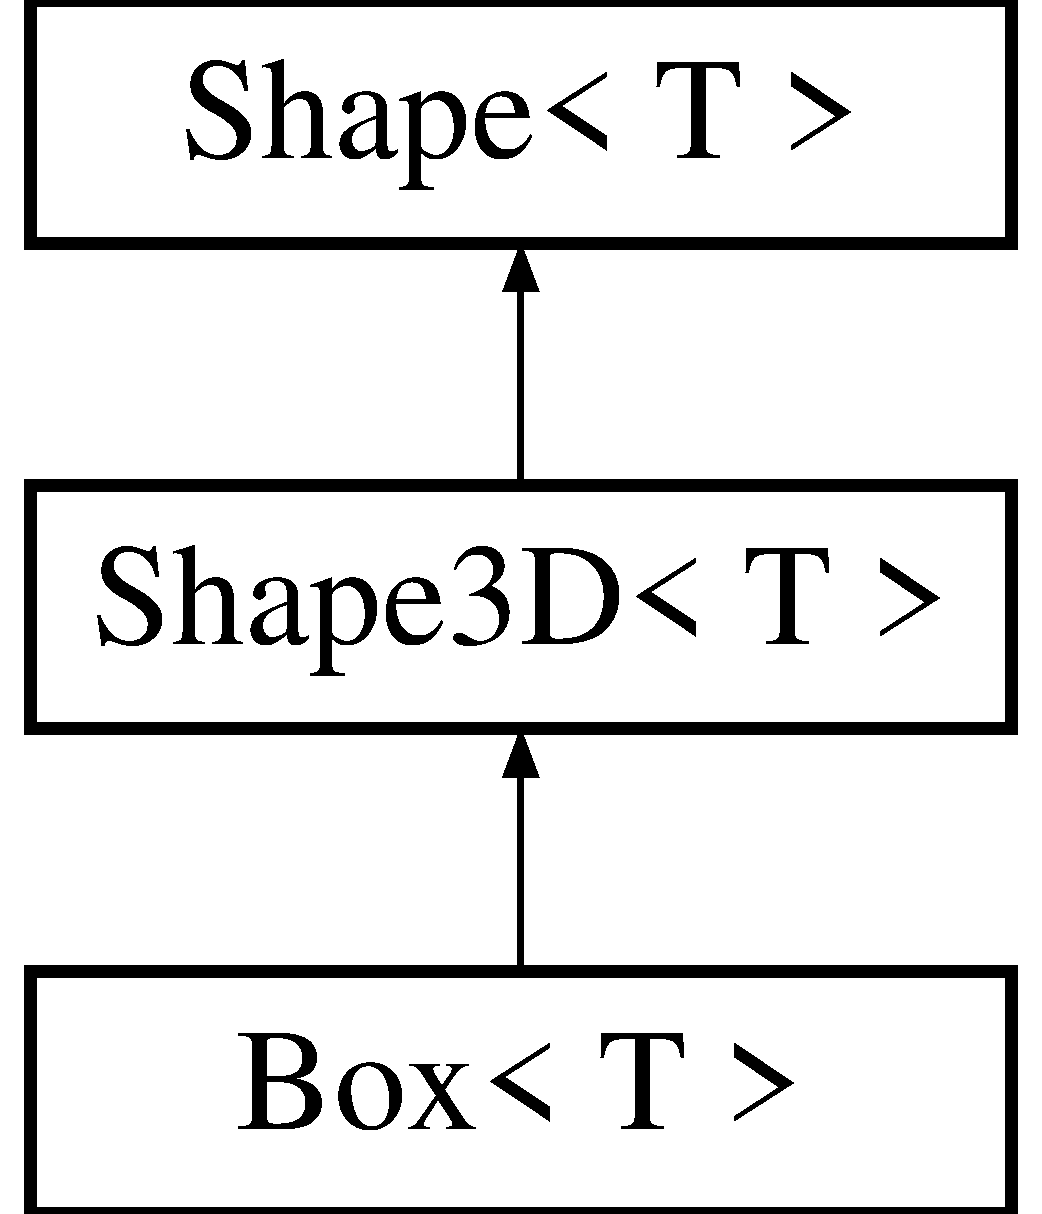
\includegraphics[height=3.000000cm]{classBox}
\end{center}
\end{figure}
\subsection*{Public Member Functions}
\begin{DoxyCompactItemize}
\item 
\mbox{\hyperlink{classBox_a057f84d8fa68647c6484d4e004d8ab74}{Box}} ()
\begin{DoxyCompactList}\small\item\em \mbox{\hyperlink{classA}{A}} basic constructor. \end{DoxyCompactList}\item 
\mbox{\hyperlink{classBox_af72b67fa2f421acbe9a7d3d1bcd540d1}{Box}} (\mbox{\hyperlink{classBox}{Box}} \&\&)=default
\item 
\mbox{\hyperlink{classBox}{Box}} \& \mbox{\hyperlink{classBox_a09995e3360b336b8a477d84804a5a70d}{operator=}} (\mbox{\hyperlink{classBox}{Box}} \&\&)=default
\item 
\mbox{\hyperlink{classBox_aab49a6687d04530ec60421bcbdb929c2}{Box}} (const \mbox{\hyperlink{classBox}{Box}} \&)=default
\item 
\mbox{\hyperlink{classBox}{Box}} \& \mbox{\hyperlink{classBox_a6ea0d233bdcce789b46384d22601da8d}{operator=}} (const \mbox{\hyperlink{classBox}{Box}} \&)=default
\item 
float \mbox{\hyperlink{classBox_ac64e9d619b0f3b991174a2ac49fef899}{perimeter}} ()
\end{DoxyCompactItemize}
\subsection*{Private Member Functions}
\begin{DoxyCompactItemize}
\item 
void \mbox{\hyperlink{classBox_a7f7b061bf913f9ab47bff75536bc137d}{generate\+\_\+vertexes}} ()
\begin{DoxyCompactList}\small\item\em \mbox{\hyperlink{classThis}{This}} function sets the correct vertexes. \end{DoxyCompactList}\end{DoxyCompactItemize}
\subsection*{Additional Inherited Members}


\subsection{Detailed Description}
\subsubsection*{template$<$typename T$>$\newline
class Box$<$ T $>$}

3D box shape. 

\subsection{Constructor \& Destructor Documentation}
\mbox{\Hypertarget{classBox_a057f84d8fa68647c6484d4e004d8ab74}\label{classBox_a057f84d8fa68647c6484d4e004d8ab74}} 
\index{Box@{Box}!Box@{Box}}
\index{Box@{Box}!Box@{Box}}
\subsubsection{\texorpdfstring{Box()}{Box()}\hspace{0.1cm}{\footnotesize\ttfamily [1/3]}}
{\footnotesize\ttfamily template$<$typename T $>$ \\
\mbox{\hyperlink{classBox}{Box}}$<$ T $>$\+::\mbox{\hyperlink{classBox}{Box}} (\begin{DoxyParamCaption}{ }\end{DoxyParamCaption})}



\mbox{\hyperlink{classA}{A}} basic constructor. 

The constructor generates vertexes and initializes buffers \mbox{\Hypertarget{classBox_af72b67fa2f421acbe9a7d3d1bcd540d1}\label{classBox_af72b67fa2f421acbe9a7d3d1bcd540d1}} 
\index{Box@{Box}!Box@{Box}}
\index{Box@{Box}!Box@{Box}}
\subsubsection{\texorpdfstring{Box()}{Box()}\hspace{0.1cm}{\footnotesize\ttfamily [2/3]}}
{\footnotesize\ttfamily template$<$typename T$>$ \\
\mbox{\hyperlink{classBox}{Box}}$<$ T $>$\+::\mbox{\hyperlink{classBox}{Box}} (\begin{DoxyParamCaption}\item[{\mbox{\hyperlink{classBox}{Box}}$<$ T $>$ \&\&}]{ }\end{DoxyParamCaption})\hspace{0.3cm}{\ttfamily [default]}}

\mbox{\Hypertarget{classBox_aab49a6687d04530ec60421bcbdb929c2}\label{classBox_aab49a6687d04530ec60421bcbdb929c2}} 
\index{Box@{Box}!Box@{Box}}
\index{Box@{Box}!Box@{Box}}
\subsubsection{\texorpdfstring{Box()}{Box()}\hspace{0.1cm}{\footnotesize\ttfamily [3/3]}}
{\footnotesize\ttfamily template$<$typename T$>$ \\
\mbox{\hyperlink{classBox}{Box}}$<$ T $>$\+::\mbox{\hyperlink{classBox}{Box}} (\begin{DoxyParamCaption}\item[{const \mbox{\hyperlink{classBox}{Box}}$<$ T $>$ \&}]{ }\end{DoxyParamCaption})\hspace{0.3cm}{\ttfamily [default]}}



\subsection{Member Function Documentation}
\mbox{\Hypertarget{classBox_a7f7b061bf913f9ab47bff75536bc137d}\label{classBox_a7f7b061bf913f9ab47bff75536bc137d}} 
\index{Box@{Box}!generate\+\_\+vertexes@{generate\+\_\+vertexes}}
\index{generate\+\_\+vertexes@{generate\+\_\+vertexes}!Box@{Box}}
\subsubsection{\texorpdfstring{generate\+\_\+vertexes()}{generate\_vertexes()}}
{\footnotesize\ttfamily template$<$typename T $>$ \\
void \mbox{\hyperlink{classBox}{Box}}$<$ T $>$\+::generate\+\_\+vertexes (\begin{DoxyParamCaption}{ }\end{DoxyParamCaption})\hspace{0.3cm}{\ttfamily [private]}}



\mbox{\hyperlink{classThis}{This}} function sets the correct vertexes. 

\mbox{\Hypertarget{classBox_a09995e3360b336b8a477d84804a5a70d}\label{classBox_a09995e3360b336b8a477d84804a5a70d}} 
\index{Box@{Box}!operator=@{operator=}}
\index{operator=@{operator=}!Box@{Box}}
\subsubsection{\texorpdfstring{operator=()}{operator=()}\hspace{0.1cm}{\footnotesize\ttfamily [1/2]}}
{\footnotesize\ttfamily template$<$typename T$>$ \\
\mbox{\hyperlink{classBox}{Box}}\& \mbox{\hyperlink{classBox}{Box}}$<$ T $>$\+::operator= (\begin{DoxyParamCaption}\item[{\mbox{\hyperlink{classBox}{Box}}$<$ T $>$ \&\&}]{ }\end{DoxyParamCaption})\hspace{0.3cm}{\ttfamily [default]}}

\mbox{\Hypertarget{classBox_a6ea0d233bdcce789b46384d22601da8d}\label{classBox_a6ea0d233bdcce789b46384d22601da8d}} 
\index{Box@{Box}!operator=@{operator=}}
\index{operator=@{operator=}!Box@{Box}}
\subsubsection{\texorpdfstring{operator=()}{operator=()}\hspace{0.1cm}{\footnotesize\ttfamily [2/2]}}
{\footnotesize\ttfamily template$<$typename T$>$ \\
\mbox{\hyperlink{classBox}{Box}}\& \mbox{\hyperlink{classBox}{Box}}$<$ T $>$\+::operator= (\begin{DoxyParamCaption}\item[{const \mbox{\hyperlink{classBox}{Box}}$<$ T $>$ \&}]{ }\end{DoxyParamCaption})\hspace{0.3cm}{\ttfamily [default]}}

\mbox{\Hypertarget{classBox_ac64e9d619b0f3b991174a2ac49fef899}\label{classBox_ac64e9d619b0f3b991174a2ac49fef899}} 
\index{Box@{Box}!perimeter@{perimeter}}
\index{perimeter@{perimeter}!Box@{Box}}
\subsubsection{\texorpdfstring{perimeter()}{perimeter()}}
{\footnotesize\ttfamily template$<$typename T$>$ \\
float \mbox{\hyperlink{classBox}{Box}}$<$ T $>$\+::perimeter (\begin{DoxyParamCaption}{ }\end{DoxyParamCaption})}



The documentation for this class was generated from the following file\+:\begin{DoxyCompactItemize}
\item 
src/shapes/\mbox{\hyperlink{box_8hpp}{box.\+hpp}}\end{DoxyCompactItemize}

\hypertarget{classcallback__function__class}{}\section{callback\+\_\+function\+\_\+class Class Reference}
\label{classcallback__function__class}\index{callback\+\_\+function\+\_\+class@{callback\+\_\+function\+\_\+class}}


{\ttfamily \#include \char`\"{}callback\+\_\+functions.\+hpp\char`\"{}}

\subsection*{Public Member Functions}
\begin{DoxyCompactItemize}
\item 
\mbox{\hyperlink{classcallback__function__class_a57fb8498117533dce172a53182182787}{callback\+\_\+function\+\_\+class}} (nanogui\+::\+Screen $\ast$screen\+\_\+)
\item 
\mbox{\hyperlink{classcallback__function__class_a1fae5711b34c371261d280afb9085756}{callback\+\_\+function\+\_\+class}} (\mbox{\hyperlink{classcallback__function__class}{callback\+\_\+function\+\_\+class}} \&\&)=delete
\item 
\mbox{\hyperlink{classcallback__function__class}{callback\+\_\+function\+\_\+class}} \& \mbox{\hyperlink{classcallback__function__class_add0667bafa4b40d9726fe353f02a969a}{operator=}} (\mbox{\hyperlink{classcallback__function__class}{callback\+\_\+function\+\_\+class}} \&\&)=delete
\item 
\mbox{\hyperlink{classcallback__function__class_a966edfa3807e811f7e9b9c1ee2185b3e}{callback\+\_\+function\+\_\+class}} (const \mbox{\hyperlink{classcallback__function__class}{callback\+\_\+function\+\_\+class}} \&)=delete
\item 
\mbox{\hyperlink{classcallback__function__class}{callback\+\_\+function\+\_\+class}} \& \mbox{\hyperlink{classcallback__function__class_abe53fd6cc7a9a772b725144dc3deaa4b}{operator=}} (const \mbox{\hyperlink{classcallback__function__class}{callback\+\_\+function\+\_\+class}} \&)=delete
\item 
void \mbox{\hyperlink{classcallback__function__class_a29cef5bc1458b2189e026310e0774e66}{cursor\+Pos\+Callback\+Event}} (G\+L\+F\+Wwindow $\ast$, double x, double y)
\item 
void \mbox{\hyperlink{classcallback__function__class_a8810c94bf06c7dd9f2308219aaaff8b3}{mouse\+Button\+Callback\+Event}} (G\+L\+F\+Wwindow $\ast$, int button, int action, int modifiers)
\item 
void \mbox{\hyperlink{classcallback__function__class_a162788695c9e6440dd8fac6dc26339ba}{key\+Callback\+Event}} (G\+L\+F\+Wwindow $\ast$, int key, int scancode, int action, int mods)
\item 
void \mbox{\hyperlink{classcallback__function__class_ab4c81c8f3d119dc3cc2f12fb19894ec3}{char\+Callback\+Event}} (G\+L\+F\+Wwindow $\ast$, unsigned int codepoint)
\item 
void \mbox{\hyperlink{classcallback__function__class_a4e4219cee44a256cc9d44f0af6f3378b}{drop\+Callback\+Event}} (G\+L\+F\+Wwindow $\ast$, int count, const char $\ast$$\ast$filenames)
\item 
void \mbox{\hyperlink{classcallback__function__class_a69db9bcdb11b09b15c2db0231fb6a5cf}{scroll\+Callback\+Event}} (G\+L\+F\+Wwindow $\ast$, double x, double y)
\item 
void \mbox{\hyperlink{classcallback__function__class_a9502656bb0f93b5f085f8767189a537f}{resize\+Callback\+Event}} (G\+L\+F\+Wwindow $\ast$, int width, int height)
\item 
\mbox{\hyperlink{classcallback__function__class_a57fb8498117533dce172a53182182787}{callback\+\_\+function\+\_\+class}} (nanogui\+::\+Screen $\ast$screen\+\_\+)
\item 
\mbox{\hyperlink{classcallback__function__class_a1fae5711b34c371261d280afb9085756}{callback\+\_\+function\+\_\+class}} (\mbox{\hyperlink{classcallback__function__class}{callback\+\_\+function\+\_\+class}} \&\&)=delete
\item 
\mbox{\hyperlink{classcallback__function__class}{callback\+\_\+function\+\_\+class}} \& \mbox{\hyperlink{classcallback__function__class_add0667bafa4b40d9726fe353f02a969a}{operator=}} (\mbox{\hyperlink{classcallback__function__class}{callback\+\_\+function\+\_\+class}} \&\&)=delete
\item 
\mbox{\hyperlink{classcallback__function__class_a966edfa3807e811f7e9b9c1ee2185b3e}{callback\+\_\+function\+\_\+class}} (const \mbox{\hyperlink{classcallback__function__class}{callback\+\_\+function\+\_\+class}} \&)=delete
\item 
\mbox{\hyperlink{classcallback__function__class}{callback\+\_\+function\+\_\+class}} \& \mbox{\hyperlink{classcallback__function__class_abe53fd6cc7a9a772b725144dc3deaa4b}{operator=}} (const \mbox{\hyperlink{classcallback__function__class}{callback\+\_\+function\+\_\+class}} \&)=delete
\item 
void \mbox{\hyperlink{classcallback__function__class_a29cef5bc1458b2189e026310e0774e66}{cursor\+Pos\+Callback\+Event}} (G\+L\+F\+Wwindow $\ast$, double x, double y)
\item 
void \mbox{\hyperlink{classcallback__function__class_a8810c94bf06c7dd9f2308219aaaff8b3}{mouse\+Button\+Callback\+Event}} (G\+L\+F\+Wwindow $\ast$, int button, int action, int modifiers)
\item 
void \mbox{\hyperlink{classcallback__function__class_a162788695c9e6440dd8fac6dc26339ba}{key\+Callback\+Event}} (G\+L\+F\+Wwindow $\ast$, int key, int scancode, int action, int mods)
\item 
void \mbox{\hyperlink{classcallback__function__class_ab4c81c8f3d119dc3cc2f12fb19894ec3}{char\+Callback\+Event}} (G\+L\+F\+Wwindow $\ast$, unsigned int codepoint)
\item 
void \mbox{\hyperlink{classcallback__function__class_a4e4219cee44a256cc9d44f0af6f3378b}{drop\+Callback\+Event}} (G\+L\+F\+Wwindow $\ast$, int count, const char $\ast$$\ast$filenames)
\item 
void \mbox{\hyperlink{classcallback__function__class_a69db9bcdb11b09b15c2db0231fb6a5cf}{scroll\+Callback\+Event}} (G\+L\+F\+Wwindow $\ast$, double x, double y)
\item 
void \mbox{\hyperlink{classcallback__function__class_a9502656bb0f93b5f085f8767189a537f}{resize\+Callback\+Event}} (G\+L\+F\+Wwindow $\ast$, int width, int height)
\end{DoxyCompactItemize}
\subsection*{Private Attributes}
\begin{DoxyCompactItemize}
\item 
nanogui\+::\+Screen $\ast$ \mbox{\hyperlink{classcallback__function__class_a0f80d6d7576b75c68d71044bdb61c8f0}{screen}}
\end{DoxyCompactItemize}


\subsection{Constructor \& Destructor Documentation}
\mbox{\Hypertarget{classcallback__function__class_a57fb8498117533dce172a53182182787}\label{classcallback__function__class_a57fb8498117533dce172a53182182787}} 
\index{callback\+\_\+function\+\_\+class@{callback\+\_\+function\+\_\+class}!callback\+\_\+function\+\_\+class@{callback\+\_\+function\+\_\+class}}
\index{callback\+\_\+function\+\_\+class@{callback\+\_\+function\+\_\+class}!callback\+\_\+function\+\_\+class@{callback\+\_\+function\+\_\+class}}
\subsubsection{\texorpdfstring{callback\+\_\+function\+\_\+class()}{callback\_function\_class()}\hspace{0.1cm}{\footnotesize\ttfamily [1/6]}}
{\footnotesize\ttfamily callback\+\_\+function\+\_\+class\+::callback\+\_\+function\+\_\+class (\begin{DoxyParamCaption}\item[{nanogui\+::\+Screen $\ast$}]{screen\+\_\+ }\end{DoxyParamCaption})\hspace{0.3cm}{\ttfamily [inline]}}

\mbox{\Hypertarget{classcallback__function__class_a1fae5711b34c371261d280afb9085756}\label{classcallback__function__class_a1fae5711b34c371261d280afb9085756}} 
\index{callback\+\_\+function\+\_\+class@{callback\+\_\+function\+\_\+class}!callback\+\_\+function\+\_\+class@{callback\+\_\+function\+\_\+class}}
\index{callback\+\_\+function\+\_\+class@{callback\+\_\+function\+\_\+class}!callback\+\_\+function\+\_\+class@{callback\+\_\+function\+\_\+class}}
\subsubsection{\texorpdfstring{callback\+\_\+function\+\_\+class()}{callback\_function\_class()}\hspace{0.1cm}{\footnotesize\ttfamily [2/6]}}
{\footnotesize\ttfamily callback\+\_\+function\+\_\+class\+::callback\+\_\+function\+\_\+class (\begin{DoxyParamCaption}\item[{\mbox{\hyperlink{classcallback__function__class}{callback\+\_\+function\+\_\+class}} \&\&}]{ }\end{DoxyParamCaption})\hspace{0.3cm}{\ttfamily [delete]}}

\mbox{\Hypertarget{classcallback__function__class_a966edfa3807e811f7e9b9c1ee2185b3e}\label{classcallback__function__class_a966edfa3807e811f7e9b9c1ee2185b3e}} 
\index{callback\+\_\+function\+\_\+class@{callback\+\_\+function\+\_\+class}!callback\+\_\+function\+\_\+class@{callback\+\_\+function\+\_\+class}}
\index{callback\+\_\+function\+\_\+class@{callback\+\_\+function\+\_\+class}!callback\+\_\+function\+\_\+class@{callback\+\_\+function\+\_\+class}}
\subsubsection{\texorpdfstring{callback\+\_\+function\+\_\+class()}{callback\_function\_class()}\hspace{0.1cm}{\footnotesize\ttfamily [3/6]}}
{\footnotesize\ttfamily callback\+\_\+function\+\_\+class\+::callback\+\_\+function\+\_\+class (\begin{DoxyParamCaption}\item[{const \mbox{\hyperlink{classcallback__function__class}{callback\+\_\+function\+\_\+class}} \&}]{ }\end{DoxyParamCaption})\hspace{0.3cm}{\ttfamily [delete]}}

\mbox{\Hypertarget{classcallback__function__class_a57fb8498117533dce172a53182182787}\label{classcallback__function__class_a57fb8498117533dce172a53182182787}} 
\index{callback\+\_\+function\+\_\+class@{callback\+\_\+function\+\_\+class}!callback\+\_\+function\+\_\+class@{callback\+\_\+function\+\_\+class}}
\index{callback\+\_\+function\+\_\+class@{callback\+\_\+function\+\_\+class}!callback\+\_\+function\+\_\+class@{callback\+\_\+function\+\_\+class}}
\subsubsection{\texorpdfstring{callback\+\_\+function\+\_\+class()}{callback\_function\_class()}\hspace{0.1cm}{\footnotesize\ttfamily [4/6]}}
{\footnotesize\ttfamily callback\+\_\+function\+\_\+class\+::callback\+\_\+function\+\_\+class (\begin{DoxyParamCaption}\item[{nanogui\+::\+Screen $\ast$}]{screen\+\_\+ }\end{DoxyParamCaption})\hspace{0.3cm}{\ttfamily [inline]}}

\mbox{\Hypertarget{classcallback__function__class_a1fae5711b34c371261d280afb9085756}\label{classcallback__function__class_a1fae5711b34c371261d280afb9085756}} 
\index{callback\+\_\+function\+\_\+class@{callback\+\_\+function\+\_\+class}!callback\+\_\+function\+\_\+class@{callback\+\_\+function\+\_\+class}}
\index{callback\+\_\+function\+\_\+class@{callback\+\_\+function\+\_\+class}!callback\+\_\+function\+\_\+class@{callback\+\_\+function\+\_\+class}}
\subsubsection{\texorpdfstring{callback\+\_\+function\+\_\+class()}{callback\_function\_class()}\hspace{0.1cm}{\footnotesize\ttfamily [5/6]}}
{\footnotesize\ttfamily callback\+\_\+function\+\_\+class\+::callback\+\_\+function\+\_\+class (\begin{DoxyParamCaption}\item[{\mbox{\hyperlink{classcallback__function__class}{callback\+\_\+function\+\_\+class}} \&\&}]{ }\end{DoxyParamCaption})\hspace{0.3cm}{\ttfamily [delete]}}

\mbox{\Hypertarget{classcallback__function__class_a966edfa3807e811f7e9b9c1ee2185b3e}\label{classcallback__function__class_a966edfa3807e811f7e9b9c1ee2185b3e}} 
\index{callback\+\_\+function\+\_\+class@{callback\+\_\+function\+\_\+class}!callback\+\_\+function\+\_\+class@{callback\+\_\+function\+\_\+class}}
\index{callback\+\_\+function\+\_\+class@{callback\+\_\+function\+\_\+class}!callback\+\_\+function\+\_\+class@{callback\+\_\+function\+\_\+class}}
\subsubsection{\texorpdfstring{callback\+\_\+function\+\_\+class()}{callback\_function\_class()}\hspace{0.1cm}{\footnotesize\ttfamily [6/6]}}
{\footnotesize\ttfamily callback\+\_\+function\+\_\+class\+::callback\+\_\+function\+\_\+class (\begin{DoxyParamCaption}\item[{const \mbox{\hyperlink{classcallback__function__class}{callback\+\_\+function\+\_\+class}} \&}]{ }\end{DoxyParamCaption})\hspace{0.3cm}{\ttfamily [delete]}}



\subsection{Member Function Documentation}
\mbox{\Hypertarget{classcallback__function__class_ab4c81c8f3d119dc3cc2f12fb19894ec3}\label{classcallback__function__class_ab4c81c8f3d119dc3cc2f12fb19894ec3}} 
\index{callback\+\_\+function\+\_\+class@{callback\+\_\+function\+\_\+class}!char\+Callback\+Event@{char\+Callback\+Event}}
\index{char\+Callback\+Event@{char\+Callback\+Event}!callback\+\_\+function\+\_\+class@{callback\+\_\+function\+\_\+class}}
\subsubsection{\texorpdfstring{char\+Callback\+Event()}{charCallbackEvent()}\hspace{0.1cm}{\footnotesize\ttfamily [1/2]}}
{\footnotesize\ttfamily void callback\+\_\+function\+\_\+class\+::char\+Callback\+Event (\begin{DoxyParamCaption}\item[{G\+L\+F\+Wwindow $\ast$}]{,  }\item[{unsigned int}]{codepoint }\end{DoxyParamCaption})\hspace{0.3cm}{\ttfamily [inline]}}

\mbox{\Hypertarget{classcallback__function__class_ab4c81c8f3d119dc3cc2f12fb19894ec3}\label{classcallback__function__class_ab4c81c8f3d119dc3cc2f12fb19894ec3}} 
\index{callback\+\_\+function\+\_\+class@{callback\+\_\+function\+\_\+class}!char\+Callback\+Event@{char\+Callback\+Event}}
\index{char\+Callback\+Event@{char\+Callback\+Event}!callback\+\_\+function\+\_\+class@{callback\+\_\+function\+\_\+class}}
\subsubsection{\texorpdfstring{char\+Callback\+Event()}{charCallbackEvent()}\hspace{0.1cm}{\footnotesize\ttfamily [2/2]}}
{\footnotesize\ttfamily void callback\+\_\+function\+\_\+class\+::char\+Callback\+Event (\begin{DoxyParamCaption}\item[{G\+L\+F\+Wwindow $\ast$}]{,  }\item[{unsigned int}]{codepoint }\end{DoxyParamCaption})\hspace{0.3cm}{\ttfamily [inline]}}

\mbox{\Hypertarget{classcallback__function__class_a29cef5bc1458b2189e026310e0774e66}\label{classcallback__function__class_a29cef5bc1458b2189e026310e0774e66}} 
\index{callback\+\_\+function\+\_\+class@{callback\+\_\+function\+\_\+class}!cursor\+Pos\+Callback\+Event@{cursor\+Pos\+Callback\+Event}}
\index{cursor\+Pos\+Callback\+Event@{cursor\+Pos\+Callback\+Event}!callback\+\_\+function\+\_\+class@{callback\+\_\+function\+\_\+class}}
\subsubsection{\texorpdfstring{cursor\+Pos\+Callback\+Event()}{cursorPosCallbackEvent()}\hspace{0.1cm}{\footnotesize\ttfamily [1/2]}}
{\footnotesize\ttfamily void callback\+\_\+function\+\_\+class\+::cursor\+Pos\+Callback\+Event (\begin{DoxyParamCaption}\item[{G\+L\+F\+Wwindow $\ast$}]{,  }\item[{double}]{x,  }\item[{double}]{y }\end{DoxyParamCaption})\hspace{0.3cm}{\ttfamily [inline]}}

\mbox{\Hypertarget{classcallback__function__class_a29cef5bc1458b2189e026310e0774e66}\label{classcallback__function__class_a29cef5bc1458b2189e026310e0774e66}} 
\index{callback\+\_\+function\+\_\+class@{callback\+\_\+function\+\_\+class}!cursor\+Pos\+Callback\+Event@{cursor\+Pos\+Callback\+Event}}
\index{cursor\+Pos\+Callback\+Event@{cursor\+Pos\+Callback\+Event}!callback\+\_\+function\+\_\+class@{callback\+\_\+function\+\_\+class}}
\subsubsection{\texorpdfstring{cursor\+Pos\+Callback\+Event()}{cursorPosCallbackEvent()}\hspace{0.1cm}{\footnotesize\ttfamily [2/2]}}
{\footnotesize\ttfamily void callback\+\_\+function\+\_\+class\+::cursor\+Pos\+Callback\+Event (\begin{DoxyParamCaption}\item[{G\+L\+F\+Wwindow $\ast$}]{,  }\item[{double}]{x,  }\item[{double}]{y }\end{DoxyParamCaption})\hspace{0.3cm}{\ttfamily [inline]}}

\mbox{\Hypertarget{classcallback__function__class_a4e4219cee44a256cc9d44f0af6f3378b}\label{classcallback__function__class_a4e4219cee44a256cc9d44f0af6f3378b}} 
\index{callback\+\_\+function\+\_\+class@{callback\+\_\+function\+\_\+class}!drop\+Callback\+Event@{drop\+Callback\+Event}}
\index{drop\+Callback\+Event@{drop\+Callback\+Event}!callback\+\_\+function\+\_\+class@{callback\+\_\+function\+\_\+class}}
\subsubsection{\texorpdfstring{drop\+Callback\+Event()}{dropCallbackEvent()}\hspace{0.1cm}{\footnotesize\ttfamily [1/2]}}
{\footnotesize\ttfamily void callback\+\_\+function\+\_\+class\+::drop\+Callback\+Event (\begin{DoxyParamCaption}\item[{G\+L\+F\+Wwindow $\ast$}]{,  }\item[{int}]{count,  }\item[{const char $\ast$$\ast$}]{filenames }\end{DoxyParamCaption})\hspace{0.3cm}{\ttfamily [inline]}}

\mbox{\Hypertarget{classcallback__function__class_a4e4219cee44a256cc9d44f0af6f3378b}\label{classcallback__function__class_a4e4219cee44a256cc9d44f0af6f3378b}} 
\index{callback\+\_\+function\+\_\+class@{callback\+\_\+function\+\_\+class}!drop\+Callback\+Event@{drop\+Callback\+Event}}
\index{drop\+Callback\+Event@{drop\+Callback\+Event}!callback\+\_\+function\+\_\+class@{callback\+\_\+function\+\_\+class}}
\subsubsection{\texorpdfstring{drop\+Callback\+Event()}{dropCallbackEvent()}\hspace{0.1cm}{\footnotesize\ttfamily [2/2]}}
{\footnotesize\ttfamily void callback\+\_\+function\+\_\+class\+::drop\+Callback\+Event (\begin{DoxyParamCaption}\item[{G\+L\+F\+Wwindow $\ast$}]{,  }\item[{int}]{count,  }\item[{const char $\ast$$\ast$}]{filenames }\end{DoxyParamCaption})\hspace{0.3cm}{\ttfamily [inline]}}

\mbox{\Hypertarget{classcallback__function__class_a162788695c9e6440dd8fac6dc26339ba}\label{classcallback__function__class_a162788695c9e6440dd8fac6dc26339ba}} 
\index{callback\+\_\+function\+\_\+class@{callback\+\_\+function\+\_\+class}!key\+Callback\+Event@{key\+Callback\+Event}}
\index{key\+Callback\+Event@{key\+Callback\+Event}!callback\+\_\+function\+\_\+class@{callback\+\_\+function\+\_\+class}}
\subsubsection{\texorpdfstring{key\+Callback\+Event()}{keyCallbackEvent()}\hspace{0.1cm}{\footnotesize\ttfamily [1/2]}}
{\footnotesize\ttfamily void callback\+\_\+function\+\_\+class\+::key\+Callback\+Event (\begin{DoxyParamCaption}\item[{G\+L\+F\+Wwindow $\ast$}]{,  }\item[{int}]{key,  }\item[{int}]{scancode,  }\item[{int}]{action,  }\item[{int}]{mods }\end{DoxyParamCaption})\hspace{0.3cm}{\ttfamily [inline]}}

\mbox{\Hypertarget{classcallback__function__class_a162788695c9e6440dd8fac6dc26339ba}\label{classcallback__function__class_a162788695c9e6440dd8fac6dc26339ba}} 
\index{callback\+\_\+function\+\_\+class@{callback\+\_\+function\+\_\+class}!key\+Callback\+Event@{key\+Callback\+Event}}
\index{key\+Callback\+Event@{key\+Callback\+Event}!callback\+\_\+function\+\_\+class@{callback\+\_\+function\+\_\+class}}
\subsubsection{\texorpdfstring{key\+Callback\+Event()}{keyCallbackEvent()}\hspace{0.1cm}{\footnotesize\ttfamily [2/2]}}
{\footnotesize\ttfamily void callback\+\_\+function\+\_\+class\+::key\+Callback\+Event (\begin{DoxyParamCaption}\item[{G\+L\+F\+Wwindow $\ast$}]{,  }\item[{int}]{key,  }\item[{int}]{scancode,  }\item[{int}]{action,  }\item[{int}]{mods }\end{DoxyParamCaption})\hspace{0.3cm}{\ttfamily [inline]}}

\mbox{\Hypertarget{classcallback__function__class_a8810c94bf06c7dd9f2308219aaaff8b3}\label{classcallback__function__class_a8810c94bf06c7dd9f2308219aaaff8b3}} 
\index{callback\+\_\+function\+\_\+class@{callback\+\_\+function\+\_\+class}!mouse\+Button\+Callback\+Event@{mouse\+Button\+Callback\+Event}}
\index{mouse\+Button\+Callback\+Event@{mouse\+Button\+Callback\+Event}!callback\+\_\+function\+\_\+class@{callback\+\_\+function\+\_\+class}}
\subsubsection{\texorpdfstring{mouse\+Button\+Callback\+Event()}{mouseButtonCallbackEvent()}\hspace{0.1cm}{\footnotesize\ttfamily [1/2]}}
{\footnotesize\ttfamily void callback\+\_\+function\+\_\+class\+::mouse\+Button\+Callback\+Event (\begin{DoxyParamCaption}\item[{G\+L\+F\+Wwindow $\ast$}]{,  }\item[{int}]{button,  }\item[{int}]{action,  }\item[{int}]{modifiers }\end{DoxyParamCaption})\hspace{0.3cm}{\ttfamily [inline]}}

\mbox{\Hypertarget{classcallback__function__class_a8810c94bf06c7dd9f2308219aaaff8b3}\label{classcallback__function__class_a8810c94bf06c7dd9f2308219aaaff8b3}} 
\index{callback\+\_\+function\+\_\+class@{callback\+\_\+function\+\_\+class}!mouse\+Button\+Callback\+Event@{mouse\+Button\+Callback\+Event}}
\index{mouse\+Button\+Callback\+Event@{mouse\+Button\+Callback\+Event}!callback\+\_\+function\+\_\+class@{callback\+\_\+function\+\_\+class}}
\subsubsection{\texorpdfstring{mouse\+Button\+Callback\+Event()}{mouseButtonCallbackEvent()}\hspace{0.1cm}{\footnotesize\ttfamily [2/2]}}
{\footnotesize\ttfamily void callback\+\_\+function\+\_\+class\+::mouse\+Button\+Callback\+Event (\begin{DoxyParamCaption}\item[{G\+L\+F\+Wwindow $\ast$}]{,  }\item[{int}]{button,  }\item[{int}]{action,  }\item[{int}]{modifiers }\end{DoxyParamCaption})\hspace{0.3cm}{\ttfamily [inline]}}

\mbox{\Hypertarget{classcallback__function__class_add0667bafa4b40d9726fe353f02a969a}\label{classcallback__function__class_add0667bafa4b40d9726fe353f02a969a}} 
\index{callback\+\_\+function\+\_\+class@{callback\+\_\+function\+\_\+class}!operator=@{operator=}}
\index{operator=@{operator=}!callback\+\_\+function\+\_\+class@{callback\+\_\+function\+\_\+class}}
\subsubsection{\texorpdfstring{operator=()}{operator=()}\hspace{0.1cm}{\footnotesize\ttfamily [1/4]}}
{\footnotesize\ttfamily \mbox{\hyperlink{classcallback__function__class}{callback\+\_\+function\+\_\+class}}\& callback\+\_\+function\+\_\+class\+::operator= (\begin{DoxyParamCaption}\item[{\mbox{\hyperlink{classcallback__function__class}{callback\+\_\+function\+\_\+class}} \&\&}]{ }\end{DoxyParamCaption})\hspace{0.3cm}{\ttfamily [delete]}}

\mbox{\Hypertarget{classcallback__function__class_add0667bafa4b40d9726fe353f02a969a}\label{classcallback__function__class_add0667bafa4b40d9726fe353f02a969a}} 
\index{callback\+\_\+function\+\_\+class@{callback\+\_\+function\+\_\+class}!operator=@{operator=}}
\index{operator=@{operator=}!callback\+\_\+function\+\_\+class@{callback\+\_\+function\+\_\+class}}
\subsubsection{\texorpdfstring{operator=()}{operator=()}\hspace{0.1cm}{\footnotesize\ttfamily [2/4]}}
{\footnotesize\ttfamily \mbox{\hyperlink{classcallback__function__class}{callback\+\_\+function\+\_\+class}}\& callback\+\_\+function\+\_\+class\+::operator= (\begin{DoxyParamCaption}\item[{\mbox{\hyperlink{classcallback__function__class}{callback\+\_\+function\+\_\+class}} \&\&}]{ }\end{DoxyParamCaption})\hspace{0.3cm}{\ttfamily [delete]}}

\mbox{\Hypertarget{classcallback__function__class_abe53fd6cc7a9a772b725144dc3deaa4b}\label{classcallback__function__class_abe53fd6cc7a9a772b725144dc3deaa4b}} 
\index{callback\+\_\+function\+\_\+class@{callback\+\_\+function\+\_\+class}!operator=@{operator=}}
\index{operator=@{operator=}!callback\+\_\+function\+\_\+class@{callback\+\_\+function\+\_\+class}}
\subsubsection{\texorpdfstring{operator=()}{operator=()}\hspace{0.1cm}{\footnotesize\ttfamily [3/4]}}
{\footnotesize\ttfamily \mbox{\hyperlink{classcallback__function__class}{callback\+\_\+function\+\_\+class}}\& callback\+\_\+function\+\_\+class\+::operator= (\begin{DoxyParamCaption}\item[{const \mbox{\hyperlink{classcallback__function__class}{callback\+\_\+function\+\_\+class}} \&}]{ }\end{DoxyParamCaption})\hspace{0.3cm}{\ttfamily [delete]}}

\mbox{\Hypertarget{classcallback__function__class_abe53fd6cc7a9a772b725144dc3deaa4b}\label{classcallback__function__class_abe53fd6cc7a9a772b725144dc3deaa4b}} 
\index{callback\+\_\+function\+\_\+class@{callback\+\_\+function\+\_\+class}!operator=@{operator=}}
\index{operator=@{operator=}!callback\+\_\+function\+\_\+class@{callback\+\_\+function\+\_\+class}}
\subsubsection{\texorpdfstring{operator=()}{operator=()}\hspace{0.1cm}{\footnotesize\ttfamily [4/4]}}
{\footnotesize\ttfamily \mbox{\hyperlink{classcallback__function__class}{callback\+\_\+function\+\_\+class}}\& callback\+\_\+function\+\_\+class\+::operator= (\begin{DoxyParamCaption}\item[{const \mbox{\hyperlink{classcallback__function__class}{callback\+\_\+function\+\_\+class}} \&}]{ }\end{DoxyParamCaption})\hspace{0.3cm}{\ttfamily [delete]}}

\mbox{\Hypertarget{classcallback__function__class_a9502656bb0f93b5f085f8767189a537f}\label{classcallback__function__class_a9502656bb0f93b5f085f8767189a537f}} 
\index{callback\+\_\+function\+\_\+class@{callback\+\_\+function\+\_\+class}!resize\+Callback\+Event@{resize\+Callback\+Event}}
\index{resize\+Callback\+Event@{resize\+Callback\+Event}!callback\+\_\+function\+\_\+class@{callback\+\_\+function\+\_\+class}}
\subsubsection{\texorpdfstring{resize\+Callback\+Event()}{resizeCallbackEvent()}\hspace{0.1cm}{\footnotesize\ttfamily [1/2]}}
{\footnotesize\ttfamily void callback\+\_\+function\+\_\+class\+::resize\+Callback\+Event (\begin{DoxyParamCaption}\item[{G\+L\+F\+Wwindow $\ast$}]{,  }\item[{int}]{width,  }\item[{int}]{height }\end{DoxyParamCaption})\hspace{0.3cm}{\ttfamily [inline]}}

\mbox{\Hypertarget{classcallback__function__class_a9502656bb0f93b5f085f8767189a537f}\label{classcallback__function__class_a9502656bb0f93b5f085f8767189a537f}} 
\index{callback\+\_\+function\+\_\+class@{callback\+\_\+function\+\_\+class}!resize\+Callback\+Event@{resize\+Callback\+Event}}
\index{resize\+Callback\+Event@{resize\+Callback\+Event}!callback\+\_\+function\+\_\+class@{callback\+\_\+function\+\_\+class}}
\subsubsection{\texorpdfstring{resize\+Callback\+Event()}{resizeCallbackEvent()}\hspace{0.1cm}{\footnotesize\ttfamily [2/2]}}
{\footnotesize\ttfamily void callback\+\_\+function\+\_\+class\+::resize\+Callback\+Event (\begin{DoxyParamCaption}\item[{G\+L\+F\+Wwindow $\ast$}]{,  }\item[{int}]{width,  }\item[{int}]{height }\end{DoxyParamCaption})\hspace{0.3cm}{\ttfamily [inline]}}

\mbox{\Hypertarget{classcallback__function__class_a69db9bcdb11b09b15c2db0231fb6a5cf}\label{classcallback__function__class_a69db9bcdb11b09b15c2db0231fb6a5cf}} 
\index{callback\+\_\+function\+\_\+class@{callback\+\_\+function\+\_\+class}!scroll\+Callback\+Event@{scroll\+Callback\+Event}}
\index{scroll\+Callback\+Event@{scroll\+Callback\+Event}!callback\+\_\+function\+\_\+class@{callback\+\_\+function\+\_\+class}}
\subsubsection{\texorpdfstring{scroll\+Callback\+Event()}{scrollCallbackEvent()}\hspace{0.1cm}{\footnotesize\ttfamily [1/2]}}
{\footnotesize\ttfamily void callback\+\_\+function\+\_\+class\+::scroll\+Callback\+Event (\begin{DoxyParamCaption}\item[{G\+L\+F\+Wwindow $\ast$}]{,  }\item[{double}]{x,  }\item[{double}]{y }\end{DoxyParamCaption})\hspace{0.3cm}{\ttfamily [inline]}}

\mbox{\Hypertarget{classcallback__function__class_a69db9bcdb11b09b15c2db0231fb6a5cf}\label{classcallback__function__class_a69db9bcdb11b09b15c2db0231fb6a5cf}} 
\index{callback\+\_\+function\+\_\+class@{callback\+\_\+function\+\_\+class}!scroll\+Callback\+Event@{scroll\+Callback\+Event}}
\index{scroll\+Callback\+Event@{scroll\+Callback\+Event}!callback\+\_\+function\+\_\+class@{callback\+\_\+function\+\_\+class}}
\subsubsection{\texorpdfstring{scroll\+Callback\+Event()}{scrollCallbackEvent()}\hspace{0.1cm}{\footnotesize\ttfamily [2/2]}}
{\footnotesize\ttfamily void callback\+\_\+function\+\_\+class\+::scroll\+Callback\+Event (\begin{DoxyParamCaption}\item[{G\+L\+F\+Wwindow $\ast$}]{,  }\item[{double}]{x,  }\item[{double}]{y }\end{DoxyParamCaption})\hspace{0.3cm}{\ttfamily [inline]}}



\subsection{Member Data Documentation}
\mbox{\Hypertarget{classcallback__function__class_a0f80d6d7576b75c68d71044bdb61c8f0}\label{classcallback__function__class_a0f80d6d7576b75c68d71044bdb61c8f0}} 
\index{callback\+\_\+function\+\_\+class@{callback\+\_\+function\+\_\+class}!screen@{screen}}
\index{screen@{screen}!callback\+\_\+function\+\_\+class@{callback\+\_\+function\+\_\+class}}
\subsubsection{\texorpdfstring{screen}{screen}}
{\footnotesize\ttfamily nanogui\+::\+Screen $\ast$ callback\+\_\+function\+\_\+class\+::screen\hspace{0.3cm}{\ttfamily [private]}}



The documentation for this class was generated from the following file\+:\begin{DoxyCompactItemize}
\item 
examples/ising\+\_\+full\+\_\+nanogui\+\_\+version/\mbox{\hyperlink{ising__full__nanogui__version_2callback__functions_8hpp}{callback\+\_\+functions.\+hpp}}\end{DoxyCompactItemize}

\hypertarget{structText_1_1Character}{}\section{Text\+:\+:Character Struct Reference}
\label{structText_1_1Character}\index{Text\+::\+Character@{Text\+::\+Character}}
\subsection*{Public Attributes}
\begin{DoxyCompactItemize}
\item 
G\+Luint \mbox{\hyperlink{structText_1_1Character_af360b406edc3ed9092ce7e233ae3acc8}{Texture\+ID}}
\item 
glm\+::ivec2 \mbox{\hyperlink{structText_1_1Character_ad4c2b88bfc1232dec53699b361231ca3}{Size}}
\item 
glm\+::ivec2 \mbox{\hyperlink{structText_1_1Character_a2bfdd54e6722da034311bb89e8059336}{Bearing}}
\item 
G\+Luint \mbox{\hyperlink{structText_1_1Character_a654a8be453c9922a74763e5579f6ce61}{Advance}}
\end{DoxyCompactItemize}


\subsection{Member Data Documentation}
\mbox{\Hypertarget{structText_1_1Character_a654a8be453c9922a74763e5579f6ce61}\label{structText_1_1Character_a654a8be453c9922a74763e5579f6ce61}} 
\index{Text\+::\+Character@{Text\+::\+Character}!Advance@{Advance}}
\index{Advance@{Advance}!Text\+::\+Character@{Text\+::\+Character}}
\subsubsection{\texorpdfstring{Advance}{Advance}}
{\footnotesize\ttfamily G\+Luint Text\+::\+Character\+::\+Advance}

\mbox{\Hypertarget{structText_1_1Character_a2bfdd54e6722da034311bb89e8059336}\label{structText_1_1Character_a2bfdd54e6722da034311bb89e8059336}} 
\index{Text\+::\+Character@{Text\+::\+Character}!Bearing@{Bearing}}
\index{Bearing@{Bearing}!Text\+::\+Character@{Text\+::\+Character}}
\subsubsection{\texorpdfstring{Bearing}{Bearing}}
{\footnotesize\ttfamily glm\+::ivec2 Text\+::\+Character\+::\+Bearing}

\mbox{\Hypertarget{structText_1_1Character_ad4c2b88bfc1232dec53699b361231ca3}\label{structText_1_1Character_ad4c2b88bfc1232dec53699b361231ca3}} 
\index{Text\+::\+Character@{Text\+::\+Character}!Size@{Size}}
\index{Size@{Size}!Text\+::\+Character@{Text\+::\+Character}}
\subsubsection{\texorpdfstring{Size}{Size}}
{\footnotesize\ttfamily glm\+::ivec2 Text\+::\+Character\+::\+Size}

\mbox{\Hypertarget{structText_1_1Character_af360b406edc3ed9092ce7e233ae3acc8}\label{structText_1_1Character_af360b406edc3ed9092ce7e233ae3acc8}} 
\index{Text\+::\+Character@{Text\+::\+Character}!Texture\+ID@{Texture\+ID}}
\index{Texture\+ID@{Texture\+ID}!Text\+::\+Character@{Text\+::\+Character}}
\subsubsection{\texorpdfstring{Texture\+ID}{TextureID}}
{\footnotesize\ttfamily G\+Luint Text\+::\+Character\+::\+Texture\+ID}



The documentation for this struct was generated from the following file\+:\begin{DoxyCompactItemize}
\item 
src/text\+\_\+rendering/\mbox{\hyperlink{text__rendering_8hpp}{text\+\_\+rendering.\+hpp}}\end{DoxyCompactItemize}

\hypertarget{structCharacter}{}\section{Character Struct Reference}
\label{structCharacter}\index{Character@{Character}}


Holds all state information relevant to a character as loaded using Free\+Type.  


\subsection*{Public Attributes}
\begin{DoxyCompactItemize}
\item 
G\+Luint \mbox{\hyperlink{structCharacter_a51d894cc31d79e95fe1a47fb65c6e889}{Texture\+ID}}
\item 
glm\+::ivec2 \mbox{\hyperlink{structCharacter_aaaa598050e0ef590fe6903fd2bab40b8}{Size}}
\item 
glm\+::ivec2 \mbox{\hyperlink{structCharacter_afef98bf9c7f5313d96476f6f3f85f872}{Bearing}}
\item 
G\+Luint \mbox{\hyperlink{structCharacter_ab35bae8be6740729fc5839c237a659f6}{Advance}}
\end{DoxyCompactItemize}


\subsection{Detailed Description}
Holds all state information relevant to a character as loaded using Free\+Type. 

\subsection{Member Data Documentation}
\mbox{\Hypertarget{structCharacter_ab35bae8be6740729fc5839c237a659f6}\label{structCharacter_ab35bae8be6740729fc5839c237a659f6}} 
\index{Character@{Character}!Advance@{Advance}}
\index{Advance@{Advance}!Character@{Character}}
\subsubsection{\texorpdfstring{Advance}{Advance}}
{\footnotesize\ttfamily G\+Luint Character\+::\+Advance}

\mbox{\Hypertarget{structCharacter_afef98bf9c7f5313d96476f6f3f85f872}\label{structCharacter_afef98bf9c7f5313d96476f6f3f85f872}} 
\index{Character@{Character}!Bearing@{Bearing}}
\index{Bearing@{Bearing}!Character@{Character}}
\subsubsection{\texorpdfstring{Bearing}{Bearing}}
{\footnotesize\ttfamily glm\+::ivec2 Character\+::\+Bearing}

\mbox{\Hypertarget{structCharacter_aaaa598050e0ef590fe6903fd2bab40b8}\label{structCharacter_aaaa598050e0ef590fe6903fd2bab40b8}} 
\index{Character@{Character}!Size@{Size}}
\index{Size@{Size}!Character@{Character}}
\subsubsection{\texorpdfstring{Size}{Size}}
{\footnotesize\ttfamily glm\+::ivec2 Character\+::\+Size}

\mbox{\Hypertarget{structCharacter_a51d894cc31d79e95fe1a47fb65c6e889}\label{structCharacter_a51d894cc31d79e95fe1a47fb65c6e889}} 
\index{Character@{Character}!Texture\+ID@{Texture\+ID}}
\index{Texture\+ID@{Texture\+ID}!Character@{Character}}
\subsubsection{\texorpdfstring{Texture\+ID}{TextureID}}
{\footnotesize\ttfamily G\+Luint Character\+::\+Texture\+ID}



The documentation for this struct was generated from the following file\+:\begin{DoxyCompactItemize}
\item 
examples/simple\+\_\+text\+\_\+rendering/\mbox{\hyperlink{text_8cpp}{text.\+cpp}}\end{DoxyCompactItemize}

\hypertarget{classCircle}{}\section{Circle$<$ T $>$ Class Template Reference}
\label{classCircle}\index{Circle$<$ T $>$@{Circle$<$ T $>$}}


{\ttfamily \#include \char`\"{}circle.\+hpp\char`\"{}}

Inheritance diagram for Circle$<$ T $>$\+:\begin{figure}[H]
\begin{center}
\leavevmode
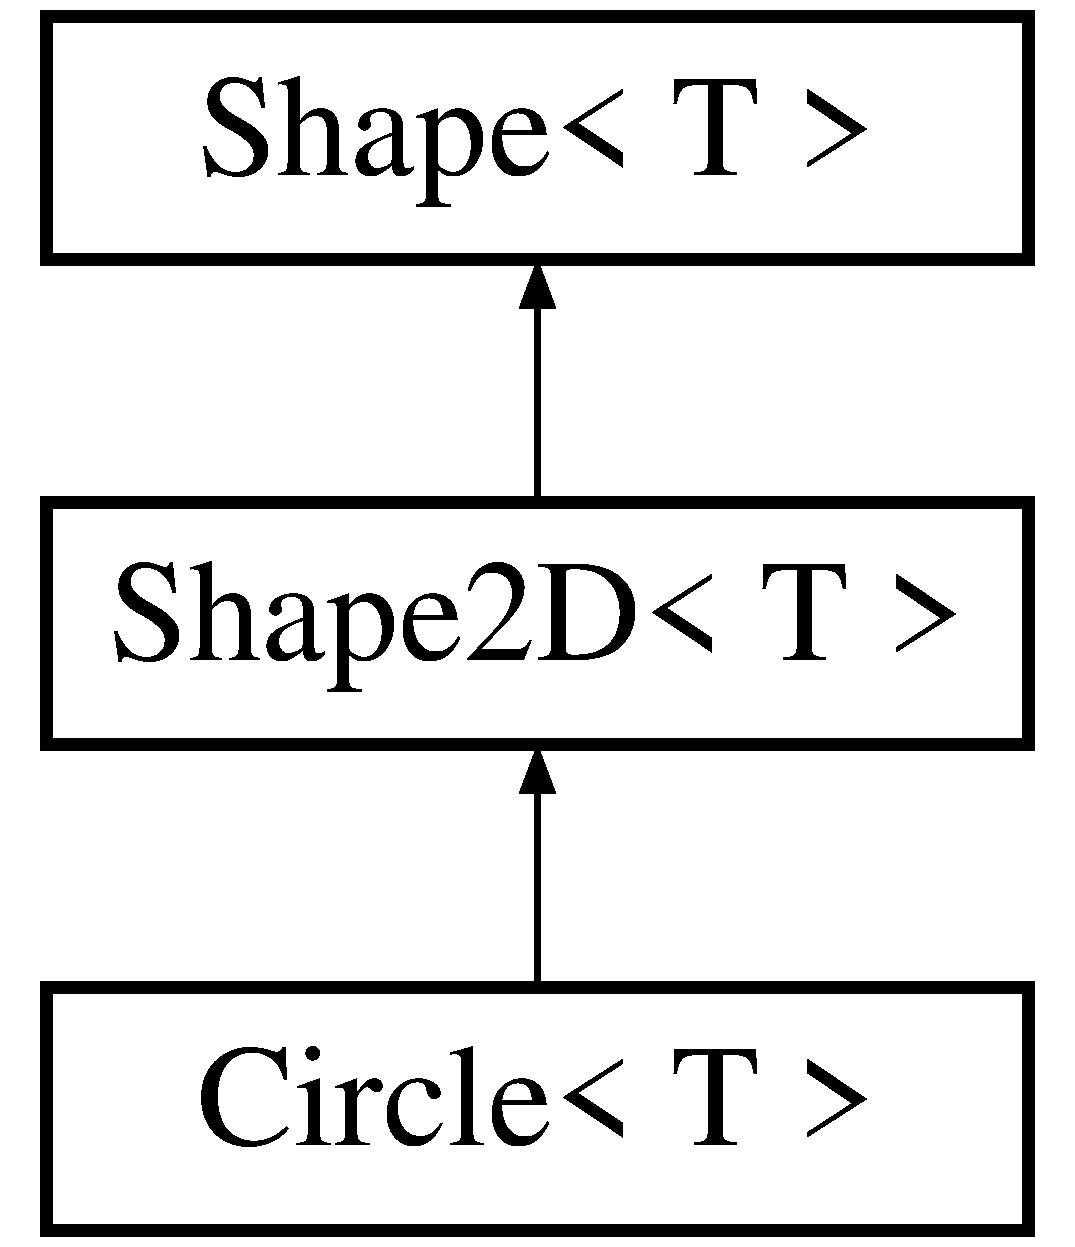
\includegraphics[height=3.000000cm]{classCircle}
\end{center}
\end{figure}
\subsection*{Public Member Functions}
\begin{DoxyCompactItemize}
\item 
\mbox{\hyperlink{classCircle_a0a298ea0e982a94a60091aeb2767f6e4}{Circle}} ()
\begin{DoxyCompactList}\small\item\em Basic constructor for class \mbox{\hyperlink{classCircle}{Circle}}. \end{DoxyCompactList}\item 
\mbox{\hyperlink{classCircle_ad4ee8eadfd4201a937af204ac4e6ec37}{Circle}} (\mbox{\hyperlink{classCircle}{Circle}} \&\&)=default
\item 
\mbox{\hyperlink{classCircle}{Circle}} \& \mbox{\hyperlink{classCircle_a06c8a2624fa51b38023e0326e8ccf789}{operator=}} (\mbox{\hyperlink{classCircle}{Circle}} \&\&)=default
\item 
\mbox{\hyperlink{classCircle_a163162aa8beaceb25ebd9a17966f4bd5}{Circle}} (const \mbox{\hyperlink{classCircle}{Circle}} \&)=default
\item 
\mbox{\hyperlink{classCircle}{Circle}} \& \mbox{\hyperlink{classCircle_a0e3ef62951a8fccaf0635ea21ae73eca}{operator=}} (const \mbox{\hyperlink{classCircle}{Circle}} \&)=default
\item 
T \mbox{\hyperlink{classCircle_a6f066fc39c0de339b0498b04a56be028}{perimeter}} ()
\item 
{\footnotesize template$<$$>$ }\\float \mbox{\hyperlink{classCircle_aa6c86a4a5d3ee7eb598879ba856430d9}{perimeter}} ()
\begin{DoxyCompactList}\small\item\em \mbox{\hyperlink{classThis}{This}} function calculates perimeter of a circle with radius 1. \end{DoxyCompactList}\end{DoxyCompactItemize}
\subsection*{Private Member Functions}
\begin{DoxyCompactItemize}
\item 
void \mbox{\hyperlink{classCircle_a07ce44d6b3a70ee7cbcf19e02e50c361}{generate\+\_\+vertexes}} (int=-\/1)
\item 
{\footnotesize template$<$$>$ }\\void \mbox{\hyperlink{classCircle_a5c5d9e9bf7ddada0681ad6977e4469f6}{generate\+\_\+vertexes}} (int num\+\_\+vert)
\begin{DoxyCompactList}\small\item\em \mbox{\hyperlink{classThis}{This}} function generates vertexes for float version of class \mbox{\hyperlink{classCircle}{Circle}}. \end{DoxyCompactList}\end{DoxyCompactItemize}
\subsection*{Additional Inherited Members}


\subsection{Constructor \& Destructor Documentation}
\mbox{\Hypertarget{classCircle_a0a298ea0e982a94a60091aeb2767f6e4}\label{classCircle_a0a298ea0e982a94a60091aeb2767f6e4}} 
\index{Circle@{Circle}!Circle@{Circle}}
\index{Circle@{Circle}!Circle@{Circle}}
\subsubsection{\texorpdfstring{Circle()}{Circle()}\hspace{0.1cm}{\footnotesize\ttfamily [1/3]}}
{\footnotesize\ttfamily template$<$typename T $>$ \\
\mbox{\hyperlink{classCircle}{Circle}}$<$ T $>$\+::\mbox{\hyperlink{classCircle}{Circle}} (\begin{DoxyParamCaption}{ }\end{DoxyParamCaption})}



Basic constructor for class \mbox{\hyperlink{classCircle}{Circle}}. 

Constructor generates vertexes and initializes opengl buffers. \mbox{\Hypertarget{classCircle_ad4ee8eadfd4201a937af204ac4e6ec37}\label{classCircle_ad4ee8eadfd4201a937af204ac4e6ec37}} 
\index{Circle@{Circle}!Circle@{Circle}}
\index{Circle@{Circle}!Circle@{Circle}}
\subsubsection{\texorpdfstring{Circle()}{Circle()}\hspace{0.1cm}{\footnotesize\ttfamily [2/3]}}
{\footnotesize\ttfamily template$<$typename T  = float$>$ \\
\mbox{\hyperlink{classCircle}{Circle}}$<$ T $>$\+::\mbox{\hyperlink{classCircle}{Circle}} (\begin{DoxyParamCaption}\item[{\mbox{\hyperlink{classCircle}{Circle}}$<$ T $>$ \&\&}]{ }\end{DoxyParamCaption})\hspace{0.3cm}{\ttfamily [default]}}

\mbox{\Hypertarget{classCircle_a163162aa8beaceb25ebd9a17966f4bd5}\label{classCircle_a163162aa8beaceb25ebd9a17966f4bd5}} 
\index{Circle@{Circle}!Circle@{Circle}}
\index{Circle@{Circle}!Circle@{Circle}}
\subsubsection{\texorpdfstring{Circle()}{Circle()}\hspace{0.1cm}{\footnotesize\ttfamily [3/3]}}
{\footnotesize\ttfamily template$<$typename T  = float$>$ \\
\mbox{\hyperlink{classCircle}{Circle}}$<$ T $>$\+::\mbox{\hyperlink{classCircle}{Circle}} (\begin{DoxyParamCaption}\item[{const \mbox{\hyperlink{classCircle}{Circle}}$<$ T $>$ \&}]{ }\end{DoxyParamCaption})\hspace{0.3cm}{\ttfamily [default]}}



\subsection{Member Function Documentation}
\mbox{\Hypertarget{classCircle_a07ce44d6b3a70ee7cbcf19e02e50c361}\label{classCircle_a07ce44d6b3a70ee7cbcf19e02e50c361}} 
\index{Circle@{Circle}!generate\+\_\+vertexes@{generate\+\_\+vertexes}}
\index{generate\+\_\+vertexes@{generate\+\_\+vertexes}!Circle@{Circle}}
\subsubsection{\texorpdfstring{generate\+\_\+vertexes()}{generate\_vertexes()}\hspace{0.1cm}{\footnotesize\ttfamily [1/2]}}
{\footnotesize\ttfamily template$<$typename T  = float$>$ \\
void \mbox{\hyperlink{classCircle}{Circle}}$<$ T $>$\+::generate\+\_\+vertexes (\begin{DoxyParamCaption}\item[{int}]{ = {\ttfamily -\/1} }\end{DoxyParamCaption})\hspace{0.3cm}{\ttfamily [private]}}

\mbox{\Hypertarget{classCircle_a5c5d9e9bf7ddada0681ad6977e4469f6}\label{classCircle_a5c5d9e9bf7ddada0681ad6977e4469f6}} 
\index{Circle@{Circle}!generate\+\_\+vertexes@{generate\+\_\+vertexes}}
\index{generate\+\_\+vertexes@{generate\+\_\+vertexes}!Circle@{Circle}}
\subsubsection{\texorpdfstring{generate\+\_\+vertexes()}{generate\_vertexes()}\hspace{0.1cm}{\footnotesize\ttfamily [2/2]}}
{\footnotesize\ttfamily template$<$$>$ \\
void \mbox{\hyperlink{classCircle}{Circle}}$<$ float $>$\+::generate\+\_\+vertexes (\begin{DoxyParamCaption}\item[{int}]{num\+\_\+vert }\end{DoxyParamCaption})\hspace{0.3cm}{\ttfamily [inline]}, {\ttfamily [private]}}



\mbox{\hyperlink{classThis}{This}} function generates vertexes for float version of class \mbox{\hyperlink{classCircle}{Circle}}. 

Internally, it uses sse instructions -\/ cpu support needed. \mbox{\Hypertarget{classCircle_a06c8a2624fa51b38023e0326e8ccf789}\label{classCircle_a06c8a2624fa51b38023e0326e8ccf789}} 
\index{Circle@{Circle}!operator=@{operator=}}
\index{operator=@{operator=}!Circle@{Circle}}
\subsubsection{\texorpdfstring{operator=()}{operator=()}\hspace{0.1cm}{\footnotesize\ttfamily [1/2]}}
{\footnotesize\ttfamily template$<$typename T  = float$>$ \\
\mbox{\hyperlink{classCircle}{Circle}}\& \mbox{\hyperlink{classCircle}{Circle}}$<$ T $>$\+::operator= (\begin{DoxyParamCaption}\item[{\mbox{\hyperlink{classCircle}{Circle}}$<$ T $>$ \&\&}]{ }\end{DoxyParamCaption})\hspace{0.3cm}{\ttfamily [default]}}

\mbox{\Hypertarget{classCircle_a0e3ef62951a8fccaf0635ea21ae73eca}\label{classCircle_a0e3ef62951a8fccaf0635ea21ae73eca}} 
\index{Circle@{Circle}!operator=@{operator=}}
\index{operator=@{operator=}!Circle@{Circle}}
\subsubsection{\texorpdfstring{operator=()}{operator=()}\hspace{0.1cm}{\footnotesize\ttfamily [2/2]}}
{\footnotesize\ttfamily template$<$typename T  = float$>$ \\
\mbox{\hyperlink{classCircle}{Circle}}\& \mbox{\hyperlink{classCircle}{Circle}}$<$ T $>$\+::operator= (\begin{DoxyParamCaption}\item[{const \mbox{\hyperlink{classCircle}{Circle}}$<$ T $>$ \&}]{ }\end{DoxyParamCaption})\hspace{0.3cm}{\ttfamily [default]}}

\mbox{\Hypertarget{classCircle_a6f066fc39c0de339b0498b04a56be028}\label{classCircle_a6f066fc39c0de339b0498b04a56be028}} 
\index{Circle@{Circle}!perimeter@{perimeter}}
\index{perimeter@{perimeter}!Circle@{Circle}}
\subsubsection{\texorpdfstring{perimeter()}{perimeter()}\hspace{0.1cm}{\footnotesize\ttfamily [1/2]}}
{\footnotesize\ttfamily template$<$typename T  = float$>$ \\
T \mbox{\hyperlink{classCircle}{Circle}}$<$ T $>$\+::perimeter (\begin{DoxyParamCaption}{ }\end{DoxyParamCaption})}

\mbox{\Hypertarget{classCircle_aa6c86a4a5d3ee7eb598879ba856430d9}\label{classCircle_aa6c86a4a5d3ee7eb598879ba856430d9}} 
\index{Circle@{Circle}!perimeter@{perimeter}}
\index{perimeter@{perimeter}!Circle@{Circle}}
\subsubsection{\texorpdfstring{perimeter()}{perimeter()}\hspace{0.1cm}{\footnotesize\ttfamily [2/2]}}
{\footnotesize\ttfamily template$<$$>$ \\
float \mbox{\hyperlink{classCircle}{Circle}}$<$ float $>$\+::perimeter (\begin{DoxyParamCaption}{ }\end{DoxyParamCaption})\hspace{0.3cm}{\ttfamily [inline]}}



\mbox{\hyperlink{classThis}{This}} function calculates perimeter of a circle with radius 1. 

Internally, it uses sse instructions -\/ cpu support needed. 

The documentation for this class was generated from the following file\+:\begin{DoxyCompactItemize}
\item 
src/shapes/\mbox{\hyperlink{circle_8hpp}{circle.\+hpp}}\end{DoxyCompactItemize}

\hypertarget{classDisk}{}\section{Disk$<$ T $>$ Class Template Reference}
\label{classDisk}\index{Disk$<$ T $>$@{Disk$<$ T $>$}}


\mbox{\hyperlink{classA}{A}} class holding vertexes in the shape of a disk.  




{\ttfamily \#include \char`\"{}disk.\+hpp\char`\"{}}

Inheritance diagram for Disk$<$ T $>$\+:\begin{figure}[H]
\begin{center}
\leavevmode
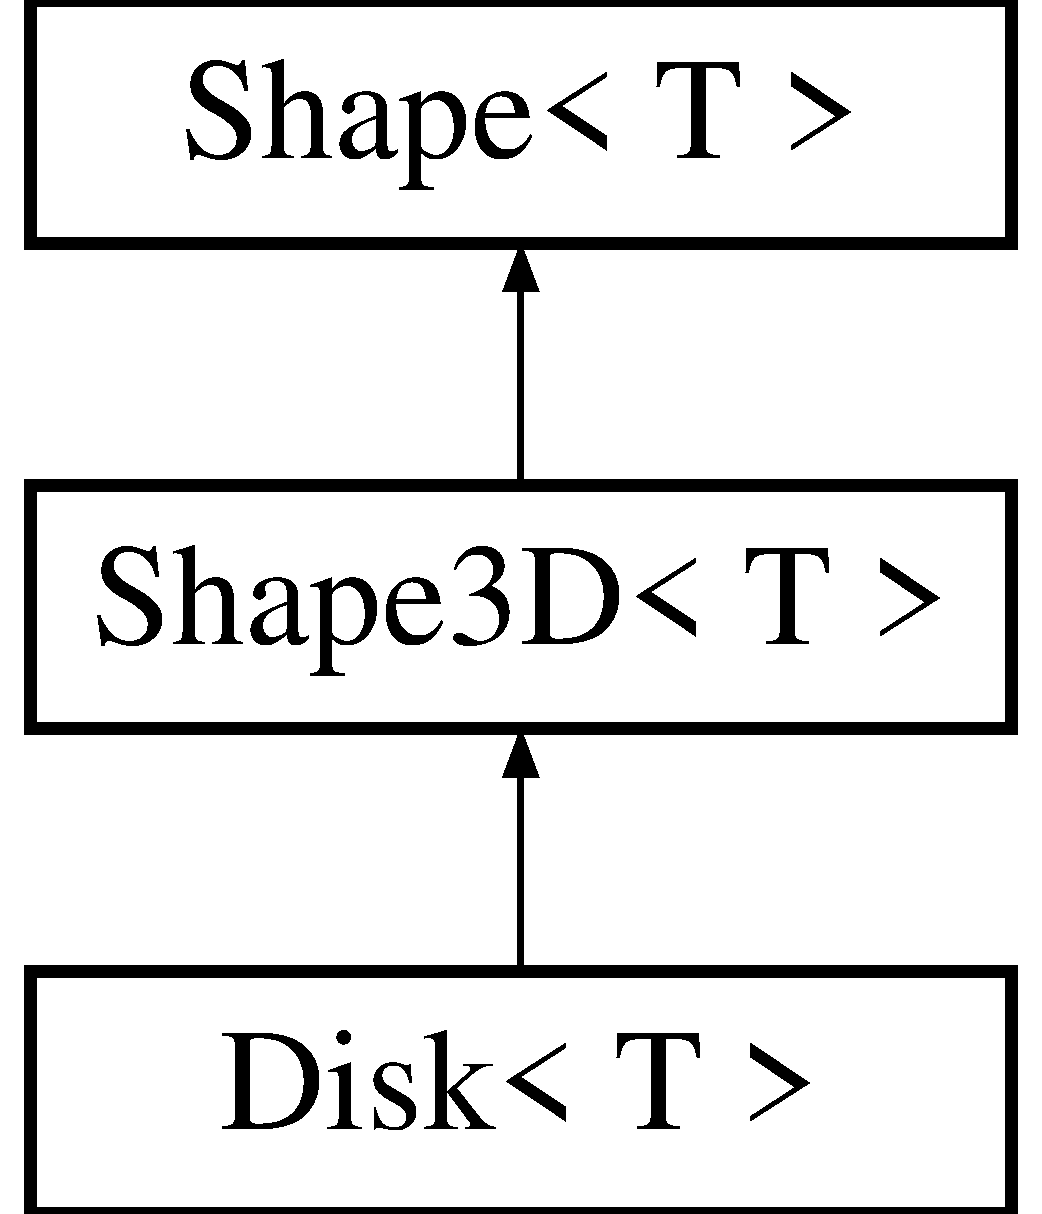
\includegraphics[height=3.000000cm]{classDisk}
\end{center}
\end{figure}
\subsection*{Public Member Functions}
\begin{DoxyCompactItemize}
\item 
\mbox{\hyperlink{classDisk_a88bcdb9bf91c8e9c18cdf551e558ab8c}{Disk}} ()
\begin{DoxyCompactList}\small\item\em \mbox{\hyperlink{classA}{A}} basic constructor. \end{DoxyCompactList}\item 
\mbox{\hyperlink{classDisk_af73e1930d8da87b05c813814532dd43a}{Disk}} (int, T=0.\+5)
\item 
\mbox{\hyperlink{classDisk_a893da931e3f39c126c434ab2fc2e12cc}{Disk}} (\mbox{\hyperlink{classDisk}{Disk}} \&\&)=default
\item 
\mbox{\hyperlink{classDisk}{Disk}} \& \mbox{\hyperlink{classDisk_ad6bc474ffecbc5de6f8fdd90ba5eddfe}{operator=}} (\mbox{\hyperlink{classDisk}{Disk}} \&\&)=default
\item 
\mbox{\hyperlink{classDisk_a96de79b2e115c478a33cc31f4818aee9}{Disk}} (const \mbox{\hyperlink{classDisk}{Disk}} \&)=default
\item 
\mbox{\hyperlink{classDisk}{Disk}} \& \mbox{\hyperlink{classDisk_a3ef862dd6e4671c907e2368bb5239bd2}{operator=}} (const \mbox{\hyperlink{classDisk}{Disk}} \&)=default
\end{DoxyCompactItemize}
\subsection*{Private Member Functions}
\begin{DoxyCompactItemize}
\item 
void \mbox{\hyperlink{classDisk_a1588532798901180b1eef6f3e1fb83f6}{generate\+\_\+vertexes}} ()
\item 
void \mbox{\hyperlink{classDisk_a4637847208b7236010085ca67f49e39a}{generate\+\_\+wheel\+\_\+line\+\_\+elements}} ()
\begin{DoxyCompactList}\small\item\em Function which generates sets wheel elements. Render wheel elements array with G\+L\+\_\+\+L\+I\+N\+ES to draw a wheel. \end{DoxyCompactList}\item 
{\footnotesize template$<$$>$ }\\void \mbox{\hyperlink{classDisk_a55648a13c42982087f60742da15c2c41}{generate\+\_\+vertexes}} ()
\begin{DoxyCompactList}\small\item\em Function which generates vertexes for float version of this class. \end{DoxyCompactList}\end{DoxyCompactItemize}
\subsection*{Private Attributes}
\begin{DoxyCompactItemize}
\item 
std\+::vector$<$ int $>$ \mbox{\hyperlink{classDisk_aa008e8bd0e7acdb4a1a56a8f44f048d7}{wheel\+\_\+line\+\_\+elements}}
\end{DoxyCompactItemize}
\subsection*{Additional Inherited Members}


\subsection{Detailed Description}
\subsubsection*{template$<$typename T = float$>$\newline
class Disk$<$ T $>$}

\mbox{\hyperlink{classA}{A}} class holding vertexes in the shape of a disk. 

\mbox{\hyperlink{classA}{A}} class holding vertexes in the shape of a disk. \mbox{\hyperlink{classDisk}{Disk}} is a 3d shape, thus it inherits from \mbox{\hyperlink{classShape3D}{Shape3D}} class. Template parameter can either be float or double. 
\begin{DoxyParams}{Parameters}
{\em T} & Template parameter T can either be float of double \\
\hline
\end{DoxyParams}


\subsection{Constructor \& Destructor Documentation}
\mbox{\Hypertarget{classDisk_a88bcdb9bf91c8e9c18cdf551e558ab8c}\label{classDisk_a88bcdb9bf91c8e9c18cdf551e558ab8c}} 
\index{Disk@{Disk}!Disk@{Disk}}
\index{Disk@{Disk}!Disk@{Disk}}
\subsubsection{\texorpdfstring{Disk()}{Disk()}\hspace{0.1cm}{\footnotesize\ttfamily [1/4]}}
{\footnotesize\ttfamily template$<$typename T $>$ \\
\mbox{\hyperlink{classDisk}{Disk}}$<$ T $>$\+::\mbox{\hyperlink{classDisk}{Disk}} (\begin{DoxyParamCaption}{ }\end{DoxyParamCaption})}



\mbox{\hyperlink{classA}{A}} basic constructor. 

Constructor initializes all important variables, geenratex necessary vertexes and initializes opengl buffers. \mbox{\Hypertarget{classDisk_af73e1930d8da87b05c813814532dd43a}\label{classDisk_af73e1930d8da87b05c813814532dd43a}} 
\index{Disk@{Disk}!Disk@{Disk}}
\index{Disk@{Disk}!Disk@{Disk}}
\subsubsection{\texorpdfstring{Disk()}{Disk()}\hspace{0.1cm}{\footnotesize\ttfamily [2/4]}}
{\footnotesize\ttfamily template$<$typename T  = float$>$ \\
\mbox{\hyperlink{classDisk}{Disk}}$<$ T $>$\+::\mbox{\hyperlink{classDisk}{Disk}} (\begin{DoxyParamCaption}\item[{int}]{,  }\item[{T}]{ = {\ttfamily 0.5} }\end{DoxyParamCaption})}

\mbox{\Hypertarget{classDisk_a893da931e3f39c126c434ab2fc2e12cc}\label{classDisk_a893da931e3f39c126c434ab2fc2e12cc}} 
\index{Disk@{Disk}!Disk@{Disk}}
\index{Disk@{Disk}!Disk@{Disk}}
\subsubsection{\texorpdfstring{Disk()}{Disk()}\hspace{0.1cm}{\footnotesize\ttfamily [3/4]}}
{\footnotesize\ttfamily template$<$typename T  = float$>$ \\
\mbox{\hyperlink{classDisk}{Disk}}$<$ T $>$\+::\mbox{\hyperlink{classDisk}{Disk}} (\begin{DoxyParamCaption}\item[{\mbox{\hyperlink{classDisk}{Disk}}$<$ T $>$ \&\&}]{ }\end{DoxyParamCaption})\hspace{0.3cm}{\ttfamily [default]}}

\mbox{\Hypertarget{classDisk_a96de79b2e115c478a33cc31f4818aee9}\label{classDisk_a96de79b2e115c478a33cc31f4818aee9}} 
\index{Disk@{Disk}!Disk@{Disk}}
\index{Disk@{Disk}!Disk@{Disk}}
\subsubsection{\texorpdfstring{Disk()}{Disk()}\hspace{0.1cm}{\footnotesize\ttfamily [4/4]}}
{\footnotesize\ttfamily template$<$typename T  = float$>$ \\
\mbox{\hyperlink{classDisk}{Disk}}$<$ T $>$\+::\mbox{\hyperlink{classDisk}{Disk}} (\begin{DoxyParamCaption}\item[{const \mbox{\hyperlink{classDisk}{Disk}}$<$ T $>$ \&}]{ }\end{DoxyParamCaption})\hspace{0.3cm}{\ttfamily [default]}}



\subsection{Member Function Documentation}
\mbox{\Hypertarget{classDisk_a1588532798901180b1eef6f3e1fb83f6}\label{classDisk_a1588532798901180b1eef6f3e1fb83f6}} 
\index{Disk@{Disk}!generate\+\_\+vertexes@{generate\+\_\+vertexes}}
\index{generate\+\_\+vertexes@{generate\+\_\+vertexes}!Disk@{Disk}}
\subsubsection{\texorpdfstring{generate\+\_\+vertexes()}{generate\_vertexes()}\hspace{0.1cm}{\footnotesize\ttfamily [1/2]}}
{\footnotesize\ttfamily template$<$typename T  = float$>$ \\
void \mbox{\hyperlink{classDisk}{Disk}}$<$ T $>$\+::generate\+\_\+vertexes (\begin{DoxyParamCaption}{ }\end{DoxyParamCaption})\hspace{0.3cm}{\ttfamily [private]}}

\mbox{\Hypertarget{classDisk_a55648a13c42982087f60742da15c2c41}\label{classDisk_a55648a13c42982087f60742da15c2c41}} 
\index{Disk@{Disk}!generate\+\_\+vertexes@{generate\+\_\+vertexes}}
\index{generate\+\_\+vertexes@{generate\+\_\+vertexes}!Disk@{Disk}}
\subsubsection{\texorpdfstring{generate\+\_\+vertexes()}{generate\_vertexes()}\hspace{0.1cm}{\footnotesize\ttfamily [2/2]}}
{\footnotesize\ttfamily template$<$$>$ \\
void \mbox{\hyperlink{classDisk}{Disk}}$<$ float $>$\+::generate\+\_\+vertexes (\begin{DoxyParamCaption}{ }\end{DoxyParamCaption})\hspace{0.3cm}{\ttfamily [inline]}, {\ttfamily [private]}}



Function which generates vertexes for float version of this class. 

Vertexes are generate in such a way that the middle of the shape is (0,0,0). The function also sets the element array. It uses sse instructions -\/ use appropriate processor. \mbox{\Hypertarget{classDisk_a4637847208b7236010085ca67f49e39a}\label{classDisk_a4637847208b7236010085ca67f49e39a}} 
\index{Disk@{Disk}!generate\+\_\+wheel\+\_\+line\+\_\+elements@{generate\+\_\+wheel\+\_\+line\+\_\+elements}}
\index{generate\+\_\+wheel\+\_\+line\+\_\+elements@{generate\+\_\+wheel\+\_\+line\+\_\+elements}!Disk@{Disk}}
\subsubsection{\texorpdfstring{generate\+\_\+wheel\+\_\+line\+\_\+elements()}{generate\_wheel\_line\_elements()}}
{\footnotesize\ttfamily template$<$typename T $>$ \\
void \mbox{\hyperlink{classDisk}{Disk}}$<$ T $>$\+::generate\+\_\+wheel\+\_\+line\+\_\+elements (\begin{DoxyParamCaption}{ }\end{DoxyParamCaption})\hspace{0.3cm}{\ttfamily [private]}}



Function which generates sets wheel elements. Render wheel elements array with G\+L\+\_\+\+L\+I\+N\+ES to draw a wheel. 

\mbox{\Hypertarget{classDisk_ad6bc474ffecbc5de6f8fdd90ba5eddfe}\label{classDisk_ad6bc474ffecbc5de6f8fdd90ba5eddfe}} 
\index{Disk@{Disk}!operator=@{operator=}}
\index{operator=@{operator=}!Disk@{Disk}}
\subsubsection{\texorpdfstring{operator=()}{operator=()}\hspace{0.1cm}{\footnotesize\ttfamily [1/2]}}
{\footnotesize\ttfamily template$<$typename T  = float$>$ \\
\mbox{\hyperlink{classDisk}{Disk}}\& \mbox{\hyperlink{classDisk}{Disk}}$<$ T $>$\+::operator= (\begin{DoxyParamCaption}\item[{\mbox{\hyperlink{classDisk}{Disk}}$<$ T $>$ \&\&}]{ }\end{DoxyParamCaption})\hspace{0.3cm}{\ttfamily [default]}}

\mbox{\Hypertarget{classDisk_a3ef862dd6e4671c907e2368bb5239bd2}\label{classDisk_a3ef862dd6e4671c907e2368bb5239bd2}} 
\index{Disk@{Disk}!operator=@{operator=}}
\index{operator=@{operator=}!Disk@{Disk}}
\subsubsection{\texorpdfstring{operator=()}{operator=()}\hspace{0.1cm}{\footnotesize\ttfamily [2/2]}}
{\footnotesize\ttfamily template$<$typename T  = float$>$ \\
\mbox{\hyperlink{classDisk}{Disk}}\& \mbox{\hyperlink{classDisk}{Disk}}$<$ T $>$\+::operator= (\begin{DoxyParamCaption}\item[{const \mbox{\hyperlink{classDisk}{Disk}}$<$ T $>$ \&}]{ }\end{DoxyParamCaption})\hspace{0.3cm}{\ttfamily [default]}}



\subsection{Member Data Documentation}
\mbox{\Hypertarget{classDisk_aa008e8bd0e7acdb4a1a56a8f44f048d7}\label{classDisk_aa008e8bd0e7acdb4a1a56a8f44f048d7}} 
\index{Disk@{Disk}!wheel\+\_\+line\+\_\+elements@{wheel\+\_\+line\+\_\+elements}}
\index{wheel\+\_\+line\+\_\+elements@{wheel\+\_\+line\+\_\+elements}!Disk@{Disk}}
\subsubsection{\texorpdfstring{wheel\+\_\+line\+\_\+elements}{wheel\_line\_elements}}
{\footnotesize\ttfamily template$<$typename T  = float$>$ \\
std\+::vector$<$int$>$ \mbox{\hyperlink{classDisk}{Disk}}$<$ T $>$\+::wheel\+\_\+line\+\_\+elements\hspace{0.3cm}{\ttfamily [private]}}

elements which determine wheel shape 

The documentation for this class was generated from the following file\+:\begin{DoxyCompactItemize}
\item 
src/\mbox{\hyperlink{disk_8hpp}{disk.\+hpp}}\end{DoxyCompactItemize}

\hypertarget{classExampleApplication}{}\section{Example\+Application Class Reference}
\label{classExampleApplication}\index{Example\+Application@{Example\+Application}}


{\ttfamily \#include \char`\"{}ising\+\_\+windows.\+hpp\char`\"{}}

Inheritance diagram for Example\+Application\+:\begin{figure}[H]
\begin{center}
\leavevmode
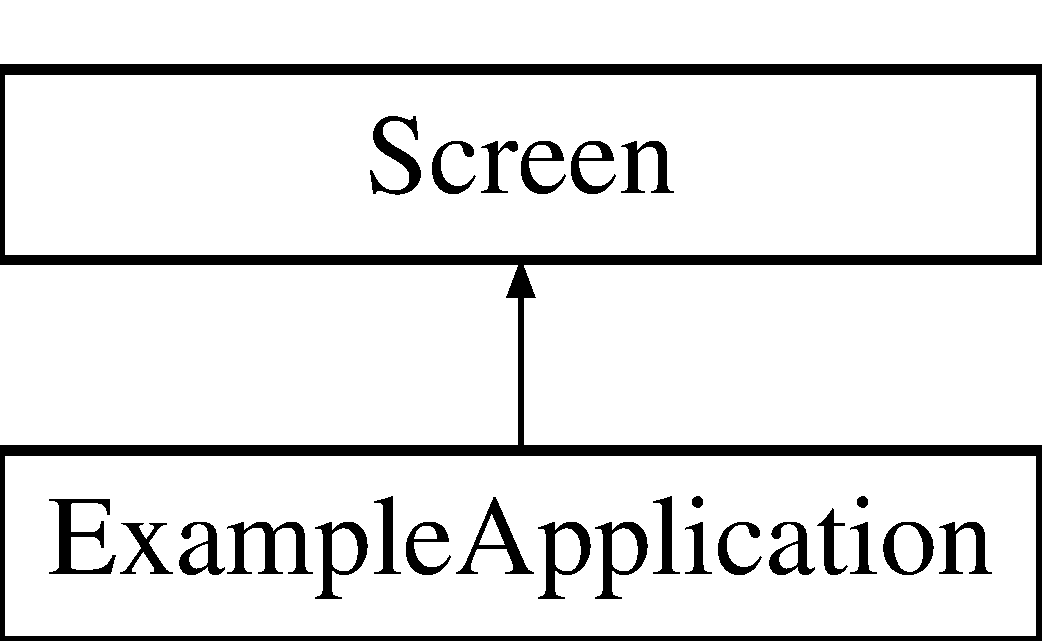
\includegraphics[height=2.000000cm]{classExampleApplication}
\end{center}
\end{figure}
\subsection*{Public Member Functions}
\begin{DoxyCompactItemize}
\item 
\mbox{\hyperlink{classExampleApplication_a3fb3b3b1dd4820cc3290944879ecb6d2}{Example\+Application}} ()
\item 
\mbox{\hyperlink{classExampleApplication_aacd4040918ad68dd2688d38dff8f57be}{$\sim$\+Example\+Application}} ()
\item 
virtual bool \mbox{\hyperlink{classExampleApplication_a79821271b7d486f2727c42ad9d385ba4}{keyboard\+Event}} (int key, int scancode, int action, int modifiers)
\item 
virtual void \mbox{\hyperlink{classExampleApplication_a4fa26138de0a6f65e6b1ccae17f26f9d}{draw}} (N\+V\+Gcontext $\ast$ctx)
\item 
virtual void \mbox{\hyperlink{classExampleApplication_a75d765000cca185faf56af2db9472d19}{draw\+Contents}} ()
\item 
\mbox{\hyperlink{classExampleApplication_adb53fe47e1c5d9cf00c3173a586a5c19}{Example\+Application}} (\mbox{\hyperlink{classIsingModel}{Ising\+Model}}$<$ float $>$ $\ast$model, \mbox{\hyperlink{classSpinArray}{Spin\+Array}}$<$ float $>$ $\ast$spin\+\_\+array=N\+U\+LL)
\end{DoxyCompactItemize}
\subsection*{Private Attributes}
\begin{DoxyCompactItemize}
\item 
nanogui\+::\+Progress\+Bar $\ast$ \mbox{\hyperlink{classExampleApplication_a0f3364dd56cbc31539b750aebd0c6a5a}{m\+Progress}}
\end{DoxyCompactItemize}


\subsection{Constructor \& Destructor Documentation}
\mbox{\Hypertarget{classExampleApplication_a3fb3b3b1dd4820cc3290944879ecb6d2}\label{classExampleApplication_a3fb3b3b1dd4820cc3290944879ecb6d2}} 
\index{Example\+Application@{Example\+Application}!Example\+Application@{Example\+Application}}
\index{Example\+Application@{Example\+Application}!Example\+Application@{Example\+Application}}
\subsubsection{\texorpdfstring{Example\+Application()}{ExampleApplication()}\hspace{0.1cm}{\footnotesize\ttfamily [1/2]}}
{\footnotesize\ttfamily Example\+Application\+::\+Example\+Application (\begin{DoxyParamCaption}{ }\end{DoxyParamCaption})\hspace{0.3cm}{\ttfamily [inline]}}

\mbox{\Hypertarget{classExampleApplication_aacd4040918ad68dd2688d38dff8f57be}\label{classExampleApplication_aacd4040918ad68dd2688d38dff8f57be}} 
\index{Example\+Application@{Example\+Application}!````~Example\+Application@{$\sim$\+Example\+Application}}
\index{````~Example\+Application@{$\sim$\+Example\+Application}!Example\+Application@{Example\+Application}}
\subsubsection{\texorpdfstring{$\sim$\+Example\+Application()}{~ExampleApplication()}}
{\footnotesize\ttfamily Example\+Application\+::$\sim$\+Example\+Application (\begin{DoxyParamCaption}{ }\end{DoxyParamCaption})\hspace{0.3cm}{\ttfamily [inline]}}

\mbox{\Hypertarget{classExampleApplication_adb53fe47e1c5d9cf00c3173a586a5c19}\label{classExampleApplication_adb53fe47e1c5d9cf00c3173a586a5c19}} 
\index{Example\+Application@{Example\+Application}!Example\+Application@{Example\+Application}}
\index{Example\+Application@{Example\+Application}!Example\+Application@{Example\+Application}}
\subsubsection{\texorpdfstring{Example\+Application()}{ExampleApplication()}\hspace{0.1cm}{\footnotesize\ttfamily [2/2]}}
{\footnotesize\ttfamily Example\+Application\+::\+Example\+Application (\begin{DoxyParamCaption}\item[{\mbox{\hyperlink{classIsingModel}{Ising\+Model}}$<$ float $>$ $\ast$}]{model,  }\item[{\mbox{\hyperlink{classSpinArray}{Spin\+Array}}$<$ float $>$ $\ast$}]{spin\+\_\+array = {\ttfamily NULL} }\end{DoxyParamCaption})\hspace{0.3cm}{\ttfamily [inline]}}



\subsection{Member Function Documentation}
\mbox{\Hypertarget{classExampleApplication_a4fa26138de0a6f65e6b1ccae17f26f9d}\label{classExampleApplication_a4fa26138de0a6f65e6b1ccae17f26f9d}} 
\index{Example\+Application@{Example\+Application}!draw@{draw}}
\index{draw@{draw}!Example\+Application@{Example\+Application}}
\subsubsection{\texorpdfstring{draw()}{draw()}}
{\footnotesize\ttfamily virtual void Example\+Application\+::draw (\begin{DoxyParamCaption}\item[{N\+V\+Gcontext $\ast$}]{ctx }\end{DoxyParamCaption})\hspace{0.3cm}{\ttfamily [inline]}, {\ttfamily [virtual]}}

\mbox{\Hypertarget{classExampleApplication_a75d765000cca185faf56af2db9472d19}\label{classExampleApplication_a75d765000cca185faf56af2db9472d19}} 
\index{Example\+Application@{Example\+Application}!draw\+Contents@{draw\+Contents}}
\index{draw\+Contents@{draw\+Contents}!Example\+Application@{Example\+Application}}
\subsubsection{\texorpdfstring{draw\+Contents()}{drawContents()}}
{\footnotesize\ttfamily virtual void Example\+Application\+::draw\+Contents (\begin{DoxyParamCaption}{ }\end{DoxyParamCaption})\hspace{0.3cm}{\ttfamily [inline]}, {\ttfamily [virtual]}}

\mbox{\Hypertarget{classExampleApplication_a79821271b7d486f2727c42ad9d385ba4}\label{classExampleApplication_a79821271b7d486f2727c42ad9d385ba4}} 
\index{Example\+Application@{Example\+Application}!keyboard\+Event@{keyboard\+Event}}
\index{keyboard\+Event@{keyboard\+Event}!Example\+Application@{Example\+Application}}
\subsubsection{\texorpdfstring{keyboard\+Event()}{keyboardEvent()}}
{\footnotesize\ttfamily virtual bool Example\+Application\+::keyboard\+Event (\begin{DoxyParamCaption}\item[{int}]{key,  }\item[{int}]{scancode,  }\item[{int}]{action,  }\item[{int}]{modifiers }\end{DoxyParamCaption})\hspace{0.3cm}{\ttfamily [inline]}, {\ttfamily [virtual]}}



\subsection{Member Data Documentation}
\mbox{\Hypertarget{classExampleApplication_a0f3364dd56cbc31539b750aebd0c6a5a}\label{classExampleApplication_a0f3364dd56cbc31539b750aebd0c6a5a}} 
\index{Example\+Application@{Example\+Application}!m\+Progress@{m\+Progress}}
\index{m\+Progress@{m\+Progress}!Example\+Application@{Example\+Application}}
\subsubsection{\texorpdfstring{m\+Progress}{mProgress}}
{\footnotesize\ttfamily nanogui\+::\+Progress\+Bar$\ast$ Example\+Application\+::m\+Progress\hspace{0.3cm}{\ttfamily [private]}}



The documentation for this class was generated from the following file\+:\begin{DoxyCompactItemize}
\item 
examples/ising\+\_\+full\+\_\+nanogui\+\_\+version/\mbox{\hyperlink{ising__full__nanogui__version_2ising__windows_8hpp}{ising\+\_\+windows.\+hpp}}\end{DoxyCompactItemize}

\hypertarget{structstd_1_1hash_3_01pair_3_01S_00_01T_01_4_01_4}{}\section{std\+:\+:hash$<$ pair$<$ S, T $>$ $>$ Struct Template Reference}
\label{structstd_1_1hash_3_01pair_3_01S_00_01T_01_4_01_4}\index{std\+::hash$<$ pair$<$ S, T $>$ $>$@{std\+::hash$<$ pair$<$ S, T $>$ $>$}}


{\ttfamily \#include \char`\"{}auxiliary\+\_\+functions.\+hpp\char`\"{}}

\subsection*{Public Member Functions}
\begin{DoxyCompactItemize}
\item 
size\+\_\+t \mbox{\hyperlink{structstd_1_1hash_3_01pair_3_01S_00_01T_01_4_01_4_a6fec6cb26e96fb20d4ec121487e5acb4}{operator()}} (const pair$<$ S, T $>$ \&\mbox{\hyperlink{glad_8h_a30522dbcc3e66083fcf2bf64d1fad76a}{v}}) const
\end{DoxyCompactItemize}


\subsection{Member Function Documentation}
\mbox{\Hypertarget{structstd_1_1hash_3_01pair_3_01S_00_01T_01_4_01_4_a6fec6cb26e96fb20d4ec121487e5acb4}\label{structstd_1_1hash_3_01pair_3_01S_00_01T_01_4_01_4_a6fec6cb26e96fb20d4ec121487e5acb4}} 
\index{std\+::hash$<$ pair$<$ S, T $>$ $>$@{std\+::hash$<$ pair$<$ S, T $>$ $>$}!operator()@{operator()}}
\index{operator()@{operator()}!std\+::hash$<$ pair$<$ S, T $>$ $>$@{std\+::hash$<$ pair$<$ S, T $>$ $>$}}
\subsubsection{\texorpdfstring{operator()()}{operator()()}}
{\footnotesize\ttfamily template$<$typename S , typename T $>$ \\
size\+\_\+t std\+::hash$<$ pair$<$ S, T $>$ $>$\+::operator() (\begin{DoxyParamCaption}\item[{const pair$<$ S, T $>$ \&}]{v }\end{DoxyParamCaption}) const\hspace{0.3cm}{\ttfamily [inline]}}



The documentation for this struct was generated from the following file\+:\begin{DoxyCompactItemize}
\item 
src/algorithms/\mbox{\hyperlink{auxiliary__functions_8hpp}{auxiliary\+\_\+functions.\+hpp}}\end{DoxyCompactItemize}

\hypertarget{classIsingModel}{}\section{Ising\+Model$<$ T $>$ Class Template Reference}
\label{classIsingModel}\index{Ising\+Model$<$ T $>$@{Ising\+Model$<$ T $>$}}


Ising model containing two possible spin flipping methods -\/ metropolis and wolff.  




{\ttfamily \#include \char`\"{}Ising\+\_\+model.\+hpp\char`\"{}}

\subsection*{Public Member Functions}
\begin{DoxyCompactItemize}
\item 
\mbox{\hyperlink{classIsingModel_a3c9a903d3ddada5ce514ba66f99b0282}{Ising\+Model}} (unsigned size\+\_\+=50, T temperature\+\_\+=2)
\begin{DoxyCompactList}\small\item\em Basic constructor for \mbox{\hyperlink{classIsingModel}{Ising\+Model}} class. \end{DoxyCompactList}\item 
\mbox{\hyperlink{classspin__dir}{spin\+\_\+dir}} $\ast$ \mbox{\hyperlink{classIsingModel_ad82f225e1b45f11ee5a99c3b12b25302}{get\+\_\+spin\+\_\+array}} ()
\item 
int \mbox{\hyperlink{classIsingModel_a349a13b847fb221eec7043fc53649640}{calc\+\_\+magnetization}} ()
\begin{DoxyCompactList}\small\item\em calculate magnetization -\/ difference between spins up and spins down \end{DoxyCompactList}\item 
void \mbox{\hyperlink{classIsingModel_abbd5b7935830eca268b7eacc94478649}{set\+\_\+temperature}} (T temperature\+\_\+)
\begin{DoxyCompactList}\small\item\em sets the temperature \end{DoxyCompactList}\item 
T \mbox{\hyperlink{classIsingModel_ad0252a860a935d1be2542f15b5c25936}{get\+\_\+temperature}} ()
\begin{DoxyCompactList}\small\item\em get the temperature \end{DoxyCompactList}\item 
unsigned \mbox{\hyperlink{classIsingModel_afd731e5858b03deb1c8a11ee8a6b8834}{get\+\_\+cluster\+\_\+size}} ()
\begin{DoxyCompactList}\small\item\em Get the size of the cluster in the last Wolff step. \end{DoxyCompactList}\item 
T \mbox{\hyperlink{classIsingModel_a37a7c509999f21f1bd4f54a12009f3cf}{get\+\_\+energy}} ()
\begin{DoxyCompactList}\small\item\em Get current energy. \end{DoxyCompactList}\item 
int \mbox{\hyperlink{classIsingModel_a58c9ebc61c0b2238fd52b62df8ce4853}{get\+\_\+magnetization}} ()
\begin{DoxyCompactList}\small\item\em get current magnetization. \end{DoxyCompactList}\item 
void \mbox{\hyperlink{classIsingModel_ab76a4eee808eaa1979ff6707498e9908}{flip\+\_\+cluster}} ()
\begin{DoxyCompactList}\small\item\em The function flips the cluster using Wolff algorithm. \end{DoxyCompactList}\item 
void \mbox{\hyperlink{classIsingModel_ac16bfdd5bb4012162bedd90034962f58}{set\+\_\+all\+\_\+spins\+\_\+up}} ()
\begin{DoxyCompactList}\small\item\em set all spins up. \end{DoxyCompactList}\item 
T \mbox{\hyperlink{classIsingModel_a0a387ccae720604f4de13d5b0762ac62}{calc\+\_\+energy}} ()
\begin{DoxyCompactList}\small\item\em The function calculates energy of the spin array. \end{DoxyCompactList}\item 
void \mbox{\hyperlink{classIsingModel_a195316f577d71297e9634fa6fdeacc44}{metropolis\+\_\+steps}} (unsigned spin\+\_\+flips)
\begin{DoxyCompactList}\small\item\em Makes a metropolis step. \end{DoxyCompactList}\end{DoxyCompactItemize}
\subsection*{Private Member Functions}
\begin{DoxyCompactItemize}
\item 
void \mbox{\hyperlink{classIsingModel_abe2a720ca3ed7dde191e36fbf33561b3}{enforce\+\_\+boundary\+\_\+conditions}} ()
\begin{DoxyCompactList}\small\item\em enforce periodic boundary conditions \end{DoxyCompactList}\item 
void \mbox{\hyperlink{classIsingModel_a6ab9293015326da93fb6e3e20d24edf8}{set\+\_\+random\+\_\+spin\+\_\+directions}} ()
\begin{DoxyCompactList}\small\item\em set random spin directions \end{DoxyCompactList}\item 
void \mbox{\hyperlink{classIsingModel_a37758a1a4a2536d16f1bb8166e13f7b6}{wolff\+\_\+cluster\+\_\+step}} (\mbox{\hyperlink{classspin__dir}{spin\+\_\+dir}} spin, unsigned k, unsigned l)
\begin{DoxyCompactList}\small\item\em Make a Wolff algorithm step. \mbox{\hyperlink{classThis}{This}} is a helper for \mbox{\hyperlink{classIsingModel_ab76a4eee808eaa1979ff6707498e9908}{flip\+\_\+cluster()}} function. \end{DoxyCompactList}\end{DoxyCompactItemize}
\subsection*{Private Attributes}
\begin{DoxyCompactItemize}
\item 
unsigned \mbox{\hyperlink{classIsingModel_aec6fc4774dda94fd23c6e29d0820b63a}{size}}
\item 
T \mbox{\hyperlink{classIsingModel_af0c6d48208741fe5a378e29b7fac0da1}{J}} = 1
\item 
T \mbox{\hyperlink{classIsingModel_a19e1a223476c953a9964532c7f0eb6dd}{H}} = 0
\item 
T \mbox{\hyperlink{classIsingModel_af19ba376c01404c094c214939eafd7a5}{tc}} = 2.\+269185
\item 
T \mbox{\hyperlink{classIsingModel_a756faa94432cc7e10d21e52a03156569}{temperature}}
\item 
\mbox{\hyperlink{classspin__dir}{spin\+\_\+dir}} $\ast$ \mbox{\hyperlink{classIsingModel_a82425f60fa2dd07995c2a53f8a850cf5}{spin\+\_\+array}}
\item 
unsigned \mbox{\hyperlink{classIsingModel_a67a282de0cc889e423cde222a3453d38}{cluster\+\_\+size}} = 0
\item 
int \mbox{\hyperlink{classIsingModel_a20c8183929e5e2a395cb962501122e65}{magnetization}} = 0
\item 
T \mbox{\hyperlink{classIsingModel_abd38e1a93e1e7bab7788f00d0b9fddb9}{energy}} = 0
\item 
unsigned \mbox{\hyperlink{classIsingModel_a434e854082ad794811b6e11e2bc50eaf}{samples}} = 0
\item 
std\+::random\+\_\+device \mbox{\hyperlink{classIsingModel_a602475ebc23d97e2ba162ba1db352386}{rd}}
\item 
std\+::mt19937 \mbox{\hyperlink{classIsingModel_a3250275d0897da9f7929b43286e9b44b}{rng}}
\item 
std\+::uniform\+\_\+int\+\_\+distribution$<$ int $>$ \mbox{\hyperlink{classIsingModel_a5f412d0560c599a350d0c266125427c9}{random\+\_\+int}}
\item 
std\+::uniform\+\_\+real\+\_\+distribution$<$ T $>$ \mbox{\hyperlink{classIsingModel_a01dcb867d89771158b7f71a518ded0f2}{random\+\_\+real}}
\end{DoxyCompactItemize}


\subsection{Detailed Description}
\subsubsection*{template$<$typename T$>$\newline
class Ising\+Model$<$ T $>$}

Ising model containing two possible spin flipping methods -\/ metropolis and wolff. 

\subsection{Constructor \& Destructor Documentation}
\mbox{\Hypertarget{classIsingModel_a3c9a903d3ddada5ce514ba66f99b0282}\label{classIsingModel_a3c9a903d3ddada5ce514ba66f99b0282}} 
\index{Ising\+Model@{Ising\+Model}!Ising\+Model@{Ising\+Model}}
\index{Ising\+Model@{Ising\+Model}!Ising\+Model@{Ising\+Model}}
\subsubsection{\texorpdfstring{Ising\+Model()}{IsingModel()}}
{\footnotesize\ttfamily template$<$typename T$>$ \\
\mbox{\hyperlink{classIsingModel}{Ising\+Model}}$<$ T $>$\+::\mbox{\hyperlink{classIsingModel}{Ising\+Model}} (\begin{DoxyParamCaption}\item[{unsigned}]{size\+\_\+ = {\ttfamily 50},  }\item[{T}]{temperature\+\_\+ = {\ttfamily 2} }\end{DoxyParamCaption})\hspace{0.3cm}{\ttfamily [inline]}}



Basic constructor for \mbox{\hyperlink{classIsingModel}{Ising\+Model}} class. 

By default it sets the temperature to 2 and size of spin array to 50. It also initializes random generator, sets random spin directions and enforces periodic boundary conditions for the start of calculation 

\subsection{Member Function Documentation}
\mbox{\Hypertarget{classIsingModel_a0a387ccae720604f4de13d5b0762ac62}\label{classIsingModel_a0a387ccae720604f4de13d5b0762ac62}} 
\index{Ising\+Model@{Ising\+Model}!calc\+\_\+energy@{calc\+\_\+energy}}
\index{calc\+\_\+energy@{calc\+\_\+energy}!Ising\+Model@{Ising\+Model}}
\subsubsection{\texorpdfstring{calc\+\_\+energy()}{calc\_energy()}}
{\footnotesize\ttfamily template$<$typename T$>$ \\
T \mbox{\hyperlink{classIsingModel}{Ising\+Model}}$<$ T $>$\+::calc\+\_\+energy (\begin{DoxyParamCaption}{ }\end{DoxyParamCaption})\hspace{0.3cm}{\ttfamily [inline]}}



The function calculates energy of the spin array. 

\mbox{\Hypertarget{classIsingModel_a349a13b847fb221eec7043fc53649640}\label{classIsingModel_a349a13b847fb221eec7043fc53649640}} 
\index{Ising\+Model@{Ising\+Model}!calc\+\_\+magnetization@{calc\+\_\+magnetization}}
\index{calc\+\_\+magnetization@{calc\+\_\+magnetization}!Ising\+Model@{Ising\+Model}}
\subsubsection{\texorpdfstring{calc\+\_\+magnetization()}{calc\_magnetization()}}
{\footnotesize\ttfamily template$<$typename T$>$ \\
int \mbox{\hyperlink{classIsingModel}{Ising\+Model}}$<$ T $>$\+::calc\+\_\+magnetization (\begin{DoxyParamCaption}{ }\end{DoxyParamCaption})\hspace{0.3cm}{\ttfamily [inline]}}



calculate magnetization -\/ difference between spins up and spins down 

\mbox{\Hypertarget{classIsingModel_abe2a720ca3ed7dde191e36fbf33561b3}\label{classIsingModel_abe2a720ca3ed7dde191e36fbf33561b3}} 
\index{Ising\+Model@{Ising\+Model}!enforce\+\_\+boundary\+\_\+conditions@{enforce\+\_\+boundary\+\_\+conditions}}
\index{enforce\+\_\+boundary\+\_\+conditions@{enforce\+\_\+boundary\+\_\+conditions}!Ising\+Model@{Ising\+Model}}
\subsubsection{\texorpdfstring{enforce\+\_\+boundary\+\_\+conditions()}{enforce\_boundary\_conditions()}}
{\footnotesize\ttfamily template$<$typename T$>$ \\
void \mbox{\hyperlink{classIsingModel}{Ising\+Model}}$<$ T $>$\+::enforce\+\_\+boundary\+\_\+conditions (\begin{DoxyParamCaption}{ }\end{DoxyParamCaption})\hspace{0.3cm}{\ttfamily [inline]}, {\ttfamily [private]}}



enforce periodic boundary conditions 

\mbox{\Hypertarget{classIsingModel_ab76a4eee808eaa1979ff6707498e9908}\label{classIsingModel_ab76a4eee808eaa1979ff6707498e9908}} 
\index{Ising\+Model@{Ising\+Model}!flip\+\_\+cluster@{flip\+\_\+cluster}}
\index{flip\+\_\+cluster@{flip\+\_\+cluster}!Ising\+Model@{Ising\+Model}}
\subsubsection{\texorpdfstring{flip\+\_\+cluster()}{flip\_cluster()}}
{\footnotesize\ttfamily template$<$typename T$>$ \\
void \mbox{\hyperlink{classIsingModel}{Ising\+Model}}$<$ T $>$\+::flip\+\_\+cluster (\begin{DoxyParamCaption}{ }\end{DoxyParamCaption})\hspace{0.3cm}{\ttfamily [inline]}}



The function flips the cluster using Wolff algorithm. 

It calls the \mbox{\hyperlink{classIsingModel_a37758a1a4a2536d16f1bb8166e13f7b6}{wolff\+\_\+cluster\+\_\+step()}} function. \mbox{\Hypertarget{classIsingModel_afd731e5858b03deb1c8a11ee8a6b8834}\label{classIsingModel_afd731e5858b03deb1c8a11ee8a6b8834}} 
\index{Ising\+Model@{Ising\+Model}!get\+\_\+cluster\+\_\+size@{get\+\_\+cluster\+\_\+size}}
\index{get\+\_\+cluster\+\_\+size@{get\+\_\+cluster\+\_\+size}!Ising\+Model@{Ising\+Model}}
\subsubsection{\texorpdfstring{get\+\_\+cluster\+\_\+size()}{get\_cluster\_size()}}
{\footnotesize\ttfamily template$<$typename T$>$ \\
unsigned \mbox{\hyperlink{classIsingModel}{Ising\+Model}}$<$ T $>$\+::get\+\_\+cluster\+\_\+size (\begin{DoxyParamCaption}{ }\end{DoxyParamCaption})\hspace{0.3cm}{\ttfamily [inline]}}



Get the size of the cluster in the last Wolff step. 

\mbox{\Hypertarget{classIsingModel_a37a7c509999f21f1bd4f54a12009f3cf}\label{classIsingModel_a37a7c509999f21f1bd4f54a12009f3cf}} 
\index{Ising\+Model@{Ising\+Model}!get\+\_\+energy@{get\+\_\+energy}}
\index{get\+\_\+energy@{get\+\_\+energy}!Ising\+Model@{Ising\+Model}}
\subsubsection{\texorpdfstring{get\+\_\+energy()}{get\_energy()}}
{\footnotesize\ttfamily template$<$typename T$>$ \\
T \mbox{\hyperlink{classIsingModel}{Ising\+Model}}$<$ T $>$\+::get\+\_\+energy (\begin{DoxyParamCaption}{ }\end{DoxyParamCaption})\hspace{0.3cm}{\ttfamily [inline]}}



Get current energy. 

\mbox{\Hypertarget{classIsingModel_a58c9ebc61c0b2238fd52b62df8ce4853}\label{classIsingModel_a58c9ebc61c0b2238fd52b62df8ce4853}} 
\index{Ising\+Model@{Ising\+Model}!get\+\_\+magnetization@{get\+\_\+magnetization}}
\index{get\+\_\+magnetization@{get\+\_\+magnetization}!Ising\+Model@{Ising\+Model}}
\subsubsection{\texorpdfstring{get\+\_\+magnetization()}{get\_magnetization()}}
{\footnotesize\ttfamily template$<$typename T$>$ \\
int \mbox{\hyperlink{classIsingModel}{Ising\+Model}}$<$ T $>$\+::get\+\_\+magnetization (\begin{DoxyParamCaption}{ }\end{DoxyParamCaption})\hspace{0.3cm}{\ttfamily [inline]}}



get current magnetization. 

\mbox{\Hypertarget{classIsingModel_ad82f225e1b45f11ee5a99c3b12b25302}\label{classIsingModel_ad82f225e1b45f11ee5a99c3b12b25302}} 
\index{Ising\+Model@{Ising\+Model}!get\+\_\+spin\+\_\+array@{get\+\_\+spin\+\_\+array}}
\index{get\+\_\+spin\+\_\+array@{get\+\_\+spin\+\_\+array}!Ising\+Model@{Ising\+Model}}
\subsubsection{\texorpdfstring{get\+\_\+spin\+\_\+array()}{get\_spin\_array()}}
{\footnotesize\ttfamily template$<$typename T$>$ \\
\mbox{\hyperlink{classspin__dir}{spin\+\_\+dir}}$\ast$ \mbox{\hyperlink{classIsingModel}{Ising\+Model}}$<$ T $>$\+::get\+\_\+spin\+\_\+array (\begin{DoxyParamCaption}{ }\end{DoxyParamCaption})\hspace{0.3cm}{\ttfamily [inline]}}

\mbox{\Hypertarget{classIsingModel_ad0252a860a935d1be2542f15b5c25936}\label{classIsingModel_ad0252a860a935d1be2542f15b5c25936}} 
\index{Ising\+Model@{Ising\+Model}!get\+\_\+temperature@{get\+\_\+temperature}}
\index{get\+\_\+temperature@{get\+\_\+temperature}!Ising\+Model@{Ising\+Model}}
\subsubsection{\texorpdfstring{get\+\_\+temperature()}{get\_temperature()}}
{\footnotesize\ttfamily template$<$typename T$>$ \\
T \mbox{\hyperlink{classIsingModel}{Ising\+Model}}$<$ T $>$\+::get\+\_\+temperature (\begin{DoxyParamCaption}{ }\end{DoxyParamCaption})\hspace{0.3cm}{\ttfamily [inline]}}



get the temperature 

\mbox{\Hypertarget{classIsingModel_a195316f577d71297e9634fa6fdeacc44}\label{classIsingModel_a195316f577d71297e9634fa6fdeacc44}} 
\index{Ising\+Model@{Ising\+Model}!metropolis\+\_\+steps@{metropolis\+\_\+steps}}
\index{metropolis\+\_\+steps@{metropolis\+\_\+steps}!Ising\+Model@{Ising\+Model}}
\subsubsection{\texorpdfstring{metropolis\+\_\+steps()}{metropolis\_steps()}}
{\footnotesize\ttfamily template$<$typename T$>$ \\
void \mbox{\hyperlink{classIsingModel}{Ising\+Model}}$<$ T $>$\+::metropolis\+\_\+steps (\begin{DoxyParamCaption}\item[{unsigned}]{spin\+\_\+flips }\end{DoxyParamCaption})\hspace{0.3cm}{\ttfamily [inline]}}



Makes a metropolis step. 

a random spin is chosen and flipped with the probability exp(-\/d\+E/T) 
\begin{DoxyParams}{Parameters}
{\em spin\+\_\+flips} & number of metropolis spin flips to make \\
\hline
\end{DoxyParams}
\mbox{\Hypertarget{classIsingModel_ac16bfdd5bb4012162bedd90034962f58}\label{classIsingModel_ac16bfdd5bb4012162bedd90034962f58}} 
\index{Ising\+Model@{Ising\+Model}!set\+\_\+all\+\_\+spins\+\_\+up@{set\+\_\+all\+\_\+spins\+\_\+up}}
\index{set\+\_\+all\+\_\+spins\+\_\+up@{set\+\_\+all\+\_\+spins\+\_\+up}!Ising\+Model@{Ising\+Model}}
\subsubsection{\texorpdfstring{set\+\_\+all\+\_\+spins\+\_\+up()}{set\_all\_spins\_up()}}
{\footnotesize\ttfamily template$<$typename T$>$ \\
void \mbox{\hyperlink{classIsingModel}{Ising\+Model}}$<$ T $>$\+::set\+\_\+all\+\_\+spins\+\_\+up (\begin{DoxyParamCaption}{ }\end{DoxyParamCaption})\hspace{0.3cm}{\ttfamily [inline]}}



set all spins up. 

\mbox{\Hypertarget{classIsingModel_a6ab9293015326da93fb6e3e20d24edf8}\label{classIsingModel_a6ab9293015326da93fb6e3e20d24edf8}} 
\index{Ising\+Model@{Ising\+Model}!set\+\_\+random\+\_\+spin\+\_\+directions@{set\+\_\+random\+\_\+spin\+\_\+directions}}
\index{set\+\_\+random\+\_\+spin\+\_\+directions@{set\+\_\+random\+\_\+spin\+\_\+directions}!Ising\+Model@{Ising\+Model}}
\subsubsection{\texorpdfstring{set\+\_\+random\+\_\+spin\+\_\+directions()}{set\_random\_spin\_directions()}}
{\footnotesize\ttfamily template$<$typename T$>$ \\
void \mbox{\hyperlink{classIsingModel}{Ising\+Model}}$<$ T $>$\+::set\+\_\+random\+\_\+spin\+\_\+directions (\begin{DoxyParamCaption}{ }\end{DoxyParamCaption})\hspace{0.3cm}{\ttfamily [inline]}, {\ttfamily [private]}}



set random spin directions 

\mbox{\Hypertarget{classIsingModel_abbd5b7935830eca268b7eacc94478649}\label{classIsingModel_abbd5b7935830eca268b7eacc94478649}} 
\index{Ising\+Model@{Ising\+Model}!set\+\_\+temperature@{set\+\_\+temperature}}
\index{set\+\_\+temperature@{set\+\_\+temperature}!Ising\+Model@{Ising\+Model}}
\subsubsection{\texorpdfstring{set\+\_\+temperature()}{set\_temperature()}}
{\footnotesize\ttfamily template$<$typename T$>$ \\
void \mbox{\hyperlink{classIsingModel}{Ising\+Model}}$<$ T $>$\+::set\+\_\+temperature (\begin{DoxyParamCaption}\item[{T}]{temperature\+\_\+ }\end{DoxyParamCaption})\hspace{0.3cm}{\ttfamily [inline]}}



sets the temperature 

\mbox{\Hypertarget{classIsingModel_a37758a1a4a2536d16f1bb8166e13f7b6}\label{classIsingModel_a37758a1a4a2536d16f1bb8166e13f7b6}} 
\index{Ising\+Model@{Ising\+Model}!wolff\+\_\+cluster\+\_\+step@{wolff\+\_\+cluster\+\_\+step}}
\index{wolff\+\_\+cluster\+\_\+step@{wolff\+\_\+cluster\+\_\+step}!Ising\+Model@{Ising\+Model}}
\subsubsection{\texorpdfstring{wolff\+\_\+cluster\+\_\+step()}{wolff\_cluster\_step()}}
{\footnotesize\ttfamily template$<$typename T$>$ \\
void \mbox{\hyperlink{classIsingModel}{Ising\+Model}}$<$ T $>$\+::wolff\+\_\+cluster\+\_\+step (\begin{DoxyParamCaption}\item[{\mbox{\hyperlink{classspin__dir}{spin\+\_\+dir}}}]{spin,  }\item[{unsigned}]{k,  }\item[{unsigned}]{l }\end{DoxyParamCaption})\hspace{0.3cm}{\ttfamily [inline]}, {\ttfamily [private]}}



Make a Wolff algorithm step. \mbox{\hyperlink{classThis}{This}} is a helper for \mbox{\hyperlink{classIsingModel_ab76a4eee808eaa1979ff6707498e9908}{flip\+\_\+cluster()}} function. 

Choose a random spin and flip it. Then check it\textquotesingle{}s neighbours. If they have the same spin turn them with the probability of exp$^\wedge$(-\/2\+J/T). 
\begin{DoxyParams}{Parameters}
{\em spin} & Direction of the chosen spin \\
\hline
{\em k} & index indicating position in spin array \\
\hline
{\em l} & index indicating position in spin array \\
\hline
\end{DoxyParams}


\subsection{Member Data Documentation}
\mbox{\Hypertarget{classIsingModel_a67a282de0cc889e423cde222a3453d38}\label{classIsingModel_a67a282de0cc889e423cde222a3453d38}} 
\index{Ising\+Model@{Ising\+Model}!cluster\+\_\+size@{cluster\+\_\+size}}
\index{cluster\+\_\+size@{cluster\+\_\+size}!Ising\+Model@{Ising\+Model}}
\subsubsection{\texorpdfstring{cluster\+\_\+size}{cluster\_size}}
{\footnotesize\ttfamily template$<$typename T$>$ \\
unsigned \mbox{\hyperlink{classIsingModel}{Ising\+Model}}$<$ T $>$\+::cluster\+\_\+size = 0\hspace{0.3cm}{\ttfamily [private]}}

variable monitoring size of wolff cluster \mbox{\Hypertarget{classIsingModel_abd38e1a93e1e7bab7788f00d0b9fddb9}\label{classIsingModel_abd38e1a93e1e7bab7788f00d0b9fddb9}} 
\index{Ising\+Model@{Ising\+Model}!energy@{energy}}
\index{energy@{energy}!Ising\+Model@{Ising\+Model}}
\subsubsection{\texorpdfstring{energy}{energy}}
{\footnotesize\ttfamily template$<$typename T$>$ \\
T \mbox{\hyperlink{classIsingModel}{Ising\+Model}}$<$ T $>$\+::energy = 0\hspace{0.3cm}{\ttfamily [private]}}

energy of spin array \mbox{\Hypertarget{classIsingModel_a19e1a223476c953a9964532c7f0eb6dd}\label{classIsingModel_a19e1a223476c953a9964532c7f0eb6dd}} 
\index{Ising\+Model@{Ising\+Model}!H@{H}}
\index{H@{H}!Ising\+Model@{Ising\+Model}}
\subsubsection{\texorpdfstring{H}{H}}
{\footnotesize\ttfamily template$<$typename T$>$ \\
T \mbox{\hyperlink{classIsingModel}{Ising\+Model}}$<$ T $>$\+::H = 0\hspace{0.3cm}{\ttfamily [private]}}

external field strength \mbox{\Hypertarget{classIsingModel_af0c6d48208741fe5a378e29b7fac0da1}\label{classIsingModel_af0c6d48208741fe5a378e29b7fac0da1}} 
\index{Ising\+Model@{Ising\+Model}!J@{J}}
\index{J@{J}!Ising\+Model@{Ising\+Model}}
\subsubsection{\texorpdfstring{J}{J}}
{\footnotesize\ttfamily template$<$typename T$>$ \\
T \mbox{\hyperlink{classIsingModel}{Ising\+Model}}$<$ T $>$\+::J = 1\hspace{0.3cm}{\ttfamily [private]}}

coupling constant between spins \mbox{\Hypertarget{classIsingModel_a20c8183929e5e2a395cb962501122e65}\label{classIsingModel_a20c8183929e5e2a395cb962501122e65}} 
\index{Ising\+Model@{Ising\+Model}!magnetization@{magnetization}}
\index{magnetization@{magnetization}!Ising\+Model@{Ising\+Model}}
\subsubsection{\texorpdfstring{magnetization}{magnetization}}
{\footnotesize\ttfamily template$<$typename T$>$ \\
int \mbox{\hyperlink{classIsingModel}{Ising\+Model}}$<$ T $>$\+::magnetization = 0\hspace{0.3cm}{\ttfamily [private]}}

magnetization of spin array \mbox{\Hypertarget{classIsingModel_a5f412d0560c599a350d0c266125427c9}\label{classIsingModel_a5f412d0560c599a350d0c266125427c9}} 
\index{Ising\+Model@{Ising\+Model}!random\+\_\+int@{random\+\_\+int}}
\index{random\+\_\+int@{random\+\_\+int}!Ising\+Model@{Ising\+Model}}
\subsubsection{\texorpdfstring{random\+\_\+int}{random\_int}}
{\footnotesize\ttfamily template$<$typename T$>$ \\
std\+::uniform\+\_\+int\+\_\+distribution$<$int$>$ \mbox{\hyperlink{classIsingModel}{Ising\+Model}}$<$ T $>$\+::random\+\_\+int\hspace{0.3cm}{\ttfamily [private]}}

\mbox{\Hypertarget{classIsingModel_a01dcb867d89771158b7f71a518ded0f2}\label{classIsingModel_a01dcb867d89771158b7f71a518ded0f2}} 
\index{Ising\+Model@{Ising\+Model}!random\+\_\+real@{random\+\_\+real}}
\index{random\+\_\+real@{random\+\_\+real}!Ising\+Model@{Ising\+Model}}
\subsubsection{\texorpdfstring{random\+\_\+real}{random\_real}}
{\footnotesize\ttfamily template$<$typename T$>$ \\
std\+::uniform\+\_\+real\+\_\+distribution$<$T$>$ \mbox{\hyperlink{classIsingModel}{Ising\+Model}}$<$ T $>$\+::random\+\_\+real\hspace{0.3cm}{\ttfamily [private]}}

\mbox{\Hypertarget{classIsingModel_a602475ebc23d97e2ba162ba1db352386}\label{classIsingModel_a602475ebc23d97e2ba162ba1db352386}} 
\index{Ising\+Model@{Ising\+Model}!rd@{rd}}
\index{rd@{rd}!Ising\+Model@{Ising\+Model}}
\subsubsection{\texorpdfstring{rd}{rd}}
{\footnotesize\ttfamily template$<$typename T$>$ \\
std\+::random\+\_\+device \mbox{\hyperlink{classIsingModel}{Ising\+Model}}$<$ T $>$\+::rd\hspace{0.3cm}{\ttfamily [private]}}

\mbox{\Hypertarget{classIsingModel_a3250275d0897da9f7929b43286e9b44b}\label{classIsingModel_a3250275d0897da9f7929b43286e9b44b}} 
\index{Ising\+Model@{Ising\+Model}!rng@{rng}}
\index{rng@{rng}!Ising\+Model@{Ising\+Model}}
\subsubsection{\texorpdfstring{rng}{rng}}
{\footnotesize\ttfamily template$<$typename T$>$ \\
std\+::mt19937 \mbox{\hyperlink{classIsingModel}{Ising\+Model}}$<$ T $>$\+::rng\hspace{0.3cm}{\ttfamily [private]}}

\mbox{\Hypertarget{classIsingModel_a434e854082ad794811b6e11e2bc50eaf}\label{classIsingModel_a434e854082ad794811b6e11e2bc50eaf}} 
\index{Ising\+Model@{Ising\+Model}!samples@{samples}}
\index{samples@{samples}!Ising\+Model@{Ising\+Model}}
\subsubsection{\texorpdfstring{samples}{samples}}
{\footnotesize\ttfamily template$<$typename T$>$ \\
unsigned \mbox{\hyperlink{classIsingModel}{Ising\+Model}}$<$ T $>$\+::samples = 0\hspace{0.3cm}{\ttfamily [private]}}

\mbox{\Hypertarget{classIsingModel_aec6fc4774dda94fd23c6e29d0820b63a}\label{classIsingModel_aec6fc4774dda94fd23c6e29d0820b63a}} 
\index{Ising\+Model@{Ising\+Model}!size@{size}}
\index{size@{size}!Ising\+Model@{Ising\+Model}}
\subsubsection{\texorpdfstring{size}{size}}
{\footnotesize\ttfamily template$<$typename T$>$ \\
unsigned \mbox{\hyperlink{classIsingModel}{Ising\+Model}}$<$ T $>$\+::size\hspace{0.3cm}{\ttfamily [private]}}

{\bfseries Initial value\+:}
\begin{DoxyCode}
=
        302
\end{DoxyCode}
size of spin array, spin array is always square size$\ast$size \mbox{\Hypertarget{classIsingModel_a82425f60fa2dd07995c2a53f8a850cf5}\label{classIsingModel_a82425f60fa2dd07995c2a53f8a850cf5}} 
\index{Ising\+Model@{Ising\+Model}!spin\+\_\+array@{spin\+\_\+array}}
\index{spin\+\_\+array@{spin\+\_\+array}!Ising\+Model@{Ising\+Model}}
\subsubsection{\texorpdfstring{spin\+\_\+array}{spin\_array}}
{\footnotesize\ttfamily template$<$typename T$>$ \\
\mbox{\hyperlink{classspin__dir}{spin\+\_\+dir}}$\ast$ \mbox{\hyperlink{classIsingModel}{Ising\+Model}}$<$ T $>$\+::spin\+\_\+array\hspace{0.3cm}{\ttfamily [private]}}

pointer to spin array \mbox{\Hypertarget{classIsingModel_af19ba376c01404c094c214939eafd7a5}\label{classIsingModel_af19ba376c01404c094c214939eafd7a5}} 
\index{Ising\+Model@{Ising\+Model}!tc@{tc}}
\index{tc@{tc}!Ising\+Model@{Ising\+Model}}
\subsubsection{\texorpdfstring{tc}{tc}}
{\footnotesize\ttfamily template$<$typename T$>$ \\
T \mbox{\hyperlink{classIsingModel}{Ising\+Model}}$<$ T $>$\+::tc = 2.\+269185\hspace{0.3cm}{\ttfamily [private]}}

critical temperature of Ising model \mbox{\Hypertarget{classIsingModel_a756faa94432cc7e10d21e52a03156569}\label{classIsingModel_a756faa94432cc7e10d21e52a03156569}} 
\index{Ising\+Model@{Ising\+Model}!temperature@{temperature}}
\index{temperature@{temperature}!Ising\+Model@{Ising\+Model}}
\subsubsection{\texorpdfstring{temperature}{temperature}}
{\footnotesize\ttfamily template$<$typename T$>$ \\
T \mbox{\hyperlink{classIsingModel}{Ising\+Model}}$<$ T $>$\+::temperature\hspace{0.3cm}{\ttfamily [private]}}

{\bfseries Initial value\+:}
\begin{DoxyCode}
=
        2
\end{DoxyCode}
real temperature of spin array, default value is 2. 

The documentation for this class was generated from the following file\+:\begin{DoxyCompactItemize}
\item 
src/algorithms/\mbox{\hyperlink{Ising__model_8hpp}{Ising\+\_\+model.\+hpp}}\end{DoxyCompactItemize}

\hypertarget{classRectangle}{}\section{Rectangle$<$ T $>$ Class Template Reference}
\label{classRectangle}\index{Rectangle$<$ T $>$@{Rectangle$<$ T $>$}}


Class holding rectangle vertexes.  




{\ttfamily \#include \char`\"{}rectangle.\+hpp\char`\"{}}

Inheritance diagram for Rectangle$<$ T $>$\+:\begin{figure}[H]
\begin{center}
\leavevmode
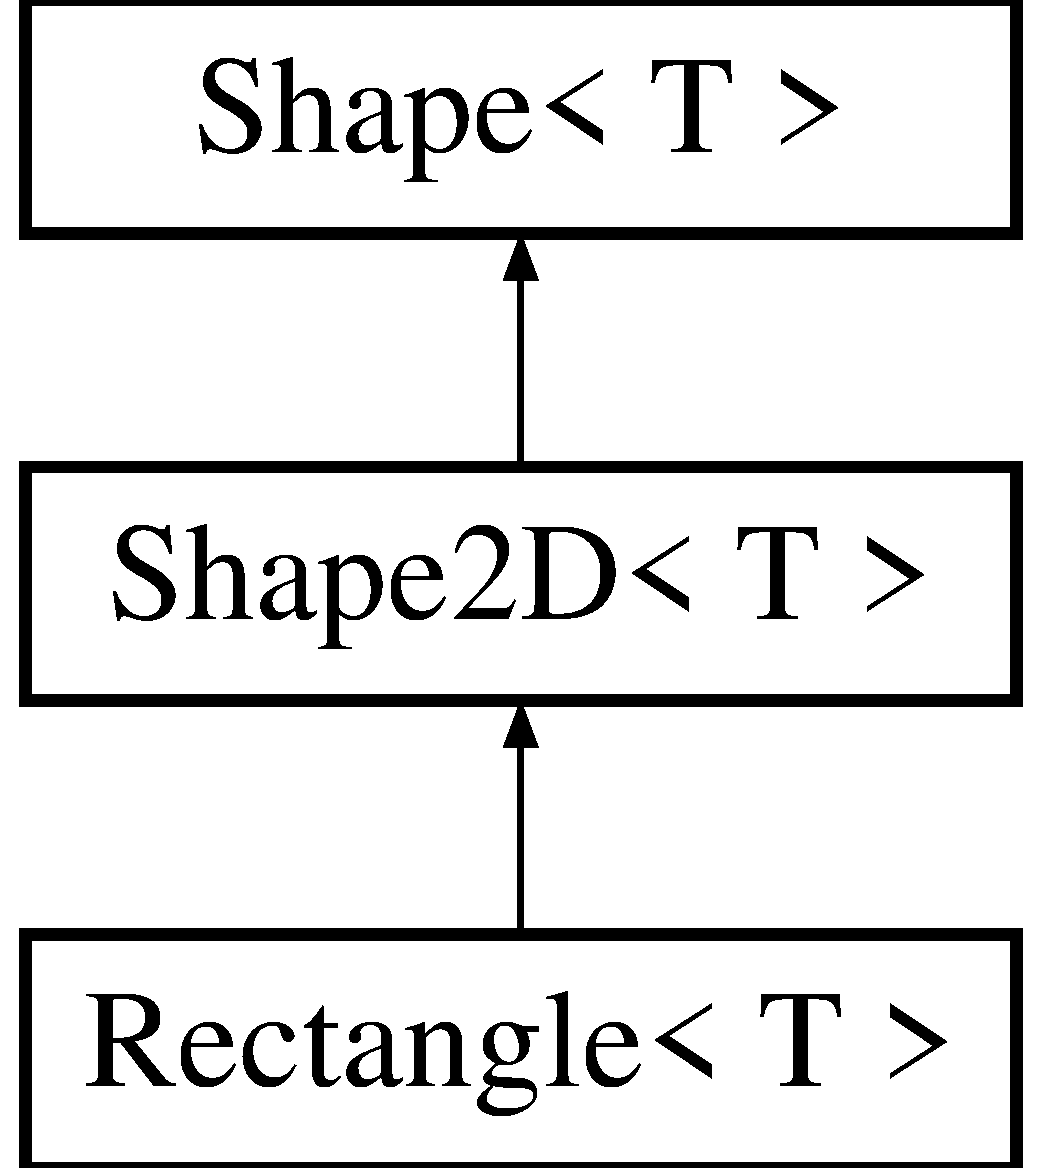
\includegraphics[height=3.000000cm]{classRectangle}
\end{center}
\end{figure}
\subsection*{Public Member Functions}
\begin{DoxyCompactItemize}
\item 
\mbox{\hyperlink{classRectangle_a9d9da3fc8bcb125516cbf2d711d325eb}{Rectangle}} ()
\begin{DoxyCompactList}\small\item\em \mbox{\hyperlink{classA}{A}} basic constructor. \end{DoxyCompactList}\item 
\mbox{\hyperlink{classRectangle_a34cf921863291153b40d9b447f812aa4}{Rectangle}} (\mbox{\hyperlink{classRectangle}{Rectangle}} \&\&)=default
\item 
\mbox{\hyperlink{classRectangle}{Rectangle}} \& \mbox{\hyperlink{classRectangle_ab53b617f14505834f525ec614ccce5c8}{operator=}} (\mbox{\hyperlink{classRectangle}{Rectangle}} \&\&)=default
\item 
\mbox{\hyperlink{classRectangle_acf27dae8f7c9a022428bda816903db2e}{Rectangle}} (const \mbox{\hyperlink{classRectangle}{Rectangle}} \&)=default
\item 
\mbox{\hyperlink{classRectangle}{Rectangle}} \& \mbox{\hyperlink{classRectangle_ad0a038c8959e5bde09bf1e8f49980bea}{operator=}} (const \mbox{\hyperlink{classRectangle}{Rectangle}} \&)=default
\item 
T \mbox{\hyperlink{classRectangle_a9c59dcb7376296711ad86e2da924d3c8}{perimeter}} ()
\end{DoxyCompactItemize}
\subsection*{Private Member Functions}
\begin{DoxyCompactItemize}
\item 
void \mbox{\hyperlink{classRectangle_a0f9d67fb9478883f067c47cdc7bf7bca}{generate\+\_\+vertexes}} ()
\begin{DoxyCompactList}\small\item\em Sets all four vertexes in correct order. \end{DoxyCompactList}\end{DoxyCompactItemize}
\subsection*{Additional Inherited Members}


\subsection{Detailed Description}
\subsubsection*{template$<$typename T = float$>$\newline
class Rectangle$<$ T $>$}

Class holding rectangle vertexes. 

\subsection{Constructor \& Destructor Documentation}
\mbox{\Hypertarget{classRectangle_a9d9da3fc8bcb125516cbf2d711d325eb}\label{classRectangle_a9d9da3fc8bcb125516cbf2d711d325eb}} 
\index{Rectangle@{Rectangle}!Rectangle@{Rectangle}}
\index{Rectangle@{Rectangle}!Rectangle@{Rectangle}}
\subsubsection{\texorpdfstring{Rectangle()}{Rectangle()}\hspace{0.1cm}{\footnotesize\ttfamily [1/3]}}
{\footnotesize\ttfamily template$<$typename T $>$ \\
\mbox{\hyperlink{classRectangle}{Rectangle}}$<$ T $>$\+::\mbox{\hyperlink{classRectangle}{Rectangle}} (\begin{DoxyParamCaption}{ }\end{DoxyParamCaption})}



\mbox{\hyperlink{classA}{A}} basic constructor. 

Constructor generates vertexes, initializes buffers and generates opengl buffers \mbox{\Hypertarget{classRectangle_a34cf921863291153b40d9b447f812aa4}\label{classRectangle_a34cf921863291153b40d9b447f812aa4}} 
\index{Rectangle@{Rectangle}!Rectangle@{Rectangle}}
\index{Rectangle@{Rectangle}!Rectangle@{Rectangle}}
\subsubsection{\texorpdfstring{Rectangle()}{Rectangle()}\hspace{0.1cm}{\footnotesize\ttfamily [2/3]}}
{\footnotesize\ttfamily template$<$typename T  = float$>$ \\
\mbox{\hyperlink{classRectangle}{Rectangle}}$<$ T $>$\+::\mbox{\hyperlink{classRectangle}{Rectangle}} (\begin{DoxyParamCaption}\item[{\mbox{\hyperlink{classRectangle}{Rectangle}}$<$ T $>$ \&\&}]{ }\end{DoxyParamCaption})\hspace{0.3cm}{\ttfamily [default]}}

\mbox{\Hypertarget{classRectangle_acf27dae8f7c9a022428bda816903db2e}\label{classRectangle_acf27dae8f7c9a022428bda816903db2e}} 
\index{Rectangle@{Rectangle}!Rectangle@{Rectangle}}
\index{Rectangle@{Rectangle}!Rectangle@{Rectangle}}
\subsubsection{\texorpdfstring{Rectangle()}{Rectangle()}\hspace{0.1cm}{\footnotesize\ttfamily [3/3]}}
{\footnotesize\ttfamily template$<$typename T  = float$>$ \\
\mbox{\hyperlink{classRectangle}{Rectangle}}$<$ T $>$\+::\mbox{\hyperlink{classRectangle}{Rectangle}} (\begin{DoxyParamCaption}\item[{const \mbox{\hyperlink{classRectangle}{Rectangle}}$<$ T $>$ \&}]{ }\end{DoxyParamCaption})\hspace{0.3cm}{\ttfamily [default]}}



\subsection{Member Function Documentation}
\mbox{\Hypertarget{classRectangle_a0f9d67fb9478883f067c47cdc7bf7bca}\label{classRectangle_a0f9d67fb9478883f067c47cdc7bf7bca}} 
\index{Rectangle@{Rectangle}!generate\+\_\+vertexes@{generate\+\_\+vertexes}}
\index{generate\+\_\+vertexes@{generate\+\_\+vertexes}!Rectangle@{Rectangle}}
\subsubsection{\texorpdfstring{generate\+\_\+vertexes()}{generate\_vertexes()}}
{\footnotesize\ttfamily template$<$typename T $>$ \\
void \mbox{\hyperlink{classRectangle}{Rectangle}}$<$ T $>$\+::generate\+\_\+vertexes (\begin{DoxyParamCaption}{ }\end{DoxyParamCaption})\hspace{0.3cm}{\ttfamily [private]}}



Sets all four vertexes in correct order. 

\mbox{\Hypertarget{classRectangle_ab53b617f14505834f525ec614ccce5c8}\label{classRectangle_ab53b617f14505834f525ec614ccce5c8}} 
\index{Rectangle@{Rectangle}!operator=@{operator=}}
\index{operator=@{operator=}!Rectangle@{Rectangle}}
\subsubsection{\texorpdfstring{operator=()}{operator=()}\hspace{0.1cm}{\footnotesize\ttfamily [1/2]}}
{\footnotesize\ttfamily template$<$typename T  = float$>$ \\
\mbox{\hyperlink{classRectangle}{Rectangle}}\& \mbox{\hyperlink{classRectangle}{Rectangle}}$<$ T $>$\+::operator= (\begin{DoxyParamCaption}\item[{\mbox{\hyperlink{classRectangle}{Rectangle}}$<$ T $>$ \&\&}]{ }\end{DoxyParamCaption})\hspace{0.3cm}{\ttfamily [default]}}

\mbox{\Hypertarget{classRectangle_ad0a038c8959e5bde09bf1e8f49980bea}\label{classRectangle_ad0a038c8959e5bde09bf1e8f49980bea}} 
\index{Rectangle@{Rectangle}!operator=@{operator=}}
\index{operator=@{operator=}!Rectangle@{Rectangle}}
\subsubsection{\texorpdfstring{operator=()}{operator=()}\hspace{0.1cm}{\footnotesize\ttfamily [2/2]}}
{\footnotesize\ttfamily template$<$typename T  = float$>$ \\
\mbox{\hyperlink{classRectangle}{Rectangle}}\& \mbox{\hyperlink{classRectangle}{Rectangle}}$<$ T $>$\+::operator= (\begin{DoxyParamCaption}\item[{const \mbox{\hyperlink{classRectangle}{Rectangle}}$<$ T $>$ \&}]{ }\end{DoxyParamCaption})\hspace{0.3cm}{\ttfamily [default]}}

\mbox{\Hypertarget{classRectangle_a9c59dcb7376296711ad86e2da924d3c8}\label{classRectangle_a9c59dcb7376296711ad86e2da924d3c8}} 
\index{Rectangle@{Rectangle}!perimeter@{perimeter}}
\index{perimeter@{perimeter}!Rectangle@{Rectangle}}
\subsubsection{\texorpdfstring{perimeter()}{perimeter()}}
{\footnotesize\ttfamily template$<$typename T $>$ \\
T \mbox{\hyperlink{classRectangle}{Rectangle}}$<$ T $>$\+::perimeter (\begin{DoxyParamCaption}{ }\end{DoxyParamCaption})}



The documentation for this class was generated from the following file\+:\begin{DoxyCompactItemize}
\item 
src/shapes/\mbox{\hyperlink{rectangle_8hpp}{rectangle.\+hpp}}\end{DoxyCompactItemize}

\hypertarget{classShader}{}\section{Shader$<$ T $>$ Class Template Reference}
\label{classShader}\index{Shader$<$ T $>$@{Shader$<$ T $>$}}


Class for shaders. \mbox{\hyperlink{classThis}{This}} class compiles three shaders, one for each dimension.  




{\ttfamily \#include \char`\"{}shader\+\_\+class.\+hpp\char`\"{}}

\subsection*{Public Member Functions}
\begin{DoxyCompactItemize}
\item 
\mbox{\hyperlink{classShader_a02faa1d7140779d7a24e06d1aff58d68}{Shader}} ()
\item 
\mbox{\hyperlink{classShader_a7e30078f161d1c9f48a7b3921c01f816}{Shader}} (\mbox{\hyperlink{classShader}{Shader}} \&\&)=delete
\item 
\mbox{\hyperlink{classShader}{Shader}} \& \mbox{\hyperlink{classShader_a3b92fece66095389581a2bf6b3124657}{operator=}} (\mbox{\hyperlink{classShader}{Shader}} \&\&)=delete
\item 
\mbox{\hyperlink{classShader_a49b2a448a00b5e1413c17501f8873cca}{Shader}} (const \mbox{\hyperlink{classShader}{Shader}} \&)=delete
\item 
\mbox{\hyperlink{classShader}{Shader}} \& \mbox{\hyperlink{classShader_a58f724fecccecdb1633e08ce0258da37}{operator=}} (const \mbox{\hyperlink{classShader}{Shader}} \&)=delete
\item 
unsigned \mbox{\hyperlink{classShader_a2c19b216850480109f9d5f7ed6ab6aa6}{get\+\_\+shader\+\_\+program}} (int i)
\end{DoxyCompactItemize}
\subsection*{Protected Member Functions}
\begin{DoxyCompactItemize}
\item 
void \mbox{\hyperlink{classShader_a1176d69a08aef6df3b7850104871a839}{compile\+\_\+shaders}} ()
\item 
{\footnotesize template$<$$>$ }\\void \mbox{\hyperlink{classShader_a3ffd553eceda4e9d5a1d8b4a5a157659}{compile\+\_\+shaders}} ()
\begin{DoxyCompactList}\small\item\em Constructor compiles shaders and tests them. \end{DoxyCompactList}\item 
{\footnotesize template$<$$>$ }\\void \mbox{\hyperlink{classShader_ae486635d367b6054482c56747ed74846}{compile\+\_\+shaders}} ()
\begin{DoxyCompactList}\small\item\em Constructor compiles shaders and tests them. \end{DoxyCompactList}\end{DoxyCompactItemize}
\subsection*{Protected Attributes}
\begin{DoxyCompactItemize}
\item 
unsigned \mbox{\hyperlink{classShader_af8ec4edd2b1b56f32ce416280ff9b9e1}{shader\+\_\+program}} \mbox{[}3\mbox{]}
\item 
bool \mbox{\hyperlink{classShader_a057162ea090f838f7fbb658cb301efc4}{shaders\+\_\+compiled}} \mbox{[}3\mbox{]}
\end{DoxyCompactItemize}


\subsection{Detailed Description}
\subsubsection*{template$<$R\+E\+N\+D\+E\+R\+\_\+\+T\+Y\+PE T$>$\newline
class Shader$<$ T $>$}

Class for shaders. \mbox{\hyperlink{classThis}{This}} class compiles three shaders, one for each dimension. 

Class can either be U\+N\+I\+F\+O\+R\+M\+\_\+\+C\+O\+L\+OR or C\+U\+S\+T\+O\+M\+\_\+\+C\+O\+L\+OR class. The difference is in shaders they compile. The first one compiles shader which assigns a single color to all vertexes. The latter assigns seprate color to each vertex. 

\subsection{Constructor \& Destructor Documentation}
\mbox{\Hypertarget{classShader_a02faa1d7140779d7a24e06d1aff58d68}\label{classShader_a02faa1d7140779d7a24e06d1aff58d68}} 
\index{Shader@{Shader}!Shader@{Shader}}
\index{Shader@{Shader}!Shader@{Shader}}
\subsubsection{\texorpdfstring{Shader()}{Shader()}\hspace{0.1cm}{\footnotesize\ttfamily [1/3]}}
{\footnotesize\ttfamily template$<$R\+E\+N\+D\+E\+R\+\_\+\+T\+Y\+PE T$>$ \\
\mbox{\hyperlink{classShader}{Shader}}$<$ T $>$\+::\mbox{\hyperlink{classShader}{Shader}} (\begin{DoxyParamCaption}{ }\end{DoxyParamCaption})\hspace{0.3cm}{\ttfamily [inline]}}

\mbox{\Hypertarget{classShader_a7e30078f161d1c9f48a7b3921c01f816}\label{classShader_a7e30078f161d1c9f48a7b3921c01f816}} 
\index{Shader@{Shader}!Shader@{Shader}}
\index{Shader@{Shader}!Shader@{Shader}}
\subsubsection{\texorpdfstring{Shader()}{Shader()}\hspace{0.1cm}{\footnotesize\ttfamily [2/3]}}
{\footnotesize\ttfamily template$<$R\+E\+N\+D\+E\+R\+\_\+\+T\+Y\+PE T$>$ \\
\mbox{\hyperlink{classShader}{Shader}}$<$ T $>$\+::\mbox{\hyperlink{classShader}{Shader}} (\begin{DoxyParamCaption}\item[{\mbox{\hyperlink{classShader}{Shader}}$<$ T $>$ \&\&}]{ }\end{DoxyParamCaption})\hspace{0.3cm}{\ttfamily [delete]}}

\mbox{\Hypertarget{classShader_a49b2a448a00b5e1413c17501f8873cca}\label{classShader_a49b2a448a00b5e1413c17501f8873cca}} 
\index{Shader@{Shader}!Shader@{Shader}}
\index{Shader@{Shader}!Shader@{Shader}}
\subsubsection{\texorpdfstring{Shader()}{Shader()}\hspace{0.1cm}{\footnotesize\ttfamily [3/3]}}
{\footnotesize\ttfamily template$<$R\+E\+N\+D\+E\+R\+\_\+\+T\+Y\+PE T$>$ \\
\mbox{\hyperlink{classShader}{Shader}}$<$ T $>$\+::\mbox{\hyperlink{classShader}{Shader}} (\begin{DoxyParamCaption}\item[{const \mbox{\hyperlink{classShader}{Shader}}$<$ T $>$ \&}]{ }\end{DoxyParamCaption})\hspace{0.3cm}{\ttfamily [delete]}}



\subsection{Member Function Documentation}
\mbox{\Hypertarget{classShader_a1176d69a08aef6df3b7850104871a839}\label{classShader_a1176d69a08aef6df3b7850104871a839}} 
\index{Shader@{Shader}!compile\+\_\+shaders@{compile\+\_\+shaders}}
\index{compile\+\_\+shaders@{compile\+\_\+shaders}!Shader@{Shader}}
\subsubsection{\texorpdfstring{compile\+\_\+shaders()}{compile\_shaders()}\hspace{0.1cm}{\footnotesize\ttfamily [1/3]}}
{\footnotesize\ttfamily template$<$R\+E\+N\+D\+E\+R\+\_\+\+T\+Y\+PE T$>$ \\
void \mbox{\hyperlink{classShader}{Shader}}$<$ T $>$\+::compile\+\_\+shaders (\begin{DoxyParamCaption}{ }\end{DoxyParamCaption})\hspace{0.3cm}{\ttfamily [protected]}}

\mbox{\Hypertarget{classShader_a3ffd553eceda4e9d5a1d8b4a5a157659}\label{classShader_a3ffd553eceda4e9d5a1d8b4a5a157659}} 
\index{Shader@{Shader}!compile\+\_\+shaders@{compile\+\_\+shaders}}
\index{compile\+\_\+shaders@{compile\+\_\+shaders}!Shader@{Shader}}
\subsubsection{\texorpdfstring{compile\+\_\+shaders()}{compile\_shaders()}\hspace{0.1cm}{\footnotesize\ttfamily [2/3]}}
{\footnotesize\ttfamily template$<$$>$ \\
void \mbox{\hyperlink{classShader}{Shader}}$<$ \mbox{\hyperlink{render_8hpp_a24e288e18eb7b6e01de7565001fedb60aa98862073f71a928bad5099cc3e1c2ed}{R\+E\+N\+D\+E\+R\+\_\+\+T\+Y\+P\+E\+::\+U\+N\+I\+F\+O\+R\+M\+\_\+\+C\+O\+L\+OR}} $>$\+::compile\+\_\+shaders (\begin{DoxyParamCaption}{ }\end{DoxyParamCaption})\hspace{0.3cm}{\ttfamily [inline]}, {\ttfamily [protected]}}



Constructor compiles shaders and tests them. 

\mbox{\Hypertarget{classShader_ae486635d367b6054482c56747ed74846}\label{classShader_ae486635d367b6054482c56747ed74846}} 
\index{Shader@{Shader}!compile\+\_\+shaders@{compile\+\_\+shaders}}
\index{compile\+\_\+shaders@{compile\+\_\+shaders}!Shader@{Shader}}
\subsubsection{\texorpdfstring{compile\+\_\+shaders()}{compile\_shaders()}\hspace{0.1cm}{\footnotesize\ttfamily [3/3]}}
{\footnotesize\ttfamily template$<$$>$ \\
void \mbox{\hyperlink{classShader}{Shader}}$<$ \mbox{\hyperlink{render_8hpp_a24e288e18eb7b6e01de7565001fedb60a9d34355b5a26c54b5dbab1e45245a6f4}{R\+E\+N\+D\+E\+R\+\_\+\+T\+Y\+P\+E\+::\+C\+U\+S\+T\+O\+M\+\_\+\+C\+O\+L\+OR}} $>$\+::compile\+\_\+shaders (\begin{DoxyParamCaption}{ }\end{DoxyParamCaption})\hspace{0.3cm}{\ttfamily [inline]}, {\ttfamily [protected]}}



Constructor compiles shaders and tests them. 

\mbox{\Hypertarget{classShader_a2c19b216850480109f9d5f7ed6ab6aa6}\label{classShader_a2c19b216850480109f9d5f7ed6ab6aa6}} 
\index{Shader@{Shader}!get\+\_\+shader\+\_\+program@{get\+\_\+shader\+\_\+program}}
\index{get\+\_\+shader\+\_\+program@{get\+\_\+shader\+\_\+program}!Shader@{Shader}}
\subsubsection{\texorpdfstring{get\+\_\+shader\+\_\+program()}{get\_shader\_program()}}
{\footnotesize\ttfamily template$<$R\+E\+N\+D\+E\+R\+\_\+\+T\+Y\+PE T$>$ \\
unsigned \mbox{\hyperlink{classShader}{Shader}}$<$ T $>$\+::get\+\_\+shader\+\_\+program (\begin{DoxyParamCaption}\item[{int}]{i }\end{DoxyParamCaption})\hspace{0.3cm}{\ttfamily [inline]}}

\mbox{\Hypertarget{classShader_a3b92fece66095389581a2bf6b3124657}\label{classShader_a3b92fece66095389581a2bf6b3124657}} 
\index{Shader@{Shader}!operator=@{operator=}}
\index{operator=@{operator=}!Shader@{Shader}}
\subsubsection{\texorpdfstring{operator=()}{operator=()}\hspace{0.1cm}{\footnotesize\ttfamily [1/2]}}
{\footnotesize\ttfamily template$<$R\+E\+N\+D\+E\+R\+\_\+\+T\+Y\+PE T$>$ \\
\mbox{\hyperlink{classShader}{Shader}}\& \mbox{\hyperlink{classShader}{Shader}}$<$ T $>$\+::operator= (\begin{DoxyParamCaption}\item[{\mbox{\hyperlink{classShader}{Shader}}$<$ T $>$ \&\&}]{ }\end{DoxyParamCaption})\hspace{0.3cm}{\ttfamily [delete]}}

\mbox{\Hypertarget{classShader_a58f724fecccecdb1633e08ce0258da37}\label{classShader_a58f724fecccecdb1633e08ce0258da37}} 
\index{Shader@{Shader}!operator=@{operator=}}
\index{operator=@{operator=}!Shader@{Shader}}
\subsubsection{\texorpdfstring{operator=()}{operator=()}\hspace{0.1cm}{\footnotesize\ttfamily [2/2]}}
{\footnotesize\ttfamily template$<$R\+E\+N\+D\+E\+R\+\_\+\+T\+Y\+PE T$>$ \\
\mbox{\hyperlink{classShader}{Shader}}\& \mbox{\hyperlink{classShader}{Shader}}$<$ T $>$\+::operator= (\begin{DoxyParamCaption}\item[{const \mbox{\hyperlink{classShader}{Shader}}$<$ T $>$ \&}]{ }\end{DoxyParamCaption})\hspace{0.3cm}{\ttfamily [delete]}}



\subsection{Member Data Documentation}
\mbox{\Hypertarget{classShader_af8ec4edd2b1b56f32ce416280ff9b9e1}\label{classShader_af8ec4edd2b1b56f32ce416280ff9b9e1}} 
\index{Shader@{Shader}!shader\+\_\+program@{shader\+\_\+program}}
\index{shader\+\_\+program@{shader\+\_\+program}!Shader@{Shader}}
\subsubsection{\texorpdfstring{shader\+\_\+program}{shader\_program}}
{\footnotesize\ttfamily template$<$R\+E\+N\+D\+E\+R\+\_\+\+T\+Y\+PE T$>$ \\
unsigned \mbox{\hyperlink{classShader}{Shader}}$<$ T $>$\+::shader\+\_\+program\mbox{[}3\mbox{]}\hspace{0.3cm}{\ttfamily [protected]}}

shader program array depending on which vertex size is chosen \mbox{\Hypertarget{classShader_a057162ea090f838f7fbb658cb301efc4}\label{classShader_a057162ea090f838f7fbb658cb301efc4}} 
\index{Shader@{Shader}!shaders\+\_\+compiled@{shaders\+\_\+compiled}}
\index{shaders\+\_\+compiled@{shaders\+\_\+compiled}!Shader@{Shader}}
\subsubsection{\texorpdfstring{shaders\+\_\+compiled}{shaders\_compiled}}
{\footnotesize\ttfamily template$<$R\+E\+N\+D\+E\+R\+\_\+\+T\+Y\+PE T$>$ \\
bool \mbox{\hyperlink{classShader}{Shader}}$<$ T $>$\+::shaders\+\_\+compiled\mbox{[}3\mbox{]}\hspace{0.3cm}{\ttfamily [protected]}}

{\bfseries Initial value\+:}
\begin{DoxyCode}
= \{
        \textcolor{keyword}{false}, \textcolor{keyword}{false},
        \textcolor{keyword}{false}\}
\end{DoxyCode}
true/false depending on whether the shaders were compiled 

The documentation for this class was generated from the following file\+:\begin{DoxyCompactItemize}
\item 
src/\mbox{\hyperlink{shader__class_8hpp}{shader\+\_\+class.\+hpp}}\end{DoxyCompactItemize}

\hypertarget{classShader_3_01RENDER__TYPE_1_1CUSTOM_01_4}{}\section{Shader$<$ R\+E\+N\+D\+E\+R\+\_\+\+T\+Y\+PE\+:\+:C\+U\+S\+T\+OM $>$ Class Template Reference}
\label{classShader_3_01RENDER__TYPE_1_1CUSTOM_01_4}\index{Shader$<$ R\+E\+N\+D\+E\+R\+\_\+\+T\+Y\+P\+E\+::\+C\+U\+S\+T\+O\+M $>$@{Shader$<$ R\+E\+N\+D\+E\+R\+\_\+\+T\+Y\+P\+E\+::\+C\+U\+S\+T\+O\+M $>$}}


{\ttfamily \#include \char`\"{}shader\+\_\+class.\+hpp\char`\"{}}

\subsection*{Public Member Functions}
\begin{DoxyCompactItemize}
\item 
\mbox{\hyperlink{classShader_3_01RENDER__TYPE_1_1CUSTOM_01_4_a8238c3e1a3a96e7ed2b1777a340d7947}{Shader}} (const \mbox{\hyperlink{glad_8h_ac83513893df92266f79a515488701770}{std\+::string}} \&vertex\+\_\+source\+\_\+, const \mbox{\hyperlink{glad_8h_ac83513893df92266f79a515488701770}{std\+::string}} \&geometry\+\_\+source\+\_\+, const \mbox{\hyperlink{glad_8h_ac83513893df92266f79a515488701770}{std\+::string}} \&fragment\+\_\+source\+\_\+)
\item 
\mbox{\hyperlink{classShader_3_01RENDER__TYPE_1_1CUSTOM_01_4_a4fea53201befd8962702645fe8f2526e}{Shader}} (\mbox{\hyperlink{classShader}{Shader}} \&\&)=delete
\item 
\mbox{\hyperlink{classShader}{Shader}} \& \mbox{\hyperlink{classShader_3_01RENDER__TYPE_1_1CUSTOM_01_4_a717f92caab16604933920257707046b6}{operator=}} (\mbox{\hyperlink{classShader}{Shader}} \&\&)=delete
\item 
\mbox{\hyperlink{classShader_3_01RENDER__TYPE_1_1CUSTOM_01_4_af1fbc8b0cb20d1af7905e2d896f0fb79}{Shader}} (const \mbox{\hyperlink{classShader}{Shader}} \&)=delete
\item 
\mbox{\hyperlink{classShader}{Shader}} \& \mbox{\hyperlink{classShader_3_01RENDER__TYPE_1_1CUSTOM_01_4_a44af437f5ea044824ba7937ee07d1da7}{operator=}} (const \mbox{\hyperlink{classShader}{Shader}} \&)=delete
\item 
unsigned \mbox{\hyperlink{classShader_3_01RENDER__TYPE_1_1CUSTOM_01_4_adf4d1f7a937d11102268dfb8fc7f2f9e}{get\+\_\+shader\+\_\+program}} ()
\end{DoxyCompactItemize}
\subsection*{Protected Member Functions}
\begin{DoxyCompactItemize}
\item 
\mbox{\hyperlink{glad_8h_a950fc91edb4504f62f1c577bf4727c29}{void}} \mbox{\hyperlink{classShader_3_01RENDER__TYPE_1_1CUSTOM_01_4_aede40b234ac1e38be9d0f9f2a60a26ab}{compile\+\_\+shaders}} ()
\begin{DoxyCompactList}\small\item\em Constructor compiles shaders and tests them. \end{DoxyCompactList}\item 
bool \mbox{\hyperlink{classShader_3_01RENDER__TYPE_1_1CUSTOM_01_4_afca4ecec5bed3cf6a9f219ce52e5343e}{check\+\_\+vertex\+\_\+shader}} (const unsigned shader\+\_\+)
\begin{DoxyCompactList}\small\item\em check if vertex shader has been successfully compiled \end{DoxyCompactList}\item 
bool \mbox{\hyperlink{classShader_3_01RENDER__TYPE_1_1CUSTOM_01_4_a8ba4a9ccbbf73e471434981a62b15d41}{check\+\_\+fragment\+\_\+shader}} (const unsigned shader\+\_\+)
\begin{DoxyCompactList}\small\item\em check if fragment shader has been successfully compiled \end{DoxyCompactList}\item 
bool \mbox{\hyperlink{classShader_3_01RENDER__TYPE_1_1CUSTOM_01_4_aca3ba4448a05303b92667e88e18f5cfb}{check\+\_\+geometry\+\_\+shader}} (const unsigned shader\+\_\+)
\begin{DoxyCompactList}\small\item\em check if fragment shader has been successfully compiled \end{DoxyCompactList}\item 
bool \mbox{\hyperlink{classShader_3_01RENDER__TYPE_1_1CUSTOM_01_4_af59ced307a40764c2fa1acef66e074b3}{check\+\_\+shader\+\_\+program}} (const unsigned shader\+Program)
\begin{DoxyCompactList}\small\item\em check if shader program has been successfully linked \end{DoxyCompactList}\end{DoxyCompactItemize}
\subsection*{Protected Attributes}
\begin{DoxyCompactItemize}
\item 
unsigned \mbox{\hyperlink{classShader_3_01RENDER__TYPE_1_1CUSTOM_01_4_a5baec51d258afd0d116d82cace52eace}{shader\+\_\+program}}
\item 
bool \mbox{\hyperlink{classShader_3_01RENDER__TYPE_1_1CUSTOM_01_4_a80cb5fdd63c57881cdf2b2dbb18e215e}{shaders\+\_\+compiled}} = false
\item 
const \mbox{\hyperlink{glad_8h_ac83513893df92266f79a515488701770}{std\+::string}} \mbox{\hyperlink{classShader_3_01RENDER__TYPE_1_1CUSTOM_01_4_ac6dfb0d85b637f3949777f047b1c010c}{vertex\+\_\+source}}
\item 
const \mbox{\hyperlink{glad_8h_ac83513893df92266f79a515488701770}{std\+::string}} \mbox{\hyperlink{classShader_3_01RENDER__TYPE_1_1CUSTOM_01_4_ac3319ff19c5af25e7d099fd2511066ea}{fragment\+\_\+source}}
\item 
const \mbox{\hyperlink{glad_8h_ac83513893df92266f79a515488701770}{std\+::string}} \mbox{\hyperlink{classShader_3_01RENDER__TYPE_1_1CUSTOM_01_4_acc41906788319945fc40ea589997112b}{geometry\+\_\+source}}
\end{DoxyCompactItemize}


\subsection{Constructor \& Destructor Documentation}
\mbox{\Hypertarget{classShader_3_01RENDER__TYPE_1_1CUSTOM_01_4_a8238c3e1a3a96e7ed2b1777a340d7947}\label{classShader_3_01RENDER__TYPE_1_1CUSTOM_01_4_a8238c3e1a3a96e7ed2b1777a340d7947}} 
\index{Shader$<$ R\+E\+N\+D\+E\+R\+\_\+\+T\+Y\+P\+E\+::\+C\+U\+S\+T\+O\+M $>$@{Shader$<$ R\+E\+N\+D\+E\+R\+\_\+\+T\+Y\+P\+E\+::\+C\+U\+S\+T\+O\+M $>$}!Shader@{Shader}}
\index{Shader@{Shader}!Shader$<$ R\+E\+N\+D\+E\+R\+\_\+\+T\+Y\+P\+E\+::\+C\+U\+S\+T\+O\+M $>$@{Shader$<$ R\+E\+N\+D\+E\+R\+\_\+\+T\+Y\+P\+E\+::\+C\+U\+S\+T\+O\+M $>$}}
\subsubsection{\texorpdfstring{Shader()}{Shader()}\hspace{0.1cm}{\footnotesize\ttfamily [1/3]}}
{\footnotesize\ttfamily \mbox{\hyperlink{classShader}{Shader}}$<$ \mbox{\hyperlink{shader__class_8hpp_a24e288e18eb7b6e01de7565001fedb60a72baef04098f035e8a320b03ad197818}{R\+E\+N\+D\+E\+R\+\_\+\+T\+Y\+P\+E\+::\+C\+U\+S\+T\+OM}} $>$\+::\mbox{\hyperlink{classShader}{Shader}} (\begin{DoxyParamCaption}\item[{const \mbox{\hyperlink{glad_8h_ac83513893df92266f79a515488701770}{std\+::string}} \&}]{vertex\+\_\+source\+\_\+,  }\item[{const \mbox{\hyperlink{glad_8h_ac83513893df92266f79a515488701770}{std\+::string}} \&}]{geometry\+\_\+source\+\_\+,  }\item[{const \mbox{\hyperlink{glad_8h_ac83513893df92266f79a515488701770}{std\+::string}} \&}]{fragment\+\_\+source\+\_\+ }\end{DoxyParamCaption})\hspace{0.3cm}{\ttfamily [inline]}}

\mbox{\Hypertarget{classShader_3_01RENDER__TYPE_1_1CUSTOM_01_4_a4fea53201befd8962702645fe8f2526e}\label{classShader_3_01RENDER__TYPE_1_1CUSTOM_01_4_a4fea53201befd8962702645fe8f2526e}} 
\index{Shader$<$ R\+E\+N\+D\+E\+R\+\_\+\+T\+Y\+P\+E\+::\+C\+U\+S\+T\+O\+M $>$@{Shader$<$ R\+E\+N\+D\+E\+R\+\_\+\+T\+Y\+P\+E\+::\+C\+U\+S\+T\+O\+M $>$}!Shader@{Shader}}
\index{Shader@{Shader}!Shader$<$ R\+E\+N\+D\+E\+R\+\_\+\+T\+Y\+P\+E\+::\+C\+U\+S\+T\+O\+M $>$@{Shader$<$ R\+E\+N\+D\+E\+R\+\_\+\+T\+Y\+P\+E\+::\+C\+U\+S\+T\+O\+M $>$}}
\subsubsection{\texorpdfstring{Shader()}{Shader()}\hspace{0.1cm}{\footnotesize\ttfamily [2/3]}}
{\footnotesize\ttfamily \mbox{\hyperlink{classShader}{Shader}}$<$ \mbox{\hyperlink{shader__class_8hpp_a24e288e18eb7b6e01de7565001fedb60a72baef04098f035e8a320b03ad197818}{R\+E\+N\+D\+E\+R\+\_\+\+T\+Y\+P\+E\+::\+C\+U\+S\+T\+OM}} $>$\+::\mbox{\hyperlink{classShader}{Shader}} (\begin{DoxyParamCaption}\item[{\mbox{\hyperlink{classShader}{Shader}}$<$ \mbox{\hyperlink{shader__class_8hpp_a24e288e18eb7b6e01de7565001fedb60a72baef04098f035e8a320b03ad197818}{R\+E\+N\+D\+E\+R\+\_\+\+T\+Y\+P\+E\+::\+C\+U\+S\+T\+OM}} $>$ \&\&}]{ }\end{DoxyParamCaption})\hspace{0.3cm}{\ttfamily [delete]}}

\mbox{\Hypertarget{classShader_3_01RENDER__TYPE_1_1CUSTOM_01_4_af1fbc8b0cb20d1af7905e2d896f0fb79}\label{classShader_3_01RENDER__TYPE_1_1CUSTOM_01_4_af1fbc8b0cb20d1af7905e2d896f0fb79}} 
\index{Shader$<$ R\+E\+N\+D\+E\+R\+\_\+\+T\+Y\+P\+E\+::\+C\+U\+S\+T\+O\+M $>$@{Shader$<$ R\+E\+N\+D\+E\+R\+\_\+\+T\+Y\+P\+E\+::\+C\+U\+S\+T\+O\+M $>$}!Shader@{Shader}}
\index{Shader@{Shader}!Shader$<$ R\+E\+N\+D\+E\+R\+\_\+\+T\+Y\+P\+E\+::\+C\+U\+S\+T\+O\+M $>$@{Shader$<$ R\+E\+N\+D\+E\+R\+\_\+\+T\+Y\+P\+E\+::\+C\+U\+S\+T\+O\+M $>$}}
\subsubsection{\texorpdfstring{Shader()}{Shader()}\hspace{0.1cm}{\footnotesize\ttfamily [3/3]}}
{\footnotesize\ttfamily \mbox{\hyperlink{classShader}{Shader}}$<$ \mbox{\hyperlink{shader__class_8hpp_a24e288e18eb7b6e01de7565001fedb60a72baef04098f035e8a320b03ad197818}{R\+E\+N\+D\+E\+R\+\_\+\+T\+Y\+P\+E\+::\+C\+U\+S\+T\+OM}} $>$\+::\mbox{\hyperlink{classShader}{Shader}} (\begin{DoxyParamCaption}\item[{const \mbox{\hyperlink{classShader}{Shader}}$<$ \mbox{\hyperlink{shader__class_8hpp_a24e288e18eb7b6e01de7565001fedb60a72baef04098f035e8a320b03ad197818}{R\+E\+N\+D\+E\+R\+\_\+\+T\+Y\+P\+E\+::\+C\+U\+S\+T\+OM}} $>$ \&}]{ }\end{DoxyParamCaption})\hspace{0.3cm}{\ttfamily [delete]}}



\subsection{Member Function Documentation}
\mbox{\Hypertarget{classShader_3_01RENDER__TYPE_1_1CUSTOM_01_4_a8ba4a9ccbbf73e471434981a62b15d41}\label{classShader_3_01RENDER__TYPE_1_1CUSTOM_01_4_a8ba4a9ccbbf73e471434981a62b15d41}} 
\index{Shader$<$ R\+E\+N\+D\+E\+R\+\_\+\+T\+Y\+P\+E\+::\+C\+U\+S\+T\+O\+M $>$@{Shader$<$ R\+E\+N\+D\+E\+R\+\_\+\+T\+Y\+P\+E\+::\+C\+U\+S\+T\+O\+M $>$}!check\+\_\+fragment\+\_\+shader@{check\+\_\+fragment\+\_\+shader}}
\index{check\+\_\+fragment\+\_\+shader@{check\+\_\+fragment\+\_\+shader}!Shader$<$ R\+E\+N\+D\+E\+R\+\_\+\+T\+Y\+P\+E\+::\+C\+U\+S\+T\+O\+M $>$@{Shader$<$ R\+E\+N\+D\+E\+R\+\_\+\+T\+Y\+P\+E\+::\+C\+U\+S\+T\+O\+M $>$}}
\subsubsection{\texorpdfstring{check\+\_\+fragment\+\_\+shader()}{check\_fragment\_shader()}}
{\footnotesize\ttfamily bool \mbox{\hyperlink{classShader}{Shader}}$<$ \mbox{\hyperlink{shader__class_8hpp_a24e288e18eb7b6e01de7565001fedb60a72baef04098f035e8a320b03ad197818}{R\+E\+N\+D\+E\+R\+\_\+\+T\+Y\+P\+E\+::\+C\+U\+S\+T\+OM}} $>$\+::check\+\_\+fragment\+\_\+shader (\begin{DoxyParamCaption}\item[{const unsigned}]{shader\+\_\+ }\end{DoxyParamCaption})\hspace{0.3cm}{\ttfamily [inline]}, {\ttfamily [protected]}}



check if fragment shader has been successfully compiled 


\begin{DoxyParams}{Parameters}
{\em shader\+\_\+} & an unsigned integer referring to fragment shader \\
\hline
\end{DoxyParams}
\mbox{\Hypertarget{classShader_3_01RENDER__TYPE_1_1CUSTOM_01_4_aca3ba4448a05303b92667e88e18f5cfb}\label{classShader_3_01RENDER__TYPE_1_1CUSTOM_01_4_aca3ba4448a05303b92667e88e18f5cfb}} 
\index{Shader$<$ R\+E\+N\+D\+E\+R\+\_\+\+T\+Y\+P\+E\+::\+C\+U\+S\+T\+O\+M $>$@{Shader$<$ R\+E\+N\+D\+E\+R\+\_\+\+T\+Y\+P\+E\+::\+C\+U\+S\+T\+O\+M $>$}!check\+\_\+geometry\+\_\+shader@{check\+\_\+geometry\+\_\+shader}}
\index{check\+\_\+geometry\+\_\+shader@{check\+\_\+geometry\+\_\+shader}!Shader$<$ R\+E\+N\+D\+E\+R\+\_\+\+T\+Y\+P\+E\+::\+C\+U\+S\+T\+O\+M $>$@{Shader$<$ R\+E\+N\+D\+E\+R\+\_\+\+T\+Y\+P\+E\+::\+C\+U\+S\+T\+O\+M $>$}}
\subsubsection{\texorpdfstring{check\+\_\+geometry\+\_\+shader()}{check\_geometry\_shader()}}
{\footnotesize\ttfamily bool \mbox{\hyperlink{classShader}{Shader}}$<$ \mbox{\hyperlink{shader__class_8hpp_a24e288e18eb7b6e01de7565001fedb60a72baef04098f035e8a320b03ad197818}{R\+E\+N\+D\+E\+R\+\_\+\+T\+Y\+P\+E\+::\+C\+U\+S\+T\+OM}} $>$\+::check\+\_\+geometry\+\_\+shader (\begin{DoxyParamCaption}\item[{const unsigned}]{shader\+\_\+ }\end{DoxyParamCaption})\hspace{0.3cm}{\ttfamily [inline]}, {\ttfamily [protected]}}



check if fragment shader has been successfully compiled 


\begin{DoxyParams}{Parameters}
{\em shader\+\_\+} & an unsigned integer referring to fragment shader \\
\hline
\end{DoxyParams}
\mbox{\Hypertarget{classShader_3_01RENDER__TYPE_1_1CUSTOM_01_4_af59ced307a40764c2fa1acef66e074b3}\label{classShader_3_01RENDER__TYPE_1_1CUSTOM_01_4_af59ced307a40764c2fa1acef66e074b3}} 
\index{Shader$<$ R\+E\+N\+D\+E\+R\+\_\+\+T\+Y\+P\+E\+::\+C\+U\+S\+T\+O\+M $>$@{Shader$<$ R\+E\+N\+D\+E\+R\+\_\+\+T\+Y\+P\+E\+::\+C\+U\+S\+T\+O\+M $>$}!check\+\_\+shader\+\_\+program@{check\+\_\+shader\+\_\+program}}
\index{check\+\_\+shader\+\_\+program@{check\+\_\+shader\+\_\+program}!Shader$<$ R\+E\+N\+D\+E\+R\+\_\+\+T\+Y\+P\+E\+::\+C\+U\+S\+T\+O\+M $>$@{Shader$<$ R\+E\+N\+D\+E\+R\+\_\+\+T\+Y\+P\+E\+::\+C\+U\+S\+T\+O\+M $>$}}
\subsubsection{\texorpdfstring{check\+\_\+shader\+\_\+program()}{check\_shader\_program()}}
{\footnotesize\ttfamily bool \mbox{\hyperlink{classShader}{Shader}}$<$ \mbox{\hyperlink{shader__class_8hpp_a24e288e18eb7b6e01de7565001fedb60a72baef04098f035e8a320b03ad197818}{R\+E\+N\+D\+E\+R\+\_\+\+T\+Y\+P\+E\+::\+C\+U\+S\+T\+OM}} $>$\+::check\+\_\+shader\+\_\+program (\begin{DoxyParamCaption}\item[{const unsigned}]{shader\+Program }\end{DoxyParamCaption})\hspace{0.3cm}{\ttfamily [inline]}, {\ttfamily [protected]}}



check if shader program has been successfully linked 


\begin{DoxyParams}{Parameters}
{\em shader\+Program} & an unsigned integer referring to shader program \\
\hline
\end{DoxyParams}
\mbox{\Hypertarget{classShader_3_01RENDER__TYPE_1_1CUSTOM_01_4_afca4ecec5bed3cf6a9f219ce52e5343e}\label{classShader_3_01RENDER__TYPE_1_1CUSTOM_01_4_afca4ecec5bed3cf6a9f219ce52e5343e}} 
\index{Shader$<$ R\+E\+N\+D\+E\+R\+\_\+\+T\+Y\+P\+E\+::\+C\+U\+S\+T\+O\+M $>$@{Shader$<$ R\+E\+N\+D\+E\+R\+\_\+\+T\+Y\+P\+E\+::\+C\+U\+S\+T\+O\+M $>$}!check\+\_\+vertex\+\_\+shader@{check\+\_\+vertex\+\_\+shader}}
\index{check\+\_\+vertex\+\_\+shader@{check\+\_\+vertex\+\_\+shader}!Shader$<$ R\+E\+N\+D\+E\+R\+\_\+\+T\+Y\+P\+E\+::\+C\+U\+S\+T\+O\+M $>$@{Shader$<$ R\+E\+N\+D\+E\+R\+\_\+\+T\+Y\+P\+E\+::\+C\+U\+S\+T\+O\+M $>$}}
\subsubsection{\texorpdfstring{check\+\_\+vertex\+\_\+shader()}{check\_vertex\_shader()}}
{\footnotesize\ttfamily bool \mbox{\hyperlink{classShader}{Shader}}$<$ \mbox{\hyperlink{shader__class_8hpp_a24e288e18eb7b6e01de7565001fedb60a72baef04098f035e8a320b03ad197818}{R\+E\+N\+D\+E\+R\+\_\+\+T\+Y\+P\+E\+::\+C\+U\+S\+T\+OM}} $>$\+::check\+\_\+vertex\+\_\+shader (\begin{DoxyParamCaption}\item[{const unsigned}]{shader\+\_\+ }\end{DoxyParamCaption})\hspace{0.3cm}{\ttfamily [inline]}, {\ttfamily [protected]}}



check if vertex shader has been successfully compiled 


\begin{DoxyParams}{Parameters}
{\em shader\+\_\+} & an unsigned integer referring to vertex shader \\
\hline
\end{DoxyParams}
\mbox{\Hypertarget{classShader_3_01RENDER__TYPE_1_1CUSTOM_01_4_aede40b234ac1e38be9d0f9f2a60a26ab}\label{classShader_3_01RENDER__TYPE_1_1CUSTOM_01_4_aede40b234ac1e38be9d0f9f2a60a26ab}} 
\index{Shader$<$ R\+E\+N\+D\+E\+R\+\_\+\+T\+Y\+P\+E\+::\+C\+U\+S\+T\+O\+M $>$@{Shader$<$ R\+E\+N\+D\+E\+R\+\_\+\+T\+Y\+P\+E\+::\+C\+U\+S\+T\+O\+M $>$}!compile\+\_\+shaders@{compile\+\_\+shaders}}
\index{compile\+\_\+shaders@{compile\+\_\+shaders}!Shader$<$ R\+E\+N\+D\+E\+R\+\_\+\+T\+Y\+P\+E\+::\+C\+U\+S\+T\+O\+M $>$@{Shader$<$ R\+E\+N\+D\+E\+R\+\_\+\+T\+Y\+P\+E\+::\+C\+U\+S\+T\+O\+M $>$}}
\subsubsection{\texorpdfstring{compile\+\_\+shaders()}{compile\_shaders()}}
{\footnotesize\ttfamily \mbox{\hyperlink{glad_8h_a950fc91edb4504f62f1c577bf4727c29}{void}} \mbox{\hyperlink{classShader}{Shader}}$<$ \mbox{\hyperlink{shader__class_8hpp_a24e288e18eb7b6e01de7565001fedb60a72baef04098f035e8a320b03ad197818}{R\+E\+N\+D\+E\+R\+\_\+\+T\+Y\+P\+E\+::\+C\+U\+S\+T\+OM}} $>$\+::compile\+\_\+shaders (\begin{DoxyParamCaption}{ }\end{DoxyParamCaption})\hspace{0.3cm}{\ttfamily [inline]}, {\ttfamily [protected]}}



Constructor compiles shaders and tests them. 

\mbox{\Hypertarget{classShader_3_01RENDER__TYPE_1_1CUSTOM_01_4_adf4d1f7a937d11102268dfb8fc7f2f9e}\label{classShader_3_01RENDER__TYPE_1_1CUSTOM_01_4_adf4d1f7a937d11102268dfb8fc7f2f9e}} 
\index{Shader$<$ R\+E\+N\+D\+E\+R\+\_\+\+T\+Y\+P\+E\+::\+C\+U\+S\+T\+O\+M $>$@{Shader$<$ R\+E\+N\+D\+E\+R\+\_\+\+T\+Y\+P\+E\+::\+C\+U\+S\+T\+O\+M $>$}!get\+\_\+shader\+\_\+program@{get\+\_\+shader\+\_\+program}}
\index{get\+\_\+shader\+\_\+program@{get\+\_\+shader\+\_\+program}!Shader$<$ R\+E\+N\+D\+E\+R\+\_\+\+T\+Y\+P\+E\+::\+C\+U\+S\+T\+O\+M $>$@{Shader$<$ R\+E\+N\+D\+E\+R\+\_\+\+T\+Y\+P\+E\+::\+C\+U\+S\+T\+O\+M $>$}}
\subsubsection{\texorpdfstring{get\+\_\+shader\+\_\+program()}{get\_shader\_program()}}
{\footnotesize\ttfamily unsigned \mbox{\hyperlink{classShader}{Shader}}$<$ \mbox{\hyperlink{shader__class_8hpp_a24e288e18eb7b6e01de7565001fedb60a72baef04098f035e8a320b03ad197818}{R\+E\+N\+D\+E\+R\+\_\+\+T\+Y\+P\+E\+::\+C\+U\+S\+T\+OM}} $>$\+::get\+\_\+shader\+\_\+program (\begin{DoxyParamCaption}{ }\end{DoxyParamCaption})\hspace{0.3cm}{\ttfamily [inline]}}

\mbox{\Hypertarget{classShader_3_01RENDER__TYPE_1_1CUSTOM_01_4_a717f92caab16604933920257707046b6}\label{classShader_3_01RENDER__TYPE_1_1CUSTOM_01_4_a717f92caab16604933920257707046b6}} 
\index{Shader$<$ R\+E\+N\+D\+E\+R\+\_\+\+T\+Y\+P\+E\+::\+C\+U\+S\+T\+O\+M $>$@{Shader$<$ R\+E\+N\+D\+E\+R\+\_\+\+T\+Y\+P\+E\+::\+C\+U\+S\+T\+O\+M $>$}!operator=@{operator=}}
\index{operator=@{operator=}!Shader$<$ R\+E\+N\+D\+E\+R\+\_\+\+T\+Y\+P\+E\+::\+C\+U\+S\+T\+O\+M $>$@{Shader$<$ R\+E\+N\+D\+E\+R\+\_\+\+T\+Y\+P\+E\+::\+C\+U\+S\+T\+O\+M $>$}}
\subsubsection{\texorpdfstring{operator=()}{operator=()}\hspace{0.1cm}{\footnotesize\ttfamily [1/2]}}
{\footnotesize\ttfamily \mbox{\hyperlink{classShader}{Shader}}\& \mbox{\hyperlink{classShader}{Shader}}$<$ \mbox{\hyperlink{shader__class_8hpp_a24e288e18eb7b6e01de7565001fedb60a72baef04098f035e8a320b03ad197818}{R\+E\+N\+D\+E\+R\+\_\+\+T\+Y\+P\+E\+::\+C\+U\+S\+T\+OM}} $>$\+::operator= (\begin{DoxyParamCaption}\item[{\mbox{\hyperlink{classShader}{Shader}}$<$ \mbox{\hyperlink{shader__class_8hpp_a24e288e18eb7b6e01de7565001fedb60a72baef04098f035e8a320b03ad197818}{R\+E\+N\+D\+E\+R\+\_\+\+T\+Y\+P\+E\+::\+C\+U\+S\+T\+OM}} $>$ \&\&}]{ }\end{DoxyParamCaption})\hspace{0.3cm}{\ttfamily [delete]}}

\mbox{\Hypertarget{classShader_3_01RENDER__TYPE_1_1CUSTOM_01_4_a44af437f5ea044824ba7937ee07d1da7}\label{classShader_3_01RENDER__TYPE_1_1CUSTOM_01_4_a44af437f5ea044824ba7937ee07d1da7}} 
\index{Shader$<$ R\+E\+N\+D\+E\+R\+\_\+\+T\+Y\+P\+E\+::\+C\+U\+S\+T\+O\+M $>$@{Shader$<$ R\+E\+N\+D\+E\+R\+\_\+\+T\+Y\+P\+E\+::\+C\+U\+S\+T\+O\+M $>$}!operator=@{operator=}}
\index{operator=@{operator=}!Shader$<$ R\+E\+N\+D\+E\+R\+\_\+\+T\+Y\+P\+E\+::\+C\+U\+S\+T\+O\+M $>$@{Shader$<$ R\+E\+N\+D\+E\+R\+\_\+\+T\+Y\+P\+E\+::\+C\+U\+S\+T\+O\+M $>$}}
\subsubsection{\texorpdfstring{operator=()}{operator=()}\hspace{0.1cm}{\footnotesize\ttfamily [2/2]}}
{\footnotesize\ttfamily \mbox{\hyperlink{classShader}{Shader}}\& \mbox{\hyperlink{classShader}{Shader}}$<$ \mbox{\hyperlink{shader__class_8hpp_a24e288e18eb7b6e01de7565001fedb60a72baef04098f035e8a320b03ad197818}{R\+E\+N\+D\+E\+R\+\_\+\+T\+Y\+P\+E\+::\+C\+U\+S\+T\+OM}} $>$\+::operator= (\begin{DoxyParamCaption}\item[{const \mbox{\hyperlink{classShader}{Shader}}$<$ \mbox{\hyperlink{shader__class_8hpp_a24e288e18eb7b6e01de7565001fedb60a72baef04098f035e8a320b03ad197818}{R\+E\+N\+D\+E\+R\+\_\+\+T\+Y\+P\+E\+::\+C\+U\+S\+T\+OM}} $>$ \&}]{ }\end{DoxyParamCaption})\hspace{0.3cm}{\ttfamily [delete]}}



\subsection{Member Data Documentation}
\mbox{\Hypertarget{classShader_3_01RENDER__TYPE_1_1CUSTOM_01_4_ac3319ff19c5af25e7d099fd2511066ea}\label{classShader_3_01RENDER__TYPE_1_1CUSTOM_01_4_ac3319ff19c5af25e7d099fd2511066ea}} 
\index{Shader$<$ R\+E\+N\+D\+E\+R\+\_\+\+T\+Y\+P\+E\+::\+C\+U\+S\+T\+O\+M $>$@{Shader$<$ R\+E\+N\+D\+E\+R\+\_\+\+T\+Y\+P\+E\+::\+C\+U\+S\+T\+O\+M $>$}!fragment\+\_\+source@{fragment\+\_\+source}}
\index{fragment\+\_\+source@{fragment\+\_\+source}!Shader$<$ R\+E\+N\+D\+E\+R\+\_\+\+T\+Y\+P\+E\+::\+C\+U\+S\+T\+O\+M $>$@{Shader$<$ R\+E\+N\+D\+E\+R\+\_\+\+T\+Y\+P\+E\+::\+C\+U\+S\+T\+O\+M $>$}}
\subsubsection{\texorpdfstring{fragment\+\_\+source}{fragment\_source}}
{\footnotesize\ttfamily const \mbox{\hyperlink{glad_8h_ac83513893df92266f79a515488701770}{std\+::string}} \mbox{\hyperlink{classShader}{Shader}}$<$ \mbox{\hyperlink{shader__class_8hpp_a24e288e18eb7b6e01de7565001fedb60a72baef04098f035e8a320b03ad197818}{R\+E\+N\+D\+E\+R\+\_\+\+T\+Y\+P\+E\+::\+C\+U\+S\+T\+OM}} $>$\+::fragment\+\_\+source\hspace{0.3cm}{\ttfamily [protected]}}

\mbox{\Hypertarget{classShader_3_01RENDER__TYPE_1_1CUSTOM_01_4_acc41906788319945fc40ea589997112b}\label{classShader_3_01RENDER__TYPE_1_1CUSTOM_01_4_acc41906788319945fc40ea589997112b}} 
\index{Shader$<$ R\+E\+N\+D\+E\+R\+\_\+\+T\+Y\+P\+E\+::\+C\+U\+S\+T\+O\+M $>$@{Shader$<$ R\+E\+N\+D\+E\+R\+\_\+\+T\+Y\+P\+E\+::\+C\+U\+S\+T\+O\+M $>$}!geometry\+\_\+source@{geometry\+\_\+source}}
\index{geometry\+\_\+source@{geometry\+\_\+source}!Shader$<$ R\+E\+N\+D\+E\+R\+\_\+\+T\+Y\+P\+E\+::\+C\+U\+S\+T\+O\+M $>$@{Shader$<$ R\+E\+N\+D\+E\+R\+\_\+\+T\+Y\+P\+E\+::\+C\+U\+S\+T\+O\+M $>$}}
\subsubsection{\texorpdfstring{geometry\+\_\+source}{geometry\_source}}
{\footnotesize\ttfamily const \mbox{\hyperlink{glad_8h_ac83513893df92266f79a515488701770}{std\+::string}} \mbox{\hyperlink{classShader}{Shader}}$<$ \mbox{\hyperlink{shader__class_8hpp_a24e288e18eb7b6e01de7565001fedb60a72baef04098f035e8a320b03ad197818}{R\+E\+N\+D\+E\+R\+\_\+\+T\+Y\+P\+E\+::\+C\+U\+S\+T\+OM}} $>$\+::geometry\+\_\+source\hspace{0.3cm}{\ttfamily [protected]}}

\mbox{\Hypertarget{classShader_3_01RENDER__TYPE_1_1CUSTOM_01_4_a5baec51d258afd0d116d82cace52eace}\label{classShader_3_01RENDER__TYPE_1_1CUSTOM_01_4_a5baec51d258afd0d116d82cace52eace}} 
\index{Shader$<$ R\+E\+N\+D\+E\+R\+\_\+\+T\+Y\+P\+E\+::\+C\+U\+S\+T\+O\+M $>$@{Shader$<$ R\+E\+N\+D\+E\+R\+\_\+\+T\+Y\+P\+E\+::\+C\+U\+S\+T\+O\+M $>$}!shader\+\_\+program@{shader\+\_\+program}}
\index{shader\+\_\+program@{shader\+\_\+program}!Shader$<$ R\+E\+N\+D\+E\+R\+\_\+\+T\+Y\+P\+E\+::\+C\+U\+S\+T\+O\+M $>$@{Shader$<$ R\+E\+N\+D\+E\+R\+\_\+\+T\+Y\+P\+E\+::\+C\+U\+S\+T\+O\+M $>$}}
\subsubsection{\texorpdfstring{shader\+\_\+program}{shader\_program}}
{\footnotesize\ttfamily unsigned \mbox{\hyperlink{classShader}{Shader}}$<$ \mbox{\hyperlink{shader__class_8hpp_a24e288e18eb7b6e01de7565001fedb60a72baef04098f035e8a320b03ad197818}{R\+E\+N\+D\+E\+R\+\_\+\+T\+Y\+P\+E\+::\+C\+U\+S\+T\+OM}} $>$\+::shader\+\_\+program\hspace{0.3cm}{\ttfamily [protected]}}

shader program array depending on which vertex size is chosen \mbox{\Hypertarget{classShader_3_01RENDER__TYPE_1_1CUSTOM_01_4_a80cb5fdd63c57881cdf2b2dbb18e215e}\label{classShader_3_01RENDER__TYPE_1_1CUSTOM_01_4_a80cb5fdd63c57881cdf2b2dbb18e215e}} 
\index{Shader$<$ R\+E\+N\+D\+E\+R\+\_\+\+T\+Y\+P\+E\+::\+C\+U\+S\+T\+O\+M $>$@{Shader$<$ R\+E\+N\+D\+E\+R\+\_\+\+T\+Y\+P\+E\+::\+C\+U\+S\+T\+O\+M $>$}!shaders\+\_\+compiled@{shaders\+\_\+compiled}}
\index{shaders\+\_\+compiled@{shaders\+\_\+compiled}!Shader$<$ R\+E\+N\+D\+E\+R\+\_\+\+T\+Y\+P\+E\+::\+C\+U\+S\+T\+O\+M $>$@{Shader$<$ R\+E\+N\+D\+E\+R\+\_\+\+T\+Y\+P\+E\+::\+C\+U\+S\+T\+O\+M $>$}}
\subsubsection{\texorpdfstring{shaders\+\_\+compiled}{shaders\_compiled}}
{\footnotesize\ttfamily bool \mbox{\hyperlink{classShader}{Shader}}$<$ \mbox{\hyperlink{shader__class_8hpp_a24e288e18eb7b6e01de7565001fedb60a72baef04098f035e8a320b03ad197818}{R\+E\+N\+D\+E\+R\+\_\+\+T\+Y\+P\+E\+::\+C\+U\+S\+T\+OM}} $>$\+::shaders\+\_\+compiled = false\hspace{0.3cm}{\ttfamily [protected]}}

\mbox{\Hypertarget{classShader_3_01RENDER__TYPE_1_1CUSTOM_01_4_ac6dfb0d85b637f3949777f047b1c010c}\label{classShader_3_01RENDER__TYPE_1_1CUSTOM_01_4_ac6dfb0d85b637f3949777f047b1c010c}} 
\index{Shader$<$ R\+E\+N\+D\+E\+R\+\_\+\+T\+Y\+P\+E\+::\+C\+U\+S\+T\+O\+M $>$@{Shader$<$ R\+E\+N\+D\+E\+R\+\_\+\+T\+Y\+P\+E\+::\+C\+U\+S\+T\+O\+M $>$}!vertex\+\_\+source@{vertex\+\_\+source}}
\index{vertex\+\_\+source@{vertex\+\_\+source}!Shader$<$ R\+E\+N\+D\+E\+R\+\_\+\+T\+Y\+P\+E\+::\+C\+U\+S\+T\+O\+M $>$@{Shader$<$ R\+E\+N\+D\+E\+R\+\_\+\+T\+Y\+P\+E\+::\+C\+U\+S\+T\+O\+M $>$}}
\subsubsection{\texorpdfstring{vertex\+\_\+source}{vertex\_source}}
{\footnotesize\ttfamily const \mbox{\hyperlink{glad_8h_ac83513893df92266f79a515488701770}{std\+::string}} \mbox{\hyperlink{classShader}{Shader}}$<$ \mbox{\hyperlink{shader__class_8hpp_a24e288e18eb7b6e01de7565001fedb60a72baef04098f035e8a320b03ad197818}{R\+E\+N\+D\+E\+R\+\_\+\+T\+Y\+P\+E\+::\+C\+U\+S\+T\+OM}} $>$\+::vertex\+\_\+source\hspace{0.3cm}{\ttfamily [protected]}}

true/false depending on whether the shaders were successfully compiled 

The documentation for this class was generated from the following file\+:\begin{DoxyCompactItemize}
\item 
src/shaders/\mbox{\hyperlink{shader__class_8hpp}{shader\+\_\+class.\+hpp}}\end{DoxyCompactItemize}

\hypertarget{classShape}{}\section{Shape$<$ T $>$ Class Template Reference}
\label{classShape}\index{Shape$<$ T $>$@{Shape$<$ T $>$}}


virtual base class for 2D and 3D shapes  




{\ttfamily \#include \char`\"{}drawing\+\_\+functions.\+hpp\char`\"{}}

Inheritance diagram for Shape$<$ T $>$\+:\begin{figure}[H]
\begin{center}
\leavevmode
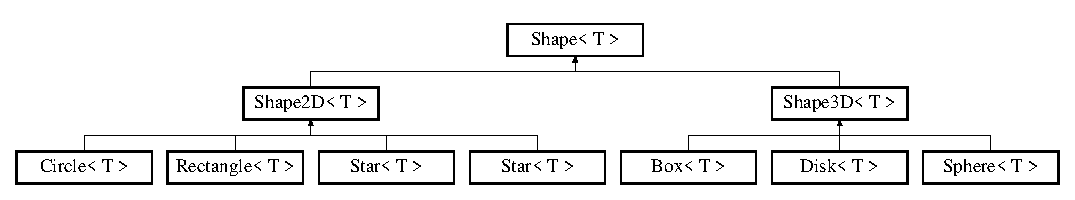
\includegraphics[height=2.242991cm]{classShape}
\end{center}
\end{figure}
\subsection*{Public Member Functions}
\begin{DoxyCompactItemize}
\item 
virtual void \mbox{\hyperlink{classShape_ac5a35fe1b2ecb8fcfc050a31c8969805}{set\+\_\+min\+\_\+number\+\_\+of\+\_\+vertexes}} (unsigned num)
\begin{DoxyCompactList}\small\item\em As the name says, it sets minimal number of vertexes for a given shape. \end{DoxyCompactList}\item 
virtual void \mbox{\hyperlink{classShape_a69dabd50440dba1ac463ad6819cdb506}{set\+\_\+vertex\+\_\+colors}} (\mbox{\hyperlink{type__definitions_8hpp_accb98a876f193a416d9c8a02fe22d526}{aligned\+\_\+vector}}$<$ float $>$ \&colors\+\_\+)
\item 
\mbox{\hyperlink{type__definitions_8hpp_accb98a876f193a416d9c8a02fe22d526}{aligned\+\_\+vector}}$<$ T $>$ \mbox{\hyperlink{classShape_a3729bbdd0c4e4f3379498734807bb545}{get\+\_\+vertexes}} ()
\item 
\mbox{\hyperlink{type__definitions_8hpp_accb98a876f193a416d9c8a02fe22d526}{aligned\+\_\+vector}}$<$ T $>$ \mbox{\hyperlink{classShape_aabe9bd208b0ece9824cb45deccc11ba7}{get\+\_\+colors}} ()
\item 
unsigned \mbox{\hyperlink{classShape_a131e85c7f5cad85bffb92e6719117cab}{num\+\_\+vertexes}} ()
\item 
virtual unsigned \mbox{\hyperlink{classShape_a58713d8cf7c4175e7c76eae75c94bc13}{get\+\_\+vertex\+\_\+size}} ()
\item 
void \mbox{\hyperlink{classShape_aabeb601fe95b412987d5b5c276bf8a7a}{generate\+\_\+random\+\_\+colors}} ()
\begin{DoxyCompactList}\small\item\em Generate random colors for each vertex. \end{DoxyCompactList}\end{DoxyCompactItemize}
\subsection*{Protected Member Functions}
\begin{DoxyCompactItemize}
\item 
void \mbox{\hyperlink{classShape_a8b4f54a694871f9d131fdd105e1ca709}{initialize\+\_\+buffers}} ()
\begin{DoxyCompactList}\small\item\em Allocates and initializes vertex buffer object, element buffer object and vertex array object. It also allocates color buffer -\/ where color for each vertex is stored. \end{DoxyCompactList}\end{DoxyCompactItemize}
\subsection*{Protected Attributes}
\begin{DoxyCompactItemize}
\item 
unsigned \mbox{\hyperlink{classShape_a7cf9cc243cdd64215eca4d81704c7199}{vertex\+\_\+size}} = 0
\item 
\mbox{\hyperlink{type__definitions_8hpp_accb98a876f193a416d9c8a02fe22d526}{aligned\+\_\+vector}}$<$ T $>$ \mbox{\hyperlink{classShape_a50296217cf654fc7b756b67a2f0305c2}{vertexes}}
\item 
char \mbox{\hyperlink{classShape_a851fcb33238286342f670d27443ffdfc}{draw\+\_\+type}}
\item 
\mbox{\hyperlink{type__definitions_8hpp_accb98a876f193a416d9c8a02fe22d526}{aligned\+\_\+vector}}$<$ int $>$ \mbox{\hyperlink{classShape_accef3084e7e3897e01806b90da0a0ec8}{element\+\_\+array}}
\item 
bool \mbox{\hyperlink{classShape_a216866713d16c882a0f0b0b0a89d350d}{colors\+\_\+loaded}}
\item 
unsigned \mbox{\hyperlink{classShape_a5ca89aadcd89bb475d6ca88acf733ce6}{V\+BO}}
\item 
unsigned \mbox{\hyperlink{classShape_a30771567edd66db5d14dc630f2d63f82}{V\+AO}}
\item 
unsigned \mbox{\hyperlink{classShape_a95c775e548b129e23d2dd32e23fb0f3e}{E\+BO}}
\item 
unsigned \mbox{\hyperlink{classShape_a66502f6f87b46a705d131dc7b0b67d42}{C\+BO}}
\item 
unsigned \mbox{\hyperlink{classShape_acb30d3bdd3434dc2cb3074a4d61985ed}{min\+\_\+vertexes}}
\item 
\mbox{\hyperlink{type__definitions_8hpp_accb98a876f193a416d9c8a02fe22d526}{aligned\+\_\+vector}}$<$ float $>$ \mbox{\hyperlink{classShape_a1590ef02d7090f28d1ad312fd46f5030}{vertex\+\_\+colors}}
\end{DoxyCompactItemize}
\subsection*{Friends}
\begin{DoxyCompactItemize}
\item 
void \mbox{\hyperlink{classShape_a0f7d9c8330ae4f062c6f569a7400e1f0}{draw}} (\mbox{\hyperlink{classShape}{Shape}}$<$ T $>$ \&, \mbox{\hyperlink{classShader}{Shader}}$<$ \mbox{\hyperlink{render_8hpp_a24e288e18eb7b6e01de7565001fedb60aa98862073f71a928bad5099cc3e1c2ed}{R\+E\+N\+D\+E\+R\+\_\+\+T\+Y\+P\+E\+::\+U\+N\+I\+F\+O\+R\+M\+\_\+\+C\+O\+L\+OR}} $>$ \&, std\+::array$<$ float, 3 $>$, std\+::array$<$ float, 3 $>$, std\+::array$<$ float, 3 $>$, float, glm\+::vec4)
\item 
void \mbox{\hyperlink{classShape_a29e514c040e0781bfa2e08bcde4a7557}{draw}} (\mbox{\hyperlink{classShape}{Shape}}$<$ T $>$ \&, \mbox{\hyperlink{classShader}{Shader}}$<$ \mbox{\hyperlink{render_8hpp_a24e288e18eb7b6e01de7565001fedb60a9d34355b5a26c54b5dbab1e45245a6f4}{R\+E\+N\+D\+E\+R\+\_\+\+T\+Y\+P\+E\+::\+C\+U\+S\+T\+O\+M\+\_\+\+C\+O\+L\+OR}} $>$ \&, std\+::array$<$ float, 3 $>$, std\+::array$<$ float, 3 $>$, std\+::array$<$ float, 3 $>$, float)
\item 
void \mbox{\hyperlink{classShape_ad57e4dd441b60269c43114f31ffa6085}{draw\+\_\+wireframe}} (\mbox{\hyperlink{classShape}{Shape}}$<$ T $>$ \&shape, \mbox{\hyperlink{classShader}{Shader}}$<$ \mbox{\hyperlink{render_8hpp_a24e288e18eb7b6e01de7565001fedb60aa98862073f71a928bad5099cc3e1c2ed}{R\+E\+N\+D\+E\+R\+\_\+\+T\+Y\+P\+E\+::\+U\+N\+I\+F\+O\+R\+M\+\_\+\+C\+O\+L\+OR}} $>$ \&shader\+\_\+object, std\+::array$<$ float, 3 $>$ scale, std\+::array$<$ float, 3 $>$ position, std\+::array$<$ float, 3 $>$ rotation\+\_\+axis, float angle, glm\+::vec4)
\item 
void \mbox{\hyperlink{classShape_aaff31c90cf40c78284454009c9fe0966}{draw\+\_\+2d\+\_\+object}} (\mbox{\hyperlink{classShape}{Shape}}$<$ T $>$ \&shape, \mbox{\hyperlink{classShader}{Shader}}$<$ \mbox{\hyperlink{render_8hpp_a24e288e18eb7b6e01de7565001fedb60aa98862073f71a928bad5099cc3e1c2ed}{R\+E\+N\+D\+E\+R\+\_\+\+T\+Y\+P\+E\+::\+U\+N\+I\+F\+O\+R\+M\+\_\+\+C\+O\+L\+OR}} $>$ \&shader\+\_\+object, std\+::array$<$ float, 3 $>$ scale, std\+::array$<$ float, 3 $>$ position, std\+::array$<$ float, 3 $>$ rotation\+\_\+axis, float angle, glm\+::vec4)
\end{DoxyCompactItemize}


\subsection{Detailed Description}
\subsubsection*{template$<$typename T$>$\newline
class Shape$<$ T $>$}

virtual base class for 2D and 3D shapes 

All shapes inherit from this class. It contains all basic structures for drawing including opengl buffers. 

\subsection{Member Function Documentation}
\mbox{\Hypertarget{classShape_aabeb601fe95b412987d5b5c276bf8a7a}\label{classShape_aabeb601fe95b412987d5b5c276bf8a7a}} 
\index{Shape@{Shape}!generate\+\_\+random\+\_\+colors@{generate\+\_\+random\+\_\+colors}}
\index{generate\+\_\+random\+\_\+colors@{generate\+\_\+random\+\_\+colors}!Shape@{Shape}}
\subsubsection{\texorpdfstring{generate\+\_\+random\+\_\+colors()}{generate\_random\_colors()}}
{\footnotesize\ttfamily template$<$typename T$>$ \\
void \mbox{\hyperlink{classShape}{Shape}}$<$ T $>$\+::generate\+\_\+random\+\_\+colors (\begin{DoxyParamCaption}{ }\end{DoxyParamCaption})\hspace{0.3cm}{\ttfamily [inline]}}



Generate random colors for each vertex. 

\mbox{\Hypertarget{classShape_aabe9bd208b0ece9824cb45deccc11ba7}\label{classShape_aabe9bd208b0ece9824cb45deccc11ba7}} 
\index{Shape@{Shape}!get\+\_\+colors@{get\+\_\+colors}}
\index{get\+\_\+colors@{get\+\_\+colors}!Shape@{Shape}}
\subsubsection{\texorpdfstring{get\+\_\+colors()}{get\_colors()}}
{\footnotesize\ttfamily template$<$typename T$>$ \\
\mbox{\hyperlink{type__definitions_8hpp_accb98a876f193a416d9c8a02fe22d526}{aligned\+\_\+vector}}$<$T$>$ \mbox{\hyperlink{classShape}{Shape}}$<$ T $>$\+::get\+\_\+colors (\begin{DoxyParamCaption}{ }\end{DoxyParamCaption})\hspace{0.3cm}{\ttfamily [inline]}}

\mbox{\Hypertarget{classShape_a58713d8cf7c4175e7c76eae75c94bc13}\label{classShape_a58713d8cf7c4175e7c76eae75c94bc13}} 
\index{Shape@{Shape}!get\+\_\+vertex\+\_\+size@{get\+\_\+vertex\+\_\+size}}
\index{get\+\_\+vertex\+\_\+size@{get\+\_\+vertex\+\_\+size}!Shape@{Shape}}
\subsubsection{\texorpdfstring{get\+\_\+vertex\+\_\+size()}{get\_vertex\_size()}}
{\footnotesize\ttfamily template$<$typename T$>$ \\
virtual unsigned \mbox{\hyperlink{classShape}{Shape}}$<$ T $>$\+::get\+\_\+vertex\+\_\+size (\begin{DoxyParamCaption}{ }\end{DoxyParamCaption})\hspace{0.3cm}{\ttfamily [inline]}, {\ttfamily [virtual]}}

\mbox{\Hypertarget{classShape_a3729bbdd0c4e4f3379498734807bb545}\label{classShape_a3729bbdd0c4e4f3379498734807bb545}} 
\index{Shape@{Shape}!get\+\_\+vertexes@{get\+\_\+vertexes}}
\index{get\+\_\+vertexes@{get\+\_\+vertexes}!Shape@{Shape}}
\subsubsection{\texorpdfstring{get\+\_\+vertexes()}{get\_vertexes()}}
{\footnotesize\ttfamily template$<$typename T$>$ \\
\mbox{\hyperlink{type__definitions_8hpp_accb98a876f193a416d9c8a02fe22d526}{aligned\+\_\+vector}}$<$T$>$ \mbox{\hyperlink{classShape}{Shape}}$<$ T $>$\+::get\+\_\+vertexes (\begin{DoxyParamCaption}{ }\end{DoxyParamCaption})\hspace{0.3cm}{\ttfamily [inline]}}

\mbox{\Hypertarget{classShape_a8b4f54a694871f9d131fdd105e1ca709}\label{classShape_a8b4f54a694871f9d131fdd105e1ca709}} 
\index{Shape@{Shape}!initialize\+\_\+buffers@{initialize\+\_\+buffers}}
\index{initialize\+\_\+buffers@{initialize\+\_\+buffers}!Shape@{Shape}}
\subsubsection{\texorpdfstring{initialize\+\_\+buffers()}{initialize\_buffers()}}
{\footnotesize\ttfamily template$<$typename T$>$ \\
void \mbox{\hyperlink{classShape}{Shape}}$<$ T $>$\+::initialize\+\_\+buffers (\begin{DoxyParamCaption}{ }\end{DoxyParamCaption})\hspace{0.3cm}{\ttfamily [inline]}, {\ttfamily [protected]}}



Allocates and initializes vertex buffer object, element buffer object and vertex array object. It also allocates color buffer -\/ where color for each vertex is stored. 

\mbox{\Hypertarget{classShape_a131e85c7f5cad85bffb92e6719117cab}\label{classShape_a131e85c7f5cad85bffb92e6719117cab}} 
\index{Shape@{Shape}!num\+\_\+vertexes@{num\+\_\+vertexes}}
\index{num\+\_\+vertexes@{num\+\_\+vertexes}!Shape@{Shape}}
\subsubsection{\texorpdfstring{num\+\_\+vertexes()}{num\_vertexes()}}
{\footnotesize\ttfamily template$<$typename T$>$ \\
unsigned \mbox{\hyperlink{classShape}{Shape}}$<$ T $>$\+::num\+\_\+vertexes (\begin{DoxyParamCaption}{ }\end{DoxyParamCaption})\hspace{0.3cm}{\ttfamily [inline]}}

\mbox{\Hypertarget{classShape_ac5a35fe1b2ecb8fcfc050a31c8969805}\label{classShape_ac5a35fe1b2ecb8fcfc050a31c8969805}} 
\index{Shape@{Shape}!set\+\_\+min\+\_\+number\+\_\+of\+\_\+vertexes@{set\+\_\+min\+\_\+number\+\_\+of\+\_\+vertexes}}
\index{set\+\_\+min\+\_\+number\+\_\+of\+\_\+vertexes@{set\+\_\+min\+\_\+number\+\_\+of\+\_\+vertexes}!Shape@{Shape}}
\subsubsection{\texorpdfstring{set\+\_\+min\+\_\+number\+\_\+of\+\_\+vertexes()}{set\_min\_number\_of\_vertexes()}}
{\footnotesize\ttfamily template$<$typename T$>$ \\
virtual void \mbox{\hyperlink{classShape}{Shape}}$<$ T $>$\+::set\+\_\+min\+\_\+number\+\_\+of\+\_\+vertexes (\begin{DoxyParamCaption}\item[{unsigned}]{num }\end{DoxyParamCaption})\hspace{0.3cm}{\ttfamily [inline]}, {\ttfamily [virtual]}}



As the name says, it sets minimal number of vertexes for a given shape. 


\begin{DoxyParams}{Parameters}
{\em num} & minimal number of vertexes \\
\hline
\end{DoxyParams}
\mbox{\Hypertarget{classShape_a69dabd50440dba1ac463ad6819cdb506}\label{classShape_a69dabd50440dba1ac463ad6819cdb506}} 
\index{Shape@{Shape}!set\+\_\+vertex\+\_\+colors@{set\+\_\+vertex\+\_\+colors}}
\index{set\+\_\+vertex\+\_\+colors@{set\+\_\+vertex\+\_\+colors}!Shape@{Shape}}
\subsubsection{\texorpdfstring{set\+\_\+vertex\+\_\+colors()}{set\_vertex\_colors()}}
{\footnotesize\ttfamily template$<$typename T$>$ \\
virtual void \mbox{\hyperlink{classShape}{Shape}}$<$ T $>$\+::set\+\_\+vertex\+\_\+colors (\begin{DoxyParamCaption}\item[{\mbox{\hyperlink{type__definitions_8hpp_accb98a876f193a416d9c8a02fe22d526}{aligned\+\_\+vector}}$<$ float $>$ \&}]{colors\+\_\+ }\end{DoxyParamCaption})\hspace{0.3cm}{\ttfamily [inline]}, {\ttfamily [virtual]}}



\subsection{Friends And Related Function Documentation}
\mbox{\Hypertarget{classShape_a0f7d9c8330ae4f062c6f569a7400e1f0}\label{classShape_a0f7d9c8330ae4f062c6f569a7400e1f0}} 
\index{Shape@{Shape}!draw@{draw}}
\index{draw@{draw}!Shape@{Shape}}
\subsubsection{\texorpdfstring{draw}{draw}\hspace{0.1cm}{\footnotesize\ttfamily [1/2]}}
{\footnotesize\ttfamily template$<$typename T$>$ \\
void draw (\begin{DoxyParamCaption}\item[{\mbox{\hyperlink{classShape}{Shape}}$<$ T $>$ \&}]{shape,  }\item[{\mbox{\hyperlink{classShader}{Shader}}$<$ \mbox{\hyperlink{render_8hpp_a24e288e18eb7b6e01de7565001fedb60aa98862073f71a928bad5099cc3e1c2ed}{R\+E\+N\+D\+E\+R\+\_\+\+T\+Y\+P\+E\+::\+U\+N\+I\+F\+O\+R\+M\+\_\+\+C\+O\+L\+OR}} $>$ \&}]{shader\+\_\+object,  }\item[{std\+::array$<$ float, 3 $>$}]{scale = {\ttfamily \{0.5,~0.5,~0.5\}},  }\item[{std\+::array$<$ float, 3 $>$}]{position = {\ttfamily \{0,~0,~1\}},  }\item[{std\+::array$<$ float, 3 $>$}]{rotation\+\_\+axis = {\ttfamily \{0,~0,~1\}},  }\item[{float}]{angle = {\ttfamily 0},  }\item[{glm\+::vec4}]{color = {\ttfamily \{0.5,~0.5,~0.5,~0.5\}} }\end{DoxyParamCaption})\hspace{0.3cm}{\ttfamily [friend]}}

\mbox{\Hypertarget{classShape_a29e514c040e0781bfa2e08bcde4a7557}\label{classShape_a29e514c040e0781bfa2e08bcde4a7557}} 
\index{Shape@{Shape}!draw@{draw}}
\index{draw@{draw}!Shape@{Shape}}
\subsubsection{\texorpdfstring{draw}{draw}\hspace{0.1cm}{\footnotesize\ttfamily [2/2]}}
{\footnotesize\ttfamily template$<$typename T$>$ \\
void draw (\begin{DoxyParamCaption}\item[{\mbox{\hyperlink{classShape}{Shape}}$<$ T $>$ \&}]{shape,  }\item[{\mbox{\hyperlink{classShader}{Shader}}$<$ \mbox{\hyperlink{render_8hpp_a24e288e18eb7b6e01de7565001fedb60a9d34355b5a26c54b5dbab1e45245a6f4}{R\+E\+N\+D\+E\+R\+\_\+\+T\+Y\+P\+E\+::\+C\+U\+S\+T\+O\+M\+\_\+\+C\+O\+L\+OR}} $>$ \&}]{shader\+\_\+object,  }\item[{std\+::array$<$ float, 3 $>$}]{scale = {\ttfamily \{0.5,~0.5,~0.5\}},  }\item[{std\+::array$<$ float, 3 $>$}]{position = {\ttfamily \{0,~0,~1\}},  }\item[{std\+::array$<$ float, 3 $>$}]{rotation\+\_\+axis = {\ttfamily \{0,~0,~1\}},  }\item[{float}]{angle = {\ttfamily 0} }\end{DoxyParamCaption})\hspace{0.3cm}{\ttfamily [friend]}}

\mbox{\Hypertarget{classShape_aaff31c90cf40c78284454009c9fe0966}\label{classShape_aaff31c90cf40c78284454009c9fe0966}} 
\index{Shape@{Shape}!draw\+\_\+2d\+\_\+object@{draw\+\_\+2d\+\_\+object}}
\index{draw\+\_\+2d\+\_\+object@{draw\+\_\+2d\+\_\+object}!Shape@{Shape}}
\subsubsection{\texorpdfstring{draw\+\_\+2d\+\_\+object}{draw\_2d\_object}}
{\footnotesize\ttfamily template$<$typename T$>$ \\
void draw\+\_\+2d\+\_\+object (\begin{DoxyParamCaption}\item[{\mbox{\hyperlink{classShape}{Shape}}$<$ T $>$ \&}]{shape,  }\item[{\mbox{\hyperlink{classShader}{Shader}}$<$ \mbox{\hyperlink{render_8hpp_a24e288e18eb7b6e01de7565001fedb60aa98862073f71a928bad5099cc3e1c2ed}{R\+E\+N\+D\+E\+R\+\_\+\+T\+Y\+P\+E\+::\+U\+N\+I\+F\+O\+R\+M\+\_\+\+C\+O\+L\+OR}} $>$ \&}]{shader\+\_\+object,  }\item[{std\+::array$<$ float, 3 $>$}]{scale = {\ttfamily \{0.5,~0.5,~0.5\}},  }\item[{std\+::array$<$ float, 3 $>$}]{position = {\ttfamily \{0,~0,~1\}},  }\item[{std\+::array$<$ float, 3 $>$}]{rotation\+\_\+axis = {\ttfamily \{0,~0,~1\}},  }\item[{float}]{angle = {\ttfamily 0},  }\item[{glm\+::vec4}]{color = {\ttfamily \{0.5,~0.5,~0.5,~0.5\}} }\end{DoxyParamCaption})\hspace{0.3cm}{\ttfamily [friend]}}

\mbox{\Hypertarget{classShape_ad57e4dd441b60269c43114f31ffa6085}\label{classShape_ad57e4dd441b60269c43114f31ffa6085}} 
\index{Shape@{Shape}!draw\+\_\+wireframe@{draw\+\_\+wireframe}}
\index{draw\+\_\+wireframe@{draw\+\_\+wireframe}!Shape@{Shape}}
\subsubsection{\texorpdfstring{draw\+\_\+wireframe}{draw\_wireframe}}
{\footnotesize\ttfamily template$<$typename T$>$ \\
void draw\+\_\+wireframe (\begin{DoxyParamCaption}\item[{\mbox{\hyperlink{classShape}{Shape}}$<$ T $>$ \&}]{shape,  }\item[{\mbox{\hyperlink{classShader}{Shader}}$<$ \mbox{\hyperlink{render_8hpp_a24e288e18eb7b6e01de7565001fedb60aa98862073f71a928bad5099cc3e1c2ed}{R\+E\+N\+D\+E\+R\+\_\+\+T\+Y\+P\+E\+::\+U\+N\+I\+F\+O\+R\+M\+\_\+\+C\+O\+L\+OR}} $>$ \&}]{shader\+\_\+object,  }\item[{std\+::array$<$ float, 3 $>$}]{scale = {\ttfamily \{0.5,~0.5,~0.5\}},  }\item[{std\+::array$<$ float, 3 $>$}]{position = {\ttfamily \{0,~0,~1\}},  }\item[{std\+::array$<$ float, 3 $>$}]{rotation\+\_\+axis = {\ttfamily \{0,~0,~1\}},  }\item[{float}]{angle = {\ttfamily 0},  }\item[{glm\+::vec4}]{color = {\ttfamily \{0.5,~0.5,~0.5,~0.5\}} }\end{DoxyParamCaption})\hspace{0.3cm}{\ttfamily [friend]}}



\subsection{Member Data Documentation}
\mbox{\Hypertarget{classShape_a66502f6f87b46a705d131dc7b0b67d42}\label{classShape_a66502f6f87b46a705d131dc7b0b67d42}} 
\index{Shape@{Shape}!C\+BO@{C\+BO}}
\index{C\+BO@{C\+BO}!Shape@{Shape}}
\subsubsection{\texorpdfstring{C\+BO}{CBO}}
{\footnotesize\ttfamily template$<$typename T$>$ \\
unsigned \mbox{\hyperlink{classShape}{Shape}}$<$ T $>$\+::C\+BO\hspace{0.3cm}{\ttfamily [protected]}}

color buffer address \mbox{\Hypertarget{classShape_a216866713d16c882a0f0b0b0a89d350d}\label{classShape_a216866713d16c882a0f0b0b0a89d350d}} 
\index{Shape@{Shape}!colors\+\_\+loaded@{colors\+\_\+loaded}}
\index{colors\+\_\+loaded@{colors\+\_\+loaded}!Shape@{Shape}}
\subsubsection{\texorpdfstring{colors\+\_\+loaded}{colors\_loaded}}
{\footnotesize\ttfamily template$<$typename T$>$ \\
bool \mbox{\hyperlink{classShape}{Shape}}$<$ T $>$\+::colors\+\_\+loaded\hspace{0.3cm}{\ttfamily [protected]}}

{\bfseries Initial value\+:}
\begin{DoxyCode}
=
        \textcolor{keyword}{false}
\end{DoxyCode}
indicator whether color have been loaded or not vertex size can consist of 2, 3 or 4 points; this is important for correct interpretation of vertexes vector \mbox{\Hypertarget{classShape_a851fcb33238286342f670d27443ffdfc}\label{classShape_a851fcb33238286342f670d27443ffdfc}} 
\index{Shape@{Shape}!draw\+\_\+type@{draw\+\_\+type}}
\index{draw\+\_\+type@{draw\+\_\+type}!Shape@{Shape}}
\subsubsection{\texorpdfstring{draw\+\_\+type}{draw\_type}}
{\footnotesize\ttfamily template$<$typename T$>$ \\
char \mbox{\hyperlink{classShape}{Shape}}$<$ T $>$\+::draw\+\_\+type\hspace{0.3cm}{\ttfamily [protected]}}

this can either be \textquotesingle{}E\textquotesingle{} or \textquotesingle{}V\textquotesingle{}, depending on wheather to draw elements (element buffer) or vertexes (vertex buffer object) \mbox{\Hypertarget{classShape_a95c775e548b129e23d2dd32e23fb0f3e}\label{classShape_a95c775e548b129e23d2dd32e23fb0f3e}} 
\index{Shape@{Shape}!E\+BO@{E\+BO}}
\index{E\+BO@{E\+BO}!Shape@{Shape}}
\subsubsection{\texorpdfstring{E\+BO}{EBO}}
{\footnotesize\ttfamily template$<$typename T$>$ \\
unsigned \mbox{\hyperlink{classShape}{Shape}}$<$ T $>$\+::E\+BO\hspace{0.3cm}{\ttfamily [protected]}}

element buffer address \mbox{\Hypertarget{classShape_accef3084e7e3897e01806b90da0a0ec8}\label{classShape_accef3084e7e3897e01806b90da0a0ec8}} 
\index{Shape@{Shape}!element\+\_\+array@{element\+\_\+array}}
\index{element\+\_\+array@{element\+\_\+array}!Shape@{Shape}}
\subsubsection{\texorpdfstring{element\+\_\+array}{element\_array}}
{\footnotesize\ttfamily template$<$typename T$>$ \\
\mbox{\hyperlink{type__definitions_8hpp_accb98a876f193a416d9c8a02fe22d526}{aligned\+\_\+vector}}$<$int$>$ \mbox{\hyperlink{classShape}{Shape}}$<$ T $>$\+::element\+\_\+array\hspace{0.3cm}{\ttfamily [protected]}}

vector holding all elements in correct order \mbox{\Hypertarget{classShape_acb30d3bdd3434dc2cb3074a4d61985ed}\label{classShape_acb30d3bdd3434dc2cb3074a4d61985ed}} 
\index{Shape@{Shape}!min\+\_\+vertexes@{min\+\_\+vertexes}}
\index{min\+\_\+vertexes@{min\+\_\+vertexes}!Shape@{Shape}}
\subsubsection{\texorpdfstring{min\+\_\+vertexes}{min\_vertexes}}
{\footnotesize\ttfamily template$<$typename T$>$ \\
unsigned \mbox{\hyperlink{classShape}{Shape}}$<$ T $>$\+::min\+\_\+vertexes\hspace{0.3cm}{\ttfamily [protected]}}

{\bfseries Initial value\+:}
\begin{DoxyCode}
=
        5
\end{DoxyCode}
minimal number of vertexes to be generated for a given shape \mbox{\Hypertarget{classShape_a30771567edd66db5d14dc630f2d63f82}\label{classShape_a30771567edd66db5d14dc630f2d63f82}} 
\index{Shape@{Shape}!V\+AO@{V\+AO}}
\index{V\+AO@{V\+AO}!Shape@{Shape}}
\subsubsection{\texorpdfstring{V\+AO}{VAO}}
{\footnotesize\ttfamily template$<$typename T$>$ \\
unsigned \mbox{\hyperlink{classShape}{Shape}}$<$ T $>$\+::V\+AO\hspace{0.3cm}{\ttfamily [protected]}}

vertex array object \mbox{\Hypertarget{classShape_a5ca89aadcd89bb475d6ca88acf733ce6}\label{classShape_a5ca89aadcd89bb475d6ca88acf733ce6}} 
\index{Shape@{Shape}!V\+BO@{V\+BO}}
\index{V\+BO@{V\+BO}!Shape@{Shape}}
\subsubsection{\texorpdfstring{V\+BO}{VBO}}
{\footnotesize\ttfamily template$<$typename T$>$ \\
unsigned \mbox{\hyperlink{classShape}{Shape}}$<$ T $>$\+::V\+BO\hspace{0.3cm}{\ttfamily [protected]}}

vertex buffer object \mbox{\Hypertarget{classShape_a1590ef02d7090f28d1ad312fd46f5030}\label{classShape_a1590ef02d7090f28d1ad312fd46f5030}} 
\index{Shape@{Shape}!vertex\+\_\+colors@{vertex\+\_\+colors}}
\index{vertex\+\_\+colors@{vertex\+\_\+colors}!Shape@{Shape}}
\subsubsection{\texorpdfstring{vertex\+\_\+colors}{vertex\_colors}}
{\footnotesize\ttfamily template$<$typename T$>$ \\
\mbox{\hyperlink{type__definitions_8hpp_accb98a876f193a416d9c8a02fe22d526}{aligned\+\_\+vector}}$<$float$>$ \mbox{\hyperlink{classShape}{Shape}}$<$ T $>$\+::vertex\+\_\+colors\hspace{0.3cm}{\ttfamily [protected]}}

Vector holding a color for each vertex. Four consequtive numbers form a rgb color value \mbox{\Hypertarget{classShape_a7cf9cc243cdd64215eca4d81704c7199}\label{classShape_a7cf9cc243cdd64215eca4d81704c7199}} 
\index{Shape@{Shape}!vertex\+\_\+size@{vertex\+\_\+size}}
\index{vertex\+\_\+size@{vertex\+\_\+size}!Shape@{Shape}}
\subsubsection{\texorpdfstring{vertex\+\_\+size}{vertex\_size}}
{\footnotesize\ttfamily template$<$typename T$>$ \\
unsigned \mbox{\hyperlink{classShape}{Shape}}$<$ T $>$\+::vertex\+\_\+size = 0\hspace{0.3cm}{\ttfamily [protected]}}

\mbox{\Hypertarget{classShape_a50296217cf654fc7b756b67a2f0305c2}\label{classShape_a50296217cf654fc7b756b67a2f0305c2}} 
\index{Shape@{Shape}!vertexes@{vertexes}}
\index{vertexes@{vertexes}!Shape@{Shape}}
\subsubsection{\texorpdfstring{vertexes}{vertexes}}
{\footnotesize\ttfamily template$<$typename T$>$ \\
\mbox{\hyperlink{type__definitions_8hpp_accb98a876f193a416d9c8a02fe22d526}{aligned\+\_\+vector}}$<$T$>$ \mbox{\hyperlink{classShape}{Shape}}$<$ T $>$\+::vertexes\hspace{0.3cm}{\ttfamily [protected]}}

Vector holding all vertexes; 2,3 or 4 consequtive numbers form a vertex 

The documentation for this class was generated from the following files\+:\begin{DoxyCompactItemize}
\item 
src/\mbox{\hyperlink{drawing__functions_8hpp}{drawing\+\_\+functions.\+hpp}}\item 
src/\mbox{\hyperlink{shape_8hpp}{shape.\+hpp}}\end{DoxyCompactItemize}

\hypertarget{classShape2D}{}\section{Shape2D$<$ T $>$ Class Template Reference}
\label{classShape2D}\index{Shape2\+D$<$ T $>$@{Shape2\+D$<$ T $>$}}


\mbox{\hyperlink{classThis}{This}} is a base class for all 2D shapes.  




{\ttfamily \#include \char`\"{}drawing\+\_\+functions.\+hpp\char`\"{}}

Inheritance diagram for Shape2D$<$ T $>$\+:\begin{figure}[H]
\begin{center}
\leavevmode
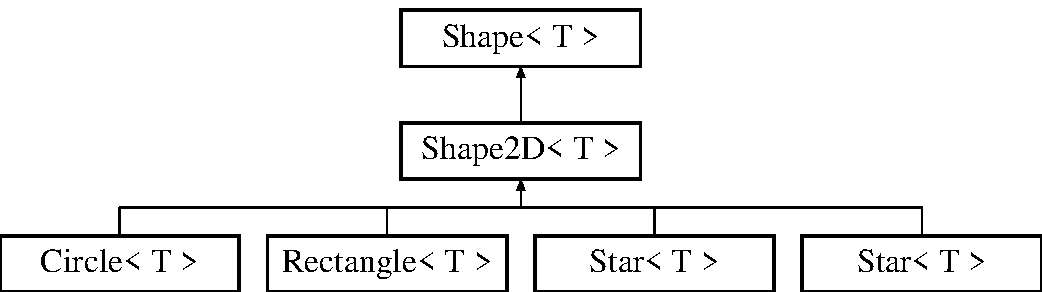
\includegraphics[height=2.688000cm]{classShape2D}
\end{center}
\end{figure}
\subsection*{Public Member Functions}
\begin{DoxyCompactItemize}
\item 
\mbox{\hyperlink{type__definitions_8hpp_a087efd587d66b881646ef378f1919c90}{aligned\+\_\+vector}}$<$ T $>$ \mbox{\hyperlink{classShape2D_af67c7aed6e58b5aa0e3518a3ad1de75b}{get\+\_\+filling\+\_\+vertexes}} ()
\end{DoxyCompactItemize}
\subsection*{Protected Member Functions}
\begin{DoxyCompactItemize}
\item 
virtual \mbox{\hyperlink{glad_8h_a950fc91edb4504f62f1c577bf4727c29}{void}} \mbox{\hyperlink{classShape2D_a917c3277ca262ec557930c8cc837c204}{generate\+\_\+filling\+\_\+vbo}} ()
\item 
{\footnotesize template$<$$>$ }\\\mbox{\hyperlink{glad_8h_a950fc91edb4504f62f1c577bf4727c29}{void}} \mbox{\hyperlink{classShape2D_a328d401b8f1962078e904d4b1003d7a5}{generate\+\_\+filling\+\_\+vbo}} ()
\begin{DoxyCompactList}\small\item\em Generates vertexes which fill the interior of 2D shapes. \end{DoxyCompactList}\end{DoxyCompactItemize}
\subsection*{Protected Attributes}
\begin{DoxyCompactItemize}
\item 
unsigned \mbox{\hyperlink{classShape2D_a220cf4cf96da8bd43627ffffd00a0718}{F\+I\+L\+L\+I\+N\+G\+\_\+\+V\+BO}}
\item 
unsigned \mbox{\hyperlink{classShape2D_affa1082cd6e91cce5af4cb10c1b3435f}{F\+I\+L\+L\+I\+N\+G\+\_\+\+E\+BO}}
\item 
char \mbox{\hyperlink{classShape2D_ab24ceddaa0114eda3ae699f8fb3503ca}{filling\+\_\+draw\+\_\+type}}
\item 
\mbox{\hyperlink{type__definitions_8hpp_a087efd587d66b881646ef378f1919c90}{aligned\+\_\+vector}}$<$ T $>$ \mbox{\hyperlink{classShape2D_ae3e216c9d8422b47f46bff9259bd17be}{filling\+\_\+vertexes}}
\item 
\mbox{\hyperlink{type__definitions_8hpp_a087efd587d66b881646ef378f1919c90}{aligned\+\_\+vector}}$<$ int $>$ \mbox{\hyperlink{classShape2D_a28d0d6018cb6b73637050d9f3fb1f006}{filling\+\_\+elements}}
\end{DoxyCompactItemize}
\subsection*{Friends}
\begin{DoxyCompactItemize}
\item 
\mbox{\hyperlink{glad_8h_a950fc91edb4504f62f1c577bf4727c29}{void}} \mbox{\hyperlink{classShape2D_a75ed525e537ded17d42e3adad87bd701}{draw\+\_\+2d\+\_\+object}} (\mbox{\hyperlink{classShape2D}{Shape2D}}$<$ T $>$ \&shape, \mbox{\hyperlink{classShader}{Shader}}$<$ \mbox{\hyperlink{shader__class_8hpp_a24e288e18eb7b6e01de7565001fedb60aa98862073f71a928bad5099cc3e1c2ed}{R\+E\+N\+D\+E\+R\+\_\+\+T\+Y\+P\+E\+::\+U\+N\+I\+F\+O\+R\+M\+\_\+\+C\+O\+L\+OR}} $>$ \&shader\+\_\+object, std\+::array$<$ float, 3 $>$ scale, std\+::array$<$ float, 3 $>$ position, std\+::array$<$ float, 3 $>$ rotation\+\_\+axis, float angle, glm\+::vec4)
\begin{DoxyCompactList}\small\item\em draw 2d shape filling of uniform color. \end{DoxyCompactList}\end{DoxyCompactItemize}


\subsection{Detailed Description}
\subsubsection*{template$<$typename T$>$\newline
class Shape2\+D$<$ T $>$}

\mbox{\hyperlink{classThis}{This}} is a base class for all 2D shapes. 

It inherits from \mbox{\hyperlink{classShape}{Shape}} class. Template parameter can either be float of double. It is meant to contain functions common to all 2D shapes. 

\subsection{Member Function Documentation}
\mbox{\Hypertarget{classShape2D_a917c3277ca262ec557930c8cc837c204}\label{classShape2D_a917c3277ca262ec557930c8cc837c204}} 
\index{Shape2D@{Shape2D}!generate\+\_\+filling\+\_\+vbo@{generate\+\_\+filling\+\_\+vbo}}
\index{generate\+\_\+filling\+\_\+vbo@{generate\+\_\+filling\+\_\+vbo}!Shape2D@{Shape2D}}
\subsubsection{\texorpdfstring{generate\+\_\+filling\+\_\+vbo()}{generate\_filling\_vbo()}\hspace{0.1cm}{\footnotesize\ttfamily [1/2]}}
{\footnotesize\ttfamily template$<$typename T$>$ \\
virtual \mbox{\hyperlink{glad_8h_a950fc91edb4504f62f1c577bf4727c29}{void}} \mbox{\hyperlink{classShape2D}{Shape2D}}$<$ T $>$\+::generate\+\_\+filling\+\_\+vbo (\begin{DoxyParamCaption}{ }\end{DoxyParamCaption})\hspace{0.3cm}{\ttfamily [protected]}, {\ttfamily [virtual]}}

\mbox{\Hypertarget{classShape2D_a328d401b8f1962078e904d4b1003d7a5}\label{classShape2D_a328d401b8f1962078e904d4b1003d7a5}} 
\index{Shape2D@{Shape2D}!generate\+\_\+filling\+\_\+vbo@{generate\+\_\+filling\+\_\+vbo}}
\index{generate\+\_\+filling\+\_\+vbo@{generate\+\_\+filling\+\_\+vbo}!Shape2D@{Shape2D}}
\subsubsection{\texorpdfstring{generate\+\_\+filling\+\_\+vbo()}{generate\_filling\_vbo()}\hspace{0.1cm}{\footnotesize\ttfamily [2/2]}}
{\footnotesize\ttfamily template$<$$>$ \\
\mbox{\hyperlink{glad_8h_a950fc91edb4504f62f1c577bf4727c29}{void}} \mbox{\hyperlink{classShape2D}{Shape2D}}$<$ float $>$\+::generate\+\_\+filling\+\_\+vbo (\begin{DoxyParamCaption}{ }\end{DoxyParamCaption})\hspace{0.3cm}{\ttfamily [inline]}, {\ttfamily [protected]}}



Generates vertexes which fill the interior of 2D shapes. 

\mbox{\Hypertarget{classShape2D_af67c7aed6e58b5aa0e3518a3ad1de75b}\label{classShape2D_af67c7aed6e58b5aa0e3518a3ad1de75b}} 
\index{Shape2D@{Shape2D}!get\+\_\+filling\+\_\+vertexes@{get\+\_\+filling\+\_\+vertexes}}
\index{get\+\_\+filling\+\_\+vertexes@{get\+\_\+filling\+\_\+vertexes}!Shape2D@{Shape2D}}
\subsubsection{\texorpdfstring{get\+\_\+filling\+\_\+vertexes()}{get\_filling\_vertexes()}}
{\footnotesize\ttfamily template$<$typename T$>$ \\
\mbox{\hyperlink{type__definitions_8hpp_a087efd587d66b881646ef378f1919c90}{aligned\+\_\+vector}}$<$T$>$ \mbox{\hyperlink{classShape2D}{Shape2D}}$<$ T $>$\+::get\+\_\+filling\+\_\+vertexes (\begin{DoxyParamCaption}{ }\end{DoxyParamCaption})\hspace{0.3cm}{\ttfamily [inline]}}



\subsection{Friends And Related Function Documentation}
\mbox{\Hypertarget{classShape2D_a75ed525e537ded17d42e3adad87bd701}\label{classShape2D_a75ed525e537ded17d42e3adad87bd701}} 
\index{Shape2D@{Shape2D}!draw\+\_\+2d\+\_\+object@{draw\+\_\+2d\+\_\+object}}
\index{draw\+\_\+2d\+\_\+object@{draw\+\_\+2d\+\_\+object}!Shape2D@{Shape2D}}
\subsubsection{\texorpdfstring{draw\+\_\+2d\+\_\+object}{draw\_2d\_object}}
{\footnotesize\ttfamily template$<$typename T$>$ \\
\mbox{\hyperlink{glad_8h_a950fc91edb4504f62f1c577bf4727c29}{void}} draw\+\_\+2d\+\_\+object (\begin{DoxyParamCaption}\item[{\mbox{\hyperlink{classShape2D}{Shape2D}}$<$ T $>$ \&}]{shape,  }\item[{\mbox{\hyperlink{classShader}{Shader}}$<$ \mbox{\hyperlink{shader__class_8hpp_a24e288e18eb7b6e01de7565001fedb60aa98862073f71a928bad5099cc3e1c2ed}{R\+E\+N\+D\+E\+R\+\_\+\+T\+Y\+P\+E\+::\+U\+N\+I\+F\+O\+R\+M\+\_\+\+C\+O\+L\+OR}} $>$ \&}]{shader\+\_\+object,  }\item[{std\+::array$<$ float, 3 $>$}]{scale = {\ttfamily \{0.5,~0.5,~0.5\}},  }\item[{std\+::array$<$ float, 3 $>$}]{position = {\ttfamily \{0,~0,~1\}},  }\item[{std\+::array$<$ float, 3 $>$}]{rotation\+\_\+axis = {\ttfamily \{0,~0,~1\}},  }\item[{float}]{angle = {\ttfamily 0},  }\item[{glm\+::vec4}]{color = {\ttfamily \{0.5,~0.5,~0.5,~0.5\}} }\end{DoxyParamCaption})\hspace{0.3cm}{\ttfamily [friend]}}



draw 2d shape filling of uniform color. 


\begin{DoxyParams}{Parameters}
{\em shape} & An object of type class \mbox{\hyperlink{classShape}{Shape}} to be drawn \\
\hline
{\em shader\+\_\+object} & Object of type class Shader$<$\+R\+E\+N\+D\+E\+R\+\_\+\+T\+Y\+P\+E\+::\+U\+N\+I\+F\+O\+R\+M\+\_\+\+C\+O\+L\+O\+R$>$, which contains correct shader. \\
\hline
{\em scale} & sscales object in x,y and z directions. \\
\hline
{\em position} & translate center of the object to coordinates specified by this vector. \\
\hline
{\em rotation\+\_\+axis} & axis around which object should be rotated. \\
\hline
{\em angle} & Angle specifying how much to rotate the object. \\
\hline
{\em color} & color of the shape -\/ the same for all vertexes \\
\hline
\end{DoxyParams}


\subsection{Member Data Documentation}
\mbox{\Hypertarget{classShape2D_ab24ceddaa0114eda3ae699f8fb3503ca}\label{classShape2D_ab24ceddaa0114eda3ae699f8fb3503ca}} 
\index{Shape2D@{Shape2D}!filling\+\_\+draw\+\_\+type@{filling\+\_\+draw\+\_\+type}}
\index{filling\+\_\+draw\+\_\+type@{filling\+\_\+draw\+\_\+type}!Shape2D@{Shape2D}}
\subsubsection{\texorpdfstring{filling\+\_\+draw\+\_\+type}{filling\_draw\_type}}
{\footnotesize\ttfamily template$<$typename T$>$ \\
char \mbox{\hyperlink{classShape2D}{Shape2D}}$<$ T $>$\+::filling\+\_\+draw\+\_\+type\hspace{0.3cm}{\ttfamily [protected]}}

tells whether to render element buffer -\/ \textquotesingle{}E\textquotesingle{} of array buffer -\/ \textquotesingle{}V\textquotesingle{} \mbox{\Hypertarget{classShape2D_affa1082cd6e91cce5af4cb10c1b3435f}\label{classShape2D_affa1082cd6e91cce5af4cb10c1b3435f}} 
\index{Shape2D@{Shape2D}!F\+I\+L\+L\+I\+N\+G\+\_\+\+E\+BO@{F\+I\+L\+L\+I\+N\+G\+\_\+\+E\+BO}}
\index{F\+I\+L\+L\+I\+N\+G\+\_\+\+E\+BO@{F\+I\+L\+L\+I\+N\+G\+\_\+\+E\+BO}!Shape2D@{Shape2D}}
\subsubsection{\texorpdfstring{F\+I\+L\+L\+I\+N\+G\+\_\+\+E\+BO}{FILLING\_EBO}}
{\footnotesize\ttfamily template$<$typename T$>$ \\
unsigned \mbox{\hyperlink{classShape2D}{Shape2D}}$<$ T $>$\+::F\+I\+L\+L\+I\+N\+G\+\_\+\+E\+BO\hspace{0.3cm}{\ttfamily [protected]}}

2D shapes consist of lines, this buffer contains elements to fill 2D shapes. \mbox{\Hypertarget{classShape2D_a28d0d6018cb6b73637050d9f3fb1f006}\label{classShape2D_a28d0d6018cb6b73637050d9f3fb1f006}} 
\index{Shape2D@{Shape2D}!filling\+\_\+elements@{filling\+\_\+elements}}
\index{filling\+\_\+elements@{filling\+\_\+elements}!Shape2D@{Shape2D}}
\subsubsection{\texorpdfstring{filling\+\_\+elements}{filling\_elements}}
{\footnotesize\ttfamily template$<$typename T$>$ \\
\mbox{\hyperlink{type__definitions_8hpp_a087efd587d66b881646ef378f1919c90}{aligned\+\_\+vector}}$<$int$>$ \mbox{\hyperlink{classShape2D}{Shape2D}}$<$ T $>$\+::filling\+\_\+elements\hspace{0.3cm}{\ttfamily [protected]}}

vertexes for interior of 2D shapes. \mbox{\Hypertarget{classShape2D_a220cf4cf96da8bd43627ffffd00a0718}\label{classShape2D_a220cf4cf96da8bd43627ffffd00a0718}} 
\index{Shape2D@{Shape2D}!F\+I\+L\+L\+I\+N\+G\+\_\+\+V\+BO@{F\+I\+L\+L\+I\+N\+G\+\_\+\+V\+BO}}
\index{F\+I\+L\+L\+I\+N\+G\+\_\+\+V\+BO@{F\+I\+L\+L\+I\+N\+G\+\_\+\+V\+BO}!Shape2D@{Shape2D}}
\subsubsection{\texorpdfstring{F\+I\+L\+L\+I\+N\+G\+\_\+\+V\+BO}{FILLING\_VBO}}
{\footnotesize\ttfamily template$<$typename T$>$ \\
unsigned \mbox{\hyperlink{classShape2D}{Shape2D}}$<$ T $>$\+::F\+I\+L\+L\+I\+N\+G\+\_\+\+V\+BO\hspace{0.3cm}{\ttfamily [protected]}}

2D shapes consist of lines, this buffer is meant to fill 2D shapes. \mbox{\Hypertarget{classShape2D_ae3e216c9d8422b47f46bff9259bd17be}\label{classShape2D_ae3e216c9d8422b47f46bff9259bd17be}} 
\index{Shape2D@{Shape2D}!filling\+\_\+vertexes@{filling\+\_\+vertexes}}
\index{filling\+\_\+vertexes@{filling\+\_\+vertexes}!Shape2D@{Shape2D}}
\subsubsection{\texorpdfstring{filling\+\_\+vertexes}{filling\_vertexes}}
{\footnotesize\ttfamily template$<$typename T$>$ \\
\mbox{\hyperlink{type__definitions_8hpp_a087efd587d66b881646ef378f1919c90}{aligned\+\_\+vector}}$<$T$>$ \mbox{\hyperlink{classShape2D}{Shape2D}}$<$ T $>$\+::filling\+\_\+vertexes\hspace{0.3cm}{\ttfamily [protected]}}

vertexes for interior of 2D shapes. 

The documentation for this class was generated from the following files\+:\begin{DoxyCompactItemize}
\item 
src/display\+\_\+and\+\_\+drawing\+\_\+functions/\mbox{\hyperlink{drawing__functions_8hpp}{drawing\+\_\+functions.\+hpp}}\item 
src/shapes/\mbox{\hyperlink{shape_8hpp}{shape.\+hpp}}\end{DoxyCompactItemize}

\hypertarget{classShape3D}{}\section{Shape3D$<$ T $>$ Class Template Reference}
\label{classShape3D}\index{Shape3\+D$<$ T $>$@{Shape3\+D$<$ T $>$}}


{\ttfamily \#include \char`\"{}shape.\+hpp\char`\"{}}

Inheritance diagram for Shape3D$<$ T $>$\+:\begin{figure}[H]
\begin{center}
\leavevmode
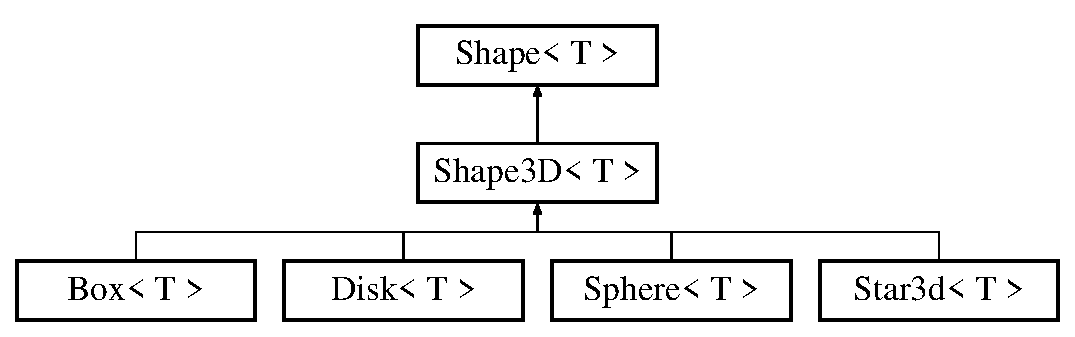
\includegraphics[height=3.000000cm]{classShape3D}
\end{center}
\end{figure}
\subsection*{Public Member Functions}
\begin{DoxyCompactItemize}
\item 
{\footnotesize template$<$typename Q  = T$>$ }\\std\+::enable\+\_\+if$<$ std\+::is\+\_\+same$<$ Q, float $>$\+::value, Q $>$\+::type \mbox{\hyperlink{classShape3D_a2e50becd374a83f43617328dbcc2de3b}{area}} ()
\end{DoxyCompactItemize}
\subsection*{Additional Inherited Members}


\subsection{Member Function Documentation}
\mbox{\Hypertarget{classShape3D_a2e50becd374a83f43617328dbcc2de3b}\label{classShape3D_a2e50becd374a83f43617328dbcc2de3b}} 
\index{Shape3D@{Shape3D}!area@{area}}
\index{area@{area}!Shape3D@{Shape3D}}
\subsubsection{\texorpdfstring{area()}{area()}}
{\footnotesize\ttfamily template$<$typename T $>$ \\
template$<$typename Q  = T$>$ \\
std\+::enable\+\_\+if$<$std\+::is\+\_\+same$<$Q, float$>$\+::value, Q$>$\+::type \mbox{\hyperlink{classShape3D}{Shape3D}}$<$ T $>$\+::area (\begin{DoxyParamCaption}{ }\end{DoxyParamCaption})\hspace{0.3cm}{\ttfamily [inline]}}



The documentation for this class was generated from the following file\+:\begin{DoxyCompactItemize}
\item 
src/\mbox{\hyperlink{shape_8hpp}{shape.\+hpp}}\end{DoxyCompactItemize}

\hypertarget{classSphere}{}\section{Sphere$<$ T $>$ Class Template Reference}
\label{classSphere}\index{Sphere$<$ T $>$@{Sphere$<$ T $>$}}


{\ttfamily \#include \char`\"{}sphere.\+hpp\char`\"{}}

Inheritance diagram for Sphere$<$ T $>$\+:\begin{figure}[H]
\begin{center}
\leavevmode
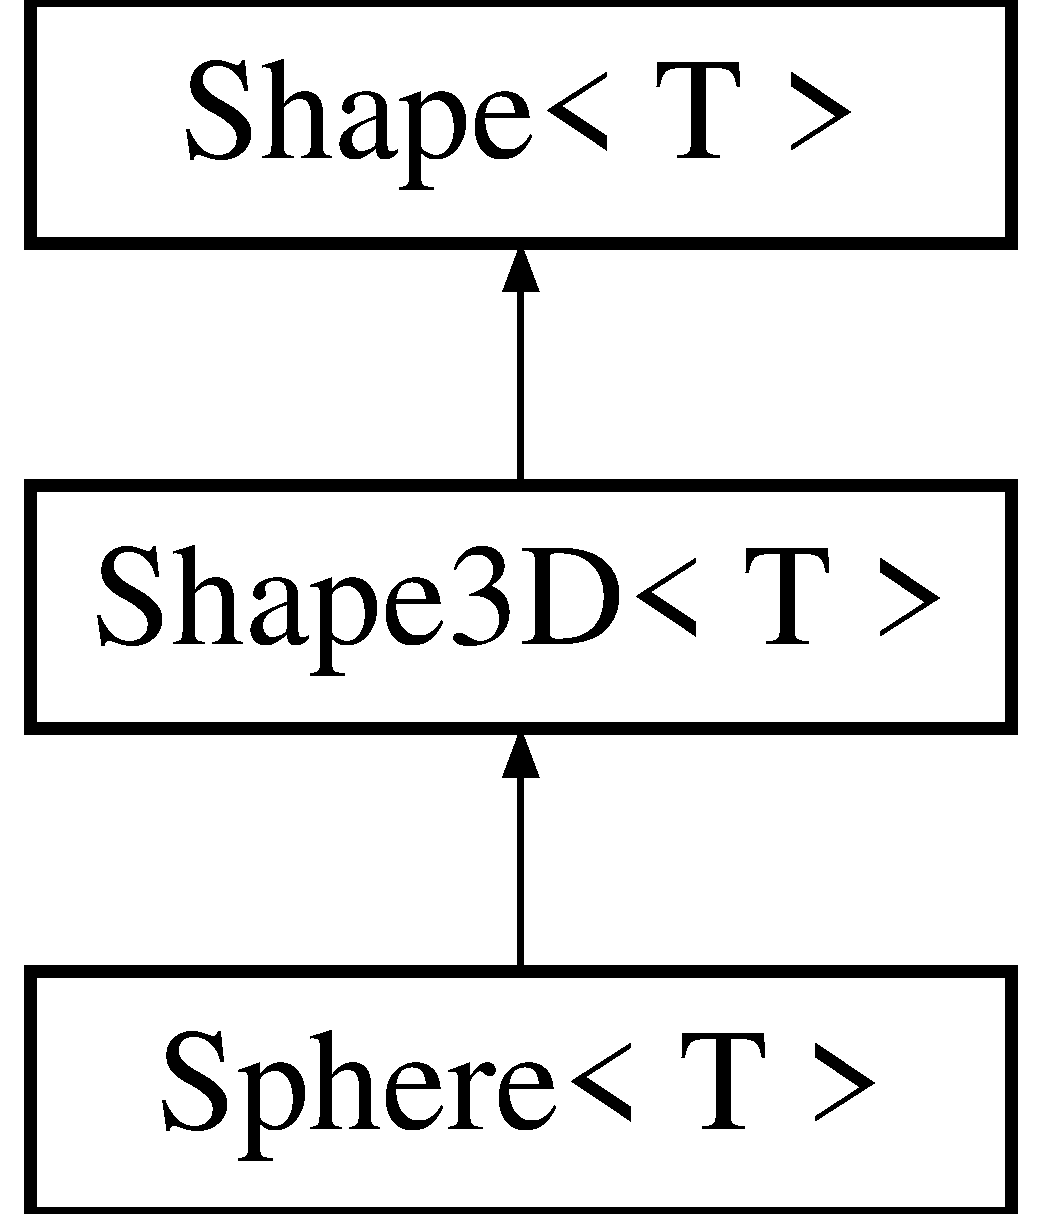
\includegraphics[height=3.000000cm]{classSphere}
\end{center}
\end{figure}
\subsection*{Public Member Functions}
\begin{DoxyCompactItemize}
\item 
\mbox{\hyperlink{classSphere_acacfd6de079ea50acdaf57b823166651}{Sphere}} ()
\begin{DoxyCompactList}\small\item\em \mbox{\hyperlink{classA}{A}} basic constructor for \mbox{\hyperlink{classSphere}{Sphere}} class. \end{DoxyCompactList}\item 
\mbox{\hyperlink{classSphere_a79e3c1cb536e3fe4d8bc447e7be0e414}{Sphere}} (int min\+\_\+vertexes\+\_\+)
\begin{DoxyCompactList}\small\item\em \mbox{\hyperlink{classA}{A}} basic constructor for \mbox{\hyperlink{classSphere}{Sphere}} class. \end{DoxyCompactList}\item 
\mbox{\hyperlink{classSphere_af0d667b078ae88955113205112d9aaa6}{Sphere}} (\mbox{\hyperlink{classSphere}{Sphere}} \&\&)=default
\item 
\mbox{\hyperlink{classSphere}{Sphere}} \& \mbox{\hyperlink{classSphere_aa117f966cea7b16532cbd80c2191a84a}{operator=}} (\mbox{\hyperlink{classSphere}{Sphere}} \&\&)=default
\item 
\mbox{\hyperlink{classSphere_ae28ad7649c59d653b9e14a3042d186a1}{Sphere}} (const \mbox{\hyperlink{classSphere}{Sphere}} \&)=default
\item 
\mbox{\hyperlink{classSphere}{Sphere}} \& \mbox{\hyperlink{classSphere_ae989d05c3ea71f5a758e90e2f2e3aecf}{operator=}} (const \mbox{\hyperlink{classSphere}{Sphere}} \&)=default
\item 
\mbox{\hyperlink{glad_8h_a950fc91edb4504f62f1c577bf4727c29}{void}} \mbox{\hyperlink{classSphere_a3f5ee2b07e48a360696fe983690d1d1f}{refine}} ()
\begin{DoxyCompactList}\small\item\em \mbox{\hyperlink{classThis}{This}} function calls generate\+\_\+vertexes\+\_\+helper to refine the mesh. \end{DoxyCompactList}\item 
T \mbox{\hyperlink{classSphere_a9ebc65dabaf8d87fbe599f4b64816f73}{quality}} ()
\begin{DoxyCompactList}\small\item\em The quality of the mesh is measured as the difference between exact pi number and the one obtained from the area of the sphere (mesh). \end{DoxyCompactList}\end{DoxyCompactItemize}
\subsection*{Private Member Functions}
\begin{DoxyCompactItemize}
\item 
\mbox{\hyperlink{glad_8h_a950fc91edb4504f62f1c577bf4727c29}{void}} \mbox{\hyperlink{classSphere_ab739ad1931e58a4ba7c84e3ca5c1965d}{generate\+\_\+vertexes\+\_\+helper\+\_\+old}} ()
\item 
\mbox{\hyperlink{glad_8h_a950fc91edb4504f62f1c577bf4727c29}{void}} \mbox{\hyperlink{classSphere_a84a45f41ca9e630beb97fc106b359ffd}{generate\+\_\+vertexes\+\_\+helper}} ()
\begin{DoxyCompactList}\small\item\em \mbox{\hyperlink{classThis}{This}} function generates vertexes for float and double version of class \mbox{\hyperlink{classCircle}{Circle}}. \end{DoxyCompactList}\item 
\mbox{\hyperlink{glad_8h_a950fc91edb4504f62f1c577bf4727c29}{void}} \mbox{\hyperlink{classSphere_a9cfac85b9803fadc4b79db0ea047f679}{generate\+\_\+vertexes}} ()
\begin{DoxyCompactList}\small\item\em \mbox{\hyperlink{classThis}{This}} function generates vertexes for class \mbox{\hyperlink{classCircle}{Circle}}. \end{DoxyCompactList}\end{DoxyCompactItemize}
\subsection*{Additional Inherited Members}


\subsection{Constructor \& Destructor Documentation}
\mbox{\Hypertarget{classSphere_acacfd6de079ea50acdaf57b823166651}\label{classSphere_acacfd6de079ea50acdaf57b823166651}} 
\index{Sphere@{Sphere}!Sphere@{Sphere}}
\index{Sphere@{Sphere}!Sphere@{Sphere}}
\subsubsection{\texorpdfstring{Sphere()}{Sphere()}\hspace{0.1cm}{\footnotesize\ttfamily [1/4]}}
{\footnotesize\ttfamily template$<$typename T = float$>$ \\
\mbox{\hyperlink{classSphere}{Sphere}}$<$ T $>$\+::\mbox{\hyperlink{classSphere}{Sphere}} (\begin{DoxyParamCaption}{ }\end{DoxyParamCaption})\hspace{0.3cm}{\ttfamily [inline]}}



\mbox{\hyperlink{classA}{A}} basic constructor for \mbox{\hyperlink{classSphere}{Sphere}} class. 

The constructor generate vertexes and elements. Opengl buffers are also allocated and initiallized. \mbox{\Hypertarget{classSphere_a79e3c1cb536e3fe4d8bc447e7be0e414}\label{classSphere_a79e3c1cb536e3fe4d8bc447e7be0e414}} 
\index{Sphere@{Sphere}!Sphere@{Sphere}}
\index{Sphere@{Sphere}!Sphere@{Sphere}}
\subsubsection{\texorpdfstring{Sphere()}{Sphere()}\hspace{0.1cm}{\footnotesize\ttfamily [2/4]}}
{\footnotesize\ttfamily template$<$typename T = float$>$ \\
\mbox{\hyperlink{classSphere}{Sphere}}$<$ T $>$\+::\mbox{\hyperlink{classSphere}{Sphere}} (\begin{DoxyParamCaption}\item[{int}]{min\+\_\+vertexes\+\_\+ }\end{DoxyParamCaption})\hspace{0.3cm}{\ttfamily [inline]}}



\mbox{\hyperlink{classA}{A}} basic constructor for \mbox{\hyperlink{classSphere}{Sphere}} class. 

The constructor generate vertexes and elements. Opengl buffers are also allocated and initiallized. 
\begin{DoxyParams}{Parameters}
{\em min\+\_\+vertexes\+\_\+} & minimal number of vertexes to create sphere \\
\hline
\end{DoxyParams}
\mbox{\Hypertarget{classSphere_af0d667b078ae88955113205112d9aaa6}\label{classSphere_af0d667b078ae88955113205112d9aaa6}} 
\index{Sphere@{Sphere}!Sphere@{Sphere}}
\index{Sphere@{Sphere}!Sphere@{Sphere}}
\subsubsection{\texorpdfstring{Sphere()}{Sphere()}\hspace{0.1cm}{\footnotesize\ttfamily [3/4]}}
{\footnotesize\ttfamily template$<$typename T = float$>$ \\
\mbox{\hyperlink{classSphere}{Sphere}}$<$ T $>$\+::\mbox{\hyperlink{classSphere}{Sphere}} (\begin{DoxyParamCaption}\item[{\mbox{\hyperlink{classSphere}{Sphere}}$<$ T $>$ \&\&}]{ }\end{DoxyParamCaption})\hspace{0.3cm}{\ttfamily [default]}}

\mbox{\Hypertarget{classSphere_ae28ad7649c59d653b9e14a3042d186a1}\label{classSphere_ae28ad7649c59d653b9e14a3042d186a1}} 
\index{Sphere@{Sphere}!Sphere@{Sphere}}
\index{Sphere@{Sphere}!Sphere@{Sphere}}
\subsubsection{\texorpdfstring{Sphere()}{Sphere()}\hspace{0.1cm}{\footnotesize\ttfamily [4/4]}}
{\footnotesize\ttfamily template$<$typename T = float$>$ \\
\mbox{\hyperlink{classSphere}{Sphere}}$<$ T $>$\+::\mbox{\hyperlink{classSphere}{Sphere}} (\begin{DoxyParamCaption}\item[{const \mbox{\hyperlink{classSphere}{Sphere}}$<$ T $>$ \&}]{ }\end{DoxyParamCaption})\hspace{0.3cm}{\ttfamily [default]}}



\subsection{Member Function Documentation}
\mbox{\Hypertarget{classSphere_a9cfac85b9803fadc4b79db0ea047f679}\label{classSphere_a9cfac85b9803fadc4b79db0ea047f679}} 
\index{Sphere@{Sphere}!generate\+\_\+vertexes@{generate\+\_\+vertexes}}
\index{generate\+\_\+vertexes@{generate\+\_\+vertexes}!Sphere@{Sphere}}
\subsubsection{\texorpdfstring{generate\+\_\+vertexes()}{generate\_vertexes()}}
{\footnotesize\ttfamily template$<$typename T $>$ \\
\mbox{\hyperlink{glad_8h_a950fc91edb4504f62f1c577bf4727c29}{void}} \mbox{\hyperlink{classSphere}{Sphere}}$<$ T $>$\+::generate\+\_\+vertexes (\begin{DoxyParamCaption}{ }\end{DoxyParamCaption})\hspace{0.3cm}{\ttfamily [private]}}



\mbox{\hyperlink{classThis}{This}} function generates vertexes for class \mbox{\hyperlink{classCircle}{Circle}}. 

Internally, it calls generate\+\_\+vertexes\+\_\+helper function to refine the mesh. \mbox{\Hypertarget{classSphere_a84a45f41ca9e630beb97fc106b359ffd}\label{classSphere_a84a45f41ca9e630beb97fc106b359ffd}} 
\index{Sphere@{Sphere}!generate\+\_\+vertexes\+\_\+helper@{generate\+\_\+vertexes\+\_\+helper}}
\index{generate\+\_\+vertexes\+\_\+helper@{generate\+\_\+vertexes\+\_\+helper}!Sphere@{Sphere}}
\subsubsection{\texorpdfstring{generate\+\_\+vertexes\+\_\+helper()}{generate\_vertexes\_helper()}}
{\footnotesize\ttfamily template$<$typename T $>$ \\
\mbox{\hyperlink{glad_8h_a950fc91edb4504f62f1c577bf4727c29}{void}} \mbox{\hyperlink{classSphere}{Sphere}}$<$ T $>$\+::generate\+\_\+vertexes\+\_\+helper (\begin{DoxyParamCaption}{ }\end{DoxyParamCaption})\hspace{0.3cm}{\ttfamily [inline]}, {\ttfamily [private]}}



\mbox{\hyperlink{classThis}{This}} function generates vertexes for float and double version of class \mbox{\hyperlink{classCircle}{Circle}}. 

It is used only when sse and avx versions are not available. \mbox{\Hypertarget{classSphere_ab739ad1931e58a4ba7c84e3ca5c1965d}\label{classSphere_ab739ad1931e58a4ba7c84e3ca5c1965d}} 
\index{Sphere@{Sphere}!generate\+\_\+vertexes\+\_\+helper\+\_\+old@{generate\+\_\+vertexes\+\_\+helper\+\_\+old}}
\index{generate\+\_\+vertexes\+\_\+helper\+\_\+old@{generate\+\_\+vertexes\+\_\+helper\+\_\+old}!Sphere@{Sphere}}
\subsubsection{\texorpdfstring{generate\+\_\+vertexes\+\_\+helper\+\_\+old()}{generate\_vertexes\_helper\_old()}}
{\footnotesize\ttfamily template$<$typename T = float$>$ \\
\mbox{\hyperlink{glad_8h_a950fc91edb4504f62f1c577bf4727c29}{void}} \mbox{\hyperlink{classSphere}{Sphere}}$<$ T $>$\+::generate\+\_\+vertexes\+\_\+helper\+\_\+old (\begin{DoxyParamCaption}{ }\end{DoxyParamCaption})\hspace{0.3cm}{\ttfamily [private]}}

\mbox{\Hypertarget{classSphere_aa117f966cea7b16532cbd80c2191a84a}\label{classSphere_aa117f966cea7b16532cbd80c2191a84a}} 
\index{Sphere@{Sphere}!operator=@{operator=}}
\index{operator=@{operator=}!Sphere@{Sphere}}
\subsubsection{\texorpdfstring{operator=()}{operator=()}\hspace{0.1cm}{\footnotesize\ttfamily [1/2]}}
{\footnotesize\ttfamily template$<$typename T = float$>$ \\
\mbox{\hyperlink{classSphere}{Sphere}}\& \mbox{\hyperlink{classSphere}{Sphere}}$<$ T $>$\+::operator= (\begin{DoxyParamCaption}\item[{\mbox{\hyperlink{classSphere}{Sphere}}$<$ T $>$ \&\&}]{ }\end{DoxyParamCaption})\hspace{0.3cm}{\ttfamily [default]}}

\mbox{\Hypertarget{classSphere_ae989d05c3ea71f5a758e90e2f2e3aecf}\label{classSphere_ae989d05c3ea71f5a758e90e2f2e3aecf}} 
\index{Sphere@{Sphere}!operator=@{operator=}}
\index{operator=@{operator=}!Sphere@{Sphere}}
\subsubsection{\texorpdfstring{operator=()}{operator=()}\hspace{0.1cm}{\footnotesize\ttfamily [2/2]}}
{\footnotesize\ttfamily template$<$typename T = float$>$ \\
\mbox{\hyperlink{classSphere}{Sphere}}\& \mbox{\hyperlink{classSphere}{Sphere}}$<$ T $>$\+::operator= (\begin{DoxyParamCaption}\item[{const \mbox{\hyperlink{classSphere}{Sphere}}$<$ T $>$ \&}]{ }\end{DoxyParamCaption})\hspace{0.3cm}{\ttfamily [default]}}

\mbox{\Hypertarget{classSphere_a9ebc65dabaf8d87fbe599f4b64816f73}\label{classSphere_a9ebc65dabaf8d87fbe599f4b64816f73}} 
\index{Sphere@{Sphere}!quality@{quality}}
\index{quality@{quality}!Sphere@{Sphere}}
\subsubsection{\texorpdfstring{quality()}{quality()}}
{\footnotesize\ttfamily template$<$typename T $>$ \\
T \mbox{\hyperlink{classSphere}{Sphere}}$<$ T $>$\+::quality (\begin{DoxyParamCaption}{ }\end{DoxyParamCaption})}



The quality of the mesh is measured as the difference between exact pi number and the one obtained from the area of the sphere (mesh). 

\mbox{\Hypertarget{classSphere_a3f5ee2b07e48a360696fe983690d1d1f}\label{classSphere_a3f5ee2b07e48a360696fe983690d1d1f}} 
\index{Sphere@{Sphere}!refine@{refine}}
\index{refine@{refine}!Sphere@{Sphere}}
\subsubsection{\texorpdfstring{refine()}{refine()}}
{\footnotesize\ttfamily template$<$typename T $>$ \\
\mbox{\hyperlink{glad_8h_a950fc91edb4504f62f1c577bf4727c29}{void}} \mbox{\hyperlink{classSphere}{Sphere}}$<$ T $>$\+::refine (\begin{DoxyParamCaption}{ }\end{DoxyParamCaption})}



\mbox{\hyperlink{classThis}{This}} function calls generate\+\_\+vertexes\+\_\+helper to refine the mesh. 



The documentation for this class was generated from the following file\+:\begin{DoxyCompactItemize}
\item 
src/shapes/\mbox{\hyperlink{sphere_8hpp}{sphere.\+hpp}}\end{DoxyCompactItemize}

\hypertarget{classspin__dir}{}\section{spin\+\_\+dir Class Reference}
\label{classspin__dir}\index{spin\+\_\+dir@{spin\+\_\+dir}}


\mbox{\hyperlink{classThis}{This}} enum contains two possible spin directions in the Ising model.  




{\ttfamily \#include \char`\"{}Ising\+\_\+model.\+hpp\char`\"{}}



\subsection{Detailed Description}
\mbox{\hyperlink{classThis}{This}} enum contains two possible spin directions in the Ising model. 

The documentation for this class was generated from the following file\+:\begin{DoxyCompactItemize}
\item 
src/algorithms/\mbox{\hyperlink{Ising__model_8hpp}{Ising\+\_\+model.\+hpp}}\end{DoxyCompactItemize}

\hypertarget{classSpinArray}{}\section{Spin\+Array$<$ T $>$ Class Template Reference}
\label{classSpinArray}\index{Spin\+Array$<$ T $>$@{Spin\+Array$<$ T $>$}}


{\ttfamily \#include \char`\"{}spin\+\_\+array.\+hpp\char`\"{}}

Inheritance diagram for Spin\+Array$<$ T $>$\+:\begin{figure}[H]
\begin{center}
\leavevmode
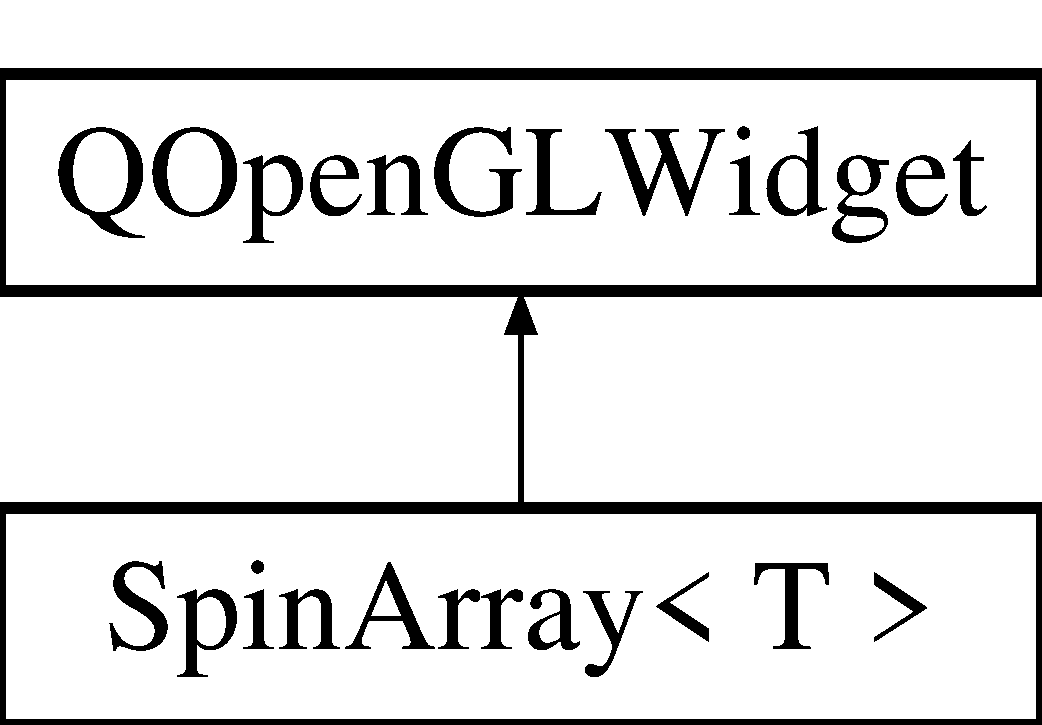
\includegraphics[height=2.000000cm]{classSpinArray}
\end{center}
\end{figure}
\subsection*{Public Member Functions}
\begin{DoxyCompactItemize}
\item 
\mbox{\hyperlink{classSpinArray_ab18db2915e18885e5146eef092f4eb67}{Spin\+Array}} (unsigned size\+\_\+=50, glm\+::vec3 pos\+\_\+=\{0.\+0, 0.\+0, 0.\+0\})
\item 
void \mbox{\hyperlink{classSpinArray_af60baac7f6d47c183ce395e909e8513f}{set\+\_\+clickable\+\_\+square}} (G\+L\+F\+Wwindow $\ast$window)
\item 
void \mbox{\hyperlink{classSpinArray_acc4dd3d5a680c195ebaea00120bd5ed8}{set\+\_\+scale}} (glm\+::vec3 scale\+\_\+=\{1, 1, 1\})
\item 
void \mbox{\hyperlink{classSpinArray_a904e68a8b76d7da16140a0352ae04dfa}{set\+\_\+pos}} (glm\+::vec3 pos\+\_\+=\{0, 0, 0\})
\item 
unsigned \mbox{\hyperlink{classSpinArray_ae7aa5d361c1f3024506291b04e027a7a}{get\+\_\+size}} ()
\item 
\mbox{\hyperlink{type__definitions_8hpp_a087efd587d66b881646ef378f1919c90}{aligned\+\_\+vector}}$<$ T $>$ \mbox{\hyperlink{classSpinArray_ac4a17ebe80ae433662d69537adf9a4de}{get\+\_\+vertexes}} ()
\item 
T \mbox{\hyperlink{classSpinArray_adf314e4c6182e5344e8b793784576677}{get\+\_\+square\+\_\+size}} ()
\item 
void \mbox{\hyperlink{classSpinArray_ab2d41adf8269369e26c316684da70462}{movable}} (G\+L\+F\+Wwindow $\ast$window)
\item 
\mbox{\hyperlink{classSpinArray_ab18db2915e18885e5146eef092f4eb67}{Spin\+Array}} (unsigned size\+\_\+=50, glm\+::vec3 pos\+\_\+=\{0.\+0, 0.\+0, 0.\+0\})
\item 
void \mbox{\hyperlink{classSpinArray_af60baac7f6d47c183ce395e909e8513f}{set\+\_\+clickable\+\_\+square}} (G\+L\+F\+Wwindow $\ast$window)
\item 
void \mbox{\hyperlink{classSpinArray_acc4dd3d5a680c195ebaea00120bd5ed8}{set\+\_\+scale}} (glm\+::vec3 scale\+\_\+=\{1, 1, 1\})
\item 
void \mbox{\hyperlink{classSpinArray_a904e68a8b76d7da16140a0352ae04dfa}{set\+\_\+pos}} (glm\+::vec3 pos\+\_\+=\{0, 0, 0\})
\item 
unsigned \mbox{\hyperlink{classSpinArray_ae7aa5d361c1f3024506291b04e027a7a}{get\+\_\+size}} ()
\item 
\mbox{\hyperlink{type__definitions_8hpp_a087efd587d66b881646ef378f1919c90}{aligned\+\_\+vector}}$<$ T $>$ \mbox{\hyperlink{classSpinArray_ac4a17ebe80ae433662d69537adf9a4de}{get\+\_\+vertexes}} ()
\item 
T \mbox{\hyperlink{classSpinArray_adf314e4c6182e5344e8b793784576677}{get\+\_\+square\+\_\+size}} ()
\item 
void \mbox{\hyperlink{classSpinArray_ab2d41adf8269369e26c316684da70462}{movable}} (G\+L\+F\+Wwindow $\ast$window)
\item 
\mbox{\hyperlink{classSpinArray_ab18db2915e18885e5146eef092f4eb67}{Spin\+Array}} (unsigned size\+\_\+=50, glm\+::vec3 pos\+\_\+=\{0.\+0, 0.\+0, 0.\+0\})
\item 
void \mbox{\hyperlink{classSpinArray_af60baac7f6d47c183ce395e909e8513f}{set\+\_\+clickable\+\_\+square}} (G\+L\+F\+Wwindow $\ast$window)
\item 
void \mbox{\hyperlink{classSpinArray_acc4dd3d5a680c195ebaea00120bd5ed8}{set\+\_\+scale}} (glm\+::vec3 scale\+\_\+=\{1, 1, 1\})
\item 
void \mbox{\hyperlink{classSpinArray_a904e68a8b76d7da16140a0352ae04dfa}{set\+\_\+pos}} (glm\+::vec3 pos\+\_\+=\{0, 0, 0\})
\item 
unsigned \mbox{\hyperlink{classSpinArray_ae7aa5d361c1f3024506291b04e027a7a}{get\+\_\+size}} ()
\item 
\mbox{\hyperlink{type__definitions_8hpp_a087efd587d66b881646ef378f1919c90}{aligned\+\_\+vector}}$<$ T $>$ \mbox{\hyperlink{classSpinArray_ac4a17ebe80ae433662d69537adf9a4de}{get\+\_\+vertexes}} ()
\item 
T \mbox{\hyperlink{classSpinArray_adf314e4c6182e5344e8b793784576677}{get\+\_\+square\+\_\+size}} ()
\item 
void \mbox{\hyperlink{classSpinArray_ab2d41adf8269369e26c316684da70462}{movable}} (G\+L\+F\+Wwindow $\ast$window)
\item 
\mbox{\hyperlink{classSpinArray_a05936858ffca26e37f98190dc8425976}{Spin\+Array}} (Q\+Widget $\ast$parent, unsigned size\+\_\+=50, glm\+::vec3 pos\+\_\+=\{0.\+0, 0.\+0, 0.\+0\})
\item 
void \mbox{\hyperlink{classSpinArray_afb77bcbce445bec1e75efe2bd16bda31}{initialize\+\_\+shaders}} ()
\item 
void \mbox{\hyperlink{classSpinArray_a4ef3aa2bd3d5bdfe950a7eb8952b1eb8}{cleanup}} ()
\item 
void \mbox{\hyperlink{classSpinArray_a41d829fe76cf531a09c20f9a0b6ebf36}{initialize\+GL}} ()
\begin{DoxyCompactList}\small\item\em \mbox{\hyperlink{classThis}{This}} is an overload for internal initialize function for opengl context. \end{DoxyCompactList}\item 
void \mbox{\hyperlink{classSpinArray_acc4dd3d5a680c195ebaea00120bd5ed8}{set\+\_\+scale}} (glm\+::vec3 scale\+\_\+=\{1, 1, 1\})
\item 
void \mbox{\hyperlink{classSpinArray_a904e68a8b76d7da16140a0352ae04dfa}{set\+\_\+pos}} (glm\+::vec3 pos\+\_\+=\{0, 0, 0\})
\item 
unsigned \mbox{\hyperlink{classSpinArray_ae7aa5d361c1f3024506291b04e027a7a}{get\+\_\+size}} ()
\item 
\mbox{\hyperlink{type__definitions_8hpp_a087efd587d66b881646ef378f1919c90}{aligned\+\_\+vector}}$<$ T $>$ \mbox{\hyperlink{classSpinArray_ac4a17ebe80ae433662d69537adf9a4de}{get\+\_\+vertexes}} ()
\item 
T \mbox{\hyperlink{classSpinArray_adf314e4c6182e5344e8b793784576677}{get\+\_\+square\+\_\+size}} ()
\item 
void \mbox{\hyperlink{classSpinArray_a0f8e083d6f61a3ebbb5aec9cae749af7}{draw\+\_\+frame}} ()
\item 
void \mbox{\hyperlink{classSpinArray_ab1347f20a673884e1289e4895889a17c}{draw\+\_\+black\+\_\+white}} (\mbox{\hyperlink{classIsingModel}{Ising\+Model}}$<$ T $>$ \&ising\+\_\+model)
\end{DoxyCompactItemize}
\subsection*{Private Member Functions}
\begin{DoxyCompactItemize}
\item 
void \mbox{\hyperlink{classSpinArray_a3a7064b0c74a8a777d8a987f29c31108}{initialize\+\_\+buffers}} ()
\begin{DoxyCompactList}\small\item\em Allocates and initializes vertex buffer object, element buffer object and vertex array object. It also allocates color buffer -\/ where color for each vertex is stored. \end{DoxyCompactList}\item 
void \mbox{\hyperlink{classSpinArray_a9a91cd3d27cfd626edaaafe1cf2bc679}{generate\+\_\+vertexes}} ()
\item 
void \mbox{\hyperlink{classSpinArray_a3a7064b0c74a8a777d8a987f29c31108}{initialize\+\_\+buffers}} ()
\begin{DoxyCompactList}\small\item\em Allocates and initializes vertex buffer object, element buffer object and vertex array object. It also allocates color buffer -\/ where color for each vertex is stored. \end{DoxyCompactList}\item 
void \mbox{\hyperlink{classSpinArray_a9a91cd3d27cfd626edaaafe1cf2bc679}{generate\+\_\+vertexes}} ()
\item 
void \mbox{\hyperlink{classSpinArray_a3a7064b0c74a8a777d8a987f29c31108}{initialize\+\_\+buffers}} ()
\begin{DoxyCompactList}\small\item\em Allocates and initializes vertex buffer object, element buffer object and vertex array object. It also allocates color buffer -\/ where color for each vertex is stored. \end{DoxyCompactList}\item 
void \mbox{\hyperlink{classSpinArray_a9a91cd3d27cfd626edaaafe1cf2bc679}{generate\+\_\+vertexes}} ()
\item 
void \mbox{\hyperlink{classSpinArray_a3a7064b0c74a8a777d8a987f29c31108}{initialize\+\_\+buffers}} ()
\begin{DoxyCompactList}\small\item\em Allocates and initializes vertex buffer object, element buffer object and vertex array object. It also allocates color buffer -\/ where color for each vertex is stored. \end{DoxyCompactList}\item 
void \mbox{\hyperlink{classSpinArray_a9a91cd3d27cfd626edaaafe1cf2bc679}{generate\+\_\+vertexes}} ()
\end{DoxyCompactItemize}
\subsection*{Private Attributes}
\begin{DoxyCompactItemize}
\item 
unsigned \mbox{\hyperlink{classSpinArray_a6f7dbbcaa09c3ee96fb7a84f294d27ef}{V\+BO}}
\item 
unsigned \mbox{\hyperlink{classSpinArray_a401bb65ae9fedcb1fdbd6abe934202c2}{V\+AO}}
\item 
unsigned \mbox{\hyperlink{classSpinArray_abc99162bc4fea88c6437f7434710b536}{size}}
\item 
unsigned \mbox{\hyperlink{classSpinArray_ac72b8fb384152ac1cb9c0d552757ceec}{ssbo}}
\item 
\mbox{\hyperlink{type__definitions_8hpp_a087efd587d66b881646ef378f1919c90}{aligned\+\_\+vector}}$<$ T $>$ \mbox{\hyperlink{classSpinArray_a41321e5fb43468362ac6d1743d449b45}{vertexes}}
\item 
glm\+::vec3 \mbox{\hyperlink{classSpinArray_ae9052b9d2725a355e185a2fc56b138d5}{pos}} = \{0.\+0, 0.\+0, 0.\+0\}
\item 
glm\+::vec3 \mbox{\hyperlink{classSpinArray_a11a3a9cc8a740ad2af4b2403a23519ac}{pos\+\_\+before\+\_\+moved}} = \{0.\+0, 0.\+0, 0.\+0\}
\item 
glm\+::vec3 \mbox{\hyperlink{classSpinArray_a9017aa16c2bf03e46c50f94c08ad9346}{scale}} = \{1.\+0, 1.\+0, 1.\+0\}
\item 
std\+::array$<$ T, 4 $>$ \mbox{\hyperlink{classSpinArray_a39a3d599198f85f7af7dc84f83f07efd}{square}}
\item 
bool \mbox{\hyperlink{classSpinArray_a59fb1e92a58e498f10e370ac5ea29174}{move}} = false
\item 
unsigned \mbox{\hyperlink{classSpinArray_aab5a46c249bbf477555a4fe4273fcb8b}{vertex\+\_\+size}} = 2
\item 
T \mbox{\hyperlink{classSpinArray_ae14d40ebd99d86b863043c727d840d8f}{square\+\_\+size}}
\item 
bool \mbox{\hyperlink{classSpinArray_ac9eb9d80a9d00460b291e080714648b2}{transparent}} = false
\item 
bool \mbox{\hyperlink{classSpinArray_a1f55995a2d688afe24b401808c1b89ae}{initialized}} = false
\item 
\mbox{\hyperlink{classShader}{Shader}}$<$ \mbox{\hyperlink{shader__class_8hpp_a24e288e18eb7b6e01de7565001fedb60a72baef04098f035e8a320b03ad197818}{R\+E\+N\+D\+E\+R\+\_\+\+T\+Y\+P\+E\+::\+C\+U\+S\+T\+OM}} $>$ \mbox{\hyperlink{classSpinArray_a38b047bbf2238e86980eff7836ebb295}{frame\+\_\+shader}}
\item 
\mbox{\hyperlink{classShader}{Shader}}$<$ \mbox{\hyperlink{shader__class_8hpp_a24e288e18eb7b6e01de7565001fedb60a72baef04098f035e8a320b03ad197818}{R\+E\+N\+D\+E\+R\+\_\+\+T\+Y\+P\+E\+::\+C\+U\+S\+T\+OM}} $>$ \mbox{\hyperlink{classSpinArray_a3878164b21186d502b07721b33d18c6c}{array\+\_\+shader}}
\item 
Q\+Open\+G\+L\+Functions $\ast$ \mbox{\hyperlink{classSpinArray_aac548e72694311f016d7b6fd0ba63be3}{f}}
\item 
Q\+Open\+G\+L\+Extra\+Functions $\ast$ \mbox{\hyperlink{classSpinArray_adf7cfad121711467cfc5544753d16213}{fe}}
\end{DoxyCompactItemize}
\subsection*{Friends}
\begin{DoxyCompactItemize}
\item 
void \mbox{\hyperlink{classSpinArray_ac9dc81caed78947feb08a2a471e81a81}{draw\+\_\+frame}} (\mbox{\hyperlink{classShader}{Shader}}$<$ \mbox{\hyperlink{shader__class_8hpp_a24e288e18eb7b6e01de7565001fedb60a72baef04098f035e8a320b03ad197818}{R\+E\+N\+D\+E\+R\+\_\+\+T\+Y\+P\+E\+::\+C\+U\+S\+T\+OM}} $>$ \&, \mbox{\hyperlink{classSpinArray}{Spin\+Array}}$<$ T $>$ \&)
\item 
void \mbox{\hyperlink{classSpinArray_a4b62e38a6e65366bfaf2c4a4172770ad}{draw\+\_\+black\+\_\+white}} (\mbox{\hyperlink{classShader}{Shader}}$<$ \mbox{\hyperlink{shader__class_8hpp_a24e288e18eb7b6e01de7565001fedb60a72baef04098f035e8a320b03ad197818}{R\+E\+N\+D\+E\+R\+\_\+\+T\+Y\+P\+E\+::\+C\+U\+S\+T\+OM}} $>$ \&, \mbox{\hyperlink{classSpinArray}{Spin\+Array}}$<$ T $>$ \&, \mbox{\hyperlink{classIsingModel}{Ising\+Model}}$<$ T $>$ \&)
\item 
void \mbox{\hyperlink{classSpinArray_ac9dc81caed78947feb08a2a471e81a81}{draw\+\_\+frame}} (\mbox{\hyperlink{classShader}{Shader}}$<$ \mbox{\hyperlink{shader__class_8hpp_a24e288e18eb7b6e01de7565001fedb60a72baef04098f035e8a320b03ad197818}{R\+E\+N\+D\+E\+R\+\_\+\+T\+Y\+P\+E\+::\+C\+U\+S\+T\+OM}} $>$ \&, \mbox{\hyperlink{classSpinArray}{Spin\+Array}}$<$ T $>$ \&)
\item 
void \mbox{\hyperlink{classSpinArray_a4b62e38a6e65366bfaf2c4a4172770ad}{draw\+\_\+black\+\_\+white}} (\mbox{\hyperlink{classShader}{Shader}}$<$ \mbox{\hyperlink{shader__class_8hpp_a24e288e18eb7b6e01de7565001fedb60a72baef04098f035e8a320b03ad197818}{R\+E\+N\+D\+E\+R\+\_\+\+T\+Y\+P\+E\+::\+C\+U\+S\+T\+OM}} $>$ \&, \mbox{\hyperlink{classSpinArray}{Spin\+Array}}$<$ T $>$ \&, \mbox{\hyperlink{classIsingModel}{Ising\+Model}}$<$ T $>$ \&)
\item 
void \mbox{\hyperlink{classSpinArray_ac9dc81caed78947feb08a2a471e81a81}{draw\+\_\+frame}} (\mbox{\hyperlink{classShader}{Shader}}$<$ \mbox{\hyperlink{shader__class_8hpp_a24e288e18eb7b6e01de7565001fedb60a72baef04098f035e8a320b03ad197818}{R\+E\+N\+D\+E\+R\+\_\+\+T\+Y\+P\+E\+::\+C\+U\+S\+T\+OM}} $>$ \&, \mbox{\hyperlink{classSpinArray}{Spin\+Array}}$<$ T $>$ \&)
\item 
void \mbox{\hyperlink{classSpinArray_a4b62e38a6e65366bfaf2c4a4172770ad}{draw\+\_\+black\+\_\+white}} (\mbox{\hyperlink{classShader}{Shader}}$<$ \mbox{\hyperlink{shader__class_8hpp_a24e288e18eb7b6e01de7565001fedb60a72baef04098f035e8a320b03ad197818}{R\+E\+N\+D\+E\+R\+\_\+\+T\+Y\+P\+E\+::\+C\+U\+S\+T\+OM}} $>$ \&, \mbox{\hyperlink{classSpinArray}{Spin\+Array}}$<$ T $>$ \&, \mbox{\hyperlink{classIsingModel}{Ising\+Model}}$<$ T $>$ \&)
\end{DoxyCompactItemize}


\subsection{Constructor \& Destructor Documentation}
\mbox{\Hypertarget{classSpinArray_ab18db2915e18885e5146eef092f4eb67}\label{classSpinArray_ab18db2915e18885e5146eef092f4eb67}} 
\index{Spin\+Array@{Spin\+Array}!Spin\+Array@{Spin\+Array}}
\index{Spin\+Array@{Spin\+Array}!Spin\+Array@{Spin\+Array}}
\subsubsection{\texorpdfstring{Spin\+Array()}{SpinArray()}\hspace{0.1cm}{\footnotesize\ttfamily [1/4]}}
{\footnotesize\ttfamily template$<$typename T$>$ \\
\mbox{\hyperlink{classSpinArray}{Spin\+Array}}$<$ T $>$\+::\mbox{\hyperlink{classSpinArray}{Spin\+Array}} (\begin{DoxyParamCaption}\item[{unsigned}]{size\+\_\+ = {\ttfamily 50},  }\item[{glm\+::vec3}]{pos\+\_\+ = {\ttfamily \{0.0,~0.0,~0.0\}} }\end{DoxyParamCaption})\hspace{0.3cm}{\ttfamily [inline]}}

\mbox{\Hypertarget{classSpinArray_ab18db2915e18885e5146eef092f4eb67}\label{classSpinArray_ab18db2915e18885e5146eef092f4eb67}} 
\index{Spin\+Array@{Spin\+Array}!Spin\+Array@{Spin\+Array}}
\index{Spin\+Array@{Spin\+Array}!Spin\+Array@{Spin\+Array}}
\subsubsection{\texorpdfstring{Spin\+Array()}{SpinArray()}\hspace{0.1cm}{\footnotesize\ttfamily [2/4]}}
{\footnotesize\ttfamily template$<$typename T$>$ \\
\mbox{\hyperlink{classSpinArray}{Spin\+Array}}$<$ T $>$\+::\mbox{\hyperlink{classSpinArray}{Spin\+Array}} (\begin{DoxyParamCaption}\item[{unsigned}]{size\+\_\+ = {\ttfamily 50},  }\item[{glm\+::vec3}]{pos\+\_\+ = {\ttfamily \{0.0,~0.0,~0.0\}} }\end{DoxyParamCaption})\hspace{0.3cm}{\ttfamily [inline]}}

\mbox{\Hypertarget{classSpinArray_ab18db2915e18885e5146eef092f4eb67}\label{classSpinArray_ab18db2915e18885e5146eef092f4eb67}} 
\index{Spin\+Array@{Spin\+Array}!Spin\+Array@{Spin\+Array}}
\index{Spin\+Array@{Spin\+Array}!Spin\+Array@{Spin\+Array}}
\subsubsection{\texorpdfstring{Spin\+Array()}{SpinArray()}\hspace{0.1cm}{\footnotesize\ttfamily [3/4]}}
{\footnotesize\ttfamily template$<$typename T$>$ \\
\mbox{\hyperlink{classSpinArray}{Spin\+Array}}$<$ T $>$\+::\mbox{\hyperlink{classSpinArray}{Spin\+Array}} (\begin{DoxyParamCaption}\item[{unsigned}]{size\+\_\+ = {\ttfamily 50},  }\item[{glm\+::vec3}]{pos\+\_\+ = {\ttfamily \{0.0,~0.0,~0.0\}} }\end{DoxyParamCaption})\hspace{0.3cm}{\ttfamily [inline]}}

\mbox{\Hypertarget{classSpinArray_a05936858ffca26e37f98190dc8425976}\label{classSpinArray_a05936858ffca26e37f98190dc8425976}} 
\index{Spin\+Array@{Spin\+Array}!Spin\+Array@{Spin\+Array}}
\index{Spin\+Array@{Spin\+Array}!Spin\+Array@{Spin\+Array}}
\subsubsection{\texorpdfstring{Spin\+Array()}{SpinArray()}\hspace{0.1cm}{\footnotesize\ttfamily [4/4]}}
{\footnotesize\ttfamily template$<$typename T$>$ \\
\mbox{\hyperlink{classSpinArray}{Spin\+Array}}$<$ T $>$\+::\mbox{\hyperlink{classSpinArray}{Spin\+Array}} (\begin{DoxyParamCaption}\item[{Q\+Widget $\ast$}]{parent,  }\item[{unsigned}]{size\+\_\+ = {\ttfamily 50},  }\item[{glm\+::vec3}]{pos\+\_\+ = {\ttfamily \{0.0,~0.0,~0.0\}} }\end{DoxyParamCaption})\hspace{0.3cm}{\ttfamily [inline]}}



\subsection{Member Function Documentation}
\mbox{\Hypertarget{classSpinArray_a4ef3aa2bd3d5bdfe950a7eb8952b1eb8}\label{classSpinArray_a4ef3aa2bd3d5bdfe950a7eb8952b1eb8}} 
\index{Spin\+Array@{Spin\+Array}!cleanup@{cleanup}}
\index{cleanup@{cleanup}!Spin\+Array@{Spin\+Array}}
\subsubsection{\texorpdfstring{cleanup()}{cleanup()}}
{\footnotesize\ttfamily template$<$typename T$>$ \\
void \mbox{\hyperlink{classSpinArray}{Spin\+Array}}$<$ T $>$\+::cleanup (\begin{DoxyParamCaption}{ }\end{DoxyParamCaption})\hspace{0.3cm}{\ttfamily [inline]}}

\mbox{\Hypertarget{classSpinArray_ab1347f20a673884e1289e4895889a17c}\label{classSpinArray_ab1347f20a673884e1289e4895889a17c}} 
\index{Spin\+Array@{Spin\+Array}!draw\+\_\+black\+\_\+white@{draw\+\_\+black\+\_\+white}}
\index{draw\+\_\+black\+\_\+white@{draw\+\_\+black\+\_\+white}!Spin\+Array@{Spin\+Array}}
\subsubsection{\texorpdfstring{draw\+\_\+black\+\_\+white()}{draw\_black\_white()}}
{\footnotesize\ttfamily template$<$typename T$>$ \\
void \mbox{\hyperlink{classSpinArray}{Spin\+Array}}$<$ T $>$\+::draw\+\_\+black\+\_\+white (\begin{DoxyParamCaption}\item[{\mbox{\hyperlink{classIsingModel}{Ising\+Model}}$<$ T $>$ \&}]{ising\+\_\+model }\end{DoxyParamCaption})\hspace{0.3cm}{\ttfamily [inline]}}

\mbox{\Hypertarget{classSpinArray_a0f8e083d6f61a3ebbb5aec9cae749af7}\label{classSpinArray_a0f8e083d6f61a3ebbb5aec9cae749af7}} 
\index{Spin\+Array@{Spin\+Array}!draw\+\_\+frame@{draw\+\_\+frame}}
\index{draw\+\_\+frame@{draw\+\_\+frame}!Spin\+Array@{Spin\+Array}}
\subsubsection{\texorpdfstring{draw\+\_\+frame()}{draw\_frame()}}
{\footnotesize\ttfamily template$<$typename T$>$ \\
void \mbox{\hyperlink{classSpinArray}{Spin\+Array}}$<$ T $>$\+::draw\+\_\+frame (\begin{DoxyParamCaption}{ }\end{DoxyParamCaption})\hspace{0.3cm}{\ttfamily [inline]}}

\mbox{\Hypertarget{classSpinArray_a9a91cd3d27cfd626edaaafe1cf2bc679}\label{classSpinArray_a9a91cd3d27cfd626edaaafe1cf2bc679}} 
\index{Spin\+Array@{Spin\+Array}!generate\+\_\+vertexes@{generate\+\_\+vertexes}}
\index{generate\+\_\+vertexes@{generate\+\_\+vertexes}!Spin\+Array@{Spin\+Array}}
\subsubsection{\texorpdfstring{generate\+\_\+vertexes()}{generate\_vertexes()}\hspace{0.1cm}{\footnotesize\ttfamily [1/4]}}
{\footnotesize\ttfamily template$<$typename T$>$ \\
void \mbox{\hyperlink{classSpinArray}{Spin\+Array}}$<$ T $>$\+::generate\+\_\+vertexes (\begin{DoxyParamCaption}{ }\end{DoxyParamCaption})\hspace{0.3cm}{\ttfamily [inline]}, {\ttfamily [private]}}

\mbox{\Hypertarget{classSpinArray_a9a91cd3d27cfd626edaaafe1cf2bc679}\label{classSpinArray_a9a91cd3d27cfd626edaaafe1cf2bc679}} 
\index{Spin\+Array@{Spin\+Array}!generate\+\_\+vertexes@{generate\+\_\+vertexes}}
\index{generate\+\_\+vertexes@{generate\+\_\+vertexes}!Spin\+Array@{Spin\+Array}}
\subsubsection{\texorpdfstring{generate\+\_\+vertexes()}{generate\_vertexes()}\hspace{0.1cm}{\footnotesize\ttfamily [2/4]}}
{\footnotesize\ttfamily template$<$typename T$>$ \\
void \mbox{\hyperlink{classSpinArray}{Spin\+Array}}$<$ T $>$\+::generate\+\_\+vertexes (\begin{DoxyParamCaption}{ }\end{DoxyParamCaption})\hspace{0.3cm}{\ttfamily [inline]}, {\ttfamily [private]}}

\mbox{\Hypertarget{classSpinArray_a9a91cd3d27cfd626edaaafe1cf2bc679}\label{classSpinArray_a9a91cd3d27cfd626edaaafe1cf2bc679}} 
\index{Spin\+Array@{Spin\+Array}!generate\+\_\+vertexes@{generate\+\_\+vertexes}}
\index{generate\+\_\+vertexes@{generate\+\_\+vertexes}!Spin\+Array@{Spin\+Array}}
\subsubsection{\texorpdfstring{generate\+\_\+vertexes()}{generate\_vertexes()}\hspace{0.1cm}{\footnotesize\ttfamily [3/4]}}
{\footnotesize\ttfamily template$<$typename T$>$ \\
void \mbox{\hyperlink{classSpinArray}{Spin\+Array}}$<$ T $>$\+::generate\+\_\+vertexes (\begin{DoxyParamCaption}{ }\end{DoxyParamCaption})\hspace{0.3cm}{\ttfamily [inline]}, {\ttfamily [private]}}

\mbox{\Hypertarget{classSpinArray_a9a91cd3d27cfd626edaaafe1cf2bc679}\label{classSpinArray_a9a91cd3d27cfd626edaaafe1cf2bc679}} 
\index{Spin\+Array@{Spin\+Array}!generate\+\_\+vertexes@{generate\+\_\+vertexes}}
\index{generate\+\_\+vertexes@{generate\+\_\+vertexes}!Spin\+Array@{Spin\+Array}}
\subsubsection{\texorpdfstring{generate\+\_\+vertexes()}{generate\_vertexes()}\hspace{0.1cm}{\footnotesize\ttfamily [4/4]}}
{\footnotesize\ttfamily template$<$typename T$>$ \\
void \mbox{\hyperlink{classSpinArray}{Spin\+Array}}$<$ T $>$\+::generate\+\_\+vertexes (\begin{DoxyParamCaption}{ }\end{DoxyParamCaption})\hspace{0.3cm}{\ttfamily [inline]}, {\ttfamily [private]}}

\mbox{\Hypertarget{classSpinArray_ae7aa5d361c1f3024506291b04e027a7a}\label{classSpinArray_ae7aa5d361c1f3024506291b04e027a7a}} 
\index{Spin\+Array@{Spin\+Array}!get\+\_\+size@{get\+\_\+size}}
\index{get\+\_\+size@{get\+\_\+size}!Spin\+Array@{Spin\+Array}}
\subsubsection{\texorpdfstring{get\+\_\+size()}{get\_size()}\hspace{0.1cm}{\footnotesize\ttfamily [1/4]}}
{\footnotesize\ttfamily template$<$typename T$>$ \\
unsigned \mbox{\hyperlink{classSpinArray}{Spin\+Array}}$<$ T $>$\+::get\+\_\+size (\begin{DoxyParamCaption}{ }\end{DoxyParamCaption})\hspace{0.3cm}{\ttfamily [inline]}}

\mbox{\Hypertarget{classSpinArray_ae7aa5d361c1f3024506291b04e027a7a}\label{classSpinArray_ae7aa5d361c1f3024506291b04e027a7a}} 
\index{Spin\+Array@{Spin\+Array}!get\+\_\+size@{get\+\_\+size}}
\index{get\+\_\+size@{get\+\_\+size}!Spin\+Array@{Spin\+Array}}
\subsubsection{\texorpdfstring{get\+\_\+size()}{get\_size()}\hspace{0.1cm}{\footnotesize\ttfamily [2/4]}}
{\footnotesize\ttfamily template$<$typename T$>$ \\
unsigned \mbox{\hyperlink{classSpinArray}{Spin\+Array}}$<$ T $>$\+::get\+\_\+size (\begin{DoxyParamCaption}{ }\end{DoxyParamCaption})\hspace{0.3cm}{\ttfamily [inline]}}

\mbox{\Hypertarget{classSpinArray_ae7aa5d361c1f3024506291b04e027a7a}\label{classSpinArray_ae7aa5d361c1f3024506291b04e027a7a}} 
\index{Spin\+Array@{Spin\+Array}!get\+\_\+size@{get\+\_\+size}}
\index{get\+\_\+size@{get\+\_\+size}!Spin\+Array@{Spin\+Array}}
\subsubsection{\texorpdfstring{get\+\_\+size()}{get\_size()}\hspace{0.1cm}{\footnotesize\ttfamily [3/4]}}
{\footnotesize\ttfamily template$<$typename T$>$ \\
unsigned \mbox{\hyperlink{classSpinArray}{Spin\+Array}}$<$ T $>$\+::get\+\_\+size (\begin{DoxyParamCaption}{ }\end{DoxyParamCaption})\hspace{0.3cm}{\ttfamily [inline]}}

\mbox{\Hypertarget{classSpinArray_ae7aa5d361c1f3024506291b04e027a7a}\label{classSpinArray_ae7aa5d361c1f3024506291b04e027a7a}} 
\index{Spin\+Array@{Spin\+Array}!get\+\_\+size@{get\+\_\+size}}
\index{get\+\_\+size@{get\+\_\+size}!Spin\+Array@{Spin\+Array}}
\subsubsection{\texorpdfstring{get\+\_\+size()}{get\_size()}\hspace{0.1cm}{\footnotesize\ttfamily [4/4]}}
{\footnotesize\ttfamily template$<$typename T$>$ \\
unsigned \mbox{\hyperlink{classSpinArray}{Spin\+Array}}$<$ T $>$\+::get\+\_\+size (\begin{DoxyParamCaption}{ }\end{DoxyParamCaption})\hspace{0.3cm}{\ttfamily [inline]}}

\mbox{\Hypertarget{classSpinArray_adf314e4c6182e5344e8b793784576677}\label{classSpinArray_adf314e4c6182e5344e8b793784576677}} 
\index{Spin\+Array@{Spin\+Array}!get\+\_\+square\+\_\+size@{get\+\_\+square\+\_\+size}}
\index{get\+\_\+square\+\_\+size@{get\+\_\+square\+\_\+size}!Spin\+Array@{Spin\+Array}}
\subsubsection{\texorpdfstring{get\+\_\+square\+\_\+size()}{get\_square\_size()}\hspace{0.1cm}{\footnotesize\ttfamily [1/4]}}
{\footnotesize\ttfamily template$<$typename T$>$ \\
T \mbox{\hyperlink{classSpinArray}{Spin\+Array}}$<$ T $>$\+::get\+\_\+square\+\_\+size (\begin{DoxyParamCaption}{ }\end{DoxyParamCaption})\hspace{0.3cm}{\ttfamily [inline]}}

\mbox{\Hypertarget{classSpinArray_adf314e4c6182e5344e8b793784576677}\label{classSpinArray_adf314e4c6182e5344e8b793784576677}} 
\index{Spin\+Array@{Spin\+Array}!get\+\_\+square\+\_\+size@{get\+\_\+square\+\_\+size}}
\index{get\+\_\+square\+\_\+size@{get\+\_\+square\+\_\+size}!Spin\+Array@{Spin\+Array}}
\subsubsection{\texorpdfstring{get\+\_\+square\+\_\+size()}{get\_square\_size()}\hspace{0.1cm}{\footnotesize\ttfamily [2/4]}}
{\footnotesize\ttfamily template$<$typename T$>$ \\
T \mbox{\hyperlink{classSpinArray}{Spin\+Array}}$<$ T $>$\+::get\+\_\+square\+\_\+size (\begin{DoxyParamCaption}{ }\end{DoxyParamCaption})\hspace{0.3cm}{\ttfamily [inline]}}

\mbox{\Hypertarget{classSpinArray_adf314e4c6182e5344e8b793784576677}\label{classSpinArray_adf314e4c6182e5344e8b793784576677}} 
\index{Spin\+Array@{Spin\+Array}!get\+\_\+square\+\_\+size@{get\+\_\+square\+\_\+size}}
\index{get\+\_\+square\+\_\+size@{get\+\_\+square\+\_\+size}!Spin\+Array@{Spin\+Array}}
\subsubsection{\texorpdfstring{get\+\_\+square\+\_\+size()}{get\_square\_size()}\hspace{0.1cm}{\footnotesize\ttfamily [3/4]}}
{\footnotesize\ttfamily template$<$typename T$>$ \\
T \mbox{\hyperlink{classSpinArray}{Spin\+Array}}$<$ T $>$\+::get\+\_\+square\+\_\+size (\begin{DoxyParamCaption}{ }\end{DoxyParamCaption})\hspace{0.3cm}{\ttfamily [inline]}}

\mbox{\Hypertarget{classSpinArray_adf314e4c6182e5344e8b793784576677}\label{classSpinArray_adf314e4c6182e5344e8b793784576677}} 
\index{Spin\+Array@{Spin\+Array}!get\+\_\+square\+\_\+size@{get\+\_\+square\+\_\+size}}
\index{get\+\_\+square\+\_\+size@{get\+\_\+square\+\_\+size}!Spin\+Array@{Spin\+Array}}
\subsubsection{\texorpdfstring{get\+\_\+square\+\_\+size()}{get\_square\_size()}\hspace{0.1cm}{\footnotesize\ttfamily [4/4]}}
{\footnotesize\ttfamily template$<$typename T$>$ \\
T \mbox{\hyperlink{classSpinArray}{Spin\+Array}}$<$ T $>$\+::get\+\_\+square\+\_\+size (\begin{DoxyParamCaption}{ }\end{DoxyParamCaption})\hspace{0.3cm}{\ttfamily [inline]}}

\mbox{\Hypertarget{classSpinArray_ac4a17ebe80ae433662d69537adf9a4de}\label{classSpinArray_ac4a17ebe80ae433662d69537adf9a4de}} 
\index{Spin\+Array@{Spin\+Array}!get\+\_\+vertexes@{get\+\_\+vertexes}}
\index{get\+\_\+vertexes@{get\+\_\+vertexes}!Spin\+Array@{Spin\+Array}}
\subsubsection{\texorpdfstring{get\+\_\+vertexes()}{get\_vertexes()}\hspace{0.1cm}{\footnotesize\ttfamily [1/4]}}
{\footnotesize\ttfamily template$<$typename T$>$ \\
\mbox{\hyperlink{type__definitions_8hpp_a087efd587d66b881646ef378f1919c90}{aligned\+\_\+vector}}$<$T$>$ \mbox{\hyperlink{classSpinArray}{Spin\+Array}}$<$ T $>$\+::get\+\_\+vertexes (\begin{DoxyParamCaption}{ }\end{DoxyParamCaption})\hspace{0.3cm}{\ttfamily [inline]}}

\mbox{\Hypertarget{classSpinArray_ac4a17ebe80ae433662d69537adf9a4de}\label{classSpinArray_ac4a17ebe80ae433662d69537adf9a4de}} 
\index{Spin\+Array@{Spin\+Array}!get\+\_\+vertexes@{get\+\_\+vertexes}}
\index{get\+\_\+vertexes@{get\+\_\+vertexes}!Spin\+Array@{Spin\+Array}}
\subsubsection{\texorpdfstring{get\+\_\+vertexes()}{get\_vertexes()}\hspace{0.1cm}{\footnotesize\ttfamily [2/4]}}
{\footnotesize\ttfamily template$<$typename T$>$ \\
\mbox{\hyperlink{type__definitions_8hpp_a087efd587d66b881646ef378f1919c90}{aligned\+\_\+vector}}$<$T$>$ \mbox{\hyperlink{classSpinArray}{Spin\+Array}}$<$ T $>$\+::get\+\_\+vertexes (\begin{DoxyParamCaption}{ }\end{DoxyParamCaption})\hspace{0.3cm}{\ttfamily [inline]}}

\mbox{\Hypertarget{classSpinArray_ac4a17ebe80ae433662d69537adf9a4de}\label{classSpinArray_ac4a17ebe80ae433662d69537adf9a4de}} 
\index{Spin\+Array@{Spin\+Array}!get\+\_\+vertexes@{get\+\_\+vertexes}}
\index{get\+\_\+vertexes@{get\+\_\+vertexes}!Spin\+Array@{Spin\+Array}}
\subsubsection{\texorpdfstring{get\+\_\+vertexes()}{get\_vertexes()}\hspace{0.1cm}{\footnotesize\ttfamily [3/4]}}
{\footnotesize\ttfamily template$<$typename T$>$ \\
\mbox{\hyperlink{type__definitions_8hpp_a087efd587d66b881646ef378f1919c90}{aligned\+\_\+vector}}$<$T$>$ \mbox{\hyperlink{classSpinArray}{Spin\+Array}}$<$ T $>$\+::get\+\_\+vertexes (\begin{DoxyParamCaption}{ }\end{DoxyParamCaption})\hspace{0.3cm}{\ttfamily [inline]}}

\mbox{\Hypertarget{classSpinArray_ac4a17ebe80ae433662d69537adf9a4de}\label{classSpinArray_ac4a17ebe80ae433662d69537adf9a4de}} 
\index{Spin\+Array@{Spin\+Array}!get\+\_\+vertexes@{get\+\_\+vertexes}}
\index{get\+\_\+vertexes@{get\+\_\+vertexes}!Spin\+Array@{Spin\+Array}}
\subsubsection{\texorpdfstring{get\+\_\+vertexes()}{get\_vertexes()}\hspace{0.1cm}{\footnotesize\ttfamily [4/4]}}
{\footnotesize\ttfamily template$<$typename T$>$ \\
\mbox{\hyperlink{type__definitions_8hpp_a087efd587d66b881646ef378f1919c90}{aligned\+\_\+vector}}$<$T$>$ \mbox{\hyperlink{classSpinArray}{Spin\+Array}}$<$ T $>$\+::get\+\_\+vertexes (\begin{DoxyParamCaption}{ }\end{DoxyParamCaption})\hspace{0.3cm}{\ttfamily [inline]}}

\mbox{\Hypertarget{classSpinArray_a3a7064b0c74a8a777d8a987f29c31108}\label{classSpinArray_a3a7064b0c74a8a777d8a987f29c31108}} 
\index{Spin\+Array@{Spin\+Array}!initialize\+\_\+buffers@{initialize\+\_\+buffers}}
\index{initialize\+\_\+buffers@{initialize\+\_\+buffers}!Spin\+Array@{Spin\+Array}}
\subsubsection{\texorpdfstring{initialize\+\_\+buffers()}{initialize\_buffers()}\hspace{0.1cm}{\footnotesize\ttfamily [1/4]}}
{\footnotesize\ttfamily template$<$typename T$>$ \\
void \mbox{\hyperlink{classSpinArray}{Spin\+Array}}$<$ T $>$\+::initialize\+\_\+buffers (\begin{DoxyParamCaption}{ }\end{DoxyParamCaption})\hspace{0.3cm}{\ttfamily [inline]}, {\ttfamily [private]}}



Allocates and initializes vertex buffer object, element buffer object and vertex array object. It also allocates color buffer -\/ where color for each vertex is stored. 

\mbox{\Hypertarget{classSpinArray_a3a7064b0c74a8a777d8a987f29c31108}\label{classSpinArray_a3a7064b0c74a8a777d8a987f29c31108}} 
\index{Spin\+Array@{Spin\+Array}!initialize\+\_\+buffers@{initialize\+\_\+buffers}}
\index{initialize\+\_\+buffers@{initialize\+\_\+buffers}!Spin\+Array@{Spin\+Array}}
\subsubsection{\texorpdfstring{initialize\+\_\+buffers()}{initialize\_buffers()}\hspace{0.1cm}{\footnotesize\ttfamily [2/4]}}
{\footnotesize\ttfamily template$<$typename T$>$ \\
void \mbox{\hyperlink{classSpinArray}{Spin\+Array}}$<$ T $>$\+::initialize\+\_\+buffers (\begin{DoxyParamCaption}{ }\end{DoxyParamCaption})\hspace{0.3cm}{\ttfamily [inline]}, {\ttfamily [private]}}



Allocates and initializes vertex buffer object, element buffer object and vertex array object. It also allocates color buffer -\/ where color for each vertex is stored. 

\mbox{\Hypertarget{classSpinArray_a3a7064b0c74a8a777d8a987f29c31108}\label{classSpinArray_a3a7064b0c74a8a777d8a987f29c31108}} 
\index{Spin\+Array@{Spin\+Array}!initialize\+\_\+buffers@{initialize\+\_\+buffers}}
\index{initialize\+\_\+buffers@{initialize\+\_\+buffers}!Spin\+Array@{Spin\+Array}}
\subsubsection{\texorpdfstring{initialize\+\_\+buffers()}{initialize\_buffers()}\hspace{0.1cm}{\footnotesize\ttfamily [3/4]}}
{\footnotesize\ttfamily template$<$typename T$>$ \\
void \mbox{\hyperlink{classSpinArray}{Spin\+Array}}$<$ T $>$\+::initialize\+\_\+buffers (\begin{DoxyParamCaption}{ }\end{DoxyParamCaption})\hspace{0.3cm}{\ttfamily [inline]}, {\ttfamily [private]}}



Allocates and initializes vertex buffer object, element buffer object and vertex array object. It also allocates color buffer -\/ where color for each vertex is stored. 

\mbox{\Hypertarget{classSpinArray_a3a7064b0c74a8a777d8a987f29c31108}\label{classSpinArray_a3a7064b0c74a8a777d8a987f29c31108}} 
\index{Spin\+Array@{Spin\+Array}!initialize\+\_\+buffers@{initialize\+\_\+buffers}}
\index{initialize\+\_\+buffers@{initialize\+\_\+buffers}!Spin\+Array@{Spin\+Array}}
\subsubsection{\texorpdfstring{initialize\+\_\+buffers()}{initialize\_buffers()}\hspace{0.1cm}{\footnotesize\ttfamily [4/4]}}
{\footnotesize\ttfamily template$<$typename T$>$ \\
void \mbox{\hyperlink{classSpinArray}{Spin\+Array}}$<$ T $>$\+::initialize\+\_\+buffers (\begin{DoxyParamCaption}{ }\end{DoxyParamCaption})\hspace{0.3cm}{\ttfamily [inline]}, {\ttfamily [private]}}



Allocates and initializes vertex buffer object, element buffer object and vertex array object. It also allocates color buffer -\/ where color for each vertex is stored. 

\mbox{\Hypertarget{classSpinArray_afb77bcbce445bec1e75efe2bd16bda31}\label{classSpinArray_afb77bcbce445bec1e75efe2bd16bda31}} 
\index{Spin\+Array@{Spin\+Array}!initialize\+\_\+shaders@{initialize\+\_\+shaders}}
\index{initialize\+\_\+shaders@{initialize\+\_\+shaders}!Spin\+Array@{Spin\+Array}}
\subsubsection{\texorpdfstring{initialize\+\_\+shaders()}{initialize\_shaders()}}
{\footnotesize\ttfamily template$<$typename T$>$ \\
void \mbox{\hyperlink{classSpinArray}{Spin\+Array}}$<$ T $>$\+::initialize\+\_\+shaders (\begin{DoxyParamCaption}{ }\end{DoxyParamCaption})\hspace{0.3cm}{\ttfamily [inline]}}

\mbox{\Hypertarget{classSpinArray_a41d829fe76cf531a09c20f9a0b6ebf36}\label{classSpinArray_a41d829fe76cf531a09c20f9a0b6ebf36}} 
\index{Spin\+Array@{Spin\+Array}!initialize\+GL@{initialize\+GL}}
\index{initialize\+GL@{initialize\+GL}!Spin\+Array@{Spin\+Array}}
\subsubsection{\texorpdfstring{initialize\+G\+L()}{initializeGL()}}
{\footnotesize\ttfamily template$<$typename T$>$ \\
void \mbox{\hyperlink{classSpinArray}{Spin\+Array}}$<$ T $>$\+::initialize\+GL (\begin{DoxyParamCaption}{ }\end{DoxyParamCaption})\hspace{0.3cm}{\ttfamily [inline]}}



\mbox{\hyperlink{classThis}{This}} is an overload for internal initialize function for opengl context. 

\mbox{\Hypertarget{classSpinArray_ab2d41adf8269369e26c316684da70462}\label{classSpinArray_ab2d41adf8269369e26c316684da70462}} 
\index{Spin\+Array@{Spin\+Array}!movable@{movable}}
\index{movable@{movable}!Spin\+Array@{Spin\+Array}}
\subsubsection{\texorpdfstring{movable()}{movable()}\hspace{0.1cm}{\footnotesize\ttfamily [1/3]}}
{\footnotesize\ttfamily template$<$typename T$>$ \\
void \mbox{\hyperlink{classSpinArray}{Spin\+Array}}$<$ T $>$\+::movable (\begin{DoxyParamCaption}\item[{G\+L\+F\+Wwindow $\ast$}]{window }\end{DoxyParamCaption})\hspace{0.3cm}{\ttfamily [inline]}}

\mbox{\Hypertarget{classSpinArray_ab2d41adf8269369e26c316684da70462}\label{classSpinArray_ab2d41adf8269369e26c316684da70462}} 
\index{Spin\+Array@{Spin\+Array}!movable@{movable}}
\index{movable@{movable}!Spin\+Array@{Spin\+Array}}
\subsubsection{\texorpdfstring{movable()}{movable()}\hspace{0.1cm}{\footnotesize\ttfamily [2/3]}}
{\footnotesize\ttfamily template$<$typename T$>$ \\
void \mbox{\hyperlink{classSpinArray}{Spin\+Array}}$<$ T $>$\+::movable (\begin{DoxyParamCaption}\item[{G\+L\+F\+Wwindow $\ast$}]{window }\end{DoxyParamCaption})\hspace{0.3cm}{\ttfamily [inline]}}

\mbox{\Hypertarget{classSpinArray_ab2d41adf8269369e26c316684da70462}\label{classSpinArray_ab2d41adf8269369e26c316684da70462}} 
\index{Spin\+Array@{Spin\+Array}!movable@{movable}}
\index{movable@{movable}!Spin\+Array@{Spin\+Array}}
\subsubsection{\texorpdfstring{movable()}{movable()}\hspace{0.1cm}{\footnotesize\ttfamily [3/3]}}
{\footnotesize\ttfamily template$<$typename T$>$ \\
void \mbox{\hyperlink{classSpinArray}{Spin\+Array}}$<$ T $>$\+::movable (\begin{DoxyParamCaption}\item[{G\+L\+F\+Wwindow $\ast$}]{window }\end{DoxyParamCaption})\hspace{0.3cm}{\ttfamily [inline]}}

\mbox{\Hypertarget{classSpinArray_af60baac7f6d47c183ce395e909e8513f}\label{classSpinArray_af60baac7f6d47c183ce395e909e8513f}} 
\index{Spin\+Array@{Spin\+Array}!set\+\_\+clickable\+\_\+square@{set\+\_\+clickable\+\_\+square}}
\index{set\+\_\+clickable\+\_\+square@{set\+\_\+clickable\+\_\+square}!Spin\+Array@{Spin\+Array}}
\subsubsection{\texorpdfstring{set\+\_\+clickable\+\_\+square()}{set\_clickable\_square()}\hspace{0.1cm}{\footnotesize\ttfamily [1/3]}}
{\footnotesize\ttfamily template$<$typename T$>$ \\
void \mbox{\hyperlink{classSpinArray}{Spin\+Array}}$<$ T $>$\+::set\+\_\+clickable\+\_\+square (\begin{DoxyParamCaption}\item[{G\+L\+F\+Wwindow $\ast$}]{window }\end{DoxyParamCaption})\hspace{0.3cm}{\ttfamily [inline]}}

\mbox{\Hypertarget{classSpinArray_af60baac7f6d47c183ce395e909e8513f}\label{classSpinArray_af60baac7f6d47c183ce395e909e8513f}} 
\index{Spin\+Array@{Spin\+Array}!set\+\_\+clickable\+\_\+square@{set\+\_\+clickable\+\_\+square}}
\index{set\+\_\+clickable\+\_\+square@{set\+\_\+clickable\+\_\+square}!Spin\+Array@{Spin\+Array}}
\subsubsection{\texorpdfstring{set\+\_\+clickable\+\_\+square()}{set\_clickable\_square()}\hspace{0.1cm}{\footnotesize\ttfamily [2/3]}}
{\footnotesize\ttfamily template$<$typename T$>$ \\
void \mbox{\hyperlink{classSpinArray}{Spin\+Array}}$<$ T $>$\+::set\+\_\+clickable\+\_\+square (\begin{DoxyParamCaption}\item[{G\+L\+F\+Wwindow $\ast$}]{window }\end{DoxyParamCaption})\hspace{0.3cm}{\ttfamily [inline]}}

\mbox{\Hypertarget{classSpinArray_af60baac7f6d47c183ce395e909e8513f}\label{classSpinArray_af60baac7f6d47c183ce395e909e8513f}} 
\index{Spin\+Array@{Spin\+Array}!set\+\_\+clickable\+\_\+square@{set\+\_\+clickable\+\_\+square}}
\index{set\+\_\+clickable\+\_\+square@{set\+\_\+clickable\+\_\+square}!Spin\+Array@{Spin\+Array}}
\subsubsection{\texorpdfstring{set\+\_\+clickable\+\_\+square()}{set\_clickable\_square()}\hspace{0.1cm}{\footnotesize\ttfamily [3/3]}}
{\footnotesize\ttfamily template$<$typename T$>$ \\
void \mbox{\hyperlink{classSpinArray}{Spin\+Array}}$<$ T $>$\+::set\+\_\+clickable\+\_\+square (\begin{DoxyParamCaption}\item[{G\+L\+F\+Wwindow $\ast$}]{window }\end{DoxyParamCaption})\hspace{0.3cm}{\ttfamily [inline]}}

\mbox{\Hypertarget{classSpinArray_a904e68a8b76d7da16140a0352ae04dfa}\label{classSpinArray_a904e68a8b76d7da16140a0352ae04dfa}} 
\index{Spin\+Array@{Spin\+Array}!set\+\_\+pos@{set\+\_\+pos}}
\index{set\+\_\+pos@{set\+\_\+pos}!Spin\+Array@{Spin\+Array}}
\subsubsection{\texorpdfstring{set\+\_\+pos()}{set\_pos()}\hspace{0.1cm}{\footnotesize\ttfamily [1/4]}}
{\footnotesize\ttfamily template$<$typename T$>$ \\
void \mbox{\hyperlink{classSpinArray}{Spin\+Array}}$<$ T $>$\+::set\+\_\+pos (\begin{DoxyParamCaption}\item[{glm\+::vec3}]{pos\+\_\+ = {\ttfamily \{0,~0,~0\}} }\end{DoxyParamCaption})\hspace{0.3cm}{\ttfamily [inline]}}

\mbox{\Hypertarget{classSpinArray_a904e68a8b76d7da16140a0352ae04dfa}\label{classSpinArray_a904e68a8b76d7da16140a0352ae04dfa}} 
\index{Spin\+Array@{Spin\+Array}!set\+\_\+pos@{set\+\_\+pos}}
\index{set\+\_\+pos@{set\+\_\+pos}!Spin\+Array@{Spin\+Array}}
\subsubsection{\texorpdfstring{set\+\_\+pos()}{set\_pos()}\hspace{0.1cm}{\footnotesize\ttfamily [2/4]}}
{\footnotesize\ttfamily template$<$typename T$>$ \\
void \mbox{\hyperlink{classSpinArray}{Spin\+Array}}$<$ T $>$\+::set\+\_\+pos (\begin{DoxyParamCaption}\item[{glm\+::vec3}]{pos\+\_\+ = {\ttfamily \{0,~0,~0\}} }\end{DoxyParamCaption})\hspace{0.3cm}{\ttfamily [inline]}}

\mbox{\Hypertarget{classSpinArray_a904e68a8b76d7da16140a0352ae04dfa}\label{classSpinArray_a904e68a8b76d7da16140a0352ae04dfa}} 
\index{Spin\+Array@{Spin\+Array}!set\+\_\+pos@{set\+\_\+pos}}
\index{set\+\_\+pos@{set\+\_\+pos}!Spin\+Array@{Spin\+Array}}
\subsubsection{\texorpdfstring{set\+\_\+pos()}{set\_pos()}\hspace{0.1cm}{\footnotesize\ttfamily [3/4]}}
{\footnotesize\ttfamily template$<$typename T$>$ \\
void \mbox{\hyperlink{classSpinArray}{Spin\+Array}}$<$ T $>$\+::set\+\_\+pos (\begin{DoxyParamCaption}\item[{glm\+::vec3}]{pos\+\_\+ = {\ttfamily \{0,~0,~0\}} }\end{DoxyParamCaption})\hspace{0.3cm}{\ttfamily [inline]}}

\mbox{\Hypertarget{classSpinArray_a904e68a8b76d7da16140a0352ae04dfa}\label{classSpinArray_a904e68a8b76d7da16140a0352ae04dfa}} 
\index{Spin\+Array@{Spin\+Array}!set\+\_\+pos@{set\+\_\+pos}}
\index{set\+\_\+pos@{set\+\_\+pos}!Spin\+Array@{Spin\+Array}}
\subsubsection{\texorpdfstring{set\+\_\+pos()}{set\_pos()}\hspace{0.1cm}{\footnotesize\ttfamily [4/4]}}
{\footnotesize\ttfamily template$<$typename T$>$ \\
void \mbox{\hyperlink{classSpinArray}{Spin\+Array}}$<$ T $>$\+::set\+\_\+pos (\begin{DoxyParamCaption}\item[{glm\+::vec3}]{pos\+\_\+ = {\ttfamily \{0,~0,~0\}} }\end{DoxyParamCaption})\hspace{0.3cm}{\ttfamily [inline]}}

\mbox{\Hypertarget{classSpinArray_acc4dd3d5a680c195ebaea00120bd5ed8}\label{classSpinArray_acc4dd3d5a680c195ebaea00120bd5ed8}} 
\index{Spin\+Array@{Spin\+Array}!set\+\_\+scale@{set\+\_\+scale}}
\index{set\+\_\+scale@{set\+\_\+scale}!Spin\+Array@{Spin\+Array}}
\subsubsection{\texorpdfstring{set\+\_\+scale()}{set\_scale()}\hspace{0.1cm}{\footnotesize\ttfamily [1/4]}}
{\footnotesize\ttfamily template$<$typename T$>$ \\
void \mbox{\hyperlink{classSpinArray}{Spin\+Array}}$<$ T $>$\+::set\+\_\+scale (\begin{DoxyParamCaption}\item[{glm\+::vec3}]{scale\+\_\+ = {\ttfamily \{1,~1,~1\}} }\end{DoxyParamCaption})\hspace{0.3cm}{\ttfamily [inline]}}

\mbox{\Hypertarget{classSpinArray_acc4dd3d5a680c195ebaea00120bd5ed8}\label{classSpinArray_acc4dd3d5a680c195ebaea00120bd5ed8}} 
\index{Spin\+Array@{Spin\+Array}!set\+\_\+scale@{set\+\_\+scale}}
\index{set\+\_\+scale@{set\+\_\+scale}!Spin\+Array@{Spin\+Array}}
\subsubsection{\texorpdfstring{set\+\_\+scale()}{set\_scale()}\hspace{0.1cm}{\footnotesize\ttfamily [2/4]}}
{\footnotesize\ttfamily template$<$typename T$>$ \\
void \mbox{\hyperlink{classSpinArray}{Spin\+Array}}$<$ T $>$\+::set\+\_\+scale (\begin{DoxyParamCaption}\item[{glm\+::vec3}]{scale\+\_\+ = {\ttfamily \{1,~1,~1\}} }\end{DoxyParamCaption})\hspace{0.3cm}{\ttfamily [inline]}}

\mbox{\Hypertarget{classSpinArray_acc4dd3d5a680c195ebaea00120bd5ed8}\label{classSpinArray_acc4dd3d5a680c195ebaea00120bd5ed8}} 
\index{Spin\+Array@{Spin\+Array}!set\+\_\+scale@{set\+\_\+scale}}
\index{set\+\_\+scale@{set\+\_\+scale}!Spin\+Array@{Spin\+Array}}
\subsubsection{\texorpdfstring{set\+\_\+scale()}{set\_scale()}\hspace{0.1cm}{\footnotesize\ttfamily [3/4]}}
{\footnotesize\ttfamily template$<$typename T$>$ \\
void \mbox{\hyperlink{classSpinArray}{Spin\+Array}}$<$ T $>$\+::set\+\_\+scale (\begin{DoxyParamCaption}\item[{glm\+::vec3}]{scale\+\_\+ = {\ttfamily \{1,~1,~1\}} }\end{DoxyParamCaption})\hspace{0.3cm}{\ttfamily [inline]}}

\mbox{\Hypertarget{classSpinArray_acc4dd3d5a680c195ebaea00120bd5ed8}\label{classSpinArray_acc4dd3d5a680c195ebaea00120bd5ed8}} 
\index{Spin\+Array@{Spin\+Array}!set\+\_\+scale@{set\+\_\+scale}}
\index{set\+\_\+scale@{set\+\_\+scale}!Spin\+Array@{Spin\+Array}}
\subsubsection{\texorpdfstring{set\+\_\+scale()}{set\_scale()}\hspace{0.1cm}{\footnotesize\ttfamily [4/4]}}
{\footnotesize\ttfamily template$<$typename T$>$ \\
void \mbox{\hyperlink{classSpinArray}{Spin\+Array}}$<$ T $>$\+::set\+\_\+scale (\begin{DoxyParamCaption}\item[{glm\+::vec3}]{scale\+\_\+ = {\ttfamily \{1,~1,~1\}} }\end{DoxyParamCaption})\hspace{0.3cm}{\ttfamily [inline]}}



\subsection{Friends And Related Function Documentation}
\mbox{\Hypertarget{classSpinArray_a4b62e38a6e65366bfaf2c4a4172770ad}\label{classSpinArray_a4b62e38a6e65366bfaf2c4a4172770ad}} 
\index{Spin\+Array@{Spin\+Array}!draw\+\_\+black\+\_\+white@{draw\+\_\+black\+\_\+white}}
\index{draw\+\_\+black\+\_\+white@{draw\+\_\+black\+\_\+white}!Spin\+Array@{Spin\+Array}}
\subsubsection{\texorpdfstring{draw\+\_\+black\+\_\+white}{draw\_black\_white}\hspace{0.1cm}{\footnotesize\ttfamily [1/3]}}
{\footnotesize\ttfamily template$<$typename T$>$ \\
void draw\+\_\+black\+\_\+white (\begin{DoxyParamCaption}\item[{\mbox{\hyperlink{classShader}{Shader}}$<$ \mbox{\hyperlink{shader__class_8hpp_a24e288e18eb7b6e01de7565001fedb60a72baef04098f035e8a320b03ad197818}{R\+E\+N\+D\+E\+R\+\_\+\+T\+Y\+P\+E\+::\+C\+U\+S\+T\+OM}} $>$ \&}]{shader\+\_\+object,  }\item[{\mbox{\hyperlink{classSpinArray}{Spin\+Array}}$<$ T $>$ \&}]{spin\+\_\+array,  }\item[{\mbox{\hyperlink{classIsingModel}{Ising\+Model}}$<$ T $>$ \&}]{ising\+\_\+model }\end{DoxyParamCaption})\hspace{0.3cm}{\ttfamily [friend]}}

\mbox{\Hypertarget{classSpinArray_a4b62e38a6e65366bfaf2c4a4172770ad}\label{classSpinArray_a4b62e38a6e65366bfaf2c4a4172770ad}} 
\index{Spin\+Array@{Spin\+Array}!draw\+\_\+black\+\_\+white@{draw\+\_\+black\+\_\+white}}
\index{draw\+\_\+black\+\_\+white@{draw\+\_\+black\+\_\+white}!Spin\+Array@{Spin\+Array}}
\subsubsection{\texorpdfstring{draw\+\_\+black\+\_\+white}{draw\_black\_white}\hspace{0.1cm}{\footnotesize\ttfamily [2/3]}}
{\footnotesize\ttfamily template$<$typename T$>$ \\
void draw\+\_\+black\+\_\+white (\begin{DoxyParamCaption}\item[{\mbox{\hyperlink{classShader}{Shader}}$<$ \mbox{\hyperlink{shader__class_8hpp_a24e288e18eb7b6e01de7565001fedb60a72baef04098f035e8a320b03ad197818}{R\+E\+N\+D\+E\+R\+\_\+\+T\+Y\+P\+E\+::\+C\+U\+S\+T\+OM}} $>$ \&}]{shader\+\_\+object,  }\item[{\mbox{\hyperlink{classSpinArray}{Spin\+Array}}$<$ T $>$ \&}]{spin\+\_\+array,  }\item[{\mbox{\hyperlink{classIsingModel}{Ising\+Model}}$<$ T $>$ \&}]{ising\+\_\+model }\end{DoxyParamCaption})\hspace{0.3cm}{\ttfamily [friend]}}

\mbox{\Hypertarget{classSpinArray_a4b62e38a6e65366bfaf2c4a4172770ad}\label{classSpinArray_a4b62e38a6e65366bfaf2c4a4172770ad}} 
\index{Spin\+Array@{Spin\+Array}!draw\+\_\+black\+\_\+white@{draw\+\_\+black\+\_\+white}}
\index{draw\+\_\+black\+\_\+white@{draw\+\_\+black\+\_\+white}!Spin\+Array@{Spin\+Array}}
\subsubsection{\texorpdfstring{draw\+\_\+black\+\_\+white}{draw\_black\_white}\hspace{0.1cm}{\footnotesize\ttfamily [3/3]}}
{\footnotesize\ttfamily template$<$typename T$>$ \\
void draw\+\_\+black\+\_\+white (\begin{DoxyParamCaption}\item[{\mbox{\hyperlink{classShader}{Shader}}$<$ \mbox{\hyperlink{shader__class_8hpp_a24e288e18eb7b6e01de7565001fedb60a72baef04098f035e8a320b03ad197818}{R\+E\+N\+D\+E\+R\+\_\+\+T\+Y\+P\+E\+::\+C\+U\+S\+T\+OM}} $>$ \&}]{shader\+\_\+object,  }\item[{\mbox{\hyperlink{classSpinArray}{Spin\+Array}}$<$ T $>$ \&}]{spin\+\_\+array,  }\item[{\mbox{\hyperlink{classIsingModel}{Ising\+Model}}$<$ T $>$ \&}]{ising\+\_\+model }\end{DoxyParamCaption})\hspace{0.3cm}{\ttfamily [friend]}}

\mbox{\Hypertarget{classSpinArray_ac9dc81caed78947feb08a2a471e81a81}\label{classSpinArray_ac9dc81caed78947feb08a2a471e81a81}} 
\index{Spin\+Array@{Spin\+Array}!draw\+\_\+frame@{draw\+\_\+frame}}
\index{draw\+\_\+frame@{draw\+\_\+frame}!Spin\+Array@{Spin\+Array}}
\subsubsection{\texorpdfstring{draw\+\_\+frame}{draw\_frame}\hspace{0.1cm}{\footnotesize\ttfamily [1/3]}}
{\footnotesize\ttfamily template$<$typename T$>$ \\
void draw\+\_\+frame (\begin{DoxyParamCaption}\item[{\mbox{\hyperlink{classShader}{Shader}}$<$ \mbox{\hyperlink{shader__class_8hpp_a24e288e18eb7b6e01de7565001fedb60a72baef04098f035e8a320b03ad197818}{R\+E\+N\+D\+E\+R\+\_\+\+T\+Y\+P\+E\+::\+C\+U\+S\+T\+OM}} $>$ \&}]{shader\+\_\+object,  }\item[{\mbox{\hyperlink{classSpinArray}{Spin\+Array}}$<$ T $>$ \&}]{spin\+\_\+array }\end{DoxyParamCaption})\hspace{0.3cm}{\ttfamily [friend]}}

\mbox{\Hypertarget{classSpinArray_ac9dc81caed78947feb08a2a471e81a81}\label{classSpinArray_ac9dc81caed78947feb08a2a471e81a81}} 
\index{Spin\+Array@{Spin\+Array}!draw\+\_\+frame@{draw\+\_\+frame}}
\index{draw\+\_\+frame@{draw\+\_\+frame}!Spin\+Array@{Spin\+Array}}
\subsubsection{\texorpdfstring{draw\+\_\+frame}{draw\_frame}\hspace{0.1cm}{\footnotesize\ttfamily [2/3]}}
{\footnotesize\ttfamily template$<$typename T$>$ \\
void draw\+\_\+frame (\begin{DoxyParamCaption}\item[{\mbox{\hyperlink{classShader}{Shader}}$<$ \mbox{\hyperlink{shader__class_8hpp_a24e288e18eb7b6e01de7565001fedb60a72baef04098f035e8a320b03ad197818}{R\+E\+N\+D\+E\+R\+\_\+\+T\+Y\+P\+E\+::\+C\+U\+S\+T\+OM}} $>$ \&}]{shader\+\_\+object,  }\item[{\mbox{\hyperlink{classSpinArray}{Spin\+Array}}$<$ T $>$ \&}]{spin\+\_\+array }\end{DoxyParamCaption})\hspace{0.3cm}{\ttfamily [friend]}}

\mbox{\Hypertarget{classSpinArray_ac9dc81caed78947feb08a2a471e81a81}\label{classSpinArray_ac9dc81caed78947feb08a2a471e81a81}} 
\index{Spin\+Array@{Spin\+Array}!draw\+\_\+frame@{draw\+\_\+frame}}
\index{draw\+\_\+frame@{draw\+\_\+frame}!Spin\+Array@{Spin\+Array}}
\subsubsection{\texorpdfstring{draw\+\_\+frame}{draw\_frame}\hspace{0.1cm}{\footnotesize\ttfamily [3/3]}}
{\footnotesize\ttfamily template$<$typename T$>$ \\
void draw\+\_\+frame (\begin{DoxyParamCaption}\item[{\mbox{\hyperlink{classShader}{Shader}}$<$ \mbox{\hyperlink{shader__class_8hpp_a24e288e18eb7b6e01de7565001fedb60a72baef04098f035e8a320b03ad197818}{R\+E\+N\+D\+E\+R\+\_\+\+T\+Y\+P\+E\+::\+C\+U\+S\+T\+OM}} $>$ \&}]{shader\+\_\+object,  }\item[{\mbox{\hyperlink{classSpinArray}{Spin\+Array}}$<$ T $>$ \&}]{spin\+\_\+array }\end{DoxyParamCaption})\hspace{0.3cm}{\ttfamily [friend]}}



\subsection{Member Data Documentation}
\mbox{\Hypertarget{classSpinArray_a3878164b21186d502b07721b33d18c6c}\label{classSpinArray_a3878164b21186d502b07721b33d18c6c}} 
\index{Spin\+Array@{Spin\+Array}!array\+\_\+shader@{array\+\_\+shader}}
\index{array\+\_\+shader@{array\+\_\+shader}!Spin\+Array@{Spin\+Array}}
\subsubsection{\texorpdfstring{array\+\_\+shader}{array\_shader}}
{\footnotesize\ttfamily template$<$typename T$>$ \\
\mbox{\hyperlink{classShader}{Shader}}$<$\mbox{\hyperlink{shader__class_8hpp_a24e288e18eb7b6e01de7565001fedb60a72baef04098f035e8a320b03ad197818}{R\+E\+N\+D\+E\+R\+\_\+\+T\+Y\+P\+E\+::\+C\+U\+S\+T\+OM}}$>$ \mbox{\hyperlink{classSpinArray}{Spin\+Array}}$<$ T $>$\+::array\+\_\+shader\hspace{0.3cm}{\ttfamily [private]}}

\mbox{\Hypertarget{classSpinArray_aac548e72694311f016d7b6fd0ba63be3}\label{classSpinArray_aac548e72694311f016d7b6fd0ba63be3}} 
\index{Spin\+Array@{Spin\+Array}!f@{f}}
\index{f@{f}!Spin\+Array@{Spin\+Array}}
\subsubsection{\texorpdfstring{f}{f}}
{\footnotesize\ttfamily template$<$typename T$>$ \\
Q\+Open\+G\+L\+Functions$\ast$ \mbox{\hyperlink{classSpinArray}{Spin\+Array}}$<$ T $>$\+::f\hspace{0.3cm}{\ttfamily [private]}}

\mbox{\Hypertarget{classSpinArray_adf7cfad121711467cfc5544753d16213}\label{classSpinArray_adf7cfad121711467cfc5544753d16213}} 
\index{Spin\+Array@{Spin\+Array}!fe@{fe}}
\index{fe@{fe}!Spin\+Array@{Spin\+Array}}
\subsubsection{\texorpdfstring{fe}{fe}}
{\footnotesize\ttfamily template$<$typename T$>$ \\
Q\+Open\+G\+L\+Extra\+Functions$\ast$ \mbox{\hyperlink{classSpinArray}{Spin\+Array}}$<$ T $>$\+::fe\hspace{0.3cm}{\ttfamily [private]}}

\mbox{\Hypertarget{classSpinArray_a38b047bbf2238e86980eff7836ebb295}\label{classSpinArray_a38b047bbf2238e86980eff7836ebb295}} 
\index{Spin\+Array@{Spin\+Array}!frame\+\_\+shader@{frame\+\_\+shader}}
\index{frame\+\_\+shader@{frame\+\_\+shader}!Spin\+Array@{Spin\+Array}}
\subsubsection{\texorpdfstring{frame\+\_\+shader}{frame\_shader}}
{\footnotesize\ttfamily template$<$typename T$>$ \\
\mbox{\hyperlink{classShader}{Shader}}$<$\mbox{\hyperlink{shader__class_8hpp_a24e288e18eb7b6e01de7565001fedb60a72baef04098f035e8a320b03ad197818}{R\+E\+N\+D\+E\+R\+\_\+\+T\+Y\+P\+E\+::\+C\+U\+S\+T\+OM}}$>$ \mbox{\hyperlink{classSpinArray}{Spin\+Array}}$<$ T $>$\+::frame\+\_\+shader\hspace{0.3cm}{\ttfamily [private]}}

\mbox{\Hypertarget{classSpinArray_a1f55995a2d688afe24b401808c1b89ae}\label{classSpinArray_a1f55995a2d688afe24b401808c1b89ae}} 
\index{Spin\+Array@{Spin\+Array}!initialized@{initialized}}
\index{initialized@{initialized}!Spin\+Array@{Spin\+Array}}
\subsubsection{\texorpdfstring{initialized}{initialized}}
{\footnotesize\ttfamily template$<$typename T$>$ \\
bool \mbox{\hyperlink{classSpinArray}{Spin\+Array}}$<$ T $>$\+::initialized = false\hspace{0.3cm}{\ttfamily [private]}}

\mbox{\Hypertarget{classSpinArray_a59fb1e92a58e498f10e370ac5ea29174}\label{classSpinArray_a59fb1e92a58e498f10e370ac5ea29174}} 
\index{Spin\+Array@{Spin\+Array}!move@{move}}
\index{move@{move}!Spin\+Array@{Spin\+Array}}
\subsubsection{\texorpdfstring{move}{move}}
{\footnotesize\ttfamily template$<$typename T$>$ \\
bool \mbox{\hyperlink{classSpinArray}{Spin\+Array}}$<$ T $>$\+::move = false\hspace{0.3cm}{\ttfamily [private]}}

\mbox{\Hypertarget{classSpinArray_ae9052b9d2725a355e185a2fc56b138d5}\label{classSpinArray_ae9052b9d2725a355e185a2fc56b138d5}} 
\index{Spin\+Array@{Spin\+Array}!pos@{pos}}
\index{pos@{pos}!Spin\+Array@{Spin\+Array}}
\subsubsection{\texorpdfstring{pos}{pos}}
{\footnotesize\ttfamily template$<$typename T$>$ \\
glm\+::vec3 \mbox{\hyperlink{classSpinArray}{Spin\+Array}}$<$ T $>$\+::pos = \{0.\+0, 0.\+0, 0.\+0\}\hspace{0.3cm}{\ttfamily [private]}}

\mbox{\Hypertarget{classSpinArray_a11a3a9cc8a740ad2af4b2403a23519ac}\label{classSpinArray_a11a3a9cc8a740ad2af4b2403a23519ac}} 
\index{Spin\+Array@{Spin\+Array}!pos\+\_\+before\+\_\+moved@{pos\+\_\+before\+\_\+moved}}
\index{pos\+\_\+before\+\_\+moved@{pos\+\_\+before\+\_\+moved}!Spin\+Array@{Spin\+Array}}
\subsubsection{\texorpdfstring{pos\+\_\+before\+\_\+moved}{pos\_before\_moved}}
{\footnotesize\ttfamily template$<$typename T$>$ \\
glm\+::vec3 \mbox{\hyperlink{classSpinArray}{Spin\+Array}}$<$ T $>$\+::pos\+\_\+before\+\_\+moved = \{0.\+0, 0.\+0, 0.\+0\}\hspace{0.3cm}{\ttfamily [private]}}

\mbox{\Hypertarget{classSpinArray_a9017aa16c2bf03e46c50f94c08ad9346}\label{classSpinArray_a9017aa16c2bf03e46c50f94c08ad9346}} 
\index{Spin\+Array@{Spin\+Array}!scale@{scale}}
\index{scale@{scale}!Spin\+Array@{Spin\+Array}}
\subsubsection{\texorpdfstring{scale}{scale}}
{\footnotesize\ttfamily template$<$typename T$>$ \\
glm\+::vec3 \mbox{\hyperlink{classSpinArray}{Spin\+Array}}$<$ T $>$\+::scale = \{1.\+0, 1.\+0, 1.\+0\}\hspace{0.3cm}{\ttfamily [private]}}

\mbox{\Hypertarget{classSpinArray_abc99162bc4fea88c6437f7434710b536}\label{classSpinArray_abc99162bc4fea88c6437f7434710b536}} 
\index{Spin\+Array@{Spin\+Array}!size@{size}}
\index{size@{size}!Spin\+Array@{Spin\+Array}}
\subsubsection{\texorpdfstring{size}{size}}
{\footnotesize\ttfamily template$<$typename T$>$ \\
unsigned \mbox{\hyperlink{classSpinArray}{Spin\+Array}}$<$ T $>$\+::size\hspace{0.3cm}{\ttfamily [private]}}

\mbox{\Hypertarget{classSpinArray_a39a3d599198f85f7af7dc84f83f07efd}\label{classSpinArray_a39a3d599198f85f7af7dc84f83f07efd}} 
\index{Spin\+Array@{Spin\+Array}!square@{square}}
\index{square@{square}!Spin\+Array@{Spin\+Array}}
\subsubsection{\texorpdfstring{square}{square}}
{\footnotesize\ttfamily template$<$typename T$>$ \\
std\+::array$<$ T, 4 $>$ \mbox{\hyperlink{classSpinArray}{Spin\+Array}}$<$ T $>$\+::square\hspace{0.3cm}{\ttfamily [private]}}

\mbox{\Hypertarget{classSpinArray_ae14d40ebd99d86b863043c727d840d8f}\label{classSpinArray_ae14d40ebd99d86b863043c727d840d8f}} 
\index{Spin\+Array@{Spin\+Array}!square\+\_\+size@{square\+\_\+size}}
\index{square\+\_\+size@{square\+\_\+size}!Spin\+Array@{Spin\+Array}}
\subsubsection{\texorpdfstring{square\+\_\+size}{square\_size}}
{\footnotesize\ttfamily template$<$typename T$>$ \\
T \mbox{\hyperlink{classSpinArray}{Spin\+Array}}$<$ T $>$\+::square\+\_\+size\hspace{0.3cm}{\ttfamily [private]}}

\mbox{\Hypertarget{classSpinArray_ac72b8fb384152ac1cb9c0d552757ceec}\label{classSpinArray_ac72b8fb384152ac1cb9c0d552757ceec}} 
\index{Spin\+Array@{Spin\+Array}!ssbo@{ssbo}}
\index{ssbo@{ssbo}!Spin\+Array@{Spin\+Array}}
\subsubsection{\texorpdfstring{ssbo}{ssbo}}
{\footnotesize\ttfamily template$<$typename T$>$ \\
unsigned \mbox{\hyperlink{classSpinArray}{Spin\+Array}}$<$ T $>$\+::ssbo\hspace{0.3cm}{\ttfamily [private]}}

\mbox{\Hypertarget{classSpinArray_ac9eb9d80a9d00460b291e080714648b2}\label{classSpinArray_ac9eb9d80a9d00460b291e080714648b2}} 
\index{Spin\+Array@{Spin\+Array}!transparent@{transparent}}
\index{transparent@{transparent}!Spin\+Array@{Spin\+Array}}
\subsubsection{\texorpdfstring{transparent}{transparent}}
{\footnotesize\ttfamily template$<$typename T$>$ \\
bool \mbox{\hyperlink{classSpinArray}{Spin\+Array}}$<$ T $>$\+::transparent = false\hspace{0.3cm}{\ttfamily [private]}}

\mbox{\Hypertarget{classSpinArray_a401bb65ae9fedcb1fdbd6abe934202c2}\label{classSpinArray_a401bb65ae9fedcb1fdbd6abe934202c2}} 
\index{Spin\+Array@{Spin\+Array}!V\+AO@{V\+AO}}
\index{V\+AO@{V\+AO}!Spin\+Array@{Spin\+Array}}
\subsubsection{\texorpdfstring{V\+AO}{VAO}}
{\footnotesize\ttfamily template$<$typename T$>$ \\
unsigned \mbox{\hyperlink{classSpinArray}{Spin\+Array}}$<$ T $>$\+::V\+AO\hspace{0.3cm}{\ttfamily [private]}}

\mbox{\Hypertarget{classSpinArray_a6f7dbbcaa09c3ee96fb7a84f294d27ef}\label{classSpinArray_a6f7dbbcaa09c3ee96fb7a84f294d27ef}} 
\index{Spin\+Array@{Spin\+Array}!V\+BO@{V\+BO}}
\index{V\+BO@{V\+BO}!Spin\+Array@{Spin\+Array}}
\subsubsection{\texorpdfstring{V\+BO}{VBO}}
{\footnotesize\ttfamily template$<$typename T$>$ \\
unsigned \mbox{\hyperlink{classSpinArray}{Spin\+Array}}$<$ T $>$\+::V\+BO\hspace{0.3cm}{\ttfamily [private]}}

\mbox{\Hypertarget{classSpinArray_aab5a46c249bbf477555a4fe4273fcb8b}\label{classSpinArray_aab5a46c249bbf477555a4fe4273fcb8b}} 
\index{Spin\+Array@{Spin\+Array}!vertex\+\_\+size@{vertex\+\_\+size}}
\index{vertex\+\_\+size@{vertex\+\_\+size}!Spin\+Array@{Spin\+Array}}
\subsubsection{\texorpdfstring{vertex\+\_\+size}{vertex\_size}}
{\footnotesize\ttfamily template$<$typename T$>$ \\
unsigned \mbox{\hyperlink{classSpinArray}{Spin\+Array}}$<$ T $>$\+::vertex\+\_\+size = 2\hspace{0.3cm}{\ttfamily [private]}}

\mbox{\Hypertarget{classSpinArray_a41321e5fb43468362ac6d1743d449b45}\label{classSpinArray_a41321e5fb43468362ac6d1743d449b45}} 
\index{Spin\+Array@{Spin\+Array}!vertexes@{vertexes}}
\index{vertexes@{vertexes}!Spin\+Array@{Spin\+Array}}
\subsubsection{\texorpdfstring{vertexes}{vertexes}}
{\footnotesize\ttfamily template$<$typename T$>$ \\
\mbox{\hyperlink{type__definitions_8hpp_a087efd587d66b881646ef378f1919c90}{aligned\+\_\+vector}}$<$ T $>$ \mbox{\hyperlink{classSpinArray}{Spin\+Array}}$<$ T $>$\+::vertexes\hspace{0.3cm}{\ttfamily [private]}}



The documentation for this class was generated from the following file\+:\begin{DoxyCompactItemize}
\item 
examples/ising\+\_\+full\+\_\+nanogui\+\_\+version/\mbox{\hyperlink{ising__full__nanogui__version_2spin__array_8hpp}{spin\+\_\+array.\+hpp}}\end{DoxyCompactItemize}

\hypertarget{classSquareBoard}{}\section{Square\+Board$<$ T $>$ Class Template Reference}
\label{classSquareBoard}\index{Square\+Board$<$ T $>$@{Square\+Board$<$ T $>$}}


\mbox{\hyperlink{classThis}{This}} class holds vertexes and other data for a circle in xy plane.  




{\ttfamily \#include \char`\"{}square\+\_\+board.\+hpp\char`\"{}}

Inheritance diagram for Square\+Board$<$ T $>$\+:\begin{figure}[H]
\begin{center}
\leavevmode
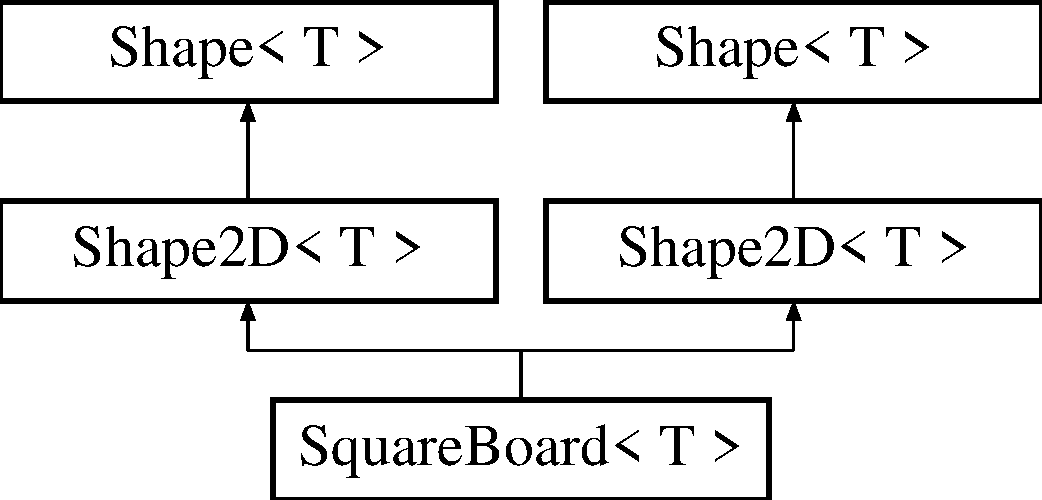
\includegraphics[height=3.000000cm]{classSquareBoard}
\end{center}
\end{figure}
\subsection*{Public Member Functions}
\begin{DoxyCompactItemize}
\item 
\mbox{\hyperlink{classSquareBoard_aa7aac1a02a00ce9ad0c9441fffa71e02}{Square\+Board}} (unsigned=50)
\begin{DoxyCompactList}\small\item\em Basic constructor for class \mbox{\hyperlink{classSquareBoard}{Square\+Board}}. \end{DoxyCompactList}\item 
\mbox{\hyperlink{classSquareBoard_a23c495a2419aded87c0b2803de409b5e}{Square\+Board}} (\mbox{\hyperlink{classSquareBoard}{Square\+Board}} \&\&)=default
\item 
\mbox{\hyperlink{classSquareBoard}{Square\+Board}} \& \mbox{\hyperlink{classSquareBoard_a354794a6de9edec8c771ca49dd315acf}{operator=}} (\mbox{\hyperlink{classSquareBoard}{Square\+Board}} \&\&)=default
\item 
\mbox{\hyperlink{classSquareBoard_a9a6c27e98ae10d6cb601140ef6a3ff59}{Square\+Board}} (const \mbox{\hyperlink{classSquareBoard}{Square\+Board}} \&)=default
\item 
\mbox{\hyperlink{classSquareBoard}{Square\+Board}} \& \mbox{\hyperlink{classSquareBoard_a15fd0ca02b5be393b75228123be1d2c8}{operator=}} (const \mbox{\hyperlink{classSquareBoard}{Square\+Board}} \&)=default
\item 
T \mbox{\hyperlink{classSquareBoard_a8b2ae6ea7295b2bff171b3d6311a456c}{perimeter}} ()
\item 
\mbox{\hyperlink{classSquareBoard_aa7aac1a02a00ce9ad0c9441fffa71e02}{Square\+Board}} (unsigned=50)
\item 
\mbox{\hyperlink{classSquareBoard_a23c495a2419aded87c0b2803de409b5e}{Square\+Board}} (\mbox{\hyperlink{classSquareBoard}{Square\+Board}} \&\&)=default
\item 
\mbox{\hyperlink{classSquareBoard}{Square\+Board}} \& \mbox{\hyperlink{classSquareBoard_a354794a6de9edec8c771ca49dd315acf}{operator=}} (\mbox{\hyperlink{classSquareBoard}{Square\+Board}} \&\&)=default
\item 
\mbox{\hyperlink{classSquareBoard_a9a6c27e98ae10d6cb601140ef6a3ff59}{Square\+Board}} (const \mbox{\hyperlink{classSquareBoard}{Square\+Board}} \&)=default
\item 
\mbox{\hyperlink{classSquareBoard}{Square\+Board}} \& \mbox{\hyperlink{classSquareBoard_a15fd0ca02b5be393b75228123be1d2c8}{operator=}} (const \mbox{\hyperlink{classSquareBoard}{Square\+Board}} \&)=default
\item 
T \mbox{\hyperlink{classSquareBoard_a8b2ae6ea7295b2bff171b3d6311a456c}{perimeter}} ()
\end{DoxyCompactItemize}
\subsection*{Private Member Functions}
\begin{DoxyCompactItemize}
\item 
\mbox{\hyperlink{glad_8h_a950fc91edb4504f62f1c577bf4727c29}{void}} \mbox{\hyperlink{classSquareBoard_a401c48fa5977d166b75e94bb7ddf1db7}{generate\+\_\+vertexes}} ()
\item 
\mbox{\hyperlink{glad_8h_a950fc91edb4504f62f1c577bf4727c29}{void}} \mbox{\hyperlink{classSquareBoard_a5d12432cc063275a6ffec42a7971abbc}{generate\+\_\+filling\+\_\+ebo}} ()
\item 
\mbox{\hyperlink{glad_8h_a950fc91edb4504f62f1c577bf4727c29}{void}} \mbox{\hyperlink{classSquareBoard_a401c48fa5977d166b75e94bb7ddf1db7}{generate\+\_\+vertexes}} ()
\item 
\mbox{\hyperlink{glad_8h_a950fc91edb4504f62f1c577bf4727c29}{void}} \mbox{\hyperlink{classSquareBoard_a5d12432cc063275a6ffec42a7971abbc}{generate\+\_\+filling\+\_\+ebo}} ()
\item 
{\footnotesize template$<$$>$ }\\\mbox{\hyperlink{glad_8h_a950fc91edb4504f62f1c577bf4727c29}{void}} \mbox{\hyperlink{classSquareBoard_a7928f781c7709b3fdfe42b5ce5bfc3f9}{generate\+\_\+vertexes}} ()
\item 
{\footnotesize template$<$$>$ }\\\mbox{\hyperlink{glad_8h_a950fc91edb4504f62f1c577bf4727c29}{void}} \mbox{\hyperlink{classSquareBoard_a7928f781c7709b3fdfe42b5ce5bfc3f9}{generate\+\_\+vertexes}} ()
\end{DoxyCompactItemize}
\subsection*{Private Attributes}
\begin{DoxyCompactItemize}
\item 
unsigned \mbox{\hyperlink{classSquareBoard_a92007159761cd4dfe85aaaa11103ea84}{size}}
\end{DoxyCompactItemize}
\subsection*{Additional Inherited Members}


\subsection{Detailed Description}
\subsubsection*{template$<$typename T = float$>$\newline
class Square\+Board$<$ T $>$}

\mbox{\hyperlink{classThis}{This}} class holds vertexes and other data for a circle in xy plane. 

\begin{DoxyRefDesc}{Todo}
\item[\mbox{\hyperlink{todo__todo000002}{Todo}}]Finish float version of perimeter function and implement double version. \end{DoxyRefDesc}


\subsection{Constructor \& Destructor Documentation}
\mbox{\Hypertarget{classSquareBoard_aa7aac1a02a00ce9ad0c9441fffa71e02}\label{classSquareBoard_aa7aac1a02a00ce9ad0c9441fffa71e02}} 
\index{Square\+Board@{Square\+Board}!Square\+Board@{Square\+Board}}
\index{Square\+Board@{Square\+Board}!Square\+Board@{Square\+Board}}
\subsubsection{\texorpdfstring{Square\+Board()}{SquareBoard()}\hspace{0.1cm}{\footnotesize\ttfamily [1/6]}}
{\footnotesize\ttfamily template$<$typename T $>$ \\
\mbox{\hyperlink{classSquareBoard}{Square\+Board}}$<$ T $>$\+::\mbox{\hyperlink{classSquareBoard}{Square\+Board}} (\begin{DoxyParamCaption}\item[{unsigned}]{size\+\_\+ = {\ttfamily 50} }\end{DoxyParamCaption})}



Basic constructor for class \mbox{\hyperlink{classSquareBoard}{Square\+Board}}. 

Constructor generates vertexes and initializes opengl buffers. \mbox{\Hypertarget{classSquareBoard_a23c495a2419aded87c0b2803de409b5e}\label{classSquareBoard_a23c495a2419aded87c0b2803de409b5e}} 
\index{Square\+Board@{Square\+Board}!Square\+Board@{Square\+Board}}
\index{Square\+Board@{Square\+Board}!Square\+Board@{Square\+Board}}
\subsubsection{\texorpdfstring{Square\+Board()}{SquareBoard()}\hspace{0.1cm}{\footnotesize\ttfamily [2/6]}}
{\footnotesize\ttfamily template$<$typename T  = float$>$ \\
\mbox{\hyperlink{classSquareBoard}{Square\+Board}}$<$ T $>$\+::\mbox{\hyperlink{classSquareBoard}{Square\+Board}} (\begin{DoxyParamCaption}\item[{\mbox{\hyperlink{classSquareBoard}{Square\+Board}}$<$ T $>$ \&\&}]{ }\end{DoxyParamCaption})\hspace{0.3cm}{\ttfamily [default]}}

\mbox{\Hypertarget{classSquareBoard_a9a6c27e98ae10d6cb601140ef6a3ff59}\label{classSquareBoard_a9a6c27e98ae10d6cb601140ef6a3ff59}} 
\index{Square\+Board@{Square\+Board}!Square\+Board@{Square\+Board}}
\index{Square\+Board@{Square\+Board}!Square\+Board@{Square\+Board}}
\subsubsection{\texorpdfstring{Square\+Board()}{SquareBoard()}\hspace{0.1cm}{\footnotesize\ttfamily [3/6]}}
{\footnotesize\ttfamily template$<$typename T  = float$>$ \\
\mbox{\hyperlink{classSquareBoard}{Square\+Board}}$<$ T $>$\+::\mbox{\hyperlink{classSquareBoard}{Square\+Board}} (\begin{DoxyParamCaption}\item[{const \mbox{\hyperlink{classSquareBoard}{Square\+Board}}$<$ T $>$ \&}]{ }\end{DoxyParamCaption})\hspace{0.3cm}{\ttfamily [default]}}

\mbox{\Hypertarget{classSquareBoard_aa7aac1a02a00ce9ad0c9441fffa71e02}\label{classSquareBoard_aa7aac1a02a00ce9ad0c9441fffa71e02}} 
\index{Square\+Board@{Square\+Board}!Square\+Board@{Square\+Board}}
\index{Square\+Board@{Square\+Board}!Square\+Board@{Square\+Board}}
\subsubsection{\texorpdfstring{Square\+Board()}{SquareBoard()}\hspace{0.1cm}{\footnotesize\ttfamily [4/6]}}
{\footnotesize\ttfamily template$<$typename T  = float$>$ \\
\mbox{\hyperlink{classSquareBoard}{Square\+Board}}$<$ T $>$\+::\mbox{\hyperlink{classSquareBoard}{Square\+Board}} (\begin{DoxyParamCaption}\item[{unsigned}]{ = {\ttfamily 50} }\end{DoxyParamCaption})}

\mbox{\Hypertarget{classSquareBoard_a23c495a2419aded87c0b2803de409b5e}\label{classSquareBoard_a23c495a2419aded87c0b2803de409b5e}} 
\index{Square\+Board@{Square\+Board}!Square\+Board@{Square\+Board}}
\index{Square\+Board@{Square\+Board}!Square\+Board@{Square\+Board}}
\subsubsection{\texorpdfstring{Square\+Board()}{SquareBoard()}\hspace{0.1cm}{\footnotesize\ttfamily [5/6]}}
{\footnotesize\ttfamily template$<$typename T  = float$>$ \\
\mbox{\hyperlink{classSquareBoard}{Square\+Board}}$<$ T $>$\+::\mbox{\hyperlink{classSquareBoard}{Square\+Board}} (\begin{DoxyParamCaption}\item[{\mbox{\hyperlink{classSquareBoard}{Square\+Board}}$<$ T $>$ \&\&}]{ }\end{DoxyParamCaption})\hspace{0.3cm}{\ttfamily [default]}}

\mbox{\Hypertarget{classSquareBoard_a9a6c27e98ae10d6cb601140ef6a3ff59}\label{classSquareBoard_a9a6c27e98ae10d6cb601140ef6a3ff59}} 
\index{Square\+Board@{Square\+Board}!Square\+Board@{Square\+Board}}
\index{Square\+Board@{Square\+Board}!Square\+Board@{Square\+Board}}
\subsubsection{\texorpdfstring{Square\+Board()}{SquareBoard()}\hspace{0.1cm}{\footnotesize\ttfamily [6/6]}}
{\footnotesize\ttfamily template$<$typename T  = float$>$ \\
\mbox{\hyperlink{classSquareBoard}{Square\+Board}}$<$ T $>$\+::\mbox{\hyperlink{classSquareBoard}{Square\+Board}} (\begin{DoxyParamCaption}\item[{const \mbox{\hyperlink{classSquareBoard}{Square\+Board}}$<$ T $>$ \&}]{ }\end{DoxyParamCaption})\hspace{0.3cm}{\ttfamily [default]}}



\subsection{Member Function Documentation}
\mbox{\Hypertarget{classSquareBoard_a5d12432cc063275a6ffec42a7971abbc}\label{classSquareBoard_a5d12432cc063275a6ffec42a7971abbc}} 
\index{Square\+Board@{Square\+Board}!generate\+\_\+filling\+\_\+ebo@{generate\+\_\+filling\+\_\+ebo}}
\index{generate\+\_\+filling\+\_\+ebo@{generate\+\_\+filling\+\_\+ebo}!Square\+Board@{Square\+Board}}
\subsubsection{\texorpdfstring{generate\+\_\+filling\+\_\+ebo()}{generate\_filling\_ebo()}\hspace{0.1cm}{\footnotesize\ttfamily [1/2]}}
{\footnotesize\ttfamily template$<$typename T $>$ \\
\mbox{\hyperlink{glad_8h_a950fc91edb4504f62f1c577bf4727c29}{void}} \mbox{\hyperlink{classSquareBoard}{Square\+Board}}$<$ T $>$\+::generate\+\_\+filling\+\_\+ebo (\begin{DoxyParamCaption}{ }\end{DoxyParamCaption})\hspace{0.3cm}{\ttfamily [inline]}, {\ttfamily [private]}}

\mbox{\Hypertarget{classSquareBoard_a5d12432cc063275a6ffec42a7971abbc}\label{classSquareBoard_a5d12432cc063275a6ffec42a7971abbc}} 
\index{Square\+Board@{Square\+Board}!generate\+\_\+filling\+\_\+ebo@{generate\+\_\+filling\+\_\+ebo}}
\index{generate\+\_\+filling\+\_\+ebo@{generate\+\_\+filling\+\_\+ebo}!Square\+Board@{Square\+Board}}
\subsubsection{\texorpdfstring{generate\+\_\+filling\+\_\+ebo()}{generate\_filling\_ebo()}\hspace{0.1cm}{\footnotesize\ttfamily [2/2]}}
{\footnotesize\ttfamily template$<$typename T  = float$>$ \\
\mbox{\hyperlink{glad_8h_a950fc91edb4504f62f1c577bf4727c29}{void}} \mbox{\hyperlink{classSquareBoard}{Square\+Board}}$<$ T $>$\+::generate\+\_\+filling\+\_\+ebo (\begin{DoxyParamCaption}{ }\end{DoxyParamCaption})\hspace{0.3cm}{\ttfamily [private]}}

\mbox{\Hypertarget{classSquareBoard_a401c48fa5977d166b75e94bb7ddf1db7}\label{classSquareBoard_a401c48fa5977d166b75e94bb7ddf1db7}} 
\index{Square\+Board@{Square\+Board}!generate\+\_\+vertexes@{generate\+\_\+vertexes}}
\index{generate\+\_\+vertexes@{generate\+\_\+vertexes}!Square\+Board@{Square\+Board}}
\subsubsection{\texorpdfstring{generate\+\_\+vertexes()}{generate\_vertexes()}\hspace{0.1cm}{\footnotesize\ttfamily [1/4]}}
{\footnotesize\ttfamily template$<$typename T  = float$>$ \\
\mbox{\hyperlink{glad_8h_a950fc91edb4504f62f1c577bf4727c29}{void}} \mbox{\hyperlink{classSquareBoard}{Square\+Board}}$<$ T $>$\+::generate\+\_\+vertexes (\begin{DoxyParamCaption}{ }\end{DoxyParamCaption})\hspace{0.3cm}{\ttfamily [private]}}

\mbox{\Hypertarget{classSquareBoard_a401c48fa5977d166b75e94bb7ddf1db7}\label{classSquareBoard_a401c48fa5977d166b75e94bb7ddf1db7}} 
\index{Square\+Board@{Square\+Board}!generate\+\_\+vertexes@{generate\+\_\+vertexes}}
\index{generate\+\_\+vertexes@{generate\+\_\+vertexes}!Square\+Board@{Square\+Board}}
\subsubsection{\texorpdfstring{generate\+\_\+vertexes()}{generate\_vertexes()}\hspace{0.1cm}{\footnotesize\ttfamily [2/4]}}
{\footnotesize\ttfamily template$<$typename T  = float$>$ \\
\mbox{\hyperlink{glad_8h_a950fc91edb4504f62f1c577bf4727c29}{void}} \mbox{\hyperlink{classSquareBoard}{Square\+Board}}$<$ T $>$\+::generate\+\_\+vertexes (\begin{DoxyParamCaption}{ }\end{DoxyParamCaption})\hspace{0.3cm}{\ttfamily [private]}}

\mbox{\Hypertarget{classSquareBoard_a7928f781c7709b3fdfe42b5ce5bfc3f9}\label{classSquareBoard_a7928f781c7709b3fdfe42b5ce5bfc3f9}} 
\index{Square\+Board@{Square\+Board}!generate\+\_\+vertexes@{generate\+\_\+vertexes}}
\index{generate\+\_\+vertexes@{generate\+\_\+vertexes}!Square\+Board@{Square\+Board}}
\subsubsection{\texorpdfstring{generate\+\_\+vertexes()}{generate\_vertexes()}\hspace{0.1cm}{\footnotesize\ttfamily [3/4]}}
{\footnotesize\ttfamily template$<$$>$ \\
\mbox{\hyperlink{glad_8h_a950fc91edb4504f62f1c577bf4727c29}{void}} \mbox{\hyperlink{classSquareBoard}{Square\+Board}}$<$ float $>$\+::generate\+\_\+vertexes (\begin{DoxyParamCaption}{ }\end{DoxyParamCaption})\hspace{0.3cm}{\ttfamily [inline]}, {\ttfamily [private]}}

\mbox{\Hypertarget{classSquareBoard_a7928f781c7709b3fdfe42b5ce5bfc3f9}\label{classSquareBoard_a7928f781c7709b3fdfe42b5ce5bfc3f9}} 
\index{Square\+Board@{Square\+Board}!generate\+\_\+vertexes@{generate\+\_\+vertexes}}
\index{generate\+\_\+vertexes@{generate\+\_\+vertexes}!Square\+Board@{Square\+Board}}
\subsubsection{\texorpdfstring{generate\+\_\+vertexes()}{generate\_vertexes()}\hspace{0.1cm}{\footnotesize\ttfamily [4/4]}}
{\footnotesize\ttfamily template$<$$>$ \\
\mbox{\hyperlink{glad_8h_a950fc91edb4504f62f1c577bf4727c29}{void}} \mbox{\hyperlink{classSquareBoard}{Square\+Board}}$<$ float $>$\+::generate\+\_\+vertexes (\begin{DoxyParamCaption}{ }\end{DoxyParamCaption})\hspace{0.3cm}{\ttfamily [inline]}, {\ttfamily [private]}}

\mbox{\Hypertarget{classSquareBoard_a354794a6de9edec8c771ca49dd315acf}\label{classSquareBoard_a354794a6de9edec8c771ca49dd315acf}} 
\index{Square\+Board@{Square\+Board}!operator=@{operator=}}
\index{operator=@{operator=}!Square\+Board@{Square\+Board}}
\subsubsection{\texorpdfstring{operator=()}{operator=()}\hspace{0.1cm}{\footnotesize\ttfamily [1/4]}}
{\footnotesize\ttfamily template$<$typename T  = float$>$ \\
\mbox{\hyperlink{classSquareBoard}{Square\+Board}}\& \mbox{\hyperlink{classSquareBoard}{Square\+Board}}$<$ T $>$\+::operator= (\begin{DoxyParamCaption}\item[{\mbox{\hyperlink{classSquareBoard}{Square\+Board}}$<$ T $>$ \&\&}]{ }\end{DoxyParamCaption})\hspace{0.3cm}{\ttfamily [default]}}

\mbox{\Hypertarget{classSquareBoard_a354794a6de9edec8c771ca49dd315acf}\label{classSquareBoard_a354794a6de9edec8c771ca49dd315acf}} 
\index{Square\+Board@{Square\+Board}!operator=@{operator=}}
\index{operator=@{operator=}!Square\+Board@{Square\+Board}}
\subsubsection{\texorpdfstring{operator=()}{operator=()}\hspace{0.1cm}{\footnotesize\ttfamily [2/4]}}
{\footnotesize\ttfamily template$<$typename T  = float$>$ \\
\mbox{\hyperlink{classSquareBoard}{Square\+Board}}\& \mbox{\hyperlink{classSquareBoard}{Square\+Board}}$<$ T $>$\+::operator= (\begin{DoxyParamCaption}\item[{\mbox{\hyperlink{classSquareBoard}{Square\+Board}}$<$ T $>$ \&\&}]{ }\end{DoxyParamCaption})\hspace{0.3cm}{\ttfamily [default]}}

\mbox{\Hypertarget{classSquareBoard_a15fd0ca02b5be393b75228123be1d2c8}\label{classSquareBoard_a15fd0ca02b5be393b75228123be1d2c8}} 
\index{Square\+Board@{Square\+Board}!operator=@{operator=}}
\index{operator=@{operator=}!Square\+Board@{Square\+Board}}
\subsubsection{\texorpdfstring{operator=()}{operator=()}\hspace{0.1cm}{\footnotesize\ttfamily [3/4]}}
{\footnotesize\ttfamily template$<$typename T  = float$>$ \\
\mbox{\hyperlink{classSquareBoard}{Square\+Board}}\& \mbox{\hyperlink{classSquareBoard}{Square\+Board}}$<$ T $>$\+::operator= (\begin{DoxyParamCaption}\item[{const \mbox{\hyperlink{classSquareBoard}{Square\+Board}}$<$ T $>$ \&}]{ }\end{DoxyParamCaption})\hspace{0.3cm}{\ttfamily [default]}}

\mbox{\Hypertarget{classSquareBoard_a15fd0ca02b5be393b75228123be1d2c8}\label{classSquareBoard_a15fd0ca02b5be393b75228123be1d2c8}} 
\index{Square\+Board@{Square\+Board}!operator=@{operator=}}
\index{operator=@{operator=}!Square\+Board@{Square\+Board}}
\subsubsection{\texorpdfstring{operator=()}{operator=()}\hspace{0.1cm}{\footnotesize\ttfamily [4/4]}}
{\footnotesize\ttfamily template$<$typename T  = float$>$ \\
\mbox{\hyperlink{classSquareBoard}{Square\+Board}}\& \mbox{\hyperlink{classSquareBoard}{Square\+Board}}$<$ T $>$\+::operator= (\begin{DoxyParamCaption}\item[{const \mbox{\hyperlink{classSquareBoard}{Square\+Board}}$<$ T $>$ \&}]{ }\end{DoxyParamCaption})\hspace{0.3cm}{\ttfamily [default]}}

\mbox{\Hypertarget{classSquareBoard_a8b2ae6ea7295b2bff171b3d6311a456c}\label{classSquareBoard_a8b2ae6ea7295b2bff171b3d6311a456c}} 
\index{Square\+Board@{Square\+Board}!perimeter@{perimeter}}
\index{perimeter@{perimeter}!Square\+Board@{Square\+Board}}
\subsubsection{\texorpdfstring{perimeter()}{perimeter()}\hspace{0.1cm}{\footnotesize\ttfamily [1/2]}}
{\footnotesize\ttfamily template$<$typename T  = float$>$ \\
T \mbox{\hyperlink{classSquareBoard}{Square\+Board}}$<$ T $>$\+::perimeter (\begin{DoxyParamCaption}{ }\end{DoxyParamCaption})}

\mbox{\Hypertarget{classSquareBoard_a8b2ae6ea7295b2bff171b3d6311a456c}\label{classSquareBoard_a8b2ae6ea7295b2bff171b3d6311a456c}} 
\index{Square\+Board@{Square\+Board}!perimeter@{perimeter}}
\index{perimeter@{perimeter}!Square\+Board@{Square\+Board}}
\subsubsection{\texorpdfstring{perimeter()}{perimeter()}\hspace{0.1cm}{\footnotesize\ttfamily [2/2]}}
{\footnotesize\ttfamily template$<$typename T  = float$>$ \\
T \mbox{\hyperlink{classSquareBoard}{Square\+Board}}$<$ T $>$\+::perimeter (\begin{DoxyParamCaption}{ }\end{DoxyParamCaption})}



\subsection{Member Data Documentation}
\mbox{\Hypertarget{classSquareBoard_a92007159761cd4dfe85aaaa11103ea84}\label{classSquareBoard_a92007159761cd4dfe85aaaa11103ea84}} 
\index{Square\+Board@{Square\+Board}!size@{size}}
\index{size@{size}!Square\+Board@{Square\+Board}}
\subsubsection{\texorpdfstring{size}{size}}
{\footnotesize\ttfamily template$<$typename T  = float$>$ \\
unsigned \mbox{\hyperlink{classSquareBoard}{Square\+Board}}$<$ T $>$\+::\mbox{\hyperlink{glad_8h_adead0e00f1033fff2918e18853add2b1}{size}}\hspace{0.3cm}{\ttfamily [private]}}

number of squares in the array 

The documentation for this class was generated from the following files\+:\begin{DoxyCompactItemize}
\item 
src/shapes/\mbox{\hyperlink{square__board_8hpp}{square\+\_\+board.\+hpp}}\item 
src/shapes/\mbox{\hyperlink{square__board__old_8hpp}{square\+\_\+board\+\_\+old.\+hpp}}\end{DoxyCompactItemize}

\hypertarget{classStar}{}\section{Star$<$ T $>$ Class Template Reference}
\label{classStar}\index{Star$<$ T $>$@{Star$<$ T $>$}}


{\ttfamily \#include \char`\"{}star.\+hpp\char`\"{}}

Inheritance diagram for Star$<$ T $>$\+:\begin{figure}[H]
\begin{center}
\leavevmode
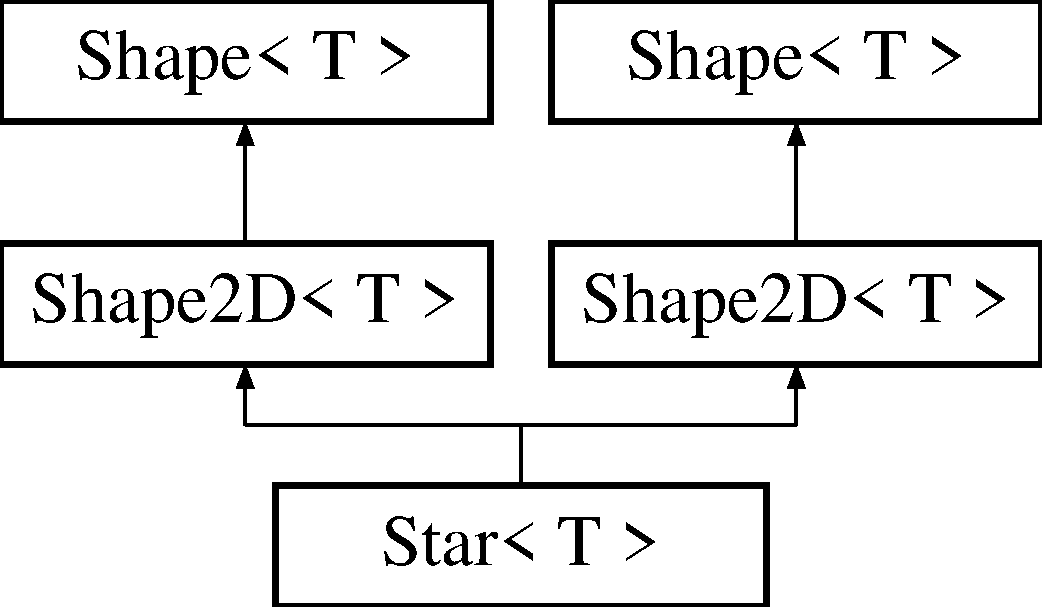
\includegraphics[height=3.000000cm]{classStar}
\end{center}
\end{figure}
\subsection*{Public Member Functions}
\begin{DoxyCompactItemize}
\item 
\mbox{\hyperlink{classStar_a4be07c82320f781071409294614df4ae}{Star}} ()
\item 
\mbox{\hyperlink{classStar_aa179936ed93e38e70992cb4f6e3cbff3}{Star}} (int, T=0.\+5)
\item 
\mbox{\hyperlink{classStar_af518471484341cad6b47ad42d4e637fe}{Star}} (\mbox{\hyperlink{classStar}{Star}} \&\&)=default
\item 
\mbox{\hyperlink{classStar}{Star}} \& \mbox{\hyperlink{classStar_a7113d2808314f0aa2f5a87325f8c535d}{operator=}} (\mbox{\hyperlink{classStar}{Star}} \&\&)=default
\item 
\mbox{\hyperlink{classStar_a047ce2a8d4fb409858555aee98b33c93}{Star}} (const \mbox{\hyperlink{classStar}{Star}} \&)=default
\item 
\mbox{\hyperlink{classStar}{Star}} \& \mbox{\hyperlink{classStar_a3507f157448e082ccfcadc4783f2610e}{operator=}} (const \mbox{\hyperlink{classStar}{Star}} \&)=default
\item 
T \mbox{\hyperlink{classStar_a908253192d0b1fe95aeeaa81322545bf}{perimeter}} ()
\item 
\mbox{\hyperlink{classStar_a4be07c82320f781071409294614df4ae}{Star}} ()
\item 
\mbox{\hyperlink{classStar_aa179936ed93e38e70992cb4f6e3cbff3}{Star}} (int, T=0.\+5)
\item 
\mbox{\hyperlink{classStar_af518471484341cad6b47ad42d4e637fe}{Star}} (\mbox{\hyperlink{classStar}{Star}} \&\&)=default
\item 
\mbox{\hyperlink{classStar}{Star}} \& \mbox{\hyperlink{classStar_a7113d2808314f0aa2f5a87325f8c535d}{operator=}} (\mbox{\hyperlink{classStar}{Star}} \&\&)=default
\item 
\mbox{\hyperlink{classStar_a047ce2a8d4fb409858555aee98b33c93}{Star}} (const \mbox{\hyperlink{classStar}{Star}} \&)=default
\item 
\mbox{\hyperlink{classStar}{Star}} \& \mbox{\hyperlink{classStar_a3507f157448e082ccfcadc4783f2610e}{operator=}} (const \mbox{\hyperlink{classStar}{Star}} \&)=default
\item 
T \mbox{\hyperlink{classStar_a908253192d0b1fe95aeeaa81322545bf}{perimeter}} ()
\end{DoxyCompactItemize}
\subsection*{Public Attributes}
\begin{DoxyCompactItemize}
\item 
T \mbox{\hyperlink{classStar_a349e0820769da7e4f76aea0ad6002bf8}{ratio}}
\end{DoxyCompactItemize}
\subsection*{Private Member Functions}
\begin{DoxyCompactItemize}
\item 
void \mbox{\hyperlink{classStar_ac9ce42a8f7289484594f7f0ab5124849}{generate\+\_\+vertexes}} (int=10, T=0.\+5)
\item 
void \mbox{\hyperlink{classStar_ac9ce42a8f7289484594f7f0ab5124849}{generate\+\_\+vertexes}} (int=10, T=0.\+5)
\item 
{\footnotesize template$<$$>$ }\\void \mbox{\hyperlink{classStar_ab46cbc7aca971bc1c07b8d4afe8fba37}{generate\+\_\+vertexes}} (int bulges, float \mbox{\hyperlink{classStar_a349e0820769da7e4f76aea0ad6002bf8}{ratio}})
\item 
{\footnotesize template$<$$>$ }\\void \mbox{\hyperlink{classStar_a85d8438cea72701a136b76f046ee95dd}{generate\+\_\+vertexes}} (int bulges, double \mbox{\hyperlink{classStar_a349e0820769da7e4f76aea0ad6002bf8}{ratio}})
\item 
{\footnotesize template$<$$>$ }\\void \mbox{\hyperlink{classStar_ab46cbc7aca971bc1c07b8d4afe8fba37}{generate\+\_\+vertexes}} (int bulges, float \mbox{\hyperlink{classStar_a349e0820769da7e4f76aea0ad6002bf8}{ratio}})
\item 
{\footnotesize template$<$$>$ }\\void \mbox{\hyperlink{classStar_a85d8438cea72701a136b76f046ee95dd}{generate\+\_\+vertexes}} (int bulges, double \mbox{\hyperlink{classStar_a349e0820769da7e4f76aea0ad6002bf8}{ratio}})
\end{DoxyCompactItemize}
\subsection*{Additional Inherited Members}


\subsection{Constructor \& Destructor Documentation}
\mbox{\Hypertarget{classStar_a4be07c82320f781071409294614df4ae}\label{classStar_a4be07c82320f781071409294614df4ae}} 
\index{Star@{Star}!Star@{Star}}
\index{Star@{Star}!Star@{Star}}
\subsubsection{\texorpdfstring{Star()}{Star()}\hspace{0.1cm}{\footnotesize\ttfamily [1/8]}}
{\footnotesize\ttfamily template$<$typename T $>$ \\
\mbox{\hyperlink{classStar}{Star}}$<$ T $>$\+::\mbox{\hyperlink{classStar}{Star}} (\begin{DoxyParamCaption}{ }\end{DoxyParamCaption})}

\mbox{\Hypertarget{classStar_aa179936ed93e38e70992cb4f6e3cbff3}\label{classStar_aa179936ed93e38e70992cb4f6e3cbff3}} 
\index{Star@{Star}!Star@{Star}}
\index{Star@{Star}!Star@{Star}}
\subsubsection{\texorpdfstring{Star()}{Star()}\hspace{0.1cm}{\footnotesize\ttfamily [2/8]}}
{\footnotesize\ttfamily template$<$typename T $>$ \\
\mbox{\hyperlink{classStar}{Star}}$<$ T $>$\+::\mbox{\hyperlink{classStar}{Star}} (\begin{DoxyParamCaption}\item[{int}]{bulges,  }\item[{T}]{ratio = {\ttfamily 0.5} }\end{DoxyParamCaption})}

\mbox{\Hypertarget{classStar_af518471484341cad6b47ad42d4e637fe}\label{classStar_af518471484341cad6b47ad42d4e637fe}} 
\index{Star@{Star}!Star@{Star}}
\index{Star@{Star}!Star@{Star}}
\subsubsection{\texorpdfstring{Star()}{Star()}\hspace{0.1cm}{\footnotesize\ttfamily [3/8]}}
{\footnotesize\ttfamily template$<$typename T  = float$>$ \\
\mbox{\hyperlink{classStar}{Star}}$<$ T $>$\+::\mbox{\hyperlink{classStar}{Star}} (\begin{DoxyParamCaption}\item[{\mbox{\hyperlink{classStar}{Star}}$<$ T $>$ \&\&}]{ }\end{DoxyParamCaption})\hspace{0.3cm}{\ttfamily [default]}}

\mbox{\Hypertarget{classStar_a047ce2a8d4fb409858555aee98b33c93}\label{classStar_a047ce2a8d4fb409858555aee98b33c93}} 
\index{Star@{Star}!Star@{Star}}
\index{Star@{Star}!Star@{Star}}
\subsubsection{\texorpdfstring{Star()}{Star()}\hspace{0.1cm}{\footnotesize\ttfamily [4/8]}}
{\footnotesize\ttfamily template$<$typename T  = float$>$ \\
\mbox{\hyperlink{classStar}{Star}}$<$ T $>$\+::\mbox{\hyperlink{classStar}{Star}} (\begin{DoxyParamCaption}\item[{const \mbox{\hyperlink{classStar}{Star}}$<$ T $>$ \&}]{ }\end{DoxyParamCaption})\hspace{0.3cm}{\ttfamily [default]}}

\mbox{\Hypertarget{classStar_a4be07c82320f781071409294614df4ae}\label{classStar_a4be07c82320f781071409294614df4ae}} 
\index{Star@{Star}!Star@{Star}}
\index{Star@{Star}!Star@{Star}}
\subsubsection{\texorpdfstring{Star()}{Star()}\hspace{0.1cm}{\footnotesize\ttfamily [5/8]}}
{\footnotesize\ttfamily template$<$typename T  = float$>$ \\
\mbox{\hyperlink{classStar}{Star}}$<$ T $>$\+::\mbox{\hyperlink{classStar}{Star}} (\begin{DoxyParamCaption}{ }\end{DoxyParamCaption})}

\mbox{\Hypertarget{classStar_aa179936ed93e38e70992cb4f6e3cbff3}\label{classStar_aa179936ed93e38e70992cb4f6e3cbff3}} 
\index{Star@{Star}!Star@{Star}}
\index{Star@{Star}!Star@{Star}}
\subsubsection{\texorpdfstring{Star()}{Star()}\hspace{0.1cm}{\footnotesize\ttfamily [6/8]}}
{\footnotesize\ttfamily template$<$typename T  = float$>$ \\
\mbox{\hyperlink{classStar}{Star}}$<$ T $>$\+::\mbox{\hyperlink{classStar}{Star}} (\begin{DoxyParamCaption}\item[{int}]{,  }\item[{T}]{ = {\ttfamily 0.5} }\end{DoxyParamCaption})}

\mbox{\Hypertarget{classStar_af518471484341cad6b47ad42d4e637fe}\label{classStar_af518471484341cad6b47ad42d4e637fe}} 
\index{Star@{Star}!Star@{Star}}
\index{Star@{Star}!Star@{Star}}
\subsubsection{\texorpdfstring{Star()}{Star()}\hspace{0.1cm}{\footnotesize\ttfamily [7/8]}}
{\footnotesize\ttfamily template$<$typename T  = float$>$ \\
\mbox{\hyperlink{classStar}{Star}}$<$ T $>$\+::\mbox{\hyperlink{classStar}{Star}} (\begin{DoxyParamCaption}\item[{\mbox{\hyperlink{classStar}{Star}}$<$ T $>$ \&\&}]{ }\end{DoxyParamCaption})\hspace{0.3cm}{\ttfamily [default]}}

\mbox{\Hypertarget{classStar_a047ce2a8d4fb409858555aee98b33c93}\label{classStar_a047ce2a8d4fb409858555aee98b33c93}} 
\index{Star@{Star}!Star@{Star}}
\index{Star@{Star}!Star@{Star}}
\subsubsection{\texorpdfstring{Star()}{Star()}\hspace{0.1cm}{\footnotesize\ttfamily [8/8]}}
{\footnotesize\ttfamily template$<$typename T  = float$>$ \\
\mbox{\hyperlink{classStar}{Star}}$<$ T $>$\+::\mbox{\hyperlink{classStar}{Star}} (\begin{DoxyParamCaption}\item[{const \mbox{\hyperlink{classStar}{Star}}$<$ T $>$ \&}]{ }\end{DoxyParamCaption})\hspace{0.3cm}{\ttfamily [default]}}



\subsection{Member Function Documentation}
\mbox{\Hypertarget{classStar_ac9ce42a8f7289484594f7f0ab5124849}\label{classStar_ac9ce42a8f7289484594f7f0ab5124849}} 
\index{Star@{Star}!generate\+\_\+vertexes@{generate\+\_\+vertexes}}
\index{generate\+\_\+vertexes@{generate\+\_\+vertexes}!Star@{Star}}
\subsubsection{\texorpdfstring{generate\+\_\+vertexes()}{generate\_vertexes()}\hspace{0.1cm}{\footnotesize\ttfamily [1/6]}}
{\footnotesize\ttfamily template$<$typename T  = float$>$ \\
void \mbox{\hyperlink{classStar}{Star}}$<$ T $>$\+::generate\+\_\+vertexes (\begin{DoxyParamCaption}\item[{int}]{ = {\ttfamily 10},  }\item[{T}]{ = {\ttfamily 0.5} }\end{DoxyParamCaption})\hspace{0.3cm}{\ttfamily [private]}}

\mbox{\Hypertarget{classStar_ac9ce42a8f7289484594f7f0ab5124849}\label{classStar_ac9ce42a8f7289484594f7f0ab5124849}} 
\index{Star@{Star}!generate\+\_\+vertexes@{generate\+\_\+vertexes}}
\index{generate\+\_\+vertexes@{generate\+\_\+vertexes}!Star@{Star}}
\subsubsection{\texorpdfstring{generate\+\_\+vertexes()}{generate\_vertexes()}\hspace{0.1cm}{\footnotesize\ttfamily [2/6]}}
{\footnotesize\ttfamily template$<$typename T  = float$>$ \\
void \mbox{\hyperlink{classStar}{Star}}$<$ T $>$\+::generate\+\_\+vertexes (\begin{DoxyParamCaption}\item[{int}]{ = {\ttfamily 10},  }\item[{T}]{ = {\ttfamily 0.5} }\end{DoxyParamCaption})\hspace{0.3cm}{\ttfamily [private]}}

\mbox{\Hypertarget{classStar_ab46cbc7aca971bc1c07b8d4afe8fba37}\label{classStar_ab46cbc7aca971bc1c07b8d4afe8fba37}} 
\index{Star@{Star}!generate\+\_\+vertexes@{generate\+\_\+vertexes}}
\index{generate\+\_\+vertexes@{generate\+\_\+vertexes}!Star@{Star}}
\subsubsection{\texorpdfstring{generate\+\_\+vertexes()}{generate\_vertexes()}\hspace{0.1cm}{\footnotesize\ttfamily [3/6]}}
{\footnotesize\ttfamily template$<$$>$ \\
void \mbox{\hyperlink{classStar}{Star}}$<$ float $>$\+::generate\+\_\+vertexes (\begin{DoxyParamCaption}\item[{int}]{bulges,  }\item[{float}]{ratio }\end{DoxyParamCaption})\hspace{0.3cm}{\ttfamily [inline]}, {\ttfamily [private]}}

\mbox{\Hypertarget{classStar_ab46cbc7aca971bc1c07b8d4afe8fba37}\label{classStar_ab46cbc7aca971bc1c07b8d4afe8fba37}} 
\index{Star@{Star}!generate\+\_\+vertexes@{generate\+\_\+vertexes}}
\index{generate\+\_\+vertexes@{generate\+\_\+vertexes}!Star@{Star}}
\subsubsection{\texorpdfstring{generate\+\_\+vertexes()}{generate\_vertexes()}\hspace{0.1cm}{\footnotesize\ttfamily [4/6]}}
{\footnotesize\ttfamily template$<$$>$ \\
void \mbox{\hyperlink{classStar}{Star}}$<$ float $>$\+::generate\+\_\+vertexes (\begin{DoxyParamCaption}\item[{int}]{bulges,  }\item[{float}]{ratio }\end{DoxyParamCaption})\hspace{0.3cm}{\ttfamily [inline]}, {\ttfamily [private]}}

\mbox{\Hypertarget{classStar_a85d8438cea72701a136b76f046ee95dd}\label{classStar_a85d8438cea72701a136b76f046ee95dd}} 
\index{Star@{Star}!generate\+\_\+vertexes@{generate\+\_\+vertexes}}
\index{generate\+\_\+vertexes@{generate\+\_\+vertexes}!Star@{Star}}
\subsubsection{\texorpdfstring{generate\+\_\+vertexes()}{generate\_vertexes()}\hspace{0.1cm}{\footnotesize\ttfamily [5/6]}}
{\footnotesize\ttfamily template$<$$>$ \\
void \mbox{\hyperlink{classStar}{Star}}$<$ double $>$\+::generate\+\_\+vertexes (\begin{DoxyParamCaption}\item[{int}]{bulges,  }\item[{double}]{ratio }\end{DoxyParamCaption})\hspace{0.3cm}{\ttfamily [inline]}, {\ttfamily [private]}}

\mbox{\Hypertarget{classStar_a85d8438cea72701a136b76f046ee95dd}\label{classStar_a85d8438cea72701a136b76f046ee95dd}} 
\index{Star@{Star}!generate\+\_\+vertexes@{generate\+\_\+vertexes}}
\index{generate\+\_\+vertexes@{generate\+\_\+vertexes}!Star@{Star}}
\subsubsection{\texorpdfstring{generate\+\_\+vertexes()}{generate\_vertexes()}\hspace{0.1cm}{\footnotesize\ttfamily [6/6]}}
{\footnotesize\ttfamily template$<$$>$ \\
void \mbox{\hyperlink{classStar}{Star}}$<$ double $>$\+::generate\+\_\+vertexes (\begin{DoxyParamCaption}\item[{int}]{bulges,  }\item[{double}]{ratio }\end{DoxyParamCaption})\hspace{0.3cm}{\ttfamily [inline]}, {\ttfamily [private]}}

\mbox{\Hypertarget{classStar_a7113d2808314f0aa2f5a87325f8c535d}\label{classStar_a7113d2808314f0aa2f5a87325f8c535d}} 
\index{Star@{Star}!operator=@{operator=}}
\index{operator=@{operator=}!Star@{Star}}
\subsubsection{\texorpdfstring{operator=()}{operator=()}\hspace{0.1cm}{\footnotesize\ttfamily [1/4]}}
{\footnotesize\ttfamily template$<$typename T  = float$>$ \\
\mbox{\hyperlink{classStar}{Star}}\& \mbox{\hyperlink{classStar}{Star}}$<$ T $>$\+::operator= (\begin{DoxyParamCaption}\item[{\mbox{\hyperlink{classStar}{Star}}$<$ T $>$ \&\&}]{ }\end{DoxyParamCaption})\hspace{0.3cm}{\ttfamily [default]}}

\mbox{\Hypertarget{classStar_a7113d2808314f0aa2f5a87325f8c535d}\label{classStar_a7113d2808314f0aa2f5a87325f8c535d}} 
\index{Star@{Star}!operator=@{operator=}}
\index{operator=@{operator=}!Star@{Star}}
\subsubsection{\texorpdfstring{operator=()}{operator=()}\hspace{0.1cm}{\footnotesize\ttfamily [2/4]}}
{\footnotesize\ttfamily template$<$typename T  = float$>$ \\
\mbox{\hyperlink{classStar}{Star}}\& \mbox{\hyperlink{classStar}{Star}}$<$ T $>$\+::operator= (\begin{DoxyParamCaption}\item[{\mbox{\hyperlink{classStar}{Star}}$<$ T $>$ \&\&}]{ }\end{DoxyParamCaption})\hspace{0.3cm}{\ttfamily [default]}}

\mbox{\Hypertarget{classStar_a3507f157448e082ccfcadc4783f2610e}\label{classStar_a3507f157448e082ccfcadc4783f2610e}} 
\index{Star@{Star}!operator=@{operator=}}
\index{operator=@{operator=}!Star@{Star}}
\subsubsection{\texorpdfstring{operator=()}{operator=()}\hspace{0.1cm}{\footnotesize\ttfamily [3/4]}}
{\footnotesize\ttfamily template$<$typename T  = float$>$ \\
\mbox{\hyperlink{classStar}{Star}}\& \mbox{\hyperlink{classStar}{Star}}$<$ T $>$\+::operator= (\begin{DoxyParamCaption}\item[{const \mbox{\hyperlink{classStar}{Star}}$<$ T $>$ \&}]{ }\end{DoxyParamCaption})\hspace{0.3cm}{\ttfamily [default]}}

\mbox{\Hypertarget{classStar_a3507f157448e082ccfcadc4783f2610e}\label{classStar_a3507f157448e082ccfcadc4783f2610e}} 
\index{Star@{Star}!operator=@{operator=}}
\index{operator=@{operator=}!Star@{Star}}
\subsubsection{\texorpdfstring{operator=()}{operator=()}\hspace{0.1cm}{\footnotesize\ttfamily [4/4]}}
{\footnotesize\ttfamily template$<$typename T  = float$>$ \\
\mbox{\hyperlink{classStar}{Star}}\& \mbox{\hyperlink{classStar}{Star}}$<$ T $>$\+::operator= (\begin{DoxyParamCaption}\item[{const \mbox{\hyperlink{classStar}{Star}}$<$ T $>$ \&}]{ }\end{DoxyParamCaption})\hspace{0.3cm}{\ttfamily [default]}}

\mbox{\Hypertarget{classStar_a908253192d0b1fe95aeeaa81322545bf}\label{classStar_a908253192d0b1fe95aeeaa81322545bf}} 
\index{Star@{Star}!perimeter@{perimeter}}
\index{perimeter@{perimeter}!Star@{Star}}
\subsubsection{\texorpdfstring{perimeter()}{perimeter()}\hspace{0.1cm}{\footnotesize\ttfamily [1/2]}}
{\footnotesize\ttfamily template$<$typename T  = float$>$ \\
T \mbox{\hyperlink{classStar}{Star}}$<$ T $>$\+::perimeter (\begin{DoxyParamCaption}{ }\end{DoxyParamCaption})}

\mbox{\Hypertarget{classStar_a908253192d0b1fe95aeeaa81322545bf}\label{classStar_a908253192d0b1fe95aeeaa81322545bf}} 
\index{Star@{Star}!perimeter@{perimeter}}
\index{perimeter@{perimeter}!Star@{Star}}
\subsubsection{\texorpdfstring{perimeter()}{perimeter()}\hspace{0.1cm}{\footnotesize\ttfamily [2/2]}}
{\footnotesize\ttfamily template$<$typename T  = float$>$ \\
T \mbox{\hyperlink{classStar}{Star}}$<$ T $>$\+::perimeter (\begin{DoxyParamCaption}{ }\end{DoxyParamCaption})}



\subsection{Member Data Documentation}
\mbox{\Hypertarget{classStar_a349e0820769da7e4f76aea0ad6002bf8}\label{classStar_a349e0820769da7e4f76aea0ad6002bf8}} 
\index{Star@{Star}!ratio@{ratio}}
\index{ratio@{ratio}!Star@{Star}}
\subsubsection{\texorpdfstring{ratio}{ratio}}
{\footnotesize\ttfamily template$<$typename T  = float$>$ \\
T \mbox{\hyperlink{classStar}{Star}}$<$ T $>$\+::ratio}



The documentation for this class was generated from the following files\+:\begin{DoxyCompactItemize}
\item 
src/\mbox{\hyperlink{star_8hpp}{star.\+hpp}}\item 
src/\mbox{\hyperlink{star3d_8hpp}{star3d.\+hpp}}\end{DoxyCompactItemize}

\hypertarget{classStar3d}{}\section{Star3d$<$ T $>$ Class Template Reference}
\label{classStar3d}\index{Star3d$<$ T $>$@{Star3d$<$ T $>$}}


this class contains vertexes and elements for 3 dimensional star shape.  




{\ttfamily \#include \char`\"{}star3d\+\_\+not\+\_\+working.\+hpp\char`\"{}}

Inheritance diagram for Star3d$<$ T $>$\+:\begin{figure}[H]
\begin{center}
\leavevmode
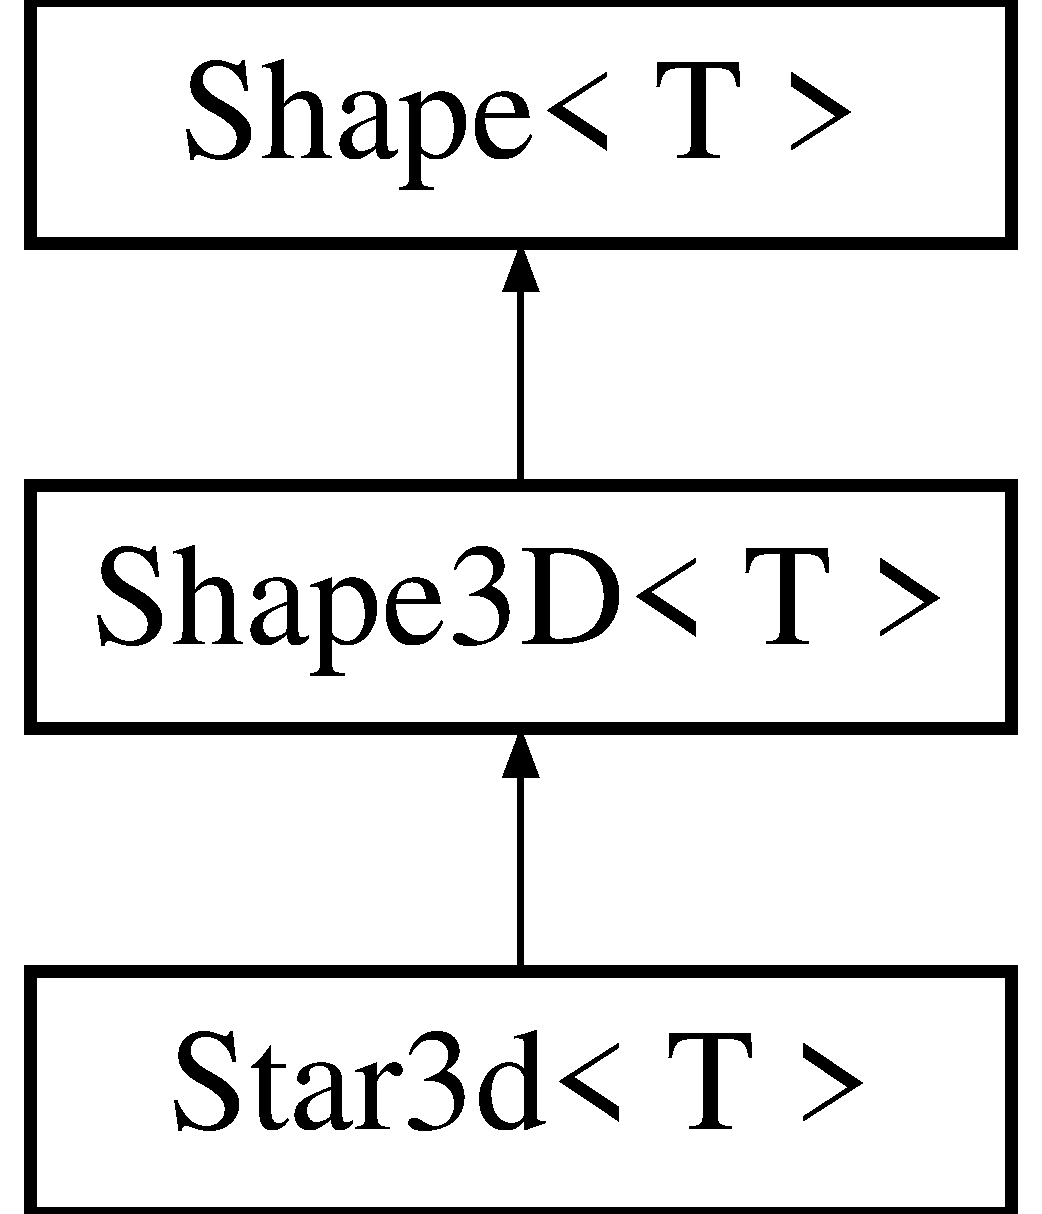
\includegraphics[height=3.000000cm]{classStar3d}
\end{center}
\end{figure}
\subsection*{Public Member Functions}
\begin{DoxyCompactItemize}
\item 
\mbox{\hyperlink{classStar3d_ad264da858df1ef77144a4cd7345185da}{Star3d}} (int=6, T=0.\+5)
\item 
\mbox{\hyperlink{classStar3d_a6793481605da65706c5fc9ca1d4b82ad}{Star3d}} (\mbox{\hyperlink{classStar3d}{Star3d}} \&\&)=default
\item 
\mbox{\hyperlink{classStar3d}{Star3d}} \& \mbox{\hyperlink{classStar3d_a35ace37c66d10033bef1d0acaf9f3283}{operator=}} (\mbox{\hyperlink{classStar3d}{Star3d}} \&\&)=default
\item 
\mbox{\hyperlink{classStar3d_a5f4b217dd7926f73faaa57766546b022}{Star3d}} (const \mbox{\hyperlink{classStar3d}{Star3d}} \&)=default
\item 
\mbox{\hyperlink{classStar3d}{Star3d}} \& \mbox{\hyperlink{classStar3d_a6e1939003aedebc06efdb51404dfbadd}{operator=}} (const \mbox{\hyperlink{classStar3d}{Star3d}} \&)=default
\item 
T \mbox{\hyperlink{classStar3d_aac560f44b7b7d278781231fbaf8312e1}{perimeter}} ()
\end{DoxyCompactItemize}
\subsection*{Public Attributes}
\begin{DoxyCompactItemize}
\item 
T \mbox{\hyperlink{classStar3d_a4c2be78d1baa7a423885cc3574591848}{ratio}}
\end{DoxyCompactItemize}
\subsection*{Private Member Functions}
\begin{DoxyCompactItemize}
\item 
void \mbox{\hyperlink{classStar3d_a43617f398a59d73eb85df49539f9efa5}{generate\+\_\+vertexes}} (int=10, T=0.\+5)
\begin{DoxyCompactList}\small\item\em Generates vertexes for 3d star. \end{DoxyCompactList}\end{DoxyCompactItemize}
\subsection*{Additional Inherited Members}


\subsection{Detailed Description}
\subsubsection*{template$<$typename T = float$>$\newline
class Star3d$<$ T $>$}

this class contains vertexes and elements for 3 dimensional star shape. 

\subsection{Constructor \& Destructor Documentation}
\mbox{\Hypertarget{classStar3d_ad264da858df1ef77144a4cd7345185da}\label{classStar3d_ad264da858df1ef77144a4cd7345185da}} 
\index{Star3d@{Star3d}!Star3d@{Star3d}}
\index{Star3d@{Star3d}!Star3d@{Star3d}}
\subsubsection{\texorpdfstring{Star3d()}{Star3d()}\hspace{0.1cm}{\footnotesize\ttfamily [1/3]}}
{\footnotesize\ttfamily template$<$typename T $>$ \\
\mbox{\hyperlink{classStar3d}{Star3d}}$<$ T $>$\+::\mbox{\hyperlink{classStar3d}{Star3d}} (\begin{DoxyParamCaption}\item[{int}]{bulges = {\ttfamily 6},  }\item[{T}]{ratio\+\_\+ = {\ttfamily 0.5} }\end{DoxyParamCaption})}

\mbox{\Hypertarget{classStar3d_a6793481605da65706c5fc9ca1d4b82ad}\label{classStar3d_a6793481605da65706c5fc9ca1d4b82ad}} 
\index{Star3d@{Star3d}!Star3d@{Star3d}}
\index{Star3d@{Star3d}!Star3d@{Star3d}}
\subsubsection{\texorpdfstring{Star3d()}{Star3d()}\hspace{0.1cm}{\footnotesize\ttfamily [2/3]}}
{\footnotesize\ttfamily template$<$typename T  = float$>$ \\
\mbox{\hyperlink{classStar3d}{Star3d}}$<$ T $>$\+::\mbox{\hyperlink{classStar3d}{Star3d}} (\begin{DoxyParamCaption}\item[{\mbox{\hyperlink{classStar3d}{Star3d}}$<$ T $>$ \&\&}]{ }\end{DoxyParamCaption})\hspace{0.3cm}{\ttfamily [default]}}

\mbox{\Hypertarget{classStar3d_a5f4b217dd7926f73faaa57766546b022}\label{classStar3d_a5f4b217dd7926f73faaa57766546b022}} 
\index{Star3d@{Star3d}!Star3d@{Star3d}}
\index{Star3d@{Star3d}!Star3d@{Star3d}}
\subsubsection{\texorpdfstring{Star3d()}{Star3d()}\hspace{0.1cm}{\footnotesize\ttfamily [3/3]}}
{\footnotesize\ttfamily template$<$typename T  = float$>$ \\
\mbox{\hyperlink{classStar3d}{Star3d}}$<$ T $>$\+::\mbox{\hyperlink{classStar3d}{Star3d}} (\begin{DoxyParamCaption}\item[{const \mbox{\hyperlink{classStar3d}{Star3d}}$<$ T $>$ \&}]{ }\end{DoxyParamCaption})\hspace{0.3cm}{\ttfamily [default]}}



\subsection{Member Function Documentation}
\mbox{\Hypertarget{classStar3d_a43617f398a59d73eb85df49539f9efa5}\label{classStar3d_a43617f398a59d73eb85df49539f9efa5}} 
\index{Star3d@{Star3d}!generate\+\_\+vertexes@{generate\+\_\+vertexes}}
\index{generate\+\_\+vertexes@{generate\+\_\+vertexes}!Star3d@{Star3d}}
\subsubsection{\texorpdfstring{generate\+\_\+vertexes()}{generate\_vertexes()}}
{\footnotesize\ttfamily template$<$typename T $>$ \\
void \mbox{\hyperlink{classStar3d}{Star3d}}$<$ T $>$\+::generate\+\_\+vertexes (\begin{DoxyParamCaption}\item[{int}]{bulges = {\ttfamily 10},  }\item[{T}]{ratio = {\ttfamily 0.5} }\end{DoxyParamCaption})\hspace{0.3cm}{\ttfamily [inline]}, {\ttfamily [private]}}



Generates vertexes for 3d star. 

\mbox{\Hypertarget{classStar3d_a35ace37c66d10033bef1d0acaf9f3283}\label{classStar3d_a35ace37c66d10033bef1d0acaf9f3283}} 
\index{Star3d@{Star3d}!operator=@{operator=}}
\index{operator=@{operator=}!Star3d@{Star3d}}
\subsubsection{\texorpdfstring{operator=()}{operator=()}\hspace{0.1cm}{\footnotesize\ttfamily [1/2]}}
{\footnotesize\ttfamily template$<$typename T  = float$>$ \\
\mbox{\hyperlink{classStar3d}{Star3d}}\& \mbox{\hyperlink{classStar3d}{Star3d}}$<$ T $>$\+::operator= (\begin{DoxyParamCaption}\item[{\mbox{\hyperlink{classStar3d}{Star3d}}$<$ T $>$ \&\&}]{ }\end{DoxyParamCaption})\hspace{0.3cm}{\ttfamily [default]}}

\mbox{\Hypertarget{classStar3d_a6e1939003aedebc06efdb51404dfbadd}\label{classStar3d_a6e1939003aedebc06efdb51404dfbadd}} 
\index{Star3d@{Star3d}!operator=@{operator=}}
\index{operator=@{operator=}!Star3d@{Star3d}}
\subsubsection{\texorpdfstring{operator=()}{operator=()}\hspace{0.1cm}{\footnotesize\ttfamily [2/2]}}
{\footnotesize\ttfamily template$<$typename T  = float$>$ \\
\mbox{\hyperlink{classStar3d}{Star3d}}\& \mbox{\hyperlink{classStar3d}{Star3d}}$<$ T $>$\+::operator= (\begin{DoxyParamCaption}\item[{const \mbox{\hyperlink{classStar3d}{Star3d}}$<$ T $>$ \&}]{ }\end{DoxyParamCaption})\hspace{0.3cm}{\ttfamily [default]}}

\mbox{\Hypertarget{classStar3d_aac560f44b7b7d278781231fbaf8312e1}\label{classStar3d_aac560f44b7b7d278781231fbaf8312e1}} 
\index{Star3d@{Star3d}!perimeter@{perimeter}}
\index{perimeter@{perimeter}!Star3d@{Star3d}}
\subsubsection{\texorpdfstring{perimeter()}{perimeter()}}
{\footnotesize\ttfamily template$<$typename T  = float$>$ \\
T \mbox{\hyperlink{classStar3d}{Star3d}}$<$ T $>$\+::perimeter (\begin{DoxyParamCaption}{ }\end{DoxyParamCaption})}



\subsection{Member Data Documentation}
\mbox{\Hypertarget{classStar3d_a4c2be78d1baa7a423885cc3574591848}\label{classStar3d_a4c2be78d1baa7a423885cc3574591848}} 
\index{Star3d@{Star3d}!ratio@{ratio}}
\index{ratio@{ratio}!Star3d@{Star3d}}
\subsubsection{\texorpdfstring{ratio}{ratio}}
{\footnotesize\ttfamily template$<$typename T  = float$>$ \\
T \mbox{\hyperlink{classStar3d}{Star3d}}$<$ T $>$\+::ratio}



The documentation for this class was generated from the following file\+:\begin{DoxyCompactItemize}
\item 
src/shapes/\mbox{\hyperlink{star3d__not__working_8hpp}{star3d\+\_\+not\+\_\+working.\+hpp}}\end{DoxyCompactItemize}

\hypertarget{classText}{}\section{Text Class Reference}
\label{classText}\index{Text@{Text}}


{\ttfamily \#include \char`\"{}text\+\_\+rendering.\+hpp\char`\"{}}

\subsection*{Classes}
\begin{DoxyCompactItemize}
\item 
struct \mbox{\hyperlink{structText_1_1Character}{Character}}
\end{DoxyCompactItemize}
\subsection*{Public Member Functions}
\begin{DoxyCompactItemize}
\item 
\mbox{\hyperlink{classText_ac76e1d24db004590f1e03da44dfb04dd}{Text}} (const std\+::string \&font\+\_\+file)
\item 
void \mbox{\hyperlink{classText_a8e38585b2e2f824a97895f3ca743372c}{initialize\+\_\+gl\+\_\+buffers}} ()
\item 
void \mbox{\hyperlink{classText_abc6c6300e6d689d25e25ff47575aa81b}{set\+\_\+char\+\_\+size}} (int width, int height)
\item 
void \mbox{\hyperlink{classText_ae5fe3bc91282c8a70253af9baf904b22}{Render\+Text}} (std\+::string text, G\+Lfloat x, G\+Lfloat y, G\+Lfloat scale, glm \+::vec3 color, G\+L\+F\+Wwindow $\ast$window)
\end{DoxyCompactItemize}
\subsection*{Private Attributes}
\begin{DoxyCompactItemize}
\item 
F\+T\+\_\+\+Library \mbox{\hyperlink{classText_af0d723786485fad392cebab1458e0196}{library}}
\item 
F\+T\+\_\+\+Face \mbox{\hyperlink{classText_aead69571b262356d6e4641050485d492}{face}}
\item 
unsigned \mbox{\hyperlink{classText_a09fe1fc4ba6ed5e64dcbef2ac2c56f26}{horizontal\+\_\+device\+\_\+resolution}}
\item 
unsigned \mbox{\hyperlink{classText_aeac01a7f249d00dacd246abfd6f35f91}{vertical\+\_\+device\+\_\+resolution}} = 176
\item 
G\+L\+F\+Wmonitor $\ast$ \mbox{\hyperlink{classText_ad7d37381d10639257b7bb9beccbe36a5}{primary}}
\item 
int \mbox{\hyperlink{classText_ae4127137a06a53bf5bf7cb838bd0a4ff}{monitor\+\_\+width\+MM}}
\item 
int \mbox{\hyperlink{classText_a49c1ab744e7a55b4c9e55ac57527bfc8}{monitor\+\_\+height\+MM}}
\item 
G\+Luint \mbox{\hyperlink{classText_a485e2c31f7a6d7a5a7d360f00818d751}{V\+AO}}
\item 
G\+Luint \mbox{\hyperlink{classText_aaac524c6d42c895e6cbf962538f72b3a}{V\+BO}}
\item 
G\+Luint \mbox{\hyperlink{classText_a0904900eab3438a866585562109cb586}{C\+BO}}
\item 
std\+::map$<$ G\+Lchar, \mbox{\hyperlink{structText_1_1Character}{Character}} $>$ \mbox{\hyperlink{classText_aab2c5b22cf4c381151ccba967b104614}{characters}}
\item 
\mbox{\hyperlink{classShader}{Shader}}$<$ \mbox{\hyperlink{shader__class_8hpp_a24e288e18eb7b6e01de7565001fedb60a72baef04098f035e8a320b03ad197818}{R\+E\+N\+D\+E\+R\+\_\+\+T\+Y\+P\+E\+::\+C\+U\+S\+T\+OM}} $>$ \mbox{\hyperlink{classText_aceda97361cb73286cd090db34aa10084}{text\+\_\+shader}}
\end{DoxyCompactItemize}


\subsection{Constructor \& Destructor Documentation}
\mbox{\Hypertarget{classText_ac76e1d24db004590f1e03da44dfb04dd}\label{classText_ac76e1d24db004590f1e03da44dfb04dd}} 
\index{Text@{Text}!Text@{Text}}
\index{Text@{Text}!Text@{Text}}
\subsubsection{\texorpdfstring{Text()}{Text()}}
{\footnotesize\ttfamily Text\+::\+Text (\begin{DoxyParamCaption}\item[{const std\+::string \&}]{font\+\_\+file }\end{DoxyParamCaption})\hspace{0.3cm}{\ttfamily [inline]}}



\subsection{Member Function Documentation}
\mbox{\Hypertarget{classText_a8e38585b2e2f824a97895f3ca743372c}\label{classText_a8e38585b2e2f824a97895f3ca743372c}} 
\index{Text@{Text}!initialize\+\_\+gl\+\_\+buffers@{initialize\+\_\+gl\+\_\+buffers}}
\index{initialize\+\_\+gl\+\_\+buffers@{initialize\+\_\+gl\+\_\+buffers}!Text@{Text}}
\subsubsection{\texorpdfstring{initialize\+\_\+gl\+\_\+buffers()}{initialize\_gl\_buffers()}}
{\footnotesize\ttfamily void Text\+::initialize\+\_\+gl\+\_\+buffers (\begin{DoxyParamCaption}{ }\end{DoxyParamCaption})\hspace{0.3cm}{\ttfamily [inline]}}

\mbox{\Hypertarget{classText_ae5fe3bc91282c8a70253af9baf904b22}\label{classText_ae5fe3bc91282c8a70253af9baf904b22}} 
\index{Text@{Text}!Render\+Text@{Render\+Text}}
\index{Render\+Text@{Render\+Text}!Text@{Text}}
\subsubsection{\texorpdfstring{Render\+Text()}{RenderText()}}
{\footnotesize\ttfamily void Text\+::\+Render\+Text (\begin{DoxyParamCaption}\item[{std\+::string}]{text,  }\item[{G\+Lfloat}]{x,  }\item[{G\+Lfloat}]{y,  }\item[{G\+Lfloat}]{scale,  }\item[{glm \+::vec3}]{color,  }\item[{G\+L\+F\+Wwindow $\ast$}]{window }\end{DoxyParamCaption})\hspace{0.3cm}{\ttfamily [inline]}}

\mbox{\Hypertarget{classText_abc6c6300e6d689d25e25ff47575aa81b}\label{classText_abc6c6300e6d689d25e25ff47575aa81b}} 
\index{Text@{Text}!set\+\_\+char\+\_\+size@{set\+\_\+char\+\_\+size}}
\index{set\+\_\+char\+\_\+size@{set\+\_\+char\+\_\+size}!Text@{Text}}
\subsubsection{\texorpdfstring{set\+\_\+char\+\_\+size()}{set\_char\_size()}}
{\footnotesize\ttfamily void Text\+::set\+\_\+char\+\_\+size (\begin{DoxyParamCaption}\item[{int}]{width,  }\item[{int}]{height }\end{DoxyParamCaption})\hspace{0.3cm}{\ttfamily [inline]}}



\subsection{Member Data Documentation}
\mbox{\Hypertarget{classText_a0904900eab3438a866585562109cb586}\label{classText_a0904900eab3438a866585562109cb586}} 
\index{Text@{Text}!C\+BO@{C\+BO}}
\index{C\+BO@{C\+BO}!Text@{Text}}
\subsubsection{\texorpdfstring{C\+BO}{CBO}}
{\footnotesize\ttfamily G\+Luint Text\+::\+C\+BO\hspace{0.3cm}{\ttfamily [private]}}

\mbox{\Hypertarget{classText_aab2c5b22cf4c381151ccba967b104614}\label{classText_aab2c5b22cf4c381151ccba967b104614}} 
\index{Text@{Text}!characters@{characters}}
\index{characters@{characters}!Text@{Text}}
\subsubsection{\texorpdfstring{characters}{characters}}
{\footnotesize\ttfamily std\+::map$<$G\+Lchar, \mbox{\hyperlink{structText_1_1Character}{Character}}$>$ Text\+::characters\hspace{0.3cm}{\ttfamily [private]}}

\mbox{\Hypertarget{classText_aead69571b262356d6e4641050485d492}\label{classText_aead69571b262356d6e4641050485d492}} 
\index{Text@{Text}!face@{face}}
\index{face@{face}!Text@{Text}}
\subsubsection{\texorpdfstring{face}{face}}
{\footnotesize\ttfamily F\+T\+\_\+\+Face Text\+::face\hspace{0.3cm}{\ttfamily [private]}}

\mbox{\Hypertarget{classText_a09fe1fc4ba6ed5e64dcbef2ac2c56f26}\label{classText_a09fe1fc4ba6ed5e64dcbef2ac2c56f26}} 
\index{Text@{Text}!horizontal\+\_\+device\+\_\+resolution@{horizontal\+\_\+device\+\_\+resolution}}
\index{horizontal\+\_\+device\+\_\+resolution@{horizontal\+\_\+device\+\_\+resolution}!Text@{Text}}
\subsubsection{\texorpdfstring{horizontal\+\_\+device\+\_\+resolution}{horizontal\_device\_resolution}}
{\footnotesize\ttfamily unsigned Text\+::horizontal\+\_\+device\+\_\+resolution\hspace{0.3cm}{\ttfamily [private]}}

{\bfseries Initial value\+:}
\begin{DoxyCode}
=
        176
\end{DoxyCode}
\mbox{\Hypertarget{classText_af0d723786485fad392cebab1458e0196}\label{classText_af0d723786485fad392cebab1458e0196}} 
\index{Text@{Text}!library@{library}}
\index{library@{library}!Text@{Text}}
\subsubsection{\texorpdfstring{library}{library}}
{\footnotesize\ttfamily F\+T\+\_\+\+Library Text\+::library\hspace{0.3cm}{\ttfamily [private]}}

\mbox{\Hypertarget{classText_a49c1ab744e7a55b4c9e55ac57527bfc8}\label{classText_a49c1ab744e7a55b4c9e55ac57527bfc8}} 
\index{Text@{Text}!monitor\+\_\+height\+MM@{monitor\+\_\+height\+MM}}
\index{monitor\+\_\+height\+MM@{monitor\+\_\+height\+MM}!Text@{Text}}
\subsubsection{\texorpdfstring{monitor\+\_\+height\+MM}{monitor\_heightMM}}
{\footnotesize\ttfamily int Text\+::monitor\+\_\+height\+MM\hspace{0.3cm}{\ttfamily [private]}}

\mbox{\Hypertarget{classText_ae4127137a06a53bf5bf7cb838bd0a4ff}\label{classText_ae4127137a06a53bf5bf7cb838bd0a4ff}} 
\index{Text@{Text}!monitor\+\_\+width\+MM@{monitor\+\_\+width\+MM}}
\index{monitor\+\_\+width\+MM@{monitor\+\_\+width\+MM}!Text@{Text}}
\subsubsection{\texorpdfstring{monitor\+\_\+width\+MM}{monitor\_widthMM}}
{\footnotesize\ttfamily int Text\+::monitor\+\_\+width\+MM\hspace{0.3cm}{\ttfamily [private]}}

\mbox{\Hypertarget{classText_ad7d37381d10639257b7bb9beccbe36a5}\label{classText_ad7d37381d10639257b7bb9beccbe36a5}} 
\index{Text@{Text}!primary@{primary}}
\index{primary@{primary}!Text@{Text}}
\subsubsection{\texorpdfstring{primary}{primary}}
{\footnotesize\ttfamily G\+L\+F\+Wmonitor$\ast$ Text\+::primary\hspace{0.3cm}{\ttfamily [private]}}

\mbox{\Hypertarget{classText_aceda97361cb73286cd090db34aa10084}\label{classText_aceda97361cb73286cd090db34aa10084}} 
\index{Text@{Text}!text\+\_\+shader@{text\+\_\+shader}}
\index{text\+\_\+shader@{text\+\_\+shader}!Text@{Text}}
\subsubsection{\texorpdfstring{text\+\_\+shader}{text\_shader}}
{\footnotesize\ttfamily \mbox{\hyperlink{classShader}{Shader}}$<$\mbox{\hyperlink{shader__class_8hpp_a24e288e18eb7b6e01de7565001fedb60a72baef04098f035e8a320b03ad197818}{R\+E\+N\+D\+E\+R\+\_\+\+T\+Y\+P\+E\+::\+C\+U\+S\+T\+OM}}$>$ Text\+::text\+\_\+shader\hspace{0.3cm}{\ttfamily [private]}}

\mbox{\Hypertarget{classText_a485e2c31f7a6d7a5a7d360f00818d751}\label{classText_a485e2c31f7a6d7a5a7d360f00818d751}} 
\index{Text@{Text}!V\+AO@{V\+AO}}
\index{V\+AO@{V\+AO}!Text@{Text}}
\subsubsection{\texorpdfstring{V\+AO}{VAO}}
{\footnotesize\ttfamily G\+Luint Text\+::\+V\+AO\hspace{0.3cm}{\ttfamily [private]}}

\mbox{\Hypertarget{classText_aaac524c6d42c895e6cbf962538f72b3a}\label{classText_aaac524c6d42c895e6cbf962538f72b3a}} 
\index{Text@{Text}!V\+BO@{V\+BO}}
\index{V\+BO@{V\+BO}!Text@{Text}}
\subsubsection{\texorpdfstring{V\+BO}{VBO}}
{\footnotesize\ttfamily G\+Luint Text\+::\+V\+BO\hspace{0.3cm}{\ttfamily [private]}}

\mbox{\Hypertarget{classText_aeac01a7f249d00dacd246abfd6f35f91}\label{classText_aeac01a7f249d00dacd246abfd6f35f91}} 
\index{Text@{Text}!vertical\+\_\+device\+\_\+resolution@{vertical\+\_\+device\+\_\+resolution}}
\index{vertical\+\_\+device\+\_\+resolution@{vertical\+\_\+device\+\_\+resolution}!Text@{Text}}
\subsubsection{\texorpdfstring{vertical\+\_\+device\+\_\+resolution}{vertical\_device\_resolution}}
{\footnotesize\ttfamily unsigned Text\+::vertical\+\_\+device\+\_\+resolution = 176\hspace{0.3cm}{\ttfamily [private]}}



The documentation for this class was generated from the following file\+:\begin{DoxyCompactItemize}
\item 
src/text\+\_\+rendering/\mbox{\hyperlink{text__rendering_8hpp}{text\+\_\+rendering.\+hpp}}\end{DoxyCompactItemize}

\hypertarget{classThis}{}\section{This Class Reference}
\label{classThis}\index{This@{This}}


\subsection{Detailed Description}
vertex and element data for 3d sphere. 

The documentation for this class was generated from the following file\+:\begin{DoxyCompactItemize}
\item 
src/shapes/\mbox{\hyperlink{sphere_8hpp}{sphere.\+hpp}}\end{DoxyCompactItemize}

\chapter{File Documentation}
\hypertarget{benchmarks__includes_8hpp}{}\section{benchmarks/benchmarks\+\_\+includes.hpp File Reference}
\label{benchmarks__includes_8hpp}\index{benchmarks/benchmarks\+\_\+includes.\+hpp@{benchmarks/benchmarks\+\_\+includes.\+hpp}}
{\ttfamily \#include $<$xmmintrin.\+h$>$}\newline
{\ttfamily \#include $<$algorithm$>$}\newline
{\ttfamily \#include $<$array$>$}\newline
{\ttfamily \#include $<$cmath$>$}\newline
{\ttfamily \#include $<$ctime$>$}\newline
{\ttfamily \#include $<$string$>$}\newline
{\ttfamily \#include $<$glm/glm.\+hpp$>$}\newline
{\ttfamily \#include $<$glm/gtc/matrix\+\_\+transform.\+hpp$>$}\newline
{\ttfamily \#include $<$glm/gtc/type\+\_\+ptr.\+hpp$>$}\newline
{\ttfamily \#include $<$iostream$>$}\newline
{\ttfamily \#include $<$limits$>$}\newline
{\ttfamily \#include $<$type\+\_\+traits$>$}\newline
{\ttfamily \#include $<$unordered\+\_\+map$>$}\newline
{\ttfamily \#include $<$vector$>$}\newline
{\ttfamily \#include $<$random$>$}\newline
{\ttfamily \#include $<$list$>$}\newline
{\ttfamily \#include $<$chrono$>$}\newline
{\ttfamily \#include $<$thread$>$}\newline
{\ttfamily \#include $<$functional$>$}\newline
{\ttfamily \#include $<$boost/align/aligned\+\_\+allocator.\+hpp$>$}\newline
{\ttfamily \#include $<$benchmark/benchmark.\+h$>$}\newline
{\ttfamily \#include \char`\"{}apex\+\_\+memmove.\+h\char`\"{}}\newline
{\ttfamily \#include \char`\"{}type\+\_\+definitions.\+hpp\char`\"{}}\newline
{\ttfamily \#include \char`\"{}convex\+\_\+hull.\+hpp\char`\"{}}\newline
{\ttfamily \#include \char`\"{}auxiliary\+\_\+functions.\+hpp\char`\"{}}\newline
{\ttfamily \#include \char`\"{}print\+\_\+functions.\+hpp\char`\"{}}\newline
{\ttfamily \#include \char`\"{}bitonic\+\_\+sort.\+hpp\char`\"{}}\newline
{\ttfamily \#include \char`\"{}modified\+\_\+bitonic\+\_\+sort.\+hpp\char`\"{}}\newline
{\ttfamily \#include \char`\"{}hybrid\+\_\+sort.\+hpp\char`\"{}}\newline

\hypertarget{sort__benchmarks_8cpp}{}\section{benchmarks/sort\+\_\+benchmarks.cpp File Reference}
\label{sort__benchmarks_8cpp}\index{benchmarks/sort\+\_\+benchmarks.\+cpp@{benchmarks/sort\+\_\+benchmarks.\+cpp}}
{\ttfamily \#include \char`\"{}benchmarks\+\_\+includes.\+hpp\char`\"{}}\newline
{\ttfamily \#include $<$chrono$>$}\newline
\subsection*{Functions}
\begin{DoxyCompactItemize}
\item 
std\+::default\+\_\+random\+\_\+engine \mbox{\hyperlink{sort__benchmarks_8cpp_a5dc9079dfed6570c71f2ce9059815185}{generator}} (std\+::time(0))
\item 
std\+::uniform\+\_\+real\+\_\+distribution$<$ float $>$ \mbox{\hyperlink{sort__benchmarks_8cpp_a6904ec0ecb2e2c2d27fcb6f5cc972964}{float\+\_\+dist}} (-\/100, 100)
\item 
std\+::uniform\+\_\+real\+\_\+distribution$<$ double $>$ \mbox{\hyperlink{sort__benchmarks_8cpp_ab6dce82b9fcdaf6fff7ec472c87efccf}{double\+\_\+dist}} (-\/100, 100)
\item 
static void \mbox{\hyperlink{sort__benchmarks_8cpp_ad219368285075022a9c69e414d3c3ebc}{bitonic\+\_\+2n\+\_\+float\+\_\+sort\+\_\+bench}} (benchmark\+::\+State \&state)
\item 
\mbox{\hyperlink{sort__benchmarks_8cpp_a5f6d78c36e04c79a9e0508501e2c4d08}{Range\+Multiplier}} (2) -\/$>$ Range(8, 67108864) -\/$>$Complexity(benchmark\+::oN)
\item 
static void \mbox{\hyperlink{sort__benchmarks_8cpp_aef7cc83f7229fa95364231f81c1de508}{bitonic\+\_\+8n\+\_\+float\+\_\+sort\+\_\+bench}} (benchmark\+::\+State \&state)
\item 
static void \mbox{\hyperlink{sort__benchmarks_8cpp_ade47be90dd8781831eb95b912a4a04b3}{hybrid\+\_\+8n\+\_\+float\+\_\+sort\+\_\+bench}} (benchmark\+::\+State \&state)
\item 
static void \mbox{\hyperlink{sort__benchmarks_8cpp_a4bee3c3f901e47667ff3843da68efb8c}{Custom\+Arguments}} (benchmark\+::internal\+::\+Benchmark $\ast$b)
\item 
static void \mbox{\hyperlink{sort__benchmarks_8cpp_aa0236fefbfeebbc828fa895743a62522}{bitonic\+\_\+float\+\_\+sort\+\_\+bench}} (benchmark\+::\+State \&state)
\item 
\mbox{\hyperlink{sort__benchmarks_8cpp_a30a76de4151cf1da4d59aa0646fba710}{B\+E\+N\+C\+H\+M\+A\+RK}} (\mbox{\hyperlink{sort__benchmarks_8cpp_aa0236fefbfeebbc828fa895743a62522}{bitonic\+\_\+float\+\_\+sort\+\_\+bench}}) -\/$>$ Apply(\mbox{\hyperlink{sort__benchmarks_8cpp_a4bee3c3f901e47667ff3843da68efb8c}{Custom\+Arguments}})
\item 
static void \mbox{\hyperlink{sort__benchmarks_8cpp_af569ea97a3fc6ecf6a11952a9cbd5929}{improved\+\_\+bitonic\+\_\+float\+\_\+sort\+\_\+bench}} (benchmark\+::\+State \&state)
\item 
\mbox{\hyperlink{sort__benchmarks_8cpp_a9f86154d764ea4d1fd5a8cb38358861e}{B\+E\+N\+C\+H\+M\+A\+RK}} (\mbox{\hyperlink{sort__benchmarks_8cpp_af569ea97a3fc6ecf6a11952a9cbd5929}{improved\+\_\+bitonic\+\_\+float\+\_\+sort\+\_\+bench}}) -\/$>$ Apply(\mbox{\hyperlink{sort__benchmarks_8cpp_a4bee3c3f901e47667ff3843da68efb8c}{Custom\+Arguments}})
\item 
static void \mbox{\hyperlink{sort__benchmarks_8cpp_aaf37b549986879c9ba54724dcdb4a8fe}{simd\+\_\+\+Q\+S\+\_\+float\+\_\+bench}} (benchmark\+::\+State \&state)
\item 
\mbox{\hyperlink{sort__benchmarks_8cpp_aa9fd02fedb475fcd901e28a9ce71661d}{B\+E\+N\+C\+H\+M\+A\+RK}} (\mbox{\hyperlink{sort__benchmarks_8cpp_aaf37b549986879c9ba54724dcdb4a8fe}{simd\+\_\+\+Q\+S\+\_\+float\+\_\+bench}}) -\/$>$ Apply(\mbox{\hyperlink{sort__benchmarks_8cpp_a4bee3c3f901e47667ff3843da68efb8c}{Custom\+Arguments}})
\item 
static void \mbox{\hyperlink{sort__benchmarks_8cpp_abc82706d4992d3bbdfd59d6c6787446e}{std\+\_\+float\+\_\+sort\+\_\+bench}} (benchmark\+::\+State \&state)
\item 
\mbox{\hyperlink{sort__benchmarks_8cpp_a62388f93f792974aea9280fdb5ec6741}{B\+E\+N\+C\+H\+M\+A\+RK}} (\mbox{\hyperlink{sort__benchmarks_8cpp_abc82706d4992d3bbdfd59d6c6787446e}{std\+\_\+float\+\_\+sort\+\_\+bench}}) -\/$>$ Apply(\mbox{\hyperlink{sort__benchmarks_8cpp_a4bee3c3f901e47667ff3843da68efb8c}{Custom\+Arguments}})
\item 
static void \mbox{\hyperlink{sort__benchmarks_8cpp_aaaa0fb02856afcc3a5667143ac929fa8}{bitonic\+\_\+2n\+\_\+double\+\_\+sort\+\_\+bench}} (benchmark\+::\+State \&state)
\item 
static void \mbox{\hyperlink{sort__benchmarks_8cpp_aa98359c453da15b3c322d5ff94640b11}{bitonic\+\_\+4n\+\_\+double\+\_\+sort\+\_\+bench}} (benchmark\+::\+State \&state)
\item 
\mbox{\hyperlink{sort__benchmarks_8cpp_a135cdc759ea12122dce8561cb07a2af7}{Range\+Multiplier}} (8) -\/$>$ Range(8, 67108864) -\/$>$Complexity(benchmark\+::oN)
\item 
static void \mbox{\hyperlink{sort__benchmarks_8cpp_aa7865bd05b5f9c6b2a9fe4a43d594d2c}{bitonic\+\_\+double\+\_\+sort\+\_\+bench}} (benchmark\+::\+State \&state)
\item 
\mbox{\hyperlink{sort__benchmarks_8cpp_a3ae7cf93a40119b3d2cc5cbb094441d2}{B\+E\+N\+C\+H\+M\+A\+RK}} (\mbox{\hyperlink{sort__benchmarks_8cpp_aa7865bd05b5f9c6b2a9fe4a43d594d2c}{bitonic\+\_\+double\+\_\+sort\+\_\+bench}}) -\/$>$ Apply(\mbox{\hyperlink{sort__benchmarks_8cpp_a4bee3c3f901e47667ff3843da68efb8c}{Custom\+Arguments}})
\item 
static void \mbox{\hyperlink{sort__benchmarks_8cpp_af9fc26c536b051ad1ebf043b0bb24762}{std\+\_\+double\+\_\+sort\+\_\+bench}} (benchmark\+::\+State \&state)
\item 
\mbox{\hyperlink{sort__benchmarks_8cpp_a174f4d99ac50df35e74b698213e7cbd9}{B\+E\+N\+C\+H\+M\+A\+RK}} (\mbox{\hyperlink{sort__benchmarks_8cpp_af9fc26c536b051ad1ebf043b0bb24762}{std\+\_\+double\+\_\+sort\+\_\+bench}}) -\/$>$ Apply(\mbox{\hyperlink{sort__benchmarks_8cpp_a4bee3c3f901e47667ff3843da68efb8c}{Custom\+Arguments}})
\item 
\mbox{\hyperlink{sort__benchmarks_8cpp_a5851750faa9cfec10f7cad1f3b89697e}{B\+E\+N\+C\+H\+M\+A\+R\+K\+\_\+\+M\+A\+IN}} ()
\end{DoxyCompactItemize}
\subsection*{Variables}
\begin{DoxyCompactItemize}
\item 
auto \mbox{\hyperlink{sort__benchmarks_8cpp_a9dd4b1bafcf4df807cbedae854a203fb}{random\+\_\+float}} = std\+::bind(\mbox{\hyperlink{gtest__tests_8cpp_a6904ec0ecb2e2c2d27fcb6f5cc972964}{float\+\_\+dist}}, \mbox{\hyperlink{gtest__tests_8cpp_a5dc9079dfed6570c71f2ce9059815185}{generator}})
\item 
auto \mbox{\hyperlink{sort__benchmarks_8cpp_af37e683a424a342bfd2154a2bf058dc8}{random\+\_\+double}} = std\+::bind(\mbox{\hyperlink{gtest__tests_8cpp_ab6dce82b9fcdaf6fff7ec472c87efccf}{double\+\_\+dist}}, \mbox{\hyperlink{gtest__tests_8cpp_a5dc9079dfed6570c71f2ce9059815185}{generator}})
\end{DoxyCompactItemize}


\subsection{Function Documentation}
\mbox{\Hypertarget{sort__benchmarks_8cpp_a30a76de4151cf1da4d59aa0646fba710}\label{sort__benchmarks_8cpp_a30a76de4151cf1da4d59aa0646fba710}} 
\index{sort\+\_\+benchmarks.\+cpp@{sort\+\_\+benchmarks.\+cpp}!B\+E\+N\+C\+H\+M\+A\+RK@{B\+E\+N\+C\+H\+M\+A\+RK}}
\index{B\+E\+N\+C\+H\+M\+A\+RK@{B\+E\+N\+C\+H\+M\+A\+RK}!sort\+\_\+benchmarks.\+cpp@{sort\+\_\+benchmarks.\+cpp}}
\subsubsection{\texorpdfstring{B\+E\+N\+C\+H\+M\+A\+R\+K()}{BENCHMARK()}\hspace{0.1cm}{\footnotesize\ttfamily [1/6]}}
{\footnotesize\ttfamily B\+E\+N\+C\+H\+M\+A\+RK (\begin{DoxyParamCaption}\item[{\mbox{\hyperlink{sort__benchmarks_8cpp_aa0236fefbfeebbc828fa895743a62522}{bitonic\+\_\+float\+\_\+sort\+\_\+bench}}}]{ }\end{DoxyParamCaption}) -\/$>$  Apply(\mbox{\hyperlink{sort__benchmarks_8cpp_a4bee3c3f901e47667ff3843da68efb8c}{Custom\+Arguments}})}

\mbox{\Hypertarget{sort__benchmarks_8cpp_a9f86154d764ea4d1fd5a8cb38358861e}\label{sort__benchmarks_8cpp_a9f86154d764ea4d1fd5a8cb38358861e}} 
\index{sort\+\_\+benchmarks.\+cpp@{sort\+\_\+benchmarks.\+cpp}!B\+E\+N\+C\+H\+M\+A\+RK@{B\+E\+N\+C\+H\+M\+A\+RK}}
\index{B\+E\+N\+C\+H\+M\+A\+RK@{B\+E\+N\+C\+H\+M\+A\+RK}!sort\+\_\+benchmarks.\+cpp@{sort\+\_\+benchmarks.\+cpp}}
\subsubsection{\texorpdfstring{B\+E\+N\+C\+H\+M\+A\+R\+K()}{BENCHMARK()}\hspace{0.1cm}{\footnotesize\ttfamily [2/6]}}
{\footnotesize\ttfamily B\+E\+N\+C\+H\+M\+A\+RK (\begin{DoxyParamCaption}\item[{\mbox{\hyperlink{sort__benchmarks_8cpp_af569ea97a3fc6ecf6a11952a9cbd5929}{improved\+\_\+bitonic\+\_\+float\+\_\+sort\+\_\+bench}}}]{ }\end{DoxyParamCaption}) -\/$>$  Apply(\mbox{\hyperlink{sort__benchmarks_8cpp_a4bee3c3f901e47667ff3843da68efb8c}{Custom\+Arguments}})}

\mbox{\Hypertarget{sort__benchmarks_8cpp_aa9fd02fedb475fcd901e28a9ce71661d}\label{sort__benchmarks_8cpp_aa9fd02fedb475fcd901e28a9ce71661d}} 
\index{sort\+\_\+benchmarks.\+cpp@{sort\+\_\+benchmarks.\+cpp}!B\+E\+N\+C\+H\+M\+A\+RK@{B\+E\+N\+C\+H\+M\+A\+RK}}
\index{B\+E\+N\+C\+H\+M\+A\+RK@{B\+E\+N\+C\+H\+M\+A\+RK}!sort\+\_\+benchmarks.\+cpp@{sort\+\_\+benchmarks.\+cpp}}
\subsubsection{\texorpdfstring{B\+E\+N\+C\+H\+M\+A\+R\+K()}{BENCHMARK()}\hspace{0.1cm}{\footnotesize\ttfamily [3/6]}}
{\footnotesize\ttfamily B\+E\+N\+C\+H\+M\+A\+RK (\begin{DoxyParamCaption}\item[{\mbox{\hyperlink{sort__benchmarks_8cpp_aaf37b549986879c9ba54724dcdb4a8fe}{simd\+\_\+\+Q\+S\+\_\+float\+\_\+bench}}}]{ }\end{DoxyParamCaption}) -\/$>$  Apply(\mbox{\hyperlink{sort__benchmarks_8cpp_a4bee3c3f901e47667ff3843da68efb8c}{Custom\+Arguments}})}

\mbox{\Hypertarget{sort__benchmarks_8cpp_a62388f93f792974aea9280fdb5ec6741}\label{sort__benchmarks_8cpp_a62388f93f792974aea9280fdb5ec6741}} 
\index{sort\+\_\+benchmarks.\+cpp@{sort\+\_\+benchmarks.\+cpp}!B\+E\+N\+C\+H\+M\+A\+RK@{B\+E\+N\+C\+H\+M\+A\+RK}}
\index{B\+E\+N\+C\+H\+M\+A\+RK@{B\+E\+N\+C\+H\+M\+A\+RK}!sort\+\_\+benchmarks.\+cpp@{sort\+\_\+benchmarks.\+cpp}}
\subsubsection{\texorpdfstring{B\+E\+N\+C\+H\+M\+A\+R\+K()}{BENCHMARK()}\hspace{0.1cm}{\footnotesize\ttfamily [4/6]}}
{\footnotesize\ttfamily B\+E\+N\+C\+H\+M\+A\+RK (\begin{DoxyParamCaption}\item[{\mbox{\hyperlink{sort__benchmarks_8cpp_abc82706d4992d3bbdfd59d6c6787446e}{std\+\_\+float\+\_\+sort\+\_\+bench}}}]{ }\end{DoxyParamCaption}) -\/$>$  Apply(\mbox{\hyperlink{sort__benchmarks_8cpp_a4bee3c3f901e47667ff3843da68efb8c}{Custom\+Arguments}})}

\mbox{\Hypertarget{sort__benchmarks_8cpp_a3ae7cf93a40119b3d2cc5cbb094441d2}\label{sort__benchmarks_8cpp_a3ae7cf93a40119b3d2cc5cbb094441d2}} 
\index{sort\+\_\+benchmarks.\+cpp@{sort\+\_\+benchmarks.\+cpp}!B\+E\+N\+C\+H\+M\+A\+RK@{B\+E\+N\+C\+H\+M\+A\+RK}}
\index{B\+E\+N\+C\+H\+M\+A\+RK@{B\+E\+N\+C\+H\+M\+A\+RK}!sort\+\_\+benchmarks.\+cpp@{sort\+\_\+benchmarks.\+cpp}}
\subsubsection{\texorpdfstring{B\+E\+N\+C\+H\+M\+A\+R\+K()}{BENCHMARK()}\hspace{0.1cm}{\footnotesize\ttfamily [5/6]}}
{\footnotesize\ttfamily B\+E\+N\+C\+H\+M\+A\+RK (\begin{DoxyParamCaption}\item[{\mbox{\hyperlink{sort__benchmarks_8cpp_aa7865bd05b5f9c6b2a9fe4a43d594d2c}{bitonic\+\_\+double\+\_\+sort\+\_\+bench}}}]{ }\end{DoxyParamCaption}) -\/$>$  Apply(\mbox{\hyperlink{sort__benchmarks_8cpp_a4bee3c3f901e47667ff3843da68efb8c}{Custom\+Arguments}})}

\mbox{\Hypertarget{sort__benchmarks_8cpp_a174f4d99ac50df35e74b698213e7cbd9}\label{sort__benchmarks_8cpp_a174f4d99ac50df35e74b698213e7cbd9}} 
\index{sort\+\_\+benchmarks.\+cpp@{sort\+\_\+benchmarks.\+cpp}!B\+E\+N\+C\+H\+M\+A\+RK@{B\+E\+N\+C\+H\+M\+A\+RK}}
\index{B\+E\+N\+C\+H\+M\+A\+RK@{B\+E\+N\+C\+H\+M\+A\+RK}!sort\+\_\+benchmarks.\+cpp@{sort\+\_\+benchmarks.\+cpp}}
\subsubsection{\texorpdfstring{B\+E\+N\+C\+H\+M\+A\+R\+K()}{BENCHMARK()}\hspace{0.1cm}{\footnotesize\ttfamily [6/6]}}
{\footnotesize\ttfamily B\+E\+N\+C\+H\+M\+A\+RK (\begin{DoxyParamCaption}\item[{\mbox{\hyperlink{sort__benchmarks_8cpp_af9fc26c536b051ad1ebf043b0bb24762}{std\+\_\+double\+\_\+sort\+\_\+bench}}}]{ }\end{DoxyParamCaption}) -\/$>$  Apply(\mbox{\hyperlink{sort__benchmarks_8cpp_a4bee3c3f901e47667ff3843da68efb8c}{Custom\+Arguments}})}

\mbox{\Hypertarget{sort__benchmarks_8cpp_a5851750faa9cfec10f7cad1f3b89697e}\label{sort__benchmarks_8cpp_a5851750faa9cfec10f7cad1f3b89697e}} 
\index{sort\+\_\+benchmarks.\+cpp@{sort\+\_\+benchmarks.\+cpp}!B\+E\+N\+C\+H\+M\+A\+R\+K\+\_\+\+M\+A\+IN@{B\+E\+N\+C\+H\+M\+A\+R\+K\+\_\+\+M\+A\+IN}}
\index{B\+E\+N\+C\+H\+M\+A\+R\+K\+\_\+\+M\+A\+IN@{B\+E\+N\+C\+H\+M\+A\+R\+K\+\_\+\+M\+A\+IN}!sort\+\_\+benchmarks.\+cpp@{sort\+\_\+benchmarks.\+cpp}}
\subsubsection{\texorpdfstring{B\+E\+N\+C\+H\+M\+A\+R\+K\+\_\+\+M\+A\+I\+N()}{BENCHMARK\_MAIN()}}
{\footnotesize\ttfamily B\+E\+N\+C\+H\+M\+A\+R\+K\+\_\+\+M\+A\+IN (\begin{DoxyParamCaption}{ }\end{DoxyParamCaption})}

\mbox{\Hypertarget{sort__benchmarks_8cpp_aaaa0fb02856afcc3a5667143ac929fa8}\label{sort__benchmarks_8cpp_aaaa0fb02856afcc3a5667143ac929fa8}} 
\index{sort\+\_\+benchmarks.\+cpp@{sort\+\_\+benchmarks.\+cpp}!bitonic\+\_\+2n\+\_\+double\+\_\+sort\+\_\+bench@{bitonic\+\_\+2n\+\_\+double\+\_\+sort\+\_\+bench}}
\index{bitonic\+\_\+2n\+\_\+double\+\_\+sort\+\_\+bench@{bitonic\+\_\+2n\+\_\+double\+\_\+sort\+\_\+bench}!sort\+\_\+benchmarks.\+cpp@{sort\+\_\+benchmarks.\+cpp}}
\subsubsection{\texorpdfstring{bitonic\+\_\+2n\+\_\+double\+\_\+sort\+\_\+bench()}{bitonic\_2n\_double\_sort\_bench()}}
{\footnotesize\ttfamily static void bitonic\+\_\+2n\+\_\+double\+\_\+sort\+\_\+bench (\begin{DoxyParamCaption}\item[{benchmark\+::\+State \&}]{state }\end{DoxyParamCaption})\hspace{0.3cm}{\ttfamily [static]}}

\mbox{\Hypertarget{sort__benchmarks_8cpp_ad219368285075022a9c69e414d3c3ebc}\label{sort__benchmarks_8cpp_ad219368285075022a9c69e414d3c3ebc}} 
\index{sort\+\_\+benchmarks.\+cpp@{sort\+\_\+benchmarks.\+cpp}!bitonic\+\_\+2n\+\_\+float\+\_\+sort\+\_\+bench@{bitonic\+\_\+2n\+\_\+float\+\_\+sort\+\_\+bench}}
\index{bitonic\+\_\+2n\+\_\+float\+\_\+sort\+\_\+bench@{bitonic\+\_\+2n\+\_\+float\+\_\+sort\+\_\+bench}!sort\+\_\+benchmarks.\+cpp@{sort\+\_\+benchmarks.\+cpp}}
\subsubsection{\texorpdfstring{bitonic\+\_\+2n\+\_\+float\+\_\+sort\+\_\+bench()}{bitonic\_2n\_float\_sort\_bench()}}
{\footnotesize\ttfamily static void bitonic\+\_\+2n\+\_\+float\+\_\+sort\+\_\+bench (\begin{DoxyParamCaption}\item[{benchmark\+::\+State \&}]{state }\end{DoxyParamCaption})\hspace{0.3cm}{\ttfamily [static]}}

\mbox{\Hypertarget{sort__benchmarks_8cpp_aa98359c453da15b3c322d5ff94640b11}\label{sort__benchmarks_8cpp_aa98359c453da15b3c322d5ff94640b11}} 
\index{sort\+\_\+benchmarks.\+cpp@{sort\+\_\+benchmarks.\+cpp}!bitonic\+\_\+4n\+\_\+double\+\_\+sort\+\_\+bench@{bitonic\+\_\+4n\+\_\+double\+\_\+sort\+\_\+bench}}
\index{bitonic\+\_\+4n\+\_\+double\+\_\+sort\+\_\+bench@{bitonic\+\_\+4n\+\_\+double\+\_\+sort\+\_\+bench}!sort\+\_\+benchmarks.\+cpp@{sort\+\_\+benchmarks.\+cpp}}
\subsubsection{\texorpdfstring{bitonic\+\_\+4n\+\_\+double\+\_\+sort\+\_\+bench()}{bitonic\_4n\_double\_sort\_bench()}}
{\footnotesize\ttfamily static void bitonic\+\_\+4n\+\_\+double\+\_\+sort\+\_\+bench (\begin{DoxyParamCaption}\item[{benchmark\+::\+State \&}]{state }\end{DoxyParamCaption})\hspace{0.3cm}{\ttfamily [static]}}

\mbox{\Hypertarget{sort__benchmarks_8cpp_aef7cc83f7229fa95364231f81c1de508}\label{sort__benchmarks_8cpp_aef7cc83f7229fa95364231f81c1de508}} 
\index{sort\+\_\+benchmarks.\+cpp@{sort\+\_\+benchmarks.\+cpp}!bitonic\+\_\+8n\+\_\+float\+\_\+sort\+\_\+bench@{bitonic\+\_\+8n\+\_\+float\+\_\+sort\+\_\+bench}}
\index{bitonic\+\_\+8n\+\_\+float\+\_\+sort\+\_\+bench@{bitonic\+\_\+8n\+\_\+float\+\_\+sort\+\_\+bench}!sort\+\_\+benchmarks.\+cpp@{sort\+\_\+benchmarks.\+cpp}}
\subsubsection{\texorpdfstring{bitonic\+\_\+8n\+\_\+float\+\_\+sort\+\_\+bench()}{bitonic\_8n\_float\_sort\_bench()}}
{\footnotesize\ttfamily static void bitonic\+\_\+8n\+\_\+float\+\_\+sort\+\_\+bench (\begin{DoxyParamCaption}\item[{benchmark\+::\+State \&}]{state }\end{DoxyParamCaption})\hspace{0.3cm}{\ttfamily [static]}}

\mbox{\Hypertarget{sort__benchmarks_8cpp_aa7865bd05b5f9c6b2a9fe4a43d594d2c}\label{sort__benchmarks_8cpp_aa7865bd05b5f9c6b2a9fe4a43d594d2c}} 
\index{sort\+\_\+benchmarks.\+cpp@{sort\+\_\+benchmarks.\+cpp}!bitonic\+\_\+double\+\_\+sort\+\_\+bench@{bitonic\+\_\+double\+\_\+sort\+\_\+bench}}
\index{bitonic\+\_\+double\+\_\+sort\+\_\+bench@{bitonic\+\_\+double\+\_\+sort\+\_\+bench}!sort\+\_\+benchmarks.\+cpp@{sort\+\_\+benchmarks.\+cpp}}
\subsubsection{\texorpdfstring{bitonic\+\_\+double\+\_\+sort\+\_\+bench()}{bitonic\_double\_sort\_bench()}}
{\footnotesize\ttfamily static void bitonic\+\_\+double\+\_\+sort\+\_\+bench (\begin{DoxyParamCaption}\item[{benchmark\+::\+State \&}]{state }\end{DoxyParamCaption})\hspace{0.3cm}{\ttfamily [static]}}

\mbox{\Hypertarget{sort__benchmarks_8cpp_aa0236fefbfeebbc828fa895743a62522}\label{sort__benchmarks_8cpp_aa0236fefbfeebbc828fa895743a62522}} 
\index{sort\+\_\+benchmarks.\+cpp@{sort\+\_\+benchmarks.\+cpp}!bitonic\+\_\+float\+\_\+sort\+\_\+bench@{bitonic\+\_\+float\+\_\+sort\+\_\+bench}}
\index{bitonic\+\_\+float\+\_\+sort\+\_\+bench@{bitonic\+\_\+float\+\_\+sort\+\_\+bench}!sort\+\_\+benchmarks.\+cpp@{sort\+\_\+benchmarks.\+cpp}}
\subsubsection{\texorpdfstring{bitonic\+\_\+float\+\_\+sort\+\_\+bench()}{bitonic\_float\_sort\_bench()}}
{\footnotesize\ttfamily static void bitonic\+\_\+float\+\_\+sort\+\_\+bench (\begin{DoxyParamCaption}\item[{benchmark\+::\+State \&}]{state }\end{DoxyParamCaption})\hspace{0.3cm}{\ttfamily [static]}}

\mbox{\Hypertarget{sort__benchmarks_8cpp_a4bee3c3f901e47667ff3843da68efb8c}\label{sort__benchmarks_8cpp_a4bee3c3f901e47667ff3843da68efb8c}} 
\index{sort\+\_\+benchmarks.\+cpp@{sort\+\_\+benchmarks.\+cpp}!Custom\+Arguments@{Custom\+Arguments}}
\index{Custom\+Arguments@{Custom\+Arguments}!sort\+\_\+benchmarks.\+cpp@{sort\+\_\+benchmarks.\+cpp}}
\subsubsection{\texorpdfstring{Custom\+Arguments()}{CustomArguments()}}
{\footnotesize\ttfamily static void Custom\+Arguments (\begin{DoxyParamCaption}\item[{benchmark\+::internal\+::\+Benchmark $\ast$}]{b }\end{DoxyParamCaption})\hspace{0.3cm}{\ttfamily [static]}}

\mbox{\Hypertarget{sort__benchmarks_8cpp_ab6dce82b9fcdaf6fff7ec472c87efccf}\label{sort__benchmarks_8cpp_ab6dce82b9fcdaf6fff7ec472c87efccf}} 
\index{sort\+\_\+benchmarks.\+cpp@{sort\+\_\+benchmarks.\+cpp}!double\+\_\+dist@{double\+\_\+dist}}
\index{double\+\_\+dist@{double\+\_\+dist}!sort\+\_\+benchmarks.\+cpp@{sort\+\_\+benchmarks.\+cpp}}
\subsubsection{\texorpdfstring{double\+\_\+dist()}{double\_dist()}}
{\footnotesize\ttfamily std\+::uniform\+\_\+real\+\_\+distribution$<$double$>$ double\+\_\+dist (\begin{DoxyParamCaption}\item[{-\/}]{100,  }\item[{100}]{ }\end{DoxyParamCaption})}

\mbox{\Hypertarget{sort__benchmarks_8cpp_a6904ec0ecb2e2c2d27fcb6f5cc972964}\label{sort__benchmarks_8cpp_a6904ec0ecb2e2c2d27fcb6f5cc972964}} 
\index{sort\+\_\+benchmarks.\+cpp@{sort\+\_\+benchmarks.\+cpp}!float\+\_\+dist@{float\+\_\+dist}}
\index{float\+\_\+dist@{float\+\_\+dist}!sort\+\_\+benchmarks.\+cpp@{sort\+\_\+benchmarks.\+cpp}}
\subsubsection{\texorpdfstring{float\+\_\+dist()}{float\_dist()}}
{\footnotesize\ttfamily std\+::uniform\+\_\+real\+\_\+distribution$<$float$>$ float\+\_\+dist (\begin{DoxyParamCaption}\item[{-\/}]{100,  }\item[{100}]{ }\end{DoxyParamCaption})}

\mbox{\Hypertarget{sort__benchmarks_8cpp_a5dc9079dfed6570c71f2ce9059815185}\label{sort__benchmarks_8cpp_a5dc9079dfed6570c71f2ce9059815185}} 
\index{sort\+\_\+benchmarks.\+cpp@{sort\+\_\+benchmarks.\+cpp}!generator@{generator}}
\index{generator@{generator}!sort\+\_\+benchmarks.\+cpp@{sort\+\_\+benchmarks.\+cpp}}
\subsubsection{\texorpdfstring{generator()}{generator()}}
{\footnotesize\ttfamily std\+::default\+\_\+random\+\_\+engine generator (\begin{DoxyParamCaption}\item[{std\+::time(0)}]{ }\end{DoxyParamCaption})}

\mbox{\Hypertarget{sort__benchmarks_8cpp_ade47be90dd8781831eb95b912a4a04b3}\label{sort__benchmarks_8cpp_ade47be90dd8781831eb95b912a4a04b3}} 
\index{sort\+\_\+benchmarks.\+cpp@{sort\+\_\+benchmarks.\+cpp}!hybrid\+\_\+8n\+\_\+float\+\_\+sort\+\_\+bench@{hybrid\+\_\+8n\+\_\+float\+\_\+sort\+\_\+bench}}
\index{hybrid\+\_\+8n\+\_\+float\+\_\+sort\+\_\+bench@{hybrid\+\_\+8n\+\_\+float\+\_\+sort\+\_\+bench}!sort\+\_\+benchmarks.\+cpp@{sort\+\_\+benchmarks.\+cpp}}
\subsubsection{\texorpdfstring{hybrid\+\_\+8n\+\_\+float\+\_\+sort\+\_\+bench()}{hybrid\_8n\_float\_sort\_bench()}}
{\footnotesize\ttfamily static void hybrid\+\_\+8n\+\_\+float\+\_\+sort\+\_\+bench (\begin{DoxyParamCaption}\item[{benchmark\+::\+State \&}]{state }\end{DoxyParamCaption})\hspace{0.3cm}{\ttfamily [static]}}

\mbox{\Hypertarget{sort__benchmarks_8cpp_af569ea97a3fc6ecf6a11952a9cbd5929}\label{sort__benchmarks_8cpp_af569ea97a3fc6ecf6a11952a9cbd5929}} 
\index{sort\+\_\+benchmarks.\+cpp@{sort\+\_\+benchmarks.\+cpp}!improved\+\_\+bitonic\+\_\+float\+\_\+sort\+\_\+bench@{improved\+\_\+bitonic\+\_\+float\+\_\+sort\+\_\+bench}}
\index{improved\+\_\+bitonic\+\_\+float\+\_\+sort\+\_\+bench@{improved\+\_\+bitonic\+\_\+float\+\_\+sort\+\_\+bench}!sort\+\_\+benchmarks.\+cpp@{sort\+\_\+benchmarks.\+cpp}}
\subsubsection{\texorpdfstring{improved\+\_\+bitonic\+\_\+float\+\_\+sort\+\_\+bench()}{improved\_bitonic\_float\_sort\_bench()}}
{\footnotesize\ttfamily static void improved\+\_\+bitonic\+\_\+float\+\_\+sort\+\_\+bench (\begin{DoxyParamCaption}\item[{benchmark\+::\+State \&}]{state }\end{DoxyParamCaption})\hspace{0.3cm}{\ttfamily [static]}}

\mbox{\Hypertarget{sort__benchmarks_8cpp_a5f6d78c36e04c79a9e0508501e2c4d08}\label{sort__benchmarks_8cpp_a5f6d78c36e04c79a9e0508501e2c4d08}} 
\index{sort\+\_\+benchmarks.\+cpp@{sort\+\_\+benchmarks.\+cpp}!Range\+Multiplier@{Range\+Multiplier}}
\index{Range\+Multiplier@{Range\+Multiplier}!sort\+\_\+benchmarks.\+cpp@{sort\+\_\+benchmarks.\+cpp}}
\subsubsection{\texorpdfstring{Range\+Multiplier()}{RangeMultiplier()}\hspace{0.1cm}{\footnotesize\ttfamily [1/2]}}
{\footnotesize\ttfamily Range\+Multiplier (\begin{DoxyParamCaption}\item[{2}]{ }\end{DoxyParamCaption}) -\/$>$  Range(8, 67108864) -\/$>$Complexity(benchmark\+::oN)}

\mbox{\Hypertarget{sort__benchmarks_8cpp_a135cdc759ea12122dce8561cb07a2af7}\label{sort__benchmarks_8cpp_a135cdc759ea12122dce8561cb07a2af7}} 
\index{sort\+\_\+benchmarks.\+cpp@{sort\+\_\+benchmarks.\+cpp}!Range\+Multiplier@{Range\+Multiplier}}
\index{Range\+Multiplier@{Range\+Multiplier}!sort\+\_\+benchmarks.\+cpp@{sort\+\_\+benchmarks.\+cpp}}
\subsubsection{\texorpdfstring{Range\+Multiplier()}{RangeMultiplier()}\hspace{0.1cm}{\footnotesize\ttfamily [2/2]}}
{\footnotesize\ttfamily Range\+Multiplier (\begin{DoxyParamCaption}\item[{8}]{ }\end{DoxyParamCaption}) -\/$>$  Range(8, 67108864) -\/$>$Complexity(benchmark\+::oN)}

\mbox{\Hypertarget{sort__benchmarks_8cpp_aaf37b549986879c9ba54724dcdb4a8fe}\label{sort__benchmarks_8cpp_aaf37b549986879c9ba54724dcdb4a8fe}} 
\index{sort\+\_\+benchmarks.\+cpp@{sort\+\_\+benchmarks.\+cpp}!simd\+\_\+\+Q\+S\+\_\+float\+\_\+bench@{simd\+\_\+\+Q\+S\+\_\+float\+\_\+bench}}
\index{simd\+\_\+\+Q\+S\+\_\+float\+\_\+bench@{simd\+\_\+\+Q\+S\+\_\+float\+\_\+bench}!sort\+\_\+benchmarks.\+cpp@{sort\+\_\+benchmarks.\+cpp}}
\subsubsection{\texorpdfstring{simd\+\_\+\+Q\+S\+\_\+float\+\_\+bench()}{simd\_QS\_float\_bench()}}
{\footnotesize\ttfamily static void simd\+\_\+\+Q\+S\+\_\+float\+\_\+bench (\begin{DoxyParamCaption}\item[{benchmark\+::\+State \&}]{state }\end{DoxyParamCaption})\hspace{0.3cm}{\ttfamily [static]}}

\mbox{\Hypertarget{sort__benchmarks_8cpp_af9fc26c536b051ad1ebf043b0bb24762}\label{sort__benchmarks_8cpp_af9fc26c536b051ad1ebf043b0bb24762}} 
\index{sort\+\_\+benchmarks.\+cpp@{sort\+\_\+benchmarks.\+cpp}!std\+\_\+double\+\_\+sort\+\_\+bench@{std\+\_\+double\+\_\+sort\+\_\+bench}}
\index{std\+\_\+double\+\_\+sort\+\_\+bench@{std\+\_\+double\+\_\+sort\+\_\+bench}!sort\+\_\+benchmarks.\+cpp@{sort\+\_\+benchmarks.\+cpp}}
\subsubsection{\texorpdfstring{std\+\_\+double\+\_\+sort\+\_\+bench()}{std\_double\_sort\_bench()}}
{\footnotesize\ttfamily static void std\+\_\+double\+\_\+sort\+\_\+bench (\begin{DoxyParamCaption}\item[{benchmark\+::\+State \&}]{state }\end{DoxyParamCaption})\hspace{0.3cm}{\ttfamily [static]}}

\mbox{\Hypertarget{sort__benchmarks_8cpp_abc82706d4992d3bbdfd59d6c6787446e}\label{sort__benchmarks_8cpp_abc82706d4992d3bbdfd59d6c6787446e}} 
\index{sort\+\_\+benchmarks.\+cpp@{sort\+\_\+benchmarks.\+cpp}!std\+\_\+float\+\_\+sort\+\_\+bench@{std\+\_\+float\+\_\+sort\+\_\+bench}}
\index{std\+\_\+float\+\_\+sort\+\_\+bench@{std\+\_\+float\+\_\+sort\+\_\+bench}!sort\+\_\+benchmarks.\+cpp@{sort\+\_\+benchmarks.\+cpp}}
\subsubsection{\texorpdfstring{std\+\_\+float\+\_\+sort\+\_\+bench()}{std\_float\_sort\_bench()}}
{\footnotesize\ttfamily static void std\+\_\+float\+\_\+sort\+\_\+bench (\begin{DoxyParamCaption}\item[{benchmark\+::\+State \&}]{state }\end{DoxyParamCaption})\hspace{0.3cm}{\ttfamily [static]}}



\subsection{Variable Documentation}
\mbox{\Hypertarget{sort__benchmarks_8cpp_af37e683a424a342bfd2154a2bf058dc8}\label{sort__benchmarks_8cpp_af37e683a424a342bfd2154a2bf058dc8}} 
\index{sort\+\_\+benchmarks.\+cpp@{sort\+\_\+benchmarks.\+cpp}!random\+\_\+double@{random\+\_\+double}}
\index{random\+\_\+double@{random\+\_\+double}!sort\+\_\+benchmarks.\+cpp@{sort\+\_\+benchmarks.\+cpp}}
\subsubsection{\texorpdfstring{random\+\_\+double}{random\_double}}
{\footnotesize\ttfamily auto random\+\_\+double = std\+::bind(\mbox{\hyperlink{gtest__tests_8cpp_ab6dce82b9fcdaf6fff7ec472c87efccf}{double\+\_\+dist}}, \mbox{\hyperlink{gtest__tests_8cpp_a5dc9079dfed6570c71f2ce9059815185}{generator}})}

\mbox{\Hypertarget{sort__benchmarks_8cpp_a9dd4b1bafcf4df807cbedae854a203fb}\label{sort__benchmarks_8cpp_a9dd4b1bafcf4df807cbedae854a203fb}} 
\index{sort\+\_\+benchmarks.\+cpp@{sort\+\_\+benchmarks.\+cpp}!random\+\_\+float@{random\+\_\+float}}
\index{random\+\_\+float@{random\+\_\+float}!sort\+\_\+benchmarks.\+cpp@{sort\+\_\+benchmarks.\+cpp}}
\subsubsection{\texorpdfstring{random\+\_\+float}{random\_float}}
{\footnotesize\ttfamily auto random\+\_\+float = std\+::bind(\mbox{\hyperlink{gtest__tests_8cpp_a6904ec0ecb2e2c2d27fcb6f5cc972964}{float\+\_\+dist}}, \mbox{\hyperlink{gtest__tests_8cpp_a5dc9079dfed6570c71f2ce9059815185}{generator}})}


\hypertarget{build_2CMakeFiles_23_812_83_2CompilerIdC_2CMakeCCompilerId_8c}{}\section{build/\+C\+Make\+Files/3.12.3/\+Compiler\+Id\+C/\+C\+Make\+C\+Compiler\+Id.c File Reference}
\label{build_2CMakeFiles_23_812_83_2CompilerIdC_2CMakeCCompilerId_8c}\index{build/\+C\+Make\+Files/3.\+12.\+3/\+Compiler\+Id\+C/\+C\+Make\+C\+Compiler\+Id.\+c@{build/\+C\+Make\+Files/3.\+12.\+3/\+Compiler\+Id\+C/\+C\+Make\+C\+Compiler\+Id.\+c}}
\subsection*{Macros}
\begin{DoxyCompactItemize}
\item 
\#define \mbox{\hyperlink{build_2CMakeFiles_23_812_83_2CompilerIdC_2CMakeCCompilerId_8c_a81dee0709ded976b2e0319239f72d174}{C\+O\+M\+P\+I\+L\+E\+R\+\_\+\+ID}}~\char`\"{}\char`\"{}
\item 
\#define \mbox{\hyperlink{build_2CMakeFiles_23_812_83_2CompilerIdC_2CMakeCCompilerId_8c_a2ae9b72bb13abaabfcf2ee0ba7d3fa1d}{S\+T\+R\+I\+N\+G\+I\+F\+Y\+\_\+\+H\+E\+L\+P\+ER}}(X)~\#X
\item 
\#define \mbox{\hyperlink{build_2CMakeFiles_23_812_83_2CompilerIdC_2CMakeCCompilerId_8c_a43e1cad902b6477bec893cb6430bd6c8}{S\+T\+R\+I\+N\+G\+I\+FY}}(X)~\mbox{\hyperlink{examples_2opengl__test_2build_2CMakeFiles_23_812_83_2CompilerIdCXX_2CMakeCXXCompilerId_8cpp_a2ae9b72bb13abaabfcf2ee0ba7d3fa1d}{S\+T\+R\+I\+N\+G\+I\+F\+Y\+\_\+\+H\+E\+L\+P\+ER}}(X)
\item 
\#define \mbox{\hyperlink{build_2CMakeFiles_23_812_83_2CompilerIdC_2CMakeCCompilerId_8c_adbc5372f40838899018fadbc89bd588b}{P\+L\+A\+T\+F\+O\+R\+M\+\_\+\+ID}}
\item 
\#define \mbox{\hyperlink{build_2CMakeFiles_23_812_83_2CompilerIdC_2CMakeCCompilerId_8c_aba35d0d200deaeb06aee95ca297acb28}{A\+R\+C\+H\+I\+T\+E\+C\+T\+U\+R\+E\+\_\+\+ID}}
\item 
\#define \mbox{\hyperlink{build_2CMakeFiles_23_812_83_2CompilerIdC_2CMakeCCompilerId_8c_ad1280362da42492bbc11aa78cbf776ad}{D\+EC}}(\mbox{\hyperlink{glad_8h_a0788d3762d0c3c76e4c094d8078b4c27}{n}})
\item 
\#define \mbox{\hyperlink{build_2CMakeFiles_23_812_83_2CompilerIdC_2CMakeCCompilerId_8c_a46d5d95daa1bef867bd0179594310ed5}{H\+EX}}(\mbox{\hyperlink{glad_8h_a0788d3762d0c3c76e4c094d8078b4c27}{n}})
\item 
\#define \mbox{\hyperlink{build_2CMakeFiles_23_812_83_2CompilerIdC_2CMakeCCompilerId_8c_a07f8e5783674099cd7f5110e22a78cdb}{C\+\_\+\+D\+I\+A\+L\+E\+CT}}
\end{DoxyCompactItemize}
\subsection*{Functions}
\begin{DoxyCompactItemize}
\item 
int \mbox{\hyperlink{build_2CMakeFiles_23_812_83_2CompilerIdC_2CMakeCCompilerId_8c_a0ddf1224851353fc92bfbff6f499fa97}{main}} (int argc, char $\ast$argv\mbox{[}$\,$\mbox{]})
\end{DoxyCompactItemize}
\subsection*{Variables}
\begin{DoxyCompactItemize}
\item 
char const  $\ast$ \mbox{\hyperlink{build_2CMakeFiles_23_812_83_2CompilerIdC_2CMakeCCompilerId_8c_a4b0efeb7a5d59313986b3a0390f050f6}{info\+\_\+compiler}} = \char`\"{}I\+N\+FO\char`\"{} \char`\"{}\+:\char`\"{} \char`\"{}compiler\mbox{[}\char`\"{} C\+O\+M\+P\+I\+L\+E\+R\+\_\+\+ID \char`\"{}\mbox{]}\char`\"{}
\item 
char const  $\ast$ \mbox{\hyperlink{build_2CMakeFiles_23_812_83_2CompilerIdC_2CMakeCCompilerId_8c_a2321403dee54ee23f0c2fa849c60f7d4}{info\+\_\+platform}} = \char`\"{}I\+N\+FO\char`\"{} \char`\"{}\+:\char`\"{} \char`\"{}platform\mbox{[}\char`\"{} P\+L\+A\+T\+F\+O\+R\+M\+\_\+\+ID \char`\"{}\mbox{]}\char`\"{}
\item 
char const  $\ast$ \mbox{\hyperlink{build_2CMakeFiles_23_812_83_2CompilerIdC_2CMakeCCompilerId_8c_a59647e99d304ed33b15cb284c27ed391}{info\+\_\+arch}} = \char`\"{}I\+N\+FO\char`\"{} \char`\"{}\+:\char`\"{} \char`\"{}arch\mbox{[}\char`\"{} A\+R\+C\+H\+I\+T\+E\+C\+T\+U\+R\+E\+\_\+\+ID \char`\"{}\mbox{]}\char`\"{}
\item 
const char $\ast$ \mbox{\hyperlink{build_2CMakeFiles_23_812_83_2CompilerIdC_2CMakeCCompilerId_8c_a1ce162bad2fe6966ac8b33cc19e120b8}{info\+\_\+language\+\_\+dialect\+\_\+default}}
\end{DoxyCompactItemize}


\subsection{Macro Definition Documentation}
\mbox{\Hypertarget{build_2CMakeFiles_23_812_83_2CompilerIdC_2CMakeCCompilerId_8c_aba35d0d200deaeb06aee95ca297acb28}\label{build_2CMakeFiles_23_812_83_2CompilerIdC_2CMakeCCompilerId_8c_aba35d0d200deaeb06aee95ca297acb28}} 
\index{build/\+C\+Make\+Files/3.\+12.\+3/\+Compiler\+Id\+C/\+C\+Make\+C\+Compiler\+Id.\+c@{build/\+C\+Make\+Files/3.\+12.\+3/\+Compiler\+Id\+C/\+C\+Make\+C\+Compiler\+Id.\+c}!A\+R\+C\+H\+I\+T\+E\+C\+T\+U\+R\+E\+\_\+\+ID@{A\+R\+C\+H\+I\+T\+E\+C\+T\+U\+R\+E\+\_\+\+ID}}
\index{A\+R\+C\+H\+I\+T\+E\+C\+T\+U\+R\+E\+\_\+\+ID@{A\+R\+C\+H\+I\+T\+E\+C\+T\+U\+R\+E\+\_\+\+ID}!build/\+C\+Make\+Files/3.\+12.\+3/\+Compiler\+Id\+C/\+C\+Make\+C\+Compiler\+Id.\+c@{build/\+C\+Make\+Files/3.\+12.\+3/\+Compiler\+Id\+C/\+C\+Make\+C\+Compiler\+Id.\+c}}
\subsubsection{\texorpdfstring{A\+R\+C\+H\+I\+T\+E\+C\+T\+U\+R\+E\+\_\+\+ID}{ARCHITECTURE\_ID}}
{\footnotesize\ttfamily \#define A\+R\+C\+H\+I\+T\+E\+C\+T\+U\+R\+E\+\_\+\+ID}

\mbox{\Hypertarget{build_2CMakeFiles_23_812_83_2CompilerIdC_2CMakeCCompilerId_8c_a07f8e5783674099cd7f5110e22a78cdb}\label{build_2CMakeFiles_23_812_83_2CompilerIdC_2CMakeCCompilerId_8c_a07f8e5783674099cd7f5110e22a78cdb}} 
\index{build/\+C\+Make\+Files/3.\+12.\+3/\+Compiler\+Id\+C/\+C\+Make\+C\+Compiler\+Id.\+c@{build/\+C\+Make\+Files/3.\+12.\+3/\+Compiler\+Id\+C/\+C\+Make\+C\+Compiler\+Id.\+c}!C\+\_\+\+D\+I\+A\+L\+E\+CT@{C\+\_\+\+D\+I\+A\+L\+E\+CT}}
\index{C\+\_\+\+D\+I\+A\+L\+E\+CT@{C\+\_\+\+D\+I\+A\+L\+E\+CT}!build/\+C\+Make\+Files/3.\+12.\+3/\+Compiler\+Id\+C/\+C\+Make\+C\+Compiler\+Id.\+c@{build/\+C\+Make\+Files/3.\+12.\+3/\+Compiler\+Id\+C/\+C\+Make\+C\+Compiler\+Id.\+c}}
\subsubsection{\texorpdfstring{C\+\_\+\+D\+I\+A\+L\+E\+CT}{C\_DIALECT}}
{\footnotesize\ttfamily \#define C\+\_\+\+D\+I\+A\+L\+E\+CT}

\mbox{\Hypertarget{build_2CMakeFiles_23_812_83_2CompilerIdC_2CMakeCCompilerId_8c_a81dee0709ded976b2e0319239f72d174}\label{build_2CMakeFiles_23_812_83_2CompilerIdC_2CMakeCCompilerId_8c_a81dee0709ded976b2e0319239f72d174}} 
\index{build/\+C\+Make\+Files/3.\+12.\+3/\+Compiler\+Id\+C/\+C\+Make\+C\+Compiler\+Id.\+c@{build/\+C\+Make\+Files/3.\+12.\+3/\+Compiler\+Id\+C/\+C\+Make\+C\+Compiler\+Id.\+c}!C\+O\+M\+P\+I\+L\+E\+R\+\_\+\+ID@{C\+O\+M\+P\+I\+L\+E\+R\+\_\+\+ID}}
\index{C\+O\+M\+P\+I\+L\+E\+R\+\_\+\+ID@{C\+O\+M\+P\+I\+L\+E\+R\+\_\+\+ID}!build/\+C\+Make\+Files/3.\+12.\+3/\+Compiler\+Id\+C/\+C\+Make\+C\+Compiler\+Id.\+c@{build/\+C\+Make\+Files/3.\+12.\+3/\+Compiler\+Id\+C/\+C\+Make\+C\+Compiler\+Id.\+c}}
\subsubsection{\texorpdfstring{C\+O\+M\+P\+I\+L\+E\+R\+\_\+\+ID}{COMPILER\_ID}}
{\footnotesize\ttfamily \#define C\+O\+M\+P\+I\+L\+E\+R\+\_\+\+ID~\char`\"{}\char`\"{}}

\mbox{\Hypertarget{build_2CMakeFiles_23_812_83_2CompilerIdC_2CMakeCCompilerId_8c_ad1280362da42492bbc11aa78cbf776ad}\label{build_2CMakeFiles_23_812_83_2CompilerIdC_2CMakeCCompilerId_8c_ad1280362da42492bbc11aa78cbf776ad}} 
\index{build/\+C\+Make\+Files/3.\+12.\+3/\+Compiler\+Id\+C/\+C\+Make\+C\+Compiler\+Id.\+c@{build/\+C\+Make\+Files/3.\+12.\+3/\+Compiler\+Id\+C/\+C\+Make\+C\+Compiler\+Id.\+c}!D\+EC@{D\+EC}}
\index{D\+EC@{D\+EC}!build/\+C\+Make\+Files/3.\+12.\+3/\+Compiler\+Id\+C/\+C\+Make\+C\+Compiler\+Id.\+c@{build/\+C\+Make\+Files/3.\+12.\+3/\+Compiler\+Id\+C/\+C\+Make\+C\+Compiler\+Id.\+c}}
\subsubsection{\texorpdfstring{D\+EC}{DEC}}
{\footnotesize\ttfamily \#define D\+EC(\begin{DoxyParamCaption}\item[{}]{\mbox{\hyperlink{glad_8h_a0788d3762d0c3c76e4c094d8078b4c27}{n}} }\end{DoxyParamCaption})}

{\bfseries Value\+:}
\begin{DoxyCode}
(\textcolor{charliteral}{'0'} + (((\mbox{\hyperlink{glad_8h_a0788d3762d0c3c76e4c094d8078b4c27}{n}}) / 10000000)%10)), \(\backslash\)
  (\textcolor{charliteral}{'0'} + (((\mbox{\hyperlink{glad_8h_a0788d3762d0c3c76e4c094d8078b4c27}{n}}) / 1000000)%10)),  \(\backslash\)
  (\textcolor{charliteral}{'0'} + (((\mbox{\hyperlink{glad_8h_a0788d3762d0c3c76e4c094d8078b4c27}{n}}) / 100000)%10)),   \(\backslash\)
  (\textcolor{charliteral}{'0'} + (((\mbox{\hyperlink{glad_8h_a0788d3762d0c3c76e4c094d8078b4c27}{n}}) / 10000)%10)),    \(\backslash\)
  (\textcolor{charliteral}{'0'} + (((\mbox{\hyperlink{glad_8h_a0788d3762d0c3c76e4c094d8078b4c27}{n}}) / 1000)%10)),     \(\backslash\)
  (\textcolor{charliteral}{'0'} + (((\mbox{\hyperlink{glad_8h_a0788d3762d0c3c76e4c094d8078b4c27}{n}}) / 100)%10)),      \(\backslash\)
  (\textcolor{charliteral}{'0'} + (((\mbox{\hyperlink{glad_8h_a0788d3762d0c3c76e4c094d8078b4c27}{n}}) / 10)%10)),       \(\backslash\)
  (\textcolor{charliteral}{'0'} +  ((\mbox{\hyperlink{glad_8h_a0788d3762d0c3c76e4c094d8078b4c27}{n}}) % 10))
\end{DoxyCode}
\mbox{\Hypertarget{build_2CMakeFiles_23_812_83_2CompilerIdC_2CMakeCCompilerId_8c_a46d5d95daa1bef867bd0179594310ed5}\label{build_2CMakeFiles_23_812_83_2CompilerIdC_2CMakeCCompilerId_8c_a46d5d95daa1bef867bd0179594310ed5}} 
\index{build/\+C\+Make\+Files/3.\+12.\+3/\+Compiler\+Id\+C/\+C\+Make\+C\+Compiler\+Id.\+c@{build/\+C\+Make\+Files/3.\+12.\+3/\+Compiler\+Id\+C/\+C\+Make\+C\+Compiler\+Id.\+c}!H\+EX@{H\+EX}}
\index{H\+EX@{H\+EX}!build/\+C\+Make\+Files/3.\+12.\+3/\+Compiler\+Id\+C/\+C\+Make\+C\+Compiler\+Id.\+c@{build/\+C\+Make\+Files/3.\+12.\+3/\+Compiler\+Id\+C/\+C\+Make\+C\+Compiler\+Id.\+c}}
\subsubsection{\texorpdfstring{H\+EX}{HEX}}
{\footnotesize\ttfamily \#define H\+EX(\begin{DoxyParamCaption}\item[{}]{\mbox{\hyperlink{glad_8h_a0788d3762d0c3c76e4c094d8078b4c27}{n}} }\end{DoxyParamCaption})}

{\bfseries Value\+:}
\begin{DoxyCode}
(\textcolor{charliteral}{'0'} + ((\mbox{\hyperlink{glad_8h_a0788d3762d0c3c76e4c094d8078b4c27}{n}})>>28 & 0xF)), \(\backslash\)
  (\textcolor{charliteral}{'0'} + ((\mbox{\hyperlink{glad_8h_a0788d3762d0c3c76e4c094d8078b4c27}{n}})>>24 & 0xF)), \(\backslash\)
  (\textcolor{charliteral}{'0'} + ((\mbox{\hyperlink{glad_8h_a0788d3762d0c3c76e4c094d8078b4c27}{n}})>>20 & 0xF)), \(\backslash\)
  (\textcolor{charliteral}{'0'} + ((\mbox{\hyperlink{glad_8h_a0788d3762d0c3c76e4c094d8078b4c27}{n}})>>16 & 0xF)), \(\backslash\)
  (\textcolor{charliteral}{'0'} + ((\mbox{\hyperlink{glad_8h_a0788d3762d0c3c76e4c094d8078b4c27}{n}})>>12 & 0xF)), \(\backslash\)
  (\textcolor{charliteral}{'0'} + ((\mbox{\hyperlink{glad_8h_a0788d3762d0c3c76e4c094d8078b4c27}{n}})>>8  & 0xF)), \(\backslash\)
  (\textcolor{charliteral}{'0'} + ((\mbox{\hyperlink{glad_8h_a0788d3762d0c3c76e4c094d8078b4c27}{n}})>>4  & 0xF)), \(\backslash\)
  (\textcolor{charliteral}{'0'} + ((\mbox{\hyperlink{glad_8h_a0788d3762d0c3c76e4c094d8078b4c27}{n}})     & 0xF))
\end{DoxyCode}
\mbox{\Hypertarget{build_2CMakeFiles_23_812_83_2CompilerIdC_2CMakeCCompilerId_8c_adbc5372f40838899018fadbc89bd588b}\label{build_2CMakeFiles_23_812_83_2CompilerIdC_2CMakeCCompilerId_8c_adbc5372f40838899018fadbc89bd588b}} 
\index{build/\+C\+Make\+Files/3.\+12.\+3/\+Compiler\+Id\+C/\+C\+Make\+C\+Compiler\+Id.\+c@{build/\+C\+Make\+Files/3.\+12.\+3/\+Compiler\+Id\+C/\+C\+Make\+C\+Compiler\+Id.\+c}!P\+L\+A\+T\+F\+O\+R\+M\+\_\+\+ID@{P\+L\+A\+T\+F\+O\+R\+M\+\_\+\+ID}}
\index{P\+L\+A\+T\+F\+O\+R\+M\+\_\+\+ID@{P\+L\+A\+T\+F\+O\+R\+M\+\_\+\+ID}!build/\+C\+Make\+Files/3.\+12.\+3/\+Compiler\+Id\+C/\+C\+Make\+C\+Compiler\+Id.\+c@{build/\+C\+Make\+Files/3.\+12.\+3/\+Compiler\+Id\+C/\+C\+Make\+C\+Compiler\+Id.\+c}}
\subsubsection{\texorpdfstring{P\+L\+A\+T\+F\+O\+R\+M\+\_\+\+ID}{PLATFORM\_ID}}
{\footnotesize\ttfamily \#define P\+L\+A\+T\+F\+O\+R\+M\+\_\+\+ID}

\mbox{\Hypertarget{build_2CMakeFiles_23_812_83_2CompilerIdC_2CMakeCCompilerId_8c_a43e1cad902b6477bec893cb6430bd6c8}\label{build_2CMakeFiles_23_812_83_2CompilerIdC_2CMakeCCompilerId_8c_a43e1cad902b6477bec893cb6430bd6c8}} 
\index{build/\+C\+Make\+Files/3.\+12.\+3/\+Compiler\+Id\+C/\+C\+Make\+C\+Compiler\+Id.\+c@{build/\+C\+Make\+Files/3.\+12.\+3/\+Compiler\+Id\+C/\+C\+Make\+C\+Compiler\+Id.\+c}!S\+T\+R\+I\+N\+G\+I\+FY@{S\+T\+R\+I\+N\+G\+I\+FY}}
\index{S\+T\+R\+I\+N\+G\+I\+FY@{S\+T\+R\+I\+N\+G\+I\+FY}!build/\+C\+Make\+Files/3.\+12.\+3/\+Compiler\+Id\+C/\+C\+Make\+C\+Compiler\+Id.\+c@{build/\+C\+Make\+Files/3.\+12.\+3/\+Compiler\+Id\+C/\+C\+Make\+C\+Compiler\+Id.\+c}}
\subsubsection{\texorpdfstring{S\+T\+R\+I\+N\+G\+I\+FY}{STRINGIFY}}
{\footnotesize\ttfamily \#define S\+T\+R\+I\+N\+G\+I\+FY(\begin{DoxyParamCaption}\item[{}]{X }\end{DoxyParamCaption})~\mbox{\hyperlink{examples_2opengl__test_2build_2CMakeFiles_23_812_83_2CompilerIdCXX_2CMakeCXXCompilerId_8cpp_a2ae9b72bb13abaabfcf2ee0ba7d3fa1d}{S\+T\+R\+I\+N\+G\+I\+F\+Y\+\_\+\+H\+E\+L\+P\+ER}}(X)}

\mbox{\Hypertarget{build_2CMakeFiles_23_812_83_2CompilerIdC_2CMakeCCompilerId_8c_a2ae9b72bb13abaabfcf2ee0ba7d3fa1d}\label{build_2CMakeFiles_23_812_83_2CompilerIdC_2CMakeCCompilerId_8c_a2ae9b72bb13abaabfcf2ee0ba7d3fa1d}} 
\index{build/\+C\+Make\+Files/3.\+12.\+3/\+Compiler\+Id\+C/\+C\+Make\+C\+Compiler\+Id.\+c@{build/\+C\+Make\+Files/3.\+12.\+3/\+Compiler\+Id\+C/\+C\+Make\+C\+Compiler\+Id.\+c}!S\+T\+R\+I\+N\+G\+I\+F\+Y\+\_\+\+H\+E\+L\+P\+ER@{S\+T\+R\+I\+N\+G\+I\+F\+Y\+\_\+\+H\+E\+L\+P\+ER}}
\index{S\+T\+R\+I\+N\+G\+I\+F\+Y\+\_\+\+H\+E\+L\+P\+ER@{S\+T\+R\+I\+N\+G\+I\+F\+Y\+\_\+\+H\+E\+L\+P\+ER}!build/\+C\+Make\+Files/3.\+12.\+3/\+Compiler\+Id\+C/\+C\+Make\+C\+Compiler\+Id.\+c@{build/\+C\+Make\+Files/3.\+12.\+3/\+Compiler\+Id\+C/\+C\+Make\+C\+Compiler\+Id.\+c}}
\subsubsection{\texorpdfstring{S\+T\+R\+I\+N\+G\+I\+F\+Y\+\_\+\+H\+E\+L\+P\+ER}{STRINGIFY\_HELPER}}
{\footnotesize\ttfamily \#define S\+T\+R\+I\+N\+G\+I\+F\+Y\+\_\+\+H\+E\+L\+P\+ER(\begin{DoxyParamCaption}\item[{}]{X }\end{DoxyParamCaption})~\#X}



\subsection{Function Documentation}
\mbox{\Hypertarget{build_2CMakeFiles_23_812_83_2CompilerIdC_2CMakeCCompilerId_8c_a0ddf1224851353fc92bfbff6f499fa97}\label{build_2CMakeFiles_23_812_83_2CompilerIdC_2CMakeCCompilerId_8c_a0ddf1224851353fc92bfbff6f499fa97}} 
\index{build/\+C\+Make\+Files/3.\+12.\+3/\+Compiler\+Id\+C/\+C\+Make\+C\+Compiler\+Id.\+c@{build/\+C\+Make\+Files/3.\+12.\+3/\+Compiler\+Id\+C/\+C\+Make\+C\+Compiler\+Id.\+c}!main@{main}}
\index{main@{main}!build/\+C\+Make\+Files/3.\+12.\+3/\+Compiler\+Id\+C/\+C\+Make\+C\+Compiler\+Id.\+c@{build/\+C\+Make\+Files/3.\+12.\+3/\+Compiler\+Id\+C/\+C\+Make\+C\+Compiler\+Id.\+c}}
\subsubsection{\texorpdfstring{main()}{main()}}
{\footnotesize\ttfamily int main (\begin{DoxyParamCaption}\item[{int}]{argc,  }\item[{char $\ast$}]{argv\mbox{[}$\,$\mbox{]} }\end{DoxyParamCaption})}



\subsection{Variable Documentation}
\mbox{\Hypertarget{build_2CMakeFiles_23_812_83_2CompilerIdC_2CMakeCCompilerId_8c_a59647e99d304ed33b15cb284c27ed391}\label{build_2CMakeFiles_23_812_83_2CompilerIdC_2CMakeCCompilerId_8c_a59647e99d304ed33b15cb284c27ed391}} 
\index{build/\+C\+Make\+Files/3.\+12.\+3/\+Compiler\+Id\+C/\+C\+Make\+C\+Compiler\+Id.\+c@{build/\+C\+Make\+Files/3.\+12.\+3/\+Compiler\+Id\+C/\+C\+Make\+C\+Compiler\+Id.\+c}!info\+\_\+arch@{info\+\_\+arch}}
\index{info\+\_\+arch@{info\+\_\+arch}!build/\+C\+Make\+Files/3.\+12.\+3/\+Compiler\+Id\+C/\+C\+Make\+C\+Compiler\+Id.\+c@{build/\+C\+Make\+Files/3.\+12.\+3/\+Compiler\+Id\+C/\+C\+Make\+C\+Compiler\+Id.\+c}}
\subsubsection{\texorpdfstring{info\+\_\+arch}{info\_arch}}
{\footnotesize\ttfamily char const$\ast$ info\+\_\+arch = \char`\"{}I\+N\+FO\char`\"{} \char`\"{}\+:\char`\"{} \char`\"{}arch\mbox{[}\char`\"{} A\+R\+C\+H\+I\+T\+E\+C\+T\+U\+R\+E\+\_\+\+ID \char`\"{}\mbox{]}\char`\"{}}

\mbox{\Hypertarget{build_2CMakeFiles_23_812_83_2CompilerIdC_2CMakeCCompilerId_8c_a4b0efeb7a5d59313986b3a0390f050f6}\label{build_2CMakeFiles_23_812_83_2CompilerIdC_2CMakeCCompilerId_8c_a4b0efeb7a5d59313986b3a0390f050f6}} 
\index{build/\+C\+Make\+Files/3.\+12.\+3/\+Compiler\+Id\+C/\+C\+Make\+C\+Compiler\+Id.\+c@{build/\+C\+Make\+Files/3.\+12.\+3/\+Compiler\+Id\+C/\+C\+Make\+C\+Compiler\+Id.\+c}!info\+\_\+compiler@{info\+\_\+compiler}}
\index{info\+\_\+compiler@{info\+\_\+compiler}!build/\+C\+Make\+Files/3.\+12.\+3/\+Compiler\+Id\+C/\+C\+Make\+C\+Compiler\+Id.\+c@{build/\+C\+Make\+Files/3.\+12.\+3/\+Compiler\+Id\+C/\+C\+Make\+C\+Compiler\+Id.\+c}}
\subsubsection{\texorpdfstring{info\+\_\+compiler}{info\_compiler}}
{\footnotesize\ttfamily char const$\ast$ info\+\_\+compiler = \char`\"{}I\+N\+FO\char`\"{} \char`\"{}\+:\char`\"{} \char`\"{}compiler\mbox{[}\char`\"{} C\+O\+M\+P\+I\+L\+E\+R\+\_\+\+ID \char`\"{}\mbox{]}\char`\"{}}

\mbox{\Hypertarget{build_2CMakeFiles_23_812_83_2CompilerIdC_2CMakeCCompilerId_8c_a1ce162bad2fe6966ac8b33cc19e120b8}\label{build_2CMakeFiles_23_812_83_2CompilerIdC_2CMakeCCompilerId_8c_a1ce162bad2fe6966ac8b33cc19e120b8}} 
\index{build/\+C\+Make\+Files/3.\+12.\+3/\+Compiler\+Id\+C/\+C\+Make\+C\+Compiler\+Id.\+c@{build/\+C\+Make\+Files/3.\+12.\+3/\+Compiler\+Id\+C/\+C\+Make\+C\+Compiler\+Id.\+c}!info\+\_\+language\+\_\+dialect\+\_\+default@{info\+\_\+language\+\_\+dialect\+\_\+default}}
\index{info\+\_\+language\+\_\+dialect\+\_\+default@{info\+\_\+language\+\_\+dialect\+\_\+default}!build/\+C\+Make\+Files/3.\+12.\+3/\+Compiler\+Id\+C/\+C\+Make\+C\+Compiler\+Id.\+c@{build/\+C\+Make\+Files/3.\+12.\+3/\+Compiler\+Id\+C/\+C\+Make\+C\+Compiler\+Id.\+c}}
\subsubsection{\texorpdfstring{info\+\_\+language\+\_\+dialect\+\_\+default}{info\_language\_dialect\_default}}
{\footnotesize\ttfamily const char$\ast$ info\+\_\+language\+\_\+dialect\+\_\+default}

{\bfseries Initial value\+:}
\begin{DoxyCode}
=
  \textcolor{stringliteral}{"INFO"} \textcolor{stringliteral}{":"} \textcolor{stringliteral}{"dialect\_default["} \mbox{\hyperlink{build_2CMakeFiles_23_812_83_2CompilerIdC_2CMakeCCompilerId_8c_a07f8e5783674099cd7f5110e22a78cdb}{C\_DIALECT}} \textcolor{stringliteral}{"]"}
\end{DoxyCode}
\mbox{\Hypertarget{build_2CMakeFiles_23_812_83_2CompilerIdC_2CMakeCCompilerId_8c_a2321403dee54ee23f0c2fa849c60f7d4}\label{build_2CMakeFiles_23_812_83_2CompilerIdC_2CMakeCCompilerId_8c_a2321403dee54ee23f0c2fa849c60f7d4}} 
\index{build/\+C\+Make\+Files/3.\+12.\+3/\+Compiler\+Id\+C/\+C\+Make\+C\+Compiler\+Id.\+c@{build/\+C\+Make\+Files/3.\+12.\+3/\+Compiler\+Id\+C/\+C\+Make\+C\+Compiler\+Id.\+c}!info\+\_\+platform@{info\+\_\+platform}}
\index{info\+\_\+platform@{info\+\_\+platform}!build/\+C\+Make\+Files/3.\+12.\+3/\+Compiler\+Id\+C/\+C\+Make\+C\+Compiler\+Id.\+c@{build/\+C\+Make\+Files/3.\+12.\+3/\+Compiler\+Id\+C/\+C\+Make\+C\+Compiler\+Id.\+c}}
\subsubsection{\texorpdfstring{info\+\_\+platform}{info\_platform}}
{\footnotesize\ttfamily char const$\ast$ info\+\_\+platform = \char`\"{}I\+N\+FO\char`\"{} \char`\"{}\+:\char`\"{} \char`\"{}platform\mbox{[}\char`\"{} P\+L\+A\+T\+F\+O\+R\+M\+\_\+\+ID \char`\"{}\mbox{]}\char`\"{}}


\hypertarget{examples_2ising__full__nanogui__version_2build_2CMakeFiles_23_812_83_2CompilerIdC_2CMakeCCompilerId_8c}{}\section{examples/ising\+\_\+full\+\_\+nanogui\+\_\+version/build/\+C\+Make\+Files/3.12.3/\+Compiler\+Id\+C/\+C\+Make\+C\+Compiler\+Id.c File Reference}
\label{examples_2ising__full__nanogui__version_2build_2CMakeFiles_23_812_83_2CompilerIdC_2CMakeCCompilerId_8c}\index{examples/ising\+\_\+full\+\_\+nanogui\+\_\+version/build/\+C\+Make\+Files/3.\+12.\+3/\+Compiler\+Id\+C/\+C\+Make\+C\+Compiler\+Id.\+c@{examples/ising\+\_\+full\+\_\+nanogui\+\_\+version/build/\+C\+Make\+Files/3.\+12.\+3/\+Compiler\+Id\+C/\+C\+Make\+C\+Compiler\+Id.\+c}}
\subsection*{Macros}
\begin{DoxyCompactItemize}
\item 
\#define \mbox{\hyperlink{examples_2ising__full__nanogui__version_2build_2CMakeFiles_23_812_83_2CompilerIdC_2CMakeCCompilerId_8c_a81dee0709ded976b2e0319239f72d174}{C\+O\+M\+P\+I\+L\+E\+R\+\_\+\+ID}}~\char`\"{}\char`\"{}
\item 
\#define \mbox{\hyperlink{examples_2ising__full__nanogui__version_2build_2CMakeFiles_23_812_83_2CompilerIdC_2CMakeCCompilerId_8c_a2ae9b72bb13abaabfcf2ee0ba7d3fa1d}{S\+T\+R\+I\+N\+G\+I\+F\+Y\+\_\+\+H\+E\+L\+P\+ER}}(X)~\#X
\item 
\#define \mbox{\hyperlink{examples_2ising__full__nanogui__version_2build_2CMakeFiles_23_812_83_2CompilerIdC_2CMakeCCompilerId_8c_a43e1cad902b6477bec893cb6430bd6c8}{S\+T\+R\+I\+N\+G\+I\+FY}}(X)~\mbox{\hyperlink{examples_2simple__text__rendering_2build_2CMakeFiles_23_812_83_2CompilerIdCXX_2CMakeCXXCompilerId_8cpp_a2ae9b72bb13abaabfcf2ee0ba7d3fa1d}{S\+T\+R\+I\+N\+G\+I\+F\+Y\+\_\+\+H\+E\+L\+P\+ER}}(X)
\item 
\#define \mbox{\hyperlink{examples_2ising__full__nanogui__version_2build_2CMakeFiles_23_812_83_2CompilerIdC_2CMakeCCompilerId_8c_adbc5372f40838899018fadbc89bd588b}{P\+L\+A\+T\+F\+O\+R\+M\+\_\+\+ID}}
\item 
\#define \mbox{\hyperlink{examples_2ising__full__nanogui__version_2build_2CMakeFiles_23_812_83_2CompilerIdC_2CMakeCCompilerId_8c_aba35d0d200deaeb06aee95ca297acb28}{A\+R\+C\+H\+I\+T\+E\+C\+T\+U\+R\+E\+\_\+\+ID}}
\item 
\#define \mbox{\hyperlink{examples_2ising__full__nanogui__version_2build_2CMakeFiles_23_812_83_2CompilerIdC_2CMakeCCompilerId_8c_ad1280362da42492bbc11aa78cbf776ad}{D\+EC}}(n)
\item 
\#define \mbox{\hyperlink{examples_2ising__full__nanogui__version_2build_2CMakeFiles_23_812_83_2CompilerIdC_2CMakeCCompilerId_8c_a46d5d95daa1bef867bd0179594310ed5}{H\+EX}}(n)
\item 
\#define \mbox{\hyperlink{examples_2ising__full__nanogui__version_2build_2CMakeFiles_23_812_83_2CompilerIdC_2CMakeCCompilerId_8c_a07f8e5783674099cd7f5110e22a78cdb}{C\+\_\+\+D\+I\+A\+L\+E\+CT}}
\end{DoxyCompactItemize}
\subsection*{Functions}
\begin{DoxyCompactItemize}
\item 
int \mbox{\hyperlink{examples_2ising__full__nanogui__version_2build_2CMakeFiles_23_812_83_2CompilerIdC_2CMakeCCompilerId_8c_a0ddf1224851353fc92bfbff6f499fa97}{main}} (int argc, char $\ast$argv\mbox{[}$\,$\mbox{]})
\end{DoxyCompactItemize}
\subsection*{Variables}
\begin{DoxyCompactItemize}
\item 
char const  $\ast$ \mbox{\hyperlink{examples_2ising__full__nanogui__version_2build_2CMakeFiles_23_812_83_2CompilerIdC_2CMakeCCompilerId_8c_a4b0efeb7a5d59313986b3a0390f050f6}{info\+\_\+compiler}} = \char`\"{}I\+N\+FO\char`\"{} \char`\"{}\+:\char`\"{} \char`\"{}compiler\mbox{[}\char`\"{} C\+O\+M\+P\+I\+L\+E\+R\+\_\+\+ID \char`\"{}\mbox{]}\char`\"{}
\item 
char const  $\ast$ \mbox{\hyperlink{examples_2ising__full__nanogui__version_2build_2CMakeFiles_23_812_83_2CompilerIdC_2CMakeCCompilerId_8c_a2321403dee54ee23f0c2fa849c60f7d4}{info\+\_\+platform}} = \char`\"{}I\+N\+FO\char`\"{} \char`\"{}\+:\char`\"{} \char`\"{}platform\mbox{[}\char`\"{} P\+L\+A\+T\+F\+O\+R\+M\+\_\+\+ID \char`\"{}\mbox{]}\char`\"{}
\item 
char const  $\ast$ \mbox{\hyperlink{examples_2ising__full__nanogui__version_2build_2CMakeFiles_23_812_83_2CompilerIdC_2CMakeCCompilerId_8c_a59647e99d304ed33b15cb284c27ed391}{info\+\_\+arch}} = \char`\"{}I\+N\+FO\char`\"{} \char`\"{}\+:\char`\"{} \char`\"{}arch\mbox{[}\char`\"{} A\+R\+C\+H\+I\+T\+E\+C\+T\+U\+R\+E\+\_\+\+ID \char`\"{}\mbox{]}\char`\"{}
\item 
const char $\ast$ \mbox{\hyperlink{examples_2ising__full__nanogui__version_2build_2CMakeFiles_23_812_83_2CompilerIdC_2CMakeCCompilerId_8c_a1ce162bad2fe6966ac8b33cc19e120b8}{info\+\_\+language\+\_\+dialect\+\_\+default}}
\end{DoxyCompactItemize}


\subsection{Macro Definition Documentation}
\mbox{\Hypertarget{examples_2ising__full__nanogui__version_2build_2CMakeFiles_23_812_83_2CompilerIdC_2CMakeCCompilerId_8c_aba35d0d200deaeb06aee95ca297acb28}\label{examples_2ising__full__nanogui__version_2build_2CMakeFiles_23_812_83_2CompilerIdC_2CMakeCCompilerId_8c_aba35d0d200deaeb06aee95ca297acb28}} 
\index{examples/ising\+\_\+full\+\_\+nanogui\+\_\+version/build/\+C\+Make\+Files/3.\+12.\+3/\+Compiler\+Id\+C/\+C\+Make\+C\+Compiler\+Id.\+c@{examples/ising\+\_\+full\+\_\+nanogui\+\_\+version/build/\+C\+Make\+Files/3.\+12.\+3/\+Compiler\+Id\+C/\+C\+Make\+C\+Compiler\+Id.\+c}!A\+R\+C\+H\+I\+T\+E\+C\+T\+U\+R\+E\+\_\+\+ID@{A\+R\+C\+H\+I\+T\+E\+C\+T\+U\+R\+E\+\_\+\+ID}}
\index{A\+R\+C\+H\+I\+T\+E\+C\+T\+U\+R\+E\+\_\+\+ID@{A\+R\+C\+H\+I\+T\+E\+C\+T\+U\+R\+E\+\_\+\+ID}!examples/ising\+\_\+full\+\_\+nanogui\+\_\+version/build/\+C\+Make\+Files/3.\+12.\+3/\+Compiler\+Id\+C/\+C\+Make\+C\+Compiler\+Id.\+c@{examples/ising\+\_\+full\+\_\+nanogui\+\_\+version/build/\+C\+Make\+Files/3.\+12.\+3/\+Compiler\+Id\+C/\+C\+Make\+C\+Compiler\+Id.\+c}}
\subsubsection{\texorpdfstring{A\+R\+C\+H\+I\+T\+E\+C\+T\+U\+R\+E\+\_\+\+ID}{ARCHITECTURE\_ID}}
{\footnotesize\ttfamily \#define A\+R\+C\+H\+I\+T\+E\+C\+T\+U\+R\+E\+\_\+\+ID}

\mbox{\Hypertarget{examples_2ising__full__nanogui__version_2build_2CMakeFiles_23_812_83_2CompilerIdC_2CMakeCCompilerId_8c_a07f8e5783674099cd7f5110e22a78cdb}\label{examples_2ising__full__nanogui__version_2build_2CMakeFiles_23_812_83_2CompilerIdC_2CMakeCCompilerId_8c_a07f8e5783674099cd7f5110e22a78cdb}} 
\index{examples/ising\+\_\+full\+\_\+nanogui\+\_\+version/build/\+C\+Make\+Files/3.\+12.\+3/\+Compiler\+Id\+C/\+C\+Make\+C\+Compiler\+Id.\+c@{examples/ising\+\_\+full\+\_\+nanogui\+\_\+version/build/\+C\+Make\+Files/3.\+12.\+3/\+Compiler\+Id\+C/\+C\+Make\+C\+Compiler\+Id.\+c}!C\+\_\+\+D\+I\+A\+L\+E\+CT@{C\+\_\+\+D\+I\+A\+L\+E\+CT}}
\index{C\+\_\+\+D\+I\+A\+L\+E\+CT@{C\+\_\+\+D\+I\+A\+L\+E\+CT}!examples/ising\+\_\+full\+\_\+nanogui\+\_\+version/build/\+C\+Make\+Files/3.\+12.\+3/\+Compiler\+Id\+C/\+C\+Make\+C\+Compiler\+Id.\+c@{examples/ising\+\_\+full\+\_\+nanogui\+\_\+version/build/\+C\+Make\+Files/3.\+12.\+3/\+Compiler\+Id\+C/\+C\+Make\+C\+Compiler\+Id.\+c}}
\subsubsection{\texorpdfstring{C\+\_\+\+D\+I\+A\+L\+E\+CT}{C\_DIALECT}}
{\footnotesize\ttfamily \#define C\+\_\+\+D\+I\+A\+L\+E\+CT}

\mbox{\Hypertarget{examples_2ising__full__nanogui__version_2build_2CMakeFiles_23_812_83_2CompilerIdC_2CMakeCCompilerId_8c_a81dee0709ded976b2e0319239f72d174}\label{examples_2ising__full__nanogui__version_2build_2CMakeFiles_23_812_83_2CompilerIdC_2CMakeCCompilerId_8c_a81dee0709ded976b2e0319239f72d174}} 
\index{examples/ising\+\_\+full\+\_\+nanogui\+\_\+version/build/\+C\+Make\+Files/3.\+12.\+3/\+Compiler\+Id\+C/\+C\+Make\+C\+Compiler\+Id.\+c@{examples/ising\+\_\+full\+\_\+nanogui\+\_\+version/build/\+C\+Make\+Files/3.\+12.\+3/\+Compiler\+Id\+C/\+C\+Make\+C\+Compiler\+Id.\+c}!C\+O\+M\+P\+I\+L\+E\+R\+\_\+\+ID@{C\+O\+M\+P\+I\+L\+E\+R\+\_\+\+ID}}
\index{C\+O\+M\+P\+I\+L\+E\+R\+\_\+\+ID@{C\+O\+M\+P\+I\+L\+E\+R\+\_\+\+ID}!examples/ising\+\_\+full\+\_\+nanogui\+\_\+version/build/\+C\+Make\+Files/3.\+12.\+3/\+Compiler\+Id\+C/\+C\+Make\+C\+Compiler\+Id.\+c@{examples/ising\+\_\+full\+\_\+nanogui\+\_\+version/build/\+C\+Make\+Files/3.\+12.\+3/\+Compiler\+Id\+C/\+C\+Make\+C\+Compiler\+Id.\+c}}
\subsubsection{\texorpdfstring{C\+O\+M\+P\+I\+L\+E\+R\+\_\+\+ID}{COMPILER\_ID}}
{\footnotesize\ttfamily \#define C\+O\+M\+P\+I\+L\+E\+R\+\_\+\+ID~\char`\"{}\char`\"{}}

\mbox{\Hypertarget{examples_2ising__full__nanogui__version_2build_2CMakeFiles_23_812_83_2CompilerIdC_2CMakeCCompilerId_8c_ad1280362da42492bbc11aa78cbf776ad}\label{examples_2ising__full__nanogui__version_2build_2CMakeFiles_23_812_83_2CompilerIdC_2CMakeCCompilerId_8c_ad1280362da42492bbc11aa78cbf776ad}} 
\index{examples/ising\+\_\+full\+\_\+nanogui\+\_\+version/build/\+C\+Make\+Files/3.\+12.\+3/\+Compiler\+Id\+C/\+C\+Make\+C\+Compiler\+Id.\+c@{examples/ising\+\_\+full\+\_\+nanogui\+\_\+version/build/\+C\+Make\+Files/3.\+12.\+3/\+Compiler\+Id\+C/\+C\+Make\+C\+Compiler\+Id.\+c}!D\+EC@{D\+EC}}
\index{D\+EC@{D\+EC}!examples/ising\+\_\+full\+\_\+nanogui\+\_\+version/build/\+C\+Make\+Files/3.\+12.\+3/\+Compiler\+Id\+C/\+C\+Make\+C\+Compiler\+Id.\+c@{examples/ising\+\_\+full\+\_\+nanogui\+\_\+version/build/\+C\+Make\+Files/3.\+12.\+3/\+Compiler\+Id\+C/\+C\+Make\+C\+Compiler\+Id.\+c}}
\subsubsection{\texorpdfstring{D\+EC}{DEC}}
{\footnotesize\ttfamily \#define D\+EC(\begin{DoxyParamCaption}\item[{}]{n }\end{DoxyParamCaption})}

{\bfseries Value\+:}
\begin{DoxyCode}
(\textcolor{charliteral}{'0'} + (((n) / 10000000)%10)), \(\backslash\)
  (\textcolor{charliteral}{'0'} + (((n) / 1000000)%10)),  \(\backslash\)
  (\textcolor{charliteral}{'0'} + (((n) / 100000)%10)),   \(\backslash\)
  (\textcolor{charliteral}{'0'} + (((n) / 10000)%10)),    \(\backslash\)
  (\textcolor{charliteral}{'0'} + (((n) / 1000)%10)),     \(\backslash\)
  (\textcolor{charliteral}{'0'} + (((n) / 100)%10)),      \(\backslash\)
  (\textcolor{charliteral}{'0'} + (((n) / 10)%10)),       \(\backslash\)
  (\textcolor{charliteral}{'0'} +  ((n) % 10))
\end{DoxyCode}
\mbox{\Hypertarget{examples_2ising__full__nanogui__version_2build_2CMakeFiles_23_812_83_2CompilerIdC_2CMakeCCompilerId_8c_a46d5d95daa1bef867bd0179594310ed5}\label{examples_2ising__full__nanogui__version_2build_2CMakeFiles_23_812_83_2CompilerIdC_2CMakeCCompilerId_8c_a46d5d95daa1bef867bd0179594310ed5}} 
\index{examples/ising\+\_\+full\+\_\+nanogui\+\_\+version/build/\+C\+Make\+Files/3.\+12.\+3/\+Compiler\+Id\+C/\+C\+Make\+C\+Compiler\+Id.\+c@{examples/ising\+\_\+full\+\_\+nanogui\+\_\+version/build/\+C\+Make\+Files/3.\+12.\+3/\+Compiler\+Id\+C/\+C\+Make\+C\+Compiler\+Id.\+c}!H\+EX@{H\+EX}}
\index{H\+EX@{H\+EX}!examples/ising\+\_\+full\+\_\+nanogui\+\_\+version/build/\+C\+Make\+Files/3.\+12.\+3/\+Compiler\+Id\+C/\+C\+Make\+C\+Compiler\+Id.\+c@{examples/ising\+\_\+full\+\_\+nanogui\+\_\+version/build/\+C\+Make\+Files/3.\+12.\+3/\+Compiler\+Id\+C/\+C\+Make\+C\+Compiler\+Id.\+c}}
\subsubsection{\texorpdfstring{H\+EX}{HEX}}
{\footnotesize\ttfamily \#define H\+EX(\begin{DoxyParamCaption}\item[{}]{n }\end{DoxyParamCaption})}

{\bfseries Value\+:}
\begin{DoxyCode}
(\textcolor{charliteral}{'0'} + ((n)>>28 & 0xF)), \(\backslash\)
  (\textcolor{charliteral}{'0'} + ((n)>>24 & 0xF)), \(\backslash\)
  (\textcolor{charliteral}{'0'} + ((n)>>20 & 0xF)), \(\backslash\)
  (\textcolor{charliteral}{'0'} + ((n)>>16 & 0xF)), \(\backslash\)
  (\textcolor{charliteral}{'0'} + ((n)>>12 & 0xF)), \(\backslash\)
  (\textcolor{charliteral}{'0'} + ((n)>>8  & 0xF)), \(\backslash\)
  (\textcolor{charliteral}{'0'} + ((n)>>4  & 0xF)), \(\backslash\)
  (\textcolor{charliteral}{'0'} + ((n)     & 0xF))
\end{DoxyCode}
\mbox{\Hypertarget{examples_2ising__full__nanogui__version_2build_2CMakeFiles_23_812_83_2CompilerIdC_2CMakeCCompilerId_8c_adbc5372f40838899018fadbc89bd588b}\label{examples_2ising__full__nanogui__version_2build_2CMakeFiles_23_812_83_2CompilerIdC_2CMakeCCompilerId_8c_adbc5372f40838899018fadbc89bd588b}} 
\index{examples/ising\+\_\+full\+\_\+nanogui\+\_\+version/build/\+C\+Make\+Files/3.\+12.\+3/\+Compiler\+Id\+C/\+C\+Make\+C\+Compiler\+Id.\+c@{examples/ising\+\_\+full\+\_\+nanogui\+\_\+version/build/\+C\+Make\+Files/3.\+12.\+3/\+Compiler\+Id\+C/\+C\+Make\+C\+Compiler\+Id.\+c}!P\+L\+A\+T\+F\+O\+R\+M\+\_\+\+ID@{P\+L\+A\+T\+F\+O\+R\+M\+\_\+\+ID}}
\index{P\+L\+A\+T\+F\+O\+R\+M\+\_\+\+ID@{P\+L\+A\+T\+F\+O\+R\+M\+\_\+\+ID}!examples/ising\+\_\+full\+\_\+nanogui\+\_\+version/build/\+C\+Make\+Files/3.\+12.\+3/\+Compiler\+Id\+C/\+C\+Make\+C\+Compiler\+Id.\+c@{examples/ising\+\_\+full\+\_\+nanogui\+\_\+version/build/\+C\+Make\+Files/3.\+12.\+3/\+Compiler\+Id\+C/\+C\+Make\+C\+Compiler\+Id.\+c}}
\subsubsection{\texorpdfstring{P\+L\+A\+T\+F\+O\+R\+M\+\_\+\+ID}{PLATFORM\_ID}}
{\footnotesize\ttfamily \#define P\+L\+A\+T\+F\+O\+R\+M\+\_\+\+ID}

\mbox{\Hypertarget{examples_2ising__full__nanogui__version_2build_2CMakeFiles_23_812_83_2CompilerIdC_2CMakeCCompilerId_8c_a43e1cad902b6477bec893cb6430bd6c8}\label{examples_2ising__full__nanogui__version_2build_2CMakeFiles_23_812_83_2CompilerIdC_2CMakeCCompilerId_8c_a43e1cad902b6477bec893cb6430bd6c8}} 
\index{examples/ising\+\_\+full\+\_\+nanogui\+\_\+version/build/\+C\+Make\+Files/3.\+12.\+3/\+Compiler\+Id\+C/\+C\+Make\+C\+Compiler\+Id.\+c@{examples/ising\+\_\+full\+\_\+nanogui\+\_\+version/build/\+C\+Make\+Files/3.\+12.\+3/\+Compiler\+Id\+C/\+C\+Make\+C\+Compiler\+Id.\+c}!S\+T\+R\+I\+N\+G\+I\+FY@{S\+T\+R\+I\+N\+G\+I\+FY}}
\index{S\+T\+R\+I\+N\+G\+I\+FY@{S\+T\+R\+I\+N\+G\+I\+FY}!examples/ising\+\_\+full\+\_\+nanogui\+\_\+version/build/\+C\+Make\+Files/3.\+12.\+3/\+Compiler\+Id\+C/\+C\+Make\+C\+Compiler\+Id.\+c@{examples/ising\+\_\+full\+\_\+nanogui\+\_\+version/build/\+C\+Make\+Files/3.\+12.\+3/\+Compiler\+Id\+C/\+C\+Make\+C\+Compiler\+Id.\+c}}
\subsubsection{\texorpdfstring{S\+T\+R\+I\+N\+G\+I\+FY}{STRINGIFY}}
{\footnotesize\ttfamily \#define S\+T\+R\+I\+N\+G\+I\+FY(\begin{DoxyParamCaption}\item[{}]{X }\end{DoxyParamCaption})~\mbox{\hyperlink{examples_2simple__text__rendering_2build_2CMakeFiles_23_812_83_2CompilerIdCXX_2CMakeCXXCompilerId_8cpp_a2ae9b72bb13abaabfcf2ee0ba7d3fa1d}{S\+T\+R\+I\+N\+G\+I\+F\+Y\+\_\+\+H\+E\+L\+P\+ER}}(X)}

\mbox{\Hypertarget{examples_2ising__full__nanogui__version_2build_2CMakeFiles_23_812_83_2CompilerIdC_2CMakeCCompilerId_8c_a2ae9b72bb13abaabfcf2ee0ba7d3fa1d}\label{examples_2ising__full__nanogui__version_2build_2CMakeFiles_23_812_83_2CompilerIdC_2CMakeCCompilerId_8c_a2ae9b72bb13abaabfcf2ee0ba7d3fa1d}} 
\index{examples/ising\+\_\+full\+\_\+nanogui\+\_\+version/build/\+C\+Make\+Files/3.\+12.\+3/\+Compiler\+Id\+C/\+C\+Make\+C\+Compiler\+Id.\+c@{examples/ising\+\_\+full\+\_\+nanogui\+\_\+version/build/\+C\+Make\+Files/3.\+12.\+3/\+Compiler\+Id\+C/\+C\+Make\+C\+Compiler\+Id.\+c}!S\+T\+R\+I\+N\+G\+I\+F\+Y\+\_\+\+H\+E\+L\+P\+ER@{S\+T\+R\+I\+N\+G\+I\+F\+Y\+\_\+\+H\+E\+L\+P\+ER}}
\index{S\+T\+R\+I\+N\+G\+I\+F\+Y\+\_\+\+H\+E\+L\+P\+ER@{S\+T\+R\+I\+N\+G\+I\+F\+Y\+\_\+\+H\+E\+L\+P\+ER}!examples/ising\+\_\+full\+\_\+nanogui\+\_\+version/build/\+C\+Make\+Files/3.\+12.\+3/\+Compiler\+Id\+C/\+C\+Make\+C\+Compiler\+Id.\+c@{examples/ising\+\_\+full\+\_\+nanogui\+\_\+version/build/\+C\+Make\+Files/3.\+12.\+3/\+Compiler\+Id\+C/\+C\+Make\+C\+Compiler\+Id.\+c}}
\subsubsection{\texorpdfstring{S\+T\+R\+I\+N\+G\+I\+F\+Y\+\_\+\+H\+E\+L\+P\+ER}{STRINGIFY\_HELPER}}
{\footnotesize\ttfamily \#define S\+T\+R\+I\+N\+G\+I\+F\+Y\+\_\+\+H\+E\+L\+P\+ER(\begin{DoxyParamCaption}\item[{}]{X }\end{DoxyParamCaption})~\#X}



\subsection{Function Documentation}
\mbox{\Hypertarget{examples_2ising__full__nanogui__version_2build_2CMakeFiles_23_812_83_2CompilerIdC_2CMakeCCompilerId_8c_a0ddf1224851353fc92bfbff6f499fa97}\label{examples_2ising__full__nanogui__version_2build_2CMakeFiles_23_812_83_2CompilerIdC_2CMakeCCompilerId_8c_a0ddf1224851353fc92bfbff6f499fa97}} 
\index{examples/ising\+\_\+full\+\_\+nanogui\+\_\+version/build/\+C\+Make\+Files/3.\+12.\+3/\+Compiler\+Id\+C/\+C\+Make\+C\+Compiler\+Id.\+c@{examples/ising\+\_\+full\+\_\+nanogui\+\_\+version/build/\+C\+Make\+Files/3.\+12.\+3/\+Compiler\+Id\+C/\+C\+Make\+C\+Compiler\+Id.\+c}!main@{main}}
\index{main@{main}!examples/ising\+\_\+full\+\_\+nanogui\+\_\+version/build/\+C\+Make\+Files/3.\+12.\+3/\+Compiler\+Id\+C/\+C\+Make\+C\+Compiler\+Id.\+c@{examples/ising\+\_\+full\+\_\+nanogui\+\_\+version/build/\+C\+Make\+Files/3.\+12.\+3/\+Compiler\+Id\+C/\+C\+Make\+C\+Compiler\+Id.\+c}}
\subsubsection{\texorpdfstring{main()}{main()}}
{\footnotesize\ttfamily int main (\begin{DoxyParamCaption}\item[{int}]{argc,  }\item[{char $\ast$}]{argv\mbox{[}$\,$\mbox{]} }\end{DoxyParamCaption})}



\subsection{Variable Documentation}
\mbox{\Hypertarget{examples_2ising__full__nanogui__version_2build_2CMakeFiles_23_812_83_2CompilerIdC_2CMakeCCompilerId_8c_a59647e99d304ed33b15cb284c27ed391}\label{examples_2ising__full__nanogui__version_2build_2CMakeFiles_23_812_83_2CompilerIdC_2CMakeCCompilerId_8c_a59647e99d304ed33b15cb284c27ed391}} 
\index{examples/ising\+\_\+full\+\_\+nanogui\+\_\+version/build/\+C\+Make\+Files/3.\+12.\+3/\+Compiler\+Id\+C/\+C\+Make\+C\+Compiler\+Id.\+c@{examples/ising\+\_\+full\+\_\+nanogui\+\_\+version/build/\+C\+Make\+Files/3.\+12.\+3/\+Compiler\+Id\+C/\+C\+Make\+C\+Compiler\+Id.\+c}!info\+\_\+arch@{info\+\_\+arch}}
\index{info\+\_\+arch@{info\+\_\+arch}!examples/ising\+\_\+full\+\_\+nanogui\+\_\+version/build/\+C\+Make\+Files/3.\+12.\+3/\+Compiler\+Id\+C/\+C\+Make\+C\+Compiler\+Id.\+c@{examples/ising\+\_\+full\+\_\+nanogui\+\_\+version/build/\+C\+Make\+Files/3.\+12.\+3/\+Compiler\+Id\+C/\+C\+Make\+C\+Compiler\+Id.\+c}}
\subsubsection{\texorpdfstring{info\+\_\+arch}{info\_arch}}
{\footnotesize\ttfamily char const$\ast$ info\+\_\+arch = \char`\"{}I\+N\+FO\char`\"{} \char`\"{}\+:\char`\"{} \char`\"{}arch\mbox{[}\char`\"{} A\+R\+C\+H\+I\+T\+E\+C\+T\+U\+R\+E\+\_\+\+ID \char`\"{}\mbox{]}\char`\"{}}

\mbox{\Hypertarget{examples_2ising__full__nanogui__version_2build_2CMakeFiles_23_812_83_2CompilerIdC_2CMakeCCompilerId_8c_a4b0efeb7a5d59313986b3a0390f050f6}\label{examples_2ising__full__nanogui__version_2build_2CMakeFiles_23_812_83_2CompilerIdC_2CMakeCCompilerId_8c_a4b0efeb7a5d59313986b3a0390f050f6}} 
\index{examples/ising\+\_\+full\+\_\+nanogui\+\_\+version/build/\+C\+Make\+Files/3.\+12.\+3/\+Compiler\+Id\+C/\+C\+Make\+C\+Compiler\+Id.\+c@{examples/ising\+\_\+full\+\_\+nanogui\+\_\+version/build/\+C\+Make\+Files/3.\+12.\+3/\+Compiler\+Id\+C/\+C\+Make\+C\+Compiler\+Id.\+c}!info\+\_\+compiler@{info\+\_\+compiler}}
\index{info\+\_\+compiler@{info\+\_\+compiler}!examples/ising\+\_\+full\+\_\+nanogui\+\_\+version/build/\+C\+Make\+Files/3.\+12.\+3/\+Compiler\+Id\+C/\+C\+Make\+C\+Compiler\+Id.\+c@{examples/ising\+\_\+full\+\_\+nanogui\+\_\+version/build/\+C\+Make\+Files/3.\+12.\+3/\+Compiler\+Id\+C/\+C\+Make\+C\+Compiler\+Id.\+c}}
\subsubsection{\texorpdfstring{info\+\_\+compiler}{info\_compiler}}
{\footnotesize\ttfamily char const$\ast$ info\+\_\+compiler = \char`\"{}I\+N\+FO\char`\"{} \char`\"{}\+:\char`\"{} \char`\"{}compiler\mbox{[}\char`\"{} C\+O\+M\+P\+I\+L\+E\+R\+\_\+\+ID \char`\"{}\mbox{]}\char`\"{}}

\mbox{\Hypertarget{examples_2ising__full__nanogui__version_2build_2CMakeFiles_23_812_83_2CompilerIdC_2CMakeCCompilerId_8c_a1ce162bad2fe6966ac8b33cc19e120b8}\label{examples_2ising__full__nanogui__version_2build_2CMakeFiles_23_812_83_2CompilerIdC_2CMakeCCompilerId_8c_a1ce162bad2fe6966ac8b33cc19e120b8}} 
\index{examples/ising\+\_\+full\+\_\+nanogui\+\_\+version/build/\+C\+Make\+Files/3.\+12.\+3/\+Compiler\+Id\+C/\+C\+Make\+C\+Compiler\+Id.\+c@{examples/ising\+\_\+full\+\_\+nanogui\+\_\+version/build/\+C\+Make\+Files/3.\+12.\+3/\+Compiler\+Id\+C/\+C\+Make\+C\+Compiler\+Id.\+c}!info\+\_\+language\+\_\+dialect\+\_\+default@{info\+\_\+language\+\_\+dialect\+\_\+default}}
\index{info\+\_\+language\+\_\+dialect\+\_\+default@{info\+\_\+language\+\_\+dialect\+\_\+default}!examples/ising\+\_\+full\+\_\+nanogui\+\_\+version/build/\+C\+Make\+Files/3.\+12.\+3/\+Compiler\+Id\+C/\+C\+Make\+C\+Compiler\+Id.\+c@{examples/ising\+\_\+full\+\_\+nanogui\+\_\+version/build/\+C\+Make\+Files/3.\+12.\+3/\+Compiler\+Id\+C/\+C\+Make\+C\+Compiler\+Id.\+c}}
\subsubsection{\texorpdfstring{info\+\_\+language\+\_\+dialect\+\_\+default}{info\_language\_dialect\_default}}
{\footnotesize\ttfamily const char$\ast$ info\+\_\+language\+\_\+dialect\+\_\+default}

{\bfseries Initial value\+:}
\begin{DoxyCode}
=
  \textcolor{stringliteral}{"INFO"} \textcolor{stringliteral}{":"} \textcolor{stringliteral}{"dialect\_default["} \mbox{\hyperlink{examples_2ising__full__nanogui__version_2build_2CMakeFiles_23_812_83_2CompilerIdC_2CMakeCCompilerId_8c_a07f8e5783674099cd7f5110e22a78cdb}{C\_DIALECT}} \textcolor{stringliteral}{"]"}
\end{DoxyCode}
\mbox{\Hypertarget{examples_2ising__full__nanogui__version_2build_2CMakeFiles_23_812_83_2CompilerIdC_2CMakeCCompilerId_8c_a2321403dee54ee23f0c2fa849c60f7d4}\label{examples_2ising__full__nanogui__version_2build_2CMakeFiles_23_812_83_2CompilerIdC_2CMakeCCompilerId_8c_a2321403dee54ee23f0c2fa849c60f7d4}} 
\index{examples/ising\+\_\+full\+\_\+nanogui\+\_\+version/build/\+C\+Make\+Files/3.\+12.\+3/\+Compiler\+Id\+C/\+C\+Make\+C\+Compiler\+Id.\+c@{examples/ising\+\_\+full\+\_\+nanogui\+\_\+version/build/\+C\+Make\+Files/3.\+12.\+3/\+Compiler\+Id\+C/\+C\+Make\+C\+Compiler\+Id.\+c}!info\+\_\+platform@{info\+\_\+platform}}
\index{info\+\_\+platform@{info\+\_\+platform}!examples/ising\+\_\+full\+\_\+nanogui\+\_\+version/build/\+C\+Make\+Files/3.\+12.\+3/\+Compiler\+Id\+C/\+C\+Make\+C\+Compiler\+Id.\+c@{examples/ising\+\_\+full\+\_\+nanogui\+\_\+version/build/\+C\+Make\+Files/3.\+12.\+3/\+Compiler\+Id\+C/\+C\+Make\+C\+Compiler\+Id.\+c}}
\subsubsection{\texorpdfstring{info\+\_\+platform}{info\_platform}}
{\footnotesize\ttfamily char const$\ast$ info\+\_\+platform = \char`\"{}I\+N\+FO\char`\"{} \char`\"{}\+:\char`\"{} \char`\"{}platform\mbox{[}\char`\"{} P\+L\+A\+T\+F\+O\+R\+M\+\_\+\+ID \char`\"{}\mbox{]}\char`\"{}}


\hypertarget{examples_2ising__imgui_2build_2CMakeFiles_23_812_83_2CompilerIdC_2CMakeCCompilerId_8c}{}\section{examples/ising\+\_\+imgui/build/\+C\+Make\+Files/3.12.3/\+Compiler\+Id\+C/\+C\+Make\+C\+Compiler\+Id.c File Reference}
\label{examples_2ising__imgui_2build_2CMakeFiles_23_812_83_2CompilerIdC_2CMakeCCompilerId_8c}\index{examples/ising\+\_\+imgui/build/\+C\+Make\+Files/3.\+12.\+3/\+Compiler\+Id\+C/\+C\+Make\+C\+Compiler\+Id.\+c@{examples/ising\+\_\+imgui/build/\+C\+Make\+Files/3.\+12.\+3/\+Compiler\+Id\+C/\+C\+Make\+C\+Compiler\+Id.\+c}}
\subsection*{Macros}
\begin{DoxyCompactItemize}
\item 
\#define \mbox{\hyperlink{examples_2ising__imgui_2build_2CMakeFiles_23_812_83_2CompilerIdC_2CMakeCCompilerId_8c_a81dee0709ded976b2e0319239f72d174}{C\+O\+M\+P\+I\+L\+E\+R\+\_\+\+ID}}~\char`\"{}\char`\"{}
\item 
\#define \mbox{\hyperlink{examples_2ising__imgui_2build_2CMakeFiles_23_812_83_2CompilerIdC_2CMakeCCompilerId_8c_a2ae9b72bb13abaabfcf2ee0ba7d3fa1d}{S\+T\+R\+I\+N\+G\+I\+F\+Y\+\_\+\+H\+E\+L\+P\+ER}}(X)~\#X
\item 
\#define \mbox{\hyperlink{examples_2ising__imgui_2build_2CMakeFiles_23_812_83_2CompilerIdC_2CMakeCCompilerId_8c_a43e1cad902b6477bec893cb6430bd6c8}{S\+T\+R\+I\+N\+G\+I\+FY}}(X)~\mbox{\hyperlink{examples_2simple__text__rendering_2build_2CMakeFiles_23_812_83_2CompilerIdCXX_2CMakeCXXCompilerId_8cpp_a2ae9b72bb13abaabfcf2ee0ba7d3fa1d}{S\+T\+R\+I\+N\+G\+I\+F\+Y\+\_\+\+H\+E\+L\+P\+ER}}(X)
\item 
\#define \mbox{\hyperlink{examples_2ising__imgui_2build_2CMakeFiles_23_812_83_2CompilerIdC_2CMakeCCompilerId_8c_adbc5372f40838899018fadbc89bd588b}{P\+L\+A\+T\+F\+O\+R\+M\+\_\+\+ID}}
\item 
\#define \mbox{\hyperlink{examples_2ising__imgui_2build_2CMakeFiles_23_812_83_2CompilerIdC_2CMakeCCompilerId_8c_aba35d0d200deaeb06aee95ca297acb28}{A\+R\+C\+H\+I\+T\+E\+C\+T\+U\+R\+E\+\_\+\+ID}}
\item 
\#define \mbox{\hyperlink{examples_2ising__imgui_2build_2CMakeFiles_23_812_83_2CompilerIdC_2CMakeCCompilerId_8c_ad1280362da42492bbc11aa78cbf776ad}{D\+EC}}(n)
\item 
\#define \mbox{\hyperlink{examples_2ising__imgui_2build_2CMakeFiles_23_812_83_2CompilerIdC_2CMakeCCompilerId_8c_a46d5d95daa1bef867bd0179594310ed5}{H\+EX}}(n)
\item 
\#define \mbox{\hyperlink{examples_2ising__imgui_2build_2CMakeFiles_23_812_83_2CompilerIdC_2CMakeCCompilerId_8c_a07f8e5783674099cd7f5110e22a78cdb}{C\+\_\+\+D\+I\+A\+L\+E\+CT}}
\end{DoxyCompactItemize}
\subsection*{Functions}
\begin{DoxyCompactItemize}
\item 
int \mbox{\hyperlink{examples_2ising__imgui_2build_2CMakeFiles_23_812_83_2CompilerIdC_2CMakeCCompilerId_8c_a0ddf1224851353fc92bfbff6f499fa97}{main}} (int argc, char $\ast$argv\mbox{[}$\,$\mbox{]})
\end{DoxyCompactItemize}
\subsection*{Variables}
\begin{DoxyCompactItemize}
\item 
char const  $\ast$ \mbox{\hyperlink{examples_2ising__imgui_2build_2CMakeFiles_23_812_83_2CompilerIdC_2CMakeCCompilerId_8c_a4b0efeb7a5d59313986b3a0390f050f6}{info\+\_\+compiler}} = \char`\"{}I\+N\+FO\char`\"{} \char`\"{}\+:\char`\"{} \char`\"{}compiler\mbox{[}\char`\"{} C\+O\+M\+P\+I\+L\+E\+R\+\_\+\+ID \char`\"{}\mbox{]}\char`\"{}
\item 
char const  $\ast$ \mbox{\hyperlink{examples_2ising__imgui_2build_2CMakeFiles_23_812_83_2CompilerIdC_2CMakeCCompilerId_8c_a2321403dee54ee23f0c2fa849c60f7d4}{info\+\_\+platform}} = \char`\"{}I\+N\+FO\char`\"{} \char`\"{}\+:\char`\"{} \char`\"{}platform\mbox{[}\char`\"{} P\+L\+A\+T\+F\+O\+R\+M\+\_\+\+ID \char`\"{}\mbox{]}\char`\"{}
\item 
char const  $\ast$ \mbox{\hyperlink{examples_2ising__imgui_2build_2CMakeFiles_23_812_83_2CompilerIdC_2CMakeCCompilerId_8c_a59647e99d304ed33b15cb284c27ed391}{info\+\_\+arch}} = \char`\"{}I\+N\+FO\char`\"{} \char`\"{}\+:\char`\"{} \char`\"{}arch\mbox{[}\char`\"{} A\+R\+C\+H\+I\+T\+E\+C\+T\+U\+R\+E\+\_\+\+ID \char`\"{}\mbox{]}\char`\"{}
\item 
const char $\ast$ \mbox{\hyperlink{examples_2ising__imgui_2build_2CMakeFiles_23_812_83_2CompilerIdC_2CMakeCCompilerId_8c_a1ce162bad2fe6966ac8b33cc19e120b8}{info\+\_\+language\+\_\+dialect\+\_\+default}}
\end{DoxyCompactItemize}


\subsection{Macro Definition Documentation}
\mbox{\Hypertarget{examples_2ising__imgui_2build_2CMakeFiles_23_812_83_2CompilerIdC_2CMakeCCompilerId_8c_aba35d0d200deaeb06aee95ca297acb28}\label{examples_2ising__imgui_2build_2CMakeFiles_23_812_83_2CompilerIdC_2CMakeCCompilerId_8c_aba35d0d200deaeb06aee95ca297acb28}} 
\index{examples/ising\+\_\+imgui/build/\+C\+Make\+Files/3.\+12.\+3/\+Compiler\+Id\+C/\+C\+Make\+C\+Compiler\+Id.\+c@{examples/ising\+\_\+imgui/build/\+C\+Make\+Files/3.\+12.\+3/\+Compiler\+Id\+C/\+C\+Make\+C\+Compiler\+Id.\+c}!A\+R\+C\+H\+I\+T\+E\+C\+T\+U\+R\+E\+\_\+\+ID@{A\+R\+C\+H\+I\+T\+E\+C\+T\+U\+R\+E\+\_\+\+ID}}
\index{A\+R\+C\+H\+I\+T\+E\+C\+T\+U\+R\+E\+\_\+\+ID@{A\+R\+C\+H\+I\+T\+E\+C\+T\+U\+R\+E\+\_\+\+ID}!examples/ising\+\_\+imgui/build/\+C\+Make\+Files/3.\+12.\+3/\+Compiler\+Id\+C/\+C\+Make\+C\+Compiler\+Id.\+c@{examples/ising\+\_\+imgui/build/\+C\+Make\+Files/3.\+12.\+3/\+Compiler\+Id\+C/\+C\+Make\+C\+Compiler\+Id.\+c}}
\subsubsection{\texorpdfstring{A\+R\+C\+H\+I\+T\+E\+C\+T\+U\+R\+E\+\_\+\+ID}{ARCHITECTURE\_ID}}
{\footnotesize\ttfamily \#define A\+R\+C\+H\+I\+T\+E\+C\+T\+U\+R\+E\+\_\+\+ID}

\mbox{\Hypertarget{examples_2ising__imgui_2build_2CMakeFiles_23_812_83_2CompilerIdC_2CMakeCCompilerId_8c_a07f8e5783674099cd7f5110e22a78cdb}\label{examples_2ising__imgui_2build_2CMakeFiles_23_812_83_2CompilerIdC_2CMakeCCompilerId_8c_a07f8e5783674099cd7f5110e22a78cdb}} 
\index{examples/ising\+\_\+imgui/build/\+C\+Make\+Files/3.\+12.\+3/\+Compiler\+Id\+C/\+C\+Make\+C\+Compiler\+Id.\+c@{examples/ising\+\_\+imgui/build/\+C\+Make\+Files/3.\+12.\+3/\+Compiler\+Id\+C/\+C\+Make\+C\+Compiler\+Id.\+c}!C\+\_\+\+D\+I\+A\+L\+E\+CT@{C\+\_\+\+D\+I\+A\+L\+E\+CT}}
\index{C\+\_\+\+D\+I\+A\+L\+E\+CT@{C\+\_\+\+D\+I\+A\+L\+E\+CT}!examples/ising\+\_\+imgui/build/\+C\+Make\+Files/3.\+12.\+3/\+Compiler\+Id\+C/\+C\+Make\+C\+Compiler\+Id.\+c@{examples/ising\+\_\+imgui/build/\+C\+Make\+Files/3.\+12.\+3/\+Compiler\+Id\+C/\+C\+Make\+C\+Compiler\+Id.\+c}}
\subsubsection{\texorpdfstring{C\+\_\+\+D\+I\+A\+L\+E\+CT}{C\_DIALECT}}
{\footnotesize\ttfamily \#define C\+\_\+\+D\+I\+A\+L\+E\+CT}

\mbox{\Hypertarget{examples_2ising__imgui_2build_2CMakeFiles_23_812_83_2CompilerIdC_2CMakeCCompilerId_8c_a81dee0709ded976b2e0319239f72d174}\label{examples_2ising__imgui_2build_2CMakeFiles_23_812_83_2CompilerIdC_2CMakeCCompilerId_8c_a81dee0709ded976b2e0319239f72d174}} 
\index{examples/ising\+\_\+imgui/build/\+C\+Make\+Files/3.\+12.\+3/\+Compiler\+Id\+C/\+C\+Make\+C\+Compiler\+Id.\+c@{examples/ising\+\_\+imgui/build/\+C\+Make\+Files/3.\+12.\+3/\+Compiler\+Id\+C/\+C\+Make\+C\+Compiler\+Id.\+c}!C\+O\+M\+P\+I\+L\+E\+R\+\_\+\+ID@{C\+O\+M\+P\+I\+L\+E\+R\+\_\+\+ID}}
\index{C\+O\+M\+P\+I\+L\+E\+R\+\_\+\+ID@{C\+O\+M\+P\+I\+L\+E\+R\+\_\+\+ID}!examples/ising\+\_\+imgui/build/\+C\+Make\+Files/3.\+12.\+3/\+Compiler\+Id\+C/\+C\+Make\+C\+Compiler\+Id.\+c@{examples/ising\+\_\+imgui/build/\+C\+Make\+Files/3.\+12.\+3/\+Compiler\+Id\+C/\+C\+Make\+C\+Compiler\+Id.\+c}}
\subsubsection{\texorpdfstring{C\+O\+M\+P\+I\+L\+E\+R\+\_\+\+ID}{COMPILER\_ID}}
{\footnotesize\ttfamily \#define C\+O\+M\+P\+I\+L\+E\+R\+\_\+\+ID~\char`\"{}\char`\"{}}

\mbox{\Hypertarget{examples_2ising__imgui_2build_2CMakeFiles_23_812_83_2CompilerIdC_2CMakeCCompilerId_8c_ad1280362da42492bbc11aa78cbf776ad}\label{examples_2ising__imgui_2build_2CMakeFiles_23_812_83_2CompilerIdC_2CMakeCCompilerId_8c_ad1280362da42492bbc11aa78cbf776ad}} 
\index{examples/ising\+\_\+imgui/build/\+C\+Make\+Files/3.\+12.\+3/\+Compiler\+Id\+C/\+C\+Make\+C\+Compiler\+Id.\+c@{examples/ising\+\_\+imgui/build/\+C\+Make\+Files/3.\+12.\+3/\+Compiler\+Id\+C/\+C\+Make\+C\+Compiler\+Id.\+c}!D\+EC@{D\+EC}}
\index{D\+EC@{D\+EC}!examples/ising\+\_\+imgui/build/\+C\+Make\+Files/3.\+12.\+3/\+Compiler\+Id\+C/\+C\+Make\+C\+Compiler\+Id.\+c@{examples/ising\+\_\+imgui/build/\+C\+Make\+Files/3.\+12.\+3/\+Compiler\+Id\+C/\+C\+Make\+C\+Compiler\+Id.\+c}}
\subsubsection{\texorpdfstring{D\+EC}{DEC}}
{\footnotesize\ttfamily \#define D\+EC(\begin{DoxyParamCaption}\item[{}]{n }\end{DoxyParamCaption})}

{\bfseries Value\+:}
\begin{DoxyCode}
(\textcolor{charliteral}{'0'} + (((n) / 10000000)%10)), \(\backslash\)
  (\textcolor{charliteral}{'0'} + (((n) / 1000000)%10)),  \(\backslash\)
  (\textcolor{charliteral}{'0'} + (((n) / 100000)%10)),   \(\backslash\)
  (\textcolor{charliteral}{'0'} + (((n) / 10000)%10)),    \(\backslash\)
  (\textcolor{charliteral}{'0'} + (((n) / 1000)%10)),     \(\backslash\)
  (\textcolor{charliteral}{'0'} + (((n) / 100)%10)),      \(\backslash\)
  (\textcolor{charliteral}{'0'} + (((n) / 10)%10)),       \(\backslash\)
  (\textcolor{charliteral}{'0'} +  ((n) % 10))
\end{DoxyCode}
\mbox{\Hypertarget{examples_2ising__imgui_2build_2CMakeFiles_23_812_83_2CompilerIdC_2CMakeCCompilerId_8c_a46d5d95daa1bef867bd0179594310ed5}\label{examples_2ising__imgui_2build_2CMakeFiles_23_812_83_2CompilerIdC_2CMakeCCompilerId_8c_a46d5d95daa1bef867bd0179594310ed5}} 
\index{examples/ising\+\_\+imgui/build/\+C\+Make\+Files/3.\+12.\+3/\+Compiler\+Id\+C/\+C\+Make\+C\+Compiler\+Id.\+c@{examples/ising\+\_\+imgui/build/\+C\+Make\+Files/3.\+12.\+3/\+Compiler\+Id\+C/\+C\+Make\+C\+Compiler\+Id.\+c}!H\+EX@{H\+EX}}
\index{H\+EX@{H\+EX}!examples/ising\+\_\+imgui/build/\+C\+Make\+Files/3.\+12.\+3/\+Compiler\+Id\+C/\+C\+Make\+C\+Compiler\+Id.\+c@{examples/ising\+\_\+imgui/build/\+C\+Make\+Files/3.\+12.\+3/\+Compiler\+Id\+C/\+C\+Make\+C\+Compiler\+Id.\+c}}
\subsubsection{\texorpdfstring{H\+EX}{HEX}}
{\footnotesize\ttfamily \#define H\+EX(\begin{DoxyParamCaption}\item[{}]{n }\end{DoxyParamCaption})}

{\bfseries Value\+:}
\begin{DoxyCode}
(\textcolor{charliteral}{'0'} + ((n)>>28 & 0xF)), \(\backslash\)
  (\textcolor{charliteral}{'0'} + ((n)>>24 & 0xF)), \(\backslash\)
  (\textcolor{charliteral}{'0'} + ((n)>>20 & 0xF)), \(\backslash\)
  (\textcolor{charliteral}{'0'} + ((n)>>16 & 0xF)), \(\backslash\)
  (\textcolor{charliteral}{'0'} + ((n)>>12 & 0xF)), \(\backslash\)
  (\textcolor{charliteral}{'0'} + ((n)>>8  & 0xF)), \(\backslash\)
  (\textcolor{charliteral}{'0'} + ((n)>>4  & 0xF)), \(\backslash\)
  (\textcolor{charliteral}{'0'} + ((n)     & 0xF))
\end{DoxyCode}
\mbox{\Hypertarget{examples_2ising__imgui_2build_2CMakeFiles_23_812_83_2CompilerIdC_2CMakeCCompilerId_8c_adbc5372f40838899018fadbc89bd588b}\label{examples_2ising__imgui_2build_2CMakeFiles_23_812_83_2CompilerIdC_2CMakeCCompilerId_8c_adbc5372f40838899018fadbc89bd588b}} 
\index{examples/ising\+\_\+imgui/build/\+C\+Make\+Files/3.\+12.\+3/\+Compiler\+Id\+C/\+C\+Make\+C\+Compiler\+Id.\+c@{examples/ising\+\_\+imgui/build/\+C\+Make\+Files/3.\+12.\+3/\+Compiler\+Id\+C/\+C\+Make\+C\+Compiler\+Id.\+c}!P\+L\+A\+T\+F\+O\+R\+M\+\_\+\+ID@{P\+L\+A\+T\+F\+O\+R\+M\+\_\+\+ID}}
\index{P\+L\+A\+T\+F\+O\+R\+M\+\_\+\+ID@{P\+L\+A\+T\+F\+O\+R\+M\+\_\+\+ID}!examples/ising\+\_\+imgui/build/\+C\+Make\+Files/3.\+12.\+3/\+Compiler\+Id\+C/\+C\+Make\+C\+Compiler\+Id.\+c@{examples/ising\+\_\+imgui/build/\+C\+Make\+Files/3.\+12.\+3/\+Compiler\+Id\+C/\+C\+Make\+C\+Compiler\+Id.\+c}}
\subsubsection{\texorpdfstring{P\+L\+A\+T\+F\+O\+R\+M\+\_\+\+ID}{PLATFORM\_ID}}
{\footnotesize\ttfamily \#define P\+L\+A\+T\+F\+O\+R\+M\+\_\+\+ID}

\mbox{\Hypertarget{examples_2ising__imgui_2build_2CMakeFiles_23_812_83_2CompilerIdC_2CMakeCCompilerId_8c_a43e1cad902b6477bec893cb6430bd6c8}\label{examples_2ising__imgui_2build_2CMakeFiles_23_812_83_2CompilerIdC_2CMakeCCompilerId_8c_a43e1cad902b6477bec893cb6430bd6c8}} 
\index{examples/ising\+\_\+imgui/build/\+C\+Make\+Files/3.\+12.\+3/\+Compiler\+Id\+C/\+C\+Make\+C\+Compiler\+Id.\+c@{examples/ising\+\_\+imgui/build/\+C\+Make\+Files/3.\+12.\+3/\+Compiler\+Id\+C/\+C\+Make\+C\+Compiler\+Id.\+c}!S\+T\+R\+I\+N\+G\+I\+FY@{S\+T\+R\+I\+N\+G\+I\+FY}}
\index{S\+T\+R\+I\+N\+G\+I\+FY@{S\+T\+R\+I\+N\+G\+I\+FY}!examples/ising\+\_\+imgui/build/\+C\+Make\+Files/3.\+12.\+3/\+Compiler\+Id\+C/\+C\+Make\+C\+Compiler\+Id.\+c@{examples/ising\+\_\+imgui/build/\+C\+Make\+Files/3.\+12.\+3/\+Compiler\+Id\+C/\+C\+Make\+C\+Compiler\+Id.\+c}}
\subsubsection{\texorpdfstring{S\+T\+R\+I\+N\+G\+I\+FY}{STRINGIFY}}
{\footnotesize\ttfamily \#define S\+T\+R\+I\+N\+G\+I\+FY(\begin{DoxyParamCaption}\item[{}]{X }\end{DoxyParamCaption})~\mbox{\hyperlink{examples_2simple__text__rendering_2build_2CMakeFiles_23_812_83_2CompilerIdCXX_2CMakeCXXCompilerId_8cpp_a2ae9b72bb13abaabfcf2ee0ba7d3fa1d}{S\+T\+R\+I\+N\+G\+I\+F\+Y\+\_\+\+H\+E\+L\+P\+ER}}(X)}

\mbox{\Hypertarget{examples_2ising__imgui_2build_2CMakeFiles_23_812_83_2CompilerIdC_2CMakeCCompilerId_8c_a2ae9b72bb13abaabfcf2ee0ba7d3fa1d}\label{examples_2ising__imgui_2build_2CMakeFiles_23_812_83_2CompilerIdC_2CMakeCCompilerId_8c_a2ae9b72bb13abaabfcf2ee0ba7d3fa1d}} 
\index{examples/ising\+\_\+imgui/build/\+C\+Make\+Files/3.\+12.\+3/\+Compiler\+Id\+C/\+C\+Make\+C\+Compiler\+Id.\+c@{examples/ising\+\_\+imgui/build/\+C\+Make\+Files/3.\+12.\+3/\+Compiler\+Id\+C/\+C\+Make\+C\+Compiler\+Id.\+c}!S\+T\+R\+I\+N\+G\+I\+F\+Y\+\_\+\+H\+E\+L\+P\+ER@{S\+T\+R\+I\+N\+G\+I\+F\+Y\+\_\+\+H\+E\+L\+P\+ER}}
\index{S\+T\+R\+I\+N\+G\+I\+F\+Y\+\_\+\+H\+E\+L\+P\+ER@{S\+T\+R\+I\+N\+G\+I\+F\+Y\+\_\+\+H\+E\+L\+P\+ER}!examples/ising\+\_\+imgui/build/\+C\+Make\+Files/3.\+12.\+3/\+Compiler\+Id\+C/\+C\+Make\+C\+Compiler\+Id.\+c@{examples/ising\+\_\+imgui/build/\+C\+Make\+Files/3.\+12.\+3/\+Compiler\+Id\+C/\+C\+Make\+C\+Compiler\+Id.\+c}}
\subsubsection{\texorpdfstring{S\+T\+R\+I\+N\+G\+I\+F\+Y\+\_\+\+H\+E\+L\+P\+ER}{STRINGIFY\_HELPER}}
{\footnotesize\ttfamily \#define S\+T\+R\+I\+N\+G\+I\+F\+Y\+\_\+\+H\+E\+L\+P\+ER(\begin{DoxyParamCaption}\item[{}]{X }\end{DoxyParamCaption})~\#X}



\subsection{Function Documentation}
\mbox{\Hypertarget{examples_2ising__imgui_2build_2CMakeFiles_23_812_83_2CompilerIdC_2CMakeCCompilerId_8c_a0ddf1224851353fc92bfbff6f499fa97}\label{examples_2ising__imgui_2build_2CMakeFiles_23_812_83_2CompilerIdC_2CMakeCCompilerId_8c_a0ddf1224851353fc92bfbff6f499fa97}} 
\index{examples/ising\+\_\+imgui/build/\+C\+Make\+Files/3.\+12.\+3/\+Compiler\+Id\+C/\+C\+Make\+C\+Compiler\+Id.\+c@{examples/ising\+\_\+imgui/build/\+C\+Make\+Files/3.\+12.\+3/\+Compiler\+Id\+C/\+C\+Make\+C\+Compiler\+Id.\+c}!main@{main}}
\index{main@{main}!examples/ising\+\_\+imgui/build/\+C\+Make\+Files/3.\+12.\+3/\+Compiler\+Id\+C/\+C\+Make\+C\+Compiler\+Id.\+c@{examples/ising\+\_\+imgui/build/\+C\+Make\+Files/3.\+12.\+3/\+Compiler\+Id\+C/\+C\+Make\+C\+Compiler\+Id.\+c}}
\subsubsection{\texorpdfstring{main()}{main()}}
{\footnotesize\ttfamily int main (\begin{DoxyParamCaption}\item[{int}]{argc,  }\item[{char $\ast$}]{argv\mbox{[}$\,$\mbox{]} }\end{DoxyParamCaption})}



\subsection{Variable Documentation}
\mbox{\Hypertarget{examples_2ising__imgui_2build_2CMakeFiles_23_812_83_2CompilerIdC_2CMakeCCompilerId_8c_a59647e99d304ed33b15cb284c27ed391}\label{examples_2ising__imgui_2build_2CMakeFiles_23_812_83_2CompilerIdC_2CMakeCCompilerId_8c_a59647e99d304ed33b15cb284c27ed391}} 
\index{examples/ising\+\_\+imgui/build/\+C\+Make\+Files/3.\+12.\+3/\+Compiler\+Id\+C/\+C\+Make\+C\+Compiler\+Id.\+c@{examples/ising\+\_\+imgui/build/\+C\+Make\+Files/3.\+12.\+3/\+Compiler\+Id\+C/\+C\+Make\+C\+Compiler\+Id.\+c}!info\+\_\+arch@{info\+\_\+arch}}
\index{info\+\_\+arch@{info\+\_\+arch}!examples/ising\+\_\+imgui/build/\+C\+Make\+Files/3.\+12.\+3/\+Compiler\+Id\+C/\+C\+Make\+C\+Compiler\+Id.\+c@{examples/ising\+\_\+imgui/build/\+C\+Make\+Files/3.\+12.\+3/\+Compiler\+Id\+C/\+C\+Make\+C\+Compiler\+Id.\+c}}
\subsubsection{\texorpdfstring{info\+\_\+arch}{info\_arch}}
{\footnotesize\ttfamily char const$\ast$ info\+\_\+arch = \char`\"{}I\+N\+FO\char`\"{} \char`\"{}\+:\char`\"{} \char`\"{}arch\mbox{[}\char`\"{} A\+R\+C\+H\+I\+T\+E\+C\+T\+U\+R\+E\+\_\+\+ID \char`\"{}\mbox{]}\char`\"{}}

\mbox{\Hypertarget{examples_2ising__imgui_2build_2CMakeFiles_23_812_83_2CompilerIdC_2CMakeCCompilerId_8c_a4b0efeb7a5d59313986b3a0390f050f6}\label{examples_2ising__imgui_2build_2CMakeFiles_23_812_83_2CompilerIdC_2CMakeCCompilerId_8c_a4b0efeb7a5d59313986b3a0390f050f6}} 
\index{examples/ising\+\_\+imgui/build/\+C\+Make\+Files/3.\+12.\+3/\+Compiler\+Id\+C/\+C\+Make\+C\+Compiler\+Id.\+c@{examples/ising\+\_\+imgui/build/\+C\+Make\+Files/3.\+12.\+3/\+Compiler\+Id\+C/\+C\+Make\+C\+Compiler\+Id.\+c}!info\+\_\+compiler@{info\+\_\+compiler}}
\index{info\+\_\+compiler@{info\+\_\+compiler}!examples/ising\+\_\+imgui/build/\+C\+Make\+Files/3.\+12.\+3/\+Compiler\+Id\+C/\+C\+Make\+C\+Compiler\+Id.\+c@{examples/ising\+\_\+imgui/build/\+C\+Make\+Files/3.\+12.\+3/\+Compiler\+Id\+C/\+C\+Make\+C\+Compiler\+Id.\+c}}
\subsubsection{\texorpdfstring{info\+\_\+compiler}{info\_compiler}}
{\footnotesize\ttfamily char const$\ast$ info\+\_\+compiler = \char`\"{}I\+N\+FO\char`\"{} \char`\"{}\+:\char`\"{} \char`\"{}compiler\mbox{[}\char`\"{} C\+O\+M\+P\+I\+L\+E\+R\+\_\+\+ID \char`\"{}\mbox{]}\char`\"{}}

\mbox{\Hypertarget{examples_2ising__imgui_2build_2CMakeFiles_23_812_83_2CompilerIdC_2CMakeCCompilerId_8c_a1ce162bad2fe6966ac8b33cc19e120b8}\label{examples_2ising__imgui_2build_2CMakeFiles_23_812_83_2CompilerIdC_2CMakeCCompilerId_8c_a1ce162bad2fe6966ac8b33cc19e120b8}} 
\index{examples/ising\+\_\+imgui/build/\+C\+Make\+Files/3.\+12.\+3/\+Compiler\+Id\+C/\+C\+Make\+C\+Compiler\+Id.\+c@{examples/ising\+\_\+imgui/build/\+C\+Make\+Files/3.\+12.\+3/\+Compiler\+Id\+C/\+C\+Make\+C\+Compiler\+Id.\+c}!info\+\_\+language\+\_\+dialect\+\_\+default@{info\+\_\+language\+\_\+dialect\+\_\+default}}
\index{info\+\_\+language\+\_\+dialect\+\_\+default@{info\+\_\+language\+\_\+dialect\+\_\+default}!examples/ising\+\_\+imgui/build/\+C\+Make\+Files/3.\+12.\+3/\+Compiler\+Id\+C/\+C\+Make\+C\+Compiler\+Id.\+c@{examples/ising\+\_\+imgui/build/\+C\+Make\+Files/3.\+12.\+3/\+Compiler\+Id\+C/\+C\+Make\+C\+Compiler\+Id.\+c}}
\subsubsection{\texorpdfstring{info\+\_\+language\+\_\+dialect\+\_\+default}{info\_language\_dialect\_default}}
{\footnotesize\ttfamily const char$\ast$ info\+\_\+language\+\_\+dialect\+\_\+default}

{\bfseries Initial value\+:}
\begin{DoxyCode}
=
  \textcolor{stringliteral}{"INFO"} \textcolor{stringliteral}{":"} \textcolor{stringliteral}{"dialect\_default["} \mbox{\hyperlink{examples_2ising__imgui_2build_2CMakeFiles_23_812_83_2CompilerIdC_2CMakeCCompilerId_8c_a07f8e5783674099cd7f5110e22a78cdb}{C\_DIALECT}} \textcolor{stringliteral}{"]"}
\end{DoxyCode}
\mbox{\Hypertarget{examples_2ising__imgui_2build_2CMakeFiles_23_812_83_2CompilerIdC_2CMakeCCompilerId_8c_a2321403dee54ee23f0c2fa849c60f7d4}\label{examples_2ising__imgui_2build_2CMakeFiles_23_812_83_2CompilerIdC_2CMakeCCompilerId_8c_a2321403dee54ee23f0c2fa849c60f7d4}} 
\index{examples/ising\+\_\+imgui/build/\+C\+Make\+Files/3.\+12.\+3/\+Compiler\+Id\+C/\+C\+Make\+C\+Compiler\+Id.\+c@{examples/ising\+\_\+imgui/build/\+C\+Make\+Files/3.\+12.\+3/\+Compiler\+Id\+C/\+C\+Make\+C\+Compiler\+Id.\+c}!info\+\_\+platform@{info\+\_\+platform}}
\index{info\+\_\+platform@{info\+\_\+platform}!examples/ising\+\_\+imgui/build/\+C\+Make\+Files/3.\+12.\+3/\+Compiler\+Id\+C/\+C\+Make\+C\+Compiler\+Id.\+c@{examples/ising\+\_\+imgui/build/\+C\+Make\+Files/3.\+12.\+3/\+Compiler\+Id\+C/\+C\+Make\+C\+Compiler\+Id.\+c}}
\subsubsection{\texorpdfstring{info\+\_\+platform}{info\_platform}}
{\footnotesize\ttfamily char const$\ast$ info\+\_\+platform = \char`\"{}I\+N\+FO\char`\"{} \char`\"{}\+:\char`\"{} \char`\"{}platform\mbox{[}\char`\"{} P\+L\+A\+T\+F\+O\+R\+M\+\_\+\+ID \char`\"{}\mbox{]}\char`\"{}}


\hypertarget{examples_2ising__nanogui_2build_2CMakeFiles_23_812_83_2CompilerIdC_2CMakeCCompilerId_8c}{}\section{examples/ising\+\_\+nanogui/build/\+C\+Make\+Files/3.12.3/\+Compiler\+Id\+C/\+C\+Make\+C\+Compiler\+Id.c File Reference}
\label{examples_2ising__nanogui_2build_2CMakeFiles_23_812_83_2CompilerIdC_2CMakeCCompilerId_8c}\index{examples/ising\+\_\+nanogui/build/\+C\+Make\+Files/3.\+12.\+3/\+Compiler\+Id\+C/\+C\+Make\+C\+Compiler\+Id.\+c@{examples/ising\+\_\+nanogui/build/\+C\+Make\+Files/3.\+12.\+3/\+Compiler\+Id\+C/\+C\+Make\+C\+Compiler\+Id.\+c}}
\subsection*{Macros}
\begin{DoxyCompactItemize}
\item 
\#define \mbox{\hyperlink{examples_2ising__nanogui_2build_2CMakeFiles_23_812_83_2CompilerIdC_2CMakeCCompilerId_8c_a81dee0709ded976b2e0319239f72d174}{C\+O\+M\+P\+I\+L\+E\+R\+\_\+\+ID}}~\char`\"{}\char`\"{}
\item 
\#define \mbox{\hyperlink{examples_2ising__nanogui_2build_2CMakeFiles_23_812_83_2CompilerIdC_2CMakeCCompilerId_8c_a2ae9b72bb13abaabfcf2ee0ba7d3fa1d}{S\+T\+R\+I\+N\+G\+I\+F\+Y\+\_\+\+H\+E\+L\+P\+ER}}(X)~\#X
\item 
\#define \mbox{\hyperlink{examples_2ising__nanogui_2build_2CMakeFiles_23_812_83_2CompilerIdC_2CMakeCCompilerId_8c_a43e1cad902b6477bec893cb6430bd6c8}{S\+T\+R\+I\+N\+G\+I\+FY}}(X)~\mbox{\hyperlink{examples_2simple__text__rendering_2build_2CMakeFiles_23_812_83_2CompilerIdCXX_2CMakeCXXCompilerId_8cpp_a2ae9b72bb13abaabfcf2ee0ba7d3fa1d}{S\+T\+R\+I\+N\+G\+I\+F\+Y\+\_\+\+H\+E\+L\+P\+ER}}(X)
\item 
\#define \mbox{\hyperlink{examples_2ising__nanogui_2build_2CMakeFiles_23_812_83_2CompilerIdC_2CMakeCCompilerId_8c_adbc5372f40838899018fadbc89bd588b}{P\+L\+A\+T\+F\+O\+R\+M\+\_\+\+ID}}
\item 
\#define \mbox{\hyperlink{examples_2ising__nanogui_2build_2CMakeFiles_23_812_83_2CompilerIdC_2CMakeCCompilerId_8c_aba35d0d200deaeb06aee95ca297acb28}{A\+R\+C\+H\+I\+T\+E\+C\+T\+U\+R\+E\+\_\+\+ID}}
\item 
\#define \mbox{\hyperlink{examples_2ising__nanogui_2build_2CMakeFiles_23_812_83_2CompilerIdC_2CMakeCCompilerId_8c_ad1280362da42492bbc11aa78cbf776ad}{D\+EC}}(n)
\item 
\#define \mbox{\hyperlink{examples_2ising__nanogui_2build_2CMakeFiles_23_812_83_2CompilerIdC_2CMakeCCompilerId_8c_a46d5d95daa1bef867bd0179594310ed5}{H\+EX}}(n)
\item 
\#define \mbox{\hyperlink{examples_2ising__nanogui_2build_2CMakeFiles_23_812_83_2CompilerIdC_2CMakeCCompilerId_8c_a07f8e5783674099cd7f5110e22a78cdb}{C\+\_\+\+D\+I\+A\+L\+E\+CT}}
\end{DoxyCompactItemize}
\subsection*{Functions}
\begin{DoxyCompactItemize}
\item 
int \mbox{\hyperlink{examples_2ising__nanogui_2build_2CMakeFiles_23_812_83_2CompilerIdC_2CMakeCCompilerId_8c_a0ddf1224851353fc92bfbff6f499fa97}{main}} (int argc, char $\ast$argv\mbox{[}$\,$\mbox{]})
\end{DoxyCompactItemize}
\subsection*{Variables}
\begin{DoxyCompactItemize}
\item 
char const  $\ast$ \mbox{\hyperlink{examples_2ising__nanogui_2build_2CMakeFiles_23_812_83_2CompilerIdC_2CMakeCCompilerId_8c_a4b0efeb7a5d59313986b3a0390f050f6}{info\+\_\+compiler}} = \char`\"{}I\+N\+FO\char`\"{} \char`\"{}\+:\char`\"{} \char`\"{}compiler\mbox{[}\char`\"{} C\+O\+M\+P\+I\+L\+E\+R\+\_\+\+ID \char`\"{}\mbox{]}\char`\"{}
\item 
char const  $\ast$ \mbox{\hyperlink{examples_2ising__nanogui_2build_2CMakeFiles_23_812_83_2CompilerIdC_2CMakeCCompilerId_8c_a2321403dee54ee23f0c2fa849c60f7d4}{info\+\_\+platform}} = \char`\"{}I\+N\+FO\char`\"{} \char`\"{}\+:\char`\"{} \char`\"{}platform\mbox{[}\char`\"{} P\+L\+A\+T\+F\+O\+R\+M\+\_\+\+ID \char`\"{}\mbox{]}\char`\"{}
\item 
char const  $\ast$ \mbox{\hyperlink{examples_2ising__nanogui_2build_2CMakeFiles_23_812_83_2CompilerIdC_2CMakeCCompilerId_8c_a59647e99d304ed33b15cb284c27ed391}{info\+\_\+arch}} = \char`\"{}I\+N\+FO\char`\"{} \char`\"{}\+:\char`\"{} \char`\"{}arch\mbox{[}\char`\"{} A\+R\+C\+H\+I\+T\+E\+C\+T\+U\+R\+E\+\_\+\+ID \char`\"{}\mbox{]}\char`\"{}
\item 
const char $\ast$ \mbox{\hyperlink{examples_2ising__nanogui_2build_2CMakeFiles_23_812_83_2CompilerIdC_2CMakeCCompilerId_8c_a1ce162bad2fe6966ac8b33cc19e120b8}{info\+\_\+language\+\_\+dialect\+\_\+default}}
\end{DoxyCompactItemize}


\subsection{Macro Definition Documentation}
\mbox{\Hypertarget{examples_2ising__nanogui_2build_2CMakeFiles_23_812_83_2CompilerIdC_2CMakeCCompilerId_8c_aba35d0d200deaeb06aee95ca297acb28}\label{examples_2ising__nanogui_2build_2CMakeFiles_23_812_83_2CompilerIdC_2CMakeCCompilerId_8c_aba35d0d200deaeb06aee95ca297acb28}} 
\index{examples/ising\+\_\+nanogui/build/\+C\+Make\+Files/3.\+12.\+3/\+Compiler\+Id\+C/\+C\+Make\+C\+Compiler\+Id.\+c@{examples/ising\+\_\+nanogui/build/\+C\+Make\+Files/3.\+12.\+3/\+Compiler\+Id\+C/\+C\+Make\+C\+Compiler\+Id.\+c}!A\+R\+C\+H\+I\+T\+E\+C\+T\+U\+R\+E\+\_\+\+ID@{A\+R\+C\+H\+I\+T\+E\+C\+T\+U\+R\+E\+\_\+\+ID}}
\index{A\+R\+C\+H\+I\+T\+E\+C\+T\+U\+R\+E\+\_\+\+ID@{A\+R\+C\+H\+I\+T\+E\+C\+T\+U\+R\+E\+\_\+\+ID}!examples/ising\+\_\+nanogui/build/\+C\+Make\+Files/3.\+12.\+3/\+Compiler\+Id\+C/\+C\+Make\+C\+Compiler\+Id.\+c@{examples/ising\+\_\+nanogui/build/\+C\+Make\+Files/3.\+12.\+3/\+Compiler\+Id\+C/\+C\+Make\+C\+Compiler\+Id.\+c}}
\subsubsection{\texorpdfstring{A\+R\+C\+H\+I\+T\+E\+C\+T\+U\+R\+E\+\_\+\+ID}{ARCHITECTURE\_ID}}
{\footnotesize\ttfamily \#define A\+R\+C\+H\+I\+T\+E\+C\+T\+U\+R\+E\+\_\+\+ID}

\mbox{\Hypertarget{examples_2ising__nanogui_2build_2CMakeFiles_23_812_83_2CompilerIdC_2CMakeCCompilerId_8c_a07f8e5783674099cd7f5110e22a78cdb}\label{examples_2ising__nanogui_2build_2CMakeFiles_23_812_83_2CompilerIdC_2CMakeCCompilerId_8c_a07f8e5783674099cd7f5110e22a78cdb}} 
\index{examples/ising\+\_\+nanogui/build/\+C\+Make\+Files/3.\+12.\+3/\+Compiler\+Id\+C/\+C\+Make\+C\+Compiler\+Id.\+c@{examples/ising\+\_\+nanogui/build/\+C\+Make\+Files/3.\+12.\+3/\+Compiler\+Id\+C/\+C\+Make\+C\+Compiler\+Id.\+c}!C\+\_\+\+D\+I\+A\+L\+E\+CT@{C\+\_\+\+D\+I\+A\+L\+E\+CT}}
\index{C\+\_\+\+D\+I\+A\+L\+E\+CT@{C\+\_\+\+D\+I\+A\+L\+E\+CT}!examples/ising\+\_\+nanogui/build/\+C\+Make\+Files/3.\+12.\+3/\+Compiler\+Id\+C/\+C\+Make\+C\+Compiler\+Id.\+c@{examples/ising\+\_\+nanogui/build/\+C\+Make\+Files/3.\+12.\+3/\+Compiler\+Id\+C/\+C\+Make\+C\+Compiler\+Id.\+c}}
\subsubsection{\texorpdfstring{C\+\_\+\+D\+I\+A\+L\+E\+CT}{C\_DIALECT}}
{\footnotesize\ttfamily \#define C\+\_\+\+D\+I\+A\+L\+E\+CT}

\mbox{\Hypertarget{examples_2ising__nanogui_2build_2CMakeFiles_23_812_83_2CompilerIdC_2CMakeCCompilerId_8c_a81dee0709ded976b2e0319239f72d174}\label{examples_2ising__nanogui_2build_2CMakeFiles_23_812_83_2CompilerIdC_2CMakeCCompilerId_8c_a81dee0709ded976b2e0319239f72d174}} 
\index{examples/ising\+\_\+nanogui/build/\+C\+Make\+Files/3.\+12.\+3/\+Compiler\+Id\+C/\+C\+Make\+C\+Compiler\+Id.\+c@{examples/ising\+\_\+nanogui/build/\+C\+Make\+Files/3.\+12.\+3/\+Compiler\+Id\+C/\+C\+Make\+C\+Compiler\+Id.\+c}!C\+O\+M\+P\+I\+L\+E\+R\+\_\+\+ID@{C\+O\+M\+P\+I\+L\+E\+R\+\_\+\+ID}}
\index{C\+O\+M\+P\+I\+L\+E\+R\+\_\+\+ID@{C\+O\+M\+P\+I\+L\+E\+R\+\_\+\+ID}!examples/ising\+\_\+nanogui/build/\+C\+Make\+Files/3.\+12.\+3/\+Compiler\+Id\+C/\+C\+Make\+C\+Compiler\+Id.\+c@{examples/ising\+\_\+nanogui/build/\+C\+Make\+Files/3.\+12.\+3/\+Compiler\+Id\+C/\+C\+Make\+C\+Compiler\+Id.\+c}}
\subsubsection{\texorpdfstring{C\+O\+M\+P\+I\+L\+E\+R\+\_\+\+ID}{COMPILER\_ID}}
{\footnotesize\ttfamily \#define C\+O\+M\+P\+I\+L\+E\+R\+\_\+\+ID~\char`\"{}\char`\"{}}

\mbox{\Hypertarget{examples_2ising__nanogui_2build_2CMakeFiles_23_812_83_2CompilerIdC_2CMakeCCompilerId_8c_ad1280362da42492bbc11aa78cbf776ad}\label{examples_2ising__nanogui_2build_2CMakeFiles_23_812_83_2CompilerIdC_2CMakeCCompilerId_8c_ad1280362da42492bbc11aa78cbf776ad}} 
\index{examples/ising\+\_\+nanogui/build/\+C\+Make\+Files/3.\+12.\+3/\+Compiler\+Id\+C/\+C\+Make\+C\+Compiler\+Id.\+c@{examples/ising\+\_\+nanogui/build/\+C\+Make\+Files/3.\+12.\+3/\+Compiler\+Id\+C/\+C\+Make\+C\+Compiler\+Id.\+c}!D\+EC@{D\+EC}}
\index{D\+EC@{D\+EC}!examples/ising\+\_\+nanogui/build/\+C\+Make\+Files/3.\+12.\+3/\+Compiler\+Id\+C/\+C\+Make\+C\+Compiler\+Id.\+c@{examples/ising\+\_\+nanogui/build/\+C\+Make\+Files/3.\+12.\+3/\+Compiler\+Id\+C/\+C\+Make\+C\+Compiler\+Id.\+c}}
\subsubsection{\texorpdfstring{D\+EC}{DEC}}
{\footnotesize\ttfamily \#define D\+EC(\begin{DoxyParamCaption}\item[{}]{n }\end{DoxyParamCaption})}

{\bfseries Value\+:}
\begin{DoxyCode}
(\textcolor{charliteral}{'0'} + (((n) / 10000000)%10)), \(\backslash\)
  (\textcolor{charliteral}{'0'} + (((n) / 1000000)%10)),  \(\backslash\)
  (\textcolor{charliteral}{'0'} + (((n) / 100000)%10)),   \(\backslash\)
  (\textcolor{charliteral}{'0'} + (((n) / 10000)%10)),    \(\backslash\)
  (\textcolor{charliteral}{'0'} + (((n) / 1000)%10)),     \(\backslash\)
  (\textcolor{charliteral}{'0'} + (((n) / 100)%10)),      \(\backslash\)
  (\textcolor{charliteral}{'0'} + (((n) / 10)%10)),       \(\backslash\)
  (\textcolor{charliteral}{'0'} +  ((n) % 10))
\end{DoxyCode}
\mbox{\Hypertarget{examples_2ising__nanogui_2build_2CMakeFiles_23_812_83_2CompilerIdC_2CMakeCCompilerId_8c_a46d5d95daa1bef867bd0179594310ed5}\label{examples_2ising__nanogui_2build_2CMakeFiles_23_812_83_2CompilerIdC_2CMakeCCompilerId_8c_a46d5d95daa1bef867bd0179594310ed5}} 
\index{examples/ising\+\_\+nanogui/build/\+C\+Make\+Files/3.\+12.\+3/\+Compiler\+Id\+C/\+C\+Make\+C\+Compiler\+Id.\+c@{examples/ising\+\_\+nanogui/build/\+C\+Make\+Files/3.\+12.\+3/\+Compiler\+Id\+C/\+C\+Make\+C\+Compiler\+Id.\+c}!H\+EX@{H\+EX}}
\index{H\+EX@{H\+EX}!examples/ising\+\_\+nanogui/build/\+C\+Make\+Files/3.\+12.\+3/\+Compiler\+Id\+C/\+C\+Make\+C\+Compiler\+Id.\+c@{examples/ising\+\_\+nanogui/build/\+C\+Make\+Files/3.\+12.\+3/\+Compiler\+Id\+C/\+C\+Make\+C\+Compiler\+Id.\+c}}
\subsubsection{\texorpdfstring{H\+EX}{HEX}}
{\footnotesize\ttfamily \#define H\+EX(\begin{DoxyParamCaption}\item[{}]{n }\end{DoxyParamCaption})}

{\bfseries Value\+:}
\begin{DoxyCode}
(\textcolor{charliteral}{'0'} + ((n)>>28 & 0xF)), \(\backslash\)
  (\textcolor{charliteral}{'0'} + ((n)>>24 & 0xF)), \(\backslash\)
  (\textcolor{charliteral}{'0'} + ((n)>>20 & 0xF)), \(\backslash\)
  (\textcolor{charliteral}{'0'} + ((n)>>16 & 0xF)), \(\backslash\)
  (\textcolor{charliteral}{'0'} + ((n)>>12 & 0xF)), \(\backslash\)
  (\textcolor{charliteral}{'0'} + ((n)>>8  & 0xF)), \(\backslash\)
  (\textcolor{charliteral}{'0'} + ((n)>>4  & 0xF)), \(\backslash\)
  (\textcolor{charliteral}{'0'} + ((n)     & 0xF))
\end{DoxyCode}
\mbox{\Hypertarget{examples_2ising__nanogui_2build_2CMakeFiles_23_812_83_2CompilerIdC_2CMakeCCompilerId_8c_adbc5372f40838899018fadbc89bd588b}\label{examples_2ising__nanogui_2build_2CMakeFiles_23_812_83_2CompilerIdC_2CMakeCCompilerId_8c_adbc5372f40838899018fadbc89bd588b}} 
\index{examples/ising\+\_\+nanogui/build/\+C\+Make\+Files/3.\+12.\+3/\+Compiler\+Id\+C/\+C\+Make\+C\+Compiler\+Id.\+c@{examples/ising\+\_\+nanogui/build/\+C\+Make\+Files/3.\+12.\+3/\+Compiler\+Id\+C/\+C\+Make\+C\+Compiler\+Id.\+c}!P\+L\+A\+T\+F\+O\+R\+M\+\_\+\+ID@{P\+L\+A\+T\+F\+O\+R\+M\+\_\+\+ID}}
\index{P\+L\+A\+T\+F\+O\+R\+M\+\_\+\+ID@{P\+L\+A\+T\+F\+O\+R\+M\+\_\+\+ID}!examples/ising\+\_\+nanogui/build/\+C\+Make\+Files/3.\+12.\+3/\+Compiler\+Id\+C/\+C\+Make\+C\+Compiler\+Id.\+c@{examples/ising\+\_\+nanogui/build/\+C\+Make\+Files/3.\+12.\+3/\+Compiler\+Id\+C/\+C\+Make\+C\+Compiler\+Id.\+c}}
\subsubsection{\texorpdfstring{P\+L\+A\+T\+F\+O\+R\+M\+\_\+\+ID}{PLATFORM\_ID}}
{\footnotesize\ttfamily \#define P\+L\+A\+T\+F\+O\+R\+M\+\_\+\+ID}

\mbox{\Hypertarget{examples_2ising__nanogui_2build_2CMakeFiles_23_812_83_2CompilerIdC_2CMakeCCompilerId_8c_a43e1cad902b6477bec893cb6430bd6c8}\label{examples_2ising__nanogui_2build_2CMakeFiles_23_812_83_2CompilerIdC_2CMakeCCompilerId_8c_a43e1cad902b6477bec893cb6430bd6c8}} 
\index{examples/ising\+\_\+nanogui/build/\+C\+Make\+Files/3.\+12.\+3/\+Compiler\+Id\+C/\+C\+Make\+C\+Compiler\+Id.\+c@{examples/ising\+\_\+nanogui/build/\+C\+Make\+Files/3.\+12.\+3/\+Compiler\+Id\+C/\+C\+Make\+C\+Compiler\+Id.\+c}!S\+T\+R\+I\+N\+G\+I\+FY@{S\+T\+R\+I\+N\+G\+I\+FY}}
\index{S\+T\+R\+I\+N\+G\+I\+FY@{S\+T\+R\+I\+N\+G\+I\+FY}!examples/ising\+\_\+nanogui/build/\+C\+Make\+Files/3.\+12.\+3/\+Compiler\+Id\+C/\+C\+Make\+C\+Compiler\+Id.\+c@{examples/ising\+\_\+nanogui/build/\+C\+Make\+Files/3.\+12.\+3/\+Compiler\+Id\+C/\+C\+Make\+C\+Compiler\+Id.\+c}}
\subsubsection{\texorpdfstring{S\+T\+R\+I\+N\+G\+I\+FY}{STRINGIFY}}
{\footnotesize\ttfamily \#define S\+T\+R\+I\+N\+G\+I\+FY(\begin{DoxyParamCaption}\item[{}]{X }\end{DoxyParamCaption})~\mbox{\hyperlink{examples_2simple__text__rendering_2build_2CMakeFiles_23_812_83_2CompilerIdCXX_2CMakeCXXCompilerId_8cpp_a2ae9b72bb13abaabfcf2ee0ba7d3fa1d}{S\+T\+R\+I\+N\+G\+I\+F\+Y\+\_\+\+H\+E\+L\+P\+ER}}(X)}

\mbox{\Hypertarget{examples_2ising__nanogui_2build_2CMakeFiles_23_812_83_2CompilerIdC_2CMakeCCompilerId_8c_a2ae9b72bb13abaabfcf2ee0ba7d3fa1d}\label{examples_2ising__nanogui_2build_2CMakeFiles_23_812_83_2CompilerIdC_2CMakeCCompilerId_8c_a2ae9b72bb13abaabfcf2ee0ba7d3fa1d}} 
\index{examples/ising\+\_\+nanogui/build/\+C\+Make\+Files/3.\+12.\+3/\+Compiler\+Id\+C/\+C\+Make\+C\+Compiler\+Id.\+c@{examples/ising\+\_\+nanogui/build/\+C\+Make\+Files/3.\+12.\+3/\+Compiler\+Id\+C/\+C\+Make\+C\+Compiler\+Id.\+c}!S\+T\+R\+I\+N\+G\+I\+F\+Y\+\_\+\+H\+E\+L\+P\+ER@{S\+T\+R\+I\+N\+G\+I\+F\+Y\+\_\+\+H\+E\+L\+P\+ER}}
\index{S\+T\+R\+I\+N\+G\+I\+F\+Y\+\_\+\+H\+E\+L\+P\+ER@{S\+T\+R\+I\+N\+G\+I\+F\+Y\+\_\+\+H\+E\+L\+P\+ER}!examples/ising\+\_\+nanogui/build/\+C\+Make\+Files/3.\+12.\+3/\+Compiler\+Id\+C/\+C\+Make\+C\+Compiler\+Id.\+c@{examples/ising\+\_\+nanogui/build/\+C\+Make\+Files/3.\+12.\+3/\+Compiler\+Id\+C/\+C\+Make\+C\+Compiler\+Id.\+c}}
\subsubsection{\texorpdfstring{S\+T\+R\+I\+N\+G\+I\+F\+Y\+\_\+\+H\+E\+L\+P\+ER}{STRINGIFY\_HELPER}}
{\footnotesize\ttfamily \#define S\+T\+R\+I\+N\+G\+I\+F\+Y\+\_\+\+H\+E\+L\+P\+ER(\begin{DoxyParamCaption}\item[{}]{X }\end{DoxyParamCaption})~\#X}



\subsection{Function Documentation}
\mbox{\Hypertarget{examples_2ising__nanogui_2build_2CMakeFiles_23_812_83_2CompilerIdC_2CMakeCCompilerId_8c_a0ddf1224851353fc92bfbff6f499fa97}\label{examples_2ising__nanogui_2build_2CMakeFiles_23_812_83_2CompilerIdC_2CMakeCCompilerId_8c_a0ddf1224851353fc92bfbff6f499fa97}} 
\index{examples/ising\+\_\+nanogui/build/\+C\+Make\+Files/3.\+12.\+3/\+Compiler\+Id\+C/\+C\+Make\+C\+Compiler\+Id.\+c@{examples/ising\+\_\+nanogui/build/\+C\+Make\+Files/3.\+12.\+3/\+Compiler\+Id\+C/\+C\+Make\+C\+Compiler\+Id.\+c}!main@{main}}
\index{main@{main}!examples/ising\+\_\+nanogui/build/\+C\+Make\+Files/3.\+12.\+3/\+Compiler\+Id\+C/\+C\+Make\+C\+Compiler\+Id.\+c@{examples/ising\+\_\+nanogui/build/\+C\+Make\+Files/3.\+12.\+3/\+Compiler\+Id\+C/\+C\+Make\+C\+Compiler\+Id.\+c}}
\subsubsection{\texorpdfstring{main()}{main()}}
{\footnotesize\ttfamily int main (\begin{DoxyParamCaption}\item[{int}]{argc,  }\item[{char $\ast$}]{argv\mbox{[}$\,$\mbox{]} }\end{DoxyParamCaption})}



\subsection{Variable Documentation}
\mbox{\Hypertarget{examples_2ising__nanogui_2build_2CMakeFiles_23_812_83_2CompilerIdC_2CMakeCCompilerId_8c_a59647e99d304ed33b15cb284c27ed391}\label{examples_2ising__nanogui_2build_2CMakeFiles_23_812_83_2CompilerIdC_2CMakeCCompilerId_8c_a59647e99d304ed33b15cb284c27ed391}} 
\index{examples/ising\+\_\+nanogui/build/\+C\+Make\+Files/3.\+12.\+3/\+Compiler\+Id\+C/\+C\+Make\+C\+Compiler\+Id.\+c@{examples/ising\+\_\+nanogui/build/\+C\+Make\+Files/3.\+12.\+3/\+Compiler\+Id\+C/\+C\+Make\+C\+Compiler\+Id.\+c}!info\+\_\+arch@{info\+\_\+arch}}
\index{info\+\_\+arch@{info\+\_\+arch}!examples/ising\+\_\+nanogui/build/\+C\+Make\+Files/3.\+12.\+3/\+Compiler\+Id\+C/\+C\+Make\+C\+Compiler\+Id.\+c@{examples/ising\+\_\+nanogui/build/\+C\+Make\+Files/3.\+12.\+3/\+Compiler\+Id\+C/\+C\+Make\+C\+Compiler\+Id.\+c}}
\subsubsection{\texorpdfstring{info\+\_\+arch}{info\_arch}}
{\footnotesize\ttfamily char const$\ast$ info\+\_\+arch = \char`\"{}I\+N\+FO\char`\"{} \char`\"{}\+:\char`\"{} \char`\"{}arch\mbox{[}\char`\"{} A\+R\+C\+H\+I\+T\+E\+C\+T\+U\+R\+E\+\_\+\+ID \char`\"{}\mbox{]}\char`\"{}}

\mbox{\Hypertarget{examples_2ising__nanogui_2build_2CMakeFiles_23_812_83_2CompilerIdC_2CMakeCCompilerId_8c_a4b0efeb7a5d59313986b3a0390f050f6}\label{examples_2ising__nanogui_2build_2CMakeFiles_23_812_83_2CompilerIdC_2CMakeCCompilerId_8c_a4b0efeb7a5d59313986b3a0390f050f6}} 
\index{examples/ising\+\_\+nanogui/build/\+C\+Make\+Files/3.\+12.\+3/\+Compiler\+Id\+C/\+C\+Make\+C\+Compiler\+Id.\+c@{examples/ising\+\_\+nanogui/build/\+C\+Make\+Files/3.\+12.\+3/\+Compiler\+Id\+C/\+C\+Make\+C\+Compiler\+Id.\+c}!info\+\_\+compiler@{info\+\_\+compiler}}
\index{info\+\_\+compiler@{info\+\_\+compiler}!examples/ising\+\_\+nanogui/build/\+C\+Make\+Files/3.\+12.\+3/\+Compiler\+Id\+C/\+C\+Make\+C\+Compiler\+Id.\+c@{examples/ising\+\_\+nanogui/build/\+C\+Make\+Files/3.\+12.\+3/\+Compiler\+Id\+C/\+C\+Make\+C\+Compiler\+Id.\+c}}
\subsubsection{\texorpdfstring{info\+\_\+compiler}{info\_compiler}}
{\footnotesize\ttfamily char const$\ast$ info\+\_\+compiler = \char`\"{}I\+N\+FO\char`\"{} \char`\"{}\+:\char`\"{} \char`\"{}compiler\mbox{[}\char`\"{} C\+O\+M\+P\+I\+L\+E\+R\+\_\+\+ID \char`\"{}\mbox{]}\char`\"{}}

\mbox{\Hypertarget{examples_2ising__nanogui_2build_2CMakeFiles_23_812_83_2CompilerIdC_2CMakeCCompilerId_8c_a1ce162bad2fe6966ac8b33cc19e120b8}\label{examples_2ising__nanogui_2build_2CMakeFiles_23_812_83_2CompilerIdC_2CMakeCCompilerId_8c_a1ce162bad2fe6966ac8b33cc19e120b8}} 
\index{examples/ising\+\_\+nanogui/build/\+C\+Make\+Files/3.\+12.\+3/\+Compiler\+Id\+C/\+C\+Make\+C\+Compiler\+Id.\+c@{examples/ising\+\_\+nanogui/build/\+C\+Make\+Files/3.\+12.\+3/\+Compiler\+Id\+C/\+C\+Make\+C\+Compiler\+Id.\+c}!info\+\_\+language\+\_\+dialect\+\_\+default@{info\+\_\+language\+\_\+dialect\+\_\+default}}
\index{info\+\_\+language\+\_\+dialect\+\_\+default@{info\+\_\+language\+\_\+dialect\+\_\+default}!examples/ising\+\_\+nanogui/build/\+C\+Make\+Files/3.\+12.\+3/\+Compiler\+Id\+C/\+C\+Make\+C\+Compiler\+Id.\+c@{examples/ising\+\_\+nanogui/build/\+C\+Make\+Files/3.\+12.\+3/\+Compiler\+Id\+C/\+C\+Make\+C\+Compiler\+Id.\+c}}
\subsubsection{\texorpdfstring{info\+\_\+language\+\_\+dialect\+\_\+default}{info\_language\_dialect\_default}}
{\footnotesize\ttfamily const char$\ast$ info\+\_\+language\+\_\+dialect\+\_\+default}

{\bfseries Initial value\+:}
\begin{DoxyCode}
=
  \textcolor{stringliteral}{"INFO"} \textcolor{stringliteral}{":"} \textcolor{stringliteral}{"dialect\_default["} \mbox{\hyperlink{examples_2ising__nanogui_2build_2CMakeFiles_23_812_83_2CompilerIdC_2CMakeCCompilerId_8c_a07f8e5783674099cd7f5110e22a78cdb}{C\_DIALECT}} \textcolor{stringliteral}{"]"}
\end{DoxyCode}
\mbox{\Hypertarget{examples_2ising__nanogui_2build_2CMakeFiles_23_812_83_2CompilerIdC_2CMakeCCompilerId_8c_a2321403dee54ee23f0c2fa849c60f7d4}\label{examples_2ising__nanogui_2build_2CMakeFiles_23_812_83_2CompilerIdC_2CMakeCCompilerId_8c_a2321403dee54ee23f0c2fa849c60f7d4}} 
\index{examples/ising\+\_\+nanogui/build/\+C\+Make\+Files/3.\+12.\+3/\+Compiler\+Id\+C/\+C\+Make\+C\+Compiler\+Id.\+c@{examples/ising\+\_\+nanogui/build/\+C\+Make\+Files/3.\+12.\+3/\+Compiler\+Id\+C/\+C\+Make\+C\+Compiler\+Id.\+c}!info\+\_\+platform@{info\+\_\+platform}}
\index{info\+\_\+platform@{info\+\_\+platform}!examples/ising\+\_\+nanogui/build/\+C\+Make\+Files/3.\+12.\+3/\+Compiler\+Id\+C/\+C\+Make\+C\+Compiler\+Id.\+c@{examples/ising\+\_\+nanogui/build/\+C\+Make\+Files/3.\+12.\+3/\+Compiler\+Id\+C/\+C\+Make\+C\+Compiler\+Id.\+c}}
\subsubsection{\texorpdfstring{info\+\_\+platform}{info\_platform}}
{\footnotesize\ttfamily char const$\ast$ info\+\_\+platform = \char`\"{}I\+N\+FO\char`\"{} \char`\"{}\+:\char`\"{} \char`\"{}platform\mbox{[}\char`\"{} P\+L\+A\+T\+F\+O\+R\+M\+\_\+\+ID \char`\"{}\mbox{]}\char`\"{}}


\hypertarget{examples_2ising__qt_2build_2CMakeFiles_23_812_83_2CompilerIdC_2CMakeCCompilerId_8c}{}\section{examples/ising\+\_\+qt/build/\+C\+Make\+Files/3.12.3/\+Compiler\+Id\+C/\+C\+Make\+C\+Compiler\+Id.c File Reference}
\label{examples_2ising__qt_2build_2CMakeFiles_23_812_83_2CompilerIdC_2CMakeCCompilerId_8c}\index{examples/ising\+\_\+qt/build/\+C\+Make\+Files/3.\+12.\+3/\+Compiler\+Id\+C/\+C\+Make\+C\+Compiler\+Id.\+c@{examples/ising\+\_\+qt/build/\+C\+Make\+Files/3.\+12.\+3/\+Compiler\+Id\+C/\+C\+Make\+C\+Compiler\+Id.\+c}}
\subsection*{Macros}
\begin{DoxyCompactItemize}
\item 
\#define \mbox{\hyperlink{examples_2ising__qt_2build_2CMakeFiles_23_812_83_2CompilerIdC_2CMakeCCompilerId_8c_a81dee0709ded976b2e0319239f72d174}{C\+O\+M\+P\+I\+L\+E\+R\+\_\+\+ID}}~\char`\"{}\char`\"{}
\item 
\#define \mbox{\hyperlink{examples_2ising__qt_2build_2CMakeFiles_23_812_83_2CompilerIdC_2CMakeCCompilerId_8c_a2ae9b72bb13abaabfcf2ee0ba7d3fa1d}{S\+T\+R\+I\+N\+G\+I\+F\+Y\+\_\+\+H\+E\+L\+P\+ER}}(X)~\#X
\item 
\#define \mbox{\hyperlink{examples_2ising__qt_2build_2CMakeFiles_23_812_83_2CompilerIdC_2CMakeCCompilerId_8c_a43e1cad902b6477bec893cb6430bd6c8}{S\+T\+R\+I\+N\+G\+I\+FY}}(X)~\mbox{\hyperlink{examples_2simple__text__rendering_2build_2CMakeFiles_23_812_83_2CompilerIdCXX_2CMakeCXXCompilerId_8cpp_a2ae9b72bb13abaabfcf2ee0ba7d3fa1d}{S\+T\+R\+I\+N\+G\+I\+F\+Y\+\_\+\+H\+E\+L\+P\+ER}}(X)
\item 
\#define \mbox{\hyperlink{examples_2ising__qt_2build_2CMakeFiles_23_812_83_2CompilerIdC_2CMakeCCompilerId_8c_adbc5372f40838899018fadbc89bd588b}{P\+L\+A\+T\+F\+O\+R\+M\+\_\+\+ID}}
\item 
\#define \mbox{\hyperlink{examples_2ising__qt_2build_2CMakeFiles_23_812_83_2CompilerIdC_2CMakeCCompilerId_8c_aba35d0d200deaeb06aee95ca297acb28}{A\+R\+C\+H\+I\+T\+E\+C\+T\+U\+R\+E\+\_\+\+ID}}
\item 
\#define \mbox{\hyperlink{examples_2ising__qt_2build_2CMakeFiles_23_812_83_2CompilerIdC_2CMakeCCompilerId_8c_ad1280362da42492bbc11aa78cbf776ad}{D\+EC}}(n)
\item 
\#define \mbox{\hyperlink{examples_2ising__qt_2build_2CMakeFiles_23_812_83_2CompilerIdC_2CMakeCCompilerId_8c_a46d5d95daa1bef867bd0179594310ed5}{H\+EX}}(n)
\item 
\#define \mbox{\hyperlink{examples_2ising__qt_2build_2CMakeFiles_23_812_83_2CompilerIdC_2CMakeCCompilerId_8c_a07f8e5783674099cd7f5110e22a78cdb}{C\+\_\+\+D\+I\+A\+L\+E\+CT}}
\end{DoxyCompactItemize}
\subsection*{Functions}
\begin{DoxyCompactItemize}
\item 
int \mbox{\hyperlink{examples_2ising__qt_2build_2CMakeFiles_23_812_83_2CompilerIdC_2CMakeCCompilerId_8c_a0ddf1224851353fc92bfbff6f499fa97}{main}} (int argc, char $\ast$argv\mbox{[}$\,$\mbox{]})
\end{DoxyCompactItemize}
\subsection*{Variables}
\begin{DoxyCompactItemize}
\item 
char const  $\ast$ \mbox{\hyperlink{examples_2ising__qt_2build_2CMakeFiles_23_812_83_2CompilerIdC_2CMakeCCompilerId_8c_a4b0efeb7a5d59313986b3a0390f050f6}{info\+\_\+compiler}} = \char`\"{}I\+N\+FO\char`\"{} \char`\"{}\+:\char`\"{} \char`\"{}compiler\mbox{[}\char`\"{} C\+O\+M\+P\+I\+L\+E\+R\+\_\+\+ID \char`\"{}\mbox{]}\char`\"{}
\item 
char const  $\ast$ \mbox{\hyperlink{examples_2ising__qt_2build_2CMakeFiles_23_812_83_2CompilerIdC_2CMakeCCompilerId_8c_a2321403dee54ee23f0c2fa849c60f7d4}{info\+\_\+platform}} = \char`\"{}I\+N\+FO\char`\"{} \char`\"{}\+:\char`\"{} \char`\"{}platform\mbox{[}\char`\"{} P\+L\+A\+T\+F\+O\+R\+M\+\_\+\+ID \char`\"{}\mbox{]}\char`\"{}
\item 
char const  $\ast$ \mbox{\hyperlink{examples_2ising__qt_2build_2CMakeFiles_23_812_83_2CompilerIdC_2CMakeCCompilerId_8c_a59647e99d304ed33b15cb284c27ed391}{info\+\_\+arch}} = \char`\"{}I\+N\+FO\char`\"{} \char`\"{}\+:\char`\"{} \char`\"{}arch\mbox{[}\char`\"{} A\+R\+C\+H\+I\+T\+E\+C\+T\+U\+R\+E\+\_\+\+ID \char`\"{}\mbox{]}\char`\"{}
\item 
const char $\ast$ \mbox{\hyperlink{examples_2ising__qt_2build_2CMakeFiles_23_812_83_2CompilerIdC_2CMakeCCompilerId_8c_a1ce162bad2fe6966ac8b33cc19e120b8}{info\+\_\+language\+\_\+dialect\+\_\+default}}
\end{DoxyCompactItemize}


\subsection{Macro Definition Documentation}
\mbox{\Hypertarget{examples_2ising__qt_2build_2CMakeFiles_23_812_83_2CompilerIdC_2CMakeCCompilerId_8c_aba35d0d200deaeb06aee95ca297acb28}\label{examples_2ising__qt_2build_2CMakeFiles_23_812_83_2CompilerIdC_2CMakeCCompilerId_8c_aba35d0d200deaeb06aee95ca297acb28}} 
\index{examples/ising\+\_\+qt/build/\+C\+Make\+Files/3.\+12.\+3/\+Compiler\+Id\+C/\+C\+Make\+C\+Compiler\+Id.\+c@{examples/ising\+\_\+qt/build/\+C\+Make\+Files/3.\+12.\+3/\+Compiler\+Id\+C/\+C\+Make\+C\+Compiler\+Id.\+c}!A\+R\+C\+H\+I\+T\+E\+C\+T\+U\+R\+E\+\_\+\+ID@{A\+R\+C\+H\+I\+T\+E\+C\+T\+U\+R\+E\+\_\+\+ID}}
\index{A\+R\+C\+H\+I\+T\+E\+C\+T\+U\+R\+E\+\_\+\+ID@{A\+R\+C\+H\+I\+T\+E\+C\+T\+U\+R\+E\+\_\+\+ID}!examples/ising\+\_\+qt/build/\+C\+Make\+Files/3.\+12.\+3/\+Compiler\+Id\+C/\+C\+Make\+C\+Compiler\+Id.\+c@{examples/ising\+\_\+qt/build/\+C\+Make\+Files/3.\+12.\+3/\+Compiler\+Id\+C/\+C\+Make\+C\+Compiler\+Id.\+c}}
\subsubsection{\texorpdfstring{A\+R\+C\+H\+I\+T\+E\+C\+T\+U\+R\+E\+\_\+\+ID}{ARCHITECTURE\_ID}}
{\footnotesize\ttfamily \#define A\+R\+C\+H\+I\+T\+E\+C\+T\+U\+R\+E\+\_\+\+ID}

\mbox{\Hypertarget{examples_2ising__qt_2build_2CMakeFiles_23_812_83_2CompilerIdC_2CMakeCCompilerId_8c_a07f8e5783674099cd7f5110e22a78cdb}\label{examples_2ising__qt_2build_2CMakeFiles_23_812_83_2CompilerIdC_2CMakeCCompilerId_8c_a07f8e5783674099cd7f5110e22a78cdb}} 
\index{examples/ising\+\_\+qt/build/\+C\+Make\+Files/3.\+12.\+3/\+Compiler\+Id\+C/\+C\+Make\+C\+Compiler\+Id.\+c@{examples/ising\+\_\+qt/build/\+C\+Make\+Files/3.\+12.\+3/\+Compiler\+Id\+C/\+C\+Make\+C\+Compiler\+Id.\+c}!C\+\_\+\+D\+I\+A\+L\+E\+CT@{C\+\_\+\+D\+I\+A\+L\+E\+CT}}
\index{C\+\_\+\+D\+I\+A\+L\+E\+CT@{C\+\_\+\+D\+I\+A\+L\+E\+CT}!examples/ising\+\_\+qt/build/\+C\+Make\+Files/3.\+12.\+3/\+Compiler\+Id\+C/\+C\+Make\+C\+Compiler\+Id.\+c@{examples/ising\+\_\+qt/build/\+C\+Make\+Files/3.\+12.\+3/\+Compiler\+Id\+C/\+C\+Make\+C\+Compiler\+Id.\+c}}
\subsubsection{\texorpdfstring{C\+\_\+\+D\+I\+A\+L\+E\+CT}{C\_DIALECT}}
{\footnotesize\ttfamily \#define C\+\_\+\+D\+I\+A\+L\+E\+CT}

\mbox{\Hypertarget{examples_2ising__qt_2build_2CMakeFiles_23_812_83_2CompilerIdC_2CMakeCCompilerId_8c_a81dee0709ded976b2e0319239f72d174}\label{examples_2ising__qt_2build_2CMakeFiles_23_812_83_2CompilerIdC_2CMakeCCompilerId_8c_a81dee0709ded976b2e0319239f72d174}} 
\index{examples/ising\+\_\+qt/build/\+C\+Make\+Files/3.\+12.\+3/\+Compiler\+Id\+C/\+C\+Make\+C\+Compiler\+Id.\+c@{examples/ising\+\_\+qt/build/\+C\+Make\+Files/3.\+12.\+3/\+Compiler\+Id\+C/\+C\+Make\+C\+Compiler\+Id.\+c}!C\+O\+M\+P\+I\+L\+E\+R\+\_\+\+ID@{C\+O\+M\+P\+I\+L\+E\+R\+\_\+\+ID}}
\index{C\+O\+M\+P\+I\+L\+E\+R\+\_\+\+ID@{C\+O\+M\+P\+I\+L\+E\+R\+\_\+\+ID}!examples/ising\+\_\+qt/build/\+C\+Make\+Files/3.\+12.\+3/\+Compiler\+Id\+C/\+C\+Make\+C\+Compiler\+Id.\+c@{examples/ising\+\_\+qt/build/\+C\+Make\+Files/3.\+12.\+3/\+Compiler\+Id\+C/\+C\+Make\+C\+Compiler\+Id.\+c}}
\subsubsection{\texorpdfstring{C\+O\+M\+P\+I\+L\+E\+R\+\_\+\+ID}{COMPILER\_ID}}
{\footnotesize\ttfamily \#define C\+O\+M\+P\+I\+L\+E\+R\+\_\+\+ID~\char`\"{}\char`\"{}}

\mbox{\Hypertarget{examples_2ising__qt_2build_2CMakeFiles_23_812_83_2CompilerIdC_2CMakeCCompilerId_8c_ad1280362da42492bbc11aa78cbf776ad}\label{examples_2ising__qt_2build_2CMakeFiles_23_812_83_2CompilerIdC_2CMakeCCompilerId_8c_ad1280362da42492bbc11aa78cbf776ad}} 
\index{examples/ising\+\_\+qt/build/\+C\+Make\+Files/3.\+12.\+3/\+Compiler\+Id\+C/\+C\+Make\+C\+Compiler\+Id.\+c@{examples/ising\+\_\+qt/build/\+C\+Make\+Files/3.\+12.\+3/\+Compiler\+Id\+C/\+C\+Make\+C\+Compiler\+Id.\+c}!D\+EC@{D\+EC}}
\index{D\+EC@{D\+EC}!examples/ising\+\_\+qt/build/\+C\+Make\+Files/3.\+12.\+3/\+Compiler\+Id\+C/\+C\+Make\+C\+Compiler\+Id.\+c@{examples/ising\+\_\+qt/build/\+C\+Make\+Files/3.\+12.\+3/\+Compiler\+Id\+C/\+C\+Make\+C\+Compiler\+Id.\+c}}
\subsubsection{\texorpdfstring{D\+EC}{DEC}}
{\footnotesize\ttfamily \#define D\+EC(\begin{DoxyParamCaption}\item[{}]{n }\end{DoxyParamCaption})}

{\bfseries Value\+:}
\begin{DoxyCode}
(\textcolor{charliteral}{'0'} + (((n) / 10000000)%10)), \(\backslash\)
  (\textcolor{charliteral}{'0'} + (((n) / 1000000)%10)),  \(\backslash\)
  (\textcolor{charliteral}{'0'} + (((n) / 100000)%10)),   \(\backslash\)
  (\textcolor{charliteral}{'0'} + (((n) / 10000)%10)),    \(\backslash\)
  (\textcolor{charliteral}{'0'} + (((n) / 1000)%10)),     \(\backslash\)
  (\textcolor{charliteral}{'0'} + (((n) / 100)%10)),      \(\backslash\)
  (\textcolor{charliteral}{'0'} + (((n) / 10)%10)),       \(\backslash\)
  (\textcolor{charliteral}{'0'} +  ((n) % 10))
\end{DoxyCode}
\mbox{\Hypertarget{examples_2ising__qt_2build_2CMakeFiles_23_812_83_2CompilerIdC_2CMakeCCompilerId_8c_a46d5d95daa1bef867bd0179594310ed5}\label{examples_2ising__qt_2build_2CMakeFiles_23_812_83_2CompilerIdC_2CMakeCCompilerId_8c_a46d5d95daa1bef867bd0179594310ed5}} 
\index{examples/ising\+\_\+qt/build/\+C\+Make\+Files/3.\+12.\+3/\+Compiler\+Id\+C/\+C\+Make\+C\+Compiler\+Id.\+c@{examples/ising\+\_\+qt/build/\+C\+Make\+Files/3.\+12.\+3/\+Compiler\+Id\+C/\+C\+Make\+C\+Compiler\+Id.\+c}!H\+EX@{H\+EX}}
\index{H\+EX@{H\+EX}!examples/ising\+\_\+qt/build/\+C\+Make\+Files/3.\+12.\+3/\+Compiler\+Id\+C/\+C\+Make\+C\+Compiler\+Id.\+c@{examples/ising\+\_\+qt/build/\+C\+Make\+Files/3.\+12.\+3/\+Compiler\+Id\+C/\+C\+Make\+C\+Compiler\+Id.\+c}}
\subsubsection{\texorpdfstring{H\+EX}{HEX}}
{\footnotesize\ttfamily \#define H\+EX(\begin{DoxyParamCaption}\item[{}]{n }\end{DoxyParamCaption})}

{\bfseries Value\+:}
\begin{DoxyCode}
(\textcolor{charliteral}{'0'} + ((n)>>28 & 0xF)), \(\backslash\)
  (\textcolor{charliteral}{'0'} + ((n)>>24 & 0xF)), \(\backslash\)
  (\textcolor{charliteral}{'0'} + ((n)>>20 & 0xF)), \(\backslash\)
  (\textcolor{charliteral}{'0'} + ((n)>>16 & 0xF)), \(\backslash\)
  (\textcolor{charliteral}{'0'} + ((n)>>12 & 0xF)), \(\backslash\)
  (\textcolor{charliteral}{'0'} + ((n)>>8  & 0xF)), \(\backslash\)
  (\textcolor{charliteral}{'0'} + ((n)>>4  & 0xF)), \(\backslash\)
  (\textcolor{charliteral}{'0'} + ((n)     & 0xF))
\end{DoxyCode}
\mbox{\Hypertarget{examples_2ising__qt_2build_2CMakeFiles_23_812_83_2CompilerIdC_2CMakeCCompilerId_8c_adbc5372f40838899018fadbc89bd588b}\label{examples_2ising__qt_2build_2CMakeFiles_23_812_83_2CompilerIdC_2CMakeCCompilerId_8c_adbc5372f40838899018fadbc89bd588b}} 
\index{examples/ising\+\_\+qt/build/\+C\+Make\+Files/3.\+12.\+3/\+Compiler\+Id\+C/\+C\+Make\+C\+Compiler\+Id.\+c@{examples/ising\+\_\+qt/build/\+C\+Make\+Files/3.\+12.\+3/\+Compiler\+Id\+C/\+C\+Make\+C\+Compiler\+Id.\+c}!P\+L\+A\+T\+F\+O\+R\+M\+\_\+\+ID@{P\+L\+A\+T\+F\+O\+R\+M\+\_\+\+ID}}
\index{P\+L\+A\+T\+F\+O\+R\+M\+\_\+\+ID@{P\+L\+A\+T\+F\+O\+R\+M\+\_\+\+ID}!examples/ising\+\_\+qt/build/\+C\+Make\+Files/3.\+12.\+3/\+Compiler\+Id\+C/\+C\+Make\+C\+Compiler\+Id.\+c@{examples/ising\+\_\+qt/build/\+C\+Make\+Files/3.\+12.\+3/\+Compiler\+Id\+C/\+C\+Make\+C\+Compiler\+Id.\+c}}
\subsubsection{\texorpdfstring{P\+L\+A\+T\+F\+O\+R\+M\+\_\+\+ID}{PLATFORM\_ID}}
{\footnotesize\ttfamily \#define P\+L\+A\+T\+F\+O\+R\+M\+\_\+\+ID}

\mbox{\Hypertarget{examples_2ising__qt_2build_2CMakeFiles_23_812_83_2CompilerIdC_2CMakeCCompilerId_8c_a43e1cad902b6477bec893cb6430bd6c8}\label{examples_2ising__qt_2build_2CMakeFiles_23_812_83_2CompilerIdC_2CMakeCCompilerId_8c_a43e1cad902b6477bec893cb6430bd6c8}} 
\index{examples/ising\+\_\+qt/build/\+C\+Make\+Files/3.\+12.\+3/\+Compiler\+Id\+C/\+C\+Make\+C\+Compiler\+Id.\+c@{examples/ising\+\_\+qt/build/\+C\+Make\+Files/3.\+12.\+3/\+Compiler\+Id\+C/\+C\+Make\+C\+Compiler\+Id.\+c}!S\+T\+R\+I\+N\+G\+I\+FY@{S\+T\+R\+I\+N\+G\+I\+FY}}
\index{S\+T\+R\+I\+N\+G\+I\+FY@{S\+T\+R\+I\+N\+G\+I\+FY}!examples/ising\+\_\+qt/build/\+C\+Make\+Files/3.\+12.\+3/\+Compiler\+Id\+C/\+C\+Make\+C\+Compiler\+Id.\+c@{examples/ising\+\_\+qt/build/\+C\+Make\+Files/3.\+12.\+3/\+Compiler\+Id\+C/\+C\+Make\+C\+Compiler\+Id.\+c}}
\subsubsection{\texorpdfstring{S\+T\+R\+I\+N\+G\+I\+FY}{STRINGIFY}}
{\footnotesize\ttfamily \#define S\+T\+R\+I\+N\+G\+I\+FY(\begin{DoxyParamCaption}\item[{}]{X }\end{DoxyParamCaption})~\mbox{\hyperlink{examples_2simple__text__rendering_2build_2CMakeFiles_23_812_83_2CompilerIdCXX_2CMakeCXXCompilerId_8cpp_a2ae9b72bb13abaabfcf2ee0ba7d3fa1d}{S\+T\+R\+I\+N\+G\+I\+F\+Y\+\_\+\+H\+E\+L\+P\+ER}}(X)}

\mbox{\Hypertarget{examples_2ising__qt_2build_2CMakeFiles_23_812_83_2CompilerIdC_2CMakeCCompilerId_8c_a2ae9b72bb13abaabfcf2ee0ba7d3fa1d}\label{examples_2ising__qt_2build_2CMakeFiles_23_812_83_2CompilerIdC_2CMakeCCompilerId_8c_a2ae9b72bb13abaabfcf2ee0ba7d3fa1d}} 
\index{examples/ising\+\_\+qt/build/\+C\+Make\+Files/3.\+12.\+3/\+Compiler\+Id\+C/\+C\+Make\+C\+Compiler\+Id.\+c@{examples/ising\+\_\+qt/build/\+C\+Make\+Files/3.\+12.\+3/\+Compiler\+Id\+C/\+C\+Make\+C\+Compiler\+Id.\+c}!S\+T\+R\+I\+N\+G\+I\+F\+Y\+\_\+\+H\+E\+L\+P\+ER@{S\+T\+R\+I\+N\+G\+I\+F\+Y\+\_\+\+H\+E\+L\+P\+ER}}
\index{S\+T\+R\+I\+N\+G\+I\+F\+Y\+\_\+\+H\+E\+L\+P\+ER@{S\+T\+R\+I\+N\+G\+I\+F\+Y\+\_\+\+H\+E\+L\+P\+ER}!examples/ising\+\_\+qt/build/\+C\+Make\+Files/3.\+12.\+3/\+Compiler\+Id\+C/\+C\+Make\+C\+Compiler\+Id.\+c@{examples/ising\+\_\+qt/build/\+C\+Make\+Files/3.\+12.\+3/\+Compiler\+Id\+C/\+C\+Make\+C\+Compiler\+Id.\+c}}
\subsubsection{\texorpdfstring{S\+T\+R\+I\+N\+G\+I\+F\+Y\+\_\+\+H\+E\+L\+P\+ER}{STRINGIFY\_HELPER}}
{\footnotesize\ttfamily \#define S\+T\+R\+I\+N\+G\+I\+F\+Y\+\_\+\+H\+E\+L\+P\+ER(\begin{DoxyParamCaption}\item[{}]{X }\end{DoxyParamCaption})~\#X}



\subsection{Function Documentation}
\mbox{\Hypertarget{examples_2ising__qt_2build_2CMakeFiles_23_812_83_2CompilerIdC_2CMakeCCompilerId_8c_a0ddf1224851353fc92bfbff6f499fa97}\label{examples_2ising__qt_2build_2CMakeFiles_23_812_83_2CompilerIdC_2CMakeCCompilerId_8c_a0ddf1224851353fc92bfbff6f499fa97}} 
\index{examples/ising\+\_\+qt/build/\+C\+Make\+Files/3.\+12.\+3/\+Compiler\+Id\+C/\+C\+Make\+C\+Compiler\+Id.\+c@{examples/ising\+\_\+qt/build/\+C\+Make\+Files/3.\+12.\+3/\+Compiler\+Id\+C/\+C\+Make\+C\+Compiler\+Id.\+c}!main@{main}}
\index{main@{main}!examples/ising\+\_\+qt/build/\+C\+Make\+Files/3.\+12.\+3/\+Compiler\+Id\+C/\+C\+Make\+C\+Compiler\+Id.\+c@{examples/ising\+\_\+qt/build/\+C\+Make\+Files/3.\+12.\+3/\+Compiler\+Id\+C/\+C\+Make\+C\+Compiler\+Id.\+c}}
\subsubsection{\texorpdfstring{main()}{main()}}
{\footnotesize\ttfamily int main (\begin{DoxyParamCaption}\item[{int}]{argc,  }\item[{char $\ast$}]{argv\mbox{[}$\,$\mbox{]} }\end{DoxyParamCaption})}



\subsection{Variable Documentation}
\mbox{\Hypertarget{examples_2ising__qt_2build_2CMakeFiles_23_812_83_2CompilerIdC_2CMakeCCompilerId_8c_a59647e99d304ed33b15cb284c27ed391}\label{examples_2ising__qt_2build_2CMakeFiles_23_812_83_2CompilerIdC_2CMakeCCompilerId_8c_a59647e99d304ed33b15cb284c27ed391}} 
\index{examples/ising\+\_\+qt/build/\+C\+Make\+Files/3.\+12.\+3/\+Compiler\+Id\+C/\+C\+Make\+C\+Compiler\+Id.\+c@{examples/ising\+\_\+qt/build/\+C\+Make\+Files/3.\+12.\+3/\+Compiler\+Id\+C/\+C\+Make\+C\+Compiler\+Id.\+c}!info\+\_\+arch@{info\+\_\+arch}}
\index{info\+\_\+arch@{info\+\_\+arch}!examples/ising\+\_\+qt/build/\+C\+Make\+Files/3.\+12.\+3/\+Compiler\+Id\+C/\+C\+Make\+C\+Compiler\+Id.\+c@{examples/ising\+\_\+qt/build/\+C\+Make\+Files/3.\+12.\+3/\+Compiler\+Id\+C/\+C\+Make\+C\+Compiler\+Id.\+c}}
\subsubsection{\texorpdfstring{info\+\_\+arch}{info\_arch}}
{\footnotesize\ttfamily char const$\ast$ info\+\_\+arch = \char`\"{}I\+N\+FO\char`\"{} \char`\"{}\+:\char`\"{} \char`\"{}arch\mbox{[}\char`\"{} A\+R\+C\+H\+I\+T\+E\+C\+T\+U\+R\+E\+\_\+\+ID \char`\"{}\mbox{]}\char`\"{}}

\mbox{\Hypertarget{examples_2ising__qt_2build_2CMakeFiles_23_812_83_2CompilerIdC_2CMakeCCompilerId_8c_a4b0efeb7a5d59313986b3a0390f050f6}\label{examples_2ising__qt_2build_2CMakeFiles_23_812_83_2CompilerIdC_2CMakeCCompilerId_8c_a4b0efeb7a5d59313986b3a0390f050f6}} 
\index{examples/ising\+\_\+qt/build/\+C\+Make\+Files/3.\+12.\+3/\+Compiler\+Id\+C/\+C\+Make\+C\+Compiler\+Id.\+c@{examples/ising\+\_\+qt/build/\+C\+Make\+Files/3.\+12.\+3/\+Compiler\+Id\+C/\+C\+Make\+C\+Compiler\+Id.\+c}!info\+\_\+compiler@{info\+\_\+compiler}}
\index{info\+\_\+compiler@{info\+\_\+compiler}!examples/ising\+\_\+qt/build/\+C\+Make\+Files/3.\+12.\+3/\+Compiler\+Id\+C/\+C\+Make\+C\+Compiler\+Id.\+c@{examples/ising\+\_\+qt/build/\+C\+Make\+Files/3.\+12.\+3/\+Compiler\+Id\+C/\+C\+Make\+C\+Compiler\+Id.\+c}}
\subsubsection{\texorpdfstring{info\+\_\+compiler}{info\_compiler}}
{\footnotesize\ttfamily char const$\ast$ info\+\_\+compiler = \char`\"{}I\+N\+FO\char`\"{} \char`\"{}\+:\char`\"{} \char`\"{}compiler\mbox{[}\char`\"{} C\+O\+M\+P\+I\+L\+E\+R\+\_\+\+ID \char`\"{}\mbox{]}\char`\"{}}

\mbox{\Hypertarget{examples_2ising__qt_2build_2CMakeFiles_23_812_83_2CompilerIdC_2CMakeCCompilerId_8c_a1ce162bad2fe6966ac8b33cc19e120b8}\label{examples_2ising__qt_2build_2CMakeFiles_23_812_83_2CompilerIdC_2CMakeCCompilerId_8c_a1ce162bad2fe6966ac8b33cc19e120b8}} 
\index{examples/ising\+\_\+qt/build/\+C\+Make\+Files/3.\+12.\+3/\+Compiler\+Id\+C/\+C\+Make\+C\+Compiler\+Id.\+c@{examples/ising\+\_\+qt/build/\+C\+Make\+Files/3.\+12.\+3/\+Compiler\+Id\+C/\+C\+Make\+C\+Compiler\+Id.\+c}!info\+\_\+language\+\_\+dialect\+\_\+default@{info\+\_\+language\+\_\+dialect\+\_\+default}}
\index{info\+\_\+language\+\_\+dialect\+\_\+default@{info\+\_\+language\+\_\+dialect\+\_\+default}!examples/ising\+\_\+qt/build/\+C\+Make\+Files/3.\+12.\+3/\+Compiler\+Id\+C/\+C\+Make\+C\+Compiler\+Id.\+c@{examples/ising\+\_\+qt/build/\+C\+Make\+Files/3.\+12.\+3/\+Compiler\+Id\+C/\+C\+Make\+C\+Compiler\+Id.\+c}}
\subsubsection{\texorpdfstring{info\+\_\+language\+\_\+dialect\+\_\+default}{info\_language\_dialect\_default}}
{\footnotesize\ttfamily const char$\ast$ info\+\_\+language\+\_\+dialect\+\_\+default}

{\bfseries Initial value\+:}
\begin{DoxyCode}
=
  \textcolor{stringliteral}{"INFO"} \textcolor{stringliteral}{":"} \textcolor{stringliteral}{"dialect\_default["} \mbox{\hyperlink{examples_2ising__qt_2build_2CMakeFiles_23_812_83_2CompilerIdC_2CMakeCCompilerId_8c_a07f8e5783674099cd7f5110e22a78cdb}{C\_DIALECT}} \textcolor{stringliteral}{"]"}
\end{DoxyCode}
\mbox{\Hypertarget{examples_2ising__qt_2build_2CMakeFiles_23_812_83_2CompilerIdC_2CMakeCCompilerId_8c_a2321403dee54ee23f0c2fa849c60f7d4}\label{examples_2ising__qt_2build_2CMakeFiles_23_812_83_2CompilerIdC_2CMakeCCompilerId_8c_a2321403dee54ee23f0c2fa849c60f7d4}} 
\index{examples/ising\+\_\+qt/build/\+C\+Make\+Files/3.\+12.\+3/\+Compiler\+Id\+C/\+C\+Make\+C\+Compiler\+Id.\+c@{examples/ising\+\_\+qt/build/\+C\+Make\+Files/3.\+12.\+3/\+Compiler\+Id\+C/\+C\+Make\+C\+Compiler\+Id.\+c}!info\+\_\+platform@{info\+\_\+platform}}
\index{info\+\_\+platform@{info\+\_\+platform}!examples/ising\+\_\+qt/build/\+C\+Make\+Files/3.\+12.\+3/\+Compiler\+Id\+C/\+C\+Make\+C\+Compiler\+Id.\+c@{examples/ising\+\_\+qt/build/\+C\+Make\+Files/3.\+12.\+3/\+Compiler\+Id\+C/\+C\+Make\+C\+Compiler\+Id.\+c}}
\subsubsection{\texorpdfstring{info\+\_\+platform}{info\_platform}}
{\footnotesize\ttfamily char const$\ast$ info\+\_\+platform = \char`\"{}I\+N\+FO\char`\"{} \char`\"{}\+:\char`\"{} \char`\"{}platform\mbox{[}\char`\"{} P\+L\+A\+T\+F\+O\+R\+M\+\_\+\+ID \char`\"{}\mbox{]}\char`\"{}}


\hypertarget{examples_2opengl__test_2build_2CMakeFiles_23_812_83_2CompilerIdC_2CMakeCCompilerId_8c}{}\section{examples/opengl\+\_\+test/build/\+C\+Make\+Files/3.12.3/\+Compiler\+Id\+C/\+C\+Make\+C\+Compiler\+Id.c File Reference}
\label{examples_2opengl__test_2build_2CMakeFiles_23_812_83_2CompilerIdC_2CMakeCCompilerId_8c}\index{examples/opengl\+\_\+test/build/\+C\+Make\+Files/3.\+12.\+3/\+Compiler\+Id\+C/\+C\+Make\+C\+Compiler\+Id.\+c@{examples/opengl\+\_\+test/build/\+C\+Make\+Files/3.\+12.\+3/\+Compiler\+Id\+C/\+C\+Make\+C\+Compiler\+Id.\+c}}
\subsection*{Macros}
\begin{DoxyCompactItemize}
\item 
\#define \mbox{\hyperlink{examples_2opengl__test_2build_2CMakeFiles_23_812_83_2CompilerIdC_2CMakeCCompilerId_8c_a81dee0709ded976b2e0319239f72d174}{C\+O\+M\+P\+I\+L\+E\+R\+\_\+\+ID}}~\char`\"{}\char`\"{}
\item 
\#define \mbox{\hyperlink{examples_2opengl__test_2build_2CMakeFiles_23_812_83_2CompilerIdC_2CMakeCCompilerId_8c_a2ae9b72bb13abaabfcf2ee0ba7d3fa1d}{S\+T\+R\+I\+N\+G\+I\+F\+Y\+\_\+\+H\+E\+L\+P\+ER}}(X)~\#X
\item 
\#define \mbox{\hyperlink{examples_2opengl__test_2build_2CMakeFiles_23_812_83_2CompilerIdC_2CMakeCCompilerId_8c_a43e1cad902b6477bec893cb6430bd6c8}{S\+T\+R\+I\+N\+G\+I\+FY}}(X)~\mbox{\hyperlink{examples_2opengl__test_2build_2CMakeFiles_23_812_83_2CompilerIdCXX_2CMakeCXXCompilerId_8cpp_a2ae9b72bb13abaabfcf2ee0ba7d3fa1d}{S\+T\+R\+I\+N\+G\+I\+F\+Y\+\_\+\+H\+E\+L\+P\+ER}}(X)
\item 
\#define \mbox{\hyperlink{examples_2opengl__test_2build_2CMakeFiles_23_812_83_2CompilerIdC_2CMakeCCompilerId_8c_adbc5372f40838899018fadbc89bd588b}{P\+L\+A\+T\+F\+O\+R\+M\+\_\+\+ID}}
\item 
\#define \mbox{\hyperlink{examples_2opengl__test_2build_2CMakeFiles_23_812_83_2CompilerIdC_2CMakeCCompilerId_8c_aba35d0d200deaeb06aee95ca297acb28}{A\+R\+C\+H\+I\+T\+E\+C\+T\+U\+R\+E\+\_\+\+ID}}
\item 
\#define \mbox{\hyperlink{examples_2opengl__test_2build_2CMakeFiles_23_812_83_2CompilerIdC_2CMakeCCompilerId_8c_ad1280362da42492bbc11aa78cbf776ad}{D\+EC}}(\mbox{\hyperlink{glad_8h_a0788d3762d0c3c76e4c094d8078b4c27}{n}})
\item 
\#define \mbox{\hyperlink{examples_2opengl__test_2build_2CMakeFiles_23_812_83_2CompilerIdC_2CMakeCCompilerId_8c_a46d5d95daa1bef867bd0179594310ed5}{H\+EX}}(\mbox{\hyperlink{glad_8h_a0788d3762d0c3c76e4c094d8078b4c27}{n}})
\item 
\#define \mbox{\hyperlink{examples_2opengl__test_2build_2CMakeFiles_23_812_83_2CompilerIdC_2CMakeCCompilerId_8c_a07f8e5783674099cd7f5110e22a78cdb}{C\+\_\+\+D\+I\+A\+L\+E\+CT}}
\end{DoxyCompactItemize}
\subsection*{Functions}
\begin{DoxyCompactItemize}
\item 
int \mbox{\hyperlink{examples_2opengl__test_2build_2CMakeFiles_23_812_83_2CompilerIdC_2CMakeCCompilerId_8c_a0ddf1224851353fc92bfbff6f499fa97}{main}} (int argc, char $\ast$argv\mbox{[}$\,$\mbox{]})
\end{DoxyCompactItemize}
\subsection*{Variables}
\begin{DoxyCompactItemize}
\item 
char const  $\ast$ \mbox{\hyperlink{examples_2opengl__test_2build_2CMakeFiles_23_812_83_2CompilerIdC_2CMakeCCompilerId_8c_a4b0efeb7a5d59313986b3a0390f050f6}{info\+\_\+compiler}} = \char`\"{}I\+N\+FO\char`\"{} \char`\"{}\+:\char`\"{} \char`\"{}compiler\mbox{[}\char`\"{} C\+O\+M\+P\+I\+L\+E\+R\+\_\+\+ID \char`\"{}\mbox{]}\char`\"{}
\item 
char const  $\ast$ \mbox{\hyperlink{examples_2opengl__test_2build_2CMakeFiles_23_812_83_2CompilerIdC_2CMakeCCompilerId_8c_a2321403dee54ee23f0c2fa849c60f7d4}{info\+\_\+platform}} = \char`\"{}I\+N\+FO\char`\"{} \char`\"{}\+:\char`\"{} \char`\"{}platform\mbox{[}\char`\"{} P\+L\+A\+T\+F\+O\+R\+M\+\_\+\+ID \char`\"{}\mbox{]}\char`\"{}
\item 
char const  $\ast$ \mbox{\hyperlink{examples_2opengl__test_2build_2CMakeFiles_23_812_83_2CompilerIdC_2CMakeCCompilerId_8c_a59647e99d304ed33b15cb284c27ed391}{info\+\_\+arch}} = \char`\"{}I\+N\+FO\char`\"{} \char`\"{}\+:\char`\"{} \char`\"{}arch\mbox{[}\char`\"{} A\+R\+C\+H\+I\+T\+E\+C\+T\+U\+R\+E\+\_\+\+ID \char`\"{}\mbox{]}\char`\"{}
\item 
const char $\ast$ \mbox{\hyperlink{examples_2opengl__test_2build_2CMakeFiles_23_812_83_2CompilerIdC_2CMakeCCompilerId_8c_a1ce162bad2fe6966ac8b33cc19e120b8}{info\+\_\+language\+\_\+dialect\+\_\+default}}
\end{DoxyCompactItemize}


\subsection{Macro Definition Documentation}
\mbox{\Hypertarget{examples_2opengl__test_2build_2CMakeFiles_23_812_83_2CompilerIdC_2CMakeCCompilerId_8c_aba35d0d200deaeb06aee95ca297acb28}\label{examples_2opengl__test_2build_2CMakeFiles_23_812_83_2CompilerIdC_2CMakeCCompilerId_8c_aba35d0d200deaeb06aee95ca297acb28}} 
\index{examples/opengl\+\_\+test/build/\+C\+Make\+Files/3.\+12.\+3/\+Compiler\+Id\+C/\+C\+Make\+C\+Compiler\+Id.\+c@{examples/opengl\+\_\+test/build/\+C\+Make\+Files/3.\+12.\+3/\+Compiler\+Id\+C/\+C\+Make\+C\+Compiler\+Id.\+c}!A\+R\+C\+H\+I\+T\+E\+C\+T\+U\+R\+E\+\_\+\+ID@{A\+R\+C\+H\+I\+T\+E\+C\+T\+U\+R\+E\+\_\+\+ID}}
\index{A\+R\+C\+H\+I\+T\+E\+C\+T\+U\+R\+E\+\_\+\+ID@{A\+R\+C\+H\+I\+T\+E\+C\+T\+U\+R\+E\+\_\+\+ID}!examples/opengl\+\_\+test/build/\+C\+Make\+Files/3.\+12.\+3/\+Compiler\+Id\+C/\+C\+Make\+C\+Compiler\+Id.\+c@{examples/opengl\+\_\+test/build/\+C\+Make\+Files/3.\+12.\+3/\+Compiler\+Id\+C/\+C\+Make\+C\+Compiler\+Id.\+c}}
\subsubsection{\texorpdfstring{A\+R\+C\+H\+I\+T\+E\+C\+T\+U\+R\+E\+\_\+\+ID}{ARCHITECTURE\_ID}}
{\footnotesize\ttfamily \#define A\+R\+C\+H\+I\+T\+E\+C\+T\+U\+R\+E\+\_\+\+ID}

\mbox{\Hypertarget{examples_2opengl__test_2build_2CMakeFiles_23_812_83_2CompilerIdC_2CMakeCCompilerId_8c_a07f8e5783674099cd7f5110e22a78cdb}\label{examples_2opengl__test_2build_2CMakeFiles_23_812_83_2CompilerIdC_2CMakeCCompilerId_8c_a07f8e5783674099cd7f5110e22a78cdb}} 
\index{examples/opengl\+\_\+test/build/\+C\+Make\+Files/3.\+12.\+3/\+Compiler\+Id\+C/\+C\+Make\+C\+Compiler\+Id.\+c@{examples/opengl\+\_\+test/build/\+C\+Make\+Files/3.\+12.\+3/\+Compiler\+Id\+C/\+C\+Make\+C\+Compiler\+Id.\+c}!C\+\_\+\+D\+I\+A\+L\+E\+CT@{C\+\_\+\+D\+I\+A\+L\+E\+CT}}
\index{C\+\_\+\+D\+I\+A\+L\+E\+CT@{C\+\_\+\+D\+I\+A\+L\+E\+CT}!examples/opengl\+\_\+test/build/\+C\+Make\+Files/3.\+12.\+3/\+Compiler\+Id\+C/\+C\+Make\+C\+Compiler\+Id.\+c@{examples/opengl\+\_\+test/build/\+C\+Make\+Files/3.\+12.\+3/\+Compiler\+Id\+C/\+C\+Make\+C\+Compiler\+Id.\+c}}
\subsubsection{\texorpdfstring{C\+\_\+\+D\+I\+A\+L\+E\+CT}{C\_DIALECT}}
{\footnotesize\ttfamily \#define C\+\_\+\+D\+I\+A\+L\+E\+CT}

\mbox{\Hypertarget{examples_2opengl__test_2build_2CMakeFiles_23_812_83_2CompilerIdC_2CMakeCCompilerId_8c_a81dee0709ded976b2e0319239f72d174}\label{examples_2opengl__test_2build_2CMakeFiles_23_812_83_2CompilerIdC_2CMakeCCompilerId_8c_a81dee0709ded976b2e0319239f72d174}} 
\index{examples/opengl\+\_\+test/build/\+C\+Make\+Files/3.\+12.\+3/\+Compiler\+Id\+C/\+C\+Make\+C\+Compiler\+Id.\+c@{examples/opengl\+\_\+test/build/\+C\+Make\+Files/3.\+12.\+3/\+Compiler\+Id\+C/\+C\+Make\+C\+Compiler\+Id.\+c}!C\+O\+M\+P\+I\+L\+E\+R\+\_\+\+ID@{C\+O\+M\+P\+I\+L\+E\+R\+\_\+\+ID}}
\index{C\+O\+M\+P\+I\+L\+E\+R\+\_\+\+ID@{C\+O\+M\+P\+I\+L\+E\+R\+\_\+\+ID}!examples/opengl\+\_\+test/build/\+C\+Make\+Files/3.\+12.\+3/\+Compiler\+Id\+C/\+C\+Make\+C\+Compiler\+Id.\+c@{examples/opengl\+\_\+test/build/\+C\+Make\+Files/3.\+12.\+3/\+Compiler\+Id\+C/\+C\+Make\+C\+Compiler\+Id.\+c}}
\subsubsection{\texorpdfstring{C\+O\+M\+P\+I\+L\+E\+R\+\_\+\+ID}{COMPILER\_ID}}
{\footnotesize\ttfamily \#define C\+O\+M\+P\+I\+L\+E\+R\+\_\+\+ID~\char`\"{}\char`\"{}}

\mbox{\Hypertarget{examples_2opengl__test_2build_2CMakeFiles_23_812_83_2CompilerIdC_2CMakeCCompilerId_8c_ad1280362da42492bbc11aa78cbf776ad}\label{examples_2opengl__test_2build_2CMakeFiles_23_812_83_2CompilerIdC_2CMakeCCompilerId_8c_ad1280362da42492bbc11aa78cbf776ad}} 
\index{examples/opengl\+\_\+test/build/\+C\+Make\+Files/3.\+12.\+3/\+Compiler\+Id\+C/\+C\+Make\+C\+Compiler\+Id.\+c@{examples/opengl\+\_\+test/build/\+C\+Make\+Files/3.\+12.\+3/\+Compiler\+Id\+C/\+C\+Make\+C\+Compiler\+Id.\+c}!D\+EC@{D\+EC}}
\index{D\+EC@{D\+EC}!examples/opengl\+\_\+test/build/\+C\+Make\+Files/3.\+12.\+3/\+Compiler\+Id\+C/\+C\+Make\+C\+Compiler\+Id.\+c@{examples/opengl\+\_\+test/build/\+C\+Make\+Files/3.\+12.\+3/\+Compiler\+Id\+C/\+C\+Make\+C\+Compiler\+Id.\+c}}
\subsubsection{\texorpdfstring{D\+EC}{DEC}}
{\footnotesize\ttfamily \#define D\+EC(\begin{DoxyParamCaption}\item[{}]{\mbox{\hyperlink{glad_8h_a0788d3762d0c3c76e4c094d8078b4c27}{n}} }\end{DoxyParamCaption})}

{\bfseries Value\+:}
\begin{DoxyCode}
(\textcolor{charliteral}{'0'} + (((\mbox{\hyperlink{glad_8h_a0788d3762d0c3c76e4c094d8078b4c27}{n}}) / 10000000)%10)), \(\backslash\)
  (\textcolor{charliteral}{'0'} + (((\mbox{\hyperlink{glad_8h_a0788d3762d0c3c76e4c094d8078b4c27}{n}}) / 1000000)%10)),  \(\backslash\)
  (\textcolor{charliteral}{'0'} + (((\mbox{\hyperlink{glad_8h_a0788d3762d0c3c76e4c094d8078b4c27}{n}}) / 100000)%10)),   \(\backslash\)
  (\textcolor{charliteral}{'0'} + (((\mbox{\hyperlink{glad_8h_a0788d3762d0c3c76e4c094d8078b4c27}{n}}) / 10000)%10)),    \(\backslash\)
  (\textcolor{charliteral}{'0'} + (((\mbox{\hyperlink{glad_8h_a0788d3762d0c3c76e4c094d8078b4c27}{n}}) / 1000)%10)),     \(\backslash\)
  (\textcolor{charliteral}{'0'} + (((\mbox{\hyperlink{glad_8h_a0788d3762d0c3c76e4c094d8078b4c27}{n}}) / 100)%10)),      \(\backslash\)
  (\textcolor{charliteral}{'0'} + (((\mbox{\hyperlink{glad_8h_a0788d3762d0c3c76e4c094d8078b4c27}{n}}) / 10)%10)),       \(\backslash\)
  (\textcolor{charliteral}{'0'} +  ((\mbox{\hyperlink{glad_8h_a0788d3762d0c3c76e4c094d8078b4c27}{n}}) % 10))
\end{DoxyCode}
\mbox{\Hypertarget{examples_2opengl__test_2build_2CMakeFiles_23_812_83_2CompilerIdC_2CMakeCCompilerId_8c_a46d5d95daa1bef867bd0179594310ed5}\label{examples_2opengl__test_2build_2CMakeFiles_23_812_83_2CompilerIdC_2CMakeCCompilerId_8c_a46d5d95daa1bef867bd0179594310ed5}} 
\index{examples/opengl\+\_\+test/build/\+C\+Make\+Files/3.\+12.\+3/\+Compiler\+Id\+C/\+C\+Make\+C\+Compiler\+Id.\+c@{examples/opengl\+\_\+test/build/\+C\+Make\+Files/3.\+12.\+3/\+Compiler\+Id\+C/\+C\+Make\+C\+Compiler\+Id.\+c}!H\+EX@{H\+EX}}
\index{H\+EX@{H\+EX}!examples/opengl\+\_\+test/build/\+C\+Make\+Files/3.\+12.\+3/\+Compiler\+Id\+C/\+C\+Make\+C\+Compiler\+Id.\+c@{examples/opengl\+\_\+test/build/\+C\+Make\+Files/3.\+12.\+3/\+Compiler\+Id\+C/\+C\+Make\+C\+Compiler\+Id.\+c}}
\subsubsection{\texorpdfstring{H\+EX}{HEX}}
{\footnotesize\ttfamily \#define H\+EX(\begin{DoxyParamCaption}\item[{}]{\mbox{\hyperlink{glad_8h_a0788d3762d0c3c76e4c094d8078b4c27}{n}} }\end{DoxyParamCaption})}

{\bfseries Value\+:}
\begin{DoxyCode}
(\textcolor{charliteral}{'0'} + ((\mbox{\hyperlink{glad_8h_a0788d3762d0c3c76e4c094d8078b4c27}{n}})>>28 & 0xF)), \(\backslash\)
  (\textcolor{charliteral}{'0'} + ((\mbox{\hyperlink{glad_8h_a0788d3762d0c3c76e4c094d8078b4c27}{n}})>>24 & 0xF)), \(\backslash\)
  (\textcolor{charliteral}{'0'} + ((\mbox{\hyperlink{glad_8h_a0788d3762d0c3c76e4c094d8078b4c27}{n}})>>20 & 0xF)), \(\backslash\)
  (\textcolor{charliteral}{'0'} + ((\mbox{\hyperlink{glad_8h_a0788d3762d0c3c76e4c094d8078b4c27}{n}})>>16 & 0xF)), \(\backslash\)
  (\textcolor{charliteral}{'0'} + ((\mbox{\hyperlink{glad_8h_a0788d3762d0c3c76e4c094d8078b4c27}{n}})>>12 & 0xF)), \(\backslash\)
  (\textcolor{charliteral}{'0'} + ((\mbox{\hyperlink{glad_8h_a0788d3762d0c3c76e4c094d8078b4c27}{n}})>>8  & 0xF)), \(\backslash\)
  (\textcolor{charliteral}{'0'} + ((\mbox{\hyperlink{glad_8h_a0788d3762d0c3c76e4c094d8078b4c27}{n}})>>4  & 0xF)), \(\backslash\)
  (\textcolor{charliteral}{'0'} + ((\mbox{\hyperlink{glad_8h_a0788d3762d0c3c76e4c094d8078b4c27}{n}})     & 0xF))
\end{DoxyCode}
\mbox{\Hypertarget{examples_2opengl__test_2build_2CMakeFiles_23_812_83_2CompilerIdC_2CMakeCCompilerId_8c_adbc5372f40838899018fadbc89bd588b}\label{examples_2opengl__test_2build_2CMakeFiles_23_812_83_2CompilerIdC_2CMakeCCompilerId_8c_adbc5372f40838899018fadbc89bd588b}} 
\index{examples/opengl\+\_\+test/build/\+C\+Make\+Files/3.\+12.\+3/\+Compiler\+Id\+C/\+C\+Make\+C\+Compiler\+Id.\+c@{examples/opengl\+\_\+test/build/\+C\+Make\+Files/3.\+12.\+3/\+Compiler\+Id\+C/\+C\+Make\+C\+Compiler\+Id.\+c}!P\+L\+A\+T\+F\+O\+R\+M\+\_\+\+ID@{P\+L\+A\+T\+F\+O\+R\+M\+\_\+\+ID}}
\index{P\+L\+A\+T\+F\+O\+R\+M\+\_\+\+ID@{P\+L\+A\+T\+F\+O\+R\+M\+\_\+\+ID}!examples/opengl\+\_\+test/build/\+C\+Make\+Files/3.\+12.\+3/\+Compiler\+Id\+C/\+C\+Make\+C\+Compiler\+Id.\+c@{examples/opengl\+\_\+test/build/\+C\+Make\+Files/3.\+12.\+3/\+Compiler\+Id\+C/\+C\+Make\+C\+Compiler\+Id.\+c}}
\subsubsection{\texorpdfstring{P\+L\+A\+T\+F\+O\+R\+M\+\_\+\+ID}{PLATFORM\_ID}}
{\footnotesize\ttfamily \#define P\+L\+A\+T\+F\+O\+R\+M\+\_\+\+ID}

\mbox{\Hypertarget{examples_2opengl__test_2build_2CMakeFiles_23_812_83_2CompilerIdC_2CMakeCCompilerId_8c_a43e1cad902b6477bec893cb6430bd6c8}\label{examples_2opengl__test_2build_2CMakeFiles_23_812_83_2CompilerIdC_2CMakeCCompilerId_8c_a43e1cad902b6477bec893cb6430bd6c8}} 
\index{examples/opengl\+\_\+test/build/\+C\+Make\+Files/3.\+12.\+3/\+Compiler\+Id\+C/\+C\+Make\+C\+Compiler\+Id.\+c@{examples/opengl\+\_\+test/build/\+C\+Make\+Files/3.\+12.\+3/\+Compiler\+Id\+C/\+C\+Make\+C\+Compiler\+Id.\+c}!S\+T\+R\+I\+N\+G\+I\+FY@{S\+T\+R\+I\+N\+G\+I\+FY}}
\index{S\+T\+R\+I\+N\+G\+I\+FY@{S\+T\+R\+I\+N\+G\+I\+FY}!examples/opengl\+\_\+test/build/\+C\+Make\+Files/3.\+12.\+3/\+Compiler\+Id\+C/\+C\+Make\+C\+Compiler\+Id.\+c@{examples/opengl\+\_\+test/build/\+C\+Make\+Files/3.\+12.\+3/\+Compiler\+Id\+C/\+C\+Make\+C\+Compiler\+Id.\+c}}
\subsubsection{\texorpdfstring{S\+T\+R\+I\+N\+G\+I\+FY}{STRINGIFY}}
{\footnotesize\ttfamily \#define S\+T\+R\+I\+N\+G\+I\+FY(\begin{DoxyParamCaption}\item[{}]{X }\end{DoxyParamCaption})~\mbox{\hyperlink{examples_2opengl__test_2build_2CMakeFiles_23_812_83_2CompilerIdCXX_2CMakeCXXCompilerId_8cpp_a2ae9b72bb13abaabfcf2ee0ba7d3fa1d}{S\+T\+R\+I\+N\+G\+I\+F\+Y\+\_\+\+H\+E\+L\+P\+ER}}(X)}

\mbox{\Hypertarget{examples_2opengl__test_2build_2CMakeFiles_23_812_83_2CompilerIdC_2CMakeCCompilerId_8c_a2ae9b72bb13abaabfcf2ee0ba7d3fa1d}\label{examples_2opengl__test_2build_2CMakeFiles_23_812_83_2CompilerIdC_2CMakeCCompilerId_8c_a2ae9b72bb13abaabfcf2ee0ba7d3fa1d}} 
\index{examples/opengl\+\_\+test/build/\+C\+Make\+Files/3.\+12.\+3/\+Compiler\+Id\+C/\+C\+Make\+C\+Compiler\+Id.\+c@{examples/opengl\+\_\+test/build/\+C\+Make\+Files/3.\+12.\+3/\+Compiler\+Id\+C/\+C\+Make\+C\+Compiler\+Id.\+c}!S\+T\+R\+I\+N\+G\+I\+F\+Y\+\_\+\+H\+E\+L\+P\+ER@{S\+T\+R\+I\+N\+G\+I\+F\+Y\+\_\+\+H\+E\+L\+P\+ER}}
\index{S\+T\+R\+I\+N\+G\+I\+F\+Y\+\_\+\+H\+E\+L\+P\+ER@{S\+T\+R\+I\+N\+G\+I\+F\+Y\+\_\+\+H\+E\+L\+P\+ER}!examples/opengl\+\_\+test/build/\+C\+Make\+Files/3.\+12.\+3/\+Compiler\+Id\+C/\+C\+Make\+C\+Compiler\+Id.\+c@{examples/opengl\+\_\+test/build/\+C\+Make\+Files/3.\+12.\+3/\+Compiler\+Id\+C/\+C\+Make\+C\+Compiler\+Id.\+c}}
\subsubsection{\texorpdfstring{S\+T\+R\+I\+N\+G\+I\+F\+Y\+\_\+\+H\+E\+L\+P\+ER}{STRINGIFY\_HELPER}}
{\footnotesize\ttfamily \#define S\+T\+R\+I\+N\+G\+I\+F\+Y\+\_\+\+H\+E\+L\+P\+ER(\begin{DoxyParamCaption}\item[{}]{X }\end{DoxyParamCaption})~\#X}



\subsection{Function Documentation}
\mbox{\Hypertarget{examples_2opengl__test_2build_2CMakeFiles_23_812_83_2CompilerIdC_2CMakeCCompilerId_8c_a0ddf1224851353fc92bfbff6f499fa97}\label{examples_2opengl__test_2build_2CMakeFiles_23_812_83_2CompilerIdC_2CMakeCCompilerId_8c_a0ddf1224851353fc92bfbff6f499fa97}} 
\index{examples/opengl\+\_\+test/build/\+C\+Make\+Files/3.\+12.\+3/\+Compiler\+Id\+C/\+C\+Make\+C\+Compiler\+Id.\+c@{examples/opengl\+\_\+test/build/\+C\+Make\+Files/3.\+12.\+3/\+Compiler\+Id\+C/\+C\+Make\+C\+Compiler\+Id.\+c}!main@{main}}
\index{main@{main}!examples/opengl\+\_\+test/build/\+C\+Make\+Files/3.\+12.\+3/\+Compiler\+Id\+C/\+C\+Make\+C\+Compiler\+Id.\+c@{examples/opengl\+\_\+test/build/\+C\+Make\+Files/3.\+12.\+3/\+Compiler\+Id\+C/\+C\+Make\+C\+Compiler\+Id.\+c}}
\subsubsection{\texorpdfstring{main()}{main()}}
{\footnotesize\ttfamily int main (\begin{DoxyParamCaption}\item[{int}]{argc,  }\item[{char $\ast$}]{argv\mbox{[}$\,$\mbox{]} }\end{DoxyParamCaption})}



\subsection{Variable Documentation}
\mbox{\Hypertarget{examples_2opengl__test_2build_2CMakeFiles_23_812_83_2CompilerIdC_2CMakeCCompilerId_8c_a59647e99d304ed33b15cb284c27ed391}\label{examples_2opengl__test_2build_2CMakeFiles_23_812_83_2CompilerIdC_2CMakeCCompilerId_8c_a59647e99d304ed33b15cb284c27ed391}} 
\index{examples/opengl\+\_\+test/build/\+C\+Make\+Files/3.\+12.\+3/\+Compiler\+Id\+C/\+C\+Make\+C\+Compiler\+Id.\+c@{examples/opengl\+\_\+test/build/\+C\+Make\+Files/3.\+12.\+3/\+Compiler\+Id\+C/\+C\+Make\+C\+Compiler\+Id.\+c}!info\+\_\+arch@{info\+\_\+arch}}
\index{info\+\_\+arch@{info\+\_\+arch}!examples/opengl\+\_\+test/build/\+C\+Make\+Files/3.\+12.\+3/\+Compiler\+Id\+C/\+C\+Make\+C\+Compiler\+Id.\+c@{examples/opengl\+\_\+test/build/\+C\+Make\+Files/3.\+12.\+3/\+Compiler\+Id\+C/\+C\+Make\+C\+Compiler\+Id.\+c}}
\subsubsection{\texorpdfstring{info\+\_\+arch}{info\_arch}}
{\footnotesize\ttfamily char const$\ast$ info\+\_\+arch = \char`\"{}I\+N\+FO\char`\"{} \char`\"{}\+:\char`\"{} \char`\"{}arch\mbox{[}\char`\"{} A\+R\+C\+H\+I\+T\+E\+C\+T\+U\+R\+E\+\_\+\+ID \char`\"{}\mbox{]}\char`\"{}}

\mbox{\Hypertarget{examples_2opengl__test_2build_2CMakeFiles_23_812_83_2CompilerIdC_2CMakeCCompilerId_8c_a4b0efeb7a5d59313986b3a0390f050f6}\label{examples_2opengl__test_2build_2CMakeFiles_23_812_83_2CompilerIdC_2CMakeCCompilerId_8c_a4b0efeb7a5d59313986b3a0390f050f6}} 
\index{examples/opengl\+\_\+test/build/\+C\+Make\+Files/3.\+12.\+3/\+Compiler\+Id\+C/\+C\+Make\+C\+Compiler\+Id.\+c@{examples/opengl\+\_\+test/build/\+C\+Make\+Files/3.\+12.\+3/\+Compiler\+Id\+C/\+C\+Make\+C\+Compiler\+Id.\+c}!info\+\_\+compiler@{info\+\_\+compiler}}
\index{info\+\_\+compiler@{info\+\_\+compiler}!examples/opengl\+\_\+test/build/\+C\+Make\+Files/3.\+12.\+3/\+Compiler\+Id\+C/\+C\+Make\+C\+Compiler\+Id.\+c@{examples/opengl\+\_\+test/build/\+C\+Make\+Files/3.\+12.\+3/\+Compiler\+Id\+C/\+C\+Make\+C\+Compiler\+Id.\+c}}
\subsubsection{\texorpdfstring{info\+\_\+compiler}{info\_compiler}}
{\footnotesize\ttfamily char const$\ast$ info\+\_\+compiler = \char`\"{}I\+N\+FO\char`\"{} \char`\"{}\+:\char`\"{} \char`\"{}compiler\mbox{[}\char`\"{} C\+O\+M\+P\+I\+L\+E\+R\+\_\+\+ID \char`\"{}\mbox{]}\char`\"{}}

\mbox{\Hypertarget{examples_2opengl__test_2build_2CMakeFiles_23_812_83_2CompilerIdC_2CMakeCCompilerId_8c_a1ce162bad2fe6966ac8b33cc19e120b8}\label{examples_2opengl__test_2build_2CMakeFiles_23_812_83_2CompilerIdC_2CMakeCCompilerId_8c_a1ce162bad2fe6966ac8b33cc19e120b8}} 
\index{examples/opengl\+\_\+test/build/\+C\+Make\+Files/3.\+12.\+3/\+Compiler\+Id\+C/\+C\+Make\+C\+Compiler\+Id.\+c@{examples/opengl\+\_\+test/build/\+C\+Make\+Files/3.\+12.\+3/\+Compiler\+Id\+C/\+C\+Make\+C\+Compiler\+Id.\+c}!info\+\_\+language\+\_\+dialect\+\_\+default@{info\+\_\+language\+\_\+dialect\+\_\+default}}
\index{info\+\_\+language\+\_\+dialect\+\_\+default@{info\+\_\+language\+\_\+dialect\+\_\+default}!examples/opengl\+\_\+test/build/\+C\+Make\+Files/3.\+12.\+3/\+Compiler\+Id\+C/\+C\+Make\+C\+Compiler\+Id.\+c@{examples/opengl\+\_\+test/build/\+C\+Make\+Files/3.\+12.\+3/\+Compiler\+Id\+C/\+C\+Make\+C\+Compiler\+Id.\+c}}
\subsubsection{\texorpdfstring{info\+\_\+language\+\_\+dialect\+\_\+default}{info\_language\_dialect\_default}}
{\footnotesize\ttfamily const char$\ast$ info\+\_\+language\+\_\+dialect\+\_\+default}

{\bfseries Initial value\+:}
\begin{DoxyCode}
=
  \textcolor{stringliteral}{"INFO"} \textcolor{stringliteral}{":"} \textcolor{stringliteral}{"dialect\_default["} \mbox{\hyperlink{examples_2opengl__test_2build_2CMakeFiles_23_812_83_2CompilerIdC_2CMakeCCompilerId_8c_a07f8e5783674099cd7f5110e22a78cdb}{C\_DIALECT}} \textcolor{stringliteral}{"]"}
\end{DoxyCode}
\mbox{\Hypertarget{examples_2opengl__test_2build_2CMakeFiles_23_812_83_2CompilerIdC_2CMakeCCompilerId_8c_a2321403dee54ee23f0c2fa849c60f7d4}\label{examples_2opengl__test_2build_2CMakeFiles_23_812_83_2CompilerIdC_2CMakeCCompilerId_8c_a2321403dee54ee23f0c2fa849c60f7d4}} 
\index{examples/opengl\+\_\+test/build/\+C\+Make\+Files/3.\+12.\+3/\+Compiler\+Id\+C/\+C\+Make\+C\+Compiler\+Id.\+c@{examples/opengl\+\_\+test/build/\+C\+Make\+Files/3.\+12.\+3/\+Compiler\+Id\+C/\+C\+Make\+C\+Compiler\+Id.\+c}!info\+\_\+platform@{info\+\_\+platform}}
\index{info\+\_\+platform@{info\+\_\+platform}!examples/opengl\+\_\+test/build/\+C\+Make\+Files/3.\+12.\+3/\+Compiler\+Id\+C/\+C\+Make\+C\+Compiler\+Id.\+c@{examples/opengl\+\_\+test/build/\+C\+Make\+Files/3.\+12.\+3/\+Compiler\+Id\+C/\+C\+Make\+C\+Compiler\+Id.\+c}}
\subsubsection{\texorpdfstring{info\+\_\+platform}{info\_platform}}
{\footnotesize\ttfamily char const$\ast$ info\+\_\+platform = \char`\"{}I\+N\+FO\char`\"{} \char`\"{}\+:\char`\"{} \char`\"{}platform\mbox{[}\char`\"{} P\+L\+A\+T\+F\+O\+R\+M\+\_\+\+ID \char`\"{}\mbox{]}\char`\"{}}


\hypertarget{examples_2simple__text__rendering_2build_2CMakeFiles_23_812_83_2CompilerIdC_2CMakeCCompilerId_8c}{}\section{examples/simple\+\_\+text\+\_\+rendering/build/\+C\+Make\+Files/3.12.3/\+Compiler\+Id\+C/\+C\+Make\+C\+Compiler\+Id.c File Reference}
\label{examples_2simple__text__rendering_2build_2CMakeFiles_23_812_83_2CompilerIdC_2CMakeCCompilerId_8c}\index{examples/simple\+\_\+text\+\_\+rendering/build/\+C\+Make\+Files/3.\+12.\+3/\+Compiler\+Id\+C/\+C\+Make\+C\+Compiler\+Id.\+c@{examples/simple\+\_\+text\+\_\+rendering/build/\+C\+Make\+Files/3.\+12.\+3/\+Compiler\+Id\+C/\+C\+Make\+C\+Compiler\+Id.\+c}}
\subsection*{Macros}
\begin{DoxyCompactItemize}
\item 
\#define \mbox{\hyperlink{examples_2simple__text__rendering_2build_2CMakeFiles_23_812_83_2CompilerIdC_2CMakeCCompilerId_8c_a81dee0709ded976b2e0319239f72d174}{C\+O\+M\+P\+I\+L\+E\+R\+\_\+\+ID}}~\char`\"{}\char`\"{}
\item 
\#define \mbox{\hyperlink{examples_2simple__text__rendering_2build_2CMakeFiles_23_812_83_2CompilerIdC_2CMakeCCompilerId_8c_a2ae9b72bb13abaabfcf2ee0ba7d3fa1d}{S\+T\+R\+I\+N\+G\+I\+F\+Y\+\_\+\+H\+E\+L\+P\+ER}}(X)~\#X
\item 
\#define \mbox{\hyperlink{examples_2simple__text__rendering_2build_2CMakeFiles_23_812_83_2CompilerIdC_2CMakeCCompilerId_8c_a43e1cad902b6477bec893cb6430bd6c8}{S\+T\+R\+I\+N\+G\+I\+FY}}(X)~\mbox{\hyperlink{examples_2simple__text__rendering_2build_2CMakeFiles_23_812_83_2CompilerIdCXX_2CMakeCXXCompilerId_8cpp_a2ae9b72bb13abaabfcf2ee0ba7d3fa1d}{S\+T\+R\+I\+N\+G\+I\+F\+Y\+\_\+\+H\+E\+L\+P\+ER}}(X)
\item 
\#define \mbox{\hyperlink{examples_2simple__text__rendering_2build_2CMakeFiles_23_812_83_2CompilerIdC_2CMakeCCompilerId_8c_adbc5372f40838899018fadbc89bd588b}{P\+L\+A\+T\+F\+O\+R\+M\+\_\+\+ID}}
\item 
\#define \mbox{\hyperlink{examples_2simple__text__rendering_2build_2CMakeFiles_23_812_83_2CompilerIdC_2CMakeCCompilerId_8c_aba35d0d200deaeb06aee95ca297acb28}{A\+R\+C\+H\+I\+T\+E\+C\+T\+U\+R\+E\+\_\+\+ID}}
\item 
\#define \mbox{\hyperlink{examples_2simple__text__rendering_2build_2CMakeFiles_23_812_83_2CompilerIdC_2CMakeCCompilerId_8c_ad1280362da42492bbc11aa78cbf776ad}{D\+EC}}(n)
\item 
\#define \mbox{\hyperlink{examples_2simple__text__rendering_2build_2CMakeFiles_23_812_83_2CompilerIdC_2CMakeCCompilerId_8c_a46d5d95daa1bef867bd0179594310ed5}{H\+EX}}(n)
\item 
\#define \mbox{\hyperlink{examples_2simple__text__rendering_2build_2CMakeFiles_23_812_83_2CompilerIdC_2CMakeCCompilerId_8c_a07f8e5783674099cd7f5110e22a78cdb}{C\+\_\+\+D\+I\+A\+L\+E\+CT}}
\end{DoxyCompactItemize}
\subsection*{Functions}
\begin{DoxyCompactItemize}
\item 
int \mbox{\hyperlink{examples_2simple__text__rendering_2build_2CMakeFiles_23_812_83_2CompilerIdC_2CMakeCCompilerId_8c_a0ddf1224851353fc92bfbff6f499fa97}{main}} (int argc, char $\ast$argv\mbox{[}$\,$\mbox{]})
\end{DoxyCompactItemize}
\subsection*{Variables}
\begin{DoxyCompactItemize}
\item 
char const  $\ast$ \mbox{\hyperlink{examples_2simple__text__rendering_2build_2CMakeFiles_23_812_83_2CompilerIdC_2CMakeCCompilerId_8c_a4b0efeb7a5d59313986b3a0390f050f6}{info\+\_\+compiler}} = \char`\"{}I\+N\+FO\char`\"{} \char`\"{}\+:\char`\"{} \char`\"{}compiler\mbox{[}\char`\"{} C\+O\+M\+P\+I\+L\+E\+R\+\_\+\+ID \char`\"{}\mbox{]}\char`\"{}
\item 
char const  $\ast$ \mbox{\hyperlink{examples_2simple__text__rendering_2build_2CMakeFiles_23_812_83_2CompilerIdC_2CMakeCCompilerId_8c_a2321403dee54ee23f0c2fa849c60f7d4}{info\+\_\+platform}} = \char`\"{}I\+N\+FO\char`\"{} \char`\"{}\+:\char`\"{} \char`\"{}platform\mbox{[}\char`\"{} P\+L\+A\+T\+F\+O\+R\+M\+\_\+\+ID \char`\"{}\mbox{]}\char`\"{}
\item 
char const  $\ast$ \mbox{\hyperlink{examples_2simple__text__rendering_2build_2CMakeFiles_23_812_83_2CompilerIdC_2CMakeCCompilerId_8c_a59647e99d304ed33b15cb284c27ed391}{info\+\_\+arch}} = \char`\"{}I\+N\+FO\char`\"{} \char`\"{}\+:\char`\"{} \char`\"{}arch\mbox{[}\char`\"{} A\+R\+C\+H\+I\+T\+E\+C\+T\+U\+R\+E\+\_\+\+ID \char`\"{}\mbox{]}\char`\"{}
\item 
const char $\ast$ \mbox{\hyperlink{examples_2simple__text__rendering_2build_2CMakeFiles_23_812_83_2CompilerIdC_2CMakeCCompilerId_8c_a1ce162bad2fe6966ac8b33cc19e120b8}{info\+\_\+language\+\_\+dialect\+\_\+default}}
\end{DoxyCompactItemize}


\subsection{Macro Definition Documentation}
\mbox{\Hypertarget{examples_2simple__text__rendering_2build_2CMakeFiles_23_812_83_2CompilerIdC_2CMakeCCompilerId_8c_aba35d0d200deaeb06aee95ca297acb28}\label{examples_2simple__text__rendering_2build_2CMakeFiles_23_812_83_2CompilerIdC_2CMakeCCompilerId_8c_aba35d0d200deaeb06aee95ca297acb28}} 
\index{examples/simple\+\_\+text\+\_\+rendering/build/\+C\+Make\+Files/3.\+12.\+3/\+Compiler\+Id\+C/\+C\+Make\+C\+Compiler\+Id.\+c@{examples/simple\+\_\+text\+\_\+rendering/build/\+C\+Make\+Files/3.\+12.\+3/\+Compiler\+Id\+C/\+C\+Make\+C\+Compiler\+Id.\+c}!A\+R\+C\+H\+I\+T\+E\+C\+T\+U\+R\+E\+\_\+\+ID@{A\+R\+C\+H\+I\+T\+E\+C\+T\+U\+R\+E\+\_\+\+ID}}
\index{A\+R\+C\+H\+I\+T\+E\+C\+T\+U\+R\+E\+\_\+\+ID@{A\+R\+C\+H\+I\+T\+E\+C\+T\+U\+R\+E\+\_\+\+ID}!examples/simple\+\_\+text\+\_\+rendering/build/\+C\+Make\+Files/3.\+12.\+3/\+Compiler\+Id\+C/\+C\+Make\+C\+Compiler\+Id.\+c@{examples/simple\+\_\+text\+\_\+rendering/build/\+C\+Make\+Files/3.\+12.\+3/\+Compiler\+Id\+C/\+C\+Make\+C\+Compiler\+Id.\+c}}
\subsubsection{\texorpdfstring{A\+R\+C\+H\+I\+T\+E\+C\+T\+U\+R\+E\+\_\+\+ID}{ARCHITECTURE\_ID}}
{\footnotesize\ttfamily \#define A\+R\+C\+H\+I\+T\+E\+C\+T\+U\+R\+E\+\_\+\+ID}

\mbox{\Hypertarget{examples_2simple__text__rendering_2build_2CMakeFiles_23_812_83_2CompilerIdC_2CMakeCCompilerId_8c_a07f8e5783674099cd7f5110e22a78cdb}\label{examples_2simple__text__rendering_2build_2CMakeFiles_23_812_83_2CompilerIdC_2CMakeCCompilerId_8c_a07f8e5783674099cd7f5110e22a78cdb}} 
\index{examples/simple\+\_\+text\+\_\+rendering/build/\+C\+Make\+Files/3.\+12.\+3/\+Compiler\+Id\+C/\+C\+Make\+C\+Compiler\+Id.\+c@{examples/simple\+\_\+text\+\_\+rendering/build/\+C\+Make\+Files/3.\+12.\+3/\+Compiler\+Id\+C/\+C\+Make\+C\+Compiler\+Id.\+c}!C\+\_\+\+D\+I\+A\+L\+E\+CT@{C\+\_\+\+D\+I\+A\+L\+E\+CT}}
\index{C\+\_\+\+D\+I\+A\+L\+E\+CT@{C\+\_\+\+D\+I\+A\+L\+E\+CT}!examples/simple\+\_\+text\+\_\+rendering/build/\+C\+Make\+Files/3.\+12.\+3/\+Compiler\+Id\+C/\+C\+Make\+C\+Compiler\+Id.\+c@{examples/simple\+\_\+text\+\_\+rendering/build/\+C\+Make\+Files/3.\+12.\+3/\+Compiler\+Id\+C/\+C\+Make\+C\+Compiler\+Id.\+c}}
\subsubsection{\texorpdfstring{C\+\_\+\+D\+I\+A\+L\+E\+CT}{C\_DIALECT}}
{\footnotesize\ttfamily \#define C\+\_\+\+D\+I\+A\+L\+E\+CT}

\mbox{\Hypertarget{examples_2simple__text__rendering_2build_2CMakeFiles_23_812_83_2CompilerIdC_2CMakeCCompilerId_8c_a81dee0709ded976b2e0319239f72d174}\label{examples_2simple__text__rendering_2build_2CMakeFiles_23_812_83_2CompilerIdC_2CMakeCCompilerId_8c_a81dee0709ded976b2e0319239f72d174}} 
\index{examples/simple\+\_\+text\+\_\+rendering/build/\+C\+Make\+Files/3.\+12.\+3/\+Compiler\+Id\+C/\+C\+Make\+C\+Compiler\+Id.\+c@{examples/simple\+\_\+text\+\_\+rendering/build/\+C\+Make\+Files/3.\+12.\+3/\+Compiler\+Id\+C/\+C\+Make\+C\+Compiler\+Id.\+c}!C\+O\+M\+P\+I\+L\+E\+R\+\_\+\+ID@{C\+O\+M\+P\+I\+L\+E\+R\+\_\+\+ID}}
\index{C\+O\+M\+P\+I\+L\+E\+R\+\_\+\+ID@{C\+O\+M\+P\+I\+L\+E\+R\+\_\+\+ID}!examples/simple\+\_\+text\+\_\+rendering/build/\+C\+Make\+Files/3.\+12.\+3/\+Compiler\+Id\+C/\+C\+Make\+C\+Compiler\+Id.\+c@{examples/simple\+\_\+text\+\_\+rendering/build/\+C\+Make\+Files/3.\+12.\+3/\+Compiler\+Id\+C/\+C\+Make\+C\+Compiler\+Id.\+c}}
\subsubsection{\texorpdfstring{C\+O\+M\+P\+I\+L\+E\+R\+\_\+\+ID}{COMPILER\_ID}}
{\footnotesize\ttfamily \#define C\+O\+M\+P\+I\+L\+E\+R\+\_\+\+ID~\char`\"{}\char`\"{}}

\mbox{\Hypertarget{examples_2simple__text__rendering_2build_2CMakeFiles_23_812_83_2CompilerIdC_2CMakeCCompilerId_8c_ad1280362da42492bbc11aa78cbf776ad}\label{examples_2simple__text__rendering_2build_2CMakeFiles_23_812_83_2CompilerIdC_2CMakeCCompilerId_8c_ad1280362da42492bbc11aa78cbf776ad}} 
\index{examples/simple\+\_\+text\+\_\+rendering/build/\+C\+Make\+Files/3.\+12.\+3/\+Compiler\+Id\+C/\+C\+Make\+C\+Compiler\+Id.\+c@{examples/simple\+\_\+text\+\_\+rendering/build/\+C\+Make\+Files/3.\+12.\+3/\+Compiler\+Id\+C/\+C\+Make\+C\+Compiler\+Id.\+c}!D\+EC@{D\+EC}}
\index{D\+EC@{D\+EC}!examples/simple\+\_\+text\+\_\+rendering/build/\+C\+Make\+Files/3.\+12.\+3/\+Compiler\+Id\+C/\+C\+Make\+C\+Compiler\+Id.\+c@{examples/simple\+\_\+text\+\_\+rendering/build/\+C\+Make\+Files/3.\+12.\+3/\+Compiler\+Id\+C/\+C\+Make\+C\+Compiler\+Id.\+c}}
\subsubsection{\texorpdfstring{D\+EC}{DEC}}
{\footnotesize\ttfamily \#define D\+EC(\begin{DoxyParamCaption}\item[{}]{n }\end{DoxyParamCaption})}

{\bfseries Value\+:}
\begin{DoxyCode}
(\textcolor{charliteral}{'0'} + (((n) / 10000000)%10)), \(\backslash\)
  (\textcolor{charliteral}{'0'} + (((n) / 1000000)%10)),  \(\backslash\)
  (\textcolor{charliteral}{'0'} + (((n) / 100000)%10)),   \(\backslash\)
  (\textcolor{charliteral}{'0'} + (((n) / 10000)%10)),    \(\backslash\)
  (\textcolor{charliteral}{'0'} + (((n) / 1000)%10)),     \(\backslash\)
  (\textcolor{charliteral}{'0'} + (((n) / 100)%10)),      \(\backslash\)
  (\textcolor{charliteral}{'0'} + (((n) / 10)%10)),       \(\backslash\)
  (\textcolor{charliteral}{'0'} +  ((n) % 10))
\end{DoxyCode}
\mbox{\Hypertarget{examples_2simple__text__rendering_2build_2CMakeFiles_23_812_83_2CompilerIdC_2CMakeCCompilerId_8c_a46d5d95daa1bef867bd0179594310ed5}\label{examples_2simple__text__rendering_2build_2CMakeFiles_23_812_83_2CompilerIdC_2CMakeCCompilerId_8c_a46d5d95daa1bef867bd0179594310ed5}} 
\index{examples/simple\+\_\+text\+\_\+rendering/build/\+C\+Make\+Files/3.\+12.\+3/\+Compiler\+Id\+C/\+C\+Make\+C\+Compiler\+Id.\+c@{examples/simple\+\_\+text\+\_\+rendering/build/\+C\+Make\+Files/3.\+12.\+3/\+Compiler\+Id\+C/\+C\+Make\+C\+Compiler\+Id.\+c}!H\+EX@{H\+EX}}
\index{H\+EX@{H\+EX}!examples/simple\+\_\+text\+\_\+rendering/build/\+C\+Make\+Files/3.\+12.\+3/\+Compiler\+Id\+C/\+C\+Make\+C\+Compiler\+Id.\+c@{examples/simple\+\_\+text\+\_\+rendering/build/\+C\+Make\+Files/3.\+12.\+3/\+Compiler\+Id\+C/\+C\+Make\+C\+Compiler\+Id.\+c}}
\subsubsection{\texorpdfstring{H\+EX}{HEX}}
{\footnotesize\ttfamily \#define H\+EX(\begin{DoxyParamCaption}\item[{}]{n }\end{DoxyParamCaption})}

{\bfseries Value\+:}
\begin{DoxyCode}
(\textcolor{charliteral}{'0'} + ((n)>>28 & 0xF)), \(\backslash\)
  (\textcolor{charliteral}{'0'} + ((n)>>24 & 0xF)), \(\backslash\)
  (\textcolor{charliteral}{'0'} + ((n)>>20 & 0xF)), \(\backslash\)
  (\textcolor{charliteral}{'0'} + ((n)>>16 & 0xF)), \(\backslash\)
  (\textcolor{charliteral}{'0'} + ((n)>>12 & 0xF)), \(\backslash\)
  (\textcolor{charliteral}{'0'} + ((n)>>8  & 0xF)), \(\backslash\)
  (\textcolor{charliteral}{'0'} + ((n)>>4  & 0xF)), \(\backslash\)
  (\textcolor{charliteral}{'0'} + ((n)     & 0xF))
\end{DoxyCode}
\mbox{\Hypertarget{examples_2simple__text__rendering_2build_2CMakeFiles_23_812_83_2CompilerIdC_2CMakeCCompilerId_8c_adbc5372f40838899018fadbc89bd588b}\label{examples_2simple__text__rendering_2build_2CMakeFiles_23_812_83_2CompilerIdC_2CMakeCCompilerId_8c_adbc5372f40838899018fadbc89bd588b}} 
\index{examples/simple\+\_\+text\+\_\+rendering/build/\+C\+Make\+Files/3.\+12.\+3/\+Compiler\+Id\+C/\+C\+Make\+C\+Compiler\+Id.\+c@{examples/simple\+\_\+text\+\_\+rendering/build/\+C\+Make\+Files/3.\+12.\+3/\+Compiler\+Id\+C/\+C\+Make\+C\+Compiler\+Id.\+c}!P\+L\+A\+T\+F\+O\+R\+M\+\_\+\+ID@{P\+L\+A\+T\+F\+O\+R\+M\+\_\+\+ID}}
\index{P\+L\+A\+T\+F\+O\+R\+M\+\_\+\+ID@{P\+L\+A\+T\+F\+O\+R\+M\+\_\+\+ID}!examples/simple\+\_\+text\+\_\+rendering/build/\+C\+Make\+Files/3.\+12.\+3/\+Compiler\+Id\+C/\+C\+Make\+C\+Compiler\+Id.\+c@{examples/simple\+\_\+text\+\_\+rendering/build/\+C\+Make\+Files/3.\+12.\+3/\+Compiler\+Id\+C/\+C\+Make\+C\+Compiler\+Id.\+c}}
\subsubsection{\texorpdfstring{P\+L\+A\+T\+F\+O\+R\+M\+\_\+\+ID}{PLATFORM\_ID}}
{\footnotesize\ttfamily \#define P\+L\+A\+T\+F\+O\+R\+M\+\_\+\+ID}

\mbox{\Hypertarget{examples_2simple__text__rendering_2build_2CMakeFiles_23_812_83_2CompilerIdC_2CMakeCCompilerId_8c_a43e1cad902b6477bec893cb6430bd6c8}\label{examples_2simple__text__rendering_2build_2CMakeFiles_23_812_83_2CompilerIdC_2CMakeCCompilerId_8c_a43e1cad902b6477bec893cb6430bd6c8}} 
\index{examples/simple\+\_\+text\+\_\+rendering/build/\+C\+Make\+Files/3.\+12.\+3/\+Compiler\+Id\+C/\+C\+Make\+C\+Compiler\+Id.\+c@{examples/simple\+\_\+text\+\_\+rendering/build/\+C\+Make\+Files/3.\+12.\+3/\+Compiler\+Id\+C/\+C\+Make\+C\+Compiler\+Id.\+c}!S\+T\+R\+I\+N\+G\+I\+FY@{S\+T\+R\+I\+N\+G\+I\+FY}}
\index{S\+T\+R\+I\+N\+G\+I\+FY@{S\+T\+R\+I\+N\+G\+I\+FY}!examples/simple\+\_\+text\+\_\+rendering/build/\+C\+Make\+Files/3.\+12.\+3/\+Compiler\+Id\+C/\+C\+Make\+C\+Compiler\+Id.\+c@{examples/simple\+\_\+text\+\_\+rendering/build/\+C\+Make\+Files/3.\+12.\+3/\+Compiler\+Id\+C/\+C\+Make\+C\+Compiler\+Id.\+c}}
\subsubsection{\texorpdfstring{S\+T\+R\+I\+N\+G\+I\+FY}{STRINGIFY}}
{\footnotesize\ttfamily \#define S\+T\+R\+I\+N\+G\+I\+FY(\begin{DoxyParamCaption}\item[{}]{X }\end{DoxyParamCaption})~\mbox{\hyperlink{examples_2simple__text__rendering_2build_2CMakeFiles_23_812_83_2CompilerIdCXX_2CMakeCXXCompilerId_8cpp_a2ae9b72bb13abaabfcf2ee0ba7d3fa1d}{S\+T\+R\+I\+N\+G\+I\+F\+Y\+\_\+\+H\+E\+L\+P\+ER}}(X)}

\mbox{\Hypertarget{examples_2simple__text__rendering_2build_2CMakeFiles_23_812_83_2CompilerIdC_2CMakeCCompilerId_8c_a2ae9b72bb13abaabfcf2ee0ba7d3fa1d}\label{examples_2simple__text__rendering_2build_2CMakeFiles_23_812_83_2CompilerIdC_2CMakeCCompilerId_8c_a2ae9b72bb13abaabfcf2ee0ba7d3fa1d}} 
\index{examples/simple\+\_\+text\+\_\+rendering/build/\+C\+Make\+Files/3.\+12.\+3/\+Compiler\+Id\+C/\+C\+Make\+C\+Compiler\+Id.\+c@{examples/simple\+\_\+text\+\_\+rendering/build/\+C\+Make\+Files/3.\+12.\+3/\+Compiler\+Id\+C/\+C\+Make\+C\+Compiler\+Id.\+c}!S\+T\+R\+I\+N\+G\+I\+F\+Y\+\_\+\+H\+E\+L\+P\+ER@{S\+T\+R\+I\+N\+G\+I\+F\+Y\+\_\+\+H\+E\+L\+P\+ER}}
\index{S\+T\+R\+I\+N\+G\+I\+F\+Y\+\_\+\+H\+E\+L\+P\+ER@{S\+T\+R\+I\+N\+G\+I\+F\+Y\+\_\+\+H\+E\+L\+P\+ER}!examples/simple\+\_\+text\+\_\+rendering/build/\+C\+Make\+Files/3.\+12.\+3/\+Compiler\+Id\+C/\+C\+Make\+C\+Compiler\+Id.\+c@{examples/simple\+\_\+text\+\_\+rendering/build/\+C\+Make\+Files/3.\+12.\+3/\+Compiler\+Id\+C/\+C\+Make\+C\+Compiler\+Id.\+c}}
\subsubsection{\texorpdfstring{S\+T\+R\+I\+N\+G\+I\+F\+Y\+\_\+\+H\+E\+L\+P\+ER}{STRINGIFY\_HELPER}}
{\footnotesize\ttfamily \#define S\+T\+R\+I\+N\+G\+I\+F\+Y\+\_\+\+H\+E\+L\+P\+ER(\begin{DoxyParamCaption}\item[{}]{X }\end{DoxyParamCaption})~\#X}



\subsection{Function Documentation}
\mbox{\Hypertarget{examples_2simple__text__rendering_2build_2CMakeFiles_23_812_83_2CompilerIdC_2CMakeCCompilerId_8c_a0ddf1224851353fc92bfbff6f499fa97}\label{examples_2simple__text__rendering_2build_2CMakeFiles_23_812_83_2CompilerIdC_2CMakeCCompilerId_8c_a0ddf1224851353fc92bfbff6f499fa97}} 
\index{examples/simple\+\_\+text\+\_\+rendering/build/\+C\+Make\+Files/3.\+12.\+3/\+Compiler\+Id\+C/\+C\+Make\+C\+Compiler\+Id.\+c@{examples/simple\+\_\+text\+\_\+rendering/build/\+C\+Make\+Files/3.\+12.\+3/\+Compiler\+Id\+C/\+C\+Make\+C\+Compiler\+Id.\+c}!main@{main}}
\index{main@{main}!examples/simple\+\_\+text\+\_\+rendering/build/\+C\+Make\+Files/3.\+12.\+3/\+Compiler\+Id\+C/\+C\+Make\+C\+Compiler\+Id.\+c@{examples/simple\+\_\+text\+\_\+rendering/build/\+C\+Make\+Files/3.\+12.\+3/\+Compiler\+Id\+C/\+C\+Make\+C\+Compiler\+Id.\+c}}
\subsubsection{\texorpdfstring{main()}{main()}}
{\footnotesize\ttfamily int main (\begin{DoxyParamCaption}\item[{int}]{argc,  }\item[{char $\ast$}]{argv\mbox{[}$\,$\mbox{]} }\end{DoxyParamCaption})}



\subsection{Variable Documentation}
\mbox{\Hypertarget{examples_2simple__text__rendering_2build_2CMakeFiles_23_812_83_2CompilerIdC_2CMakeCCompilerId_8c_a59647e99d304ed33b15cb284c27ed391}\label{examples_2simple__text__rendering_2build_2CMakeFiles_23_812_83_2CompilerIdC_2CMakeCCompilerId_8c_a59647e99d304ed33b15cb284c27ed391}} 
\index{examples/simple\+\_\+text\+\_\+rendering/build/\+C\+Make\+Files/3.\+12.\+3/\+Compiler\+Id\+C/\+C\+Make\+C\+Compiler\+Id.\+c@{examples/simple\+\_\+text\+\_\+rendering/build/\+C\+Make\+Files/3.\+12.\+3/\+Compiler\+Id\+C/\+C\+Make\+C\+Compiler\+Id.\+c}!info\+\_\+arch@{info\+\_\+arch}}
\index{info\+\_\+arch@{info\+\_\+arch}!examples/simple\+\_\+text\+\_\+rendering/build/\+C\+Make\+Files/3.\+12.\+3/\+Compiler\+Id\+C/\+C\+Make\+C\+Compiler\+Id.\+c@{examples/simple\+\_\+text\+\_\+rendering/build/\+C\+Make\+Files/3.\+12.\+3/\+Compiler\+Id\+C/\+C\+Make\+C\+Compiler\+Id.\+c}}
\subsubsection{\texorpdfstring{info\+\_\+arch}{info\_arch}}
{\footnotesize\ttfamily char const$\ast$ info\+\_\+arch = \char`\"{}I\+N\+FO\char`\"{} \char`\"{}\+:\char`\"{} \char`\"{}arch\mbox{[}\char`\"{} A\+R\+C\+H\+I\+T\+E\+C\+T\+U\+R\+E\+\_\+\+ID \char`\"{}\mbox{]}\char`\"{}}

\mbox{\Hypertarget{examples_2simple__text__rendering_2build_2CMakeFiles_23_812_83_2CompilerIdC_2CMakeCCompilerId_8c_a4b0efeb7a5d59313986b3a0390f050f6}\label{examples_2simple__text__rendering_2build_2CMakeFiles_23_812_83_2CompilerIdC_2CMakeCCompilerId_8c_a4b0efeb7a5d59313986b3a0390f050f6}} 
\index{examples/simple\+\_\+text\+\_\+rendering/build/\+C\+Make\+Files/3.\+12.\+3/\+Compiler\+Id\+C/\+C\+Make\+C\+Compiler\+Id.\+c@{examples/simple\+\_\+text\+\_\+rendering/build/\+C\+Make\+Files/3.\+12.\+3/\+Compiler\+Id\+C/\+C\+Make\+C\+Compiler\+Id.\+c}!info\+\_\+compiler@{info\+\_\+compiler}}
\index{info\+\_\+compiler@{info\+\_\+compiler}!examples/simple\+\_\+text\+\_\+rendering/build/\+C\+Make\+Files/3.\+12.\+3/\+Compiler\+Id\+C/\+C\+Make\+C\+Compiler\+Id.\+c@{examples/simple\+\_\+text\+\_\+rendering/build/\+C\+Make\+Files/3.\+12.\+3/\+Compiler\+Id\+C/\+C\+Make\+C\+Compiler\+Id.\+c}}
\subsubsection{\texorpdfstring{info\+\_\+compiler}{info\_compiler}}
{\footnotesize\ttfamily char const$\ast$ info\+\_\+compiler = \char`\"{}I\+N\+FO\char`\"{} \char`\"{}\+:\char`\"{} \char`\"{}compiler\mbox{[}\char`\"{} C\+O\+M\+P\+I\+L\+E\+R\+\_\+\+ID \char`\"{}\mbox{]}\char`\"{}}

\mbox{\Hypertarget{examples_2simple__text__rendering_2build_2CMakeFiles_23_812_83_2CompilerIdC_2CMakeCCompilerId_8c_a1ce162bad2fe6966ac8b33cc19e120b8}\label{examples_2simple__text__rendering_2build_2CMakeFiles_23_812_83_2CompilerIdC_2CMakeCCompilerId_8c_a1ce162bad2fe6966ac8b33cc19e120b8}} 
\index{examples/simple\+\_\+text\+\_\+rendering/build/\+C\+Make\+Files/3.\+12.\+3/\+Compiler\+Id\+C/\+C\+Make\+C\+Compiler\+Id.\+c@{examples/simple\+\_\+text\+\_\+rendering/build/\+C\+Make\+Files/3.\+12.\+3/\+Compiler\+Id\+C/\+C\+Make\+C\+Compiler\+Id.\+c}!info\+\_\+language\+\_\+dialect\+\_\+default@{info\+\_\+language\+\_\+dialect\+\_\+default}}
\index{info\+\_\+language\+\_\+dialect\+\_\+default@{info\+\_\+language\+\_\+dialect\+\_\+default}!examples/simple\+\_\+text\+\_\+rendering/build/\+C\+Make\+Files/3.\+12.\+3/\+Compiler\+Id\+C/\+C\+Make\+C\+Compiler\+Id.\+c@{examples/simple\+\_\+text\+\_\+rendering/build/\+C\+Make\+Files/3.\+12.\+3/\+Compiler\+Id\+C/\+C\+Make\+C\+Compiler\+Id.\+c}}
\subsubsection{\texorpdfstring{info\+\_\+language\+\_\+dialect\+\_\+default}{info\_language\_dialect\_default}}
{\footnotesize\ttfamily const char$\ast$ info\+\_\+language\+\_\+dialect\+\_\+default}

{\bfseries Initial value\+:}
\begin{DoxyCode}
=
  \textcolor{stringliteral}{"INFO"} \textcolor{stringliteral}{":"} \textcolor{stringliteral}{"dialect\_default["} \mbox{\hyperlink{examples_2simple__text__rendering_2build_2CMakeFiles_23_812_83_2CompilerIdC_2CMakeCCompilerId_8c_a07f8e5783674099cd7f5110e22a78cdb}{C\_DIALECT}} \textcolor{stringliteral}{"]"}
\end{DoxyCode}
\mbox{\Hypertarget{examples_2simple__text__rendering_2build_2CMakeFiles_23_812_83_2CompilerIdC_2CMakeCCompilerId_8c_a2321403dee54ee23f0c2fa849c60f7d4}\label{examples_2simple__text__rendering_2build_2CMakeFiles_23_812_83_2CompilerIdC_2CMakeCCompilerId_8c_a2321403dee54ee23f0c2fa849c60f7d4}} 
\index{examples/simple\+\_\+text\+\_\+rendering/build/\+C\+Make\+Files/3.\+12.\+3/\+Compiler\+Id\+C/\+C\+Make\+C\+Compiler\+Id.\+c@{examples/simple\+\_\+text\+\_\+rendering/build/\+C\+Make\+Files/3.\+12.\+3/\+Compiler\+Id\+C/\+C\+Make\+C\+Compiler\+Id.\+c}!info\+\_\+platform@{info\+\_\+platform}}
\index{info\+\_\+platform@{info\+\_\+platform}!examples/simple\+\_\+text\+\_\+rendering/build/\+C\+Make\+Files/3.\+12.\+3/\+Compiler\+Id\+C/\+C\+Make\+C\+Compiler\+Id.\+c@{examples/simple\+\_\+text\+\_\+rendering/build/\+C\+Make\+Files/3.\+12.\+3/\+Compiler\+Id\+C/\+C\+Make\+C\+Compiler\+Id.\+c}}
\subsubsection{\texorpdfstring{info\+\_\+platform}{info\_platform}}
{\footnotesize\ttfamily char const$\ast$ info\+\_\+platform = \char`\"{}I\+N\+FO\char`\"{} \char`\"{}\+:\char`\"{} \char`\"{}platform\mbox{[}\char`\"{} P\+L\+A\+T\+F\+O\+R\+M\+\_\+\+ID \char`\"{}\mbox{]}\char`\"{}}


\hypertarget{build_2CMakeFiles_23_812_83_2CompilerIdCXX_2CMakeCXXCompilerId_8cpp}{}\section{build/\+C\+Make\+Files/3.12.3/\+Compiler\+Id\+C\+X\+X/\+C\+Make\+C\+X\+X\+Compiler\+Id.cpp File Reference}
\label{build_2CMakeFiles_23_812_83_2CompilerIdCXX_2CMakeCXXCompilerId_8cpp}\index{build/\+C\+Make\+Files/3.\+12.\+3/\+Compiler\+Id\+C\+X\+X/\+C\+Make\+C\+X\+X\+Compiler\+Id.\+cpp@{build/\+C\+Make\+Files/3.\+12.\+3/\+Compiler\+Id\+C\+X\+X/\+C\+Make\+C\+X\+X\+Compiler\+Id.\+cpp}}
\subsection*{Macros}
\begin{DoxyCompactItemize}
\item 
\#define \mbox{\hyperlink{build_2CMakeFiles_23_812_83_2CompilerIdCXX_2CMakeCXXCompilerId_8cpp_a81dee0709ded976b2e0319239f72d174}{C\+O\+M\+P\+I\+L\+E\+R\+\_\+\+ID}}~\char`\"{}\char`\"{}
\item 
\#define \mbox{\hyperlink{build_2CMakeFiles_23_812_83_2CompilerIdCXX_2CMakeCXXCompilerId_8cpp_a2ae9b72bb13abaabfcf2ee0ba7d3fa1d}{S\+T\+R\+I\+N\+G\+I\+F\+Y\+\_\+\+H\+E\+L\+P\+ER}}(X)~\#X
\item 
\#define \mbox{\hyperlink{build_2CMakeFiles_23_812_83_2CompilerIdCXX_2CMakeCXXCompilerId_8cpp_a43e1cad902b6477bec893cb6430bd6c8}{S\+T\+R\+I\+N\+G\+I\+FY}}(X)~\mbox{\hyperlink{examples_2simple__text__rendering_2build_2CMakeFiles_23_812_83_2CompilerIdCXX_2CMakeCXXCompilerId_8cpp_a2ae9b72bb13abaabfcf2ee0ba7d3fa1d}{S\+T\+R\+I\+N\+G\+I\+F\+Y\+\_\+\+H\+E\+L\+P\+ER}}(X)
\item 
\#define \mbox{\hyperlink{build_2CMakeFiles_23_812_83_2CompilerIdCXX_2CMakeCXXCompilerId_8cpp_adbc5372f40838899018fadbc89bd588b}{P\+L\+A\+T\+F\+O\+R\+M\+\_\+\+ID}}
\item 
\#define \mbox{\hyperlink{build_2CMakeFiles_23_812_83_2CompilerIdCXX_2CMakeCXXCompilerId_8cpp_aba35d0d200deaeb06aee95ca297acb28}{A\+R\+C\+H\+I\+T\+E\+C\+T\+U\+R\+E\+\_\+\+ID}}
\item 
\#define \mbox{\hyperlink{build_2CMakeFiles_23_812_83_2CompilerIdCXX_2CMakeCXXCompilerId_8cpp_ad1280362da42492bbc11aa78cbf776ad}{D\+EC}}(n)
\item 
\#define \mbox{\hyperlink{build_2CMakeFiles_23_812_83_2CompilerIdCXX_2CMakeCXXCompilerId_8cpp_a46d5d95daa1bef867bd0179594310ed5}{H\+EX}}(n)
\item 
\#define \mbox{\hyperlink{build_2CMakeFiles_23_812_83_2CompilerIdCXX_2CMakeCXXCompilerId_8cpp_a34cc889e576a1ae6c84ae9e0a851ba21}{C\+X\+X\+\_\+\+S\+TD}}~\mbox{\hyperlink{ising__autogen_2moc__predefs_8h_a1b391bc7ed92f79666c4a5d840aa1edd}{\+\_\+\+\_\+cplusplus}}
\end{DoxyCompactItemize}
\subsection*{Functions}
\begin{DoxyCompactItemize}
\item 
int \mbox{\hyperlink{build_2CMakeFiles_23_812_83_2CompilerIdCXX_2CMakeCXXCompilerId_8cpp_a0ddf1224851353fc92bfbff6f499fa97}{main}} (int argc, char $\ast$argv\mbox{[}$\,$\mbox{]})
\end{DoxyCompactItemize}
\subsection*{Variables}
\begin{DoxyCompactItemize}
\item 
char const  $\ast$ \mbox{\hyperlink{build_2CMakeFiles_23_812_83_2CompilerIdCXX_2CMakeCXXCompilerId_8cpp_a4b0efeb7a5d59313986b3a0390f050f6}{info\+\_\+compiler}} = \char`\"{}I\+N\+FO\char`\"{} \char`\"{}\+:\char`\"{} \char`\"{}compiler\mbox{[}\char`\"{} C\+O\+M\+P\+I\+L\+E\+R\+\_\+\+ID \char`\"{}\mbox{]}\char`\"{}
\item 
char const  $\ast$ \mbox{\hyperlink{build_2CMakeFiles_23_812_83_2CompilerIdCXX_2CMakeCXXCompilerId_8cpp_a2321403dee54ee23f0c2fa849c60f7d4}{info\+\_\+platform}} = \char`\"{}I\+N\+FO\char`\"{} \char`\"{}\+:\char`\"{} \char`\"{}platform\mbox{[}\char`\"{} P\+L\+A\+T\+F\+O\+R\+M\+\_\+\+ID \char`\"{}\mbox{]}\char`\"{}
\item 
char const  $\ast$ \mbox{\hyperlink{build_2CMakeFiles_23_812_83_2CompilerIdCXX_2CMakeCXXCompilerId_8cpp_a59647e99d304ed33b15cb284c27ed391}{info\+\_\+arch}} = \char`\"{}I\+N\+FO\char`\"{} \char`\"{}\+:\char`\"{} \char`\"{}arch\mbox{[}\char`\"{} A\+R\+C\+H\+I\+T\+E\+C\+T\+U\+R\+E\+\_\+\+ID \char`\"{}\mbox{]}\char`\"{}
\item 
const char $\ast$ \mbox{\hyperlink{build_2CMakeFiles_23_812_83_2CompilerIdCXX_2CMakeCXXCompilerId_8cpp_a1ce162bad2fe6966ac8b33cc19e120b8}{info\+\_\+language\+\_\+dialect\+\_\+default}}
\end{DoxyCompactItemize}


\subsection{Macro Definition Documentation}
\mbox{\Hypertarget{build_2CMakeFiles_23_812_83_2CompilerIdCXX_2CMakeCXXCompilerId_8cpp_aba35d0d200deaeb06aee95ca297acb28}\label{build_2CMakeFiles_23_812_83_2CompilerIdCXX_2CMakeCXXCompilerId_8cpp_aba35d0d200deaeb06aee95ca297acb28}} 
\index{build/\+C\+Make\+Files/3.\+12.\+3/\+Compiler\+Id\+C\+X\+X/\+C\+Make\+C\+X\+X\+Compiler\+Id.\+cpp@{build/\+C\+Make\+Files/3.\+12.\+3/\+Compiler\+Id\+C\+X\+X/\+C\+Make\+C\+X\+X\+Compiler\+Id.\+cpp}!A\+R\+C\+H\+I\+T\+E\+C\+T\+U\+R\+E\+\_\+\+ID@{A\+R\+C\+H\+I\+T\+E\+C\+T\+U\+R\+E\+\_\+\+ID}}
\index{A\+R\+C\+H\+I\+T\+E\+C\+T\+U\+R\+E\+\_\+\+ID@{A\+R\+C\+H\+I\+T\+E\+C\+T\+U\+R\+E\+\_\+\+ID}!build/\+C\+Make\+Files/3.\+12.\+3/\+Compiler\+Id\+C\+X\+X/\+C\+Make\+C\+X\+X\+Compiler\+Id.\+cpp@{build/\+C\+Make\+Files/3.\+12.\+3/\+Compiler\+Id\+C\+X\+X/\+C\+Make\+C\+X\+X\+Compiler\+Id.\+cpp}}
\subsubsection{\texorpdfstring{A\+R\+C\+H\+I\+T\+E\+C\+T\+U\+R\+E\+\_\+\+ID}{ARCHITECTURE\_ID}}
{\footnotesize\ttfamily \#define A\+R\+C\+H\+I\+T\+E\+C\+T\+U\+R\+E\+\_\+\+ID}

\mbox{\Hypertarget{build_2CMakeFiles_23_812_83_2CompilerIdCXX_2CMakeCXXCompilerId_8cpp_a81dee0709ded976b2e0319239f72d174}\label{build_2CMakeFiles_23_812_83_2CompilerIdCXX_2CMakeCXXCompilerId_8cpp_a81dee0709ded976b2e0319239f72d174}} 
\index{build/\+C\+Make\+Files/3.\+12.\+3/\+Compiler\+Id\+C\+X\+X/\+C\+Make\+C\+X\+X\+Compiler\+Id.\+cpp@{build/\+C\+Make\+Files/3.\+12.\+3/\+Compiler\+Id\+C\+X\+X/\+C\+Make\+C\+X\+X\+Compiler\+Id.\+cpp}!C\+O\+M\+P\+I\+L\+E\+R\+\_\+\+ID@{C\+O\+M\+P\+I\+L\+E\+R\+\_\+\+ID}}
\index{C\+O\+M\+P\+I\+L\+E\+R\+\_\+\+ID@{C\+O\+M\+P\+I\+L\+E\+R\+\_\+\+ID}!build/\+C\+Make\+Files/3.\+12.\+3/\+Compiler\+Id\+C\+X\+X/\+C\+Make\+C\+X\+X\+Compiler\+Id.\+cpp@{build/\+C\+Make\+Files/3.\+12.\+3/\+Compiler\+Id\+C\+X\+X/\+C\+Make\+C\+X\+X\+Compiler\+Id.\+cpp}}
\subsubsection{\texorpdfstring{C\+O\+M\+P\+I\+L\+E\+R\+\_\+\+ID}{COMPILER\_ID}}
{\footnotesize\ttfamily \#define C\+O\+M\+P\+I\+L\+E\+R\+\_\+\+ID~\char`\"{}\char`\"{}}

\mbox{\Hypertarget{build_2CMakeFiles_23_812_83_2CompilerIdCXX_2CMakeCXXCompilerId_8cpp_a34cc889e576a1ae6c84ae9e0a851ba21}\label{build_2CMakeFiles_23_812_83_2CompilerIdCXX_2CMakeCXXCompilerId_8cpp_a34cc889e576a1ae6c84ae9e0a851ba21}} 
\index{build/\+C\+Make\+Files/3.\+12.\+3/\+Compiler\+Id\+C\+X\+X/\+C\+Make\+C\+X\+X\+Compiler\+Id.\+cpp@{build/\+C\+Make\+Files/3.\+12.\+3/\+Compiler\+Id\+C\+X\+X/\+C\+Make\+C\+X\+X\+Compiler\+Id.\+cpp}!C\+X\+X\+\_\+\+S\+TD@{C\+X\+X\+\_\+\+S\+TD}}
\index{C\+X\+X\+\_\+\+S\+TD@{C\+X\+X\+\_\+\+S\+TD}!build/\+C\+Make\+Files/3.\+12.\+3/\+Compiler\+Id\+C\+X\+X/\+C\+Make\+C\+X\+X\+Compiler\+Id.\+cpp@{build/\+C\+Make\+Files/3.\+12.\+3/\+Compiler\+Id\+C\+X\+X/\+C\+Make\+C\+X\+X\+Compiler\+Id.\+cpp}}
\subsubsection{\texorpdfstring{C\+X\+X\+\_\+\+S\+TD}{CXX\_STD}}
{\footnotesize\ttfamily \#define C\+X\+X\+\_\+\+S\+TD~\mbox{\hyperlink{ising__autogen_2moc__predefs_8h_a1b391bc7ed92f79666c4a5d840aa1edd}{\+\_\+\+\_\+cplusplus}}}

\mbox{\Hypertarget{build_2CMakeFiles_23_812_83_2CompilerIdCXX_2CMakeCXXCompilerId_8cpp_ad1280362da42492bbc11aa78cbf776ad}\label{build_2CMakeFiles_23_812_83_2CompilerIdCXX_2CMakeCXXCompilerId_8cpp_ad1280362da42492bbc11aa78cbf776ad}} 
\index{build/\+C\+Make\+Files/3.\+12.\+3/\+Compiler\+Id\+C\+X\+X/\+C\+Make\+C\+X\+X\+Compiler\+Id.\+cpp@{build/\+C\+Make\+Files/3.\+12.\+3/\+Compiler\+Id\+C\+X\+X/\+C\+Make\+C\+X\+X\+Compiler\+Id.\+cpp}!D\+EC@{D\+EC}}
\index{D\+EC@{D\+EC}!build/\+C\+Make\+Files/3.\+12.\+3/\+Compiler\+Id\+C\+X\+X/\+C\+Make\+C\+X\+X\+Compiler\+Id.\+cpp@{build/\+C\+Make\+Files/3.\+12.\+3/\+Compiler\+Id\+C\+X\+X/\+C\+Make\+C\+X\+X\+Compiler\+Id.\+cpp}}
\subsubsection{\texorpdfstring{D\+EC}{DEC}}
{\footnotesize\ttfamily \#define D\+EC(\begin{DoxyParamCaption}\item[{}]{n }\end{DoxyParamCaption})}

{\bfseries Value\+:}
\begin{DoxyCode}
(\textcolor{charliteral}{'0'} + (((n) / 10000000)%10)), \(\backslash\)
  (\textcolor{charliteral}{'0'} + (((n) / 1000000)%10)),  \(\backslash\)
  (\textcolor{charliteral}{'0'} + (((n) / 100000)%10)),   \(\backslash\)
  (\textcolor{charliteral}{'0'} + (((n) / 10000)%10)),    \(\backslash\)
  (\textcolor{charliteral}{'0'} + (((n) / 1000)%10)),     \(\backslash\)
  (\textcolor{charliteral}{'0'} + (((n) / 100)%10)),      \(\backslash\)
  (\textcolor{charliteral}{'0'} + (((n) / 10)%10)),       \(\backslash\)
  (\textcolor{charliteral}{'0'} +  ((n) % 10))
\end{DoxyCode}
\mbox{\Hypertarget{build_2CMakeFiles_23_812_83_2CompilerIdCXX_2CMakeCXXCompilerId_8cpp_a46d5d95daa1bef867bd0179594310ed5}\label{build_2CMakeFiles_23_812_83_2CompilerIdCXX_2CMakeCXXCompilerId_8cpp_a46d5d95daa1bef867bd0179594310ed5}} 
\index{build/\+C\+Make\+Files/3.\+12.\+3/\+Compiler\+Id\+C\+X\+X/\+C\+Make\+C\+X\+X\+Compiler\+Id.\+cpp@{build/\+C\+Make\+Files/3.\+12.\+3/\+Compiler\+Id\+C\+X\+X/\+C\+Make\+C\+X\+X\+Compiler\+Id.\+cpp}!H\+EX@{H\+EX}}
\index{H\+EX@{H\+EX}!build/\+C\+Make\+Files/3.\+12.\+3/\+Compiler\+Id\+C\+X\+X/\+C\+Make\+C\+X\+X\+Compiler\+Id.\+cpp@{build/\+C\+Make\+Files/3.\+12.\+3/\+Compiler\+Id\+C\+X\+X/\+C\+Make\+C\+X\+X\+Compiler\+Id.\+cpp}}
\subsubsection{\texorpdfstring{H\+EX}{HEX}}
{\footnotesize\ttfamily \#define H\+EX(\begin{DoxyParamCaption}\item[{}]{n }\end{DoxyParamCaption})}

{\bfseries Value\+:}
\begin{DoxyCode}
(\textcolor{charliteral}{'0'} + ((n)>>28 & 0xF)), \(\backslash\)
  (\textcolor{charliteral}{'0'} + ((n)>>24 & 0xF)), \(\backslash\)
  (\textcolor{charliteral}{'0'} + ((n)>>20 & 0xF)), \(\backslash\)
  (\textcolor{charliteral}{'0'} + ((n)>>16 & 0xF)), \(\backslash\)
  (\textcolor{charliteral}{'0'} + ((n)>>12 & 0xF)), \(\backslash\)
  (\textcolor{charliteral}{'0'} + ((n)>>8  & 0xF)), \(\backslash\)
  (\textcolor{charliteral}{'0'} + ((n)>>4  & 0xF)), \(\backslash\)
  (\textcolor{charliteral}{'0'} + ((n)     & 0xF))
\end{DoxyCode}
\mbox{\Hypertarget{build_2CMakeFiles_23_812_83_2CompilerIdCXX_2CMakeCXXCompilerId_8cpp_adbc5372f40838899018fadbc89bd588b}\label{build_2CMakeFiles_23_812_83_2CompilerIdCXX_2CMakeCXXCompilerId_8cpp_adbc5372f40838899018fadbc89bd588b}} 
\index{build/\+C\+Make\+Files/3.\+12.\+3/\+Compiler\+Id\+C\+X\+X/\+C\+Make\+C\+X\+X\+Compiler\+Id.\+cpp@{build/\+C\+Make\+Files/3.\+12.\+3/\+Compiler\+Id\+C\+X\+X/\+C\+Make\+C\+X\+X\+Compiler\+Id.\+cpp}!P\+L\+A\+T\+F\+O\+R\+M\+\_\+\+ID@{P\+L\+A\+T\+F\+O\+R\+M\+\_\+\+ID}}
\index{P\+L\+A\+T\+F\+O\+R\+M\+\_\+\+ID@{P\+L\+A\+T\+F\+O\+R\+M\+\_\+\+ID}!build/\+C\+Make\+Files/3.\+12.\+3/\+Compiler\+Id\+C\+X\+X/\+C\+Make\+C\+X\+X\+Compiler\+Id.\+cpp@{build/\+C\+Make\+Files/3.\+12.\+3/\+Compiler\+Id\+C\+X\+X/\+C\+Make\+C\+X\+X\+Compiler\+Id.\+cpp}}
\subsubsection{\texorpdfstring{P\+L\+A\+T\+F\+O\+R\+M\+\_\+\+ID}{PLATFORM\_ID}}
{\footnotesize\ttfamily \#define P\+L\+A\+T\+F\+O\+R\+M\+\_\+\+ID}

\mbox{\Hypertarget{build_2CMakeFiles_23_812_83_2CompilerIdCXX_2CMakeCXXCompilerId_8cpp_a43e1cad902b6477bec893cb6430bd6c8}\label{build_2CMakeFiles_23_812_83_2CompilerIdCXX_2CMakeCXXCompilerId_8cpp_a43e1cad902b6477bec893cb6430bd6c8}} 
\index{build/\+C\+Make\+Files/3.\+12.\+3/\+Compiler\+Id\+C\+X\+X/\+C\+Make\+C\+X\+X\+Compiler\+Id.\+cpp@{build/\+C\+Make\+Files/3.\+12.\+3/\+Compiler\+Id\+C\+X\+X/\+C\+Make\+C\+X\+X\+Compiler\+Id.\+cpp}!S\+T\+R\+I\+N\+G\+I\+FY@{S\+T\+R\+I\+N\+G\+I\+FY}}
\index{S\+T\+R\+I\+N\+G\+I\+FY@{S\+T\+R\+I\+N\+G\+I\+FY}!build/\+C\+Make\+Files/3.\+12.\+3/\+Compiler\+Id\+C\+X\+X/\+C\+Make\+C\+X\+X\+Compiler\+Id.\+cpp@{build/\+C\+Make\+Files/3.\+12.\+3/\+Compiler\+Id\+C\+X\+X/\+C\+Make\+C\+X\+X\+Compiler\+Id.\+cpp}}
\subsubsection{\texorpdfstring{S\+T\+R\+I\+N\+G\+I\+FY}{STRINGIFY}}
{\footnotesize\ttfamily \#define S\+T\+R\+I\+N\+G\+I\+FY(\begin{DoxyParamCaption}\item[{}]{X }\end{DoxyParamCaption})~\mbox{\hyperlink{examples_2simple__text__rendering_2build_2CMakeFiles_23_812_83_2CompilerIdCXX_2CMakeCXXCompilerId_8cpp_a2ae9b72bb13abaabfcf2ee0ba7d3fa1d}{S\+T\+R\+I\+N\+G\+I\+F\+Y\+\_\+\+H\+E\+L\+P\+ER}}(X)}

\mbox{\Hypertarget{build_2CMakeFiles_23_812_83_2CompilerIdCXX_2CMakeCXXCompilerId_8cpp_a2ae9b72bb13abaabfcf2ee0ba7d3fa1d}\label{build_2CMakeFiles_23_812_83_2CompilerIdCXX_2CMakeCXXCompilerId_8cpp_a2ae9b72bb13abaabfcf2ee0ba7d3fa1d}} 
\index{build/\+C\+Make\+Files/3.\+12.\+3/\+Compiler\+Id\+C\+X\+X/\+C\+Make\+C\+X\+X\+Compiler\+Id.\+cpp@{build/\+C\+Make\+Files/3.\+12.\+3/\+Compiler\+Id\+C\+X\+X/\+C\+Make\+C\+X\+X\+Compiler\+Id.\+cpp}!S\+T\+R\+I\+N\+G\+I\+F\+Y\+\_\+\+H\+E\+L\+P\+ER@{S\+T\+R\+I\+N\+G\+I\+F\+Y\+\_\+\+H\+E\+L\+P\+ER}}
\index{S\+T\+R\+I\+N\+G\+I\+F\+Y\+\_\+\+H\+E\+L\+P\+ER@{S\+T\+R\+I\+N\+G\+I\+F\+Y\+\_\+\+H\+E\+L\+P\+ER}!build/\+C\+Make\+Files/3.\+12.\+3/\+Compiler\+Id\+C\+X\+X/\+C\+Make\+C\+X\+X\+Compiler\+Id.\+cpp@{build/\+C\+Make\+Files/3.\+12.\+3/\+Compiler\+Id\+C\+X\+X/\+C\+Make\+C\+X\+X\+Compiler\+Id.\+cpp}}
\subsubsection{\texorpdfstring{S\+T\+R\+I\+N\+G\+I\+F\+Y\+\_\+\+H\+E\+L\+P\+ER}{STRINGIFY\_HELPER}}
{\footnotesize\ttfamily \#define S\+T\+R\+I\+N\+G\+I\+F\+Y\+\_\+\+H\+E\+L\+P\+ER(\begin{DoxyParamCaption}\item[{}]{X }\end{DoxyParamCaption})~\#X}



\subsection{Function Documentation}
\mbox{\Hypertarget{build_2CMakeFiles_23_812_83_2CompilerIdCXX_2CMakeCXXCompilerId_8cpp_a0ddf1224851353fc92bfbff6f499fa97}\label{build_2CMakeFiles_23_812_83_2CompilerIdCXX_2CMakeCXXCompilerId_8cpp_a0ddf1224851353fc92bfbff6f499fa97}} 
\index{build/\+C\+Make\+Files/3.\+12.\+3/\+Compiler\+Id\+C\+X\+X/\+C\+Make\+C\+X\+X\+Compiler\+Id.\+cpp@{build/\+C\+Make\+Files/3.\+12.\+3/\+Compiler\+Id\+C\+X\+X/\+C\+Make\+C\+X\+X\+Compiler\+Id.\+cpp}!main@{main}}
\index{main@{main}!build/\+C\+Make\+Files/3.\+12.\+3/\+Compiler\+Id\+C\+X\+X/\+C\+Make\+C\+X\+X\+Compiler\+Id.\+cpp@{build/\+C\+Make\+Files/3.\+12.\+3/\+Compiler\+Id\+C\+X\+X/\+C\+Make\+C\+X\+X\+Compiler\+Id.\+cpp}}
\subsubsection{\texorpdfstring{main()}{main()}}
{\footnotesize\ttfamily int main (\begin{DoxyParamCaption}\item[{int}]{argc,  }\item[{char $\ast$}]{argv\mbox{[}$\,$\mbox{]} }\end{DoxyParamCaption})}



\subsection{Variable Documentation}
\mbox{\Hypertarget{build_2CMakeFiles_23_812_83_2CompilerIdCXX_2CMakeCXXCompilerId_8cpp_a59647e99d304ed33b15cb284c27ed391}\label{build_2CMakeFiles_23_812_83_2CompilerIdCXX_2CMakeCXXCompilerId_8cpp_a59647e99d304ed33b15cb284c27ed391}} 
\index{build/\+C\+Make\+Files/3.\+12.\+3/\+Compiler\+Id\+C\+X\+X/\+C\+Make\+C\+X\+X\+Compiler\+Id.\+cpp@{build/\+C\+Make\+Files/3.\+12.\+3/\+Compiler\+Id\+C\+X\+X/\+C\+Make\+C\+X\+X\+Compiler\+Id.\+cpp}!info\+\_\+arch@{info\+\_\+arch}}
\index{info\+\_\+arch@{info\+\_\+arch}!build/\+C\+Make\+Files/3.\+12.\+3/\+Compiler\+Id\+C\+X\+X/\+C\+Make\+C\+X\+X\+Compiler\+Id.\+cpp@{build/\+C\+Make\+Files/3.\+12.\+3/\+Compiler\+Id\+C\+X\+X/\+C\+Make\+C\+X\+X\+Compiler\+Id.\+cpp}}
\subsubsection{\texorpdfstring{info\+\_\+arch}{info\_arch}}
{\footnotesize\ttfamily char const$\ast$ info\+\_\+arch = \char`\"{}I\+N\+FO\char`\"{} \char`\"{}\+:\char`\"{} \char`\"{}arch\mbox{[}\char`\"{} A\+R\+C\+H\+I\+T\+E\+C\+T\+U\+R\+E\+\_\+\+ID \char`\"{}\mbox{]}\char`\"{}}

\mbox{\Hypertarget{build_2CMakeFiles_23_812_83_2CompilerIdCXX_2CMakeCXXCompilerId_8cpp_a4b0efeb7a5d59313986b3a0390f050f6}\label{build_2CMakeFiles_23_812_83_2CompilerIdCXX_2CMakeCXXCompilerId_8cpp_a4b0efeb7a5d59313986b3a0390f050f6}} 
\index{build/\+C\+Make\+Files/3.\+12.\+3/\+Compiler\+Id\+C\+X\+X/\+C\+Make\+C\+X\+X\+Compiler\+Id.\+cpp@{build/\+C\+Make\+Files/3.\+12.\+3/\+Compiler\+Id\+C\+X\+X/\+C\+Make\+C\+X\+X\+Compiler\+Id.\+cpp}!info\+\_\+compiler@{info\+\_\+compiler}}
\index{info\+\_\+compiler@{info\+\_\+compiler}!build/\+C\+Make\+Files/3.\+12.\+3/\+Compiler\+Id\+C\+X\+X/\+C\+Make\+C\+X\+X\+Compiler\+Id.\+cpp@{build/\+C\+Make\+Files/3.\+12.\+3/\+Compiler\+Id\+C\+X\+X/\+C\+Make\+C\+X\+X\+Compiler\+Id.\+cpp}}
\subsubsection{\texorpdfstring{info\+\_\+compiler}{info\_compiler}}
{\footnotesize\ttfamily char const$\ast$ info\+\_\+compiler = \char`\"{}I\+N\+FO\char`\"{} \char`\"{}\+:\char`\"{} \char`\"{}compiler\mbox{[}\char`\"{} C\+O\+M\+P\+I\+L\+E\+R\+\_\+\+ID \char`\"{}\mbox{]}\char`\"{}}

\mbox{\Hypertarget{build_2CMakeFiles_23_812_83_2CompilerIdCXX_2CMakeCXXCompilerId_8cpp_a1ce162bad2fe6966ac8b33cc19e120b8}\label{build_2CMakeFiles_23_812_83_2CompilerIdCXX_2CMakeCXXCompilerId_8cpp_a1ce162bad2fe6966ac8b33cc19e120b8}} 
\index{build/\+C\+Make\+Files/3.\+12.\+3/\+Compiler\+Id\+C\+X\+X/\+C\+Make\+C\+X\+X\+Compiler\+Id.\+cpp@{build/\+C\+Make\+Files/3.\+12.\+3/\+Compiler\+Id\+C\+X\+X/\+C\+Make\+C\+X\+X\+Compiler\+Id.\+cpp}!info\+\_\+language\+\_\+dialect\+\_\+default@{info\+\_\+language\+\_\+dialect\+\_\+default}}
\index{info\+\_\+language\+\_\+dialect\+\_\+default@{info\+\_\+language\+\_\+dialect\+\_\+default}!build/\+C\+Make\+Files/3.\+12.\+3/\+Compiler\+Id\+C\+X\+X/\+C\+Make\+C\+X\+X\+Compiler\+Id.\+cpp@{build/\+C\+Make\+Files/3.\+12.\+3/\+Compiler\+Id\+C\+X\+X/\+C\+Make\+C\+X\+X\+Compiler\+Id.\+cpp}}
\subsubsection{\texorpdfstring{info\+\_\+language\+\_\+dialect\+\_\+default}{info\_language\_dialect\_default}}
{\footnotesize\ttfamily const char$\ast$ info\+\_\+language\+\_\+dialect\+\_\+default}

{\bfseries Initial value\+:}
\begin{DoxyCode}
= \textcolor{stringliteral}{"INFO"} \textcolor{stringliteral}{":"} \textcolor{stringliteral}{"dialect\_default["}









  \textcolor{stringliteral}{"98"}

\textcolor{stringliteral}{"]"}
\end{DoxyCode}
\mbox{\Hypertarget{build_2CMakeFiles_23_812_83_2CompilerIdCXX_2CMakeCXXCompilerId_8cpp_a2321403dee54ee23f0c2fa849c60f7d4}\label{build_2CMakeFiles_23_812_83_2CompilerIdCXX_2CMakeCXXCompilerId_8cpp_a2321403dee54ee23f0c2fa849c60f7d4}} 
\index{build/\+C\+Make\+Files/3.\+12.\+3/\+Compiler\+Id\+C\+X\+X/\+C\+Make\+C\+X\+X\+Compiler\+Id.\+cpp@{build/\+C\+Make\+Files/3.\+12.\+3/\+Compiler\+Id\+C\+X\+X/\+C\+Make\+C\+X\+X\+Compiler\+Id.\+cpp}!info\+\_\+platform@{info\+\_\+platform}}
\index{info\+\_\+platform@{info\+\_\+platform}!build/\+C\+Make\+Files/3.\+12.\+3/\+Compiler\+Id\+C\+X\+X/\+C\+Make\+C\+X\+X\+Compiler\+Id.\+cpp@{build/\+C\+Make\+Files/3.\+12.\+3/\+Compiler\+Id\+C\+X\+X/\+C\+Make\+C\+X\+X\+Compiler\+Id.\+cpp}}
\subsubsection{\texorpdfstring{info\+\_\+platform}{info\_platform}}
{\footnotesize\ttfamily char const$\ast$ info\+\_\+platform = \char`\"{}I\+N\+FO\char`\"{} \char`\"{}\+:\char`\"{} \char`\"{}platform\mbox{[}\char`\"{} P\+L\+A\+T\+F\+O\+R\+M\+\_\+\+ID \char`\"{}\mbox{]}\char`\"{}}


\hypertarget{examples_2ising__full__nanogui__version_2build_2CMakeFiles_23_812_83_2CompilerIdCXX_2CMakeCXXCompilerId_8cpp}{}\section{examples/ising\+\_\+full\+\_\+nanogui\+\_\+version/build/\+C\+Make\+Files/3.12.3/\+Compiler\+Id\+C\+X\+X/\+C\+Make\+C\+X\+X\+Compiler\+Id.cpp File Reference}
\label{examples_2ising__full__nanogui__version_2build_2CMakeFiles_23_812_83_2CompilerIdCXX_2CMakeCXXCompilerId_8cpp}\index{examples/ising\+\_\+full\+\_\+nanogui\+\_\+version/build/\+C\+Make\+Files/3.\+12.\+3/\+Compiler\+Id\+C\+X\+X/\+C\+Make\+C\+X\+X\+Compiler\+Id.\+cpp@{examples/ising\+\_\+full\+\_\+nanogui\+\_\+version/build/\+C\+Make\+Files/3.\+12.\+3/\+Compiler\+Id\+C\+X\+X/\+C\+Make\+C\+X\+X\+Compiler\+Id.\+cpp}}
\subsection*{Macros}
\begin{DoxyCompactItemize}
\item 
\#define \mbox{\hyperlink{examples_2ising__full__nanogui__version_2build_2CMakeFiles_23_812_83_2CompilerIdCXX_2CMakeCXXCompilerId_8cpp_a81dee0709ded976b2e0319239f72d174}{C\+O\+M\+P\+I\+L\+E\+R\+\_\+\+ID}}~\char`\"{}\char`\"{}
\item 
\#define \mbox{\hyperlink{examples_2ising__full__nanogui__version_2build_2CMakeFiles_23_812_83_2CompilerIdCXX_2CMakeCXXCompilerId_8cpp_a2ae9b72bb13abaabfcf2ee0ba7d3fa1d}{S\+T\+R\+I\+N\+G\+I\+F\+Y\+\_\+\+H\+E\+L\+P\+ER}}(X)~\#X
\item 
\#define \mbox{\hyperlink{examples_2ising__full__nanogui__version_2build_2CMakeFiles_23_812_83_2CompilerIdCXX_2CMakeCXXCompilerId_8cpp_a43e1cad902b6477bec893cb6430bd6c8}{S\+T\+R\+I\+N\+G\+I\+FY}}(X)~\mbox{\hyperlink{examples_2simple__text__rendering_2build_2CMakeFiles_23_812_83_2CompilerIdCXX_2CMakeCXXCompilerId_8cpp_a2ae9b72bb13abaabfcf2ee0ba7d3fa1d}{S\+T\+R\+I\+N\+G\+I\+F\+Y\+\_\+\+H\+E\+L\+P\+ER}}(X)
\item 
\#define \mbox{\hyperlink{examples_2ising__full__nanogui__version_2build_2CMakeFiles_23_812_83_2CompilerIdCXX_2CMakeCXXCompilerId_8cpp_adbc5372f40838899018fadbc89bd588b}{P\+L\+A\+T\+F\+O\+R\+M\+\_\+\+ID}}
\item 
\#define \mbox{\hyperlink{examples_2ising__full__nanogui__version_2build_2CMakeFiles_23_812_83_2CompilerIdCXX_2CMakeCXXCompilerId_8cpp_aba35d0d200deaeb06aee95ca297acb28}{A\+R\+C\+H\+I\+T\+E\+C\+T\+U\+R\+E\+\_\+\+ID}}
\item 
\#define \mbox{\hyperlink{examples_2ising__full__nanogui__version_2build_2CMakeFiles_23_812_83_2CompilerIdCXX_2CMakeCXXCompilerId_8cpp_ad1280362da42492bbc11aa78cbf776ad}{D\+EC}}(n)
\item 
\#define \mbox{\hyperlink{examples_2ising__full__nanogui__version_2build_2CMakeFiles_23_812_83_2CompilerIdCXX_2CMakeCXXCompilerId_8cpp_a46d5d95daa1bef867bd0179594310ed5}{H\+EX}}(n)
\item 
\#define \mbox{\hyperlink{examples_2ising__full__nanogui__version_2build_2CMakeFiles_23_812_83_2CompilerIdCXX_2CMakeCXXCompilerId_8cpp_a34cc889e576a1ae6c84ae9e0a851ba21}{C\+X\+X\+\_\+\+S\+TD}}~\mbox{\hyperlink{ising__autogen_2moc__predefs_8h_a1b391bc7ed92f79666c4a5d840aa1edd}{\+\_\+\+\_\+cplusplus}}
\end{DoxyCompactItemize}
\subsection*{Functions}
\begin{DoxyCompactItemize}
\item 
int \mbox{\hyperlink{examples_2ising__full__nanogui__version_2build_2CMakeFiles_23_812_83_2CompilerIdCXX_2CMakeCXXCompilerId_8cpp_a0ddf1224851353fc92bfbff6f499fa97}{main}} (int argc, char $\ast$argv\mbox{[}$\,$\mbox{]})
\end{DoxyCompactItemize}
\subsection*{Variables}
\begin{DoxyCompactItemize}
\item 
char const  $\ast$ \mbox{\hyperlink{examples_2ising__full__nanogui__version_2build_2CMakeFiles_23_812_83_2CompilerIdCXX_2CMakeCXXCompilerId_8cpp_a4b0efeb7a5d59313986b3a0390f050f6}{info\+\_\+compiler}} = \char`\"{}I\+N\+FO\char`\"{} \char`\"{}\+:\char`\"{} \char`\"{}compiler\mbox{[}\char`\"{} C\+O\+M\+P\+I\+L\+E\+R\+\_\+\+ID \char`\"{}\mbox{]}\char`\"{}
\item 
char const  $\ast$ \mbox{\hyperlink{examples_2ising__full__nanogui__version_2build_2CMakeFiles_23_812_83_2CompilerIdCXX_2CMakeCXXCompilerId_8cpp_a2321403dee54ee23f0c2fa849c60f7d4}{info\+\_\+platform}} = \char`\"{}I\+N\+FO\char`\"{} \char`\"{}\+:\char`\"{} \char`\"{}platform\mbox{[}\char`\"{} P\+L\+A\+T\+F\+O\+R\+M\+\_\+\+ID \char`\"{}\mbox{]}\char`\"{}
\item 
char const  $\ast$ \mbox{\hyperlink{examples_2ising__full__nanogui__version_2build_2CMakeFiles_23_812_83_2CompilerIdCXX_2CMakeCXXCompilerId_8cpp_a59647e99d304ed33b15cb284c27ed391}{info\+\_\+arch}} = \char`\"{}I\+N\+FO\char`\"{} \char`\"{}\+:\char`\"{} \char`\"{}arch\mbox{[}\char`\"{} A\+R\+C\+H\+I\+T\+E\+C\+T\+U\+R\+E\+\_\+\+ID \char`\"{}\mbox{]}\char`\"{}
\item 
const char $\ast$ \mbox{\hyperlink{examples_2ising__full__nanogui__version_2build_2CMakeFiles_23_812_83_2CompilerIdCXX_2CMakeCXXCompilerId_8cpp_a1ce162bad2fe6966ac8b33cc19e120b8}{info\+\_\+language\+\_\+dialect\+\_\+default}}
\end{DoxyCompactItemize}


\subsection{Macro Definition Documentation}
\mbox{\Hypertarget{examples_2ising__full__nanogui__version_2build_2CMakeFiles_23_812_83_2CompilerIdCXX_2CMakeCXXCompilerId_8cpp_aba35d0d200deaeb06aee95ca297acb28}\label{examples_2ising__full__nanogui__version_2build_2CMakeFiles_23_812_83_2CompilerIdCXX_2CMakeCXXCompilerId_8cpp_aba35d0d200deaeb06aee95ca297acb28}} 
\index{examples/ising\+\_\+full\+\_\+nanogui\+\_\+version/build/\+C\+Make\+Files/3.\+12.\+3/\+Compiler\+Id\+C\+X\+X/\+C\+Make\+C\+X\+X\+Compiler\+Id.\+cpp@{examples/ising\+\_\+full\+\_\+nanogui\+\_\+version/build/\+C\+Make\+Files/3.\+12.\+3/\+Compiler\+Id\+C\+X\+X/\+C\+Make\+C\+X\+X\+Compiler\+Id.\+cpp}!A\+R\+C\+H\+I\+T\+E\+C\+T\+U\+R\+E\+\_\+\+ID@{A\+R\+C\+H\+I\+T\+E\+C\+T\+U\+R\+E\+\_\+\+ID}}
\index{A\+R\+C\+H\+I\+T\+E\+C\+T\+U\+R\+E\+\_\+\+ID@{A\+R\+C\+H\+I\+T\+E\+C\+T\+U\+R\+E\+\_\+\+ID}!examples/ising\+\_\+full\+\_\+nanogui\+\_\+version/build/\+C\+Make\+Files/3.\+12.\+3/\+Compiler\+Id\+C\+X\+X/\+C\+Make\+C\+X\+X\+Compiler\+Id.\+cpp@{examples/ising\+\_\+full\+\_\+nanogui\+\_\+version/build/\+C\+Make\+Files/3.\+12.\+3/\+Compiler\+Id\+C\+X\+X/\+C\+Make\+C\+X\+X\+Compiler\+Id.\+cpp}}
\subsubsection{\texorpdfstring{A\+R\+C\+H\+I\+T\+E\+C\+T\+U\+R\+E\+\_\+\+ID}{ARCHITECTURE\_ID}}
{\footnotesize\ttfamily \#define A\+R\+C\+H\+I\+T\+E\+C\+T\+U\+R\+E\+\_\+\+ID}

\mbox{\Hypertarget{examples_2ising__full__nanogui__version_2build_2CMakeFiles_23_812_83_2CompilerIdCXX_2CMakeCXXCompilerId_8cpp_a81dee0709ded976b2e0319239f72d174}\label{examples_2ising__full__nanogui__version_2build_2CMakeFiles_23_812_83_2CompilerIdCXX_2CMakeCXXCompilerId_8cpp_a81dee0709ded976b2e0319239f72d174}} 
\index{examples/ising\+\_\+full\+\_\+nanogui\+\_\+version/build/\+C\+Make\+Files/3.\+12.\+3/\+Compiler\+Id\+C\+X\+X/\+C\+Make\+C\+X\+X\+Compiler\+Id.\+cpp@{examples/ising\+\_\+full\+\_\+nanogui\+\_\+version/build/\+C\+Make\+Files/3.\+12.\+3/\+Compiler\+Id\+C\+X\+X/\+C\+Make\+C\+X\+X\+Compiler\+Id.\+cpp}!C\+O\+M\+P\+I\+L\+E\+R\+\_\+\+ID@{C\+O\+M\+P\+I\+L\+E\+R\+\_\+\+ID}}
\index{C\+O\+M\+P\+I\+L\+E\+R\+\_\+\+ID@{C\+O\+M\+P\+I\+L\+E\+R\+\_\+\+ID}!examples/ising\+\_\+full\+\_\+nanogui\+\_\+version/build/\+C\+Make\+Files/3.\+12.\+3/\+Compiler\+Id\+C\+X\+X/\+C\+Make\+C\+X\+X\+Compiler\+Id.\+cpp@{examples/ising\+\_\+full\+\_\+nanogui\+\_\+version/build/\+C\+Make\+Files/3.\+12.\+3/\+Compiler\+Id\+C\+X\+X/\+C\+Make\+C\+X\+X\+Compiler\+Id.\+cpp}}
\subsubsection{\texorpdfstring{C\+O\+M\+P\+I\+L\+E\+R\+\_\+\+ID}{COMPILER\_ID}}
{\footnotesize\ttfamily \#define C\+O\+M\+P\+I\+L\+E\+R\+\_\+\+ID~\char`\"{}\char`\"{}}

\mbox{\Hypertarget{examples_2ising__full__nanogui__version_2build_2CMakeFiles_23_812_83_2CompilerIdCXX_2CMakeCXXCompilerId_8cpp_a34cc889e576a1ae6c84ae9e0a851ba21}\label{examples_2ising__full__nanogui__version_2build_2CMakeFiles_23_812_83_2CompilerIdCXX_2CMakeCXXCompilerId_8cpp_a34cc889e576a1ae6c84ae9e0a851ba21}} 
\index{examples/ising\+\_\+full\+\_\+nanogui\+\_\+version/build/\+C\+Make\+Files/3.\+12.\+3/\+Compiler\+Id\+C\+X\+X/\+C\+Make\+C\+X\+X\+Compiler\+Id.\+cpp@{examples/ising\+\_\+full\+\_\+nanogui\+\_\+version/build/\+C\+Make\+Files/3.\+12.\+3/\+Compiler\+Id\+C\+X\+X/\+C\+Make\+C\+X\+X\+Compiler\+Id.\+cpp}!C\+X\+X\+\_\+\+S\+TD@{C\+X\+X\+\_\+\+S\+TD}}
\index{C\+X\+X\+\_\+\+S\+TD@{C\+X\+X\+\_\+\+S\+TD}!examples/ising\+\_\+full\+\_\+nanogui\+\_\+version/build/\+C\+Make\+Files/3.\+12.\+3/\+Compiler\+Id\+C\+X\+X/\+C\+Make\+C\+X\+X\+Compiler\+Id.\+cpp@{examples/ising\+\_\+full\+\_\+nanogui\+\_\+version/build/\+C\+Make\+Files/3.\+12.\+3/\+Compiler\+Id\+C\+X\+X/\+C\+Make\+C\+X\+X\+Compiler\+Id.\+cpp}}
\subsubsection{\texorpdfstring{C\+X\+X\+\_\+\+S\+TD}{CXX\_STD}}
{\footnotesize\ttfamily \#define C\+X\+X\+\_\+\+S\+TD~\mbox{\hyperlink{ising__autogen_2moc__predefs_8h_a1b391bc7ed92f79666c4a5d840aa1edd}{\+\_\+\+\_\+cplusplus}}}

\mbox{\Hypertarget{examples_2ising__full__nanogui__version_2build_2CMakeFiles_23_812_83_2CompilerIdCXX_2CMakeCXXCompilerId_8cpp_ad1280362da42492bbc11aa78cbf776ad}\label{examples_2ising__full__nanogui__version_2build_2CMakeFiles_23_812_83_2CompilerIdCXX_2CMakeCXXCompilerId_8cpp_ad1280362da42492bbc11aa78cbf776ad}} 
\index{examples/ising\+\_\+full\+\_\+nanogui\+\_\+version/build/\+C\+Make\+Files/3.\+12.\+3/\+Compiler\+Id\+C\+X\+X/\+C\+Make\+C\+X\+X\+Compiler\+Id.\+cpp@{examples/ising\+\_\+full\+\_\+nanogui\+\_\+version/build/\+C\+Make\+Files/3.\+12.\+3/\+Compiler\+Id\+C\+X\+X/\+C\+Make\+C\+X\+X\+Compiler\+Id.\+cpp}!D\+EC@{D\+EC}}
\index{D\+EC@{D\+EC}!examples/ising\+\_\+full\+\_\+nanogui\+\_\+version/build/\+C\+Make\+Files/3.\+12.\+3/\+Compiler\+Id\+C\+X\+X/\+C\+Make\+C\+X\+X\+Compiler\+Id.\+cpp@{examples/ising\+\_\+full\+\_\+nanogui\+\_\+version/build/\+C\+Make\+Files/3.\+12.\+3/\+Compiler\+Id\+C\+X\+X/\+C\+Make\+C\+X\+X\+Compiler\+Id.\+cpp}}
\subsubsection{\texorpdfstring{D\+EC}{DEC}}
{\footnotesize\ttfamily \#define D\+EC(\begin{DoxyParamCaption}\item[{}]{n }\end{DoxyParamCaption})}

{\bfseries Value\+:}
\begin{DoxyCode}
(\textcolor{charliteral}{'0'} + (((n) / 10000000)%10)), \(\backslash\)
  (\textcolor{charliteral}{'0'} + (((n) / 1000000)%10)),  \(\backslash\)
  (\textcolor{charliteral}{'0'} + (((n) / 100000)%10)),   \(\backslash\)
  (\textcolor{charliteral}{'0'} + (((n) / 10000)%10)),    \(\backslash\)
  (\textcolor{charliteral}{'0'} + (((n) / 1000)%10)),     \(\backslash\)
  (\textcolor{charliteral}{'0'} + (((n) / 100)%10)),      \(\backslash\)
  (\textcolor{charliteral}{'0'} + (((n) / 10)%10)),       \(\backslash\)
  (\textcolor{charliteral}{'0'} +  ((n) % 10))
\end{DoxyCode}
\mbox{\Hypertarget{examples_2ising__full__nanogui__version_2build_2CMakeFiles_23_812_83_2CompilerIdCXX_2CMakeCXXCompilerId_8cpp_a46d5d95daa1bef867bd0179594310ed5}\label{examples_2ising__full__nanogui__version_2build_2CMakeFiles_23_812_83_2CompilerIdCXX_2CMakeCXXCompilerId_8cpp_a46d5d95daa1bef867bd0179594310ed5}} 
\index{examples/ising\+\_\+full\+\_\+nanogui\+\_\+version/build/\+C\+Make\+Files/3.\+12.\+3/\+Compiler\+Id\+C\+X\+X/\+C\+Make\+C\+X\+X\+Compiler\+Id.\+cpp@{examples/ising\+\_\+full\+\_\+nanogui\+\_\+version/build/\+C\+Make\+Files/3.\+12.\+3/\+Compiler\+Id\+C\+X\+X/\+C\+Make\+C\+X\+X\+Compiler\+Id.\+cpp}!H\+EX@{H\+EX}}
\index{H\+EX@{H\+EX}!examples/ising\+\_\+full\+\_\+nanogui\+\_\+version/build/\+C\+Make\+Files/3.\+12.\+3/\+Compiler\+Id\+C\+X\+X/\+C\+Make\+C\+X\+X\+Compiler\+Id.\+cpp@{examples/ising\+\_\+full\+\_\+nanogui\+\_\+version/build/\+C\+Make\+Files/3.\+12.\+3/\+Compiler\+Id\+C\+X\+X/\+C\+Make\+C\+X\+X\+Compiler\+Id.\+cpp}}
\subsubsection{\texorpdfstring{H\+EX}{HEX}}
{\footnotesize\ttfamily \#define H\+EX(\begin{DoxyParamCaption}\item[{}]{n }\end{DoxyParamCaption})}

{\bfseries Value\+:}
\begin{DoxyCode}
(\textcolor{charliteral}{'0'} + ((n)>>28 & 0xF)), \(\backslash\)
  (\textcolor{charliteral}{'0'} + ((n)>>24 & 0xF)), \(\backslash\)
  (\textcolor{charliteral}{'0'} + ((n)>>20 & 0xF)), \(\backslash\)
  (\textcolor{charliteral}{'0'} + ((n)>>16 & 0xF)), \(\backslash\)
  (\textcolor{charliteral}{'0'} + ((n)>>12 & 0xF)), \(\backslash\)
  (\textcolor{charliteral}{'0'} + ((n)>>8  & 0xF)), \(\backslash\)
  (\textcolor{charliteral}{'0'} + ((n)>>4  & 0xF)), \(\backslash\)
  (\textcolor{charliteral}{'0'} + ((n)     & 0xF))
\end{DoxyCode}
\mbox{\Hypertarget{examples_2ising__full__nanogui__version_2build_2CMakeFiles_23_812_83_2CompilerIdCXX_2CMakeCXXCompilerId_8cpp_adbc5372f40838899018fadbc89bd588b}\label{examples_2ising__full__nanogui__version_2build_2CMakeFiles_23_812_83_2CompilerIdCXX_2CMakeCXXCompilerId_8cpp_adbc5372f40838899018fadbc89bd588b}} 
\index{examples/ising\+\_\+full\+\_\+nanogui\+\_\+version/build/\+C\+Make\+Files/3.\+12.\+3/\+Compiler\+Id\+C\+X\+X/\+C\+Make\+C\+X\+X\+Compiler\+Id.\+cpp@{examples/ising\+\_\+full\+\_\+nanogui\+\_\+version/build/\+C\+Make\+Files/3.\+12.\+3/\+Compiler\+Id\+C\+X\+X/\+C\+Make\+C\+X\+X\+Compiler\+Id.\+cpp}!P\+L\+A\+T\+F\+O\+R\+M\+\_\+\+ID@{P\+L\+A\+T\+F\+O\+R\+M\+\_\+\+ID}}
\index{P\+L\+A\+T\+F\+O\+R\+M\+\_\+\+ID@{P\+L\+A\+T\+F\+O\+R\+M\+\_\+\+ID}!examples/ising\+\_\+full\+\_\+nanogui\+\_\+version/build/\+C\+Make\+Files/3.\+12.\+3/\+Compiler\+Id\+C\+X\+X/\+C\+Make\+C\+X\+X\+Compiler\+Id.\+cpp@{examples/ising\+\_\+full\+\_\+nanogui\+\_\+version/build/\+C\+Make\+Files/3.\+12.\+3/\+Compiler\+Id\+C\+X\+X/\+C\+Make\+C\+X\+X\+Compiler\+Id.\+cpp}}
\subsubsection{\texorpdfstring{P\+L\+A\+T\+F\+O\+R\+M\+\_\+\+ID}{PLATFORM\_ID}}
{\footnotesize\ttfamily \#define P\+L\+A\+T\+F\+O\+R\+M\+\_\+\+ID}

\mbox{\Hypertarget{examples_2ising__full__nanogui__version_2build_2CMakeFiles_23_812_83_2CompilerIdCXX_2CMakeCXXCompilerId_8cpp_a43e1cad902b6477bec893cb6430bd6c8}\label{examples_2ising__full__nanogui__version_2build_2CMakeFiles_23_812_83_2CompilerIdCXX_2CMakeCXXCompilerId_8cpp_a43e1cad902b6477bec893cb6430bd6c8}} 
\index{examples/ising\+\_\+full\+\_\+nanogui\+\_\+version/build/\+C\+Make\+Files/3.\+12.\+3/\+Compiler\+Id\+C\+X\+X/\+C\+Make\+C\+X\+X\+Compiler\+Id.\+cpp@{examples/ising\+\_\+full\+\_\+nanogui\+\_\+version/build/\+C\+Make\+Files/3.\+12.\+3/\+Compiler\+Id\+C\+X\+X/\+C\+Make\+C\+X\+X\+Compiler\+Id.\+cpp}!S\+T\+R\+I\+N\+G\+I\+FY@{S\+T\+R\+I\+N\+G\+I\+FY}}
\index{S\+T\+R\+I\+N\+G\+I\+FY@{S\+T\+R\+I\+N\+G\+I\+FY}!examples/ising\+\_\+full\+\_\+nanogui\+\_\+version/build/\+C\+Make\+Files/3.\+12.\+3/\+Compiler\+Id\+C\+X\+X/\+C\+Make\+C\+X\+X\+Compiler\+Id.\+cpp@{examples/ising\+\_\+full\+\_\+nanogui\+\_\+version/build/\+C\+Make\+Files/3.\+12.\+3/\+Compiler\+Id\+C\+X\+X/\+C\+Make\+C\+X\+X\+Compiler\+Id.\+cpp}}
\subsubsection{\texorpdfstring{S\+T\+R\+I\+N\+G\+I\+FY}{STRINGIFY}}
{\footnotesize\ttfamily \#define S\+T\+R\+I\+N\+G\+I\+FY(\begin{DoxyParamCaption}\item[{}]{X }\end{DoxyParamCaption})~\mbox{\hyperlink{examples_2simple__text__rendering_2build_2CMakeFiles_23_812_83_2CompilerIdCXX_2CMakeCXXCompilerId_8cpp_a2ae9b72bb13abaabfcf2ee0ba7d3fa1d}{S\+T\+R\+I\+N\+G\+I\+F\+Y\+\_\+\+H\+E\+L\+P\+ER}}(X)}

\mbox{\Hypertarget{examples_2ising__full__nanogui__version_2build_2CMakeFiles_23_812_83_2CompilerIdCXX_2CMakeCXXCompilerId_8cpp_a2ae9b72bb13abaabfcf2ee0ba7d3fa1d}\label{examples_2ising__full__nanogui__version_2build_2CMakeFiles_23_812_83_2CompilerIdCXX_2CMakeCXXCompilerId_8cpp_a2ae9b72bb13abaabfcf2ee0ba7d3fa1d}} 
\index{examples/ising\+\_\+full\+\_\+nanogui\+\_\+version/build/\+C\+Make\+Files/3.\+12.\+3/\+Compiler\+Id\+C\+X\+X/\+C\+Make\+C\+X\+X\+Compiler\+Id.\+cpp@{examples/ising\+\_\+full\+\_\+nanogui\+\_\+version/build/\+C\+Make\+Files/3.\+12.\+3/\+Compiler\+Id\+C\+X\+X/\+C\+Make\+C\+X\+X\+Compiler\+Id.\+cpp}!S\+T\+R\+I\+N\+G\+I\+F\+Y\+\_\+\+H\+E\+L\+P\+ER@{S\+T\+R\+I\+N\+G\+I\+F\+Y\+\_\+\+H\+E\+L\+P\+ER}}
\index{S\+T\+R\+I\+N\+G\+I\+F\+Y\+\_\+\+H\+E\+L\+P\+ER@{S\+T\+R\+I\+N\+G\+I\+F\+Y\+\_\+\+H\+E\+L\+P\+ER}!examples/ising\+\_\+full\+\_\+nanogui\+\_\+version/build/\+C\+Make\+Files/3.\+12.\+3/\+Compiler\+Id\+C\+X\+X/\+C\+Make\+C\+X\+X\+Compiler\+Id.\+cpp@{examples/ising\+\_\+full\+\_\+nanogui\+\_\+version/build/\+C\+Make\+Files/3.\+12.\+3/\+Compiler\+Id\+C\+X\+X/\+C\+Make\+C\+X\+X\+Compiler\+Id.\+cpp}}
\subsubsection{\texorpdfstring{S\+T\+R\+I\+N\+G\+I\+F\+Y\+\_\+\+H\+E\+L\+P\+ER}{STRINGIFY\_HELPER}}
{\footnotesize\ttfamily \#define S\+T\+R\+I\+N\+G\+I\+F\+Y\+\_\+\+H\+E\+L\+P\+ER(\begin{DoxyParamCaption}\item[{}]{X }\end{DoxyParamCaption})~\#X}



\subsection{Function Documentation}
\mbox{\Hypertarget{examples_2ising__full__nanogui__version_2build_2CMakeFiles_23_812_83_2CompilerIdCXX_2CMakeCXXCompilerId_8cpp_a0ddf1224851353fc92bfbff6f499fa97}\label{examples_2ising__full__nanogui__version_2build_2CMakeFiles_23_812_83_2CompilerIdCXX_2CMakeCXXCompilerId_8cpp_a0ddf1224851353fc92bfbff6f499fa97}} 
\index{examples/ising\+\_\+full\+\_\+nanogui\+\_\+version/build/\+C\+Make\+Files/3.\+12.\+3/\+Compiler\+Id\+C\+X\+X/\+C\+Make\+C\+X\+X\+Compiler\+Id.\+cpp@{examples/ising\+\_\+full\+\_\+nanogui\+\_\+version/build/\+C\+Make\+Files/3.\+12.\+3/\+Compiler\+Id\+C\+X\+X/\+C\+Make\+C\+X\+X\+Compiler\+Id.\+cpp}!main@{main}}
\index{main@{main}!examples/ising\+\_\+full\+\_\+nanogui\+\_\+version/build/\+C\+Make\+Files/3.\+12.\+3/\+Compiler\+Id\+C\+X\+X/\+C\+Make\+C\+X\+X\+Compiler\+Id.\+cpp@{examples/ising\+\_\+full\+\_\+nanogui\+\_\+version/build/\+C\+Make\+Files/3.\+12.\+3/\+Compiler\+Id\+C\+X\+X/\+C\+Make\+C\+X\+X\+Compiler\+Id.\+cpp}}
\subsubsection{\texorpdfstring{main()}{main()}}
{\footnotesize\ttfamily int main (\begin{DoxyParamCaption}\item[{int}]{argc,  }\item[{char $\ast$}]{argv\mbox{[}$\,$\mbox{]} }\end{DoxyParamCaption})}



\subsection{Variable Documentation}
\mbox{\Hypertarget{examples_2ising__full__nanogui__version_2build_2CMakeFiles_23_812_83_2CompilerIdCXX_2CMakeCXXCompilerId_8cpp_a59647e99d304ed33b15cb284c27ed391}\label{examples_2ising__full__nanogui__version_2build_2CMakeFiles_23_812_83_2CompilerIdCXX_2CMakeCXXCompilerId_8cpp_a59647e99d304ed33b15cb284c27ed391}} 
\index{examples/ising\+\_\+full\+\_\+nanogui\+\_\+version/build/\+C\+Make\+Files/3.\+12.\+3/\+Compiler\+Id\+C\+X\+X/\+C\+Make\+C\+X\+X\+Compiler\+Id.\+cpp@{examples/ising\+\_\+full\+\_\+nanogui\+\_\+version/build/\+C\+Make\+Files/3.\+12.\+3/\+Compiler\+Id\+C\+X\+X/\+C\+Make\+C\+X\+X\+Compiler\+Id.\+cpp}!info\+\_\+arch@{info\+\_\+arch}}
\index{info\+\_\+arch@{info\+\_\+arch}!examples/ising\+\_\+full\+\_\+nanogui\+\_\+version/build/\+C\+Make\+Files/3.\+12.\+3/\+Compiler\+Id\+C\+X\+X/\+C\+Make\+C\+X\+X\+Compiler\+Id.\+cpp@{examples/ising\+\_\+full\+\_\+nanogui\+\_\+version/build/\+C\+Make\+Files/3.\+12.\+3/\+Compiler\+Id\+C\+X\+X/\+C\+Make\+C\+X\+X\+Compiler\+Id.\+cpp}}
\subsubsection{\texorpdfstring{info\+\_\+arch}{info\_arch}}
{\footnotesize\ttfamily char const$\ast$ info\+\_\+arch = \char`\"{}I\+N\+FO\char`\"{} \char`\"{}\+:\char`\"{} \char`\"{}arch\mbox{[}\char`\"{} A\+R\+C\+H\+I\+T\+E\+C\+T\+U\+R\+E\+\_\+\+ID \char`\"{}\mbox{]}\char`\"{}}

\mbox{\Hypertarget{examples_2ising__full__nanogui__version_2build_2CMakeFiles_23_812_83_2CompilerIdCXX_2CMakeCXXCompilerId_8cpp_a4b0efeb7a5d59313986b3a0390f050f6}\label{examples_2ising__full__nanogui__version_2build_2CMakeFiles_23_812_83_2CompilerIdCXX_2CMakeCXXCompilerId_8cpp_a4b0efeb7a5d59313986b3a0390f050f6}} 
\index{examples/ising\+\_\+full\+\_\+nanogui\+\_\+version/build/\+C\+Make\+Files/3.\+12.\+3/\+Compiler\+Id\+C\+X\+X/\+C\+Make\+C\+X\+X\+Compiler\+Id.\+cpp@{examples/ising\+\_\+full\+\_\+nanogui\+\_\+version/build/\+C\+Make\+Files/3.\+12.\+3/\+Compiler\+Id\+C\+X\+X/\+C\+Make\+C\+X\+X\+Compiler\+Id.\+cpp}!info\+\_\+compiler@{info\+\_\+compiler}}
\index{info\+\_\+compiler@{info\+\_\+compiler}!examples/ising\+\_\+full\+\_\+nanogui\+\_\+version/build/\+C\+Make\+Files/3.\+12.\+3/\+Compiler\+Id\+C\+X\+X/\+C\+Make\+C\+X\+X\+Compiler\+Id.\+cpp@{examples/ising\+\_\+full\+\_\+nanogui\+\_\+version/build/\+C\+Make\+Files/3.\+12.\+3/\+Compiler\+Id\+C\+X\+X/\+C\+Make\+C\+X\+X\+Compiler\+Id.\+cpp}}
\subsubsection{\texorpdfstring{info\+\_\+compiler}{info\_compiler}}
{\footnotesize\ttfamily char const$\ast$ info\+\_\+compiler = \char`\"{}I\+N\+FO\char`\"{} \char`\"{}\+:\char`\"{} \char`\"{}compiler\mbox{[}\char`\"{} C\+O\+M\+P\+I\+L\+E\+R\+\_\+\+ID \char`\"{}\mbox{]}\char`\"{}}

\mbox{\Hypertarget{examples_2ising__full__nanogui__version_2build_2CMakeFiles_23_812_83_2CompilerIdCXX_2CMakeCXXCompilerId_8cpp_a1ce162bad2fe6966ac8b33cc19e120b8}\label{examples_2ising__full__nanogui__version_2build_2CMakeFiles_23_812_83_2CompilerIdCXX_2CMakeCXXCompilerId_8cpp_a1ce162bad2fe6966ac8b33cc19e120b8}} 
\index{examples/ising\+\_\+full\+\_\+nanogui\+\_\+version/build/\+C\+Make\+Files/3.\+12.\+3/\+Compiler\+Id\+C\+X\+X/\+C\+Make\+C\+X\+X\+Compiler\+Id.\+cpp@{examples/ising\+\_\+full\+\_\+nanogui\+\_\+version/build/\+C\+Make\+Files/3.\+12.\+3/\+Compiler\+Id\+C\+X\+X/\+C\+Make\+C\+X\+X\+Compiler\+Id.\+cpp}!info\+\_\+language\+\_\+dialect\+\_\+default@{info\+\_\+language\+\_\+dialect\+\_\+default}}
\index{info\+\_\+language\+\_\+dialect\+\_\+default@{info\+\_\+language\+\_\+dialect\+\_\+default}!examples/ising\+\_\+full\+\_\+nanogui\+\_\+version/build/\+C\+Make\+Files/3.\+12.\+3/\+Compiler\+Id\+C\+X\+X/\+C\+Make\+C\+X\+X\+Compiler\+Id.\+cpp@{examples/ising\+\_\+full\+\_\+nanogui\+\_\+version/build/\+C\+Make\+Files/3.\+12.\+3/\+Compiler\+Id\+C\+X\+X/\+C\+Make\+C\+X\+X\+Compiler\+Id.\+cpp}}
\subsubsection{\texorpdfstring{info\+\_\+language\+\_\+dialect\+\_\+default}{info\_language\_dialect\_default}}
{\footnotesize\ttfamily const char$\ast$ info\+\_\+language\+\_\+dialect\+\_\+default}

{\bfseries Initial value\+:}
\begin{DoxyCode}
= \textcolor{stringliteral}{"INFO"} \textcolor{stringliteral}{":"} \textcolor{stringliteral}{"dialect\_default["}









  \textcolor{stringliteral}{"98"}

\textcolor{stringliteral}{"]"}
\end{DoxyCode}
\mbox{\Hypertarget{examples_2ising__full__nanogui__version_2build_2CMakeFiles_23_812_83_2CompilerIdCXX_2CMakeCXXCompilerId_8cpp_a2321403dee54ee23f0c2fa849c60f7d4}\label{examples_2ising__full__nanogui__version_2build_2CMakeFiles_23_812_83_2CompilerIdCXX_2CMakeCXXCompilerId_8cpp_a2321403dee54ee23f0c2fa849c60f7d4}} 
\index{examples/ising\+\_\+full\+\_\+nanogui\+\_\+version/build/\+C\+Make\+Files/3.\+12.\+3/\+Compiler\+Id\+C\+X\+X/\+C\+Make\+C\+X\+X\+Compiler\+Id.\+cpp@{examples/ising\+\_\+full\+\_\+nanogui\+\_\+version/build/\+C\+Make\+Files/3.\+12.\+3/\+Compiler\+Id\+C\+X\+X/\+C\+Make\+C\+X\+X\+Compiler\+Id.\+cpp}!info\+\_\+platform@{info\+\_\+platform}}
\index{info\+\_\+platform@{info\+\_\+platform}!examples/ising\+\_\+full\+\_\+nanogui\+\_\+version/build/\+C\+Make\+Files/3.\+12.\+3/\+Compiler\+Id\+C\+X\+X/\+C\+Make\+C\+X\+X\+Compiler\+Id.\+cpp@{examples/ising\+\_\+full\+\_\+nanogui\+\_\+version/build/\+C\+Make\+Files/3.\+12.\+3/\+Compiler\+Id\+C\+X\+X/\+C\+Make\+C\+X\+X\+Compiler\+Id.\+cpp}}
\subsubsection{\texorpdfstring{info\+\_\+platform}{info\_platform}}
{\footnotesize\ttfamily char const$\ast$ info\+\_\+platform = \char`\"{}I\+N\+FO\char`\"{} \char`\"{}\+:\char`\"{} \char`\"{}platform\mbox{[}\char`\"{} P\+L\+A\+T\+F\+O\+R\+M\+\_\+\+ID \char`\"{}\mbox{]}\char`\"{}}


\hypertarget{examples_2ising__imgui_2build_2CMakeFiles_23_812_83_2CompilerIdCXX_2CMakeCXXCompilerId_8cpp}{}\section{examples/ising\+\_\+imgui/build/\+C\+Make\+Files/3.12.3/\+Compiler\+Id\+C\+X\+X/\+C\+Make\+C\+X\+X\+Compiler\+Id.cpp File Reference}
\label{examples_2ising__imgui_2build_2CMakeFiles_23_812_83_2CompilerIdCXX_2CMakeCXXCompilerId_8cpp}\index{examples/ising\+\_\+imgui/build/\+C\+Make\+Files/3.\+12.\+3/\+Compiler\+Id\+C\+X\+X/\+C\+Make\+C\+X\+X\+Compiler\+Id.\+cpp@{examples/ising\+\_\+imgui/build/\+C\+Make\+Files/3.\+12.\+3/\+Compiler\+Id\+C\+X\+X/\+C\+Make\+C\+X\+X\+Compiler\+Id.\+cpp}}
\subsection*{Macros}
\begin{DoxyCompactItemize}
\item 
\#define \mbox{\hyperlink{examples_2ising__imgui_2build_2CMakeFiles_23_812_83_2CompilerIdCXX_2CMakeCXXCompilerId_8cpp_a81dee0709ded976b2e0319239f72d174}{C\+O\+M\+P\+I\+L\+E\+R\+\_\+\+ID}}~\char`\"{}\char`\"{}
\item 
\#define \mbox{\hyperlink{examples_2ising__imgui_2build_2CMakeFiles_23_812_83_2CompilerIdCXX_2CMakeCXXCompilerId_8cpp_a2ae9b72bb13abaabfcf2ee0ba7d3fa1d}{S\+T\+R\+I\+N\+G\+I\+F\+Y\+\_\+\+H\+E\+L\+P\+ER}}(X)~\#X
\item 
\#define \mbox{\hyperlink{examples_2ising__imgui_2build_2CMakeFiles_23_812_83_2CompilerIdCXX_2CMakeCXXCompilerId_8cpp_a43e1cad902b6477bec893cb6430bd6c8}{S\+T\+R\+I\+N\+G\+I\+FY}}(X)~\mbox{\hyperlink{examples_2simple__text__rendering_2build_2CMakeFiles_23_812_83_2CompilerIdCXX_2CMakeCXXCompilerId_8cpp_a2ae9b72bb13abaabfcf2ee0ba7d3fa1d}{S\+T\+R\+I\+N\+G\+I\+F\+Y\+\_\+\+H\+E\+L\+P\+ER}}(X)
\item 
\#define \mbox{\hyperlink{examples_2ising__imgui_2build_2CMakeFiles_23_812_83_2CompilerIdCXX_2CMakeCXXCompilerId_8cpp_adbc5372f40838899018fadbc89bd588b}{P\+L\+A\+T\+F\+O\+R\+M\+\_\+\+ID}}
\item 
\#define \mbox{\hyperlink{examples_2ising__imgui_2build_2CMakeFiles_23_812_83_2CompilerIdCXX_2CMakeCXXCompilerId_8cpp_aba35d0d200deaeb06aee95ca297acb28}{A\+R\+C\+H\+I\+T\+E\+C\+T\+U\+R\+E\+\_\+\+ID}}
\item 
\#define \mbox{\hyperlink{examples_2ising__imgui_2build_2CMakeFiles_23_812_83_2CompilerIdCXX_2CMakeCXXCompilerId_8cpp_ad1280362da42492bbc11aa78cbf776ad}{D\+EC}}(n)
\item 
\#define \mbox{\hyperlink{examples_2ising__imgui_2build_2CMakeFiles_23_812_83_2CompilerIdCXX_2CMakeCXXCompilerId_8cpp_a46d5d95daa1bef867bd0179594310ed5}{H\+EX}}(n)
\item 
\#define \mbox{\hyperlink{examples_2ising__imgui_2build_2CMakeFiles_23_812_83_2CompilerIdCXX_2CMakeCXXCompilerId_8cpp_a34cc889e576a1ae6c84ae9e0a851ba21}{C\+X\+X\+\_\+\+S\+TD}}~\mbox{\hyperlink{ising__autogen_2moc__predefs_8h_a1b391bc7ed92f79666c4a5d840aa1edd}{\+\_\+\+\_\+cplusplus}}
\end{DoxyCompactItemize}
\subsection*{Functions}
\begin{DoxyCompactItemize}
\item 
int \mbox{\hyperlink{examples_2ising__imgui_2build_2CMakeFiles_23_812_83_2CompilerIdCXX_2CMakeCXXCompilerId_8cpp_a0ddf1224851353fc92bfbff6f499fa97}{main}} (int argc, char $\ast$argv\mbox{[}$\,$\mbox{]})
\end{DoxyCompactItemize}
\subsection*{Variables}
\begin{DoxyCompactItemize}
\item 
char const  $\ast$ \mbox{\hyperlink{examples_2ising__imgui_2build_2CMakeFiles_23_812_83_2CompilerIdCXX_2CMakeCXXCompilerId_8cpp_a4b0efeb7a5d59313986b3a0390f050f6}{info\+\_\+compiler}} = \char`\"{}I\+N\+FO\char`\"{} \char`\"{}\+:\char`\"{} \char`\"{}compiler\mbox{[}\char`\"{} C\+O\+M\+P\+I\+L\+E\+R\+\_\+\+ID \char`\"{}\mbox{]}\char`\"{}
\item 
char const  $\ast$ \mbox{\hyperlink{examples_2ising__imgui_2build_2CMakeFiles_23_812_83_2CompilerIdCXX_2CMakeCXXCompilerId_8cpp_a2321403dee54ee23f0c2fa849c60f7d4}{info\+\_\+platform}} = \char`\"{}I\+N\+FO\char`\"{} \char`\"{}\+:\char`\"{} \char`\"{}platform\mbox{[}\char`\"{} P\+L\+A\+T\+F\+O\+R\+M\+\_\+\+ID \char`\"{}\mbox{]}\char`\"{}
\item 
char const  $\ast$ \mbox{\hyperlink{examples_2ising__imgui_2build_2CMakeFiles_23_812_83_2CompilerIdCXX_2CMakeCXXCompilerId_8cpp_a59647e99d304ed33b15cb284c27ed391}{info\+\_\+arch}} = \char`\"{}I\+N\+FO\char`\"{} \char`\"{}\+:\char`\"{} \char`\"{}arch\mbox{[}\char`\"{} A\+R\+C\+H\+I\+T\+E\+C\+T\+U\+R\+E\+\_\+\+ID \char`\"{}\mbox{]}\char`\"{}
\item 
const char $\ast$ \mbox{\hyperlink{examples_2ising__imgui_2build_2CMakeFiles_23_812_83_2CompilerIdCXX_2CMakeCXXCompilerId_8cpp_a1ce162bad2fe6966ac8b33cc19e120b8}{info\+\_\+language\+\_\+dialect\+\_\+default}}
\end{DoxyCompactItemize}


\subsection{Macro Definition Documentation}
\mbox{\Hypertarget{examples_2ising__imgui_2build_2CMakeFiles_23_812_83_2CompilerIdCXX_2CMakeCXXCompilerId_8cpp_aba35d0d200deaeb06aee95ca297acb28}\label{examples_2ising__imgui_2build_2CMakeFiles_23_812_83_2CompilerIdCXX_2CMakeCXXCompilerId_8cpp_aba35d0d200deaeb06aee95ca297acb28}} 
\index{examples/ising\+\_\+imgui/build/\+C\+Make\+Files/3.\+12.\+3/\+Compiler\+Id\+C\+X\+X/\+C\+Make\+C\+X\+X\+Compiler\+Id.\+cpp@{examples/ising\+\_\+imgui/build/\+C\+Make\+Files/3.\+12.\+3/\+Compiler\+Id\+C\+X\+X/\+C\+Make\+C\+X\+X\+Compiler\+Id.\+cpp}!A\+R\+C\+H\+I\+T\+E\+C\+T\+U\+R\+E\+\_\+\+ID@{A\+R\+C\+H\+I\+T\+E\+C\+T\+U\+R\+E\+\_\+\+ID}}
\index{A\+R\+C\+H\+I\+T\+E\+C\+T\+U\+R\+E\+\_\+\+ID@{A\+R\+C\+H\+I\+T\+E\+C\+T\+U\+R\+E\+\_\+\+ID}!examples/ising\+\_\+imgui/build/\+C\+Make\+Files/3.\+12.\+3/\+Compiler\+Id\+C\+X\+X/\+C\+Make\+C\+X\+X\+Compiler\+Id.\+cpp@{examples/ising\+\_\+imgui/build/\+C\+Make\+Files/3.\+12.\+3/\+Compiler\+Id\+C\+X\+X/\+C\+Make\+C\+X\+X\+Compiler\+Id.\+cpp}}
\subsubsection{\texorpdfstring{A\+R\+C\+H\+I\+T\+E\+C\+T\+U\+R\+E\+\_\+\+ID}{ARCHITECTURE\_ID}}
{\footnotesize\ttfamily \#define A\+R\+C\+H\+I\+T\+E\+C\+T\+U\+R\+E\+\_\+\+ID}

\mbox{\Hypertarget{examples_2ising__imgui_2build_2CMakeFiles_23_812_83_2CompilerIdCXX_2CMakeCXXCompilerId_8cpp_a81dee0709ded976b2e0319239f72d174}\label{examples_2ising__imgui_2build_2CMakeFiles_23_812_83_2CompilerIdCXX_2CMakeCXXCompilerId_8cpp_a81dee0709ded976b2e0319239f72d174}} 
\index{examples/ising\+\_\+imgui/build/\+C\+Make\+Files/3.\+12.\+3/\+Compiler\+Id\+C\+X\+X/\+C\+Make\+C\+X\+X\+Compiler\+Id.\+cpp@{examples/ising\+\_\+imgui/build/\+C\+Make\+Files/3.\+12.\+3/\+Compiler\+Id\+C\+X\+X/\+C\+Make\+C\+X\+X\+Compiler\+Id.\+cpp}!C\+O\+M\+P\+I\+L\+E\+R\+\_\+\+ID@{C\+O\+M\+P\+I\+L\+E\+R\+\_\+\+ID}}
\index{C\+O\+M\+P\+I\+L\+E\+R\+\_\+\+ID@{C\+O\+M\+P\+I\+L\+E\+R\+\_\+\+ID}!examples/ising\+\_\+imgui/build/\+C\+Make\+Files/3.\+12.\+3/\+Compiler\+Id\+C\+X\+X/\+C\+Make\+C\+X\+X\+Compiler\+Id.\+cpp@{examples/ising\+\_\+imgui/build/\+C\+Make\+Files/3.\+12.\+3/\+Compiler\+Id\+C\+X\+X/\+C\+Make\+C\+X\+X\+Compiler\+Id.\+cpp}}
\subsubsection{\texorpdfstring{C\+O\+M\+P\+I\+L\+E\+R\+\_\+\+ID}{COMPILER\_ID}}
{\footnotesize\ttfamily \#define C\+O\+M\+P\+I\+L\+E\+R\+\_\+\+ID~\char`\"{}\char`\"{}}

\mbox{\Hypertarget{examples_2ising__imgui_2build_2CMakeFiles_23_812_83_2CompilerIdCXX_2CMakeCXXCompilerId_8cpp_a34cc889e576a1ae6c84ae9e0a851ba21}\label{examples_2ising__imgui_2build_2CMakeFiles_23_812_83_2CompilerIdCXX_2CMakeCXXCompilerId_8cpp_a34cc889e576a1ae6c84ae9e0a851ba21}} 
\index{examples/ising\+\_\+imgui/build/\+C\+Make\+Files/3.\+12.\+3/\+Compiler\+Id\+C\+X\+X/\+C\+Make\+C\+X\+X\+Compiler\+Id.\+cpp@{examples/ising\+\_\+imgui/build/\+C\+Make\+Files/3.\+12.\+3/\+Compiler\+Id\+C\+X\+X/\+C\+Make\+C\+X\+X\+Compiler\+Id.\+cpp}!C\+X\+X\+\_\+\+S\+TD@{C\+X\+X\+\_\+\+S\+TD}}
\index{C\+X\+X\+\_\+\+S\+TD@{C\+X\+X\+\_\+\+S\+TD}!examples/ising\+\_\+imgui/build/\+C\+Make\+Files/3.\+12.\+3/\+Compiler\+Id\+C\+X\+X/\+C\+Make\+C\+X\+X\+Compiler\+Id.\+cpp@{examples/ising\+\_\+imgui/build/\+C\+Make\+Files/3.\+12.\+3/\+Compiler\+Id\+C\+X\+X/\+C\+Make\+C\+X\+X\+Compiler\+Id.\+cpp}}
\subsubsection{\texorpdfstring{C\+X\+X\+\_\+\+S\+TD}{CXX\_STD}}
{\footnotesize\ttfamily \#define C\+X\+X\+\_\+\+S\+TD~\mbox{\hyperlink{ising__autogen_2moc__predefs_8h_a1b391bc7ed92f79666c4a5d840aa1edd}{\+\_\+\+\_\+cplusplus}}}

\mbox{\Hypertarget{examples_2ising__imgui_2build_2CMakeFiles_23_812_83_2CompilerIdCXX_2CMakeCXXCompilerId_8cpp_ad1280362da42492bbc11aa78cbf776ad}\label{examples_2ising__imgui_2build_2CMakeFiles_23_812_83_2CompilerIdCXX_2CMakeCXXCompilerId_8cpp_ad1280362da42492bbc11aa78cbf776ad}} 
\index{examples/ising\+\_\+imgui/build/\+C\+Make\+Files/3.\+12.\+3/\+Compiler\+Id\+C\+X\+X/\+C\+Make\+C\+X\+X\+Compiler\+Id.\+cpp@{examples/ising\+\_\+imgui/build/\+C\+Make\+Files/3.\+12.\+3/\+Compiler\+Id\+C\+X\+X/\+C\+Make\+C\+X\+X\+Compiler\+Id.\+cpp}!D\+EC@{D\+EC}}
\index{D\+EC@{D\+EC}!examples/ising\+\_\+imgui/build/\+C\+Make\+Files/3.\+12.\+3/\+Compiler\+Id\+C\+X\+X/\+C\+Make\+C\+X\+X\+Compiler\+Id.\+cpp@{examples/ising\+\_\+imgui/build/\+C\+Make\+Files/3.\+12.\+3/\+Compiler\+Id\+C\+X\+X/\+C\+Make\+C\+X\+X\+Compiler\+Id.\+cpp}}
\subsubsection{\texorpdfstring{D\+EC}{DEC}}
{\footnotesize\ttfamily \#define D\+EC(\begin{DoxyParamCaption}\item[{}]{n }\end{DoxyParamCaption})}

{\bfseries Value\+:}
\begin{DoxyCode}
(\textcolor{charliteral}{'0'} + (((n) / 10000000)%10)), \(\backslash\)
  (\textcolor{charliteral}{'0'} + (((n) / 1000000)%10)),  \(\backslash\)
  (\textcolor{charliteral}{'0'} + (((n) / 100000)%10)),   \(\backslash\)
  (\textcolor{charliteral}{'0'} + (((n) / 10000)%10)),    \(\backslash\)
  (\textcolor{charliteral}{'0'} + (((n) / 1000)%10)),     \(\backslash\)
  (\textcolor{charliteral}{'0'} + (((n) / 100)%10)),      \(\backslash\)
  (\textcolor{charliteral}{'0'} + (((n) / 10)%10)),       \(\backslash\)
  (\textcolor{charliteral}{'0'} +  ((n) % 10))
\end{DoxyCode}
\mbox{\Hypertarget{examples_2ising__imgui_2build_2CMakeFiles_23_812_83_2CompilerIdCXX_2CMakeCXXCompilerId_8cpp_a46d5d95daa1bef867bd0179594310ed5}\label{examples_2ising__imgui_2build_2CMakeFiles_23_812_83_2CompilerIdCXX_2CMakeCXXCompilerId_8cpp_a46d5d95daa1bef867bd0179594310ed5}} 
\index{examples/ising\+\_\+imgui/build/\+C\+Make\+Files/3.\+12.\+3/\+Compiler\+Id\+C\+X\+X/\+C\+Make\+C\+X\+X\+Compiler\+Id.\+cpp@{examples/ising\+\_\+imgui/build/\+C\+Make\+Files/3.\+12.\+3/\+Compiler\+Id\+C\+X\+X/\+C\+Make\+C\+X\+X\+Compiler\+Id.\+cpp}!H\+EX@{H\+EX}}
\index{H\+EX@{H\+EX}!examples/ising\+\_\+imgui/build/\+C\+Make\+Files/3.\+12.\+3/\+Compiler\+Id\+C\+X\+X/\+C\+Make\+C\+X\+X\+Compiler\+Id.\+cpp@{examples/ising\+\_\+imgui/build/\+C\+Make\+Files/3.\+12.\+3/\+Compiler\+Id\+C\+X\+X/\+C\+Make\+C\+X\+X\+Compiler\+Id.\+cpp}}
\subsubsection{\texorpdfstring{H\+EX}{HEX}}
{\footnotesize\ttfamily \#define H\+EX(\begin{DoxyParamCaption}\item[{}]{n }\end{DoxyParamCaption})}

{\bfseries Value\+:}
\begin{DoxyCode}
(\textcolor{charliteral}{'0'} + ((n)>>28 & 0xF)), \(\backslash\)
  (\textcolor{charliteral}{'0'} + ((n)>>24 & 0xF)), \(\backslash\)
  (\textcolor{charliteral}{'0'} + ((n)>>20 & 0xF)), \(\backslash\)
  (\textcolor{charliteral}{'0'} + ((n)>>16 & 0xF)), \(\backslash\)
  (\textcolor{charliteral}{'0'} + ((n)>>12 & 0xF)), \(\backslash\)
  (\textcolor{charliteral}{'0'} + ((n)>>8  & 0xF)), \(\backslash\)
  (\textcolor{charliteral}{'0'} + ((n)>>4  & 0xF)), \(\backslash\)
  (\textcolor{charliteral}{'0'} + ((n)     & 0xF))
\end{DoxyCode}
\mbox{\Hypertarget{examples_2ising__imgui_2build_2CMakeFiles_23_812_83_2CompilerIdCXX_2CMakeCXXCompilerId_8cpp_adbc5372f40838899018fadbc89bd588b}\label{examples_2ising__imgui_2build_2CMakeFiles_23_812_83_2CompilerIdCXX_2CMakeCXXCompilerId_8cpp_adbc5372f40838899018fadbc89bd588b}} 
\index{examples/ising\+\_\+imgui/build/\+C\+Make\+Files/3.\+12.\+3/\+Compiler\+Id\+C\+X\+X/\+C\+Make\+C\+X\+X\+Compiler\+Id.\+cpp@{examples/ising\+\_\+imgui/build/\+C\+Make\+Files/3.\+12.\+3/\+Compiler\+Id\+C\+X\+X/\+C\+Make\+C\+X\+X\+Compiler\+Id.\+cpp}!P\+L\+A\+T\+F\+O\+R\+M\+\_\+\+ID@{P\+L\+A\+T\+F\+O\+R\+M\+\_\+\+ID}}
\index{P\+L\+A\+T\+F\+O\+R\+M\+\_\+\+ID@{P\+L\+A\+T\+F\+O\+R\+M\+\_\+\+ID}!examples/ising\+\_\+imgui/build/\+C\+Make\+Files/3.\+12.\+3/\+Compiler\+Id\+C\+X\+X/\+C\+Make\+C\+X\+X\+Compiler\+Id.\+cpp@{examples/ising\+\_\+imgui/build/\+C\+Make\+Files/3.\+12.\+3/\+Compiler\+Id\+C\+X\+X/\+C\+Make\+C\+X\+X\+Compiler\+Id.\+cpp}}
\subsubsection{\texorpdfstring{P\+L\+A\+T\+F\+O\+R\+M\+\_\+\+ID}{PLATFORM\_ID}}
{\footnotesize\ttfamily \#define P\+L\+A\+T\+F\+O\+R\+M\+\_\+\+ID}

\mbox{\Hypertarget{examples_2ising__imgui_2build_2CMakeFiles_23_812_83_2CompilerIdCXX_2CMakeCXXCompilerId_8cpp_a43e1cad902b6477bec893cb6430bd6c8}\label{examples_2ising__imgui_2build_2CMakeFiles_23_812_83_2CompilerIdCXX_2CMakeCXXCompilerId_8cpp_a43e1cad902b6477bec893cb6430bd6c8}} 
\index{examples/ising\+\_\+imgui/build/\+C\+Make\+Files/3.\+12.\+3/\+Compiler\+Id\+C\+X\+X/\+C\+Make\+C\+X\+X\+Compiler\+Id.\+cpp@{examples/ising\+\_\+imgui/build/\+C\+Make\+Files/3.\+12.\+3/\+Compiler\+Id\+C\+X\+X/\+C\+Make\+C\+X\+X\+Compiler\+Id.\+cpp}!S\+T\+R\+I\+N\+G\+I\+FY@{S\+T\+R\+I\+N\+G\+I\+FY}}
\index{S\+T\+R\+I\+N\+G\+I\+FY@{S\+T\+R\+I\+N\+G\+I\+FY}!examples/ising\+\_\+imgui/build/\+C\+Make\+Files/3.\+12.\+3/\+Compiler\+Id\+C\+X\+X/\+C\+Make\+C\+X\+X\+Compiler\+Id.\+cpp@{examples/ising\+\_\+imgui/build/\+C\+Make\+Files/3.\+12.\+3/\+Compiler\+Id\+C\+X\+X/\+C\+Make\+C\+X\+X\+Compiler\+Id.\+cpp}}
\subsubsection{\texorpdfstring{S\+T\+R\+I\+N\+G\+I\+FY}{STRINGIFY}}
{\footnotesize\ttfamily \#define S\+T\+R\+I\+N\+G\+I\+FY(\begin{DoxyParamCaption}\item[{}]{X }\end{DoxyParamCaption})~\mbox{\hyperlink{examples_2simple__text__rendering_2build_2CMakeFiles_23_812_83_2CompilerIdCXX_2CMakeCXXCompilerId_8cpp_a2ae9b72bb13abaabfcf2ee0ba7d3fa1d}{S\+T\+R\+I\+N\+G\+I\+F\+Y\+\_\+\+H\+E\+L\+P\+ER}}(X)}

\mbox{\Hypertarget{examples_2ising__imgui_2build_2CMakeFiles_23_812_83_2CompilerIdCXX_2CMakeCXXCompilerId_8cpp_a2ae9b72bb13abaabfcf2ee0ba7d3fa1d}\label{examples_2ising__imgui_2build_2CMakeFiles_23_812_83_2CompilerIdCXX_2CMakeCXXCompilerId_8cpp_a2ae9b72bb13abaabfcf2ee0ba7d3fa1d}} 
\index{examples/ising\+\_\+imgui/build/\+C\+Make\+Files/3.\+12.\+3/\+Compiler\+Id\+C\+X\+X/\+C\+Make\+C\+X\+X\+Compiler\+Id.\+cpp@{examples/ising\+\_\+imgui/build/\+C\+Make\+Files/3.\+12.\+3/\+Compiler\+Id\+C\+X\+X/\+C\+Make\+C\+X\+X\+Compiler\+Id.\+cpp}!S\+T\+R\+I\+N\+G\+I\+F\+Y\+\_\+\+H\+E\+L\+P\+ER@{S\+T\+R\+I\+N\+G\+I\+F\+Y\+\_\+\+H\+E\+L\+P\+ER}}
\index{S\+T\+R\+I\+N\+G\+I\+F\+Y\+\_\+\+H\+E\+L\+P\+ER@{S\+T\+R\+I\+N\+G\+I\+F\+Y\+\_\+\+H\+E\+L\+P\+ER}!examples/ising\+\_\+imgui/build/\+C\+Make\+Files/3.\+12.\+3/\+Compiler\+Id\+C\+X\+X/\+C\+Make\+C\+X\+X\+Compiler\+Id.\+cpp@{examples/ising\+\_\+imgui/build/\+C\+Make\+Files/3.\+12.\+3/\+Compiler\+Id\+C\+X\+X/\+C\+Make\+C\+X\+X\+Compiler\+Id.\+cpp}}
\subsubsection{\texorpdfstring{S\+T\+R\+I\+N\+G\+I\+F\+Y\+\_\+\+H\+E\+L\+P\+ER}{STRINGIFY\_HELPER}}
{\footnotesize\ttfamily \#define S\+T\+R\+I\+N\+G\+I\+F\+Y\+\_\+\+H\+E\+L\+P\+ER(\begin{DoxyParamCaption}\item[{}]{X }\end{DoxyParamCaption})~\#X}



\subsection{Function Documentation}
\mbox{\Hypertarget{examples_2ising__imgui_2build_2CMakeFiles_23_812_83_2CompilerIdCXX_2CMakeCXXCompilerId_8cpp_a0ddf1224851353fc92bfbff6f499fa97}\label{examples_2ising__imgui_2build_2CMakeFiles_23_812_83_2CompilerIdCXX_2CMakeCXXCompilerId_8cpp_a0ddf1224851353fc92bfbff6f499fa97}} 
\index{examples/ising\+\_\+imgui/build/\+C\+Make\+Files/3.\+12.\+3/\+Compiler\+Id\+C\+X\+X/\+C\+Make\+C\+X\+X\+Compiler\+Id.\+cpp@{examples/ising\+\_\+imgui/build/\+C\+Make\+Files/3.\+12.\+3/\+Compiler\+Id\+C\+X\+X/\+C\+Make\+C\+X\+X\+Compiler\+Id.\+cpp}!main@{main}}
\index{main@{main}!examples/ising\+\_\+imgui/build/\+C\+Make\+Files/3.\+12.\+3/\+Compiler\+Id\+C\+X\+X/\+C\+Make\+C\+X\+X\+Compiler\+Id.\+cpp@{examples/ising\+\_\+imgui/build/\+C\+Make\+Files/3.\+12.\+3/\+Compiler\+Id\+C\+X\+X/\+C\+Make\+C\+X\+X\+Compiler\+Id.\+cpp}}
\subsubsection{\texorpdfstring{main()}{main()}}
{\footnotesize\ttfamily int main (\begin{DoxyParamCaption}\item[{int}]{argc,  }\item[{char $\ast$}]{argv\mbox{[}$\,$\mbox{]} }\end{DoxyParamCaption})}



\subsection{Variable Documentation}
\mbox{\Hypertarget{examples_2ising__imgui_2build_2CMakeFiles_23_812_83_2CompilerIdCXX_2CMakeCXXCompilerId_8cpp_a59647e99d304ed33b15cb284c27ed391}\label{examples_2ising__imgui_2build_2CMakeFiles_23_812_83_2CompilerIdCXX_2CMakeCXXCompilerId_8cpp_a59647e99d304ed33b15cb284c27ed391}} 
\index{examples/ising\+\_\+imgui/build/\+C\+Make\+Files/3.\+12.\+3/\+Compiler\+Id\+C\+X\+X/\+C\+Make\+C\+X\+X\+Compiler\+Id.\+cpp@{examples/ising\+\_\+imgui/build/\+C\+Make\+Files/3.\+12.\+3/\+Compiler\+Id\+C\+X\+X/\+C\+Make\+C\+X\+X\+Compiler\+Id.\+cpp}!info\+\_\+arch@{info\+\_\+arch}}
\index{info\+\_\+arch@{info\+\_\+arch}!examples/ising\+\_\+imgui/build/\+C\+Make\+Files/3.\+12.\+3/\+Compiler\+Id\+C\+X\+X/\+C\+Make\+C\+X\+X\+Compiler\+Id.\+cpp@{examples/ising\+\_\+imgui/build/\+C\+Make\+Files/3.\+12.\+3/\+Compiler\+Id\+C\+X\+X/\+C\+Make\+C\+X\+X\+Compiler\+Id.\+cpp}}
\subsubsection{\texorpdfstring{info\+\_\+arch}{info\_arch}}
{\footnotesize\ttfamily char const$\ast$ info\+\_\+arch = \char`\"{}I\+N\+FO\char`\"{} \char`\"{}\+:\char`\"{} \char`\"{}arch\mbox{[}\char`\"{} A\+R\+C\+H\+I\+T\+E\+C\+T\+U\+R\+E\+\_\+\+ID \char`\"{}\mbox{]}\char`\"{}}

\mbox{\Hypertarget{examples_2ising__imgui_2build_2CMakeFiles_23_812_83_2CompilerIdCXX_2CMakeCXXCompilerId_8cpp_a4b0efeb7a5d59313986b3a0390f050f6}\label{examples_2ising__imgui_2build_2CMakeFiles_23_812_83_2CompilerIdCXX_2CMakeCXXCompilerId_8cpp_a4b0efeb7a5d59313986b3a0390f050f6}} 
\index{examples/ising\+\_\+imgui/build/\+C\+Make\+Files/3.\+12.\+3/\+Compiler\+Id\+C\+X\+X/\+C\+Make\+C\+X\+X\+Compiler\+Id.\+cpp@{examples/ising\+\_\+imgui/build/\+C\+Make\+Files/3.\+12.\+3/\+Compiler\+Id\+C\+X\+X/\+C\+Make\+C\+X\+X\+Compiler\+Id.\+cpp}!info\+\_\+compiler@{info\+\_\+compiler}}
\index{info\+\_\+compiler@{info\+\_\+compiler}!examples/ising\+\_\+imgui/build/\+C\+Make\+Files/3.\+12.\+3/\+Compiler\+Id\+C\+X\+X/\+C\+Make\+C\+X\+X\+Compiler\+Id.\+cpp@{examples/ising\+\_\+imgui/build/\+C\+Make\+Files/3.\+12.\+3/\+Compiler\+Id\+C\+X\+X/\+C\+Make\+C\+X\+X\+Compiler\+Id.\+cpp}}
\subsubsection{\texorpdfstring{info\+\_\+compiler}{info\_compiler}}
{\footnotesize\ttfamily char const$\ast$ info\+\_\+compiler = \char`\"{}I\+N\+FO\char`\"{} \char`\"{}\+:\char`\"{} \char`\"{}compiler\mbox{[}\char`\"{} C\+O\+M\+P\+I\+L\+E\+R\+\_\+\+ID \char`\"{}\mbox{]}\char`\"{}}

\mbox{\Hypertarget{examples_2ising__imgui_2build_2CMakeFiles_23_812_83_2CompilerIdCXX_2CMakeCXXCompilerId_8cpp_a1ce162bad2fe6966ac8b33cc19e120b8}\label{examples_2ising__imgui_2build_2CMakeFiles_23_812_83_2CompilerIdCXX_2CMakeCXXCompilerId_8cpp_a1ce162bad2fe6966ac8b33cc19e120b8}} 
\index{examples/ising\+\_\+imgui/build/\+C\+Make\+Files/3.\+12.\+3/\+Compiler\+Id\+C\+X\+X/\+C\+Make\+C\+X\+X\+Compiler\+Id.\+cpp@{examples/ising\+\_\+imgui/build/\+C\+Make\+Files/3.\+12.\+3/\+Compiler\+Id\+C\+X\+X/\+C\+Make\+C\+X\+X\+Compiler\+Id.\+cpp}!info\+\_\+language\+\_\+dialect\+\_\+default@{info\+\_\+language\+\_\+dialect\+\_\+default}}
\index{info\+\_\+language\+\_\+dialect\+\_\+default@{info\+\_\+language\+\_\+dialect\+\_\+default}!examples/ising\+\_\+imgui/build/\+C\+Make\+Files/3.\+12.\+3/\+Compiler\+Id\+C\+X\+X/\+C\+Make\+C\+X\+X\+Compiler\+Id.\+cpp@{examples/ising\+\_\+imgui/build/\+C\+Make\+Files/3.\+12.\+3/\+Compiler\+Id\+C\+X\+X/\+C\+Make\+C\+X\+X\+Compiler\+Id.\+cpp}}
\subsubsection{\texorpdfstring{info\+\_\+language\+\_\+dialect\+\_\+default}{info\_language\_dialect\_default}}
{\footnotesize\ttfamily const char$\ast$ info\+\_\+language\+\_\+dialect\+\_\+default}

{\bfseries Initial value\+:}
\begin{DoxyCode}
= \textcolor{stringliteral}{"INFO"} \textcolor{stringliteral}{":"} \textcolor{stringliteral}{"dialect\_default["}









  \textcolor{stringliteral}{"98"}

\textcolor{stringliteral}{"]"}
\end{DoxyCode}
\mbox{\Hypertarget{examples_2ising__imgui_2build_2CMakeFiles_23_812_83_2CompilerIdCXX_2CMakeCXXCompilerId_8cpp_a2321403dee54ee23f0c2fa849c60f7d4}\label{examples_2ising__imgui_2build_2CMakeFiles_23_812_83_2CompilerIdCXX_2CMakeCXXCompilerId_8cpp_a2321403dee54ee23f0c2fa849c60f7d4}} 
\index{examples/ising\+\_\+imgui/build/\+C\+Make\+Files/3.\+12.\+3/\+Compiler\+Id\+C\+X\+X/\+C\+Make\+C\+X\+X\+Compiler\+Id.\+cpp@{examples/ising\+\_\+imgui/build/\+C\+Make\+Files/3.\+12.\+3/\+Compiler\+Id\+C\+X\+X/\+C\+Make\+C\+X\+X\+Compiler\+Id.\+cpp}!info\+\_\+platform@{info\+\_\+platform}}
\index{info\+\_\+platform@{info\+\_\+platform}!examples/ising\+\_\+imgui/build/\+C\+Make\+Files/3.\+12.\+3/\+Compiler\+Id\+C\+X\+X/\+C\+Make\+C\+X\+X\+Compiler\+Id.\+cpp@{examples/ising\+\_\+imgui/build/\+C\+Make\+Files/3.\+12.\+3/\+Compiler\+Id\+C\+X\+X/\+C\+Make\+C\+X\+X\+Compiler\+Id.\+cpp}}
\subsubsection{\texorpdfstring{info\+\_\+platform}{info\_platform}}
{\footnotesize\ttfamily char const$\ast$ info\+\_\+platform = \char`\"{}I\+N\+FO\char`\"{} \char`\"{}\+:\char`\"{} \char`\"{}platform\mbox{[}\char`\"{} P\+L\+A\+T\+F\+O\+R\+M\+\_\+\+ID \char`\"{}\mbox{]}\char`\"{}}


\hypertarget{examples_2ising__nanogui_2build_2CMakeFiles_23_812_83_2CompilerIdCXX_2CMakeCXXCompilerId_8cpp}{}\section{examples/ising\+\_\+nanogui/build/\+C\+Make\+Files/3.12.3/\+Compiler\+Id\+C\+X\+X/\+C\+Make\+C\+X\+X\+Compiler\+Id.cpp File Reference}
\label{examples_2ising__nanogui_2build_2CMakeFiles_23_812_83_2CompilerIdCXX_2CMakeCXXCompilerId_8cpp}\index{examples/ising\+\_\+nanogui/build/\+C\+Make\+Files/3.\+12.\+3/\+Compiler\+Id\+C\+X\+X/\+C\+Make\+C\+X\+X\+Compiler\+Id.\+cpp@{examples/ising\+\_\+nanogui/build/\+C\+Make\+Files/3.\+12.\+3/\+Compiler\+Id\+C\+X\+X/\+C\+Make\+C\+X\+X\+Compiler\+Id.\+cpp}}
\subsection*{Macros}
\begin{DoxyCompactItemize}
\item 
\#define \mbox{\hyperlink{examples_2ising__nanogui_2build_2CMakeFiles_23_812_83_2CompilerIdCXX_2CMakeCXXCompilerId_8cpp_a81dee0709ded976b2e0319239f72d174}{C\+O\+M\+P\+I\+L\+E\+R\+\_\+\+ID}}~\char`\"{}\char`\"{}
\item 
\#define \mbox{\hyperlink{examples_2ising__nanogui_2build_2CMakeFiles_23_812_83_2CompilerIdCXX_2CMakeCXXCompilerId_8cpp_a2ae9b72bb13abaabfcf2ee0ba7d3fa1d}{S\+T\+R\+I\+N\+G\+I\+F\+Y\+\_\+\+H\+E\+L\+P\+ER}}(X)~\#X
\item 
\#define \mbox{\hyperlink{examples_2ising__nanogui_2build_2CMakeFiles_23_812_83_2CompilerIdCXX_2CMakeCXXCompilerId_8cpp_a43e1cad902b6477bec893cb6430bd6c8}{S\+T\+R\+I\+N\+G\+I\+FY}}(X)~\mbox{\hyperlink{examples_2simple__text__rendering_2build_2CMakeFiles_23_812_83_2CompilerIdCXX_2CMakeCXXCompilerId_8cpp_a2ae9b72bb13abaabfcf2ee0ba7d3fa1d}{S\+T\+R\+I\+N\+G\+I\+F\+Y\+\_\+\+H\+E\+L\+P\+ER}}(X)
\item 
\#define \mbox{\hyperlink{examples_2ising__nanogui_2build_2CMakeFiles_23_812_83_2CompilerIdCXX_2CMakeCXXCompilerId_8cpp_adbc5372f40838899018fadbc89bd588b}{P\+L\+A\+T\+F\+O\+R\+M\+\_\+\+ID}}
\item 
\#define \mbox{\hyperlink{examples_2ising__nanogui_2build_2CMakeFiles_23_812_83_2CompilerIdCXX_2CMakeCXXCompilerId_8cpp_aba35d0d200deaeb06aee95ca297acb28}{A\+R\+C\+H\+I\+T\+E\+C\+T\+U\+R\+E\+\_\+\+ID}}
\item 
\#define \mbox{\hyperlink{examples_2ising__nanogui_2build_2CMakeFiles_23_812_83_2CompilerIdCXX_2CMakeCXXCompilerId_8cpp_ad1280362da42492bbc11aa78cbf776ad}{D\+EC}}(n)
\item 
\#define \mbox{\hyperlink{examples_2ising__nanogui_2build_2CMakeFiles_23_812_83_2CompilerIdCXX_2CMakeCXXCompilerId_8cpp_a46d5d95daa1bef867bd0179594310ed5}{H\+EX}}(n)
\item 
\#define \mbox{\hyperlink{examples_2ising__nanogui_2build_2CMakeFiles_23_812_83_2CompilerIdCXX_2CMakeCXXCompilerId_8cpp_a34cc889e576a1ae6c84ae9e0a851ba21}{C\+X\+X\+\_\+\+S\+TD}}~\mbox{\hyperlink{ising__autogen_2moc__predefs_8h_a1b391bc7ed92f79666c4a5d840aa1edd}{\+\_\+\+\_\+cplusplus}}
\end{DoxyCompactItemize}
\subsection*{Functions}
\begin{DoxyCompactItemize}
\item 
int \mbox{\hyperlink{examples_2ising__nanogui_2build_2CMakeFiles_23_812_83_2CompilerIdCXX_2CMakeCXXCompilerId_8cpp_a0ddf1224851353fc92bfbff6f499fa97}{main}} (int argc, char $\ast$argv\mbox{[}$\,$\mbox{]})
\end{DoxyCompactItemize}
\subsection*{Variables}
\begin{DoxyCompactItemize}
\item 
char const  $\ast$ \mbox{\hyperlink{examples_2ising__nanogui_2build_2CMakeFiles_23_812_83_2CompilerIdCXX_2CMakeCXXCompilerId_8cpp_a4b0efeb7a5d59313986b3a0390f050f6}{info\+\_\+compiler}} = \char`\"{}I\+N\+FO\char`\"{} \char`\"{}\+:\char`\"{} \char`\"{}compiler\mbox{[}\char`\"{} C\+O\+M\+P\+I\+L\+E\+R\+\_\+\+ID \char`\"{}\mbox{]}\char`\"{}
\item 
char const  $\ast$ \mbox{\hyperlink{examples_2ising__nanogui_2build_2CMakeFiles_23_812_83_2CompilerIdCXX_2CMakeCXXCompilerId_8cpp_a2321403dee54ee23f0c2fa849c60f7d4}{info\+\_\+platform}} = \char`\"{}I\+N\+FO\char`\"{} \char`\"{}\+:\char`\"{} \char`\"{}platform\mbox{[}\char`\"{} P\+L\+A\+T\+F\+O\+R\+M\+\_\+\+ID \char`\"{}\mbox{]}\char`\"{}
\item 
char const  $\ast$ \mbox{\hyperlink{examples_2ising__nanogui_2build_2CMakeFiles_23_812_83_2CompilerIdCXX_2CMakeCXXCompilerId_8cpp_a59647e99d304ed33b15cb284c27ed391}{info\+\_\+arch}} = \char`\"{}I\+N\+FO\char`\"{} \char`\"{}\+:\char`\"{} \char`\"{}arch\mbox{[}\char`\"{} A\+R\+C\+H\+I\+T\+E\+C\+T\+U\+R\+E\+\_\+\+ID \char`\"{}\mbox{]}\char`\"{}
\item 
const char $\ast$ \mbox{\hyperlink{examples_2ising__nanogui_2build_2CMakeFiles_23_812_83_2CompilerIdCXX_2CMakeCXXCompilerId_8cpp_a1ce162bad2fe6966ac8b33cc19e120b8}{info\+\_\+language\+\_\+dialect\+\_\+default}}
\end{DoxyCompactItemize}


\subsection{Macro Definition Documentation}
\mbox{\Hypertarget{examples_2ising__nanogui_2build_2CMakeFiles_23_812_83_2CompilerIdCXX_2CMakeCXXCompilerId_8cpp_aba35d0d200deaeb06aee95ca297acb28}\label{examples_2ising__nanogui_2build_2CMakeFiles_23_812_83_2CompilerIdCXX_2CMakeCXXCompilerId_8cpp_aba35d0d200deaeb06aee95ca297acb28}} 
\index{examples/ising\+\_\+nanogui/build/\+C\+Make\+Files/3.\+12.\+3/\+Compiler\+Id\+C\+X\+X/\+C\+Make\+C\+X\+X\+Compiler\+Id.\+cpp@{examples/ising\+\_\+nanogui/build/\+C\+Make\+Files/3.\+12.\+3/\+Compiler\+Id\+C\+X\+X/\+C\+Make\+C\+X\+X\+Compiler\+Id.\+cpp}!A\+R\+C\+H\+I\+T\+E\+C\+T\+U\+R\+E\+\_\+\+ID@{A\+R\+C\+H\+I\+T\+E\+C\+T\+U\+R\+E\+\_\+\+ID}}
\index{A\+R\+C\+H\+I\+T\+E\+C\+T\+U\+R\+E\+\_\+\+ID@{A\+R\+C\+H\+I\+T\+E\+C\+T\+U\+R\+E\+\_\+\+ID}!examples/ising\+\_\+nanogui/build/\+C\+Make\+Files/3.\+12.\+3/\+Compiler\+Id\+C\+X\+X/\+C\+Make\+C\+X\+X\+Compiler\+Id.\+cpp@{examples/ising\+\_\+nanogui/build/\+C\+Make\+Files/3.\+12.\+3/\+Compiler\+Id\+C\+X\+X/\+C\+Make\+C\+X\+X\+Compiler\+Id.\+cpp}}
\subsubsection{\texorpdfstring{A\+R\+C\+H\+I\+T\+E\+C\+T\+U\+R\+E\+\_\+\+ID}{ARCHITECTURE\_ID}}
{\footnotesize\ttfamily \#define A\+R\+C\+H\+I\+T\+E\+C\+T\+U\+R\+E\+\_\+\+ID}

\mbox{\Hypertarget{examples_2ising__nanogui_2build_2CMakeFiles_23_812_83_2CompilerIdCXX_2CMakeCXXCompilerId_8cpp_a81dee0709ded976b2e0319239f72d174}\label{examples_2ising__nanogui_2build_2CMakeFiles_23_812_83_2CompilerIdCXX_2CMakeCXXCompilerId_8cpp_a81dee0709ded976b2e0319239f72d174}} 
\index{examples/ising\+\_\+nanogui/build/\+C\+Make\+Files/3.\+12.\+3/\+Compiler\+Id\+C\+X\+X/\+C\+Make\+C\+X\+X\+Compiler\+Id.\+cpp@{examples/ising\+\_\+nanogui/build/\+C\+Make\+Files/3.\+12.\+3/\+Compiler\+Id\+C\+X\+X/\+C\+Make\+C\+X\+X\+Compiler\+Id.\+cpp}!C\+O\+M\+P\+I\+L\+E\+R\+\_\+\+ID@{C\+O\+M\+P\+I\+L\+E\+R\+\_\+\+ID}}
\index{C\+O\+M\+P\+I\+L\+E\+R\+\_\+\+ID@{C\+O\+M\+P\+I\+L\+E\+R\+\_\+\+ID}!examples/ising\+\_\+nanogui/build/\+C\+Make\+Files/3.\+12.\+3/\+Compiler\+Id\+C\+X\+X/\+C\+Make\+C\+X\+X\+Compiler\+Id.\+cpp@{examples/ising\+\_\+nanogui/build/\+C\+Make\+Files/3.\+12.\+3/\+Compiler\+Id\+C\+X\+X/\+C\+Make\+C\+X\+X\+Compiler\+Id.\+cpp}}
\subsubsection{\texorpdfstring{C\+O\+M\+P\+I\+L\+E\+R\+\_\+\+ID}{COMPILER\_ID}}
{\footnotesize\ttfamily \#define C\+O\+M\+P\+I\+L\+E\+R\+\_\+\+ID~\char`\"{}\char`\"{}}

\mbox{\Hypertarget{examples_2ising__nanogui_2build_2CMakeFiles_23_812_83_2CompilerIdCXX_2CMakeCXXCompilerId_8cpp_a34cc889e576a1ae6c84ae9e0a851ba21}\label{examples_2ising__nanogui_2build_2CMakeFiles_23_812_83_2CompilerIdCXX_2CMakeCXXCompilerId_8cpp_a34cc889e576a1ae6c84ae9e0a851ba21}} 
\index{examples/ising\+\_\+nanogui/build/\+C\+Make\+Files/3.\+12.\+3/\+Compiler\+Id\+C\+X\+X/\+C\+Make\+C\+X\+X\+Compiler\+Id.\+cpp@{examples/ising\+\_\+nanogui/build/\+C\+Make\+Files/3.\+12.\+3/\+Compiler\+Id\+C\+X\+X/\+C\+Make\+C\+X\+X\+Compiler\+Id.\+cpp}!C\+X\+X\+\_\+\+S\+TD@{C\+X\+X\+\_\+\+S\+TD}}
\index{C\+X\+X\+\_\+\+S\+TD@{C\+X\+X\+\_\+\+S\+TD}!examples/ising\+\_\+nanogui/build/\+C\+Make\+Files/3.\+12.\+3/\+Compiler\+Id\+C\+X\+X/\+C\+Make\+C\+X\+X\+Compiler\+Id.\+cpp@{examples/ising\+\_\+nanogui/build/\+C\+Make\+Files/3.\+12.\+3/\+Compiler\+Id\+C\+X\+X/\+C\+Make\+C\+X\+X\+Compiler\+Id.\+cpp}}
\subsubsection{\texorpdfstring{C\+X\+X\+\_\+\+S\+TD}{CXX\_STD}}
{\footnotesize\ttfamily \#define C\+X\+X\+\_\+\+S\+TD~\mbox{\hyperlink{ising__autogen_2moc__predefs_8h_a1b391bc7ed92f79666c4a5d840aa1edd}{\+\_\+\+\_\+cplusplus}}}

\mbox{\Hypertarget{examples_2ising__nanogui_2build_2CMakeFiles_23_812_83_2CompilerIdCXX_2CMakeCXXCompilerId_8cpp_ad1280362da42492bbc11aa78cbf776ad}\label{examples_2ising__nanogui_2build_2CMakeFiles_23_812_83_2CompilerIdCXX_2CMakeCXXCompilerId_8cpp_ad1280362da42492bbc11aa78cbf776ad}} 
\index{examples/ising\+\_\+nanogui/build/\+C\+Make\+Files/3.\+12.\+3/\+Compiler\+Id\+C\+X\+X/\+C\+Make\+C\+X\+X\+Compiler\+Id.\+cpp@{examples/ising\+\_\+nanogui/build/\+C\+Make\+Files/3.\+12.\+3/\+Compiler\+Id\+C\+X\+X/\+C\+Make\+C\+X\+X\+Compiler\+Id.\+cpp}!D\+EC@{D\+EC}}
\index{D\+EC@{D\+EC}!examples/ising\+\_\+nanogui/build/\+C\+Make\+Files/3.\+12.\+3/\+Compiler\+Id\+C\+X\+X/\+C\+Make\+C\+X\+X\+Compiler\+Id.\+cpp@{examples/ising\+\_\+nanogui/build/\+C\+Make\+Files/3.\+12.\+3/\+Compiler\+Id\+C\+X\+X/\+C\+Make\+C\+X\+X\+Compiler\+Id.\+cpp}}
\subsubsection{\texorpdfstring{D\+EC}{DEC}}
{\footnotesize\ttfamily \#define D\+EC(\begin{DoxyParamCaption}\item[{}]{n }\end{DoxyParamCaption})}

{\bfseries Value\+:}
\begin{DoxyCode}
(\textcolor{charliteral}{'0'} + (((n) / 10000000)%10)), \(\backslash\)
  (\textcolor{charliteral}{'0'} + (((n) / 1000000)%10)),  \(\backslash\)
  (\textcolor{charliteral}{'0'} + (((n) / 100000)%10)),   \(\backslash\)
  (\textcolor{charliteral}{'0'} + (((n) / 10000)%10)),    \(\backslash\)
  (\textcolor{charliteral}{'0'} + (((n) / 1000)%10)),     \(\backslash\)
  (\textcolor{charliteral}{'0'} + (((n) / 100)%10)),      \(\backslash\)
  (\textcolor{charliteral}{'0'} + (((n) / 10)%10)),       \(\backslash\)
  (\textcolor{charliteral}{'0'} +  ((n) % 10))
\end{DoxyCode}
\mbox{\Hypertarget{examples_2ising__nanogui_2build_2CMakeFiles_23_812_83_2CompilerIdCXX_2CMakeCXXCompilerId_8cpp_a46d5d95daa1bef867bd0179594310ed5}\label{examples_2ising__nanogui_2build_2CMakeFiles_23_812_83_2CompilerIdCXX_2CMakeCXXCompilerId_8cpp_a46d5d95daa1bef867bd0179594310ed5}} 
\index{examples/ising\+\_\+nanogui/build/\+C\+Make\+Files/3.\+12.\+3/\+Compiler\+Id\+C\+X\+X/\+C\+Make\+C\+X\+X\+Compiler\+Id.\+cpp@{examples/ising\+\_\+nanogui/build/\+C\+Make\+Files/3.\+12.\+3/\+Compiler\+Id\+C\+X\+X/\+C\+Make\+C\+X\+X\+Compiler\+Id.\+cpp}!H\+EX@{H\+EX}}
\index{H\+EX@{H\+EX}!examples/ising\+\_\+nanogui/build/\+C\+Make\+Files/3.\+12.\+3/\+Compiler\+Id\+C\+X\+X/\+C\+Make\+C\+X\+X\+Compiler\+Id.\+cpp@{examples/ising\+\_\+nanogui/build/\+C\+Make\+Files/3.\+12.\+3/\+Compiler\+Id\+C\+X\+X/\+C\+Make\+C\+X\+X\+Compiler\+Id.\+cpp}}
\subsubsection{\texorpdfstring{H\+EX}{HEX}}
{\footnotesize\ttfamily \#define H\+EX(\begin{DoxyParamCaption}\item[{}]{n }\end{DoxyParamCaption})}

{\bfseries Value\+:}
\begin{DoxyCode}
(\textcolor{charliteral}{'0'} + ((n)>>28 & 0xF)), \(\backslash\)
  (\textcolor{charliteral}{'0'} + ((n)>>24 & 0xF)), \(\backslash\)
  (\textcolor{charliteral}{'0'} + ((n)>>20 & 0xF)), \(\backslash\)
  (\textcolor{charliteral}{'0'} + ((n)>>16 & 0xF)), \(\backslash\)
  (\textcolor{charliteral}{'0'} + ((n)>>12 & 0xF)), \(\backslash\)
  (\textcolor{charliteral}{'0'} + ((n)>>8  & 0xF)), \(\backslash\)
  (\textcolor{charliteral}{'0'} + ((n)>>4  & 0xF)), \(\backslash\)
  (\textcolor{charliteral}{'0'} + ((n)     & 0xF))
\end{DoxyCode}
\mbox{\Hypertarget{examples_2ising__nanogui_2build_2CMakeFiles_23_812_83_2CompilerIdCXX_2CMakeCXXCompilerId_8cpp_adbc5372f40838899018fadbc89bd588b}\label{examples_2ising__nanogui_2build_2CMakeFiles_23_812_83_2CompilerIdCXX_2CMakeCXXCompilerId_8cpp_adbc5372f40838899018fadbc89bd588b}} 
\index{examples/ising\+\_\+nanogui/build/\+C\+Make\+Files/3.\+12.\+3/\+Compiler\+Id\+C\+X\+X/\+C\+Make\+C\+X\+X\+Compiler\+Id.\+cpp@{examples/ising\+\_\+nanogui/build/\+C\+Make\+Files/3.\+12.\+3/\+Compiler\+Id\+C\+X\+X/\+C\+Make\+C\+X\+X\+Compiler\+Id.\+cpp}!P\+L\+A\+T\+F\+O\+R\+M\+\_\+\+ID@{P\+L\+A\+T\+F\+O\+R\+M\+\_\+\+ID}}
\index{P\+L\+A\+T\+F\+O\+R\+M\+\_\+\+ID@{P\+L\+A\+T\+F\+O\+R\+M\+\_\+\+ID}!examples/ising\+\_\+nanogui/build/\+C\+Make\+Files/3.\+12.\+3/\+Compiler\+Id\+C\+X\+X/\+C\+Make\+C\+X\+X\+Compiler\+Id.\+cpp@{examples/ising\+\_\+nanogui/build/\+C\+Make\+Files/3.\+12.\+3/\+Compiler\+Id\+C\+X\+X/\+C\+Make\+C\+X\+X\+Compiler\+Id.\+cpp}}
\subsubsection{\texorpdfstring{P\+L\+A\+T\+F\+O\+R\+M\+\_\+\+ID}{PLATFORM\_ID}}
{\footnotesize\ttfamily \#define P\+L\+A\+T\+F\+O\+R\+M\+\_\+\+ID}

\mbox{\Hypertarget{examples_2ising__nanogui_2build_2CMakeFiles_23_812_83_2CompilerIdCXX_2CMakeCXXCompilerId_8cpp_a43e1cad902b6477bec893cb6430bd6c8}\label{examples_2ising__nanogui_2build_2CMakeFiles_23_812_83_2CompilerIdCXX_2CMakeCXXCompilerId_8cpp_a43e1cad902b6477bec893cb6430bd6c8}} 
\index{examples/ising\+\_\+nanogui/build/\+C\+Make\+Files/3.\+12.\+3/\+Compiler\+Id\+C\+X\+X/\+C\+Make\+C\+X\+X\+Compiler\+Id.\+cpp@{examples/ising\+\_\+nanogui/build/\+C\+Make\+Files/3.\+12.\+3/\+Compiler\+Id\+C\+X\+X/\+C\+Make\+C\+X\+X\+Compiler\+Id.\+cpp}!S\+T\+R\+I\+N\+G\+I\+FY@{S\+T\+R\+I\+N\+G\+I\+FY}}
\index{S\+T\+R\+I\+N\+G\+I\+FY@{S\+T\+R\+I\+N\+G\+I\+FY}!examples/ising\+\_\+nanogui/build/\+C\+Make\+Files/3.\+12.\+3/\+Compiler\+Id\+C\+X\+X/\+C\+Make\+C\+X\+X\+Compiler\+Id.\+cpp@{examples/ising\+\_\+nanogui/build/\+C\+Make\+Files/3.\+12.\+3/\+Compiler\+Id\+C\+X\+X/\+C\+Make\+C\+X\+X\+Compiler\+Id.\+cpp}}
\subsubsection{\texorpdfstring{S\+T\+R\+I\+N\+G\+I\+FY}{STRINGIFY}}
{\footnotesize\ttfamily \#define S\+T\+R\+I\+N\+G\+I\+FY(\begin{DoxyParamCaption}\item[{}]{X }\end{DoxyParamCaption})~\mbox{\hyperlink{examples_2simple__text__rendering_2build_2CMakeFiles_23_812_83_2CompilerIdCXX_2CMakeCXXCompilerId_8cpp_a2ae9b72bb13abaabfcf2ee0ba7d3fa1d}{S\+T\+R\+I\+N\+G\+I\+F\+Y\+\_\+\+H\+E\+L\+P\+ER}}(X)}

\mbox{\Hypertarget{examples_2ising__nanogui_2build_2CMakeFiles_23_812_83_2CompilerIdCXX_2CMakeCXXCompilerId_8cpp_a2ae9b72bb13abaabfcf2ee0ba7d3fa1d}\label{examples_2ising__nanogui_2build_2CMakeFiles_23_812_83_2CompilerIdCXX_2CMakeCXXCompilerId_8cpp_a2ae9b72bb13abaabfcf2ee0ba7d3fa1d}} 
\index{examples/ising\+\_\+nanogui/build/\+C\+Make\+Files/3.\+12.\+3/\+Compiler\+Id\+C\+X\+X/\+C\+Make\+C\+X\+X\+Compiler\+Id.\+cpp@{examples/ising\+\_\+nanogui/build/\+C\+Make\+Files/3.\+12.\+3/\+Compiler\+Id\+C\+X\+X/\+C\+Make\+C\+X\+X\+Compiler\+Id.\+cpp}!S\+T\+R\+I\+N\+G\+I\+F\+Y\+\_\+\+H\+E\+L\+P\+ER@{S\+T\+R\+I\+N\+G\+I\+F\+Y\+\_\+\+H\+E\+L\+P\+ER}}
\index{S\+T\+R\+I\+N\+G\+I\+F\+Y\+\_\+\+H\+E\+L\+P\+ER@{S\+T\+R\+I\+N\+G\+I\+F\+Y\+\_\+\+H\+E\+L\+P\+ER}!examples/ising\+\_\+nanogui/build/\+C\+Make\+Files/3.\+12.\+3/\+Compiler\+Id\+C\+X\+X/\+C\+Make\+C\+X\+X\+Compiler\+Id.\+cpp@{examples/ising\+\_\+nanogui/build/\+C\+Make\+Files/3.\+12.\+3/\+Compiler\+Id\+C\+X\+X/\+C\+Make\+C\+X\+X\+Compiler\+Id.\+cpp}}
\subsubsection{\texorpdfstring{S\+T\+R\+I\+N\+G\+I\+F\+Y\+\_\+\+H\+E\+L\+P\+ER}{STRINGIFY\_HELPER}}
{\footnotesize\ttfamily \#define S\+T\+R\+I\+N\+G\+I\+F\+Y\+\_\+\+H\+E\+L\+P\+ER(\begin{DoxyParamCaption}\item[{}]{X }\end{DoxyParamCaption})~\#X}



\subsection{Function Documentation}
\mbox{\Hypertarget{examples_2ising__nanogui_2build_2CMakeFiles_23_812_83_2CompilerIdCXX_2CMakeCXXCompilerId_8cpp_a0ddf1224851353fc92bfbff6f499fa97}\label{examples_2ising__nanogui_2build_2CMakeFiles_23_812_83_2CompilerIdCXX_2CMakeCXXCompilerId_8cpp_a0ddf1224851353fc92bfbff6f499fa97}} 
\index{examples/ising\+\_\+nanogui/build/\+C\+Make\+Files/3.\+12.\+3/\+Compiler\+Id\+C\+X\+X/\+C\+Make\+C\+X\+X\+Compiler\+Id.\+cpp@{examples/ising\+\_\+nanogui/build/\+C\+Make\+Files/3.\+12.\+3/\+Compiler\+Id\+C\+X\+X/\+C\+Make\+C\+X\+X\+Compiler\+Id.\+cpp}!main@{main}}
\index{main@{main}!examples/ising\+\_\+nanogui/build/\+C\+Make\+Files/3.\+12.\+3/\+Compiler\+Id\+C\+X\+X/\+C\+Make\+C\+X\+X\+Compiler\+Id.\+cpp@{examples/ising\+\_\+nanogui/build/\+C\+Make\+Files/3.\+12.\+3/\+Compiler\+Id\+C\+X\+X/\+C\+Make\+C\+X\+X\+Compiler\+Id.\+cpp}}
\subsubsection{\texorpdfstring{main()}{main()}}
{\footnotesize\ttfamily int main (\begin{DoxyParamCaption}\item[{int}]{argc,  }\item[{char $\ast$}]{argv\mbox{[}$\,$\mbox{]} }\end{DoxyParamCaption})}



\subsection{Variable Documentation}
\mbox{\Hypertarget{examples_2ising__nanogui_2build_2CMakeFiles_23_812_83_2CompilerIdCXX_2CMakeCXXCompilerId_8cpp_a59647e99d304ed33b15cb284c27ed391}\label{examples_2ising__nanogui_2build_2CMakeFiles_23_812_83_2CompilerIdCXX_2CMakeCXXCompilerId_8cpp_a59647e99d304ed33b15cb284c27ed391}} 
\index{examples/ising\+\_\+nanogui/build/\+C\+Make\+Files/3.\+12.\+3/\+Compiler\+Id\+C\+X\+X/\+C\+Make\+C\+X\+X\+Compiler\+Id.\+cpp@{examples/ising\+\_\+nanogui/build/\+C\+Make\+Files/3.\+12.\+3/\+Compiler\+Id\+C\+X\+X/\+C\+Make\+C\+X\+X\+Compiler\+Id.\+cpp}!info\+\_\+arch@{info\+\_\+arch}}
\index{info\+\_\+arch@{info\+\_\+arch}!examples/ising\+\_\+nanogui/build/\+C\+Make\+Files/3.\+12.\+3/\+Compiler\+Id\+C\+X\+X/\+C\+Make\+C\+X\+X\+Compiler\+Id.\+cpp@{examples/ising\+\_\+nanogui/build/\+C\+Make\+Files/3.\+12.\+3/\+Compiler\+Id\+C\+X\+X/\+C\+Make\+C\+X\+X\+Compiler\+Id.\+cpp}}
\subsubsection{\texorpdfstring{info\+\_\+arch}{info\_arch}}
{\footnotesize\ttfamily char const$\ast$ info\+\_\+arch = \char`\"{}I\+N\+FO\char`\"{} \char`\"{}\+:\char`\"{} \char`\"{}arch\mbox{[}\char`\"{} A\+R\+C\+H\+I\+T\+E\+C\+T\+U\+R\+E\+\_\+\+ID \char`\"{}\mbox{]}\char`\"{}}

\mbox{\Hypertarget{examples_2ising__nanogui_2build_2CMakeFiles_23_812_83_2CompilerIdCXX_2CMakeCXXCompilerId_8cpp_a4b0efeb7a5d59313986b3a0390f050f6}\label{examples_2ising__nanogui_2build_2CMakeFiles_23_812_83_2CompilerIdCXX_2CMakeCXXCompilerId_8cpp_a4b0efeb7a5d59313986b3a0390f050f6}} 
\index{examples/ising\+\_\+nanogui/build/\+C\+Make\+Files/3.\+12.\+3/\+Compiler\+Id\+C\+X\+X/\+C\+Make\+C\+X\+X\+Compiler\+Id.\+cpp@{examples/ising\+\_\+nanogui/build/\+C\+Make\+Files/3.\+12.\+3/\+Compiler\+Id\+C\+X\+X/\+C\+Make\+C\+X\+X\+Compiler\+Id.\+cpp}!info\+\_\+compiler@{info\+\_\+compiler}}
\index{info\+\_\+compiler@{info\+\_\+compiler}!examples/ising\+\_\+nanogui/build/\+C\+Make\+Files/3.\+12.\+3/\+Compiler\+Id\+C\+X\+X/\+C\+Make\+C\+X\+X\+Compiler\+Id.\+cpp@{examples/ising\+\_\+nanogui/build/\+C\+Make\+Files/3.\+12.\+3/\+Compiler\+Id\+C\+X\+X/\+C\+Make\+C\+X\+X\+Compiler\+Id.\+cpp}}
\subsubsection{\texorpdfstring{info\+\_\+compiler}{info\_compiler}}
{\footnotesize\ttfamily char const$\ast$ info\+\_\+compiler = \char`\"{}I\+N\+FO\char`\"{} \char`\"{}\+:\char`\"{} \char`\"{}compiler\mbox{[}\char`\"{} C\+O\+M\+P\+I\+L\+E\+R\+\_\+\+ID \char`\"{}\mbox{]}\char`\"{}}

\mbox{\Hypertarget{examples_2ising__nanogui_2build_2CMakeFiles_23_812_83_2CompilerIdCXX_2CMakeCXXCompilerId_8cpp_a1ce162bad2fe6966ac8b33cc19e120b8}\label{examples_2ising__nanogui_2build_2CMakeFiles_23_812_83_2CompilerIdCXX_2CMakeCXXCompilerId_8cpp_a1ce162bad2fe6966ac8b33cc19e120b8}} 
\index{examples/ising\+\_\+nanogui/build/\+C\+Make\+Files/3.\+12.\+3/\+Compiler\+Id\+C\+X\+X/\+C\+Make\+C\+X\+X\+Compiler\+Id.\+cpp@{examples/ising\+\_\+nanogui/build/\+C\+Make\+Files/3.\+12.\+3/\+Compiler\+Id\+C\+X\+X/\+C\+Make\+C\+X\+X\+Compiler\+Id.\+cpp}!info\+\_\+language\+\_\+dialect\+\_\+default@{info\+\_\+language\+\_\+dialect\+\_\+default}}
\index{info\+\_\+language\+\_\+dialect\+\_\+default@{info\+\_\+language\+\_\+dialect\+\_\+default}!examples/ising\+\_\+nanogui/build/\+C\+Make\+Files/3.\+12.\+3/\+Compiler\+Id\+C\+X\+X/\+C\+Make\+C\+X\+X\+Compiler\+Id.\+cpp@{examples/ising\+\_\+nanogui/build/\+C\+Make\+Files/3.\+12.\+3/\+Compiler\+Id\+C\+X\+X/\+C\+Make\+C\+X\+X\+Compiler\+Id.\+cpp}}
\subsubsection{\texorpdfstring{info\+\_\+language\+\_\+dialect\+\_\+default}{info\_language\_dialect\_default}}
{\footnotesize\ttfamily const char$\ast$ info\+\_\+language\+\_\+dialect\+\_\+default}

{\bfseries Initial value\+:}
\begin{DoxyCode}
= \textcolor{stringliteral}{"INFO"} \textcolor{stringliteral}{":"} \textcolor{stringliteral}{"dialect\_default["}









  \textcolor{stringliteral}{"98"}

\textcolor{stringliteral}{"]"}
\end{DoxyCode}
\mbox{\Hypertarget{examples_2ising__nanogui_2build_2CMakeFiles_23_812_83_2CompilerIdCXX_2CMakeCXXCompilerId_8cpp_a2321403dee54ee23f0c2fa849c60f7d4}\label{examples_2ising__nanogui_2build_2CMakeFiles_23_812_83_2CompilerIdCXX_2CMakeCXXCompilerId_8cpp_a2321403dee54ee23f0c2fa849c60f7d4}} 
\index{examples/ising\+\_\+nanogui/build/\+C\+Make\+Files/3.\+12.\+3/\+Compiler\+Id\+C\+X\+X/\+C\+Make\+C\+X\+X\+Compiler\+Id.\+cpp@{examples/ising\+\_\+nanogui/build/\+C\+Make\+Files/3.\+12.\+3/\+Compiler\+Id\+C\+X\+X/\+C\+Make\+C\+X\+X\+Compiler\+Id.\+cpp}!info\+\_\+platform@{info\+\_\+platform}}
\index{info\+\_\+platform@{info\+\_\+platform}!examples/ising\+\_\+nanogui/build/\+C\+Make\+Files/3.\+12.\+3/\+Compiler\+Id\+C\+X\+X/\+C\+Make\+C\+X\+X\+Compiler\+Id.\+cpp@{examples/ising\+\_\+nanogui/build/\+C\+Make\+Files/3.\+12.\+3/\+Compiler\+Id\+C\+X\+X/\+C\+Make\+C\+X\+X\+Compiler\+Id.\+cpp}}
\subsubsection{\texorpdfstring{info\+\_\+platform}{info\_platform}}
{\footnotesize\ttfamily char const$\ast$ info\+\_\+platform = \char`\"{}I\+N\+FO\char`\"{} \char`\"{}\+:\char`\"{} \char`\"{}platform\mbox{[}\char`\"{} P\+L\+A\+T\+F\+O\+R\+M\+\_\+\+ID \char`\"{}\mbox{]}\char`\"{}}


\hypertarget{examples_2ising__qt_2build_2CMakeFiles_23_812_83_2CompilerIdCXX_2CMakeCXXCompilerId_8cpp}{}\section{examples/ising\+\_\+qt/build/\+C\+Make\+Files/3.12.3/\+Compiler\+Id\+C\+X\+X/\+C\+Make\+C\+X\+X\+Compiler\+Id.cpp File Reference}
\label{examples_2ising__qt_2build_2CMakeFiles_23_812_83_2CompilerIdCXX_2CMakeCXXCompilerId_8cpp}\index{examples/ising\+\_\+qt/build/\+C\+Make\+Files/3.\+12.\+3/\+Compiler\+Id\+C\+X\+X/\+C\+Make\+C\+X\+X\+Compiler\+Id.\+cpp@{examples/ising\+\_\+qt/build/\+C\+Make\+Files/3.\+12.\+3/\+Compiler\+Id\+C\+X\+X/\+C\+Make\+C\+X\+X\+Compiler\+Id.\+cpp}}
\subsection*{Macros}
\begin{DoxyCompactItemize}
\item 
\#define \mbox{\hyperlink{examples_2ising__qt_2build_2CMakeFiles_23_812_83_2CompilerIdCXX_2CMakeCXXCompilerId_8cpp_a81dee0709ded976b2e0319239f72d174}{C\+O\+M\+P\+I\+L\+E\+R\+\_\+\+ID}}~\char`\"{}\char`\"{}
\item 
\#define \mbox{\hyperlink{examples_2ising__qt_2build_2CMakeFiles_23_812_83_2CompilerIdCXX_2CMakeCXXCompilerId_8cpp_a2ae9b72bb13abaabfcf2ee0ba7d3fa1d}{S\+T\+R\+I\+N\+G\+I\+F\+Y\+\_\+\+H\+E\+L\+P\+ER}}(X)~\#X
\item 
\#define \mbox{\hyperlink{examples_2ising__qt_2build_2CMakeFiles_23_812_83_2CompilerIdCXX_2CMakeCXXCompilerId_8cpp_a43e1cad902b6477bec893cb6430bd6c8}{S\+T\+R\+I\+N\+G\+I\+FY}}(X)~\mbox{\hyperlink{examples_2simple__text__rendering_2build_2CMakeFiles_23_812_83_2CompilerIdCXX_2CMakeCXXCompilerId_8cpp_a2ae9b72bb13abaabfcf2ee0ba7d3fa1d}{S\+T\+R\+I\+N\+G\+I\+F\+Y\+\_\+\+H\+E\+L\+P\+ER}}(X)
\item 
\#define \mbox{\hyperlink{examples_2ising__qt_2build_2CMakeFiles_23_812_83_2CompilerIdCXX_2CMakeCXXCompilerId_8cpp_adbc5372f40838899018fadbc89bd588b}{P\+L\+A\+T\+F\+O\+R\+M\+\_\+\+ID}}
\item 
\#define \mbox{\hyperlink{examples_2ising__qt_2build_2CMakeFiles_23_812_83_2CompilerIdCXX_2CMakeCXXCompilerId_8cpp_aba35d0d200deaeb06aee95ca297acb28}{A\+R\+C\+H\+I\+T\+E\+C\+T\+U\+R\+E\+\_\+\+ID}}
\item 
\#define \mbox{\hyperlink{examples_2ising__qt_2build_2CMakeFiles_23_812_83_2CompilerIdCXX_2CMakeCXXCompilerId_8cpp_ad1280362da42492bbc11aa78cbf776ad}{D\+EC}}(n)
\item 
\#define \mbox{\hyperlink{examples_2ising__qt_2build_2CMakeFiles_23_812_83_2CompilerIdCXX_2CMakeCXXCompilerId_8cpp_a46d5d95daa1bef867bd0179594310ed5}{H\+EX}}(n)
\item 
\#define \mbox{\hyperlink{examples_2ising__qt_2build_2CMakeFiles_23_812_83_2CompilerIdCXX_2CMakeCXXCompilerId_8cpp_a34cc889e576a1ae6c84ae9e0a851ba21}{C\+X\+X\+\_\+\+S\+TD}}~\mbox{\hyperlink{ising__autogen_2moc__predefs_8h_a1b391bc7ed92f79666c4a5d840aa1edd}{\+\_\+\+\_\+cplusplus}}
\end{DoxyCompactItemize}
\subsection*{Functions}
\begin{DoxyCompactItemize}
\item 
int \mbox{\hyperlink{examples_2ising__qt_2build_2CMakeFiles_23_812_83_2CompilerIdCXX_2CMakeCXXCompilerId_8cpp_a0ddf1224851353fc92bfbff6f499fa97}{main}} (int argc, char $\ast$argv\mbox{[}$\,$\mbox{]})
\end{DoxyCompactItemize}
\subsection*{Variables}
\begin{DoxyCompactItemize}
\item 
char const  $\ast$ \mbox{\hyperlink{examples_2ising__qt_2build_2CMakeFiles_23_812_83_2CompilerIdCXX_2CMakeCXXCompilerId_8cpp_a4b0efeb7a5d59313986b3a0390f050f6}{info\+\_\+compiler}} = \char`\"{}I\+N\+FO\char`\"{} \char`\"{}\+:\char`\"{} \char`\"{}compiler\mbox{[}\char`\"{} C\+O\+M\+P\+I\+L\+E\+R\+\_\+\+ID \char`\"{}\mbox{]}\char`\"{}
\item 
char const  $\ast$ \mbox{\hyperlink{examples_2ising__qt_2build_2CMakeFiles_23_812_83_2CompilerIdCXX_2CMakeCXXCompilerId_8cpp_a2321403dee54ee23f0c2fa849c60f7d4}{info\+\_\+platform}} = \char`\"{}I\+N\+FO\char`\"{} \char`\"{}\+:\char`\"{} \char`\"{}platform\mbox{[}\char`\"{} P\+L\+A\+T\+F\+O\+R\+M\+\_\+\+ID \char`\"{}\mbox{]}\char`\"{}
\item 
char const  $\ast$ \mbox{\hyperlink{examples_2ising__qt_2build_2CMakeFiles_23_812_83_2CompilerIdCXX_2CMakeCXXCompilerId_8cpp_a59647e99d304ed33b15cb284c27ed391}{info\+\_\+arch}} = \char`\"{}I\+N\+FO\char`\"{} \char`\"{}\+:\char`\"{} \char`\"{}arch\mbox{[}\char`\"{} A\+R\+C\+H\+I\+T\+E\+C\+T\+U\+R\+E\+\_\+\+ID \char`\"{}\mbox{]}\char`\"{}
\item 
const char $\ast$ \mbox{\hyperlink{examples_2ising__qt_2build_2CMakeFiles_23_812_83_2CompilerIdCXX_2CMakeCXXCompilerId_8cpp_a1ce162bad2fe6966ac8b33cc19e120b8}{info\+\_\+language\+\_\+dialect\+\_\+default}}
\end{DoxyCompactItemize}


\subsection{Macro Definition Documentation}
\mbox{\Hypertarget{examples_2ising__qt_2build_2CMakeFiles_23_812_83_2CompilerIdCXX_2CMakeCXXCompilerId_8cpp_aba35d0d200deaeb06aee95ca297acb28}\label{examples_2ising__qt_2build_2CMakeFiles_23_812_83_2CompilerIdCXX_2CMakeCXXCompilerId_8cpp_aba35d0d200deaeb06aee95ca297acb28}} 
\index{examples/ising\+\_\+qt/build/\+C\+Make\+Files/3.\+12.\+3/\+Compiler\+Id\+C\+X\+X/\+C\+Make\+C\+X\+X\+Compiler\+Id.\+cpp@{examples/ising\+\_\+qt/build/\+C\+Make\+Files/3.\+12.\+3/\+Compiler\+Id\+C\+X\+X/\+C\+Make\+C\+X\+X\+Compiler\+Id.\+cpp}!A\+R\+C\+H\+I\+T\+E\+C\+T\+U\+R\+E\+\_\+\+ID@{A\+R\+C\+H\+I\+T\+E\+C\+T\+U\+R\+E\+\_\+\+ID}}
\index{A\+R\+C\+H\+I\+T\+E\+C\+T\+U\+R\+E\+\_\+\+ID@{A\+R\+C\+H\+I\+T\+E\+C\+T\+U\+R\+E\+\_\+\+ID}!examples/ising\+\_\+qt/build/\+C\+Make\+Files/3.\+12.\+3/\+Compiler\+Id\+C\+X\+X/\+C\+Make\+C\+X\+X\+Compiler\+Id.\+cpp@{examples/ising\+\_\+qt/build/\+C\+Make\+Files/3.\+12.\+3/\+Compiler\+Id\+C\+X\+X/\+C\+Make\+C\+X\+X\+Compiler\+Id.\+cpp}}
\subsubsection{\texorpdfstring{A\+R\+C\+H\+I\+T\+E\+C\+T\+U\+R\+E\+\_\+\+ID}{ARCHITECTURE\_ID}}
{\footnotesize\ttfamily \#define A\+R\+C\+H\+I\+T\+E\+C\+T\+U\+R\+E\+\_\+\+ID}

\mbox{\Hypertarget{examples_2ising__qt_2build_2CMakeFiles_23_812_83_2CompilerIdCXX_2CMakeCXXCompilerId_8cpp_a81dee0709ded976b2e0319239f72d174}\label{examples_2ising__qt_2build_2CMakeFiles_23_812_83_2CompilerIdCXX_2CMakeCXXCompilerId_8cpp_a81dee0709ded976b2e0319239f72d174}} 
\index{examples/ising\+\_\+qt/build/\+C\+Make\+Files/3.\+12.\+3/\+Compiler\+Id\+C\+X\+X/\+C\+Make\+C\+X\+X\+Compiler\+Id.\+cpp@{examples/ising\+\_\+qt/build/\+C\+Make\+Files/3.\+12.\+3/\+Compiler\+Id\+C\+X\+X/\+C\+Make\+C\+X\+X\+Compiler\+Id.\+cpp}!C\+O\+M\+P\+I\+L\+E\+R\+\_\+\+ID@{C\+O\+M\+P\+I\+L\+E\+R\+\_\+\+ID}}
\index{C\+O\+M\+P\+I\+L\+E\+R\+\_\+\+ID@{C\+O\+M\+P\+I\+L\+E\+R\+\_\+\+ID}!examples/ising\+\_\+qt/build/\+C\+Make\+Files/3.\+12.\+3/\+Compiler\+Id\+C\+X\+X/\+C\+Make\+C\+X\+X\+Compiler\+Id.\+cpp@{examples/ising\+\_\+qt/build/\+C\+Make\+Files/3.\+12.\+3/\+Compiler\+Id\+C\+X\+X/\+C\+Make\+C\+X\+X\+Compiler\+Id.\+cpp}}
\subsubsection{\texorpdfstring{C\+O\+M\+P\+I\+L\+E\+R\+\_\+\+ID}{COMPILER\_ID}}
{\footnotesize\ttfamily \#define C\+O\+M\+P\+I\+L\+E\+R\+\_\+\+ID~\char`\"{}\char`\"{}}

\mbox{\Hypertarget{examples_2ising__qt_2build_2CMakeFiles_23_812_83_2CompilerIdCXX_2CMakeCXXCompilerId_8cpp_a34cc889e576a1ae6c84ae9e0a851ba21}\label{examples_2ising__qt_2build_2CMakeFiles_23_812_83_2CompilerIdCXX_2CMakeCXXCompilerId_8cpp_a34cc889e576a1ae6c84ae9e0a851ba21}} 
\index{examples/ising\+\_\+qt/build/\+C\+Make\+Files/3.\+12.\+3/\+Compiler\+Id\+C\+X\+X/\+C\+Make\+C\+X\+X\+Compiler\+Id.\+cpp@{examples/ising\+\_\+qt/build/\+C\+Make\+Files/3.\+12.\+3/\+Compiler\+Id\+C\+X\+X/\+C\+Make\+C\+X\+X\+Compiler\+Id.\+cpp}!C\+X\+X\+\_\+\+S\+TD@{C\+X\+X\+\_\+\+S\+TD}}
\index{C\+X\+X\+\_\+\+S\+TD@{C\+X\+X\+\_\+\+S\+TD}!examples/ising\+\_\+qt/build/\+C\+Make\+Files/3.\+12.\+3/\+Compiler\+Id\+C\+X\+X/\+C\+Make\+C\+X\+X\+Compiler\+Id.\+cpp@{examples/ising\+\_\+qt/build/\+C\+Make\+Files/3.\+12.\+3/\+Compiler\+Id\+C\+X\+X/\+C\+Make\+C\+X\+X\+Compiler\+Id.\+cpp}}
\subsubsection{\texorpdfstring{C\+X\+X\+\_\+\+S\+TD}{CXX\_STD}}
{\footnotesize\ttfamily \#define C\+X\+X\+\_\+\+S\+TD~\mbox{\hyperlink{ising__autogen_2moc__predefs_8h_a1b391bc7ed92f79666c4a5d840aa1edd}{\+\_\+\+\_\+cplusplus}}}

\mbox{\Hypertarget{examples_2ising__qt_2build_2CMakeFiles_23_812_83_2CompilerIdCXX_2CMakeCXXCompilerId_8cpp_ad1280362da42492bbc11aa78cbf776ad}\label{examples_2ising__qt_2build_2CMakeFiles_23_812_83_2CompilerIdCXX_2CMakeCXXCompilerId_8cpp_ad1280362da42492bbc11aa78cbf776ad}} 
\index{examples/ising\+\_\+qt/build/\+C\+Make\+Files/3.\+12.\+3/\+Compiler\+Id\+C\+X\+X/\+C\+Make\+C\+X\+X\+Compiler\+Id.\+cpp@{examples/ising\+\_\+qt/build/\+C\+Make\+Files/3.\+12.\+3/\+Compiler\+Id\+C\+X\+X/\+C\+Make\+C\+X\+X\+Compiler\+Id.\+cpp}!D\+EC@{D\+EC}}
\index{D\+EC@{D\+EC}!examples/ising\+\_\+qt/build/\+C\+Make\+Files/3.\+12.\+3/\+Compiler\+Id\+C\+X\+X/\+C\+Make\+C\+X\+X\+Compiler\+Id.\+cpp@{examples/ising\+\_\+qt/build/\+C\+Make\+Files/3.\+12.\+3/\+Compiler\+Id\+C\+X\+X/\+C\+Make\+C\+X\+X\+Compiler\+Id.\+cpp}}
\subsubsection{\texorpdfstring{D\+EC}{DEC}}
{\footnotesize\ttfamily \#define D\+EC(\begin{DoxyParamCaption}\item[{}]{n }\end{DoxyParamCaption})}

{\bfseries Value\+:}
\begin{DoxyCode}
(\textcolor{charliteral}{'0'} + (((n) / 10000000)%10)), \(\backslash\)
  (\textcolor{charliteral}{'0'} + (((n) / 1000000)%10)),  \(\backslash\)
  (\textcolor{charliteral}{'0'} + (((n) / 100000)%10)),   \(\backslash\)
  (\textcolor{charliteral}{'0'} + (((n) / 10000)%10)),    \(\backslash\)
  (\textcolor{charliteral}{'0'} + (((n) / 1000)%10)),     \(\backslash\)
  (\textcolor{charliteral}{'0'} + (((n) / 100)%10)),      \(\backslash\)
  (\textcolor{charliteral}{'0'} + (((n) / 10)%10)),       \(\backslash\)
  (\textcolor{charliteral}{'0'} +  ((n) % 10))
\end{DoxyCode}
\mbox{\Hypertarget{examples_2ising__qt_2build_2CMakeFiles_23_812_83_2CompilerIdCXX_2CMakeCXXCompilerId_8cpp_a46d5d95daa1bef867bd0179594310ed5}\label{examples_2ising__qt_2build_2CMakeFiles_23_812_83_2CompilerIdCXX_2CMakeCXXCompilerId_8cpp_a46d5d95daa1bef867bd0179594310ed5}} 
\index{examples/ising\+\_\+qt/build/\+C\+Make\+Files/3.\+12.\+3/\+Compiler\+Id\+C\+X\+X/\+C\+Make\+C\+X\+X\+Compiler\+Id.\+cpp@{examples/ising\+\_\+qt/build/\+C\+Make\+Files/3.\+12.\+3/\+Compiler\+Id\+C\+X\+X/\+C\+Make\+C\+X\+X\+Compiler\+Id.\+cpp}!H\+EX@{H\+EX}}
\index{H\+EX@{H\+EX}!examples/ising\+\_\+qt/build/\+C\+Make\+Files/3.\+12.\+3/\+Compiler\+Id\+C\+X\+X/\+C\+Make\+C\+X\+X\+Compiler\+Id.\+cpp@{examples/ising\+\_\+qt/build/\+C\+Make\+Files/3.\+12.\+3/\+Compiler\+Id\+C\+X\+X/\+C\+Make\+C\+X\+X\+Compiler\+Id.\+cpp}}
\subsubsection{\texorpdfstring{H\+EX}{HEX}}
{\footnotesize\ttfamily \#define H\+EX(\begin{DoxyParamCaption}\item[{}]{n }\end{DoxyParamCaption})}

{\bfseries Value\+:}
\begin{DoxyCode}
(\textcolor{charliteral}{'0'} + ((n)>>28 & 0xF)), \(\backslash\)
  (\textcolor{charliteral}{'0'} + ((n)>>24 & 0xF)), \(\backslash\)
  (\textcolor{charliteral}{'0'} + ((n)>>20 & 0xF)), \(\backslash\)
  (\textcolor{charliteral}{'0'} + ((n)>>16 & 0xF)), \(\backslash\)
  (\textcolor{charliteral}{'0'} + ((n)>>12 & 0xF)), \(\backslash\)
  (\textcolor{charliteral}{'0'} + ((n)>>8  & 0xF)), \(\backslash\)
  (\textcolor{charliteral}{'0'} + ((n)>>4  & 0xF)), \(\backslash\)
  (\textcolor{charliteral}{'0'} + ((n)     & 0xF))
\end{DoxyCode}
\mbox{\Hypertarget{examples_2ising__qt_2build_2CMakeFiles_23_812_83_2CompilerIdCXX_2CMakeCXXCompilerId_8cpp_adbc5372f40838899018fadbc89bd588b}\label{examples_2ising__qt_2build_2CMakeFiles_23_812_83_2CompilerIdCXX_2CMakeCXXCompilerId_8cpp_adbc5372f40838899018fadbc89bd588b}} 
\index{examples/ising\+\_\+qt/build/\+C\+Make\+Files/3.\+12.\+3/\+Compiler\+Id\+C\+X\+X/\+C\+Make\+C\+X\+X\+Compiler\+Id.\+cpp@{examples/ising\+\_\+qt/build/\+C\+Make\+Files/3.\+12.\+3/\+Compiler\+Id\+C\+X\+X/\+C\+Make\+C\+X\+X\+Compiler\+Id.\+cpp}!P\+L\+A\+T\+F\+O\+R\+M\+\_\+\+ID@{P\+L\+A\+T\+F\+O\+R\+M\+\_\+\+ID}}
\index{P\+L\+A\+T\+F\+O\+R\+M\+\_\+\+ID@{P\+L\+A\+T\+F\+O\+R\+M\+\_\+\+ID}!examples/ising\+\_\+qt/build/\+C\+Make\+Files/3.\+12.\+3/\+Compiler\+Id\+C\+X\+X/\+C\+Make\+C\+X\+X\+Compiler\+Id.\+cpp@{examples/ising\+\_\+qt/build/\+C\+Make\+Files/3.\+12.\+3/\+Compiler\+Id\+C\+X\+X/\+C\+Make\+C\+X\+X\+Compiler\+Id.\+cpp}}
\subsubsection{\texorpdfstring{P\+L\+A\+T\+F\+O\+R\+M\+\_\+\+ID}{PLATFORM\_ID}}
{\footnotesize\ttfamily \#define P\+L\+A\+T\+F\+O\+R\+M\+\_\+\+ID}

\mbox{\Hypertarget{examples_2ising__qt_2build_2CMakeFiles_23_812_83_2CompilerIdCXX_2CMakeCXXCompilerId_8cpp_a43e1cad902b6477bec893cb6430bd6c8}\label{examples_2ising__qt_2build_2CMakeFiles_23_812_83_2CompilerIdCXX_2CMakeCXXCompilerId_8cpp_a43e1cad902b6477bec893cb6430bd6c8}} 
\index{examples/ising\+\_\+qt/build/\+C\+Make\+Files/3.\+12.\+3/\+Compiler\+Id\+C\+X\+X/\+C\+Make\+C\+X\+X\+Compiler\+Id.\+cpp@{examples/ising\+\_\+qt/build/\+C\+Make\+Files/3.\+12.\+3/\+Compiler\+Id\+C\+X\+X/\+C\+Make\+C\+X\+X\+Compiler\+Id.\+cpp}!S\+T\+R\+I\+N\+G\+I\+FY@{S\+T\+R\+I\+N\+G\+I\+FY}}
\index{S\+T\+R\+I\+N\+G\+I\+FY@{S\+T\+R\+I\+N\+G\+I\+FY}!examples/ising\+\_\+qt/build/\+C\+Make\+Files/3.\+12.\+3/\+Compiler\+Id\+C\+X\+X/\+C\+Make\+C\+X\+X\+Compiler\+Id.\+cpp@{examples/ising\+\_\+qt/build/\+C\+Make\+Files/3.\+12.\+3/\+Compiler\+Id\+C\+X\+X/\+C\+Make\+C\+X\+X\+Compiler\+Id.\+cpp}}
\subsubsection{\texorpdfstring{S\+T\+R\+I\+N\+G\+I\+FY}{STRINGIFY}}
{\footnotesize\ttfamily \#define S\+T\+R\+I\+N\+G\+I\+FY(\begin{DoxyParamCaption}\item[{}]{X }\end{DoxyParamCaption})~\mbox{\hyperlink{examples_2simple__text__rendering_2build_2CMakeFiles_23_812_83_2CompilerIdCXX_2CMakeCXXCompilerId_8cpp_a2ae9b72bb13abaabfcf2ee0ba7d3fa1d}{S\+T\+R\+I\+N\+G\+I\+F\+Y\+\_\+\+H\+E\+L\+P\+ER}}(X)}

\mbox{\Hypertarget{examples_2ising__qt_2build_2CMakeFiles_23_812_83_2CompilerIdCXX_2CMakeCXXCompilerId_8cpp_a2ae9b72bb13abaabfcf2ee0ba7d3fa1d}\label{examples_2ising__qt_2build_2CMakeFiles_23_812_83_2CompilerIdCXX_2CMakeCXXCompilerId_8cpp_a2ae9b72bb13abaabfcf2ee0ba7d3fa1d}} 
\index{examples/ising\+\_\+qt/build/\+C\+Make\+Files/3.\+12.\+3/\+Compiler\+Id\+C\+X\+X/\+C\+Make\+C\+X\+X\+Compiler\+Id.\+cpp@{examples/ising\+\_\+qt/build/\+C\+Make\+Files/3.\+12.\+3/\+Compiler\+Id\+C\+X\+X/\+C\+Make\+C\+X\+X\+Compiler\+Id.\+cpp}!S\+T\+R\+I\+N\+G\+I\+F\+Y\+\_\+\+H\+E\+L\+P\+ER@{S\+T\+R\+I\+N\+G\+I\+F\+Y\+\_\+\+H\+E\+L\+P\+ER}}
\index{S\+T\+R\+I\+N\+G\+I\+F\+Y\+\_\+\+H\+E\+L\+P\+ER@{S\+T\+R\+I\+N\+G\+I\+F\+Y\+\_\+\+H\+E\+L\+P\+ER}!examples/ising\+\_\+qt/build/\+C\+Make\+Files/3.\+12.\+3/\+Compiler\+Id\+C\+X\+X/\+C\+Make\+C\+X\+X\+Compiler\+Id.\+cpp@{examples/ising\+\_\+qt/build/\+C\+Make\+Files/3.\+12.\+3/\+Compiler\+Id\+C\+X\+X/\+C\+Make\+C\+X\+X\+Compiler\+Id.\+cpp}}
\subsubsection{\texorpdfstring{S\+T\+R\+I\+N\+G\+I\+F\+Y\+\_\+\+H\+E\+L\+P\+ER}{STRINGIFY\_HELPER}}
{\footnotesize\ttfamily \#define S\+T\+R\+I\+N\+G\+I\+F\+Y\+\_\+\+H\+E\+L\+P\+ER(\begin{DoxyParamCaption}\item[{}]{X }\end{DoxyParamCaption})~\#X}



\subsection{Function Documentation}
\mbox{\Hypertarget{examples_2ising__qt_2build_2CMakeFiles_23_812_83_2CompilerIdCXX_2CMakeCXXCompilerId_8cpp_a0ddf1224851353fc92bfbff6f499fa97}\label{examples_2ising__qt_2build_2CMakeFiles_23_812_83_2CompilerIdCXX_2CMakeCXXCompilerId_8cpp_a0ddf1224851353fc92bfbff6f499fa97}} 
\index{examples/ising\+\_\+qt/build/\+C\+Make\+Files/3.\+12.\+3/\+Compiler\+Id\+C\+X\+X/\+C\+Make\+C\+X\+X\+Compiler\+Id.\+cpp@{examples/ising\+\_\+qt/build/\+C\+Make\+Files/3.\+12.\+3/\+Compiler\+Id\+C\+X\+X/\+C\+Make\+C\+X\+X\+Compiler\+Id.\+cpp}!main@{main}}
\index{main@{main}!examples/ising\+\_\+qt/build/\+C\+Make\+Files/3.\+12.\+3/\+Compiler\+Id\+C\+X\+X/\+C\+Make\+C\+X\+X\+Compiler\+Id.\+cpp@{examples/ising\+\_\+qt/build/\+C\+Make\+Files/3.\+12.\+3/\+Compiler\+Id\+C\+X\+X/\+C\+Make\+C\+X\+X\+Compiler\+Id.\+cpp}}
\subsubsection{\texorpdfstring{main()}{main()}}
{\footnotesize\ttfamily int main (\begin{DoxyParamCaption}\item[{int}]{argc,  }\item[{char $\ast$}]{argv\mbox{[}$\,$\mbox{]} }\end{DoxyParamCaption})}



\subsection{Variable Documentation}
\mbox{\Hypertarget{examples_2ising__qt_2build_2CMakeFiles_23_812_83_2CompilerIdCXX_2CMakeCXXCompilerId_8cpp_a59647e99d304ed33b15cb284c27ed391}\label{examples_2ising__qt_2build_2CMakeFiles_23_812_83_2CompilerIdCXX_2CMakeCXXCompilerId_8cpp_a59647e99d304ed33b15cb284c27ed391}} 
\index{examples/ising\+\_\+qt/build/\+C\+Make\+Files/3.\+12.\+3/\+Compiler\+Id\+C\+X\+X/\+C\+Make\+C\+X\+X\+Compiler\+Id.\+cpp@{examples/ising\+\_\+qt/build/\+C\+Make\+Files/3.\+12.\+3/\+Compiler\+Id\+C\+X\+X/\+C\+Make\+C\+X\+X\+Compiler\+Id.\+cpp}!info\+\_\+arch@{info\+\_\+arch}}
\index{info\+\_\+arch@{info\+\_\+arch}!examples/ising\+\_\+qt/build/\+C\+Make\+Files/3.\+12.\+3/\+Compiler\+Id\+C\+X\+X/\+C\+Make\+C\+X\+X\+Compiler\+Id.\+cpp@{examples/ising\+\_\+qt/build/\+C\+Make\+Files/3.\+12.\+3/\+Compiler\+Id\+C\+X\+X/\+C\+Make\+C\+X\+X\+Compiler\+Id.\+cpp}}
\subsubsection{\texorpdfstring{info\+\_\+arch}{info\_arch}}
{\footnotesize\ttfamily char const$\ast$ info\+\_\+arch = \char`\"{}I\+N\+FO\char`\"{} \char`\"{}\+:\char`\"{} \char`\"{}arch\mbox{[}\char`\"{} A\+R\+C\+H\+I\+T\+E\+C\+T\+U\+R\+E\+\_\+\+ID \char`\"{}\mbox{]}\char`\"{}}

\mbox{\Hypertarget{examples_2ising__qt_2build_2CMakeFiles_23_812_83_2CompilerIdCXX_2CMakeCXXCompilerId_8cpp_a4b0efeb7a5d59313986b3a0390f050f6}\label{examples_2ising__qt_2build_2CMakeFiles_23_812_83_2CompilerIdCXX_2CMakeCXXCompilerId_8cpp_a4b0efeb7a5d59313986b3a0390f050f6}} 
\index{examples/ising\+\_\+qt/build/\+C\+Make\+Files/3.\+12.\+3/\+Compiler\+Id\+C\+X\+X/\+C\+Make\+C\+X\+X\+Compiler\+Id.\+cpp@{examples/ising\+\_\+qt/build/\+C\+Make\+Files/3.\+12.\+3/\+Compiler\+Id\+C\+X\+X/\+C\+Make\+C\+X\+X\+Compiler\+Id.\+cpp}!info\+\_\+compiler@{info\+\_\+compiler}}
\index{info\+\_\+compiler@{info\+\_\+compiler}!examples/ising\+\_\+qt/build/\+C\+Make\+Files/3.\+12.\+3/\+Compiler\+Id\+C\+X\+X/\+C\+Make\+C\+X\+X\+Compiler\+Id.\+cpp@{examples/ising\+\_\+qt/build/\+C\+Make\+Files/3.\+12.\+3/\+Compiler\+Id\+C\+X\+X/\+C\+Make\+C\+X\+X\+Compiler\+Id.\+cpp}}
\subsubsection{\texorpdfstring{info\+\_\+compiler}{info\_compiler}}
{\footnotesize\ttfamily char const$\ast$ info\+\_\+compiler = \char`\"{}I\+N\+FO\char`\"{} \char`\"{}\+:\char`\"{} \char`\"{}compiler\mbox{[}\char`\"{} C\+O\+M\+P\+I\+L\+E\+R\+\_\+\+ID \char`\"{}\mbox{]}\char`\"{}}

\mbox{\Hypertarget{examples_2ising__qt_2build_2CMakeFiles_23_812_83_2CompilerIdCXX_2CMakeCXXCompilerId_8cpp_a1ce162bad2fe6966ac8b33cc19e120b8}\label{examples_2ising__qt_2build_2CMakeFiles_23_812_83_2CompilerIdCXX_2CMakeCXXCompilerId_8cpp_a1ce162bad2fe6966ac8b33cc19e120b8}} 
\index{examples/ising\+\_\+qt/build/\+C\+Make\+Files/3.\+12.\+3/\+Compiler\+Id\+C\+X\+X/\+C\+Make\+C\+X\+X\+Compiler\+Id.\+cpp@{examples/ising\+\_\+qt/build/\+C\+Make\+Files/3.\+12.\+3/\+Compiler\+Id\+C\+X\+X/\+C\+Make\+C\+X\+X\+Compiler\+Id.\+cpp}!info\+\_\+language\+\_\+dialect\+\_\+default@{info\+\_\+language\+\_\+dialect\+\_\+default}}
\index{info\+\_\+language\+\_\+dialect\+\_\+default@{info\+\_\+language\+\_\+dialect\+\_\+default}!examples/ising\+\_\+qt/build/\+C\+Make\+Files/3.\+12.\+3/\+Compiler\+Id\+C\+X\+X/\+C\+Make\+C\+X\+X\+Compiler\+Id.\+cpp@{examples/ising\+\_\+qt/build/\+C\+Make\+Files/3.\+12.\+3/\+Compiler\+Id\+C\+X\+X/\+C\+Make\+C\+X\+X\+Compiler\+Id.\+cpp}}
\subsubsection{\texorpdfstring{info\+\_\+language\+\_\+dialect\+\_\+default}{info\_language\_dialect\_default}}
{\footnotesize\ttfamily const char$\ast$ info\+\_\+language\+\_\+dialect\+\_\+default}

{\bfseries Initial value\+:}
\begin{DoxyCode}
= \textcolor{stringliteral}{"INFO"} \textcolor{stringliteral}{":"} \textcolor{stringliteral}{"dialect\_default["}









  \textcolor{stringliteral}{"98"}

\textcolor{stringliteral}{"]"}
\end{DoxyCode}
\mbox{\Hypertarget{examples_2ising__qt_2build_2CMakeFiles_23_812_83_2CompilerIdCXX_2CMakeCXXCompilerId_8cpp_a2321403dee54ee23f0c2fa849c60f7d4}\label{examples_2ising__qt_2build_2CMakeFiles_23_812_83_2CompilerIdCXX_2CMakeCXXCompilerId_8cpp_a2321403dee54ee23f0c2fa849c60f7d4}} 
\index{examples/ising\+\_\+qt/build/\+C\+Make\+Files/3.\+12.\+3/\+Compiler\+Id\+C\+X\+X/\+C\+Make\+C\+X\+X\+Compiler\+Id.\+cpp@{examples/ising\+\_\+qt/build/\+C\+Make\+Files/3.\+12.\+3/\+Compiler\+Id\+C\+X\+X/\+C\+Make\+C\+X\+X\+Compiler\+Id.\+cpp}!info\+\_\+platform@{info\+\_\+platform}}
\index{info\+\_\+platform@{info\+\_\+platform}!examples/ising\+\_\+qt/build/\+C\+Make\+Files/3.\+12.\+3/\+Compiler\+Id\+C\+X\+X/\+C\+Make\+C\+X\+X\+Compiler\+Id.\+cpp@{examples/ising\+\_\+qt/build/\+C\+Make\+Files/3.\+12.\+3/\+Compiler\+Id\+C\+X\+X/\+C\+Make\+C\+X\+X\+Compiler\+Id.\+cpp}}
\subsubsection{\texorpdfstring{info\+\_\+platform}{info\_platform}}
{\footnotesize\ttfamily char const$\ast$ info\+\_\+platform = \char`\"{}I\+N\+FO\char`\"{} \char`\"{}\+:\char`\"{} \char`\"{}platform\mbox{[}\char`\"{} P\+L\+A\+T\+F\+O\+R\+M\+\_\+\+ID \char`\"{}\mbox{]}\char`\"{}}


\hypertarget{examples_2opengl__test_2build_2CMakeFiles_23_812_83_2CompilerIdCXX_2CMakeCXXCompilerId_8cpp}{}\section{examples/opengl\+\_\+test/build/\+C\+Make\+Files/3.12.3/\+Compiler\+Id\+C\+X\+X/\+C\+Make\+C\+X\+X\+Compiler\+Id.cpp File Reference}
\label{examples_2opengl__test_2build_2CMakeFiles_23_812_83_2CompilerIdCXX_2CMakeCXXCompilerId_8cpp}\index{examples/opengl\+\_\+test/build/\+C\+Make\+Files/3.\+12.\+3/\+Compiler\+Id\+C\+X\+X/\+C\+Make\+C\+X\+X\+Compiler\+Id.\+cpp@{examples/opengl\+\_\+test/build/\+C\+Make\+Files/3.\+12.\+3/\+Compiler\+Id\+C\+X\+X/\+C\+Make\+C\+X\+X\+Compiler\+Id.\+cpp}}
\subsection*{Macros}
\begin{DoxyCompactItemize}
\item 
\#define \mbox{\hyperlink{examples_2opengl__test_2build_2CMakeFiles_23_812_83_2CompilerIdCXX_2CMakeCXXCompilerId_8cpp_a81dee0709ded976b2e0319239f72d174}{C\+O\+M\+P\+I\+L\+E\+R\+\_\+\+ID}}~\char`\"{}\char`\"{}
\item 
\#define \mbox{\hyperlink{examples_2opengl__test_2build_2CMakeFiles_23_812_83_2CompilerIdCXX_2CMakeCXXCompilerId_8cpp_a2ae9b72bb13abaabfcf2ee0ba7d3fa1d}{S\+T\+R\+I\+N\+G\+I\+F\+Y\+\_\+\+H\+E\+L\+P\+ER}}(X)~\#X
\item 
\#define \mbox{\hyperlink{examples_2opengl__test_2build_2CMakeFiles_23_812_83_2CompilerIdCXX_2CMakeCXXCompilerId_8cpp_a43e1cad902b6477bec893cb6430bd6c8}{S\+T\+R\+I\+N\+G\+I\+FY}}(X)~\mbox{\hyperlink{examples_2opengl__test_2build_2CMakeFiles_23_812_83_2CompilerIdCXX_2CMakeCXXCompilerId_8cpp_a2ae9b72bb13abaabfcf2ee0ba7d3fa1d}{S\+T\+R\+I\+N\+G\+I\+F\+Y\+\_\+\+H\+E\+L\+P\+ER}}(X)
\item 
\#define \mbox{\hyperlink{examples_2opengl__test_2build_2CMakeFiles_23_812_83_2CompilerIdCXX_2CMakeCXXCompilerId_8cpp_adbc5372f40838899018fadbc89bd588b}{P\+L\+A\+T\+F\+O\+R\+M\+\_\+\+ID}}
\item 
\#define \mbox{\hyperlink{examples_2opengl__test_2build_2CMakeFiles_23_812_83_2CompilerIdCXX_2CMakeCXXCompilerId_8cpp_aba35d0d200deaeb06aee95ca297acb28}{A\+R\+C\+H\+I\+T\+E\+C\+T\+U\+R\+E\+\_\+\+ID}}
\item 
\#define \mbox{\hyperlink{examples_2opengl__test_2build_2CMakeFiles_23_812_83_2CompilerIdCXX_2CMakeCXXCompilerId_8cpp_ad1280362da42492bbc11aa78cbf776ad}{D\+EC}}(\mbox{\hyperlink{glad_8h_a0788d3762d0c3c76e4c094d8078b4c27}{n}})
\item 
\#define \mbox{\hyperlink{examples_2opengl__test_2build_2CMakeFiles_23_812_83_2CompilerIdCXX_2CMakeCXXCompilerId_8cpp_a46d5d95daa1bef867bd0179594310ed5}{H\+EX}}(\mbox{\hyperlink{glad_8h_a0788d3762d0c3c76e4c094d8078b4c27}{n}})
\item 
\#define \mbox{\hyperlink{examples_2opengl__test_2build_2CMakeFiles_23_812_83_2CompilerIdCXX_2CMakeCXXCompilerId_8cpp_a34cc889e576a1ae6c84ae9e0a851ba21}{C\+X\+X\+\_\+\+S\+TD}}~\+\_\+\+\_\+cplusplus
\end{DoxyCompactItemize}
\subsection*{Functions}
\begin{DoxyCompactItemize}
\item 
int \mbox{\hyperlink{examples_2opengl__test_2build_2CMakeFiles_23_812_83_2CompilerIdCXX_2CMakeCXXCompilerId_8cpp_a0ddf1224851353fc92bfbff6f499fa97}{main}} (int argc, char $\ast$argv\mbox{[}$\,$\mbox{]})
\end{DoxyCompactItemize}
\subsection*{Variables}
\begin{DoxyCompactItemize}
\item 
char const  $\ast$ \mbox{\hyperlink{examples_2opengl__test_2build_2CMakeFiles_23_812_83_2CompilerIdCXX_2CMakeCXXCompilerId_8cpp_a4b0efeb7a5d59313986b3a0390f050f6}{info\+\_\+compiler}} = \char`\"{}I\+N\+FO\char`\"{} \char`\"{}\+:\char`\"{} \char`\"{}compiler\mbox{[}\char`\"{} C\+O\+M\+P\+I\+L\+E\+R\+\_\+\+ID \char`\"{}\mbox{]}\char`\"{}
\item 
char const  $\ast$ \mbox{\hyperlink{examples_2opengl__test_2build_2CMakeFiles_23_812_83_2CompilerIdCXX_2CMakeCXXCompilerId_8cpp_a2321403dee54ee23f0c2fa849c60f7d4}{info\+\_\+platform}} = \char`\"{}I\+N\+FO\char`\"{} \char`\"{}\+:\char`\"{} \char`\"{}platform\mbox{[}\char`\"{} P\+L\+A\+T\+F\+O\+R\+M\+\_\+\+ID \char`\"{}\mbox{]}\char`\"{}
\item 
char const  $\ast$ \mbox{\hyperlink{examples_2opengl__test_2build_2CMakeFiles_23_812_83_2CompilerIdCXX_2CMakeCXXCompilerId_8cpp_a59647e99d304ed33b15cb284c27ed391}{info\+\_\+arch}} = \char`\"{}I\+N\+FO\char`\"{} \char`\"{}\+:\char`\"{} \char`\"{}arch\mbox{[}\char`\"{} A\+R\+C\+H\+I\+T\+E\+C\+T\+U\+R\+E\+\_\+\+ID \char`\"{}\mbox{]}\char`\"{}
\item 
const char $\ast$ \mbox{\hyperlink{examples_2opengl__test_2build_2CMakeFiles_23_812_83_2CompilerIdCXX_2CMakeCXXCompilerId_8cpp_a1ce162bad2fe6966ac8b33cc19e120b8}{info\+\_\+language\+\_\+dialect\+\_\+default}}
\end{DoxyCompactItemize}


\subsection{Macro Definition Documentation}
\mbox{\Hypertarget{examples_2opengl__test_2build_2CMakeFiles_23_812_83_2CompilerIdCXX_2CMakeCXXCompilerId_8cpp_aba35d0d200deaeb06aee95ca297acb28}\label{examples_2opengl__test_2build_2CMakeFiles_23_812_83_2CompilerIdCXX_2CMakeCXXCompilerId_8cpp_aba35d0d200deaeb06aee95ca297acb28}} 
\index{examples/opengl\+\_\+test/build/\+C\+Make\+Files/3.\+12.\+3/\+Compiler\+Id\+C\+X\+X/\+C\+Make\+C\+X\+X\+Compiler\+Id.\+cpp@{examples/opengl\+\_\+test/build/\+C\+Make\+Files/3.\+12.\+3/\+Compiler\+Id\+C\+X\+X/\+C\+Make\+C\+X\+X\+Compiler\+Id.\+cpp}!A\+R\+C\+H\+I\+T\+E\+C\+T\+U\+R\+E\+\_\+\+ID@{A\+R\+C\+H\+I\+T\+E\+C\+T\+U\+R\+E\+\_\+\+ID}}
\index{A\+R\+C\+H\+I\+T\+E\+C\+T\+U\+R\+E\+\_\+\+ID@{A\+R\+C\+H\+I\+T\+E\+C\+T\+U\+R\+E\+\_\+\+ID}!examples/opengl\+\_\+test/build/\+C\+Make\+Files/3.\+12.\+3/\+Compiler\+Id\+C\+X\+X/\+C\+Make\+C\+X\+X\+Compiler\+Id.\+cpp@{examples/opengl\+\_\+test/build/\+C\+Make\+Files/3.\+12.\+3/\+Compiler\+Id\+C\+X\+X/\+C\+Make\+C\+X\+X\+Compiler\+Id.\+cpp}}
\subsubsection{\texorpdfstring{A\+R\+C\+H\+I\+T\+E\+C\+T\+U\+R\+E\+\_\+\+ID}{ARCHITECTURE\_ID}}
{\footnotesize\ttfamily \#define A\+R\+C\+H\+I\+T\+E\+C\+T\+U\+R\+E\+\_\+\+ID}

\mbox{\Hypertarget{examples_2opengl__test_2build_2CMakeFiles_23_812_83_2CompilerIdCXX_2CMakeCXXCompilerId_8cpp_a81dee0709ded976b2e0319239f72d174}\label{examples_2opengl__test_2build_2CMakeFiles_23_812_83_2CompilerIdCXX_2CMakeCXXCompilerId_8cpp_a81dee0709ded976b2e0319239f72d174}} 
\index{examples/opengl\+\_\+test/build/\+C\+Make\+Files/3.\+12.\+3/\+Compiler\+Id\+C\+X\+X/\+C\+Make\+C\+X\+X\+Compiler\+Id.\+cpp@{examples/opengl\+\_\+test/build/\+C\+Make\+Files/3.\+12.\+3/\+Compiler\+Id\+C\+X\+X/\+C\+Make\+C\+X\+X\+Compiler\+Id.\+cpp}!C\+O\+M\+P\+I\+L\+E\+R\+\_\+\+ID@{C\+O\+M\+P\+I\+L\+E\+R\+\_\+\+ID}}
\index{C\+O\+M\+P\+I\+L\+E\+R\+\_\+\+ID@{C\+O\+M\+P\+I\+L\+E\+R\+\_\+\+ID}!examples/opengl\+\_\+test/build/\+C\+Make\+Files/3.\+12.\+3/\+Compiler\+Id\+C\+X\+X/\+C\+Make\+C\+X\+X\+Compiler\+Id.\+cpp@{examples/opengl\+\_\+test/build/\+C\+Make\+Files/3.\+12.\+3/\+Compiler\+Id\+C\+X\+X/\+C\+Make\+C\+X\+X\+Compiler\+Id.\+cpp}}
\subsubsection{\texorpdfstring{C\+O\+M\+P\+I\+L\+E\+R\+\_\+\+ID}{COMPILER\_ID}}
{\footnotesize\ttfamily \#define C\+O\+M\+P\+I\+L\+E\+R\+\_\+\+ID~\char`\"{}\char`\"{}}

\mbox{\Hypertarget{examples_2opengl__test_2build_2CMakeFiles_23_812_83_2CompilerIdCXX_2CMakeCXXCompilerId_8cpp_a34cc889e576a1ae6c84ae9e0a851ba21}\label{examples_2opengl__test_2build_2CMakeFiles_23_812_83_2CompilerIdCXX_2CMakeCXXCompilerId_8cpp_a34cc889e576a1ae6c84ae9e0a851ba21}} 
\index{examples/opengl\+\_\+test/build/\+C\+Make\+Files/3.\+12.\+3/\+Compiler\+Id\+C\+X\+X/\+C\+Make\+C\+X\+X\+Compiler\+Id.\+cpp@{examples/opengl\+\_\+test/build/\+C\+Make\+Files/3.\+12.\+3/\+Compiler\+Id\+C\+X\+X/\+C\+Make\+C\+X\+X\+Compiler\+Id.\+cpp}!C\+X\+X\+\_\+\+S\+TD@{C\+X\+X\+\_\+\+S\+TD}}
\index{C\+X\+X\+\_\+\+S\+TD@{C\+X\+X\+\_\+\+S\+TD}!examples/opengl\+\_\+test/build/\+C\+Make\+Files/3.\+12.\+3/\+Compiler\+Id\+C\+X\+X/\+C\+Make\+C\+X\+X\+Compiler\+Id.\+cpp@{examples/opengl\+\_\+test/build/\+C\+Make\+Files/3.\+12.\+3/\+Compiler\+Id\+C\+X\+X/\+C\+Make\+C\+X\+X\+Compiler\+Id.\+cpp}}
\subsubsection{\texorpdfstring{C\+X\+X\+\_\+\+S\+TD}{CXX\_STD}}
{\footnotesize\ttfamily \#define C\+X\+X\+\_\+\+S\+TD~\+\_\+\+\_\+cplusplus}

\mbox{\Hypertarget{examples_2opengl__test_2build_2CMakeFiles_23_812_83_2CompilerIdCXX_2CMakeCXXCompilerId_8cpp_ad1280362da42492bbc11aa78cbf776ad}\label{examples_2opengl__test_2build_2CMakeFiles_23_812_83_2CompilerIdCXX_2CMakeCXXCompilerId_8cpp_ad1280362da42492bbc11aa78cbf776ad}} 
\index{examples/opengl\+\_\+test/build/\+C\+Make\+Files/3.\+12.\+3/\+Compiler\+Id\+C\+X\+X/\+C\+Make\+C\+X\+X\+Compiler\+Id.\+cpp@{examples/opengl\+\_\+test/build/\+C\+Make\+Files/3.\+12.\+3/\+Compiler\+Id\+C\+X\+X/\+C\+Make\+C\+X\+X\+Compiler\+Id.\+cpp}!D\+EC@{D\+EC}}
\index{D\+EC@{D\+EC}!examples/opengl\+\_\+test/build/\+C\+Make\+Files/3.\+12.\+3/\+Compiler\+Id\+C\+X\+X/\+C\+Make\+C\+X\+X\+Compiler\+Id.\+cpp@{examples/opengl\+\_\+test/build/\+C\+Make\+Files/3.\+12.\+3/\+Compiler\+Id\+C\+X\+X/\+C\+Make\+C\+X\+X\+Compiler\+Id.\+cpp}}
\subsubsection{\texorpdfstring{D\+EC}{DEC}}
{\footnotesize\ttfamily \#define D\+EC(\begin{DoxyParamCaption}\item[{}]{\mbox{\hyperlink{glad_8h_a0788d3762d0c3c76e4c094d8078b4c27}{n}} }\end{DoxyParamCaption})}

{\bfseries Value\+:}
\begin{DoxyCode}
(\textcolor{charliteral}{'0'} + (((\mbox{\hyperlink{glad_8h_a0788d3762d0c3c76e4c094d8078b4c27}{n}}) / 10000000)%10)), \(\backslash\)
  (\textcolor{charliteral}{'0'} + (((\mbox{\hyperlink{glad_8h_a0788d3762d0c3c76e4c094d8078b4c27}{n}}) / 1000000)%10)),  \(\backslash\)
  (\textcolor{charliteral}{'0'} + (((\mbox{\hyperlink{glad_8h_a0788d3762d0c3c76e4c094d8078b4c27}{n}}) / 100000)%10)),   \(\backslash\)
  (\textcolor{charliteral}{'0'} + (((\mbox{\hyperlink{glad_8h_a0788d3762d0c3c76e4c094d8078b4c27}{n}}) / 10000)%10)),    \(\backslash\)
  (\textcolor{charliteral}{'0'} + (((\mbox{\hyperlink{glad_8h_a0788d3762d0c3c76e4c094d8078b4c27}{n}}) / 1000)%10)),     \(\backslash\)
  (\textcolor{charliteral}{'0'} + (((\mbox{\hyperlink{glad_8h_a0788d3762d0c3c76e4c094d8078b4c27}{n}}) / 100)%10)),      \(\backslash\)
  (\textcolor{charliteral}{'0'} + (((\mbox{\hyperlink{glad_8h_a0788d3762d0c3c76e4c094d8078b4c27}{n}}) / 10)%10)),       \(\backslash\)
  (\textcolor{charliteral}{'0'} +  ((\mbox{\hyperlink{glad_8h_a0788d3762d0c3c76e4c094d8078b4c27}{n}}) % 10))
\end{DoxyCode}
\mbox{\Hypertarget{examples_2opengl__test_2build_2CMakeFiles_23_812_83_2CompilerIdCXX_2CMakeCXXCompilerId_8cpp_a46d5d95daa1bef867bd0179594310ed5}\label{examples_2opengl__test_2build_2CMakeFiles_23_812_83_2CompilerIdCXX_2CMakeCXXCompilerId_8cpp_a46d5d95daa1bef867bd0179594310ed5}} 
\index{examples/opengl\+\_\+test/build/\+C\+Make\+Files/3.\+12.\+3/\+Compiler\+Id\+C\+X\+X/\+C\+Make\+C\+X\+X\+Compiler\+Id.\+cpp@{examples/opengl\+\_\+test/build/\+C\+Make\+Files/3.\+12.\+3/\+Compiler\+Id\+C\+X\+X/\+C\+Make\+C\+X\+X\+Compiler\+Id.\+cpp}!H\+EX@{H\+EX}}
\index{H\+EX@{H\+EX}!examples/opengl\+\_\+test/build/\+C\+Make\+Files/3.\+12.\+3/\+Compiler\+Id\+C\+X\+X/\+C\+Make\+C\+X\+X\+Compiler\+Id.\+cpp@{examples/opengl\+\_\+test/build/\+C\+Make\+Files/3.\+12.\+3/\+Compiler\+Id\+C\+X\+X/\+C\+Make\+C\+X\+X\+Compiler\+Id.\+cpp}}
\subsubsection{\texorpdfstring{H\+EX}{HEX}}
{\footnotesize\ttfamily \#define H\+EX(\begin{DoxyParamCaption}\item[{}]{\mbox{\hyperlink{glad_8h_a0788d3762d0c3c76e4c094d8078b4c27}{n}} }\end{DoxyParamCaption})}

{\bfseries Value\+:}
\begin{DoxyCode}
(\textcolor{charliteral}{'0'} + ((\mbox{\hyperlink{glad_8h_a0788d3762d0c3c76e4c094d8078b4c27}{n}})>>28 & 0xF)), \(\backslash\)
  (\textcolor{charliteral}{'0'} + ((\mbox{\hyperlink{glad_8h_a0788d3762d0c3c76e4c094d8078b4c27}{n}})>>24 & 0xF)), \(\backslash\)
  (\textcolor{charliteral}{'0'} + ((\mbox{\hyperlink{glad_8h_a0788d3762d0c3c76e4c094d8078b4c27}{n}})>>20 & 0xF)), \(\backslash\)
  (\textcolor{charliteral}{'0'} + ((\mbox{\hyperlink{glad_8h_a0788d3762d0c3c76e4c094d8078b4c27}{n}})>>16 & 0xF)), \(\backslash\)
  (\textcolor{charliteral}{'0'} + ((\mbox{\hyperlink{glad_8h_a0788d3762d0c3c76e4c094d8078b4c27}{n}})>>12 & 0xF)), \(\backslash\)
  (\textcolor{charliteral}{'0'} + ((\mbox{\hyperlink{glad_8h_a0788d3762d0c3c76e4c094d8078b4c27}{n}})>>8  & 0xF)), \(\backslash\)
  (\textcolor{charliteral}{'0'} + ((\mbox{\hyperlink{glad_8h_a0788d3762d0c3c76e4c094d8078b4c27}{n}})>>4  & 0xF)), \(\backslash\)
  (\textcolor{charliteral}{'0'} + ((\mbox{\hyperlink{glad_8h_a0788d3762d0c3c76e4c094d8078b4c27}{n}})     & 0xF))
\end{DoxyCode}
\mbox{\Hypertarget{examples_2opengl__test_2build_2CMakeFiles_23_812_83_2CompilerIdCXX_2CMakeCXXCompilerId_8cpp_adbc5372f40838899018fadbc89bd588b}\label{examples_2opengl__test_2build_2CMakeFiles_23_812_83_2CompilerIdCXX_2CMakeCXXCompilerId_8cpp_adbc5372f40838899018fadbc89bd588b}} 
\index{examples/opengl\+\_\+test/build/\+C\+Make\+Files/3.\+12.\+3/\+Compiler\+Id\+C\+X\+X/\+C\+Make\+C\+X\+X\+Compiler\+Id.\+cpp@{examples/opengl\+\_\+test/build/\+C\+Make\+Files/3.\+12.\+3/\+Compiler\+Id\+C\+X\+X/\+C\+Make\+C\+X\+X\+Compiler\+Id.\+cpp}!P\+L\+A\+T\+F\+O\+R\+M\+\_\+\+ID@{P\+L\+A\+T\+F\+O\+R\+M\+\_\+\+ID}}
\index{P\+L\+A\+T\+F\+O\+R\+M\+\_\+\+ID@{P\+L\+A\+T\+F\+O\+R\+M\+\_\+\+ID}!examples/opengl\+\_\+test/build/\+C\+Make\+Files/3.\+12.\+3/\+Compiler\+Id\+C\+X\+X/\+C\+Make\+C\+X\+X\+Compiler\+Id.\+cpp@{examples/opengl\+\_\+test/build/\+C\+Make\+Files/3.\+12.\+3/\+Compiler\+Id\+C\+X\+X/\+C\+Make\+C\+X\+X\+Compiler\+Id.\+cpp}}
\subsubsection{\texorpdfstring{P\+L\+A\+T\+F\+O\+R\+M\+\_\+\+ID}{PLATFORM\_ID}}
{\footnotesize\ttfamily \#define P\+L\+A\+T\+F\+O\+R\+M\+\_\+\+ID}

\mbox{\Hypertarget{examples_2opengl__test_2build_2CMakeFiles_23_812_83_2CompilerIdCXX_2CMakeCXXCompilerId_8cpp_a43e1cad902b6477bec893cb6430bd6c8}\label{examples_2opengl__test_2build_2CMakeFiles_23_812_83_2CompilerIdCXX_2CMakeCXXCompilerId_8cpp_a43e1cad902b6477bec893cb6430bd6c8}} 
\index{examples/opengl\+\_\+test/build/\+C\+Make\+Files/3.\+12.\+3/\+Compiler\+Id\+C\+X\+X/\+C\+Make\+C\+X\+X\+Compiler\+Id.\+cpp@{examples/opengl\+\_\+test/build/\+C\+Make\+Files/3.\+12.\+3/\+Compiler\+Id\+C\+X\+X/\+C\+Make\+C\+X\+X\+Compiler\+Id.\+cpp}!S\+T\+R\+I\+N\+G\+I\+FY@{S\+T\+R\+I\+N\+G\+I\+FY}}
\index{S\+T\+R\+I\+N\+G\+I\+FY@{S\+T\+R\+I\+N\+G\+I\+FY}!examples/opengl\+\_\+test/build/\+C\+Make\+Files/3.\+12.\+3/\+Compiler\+Id\+C\+X\+X/\+C\+Make\+C\+X\+X\+Compiler\+Id.\+cpp@{examples/opengl\+\_\+test/build/\+C\+Make\+Files/3.\+12.\+3/\+Compiler\+Id\+C\+X\+X/\+C\+Make\+C\+X\+X\+Compiler\+Id.\+cpp}}
\subsubsection{\texorpdfstring{S\+T\+R\+I\+N\+G\+I\+FY}{STRINGIFY}}
{\footnotesize\ttfamily \#define S\+T\+R\+I\+N\+G\+I\+FY(\begin{DoxyParamCaption}\item[{}]{X }\end{DoxyParamCaption})~\mbox{\hyperlink{examples_2opengl__test_2build_2CMakeFiles_23_812_83_2CompilerIdCXX_2CMakeCXXCompilerId_8cpp_a2ae9b72bb13abaabfcf2ee0ba7d3fa1d}{S\+T\+R\+I\+N\+G\+I\+F\+Y\+\_\+\+H\+E\+L\+P\+ER}}(X)}

\mbox{\Hypertarget{examples_2opengl__test_2build_2CMakeFiles_23_812_83_2CompilerIdCXX_2CMakeCXXCompilerId_8cpp_a2ae9b72bb13abaabfcf2ee0ba7d3fa1d}\label{examples_2opengl__test_2build_2CMakeFiles_23_812_83_2CompilerIdCXX_2CMakeCXXCompilerId_8cpp_a2ae9b72bb13abaabfcf2ee0ba7d3fa1d}} 
\index{examples/opengl\+\_\+test/build/\+C\+Make\+Files/3.\+12.\+3/\+Compiler\+Id\+C\+X\+X/\+C\+Make\+C\+X\+X\+Compiler\+Id.\+cpp@{examples/opengl\+\_\+test/build/\+C\+Make\+Files/3.\+12.\+3/\+Compiler\+Id\+C\+X\+X/\+C\+Make\+C\+X\+X\+Compiler\+Id.\+cpp}!S\+T\+R\+I\+N\+G\+I\+F\+Y\+\_\+\+H\+E\+L\+P\+ER@{S\+T\+R\+I\+N\+G\+I\+F\+Y\+\_\+\+H\+E\+L\+P\+ER}}
\index{S\+T\+R\+I\+N\+G\+I\+F\+Y\+\_\+\+H\+E\+L\+P\+ER@{S\+T\+R\+I\+N\+G\+I\+F\+Y\+\_\+\+H\+E\+L\+P\+ER}!examples/opengl\+\_\+test/build/\+C\+Make\+Files/3.\+12.\+3/\+Compiler\+Id\+C\+X\+X/\+C\+Make\+C\+X\+X\+Compiler\+Id.\+cpp@{examples/opengl\+\_\+test/build/\+C\+Make\+Files/3.\+12.\+3/\+Compiler\+Id\+C\+X\+X/\+C\+Make\+C\+X\+X\+Compiler\+Id.\+cpp}}
\subsubsection{\texorpdfstring{S\+T\+R\+I\+N\+G\+I\+F\+Y\+\_\+\+H\+E\+L\+P\+ER}{STRINGIFY\_HELPER}}
{\footnotesize\ttfamily \#define S\+T\+R\+I\+N\+G\+I\+F\+Y\+\_\+\+H\+E\+L\+P\+ER(\begin{DoxyParamCaption}\item[{}]{X }\end{DoxyParamCaption})~\#X}



\subsection{Function Documentation}
\mbox{\Hypertarget{examples_2opengl__test_2build_2CMakeFiles_23_812_83_2CompilerIdCXX_2CMakeCXXCompilerId_8cpp_a0ddf1224851353fc92bfbff6f499fa97}\label{examples_2opengl__test_2build_2CMakeFiles_23_812_83_2CompilerIdCXX_2CMakeCXXCompilerId_8cpp_a0ddf1224851353fc92bfbff6f499fa97}} 
\index{examples/opengl\+\_\+test/build/\+C\+Make\+Files/3.\+12.\+3/\+Compiler\+Id\+C\+X\+X/\+C\+Make\+C\+X\+X\+Compiler\+Id.\+cpp@{examples/opengl\+\_\+test/build/\+C\+Make\+Files/3.\+12.\+3/\+Compiler\+Id\+C\+X\+X/\+C\+Make\+C\+X\+X\+Compiler\+Id.\+cpp}!main@{main}}
\index{main@{main}!examples/opengl\+\_\+test/build/\+C\+Make\+Files/3.\+12.\+3/\+Compiler\+Id\+C\+X\+X/\+C\+Make\+C\+X\+X\+Compiler\+Id.\+cpp@{examples/opengl\+\_\+test/build/\+C\+Make\+Files/3.\+12.\+3/\+Compiler\+Id\+C\+X\+X/\+C\+Make\+C\+X\+X\+Compiler\+Id.\+cpp}}
\subsubsection{\texorpdfstring{main()}{main()}}
{\footnotesize\ttfamily int main (\begin{DoxyParamCaption}\item[{int}]{argc,  }\item[{char $\ast$}]{argv\mbox{[}$\,$\mbox{]} }\end{DoxyParamCaption})}



\subsection{Variable Documentation}
\mbox{\Hypertarget{examples_2opengl__test_2build_2CMakeFiles_23_812_83_2CompilerIdCXX_2CMakeCXXCompilerId_8cpp_a59647e99d304ed33b15cb284c27ed391}\label{examples_2opengl__test_2build_2CMakeFiles_23_812_83_2CompilerIdCXX_2CMakeCXXCompilerId_8cpp_a59647e99d304ed33b15cb284c27ed391}} 
\index{examples/opengl\+\_\+test/build/\+C\+Make\+Files/3.\+12.\+3/\+Compiler\+Id\+C\+X\+X/\+C\+Make\+C\+X\+X\+Compiler\+Id.\+cpp@{examples/opengl\+\_\+test/build/\+C\+Make\+Files/3.\+12.\+3/\+Compiler\+Id\+C\+X\+X/\+C\+Make\+C\+X\+X\+Compiler\+Id.\+cpp}!info\+\_\+arch@{info\+\_\+arch}}
\index{info\+\_\+arch@{info\+\_\+arch}!examples/opengl\+\_\+test/build/\+C\+Make\+Files/3.\+12.\+3/\+Compiler\+Id\+C\+X\+X/\+C\+Make\+C\+X\+X\+Compiler\+Id.\+cpp@{examples/opengl\+\_\+test/build/\+C\+Make\+Files/3.\+12.\+3/\+Compiler\+Id\+C\+X\+X/\+C\+Make\+C\+X\+X\+Compiler\+Id.\+cpp}}
\subsubsection{\texorpdfstring{info\+\_\+arch}{info\_arch}}
{\footnotesize\ttfamily char const$\ast$ info\+\_\+arch = \char`\"{}I\+N\+FO\char`\"{} \char`\"{}\+:\char`\"{} \char`\"{}arch\mbox{[}\char`\"{} A\+R\+C\+H\+I\+T\+E\+C\+T\+U\+R\+E\+\_\+\+ID \char`\"{}\mbox{]}\char`\"{}}

\mbox{\Hypertarget{examples_2opengl__test_2build_2CMakeFiles_23_812_83_2CompilerIdCXX_2CMakeCXXCompilerId_8cpp_a4b0efeb7a5d59313986b3a0390f050f6}\label{examples_2opengl__test_2build_2CMakeFiles_23_812_83_2CompilerIdCXX_2CMakeCXXCompilerId_8cpp_a4b0efeb7a5d59313986b3a0390f050f6}} 
\index{examples/opengl\+\_\+test/build/\+C\+Make\+Files/3.\+12.\+3/\+Compiler\+Id\+C\+X\+X/\+C\+Make\+C\+X\+X\+Compiler\+Id.\+cpp@{examples/opengl\+\_\+test/build/\+C\+Make\+Files/3.\+12.\+3/\+Compiler\+Id\+C\+X\+X/\+C\+Make\+C\+X\+X\+Compiler\+Id.\+cpp}!info\+\_\+compiler@{info\+\_\+compiler}}
\index{info\+\_\+compiler@{info\+\_\+compiler}!examples/opengl\+\_\+test/build/\+C\+Make\+Files/3.\+12.\+3/\+Compiler\+Id\+C\+X\+X/\+C\+Make\+C\+X\+X\+Compiler\+Id.\+cpp@{examples/opengl\+\_\+test/build/\+C\+Make\+Files/3.\+12.\+3/\+Compiler\+Id\+C\+X\+X/\+C\+Make\+C\+X\+X\+Compiler\+Id.\+cpp}}
\subsubsection{\texorpdfstring{info\+\_\+compiler}{info\_compiler}}
{\footnotesize\ttfamily char const$\ast$ info\+\_\+compiler = \char`\"{}I\+N\+FO\char`\"{} \char`\"{}\+:\char`\"{} \char`\"{}compiler\mbox{[}\char`\"{} C\+O\+M\+P\+I\+L\+E\+R\+\_\+\+ID \char`\"{}\mbox{]}\char`\"{}}

\mbox{\Hypertarget{examples_2opengl__test_2build_2CMakeFiles_23_812_83_2CompilerIdCXX_2CMakeCXXCompilerId_8cpp_a1ce162bad2fe6966ac8b33cc19e120b8}\label{examples_2opengl__test_2build_2CMakeFiles_23_812_83_2CompilerIdCXX_2CMakeCXXCompilerId_8cpp_a1ce162bad2fe6966ac8b33cc19e120b8}} 
\index{examples/opengl\+\_\+test/build/\+C\+Make\+Files/3.\+12.\+3/\+Compiler\+Id\+C\+X\+X/\+C\+Make\+C\+X\+X\+Compiler\+Id.\+cpp@{examples/opengl\+\_\+test/build/\+C\+Make\+Files/3.\+12.\+3/\+Compiler\+Id\+C\+X\+X/\+C\+Make\+C\+X\+X\+Compiler\+Id.\+cpp}!info\+\_\+language\+\_\+dialect\+\_\+default@{info\+\_\+language\+\_\+dialect\+\_\+default}}
\index{info\+\_\+language\+\_\+dialect\+\_\+default@{info\+\_\+language\+\_\+dialect\+\_\+default}!examples/opengl\+\_\+test/build/\+C\+Make\+Files/3.\+12.\+3/\+Compiler\+Id\+C\+X\+X/\+C\+Make\+C\+X\+X\+Compiler\+Id.\+cpp@{examples/opengl\+\_\+test/build/\+C\+Make\+Files/3.\+12.\+3/\+Compiler\+Id\+C\+X\+X/\+C\+Make\+C\+X\+X\+Compiler\+Id.\+cpp}}
\subsubsection{\texorpdfstring{info\+\_\+language\+\_\+dialect\+\_\+default}{info\_language\_dialect\_default}}
{\footnotesize\ttfamily const char$\ast$ info\+\_\+language\+\_\+dialect\+\_\+default}

{\bfseries Initial value\+:}
\begin{DoxyCode}
= \textcolor{stringliteral}{"INFO"} \textcolor{stringliteral}{":"} \textcolor{stringliteral}{"dialect\_default["}









  \textcolor{stringliteral}{"98"}

\textcolor{stringliteral}{"]"}
\end{DoxyCode}
\mbox{\Hypertarget{examples_2opengl__test_2build_2CMakeFiles_23_812_83_2CompilerIdCXX_2CMakeCXXCompilerId_8cpp_a2321403dee54ee23f0c2fa849c60f7d4}\label{examples_2opengl__test_2build_2CMakeFiles_23_812_83_2CompilerIdCXX_2CMakeCXXCompilerId_8cpp_a2321403dee54ee23f0c2fa849c60f7d4}} 
\index{examples/opengl\+\_\+test/build/\+C\+Make\+Files/3.\+12.\+3/\+Compiler\+Id\+C\+X\+X/\+C\+Make\+C\+X\+X\+Compiler\+Id.\+cpp@{examples/opengl\+\_\+test/build/\+C\+Make\+Files/3.\+12.\+3/\+Compiler\+Id\+C\+X\+X/\+C\+Make\+C\+X\+X\+Compiler\+Id.\+cpp}!info\+\_\+platform@{info\+\_\+platform}}
\index{info\+\_\+platform@{info\+\_\+platform}!examples/opengl\+\_\+test/build/\+C\+Make\+Files/3.\+12.\+3/\+Compiler\+Id\+C\+X\+X/\+C\+Make\+C\+X\+X\+Compiler\+Id.\+cpp@{examples/opengl\+\_\+test/build/\+C\+Make\+Files/3.\+12.\+3/\+Compiler\+Id\+C\+X\+X/\+C\+Make\+C\+X\+X\+Compiler\+Id.\+cpp}}
\subsubsection{\texorpdfstring{info\+\_\+platform}{info\_platform}}
{\footnotesize\ttfamily char const$\ast$ info\+\_\+platform = \char`\"{}I\+N\+FO\char`\"{} \char`\"{}\+:\char`\"{} \char`\"{}platform\mbox{[}\char`\"{} P\+L\+A\+T\+F\+O\+R\+M\+\_\+\+ID \char`\"{}\mbox{]}\char`\"{}}


\hypertarget{examples_2simple__text__rendering_2build_2CMakeFiles_23_812_83_2CompilerIdCXX_2CMakeCXXCompilerId_8cpp}{}\section{examples/simple\+\_\+text\+\_\+rendering/build/\+C\+Make\+Files/3.12.3/\+Compiler\+Id\+C\+X\+X/\+C\+Make\+C\+X\+X\+Compiler\+Id.cpp File Reference}
\label{examples_2simple__text__rendering_2build_2CMakeFiles_23_812_83_2CompilerIdCXX_2CMakeCXXCompilerId_8cpp}\index{examples/simple\+\_\+text\+\_\+rendering/build/\+C\+Make\+Files/3.\+12.\+3/\+Compiler\+Id\+C\+X\+X/\+C\+Make\+C\+X\+X\+Compiler\+Id.\+cpp@{examples/simple\+\_\+text\+\_\+rendering/build/\+C\+Make\+Files/3.\+12.\+3/\+Compiler\+Id\+C\+X\+X/\+C\+Make\+C\+X\+X\+Compiler\+Id.\+cpp}}
\subsection*{Macros}
\begin{DoxyCompactItemize}
\item 
\#define \mbox{\hyperlink{examples_2simple__text__rendering_2build_2CMakeFiles_23_812_83_2CompilerIdCXX_2CMakeCXXCompilerId_8cpp_a81dee0709ded976b2e0319239f72d174}{C\+O\+M\+P\+I\+L\+E\+R\+\_\+\+ID}}~\char`\"{}\char`\"{}
\item 
\#define \mbox{\hyperlink{examples_2simple__text__rendering_2build_2CMakeFiles_23_812_83_2CompilerIdCXX_2CMakeCXXCompilerId_8cpp_a2ae9b72bb13abaabfcf2ee0ba7d3fa1d}{S\+T\+R\+I\+N\+G\+I\+F\+Y\+\_\+\+H\+E\+L\+P\+ER}}(X)~\#X
\item 
\#define \mbox{\hyperlink{examples_2simple__text__rendering_2build_2CMakeFiles_23_812_83_2CompilerIdCXX_2CMakeCXXCompilerId_8cpp_a43e1cad902b6477bec893cb6430bd6c8}{S\+T\+R\+I\+N\+G\+I\+FY}}(X)~\mbox{\hyperlink{examples_2simple__text__rendering_2build_2CMakeFiles_23_812_83_2CompilerIdCXX_2CMakeCXXCompilerId_8cpp_a2ae9b72bb13abaabfcf2ee0ba7d3fa1d}{S\+T\+R\+I\+N\+G\+I\+F\+Y\+\_\+\+H\+E\+L\+P\+ER}}(X)
\item 
\#define \mbox{\hyperlink{examples_2simple__text__rendering_2build_2CMakeFiles_23_812_83_2CompilerIdCXX_2CMakeCXXCompilerId_8cpp_adbc5372f40838899018fadbc89bd588b}{P\+L\+A\+T\+F\+O\+R\+M\+\_\+\+ID}}
\item 
\#define \mbox{\hyperlink{examples_2simple__text__rendering_2build_2CMakeFiles_23_812_83_2CompilerIdCXX_2CMakeCXXCompilerId_8cpp_aba35d0d200deaeb06aee95ca297acb28}{A\+R\+C\+H\+I\+T\+E\+C\+T\+U\+R\+E\+\_\+\+ID}}
\item 
\#define \mbox{\hyperlink{examples_2simple__text__rendering_2build_2CMakeFiles_23_812_83_2CompilerIdCXX_2CMakeCXXCompilerId_8cpp_ad1280362da42492bbc11aa78cbf776ad}{D\+EC}}(n)
\item 
\#define \mbox{\hyperlink{examples_2simple__text__rendering_2build_2CMakeFiles_23_812_83_2CompilerIdCXX_2CMakeCXXCompilerId_8cpp_a46d5d95daa1bef867bd0179594310ed5}{H\+EX}}(n)
\item 
\#define \mbox{\hyperlink{examples_2simple__text__rendering_2build_2CMakeFiles_23_812_83_2CompilerIdCXX_2CMakeCXXCompilerId_8cpp_a34cc889e576a1ae6c84ae9e0a851ba21}{C\+X\+X\+\_\+\+S\+TD}}~\mbox{\hyperlink{ising__autogen_2moc__predefs_8h_a1b391bc7ed92f79666c4a5d840aa1edd}{\+\_\+\+\_\+cplusplus}}
\end{DoxyCompactItemize}
\subsection*{Functions}
\begin{DoxyCompactItemize}
\item 
int \mbox{\hyperlink{examples_2simple__text__rendering_2build_2CMakeFiles_23_812_83_2CompilerIdCXX_2CMakeCXXCompilerId_8cpp_a0ddf1224851353fc92bfbff6f499fa97}{main}} (int argc, char $\ast$argv\mbox{[}$\,$\mbox{]})
\end{DoxyCompactItemize}
\subsection*{Variables}
\begin{DoxyCompactItemize}
\item 
char const  $\ast$ \mbox{\hyperlink{examples_2simple__text__rendering_2build_2CMakeFiles_23_812_83_2CompilerIdCXX_2CMakeCXXCompilerId_8cpp_a4b0efeb7a5d59313986b3a0390f050f6}{info\+\_\+compiler}} = \char`\"{}I\+N\+FO\char`\"{} \char`\"{}\+:\char`\"{} \char`\"{}compiler\mbox{[}\char`\"{} C\+O\+M\+P\+I\+L\+E\+R\+\_\+\+ID \char`\"{}\mbox{]}\char`\"{}
\item 
char const  $\ast$ \mbox{\hyperlink{examples_2simple__text__rendering_2build_2CMakeFiles_23_812_83_2CompilerIdCXX_2CMakeCXXCompilerId_8cpp_a2321403dee54ee23f0c2fa849c60f7d4}{info\+\_\+platform}} = \char`\"{}I\+N\+FO\char`\"{} \char`\"{}\+:\char`\"{} \char`\"{}platform\mbox{[}\char`\"{} P\+L\+A\+T\+F\+O\+R\+M\+\_\+\+ID \char`\"{}\mbox{]}\char`\"{}
\item 
char const  $\ast$ \mbox{\hyperlink{examples_2simple__text__rendering_2build_2CMakeFiles_23_812_83_2CompilerIdCXX_2CMakeCXXCompilerId_8cpp_a59647e99d304ed33b15cb284c27ed391}{info\+\_\+arch}} = \char`\"{}I\+N\+FO\char`\"{} \char`\"{}\+:\char`\"{} \char`\"{}arch\mbox{[}\char`\"{} A\+R\+C\+H\+I\+T\+E\+C\+T\+U\+R\+E\+\_\+\+ID \char`\"{}\mbox{]}\char`\"{}
\item 
const char $\ast$ \mbox{\hyperlink{examples_2simple__text__rendering_2build_2CMakeFiles_23_812_83_2CompilerIdCXX_2CMakeCXXCompilerId_8cpp_a1ce162bad2fe6966ac8b33cc19e120b8}{info\+\_\+language\+\_\+dialect\+\_\+default}}
\end{DoxyCompactItemize}


\subsection{Macro Definition Documentation}
\mbox{\Hypertarget{examples_2simple__text__rendering_2build_2CMakeFiles_23_812_83_2CompilerIdCXX_2CMakeCXXCompilerId_8cpp_aba35d0d200deaeb06aee95ca297acb28}\label{examples_2simple__text__rendering_2build_2CMakeFiles_23_812_83_2CompilerIdCXX_2CMakeCXXCompilerId_8cpp_aba35d0d200deaeb06aee95ca297acb28}} 
\index{examples/simple\+\_\+text\+\_\+rendering/build/\+C\+Make\+Files/3.\+12.\+3/\+Compiler\+Id\+C\+X\+X/\+C\+Make\+C\+X\+X\+Compiler\+Id.\+cpp@{examples/simple\+\_\+text\+\_\+rendering/build/\+C\+Make\+Files/3.\+12.\+3/\+Compiler\+Id\+C\+X\+X/\+C\+Make\+C\+X\+X\+Compiler\+Id.\+cpp}!A\+R\+C\+H\+I\+T\+E\+C\+T\+U\+R\+E\+\_\+\+ID@{A\+R\+C\+H\+I\+T\+E\+C\+T\+U\+R\+E\+\_\+\+ID}}
\index{A\+R\+C\+H\+I\+T\+E\+C\+T\+U\+R\+E\+\_\+\+ID@{A\+R\+C\+H\+I\+T\+E\+C\+T\+U\+R\+E\+\_\+\+ID}!examples/simple\+\_\+text\+\_\+rendering/build/\+C\+Make\+Files/3.\+12.\+3/\+Compiler\+Id\+C\+X\+X/\+C\+Make\+C\+X\+X\+Compiler\+Id.\+cpp@{examples/simple\+\_\+text\+\_\+rendering/build/\+C\+Make\+Files/3.\+12.\+3/\+Compiler\+Id\+C\+X\+X/\+C\+Make\+C\+X\+X\+Compiler\+Id.\+cpp}}
\subsubsection{\texorpdfstring{A\+R\+C\+H\+I\+T\+E\+C\+T\+U\+R\+E\+\_\+\+ID}{ARCHITECTURE\_ID}}
{\footnotesize\ttfamily \#define A\+R\+C\+H\+I\+T\+E\+C\+T\+U\+R\+E\+\_\+\+ID}

\mbox{\Hypertarget{examples_2simple__text__rendering_2build_2CMakeFiles_23_812_83_2CompilerIdCXX_2CMakeCXXCompilerId_8cpp_a81dee0709ded976b2e0319239f72d174}\label{examples_2simple__text__rendering_2build_2CMakeFiles_23_812_83_2CompilerIdCXX_2CMakeCXXCompilerId_8cpp_a81dee0709ded976b2e0319239f72d174}} 
\index{examples/simple\+\_\+text\+\_\+rendering/build/\+C\+Make\+Files/3.\+12.\+3/\+Compiler\+Id\+C\+X\+X/\+C\+Make\+C\+X\+X\+Compiler\+Id.\+cpp@{examples/simple\+\_\+text\+\_\+rendering/build/\+C\+Make\+Files/3.\+12.\+3/\+Compiler\+Id\+C\+X\+X/\+C\+Make\+C\+X\+X\+Compiler\+Id.\+cpp}!C\+O\+M\+P\+I\+L\+E\+R\+\_\+\+ID@{C\+O\+M\+P\+I\+L\+E\+R\+\_\+\+ID}}
\index{C\+O\+M\+P\+I\+L\+E\+R\+\_\+\+ID@{C\+O\+M\+P\+I\+L\+E\+R\+\_\+\+ID}!examples/simple\+\_\+text\+\_\+rendering/build/\+C\+Make\+Files/3.\+12.\+3/\+Compiler\+Id\+C\+X\+X/\+C\+Make\+C\+X\+X\+Compiler\+Id.\+cpp@{examples/simple\+\_\+text\+\_\+rendering/build/\+C\+Make\+Files/3.\+12.\+3/\+Compiler\+Id\+C\+X\+X/\+C\+Make\+C\+X\+X\+Compiler\+Id.\+cpp}}
\subsubsection{\texorpdfstring{C\+O\+M\+P\+I\+L\+E\+R\+\_\+\+ID}{COMPILER\_ID}}
{\footnotesize\ttfamily \#define C\+O\+M\+P\+I\+L\+E\+R\+\_\+\+ID~\char`\"{}\char`\"{}}

\mbox{\Hypertarget{examples_2simple__text__rendering_2build_2CMakeFiles_23_812_83_2CompilerIdCXX_2CMakeCXXCompilerId_8cpp_a34cc889e576a1ae6c84ae9e0a851ba21}\label{examples_2simple__text__rendering_2build_2CMakeFiles_23_812_83_2CompilerIdCXX_2CMakeCXXCompilerId_8cpp_a34cc889e576a1ae6c84ae9e0a851ba21}} 
\index{examples/simple\+\_\+text\+\_\+rendering/build/\+C\+Make\+Files/3.\+12.\+3/\+Compiler\+Id\+C\+X\+X/\+C\+Make\+C\+X\+X\+Compiler\+Id.\+cpp@{examples/simple\+\_\+text\+\_\+rendering/build/\+C\+Make\+Files/3.\+12.\+3/\+Compiler\+Id\+C\+X\+X/\+C\+Make\+C\+X\+X\+Compiler\+Id.\+cpp}!C\+X\+X\+\_\+\+S\+TD@{C\+X\+X\+\_\+\+S\+TD}}
\index{C\+X\+X\+\_\+\+S\+TD@{C\+X\+X\+\_\+\+S\+TD}!examples/simple\+\_\+text\+\_\+rendering/build/\+C\+Make\+Files/3.\+12.\+3/\+Compiler\+Id\+C\+X\+X/\+C\+Make\+C\+X\+X\+Compiler\+Id.\+cpp@{examples/simple\+\_\+text\+\_\+rendering/build/\+C\+Make\+Files/3.\+12.\+3/\+Compiler\+Id\+C\+X\+X/\+C\+Make\+C\+X\+X\+Compiler\+Id.\+cpp}}
\subsubsection{\texorpdfstring{C\+X\+X\+\_\+\+S\+TD}{CXX\_STD}}
{\footnotesize\ttfamily \#define C\+X\+X\+\_\+\+S\+TD~\mbox{\hyperlink{ising__autogen_2moc__predefs_8h_a1b391bc7ed92f79666c4a5d840aa1edd}{\+\_\+\+\_\+cplusplus}}}

\mbox{\Hypertarget{examples_2simple__text__rendering_2build_2CMakeFiles_23_812_83_2CompilerIdCXX_2CMakeCXXCompilerId_8cpp_ad1280362da42492bbc11aa78cbf776ad}\label{examples_2simple__text__rendering_2build_2CMakeFiles_23_812_83_2CompilerIdCXX_2CMakeCXXCompilerId_8cpp_ad1280362da42492bbc11aa78cbf776ad}} 
\index{examples/simple\+\_\+text\+\_\+rendering/build/\+C\+Make\+Files/3.\+12.\+3/\+Compiler\+Id\+C\+X\+X/\+C\+Make\+C\+X\+X\+Compiler\+Id.\+cpp@{examples/simple\+\_\+text\+\_\+rendering/build/\+C\+Make\+Files/3.\+12.\+3/\+Compiler\+Id\+C\+X\+X/\+C\+Make\+C\+X\+X\+Compiler\+Id.\+cpp}!D\+EC@{D\+EC}}
\index{D\+EC@{D\+EC}!examples/simple\+\_\+text\+\_\+rendering/build/\+C\+Make\+Files/3.\+12.\+3/\+Compiler\+Id\+C\+X\+X/\+C\+Make\+C\+X\+X\+Compiler\+Id.\+cpp@{examples/simple\+\_\+text\+\_\+rendering/build/\+C\+Make\+Files/3.\+12.\+3/\+Compiler\+Id\+C\+X\+X/\+C\+Make\+C\+X\+X\+Compiler\+Id.\+cpp}}
\subsubsection{\texorpdfstring{D\+EC}{DEC}}
{\footnotesize\ttfamily \#define D\+EC(\begin{DoxyParamCaption}\item[{}]{n }\end{DoxyParamCaption})}

{\bfseries Value\+:}
\begin{DoxyCode}
(\textcolor{charliteral}{'0'} + (((n) / 10000000)%10)), \(\backslash\)
  (\textcolor{charliteral}{'0'} + (((n) / 1000000)%10)),  \(\backslash\)
  (\textcolor{charliteral}{'0'} + (((n) / 100000)%10)),   \(\backslash\)
  (\textcolor{charliteral}{'0'} + (((n) / 10000)%10)),    \(\backslash\)
  (\textcolor{charliteral}{'0'} + (((n) / 1000)%10)),     \(\backslash\)
  (\textcolor{charliteral}{'0'} + (((n) / 100)%10)),      \(\backslash\)
  (\textcolor{charliteral}{'0'} + (((n) / 10)%10)),       \(\backslash\)
  (\textcolor{charliteral}{'0'} +  ((n) % 10))
\end{DoxyCode}
\mbox{\Hypertarget{examples_2simple__text__rendering_2build_2CMakeFiles_23_812_83_2CompilerIdCXX_2CMakeCXXCompilerId_8cpp_a46d5d95daa1bef867bd0179594310ed5}\label{examples_2simple__text__rendering_2build_2CMakeFiles_23_812_83_2CompilerIdCXX_2CMakeCXXCompilerId_8cpp_a46d5d95daa1bef867bd0179594310ed5}} 
\index{examples/simple\+\_\+text\+\_\+rendering/build/\+C\+Make\+Files/3.\+12.\+3/\+Compiler\+Id\+C\+X\+X/\+C\+Make\+C\+X\+X\+Compiler\+Id.\+cpp@{examples/simple\+\_\+text\+\_\+rendering/build/\+C\+Make\+Files/3.\+12.\+3/\+Compiler\+Id\+C\+X\+X/\+C\+Make\+C\+X\+X\+Compiler\+Id.\+cpp}!H\+EX@{H\+EX}}
\index{H\+EX@{H\+EX}!examples/simple\+\_\+text\+\_\+rendering/build/\+C\+Make\+Files/3.\+12.\+3/\+Compiler\+Id\+C\+X\+X/\+C\+Make\+C\+X\+X\+Compiler\+Id.\+cpp@{examples/simple\+\_\+text\+\_\+rendering/build/\+C\+Make\+Files/3.\+12.\+3/\+Compiler\+Id\+C\+X\+X/\+C\+Make\+C\+X\+X\+Compiler\+Id.\+cpp}}
\subsubsection{\texorpdfstring{H\+EX}{HEX}}
{\footnotesize\ttfamily \#define H\+EX(\begin{DoxyParamCaption}\item[{}]{n }\end{DoxyParamCaption})}

{\bfseries Value\+:}
\begin{DoxyCode}
(\textcolor{charliteral}{'0'} + ((n)>>28 & 0xF)), \(\backslash\)
  (\textcolor{charliteral}{'0'} + ((n)>>24 & 0xF)), \(\backslash\)
  (\textcolor{charliteral}{'0'} + ((n)>>20 & 0xF)), \(\backslash\)
  (\textcolor{charliteral}{'0'} + ((n)>>16 & 0xF)), \(\backslash\)
  (\textcolor{charliteral}{'0'} + ((n)>>12 & 0xF)), \(\backslash\)
  (\textcolor{charliteral}{'0'} + ((n)>>8  & 0xF)), \(\backslash\)
  (\textcolor{charliteral}{'0'} + ((n)>>4  & 0xF)), \(\backslash\)
  (\textcolor{charliteral}{'0'} + ((n)     & 0xF))
\end{DoxyCode}
\mbox{\Hypertarget{examples_2simple__text__rendering_2build_2CMakeFiles_23_812_83_2CompilerIdCXX_2CMakeCXXCompilerId_8cpp_adbc5372f40838899018fadbc89bd588b}\label{examples_2simple__text__rendering_2build_2CMakeFiles_23_812_83_2CompilerIdCXX_2CMakeCXXCompilerId_8cpp_adbc5372f40838899018fadbc89bd588b}} 
\index{examples/simple\+\_\+text\+\_\+rendering/build/\+C\+Make\+Files/3.\+12.\+3/\+Compiler\+Id\+C\+X\+X/\+C\+Make\+C\+X\+X\+Compiler\+Id.\+cpp@{examples/simple\+\_\+text\+\_\+rendering/build/\+C\+Make\+Files/3.\+12.\+3/\+Compiler\+Id\+C\+X\+X/\+C\+Make\+C\+X\+X\+Compiler\+Id.\+cpp}!P\+L\+A\+T\+F\+O\+R\+M\+\_\+\+ID@{P\+L\+A\+T\+F\+O\+R\+M\+\_\+\+ID}}
\index{P\+L\+A\+T\+F\+O\+R\+M\+\_\+\+ID@{P\+L\+A\+T\+F\+O\+R\+M\+\_\+\+ID}!examples/simple\+\_\+text\+\_\+rendering/build/\+C\+Make\+Files/3.\+12.\+3/\+Compiler\+Id\+C\+X\+X/\+C\+Make\+C\+X\+X\+Compiler\+Id.\+cpp@{examples/simple\+\_\+text\+\_\+rendering/build/\+C\+Make\+Files/3.\+12.\+3/\+Compiler\+Id\+C\+X\+X/\+C\+Make\+C\+X\+X\+Compiler\+Id.\+cpp}}
\subsubsection{\texorpdfstring{P\+L\+A\+T\+F\+O\+R\+M\+\_\+\+ID}{PLATFORM\_ID}}
{\footnotesize\ttfamily \#define P\+L\+A\+T\+F\+O\+R\+M\+\_\+\+ID}

\mbox{\Hypertarget{examples_2simple__text__rendering_2build_2CMakeFiles_23_812_83_2CompilerIdCXX_2CMakeCXXCompilerId_8cpp_a43e1cad902b6477bec893cb6430bd6c8}\label{examples_2simple__text__rendering_2build_2CMakeFiles_23_812_83_2CompilerIdCXX_2CMakeCXXCompilerId_8cpp_a43e1cad902b6477bec893cb6430bd6c8}} 
\index{examples/simple\+\_\+text\+\_\+rendering/build/\+C\+Make\+Files/3.\+12.\+3/\+Compiler\+Id\+C\+X\+X/\+C\+Make\+C\+X\+X\+Compiler\+Id.\+cpp@{examples/simple\+\_\+text\+\_\+rendering/build/\+C\+Make\+Files/3.\+12.\+3/\+Compiler\+Id\+C\+X\+X/\+C\+Make\+C\+X\+X\+Compiler\+Id.\+cpp}!S\+T\+R\+I\+N\+G\+I\+FY@{S\+T\+R\+I\+N\+G\+I\+FY}}
\index{S\+T\+R\+I\+N\+G\+I\+FY@{S\+T\+R\+I\+N\+G\+I\+FY}!examples/simple\+\_\+text\+\_\+rendering/build/\+C\+Make\+Files/3.\+12.\+3/\+Compiler\+Id\+C\+X\+X/\+C\+Make\+C\+X\+X\+Compiler\+Id.\+cpp@{examples/simple\+\_\+text\+\_\+rendering/build/\+C\+Make\+Files/3.\+12.\+3/\+Compiler\+Id\+C\+X\+X/\+C\+Make\+C\+X\+X\+Compiler\+Id.\+cpp}}
\subsubsection{\texorpdfstring{S\+T\+R\+I\+N\+G\+I\+FY}{STRINGIFY}}
{\footnotesize\ttfamily \#define S\+T\+R\+I\+N\+G\+I\+FY(\begin{DoxyParamCaption}\item[{}]{X }\end{DoxyParamCaption})~\mbox{\hyperlink{examples_2simple__text__rendering_2build_2CMakeFiles_23_812_83_2CompilerIdCXX_2CMakeCXXCompilerId_8cpp_a2ae9b72bb13abaabfcf2ee0ba7d3fa1d}{S\+T\+R\+I\+N\+G\+I\+F\+Y\+\_\+\+H\+E\+L\+P\+ER}}(X)}

\mbox{\Hypertarget{examples_2simple__text__rendering_2build_2CMakeFiles_23_812_83_2CompilerIdCXX_2CMakeCXXCompilerId_8cpp_a2ae9b72bb13abaabfcf2ee0ba7d3fa1d}\label{examples_2simple__text__rendering_2build_2CMakeFiles_23_812_83_2CompilerIdCXX_2CMakeCXXCompilerId_8cpp_a2ae9b72bb13abaabfcf2ee0ba7d3fa1d}} 
\index{examples/simple\+\_\+text\+\_\+rendering/build/\+C\+Make\+Files/3.\+12.\+3/\+Compiler\+Id\+C\+X\+X/\+C\+Make\+C\+X\+X\+Compiler\+Id.\+cpp@{examples/simple\+\_\+text\+\_\+rendering/build/\+C\+Make\+Files/3.\+12.\+3/\+Compiler\+Id\+C\+X\+X/\+C\+Make\+C\+X\+X\+Compiler\+Id.\+cpp}!S\+T\+R\+I\+N\+G\+I\+F\+Y\+\_\+\+H\+E\+L\+P\+ER@{S\+T\+R\+I\+N\+G\+I\+F\+Y\+\_\+\+H\+E\+L\+P\+ER}}
\index{S\+T\+R\+I\+N\+G\+I\+F\+Y\+\_\+\+H\+E\+L\+P\+ER@{S\+T\+R\+I\+N\+G\+I\+F\+Y\+\_\+\+H\+E\+L\+P\+ER}!examples/simple\+\_\+text\+\_\+rendering/build/\+C\+Make\+Files/3.\+12.\+3/\+Compiler\+Id\+C\+X\+X/\+C\+Make\+C\+X\+X\+Compiler\+Id.\+cpp@{examples/simple\+\_\+text\+\_\+rendering/build/\+C\+Make\+Files/3.\+12.\+3/\+Compiler\+Id\+C\+X\+X/\+C\+Make\+C\+X\+X\+Compiler\+Id.\+cpp}}
\subsubsection{\texorpdfstring{S\+T\+R\+I\+N\+G\+I\+F\+Y\+\_\+\+H\+E\+L\+P\+ER}{STRINGIFY\_HELPER}}
{\footnotesize\ttfamily \#define S\+T\+R\+I\+N\+G\+I\+F\+Y\+\_\+\+H\+E\+L\+P\+ER(\begin{DoxyParamCaption}\item[{}]{X }\end{DoxyParamCaption})~\#X}



\subsection{Function Documentation}
\mbox{\Hypertarget{examples_2simple__text__rendering_2build_2CMakeFiles_23_812_83_2CompilerIdCXX_2CMakeCXXCompilerId_8cpp_a0ddf1224851353fc92bfbff6f499fa97}\label{examples_2simple__text__rendering_2build_2CMakeFiles_23_812_83_2CompilerIdCXX_2CMakeCXXCompilerId_8cpp_a0ddf1224851353fc92bfbff6f499fa97}} 
\index{examples/simple\+\_\+text\+\_\+rendering/build/\+C\+Make\+Files/3.\+12.\+3/\+Compiler\+Id\+C\+X\+X/\+C\+Make\+C\+X\+X\+Compiler\+Id.\+cpp@{examples/simple\+\_\+text\+\_\+rendering/build/\+C\+Make\+Files/3.\+12.\+3/\+Compiler\+Id\+C\+X\+X/\+C\+Make\+C\+X\+X\+Compiler\+Id.\+cpp}!main@{main}}
\index{main@{main}!examples/simple\+\_\+text\+\_\+rendering/build/\+C\+Make\+Files/3.\+12.\+3/\+Compiler\+Id\+C\+X\+X/\+C\+Make\+C\+X\+X\+Compiler\+Id.\+cpp@{examples/simple\+\_\+text\+\_\+rendering/build/\+C\+Make\+Files/3.\+12.\+3/\+Compiler\+Id\+C\+X\+X/\+C\+Make\+C\+X\+X\+Compiler\+Id.\+cpp}}
\subsubsection{\texorpdfstring{main()}{main()}}
{\footnotesize\ttfamily int main (\begin{DoxyParamCaption}\item[{int}]{argc,  }\item[{char $\ast$}]{argv\mbox{[}$\,$\mbox{]} }\end{DoxyParamCaption})}



\subsection{Variable Documentation}
\mbox{\Hypertarget{examples_2simple__text__rendering_2build_2CMakeFiles_23_812_83_2CompilerIdCXX_2CMakeCXXCompilerId_8cpp_a59647e99d304ed33b15cb284c27ed391}\label{examples_2simple__text__rendering_2build_2CMakeFiles_23_812_83_2CompilerIdCXX_2CMakeCXXCompilerId_8cpp_a59647e99d304ed33b15cb284c27ed391}} 
\index{examples/simple\+\_\+text\+\_\+rendering/build/\+C\+Make\+Files/3.\+12.\+3/\+Compiler\+Id\+C\+X\+X/\+C\+Make\+C\+X\+X\+Compiler\+Id.\+cpp@{examples/simple\+\_\+text\+\_\+rendering/build/\+C\+Make\+Files/3.\+12.\+3/\+Compiler\+Id\+C\+X\+X/\+C\+Make\+C\+X\+X\+Compiler\+Id.\+cpp}!info\+\_\+arch@{info\+\_\+arch}}
\index{info\+\_\+arch@{info\+\_\+arch}!examples/simple\+\_\+text\+\_\+rendering/build/\+C\+Make\+Files/3.\+12.\+3/\+Compiler\+Id\+C\+X\+X/\+C\+Make\+C\+X\+X\+Compiler\+Id.\+cpp@{examples/simple\+\_\+text\+\_\+rendering/build/\+C\+Make\+Files/3.\+12.\+3/\+Compiler\+Id\+C\+X\+X/\+C\+Make\+C\+X\+X\+Compiler\+Id.\+cpp}}
\subsubsection{\texorpdfstring{info\+\_\+arch}{info\_arch}}
{\footnotesize\ttfamily char const$\ast$ info\+\_\+arch = \char`\"{}I\+N\+FO\char`\"{} \char`\"{}\+:\char`\"{} \char`\"{}arch\mbox{[}\char`\"{} A\+R\+C\+H\+I\+T\+E\+C\+T\+U\+R\+E\+\_\+\+ID \char`\"{}\mbox{]}\char`\"{}}

\mbox{\Hypertarget{examples_2simple__text__rendering_2build_2CMakeFiles_23_812_83_2CompilerIdCXX_2CMakeCXXCompilerId_8cpp_a4b0efeb7a5d59313986b3a0390f050f6}\label{examples_2simple__text__rendering_2build_2CMakeFiles_23_812_83_2CompilerIdCXX_2CMakeCXXCompilerId_8cpp_a4b0efeb7a5d59313986b3a0390f050f6}} 
\index{examples/simple\+\_\+text\+\_\+rendering/build/\+C\+Make\+Files/3.\+12.\+3/\+Compiler\+Id\+C\+X\+X/\+C\+Make\+C\+X\+X\+Compiler\+Id.\+cpp@{examples/simple\+\_\+text\+\_\+rendering/build/\+C\+Make\+Files/3.\+12.\+3/\+Compiler\+Id\+C\+X\+X/\+C\+Make\+C\+X\+X\+Compiler\+Id.\+cpp}!info\+\_\+compiler@{info\+\_\+compiler}}
\index{info\+\_\+compiler@{info\+\_\+compiler}!examples/simple\+\_\+text\+\_\+rendering/build/\+C\+Make\+Files/3.\+12.\+3/\+Compiler\+Id\+C\+X\+X/\+C\+Make\+C\+X\+X\+Compiler\+Id.\+cpp@{examples/simple\+\_\+text\+\_\+rendering/build/\+C\+Make\+Files/3.\+12.\+3/\+Compiler\+Id\+C\+X\+X/\+C\+Make\+C\+X\+X\+Compiler\+Id.\+cpp}}
\subsubsection{\texorpdfstring{info\+\_\+compiler}{info\_compiler}}
{\footnotesize\ttfamily char const$\ast$ info\+\_\+compiler = \char`\"{}I\+N\+FO\char`\"{} \char`\"{}\+:\char`\"{} \char`\"{}compiler\mbox{[}\char`\"{} C\+O\+M\+P\+I\+L\+E\+R\+\_\+\+ID \char`\"{}\mbox{]}\char`\"{}}

\mbox{\Hypertarget{examples_2simple__text__rendering_2build_2CMakeFiles_23_812_83_2CompilerIdCXX_2CMakeCXXCompilerId_8cpp_a1ce162bad2fe6966ac8b33cc19e120b8}\label{examples_2simple__text__rendering_2build_2CMakeFiles_23_812_83_2CompilerIdCXX_2CMakeCXXCompilerId_8cpp_a1ce162bad2fe6966ac8b33cc19e120b8}} 
\index{examples/simple\+\_\+text\+\_\+rendering/build/\+C\+Make\+Files/3.\+12.\+3/\+Compiler\+Id\+C\+X\+X/\+C\+Make\+C\+X\+X\+Compiler\+Id.\+cpp@{examples/simple\+\_\+text\+\_\+rendering/build/\+C\+Make\+Files/3.\+12.\+3/\+Compiler\+Id\+C\+X\+X/\+C\+Make\+C\+X\+X\+Compiler\+Id.\+cpp}!info\+\_\+language\+\_\+dialect\+\_\+default@{info\+\_\+language\+\_\+dialect\+\_\+default}}
\index{info\+\_\+language\+\_\+dialect\+\_\+default@{info\+\_\+language\+\_\+dialect\+\_\+default}!examples/simple\+\_\+text\+\_\+rendering/build/\+C\+Make\+Files/3.\+12.\+3/\+Compiler\+Id\+C\+X\+X/\+C\+Make\+C\+X\+X\+Compiler\+Id.\+cpp@{examples/simple\+\_\+text\+\_\+rendering/build/\+C\+Make\+Files/3.\+12.\+3/\+Compiler\+Id\+C\+X\+X/\+C\+Make\+C\+X\+X\+Compiler\+Id.\+cpp}}
\subsubsection{\texorpdfstring{info\+\_\+language\+\_\+dialect\+\_\+default}{info\_language\_dialect\_default}}
{\footnotesize\ttfamily const char$\ast$ info\+\_\+language\+\_\+dialect\+\_\+default}

{\bfseries Initial value\+:}
\begin{DoxyCode}
= \textcolor{stringliteral}{"INFO"} \textcolor{stringliteral}{":"} \textcolor{stringliteral}{"dialect\_default["}









  \textcolor{stringliteral}{"98"}

\textcolor{stringliteral}{"]"}
\end{DoxyCode}
\mbox{\Hypertarget{examples_2simple__text__rendering_2build_2CMakeFiles_23_812_83_2CompilerIdCXX_2CMakeCXXCompilerId_8cpp_a2321403dee54ee23f0c2fa849c60f7d4}\label{examples_2simple__text__rendering_2build_2CMakeFiles_23_812_83_2CompilerIdCXX_2CMakeCXXCompilerId_8cpp_a2321403dee54ee23f0c2fa849c60f7d4}} 
\index{examples/simple\+\_\+text\+\_\+rendering/build/\+C\+Make\+Files/3.\+12.\+3/\+Compiler\+Id\+C\+X\+X/\+C\+Make\+C\+X\+X\+Compiler\+Id.\+cpp@{examples/simple\+\_\+text\+\_\+rendering/build/\+C\+Make\+Files/3.\+12.\+3/\+Compiler\+Id\+C\+X\+X/\+C\+Make\+C\+X\+X\+Compiler\+Id.\+cpp}!info\+\_\+platform@{info\+\_\+platform}}
\index{info\+\_\+platform@{info\+\_\+platform}!examples/simple\+\_\+text\+\_\+rendering/build/\+C\+Make\+Files/3.\+12.\+3/\+Compiler\+Id\+C\+X\+X/\+C\+Make\+C\+X\+X\+Compiler\+Id.\+cpp@{examples/simple\+\_\+text\+\_\+rendering/build/\+C\+Make\+Files/3.\+12.\+3/\+Compiler\+Id\+C\+X\+X/\+C\+Make\+C\+X\+X\+Compiler\+Id.\+cpp}}
\subsubsection{\texorpdfstring{info\+\_\+platform}{info\_platform}}
{\footnotesize\ttfamily char const$\ast$ info\+\_\+platform = \char`\"{}I\+N\+FO\char`\"{} \char`\"{}\+:\char`\"{} \char`\"{}platform\mbox{[}\char`\"{} P\+L\+A\+T\+F\+O\+R\+M\+\_\+\+ID \char`\"{}\mbox{]}\char`\"{}}


\hypertarget{build_2CMakeFiles_2feature__tests_8c}{}\section{build/\+C\+Make\+Files/feature\+\_\+tests.c File Reference}
\label{build_2CMakeFiles_2feature__tests_8c}\index{build/\+C\+Make\+Files/feature\+\_\+tests.\+c@{build/\+C\+Make\+Files/feature\+\_\+tests.\+c}}
\subsection*{Functions}
\begin{DoxyCompactItemize}
\item 
int \mbox{\hyperlink{build_2CMakeFiles_2feature__tests_8c_a3c04138a5bfe5d72780bb7e82a18e627}{main}} (int argc, char $\ast$$\ast$argv)
\end{DoxyCompactItemize}
\subsection*{Variables}
\begin{DoxyCompactItemize}
\item 
const char \mbox{\hyperlink{build_2CMakeFiles_2feature__tests_8c_a1582568e32f689337602a16bf8a5bff0}{features}} \mbox{[}$\,$\mbox{]}
\end{DoxyCompactItemize}


\subsection{Function Documentation}
\mbox{\Hypertarget{build_2CMakeFiles_2feature__tests_8c_a3c04138a5bfe5d72780bb7e82a18e627}\label{build_2CMakeFiles_2feature__tests_8c_a3c04138a5bfe5d72780bb7e82a18e627}} 
\index{build/\+C\+Make\+Files/feature\+\_\+tests.\+c@{build/\+C\+Make\+Files/feature\+\_\+tests.\+c}!main@{main}}
\index{main@{main}!build/\+C\+Make\+Files/feature\+\_\+tests.\+c@{build/\+C\+Make\+Files/feature\+\_\+tests.\+c}}
\subsubsection{\texorpdfstring{main()}{main()}}
{\footnotesize\ttfamily int main (\begin{DoxyParamCaption}\item[{int}]{argc,  }\item[{char $\ast$$\ast$}]{argv }\end{DoxyParamCaption})}



\subsection{Variable Documentation}
\mbox{\Hypertarget{build_2CMakeFiles_2feature__tests_8c_a1582568e32f689337602a16bf8a5bff0}\label{build_2CMakeFiles_2feature__tests_8c_a1582568e32f689337602a16bf8a5bff0}} 
\index{build/\+C\+Make\+Files/feature\+\_\+tests.\+c@{build/\+C\+Make\+Files/feature\+\_\+tests.\+c}!features@{features}}
\index{features@{features}!build/\+C\+Make\+Files/feature\+\_\+tests.\+c@{build/\+C\+Make\+Files/feature\+\_\+tests.\+c}}
\subsubsection{\texorpdfstring{features}{features}}
{\footnotesize\ttfamily const char features\mbox{[}$\,$\mbox{]}}


\hypertarget{examples_2ising__full__nanogui__version_2build_2CMakeFiles_2feature__tests_8c}{}\section{examples/ising\+\_\+full\+\_\+nanogui\+\_\+version/build/\+C\+Make\+Files/feature\+\_\+tests.c File Reference}
\label{examples_2ising__full__nanogui__version_2build_2CMakeFiles_2feature__tests_8c}\index{examples/ising\+\_\+full\+\_\+nanogui\+\_\+version/build/\+C\+Make\+Files/feature\+\_\+tests.\+c@{examples/ising\+\_\+full\+\_\+nanogui\+\_\+version/build/\+C\+Make\+Files/feature\+\_\+tests.\+c}}
\subsection*{Functions}
\begin{DoxyCompactItemize}
\item 
int \mbox{\hyperlink{examples_2ising__full__nanogui__version_2build_2CMakeFiles_2feature__tests_8c_a3c04138a5bfe5d72780bb7e82a18e627}{main}} (int argc, char $\ast$$\ast$argv)
\end{DoxyCompactItemize}
\subsection*{Variables}
\begin{DoxyCompactItemize}
\item 
const char \mbox{\hyperlink{examples_2ising__full__nanogui__version_2build_2CMakeFiles_2feature__tests_8c_a1582568e32f689337602a16bf8a5bff0}{features}} \mbox{[}$\,$\mbox{]}
\end{DoxyCompactItemize}


\subsection{Function Documentation}
\mbox{\Hypertarget{examples_2ising__full__nanogui__version_2build_2CMakeFiles_2feature__tests_8c_a3c04138a5bfe5d72780bb7e82a18e627}\label{examples_2ising__full__nanogui__version_2build_2CMakeFiles_2feature__tests_8c_a3c04138a5bfe5d72780bb7e82a18e627}} 
\index{examples/ising\+\_\+full\+\_\+nanogui\+\_\+version/build/\+C\+Make\+Files/feature\+\_\+tests.\+c@{examples/ising\+\_\+full\+\_\+nanogui\+\_\+version/build/\+C\+Make\+Files/feature\+\_\+tests.\+c}!main@{main}}
\index{main@{main}!examples/ising\+\_\+full\+\_\+nanogui\+\_\+version/build/\+C\+Make\+Files/feature\+\_\+tests.\+c@{examples/ising\+\_\+full\+\_\+nanogui\+\_\+version/build/\+C\+Make\+Files/feature\+\_\+tests.\+c}}
\subsubsection{\texorpdfstring{main()}{main()}}
{\footnotesize\ttfamily int main (\begin{DoxyParamCaption}\item[{int}]{argc,  }\item[{char $\ast$$\ast$}]{argv }\end{DoxyParamCaption})}



\subsection{Variable Documentation}
\mbox{\Hypertarget{examples_2ising__full__nanogui__version_2build_2CMakeFiles_2feature__tests_8c_a1582568e32f689337602a16bf8a5bff0}\label{examples_2ising__full__nanogui__version_2build_2CMakeFiles_2feature__tests_8c_a1582568e32f689337602a16bf8a5bff0}} 
\index{examples/ising\+\_\+full\+\_\+nanogui\+\_\+version/build/\+C\+Make\+Files/feature\+\_\+tests.\+c@{examples/ising\+\_\+full\+\_\+nanogui\+\_\+version/build/\+C\+Make\+Files/feature\+\_\+tests.\+c}!features@{features}}
\index{features@{features}!examples/ising\+\_\+full\+\_\+nanogui\+\_\+version/build/\+C\+Make\+Files/feature\+\_\+tests.\+c@{examples/ising\+\_\+full\+\_\+nanogui\+\_\+version/build/\+C\+Make\+Files/feature\+\_\+tests.\+c}}
\subsubsection{\texorpdfstring{features}{features}}
{\footnotesize\ttfamily const char features\mbox{[}$\,$\mbox{]}}


\hypertarget{examples_2ising__imgui_2build_2CMakeFiles_2feature__tests_8c}{}\section{examples/ising\+\_\+imgui/build/\+C\+Make\+Files/feature\+\_\+tests.c File Reference}
\label{examples_2ising__imgui_2build_2CMakeFiles_2feature__tests_8c}\index{examples/ising\+\_\+imgui/build/\+C\+Make\+Files/feature\+\_\+tests.\+c@{examples/ising\+\_\+imgui/build/\+C\+Make\+Files/feature\+\_\+tests.\+c}}
\subsection*{Functions}
\begin{DoxyCompactItemize}
\item 
int \mbox{\hyperlink{examples_2ising__imgui_2build_2CMakeFiles_2feature__tests_8c_a3c04138a5bfe5d72780bb7e82a18e627}{main}} (int argc, char $\ast$$\ast$argv)
\end{DoxyCompactItemize}
\subsection*{Variables}
\begin{DoxyCompactItemize}
\item 
const char \mbox{\hyperlink{examples_2ising__imgui_2build_2CMakeFiles_2feature__tests_8c_a1582568e32f689337602a16bf8a5bff0}{features}} \mbox{[}$\,$\mbox{]}
\end{DoxyCompactItemize}


\subsection{Function Documentation}
\mbox{\Hypertarget{examples_2ising__imgui_2build_2CMakeFiles_2feature__tests_8c_a3c04138a5bfe5d72780bb7e82a18e627}\label{examples_2ising__imgui_2build_2CMakeFiles_2feature__tests_8c_a3c04138a5bfe5d72780bb7e82a18e627}} 
\index{examples/ising\+\_\+imgui/build/\+C\+Make\+Files/feature\+\_\+tests.\+c@{examples/ising\+\_\+imgui/build/\+C\+Make\+Files/feature\+\_\+tests.\+c}!main@{main}}
\index{main@{main}!examples/ising\+\_\+imgui/build/\+C\+Make\+Files/feature\+\_\+tests.\+c@{examples/ising\+\_\+imgui/build/\+C\+Make\+Files/feature\+\_\+tests.\+c}}
\subsubsection{\texorpdfstring{main()}{main()}}
{\footnotesize\ttfamily int main (\begin{DoxyParamCaption}\item[{int}]{argc,  }\item[{char $\ast$$\ast$}]{argv }\end{DoxyParamCaption})}



\subsection{Variable Documentation}
\mbox{\Hypertarget{examples_2ising__imgui_2build_2CMakeFiles_2feature__tests_8c_a1582568e32f689337602a16bf8a5bff0}\label{examples_2ising__imgui_2build_2CMakeFiles_2feature__tests_8c_a1582568e32f689337602a16bf8a5bff0}} 
\index{examples/ising\+\_\+imgui/build/\+C\+Make\+Files/feature\+\_\+tests.\+c@{examples/ising\+\_\+imgui/build/\+C\+Make\+Files/feature\+\_\+tests.\+c}!features@{features}}
\index{features@{features}!examples/ising\+\_\+imgui/build/\+C\+Make\+Files/feature\+\_\+tests.\+c@{examples/ising\+\_\+imgui/build/\+C\+Make\+Files/feature\+\_\+tests.\+c}}
\subsubsection{\texorpdfstring{features}{features}}
{\footnotesize\ttfamily const char features\mbox{[}$\,$\mbox{]}}


\hypertarget{examples_2ising__nanogui_2build_2CMakeFiles_2feature__tests_8c}{}\section{examples/ising\+\_\+nanogui/build/\+C\+Make\+Files/feature\+\_\+tests.c File Reference}
\label{examples_2ising__nanogui_2build_2CMakeFiles_2feature__tests_8c}\index{examples/ising\+\_\+nanogui/build/\+C\+Make\+Files/feature\+\_\+tests.\+c@{examples/ising\+\_\+nanogui/build/\+C\+Make\+Files/feature\+\_\+tests.\+c}}
\subsection*{Functions}
\begin{DoxyCompactItemize}
\item 
int \mbox{\hyperlink{examples_2ising__nanogui_2build_2CMakeFiles_2feature__tests_8c_a3c04138a5bfe5d72780bb7e82a18e627}{main}} (int argc, char $\ast$$\ast$argv)
\end{DoxyCompactItemize}
\subsection*{Variables}
\begin{DoxyCompactItemize}
\item 
const char \mbox{\hyperlink{examples_2ising__nanogui_2build_2CMakeFiles_2feature__tests_8c_a1582568e32f689337602a16bf8a5bff0}{features}} \mbox{[}$\,$\mbox{]}
\end{DoxyCompactItemize}


\subsection{Function Documentation}
\mbox{\Hypertarget{examples_2ising__nanogui_2build_2CMakeFiles_2feature__tests_8c_a3c04138a5bfe5d72780bb7e82a18e627}\label{examples_2ising__nanogui_2build_2CMakeFiles_2feature__tests_8c_a3c04138a5bfe5d72780bb7e82a18e627}} 
\index{examples/ising\+\_\+nanogui/build/\+C\+Make\+Files/feature\+\_\+tests.\+c@{examples/ising\+\_\+nanogui/build/\+C\+Make\+Files/feature\+\_\+tests.\+c}!main@{main}}
\index{main@{main}!examples/ising\+\_\+nanogui/build/\+C\+Make\+Files/feature\+\_\+tests.\+c@{examples/ising\+\_\+nanogui/build/\+C\+Make\+Files/feature\+\_\+tests.\+c}}
\subsubsection{\texorpdfstring{main()}{main()}}
{\footnotesize\ttfamily int main (\begin{DoxyParamCaption}\item[{int}]{argc,  }\item[{char $\ast$$\ast$}]{argv }\end{DoxyParamCaption})}



\subsection{Variable Documentation}
\mbox{\Hypertarget{examples_2ising__nanogui_2build_2CMakeFiles_2feature__tests_8c_a1582568e32f689337602a16bf8a5bff0}\label{examples_2ising__nanogui_2build_2CMakeFiles_2feature__tests_8c_a1582568e32f689337602a16bf8a5bff0}} 
\index{examples/ising\+\_\+nanogui/build/\+C\+Make\+Files/feature\+\_\+tests.\+c@{examples/ising\+\_\+nanogui/build/\+C\+Make\+Files/feature\+\_\+tests.\+c}!features@{features}}
\index{features@{features}!examples/ising\+\_\+nanogui/build/\+C\+Make\+Files/feature\+\_\+tests.\+c@{examples/ising\+\_\+nanogui/build/\+C\+Make\+Files/feature\+\_\+tests.\+c}}
\subsubsection{\texorpdfstring{features}{features}}
{\footnotesize\ttfamily const char features\mbox{[}$\,$\mbox{]}}


\hypertarget{examples_2ising__qt_2build_2CMakeFiles_2feature__tests_8c}{}\section{examples/ising\+\_\+qt/build/\+C\+Make\+Files/feature\+\_\+tests.c File Reference}
\label{examples_2ising__qt_2build_2CMakeFiles_2feature__tests_8c}\index{examples/ising\+\_\+qt/build/\+C\+Make\+Files/feature\+\_\+tests.\+c@{examples/ising\+\_\+qt/build/\+C\+Make\+Files/feature\+\_\+tests.\+c}}
\subsection*{Functions}
\begin{DoxyCompactItemize}
\item 
int \mbox{\hyperlink{examples_2ising__qt_2build_2CMakeFiles_2feature__tests_8c_a3c04138a5bfe5d72780bb7e82a18e627}{main}} (int argc, char $\ast$$\ast$argv)
\end{DoxyCompactItemize}
\subsection*{Variables}
\begin{DoxyCompactItemize}
\item 
const char \mbox{\hyperlink{examples_2ising__qt_2build_2CMakeFiles_2feature__tests_8c_a1582568e32f689337602a16bf8a5bff0}{features}} \mbox{[}$\,$\mbox{]}
\end{DoxyCompactItemize}


\subsection{Function Documentation}
\mbox{\Hypertarget{examples_2ising__qt_2build_2CMakeFiles_2feature__tests_8c_a3c04138a5bfe5d72780bb7e82a18e627}\label{examples_2ising__qt_2build_2CMakeFiles_2feature__tests_8c_a3c04138a5bfe5d72780bb7e82a18e627}} 
\index{examples/ising\+\_\+qt/build/\+C\+Make\+Files/feature\+\_\+tests.\+c@{examples/ising\+\_\+qt/build/\+C\+Make\+Files/feature\+\_\+tests.\+c}!main@{main}}
\index{main@{main}!examples/ising\+\_\+qt/build/\+C\+Make\+Files/feature\+\_\+tests.\+c@{examples/ising\+\_\+qt/build/\+C\+Make\+Files/feature\+\_\+tests.\+c}}
\subsubsection{\texorpdfstring{main()}{main()}}
{\footnotesize\ttfamily int main (\begin{DoxyParamCaption}\item[{int}]{argc,  }\item[{char $\ast$$\ast$}]{argv }\end{DoxyParamCaption})}



\subsection{Variable Documentation}
\mbox{\Hypertarget{examples_2ising__qt_2build_2CMakeFiles_2feature__tests_8c_a1582568e32f689337602a16bf8a5bff0}\label{examples_2ising__qt_2build_2CMakeFiles_2feature__tests_8c_a1582568e32f689337602a16bf8a5bff0}} 
\index{examples/ising\+\_\+qt/build/\+C\+Make\+Files/feature\+\_\+tests.\+c@{examples/ising\+\_\+qt/build/\+C\+Make\+Files/feature\+\_\+tests.\+c}!features@{features}}
\index{features@{features}!examples/ising\+\_\+qt/build/\+C\+Make\+Files/feature\+\_\+tests.\+c@{examples/ising\+\_\+qt/build/\+C\+Make\+Files/feature\+\_\+tests.\+c}}
\subsubsection{\texorpdfstring{features}{features}}
{\footnotesize\ttfamily const char features\mbox{[}$\,$\mbox{]}}


\hypertarget{examples_2opengl__test_2build_2CMakeFiles_2feature__tests_8c}{}\section{examples/opengl\+\_\+test/build/\+C\+Make\+Files/feature\+\_\+tests.c File Reference}
\label{examples_2opengl__test_2build_2CMakeFiles_2feature__tests_8c}\index{examples/opengl\+\_\+test/build/\+C\+Make\+Files/feature\+\_\+tests.\+c@{examples/opengl\+\_\+test/build/\+C\+Make\+Files/feature\+\_\+tests.\+c}}
\subsection*{Functions}
\begin{DoxyCompactItemize}
\item 
int \mbox{\hyperlink{examples_2opengl__test_2build_2CMakeFiles_2feature__tests_8c_a3c04138a5bfe5d72780bb7e82a18e627}{main}} (int argc, char $\ast$$\ast$argv)
\end{DoxyCompactItemize}
\subsection*{Variables}
\begin{DoxyCompactItemize}
\item 
const char \mbox{\hyperlink{examples_2opengl__test_2build_2CMakeFiles_2feature__tests_8c_a1582568e32f689337602a16bf8a5bff0}{features}} \mbox{[}$\,$\mbox{]}
\end{DoxyCompactItemize}


\subsection{Function Documentation}
\mbox{\Hypertarget{examples_2opengl__test_2build_2CMakeFiles_2feature__tests_8c_a3c04138a5bfe5d72780bb7e82a18e627}\label{examples_2opengl__test_2build_2CMakeFiles_2feature__tests_8c_a3c04138a5bfe5d72780bb7e82a18e627}} 
\index{examples/opengl\+\_\+test/build/\+C\+Make\+Files/feature\+\_\+tests.\+c@{examples/opengl\+\_\+test/build/\+C\+Make\+Files/feature\+\_\+tests.\+c}!main@{main}}
\index{main@{main}!examples/opengl\+\_\+test/build/\+C\+Make\+Files/feature\+\_\+tests.\+c@{examples/opengl\+\_\+test/build/\+C\+Make\+Files/feature\+\_\+tests.\+c}}
\subsubsection{\texorpdfstring{main()}{main()}}
{\footnotesize\ttfamily int main (\begin{DoxyParamCaption}\item[{int}]{argc,  }\item[{char $\ast$$\ast$}]{argv }\end{DoxyParamCaption})}



\subsection{Variable Documentation}
\mbox{\Hypertarget{examples_2opengl__test_2build_2CMakeFiles_2feature__tests_8c_a1582568e32f689337602a16bf8a5bff0}\label{examples_2opengl__test_2build_2CMakeFiles_2feature__tests_8c_a1582568e32f689337602a16bf8a5bff0}} 
\index{examples/opengl\+\_\+test/build/\+C\+Make\+Files/feature\+\_\+tests.\+c@{examples/opengl\+\_\+test/build/\+C\+Make\+Files/feature\+\_\+tests.\+c}!features@{features}}
\index{features@{features}!examples/opengl\+\_\+test/build/\+C\+Make\+Files/feature\+\_\+tests.\+c@{examples/opengl\+\_\+test/build/\+C\+Make\+Files/feature\+\_\+tests.\+c}}
\subsubsection{\texorpdfstring{features}{features}}
{\footnotesize\ttfamily const char features\mbox{[}$\,$\mbox{]}}


\hypertarget{examples_2simple__text__rendering_2build_2CMakeFiles_2feature__tests_8c}{}\section{examples/simple\+\_\+text\+\_\+rendering/build/\+C\+Make\+Files/feature\+\_\+tests.c File Reference}
\label{examples_2simple__text__rendering_2build_2CMakeFiles_2feature__tests_8c}\index{examples/simple\+\_\+text\+\_\+rendering/build/\+C\+Make\+Files/feature\+\_\+tests.\+c@{examples/simple\+\_\+text\+\_\+rendering/build/\+C\+Make\+Files/feature\+\_\+tests.\+c}}
\subsection*{Functions}
\begin{DoxyCompactItemize}
\item 
int \mbox{\hyperlink{examples_2simple__text__rendering_2build_2CMakeFiles_2feature__tests_8c_a3c04138a5bfe5d72780bb7e82a18e627}{main}} (int argc, char $\ast$$\ast$argv)
\end{DoxyCompactItemize}
\subsection*{Variables}
\begin{DoxyCompactItemize}
\item 
const char \mbox{\hyperlink{examples_2simple__text__rendering_2build_2CMakeFiles_2feature__tests_8c_a1582568e32f689337602a16bf8a5bff0}{features}} \mbox{[}$\,$\mbox{]}
\end{DoxyCompactItemize}


\subsection{Function Documentation}
\mbox{\Hypertarget{examples_2simple__text__rendering_2build_2CMakeFiles_2feature__tests_8c_a3c04138a5bfe5d72780bb7e82a18e627}\label{examples_2simple__text__rendering_2build_2CMakeFiles_2feature__tests_8c_a3c04138a5bfe5d72780bb7e82a18e627}} 
\index{examples/simple\+\_\+text\+\_\+rendering/build/\+C\+Make\+Files/feature\+\_\+tests.\+c@{examples/simple\+\_\+text\+\_\+rendering/build/\+C\+Make\+Files/feature\+\_\+tests.\+c}!main@{main}}
\index{main@{main}!examples/simple\+\_\+text\+\_\+rendering/build/\+C\+Make\+Files/feature\+\_\+tests.\+c@{examples/simple\+\_\+text\+\_\+rendering/build/\+C\+Make\+Files/feature\+\_\+tests.\+c}}
\subsubsection{\texorpdfstring{main()}{main()}}
{\footnotesize\ttfamily int main (\begin{DoxyParamCaption}\item[{int}]{argc,  }\item[{char $\ast$$\ast$}]{argv }\end{DoxyParamCaption})}



\subsection{Variable Documentation}
\mbox{\Hypertarget{examples_2simple__text__rendering_2build_2CMakeFiles_2feature__tests_8c_a1582568e32f689337602a16bf8a5bff0}\label{examples_2simple__text__rendering_2build_2CMakeFiles_2feature__tests_8c_a1582568e32f689337602a16bf8a5bff0}} 
\index{examples/simple\+\_\+text\+\_\+rendering/build/\+C\+Make\+Files/feature\+\_\+tests.\+c@{examples/simple\+\_\+text\+\_\+rendering/build/\+C\+Make\+Files/feature\+\_\+tests.\+c}!features@{features}}
\index{features@{features}!examples/simple\+\_\+text\+\_\+rendering/build/\+C\+Make\+Files/feature\+\_\+tests.\+c@{examples/simple\+\_\+text\+\_\+rendering/build/\+C\+Make\+Files/feature\+\_\+tests.\+c}}
\subsubsection{\texorpdfstring{features}{features}}
{\footnotesize\ttfamily const char features\mbox{[}$\,$\mbox{]}}


\hypertarget{build_2CMakeFiles_2feature__tests_8cxx}{}\section{build/\+C\+Make\+Files/feature\+\_\+tests.cxx File Reference}
\label{build_2CMakeFiles_2feature__tests_8cxx}\index{build/\+C\+Make\+Files/feature\+\_\+tests.\+cxx@{build/\+C\+Make\+Files/feature\+\_\+tests.\+cxx}}
\subsection*{Functions}
\begin{DoxyCompactItemize}
\item 
int \mbox{\hyperlink{build_2CMakeFiles_2feature__tests_8cxx_a3c04138a5bfe5d72780bb7e82a18e627}{main}} (int argc, char $\ast$$\ast$argv)
\end{DoxyCompactItemize}
\subsection*{Variables}
\begin{DoxyCompactItemize}
\item 
const char \mbox{\hyperlink{build_2CMakeFiles_2feature__tests_8cxx_a1582568e32f689337602a16bf8a5bff0}{features}} \mbox{[}$\,$\mbox{]}
\end{DoxyCompactItemize}


\subsection{Function Documentation}
\mbox{\Hypertarget{build_2CMakeFiles_2feature__tests_8cxx_a3c04138a5bfe5d72780bb7e82a18e627}\label{build_2CMakeFiles_2feature__tests_8cxx_a3c04138a5bfe5d72780bb7e82a18e627}} 
\index{build/\+C\+Make\+Files/feature\+\_\+tests.\+cxx@{build/\+C\+Make\+Files/feature\+\_\+tests.\+cxx}!main@{main}}
\index{main@{main}!build/\+C\+Make\+Files/feature\+\_\+tests.\+cxx@{build/\+C\+Make\+Files/feature\+\_\+tests.\+cxx}}
\subsubsection{\texorpdfstring{main()}{main()}}
{\footnotesize\ttfamily int main (\begin{DoxyParamCaption}\item[{int}]{argc,  }\item[{char $\ast$$\ast$}]{argv }\end{DoxyParamCaption})}



\subsection{Variable Documentation}
\mbox{\Hypertarget{build_2CMakeFiles_2feature__tests_8cxx_a1582568e32f689337602a16bf8a5bff0}\label{build_2CMakeFiles_2feature__tests_8cxx_a1582568e32f689337602a16bf8a5bff0}} 
\index{build/\+C\+Make\+Files/feature\+\_\+tests.\+cxx@{build/\+C\+Make\+Files/feature\+\_\+tests.\+cxx}!features@{features}}
\index{features@{features}!build/\+C\+Make\+Files/feature\+\_\+tests.\+cxx@{build/\+C\+Make\+Files/feature\+\_\+tests.\+cxx}}
\subsubsection{\texorpdfstring{features}{features}}
{\footnotesize\ttfamily const char features\mbox{[}$\,$\mbox{]}}


\hypertarget{examples_2ising__full__nanogui__version_2build_2CMakeFiles_2feature__tests_8cxx}{}\section{examples/ising\+\_\+full\+\_\+nanogui\+\_\+version/build/\+C\+Make\+Files/feature\+\_\+tests.cxx File Reference}
\label{examples_2ising__full__nanogui__version_2build_2CMakeFiles_2feature__tests_8cxx}\index{examples/ising\+\_\+full\+\_\+nanogui\+\_\+version/build/\+C\+Make\+Files/feature\+\_\+tests.\+cxx@{examples/ising\+\_\+full\+\_\+nanogui\+\_\+version/build/\+C\+Make\+Files/feature\+\_\+tests.\+cxx}}
\subsection*{Functions}
\begin{DoxyCompactItemize}
\item 
int \mbox{\hyperlink{examples_2ising__full__nanogui__version_2build_2CMakeFiles_2feature__tests_8cxx_a3c04138a5bfe5d72780bb7e82a18e627}{main}} (int argc, char $\ast$$\ast$argv)
\end{DoxyCompactItemize}
\subsection*{Variables}
\begin{DoxyCompactItemize}
\item 
const char \mbox{\hyperlink{examples_2ising__full__nanogui__version_2build_2CMakeFiles_2feature__tests_8cxx_a1582568e32f689337602a16bf8a5bff0}{features}} \mbox{[}$\,$\mbox{]}
\end{DoxyCompactItemize}


\subsection{Function Documentation}
\mbox{\Hypertarget{examples_2ising__full__nanogui__version_2build_2CMakeFiles_2feature__tests_8cxx_a3c04138a5bfe5d72780bb7e82a18e627}\label{examples_2ising__full__nanogui__version_2build_2CMakeFiles_2feature__tests_8cxx_a3c04138a5bfe5d72780bb7e82a18e627}} 
\index{examples/ising\+\_\+full\+\_\+nanogui\+\_\+version/build/\+C\+Make\+Files/feature\+\_\+tests.\+cxx@{examples/ising\+\_\+full\+\_\+nanogui\+\_\+version/build/\+C\+Make\+Files/feature\+\_\+tests.\+cxx}!main@{main}}
\index{main@{main}!examples/ising\+\_\+full\+\_\+nanogui\+\_\+version/build/\+C\+Make\+Files/feature\+\_\+tests.\+cxx@{examples/ising\+\_\+full\+\_\+nanogui\+\_\+version/build/\+C\+Make\+Files/feature\+\_\+tests.\+cxx}}
\subsubsection{\texorpdfstring{main()}{main()}}
{\footnotesize\ttfamily int main (\begin{DoxyParamCaption}\item[{int}]{argc,  }\item[{char $\ast$$\ast$}]{argv }\end{DoxyParamCaption})}



\subsection{Variable Documentation}
\mbox{\Hypertarget{examples_2ising__full__nanogui__version_2build_2CMakeFiles_2feature__tests_8cxx_a1582568e32f689337602a16bf8a5bff0}\label{examples_2ising__full__nanogui__version_2build_2CMakeFiles_2feature__tests_8cxx_a1582568e32f689337602a16bf8a5bff0}} 
\index{examples/ising\+\_\+full\+\_\+nanogui\+\_\+version/build/\+C\+Make\+Files/feature\+\_\+tests.\+cxx@{examples/ising\+\_\+full\+\_\+nanogui\+\_\+version/build/\+C\+Make\+Files/feature\+\_\+tests.\+cxx}!features@{features}}
\index{features@{features}!examples/ising\+\_\+full\+\_\+nanogui\+\_\+version/build/\+C\+Make\+Files/feature\+\_\+tests.\+cxx@{examples/ising\+\_\+full\+\_\+nanogui\+\_\+version/build/\+C\+Make\+Files/feature\+\_\+tests.\+cxx}}
\subsubsection{\texorpdfstring{features}{features}}
{\footnotesize\ttfamily const char features\mbox{[}$\,$\mbox{]}}


\hypertarget{examples_2ising__imgui_2build_2CMakeFiles_2feature__tests_8cxx}{}\section{examples/ising\+\_\+imgui/build/\+C\+Make\+Files/feature\+\_\+tests.cxx File Reference}
\label{examples_2ising__imgui_2build_2CMakeFiles_2feature__tests_8cxx}\index{examples/ising\+\_\+imgui/build/\+C\+Make\+Files/feature\+\_\+tests.\+cxx@{examples/ising\+\_\+imgui/build/\+C\+Make\+Files/feature\+\_\+tests.\+cxx}}
\subsection*{Functions}
\begin{DoxyCompactItemize}
\item 
int \mbox{\hyperlink{examples_2ising__imgui_2build_2CMakeFiles_2feature__tests_8cxx_a3c04138a5bfe5d72780bb7e82a18e627}{main}} (int argc, char $\ast$$\ast$argv)
\end{DoxyCompactItemize}
\subsection*{Variables}
\begin{DoxyCompactItemize}
\item 
const char \mbox{\hyperlink{examples_2ising__imgui_2build_2CMakeFiles_2feature__tests_8cxx_a1582568e32f689337602a16bf8a5bff0}{features}} \mbox{[}$\,$\mbox{]}
\end{DoxyCompactItemize}


\subsection{Function Documentation}
\mbox{\Hypertarget{examples_2ising__imgui_2build_2CMakeFiles_2feature__tests_8cxx_a3c04138a5bfe5d72780bb7e82a18e627}\label{examples_2ising__imgui_2build_2CMakeFiles_2feature__tests_8cxx_a3c04138a5bfe5d72780bb7e82a18e627}} 
\index{examples/ising\+\_\+imgui/build/\+C\+Make\+Files/feature\+\_\+tests.\+cxx@{examples/ising\+\_\+imgui/build/\+C\+Make\+Files/feature\+\_\+tests.\+cxx}!main@{main}}
\index{main@{main}!examples/ising\+\_\+imgui/build/\+C\+Make\+Files/feature\+\_\+tests.\+cxx@{examples/ising\+\_\+imgui/build/\+C\+Make\+Files/feature\+\_\+tests.\+cxx}}
\subsubsection{\texorpdfstring{main()}{main()}}
{\footnotesize\ttfamily int main (\begin{DoxyParamCaption}\item[{int}]{argc,  }\item[{char $\ast$$\ast$}]{argv }\end{DoxyParamCaption})}



\subsection{Variable Documentation}
\mbox{\Hypertarget{examples_2ising__imgui_2build_2CMakeFiles_2feature__tests_8cxx_a1582568e32f689337602a16bf8a5bff0}\label{examples_2ising__imgui_2build_2CMakeFiles_2feature__tests_8cxx_a1582568e32f689337602a16bf8a5bff0}} 
\index{examples/ising\+\_\+imgui/build/\+C\+Make\+Files/feature\+\_\+tests.\+cxx@{examples/ising\+\_\+imgui/build/\+C\+Make\+Files/feature\+\_\+tests.\+cxx}!features@{features}}
\index{features@{features}!examples/ising\+\_\+imgui/build/\+C\+Make\+Files/feature\+\_\+tests.\+cxx@{examples/ising\+\_\+imgui/build/\+C\+Make\+Files/feature\+\_\+tests.\+cxx}}
\subsubsection{\texorpdfstring{features}{features}}
{\footnotesize\ttfamily const char features\mbox{[}$\,$\mbox{]}}


\hypertarget{examples_2ising__nanogui_2build_2CMakeFiles_2feature__tests_8cxx}{}\section{examples/ising\+\_\+nanogui/build/\+C\+Make\+Files/feature\+\_\+tests.cxx File Reference}
\label{examples_2ising__nanogui_2build_2CMakeFiles_2feature__tests_8cxx}\index{examples/ising\+\_\+nanogui/build/\+C\+Make\+Files/feature\+\_\+tests.\+cxx@{examples/ising\+\_\+nanogui/build/\+C\+Make\+Files/feature\+\_\+tests.\+cxx}}
\subsection*{Functions}
\begin{DoxyCompactItemize}
\item 
int \mbox{\hyperlink{examples_2ising__nanogui_2build_2CMakeFiles_2feature__tests_8cxx_a3c04138a5bfe5d72780bb7e82a18e627}{main}} (int argc, char $\ast$$\ast$argv)
\end{DoxyCompactItemize}
\subsection*{Variables}
\begin{DoxyCompactItemize}
\item 
const char \mbox{\hyperlink{examples_2ising__nanogui_2build_2CMakeFiles_2feature__tests_8cxx_a1582568e32f689337602a16bf8a5bff0}{features}} \mbox{[}$\,$\mbox{]}
\end{DoxyCompactItemize}


\subsection{Function Documentation}
\mbox{\Hypertarget{examples_2ising__nanogui_2build_2CMakeFiles_2feature__tests_8cxx_a3c04138a5bfe5d72780bb7e82a18e627}\label{examples_2ising__nanogui_2build_2CMakeFiles_2feature__tests_8cxx_a3c04138a5bfe5d72780bb7e82a18e627}} 
\index{examples/ising\+\_\+nanogui/build/\+C\+Make\+Files/feature\+\_\+tests.\+cxx@{examples/ising\+\_\+nanogui/build/\+C\+Make\+Files/feature\+\_\+tests.\+cxx}!main@{main}}
\index{main@{main}!examples/ising\+\_\+nanogui/build/\+C\+Make\+Files/feature\+\_\+tests.\+cxx@{examples/ising\+\_\+nanogui/build/\+C\+Make\+Files/feature\+\_\+tests.\+cxx}}
\subsubsection{\texorpdfstring{main()}{main()}}
{\footnotesize\ttfamily int main (\begin{DoxyParamCaption}\item[{int}]{argc,  }\item[{char $\ast$$\ast$}]{argv }\end{DoxyParamCaption})}



\subsection{Variable Documentation}
\mbox{\Hypertarget{examples_2ising__nanogui_2build_2CMakeFiles_2feature__tests_8cxx_a1582568e32f689337602a16bf8a5bff0}\label{examples_2ising__nanogui_2build_2CMakeFiles_2feature__tests_8cxx_a1582568e32f689337602a16bf8a5bff0}} 
\index{examples/ising\+\_\+nanogui/build/\+C\+Make\+Files/feature\+\_\+tests.\+cxx@{examples/ising\+\_\+nanogui/build/\+C\+Make\+Files/feature\+\_\+tests.\+cxx}!features@{features}}
\index{features@{features}!examples/ising\+\_\+nanogui/build/\+C\+Make\+Files/feature\+\_\+tests.\+cxx@{examples/ising\+\_\+nanogui/build/\+C\+Make\+Files/feature\+\_\+tests.\+cxx}}
\subsubsection{\texorpdfstring{features}{features}}
{\footnotesize\ttfamily const char features\mbox{[}$\,$\mbox{]}}


\hypertarget{examples_2ising__qt_2build_2CMakeFiles_2feature__tests_8cxx}{}\section{examples/ising\+\_\+qt/build/\+C\+Make\+Files/feature\+\_\+tests.cxx File Reference}
\label{examples_2ising__qt_2build_2CMakeFiles_2feature__tests_8cxx}\index{examples/ising\+\_\+qt/build/\+C\+Make\+Files/feature\+\_\+tests.\+cxx@{examples/ising\+\_\+qt/build/\+C\+Make\+Files/feature\+\_\+tests.\+cxx}}
\subsection*{Functions}
\begin{DoxyCompactItemize}
\item 
int \mbox{\hyperlink{examples_2ising__qt_2build_2CMakeFiles_2feature__tests_8cxx_a3c04138a5bfe5d72780bb7e82a18e627}{main}} (int argc, char $\ast$$\ast$argv)
\end{DoxyCompactItemize}
\subsection*{Variables}
\begin{DoxyCompactItemize}
\item 
const char \mbox{\hyperlink{examples_2ising__qt_2build_2CMakeFiles_2feature__tests_8cxx_a1582568e32f689337602a16bf8a5bff0}{features}} \mbox{[}$\,$\mbox{]}
\end{DoxyCompactItemize}


\subsection{Function Documentation}
\mbox{\Hypertarget{examples_2ising__qt_2build_2CMakeFiles_2feature__tests_8cxx_a3c04138a5bfe5d72780bb7e82a18e627}\label{examples_2ising__qt_2build_2CMakeFiles_2feature__tests_8cxx_a3c04138a5bfe5d72780bb7e82a18e627}} 
\index{examples/ising\+\_\+qt/build/\+C\+Make\+Files/feature\+\_\+tests.\+cxx@{examples/ising\+\_\+qt/build/\+C\+Make\+Files/feature\+\_\+tests.\+cxx}!main@{main}}
\index{main@{main}!examples/ising\+\_\+qt/build/\+C\+Make\+Files/feature\+\_\+tests.\+cxx@{examples/ising\+\_\+qt/build/\+C\+Make\+Files/feature\+\_\+tests.\+cxx}}
\subsubsection{\texorpdfstring{main()}{main()}}
{\footnotesize\ttfamily int main (\begin{DoxyParamCaption}\item[{int}]{argc,  }\item[{char $\ast$$\ast$}]{argv }\end{DoxyParamCaption})}



\subsection{Variable Documentation}
\mbox{\Hypertarget{examples_2ising__qt_2build_2CMakeFiles_2feature__tests_8cxx_a1582568e32f689337602a16bf8a5bff0}\label{examples_2ising__qt_2build_2CMakeFiles_2feature__tests_8cxx_a1582568e32f689337602a16bf8a5bff0}} 
\index{examples/ising\+\_\+qt/build/\+C\+Make\+Files/feature\+\_\+tests.\+cxx@{examples/ising\+\_\+qt/build/\+C\+Make\+Files/feature\+\_\+tests.\+cxx}!features@{features}}
\index{features@{features}!examples/ising\+\_\+qt/build/\+C\+Make\+Files/feature\+\_\+tests.\+cxx@{examples/ising\+\_\+qt/build/\+C\+Make\+Files/feature\+\_\+tests.\+cxx}}
\subsubsection{\texorpdfstring{features}{features}}
{\footnotesize\ttfamily const char features\mbox{[}$\,$\mbox{]}}


\hypertarget{examples_2opengl__test_2build_2CMakeFiles_2feature__tests_8cxx}{}\section{examples/opengl\+\_\+test/build/\+C\+Make\+Files/feature\+\_\+tests.cxx File Reference}
\label{examples_2opengl__test_2build_2CMakeFiles_2feature__tests_8cxx}\index{examples/opengl\+\_\+test/build/\+C\+Make\+Files/feature\+\_\+tests.\+cxx@{examples/opengl\+\_\+test/build/\+C\+Make\+Files/feature\+\_\+tests.\+cxx}}
\subsection*{Functions}
\begin{DoxyCompactItemize}
\item 
int \mbox{\hyperlink{examples_2opengl__test_2build_2CMakeFiles_2feature__tests_8cxx_a3c04138a5bfe5d72780bb7e82a18e627}{main}} (int argc, char $\ast$$\ast$argv)
\end{DoxyCompactItemize}
\subsection*{Variables}
\begin{DoxyCompactItemize}
\item 
const char \mbox{\hyperlink{examples_2opengl__test_2build_2CMakeFiles_2feature__tests_8cxx_a1582568e32f689337602a16bf8a5bff0}{features}} \mbox{[}$\,$\mbox{]}
\end{DoxyCompactItemize}


\subsection{Function Documentation}
\mbox{\Hypertarget{examples_2opengl__test_2build_2CMakeFiles_2feature__tests_8cxx_a3c04138a5bfe5d72780bb7e82a18e627}\label{examples_2opengl__test_2build_2CMakeFiles_2feature__tests_8cxx_a3c04138a5bfe5d72780bb7e82a18e627}} 
\index{examples/opengl\+\_\+test/build/\+C\+Make\+Files/feature\+\_\+tests.\+cxx@{examples/opengl\+\_\+test/build/\+C\+Make\+Files/feature\+\_\+tests.\+cxx}!main@{main}}
\index{main@{main}!examples/opengl\+\_\+test/build/\+C\+Make\+Files/feature\+\_\+tests.\+cxx@{examples/opengl\+\_\+test/build/\+C\+Make\+Files/feature\+\_\+tests.\+cxx}}
\subsubsection{\texorpdfstring{main()}{main()}}
{\footnotesize\ttfamily int main (\begin{DoxyParamCaption}\item[{int}]{argc,  }\item[{char $\ast$$\ast$}]{argv }\end{DoxyParamCaption})}



\subsection{Variable Documentation}
\mbox{\Hypertarget{examples_2opengl__test_2build_2CMakeFiles_2feature__tests_8cxx_a1582568e32f689337602a16bf8a5bff0}\label{examples_2opengl__test_2build_2CMakeFiles_2feature__tests_8cxx_a1582568e32f689337602a16bf8a5bff0}} 
\index{examples/opengl\+\_\+test/build/\+C\+Make\+Files/feature\+\_\+tests.\+cxx@{examples/opengl\+\_\+test/build/\+C\+Make\+Files/feature\+\_\+tests.\+cxx}!features@{features}}
\index{features@{features}!examples/opengl\+\_\+test/build/\+C\+Make\+Files/feature\+\_\+tests.\+cxx@{examples/opengl\+\_\+test/build/\+C\+Make\+Files/feature\+\_\+tests.\+cxx}}
\subsubsection{\texorpdfstring{features}{features}}
{\footnotesize\ttfamily const char features\mbox{[}$\,$\mbox{]}}


\hypertarget{examples_2simple__text__rendering_2build_2CMakeFiles_2feature__tests_8cxx}{}\section{examples/simple\+\_\+text\+\_\+rendering/build/\+C\+Make\+Files/feature\+\_\+tests.cxx File Reference}
\label{examples_2simple__text__rendering_2build_2CMakeFiles_2feature__tests_8cxx}\index{examples/simple\+\_\+text\+\_\+rendering/build/\+C\+Make\+Files/feature\+\_\+tests.\+cxx@{examples/simple\+\_\+text\+\_\+rendering/build/\+C\+Make\+Files/feature\+\_\+tests.\+cxx}}
\subsection*{Functions}
\begin{DoxyCompactItemize}
\item 
int \mbox{\hyperlink{examples_2simple__text__rendering_2build_2CMakeFiles_2feature__tests_8cxx_a3c04138a5bfe5d72780bb7e82a18e627}{main}} (int argc, char $\ast$$\ast$argv)
\end{DoxyCompactItemize}
\subsection*{Variables}
\begin{DoxyCompactItemize}
\item 
const char \mbox{\hyperlink{examples_2simple__text__rendering_2build_2CMakeFiles_2feature__tests_8cxx_a1582568e32f689337602a16bf8a5bff0}{features}} \mbox{[}$\,$\mbox{]}
\end{DoxyCompactItemize}


\subsection{Function Documentation}
\mbox{\Hypertarget{examples_2simple__text__rendering_2build_2CMakeFiles_2feature__tests_8cxx_a3c04138a5bfe5d72780bb7e82a18e627}\label{examples_2simple__text__rendering_2build_2CMakeFiles_2feature__tests_8cxx_a3c04138a5bfe5d72780bb7e82a18e627}} 
\index{examples/simple\+\_\+text\+\_\+rendering/build/\+C\+Make\+Files/feature\+\_\+tests.\+cxx@{examples/simple\+\_\+text\+\_\+rendering/build/\+C\+Make\+Files/feature\+\_\+tests.\+cxx}!main@{main}}
\index{main@{main}!examples/simple\+\_\+text\+\_\+rendering/build/\+C\+Make\+Files/feature\+\_\+tests.\+cxx@{examples/simple\+\_\+text\+\_\+rendering/build/\+C\+Make\+Files/feature\+\_\+tests.\+cxx}}
\subsubsection{\texorpdfstring{main()}{main()}}
{\footnotesize\ttfamily int main (\begin{DoxyParamCaption}\item[{int}]{argc,  }\item[{char $\ast$$\ast$}]{argv }\end{DoxyParamCaption})}



\subsection{Variable Documentation}
\mbox{\Hypertarget{examples_2simple__text__rendering_2build_2CMakeFiles_2feature__tests_8cxx_a1582568e32f689337602a16bf8a5bff0}\label{examples_2simple__text__rendering_2build_2CMakeFiles_2feature__tests_8cxx_a1582568e32f689337602a16bf8a5bff0}} 
\index{examples/simple\+\_\+text\+\_\+rendering/build/\+C\+Make\+Files/feature\+\_\+tests.\+cxx@{examples/simple\+\_\+text\+\_\+rendering/build/\+C\+Make\+Files/feature\+\_\+tests.\+cxx}!features@{features}}
\index{features@{features}!examples/simple\+\_\+text\+\_\+rendering/build/\+C\+Make\+Files/feature\+\_\+tests.\+cxx@{examples/simple\+\_\+text\+\_\+rendering/build/\+C\+Make\+Files/feature\+\_\+tests.\+cxx}}
\subsubsection{\texorpdfstring{features}{features}}
{\footnotesize\ttfamily const char features\mbox{[}$\,$\mbox{]}}


\hypertarget{ising__full__nanogui__version_2callback__functions_8hpp}{}\section{examples/ising\+\_\+full\+\_\+nanogui\+\_\+version/callback\+\_\+functions.hpp File Reference}
\label{ising__full__nanogui__version_2callback__functions_8hpp}\index{examples/ising\+\_\+full\+\_\+nanogui\+\_\+version/callback\+\_\+functions.\+hpp@{examples/ising\+\_\+full\+\_\+nanogui\+\_\+version/callback\+\_\+functions.\+hpp}}
{\ttfamily \#include \char`\"{}nanogui/nanogui.\+h\char`\"{}}\newline
{\ttfamily \#include \char`\"{}callback\+\_\+functions.\+hpp\char`\"{}}\newline
\subsection*{Classes}
\begin{DoxyCompactItemize}
\item 
class \mbox{\hyperlink{classcallback__function__class}{callback\+\_\+function\+\_\+class}}
\end{DoxyCompactItemize}

\hypertarget{ising__nanogui_2callback__functions_8hpp}{}\section{examples/ising\+\_\+nanogui/callback\+\_\+functions.hpp File Reference}
\label{ising__nanogui_2callback__functions_8hpp}\index{examples/ising\+\_\+nanogui/callback\+\_\+functions.\+hpp@{examples/ising\+\_\+nanogui/callback\+\_\+functions.\+hpp}}
{\ttfamily \#include \char`\"{}nanogui/nanogui.\+h\char`\"{}}\newline
{\ttfamily \#include \char`\"{}callback\+\_\+functions.\+hpp\char`\"{}}\newline
\subsection*{Classes}
\begin{DoxyCompactItemize}
\item 
class \mbox{\hyperlink{classcallback__function__class}{callback\+\_\+function\+\_\+class}}
\end{DoxyCompactItemize}

\hypertarget{ising__full__nanogui__version_2ising_8cpp}{}\section{examples/ising\+\_\+full\+\_\+nanogui\+\_\+version/ising.cpp File Reference}
\label{ising__full__nanogui__version_2ising_8cpp}\index{examples/ising\+\_\+full\+\_\+nanogui\+\_\+version/ising.\+cpp@{examples/ising\+\_\+full\+\_\+nanogui\+\_\+version/ising.\+cpp}}
{\ttfamily \#include $<$glad/glad.\+h$>$}\newline
{\ttfamily \#include $<$G\+L\+F\+W/glfw3.\+h$>$}\newline
{\ttfamily \#include $<$xmmintrin.\+h$>$}\newline
{\ttfamily \#include $<$algorithm$>$}\newline
{\ttfamily \#include $<$array$>$}\newline
{\ttfamily \#include $<$cmath$>$}\newline
{\ttfamily \#include $<$ctime$>$}\newline
{\ttfamily \#include $<$string$>$}\newline
{\ttfamily \#include $<$glm/glm.\+hpp$>$}\newline
{\ttfamily \#include $<$glm/gtc/matrix\+\_\+transform.\+hpp$>$}\newline
{\ttfamily \#include $<$glm/gtc/type\+\_\+ptr.\+hpp$>$}\newline
{\ttfamily \#include $<$iostream$>$}\newline
{\ttfamily \#include $<$limits$>$}\newline
{\ttfamily \#include $<$type\+\_\+traits$>$}\newline
{\ttfamily \#include $<$unordered\+\_\+map$>$}\newline
{\ttfamily \#include $<$vector$>$}\newline
{\ttfamily \#include $<$random$>$}\newline
{\ttfamily \#include $<$list$>$}\newline
{\ttfamily \#include $<$functional$>$}\newline
{\ttfamily \#include $<$boost/align/aligned\+\_\+allocator.\+hpp$>$}\newline
{\ttfamily \#include $<$thread$>$}\newline
{\ttfamily \#include $<$chrono$>$}\newline
{\ttfamily \#include \char`\"{}apex\+\_\+memmove.\+h\char`\"{}}\newline
{\ttfamily \#include \char`\"{}type\+\_\+definitions.\+hpp\char`\"{}}\newline
{\ttfamily \#include \char`\"{}convex\+\_\+hull.\+hpp\char`\"{}}\newline
{\ttfamily \#include \char`\"{}shaders.\+hpp\char`\"{}}\newline
{\ttfamily \#include \char`\"{}shader\+\_\+class.\+hpp\char`\"{}}\newline
{\ttfamily \#include \char`\"{}auxiliary\+\_\+functions.\+hpp\char`\"{}}\newline
{\ttfamily \#include \char`\"{}print\+\_\+functions.\+hpp\char`\"{}}\newline
{\ttfamily \#include \char`\"{}drawing\+\_\+functions.\+hpp\char`\"{}}\newline
{\ttfamily \#include \char`\"{}display\+\_\+functions.\+hpp\char`\"{}}\newline
{\ttfamily \#include $<$glm/gtx/string\+\_\+cast.\+hpp$>$}\newline
{\ttfamily \#include $<$mgl2/mgl.\+h$>$}\newline
{\ttfamily \#include \char`\"{}ising\+\_\+shader.\+hpp\char`\"{}}\newline
{\ttfamily \#include \char`\"{}spin\+\_\+array.\+hpp\char`\"{}}\newline
{\ttfamily \#include \char`\"{}text\+\_\+rendering.\+hpp\char`\"{}}\newline
{\ttfamily \#include \char`\"{}ising\+\_\+windows.\+hpp\char`\"{}}\newline
{\ttfamily \#include \char`\"{}nanogui/nanogui.\+h\char`\"{}}\newline
{\ttfamily \#include \char`\"{}callback\+\_\+functions.\+hpp\char`\"{}}\newline
\subsection*{Macros}
\begin{DoxyCompactItemize}
\item 
\#define \mbox{\hyperlink{ising__full__nanogui__version_2ising_8cpp_a088324ad8995e3eb76024e3e79083d48}{G\+L\+F\+W\+\_\+\+I\+N\+C\+L\+U\+D\+E\+\_\+\+N\+O\+NE}}
\item 
\#define \mbox{\hyperlink{ising__full__nanogui__version_2ising_8cpp_abd75661fe7969e19439052a5f69ba5d1}{G\+L\+M\+\_\+\+E\+N\+A\+B\+L\+E\+\_\+\+E\+X\+P\+E\+R\+I\+M\+E\+N\+T\+AL}}
\end{DoxyCompactItemize}
\subsection*{Functions}
\begin{DoxyCompactItemize}
\item 
int \mbox{\hyperlink{ising__full__nanogui__version_2ising_8cpp_a2c3f6775325c30275d11c6abee2db6a0}{main}} (int, char $\ast$$\ast$)
\end{DoxyCompactItemize}


\subsection{Macro Definition Documentation}
\mbox{\Hypertarget{ising__full__nanogui__version_2ising_8cpp_a088324ad8995e3eb76024e3e79083d48}\label{ising__full__nanogui__version_2ising_8cpp_a088324ad8995e3eb76024e3e79083d48}} 
\index{ising\+\_\+full\+\_\+nanogui\+\_\+version/ising.\+cpp@{ising\+\_\+full\+\_\+nanogui\+\_\+version/ising.\+cpp}!G\+L\+F\+W\+\_\+\+I\+N\+C\+L\+U\+D\+E\+\_\+\+N\+O\+NE@{G\+L\+F\+W\+\_\+\+I\+N\+C\+L\+U\+D\+E\+\_\+\+N\+O\+NE}}
\index{G\+L\+F\+W\+\_\+\+I\+N\+C\+L\+U\+D\+E\+\_\+\+N\+O\+NE@{G\+L\+F\+W\+\_\+\+I\+N\+C\+L\+U\+D\+E\+\_\+\+N\+O\+NE}!ising\+\_\+full\+\_\+nanogui\+\_\+version/ising.\+cpp@{ising\+\_\+full\+\_\+nanogui\+\_\+version/ising.\+cpp}}
\subsubsection{\texorpdfstring{G\+L\+F\+W\+\_\+\+I\+N\+C\+L\+U\+D\+E\+\_\+\+N\+O\+NE}{GLFW\_INCLUDE\_NONE}}
{\footnotesize\ttfamily \#define G\+L\+F\+W\+\_\+\+I\+N\+C\+L\+U\+D\+E\+\_\+\+N\+O\+NE}

\mbox{\Hypertarget{ising__full__nanogui__version_2ising_8cpp_abd75661fe7969e19439052a5f69ba5d1}\label{ising__full__nanogui__version_2ising_8cpp_abd75661fe7969e19439052a5f69ba5d1}} 
\index{ising\+\_\+full\+\_\+nanogui\+\_\+version/ising.\+cpp@{ising\+\_\+full\+\_\+nanogui\+\_\+version/ising.\+cpp}!G\+L\+M\+\_\+\+E\+N\+A\+B\+L\+E\+\_\+\+E\+X\+P\+E\+R\+I\+M\+E\+N\+T\+AL@{G\+L\+M\+\_\+\+E\+N\+A\+B\+L\+E\+\_\+\+E\+X\+P\+E\+R\+I\+M\+E\+N\+T\+AL}}
\index{G\+L\+M\+\_\+\+E\+N\+A\+B\+L\+E\+\_\+\+E\+X\+P\+E\+R\+I\+M\+E\+N\+T\+AL@{G\+L\+M\+\_\+\+E\+N\+A\+B\+L\+E\+\_\+\+E\+X\+P\+E\+R\+I\+M\+E\+N\+T\+AL}!ising\+\_\+full\+\_\+nanogui\+\_\+version/ising.\+cpp@{ising\+\_\+full\+\_\+nanogui\+\_\+version/ising.\+cpp}}
\subsubsection{\texorpdfstring{G\+L\+M\+\_\+\+E\+N\+A\+B\+L\+E\+\_\+\+E\+X\+P\+E\+R\+I\+M\+E\+N\+T\+AL}{GLM\_ENABLE\_EXPERIMENTAL}}
{\footnotesize\ttfamily \#define G\+L\+M\+\_\+\+E\+N\+A\+B\+L\+E\+\_\+\+E\+X\+P\+E\+R\+I\+M\+E\+N\+T\+AL}



\subsection{Function Documentation}
\mbox{\Hypertarget{ising__full__nanogui__version_2ising_8cpp_a2c3f6775325c30275d11c6abee2db6a0}\label{ising__full__nanogui__version_2ising_8cpp_a2c3f6775325c30275d11c6abee2db6a0}} 
\index{ising\+\_\+full\+\_\+nanogui\+\_\+version/ising.\+cpp@{ising\+\_\+full\+\_\+nanogui\+\_\+version/ising.\+cpp}!main@{main}}
\index{main@{main}!ising\+\_\+full\+\_\+nanogui\+\_\+version/ising.\+cpp@{ising\+\_\+full\+\_\+nanogui\+\_\+version/ising.\+cpp}}
\subsubsection{\texorpdfstring{main()}{main()}}
{\footnotesize\ttfamily int main (\begin{DoxyParamCaption}\item[{int}]{,  }\item[{char $\ast$$\ast$}]{ }\end{DoxyParamCaption})}


\hypertarget{ising__imgui_2ising_8cpp}{}\section{examples/ising\+\_\+imgui/ising.cpp File Reference}
\label{ising__imgui_2ising_8cpp}\index{examples/ising\+\_\+imgui/ising.\+cpp@{examples/ising\+\_\+imgui/ising.\+cpp}}
{\ttfamily \#include $<$glad/glad.\+h$>$}\newline
{\ttfamily \#include $<$G\+L\+F\+W/glfw3.\+h$>$}\newline
{\ttfamily \#include $<$xmmintrin.\+h$>$}\newline
{\ttfamily \#include $<$algorithm$>$}\newline
{\ttfamily \#include $<$array$>$}\newline
{\ttfamily \#include $<$cmath$>$}\newline
{\ttfamily \#include $<$ctime$>$}\newline
{\ttfamily \#include $<$string$>$}\newline
{\ttfamily \#include $<$glm/glm.\+hpp$>$}\newline
{\ttfamily \#include $<$glm/gtc/matrix\+\_\+transform.\+hpp$>$}\newline
{\ttfamily \#include $<$glm/gtc/type\+\_\+ptr.\+hpp$>$}\newline
{\ttfamily \#include $<$iostream$>$}\newline
{\ttfamily \#include $<$limits$>$}\newline
{\ttfamily \#include $<$type\+\_\+traits$>$}\newline
{\ttfamily \#include $<$unordered\+\_\+map$>$}\newline
{\ttfamily \#include $<$vector$>$}\newline
{\ttfamily \#include $<$random$>$}\newline
{\ttfamily \#include $<$list$>$}\newline
{\ttfamily \#include $<$functional$>$}\newline
{\ttfamily \#include $<$boost/align/aligned\+\_\+allocator.\+hpp$>$}\newline
{\ttfamily \#include $<$thread$>$}\newline
{\ttfamily \#include $<$chrono$>$}\newline
{\ttfamily \#include \char`\"{}apex\+\_\+memmove.\+h\char`\"{}}\newline
{\ttfamily \#include \char`\"{}type\+\_\+definitions.\+hpp\char`\"{}}\newline
{\ttfamily \#include \char`\"{}convex\+\_\+hull.\+hpp\char`\"{}}\newline
{\ttfamily \#include \char`\"{}shaders.\+hpp\char`\"{}}\newline
{\ttfamily \#include \char`\"{}shader\+\_\+class.\+hpp\char`\"{}}\newline
{\ttfamily \#include \char`\"{}auxiliary\+\_\+functions.\+hpp\char`\"{}}\newline
{\ttfamily \#include \char`\"{}print\+\_\+functions.\+hpp\char`\"{}}\newline
{\ttfamily \#include \char`\"{}drawing\+\_\+functions.\+hpp\char`\"{}}\newline
{\ttfamily \#include \char`\"{}display\+\_\+functions.\+hpp\char`\"{}}\newline
{\ttfamily \#include $<$glm/gtx/string\+\_\+cast.\+hpp$>$}\newline
{\ttfamily \#include $<$mgl2/mgl.\+h$>$}\newline
{\ttfamily \#include \char`\"{}ising\+\_\+shader.\+hpp\char`\"{}}\newline
{\ttfamily \#include \char`\"{}spin\+\_\+array.\+hpp\char`\"{}}\newline
{\ttfamily \#include \char`\"{}text\+\_\+rendering.\+hpp\char`\"{}}\newline
{\ttfamily \#include \char`\"{}imgui.\+h\char`\"{}}\newline
{\ttfamily \#include \char`\"{}imgui\+\_\+internal.\+h\char`\"{}}\newline
{\ttfamily \#include \char`\"{}imconfig.\+h\char`\"{}}\newline
{\ttfamily \#include \char`\"{}imstb\+\_\+rectpack.\+h\char`\"{}}\newline
{\ttfamily \#include \char`\"{}imstb\+\_\+textedit.\+h\char`\"{}}\newline
{\ttfamily \#include \char`\"{}imstb\+\_\+truetype.\+h\char`\"{}}\newline
{\ttfamily \#include \char`\"{}imgui\+\_\+impl\+\_\+glfw.\+h\char`\"{}}\newline
{\ttfamily \#include \char`\"{}imgui\+\_\+impl\+\_\+opengl3.\+h\char`\"{}}\newline
{\ttfamily \#include \char`\"{}ising\+\_\+windows.\+hpp\char`\"{}}\newline
\subsection*{Macros}
\begin{DoxyCompactItemize}
\item 
\#define \mbox{\hyperlink{ising__imgui_2ising_8cpp_a088324ad8995e3eb76024e3e79083d48}{G\+L\+F\+W\+\_\+\+I\+N\+C\+L\+U\+D\+E\+\_\+\+N\+O\+NE}}
\item 
\#define \mbox{\hyperlink{ising__imgui_2ising_8cpp_abd75661fe7969e19439052a5f69ba5d1}{G\+L\+M\+\_\+\+E\+N\+A\+B\+L\+E\+\_\+\+E\+X\+P\+E\+R\+I\+M\+E\+N\+T\+AL}}
\end{DoxyCompactItemize}
\subsection*{Functions}
\begin{DoxyCompactItemize}
\item 
int \mbox{\hyperlink{ising__imgui_2ising_8cpp_ae66f6b31b5ad750f1fe042a706a4e3d4}{main}} ()
\end{DoxyCompactItemize}


\subsection{Macro Definition Documentation}
\mbox{\Hypertarget{ising__imgui_2ising_8cpp_a088324ad8995e3eb76024e3e79083d48}\label{ising__imgui_2ising_8cpp_a088324ad8995e3eb76024e3e79083d48}} 
\index{ising\+\_\+imgui/ising.\+cpp@{ising\+\_\+imgui/ising.\+cpp}!G\+L\+F\+W\+\_\+\+I\+N\+C\+L\+U\+D\+E\+\_\+\+N\+O\+NE@{G\+L\+F\+W\+\_\+\+I\+N\+C\+L\+U\+D\+E\+\_\+\+N\+O\+NE}}
\index{G\+L\+F\+W\+\_\+\+I\+N\+C\+L\+U\+D\+E\+\_\+\+N\+O\+NE@{G\+L\+F\+W\+\_\+\+I\+N\+C\+L\+U\+D\+E\+\_\+\+N\+O\+NE}!ising\+\_\+imgui/ising.\+cpp@{ising\+\_\+imgui/ising.\+cpp}}
\subsubsection{\texorpdfstring{G\+L\+F\+W\+\_\+\+I\+N\+C\+L\+U\+D\+E\+\_\+\+N\+O\+NE}{GLFW\_INCLUDE\_NONE}}
{\footnotesize\ttfamily \#define G\+L\+F\+W\+\_\+\+I\+N\+C\+L\+U\+D\+E\+\_\+\+N\+O\+NE}

\mbox{\Hypertarget{ising__imgui_2ising_8cpp_abd75661fe7969e19439052a5f69ba5d1}\label{ising__imgui_2ising_8cpp_abd75661fe7969e19439052a5f69ba5d1}} 
\index{ising\+\_\+imgui/ising.\+cpp@{ising\+\_\+imgui/ising.\+cpp}!G\+L\+M\+\_\+\+E\+N\+A\+B\+L\+E\+\_\+\+E\+X\+P\+E\+R\+I\+M\+E\+N\+T\+AL@{G\+L\+M\+\_\+\+E\+N\+A\+B\+L\+E\+\_\+\+E\+X\+P\+E\+R\+I\+M\+E\+N\+T\+AL}}
\index{G\+L\+M\+\_\+\+E\+N\+A\+B\+L\+E\+\_\+\+E\+X\+P\+E\+R\+I\+M\+E\+N\+T\+AL@{G\+L\+M\+\_\+\+E\+N\+A\+B\+L\+E\+\_\+\+E\+X\+P\+E\+R\+I\+M\+E\+N\+T\+AL}!ising\+\_\+imgui/ising.\+cpp@{ising\+\_\+imgui/ising.\+cpp}}
\subsubsection{\texorpdfstring{G\+L\+M\+\_\+\+E\+N\+A\+B\+L\+E\+\_\+\+E\+X\+P\+E\+R\+I\+M\+E\+N\+T\+AL}{GLM\_ENABLE\_EXPERIMENTAL}}
{\footnotesize\ttfamily \#define G\+L\+M\+\_\+\+E\+N\+A\+B\+L\+E\+\_\+\+E\+X\+P\+E\+R\+I\+M\+E\+N\+T\+AL}



\subsection{Function Documentation}
\mbox{\Hypertarget{ising__imgui_2ising_8cpp_ae66f6b31b5ad750f1fe042a706a4e3d4}\label{ising__imgui_2ising_8cpp_ae66f6b31b5ad750f1fe042a706a4e3d4}} 
\index{ising\+\_\+imgui/ising.\+cpp@{ising\+\_\+imgui/ising.\+cpp}!main@{main}}
\index{main@{main}!ising\+\_\+imgui/ising.\+cpp@{ising\+\_\+imgui/ising.\+cpp}}
\subsubsection{\texorpdfstring{main()}{main()}}
{\footnotesize\ttfamily int main (\begin{DoxyParamCaption}{ }\end{DoxyParamCaption})}


\hypertarget{ising__nanogui_2ising_8cpp}{}\section{examples/ising\+\_\+nanogui/ising.cpp File Reference}
\label{ising__nanogui_2ising_8cpp}\index{examples/ising\+\_\+nanogui/ising.\+cpp@{examples/ising\+\_\+nanogui/ising.\+cpp}}
{\ttfamily \#include $<$glad/glad.\+h$>$}\newline
{\ttfamily \#include $<$G\+L\+F\+W/glfw3.\+h$>$}\newline
{\ttfamily \#include $<$xmmintrin.\+h$>$}\newline
{\ttfamily \#include $<$algorithm$>$}\newline
{\ttfamily \#include $<$array$>$}\newline
{\ttfamily \#include $<$cmath$>$}\newline
{\ttfamily \#include $<$ctime$>$}\newline
{\ttfamily \#include $<$string$>$}\newline
{\ttfamily \#include $<$glm/glm.\+hpp$>$}\newline
{\ttfamily \#include $<$glm/gtc/matrix\+\_\+transform.\+hpp$>$}\newline
{\ttfamily \#include $<$glm/gtc/type\+\_\+ptr.\+hpp$>$}\newline
{\ttfamily \#include $<$iostream$>$}\newline
{\ttfamily \#include $<$limits$>$}\newline
{\ttfamily \#include $<$type\+\_\+traits$>$}\newline
{\ttfamily \#include $<$unordered\+\_\+map$>$}\newline
{\ttfamily \#include $<$vector$>$}\newline
{\ttfamily \#include $<$random$>$}\newline
{\ttfamily \#include $<$list$>$}\newline
{\ttfamily \#include $<$functional$>$}\newline
{\ttfamily \#include $<$boost/align/aligned\+\_\+allocator.\+hpp$>$}\newline
{\ttfamily \#include $<$thread$>$}\newline
{\ttfamily \#include $<$chrono$>$}\newline
{\ttfamily \#include \char`\"{}apex\+\_\+memmove.\+h\char`\"{}}\newline
{\ttfamily \#include \char`\"{}type\+\_\+definitions.\+hpp\char`\"{}}\newline
{\ttfamily \#include \char`\"{}convex\+\_\+hull.\+hpp\char`\"{}}\newline
{\ttfamily \#include \char`\"{}shaders.\+hpp\char`\"{}}\newline
{\ttfamily \#include \char`\"{}shader\+\_\+class.\+hpp\char`\"{}}\newline
{\ttfamily \#include \char`\"{}auxiliary\+\_\+functions.\+hpp\char`\"{}}\newline
{\ttfamily \#include \char`\"{}print\+\_\+functions.\+hpp\char`\"{}}\newline
{\ttfamily \#include \char`\"{}drawing\+\_\+functions.\+hpp\char`\"{}}\newline
{\ttfamily \#include \char`\"{}display\+\_\+functions.\+hpp\char`\"{}}\newline
{\ttfamily \#include $<$glm/gtx/string\+\_\+cast.\+hpp$>$}\newline
{\ttfamily \#include $<$mgl2/mgl.\+h$>$}\newline
{\ttfamily \#include \char`\"{}ising\+\_\+shader.\+hpp\char`\"{}}\newline
{\ttfamily \#include \char`\"{}spin\+\_\+array.\+hpp\char`\"{}}\newline
{\ttfamily \#include \char`\"{}text\+\_\+rendering.\+hpp\char`\"{}}\newline
{\ttfamily \#include \char`\"{}ising\+\_\+windows.\+hpp\char`\"{}}\newline
{\ttfamily \#include \char`\"{}nanogui/nanogui.\+h\char`\"{}}\newline
{\ttfamily \#include \char`\"{}callback\+\_\+functions.\+hpp\char`\"{}}\newline
\subsection*{Macros}
\begin{DoxyCompactItemize}
\item 
\#define \mbox{\hyperlink{ising__nanogui_2ising_8cpp_a088324ad8995e3eb76024e3e79083d48}{G\+L\+F\+W\+\_\+\+I\+N\+C\+L\+U\+D\+E\+\_\+\+N\+O\+NE}}
\item 
\#define \mbox{\hyperlink{ising__nanogui_2ising_8cpp_abd75661fe7969e19439052a5f69ba5d1}{G\+L\+M\+\_\+\+E\+N\+A\+B\+L\+E\+\_\+\+E\+X\+P\+E\+R\+I\+M\+E\+N\+T\+AL}}
\end{DoxyCompactItemize}
\subsection*{Functions}
\begin{DoxyCompactItemize}
\item 
int \mbox{\hyperlink{ising__nanogui_2ising_8cpp_ae66f6b31b5ad750f1fe042a706a4e3d4}{main}} ()
\end{DoxyCompactItemize}
\subsection*{Variables}
\begin{DoxyCompactItemize}
\item 
nanogui\+::\+Screen $\ast$ \mbox{\hyperlink{ising__nanogui_2ising_8cpp_aa0e065656df88c167171b7c49c6e64a6}{screen}}
\end{DoxyCompactItemize}


\subsection{Macro Definition Documentation}
\mbox{\Hypertarget{ising__nanogui_2ising_8cpp_a088324ad8995e3eb76024e3e79083d48}\label{ising__nanogui_2ising_8cpp_a088324ad8995e3eb76024e3e79083d48}} 
\index{ising\+\_\+nanogui/ising.\+cpp@{ising\+\_\+nanogui/ising.\+cpp}!G\+L\+F\+W\+\_\+\+I\+N\+C\+L\+U\+D\+E\+\_\+\+N\+O\+NE@{G\+L\+F\+W\+\_\+\+I\+N\+C\+L\+U\+D\+E\+\_\+\+N\+O\+NE}}
\index{G\+L\+F\+W\+\_\+\+I\+N\+C\+L\+U\+D\+E\+\_\+\+N\+O\+NE@{G\+L\+F\+W\+\_\+\+I\+N\+C\+L\+U\+D\+E\+\_\+\+N\+O\+NE}!ising\+\_\+nanogui/ising.\+cpp@{ising\+\_\+nanogui/ising.\+cpp}}
\subsubsection{\texorpdfstring{G\+L\+F\+W\+\_\+\+I\+N\+C\+L\+U\+D\+E\+\_\+\+N\+O\+NE}{GLFW\_INCLUDE\_NONE}}
{\footnotesize\ttfamily \#define G\+L\+F\+W\+\_\+\+I\+N\+C\+L\+U\+D\+E\+\_\+\+N\+O\+NE}

\mbox{\Hypertarget{ising__nanogui_2ising_8cpp_abd75661fe7969e19439052a5f69ba5d1}\label{ising__nanogui_2ising_8cpp_abd75661fe7969e19439052a5f69ba5d1}} 
\index{ising\+\_\+nanogui/ising.\+cpp@{ising\+\_\+nanogui/ising.\+cpp}!G\+L\+M\+\_\+\+E\+N\+A\+B\+L\+E\+\_\+\+E\+X\+P\+E\+R\+I\+M\+E\+N\+T\+AL@{G\+L\+M\+\_\+\+E\+N\+A\+B\+L\+E\+\_\+\+E\+X\+P\+E\+R\+I\+M\+E\+N\+T\+AL}}
\index{G\+L\+M\+\_\+\+E\+N\+A\+B\+L\+E\+\_\+\+E\+X\+P\+E\+R\+I\+M\+E\+N\+T\+AL@{G\+L\+M\+\_\+\+E\+N\+A\+B\+L\+E\+\_\+\+E\+X\+P\+E\+R\+I\+M\+E\+N\+T\+AL}!ising\+\_\+nanogui/ising.\+cpp@{ising\+\_\+nanogui/ising.\+cpp}}
\subsubsection{\texorpdfstring{G\+L\+M\+\_\+\+E\+N\+A\+B\+L\+E\+\_\+\+E\+X\+P\+E\+R\+I\+M\+E\+N\+T\+AL}{GLM\_ENABLE\_EXPERIMENTAL}}
{\footnotesize\ttfamily \#define G\+L\+M\+\_\+\+E\+N\+A\+B\+L\+E\+\_\+\+E\+X\+P\+E\+R\+I\+M\+E\+N\+T\+AL}



\subsection{Function Documentation}
\mbox{\Hypertarget{ising__nanogui_2ising_8cpp_ae66f6b31b5ad750f1fe042a706a4e3d4}\label{ising__nanogui_2ising_8cpp_ae66f6b31b5ad750f1fe042a706a4e3d4}} 
\index{ising\+\_\+nanogui/ising.\+cpp@{ising\+\_\+nanogui/ising.\+cpp}!main@{main}}
\index{main@{main}!ising\+\_\+nanogui/ising.\+cpp@{ising\+\_\+nanogui/ising.\+cpp}}
\subsubsection{\texorpdfstring{main()}{main()}}
{\footnotesize\ttfamily int main (\begin{DoxyParamCaption}{ }\end{DoxyParamCaption})}



\subsection{Variable Documentation}
\mbox{\Hypertarget{ising__nanogui_2ising_8cpp_aa0e065656df88c167171b7c49c6e64a6}\label{ising__nanogui_2ising_8cpp_aa0e065656df88c167171b7c49c6e64a6}} 
\index{ising\+\_\+nanogui/ising.\+cpp@{ising\+\_\+nanogui/ising.\+cpp}!screen@{screen}}
\index{screen@{screen}!ising\+\_\+nanogui/ising.\+cpp@{ising\+\_\+nanogui/ising.\+cpp}}
\subsubsection{\texorpdfstring{screen}{screen}}
{\footnotesize\ttfamily nanogui\+::\+Screen$\ast$ screen}


\hypertarget{ising__qt_2ising_8cpp}{}\section{examples/ising\+\_\+qt/ising.cpp File Reference}
\label{ising__qt_2ising_8cpp}\index{examples/ising\+\_\+qt/ising.\+cpp@{examples/ising\+\_\+qt/ising.\+cpp}}
{\ttfamily \#include $<$G\+L\+F\+W/glfw3.\+h$>$}\newline
{\ttfamily \#include $<$xmmintrin.\+h$>$}\newline
{\ttfamily \#include $<$algorithm$>$}\newline
{\ttfamily \#include $<$array$>$}\newline
{\ttfamily \#include $<$cmath$>$}\newline
{\ttfamily \#include $<$ctime$>$}\newline
{\ttfamily \#include $<$string$>$}\newline
{\ttfamily \#include $<$glm/glm.\+hpp$>$}\newline
{\ttfamily \#include $<$glm/gtc/matrix\+\_\+transform.\+hpp$>$}\newline
{\ttfamily \#include $<$glm/gtc/type\+\_\+ptr.\+hpp$>$}\newline
{\ttfamily \#include $<$iostream$>$}\newline
{\ttfamily \#include $<$limits$>$}\newline
{\ttfamily \#include $<$type\+\_\+traits$>$}\newline
{\ttfamily \#include $<$unordered\+\_\+map$>$}\newline
{\ttfamily \#include $<$vector$>$}\newline
{\ttfamily \#include $<$random$>$}\newline
{\ttfamily \#include $<$list$>$}\newline
{\ttfamily \#include $<$functional$>$}\newline
{\ttfamily \#include $<$boost/align/aligned\+\_\+allocator.\+hpp$>$}\newline
{\ttfamily \#include $<$thread$>$}\newline
{\ttfamily \#include $<$chrono$>$}\newline
{\ttfamily \#include \char`\"{}apex\+\_\+memmove.\+h\char`\"{}}\newline
{\ttfamily \#include \char`\"{}type\+\_\+definitions.\+hpp\char`\"{}}\newline
{\ttfamily \#include \char`\"{}convex\+\_\+hull.\+hpp\char`\"{}}\newline
{\ttfamily \#include \char`\"{}auxiliary\+\_\+functions.\+hpp\char`\"{}}\newline
{\ttfamily \#include \char`\"{}print\+\_\+functions.\+hpp\char`\"{}}\newline
{\ttfamily \#include \char`\"{}ising\+\_\+shader.\+hpp\char`\"{}}\newline
{\ttfamily \#include \char`\"{}Ising\+\_\+model.\+hpp\char`\"{}}\newline
{\ttfamily \#include \char`\"{}spin\+\_\+array.\+hpp\char`\"{}}\newline
{\ttfamily \#include $<$Q\+Application$>$}\newline
{\ttfamily \#include $<$Q\+Widget$>$}\newline
{\ttfamily \#include $<$Qt\+Core$>$}\newline
{\ttfamily \#include $<$Q\+Main\+Window$>$}\newline
\subsection*{Macros}
\begin{DoxyCompactItemize}
\item 
\#define \mbox{\hyperlink{ising__qt_2ising_8cpp_a088324ad8995e3eb76024e3e79083d48}{G\+L\+F\+W\+\_\+\+I\+N\+C\+L\+U\+D\+E\+\_\+\+N\+O\+NE}}
\end{DoxyCompactItemize}
\subsection*{Functions}
\begin{DoxyCompactItemize}
\item 
int \mbox{\hyperlink{ising__qt_2ising_8cpp_a3c04138a5bfe5d72780bb7e82a18e627}{main}} (int argc, char $\ast$$\ast$argv)
\end{DoxyCompactItemize}


\subsection{Macro Definition Documentation}
\mbox{\Hypertarget{ising__qt_2ising_8cpp_a088324ad8995e3eb76024e3e79083d48}\label{ising__qt_2ising_8cpp_a088324ad8995e3eb76024e3e79083d48}} 
\index{ising\+\_\+qt/ising.\+cpp@{ising\+\_\+qt/ising.\+cpp}!G\+L\+F\+W\+\_\+\+I\+N\+C\+L\+U\+D\+E\+\_\+\+N\+O\+NE@{G\+L\+F\+W\+\_\+\+I\+N\+C\+L\+U\+D\+E\+\_\+\+N\+O\+NE}}
\index{G\+L\+F\+W\+\_\+\+I\+N\+C\+L\+U\+D\+E\+\_\+\+N\+O\+NE@{G\+L\+F\+W\+\_\+\+I\+N\+C\+L\+U\+D\+E\+\_\+\+N\+O\+NE}!ising\+\_\+qt/ising.\+cpp@{ising\+\_\+qt/ising.\+cpp}}
\subsubsection{\texorpdfstring{G\+L\+F\+W\+\_\+\+I\+N\+C\+L\+U\+D\+E\+\_\+\+N\+O\+NE}{GLFW\_INCLUDE\_NONE}}
{\footnotesize\ttfamily \#define G\+L\+F\+W\+\_\+\+I\+N\+C\+L\+U\+D\+E\+\_\+\+N\+O\+NE}



\subsection{Function Documentation}
\mbox{\Hypertarget{ising__qt_2ising_8cpp_a3c04138a5bfe5d72780bb7e82a18e627}\label{ising__qt_2ising_8cpp_a3c04138a5bfe5d72780bb7e82a18e627}} 
\index{ising\+\_\+qt/ising.\+cpp@{ising\+\_\+qt/ising.\+cpp}!main@{main}}
\index{main@{main}!ising\+\_\+qt/ising.\+cpp@{ising\+\_\+qt/ising.\+cpp}}
\subsubsection{\texorpdfstring{main()}{main()}}
{\footnotesize\ttfamily int main (\begin{DoxyParamCaption}\item[{int}]{argc,  }\item[{char $\ast$$\ast$}]{argv }\end{DoxyParamCaption})}


\hypertarget{ising__full__nanogui__version_2ising__shader_8hpp}{}\section{examples/ising\+\_\+full\+\_\+nanogui\+\_\+version/ising\+\_\+shader.hpp File Reference}
\label{ising__full__nanogui__version_2ising__shader_8hpp}\index{examples/ising\+\_\+full\+\_\+nanogui\+\_\+version/ising\+\_\+shader.\+hpp@{examples/ising\+\_\+full\+\_\+nanogui\+\_\+version/ising\+\_\+shader.\+hpp}}
\subsection*{Functions}
\begin{DoxyCompactItemize}
\item 
static const std\+::string \mbox{\hyperlink{ising__full__nanogui__version_2ising__shader_8hpp_ae0f87644c6cd3728cb046dae7892bc4f}{ising\+\_\+frame\+\_\+vertex\+\_\+shaders}} (\{ R\char`\"{}(
\#version 450 core
layout (location = 0) in vec2 a\+Pos;

void \mbox{\hyperlink{gtest__tests_8cpp_a3c04138a5bfe5d72780bb7e82a18e627}{main}}()
\{
gl\+\_\+\+Point\+Size=30.\+0f;

gl\+\_\+\+Position = vec4(a\+Pos, 0.\+0f, 1.\+0f);


\}
)\char`\"{}\})
\item 
static const std\+::string \mbox{\hyperlink{ising__full__nanogui__version_2ising__shader_8hpp_a3c66d6833f6e534d2f93e199efe7dbfd}{ising\+\_\+frame\+\_\+geometry\+\_\+shader}} (\{ R\char`\"{}(
\#version 450 core
layout (points) in;
layout (line\+\_\+strip, max\+\_\+vertices = 5) out;

uniform float square\+\_\+size;
uniform mat4 transform;

void \mbox{\hyperlink{gtest__tests_8cpp_a3c04138a5bfe5d72780bb7e82a18e627}{main}}() \{

vec4 factor = vec4(0.\+5,0.\+5,1.\+0,1.\+0);

gl\+\_\+\+Position = transform$\ast$(gl\+\_\+in\mbox{[}0\mbox{]}.gl\+\_\+\+Position + vec4(-\/square\+\_\+size, -\/square\+\_\+size, 0.\+0, 0.\+0f)$\ast$factor);
\+Emit\+Vertex();

gl\+\_\+\+Position = transform$\ast$(gl\+\_\+in\mbox{[}0\mbox{]}.\+gl\+\_\+\+Position + vec4( -\/square\+\_\+size, square\+\_\+size, 0.\+0, 0.\+0f)$\ast$factor);
\+Emit\+Vertex();

gl\+\_\+\+Position = transform$\ast$(gl\+\_\+in\mbox{[}0\mbox{]}.\+gl\+\_\+\+Position + vec4( square\+\_\+size, square\+\_\+size, 0.\+0, 0.\+0f)$\ast$factor);
\+Emit\+Vertex();

gl\+\_\+\+Position = transform$\ast$(gl\+\_\+in\mbox{[}0\mbox{]}.\+gl\+\_\+\+Position + vec4( square\+\_\+size, -\/square\+\_\+size, 0.\+0, 0.\+0f)$\ast$factor);
\+Emit\+Vertex();

gl\+\_\+\+Position = transform$\ast$(gl\+\_\+in\mbox{[}0\mbox{]}.\+gl\+\_\+\+Position + vec4(-\/square\+\_\+size, -\/square\+\_\+size, 0.\+0, 0.\+0f)$\ast$factor);
\+Emit\+Vertex();

\+End\+Primitive();

\}
)\char`\"{}\})
\item 
static const std\+::string \mbox{\hyperlink{ising__full__nanogui__version_2ising__shader_8hpp_a962e78001b3bd337ac52faf486ea50d5}{ising\+\_\+frame\+\_\+fragment\+\_\+shader}} (\{R\char`\"{}(
\#version 450 core

out vec4 Frag\+Color;

void \mbox{\hyperlink{gtest__tests_8cpp_a3c04138a5bfe5d72780bb7e82a18e627}{main}}()
\{
  Frag\+Color = vec4(0.\+5, 0.\+5, 0.\+5, 0.\+5);
\}
)\char`\"{}\})
\item 
static const std\+::string \mbox{\hyperlink{ising__full__nanogui__version_2ising__shader_8hpp_ac8f60866c90f4f8c124bcee42bbe5c2a}{ising\+\_\+triangle\+\_\+vertex\+\_\+shaders}} (\{ R\char`\"{}(
\#version 450 core
layout (location = 0) in vec2 a\+Pos;
layout (location = 1) in int spin;

layout (location = 0) out vec4 Color;

uniform mat4 projection;

void \mbox{\hyperlink{gtest__tests_8cpp_a3c04138a5bfe5d72780bb7e82a18e627}{main}}()
\{
gl\+\_\+\+Point\+Size=30.\+0f;

gl\+\_\+\+Position = vec4(a\+Pos, 0.\+0f, 1.\+0f);

if(spin == 1)
\{
    Color = vec4(1.\+0, 0.\+0, 0.\+0, 1.\+0);
\}
else
\{
    Color = vec4(0.\+0, 0.\+0, 1.\+0,1.\+0);
\}

//\+Color = vec4(0.\+4, 0.\+4, 0.\+4, 0.\+4);

\}
)\char`\"{}\})
\item 
static const std\+::string \mbox{\hyperlink{ising__full__nanogui__version_2ising__shader_8hpp_a3ff892df5f71b972235b16ca8a8084c2}{ising\+\_\+triangle\+\_\+geometry\+\_\+shader}} (\{ R\char`\"{}(
\#version 450 core
layout (points) in;
layout (triangle\+\_\+strip, max\+\_\+vertices = 4) out;

layout (location=0) in vec4 Color\mbox{[}$\,$\mbox{]}; // Output from vertex shader for each vertex

layout (location=0) out vec4 frag\+\_\+color; // Output to fragment shader

uniform float square\+\_\+size;
uniform mat4 transform;

void \mbox{\hyperlink{gtest__tests_8cpp_a3c04138a5bfe5d72780bb7e82a18e627}{main}}() \{

frag\+\_\+color = Color\mbox{[}0\mbox{]};

vec4 factor = vec4(0.\+4,0.\+4,1.\+0,1.\+0);

gl\+\_\+\+Position = transform$\ast$(gl\+\_\+in\mbox{[}0\mbox{]}.gl\+\_\+\+Position + vec4(-\/square\+\_\+size, square\+\_\+size, 0.\+0, 0.\+0f)$\ast$factor);
\+Emit\+Vertex();

gl\+\_\+\+Position = transform$\ast$(gl\+\_\+in\mbox{[}0\mbox{]}.\+gl\+\_\+\+Position + vec4( -\/square\+\_\+size, -\/square\+\_\+size, 0.\+0, 0.\+0f)$\ast$factor);
\+Emit\+Vertex();

gl\+\_\+\+Position = transform$\ast$(gl\+\_\+in\mbox{[}0\mbox{]}.\+gl\+\_\+\+Position + vec4( square\+\_\+size, square\+\_\+size, 0.\+0, 0.\+0f)$\ast$factor);
\+Emit\+Vertex();

gl\+\_\+\+Position = transform$\ast$(gl\+\_\+in\mbox{[}0\mbox{]}.\+gl\+\_\+\+Position + vec4( square\+\_\+size, -\/square\+\_\+size, 0.\+0, 0.\+0f)$\ast$factor);
\+Emit\+Vertex();

\+End\+Primitive();


\}
)\char`\"{}\})
\item 
static const std\+::string \mbox{\hyperlink{ising__full__nanogui__version_2ising__shader_8hpp_a6347491e52774cf6c8759e79a7292fac}{ising\+\_\+triangle\+\_\+fragment\+\_\+shader}} (\{R\char`\"{}(
\#version 450 core
layout(location=0) in vec4 frag\+\_\+color;

out vec4 Frag\+Color;

void \mbox{\hyperlink{gtest__tests_8cpp_a3c04138a5bfe5d72780bb7e82a18e627}{main}}()
\{

 Frag\+Color = frag\+\_\+color;
// Frag\+Color = vec4(0.\+7, 0.\+7, 0.\+7, 0.\+7);

\}
)\char`\"{}\})
\end{DoxyCompactItemize}


\subsection{Function Documentation}
\mbox{\Hypertarget{ising__full__nanogui__version_2ising__shader_8hpp_a962e78001b3bd337ac52faf486ea50d5}\label{ising__full__nanogui__version_2ising__shader_8hpp_a962e78001b3bd337ac52faf486ea50d5}} 
\index{ising\+\_\+full\+\_\+nanogui\+\_\+version/ising\+\_\+shader.\+hpp@{ising\+\_\+full\+\_\+nanogui\+\_\+version/ising\+\_\+shader.\+hpp}!ising\+\_\+frame\+\_\+fragment\+\_\+shader@{ising\+\_\+frame\+\_\+fragment\+\_\+shader}}
\index{ising\+\_\+frame\+\_\+fragment\+\_\+shader@{ising\+\_\+frame\+\_\+fragment\+\_\+shader}!ising\+\_\+full\+\_\+nanogui\+\_\+version/ising\+\_\+shader.\+hpp@{ising\+\_\+full\+\_\+nanogui\+\_\+version/ising\+\_\+shader.\+hpp}}
\subsubsection{\texorpdfstring{ising\+\_\+frame\+\_\+fragment\+\_\+shader()}{ising\_frame\_fragment\_shader()}}
{\footnotesize\ttfamily static const std\+::string ising\+\_\+frame\+\_\+fragment\+\_\+shader (\begin{DoxyParamCaption}\item[{\{R\char`\"{}(\#version 450 coreout vec4 Frag\+Color;void \mbox{\hyperlink{gtest__tests_8cpp_a3c04138a5bfe5d72780bb7e82a18e627}{main}}()\{  Frag\+Color = vec4(0.\+5, 0.\+5, 0.\+5, 0.\+5);\})\char`\"{}\}}]{ }\end{DoxyParamCaption})\hspace{0.3cm}{\ttfamily [static]}}

\mbox{\Hypertarget{ising__full__nanogui__version_2ising__shader_8hpp_a3c66d6833f6e534d2f93e199efe7dbfd}\label{ising__full__nanogui__version_2ising__shader_8hpp_a3c66d6833f6e534d2f93e199efe7dbfd}} 
\index{ising\+\_\+full\+\_\+nanogui\+\_\+version/ising\+\_\+shader.\+hpp@{ising\+\_\+full\+\_\+nanogui\+\_\+version/ising\+\_\+shader.\+hpp}!ising\+\_\+frame\+\_\+geometry\+\_\+shader@{ising\+\_\+frame\+\_\+geometry\+\_\+shader}}
\index{ising\+\_\+frame\+\_\+geometry\+\_\+shader@{ising\+\_\+frame\+\_\+geometry\+\_\+shader}!ising\+\_\+full\+\_\+nanogui\+\_\+version/ising\+\_\+shader.\+hpp@{ising\+\_\+full\+\_\+nanogui\+\_\+version/ising\+\_\+shader.\+hpp}}
\subsubsection{\texorpdfstring{ising\+\_\+frame\+\_\+geometry\+\_\+shader()}{ising\_frame\_geometry\_shader()}}
{\footnotesize\ttfamily static const std\+::string ising\+\_\+frame\+\_\+geometry\+\_\+shader (\begin{DoxyParamCaption}\item[{\{ R\char`\"{}(\#version 450 corelayout (points) in;layout (line\+\_\+strip, max\+\_\+vertices = 5) out;uniform float square\+\_\+size;uniform mat4 transform;void \mbox{\hyperlink{gtest__tests_8cpp_a3c04138a5bfe5d72780bb7e82a18e627}{main}}() \{vec4 factor = vec4(0.\+5,0.\+5,1.\+0,1.\+0);gl\+\_\+\+Position = transform$\ast$(gl\+\_\+in\mbox{[}0\mbox{]}.gl\+\_\+\+Position + vec4(-\/square\+\_\+size, -\/square\+\_\+size, 0.\+0, 0.\+0f)$\ast$factor);\+Emit\+Vertex();gl\+\_\+\+Position = transform$\ast$(gl\+\_\+in\mbox{[}0\mbox{]}.\+gl\+\_\+\+Position + vec4( -\/square\+\_\+size, square\+\_\+size, 0.\+0, 0.\+0f)$\ast$factor);\+Emit\+Vertex();gl\+\_\+\+Position = transform$\ast$(gl\+\_\+in\mbox{[}0\mbox{]}.\+gl\+\_\+\+Position + vec4( square\+\_\+size, square\+\_\+size, 0.\+0, 0.\+0f)$\ast$factor);\+Emit\+Vertex();gl\+\_\+\+Position = transform$\ast$(gl\+\_\+in\mbox{[}0\mbox{]}.\+gl\+\_\+\+Position + vec4( square\+\_\+size, -\/square\+\_\+size, 0.\+0, 0.\+0f)$\ast$factor);\+Emit\+Vertex();gl\+\_\+\+Position = transform$\ast$(gl\+\_\+in\mbox{[}0\mbox{]}.\+gl\+\_\+\+Position + vec4(-\/square\+\_\+size, -\/square\+\_\+size, 0.\+0, 0.\+0f)$\ast$factor);\+Emit\+Vertex();\+End\+Primitive();\})\char`\"{}\}}]{ }\end{DoxyParamCaption})\hspace{0.3cm}{\ttfamily [static]}}

\mbox{\Hypertarget{ising__full__nanogui__version_2ising__shader_8hpp_ae0f87644c6cd3728cb046dae7892bc4f}\label{ising__full__nanogui__version_2ising__shader_8hpp_ae0f87644c6cd3728cb046dae7892bc4f}} 
\index{ising\+\_\+full\+\_\+nanogui\+\_\+version/ising\+\_\+shader.\+hpp@{ising\+\_\+full\+\_\+nanogui\+\_\+version/ising\+\_\+shader.\+hpp}!ising\+\_\+frame\+\_\+vertex\+\_\+shaders@{ising\+\_\+frame\+\_\+vertex\+\_\+shaders}}
\index{ising\+\_\+frame\+\_\+vertex\+\_\+shaders@{ising\+\_\+frame\+\_\+vertex\+\_\+shaders}!ising\+\_\+full\+\_\+nanogui\+\_\+version/ising\+\_\+shader.\+hpp@{ising\+\_\+full\+\_\+nanogui\+\_\+version/ising\+\_\+shader.\+hpp}}
\subsubsection{\texorpdfstring{ising\+\_\+frame\+\_\+vertex\+\_\+shaders()}{ising\_frame\_vertex\_shaders()}}
{\footnotesize\ttfamily static const std\+::string ising\+\_\+frame\+\_\+vertex\+\_\+shaders (\begin{DoxyParamCaption}\item[{\{ R\char`\"{}(\#version 450 corelayout (location = 0) in vec2 a\+Pos;void \mbox{\hyperlink{gtest__tests_8cpp_a3c04138a5bfe5d72780bb7e82a18e627}{main}}()\{gl\+\_\+\+Point\+Size=30.\+0f;gl\+\_\+\+Position = vec4(a\+Pos, 0.\+0f, 1.\+0f);\})\char`\"{}\}}]{ }\end{DoxyParamCaption})\hspace{0.3cm}{\ttfamily [static]}}

\mbox{\Hypertarget{ising__full__nanogui__version_2ising__shader_8hpp_a6347491e52774cf6c8759e79a7292fac}\label{ising__full__nanogui__version_2ising__shader_8hpp_a6347491e52774cf6c8759e79a7292fac}} 
\index{ising\+\_\+full\+\_\+nanogui\+\_\+version/ising\+\_\+shader.\+hpp@{ising\+\_\+full\+\_\+nanogui\+\_\+version/ising\+\_\+shader.\+hpp}!ising\+\_\+triangle\+\_\+fragment\+\_\+shader@{ising\+\_\+triangle\+\_\+fragment\+\_\+shader}}
\index{ising\+\_\+triangle\+\_\+fragment\+\_\+shader@{ising\+\_\+triangle\+\_\+fragment\+\_\+shader}!ising\+\_\+full\+\_\+nanogui\+\_\+version/ising\+\_\+shader.\+hpp@{ising\+\_\+full\+\_\+nanogui\+\_\+version/ising\+\_\+shader.\+hpp}}
\subsubsection{\texorpdfstring{ising\+\_\+triangle\+\_\+fragment\+\_\+shader()}{ising\_triangle\_fragment\_shader()}}
{\footnotesize\ttfamily static const std\+::string ising\+\_\+triangle\+\_\+fragment\+\_\+shader (\begin{DoxyParamCaption}\item[{\{R\char`\"{}(\#version 450 corelayout(location=0) in vec4 frag\+\_\+color;out vec4 Frag\+Color;void \mbox{\hyperlink{gtest__tests_8cpp_a3c04138a5bfe5d72780bb7e82a18e627}{main}}()\{ Frag\+Color = frag\+\_\+color;// Frag\+Color = vec4(0.\+7, 0.\+7, 0.\+7, 0.\+7);\})\char`\"{}\}}]{ }\end{DoxyParamCaption})\hspace{0.3cm}{\ttfamily [static]}}

\mbox{\Hypertarget{ising__full__nanogui__version_2ising__shader_8hpp_a3ff892df5f71b972235b16ca8a8084c2}\label{ising__full__nanogui__version_2ising__shader_8hpp_a3ff892df5f71b972235b16ca8a8084c2}} 
\index{ising\+\_\+full\+\_\+nanogui\+\_\+version/ising\+\_\+shader.\+hpp@{ising\+\_\+full\+\_\+nanogui\+\_\+version/ising\+\_\+shader.\+hpp}!ising\+\_\+triangle\+\_\+geometry\+\_\+shader@{ising\+\_\+triangle\+\_\+geometry\+\_\+shader}}
\index{ising\+\_\+triangle\+\_\+geometry\+\_\+shader@{ising\+\_\+triangle\+\_\+geometry\+\_\+shader}!ising\+\_\+full\+\_\+nanogui\+\_\+version/ising\+\_\+shader.\+hpp@{ising\+\_\+full\+\_\+nanogui\+\_\+version/ising\+\_\+shader.\+hpp}}
\subsubsection{\texorpdfstring{ising\+\_\+triangle\+\_\+geometry\+\_\+shader()}{ising\_triangle\_geometry\_shader()}}
{\footnotesize\ttfamily static const std\+::string ising\+\_\+triangle\+\_\+geometry\+\_\+shader (\begin{DoxyParamCaption}\item[{\{ R\char`\"{}(\#version 450 corelayout (points) in;layout (triangle\+\_\+strip, max\+\_\+vertices = 4) out;layout (location=0) in vec4 Color\mbox{[}$\,$\mbox{]}; // Output from vertex shader for each vertexlayout (location=0) out vec4 frag\+\_\+color; // Output to fragment shaderuniform float square\+\_\+size;uniform mat4 transform;void \mbox{\hyperlink{gtest__tests_8cpp_a3c04138a5bfe5d72780bb7e82a18e627}{main}}() \{frag\+\_\+color = Color\mbox{[}0\mbox{]};vec4 factor = vec4(0.\+4,0.\+4,1.\+0,1.\+0);gl\+\_\+\+Position = transform$\ast$(gl\+\_\+in\mbox{[}0\mbox{]}.gl\+\_\+\+Position + vec4(-\/square\+\_\+size, square\+\_\+size, 0.\+0, 0.\+0f)$\ast$factor);\+Emit\+Vertex();gl\+\_\+\+Position = transform$\ast$(gl\+\_\+in\mbox{[}0\mbox{]}.\+gl\+\_\+\+Position + vec4( -\/square\+\_\+size, -\/square\+\_\+size, 0.\+0, 0.\+0f)$\ast$factor);\+Emit\+Vertex();gl\+\_\+\+Position = transform$\ast$(gl\+\_\+in\mbox{[}0\mbox{]}.\+gl\+\_\+\+Position + vec4( square\+\_\+size, square\+\_\+size, 0.\+0, 0.\+0f)$\ast$factor);\+Emit\+Vertex();gl\+\_\+\+Position = transform$\ast$(gl\+\_\+in\mbox{[}0\mbox{]}.\+gl\+\_\+\+Position + vec4( square\+\_\+size, -\/square\+\_\+size, 0.\+0, 0.\+0f)$\ast$factor);\+Emit\+Vertex();\+End\+Primitive();\})\char`\"{}\}}]{ }\end{DoxyParamCaption})\hspace{0.3cm}{\ttfamily [static]}}

\mbox{\Hypertarget{ising__full__nanogui__version_2ising__shader_8hpp_ac8f60866c90f4f8c124bcee42bbe5c2a}\label{ising__full__nanogui__version_2ising__shader_8hpp_ac8f60866c90f4f8c124bcee42bbe5c2a}} 
\index{ising\+\_\+full\+\_\+nanogui\+\_\+version/ising\+\_\+shader.\+hpp@{ising\+\_\+full\+\_\+nanogui\+\_\+version/ising\+\_\+shader.\+hpp}!ising\+\_\+triangle\+\_\+vertex\+\_\+shaders@{ising\+\_\+triangle\+\_\+vertex\+\_\+shaders}}
\index{ising\+\_\+triangle\+\_\+vertex\+\_\+shaders@{ising\+\_\+triangle\+\_\+vertex\+\_\+shaders}!ising\+\_\+full\+\_\+nanogui\+\_\+version/ising\+\_\+shader.\+hpp@{ising\+\_\+full\+\_\+nanogui\+\_\+version/ising\+\_\+shader.\+hpp}}
\subsubsection{\texorpdfstring{ising\+\_\+triangle\+\_\+vertex\+\_\+shaders()}{ising\_triangle\_vertex\_shaders()}}
{\footnotesize\ttfamily static const std\+::string ising\+\_\+triangle\+\_\+vertex\+\_\+shaders (\begin{DoxyParamCaption}\item[{\{ R\char`\"{}(\#version 450 corelayout (location = 0) in vec2 a\+Pos;layout (location = 1) in int spin;layout (location = 0) out vec4 Color;uniform mat4 projection;void \mbox{\hyperlink{gtest__tests_8cpp_a3c04138a5bfe5d72780bb7e82a18e627}{main}}()\{gl\+\_\+\+Point\+Size=30.\+0f;gl\+\_\+\+Position = vec4(a\+Pos, 0.\+0f, 1.\+0f);if(spin == 1)\{    Color = vec4(1.\+0, 0.\+0, 0.\+0, 1.\+0);\}else\{    Color = vec4(0.\+0, 0.\+0, 1.\+0,1.\+0);\}//\+Color = vec4(0.\+4, 0.\+4, 0.\+4, 0.\+4);\})\char`\"{}\}}]{ }\end{DoxyParamCaption})\hspace{0.3cm}{\ttfamily [static]}}


\hypertarget{ising__imgui_2ising__shader_8hpp}{}\section{examples/ising\+\_\+imgui/ising\+\_\+shader.hpp File Reference}
\label{ising__imgui_2ising__shader_8hpp}\index{examples/ising\+\_\+imgui/ising\+\_\+shader.\+hpp@{examples/ising\+\_\+imgui/ising\+\_\+shader.\+hpp}}
\subsection*{Functions}
\begin{DoxyCompactItemize}
\item 
static const std\+::string \mbox{\hyperlink{ising__imgui_2ising__shader_8hpp_ae0f87644c6cd3728cb046dae7892bc4f}{ising\+\_\+frame\+\_\+vertex\+\_\+shaders}} (\{ R\char`\"{}(
\#version 450 core
layout (location = 0) in vec2 a\+Pos;

void \mbox{\hyperlink{gtest__tests_8cpp_a3c04138a5bfe5d72780bb7e82a18e627}{main}}()
\{
gl\+\_\+\+Point\+Size=30.\+0f;

gl\+\_\+\+Position = vec4(a\+Pos, 0.\+0f, 1.\+0f);


\}
)\char`\"{}\})
\item 
static const std\+::string \mbox{\hyperlink{ising__imgui_2ising__shader_8hpp_a3c66d6833f6e534d2f93e199efe7dbfd}{ising\+\_\+frame\+\_\+geometry\+\_\+shader}} (\{ R\char`\"{}(
\#version 450 core
layout (points) in;
layout (line\+\_\+strip, max\+\_\+vertices = 5) out;

uniform float square\+\_\+size;
uniform mat4 transform;

void \mbox{\hyperlink{gtest__tests_8cpp_a3c04138a5bfe5d72780bb7e82a18e627}{main}}() \{

vec4 factor = vec4(0.\+5,0.\+5,1.\+0,1.\+0);

gl\+\_\+\+Position = transform$\ast$(gl\+\_\+in\mbox{[}0\mbox{]}.gl\+\_\+\+Position + vec4(-\/square\+\_\+size, -\/square\+\_\+size, 0.\+0, 0.\+0f)$\ast$factor);
\+Emit\+Vertex();

gl\+\_\+\+Position = transform$\ast$(gl\+\_\+in\mbox{[}0\mbox{]}.\+gl\+\_\+\+Position + vec4( -\/square\+\_\+size, square\+\_\+size, 0.\+0, 0.\+0f)$\ast$factor);
\+Emit\+Vertex();

gl\+\_\+\+Position = transform$\ast$(gl\+\_\+in\mbox{[}0\mbox{]}.\+gl\+\_\+\+Position + vec4( square\+\_\+size, square\+\_\+size, 0.\+0, 0.\+0f)$\ast$factor);
\+Emit\+Vertex();

gl\+\_\+\+Position = transform$\ast$(gl\+\_\+in\mbox{[}0\mbox{]}.\+gl\+\_\+\+Position + vec4( square\+\_\+size, -\/square\+\_\+size, 0.\+0, 0.\+0f)$\ast$factor);
\+Emit\+Vertex();

gl\+\_\+\+Position = transform$\ast$(gl\+\_\+in\mbox{[}0\mbox{]}.\+gl\+\_\+\+Position + vec4(-\/square\+\_\+size, -\/square\+\_\+size, 0.\+0, 0.\+0f)$\ast$factor);
\+Emit\+Vertex();

\+End\+Primitive();

\}
)\char`\"{}\})
\item 
static const std\+::string \mbox{\hyperlink{ising__imgui_2ising__shader_8hpp_a962e78001b3bd337ac52faf486ea50d5}{ising\+\_\+frame\+\_\+fragment\+\_\+shader}} (\{R\char`\"{}(
\#version 450 core

out vec4 Frag\+Color;

void \mbox{\hyperlink{gtest__tests_8cpp_a3c04138a5bfe5d72780bb7e82a18e627}{main}}()
\{
  Frag\+Color = vec4(0.\+5, 0.\+5, 0.\+5, 0.\+5);
\}
)\char`\"{}\})
\item 
static const std\+::string \mbox{\hyperlink{ising__imgui_2ising__shader_8hpp_ac8f60866c90f4f8c124bcee42bbe5c2a}{ising\+\_\+triangle\+\_\+vertex\+\_\+shaders}} (\{ R\char`\"{}(
\#version 450 core
layout (location = 0) in vec2 a\+Pos;
layout (location = 1) in int spin;

layout (location = 0) out vec4 Color;

uniform mat4 projection;

void \mbox{\hyperlink{gtest__tests_8cpp_a3c04138a5bfe5d72780bb7e82a18e627}{main}}()
\{
gl\+\_\+\+Point\+Size=30.\+0f;

gl\+\_\+\+Position = vec4(a\+Pos, 0.\+0f, 1.\+0f);

if(spin == 1)
\{
    Color = vec4(1.\+0, 0.\+0, 0.\+0, 1.\+0);
\}
else
\{
    Color = vec4(0.\+0, 0.\+0, 1.\+0,1.\+0);
\}

//\+Color = vec4(0.\+4, 0.\+4, 0.\+4, 0.\+4);

\}
)\char`\"{}\})
\item 
static const std\+::string \mbox{\hyperlink{ising__imgui_2ising__shader_8hpp_a3ff892df5f71b972235b16ca8a8084c2}{ising\+\_\+triangle\+\_\+geometry\+\_\+shader}} (\{ R\char`\"{}(
\#version 450 core
layout (points) in;
layout (triangle\+\_\+strip, max\+\_\+vertices = 4) out;

layout (location=0) in vec4 Color\mbox{[}$\,$\mbox{]}; // Output from vertex shader for each vertex

layout (location=0) out vec4 frag\+\_\+color; // Output to fragment shader

uniform float square\+\_\+size;
uniform mat4 transform;

void \mbox{\hyperlink{gtest__tests_8cpp_a3c04138a5bfe5d72780bb7e82a18e627}{main}}() \{

frag\+\_\+color = Color\mbox{[}0\mbox{]};

vec4 factor = vec4(0.\+4,0.\+4,1.\+0,1.\+0);

gl\+\_\+\+Position = transform$\ast$(gl\+\_\+in\mbox{[}0\mbox{]}.gl\+\_\+\+Position + vec4(-\/square\+\_\+size, square\+\_\+size, 0.\+0, 0.\+0f)$\ast$factor);
\+Emit\+Vertex();

gl\+\_\+\+Position = transform$\ast$(gl\+\_\+in\mbox{[}0\mbox{]}.\+gl\+\_\+\+Position + vec4( -\/square\+\_\+size, -\/square\+\_\+size, 0.\+0, 0.\+0f)$\ast$factor);
\+Emit\+Vertex();

gl\+\_\+\+Position = transform$\ast$(gl\+\_\+in\mbox{[}0\mbox{]}.\+gl\+\_\+\+Position + vec4( square\+\_\+size, square\+\_\+size, 0.\+0, 0.\+0f)$\ast$factor);
\+Emit\+Vertex();

gl\+\_\+\+Position = transform$\ast$(gl\+\_\+in\mbox{[}0\mbox{]}.\+gl\+\_\+\+Position + vec4( square\+\_\+size, -\/square\+\_\+size, 0.\+0, 0.\+0f)$\ast$factor);
\+Emit\+Vertex();

\+End\+Primitive();


\}
)\char`\"{}\})
\item 
static const std\+::string \mbox{\hyperlink{ising__imgui_2ising__shader_8hpp_a6347491e52774cf6c8759e79a7292fac}{ising\+\_\+triangle\+\_\+fragment\+\_\+shader}} (\{R\char`\"{}(
\#version 450 core
layout(location=0) in vec4 frag\+\_\+color;

out vec4 Frag\+Color;

void \mbox{\hyperlink{gtest__tests_8cpp_a3c04138a5bfe5d72780bb7e82a18e627}{main}}()
\{

 Frag\+Color = frag\+\_\+color;
// Frag\+Color = vec4(0.\+7, 0.\+7, 0.\+7, 0.\+7);

\}
)\char`\"{}\})
\end{DoxyCompactItemize}


\subsection{Function Documentation}
\mbox{\Hypertarget{ising__imgui_2ising__shader_8hpp_a962e78001b3bd337ac52faf486ea50d5}\label{ising__imgui_2ising__shader_8hpp_a962e78001b3bd337ac52faf486ea50d5}} 
\index{ising\+\_\+imgui/ising\+\_\+shader.\+hpp@{ising\+\_\+imgui/ising\+\_\+shader.\+hpp}!ising\+\_\+frame\+\_\+fragment\+\_\+shader@{ising\+\_\+frame\+\_\+fragment\+\_\+shader}}
\index{ising\+\_\+frame\+\_\+fragment\+\_\+shader@{ising\+\_\+frame\+\_\+fragment\+\_\+shader}!ising\+\_\+imgui/ising\+\_\+shader.\+hpp@{ising\+\_\+imgui/ising\+\_\+shader.\+hpp}}
\subsubsection{\texorpdfstring{ising\+\_\+frame\+\_\+fragment\+\_\+shader()}{ising\_frame\_fragment\_shader()}}
{\footnotesize\ttfamily static const std\+::string ising\+\_\+frame\+\_\+fragment\+\_\+shader (\begin{DoxyParamCaption}\item[{\{R\char`\"{}(\#version 450 coreout vec4 Frag\+Color;void \mbox{\hyperlink{gtest__tests_8cpp_a3c04138a5bfe5d72780bb7e82a18e627}{main}}()\{  Frag\+Color = vec4(0.\+5, 0.\+5, 0.\+5, 0.\+5);\})\char`\"{}\}}]{ }\end{DoxyParamCaption})\hspace{0.3cm}{\ttfamily [static]}}

\mbox{\Hypertarget{ising__imgui_2ising__shader_8hpp_a3c66d6833f6e534d2f93e199efe7dbfd}\label{ising__imgui_2ising__shader_8hpp_a3c66d6833f6e534d2f93e199efe7dbfd}} 
\index{ising\+\_\+imgui/ising\+\_\+shader.\+hpp@{ising\+\_\+imgui/ising\+\_\+shader.\+hpp}!ising\+\_\+frame\+\_\+geometry\+\_\+shader@{ising\+\_\+frame\+\_\+geometry\+\_\+shader}}
\index{ising\+\_\+frame\+\_\+geometry\+\_\+shader@{ising\+\_\+frame\+\_\+geometry\+\_\+shader}!ising\+\_\+imgui/ising\+\_\+shader.\+hpp@{ising\+\_\+imgui/ising\+\_\+shader.\+hpp}}
\subsubsection{\texorpdfstring{ising\+\_\+frame\+\_\+geometry\+\_\+shader()}{ising\_frame\_geometry\_shader()}}
{\footnotesize\ttfamily static const std\+::string ising\+\_\+frame\+\_\+geometry\+\_\+shader (\begin{DoxyParamCaption}\item[{\{ R\char`\"{}(\#version 450 corelayout (points) in;layout (line\+\_\+strip, max\+\_\+vertices = 5) out;uniform float square\+\_\+size;uniform mat4 transform;void \mbox{\hyperlink{gtest__tests_8cpp_a3c04138a5bfe5d72780bb7e82a18e627}{main}}() \{vec4 factor = vec4(0.\+5,0.\+5,1.\+0,1.\+0);gl\+\_\+\+Position = transform$\ast$(gl\+\_\+in\mbox{[}0\mbox{]}.gl\+\_\+\+Position + vec4(-\/square\+\_\+size, -\/square\+\_\+size, 0.\+0, 0.\+0f)$\ast$factor);\+Emit\+Vertex();gl\+\_\+\+Position = transform$\ast$(gl\+\_\+in\mbox{[}0\mbox{]}.\+gl\+\_\+\+Position + vec4( -\/square\+\_\+size, square\+\_\+size, 0.\+0, 0.\+0f)$\ast$factor);\+Emit\+Vertex();gl\+\_\+\+Position = transform$\ast$(gl\+\_\+in\mbox{[}0\mbox{]}.\+gl\+\_\+\+Position + vec4( square\+\_\+size, square\+\_\+size, 0.\+0, 0.\+0f)$\ast$factor);\+Emit\+Vertex();gl\+\_\+\+Position = transform$\ast$(gl\+\_\+in\mbox{[}0\mbox{]}.\+gl\+\_\+\+Position + vec4( square\+\_\+size, -\/square\+\_\+size, 0.\+0, 0.\+0f)$\ast$factor);\+Emit\+Vertex();gl\+\_\+\+Position = transform$\ast$(gl\+\_\+in\mbox{[}0\mbox{]}.\+gl\+\_\+\+Position + vec4(-\/square\+\_\+size, -\/square\+\_\+size, 0.\+0, 0.\+0f)$\ast$factor);\+Emit\+Vertex();\+End\+Primitive();\})\char`\"{}\}}]{ }\end{DoxyParamCaption})\hspace{0.3cm}{\ttfamily [static]}}

\mbox{\Hypertarget{ising__imgui_2ising__shader_8hpp_ae0f87644c6cd3728cb046dae7892bc4f}\label{ising__imgui_2ising__shader_8hpp_ae0f87644c6cd3728cb046dae7892bc4f}} 
\index{ising\+\_\+imgui/ising\+\_\+shader.\+hpp@{ising\+\_\+imgui/ising\+\_\+shader.\+hpp}!ising\+\_\+frame\+\_\+vertex\+\_\+shaders@{ising\+\_\+frame\+\_\+vertex\+\_\+shaders}}
\index{ising\+\_\+frame\+\_\+vertex\+\_\+shaders@{ising\+\_\+frame\+\_\+vertex\+\_\+shaders}!ising\+\_\+imgui/ising\+\_\+shader.\+hpp@{ising\+\_\+imgui/ising\+\_\+shader.\+hpp}}
\subsubsection{\texorpdfstring{ising\+\_\+frame\+\_\+vertex\+\_\+shaders()}{ising\_frame\_vertex\_shaders()}}
{\footnotesize\ttfamily static const std\+::string ising\+\_\+frame\+\_\+vertex\+\_\+shaders (\begin{DoxyParamCaption}\item[{\{ R\char`\"{}(\#version 450 corelayout (location = 0) in vec2 a\+Pos;void \mbox{\hyperlink{gtest__tests_8cpp_a3c04138a5bfe5d72780bb7e82a18e627}{main}}()\{gl\+\_\+\+Point\+Size=30.\+0f;gl\+\_\+\+Position = vec4(a\+Pos, 0.\+0f, 1.\+0f);\})\char`\"{}\}}]{ }\end{DoxyParamCaption})\hspace{0.3cm}{\ttfamily [static]}}

\mbox{\Hypertarget{ising__imgui_2ising__shader_8hpp_a6347491e52774cf6c8759e79a7292fac}\label{ising__imgui_2ising__shader_8hpp_a6347491e52774cf6c8759e79a7292fac}} 
\index{ising\+\_\+imgui/ising\+\_\+shader.\+hpp@{ising\+\_\+imgui/ising\+\_\+shader.\+hpp}!ising\+\_\+triangle\+\_\+fragment\+\_\+shader@{ising\+\_\+triangle\+\_\+fragment\+\_\+shader}}
\index{ising\+\_\+triangle\+\_\+fragment\+\_\+shader@{ising\+\_\+triangle\+\_\+fragment\+\_\+shader}!ising\+\_\+imgui/ising\+\_\+shader.\+hpp@{ising\+\_\+imgui/ising\+\_\+shader.\+hpp}}
\subsubsection{\texorpdfstring{ising\+\_\+triangle\+\_\+fragment\+\_\+shader()}{ising\_triangle\_fragment\_shader()}}
{\footnotesize\ttfamily static const std\+::string ising\+\_\+triangle\+\_\+fragment\+\_\+shader (\begin{DoxyParamCaption}\item[{\{R\char`\"{}(\#version 450 corelayout(location=0) in vec4 frag\+\_\+color;out vec4 Frag\+Color;void \mbox{\hyperlink{gtest__tests_8cpp_a3c04138a5bfe5d72780bb7e82a18e627}{main}}()\{ Frag\+Color = frag\+\_\+color;// Frag\+Color = vec4(0.\+7, 0.\+7, 0.\+7, 0.\+7);\})\char`\"{}\}}]{ }\end{DoxyParamCaption})\hspace{0.3cm}{\ttfamily [static]}}

\mbox{\Hypertarget{ising__imgui_2ising__shader_8hpp_a3ff892df5f71b972235b16ca8a8084c2}\label{ising__imgui_2ising__shader_8hpp_a3ff892df5f71b972235b16ca8a8084c2}} 
\index{ising\+\_\+imgui/ising\+\_\+shader.\+hpp@{ising\+\_\+imgui/ising\+\_\+shader.\+hpp}!ising\+\_\+triangle\+\_\+geometry\+\_\+shader@{ising\+\_\+triangle\+\_\+geometry\+\_\+shader}}
\index{ising\+\_\+triangle\+\_\+geometry\+\_\+shader@{ising\+\_\+triangle\+\_\+geometry\+\_\+shader}!ising\+\_\+imgui/ising\+\_\+shader.\+hpp@{ising\+\_\+imgui/ising\+\_\+shader.\+hpp}}
\subsubsection{\texorpdfstring{ising\+\_\+triangle\+\_\+geometry\+\_\+shader()}{ising\_triangle\_geometry\_shader()}}
{\footnotesize\ttfamily static const std\+::string ising\+\_\+triangle\+\_\+geometry\+\_\+shader (\begin{DoxyParamCaption}\item[{\{ R\char`\"{}(\#version 450 corelayout (points) in;layout (triangle\+\_\+strip, max\+\_\+vertices = 4) out;layout (location=0) in vec4 Color\mbox{[}$\,$\mbox{]}; // Output from vertex shader for each vertexlayout (location=0) out vec4 frag\+\_\+color; // Output to fragment shaderuniform float square\+\_\+size;uniform mat4 transform;void \mbox{\hyperlink{gtest__tests_8cpp_a3c04138a5bfe5d72780bb7e82a18e627}{main}}() \{frag\+\_\+color = Color\mbox{[}0\mbox{]};vec4 factor = vec4(0.\+4,0.\+4,1.\+0,1.\+0);gl\+\_\+\+Position = transform$\ast$(gl\+\_\+in\mbox{[}0\mbox{]}.gl\+\_\+\+Position + vec4(-\/square\+\_\+size, square\+\_\+size, 0.\+0, 0.\+0f)$\ast$factor);\+Emit\+Vertex();gl\+\_\+\+Position = transform$\ast$(gl\+\_\+in\mbox{[}0\mbox{]}.\+gl\+\_\+\+Position + vec4( -\/square\+\_\+size, -\/square\+\_\+size, 0.\+0, 0.\+0f)$\ast$factor);\+Emit\+Vertex();gl\+\_\+\+Position = transform$\ast$(gl\+\_\+in\mbox{[}0\mbox{]}.\+gl\+\_\+\+Position + vec4( square\+\_\+size, square\+\_\+size, 0.\+0, 0.\+0f)$\ast$factor);\+Emit\+Vertex();gl\+\_\+\+Position = transform$\ast$(gl\+\_\+in\mbox{[}0\mbox{]}.\+gl\+\_\+\+Position + vec4( square\+\_\+size, -\/square\+\_\+size, 0.\+0, 0.\+0f)$\ast$factor);\+Emit\+Vertex();\+End\+Primitive();\})\char`\"{}\}}]{ }\end{DoxyParamCaption})\hspace{0.3cm}{\ttfamily [static]}}

\mbox{\Hypertarget{ising__imgui_2ising__shader_8hpp_ac8f60866c90f4f8c124bcee42bbe5c2a}\label{ising__imgui_2ising__shader_8hpp_ac8f60866c90f4f8c124bcee42bbe5c2a}} 
\index{ising\+\_\+imgui/ising\+\_\+shader.\+hpp@{ising\+\_\+imgui/ising\+\_\+shader.\+hpp}!ising\+\_\+triangle\+\_\+vertex\+\_\+shaders@{ising\+\_\+triangle\+\_\+vertex\+\_\+shaders}}
\index{ising\+\_\+triangle\+\_\+vertex\+\_\+shaders@{ising\+\_\+triangle\+\_\+vertex\+\_\+shaders}!ising\+\_\+imgui/ising\+\_\+shader.\+hpp@{ising\+\_\+imgui/ising\+\_\+shader.\+hpp}}
\subsubsection{\texorpdfstring{ising\+\_\+triangle\+\_\+vertex\+\_\+shaders()}{ising\_triangle\_vertex\_shaders()}}
{\footnotesize\ttfamily static const std\+::string ising\+\_\+triangle\+\_\+vertex\+\_\+shaders (\begin{DoxyParamCaption}\item[{\{ R\char`\"{}(\#version 450 corelayout (location = 0) in vec2 a\+Pos;layout (location = 1) in int spin;layout (location = 0) out vec4 Color;uniform mat4 projection;void \mbox{\hyperlink{gtest__tests_8cpp_a3c04138a5bfe5d72780bb7e82a18e627}{main}}()\{gl\+\_\+\+Point\+Size=30.\+0f;gl\+\_\+\+Position = vec4(a\+Pos, 0.\+0f, 1.\+0f);if(spin == 1)\{    Color = vec4(1.\+0, 0.\+0, 0.\+0, 1.\+0);\}else\{    Color = vec4(0.\+0, 0.\+0, 1.\+0,1.\+0);\}//\+Color = vec4(0.\+4, 0.\+4, 0.\+4, 0.\+4);\})\char`\"{}\}}]{ }\end{DoxyParamCaption})\hspace{0.3cm}{\ttfamily [static]}}


\hypertarget{ising__nanogui_2ising__shader_8hpp}{}\section{examples/ising\+\_\+nanogui/ising\+\_\+shader.hpp File Reference}
\label{ising__nanogui_2ising__shader_8hpp}\index{examples/ising\+\_\+nanogui/ising\+\_\+shader.\+hpp@{examples/ising\+\_\+nanogui/ising\+\_\+shader.\+hpp}}
\subsection*{Functions}
\begin{DoxyCompactItemize}
\item 
static const std\+::string \mbox{\hyperlink{ising__nanogui_2ising__shader_8hpp_ae0f87644c6cd3728cb046dae7892bc4f}{ising\+\_\+frame\+\_\+vertex\+\_\+shaders}} (\{ R\char`\"{}(
\#version 450 core
layout (location = 0) in vec2 a\+Pos;

void \mbox{\hyperlink{gtest__tests_8cpp_a3c04138a5bfe5d72780bb7e82a18e627}{main}}()
\{
gl\+\_\+\+Point\+Size=30.\+0f;

gl\+\_\+\+Position = vec4(a\+Pos, 0.\+0f, 1.\+0f);


\}
)\char`\"{}\})
\item 
static const std\+::string \mbox{\hyperlink{ising__nanogui_2ising__shader_8hpp_a3c66d6833f6e534d2f93e199efe7dbfd}{ising\+\_\+frame\+\_\+geometry\+\_\+shader}} (\{ R\char`\"{}(
\#version 450 core
layout (points) in;
layout (line\+\_\+strip, max\+\_\+vertices = 5) out;

uniform float square\+\_\+size;
uniform mat4 transform;

void \mbox{\hyperlink{gtest__tests_8cpp_a3c04138a5bfe5d72780bb7e82a18e627}{main}}() \{

vec4 factor = vec4(0.\+5,0.\+5,1.\+0,1.\+0);

gl\+\_\+\+Position = transform$\ast$(gl\+\_\+in\mbox{[}0\mbox{]}.gl\+\_\+\+Position + vec4(-\/square\+\_\+size, -\/square\+\_\+size, 0.\+0, 0.\+0f)$\ast$factor);
\+Emit\+Vertex();

gl\+\_\+\+Position = transform$\ast$(gl\+\_\+in\mbox{[}0\mbox{]}.\+gl\+\_\+\+Position + vec4( -\/square\+\_\+size, square\+\_\+size, 0.\+0, 0.\+0f)$\ast$factor);
\+Emit\+Vertex();

gl\+\_\+\+Position = transform$\ast$(gl\+\_\+in\mbox{[}0\mbox{]}.\+gl\+\_\+\+Position + vec4( square\+\_\+size, square\+\_\+size, 0.\+0, 0.\+0f)$\ast$factor);
\+Emit\+Vertex();

gl\+\_\+\+Position = transform$\ast$(gl\+\_\+in\mbox{[}0\mbox{]}.\+gl\+\_\+\+Position + vec4( square\+\_\+size, -\/square\+\_\+size, 0.\+0, 0.\+0f)$\ast$factor);
\+Emit\+Vertex();

gl\+\_\+\+Position = transform$\ast$(gl\+\_\+in\mbox{[}0\mbox{]}.\+gl\+\_\+\+Position + vec4(-\/square\+\_\+size, -\/square\+\_\+size, 0.\+0, 0.\+0f)$\ast$factor);
\+Emit\+Vertex();

\+End\+Primitive();

\}
)\char`\"{}\})
\item 
static const std\+::string \mbox{\hyperlink{ising__nanogui_2ising__shader_8hpp_a962e78001b3bd337ac52faf486ea50d5}{ising\+\_\+frame\+\_\+fragment\+\_\+shader}} (\{R\char`\"{}(
\#version 450 core

out vec4 Frag\+Color;

void \mbox{\hyperlink{gtest__tests_8cpp_a3c04138a5bfe5d72780bb7e82a18e627}{main}}()
\{
  Frag\+Color = vec4(0.\+5, 0.\+5, 0.\+5, 0.\+5);
\}
)\char`\"{}\})
\item 
static const std\+::string \mbox{\hyperlink{ising__nanogui_2ising__shader_8hpp_ac8f60866c90f4f8c124bcee42bbe5c2a}{ising\+\_\+triangle\+\_\+vertex\+\_\+shaders}} (\{ R\char`\"{}(
\#version 450 core
layout (location = 0) in vec2 a\+Pos;
layout (location = 1) in int spin;

layout (location = 0) out vec4 Color;

uniform mat4 projection;

void \mbox{\hyperlink{gtest__tests_8cpp_a3c04138a5bfe5d72780bb7e82a18e627}{main}}()
\{
gl\+\_\+\+Point\+Size=30.\+0f;

gl\+\_\+\+Position = vec4(a\+Pos, 0.\+0f, 1.\+0f);

if(spin == 1)
\{
    Color = vec4(1.\+0, 0.\+0, 0.\+0, 1.\+0);
\}
else
\{
    Color = vec4(0.\+0, 0.\+0, 1.\+0,1.\+0);
\}

//\+Color = vec4(0.\+4, 0.\+4, 0.\+4, 0.\+4);

\}
)\char`\"{}\})
\item 
static const std\+::string \mbox{\hyperlink{ising__nanogui_2ising__shader_8hpp_a3ff892df5f71b972235b16ca8a8084c2}{ising\+\_\+triangle\+\_\+geometry\+\_\+shader}} (\{ R\char`\"{}(
\#version 450 core
layout (points) in;
layout (triangle\+\_\+strip, max\+\_\+vertices = 4) out;

layout (location=0) in vec4 Color\mbox{[}$\,$\mbox{]}; // Output from vertex shader for each vertex

layout (location=0) out vec4 frag\+\_\+color; // Output to fragment shader

uniform float square\+\_\+size;
uniform mat4 transform;

void \mbox{\hyperlink{gtest__tests_8cpp_a3c04138a5bfe5d72780bb7e82a18e627}{main}}() \{

frag\+\_\+color = Color\mbox{[}0\mbox{]};

vec4 factor = vec4(0.\+4,0.\+4,1.\+0,1.\+0);

gl\+\_\+\+Position = transform$\ast$(gl\+\_\+in\mbox{[}0\mbox{]}.gl\+\_\+\+Position + vec4(-\/square\+\_\+size, square\+\_\+size, 0.\+0, 0.\+0f)$\ast$factor);
\+Emit\+Vertex();

gl\+\_\+\+Position = transform$\ast$(gl\+\_\+in\mbox{[}0\mbox{]}.\+gl\+\_\+\+Position + vec4( -\/square\+\_\+size, -\/square\+\_\+size, 0.\+0, 0.\+0f)$\ast$factor);
\+Emit\+Vertex();

gl\+\_\+\+Position = transform$\ast$(gl\+\_\+in\mbox{[}0\mbox{]}.\+gl\+\_\+\+Position + vec4( square\+\_\+size, square\+\_\+size, 0.\+0, 0.\+0f)$\ast$factor);
\+Emit\+Vertex();

gl\+\_\+\+Position = transform$\ast$(gl\+\_\+in\mbox{[}0\mbox{]}.\+gl\+\_\+\+Position + vec4( square\+\_\+size, -\/square\+\_\+size, 0.\+0, 0.\+0f)$\ast$factor);
\+Emit\+Vertex();

\+End\+Primitive();


\}
)\char`\"{}\})
\item 
static const std\+::string \mbox{\hyperlink{ising__nanogui_2ising__shader_8hpp_a6347491e52774cf6c8759e79a7292fac}{ising\+\_\+triangle\+\_\+fragment\+\_\+shader}} (\{R\char`\"{}(
\#version 450 core
layout(location=0) in vec4 frag\+\_\+color;

out vec4 Frag\+Color;

void \mbox{\hyperlink{gtest__tests_8cpp_a3c04138a5bfe5d72780bb7e82a18e627}{main}}()
\{

 Frag\+Color = frag\+\_\+color;
// Frag\+Color = vec4(0.\+7, 0.\+7, 0.\+7, 0.\+7);

\}
)\char`\"{}\})
\end{DoxyCompactItemize}


\subsection{Function Documentation}
\mbox{\Hypertarget{ising__nanogui_2ising__shader_8hpp_a962e78001b3bd337ac52faf486ea50d5}\label{ising__nanogui_2ising__shader_8hpp_a962e78001b3bd337ac52faf486ea50d5}} 
\index{ising\+\_\+nanogui/ising\+\_\+shader.\+hpp@{ising\+\_\+nanogui/ising\+\_\+shader.\+hpp}!ising\+\_\+frame\+\_\+fragment\+\_\+shader@{ising\+\_\+frame\+\_\+fragment\+\_\+shader}}
\index{ising\+\_\+frame\+\_\+fragment\+\_\+shader@{ising\+\_\+frame\+\_\+fragment\+\_\+shader}!ising\+\_\+nanogui/ising\+\_\+shader.\+hpp@{ising\+\_\+nanogui/ising\+\_\+shader.\+hpp}}
\subsubsection{\texorpdfstring{ising\+\_\+frame\+\_\+fragment\+\_\+shader()}{ising\_frame\_fragment\_shader()}}
{\footnotesize\ttfamily static const std\+::string ising\+\_\+frame\+\_\+fragment\+\_\+shader (\begin{DoxyParamCaption}\item[{\{R\char`\"{}(\#version 450 coreout vec4 Frag\+Color;void \mbox{\hyperlink{gtest__tests_8cpp_a3c04138a5bfe5d72780bb7e82a18e627}{main}}()\{  Frag\+Color = vec4(0.\+5, 0.\+5, 0.\+5, 0.\+5);\})\char`\"{}\}}]{ }\end{DoxyParamCaption})\hspace{0.3cm}{\ttfamily [static]}}

\mbox{\Hypertarget{ising__nanogui_2ising__shader_8hpp_a3c66d6833f6e534d2f93e199efe7dbfd}\label{ising__nanogui_2ising__shader_8hpp_a3c66d6833f6e534d2f93e199efe7dbfd}} 
\index{ising\+\_\+nanogui/ising\+\_\+shader.\+hpp@{ising\+\_\+nanogui/ising\+\_\+shader.\+hpp}!ising\+\_\+frame\+\_\+geometry\+\_\+shader@{ising\+\_\+frame\+\_\+geometry\+\_\+shader}}
\index{ising\+\_\+frame\+\_\+geometry\+\_\+shader@{ising\+\_\+frame\+\_\+geometry\+\_\+shader}!ising\+\_\+nanogui/ising\+\_\+shader.\+hpp@{ising\+\_\+nanogui/ising\+\_\+shader.\+hpp}}
\subsubsection{\texorpdfstring{ising\+\_\+frame\+\_\+geometry\+\_\+shader()}{ising\_frame\_geometry\_shader()}}
{\footnotesize\ttfamily static const std\+::string ising\+\_\+frame\+\_\+geometry\+\_\+shader (\begin{DoxyParamCaption}\item[{\{ R\char`\"{}(\#version 450 corelayout (points) in;layout (line\+\_\+strip, max\+\_\+vertices = 5) out;uniform float square\+\_\+size;uniform mat4 transform;void \mbox{\hyperlink{gtest__tests_8cpp_a3c04138a5bfe5d72780bb7e82a18e627}{main}}() \{vec4 factor = vec4(0.\+5,0.\+5,1.\+0,1.\+0);gl\+\_\+\+Position = transform$\ast$(gl\+\_\+in\mbox{[}0\mbox{]}.gl\+\_\+\+Position + vec4(-\/square\+\_\+size, -\/square\+\_\+size, 0.\+0, 0.\+0f)$\ast$factor);\+Emit\+Vertex();gl\+\_\+\+Position = transform$\ast$(gl\+\_\+in\mbox{[}0\mbox{]}.\+gl\+\_\+\+Position + vec4( -\/square\+\_\+size, square\+\_\+size, 0.\+0, 0.\+0f)$\ast$factor);\+Emit\+Vertex();gl\+\_\+\+Position = transform$\ast$(gl\+\_\+in\mbox{[}0\mbox{]}.\+gl\+\_\+\+Position + vec4( square\+\_\+size, square\+\_\+size, 0.\+0, 0.\+0f)$\ast$factor);\+Emit\+Vertex();gl\+\_\+\+Position = transform$\ast$(gl\+\_\+in\mbox{[}0\mbox{]}.\+gl\+\_\+\+Position + vec4( square\+\_\+size, -\/square\+\_\+size, 0.\+0, 0.\+0f)$\ast$factor);\+Emit\+Vertex();gl\+\_\+\+Position = transform$\ast$(gl\+\_\+in\mbox{[}0\mbox{]}.\+gl\+\_\+\+Position + vec4(-\/square\+\_\+size, -\/square\+\_\+size, 0.\+0, 0.\+0f)$\ast$factor);\+Emit\+Vertex();\+End\+Primitive();\})\char`\"{}\}}]{ }\end{DoxyParamCaption})\hspace{0.3cm}{\ttfamily [static]}}

\mbox{\Hypertarget{ising__nanogui_2ising__shader_8hpp_ae0f87644c6cd3728cb046dae7892bc4f}\label{ising__nanogui_2ising__shader_8hpp_ae0f87644c6cd3728cb046dae7892bc4f}} 
\index{ising\+\_\+nanogui/ising\+\_\+shader.\+hpp@{ising\+\_\+nanogui/ising\+\_\+shader.\+hpp}!ising\+\_\+frame\+\_\+vertex\+\_\+shaders@{ising\+\_\+frame\+\_\+vertex\+\_\+shaders}}
\index{ising\+\_\+frame\+\_\+vertex\+\_\+shaders@{ising\+\_\+frame\+\_\+vertex\+\_\+shaders}!ising\+\_\+nanogui/ising\+\_\+shader.\+hpp@{ising\+\_\+nanogui/ising\+\_\+shader.\+hpp}}
\subsubsection{\texorpdfstring{ising\+\_\+frame\+\_\+vertex\+\_\+shaders()}{ising\_frame\_vertex\_shaders()}}
{\footnotesize\ttfamily static const std\+::string ising\+\_\+frame\+\_\+vertex\+\_\+shaders (\begin{DoxyParamCaption}\item[{\{ R\char`\"{}(\#version 450 corelayout (location = 0) in vec2 a\+Pos;void \mbox{\hyperlink{gtest__tests_8cpp_a3c04138a5bfe5d72780bb7e82a18e627}{main}}()\{gl\+\_\+\+Point\+Size=30.\+0f;gl\+\_\+\+Position = vec4(a\+Pos, 0.\+0f, 1.\+0f);\})\char`\"{}\}}]{ }\end{DoxyParamCaption})\hspace{0.3cm}{\ttfamily [static]}}

\mbox{\Hypertarget{ising__nanogui_2ising__shader_8hpp_a6347491e52774cf6c8759e79a7292fac}\label{ising__nanogui_2ising__shader_8hpp_a6347491e52774cf6c8759e79a7292fac}} 
\index{ising\+\_\+nanogui/ising\+\_\+shader.\+hpp@{ising\+\_\+nanogui/ising\+\_\+shader.\+hpp}!ising\+\_\+triangle\+\_\+fragment\+\_\+shader@{ising\+\_\+triangle\+\_\+fragment\+\_\+shader}}
\index{ising\+\_\+triangle\+\_\+fragment\+\_\+shader@{ising\+\_\+triangle\+\_\+fragment\+\_\+shader}!ising\+\_\+nanogui/ising\+\_\+shader.\+hpp@{ising\+\_\+nanogui/ising\+\_\+shader.\+hpp}}
\subsubsection{\texorpdfstring{ising\+\_\+triangle\+\_\+fragment\+\_\+shader()}{ising\_triangle\_fragment\_shader()}}
{\footnotesize\ttfamily static const std\+::string ising\+\_\+triangle\+\_\+fragment\+\_\+shader (\begin{DoxyParamCaption}\item[{\{R\char`\"{}(\#version 450 corelayout(location=0) in vec4 frag\+\_\+color;out vec4 Frag\+Color;void \mbox{\hyperlink{gtest__tests_8cpp_a3c04138a5bfe5d72780bb7e82a18e627}{main}}()\{ Frag\+Color = frag\+\_\+color;// Frag\+Color = vec4(0.\+7, 0.\+7, 0.\+7, 0.\+7);\})\char`\"{}\}}]{ }\end{DoxyParamCaption})\hspace{0.3cm}{\ttfamily [static]}}

\mbox{\Hypertarget{ising__nanogui_2ising__shader_8hpp_a3ff892df5f71b972235b16ca8a8084c2}\label{ising__nanogui_2ising__shader_8hpp_a3ff892df5f71b972235b16ca8a8084c2}} 
\index{ising\+\_\+nanogui/ising\+\_\+shader.\+hpp@{ising\+\_\+nanogui/ising\+\_\+shader.\+hpp}!ising\+\_\+triangle\+\_\+geometry\+\_\+shader@{ising\+\_\+triangle\+\_\+geometry\+\_\+shader}}
\index{ising\+\_\+triangle\+\_\+geometry\+\_\+shader@{ising\+\_\+triangle\+\_\+geometry\+\_\+shader}!ising\+\_\+nanogui/ising\+\_\+shader.\+hpp@{ising\+\_\+nanogui/ising\+\_\+shader.\+hpp}}
\subsubsection{\texorpdfstring{ising\+\_\+triangle\+\_\+geometry\+\_\+shader()}{ising\_triangle\_geometry\_shader()}}
{\footnotesize\ttfamily static const std\+::string ising\+\_\+triangle\+\_\+geometry\+\_\+shader (\begin{DoxyParamCaption}\item[{\{ R\char`\"{}(\#version 450 corelayout (points) in;layout (triangle\+\_\+strip, max\+\_\+vertices = 4) out;layout (location=0) in vec4 Color\mbox{[}$\,$\mbox{]}; // Output from vertex shader for each vertexlayout (location=0) out vec4 frag\+\_\+color; // Output to fragment shaderuniform float square\+\_\+size;uniform mat4 transform;void \mbox{\hyperlink{gtest__tests_8cpp_a3c04138a5bfe5d72780bb7e82a18e627}{main}}() \{frag\+\_\+color = Color\mbox{[}0\mbox{]};vec4 factor = vec4(0.\+4,0.\+4,1.\+0,1.\+0);gl\+\_\+\+Position = transform$\ast$(gl\+\_\+in\mbox{[}0\mbox{]}.gl\+\_\+\+Position + vec4(-\/square\+\_\+size, square\+\_\+size, 0.\+0, 0.\+0f)$\ast$factor);\+Emit\+Vertex();gl\+\_\+\+Position = transform$\ast$(gl\+\_\+in\mbox{[}0\mbox{]}.\+gl\+\_\+\+Position + vec4( -\/square\+\_\+size, -\/square\+\_\+size, 0.\+0, 0.\+0f)$\ast$factor);\+Emit\+Vertex();gl\+\_\+\+Position = transform$\ast$(gl\+\_\+in\mbox{[}0\mbox{]}.\+gl\+\_\+\+Position + vec4( square\+\_\+size, square\+\_\+size, 0.\+0, 0.\+0f)$\ast$factor);\+Emit\+Vertex();gl\+\_\+\+Position = transform$\ast$(gl\+\_\+in\mbox{[}0\mbox{]}.\+gl\+\_\+\+Position + vec4( square\+\_\+size, -\/square\+\_\+size, 0.\+0, 0.\+0f)$\ast$factor);\+Emit\+Vertex();\+End\+Primitive();\})\char`\"{}\}}]{ }\end{DoxyParamCaption})\hspace{0.3cm}{\ttfamily [static]}}

\mbox{\Hypertarget{ising__nanogui_2ising__shader_8hpp_ac8f60866c90f4f8c124bcee42bbe5c2a}\label{ising__nanogui_2ising__shader_8hpp_ac8f60866c90f4f8c124bcee42bbe5c2a}} 
\index{ising\+\_\+nanogui/ising\+\_\+shader.\+hpp@{ising\+\_\+nanogui/ising\+\_\+shader.\+hpp}!ising\+\_\+triangle\+\_\+vertex\+\_\+shaders@{ising\+\_\+triangle\+\_\+vertex\+\_\+shaders}}
\index{ising\+\_\+triangle\+\_\+vertex\+\_\+shaders@{ising\+\_\+triangle\+\_\+vertex\+\_\+shaders}!ising\+\_\+nanogui/ising\+\_\+shader.\+hpp@{ising\+\_\+nanogui/ising\+\_\+shader.\+hpp}}
\subsubsection{\texorpdfstring{ising\+\_\+triangle\+\_\+vertex\+\_\+shaders()}{ising\_triangle\_vertex\_shaders()}}
{\footnotesize\ttfamily static const std\+::string ising\+\_\+triangle\+\_\+vertex\+\_\+shaders (\begin{DoxyParamCaption}\item[{\{ R\char`\"{}(\#version 450 corelayout (location = 0) in vec2 a\+Pos;layout (location = 1) in int spin;layout (location = 0) out vec4 Color;uniform mat4 projection;void \mbox{\hyperlink{gtest__tests_8cpp_a3c04138a5bfe5d72780bb7e82a18e627}{main}}()\{gl\+\_\+\+Point\+Size=30.\+0f;gl\+\_\+\+Position = vec4(a\+Pos, 0.\+0f, 1.\+0f);if(spin == 1)\{    Color = vec4(1.\+0, 0.\+0, 0.\+0, 1.\+0);\}else\{    Color = vec4(0.\+0, 0.\+0, 1.\+0,1.\+0);\}//\+Color = vec4(0.\+4, 0.\+4, 0.\+4, 0.\+4);\})\char`\"{}\}}]{ }\end{DoxyParamCaption})\hspace{0.3cm}{\ttfamily [static]}}


\hypertarget{ising__qt_2ising__shader_8hpp}{}\section{examples/ising\+\_\+qt/ising\+\_\+shader.hpp File Reference}
\label{ising__qt_2ising__shader_8hpp}\index{examples/ising\+\_\+qt/ising\+\_\+shader.\+hpp@{examples/ising\+\_\+qt/ising\+\_\+shader.\+hpp}}
\subsection*{Functions}
\begin{DoxyCompactItemize}
\item 
static const std\+::string \mbox{\hyperlink{ising__qt_2ising__shader_8hpp_aafb31e6836334268c106eb86bbae9788}{ising\+\_\+frame\+\_\+vertex\+\_\+shader}} (\{ R\char`\"{}(
\#version 450 core
layout (location = 0) in vec2 a\+Pos;

void \mbox{\hyperlink{gtest__tests_8cpp_a3c04138a5bfe5d72780bb7e82a18e627}{main}}()
\{
gl\+\_\+\+Point\+Size=30.\+0f;

gl\+\_\+\+Position = vec4(a\+Pos, 0.\+0f, 1.\+0f);


\}
)\char`\"{}\})
\item 
static const std\+::string \mbox{\hyperlink{ising__qt_2ising__shader_8hpp_a3c66d6833f6e534d2f93e199efe7dbfd}{ising\+\_\+frame\+\_\+geometry\+\_\+shader}} (\{ R\char`\"{}(
\#version 450 core
layout (points) in;
layout (line\+\_\+strip, max\+\_\+vertices = 5) out;

uniform float square\+\_\+size;
uniform mat4 transform;

void \mbox{\hyperlink{gtest__tests_8cpp_a3c04138a5bfe5d72780bb7e82a18e627}{main}}() \{

vec4 factor = vec4(0.\+5,0.\+5,1.\+0,1.\+0);

gl\+\_\+\+Position = transform$\ast$(gl\+\_\+in\mbox{[}0\mbox{]}.gl\+\_\+\+Position + vec4(-\/square\+\_\+size, -\/square\+\_\+size, 0.\+0, 0.\+0f)$\ast$factor);
\+Emit\+Vertex();

gl\+\_\+\+Position = transform$\ast$(gl\+\_\+in\mbox{[}0\mbox{]}.\+gl\+\_\+\+Position + vec4( -\/square\+\_\+size, square\+\_\+size, 0.\+0, 0.\+0f)$\ast$factor);
\+Emit\+Vertex();

gl\+\_\+\+Position = transform$\ast$(gl\+\_\+in\mbox{[}0\mbox{]}.\+gl\+\_\+\+Position + vec4( square\+\_\+size, square\+\_\+size, 0.\+0, 0.\+0f)$\ast$factor);
\+Emit\+Vertex();

gl\+\_\+\+Position = transform$\ast$(gl\+\_\+in\mbox{[}0\mbox{]}.\+gl\+\_\+\+Position + vec4( square\+\_\+size, -\/square\+\_\+size, 0.\+0, 0.\+0f)$\ast$factor);
\+Emit\+Vertex();

gl\+\_\+\+Position = transform$\ast$(gl\+\_\+in\mbox{[}0\mbox{]}.\+gl\+\_\+\+Position + vec4(-\/square\+\_\+size, -\/square\+\_\+size, 0.\+0, 0.\+0f)$\ast$factor);
\+Emit\+Vertex();

\+End\+Primitive();

\}
)\char`\"{}\})
\item 
static const std\+::string \mbox{\hyperlink{ising__qt_2ising__shader_8hpp_a962e78001b3bd337ac52faf486ea50d5}{ising\+\_\+frame\+\_\+fragment\+\_\+shader}} (\{R\char`\"{}(
\#version 450 core

out vec4 Frag\+Color;

void \mbox{\hyperlink{gtest__tests_8cpp_a3c04138a5bfe5d72780bb7e82a18e627}{main}}()
\{
  Frag\+Color = vec4(0.\+5, 0.\+5, 0.\+5, 0.\+5);
\}
)\char`\"{}\})
\item 
static const std\+::string \mbox{\hyperlink{ising__qt_2ising__shader_8hpp_a7edc09f7d94f16608ae3fa3a2676dfd6}{ising\+\_\+triangle\+\_\+vertex\+\_\+shader}} (\{ R\char`\"{}(
\#version 450 core
layout (location = 0) in vec2 a\+Pos;
layout (location = 1) in int spin;

layout (location = 0) out vec4 Color;

uniform mat4 projection;

void \mbox{\hyperlink{gtest__tests_8cpp_a3c04138a5bfe5d72780bb7e82a18e627}{main}}()
\{
gl\+\_\+\+Point\+Size=30.\+0f;

gl\+\_\+\+Position = vec4(a\+Pos, 0.\+0f, 1.\+0f);

if(spin == 1)
\{
    Color = vec4(1.\+0, 0.\+0, 0.\+0, 1.\+0);
\}
else
\{
    Color = vec4(0.\+0, 0.\+0, 1.\+0,1.\+0);
\}

//\+Color = vec4(0.\+4, 0.\+4, 0.\+4, 0.\+4);

\}
)\char`\"{}\})
\item 
static const std\+::string \mbox{\hyperlink{ising__qt_2ising__shader_8hpp_a3ff892df5f71b972235b16ca8a8084c2}{ising\+\_\+triangle\+\_\+geometry\+\_\+shader}} (\{ R\char`\"{}(
\#version 450 core
layout (points) in;
layout (triangle\+\_\+strip, max\+\_\+vertices = 4) out;

layout (location=0) in vec4 Color\mbox{[}$\,$\mbox{]}; // Output from vertex shader for each vertex

layout (location=0) out vec4 frag\+\_\+color; // Output to fragment shader

uniform float square\+\_\+size;
uniform mat4 transform;

void \mbox{\hyperlink{gtest__tests_8cpp_a3c04138a5bfe5d72780bb7e82a18e627}{main}}() \{

frag\+\_\+color = Color\mbox{[}0\mbox{]};

vec4 factor = vec4(0.\+4,0.\+4,1.\+0,1.\+0);

gl\+\_\+\+Position = transform$\ast$(gl\+\_\+in\mbox{[}0\mbox{]}.gl\+\_\+\+Position + vec4(-\/square\+\_\+size, square\+\_\+size, 0.\+0, 0.\+0f)$\ast$factor);
\+Emit\+Vertex();

gl\+\_\+\+Position = transform$\ast$(gl\+\_\+in\mbox{[}0\mbox{]}.\+gl\+\_\+\+Position + vec4( -\/square\+\_\+size, -\/square\+\_\+size, 0.\+0, 0.\+0f)$\ast$factor);
\+Emit\+Vertex();

gl\+\_\+\+Position = transform$\ast$(gl\+\_\+in\mbox{[}0\mbox{]}.\+gl\+\_\+\+Position + vec4( square\+\_\+size, square\+\_\+size, 0.\+0, 0.\+0f)$\ast$factor);
\+Emit\+Vertex();

gl\+\_\+\+Position = transform$\ast$(gl\+\_\+in\mbox{[}0\mbox{]}.\+gl\+\_\+\+Position + vec4( square\+\_\+size, -\/square\+\_\+size, 0.\+0, 0.\+0f)$\ast$factor);
\+Emit\+Vertex();

\+End\+Primitive();


\}
)\char`\"{}\})
\item 
static const std\+::string \mbox{\hyperlink{ising__qt_2ising__shader_8hpp_a6347491e52774cf6c8759e79a7292fac}{ising\+\_\+triangle\+\_\+fragment\+\_\+shader}} (\{R\char`\"{}(
\#version 450 core
layout(location=0) in vec4 frag\+\_\+color;

out vec4 Frag\+Color;

void \mbox{\hyperlink{gtest__tests_8cpp_a3c04138a5bfe5d72780bb7e82a18e627}{main}}()
\{

 Frag\+Color = frag\+\_\+color;
// Frag\+Color = vec4(0.\+7, 0.\+7, 0.\+7, 0.\+7);

\}
)\char`\"{}\})
\end{DoxyCompactItemize}


\subsection{Function Documentation}
\mbox{\Hypertarget{ising__qt_2ising__shader_8hpp_a962e78001b3bd337ac52faf486ea50d5}\label{ising__qt_2ising__shader_8hpp_a962e78001b3bd337ac52faf486ea50d5}} 
\index{ising\+\_\+qt/ising\+\_\+shader.\+hpp@{ising\+\_\+qt/ising\+\_\+shader.\+hpp}!ising\+\_\+frame\+\_\+fragment\+\_\+shader@{ising\+\_\+frame\+\_\+fragment\+\_\+shader}}
\index{ising\+\_\+frame\+\_\+fragment\+\_\+shader@{ising\+\_\+frame\+\_\+fragment\+\_\+shader}!ising\+\_\+qt/ising\+\_\+shader.\+hpp@{ising\+\_\+qt/ising\+\_\+shader.\+hpp}}
\subsubsection{\texorpdfstring{ising\+\_\+frame\+\_\+fragment\+\_\+shader()}{ising\_frame\_fragment\_shader()}}
{\footnotesize\ttfamily static const std\+::string ising\+\_\+frame\+\_\+fragment\+\_\+shader (\begin{DoxyParamCaption}\item[{\{R\char`\"{}(\#version 450 coreout vec4 Frag\+Color;void \mbox{\hyperlink{gtest__tests_8cpp_a3c04138a5bfe5d72780bb7e82a18e627}{main}}()\{  Frag\+Color = vec4(0.\+5, 0.\+5, 0.\+5, 0.\+5);\})\char`\"{}\}}]{ }\end{DoxyParamCaption})\hspace{0.3cm}{\ttfamily [static]}}

\mbox{\Hypertarget{ising__qt_2ising__shader_8hpp_a3c66d6833f6e534d2f93e199efe7dbfd}\label{ising__qt_2ising__shader_8hpp_a3c66d6833f6e534d2f93e199efe7dbfd}} 
\index{ising\+\_\+qt/ising\+\_\+shader.\+hpp@{ising\+\_\+qt/ising\+\_\+shader.\+hpp}!ising\+\_\+frame\+\_\+geometry\+\_\+shader@{ising\+\_\+frame\+\_\+geometry\+\_\+shader}}
\index{ising\+\_\+frame\+\_\+geometry\+\_\+shader@{ising\+\_\+frame\+\_\+geometry\+\_\+shader}!ising\+\_\+qt/ising\+\_\+shader.\+hpp@{ising\+\_\+qt/ising\+\_\+shader.\+hpp}}
\subsubsection{\texorpdfstring{ising\+\_\+frame\+\_\+geometry\+\_\+shader()}{ising\_frame\_geometry\_shader()}}
{\footnotesize\ttfamily static const std\+::string ising\+\_\+frame\+\_\+geometry\+\_\+shader (\begin{DoxyParamCaption}\item[{\{ R\char`\"{}(\#version 450 corelayout (points) in;layout (line\+\_\+strip, max\+\_\+vertices = 5) out;uniform float square\+\_\+size;uniform mat4 transform;void \mbox{\hyperlink{gtest__tests_8cpp_a3c04138a5bfe5d72780bb7e82a18e627}{main}}() \{vec4 factor = vec4(0.\+5,0.\+5,1.\+0,1.\+0);gl\+\_\+\+Position = transform$\ast$(gl\+\_\+in\mbox{[}0\mbox{]}.gl\+\_\+\+Position + vec4(-\/square\+\_\+size, -\/square\+\_\+size, 0.\+0, 0.\+0f)$\ast$factor);\+Emit\+Vertex();gl\+\_\+\+Position = transform$\ast$(gl\+\_\+in\mbox{[}0\mbox{]}.\+gl\+\_\+\+Position + vec4( -\/square\+\_\+size, square\+\_\+size, 0.\+0, 0.\+0f)$\ast$factor);\+Emit\+Vertex();gl\+\_\+\+Position = transform$\ast$(gl\+\_\+in\mbox{[}0\mbox{]}.\+gl\+\_\+\+Position + vec4( square\+\_\+size, square\+\_\+size, 0.\+0, 0.\+0f)$\ast$factor);\+Emit\+Vertex();gl\+\_\+\+Position = transform$\ast$(gl\+\_\+in\mbox{[}0\mbox{]}.\+gl\+\_\+\+Position + vec4( square\+\_\+size, -\/square\+\_\+size, 0.\+0, 0.\+0f)$\ast$factor);\+Emit\+Vertex();gl\+\_\+\+Position = transform$\ast$(gl\+\_\+in\mbox{[}0\mbox{]}.\+gl\+\_\+\+Position + vec4(-\/square\+\_\+size, -\/square\+\_\+size, 0.\+0, 0.\+0f)$\ast$factor);\+Emit\+Vertex();\+End\+Primitive();\})\char`\"{}\}}]{ }\end{DoxyParamCaption})\hspace{0.3cm}{\ttfamily [static]}}

\mbox{\Hypertarget{ising__qt_2ising__shader_8hpp_aafb31e6836334268c106eb86bbae9788}\label{ising__qt_2ising__shader_8hpp_aafb31e6836334268c106eb86bbae9788}} 
\index{ising\+\_\+qt/ising\+\_\+shader.\+hpp@{ising\+\_\+qt/ising\+\_\+shader.\+hpp}!ising\+\_\+frame\+\_\+vertex\+\_\+shader@{ising\+\_\+frame\+\_\+vertex\+\_\+shader}}
\index{ising\+\_\+frame\+\_\+vertex\+\_\+shader@{ising\+\_\+frame\+\_\+vertex\+\_\+shader}!ising\+\_\+qt/ising\+\_\+shader.\+hpp@{ising\+\_\+qt/ising\+\_\+shader.\+hpp}}
\subsubsection{\texorpdfstring{ising\+\_\+frame\+\_\+vertex\+\_\+shader()}{ising\_frame\_vertex\_shader()}}
{\footnotesize\ttfamily static const std\+::string ising\+\_\+frame\+\_\+vertex\+\_\+shader (\begin{DoxyParamCaption}\item[{\{ R\char`\"{}(\#version 450 corelayout (location = 0) in vec2 a\+Pos;void \mbox{\hyperlink{gtest__tests_8cpp_a3c04138a5bfe5d72780bb7e82a18e627}{main}}()\{gl\+\_\+\+Point\+Size=30.\+0f;gl\+\_\+\+Position = vec4(a\+Pos, 0.\+0f, 1.\+0f);\})\char`\"{}\}}]{ }\end{DoxyParamCaption})\hspace{0.3cm}{\ttfamily [static]}}

\mbox{\Hypertarget{ising__qt_2ising__shader_8hpp_a6347491e52774cf6c8759e79a7292fac}\label{ising__qt_2ising__shader_8hpp_a6347491e52774cf6c8759e79a7292fac}} 
\index{ising\+\_\+qt/ising\+\_\+shader.\+hpp@{ising\+\_\+qt/ising\+\_\+shader.\+hpp}!ising\+\_\+triangle\+\_\+fragment\+\_\+shader@{ising\+\_\+triangle\+\_\+fragment\+\_\+shader}}
\index{ising\+\_\+triangle\+\_\+fragment\+\_\+shader@{ising\+\_\+triangle\+\_\+fragment\+\_\+shader}!ising\+\_\+qt/ising\+\_\+shader.\+hpp@{ising\+\_\+qt/ising\+\_\+shader.\+hpp}}
\subsubsection{\texorpdfstring{ising\+\_\+triangle\+\_\+fragment\+\_\+shader()}{ising\_triangle\_fragment\_shader()}}
{\footnotesize\ttfamily static const std\+::string ising\+\_\+triangle\+\_\+fragment\+\_\+shader (\begin{DoxyParamCaption}\item[{\{R\char`\"{}(\#version 450 corelayout(location=0) in vec4 frag\+\_\+color;out vec4 Frag\+Color;void \mbox{\hyperlink{gtest__tests_8cpp_a3c04138a5bfe5d72780bb7e82a18e627}{main}}()\{ Frag\+Color = frag\+\_\+color;// Frag\+Color = vec4(0.\+7, 0.\+7, 0.\+7, 0.\+7);\})\char`\"{}\}}]{ }\end{DoxyParamCaption})\hspace{0.3cm}{\ttfamily [static]}}

\mbox{\Hypertarget{ising__qt_2ising__shader_8hpp_a3ff892df5f71b972235b16ca8a8084c2}\label{ising__qt_2ising__shader_8hpp_a3ff892df5f71b972235b16ca8a8084c2}} 
\index{ising\+\_\+qt/ising\+\_\+shader.\+hpp@{ising\+\_\+qt/ising\+\_\+shader.\+hpp}!ising\+\_\+triangle\+\_\+geometry\+\_\+shader@{ising\+\_\+triangle\+\_\+geometry\+\_\+shader}}
\index{ising\+\_\+triangle\+\_\+geometry\+\_\+shader@{ising\+\_\+triangle\+\_\+geometry\+\_\+shader}!ising\+\_\+qt/ising\+\_\+shader.\+hpp@{ising\+\_\+qt/ising\+\_\+shader.\+hpp}}
\subsubsection{\texorpdfstring{ising\+\_\+triangle\+\_\+geometry\+\_\+shader()}{ising\_triangle\_geometry\_shader()}}
{\footnotesize\ttfamily static const std\+::string ising\+\_\+triangle\+\_\+geometry\+\_\+shader (\begin{DoxyParamCaption}\item[{\{ R\char`\"{}(\#version 450 corelayout (points) in;layout (triangle\+\_\+strip, max\+\_\+vertices = 4) out;layout (location=0) in vec4 Color\mbox{[}$\,$\mbox{]}; // Output from vertex shader for each vertexlayout (location=0) out vec4 frag\+\_\+color; // Output to fragment shaderuniform float square\+\_\+size;uniform mat4 transform;void \mbox{\hyperlink{gtest__tests_8cpp_a3c04138a5bfe5d72780bb7e82a18e627}{main}}() \{frag\+\_\+color = Color\mbox{[}0\mbox{]};vec4 factor = vec4(0.\+4,0.\+4,1.\+0,1.\+0);gl\+\_\+\+Position = transform$\ast$(gl\+\_\+in\mbox{[}0\mbox{]}.gl\+\_\+\+Position + vec4(-\/square\+\_\+size, square\+\_\+size, 0.\+0, 0.\+0f)$\ast$factor);\+Emit\+Vertex();gl\+\_\+\+Position = transform$\ast$(gl\+\_\+in\mbox{[}0\mbox{]}.\+gl\+\_\+\+Position + vec4( -\/square\+\_\+size, -\/square\+\_\+size, 0.\+0, 0.\+0f)$\ast$factor);\+Emit\+Vertex();gl\+\_\+\+Position = transform$\ast$(gl\+\_\+in\mbox{[}0\mbox{]}.\+gl\+\_\+\+Position + vec4( square\+\_\+size, square\+\_\+size, 0.\+0, 0.\+0f)$\ast$factor);\+Emit\+Vertex();gl\+\_\+\+Position = transform$\ast$(gl\+\_\+in\mbox{[}0\mbox{]}.\+gl\+\_\+\+Position + vec4( square\+\_\+size, -\/square\+\_\+size, 0.\+0, 0.\+0f)$\ast$factor);\+Emit\+Vertex();\+End\+Primitive();\})\char`\"{}\}}]{ }\end{DoxyParamCaption})\hspace{0.3cm}{\ttfamily [static]}}

\mbox{\Hypertarget{ising__qt_2ising__shader_8hpp_a7edc09f7d94f16608ae3fa3a2676dfd6}\label{ising__qt_2ising__shader_8hpp_a7edc09f7d94f16608ae3fa3a2676dfd6}} 
\index{ising\+\_\+qt/ising\+\_\+shader.\+hpp@{ising\+\_\+qt/ising\+\_\+shader.\+hpp}!ising\+\_\+triangle\+\_\+vertex\+\_\+shader@{ising\+\_\+triangle\+\_\+vertex\+\_\+shader}}
\index{ising\+\_\+triangle\+\_\+vertex\+\_\+shader@{ising\+\_\+triangle\+\_\+vertex\+\_\+shader}!ising\+\_\+qt/ising\+\_\+shader.\+hpp@{ising\+\_\+qt/ising\+\_\+shader.\+hpp}}
\subsubsection{\texorpdfstring{ising\+\_\+triangle\+\_\+vertex\+\_\+shader()}{ising\_triangle\_vertex\_shader()}}
{\footnotesize\ttfamily static const std\+::string ising\+\_\+triangle\+\_\+vertex\+\_\+shader (\begin{DoxyParamCaption}\item[{\{ R\char`\"{}(\#version 450 corelayout (location = 0) in vec2 a\+Pos;layout (location = 1) in int spin;layout (location = 0) out vec4 Color;uniform mat4 projection;void \mbox{\hyperlink{gtest__tests_8cpp_a3c04138a5bfe5d72780bb7e82a18e627}{main}}()\{gl\+\_\+\+Point\+Size=30.\+0f;gl\+\_\+\+Position = vec4(a\+Pos, 0.\+0f, 1.\+0f);if(spin == 1)\{    Color = vec4(1.\+0, 0.\+0, 0.\+0, 1.\+0);\}else\{    Color = vec4(0.\+0, 0.\+0, 1.\+0,1.\+0);\}//\+Color = vec4(0.\+4, 0.\+4, 0.\+4, 0.\+4);\})\char`\"{}\}}]{ }\end{DoxyParamCaption})\hspace{0.3cm}{\ttfamily [static]}}


\hypertarget{ising__full__nanogui__version_2ising__windows_8cpp}{}\section{examples/ising\+\_\+full\+\_\+nanogui\+\_\+version/ising\+\_\+windows.cpp File Reference}
\label{ising__full__nanogui__version_2ising__windows_8cpp}\index{examples/ising\+\_\+full\+\_\+nanogui\+\_\+version/ising\+\_\+windows.\+cpp@{examples/ising\+\_\+full\+\_\+nanogui\+\_\+version/ising\+\_\+windows.\+cpp}}
{\ttfamily \#include $<$glad/glad.\+h$>$}\newline
{\ttfamily \#include $<$G\+L\+F\+W/glfw3.\+h$>$}\newline
{\ttfamily \#include $<$xmmintrin.\+h$>$}\newline
{\ttfamily \#include $<$algorithm$>$}\newline
{\ttfamily \#include $<$array$>$}\newline
{\ttfamily \#include $<$cmath$>$}\newline
{\ttfamily \#include $<$ctime$>$}\newline
{\ttfamily \#include $<$string$>$}\newline
{\ttfamily \#include $<$glm/glm.\+hpp$>$}\newline
{\ttfamily \#include $<$glm/gtc/matrix\+\_\+transform.\+hpp$>$}\newline
{\ttfamily \#include $<$glm/gtc/type\+\_\+ptr.\+hpp$>$}\newline
{\ttfamily \#include $<$iostream$>$}\newline
{\ttfamily \#include $<$limits$>$}\newline
{\ttfamily \#include $<$type\+\_\+traits$>$}\newline
{\ttfamily \#include $<$unordered\+\_\+map$>$}\newline
{\ttfamily \#include $<$vector$>$}\newline
{\ttfamily \#include $<$random$>$}\newline
{\ttfamily \#include $<$list$>$}\newline
{\ttfamily \#include $<$functional$>$}\newline
{\ttfamily \#include $<$boost/align/aligned\+\_\+allocator.\+hpp$>$}\newline
{\ttfamily \#include $<$thread$>$}\newline
{\ttfamily \#include $<$chrono$>$}\newline
{\ttfamily \#include \char`\"{}apex\+\_\+memmove.\+h\char`\"{}}\newline
{\ttfamily \#include \char`\"{}type\+\_\+definitions.\+hpp\char`\"{}}\newline
{\ttfamily \#include \char`\"{}convex\+\_\+hull.\+hpp\char`\"{}}\newline
{\ttfamily \#include \char`\"{}shaders.\+hpp\char`\"{}}\newline
{\ttfamily \#include \char`\"{}shader\+\_\+class.\+hpp\char`\"{}}\newline
{\ttfamily \#include \char`\"{}auxiliary\+\_\+functions.\+hpp\char`\"{}}\newline
{\ttfamily \#include \char`\"{}print\+\_\+functions.\+hpp\char`\"{}}\newline
{\ttfamily \#include \char`\"{}drawing\+\_\+functions.\+hpp\char`\"{}}\newline
{\ttfamily \#include \char`\"{}display\+\_\+functions.\+hpp\char`\"{}}\newline
{\ttfamily \#include $<$glm/gtx/string\+\_\+cast.\+hpp$>$}\newline
{\ttfamily \#include $<$mgl2/mgl.\+h$>$}\newline
{\ttfamily \#include \char`\"{}ising\+\_\+shader.\+hpp\char`\"{}}\newline
{\ttfamily \#include \char`\"{}spin\+\_\+array.\+hpp\char`\"{}}\newline
{\ttfamily \#include \char`\"{}text\+\_\+rendering.\+hpp\char`\"{}}\newline
{\ttfamily \#include \char`\"{}nanogui/nanogui.\+h\char`\"{}}\newline
{\ttfamily \#include \char`\"{}ising\+\_\+windows.\+hpp\char`\"{}}\newline
\subsection*{Macros}
\begin{DoxyCompactItemize}
\item 
\#define \mbox{\hyperlink{ising__full__nanogui__version_2ising__windows_8cpp_a088324ad8995e3eb76024e3e79083d48}{G\+L\+F\+W\+\_\+\+I\+N\+C\+L\+U\+D\+E\+\_\+\+N\+O\+NE}}
\item 
\#define \mbox{\hyperlink{ising__full__nanogui__version_2ising__windows_8cpp_abd75661fe7969e19439052a5f69ba5d1}{G\+L\+M\+\_\+\+E\+N\+A\+B\+L\+E\+\_\+\+E\+X\+P\+E\+R\+I\+M\+E\+N\+T\+AL}}
\end{DoxyCompactItemize}


\subsection{Macro Definition Documentation}
\mbox{\Hypertarget{ising__full__nanogui__version_2ising__windows_8cpp_a088324ad8995e3eb76024e3e79083d48}\label{ising__full__nanogui__version_2ising__windows_8cpp_a088324ad8995e3eb76024e3e79083d48}} 
\index{ising\+\_\+full\+\_\+nanogui\+\_\+version/ising\+\_\+windows.\+cpp@{ising\+\_\+full\+\_\+nanogui\+\_\+version/ising\+\_\+windows.\+cpp}!G\+L\+F\+W\+\_\+\+I\+N\+C\+L\+U\+D\+E\+\_\+\+N\+O\+NE@{G\+L\+F\+W\+\_\+\+I\+N\+C\+L\+U\+D\+E\+\_\+\+N\+O\+NE}}
\index{G\+L\+F\+W\+\_\+\+I\+N\+C\+L\+U\+D\+E\+\_\+\+N\+O\+NE@{G\+L\+F\+W\+\_\+\+I\+N\+C\+L\+U\+D\+E\+\_\+\+N\+O\+NE}!ising\+\_\+full\+\_\+nanogui\+\_\+version/ising\+\_\+windows.\+cpp@{ising\+\_\+full\+\_\+nanogui\+\_\+version/ising\+\_\+windows.\+cpp}}
\subsubsection{\texorpdfstring{G\+L\+F\+W\+\_\+\+I\+N\+C\+L\+U\+D\+E\+\_\+\+N\+O\+NE}{GLFW\_INCLUDE\_NONE}}
{\footnotesize\ttfamily \#define G\+L\+F\+W\+\_\+\+I\+N\+C\+L\+U\+D\+E\+\_\+\+N\+O\+NE}

\mbox{\Hypertarget{ising__full__nanogui__version_2ising__windows_8cpp_abd75661fe7969e19439052a5f69ba5d1}\label{ising__full__nanogui__version_2ising__windows_8cpp_abd75661fe7969e19439052a5f69ba5d1}} 
\index{ising\+\_\+full\+\_\+nanogui\+\_\+version/ising\+\_\+windows.\+cpp@{ising\+\_\+full\+\_\+nanogui\+\_\+version/ising\+\_\+windows.\+cpp}!G\+L\+M\+\_\+\+E\+N\+A\+B\+L\+E\+\_\+\+E\+X\+P\+E\+R\+I\+M\+E\+N\+T\+AL@{G\+L\+M\+\_\+\+E\+N\+A\+B\+L\+E\+\_\+\+E\+X\+P\+E\+R\+I\+M\+E\+N\+T\+AL}}
\index{G\+L\+M\+\_\+\+E\+N\+A\+B\+L\+E\+\_\+\+E\+X\+P\+E\+R\+I\+M\+E\+N\+T\+AL@{G\+L\+M\+\_\+\+E\+N\+A\+B\+L\+E\+\_\+\+E\+X\+P\+E\+R\+I\+M\+E\+N\+T\+AL}!ising\+\_\+full\+\_\+nanogui\+\_\+version/ising\+\_\+windows.\+cpp@{ising\+\_\+full\+\_\+nanogui\+\_\+version/ising\+\_\+windows.\+cpp}}
\subsubsection{\texorpdfstring{G\+L\+M\+\_\+\+E\+N\+A\+B\+L\+E\+\_\+\+E\+X\+P\+E\+R\+I\+M\+E\+N\+T\+AL}{GLM\_ENABLE\_EXPERIMENTAL}}
{\footnotesize\ttfamily \#define G\+L\+M\+\_\+\+E\+N\+A\+B\+L\+E\+\_\+\+E\+X\+P\+E\+R\+I\+M\+E\+N\+T\+AL}


\hypertarget{ising__imgui_2ising__windows_8cpp}{}\section{examples/ising\+\_\+imgui/ising\+\_\+windows.cpp File Reference}
\label{ising__imgui_2ising__windows_8cpp}\index{examples/ising\+\_\+imgui/ising\+\_\+windows.\+cpp@{examples/ising\+\_\+imgui/ising\+\_\+windows.\+cpp}}
{\ttfamily \#include $<$glad/glad.\+h$>$}\newline
{\ttfamily \#include $<$G\+L\+F\+W/glfw3.\+h$>$}\newline
{\ttfamily \#include $<$xmmintrin.\+h$>$}\newline
{\ttfamily \#include $<$algorithm$>$}\newline
{\ttfamily \#include $<$array$>$}\newline
{\ttfamily \#include $<$cmath$>$}\newline
{\ttfamily \#include $<$ctime$>$}\newline
{\ttfamily \#include $<$string$>$}\newline
{\ttfamily \#include $<$glm/glm.\+hpp$>$}\newline
{\ttfamily \#include $<$glm/gtc/matrix\+\_\+transform.\+hpp$>$}\newline
{\ttfamily \#include $<$glm/gtc/type\+\_\+ptr.\+hpp$>$}\newline
{\ttfamily \#include $<$iostream$>$}\newline
{\ttfamily \#include $<$limits$>$}\newline
{\ttfamily \#include $<$type\+\_\+traits$>$}\newline
{\ttfamily \#include $<$unordered\+\_\+map$>$}\newline
{\ttfamily \#include $<$vector$>$}\newline
{\ttfamily \#include $<$random$>$}\newline
{\ttfamily \#include $<$list$>$}\newline
{\ttfamily \#include $<$functional$>$}\newline
{\ttfamily \#include $<$boost/align/aligned\+\_\+allocator.\+hpp$>$}\newline
{\ttfamily \#include $<$thread$>$}\newline
{\ttfamily \#include $<$chrono$>$}\newline
{\ttfamily \#include \char`\"{}apex\+\_\+memmove.\+h\char`\"{}}\newline
{\ttfamily \#include \char`\"{}type\+\_\+definitions.\+hpp\char`\"{}}\newline
{\ttfamily \#include \char`\"{}convex\+\_\+hull.\+hpp\char`\"{}}\newline
{\ttfamily \#include \char`\"{}shaders.\+hpp\char`\"{}}\newline
{\ttfamily \#include \char`\"{}shader\+\_\+class.\+hpp\char`\"{}}\newline
{\ttfamily \#include \char`\"{}auxiliary\+\_\+functions.\+hpp\char`\"{}}\newline
{\ttfamily \#include \char`\"{}print\+\_\+functions.\+hpp\char`\"{}}\newline
{\ttfamily \#include \char`\"{}drawing\+\_\+functions.\+hpp\char`\"{}}\newline
{\ttfamily \#include \char`\"{}display\+\_\+functions.\+hpp\char`\"{}}\newline
{\ttfamily \#include $<$glm/gtx/string\+\_\+cast.\+hpp$>$}\newline
{\ttfamily \#include $<$mgl2/mgl.\+h$>$}\newline
{\ttfamily \#include \char`\"{}ising\+\_\+shader.\+hpp\char`\"{}}\newline
{\ttfamily \#include \char`\"{}spin\+\_\+array.\+hpp\char`\"{}}\newline
{\ttfamily \#include \char`\"{}text\+\_\+rendering.\+hpp\char`\"{}}\newline
{\ttfamily \#include \char`\"{}imgui.\+h\char`\"{}}\newline
{\ttfamily \#include \char`\"{}imgui\+\_\+internal.\+h\char`\"{}}\newline
{\ttfamily \#include \char`\"{}imconfig.\+h\char`\"{}}\newline
{\ttfamily \#include \char`\"{}imstb\+\_\+rectpack.\+h\char`\"{}}\newline
{\ttfamily \#include \char`\"{}imstb\+\_\+textedit.\+h\char`\"{}}\newline
{\ttfamily \#include \char`\"{}imstb\+\_\+truetype.\+h\char`\"{}}\newline
{\ttfamily \#include \char`\"{}imgui\+\_\+impl\+\_\+glfw.\+h\char`\"{}}\newline
{\ttfamily \#include \char`\"{}imgui\+\_\+impl\+\_\+opengl3.\+h\char`\"{}}\newline
{\ttfamily \#include \char`\"{}ising\+\_\+windows.\+hpp\char`\"{}}\newline
\subsection*{Macros}
\begin{DoxyCompactItemize}
\item 
\#define \mbox{\hyperlink{ising__imgui_2ising__windows_8cpp_a088324ad8995e3eb76024e3e79083d48}{G\+L\+F\+W\+\_\+\+I\+N\+C\+L\+U\+D\+E\+\_\+\+N\+O\+NE}}
\item 
\#define \mbox{\hyperlink{ising__imgui_2ising__windows_8cpp_abd75661fe7969e19439052a5f69ba5d1}{G\+L\+M\+\_\+\+E\+N\+A\+B\+L\+E\+\_\+\+E\+X\+P\+E\+R\+I\+M\+E\+N\+T\+AL}}
\end{DoxyCompactItemize}
\subsection*{Functions}
\begin{DoxyCompactItemize}
\item 
void \mbox{\hyperlink{ising__imgui_2ising__windows_8cpp_ab03fd60fbdc1fcd6b39ce328c61ca187}{settings\+\_\+window}} (G\+L\+F\+Wwindow $\ast$window, \mbox{\hyperlink{classIsingModel}{Ising\+Model}}$<$ float $>$ \&algorithm, char \&algorithm\+\_\+choice, std\+::vector$<$ float $>$ \&energy, std\+::vector$<$ float $>$ \&magnetization)
\end{DoxyCompactItemize}


\subsection{Macro Definition Documentation}
\mbox{\Hypertarget{ising__imgui_2ising__windows_8cpp_a088324ad8995e3eb76024e3e79083d48}\label{ising__imgui_2ising__windows_8cpp_a088324ad8995e3eb76024e3e79083d48}} 
\index{ising\+\_\+imgui/ising\+\_\+windows.\+cpp@{ising\+\_\+imgui/ising\+\_\+windows.\+cpp}!G\+L\+F\+W\+\_\+\+I\+N\+C\+L\+U\+D\+E\+\_\+\+N\+O\+NE@{G\+L\+F\+W\+\_\+\+I\+N\+C\+L\+U\+D\+E\+\_\+\+N\+O\+NE}}
\index{G\+L\+F\+W\+\_\+\+I\+N\+C\+L\+U\+D\+E\+\_\+\+N\+O\+NE@{G\+L\+F\+W\+\_\+\+I\+N\+C\+L\+U\+D\+E\+\_\+\+N\+O\+NE}!ising\+\_\+imgui/ising\+\_\+windows.\+cpp@{ising\+\_\+imgui/ising\+\_\+windows.\+cpp}}
\subsubsection{\texorpdfstring{G\+L\+F\+W\+\_\+\+I\+N\+C\+L\+U\+D\+E\+\_\+\+N\+O\+NE}{GLFW\_INCLUDE\_NONE}}
{\footnotesize\ttfamily \#define G\+L\+F\+W\+\_\+\+I\+N\+C\+L\+U\+D\+E\+\_\+\+N\+O\+NE}

\mbox{\Hypertarget{ising__imgui_2ising__windows_8cpp_abd75661fe7969e19439052a5f69ba5d1}\label{ising__imgui_2ising__windows_8cpp_abd75661fe7969e19439052a5f69ba5d1}} 
\index{ising\+\_\+imgui/ising\+\_\+windows.\+cpp@{ising\+\_\+imgui/ising\+\_\+windows.\+cpp}!G\+L\+M\+\_\+\+E\+N\+A\+B\+L\+E\+\_\+\+E\+X\+P\+E\+R\+I\+M\+E\+N\+T\+AL@{G\+L\+M\+\_\+\+E\+N\+A\+B\+L\+E\+\_\+\+E\+X\+P\+E\+R\+I\+M\+E\+N\+T\+AL}}
\index{G\+L\+M\+\_\+\+E\+N\+A\+B\+L\+E\+\_\+\+E\+X\+P\+E\+R\+I\+M\+E\+N\+T\+AL@{G\+L\+M\+\_\+\+E\+N\+A\+B\+L\+E\+\_\+\+E\+X\+P\+E\+R\+I\+M\+E\+N\+T\+AL}!ising\+\_\+imgui/ising\+\_\+windows.\+cpp@{ising\+\_\+imgui/ising\+\_\+windows.\+cpp}}
\subsubsection{\texorpdfstring{G\+L\+M\+\_\+\+E\+N\+A\+B\+L\+E\+\_\+\+E\+X\+P\+E\+R\+I\+M\+E\+N\+T\+AL}{GLM\_ENABLE\_EXPERIMENTAL}}
{\footnotesize\ttfamily \#define G\+L\+M\+\_\+\+E\+N\+A\+B\+L\+E\+\_\+\+E\+X\+P\+E\+R\+I\+M\+E\+N\+T\+AL}



\subsection{Function Documentation}
\mbox{\Hypertarget{ising__imgui_2ising__windows_8cpp_ab03fd60fbdc1fcd6b39ce328c61ca187}\label{ising__imgui_2ising__windows_8cpp_ab03fd60fbdc1fcd6b39ce328c61ca187}} 
\index{ising\+\_\+imgui/ising\+\_\+windows.\+cpp@{ising\+\_\+imgui/ising\+\_\+windows.\+cpp}!settings\+\_\+window@{settings\+\_\+window}}
\index{settings\+\_\+window@{settings\+\_\+window}!ising\+\_\+imgui/ising\+\_\+windows.\+cpp@{ising\+\_\+imgui/ising\+\_\+windows.\+cpp}}
\subsubsection{\texorpdfstring{settings\+\_\+window()}{settings\_window()}}
{\footnotesize\ttfamily void settings\+\_\+window (\begin{DoxyParamCaption}\item[{G\+L\+F\+Wwindow $\ast$}]{window,  }\item[{\mbox{\hyperlink{classIsingModel}{Ising\+Model}}$<$ float $>$ \&}]{algorithm,  }\item[{char \&}]{algorithm\+\_\+choice,  }\item[{std\+::vector$<$ float $>$ \&}]{energy,  }\item[{std\+::vector$<$ float $>$ \&}]{magnetization }\end{DoxyParamCaption})}


\hypertarget{ising__nanogui_2ising__windows_8cpp}{}\section{examples/ising\+\_\+nanogui/ising\+\_\+windows.cpp File Reference}
\label{ising__nanogui_2ising__windows_8cpp}\index{examples/ising\+\_\+nanogui/ising\+\_\+windows.\+cpp@{examples/ising\+\_\+nanogui/ising\+\_\+windows.\+cpp}}
{\ttfamily \#include $<$glad/glad.\+h$>$}\newline
{\ttfamily \#include $<$G\+L\+F\+W/glfw3.\+h$>$}\newline
{\ttfamily \#include $<$xmmintrin.\+h$>$}\newline
{\ttfamily \#include $<$algorithm$>$}\newline
{\ttfamily \#include $<$array$>$}\newline
{\ttfamily \#include $<$cmath$>$}\newline
{\ttfamily \#include $<$ctime$>$}\newline
{\ttfamily \#include $<$string$>$}\newline
{\ttfamily \#include $<$glm/glm.\+hpp$>$}\newline
{\ttfamily \#include $<$glm/gtc/matrix\+\_\+transform.\+hpp$>$}\newline
{\ttfamily \#include $<$glm/gtc/type\+\_\+ptr.\+hpp$>$}\newline
{\ttfamily \#include $<$iostream$>$}\newline
{\ttfamily \#include $<$limits$>$}\newline
{\ttfamily \#include $<$type\+\_\+traits$>$}\newline
{\ttfamily \#include $<$unordered\+\_\+map$>$}\newline
{\ttfamily \#include $<$vector$>$}\newline
{\ttfamily \#include $<$random$>$}\newline
{\ttfamily \#include $<$list$>$}\newline
{\ttfamily \#include $<$functional$>$}\newline
{\ttfamily \#include $<$boost/align/aligned\+\_\+allocator.\+hpp$>$}\newline
{\ttfamily \#include $<$thread$>$}\newline
{\ttfamily \#include $<$chrono$>$}\newline
{\ttfamily \#include \char`\"{}apex\+\_\+memmove.\+h\char`\"{}}\newline
{\ttfamily \#include \char`\"{}type\+\_\+definitions.\+hpp\char`\"{}}\newline
{\ttfamily \#include \char`\"{}convex\+\_\+hull.\+hpp\char`\"{}}\newline
{\ttfamily \#include \char`\"{}shaders.\+hpp\char`\"{}}\newline
{\ttfamily \#include \char`\"{}shader\+\_\+class.\+hpp\char`\"{}}\newline
{\ttfamily \#include \char`\"{}auxiliary\+\_\+functions.\+hpp\char`\"{}}\newline
{\ttfamily \#include \char`\"{}print\+\_\+functions.\+hpp\char`\"{}}\newline
{\ttfamily \#include \char`\"{}drawing\+\_\+functions.\+hpp\char`\"{}}\newline
{\ttfamily \#include \char`\"{}display\+\_\+functions.\+hpp\char`\"{}}\newline
{\ttfamily \#include $<$glm/gtx/string\+\_\+cast.\+hpp$>$}\newline
{\ttfamily \#include $<$mgl2/mgl.\+h$>$}\newline
{\ttfamily \#include \char`\"{}ising\+\_\+shader.\+hpp\char`\"{}}\newline
{\ttfamily \#include \char`\"{}spin\+\_\+array.\+hpp\char`\"{}}\newline
{\ttfamily \#include \char`\"{}text\+\_\+rendering.\+hpp\char`\"{}}\newline
{\ttfamily \#include \char`\"{}nanogui/nanogui.\+h\char`\"{}}\newline
{\ttfamily \#include \char`\"{}ising\+\_\+windows.\+hpp\char`\"{}}\newline
\subsection*{Macros}
\begin{DoxyCompactItemize}
\item 
\#define \mbox{\hyperlink{ising__nanogui_2ising__windows_8cpp_a088324ad8995e3eb76024e3e79083d48}{G\+L\+F\+W\+\_\+\+I\+N\+C\+L\+U\+D\+E\+\_\+\+N\+O\+NE}}
\item 
\#define \mbox{\hyperlink{ising__nanogui_2ising__windows_8cpp_abd75661fe7969e19439052a5f69ba5d1}{G\+L\+M\+\_\+\+E\+N\+A\+B\+L\+E\+\_\+\+E\+X\+P\+E\+R\+I\+M\+E\+N\+T\+AL}}
\end{DoxyCompactItemize}
\subsection*{Enumerations}
\begin{DoxyCompactItemize}
\item 
enum \mbox{\hyperlink{ising__nanogui_2ising__windows_8cpp_a6069c29f9d594b35a452e67e4be71846}{test\+\_\+enum}} \{ \mbox{\hyperlink{ising__nanogui_2ising__windows_8cpp_a6069c29f9d594b35a452e67e4be71846a3407b42a9b995db738b671c19572b2e8}{Item1}} = 0, 
\mbox{\hyperlink{ising__nanogui_2ising__windows_8cpp_a6069c29f9d594b35a452e67e4be71846a770abc7e31fec861087dda69c0e3620f}{Item2}}, 
\mbox{\hyperlink{ising__nanogui_2ising__windows_8cpp_a6069c29f9d594b35a452e67e4be71846a1a8272c217347780c651602b1ed79c27}{Item3}}
 \}
\end{DoxyCompactItemize}
\subsection*{Functions}
\begin{DoxyCompactItemize}
\item 
void \mbox{\hyperlink{ising__nanogui_2ising__windows_8cpp_ae712ad91fd6abeddf1f6bb6f1388b948}{settings\+\_\+window}} (nanogui\+::\+Screen $\ast$\mbox{\hyperlink{ising__nanogui_2ising_8cpp_aa0e065656df88c167171b7c49c6e64a6}{screen}}, G\+L\+F\+Wwindow $\ast$window, \mbox{\hyperlink{classIsingModel}{Ising\+Model}}$<$ float $>$ \&algorithm, char \&algorithm\+\_\+choice, std\+::vector$<$ float $>$ \&energy, std\+::vector$<$ float $>$ \&magnetization)
\end{DoxyCompactItemize}


\subsection{Macro Definition Documentation}
\mbox{\Hypertarget{ising__nanogui_2ising__windows_8cpp_a088324ad8995e3eb76024e3e79083d48}\label{ising__nanogui_2ising__windows_8cpp_a088324ad8995e3eb76024e3e79083d48}} 
\index{ising\+\_\+nanogui/ising\+\_\+windows.\+cpp@{ising\+\_\+nanogui/ising\+\_\+windows.\+cpp}!G\+L\+F\+W\+\_\+\+I\+N\+C\+L\+U\+D\+E\+\_\+\+N\+O\+NE@{G\+L\+F\+W\+\_\+\+I\+N\+C\+L\+U\+D\+E\+\_\+\+N\+O\+NE}}
\index{G\+L\+F\+W\+\_\+\+I\+N\+C\+L\+U\+D\+E\+\_\+\+N\+O\+NE@{G\+L\+F\+W\+\_\+\+I\+N\+C\+L\+U\+D\+E\+\_\+\+N\+O\+NE}!ising\+\_\+nanogui/ising\+\_\+windows.\+cpp@{ising\+\_\+nanogui/ising\+\_\+windows.\+cpp}}
\subsubsection{\texorpdfstring{G\+L\+F\+W\+\_\+\+I\+N\+C\+L\+U\+D\+E\+\_\+\+N\+O\+NE}{GLFW\_INCLUDE\_NONE}}
{\footnotesize\ttfamily \#define G\+L\+F\+W\+\_\+\+I\+N\+C\+L\+U\+D\+E\+\_\+\+N\+O\+NE}

\mbox{\Hypertarget{ising__nanogui_2ising__windows_8cpp_abd75661fe7969e19439052a5f69ba5d1}\label{ising__nanogui_2ising__windows_8cpp_abd75661fe7969e19439052a5f69ba5d1}} 
\index{ising\+\_\+nanogui/ising\+\_\+windows.\+cpp@{ising\+\_\+nanogui/ising\+\_\+windows.\+cpp}!G\+L\+M\+\_\+\+E\+N\+A\+B\+L\+E\+\_\+\+E\+X\+P\+E\+R\+I\+M\+E\+N\+T\+AL@{G\+L\+M\+\_\+\+E\+N\+A\+B\+L\+E\+\_\+\+E\+X\+P\+E\+R\+I\+M\+E\+N\+T\+AL}}
\index{G\+L\+M\+\_\+\+E\+N\+A\+B\+L\+E\+\_\+\+E\+X\+P\+E\+R\+I\+M\+E\+N\+T\+AL@{G\+L\+M\+\_\+\+E\+N\+A\+B\+L\+E\+\_\+\+E\+X\+P\+E\+R\+I\+M\+E\+N\+T\+AL}!ising\+\_\+nanogui/ising\+\_\+windows.\+cpp@{ising\+\_\+nanogui/ising\+\_\+windows.\+cpp}}
\subsubsection{\texorpdfstring{G\+L\+M\+\_\+\+E\+N\+A\+B\+L\+E\+\_\+\+E\+X\+P\+E\+R\+I\+M\+E\+N\+T\+AL}{GLM\_ENABLE\_EXPERIMENTAL}}
{\footnotesize\ttfamily \#define G\+L\+M\+\_\+\+E\+N\+A\+B\+L\+E\+\_\+\+E\+X\+P\+E\+R\+I\+M\+E\+N\+T\+AL}



\subsection{Enumeration Type Documentation}
\mbox{\Hypertarget{ising__nanogui_2ising__windows_8cpp_a6069c29f9d594b35a452e67e4be71846}\label{ising__nanogui_2ising__windows_8cpp_a6069c29f9d594b35a452e67e4be71846}} 
\index{ising\+\_\+nanogui/ising\+\_\+windows.\+cpp@{ising\+\_\+nanogui/ising\+\_\+windows.\+cpp}!test\+\_\+enum@{test\+\_\+enum}}
\index{test\+\_\+enum@{test\+\_\+enum}!ising\+\_\+nanogui/ising\+\_\+windows.\+cpp@{ising\+\_\+nanogui/ising\+\_\+windows.\+cpp}}
\subsubsection{\texorpdfstring{test\+\_\+enum}{test\_enum}}
{\footnotesize\ttfamily enum \mbox{\hyperlink{ising__nanogui_2ising__windows_8cpp_a6069c29f9d594b35a452e67e4be71846}{test\+\_\+enum}}}

\begin{DoxyEnumFields}{Enumerator}
\raisebox{\heightof{T}}[0pt][0pt]{\index{Item1@{Item1}!ising\+\_\+nanogui/ising\+\_\+windows.\+cpp@{ising\+\_\+nanogui/ising\+\_\+windows.\+cpp}}\index{ising\+\_\+nanogui/ising\+\_\+windows.\+cpp@{ising\+\_\+nanogui/ising\+\_\+windows.\+cpp}!Item1@{Item1}}}\mbox{\Hypertarget{ising__nanogui_2ising__windows_8cpp_a6069c29f9d594b35a452e67e4be71846a3407b42a9b995db738b671c19572b2e8}\label{ising__nanogui_2ising__windows_8cpp_a6069c29f9d594b35a452e67e4be71846a3407b42a9b995db738b671c19572b2e8}} 
Item1&\\
\hline

\raisebox{\heightof{T}}[0pt][0pt]{\index{Item2@{Item2}!ising\+\_\+nanogui/ising\+\_\+windows.\+cpp@{ising\+\_\+nanogui/ising\+\_\+windows.\+cpp}}\index{ising\+\_\+nanogui/ising\+\_\+windows.\+cpp@{ising\+\_\+nanogui/ising\+\_\+windows.\+cpp}!Item2@{Item2}}}\mbox{\Hypertarget{ising__nanogui_2ising__windows_8cpp_a6069c29f9d594b35a452e67e4be71846a770abc7e31fec861087dda69c0e3620f}\label{ising__nanogui_2ising__windows_8cpp_a6069c29f9d594b35a452e67e4be71846a770abc7e31fec861087dda69c0e3620f}} 
Item2&\\
\hline

\raisebox{\heightof{T}}[0pt][0pt]{\index{Item3@{Item3}!ising\+\_\+nanogui/ising\+\_\+windows.\+cpp@{ising\+\_\+nanogui/ising\+\_\+windows.\+cpp}}\index{ising\+\_\+nanogui/ising\+\_\+windows.\+cpp@{ising\+\_\+nanogui/ising\+\_\+windows.\+cpp}!Item3@{Item3}}}\mbox{\Hypertarget{ising__nanogui_2ising__windows_8cpp_a6069c29f9d594b35a452e67e4be71846a1a8272c217347780c651602b1ed79c27}\label{ising__nanogui_2ising__windows_8cpp_a6069c29f9d594b35a452e67e4be71846a1a8272c217347780c651602b1ed79c27}} 
Item3&\\
\hline

\end{DoxyEnumFields}


\subsection{Function Documentation}
\mbox{\Hypertarget{ising__nanogui_2ising__windows_8cpp_ae712ad91fd6abeddf1f6bb6f1388b948}\label{ising__nanogui_2ising__windows_8cpp_ae712ad91fd6abeddf1f6bb6f1388b948}} 
\index{ising\+\_\+nanogui/ising\+\_\+windows.\+cpp@{ising\+\_\+nanogui/ising\+\_\+windows.\+cpp}!settings\+\_\+window@{settings\+\_\+window}}
\index{settings\+\_\+window@{settings\+\_\+window}!ising\+\_\+nanogui/ising\+\_\+windows.\+cpp@{ising\+\_\+nanogui/ising\+\_\+windows.\+cpp}}
\subsubsection{\texorpdfstring{settings\+\_\+window()}{settings\_window()}}
{\footnotesize\ttfamily void settings\+\_\+window (\begin{DoxyParamCaption}\item[{nanogui\+::\+Screen $\ast$}]{screen,  }\item[{G\+L\+F\+Wwindow $\ast$}]{window,  }\item[{\mbox{\hyperlink{classIsingModel}{Ising\+Model}}$<$ float $>$ \&}]{algorithm,  }\item[{char \&}]{algorithm\+\_\+choice,  }\item[{std\+::vector$<$ float $>$ \&}]{energy,  }\item[{std\+::vector$<$ float $>$ \&}]{magnetization }\end{DoxyParamCaption})}


\hypertarget{ising__qt_2ising__windows_8cpp}{}\section{examples/ising\+\_\+qt/ising\+\_\+windows.cpp File Reference}
\label{ising__qt_2ising__windows_8cpp}\index{examples/ising\+\_\+qt/ising\+\_\+windows.\+cpp@{examples/ising\+\_\+qt/ising\+\_\+windows.\+cpp}}
{\ttfamily \#include $<$immintrin.\+h$>$}\newline
{\ttfamily \#include $<$algorithm$>$}\newline
{\ttfamily \#include $<$array$>$}\newline
{\ttfamily \#include $<$cmath$>$}\newline
{\ttfamily \#include $<$ctime$>$}\newline
{\ttfamily \#include $<$string$>$}\newline
{\ttfamily \#include $<$iostream$>$}\newline
{\ttfamily \#include $<$limits$>$}\newline
{\ttfamily \#include $<$type\+\_\+traits$>$}\newline
{\ttfamily \#include $<$unordered\+\_\+map$>$}\newline
{\ttfamily \#include $<$vector$>$}\newline
{\ttfamily \#include $<$random$>$}\newline
{\ttfamily \#include $<$list$>$}\newline
{\ttfamily \#include $<$functional$>$}\newline
{\ttfamily \#include $<$boost/align/aligned\+\_\+allocator.\+hpp$>$}\newline
{\ttfamily \#include $<$thread$>$}\newline
{\ttfamily \#include $<$chrono$>$}\newline
{\ttfamily \#include \char`\"{}apex\+\_\+memmove.\+h\char`\"{}}\newline
{\ttfamily \#include \char`\"{}type\+\_\+definitions.\+hpp\char`\"{}}\newline
{\ttfamily \#include \char`\"{}convex\+\_\+hull.\+hpp\char`\"{}}\newline
{\ttfamily \#include \char`\"{}auxiliary\+\_\+functions.\+hpp\char`\"{}}\newline
{\ttfamily \#include \char`\"{}print\+\_\+functions.\+hpp\char`\"{}}\newline
{\ttfamily \#include \char`\"{}ising\+\_\+shader.\+hpp\char`\"{}}\newline
{\ttfamily \#include \char`\"{}spin\+\_\+array.\+hpp\char`\"{}}\newline
{\ttfamily \#include \char`\"{}ising\+\_\+windows.\+hpp\char`\"{}}\newline
\subsection*{Macros}
\begin{DoxyCompactItemize}
\item 
\#define \mbox{\hyperlink{ising__qt_2ising__windows_8cpp_a088324ad8995e3eb76024e3e79083d48}{G\+L\+F\+W\+\_\+\+I\+N\+C\+L\+U\+D\+E\+\_\+\+N\+O\+NE}}
\end{DoxyCompactItemize}
\subsection*{Functions}
\begin{DoxyCompactItemize}
\item 
void \mbox{\hyperlink{ising__qt_2ising__windows_8cpp_aa530ab36df9f7cf2c7c074f4b0452773}{settings\+\_\+window}} (\mbox{\hyperlink{classIsingModel}{Ising\+Model}}$<$ float $>$ \&algorithm, char \&algorithm\+\_\+choice, std\+::vector$<$ float $>$ \&energy, std\+::vector$<$ float $>$ \&magnetization)
\end{DoxyCompactItemize}


\subsection{Macro Definition Documentation}
\mbox{\Hypertarget{ising__qt_2ising__windows_8cpp_a088324ad8995e3eb76024e3e79083d48}\label{ising__qt_2ising__windows_8cpp_a088324ad8995e3eb76024e3e79083d48}} 
\index{ising\+\_\+qt/ising\+\_\+windows.\+cpp@{ising\+\_\+qt/ising\+\_\+windows.\+cpp}!G\+L\+F\+W\+\_\+\+I\+N\+C\+L\+U\+D\+E\+\_\+\+N\+O\+NE@{G\+L\+F\+W\+\_\+\+I\+N\+C\+L\+U\+D\+E\+\_\+\+N\+O\+NE}}
\index{G\+L\+F\+W\+\_\+\+I\+N\+C\+L\+U\+D\+E\+\_\+\+N\+O\+NE@{G\+L\+F\+W\+\_\+\+I\+N\+C\+L\+U\+D\+E\+\_\+\+N\+O\+NE}!ising\+\_\+qt/ising\+\_\+windows.\+cpp@{ising\+\_\+qt/ising\+\_\+windows.\+cpp}}
\subsubsection{\texorpdfstring{G\+L\+F\+W\+\_\+\+I\+N\+C\+L\+U\+D\+E\+\_\+\+N\+O\+NE}{GLFW\_INCLUDE\_NONE}}
{\footnotesize\ttfamily \#define G\+L\+F\+W\+\_\+\+I\+N\+C\+L\+U\+D\+E\+\_\+\+N\+O\+NE}



\subsection{Function Documentation}
\mbox{\Hypertarget{ising__qt_2ising__windows_8cpp_aa530ab36df9f7cf2c7c074f4b0452773}\label{ising__qt_2ising__windows_8cpp_aa530ab36df9f7cf2c7c074f4b0452773}} 
\index{ising\+\_\+qt/ising\+\_\+windows.\+cpp@{ising\+\_\+qt/ising\+\_\+windows.\+cpp}!settings\+\_\+window@{settings\+\_\+window}}
\index{settings\+\_\+window@{settings\+\_\+window}!ising\+\_\+qt/ising\+\_\+windows.\+cpp@{ising\+\_\+qt/ising\+\_\+windows.\+cpp}}
\subsubsection{\texorpdfstring{settings\+\_\+window()}{settings\_window()}}
{\footnotesize\ttfamily void settings\+\_\+window (\begin{DoxyParamCaption}\item[{\mbox{\hyperlink{classIsingModel}{Ising\+Model}}$<$ float $>$ \&}]{algorithm,  }\item[{char \&}]{algorithm\+\_\+choice,  }\item[{std\+::vector$<$ float $>$ \&}]{energy,  }\item[{std\+::vector$<$ float $>$ \&}]{magnetization }\end{DoxyParamCaption})}


\hypertarget{ising__full__nanogui__version_2ising__windows_8hpp}{}\section{examples/ising\+\_\+full\+\_\+nanogui\+\_\+version/ising\+\_\+windows.hpp File Reference}
\label{ising__full__nanogui__version_2ising__windows_8hpp}\index{examples/ising\+\_\+full\+\_\+nanogui\+\_\+version/ising\+\_\+windows.\+hpp@{examples/ising\+\_\+full\+\_\+nanogui\+\_\+version/ising\+\_\+windows.\+hpp}}
{\ttfamily \#include $<$memory$>$}\newline
{\ttfamily \#include \char`\"{}nanogui/nanogui.\+h\char`\"{}}\newline
{\ttfamily \#include \char`\"{}apex\+\_\+memmove.\+h\char`\"{}}\newline
{\ttfamily \#include \char`\"{}type\+\_\+definitions.\+hpp\char`\"{}}\newline
{\ttfamily \#include \char`\"{}convex\+\_\+hull.\+hpp\char`\"{}}\newline
{\ttfamily \#include \char`\"{}shaders.\+hpp\char`\"{}}\newline
{\ttfamily \#include \char`\"{}shader\+\_\+class.\+hpp\char`\"{}}\newline
{\ttfamily \#include \char`\"{}auxiliary\+\_\+functions.\+hpp\char`\"{}}\newline
{\ttfamily \#include \char`\"{}print\+\_\+functions.\+hpp\char`\"{}}\newline
{\ttfamily \#include \char`\"{}drawing\+\_\+functions.\+hpp\char`\"{}}\newline
{\ttfamily \#include \char`\"{}display\+\_\+functions.\+hpp\char`\"{}}\newline
{\ttfamily \#include $<$glm/gtx/string\+\_\+cast.\+hpp$>$}\newline
{\ttfamily \#include $<$mgl2/mgl.\+h$>$}\newline
{\ttfamily \#include \char`\"{}ising\+\_\+shader.\+hpp\char`\"{}}\newline
{\ttfamily \#include \char`\"{}spin\+\_\+array.\+hpp\char`\"{}}\newline
{\ttfamily \#include \char`\"{}text\+\_\+rendering.\+hpp\char`\"{}}\newline
{\ttfamily \#include \char`\"{}ising\+\_\+windows.\+hpp\char`\"{}}\newline
\subsection*{Classes}
\begin{DoxyCompactItemize}
\item 
class \mbox{\hyperlink{classExampleApplication}{Example\+Application}}
\end{DoxyCompactItemize}
\subsection*{Macros}
\begin{DoxyCompactItemize}
\item 
\#define \mbox{\hyperlink{ising__full__nanogui__version_2ising__windows_8hpp_abd75661fe7969e19439052a5f69ba5d1}{G\+L\+M\+\_\+\+E\+N\+A\+B\+L\+E\+\_\+\+E\+X\+P\+E\+R\+I\+M\+E\+N\+T\+AL}}
\end{DoxyCompactItemize}


\subsection{Macro Definition Documentation}
\mbox{\Hypertarget{ising__full__nanogui__version_2ising__windows_8hpp_abd75661fe7969e19439052a5f69ba5d1}\label{ising__full__nanogui__version_2ising__windows_8hpp_abd75661fe7969e19439052a5f69ba5d1}} 
\index{ising\+\_\+full\+\_\+nanogui\+\_\+version/ising\+\_\+windows.\+hpp@{ising\+\_\+full\+\_\+nanogui\+\_\+version/ising\+\_\+windows.\+hpp}!G\+L\+M\+\_\+\+E\+N\+A\+B\+L\+E\+\_\+\+E\+X\+P\+E\+R\+I\+M\+E\+N\+T\+AL@{G\+L\+M\+\_\+\+E\+N\+A\+B\+L\+E\+\_\+\+E\+X\+P\+E\+R\+I\+M\+E\+N\+T\+AL}}
\index{G\+L\+M\+\_\+\+E\+N\+A\+B\+L\+E\+\_\+\+E\+X\+P\+E\+R\+I\+M\+E\+N\+T\+AL@{G\+L\+M\+\_\+\+E\+N\+A\+B\+L\+E\+\_\+\+E\+X\+P\+E\+R\+I\+M\+E\+N\+T\+AL}!ising\+\_\+full\+\_\+nanogui\+\_\+version/ising\+\_\+windows.\+hpp@{ising\+\_\+full\+\_\+nanogui\+\_\+version/ising\+\_\+windows.\+hpp}}
\subsubsection{\texorpdfstring{G\+L\+M\+\_\+\+E\+N\+A\+B\+L\+E\+\_\+\+E\+X\+P\+E\+R\+I\+M\+E\+N\+T\+AL}{GLM\_ENABLE\_EXPERIMENTAL}}
{\footnotesize\ttfamily \#define G\+L\+M\+\_\+\+E\+N\+A\+B\+L\+E\+\_\+\+E\+X\+P\+E\+R\+I\+M\+E\+N\+T\+AL}


\hypertarget{ising__imgui_2ising__windows_8hpp}{}\section{examples/ising\+\_\+imgui/ising\+\_\+windows.hpp File Reference}
\label{ising__imgui_2ising__windows_8hpp}\index{examples/ising\+\_\+imgui/ising\+\_\+windows.\+hpp@{examples/ising\+\_\+imgui/ising\+\_\+windows.\+hpp}}
\subsection*{Functions}
\begin{DoxyCompactItemize}
\item 
void \mbox{\hyperlink{ising__imgui_2ising__windows_8hpp_a5dce050902cf47dc4b5128671be4a28f}{settings\+\_\+window}} (G\+L\+F\+Wwindow $\ast$, \mbox{\hyperlink{classIsingModel}{Ising\+Model}}$<$ float $>$ \&, char \&, std\+::vector$<$ float $>$ \&energy, std\+::vector$<$ float $>$ \&magnetization)
\end{DoxyCompactItemize}


\subsection{Function Documentation}
\mbox{\Hypertarget{ising__imgui_2ising__windows_8hpp_a5dce050902cf47dc4b5128671be4a28f}\label{ising__imgui_2ising__windows_8hpp_a5dce050902cf47dc4b5128671be4a28f}} 
\index{ising\+\_\+imgui/ising\+\_\+windows.\+hpp@{ising\+\_\+imgui/ising\+\_\+windows.\+hpp}!settings\+\_\+window@{settings\+\_\+window}}
\index{settings\+\_\+window@{settings\+\_\+window}!ising\+\_\+imgui/ising\+\_\+windows.\+hpp@{ising\+\_\+imgui/ising\+\_\+windows.\+hpp}}
\subsubsection{\texorpdfstring{settings\+\_\+window()}{settings\_window()}}
{\footnotesize\ttfamily void settings\+\_\+window (\begin{DoxyParamCaption}\item[{G\+L\+F\+Wwindow $\ast$}]{,  }\item[{\mbox{\hyperlink{classIsingModel}{Ising\+Model}}$<$ float $>$ \&}]{,  }\item[{char \&}]{,  }\item[{std\+::vector$<$ float $>$ \&}]{energy,  }\item[{std\+::vector$<$ float $>$ \&}]{magnetization }\end{DoxyParamCaption})}


\hypertarget{ising__nanogui_2ising__windows_8hpp}{}\section{examples/ising\+\_\+nanogui/ising\+\_\+windows.hpp File Reference}
\label{ising__nanogui_2ising__windows_8hpp}\index{examples/ising\+\_\+nanogui/ising\+\_\+windows.\+hpp@{examples/ising\+\_\+nanogui/ising\+\_\+windows.\+hpp}}
{\ttfamily \#include \char`\"{}nanogui/nanogui.\+h\char`\"{}}\newline
\subsection*{Functions}
\begin{DoxyCompactItemize}
\item 
void \mbox{\hyperlink{ising__nanogui_2ising__windows_8hpp_a3ca9b0685d7a83cd4c10033ee8b0c9e5}{settings\+\_\+window}} (nanogui\+::\+Screen $\ast$, G\+L\+F\+Wwindow $\ast$, \mbox{\hyperlink{classIsingModel}{Ising\+Model}}$<$ float $>$ \&, char \&, std\+::vector$<$ float $>$ \&, std\+::vector$<$ float $>$ \&)
\end{DoxyCompactItemize}


\subsection{Function Documentation}
\mbox{\Hypertarget{ising__nanogui_2ising__windows_8hpp_a3ca9b0685d7a83cd4c10033ee8b0c9e5}\label{ising__nanogui_2ising__windows_8hpp_a3ca9b0685d7a83cd4c10033ee8b0c9e5}} 
\index{ising\+\_\+nanogui/ising\+\_\+windows.\+hpp@{ising\+\_\+nanogui/ising\+\_\+windows.\+hpp}!settings\+\_\+window@{settings\+\_\+window}}
\index{settings\+\_\+window@{settings\+\_\+window}!ising\+\_\+nanogui/ising\+\_\+windows.\+hpp@{ising\+\_\+nanogui/ising\+\_\+windows.\+hpp}}
\subsubsection{\texorpdfstring{settings\+\_\+window()}{settings\_window()}}
{\footnotesize\ttfamily void settings\+\_\+window (\begin{DoxyParamCaption}\item[{nanogui\+::\+Screen $\ast$}]{,  }\item[{G\+L\+F\+Wwindow $\ast$}]{,  }\item[{\mbox{\hyperlink{classIsingModel}{Ising\+Model}}$<$ float $>$ \&}]{,  }\item[{char \&}]{,  }\item[{std\+::vector$<$ float $>$ \&}]{,  }\item[{std\+::vector$<$ float $>$ \&}]{ }\end{DoxyParamCaption})}


\hypertarget{ising__qt_2ising__windows_8hpp}{}\section{examples/ising\+\_\+qt/ising\+\_\+windows.hpp File Reference}
\label{ising__qt_2ising__windows_8hpp}\index{examples/ising\+\_\+qt/ising\+\_\+windows.\+hpp@{examples/ising\+\_\+qt/ising\+\_\+windows.\+hpp}}
\subsection*{Functions}
\begin{DoxyCompactItemize}
\item 
void \mbox{\hyperlink{ising__qt_2ising__windows_8hpp_a12156f401b147386935648d87833ec85}{settings\+\_\+window}} (\mbox{\hyperlink{classIsingModel}{Ising\+Model}}$<$ float $>$ \&, char \&, std\+::vector$<$ float $>$ \&, std\+::vector$<$ float $>$ \&)
\end{DoxyCompactItemize}


\subsection{Function Documentation}
\mbox{\Hypertarget{ising__qt_2ising__windows_8hpp_a12156f401b147386935648d87833ec85}\label{ising__qt_2ising__windows_8hpp_a12156f401b147386935648d87833ec85}} 
\index{ising\+\_\+qt/ising\+\_\+windows.\+hpp@{ising\+\_\+qt/ising\+\_\+windows.\+hpp}!settings\+\_\+window@{settings\+\_\+window}}
\index{settings\+\_\+window@{settings\+\_\+window}!ising\+\_\+qt/ising\+\_\+windows.\+hpp@{ising\+\_\+qt/ising\+\_\+windows.\+hpp}}
\subsubsection{\texorpdfstring{settings\+\_\+window()}{settings\_window()}}
{\footnotesize\ttfamily void settings\+\_\+window (\begin{DoxyParamCaption}\item[{\mbox{\hyperlink{classIsingModel}{Ising\+Model}}$<$ float $>$ \&}]{,  }\item[{char \&}]{,  }\item[{std\+::vector$<$ float $>$ \&}]{,  }\item[{std\+::vector$<$ float $>$ \&}]{ }\end{DoxyParamCaption})}


\hypertarget{ising__full__nanogui__version_2spin__array_8hpp}{}\section{examples/ising\+\_\+full\+\_\+nanogui\+\_\+version/spin\+\_\+array.hpp File Reference}
\label{ising__full__nanogui__version_2spin__array_8hpp}\index{examples/ising\+\_\+full\+\_\+nanogui\+\_\+version/spin\+\_\+array.\+hpp@{examples/ising\+\_\+full\+\_\+nanogui\+\_\+version/spin\+\_\+array.\+hpp}}
{\ttfamily \#include \char`\"{}Ising\+\_\+model.\+hpp\char`\"{}}\newline
\subsection*{Classes}
\begin{DoxyCompactItemize}
\item 
class \mbox{\hyperlink{classSpinArray}{Spin\+Array$<$ T $>$}}
\item 
class \mbox{\hyperlink{classSpinArray}{Spin\+Array$<$ T $>$}}
\end{DoxyCompactItemize}
\subsection*{Functions}
\begin{DoxyCompactItemize}
\item 
{\footnotesize template$<$typename T $>$ }\\void \mbox{\hyperlink{ising__full__nanogui__version_2spin__array_8hpp_ad659c3a3c36ec17c6afa83f53f652672}{draw\+\_\+frame}} (\mbox{\hyperlink{classShader}{Shader}}$<$ \mbox{\hyperlink{shader__class_8hpp_a24e288e18eb7b6e01de7565001fedb60a72baef04098f035e8a320b03ad197818}{R\+E\+N\+D\+E\+R\+\_\+\+T\+Y\+P\+E\+::\+C\+U\+S\+T\+OM}} $>$ \&shader\+\_\+object, \mbox{\hyperlink{classSpinArray}{Spin\+Array}}$<$ T $>$ \&spin\+\_\+array)
\item 
{\footnotesize template$<$typename T $>$ }\\void \mbox{\hyperlink{ising__full__nanogui__version_2spin__array_8hpp_a7908757b2b9feaecec987e58643b3dca}{draw\+\_\+black\+\_\+white}} (\mbox{\hyperlink{classShader}{Shader}}$<$ \mbox{\hyperlink{shader__class_8hpp_a24e288e18eb7b6e01de7565001fedb60a72baef04098f035e8a320b03ad197818}{R\+E\+N\+D\+E\+R\+\_\+\+T\+Y\+P\+E\+::\+C\+U\+S\+T\+OM}} $>$ \&shader\+\_\+object, \mbox{\hyperlink{classSpinArray}{Spin\+Array}}$<$ T $>$ \&spin\+\_\+array, \mbox{\hyperlink{classIsingModel}{Ising\+Model}}$<$ T $>$ \&ising\+\_\+model)
\end{DoxyCompactItemize}


\subsection{Function Documentation}
\mbox{\Hypertarget{ising__full__nanogui__version_2spin__array_8hpp_a7908757b2b9feaecec987e58643b3dca}\label{ising__full__nanogui__version_2spin__array_8hpp_a7908757b2b9feaecec987e58643b3dca}} 
\index{ising\+\_\+full\+\_\+nanogui\+\_\+version/spin\+\_\+array.\+hpp@{ising\+\_\+full\+\_\+nanogui\+\_\+version/spin\+\_\+array.\+hpp}!draw\+\_\+black\+\_\+white@{draw\+\_\+black\+\_\+white}}
\index{draw\+\_\+black\+\_\+white@{draw\+\_\+black\+\_\+white}!ising\+\_\+full\+\_\+nanogui\+\_\+version/spin\+\_\+array.\+hpp@{ising\+\_\+full\+\_\+nanogui\+\_\+version/spin\+\_\+array.\+hpp}}
\subsubsection{\texorpdfstring{draw\+\_\+black\+\_\+white()}{draw\_black\_white()}}
{\footnotesize\ttfamily template$<$typename T $>$ \\
void draw\+\_\+black\+\_\+white (\begin{DoxyParamCaption}\item[{\mbox{\hyperlink{classShader}{Shader}}$<$ \mbox{\hyperlink{shader__class_8hpp_a24e288e18eb7b6e01de7565001fedb60a72baef04098f035e8a320b03ad197818}{R\+E\+N\+D\+E\+R\+\_\+\+T\+Y\+P\+E\+::\+C\+U\+S\+T\+OM}} $>$ \&}]{shader\+\_\+object,  }\item[{\mbox{\hyperlink{classSpinArray}{Spin\+Array}}$<$ T $>$ \&}]{spin\+\_\+array,  }\item[{\mbox{\hyperlink{classIsingModel}{Ising\+Model}}$<$ T $>$ \&}]{ising\+\_\+model }\end{DoxyParamCaption})}

\mbox{\Hypertarget{ising__full__nanogui__version_2spin__array_8hpp_ad659c3a3c36ec17c6afa83f53f652672}\label{ising__full__nanogui__version_2spin__array_8hpp_ad659c3a3c36ec17c6afa83f53f652672}} 
\index{ising\+\_\+full\+\_\+nanogui\+\_\+version/spin\+\_\+array.\+hpp@{ising\+\_\+full\+\_\+nanogui\+\_\+version/spin\+\_\+array.\+hpp}!draw\+\_\+frame@{draw\+\_\+frame}}
\index{draw\+\_\+frame@{draw\+\_\+frame}!ising\+\_\+full\+\_\+nanogui\+\_\+version/spin\+\_\+array.\+hpp@{ising\+\_\+full\+\_\+nanogui\+\_\+version/spin\+\_\+array.\+hpp}}
\subsubsection{\texorpdfstring{draw\+\_\+frame()}{draw\_frame()}}
{\footnotesize\ttfamily template$<$typename T $>$ \\
void draw\+\_\+frame (\begin{DoxyParamCaption}\item[{\mbox{\hyperlink{classShader}{Shader}}$<$ \mbox{\hyperlink{shader__class_8hpp_a24e288e18eb7b6e01de7565001fedb60a72baef04098f035e8a320b03ad197818}{R\+E\+N\+D\+E\+R\+\_\+\+T\+Y\+P\+E\+::\+C\+U\+S\+T\+OM}} $>$ \&}]{shader\+\_\+object,  }\item[{\mbox{\hyperlink{classSpinArray}{Spin\+Array}}$<$ T $>$ \&}]{spin\+\_\+array }\end{DoxyParamCaption})}


\hypertarget{ising__imgui_2spin__array_8hpp}{}\section{examples/ising\+\_\+imgui/spin\+\_\+array.hpp File Reference}
\label{ising__imgui_2spin__array_8hpp}\index{examples/ising\+\_\+imgui/spin\+\_\+array.\+hpp@{examples/ising\+\_\+imgui/spin\+\_\+array.\+hpp}}
{\ttfamily \#include \char`\"{}Ising\+\_\+model.\+hpp\char`\"{}}\newline
\subsection*{Classes}
\begin{DoxyCompactItemize}
\item 
class \mbox{\hyperlink{classSpinArray}{Spin\+Array$<$ T $>$}}
\item 
class \mbox{\hyperlink{classSpinArray}{Spin\+Array$<$ T $>$}}
\end{DoxyCompactItemize}
\subsection*{Functions}
\begin{DoxyCompactItemize}
\item 
{\footnotesize template$<$typename T $>$ }\\void \mbox{\hyperlink{ising__imgui_2spin__array_8hpp_ad659c3a3c36ec17c6afa83f53f652672}{draw\+\_\+frame}} (\mbox{\hyperlink{classShader}{Shader}}$<$ \mbox{\hyperlink{shader__class_8hpp_a24e288e18eb7b6e01de7565001fedb60a72baef04098f035e8a320b03ad197818}{R\+E\+N\+D\+E\+R\+\_\+\+T\+Y\+P\+E\+::\+C\+U\+S\+T\+OM}} $>$ \&shader\+\_\+object, \mbox{\hyperlink{classSpinArray}{Spin\+Array}}$<$ T $>$ \&spin\+\_\+array)
\item 
{\footnotesize template$<$typename T $>$ }\\void \mbox{\hyperlink{ising__imgui_2spin__array_8hpp_a7908757b2b9feaecec987e58643b3dca}{draw\+\_\+black\+\_\+white}} (\mbox{\hyperlink{classShader}{Shader}}$<$ \mbox{\hyperlink{shader__class_8hpp_a24e288e18eb7b6e01de7565001fedb60a72baef04098f035e8a320b03ad197818}{R\+E\+N\+D\+E\+R\+\_\+\+T\+Y\+P\+E\+::\+C\+U\+S\+T\+OM}} $>$ \&shader\+\_\+object, \mbox{\hyperlink{classSpinArray}{Spin\+Array}}$<$ T $>$ \&spin\+\_\+array, \mbox{\hyperlink{classIsingModel}{Ising\+Model}}$<$ T $>$ \&ising\+\_\+model)
\end{DoxyCompactItemize}


\subsection{Function Documentation}
\mbox{\Hypertarget{ising__imgui_2spin__array_8hpp_a7908757b2b9feaecec987e58643b3dca}\label{ising__imgui_2spin__array_8hpp_a7908757b2b9feaecec987e58643b3dca}} 
\index{ising\+\_\+imgui/spin\+\_\+array.\+hpp@{ising\+\_\+imgui/spin\+\_\+array.\+hpp}!draw\+\_\+black\+\_\+white@{draw\+\_\+black\+\_\+white}}
\index{draw\+\_\+black\+\_\+white@{draw\+\_\+black\+\_\+white}!ising\+\_\+imgui/spin\+\_\+array.\+hpp@{ising\+\_\+imgui/spin\+\_\+array.\+hpp}}
\subsubsection{\texorpdfstring{draw\+\_\+black\+\_\+white()}{draw\_black\_white()}}
{\footnotesize\ttfamily template$<$typename T $>$ \\
void draw\+\_\+black\+\_\+white (\begin{DoxyParamCaption}\item[{\mbox{\hyperlink{classShader}{Shader}}$<$ \mbox{\hyperlink{shader__class_8hpp_a24e288e18eb7b6e01de7565001fedb60a72baef04098f035e8a320b03ad197818}{R\+E\+N\+D\+E\+R\+\_\+\+T\+Y\+P\+E\+::\+C\+U\+S\+T\+OM}} $>$ \&}]{shader\+\_\+object,  }\item[{\mbox{\hyperlink{classSpinArray}{Spin\+Array}}$<$ T $>$ \&}]{spin\+\_\+array,  }\item[{\mbox{\hyperlink{classIsingModel}{Ising\+Model}}$<$ T $>$ \&}]{ising\+\_\+model }\end{DoxyParamCaption})}

\mbox{\Hypertarget{ising__imgui_2spin__array_8hpp_ad659c3a3c36ec17c6afa83f53f652672}\label{ising__imgui_2spin__array_8hpp_ad659c3a3c36ec17c6afa83f53f652672}} 
\index{ising\+\_\+imgui/spin\+\_\+array.\+hpp@{ising\+\_\+imgui/spin\+\_\+array.\+hpp}!draw\+\_\+frame@{draw\+\_\+frame}}
\index{draw\+\_\+frame@{draw\+\_\+frame}!ising\+\_\+imgui/spin\+\_\+array.\+hpp@{ising\+\_\+imgui/spin\+\_\+array.\+hpp}}
\subsubsection{\texorpdfstring{draw\+\_\+frame()}{draw\_frame()}}
{\footnotesize\ttfamily template$<$typename T $>$ \\
void draw\+\_\+frame (\begin{DoxyParamCaption}\item[{\mbox{\hyperlink{classShader}{Shader}}$<$ \mbox{\hyperlink{shader__class_8hpp_a24e288e18eb7b6e01de7565001fedb60a72baef04098f035e8a320b03ad197818}{R\+E\+N\+D\+E\+R\+\_\+\+T\+Y\+P\+E\+::\+C\+U\+S\+T\+OM}} $>$ \&}]{shader\+\_\+object,  }\item[{\mbox{\hyperlink{classSpinArray}{Spin\+Array}}$<$ T $>$ \&}]{spin\+\_\+array }\end{DoxyParamCaption})}


\hypertarget{ising__nanogui_2spin__array_8hpp}{}\section{examples/ising\+\_\+nanogui/spin\+\_\+array.hpp File Reference}
\label{ising__nanogui_2spin__array_8hpp}\index{examples/ising\+\_\+nanogui/spin\+\_\+array.\+hpp@{examples/ising\+\_\+nanogui/spin\+\_\+array.\+hpp}}
{\ttfamily \#include \char`\"{}Ising\+\_\+model.\+hpp\char`\"{}}\newline
\subsection*{Classes}
\begin{DoxyCompactItemize}
\item 
class \mbox{\hyperlink{classSpinArray}{Spin\+Array$<$ T $>$}}
\item 
class \mbox{\hyperlink{classSpinArray}{Spin\+Array$<$ T $>$}}
\end{DoxyCompactItemize}
\subsection*{Functions}
\begin{DoxyCompactItemize}
\item 
{\footnotesize template$<$typename T $>$ }\\void \mbox{\hyperlink{ising__nanogui_2spin__array_8hpp_ad659c3a3c36ec17c6afa83f53f652672}{draw\+\_\+frame}} (\mbox{\hyperlink{classShader}{Shader}}$<$ \mbox{\hyperlink{shader__class_8hpp_a24e288e18eb7b6e01de7565001fedb60a72baef04098f035e8a320b03ad197818}{R\+E\+N\+D\+E\+R\+\_\+\+T\+Y\+P\+E\+::\+C\+U\+S\+T\+OM}} $>$ \&shader\+\_\+object, \mbox{\hyperlink{classSpinArray}{Spin\+Array}}$<$ T $>$ \&spin\+\_\+array)
\item 
{\footnotesize template$<$typename T $>$ }\\void \mbox{\hyperlink{ising__nanogui_2spin__array_8hpp_a7908757b2b9feaecec987e58643b3dca}{draw\+\_\+black\+\_\+white}} (\mbox{\hyperlink{classShader}{Shader}}$<$ \mbox{\hyperlink{shader__class_8hpp_a24e288e18eb7b6e01de7565001fedb60a72baef04098f035e8a320b03ad197818}{R\+E\+N\+D\+E\+R\+\_\+\+T\+Y\+P\+E\+::\+C\+U\+S\+T\+OM}} $>$ \&shader\+\_\+object, \mbox{\hyperlink{classSpinArray}{Spin\+Array}}$<$ T $>$ \&spin\+\_\+array, \mbox{\hyperlink{classIsingModel}{Ising\+Model}}$<$ T $>$ \&ising\+\_\+model)
\end{DoxyCompactItemize}


\subsection{Function Documentation}
\mbox{\Hypertarget{ising__nanogui_2spin__array_8hpp_a7908757b2b9feaecec987e58643b3dca}\label{ising__nanogui_2spin__array_8hpp_a7908757b2b9feaecec987e58643b3dca}} 
\index{ising\+\_\+nanogui/spin\+\_\+array.\+hpp@{ising\+\_\+nanogui/spin\+\_\+array.\+hpp}!draw\+\_\+black\+\_\+white@{draw\+\_\+black\+\_\+white}}
\index{draw\+\_\+black\+\_\+white@{draw\+\_\+black\+\_\+white}!ising\+\_\+nanogui/spin\+\_\+array.\+hpp@{ising\+\_\+nanogui/spin\+\_\+array.\+hpp}}
\subsubsection{\texorpdfstring{draw\+\_\+black\+\_\+white()}{draw\_black\_white()}}
{\footnotesize\ttfamily template$<$typename T $>$ \\
void draw\+\_\+black\+\_\+white (\begin{DoxyParamCaption}\item[{\mbox{\hyperlink{classShader}{Shader}}$<$ \mbox{\hyperlink{shader__class_8hpp_a24e288e18eb7b6e01de7565001fedb60a72baef04098f035e8a320b03ad197818}{R\+E\+N\+D\+E\+R\+\_\+\+T\+Y\+P\+E\+::\+C\+U\+S\+T\+OM}} $>$ \&}]{shader\+\_\+object,  }\item[{\mbox{\hyperlink{classSpinArray}{Spin\+Array}}$<$ T $>$ \&}]{spin\+\_\+array,  }\item[{\mbox{\hyperlink{classIsingModel}{Ising\+Model}}$<$ T $>$ \&}]{ising\+\_\+model }\end{DoxyParamCaption})}

\mbox{\Hypertarget{ising__nanogui_2spin__array_8hpp_ad659c3a3c36ec17c6afa83f53f652672}\label{ising__nanogui_2spin__array_8hpp_ad659c3a3c36ec17c6afa83f53f652672}} 
\index{ising\+\_\+nanogui/spin\+\_\+array.\+hpp@{ising\+\_\+nanogui/spin\+\_\+array.\+hpp}!draw\+\_\+frame@{draw\+\_\+frame}}
\index{draw\+\_\+frame@{draw\+\_\+frame}!ising\+\_\+nanogui/spin\+\_\+array.\+hpp@{ising\+\_\+nanogui/spin\+\_\+array.\+hpp}}
\subsubsection{\texorpdfstring{draw\+\_\+frame()}{draw\_frame()}}
{\footnotesize\ttfamily template$<$typename T $>$ \\
void draw\+\_\+frame (\begin{DoxyParamCaption}\item[{\mbox{\hyperlink{classShader}{Shader}}$<$ \mbox{\hyperlink{shader__class_8hpp_a24e288e18eb7b6e01de7565001fedb60a72baef04098f035e8a320b03ad197818}{R\+E\+N\+D\+E\+R\+\_\+\+T\+Y\+P\+E\+::\+C\+U\+S\+T\+OM}} $>$ \&}]{shader\+\_\+object,  }\item[{\mbox{\hyperlink{classSpinArray}{Spin\+Array}}$<$ T $>$ \&}]{spin\+\_\+array }\end{DoxyParamCaption})}


\hypertarget{ising__qt_2spin__array_8hpp}{}\section{examples/ising\+\_\+qt/spin\+\_\+array.hpp File Reference}
\label{ising__qt_2spin__array_8hpp}\index{examples/ising\+\_\+qt/spin\+\_\+array.\+hpp@{examples/ising\+\_\+qt/spin\+\_\+array.\+hpp}}
{\ttfamily \#include $<$Q\+Widget$>$}\newline
{\ttfamily \#include $<$Q\+Open\+G\+L\+Widget$>$}\newline
{\ttfamily \#include $<$Q\+Mouse\+Event$>$}\newline
{\ttfamily \#include $<$Q\+Open\+G\+L\+Shader\+Program$>$}\newline
{\ttfamily \#include $<$Q\+Core\+Application$>$}\newline
{\ttfamily \#include $<$Q\+Open\+G\+L\+Functions$>$}\newline
{\ttfamily \#include $<$Q\+Open\+G\+L\+Extra\+Functions$>$}\newline
{\ttfamily \#include $<$Q\+Open\+G\+L\+Vertex\+Array\+Object$>$}\newline
{\ttfamily \#include $<$Q\+Open\+G\+L\+Buffer$>$}\newline
{\ttfamily \#include $<$Q\+Matrix4x4$>$}\newline
{\ttfamily \#include $<$math.\+h$>$}\newline
{\ttfamily \#include $<$glm/gtx/string\+\_\+cast.\+hpp$>$}\newline
{\ttfamily \#include \char`\"{}shader\+\_\+class\+\_\+qt\+\_\+version.\+hpp\char`\"{}}\newline
{\ttfamily \#include \char`\"{}Ising\+\_\+model.\+hpp\char`\"{}}\newline
{\ttfamily \#include \char`\"{}ising\+\_\+shader.\+hpp\char`\"{}}\newline
\subsection*{Classes}
\begin{DoxyCompactItemize}
\item 
class \mbox{\hyperlink{classSpinArray}{Spin\+Array$<$ T $>$}}
\end{DoxyCompactItemize}
\subsection*{Macros}
\begin{DoxyCompactItemize}
\item 
\#define \mbox{\hyperlink{ising__qt_2spin__array_8hpp_a088324ad8995e3eb76024e3e79083d48}{G\+L\+F\+W\+\_\+\+I\+N\+C\+L\+U\+D\+E\+\_\+\+N\+O\+NE}}
\item 
\#define \mbox{\hyperlink{ising__qt_2spin__array_8hpp_abd75661fe7969e19439052a5f69ba5d1}{G\+L\+M\+\_\+\+E\+N\+A\+B\+L\+E\+\_\+\+E\+X\+P\+E\+R\+I\+M\+E\+N\+T\+AL}}
\end{DoxyCompactItemize}


\subsection{Macro Definition Documentation}
\mbox{\Hypertarget{ising__qt_2spin__array_8hpp_a088324ad8995e3eb76024e3e79083d48}\label{ising__qt_2spin__array_8hpp_a088324ad8995e3eb76024e3e79083d48}} 
\index{ising\+\_\+qt/spin\+\_\+array.\+hpp@{ising\+\_\+qt/spin\+\_\+array.\+hpp}!G\+L\+F\+W\+\_\+\+I\+N\+C\+L\+U\+D\+E\+\_\+\+N\+O\+NE@{G\+L\+F\+W\+\_\+\+I\+N\+C\+L\+U\+D\+E\+\_\+\+N\+O\+NE}}
\index{G\+L\+F\+W\+\_\+\+I\+N\+C\+L\+U\+D\+E\+\_\+\+N\+O\+NE@{G\+L\+F\+W\+\_\+\+I\+N\+C\+L\+U\+D\+E\+\_\+\+N\+O\+NE}!ising\+\_\+qt/spin\+\_\+array.\+hpp@{ising\+\_\+qt/spin\+\_\+array.\+hpp}}
\subsubsection{\texorpdfstring{G\+L\+F\+W\+\_\+\+I\+N\+C\+L\+U\+D\+E\+\_\+\+N\+O\+NE}{GLFW\_INCLUDE\_NONE}}
{\footnotesize\ttfamily \#define G\+L\+F\+W\+\_\+\+I\+N\+C\+L\+U\+D\+E\+\_\+\+N\+O\+NE}

\mbox{\Hypertarget{ising__qt_2spin__array_8hpp_abd75661fe7969e19439052a5f69ba5d1}\label{ising__qt_2spin__array_8hpp_abd75661fe7969e19439052a5f69ba5d1}} 
\index{ising\+\_\+qt/spin\+\_\+array.\+hpp@{ising\+\_\+qt/spin\+\_\+array.\+hpp}!G\+L\+M\+\_\+\+E\+N\+A\+B\+L\+E\+\_\+\+E\+X\+P\+E\+R\+I\+M\+E\+N\+T\+AL@{G\+L\+M\+\_\+\+E\+N\+A\+B\+L\+E\+\_\+\+E\+X\+P\+E\+R\+I\+M\+E\+N\+T\+AL}}
\index{G\+L\+M\+\_\+\+E\+N\+A\+B\+L\+E\+\_\+\+E\+X\+P\+E\+R\+I\+M\+E\+N\+T\+AL@{G\+L\+M\+\_\+\+E\+N\+A\+B\+L\+E\+\_\+\+E\+X\+P\+E\+R\+I\+M\+E\+N\+T\+AL}!ising\+\_\+qt/spin\+\_\+array.\+hpp@{ising\+\_\+qt/spin\+\_\+array.\+hpp}}
\subsubsection{\texorpdfstring{G\+L\+M\+\_\+\+E\+N\+A\+B\+L\+E\+\_\+\+E\+X\+P\+E\+R\+I\+M\+E\+N\+T\+AL}{GLM\_ENABLE\_EXPERIMENTAL}}
{\footnotesize\ttfamily \#define G\+L\+M\+\_\+\+E\+N\+A\+B\+L\+E\+\_\+\+E\+X\+P\+E\+R\+I\+M\+E\+N\+T\+AL}


\hypertarget{imgui__impl__glfw_8cpp}{}\section{examples/ising\+\_\+imgui/imgui\+\_\+impl\+\_\+glfw.cpp File Reference}
\label{imgui__impl__glfw_8cpp}\index{examples/ising\+\_\+imgui/imgui\+\_\+impl\+\_\+glfw.\+cpp@{examples/ising\+\_\+imgui/imgui\+\_\+impl\+\_\+glfw.\+cpp}}
{\ttfamily \#include \char`\"{}imgui.\+h\char`\"{}}\newline
{\ttfamily \#include \char`\"{}imgui\+\_\+impl\+\_\+glfw.\+h\char`\"{}}\newline
{\ttfamily \#include $<$G\+L\+F\+W/glfw3.\+h$>$}\newline
\subsection*{Macros}
\begin{DoxyCompactItemize}
\item 
\#define \mbox{\hyperlink{imgui__impl__glfw_8cpp_af81f1903ed3f6ea6f2182e856b87a6b2}{G\+L\+F\+W\+\_\+\+H\+A\+S\+\_\+\+W\+I\+N\+D\+O\+W\+\_\+\+T\+O\+P\+M\+O\+ST}}~(G\+L\+F\+W\+\_\+\+V\+E\+R\+S\+I\+O\+N\+\_\+\+M\+A\+J\+OR $\ast$ 1000 + G\+L\+F\+W\+\_\+\+V\+E\+R\+S\+I\+O\+N\+\_\+\+M\+I\+N\+OR $\ast$ 100 $>$= 3200)
\item 
\#define \mbox{\hyperlink{imgui__impl__glfw_8cpp_a962141962262d1961f4189f70a505a29}{G\+L\+F\+W\+\_\+\+H\+A\+S\+\_\+\+W\+I\+N\+D\+O\+W\+\_\+\+H\+O\+V\+E\+R\+ED}}~(G\+L\+F\+W\+\_\+\+V\+E\+R\+S\+I\+O\+N\+\_\+\+M\+A\+J\+OR $\ast$ 1000 + G\+L\+F\+W\+\_\+\+V\+E\+R\+S\+I\+O\+N\+\_\+\+M\+I\+N\+OR $\ast$ 100 $>$= 3300)
\item 
\#define \mbox{\hyperlink{imgui__impl__glfw_8cpp_ae64ad564e536847807e36c670c8ac9fc}{G\+L\+F\+W\+\_\+\+H\+A\+S\+\_\+\+W\+I\+N\+D\+O\+W\+\_\+\+A\+L\+P\+HA}}~(G\+L\+F\+W\+\_\+\+V\+E\+R\+S\+I\+O\+N\+\_\+\+M\+A\+J\+OR $\ast$ 1000 + G\+L\+F\+W\+\_\+\+V\+E\+R\+S\+I\+O\+N\+\_\+\+M\+I\+N\+OR $\ast$ 100 $>$= 3300)
\item 
\#define \mbox{\hyperlink{imgui__impl__glfw_8cpp_ac70b8597a58988c599e0f0a80b4a28e1}{G\+L\+F\+W\+\_\+\+H\+A\+S\+\_\+\+P\+E\+R\+\_\+\+M\+O\+N\+I\+T\+O\+R\+\_\+\+D\+PI}}~(G\+L\+F\+W\+\_\+\+V\+E\+R\+S\+I\+O\+N\+\_\+\+M\+A\+J\+OR $\ast$ 1000 + G\+L\+F\+W\+\_\+\+V\+E\+R\+S\+I\+O\+N\+\_\+\+M\+I\+N\+OR $\ast$ 100 $>$= 3300)
\item 
\#define \mbox{\hyperlink{imgui__impl__glfw_8cpp_aaf81690ad26c92c85a6acdd7f1d3a3bc}{G\+L\+F\+W\+\_\+\+H\+A\+S\+\_\+\+V\+U\+L\+K\+AN}}~(G\+L\+F\+W\+\_\+\+V\+E\+R\+S\+I\+O\+N\+\_\+\+M\+A\+J\+OR $\ast$ 1000 + G\+L\+F\+W\+\_\+\+V\+E\+R\+S\+I\+O\+N\+\_\+\+M\+I\+N\+OR $\ast$ 100 $>$= 3200)
\item 
\#define \mbox{\hyperlink{imgui__impl__glfw_8cpp_a0720760ecc7d8768f926a5b2ba4af07d}{M\+A\+P\+\_\+\+B\+U\+T\+T\+ON}}(N\+A\+V\+\_\+\+NO,  B\+U\+T\+T\+O\+N\+\_\+\+NO)~\{ if (buttons\+\_\+count $>$ B\+U\+T\+T\+O\+N\+\_\+\+NO \&\& buttons\mbox{[}B\+U\+T\+T\+O\+N\+\_\+\+NO\mbox{]} == G\+L\+F\+W\+\_\+\+P\+R\+E\+SS) io.\+Nav\+Inputs\mbox{[}N\+A\+V\+\_\+\+NO\mbox{]} = 1.\+0f; \}
\item 
\#define \mbox{\hyperlink{imgui__impl__glfw_8cpp_ad181101ed89f4155bbc97eccffea135b}{M\+A\+P\+\_\+\+A\+N\+A\+L\+OG}}(N\+A\+V\+\_\+\+NO,  A\+X\+I\+S\+\_\+\+NO,  V0,  V1)~\{ float v = (axes\+\_\+count $>$ A\+X\+I\+S\+\_\+\+NO) ? axes\mbox{[}A\+X\+I\+S\+\_\+\+NO\mbox{]} \+: V0; v = (v -\/ V0) / (V1 -\/ V0); if (v $>$ 1.\+0f) v = 1.\+0f; if (io.\+Nav\+Inputs\mbox{[}\+N\+A\+V\+\_\+\+N\+O\mbox{]} $<$ v) io.\+Nav\+Inputs\mbox{[}\+N\+A\+V\+\_\+\+N\+O\mbox{]} = v; \}
\end{DoxyCompactItemize}
\subsection*{Enumerations}
\begin{DoxyCompactItemize}
\item 
enum \mbox{\hyperlink{imgui__impl__glfw_8cpp_abfd5392e93ee3c4e7f86cc5515e2d413}{Glfw\+Client\+Api}} \{ \mbox{\hyperlink{imgui__impl__glfw_8cpp_abfd5392e93ee3c4e7f86cc5515e2d413a64b18e86183bf2f895418038ae86fd97}{Glfw\+Client\+Api\+\_\+\+Unknown}}, 
\mbox{\hyperlink{imgui__impl__glfw_8cpp_abfd5392e93ee3c4e7f86cc5515e2d413a4bdb1206a80d2fecbccc1ba13a194189}{Glfw\+Client\+Api\+\_\+\+Open\+GL}}, 
\mbox{\hyperlink{imgui__impl__glfw_8cpp_abfd5392e93ee3c4e7f86cc5515e2d413aea35a390f6542022f5704637f7cbefb5}{Glfw\+Client\+Api\+\_\+\+Vulkan}}
 \}
\end{DoxyCompactItemize}
\subsection*{Functions}
\begin{DoxyCompactItemize}
\item 
static const char $\ast$ \mbox{\hyperlink{imgui__impl__glfw_8cpp_ac6d412d050ee620b67e11ae745f6059c}{Im\+Gui\+\_\+\+Impl\+Glfw\+\_\+\+Get\+Clipboard\+Text}} (void $\ast$user\+\_\+data)
\item 
static void \mbox{\hyperlink{imgui__impl__glfw_8cpp_abd5ac7368a6c59615369da9a02a22e15}{Im\+Gui\+\_\+\+Impl\+Glfw\+\_\+\+Set\+Clipboard\+Text}} (void $\ast$user\+\_\+data, const char $\ast$text)
\item 
void \mbox{\hyperlink{imgui__impl__glfw_8cpp_a075e351f00b5c13086cacb05b5b6ee08}{Im\+Gui\+\_\+\+Impl\+Glfw\+\_\+\+Mouse\+Button\+Callback}} (G\+L\+F\+Wwindow $\ast$window, int button, int action, int mods)
\item 
void \mbox{\hyperlink{imgui__impl__glfw_8cpp_a59c26c674cfd04975ac49c7d83339113}{Im\+Gui\+\_\+\+Impl\+Glfw\+\_\+\+Scroll\+Callback}} (G\+L\+F\+Wwindow $\ast$window, double xoffset, double yoffset)
\item 
void \mbox{\hyperlink{imgui__impl__glfw_8cpp_af7d27e4c1ce0fa6d11fca29cc2a1cb12}{Im\+Gui\+\_\+\+Impl\+Glfw\+\_\+\+Key\+Callback}} (G\+L\+F\+Wwindow $\ast$window, int key, int scancode, int action, int mods)
\item 
void \mbox{\hyperlink{imgui__impl__glfw_8cpp_afe604d459cc5c4a173ce9e331af6735b}{Im\+Gui\+\_\+\+Impl\+Glfw\+\_\+\+Char\+Callback}} (G\+L\+F\+Wwindow $\ast$window, unsigned int c)
\item 
static bool \mbox{\hyperlink{imgui__impl__glfw_8cpp_a637facc7eff897ef4512026ea1afaf0d}{Im\+Gui\+\_\+\+Impl\+Glfw\+\_\+\+Init}} (G\+L\+F\+Wwindow $\ast$window, bool install\+\_\+callbacks, \mbox{\hyperlink{imgui__impl__glfw_8cpp_abfd5392e93ee3c4e7f86cc5515e2d413}{Glfw\+Client\+Api}} client\+\_\+api)
\item 
bool \mbox{\hyperlink{imgui__impl__glfw_8cpp_a3d472e598f8e218a0bd994e840b865ab}{Im\+Gui\+\_\+\+Impl\+Glfw\+\_\+\+Init\+For\+Open\+GL}} (G\+L\+F\+Wwindow $\ast$window, bool install\+\_\+callbacks)
\item 
bool \mbox{\hyperlink{imgui__impl__glfw_8cpp_ac7cab00e5027bccc3b536afb0e07bc8f}{Im\+Gui\+\_\+\+Impl\+Glfw\+\_\+\+Init\+For\+Vulkan}} (G\+L\+F\+Wwindow $\ast$window, bool install\+\_\+callbacks)
\item 
void \mbox{\hyperlink{imgui__impl__glfw_8cpp_a983c2903ccb938fea5ecdd4d53e54704}{Im\+Gui\+\_\+\+Impl\+Glfw\+\_\+\+Shutdown}} ()
\item 
static void \mbox{\hyperlink{imgui__impl__glfw_8cpp_a2ebafc51ad76753370ea635b192fce9c}{Im\+Gui\+\_\+\+Impl\+Glfw\+\_\+\+Update\+Mouse\+Pos\+And\+Buttons}} ()
\item 
static void \mbox{\hyperlink{imgui__impl__glfw_8cpp_a876edf1a44dd8b6358feba912702a860}{Im\+Gui\+\_\+\+Impl\+Glfw\+\_\+\+Update\+Mouse\+Cursor}} ()
\item 
static void \mbox{\hyperlink{imgui__impl__glfw_8cpp_a676d90dabe6acb909f287625118e999d}{Im\+Gui\+\_\+\+Impl\+Glfw\+\_\+\+Update\+Gamepads}} ()
\item 
void \mbox{\hyperlink{imgui__impl__glfw_8cpp_a206e99434f63c4b8e24e8a4208c11b65}{Im\+Gui\+\_\+\+Impl\+Glfw\+\_\+\+New\+Frame}} ()
\end{DoxyCompactItemize}
\subsection*{Variables}
\begin{DoxyCompactItemize}
\item 
static G\+L\+F\+Wwindow $\ast$ \mbox{\hyperlink{imgui__impl__glfw_8cpp_ae8d6764a756d7aae38cef1abf0d30229}{g\+\_\+\+Window}} = N\+U\+LL
\item 
static \mbox{\hyperlink{imgui__impl__glfw_8cpp_abfd5392e93ee3c4e7f86cc5515e2d413}{Glfw\+Client\+Api}} \mbox{\hyperlink{imgui__impl__glfw_8cpp_a3f8f37f8528a45a0e2092dc953828ef4}{g\+\_\+\+Client\+Api}} = \mbox{\hyperlink{imgui__impl__glfw_8cpp_abfd5392e93ee3c4e7f86cc5515e2d413a64b18e86183bf2f895418038ae86fd97}{Glfw\+Client\+Api\+\_\+\+Unknown}}
\item 
static double \mbox{\hyperlink{imgui__impl__glfw_8cpp_aeadcd9b9799016abf222f5cb112c9997}{g\+\_\+\+Time}} = 0.\+0
\item 
static bool \mbox{\hyperlink{imgui__impl__glfw_8cpp_a4d4efbce48d5234cec2fd4b04ffb589b}{g\+\_\+\+Mouse\+Just\+Pressed}} \mbox{[}5\mbox{]} = \{ false, false, false, false, false \}
\item 
static G\+L\+F\+Wcursor $\ast$ \mbox{\hyperlink{imgui__impl__glfw_8cpp_aaec363467fd3f45ebc5e7173c965b497}{g\+\_\+\+Mouse\+Cursors}} \mbox{[}Im\+Gui\+Mouse\+Cursor\+\_\+\+C\+O\+U\+NT\mbox{]} = \{ 0 \}
\item 
static G\+L\+F\+Wmousebuttonfun \mbox{\hyperlink{imgui__impl__glfw_8cpp_a4050ee29c2912f416655ea45215aeec3}{g\+\_\+\+Prev\+User\+Callback\+Mousebutton}} = N\+U\+LL
\item 
static G\+L\+F\+Wscrollfun \mbox{\hyperlink{imgui__impl__glfw_8cpp_a4edb8104037885cdf5082da8a563e075}{g\+\_\+\+Prev\+User\+Callback\+Scroll}} = N\+U\+LL
\item 
static G\+L\+F\+Wkeyfun \mbox{\hyperlink{imgui__impl__glfw_8cpp_a9b5eac1f94edb13fde2c15e7dda185d9}{g\+\_\+\+Prev\+User\+Callback\+Key}} = N\+U\+LL
\item 
static G\+L\+F\+Wcharfun \mbox{\hyperlink{imgui__impl__glfw_8cpp_afc0ef1371549f06d838734b689508397}{g\+\_\+\+Prev\+User\+Callback\+Char}} = N\+U\+LL
\end{DoxyCompactItemize}


\subsection{Macro Definition Documentation}
\mbox{\Hypertarget{imgui__impl__glfw_8cpp_ac70b8597a58988c599e0f0a80b4a28e1}\label{imgui__impl__glfw_8cpp_ac70b8597a58988c599e0f0a80b4a28e1}} 
\index{imgui\+\_\+impl\+\_\+glfw.\+cpp@{imgui\+\_\+impl\+\_\+glfw.\+cpp}!G\+L\+F\+W\+\_\+\+H\+A\+S\+\_\+\+P\+E\+R\+\_\+\+M\+O\+N\+I\+T\+O\+R\+\_\+\+D\+PI@{G\+L\+F\+W\+\_\+\+H\+A\+S\+\_\+\+P\+E\+R\+\_\+\+M\+O\+N\+I\+T\+O\+R\+\_\+\+D\+PI}}
\index{G\+L\+F\+W\+\_\+\+H\+A\+S\+\_\+\+P\+E\+R\+\_\+\+M\+O\+N\+I\+T\+O\+R\+\_\+\+D\+PI@{G\+L\+F\+W\+\_\+\+H\+A\+S\+\_\+\+P\+E\+R\+\_\+\+M\+O\+N\+I\+T\+O\+R\+\_\+\+D\+PI}!imgui\+\_\+impl\+\_\+glfw.\+cpp@{imgui\+\_\+impl\+\_\+glfw.\+cpp}}
\subsubsection{\texorpdfstring{G\+L\+F\+W\+\_\+\+H\+A\+S\+\_\+\+P\+E\+R\+\_\+\+M\+O\+N\+I\+T\+O\+R\+\_\+\+D\+PI}{GLFW\_HAS\_PER\_MONITOR\_DPI}}
{\footnotesize\ttfamily \#define G\+L\+F\+W\+\_\+\+H\+A\+S\+\_\+\+P\+E\+R\+\_\+\+M\+O\+N\+I\+T\+O\+R\+\_\+\+D\+PI~(G\+L\+F\+W\+\_\+\+V\+E\+R\+S\+I\+O\+N\+\_\+\+M\+A\+J\+OR $\ast$ 1000 + G\+L\+F\+W\+\_\+\+V\+E\+R\+S\+I\+O\+N\+\_\+\+M\+I\+N\+OR $\ast$ 100 $>$= 3300)}

\mbox{\Hypertarget{imgui__impl__glfw_8cpp_aaf81690ad26c92c85a6acdd7f1d3a3bc}\label{imgui__impl__glfw_8cpp_aaf81690ad26c92c85a6acdd7f1d3a3bc}} 
\index{imgui\+\_\+impl\+\_\+glfw.\+cpp@{imgui\+\_\+impl\+\_\+glfw.\+cpp}!G\+L\+F\+W\+\_\+\+H\+A\+S\+\_\+\+V\+U\+L\+K\+AN@{G\+L\+F\+W\+\_\+\+H\+A\+S\+\_\+\+V\+U\+L\+K\+AN}}
\index{G\+L\+F\+W\+\_\+\+H\+A\+S\+\_\+\+V\+U\+L\+K\+AN@{G\+L\+F\+W\+\_\+\+H\+A\+S\+\_\+\+V\+U\+L\+K\+AN}!imgui\+\_\+impl\+\_\+glfw.\+cpp@{imgui\+\_\+impl\+\_\+glfw.\+cpp}}
\subsubsection{\texorpdfstring{G\+L\+F\+W\+\_\+\+H\+A\+S\+\_\+\+V\+U\+L\+K\+AN}{GLFW\_HAS\_VULKAN}}
{\footnotesize\ttfamily \#define G\+L\+F\+W\+\_\+\+H\+A\+S\+\_\+\+V\+U\+L\+K\+AN~(G\+L\+F\+W\+\_\+\+V\+E\+R\+S\+I\+O\+N\+\_\+\+M\+A\+J\+OR $\ast$ 1000 + G\+L\+F\+W\+\_\+\+V\+E\+R\+S\+I\+O\+N\+\_\+\+M\+I\+N\+OR $\ast$ 100 $>$= 3200)}

\mbox{\Hypertarget{imgui__impl__glfw_8cpp_ae64ad564e536847807e36c670c8ac9fc}\label{imgui__impl__glfw_8cpp_ae64ad564e536847807e36c670c8ac9fc}} 
\index{imgui\+\_\+impl\+\_\+glfw.\+cpp@{imgui\+\_\+impl\+\_\+glfw.\+cpp}!G\+L\+F\+W\+\_\+\+H\+A\+S\+\_\+\+W\+I\+N\+D\+O\+W\+\_\+\+A\+L\+P\+HA@{G\+L\+F\+W\+\_\+\+H\+A\+S\+\_\+\+W\+I\+N\+D\+O\+W\+\_\+\+A\+L\+P\+HA}}
\index{G\+L\+F\+W\+\_\+\+H\+A\+S\+\_\+\+W\+I\+N\+D\+O\+W\+\_\+\+A\+L\+P\+HA@{G\+L\+F\+W\+\_\+\+H\+A\+S\+\_\+\+W\+I\+N\+D\+O\+W\+\_\+\+A\+L\+P\+HA}!imgui\+\_\+impl\+\_\+glfw.\+cpp@{imgui\+\_\+impl\+\_\+glfw.\+cpp}}
\subsubsection{\texorpdfstring{G\+L\+F\+W\+\_\+\+H\+A\+S\+\_\+\+W\+I\+N\+D\+O\+W\+\_\+\+A\+L\+P\+HA}{GLFW\_HAS\_WINDOW\_ALPHA}}
{\footnotesize\ttfamily \#define G\+L\+F\+W\+\_\+\+H\+A\+S\+\_\+\+W\+I\+N\+D\+O\+W\+\_\+\+A\+L\+P\+HA~(G\+L\+F\+W\+\_\+\+V\+E\+R\+S\+I\+O\+N\+\_\+\+M\+A\+J\+OR $\ast$ 1000 + G\+L\+F\+W\+\_\+\+V\+E\+R\+S\+I\+O\+N\+\_\+\+M\+I\+N\+OR $\ast$ 100 $>$= 3300)}

\mbox{\Hypertarget{imgui__impl__glfw_8cpp_a962141962262d1961f4189f70a505a29}\label{imgui__impl__glfw_8cpp_a962141962262d1961f4189f70a505a29}} 
\index{imgui\+\_\+impl\+\_\+glfw.\+cpp@{imgui\+\_\+impl\+\_\+glfw.\+cpp}!G\+L\+F\+W\+\_\+\+H\+A\+S\+\_\+\+W\+I\+N\+D\+O\+W\+\_\+\+H\+O\+V\+E\+R\+ED@{G\+L\+F\+W\+\_\+\+H\+A\+S\+\_\+\+W\+I\+N\+D\+O\+W\+\_\+\+H\+O\+V\+E\+R\+ED}}
\index{G\+L\+F\+W\+\_\+\+H\+A\+S\+\_\+\+W\+I\+N\+D\+O\+W\+\_\+\+H\+O\+V\+E\+R\+ED@{G\+L\+F\+W\+\_\+\+H\+A\+S\+\_\+\+W\+I\+N\+D\+O\+W\+\_\+\+H\+O\+V\+E\+R\+ED}!imgui\+\_\+impl\+\_\+glfw.\+cpp@{imgui\+\_\+impl\+\_\+glfw.\+cpp}}
\subsubsection{\texorpdfstring{G\+L\+F\+W\+\_\+\+H\+A\+S\+\_\+\+W\+I\+N\+D\+O\+W\+\_\+\+H\+O\+V\+E\+R\+ED}{GLFW\_HAS\_WINDOW\_HOVERED}}
{\footnotesize\ttfamily \#define G\+L\+F\+W\+\_\+\+H\+A\+S\+\_\+\+W\+I\+N\+D\+O\+W\+\_\+\+H\+O\+V\+E\+R\+ED~(G\+L\+F\+W\+\_\+\+V\+E\+R\+S\+I\+O\+N\+\_\+\+M\+A\+J\+OR $\ast$ 1000 + G\+L\+F\+W\+\_\+\+V\+E\+R\+S\+I\+O\+N\+\_\+\+M\+I\+N\+OR $\ast$ 100 $>$= 3300)}

\mbox{\Hypertarget{imgui__impl__glfw_8cpp_af81f1903ed3f6ea6f2182e856b87a6b2}\label{imgui__impl__glfw_8cpp_af81f1903ed3f6ea6f2182e856b87a6b2}} 
\index{imgui\+\_\+impl\+\_\+glfw.\+cpp@{imgui\+\_\+impl\+\_\+glfw.\+cpp}!G\+L\+F\+W\+\_\+\+H\+A\+S\+\_\+\+W\+I\+N\+D\+O\+W\+\_\+\+T\+O\+P\+M\+O\+ST@{G\+L\+F\+W\+\_\+\+H\+A\+S\+\_\+\+W\+I\+N\+D\+O\+W\+\_\+\+T\+O\+P\+M\+O\+ST}}
\index{G\+L\+F\+W\+\_\+\+H\+A\+S\+\_\+\+W\+I\+N\+D\+O\+W\+\_\+\+T\+O\+P\+M\+O\+ST@{G\+L\+F\+W\+\_\+\+H\+A\+S\+\_\+\+W\+I\+N\+D\+O\+W\+\_\+\+T\+O\+P\+M\+O\+ST}!imgui\+\_\+impl\+\_\+glfw.\+cpp@{imgui\+\_\+impl\+\_\+glfw.\+cpp}}
\subsubsection{\texorpdfstring{G\+L\+F\+W\+\_\+\+H\+A\+S\+\_\+\+W\+I\+N\+D\+O\+W\+\_\+\+T\+O\+P\+M\+O\+ST}{GLFW\_HAS\_WINDOW\_TOPMOST}}
{\footnotesize\ttfamily \#define G\+L\+F\+W\+\_\+\+H\+A\+S\+\_\+\+W\+I\+N\+D\+O\+W\+\_\+\+T\+O\+P\+M\+O\+ST~(G\+L\+F\+W\+\_\+\+V\+E\+R\+S\+I\+O\+N\+\_\+\+M\+A\+J\+OR $\ast$ 1000 + G\+L\+F\+W\+\_\+\+V\+E\+R\+S\+I\+O\+N\+\_\+\+M\+I\+N\+OR $\ast$ 100 $>$= 3200)}

\mbox{\Hypertarget{imgui__impl__glfw_8cpp_ad181101ed89f4155bbc97eccffea135b}\label{imgui__impl__glfw_8cpp_ad181101ed89f4155bbc97eccffea135b}} 
\index{imgui\+\_\+impl\+\_\+glfw.\+cpp@{imgui\+\_\+impl\+\_\+glfw.\+cpp}!M\+A\+P\+\_\+\+A\+N\+A\+L\+OG@{M\+A\+P\+\_\+\+A\+N\+A\+L\+OG}}
\index{M\+A\+P\+\_\+\+A\+N\+A\+L\+OG@{M\+A\+P\+\_\+\+A\+N\+A\+L\+OG}!imgui\+\_\+impl\+\_\+glfw.\+cpp@{imgui\+\_\+impl\+\_\+glfw.\+cpp}}
\subsubsection{\texorpdfstring{M\+A\+P\+\_\+\+A\+N\+A\+L\+OG}{MAP\_ANALOG}}
{\footnotesize\ttfamily \#define M\+A\+P\+\_\+\+A\+N\+A\+L\+OG(\begin{DoxyParamCaption}\item[{}]{N\+A\+V\+\_\+\+NO,  }\item[{}]{A\+X\+I\+S\+\_\+\+NO,  }\item[{}]{V0,  }\item[{}]{V1 }\end{DoxyParamCaption})~\{ float v = (axes\+\_\+count $>$ A\+X\+I\+S\+\_\+\+NO) ? axes\mbox{[}A\+X\+I\+S\+\_\+\+NO\mbox{]} \+: V0; v = (v -\/ V0) / (V1 -\/ V0); if (v $>$ 1.\+0f) v = 1.\+0f; if (io.\+Nav\+Inputs\mbox{[}\+N\+A\+V\+\_\+\+N\+O\mbox{]} $<$ v) io.\+Nav\+Inputs\mbox{[}\+N\+A\+V\+\_\+\+N\+O\mbox{]} = v; \}}

\mbox{\Hypertarget{imgui__impl__glfw_8cpp_a0720760ecc7d8768f926a5b2ba4af07d}\label{imgui__impl__glfw_8cpp_a0720760ecc7d8768f926a5b2ba4af07d}} 
\index{imgui\+\_\+impl\+\_\+glfw.\+cpp@{imgui\+\_\+impl\+\_\+glfw.\+cpp}!M\+A\+P\+\_\+\+B\+U\+T\+T\+ON@{M\+A\+P\+\_\+\+B\+U\+T\+T\+ON}}
\index{M\+A\+P\+\_\+\+B\+U\+T\+T\+ON@{M\+A\+P\+\_\+\+B\+U\+T\+T\+ON}!imgui\+\_\+impl\+\_\+glfw.\+cpp@{imgui\+\_\+impl\+\_\+glfw.\+cpp}}
\subsubsection{\texorpdfstring{M\+A\+P\+\_\+\+B\+U\+T\+T\+ON}{MAP\_BUTTON}}
{\footnotesize\ttfamily \#define M\+A\+P\+\_\+\+B\+U\+T\+T\+ON(\begin{DoxyParamCaption}\item[{}]{N\+A\+V\+\_\+\+NO,  }\item[{}]{B\+U\+T\+T\+O\+N\+\_\+\+NO }\end{DoxyParamCaption})~\{ if (buttons\+\_\+count $>$ B\+U\+T\+T\+O\+N\+\_\+\+NO \&\& buttons\mbox{[}B\+U\+T\+T\+O\+N\+\_\+\+NO\mbox{]} == G\+L\+F\+W\+\_\+\+P\+R\+E\+SS) io.\+Nav\+Inputs\mbox{[}N\+A\+V\+\_\+\+NO\mbox{]} = 1.\+0f; \}}



\subsection{Enumeration Type Documentation}
\mbox{\Hypertarget{imgui__impl__glfw_8cpp_abfd5392e93ee3c4e7f86cc5515e2d413}\label{imgui__impl__glfw_8cpp_abfd5392e93ee3c4e7f86cc5515e2d413}} 
\index{imgui\+\_\+impl\+\_\+glfw.\+cpp@{imgui\+\_\+impl\+\_\+glfw.\+cpp}!Glfw\+Client\+Api@{Glfw\+Client\+Api}}
\index{Glfw\+Client\+Api@{Glfw\+Client\+Api}!imgui\+\_\+impl\+\_\+glfw.\+cpp@{imgui\+\_\+impl\+\_\+glfw.\+cpp}}
\subsubsection{\texorpdfstring{Glfw\+Client\+Api}{GlfwClientApi}}
{\footnotesize\ttfamily enum \mbox{\hyperlink{imgui__impl__glfw_8cpp_abfd5392e93ee3c4e7f86cc5515e2d413}{Glfw\+Client\+Api}}}

\begin{DoxyEnumFields}{Enumerator}
\raisebox{\heightof{T}}[0pt][0pt]{\index{Glfw\+Client\+Api\+\_\+\+Unknown@{Glfw\+Client\+Api\+\_\+\+Unknown}!imgui\+\_\+impl\+\_\+glfw.\+cpp@{imgui\+\_\+impl\+\_\+glfw.\+cpp}}\index{imgui\+\_\+impl\+\_\+glfw.\+cpp@{imgui\+\_\+impl\+\_\+glfw.\+cpp}!Glfw\+Client\+Api\+\_\+\+Unknown@{Glfw\+Client\+Api\+\_\+\+Unknown}}}\mbox{\Hypertarget{imgui__impl__glfw_8cpp_abfd5392e93ee3c4e7f86cc5515e2d413a64b18e86183bf2f895418038ae86fd97}\label{imgui__impl__glfw_8cpp_abfd5392e93ee3c4e7f86cc5515e2d413a64b18e86183bf2f895418038ae86fd97}} 
Glfw\+Client\+Api\+\_\+\+Unknown&\\
\hline

\raisebox{\heightof{T}}[0pt][0pt]{\index{Glfw\+Client\+Api\+\_\+\+Open\+GL@{Glfw\+Client\+Api\+\_\+\+Open\+GL}!imgui\+\_\+impl\+\_\+glfw.\+cpp@{imgui\+\_\+impl\+\_\+glfw.\+cpp}}\index{imgui\+\_\+impl\+\_\+glfw.\+cpp@{imgui\+\_\+impl\+\_\+glfw.\+cpp}!Glfw\+Client\+Api\+\_\+\+Open\+GL@{Glfw\+Client\+Api\+\_\+\+Open\+GL}}}\mbox{\Hypertarget{imgui__impl__glfw_8cpp_abfd5392e93ee3c4e7f86cc5515e2d413a4bdb1206a80d2fecbccc1ba13a194189}\label{imgui__impl__glfw_8cpp_abfd5392e93ee3c4e7f86cc5515e2d413a4bdb1206a80d2fecbccc1ba13a194189}} 
Glfw\+Client\+Api\+\_\+\+Open\+GL&\\
\hline

\raisebox{\heightof{T}}[0pt][0pt]{\index{Glfw\+Client\+Api\+\_\+\+Vulkan@{Glfw\+Client\+Api\+\_\+\+Vulkan}!imgui\+\_\+impl\+\_\+glfw.\+cpp@{imgui\+\_\+impl\+\_\+glfw.\+cpp}}\index{imgui\+\_\+impl\+\_\+glfw.\+cpp@{imgui\+\_\+impl\+\_\+glfw.\+cpp}!Glfw\+Client\+Api\+\_\+\+Vulkan@{Glfw\+Client\+Api\+\_\+\+Vulkan}}}\mbox{\Hypertarget{imgui__impl__glfw_8cpp_abfd5392e93ee3c4e7f86cc5515e2d413aea35a390f6542022f5704637f7cbefb5}\label{imgui__impl__glfw_8cpp_abfd5392e93ee3c4e7f86cc5515e2d413aea35a390f6542022f5704637f7cbefb5}} 
Glfw\+Client\+Api\+\_\+\+Vulkan&\\
\hline

\end{DoxyEnumFields}


\subsection{Function Documentation}
\mbox{\Hypertarget{imgui__impl__glfw_8cpp_afe604d459cc5c4a173ce9e331af6735b}\label{imgui__impl__glfw_8cpp_afe604d459cc5c4a173ce9e331af6735b}} 
\index{imgui\+\_\+impl\+\_\+glfw.\+cpp@{imgui\+\_\+impl\+\_\+glfw.\+cpp}!Im\+Gui\+\_\+\+Impl\+Glfw\+\_\+\+Char\+Callback@{Im\+Gui\+\_\+\+Impl\+Glfw\+\_\+\+Char\+Callback}}
\index{Im\+Gui\+\_\+\+Impl\+Glfw\+\_\+\+Char\+Callback@{Im\+Gui\+\_\+\+Impl\+Glfw\+\_\+\+Char\+Callback}!imgui\+\_\+impl\+\_\+glfw.\+cpp@{imgui\+\_\+impl\+\_\+glfw.\+cpp}}
\subsubsection{\texorpdfstring{Im\+Gui\+\_\+\+Impl\+Glfw\+\_\+\+Char\+Callback()}{ImGui\_ImplGlfw\_CharCallback()}}
{\footnotesize\ttfamily void Im\+Gui\+\_\+\+Impl\+Glfw\+\_\+\+Char\+Callback (\begin{DoxyParamCaption}\item[{G\+L\+F\+Wwindow $\ast$}]{window,  }\item[{unsigned int}]{c }\end{DoxyParamCaption})}

\mbox{\Hypertarget{imgui__impl__glfw_8cpp_ac6d412d050ee620b67e11ae745f6059c}\label{imgui__impl__glfw_8cpp_ac6d412d050ee620b67e11ae745f6059c}} 
\index{imgui\+\_\+impl\+\_\+glfw.\+cpp@{imgui\+\_\+impl\+\_\+glfw.\+cpp}!Im\+Gui\+\_\+\+Impl\+Glfw\+\_\+\+Get\+Clipboard\+Text@{Im\+Gui\+\_\+\+Impl\+Glfw\+\_\+\+Get\+Clipboard\+Text}}
\index{Im\+Gui\+\_\+\+Impl\+Glfw\+\_\+\+Get\+Clipboard\+Text@{Im\+Gui\+\_\+\+Impl\+Glfw\+\_\+\+Get\+Clipboard\+Text}!imgui\+\_\+impl\+\_\+glfw.\+cpp@{imgui\+\_\+impl\+\_\+glfw.\+cpp}}
\subsubsection{\texorpdfstring{Im\+Gui\+\_\+\+Impl\+Glfw\+\_\+\+Get\+Clipboard\+Text()}{ImGui\_ImplGlfw\_GetClipboardText()}}
{\footnotesize\ttfamily static const char$\ast$ Im\+Gui\+\_\+\+Impl\+Glfw\+\_\+\+Get\+Clipboard\+Text (\begin{DoxyParamCaption}\item[{void $\ast$}]{user\+\_\+data }\end{DoxyParamCaption})\hspace{0.3cm}{\ttfamily [static]}}

\mbox{\Hypertarget{imgui__impl__glfw_8cpp_a637facc7eff897ef4512026ea1afaf0d}\label{imgui__impl__glfw_8cpp_a637facc7eff897ef4512026ea1afaf0d}} 
\index{imgui\+\_\+impl\+\_\+glfw.\+cpp@{imgui\+\_\+impl\+\_\+glfw.\+cpp}!Im\+Gui\+\_\+\+Impl\+Glfw\+\_\+\+Init@{Im\+Gui\+\_\+\+Impl\+Glfw\+\_\+\+Init}}
\index{Im\+Gui\+\_\+\+Impl\+Glfw\+\_\+\+Init@{Im\+Gui\+\_\+\+Impl\+Glfw\+\_\+\+Init}!imgui\+\_\+impl\+\_\+glfw.\+cpp@{imgui\+\_\+impl\+\_\+glfw.\+cpp}}
\subsubsection{\texorpdfstring{Im\+Gui\+\_\+\+Impl\+Glfw\+\_\+\+Init()}{ImGui\_ImplGlfw\_Init()}}
{\footnotesize\ttfamily static bool Im\+Gui\+\_\+\+Impl\+Glfw\+\_\+\+Init (\begin{DoxyParamCaption}\item[{G\+L\+F\+Wwindow $\ast$}]{window,  }\item[{bool}]{install\+\_\+callbacks,  }\item[{\mbox{\hyperlink{imgui__impl__glfw_8cpp_abfd5392e93ee3c4e7f86cc5515e2d413}{Glfw\+Client\+Api}}}]{client\+\_\+api }\end{DoxyParamCaption})\hspace{0.3cm}{\ttfamily [static]}}

\mbox{\Hypertarget{imgui__impl__glfw_8cpp_a3d472e598f8e218a0bd994e840b865ab}\label{imgui__impl__glfw_8cpp_a3d472e598f8e218a0bd994e840b865ab}} 
\index{imgui\+\_\+impl\+\_\+glfw.\+cpp@{imgui\+\_\+impl\+\_\+glfw.\+cpp}!Im\+Gui\+\_\+\+Impl\+Glfw\+\_\+\+Init\+For\+Open\+GL@{Im\+Gui\+\_\+\+Impl\+Glfw\+\_\+\+Init\+For\+Open\+GL}}
\index{Im\+Gui\+\_\+\+Impl\+Glfw\+\_\+\+Init\+For\+Open\+GL@{Im\+Gui\+\_\+\+Impl\+Glfw\+\_\+\+Init\+For\+Open\+GL}!imgui\+\_\+impl\+\_\+glfw.\+cpp@{imgui\+\_\+impl\+\_\+glfw.\+cpp}}
\subsubsection{\texorpdfstring{Im\+Gui\+\_\+\+Impl\+Glfw\+\_\+\+Init\+For\+Open\+G\+L()}{ImGui\_ImplGlfw\_InitForOpenGL()}}
{\footnotesize\ttfamily bool Im\+Gui\+\_\+\+Impl\+Glfw\+\_\+\+Init\+For\+Open\+GL (\begin{DoxyParamCaption}\item[{G\+L\+F\+Wwindow $\ast$}]{window,  }\item[{bool}]{install\+\_\+callbacks }\end{DoxyParamCaption})}

\mbox{\Hypertarget{imgui__impl__glfw_8cpp_ac7cab00e5027bccc3b536afb0e07bc8f}\label{imgui__impl__glfw_8cpp_ac7cab00e5027bccc3b536afb0e07bc8f}} 
\index{imgui\+\_\+impl\+\_\+glfw.\+cpp@{imgui\+\_\+impl\+\_\+glfw.\+cpp}!Im\+Gui\+\_\+\+Impl\+Glfw\+\_\+\+Init\+For\+Vulkan@{Im\+Gui\+\_\+\+Impl\+Glfw\+\_\+\+Init\+For\+Vulkan}}
\index{Im\+Gui\+\_\+\+Impl\+Glfw\+\_\+\+Init\+For\+Vulkan@{Im\+Gui\+\_\+\+Impl\+Glfw\+\_\+\+Init\+For\+Vulkan}!imgui\+\_\+impl\+\_\+glfw.\+cpp@{imgui\+\_\+impl\+\_\+glfw.\+cpp}}
\subsubsection{\texorpdfstring{Im\+Gui\+\_\+\+Impl\+Glfw\+\_\+\+Init\+For\+Vulkan()}{ImGui\_ImplGlfw\_InitForVulkan()}}
{\footnotesize\ttfamily bool Im\+Gui\+\_\+\+Impl\+Glfw\+\_\+\+Init\+For\+Vulkan (\begin{DoxyParamCaption}\item[{G\+L\+F\+Wwindow $\ast$}]{window,  }\item[{bool}]{install\+\_\+callbacks }\end{DoxyParamCaption})}

\mbox{\Hypertarget{imgui__impl__glfw_8cpp_af7d27e4c1ce0fa6d11fca29cc2a1cb12}\label{imgui__impl__glfw_8cpp_af7d27e4c1ce0fa6d11fca29cc2a1cb12}} 
\index{imgui\+\_\+impl\+\_\+glfw.\+cpp@{imgui\+\_\+impl\+\_\+glfw.\+cpp}!Im\+Gui\+\_\+\+Impl\+Glfw\+\_\+\+Key\+Callback@{Im\+Gui\+\_\+\+Impl\+Glfw\+\_\+\+Key\+Callback}}
\index{Im\+Gui\+\_\+\+Impl\+Glfw\+\_\+\+Key\+Callback@{Im\+Gui\+\_\+\+Impl\+Glfw\+\_\+\+Key\+Callback}!imgui\+\_\+impl\+\_\+glfw.\+cpp@{imgui\+\_\+impl\+\_\+glfw.\+cpp}}
\subsubsection{\texorpdfstring{Im\+Gui\+\_\+\+Impl\+Glfw\+\_\+\+Key\+Callback()}{ImGui\_ImplGlfw\_KeyCallback()}}
{\footnotesize\ttfamily void Im\+Gui\+\_\+\+Impl\+Glfw\+\_\+\+Key\+Callback (\begin{DoxyParamCaption}\item[{G\+L\+F\+Wwindow $\ast$}]{window,  }\item[{int}]{key,  }\item[{int}]{scancode,  }\item[{int}]{action,  }\item[{int}]{mods }\end{DoxyParamCaption})}

\mbox{\Hypertarget{imgui__impl__glfw_8cpp_a075e351f00b5c13086cacb05b5b6ee08}\label{imgui__impl__glfw_8cpp_a075e351f00b5c13086cacb05b5b6ee08}} 
\index{imgui\+\_\+impl\+\_\+glfw.\+cpp@{imgui\+\_\+impl\+\_\+glfw.\+cpp}!Im\+Gui\+\_\+\+Impl\+Glfw\+\_\+\+Mouse\+Button\+Callback@{Im\+Gui\+\_\+\+Impl\+Glfw\+\_\+\+Mouse\+Button\+Callback}}
\index{Im\+Gui\+\_\+\+Impl\+Glfw\+\_\+\+Mouse\+Button\+Callback@{Im\+Gui\+\_\+\+Impl\+Glfw\+\_\+\+Mouse\+Button\+Callback}!imgui\+\_\+impl\+\_\+glfw.\+cpp@{imgui\+\_\+impl\+\_\+glfw.\+cpp}}
\subsubsection{\texorpdfstring{Im\+Gui\+\_\+\+Impl\+Glfw\+\_\+\+Mouse\+Button\+Callback()}{ImGui\_ImplGlfw\_MouseButtonCallback()}}
{\footnotesize\ttfamily void Im\+Gui\+\_\+\+Impl\+Glfw\+\_\+\+Mouse\+Button\+Callback (\begin{DoxyParamCaption}\item[{G\+L\+F\+Wwindow $\ast$}]{window,  }\item[{int}]{button,  }\item[{int}]{action,  }\item[{int}]{mods }\end{DoxyParamCaption})}

\mbox{\Hypertarget{imgui__impl__glfw_8cpp_a206e99434f63c4b8e24e8a4208c11b65}\label{imgui__impl__glfw_8cpp_a206e99434f63c4b8e24e8a4208c11b65}} 
\index{imgui\+\_\+impl\+\_\+glfw.\+cpp@{imgui\+\_\+impl\+\_\+glfw.\+cpp}!Im\+Gui\+\_\+\+Impl\+Glfw\+\_\+\+New\+Frame@{Im\+Gui\+\_\+\+Impl\+Glfw\+\_\+\+New\+Frame}}
\index{Im\+Gui\+\_\+\+Impl\+Glfw\+\_\+\+New\+Frame@{Im\+Gui\+\_\+\+Impl\+Glfw\+\_\+\+New\+Frame}!imgui\+\_\+impl\+\_\+glfw.\+cpp@{imgui\+\_\+impl\+\_\+glfw.\+cpp}}
\subsubsection{\texorpdfstring{Im\+Gui\+\_\+\+Impl\+Glfw\+\_\+\+New\+Frame()}{ImGui\_ImplGlfw\_NewFrame()}}
{\footnotesize\ttfamily void Im\+Gui\+\_\+\+Impl\+Glfw\+\_\+\+New\+Frame (\begin{DoxyParamCaption}{ }\end{DoxyParamCaption})}

\mbox{\Hypertarget{imgui__impl__glfw_8cpp_a59c26c674cfd04975ac49c7d83339113}\label{imgui__impl__glfw_8cpp_a59c26c674cfd04975ac49c7d83339113}} 
\index{imgui\+\_\+impl\+\_\+glfw.\+cpp@{imgui\+\_\+impl\+\_\+glfw.\+cpp}!Im\+Gui\+\_\+\+Impl\+Glfw\+\_\+\+Scroll\+Callback@{Im\+Gui\+\_\+\+Impl\+Glfw\+\_\+\+Scroll\+Callback}}
\index{Im\+Gui\+\_\+\+Impl\+Glfw\+\_\+\+Scroll\+Callback@{Im\+Gui\+\_\+\+Impl\+Glfw\+\_\+\+Scroll\+Callback}!imgui\+\_\+impl\+\_\+glfw.\+cpp@{imgui\+\_\+impl\+\_\+glfw.\+cpp}}
\subsubsection{\texorpdfstring{Im\+Gui\+\_\+\+Impl\+Glfw\+\_\+\+Scroll\+Callback()}{ImGui\_ImplGlfw\_ScrollCallback()}}
{\footnotesize\ttfamily void Im\+Gui\+\_\+\+Impl\+Glfw\+\_\+\+Scroll\+Callback (\begin{DoxyParamCaption}\item[{G\+L\+F\+Wwindow $\ast$}]{window,  }\item[{double}]{xoffset,  }\item[{double}]{yoffset }\end{DoxyParamCaption})}

\mbox{\Hypertarget{imgui__impl__glfw_8cpp_abd5ac7368a6c59615369da9a02a22e15}\label{imgui__impl__glfw_8cpp_abd5ac7368a6c59615369da9a02a22e15}} 
\index{imgui\+\_\+impl\+\_\+glfw.\+cpp@{imgui\+\_\+impl\+\_\+glfw.\+cpp}!Im\+Gui\+\_\+\+Impl\+Glfw\+\_\+\+Set\+Clipboard\+Text@{Im\+Gui\+\_\+\+Impl\+Glfw\+\_\+\+Set\+Clipboard\+Text}}
\index{Im\+Gui\+\_\+\+Impl\+Glfw\+\_\+\+Set\+Clipboard\+Text@{Im\+Gui\+\_\+\+Impl\+Glfw\+\_\+\+Set\+Clipboard\+Text}!imgui\+\_\+impl\+\_\+glfw.\+cpp@{imgui\+\_\+impl\+\_\+glfw.\+cpp}}
\subsubsection{\texorpdfstring{Im\+Gui\+\_\+\+Impl\+Glfw\+\_\+\+Set\+Clipboard\+Text()}{ImGui\_ImplGlfw\_SetClipboardText()}}
{\footnotesize\ttfamily static void Im\+Gui\+\_\+\+Impl\+Glfw\+\_\+\+Set\+Clipboard\+Text (\begin{DoxyParamCaption}\item[{void $\ast$}]{user\+\_\+data,  }\item[{const char $\ast$}]{text }\end{DoxyParamCaption})\hspace{0.3cm}{\ttfamily [static]}}

\mbox{\Hypertarget{imgui__impl__glfw_8cpp_a983c2903ccb938fea5ecdd4d53e54704}\label{imgui__impl__glfw_8cpp_a983c2903ccb938fea5ecdd4d53e54704}} 
\index{imgui\+\_\+impl\+\_\+glfw.\+cpp@{imgui\+\_\+impl\+\_\+glfw.\+cpp}!Im\+Gui\+\_\+\+Impl\+Glfw\+\_\+\+Shutdown@{Im\+Gui\+\_\+\+Impl\+Glfw\+\_\+\+Shutdown}}
\index{Im\+Gui\+\_\+\+Impl\+Glfw\+\_\+\+Shutdown@{Im\+Gui\+\_\+\+Impl\+Glfw\+\_\+\+Shutdown}!imgui\+\_\+impl\+\_\+glfw.\+cpp@{imgui\+\_\+impl\+\_\+glfw.\+cpp}}
\subsubsection{\texorpdfstring{Im\+Gui\+\_\+\+Impl\+Glfw\+\_\+\+Shutdown()}{ImGui\_ImplGlfw\_Shutdown()}}
{\footnotesize\ttfamily void Im\+Gui\+\_\+\+Impl\+Glfw\+\_\+\+Shutdown (\begin{DoxyParamCaption}{ }\end{DoxyParamCaption})}

\mbox{\Hypertarget{imgui__impl__glfw_8cpp_a676d90dabe6acb909f287625118e999d}\label{imgui__impl__glfw_8cpp_a676d90dabe6acb909f287625118e999d}} 
\index{imgui\+\_\+impl\+\_\+glfw.\+cpp@{imgui\+\_\+impl\+\_\+glfw.\+cpp}!Im\+Gui\+\_\+\+Impl\+Glfw\+\_\+\+Update\+Gamepads@{Im\+Gui\+\_\+\+Impl\+Glfw\+\_\+\+Update\+Gamepads}}
\index{Im\+Gui\+\_\+\+Impl\+Glfw\+\_\+\+Update\+Gamepads@{Im\+Gui\+\_\+\+Impl\+Glfw\+\_\+\+Update\+Gamepads}!imgui\+\_\+impl\+\_\+glfw.\+cpp@{imgui\+\_\+impl\+\_\+glfw.\+cpp}}
\subsubsection{\texorpdfstring{Im\+Gui\+\_\+\+Impl\+Glfw\+\_\+\+Update\+Gamepads()}{ImGui\_ImplGlfw\_UpdateGamepads()}}
{\footnotesize\ttfamily static void Im\+Gui\+\_\+\+Impl\+Glfw\+\_\+\+Update\+Gamepads (\begin{DoxyParamCaption}{ }\end{DoxyParamCaption})\hspace{0.3cm}{\ttfamily [static]}}

\mbox{\Hypertarget{imgui__impl__glfw_8cpp_a876edf1a44dd8b6358feba912702a860}\label{imgui__impl__glfw_8cpp_a876edf1a44dd8b6358feba912702a860}} 
\index{imgui\+\_\+impl\+\_\+glfw.\+cpp@{imgui\+\_\+impl\+\_\+glfw.\+cpp}!Im\+Gui\+\_\+\+Impl\+Glfw\+\_\+\+Update\+Mouse\+Cursor@{Im\+Gui\+\_\+\+Impl\+Glfw\+\_\+\+Update\+Mouse\+Cursor}}
\index{Im\+Gui\+\_\+\+Impl\+Glfw\+\_\+\+Update\+Mouse\+Cursor@{Im\+Gui\+\_\+\+Impl\+Glfw\+\_\+\+Update\+Mouse\+Cursor}!imgui\+\_\+impl\+\_\+glfw.\+cpp@{imgui\+\_\+impl\+\_\+glfw.\+cpp}}
\subsubsection{\texorpdfstring{Im\+Gui\+\_\+\+Impl\+Glfw\+\_\+\+Update\+Mouse\+Cursor()}{ImGui\_ImplGlfw\_UpdateMouseCursor()}}
{\footnotesize\ttfamily static void Im\+Gui\+\_\+\+Impl\+Glfw\+\_\+\+Update\+Mouse\+Cursor (\begin{DoxyParamCaption}{ }\end{DoxyParamCaption})\hspace{0.3cm}{\ttfamily [static]}}

\mbox{\Hypertarget{imgui__impl__glfw_8cpp_a2ebafc51ad76753370ea635b192fce9c}\label{imgui__impl__glfw_8cpp_a2ebafc51ad76753370ea635b192fce9c}} 
\index{imgui\+\_\+impl\+\_\+glfw.\+cpp@{imgui\+\_\+impl\+\_\+glfw.\+cpp}!Im\+Gui\+\_\+\+Impl\+Glfw\+\_\+\+Update\+Mouse\+Pos\+And\+Buttons@{Im\+Gui\+\_\+\+Impl\+Glfw\+\_\+\+Update\+Mouse\+Pos\+And\+Buttons}}
\index{Im\+Gui\+\_\+\+Impl\+Glfw\+\_\+\+Update\+Mouse\+Pos\+And\+Buttons@{Im\+Gui\+\_\+\+Impl\+Glfw\+\_\+\+Update\+Mouse\+Pos\+And\+Buttons}!imgui\+\_\+impl\+\_\+glfw.\+cpp@{imgui\+\_\+impl\+\_\+glfw.\+cpp}}
\subsubsection{\texorpdfstring{Im\+Gui\+\_\+\+Impl\+Glfw\+\_\+\+Update\+Mouse\+Pos\+And\+Buttons()}{ImGui\_ImplGlfw\_UpdateMousePosAndButtons()}}
{\footnotesize\ttfamily static void Im\+Gui\+\_\+\+Impl\+Glfw\+\_\+\+Update\+Mouse\+Pos\+And\+Buttons (\begin{DoxyParamCaption}{ }\end{DoxyParamCaption})\hspace{0.3cm}{\ttfamily [static]}}



\subsection{Variable Documentation}
\mbox{\Hypertarget{imgui__impl__glfw_8cpp_a3f8f37f8528a45a0e2092dc953828ef4}\label{imgui__impl__glfw_8cpp_a3f8f37f8528a45a0e2092dc953828ef4}} 
\index{imgui\+\_\+impl\+\_\+glfw.\+cpp@{imgui\+\_\+impl\+\_\+glfw.\+cpp}!g\+\_\+\+Client\+Api@{g\+\_\+\+Client\+Api}}
\index{g\+\_\+\+Client\+Api@{g\+\_\+\+Client\+Api}!imgui\+\_\+impl\+\_\+glfw.\+cpp@{imgui\+\_\+impl\+\_\+glfw.\+cpp}}
\subsubsection{\texorpdfstring{g\+\_\+\+Client\+Api}{g\_ClientApi}}
{\footnotesize\ttfamily \mbox{\hyperlink{imgui__impl__glfw_8cpp_abfd5392e93ee3c4e7f86cc5515e2d413}{Glfw\+Client\+Api}} g\+\_\+\+Client\+Api = \mbox{\hyperlink{imgui__impl__glfw_8cpp_abfd5392e93ee3c4e7f86cc5515e2d413a64b18e86183bf2f895418038ae86fd97}{Glfw\+Client\+Api\+\_\+\+Unknown}}\hspace{0.3cm}{\ttfamily [static]}}

\mbox{\Hypertarget{imgui__impl__glfw_8cpp_aaec363467fd3f45ebc5e7173c965b497}\label{imgui__impl__glfw_8cpp_aaec363467fd3f45ebc5e7173c965b497}} 
\index{imgui\+\_\+impl\+\_\+glfw.\+cpp@{imgui\+\_\+impl\+\_\+glfw.\+cpp}!g\+\_\+\+Mouse\+Cursors@{g\+\_\+\+Mouse\+Cursors}}
\index{g\+\_\+\+Mouse\+Cursors@{g\+\_\+\+Mouse\+Cursors}!imgui\+\_\+impl\+\_\+glfw.\+cpp@{imgui\+\_\+impl\+\_\+glfw.\+cpp}}
\subsubsection{\texorpdfstring{g\+\_\+\+Mouse\+Cursors}{g\_MouseCursors}}
{\footnotesize\ttfamily G\+L\+F\+Wcursor$\ast$ g\+\_\+\+Mouse\+Cursors\mbox{[}Im\+Gui\+Mouse\+Cursor\+\_\+\+C\+O\+U\+NT\mbox{]} = \{ 0 \}\hspace{0.3cm}{\ttfamily [static]}}

\mbox{\Hypertarget{imgui__impl__glfw_8cpp_a4d4efbce48d5234cec2fd4b04ffb589b}\label{imgui__impl__glfw_8cpp_a4d4efbce48d5234cec2fd4b04ffb589b}} 
\index{imgui\+\_\+impl\+\_\+glfw.\+cpp@{imgui\+\_\+impl\+\_\+glfw.\+cpp}!g\+\_\+\+Mouse\+Just\+Pressed@{g\+\_\+\+Mouse\+Just\+Pressed}}
\index{g\+\_\+\+Mouse\+Just\+Pressed@{g\+\_\+\+Mouse\+Just\+Pressed}!imgui\+\_\+impl\+\_\+glfw.\+cpp@{imgui\+\_\+impl\+\_\+glfw.\+cpp}}
\subsubsection{\texorpdfstring{g\+\_\+\+Mouse\+Just\+Pressed}{g\_MouseJustPressed}}
{\footnotesize\ttfamily bool g\+\_\+\+Mouse\+Just\+Pressed\mbox{[}5\mbox{]} = \{ false, false, false, false, false \}\hspace{0.3cm}{\ttfamily [static]}}

\mbox{\Hypertarget{imgui__impl__glfw_8cpp_afc0ef1371549f06d838734b689508397}\label{imgui__impl__glfw_8cpp_afc0ef1371549f06d838734b689508397}} 
\index{imgui\+\_\+impl\+\_\+glfw.\+cpp@{imgui\+\_\+impl\+\_\+glfw.\+cpp}!g\+\_\+\+Prev\+User\+Callback\+Char@{g\+\_\+\+Prev\+User\+Callback\+Char}}
\index{g\+\_\+\+Prev\+User\+Callback\+Char@{g\+\_\+\+Prev\+User\+Callback\+Char}!imgui\+\_\+impl\+\_\+glfw.\+cpp@{imgui\+\_\+impl\+\_\+glfw.\+cpp}}
\subsubsection{\texorpdfstring{g\+\_\+\+Prev\+User\+Callback\+Char}{g\_PrevUserCallbackChar}}
{\footnotesize\ttfamily G\+L\+F\+Wcharfun g\+\_\+\+Prev\+User\+Callback\+Char = N\+U\+LL\hspace{0.3cm}{\ttfamily [static]}}

\mbox{\Hypertarget{imgui__impl__glfw_8cpp_a9b5eac1f94edb13fde2c15e7dda185d9}\label{imgui__impl__glfw_8cpp_a9b5eac1f94edb13fde2c15e7dda185d9}} 
\index{imgui\+\_\+impl\+\_\+glfw.\+cpp@{imgui\+\_\+impl\+\_\+glfw.\+cpp}!g\+\_\+\+Prev\+User\+Callback\+Key@{g\+\_\+\+Prev\+User\+Callback\+Key}}
\index{g\+\_\+\+Prev\+User\+Callback\+Key@{g\+\_\+\+Prev\+User\+Callback\+Key}!imgui\+\_\+impl\+\_\+glfw.\+cpp@{imgui\+\_\+impl\+\_\+glfw.\+cpp}}
\subsubsection{\texorpdfstring{g\+\_\+\+Prev\+User\+Callback\+Key}{g\_PrevUserCallbackKey}}
{\footnotesize\ttfamily G\+L\+F\+Wkeyfun g\+\_\+\+Prev\+User\+Callback\+Key = N\+U\+LL\hspace{0.3cm}{\ttfamily [static]}}

\mbox{\Hypertarget{imgui__impl__glfw_8cpp_a4050ee29c2912f416655ea45215aeec3}\label{imgui__impl__glfw_8cpp_a4050ee29c2912f416655ea45215aeec3}} 
\index{imgui\+\_\+impl\+\_\+glfw.\+cpp@{imgui\+\_\+impl\+\_\+glfw.\+cpp}!g\+\_\+\+Prev\+User\+Callback\+Mousebutton@{g\+\_\+\+Prev\+User\+Callback\+Mousebutton}}
\index{g\+\_\+\+Prev\+User\+Callback\+Mousebutton@{g\+\_\+\+Prev\+User\+Callback\+Mousebutton}!imgui\+\_\+impl\+\_\+glfw.\+cpp@{imgui\+\_\+impl\+\_\+glfw.\+cpp}}
\subsubsection{\texorpdfstring{g\+\_\+\+Prev\+User\+Callback\+Mousebutton}{g\_PrevUserCallbackMousebutton}}
{\footnotesize\ttfamily G\+L\+F\+Wmousebuttonfun g\+\_\+\+Prev\+User\+Callback\+Mousebutton = N\+U\+LL\hspace{0.3cm}{\ttfamily [static]}}

\mbox{\Hypertarget{imgui__impl__glfw_8cpp_a4edb8104037885cdf5082da8a563e075}\label{imgui__impl__glfw_8cpp_a4edb8104037885cdf5082da8a563e075}} 
\index{imgui\+\_\+impl\+\_\+glfw.\+cpp@{imgui\+\_\+impl\+\_\+glfw.\+cpp}!g\+\_\+\+Prev\+User\+Callback\+Scroll@{g\+\_\+\+Prev\+User\+Callback\+Scroll}}
\index{g\+\_\+\+Prev\+User\+Callback\+Scroll@{g\+\_\+\+Prev\+User\+Callback\+Scroll}!imgui\+\_\+impl\+\_\+glfw.\+cpp@{imgui\+\_\+impl\+\_\+glfw.\+cpp}}
\subsubsection{\texorpdfstring{g\+\_\+\+Prev\+User\+Callback\+Scroll}{g\_PrevUserCallbackScroll}}
{\footnotesize\ttfamily G\+L\+F\+Wscrollfun g\+\_\+\+Prev\+User\+Callback\+Scroll = N\+U\+LL\hspace{0.3cm}{\ttfamily [static]}}

\mbox{\Hypertarget{imgui__impl__glfw_8cpp_aeadcd9b9799016abf222f5cb112c9997}\label{imgui__impl__glfw_8cpp_aeadcd9b9799016abf222f5cb112c9997}} 
\index{imgui\+\_\+impl\+\_\+glfw.\+cpp@{imgui\+\_\+impl\+\_\+glfw.\+cpp}!g\+\_\+\+Time@{g\+\_\+\+Time}}
\index{g\+\_\+\+Time@{g\+\_\+\+Time}!imgui\+\_\+impl\+\_\+glfw.\+cpp@{imgui\+\_\+impl\+\_\+glfw.\+cpp}}
\subsubsection{\texorpdfstring{g\+\_\+\+Time}{g\_Time}}
{\footnotesize\ttfamily double g\+\_\+\+Time = 0.\+0\hspace{0.3cm}{\ttfamily [static]}}

\mbox{\Hypertarget{imgui__impl__glfw_8cpp_ae8d6764a756d7aae38cef1abf0d30229}\label{imgui__impl__glfw_8cpp_ae8d6764a756d7aae38cef1abf0d30229}} 
\index{imgui\+\_\+impl\+\_\+glfw.\+cpp@{imgui\+\_\+impl\+\_\+glfw.\+cpp}!g\+\_\+\+Window@{g\+\_\+\+Window}}
\index{g\+\_\+\+Window@{g\+\_\+\+Window}!imgui\+\_\+impl\+\_\+glfw.\+cpp@{imgui\+\_\+impl\+\_\+glfw.\+cpp}}
\subsubsection{\texorpdfstring{g\+\_\+\+Window}{g\_Window}}
{\footnotesize\ttfamily G\+L\+F\+Wwindow$\ast$ g\+\_\+\+Window = N\+U\+LL\hspace{0.3cm}{\ttfamily [static]}}


\hypertarget{imgui__impl__glfw_8h}{}\section{examples/ising\+\_\+imgui/imgui\+\_\+impl\+\_\+glfw.h File Reference}
\label{imgui__impl__glfw_8h}\index{examples/ising\+\_\+imgui/imgui\+\_\+impl\+\_\+glfw.\+h@{examples/ising\+\_\+imgui/imgui\+\_\+impl\+\_\+glfw.\+h}}
\subsection*{Functions}
\begin{DoxyCompactItemize}
\item 
I\+M\+G\+U\+I\+\_\+\+I\+M\+P\+L\+\_\+\+A\+PI bool \mbox{\hyperlink{imgui__impl__glfw_8h_a35b4b8d25ee79fe93f872b8c16c4abd6}{Im\+Gui\+\_\+\+Impl\+Glfw\+\_\+\+Init\+For\+Open\+GL}} (G\+L\+F\+Wwindow $\ast$window, bool install\+\_\+callbacks)
\item 
I\+M\+G\+U\+I\+\_\+\+I\+M\+P\+L\+\_\+\+A\+PI bool \mbox{\hyperlink{imgui__impl__glfw_8h_a010473d444c477776d0088175bcc8ecc}{Im\+Gui\+\_\+\+Impl\+Glfw\+\_\+\+Init\+For\+Vulkan}} (G\+L\+F\+Wwindow $\ast$window, bool install\+\_\+callbacks)
\item 
I\+M\+G\+U\+I\+\_\+\+I\+M\+P\+L\+\_\+\+A\+PI void \mbox{\hyperlink{imgui__impl__glfw_8h_a51d9e4e0761a6dabf94b0520687c49ba}{Im\+Gui\+\_\+\+Impl\+Glfw\+\_\+\+Shutdown}} ()
\item 
I\+M\+G\+U\+I\+\_\+\+I\+M\+P\+L\+\_\+\+A\+PI void \mbox{\hyperlink{imgui__impl__glfw_8h_aba96215db16a58ef37163257b4c9c93a}{Im\+Gui\+\_\+\+Impl\+Glfw\+\_\+\+New\+Frame}} ()
\item 
I\+M\+G\+U\+I\+\_\+\+I\+M\+P\+L\+\_\+\+A\+PI void \mbox{\hyperlink{imgui__impl__glfw_8h_ab72d9035883720a797bc3cb7e3e8a482}{Im\+Gui\+\_\+\+Impl\+Glfw\+\_\+\+Mouse\+Button\+Callback}} (G\+L\+F\+Wwindow $\ast$window, int button, int action, int mods)
\item 
I\+M\+G\+U\+I\+\_\+\+I\+M\+P\+L\+\_\+\+A\+PI void \mbox{\hyperlink{imgui__impl__glfw_8h_a17f333ee230afe8a9fc86b7fad359458}{Im\+Gui\+\_\+\+Impl\+Glfw\+\_\+\+Scroll\+Callback}} (G\+L\+F\+Wwindow $\ast$window, double xoffset, double yoffset)
\item 
I\+M\+G\+U\+I\+\_\+\+I\+M\+P\+L\+\_\+\+A\+PI void \mbox{\hyperlink{imgui__impl__glfw_8h_a5843860bf982587ba132faf1471f095d}{Im\+Gui\+\_\+\+Impl\+Glfw\+\_\+\+Key\+Callback}} (G\+L\+F\+Wwindow $\ast$window, int key, int scancode, int action, int mods)
\item 
I\+M\+G\+U\+I\+\_\+\+I\+M\+P\+L\+\_\+\+A\+PI void \mbox{\hyperlink{imgui__impl__glfw_8h_aa44de756329ce5447b6b15f0362617a0}{Im\+Gui\+\_\+\+Impl\+Glfw\+\_\+\+Char\+Callback}} (G\+L\+F\+Wwindow $\ast$window, unsigned int c)
\end{DoxyCompactItemize}


\subsection{Function Documentation}
\mbox{\Hypertarget{imgui__impl__glfw_8h_aa44de756329ce5447b6b15f0362617a0}\label{imgui__impl__glfw_8h_aa44de756329ce5447b6b15f0362617a0}} 
\index{imgui\+\_\+impl\+\_\+glfw.\+h@{imgui\+\_\+impl\+\_\+glfw.\+h}!Im\+Gui\+\_\+\+Impl\+Glfw\+\_\+\+Char\+Callback@{Im\+Gui\+\_\+\+Impl\+Glfw\+\_\+\+Char\+Callback}}
\index{Im\+Gui\+\_\+\+Impl\+Glfw\+\_\+\+Char\+Callback@{Im\+Gui\+\_\+\+Impl\+Glfw\+\_\+\+Char\+Callback}!imgui\+\_\+impl\+\_\+glfw.\+h@{imgui\+\_\+impl\+\_\+glfw.\+h}}
\subsubsection{\texorpdfstring{Im\+Gui\+\_\+\+Impl\+Glfw\+\_\+\+Char\+Callback()}{ImGui\_ImplGlfw\_CharCallback()}}
{\footnotesize\ttfamily I\+M\+G\+U\+I\+\_\+\+I\+M\+P\+L\+\_\+\+A\+PI void Im\+Gui\+\_\+\+Impl\+Glfw\+\_\+\+Char\+Callback (\begin{DoxyParamCaption}\item[{G\+L\+F\+Wwindow $\ast$}]{window,  }\item[{unsigned int}]{c }\end{DoxyParamCaption})}

\mbox{\Hypertarget{imgui__impl__glfw_8h_a35b4b8d25ee79fe93f872b8c16c4abd6}\label{imgui__impl__glfw_8h_a35b4b8d25ee79fe93f872b8c16c4abd6}} 
\index{imgui\+\_\+impl\+\_\+glfw.\+h@{imgui\+\_\+impl\+\_\+glfw.\+h}!Im\+Gui\+\_\+\+Impl\+Glfw\+\_\+\+Init\+For\+Open\+GL@{Im\+Gui\+\_\+\+Impl\+Glfw\+\_\+\+Init\+For\+Open\+GL}}
\index{Im\+Gui\+\_\+\+Impl\+Glfw\+\_\+\+Init\+For\+Open\+GL@{Im\+Gui\+\_\+\+Impl\+Glfw\+\_\+\+Init\+For\+Open\+GL}!imgui\+\_\+impl\+\_\+glfw.\+h@{imgui\+\_\+impl\+\_\+glfw.\+h}}
\subsubsection{\texorpdfstring{Im\+Gui\+\_\+\+Impl\+Glfw\+\_\+\+Init\+For\+Open\+G\+L()}{ImGui\_ImplGlfw\_InitForOpenGL()}}
{\footnotesize\ttfamily I\+M\+G\+U\+I\+\_\+\+I\+M\+P\+L\+\_\+\+A\+PI bool Im\+Gui\+\_\+\+Impl\+Glfw\+\_\+\+Init\+For\+Open\+GL (\begin{DoxyParamCaption}\item[{G\+L\+F\+Wwindow $\ast$}]{window,  }\item[{bool}]{install\+\_\+callbacks }\end{DoxyParamCaption})}

\mbox{\Hypertarget{imgui__impl__glfw_8h_a010473d444c477776d0088175bcc8ecc}\label{imgui__impl__glfw_8h_a010473d444c477776d0088175bcc8ecc}} 
\index{imgui\+\_\+impl\+\_\+glfw.\+h@{imgui\+\_\+impl\+\_\+glfw.\+h}!Im\+Gui\+\_\+\+Impl\+Glfw\+\_\+\+Init\+For\+Vulkan@{Im\+Gui\+\_\+\+Impl\+Glfw\+\_\+\+Init\+For\+Vulkan}}
\index{Im\+Gui\+\_\+\+Impl\+Glfw\+\_\+\+Init\+For\+Vulkan@{Im\+Gui\+\_\+\+Impl\+Glfw\+\_\+\+Init\+For\+Vulkan}!imgui\+\_\+impl\+\_\+glfw.\+h@{imgui\+\_\+impl\+\_\+glfw.\+h}}
\subsubsection{\texorpdfstring{Im\+Gui\+\_\+\+Impl\+Glfw\+\_\+\+Init\+For\+Vulkan()}{ImGui\_ImplGlfw\_InitForVulkan()}}
{\footnotesize\ttfamily I\+M\+G\+U\+I\+\_\+\+I\+M\+P\+L\+\_\+\+A\+PI bool Im\+Gui\+\_\+\+Impl\+Glfw\+\_\+\+Init\+For\+Vulkan (\begin{DoxyParamCaption}\item[{G\+L\+F\+Wwindow $\ast$}]{window,  }\item[{bool}]{install\+\_\+callbacks }\end{DoxyParamCaption})}

\mbox{\Hypertarget{imgui__impl__glfw_8h_a5843860bf982587ba132faf1471f095d}\label{imgui__impl__glfw_8h_a5843860bf982587ba132faf1471f095d}} 
\index{imgui\+\_\+impl\+\_\+glfw.\+h@{imgui\+\_\+impl\+\_\+glfw.\+h}!Im\+Gui\+\_\+\+Impl\+Glfw\+\_\+\+Key\+Callback@{Im\+Gui\+\_\+\+Impl\+Glfw\+\_\+\+Key\+Callback}}
\index{Im\+Gui\+\_\+\+Impl\+Glfw\+\_\+\+Key\+Callback@{Im\+Gui\+\_\+\+Impl\+Glfw\+\_\+\+Key\+Callback}!imgui\+\_\+impl\+\_\+glfw.\+h@{imgui\+\_\+impl\+\_\+glfw.\+h}}
\subsubsection{\texorpdfstring{Im\+Gui\+\_\+\+Impl\+Glfw\+\_\+\+Key\+Callback()}{ImGui\_ImplGlfw\_KeyCallback()}}
{\footnotesize\ttfamily I\+M\+G\+U\+I\+\_\+\+I\+M\+P\+L\+\_\+\+A\+PI void Im\+Gui\+\_\+\+Impl\+Glfw\+\_\+\+Key\+Callback (\begin{DoxyParamCaption}\item[{G\+L\+F\+Wwindow $\ast$}]{window,  }\item[{int}]{key,  }\item[{int}]{scancode,  }\item[{int}]{action,  }\item[{int}]{mods }\end{DoxyParamCaption})}

\mbox{\Hypertarget{imgui__impl__glfw_8h_ab72d9035883720a797bc3cb7e3e8a482}\label{imgui__impl__glfw_8h_ab72d9035883720a797bc3cb7e3e8a482}} 
\index{imgui\+\_\+impl\+\_\+glfw.\+h@{imgui\+\_\+impl\+\_\+glfw.\+h}!Im\+Gui\+\_\+\+Impl\+Glfw\+\_\+\+Mouse\+Button\+Callback@{Im\+Gui\+\_\+\+Impl\+Glfw\+\_\+\+Mouse\+Button\+Callback}}
\index{Im\+Gui\+\_\+\+Impl\+Glfw\+\_\+\+Mouse\+Button\+Callback@{Im\+Gui\+\_\+\+Impl\+Glfw\+\_\+\+Mouse\+Button\+Callback}!imgui\+\_\+impl\+\_\+glfw.\+h@{imgui\+\_\+impl\+\_\+glfw.\+h}}
\subsubsection{\texorpdfstring{Im\+Gui\+\_\+\+Impl\+Glfw\+\_\+\+Mouse\+Button\+Callback()}{ImGui\_ImplGlfw\_MouseButtonCallback()}}
{\footnotesize\ttfamily I\+M\+G\+U\+I\+\_\+\+I\+M\+P\+L\+\_\+\+A\+PI void Im\+Gui\+\_\+\+Impl\+Glfw\+\_\+\+Mouse\+Button\+Callback (\begin{DoxyParamCaption}\item[{G\+L\+F\+Wwindow $\ast$}]{window,  }\item[{int}]{button,  }\item[{int}]{action,  }\item[{int}]{mods }\end{DoxyParamCaption})}

\mbox{\Hypertarget{imgui__impl__glfw_8h_aba96215db16a58ef37163257b4c9c93a}\label{imgui__impl__glfw_8h_aba96215db16a58ef37163257b4c9c93a}} 
\index{imgui\+\_\+impl\+\_\+glfw.\+h@{imgui\+\_\+impl\+\_\+glfw.\+h}!Im\+Gui\+\_\+\+Impl\+Glfw\+\_\+\+New\+Frame@{Im\+Gui\+\_\+\+Impl\+Glfw\+\_\+\+New\+Frame}}
\index{Im\+Gui\+\_\+\+Impl\+Glfw\+\_\+\+New\+Frame@{Im\+Gui\+\_\+\+Impl\+Glfw\+\_\+\+New\+Frame}!imgui\+\_\+impl\+\_\+glfw.\+h@{imgui\+\_\+impl\+\_\+glfw.\+h}}
\subsubsection{\texorpdfstring{Im\+Gui\+\_\+\+Impl\+Glfw\+\_\+\+New\+Frame()}{ImGui\_ImplGlfw\_NewFrame()}}
{\footnotesize\ttfamily I\+M\+G\+U\+I\+\_\+\+I\+M\+P\+L\+\_\+\+A\+PI void Im\+Gui\+\_\+\+Impl\+Glfw\+\_\+\+New\+Frame (\begin{DoxyParamCaption}{ }\end{DoxyParamCaption})}

\mbox{\Hypertarget{imgui__impl__glfw_8h_a17f333ee230afe8a9fc86b7fad359458}\label{imgui__impl__glfw_8h_a17f333ee230afe8a9fc86b7fad359458}} 
\index{imgui\+\_\+impl\+\_\+glfw.\+h@{imgui\+\_\+impl\+\_\+glfw.\+h}!Im\+Gui\+\_\+\+Impl\+Glfw\+\_\+\+Scroll\+Callback@{Im\+Gui\+\_\+\+Impl\+Glfw\+\_\+\+Scroll\+Callback}}
\index{Im\+Gui\+\_\+\+Impl\+Glfw\+\_\+\+Scroll\+Callback@{Im\+Gui\+\_\+\+Impl\+Glfw\+\_\+\+Scroll\+Callback}!imgui\+\_\+impl\+\_\+glfw.\+h@{imgui\+\_\+impl\+\_\+glfw.\+h}}
\subsubsection{\texorpdfstring{Im\+Gui\+\_\+\+Impl\+Glfw\+\_\+\+Scroll\+Callback()}{ImGui\_ImplGlfw\_ScrollCallback()}}
{\footnotesize\ttfamily I\+M\+G\+U\+I\+\_\+\+I\+M\+P\+L\+\_\+\+A\+PI void Im\+Gui\+\_\+\+Impl\+Glfw\+\_\+\+Scroll\+Callback (\begin{DoxyParamCaption}\item[{G\+L\+F\+Wwindow $\ast$}]{window,  }\item[{double}]{xoffset,  }\item[{double}]{yoffset }\end{DoxyParamCaption})}

\mbox{\Hypertarget{imgui__impl__glfw_8h_a51d9e4e0761a6dabf94b0520687c49ba}\label{imgui__impl__glfw_8h_a51d9e4e0761a6dabf94b0520687c49ba}} 
\index{imgui\+\_\+impl\+\_\+glfw.\+h@{imgui\+\_\+impl\+\_\+glfw.\+h}!Im\+Gui\+\_\+\+Impl\+Glfw\+\_\+\+Shutdown@{Im\+Gui\+\_\+\+Impl\+Glfw\+\_\+\+Shutdown}}
\index{Im\+Gui\+\_\+\+Impl\+Glfw\+\_\+\+Shutdown@{Im\+Gui\+\_\+\+Impl\+Glfw\+\_\+\+Shutdown}!imgui\+\_\+impl\+\_\+glfw.\+h@{imgui\+\_\+impl\+\_\+glfw.\+h}}
\subsubsection{\texorpdfstring{Im\+Gui\+\_\+\+Impl\+Glfw\+\_\+\+Shutdown()}{ImGui\_ImplGlfw\_Shutdown()}}
{\footnotesize\ttfamily I\+M\+G\+U\+I\+\_\+\+I\+M\+P\+L\+\_\+\+A\+PI void Im\+Gui\+\_\+\+Impl\+Glfw\+\_\+\+Shutdown (\begin{DoxyParamCaption}{ }\end{DoxyParamCaption})}


\hypertarget{imgui__impl__opengl3_8cpp}{}\section{examples/ising\+\_\+imgui/imgui\+\_\+impl\+\_\+opengl3.cpp File Reference}
\label{imgui__impl__opengl3_8cpp}\index{examples/ising\+\_\+imgui/imgui\+\_\+impl\+\_\+opengl3.\+cpp@{examples/ising\+\_\+imgui/imgui\+\_\+impl\+\_\+opengl3.\+cpp}}
{\ttfamily \#include \char`\"{}imgui.\+h\char`\"{}}\newline
{\ttfamily \#include \char`\"{}imgui\+\_\+impl\+\_\+opengl3.\+h\char`\"{}}\newline
{\ttfamily \#include $<$stdio.\+h$>$}\newline
{\ttfamily \#include $<$stdint.\+h$>$}\newline
{\ttfamily \#include $<$glad/glad.\+h$>$}\newline
\subsection*{Functions}
\begin{DoxyCompactItemize}
\item 
bool \mbox{\hyperlink{imgui__impl__opengl3_8cpp_a0475f257dc97d1daceee89cb4b19744d}{Im\+Gui\+\_\+\+Impl\+Open\+G\+L3\+\_\+\+Init}} (const char $\ast$glsl\+\_\+version)
\item 
void \mbox{\hyperlink{imgui__impl__opengl3_8cpp_acbd53376e6135ad71e7bcd9879278e37}{Im\+Gui\+\_\+\+Impl\+Open\+G\+L3\+\_\+\+Shutdown}} ()
\item 
void \mbox{\hyperlink{imgui__impl__opengl3_8cpp_a900e74add4e56e74f97a210eb329aa91}{Im\+Gui\+\_\+\+Impl\+Open\+G\+L3\+\_\+\+New\+Frame}} ()
\item 
void \mbox{\hyperlink{imgui__impl__opengl3_8cpp_ad215190229f4f300593911aa7b3821de}{Im\+Gui\+\_\+\+Impl\+Open\+G\+L3\+\_\+\+Render\+Draw\+Data}} (Im\+Draw\+Data $\ast$draw\+\_\+data)
\item 
bool \mbox{\hyperlink{imgui__impl__opengl3_8cpp_a3dc4f80532d710de41d4075214eb363e}{Im\+Gui\+\_\+\+Impl\+Open\+G\+L3\+\_\+\+Create\+Fonts\+Texture}} ()
\item 
void \mbox{\hyperlink{imgui__impl__opengl3_8cpp_a539aaad4aa185838297fb13b2409c405}{Im\+Gui\+\_\+\+Impl\+Open\+G\+L3\+\_\+\+Destroy\+Fonts\+Texture}} ()
\item 
static bool \mbox{\hyperlink{imgui__impl__opengl3_8cpp_a11601584c987e4aeae774985e1177d74}{Check\+Shader}} (G\+Luint handle, const char $\ast$desc)
\item 
static bool \mbox{\hyperlink{imgui__impl__opengl3_8cpp_a22f46b7ed68c385f411c4b2dc25c50e8}{Check\+Program}} (G\+Luint handle, const char $\ast$desc)
\item 
bool \mbox{\hyperlink{imgui__impl__opengl3_8cpp_ab27f12289d6fe9fcd412f92af280b398}{Im\+Gui\+\_\+\+Impl\+Open\+G\+L3\+\_\+\+Create\+Device\+Objects}} ()
\item 
void \mbox{\hyperlink{imgui__impl__opengl3_8cpp_a605e340c346791d9c9e927add2392d0e}{Im\+Gui\+\_\+\+Impl\+Open\+G\+L3\+\_\+\+Destroy\+Device\+Objects}} ()
\end{DoxyCompactItemize}
\subsection*{Variables}
\begin{DoxyCompactItemize}
\item 
static char \mbox{\hyperlink{imgui__impl__opengl3_8cpp_a080be4f3f916ccafcbe99a70cba44e08}{g\+\_\+\+Glsl\+Version\+String}} \mbox{[}32\mbox{]} = \char`\"{}\char`\"{}
\item 
static G\+Luint \mbox{\hyperlink{imgui__impl__opengl3_8cpp_a76694bfc1e27296421f914cfe8246635}{g\+\_\+\+Font\+Texture}} = 0
\item 
static G\+Luint \mbox{\hyperlink{imgui__impl__opengl3_8cpp_ae1b73cef0bc055e139fff6b0e1768a4f}{g\+\_\+\+Shader\+Handle}} = 0
\item 
static G\+Luint \mbox{\hyperlink{imgui__impl__opengl3_8cpp_a5010daecbe2e956c15b02203ed7cdfd3}{g\+\_\+\+Vert\+Handle}} = 0
\item 
static G\+Luint \mbox{\hyperlink{imgui__impl__opengl3_8cpp_a8bd0b9474bb0923002b18894944e45fe}{g\+\_\+\+Frag\+Handle}} = 0
\item 
static int \mbox{\hyperlink{imgui__impl__opengl3_8cpp_a5442c37443169f6c2b7483a0818a653f}{g\+\_\+\+Attrib\+Location\+Tex}} = 0
\item 
static int \mbox{\hyperlink{imgui__impl__opengl3_8cpp_a723abd9d65c0a97f57cf0bebb7f83e4b}{g\+\_\+\+Attrib\+Location\+Proj\+Mtx}} = 0
\item 
static int \mbox{\hyperlink{imgui__impl__opengl3_8cpp_ade34388b0980cca6588fcc64fc741b1f}{g\+\_\+\+Attrib\+Location\+Vtx\+Pos}} = 0
\item 
static int \mbox{\hyperlink{imgui__impl__opengl3_8cpp_ad1da0d98d7756ae97fbf6c7d5708b8ac}{g\+\_\+\+Attrib\+Location\+Vtx\+UV}} = 0
\item 
static int \mbox{\hyperlink{imgui__impl__opengl3_8cpp_ad69e09c3598493a0349798093a0ef100}{g\+\_\+\+Attrib\+Location\+Vtx\+Color}} = 0
\item 
static unsigned int \mbox{\hyperlink{imgui__impl__opengl3_8cpp_a137cb22f50258ade706c87cd18d7da60}{g\+\_\+\+Vbo\+Handle}} = 0
\item 
static unsigned int \mbox{\hyperlink{imgui__impl__opengl3_8cpp_a26abda8950dc2d4adf6e2a5171c2445a}{g\+\_\+\+Elements\+Handle}} = 0
\end{DoxyCompactItemize}


\subsection{Function Documentation}
\mbox{\Hypertarget{imgui__impl__opengl3_8cpp_a22f46b7ed68c385f411c4b2dc25c50e8}\label{imgui__impl__opengl3_8cpp_a22f46b7ed68c385f411c4b2dc25c50e8}} 
\index{imgui\+\_\+impl\+\_\+opengl3.\+cpp@{imgui\+\_\+impl\+\_\+opengl3.\+cpp}!Check\+Program@{Check\+Program}}
\index{Check\+Program@{Check\+Program}!imgui\+\_\+impl\+\_\+opengl3.\+cpp@{imgui\+\_\+impl\+\_\+opengl3.\+cpp}}
\subsubsection{\texorpdfstring{Check\+Program()}{CheckProgram()}}
{\footnotesize\ttfamily static bool Check\+Program (\begin{DoxyParamCaption}\item[{G\+Luint}]{handle,  }\item[{const char $\ast$}]{desc }\end{DoxyParamCaption})\hspace{0.3cm}{\ttfamily [static]}}

\mbox{\Hypertarget{imgui__impl__opengl3_8cpp_a11601584c987e4aeae774985e1177d74}\label{imgui__impl__opengl3_8cpp_a11601584c987e4aeae774985e1177d74}} 
\index{imgui\+\_\+impl\+\_\+opengl3.\+cpp@{imgui\+\_\+impl\+\_\+opengl3.\+cpp}!Check\+Shader@{Check\+Shader}}
\index{Check\+Shader@{Check\+Shader}!imgui\+\_\+impl\+\_\+opengl3.\+cpp@{imgui\+\_\+impl\+\_\+opengl3.\+cpp}}
\subsubsection{\texorpdfstring{Check\+Shader()}{CheckShader()}}
{\footnotesize\ttfamily static bool Check\+Shader (\begin{DoxyParamCaption}\item[{G\+Luint}]{handle,  }\item[{const char $\ast$}]{desc }\end{DoxyParamCaption})\hspace{0.3cm}{\ttfamily [static]}}

\mbox{\Hypertarget{imgui__impl__opengl3_8cpp_ab27f12289d6fe9fcd412f92af280b398}\label{imgui__impl__opengl3_8cpp_ab27f12289d6fe9fcd412f92af280b398}} 
\index{imgui\+\_\+impl\+\_\+opengl3.\+cpp@{imgui\+\_\+impl\+\_\+opengl3.\+cpp}!Im\+Gui\+\_\+\+Impl\+Open\+G\+L3\+\_\+\+Create\+Device\+Objects@{Im\+Gui\+\_\+\+Impl\+Open\+G\+L3\+\_\+\+Create\+Device\+Objects}}
\index{Im\+Gui\+\_\+\+Impl\+Open\+G\+L3\+\_\+\+Create\+Device\+Objects@{Im\+Gui\+\_\+\+Impl\+Open\+G\+L3\+\_\+\+Create\+Device\+Objects}!imgui\+\_\+impl\+\_\+opengl3.\+cpp@{imgui\+\_\+impl\+\_\+opengl3.\+cpp}}
\subsubsection{\texorpdfstring{Im\+Gui\+\_\+\+Impl\+Open\+G\+L3\+\_\+\+Create\+Device\+Objects()}{ImGui\_ImplOpenGL3\_CreateDeviceObjects()}}
{\footnotesize\ttfamily bool Im\+Gui\+\_\+\+Impl\+Open\+G\+L3\+\_\+\+Create\+Device\+Objects (\begin{DoxyParamCaption}{ }\end{DoxyParamCaption})}

\mbox{\Hypertarget{imgui__impl__opengl3_8cpp_a3dc4f80532d710de41d4075214eb363e}\label{imgui__impl__opengl3_8cpp_a3dc4f80532d710de41d4075214eb363e}} 
\index{imgui\+\_\+impl\+\_\+opengl3.\+cpp@{imgui\+\_\+impl\+\_\+opengl3.\+cpp}!Im\+Gui\+\_\+\+Impl\+Open\+G\+L3\+\_\+\+Create\+Fonts\+Texture@{Im\+Gui\+\_\+\+Impl\+Open\+G\+L3\+\_\+\+Create\+Fonts\+Texture}}
\index{Im\+Gui\+\_\+\+Impl\+Open\+G\+L3\+\_\+\+Create\+Fonts\+Texture@{Im\+Gui\+\_\+\+Impl\+Open\+G\+L3\+\_\+\+Create\+Fonts\+Texture}!imgui\+\_\+impl\+\_\+opengl3.\+cpp@{imgui\+\_\+impl\+\_\+opengl3.\+cpp}}
\subsubsection{\texorpdfstring{Im\+Gui\+\_\+\+Impl\+Open\+G\+L3\+\_\+\+Create\+Fonts\+Texture()}{ImGui\_ImplOpenGL3\_CreateFontsTexture()}}
{\footnotesize\ttfamily bool Im\+Gui\+\_\+\+Impl\+Open\+G\+L3\+\_\+\+Create\+Fonts\+Texture (\begin{DoxyParamCaption}{ }\end{DoxyParamCaption})}

\mbox{\Hypertarget{imgui__impl__opengl3_8cpp_a605e340c346791d9c9e927add2392d0e}\label{imgui__impl__opengl3_8cpp_a605e340c346791d9c9e927add2392d0e}} 
\index{imgui\+\_\+impl\+\_\+opengl3.\+cpp@{imgui\+\_\+impl\+\_\+opengl3.\+cpp}!Im\+Gui\+\_\+\+Impl\+Open\+G\+L3\+\_\+\+Destroy\+Device\+Objects@{Im\+Gui\+\_\+\+Impl\+Open\+G\+L3\+\_\+\+Destroy\+Device\+Objects}}
\index{Im\+Gui\+\_\+\+Impl\+Open\+G\+L3\+\_\+\+Destroy\+Device\+Objects@{Im\+Gui\+\_\+\+Impl\+Open\+G\+L3\+\_\+\+Destroy\+Device\+Objects}!imgui\+\_\+impl\+\_\+opengl3.\+cpp@{imgui\+\_\+impl\+\_\+opengl3.\+cpp}}
\subsubsection{\texorpdfstring{Im\+Gui\+\_\+\+Impl\+Open\+G\+L3\+\_\+\+Destroy\+Device\+Objects()}{ImGui\_ImplOpenGL3\_DestroyDeviceObjects()}}
{\footnotesize\ttfamily void Im\+Gui\+\_\+\+Impl\+Open\+G\+L3\+\_\+\+Destroy\+Device\+Objects (\begin{DoxyParamCaption}{ }\end{DoxyParamCaption})}

\mbox{\Hypertarget{imgui__impl__opengl3_8cpp_a539aaad4aa185838297fb13b2409c405}\label{imgui__impl__opengl3_8cpp_a539aaad4aa185838297fb13b2409c405}} 
\index{imgui\+\_\+impl\+\_\+opengl3.\+cpp@{imgui\+\_\+impl\+\_\+opengl3.\+cpp}!Im\+Gui\+\_\+\+Impl\+Open\+G\+L3\+\_\+\+Destroy\+Fonts\+Texture@{Im\+Gui\+\_\+\+Impl\+Open\+G\+L3\+\_\+\+Destroy\+Fonts\+Texture}}
\index{Im\+Gui\+\_\+\+Impl\+Open\+G\+L3\+\_\+\+Destroy\+Fonts\+Texture@{Im\+Gui\+\_\+\+Impl\+Open\+G\+L3\+\_\+\+Destroy\+Fonts\+Texture}!imgui\+\_\+impl\+\_\+opengl3.\+cpp@{imgui\+\_\+impl\+\_\+opengl3.\+cpp}}
\subsubsection{\texorpdfstring{Im\+Gui\+\_\+\+Impl\+Open\+G\+L3\+\_\+\+Destroy\+Fonts\+Texture()}{ImGui\_ImplOpenGL3\_DestroyFontsTexture()}}
{\footnotesize\ttfamily void Im\+Gui\+\_\+\+Impl\+Open\+G\+L3\+\_\+\+Destroy\+Fonts\+Texture (\begin{DoxyParamCaption}{ }\end{DoxyParamCaption})}

\mbox{\Hypertarget{imgui__impl__opengl3_8cpp_a0475f257dc97d1daceee89cb4b19744d}\label{imgui__impl__opengl3_8cpp_a0475f257dc97d1daceee89cb4b19744d}} 
\index{imgui\+\_\+impl\+\_\+opengl3.\+cpp@{imgui\+\_\+impl\+\_\+opengl3.\+cpp}!Im\+Gui\+\_\+\+Impl\+Open\+G\+L3\+\_\+\+Init@{Im\+Gui\+\_\+\+Impl\+Open\+G\+L3\+\_\+\+Init}}
\index{Im\+Gui\+\_\+\+Impl\+Open\+G\+L3\+\_\+\+Init@{Im\+Gui\+\_\+\+Impl\+Open\+G\+L3\+\_\+\+Init}!imgui\+\_\+impl\+\_\+opengl3.\+cpp@{imgui\+\_\+impl\+\_\+opengl3.\+cpp}}
\subsubsection{\texorpdfstring{Im\+Gui\+\_\+\+Impl\+Open\+G\+L3\+\_\+\+Init()}{ImGui\_ImplOpenGL3\_Init()}}
{\footnotesize\ttfamily bool Im\+Gui\+\_\+\+Impl\+Open\+G\+L3\+\_\+\+Init (\begin{DoxyParamCaption}\item[{const char $\ast$}]{glsl\+\_\+version }\end{DoxyParamCaption})}

\mbox{\Hypertarget{imgui__impl__opengl3_8cpp_a900e74add4e56e74f97a210eb329aa91}\label{imgui__impl__opengl3_8cpp_a900e74add4e56e74f97a210eb329aa91}} 
\index{imgui\+\_\+impl\+\_\+opengl3.\+cpp@{imgui\+\_\+impl\+\_\+opengl3.\+cpp}!Im\+Gui\+\_\+\+Impl\+Open\+G\+L3\+\_\+\+New\+Frame@{Im\+Gui\+\_\+\+Impl\+Open\+G\+L3\+\_\+\+New\+Frame}}
\index{Im\+Gui\+\_\+\+Impl\+Open\+G\+L3\+\_\+\+New\+Frame@{Im\+Gui\+\_\+\+Impl\+Open\+G\+L3\+\_\+\+New\+Frame}!imgui\+\_\+impl\+\_\+opengl3.\+cpp@{imgui\+\_\+impl\+\_\+opengl3.\+cpp}}
\subsubsection{\texorpdfstring{Im\+Gui\+\_\+\+Impl\+Open\+G\+L3\+\_\+\+New\+Frame()}{ImGui\_ImplOpenGL3\_NewFrame()}}
{\footnotesize\ttfamily void Im\+Gui\+\_\+\+Impl\+Open\+G\+L3\+\_\+\+New\+Frame (\begin{DoxyParamCaption}{ }\end{DoxyParamCaption})}

\mbox{\Hypertarget{imgui__impl__opengl3_8cpp_ad215190229f4f300593911aa7b3821de}\label{imgui__impl__opengl3_8cpp_ad215190229f4f300593911aa7b3821de}} 
\index{imgui\+\_\+impl\+\_\+opengl3.\+cpp@{imgui\+\_\+impl\+\_\+opengl3.\+cpp}!Im\+Gui\+\_\+\+Impl\+Open\+G\+L3\+\_\+\+Render\+Draw\+Data@{Im\+Gui\+\_\+\+Impl\+Open\+G\+L3\+\_\+\+Render\+Draw\+Data}}
\index{Im\+Gui\+\_\+\+Impl\+Open\+G\+L3\+\_\+\+Render\+Draw\+Data@{Im\+Gui\+\_\+\+Impl\+Open\+G\+L3\+\_\+\+Render\+Draw\+Data}!imgui\+\_\+impl\+\_\+opengl3.\+cpp@{imgui\+\_\+impl\+\_\+opengl3.\+cpp}}
\subsubsection{\texorpdfstring{Im\+Gui\+\_\+\+Impl\+Open\+G\+L3\+\_\+\+Render\+Draw\+Data()}{ImGui\_ImplOpenGL3\_RenderDrawData()}}
{\footnotesize\ttfamily void Im\+Gui\+\_\+\+Impl\+Open\+G\+L3\+\_\+\+Render\+Draw\+Data (\begin{DoxyParamCaption}\item[{Im\+Draw\+Data $\ast$}]{draw\+\_\+data }\end{DoxyParamCaption})}

\mbox{\Hypertarget{imgui__impl__opengl3_8cpp_acbd53376e6135ad71e7bcd9879278e37}\label{imgui__impl__opengl3_8cpp_acbd53376e6135ad71e7bcd9879278e37}} 
\index{imgui\+\_\+impl\+\_\+opengl3.\+cpp@{imgui\+\_\+impl\+\_\+opengl3.\+cpp}!Im\+Gui\+\_\+\+Impl\+Open\+G\+L3\+\_\+\+Shutdown@{Im\+Gui\+\_\+\+Impl\+Open\+G\+L3\+\_\+\+Shutdown}}
\index{Im\+Gui\+\_\+\+Impl\+Open\+G\+L3\+\_\+\+Shutdown@{Im\+Gui\+\_\+\+Impl\+Open\+G\+L3\+\_\+\+Shutdown}!imgui\+\_\+impl\+\_\+opengl3.\+cpp@{imgui\+\_\+impl\+\_\+opengl3.\+cpp}}
\subsubsection{\texorpdfstring{Im\+Gui\+\_\+\+Impl\+Open\+G\+L3\+\_\+\+Shutdown()}{ImGui\_ImplOpenGL3\_Shutdown()}}
{\footnotesize\ttfamily void Im\+Gui\+\_\+\+Impl\+Open\+G\+L3\+\_\+\+Shutdown (\begin{DoxyParamCaption}{ }\end{DoxyParamCaption})}



\subsection{Variable Documentation}
\mbox{\Hypertarget{imgui__impl__opengl3_8cpp_a723abd9d65c0a97f57cf0bebb7f83e4b}\label{imgui__impl__opengl3_8cpp_a723abd9d65c0a97f57cf0bebb7f83e4b}} 
\index{imgui\+\_\+impl\+\_\+opengl3.\+cpp@{imgui\+\_\+impl\+\_\+opengl3.\+cpp}!g\+\_\+\+Attrib\+Location\+Proj\+Mtx@{g\+\_\+\+Attrib\+Location\+Proj\+Mtx}}
\index{g\+\_\+\+Attrib\+Location\+Proj\+Mtx@{g\+\_\+\+Attrib\+Location\+Proj\+Mtx}!imgui\+\_\+impl\+\_\+opengl3.\+cpp@{imgui\+\_\+impl\+\_\+opengl3.\+cpp}}
\subsubsection{\texorpdfstring{g\+\_\+\+Attrib\+Location\+Proj\+Mtx}{g\_AttribLocationProjMtx}}
{\footnotesize\ttfamily int g\+\_\+\+Attrib\+Location\+Proj\+Mtx = 0\hspace{0.3cm}{\ttfamily [static]}}

\mbox{\Hypertarget{imgui__impl__opengl3_8cpp_a5442c37443169f6c2b7483a0818a653f}\label{imgui__impl__opengl3_8cpp_a5442c37443169f6c2b7483a0818a653f}} 
\index{imgui\+\_\+impl\+\_\+opengl3.\+cpp@{imgui\+\_\+impl\+\_\+opengl3.\+cpp}!g\+\_\+\+Attrib\+Location\+Tex@{g\+\_\+\+Attrib\+Location\+Tex}}
\index{g\+\_\+\+Attrib\+Location\+Tex@{g\+\_\+\+Attrib\+Location\+Tex}!imgui\+\_\+impl\+\_\+opengl3.\+cpp@{imgui\+\_\+impl\+\_\+opengl3.\+cpp}}
\subsubsection{\texorpdfstring{g\+\_\+\+Attrib\+Location\+Tex}{g\_AttribLocationTex}}
{\footnotesize\ttfamily int g\+\_\+\+Attrib\+Location\+Tex = 0\hspace{0.3cm}{\ttfamily [static]}}

\mbox{\Hypertarget{imgui__impl__opengl3_8cpp_ad69e09c3598493a0349798093a0ef100}\label{imgui__impl__opengl3_8cpp_ad69e09c3598493a0349798093a0ef100}} 
\index{imgui\+\_\+impl\+\_\+opengl3.\+cpp@{imgui\+\_\+impl\+\_\+opengl3.\+cpp}!g\+\_\+\+Attrib\+Location\+Vtx\+Color@{g\+\_\+\+Attrib\+Location\+Vtx\+Color}}
\index{g\+\_\+\+Attrib\+Location\+Vtx\+Color@{g\+\_\+\+Attrib\+Location\+Vtx\+Color}!imgui\+\_\+impl\+\_\+opengl3.\+cpp@{imgui\+\_\+impl\+\_\+opengl3.\+cpp}}
\subsubsection{\texorpdfstring{g\+\_\+\+Attrib\+Location\+Vtx\+Color}{g\_AttribLocationVtxColor}}
{\footnotesize\ttfamily int g\+\_\+\+Attrib\+Location\+Vtx\+Color = 0\hspace{0.3cm}{\ttfamily [static]}}

\mbox{\Hypertarget{imgui__impl__opengl3_8cpp_ade34388b0980cca6588fcc64fc741b1f}\label{imgui__impl__opengl3_8cpp_ade34388b0980cca6588fcc64fc741b1f}} 
\index{imgui\+\_\+impl\+\_\+opengl3.\+cpp@{imgui\+\_\+impl\+\_\+opengl3.\+cpp}!g\+\_\+\+Attrib\+Location\+Vtx\+Pos@{g\+\_\+\+Attrib\+Location\+Vtx\+Pos}}
\index{g\+\_\+\+Attrib\+Location\+Vtx\+Pos@{g\+\_\+\+Attrib\+Location\+Vtx\+Pos}!imgui\+\_\+impl\+\_\+opengl3.\+cpp@{imgui\+\_\+impl\+\_\+opengl3.\+cpp}}
\subsubsection{\texorpdfstring{g\+\_\+\+Attrib\+Location\+Vtx\+Pos}{g\_AttribLocationVtxPos}}
{\footnotesize\ttfamily int g\+\_\+\+Attrib\+Location\+Vtx\+Pos = 0\hspace{0.3cm}{\ttfamily [static]}}

\mbox{\Hypertarget{imgui__impl__opengl3_8cpp_ad1da0d98d7756ae97fbf6c7d5708b8ac}\label{imgui__impl__opengl3_8cpp_ad1da0d98d7756ae97fbf6c7d5708b8ac}} 
\index{imgui\+\_\+impl\+\_\+opengl3.\+cpp@{imgui\+\_\+impl\+\_\+opengl3.\+cpp}!g\+\_\+\+Attrib\+Location\+Vtx\+UV@{g\+\_\+\+Attrib\+Location\+Vtx\+UV}}
\index{g\+\_\+\+Attrib\+Location\+Vtx\+UV@{g\+\_\+\+Attrib\+Location\+Vtx\+UV}!imgui\+\_\+impl\+\_\+opengl3.\+cpp@{imgui\+\_\+impl\+\_\+opengl3.\+cpp}}
\subsubsection{\texorpdfstring{g\+\_\+\+Attrib\+Location\+Vtx\+UV}{g\_AttribLocationVtxUV}}
{\footnotesize\ttfamily int g\+\_\+\+Attrib\+Location\+Vtx\+UV = 0\hspace{0.3cm}{\ttfamily [static]}}

\mbox{\Hypertarget{imgui__impl__opengl3_8cpp_a26abda8950dc2d4adf6e2a5171c2445a}\label{imgui__impl__opengl3_8cpp_a26abda8950dc2d4adf6e2a5171c2445a}} 
\index{imgui\+\_\+impl\+\_\+opengl3.\+cpp@{imgui\+\_\+impl\+\_\+opengl3.\+cpp}!g\+\_\+\+Elements\+Handle@{g\+\_\+\+Elements\+Handle}}
\index{g\+\_\+\+Elements\+Handle@{g\+\_\+\+Elements\+Handle}!imgui\+\_\+impl\+\_\+opengl3.\+cpp@{imgui\+\_\+impl\+\_\+opengl3.\+cpp}}
\subsubsection{\texorpdfstring{g\+\_\+\+Elements\+Handle}{g\_ElementsHandle}}
{\footnotesize\ttfamily unsigned int g\+\_\+\+Elements\+Handle = 0\hspace{0.3cm}{\ttfamily [static]}}

\mbox{\Hypertarget{imgui__impl__opengl3_8cpp_a76694bfc1e27296421f914cfe8246635}\label{imgui__impl__opengl3_8cpp_a76694bfc1e27296421f914cfe8246635}} 
\index{imgui\+\_\+impl\+\_\+opengl3.\+cpp@{imgui\+\_\+impl\+\_\+opengl3.\+cpp}!g\+\_\+\+Font\+Texture@{g\+\_\+\+Font\+Texture}}
\index{g\+\_\+\+Font\+Texture@{g\+\_\+\+Font\+Texture}!imgui\+\_\+impl\+\_\+opengl3.\+cpp@{imgui\+\_\+impl\+\_\+opengl3.\+cpp}}
\subsubsection{\texorpdfstring{g\+\_\+\+Font\+Texture}{g\_FontTexture}}
{\footnotesize\ttfamily G\+Luint g\+\_\+\+Font\+Texture = 0\hspace{0.3cm}{\ttfamily [static]}}

\mbox{\Hypertarget{imgui__impl__opengl3_8cpp_a8bd0b9474bb0923002b18894944e45fe}\label{imgui__impl__opengl3_8cpp_a8bd0b9474bb0923002b18894944e45fe}} 
\index{imgui\+\_\+impl\+\_\+opengl3.\+cpp@{imgui\+\_\+impl\+\_\+opengl3.\+cpp}!g\+\_\+\+Frag\+Handle@{g\+\_\+\+Frag\+Handle}}
\index{g\+\_\+\+Frag\+Handle@{g\+\_\+\+Frag\+Handle}!imgui\+\_\+impl\+\_\+opengl3.\+cpp@{imgui\+\_\+impl\+\_\+opengl3.\+cpp}}
\subsubsection{\texorpdfstring{g\+\_\+\+Frag\+Handle}{g\_FragHandle}}
{\footnotesize\ttfamily G\+Luint g\+\_\+\+Frag\+Handle = 0\hspace{0.3cm}{\ttfamily [static]}}

\mbox{\Hypertarget{imgui__impl__opengl3_8cpp_a080be4f3f916ccafcbe99a70cba44e08}\label{imgui__impl__opengl3_8cpp_a080be4f3f916ccafcbe99a70cba44e08}} 
\index{imgui\+\_\+impl\+\_\+opengl3.\+cpp@{imgui\+\_\+impl\+\_\+opengl3.\+cpp}!g\+\_\+\+Glsl\+Version\+String@{g\+\_\+\+Glsl\+Version\+String}}
\index{g\+\_\+\+Glsl\+Version\+String@{g\+\_\+\+Glsl\+Version\+String}!imgui\+\_\+impl\+\_\+opengl3.\+cpp@{imgui\+\_\+impl\+\_\+opengl3.\+cpp}}
\subsubsection{\texorpdfstring{g\+\_\+\+Glsl\+Version\+String}{g\_GlslVersionString}}
{\footnotesize\ttfamily char g\+\_\+\+Glsl\+Version\+String\mbox{[}32\mbox{]} = \char`\"{}\char`\"{}\hspace{0.3cm}{\ttfamily [static]}}

\mbox{\Hypertarget{imgui__impl__opengl3_8cpp_ae1b73cef0bc055e139fff6b0e1768a4f}\label{imgui__impl__opengl3_8cpp_ae1b73cef0bc055e139fff6b0e1768a4f}} 
\index{imgui\+\_\+impl\+\_\+opengl3.\+cpp@{imgui\+\_\+impl\+\_\+opengl3.\+cpp}!g\+\_\+\+Shader\+Handle@{g\+\_\+\+Shader\+Handle}}
\index{g\+\_\+\+Shader\+Handle@{g\+\_\+\+Shader\+Handle}!imgui\+\_\+impl\+\_\+opengl3.\+cpp@{imgui\+\_\+impl\+\_\+opengl3.\+cpp}}
\subsubsection{\texorpdfstring{g\+\_\+\+Shader\+Handle}{g\_ShaderHandle}}
{\footnotesize\ttfamily G\+Luint g\+\_\+\+Shader\+Handle = 0\hspace{0.3cm}{\ttfamily [static]}}

\mbox{\Hypertarget{imgui__impl__opengl3_8cpp_a137cb22f50258ade706c87cd18d7da60}\label{imgui__impl__opengl3_8cpp_a137cb22f50258ade706c87cd18d7da60}} 
\index{imgui\+\_\+impl\+\_\+opengl3.\+cpp@{imgui\+\_\+impl\+\_\+opengl3.\+cpp}!g\+\_\+\+Vbo\+Handle@{g\+\_\+\+Vbo\+Handle}}
\index{g\+\_\+\+Vbo\+Handle@{g\+\_\+\+Vbo\+Handle}!imgui\+\_\+impl\+\_\+opengl3.\+cpp@{imgui\+\_\+impl\+\_\+opengl3.\+cpp}}
\subsubsection{\texorpdfstring{g\+\_\+\+Vbo\+Handle}{g\_VboHandle}}
{\footnotesize\ttfamily unsigned int g\+\_\+\+Vbo\+Handle = 0\hspace{0.3cm}{\ttfamily [static]}}

\mbox{\Hypertarget{imgui__impl__opengl3_8cpp_a5010daecbe2e956c15b02203ed7cdfd3}\label{imgui__impl__opengl3_8cpp_a5010daecbe2e956c15b02203ed7cdfd3}} 
\index{imgui\+\_\+impl\+\_\+opengl3.\+cpp@{imgui\+\_\+impl\+\_\+opengl3.\+cpp}!g\+\_\+\+Vert\+Handle@{g\+\_\+\+Vert\+Handle}}
\index{g\+\_\+\+Vert\+Handle@{g\+\_\+\+Vert\+Handle}!imgui\+\_\+impl\+\_\+opengl3.\+cpp@{imgui\+\_\+impl\+\_\+opengl3.\+cpp}}
\subsubsection{\texorpdfstring{g\+\_\+\+Vert\+Handle}{g\_VertHandle}}
{\footnotesize\ttfamily G\+Luint g\+\_\+\+Vert\+Handle = 0\hspace{0.3cm}{\ttfamily [static]}}


\hypertarget{imgui__impl__opengl3_8h}{}\section{examples/ising\+\_\+imgui/imgui\+\_\+impl\+\_\+opengl3.h File Reference}
\label{imgui__impl__opengl3_8h}\index{examples/ising\+\_\+imgui/imgui\+\_\+impl\+\_\+opengl3.\+h@{examples/ising\+\_\+imgui/imgui\+\_\+impl\+\_\+opengl3.\+h}}
\subsection*{Macros}
\begin{DoxyCompactItemize}
\item 
\#define \mbox{\hyperlink{imgui__impl__opengl3_8h_afff91f5477de5ab7220bad0a3bc56ef1}{I\+M\+G\+U\+I\+\_\+\+I\+M\+P\+L\+\_\+\+O\+P\+E\+N\+G\+L\+\_\+\+L\+O\+A\+D\+E\+R\+\_\+\+G\+L3W}}
\end{DoxyCompactItemize}
\subsection*{Functions}
\begin{DoxyCompactItemize}
\item 
I\+M\+G\+U\+I\+\_\+\+I\+M\+P\+L\+\_\+\+A\+PI bool \mbox{\hyperlink{imgui__impl__opengl3_8h_a71ace2636dbf89c2b26a71fb02402f6e}{Im\+Gui\+\_\+\+Impl\+Open\+G\+L3\+\_\+\+Init}} (const char $\ast$glsl\+\_\+version=N\+U\+LL)
\item 
I\+M\+G\+U\+I\+\_\+\+I\+M\+P\+L\+\_\+\+A\+PI void \mbox{\hyperlink{imgui__impl__opengl3_8h_a931f17bcb9a656ebf0ae3207ff6802cd}{Im\+Gui\+\_\+\+Impl\+Open\+G\+L3\+\_\+\+Shutdown}} ()
\item 
I\+M\+G\+U\+I\+\_\+\+I\+M\+P\+L\+\_\+\+A\+PI void \mbox{\hyperlink{imgui__impl__opengl3_8h_a3bf17e1235c290ba19933f8ef23889bf}{Im\+Gui\+\_\+\+Impl\+Open\+G\+L3\+\_\+\+New\+Frame}} ()
\item 
I\+M\+G\+U\+I\+\_\+\+I\+M\+P\+L\+\_\+\+A\+PI void \mbox{\hyperlink{imgui__impl__opengl3_8h_a0c2b59f0157154902aa47f8f1f8dfcf5}{Im\+Gui\+\_\+\+Impl\+Open\+G\+L3\+\_\+\+Render\+Draw\+Data}} (Im\+Draw\+Data $\ast$draw\+\_\+data)
\item 
I\+M\+G\+U\+I\+\_\+\+I\+M\+P\+L\+\_\+\+A\+PI bool \mbox{\hyperlink{imgui__impl__opengl3_8h_a263f7a01cdc7b273e2a3cdf852dcafae}{Im\+Gui\+\_\+\+Impl\+Open\+G\+L3\+\_\+\+Create\+Fonts\+Texture}} ()
\item 
I\+M\+G\+U\+I\+\_\+\+I\+M\+P\+L\+\_\+\+A\+PI void \mbox{\hyperlink{imgui__impl__opengl3_8h_a71e7bdfaf14b7a86e6af475219574216}{Im\+Gui\+\_\+\+Impl\+Open\+G\+L3\+\_\+\+Destroy\+Fonts\+Texture}} ()
\item 
I\+M\+G\+U\+I\+\_\+\+I\+M\+P\+L\+\_\+\+A\+PI bool \mbox{\hyperlink{imgui__impl__opengl3_8h_abb227ee1988e1f08a58b28989c21606e}{Im\+Gui\+\_\+\+Impl\+Open\+G\+L3\+\_\+\+Create\+Device\+Objects}} ()
\item 
I\+M\+G\+U\+I\+\_\+\+I\+M\+P\+L\+\_\+\+A\+PI void \mbox{\hyperlink{imgui__impl__opengl3_8h_a2d09c3502809e95462ccd1e604c50a68}{Im\+Gui\+\_\+\+Impl\+Open\+G\+L3\+\_\+\+Destroy\+Device\+Objects}} ()
\end{DoxyCompactItemize}


\subsection{Macro Definition Documentation}
\mbox{\Hypertarget{imgui__impl__opengl3_8h_afff91f5477de5ab7220bad0a3bc56ef1}\label{imgui__impl__opengl3_8h_afff91f5477de5ab7220bad0a3bc56ef1}} 
\index{imgui\+\_\+impl\+\_\+opengl3.\+h@{imgui\+\_\+impl\+\_\+opengl3.\+h}!I\+M\+G\+U\+I\+\_\+\+I\+M\+P\+L\+\_\+\+O\+P\+E\+N\+G\+L\+\_\+\+L\+O\+A\+D\+E\+R\+\_\+\+G\+L3W@{I\+M\+G\+U\+I\+\_\+\+I\+M\+P\+L\+\_\+\+O\+P\+E\+N\+G\+L\+\_\+\+L\+O\+A\+D\+E\+R\+\_\+\+G\+L3W}}
\index{I\+M\+G\+U\+I\+\_\+\+I\+M\+P\+L\+\_\+\+O\+P\+E\+N\+G\+L\+\_\+\+L\+O\+A\+D\+E\+R\+\_\+\+G\+L3W@{I\+M\+G\+U\+I\+\_\+\+I\+M\+P\+L\+\_\+\+O\+P\+E\+N\+G\+L\+\_\+\+L\+O\+A\+D\+E\+R\+\_\+\+G\+L3W}!imgui\+\_\+impl\+\_\+opengl3.\+h@{imgui\+\_\+impl\+\_\+opengl3.\+h}}
\subsubsection{\texorpdfstring{I\+M\+G\+U\+I\+\_\+\+I\+M\+P\+L\+\_\+\+O\+P\+E\+N\+G\+L\+\_\+\+L\+O\+A\+D\+E\+R\+\_\+\+G\+L3W}{IMGUI\_IMPL\_OPENGL\_LOADER\_GL3W}}
{\footnotesize\ttfamily \#define I\+M\+G\+U\+I\+\_\+\+I\+M\+P\+L\+\_\+\+O\+P\+E\+N\+G\+L\+\_\+\+L\+O\+A\+D\+E\+R\+\_\+\+G\+L3W}



\subsection{Function Documentation}
\mbox{\Hypertarget{imgui__impl__opengl3_8h_abb227ee1988e1f08a58b28989c21606e}\label{imgui__impl__opengl3_8h_abb227ee1988e1f08a58b28989c21606e}} 
\index{imgui\+\_\+impl\+\_\+opengl3.\+h@{imgui\+\_\+impl\+\_\+opengl3.\+h}!Im\+Gui\+\_\+\+Impl\+Open\+G\+L3\+\_\+\+Create\+Device\+Objects@{Im\+Gui\+\_\+\+Impl\+Open\+G\+L3\+\_\+\+Create\+Device\+Objects}}
\index{Im\+Gui\+\_\+\+Impl\+Open\+G\+L3\+\_\+\+Create\+Device\+Objects@{Im\+Gui\+\_\+\+Impl\+Open\+G\+L3\+\_\+\+Create\+Device\+Objects}!imgui\+\_\+impl\+\_\+opengl3.\+h@{imgui\+\_\+impl\+\_\+opengl3.\+h}}
\subsubsection{\texorpdfstring{Im\+Gui\+\_\+\+Impl\+Open\+G\+L3\+\_\+\+Create\+Device\+Objects()}{ImGui\_ImplOpenGL3\_CreateDeviceObjects()}}
{\footnotesize\ttfamily I\+M\+G\+U\+I\+\_\+\+I\+M\+P\+L\+\_\+\+A\+PI bool Im\+Gui\+\_\+\+Impl\+Open\+G\+L3\+\_\+\+Create\+Device\+Objects (\begin{DoxyParamCaption}{ }\end{DoxyParamCaption})}

\mbox{\Hypertarget{imgui__impl__opengl3_8h_a263f7a01cdc7b273e2a3cdf852dcafae}\label{imgui__impl__opengl3_8h_a263f7a01cdc7b273e2a3cdf852dcafae}} 
\index{imgui\+\_\+impl\+\_\+opengl3.\+h@{imgui\+\_\+impl\+\_\+opengl3.\+h}!Im\+Gui\+\_\+\+Impl\+Open\+G\+L3\+\_\+\+Create\+Fonts\+Texture@{Im\+Gui\+\_\+\+Impl\+Open\+G\+L3\+\_\+\+Create\+Fonts\+Texture}}
\index{Im\+Gui\+\_\+\+Impl\+Open\+G\+L3\+\_\+\+Create\+Fonts\+Texture@{Im\+Gui\+\_\+\+Impl\+Open\+G\+L3\+\_\+\+Create\+Fonts\+Texture}!imgui\+\_\+impl\+\_\+opengl3.\+h@{imgui\+\_\+impl\+\_\+opengl3.\+h}}
\subsubsection{\texorpdfstring{Im\+Gui\+\_\+\+Impl\+Open\+G\+L3\+\_\+\+Create\+Fonts\+Texture()}{ImGui\_ImplOpenGL3\_CreateFontsTexture()}}
{\footnotesize\ttfamily I\+M\+G\+U\+I\+\_\+\+I\+M\+P\+L\+\_\+\+A\+PI bool Im\+Gui\+\_\+\+Impl\+Open\+G\+L3\+\_\+\+Create\+Fonts\+Texture (\begin{DoxyParamCaption}{ }\end{DoxyParamCaption})}

\mbox{\Hypertarget{imgui__impl__opengl3_8h_a2d09c3502809e95462ccd1e604c50a68}\label{imgui__impl__opengl3_8h_a2d09c3502809e95462ccd1e604c50a68}} 
\index{imgui\+\_\+impl\+\_\+opengl3.\+h@{imgui\+\_\+impl\+\_\+opengl3.\+h}!Im\+Gui\+\_\+\+Impl\+Open\+G\+L3\+\_\+\+Destroy\+Device\+Objects@{Im\+Gui\+\_\+\+Impl\+Open\+G\+L3\+\_\+\+Destroy\+Device\+Objects}}
\index{Im\+Gui\+\_\+\+Impl\+Open\+G\+L3\+\_\+\+Destroy\+Device\+Objects@{Im\+Gui\+\_\+\+Impl\+Open\+G\+L3\+\_\+\+Destroy\+Device\+Objects}!imgui\+\_\+impl\+\_\+opengl3.\+h@{imgui\+\_\+impl\+\_\+opengl3.\+h}}
\subsubsection{\texorpdfstring{Im\+Gui\+\_\+\+Impl\+Open\+G\+L3\+\_\+\+Destroy\+Device\+Objects()}{ImGui\_ImplOpenGL3\_DestroyDeviceObjects()}}
{\footnotesize\ttfamily I\+M\+G\+U\+I\+\_\+\+I\+M\+P\+L\+\_\+\+A\+PI void Im\+Gui\+\_\+\+Impl\+Open\+G\+L3\+\_\+\+Destroy\+Device\+Objects (\begin{DoxyParamCaption}{ }\end{DoxyParamCaption})}

\mbox{\Hypertarget{imgui__impl__opengl3_8h_a71e7bdfaf14b7a86e6af475219574216}\label{imgui__impl__opengl3_8h_a71e7bdfaf14b7a86e6af475219574216}} 
\index{imgui\+\_\+impl\+\_\+opengl3.\+h@{imgui\+\_\+impl\+\_\+opengl3.\+h}!Im\+Gui\+\_\+\+Impl\+Open\+G\+L3\+\_\+\+Destroy\+Fonts\+Texture@{Im\+Gui\+\_\+\+Impl\+Open\+G\+L3\+\_\+\+Destroy\+Fonts\+Texture}}
\index{Im\+Gui\+\_\+\+Impl\+Open\+G\+L3\+\_\+\+Destroy\+Fonts\+Texture@{Im\+Gui\+\_\+\+Impl\+Open\+G\+L3\+\_\+\+Destroy\+Fonts\+Texture}!imgui\+\_\+impl\+\_\+opengl3.\+h@{imgui\+\_\+impl\+\_\+opengl3.\+h}}
\subsubsection{\texorpdfstring{Im\+Gui\+\_\+\+Impl\+Open\+G\+L3\+\_\+\+Destroy\+Fonts\+Texture()}{ImGui\_ImplOpenGL3\_DestroyFontsTexture()}}
{\footnotesize\ttfamily I\+M\+G\+U\+I\+\_\+\+I\+M\+P\+L\+\_\+\+A\+PI void Im\+Gui\+\_\+\+Impl\+Open\+G\+L3\+\_\+\+Destroy\+Fonts\+Texture (\begin{DoxyParamCaption}{ }\end{DoxyParamCaption})}

\mbox{\Hypertarget{imgui__impl__opengl3_8h_a71ace2636dbf89c2b26a71fb02402f6e}\label{imgui__impl__opengl3_8h_a71ace2636dbf89c2b26a71fb02402f6e}} 
\index{imgui\+\_\+impl\+\_\+opengl3.\+h@{imgui\+\_\+impl\+\_\+opengl3.\+h}!Im\+Gui\+\_\+\+Impl\+Open\+G\+L3\+\_\+\+Init@{Im\+Gui\+\_\+\+Impl\+Open\+G\+L3\+\_\+\+Init}}
\index{Im\+Gui\+\_\+\+Impl\+Open\+G\+L3\+\_\+\+Init@{Im\+Gui\+\_\+\+Impl\+Open\+G\+L3\+\_\+\+Init}!imgui\+\_\+impl\+\_\+opengl3.\+h@{imgui\+\_\+impl\+\_\+opengl3.\+h}}
\subsubsection{\texorpdfstring{Im\+Gui\+\_\+\+Impl\+Open\+G\+L3\+\_\+\+Init()}{ImGui\_ImplOpenGL3\_Init()}}
{\footnotesize\ttfamily I\+M\+G\+U\+I\+\_\+\+I\+M\+P\+L\+\_\+\+A\+PI bool Im\+Gui\+\_\+\+Impl\+Open\+G\+L3\+\_\+\+Init (\begin{DoxyParamCaption}\item[{const char $\ast$}]{glsl\+\_\+version = {\ttfamily NULL} }\end{DoxyParamCaption})}

\mbox{\Hypertarget{imgui__impl__opengl3_8h_a3bf17e1235c290ba19933f8ef23889bf}\label{imgui__impl__opengl3_8h_a3bf17e1235c290ba19933f8ef23889bf}} 
\index{imgui\+\_\+impl\+\_\+opengl3.\+h@{imgui\+\_\+impl\+\_\+opengl3.\+h}!Im\+Gui\+\_\+\+Impl\+Open\+G\+L3\+\_\+\+New\+Frame@{Im\+Gui\+\_\+\+Impl\+Open\+G\+L3\+\_\+\+New\+Frame}}
\index{Im\+Gui\+\_\+\+Impl\+Open\+G\+L3\+\_\+\+New\+Frame@{Im\+Gui\+\_\+\+Impl\+Open\+G\+L3\+\_\+\+New\+Frame}!imgui\+\_\+impl\+\_\+opengl3.\+h@{imgui\+\_\+impl\+\_\+opengl3.\+h}}
\subsubsection{\texorpdfstring{Im\+Gui\+\_\+\+Impl\+Open\+G\+L3\+\_\+\+New\+Frame()}{ImGui\_ImplOpenGL3\_NewFrame()}}
{\footnotesize\ttfamily I\+M\+G\+U\+I\+\_\+\+I\+M\+P\+L\+\_\+\+A\+PI void Im\+Gui\+\_\+\+Impl\+Open\+G\+L3\+\_\+\+New\+Frame (\begin{DoxyParamCaption}{ }\end{DoxyParamCaption})}

\mbox{\Hypertarget{imgui__impl__opengl3_8h_a0c2b59f0157154902aa47f8f1f8dfcf5}\label{imgui__impl__opengl3_8h_a0c2b59f0157154902aa47f8f1f8dfcf5}} 
\index{imgui\+\_\+impl\+\_\+opengl3.\+h@{imgui\+\_\+impl\+\_\+opengl3.\+h}!Im\+Gui\+\_\+\+Impl\+Open\+G\+L3\+\_\+\+Render\+Draw\+Data@{Im\+Gui\+\_\+\+Impl\+Open\+G\+L3\+\_\+\+Render\+Draw\+Data}}
\index{Im\+Gui\+\_\+\+Impl\+Open\+G\+L3\+\_\+\+Render\+Draw\+Data@{Im\+Gui\+\_\+\+Impl\+Open\+G\+L3\+\_\+\+Render\+Draw\+Data}!imgui\+\_\+impl\+\_\+opengl3.\+h@{imgui\+\_\+impl\+\_\+opengl3.\+h}}
\subsubsection{\texorpdfstring{Im\+Gui\+\_\+\+Impl\+Open\+G\+L3\+\_\+\+Render\+Draw\+Data()}{ImGui\_ImplOpenGL3\_RenderDrawData()}}
{\footnotesize\ttfamily I\+M\+G\+U\+I\+\_\+\+I\+M\+P\+L\+\_\+\+A\+PI void Im\+Gui\+\_\+\+Impl\+Open\+G\+L3\+\_\+\+Render\+Draw\+Data (\begin{DoxyParamCaption}\item[{Im\+Draw\+Data $\ast$}]{draw\+\_\+data }\end{DoxyParamCaption})}

\mbox{\Hypertarget{imgui__impl__opengl3_8h_a931f17bcb9a656ebf0ae3207ff6802cd}\label{imgui__impl__opengl3_8h_a931f17bcb9a656ebf0ae3207ff6802cd}} 
\index{imgui\+\_\+impl\+\_\+opengl3.\+h@{imgui\+\_\+impl\+\_\+opengl3.\+h}!Im\+Gui\+\_\+\+Impl\+Open\+G\+L3\+\_\+\+Shutdown@{Im\+Gui\+\_\+\+Impl\+Open\+G\+L3\+\_\+\+Shutdown}}
\index{Im\+Gui\+\_\+\+Impl\+Open\+G\+L3\+\_\+\+Shutdown@{Im\+Gui\+\_\+\+Impl\+Open\+G\+L3\+\_\+\+Shutdown}!imgui\+\_\+impl\+\_\+opengl3.\+h@{imgui\+\_\+impl\+\_\+opengl3.\+h}}
\subsubsection{\texorpdfstring{Im\+Gui\+\_\+\+Impl\+Open\+G\+L3\+\_\+\+Shutdown()}{ImGui\_ImplOpenGL3\_Shutdown()}}
{\footnotesize\ttfamily I\+M\+G\+U\+I\+\_\+\+I\+M\+P\+L\+\_\+\+A\+PI void Im\+Gui\+\_\+\+Impl\+Open\+G\+L3\+\_\+\+Shutdown (\begin{DoxyParamCaption}{ }\end{DoxyParamCaption})}


\hypertarget{apex__memmove__autogen_2moc__predefs_8h}{}\section{examples/ising\+\_\+qt/build/apex\+\_\+memmove\+\_\+autogen/moc\+\_\+predefs.h File Reference}
\label{apex__memmove__autogen_2moc__predefs_8h}\index{examples/ising\+\_\+qt/build/apex\+\_\+memmove\+\_\+autogen/moc\+\_\+predefs.\+h@{examples/ising\+\_\+qt/build/apex\+\_\+memmove\+\_\+autogen/moc\+\_\+predefs.\+h}}
\subsection*{Macros}
\begin{DoxyCompactItemize}
\item 
\#define \mbox{\hyperlink{apex__memmove__autogen_2moc__predefs_8h_ac7368721a5741c75d58bc978c47bf1df}{\+\_\+\+\_\+\+S\+S\+P\+\_\+\+S\+T\+R\+O\+N\+G\+\_\+\+\_\+}}~3
\item 
\#define \mbox{\hyperlink{apex__memmove__autogen_2moc__predefs_8h_a63d6f5d1c3371192fe03b3fb06e82400}{\+\_\+\+\_\+\+D\+B\+L\+\_\+\+M\+I\+N\+\_\+\+E\+X\+P\+\_\+\+\_\+}}~(-\/1021)
\item 
\#define \mbox{\hyperlink{apex__memmove__autogen_2moc__predefs_8h_a6605c8368985e3b1885a84d1d44ff798}{\+\_\+\+\_\+\+F\+L\+T32\+X\+\_\+\+M\+A\+X\+\_\+\+E\+X\+P\+\_\+\+\_\+}}~1024
\item 
\#define \mbox{\hyperlink{apex__memmove__autogen_2moc__predefs_8h_ac47e77d27e7d30f01cde452a9cd218ed}{\+\_\+\+\_\+cpp\+\_\+attributes}}~200809
\item 
\#define \mbox{\hyperlink{apex__memmove__autogen_2moc__predefs_8h_a6a762b969d5eea9e6a8db715a5f5a1a9}{\+\_\+\+\_\+\+U\+I\+N\+T\+\_\+\+L\+E\+A\+S\+T16\+\_\+\+M\+A\+X\+\_\+\+\_\+}}~0xffff
\item 
\#define \mbox{\hyperlink{apex__memmove__autogen_2moc__predefs_8h_a72e3c30a05bd2bb63d76550e451a438e}{\+\_\+\+\_\+\+A\+T\+O\+M\+I\+C\+\_\+\+A\+C\+Q\+U\+I\+RE}}~2
\item 
\#define \mbox{\hyperlink{apex__memmove__autogen_2moc__predefs_8h_af071b48310b9018035302c28cfd0424e}{\+\_\+\+\_\+\+F\+L\+T128\+\_\+\+M\+A\+X\+\_\+10\+\_\+\+E\+X\+P\+\_\+\+\_\+}}~4932
\item 
\#define \mbox{\hyperlink{apex__memmove__autogen_2moc__predefs_8h_a6e947aa0a2cb4808d560339fef0d4793}{\+\_\+\+\_\+\+F\+L\+T\+\_\+\+M\+I\+N\+\_\+\+\_\+}}~1.\+17549435082228750796873653722224568e-\/38F
\item 
\#define \mbox{\hyperlink{apex__memmove__autogen_2moc__predefs_8h_a779a207685ad2b8ca4cdab02ece517eb}{\+\_\+\+\_\+\+G\+C\+C\+\_\+\+I\+E\+C\+\_\+559\+\_\+\+C\+O\+M\+P\+L\+EX}}~2
\item 
\#define \mbox{\hyperlink{apex__memmove__autogen_2moc__predefs_8h_ab9bf5af329c2a3a3dc5874289dda6f82}{\+\_\+\+\_\+cpp\+\_\+aggregate\+\_\+nsdmi}}~201304
\item 
\#define \mbox{\hyperlink{apex__memmove__autogen_2moc__predefs_8h_a5a8c0a31337df765b55c6260ef58e51e}{\+\_\+\+\_\+\+U\+I\+N\+T\+\_\+\+L\+E\+A\+S\+T8\+\_\+\+T\+Y\+P\+E\+\_\+\+\_\+}}~unsigned char
\item 
\#define \mbox{\hyperlink{apex__memmove__autogen_2moc__predefs_8h_acb072d4167167be73828de722a2def0b}{\+\_\+\+\_\+\+S\+I\+Z\+E\+O\+F\+\_\+\+F\+L\+O\+A\+T80\+\_\+\+\_\+}}~16
\item 
\#define \mbox{\hyperlink{apex__memmove__autogen_2moc__predefs_8h_adb0d09cff489746c5456407aa832fced}{\+\_\+\+\_\+\+I\+N\+T\+M\+A\+X\+\_\+C}}(c)~c \#\# L
\item 
\#define \mbox{\hyperlink{apex__memmove__autogen_2moc__predefs_8h_ab35e271dce6e7e2190d60b5905375419}{\+\_\+\+\_\+\+C\+H\+A\+R\+\_\+\+B\+I\+T\+\_\+\+\_\+}}~8
\item 
\#define \mbox{\hyperlink{apex__memmove__autogen_2moc__predefs_8h_afd12ac7489bdbbed7fa3cc51023b8f73}{\+\_\+\+\_\+\+U\+I\+N\+T8\+\_\+\+M\+A\+X\+\_\+\+\_\+}}~0xff
\item 
\#define \mbox{\hyperlink{apex__memmove__autogen_2moc__predefs_8h_a8925e15bce319fa2f42c659f6a3e0199}{\+\_\+\+\_\+\+W\+I\+N\+T\+\_\+\+M\+A\+X\+\_\+\+\_\+}}~0xffffffffU
\item 
\#define \mbox{\hyperlink{apex__memmove__autogen_2moc__predefs_8h_a300c6970bb64b04e45a9c2ed139ecce8}{\+\_\+\+\_\+\+F\+L\+T32\+\_\+\+M\+I\+N\+\_\+\+E\+X\+P\+\_\+\+\_\+}}~(-\/125)
\item 
\#define \mbox{\hyperlink{apex__memmove__autogen_2moc__predefs_8h_a60c56e472a1144b03053a2c7a2abb7fb}{\+\_\+\+\_\+cpp\+\_\+static\+\_\+assert}}~200410
\item 
\#define \mbox{\hyperlink{apex__memmove__autogen_2moc__predefs_8h_a2b695357ce4b46971d54e8e9dfe5724f}{\+\_\+\+\_\+\+O\+R\+D\+E\+R\+\_\+\+L\+I\+T\+T\+L\+E\+\_\+\+E\+N\+D\+I\+A\+N\+\_\+\+\_\+}}~1234
\item 
\#define \mbox{\hyperlink{apex__memmove__autogen_2moc__predefs_8h_a66fbb70a69c9f66830f95a20e46091a6}{\+\_\+\+\_\+\+S\+I\+Z\+E\+\_\+\+M\+A\+X\+\_\+\+\_\+}}~0xffffffffffffffff\+UL
\item 
\#define \mbox{\hyperlink{apex__memmove__autogen_2moc__predefs_8h_a65ac8cd0434319a3a31dc031409c218a}{\+\_\+\+\_\+\+W\+C\+H\+A\+R\+\_\+\+M\+A\+X\+\_\+\+\_\+}}~0x7fffffff
\item 
\#define \mbox{\hyperlink{apex__memmove__autogen_2moc__predefs_8h_a33433eca9e18e14156165252746f4d44}{\+\_\+\+\_\+\+G\+C\+C\+\_\+\+H\+A\+V\+E\+\_\+\+S\+Y\+N\+C\+\_\+\+C\+O\+M\+P\+A\+R\+E\+\_\+\+A\+N\+D\+\_\+\+S\+W\+A\+P\+\_\+1}}~1
\item 
\#define \mbox{\hyperlink{apex__memmove__autogen_2moc__predefs_8h_a7237ce09defceeebe3ba0afc528275ac}{\+\_\+\+\_\+\+G\+C\+C\+\_\+\+H\+A\+V\+E\+\_\+\+S\+Y\+N\+C\+\_\+\+C\+O\+M\+P\+A\+R\+E\+\_\+\+A\+N\+D\+\_\+\+S\+W\+A\+P\+\_\+2}}~1
\item 
\#define \mbox{\hyperlink{apex__memmove__autogen_2moc__predefs_8h_a6310789290c9c5717826b56443ce69ec}{\+\_\+\+\_\+\+G\+C\+C\+\_\+\+H\+A\+V\+E\+\_\+\+S\+Y\+N\+C\+\_\+\+C\+O\+M\+P\+A\+R\+E\+\_\+\+A\+N\+D\+\_\+\+S\+W\+A\+P\+\_\+4}}~1
\item 
\#define \mbox{\hyperlink{apex__memmove__autogen_2moc__predefs_8h_aca2a716d3e84ccffe000390bb2e2fb38}{\+\_\+\+\_\+\+D\+B\+L\+\_\+\+D\+E\+N\+O\+R\+M\+\_\+\+M\+I\+N\+\_\+\+\_\+}}~double(4.\+94065645841246544176568792868221372e-\/324\+L)
\item 
\#define \mbox{\hyperlink{apex__memmove__autogen_2moc__predefs_8h_a86bb5059d696b19082c1aff4ae93a87a}{\+\_\+\+\_\+\+G\+C\+C\+\_\+\+H\+A\+V\+E\+\_\+\+S\+Y\+N\+C\+\_\+\+C\+O\+M\+P\+A\+R\+E\+\_\+\+A\+N\+D\+\_\+\+S\+W\+A\+P\+\_\+8}}~1
\item 
\#define \mbox{\hyperlink{apex__memmove__autogen_2moc__predefs_8h_a403ff8d656461ff5a083fb47f73c7da3}{\+\_\+\+\_\+\+G\+C\+C\+\_\+\+A\+T\+O\+M\+I\+C\+\_\+\+C\+H\+A\+R\+\_\+\+L\+O\+C\+K\+\_\+\+F\+R\+EE}}~2
\item 
\#define \mbox{\hyperlink{apex__memmove__autogen_2moc__predefs_8h_a0a3bd26d0b040f0781a238e4aedd3dbe}{\+\_\+\+\_\+\+G\+C\+C\+\_\+\+I\+E\+C\+\_\+559}}~2
\item 
\#define \mbox{\hyperlink{apex__memmove__autogen_2moc__predefs_8h_a00a9f6ceb42fbe18b789b4c1949c49f2}{\+\_\+\+\_\+\+F\+L\+T32\+X\+\_\+\+D\+E\+C\+I\+M\+A\+L\+\_\+\+D\+I\+G\+\_\+\+\_\+}}~17
\item 
\#define \mbox{\hyperlink{apex__memmove__autogen_2moc__predefs_8h_a737828904768e0ab49acbdb3371d8445}{\+\_\+\+\_\+\+F\+L\+T\+\_\+\+E\+V\+A\+L\+\_\+\+M\+E\+T\+H\+O\+D\+\_\+\+\_\+}}~0
\item 
\#define \mbox{\hyperlink{apex__memmove__autogen_2moc__predefs_8h_aa5be39d362c571d48d6236f0bd58f1fc}{\+\_\+\+\_\+unix\+\_\+\+\_\+}}~1
\item 
\#define \mbox{\hyperlink{apex__memmove__autogen_2moc__predefs_8h_ade9dc15e022182eb0a62a0fd17d18b75}{\+\_\+\+\_\+cpp\+\_\+binary\+\_\+literals}}~201304
\item 
\#define \mbox{\hyperlink{apex__memmove__autogen_2moc__predefs_8h_a8ef55ba782e9d01cb22911f97168d06a}{\+\_\+\+\_\+\+F\+L\+T64\+\_\+\+D\+E\+C\+I\+M\+A\+L\+\_\+\+D\+I\+G\+\_\+\+\_\+}}~17
\item 
\#define \mbox{\hyperlink{apex__memmove__autogen_2moc__predefs_8h_a98e298953067135caf4bc0b8e8e7cd01}{\+\_\+\+\_\+\+G\+C\+C\+\_\+\+A\+T\+O\+M\+I\+C\+\_\+\+C\+H\+A\+R32\+\_\+\+T\+\_\+\+L\+O\+C\+K\+\_\+\+F\+R\+EE}}~2
\item 
\#define \mbox{\hyperlink{apex__memmove__autogen_2moc__predefs_8h_a64b6ba77bbc2cb5db2a19f32e954fcc3}{\+\_\+\+\_\+x86\+\_\+64}}~1
\item 
\#define \mbox{\hyperlink{apex__memmove__autogen_2moc__predefs_8h_a559dd2b0792fc2b0b30ba1dd66ca7cdc}{\+\_\+\+\_\+cpp\+\_\+variadic\+\_\+templates}}~200704
\item 
\#define \mbox{\hyperlink{apex__memmove__autogen_2moc__predefs_8h_a17a1ff08595cf7e0c9d1f162b727ccb6}{\+\_\+\+\_\+\+U\+I\+N\+T\+\_\+\+F\+A\+S\+T64\+\_\+\+M\+A\+X\+\_\+\+\_\+}}~0xffffffffffffffff\+UL
\item 
\#define \mbox{\hyperlink{apex__memmove__autogen_2moc__predefs_8h_ac60fe3845f87fdaf6365a733ede87cfe}{\+\_\+\+\_\+\+S\+I\+G\+\_\+\+A\+T\+O\+M\+I\+C\+\_\+\+T\+Y\+P\+E\+\_\+\+\_\+}}~int
\item 
\#define \mbox{\hyperlink{apex__memmove__autogen_2moc__predefs_8h_a1abd7cf346a460459d7fe1a9d4b5dde9}{\+\_\+\+\_\+\+D\+B\+L\+\_\+\+M\+I\+N\+\_\+10\+\_\+\+E\+X\+P\+\_\+\+\_\+}}~(-\/307)
\item 
\#define \mbox{\hyperlink{apex__memmove__autogen_2moc__predefs_8h_a611d40c375b1972669292fd27bc4afb7}{\+\_\+\+\_\+\+F\+I\+N\+I\+T\+E\+\_\+\+M\+A\+T\+H\+\_\+\+O\+N\+L\+Y\+\_\+\+\_\+}}~0
\item 
\#define \mbox{\hyperlink{apex__memmove__autogen_2moc__predefs_8h_a5f5ce266e768d95b9fd04856e5826aff}{\+\_\+\+\_\+cpp\+\_\+variable\+\_\+templates}}~201304
\item 
\#define \mbox{\hyperlink{apex__memmove__autogen_2moc__predefs_8h_addad5b57ed33bc5c79361574d9e03c06}{S\+I\+Z\+E\+O\+F\+\_\+\+D\+P\+TR}}~(sizeof(void$\ast$))
\item 
\#define \mbox{\hyperlink{apex__memmove__autogen_2moc__predefs_8h_ad149c0565fcf669b23f483e5b7f80dbd}{\+\_\+\+\_\+\+G\+N\+U\+C\+\_\+\+P\+A\+T\+C\+H\+L\+E\+V\+E\+L\+\_\+\+\_\+}}~0
\item 
\#define \mbox{\hyperlink{apex__memmove__autogen_2moc__predefs_8h_ac1175c9478c586edee06d1f788a03b83}{\+\_\+\+\_\+\+F\+L\+T32\+\_\+\+H\+A\+S\+\_\+\+D\+E\+N\+O\+R\+M\+\_\+\+\_\+}}~1
\item 
\#define \mbox{\hyperlink{apex__memmove__autogen_2moc__predefs_8h_a27b5eb7cfda61c7f1baeb4d95f3052bb}{\+\_\+\+\_\+\+U\+I\+N\+T\+\_\+\+F\+A\+S\+T8\+\_\+\+M\+A\+X\+\_\+\+\_\+}}~0xff
\item 
\#define \mbox{\hyperlink{apex__memmove__autogen_2moc__predefs_8h_a1c6886956b05c16006d924f77a868410}{\+\_\+\+\_\+has\+\_\+include}}(S\+TR)~\+\_\+\+\_\+has\+\_\+include\+\_\+\+\_\+(S\+TR)
\item 
\#define \mbox{\hyperlink{apex__memmove__autogen_2moc__predefs_8h_a3d4fe0f0b2e3ae12569d4a663dee8a0c}{\+\_\+\+\_\+\+D\+E\+C64\+\_\+\+M\+A\+X\+\_\+\+E\+X\+P\+\_\+\+\_\+}}~385
\item 
\#define \mbox{\hyperlink{apex__memmove__autogen_2moc__predefs_8h_ad36bc14a0433c9f88496bed4ccbd65a3}{\+\_\+\+\_\+\+I\+N\+T8\+\_\+C}}(c)~c
\item 
\#define \mbox{\hyperlink{apex__memmove__autogen_2moc__predefs_8h_a967b4ada96d28b97bc07e26e1def8e66}{\+\_\+\+\_\+\+I\+N\+T\+\_\+\+L\+E\+A\+S\+T8\+\_\+\+W\+I\+D\+T\+H\+\_\+\+\_\+}}~8
\item 
\#define \mbox{\hyperlink{apex__memmove__autogen_2moc__predefs_8h_a4bf843ffcadf9b162b74c1b7e546e8e9}{\+\_\+\+\_\+\+U\+I\+N\+T\+\_\+\+L\+E\+A\+S\+T64\+\_\+\+M\+A\+X\+\_\+\+\_\+}}~0xffffffffffffffff\+UL
\item 
\#define \mbox{\hyperlink{apex__memmove__autogen_2moc__predefs_8h_a4f69990d03f9fb0c390a6fbad28a737b}{\+\_\+\+\_\+\+S\+H\+R\+T\+\_\+\+M\+A\+X\+\_\+\+\_\+}}~0x7fff
\item 
\#define \mbox{\hyperlink{apex__memmove__autogen_2moc__predefs_8h_a06fd91f0507a4f364e469c8055f4265a}{\+\_\+\+\_\+\+L\+D\+B\+L\+\_\+\+M\+A\+X\+\_\+\+\_\+}}~1.\+18973149535723176502126385303097021e+4932L
\item 
\#define \mbox{\hyperlink{apex__memmove__autogen_2moc__predefs_8h_af707469f32a983b229e6c7e0e4efc063}{\+\_\+\+\_\+\+F\+L\+T64\+X\+\_\+\+M\+A\+X\+\_\+10\+\_\+\+E\+X\+P\+\_\+\+\_\+}}~4932
\item 
\#define \mbox{\hyperlink{apex__memmove__autogen_2moc__predefs_8h_aaf06a1464d33431377a2ee5293ec70d2}{\+\_\+\+\_\+\+U\+I\+N\+T\+\_\+\+L\+E\+A\+S\+T8\+\_\+\+M\+A\+X\+\_\+\+\_\+}}~0xff
\item 
\#define \mbox{\hyperlink{apex__memmove__autogen_2moc__predefs_8h_a9685ff8e617f3c5892c2a6fe3484f3b7}{\+\_\+\+\_\+\+G\+C\+C\+\_\+\+A\+T\+O\+M\+I\+C\+\_\+\+B\+O\+O\+L\+\_\+\+L\+O\+C\+K\+\_\+\+F\+R\+EE}}~2
\item 
\#define \mbox{\hyperlink{apex__memmove__autogen_2moc__predefs_8h_a960cb27a87591af89eddb328647f1534}{\+\_\+\+\_\+\+F\+L\+T128\+\_\+\+D\+E\+N\+O\+R\+M\+\_\+\+M\+I\+N\+\_\+\+\_\+}}~6.\+47517511943802511092443895822764655e-\/4966\+F128
\item 
\#define \mbox{\hyperlink{apex__memmove__autogen_2moc__predefs_8h_ab86380373ae9fa385c8a2464023774a8}{\+\_\+\+\_\+\+U\+I\+N\+T\+M\+A\+X\+\_\+\+T\+Y\+P\+E\+\_\+\+\_\+}}~long unsigned int
\item 
\#define \mbox{\hyperlink{apex__memmove__autogen_2moc__predefs_8h_a6c6342c53a7213211680dc5caae14491}{\+\_\+\+\_\+linux}}~1
\item 
\#define \mbox{\hyperlink{apex__memmove__autogen_2moc__predefs_8h_a13526b223391d4982c4c172c29bfdc1e}{\+\_\+\+\_\+\+D\+E\+C32\+\_\+\+E\+P\+S\+I\+L\+O\+N\+\_\+\+\_\+}}~1\+E-\/6\+DF
\item 
\#define \mbox{\hyperlink{apex__memmove__autogen_2moc__predefs_8h_af635b5d104ef9858a68ab2c56677fd2d}{\+\_\+\+\_\+\+F\+L\+T\+\_\+\+E\+V\+A\+L\+\_\+\+M\+E\+T\+H\+O\+D\+\_\+\+T\+S\+\_\+18661\+\_\+3\+\_\+\+\_\+}}~0
\item 
\#define \mbox{\hyperlink{apex__memmove__autogen_2moc__predefs_8h_ac3cd8b035cfb8a68f6d1119ace36f1cc}{\+\_\+\+\_\+unix}}~1
\item 
\#define \mbox{\hyperlink{apex__memmove__autogen_2moc__predefs_8h_ab4425dccbcddb2363a2a8a67367a5b42}{\+\_\+\+\_\+\+U\+I\+N\+T32\+\_\+\+M\+A\+X\+\_\+\+\_\+}}~0xffffffffU
\item 
\#define \mbox{\hyperlink{apex__memmove__autogen_2moc__predefs_8h_a213133a8dca206becf88c2e3523b124a}{\+\_\+\+\_\+\+G\+X\+X\+\_\+\+E\+X\+P\+E\+R\+I\+M\+E\+N\+T\+A\+L\+\_\+\+C\+X\+X0\+X\+\_\+\+\_\+}}~1
\item 
\#define \mbox{\hyperlink{apex__memmove__autogen_2moc__predefs_8h_ae221a8e373285cf10c22926762f477f5}{\+\_\+\+\_\+\+L\+D\+B\+L\+\_\+\+M\+A\+X\+\_\+\+E\+X\+P\+\_\+\+\_\+}}~16384
\item 
\#define \mbox{\hyperlink{apex__memmove__autogen_2moc__predefs_8h_aad2e8f7e8d06ab966a1210f4a7d65770}{\+\_\+\+\_\+\+F\+L\+T128\+\_\+\+M\+I\+N\+\_\+\+E\+X\+P\+\_\+\+\_\+}}~(-\/16381)
\item 
\#define \mbox{\hyperlink{apex__memmove__autogen_2moc__predefs_8h_a135696718aa5b38e58be73aaece6654f}{\+\_\+\+\_\+\+W\+I\+N\+T\+\_\+\+M\+I\+N\+\_\+\+\_\+}}~0U
\item 
\#define \mbox{\hyperlink{apex__memmove__autogen_2moc__predefs_8h_a1b27e3508a4c1e97875297882a95f503}{\+\_\+\+\_\+linux\+\_\+\+\_\+}}~1
\item 
\#define \mbox{\hyperlink{apex__memmove__autogen_2moc__predefs_8h_a784d5a4b7494076d83772a819916b039}{\+\_\+\+\_\+\+F\+L\+T128\+\_\+\+M\+I\+N\+\_\+10\+\_\+\+E\+X\+P\+\_\+\+\_\+}}~(-\/4931)
\item 
\#define \mbox{\hyperlink{apex__memmove__autogen_2moc__predefs_8h_a6091ba87f9a538a9685b7997a64a64db}{\+\_\+\+\_\+\+I\+N\+T\+\_\+\+L\+E\+A\+S\+T16\+\_\+\+W\+I\+D\+T\+H\+\_\+\+\_\+}}~16
\item 
\#define \mbox{\hyperlink{apex__memmove__autogen_2moc__predefs_8h_a87b7ceac2198cab045e40c9a64b11679}{\+\_\+\+\_\+\+S\+C\+H\+A\+R\+\_\+\+M\+A\+X\+\_\+\+\_\+}}~0x7f
\item 
\#define \mbox{\hyperlink{apex__memmove__autogen_2moc__predefs_8h_a39e5016b6c2adbc3a6b1674c458d4dc5}{\+\_\+\+\_\+\+F\+L\+T128\+\_\+\+M\+A\+N\+T\+\_\+\+D\+I\+G\+\_\+\+\_\+}}~113
\item 
\#define \mbox{\hyperlink{apex__memmove__autogen_2moc__predefs_8h_a01b915d3ec5439de746f1d5e9f76dc3d}{\+\_\+\+\_\+\+W\+C\+H\+A\+R\+\_\+\+M\+I\+N\+\_\+\+\_\+}}~(-\/\mbox{\hyperlink{ising__autogen_2moc__predefs_8h_a65ac8cd0434319a3a31dc031409c218a}{\+\_\+\+\_\+\+W\+C\+H\+A\+R\+\_\+\+M\+A\+X\+\_\+\+\_\+}} -\/ 1)
\item 
\#define \mbox{\hyperlink{apex__memmove__autogen_2moc__predefs_8h_a4b8971e411b88166747d2a3c2425eaee}{\+\_\+\+\_\+\+I\+N\+T64\+\_\+C}}(c)~c \#\# L
\item 
\#define \mbox{\hyperlink{apex__memmove__autogen_2moc__predefs_8h_a61969667ef3b668024a20df9bc34c991}{\+\_\+\+\_\+\+D\+B\+L\+\_\+\+D\+I\+G\+\_\+\+\_\+}}~15
\item 
\#define \mbox{\hyperlink{apex__memmove__autogen_2moc__predefs_8h_aa808bc3159395526ac0c07d36b87dec1}{\+\_\+\+\_\+\+G\+C\+C\+\_\+\+A\+T\+O\+M\+I\+C\+\_\+\+P\+O\+I\+N\+T\+E\+R\+\_\+\+L\+O\+C\+K\+\_\+\+F\+R\+EE}}~2
\item 
\#define \mbox{\hyperlink{apex__memmove__autogen_2moc__predefs_8h_ac070fafc444399b9243e0366b4ce4ef7}{\+\_\+\+\_\+\+F\+L\+T64\+X\+\_\+\+M\+A\+N\+T\+\_\+\+D\+I\+G\+\_\+\+\_\+}}~64
\item 
\#define \mbox{\hyperlink{apex__memmove__autogen_2moc__predefs_8h_a4b2be09502f3fe1cd13838c6761803b3}{\+\_\+\+\_\+\+S\+I\+Z\+E\+O\+F\+\_\+\+I\+N\+T\+\_\+\+\_\+}}~4
\item 
\#define \mbox{\hyperlink{apex__memmove__autogen_2moc__predefs_8h_a8bd657ce95940b7c6087cf5aa54d5280}{\+\_\+\+\_\+\+S\+I\+Z\+E\+O\+F\+\_\+\+P\+O\+I\+N\+T\+E\+R\+\_\+\+\_\+}}~8
\item 
\#define \mbox{\hyperlink{apex__memmove__autogen_2moc__predefs_8h_a7f18358ae5a65523140cb561bbeaa3a9}{\+\_\+\+\_\+\+G\+C\+C\+\_\+\+A\+T\+O\+M\+I\+C\+\_\+\+C\+H\+A\+R16\+\_\+\+T\+\_\+\+L\+O\+C\+K\+\_\+\+F\+R\+EE}}~2
\item 
\#define \mbox{\hyperlink{apex__memmove__autogen_2moc__predefs_8h_aff6bf0ff0fa3b5cbd23a8ae1131c87a9}{\+\_\+\+\_\+\+U\+S\+E\+R\+\_\+\+L\+A\+B\+E\+L\+\_\+\+P\+R\+E\+F\+I\+X\+\_\+\+\_\+}}
\item 
\#define \mbox{\hyperlink{apex__memmove__autogen_2moc__predefs_8h_a098c7fe44eed71241990da5db8f99bc3}{\+\_\+\+\_\+\+F\+L\+T64\+X\+\_\+\+E\+P\+S\+I\+L\+O\+N\+\_\+\+\_\+}}~1.\+08420217248550443400745280086994171e-\/19\+F64x
\item 
\#define \mbox{\hyperlink{apex__memmove__autogen_2moc__predefs_8h_a309fa84aefd09132258bbe21c20ef7d4}{\+\_\+\+\_\+\+S\+T\+D\+C\+\_\+\+H\+O\+S\+T\+E\+D\+\_\+\+\_\+}}~1
\item 
\#define \mbox{\hyperlink{apex__memmove__autogen_2moc__predefs_8h_a87140cc80075e8907e7bbfd910c5642a}{\+\_\+\+\_\+\+L\+D\+B\+L\+\_\+\+H\+A\+S\+\_\+\+I\+N\+F\+I\+N\+I\+T\+Y\+\_\+\+\_\+}}~1
\item 
\#define \mbox{\hyperlink{apex__memmove__autogen_2moc__predefs_8h_aa021702c3b7627dccaa51c33a2c5a8d1}{\+\_\+\+\_\+\+F\+L\+T32\+\_\+\+D\+I\+G\+\_\+\+\_\+}}~6
\item 
\#define \mbox{\hyperlink{apex__memmove__autogen_2moc__predefs_8h_a7ac5a3b1dc00b508a391f8c6c37e2165}{\+\_\+\+\_\+\+F\+L\+T\+\_\+\+E\+P\+S\+I\+L\+O\+N\+\_\+\+\_\+}}~1.\+19209289550781250000000000000000000e-\/7F
\item 
\#define \mbox{\hyperlink{apex__memmove__autogen_2moc__predefs_8h_afb5a2a4891df4551832357e97c6c3c59}{\+\_\+\+\_\+\+G\+X\+X\+\_\+\+W\+E\+A\+K\+\_\+\+\_\+}}~1
\item 
\#define \mbox{\hyperlink{apex__memmove__autogen_2moc__predefs_8h_aeb2d8312284d49b1e44c7d003bd8b54b}{\+\_\+\+\_\+\+S\+H\+R\+T\+\_\+\+W\+I\+D\+T\+H\+\_\+\+\_\+}}~16
\item 
\#define \mbox{\hyperlink{apex__memmove__autogen_2moc__predefs_8h_ab572f59c4b0c5a1f4c2953f38a76d7b3}{\+\_\+\+\_\+\+L\+D\+B\+L\+\_\+\+M\+I\+N\+\_\+\+\_\+}}~3.\+36210314311209350626267781732175260e-\/4932L
\item 
\#define \mbox{\hyperlink{apex__memmove__autogen_2moc__predefs_8h_ad3165a97a460b88ccdea80967918f250}{\+\_\+\+\_\+\+D\+E\+C32\+\_\+\+M\+A\+X\+\_\+\+\_\+}}~9.\+999999\+E96\+DF
\item 
\#define \mbox{\hyperlink{apex__memmove__autogen_2moc__predefs_8h_aaa322b38474911c60e45134194bd6e8f}{\+\_\+\+\_\+cpp\+\_\+threadsafe\+\_\+static\+\_\+init}}~200806
\item 
\#define \mbox{\hyperlink{apex__memmove__autogen_2moc__predefs_8h_ac0fe3e739d0b847c07dde20eabf2ab3d}{\+\_\+\+\_\+\+F\+L\+T64\+X\+\_\+\+D\+E\+N\+O\+R\+M\+\_\+\+M\+I\+N\+\_\+\+\_\+}}~3.\+64519953188247460252840593361941982e-\/4951\+F64x
\item 
\#define \mbox{\hyperlink{apex__memmove__autogen_2moc__predefs_8h_a8f246ad899706f78b8dfcd33daff7b07}{\+\_\+\+\_\+\+F\+L\+T32\+X\+\_\+\+H\+A\+S\+\_\+\+I\+N\+F\+I\+N\+I\+T\+Y\+\_\+\+\_\+}}~1
\item 
\#define \mbox{\hyperlink{apex__memmove__autogen_2moc__predefs_8h_abf681096fa9e21512a3fe83f0dcfdb36}{\+\_\+\+\_\+\+I\+N\+T32\+\_\+\+M\+A\+X\+\_\+\+\_\+}}~0x7fffffff
\item 
\#define \mbox{\hyperlink{apex__memmove__autogen_2moc__predefs_8h_ad3907b8d9bb2265255e6e0d66d91d165}{\+\_\+\+\_\+\+I\+N\+T\+\_\+\+W\+I\+D\+T\+H\+\_\+\+\_\+}}~32
\item 
\#define \mbox{\hyperlink{apex__memmove__autogen_2moc__predefs_8h_aaa8084a56e3732008acafea8fd15eb2f}{\+\_\+\+\_\+\+S\+I\+Z\+E\+O\+F\+\_\+\+L\+O\+N\+G\+\_\+\+\_\+}}~8
\item 
\#define \mbox{\hyperlink{apex__memmove__autogen_2moc__predefs_8h_ab7d84ba8d87b8bb40aa752334bb51b23}{\+\_\+\+\_\+\+S\+T\+D\+C\+\_\+\+I\+E\+C\+\_\+559\+\_\+\+\_\+}}~1
\item 
\#define \mbox{\hyperlink{apex__memmove__autogen_2moc__predefs_8h_acb6063ed9d8841cf71c93f2bf34832e0}{\+\_\+\+\_\+\+S\+T\+D\+C\+\_\+\+I\+S\+O\+\_\+10646\+\_\+\+\_\+}}~201706L
\item 
\#define \mbox{\hyperlink{apex__memmove__autogen_2moc__predefs_8h_aa860a111dcff819d3502dda14f8ac778}{\+\_\+\+\_\+\+U\+I\+N\+T16\+\_\+C}}(c)~c
\item 
\#define \mbox{\hyperlink{apex__memmove__autogen_2moc__predefs_8h_a96b511bfa61e4203ec3668fb39063309}{\+\_\+\+\_\+\+P\+T\+R\+D\+I\+F\+F\+\_\+\+W\+I\+D\+T\+H\+\_\+\+\_\+}}~64
\item 
\#define \mbox{\hyperlink{apex__memmove__autogen_2moc__predefs_8h_aeb56455e98000942147dfd63ec1c2fa6}{\+\_\+\+\_\+\+D\+E\+C\+I\+M\+A\+L\+\_\+\+D\+I\+G\+\_\+\+\_\+}}~21
\item 
\#define \mbox{\hyperlink{apex__memmove__autogen_2moc__predefs_8h_ad293ff29c0ac9a6b4187d366d6de3772}{\+\_\+\+\_\+\+F\+L\+T64\+\_\+\+E\+P\+S\+I\+L\+O\+N\+\_\+\+\_\+}}~2.\+22044604925031308084726333618164062e-\/16\+F64
\item 
\#define \mbox{\hyperlink{apex__memmove__autogen_2moc__predefs_8h_a51b087854dc3c2f76946efb432745639}{\+\_\+\+\_\+gnu\+\_\+linux\+\_\+\+\_\+}}~1
\item 
\#define \mbox{\hyperlink{apex__memmove__autogen_2moc__predefs_8h_a4e8a5398566f8b2666a8a71b2dbcf3ca}{\+\_\+\+\_\+\+I\+N\+T\+M\+A\+X\+\_\+\+W\+I\+D\+T\+H\+\_\+\+\_\+}}~64
\item 
\#define \mbox{\hyperlink{apex__memmove__autogen_2moc__predefs_8h_aceda5e62622b9783846d26610d038f71}{\+\_\+\+\_\+\+F\+L\+T64\+\_\+\+M\+I\+N\+\_\+\+E\+X\+P\+\_\+\+\_\+}}~(-\/1021)
\item 
\#define \mbox{\hyperlink{apex__memmove__autogen_2moc__predefs_8h_a370369ba2463363de726ff9394861a2b}{\+\_\+\+\_\+has\+\_\+include\+\_\+next}}(S\+TR)~\+\_\+\+\_\+has\+\_\+include\+\_\+next\+\_\+\+\_\+(S\+TR)
\item 
\#define \mbox{\hyperlink{apex__memmove__autogen_2moc__predefs_8h_ad2396317be1036fdc4481d54343487de}{\+\_\+\+\_\+\+F\+L\+T64\+X\+\_\+\+M\+I\+N\+\_\+10\+\_\+\+E\+X\+P\+\_\+\+\_\+}}~(-\/4931)
\item 
\#define \mbox{\hyperlink{apex__memmove__autogen_2moc__predefs_8h_a10a15ae17c3b791fe9b9721965ebfee4}{\+\_\+\+\_\+\+L\+D\+B\+L\+\_\+\+H\+A\+S\+\_\+\+Q\+U\+I\+E\+T\+\_\+\+N\+A\+N\+\_\+\+\_\+}}~1
\item 
\#define \mbox{\hyperlink{apex__memmove__autogen_2moc__predefs_8h_a6c163c6e58545740cbae55ad8ffa027f}{\+\_\+\+\_\+\+F\+L\+T64\+\_\+\+M\+A\+N\+T\+\_\+\+D\+I\+G\+\_\+\+\_\+}}~53
\item 
\#define \mbox{\hyperlink{apex__memmove__autogen_2moc__predefs_8h_aa51016843ec55a0a9df7ce9f85767ee7}{\+\_\+\+\_\+\+G\+N\+U\+C\+\_\+\+\_\+}}~7
\item 
\#define \mbox{\hyperlink{apex__memmove__autogen_2moc__predefs_8h_af607715c8c9a98aa72c81c6629554b0d}{\+\_\+\+\_\+\+G\+X\+X\+\_\+\+R\+T\+TI}}~1
\item 
\#define \mbox{\hyperlink{apex__memmove__autogen_2moc__predefs_8h_a4b376612fb6ea83330a589449279da42}{\+\_\+\+\_\+pie\+\_\+\+\_\+}}~2
\item 
\#define \mbox{\hyperlink{apex__memmove__autogen_2moc__predefs_8h_ab61dd6e368adb90e2eff5739188b0bcb}{\+\_\+\+\_\+\+M\+M\+X\+\_\+\+\_\+}}~1
\item 
\#define \mbox{\hyperlink{apex__memmove__autogen_2moc__predefs_8h_a9e077def8c310cdb5fef37666a92c5a5}{\+\_\+\+\_\+cpp\+\_\+delegating\+\_\+constructors}}~200604
\item 
\#define \mbox{\hyperlink{apex__memmove__autogen_2moc__predefs_8h_a82a2c3ff271d1685b450975ffa68544a}{\+\_\+\+\_\+\+F\+L\+T\+\_\+\+H\+A\+S\+\_\+\+D\+E\+N\+O\+R\+M\+\_\+\+\_\+}}~1
\item 
\#define \mbox{\hyperlink{apex__memmove__autogen_2moc__predefs_8h_aae92712264b830cd7d24d4b81d502ffb}{\+\_\+\+\_\+\+S\+I\+Z\+E\+O\+F\+\_\+\+L\+O\+N\+G\+\_\+\+D\+O\+U\+B\+L\+E\+\_\+\+\_\+}}~16
\item 
\#define \mbox{\hyperlink{apex__memmove__autogen_2moc__predefs_8h_a2c25ec0f0ae74f9d8a7c373288a28dd1}{\+\_\+\+\_\+\+B\+I\+G\+G\+E\+S\+T\+\_\+\+A\+L\+I\+G\+N\+M\+E\+N\+T\+\_\+\+\_\+}}~16
\item 
\#define \mbox{\hyperlink{apex__memmove__autogen_2moc__predefs_8h_a93a5a9d251e5bff3c2a130627f20e782}{\+\_\+\+\_\+\+S\+T\+D\+C\+\_\+\+U\+T\+F\+\_\+16\+\_\+\+\_\+}}~1
\item 
\#define \mbox{\hyperlink{apex__memmove__autogen_2moc__predefs_8h_aeb14f5cf7cca3a01c2f6a0015e981eb1}{\+\_\+\+\_\+\+F\+L\+T64\+\_\+\+M\+A\+X\+\_\+10\+\_\+\+E\+X\+P\+\_\+\+\_\+}}~308
\item 
\#define \mbox{\hyperlink{apex__memmove__autogen_2moc__predefs_8h_a170219070ed7bdfea9f88121c9abbaea}{\+\_\+\+\_\+\+F\+L\+T32\+\_\+\+H\+A\+S\+\_\+\+I\+N\+F\+I\+N\+I\+T\+Y\+\_\+\+\_\+}}~1
\item 
\#define \mbox{\hyperlink{apex__memmove__autogen_2moc__predefs_8h_a711d7b7f27671b10b11a74c37f653ad7}{\+\_\+\+\_\+\+D\+B\+L\+\_\+\+M\+A\+X\+\_\+\+\_\+}}~double(1.\+79769313486231570814527423731704357e+308\+L)
\item 
\#define \mbox{\hyperlink{apex__memmove__autogen_2moc__predefs_8h_a7377e1bc6bd2fd9bcfe98283ab0e9037}{\+\_\+\+\_\+cpp\+\_\+raw\+\_\+strings}}~200710
\item 
\#define \mbox{\hyperlink{apex__memmove__autogen_2moc__predefs_8h_a84479d2bbe1d7286f406fcc302f41376}{\+\_\+\+\_\+\+I\+N\+T\+\_\+\+F\+A\+S\+T32\+\_\+\+M\+A\+X\+\_\+\+\_\+}}~0x7fffffffffffffffL
\item 
\#define \mbox{\hyperlink{apex__memmove__autogen_2moc__predefs_8h_a3dd03066dbb351dfa51353c80a7902a2}{\+\_\+\+\_\+\+D\+B\+L\+\_\+\+H\+A\+S\+\_\+\+I\+N\+F\+I\+N\+I\+T\+Y\+\_\+\+\_\+}}~1
\item 
\#define \mbox{\hyperlink{apex__memmove__autogen_2moc__predefs_8h_aa3f186f612efe5edfcc371c95617f06f}{\+\_\+\+\_\+\+I\+N\+T64\+\_\+\+M\+A\+X\+\_\+\+\_\+}}~0x7fffffffffffffffL
\item 
\#define \mbox{\hyperlink{apex__memmove__autogen_2moc__predefs_8h_a79e289c54a8c9851b2b118d442bbc26c}{\+\_\+\+\_\+\+D\+E\+C32\+\_\+\+M\+I\+N\+\_\+\+E\+X\+P\+\_\+\+\_\+}}~(-\/94)
\item 
\#define \mbox{\hyperlink{apex__memmove__autogen_2moc__predefs_8h_a8394afe92148ddbdf0e0697978cd1382}{\+\_\+\+\_\+\+I\+N\+T\+P\+T\+R\+\_\+\+W\+I\+D\+T\+H\+\_\+\+\_\+}}~64
\item 
\#define \mbox{\hyperlink{apex__memmove__autogen_2moc__predefs_8h_a97163404b3b71f857e35be74607f88f7}{\+\_\+\+\_\+\+F\+L\+T32\+X\+\_\+\+H\+A\+S\+\_\+\+D\+E\+N\+O\+R\+M\+\_\+\+\_\+}}~1
\item 
\#define \mbox{\hyperlink{apex__memmove__autogen_2moc__predefs_8h_a6a4d11835d03027f3929b84fe7b55bf6}{\+\_\+\+\_\+\+I\+N\+T\+\_\+\+F\+A\+S\+T16\+\_\+\+T\+Y\+P\+E\+\_\+\+\_\+}}~long int
\item 
\#define \mbox{\hyperlink{apex__memmove__autogen_2moc__predefs_8h_a3c7f3130e367d47bcc27a0a41278155e}{\+\_\+\+\_\+\+L\+D\+B\+L\+\_\+\+H\+A\+S\+\_\+\+D\+E\+N\+O\+R\+M\+\_\+\+\_\+}}~1
\item 
\#define \mbox{\hyperlink{apex__memmove__autogen_2moc__predefs_8h_a1b391bc7ed92f79666c4a5d840aa1edd}{\+\_\+\+\_\+cplusplus}}~201402L
\item 
\#define \mbox{\hyperlink{apex__memmove__autogen_2moc__predefs_8h_af73192acc2dd2095bd3524ca5ee9dca9}{\+\_\+\+\_\+cpp\+\_\+ref\+\_\+qualifiers}}~200710
\item 
\#define \mbox{\hyperlink{apex__memmove__autogen_2moc__predefs_8h_aaab7817ee2e4bb88b5178e101e7ab2a6}{\+\_\+\+\_\+\+D\+E\+C128\+\_\+\+M\+A\+X\+\_\+\+\_\+}}~9.\+999999999999999999999999999999999\+E6144\+DL
\item 
\#define \mbox{\hyperlink{apex__memmove__autogen_2moc__predefs_8h_a97e13c059a63d2d547cc4a9f386641d2}{\+\_\+\+\_\+\+I\+N\+T\+\_\+\+L\+E\+A\+S\+T32\+\_\+\+M\+A\+X\+\_\+\+\_\+}}~0x7fffffff
\item 
\#define \mbox{\hyperlink{apex__memmove__autogen_2moc__predefs_8h_a1f993b902b5b1dba7d5b043d0abc347b}{\+\_\+\+\_\+\+D\+E\+C32\+\_\+\+M\+I\+N\+\_\+\+\_\+}}~1\+E-\/95\+DF
\item 
\#define \mbox{\hyperlink{apex__memmove__autogen_2moc__predefs_8h_aa806e8f7ce2a8db3bf676735fca2ac51}{\+\_\+\+\_\+\+D\+E\+P\+R\+E\+C\+A\+T\+ED}}~1
\item 
\#define \mbox{\hyperlink{apex__memmove__autogen_2moc__predefs_8h_acfffb302850fa081bd63c30573077004}{\+\_\+\+\_\+cpp\+\_\+rvalue\+\_\+references}}~200610
\item 
\#define \mbox{\hyperlink{apex__memmove__autogen_2moc__predefs_8h_a9a8a7cd9484baf4b72ab15682745d119}{\+\_\+\+\_\+\+D\+B\+L\+\_\+\+M\+A\+X\+\_\+\+E\+X\+P\+\_\+\+\_\+}}~1024
\item 
\#define \mbox{\hyperlink{apex__memmove__autogen_2moc__predefs_8h_aba008af276ac0e3f85d1479af98f62b0}{\+\_\+\+\_\+\+W\+C\+H\+A\+R\+\_\+\+W\+I\+D\+T\+H\+\_\+\+\_\+}}~32
\item 
\#define \mbox{\hyperlink{apex__memmove__autogen_2moc__predefs_8h_a8d44614ef6d7f2bbbd9224d416d867b9}{\+\_\+\+\_\+\+F\+L\+T32\+\_\+\+M\+A\+X\+\_\+\+\_\+}}~3.\+40282346638528859811704183484516925e+38\+F32
\item 
\#define \mbox{\hyperlink{apex__memmove__autogen_2moc__predefs_8h_abd2230e0e187a5bae549a0ba786b311b}{\+\_\+\+\_\+\+D\+E\+C128\+\_\+\+E\+P\+S\+I\+L\+O\+N\+\_\+\+\_\+}}~1\+E-\/33\+DL
\item 
\#define \mbox{\hyperlink{apex__memmove__autogen_2moc__predefs_8h_ad8885a68f76fac734a20349f9b8cac69}{\+\_\+\+\_\+\+S\+S\+E2\+\_\+\+M\+A\+T\+H\+\_\+\+\_\+}}~1
\item 
\#define \mbox{\hyperlink{apex__memmove__autogen_2moc__predefs_8h_a6bb8315e719b7306f47cde3b4b30d91f}{\+\_\+\+\_\+\+A\+T\+O\+M\+I\+C\+\_\+\+H\+L\+E\+\_\+\+R\+E\+L\+E\+A\+SE}}~131072
\item 
\#define \mbox{\hyperlink{apex__memmove__autogen_2moc__predefs_8h_ac29c76a6702808cfc4a5f661d0d33c2c}{\+\_\+\+\_\+\+P\+T\+R\+D\+I\+F\+F\+\_\+\+M\+A\+X\+\_\+\+\_\+}}~0x7fffffffffffffffL
\item 
\#define \mbox{\hyperlink{apex__memmove__autogen_2moc__predefs_8h_ac78e83c300ae463c501bbe70c5a2a8c7}{\+\_\+\+\_\+amd64}}~1
\item 
\#define \mbox{\hyperlink{apex__memmove__autogen_2moc__predefs_8h_a80dc30fae2c51e5db5b4f5eb7400cd1a}{\+\_\+\+\_\+\+S\+T\+D\+C\+\_\+\+N\+O\+\_\+\+T\+H\+R\+E\+A\+D\+S\+\_\+\+\_\+}}~1
\item 
\#define \mbox{\hyperlink{apex__memmove__autogen_2moc__predefs_8h_ac227f24525ec0825a758b2eb0869dc8f}{\+\_\+\+\_\+\+A\+T\+O\+M\+I\+C\+\_\+\+H\+L\+E\+\_\+\+A\+C\+Q\+U\+I\+RE}}~65536
\item 
\#define \mbox{\hyperlink{apex__memmove__autogen_2moc__predefs_8h_a22791bdfea523b20c18eff848609fa9d}{\+\_\+\+\_\+\+F\+L\+T32\+\_\+\+H\+A\+S\+\_\+\+Q\+U\+I\+E\+T\+\_\+\+N\+A\+N\+\_\+\+\_\+}}~1
\item 
\#define \mbox{\hyperlink{apex__memmove__autogen_2moc__predefs_8h_ae7afb460abc6122c6a5f206d78bcae4e}{\+\_\+\+\_\+\+G\+N\+U\+G\+\_\+\+\_\+}}~7
\item 
\#define \mbox{\hyperlink{apex__memmove__autogen_2moc__predefs_8h_a9bed0d0b1893211f857ad76d6728ea7e}{\+\_\+\+\_\+\+L\+O\+N\+G\+\_\+\+L\+O\+N\+G\+\_\+\+M\+A\+X\+\_\+\+\_\+}}~0x7fffffffffffffff\+LL
\item 
\#define \mbox{\hyperlink{apex__memmove__autogen_2moc__predefs_8h_ab6eb3d66486ef05ac7f1d489bfc675b4}{\+\_\+\+\_\+\+S\+I\+Z\+E\+O\+F\+\_\+\+S\+I\+Z\+E\+\_\+\+T\+\_\+\+\_\+}}~8
\item 
\#define \mbox{\hyperlink{apex__memmove__autogen_2moc__predefs_8h_a6e4065bb57fe77e1d8635f8108bf3c64}{\+\_\+\+\_\+cpp\+\_\+rvalue\+\_\+reference}}~200610
\item 
\#define \mbox{\hyperlink{apex__memmove__autogen_2moc__predefs_8h_adeecd09fc579ff3f8222cf8ae581b936}{\+\_\+\+\_\+cpp\+\_\+nsdmi}}~200809
\item 
\#define \mbox{\hyperlink{apex__memmove__autogen_2moc__predefs_8h_a287cbae3fb7eb2bdc8906729897524c9}{\+\_\+\+\_\+\+F\+L\+T64\+X\+\_\+\+M\+I\+N\+\_\+\+E\+X\+P\+\_\+\+\_\+}}~(-\/16381)
\item 
\#define \mbox{\hyperlink{apex__memmove__autogen_2moc__predefs_8h_a808f04c28bb0ef2d6b77dd66564ad351}{\+\_\+\+\_\+\+S\+I\+Z\+E\+O\+F\+\_\+\+W\+I\+N\+T\+\_\+\+T\+\_\+\+\_\+}}~4
\item 
\#define \mbox{\hyperlink{apex__memmove__autogen_2moc__predefs_8h_a895181efde95bdfb3489ba3018c48582}{\+\_\+\+\_\+\+L\+O\+N\+G\+\_\+\+L\+O\+N\+G\+\_\+\+W\+I\+D\+T\+H\+\_\+\+\_\+}}~64
\item 
\#define \mbox{\hyperlink{apex__memmove__autogen_2moc__predefs_8h_a2b46de6050feed05210bef65feef9c42}{\+\_\+\+\_\+cpp\+\_\+initializer\+\_\+lists}}~200806
\item 
\#define \mbox{\hyperlink{apex__memmove__autogen_2moc__predefs_8h_a731bd57ce12918b6118b6a3e37c20d8e}{\+\_\+\+\_\+\+F\+L\+T32\+\_\+\+M\+A\+X\+\_\+\+E\+X\+P\+\_\+\+\_\+}}~128
\item 
\#define \mbox{\hyperlink{apex__memmove__autogen_2moc__predefs_8h_a12ae39ceaadaa474ba09d20fba083f68}{A\+B\+I\+\_\+\+ID}}~\char`\"{}E\+LF\char`\"{}
\item 
\#define \mbox{\hyperlink{apex__memmove__autogen_2moc__predefs_8h_a0958474253d23ca2c87e817c16f74eda}{\+\_\+\+\_\+cpp\+\_\+hex\+\_\+float}}~201603
\item 
\#define \mbox{\hyperlink{apex__memmove__autogen_2moc__predefs_8h_a89cfc45cff96747b74ae03bdb2310814}{\+\_\+\+\_\+\+G\+C\+C\+\_\+\+H\+A\+V\+E\+\_\+\+D\+W\+A\+R\+F2\+\_\+\+C\+F\+I\+\_\+\+A\+SM}}~1
\item 
\#define \mbox{\hyperlink{apex__memmove__autogen_2moc__predefs_8h_aee5d0901405056d87e3bd47fee83128d}{\+\_\+\+\_\+\+G\+X\+X\+\_\+\+A\+B\+I\+\_\+\+V\+E\+R\+S\+I\+ON}}~1011
\item 
\#define \mbox{\hyperlink{apex__memmove__autogen_2moc__predefs_8h_a01763e0801406de2e88b94f4ad1298de}{\+\_\+\+\_\+\+F\+L\+T128\+\_\+\+H\+A\+S\+\_\+\+I\+N\+F\+I\+N\+I\+T\+Y\+\_\+\+\_\+}}~1
\item 
\#define \mbox{\hyperlink{apex__memmove__autogen_2moc__predefs_8h_acd7b9de9b6bd817027cb37ec6c82cba9}{\+\_\+\+\_\+\+F\+L\+T\+\_\+\+M\+I\+N\+\_\+\+E\+X\+P\+\_\+\+\_\+}}~(-\/125)
\item 
\#define \mbox{\hyperlink{apex__memmove__autogen_2moc__predefs_8h_a5eeda02831b3d7147a1a90f2d52a6228}{\+\_\+\+\_\+cpp\+\_\+lambdas}}~200907
\item 
\#define \mbox{\hyperlink{apex__memmove__autogen_2moc__predefs_8h_a5cef009cb95e257c235cd3e953bae15f}{\+\_\+\+\_\+\+F\+L\+T64\+X\+\_\+\+H\+A\+S\+\_\+\+Q\+U\+I\+E\+T\+\_\+\+N\+A\+N\+\_\+\+\_\+}}~1
\item 
\#define \mbox{\hyperlink{apex__memmove__autogen_2moc__predefs_8h_a65967d857259eb36c9546a512f2ab4b5}{\+\_\+\+\_\+\+I\+N\+T\+\_\+\+F\+A\+S\+T64\+\_\+\+T\+Y\+P\+E\+\_\+\+\_\+}}~long int
\item 
\#define \mbox{\hyperlink{apex__memmove__autogen_2moc__predefs_8h_a9b18cde45e680760b3a997b0b1884408}{\+\_\+\+\_\+\+F\+L\+T64\+\_\+\+D\+E\+N\+O\+R\+M\+\_\+\+M\+I\+N\+\_\+\+\_\+}}~4.\+94065645841246544176568792868221372e-\/324\+F64
\item 
\#define \mbox{\hyperlink{apex__memmove__autogen_2moc__predefs_8h_a3b29a64a7b1529c08f87d256d20aade1}{\+\_\+\+\_\+\+D\+B\+L\+\_\+\+M\+I\+N\+\_\+\+\_\+}}~double(2.\+22507385850720138309023271733240406e-\/308\+L)
\item 
\#define \mbox{\hyperlink{apex__memmove__autogen_2moc__predefs_8h_aeadf45b83bb46bb1d335f380896eb954}{\+\_\+\+\_\+\+P\+I\+E\+\_\+\+\_\+}}~2
\item 
\#define \mbox{\hyperlink{apex__memmove__autogen_2moc__predefs_8h_a1939a48605c72ad163215e2279590fd5}{\+\_\+\+\_\+\+L\+P64\+\_\+\+\_\+}}~1
\item 
\#define \mbox{\hyperlink{apex__memmove__autogen_2moc__predefs_8h_a0d5ee390eabd4483e834007b5824373b}{\+\_\+\+\_\+\+F\+L\+T32\+X\+\_\+\+E\+P\+S\+I\+L\+O\+N\+\_\+\+\_\+}}~2.\+22044604925031308084726333618164062e-\/16\+F32x
\item 
\#define \mbox{\hyperlink{apex__memmove__autogen_2moc__predefs_8h_a31d221e4eef1a1f2104fe93a4236cae0}{\+\_\+\+\_\+\+D\+E\+C\+I\+M\+A\+L\+\_\+\+B\+I\+D\+\_\+\+F\+O\+R\+M\+A\+T\+\_\+\+\_\+}}~1
\item 
\#define \mbox{\hyperlink{apex__memmove__autogen_2moc__predefs_8h_a7a06acb3945879bcc985dde7bf0bcbdc}{\+\_\+\+\_\+\+F\+L\+T64\+\_\+\+M\+I\+N\+\_\+10\+\_\+\+E\+X\+P\+\_\+\+\_\+}}~(-\/307)
\item 
\#define \mbox{\hyperlink{apex__memmove__autogen_2moc__predefs_8h_af8596ef3c857ab5d96960185ebc92014}{\+\_\+\+\_\+\+F\+L\+T64\+X\+\_\+\+D\+E\+C\+I\+M\+A\+L\+\_\+\+D\+I\+G\+\_\+\+\_\+}}~21
\item 
\#define \mbox{\hyperlink{apex__memmove__autogen_2moc__predefs_8h_afa4fe1921202e3770143345532136860}{\+\_\+\+\_\+\+D\+E\+C128\+\_\+\+M\+I\+N\+\_\+\+\_\+}}~1\+E-\/6143\+DL
\item 
\#define \mbox{\hyperlink{apex__memmove__autogen_2moc__predefs_8h_a08d4062230ffc8494f4be4f6447497e4}{\+\_\+\+\_\+\+R\+E\+G\+I\+S\+T\+E\+R\+\_\+\+P\+R\+E\+F\+I\+X\+\_\+\+\_\+}}
\item 
\#define \mbox{\hyperlink{apex__memmove__autogen_2moc__predefs_8h_a17f94731962876cdac979ae093f52605}{\+\_\+\+\_\+\+U\+I\+N\+T16\+\_\+\+M\+A\+X\+\_\+\+\_\+}}~0xffff
\item 
\#define \mbox{\hyperlink{apex__memmove__autogen_2moc__predefs_8h_ace59605d6645350a7c5cced76ffb27fa}{\+\_\+\+\_\+\+D\+B\+L\+\_\+\+H\+A\+S\+\_\+\+D\+E\+N\+O\+R\+M\+\_\+\+\_\+}}~1
\item 
\#define \mbox{\hyperlink{apex__memmove__autogen_2moc__predefs_8h_a5ed9c6693683a4d844cb05e49cef8337}{\+\_\+\+\_\+\+F\+L\+T32\+\_\+\+M\+I\+N\+\_\+\+\_\+}}~1.\+17549435082228750796873653722224568e-\/38\+F32
\item 
\#define \mbox{\hyperlink{apex__memmove__autogen_2moc__predefs_8h_a0f22edb92c4da8029783c424962ac30d}{\+\_\+\+\_\+\+U\+I\+N\+T8\+\_\+\+T\+Y\+P\+E\+\_\+\+\_\+}}~unsigned char
\item 
\#define \mbox{\hyperlink{apex__memmove__autogen_2moc__predefs_8h_a7a76473a66d022aee2c9f661405d8fbb}{\+\_\+\+\_\+\+N\+O\+\_\+\+I\+N\+L\+I\+N\+E\+\_\+\+\_\+}}~1
\item 
\#define \mbox{\hyperlink{apex__memmove__autogen_2moc__predefs_8h_aeacc238625932b11e6cda685357dd678}{\+\_\+\+\_\+\+F\+L\+T\+\_\+\+M\+A\+N\+T\+\_\+\+D\+I\+G\+\_\+\+\_\+}}~24
\item 
\#define \mbox{\hyperlink{apex__memmove__autogen_2moc__predefs_8h_acff705a6de0de8303f2394603bbcdb90}{\+\_\+\+\_\+\+L\+D\+B\+L\+\_\+\+D\+E\+C\+I\+M\+A\+L\+\_\+\+D\+I\+G\+\_\+\+\_\+}}~21
\item 
\#define \mbox{\hyperlink{apex__memmove__autogen_2moc__predefs_8h_a5b753f1dbbed79a7126b24ca512246d5}{\+\_\+\+\_\+\+V\+E\+R\+S\+I\+O\+N\+\_\+\+\_\+}}~\char`\"{}7.\+4.\+0\char`\"{}
\item 
\#define \mbox{\hyperlink{apex__memmove__autogen_2moc__predefs_8h_a405cee4934ed56c9a4aa4e7dc4380bd2}{\+\_\+\+\_\+\+U\+I\+N\+T64\+\_\+C}}(c)~c \#\# UL
\item 
\#define \mbox{\hyperlink{apex__memmove__autogen_2moc__predefs_8h_a7cb6a2aeb6e528ac59bedb98ebeac198}{\+\_\+\+\_\+cpp\+\_\+unicode\+\_\+characters}}~200704
\item 
\#define \mbox{\hyperlink{apex__memmove__autogen_2moc__predefs_8h_a198efb9bd9b8de1c44f470b6c6ddf69d}{\+\_\+\+S\+T\+D\+C\+\_\+\+P\+R\+E\+D\+E\+F\+\_\+H}}~1
\item 
\#define \mbox{\hyperlink{apex__memmove__autogen_2moc__predefs_8h_a5922e567fc671cc2985da95b33544c16}{\+\_\+\+\_\+cpp\+\_\+decltype\+\_\+auto}}~201304
\item 
\#define \mbox{\hyperlink{apex__memmove__autogen_2moc__predefs_8h_ab6ba7de2838beb20b1eaca71c062c8e2}{\+\_\+\+\_\+\+G\+C\+C\+\_\+\+A\+T\+O\+M\+I\+C\+\_\+\+I\+N\+T\+\_\+\+L\+O\+C\+K\+\_\+\+F\+R\+EE}}~2
\item 
\#define \mbox{\hyperlink{apex__memmove__autogen_2moc__predefs_8h_a6c9626baf058ab78573627fb75c75915}{\+\_\+\+\_\+\+F\+L\+T128\+\_\+\+M\+A\+X\+\_\+\+E\+X\+P\+\_\+\+\_\+}}~16384
\item 
\#define \mbox{\hyperlink{apex__memmove__autogen_2moc__predefs_8h_a4d4e419b93a42fbd34e0f4ae3640c4a9}{\+\_\+\+\_\+\+F\+L\+T32\+\_\+\+M\+A\+N\+T\+\_\+\+D\+I\+G\+\_\+\+\_\+}}~24
\item 
\#define \mbox{\hyperlink{apex__memmove__autogen_2moc__predefs_8h_a2db444477ad8f9aa0759310d46694339}{\+\_\+\+\_\+\+F\+L\+O\+A\+T\+\_\+\+W\+O\+R\+D\+\_\+\+O\+R\+D\+E\+R\+\_\+\+\_\+}}~\mbox{\hyperlink{ising__autogen_2moc__predefs_8h_a2b695357ce4b46971d54e8e9dfe5724f}{\+\_\+\+\_\+\+O\+R\+D\+E\+R\+\_\+\+L\+I\+T\+T\+L\+E\+\_\+\+E\+N\+D\+I\+A\+N\+\_\+\+\_\+}}
\item 
\#define \mbox{\hyperlink{apex__memmove__autogen_2moc__predefs_8h_a7b5b9dc07de6dd5c39c59b0ac260f943}{\+\_\+\+\_\+\+S\+T\+D\+C\+\_\+\+I\+E\+C\+\_\+559\+\_\+\+C\+O\+M\+P\+L\+E\+X\+\_\+\+\_\+}}~1
\item 
\#define \mbox{\hyperlink{apex__memmove__autogen_2moc__predefs_8h_a78ed6a6fd2aa3ae6c665c7f8b4b6797e}{\+\_\+\+\_\+\+F\+L\+T128\+\_\+\+H\+A\+S\+\_\+\+D\+E\+N\+O\+R\+M\+\_\+\+\_\+}}~1
\item 
\#define \mbox{\hyperlink{apex__memmove__autogen_2moc__predefs_8h_a3bc6597592a4ad7d7f73b673fbc7336a}{\+\_\+\+\_\+\+F\+L\+T128\+\_\+\+D\+I\+G\+\_\+\+\_\+}}~33
\item 
\#define \mbox{\hyperlink{apex__memmove__autogen_2moc__predefs_8h_a5a949d2ee22a649377e5bec02e3e5855}{\+\_\+\+\_\+\+S\+C\+H\+A\+R\+\_\+\+W\+I\+D\+T\+H\+\_\+\+\_\+}}~8
\item 
\#define \mbox{\hyperlink{apex__memmove__autogen_2moc__predefs_8h_a3ef70e13cfbe3264fe0b212f8f46d76c}{\+\_\+\+\_\+\+I\+N\+T32\+\_\+C}}(c)~c
\item 
\#define \mbox{\hyperlink{apex__memmove__autogen_2moc__predefs_8h_a189bb13aac101f45c8ac7f6e52daccfa}{\+\_\+\+\_\+\+D\+E\+C64\+\_\+\+E\+P\+S\+I\+L\+O\+N\+\_\+\+\_\+}}~1\+E-\/15\+DD
\item 
\#define \mbox{\hyperlink{apex__memmove__autogen_2moc__predefs_8h_a94ead674b2441dc29dbd5d6aba467197}{\+\_\+\+\_\+\+O\+R\+D\+E\+R\+\_\+\+P\+D\+P\+\_\+\+E\+N\+D\+I\+A\+N\+\_\+\+\_\+}}~3412
\item 
\#define \mbox{\hyperlink{apex__memmove__autogen_2moc__predefs_8h_a748143fe17201c420b868b8f30c57d59}{\+\_\+\+\_\+\+D\+E\+C128\+\_\+\+M\+I\+N\+\_\+\+E\+X\+P\+\_\+\+\_\+}}~(-\/6142)
\item 
\#define \mbox{\hyperlink{apex__memmove__autogen_2moc__predefs_8h_a935ebe200313334107dd681186ee586e}{\+\_\+\+\_\+\+F\+L\+T32\+\_\+\+M\+A\+X\+\_\+10\+\_\+\+E\+X\+P\+\_\+\+\_\+}}~38
\item 
\#define \mbox{\hyperlink{apex__memmove__autogen_2moc__predefs_8h_a4e1f76417ed810f038c277a5aba691fa}{\+\_\+\+\_\+\+I\+N\+T\+\_\+\+F\+A\+S\+T32\+\_\+\+T\+Y\+P\+E\+\_\+\+\_\+}}~long int
\item 
\#define \mbox{\hyperlink{apex__memmove__autogen_2moc__predefs_8h_a64a27148d4e67c4ae167442c7dc92a0a}{\+\_\+\+\_\+\+U\+I\+N\+T\+\_\+\+L\+E\+A\+S\+T16\+\_\+\+T\+Y\+P\+E\+\_\+\+\_\+}}~short unsigned int
\item 
\#define \mbox{\hyperlink{apex__memmove__autogen_2moc__predefs_8h_a9551a6385b15613410869ea4428243c9}{\+\_\+\+\_\+\+F\+L\+T64\+X\+\_\+\+H\+A\+S\+\_\+\+I\+N\+F\+I\+N\+I\+T\+Y\+\_\+\+\_\+}}~1
\item 
\#define \mbox{\hyperlink{apex__memmove__autogen_2moc__predefs_8h_a4e65214f450ef6326b96b52e6dd5714b}{unix}}~1
\item 
\#define \mbox{\hyperlink{apex__memmove__autogen_2moc__predefs_8h_afc45bfe4241907d615bb96ed6f4fd142}{\+\_\+\+\_\+\+I\+N\+T16\+\_\+\+M\+A\+X\+\_\+\+\_\+}}~0x7fff
\item 
\#define \mbox{\hyperlink{apex__memmove__autogen_2moc__predefs_8h_ab53ade321286145b92622c3a79fc168f}{\+\_\+\+\_\+cpp\+\_\+rtti}}~199711
\item 
\#define \mbox{\hyperlink{apex__memmove__autogen_2moc__predefs_8h_ab8d03bfd9e9120480015fc51dc8b8e65}{\+\_\+\+\_\+\+S\+I\+Z\+E\+\_\+\+T\+Y\+P\+E\+\_\+\+\_\+}}~long unsigned int
\item 
\#define \mbox{\hyperlink{apex__memmove__autogen_2moc__predefs_8h_a9f8e418d5a6f916ffe36f250fb99d7bc}{\+\_\+\+\_\+\+U\+I\+N\+T64\+\_\+\+M\+A\+X\+\_\+\+\_\+}}~0xffffffffffffffff\+UL
\item 
\#define \mbox{\hyperlink{apex__memmove__autogen_2moc__predefs_8h_a18eee08873b56ba78dbe438de031587d}{\+\_\+\+\_\+\+F\+L\+T64\+X\+\_\+\+D\+I\+G\+\_\+\+\_\+}}~18
\item 
\#define \mbox{\hyperlink{apex__memmove__autogen_2moc__predefs_8h_ae9a1914a564951612704f3f6630663f3}{\+\_\+\+\_\+\+I\+N\+T8\+\_\+\+T\+Y\+P\+E\+\_\+\+\_\+}}~signed char
\item 
\#define \mbox{\hyperlink{apex__memmove__autogen_2moc__predefs_8h_a3dda013c532cea311e9a22bf90dcec86}{\+\_\+\+\_\+cpp\+\_\+digit\+\_\+separators}}~201309
\item 
\#define \mbox{\hyperlink{apex__memmove__autogen_2moc__predefs_8h_a4012402899bd689646e39a043ccb6047}{\+\_\+\+\_\+\+E\+L\+F\+\_\+\+\_\+}}~1
\item 
\#define \mbox{\hyperlink{apex__memmove__autogen_2moc__predefs_8h_a4a20b2c078ee12e2be450e83e5dacc9d}{\+\_\+\+\_\+\+G\+C\+C\+\_\+\+A\+S\+M\+\_\+\+F\+L\+A\+G\+\_\+\+O\+U\+T\+P\+U\+T\+S\+\_\+\+\_\+}}~1
\item 
\#define \mbox{\hyperlink{apex__memmove__autogen_2moc__predefs_8h_ae9ed936cc90c092e15526478bdbbefe0}{\+\_\+\+\_\+\+F\+L\+T\+\_\+\+R\+A\+D\+I\+X\+\_\+\+\_\+}}~2
\item 
\#define \mbox{\hyperlink{apex__memmove__autogen_2moc__predefs_8h_a6f2032bd7e6248b526a2c13e37c7b972}{\+\_\+\+\_\+\+I\+N\+T\+\_\+\+L\+E\+A\+S\+T16\+\_\+\+T\+Y\+P\+E\+\_\+\+\_\+}}~short int
\item 
\#define \mbox{\hyperlink{apex__memmove__autogen_2moc__predefs_8h_ad7a5615aea1516ee885112456cf695e8}{\+\_\+\+\_\+\+L\+D\+B\+L\+\_\+\+E\+P\+S\+I\+L\+O\+N\+\_\+\+\_\+}}~1.\+08420217248550443400745280086994171e-\/19L
\item 
\#define \mbox{\hyperlink{apex__memmove__autogen_2moc__predefs_8h_aee4eb3a89493f1c9251a5a52f700f21d}{\+\_\+\+\_\+\+U\+I\+N\+T\+M\+A\+X\+\_\+C}}(c)~c \#\# UL
\item 
\#define \mbox{\hyperlink{apex__memmove__autogen_2moc__predefs_8h_a059c92544effeec0d7fac0fd1f14e697}{\+\_\+\+\_\+\+G\+L\+I\+B\+C\+X\+X\+\_\+\+B\+I\+T\+S\+I\+Z\+E\+\_\+\+I\+N\+T\+\_\+\+N\+\_\+0}}~128
\item 
\#define \mbox{\hyperlink{apex__memmove__autogen_2moc__predefs_8h_a9b10b4191fdb9929f3210b21744efc41}{\+\_\+\+\_\+k8}}~1
\item 
\#define \mbox{\hyperlink{apex__memmove__autogen_2moc__predefs_8h_a9e75b72378b039587e4fc4006776826d}{\+\_\+\+\_\+\+S\+I\+G\+\_\+\+A\+T\+O\+M\+I\+C\+\_\+\+M\+A\+X\+\_\+\+\_\+}}~0x7fffffff
\item 
\#define \mbox{\hyperlink{apex__memmove__autogen_2moc__predefs_8h_a775d1a831fa88d8c38c76d31947a8ebf}{\+\_\+\+\_\+\+G\+C\+C\+\_\+\+A\+T\+O\+M\+I\+C\+\_\+\+W\+C\+H\+A\+R\+\_\+\+T\+\_\+\+L\+O\+C\+K\+\_\+\+F\+R\+EE}}~2
\item 
\#define \mbox{\hyperlink{apex__memmove__autogen_2moc__predefs_8h_a38782886ef0f9d68b695bcec1f396f38}{\+\_\+\+\_\+cpp\+\_\+sized\+\_\+deallocation}}~201309
\item 
\#define \mbox{\hyperlink{apex__memmove__autogen_2moc__predefs_8h_a2c1c95a99789b8c9721e896c48257f53}{\+\_\+\+\_\+\+S\+I\+Z\+E\+O\+F\+\_\+\+P\+T\+R\+D\+I\+F\+F\+\_\+\+T\+\_\+\+\_\+}}~8
\item 
\#define \mbox{\hyperlink{apex__memmove__autogen_2moc__predefs_8h_a63419ad12ec3f4e18746a0a64fcfc136}{\+\_\+\+\_\+\+F\+L\+T32\+X\+\_\+\+M\+A\+N\+T\+\_\+\+D\+I\+G\+\_\+\+\_\+}}~53
\item 
\#define \mbox{\hyperlink{apex__memmove__autogen_2moc__predefs_8h_a9d2226f2d9644bcb9db4e3dda746f559}{\+\_\+\+\_\+x86\+\_\+64\+\_\+\+\_\+}}~1
\item 
\#define \mbox{\hyperlink{apex__memmove__autogen_2moc__predefs_8h_a87baa4e50d6b00b4be6c3173a4280f2f}{\+\_\+\+\_\+\+F\+L\+T32\+X\+\_\+\+M\+I\+N\+\_\+\+E\+X\+P\+\_\+\+\_\+}}~(-\/1021)
\item 
\#define \mbox{\hyperlink{apex__memmove__autogen_2moc__predefs_8h_a1b8832b164a1e36ed6756895a71c7e54}{\+\_\+\+\_\+\+D\+E\+C32\+\_\+\+S\+U\+B\+N\+O\+R\+M\+A\+L\+\_\+\+M\+I\+N\+\_\+\+\_\+}}~0.\+000001\+E-\/95\+DF
\item 
\#define \mbox{\hyperlink{apex__memmove__autogen_2moc__predefs_8h_ad4f33e46b6c0be1a2bbd83f3efe19165}{\+\_\+\+\_\+\+I\+N\+T\+\_\+\+F\+A\+S\+T16\+\_\+\+M\+A\+X\+\_\+\+\_\+}}~0x7fffffffffffffffL
\item 
\#define \mbox{\hyperlink{apex__memmove__autogen_2moc__predefs_8h_a6a7f83363cddf6ce9c8548224f012180}{\+\_\+\+\_\+\+F\+L\+T64\+\_\+\+D\+I\+G\+\_\+\+\_\+}}~15
\item 
\#define \mbox{\hyperlink{apex__memmove__autogen_2moc__predefs_8h_a61e63cea5ac78bcf0d282b70d63668e1}{\+\_\+\+\_\+\+U\+I\+N\+T\+\_\+\+F\+A\+S\+T32\+\_\+\+M\+A\+X\+\_\+\+\_\+}}~0xffffffffffffffff\+UL
\item 
\#define \mbox{\hyperlink{apex__memmove__autogen_2moc__predefs_8h_a306a0b7c6f110b24a77083abaf3acc7a}{\+\_\+\+\_\+\+U\+I\+N\+T\+\_\+\+L\+E\+A\+S\+T64\+\_\+\+T\+Y\+P\+E\+\_\+\+\_\+}}~long unsigned int
\item 
\#define \mbox{\hyperlink{apex__memmove__autogen_2moc__predefs_8h_acb3a3a30075a9589b520df3b329df29e}{\+\_\+\+\_\+\+F\+L\+T\+\_\+\+H\+A\+S\+\_\+\+Q\+U\+I\+E\+T\+\_\+\+N\+A\+N\+\_\+\+\_\+}}~1
\item 
\#define \mbox{\hyperlink{apex__memmove__autogen_2moc__predefs_8h_a3641a65e329884d817848ba5d6163f07}{\+\_\+\+\_\+\+F\+L\+T\+\_\+\+M\+A\+X\+\_\+10\+\_\+\+E\+X\+P\+\_\+\+\_\+}}~38
\item 
\#define \mbox{\hyperlink{apex__memmove__autogen_2moc__predefs_8h_af16678d7537c7a5463c807639fe2f635}{\+\_\+\+\_\+\+L\+O\+N\+G\+\_\+\+M\+A\+X\+\_\+\+\_\+}}~0x7fffffffffffffffL
\item 
\#define \mbox{\hyperlink{apex__memmove__autogen_2moc__predefs_8h_af8ad1ebe1976b0e31d68f9d223690126}{\+\_\+\+\_\+\+F\+L\+T64\+X\+\_\+\+H\+A\+S\+\_\+\+D\+E\+N\+O\+R\+M\+\_\+\+\_\+}}~1
\item 
\#define \mbox{\hyperlink{apex__memmove__autogen_2moc__predefs_8h_a63678ee519e34f99b61f3aeb5ff2cd75}{\+\_\+\+\_\+\+D\+E\+C128\+\_\+\+S\+U\+B\+N\+O\+R\+M\+A\+L\+\_\+\+M\+I\+N\+\_\+\+\_\+}}~0.\+000000000000000000000000000000001\+E-\/6143\+DL
\item 
\#define \mbox{\hyperlink{apex__memmove__autogen_2moc__predefs_8h_a658d9ba84d429e748ce5f1905732c962}{\+\_\+\+\_\+\+F\+L\+T\+\_\+\+H\+A\+S\+\_\+\+I\+N\+F\+I\+N\+I\+T\+Y\+\_\+\+\_\+}}~1
\item 
\#define \mbox{\hyperlink{apex__memmove__autogen_2moc__predefs_8h_af550aeee74ffd7428490fe73f1023076}{\+\_\+\+\_\+cpp\+\_\+unicode\+\_\+literals}}~200710
\item 
\#define \mbox{\hyperlink{apex__memmove__autogen_2moc__predefs_8h_a5aed2c2843dad661012dac2d465f89e1}{\+\_\+\+\_\+\+U\+I\+N\+T\+\_\+\+F\+A\+S\+T16\+\_\+\+T\+Y\+P\+E\+\_\+\+\_\+}}~long unsigned int
\item 
\#define \mbox{\hyperlink{apex__memmove__autogen_2moc__predefs_8h_a06608084919123d90621d715daf1f456}{\+\_\+\+\_\+\+D\+E\+C64\+\_\+\+M\+A\+X\+\_\+\+\_\+}}~9.\+999999999999999\+E384\+DD
\item 
\#define \mbox{\hyperlink{apex__memmove__autogen_2moc__predefs_8h_a7df1cb434b3b8baae4bf6053cb2a3a4a}{\+\_\+\+\_\+\+I\+N\+T\+\_\+\+F\+A\+S\+T32\+\_\+\+W\+I\+D\+T\+H\+\_\+\+\_\+}}~64
\item 
\#define \mbox{\hyperlink{apex__memmove__autogen_2moc__predefs_8h_a95b91b7560e936fdc4ce441d38b94b3e}{\+\_\+\+\_\+\+C\+H\+A\+R16\+\_\+\+T\+Y\+P\+E\+\_\+\+\_\+}}~short unsigned int
\item 
\#define \mbox{\hyperlink{apex__memmove__autogen_2moc__predefs_8h_a165bf2f00e518485a1bb58c1918205b0}{\+\_\+\+\_\+\+P\+R\+A\+G\+M\+A\+\_\+\+R\+E\+D\+E\+F\+I\+N\+E\+\_\+\+E\+X\+T\+N\+A\+ME}}~1
\item 
\#define \mbox{\hyperlink{apex__memmove__autogen_2moc__predefs_8h_a9eb6044e34be0d38146a2dadec14ecb2}{\+\_\+\+\_\+\+S\+I\+Z\+E\+\_\+\+W\+I\+D\+T\+H\+\_\+\+\_\+}}~64
\item 
\#define \mbox{\hyperlink{apex__memmove__autogen_2moc__predefs_8h_a0dc6b3d1554b0fa068323b6e5b614889}{\+\_\+\+\_\+\+S\+E\+G\+\_\+\+FS}}~1
\item 
\#define \mbox{\hyperlink{apex__memmove__autogen_2moc__predefs_8h_a4f3694eafdad4edb2bfe114a06553dec}{\+\_\+\+\_\+\+I\+N\+T\+\_\+\+L\+E\+A\+S\+T16\+\_\+\+M\+A\+X\+\_\+\+\_\+}}~0x7fff
\item 
\#define \mbox{\hyperlink{apex__memmove__autogen_2moc__predefs_8h_a61c258ffad919b338b83e1401265f671}{\+\_\+\+\_\+\+D\+E\+C64\+\_\+\+M\+A\+N\+T\+\_\+\+D\+I\+G\+\_\+\+\_\+}}~16
\item 
\#define \mbox{\hyperlink{apex__memmove__autogen_2moc__predefs_8h_a281ab632befbb2d5567ff114e2fa18f9}{\+\_\+\+\_\+\+U\+I\+N\+T\+\_\+\+L\+E\+A\+S\+T32\+\_\+\+M\+A\+X\+\_\+\+\_\+}}~0xffffffffU
\item 
\#define \mbox{\hyperlink{apex__memmove__autogen_2moc__predefs_8h_a69fac94363782975c5fd38b2b85773c1}{\+\_\+\+\_\+\+S\+E\+G\+\_\+\+GS}}~1
\item 
\#define \mbox{\hyperlink{apex__memmove__autogen_2moc__predefs_8h_ae9559701fd39a0fbd0dc1a30a4cda0dd}{\+\_\+\+\_\+\+F\+L\+T32\+\_\+\+D\+E\+N\+O\+R\+M\+\_\+\+M\+I\+N\+\_\+\+\_\+}}~1.\+40129846432481707092372958328991613e-\/45\+F32
\item 
\#define \mbox{\hyperlink{apex__memmove__autogen_2moc__predefs_8h_af6547beba0a34ed6bd6453f1220a97ca}{\+\_\+\+\_\+\+G\+C\+C\+\_\+\+A\+T\+O\+M\+I\+C\+\_\+\+L\+O\+N\+G\+\_\+\+L\+O\+C\+K\+\_\+\+F\+R\+EE}}~2
\item 
\#define \mbox{\hyperlink{apex__memmove__autogen_2moc__predefs_8h_a768834e55cd5d1c30d24b0dbc83563cc}{\+\_\+\+\_\+\+S\+I\+G\+\_\+\+A\+T\+O\+M\+I\+C\+\_\+\+W\+I\+D\+T\+H\+\_\+\+\_\+}}~32
\item 
\#define \mbox{\hyperlink{apex__memmove__autogen_2moc__predefs_8h_aadf1477c4b8076c939fb4fdeca6f4b8e}{\+\_\+\+\_\+\+I\+N\+T\+\_\+\+L\+E\+A\+S\+T64\+\_\+\+T\+Y\+P\+E\+\_\+\+\_\+}}~long int
\item 
\#define \mbox{\hyperlink{apex__memmove__autogen_2moc__predefs_8h_a6770e92cfa87964cfcf358a6358f5347}{\+\_\+\+\_\+\+I\+N\+T16\+\_\+\+T\+Y\+P\+E\+\_\+\+\_\+}}~short int
\item 
\#define \mbox{\hyperlink{apex__memmove__autogen_2moc__predefs_8h_a1801bfbb7ab3b0ff09a48c3d78bd97e2}{\+\_\+\+\_\+\+I\+N\+T\+\_\+\+L\+E\+A\+S\+T8\+\_\+\+T\+Y\+P\+E\+\_\+\+\_\+}}~signed char
\item 
\#define \mbox{\hyperlink{apex__memmove__autogen_2moc__predefs_8h_aabb9dbf55546af708a50831a7c48d9b9}{\+\_\+\+\_\+\+D\+E\+C32\+\_\+\+M\+A\+X\+\_\+\+E\+X\+P\+\_\+\+\_\+}}~97
\item 
\#define \mbox{\hyperlink{apex__memmove__autogen_2moc__predefs_8h_ab11d0b7a18b7d57dff361c0848f28e09}{\+\_\+\+\_\+\+I\+N\+T\+\_\+\+F\+A\+S\+T8\+\_\+\+M\+A\+X\+\_\+\+\_\+}}~0x7f
\item 
\#define \mbox{\hyperlink{apex__memmove__autogen_2moc__predefs_8h_a3e026eb4d36813e9c8ae788b0165bfc3}{\+\_\+\+\_\+\+F\+L\+T128\+\_\+\+M\+A\+X\+\_\+\+\_\+}}~1.\+18973149535723176508575932662800702e+4932\+F128
\item 
\#define \mbox{\hyperlink{apex__memmove__autogen_2moc__predefs_8h_ae19860f43757eb1fc151b38cb3bbc278}{\+\_\+\+\_\+\+I\+N\+T\+P\+T\+R\+\_\+\+M\+A\+X\+\_\+\+\_\+}}~0x7fffffffffffffffL
\item 
\#define \mbox{\hyperlink{apex__memmove__autogen_2moc__predefs_8h_aa092b0d4c1d4d4407b97024f6cb2820c}{linux}}~1
\item 
\#define \mbox{\hyperlink{apex__memmove__autogen_2moc__predefs_8h_a84ca4631d4b617a6dcb94faa40235701}{\+\_\+\+\_\+cpp\+\_\+range\+\_\+based\+\_\+for}}~200907
\item 
\#define \mbox{\hyperlink{apex__memmove__autogen_2moc__predefs_8h_a868c5b1405b26bc9592fa9f3248e99aa}{\+\_\+\+\_\+\+F\+L\+T64\+\_\+\+H\+A\+S\+\_\+\+Q\+U\+I\+E\+T\+\_\+\+N\+A\+N\+\_\+\+\_\+}}~1
\item 
\#define \mbox{\hyperlink{apex__memmove__autogen_2moc__predefs_8h_a1f4c572c6b5b4fe3e7c81bc48272e56b}{\+\_\+\+\_\+\+F\+L\+T32\+\_\+\+M\+I\+N\+\_\+10\+\_\+\+E\+X\+P\+\_\+\+\_\+}}~(-\/37)
\item 
\#define \mbox{\hyperlink{apex__memmove__autogen_2moc__predefs_8h_a88cd3f961f8705563745c43024377efa}{\+\_\+\+\_\+\+S\+S\+E2\+\_\+\+\_\+}}~1
\item 
\#define \mbox{\hyperlink{apex__memmove__autogen_2moc__predefs_8h_a260281f3f3cd1c287fce0d5bb737febb}{\+\_\+\+\_\+\+E\+X\+C\+E\+P\+T\+I\+O\+NS}}~1
\item 
\#define \mbox{\hyperlink{apex__memmove__autogen_2moc__predefs_8h_a3c8df97b7413f417379377b604d060f5}{\+\_\+\+\_\+\+L\+D\+B\+L\+\_\+\+M\+A\+N\+T\+\_\+\+D\+I\+G\+\_\+\+\_\+}}~64
\item 
\#define \mbox{\hyperlink{apex__memmove__autogen_2moc__predefs_8h_a5e816b71154141be2784accabcdc0ead}{\+\_\+\+\_\+\+D\+B\+L\+\_\+\+H\+A\+S\+\_\+\+Q\+U\+I\+E\+T\+\_\+\+N\+A\+N\+\_\+\+\_\+}}~1
\item 
\#define \mbox{\hyperlink{apex__memmove__autogen_2moc__predefs_8h_ac67712f8d687485a4bd1c0b0e2741771}{\+\_\+\+\_\+\+F\+L\+T64\+\_\+\+H\+A\+S\+\_\+\+I\+N\+F\+I\+N\+I\+T\+Y\+\_\+\+\_\+}}~1
\item 
\#define \mbox{\hyperlink{apex__memmove__autogen_2moc__predefs_8h_a279ff83df60f2c8ff459cda12dfad97d}{\+\_\+\+\_\+\+F\+L\+T64\+X\+\_\+\+M\+A\+X\+\_\+\+\_\+}}~1.\+18973149535723176502126385303097021e+4932\+F64x
\item 
\#define \mbox{\hyperlink{apex__memmove__autogen_2moc__predefs_8h_aa39266a3f430ebcd4a4374e7a815e23f}{\+\_\+\+\_\+\+S\+I\+G\+\_\+\+A\+T\+O\+M\+I\+C\+\_\+\+M\+I\+N\+\_\+\+\_\+}}~(-\/\mbox{\hyperlink{ising__autogen_2moc__predefs_8h_a9e75b72378b039587e4fc4006776826d}{\+\_\+\+\_\+\+S\+I\+G\+\_\+\+A\+T\+O\+M\+I\+C\+\_\+\+M\+A\+X\+\_\+\+\_\+}} -\/ 1)
\item 
\#define \mbox{\hyperlink{apex__memmove__autogen_2moc__predefs_8h_ac045b6c5c8c7e9a0208818a2c0b4b2c2}{\+\_\+\+\_\+code\+\_\+model\+\_\+small\+\_\+\+\_\+}}~1
\item 
\#define \mbox{\hyperlink{apex__memmove__autogen_2moc__predefs_8h_ac634ecad75dc34e67d161df1d694d892}{\+\_\+\+\_\+cpp\+\_\+return\+\_\+type\+\_\+deduction}}~201304
\item 
\#define \mbox{\hyperlink{apex__memmove__autogen_2moc__predefs_8h_a3ee6b6578d683a0e44bc3b4d2a7425e4}{\+\_\+\+\_\+k8\+\_\+\+\_\+}}~1
\item 
\#define \mbox{\hyperlink{apex__memmove__autogen_2moc__predefs_8h_a4ca36196b9f45fa67a0b23c43c658aa1}{\+\_\+\+\_\+\+I\+N\+T\+P\+T\+R\+\_\+\+T\+Y\+P\+E\+\_\+\+\_\+}}~long int
\item 
\#define \mbox{\hyperlink{apex__memmove__autogen_2moc__predefs_8h_a4c0e7daf2ae663a4f96693468bbb279f}{\+\_\+\+\_\+\+U\+I\+N\+T16\+\_\+\+T\+Y\+P\+E\+\_\+\+\_\+}}~short unsigned int
\item 
\#define \mbox{\hyperlink{apex__memmove__autogen_2moc__predefs_8h_a4f41dbe213ea9662c1fb0f5af562e363}{\+\_\+\+\_\+\+W\+C\+H\+A\+R\+\_\+\+T\+Y\+P\+E\+\_\+\+\_\+}}~int
\item 
\#define \mbox{\hyperlink{apex__memmove__autogen_2moc__predefs_8h_a4bd7bc94412d84b84388c574770b4549}{\+\_\+\+\_\+\+S\+I\+Z\+E\+O\+F\+\_\+\+F\+L\+O\+A\+T\+\_\+\+\_\+}}~4
\item 
\#define \mbox{\hyperlink{apex__memmove__autogen_2moc__predefs_8h_a7e0518c0e5573e3c636ce77ae39f7c58}{\+\_\+\+\_\+pic\+\_\+\+\_\+}}~2
\item 
\#define \mbox{\hyperlink{apex__memmove__autogen_2moc__predefs_8h_a1a2ed956349884193c07233d3cc40560}{\+\_\+\+\_\+\+U\+I\+N\+T\+P\+T\+R\+\_\+\+M\+A\+X\+\_\+\+\_\+}}~0xffffffffffffffff\+UL
\item 
\#define \mbox{\hyperlink{apex__memmove__autogen_2moc__predefs_8h_ad4fca572f500aba76348d0942a2c5827}{\+\_\+\+\_\+\+I\+N\+T\+\_\+\+F\+A\+S\+T64\+\_\+\+W\+I\+D\+T\+H\+\_\+\+\_\+}}~64
\item 
\#define \mbox{\hyperlink{apex__memmove__autogen_2moc__predefs_8h_ade7aebdae6e8389a450aac653544c33f}{\+\_\+\+\_\+\+D\+E\+C64\+\_\+\+M\+I\+N\+\_\+\+E\+X\+P\+\_\+\+\_\+}}~(-\/382)
\item 
\#define \mbox{\hyperlink{apex__memmove__autogen_2moc__predefs_8h_a5bc62cc317387328499b3ea753c5c4a3}{\+\_\+\+\_\+cpp\+\_\+decltype}}~200707
\item 
\#define \mbox{\hyperlink{apex__memmove__autogen_2moc__predefs_8h_a24d259c69bea7fb471668df7190c71c6}{\+\_\+\+\_\+\+F\+L\+T32\+\_\+\+D\+E\+C\+I\+M\+A\+L\+\_\+\+D\+I\+G\+\_\+\+\_\+}}~9
\item 
\#define \mbox{\hyperlink{apex__memmove__autogen_2moc__predefs_8h_af456a5199e68c3ff20996a5bdf9b4691}{\+\_\+\+\_\+\+I\+N\+T\+\_\+\+F\+A\+S\+T64\+\_\+\+M\+A\+X\+\_\+\+\_\+}}~0x7fffffffffffffffL
\item 
\#define \mbox{\hyperlink{apex__memmove__autogen_2moc__predefs_8h_a035c056d72e677daa49cc2c7dbeed083}{\+\_\+\+\_\+\+G\+C\+C\+\_\+\+A\+T\+O\+M\+I\+C\+\_\+\+T\+E\+S\+T\+\_\+\+A\+N\+D\+\_\+\+S\+E\+T\+\_\+\+T\+R\+U\+E\+V\+AL}}~1
\item 
\#define \mbox{\hyperlink{apex__memmove__autogen_2moc__predefs_8h_a03e66bc6e427f0c968a7a0daec280729}{\+\_\+\+\_\+\+F\+L\+T\+\_\+\+D\+I\+G\+\_\+\+\_\+}}~6
\item 
\#define \mbox{\hyperlink{apex__memmove__autogen_2moc__predefs_8h_a43c037cf54e7474a2be1d46c4f785fe9}{\+\_\+\+\_\+\+F\+L\+T64\+X\+\_\+\+M\+A\+X\+\_\+\+E\+X\+P\+\_\+\+\_\+}}~16384
\item 
\#define \mbox{\hyperlink{apex__memmove__autogen_2moc__predefs_8h_a3877156c4b30153ae764b0dad8d8130a}{\+\_\+\+\_\+\+U\+I\+N\+T\+\_\+\+F\+A\+S\+T64\+\_\+\+T\+Y\+P\+E\+\_\+\+\_\+}}~long unsigned int
\item 
\#define \mbox{\hyperlink{apex__memmove__autogen_2moc__predefs_8h_a20fcee7a683d69340d8c3d126e5a7f12}{\+\_\+\+\_\+\+I\+N\+T\+\_\+\+M\+A\+X\+\_\+\+\_\+}}~0x7fffffff
\item 
\#define \mbox{\hyperlink{apex__memmove__autogen_2moc__predefs_8h_a8d57bedda11fe9ca16132e126d84669e}{\+\_\+\+\_\+amd64\+\_\+\+\_\+}}~1
\item 
\#define \mbox{\hyperlink{apex__memmove__autogen_2moc__predefs_8h_a690dd4c0c7711687e30418f5e988d842}{\+\_\+\+\_\+\+I\+N\+T64\+\_\+\+T\+Y\+P\+E\+\_\+\+\_\+}}~long int
\item 
\#define \mbox{\hyperlink{apex__memmove__autogen_2moc__predefs_8h_abd1effb8f681ce210223aceb08d8ed33}{\+\_\+\+\_\+\+F\+L\+T\+\_\+\+M\+A\+X\+\_\+\+E\+X\+P\+\_\+\+\_\+}}~128
\item 
\#define \mbox{\hyperlink{apex__memmove__autogen_2moc__predefs_8h_a190d0219caabccc0e05909f39bcb00d6}{\+\_\+\+\_\+\+O\+R\+D\+E\+R\+\_\+\+B\+I\+G\+\_\+\+E\+N\+D\+I\+A\+N\+\_\+\+\_\+}}~4321
\item 
\#define \mbox{\hyperlink{apex__memmove__autogen_2moc__predefs_8h_ae8f0035094061d550323c738b8d67601}{\+\_\+\+\_\+\+D\+B\+L\+\_\+\+M\+A\+N\+T\+\_\+\+D\+I\+G\+\_\+\+\_\+}}~53
\item 
\#define \mbox{\hyperlink{apex__memmove__autogen_2moc__predefs_8h_a42c04530cde3529000b65eab84d6ef6b}{\+\_\+\+\_\+cpp\+\_\+inheriting\+\_\+constructors}}~201511
\item 
\#define \mbox{\hyperlink{apex__memmove__autogen_2moc__predefs_8h_a1e2f16909b04d907f56bcc56b288b17c}{\+\_\+\+\_\+\+S\+I\+Z\+E\+O\+F\+\_\+\+F\+L\+O\+A\+T128\+\_\+\+\_\+}}~16
\item 
\#define \mbox{\hyperlink{apex__memmove__autogen_2moc__predefs_8h_ac8ff7f5492853e7e2fa19ebb2b98c9bc}{\+\_\+\+\_\+\+I\+N\+T\+\_\+\+L\+E\+A\+S\+T64\+\_\+\+M\+A\+X\+\_\+\+\_\+}}~0x7fffffffffffffffL
\item 
\#define \mbox{\hyperlink{apex__memmove__autogen_2moc__predefs_8h_abd66733cff0ce1656bb7e744aa151bea}{\+\_\+\+\_\+\+D\+E\+C64\+\_\+\+M\+I\+N\+\_\+\+\_\+}}~1\+E-\/383\+DD
\item 
\#define \mbox{\hyperlink{apex__memmove__autogen_2moc__predefs_8h_a1304d54dba90274495e0b09c9820927b}{\+\_\+\+\_\+\+W\+I\+N\+T\+\_\+\+T\+Y\+P\+E\+\_\+\+\_\+}}~unsigned int
\item 
\#define \mbox{\hyperlink{apex__memmove__autogen_2moc__predefs_8h_a76363f8817bf3df4542ebbcce172df53}{\+\_\+\+\_\+\+U\+I\+N\+T\+\_\+\+L\+E\+A\+S\+T32\+\_\+\+T\+Y\+P\+E\+\_\+\+\_\+}}~unsigned int
\item 
\#define \mbox{\hyperlink{apex__memmove__autogen_2moc__predefs_8h_ae9ea889821e3c2486a7435a83a309e80}{\+\_\+\+\_\+\+S\+I\+Z\+E\+O\+F\+\_\+\+S\+H\+O\+R\+T\+\_\+\+\_\+}}~2
\item 
\#define \mbox{\hyperlink{apex__memmove__autogen_2moc__predefs_8h_a7f85a85bc12e5cc7526909a91780f70a}{\+\_\+\+\_\+\+S\+S\+E\+\_\+\+\_\+}}~1
\item 
\#define \mbox{\hyperlink{apex__memmove__autogen_2moc__predefs_8h_ac3707c00cdbb574b68fd6263ac4d0407}{\+\_\+\+\_\+\+L\+D\+B\+L\+\_\+\+M\+I\+N\+\_\+\+E\+X\+P\+\_\+\+\_\+}}~(-\/16381)
\item 
\#define \mbox{\hyperlink{apex__memmove__autogen_2moc__predefs_8h_a01d0061df498c537ecd56d53f1130082}{\+\_\+\+\_\+\+F\+L\+T64\+\_\+\+M\+A\+X\+\_\+\+\_\+}}~1.\+79769313486231570814527423731704357e+308\+F64
\item 
\#define \mbox{\hyperlink{apex__memmove__autogen_2moc__predefs_8h_a5fa28f9bc424c535269b607039836f19}{\+\_\+\+\_\+\+W\+I\+N\+T\+\_\+\+W\+I\+D\+T\+H\+\_\+\+\_\+}}~32
\item 
\#define \mbox{\hyperlink{apex__memmove__autogen_2moc__predefs_8h_adc1ccadf1d98117e586324ccb189c09f}{\+\_\+\+\_\+\+I\+N\+T\+\_\+\+L\+E\+A\+S\+T8\+\_\+\+M\+A\+X\+\_\+\+\_\+}}~0x7f
\item 
\#define \mbox{\hyperlink{apex__memmove__autogen_2moc__predefs_8h_ae540090d44c675c8d75037333a21ae3d}{\+\_\+\+\_\+\+F\+L\+T32\+X\+\_\+\+M\+A\+X\+\_\+10\+\_\+\+E\+X\+P\+\_\+\+\_\+}}~308
\item 
\#define \mbox{\hyperlink{apex__memmove__autogen_2moc__predefs_8h_a1433791b35cde12c112c2ef54b61a4d2}{\+\_\+\+\_\+\+S\+I\+Z\+E\+O\+F\+\_\+\+I\+N\+T128\+\_\+\+\_\+}}~16
\item 
\#define \mbox{\hyperlink{apex__memmove__autogen_2moc__predefs_8h_afc6ac46966747a9423f4a6bb3af94b55}{\+\_\+\+\_\+\+L\+D\+B\+L\+\_\+\+M\+A\+X\+\_\+10\+\_\+\+E\+X\+P\+\_\+\+\_\+}}~4932
\item 
\#define \mbox{\hyperlink{apex__memmove__autogen_2moc__predefs_8h_a8faf1f097f05558889df4c44d052d35e}{\+\_\+\+\_\+\+A\+T\+O\+M\+I\+C\+\_\+\+R\+E\+L\+A\+X\+ED}}~0
\item 
\#define \mbox{\hyperlink{apex__memmove__autogen_2moc__predefs_8h_a54983bc256dc296a42fe88b9be24f268}{\+\_\+\+\_\+\+D\+B\+L\+\_\+\+E\+P\+S\+I\+L\+O\+N\+\_\+\+\_\+}}~double(2.\+22044604925031308084726333618164062e-\/16\+L)
\item 
\#define \mbox{\hyperlink{apex__memmove__autogen_2moc__predefs_8h_a8f41f2e3963dd91abee2b29461361f02}{\+\_\+\+\_\+\+F\+L\+T128\+\_\+\+M\+I\+N\+\_\+\+\_\+}}~3.\+36210314311209350626267781732175260e-\/4932\+F128
\item 
\#define \mbox{\hyperlink{apex__memmove__autogen_2moc__predefs_8h_a02ee5c8ce8c3a0262b18d716cdeb2d1d}{\+\_\+\+L\+P64}}~1
\item 
\#define \mbox{\hyperlink{apex__memmove__autogen_2moc__predefs_8h_a23cc29e487b9acd9261adc6c71c1ff0e}{\+\_\+\+\_\+\+U\+I\+N\+T8\+\_\+C}}(c)~c
\item 
\#define \mbox{\hyperlink{apex__memmove__autogen_2moc__predefs_8h_ad0c5a78bb2815c2ca02963343d1751a8}{\+\_\+\+\_\+\+F\+L\+T64\+\_\+\+M\+A\+X\+\_\+\+E\+X\+P\+\_\+\+\_\+}}~1024
\item 
\#define \mbox{\hyperlink{apex__memmove__autogen_2moc__predefs_8h_a401f5f43b9e96d82152bf7cec0be6dfd}{\+\_\+\+\_\+\+I\+N\+T\+\_\+\+L\+E\+A\+S\+T32\+\_\+\+T\+Y\+P\+E\+\_\+\+\_\+}}~int
\item 
\#define \mbox{\hyperlink{apex__memmove__autogen_2moc__predefs_8h_a5cc6a3e1680136db2b5e60c2fb703d99}{\+\_\+\+\_\+\+S\+I\+Z\+E\+O\+F\+\_\+\+W\+C\+H\+A\+R\+\_\+\+T\+\_\+\+\_\+}}~4
\item 
\#define \mbox{\hyperlink{apex__memmove__autogen_2moc__predefs_8h_a70ffee09638ac75a263b1a2e5a473c85}{\+\_\+\+\_\+\+F\+L\+T128\+\_\+\+H\+A\+S\+\_\+\+Q\+U\+I\+E\+T\+\_\+\+N\+A\+N\+\_\+\+\_\+}}~1
\item 
\#define \mbox{\hyperlink{apex__memmove__autogen_2moc__predefs_8h_a3783fd947621ab5304708e78da5bd6d3}{\+\_\+\+\_\+\+I\+N\+T\+\_\+\+F\+A\+S\+T8\+\_\+\+T\+Y\+P\+E\+\_\+\+\_\+}}~signed char
\item 
\#define \mbox{\hyperlink{apex__memmove__autogen_2moc__predefs_8h_a7958d6a294134e4e73756f7361994c1f}{\+\_\+\+\_\+\+F\+L\+T64\+X\+\_\+\+M\+I\+N\+\_\+\+\_\+}}~3.\+36210314311209350626267781732175260e-\/4932\+F64x
\item 
\#define \mbox{\hyperlink{apex__memmove__autogen_2moc__predefs_8h_ad22737f11009b4bf60ba233eee7420dd}{\+\_\+\+\_\+\+G\+N\+U\+C\+\_\+\+S\+T\+D\+C\+\_\+\+I\+N\+L\+I\+N\+E\+\_\+\+\_\+}}~1
\item 
\#define \mbox{\hyperlink{apex__memmove__autogen_2moc__predefs_8h_a9e0564ada348dff0b4436b156412f430}{\+\_\+\+\_\+\+F\+L\+T64\+\_\+\+H\+A\+S\+\_\+\+D\+E\+N\+O\+R\+M\+\_\+\+\_\+}}~1
\item 
\#define \mbox{\hyperlink{apex__memmove__autogen_2moc__predefs_8h_af9e0be24f061961e062774ce018a8d3a}{\+\_\+\+\_\+\+F\+L\+T32\+\_\+\+E\+P\+S\+I\+L\+O\+N\+\_\+\+\_\+}}~1.\+19209289550781250000000000000000000e-\/7\+F32
\item 
\#define \mbox{\hyperlink{apex__memmove__autogen_2moc__predefs_8h_a6b5dca178c4ffe879cd624f9b17b9bd1}{\+\_\+\+\_\+\+D\+B\+L\+\_\+\+D\+E\+C\+I\+M\+A\+L\+\_\+\+D\+I\+G\+\_\+\+\_\+}}~17
\item 
\#define \mbox{\hyperlink{apex__memmove__autogen_2moc__predefs_8h_a78e2494c8fce0c7ec9f62865340d6abf}{\+\_\+\+\_\+\+S\+T\+D\+C\+\_\+\+U\+T\+F\+\_\+32\+\_\+\+\_\+}}~1
\item 
\#define \mbox{\hyperlink{apex__memmove__autogen_2moc__predefs_8h_afb1605528772a5b37f1235cb1b7cf5ca}{\+\_\+\+\_\+\+I\+N\+T\+\_\+\+F\+A\+S\+T8\+\_\+\+W\+I\+D\+T\+H\+\_\+\+\_\+}}~8
\item 
\#define \mbox{\hyperlink{apex__memmove__autogen_2moc__predefs_8h_a8d670e1ec8588185f0fb26433dc12ea1}{\+\_\+\+\_\+\+F\+X\+S\+R\+\_\+\+\_\+}}~1
\item 
\#define \mbox{\hyperlink{apex__memmove__autogen_2moc__predefs_8h_a53186c3d05006947fb8bd09bcdb0d60c}{\+\_\+\+\_\+\+D\+E\+C\+\_\+\+E\+V\+A\+L\+\_\+\+M\+E\+T\+H\+O\+D\+\_\+\+\_\+}}~2
\item 
\#define \mbox{\hyperlink{apex__memmove__autogen_2moc__predefs_8h_aa2fbfcb03f8deb89dc6122923d47bc76}{\+\_\+\+\_\+\+F\+L\+T32\+X\+\_\+\+M\+A\+X\+\_\+\+\_\+}}~1.\+79769313486231570814527423731704357e+308\+F32x
\item 
\#define \mbox{\hyperlink{apex__memmove__autogen_2moc__predefs_8h_ac2dfcd39d29c1e34de6421b15b2cfde9}{\+\_\+\+\_\+cpp\+\_\+runtime\+\_\+arrays}}~198712
\item 
\#define \mbox{\hyperlink{apex__memmove__autogen_2moc__predefs_8h_aef86f5642c3dce887635c9fc632baf34}{\+\_\+\+\_\+\+U\+I\+N\+T64\+\_\+\+T\+Y\+P\+E\+\_\+\+\_\+}}~long unsigned int
\item 
\#define \mbox{\hyperlink{apex__memmove__autogen_2moc__predefs_8h_a8cc5a4a43af8f7568a450cad0e7d5bd8}{\+\_\+\+\_\+\+U\+I\+N\+T32\+\_\+C}}(c)~c \#\# U
\item 
\#define \mbox{\hyperlink{apex__memmove__autogen_2moc__predefs_8h_a6977858c9aa6bb2c67f524a948fc8062}{\+\_\+\+\_\+\+I\+N\+T\+M\+A\+X\+\_\+\+M\+A\+X\+\_\+\+\_\+}}~0x7fffffffffffffffL
\item 
\#define \mbox{\hyperlink{apex__memmove__autogen_2moc__predefs_8h_a771caa69aba7d7732ba184f9be109838}{\+\_\+\+\_\+cpp\+\_\+alias\+\_\+templates}}~200704
\item 
\#define \mbox{\hyperlink{apex__memmove__autogen_2moc__predefs_8h_a02481ce2087724d8a2fb2322dbc549da}{\+\_\+\+\_\+\+B\+Y\+T\+E\+\_\+\+O\+R\+D\+E\+R\+\_\+\+\_\+}}~\mbox{\hyperlink{ising__autogen_2moc__predefs_8h_a2b695357ce4b46971d54e8e9dfe5724f}{\+\_\+\+\_\+\+O\+R\+D\+E\+R\+\_\+\+L\+I\+T\+T\+L\+E\+\_\+\+E\+N\+D\+I\+A\+N\+\_\+\+\_\+}}
\item 
\#define \mbox{\hyperlink{apex__memmove__autogen_2moc__predefs_8h_a20b8951342fd8b8af91e2bc9b34eb929}{\+\_\+\+\_\+\+F\+L\+T\+\_\+\+D\+E\+N\+O\+R\+M\+\_\+\+M\+I\+N\+\_\+\+\_\+}}~1.\+40129846432481707092372958328991613e-\/45F
\item 
\#define \mbox{\hyperlink{apex__memmove__autogen_2moc__predefs_8h_a326c37ba86474b37dd0ae9100e005fac}{\+\_\+\+\_\+\+I\+N\+T8\+\_\+\+M\+A\+X\+\_\+\+\_\+}}~0x7f
\item 
\#define \mbox{\hyperlink{apex__memmove__autogen_2moc__predefs_8h_a136189a915ba49e719dcffbeba8412fd}{\+\_\+\+\_\+\+L\+O\+N\+G\+\_\+\+W\+I\+D\+T\+H\+\_\+\+\_\+}}~64
\item 
\#define \mbox{\hyperlink{apex__memmove__autogen_2moc__predefs_8h_a7b63d9780e8127a88ad9554ff35e0a01}{\+\_\+\+\_\+\+P\+I\+C\+\_\+\+\_\+}}~2
\item 
\#define \mbox{\hyperlink{apex__memmove__autogen_2moc__predefs_8h_a0746bdc61f4500f26c2b7408814ebfcf}{\+\_\+\+\_\+\+U\+I\+N\+T\+\_\+\+F\+A\+S\+T32\+\_\+\+T\+Y\+P\+E\+\_\+\+\_\+}}~long unsigned int
\item 
\#define \mbox{\hyperlink{apex__memmove__autogen_2moc__predefs_8h_acd1e46c682808f15749b16266ade0c27}{\+\_\+\+\_\+\+C\+H\+A\+R32\+\_\+\+T\+Y\+P\+E\+\_\+\+\_\+}}~unsigned int
\item 
\#define \mbox{\hyperlink{apex__memmove__autogen_2moc__predefs_8h_aa26975016847959a13829cb568b126b3}{\+\_\+\+\_\+\+F\+L\+T\+\_\+\+M\+A\+X\+\_\+\+\_\+}}~3.\+40282346638528859811704183484516925e+38F
\item 
\#define \mbox{\hyperlink{apex__memmove__autogen_2moc__predefs_8h_ae12b3591c41f3b52c31cd8b16773d5ae}{\+\_\+\+\_\+cpp\+\_\+constexpr}}~201304
\item 
\#define \mbox{\hyperlink{apex__memmove__autogen_2moc__predefs_8h_a72f76585ea7d1131d4e9be0110fb0ec3}{\+\_\+\+\_\+\+I\+N\+T32\+\_\+\+T\+Y\+P\+E\+\_\+\+\_\+}}~int
\item 
\#define \mbox{\hyperlink{apex__memmove__autogen_2moc__predefs_8h_a6a0b73b50b59fa18dbcea5b6dee0899f}{\+\_\+\+\_\+\+S\+I\+Z\+E\+O\+F\+\_\+\+D\+O\+U\+B\+L\+E\+\_\+\+\_\+}}~8
\item 
\#define \mbox{\hyperlink{apex__memmove__autogen_2moc__predefs_8h_a42bcb9278fa2b4721fe04fc0627055ce}{\+\_\+\+\_\+cpp\+\_\+exceptions}}~199711
\item 
\#define \mbox{\hyperlink{apex__memmove__autogen_2moc__predefs_8h_a442f6e00169e1726f7b9a05eb3c617d8}{\+\_\+\+\_\+\+F\+L\+T\+\_\+\+M\+I\+N\+\_\+10\+\_\+\+E\+X\+P\+\_\+\+\_\+}}~(-\/37)
\item 
\#define \mbox{\hyperlink{apex__memmove__autogen_2moc__predefs_8h_a56e81e5fec09084ed0e8ed0cccddf3a0}{\+\_\+\+\_\+\+F\+L\+T64\+\_\+\+M\+I\+N\+\_\+\+\_\+}}~2.\+22507385850720138309023271733240406e-\/308\+F64
\item 
\#define \mbox{\hyperlink{apex__memmove__autogen_2moc__predefs_8h_a0a54ad5275069482576a8e26197c01db}{\+\_\+\+\_\+\+I\+N\+T\+\_\+\+L\+E\+A\+S\+T32\+\_\+\+W\+I\+D\+T\+H\+\_\+\+\_\+}}~32
\item 
\#define \mbox{\hyperlink{apex__memmove__autogen_2moc__predefs_8h_ad3062ff83239e8dd2b8969a2f368d608}{\+\_\+\+\_\+\+I\+N\+T\+M\+A\+X\+\_\+\+T\+Y\+P\+E\+\_\+\+\_\+}}~long int
\item 
\#define \mbox{\hyperlink{apex__memmove__autogen_2moc__predefs_8h_aab1edcef0b79684e5d2f12a2696e260f}{\+\_\+\+\_\+\+D\+E\+C128\+\_\+\+M\+A\+X\+\_\+\+E\+X\+P\+\_\+\+\_\+}}~6145
\item 
\#define \mbox{\hyperlink{apex__memmove__autogen_2moc__predefs_8h_a158b9e85a96f0cf9698a6202071e8061}{\+\_\+\+\_\+\+F\+L\+T32\+X\+\_\+\+H\+A\+S\+\_\+\+Q\+U\+I\+E\+T\+\_\+\+N\+A\+N\+\_\+\+\_\+}}~1
\item 
\#define \mbox{\hyperlink{apex__memmove__autogen_2moc__predefs_8h_a762c3361bcfeccc1f2742cc94b1ab65b}{\+\_\+\+\_\+\+A\+T\+O\+M\+I\+C\+\_\+\+C\+O\+N\+S\+U\+ME}}~1
\item 
\#define \mbox{\hyperlink{apex__memmove__autogen_2moc__predefs_8h_a0b8ad52bece225cdae9c1b46c91c62a5}{\+\_\+\+\_\+\+G\+N\+U\+C\+\_\+\+M\+I\+N\+O\+R\+\_\+\+\_\+}}~4
\item 
\#define \mbox{\hyperlink{apex__memmove__autogen_2moc__predefs_8h_a6e1c7832e61ad4da9c2487d38fdb1773}{\+\_\+\+\_\+\+G\+L\+I\+B\+C\+X\+X\+\_\+\+T\+Y\+P\+E\+\_\+\+I\+N\+T\+\_\+\+N\+\_\+0}}~\+\_\+\+\_\+int128
\item 
\#define \mbox{\hyperlink{apex__memmove__autogen_2moc__predefs_8h_a65ff7d0e95dab0167cbd46d117cfa74a}{\+\_\+\+\_\+\+I\+N\+T\+\_\+\+F\+A\+S\+T16\+\_\+\+W\+I\+D\+T\+H\+\_\+\+\_\+}}~64
\item 
\#define \mbox{\hyperlink{apex__memmove__autogen_2moc__predefs_8h_a36b3a5bf25feeef4fbdca37900522f3c}{\+\_\+\+\_\+\+U\+I\+N\+T\+M\+A\+X\+\_\+\+M\+A\+X\+\_\+\+\_\+}}~0xffffffffffffffff\+UL
\item 
\#define \mbox{\hyperlink{apex__memmove__autogen_2moc__predefs_8h_a144dfa169f604d99b46658c15338338e}{\+\_\+\+\_\+\+D\+E\+C32\+\_\+\+M\+A\+N\+T\+\_\+\+D\+I\+G\+\_\+\+\_\+}}~7
\item 
\#define \mbox{\hyperlink{apex__memmove__autogen_2moc__predefs_8h_ab557192dd4e486a262d4495e29fe356d}{\+\_\+\+\_\+\+F\+L\+T32\+X\+\_\+\+D\+E\+N\+O\+R\+M\+\_\+\+M\+I\+N\+\_\+\+\_\+}}~4.\+94065645841246544176568792868221372e-\/324\+F32x
\item 
\#define \mbox{\hyperlink{apex__memmove__autogen_2moc__predefs_8h_a280f0a9058cc03c2dac890a19881b1fb}{\+\_\+\+\_\+\+D\+B\+L\+\_\+\+M\+A\+X\+\_\+10\+\_\+\+E\+X\+P\+\_\+\+\_\+}}~308
\item 
\#define \mbox{\hyperlink{apex__memmove__autogen_2moc__predefs_8h_a5436993e3c0ddb7caee4b9b01021cde4}{\+\_\+\+\_\+\+L\+D\+B\+L\+\_\+\+D\+E\+N\+O\+R\+M\+\_\+\+M\+I\+N\+\_\+\+\_\+}}~3.\+64519953188247460252840593361941982e-\/4951L
\item 
\#define \mbox{\hyperlink{apex__memmove__autogen_2moc__predefs_8h_acefa39ff476ff22ce343809fff1e8bc1}{\+\_\+\+\_\+\+I\+N\+T16\+\_\+C}}(c)~c
\item 
\#define \mbox{\hyperlink{apex__memmove__autogen_2moc__predefs_8h_a57e1156511d5ca1e45a5505f24518c87}{\+\_\+\+\_\+cpp\+\_\+generic\+\_\+lambdas}}~201304
\item 
\#define \mbox{\hyperlink{apex__memmove__autogen_2moc__predefs_8h_a8bdd19cad331a646ae8375be00e34cb3}{\+\_\+\+\_\+\+S\+T\+D\+C\+\_\+\+\_\+}}~1
\item 
\#define \mbox{\hyperlink{apex__memmove__autogen_2moc__predefs_8h_a9875b8f50cd7d288819635ebf494cf3d}{\+\_\+\+\_\+\+F\+L\+T32\+X\+\_\+\+D\+I\+G\+\_\+\+\_\+}}~15
\item 
\#define \mbox{\hyperlink{apex__memmove__autogen_2moc__predefs_8h_a726a020189392103a9404da070536e07}{\+\_\+\+\_\+\+P\+T\+R\+D\+I\+F\+F\+\_\+\+T\+Y\+P\+E\+\_\+\+\_\+}}~long int
\item 
\#define \mbox{\hyperlink{apex__memmove__autogen_2moc__predefs_8h_a0609dc2b702d5980de44c01bd373136a}{\+\_\+\+\_\+\+A\+T\+O\+M\+I\+C\+\_\+\+S\+E\+Q\+\_\+\+C\+ST}}~5
\item 
\#define \mbox{\hyperlink{apex__memmove__autogen_2moc__predefs_8h_af4eb6c3c4da52a7fe202626ac4dc360e}{\+\_\+\+\_\+\+U\+I\+N\+T32\+\_\+\+T\+Y\+P\+E\+\_\+\+\_\+}}~unsigned int
\item 
\#define \mbox{\hyperlink{apex__memmove__autogen_2moc__predefs_8h_a29e106a0e6600792357f526e30ca98b1}{\+\_\+\+\_\+\+F\+L\+T32\+X\+\_\+\+M\+I\+N\+\_\+10\+\_\+\+E\+X\+P\+\_\+\+\_\+}}~(-\/307)
\item 
\#define \mbox{\hyperlink{apex__memmove__autogen_2moc__predefs_8h_a1c54273d3f148c51ad48fd738d1e6cbe}{\+\_\+\+\_\+\+U\+I\+N\+T\+P\+T\+R\+\_\+\+T\+Y\+P\+E\+\_\+\+\_\+}}~long unsigned int
\item 
\#define \mbox{\hyperlink{apex__memmove__autogen_2moc__predefs_8h_a6d3e36bb5d7e7ce3eda28fb174e404c6}{\+\_\+\+\_\+\+D\+E\+C64\+\_\+\+S\+U\+B\+N\+O\+R\+M\+A\+L\+\_\+\+M\+I\+N\+\_\+\+\_\+}}~0.\+000000000000001\+E-\/383\+DD
\item 
\#define \mbox{\hyperlink{apex__memmove__autogen_2moc__predefs_8h_adeff56b51aead6443852cacac294d464}{\+\_\+\+\_\+\+D\+E\+C128\+\_\+\+M\+A\+N\+T\+\_\+\+D\+I\+G\+\_\+\+\_\+}}~34
\item 
\#define \mbox{\hyperlink{apex__memmove__autogen_2moc__predefs_8h_aa0d249d82751bd4ee0280990bc510371}{\+\_\+\+\_\+\+L\+D\+B\+L\+\_\+\+M\+I\+N\+\_\+10\+\_\+\+E\+X\+P\+\_\+\+\_\+}}~(-\/4931)
\item 
\#define \mbox{\hyperlink{apex__memmove__autogen_2moc__predefs_8h_aa9e067f885a7396c1427d1547a89e063}{\+\_\+\+\_\+\+F\+L\+T128\+\_\+\+E\+P\+S\+I\+L\+O\+N\+\_\+\+\_\+}}~1.\+92592994438723585305597794258492732e-\/34\+F128
\item 
\#define \mbox{\hyperlink{apex__memmove__autogen_2moc__predefs_8h_ad378f6ccbd0d54016bda020b78adbbcb}{\+\_\+\+\_\+\+S\+S\+E\+\_\+\+M\+A\+T\+H\+\_\+\+\_\+}}~1
\item 
\#define \mbox{\hyperlink{apex__memmove__autogen_2moc__predefs_8h_a68e0683c8f359f7d7e013706fbcc2040}{\+\_\+\+\_\+\+S\+I\+Z\+E\+O\+F\+\_\+\+L\+O\+N\+G\+\_\+\+L\+O\+N\+G\+\_\+\+\_\+}}~8
\item 
\#define \mbox{\hyperlink{apex__memmove__autogen_2moc__predefs_8h_a05f3b9f6f2309a16af9d6fd939d97493}{\+\_\+\+\_\+cpp\+\_\+user\+\_\+defined\+\_\+literals}}~200809
\item 
\#define \mbox{\hyperlink{apex__memmove__autogen_2moc__predefs_8h_aeb0c11e60790bb1f2230e10b9fcc096f}{\+\_\+\+\_\+\+F\+L\+T128\+\_\+\+D\+E\+C\+I\+M\+A\+L\+\_\+\+D\+I\+G\+\_\+\+\_\+}}~36
\item 
\#define \mbox{\hyperlink{apex__memmove__autogen_2moc__predefs_8h_afb3458ec122d5fb5304b68bc48184e4e}{\+\_\+\+\_\+\+G\+C\+C\+\_\+\+A\+T\+O\+M\+I\+C\+\_\+\+L\+L\+O\+N\+G\+\_\+\+L\+O\+C\+K\+\_\+\+F\+R\+EE}}~2
\item 
\#define \mbox{\hyperlink{apex__memmove__autogen_2moc__predefs_8h_a3b9ca6d1bbc15a54595e781e4f24b045}{\+\_\+\+\_\+\+F\+L\+T32\+X\+\_\+\+M\+I\+N\+\_\+\+\_\+}}~2.\+22507385850720138309023271733240406e-\/308\+F32x
\item 
\#define \mbox{\hyperlink{apex__memmove__autogen_2moc__predefs_8h_a3aa761811887b1634bfca566fa671424}{\+\_\+\+\_\+\+L\+D\+B\+L\+\_\+\+D\+I\+G\+\_\+\+\_\+}}~18
\item 
\#define \mbox{\hyperlink{apex__memmove__autogen_2moc__predefs_8h_ad666d9aaf02b587abdeffff5ce3545e2}{\+\_\+\+\_\+\+F\+L\+T\+\_\+\+D\+E\+C\+I\+M\+A\+L\+\_\+\+D\+I\+G\+\_\+\+\_\+}}~9
\item 
\#define \mbox{\hyperlink{apex__memmove__autogen_2moc__predefs_8h_a5db559b8fe7a2135f05686e92ce64d9d}{\+\_\+\+\_\+\+U\+I\+N\+T\+\_\+\+F\+A\+S\+T16\+\_\+\+M\+A\+X\+\_\+\+\_\+}}~0xffffffffffffffff\+UL
\item 
\#define \mbox{\hyperlink{apex__memmove__autogen_2moc__predefs_8h_a889943b266851fe7e9cdac86795507aa}{\+\_\+\+\_\+\+G\+C\+C\+\_\+\+A\+T\+O\+M\+I\+C\+\_\+\+S\+H\+O\+R\+T\+\_\+\+L\+O\+C\+K\+\_\+\+F\+R\+EE}}~2
\item 
\#define \mbox{\hyperlink{apex__memmove__autogen_2moc__predefs_8h_a83a4ddd79aaf0dd95eaa234e59cec667}{\+\_\+\+\_\+\+I\+N\+T\+\_\+\+L\+E\+A\+S\+T64\+\_\+\+W\+I\+D\+T\+H\+\_\+\+\_\+}}~64
\item 
\#define \mbox{\hyperlink{apex__memmove__autogen_2moc__predefs_8h_a8cf0f2397b96d2a198ff932dbfa50344}{\+\_\+\+\_\+\+U\+I\+N\+T\+\_\+\+F\+A\+S\+T8\+\_\+\+T\+Y\+P\+E\+\_\+\+\_\+}}~unsigned char
\item 
\#define \mbox{\hyperlink{apex__memmove__autogen_2moc__predefs_8h_a369266c24eacffb87046522897a570d5}{\+\_\+\+G\+N\+U\+\_\+\+S\+O\+U\+R\+CE}}~1
\item 
\#define \mbox{\hyperlink{apex__memmove__autogen_2moc__predefs_8h_a5162baf69b085321c18fe6f0bdb537e9}{\+\_\+\+\_\+cpp\+\_\+init\+\_\+captures}}~201304
\item 
\#define \mbox{\hyperlink{apex__memmove__autogen_2moc__predefs_8h_acdfdd67de0664b690c42bba327cf7da1}{\+\_\+\+\_\+\+A\+T\+O\+M\+I\+C\+\_\+\+A\+C\+Q\+\_\+\+R\+EL}}~4
\item 
\#define \mbox{\hyperlink{apex__memmove__autogen_2moc__predefs_8h_a5822cf04414d99e0ee81e8bbe182226b}{\+\_\+\+\_\+\+A\+T\+O\+M\+I\+C\+\_\+\+R\+E\+L\+E\+A\+SE}}~3
\end{DoxyCompactItemize}


\subsection{Macro Definition Documentation}
\mbox{\Hypertarget{apex__memmove__autogen_2moc__predefs_8h_ac78e83c300ae463c501bbe70c5a2a8c7}\label{apex__memmove__autogen_2moc__predefs_8h_ac78e83c300ae463c501bbe70c5a2a8c7}} 
\index{apex\+\_\+memmove\+\_\+autogen/moc\+\_\+predefs.\+h@{apex\+\_\+memmove\+\_\+autogen/moc\+\_\+predefs.\+h}!\+\_\+\+\_\+amd64@{\+\_\+\+\_\+amd64}}
\index{\+\_\+\+\_\+amd64@{\+\_\+\+\_\+amd64}!apex\+\_\+memmove\+\_\+autogen/moc\+\_\+predefs.\+h@{apex\+\_\+memmove\+\_\+autogen/moc\+\_\+predefs.\+h}}
\subsubsection{\texorpdfstring{\+\_\+\+\_\+amd64}{\_\_amd64}}
{\footnotesize\ttfamily \#define \+\_\+\+\_\+amd64~1}

\mbox{\Hypertarget{apex__memmove__autogen_2moc__predefs_8h_a8d57bedda11fe9ca16132e126d84669e}\label{apex__memmove__autogen_2moc__predefs_8h_a8d57bedda11fe9ca16132e126d84669e}} 
\index{apex\+\_\+memmove\+\_\+autogen/moc\+\_\+predefs.\+h@{apex\+\_\+memmove\+\_\+autogen/moc\+\_\+predefs.\+h}!\+\_\+\+\_\+amd64\+\_\+\+\_\+@{\+\_\+\+\_\+amd64\+\_\+\+\_\+}}
\index{\+\_\+\+\_\+amd64\+\_\+\+\_\+@{\+\_\+\+\_\+amd64\+\_\+\+\_\+}!apex\+\_\+memmove\+\_\+autogen/moc\+\_\+predefs.\+h@{apex\+\_\+memmove\+\_\+autogen/moc\+\_\+predefs.\+h}}
\subsubsection{\texorpdfstring{\+\_\+\+\_\+amd64\+\_\+\+\_\+}{\_\_amd64\_\_}}
{\footnotesize\ttfamily \#define \+\_\+\+\_\+amd64\+\_\+\+\_\+~1}

\mbox{\Hypertarget{apex__memmove__autogen_2moc__predefs_8h_acdfdd67de0664b690c42bba327cf7da1}\label{apex__memmove__autogen_2moc__predefs_8h_acdfdd67de0664b690c42bba327cf7da1}} 
\index{apex\+\_\+memmove\+\_\+autogen/moc\+\_\+predefs.\+h@{apex\+\_\+memmove\+\_\+autogen/moc\+\_\+predefs.\+h}!\+\_\+\+\_\+\+A\+T\+O\+M\+I\+C\+\_\+\+A\+C\+Q\+\_\+\+R\+EL@{\+\_\+\+\_\+\+A\+T\+O\+M\+I\+C\+\_\+\+A\+C\+Q\+\_\+\+R\+EL}}
\index{\+\_\+\+\_\+\+A\+T\+O\+M\+I\+C\+\_\+\+A\+C\+Q\+\_\+\+R\+EL@{\+\_\+\+\_\+\+A\+T\+O\+M\+I\+C\+\_\+\+A\+C\+Q\+\_\+\+R\+EL}!apex\+\_\+memmove\+\_\+autogen/moc\+\_\+predefs.\+h@{apex\+\_\+memmove\+\_\+autogen/moc\+\_\+predefs.\+h}}
\subsubsection{\texorpdfstring{\+\_\+\+\_\+\+A\+T\+O\+M\+I\+C\+\_\+\+A\+C\+Q\+\_\+\+R\+EL}{\_\_ATOMIC\_ACQ\_REL}}
{\footnotesize\ttfamily \#define \+\_\+\+\_\+\+A\+T\+O\+M\+I\+C\+\_\+\+A\+C\+Q\+\_\+\+R\+EL~4}

\mbox{\Hypertarget{apex__memmove__autogen_2moc__predefs_8h_a72e3c30a05bd2bb63d76550e451a438e}\label{apex__memmove__autogen_2moc__predefs_8h_a72e3c30a05bd2bb63d76550e451a438e}} 
\index{apex\+\_\+memmove\+\_\+autogen/moc\+\_\+predefs.\+h@{apex\+\_\+memmove\+\_\+autogen/moc\+\_\+predefs.\+h}!\+\_\+\+\_\+\+A\+T\+O\+M\+I\+C\+\_\+\+A\+C\+Q\+U\+I\+RE@{\+\_\+\+\_\+\+A\+T\+O\+M\+I\+C\+\_\+\+A\+C\+Q\+U\+I\+RE}}
\index{\+\_\+\+\_\+\+A\+T\+O\+M\+I\+C\+\_\+\+A\+C\+Q\+U\+I\+RE@{\+\_\+\+\_\+\+A\+T\+O\+M\+I\+C\+\_\+\+A\+C\+Q\+U\+I\+RE}!apex\+\_\+memmove\+\_\+autogen/moc\+\_\+predefs.\+h@{apex\+\_\+memmove\+\_\+autogen/moc\+\_\+predefs.\+h}}
\subsubsection{\texorpdfstring{\+\_\+\+\_\+\+A\+T\+O\+M\+I\+C\+\_\+\+A\+C\+Q\+U\+I\+RE}{\_\_ATOMIC\_ACQUIRE}}
{\footnotesize\ttfamily \#define \+\_\+\+\_\+\+A\+T\+O\+M\+I\+C\+\_\+\+A\+C\+Q\+U\+I\+RE~2}

\mbox{\Hypertarget{apex__memmove__autogen_2moc__predefs_8h_a762c3361bcfeccc1f2742cc94b1ab65b}\label{apex__memmove__autogen_2moc__predefs_8h_a762c3361bcfeccc1f2742cc94b1ab65b}} 
\index{apex\+\_\+memmove\+\_\+autogen/moc\+\_\+predefs.\+h@{apex\+\_\+memmove\+\_\+autogen/moc\+\_\+predefs.\+h}!\+\_\+\+\_\+\+A\+T\+O\+M\+I\+C\+\_\+\+C\+O\+N\+S\+U\+ME@{\+\_\+\+\_\+\+A\+T\+O\+M\+I\+C\+\_\+\+C\+O\+N\+S\+U\+ME}}
\index{\+\_\+\+\_\+\+A\+T\+O\+M\+I\+C\+\_\+\+C\+O\+N\+S\+U\+ME@{\+\_\+\+\_\+\+A\+T\+O\+M\+I\+C\+\_\+\+C\+O\+N\+S\+U\+ME}!apex\+\_\+memmove\+\_\+autogen/moc\+\_\+predefs.\+h@{apex\+\_\+memmove\+\_\+autogen/moc\+\_\+predefs.\+h}}
\subsubsection{\texorpdfstring{\+\_\+\+\_\+\+A\+T\+O\+M\+I\+C\+\_\+\+C\+O\+N\+S\+U\+ME}{\_\_ATOMIC\_CONSUME}}
{\footnotesize\ttfamily \#define \+\_\+\+\_\+\+A\+T\+O\+M\+I\+C\+\_\+\+C\+O\+N\+S\+U\+ME~1}

\mbox{\Hypertarget{apex__memmove__autogen_2moc__predefs_8h_ac227f24525ec0825a758b2eb0869dc8f}\label{apex__memmove__autogen_2moc__predefs_8h_ac227f24525ec0825a758b2eb0869dc8f}} 
\index{apex\+\_\+memmove\+\_\+autogen/moc\+\_\+predefs.\+h@{apex\+\_\+memmove\+\_\+autogen/moc\+\_\+predefs.\+h}!\+\_\+\+\_\+\+A\+T\+O\+M\+I\+C\+\_\+\+H\+L\+E\+\_\+\+A\+C\+Q\+U\+I\+RE@{\+\_\+\+\_\+\+A\+T\+O\+M\+I\+C\+\_\+\+H\+L\+E\+\_\+\+A\+C\+Q\+U\+I\+RE}}
\index{\+\_\+\+\_\+\+A\+T\+O\+M\+I\+C\+\_\+\+H\+L\+E\+\_\+\+A\+C\+Q\+U\+I\+RE@{\+\_\+\+\_\+\+A\+T\+O\+M\+I\+C\+\_\+\+H\+L\+E\+\_\+\+A\+C\+Q\+U\+I\+RE}!apex\+\_\+memmove\+\_\+autogen/moc\+\_\+predefs.\+h@{apex\+\_\+memmove\+\_\+autogen/moc\+\_\+predefs.\+h}}
\subsubsection{\texorpdfstring{\+\_\+\+\_\+\+A\+T\+O\+M\+I\+C\+\_\+\+H\+L\+E\+\_\+\+A\+C\+Q\+U\+I\+RE}{\_\_ATOMIC\_HLE\_ACQUIRE}}
{\footnotesize\ttfamily \#define \+\_\+\+\_\+\+A\+T\+O\+M\+I\+C\+\_\+\+H\+L\+E\+\_\+\+A\+C\+Q\+U\+I\+RE~65536}

\mbox{\Hypertarget{apex__memmove__autogen_2moc__predefs_8h_a6bb8315e719b7306f47cde3b4b30d91f}\label{apex__memmove__autogen_2moc__predefs_8h_a6bb8315e719b7306f47cde3b4b30d91f}} 
\index{apex\+\_\+memmove\+\_\+autogen/moc\+\_\+predefs.\+h@{apex\+\_\+memmove\+\_\+autogen/moc\+\_\+predefs.\+h}!\+\_\+\+\_\+\+A\+T\+O\+M\+I\+C\+\_\+\+H\+L\+E\+\_\+\+R\+E\+L\+E\+A\+SE@{\+\_\+\+\_\+\+A\+T\+O\+M\+I\+C\+\_\+\+H\+L\+E\+\_\+\+R\+E\+L\+E\+A\+SE}}
\index{\+\_\+\+\_\+\+A\+T\+O\+M\+I\+C\+\_\+\+H\+L\+E\+\_\+\+R\+E\+L\+E\+A\+SE@{\+\_\+\+\_\+\+A\+T\+O\+M\+I\+C\+\_\+\+H\+L\+E\+\_\+\+R\+E\+L\+E\+A\+SE}!apex\+\_\+memmove\+\_\+autogen/moc\+\_\+predefs.\+h@{apex\+\_\+memmove\+\_\+autogen/moc\+\_\+predefs.\+h}}
\subsubsection{\texorpdfstring{\+\_\+\+\_\+\+A\+T\+O\+M\+I\+C\+\_\+\+H\+L\+E\+\_\+\+R\+E\+L\+E\+A\+SE}{\_\_ATOMIC\_HLE\_RELEASE}}
{\footnotesize\ttfamily \#define \+\_\+\+\_\+\+A\+T\+O\+M\+I\+C\+\_\+\+H\+L\+E\+\_\+\+R\+E\+L\+E\+A\+SE~131072}

\mbox{\Hypertarget{apex__memmove__autogen_2moc__predefs_8h_a8faf1f097f05558889df4c44d052d35e}\label{apex__memmove__autogen_2moc__predefs_8h_a8faf1f097f05558889df4c44d052d35e}} 
\index{apex\+\_\+memmove\+\_\+autogen/moc\+\_\+predefs.\+h@{apex\+\_\+memmove\+\_\+autogen/moc\+\_\+predefs.\+h}!\+\_\+\+\_\+\+A\+T\+O\+M\+I\+C\+\_\+\+R\+E\+L\+A\+X\+ED@{\+\_\+\+\_\+\+A\+T\+O\+M\+I\+C\+\_\+\+R\+E\+L\+A\+X\+ED}}
\index{\+\_\+\+\_\+\+A\+T\+O\+M\+I\+C\+\_\+\+R\+E\+L\+A\+X\+ED@{\+\_\+\+\_\+\+A\+T\+O\+M\+I\+C\+\_\+\+R\+E\+L\+A\+X\+ED}!apex\+\_\+memmove\+\_\+autogen/moc\+\_\+predefs.\+h@{apex\+\_\+memmove\+\_\+autogen/moc\+\_\+predefs.\+h}}
\subsubsection{\texorpdfstring{\+\_\+\+\_\+\+A\+T\+O\+M\+I\+C\+\_\+\+R\+E\+L\+A\+X\+ED}{\_\_ATOMIC\_RELAXED}}
{\footnotesize\ttfamily \#define \+\_\+\+\_\+\+A\+T\+O\+M\+I\+C\+\_\+\+R\+E\+L\+A\+X\+ED~0}

\mbox{\Hypertarget{apex__memmove__autogen_2moc__predefs_8h_a5822cf04414d99e0ee81e8bbe182226b}\label{apex__memmove__autogen_2moc__predefs_8h_a5822cf04414d99e0ee81e8bbe182226b}} 
\index{apex\+\_\+memmove\+\_\+autogen/moc\+\_\+predefs.\+h@{apex\+\_\+memmove\+\_\+autogen/moc\+\_\+predefs.\+h}!\+\_\+\+\_\+\+A\+T\+O\+M\+I\+C\+\_\+\+R\+E\+L\+E\+A\+SE@{\+\_\+\+\_\+\+A\+T\+O\+M\+I\+C\+\_\+\+R\+E\+L\+E\+A\+SE}}
\index{\+\_\+\+\_\+\+A\+T\+O\+M\+I\+C\+\_\+\+R\+E\+L\+E\+A\+SE@{\+\_\+\+\_\+\+A\+T\+O\+M\+I\+C\+\_\+\+R\+E\+L\+E\+A\+SE}!apex\+\_\+memmove\+\_\+autogen/moc\+\_\+predefs.\+h@{apex\+\_\+memmove\+\_\+autogen/moc\+\_\+predefs.\+h}}
\subsubsection{\texorpdfstring{\+\_\+\+\_\+\+A\+T\+O\+M\+I\+C\+\_\+\+R\+E\+L\+E\+A\+SE}{\_\_ATOMIC\_RELEASE}}
{\footnotesize\ttfamily \#define \+\_\+\+\_\+\+A\+T\+O\+M\+I\+C\+\_\+\+R\+E\+L\+E\+A\+SE~3}

\mbox{\Hypertarget{apex__memmove__autogen_2moc__predefs_8h_a0609dc2b702d5980de44c01bd373136a}\label{apex__memmove__autogen_2moc__predefs_8h_a0609dc2b702d5980de44c01bd373136a}} 
\index{apex\+\_\+memmove\+\_\+autogen/moc\+\_\+predefs.\+h@{apex\+\_\+memmove\+\_\+autogen/moc\+\_\+predefs.\+h}!\+\_\+\+\_\+\+A\+T\+O\+M\+I\+C\+\_\+\+S\+E\+Q\+\_\+\+C\+ST@{\+\_\+\+\_\+\+A\+T\+O\+M\+I\+C\+\_\+\+S\+E\+Q\+\_\+\+C\+ST}}
\index{\+\_\+\+\_\+\+A\+T\+O\+M\+I\+C\+\_\+\+S\+E\+Q\+\_\+\+C\+ST@{\+\_\+\+\_\+\+A\+T\+O\+M\+I\+C\+\_\+\+S\+E\+Q\+\_\+\+C\+ST}!apex\+\_\+memmove\+\_\+autogen/moc\+\_\+predefs.\+h@{apex\+\_\+memmove\+\_\+autogen/moc\+\_\+predefs.\+h}}
\subsubsection{\texorpdfstring{\+\_\+\+\_\+\+A\+T\+O\+M\+I\+C\+\_\+\+S\+E\+Q\+\_\+\+C\+ST}{\_\_ATOMIC\_SEQ\_CST}}
{\footnotesize\ttfamily \#define \+\_\+\+\_\+\+A\+T\+O\+M\+I\+C\+\_\+\+S\+E\+Q\+\_\+\+C\+ST~5}

\mbox{\Hypertarget{apex__memmove__autogen_2moc__predefs_8h_a2c25ec0f0ae74f9d8a7c373288a28dd1}\label{apex__memmove__autogen_2moc__predefs_8h_a2c25ec0f0ae74f9d8a7c373288a28dd1}} 
\index{apex\+\_\+memmove\+\_\+autogen/moc\+\_\+predefs.\+h@{apex\+\_\+memmove\+\_\+autogen/moc\+\_\+predefs.\+h}!\+\_\+\+\_\+\+B\+I\+G\+G\+E\+S\+T\+\_\+\+A\+L\+I\+G\+N\+M\+E\+N\+T\+\_\+\+\_\+@{\+\_\+\+\_\+\+B\+I\+G\+G\+E\+S\+T\+\_\+\+A\+L\+I\+G\+N\+M\+E\+N\+T\+\_\+\+\_\+}}
\index{\+\_\+\+\_\+\+B\+I\+G\+G\+E\+S\+T\+\_\+\+A\+L\+I\+G\+N\+M\+E\+N\+T\+\_\+\+\_\+@{\+\_\+\+\_\+\+B\+I\+G\+G\+E\+S\+T\+\_\+\+A\+L\+I\+G\+N\+M\+E\+N\+T\+\_\+\+\_\+}!apex\+\_\+memmove\+\_\+autogen/moc\+\_\+predefs.\+h@{apex\+\_\+memmove\+\_\+autogen/moc\+\_\+predefs.\+h}}
\subsubsection{\texorpdfstring{\+\_\+\+\_\+\+B\+I\+G\+G\+E\+S\+T\+\_\+\+A\+L\+I\+G\+N\+M\+E\+N\+T\+\_\+\+\_\+}{\_\_BIGGEST\_ALIGNMENT\_\_}}
{\footnotesize\ttfamily \#define \+\_\+\+\_\+\+B\+I\+G\+G\+E\+S\+T\+\_\+\+A\+L\+I\+G\+N\+M\+E\+N\+T\+\_\+\+\_\+~16}

\mbox{\Hypertarget{apex__memmove__autogen_2moc__predefs_8h_a02481ce2087724d8a2fb2322dbc549da}\label{apex__memmove__autogen_2moc__predefs_8h_a02481ce2087724d8a2fb2322dbc549da}} 
\index{apex\+\_\+memmove\+\_\+autogen/moc\+\_\+predefs.\+h@{apex\+\_\+memmove\+\_\+autogen/moc\+\_\+predefs.\+h}!\+\_\+\+\_\+\+B\+Y\+T\+E\+\_\+\+O\+R\+D\+E\+R\+\_\+\+\_\+@{\+\_\+\+\_\+\+B\+Y\+T\+E\+\_\+\+O\+R\+D\+E\+R\+\_\+\+\_\+}}
\index{\+\_\+\+\_\+\+B\+Y\+T\+E\+\_\+\+O\+R\+D\+E\+R\+\_\+\+\_\+@{\+\_\+\+\_\+\+B\+Y\+T\+E\+\_\+\+O\+R\+D\+E\+R\+\_\+\+\_\+}!apex\+\_\+memmove\+\_\+autogen/moc\+\_\+predefs.\+h@{apex\+\_\+memmove\+\_\+autogen/moc\+\_\+predefs.\+h}}
\subsubsection{\texorpdfstring{\+\_\+\+\_\+\+B\+Y\+T\+E\+\_\+\+O\+R\+D\+E\+R\+\_\+\+\_\+}{\_\_BYTE\_ORDER\_\_}}
{\footnotesize\ttfamily \#define \+\_\+\+\_\+\+B\+Y\+T\+E\+\_\+\+O\+R\+D\+E\+R\+\_\+\+\_\+~\mbox{\hyperlink{ising__autogen_2moc__predefs_8h_a2b695357ce4b46971d54e8e9dfe5724f}{\+\_\+\+\_\+\+O\+R\+D\+E\+R\+\_\+\+L\+I\+T\+T\+L\+E\+\_\+\+E\+N\+D\+I\+A\+N\+\_\+\+\_\+}}}

\mbox{\Hypertarget{apex__memmove__autogen_2moc__predefs_8h_a95b91b7560e936fdc4ce441d38b94b3e}\label{apex__memmove__autogen_2moc__predefs_8h_a95b91b7560e936fdc4ce441d38b94b3e}} 
\index{apex\+\_\+memmove\+\_\+autogen/moc\+\_\+predefs.\+h@{apex\+\_\+memmove\+\_\+autogen/moc\+\_\+predefs.\+h}!\+\_\+\+\_\+\+C\+H\+A\+R16\+\_\+\+T\+Y\+P\+E\+\_\+\+\_\+@{\+\_\+\+\_\+\+C\+H\+A\+R16\+\_\+\+T\+Y\+P\+E\+\_\+\+\_\+}}
\index{\+\_\+\+\_\+\+C\+H\+A\+R16\+\_\+\+T\+Y\+P\+E\+\_\+\+\_\+@{\+\_\+\+\_\+\+C\+H\+A\+R16\+\_\+\+T\+Y\+P\+E\+\_\+\+\_\+}!apex\+\_\+memmove\+\_\+autogen/moc\+\_\+predefs.\+h@{apex\+\_\+memmove\+\_\+autogen/moc\+\_\+predefs.\+h}}
\subsubsection{\texorpdfstring{\+\_\+\+\_\+\+C\+H\+A\+R16\+\_\+\+T\+Y\+P\+E\+\_\+\+\_\+}{\_\_CHAR16\_TYPE\_\_}}
{\footnotesize\ttfamily \#define \+\_\+\+\_\+\+C\+H\+A\+R16\+\_\+\+T\+Y\+P\+E\+\_\+\+\_\+~short unsigned int}

\mbox{\Hypertarget{apex__memmove__autogen_2moc__predefs_8h_acd1e46c682808f15749b16266ade0c27}\label{apex__memmove__autogen_2moc__predefs_8h_acd1e46c682808f15749b16266ade0c27}} 
\index{apex\+\_\+memmove\+\_\+autogen/moc\+\_\+predefs.\+h@{apex\+\_\+memmove\+\_\+autogen/moc\+\_\+predefs.\+h}!\+\_\+\+\_\+\+C\+H\+A\+R32\+\_\+\+T\+Y\+P\+E\+\_\+\+\_\+@{\+\_\+\+\_\+\+C\+H\+A\+R32\+\_\+\+T\+Y\+P\+E\+\_\+\+\_\+}}
\index{\+\_\+\+\_\+\+C\+H\+A\+R32\+\_\+\+T\+Y\+P\+E\+\_\+\+\_\+@{\+\_\+\+\_\+\+C\+H\+A\+R32\+\_\+\+T\+Y\+P\+E\+\_\+\+\_\+}!apex\+\_\+memmove\+\_\+autogen/moc\+\_\+predefs.\+h@{apex\+\_\+memmove\+\_\+autogen/moc\+\_\+predefs.\+h}}
\subsubsection{\texorpdfstring{\+\_\+\+\_\+\+C\+H\+A\+R32\+\_\+\+T\+Y\+P\+E\+\_\+\+\_\+}{\_\_CHAR32\_TYPE\_\_}}
{\footnotesize\ttfamily \#define \+\_\+\+\_\+\+C\+H\+A\+R32\+\_\+\+T\+Y\+P\+E\+\_\+\+\_\+~unsigned int}

\mbox{\Hypertarget{apex__memmove__autogen_2moc__predefs_8h_ab35e271dce6e7e2190d60b5905375419}\label{apex__memmove__autogen_2moc__predefs_8h_ab35e271dce6e7e2190d60b5905375419}} 
\index{apex\+\_\+memmove\+\_\+autogen/moc\+\_\+predefs.\+h@{apex\+\_\+memmove\+\_\+autogen/moc\+\_\+predefs.\+h}!\+\_\+\+\_\+\+C\+H\+A\+R\+\_\+\+B\+I\+T\+\_\+\+\_\+@{\+\_\+\+\_\+\+C\+H\+A\+R\+\_\+\+B\+I\+T\+\_\+\+\_\+}}
\index{\+\_\+\+\_\+\+C\+H\+A\+R\+\_\+\+B\+I\+T\+\_\+\+\_\+@{\+\_\+\+\_\+\+C\+H\+A\+R\+\_\+\+B\+I\+T\+\_\+\+\_\+}!apex\+\_\+memmove\+\_\+autogen/moc\+\_\+predefs.\+h@{apex\+\_\+memmove\+\_\+autogen/moc\+\_\+predefs.\+h}}
\subsubsection{\texorpdfstring{\+\_\+\+\_\+\+C\+H\+A\+R\+\_\+\+B\+I\+T\+\_\+\+\_\+}{\_\_CHAR\_BIT\_\_}}
{\footnotesize\ttfamily \#define \+\_\+\+\_\+\+C\+H\+A\+R\+\_\+\+B\+I\+T\+\_\+\+\_\+~8}

\mbox{\Hypertarget{apex__memmove__autogen_2moc__predefs_8h_ac045b6c5c8c7e9a0208818a2c0b4b2c2}\label{apex__memmove__autogen_2moc__predefs_8h_ac045b6c5c8c7e9a0208818a2c0b4b2c2}} 
\index{apex\+\_\+memmove\+\_\+autogen/moc\+\_\+predefs.\+h@{apex\+\_\+memmove\+\_\+autogen/moc\+\_\+predefs.\+h}!\+\_\+\+\_\+code\+\_\+model\+\_\+small\+\_\+\+\_\+@{\+\_\+\+\_\+code\+\_\+model\+\_\+small\+\_\+\+\_\+}}
\index{\+\_\+\+\_\+code\+\_\+model\+\_\+small\+\_\+\+\_\+@{\+\_\+\+\_\+code\+\_\+model\+\_\+small\+\_\+\+\_\+}!apex\+\_\+memmove\+\_\+autogen/moc\+\_\+predefs.\+h@{apex\+\_\+memmove\+\_\+autogen/moc\+\_\+predefs.\+h}}
\subsubsection{\texorpdfstring{\+\_\+\+\_\+code\+\_\+model\+\_\+small\+\_\+\+\_\+}{\_\_code\_model\_small\_\_}}
{\footnotesize\ttfamily \#define \+\_\+\+\_\+code\+\_\+model\+\_\+small\+\_\+\+\_\+~1}

\mbox{\Hypertarget{apex__memmove__autogen_2moc__predefs_8h_a1b391bc7ed92f79666c4a5d840aa1edd}\label{apex__memmove__autogen_2moc__predefs_8h_a1b391bc7ed92f79666c4a5d840aa1edd}} 
\index{apex\+\_\+memmove\+\_\+autogen/moc\+\_\+predefs.\+h@{apex\+\_\+memmove\+\_\+autogen/moc\+\_\+predefs.\+h}!\+\_\+\+\_\+cplusplus@{\+\_\+\+\_\+cplusplus}}
\index{\+\_\+\+\_\+cplusplus@{\+\_\+\+\_\+cplusplus}!apex\+\_\+memmove\+\_\+autogen/moc\+\_\+predefs.\+h@{apex\+\_\+memmove\+\_\+autogen/moc\+\_\+predefs.\+h}}
\subsubsection{\texorpdfstring{\+\_\+\+\_\+cplusplus}{\_\_cplusplus}}
{\footnotesize\ttfamily \#define \+\_\+\+\_\+cplusplus~201402L}

\mbox{\Hypertarget{apex__memmove__autogen_2moc__predefs_8h_ab9bf5af329c2a3a3dc5874289dda6f82}\label{apex__memmove__autogen_2moc__predefs_8h_ab9bf5af329c2a3a3dc5874289dda6f82}} 
\index{apex\+\_\+memmove\+\_\+autogen/moc\+\_\+predefs.\+h@{apex\+\_\+memmove\+\_\+autogen/moc\+\_\+predefs.\+h}!\+\_\+\+\_\+cpp\+\_\+aggregate\+\_\+nsdmi@{\+\_\+\+\_\+cpp\+\_\+aggregate\+\_\+nsdmi}}
\index{\+\_\+\+\_\+cpp\+\_\+aggregate\+\_\+nsdmi@{\+\_\+\+\_\+cpp\+\_\+aggregate\+\_\+nsdmi}!apex\+\_\+memmove\+\_\+autogen/moc\+\_\+predefs.\+h@{apex\+\_\+memmove\+\_\+autogen/moc\+\_\+predefs.\+h}}
\subsubsection{\texorpdfstring{\+\_\+\+\_\+cpp\+\_\+aggregate\+\_\+nsdmi}{\_\_cpp\_aggregate\_nsdmi}}
{\footnotesize\ttfamily \#define \+\_\+\+\_\+cpp\+\_\+aggregate\+\_\+nsdmi~201304}

\mbox{\Hypertarget{apex__memmove__autogen_2moc__predefs_8h_a771caa69aba7d7732ba184f9be109838}\label{apex__memmove__autogen_2moc__predefs_8h_a771caa69aba7d7732ba184f9be109838}} 
\index{apex\+\_\+memmove\+\_\+autogen/moc\+\_\+predefs.\+h@{apex\+\_\+memmove\+\_\+autogen/moc\+\_\+predefs.\+h}!\+\_\+\+\_\+cpp\+\_\+alias\+\_\+templates@{\+\_\+\+\_\+cpp\+\_\+alias\+\_\+templates}}
\index{\+\_\+\+\_\+cpp\+\_\+alias\+\_\+templates@{\+\_\+\+\_\+cpp\+\_\+alias\+\_\+templates}!apex\+\_\+memmove\+\_\+autogen/moc\+\_\+predefs.\+h@{apex\+\_\+memmove\+\_\+autogen/moc\+\_\+predefs.\+h}}
\subsubsection{\texorpdfstring{\+\_\+\+\_\+cpp\+\_\+alias\+\_\+templates}{\_\_cpp\_alias\_templates}}
{\footnotesize\ttfamily \#define \+\_\+\+\_\+cpp\+\_\+alias\+\_\+templates~200704}

\mbox{\Hypertarget{apex__memmove__autogen_2moc__predefs_8h_ac47e77d27e7d30f01cde452a9cd218ed}\label{apex__memmove__autogen_2moc__predefs_8h_ac47e77d27e7d30f01cde452a9cd218ed}} 
\index{apex\+\_\+memmove\+\_\+autogen/moc\+\_\+predefs.\+h@{apex\+\_\+memmove\+\_\+autogen/moc\+\_\+predefs.\+h}!\+\_\+\+\_\+cpp\+\_\+attributes@{\+\_\+\+\_\+cpp\+\_\+attributes}}
\index{\+\_\+\+\_\+cpp\+\_\+attributes@{\+\_\+\+\_\+cpp\+\_\+attributes}!apex\+\_\+memmove\+\_\+autogen/moc\+\_\+predefs.\+h@{apex\+\_\+memmove\+\_\+autogen/moc\+\_\+predefs.\+h}}
\subsubsection{\texorpdfstring{\+\_\+\+\_\+cpp\+\_\+attributes}{\_\_cpp\_attributes}}
{\footnotesize\ttfamily \#define \+\_\+\+\_\+cpp\+\_\+attributes~200809}

\mbox{\Hypertarget{apex__memmove__autogen_2moc__predefs_8h_ade9dc15e022182eb0a62a0fd17d18b75}\label{apex__memmove__autogen_2moc__predefs_8h_ade9dc15e022182eb0a62a0fd17d18b75}} 
\index{apex\+\_\+memmove\+\_\+autogen/moc\+\_\+predefs.\+h@{apex\+\_\+memmove\+\_\+autogen/moc\+\_\+predefs.\+h}!\+\_\+\+\_\+cpp\+\_\+binary\+\_\+literals@{\+\_\+\+\_\+cpp\+\_\+binary\+\_\+literals}}
\index{\+\_\+\+\_\+cpp\+\_\+binary\+\_\+literals@{\+\_\+\+\_\+cpp\+\_\+binary\+\_\+literals}!apex\+\_\+memmove\+\_\+autogen/moc\+\_\+predefs.\+h@{apex\+\_\+memmove\+\_\+autogen/moc\+\_\+predefs.\+h}}
\subsubsection{\texorpdfstring{\+\_\+\+\_\+cpp\+\_\+binary\+\_\+literals}{\_\_cpp\_binary\_literals}}
{\footnotesize\ttfamily \#define \+\_\+\+\_\+cpp\+\_\+binary\+\_\+literals~201304}

\mbox{\Hypertarget{apex__memmove__autogen_2moc__predefs_8h_ae12b3591c41f3b52c31cd8b16773d5ae}\label{apex__memmove__autogen_2moc__predefs_8h_ae12b3591c41f3b52c31cd8b16773d5ae}} 
\index{apex\+\_\+memmove\+\_\+autogen/moc\+\_\+predefs.\+h@{apex\+\_\+memmove\+\_\+autogen/moc\+\_\+predefs.\+h}!\+\_\+\+\_\+cpp\+\_\+constexpr@{\+\_\+\+\_\+cpp\+\_\+constexpr}}
\index{\+\_\+\+\_\+cpp\+\_\+constexpr@{\+\_\+\+\_\+cpp\+\_\+constexpr}!apex\+\_\+memmove\+\_\+autogen/moc\+\_\+predefs.\+h@{apex\+\_\+memmove\+\_\+autogen/moc\+\_\+predefs.\+h}}
\subsubsection{\texorpdfstring{\+\_\+\+\_\+cpp\+\_\+constexpr}{\_\_cpp\_constexpr}}
{\footnotesize\ttfamily \#define \+\_\+\+\_\+cpp\+\_\+constexpr~201304}

\mbox{\Hypertarget{apex__memmove__autogen_2moc__predefs_8h_a5bc62cc317387328499b3ea753c5c4a3}\label{apex__memmove__autogen_2moc__predefs_8h_a5bc62cc317387328499b3ea753c5c4a3}} 
\index{apex\+\_\+memmove\+\_\+autogen/moc\+\_\+predefs.\+h@{apex\+\_\+memmove\+\_\+autogen/moc\+\_\+predefs.\+h}!\+\_\+\+\_\+cpp\+\_\+decltype@{\+\_\+\+\_\+cpp\+\_\+decltype}}
\index{\+\_\+\+\_\+cpp\+\_\+decltype@{\+\_\+\+\_\+cpp\+\_\+decltype}!apex\+\_\+memmove\+\_\+autogen/moc\+\_\+predefs.\+h@{apex\+\_\+memmove\+\_\+autogen/moc\+\_\+predefs.\+h}}
\subsubsection{\texorpdfstring{\+\_\+\+\_\+cpp\+\_\+decltype}{\_\_cpp\_decltype}}
{\footnotesize\ttfamily \#define \+\_\+\+\_\+cpp\+\_\+decltype~200707}

\mbox{\Hypertarget{apex__memmove__autogen_2moc__predefs_8h_a5922e567fc671cc2985da95b33544c16}\label{apex__memmove__autogen_2moc__predefs_8h_a5922e567fc671cc2985da95b33544c16}} 
\index{apex\+\_\+memmove\+\_\+autogen/moc\+\_\+predefs.\+h@{apex\+\_\+memmove\+\_\+autogen/moc\+\_\+predefs.\+h}!\+\_\+\+\_\+cpp\+\_\+decltype\+\_\+auto@{\+\_\+\+\_\+cpp\+\_\+decltype\+\_\+auto}}
\index{\+\_\+\+\_\+cpp\+\_\+decltype\+\_\+auto@{\+\_\+\+\_\+cpp\+\_\+decltype\+\_\+auto}!apex\+\_\+memmove\+\_\+autogen/moc\+\_\+predefs.\+h@{apex\+\_\+memmove\+\_\+autogen/moc\+\_\+predefs.\+h}}
\subsubsection{\texorpdfstring{\+\_\+\+\_\+cpp\+\_\+decltype\+\_\+auto}{\_\_cpp\_decltype\_auto}}
{\footnotesize\ttfamily \#define \+\_\+\+\_\+cpp\+\_\+decltype\+\_\+auto~201304}

\mbox{\Hypertarget{apex__memmove__autogen_2moc__predefs_8h_a9e077def8c310cdb5fef37666a92c5a5}\label{apex__memmove__autogen_2moc__predefs_8h_a9e077def8c310cdb5fef37666a92c5a5}} 
\index{apex\+\_\+memmove\+\_\+autogen/moc\+\_\+predefs.\+h@{apex\+\_\+memmove\+\_\+autogen/moc\+\_\+predefs.\+h}!\+\_\+\+\_\+cpp\+\_\+delegating\+\_\+constructors@{\+\_\+\+\_\+cpp\+\_\+delegating\+\_\+constructors}}
\index{\+\_\+\+\_\+cpp\+\_\+delegating\+\_\+constructors@{\+\_\+\+\_\+cpp\+\_\+delegating\+\_\+constructors}!apex\+\_\+memmove\+\_\+autogen/moc\+\_\+predefs.\+h@{apex\+\_\+memmove\+\_\+autogen/moc\+\_\+predefs.\+h}}
\subsubsection{\texorpdfstring{\+\_\+\+\_\+cpp\+\_\+delegating\+\_\+constructors}{\_\_cpp\_delegating\_constructors}}
{\footnotesize\ttfamily \#define \+\_\+\+\_\+cpp\+\_\+delegating\+\_\+constructors~200604}

\mbox{\Hypertarget{apex__memmove__autogen_2moc__predefs_8h_a3dda013c532cea311e9a22bf90dcec86}\label{apex__memmove__autogen_2moc__predefs_8h_a3dda013c532cea311e9a22bf90dcec86}} 
\index{apex\+\_\+memmove\+\_\+autogen/moc\+\_\+predefs.\+h@{apex\+\_\+memmove\+\_\+autogen/moc\+\_\+predefs.\+h}!\+\_\+\+\_\+cpp\+\_\+digit\+\_\+separators@{\+\_\+\+\_\+cpp\+\_\+digit\+\_\+separators}}
\index{\+\_\+\+\_\+cpp\+\_\+digit\+\_\+separators@{\+\_\+\+\_\+cpp\+\_\+digit\+\_\+separators}!apex\+\_\+memmove\+\_\+autogen/moc\+\_\+predefs.\+h@{apex\+\_\+memmove\+\_\+autogen/moc\+\_\+predefs.\+h}}
\subsubsection{\texorpdfstring{\+\_\+\+\_\+cpp\+\_\+digit\+\_\+separators}{\_\_cpp\_digit\_separators}}
{\footnotesize\ttfamily \#define \+\_\+\+\_\+cpp\+\_\+digit\+\_\+separators~201309}

\mbox{\Hypertarget{apex__memmove__autogen_2moc__predefs_8h_a42bcb9278fa2b4721fe04fc0627055ce}\label{apex__memmove__autogen_2moc__predefs_8h_a42bcb9278fa2b4721fe04fc0627055ce}} 
\index{apex\+\_\+memmove\+\_\+autogen/moc\+\_\+predefs.\+h@{apex\+\_\+memmove\+\_\+autogen/moc\+\_\+predefs.\+h}!\+\_\+\+\_\+cpp\+\_\+exceptions@{\+\_\+\+\_\+cpp\+\_\+exceptions}}
\index{\+\_\+\+\_\+cpp\+\_\+exceptions@{\+\_\+\+\_\+cpp\+\_\+exceptions}!apex\+\_\+memmove\+\_\+autogen/moc\+\_\+predefs.\+h@{apex\+\_\+memmove\+\_\+autogen/moc\+\_\+predefs.\+h}}
\subsubsection{\texorpdfstring{\+\_\+\+\_\+cpp\+\_\+exceptions}{\_\_cpp\_exceptions}}
{\footnotesize\ttfamily \#define \+\_\+\+\_\+cpp\+\_\+exceptions~199711}

\mbox{\Hypertarget{apex__memmove__autogen_2moc__predefs_8h_a57e1156511d5ca1e45a5505f24518c87}\label{apex__memmove__autogen_2moc__predefs_8h_a57e1156511d5ca1e45a5505f24518c87}} 
\index{apex\+\_\+memmove\+\_\+autogen/moc\+\_\+predefs.\+h@{apex\+\_\+memmove\+\_\+autogen/moc\+\_\+predefs.\+h}!\+\_\+\+\_\+cpp\+\_\+generic\+\_\+lambdas@{\+\_\+\+\_\+cpp\+\_\+generic\+\_\+lambdas}}
\index{\+\_\+\+\_\+cpp\+\_\+generic\+\_\+lambdas@{\+\_\+\+\_\+cpp\+\_\+generic\+\_\+lambdas}!apex\+\_\+memmove\+\_\+autogen/moc\+\_\+predefs.\+h@{apex\+\_\+memmove\+\_\+autogen/moc\+\_\+predefs.\+h}}
\subsubsection{\texorpdfstring{\+\_\+\+\_\+cpp\+\_\+generic\+\_\+lambdas}{\_\_cpp\_generic\_lambdas}}
{\footnotesize\ttfamily \#define \+\_\+\+\_\+cpp\+\_\+generic\+\_\+lambdas~201304}

\mbox{\Hypertarget{apex__memmove__autogen_2moc__predefs_8h_a0958474253d23ca2c87e817c16f74eda}\label{apex__memmove__autogen_2moc__predefs_8h_a0958474253d23ca2c87e817c16f74eda}} 
\index{apex\+\_\+memmove\+\_\+autogen/moc\+\_\+predefs.\+h@{apex\+\_\+memmove\+\_\+autogen/moc\+\_\+predefs.\+h}!\+\_\+\+\_\+cpp\+\_\+hex\+\_\+float@{\+\_\+\+\_\+cpp\+\_\+hex\+\_\+float}}
\index{\+\_\+\+\_\+cpp\+\_\+hex\+\_\+float@{\+\_\+\+\_\+cpp\+\_\+hex\+\_\+float}!apex\+\_\+memmove\+\_\+autogen/moc\+\_\+predefs.\+h@{apex\+\_\+memmove\+\_\+autogen/moc\+\_\+predefs.\+h}}
\subsubsection{\texorpdfstring{\+\_\+\+\_\+cpp\+\_\+hex\+\_\+float}{\_\_cpp\_hex\_float}}
{\footnotesize\ttfamily \#define \+\_\+\+\_\+cpp\+\_\+hex\+\_\+float~201603}

\mbox{\Hypertarget{apex__memmove__autogen_2moc__predefs_8h_a42c04530cde3529000b65eab84d6ef6b}\label{apex__memmove__autogen_2moc__predefs_8h_a42c04530cde3529000b65eab84d6ef6b}} 
\index{apex\+\_\+memmove\+\_\+autogen/moc\+\_\+predefs.\+h@{apex\+\_\+memmove\+\_\+autogen/moc\+\_\+predefs.\+h}!\+\_\+\+\_\+cpp\+\_\+inheriting\+\_\+constructors@{\+\_\+\+\_\+cpp\+\_\+inheriting\+\_\+constructors}}
\index{\+\_\+\+\_\+cpp\+\_\+inheriting\+\_\+constructors@{\+\_\+\+\_\+cpp\+\_\+inheriting\+\_\+constructors}!apex\+\_\+memmove\+\_\+autogen/moc\+\_\+predefs.\+h@{apex\+\_\+memmove\+\_\+autogen/moc\+\_\+predefs.\+h}}
\subsubsection{\texorpdfstring{\+\_\+\+\_\+cpp\+\_\+inheriting\+\_\+constructors}{\_\_cpp\_inheriting\_constructors}}
{\footnotesize\ttfamily \#define \+\_\+\+\_\+cpp\+\_\+inheriting\+\_\+constructors~201511}

\mbox{\Hypertarget{apex__memmove__autogen_2moc__predefs_8h_a5162baf69b085321c18fe6f0bdb537e9}\label{apex__memmove__autogen_2moc__predefs_8h_a5162baf69b085321c18fe6f0bdb537e9}} 
\index{apex\+\_\+memmove\+\_\+autogen/moc\+\_\+predefs.\+h@{apex\+\_\+memmove\+\_\+autogen/moc\+\_\+predefs.\+h}!\+\_\+\+\_\+cpp\+\_\+init\+\_\+captures@{\+\_\+\+\_\+cpp\+\_\+init\+\_\+captures}}
\index{\+\_\+\+\_\+cpp\+\_\+init\+\_\+captures@{\+\_\+\+\_\+cpp\+\_\+init\+\_\+captures}!apex\+\_\+memmove\+\_\+autogen/moc\+\_\+predefs.\+h@{apex\+\_\+memmove\+\_\+autogen/moc\+\_\+predefs.\+h}}
\subsubsection{\texorpdfstring{\+\_\+\+\_\+cpp\+\_\+init\+\_\+captures}{\_\_cpp\_init\_captures}}
{\footnotesize\ttfamily \#define \+\_\+\+\_\+cpp\+\_\+init\+\_\+captures~201304}

\mbox{\Hypertarget{apex__memmove__autogen_2moc__predefs_8h_a2b46de6050feed05210bef65feef9c42}\label{apex__memmove__autogen_2moc__predefs_8h_a2b46de6050feed05210bef65feef9c42}} 
\index{apex\+\_\+memmove\+\_\+autogen/moc\+\_\+predefs.\+h@{apex\+\_\+memmove\+\_\+autogen/moc\+\_\+predefs.\+h}!\+\_\+\+\_\+cpp\+\_\+initializer\+\_\+lists@{\+\_\+\+\_\+cpp\+\_\+initializer\+\_\+lists}}
\index{\+\_\+\+\_\+cpp\+\_\+initializer\+\_\+lists@{\+\_\+\+\_\+cpp\+\_\+initializer\+\_\+lists}!apex\+\_\+memmove\+\_\+autogen/moc\+\_\+predefs.\+h@{apex\+\_\+memmove\+\_\+autogen/moc\+\_\+predefs.\+h}}
\subsubsection{\texorpdfstring{\+\_\+\+\_\+cpp\+\_\+initializer\+\_\+lists}{\_\_cpp\_initializer\_lists}}
{\footnotesize\ttfamily \#define \+\_\+\+\_\+cpp\+\_\+initializer\+\_\+lists~200806}

\mbox{\Hypertarget{apex__memmove__autogen_2moc__predefs_8h_a5eeda02831b3d7147a1a90f2d52a6228}\label{apex__memmove__autogen_2moc__predefs_8h_a5eeda02831b3d7147a1a90f2d52a6228}} 
\index{apex\+\_\+memmove\+\_\+autogen/moc\+\_\+predefs.\+h@{apex\+\_\+memmove\+\_\+autogen/moc\+\_\+predefs.\+h}!\+\_\+\+\_\+cpp\+\_\+lambdas@{\+\_\+\+\_\+cpp\+\_\+lambdas}}
\index{\+\_\+\+\_\+cpp\+\_\+lambdas@{\+\_\+\+\_\+cpp\+\_\+lambdas}!apex\+\_\+memmove\+\_\+autogen/moc\+\_\+predefs.\+h@{apex\+\_\+memmove\+\_\+autogen/moc\+\_\+predefs.\+h}}
\subsubsection{\texorpdfstring{\+\_\+\+\_\+cpp\+\_\+lambdas}{\_\_cpp\_lambdas}}
{\footnotesize\ttfamily \#define \+\_\+\+\_\+cpp\+\_\+lambdas~200907}

\mbox{\Hypertarget{apex__memmove__autogen_2moc__predefs_8h_adeecd09fc579ff3f8222cf8ae581b936}\label{apex__memmove__autogen_2moc__predefs_8h_adeecd09fc579ff3f8222cf8ae581b936}} 
\index{apex\+\_\+memmove\+\_\+autogen/moc\+\_\+predefs.\+h@{apex\+\_\+memmove\+\_\+autogen/moc\+\_\+predefs.\+h}!\+\_\+\+\_\+cpp\+\_\+nsdmi@{\+\_\+\+\_\+cpp\+\_\+nsdmi}}
\index{\+\_\+\+\_\+cpp\+\_\+nsdmi@{\+\_\+\+\_\+cpp\+\_\+nsdmi}!apex\+\_\+memmove\+\_\+autogen/moc\+\_\+predefs.\+h@{apex\+\_\+memmove\+\_\+autogen/moc\+\_\+predefs.\+h}}
\subsubsection{\texorpdfstring{\+\_\+\+\_\+cpp\+\_\+nsdmi}{\_\_cpp\_nsdmi}}
{\footnotesize\ttfamily \#define \+\_\+\+\_\+cpp\+\_\+nsdmi~200809}

\mbox{\Hypertarget{apex__memmove__autogen_2moc__predefs_8h_a84ca4631d4b617a6dcb94faa40235701}\label{apex__memmove__autogen_2moc__predefs_8h_a84ca4631d4b617a6dcb94faa40235701}} 
\index{apex\+\_\+memmove\+\_\+autogen/moc\+\_\+predefs.\+h@{apex\+\_\+memmove\+\_\+autogen/moc\+\_\+predefs.\+h}!\+\_\+\+\_\+cpp\+\_\+range\+\_\+based\+\_\+for@{\+\_\+\+\_\+cpp\+\_\+range\+\_\+based\+\_\+for}}
\index{\+\_\+\+\_\+cpp\+\_\+range\+\_\+based\+\_\+for@{\+\_\+\+\_\+cpp\+\_\+range\+\_\+based\+\_\+for}!apex\+\_\+memmove\+\_\+autogen/moc\+\_\+predefs.\+h@{apex\+\_\+memmove\+\_\+autogen/moc\+\_\+predefs.\+h}}
\subsubsection{\texorpdfstring{\+\_\+\+\_\+cpp\+\_\+range\+\_\+based\+\_\+for}{\_\_cpp\_range\_based\_for}}
{\footnotesize\ttfamily \#define \+\_\+\+\_\+cpp\+\_\+range\+\_\+based\+\_\+for~200907}

\mbox{\Hypertarget{apex__memmove__autogen_2moc__predefs_8h_a7377e1bc6bd2fd9bcfe98283ab0e9037}\label{apex__memmove__autogen_2moc__predefs_8h_a7377e1bc6bd2fd9bcfe98283ab0e9037}} 
\index{apex\+\_\+memmove\+\_\+autogen/moc\+\_\+predefs.\+h@{apex\+\_\+memmove\+\_\+autogen/moc\+\_\+predefs.\+h}!\+\_\+\+\_\+cpp\+\_\+raw\+\_\+strings@{\+\_\+\+\_\+cpp\+\_\+raw\+\_\+strings}}
\index{\+\_\+\+\_\+cpp\+\_\+raw\+\_\+strings@{\+\_\+\+\_\+cpp\+\_\+raw\+\_\+strings}!apex\+\_\+memmove\+\_\+autogen/moc\+\_\+predefs.\+h@{apex\+\_\+memmove\+\_\+autogen/moc\+\_\+predefs.\+h}}
\subsubsection{\texorpdfstring{\+\_\+\+\_\+cpp\+\_\+raw\+\_\+strings}{\_\_cpp\_raw\_strings}}
{\footnotesize\ttfamily \#define \+\_\+\+\_\+cpp\+\_\+raw\+\_\+strings~200710}

\mbox{\Hypertarget{apex__memmove__autogen_2moc__predefs_8h_af73192acc2dd2095bd3524ca5ee9dca9}\label{apex__memmove__autogen_2moc__predefs_8h_af73192acc2dd2095bd3524ca5ee9dca9}} 
\index{apex\+\_\+memmove\+\_\+autogen/moc\+\_\+predefs.\+h@{apex\+\_\+memmove\+\_\+autogen/moc\+\_\+predefs.\+h}!\+\_\+\+\_\+cpp\+\_\+ref\+\_\+qualifiers@{\+\_\+\+\_\+cpp\+\_\+ref\+\_\+qualifiers}}
\index{\+\_\+\+\_\+cpp\+\_\+ref\+\_\+qualifiers@{\+\_\+\+\_\+cpp\+\_\+ref\+\_\+qualifiers}!apex\+\_\+memmove\+\_\+autogen/moc\+\_\+predefs.\+h@{apex\+\_\+memmove\+\_\+autogen/moc\+\_\+predefs.\+h}}
\subsubsection{\texorpdfstring{\+\_\+\+\_\+cpp\+\_\+ref\+\_\+qualifiers}{\_\_cpp\_ref\_qualifiers}}
{\footnotesize\ttfamily \#define \+\_\+\+\_\+cpp\+\_\+ref\+\_\+qualifiers~200710}

\mbox{\Hypertarget{apex__memmove__autogen_2moc__predefs_8h_ac634ecad75dc34e67d161df1d694d892}\label{apex__memmove__autogen_2moc__predefs_8h_ac634ecad75dc34e67d161df1d694d892}} 
\index{apex\+\_\+memmove\+\_\+autogen/moc\+\_\+predefs.\+h@{apex\+\_\+memmove\+\_\+autogen/moc\+\_\+predefs.\+h}!\+\_\+\+\_\+cpp\+\_\+return\+\_\+type\+\_\+deduction@{\+\_\+\+\_\+cpp\+\_\+return\+\_\+type\+\_\+deduction}}
\index{\+\_\+\+\_\+cpp\+\_\+return\+\_\+type\+\_\+deduction@{\+\_\+\+\_\+cpp\+\_\+return\+\_\+type\+\_\+deduction}!apex\+\_\+memmove\+\_\+autogen/moc\+\_\+predefs.\+h@{apex\+\_\+memmove\+\_\+autogen/moc\+\_\+predefs.\+h}}
\subsubsection{\texorpdfstring{\+\_\+\+\_\+cpp\+\_\+return\+\_\+type\+\_\+deduction}{\_\_cpp\_return\_type\_deduction}}
{\footnotesize\ttfamily \#define \+\_\+\+\_\+cpp\+\_\+return\+\_\+type\+\_\+deduction~201304}

\mbox{\Hypertarget{apex__memmove__autogen_2moc__predefs_8h_ab53ade321286145b92622c3a79fc168f}\label{apex__memmove__autogen_2moc__predefs_8h_ab53ade321286145b92622c3a79fc168f}} 
\index{apex\+\_\+memmove\+\_\+autogen/moc\+\_\+predefs.\+h@{apex\+\_\+memmove\+\_\+autogen/moc\+\_\+predefs.\+h}!\+\_\+\+\_\+cpp\+\_\+rtti@{\+\_\+\+\_\+cpp\+\_\+rtti}}
\index{\+\_\+\+\_\+cpp\+\_\+rtti@{\+\_\+\+\_\+cpp\+\_\+rtti}!apex\+\_\+memmove\+\_\+autogen/moc\+\_\+predefs.\+h@{apex\+\_\+memmove\+\_\+autogen/moc\+\_\+predefs.\+h}}
\subsubsection{\texorpdfstring{\+\_\+\+\_\+cpp\+\_\+rtti}{\_\_cpp\_rtti}}
{\footnotesize\ttfamily \#define \+\_\+\+\_\+cpp\+\_\+rtti~199711}

\mbox{\Hypertarget{apex__memmove__autogen_2moc__predefs_8h_ac2dfcd39d29c1e34de6421b15b2cfde9}\label{apex__memmove__autogen_2moc__predefs_8h_ac2dfcd39d29c1e34de6421b15b2cfde9}} 
\index{apex\+\_\+memmove\+\_\+autogen/moc\+\_\+predefs.\+h@{apex\+\_\+memmove\+\_\+autogen/moc\+\_\+predefs.\+h}!\+\_\+\+\_\+cpp\+\_\+runtime\+\_\+arrays@{\+\_\+\+\_\+cpp\+\_\+runtime\+\_\+arrays}}
\index{\+\_\+\+\_\+cpp\+\_\+runtime\+\_\+arrays@{\+\_\+\+\_\+cpp\+\_\+runtime\+\_\+arrays}!apex\+\_\+memmove\+\_\+autogen/moc\+\_\+predefs.\+h@{apex\+\_\+memmove\+\_\+autogen/moc\+\_\+predefs.\+h}}
\subsubsection{\texorpdfstring{\+\_\+\+\_\+cpp\+\_\+runtime\+\_\+arrays}{\_\_cpp\_runtime\_arrays}}
{\footnotesize\ttfamily \#define \+\_\+\+\_\+cpp\+\_\+runtime\+\_\+arrays~198712}

\mbox{\Hypertarget{apex__memmove__autogen_2moc__predefs_8h_a6e4065bb57fe77e1d8635f8108bf3c64}\label{apex__memmove__autogen_2moc__predefs_8h_a6e4065bb57fe77e1d8635f8108bf3c64}} 
\index{apex\+\_\+memmove\+\_\+autogen/moc\+\_\+predefs.\+h@{apex\+\_\+memmove\+\_\+autogen/moc\+\_\+predefs.\+h}!\+\_\+\+\_\+cpp\+\_\+rvalue\+\_\+reference@{\+\_\+\+\_\+cpp\+\_\+rvalue\+\_\+reference}}
\index{\+\_\+\+\_\+cpp\+\_\+rvalue\+\_\+reference@{\+\_\+\+\_\+cpp\+\_\+rvalue\+\_\+reference}!apex\+\_\+memmove\+\_\+autogen/moc\+\_\+predefs.\+h@{apex\+\_\+memmove\+\_\+autogen/moc\+\_\+predefs.\+h}}
\subsubsection{\texorpdfstring{\+\_\+\+\_\+cpp\+\_\+rvalue\+\_\+reference}{\_\_cpp\_rvalue\_reference}}
{\footnotesize\ttfamily \#define \+\_\+\+\_\+cpp\+\_\+rvalue\+\_\+reference~200610}

\mbox{\Hypertarget{apex__memmove__autogen_2moc__predefs_8h_acfffb302850fa081bd63c30573077004}\label{apex__memmove__autogen_2moc__predefs_8h_acfffb302850fa081bd63c30573077004}} 
\index{apex\+\_\+memmove\+\_\+autogen/moc\+\_\+predefs.\+h@{apex\+\_\+memmove\+\_\+autogen/moc\+\_\+predefs.\+h}!\+\_\+\+\_\+cpp\+\_\+rvalue\+\_\+references@{\+\_\+\+\_\+cpp\+\_\+rvalue\+\_\+references}}
\index{\+\_\+\+\_\+cpp\+\_\+rvalue\+\_\+references@{\+\_\+\+\_\+cpp\+\_\+rvalue\+\_\+references}!apex\+\_\+memmove\+\_\+autogen/moc\+\_\+predefs.\+h@{apex\+\_\+memmove\+\_\+autogen/moc\+\_\+predefs.\+h}}
\subsubsection{\texorpdfstring{\+\_\+\+\_\+cpp\+\_\+rvalue\+\_\+references}{\_\_cpp\_rvalue\_references}}
{\footnotesize\ttfamily \#define \+\_\+\+\_\+cpp\+\_\+rvalue\+\_\+references~200610}

\mbox{\Hypertarget{apex__memmove__autogen_2moc__predefs_8h_a38782886ef0f9d68b695bcec1f396f38}\label{apex__memmove__autogen_2moc__predefs_8h_a38782886ef0f9d68b695bcec1f396f38}} 
\index{apex\+\_\+memmove\+\_\+autogen/moc\+\_\+predefs.\+h@{apex\+\_\+memmove\+\_\+autogen/moc\+\_\+predefs.\+h}!\+\_\+\+\_\+cpp\+\_\+sized\+\_\+deallocation@{\+\_\+\+\_\+cpp\+\_\+sized\+\_\+deallocation}}
\index{\+\_\+\+\_\+cpp\+\_\+sized\+\_\+deallocation@{\+\_\+\+\_\+cpp\+\_\+sized\+\_\+deallocation}!apex\+\_\+memmove\+\_\+autogen/moc\+\_\+predefs.\+h@{apex\+\_\+memmove\+\_\+autogen/moc\+\_\+predefs.\+h}}
\subsubsection{\texorpdfstring{\+\_\+\+\_\+cpp\+\_\+sized\+\_\+deallocation}{\_\_cpp\_sized\_deallocation}}
{\footnotesize\ttfamily \#define \+\_\+\+\_\+cpp\+\_\+sized\+\_\+deallocation~201309}

\mbox{\Hypertarget{apex__memmove__autogen_2moc__predefs_8h_a60c56e472a1144b03053a2c7a2abb7fb}\label{apex__memmove__autogen_2moc__predefs_8h_a60c56e472a1144b03053a2c7a2abb7fb}} 
\index{apex\+\_\+memmove\+\_\+autogen/moc\+\_\+predefs.\+h@{apex\+\_\+memmove\+\_\+autogen/moc\+\_\+predefs.\+h}!\+\_\+\+\_\+cpp\+\_\+static\+\_\+assert@{\+\_\+\+\_\+cpp\+\_\+static\+\_\+assert}}
\index{\+\_\+\+\_\+cpp\+\_\+static\+\_\+assert@{\+\_\+\+\_\+cpp\+\_\+static\+\_\+assert}!apex\+\_\+memmove\+\_\+autogen/moc\+\_\+predefs.\+h@{apex\+\_\+memmove\+\_\+autogen/moc\+\_\+predefs.\+h}}
\subsubsection{\texorpdfstring{\+\_\+\+\_\+cpp\+\_\+static\+\_\+assert}{\_\_cpp\_static\_assert}}
{\footnotesize\ttfamily \#define \+\_\+\+\_\+cpp\+\_\+static\+\_\+assert~200410}

\mbox{\Hypertarget{apex__memmove__autogen_2moc__predefs_8h_aaa322b38474911c60e45134194bd6e8f}\label{apex__memmove__autogen_2moc__predefs_8h_aaa322b38474911c60e45134194bd6e8f}} 
\index{apex\+\_\+memmove\+\_\+autogen/moc\+\_\+predefs.\+h@{apex\+\_\+memmove\+\_\+autogen/moc\+\_\+predefs.\+h}!\+\_\+\+\_\+cpp\+\_\+threadsafe\+\_\+static\+\_\+init@{\+\_\+\+\_\+cpp\+\_\+threadsafe\+\_\+static\+\_\+init}}
\index{\+\_\+\+\_\+cpp\+\_\+threadsafe\+\_\+static\+\_\+init@{\+\_\+\+\_\+cpp\+\_\+threadsafe\+\_\+static\+\_\+init}!apex\+\_\+memmove\+\_\+autogen/moc\+\_\+predefs.\+h@{apex\+\_\+memmove\+\_\+autogen/moc\+\_\+predefs.\+h}}
\subsubsection{\texorpdfstring{\+\_\+\+\_\+cpp\+\_\+threadsafe\+\_\+static\+\_\+init}{\_\_cpp\_threadsafe\_static\_init}}
{\footnotesize\ttfamily \#define \+\_\+\+\_\+cpp\+\_\+threadsafe\+\_\+static\+\_\+init~200806}

\mbox{\Hypertarget{apex__memmove__autogen_2moc__predefs_8h_a7cb6a2aeb6e528ac59bedb98ebeac198}\label{apex__memmove__autogen_2moc__predefs_8h_a7cb6a2aeb6e528ac59bedb98ebeac198}} 
\index{apex\+\_\+memmove\+\_\+autogen/moc\+\_\+predefs.\+h@{apex\+\_\+memmove\+\_\+autogen/moc\+\_\+predefs.\+h}!\+\_\+\+\_\+cpp\+\_\+unicode\+\_\+characters@{\+\_\+\+\_\+cpp\+\_\+unicode\+\_\+characters}}
\index{\+\_\+\+\_\+cpp\+\_\+unicode\+\_\+characters@{\+\_\+\+\_\+cpp\+\_\+unicode\+\_\+characters}!apex\+\_\+memmove\+\_\+autogen/moc\+\_\+predefs.\+h@{apex\+\_\+memmove\+\_\+autogen/moc\+\_\+predefs.\+h}}
\subsubsection{\texorpdfstring{\+\_\+\+\_\+cpp\+\_\+unicode\+\_\+characters}{\_\_cpp\_unicode\_characters}}
{\footnotesize\ttfamily \#define \+\_\+\+\_\+cpp\+\_\+unicode\+\_\+characters~200704}

\mbox{\Hypertarget{apex__memmove__autogen_2moc__predefs_8h_af550aeee74ffd7428490fe73f1023076}\label{apex__memmove__autogen_2moc__predefs_8h_af550aeee74ffd7428490fe73f1023076}} 
\index{apex\+\_\+memmove\+\_\+autogen/moc\+\_\+predefs.\+h@{apex\+\_\+memmove\+\_\+autogen/moc\+\_\+predefs.\+h}!\+\_\+\+\_\+cpp\+\_\+unicode\+\_\+literals@{\+\_\+\+\_\+cpp\+\_\+unicode\+\_\+literals}}
\index{\+\_\+\+\_\+cpp\+\_\+unicode\+\_\+literals@{\+\_\+\+\_\+cpp\+\_\+unicode\+\_\+literals}!apex\+\_\+memmove\+\_\+autogen/moc\+\_\+predefs.\+h@{apex\+\_\+memmove\+\_\+autogen/moc\+\_\+predefs.\+h}}
\subsubsection{\texorpdfstring{\+\_\+\+\_\+cpp\+\_\+unicode\+\_\+literals}{\_\_cpp\_unicode\_literals}}
{\footnotesize\ttfamily \#define \+\_\+\+\_\+cpp\+\_\+unicode\+\_\+literals~200710}

\mbox{\Hypertarget{apex__memmove__autogen_2moc__predefs_8h_a05f3b9f6f2309a16af9d6fd939d97493}\label{apex__memmove__autogen_2moc__predefs_8h_a05f3b9f6f2309a16af9d6fd939d97493}} 
\index{apex\+\_\+memmove\+\_\+autogen/moc\+\_\+predefs.\+h@{apex\+\_\+memmove\+\_\+autogen/moc\+\_\+predefs.\+h}!\+\_\+\+\_\+cpp\+\_\+user\+\_\+defined\+\_\+literals@{\+\_\+\+\_\+cpp\+\_\+user\+\_\+defined\+\_\+literals}}
\index{\+\_\+\+\_\+cpp\+\_\+user\+\_\+defined\+\_\+literals@{\+\_\+\+\_\+cpp\+\_\+user\+\_\+defined\+\_\+literals}!apex\+\_\+memmove\+\_\+autogen/moc\+\_\+predefs.\+h@{apex\+\_\+memmove\+\_\+autogen/moc\+\_\+predefs.\+h}}
\subsubsection{\texorpdfstring{\+\_\+\+\_\+cpp\+\_\+user\+\_\+defined\+\_\+literals}{\_\_cpp\_user\_defined\_literals}}
{\footnotesize\ttfamily \#define \+\_\+\+\_\+cpp\+\_\+user\+\_\+defined\+\_\+literals~200809}

\mbox{\Hypertarget{apex__memmove__autogen_2moc__predefs_8h_a5f5ce266e768d95b9fd04856e5826aff}\label{apex__memmove__autogen_2moc__predefs_8h_a5f5ce266e768d95b9fd04856e5826aff}} 
\index{apex\+\_\+memmove\+\_\+autogen/moc\+\_\+predefs.\+h@{apex\+\_\+memmove\+\_\+autogen/moc\+\_\+predefs.\+h}!\+\_\+\+\_\+cpp\+\_\+variable\+\_\+templates@{\+\_\+\+\_\+cpp\+\_\+variable\+\_\+templates}}
\index{\+\_\+\+\_\+cpp\+\_\+variable\+\_\+templates@{\+\_\+\+\_\+cpp\+\_\+variable\+\_\+templates}!apex\+\_\+memmove\+\_\+autogen/moc\+\_\+predefs.\+h@{apex\+\_\+memmove\+\_\+autogen/moc\+\_\+predefs.\+h}}
\subsubsection{\texorpdfstring{\+\_\+\+\_\+cpp\+\_\+variable\+\_\+templates}{\_\_cpp\_variable\_templates}}
{\footnotesize\ttfamily \#define \+\_\+\+\_\+cpp\+\_\+variable\+\_\+templates~201304}

\mbox{\Hypertarget{apex__memmove__autogen_2moc__predefs_8h_a559dd2b0792fc2b0b30ba1dd66ca7cdc}\label{apex__memmove__autogen_2moc__predefs_8h_a559dd2b0792fc2b0b30ba1dd66ca7cdc}} 
\index{apex\+\_\+memmove\+\_\+autogen/moc\+\_\+predefs.\+h@{apex\+\_\+memmove\+\_\+autogen/moc\+\_\+predefs.\+h}!\+\_\+\+\_\+cpp\+\_\+variadic\+\_\+templates@{\+\_\+\+\_\+cpp\+\_\+variadic\+\_\+templates}}
\index{\+\_\+\+\_\+cpp\+\_\+variadic\+\_\+templates@{\+\_\+\+\_\+cpp\+\_\+variadic\+\_\+templates}!apex\+\_\+memmove\+\_\+autogen/moc\+\_\+predefs.\+h@{apex\+\_\+memmove\+\_\+autogen/moc\+\_\+predefs.\+h}}
\subsubsection{\texorpdfstring{\+\_\+\+\_\+cpp\+\_\+variadic\+\_\+templates}{\_\_cpp\_variadic\_templates}}
{\footnotesize\ttfamily \#define \+\_\+\+\_\+cpp\+\_\+variadic\+\_\+templates~200704}

\mbox{\Hypertarget{apex__memmove__autogen_2moc__predefs_8h_a6b5dca178c4ffe879cd624f9b17b9bd1}\label{apex__memmove__autogen_2moc__predefs_8h_a6b5dca178c4ffe879cd624f9b17b9bd1}} 
\index{apex\+\_\+memmove\+\_\+autogen/moc\+\_\+predefs.\+h@{apex\+\_\+memmove\+\_\+autogen/moc\+\_\+predefs.\+h}!\+\_\+\+\_\+\+D\+B\+L\+\_\+\+D\+E\+C\+I\+M\+A\+L\+\_\+\+D\+I\+G\+\_\+\+\_\+@{\+\_\+\+\_\+\+D\+B\+L\+\_\+\+D\+E\+C\+I\+M\+A\+L\+\_\+\+D\+I\+G\+\_\+\+\_\+}}
\index{\+\_\+\+\_\+\+D\+B\+L\+\_\+\+D\+E\+C\+I\+M\+A\+L\+\_\+\+D\+I\+G\+\_\+\+\_\+@{\+\_\+\+\_\+\+D\+B\+L\+\_\+\+D\+E\+C\+I\+M\+A\+L\+\_\+\+D\+I\+G\+\_\+\+\_\+}!apex\+\_\+memmove\+\_\+autogen/moc\+\_\+predefs.\+h@{apex\+\_\+memmove\+\_\+autogen/moc\+\_\+predefs.\+h}}
\subsubsection{\texorpdfstring{\+\_\+\+\_\+\+D\+B\+L\+\_\+\+D\+E\+C\+I\+M\+A\+L\+\_\+\+D\+I\+G\+\_\+\+\_\+}{\_\_DBL\_DECIMAL\_DIG\_\_}}
{\footnotesize\ttfamily \#define \+\_\+\+\_\+\+D\+B\+L\+\_\+\+D\+E\+C\+I\+M\+A\+L\+\_\+\+D\+I\+G\+\_\+\+\_\+~17}

\mbox{\Hypertarget{apex__memmove__autogen_2moc__predefs_8h_aca2a716d3e84ccffe000390bb2e2fb38}\label{apex__memmove__autogen_2moc__predefs_8h_aca2a716d3e84ccffe000390bb2e2fb38}} 
\index{apex\+\_\+memmove\+\_\+autogen/moc\+\_\+predefs.\+h@{apex\+\_\+memmove\+\_\+autogen/moc\+\_\+predefs.\+h}!\+\_\+\+\_\+\+D\+B\+L\+\_\+\+D\+E\+N\+O\+R\+M\+\_\+\+M\+I\+N\+\_\+\+\_\+@{\+\_\+\+\_\+\+D\+B\+L\+\_\+\+D\+E\+N\+O\+R\+M\+\_\+\+M\+I\+N\+\_\+\+\_\+}}
\index{\+\_\+\+\_\+\+D\+B\+L\+\_\+\+D\+E\+N\+O\+R\+M\+\_\+\+M\+I\+N\+\_\+\+\_\+@{\+\_\+\+\_\+\+D\+B\+L\+\_\+\+D\+E\+N\+O\+R\+M\+\_\+\+M\+I\+N\+\_\+\+\_\+}!apex\+\_\+memmove\+\_\+autogen/moc\+\_\+predefs.\+h@{apex\+\_\+memmove\+\_\+autogen/moc\+\_\+predefs.\+h}}
\subsubsection{\texorpdfstring{\+\_\+\+\_\+\+D\+B\+L\+\_\+\+D\+E\+N\+O\+R\+M\+\_\+\+M\+I\+N\+\_\+\+\_\+}{\_\_DBL\_DENORM\_MIN\_\_}}
{\footnotesize\ttfamily \#define \+\_\+\+\_\+\+D\+B\+L\+\_\+\+D\+E\+N\+O\+R\+M\+\_\+\+M\+I\+N\+\_\+\+\_\+~double(4.\+94065645841246544176568792868221372e-\/324\+L)}

\mbox{\Hypertarget{apex__memmove__autogen_2moc__predefs_8h_a61969667ef3b668024a20df9bc34c991}\label{apex__memmove__autogen_2moc__predefs_8h_a61969667ef3b668024a20df9bc34c991}} 
\index{apex\+\_\+memmove\+\_\+autogen/moc\+\_\+predefs.\+h@{apex\+\_\+memmove\+\_\+autogen/moc\+\_\+predefs.\+h}!\+\_\+\+\_\+\+D\+B\+L\+\_\+\+D\+I\+G\+\_\+\+\_\+@{\+\_\+\+\_\+\+D\+B\+L\+\_\+\+D\+I\+G\+\_\+\+\_\+}}
\index{\+\_\+\+\_\+\+D\+B\+L\+\_\+\+D\+I\+G\+\_\+\+\_\+@{\+\_\+\+\_\+\+D\+B\+L\+\_\+\+D\+I\+G\+\_\+\+\_\+}!apex\+\_\+memmove\+\_\+autogen/moc\+\_\+predefs.\+h@{apex\+\_\+memmove\+\_\+autogen/moc\+\_\+predefs.\+h}}
\subsubsection{\texorpdfstring{\+\_\+\+\_\+\+D\+B\+L\+\_\+\+D\+I\+G\+\_\+\+\_\+}{\_\_DBL\_DIG\_\_}}
{\footnotesize\ttfamily \#define \+\_\+\+\_\+\+D\+B\+L\+\_\+\+D\+I\+G\+\_\+\+\_\+~15}

\mbox{\Hypertarget{apex__memmove__autogen_2moc__predefs_8h_a54983bc256dc296a42fe88b9be24f268}\label{apex__memmove__autogen_2moc__predefs_8h_a54983bc256dc296a42fe88b9be24f268}} 
\index{apex\+\_\+memmove\+\_\+autogen/moc\+\_\+predefs.\+h@{apex\+\_\+memmove\+\_\+autogen/moc\+\_\+predefs.\+h}!\+\_\+\+\_\+\+D\+B\+L\+\_\+\+E\+P\+S\+I\+L\+O\+N\+\_\+\+\_\+@{\+\_\+\+\_\+\+D\+B\+L\+\_\+\+E\+P\+S\+I\+L\+O\+N\+\_\+\+\_\+}}
\index{\+\_\+\+\_\+\+D\+B\+L\+\_\+\+E\+P\+S\+I\+L\+O\+N\+\_\+\+\_\+@{\+\_\+\+\_\+\+D\+B\+L\+\_\+\+E\+P\+S\+I\+L\+O\+N\+\_\+\+\_\+}!apex\+\_\+memmove\+\_\+autogen/moc\+\_\+predefs.\+h@{apex\+\_\+memmove\+\_\+autogen/moc\+\_\+predefs.\+h}}
\subsubsection{\texorpdfstring{\+\_\+\+\_\+\+D\+B\+L\+\_\+\+E\+P\+S\+I\+L\+O\+N\+\_\+\+\_\+}{\_\_DBL\_EPSILON\_\_}}
{\footnotesize\ttfamily \#define \+\_\+\+\_\+\+D\+B\+L\+\_\+\+E\+P\+S\+I\+L\+O\+N\+\_\+\+\_\+~double(2.\+22044604925031308084726333618164062e-\/16\+L)}

\mbox{\Hypertarget{apex__memmove__autogen_2moc__predefs_8h_ace59605d6645350a7c5cced76ffb27fa}\label{apex__memmove__autogen_2moc__predefs_8h_ace59605d6645350a7c5cced76ffb27fa}} 
\index{apex\+\_\+memmove\+\_\+autogen/moc\+\_\+predefs.\+h@{apex\+\_\+memmove\+\_\+autogen/moc\+\_\+predefs.\+h}!\+\_\+\+\_\+\+D\+B\+L\+\_\+\+H\+A\+S\+\_\+\+D\+E\+N\+O\+R\+M\+\_\+\+\_\+@{\+\_\+\+\_\+\+D\+B\+L\+\_\+\+H\+A\+S\+\_\+\+D\+E\+N\+O\+R\+M\+\_\+\+\_\+}}
\index{\+\_\+\+\_\+\+D\+B\+L\+\_\+\+H\+A\+S\+\_\+\+D\+E\+N\+O\+R\+M\+\_\+\+\_\+@{\+\_\+\+\_\+\+D\+B\+L\+\_\+\+H\+A\+S\+\_\+\+D\+E\+N\+O\+R\+M\+\_\+\+\_\+}!apex\+\_\+memmove\+\_\+autogen/moc\+\_\+predefs.\+h@{apex\+\_\+memmove\+\_\+autogen/moc\+\_\+predefs.\+h}}
\subsubsection{\texorpdfstring{\+\_\+\+\_\+\+D\+B\+L\+\_\+\+H\+A\+S\+\_\+\+D\+E\+N\+O\+R\+M\+\_\+\+\_\+}{\_\_DBL\_HAS\_DENORM\_\_}}
{\footnotesize\ttfamily \#define \+\_\+\+\_\+\+D\+B\+L\+\_\+\+H\+A\+S\+\_\+\+D\+E\+N\+O\+R\+M\+\_\+\+\_\+~1}

\mbox{\Hypertarget{apex__memmove__autogen_2moc__predefs_8h_a3dd03066dbb351dfa51353c80a7902a2}\label{apex__memmove__autogen_2moc__predefs_8h_a3dd03066dbb351dfa51353c80a7902a2}} 
\index{apex\+\_\+memmove\+\_\+autogen/moc\+\_\+predefs.\+h@{apex\+\_\+memmove\+\_\+autogen/moc\+\_\+predefs.\+h}!\+\_\+\+\_\+\+D\+B\+L\+\_\+\+H\+A\+S\+\_\+\+I\+N\+F\+I\+N\+I\+T\+Y\+\_\+\+\_\+@{\+\_\+\+\_\+\+D\+B\+L\+\_\+\+H\+A\+S\+\_\+\+I\+N\+F\+I\+N\+I\+T\+Y\+\_\+\+\_\+}}
\index{\+\_\+\+\_\+\+D\+B\+L\+\_\+\+H\+A\+S\+\_\+\+I\+N\+F\+I\+N\+I\+T\+Y\+\_\+\+\_\+@{\+\_\+\+\_\+\+D\+B\+L\+\_\+\+H\+A\+S\+\_\+\+I\+N\+F\+I\+N\+I\+T\+Y\+\_\+\+\_\+}!apex\+\_\+memmove\+\_\+autogen/moc\+\_\+predefs.\+h@{apex\+\_\+memmove\+\_\+autogen/moc\+\_\+predefs.\+h}}
\subsubsection{\texorpdfstring{\+\_\+\+\_\+\+D\+B\+L\+\_\+\+H\+A\+S\+\_\+\+I\+N\+F\+I\+N\+I\+T\+Y\+\_\+\+\_\+}{\_\_DBL\_HAS\_INFINITY\_\_}}
{\footnotesize\ttfamily \#define \+\_\+\+\_\+\+D\+B\+L\+\_\+\+H\+A\+S\+\_\+\+I\+N\+F\+I\+N\+I\+T\+Y\+\_\+\+\_\+~1}

\mbox{\Hypertarget{apex__memmove__autogen_2moc__predefs_8h_a5e816b71154141be2784accabcdc0ead}\label{apex__memmove__autogen_2moc__predefs_8h_a5e816b71154141be2784accabcdc0ead}} 
\index{apex\+\_\+memmove\+\_\+autogen/moc\+\_\+predefs.\+h@{apex\+\_\+memmove\+\_\+autogen/moc\+\_\+predefs.\+h}!\+\_\+\+\_\+\+D\+B\+L\+\_\+\+H\+A\+S\+\_\+\+Q\+U\+I\+E\+T\+\_\+\+N\+A\+N\+\_\+\+\_\+@{\+\_\+\+\_\+\+D\+B\+L\+\_\+\+H\+A\+S\+\_\+\+Q\+U\+I\+E\+T\+\_\+\+N\+A\+N\+\_\+\+\_\+}}
\index{\+\_\+\+\_\+\+D\+B\+L\+\_\+\+H\+A\+S\+\_\+\+Q\+U\+I\+E\+T\+\_\+\+N\+A\+N\+\_\+\+\_\+@{\+\_\+\+\_\+\+D\+B\+L\+\_\+\+H\+A\+S\+\_\+\+Q\+U\+I\+E\+T\+\_\+\+N\+A\+N\+\_\+\+\_\+}!apex\+\_\+memmove\+\_\+autogen/moc\+\_\+predefs.\+h@{apex\+\_\+memmove\+\_\+autogen/moc\+\_\+predefs.\+h}}
\subsubsection{\texorpdfstring{\+\_\+\+\_\+\+D\+B\+L\+\_\+\+H\+A\+S\+\_\+\+Q\+U\+I\+E\+T\+\_\+\+N\+A\+N\+\_\+\+\_\+}{\_\_DBL\_HAS\_QUIET\_NAN\_\_}}
{\footnotesize\ttfamily \#define \+\_\+\+\_\+\+D\+B\+L\+\_\+\+H\+A\+S\+\_\+\+Q\+U\+I\+E\+T\+\_\+\+N\+A\+N\+\_\+\+\_\+~1}

\mbox{\Hypertarget{apex__memmove__autogen_2moc__predefs_8h_ae8f0035094061d550323c738b8d67601}\label{apex__memmove__autogen_2moc__predefs_8h_ae8f0035094061d550323c738b8d67601}} 
\index{apex\+\_\+memmove\+\_\+autogen/moc\+\_\+predefs.\+h@{apex\+\_\+memmove\+\_\+autogen/moc\+\_\+predefs.\+h}!\+\_\+\+\_\+\+D\+B\+L\+\_\+\+M\+A\+N\+T\+\_\+\+D\+I\+G\+\_\+\+\_\+@{\+\_\+\+\_\+\+D\+B\+L\+\_\+\+M\+A\+N\+T\+\_\+\+D\+I\+G\+\_\+\+\_\+}}
\index{\+\_\+\+\_\+\+D\+B\+L\+\_\+\+M\+A\+N\+T\+\_\+\+D\+I\+G\+\_\+\+\_\+@{\+\_\+\+\_\+\+D\+B\+L\+\_\+\+M\+A\+N\+T\+\_\+\+D\+I\+G\+\_\+\+\_\+}!apex\+\_\+memmove\+\_\+autogen/moc\+\_\+predefs.\+h@{apex\+\_\+memmove\+\_\+autogen/moc\+\_\+predefs.\+h}}
\subsubsection{\texorpdfstring{\+\_\+\+\_\+\+D\+B\+L\+\_\+\+M\+A\+N\+T\+\_\+\+D\+I\+G\+\_\+\+\_\+}{\_\_DBL\_MANT\_DIG\_\_}}
{\footnotesize\ttfamily \#define \+\_\+\+\_\+\+D\+B\+L\+\_\+\+M\+A\+N\+T\+\_\+\+D\+I\+G\+\_\+\+\_\+~53}

\mbox{\Hypertarget{apex__memmove__autogen_2moc__predefs_8h_a280f0a9058cc03c2dac890a19881b1fb}\label{apex__memmove__autogen_2moc__predefs_8h_a280f0a9058cc03c2dac890a19881b1fb}} 
\index{apex\+\_\+memmove\+\_\+autogen/moc\+\_\+predefs.\+h@{apex\+\_\+memmove\+\_\+autogen/moc\+\_\+predefs.\+h}!\+\_\+\+\_\+\+D\+B\+L\+\_\+\+M\+A\+X\+\_\+10\+\_\+\+E\+X\+P\+\_\+\+\_\+@{\+\_\+\+\_\+\+D\+B\+L\+\_\+\+M\+A\+X\+\_\+10\+\_\+\+E\+X\+P\+\_\+\+\_\+}}
\index{\+\_\+\+\_\+\+D\+B\+L\+\_\+\+M\+A\+X\+\_\+10\+\_\+\+E\+X\+P\+\_\+\+\_\+@{\+\_\+\+\_\+\+D\+B\+L\+\_\+\+M\+A\+X\+\_\+10\+\_\+\+E\+X\+P\+\_\+\+\_\+}!apex\+\_\+memmove\+\_\+autogen/moc\+\_\+predefs.\+h@{apex\+\_\+memmove\+\_\+autogen/moc\+\_\+predefs.\+h}}
\subsubsection{\texorpdfstring{\+\_\+\+\_\+\+D\+B\+L\+\_\+\+M\+A\+X\+\_\+10\+\_\+\+E\+X\+P\+\_\+\+\_\+}{\_\_DBL\_MAX\_10\_EXP\_\_}}
{\footnotesize\ttfamily \#define \+\_\+\+\_\+\+D\+B\+L\+\_\+\+M\+A\+X\+\_\+10\+\_\+\+E\+X\+P\+\_\+\+\_\+~308}

\mbox{\Hypertarget{apex__memmove__autogen_2moc__predefs_8h_a711d7b7f27671b10b11a74c37f653ad7}\label{apex__memmove__autogen_2moc__predefs_8h_a711d7b7f27671b10b11a74c37f653ad7}} 
\index{apex\+\_\+memmove\+\_\+autogen/moc\+\_\+predefs.\+h@{apex\+\_\+memmove\+\_\+autogen/moc\+\_\+predefs.\+h}!\+\_\+\+\_\+\+D\+B\+L\+\_\+\+M\+A\+X\+\_\+\+\_\+@{\+\_\+\+\_\+\+D\+B\+L\+\_\+\+M\+A\+X\+\_\+\+\_\+}}
\index{\+\_\+\+\_\+\+D\+B\+L\+\_\+\+M\+A\+X\+\_\+\+\_\+@{\+\_\+\+\_\+\+D\+B\+L\+\_\+\+M\+A\+X\+\_\+\+\_\+}!apex\+\_\+memmove\+\_\+autogen/moc\+\_\+predefs.\+h@{apex\+\_\+memmove\+\_\+autogen/moc\+\_\+predefs.\+h}}
\subsubsection{\texorpdfstring{\+\_\+\+\_\+\+D\+B\+L\+\_\+\+M\+A\+X\+\_\+\+\_\+}{\_\_DBL\_MAX\_\_}}
{\footnotesize\ttfamily \#define \+\_\+\+\_\+\+D\+B\+L\+\_\+\+M\+A\+X\+\_\+\+\_\+~double(1.\+79769313486231570814527423731704357e+308\+L)}

\mbox{\Hypertarget{apex__memmove__autogen_2moc__predefs_8h_a9a8a7cd9484baf4b72ab15682745d119}\label{apex__memmove__autogen_2moc__predefs_8h_a9a8a7cd9484baf4b72ab15682745d119}} 
\index{apex\+\_\+memmove\+\_\+autogen/moc\+\_\+predefs.\+h@{apex\+\_\+memmove\+\_\+autogen/moc\+\_\+predefs.\+h}!\+\_\+\+\_\+\+D\+B\+L\+\_\+\+M\+A\+X\+\_\+\+E\+X\+P\+\_\+\+\_\+@{\+\_\+\+\_\+\+D\+B\+L\+\_\+\+M\+A\+X\+\_\+\+E\+X\+P\+\_\+\+\_\+}}
\index{\+\_\+\+\_\+\+D\+B\+L\+\_\+\+M\+A\+X\+\_\+\+E\+X\+P\+\_\+\+\_\+@{\+\_\+\+\_\+\+D\+B\+L\+\_\+\+M\+A\+X\+\_\+\+E\+X\+P\+\_\+\+\_\+}!apex\+\_\+memmove\+\_\+autogen/moc\+\_\+predefs.\+h@{apex\+\_\+memmove\+\_\+autogen/moc\+\_\+predefs.\+h}}
\subsubsection{\texorpdfstring{\+\_\+\+\_\+\+D\+B\+L\+\_\+\+M\+A\+X\+\_\+\+E\+X\+P\+\_\+\+\_\+}{\_\_DBL\_MAX\_EXP\_\_}}
{\footnotesize\ttfamily \#define \+\_\+\+\_\+\+D\+B\+L\+\_\+\+M\+A\+X\+\_\+\+E\+X\+P\+\_\+\+\_\+~1024}

\mbox{\Hypertarget{apex__memmove__autogen_2moc__predefs_8h_a1abd7cf346a460459d7fe1a9d4b5dde9}\label{apex__memmove__autogen_2moc__predefs_8h_a1abd7cf346a460459d7fe1a9d4b5dde9}} 
\index{apex\+\_\+memmove\+\_\+autogen/moc\+\_\+predefs.\+h@{apex\+\_\+memmove\+\_\+autogen/moc\+\_\+predefs.\+h}!\+\_\+\+\_\+\+D\+B\+L\+\_\+\+M\+I\+N\+\_\+10\+\_\+\+E\+X\+P\+\_\+\+\_\+@{\+\_\+\+\_\+\+D\+B\+L\+\_\+\+M\+I\+N\+\_\+10\+\_\+\+E\+X\+P\+\_\+\+\_\+}}
\index{\+\_\+\+\_\+\+D\+B\+L\+\_\+\+M\+I\+N\+\_\+10\+\_\+\+E\+X\+P\+\_\+\+\_\+@{\+\_\+\+\_\+\+D\+B\+L\+\_\+\+M\+I\+N\+\_\+10\+\_\+\+E\+X\+P\+\_\+\+\_\+}!apex\+\_\+memmove\+\_\+autogen/moc\+\_\+predefs.\+h@{apex\+\_\+memmove\+\_\+autogen/moc\+\_\+predefs.\+h}}
\subsubsection{\texorpdfstring{\+\_\+\+\_\+\+D\+B\+L\+\_\+\+M\+I\+N\+\_\+10\+\_\+\+E\+X\+P\+\_\+\+\_\+}{\_\_DBL\_MIN\_10\_EXP\_\_}}
{\footnotesize\ttfamily \#define \+\_\+\+\_\+\+D\+B\+L\+\_\+\+M\+I\+N\+\_\+10\+\_\+\+E\+X\+P\+\_\+\+\_\+~(-\/307)}

\mbox{\Hypertarget{apex__memmove__autogen_2moc__predefs_8h_a3b29a64a7b1529c08f87d256d20aade1}\label{apex__memmove__autogen_2moc__predefs_8h_a3b29a64a7b1529c08f87d256d20aade1}} 
\index{apex\+\_\+memmove\+\_\+autogen/moc\+\_\+predefs.\+h@{apex\+\_\+memmove\+\_\+autogen/moc\+\_\+predefs.\+h}!\+\_\+\+\_\+\+D\+B\+L\+\_\+\+M\+I\+N\+\_\+\+\_\+@{\+\_\+\+\_\+\+D\+B\+L\+\_\+\+M\+I\+N\+\_\+\+\_\+}}
\index{\+\_\+\+\_\+\+D\+B\+L\+\_\+\+M\+I\+N\+\_\+\+\_\+@{\+\_\+\+\_\+\+D\+B\+L\+\_\+\+M\+I\+N\+\_\+\+\_\+}!apex\+\_\+memmove\+\_\+autogen/moc\+\_\+predefs.\+h@{apex\+\_\+memmove\+\_\+autogen/moc\+\_\+predefs.\+h}}
\subsubsection{\texorpdfstring{\+\_\+\+\_\+\+D\+B\+L\+\_\+\+M\+I\+N\+\_\+\+\_\+}{\_\_DBL\_MIN\_\_}}
{\footnotesize\ttfamily \#define \+\_\+\+\_\+\+D\+B\+L\+\_\+\+M\+I\+N\+\_\+\+\_\+~double(2.\+22507385850720138309023271733240406e-\/308\+L)}

\mbox{\Hypertarget{apex__memmove__autogen_2moc__predefs_8h_a63d6f5d1c3371192fe03b3fb06e82400}\label{apex__memmove__autogen_2moc__predefs_8h_a63d6f5d1c3371192fe03b3fb06e82400}} 
\index{apex\+\_\+memmove\+\_\+autogen/moc\+\_\+predefs.\+h@{apex\+\_\+memmove\+\_\+autogen/moc\+\_\+predefs.\+h}!\+\_\+\+\_\+\+D\+B\+L\+\_\+\+M\+I\+N\+\_\+\+E\+X\+P\+\_\+\+\_\+@{\+\_\+\+\_\+\+D\+B\+L\+\_\+\+M\+I\+N\+\_\+\+E\+X\+P\+\_\+\+\_\+}}
\index{\+\_\+\+\_\+\+D\+B\+L\+\_\+\+M\+I\+N\+\_\+\+E\+X\+P\+\_\+\+\_\+@{\+\_\+\+\_\+\+D\+B\+L\+\_\+\+M\+I\+N\+\_\+\+E\+X\+P\+\_\+\+\_\+}!apex\+\_\+memmove\+\_\+autogen/moc\+\_\+predefs.\+h@{apex\+\_\+memmove\+\_\+autogen/moc\+\_\+predefs.\+h}}
\subsubsection{\texorpdfstring{\+\_\+\+\_\+\+D\+B\+L\+\_\+\+M\+I\+N\+\_\+\+E\+X\+P\+\_\+\+\_\+}{\_\_DBL\_MIN\_EXP\_\_}}
{\footnotesize\ttfamily \#define \+\_\+\+\_\+\+D\+B\+L\+\_\+\+M\+I\+N\+\_\+\+E\+X\+P\+\_\+\+\_\+~(-\/1021)}

\mbox{\Hypertarget{apex__memmove__autogen_2moc__predefs_8h_abd2230e0e187a5bae549a0ba786b311b}\label{apex__memmove__autogen_2moc__predefs_8h_abd2230e0e187a5bae549a0ba786b311b}} 
\index{apex\+\_\+memmove\+\_\+autogen/moc\+\_\+predefs.\+h@{apex\+\_\+memmove\+\_\+autogen/moc\+\_\+predefs.\+h}!\+\_\+\+\_\+\+D\+E\+C128\+\_\+\+E\+P\+S\+I\+L\+O\+N\+\_\+\+\_\+@{\+\_\+\+\_\+\+D\+E\+C128\+\_\+\+E\+P\+S\+I\+L\+O\+N\+\_\+\+\_\+}}
\index{\+\_\+\+\_\+\+D\+E\+C128\+\_\+\+E\+P\+S\+I\+L\+O\+N\+\_\+\+\_\+@{\+\_\+\+\_\+\+D\+E\+C128\+\_\+\+E\+P\+S\+I\+L\+O\+N\+\_\+\+\_\+}!apex\+\_\+memmove\+\_\+autogen/moc\+\_\+predefs.\+h@{apex\+\_\+memmove\+\_\+autogen/moc\+\_\+predefs.\+h}}
\subsubsection{\texorpdfstring{\+\_\+\+\_\+\+D\+E\+C128\+\_\+\+E\+P\+S\+I\+L\+O\+N\+\_\+\+\_\+}{\_\_DEC128\_EPSILON\_\_}}
{\footnotesize\ttfamily \#define \+\_\+\+\_\+\+D\+E\+C128\+\_\+\+E\+P\+S\+I\+L\+O\+N\+\_\+\+\_\+~1\+E-\/33\+DL}

\mbox{\Hypertarget{apex__memmove__autogen_2moc__predefs_8h_adeff56b51aead6443852cacac294d464}\label{apex__memmove__autogen_2moc__predefs_8h_adeff56b51aead6443852cacac294d464}} 
\index{apex\+\_\+memmove\+\_\+autogen/moc\+\_\+predefs.\+h@{apex\+\_\+memmove\+\_\+autogen/moc\+\_\+predefs.\+h}!\+\_\+\+\_\+\+D\+E\+C128\+\_\+\+M\+A\+N\+T\+\_\+\+D\+I\+G\+\_\+\+\_\+@{\+\_\+\+\_\+\+D\+E\+C128\+\_\+\+M\+A\+N\+T\+\_\+\+D\+I\+G\+\_\+\+\_\+}}
\index{\+\_\+\+\_\+\+D\+E\+C128\+\_\+\+M\+A\+N\+T\+\_\+\+D\+I\+G\+\_\+\+\_\+@{\+\_\+\+\_\+\+D\+E\+C128\+\_\+\+M\+A\+N\+T\+\_\+\+D\+I\+G\+\_\+\+\_\+}!apex\+\_\+memmove\+\_\+autogen/moc\+\_\+predefs.\+h@{apex\+\_\+memmove\+\_\+autogen/moc\+\_\+predefs.\+h}}
\subsubsection{\texorpdfstring{\+\_\+\+\_\+\+D\+E\+C128\+\_\+\+M\+A\+N\+T\+\_\+\+D\+I\+G\+\_\+\+\_\+}{\_\_DEC128\_MANT\_DIG\_\_}}
{\footnotesize\ttfamily \#define \+\_\+\+\_\+\+D\+E\+C128\+\_\+\+M\+A\+N\+T\+\_\+\+D\+I\+G\+\_\+\+\_\+~34}

\mbox{\Hypertarget{apex__memmove__autogen_2moc__predefs_8h_aaab7817ee2e4bb88b5178e101e7ab2a6}\label{apex__memmove__autogen_2moc__predefs_8h_aaab7817ee2e4bb88b5178e101e7ab2a6}} 
\index{apex\+\_\+memmove\+\_\+autogen/moc\+\_\+predefs.\+h@{apex\+\_\+memmove\+\_\+autogen/moc\+\_\+predefs.\+h}!\+\_\+\+\_\+\+D\+E\+C128\+\_\+\+M\+A\+X\+\_\+\+\_\+@{\+\_\+\+\_\+\+D\+E\+C128\+\_\+\+M\+A\+X\+\_\+\+\_\+}}
\index{\+\_\+\+\_\+\+D\+E\+C128\+\_\+\+M\+A\+X\+\_\+\+\_\+@{\+\_\+\+\_\+\+D\+E\+C128\+\_\+\+M\+A\+X\+\_\+\+\_\+}!apex\+\_\+memmove\+\_\+autogen/moc\+\_\+predefs.\+h@{apex\+\_\+memmove\+\_\+autogen/moc\+\_\+predefs.\+h}}
\subsubsection{\texorpdfstring{\+\_\+\+\_\+\+D\+E\+C128\+\_\+\+M\+A\+X\+\_\+\+\_\+}{\_\_DEC128\_MAX\_\_}}
{\footnotesize\ttfamily \#define \+\_\+\+\_\+\+D\+E\+C128\+\_\+\+M\+A\+X\+\_\+\+\_\+~9.\+999999999999999999999999999999999\+E6144\+DL}

\mbox{\Hypertarget{apex__memmove__autogen_2moc__predefs_8h_aab1edcef0b79684e5d2f12a2696e260f}\label{apex__memmove__autogen_2moc__predefs_8h_aab1edcef0b79684e5d2f12a2696e260f}} 
\index{apex\+\_\+memmove\+\_\+autogen/moc\+\_\+predefs.\+h@{apex\+\_\+memmove\+\_\+autogen/moc\+\_\+predefs.\+h}!\+\_\+\+\_\+\+D\+E\+C128\+\_\+\+M\+A\+X\+\_\+\+E\+X\+P\+\_\+\+\_\+@{\+\_\+\+\_\+\+D\+E\+C128\+\_\+\+M\+A\+X\+\_\+\+E\+X\+P\+\_\+\+\_\+}}
\index{\+\_\+\+\_\+\+D\+E\+C128\+\_\+\+M\+A\+X\+\_\+\+E\+X\+P\+\_\+\+\_\+@{\+\_\+\+\_\+\+D\+E\+C128\+\_\+\+M\+A\+X\+\_\+\+E\+X\+P\+\_\+\+\_\+}!apex\+\_\+memmove\+\_\+autogen/moc\+\_\+predefs.\+h@{apex\+\_\+memmove\+\_\+autogen/moc\+\_\+predefs.\+h}}
\subsubsection{\texorpdfstring{\+\_\+\+\_\+\+D\+E\+C128\+\_\+\+M\+A\+X\+\_\+\+E\+X\+P\+\_\+\+\_\+}{\_\_DEC128\_MAX\_EXP\_\_}}
{\footnotesize\ttfamily \#define \+\_\+\+\_\+\+D\+E\+C128\+\_\+\+M\+A\+X\+\_\+\+E\+X\+P\+\_\+\+\_\+~6145}

\mbox{\Hypertarget{apex__memmove__autogen_2moc__predefs_8h_afa4fe1921202e3770143345532136860}\label{apex__memmove__autogen_2moc__predefs_8h_afa4fe1921202e3770143345532136860}} 
\index{apex\+\_\+memmove\+\_\+autogen/moc\+\_\+predefs.\+h@{apex\+\_\+memmove\+\_\+autogen/moc\+\_\+predefs.\+h}!\+\_\+\+\_\+\+D\+E\+C128\+\_\+\+M\+I\+N\+\_\+\+\_\+@{\+\_\+\+\_\+\+D\+E\+C128\+\_\+\+M\+I\+N\+\_\+\+\_\+}}
\index{\+\_\+\+\_\+\+D\+E\+C128\+\_\+\+M\+I\+N\+\_\+\+\_\+@{\+\_\+\+\_\+\+D\+E\+C128\+\_\+\+M\+I\+N\+\_\+\+\_\+}!apex\+\_\+memmove\+\_\+autogen/moc\+\_\+predefs.\+h@{apex\+\_\+memmove\+\_\+autogen/moc\+\_\+predefs.\+h}}
\subsubsection{\texorpdfstring{\+\_\+\+\_\+\+D\+E\+C128\+\_\+\+M\+I\+N\+\_\+\+\_\+}{\_\_DEC128\_MIN\_\_}}
{\footnotesize\ttfamily \#define \+\_\+\+\_\+\+D\+E\+C128\+\_\+\+M\+I\+N\+\_\+\+\_\+~1\+E-\/6143\+DL}

\mbox{\Hypertarget{apex__memmove__autogen_2moc__predefs_8h_a748143fe17201c420b868b8f30c57d59}\label{apex__memmove__autogen_2moc__predefs_8h_a748143fe17201c420b868b8f30c57d59}} 
\index{apex\+\_\+memmove\+\_\+autogen/moc\+\_\+predefs.\+h@{apex\+\_\+memmove\+\_\+autogen/moc\+\_\+predefs.\+h}!\+\_\+\+\_\+\+D\+E\+C128\+\_\+\+M\+I\+N\+\_\+\+E\+X\+P\+\_\+\+\_\+@{\+\_\+\+\_\+\+D\+E\+C128\+\_\+\+M\+I\+N\+\_\+\+E\+X\+P\+\_\+\+\_\+}}
\index{\+\_\+\+\_\+\+D\+E\+C128\+\_\+\+M\+I\+N\+\_\+\+E\+X\+P\+\_\+\+\_\+@{\+\_\+\+\_\+\+D\+E\+C128\+\_\+\+M\+I\+N\+\_\+\+E\+X\+P\+\_\+\+\_\+}!apex\+\_\+memmove\+\_\+autogen/moc\+\_\+predefs.\+h@{apex\+\_\+memmove\+\_\+autogen/moc\+\_\+predefs.\+h}}
\subsubsection{\texorpdfstring{\+\_\+\+\_\+\+D\+E\+C128\+\_\+\+M\+I\+N\+\_\+\+E\+X\+P\+\_\+\+\_\+}{\_\_DEC128\_MIN\_EXP\_\_}}
{\footnotesize\ttfamily \#define \+\_\+\+\_\+\+D\+E\+C128\+\_\+\+M\+I\+N\+\_\+\+E\+X\+P\+\_\+\+\_\+~(-\/6142)}

\mbox{\Hypertarget{apex__memmove__autogen_2moc__predefs_8h_a63678ee519e34f99b61f3aeb5ff2cd75}\label{apex__memmove__autogen_2moc__predefs_8h_a63678ee519e34f99b61f3aeb5ff2cd75}} 
\index{apex\+\_\+memmove\+\_\+autogen/moc\+\_\+predefs.\+h@{apex\+\_\+memmove\+\_\+autogen/moc\+\_\+predefs.\+h}!\+\_\+\+\_\+\+D\+E\+C128\+\_\+\+S\+U\+B\+N\+O\+R\+M\+A\+L\+\_\+\+M\+I\+N\+\_\+\+\_\+@{\+\_\+\+\_\+\+D\+E\+C128\+\_\+\+S\+U\+B\+N\+O\+R\+M\+A\+L\+\_\+\+M\+I\+N\+\_\+\+\_\+}}
\index{\+\_\+\+\_\+\+D\+E\+C128\+\_\+\+S\+U\+B\+N\+O\+R\+M\+A\+L\+\_\+\+M\+I\+N\+\_\+\+\_\+@{\+\_\+\+\_\+\+D\+E\+C128\+\_\+\+S\+U\+B\+N\+O\+R\+M\+A\+L\+\_\+\+M\+I\+N\+\_\+\+\_\+}!apex\+\_\+memmove\+\_\+autogen/moc\+\_\+predefs.\+h@{apex\+\_\+memmove\+\_\+autogen/moc\+\_\+predefs.\+h}}
\subsubsection{\texorpdfstring{\+\_\+\+\_\+\+D\+E\+C128\+\_\+\+S\+U\+B\+N\+O\+R\+M\+A\+L\+\_\+\+M\+I\+N\+\_\+\+\_\+}{\_\_DEC128\_SUBNORMAL\_MIN\_\_}}
{\footnotesize\ttfamily \#define \+\_\+\+\_\+\+D\+E\+C128\+\_\+\+S\+U\+B\+N\+O\+R\+M\+A\+L\+\_\+\+M\+I\+N\+\_\+\+\_\+~0.\+000000000000000000000000000000001\+E-\/6143\+DL}

\mbox{\Hypertarget{apex__memmove__autogen_2moc__predefs_8h_a13526b223391d4982c4c172c29bfdc1e}\label{apex__memmove__autogen_2moc__predefs_8h_a13526b223391d4982c4c172c29bfdc1e}} 
\index{apex\+\_\+memmove\+\_\+autogen/moc\+\_\+predefs.\+h@{apex\+\_\+memmove\+\_\+autogen/moc\+\_\+predefs.\+h}!\+\_\+\+\_\+\+D\+E\+C32\+\_\+\+E\+P\+S\+I\+L\+O\+N\+\_\+\+\_\+@{\+\_\+\+\_\+\+D\+E\+C32\+\_\+\+E\+P\+S\+I\+L\+O\+N\+\_\+\+\_\+}}
\index{\+\_\+\+\_\+\+D\+E\+C32\+\_\+\+E\+P\+S\+I\+L\+O\+N\+\_\+\+\_\+@{\+\_\+\+\_\+\+D\+E\+C32\+\_\+\+E\+P\+S\+I\+L\+O\+N\+\_\+\+\_\+}!apex\+\_\+memmove\+\_\+autogen/moc\+\_\+predefs.\+h@{apex\+\_\+memmove\+\_\+autogen/moc\+\_\+predefs.\+h}}
\subsubsection{\texorpdfstring{\+\_\+\+\_\+\+D\+E\+C32\+\_\+\+E\+P\+S\+I\+L\+O\+N\+\_\+\+\_\+}{\_\_DEC32\_EPSILON\_\_}}
{\footnotesize\ttfamily \#define \+\_\+\+\_\+\+D\+E\+C32\+\_\+\+E\+P\+S\+I\+L\+O\+N\+\_\+\+\_\+~1\+E-\/6\+DF}

\mbox{\Hypertarget{apex__memmove__autogen_2moc__predefs_8h_a144dfa169f604d99b46658c15338338e}\label{apex__memmove__autogen_2moc__predefs_8h_a144dfa169f604d99b46658c15338338e}} 
\index{apex\+\_\+memmove\+\_\+autogen/moc\+\_\+predefs.\+h@{apex\+\_\+memmove\+\_\+autogen/moc\+\_\+predefs.\+h}!\+\_\+\+\_\+\+D\+E\+C32\+\_\+\+M\+A\+N\+T\+\_\+\+D\+I\+G\+\_\+\+\_\+@{\+\_\+\+\_\+\+D\+E\+C32\+\_\+\+M\+A\+N\+T\+\_\+\+D\+I\+G\+\_\+\+\_\+}}
\index{\+\_\+\+\_\+\+D\+E\+C32\+\_\+\+M\+A\+N\+T\+\_\+\+D\+I\+G\+\_\+\+\_\+@{\+\_\+\+\_\+\+D\+E\+C32\+\_\+\+M\+A\+N\+T\+\_\+\+D\+I\+G\+\_\+\+\_\+}!apex\+\_\+memmove\+\_\+autogen/moc\+\_\+predefs.\+h@{apex\+\_\+memmove\+\_\+autogen/moc\+\_\+predefs.\+h}}
\subsubsection{\texorpdfstring{\+\_\+\+\_\+\+D\+E\+C32\+\_\+\+M\+A\+N\+T\+\_\+\+D\+I\+G\+\_\+\+\_\+}{\_\_DEC32\_MANT\_DIG\_\_}}
{\footnotesize\ttfamily \#define \+\_\+\+\_\+\+D\+E\+C32\+\_\+\+M\+A\+N\+T\+\_\+\+D\+I\+G\+\_\+\+\_\+~7}

\mbox{\Hypertarget{apex__memmove__autogen_2moc__predefs_8h_ad3165a97a460b88ccdea80967918f250}\label{apex__memmove__autogen_2moc__predefs_8h_ad3165a97a460b88ccdea80967918f250}} 
\index{apex\+\_\+memmove\+\_\+autogen/moc\+\_\+predefs.\+h@{apex\+\_\+memmove\+\_\+autogen/moc\+\_\+predefs.\+h}!\+\_\+\+\_\+\+D\+E\+C32\+\_\+\+M\+A\+X\+\_\+\+\_\+@{\+\_\+\+\_\+\+D\+E\+C32\+\_\+\+M\+A\+X\+\_\+\+\_\+}}
\index{\+\_\+\+\_\+\+D\+E\+C32\+\_\+\+M\+A\+X\+\_\+\+\_\+@{\+\_\+\+\_\+\+D\+E\+C32\+\_\+\+M\+A\+X\+\_\+\+\_\+}!apex\+\_\+memmove\+\_\+autogen/moc\+\_\+predefs.\+h@{apex\+\_\+memmove\+\_\+autogen/moc\+\_\+predefs.\+h}}
\subsubsection{\texorpdfstring{\+\_\+\+\_\+\+D\+E\+C32\+\_\+\+M\+A\+X\+\_\+\+\_\+}{\_\_DEC32\_MAX\_\_}}
{\footnotesize\ttfamily \#define \+\_\+\+\_\+\+D\+E\+C32\+\_\+\+M\+A\+X\+\_\+\+\_\+~9.\+999999\+E96\+DF}

\mbox{\Hypertarget{apex__memmove__autogen_2moc__predefs_8h_aabb9dbf55546af708a50831a7c48d9b9}\label{apex__memmove__autogen_2moc__predefs_8h_aabb9dbf55546af708a50831a7c48d9b9}} 
\index{apex\+\_\+memmove\+\_\+autogen/moc\+\_\+predefs.\+h@{apex\+\_\+memmove\+\_\+autogen/moc\+\_\+predefs.\+h}!\+\_\+\+\_\+\+D\+E\+C32\+\_\+\+M\+A\+X\+\_\+\+E\+X\+P\+\_\+\+\_\+@{\+\_\+\+\_\+\+D\+E\+C32\+\_\+\+M\+A\+X\+\_\+\+E\+X\+P\+\_\+\+\_\+}}
\index{\+\_\+\+\_\+\+D\+E\+C32\+\_\+\+M\+A\+X\+\_\+\+E\+X\+P\+\_\+\+\_\+@{\+\_\+\+\_\+\+D\+E\+C32\+\_\+\+M\+A\+X\+\_\+\+E\+X\+P\+\_\+\+\_\+}!apex\+\_\+memmove\+\_\+autogen/moc\+\_\+predefs.\+h@{apex\+\_\+memmove\+\_\+autogen/moc\+\_\+predefs.\+h}}
\subsubsection{\texorpdfstring{\+\_\+\+\_\+\+D\+E\+C32\+\_\+\+M\+A\+X\+\_\+\+E\+X\+P\+\_\+\+\_\+}{\_\_DEC32\_MAX\_EXP\_\_}}
{\footnotesize\ttfamily \#define \+\_\+\+\_\+\+D\+E\+C32\+\_\+\+M\+A\+X\+\_\+\+E\+X\+P\+\_\+\+\_\+~97}

\mbox{\Hypertarget{apex__memmove__autogen_2moc__predefs_8h_a1f993b902b5b1dba7d5b043d0abc347b}\label{apex__memmove__autogen_2moc__predefs_8h_a1f993b902b5b1dba7d5b043d0abc347b}} 
\index{apex\+\_\+memmove\+\_\+autogen/moc\+\_\+predefs.\+h@{apex\+\_\+memmove\+\_\+autogen/moc\+\_\+predefs.\+h}!\+\_\+\+\_\+\+D\+E\+C32\+\_\+\+M\+I\+N\+\_\+\+\_\+@{\+\_\+\+\_\+\+D\+E\+C32\+\_\+\+M\+I\+N\+\_\+\+\_\+}}
\index{\+\_\+\+\_\+\+D\+E\+C32\+\_\+\+M\+I\+N\+\_\+\+\_\+@{\+\_\+\+\_\+\+D\+E\+C32\+\_\+\+M\+I\+N\+\_\+\+\_\+}!apex\+\_\+memmove\+\_\+autogen/moc\+\_\+predefs.\+h@{apex\+\_\+memmove\+\_\+autogen/moc\+\_\+predefs.\+h}}
\subsubsection{\texorpdfstring{\+\_\+\+\_\+\+D\+E\+C32\+\_\+\+M\+I\+N\+\_\+\+\_\+}{\_\_DEC32\_MIN\_\_}}
{\footnotesize\ttfamily \#define \+\_\+\+\_\+\+D\+E\+C32\+\_\+\+M\+I\+N\+\_\+\+\_\+~1\+E-\/95\+DF}

\mbox{\Hypertarget{apex__memmove__autogen_2moc__predefs_8h_a79e289c54a8c9851b2b118d442bbc26c}\label{apex__memmove__autogen_2moc__predefs_8h_a79e289c54a8c9851b2b118d442bbc26c}} 
\index{apex\+\_\+memmove\+\_\+autogen/moc\+\_\+predefs.\+h@{apex\+\_\+memmove\+\_\+autogen/moc\+\_\+predefs.\+h}!\+\_\+\+\_\+\+D\+E\+C32\+\_\+\+M\+I\+N\+\_\+\+E\+X\+P\+\_\+\+\_\+@{\+\_\+\+\_\+\+D\+E\+C32\+\_\+\+M\+I\+N\+\_\+\+E\+X\+P\+\_\+\+\_\+}}
\index{\+\_\+\+\_\+\+D\+E\+C32\+\_\+\+M\+I\+N\+\_\+\+E\+X\+P\+\_\+\+\_\+@{\+\_\+\+\_\+\+D\+E\+C32\+\_\+\+M\+I\+N\+\_\+\+E\+X\+P\+\_\+\+\_\+}!apex\+\_\+memmove\+\_\+autogen/moc\+\_\+predefs.\+h@{apex\+\_\+memmove\+\_\+autogen/moc\+\_\+predefs.\+h}}
\subsubsection{\texorpdfstring{\+\_\+\+\_\+\+D\+E\+C32\+\_\+\+M\+I\+N\+\_\+\+E\+X\+P\+\_\+\+\_\+}{\_\_DEC32\_MIN\_EXP\_\_}}
{\footnotesize\ttfamily \#define \+\_\+\+\_\+\+D\+E\+C32\+\_\+\+M\+I\+N\+\_\+\+E\+X\+P\+\_\+\+\_\+~(-\/94)}

\mbox{\Hypertarget{apex__memmove__autogen_2moc__predefs_8h_a1b8832b164a1e36ed6756895a71c7e54}\label{apex__memmove__autogen_2moc__predefs_8h_a1b8832b164a1e36ed6756895a71c7e54}} 
\index{apex\+\_\+memmove\+\_\+autogen/moc\+\_\+predefs.\+h@{apex\+\_\+memmove\+\_\+autogen/moc\+\_\+predefs.\+h}!\+\_\+\+\_\+\+D\+E\+C32\+\_\+\+S\+U\+B\+N\+O\+R\+M\+A\+L\+\_\+\+M\+I\+N\+\_\+\+\_\+@{\+\_\+\+\_\+\+D\+E\+C32\+\_\+\+S\+U\+B\+N\+O\+R\+M\+A\+L\+\_\+\+M\+I\+N\+\_\+\+\_\+}}
\index{\+\_\+\+\_\+\+D\+E\+C32\+\_\+\+S\+U\+B\+N\+O\+R\+M\+A\+L\+\_\+\+M\+I\+N\+\_\+\+\_\+@{\+\_\+\+\_\+\+D\+E\+C32\+\_\+\+S\+U\+B\+N\+O\+R\+M\+A\+L\+\_\+\+M\+I\+N\+\_\+\+\_\+}!apex\+\_\+memmove\+\_\+autogen/moc\+\_\+predefs.\+h@{apex\+\_\+memmove\+\_\+autogen/moc\+\_\+predefs.\+h}}
\subsubsection{\texorpdfstring{\+\_\+\+\_\+\+D\+E\+C32\+\_\+\+S\+U\+B\+N\+O\+R\+M\+A\+L\+\_\+\+M\+I\+N\+\_\+\+\_\+}{\_\_DEC32\_SUBNORMAL\_MIN\_\_}}
{\footnotesize\ttfamily \#define \+\_\+\+\_\+\+D\+E\+C32\+\_\+\+S\+U\+B\+N\+O\+R\+M\+A\+L\+\_\+\+M\+I\+N\+\_\+\+\_\+~0.\+000001\+E-\/95\+DF}

\mbox{\Hypertarget{apex__memmove__autogen_2moc__predefs_8h_a189bb13aac101f45c8ac7f6e52daccfa}\label{apex__memmove__autogen_2moc__predefs_8h_a189bb13aac101f45c8ac7f6e52daccfa}} 
\index{apex\+\_\+memmove\+\_\+autogen/moc\+\_\+predefs.\+h@{apex\+\_\+memmove\+\_\+autogen/moc\+\_\+predefs.\+h}!\+\_\+\+\_\+\+D\+E\+C64\+\_\+\+E\+P\+S\+I\+L\+O\+N\+\_\+\+\_\+@{\+\_\+\+\_\+\+D\+E\+C64\+\_\+\+E\+P\+S\+I\+L\+O\+N\+\_\+\+\_\+}}
\index{\+\_\+\+\_\+\+D\+E\+C64\+\_\+\+E\+P\+S\+I\+L\+O\+N\+\_\+\+\_\+@{\+\_\+\+\_\+\+D\+E\+C64\+\_\+\+E\+P\+S\+I\+L\+O\+N\+\_\+\+\_\+}!apex\+\_\+memmove\+\_\+autogen/moc\+\_\+predefs.\+h@{apex\+\_\+memmove\+\_\+autogen/moc\+\_\+predefs.\+h}}
\subsubsection{\texorpdfstring{\+\_\+\+\_\+\+D\+E\+C64\+\_\+\+E\+P\+S\+I\+L\+O\+N\+\_\+\+\_\+}{\_\_DEC64\_EPSILON\_\_}}
{\footnotesize\ttfamily \#define \+\_\+\+\_\+\+D\+E\+C64\+\_\+\+E\+P\+S\+I\+L\+O\+N\+\_\+\+\_\+~1\+E-\/15\+DD}

\mbox{\Hypertarget{apex__memmove__autogen_2moc__predefs_8h_a61c258ffad919b338b83e1401265f671}\label{apex__memmove__autogen_2moc__predefs_8h_a61c258ffad919b338b83e1401265f671}} 
\index{apex\+\_\+memmove\+\_\+autogen/moc\+\_\+predefs.\+h@{apex\+\_\+memmove\+\_\+autogen/moc\+\_\+predefs.\+h}!\+\_\+\+\_\+\+D\+E\+C64\+\_\+\+M\+A\+N\+T\+\_\+\+D\+I\+G\+\_\+\+\_\+@{\+\_\+\+\_\+\+D\+E\+C64\+\_\+\+M\+A\+N\+T\+\_\+\+D\+I\+G\+\_\+\+\_\+}}
\index{\+\_\+\+\_\+\+D\+E\+C64\+\_\+\+M\+A\+N\+T\+\_\+\+D\+I\+G\+\_\+\+\_\+@{\+\_\+\+\_\+\+D\+E\+C64\+\_\+\+M\+A\+N\+T\+\_\+\+D\+I\+G\+\_\+\+\_\+}!apex\+\_\+memmove\+\_\+autogen/moc\+\_\+predefs.\+h@{apex\+\_\+memmove\+\_\+autogen/moc\+\_\+predefs.\+h}}
\subsubsection{\texorpdfstring{\+\_\+\+\_\+\+D\+E\+C64\+\_\+\+M\+A\+N\+T\+\_\+\+D\+I\+G\+\_\+\+\_\+}{\_\_DEC64\_MANT\_DIG\_\_}}
{\footnotesize\ttfamily \#define \+\_\+\+\_\+\+D\+E\+C64\+\_\+\+M\+A\+N\+T\+\_\+\+D\+I\+G\+\_\+\+\_\+~16}

\mbox{\Hypertarget{apex__memmove__autogen_2moc__predefs_8h_a06608084919123d90621d715daf1f456}\label{apex__memmove__autogen_2moc__predefs_8h_a06608084919123d90621d715daf1f456}} 
\index{apex\+\_\+memmove\+\_\+autogen/moc\+\_\+predefs.\+h@{apex\+\_\+memmove\+\_\+autogen/moc\+\_\+predefs.\+h}!\+\_\+\+\_\+\+D\+E\+C64\+\_\+\+M\+A\+X\+\_\+\+\_\+@{\+\_\+\+\_\+\+D\+E\+C64\+\_\+\+M\+A\+X\+\_\+\+\_\+}}
\index{\+\_\+\+\_\+\+D\+E\+C64\+\_\+\+M\+A\+X\+\_\+\+\_\+@{\+\_\+\+\_\+\+D\+E\+C64\+\_\+\+M\+A\+X\+\_\+\+\_\+}!apex\+\_\+memmove\+\_\+autogen/moc\+\_\+predefs.\+h@{apex\+\_\+memmove\+\_\+autogen/moc\+\_\+predefs.\+h}}
\subsubsection{\texorpdfstring{\+\_\+\+\_\+\+D\+E\+C64\+\_\+\+M\+A\+X\+\_\+\+\_\+}{\_\_DEC64\_MAX\_\_}}
{\footnotesize\ttfamily \#define \+\_\+\+\_\+\+D\+E\+C64\+\_\+\+M\+A\+X\+\_\+\+\_\+~9.\+999999999999999\+E384\+DD}

\mbox{\Hypertarget{apex__memmove__autogen_2moc__predefs_8h_a3d4fe0f0b2e3ae12569d4a663dee8a0c}\label{apex__memmove__autogen_2moc__predefs_8h_a3d4fe0f0b2e3ae12569d4a663dee8a0c}} 
\index{apex\+\_\+memmove\+\_\+autogen/moc\+\_\+predefs.\+h@{apex\+\_\+memmove\+\_\+autogen/moc\+\_\+predefs.\+h}!\+\_\+\+\_\+\+D\+E\+C64\+\_\+\+M\+A\+X\+\_\+\+E\+X\+P\+\_\+\+\_\+@{\+\_\+\+\_\+\+D\+E\+C64\+\_\+\+M\+A\+X\+\_\+\+E\+X\+P\+\_\+\+\_\+}}
\index{\+\_\+\+\_\+\+D\+E\+C64\+\_\+\+M\+A\+X\+\_\+\+E\+X\+P\+\_\+\+\_\+@{\+\_\+\+\_\+\+D\+E\+C64\+\_\+\+M\+A\+X\+\_\+\+E\+X\+P\+\_\+\+\_\+}!apex\+\_\+memmove\+\_\+autogen/moc\+\_\+predefs.\+h@{apex\+\_\+memmove\+\_\+autogen/moc\+\_\+predefs.\+h}}
\subsubsection{\texorpdfstring{\+\_\+\+\_\+\+D\+E\+C64\+\_\+\+M\+A\+X\+\_\+\+E\+X\+P\+\_\+\+\_\+}{\_\_DEC64\_MAX\_EXP\_\_}}
{\footnotesize\ttfamily \#define \+\_\+\+\_\+\+D\+E\+C64\+\_\+\+M\+A\+X\+\_\+\+E\+X\+P\+\_\+\+\_\+~385}

\mbox{\Hypertarget{apex__memmove__autogen_2moc__predefs_8h_abd66733cff0ce1656bb7e744aa151bea}\label{apex__memmove__autogen_2moc__predefs_8h_abd66733cff0ce1656bb7e744aa151bea}} 
\index{apex\+\_\+memmove\+\_\+autogen/moc\+\_\+predefs.\+h@{apex\+\_\+memmove\+\_\+autogen/moc\+\_\+predefs.\+h}!\+\_\+\+\_\+\+D\+E\+C64\+\_\+\+M\+I\+N\+\_\+\+\_\+@{\+\_\+\+\_\+\+D\+E\+C64\+\_\+\+M\+I\+N\+\_\+\+\_\+}}
\index{\+\_\+\+\_\+\+D\+E\+C64\+\_\+\+M\+I\+N\+\_\+\+\_\+@{\+\_\+\+\_\+\+D\+E\+C64\+\_\+\+M\+I\+N\+\_\+\+\_\+}!apex\+\_\+memmove\+\_\+autogen/moc\+\_\+predefs.\+h@{apex\+\_\+memmove\+\_\+autogen/moc\+\_\+predefs.\+h}}
\subsubsection{\texorpdfstring{\+\_\+\+\_\+\+D\+E\+C64\+\_\+\+M\+I\+N\+\_\+\+\_\+}{\_\_DEC64\_MIN\_\_}}
{\footnotesize\ttfamily \#define \+\_\+\+\_\+\+D\+E\+C64\+\_\+\+M\+I\+N\+\_\+\+\_\+~1\+E-\/383\+DD}

\mbox{\Hypertarget{apex__memmove__autogen_2moc__predefs_8h_ade7aebdae6e8389a450aac653544c33f}\label{apex__memmove__autogen_2moc__predefs_8h_ade7aebdae6e8389a450aac653544c33f}} 
\index{apex\+\_\+memmove\+\_\+autogen/moc\+\_\+predefs.\+h@{apex\+\_\+memmove\+\_\+autogen/moc\+\_\+predefs.\+h}!\+\_\+\+\_\+\+D\+E\+C64\+\_\+\+M\+I\+N\+\_\+\+E\+X\+P\+\_\+\+\_\+@{\+\_\+\+\_\+\+D\+E\+C64\+\_\+\+M\+I\+N\+\_\+\+E\+X\+P\+\_\+\+\_\+}}
\index{\+\_\+\+\_\+\+D\+E\+C64\+\_\+\+M\+I\+N\+\_\+\+E\+X\+P\+\_\+\+\_\+@{\+\_\+\+\_\+\+D\+E\+C64\+\_\+\+M\+I\+N\+\_\+\+E\+X\+P\+\_\+\+\_\+}!apex\+\_\+memmove\+\_\+autogen/moc\+\_\+predefs.\+h@{apex\+\_\+memmove\+\_\+autogen/moc\+\_\+predefs.\+h}}
\subsubsection{\texorpdfstring{\+\_\+\+\_\+\+D\+E\+C64\+\_\+\+M\+I\+N\+\_\+\+E\+X\+P\+\_\+\+\_\+}{\_\_DEC64\_MIN\_EXP\_\_}}
{\footnotesize\ttfamily \#define \+\_\+\+\_\+\+D\+E\+C64\+\_\+\+M\+I\+N\+\_\+\+E\+X\+P\+\_\+\+\_\+~(-\/382)}

\mbox{\Hypertarget{apex__memmove__autogen_2moc__predefs_8h_a6d3e36bb5d7e7ce3eda28fb174e404c6}\label{apex__memmove__autogen_2moc__predefs_8h_a6d3e36bb5d7e7ce3eda28fb174e404c6}} 
\index{apex\+\_\+memmove\+\_\+autogen/moc\+\_\+predefs.\+h@{apex\+\_\+memmove\+\_\+autogen/moc\+\_\+predefs.\+h}!\+\_\+\+\_\+\+D\+E\+C64\+\_\+\+S\+U\+B\+N\+O\+R\+M\+A\+L\+\_\+\+M\+I\+N\+\_\+\+\_\+@{\+\_\+\+\_\+\+D\+E\+C64\+\_\+\+S\+U\+B\+N\+O\+R\+M\+A\+L\+\_\+\+M\+I\+N\+\_\+\+\_\+}}
\index{\+\_\+\+\_\+\+D\+E\+C64\+\_\+\+S\+U\+B\+N\+O\+R\+M\+A\+L\+\_\+\+M\+I\+N\+\_\+\+\_\+@{\+\_\+\+\_\+\+D\+E\+C64\+\_\+\+S\+U\+B\+N\+O\+R\+M\+A\+L\+\_\+\+M\+I\+N\+\_\+\+\_\+}!apex\+\_\+memmove\+\_\+autogen/moc\+\_\+predefs.\+h@{apex\+\_\+memmove\+\_\+autogen/moc\+\_\+predefs.\+h}}
\subsubsection{\texorpdfstring{\+\_\+\+\_\+\+D\+E\+C64\+\_\+\+S\+U\+B\+N\+O\+R\+M\+A\+L\+\_\+\+M\+I\+N\+\_\+\+\_\+}{\_\_DEC64\_SUBNORMAL\_MIN\_\_}}
{\footnotesize\ttfamily \#define \+\_\+\+\_\+\+D\+E\+C64\+\_\+\+S\+U\+B\+N\+O\+R\+M\+A\+L\+\_\+\+M\+I\+N\+\_\+\+\_\+~0.\+000000000000001\+E-\/383\+DD}

\mbox{\Hypertarget{apex__memmove__autogen_2moc__predefs_8h_a53186c3d05006947fb8bd09bcdb0d60c}\label{apex__memmove__autogen_2moc__predefs_8h_a53186c3d05006947fb8bd09bcdb0d60c}} 
\index{apex\+\_\+memmove\+\_\+autogen/moc\+\_\+predefs.\+h@{apex\+\_\+memmove\+\_\+autogen/moc\+\_\+predefs.\+h}!\+\_\+\+\_\+\+D\+E\+C\+\_\+\+E\+V\+A\+L\+\_\+\+M\+E\+T\+H\+O\+D\+\_\+\+\_\+@{\+\_\+\+\_\+\+D\+E\+C\+\_\+\+E\+V\+A\+L\+\_\+\+M\+E\+T\+H\+O\+D\+\_\+\+\_\+}}
\index{\+\_\+\+\_\+\+D\+E\+C\+\_\+\+E\+V\+A\+L\+\_\+\+M\+E\+T\+H\+O\+D\+\_\+\+\_\+@{\+\_\+\+\_\+\+D\+E\+C\+\_\+\+E\+V\+A\+L\+\_\+\+M\+E\+T\+H\+O\+D\+\_\+\+\_\+}!apex\+\_\+memmove\+\_\+autogen/moc\+\_\+predefs.\+h@{apex\+\_\+memmove\+\_\+autogen/moc\+\_\+predefs.\+h}}
\subsubsection{\texorpdfstring{\+\_\+\+\_\+\+D\+E\+C\+\_\+\+E\+V\+A\+L\+\_\+\+M\+E\+T\+H\+O\+D\+\_\+\+\_\+}{\_\_DEC\_EVAL\_METHOD\_\_}}
{\footnotesize\ttfamily \#define \+\_\+\+\_\+\+D\+E\+C\+\_\+\+E\+V\+A\+L\+\_\+\+M\+E\+T\+H\+O\+D\+\_\+\+\_\+~2}

\mbox{\Hypertarget{apex__memmove__autogen_2moc__predefs_8h_a31d221e4eef1a1f2104fe93a4236cae0}\label{apex__memmove__autogen_2moc__predefs_8h_a31d221e4eef1a1f2104fe93a4236cae0}} 
\index{apex\+\_\+memmove\+\_\+autogen/moc\+\_\+predefs.\+h@{apex\+\_\+memmove\+\_\+autogen/moc\+\_\+predefs.\+h}!\+\_\+\+\_\+\+D\+E\+C\+I\+M\+A\+L\+\_\+\+B\+I\+D\+\_\+\+F\+O\+R\+M\+A\+T\+\_\+\+\_\+@{\+\_\+\+\_\+\+D\+E\+C\+I\+M\+A\+L\+\_\+\+B\+I\+D\+\_\+\+F\+O\+R\+M\+A\+T\+\_\+\+\_\+}}
\index{\+\_\+\+\_\+\+D\+E\+C\+I\+M\+A\+L\+\_\+\+B\+I\+D\+\_\+\+F\+O\+R\+M\+A\+T\+\_\+\+\_\+@{\+\_\+\+\_\+\+D\+E\+C\+I\+M\+A\+L\+\_\+\+B\+I\+D\+\_\+\+F\+O\+R\+M\+A\+T\+\_\+\+\_\+}!apex\+\_\+memmove\+\_\+autogen/moc\+\_\+predefs.\+h@{apex\+\_\+memmove\+\_\+autogen/moc\+\_\+predefs.\+h}}
\subsubsection{\texorpdfstring{\+\_\+\+\_\+\+D\+E\+C\+I\+M\+A\+L\+\_\+\+B\+I\+D\+\_\+\+F\+O\+R\+M\+A\+T\+\_\+\+\_\+}{\_\_DECIMAL\_BID\_FORMAT\_\_}}
{\footnotesize\ttfamily \#define \+\_\+\+\_\+\+D\+E\+C\+I\+M\+A\+L\+\_\+\+B\+I\+D\+\_\+\+F\+O\+R\+M\+A\+T\+\_\+\+\_\+~1}

\mbox{\Hypertarget{apex__memmove__autogen_2moc__predefs_8h_aeb56455e98000942147dfd63ec1c2fa6}\label{apex__memmove__autogen_2moc__predefs_8h_aeb56455e98000942147dfd63ec1c2fa6}} 
\index{apex\+\_\+memmove\+\_\+autogen/moc\+\_\+predefs.\+h@{apex\+\_\+memmove\+\_\+autogen/moc\+\_\+predefs.\+h}!\+\_\+\+\_\+\+D\+E\+C\+I\+M\+A\+L\+\_\+\+D\+I\+G\+\_\+\+\_\+@{\+\_\+\+\_\+\+D\+E\+C\+I\+M\+A\+L\+\_\+\+D\+I\+G\+\_\+\+\_\+}}
\index{\+\_\+\+\_\+\+D\+E\+C\+I\+M\+A\+L\+\_\+\+D\+I\+G\+\_\+\+\_\+@{\+\_\+\+\_\+\+D\+E\+C\+I\+M\+A\+L\+\_\+\+D\+I\+G\+\_\+\+\_\+}!apex\+\_\+memmove\+\_\+autogen/moc\+\_\+predefs.\+h@{apex\+\_\+memmove\+\_\+autogen/moc\+\_\+predefs.\+h}}
\subsubsection{\texorpdfstring{\+\_\+\+\_\+\+D\+E\+C\+I\+M\+A\+L\+\_\+\+D\+I\+G\+\_\+\+\_\+}{\_\_DECIMAL\_DIG\_\_}}
{\footnotesize\ttfamily \#define \+\_\+\+\_\+\+D\+E\+C\+I\+M\+A\+L\+\_\+\+D\+I\+G\+\_\+\+\_\+~21}

\mbox{\Hypertarget{apex__memmove__autogen_2moc__predefs_8h_aa806e8f7ce2a8db3bf676735fca2ac51}\label{apex__memmove__autogen_2moc__predefs_8h_aa806e8f7ce2a8db3bf676735fca2ac51}} 
\index{apex\+\_\+memmove\+\_\+autogen/moc\+\_\+predefs.\+h@{apex\+\_\+memmove\+\_\+autogen/moc\+\_\+predefs.\+h}!\+\_\+\+\_\+\+D\+E\+P\+R\+E\+C\+A\+T\+ED@{\+\_\+\+\_\+\+D\+E\+P\+R\+E\+C\+A\+T\+ED}}
\index{\+\_\+\+\_\+\+D\+E\+P\+R\+E\+C\+A\+T\+ED@{\+\_\+\+\_\+\+D\+E\+P\+R\+E\+C\+A\+T\+ED}!apex\+\_\+memmove\+\_\+autogen/moc\+\_\+predefs.\+h@{apex\+\_\+memmove\+\_\+autogen/moc\+\_\+predefs.\+h}}
\subsubsection{\texorpdfstring{\+\_\+\+\_\+\+D\+E\+P\+R\+E\+C\+A\+T\+ED}{\_\_DEPRECATED}}
{\footnotesize\ttfamily \#define \+\_\+\+\_\+\+D\+E\+P\+R\+E\+C\+A\+T\+ED~1}

\mbox{\Hypertarget{apex__memmove__autogen_2moc__predefs_8h_a4012402899bd689646e39a043ccb6047}\label{apex__memmove__autogen_2moc__predefs_8h_a4012402899bd689646e39a043ccb6047}} 
\index{apex\+\_\+memmove\+\_\+autogen/moc\+\_\+predefs.\+h@{apex\+\_\+memmove\+\_\+autogen/moc\+\_\+predefs.\+h}!\+\_\+\+\_\+\+E\+L\+F\+\_\+\+\_\+@{\+\_\+\+\_\+\+E\+L\+F\+\_\+\+\_\+}}
\index{\+\_\+\+\_\+\+E\+L\+F\+\_\+\+\_\+@{\+\_\+\+\_\+\+E\+L\+F\+\_\+\+\_\+}!apex\+\_\+memmove\+\_\+autogen/moc\+\_\+predefs.\+h@{apex\+\_\+memmove\+\_\+autogen/moc\+\_\+predefs.\+h}}
\subsubsection{\texorpdfstring{\+\_\+\+\_\+\+E\+L\+F\+\_\+\+\_\+}{\_\_ELF\_\_}}
{\footnotesize\ttfamily \#define \+\_\+\+\_\+\+E\+L\+F\+\_\+\+\_\+~1}

\mbox{\Hypertarget{apex__memmove__autogen_2moc__predefs_8h_a260281f3f3cd1c287fce0d5bb737febb}\label{apex__memmove__autogen_2moc__predefs_8h_a260281f3f3cd1c287fce0d5bb737febb}} 
\index{apex\+\_\+memmove\+\_\+autogen/moc\+\_\+predefs.\+h@{apex\+\_\+memmove\+\_\+autogen/moc\+\_\+predefs.\+h}!\+\_\+\+\_\+\+E\+X\+C\+E\+P\+T\+I\+O\+NS@{\+\_\+\+\_\+\+E\+X\+C\+E\+P\+T\+I\+O\+NS}}
\index{\+\_\+\+\_\+\+E\+X\+C\+E\+P\+T\+I\+O\+NS@{\+\_\+\+\_\+\+E\+X\+C\+E\+P\+T\+I\+O\+NS}!apex\+\_\+memmove\+\_\+autogen/moc\+\_\+predefs.\+h@{apex\+\_\+memmove\+\_\+autogen/moc\+\_\+predefs.\+h}}
\subsubsection{\texorpdfstring{\+\_\+\+\_\+\+E\+X\+C\+E\+P\+T\+I\+O\+NS}{\_\_EXCEPTIONS}}
{\footnotesize\ttfamily \#define \+\_\+\+\_\+\+E\+X\+C\+E\+P\+T\+I\+O\+NS~1}

\mbox{\Hypertarget{apex__memmove__autogen_2moc__predefs_8h_a611d40c375b1972669292fd27bc4afb7}\label{apex__memmove__autogen_2moc__predefs_8h_a611d40c375b1972669292fd27bc4afb7}} 
\index{apex\+\_\+memmove\+\_\+autogen/moc\+\_\+predefs.\+h@{apex\+\_\+memmove\+\_\+autogen/moc\+\_\+predefs.\+h}!\+\_\+\+\_\+\+F\+I\+N\+I\+T\+E\+\_\+\+M\+A\+T\+H\+\_\+\+O\+N\+L\+Y\+\_\+\+\_\+@{\+\_\+\+\_\+\+F\+I\+N\+I\+T\+E\+\_\+\+M\+A\+T\+H\+\_\+\+O\+N\+L\+Y\+\_\+\+\_\+}}
\index{\+\_\+\+\_\+\+F\+I\+N\+I\+T\+E\+\_\+\+M\+A\+T\+H\+\_\+\+O\+N\+L\+Y\+\_\+\+\_\+@{\+\_\+\+\_\+\+F\+I\+N\+I\+T\+E\+\_\+\+M\+A\+T\+H\+\_\+\+O\+N\+L\+Y\+\_\+\+\_\+}!apex\+\_\+memmove\+\_\+autogen/moc\+\_\+predefs.\+h@{apex\+\_\+memmove\+\_\+autogen/moc\+\_\+predefs.\+h}}
\subsubsection{\texorpdfstring{\+\_\+\+\_\+\+F\+I\+N\+I\+T\+E\+\_\+\+M\+A\+T\+H\+\_\+\+O\+N\+L\+Y\+\_\+\+\_\+}{\_\_FINITE\_MATH\_ONLY\_\_}}
{\footnotesize\ttfamily \#define \+\_\+\+\_\+\+F\+I\+N\+I\+T\+E\+\_\+\+M\+A\+T\+H\+\_\+\+O\+N\+L\+Y\+\_\+\+\_\+~0}

\mbox{\Hypertarget{apex__memmove__autogen_2moc__predefs_8h_a2db444477ad8f9aa0759310d46694339}\label{apex__memmove__autogen_2moc__predefs_8h_a2db444477ad8f9aa0759310d46694339}} 
\index{apex\+\_\+memmove\+\_\+autogen/moc\+\_\+predefs.\+h@{apex\+\_\+memmove\+\_\+autogen/moc\+\_\+predefs.\+h}!\+\_\+\+\_\+\+F\+L\+O\+A\+T\+\_\+\+W\+O\+R\+D\+\_\+\+O\+R\+D\+E\+R\+\_\+\+\_\+@{\+\_\+\+\_\+\+F\+L\+O\+A\+T\+\_\+\+W\+O\+R\+D\+\_\+\+O\+R\+D\+E\+R\+\_\+\+\_\+}}
\index{\+\_\+\+\_\+\+F\+L\+O\+A\+T\+\_\+\+W\+O\+R\+D\+\_\+\+O\+R\+D\+E\+R\+\_\+\+\_\+@{\+\_\+\+\_\+\+F\+L\+O\+A\+T\+\_\+\+W\+O\+R\+D\+\_\+\+O\+R\+D\+E\+R\+\_\+\+\_\+}!apex\+\_\+memmove\+\_\+autogen/moc\+\_\+predefs.\+h@{apex\+\_\+memmove\+\_\+autogen/moc\+\_\+predefs.\+h}}
\subsubsection{\texorpdfstring{\+\_\+\+\_\+\+F\+L\+O\+A\+T\+\_\+\+W\+O\+R\+D\+\_\+\+O\+R\+D\+E\+R\+\_\+\+\_\+}{\_\_FLOAT\_WORD\_ORDER\_\_}}
{\footnotesize\ttfamily \#define \+\_\+\+\_\+\+F\+L\+O\+A\+T\+\_\+\+W\+O\+R\+D\+\_\+\+O\+R\+D\+E\+R\+\_\+\+\_\+~\mbox{\hyperlink{ising__autogen_2moc__predefs_8h_a2b695357ce4b46971d54e8e9dfe5724f}{\+\_\+\+\_\+\+O\+R\+D\+E\+R\+\_\+\+L\+I\+T\+T\+L\+E\+\_\+\+E\+N\+D\+I\+A\+N\+\_\+\+\_\+}}}

\mbox{\Hypertarget{apex__memmove__autogen_2moc__predefs_8h_aeb0c11e60790bb1f2230e10b9fcc096f}\label{apex__memmove__autogen_2moc__predefs_8h_aeb0c11e60790bb1f2230e10b9fcc096f}} 
\index{apex\+\_\+memmove\+\_\+autogen/moc\+\_\+predefs.\+h@{apex\+\_\+memmove\+\_\+autogen/moc\+\_\+predefs.\+h}!\+\_\+\+\_\+\+F\+L\+T128\+\_\+\+D\+E\+C\+I\+M\+A\+L\+\_\+\+D\+I\+G\+\_\+\+\_\+@{\+\_\+\+\_\+\+F\+L\+T128\+\_\+\+D\+E\+C\+I\+M\+A\+L\+\_\+\+D\+I\+G\+\_\+\+\_\+}}
\index{\+\_\+\+\_\+\+F\+L\+T128\+\_\+\+D\+E\+C\+I\+M\+A\+L\+\_\+\+D\+I\+G\+\_\+\+\_\+@{\+\_\+\+\_\+\+F\+L\+T128\+\_\+\+D\+E\+C\+I\+M\+A\+L\+\_\+\+D\+I\+G\+\_\+\+\_\+}!apex\+\_\+memmove\+\_\+autogen/moc\+\_\+predefs.\+h@{apex\+\_\+memmove\+\_\+autogen/moc\+\_\+predefs.\+h}}
\subsubsection{\texorpdfstring{\+\_\+\+\_\+\+F\+L\+T128\+\_\+\+D\+E\+C\+I\+M\+A\+L\+\_\+\+D\+I\+G\+\_\+\+\_\+}{\_\_FLT128\_DECIMAL\_DIG\_\_}}
{\footnotesize\ttfamily \#define \+\_\+\+\_\+\+F\+L\+T128\+\_\+\+D\+E\+C\+I\+M\+A\+L\+\_\+\+D\+I\+G\+\_\+\+\_\+~36}

\mbox{\Hypertarget{apex__memmove__autogen_2moc__predefs_8h_a960cb27a87591af89eddb328647f1534}\label{apex__memmove__autogen_2moc__predefs_8h_a960cb27a87591af89eddb328647f1534}} 
\index{apex\+\_\+memmove\+\_\+autogen/moc\+\_\+predefs.\+h@{apex\+\_\+memmove\+\_\+autogen/moc\+\_\+predefs.\+h}!\+\_\+\+\_\+\+F\+L\+T128\+\_\+\+D\+E\+N\+O\+R\+M\+\_\+\+M\+I\+N\+\_\+\+\_\+@{\+\_\+\+\_\+\+F\+L\+T128\+\_\+\+D\+E\+N\+O\+R\+M\+\_\+\+M\+I\+N\+\_\+\+\_\+}}
\index{\+\_\+\+\_\+\+F\+L\+T128\+\_\+\+D\+E\+N\+O\+R\+M\+\_\+\+M\+I\+N\+\_\+\+\_\+@{\+\_\+\+\_\+\+F\+L\+T128\+\_\+\+D\+E\+N\+O\+R\+M\+\_\+\+M\+I\+N\+\_\+\+\_\+}!apex\+\_\+memmove\+\_\+autogen/moc\+\_\+predefs.\+h@{apex\+\_\+memmove\+\_\+autogen/moc\+\_\+predefs.\+h}}
\subsubsection{\texorpdfstring{\+\_\+\+\_\+\+F\+L\+T128\+\_\+\+D\+E\+N\+O\+R\+M\+\_\+\+M\+I\+N\+\_\+\+\_\+}{\_\_FLT128\_DENORM\_MIN\_\_}}
{\footnotesize\ttfamily \#define \+\_\+\+\_\+\+F\+L\+T128\+\_\+\+D\+E\+N\+O\+R\+M\+\_\+\+M\+I\+N\+\_\+\+\_\+~6.\+47517511943802511092443895822764655e-\/4966\+F128}

\mbox{\Hypertarget{apex__memmove__autogen_2moc__predefs_8h_a3bc6597592a4ad7d7f73b673fbc7336a}\label{apex__memmove__autogen_2moc__predefs_8h_a3bc6597592a4ad7d7f73b673fbc7336a}} 
\index{apex\+\_\+memmove\+\_\+autogen/moc\+\_\+predefs.\+h@{apex\+\_\+memmove\+\_\+autogen/moc\+\_\+predefs.\+h}!\+\_\+\+\_\+\+F\+L\+T128\+\_\+\+D\+I\+G\+\_\+\+\_\+@{\+\_\+\+\_\+\+F\+L\+T128\+\_\+\+D\+I\+G\+\_\+\+\_\+}}
\index{\+\_\+\+\_\+\+F\+L\+T128\+\_\+\+D\+I\+G\+\_\+\+\_\+@{\+\_\+\+\_\+\+F\+L\+T128\+\_\+\+D\+I\+G\+\_\+\+\_\+}!apex\+\_\+memmove\+\_\+autogen/moc\+\_\+predefs.\+h@{apex\+\_\+memmove\+\_\+autogen/moc\+\_\+predefs.\+h}}
\subsubsection{\texorpdfstring{\+\_\+\+\_\+\+F\+L\+T128\+\_\+\+D\+I\+G\+\_\+\+\_\+}{\_\_FLT128\_DIG\_\_}}
{\footnotesize\ttfamily \#define \+\_\+\+\_\+\+F\+L\+T128\+\_\+\+D\+I\+G\+\_\+\+\_\+~33}

\mbox{\Hypertarget{apex__memmove__autogen_2moc__predefs_8h_aa9e067f885a7396c1427d1547a89e063}\label{apex__memmove__autogen_2moc__predefs_8h_aa9e067f885a7396c1427d1547a89e063}} 
\index{apex\+\_\+memmove\+\_\+autogen/moc\+\_\+predefs.\+h@{apex\+\_\+memmove\+\_\+autogen/moc\+\_\+predefs.\+h}!\+\_\+\+\_\+\+F\+L\+T128\+\_\+\+E\+P\+S\+I\+L\+O\+N\+\_\+\+\_\+@{\+\_\+\+\_\+\+F\+L\+T128\+\_\+\+E\+P\+S\+I\+L\+O\+N\+\_\+\+\_\+}}
\index{\+\_\+\+\_\+\+F\+L\+T128\+\_\+\+E\+P\+S\+I\+L\+O\+N\+\_\+\+\_\+@{\+\_\+\+\_\+\+F\+L\+T128\+\_\+\+E\+P\+S\+I\+L\+O\+N\+\_\+\+\_\+}!apex\+\_\+memmove\+\_\+autogen/moc\+\_\+predefs.\+h@{apex\+\_\+memmove\+\_\+autogen/moc\+\_\+predefs.\+h}}
\subsubsection{\texorpdfstring{\+\_\+\+\_\+\+F\+L\+T128\+\_\+\+E\+P\+S\+I\+L\+O\+N\+\_\+\+\_\+}{\_\_FLT128\_EPSILON\_\_}}
{\footnotesize\ttfamily \#define \+\_\+\+\_\+\+F\+L\+T128\+\_\+\+E\+P\+S\+I\+L\+O\+N\+\_\+\+\_\+~1.\+92592994438723585305597794258492732e-\/34\+F128}

\mbox{\Hypertarget{apex__memmove__autogen_2moc__predefs_8h_a78ed6a6fd2aa3ae6c665c7f8b4b6797e}\label{apex__memmove__autogen_2moc__predefs_8h_a78ed6a6fd2aa3ae6c665c7f8b4b6797e}} 
\index{apex\+\_\+memmove\+\_\+autogen/moc\+\_\+predefs.\+h@{apex\+\_\+memmove\+\_\+autogen/moc\+\_\+predefs.\+h}!\+\_\+\+\_\+\+F\+L\+T128\+\_\+\+H\+A\+S\+\_\+\+D\+E\+N\+O\+R\+M\+\_\+\+\_\+@{\+\_\+\+\_\+\+F\+L\+T128\+\_\+\+H\+A\+S\+\_\+\+D\+E\+N\+O\+R\+M\+\_\+\+\_\+}}
\index{\+\_\+\+\_\+\+F\+L\+T128\+\_\+\+H\+A\+S\+\_\+\+D\+E\+N\+O\+R\+M\+\_\+\+\_\+@{\+\_\+\+\_\+\+F\+L\+T128\+\_\+\+H\+A\+S\+\_\+\+D\+E\+N\+O\+R\+M\+\_\+\+\_\+}!apex\+\_\+memmove\+\_\+autogen/moc\+\_\+predefs.\+h@{apex\+\_\+memmove\+\_\+autogen/moc\+\_\+predefs.\+h}}
\subsubsection{\texorpdfstring{\+\_\+\+\_\+\+F\+L\+T128\+\_\+\+H\+A\+S\+\_\+\+D\+E\+N\+O\+R\+M\+\_\+\+\_\+}{\_\_FLT128\_HAS\_DENORM\_\_}}
{\footnotesize\ttfamily \#define \+\_\+\+\_\+\+F\+L\+T128\+\_\+\+H\+A\+S\+\_\+\+D\+E\+N\+O\+R\+M\+\_\+\+\_\+~1}

\mbox{\Hypertarget{apex__memmove__autogen_2moc__predefs_8h_a01763e0801406de2e88b94f4ad1298de}\label{apex__memmove__autogen_2moc__predefs_8h_a01763e0801406de2e88b94f4ad1298de}} 
\index{apex\+\_\+memmove\+\_\+autogen/moc\+\_\+predefs.\+h@{apex\+\_\+memmove\+\_\+autogen/moc\+\_\+predefs.\+h}!\+\_\+\+\_\+\+F\+L\+T128\+\_\+\+H\+A\+S\+\_\+\+I\+N\+F\+I\+N\+I\+T\+Y\+\_\+\+\_\+@{\+\_\+\+\_\+\+F\+L\+T128\+\_\+\+H\+A\+S\+\_\+\+I\+N\+F\+I\+N\+I\+T\+Y\+\_\+\+\_\+}}
\index{\+\_\+\+\_\+\+F\+L\+T128\+\_\+\+H\+A\+S\+\_\+\+I\+N\+F\+I\+N\+I\+T\+Y\+\_\+\+\_\+@{\+\_\+\+\_\+\+F\+L\+T128\+\_\+\+H\+A\+S\+\_\+\+I\+N\+F\+I\+N\+I\+T\+Y\+\_\+\+\_\+}!apex\+\_\+memmove\+\_\+autogen/moc\+\_\+predefs.\+h@{apex\+\_\+memmove\+\_\+autogen/moc\+\_\+predefs.\+h}}
\subsubsection{\texorpdfstring{\+\_\+\+\_\+\+F\+L\+T128\+\_\+\+H\+A\+S\+\_\+\+I\+N\+F\+I\+N\+I\+T\+Y\+\_\+\+\_\+}{\_\_FLT128\_HAS\_INFINITY\_\_}}
{\footnotesize\ttfamily \#define \+\_\+\+\_\+\+F\+L\+T128\+\_\+\+H\+A\+S\+\_\+\+I\+N\+F\+I\+N\+I\+T\+Y\+\_\+\+\_\+~1}

\mbox{\Hypertarget{apex__memmove__autogen_2moc__predefs_8h_a70ffee09638ac75a263b1a2e5a473c85}\label{apex__memmove__autogen_2moc__predefs_8h_a70ffee09638ac75a263b1a2e5a473c85}} 
\index{apex\+\_\+memmove\+\_\+autogen/moc\+\_\+predefs.\+h@{apex\+\_\+memmove\+\_\+autogen/moc\+\_\+predefs.\+h}!\+\_\+\+\_\+\+F\+L\+T128\+\_\+\+H\+A\+S\+\_\+\+Q\+U\+I\+E\+T\+\_\+\+N\+A\+N\+\_\+\+\_\+@{\+\_\+\+\_\+\+F\+L\+T128\+\_\+\+H\+A\+S\+\_\+\+Q\+U\+I\+E\+T\+\_\+\+N\+A\+N\+\_\+\+\_\+}}
\index{\+\_\+\+\_\+\+F\+L\+T128\+\_\+\+H\+A\+S\+\_\+\+Q\+U\+I\+E\+T\+\_\+\+N\+A\+N\+\_\+\+\_\+@{\+\_\+\+\_\+\+F\+L\+T128\+\_\+\+H\+A\+S\+\_\+\+Q\+U\+I\+E\+T\+\_\+\+N\+A\+N\+\_\+\+\_\+}!apex\+\_\+memmove\+\_\+autogen/moc\+\_\+predefs.\+h@{apex\+\_\+memmove\+\_\+autogen/moc\+\_\+predefs.\+h}}
\subsubsection{\texorpdfstring{\+\_\+\+\_\+\+F\+L\+T128\+\_\+\+H\+A\+S\+\_\+\+Q\+U\+I\+E\+T\+\_\+\+N\+A\+N\+\_\+\+\_\+}{\_\_FLT128\_HAS\_QUIET\_NAN\_\_}}
{\footnotesize\ttfamily \#define \+\_\+\+\_\+\+F\+L\+T128\+\_\+\+H\+A\+S\+\_\+\+Q\+U\+I\+E\+T\+\_\+\+N\+A\+N\+\_\+\+\_\+~1}

\mbox{\Hypertarget{apex__memmove__autogen_2moc__predefs_8h_a39e5016b6c2adbc3a6b1674c458d4dc5}\label{apex__memmove__autogen_2moc__predefs_8h_a39e5016b6c2adbc3a6b1674c458d4dc5}} 
\index{apex\+\_\+memmove\+\_\+autogen/moc\+\_\+predefs.\+h@{apex\+\_\+memmove\+\_\+autogen/moc\+\_\+predefs.\+h}!\+\_\+\+\_\+\+F\+L\+T128\+\_\+\+M\+A\+N\+T\+\_\+\+D\+I\+G\+\_\+\+\_\+@{\+\_\+\+\_\+\+F\+L\+T128\+\_\+\+M\+A\+N\+T\+\_\+\+D\+I\+G\+\_\+\+\_\+}}
\index{\+\_\+\+\_\+\+F\+L\+T128\+\_\+\+M\+A\+N\+T\+\_\+\+D\+I\+G\+\_\+\+\_\+@{\+\_\+\+\_\+\+F\+L\+T128\+\_\+\+M\+A\+N\+T\+\_\+\+D\+I\+G\+\_\+\+\_\+}!apex\+\_\+memmove\+\_\+autogen/moc\+\_\+predefs.\+h@{apex\+\_\+memmove\+\_\+autogen/moc\+\_\+predefs.\+h}}
\subsubsection{\texorpdfstring{\+\_\+\+\_\+\+F\+L\+T128\+\_\+\+M\+A\+N\+T\+\_\+\+D\+I\+G\+\_\+\+\_\+}{\_\_FLT128\_MANT\_DIG\_\_}}
{\footnotesize\ttfamily \#define \+\_\+\+\_\+\+F\+L\+T128\+\_\+\+M\+A\+N\+T\+\_\+\+D\+I\+G\+\_\+\+\_\+~113}

\mbox{\Hypertarget{apex__memmove__autogen_2moc__predefs_8h_af071b48310b9018035302c28cfd0424e}\label{apex__memmove__autogen_2moc__predefs_8h_af071b48310b9018035302c28cfd0424e}} 
\index{apex\+\_\+memmove\+\_\+autogen/moc\+\_\+predefs.\+h@{apex\+\_\+memmove\+\_\+autogen/moc\+\_\+predefs.\+h}!\+\_\+\+\_\+\+F\+L\+T128\+\_\+\+M\+A\+X\+\_\+10\+\_\+\+E\+X\+P\+\_\+\+\_\+@{\+\_\+\+\_\+\+F\+L\+T128\+\_\+\+M\+A\+X\+\_\+10\+\_\+\+E\+X\+P\+\_\+\+\_\+}}
\index{\+\_\+\+\_\+\+F\+L\+T128\+\_\+\+M\+A\+X\+\_\+10\+\_\+\+E\+X\+P\+\_\+\+\_\+@{\+\_\+\+\_\+\+F\+L\+T128\+\_\+\+M\+A\+X\+\_\+10\+\_\+\+E\+X\+P\+\_\+\+\_\+}!apex\+\_\+memmove\+\_\+autogen/moc\+\_\+predefs.\+h@{apex\+\_\+memmove\+\_\+autogen/moc\+\_\+predefs.\+h}}
\subsubsection{\texorpdfstring{\+\_\+\+\_\+\+F\+L\+T128\+\_\+\+M\+A\+X\+\_\+10\+\_\+\+E\+X\+P\+\_\+\+\_\+}{\_\_FLT128\_MAX\_10\_EXP\_\_}}
{\footnotesize\ttfamily \#define \+\_\+\+\_\+\+F\+L\+T128\+\_\+\+M\+A\+X\+\_\+10\+\_\+\+E\+X\+P\+\_\+\+\_\+~4932}

\mbox{\Hypertarget{apex__memmove__autogen_2moc__predefs_8h_a3e026eb4d36813e9c8ae788b0165bfc3}\label{apex__memmove__autogen_2moc__predefs_8h_a3e026eb4d36813e9c8ae788b0165bfc3}} 
\index{apex\+\_\+memmove\+\_\+autogen/moc\+\_\+predefs.\+h@{apex\+\_\+memmove\+\_\+autogen/moc\+\_\+predefs.\+h}!\+\_\+\+\_\+\+F\+L\+T128\+\_\+\+M\+A\+X\+\_\+\+\_\+@{\+\_\+\+\_\+\+F\+L\+T128\+\_\+\+M\+A\+X\+\_\+\+\_\+}}
\index{\+\_\+\+\_\+\+F\+L\+T128\+\_\+\+M\+A\+X\+\_\+\+\_\+@{\+\_\+\+\_\+\+F\+L\+T128\+\_\+\+M\+A\+X\+\_\+\+\_\+}!apex\+\_\+memmove\+\_\+autogen/moc\+\_\+predefs.\+h@{apex\+\_\+memmove\+\_\+autogen/moc\+\_\+predefs.\+h}}
\subsubsection{\texorpdfstring{\+\_\+\+\_\+\+F\+L\+T128\+\_\+\+M\+A\+X\+\_\+\+\_\+}{\_\_FLT128\_MAX\_\_}}
{\footnotesize\ttfamily \#define \+\_\+\+\_\+\+F\+L\+T128\+\_\+\+M\+A\+X\+\_\+\+\_\+~1.\+18973149535723176508575932662800702e+4932\+F128}

\mbox{\Hypertarget{apex__memmove__autogen_2moc__predefs_8h_a6c9626baf058ab78573627fb75c75915}\label{apex__memmove__autogen_2moc__predefs_8h_a6c9626baf058ab78573627fb75c75915}} 
\index{apex\+\_\+memmove\+\_\+autogen/moc\+\_\+predefs.\+h@{apex\+\_\+memmove\+\_\+autogen/moc\+\_\+predefs.\+h}!\+\_\+\+\_\+\+F\+L\+T128\+\_\+\+M\+A\+X\+\_\+\+E\+X\+P\+\_\+\+\_\+@{\+\_\+\+\_\+\+F\+L\+T128\+\_\+\+M\+A\+X\+\_\+\+E\+X\+P\+\_\+\+\_\+}}
\index{\+\_\+\+\_\+\+F\+L\+T128\+\_\+\+M\+A\+X\+\_\+\+E\+X\+P\+\_\+\+\_\+@{\+\_\+\+\_\+\+F\+L\+T128\+\_\+\+M\+A\+X\+\_\+\+E\+X\+P\+\_\+\+\_\+}!apex\+\_\+memmove\+\_\+autogen/moc\+\_\+predefs.\+h@{apex\+\_\+memmove\+\_\+autogen/moc\+\_\+predefs.\+h}}
\subsubsection{\texorpdfstring{\+\_\+\+\_\+\+F\+L\+T128\+\_\+\+M\+A\+X\+\_\+\+E\+X\+P\+\_\+\+\_\+}{\_\_FLT128\_MAX\_EXP\_\_}}
{\footnotesize\ttfamily \#define \+\_\+\+\_\+\+F\+L\+T128\+\_\+\+M\+A\+X\+\_\+\+E\+X\+P\+\_\+\+\_\+~16384}

\mbox{\Hypertarget{apex__memmove__autogen_2moc__predefs_8h_a784d5a4b7494076d83772a819916b039}\label{apex__memmove__autogen_2moc__predefs_8h_a784d5a4b7494076d83772a819916b039}} 
\index{apex\+\_\+memmove\+\_\+autogen/moc\+\_\+predefs.\+h@{apex\+\_\+memmove\+\_\+autogen/moc\+\_\+predefs.\+h}!\+\_\+\+\_\+\+F\+L\+T128\+\_\+\+M\+I\+N\+\_\+10\+\_\+\+E\+X\+P\+\_\+\+\_\+@{\+\_\+\+\_\+\+F\+L\+T128\+\_\+\+M\+I\+N\+\_\+10\+\_\+\+E\+X\+P\+\_\+\+\_\+}}
\index{\+\_\+\+\_\+\+F\+L\+T128\+\_\+\+M\+I\+N\+\_\+10\+\_\+\+E\+X\+P\+\_\+\+\_\+@{\+\_\+\+\_\+\+F\+L\+T128\+\_\+\+M\+I\+N\+\_\+10\+\_\+\+E\+X\+P\+\_\+\+\_\+}!apex\+\_\+memmove\+\_\+autogen/moc\+\_\+predefs.\+h@{apex\+\_\+memmove\+\_\+autogen/moc\+\_\+predefs.\+h}}
\subsubsection{\texorpdfstring{\+\_\+\+\_\+\+F\+L\+T128\+\_\+\+M\+I\+N\+\_\+10\+\_\+\+E\+X\+P\+\_\+\+\_\+}{\_\_FLT128\_MIN\_10\_EXP\_\_}}
{\footnotesize\ttfamily \#define \+\_\+\+\_\+\+F\+L\+T128\+\_\+\+M\+I\+N\+\_\+10\+\_\+\+E\+X\+P\+\_\+\+\_\+~(-\/4931)}

\mbox{\Hypertarget{apex__memmove__autogen_2moc__predefs_8h_a8f41f2e3963dd91abee2b29461361f02}\label{apex__memmove__autogen_2moc__predefs_8h_a8f41f2e3963dd91abee2b29461361f02}} 
\index{apex\+\_\+memmove\+\_\+autogen/moc\+\_\+predefs.\+h@{apex\+\_\+memmove\+\_\+autogen/moc\+\_\+predefs.\+h}!\+\_\+\+\_\+\+F\+L\+T128\+\_\+\+M\+I\+N\+\_\+\+\_\+@{\+\_\+\+\_\+\+F\+L\+T128\+\_\+\+M\+I\+N\+\_\+\+\_\+}}
\index{\+\_\+\+\_\+\+F\+L\+T128\+\_\+\+M\+I\+N\+\_\+\+\_\+@{\+\_\+\+\_\+\+F\+L\+T128\+\_\+\+M\+I\+N\+\_\+\+\_\+}!apex\+\_\+memmove\+\_\+autogen/moc\+\_\+predefs.\+h@{apex\+\_\+memmove\+\_\+autogen/moc\+\_\+predefs.\+h}}
\subsubsection{\texorpdfstring{\+\_\+\+\_\+\+F\+L\+T128\+\_\+\+M\+I\+N\+\_\+\+\_\+}{\_\_FLT128\_MIN\_\_}}
{\footnotesize\ttfamily \#define \+\_\+\+\_\+\+F\+L\+T128\+\_\+\+M\+I\+N\+\_\+\+\_\+~3.\+36210314311209350626267781732175260e-\/4932\+F128}

\mbox{\Hypertarget{apex__memmove__autogen_2moc__predefs_8h_aad2e8f7e8d06ab966a1210f4a7d65770}\label{apex__memmove__autogen_2moc__predefs_8h_aad2e8f7e8d06ab966a1210f4a7d65770}} 
\index{apex\+\_\+memmove\+\_\+autogen/moc\+\_\+predefs.\+h@{apex\+\_\+memmove\+\_\+autogen/moc\+\_\+predefs.\+h}!\+\_\+\+\_\+\+F\+L\+T128\+\_\+\+M\+I\+N\+\_\+\+E\+X\+P\+\_\+\+\_\+@{\+\_\+\+\_\+\+F\+L\+T128\+\_\+\+M\+I\+N\+\_\+\+E\+X\+P\+\_\+\+\_\+}}
\index{\+\_\+\+\_\+\+F\+L\+T128\+\_\+\+M\+I\+N\+\_\+\+E\+X\+P\+\_\+\+\_\+@{\+\_\+\+\_\+\+F\+L\+T128\+\_\+\+M\+I\+N\+\_\+\+E\+X\+P\+\_\+\+\_\+}!apex\+\_\+memmove\+\_\+autogen/moc\+\_\+predefs.\+h@{apex\+\_\+memmove\+\_\+autogen/moc\+\_\+predefs.\+h}}
\subsubsection{\texorpdfstring{\+\_\+\+\_\+\+F\+L\+T128\+\_\+\+M\+I\+N\+\_\+\+E\+X\+P\+\_\+\+\_\+}{\_\_FLT128\_MIN\_EXP\_\_}}
{\footnotesize\ttfamily \#define \+\_\+\+\_\+\+F\+L\+T128\+\_\+\+M\+I\+N\+\_\+\+E\+X\+P\+\_\+\+\_\+~(-\/16381)}

\mbox{\Hypertarget{apex__memmove__autogen_2moc__predefs_8h_a24d259c69bea7fb471668df7190c71c6}\label{apex__memmove__autogen_2moc__predefs_8h_a24d259c69bea7fb471668df7190c71c6}} 
\index{apex\+\_\+memmove\+\_\+autogen/moc\+\_\+predefs.\+h@{apex\+\_\+memmove\+\_\+autogen/moc\+\_\+predefs.\+h}!\+\_\+\+\_\+\+F\+L\+T32\+\_\+\+D\+E\+C\+I\+M\+A\+L\+\_\+\+D\+I\+G\+\_\+\+\_\+@{\+\_\+\+\_\+\+F\+L\+T32\+\_\+\+D\+E\+C\+I\+M\+A\+L\+\_\+\+D\+I\+G\+\_\+\+\_\+}}
\index{\+\_\+\+\_\+\+F\+L\+T32\+\_\+\+D\+E\+C\+I\+M\+A\+L\+\_\+\+D\+I\+G\+\_\+\+\_\+@{\+\_\+\+\_\+\+F\+L\+T32\+\_\+\+D\+E\+C\+I\+M\+A\+L\+\_\+\+D\+I\+G\+\_\+\+\_\+}!apex\+\_\+memmove\+\_\+autogen/moc\+\_\+predefs.\+h@{apex\+\_\+memmove\+\_\+autogen/moc\+\_\+predefs.\+h}}
\subsubsection{\texorpdfstring{\+\_\+\+\_\+\+F\+L\+T32\+\_\+\+D\+E\+C\+I\+M\+A\+L\+\_\+\+D\+I\+G\+\_\+\+\_\+}{\_\_FLT32\_DECIMAL\_DIG\_\_}}
{\footnotesize\ttfamily \#define \+\_\+\+\_\+\+F\+L\+T32\+\_\+\+D\+E\+C\+I\+M\+A\+L\+\_\+\+D\+I\+G\+\_\+\+\_\+~9}

\mbox{\Hypertarget{apex__memmove__autogen_2moc__predefs_8h_ae9559701fd39a0fbd0dc1a30a4cda0dd}\label{apex__memmove__autogen_2moc__predefs_8h_ae9559701fd39a0fbd0dc1a30a4cda0dd}} 
\index{apex\+\_\+memmove\+\_\+autogen/moc\+\_\+predefs.\+h@{apex\+\_\+memmove\+\_\+autogen/moc\+\_\+predefs.\+h}!\+\_\+\+\_\+\+F\+L\+T32\+\_\+\+D\+E\+N\+O\+R\+M\+\_\+\+M\+I\+N\+\_\+\+\_\+@{\+\_\+\+\_\+\+F\+L\+T32\+\_\+\+D\+E\+N\+O\+R\+M\+\_\+\+M\+I\+N\+\_\+\+\_\+}}
\index{\+\_\+\+\_\+\+F\+L\+T32\+\_\+\+D\+E\+N\+O\+R\+M\+\_\+\+M\+I\+N\+\_\+\+\_\+@{\+\_\+\+\_\+\+F\+L\+T32\+\_\+\+D\+E\+N\+O\+R\+M\+\_\+\+M\+I\+N\+\_\+\+\_\+}!apex\+\_\+memmove\+\_\+autogen/moc\+\_\+predefs.\+h@{apex\+\_\+memmove\+\_\+autogen/moc\+\_\+predefs.\+h}}
\subsubsection{\texorpdfstring{\+\_\+\+\_\+\+F\+L\+T32\+\_\+\+D\+E\+N\+O\+R\+M\+\_\+\+M\+I\+N\+\_\+\+\_\+}{\_\_FLT32\_DENORM\_MIN\_\_}}
{\footnotesize\ttfamily \#define \+\_\+\+\_\+\+F\+L\+T32\+\_\+\+D\+E\+N\+O\+R\+M\+\_\+\+M\+I\+N\+\_\+\+\_\+~1.\+40129846432481707092372958328991613e-\/45\+F32}

\mbox{\Hypertarget{apex__memmove__autogen_2moc__predefs_8h_aa021702c3b7627dccaa51c33a2c5a8d1}\label{apex__memmove__autogen_2moc__predefs_8h_aa021702c3b7627dccaa51c33a2c5a8d1}} 
\index{apex\+\_\+memmove\+\_\+autogen/moc\+\_\+predefs.\+h@{apex\+\_\+memmove\+\_\+autogen/moc\+\_\+predefs.\+h}!\+\_\+\+\_\+\+F\+L\+T32\+\_\+\+D\+I\+G\+\_\+\+\_\+@{\+\_\+\+\_\+\+F\+L\+T32\+\_\+\+D\+I\+G\+\_\+\+\_\+}}
\index{\+\_\+\+\_\+\+F\+L\+T32\+\_\+\+D\+I\+G\+\_\+\+\_\+@{\+\_\+\+\_\+\+F\+L\+T32\+\_\+\+D\+I\+G\+\_\+\+\_\+}!apex\+\_\+memmove\+\_\+autogen/moc\+\_\+predefs.\+h@{apex\+\_\+memmove\+\_\+autogen/moc\+\_\+predefs.\+h}}
\subsubsection{\texorpdfstring{\+\_\+\+\_\+\+F\+L\+T32\+\_\+\+D\+I\+G\+\_\+\+\_\+}{\_\_FLT32\_DIG\_\_}}
{\footnotesize\ttfamily \#define \+\_\+\+\_\+\+F\+L\+T32\+\_\+\+D\+I\+G\+\_\+\+\_\+~6}

\mbox{\Hypertarget{apex__memmove__autogen_2moc__predefs_8h_af9e0be24f061961e062774ce018a8d3a}\label{apex__memmove__autogen_2moc__predefs_8h_af9e0be24f061961e062774ce018a8d3a}} 
\index{apex\+\_\+memmove\+\_\+autogen/moc\+\_\+predefs.\+h@{apex\+\_\+memmove\+\_\+autogen/moc\+\_\+predefs.\+h}!\+\_\+\+\_\+\+F\+L\+T32\+\_\+\+E\+P\+S\+I\+L\+O\+N\+\_\+\+\_\+@{\+\_\+\+\_\+\+F\+L\+T32\+\_\+\+E\+P\+S\+I\+L\+O\+N\+\_\+\+\_\+}}
\index{\+\_\+\+\_\+\+F\+L\+T32\+\_\+\+E\+P\+S\+I\+L\+O\+N\+\_\+\+\_\+@{\+\_\+\+\_\+\+F\+L\+T32\+\_\+\+E\+P\+S\+I\+L\+O\+N\+\_\+\+\_\+}!apex\+\_\+memmove\+\_\+autogen/moc\+\_\+predefs.\+h@{apex\+\_\+memmove\+\_\+autogen/moc\+\_\+predefs.\+h}}
\subsubsection{\texorpdfstring{\+\_\+\+\_\+\+F\+L\+T32\+\_\+\+E\+P\+S\+I\+L\+O\+N\+\_\+\+\_\+}{\_\_FLT32\_EPSILON\_\_}}
{\footnotesize\ttfamily \#define \+\_\+\+\_\+\+F\+L\+T32\+\_\+\+E\+P\+S\+I\+L\+O\+N\+\_\+\+\_\+~1.\+19209289550781250000000000000000000e-\/7\+F32}

\mbox{\Hypertarget{apex__memmove__autogen_2moc__predefs_8h_ac1175c9478c586edee06d1f788a03b83}\label{apex__memmove__autogen_2moc__predefs_8h_ac1175c9478c586edee06d1f788a03b83}} 
\index{apex\+\_\+memmove\+\_\+autogen/moc\+\_\+predefs.\+h@{apex\+\_\+memmove\+\_\+autogen/moc\+\_\+predefs.\+h}!\+\_\+\+\_\+\+F\+L\+T32\+\_\+\+H\+A\+S\+\_\+\+D\+E\+N\+O\+R\+M\+\_\+\+\_\+@{\+\_\+\+\_\+\+F\+L\+T32\+\_\+\+H\+A\+S\+\_\+\+D\+E\+N\+O\+R\+M\+\_\+\+\_\+}}
\index{\+\_\+\+\_\+\+F\+L\+T32\+\_\+\+H\+A\+S\+\_\+\+D\+E\+N\+O\+R\+M\+\_\+\+\_\+@{\+\_\+\+\_\+\+F\+L\+T32\+\_\+\+H\+A\+S\+\_\+\+D\+E\+N\+O\+R\+M\+\_\+\+\_\+}!apex\+\_\+memmove\+\_\+autogen/moc\+\_\+predefs.\+h@{apex\+\_\+memmove\+\_\+autogen/moc\+\_\+predefs.\+h}}
\subsubsection{\texorpdfstring{\+\_\+\+\_\+\+F\+L\+T32\+\_\+\+H\+A\+S\+\_\+\+D\+E\+N\+O\+R\+M\+\_\+\+\_\+}{\_\_FLT32\_HAS\_DENORM\_\_}}
{\footnotesize\ttfamily \#define \+\_\+\+\_\+\+F\+L\+T32\+\_\+\+H\+A\+S\+\_\+\+D\+E\+N\+O\+R\+M\+\_\+\+\_\+~1}

\mbox{\Hypertarget{apex__memmove__autogen_2moc__predefs_8h_a170219070ed7bdfea9f88121c9abbaea}\label{apex__memmove__autogen_2moc__predefs_8h_a170219070ed7bdfea9f88121c9abbaea}} 
\index{apex\+\_\+memmove\+\_\+autogen/moc\+\_\+predefs.\+h@{apex\+\_\+memmove\+\_\+autogen/moc\+\_\+predefs.\+h}!\+\_\+\+\_\+\+F\+L\+T32\+\_\+\+H\+A\+S\+\_\+\+I\+N\+F\+I\+N\+I\+T\+Y\+\_\+\+\_\+@{\+\_\+\+\_\+\+F\+L\+T32\+\_\+\+H\+A\+S\+\_\+\+I\+N\+F\+I\+N\+I\+T\+Y\+\_\+\+\_\+}}
\index{\+\_\+\+\_\+\+F\+L\+T32\+\_\+\+H\+A\+S\+\_\+\+I\+N\+F\+I\+N\+I\+T\+Y\+\_\+\+\_\+@{\+\_\+\+\_\+\+F\+L\+T32\+\_\+\+H\+A\+S\+\_\+\+I\+N\+F\+I\+N\+I\+T\+Y\+\_\+\+\_\+}!apex\+\_\+memmove\+\_\+autogen/moc\+\_\+predefs.\+h@{apex\+\_\+memmove\+\_\+autogen/moc\+\_\+predefs.\+h}}
\subsubsection{\texorpdfstring{\+\_\+\+\_\+\+F\+L\+T32\+\_\+\+H\+A\+S\+\_\+\+I\+N\+F\+I\+N\+I\+T\+Y\+\_\+\+\_\+}{\_\_FLT32\_HAS\_INFINITY\_\_}}
{\footnotesize\ttfamily \#define \+\_\+\+\_\+\+F\+L\+T32\+\_\+\+H\+A\+S\+\_\+\+I\+N\+F\+I\+N\+I\+T\+Y\+\_\+\+\_\+~1}

\mbox{\Hypertarget{apex__memmove__autogen_2moc__predefs_8h_a22791bdfea523b20c18eff848609fa9d}\label{apex__memmove__autogen_2moc__predefs_8h_a22791bdfea523b20c18eff848609fa9d}} 
\index{apex\+\_\+memmove\+\_\+autogen/moc\+\_\+predefs.\+h@{apex\+\_\+memmove\+\_\+autogen/moc\+\_\+predefs.\+h}!\+\_\+\+\_\+\+F\+L\+T32\+\_\+\+H\+A\+S\+\_\+\+Q\+U\+I\+E\+T\+\_\+\+N\+A\+N\+\_\+\+\_\+@{\+\_\+\+\_\+\+F\+L\+T32\+\_\+\+H\+A\+S\+\_\+\+Q\+U\+I\+E\+T\+\_\+\+N\+A\+N\+\_\+\+\_\+}}
\index{\+\_\+\+\_\+\+F\+L\+T32\+\_\+\+H\+A\+S\+\_\+\+Q\+U\+I\+E\+T\+\_\+\+N\+A\+N\+\_\+\+\_\+@{\+\_\+\+\_\+\+F\+L\+T32\+\_\+\+H\+A\+S\+\_\+\+Q\+U\+I\+E\+T\+\_\+\+N\+A\+N\+\_\+\+\_\+}!apex\+\_\+memmove\+\_\+autogen/moc\+\_\+predefs.\+h@{apex\+\_\+memmove\+\_\+autogen/moc\+\_\+predefs.\+h}}
\subsubsection{\texorpdfstring{\+\_\+\+\_\+\+F\+L\+T32\+\_\+\+H\+A\+S\+\_\+\+Q\+U\+I\+E\+T\+\_\+\+N\+A\+N\+\_\+\+\_\+}{\_\_FLT32\_HAS\_QUIET\_NAN\_\_}}
{\footnotesize\ttfamily \#define \+\_\+\+\_\+\+F\+L\+T32\+\_\+\+H\+A\+S\+\_\+\+Q\+U\+I\+E\+T\+\_\+\+N\+A\+N\+\_\+\+\_\+~1}

\mbox{\Hypertarget{apex__memmove__autogen_2moc__predefs_8h_a4d4e419b93a42fbd34e0f4ae3640c4a9}\label{apex__memmove__autogen_2moc__predefs_8h_a4d4e419b93a42fbd34e0f4ae3640c4a9}} 
\index{apex\+\_\+memmove\+\_\+autogen/moc\+\_\+predefs.\+h@{apex\+\_\+memmove\+\_\+autogen/moc\+\_\+predefs.\+h}!\+\_\+\+\_\+\+F\+L\+T32\+\_\+\+M\+A\+N\+T\+\_\+\+D\+I\+G\+\_\+\+\_\+@{\+\_\+\+\_\+\+F\+L\+T32\+\_\+\+M\+A\+N\+T\+\_\+\+D\+I\+G\+\_\+\+\_\+}}
\index{\+\_\+\+\_\+\+F\+L\+T32\+\_\+\+M\+A\+N\+T\+\_\+\+D\+I\+G\+\_\+\+\_\+@{\+\_\+\+\_\+\+F\+L\+T32\+\_\+\+M\+A\+N\+T\+\_\+\+D\+I\+G\+\_\+\+\_\+}!apex\+\_\+memmove\+\_\+autogen/moc\+\_\+predefs.\+h@{apex\+\_\+memmove\+\_\+autogen/moc\+\_\+predefs.\+h}}
\subsubsection{\texorpdfstring{\+\_\+\+\_\+\+F\+L\+T32\+\_\+\+M\+A\+N\+T\+\_\+\+D\+I\+G\+\_\+\+\_\+}{\_\_FLT32\_MANT\_DIG\_\_}}
{\footnotesize\ttfamily \#define \+\_\+\+\_\+\+F\+L\+T32\+\_\+\+M\+A\+N\+T\+\_\+\+D\+I\+G\+\_\+\+\_\+~24}

\mbox{\Hypertarget{apex__memmove__autogen_2moc__predefs_8h_a935ebe200313334107dd681186ee586e}\label{apex__memmove__autogen_2moc__predefs_8h_a935ebe200313334107dd681186ee586e}} 
\index{apex\+\_\+memmove\+\_\+autogen/moc\+\_\+predefs.\+h@{apex\+\_\+memmove\+\_\+autogen/moc\+\_\+predefs.\+h}!\+\_\+\+\_\+\+F\+L\+T32\+\_\+\+M\+A\+X\+\_\+10\+\_\+\+E\+X\+P\+\_\+\+\_\+@{\+\_\+\+\_\+\+F\+L\+T32\+\_\+\+M\+A\+X\+\_\+10\+\_\+\+E\+X\+P\+\_\+\+\_\+}}
\index{\+\_\+\+\_\+\+F\+L\+T32\+\_\+\+M\+A\+X\+\_\+10\+\_\+\+E\+X\+P\+\_\+\+\_\+@{\+\_\+\+\_\+\+F\+L\+T32\+\_\+\+M\+A\+X\+\_\+10\+\_\+\+E\+X\+P\+\_\+\+\_\+}!apex\+\_\+memmove\+\_\+autogen/moc\+\_\+predefs.\+h@{apex\+\_\+memmove\+\_\+autogen/moc\+\_\+predefs.\+h}}
\subsubsection{\texorpdfstring{\+\_\+\+\_\+\+F\+L\+T32\+\_\+\+M\+A\+X\+\_\+10\+\_\+\+E\+X\+P\+\_\+\+\_\+}{\_\_FLT32\_MAX\_10\_EXP\_\_}}
{\footnotesize\ttfamily \#define \+\_\+\+\_\+\+F\+L\+T32\+\_\+\+M\+A\+X\+\_\+10\+\_\+\+E\+X\+P\+\_\+\+\_\+~38}

\mbox{\Hypertarget{apex__memmove__autogen_2moc__predefs_8h_a8d44614ef6d7f2bbbd9224d416d867b9}\label{apex__memmove__autogen_2moc__predefs_8h_a8d44614ef6d7f2bbbd9224d416d867b9}} 
\index{apex\+\_\+memmove\+\_\+autogen/moc\+\_\+predefs.\+h@{apex\+\_\+memmove\+\_\+autogen/moc\+\_\+predefs.\+h}!\+\_\+\+\_\+\+F\+L\+T32\+\_\+\+M\+A\+X\+\_\+\+\_\+@{\+\_\+\+\_\+\+F\+L\+T32\+\_\+\+M\+A\+X\+\_\+\+\_\+}}
\index{\+\_\+\+\_\+\+F\+L\+T32\+\_\+\+M\+A\+X\+\_\+\+\_\+@{\+\_\+\+\_\+\+F\+L\+T32\+\_\+\+M\+A\+X\+\_\+\+\_\+}!apex\+\_\+memmove\+\_\+autogen/moc\+\_\+predefs.\+h@{apex\+\_\+memmove\+\_\+autogen/moc\+\_\+predefs.\+h}}
\subsubsection{\texorpdfstring{\+\_\+\+\_\+\+F\+L\+T32\+\_\+\+M\+A\+X\+\_\+\+\_\+}{\_\_FLT32\_MAX\_\_}}
{\footnotesize\ttfamily \#define \+\_\+\+\_\+\+F\+L\+T32\+\_\+\+M\+A\+X\+\_\+\+\_\+~3.\+40282346638528859811704183484516925e+38\+F32}

\mbox{\Hypertarget{apex__memmove__autogen_2moc__predefs_8h_a731bd57ce12918b6118b6a3e37c20d8e}\label{apex__memmove__autogen_2moc__predefs_8h_a731bd57ce12918b6118b6a3e37c20d8e}} 
\index{apex\+\_\+memmove\+\_\+autogen/moc\+\_\+predefs.\+h@{apex\+\_\+memmove\+\_\+autogen/moc\+\_\+predefs.\+h}!\+\_\+\+\_\+\+F\+L\+T32\+\_\+\+M\+A\+X\+\_\+\+E\+X\+P\+\_\+\+\_\+@{\+\_\+\+\_\+\+F\+L\+T32\+\_\+\+M\+A\+X\+\_\+\+E\+X\+P\+\_\+\+\_\+}}
\index{\+\_\+\+\_\+\+F\+L\+T32\+\_\+\+M\+A\+X\+\_\+\+E\+X\+P\+\_\+\+\_\+@{\+\_\+\+\_\+\+F\+L\+T32\+\_\+\+M\+A\+X\+\_\+\+E\+X\+P\+\_\+\+\_\+}!apex\+\_\+memmove\+\_\+autogen/moc\+\_\+predefs.\+h@{apex\+\_\+memmove\+\_\+autogen/moc\+\_\+predefs.\+h}}
\subsubsection{\texorpdfstring{\+\_\+\+\_\+\+F\+L\+T32\+\_\+\+M\+A\+X\+\_\+\+E\+X\+P\+\_\+\+\_\+}{\_\_FLT32\_MAX\_EXP\_\_}}
{\footnotesize\ttfamily \#define \+\_\+\+\_\+\+F\+L\+T32\+\_\+\+M\+A\+X\+\_\+\+E\+X\+P\+\_\+\+\_\+~128}

\mbox{\Hypertarget{apex__memmove__autogen_2moc__predefs_8h_a1f4c572c6b5b4fe3e7c81bc48272e56b}\label{apex__memmove__autogen_2moc__predefs_8h_a1f4c572c6b5b4fe3e7c81bc48272e56b}} 
\index{apex\+\_\+memmove\+\_\+autogen/moc\+\_\+predefs.\+h@{apex\+\_\+memmove\+\_\+autogen/moc\+\_\+predefs.\+h}!\+\_\+\+\_\+\+F\+L\+T32\+\_\+\+M\+I\+N\+\_\+10\+\_\+\+E\+X\+P\+\_\+\+\_\+@{\+\_\+\+\_\+\+F\+L\+T32\+\_\+\+M\+I\+N\+\_\+10\+\_\+\+E\+X\+P\+\_\+\+\_\+}}
\index{\+\_\+\+\_\+\+F\+L\+T32\+\_\+\+M\+I\+N\+\_\+10\+\_\+\+E\+X\+P\+\_\+\+\_\+@{\+\_\+\+\_\+\+F\+L\+T32\+\_\+\+M\+I\+N\+\_\+10\+\_\+\+E\+X\+P\+\_\+\+\_\+}!apex\+\_\+memmove\+\_\+autogen/moc\+\_\+predefs.\+h@{apex\+\_\+memmove\+\_\+autogen/moc\+\_\+predefs.\+h}}
\subsubsection{\texorpdfstring{\+\_\+\+\_\+\+F\+L\+T32\+\_\+\+M\+I\+N\+\_\+10\+\_\+\+E\+X\+P\+\_\+\+\_\+}{\_\_FLT32\_MIN\_10\_EXP\_\_}}
{\footnotesize\ttfamily \#define \+\_\+\+\_\+\+F\+L\+T32\+\_\+\+M\+I\+N\+\_\+10\+\_\+\+E\+X\+P\+\_\+\+\_\+~(-\/37)}

\mbox{\Hypertarget{apex__memmove__autogen_2moc__predefs_8h_a5ed9c6693683a4d844cb05e49cef8337}\label{apex__memmove__autogen_2moc__predefs_8h_a5ed9c6693683a4d844cb05e49cef8337}} 
\index{apex\+\_\+memmove\+\_\+autogen/moc\+\_\+predefs.\+h@{apex\+\_\+memmove\+\_\+autogen/moc\+\_\+predefs.\+h}!\+\_\+\+\_\+\+F\+L\+T32\+\_\+\+M\+I\+N\+\_\+\+\_\+@{\+\_\+\+\_\+\+F\+L\+T32\+\_\+\+M\+I\+N\+\_\+\+\_\+}}
\index{\+\_\+\+\_\+\+F\+L\+T32\+\_\+\+M\+I\+N\+\_\+\+\_\+@{\+\_\+\+\_\+\+F\+L\+T32\+\_\+\+M\+I\+N\+\_\+\+\_\+}!apex\+\_\+memmove\+\_\+autogen/moc\+\_\+predefs.\+h@{apex\+\_\+memmove\+\_\+autogen/moc\+\_\+predefs.\+h}}
\subsubsection{\texorpdfstring{\+\_\+\+\_\+\+F\+L\+T32\+\_\+\+M\+I\+N\+\_\+\+\_\+}{\_\_FLT32\_MIN\_\_}}
{\footnotesize\ttfamily \#define \+\_\+\+\_\+\+F\+L\+T32\+\_\+\+M\+I\+N\+\_\+\+\_\+~1.\+17549435082228750796873653722224568e-\/38\+F32}

\mbox{\Hypertarget{apex__memmove__autogen_2moc__predefs_8h_a300c6970bb64b04e45a9c2ed139ecce8}\label{apex__memmove__autogen_2moc__predefs_8h_a300c6970bb64b04e45a9c2ed139ecce8}} 
\index{apex\+\_\+memmove\+\_\+autogen/moc\+\_\+predefs.\+h@{apex\+\_\+memmove\+\_\+autogen/moc\+\_\+predefs.\+h}!\+\_\+\+\_\+\+F\+L\+T32\+\_\+\+M\+I\+N\+\_\+\+E\+X\+P\+\_\+\+\_\+@{\+\_\+\+\_\+\+F\+L\+T32\+\_\+\+M\+I\+N\+\_\+\+E\+X\+P\+\_\+\+\_\+}}
\index{\+\_\+\+\_\+\+F\+L\+T32\+\_\+\+M\+I\+N\+\_\+\+E\+X\+P\+\_\+\+\_\+@{\+\_\+\+\_\+\+F\+L\+T32\+\_\+\+M\+I\+N\+\_\+\+E\+X\+P\+\_\+\+\_\+}!apex\+\_\+memmove\+\_\+autogen/moc\+\_\+predefs.\+h@{apex\+\_\+memmove\+\_\+autogen/moc\+\_\+predefs.\+h}}
\subsubsection{\texorpdfstring{\+\_\+\+\_\+\+F\+L\+T32\+\_\+\+M\+I\+N\+\_\+\+E\+X\+P\+\_\+\+\_\+}{\_\_FLT32\_MIN\_EXP\_\_}}
{\footnotesize\ttfamily \#define \+\_\+\+\_\+\+F\+L\+T32\+\_\+\+M\+I\+N\+\_\+\+E\+X\+P\+\_\+\+\_\+~(-\/125)}

\mbox{\Hypertarget{apex__memmove__autogen_2moc__predefs_8h_a00a9f6ceb42fbe18b789b4c1949c49f2}\label{apex__memmove__autogen_2moc__predefs_8h_a00a9f6ceb42fbe18b789b4c1949c49f2}} 
\index{apex\+\_\+memmove\+\_\+autogen/moc\+\_\+predefs.\+h@{apex\+\_\+memmove\+\_\+autogen/moc\+\_\+predefs.\+h}!\+\_\+\+\_\+\+F\+L\+T32\+X\+\_\+\+D\+E\+C\+I\+M\+A\+L\+\_\+\+D\+I\+G\+\_\+\+\_\+@{\+\_\+\+\_\+\+F\+L\+T32\+X\+\_\+\+D\+E\+C\+I\+M\+A\+L\+\_\+\+D\+I\+G\+\_\+\+\_\+}}
\index{\+\_\+\+\_\+\+F\+L\+T32\+X\+\_\+\+D\+E\+C\+I\+M\+A\+L\+\_\+\+D\+I\+G\+\_\+\+\_\+@{\+\_\+\+\_\+\+F\+L\+T32\+X\+\_\+\+D\+E\+C\+I\+M\+A\+L\+\_\+\+D\+I\+G\+\_\+\+\_\+}!apex\+\_\+memmove\+\_\+autogen/moc\+\_\+predefs.\+h@{apex\+\_\+memmove\+\_\+autogen/moc\+\_\+predefs.\+h}}
\subsubsection{\texorpdfstring{\+\_\+\+\_\+\+F\+L\+T32\+X\+\_\+\+D\+E\+C\+I\+M\+A\+L\+\_\+\+D\+I\+G\+\_\+\+\_\+}{\_\_FLT32X\_DECIMAL\_DIG\_\_}}
{\footnotesize\ttfamily \#define \+\_\+\+\_\+\+F\+L\+T32\+X\+\_\+\+D\+E\+C\+I\+M\+A\+L\+\_\+\+D\+I\+G\+\_\+\+\_\+~17}

\mbox{\Hypertarget{apex__memmove__autogen_2moc__predefs_8h_ab557192dd4e486a262d4495e29fe356d}\label{apex__memmove__autogen_2moc__predefs_8h_ab557192dd4e486a262d4495e29fe356d}} 
\index{apex\+\_\+memmove\+\_\+autogen/moc\+\_\+predefs.\+h@{apex\+\_\+memmove\+\_\+autogen/moc\+\_\+predefs.\+h}!\+\_\+\+\_\+\+F\+L\+T32\+X\+\_\+\+D\+E\+N\+O\+R\+M\+\_\+\+M\+I\+N\+\_\+\+\_\+@{\+\_\+\+\_\+\+F\+L\+T32\+X\+\_\+\+D\+E\+N\+O\+R\+M\+\_\+\+M\+I\+N\+\_\+\+\_\+}}
\index{\+\_\+\+\_\+\+F\+L\+T32\+X\+\_\+\+D\+E\+N\+O\+R\+M\+\_\+\+M\+I\+N\+\_\+\+\_\+@{\+\_\+\+\_\+\+F\+L\+T32\+X\+\_\+\+D\+E\+N\+O\+R\+M\+\_\+\+M\+I\+N\+\_\+\+\_\+}!apex\+\_\+memmove\+\_\+autogen/moc\+\_\+predefs.\+h@{apex\+\_\+memmove\+\_\+autogen/moc\+\_\+predefs.\+h}}
\subsubsection{\texorpdfstring{\+\_\+\+\_\+\+F\+L\+T32\+X\+\_\+\+D\+E\+N\+O\+R\+M\+\_\+\+M\+I\+N\+\_\+\+\_\+}{\_\_FLT32X\_DENORM\_MIN\_\_}}
{\footnotesize\ttfamily \#define \+\_\+\+\_\+\+F\+L\+T32\+X\+\_\+\+D\+E\+N\+O\+R\+M\+\_\+\+M\+I\+N\+\_\+\+\_\+~4.\+94065645841246544176568792868221372e-\/324\+F32x}

\mbox{\Hypertarget{apex__memmove__autogen_2moc__predefs_8h_a9875b8f50cd7d288819635ebf494cf3d}\label{apex__memmove__autogen_2moc__predefs_8h_a9875b8f50cd7d288819635ebf494cf3d}} 
\index{apex\+\_\+memmove\+\_\+autogen/moc\+\_\+predefs.\+h@{apex\+\_\+memmove\+\_\+autogen/moc\+\_\+predefs.\+h}!\+\_\+\+\_\+\+F\+L\+T32\+X\+\_\+\+D\+I\+G\+\_\+\+\_\+@{\+\_\+\+\_\+\+F\+L\+T32\+X\+\_\+\+D\+I\+G\+\_\+\+\_\+}}
\index{\+\_\+\+\_\+\+F\+L\+T32\+X\+\_\+\+D\+I\+G\+\_\+\+\_\+@{\+\_\+\+\_\+\+F\+L\+T32\+X\+\_\+\+D\+I\+G\+\_\+\+\_\+}!apex\+\_\+memmove\+\_\+autogen/moc\+\_\+predefs.\+h@{apex\+\_\+memmove\+\_\+autogen/moc\+\_\+predefs.\+h}}
\subsubsection{\texorpdfstring{\+\_\+\+\_\+\+F\+L\+T32\+X\+\_\+\+D\+I\+G\+\_\+\+\_\+}{\_\_FLT32X\_DIG\_\_}}
{\footnotesize\ttfamily \#define \+\_\+\+\_\+\+F\+L\+T32\+X\+\_\+\+D\+I\+G\+\_\+\+\_\+~15}

\mbox{\Hypertarget{apex__memmove__autogen_2moc__predefs_8h_a0d5ee390eabd4483e834007b5824373b}\label{apex__memmove__autogen_2moc__predefs_8h_a0d5ee390eabd4483e834007b5824373b}} 
\index{apex\+\_\+memmove\+\_\+autogen/moc\+\_\+predefs.\+h@{apex\+\_\+memmove\+\_\+autogen/moc\+\_\+predefs.\+h}!\+\_\+\+\_\+\+F\+L\+T32\+X\+\_\+\+E\+P\+S\+I\+L\+O\+N\+\_\+\+\_\+@{\+\_\+\+\_\+\+F\+L\+T32\+X\+\_\+\+E\+P\+S\+I\+L\+O\+N\+\_\+\+\_\+}}
\index{\+\_\+\+\_\+\+F\+L\+T32\+X\+\_\+\+E\+P\+S\+I\+L\+O\+N\+\_\+\+\_\+@{\+\_\+\+\_\+\+F\+L\+T32\+X\+\_\+\+E\+P\+S\+I\+L\+O\+N\+\_\+\+\_\+}!apex\+\_\+memmove\+\_\+autogen/moc\+\_\+predefs.\+h@{apex\+\_\+memmove\+\_\+autogen/moc\+\_\+predefs.\+h}}
\subsubsection{\texorpdfstring{\+\_\+\+\_\+\+F\+L\+T32\+X\+\_\+\+E\+P\+S\+I\+L\+O\+N\+\_\+\+\_\+}{\_\_FLT32X\_EPSILON\_\_}}
{\footnotesize\ttfamily \#define \+\_\+\+\_\+\+F\+L\+T32\+X\+\_\+\+E\+P\+S\+I\+L\+O\+N\+\_\+\+\_\+~2.\+22044604925031308084726333618164062e-\/16\+F32x}

\mbox{\Hypertarget{apex__memmove__autogen_2moc__predefs_8h_a97163404b3b71f857e35be74607f88f7}\label{apex__memmove__autogen_2moc__predefs_8h_a97163404b3b71f857e35be74607f88f7}} 
\index{apex\+\_\+memmove\+\_\+autogen/moc\+\_\+predefs.\+h@{apex\+\_\+memmove\+\_\+autogen/moc\+\_\+predefs.\+h}!\+\_\+\+\_\+\+F\+L\+T32\+X\+\_\+\+H\+A\+S\+\_\+\+D\+E\+N\+O\+R\+M\+\_\+\+\_\+@{\+\_\+\+\_\+\+F\+L\+T32\+X\+\_\+\+H\+A\+S\+\_\+\+D\+E\+N\+O\+R\+M\+\_\+\+\_\+}}
\index{\+\_\+\+\_\+\+F\+L\+T32\+X\+\_\+\+H\+A\+S\+\_\+\+D\+E\+N\+O\+R\+M\+\_\+\+\_\+@{\+\_\+\+\_\+\+F\+L\+T32\+X\+\_\+\+H\+A\+S\+\_\+\+D\+E\+N\+O\+R\+M\+\_\+\+\_\+}!apex\+\_\+memmove\+\_\+autogen/moc\+\_\+predefs.\+h@{apex\+\_\+memmove\+\_\+autogen/moc\+\_\+predefs.\+h}}
\subsubsection{\texorpdfstring{\+\_\+\+\_\+\+F\+L\+T32\+X\+\_\+\+H\+A\+S\+\_\+\+D\+E\+N\+O\+R\+M\+\_\+\+\_\+}{\_\_FLT32X\_HAS\_DENORM\_\_}}
{\footnotesize\ttfamily \#define \+\_\+\+\_\+\+F\+L\+T32\+X\+\_\+\+H\+A\+S\+\_\+\+D\+E\+N\+O\+R\+M\+\_\+\+\_\+~1}

\mbox{\Hypertarget{apex__memmove__autogen_2moc__predefs_8h_a8f246ad899706f78b8dfcd33daff7b07}\label{apex__memmove__autogen_2moc__predefs_8h_a8f246ad899706f78b8dfcd33daff7b07}} 
\index{apex\+\_\+memmove\+\_\+autogen/moc\+\_\+predefs.\+h@{apex\+\_\+memmove\+\_\+autogen/moc\+\_\+predefs.\+h}!\+\_\+\+\_\+\+F\+L\+T32\+X\+\_\+\+H\+A\+S\+\_\+\+I\+N\+F\+I\+N\+I\+T\+Y\+\_\+\+\_\+@{\+\_\+\+\_\+\+F\+L\+T32\+X\+\_\+\+H\+A\+S\+\_\+\+I\+N\+F\+I\+N\+I\+T\+Y\+\_\+\+\_\+}}
\index{\+\_\+\+\_\+\+F\+L\+T32\+X\+\_\+\+H\+A\+S\+\_\+\+I\+N\+F\+I\+N\+I\+T\+Y\+\_\+\+\_\+@{\+\_\+\+\_\+\+F\+L\+T32\+X\+\_\+\+H\+A\+S\+\_\+\+I\+N\+F\+I\+N\+I\+T\+Y\+\_\+\+\_\+}!apex\+\_\+memmove\+\_\+autogen/moc\+\_\+predefs.\+h@{apex\+\_\+memmove\+\_\+autogen/moc\+\_\+predefs.\+h}}
\subsubsection{\texorpdfstring{\+\_\+\+\_\+\+F\+L\+T32\+X\+\_\+\+H\+A\+S\+\_\+\+I\+N\+F\+I\+N\+I\+T\+Y\+\_\+\+\_\+}{\_\_FLT32X\_HAS\_INFINITY\_\_}}
{\footnotesize\ttfamily \#define \+\_\+\+\_\+\+F\+L\+T32\+X\+\_\+\+H\+A\+S\+\_\+\+I\+N\+F\+I\+N\+I\+T\+Y\+\_\+\+\_\+~1}

\mbox{\Hypertarget{apex__memmove__autogen_2moc__predefs_8h_a158b9e85a96f0cf9698a6202071e8061}\label{apex__memmove__autogen_2moc__predefs_8h_a158b9e85a96f0cf9698a6202071e8061}} 
\index{apex\+\_\+memmove\+\_\+autogen/moc\+\_\+predefs.\+h@{apex\+\_\+memmove\+\_\+autogen/moc\+\_\+predefs.\+h}!\+\_\+\+\_\+\+F\+L\+T32\+X\+\_\+\+H\+A\+S\+\_\+\+Q\+U\+I\+E\+T\+\_\+\+N\+A\+N\+\_\+\+\_\+@{\+\_\+\+\_\+\+F\+L\+T32\+X\+\_\+\+H\+A\+S\+\_\+\+Q\+U\+I\+E\+T\+\_\+\+N\+A\+N\+\_\+\+\_\+}}
\index{\+\_\+\+\_\+\+F\+L\+T32\+X\+\_\+\+H\+A\+S\+\_\+\+Q\+U\+I\+E\+T\+\_\+\+N\+A\+N\+\_\+\+\_\+@{\+\_\+\+\_\+\+F\+L\+T32\+X\+\_\+\+H\+A\+S\+\_\+\+Q\+U\+I\+E\+T\+\_\+\+N\+A\+N\+\_\+\+\_\+}!apex\+\_\+memmove\+\_\+autogen/moc\+\_\+predefs.\+h@{apex\+\_\+memmove\+\_\+autogen/moc\+\_\+predefs.\+h}}
\subsubsection{\texorpdfstring{\+\_\+\+\_\+\+F\+L\+T32\+X\+\_\+\+H\+A\+S\+\_\+\+Q\+U\+I\+E\+T\+\_\+\+N\+A\+N\+\_\+\+\_\+}{\_\_FLT32X\_HAS\_QUIET\_NAN\_\_}}
{\footnotesize\ttfamily \#define \+\_\+\+\_\+\+F\+L\+T32\+X\+\_\+\+H\+A\+S\+\_\+\+Q\+U\+I\+E\+T\+\_\+\+N\+A\+N\+\_\+\+\_\+~1}

\mbox{\Hypertarget{apex__memmove__autogen_2moc__predefs_8h_a63419ad12ec3f4e18746a0a64fcfc136}\label{apex__memmove__autogen_2moc__predefs_8h_a63419ad12ec3f4e18746a0a64fcfc136}} 
\index{apex\+\_\+memmove\+\_\+autogen/moc\+\_\+predefs.\+h@{apex\+\_\+memmove\+\_\+autogen/moc\+\_\+predefs.\+h}!\+\_\+\+\_\+\+F\+L\+T32\+X\+\_\+\+M\+A\+N\+T\+\_\+\+D\+I\+G\+\_\+\+\_\+@{\+\_\+\+\_\+\+F\+L\+T32\+X\+\_\+\+M\+A\+N\+T\+\_\+\+D\+I\+G\+\_\+\+\_\+}}
\index{\+\_\+\+\_\+\+F\+L\+T32\+X\+\_\+\+M\+A\+N\+T\+\_\+\+D\+I\+G\+\_\+\+\_\+@{\+\_\+\+\_\+\+F\+L\+T32\+X\+\_\+\+M\+A\+N\+T\+\_\+\+D\+I\+G\+\_\+\+\_\+}!apex\+\_\+memmove\+\_\+autogen/moc\+\_\+predefs.\+h@{apex\+\_\+memmove\+\_\+autogen/moc\+\_\+predefs.\+h}}
\subsubsection{\texorpdfstring{\+\_\+\+\_\+\+F\+L\+T32\+X\+\_\+\+M\+A\+N\+T\+\_\+\+D\+I\+G\+\_\+\+\_\+}{\_\_FLT32X\_MANT\_DIG\_\_}}
{\footnotesize\ttfamily \#define \+\_\+\+\_\+\+F\+L\+T32\+X\+\_\+\+M\+A\+N\+T\+\_\+\+D\+I\+G\+\_\+\+\_\+~53}

\mbox{\Hypertarget{apex__memmove__autogen_2moc__predefs_8h_ae540090d44c675c8d75037333a21ae3d}\label{apex__memmove__autogen_2moc__predefs_8h_ae540090d44c675c8d75037333a21ae3d}} 
\index{apex\+\_\+memmove\+\_\+autogen/moc\+\_\+predefs.\+h@{apex\+\_\+memmove\+\_\+autogen/moc\+\_\+predefs.\+h}!\+\_\+\+\_\+\+F\+L\+T32\+X\+\_\+\+M\+A\+X\+\_\+10\+\_\+\+E\+X\+P\+\_\+\+\_\+@{\+\_\+\+\_\+\+F\+L\+T32\+X\+\_\+\+M\+A\+X\+\_\+10\+\_\+\+E\+X\+P\+\_\+\+\_\+}}
\index{\+\_\+\+\_\+\+F\+L\+T32\+X\+\_\+\+M\+A\+X\+\_\+10\+\_\+\+E\+X\+P\+\_\+\+\_\+@{\+\_\+\+\_\+\+F\+L\+T32\+X\+\_\+\+M\+A\+X\+\_\+10\+\_\+\+E\+X\+P\+\_\+\+\_\+}!apex\+\_\+memmove\+\_\+autogen/moc\+\_\+predefs.\+h@{apex\+\_\+memmove\+\_\+autogen/moc\+\_\+predefs.\+h}}
\subsubsection{\texorpdfstring{\+\_\+\+\_\+\+F\+L\+T32\+X\+\_\+\+M\+A\+X\+\_\+10\+\_\+\+E\+X\+P\+\_\+\+\_\+}{\_\_FLT32X\_MAX\_10\_EXP\_\_}}
{\footnotesize\ttfamily \#define \+\_\+\+\_\+\+F\+L\+T32\+X\+\_\+\+M\+A\+X\+\_\+10\+\_\+\+E\+X\+P\+\_\+\+\_\+~308}

\mbox{\Hypertarget{apex__memmove__autogen_2moc__predefs_8h_aa2fbfcb03f8deb89dc6122923d47bc76}\label{apex__memmove__autogen_2moc__predefs_8h_aa2fbfcb03f8deb89dc6122923d47bc76}} 
\index{apex\+\_\+memmove\+\_\+autogen/moc\+\_\+predefs.\+h@{apex\+\_\+memmove\+\_\+autogen/moc\+\_\+predefs.\+h}!\+\_\+\+\_\+\+F\+L\+T32\+X\+\_\+\+M\+A\+X\+\_\+\+\_\+@{\+\_\+\+\_\+\+F\+L\+T32\+X\+\_\+\+M\+A\+X\+\_\+\+\_\+}}
\index{\+\_\+\+\_\+\+F\+L\+T32\+X\+\_\+\+M\+A\+X\+\_\+\+\_\+@{\+\_\+\+\_\+\+F\+L\+T32\+X\+\_\+\+M\+A\+X\+\_\+\+\_\+}!apex\+\_\+memmove\+\_\+autogen/moc\+\_\+predefs.\+h@{apex\+\_\+memmove\+\_\+autogen/moc\+\_\+predefs.\+h}}
\subsubsection{\texorpdfstring{\+\_\+\+\_\+\+F\+L\+T32\+X\+\_\+\+M\+A\+X\+\_\+\+\_\+}{\_\_FLT32X\_MAX\_\_}}
{\footnotesize\ttfamily \#define \+\_\+\+\_\+\+F\+L\+T32\+X\+\_\+\+M\+A\+X\+\_\+\+\_\+~1.\+79769313486231570814527423731704357e+308\+F32x}

\mbox{\Hypertarget{apex__memmove__autogen_2moc__predefs_8h_a6605c8368985e3b1885a84d1d44ff798}\label{apex__memmove__autogen_2moc__predefs_8h_a6605c8368985e3b1885a84d1d44ff798}} 
\index{apex\+\_\+memmove\+\_\+autogen/moc\+\_\+predefs.\+h@{apex\+\_\+memmove\+\_\+autogen/moc\+\_\+predefs.\+h}!\+\_\+\+\_\+\+F\+L\+T32\+X\+\_\+\+M\+A\+X\+\_\+\+E\+X\+P\+\_\+\+\_\+@{\+\_\+\+\_\+\+F\+L\+T32\+X\+\_\+\+M\+A\+X\+\_\+\+E\+X\+P\+\_\+\+\_\+}}
\index{\+\_\+\+\_\+\+F\+L\+T32\+X\+\_\+\+M\+A\+X\+\_\+\+E\+X\+P\+\_\+\+\_\+@{\+\_\+\+\_\+\+F\+L\+T32\+X\+\_\+\+M\+A\+X\+\_\+\+E\+X\+P\+\_\+\+\_\+}!apex\+\_\+memmove\+\_\+autogen/moc\+\_\+predefs.\+h@{apex\+\_\+memmove\+\_\+autogen/moc\+\_\+predefs.\+h}}
\subsubsection{\texorpdfstring{\+\_\+\+\_\+\+F\+L\+T32\+X\+\_\+\+M\+A\+X\+\_\+\+E\+X\+P\+\_\+\+\_\+}{\_\_FLT32X\_MAX\_EXP\_\_}}
{\footnotesize\ttfamily \#define \+\_\+\+\_\+\+F\+L\+T32\+X\+\_\+\+M\+A\+X\+\_\+\+E\+X\+P\+\_\+\+\_\+~1024}

\mbox{\Hypertarget{apex__memmove__autogen_2moc__predefs_8h_a29e106a0e6600792357f526e30ca98b1}\label{apex__memmove__autogen_2moc__predefs_8h_a29e106a0e6600792357f526e30ca98b1}} 
\index{apex\+\_\+memmove\+\_\+autogen/moc\+\_\+predefs.\+h@{apex\+\_\+memmove\+\_\+autogen/moc\+\_\+predefs.\+h}!\+\_\+\+\_\+\+F\+L\+T32\+X\+\_\+\+M\+I\+N\+\_\+10\+\_\+\+E\+X\+P\+\_\+\+\_\+@{\+\_\+\+\_\+\+F\+L\+T32\+X\+\_\+\+M\+I\+N\+\_\+10\+\_\+\+E\+X\+P\+\_\+\+\_\+}}
\index{\+\_\+\+\_\+\+F\+L\+T32\+X\+\_\+\+M\+I\+N\+\_\+10\+\_\+\+E\+X\+P\+\_\+\+\_\+@{\+\_\+\+\_\+\+F\+L\+T32\+X\+\_\+\+M\+I\+N\+\_\+10\+\_\+\+E\+X\+P\+\_\+\+\_\+}!apex\+\_\+memmove\+\_\+autogen/moc\+\_\+predefs.\+h@{apex\+\_\+memmove\+\_\+autogen/moc\+\_\+predefs.\+h}}
\subsubsection{\texorpdfstring{\+\_\+\+\_\+\+F\+L\+T32\+X\+\_\+\+M\+I\+N\+\_\+10\+\_\+\+E\+X\+P\+\_\+\+\_\+}{\_\_FLT32X\_MIN\_10\_EXP\_\_}}
{\footnotesize\ttfamily \#define \+\_\+\+\_\+\+F\+L\+T32\+X\+\_\+\+M\+I\+N\+\_\+10\+\_\+\+E\+X\+P\+\_\+\+\_\+~(-\/307)}

\mbox{\Hypertarget{apex__memmove__autogen_2moc__predefs_8h_a3b9ca6d1bbc15a54595e781e4f24b045}\label{apex__memmove__autogen_2moc__predefs_8h_a3b9ca6d1bbc15a54595e781e4f24b045}} 
\index{apex\+\_\+memmove\+\_\+autogen/moc\+\_\+predefs.\+h@{apex\+\_\+memmove\+\_\+autogen/moc\+\_\+predefs.\+h}!\+\_\+\+\_\+\+F\+L\+T32\+X\+\_\+\+M\+I\+N\+\_\+\+\_\+@{\+\_\+\+\_\+\+F\+L\+T32\+X\+\_\+\+M\+I\+N\+\_\+\+\_\+}}
\index{\+\_\+\+\_\+\+F\+L\+T32\+X\+\_\+\+M\+I\+N\+\_\+\+\_\+@{\+\_\+\+\_\+\+F\+L\+T32\+X\+\_\+\+M\+I\+N\+\_\+\+\_\+}!apex\+\_\+memmove\+\_\+autogen/moc\+\_\+predefs.\+h@{apex\+\_\+memmove\+\_\+autogen/moc\+\_\+predefs.\+h}}
\subsubsection{\texorpdfstring{\+\_\+\+\_\+\+F\+L\+T32\+X\+\_\+\+M\+I\+N\+\_\+\+\_\+}{\_\_FLT32X\_MIN\_\_}}
{\footnotesize\ttfamily \#define \+\_\+\+\_\+\+F\+L\+T32\+X\+\_\+\+M\+I\+N\+\_\+\+\_\+~2.\+22507385850720138309023271733240406e-\/308\+F32x}

\mbox{\Hypertarget{apex__memmove__autogen_2moc__predefs_8h_a87baa4e50d6b00b4be6c3173a4280f2f}\label{apex__memmove__autogen_2moc__predefs_8h_a87baa4e50d6b00b4be6c3173a4280f2f}} 
\index{apex\+\_\+memmove\+\_\+autogen/moc\+\_\+predefs.\+h@{apex\+\_\+memmove\+\_\+autogen/moc\+\_\+predefs.\+h}!\+\_\+\+\_\+\+F\+L\+T32\+X\+\_\+\+M\+I\+N\+\_\+\+E\+X\+P\+\_\+\+\_\+@{\+\_\+\+\_\+\+F\+L\+T32\+X\+\_\+\+M\+I\+N\+\_\+\+E\+X\+P\+\_\+\+\_\+}}
\index{\+\_\+\+\_\+\+F\+L\+T32\+X\+\_\+\+M\+I\+N\+\_\+\+E\+X\+P\+\_\+\+\_\+@{\+\_\+\+\_\+\+F\+L\+T32\+X\+\_\+\+M\+I\+N\+\_\+\+E\+X\+P\+\_\+\+\_\+}!apex\+\_\+memmove\+\_\+autogen/moc\+\_\+predefs.\+h@{apex\+\_\+memmove\+\_\+autogen/moc\+\_\+predefs.\+h}}
\subsubsection{\texorpdfstring{\+\_\+\+\_\+\+F\+L\+T32\+X\+\_\+\+M\+I\+N\+\_\+\+E\+X\+P\+\_\+\+\_\+}{\_\_FLT32X\_MIN\_EXP\_\_}}
{\footnotesize\ttfamily \#define \+\_\+\+\_\+\+F\+L\+T32\+X\+\_\+\+M\+I\+N\+\_\+\+E\+X\+P\+\_\+\+\_\+~(-\/1021)}

\mbox{\Hypertarget{apex__memmove__autogen_2moc__predefs_8h_a8ef55ba782e9d01cb22911f97168d06a}\label{apex__memmove__autogen_2moc__predefs_8h_a8ef55ba782e9d01cb22911f97168d06a}} 
\index{apex\+\_\+memmove\+\_\+autogen/moc\+\_\+predefs.\+h@{apex\+\_\+memmove\+\_\+autogen/moc\+\_\+predefs.\+h}!\+\_\+\+\_\+\+F\+L\+T64\+\_\+\+D\+E\+C\+I\+M\+A\+L\+\_\+\+D\+I\+G\+\_\+\+\_\+@{\+\_\+\+\_\+\+F\+L\+T64\+\_\+\+D\+E\+C\+I\+M\+A\+L\+\_\+\+D\+I\+G\+\_\+\+\_\+}}
\index{\+\_\+\+\_\+\+F\+L\+T64\+\_\+\+D\+E\+C\+I\+M\+A\+L\+\_\+\+D\+I\+G\+\_\+\+\_\+@{\+\_\+\+\_\+\+F\+L\+T64\+\_\+\+D\+E\+C\+I\+M\+A\+L\+\_\+\+D\+I\+G\+\_\+\+\_\+}!apex\+\_\+memmove\+\_\+autogen/moc\+\_\+predefs.\+h@{apex\+\_\+memmove\+\_\+autogen/moc\+\_\+predefs.\+h}}
\subsubsection{\texorpdfstring{\+\_\+\+\_\+\+F\+L\+T64\+\_\+\+D\+E\+C\+I\+M\+A\+L\+\_\+\+D\+I\+G\+\_\+\+\_\+}{\_\_FLT64\_DECIMAL\_DIG\_\_}}
{\footnotesize\ttfamily \#define \+\_\+\+\_\+\+F\+L\+T64\+\_\+\+D\+E\+C\+I\+M\+A\+L\+\_\+\+D\+I\+G\+\_\+\+\_\+~17}

\mbox{\Hypertarget{apex__memmove__autogen_2moc__predefs_8h_a9b18cde45e680760b3a997b0b1884408}\label{apex__memmove__autogen_2moc__predefs_8h_a9b18cde45e680760b3a997b0b1884408}} 
\index{apex\+\_\+memmove\+\_\+autogen/moc\+\_\+predefs.\+h@{apex\+\_\+memmove\+\_\+autogen/moc\+\_\+predefs.\+h}!\+\_\+\+\_\+\+F\+L\+T64\+\_\+\+D\+E\+N\+O\+R\+M\+\_\+\+M\+I\+N\+\_\+\+\_\+@{\+\_\+\+\_\+\+F\+L\+T64\+\_\+\+D\+E\+N\+O\+R\+M\+\_\+\+M\+I\+N\+\_\+\+\_\+}}
\index{\+\_\+\+\_\+\+F\+L\+T64\+\_\+\+D\+E\+N\+O\+R\+M\+\_\+\+M\+I\+N\+\_\+\+\_\+@{\+\_\+\+\_\+\+F\+L\+T64\+\_\+\+D\+E\+N\+O\+R\+M\+\_\+\+M\+I\+N\+\_\+\+\_\+}!apex\+\_\+memmove\+\_\+autogen/moc\+\_\+predefs.\+h@{apex\+\_\+memmove\+\_\+autogen/moc\+\_\+predefs.\+h}}
\subsubsection{\texorpdfstring{\+\_\+\+\_\+\+F\+L\+T64\+\_\+\+D\+E\+N\+O\+R\+M\+\_\+\+M\+I\+N\+\_\+\+\_\+}{\_\_FLT64\_DENORM\_MIN\_\_}}
{\footnotesize\ttfamily \#define \+\_\+\+\_\+\+F\+L\+T64\+\_\+\+D\+E\+N\+O\+R\+M\+\_\+\+M\+I\+N\+\_\+\+\_\+~4.\+94065645841246544176568792868221372e-\/324\+F64}

\mbox{\Hypertarget{apex__memmove__autogen_2moc__predefs_8h_a6a7f83363cddf6ce9c8548224f012180}\label{apex__memmove__autogen_2moc__predefs_8h_a6a7f83363cddf6ce9c8548224f012180}} 
\index{apex\+\_\+memmove\+\_\+autogen/moc\+\_\+predefs.\+h@{apex\+\_\+memmove\+\_\+autogen/moc\+\_\+predefs.\+h}!\+\_\+\+\_\+\+F\+L\+T64\+\_\+\+D\+I\+G\+\_\+\+\_\+@{\+\_\+\+\_\+\+F\+L\+T64\+\_\+\+D\+I\+G\+\_\+\+\_\+}}
\index{\+\_\+\+\_\+\+F\+L\+T64\+\_\+\+D\+I\+G\+\_\+\+\_\+@{\+\_\+\+\_\+\+F\+L\+T64\+\_\+\+D\+I\+G\+\_\+\+\_\+}!apex\+\_\+memmove\+\_\+autogen/moc\+\_\+predefs.\+h@{apex\+\_\+memmove\+\_\+autogen/moc\+\_\+predefs.\+h}}
\subsubsection{\texorpdfstring{\+\_\+\+\_\+\+F\+L\+T64\+\_\+\+D\+I\+G\+\_\+\+\_\+}{\_\_FLT64\_DIG\_\_}}
{\footnotesize\ttfamily \#define \+\_\+\+\_\+\+F\+L\+T64\+\_\+\+D\+I\+G\+\_\+\+\_\+~15}

\mbox{\Hypertarget{apex__memmove__autogen_2moc__predefs_8h_ad293ff29c0ac9a6b4187d366d6de3772}\label{apex__memmove__autogen_2moc__predefs_8h_ad293ff29c0ac9a6b4187d366d6de3772}} 
\index{apex\+\_\+memmove\+\_\+autogen/moc\+\_\+predefs.\+h@{apex\+\_\+memmove\+\_\+autogen/moc\+\_\+predefs.\+h}!\+\_\+\+\_\+\+F\+L\+T64\+\_\+\+E\+P\+S\+I\+L\+O\+N\+\_\+\+\_\+@{\+\_\+\+\_\+\+F\+L\+T64\+\_\+\+E\+P\+S\+I\+L\+O\+N\+\_\+\+\_\+}}
\index{\+\_\+\+\_\+\+F\+L\+T64\+\_\+\+E\+P\+S\+I\+L\+O\+N\+\_\+\+\_\+@{\+\_\+\+\_\+\+F\+L\+T64\+\_\+\+E\+P\+S\+I\+L\+O\+N\+\_\+\+\_\+}!apex\+\_\+memmove\+\_\+autogen/moc\+\_\+predefs.\+h@{apex\+\_\+memmove\+\_\+autogen/moc\+\_\+predefs.\+h}}
\subsubsection{\texorpdfstring{\+\_\+\+\_\+\+F\+L\+T64\+\_\+\+E\+P\+S\+I\+L\+O\+N\+\_\+\+\_\+}{\_\_FLT64\_EPSILON\_\_}}
{\footnotesize\ttfamily \#define \+\_\+\+\_\+\+F\+L\+T64\+\_\+\+E\+P\+S\+I\+L\+O\+N\+\_\+\+\_\+~2.\+22044604925031308084726333618164062e-\/16\+F64}

\mbox{\Hypertarget{apex__memmove__autogen_2moc__predefs_8h_a9e0564ada348dff0b4436b156412f430}\label{apex__memmove__autogen_2moc__predefs_8h_a9e0564ada348dff0b4436b156412f430}} 
\index{apex\+\_\+memmove\+\_\+autogen/moc\+\_\+predefs.\+h@{apex\+\_\+memmove\+\_\+autogen/moc\+\_\+predefs.\+h}!\+\_\+\+\_\+\+F\+L\+T64\+\_\+\+H\+A\+S\+\_\+\+D\+E\+N\+O\+R\+M\+\_\+\+\_\+@{\+\_\+\+\_\+\+F\+L\+T64\+\_\+\+H\+A\+S\+\_\+\+D\+E\+N\+O\+R\+M\+\_\+\+\_\+}}
\index{\+\_\+\+\_\+\+F\+L\+T64\+\_\+\+H\+A\+S\+\_\+\+D\+E\+N\+O\+R\+M\+\_\+\+\_\+@{\+\_\+\+\_\+\+F\+L\+T64\+\_\+\+H\+A\+S\+\_\+\+D\+E\+N\+O\+R\+M\+\_\+\+\_\+}!apex\+\_\+memmove\+\_\+autogen/moc\+\_\+predefs.\+h@{apex\+\_\+memmove\+\_\+autogen/moc\+\_\+predefs.\+h}}
\subsubsection{\texorpdfstring{\+\_\+\+\_\+\+F\+L\+T64\+\_\+\+H\+A\+S\+\_\+\+D\+E\+N\+O\+R\+M\+\_\+\+\_\+}{\_\_FLT64\_HAS\_DENORM\_\_}}
{\footnotesize\ttfamily \#define \+\_\+\+\_\+\+F\+L\+T64\+\_\+\+H\+A\+S\+\_\+\+D\+E\+N\+O\+R\+M\+\_\+\+\_\+~1}

\mbox{\Hypertarget{apex__memmove__autogen_2moc__predefs_8h_ac67712f8d687485a4bd1c0b0e2741771}\label{apex__memmove__autogen_2moc__predefs_8h_ac67712f8d687485a4bd1c0b0e2741771}} 
\index{apex\+\_\+memmove\+\_\+autogen/moc\+\_\+predefs.\+h@{apex\+\_\+memmove\+\_\+autogen/moc\+\_\+predefs.\+h}!\+\_\+\+\_\+\+F\+L\+T64\+\_\+\+H\+A\+S\+\_\+\+I\+N\+F\+I\+N\+I\+T\+Y\+\_\+\+\_\+@{\+\_\+\+\_\+\+F\+L\+T64\+\_\+\+H\+A\+S\+\_\+\+I\+N\+F\+I\+N\+I\+T\+Y\+\_\+\+\_\+}}
\index{\+\_\+\+\_\+\+F\+L\+T64\+\_\+\+H\+A\+S\+\_\+\+I\+N\+F\+I\+N\+I\+T\+Y\+\_\+\+\_\+@{\+\_\+\+\_\+\+F\+L\+T64\+\_\+\+H\+A\+S\+\_\+\+I\+N\+F\+I\+N\+I\+T\+Y\+\_\+\+\_\+}!apex\+\_\+memmove\+\_\+autogen/moc\+\_\+predefs.\+h@{apex\+\_\+memmove\+\_\+autogen/moc\+\_\+predefs.\+h}}
\subsubsection{\texorpdfstring{\+\_\+\+\_\+\+F\+L\+T64\+\_\+\+H\+A\+S\+\_\+\+I\+N\+F\+I\+N\+I\+T\+Y\+\_\+\+\_\+}{\_\_FLT64\_HAS\_INFINITY\_\_}}
{\footnotesize\ttfamily \#define \+\_\+\+\_\+\+F\+L\+T64\+\_\+\+H\+A\+S\+\_\+\+I\+N\+F\+I\+N\+I\+T\+Y\+\_\+\+\_\+~1}

\mbox{\Hypertarget{apex__memmove__autogen_2moc__predefs_8h_a868c5b1405b26bc9592fa9f3248e99aa}\label{apex__memmove__autogen_2moc__predefs_8h_a868c5b1405b26bc9592fa9f3248e99aa}} 
\index{apex\+\_\+memmove\+\_\+autogen/moc\+\_\+predefs.\+h@{apex\+\_\+memmove\+\_\+autogen/moc\+\_\+predefs.\+h}!\+\_\+\+\_\+\+F\+L\+T64\+\_\+\+H\+A\+S\+\_\+\+Q\+U\+I\+E\+T\+\_\+\+N\+A\+N\+\_\+\+\_\+@{\+\_\+\+\_\+\+F\+L\+T64\+\_\+\+H\+A\+S\+\_\+\+Q\+U\+I\+E\+T\+\_\+\+N\+A\+N\+\_\+\+\_\+}}
\index{\+\_\+\+\_\+\+F\+L\+T64\+\_\+\+H\+A\+S\+\_\+\+Q\+U\+I\+E\+T\+\_\+\+N\+A\+N\+\_\+\+\_\+@{\+\_\+\+\_\+\+F\+L\+T64\+\_\+\+H\+A\+S\+\_\+\+Q\+U\+I\+E\+T\+\_\+\+N\+A\+N\+\_\+\+\_\+}!apex\+\_\+memmove\+\_\+autogen/moc\+\_\+predefs.\+h@{apex\+\_\+memmove\+\_\+autogen/moc\+\_\+predefs.\+h}}
\subsubsection{\texorpdfstring{\+\_\+\+\_\+\+F\+L\+T64\+\_\+\+H\+A\+S\+\_\+\+Q\+U\+I\+E\+T\+\_\+\+N\+A\+N\+\_\+\+\_\+}{\_\_FLT64\_HAS\_QUIET\_NAN\_\_}}
{\footnotesize\ttfamily \#define \+\_\+\+\_\+\+F\+L\+T64\+\_\+\+H\+A\+S\+\_\+\+Q\+U\+I\+E\+T\+\_\+\+N\+A\+N\+\_\+\+\_\+~1}

\mbox{\Hypertarget{apex__memmove__autogen_2moc__predefs_8h_a6c163c6e58545740cbae55ad8ffa027f}\label{apex__memmove__autogen_2moc__predefs_8h_a6c163c6e58545740cbae55ad8ffa027f}} 
\index{apex\+\_\+memmove\+\_\+autogen/moc\+\_\+predefs.\+h@{apex\+\_\+memmove\+\_\+autogen/moc\+\_\+predefs.\+h}!\+\_\+\+\_\+\+F\+L\+T64\+\_\+\+M\+A\+N\+T\+\_\+\+D\+I\+G\+\_\+\+\_\+@{\+\_\+\+\_\+\+F\+L\+T64\+\_\+\+M\+A\+N\+T\+\_\+\+D\+I\+G\+\_\+\+\_\+}}
\index{\+\_\+\+\_\+\+F\+L\+T64\+\_\+\+M\+A\+N\+T\+\_\+\+D\+I\+G\+\_\+\+\_\+@{\+\_\+\+\_\+\+F\+L\+T64\+\_\+\+M\+A\+N\+T\+\_\+\+D\+I\+G\+\_\+\+\_\+}!apex\+\_\+memmove\+\_\+autogen/moc\+\_\+predefs.\+h@{apex\+\_\+memmove\+\_\+autogen/moc\+\_\+predefs.\+h}}
\subsubsection{\texorpdfstring{\+\_\+\+\_\+\+F\+L\+T64\+\_\+\+M\+A\+N\+T\+\_\+\+D\+I\+G\+\_\+\+\_\+}{\_\_FLT64\_MANT\_DIG\_\_}}
{\footnotesize\ttfamily \#define \+\_\+\+\_\+\+F\+L\+T64\+\_\+\+M\+A\+N\+T\+\_\+\+D\+I\+G\+\_\+\+\_\+~53}

\mbox{\Hypertarget{apex__memmove__autogen_2moc__predefs_8h_aeb14f5cf7cca3a01c2f6a0015e981eb1}\label{apex__memmove__autogen_2moc__predefs_8h_aeb14f5cf7cca3a01c2f6a0015e981eb1}} 
\index{apex\+\_\+memmove\+\_\+autogen/moc\+\_\+predefs.\+h@{apex\+\_\+memmove\+\_\+autogen/moc\+\_\+predefs.\+h}!\+\_\+\+\_\+\+F\+L\+T64\+\_\+\+M\+A\+X\+\_\+10\+\_\+\+E\+X\+P\+\_\+\+\_\+@{\+\_\+\+\_\+\+F\+L\+T64\+\_\+\+M\+A\+X\+\_\+10\+\_\+\+E\+X\+P\+\_\+\+\_\+}}
\index{\+\_\+\+\_\+\+F\+L\+T64\+\_\+\+M\+A\+X\+\_\+10\+\_\+\+E\+X\+P\+\_\+\+\_\+@{\+\_\+\+\_\+\+F\+L\+T64\+\_\+\+M\+A\+X\+\_\+10\+\_\+\+E\+X\+P\+\_\+\+\_\+}!apex\+\_\+memmove\+\_\+autogen/moc\+\_\+predefs.\+h@{apex\+\_\+memmove\+\_\+autogen/moc\+\_\+predefs.\+h}}
\subsubsection{\texorpdfstring{\+\_\+\+\_\+\+F\+L\+T64\+\_\+\+M\+A\+X\+\_\+10\+\_\+\+E\+X\+P\+\_\+\+\_\+}{\_\_FLT64\_MAX\_10\_EXP\_\_}}
{\footnotesize\ttfamily \#define \+\_\+\+\_\+\+F\+L\+T64\+\_\+\+M\+A\+X\+\_\+10\+\_\+\+E\+X\+P\+\_\+\+\_\+~308}

\mbox{\Hypertarget{apex__memmove__autogen_2moc__predefs_8h_a01d0061df498c537ecd56d53f1130082}\label{apex__memmove__autogen_2moc__predefs_8h_a01d0061df498c537ecd56d53f1130082}} 
\index{apex\+\_\+memmove\+\_\+autogen/moc\+\_\+predefs.\+h@{apex\+\_\+memmove\+\_\+autogen/moc\+\_\+predefs.\+h}!\+\_\+\+\_\+\+F\+L\+T64\+\_\+\+M\+A\+X\+\_\+\+\_\+@{\+\_\+\+\_\+\+F\+L\+T64\+\_\+\+M\+A\+X\+\_\+\+\_\+}}
\index{\+\_\+\+\_\+\+F\+L\+T64\+\_\+\+M\+A\+X\+\_\+\+\_\+@{\+\_\+\+\_\+\+F\+L\+T64\+\_\+\+M\+A\+X\+\_\+\+\_\+}!apex\+\_\+memmove\+\_\+autogen/moc\+\_\+predefs.\+h@{apex\+\_\+memmove\+\_\+autogen/moc\+\_\+predefs.\+h}}
\subsubsection{\texorpdfstring{\+\_\+\+\_\+\+F\+L\+T64\+\_\+\+M\+A\+X\+\_\+\+\_\+}{\_\_FLT64\_MAX\_\_}}
{\footnotesize\ttfamily \#define \+\_\+\+\_\+\+F\+L\+T64\+\_\+\+M\+A\+X\+\_\+\+\_\+~1.\+79769313486231570814527423731704357e+308\+F64}

\mbox{\Hypertarget{apex__memmove__autogen_2moc__predefs_8h_ad0c5a78bb2815c2ca02963343d1751a8}\label{apex__memmove__autogen_2moc__predefs_8h_ad0c5a78bb2815c2ca02963343d1751a8}} 
\index{apex\+\_\+memmove\+\_\+autogen/moc\+\_\+predefs.\+h@{apex\+\_\+memmove\+\_\+autogen/moc\+\_\+predefs.\+h}!\+\_\+\+\_\+\+F\+L\+T64\+\_\+\+M\+A\+X\+\_\+\+E\+X\+P\+\_\+\+\_\+@{\+\_\+\+\_\+\+F\+L\+T64\+\_\+\+M\+A\+X\+\_\+\+E\+X\+P\+\_\+\+\_\+}}
\index{\+\_\+\+\_\+\+F\+L\+T64\+\_\+\+M\+A\+X\+\_\+\+E\+X\+P\+\_\+\+\_\+@{\+\_\+\+\_\+\+F\+L\+T64\+\_\+\+M\+A\+X\+\_\+\+E\+X\+P\+\_\+\+\_\+}!apex\+\_\+memmove\+\_\+autogen/moc\+\_\+predefs.\+h@{apex\+\_\+memmove\+\_\+autogen/moc\+\_\+predefs.\+h}}
\subsubsection{\texorpdfstring{\+\_\+\+\_\+\+F\+L\+T64\+\_\+\+M\+A\+X\+\_\+\+E\+X\+P\+\_\+\+\_\+}{\_\_FLT64\_MAX\_EXP\_\_}}
{\footnotesize\ttfamily \#define \+\_\+\+\_\+\+F\+L\+T64\+\_\+\+M\+A\+X\+\_\+\+E\+X\+P\+\_\+\+\_\+~1024}

\mbox{\Hypertarget{apex__memmove__autogen_2moc__predefs_8h_a7a06acb3945879bcc985dde7bf0bcbdc}\label{apex__memmove__autogen_2moc__predefs_8h_a7a06acb3945879bcc985dde7bf0bcbdc}} 
\index{apex\+\_\+memmove\+\_\+autogen/moc\+\_\+predefs.\+h@{apex\+\_\+memmove\+\_\+autogen/moc\+\_\+predefs.\+h}!\+\_\+\+\_\+\+F\+L\+T64\+\_\+\+M\+I\+N\+\_\+10\+\_\+\+E\+X\+P\+\_\+\+\_\+@{\+\_\+\+\_\+\+F\+L\+T64\+\_\+\+M\+I\+N\+\_\+10\+\_\+\+E\+X\+P\+\_\+\+\_\+}}
\index{\+\_\+\+\_\+\+F\+L\+T64\+\_\+\+M\+I\+N\+\_\+10\+\_\+\+E\+X\+P\+\_\+\+\_\+@{\+\_\+\+\_\+\+F\+L\+T64\+\_\+\+M\+I\+N\+\_\+10\+\_\+\+E\+X\+P\+\_\+\+\_\+}!apex\+\_\+memmove\+\_\+autogen/moc\+\_\+predefs.\+h@{apex\+\_\+memmove\+\_\+autogen/moc\+\_\+predefs.\+h}}
\subsubsection{\texorpdfstring{\+\_\+\+\_\+\+F\+L\+T64\+\_\+\+M\+I\+N\+\_\+10\+\_\+\+E\+X\+P\+\_\+\+\_\+}{\_\_FLT64\_MIN\_10\_EXP\_\_}}
{\footnotesize\ttfamily \#define \+\_\+\+\_\+\+F\+L\+T64\+\_\+\+M\+I\+N\+\_\+10\+\_\+\+E\+X\+P\+\_\+\+\_\+~(-\/307)}

\mbox{\Hypertarget{apex__memmove__autogen_2moc__predefs_8h_a56e81e5fec09084ed0e8ed0cccddf3a0}\label{apex__memmove__autogen_2moc__predefs_8h_a56e81e5fec09084ed0e8ed0cccddf3a0}} 
\index{apex\+\_\+memmove\+\_\+autogen/moc\+\_\+predefs.\+h@{apex\+\_\+memmove\+\_\+autogen/moc\+\_\+predefs.\+h}!\+\_\+\+\_\+\+F\+L\+T64\+\_\+\+M\+I\+N\+\_\+\+\_\+@{\+\_\+\+\_\+\+F\+L\+T64\+\_\+\+M\+I\+N\+\_\+\+\_\+}}
\index{\+\_\+\+\_\+\+F\+L\+T64\+\_\+\+M\+I\+N\+\_\+\+\_\+@{\+\_\+\+\_\+\+F\+L\+T64\+\_\+\+M\+I\+N\+\_\+\+\_\+}!apex\+\_\+memmove\+\_\+autogen/moc\+\_\+predefs.\+h@{apex\+\_\+memmove\+\_\+autogen/moc\+\_\+predefs.\+h}}
\subsubsection{\texorpdfstring{\+\_\+\+\_\+\+F\+L\+T64\+\_\+\+M\+I\+N\+\_\+\+\_\+}{\_\_FLT64\_MIN\_\_}}
{\footnotesize\ttfamily \#define \+\_\+\+\_\+\+F\+L\+T64\+\_\+\+M\+I\+N\+\_\+\+\_\+~2.\+22507385850720138309023271733240406e-\/308\+F64}

\mbox{\Hypertarget{apex__memmove__autogen_2moc__predefs_8h_aceda5e62622b9783846d26610d038f71}\label{apex__memmove__autogen_2moc__predefs_8h_aceda5e62622b9783846d26610d038f71}} 
\index{apex\+\_\+memmove\+\_\+autogen/moc\+\_\+predefs.\+h@{apex\+\_\+memmove\+\_\+autogen/moc\+\_\+predefs.\+h}!\+\_\+\+\_\+\+F\+L\+T64\+\_\+\+M\+I\+N\+\_\+\+E\+X\+P\+\_\+\+\_\+@{\+\_\+\+\_\+\+F\+L\+T64\+\_\+\+M\+I\+N\+\_\+\+E\+X\+P\+\_\+\+\_\+}}
\index{\+\_\+\+\_\+\+F\+L\+T64\+\_\+\+M\+I\+N\+\_\+\+E\+X\+P\+\_\+\+\_\+@{\+\_\+\+\_\+\+F\+L\+T64\+\_\+\+M\+I\+N\+\_\+\+E\+X\+P\+\_\+\+\_\+}!apex\+\_\+memmove\+\_\+autogen/moc\+\_\+predefs.\+h@{apex\+\_\+memmove\+\_\+autogen/moc\+\_\+predefs.\+h}}
\subsubsection{\texorpdfstring{\+\_\+\+\_\+\+F\+L\+T64\+\_\+\+M\+I\+N\+\_\+\+E\+X\+P\+\_\+\+\_\+}{\_\_FLT64\_MIN\_EXP\_\_}}
{\footnotesize\ttfamily \#define \+\_\+\+\_\+\+F\+L\+T64\+\_\+\+M\+I\+N\+\_\+\+E\+X\+P\+\_\+\+\_\+~(-\/1021)}

\mbox{\Hypertarget{apex__memmove__autogen_2moc__predefs_8h_af8596ef3c857ab5d96960185ebc92014}\label{apex__memmove__autogen_2moc__predefs_8h_af8596ef3c857ab5d96960185ebc92014}} 
\index{apex\+\_\+memmove\+\_\+autogen/moc\+\_\+predefs.\+h@{apex\+\_\+memmove\+\_\+autogen/moc\+\_\+predefs.\+h}!\+\_\+\+\_\+\+F\+L\+T64\+X\+\_\+\+D\+E\+C\+I\+M\+A\+L\+\_\+\+D\+I\+G\+\_\+\+\_\+@{\+\_\+\+\_\+\+F\+L\+T64\+X\+\_\+\+D\+E\+C\+I\+M\+A\+L\+\_\+\+D\+I\+G\+\_\+\+\_\+}}
\index{\+\_\+\+\_\+\+F\+L\+T64\+X\+\_\+\+D\+E\+C\+I\+M\+A\+L\+\_\+\+D\+I\+G\+\_\+\+\_\+@{\+\_\+\+\_\+\+F\+L\+T64\+X\+\_\+\+D\+E\+C\+I\+M\+A\+L\+\_\+\+D\+I\+G\+\_\+\+\_\+}!apex\+\_\+memmove\+\_\+autogen/moc\+\_\+predefs.\+h@{apex\+\_\+memmove\+\_\+autogen/moc\+\_\+predefs.\+h}}
\subsubsection{\texorpdfstring{\+\_\+\+\_\+\+F\+L\+T64\+X\+\_\+\+D\+E\+C\+I\+M\+A\+L\+\_\+\+D\+I\+G\+\_\+\+\_\+}{\_\_FLT64X\_DECIMAL\_DIG\_\_}}
{\footnotesize\ttfamily \#define \+\_\+\+\_\+\+F\+L\+T64\+X\+\_\+\+D\+E\+C\+I\+M\+A\+L\+\_\+\+D\+I\+G\+\_\+\+\_\+~21}

\mbox{\Hypertarget{apex__memmove__autogen_2moc__predefs_8h_ac0fe3e739d0b847c07dde20eabf2ab3d}\label{apex__memmove__autogen_2moc__predefs_8h_ac0fe3e739d0b847c07dde20eabf2ab3d}} 
\index{apex\+\_\+memmove\+\_\+autogen/moc\+\_\+predefs.\+h@{apex\+\_\+memmove\+\_\+autogen/moc\+\_\+predefs.\+h}!\+\_\+\+\_\+\+F\+L\+T64\+X\+\_\+\+D\+E\+N\+O\+R\+M\+\_\+\+M\+I\+N\+\_\+\+\_\+@{\+\_\+\+\_\+\+F\+L\+T64\+X\+\_\+\+D\+E\+N\+O\+R\+M\+\_\+\+M\+I\+N\+\_\+\+\_\+}}
\index{\+\_\+\+\_\+\+F\+L\+T64\+X\+\_\+\+D\+E\+N\+O\+R\+M\+\_\+\+M\+I\+N\+\_\+\+\_\+@{\+\_\+\+\_\+\+F\+L\+T64\+X\+\_\+\+D\+E\+N\+O\+R\+M\+\_\+\+M\+I\+N\+\_\+\+\_\+}!apex\+\_\+memmove\+\_\+autogen/moc\+\_\+predefs.\+h@{apex\+\_\+memmove\+\_\+autogen/moc\+\_\+predefs.\+h}}
\subsubsection{\texorpdfstring{\+\_\+\+\_\+\+F\+L\+T64\+X\+\_\+\+D\+E\+N\+O\+R\+M\+\_\+\+M\+I\+N\+\_\+\+\_\+}{\_\_FLT64X\_DENORM\_MIN\_\_}}
{\footnotesize\ttfamily \#define \+\_\+\+\_\+\+F\+L\+T64\+X\+\_\+\+D\+E\+N\+O\+R\+M\+\_\+\+M\+I\+N\+\_\+\+\_\+~3.\+64519953188247460252840593361941982e-\/4951\+F64x}

\mbox{\Hypertarget{apex__memmove__autogen_2moc__predefs_8h_a18eee08873b56ba78dbe438de031587d}\label{apex__memmove__autogen_2moc__predefs_8h_a18eee08873b56ba78dbe438de031587d}} 
\index{apex\+\_\+memmove\+\_\+autogen/moc\+\_\+predefs.\+h@{apex\+\_\+memmove\+\_\+autogen/moc\+\_\+predefs.\+h}!\+\_\+\+\_\+\+F\+L\+T64\+X\+\_\+\+D\+I\+G\+\_\+\+\_\+@{\+\_\+\+\_\+\+F\+L\+T64\+X\+\_\+\+D\+I\+G\+\_\+\+\_\+}}
\index{\+\_\+\+\_\+\+F\+L\+T64\+X\+\_\+\+D\+I\+G\+\_\+\+\_\+@{\+\_\+\+\_\+\+F\+L\+T64\+X\+\_\+\+D\+I\+G\+\_\+\+\_\+}!apex\+\_\+memmove\+\_\+autogen/moc\+\_\+predefs.\+h@{apex\+\_\+memmove\+\_\+autogen/moc\+\_\+predefs.\+h}}
\subsubsection{\texorpdfstring{\+\_\+\+\_\+\+F\+L\+T64\+X\+\_\+\+D\+I\+G\+\_\+\+\_\+}{\_\_FLT64X\_DIG\_\_}}
{\footnotesize\ttfamily \#define \+\_\+\+\_\+\+F\+L\+T64\+X\+\_\+\+D\+I\+G\+\_\+\+\_\+~18}

\mbox{\Hypertarget{apex__memmove__autogen_2moc__predefs_8h_a098c7fe44eed71241990da5db8f99bc3}\label{apex__memmove__autogen_2moc__predefs_8h_a098c7fe44eed71241990da5db8f99bc3}} 
\index{apex\+\_\+memmove\+\_\+autogen/moc\+\_\+predefs.\+h@{apex\+\_\+memmove\+\_\+autogen/moc\+\_\+predefs.\+h}!\+\_\+\+\_\+\+F\+L\+T64\+X\+\_\+\+E\+P\+S\+I\+L\+O\+N\+\_\+\+\_\+@{\+\_\+\+\_\+\+F\+L\+T64\+X\+\_\+\+E\+P\+S\+I\+L\+O\+N\+\_\+\+\_\+}}
\index{\+\_\+\+\_\+\+F\+L\+T64\+X\+\_\+\+E\+P\+S\+I\+L\+O\+N\+\_\+\+\_\+@{\+\_\+\+\_\+\+F\+L\+T64\+X\+\_\+\+E\+P\+S\+I\+L\+O\+N\+\_\+\+\_\+}!apex\+\_\+memmove\+\_\+autogen/moc\+\_\+predefs.\+h@{apex\+\_\+memmove\+\_\+autogen/moc\+\_\+predefs.\+h}}
\subsubsection{\texorpdfstring{\+\_\+\+\_\+\+F\+L\+T64\+X\+\_\+\+E\+P\+S\+I\+L\+O\+N\+\_\+\+\_\+}{\_\_FLT64X\_EPSILON\_\_}}
{\footnotesize\ttfamily \#define \+\_\+\+\_\+\+F\+L\+T64\+X\+\_\+\+E\+P\+S\+I\+L\+O\+N\+\_\+\+\_\+~1.\+08420217248550443400745280086994171e-\/19\+F64x}

\mbox{\Hypertarget{apex__memmove__autogen_2moc__predefs_8h_af8ad1ebe1976b0e31d68f9d223690126}\label{apex__memmove__autogen_2moc__predefs_8h_af8ad1ebe1976b0e31d68f9d223690126}} 
\index{apex\+\_\+memmove\+\_\+autogen/moc\+\_\+predefs.\+h@{apex\+\_\+memmove\+\_\+autogen/moc\+\_\+predefs.\+h}!\+\_\+\+\_\+\+F\+L\+T64\+X\+\_\+\+H\+A\+S\+\_\+\+D\+E\+N\+O\+R\+M\+\_\+\+\_\+@{\+\_\+\+\_\+\+F\+L\+T64\+X\+\_\+\+H\+A\+S\+\_\+\+D\+E\+N\+O\+R\+M\+\_\+\+\_\+}}
\index{\+\_\+\+\_\+\+F\+L\+T64\+X\+\_\+\+H\+A\+S\+\_\+\+D\+E\+N\+O\+R\+M\+\_\+\+\_\+@{\+\_\+\+\_\+\+F\+L\+T64\+X\+\_\+\+H\+A\+S\+\_\+\+D\+E\+N\+O\+R\+M\+\_\+\+\_\+}!apex\+\_\+memmove\+\_\+autogen/moc\+\_\+predefs.\+h@{apex\+\_\+memmove\+\_\+autogen/moc\+\_\+predefs.\+h}}
\subsubsection{\texorpdfstring{\+\_\+\+\_\+\+F\+L\+T64\+X\+\_\+\+H\+A\+S\+\_\+\+D\+E\+N\+O\+R\+M\+\_\+\+\_\+}{\_\_FLT64X\_HAS\_DENORM\_\_}}
{\footnotesize\ttfamily \#define \+\_\+\+\_\+\+F\+L\+T64\+X\+\_\+\+H\+A\+S\+\_\+\+D\+E\+N\+O\+R\+M\+\_\+\+\_\+~1}

\mbox{\Hypertarget{apex__memmove__autogen_2moc__predefs_8h_a9551a6385b15613410869ea4428243c9}\label{apex__memmove__autogen_2moc__predefs_8h_a9551a6385b15613410869ea4428243c9}} 
\index{apex\+\_\+memmove\+\_\+autogen/moc\+\_\+predefs.\+h@{apex\+\_\+memmove\+\_\+autogen/moc\+\_\+predefs.\+h}!\+\_\+\+\_\+\+F\+L\+T64\+X\+\_\+\+H\+A\+S\+\_\+\+I\+N\+F\+I\+N\+I\+T\+Y\+\_\+\+\_\+@{\+\_\+\+\_\+\+F\+L\+T64\+X\+\_\+\+H\+A\+S\+\_\+\+I\+N\+F\+I\+N\+I\+T\+Y\+\_\+\+\_\+}}
\index{\+\_\+\+\_\+\+F\+L\+T64\+X\+\_\+\+H\+A\+S\+\_\+\+I\+N\+F\+I\+N\+I\+T\+Y\+\_\+\+\_\+@{\+\_\+\+\_\+\+F\+L\+T64\+X\+\_\+\+H\+A\+S\+\_\+\+I\+N\+F\+I\+N\+I\+T\+Y\+\_\+\+\_\+}!apex\+\_\+memmove\+\_\+autogen/moc\+\_\+predefs.\+h@{apex\+\_\+memmove\+\_\+autogen/moc\+\_\+predefs.\+h}}
\subsubsection{\texorpdfstring{\+\_\+\+\_\+\+F\+L\+T64\+X\+\_\+\+H\+A\+S\+\_\+\+I\+N\+F\+I\+N\+I\+T\+Y\+\_\+\+\_\+}{\_\_FLT64X\_HAS\_INFINITY\_\_}}
{\footnotesize\ttfamily \#define \+\_\+\+\_\+\+F\+L\+T64\+X\+\_\+\+H\+A\+S\+\_\+\+I\+N\+F\+I\+N\+I\+T\+Y\+\_\+\+\_\+~1}

\mbox{\Hypertarget{apex__memmove__autogen_2moc__predefs_8h_a5cef009cb95e257c235cd3e953bae15f}\label{apex__memmove__autogen_2moc__predefs_8h_a5cef009cb95e257c235cd3e953bae15f}} 
\index{apex\+\_\+memmove\+\_\+autogen/moc\+\_\+predefs.\+h@{apex\+\_\+memmove\+\_\+autogen/moc\+\_\+predefs.\+h}!\+\_\+\+\_\+\+F\+L\+T64\+X\+\_\+\+H\+A\+S\+\_\+\+Q\+U\+I\+E\+T\+\_\+\+N\+A\+N\+\_\+\+\_\+@{\+\_\+\+\_\+\+F\+L\+T64\+X\+\_\+\+H\+A\+S\+\_\+\+Q\+U\+I\+E\+T\+\_\+\+N\+A\+N\+\_\+\+\_\+}}
\index{\+\_\+\+\_\+\+F\+L\+T64\+X\+\_\+\+H\+A\+S\+\_\+\+Q\+U\+I\+E\+T\+\_\+\+N\+A\+N\+\_\+\+\_\+@{\+\_\+\+\_\+\+F\+L\+T64\+X\+\_\+\+H\+A\+S\+\_\+\+Q\+U\+I\+E\+T\+\_\+\+N\+A\+N\+\_\+\+\_\+}!apex\+\_\+memmove\+\_\+autogen/moc\+\_\+predefs.\+h@{apex\+\_\+memmove\+\_\+autogen/moc\+\_\+predefs.\+h}}
\subsubsection{\texorpdfstring{\+\_\+\+\_\+\+F\+L\+T64\+X\+\_\+\+H\+A\+S\+\_\+\+Q\+U\+I\+E\+T\+\_\+\+N\+A\+N\+\_\+\+\_\+}{\_\_FLT64X\_HAS\_QUIET\_NAN\_\_}}
{\footnotesize\ttfamily \#define \+\_\+\+\_\+\+F\+L\+T64\+X\+\_\+\+H\+A\+S\+\_\+\+Q\+U\+I\+E\+T\+\_\+\+N\+A\+N\+\_\+\+\_\+~1}

\mbox{\Hypertarget{apex__memmove__autogen_2moc__predefs_8h_ac070fafc444399b9243e0366b4ce4ef7}\label{apex__memmove__autogen_2moc__predefs_8h_ac070fafc444399b9243e0366b4ce4ef7}} 
\index{apex\+\_\+memmove\+\_\+autogen/moc\+\_\+predefs.\+h@{apex\+\_\+memmove\+\_\+autogen/moc\+\_\+predefs.\+h}!\+\_\+\+\_\+\+F\+L\+T64\+X\+\_\+\+M\+A\+N\+T\+\_\+\+D\+I\+G\+\_\+\+\_\+@{\+\_\+\+\_\+\+F\+L\+T64\+X\+\_\+\+M\+A\+N\+T\+\_\+\+D\+I\+G\+\_\+\+\_\+}}
\index{\+\_\+\+\_\+\+F\+L\+T64\+X\+\_\+\+M\+A\+N\+T\+\_\+\+D\+I\+G\+\_\+\+\_\+@{\+\_\+\+\_\+\+F\+L\+T64\+X\+\_\+\+M\+A\+N\+T\+\_\+\+D\+I\+G\+\_\+\+\_\+}!apex\+\_\+memmove\+\_\+autogen/moc\+\_\+predefs.\+h@{apex\+\_\+memmove\+\_\+autogen/moc\+\_\+predefs.\+h}}
\subsubsection{\texorpdfstring{\+\_\+\+\_\+\+F\+L\+T64\+X\+\_\+\+M\+A\+N\+T\+\_\+\+D\+I\+G\+\_\+\+\_\+}{\_\_FLT64X\_MANT\_DIG\_\_}}
{\footnotesize\ttfamily \#define \+\_\+\+\_\+\+F\+L\+T64\+X\+\_\+\+M\+A\+N\+T\+\_\+\+D\+I\+G\+\_\+\+\_\+~64}

\mbox{\Hypertarget{apex__memmove__autogen_2moc__predefs_8h_af707469f32a983b229e6c7e0e4efc063}\label{apex__memmove__autogen_2moc__predefs_8h_af707469f32a983b229e6c7e0e4efc063}} 
\index{apex\+\_\+memmove\+\_\+autogen/moc\+\_\+predefs.\+h@{apex\+\_\+memmove\+\_\+autogen/moc\+\_\+predefs.\+h}!\+\_\+\+\_\+\+F\+L\+T64\+X\+\_\+\+M\+A\+X\+\_\+10\+\_\+\+E\+X\+P\+\_\+\+\_\+@{\+\_\+\+\_\+\+F\+L\+T64\+X\+\_\+\+M\+A\+X\+\_\+10\+\_\+\+E\+X\+P\+\_\+\+\_\+}}
\index{\+\_\+\+\_\+\+F\+L\+T64\+X\+\_\+\+M\+A\+X\+\_\+10\+\_\+\+E\+X\+P\+\_\+\+\_\+@{\+\_\+\+\_\+\+F\+L\+T64\+X\+\_\+\+M\+A\+X\+\_\+10\+\_\+\+E\+X\+P\+\_\+\+\_\+}!apex\+\_\+memmove\+\_\+autogen/moc\+\_\+predefs.\+h@{apex\+\_\+memmove\+\_\+autogen/moc\+\_\+predefs.\+h}}
\subsubsection{\texorpdfstring{\+\_\+\+\_\+\+F\+L\+T64\+X\+\_\+\+M\+A\+X\+\_\+10\+\_\+\+E\+X\+P\+\_\+\+\_\+}{\_\_FLT64X\_MAX\_10\_EXP\_\_}}
{\footnotesize\ttfamily \#define \+\_\+\+\_\+\+F\+L\+T64\+X\+\_\+\+M\+A\+X\+\_\+10\+\_\+\+E\+X\+P\+\_\+\+\_\+~4932}

\mbox{\Hypertarget{apex__memmove__autogen_2moc__predefs_8h_a279ff83df60f2c8ff459cda12dfad97d}\label{apex__memmove__autogen_2moc__predefs_8h_a279ff83df60f2c8ff459cda12dfad97d}} 
\index{apex\+\_\+memmove\+\_\+autogen/moc\+\_\+predefs.\+h@{apex\+\_\+memmove\+\_\+autogen/moc\+\_\+predefs.\+h}!\+\_\+\+\_\+\+F\+L\+T64\+X\+\_\+\+M\+A\+X\+\_\+\+\_\+@{\+\_\+\+\_\+\+F\+L\+T64\+X\+\_\+\+M\+A\+X\+\_\+\+\_\+}}
\index{\+\_\+\+\_\+\+F\+L\+T64\+X\+\_\+\+M\+A\+X\+\_\+\+\_\+@{\+\_\+\+\_\+\+F\+L\+T64\+X\+\_\+\+M\+A\+X\+\_\+\+\_\+}!apex\+\_\+memmove\+\_\+autogen/moc\+\_\+predefs.\+h@{apex\+\_\+memmove\+\_\+autogen/moc\+\_\+predefs.\+h}}
\subsubsection{\texorpdfstring{\+\_\+\+\_\+\+F\+L\+T64\+X\+\_\+\+M\+A\+X\+\_\+\+\_\+}{\_\_FLT64X\_MAX\_\_}}
{\footnotesize\ttfamily \#define \+\_\+\+\_\+\+F\+L\+T64\+X\+\_\+\+M\+A\+X\+\_\+\+\_\+~1.\+18973149535723176502126385303097021e+4932\+F64x}

\mbox{\Hypertarget{apex__memmove__autogen_2moc__predefs_8h_a43c037cf54e7474a2be1d46c4f785fe9}\label{apex__memmove__autogen_2moc__predefs_8h_a43c037cf54e7474a2be1d46c4f785fe9}} 
\index{apex\+\_\+memmove\+\_\+autogen/moc\+\_\+predefs.\+h@{apex\+\_\+memmove\+\_\+autogen/moc\+\_\+predefs.\+h}!\+\_\+\+\_\+\+F\+L\+T64\+X\+\_\+\+M\+A\+X\+\_\+\+E\+X\+P\+\_\+\+\_\+@{\+\_\+\+\_\+\+F\+L\+T64\+X\+\_\+\+M\+A\+X\+\_\+\+E\+X\+P\+\_\+\+\_\+}}
\index{\+\_\+\+\_\+\+F\+L\+T64\+X\+\_\+\+M\+A\+X\+\_\+\+E\+X\+P\+\_\+\+\_\+@{\+\_\+\+\_\+\+F\+L\+T64\+X\+\_\+\+M\+A\+X\+\_\+\+E\+X\+P\+\_\+\+\_\+}!apex\+\_\+memmove\+\_\+autogen/moc\+\_\+predefs.\+h@{apex\+\_\+memmove\+\_\+autogen/moc\+\_\+predefs.\+h}}
\subsubsection{\texorpdfstring{\+\_\+\+\_\+\+F\+L\+T64\+X\+\_\+\+M\+A\+X\+\_\+\+E\+X\+P\+\_\+\+\_\+}{\_\_FLT64X\_MAX\_EXP\_\_}}
{\footnotesize\ttfamily \#define \+\_\+\+\_\+\+F\+L\+T64\+X\+\_\+\+M\+A\+X\+\_\+\+E\+X\+P\+\_\+\+\_\+~16384}

\mbox{\Hypertarget{apex__memmove__autogen_2moc__predefs_8h_ad2396317be1036fdc4481d54343487de}\label{apex__memmove__autogen_2moc__predefs_8h_ad2396317be1036fdc4481d54343487de}} 
\index{apex\+\_\+memmove\+\_\+autogen/moc\+\_\+predefs.\+h@{apex\+\_\+memmove\+\_\+autogen/moc\+\_\+predefs.\+h}!\+\_\+\+\_\+\+F\+L\+T64\+X\+\_\+\+M\+I\+N\+\_\+10\+\_\+\+E\+X\+P\+\_\+\+\_\+@{\+\_\+\+\_\+\+F\+L\+T64\+X\+\_\+\+M\+I\+N\+\_\+10\+\_\+\+E\+X\+P\+\_\+\+\_\+}}
\index{\+\_\+\+\_\+\+F\+L\+T64\+X\+\_\+\+M\+I\+N\+\_\+10\+\_\+\+E\+X\+P\+\_\+\+\_\+@{\+\_\+\+\_\+\+F\+L\+T64\+X\+\_\+\+M\+I\+N\+\_\+10\+\_\+\+E\+X\+P\+\_\+\+\_\+}!apex\+\_\+memmove\+\_\+autogen/moc\+\_\+predefs.\+h@{apex\+\_\+memmove\+\_\+autogen/moc\+\_\+predefs.\+h}}
\subsubsection{\texorpdfstring{\+\_\+\+\_\+\+F\+L\+T64\+X\+\_\+\+M\+I\+N\+\_\+10\+\_\+\+E\+X\+P\+\_\+\+\_\+}{\_\_FLT64X\_MIN\_10\_EXP\_\_}}
{\footnotesize\ttfamily \#define \+\_\+\+\_\+\+F\+L\+T64\+X\+\_\+\+M\+I\+N\+\_\+10\+\_\+\+E\+X\+P\+\_\+\+\_\+~(-\/4931)}

\mbox{\Hypertarget{apex__memmove__autogen_2moc__predefs_8h_a7958d6a294134e4e73756f7361994c1f}\label{apex__memmove__autogen_2moc__predefs_8h_a7958d6a294134e4e73756f7361994c1f}} 
\index{apex\+\_\+memmove\+\_\+autogen/moc\+\_\+predefs.\+h@{apex\+\_\+memmove\+\_\+autogen/moc\+\_\+predefs.\+h}!\+\_\+\+\_\+\+F\+L\+T64\+X\+\_\+\+M\+I\+N\+\_\+\+\_\+@{\+\_\+\+\_\+\+F\+L\+T64\+X\+\_\+\+M\+I\+N\+\_\+\+\_\+}}
\index{\+\_\+\+\_\+\+F\+L\+T64\+X\+\_\+\+M\+I\+N\+\_\+\+\_\+@{\+\_\+\+\_\+\+F\+L\+T64\+X\+\_\+\+M\+I\+N\+\_\+\+\_\+}!apex\+\_\+memmove\+\_\+autogen/moc\+\_\+predefs.\+h@{apex\+\_\+memmove\+\_\+autogen/moc\+\_\+predefs.\+h}}
\subsubsection{\texorpdfstring{\+\_\+\+\_\+\+F\+L\+T64\+X\+\_\+\+M\+I\+N\+\_\+\+\_\+}{\_\_FLT64X\_MIN\_\_}}
{\footnotesize\ttfamily \#define \+\_\+\+\_\+\+F\+L\+T64\+X\+\_\+\+M\+I\+N\+\_\+\+\_\+~3.\+36210314311209350626267781732175260e-\/4932\+F64x}

\mbox{\Hypertarget{apex__memmove__autogen_2moc__predefs_8h_a287cbae3fb7eb2bdc8906729897524c9}\label{apex__memmove__autogen_2moc__predefs_8h_a287cbae3fb7eb2bdc8906729897524c9}} 
\index{apex\+\_\+memmove\+\_\+autogen/moc\+\_\+predefs.\+h@{apex\+\_\+memmove\+\_\+autogen/moc\+\_\+predefs.\+h}!\+\_\+\+\_\+\+F\+L\+T64\+X\+\_\+\+M\+I\+N\+\_\+\+E\+X\+P\+\_\+\+\_\+@{\+\_\+\+\_\+\+F\+L\+T64\+X\+\_\+\+M\+I\+N\+\_\+\+E\+X\+P\+\_\+\+\_\+}}
\index{\+\_\+\+\_\+\+F\+L\+T64\+X\+\_\+\+M\+I\+N\+\_\+\+E\+X\+P\+\_\+\+\_\+@{\+\_\+\+\_\+\+F\+L\+T64\+X\+\_\+\+M\+I\+N\+\_\+\+E\+X\+P\+\_\+\+\_\+}!apex\+\_\+memmove\+\_\+autogen/moc\+\_\+predefs.\+h@{apex\+\_\+memmove\+\_\+autogen/moc\+\_\+predefs.\+h}}
\subsubsection{\texorpdfstring{\+\_\+\+\_\+\+F\+L\+T64\+X\+\_\+\+M\+I\+N\+\_\+\+E\+X\+P\+\_\+\+\_\+}{\_\_FLT64X\_MIN\_EXP\_\_}}
{\footnotesize\ttfamily \#define \+\_\+\+\_\+\+F\+L\+T64\+X\+\_\+\+M\+I\+N\+\_\+\+E\+X\+P\+\_\+\+\_\+~(-\/16381)}

\mbox{\Hypertarget{apex__memmove__autogen_2moc__predefs_8h_ad666d9aaf02b587abdeffff5ce3545e2}\label{apex__memmove__autogen_2moc__predefs_8h_ad666d9aaf02b587abdeffff5ce3545e2}} 
\index{apex\+\_\+memmove\+\_\+autogen/moc\+\_\+predefs.\+h@{apex\+\_\+memmove\+\_\+autogen/moc\+\_\+predefs.\+h}!\+\_\+\+\_\+\+F\+L\+T\+\_\+\+D\+E\+C\+I\+M\+A\+L\+\_\+\+D\+I\+G\+\_\+\+\_\+@{\+\_\+\+\_\+\+F\+L\+T\+\_\+\+D\+E\+C\+I\+M\+A\+L\+\_\+\+D\+I\+G\+\_\+\+\_\+}}
\index{\+\_\+\+\_\+\+F\+L\+T\+\_\+\+D\+E\+C\+I\+M\+A\+L\+\_\+\+D\+I\+G\+\_\+\+\_\+@{\+\_\+\+\_\+\+F\+L\+T\+\_\+\+D\+E\+C\+I\+M\+A\+L\+\_\+\+D\+I\+G\+\_\+\+\_\+}!apex\+\_\+memmove\+\_\+autogen/moc\+\_\+predefs.\+h@{apex\+\_\+memmove\+\_\+autogen/moc\+\_\+predefs.\+h}}
\subsubsection{\texorpdfstring{\+\_\+\+\_\+\+F\+L\+T\+\_\+\+D\+E\+C\+I\+M\+A\+L\+\_\+\+D\+I\+G\+\_\+\+\_\+}{\_\_FLT\_DECIMAL\_DIG\_\_}}
{\footnotesize\ttfamily \#define \+\_\+\+\_\+\+F\+L\+T\+\_\+\+D\+E\+C\+I\+M\+A\+L\+\_\+\+D\+I\+G\+\_\+\+\_\+~9}

\mbox{\Hypertarget{apex__memmove__autogen_2moc__predefs_8h_a20b8951342fd8b8af91e2bc9b34eb929}\label{apex__memmove__autogen_2moc__predefs_8h_a20b8951342fd8b8af91e2bc9b34eb929}} 
\index{apex\+\_\+memmove\+\_\+autogen/moc\+\_\+predefs.\+h@{apex\+\_\+memmove\+\_\+autogen/moc\+\_\+predefs.\+h}!\+\_\+\+\_\+\+F\+L\+T\+\_\+\+D\+E\+N\+O\+R\+M\+\_\+\+M\+I\+N\+\_\+\+\_\+@{\+\_\+\+\_\+\+F\+L\+T\+\_\+\+D\+E\+N\+O\+R\+M\+\_\+\+M\+I\+N\+\_\+\+\_\+}}
\index{\+\_\+\+\_\+\+F\+L\+T\+\_\+\+D\+E\+N\+O\+R\+M\+\_\+\+M\+I\+N\+\_\+\+\_\+@{\+\_\+\+\_\+\+F\+L\+T\+\_\+\+D\+E\+N\+O\+R\+M\+\_\+\+M\+I\+N\+\_\+\+\_\+}!apex\+\_\+memmove\+\_\+autogen/moc\+\_\+predefs.\+h@{apex\+\_\+memmove\+\_\+autogen/moc\+\_\+predefs.\+h}}
\subsubsection{\texorpdfstring{\+\_\+\+\_\+\+F\+L\+T\+\_\+\+D\+E\+N\+O\+R\+M\+\_\+\+M\+I\+N\+\_\+\+\_\+}{\_\_FLT\_DENORM\_MIN\_\_}}
{\footnotesize\ttfamily \#define \+\_\+\+\_\+\+F\+L\+T\+\_\+\+D\+E\+N\+O\+R\+M\+\_\+\+M\+I\+N\+\_\+\+\_\+~1.\+40129846432481707092372958328991613e-\/45F}

\mbox{\Hypertarget{apex__memmove__autogen_2moc__predefs_8h_a03e66bc6e427f0c968a7a0daec280729}\label{apex__memmove__autogen_2moc__predefs_8h_a03e66bc6e427f0c968a7a0daec280729}} 
\index{apex\+\_\+memmove\+\_\+autogen/moc\+\_\+predefs.\+h@{apex\+\_\+memmove\+\_\+autogen/moc\+\_\+predefs.\+h}!\+\_\+\+\_\+\+F\+L\+T\+\_\+\+D\+I\+G\+\_\+\+\_\+@{\+\_\+\+\_\+\+F\+L\+T\+\_\+\+D\+I\+G\+\_\+\+\_\+}}
\index{\+\_\+\+\_\+\+F\+L\+T\+\_\+\+D\+I\+G\+\_\+\+\_\+@{\+\_\+\+\_\+\+F\+L\+T\+\_\+\+D\+I\+G\+\_\+\+\_\+}!apex\+\_\+memmove\+\_\+autogen/moc\+\_\+predefs.\+h@{apex\+\_\+memmove\+\_\+autogen/moc\+\_\+predefs.\+h}}
\subsubsection{\texorpdfstring{\+\_\+\+\_\+\+F\+L\+T\+\_\+\+D\+I\+G\+\_\+\+\_\+}{\_\_FLT\_DIG\_\_}}
{\footnotesize\ttfamily \#define \+\_\+\+\_\+\+F\+L\+T\+\_\+\+D\+I\+G\+\_\+\+\_\+~6}

\mbox{\Hypertarget{apex__memmove__autogen_2moc__predefs_8h_a7ac5a3b1dc00b508a391f8c6c37e2165}\label{apex__memmove__autogen_2moc__predefs_8h_a7ac5a3b1dc00b508a391f8c6c37e2165}} 
\index{apex\+\_\+memmove\+\_\+autogen/moc\+\_\+predefs.\+h@{apex\+\_\+memmove\+\_\+autogen/moc\+\_\+predefs.\+h}!\+\_\+\+\_\+\+F\+L\+T\+\_\+\+E\+P\+S\+I\+L\+O\+N\+\_\+\+\_\+@{\+\_\+\+\_\+\+F\+L\+T\+\_\+\+E\+P\+S\+I\+L\+O\+N\+\_\+\+\_\+}}
\index{\+\_\+\+\_\+\+F\+L\+T\+\_\+\+E\+P\+S\+I\+L\+O\+N\+\_\+\+\_\+@{\+\_\+\+\_\+\+F\+L\+T\+\_\+\+E\+P\+S\+I\+L\+O\+N\+\_\+\+\_\+}!apex\+\_\+memmove\+\_\+autogen/moc\+\_\+predefs.\+h@{apex\+\_\+memmove\+\_\+autogen/moc\+\_\+predefs.\+h}}
\subsubsection{\texorpdfstring{\+\_\+\+\_\+\+F\+L\+T\+\_\+\+E\+P\+S\+I\+L\+O\+N\+\_\+\+\_\+}{\_\_FLT\_EPSILON\_\_}}
{\footnotesize\ttfamily \#define \+\_\+\+\_\+\+F\+L\+T\+\_\+\+E\+P\+S\+I\+L\+O\+N\+\_\+\+\_\+~1.\+19209289550781250000000000000000000e-\/7F}

\mbox{\Hypertarget{apex__memmove__autogen_2moc__predefs_8h_a737828904768e0ab49acbdb3371d8445}\label{apex__memmove__autogen_2moc__predefs_8h_a737828904768e0ab49acbdb3371d8445}} 
\index{apex\+\_\+memmove\+\_\+autogen/moc\+\_\+predefs.\+h@{apex\+\_\+memmove\+\_\+autogen/moc\+\_\+predefs.\+h}!\+\_\+\+\_\+\+F\+L\+T\+\_\+\+E\+V\+A\+L\+\_\+\+M\+E\+T\+H\+O\+D\+\_\+\+\_\+@{\+\_\+\+\_\+\+F\+L\+T\+\_\+\+E\+V\+A\+L\+\_\+\+M\+E\+T\+H\+O\+D\+\_\+\+\_\+}}
\index{\+\_\+\+\_\+\+F\+L\+T\+\_\+\+E\+V\+A\+L\+\_\+\+M\+E\+T\+H\+O\+D\+\_\+\+\_\+@{\+\_\+\+\_\+\+F\+L\+T\+\_\+\+E\+V\+A\+L\+\_\+\+M\+E\+T\+H\+O\+D\+\_\+\+\_\+}!apex\+\_\+memmove\+\_\+autogen/moc\+\_\+predefs.\+h@{apex\+\_\+memmove\+\_\+autogen/moc\+\_\+predefs.\+h}}
\subsubsection{\texorpdfstring{\+\_\+\+\_\+\+F\+L\+T\+\_\+\+E\+V\+A\+L\+\_\+\+M\+E\+T\+H\+O\+D\+\_\+\+\_\+}{\_\_FLT\_EVAL\_METHOD\_\_}}
{\footnotesize\ttfamily \#define \+\_\+\+\_\+\+F\+L\+T\+\_\+\+E\+V\+A\+L\+\_\+\+M\+E\+T\+H\+O\+D\+\_\+\+\_\+~0}

\mbox{\Hypertarget{apex__memmove__autogen_2moc__predefs_8h_af635b5d104ef9858a68ab2c56677fd2d}\label{apex__memmove__autogen_2moc__predefs_8h_af635b5d104ef9858a68ab2c56677fd2d}} 
\index{apex\+\_\+memmove\+\_\+autogen/moc\+\_\+predefs.\+h@{apex\+\_\+memmove\+\_\+autogen/moc\+\_\+predefs.\+h}!\+\_\+\+\_\+\+F\+L\+T\+\_\+\+E\+V\+A\+L\+\_\+\+M\+E\+T\+H\+O\+D\+\_\+\+T\+S\+\_\+18661\+\_\+3\+\_\+\+\_\+@{\+\_\+\+\_\+\+F\+L\+T\+\_\+\+E\+V\+A\+L\+\_\+\+M\+E\+T\+H\+O\+D\+\_\+\+T\+S\+\_\+18661\+\_\+3\+\_\+\+\_\+}}
\index{\+\_\+\+\_\+\+F\+L\+T\+\_\+\+E\+V\+A\+L\+\_\+\+M\+E\+T\+H\+O\+D\+\_\+\+T\+S\+\_\+18661\+\_\+3\+\_\+\+\_\+@{\+\_\+\+\_\+\+F\+L\+T\+\_\+\+E\+V\+A\+L\+\_\+\+M\+E\+T\+H\+O\+D\+\_\+\+T\+S\+\_\+18661\+\_\+3\+\_\+\+\_\+}!apex\+\_\+memmove\+\_\+autogen/moc\+\_\+predefs.\+h@{apex\+\_\+memmove\+\_\+autogen/moc\+\_\+predefs.\+h}}
\subsubsection{\texorpdfstring{\+\_\+\+\_\+\+F\+L\+T\+\_\+\+E\+V\+A\+L\+\_\+\+M\+E\+T\+H\+O\+D\+\_\+\+T\+S\+\_\+18661\+\_\+3\+\_\+\+\_\+}{\_\_FLT\_EVAL\_METHOD\_TS\_18661\_3\_\_}}
{\footnotesize\ttfamily \#define \+\_\+\+\_\+\+F\+L\+T\+\_\+\+E\+V\+A\+L\+\_\+\+M\+E\+T\+H\+O\+D\+\_\+\+T\+S\+\_\+18661\+\_\+3\+\_\+\+\_\+~0}

\mbox{\Hypertarget{apex__memmove__autogen_2moc__predefs_8h_a82a2c3ff271d1685b450975ffa68544a}\label{apex__memmove__autogen_2moc__predefs_8h_a82a2c3ff271d1685b450975ffa68544a}} 
\index{apex\+\_\+memmove\+\_\+autogen/moc\+\_\+predefs.\+h@{apex\+\_\+memmove\+\_\+autogen/moc\+\_\+predefs.\+h}!\+\_\+\+\_\+\+F\+L\+T\+\_\+\+H\+A\+S\+\_\+\+D\+E\+N\+O\+R\+M\+\_\+\+\_\+@{\+\_\+\+\_\+\+F\+L\+T\+\_\+\+H\+A\+S\+\_\+\+D\+E\+N\+O\+R\+M\+\_\+\+\_\+}}
\index{\+\_\+\+\_\+\+F\+L\+T\+\_\+\+H\+A\+S\+\_\+\+D\+E\+N\+O\+R\+M\+\_\+\+\_\+@{\+\_\+\+\_\+\+F\+L\+T\+\_\+\+H\+A\+S\+\_\+\+D\+E\+N\+O\+R\+M\+\_\+\+\_\+}!apex\+\_\+memmove\+\_\+autogen/moc\+\_\+predefs.\+h@{apex\+\_\+memmove\+\_\+autogen/moc\+\_\+predefs.\+h}}
\subsubsection{\texorpdfstring{\+\_\+\+\_\+\+F\+L\+T\+\_\+\+H\+A\+S\+\_\+\+D\+E\+N\+O\+R\+M\+\_\+\+\_\+}{\_\_FLT\_HAS\_DENORM\_\_}}
{\footnotesize\ttfamily \#define \+\_\+\+\_\+\+F\+L\+T\+\_\+\+H\+A\+S\+\_\+\+D\+E\+N\+O\+R\+M\+\_\+\+\_\+~1}

\mbox{\Hypertarget{apex__memmove__autogen_2moc__predefs_8h_a658d9ba84d429e748ce5f1905732c962}\label{apex__memmove__autogen_2moc__predefs_8h_a658d9ba84d429e748ce5f1905732c962}} 
\index{apex\+\_\+memmove\+\_\+autogen/moc\+\_\+predefs.\+h@{apex\+\_\+memmove\+\_\+autogen/moc\+\_\+predefs.\+h}!\+\_\+\+\_\+\+F\+L\+T\+\_\+\+H\+A\+S\+\_\+\+I\+N\+F\+I\+N\+I\+T\+Y\+\_\+\+\_\+@{\+\_\+\+\_\+\+F\+L\+T\+\_\+\+H\+A\+S\+\_\+\+I\+N\+F\+I\+N\+I\+T\+Y\+\_\+\+\_\+}}
\index{\+\_\+\+\_\+\+F\+L\+T\+\_\+\+H\+A\+S\+\_\+\+I\+N\+F\+I\+N\+I\+T\+Y\+\_\+\+\_\+@{\+\_\+\+\_\+\+F\+L\+T\+\_\+\+H\+A\+S\+\_\+\+I\+N\+F\+I\+N\+I\+T\+Y\+\_\+\+\_\+}!apex\+\_\+memmove\+\_\+autogen/moc\+\_\+predefs.\+h@{apex\+\_\+memmove\+\_\+autogen/moc\+\_\+predefs.\+h}}
\subsubsection{\texorpdfstring{\+\_\+\+\_\+\+F\+L\+T\+\_\+\+H\+A\+S\+\_\+\+I\+N\+F\+I\+N\+I\+T\+Y\+\_\+\+\_\+}{\_\_FLT\_HAS\_INFINITY\_\_}}
{\footnotesize\ttfamily \#define \+\_\+\+\_\+\+F\+L\+T\+\_\+\+H\+A\+S\+\_\+\+I\+N\+F\+I\+N\+I\+T\+Y\+\_\+\+\_\+~1}

\mbox{\Hypertarget{apex__memmove__autogen_2moc__predefs_8h_acb3a3a30075a9589b520df3b329df29e}\label{apex__memmove__autogen_2moc__predefs_8h_acb3a3a30075a9589b520df3b329df29e}} 
\index{apex\+\_\+memmove\+\_\+autogen/moc\+\_\+predefs.\+h@{apex\+\_\+memmove\+\_\+autogen/moc\+\_\+predefs.\+h}!\+\_\+\+\_\+\+F\+L\+T\+\_\+\+H\+A\+S\+\_\+\+Q\+U\+I\+E\+T\+\_\+\+N\+A\+N\+\_\+\+\_\+@{\+\_\+\+\_\+\+F\+L\+T\+\_\+\+H\+A\+S\+\_\+\+Q\+U\+I\+E\+T\+\_\+\+N\+A\+N\+\_\+\+\_\+}}
\index{\+\_\+\+\_\+\+F\+L\+T\+\_\+\+H\+A\+S\+\_\+\+Q\+U\+I\+E\+T\+\_\+\+N\+A\+N\+\_\+\+\_\+@{\+\_\+\+\_\+\+F\+L\+T\+\_\+\+H\+A\+S\+\_\+\+Q\+U\+I\+E\+T\+\_\+\+N\+A\+N\+\_\+\+\_\+}!apex\+\_\+memmove\+\_\+autogen/moc\+\_\+predefs.\+h@{apex\+\_\+memmove\+\_\+autogen/moc\+\_\+predefs.\+h}}
\subsubsection{\texorpdfstring{\+\_\+\+\_\+\+F\+L\+T\+\_\+\+H\+A\+S\+\_\+\+Q\+U\+I\+E\+T\+\_\+\+N\+A\+N\+\_\+\+\_\+}{\_\_FLT\_HAS\_QUIET\_NAN\_\_}}
{\footnotesize\ttfamily \#define \+\_\+\+\_\+\+F\+L\+T\+\_\+\+H\+A\+S\+\_\+\+Q\+U\+I\+E\+T\+\_\+\+N\+A\+N\+\_\+\+\_\+~1}

\mbox{\Hypertarget{apex__memmove__autogen_2moc__predefs_8h_aeacc238625932b11e6cda685357dd678}\label{apex__memmove__autogen_2moc__predefs_8h_aeacc238625932b11e6cda685357dd678}} 
\index{apex\+\_\+memmove\+\_\+autogen/moc\+\_\+predefs.\+h@{apex\+\_\+memmove\+\_\+autogen/moc\+\_\+predefs.\+h}!\+\_\+\+\_\+\+F\+L\+T\+\_\+\+M\+A\+N\+T\+\_\+\+D\+I\+G\+\_\+\+\_\+@{\+\_\+\+\_\+\+F\+L\+T\+\_\+\+M\+A\+N\+T\+\_\+\+D\+I\+G\+\_\+\+\_\+}}
\index{\+\_\+\+\_\+\+F\+L\+T\+\_\+\+M\+A\+N\+T\+\_\+\+D\+I\+G\+\_\+\+\_\+@{\+\_\+\+\_\+\+F\+L\+T\+\_\+\+M\+A\+N\+T\+\_\+\+D\+I\+G\+\_\+\+\_\+}!apex\+\_\+memmove\+\_\+autogen/moc\+\_\+predefs.\+h@{apex\+\_\+memmove\+\_\+autogen/moc\+\_\+predefs.\+h}}
\subsubsection{\texorpdfstring{\+\_\+\+\_\+\+F\+L\+T\+\_\+\+M\+A\+N\+T\+\_\+\+D\+I\+G\+\_\+\+\_\+}{\_\_FLT\_MANT\_DIG\_\_}}
{\footnotesize\ttfamily \#define \+\_\+\+\_\+\+F\+L\+T\+\_\+\+M\+A\+N\+T\+\_\+\+D\+I\+G\+\_\+\+\_\+~24}

\mbox{\Hypertarget{apex__memmove__autogen_2moc__predefs_8h_a3641a65e329884d817848ba5d6163f07}\label{apex__memmove__autogen_2moc__predefs_8h_a3641a65e329884d817848ba5d6163f07}} 
\index{apex\+\_\+memmove\+\_\+autogen/moc\+\_\+predefs.\+h@{apex\+\_\+memmove\+\_\+autogen/moc\+\_\+predefs.\+h}!\+\_\+\+\_\+\+F\+L\+T\+\_\+\+M\+A\+X\+\_\+10\+\_\+\+E\+X\+P\+\_\+\+\_\+@{\+\_\+\+\_\+\+F\+L\+T\+\_\+\+M\+A\+X\+\_\+10\+\_\+\+E\+X\+P\+\_\+\+\_\+}}
\index{\+\_\+\+\_\+\+F\+L\+T\+\_\+\+M\+A\+X\+\_\+10\+\_\+\+E\+X\+P\+\_\+\+\_\+@{\+\_\+\+\_\+\+F\+L\+T\+\_\+\+M\+A\+X\+\_\+10\+\_\+\+E\+X\+P\+\_\+\+\_\+}!apex\+\_\+memmove\+\_\+autogen/moc\+\_\+predefs.\+h@{apex\+\_\+memmove\+\_\+autogen/moc\+\_\+predefs.\+h}}
\subsubsection{\texorpdfstring{\+\_\+\+\_\+\+F\+L\+T\+\_\+\+M\+A\+X\+\_\+10\+\_\+\+E\+X\+P\+\_\+\+\_\+}{\_\_FLT\_MAX\_10\_EXP\_\_}}
{\footnotesize\ttfamily \#define \+\_\+\+\_\+\+F\+L\+T\+\_\+\+M\+A\+X\+\_\+10\+\_\+\+E\+X\+P\+\_\+\+\_\+~38}

\mbox{\Hypertarget{apex__memmove__autogen_2moc__predefs_8h_aa26975016847959a13829cb568b126b3}\label{apex__memmove__autogen_2moc__predefs_8h_aa26975016847959a13829cb568b126b3}} 
\index{apex\+\_\+memmove\+\_\+autogen/moc\+\_\+predefs.\+h@{apex\+\_\+memmove\+\_\+autogen/moc\+\_\+predefs.\+h}!\+\_\+\+\_\+\+F\+L\+T\+\_\+\+M\+A\+X\+\_\+\+\_\+@{\+\_\+\+\_\+\+F\+L\+T\+\_\+\+M\+A\+X\+\_\+\+\_\+}}
\index{\+\_\+\+\_\+\+F\+L\+T\+\_\+\+M\+A\+X\+\_\+\+\_\+@{\+\_\+\+\_\+\+F\+L\+T\+\_\+\+M\+A\+X\+\_\+\+\_\+}!apex\+\_\+memmove\+\_\+autogen/moc\+\_\+predefs.\+h@{apex\+\_\+memmove\+\_\+autogen/moc\+\_\+predefs.\+h}}
\subsubsection{\texorpdfstring{\+\_\+\+\_\+\+F\+L\+T\+\_\+\+M\+A\+X\+\_\+\+\_\+}{\_\_FLT\_MAX\_\_}}
{\footnotesize\ttfamily \#define \+\_\+\+\_\+\+F\+L\+T\+\_\+\+M\+A\+X\+\_\+\+\_\+~3.\+40282346638528859811704183484516925e+38F}

\mbox{\Hypertarget{apex__memmove__autogen_2moc__predefs_8h_abd1effb8f681ce210223aceb08d8ed33}\label{apex__memmove__autogen_2moc__predefs_8h_abd1effb8f681ce210223aceb08d8ed33}} 
\index{apex\+\_\+memmove\+\_\+autogen/moc\+\_\+predefs.\+h@{apex\+\_\+memmove\+\_\+autogen/moc\+\_\+predefs.\+h}!\+\_\+\+\_\+\+F\+L\+T\+\_\+\+M\+A\+X\+\_\+\+E\+X\+P\+\_\+\+\_\+@{\+\_\+\+\_\+\+F\+L\+T\+\_\+\+M\+A\+X\+\_\+\+E\+X\+P\+\_\+\+\_\+}}
\index{\+\_\+\+\_\+\+F\+L\+T\+\_\+\+M\+A\+X\+\_\+\+E\+X\+P\+\_\+\+\_\+@{\+\_\+\+\_\+\+F\+L\+T\+\_\+\+M\+A\+X\+\_\+\+E\+X\+P\+\_\+\+\_\+}!apex\+\_\+memmove\+\_\+autogen/moc\+\_\+predefs.\+h@{apex\+\_\+memmove\+\_\+autogen/moc\+\_\+predefs.\+h}}
\subsubsection{\texorpdfstring{\+\_\+\+\_\+\+F\+L\+T\+\_\+\+M\+A\+X\+\_\+\+E\+X\+P\+\_\+\+\_\+}{\_\_FLT\_MAX\_EXP\_\_}}
{\footnotesize\ttfamily \#define \+\_\+\+\_\+\+F\+L\+T\+\_\+\+M\+A\+X\+\_\+\+E\+X\+P\+\_\+\+\_\+~128}

\mbox{\Hypertarget{apex__memmove__autogen_2moc__predefs_8h_a442f6e00169e1726f7b9a05eb3c617d8}\label{apex__memmove__autogen_2moc__predefs_8h_a442f6e00169e1726f7b9a05eb3c617d8}} 
\index{apex\+\_\+memmove\+\_\+autogen/moc\+\_\+predefs.\+h@{apex\+\_\+memmove\+\_\+autogen/moc\+\_\+predefs.\+h}!\+\_\+\+\_\+\+F\+L\+T\+\_\+\+M\+I\+N\+\_\+10\+\_\+\+E\+X\+P\+\_\+\+\_\+@{\+\_\+\+\_\+\+F\+L\+T\+\_\+\+M\+I\+N\+\_\+10\+\_\+\+E\+X\+P\+\_\+\+\_\+}}
\index{\+\_\+\+\_\+\+F\+L\+T\+\_\+\+M\+I\+N\+\_\+10\+\_\+\+E\+X\+P\+\_\+\+\_\+@{\+\_\+\+\_\+\+F\+L\+T\+\_\+\+M\+I\+N\+\_\+10\+\_\+\+E\+X\+P\+\_\+\+\_\+}!apex\+\_\+memmove\+\_\+autogen/moc\+\_\+predefs.\+h@{apex\+\_\+memmove\+\_\+autogen/moc\+\_\+predefs.\+h}}
\subsubsection{\texorpdfstring{\+\_\+\+\_\+\+F\+L\+T\+\_\+\+M\+I\+N\+\_\+10\+\_\+\+E\+X\+P\+\_\+\+\_\+}{\_\_FLT\_MIN\_10\_EXP\_\_}}
{\footnotesize\ttfamily \#define \+\_\+\+\_\+\+F\+L\+T\+\_\+\+M\+I\+N\+\_\+10\+\_\+\+E\+X\+P\+\_\+\+\_\+~(-\/37)}

\mbox{\Hypertarget{apex__memmove__autogen_2moc__predefs_8h_a6e947aa0a2cb4808d560339fef0d4793}\label{apex__memmove__autogen_2moc__predefs_8h_a6e947aa0a2cb4808d560339fef0d4793}} 
\index{apex\+\_\+memmove\+\_\+autogen/moc\+\_\+predefs.\+h@{apex\+\_\+memmove\+\_\+autogen/moc\+\_\+predefs.\+h}!\+\_\+\+\_\+\+F\+L\+T\+\_\+\+M\+I\+N\+\_\+\+\_\+@{\+\_\+\+\_\+\+F\+L\+T\+\_\+\+M\+I\+N\+\_\+\+\_\+}}
\index{\+\_\+\+\_\+\+F\+L\+T\+\_\+\+M\+I\+N\+\_\+\+\_\+@{\+\_\+\+\_\+\+F\+L\+T\+\_\+\+M\+I\+N\+\_\+\+\_\+}!apex\+\_\+memmove\+\_\+autogen/moc\+\_\+predefs.\+h@{apex\+\_\+memmove\+\_\+autogen/moc\+\_\+predefs.\+h}}
\subsubsection{\texorpdfstring{\+\_\+\+\_\+\+F\+L\+T\+\_\+\+M\+I\+N\+\_\+\+\_\+}{\_\_FLT\_MIN\_\_}}
{\footnotesize\ttfamily \#define \+\_\+\+\_\+\+F\+L\+T\+\_\+\+M\+I\+N\+\_\+\+\_\+~1.\+17549435082228750796873653722224568e-\/38F}

\mbox{\Hypertarget{apex__memmove__autogen_2moc__predefs_8h_acd7b9de9b6bd817027cb37ec6c82cba9}\label{apex__memmove__autogen_2moc__predefs_8h_acd7b9de9b6bd817027cb37ec6c82cba9}} 
\index{apex\+\_\+memmove\+\_\+autogen/moc\+\_\+predefs.\+h@{apex\+\_\+memmove\+\_\+autogen/moc\+\_\+predefs.\+h}!\+\_\+\+\_\+\+F\+L\+T\+\_\+\+M\+I\+N\+\_\+\+E\+X\+P\+\_\+\+\_\+@{\+\_\+\+\_\+\+F\+L\+T\+\_\+\+M\+I\+N\+\_\+\+E\+X\+P\+\_\+\+\_\+}}
\index{\+\_\+\+\_\+\+F\+L\+T\+\_\+\+M\+I\+N\+\_\+\+E\+X\+P\+\_\+\+\_\+@{\+\_\+\+\_\+\+F\+L\+T\+\_\+\+M\+I\+N\+\_\+\+E\+X\+P\+\_\+\+\_\+}!apex\+\_\+memmove\+\_\+autogen/moc\+\_\+predefs.\+h@{apex\+\_\+memmove\+\_\+autogen/moc\+\_\+predefs.\+h}}
\subsubsection{\texorpdfstring{\+\_\+\+\_\+\+F\+L\+T\+\_\+\+M\+I\+N\+\_\+\+E\+X\+P\+\_\+\+\_\+}{\_\_FLT\_MIN\_EXP\_\_}}
{\footnotesize\ttfamily \#define \+\_\+\+\_\+\+F\+L\+T\+\_\+\+M\+I\+N\+\_\+\+E\+X\+P\+\_\+\+\_\+~(-\/125)}

\mbox{\Hypertarget{apex__memmove__autogen_2moc__predefs_8h_ae9ed936cc90c092e15526478bdbbefe0}\label{apex__memmove__autogen_2moc__predefs_8h_ae9ed936cc90c092e15526478bdbbefe0}} 
\index{apex\+\_\+memmove\+\_\+autogen/moc\+\_\+predefs.\+h@{apex\+\_\+memmove\+\_\+autogen/moc\+\_\+predefs.\+h}!\+\_\+\+\_\+\+F\+L\+T\+\_\+\+R\+A\+D\+I\+X\+\_\+\+\_\+@{\+\_\+\+\_\+\+F\+L\+T\+\_\+\+R\+A\+D\+I\+X\+\_\+\+\_\+}}
\index{\+\_\+\+\_\+\+F\+L\+T\+\_\+\+R\+A\+D\+I\+X\+\_\+\+\_\+@{\+\_\+\+\_\+\+F\+L\+T\+\_\+\+R\+A\+D\+I\+X\+\_\+\+\_\+}!apex\+\_\+memmove\+\_\+autogen/moc\+\_\+predefs.\+h@{apex\+\_\+memmove\+\_\+autogen/moc\+\_\+predefs.\+h}}
\subsubsection{\texorpdfstring{\+\_\+\+\_\+\+F\+L\+T\+\_\+\+R\+A\+D\+I\+X\+\_\+\+\_\+}{\_\_FLT\_RADIX\_\_}}
{\footnotesize\ttfamily \#define \+\_\+\+\_\+\+F\+L\+T\+\_\+\+R\+A\+D\+I\+X\+\_\+\+\_\+~2}

\mbox{\Hypertarget{apex__memmove__autogen_2moc__predefs_8h_a8d670e1ec8588185f0fb26433dc12ea1}\label{apex__memmove__autogen_2moc__predefs_8h_a8d670e1ec8588185f0fb26433dc12ea1}} 
\index{apex\+\_\+memmove\+\_\+autogen/moc\+\_\+predefs.\+h@{apex\+\_\+memmove\+\_\+autogen/moc\+\_\+predefs.\+h}!\+\_\+\+\_\+\+F\+X\+S\+R\+\_\+\+\_\+@{\+\_\+\+\_\+\+F\+X\+S\+R\+\_\+\+\_\+}}
\index{\+\_\+\+\_\+\+F\+X\+S\+R\+\_\+\+\_\+@{\+\_\+\+\_\+\+F\+X\+S\+R\+\_\+\+\_\+}!apex\+\_\+memmove\+\_\+autogen/moc\+\_\+predefs.\+h@{apex\+\_\+memmove\+\_\+autogen/moc\+\_\+predefs.\+h}}
\subsubsection{\texorpdfstring{\+\_\+\+\_\+\+F\+X\+S\+R\+\_\+\+\_\+}{\_\_FXSR\_\_}}
{\footnotesize\ttfamily \#define \+\_\+\+\_\+\+F\+X\+S\+R\+\_\+\+\_\+~1}

\mbox{\Hypertarget{apex__memmove__autogen_2moc__predefs_8h_a4a20b2c078ee12e2be450e83e5dacc9d}\label{apex__memmove__autogen_2moc__predefs_8h_a4a20b2c078ee12e2be450e83e5dacc9d}} 
\index{apex\+\_\+memmove\+\_\+autogen/moc\+\_\+predefs.\+h@{apex\+\_\+memmove\+\_\+autogen/moc\+\_\+predefs.\+h}!\+\_\+\+\_\+\+G\+C\+C\+\_\+\+A\+S\+M\+\_\+\+F\+L\+A\+G\+\_\+\+O\+U\+T\+P\+U\+T\+S\+\_\+\+\_\+@{\+\_\+\+\_\+\+G\+C\+C\+\_\+\+A\+S\+M\+\_\+\+F\+L\+A\+G\+\_\+\+O\+U\+T\+P\+U\+T\+S\+\_\+\+\_\+}}
\index{\+\_\+\+\_\+\+G\+C\+C\+\_\+\+A\+S\+M\+\_\+\+F\+L\+A\+G\+\_\+\+O\+U\+T\+P\+U\+T\+S\+\_\+\+\_\+@{\+\_\+\+\_\+\+G\+C\+C\+\_\+\+A\+S\+M\+\_\+\+F\+L\+A\+G\+\_\+\+O\+U\+T\+P\+U\+T\+S\+\_\+\+\_\+}!apex\+\_\+memmove\+\_\+autogen/moc\+\_\+predefs.\+h@{apex\+\_\+memmove\+\_\+autogen/moc\+\_\+predefs.\+h}}
\subsubsection{\texorpdfstring{\+\_\+\+\_\+\+G\+C\+C\+\_\+\+A\+S\+M\+\_\+\+F\+L\+A\+G\+\_\+\+O\+U\+T\+P\+U\+T\+S\+\_\+\+\_\+}{\_\_GCC\_ASM\_FLAG\_OUTPUTS\_\_}}
{\footnotesize\ttfamily \#define \+\_\+\+\_\+\+G\+C\+C\+\_\+\+A\+S\+M\+\_\+\+F\+L\+A\+G\+\_\+\+O\+U\+T\+P\+U\+T\+S\+\_\+\+\_\+~1}

\mbox{\Hypertarget{apex__memmove__autogen_2moc__predefs_8h_a9685ff8e617f3c5892c2a6fe3484f3b7}\label{apex__memmove__autogen_2moc__predefs_8h_a9685ff8e617f3c5892c2a6fe3484f3b7}} 
\index{apex\+\_\+memmove\+\_\+autogen/moc\+\_\+predefs.\+h@{apex\+\_\+memmove\+\_\+autogen/moc\+\_\+predefs.\+h}!\+\_\+\+\_\+\+G\+C\+C\+\_\+\+A\+T\+O\+M\+I\+C\+\_\+\+B\+O\+O\+L\+\_\+\+L\+O\+C\+K\+\_\+\+F\+R\+EE@{\+\_\+\+\_\+\+G\+C\+C\+\_\+\+A\+T\+O\+M\+I\+C\+\_\+\+B\+O\+O\+L\+\_\+\+L\+O\+C\+K\+\_\+\+F\+R\+EE}}
\index{\+\_\+\+\_\+\+G\+C\+C\+\_\+\+A\+T\+O\+M\+I\+C\+\_\+\+B\+O\+O\+L\+\_\+\+L\+O\+C\+K\+\_\+\+F\+R\+EE@{\+\_\+\+\_\+\+G\+C\+C\+\_\+\+A\+T\+O\+M\+I\+C\+\_\+\+B\+O\+O\+L\+\_\+\+L\+O\+C\+K\+\_\+\+F\+R\+EE}!apex\+\_\+memmove\+\_\+autogen/moc\+\_\+predefs.\+h@{apex\+\_\+memmove\+\_\+autogen/moc\+\_\+predefs.\+h}}
\subsubsection{\texorpdfstring{\+\_\+\+\_\+\+G\+C\+C\+\_\+\+A\+T\+O\+M\+I\+C\+\_\+\+B\+O\+O\+L\+\_\+\+L\+O\+C\+K\+\_\+\+F\+R\+EE}{\_\_GCC\_ATOMIC\_BOOL\_LOCK\_FREE}}
{\footnotesize\ttfamily \#define \+\_\+\+\_\+\+G\+C\+C\+\_\+\+A\+T\+O\+M\+I\+C\+\_\+\+B\+O\+O\+L\+\_\+\+L\+O\+C\+K\+\_\+\+F\+R\+EE~2}

\mbox{\Hypertarget{apex__memmove__autogen_2moc__predefs_8h_a7f18358ae5a65523140cb561bbeaa3a9}\label{apex__memmove__autogen_2moc__predefs_8h_a7f18358ae5a65523140cb561bbeaa3a9}} 
\index{apex\+\_\+memmove\+\_\+autogen/moc\+\_\+predefs.\+h@{apex\+\_\+memmove\+\_\+autogen/moc\+\_\+predefs.\+h}!\+\_\+\+\_\+\+G\+C\+C\+\_\+\+A\+T\+O\+M\+I\+C\+\_\+\+C\+H\+A\+R16\+\_\+\+T\+\_\+\+L\+O\+C\+K\+\_\+\+F\+R\+EE@{\+\_\+\+\_\+\+G\+C\+C\+\_\+\+A\+T\+O\+M\+I\+C\+\_\+\+C\+H\+A\+R16\+\_\+\+T\+\_\+\+L\+O\+C\+K\+\_\+\+F\+R\+EE}}
\index{\+\_\+\+\_\+\+G\+C\+C\+\_\+\+A\+T\+O\+M\+I\+C\+\_\+\+C\+H\+A\+R16\+\_\+\+T\+\_\+\+L\+O\+C\+K\+\_\+\+F\+R\+EE@{\+\_\+\+\_\+\+G\+C\+C\+\_\+\+A\+T\+O\+M\+I\+C\+\_\+\+C\+H\+A\+R16\+\_\+\+T\+\_\+\+L\+O\+C\+K\+\_\+\+F\+R\+EE}!apex\+\_\+memmove\+\_\+autogen/moc\+\_\+predefs.\+h@{apex\+\_\+memmove\+\_\+autogen/moc\+\_\+predefs.\+h}}
\subsubsection{\texorpdfstring{\+\_\+\+\_\+\+G\+C\+C\+\_\+\+A\+T\+O\+M\+I\+C\+\_\+\+C\+H\+A\+R16\+\_\+\+T\+\_\+\+L\+O\+C\+K\+\_\+\+F\+R\+EE}{\_\_GCC\_ATOMIC\_CHAR16\_T\_LOCK\_FREE}}
{\footnotesize\ttfamily \#define \+\_\+\+\_\+\+G\+C\+C\+\_\+\+A\+T\+O\+M\+I\+C\+\_\+\+C\+H\+A\+R16\+\_\+\+T\+\_\+\+L\+O\+C\+K\+\_\+\+F\+R\+EE~2}

\mbox{\Hypertarget{apex__memmove__autogen_2moc__predefs_8h_a98e298953067135caf4bc0b8e8e7cd01}\label{apex__memmove__autogen_2moc__predefs_8h_a98e298953067135caf4bc0b8e8e7cd01}} 
\index{apex\+\_\+memmove\+\_\+autogen/moc\+\_\+predefs.\+h@{apex\+\_\+memmove\+\_\+autogen/moc\+\_\+predefs.\+h}!\+\_\+\+\_\+\+G\+C\+C\+\_\+\+A\+T\+O\+M\+I\+C\+\_\+\+C\+H\+A\+R32\+\_\+\+T\+\_\+\+L\+O\+C\+K\+\_\+\+F\+R\+EE@{\+\_\+\+\_\+\+G\+C\+C\+\_\+\+A\+T\+O\+M\+I\+C\+\_\+\+C\+H\+A\+R32\+\_\+\+T\+\_\+\+L\+O\+C\+K\+\_\+\+F\+R\+EE}}
\index{\+\_\+\+\_\+\+G\+C\+C\+\_\+\+A\+T\+O\+M\+I\+C\+\_\+\+C\+H\+A\+R32\+\_\+\+T\+\_\+\+L\+O\+C\+K\+\_\+\+F\+R\+EE@{\+\_\+\+\_\+\+G\+C\+C\+\_\+\+A\+T\+O\+M\+I\+C\+\_\+\+C\+H\+A\+R32\+\_\+\+T\+\_\+\+L\+O\+C\+K\+\_\+\+F\+R\+EE}!apex\+\_\+memmove\+\_\+autogen/moc\+\_\+predefs.\+h@{apex\+\_\+memmove\+\_\+autogen/moc\+\_\+predefs.\+h}}
\subsubsection{\texorpdfstring{\+\_\+\+\_\+\+G\+C\+C\+\_\+\+A\+T\+O\+M\+I\+C\+\_\+\+C\+H\+A\+R32\+\_\+\+T\+\_\+\+L\+O\+C\+K\+\_\+\+F\+R\+EE}{\_\_GCC\_ATOMIC\_CHAR32\_T\_LOCK\_FREE}}
{\footnotesize\ttfamily \#define \+\_\+\+\_\+\+G\+C\+C\+\_\+\+A\+T\+O\+M\+I\+C\+\_\+\+C\+H\+A\+R32\+\_\+\+T\+\_\+\+L\+O\+C\+K\+\_\+\+F\+R\+EE~2}

\mbox{\Hypertarget{apex__memmove__autogen_2moc__predefs_8h_a403ff8d656461ff5a083fb47f73c7da3}\label{apex__memmove__autogen_2moc__predefs_8h_a403ff8d656461ff5a083fb47f73c7da3}} 
\index{apex\+\_\+memmove\+\_\+autogen/moc\+\_\+predefs.\+h@{apex\+\_\+memmove\+\_\+autogen/moc\+\_\+predefs.\+h}!\+\_\+\+\_\+\+G\+C\+C\+\_\+\+A\+T\+O\+M\+I\+C\+\_\+\+C\+H\+A\+R\+\_\+\+L\+O\+C\+K\+\_\+\+F\+R\+EE@{\+\_\+\+\_\+\+G\+C\+C\+\_\+\+A\+T\+O\+M\+I\+C\+\_\+\+C\+H\+A\+R\+\_\+\+L\+O\+C\+K\+\_\+\+F\+R\+EE}}
\index{\+\_\+\+\_\+\+G\+C\+C\+\_\+\+A\+T\+O\+M\+I\+C\+\_\+\+C\+H\+A\+R\+\_\+\+L\+O\+C\+K\+\_\+\+F\+R\+EE@{\+\_\+\+\_\+\+G\+C\+C\+\_\+\+A\+T\+O\+M\+I\+C\+\_\+\+C\+H\+A\+R\+\_\+\+L\+O\+C\+K\+\_\+\+F\+R\+EE}!apex\+\_\+memmove\+\_\+autogen/moc\+\_\+predefs.\+h@{apex\+\_\+memmove\+\_\+autogen/moc\+\_\+predefs.\+h}}
\subsubsection{\texorpdfstring{\+\_\+\+\_\+\+G\+C\+C\+\_\+\+A\+T\+O\+M\+I\+C\+\_\+\+C\+H\+A\+R\+\_\+\+L\+O\+C\+K\+\_\+\+F\+R\+EE}{\_\_GCC\_ATOMIC\_CHAR\_LOCK\_FREE}}
{\footnotesize\ttfamily \#define \+\_\+\+\_\+\+G\+C\+C\+\_\+\+A\+T\+O\+M\+I\+C\+\_\+\+C\+H\+A\+R\+\_\+\+L\+O\+C\+K\+\_\+\+F\+R\+EE~2}

\mbox{\Hypertarget{apex__memmove__autogen_2moc__predefs_8h_ab6ba7de2838beb20b1eaca71c062c8e2}\label{apex__memmove__autogen_2moc__predefs_8h_ab6ba7de2838beb20b1eaca71c062c8e2}} 
\index{apex\+\_\+memmove\+\_\+autogen/moc\+\_\+predefs.\+h@{apex\+\_\+memmove\+\_\+autogen/moc\+\_\+predefs.\+h}!\+\_\+\+\_\+\+G\+C\+C\+\_\+\+A\+T\+O\+M\+I\+C\+\_\+\+I\+N\+T\+\_\+\+L\+O\+C\+K\+\_\+\+F\+R\+EE@{\+\_\+\+\_\+\+G\+C\+C\+\_\+\+A\+T\+O\+M\+I\+C\+\_\+\+I\+N\+T\+\_\+\+L\+O\+C\+K\+\_\+\+F\+R\+EE}}
\index{\+\_\+\+\_\+\+G\+C\+C\+\_\+\+A\+T\+O\+M\+I\+C\+\_\+\+I\+N\+T\+\_\+\+L\+O\+C\+K\+\_\+\+F\+R\+EE@{\+\_\+\+\_\+\+G\+C\+C\+\_\+\+A\+T\+O\+M\+I\+C\+\_\+\+I\+N\+T\+\_\+\+L\+O\+C\+K\+\_\+\+F\+R\+EE}!apex\+\_\+memmove\+\_\+autogen/moc\+\_\+predefs.\+h@{apex\+\_\+memmove\+\_\+autogen/moc\+\_\+predefs.\+h}}
\subsubsection{\texorpdfstring{\+\_\+\+\_\+\+G\+C\+C\+\_\+\+A\+T\+O\+M\+I\+C\+\_\+\+I\+N\+T\+\_\+\+L\+O\+C\+K\+\_\+\+F\+R\+EE}{\_\_GCC\_ATOMIC\_INT\_LOCK\_FREE}}
{\footnotesize\ttfamily \#define \+\_\+\+\_\+\+G\+C\+C\+\_\+\+A\+T\+O\+M\+I\+C\+\_\+\+I\+N\+T\+\_\+\+L\+O\+C\+K\+\_\+\+F\+R\+EE~2}

\mbox{\Hypertarget{apex__memmove__autogen_2moc__predefs_8h_afb3458ec122d5fb5304b68bc48184e4e}\label{apex__memmove__autogen_2moc__predefs_8h_afb3458ec122d5fb5304b68bc48184e4e}} 
\index{apex\+\_\+memmove\+\_\+autogen/moc\+\_\+predefs.\+h@{apex\+\_\+memmove\+\_\+autogen/moc\+\_\+predefs.\+h}!\+\_\+\+\_\+\+G\+C\+C\+\_\+\+A\+T\+O\+M\+I\+C\+\_\+\+L\+L\+O\+N\+G\+\_\+\+L\+O\+C\+K\+\_\+\+F\+R\+EE@{\+\_\+\+\_\+\+G\+C\+C\+\_\+\+A\+T\+O\+M\+I\+C\+\_\+\+L\+L\+O\+N\+G\+\_\+\+L\+O\+C\+K\+\_\+\+F\+R\+EE}}
\index{\+\_\+\+\_\+\+G\+C\+C\+\_\+\+A\+T\+O\+M\+I\+C\+\_\+\+L\+L\+O\+N\+G\+\_\+\+L\+O\+C\+K\+\_\+\+F\+R\+EE@{\+\_\+\+\_\+\+G\+C\+C\+\_\+\+A\+T\+O\+M\+I\+C\+\_\+\+L\+L\+O\+N\+G\+\_\+\+L\+O\+C\+K\+\_\+\+F\+R\+EE}!apex\+\_\+memmove\+\_\+autogen/moc\+\_\+predefs.\+h@{apex\+\_\+memmove\+\_\+autogen/moc\+\_\+predefs.\+h}}
\subsubsection{\texorpdfstring{\+\_\+\+\_\+\+G\+C\+C\+\_\+\+A\+T\+O\+M\+I\+C\+\_\+\+L\+L\+O\+N\+G\+\_\+\+L\+O\+C\+K\+\_\+\+F\+R\+EE}{\_\_GCC\_ATOMIC\_LLONG\_LOCK\_FREE}}
{\footnotesize\ttfamily \#define \+\_\+\+\_\+\+G\+C\+C\+\_\+\+A\+T\+O\+M\+I\+C\+\_\+\+L\+L\+O\+N\+G\+\_\+\+L\+O\+C\+K\+\_\+\+F\+R\+EE~2}

\mbox{\Hypertarget{apex__memmove__autogen_2moc__predefs_8h_af6547beba0a34ed6bd6453f1220a97ca}\label{apex__memmove__autogen_2moc__predefs_8h_af6547beba0a34ed6bd6453f1220a97ca}} 
\index{apex\+\_\+memmove\+\_\+autogen/moc\+\_\+predefs.\+h@{apex\+\_\+memmove\+\_\+autogen/moc\+\_\+predefs.\+h}!\+\_\+\+\_\+\+G\+C\+C\+\_\+\+A\+T\+O\+M\+I\+C\+\_\+\+L\+O\+N\+G\+\_\+\+L\+O\+C\+K\+\_\+\+F\+R\+EE@{\+\_\+\+\_\+\+G\+C\+C\+\_\+\+A\+T\+O\+M\+I\+C\+\_\+\+L\+O\+N\+G\+\_\+\+L\+O\+C\+K\+\_\+\+F\+R\+EE}}
\index{\+\_\+\+\_\+\+G\+C\+C\+\_\+\+A\+T\+O\+M\+I\+C\+\_\+\+L\+O\+N\+G\+\_\+\+L\+O\+C\+K\+\_\+\+F\+R\+EE@{\+\_\+\+\_\+\+G\+C\+C\+\_\+\+A\+T\+O\+M\+I\+C\+\_\+\+L\+O\+N\+G\+\_\+\+L\+O\+C\+K\+\_\+\+F\+R\+EE}!apex\+\_\+memmove\+\_\+autogen/moc\+\_\+predefs.\+h@{apex\+\_\+memmove\+\_\+autogen/moc\+\_\+predefs.\+h}}
\subsubsection{\texorpdfstring{\+\_\+\+\_\+\+G\+C\+C\+\_\+\+A\+T\+O\+M\+I\+C\+\_\+\+L\+O\+N\+G\+\_\+\+L\+O\+C\+K\+\_\+\+F\+R\+EE}{\_\_GCC\_ATOMIC\_LONG\_LOCK\_FREE}}
{\footnotesize\ttfamily \#define \+\_\+\+\_\+\+G\+C\+C\+\_\+\+A\+T\+O\+M\+I\+C\+\_\+\+L\+O\+N\+G\+\_\+\+L\+O\+C\+K\+\_\+\+F\+R\+EE~2}

\mbox{\Hypertarget{apex__memmove__autogen_2moc__predefs_8h_aa808bc3159395526ac0c07d36b87dec1}\label{apex__memmove__autogen_2moc__predefs_8h_aa808bc3159395526ac0c07d36b87dec1}} 
\index{apex\+\_\+memmove\+\_\+autogen/moc\+\_\+predefs.\+h@{apex\+\_\+memmove\+\_\+autogen/moc\+\_\+predefs.\+h}!\+\_\+\+\_\+\+G\+C\+C\+\_\+\+A\+T\+O\+M\+I\+C\+\_\+\+P\+O\+I\+N\+T\+E\+R\+\_\+\+L\+O\+C\+K\+\_\+\+F\+R\+EE@{\+\_\+\+\_\+\+G\+C\+C\+\_\+\+A\+T\+O\+M\+I\+C\+\_\+\+P\+O\+I\+N\+T\+E\+R\+\_\+\+L\+O\+C\+K\+\_\+\+F\+R\+EE}}
\index{\+\_\+\+\_\+\+G\+C\+C\+\_\+\+A\+T\+O\+M\+I\+C\+\_\+\+P\+O\+I\+N\+T\+E\+R\+\_\+\+L\+O\+C\+K\+\_\+\+F\+R\+EE@{\+\_\+\+\_\+\+G\+C\+C\+\_\+\+A\+T\+O\+M\+I\+C\+\_\+\+P\+O\+I\+N\+T\+E\+R\+\_\+\+L\+O\+C\+K\+\_\+\+F\+R\+EE}!apex\+\_\+memmove\+\_\+autogen/moc\+\_\+predefs.\+h@{apex\+\_\+memmove\+\_\+autogen/moc\+\_\+predefs.\+h}}
\subsubsection{\texorpdfstring{\+\_\+\+\_\+\+G\+C\+C\+\_\+\+A\+T\+O\+M\+I\+C\+\_\+\+P\+O\+I\+N\+T\+E\+R\+\_\+\+L\+O\+C\+K\+\_\+\+F\+R\+EE}{\_\_GCC\_ATOMIC\_POINTER\_LOCK\_FREE}}
{\footnotesize\ttfamily \#define \+\_\+\+\_\+\+G\+C\+C\+\_\+\+A\+T\+O\+M\+I\+C\+\_\+\+P\+O\+I\+N\+T\+E\+R\+\_\+\+L\+O\+C\+K\+\_\+\+F\+R\+EE~2}

\mbox{\Hypertarget{apex__memmove__autogen_2moc__predefs_8h_a889943b266851fe7e9cdac86795507aa}\label{apex__memmove__autogen_2moc__predefs_8h_a889943b266851fe7e9cdac86795507aa}} 
\index{apex\+\_\+memmove\+\_\+autogen/moc\+\_\+predefs.\+h@{apex\+\_\+memmove\+\_\+autogen/moc\+\_\+predefs.\+h}!\+\_\+\+\_\+\+G\+C\+C\+\_\+\+A\+T\+O\+M\+I\+C\+\_\+\+S\+H\+O\+R\+T\+\_\+\+L\+O\+C\+K\+\_\+\+F\+R\+EE@{\+\_\+\+\_\+\+G\+C\+C\+\_\+\+A\+T\+O\+M\+I\+C\+\_\+\+S\+H\+O\+R\+T\+\_\+\+L\+O\+C\+K\+\_\+\+F\+R\+EE}}
\index{\+\_\+\+\_\+\+G\+C\+C\+\_\+\+A\+T\+O\+M\+I\+C\+\_\+\+S\+H\+O\+R\+T\+\_\+\+L\+O\+C\+K\+\_\+\+F\+R\+EE@{\+\_\+\+\_\+\+G\+C\+C\+\_\+\+A\+T\+O\+M\+I\+C\+\_\+\+S\+H\+O\+R\+T\+\_\+\+L\+O\+C\+K\+\_\+\+F\+R\+EE}!apex\+\_\+memmove\+\_\+autogen/moc\+\_\+predefs.\+h@{apex\+\_\+memmove\+\_\+autogen/moc\+\_\+predefs.\+h}}
\subsubsection{\texorpdfstring{\+\_\+\+\_\+\+G\+C\+C\+\_\+\+A\+T\+O\+M\+I\+C\+\_\+\+S\+H\+O\+R\+T\+\_\+\+L\+O\+C\+K\+\_\+\+F\+R\+EE}{\_\_GCC\_ATOMIC\_SHORT\_LOCK\_FREE}}
{\footnotesize\ttfamily \#define \+\_\+\+\_\+\+G\+C\+C\+\_\+\+A\+T\+O\+M\+I\+C\+\_\+\+S\+H\+O\+R\+T\+\_\+\+L\+O\+C\+K\+\_\+\+F\+R\+EE~2}

\mbox{\Hypertarget{apex__memmove__autogen_2moc__predefs_8h_a035c056d72e677daa49cc2c7dbeed083}\label{apex__memmove__autogen_2moc__predefs_8h_a035c056d72e677daa49cc2c7dbeed083}} 
\index{apex\+\_\+memmove\+\_\+autogen/moc\+\_\+predefs.\+h@{apex\+\_\+memmove\+\_\+autogen/moc\+\_\+predefs.\+h}!\+\_\+\+\_\+\+G\+C\+C\+\_\+\+A\+T\+O\+M\+I\+C\+\_\+\+T\+E\+S\+T\+\_\+\+A\+N\+D\+\_\+\+S\+E\+T\+\_\+\+T\+R\+U\+E\+V\+AL@{\+\_\+\+\_\+\+G\+C\+C\+\_\+\+A\+T\+O\+M\+I\+C\+\_\+\+T\+E\+S\+T\+\_\+\+A\+N\+D\+\_\+\+S\+E\+T\+\_\+\+T\+R\+U\+E\+V\+AL}}
\index{\+\_\+\+\_\+\+G\+C\+C\+\_\+\+A\+T\+O\+M\+I\+C\+\_\+\+T\+E\+S\+T\+\_\+\+A\+N\+D\+\_\+\+S\+E\+T\+\_\+\+T\+R\+U\+E\+V\+AL@{\+\_\+\+\_\+\+G\+C\+C\+\_\+\+A\+T\+O\+M\+I\+C\+\_\+\+T\+E\+S\+T\+\_\+\+A\+N\+D\+\_\+\+S\+E\+T\+\_\+\+T\+R\+U\+E\+V\+AL}!apex\+\_\+memmove\+\_\+autogen/moc\+\_\+predefs.\+h@{apex\+\_\+memmove\+\_\+autogen/moc\+\_\+predefs.\+h}}
\subsubsection{\texorpdfstring{\+\_\+\+\_\+\+G\+C\+C\+\_\+\+A\+T\+O\+M\+I\+C\+\_\+\+T\+E\+S\+T\+\_\+\+A\+N\+D\+\_\+\+S\+E\+T\+\_\+\+T\+R\+U\+E\+V\+AL}{\_\_GCC\_ATOMIC\_TEST\_AND\_SET\_TRUEVAL}}
{\footnotesize\ttfamily \#define \+\_\+\+\_\+\+G\+C\+C\+\_\+\+A\+T\+O\+M\+I\+C\+\_\+\+T\+E\+S\+T\+\_\+\+A\+N\+D\+\_\+\+S\+E\+T\+\_\+\+T\+R\+U\+E\+V\+AL~1}

\mbox{\Hypertarget{apex__memmove__autogen_2moc__predefs_8h_a775d1a831fa88d8c38c76d31947a8ebf}\label{apex__memmove__autogen_2moc__predefs_8h_a775d1a831fa88d8c38c76d31947a8ebf}} 
\index{apex\+\_\+memmove\+\_\+autogen/moc\+\_\+predefs.\+h@{apex\+\_\+memmove\+\_\+autogen/moc\+\_\+predefs.\+h}!\+\_\+\+\_\+\+G\+C\+C\+\_\+\+A\+T\+O\+M\+I\+C\+\_\+\+W\+C\+H\+A\+R\+\_\+\+T\+\_\+\+L\+O\+C\+K\+\_\+\+F\+R\+EE@{\+\_\+\+\_\+\+G\+C\+C\+\_\+\+A\+T\+O\+M\+I\+C\+\_\+\+W\+C\+H\+A\+R\+\_\+\+T\+\_\+\+L\+O\+C\+K\+\_\+\+F\+R\+EE}}
\index{\+\_\+\+\_\+\+G\+C\+C\+\_\+\+A\+T\+O\+M\+I\+C\+\_\+\+W\+C\+H\+A\+R\+\_\+\+T\+\_\+\+L\+O\+C\+K\+\_\+\+F\+R\+EE@{\+\_\+\+\_\+\+G\+C\+C\+\_\+\+A\+T\+O\+M\+I\+C\+\_\+\+W\+C\+H\+A\+R\+\_\+\+T\+\_\+\+L\+O\+C\+K\+\_\+\+F\+R\+EE}!apex\+\_\+memmove\+\_\+autogen/moc\+\_\+predefs.\+h@{apex\+\_\+memmove\+\_\+autogen/moc\+\_\+predefs.\+h}}
\subsubsection{\texorpdfstring{\+\_\+\+\_\+\+G\+C\+C\+\_\+\+A\+T\+O\+M\+I\+C\+\_\+\+W\+C\+H\+A\+R\+\_\+\+T\+\_\+\+L\+O\+C\+K\+\_\+\+F\+R\+EE}{\_\_GCC\_ATOMIC\_WCHAR\_T\_LOCK\_FREE}}
{\footnotesize\ttfamily \#define \+\_\+\+\_\+\+G\+C\+C\+\_\+\+A\+T\+O\+M\+I\+C\+\_\+\+W\+C\+H\+A\+R\+\_\+\+T\+\_\+\+L\+O\+C\+K\+\_\+\+F\+R\+EE~2}

\mbox{\Hypertarget{apex__memmove__autogen_2moc__predefs_8h_a89cfc45cff96747b74ae03bdb2310814}\label{apex__memmove__autogen_2moc__predefs_8h_a89cfc45cff96747b74ae03bdb2310814}} 
\index{apex\+\_\+memmove\+\_\+autogen/moc\+\_\+predefs.\+h@{apex\+\_\+memmove\+\_\+autogen/moc\+\_\+predefs.\+h}!\+\_\+\+\_\+\+G\+C\+C\+\_\+\+H\+A\+V\+E\+\_\+\+D\+W\+A\+R\+F2\+\_\+\+C\+F\+I\+\_\+\+A\+SM@{\+\_\+\+\_\+\+G\+C\+C\+\_\+\+H\+A\+V\+E\+\_\+\+D\+W\+A\+R\+F2\+\_\+\+C\+F\+I\+\_\+\+A\+SM}}
\index{\+\_\+\+\_\+\+G\+C\+C\+\_\+\+H\+A\+V\+E\+\_\+\+D\+W\+A\+R\+F2\+\_\+\+C\+F\+I\+\_\+\+A\+SM@{\+\_\+\+\_\+\+G\+C\+C\+\_\+\+H\+A\+V\+E\+\_\+\+D\+W\+A\+R\+F2\+\_\+\+C\+F\+I\+\_\+\+A\+SM}!apex\+\_\+memmove\+\_\+autogen/moc\+\_\+predefs.\+h@{apex\+\_\+memmove\+\_\+autogen/moc\+\_\+predefs.\+h}}
\subsubsection{\texorpdfstring{\+\_\+\+\_\+\+G\+C\+C\+\_\+\+H\+A\+V\+E\+\_\+\+D\+W\+A\+R\+F2\+\_\+\+C\+F\+I\+\_\+\+A\+SM}{\_\_GCC\_HAVE\_DWARF2\_CFI\_ASM}}
{\footnotesize\ttfamily \#define \+\_\+\+\_\+\+G\+C\+C\+\_\+\+H\+A\+V\+E\+\_\+\+D\+W\+A\+R\+F2\+\_\+\+C\+F\+I\+\_\+\+A\+SM~1}

\mbox{\Hypertarget{apex__memmove__autogen_2moc__predefs_8h_a33433eca9e18e14156165252746f4d44}\label{apex__memmove__autogen_2moc__predefs_8h_a33433eca9e18e14156165252746f4d44}} 
\index{apex\+\_\+memmove\+\_\+autogen/moc\+\_\+predefs.\+h@{apex\+\_\+memmove\+\_\+autogen/moc\+\_\+predefs.\+h}!\+\_\+\+\_\+\+G\+C\+C\+\_\+\+H\+A\+V\+E\+\_\+\+S\+Y\+N\+C\+\_\+\+C\+O\+M\+P\+A\+R\+E\+\_\+\+A\+N\+D\+\_\+\+S\+W\+A\+P\+\_\+1@{\+\_\+\+\_\+\+G\+C\+C\+\_\+\+H\+A\+V\+E\+\_\+\+S\+Y\+N\+C\+\_\+\+C\+O\+M\+P\+A\+R\+E\+\_\+\+A\+N\+D\+\_\+\+S\+W\+A\+P\+\_\+1}}
\index{\+\_\+\+\_\+\+G\+C\+C\+\_\+\+H\+A\+V\+E\+\_\+\+S\+Y\+N\+C\+\_\+\+C\+O\+M\+P\+A\+R\+E\+\_\+\+A\+N\+D\+\_\+\+S\+W\+A\+P\+\_\+1@{\+\_\+\+\_\+\+G\+C\+C\+\_\+\+H\+A\+V\+E\+\_\+\+S\+Y\+N\+C\+\_\+\+C\+O\+M\+P\+A\+R\+E\+\_\+\+A\+N\+D\+\_\+\+S\+W\+A\+P\+\_\+1}!apex\+\_\+memmove\+\_\+autogen/moc\+\_\+predefs.\+h@{apex\+\_\+memmove\+\_\+autogen/moc\+\_\+predefs.\+h}}
\subsubsection{\texorpdfstring{\+\_\+\+\_\+\+G\+C\+C\+\_\+\+H\+A\+V\+E\+\_\+\+S\+Y\+N\+C\+\_\+\+C\+O\+M\+P\+A\+R\+E\+\_\+\+A\+N\+D\+\_\+\+S\+W\+A\+P\+\_\+1}{\_\_GCC\_HAVE\_SYNC\_COMPARE\_AND\_SWAP\_1}}
{\footnotesize\ttfamily \#define \+\_\+\+\_\+\+G\+C\+C\+\_\+\+H\+A\+V\+E\+\_\+\+S\+Y\+N\+C\+\_\+\+C\+O\+M\+P\+A\+R\+E\+\_\+\+A\+N\+D\+\_\+\+S\+W\+A\+P\+\_\+1~1}

\mbox{\Hypertarget{apex__memmove__autogen_2moc__predefs_8h_a7237ce09defceeebe3ba0afc528275ac}\label{apex__memmove__autogen_2moc__predefs_8h_a7237ce09defceeebe3ba0afc528275ac}} 
\index{apex\+\_\+memmove\+\_\+autogen/moc\+\_\+predefs.\+h@{apex\+\_\+memmove\+\_\+autogen/moc\+\_\+predefs.\+h}!\+\_\+\+\_\+\+G\+C\+C\+\_\+\+H\+A\+V\+E\+\_\+\+S\+Y\+N\+C\+\_\+\+C\+O\+M\+P\+A\+R\+E\+\_\+\+A\+N\+D\+\_\+\+S\+W\+A\+P\+\_\+2@{\+\_\+\+\_\+\+G\+C\+C\+\_\+\+H\+A\+V\+E\+\_\+\+S\+Y\+N\+C\+\_\+\+C\+O\+M\+P\+A\+R\+E\+\_\+\+A\+N\+D\+\_\+\+S\+W\+A\+P\+\_\+2}}
\index{\+\_\+\+\_\+\+G\+C\+C\+\_\+\+H\+A\+V\+E\+\_\+\+S\+Y\+N\+C\+\_\+\+C\+O\+M\+P\+A\+R\+E\+\_\+\+A\+N\+D\+\_\+\+S\+W\+A\+P\+\_\+2@{\+\_\+\+\_\+\+G\+C\+C\+\_\+\+H\+A\+V\+E\+\_\+\+S\+Y\+N\+C\+\_\+\+C\+O\+M\+P\+A\+R\+E\+\_\+\+A\+N\+D\+\_\+\+S\+W\+A\+P\+\_\+2}!apex\+\_\+memmove\+\_\+autogen/moc\+\_\+predefs.\+h@{apex\+\_\+memmove\+\_\+autogen/moc\+\_\+predefs.\+h}}
\subsubsection{\texorpdfstring{\+\_\+\+\_\+\+G\+C\+C\+\_\+\+H\+A\+V\+E\+\_\+\+S\+Y\+N\+C\+\_\+\+C\+O\+M\+P\+A\+R\+E\+\_\+\+A\+N\+D\+\_\+\+S\+W\+A\+P\+\_\+2}{\_\_GCC\_HAVE\_SYNC\_COMPARE\_AND\_SWAP\_2}}
{\footnotesize\ttfamily \#define \+\_\+\+\_\+\+G\+C\+C\+\_\+\+H\+A\+V\+E\+\_\+\+S\+Y\+N\+C\+\_\+\+C\+O\+M\+P\+A\+R\+E\+\_\+\+A\+N\+D\+\_\+\+S\+W\+A\+P\+\_\+2~1}

\mbox{\Hypertarget{apex__memmove__autogen_2moc__predefs_8h_a6310789290c9c5717826b56443ce69ec}\label{apex__memmove__autogen_2moc__predefs_8h_a6310789290c9c5717826b56443ce69ec}} 
\index{apex\+\_\+memmove\+\_\+autogen/moc\+\_\+predefs.\+h@{apex\+\_\+memmove\+\_\+autogen/moc\+\_\+predefs.\+h}!\+\_\+\+\_\+\+G\+C\+C\+\_\+\+H\+A\+V\+E\+\_\+\+S\+Y\+N\+C\+\_\+\+C\+O\+M\+P\+A\+R\+E\+\_\+\+A\+N\+D\+\_\+\+S\+W\+A\+P\+\_\+4@{\+\_\+\+\_\+\+G\+C\+C\+\_\+\+H\+A\+V\+E\+\_\+\+S\+Y\+N\+C\+\_\+\+C\+O\+M\+P\+A\+R\+E\+\_\+\+A\+N\+D\+\_\+\+S\+W\+A\+P\+\_\+4}}
\index{\+\_\+\+\_\+\+G\+C\+C\+\_\+\+H\+A\+V\+E\+\_\+\+S\+Y\+N\+C\+\_\+\+C\+O\+M\+P\+A\+R\+E\+\_\+\+A\+N\+D\+\_\+\+S\+W\+A\+P\+\_\+4@{\+\_\+\+\_\+\+G\+C\+C\+\_\+\+H\+A\+V\+E\+\_\+\+S\+Y\+N\+C\+\_\+\+C\+O\+M\+P\+A\+R\+E\+\_\+\+A\+N\+D\+\_\+\+S\+W\+A\+P\+\_\+4}!apex\+\_\+memmove\+\_\+autogen/moc\+\_\+predefs.\+h@{apex\+\_\+memmove\+\_\+autogen/moc\+\_\+predefs.\+h}}
\subsubsection{\texorpdfstring{\+\_\+\+\_\+\+G\+C\+C\+\_\+\+H\+A\+V\+E\+\_\+\+S\+Y\+N\+C\+\_\+\+C\+O\+M\+P\+A\+R\+E\+\_\+\+A\+N\+D\+\_\+\+S\+W\+A\+P\+\_\+4}{\_\_GCC\_HAVE\_SYNC\_COMPARE\_AND\_SWAP\_4}}
{\footnotesize\ttfamily \#define \+\_\+\+\_\+\+G\+C\+C\+\_\+\+H\+A\+V\+E\+\_\+\+S\+Y\+N\+C\+\_\+\+C\+O\+M\+P\+A\+R\+E\+\_\+\+A\+N\+D\+\_\+\+S\+W\+A\+P\+\_\+4~1}

\mbox{\Hypertarget{apex__memmove__autogen_2moc__predefs_8h_a86bb5059d696b19082c1aff4ae93a87a}\label{apex__memmove__autogen_2moc__predefs_8h_a86bb5059d696b19082c1aff4ae93a87a}} 
\index{apex\+\_\+memmove\+\_\+autogen/moc\+\_\+predefs.\+h@{apex\+\_\+memmove\+\_\+autogen/moc\+\_\+predefs.\+h}!\+\_\+\+\_\+\+G\+C\+C\+\_\+\+H\+A\+V\+E\+\_\+\+S\+Y\+N\+C\+\_\+\+C\+O\+M\+P\+A\+R\+E\+\_\+\+A\+N\+D\+\_\+\+S\+W\+A\+P\+\_\+8@{\+\_\+\+\_\+\+G\+C\+C\+\_\+\+H\+A\+V\+E\+\_\+\+S\+Y\+N\+C\+\_\+\+C\+O\+M\+P\+A\+R\+E\+\_\+\+A\+N\+D\+\_\+\+S\+W\+A\+P\+\_\+8}}
\index{\+\_\+\+\_\+\+G\+C\+C\+\_\+\+H\+A\+V\+E\+\_\+\+S\+Y\+N\+C\+\_\+\+C\+O\+M\+P\+A\+R\+E\+\_\+\+A\+N\+D\+\_\+\+S\+W\+A\+P\+\_\+8@{\+\_\+\+\_\+\+G\+C\+C\+\_\+\+H\+A\+V\+E\+\_\+\+S\+Y\+N\+C\+\_\+\+C\+O\+M\+P\+A\+R\+E\+\_\+\+A\+N\+D\+\_\+\+S\+W\+A\+P\+\_\+8}!apex\+\_\+memmove\+\_\+autogen/moc\+\_\+predefs.\+h@{apex\+\_\+memmove\+\_\+autogen/moc\+\_\+predefs.\+h}}
\subsubsection{\texorpdfstring{\+\_\+\+\_\+\+G\+C\+C\+\_\+\+H\+A\+V\+E\+\_\+\+S\+Y\+N\+C\+\_\+\+C\+O\+M\+P\+A\+R\+E\+\_\+\+A\+N\+D\+\_\+\+S\+W\+A\+P\+\_\+8}{\_\_GCC\_HAVE\_SYNC\_COMPARE\_AND\_SWAP\_8}}
{\footnotesize\ttfamily \#define \+\_\+\+\_\+\+G\+C\+C\+\_\+\+H\+A\+V\+E\+\_\+\+S\+Y\+N\+C\+\_\+\+C\+O\+M\+P\+A\+R\+E\+\_\+\+A\+N\+D\+\_\+\+S\+W\+A\+P\+\_\+8~1}

\mbox{\Hypertarget{apex__memmove__autogen_2moc__predefs_8h_a0a3bd26d0b040f0781a238e4aedd3dbe}\label{apex__memmove__autogen_2moc__predefs_8h_a0a3bd26d0b040f0781a238e4aedd3dbe}} 
\index{apex\+\_\+memmove\+\_\+autogen/moc\+\_\+predefs.\+h@{apex\+\_\+memmove\+\_\+autogen/moc\+\_\+predefs.\+h}!\+\_\+\+\_\+\+G\+C\+C\+\_\+\+I\+E\+C\+\_\+559@{\+\_\+\+\_\+\+G\+C\+C\+\_\+\+I\+E\+C\+\_\+559}}
\index{\+\_\+\+\_\+\+G\+C\+C\+\_\+\+I\+E\+C\+\_\+559@{\+\_\+\+\_\+\+G\+C\+C\+\_\+\+I\+E\+C\+\_\+559}!apex\+\_\+memmove\+\_\+autogen/moc\+\_\+predefs.\+h@{apex\+\_\+memmove\+\_\+autogen/moc\+\_\+predefs.\+h}}
\subsubsection{\texorpdfstring{\+\_\+\+\_\+\+G\+C\+C\+\_\+\+I\+E\+C\+\_\+559}{\_\_GCC\_IEC\_559}}
{\footnotesize\ttfamily \#define \+\_\+\+\_\+\+G\+C\+C\+\_\+\+I\+E\+C\+\_\+559~2}

\mbox{\Hypertarget{apex__memmove__autogen_2moc__predefs_8h_a779a207685ad2b8ca4cdab02ece517eb}\label{apex__memmove__autogen_2moc__predefs_8h_a779a207685ad2b8ca4cdab02ece517eb}} 
\index{apex\+\_\+memmove\+\_\+autogen/moc\+\_\+predefs.\+h@{apex\+\_\+memmove\+\_\+autogen/moc\+\_\+predefs.\+h}!\+\_\+\+\_\+\+G\+C\+C\+\_\+\+I\+E\+C\+\_\+559\+\_\+\+C\+O\+M\+P\+L\+EX@{\+\_\+\+\_\+\+G\+C\+C\+\_\+\+I\+E\+C\+\_\+559\+\_\+\+C\+O\+M\+P\+L\+EX}}
\index{\+\_\+\+\_\+\+G\+C\+C\+\_\+\+I\+E\+C\+\_\+559\+\_\+\+C\+O\+M\+P\+L\+EX@{\+\_\+\+\_\+\+G\+C\+C\+\_\+\+I\+E\+C\+\_\+559\+\_\+\+C\+O\+M\+P\+L\+EX}!apex\+\_\+memmove\+\_\+autogen/moc\+\_\+predefs.\+h@{apex\+\_\+memmove\+\_\+autogen/moc\+\_\+predefs.\+h}}
\subsubsection{\texorpdfstring{\+\_\+\+\_\+\+G\+C\+C\+\_\+\+I\+E\+C\+\_\+559\+\_\+\+C\+O\+M\+P\+L\+EX}{\_\_GCC\_IEC\_559\_COMPLEX}}
{\footnotesize\ttfamily \#define \+\_\+\+\_\+\+G\+C\+C\+\_\+\+I\+E\+C\+\_\+559\+\_\+\+C\+O\+M\+P\+L\+EX~2}

\mbox{\Hypertarget{apex__memmove__autogen_2moc__predefs_8h_a059c92544effeec0d7fac0fd1f14e697}\label{apex__memmove__autogen_2moc__predefs_8h_a059c92544effeec0d7fac0fd1f14e697}} 
\index{apex\+\_\+memmove\+\_\+autogen/moc\+\_\+predefs.\+h@{apex\+\_\+memmove\+\_\+autogen/moc\+\_\+predefs.\+h}!\+\_\+\+\_\+\+G\+L\+I\+B\+C\+X\+X\+\_\+\+B\+I\+T\+S\+I\+Z\+E\+\_\+\+I\+N\+T\+\_\+\+N\+\_\+0@{\+\_\+\+\_\+\+G\+L\+I\+B\+C\+X\+X\+\_\+\+B\+I\+T\+S\+I\+Z\+E\+\_\+\+I\+N\+T\+\_\+\+N\+\_\+0}}
\index{\+\_\+\+\_\+\+G\+L\+I\+B\+C\+X\+X\+\_\+\+B\+I\+T\+S\+I\+Z\+E\+\_\+\+I\+N\+T\+\_\+\+N\+\_\+0@{\+\_\+\+\_\+\+G\+L\+I\+B\+C\+X\+X\+\_\+\+B\+I\+T\+S\+I\+Z\+E\+\_\+\+I\+N\+T\+\_\+\+N\+\_\+0}!apex\+\_\+memmove\+\_\+autogen/moc\+\_\+predefs.\+h@{apex\+\_\+memmove\+\_\+autogen/moc\+\_\+predefs.\+h}}
\subsubsection{\texorpdfstring{\+\_\+\+\_\+\+G\+L\+I\+B\+C\+X\+X\+\_\+\+B\+I\+T\+S\+I\+Z\+E\+\_\+\+I\+N\+T\+\_\+\+N\+\_\+0}{\_\_GLIBCXX\_BITSIZE\_INT\_N\_0}}
{\footnotesize\ttfamily \#define \+\_\+\+\_\+\+G\+L\+I\+B\+C\+X\+X\+\_\+\+B\+I\+T\+S\+I\+Z\+E\+\_\+\+I\+N\+T\+\_\+\+N\+\_\+0~128}

\mbox{\Hypertarget{apex__memmove__autogen_2moc__predefs_8h_a6e1c7832e61ad4da9c2487d38fdb1773}\label{apex__memmove__autogen_2moc__predefs_8h_a6e1c7832e61ad4da9c2487d38fdb1773}} 
\index{apex\+\_\+memmove\+\_\+autogen/moc\+\_\+predefs.\+h@{apex\+\_\+memmove\+\_\+autogen/moc\+\_\+predefs.\+h}!\+\_\+\+\_\+\+G\+L\+I\+B\+C\+X\+X\+\_\+\+T\+Y\+P\+E\+\_\+\+I\+N\+T\+\_\+\+N\+\_\+0@{\+\_\+\+\_\+\+G\+L\+I\+B\+C\+X\+X\+\_\+\+T\+Y\+P\+E\+\_\+\+I\+N\+T\+\_\+\+N\+\_\+0}}
\index{\+\_\+\+\_\+\+G\+L\+I\+B\+C\+X\+X\+\_\+\+T\+Y\+P\+E\+\_\+\+I\+N\+T\+\_\+\+N\+\_\+0@{\+\_\+\+\_\+\+G\+L\+I\+B\+C\+X\+X\+\_\+\+T\+Y\+P\+E\+\_\+\+I\+N\+T\+\_\+\+N\+\_\+0}!apex\+\_\+memmove\+\_\+autogen/moc\+\_\+predefs.\+h@{apex\+\_\+memmove\+\_\+autogen/moc\+\_\+predefs.\+h}}
\subsubsection{\texorpdfstring{\+\_\+\+\_\+\+G\+L\+I\+B\+C\+X\+X\+\_\+\+T\+Y\+P\+E\+\_\+\+I\+N\+T\+\_\+\+N\+\_\+0}{\_\_GLIBCXX\_TYPE\_INT\_N\_0}}
{\footnotesize\ttfamily \#define \+\_\+\+\_\+\+G\+L\+I\+B\+C\+X\+X\+\_\+\+T\+Y\+P\+E\+\_\+\+I\+N\+T\+\_\+\+N\+\_\+0~\+\_\+\+\_\+int128}

\mbox{\Hypertarget{apex__memmove__autogen_2moc__predefs_8h_a51b087854dc3c2f76946efb432745639}\label{apex__memmove__autogen_2moc__predefs_8h_a51b087854dc3c2f76946efb432745639}} 
\index{apex\+\_\+memmove\+\_\+autogen/moc\+\_\+predefs.\+h@{apex\+\_\+memmove\+\_\+autogen/moc\+\_\+predefs.\+h}!\+\_\+\+\_\+gnu\+\_\+linux\+\_\+\+\_\+@{\+\_\+\+\_\+gnu\+\_\+linux\+\_\+\+\_\+}}
\index{\+\_\+\+\_\+gnu\+\_\+linux\+\_\+\+\_\+@{\+\_\+\+\_\+gnu\+\_\+linux\+\_\+\+\_\+}!apex\+\_\+memmove\+\_\+autogen/moc\+\_\+predefs.\+h@{apex\+\_\+memmove\+\_\+autogen/moc\+\_\+predefs.\+h}}
\subsubsection{\texorpdfstring{\+\_\+\+\_\+gnu\+\_\+linux\+\_\+\+\_\+}{\_\_gnu\_linux\_\_}}
{\footnotesize\ttfamily \#define \+\_\+\+\_\+gnu\+\_\+linux\+\_\+\+\_\+~1}

\mbox{\Hypertarget{apex__memmove__autogen_2moc__predefs_8h_aa51016843ec55a0a9df7ce9f85767ee7}\label{apex__memmove__autogen_2moc__predefs_8h_aa51016843ec55a0a9df7ce9f85767ee7}} 
\index{apex\+\_\+memmove\+\_\+autogen/moc\+\_\+predefs.\+h@{apex\+\_\+memmove\+\_\+autogen/moc\+\_\+predefs.\+h}!\+\_\+\+\_\+\+G\+N\+U\+C\+\_\+\+\_\+@{\+\_\+\+\_\+\+G\+N\+U\+C\+\_\+\+\_\+}}
\index{\+\_\+\+\_\+\+G\+N\+U\+C\+\_\+\+\_\+@{\+\_\+\+\_\+\+G\+N\+U\+C\+\_\+\+\_\+}!apex\+\_\+memmove\+\_\+autogen/moc\+\_\+predefs.\+h@{apex\+\_\+memmove\+\_\+autogen/moc\+\_\+predefs.\+h}}
\subsubsection{\texorpdfstring{\+\_\+\+\_\+\+G\+N\+U\+C\+\_\+\+\_\+}{\_\_GNUC\_\_}}
{\footnotesize\ttfamily \#define \+\_\+\+\_\+\+G\+N\+U\+C\+\_\+\+\_\+~7}

\mbox{\Hypertarget{apex__memmove__autogen_2moc__predefs_8h_a0b8ad52bece225cdae9c1b46c91c62a5}\label{apex__memmove__autogen_2moc__predefs_8h_a0b8ad52bece225cdae9c1b46c91c62a5}} 
\index{apex\+\_\+memmove\+\_\+autogen/moc\+\_\+predefs.\+h@{apex\+\_\+memmove\+\_\+autogen/moc\+\_\+predefs.\+h}!\+\_\+\+\_\+\+G\+N\+U\+C\+\_\+\+M\+I\+N\+O\+R\+\_\+\+\_\+@{\+\_\+\+\_\+\+G\+N\+U\+C\+\_\+\+M\+I\+N\+O\+R\+\_\+\+\_\+}}
\index{\+\_\+\+\_\+\+G\+N\+U\+C\+\_\+\+M\+I\+N\+O\+R\+\_\+\+\_\+@{\+\_\+\+\_\+\+G\+N\+U\+C\+\_\+\+M\+I\+N\+O\+R\+\_\+\+\_\+}!apex\+\_\+memmove\+\_\+autogen/moc\+\_\+predefs.\+h@{apex\+\_\+memmove\+\_\+autogen/moc\+\_\+predefs.\+h}}
\subsubsection{\texorpdfstring{\+\_\+\+\_\+\+G\+N\+U\+C\+\_\+\+M\+I\+N\+O\+R\+\_\+\+\_\+}{\_\_GNUC\_MINOR\_\_}}
{\footnotesize\ttfamily \#define \+\_\+\+\_\+\+G\+N\+U\+C\+\_\+\+M\+I\+N\+O\+R\+\_\+\+\_\+~4}

\mbox{\Hypertarget{apex__memmove__autogen_2moc__predefs_8h_ad149c0565fcf669b23f483e5b7f80dbd}\label{apex__memmove__autogen_2moc__predefs_8h_ad149c0565fcf669b23f483e5b7f80dbd}} 
\index{apex\+\_\+memmove\+\_\+autogen/moc\+\_\+predefs.\+h@{apex\+\_\+memmove\+\_\+autogen/moc\+\_\+predefs.\+h}!\+\_\+\+\_\+\+G\+N\+U\+C\+\_\+\+P\+A\+T\+C\+H\+L\+E\+V\+E\+L\+\_\+\+\_\+@{\+\_\+\+\_\+\+G\+N\+U\+C\+\_\+\+P\+A\+T\+C\+H\+L\+E\+V\+E\+L\+\_\+\+\_\+}}
\index{\+\_\+\+\_\+\+G\+N\+U\+C\+\_\+\+P\+A\+T\+C\+H\+L\+E\+V\+E\+L\+\_\+\+\_\+@{\+\_\+\+\_\+\+G\+N\+U\+C\+\_\+\+P\+A\+T\+C\+H\+L\+E\+V\+E\+L\+\_\+\+\_\+}!apex\+\_\+memmove\+\_\+autogen/moc\+\_\+predefs.\+h@{apex\+\_\+memmove\+\_\+autogen/moc\+\_\+predefs.\+h}}
\subsubsection{\texorpdfstring{\+\_\+\+\_\+\+G\+N\+U\+C\+\_\+\+P\+A\+T\+C\+H\+L\+E\+V\+E\+L\+\_\+\+\_\+}{\_\_GNUC\_PATCHLEVEL\_\_}}
{\footnotesize\ttfamily \#define \+\_\+\+\_\+\+G\+N\+U\+C\+\_\+\+P\+A\+T\+C\+H\+L\+E\+V\+E\+L\+\_\+\+\_\+~0}

\mbox{\Hypertarget{apex__memmove__autogen_2moc__predefs_8h_ad22737f11009b4bf60ba233eee7420dd}\label{apex__memmove__autogen_2moc__predefs_8h_ad22737f11009b4bf60ba233eee7420dd}} 
\index{apex\+\_\+memmove\+\_\+autogen/moc\+\_\+predefs.\+h@{apex\+\_\+memmove\+\_\+autogen/moc\+\_\+predefs.\+h}!\+\_\+\+\_\+\+G\+N\+U\+C\+\_\+\+S\+T\+D\+C\+\_\+\+I\+N\+L\+I\+N\+E\+\_\+\+\_\+@{\+\_\+\+\_\+\+G\+N\+U\+C\+\_\+\+S\+T\+D\+C\+\_\+\+I\+N\+L\+I\+N\+E\+\_\+\+\_\+}}
\index{\+\_\+\+\_\+\+G\+N\+U\+C\+\_\+\+S\+T\+D\+C\+\_\+\+I\+N\+L\+I\+N\+E\+\_\+\+\_\+@{\+\_\+\+\_\+\+G\+N\+U\+C\+\_\+\+S\+T\+D\+C\+\_\+\+I\+N\+L\+I\+N\+E\+\_\+\+\_\+}!apex\+\_\+memmove\+\_\+autogen/moc\+\_\+predefs.\+h@{apex\+\_\+memmove\+\_\+autogen/moc\+\_\+predefs.\+h}}
\subsubsection{\texorpdfstring{\+\_\+\+\_\+\+G\+N\+U\+C\+\_\+\+S\+T\+D\+C\+\_\+\+I\+N\+L\+I\+N\+E\+\_\+\+\_\+}{\_\_GNUC\_STDC\_INLINE\_\_}}
{\footnotesize\ttfamily \#define \+\_\+\+\_\+\+G\+N\+U\+C\+\_\+\+S\+T\+D\+C\+\_\+\+I\+N\+L\+I\+N\+E\+\_\+\+\_\+~1}

\mbox{\Hypertarget{apex__memmove__autogen_2moc__predefs_8h_ae7afb460abc6122c6a5f206d78bcae4e}\label{apex__memmove__autogen_2moc__predefs_8h_ae7afb460abc6122c6a5f206d78bcae4e}} 
\index{apex\+\_\+memmove\+\_\+autogen/moc\+\_\+predefs.\+h@{apex\+\_\+memmove\+\_\+autogen/moc\+\_\+predefs.\+h}!\+\_\+\+\_\+\+G\+N\+U\+G\+\_\+\+\_\+@{\+\_\+\+\_\+\+G\+N\+U\+G\+\_\+\+\_\+}}
\index{\+\_\+\+\_\+\+G\+N\+U\+G\+\_\+\+\_\+@{\+\_\+\+\_\+\+G\+N\+U\+G\+\_\+\+\_\+}!apex\+\_\+memmove\+\_\+autogen/moc\+\_\+predefs.\+h@{apex\+\_\+memmove\+\_\+autogen/moc\+\_\+predefs.\+h}}
\subsubsection{\texorpdfstring{\+\_\+\+\_\+\+G\+N\+U\+G\+\_\+\+\_\+}{\_\_GNUG\_\_}}
{\footnotesize\ttfamily \#define \+\_\+\+\_\+\+G\+N\+U\+G\+\_\+\+\_\+~7}

\mbox{\Hypertarget{apex__memmove__autogen_2moc__predefs_8h_aee5d0901405056d87e3bd47fee83128d}\label{apex__memmove__autogen_2moc__predefs_8h_aee5d0901405056d87e3bd47fee83128d}} 
\index{apex\+\_\+memmove\+\_\+autogen/moc\+\_\+predefs.\+h@{apex\+\_\+memmove\+\_\+autogen/moc\+\_\+predefs.\+h}!\+\_\+\+\_\+\+G\+X\+X\+\_\+\+A\+B\+I\+\_\+\+V\+E\+R\+S\+I\+ON@{\+\_\+\+\_\+\+G\+X\+X\+\_\+\+A\+B\+I\+\_\+\+V\+E\+R\+S\+I\+ON}}
\index{\+\_\+\+\_\+\+G\+X\+X\+\_\+\+A\+B\+I\+\_\+\+V\+E\+R\+S\+I\+ON@{\+\_\+\+\_\+\+G\+X\+X\+\_\+\+A\+B\+I\+\_\+\+V\+E\+R\+S\+I\+ON}!apex\+\_\+memmove\+\_\+autogen/moc\+\_\+predefs.\+h@{apex\+\_\+memmove\+\_\+autogen/moc\+\_\+predefs.\+h}}
\subsubsection{\texorpdfstring{\+\_\+\+\_\+\+G\+X\+X\+\_\+\+A\+B\+I\+\_\+\+V\+E\+R\+S\+I\+ON}{\_\_GXX\_ABI\_VERSION}}
{\footnotesize\ttfamily \#define \+\_\+\+\_\+\+G\+X\+X\+\_\+\+A\+B\+I\+\_\+\+V\+E\+R\+S\+I\+ON~1011}

\mbox{\Hypertarget{apex__memmove__autogen_2moc__predefs_8h_a213133a8dca206becf88c2e3523b124a}\label{apex__memmove__autogen_2moc__predefs_8h_a213133a8dca206becf88c2e3523b124a}} 
\index{apex\+\_\+memmove\+\_\+autogen/moc\+\_\+predefs.\+h@{apex\+\_\+memmove\+\_\+autogen/moc\+\_\+predefs.\+h}!\+\_\+\+\_\+\+G\+X\+X\+\_\+\+E\+X\+P\+E\+R\+I\+M\+E\+N\+T\+A\+L\+\_\+\+C\+X\+X0\+X\+\_\+\+\_\+@{\+\_\+\+\_\+\+G\+X\+X\+\_\+\+E\+X\+P\+E\+R\+I\+M\+E\+N\+T\+A\+L\+\_\+\+C\+X\+X0\+X\+\_\+\+\_\+}}
\index{\+\_\+\+\_\+\+G\+X\+X\+\_\+\+E\+X\+P\+E\+R\+I\+M\+E\+N\+T\+A\+L\+\_\+\+C\+X\+X0\+X\+\_\+\+\_\+@{\+\_\+\+\_\+\+G\+X\+X\+\_\+\+E\+X\+P\+E\+R\+I\+M\+E\+N\+T\+A\+L\+\_\+\+C\+X\+X0\+X\+\_\+\+\_\+}!apex\+\_\+memmove\+\_\+autogen/moc\+\_\+predefs.\+h@{apex\+\_\+memmove\+\_\+autogen/moc\+\_\+predefs.\+h}}
\subsubsection{\texorpdfstring{\+\_\+\+\_\+\+G\+X\+X\+\_\+\+E\+X\+P\+E\+R\+I\+M\+E\+N\+T\+A\+L\+\_\+\+C\+X\+X0\+X\+\_\+\+\_\+}{\_\_GXX\_EXPERIMENTAL\_CXX0X\_\_}}
{\footnotesize\ttfamily \#define \+\_\+\+\_\+\+G\+X\+X\+\_\+\+E\+X\+P\+E\+R\+I\+M\+E\+N\+T\+A\+L\+\_\+\+C\+X\+X0\+X\+\_\+\+\_\+~1}

\mbox{\Hypertarget{apex__memmove__autogen_2moc__predefs_8h_af607715c8c9a98aa72c81c6629554b0d}\label{apex__memmove__autogen_2moc__predefs_8h_af607715c8c9a98aa72c81c6629554b0d}} 
\index{apex\+\_\+memmove\+\_\+autogen/moc\+\_\+predefs.\+h@{apex\+\_\+memmove\+\_\+autogen/moc\+\_\+predefs.\+h}!\+\_\+\+\_\+\+G\+X\+X\+\_\+\+R\+T\+TI@{\+\_\+\+\_\+\+G\+X\+X\+\_\+\+R\+T\+TI}}
\index{\+\_\+\+\_\+\+G\+X\+X\+\_\+\+R\+T\+TI@{\+\_\+\+\_\+\+G\+X\+X\+\_\+\+R\+T\+TI}!apex\+\_\+memmove\+\_\+autogen/moc\+\_\+predefs.\+h@{apex\+\_\+memmove\+\_\+autogen/moc\+\_\+predefs.\+h}}
\subsubsection{\texorpdfstring{\+\_\+\+\_\+\+G\+X\+X\+\_\+\+R\+T\+TI}{\_\_GXX\_RTTI}}
{\footnotesize\ttfamily \#define \+\_\+\+\_\+\+G\+X\+X\+\_\+\+R\+T\+TI~1}

\mbox{\Hypertarget{apex__memmove__autogen_2moc__predefs_8h_afb5a2a4891df4551832357e97c6c3c59}\label{apex__memmove__autogen_2moc__predefs_8h_afb5a2a4891df4551832357e97c6c3c59}} 
\index{apex\+\_\+memmove\+\_\+autogen/moc\+\_\+predefs.\+h@{apex\+\_\+memmove\+\_\+autogen/moc\+\_\+predefs.\+h}!\+\_\+\+\_\+\+G\+X\+X\+\_\+\+W\+E\+A\+K\+\_\+\+\_\+@{\+\_\+\+\_\+\+G\+X\+X\+\_\+\+W\+E\+A\+K\+\_\+\+\_\+}}
\index{\+\_\+\+\_\+\+G\+X\+X\+\_\+\+W\+E\+A\+K\+\_\+\+\_\+@{\+\_\+\+\_\+\+G\+X\+X\+\_\+\+W\+E\+A\+K\+\_\+\+\_\+}!apex\+\_\+memmove\+\_\+autogen/moc\+\_\+predefs.\+h@{apex\+\_\+memmove\+\_\+autogen/moc\+\_\+predefs.\+h}}
\subsubsection{\texorpdfstring{\+\_\+\+\_\+\+G\+X\+X\+\_\+\+W\+E\+A\+K\+\_\+\+\_\+}{\_\_GXX\_WEAK\_\_}}
{\footnotesize\ttfamily \#define \+\_\+\+\_\+\+G\+X\+X\+\_\+\+W\+E\+A\+K\+\_\+\+\_\+~1}

\mbox{\Hypertarget{apex__memmove__autogen_2moc__predefs_8h_a1c6886956b05c16006d924f77a868410}\label{apex__memmove__autogen_2moc__predefs_8h_a1c6886956b05c16006d924f77a868410}} 
\index{apex\+\_\+memmove\+\_\+autogen/moc\+\_\+predefs.\+h@{apex\+\_\+memmove\+\_\+autogen/moc\+\_\+predefs.\+h}!\+\_\+\+\_\+has\+\_\+include@{\+\_\+\+\_\+has\+\_\+include}}
\index{\+\_\+\+\_\+has\+\_\+include@{\+\_\+\+\_\+has\+\_\+include}!apex\+\_\+memmove\+\_\+autogen/moc\+\_\+predefs.\+h@{apex\+\_\+memmove\+\_\+autogen/moc\+\_\+predefs.\+h}}
\subsubsection{\texorpdfstring{\+\_\+\+\_\+has\+\_\+include}{\_\_has\_include}}
{\footnotesize\ttfamily \#define \+\_\+\+\_\+has\+\_\+include(\begin{DoxyParamCaption}\item[{}]{S\+TR }\end{DoxyParamCaption})~\+\_\+\+\_\+has\+\_\+include\+\_\+\+\_\+(S\+TR)}

\mbox{\Hypertarget{apex__memmove__autogen_2moc__predefs_8h_a370369ba2463363de726ff9394861a2b}\label{apex__memmove__autogen_2moc__predefs_8h_a370369ba2463363de726ff9394861a2b}} 
\index{apex\+\_\+memmove\+\_\+autogen/moc\+\_\+predefs.\+h@{apex\+\_\+memmove\+\_\+autogen/moc\+\_\+predefs.\+h}!\+\_\+\+\_\+has\+\_\+include\+\_\+next@{\+\_\+\+\_\+has\+\_\+include\+\_\+next}}
\index{\+\_\+\+\_\+has\+\_\+include\+\_\+next@{\+\_\+\+\_\+has\+\_\+include\+\_\+next}!apex\+\_\+memmove\+\_\+autogen/moc\+\_\+predefs.\+h@{apex\+\_\+memmove\+\_\+autogen/moc\+\_\+predefs.\+h}}
\subsubsection{\texorpdfstring{\+\_\+\+\_\+has\+\_\+include\+\_\+next}{\_\_has\_include\_next}}
{\footnotesize\ttfamily \#define \+\_\+\+\_\+has\+\_\+include\+\_\+next(\begin{DoxyParamCaption}\item[{}]{S\+TR }\end{DoxyParamCaption})~\+\_\+\+\_\+has\+\_\+include\+\_\+next\+\_\+\+\_\+(S\+TR)}

\mbox{\Hypertarget{apex__memmove__autogen_2moc__predefs_8h_acefa39ff476ff22ce343809fff1e8bc1}\label{apex__memmove__autogen_2moc__predefs_8h_acefa39ff476ff22ce343809fff1e8bc1}} 
\index{apex\+\_\+memmove\+\_\+autogen/moc\+\_\+predefs.\+h@{apex\+\_\+memmove\+\_\+autogen/moc\+\_\+predefs.\+h}!\+\_\+\+\_\+\+I\+N\+T16\+\_\+C@{\+\_\+\+\_\+\+I\+N\+T16\+\_\+C}}
\index{\+\_\+\+\_\+\+I\+N\+T16\+\_\+C@{\+\_\+\+\_\+\+I\+N\+T16\+\_\+C}!apex\+\_\+memmove\+\_\+autogen/moc\+\_\+predefs.\+h@{apex\+\_\+memmove\+\_\+autogen/moc\+\_\+predefs.\+h}}
\subsubsection{\texorpdfstring{\+\_\+\+\_\+\+I\+N\+T16\+\_\+C}{\_\_INT16\_C}}
{\footnotesize\ttfamily \#define \+\_\+\+\_\+\+I\+N\+T16\+\_\+C(\begin{DoxyParamCaption}\item[{}]{c }\end{DoxyParamCaption})~c}

\mbox{\Hypertarget{apex__memmove__autogen_2moc__predefs_8h_afc45bfe4241907d615bb96ed6f4fd142}\label{apex__memmove__autogen_2moc__predefs_8h_afc45bfe4241907d615bb96ed6f4fd142}} 
\index{apex\+\_\+memmove\+\_\+autogen/moc\+\_\+predefs.\+h@{apex\+\_\+memmove\+\_\+autogen/moc\+\_\+predefs.\+h}!\+\_\+\+\_\+\+I\+N\+T16\+\_\+\+M\+A\+X\+\_\+\+\_\+@{\+\_\+\+\_\+\+I\+N\+T16\+\_\+\+M\+A\+X\+\_\+\+\_\+}}
\index{\+\_\+\+\_\+\+I\+N\+T16\+\_\+\+M\+A\+X\+\_\+\+\_\+@{\+\_\+\+\_\+\+I\+N\+T16\+\_\+\+M\+A\+X\+\_\+\+\_\+}!apex\+\_\+memmove\+\_\+autogen/moc\+\_\+predefs.\+h@{apex\+\_\+memmove\+\_\+autogen/moc\+\_\+predefs.\+h}}
\subsubsection{\texorpdfstring{\+\_\+\+\_\+\+I\+N\+T16\+\_\+\+M\+A\+X\+\_\+\+\_\+}{\_\_INT16\_MAX\_\_}}
{\footnotesize\ttfamily \#define \+\_\+\+\_\+\+I\+N\+T16\+\_\+\+M\+A\+X\+\_\+\+\_\+~0x7fff}

\mbox{\Hypertarget{apex__memmove__autogen_2moc__predefs_8h_a6770e92cfa87964cfcf358a6358f5347}\label{apex__memmove__autogen_2moc__predefs_8h_a6770e92cfa87964cfcf358a6358f5347}} 
\index{apex\+\_\+memmove\+\_\+autogen/moc\+\_\+predefs.\+h@{apex\+\_\+memmove\+\_\+autogen/moc\+\_\+predefs.\+h}!\+\_\+\+\_\+\+I\+N\+T16\+\_\+\+T\+Y\+P\+E\+\_\+\+\_\+@{\+\_\+\+\_\+\+I\+N\+T16\+\_\+\+T\+Y\+P\+E\+\_\+\+\_\+}}
\index{\+\_\+\+\_\+\+I\+N\+T16\+\_\+\+T\+Y\+P\+E\+\_\+\+\_\+@{\+\_\+\+\_\+\+I\+N\+T16\+\_\+\+T\+Y\+P\+E\+\_\+\+\_\+}!apex\+\_\+memmove\+\_\+autogen/moc\+\_\+predefs.\+h@{apex\+\_\+memmove\+\_\+autogen/moc\+\_\+predefs.\+h}}
\subsubsection{\texorpdfstring{\+\_\+\+\_\+\+I\+N\+T16\+\_\+\+T\+Y\+P\+E\+\_\+\+\_\+}{\_\_INT16\_TYPE\_\_}}
{\footnotesize\ttfamily \#define \+\_\+\+\_\+\+I\+N\+T16\+\_\+\+T\+Y\+P\+E\+\_\+\+\_\+~short int}

\mbox{\Hypertarget{apex__memmove__autogen_2moc__predefs_8h_a3ef70e13cfbe3264fe0b212f8f46d76c}\label{apex__memmove__autogen_2moc__predefs_8h_a3ef70e13cfbe3264fe0b212f8f46d76c}} 
\index{apex\+\_\+memmove\+\_\+autogen/moc\+\_\+predefs.\+h@{apex\+\_\+memmove\+\_\+autogen/moc\+\_\+predefs.\+h}!\+\_\+\+\_\+\+I\+N\+T32\+\_\+C@{\+\_\+\+\_\+\+I\+N\+T32\+\_\+C}}
\index{\+\_\+\+\_\+\+I\+N\+T32\+\_\+C@{\+\_\+\+\_\+\+I\+N\+T32\+\_\+C}!apex\+\_\+memmove\+\_\+autogen/moc\+\_\+predefs.\+h@{apex\+\_\+memmove\+\_\+autogen/moc\+\_\+predefs.\+h}}
\subsubsection{\texorpdfstring{\+\_\+\+\_\+\+I\+N\+T32\+\_\+C}{\_\_INT32\_C}}
{\footnotesize\ttfamily \#define \+\_\+\+\_\+\+I\+N\+T32\+\_\+C(\begin{DoxyParamCaption}\item[{}]{c }\end{DoxyParamCaption})~c}

\mbox{\Hypertarget{apex__memmove__autogen_2moc__predefs_8h_abf681096fa9e21512a3fe83f0dcfdb36}\label{apex__memmove__autogen_2moc__predefs_8h_abf681096fa9e21512a3fe83f0dcfdb36}} 
\index{apex\+\_\+memmove\+\_\+autogen/moc\+\_\+predefs.\+h@{apex\+\_\+memmove\+\_\+autogen/moc\+\_\+predefs.\+h}!\+\_\+\+\_\+\+I\+N\+T32\+\_\+\+M\+A\+X\+\_\+\+\_\+@{\+\_\+\+\_\+\+I\+N\+T32\+\_\+\+M\+A\+X\+\_\+\+\_\+}}
\index{\+\_\+\+\_\+\+I\+N\+T32\+\_\+\+M\+A\+X\+\_\+\+\_\+@{\+\_\+\+\_\+\+I\+N\+T32\+\_\+\+M\+A\+X\+\_\+\+\_\+}!apex\+\_\+memmove\+\_\+autogen/moc\+\_\+predefs.\+h@{apex\+\_\+memmove\+\_\+autogen/moc\+\_\+predefs.\+h}}
\subsubsection{\texorpdfstring{\+\_\+\+\_\+\+I\+N\+T32\+\_\+\+M\+A\+X\+\_\+\+\_\+}{\_\_INT32\_MAX\_\_}}
{\footnotesize\ttfamily \#define \+\_\+\+\_\+\+I\+N\+T32\+\_\+\+M\+A\+X\+\_\+\+\_\+~0x7fffffff}

\mbox{\Hypertarget{apex__memmove__autogen_2moc__predefs_8h_a72f76585ea7d1131d4e9be0110fb0ec3}\label{apex__memmove__autogen_2moc__predefs_8h_a72f76585ea7d1131d4e9be0110fb0ec3}} 
\index{apex\+\_\+memmove\+\_\+autogen/moc\+\_\+predefs.\+h@{apex\+\_\+memmove\+\_\+autogen/moc\+\_\+predefs.\+h}!\+\_\+\+\_\+\+I\+N\+T32\+\_\+\+T\+Y\+P\+E\+\_\+\+\_\+@{\+\_\+\+\_\+\+I\+N\+T32\+\_\+\+T\+Y\+P\+E\+\_\+\+\_\+}}
\index{\+\_\+\+\_\+\+I\+N\+T32\+\_\+\+T\+Y\+P\+E\+\_\+\+\_\+@{\+\_\+\+\_\+\+I\+N\+T32\+\_\+\+T\+Y\+P\+E\+\_\+\+\_\+}!apex\+\_\+memmove\+\_\+autogen/moc\+\_\+predefs.\+h@{apex\+\_\+memmove\+\_\+autogen/moc\+\_\+predefs.\+h}}
\subsubsection{\texorpdfstring{\+\_\+\+\_\+\+I\+N\+T32\+\_\+\+T\+Y\+P\+E\+\_\+\+\_\+}{\_\_INT32\_TYPE\_\_}}
{\footnotesize\ttfamily \#define \+\_\+\+\_\+\+I\+N\+T32\+\_\+\+T\+Y\+P\+E\+\_\+\+\_\+~int}

\mbox{\Hypertarget{apex__memmove__autogen_2moc__predefs_8h_a4b8971e411b88166747d2a3c2425eaee}\label{apex__memmove__autogen_2moc__predefs_8h_a4b8971e411b88166747d2a3c2425eaee}} 
\index{apex\+\_\+memmove\+\_\+autogen/moc\+\_\+predefs.\+h@{apex\+\_\+memmove\+\_\+autogen/moc\+\_\+predefs.\+h}!\+\_\+\+\_\+\+I\+N\+T64\+\_\+C@{\+\_\+\+\_\+\+I\+N\+T64\+\_\+C}}
\index{\+\_\+\+\_\+\+I\+N\+T64\+\_\+C@{\+\_\+\+\_\+\+I\+N\+T64\+\_\+C}!apex\+\_\+memmove\+\_\+autogen/moc\+\_\+predefs.\+h@{apex\+\_\+memmove\+\_\+autogen/moc\+\_\+predefs.\+h}}
\subsubsection{\texorpdfstring{\+\_\+\+\_\+\+I\+N\+T64\+\_\+C}{\_\_INT64\_C}}
{\footnotesize\ttfamily \#define \+\_\+\+\_\+\+I\+N\+T64\+\_\+C(\begin{DoxyParamCaption}\item[{}]{c }\end{DoxyParamCaption})~c \#\# L}

\mbox{\Hypertarget{apex__memmove__autogen_2moc__predefs_8h_aa3f186f612efe5edfcc371c95617f06f}\label{apex__memmove__autogen_2moc__predefs_8h_aa3f186f612efe5edfcc371c95617f06f}} 
\index{apex\+\_\+memmove\+\_\+autogen/moc\+\_\+predefs.\+h@{apex\+\_\+memmove\+\_\+autogen/moc\+\_\+predefs.\+h}!\+\_\+\+\_\+\+I\+N\+T64\+\_\+\+M\+A\+X\+\_\+\+\_\+@{\+\_\+\+\_\+\+I\+N\+T64\+\_\+\+M\+A\+X\+\_\+\+\_\+}}
\index{\+\_\+\+\_\+\+I\+N\+T64\+\_\+\+M\+A\+X\+\_\+\+\_\+@{\+\_\+\+\_\+\+I\+N\+T64\+\_\+\+M\+A\+X\+\_\+\+\_\+}!apex\+\_\+memmove\+\_\+autogen/moc\+\_\+predefs.\+h@{apex\+\_\+memmove\+\_\+autogen/moc\+\_\+predefs.\+h}}
\subsubsection{\texorpdfstring{\+\_\+\+\_\+\+I\+N\+T64\+\_\+\+M\+A\+X\+\_\+\+\_\+}{\_\_INT64\_MAX\_\_}}
{\footnotesize\ttfamily \#define \+\_\+\+\_\+\+I\+N\+T64\+\_\+\+M\+A\+X\+\_\+\+\_\+~0x7fffffffffffffffL}

\mbox{\Hypertarget{apex__memmove__autogen_2moc__predefs_8h_a690dd4c0c7711687e30418f5e988d842}\label{apex__memmove__autogen_2moc__predefs_8h_a690dd4c0c7711687e30418f5e988d842}} 
\index{apex\+\_\+memmove\+\_\+autogen/moc\+\_\+predefs.\+h@{apex\+\_\+memmove\+\_\+autogen/moc\+\_\+predefs.\+h}!\+\_\+\+\_\+\+I\+N\+T64\+\_\+\+T\+Y\+P\+E\+\_\+\+\_\+@{\+\_\+\+\_\+\+I\+N\+T64\+\_\+\+T\+Y\+P\+E\+\_\+\+\_\+}}
\index{\+\_\+\+\_\+\+I\+N\+T64\+\_\+\+T\+Y\+P\+E\+\_\+\+\_\+@{\+\_\+\+\_\+\+I\+N\+T64\+\_\+\+T\+Y\+P\+E\+\_\+\+\_\+}!apex\+\_\+memmove\+\_\+autogen/moc\+\_\+predefs.\+h@{apex\+\_\+memmove\+\_\+autogen/moc\+\_\+predefs.\+h}}
\subsubsection{\texorpdfstring{\+\_\+\+\_\+\+I\+N\+T64\+\_\+\+T\+Y\+P\+E\+\_\+\+\_\+}{\_\_INT64\_TYPE\_\_}}
{\footnotesize\ttfamily \#define \+\_\+\+\_\+\+I\+N\+T64\+\_\+\+T\+Y\+P\+E\+\_\+\+\_\+~long int}

\mbox{\Hypertarget{apex__memmove__autogen_2moc__predefs_8h_ad36bc14a0433c9f88496bed4ccbd65a3}\label{apex__memmove__autogen_2moc__predefs_8h_ad36bc14a0433c9f88496bed4ccbd65a3}} 
\index{apex\+\_\+memmove\+\_\+autogen/moc\+\_\+predefs.\+h@{apex\+\_\+memmove\+\_\+autogen/moc\+\_\+predefs.\+h}!\+\_\+\+\_\+\+I\+N\+T8\+\_\+C@{\+\_\+\+\_\+\+I\+N\+T8\+\_\+C}}
\index{\+\_\+\+\_\+\+I\+N\+T8\+\_\+C@{\+\_\+\+\_\+\+I\+N\+T8\+\_\+C}!apex\+\_\+memmove\+\_\+autogen/moc\+\_\+predefs.\+h@{apex\+\_\+memmove\+\_\+autogen/moc\+\_\+predefs.\+h}}
\subsubsection{\texorpdfstring{\+\_\+\+\_\+\+I\+N\+T8\+\_\+C}{\_\_INT8\_C}}
{\footnotesize\ttfamily \#define \+\_\+\+\_\+\+I\+N\+T8\+\_\+C(\begin{DoxyParamCaption}\item[{}]{c }\end{DoxyParamCaption})~c}

\mbox{\Hypertarget{apex__memmove__autogen_2moc__predefs_8h_a326c37ba86474b37dd0ae9100e005fac}\label{apex__memmove__autogen_2moc__predefs_8h_a326c37ba86474b37dd0ae9100e005fac}} 
\index{apex\+\_\+memmove\+\_\+autogen/moc\+\_\+predefs.\+h@{apex\+\_\+memmove\+\_\+autogen/moc\+\_\+predefs.\+h}!\+\_\+\+\_\+\+I\+N\+T8\+\_\+\+M\+A\+X\+\_\+\+\_\+@{\+\_\+\+\_\+\+I\+N\+T8\+\_\+\+M\+A\+X\+\_\+\+\_\+}}
\index{\+\_\+\+\_\+\+I\+N\+T8\+\_\+\+M\+A\+X\+\_\+\+\_\+@{\+\_\+\+\_\+\+I\+N\+T8\+\_\+\+M\+A\+X\+\_\+\+\_\+}!apex\+\_\+memmove\+\_\+autogen/moc\+\_\+predefs.\+h@{apex\+\_\+memmove\+\_\+autogen/moc\+\_\+predefs.\+h}}
\subsubsection{\texorpdfstring{\+\_\+\+\_\+\+I\+N\+T8\+\_\+\+M\+A\+X\+\_\+\+\_\+}{\_\_INT8\_MAX\_\_}}
{\footnotesize\ttfamily \#define \+\_\+\+\_\+\+I\+N\+T8\+\_\+\+M\+A\+X\+\_\+\+\_\+~0x7f}

\mbox{\Hypertarget{apex__memmove__autogen_2moc__predefs_8h_ae9a1914a564951612704f3f6630663f3}\label{apex__memmove__autogen_2moc__predefs_8h_ae9a1914a564951612704f3f6630663f3}} 
\index{apex\+\_\+memmove\+\_\+autogen/moc\+\_\+predefs.\+h@{apex\+\_\+memmove\+\_\+autogen/moc\+\_\+predefs.\+h}!\+\_\+\+\_\+\+I\+N\+T8\+\_\+\+T\+Y\+P\+E\+\_\+\+\_\+@{\+\_\+\+\_\+\+I\+N\+T8\+\_\+\+T\+Y\+P\+E\+\_\+\+\_\+}}
\index{\+\_\+\+\_\+\+I\+N\+T8\+\_\+\+T\+Y\+P\+E\+\_\+\+\_\+@{\+\_\+\+\_\+\+I\+N\+T8\+\_\+\+T\+Y\+P\+E\+\_\+\+\_\+}!apex\+\_\+memmove\+\_\+autogen/moc\+\_\+predefs.\+h@{apex\+\_\+memmove\+\_\+autogen/moc\+\_\+predefs.\+h}}
\subsubsection{\texorpdfstring{\+\_\+\+\_\+\+I\+N\+T8\+\_\+\+T\+Y\+P\+E\+\_\+\+\_\+}{\_\_INT8\_TYPE\_\_}}
{\footnotesize\ttfamily \#define \+\_\+\+\_\+\+I\+N\+T8\+\_\+\+T\+Y\+P\+E\+\_\+\+\_\+~signed char}

\mbox{\Hypertarget{apex__memmove__autogen_2moc__predefs_8h_ad4f33e46b6c0be1a2bbd83f3efe19165}\label{apex__memmove__autogen_2moc__predefs_8h_ad4f33e46b6c0be1a2bbd83f3efe19165}} 
\index{apex\+\_\+memmove\+\_\+autogen/moc\+\_\+predefs.\+h@{apex\+\_\+memmove\+\_\+autogen/moc\+\_\+predefs.\+h}!\+\_\+\+\_\+\+I\+N\+T\+\_\+\+F\+A\+S\+T16\+\_\+\+M\+A\+X\+\_\+\+\_\+@{\+\_\+\+\_\+\+I\+N\+T\+\_\+\+F\+A\+S\+T16\+\_\+\+M\+A\+X\+\_\+\+\_\+}}
\index{\+\_\+\+\_\+\+I\+N\+T\+\_\+\+F\+A\+S\+T16\+\_\+\+M\+A\+X\+\_\+\+\_\+@{\+\_\+\+\_\+\+I\+N\+T\+\_\+\+F\+A\+S\+T16\+\_\+\+M\+A\+X\+\_\+\+\_\+}!apex\+\_\+memmove\+\_\+autogen/moc\+\_\+predefs.\+h@{apex\+\_\+memmove\+\_\+autogen/moc\+\_\+predefs.\+h}}
\subsubsection{\texorpdfstring{\+\_\+\+\_\+\+I\+N\+T\+\_\+\+F\+A\+S\+T16\+\_\+\+M\+A\+X\+\_\+\+\_\+}{\_\_INT\_FAST16\_MAX\_\_}}
{\footnotesize\ttfamily \#define \+\_\+\+\_\+\+I\+N\+T\+\_\+\+F\+A\+S\+T16\+\_\+\+M\+A\+X\+\_\+\+\_\+~0x7fffffffffffffffL}

\mbox{\Hypertarget{apex__memmove__autogen_2moc__predefs_8h_a6a4d11835d03027f3929b84fe7b55bf6}\label{apex__memmove__autogen_2moc__predefs_8h_a6a4d11835d03027f3929b84fe7b55bf6}} 
\index{apex\+\_\+memmove\+\_\+autogen/moc\+\_\+predefs.\+h@{apex\+\_\+memmove\+\_\+autogen/moc\+\_\+predefs.\+h}!\+\_\+\+\_\+\+I\+N\+T\+\_\+\+F\+A\+S\+T16\+\_\+\+T\+Y\+P\+E\+\_\+\+\_\+@{\+\_\+\+\_\+\+I\+N\+T\+\_\+\+F\+A\+S\+T16\+\_\+\+T\+Y\+P\+E\+\_\+\+\_\+}}
\index{\+\_\+\+\_\+\+I\+N\+T\+\_\+\+F\+A\+S\+T16\+\_\+\+T\+Y\+P\+E\+\_\+\+\_\+@{\+\_\+\+\_\+\+I\+N\+T\+\_\+\+F\+A\+S\+T16\+\_\+\+T\+Y\+P\+E\+\_\+\+\_\+}!apex\+\_\+memmove\+\_\+autogen/moc\+\_\+predefs.\+h@{apex\+\_\+memmove\+\_\+autogen/moc\+\_\+predefs.\+h}}
\subsubsection{\texorpdfstring{\+\_\+\+\_\+\+I\+N\+T\+\_\+\+F\+A\+S\+T16\+\_\+\+T\+Y\+P\+E\+\_\+\+\_\+}{\_\_INT\_FAST16\_TYPE\_\_}}
{\footnotesize\ttfamily \#define \+\_\+\+\_\+\+I\+N\+T\+\_\+\+F\+A\+S\+T16\+\_\+\+T\+Y\+P\+E\+\_\+\+\_\+~long int}

\mbox{\Hypertarget{apex__memmove__autogen_2moc__predefs_8h_a65ff7d0e95dab0167cbd46d117cfa74a}\label{apex__memmove__autogen_2moc__predefs_8h_a65ff7d0e95dab0167cbd46d117cfa74a}} 
\index{apex\+\_\+memmove\+\_\+autogen/moc\+\_\+predefs.\+h@{apex\+\_\+memmove\+\_\+autogen/moc\+\_\+predefs.\+h}!\+\_\+\+\_\+\+I\+N\+T\+\_\+\+F\+A\+S\+T16\+\_\+\+W\+I\+D\+T\+H\+\_\+\+\_\+@{\+\_\+\+\_\+\+I\+N\+T\+\_\+\+F\+A\+S\+T16\+\_\+\+W\+I\+D\+T\+H\+\_\+\+\_\+}}
\index{\+\_\+\+\_\+\+I\+N\+T\+\_\+\+F\+A\+S\+T16\+\_\+\+W\+I\+D\+T\+H\+\_\+\+\_\+@{\+\_\+\+\_\+\+I\+N\+T\+\_\+\+F\+A\+S\+T16\+\_\+\+W\+I\+D\+T\+H\+\_\+\+\_\+}!apex\+\_\+memmove\+\_\+autogen/moc\+\_\+predefs.\+h@{apex\+\_\+memmove\+\_\+autogen/moc\+\_\+predefs.\+h}}
\subsubsection{\texorpdfstring{\+\_\+\+\_\+\+I\+N\+T\+\_\+\+F\+A\+S\+T16\+\_\+\+W\+I\+D\+T\+H\+\_\+\+\_\+}{\_\_INT\_FAST16\_WIDTH\_\_}}
{\footnotesize\ttfamily \#define \+\_\+\+\_\+\+I\+N\+T\+\_\+\+F\+A\+S\+T16\+\_\+\+W\+I\+D\+T\+H\+\_\+\+\_\+~64}

\mbox{\Hypertarget{apex__memmove__autogen_2moc__predefs_8h_a84479d2bbe1d7286f406fcc302f41376}\label{apex__memmove__autogen_2moc__predefs_8h_a84479d2bbe1d7286f406fcc302f41376}} 
\index{apex\+\_\+memmove\+\_\+autogen/moc\+\_\+predefs.\+h@{apex\+\_\+memmove\+\_\+autogen/moc\+\_\+predefs.\+h}!\+\_\+\+\_\+\+I\+N\+T\+\_\+\+F\+A\+S\+T32\+\_\+\+M\+A\+X\+\_\+\+\_\+@{\+\_\+\+\_\+\+I\+N\+T\+\_\+\+F\+A\+S\+T32\+\_\+\+M\+A\+X\+\_\+\+\_\+}}
\index{\+\_\+\+\_\+\+I\+N\+T\+\_\+\+F\+A\+S\+T32\+\_\+\+M\+A\+X\+\_\+\+\_\+@{\+\_\+\+\_\+\+I\+N\+T\+\_\+\+F\+A\+S\+T32\+\_\+\+M\+A\+X\+\_\+\+\_\+}!apex\+\_\+memmove\+\_\+autogen/moc\+\_\+predefs.\+h@{apex\+\_\+memmove\+\_\+autogen/moc\+\_\+predefs.\+h}}
\subsubsection{\texorpdfstring{\+\_\+\+\_\+\+I\+N\+T\+\_\+\+F\+A\+S\+T32\+\_\+\+M\+A\+X\+\_\+\+\_\+}{\_\_INT\_FAST32\_MAX\_\_}}
{\footnotesize\ttfamily \#define \+\_\+\+\_\+\+I\+N\+T\+\_\+\+F\+A\+S\+T32\+\_\+\+M\+A\+X\+\_\+\+\_\+~0x7fffffffffffffffL}

\mbox{\Hypertarget{apex__memmove__autogen_2moc__predefs_8h_a4e1f76417ed810f038c277a5aba691fa}\label{apex__memmove__autogen_2moc__predefs_8h_a4e1f76417ed810f038c277a5aba691fa}} 
\index{apex\+\_\+memmove\+\_\+autogen/moc\+\_\+predefs.\+h@{apex\+\_\+memmove\+\_\+autogen/moc\+\_\+predefs.\+h}!\+\_\+\+\_\+\+I\+N\+T\+\_\+\+F\+A\+S\+T32\+\_\+\+T\+Y\+P\+E\+\_\+\+\_\+@{\+\_\+\+\_\+\+I\+N\+T\+\_\+\+F\+A\+S\+T32\+\_\+\+T\+Y\+P\+E\+\_\+\+\_\+}}
\index{\+\_\+\+\_\+\+I\+N\+T\+\_\+\+F\+A\+S\+T32\+\_\+\+T\+Y\+P\+E\+\_\+\+\_\+@{\+\_\+\+\_\+\+I\+N\+T\+\_\+\+F\+A\+S\+T32\+\_\+\+T\+Y\+P\+E\+\_\+\+\_\+}!apex\+\_\+memmove\+\_\+autogen/moc\+\_\+predefs.\+h@{apex\+\_\+memmove\+\_\+autogen/moc\+\_\+predefs.\+h}}
\subsubsection{\texorpdfstring{\+\_\+\+\_\+\+I\+N\+T\+\_\+\+F\+A\+S\+T32\+\_\+\+T\+Y\+P\+E\+\_\+\+\_\+}{\_\_INT\_FAST32\_TYPE\_\_}}
{\footnotesize\ttfamily \#define \+\_\+\+\_\+\+I\+N\+T\+\_\+\+F\+A\+S\+T32\+\_\+\+T\+Y\+P\+E\+\_\+\+\_\+~long int}

\mbox{\Hypertarget{apex__memmove__autogen_2moc__predefs_8h_a7df1cb434b3b8baae4bf6053cb2a3a4a}\label{apex__memmove__autogen_2moc__predefs_8h_a7df1cb434b3b8baae4bf6053cb2a3a4a}} 
\index{apex\+\_\+memmove\+\_\+autogen/moc\+\_\+predefs.\+h@{apex\+\_\+memmove\+\_\+autogen/moc\+\_\+predefs.\+h}!\+\_\+\+\_\+\+I\+N\+T\+\_\+\+F\+A\+S\+T32\+\_\+\+W\+I\+D\+T\+H\+\_\+\+\_\+@{\+\_\+\+\_\+\+I\+N\+T\+\_\+\+F\+A\+S\+T32\+\_\+\+W\+I\+D\+T\+H\+\_\+\+\_\+}}
\index{\+\_\+\+\_\+\+I\+N\+T\+\_\+\+F\+A\+S\+T32\+\_\+\+W\+I\+D\+T\+H\+\_\+\+\_\+@{\+\_\+\+\_\+\+I\+N\+T\+\_\+\+F\+A\+S\+T32\+\_\+\+W\+I\+D\+T\+H\+\_\+\+\_\+}!apex\+\_\+memmove\+\_\+autogen/moc\+\_\+predefs.\+h@{apex\+\_\+memmove\+\_\+autogen/moc\+\_\+predefs.\+h}}
\subsubsection{\texorpdfstring{\+\_\+\+\_\+\+I\+N\+T\+\_\+\+F\+A\+S\+T32\+\_\+\+W\+I\+D\+T\+H\+\_\+\+\_\+}{\_\_INT\_FAST32\_WIDTH\_\_}}
{\footnotesize\ttfamily \#define \+\_\+\+\_\+\+I\+N\+T\+\_\+\+F\+A\+S\+T32\+\_\+\+W\+I\+D\+T\+H\+\_\+\+\_\+~64}

\mbox{\Hypertarget{apex__memmove__autogen_2moc__predefs_8h_af456a5199e68c3ff20996a5bdf9b4691}\label{apex__memmove__autogen_2moc__predefs_8h_af456a5199e68c3ff20996a5bdf9b4691}} 
\index{apex\+\_\+memmove\+\_\+autogen/moc\+\_\+predefs.\+h@{apex\+\_\+memmove\+\_\+autogen/moc\+\_\+predefs.\+h}!\+\_\+\+\_\+\+I\+N\+T\+\_\+\+F\+A\+S\+T64\+\_\+\+M\+A\+X\+\_\+\+\_\+@{\+\_\+\+\_\+\+I\+N\+T\+\_\+\+F\+A\+S\+T64\+\_\+\+M\+A\+X\+\_\+\+\_\+}}
\index{\+\_\+\+\_\+\+I\+N\+T\+\_\+\+F\+A\+S\+T64\+\_\+\+M\+A\+X\+\_\+\+\_\+@{\+\_\+\+\_\+\+I\+N\+T\+\_\+\+F\+A\+S\+T64\+\_\+\+M\+A\+X\+\_\+\+\_\+}!apex\+\_\+memmove\+\_\+autogen/moc\+\_\+predefs.\+h@{apex\+\_\+memmove\+\_\+autogen/moc\+\_\+predefs.\+h}}
\subsubsection{\texorpdfstring{\+\_\+\+\_\+\+I\+N\+T\+\_\+\+F\+A\+S\+T64\+\_\+\+M\+A\+X\+\_\+\+\_\+}{\_\_INT\_FAST64\_MAX\_\_}}
{\footnotesize\ttfamily \#define \+\_\+\+\_\+\+I\+N\+T\+\_\+\+F\+A\+S\+T64\+\_\+\+M\+A\+X\+\_\+\+\_\+~0x7fffffffffffffffL}

\mbox{\Hypertarget{apex__memmove__autogen_2moc__predefs_8h_a65967d857259eb36c9546a512f2ab4b5}\label{apex__memmove__autogen_2moc__predefs_8h_a65967d857259eb36c9546a512f2ab4b5}} 
\index{apex\+\_\+memmove\+\_\+autogen/moc\+\_\+predefs.\+h@{apex\+\_\+memmove\+\_\+autogen/moc\+\_\+predefs.\+h}!\+\_\+\+\_\+\+I\+N\+T\+\_\+\+F\+A\+S\+T64\+\_\+\+T\+Y\+P\+E\+\_\+\+\_\+@{\+\_\+\+\_\+\+I\+N\+T\+\_\+\+F\+A\+S\+T64\+\_\+\+T\+Y\+P\+E\+\_\+\+\_\+}}
\index{\+\_\+\+\_\+\+I\+N\+T\+\_\+\+F\+A\+S\+T64\+\_\+\+T\+Y\+P\+E\+\_\+\+\_\+@{\+\_\+\+\_\+\+I\+N\+T\+\_\+\+F\+A\+S\+T64\+\_\+\+T\+Y\+P\+E\+\_\+\+\_\+}!apex\+\_\+memmove\+\_\+autogen/moc\+\_\+predefs.\+h@{apex\+\_\+memmove\+\_\+autogen/moc\+\_\+predefs.\+h}}
\subsubsection{\texorpdfstring{\+\_\+\+\_\+\+I\+N\+T\+\_\+\+F\+A\+S\+T64\+\_\+\+T\+Y\+P\+E\+\_\+\+\_\+}{\_\_INT\_FAST64\_TYPE\_\_}}
{\footnotesize\ttfamily \#define \+\_\+\+\_\+\+I\+N\+T\+\_\+\+F\+A\+S\+T64\+\_\+\+T\+Y\+P\+E\+\_\+\+\_\+~long int}

\mbox{\Hypertarget{apex__memmove__autogen_2moc__predefs_8h_ad4fca572f500aba76348d0942a2c5827}\label{apex__memmove__autogen_2moc__predefs_8h_ad4fca572f500aba76348d0942a2c5827}} 
\index{apex\+\_\+memmove\+\_\+autogen/moc\+\_\+predefs.\+h@{apex\+\_\+memmove\+\_\+autogen/moc\+\_\+predefs.\+h}!\+\_\+\+\_\+\+I\+N\+T\+\_\+\+F\+A\+S\+T64\+\_\+\+W\+I\+D\+T\+H\+\_\+\+\_\+@{\+\_\+\+\_\+\+I\+N\+T\+\_\+\+F\+A\+S\+T64\+\_\+\+W\+I\+D\+T\+H\+\_\+\+\_\+}}
\index{\+\_\+\+\_\+\+I\+N\+T\+\_\+\+F\+A\+S\+T64\+\_\+\+W\+I\+D\+T\+H\+\_\+\+\_\+@{\+\_\+\+\_\+\+I\+N\+T\+\_\+\+F\+A\+S\+T64\+\_\+\+W\+I\+D\+T\+H\+\_\+\+\_\+}!apex\+\_\+memmove\+\_\+autogen/moc\+\_\+predefs.\+h@{apex\+\_\+memmove\+\_\+autogen/moc\+\_\+predefs.\+h}}
\subsubsection{\texorpdfstring{\+\_\+\+\_\+\+I\+N\+T\+\_\+\+F\+A\+S\+T64\+\_\+\+W\+I\+D\+T\+H\+\_\+\+\_\+}{\_\_INT\_FAST64\_WIDTH\_\_}}
{\footnotesize\ttfamily \#define \+\_\+\+\_\+\+I\+N\+T\+\_\+\+F\+A\+S\+T64\+\_\+\+W\+I\+D\+T\+H\+\_\+\+\_\+~64}

\mbox{\Hypertarget{apex__memmove__autogen_2moc__predefs_8h_ab11d0b7a18b7d57dff361c0848f28e09}\label{apex__memmove__autogen_2moc__predefs_8h_ab11d0b7a18b7d57dff361c0848f28e09}} 
\index{apex\+\_\+memmove\+\_\+autogen/moc\+\_\+predefs.\+h@{apex\+\_\+memmove\+\_\+autogen/moc\+\_\+predefs.\+h}!\+\_\+\+\_\+\+I\+N\+T\+\_\+\+F\+A\+S\+T8\+\_\+\+M\+A\+X\+\_\+\+\_\+@{\+\_\+\+\_\+\+I\+N\+T\+\_\+\+F\+A\+S\+T8\+\_\+\+M\+A\+X\+\_\+\+\_\+}}
\index{\+\_\+\+\_\+\+I\+N\+T\+\_\+\+F\+A\+S\+T8\+\_\+\+M\+A\+X\+\_\+\+\_\+@{\+\_\+\+\_\+\+I\+N\+T\+\_\+\+F\+A\+S\+T8\+\_\+\+M\+A\+X\+\_\+\+\_\+}!apex\+\_\+memmove\+\_\+autogen/moc\+\_\+predefs.\+h@{apex\+\_\+memmove\+\_\+autogen/moc\+\_\+predefs.\+h}}
\subsubsection{\texorpdfstring{\+\_\+\+\_\+\+I\+N\+T\+\_\+\+F\+A\+S\+T8\+\_\+\+M\+A\+X\+\_\+\+\_\+}{\_\_INT\_FAST8\_MAX\_\_}}
{\footnotesize\ttfamily \#define \+\_\+\+\_\+\+I\+N\+T\+\_\+\+F\+A\+S\+T8\+\_\+\+M\+A\+X\+\_\+\+\_\+~0x7f}

\mbox{\Hypertarget{apex__memmove__autogen_2moc__predefs_8h_a3783fd947621ab5304708e78da5bd6d3}\label{apex__memmove__autogen_2moc__predefs_8h_a3783fd947621ab5304708e78da5bd6d3}} 
\index{apex\+\_\+memmove\+\_\+autogen/moc\+\_\+predefs.\+h@{apex\+\_\+memmove\+\_\+autogen/moc\+\_\+predefs.\+h}!\+\_\+\+\_\+\+I\+N\+T\+\_\+\+F\+A\+S\+T8\+\_\+\+T\+Y\+P\+E\+\_\+\+\_\+@{\+\_\+\+\_\+\+I\+N\+T\+\_\+\+F\+A\+S\+T8\+\_\+\+T\+Y\+P\+E\+\_\+\+\_\+}}
\index{\+\_\+\+\_\+\+I\+N\+T\+\_\+\+F\+A\+S\+T8\+\_\+\+T\+Y\+P\+E\+\_\+\+\_\+@{\+\_\+\+\_\+\+I\+N\+T\+\_\+\+F\+A\+S\+T8\+\_\+\+T\+Y\+P\+E\+\_\+\+\_\+}!apex\+\_\+memmove\+\_\+autogen/moc\+\_\+predefs.\+h@{apex\+\_\+memmove\+\_\+autogen/moc\+\_\+predefs.\+h}}
\subsubsection{\texorpdfstring{\+\_\+\+\_\+\+I\+N\+T\+\_\+\+F\+A\+S\+T8\+\_\+\+T\+Y\+P\+E\+\_\+\+\_\+}{\_\_INT\_FAST8\_TYPE\_\_}}
{\footnotesize\ttfamily \#define \+\_\+\+\_\+\+I\+N\+T\+\_\+\+F\+A\+S\+T8\+\_\+\+T\+Y\+P\+E\+\_\+\+\_\+~signed char}

\mbox{\Hypertarget{apex__memmove__autogen_2moc__predefs_8h_afb1605528772a5b37f1235cb1b7cf5ca}\label{apex__memmove__autogen_2moc__predefs_8h_afb1605528772a5b37f1235cb1b7cf5ca}} 
\index{apex\+\_\+memmove\+\_\+autogen/moc\+\_\+predefs.\+h@{apex\+\_\+memmove\+\_\+autogen/moc\+\_\+predefs.\+h}!\+\_\+\+\_\+\+I\+N\+T\+\_\+\+F\+A\+S\+T8\+\_\+\+W\+I\+D\+T\+H\+\_\+\+\_\+@{\+\_\+\+\_\+\+I\+N\+T\+\_\+\+F\+A\+S\+T8\+\_\+\+W\+I\+D\+T\+H\+\_\+\+\_\+}}
\index{\+\_\+\+\_\+\+I\+N\+T\+\_\+\+F\+A\+S\+T8\+\_\+\+W\+I\+D\+T\+H\+\_\+\+\_\+@{\+\_\+\+\_\+\+I\+N\+T\+\_\+\+F\+A\+S\+T8\+\_\+\+W\+I\+D\+T\+H\+\_\+\+\_\+}!apex\+\_\+memmove\+\_\+autogen/moc\+\_\+predefs.\+h@{apex\+\_\+memmove\+\_\+autogen/moc\+\_\+predefs.\+h}}
\subsubsection{\texorpdfstring{\+\_\+\+\_\+\+I\+N\+T\+\_\+\+F\+A\+S\+T8\+\_\+\+W\+I\+D\+T\+H\+\_\+\+\_\+}{\_\_INT\_FAST8\_WIDTH\_\_}}
{\footnotesize\ttfamily \#define \+\_\+\+\_\+\+I\+N\+T\+\_\+\+F\+A\+S\+T8\+\_\+\+W\+I\+D\+T\+H\+\_\+\+\_\+~8}

\mbox{\Hypertarget{apex__memmove__autogen_2moc__predefs_8h_a4f3694eafdad4edb2bfe114a06553dec}\label{apex__memmove__autogen_2moc__predefs_8h_a4f3694eafdad4edb2bfe114a06553dec}} 
\index{apex\+\_\+memmove\+\_\+autogen/moc\+\_\+predefs.\+h@{apex\+\_\+memmove\+\_\+autogen/moc\+\_\+predefs.\+h}!\+\_\+\+\_\+\+I\+N\+T\+\_\+\+L\+E\+A\+S\+T16\+\_\+\+M\+A\+X\+\_\+\+\_\+@{\+\_\+\+\_\+\+I\+N\+T\+\_\+\+L\+E\+A\+S\+T16\+\_\+\+M\+A\+X\+\_\+\+\_\+}}
\index{\+\_\+\+\_\+\+I\+N\+T\+\_\+\+L\+E\+A\+S\+T16\+\_\+\+M\+A\+X\+\_\+\+\_\+@{\+\_\+\+\_\+\+I\+N\+T\+\_\+\+L\+E\+A\+S\+T16\+\_\+\+M\+A\+X\+\_\+\+\_\+}!apex\+\_\+memmove\+\_\+autogen/moc\+\_\+predefs.\+h@{apex\+\_\+memmove\+\_\+autogen/moc\+\_\+predefs.\+h}}
\subsubsection{\texorpdfstring{\+\_\+\+\_\+\+I\+N\+T\+\_\+\+L\+E\+A\+S\+T16\+\_\+\+M\+A\+X\+\_\+\+\_\+}{\_\_INT\_LEAST16\_MAX\_\_}}
{\footnotesize\ttfamily \#define \+\_\+\+\_\+\+I\+N\+T\+\_\+\+L\+E\+A\+S\+T16\+\_\+\+M\+A\+X\+\_\+\+\_\+~0x7fff}

\mbox{\Hypertarget{apex__memmove__autogen_2moc__predefs_8h_a6f2032bd7e6248b526a2c13e37c7b972}\label{apex__memmove__autogen_2moc__predefs_8h_a6f2032bd7e6248b526a2c13e37c7b972}} 
\index{apex\+\_\+memmove\+\_\+autogen/moc\+\_\+predefs.\+h@{apex\+\_\+memmove\+\_\+autogen/moc\+\_\+predefs.\+h}!\+\_\+\+\_\+\+I\+N\+T\+\_\+\+L\+E\+A\+S\+T16\+\_\+\+T\+Y\+P\+E\+\_\+\+\_\+@{\+\_\+\+\_\+\+I\+N\+T\+\_\+\+L\+E\+A\+S\+T16\+\_\+\+T\+Y\+P\+E\+\_\+\+\_\+}}
\index{\+\_\+\+\_\+\+I\+N\+T\+\_\+\+L\+E\+A\+S\+T16\+\_\+\+T\+Y\+P\+E\+\_\+\+\_\+@{\+\_\+\+\_\+\+I\+N\+T\+\_\+\+L\+E\+A\+S\+T16\+\_\+\+T\+Y\+P\+E\+\_\+\+\_\+}!apex\+\_\+memmove\+\_\+autogen/moc\+\_\+predefs.\+h@{apex\+\_\+memmove\+\_\+autogen/moc\+\_\+predefs.\+h}}
\subsubsection{\texorpdfstring{\+\_\+\+\_\+\+I\+N\+T\+\_\+\+L\+E\+A\+S\+T16\+\_\+\+T\+Y\+P\+E\+\_\+\+\_\+}{\_\_INT\_LEAST16\_TYPE\_\_}}
{\footnotesize\ttfamily \#define \+\_\+\+\_\+\+I\+N\+T\+\_\+\+L\+E\+A\+S\+T16\+\_\+\+T\+Y\+P\+E\+\_\+\+\_\+~short int}

\mbox{\Hypertarget{apex__memmove__autogen_2moc__predefs_8h_a6091ba87f9a538a9685b7997a64a64db}\label{apex__memmove__autogen_2moc__predefs_8h_a6091ba87f9a538a9685b7997a64a64db}} 
\index{apex\+\_\+memmove\+\_\+autogen/moc\+\_\+predefs.\+h@{apex\+\_\+memmove\+\_\+autogen/moc\+\_\+predefs.\+h}!\+\_\+\+\_\+\+I\+N\+T\+\_\+\+L\+E\+A\+S\+T16\+\_\+\+W\+I\+D\+T\+H\+\_\+\+\_\+@{\+\_\+\+\_\+\+I\+N\+T\+\_\+\+L\+E\+A\+S\+T16\+\_\+\+W\+I\+D\+T\+H\+\_\+\+\_\+}}
\index{\+\_\+\+\_\+\+I\+N\+T\+\_\+\+L\+E\+A\+S\+T16\+\_\+\+W\+I\+D\+T\+H\+\_\+\+\_\+@{\+\_\+\+\_\+\+I\+N\+T\+\_\+\+L\+E\+A\+S\+T16\+\_\+\+W\+I\+D\+T\+H\+\_\+\+\_\+}!apex\+\_\+memmove\+\_\+autogen/moc\+\_\+predefs.\+h@{apex\+\_\+memmove\+\_\+autogen/moc\+\_\+predefs.\+h}}
\subsubsection{\texorpdfstring{\+\_\+\+\_\+\+I\+N\+T\+\_\+\+L\+E\+A\+S\+T16\+\_\+\+W\+I\+D\+T\+H\+\_\+\+\_\+}{\_\_INT\_LEAST16\_WIDTH\_\_}}
{\footnotesize\ttfamily \#define \+\_\+\+\_\+\+I\+N\+T\+\_\+\+L\+E\+A\+S\+T16\+\_\+\+W\+I\+D\+T\+H\+\_\+\+\_\+~16}

\mbox{\Hypertarget{apex__memmove__autogen_2moc__predefs_8h_a97e13c059a63d2d547cc4a9f386641d2}\label{apex__memmove__autogen_2moc__predefs_8h_a97e13c059a63d2d547cc4a9f386641d2}} 
\index{apex\+\_\+memmove\+\_\+autogen/moc\+\_\+predefs.\+h@{apex\+\_\+memmove\+\_\+autogen/moc\+\_\+predefs.\+h}!\+\_\+\+\_\+\+I\+N\+T\+\_\+\+L\+E\+A\+S\+T32\+\_\+\+M\+A\+X\+\_\+\+\_\+@{\+\_\+\+\_\+\+I\+N\+T\+\_\+\+L\+E\+A\+S\+T32\+\_\+\+M\+A\+X\+\_\+\+\_\+}}
\index{\+\_\+\+\_\+\+I\+N\+T\+\_\+\+L\+E\+A\+S\+T32\+\_\+\+M\+A\+X\+\_\+\+\_\+@{\+\_\+\+\_\+\+I\+N\+T\+\_\+\+L\+E\+A\+S\+T32\+\_\+\+M\+A\+X\+\_\+\+\_\+}!apex\+\_\+memmove\+\_\+autogen/moc\+\_\+predefs.\+h@{apex\+\_\+memmove\+\_\+autogen/moc\+\_\+predefs.\+h}}
\subsubsection{\texorpdfstring{\+\_\+\+\_\+\+I\+N\+T\+\_\+\+L\+E\+A\+S\+T32\+\_\+\+M\+A\+X\+\_\+\+\_\+}{\_\_INT\_LEAST32\_MAX\_\_}}
{\footnotesize\ttfamily \#define \+\_\+\+\_\+\+I\+N\+T\+\_\+\+L\+E\+A\+S\+T32\+\_\+\+M\+A\+X\+\_\+\+\_\+~0x7fffffff}

\mbox{\Hypertarget{apex__memmove__autogen_2moc__predefs_8h_a401f5f43b9e96d82152bf7cec0be6dfd}\label{apex__memmove__autogen_2moc__predefs_8h_a401f5f43b9e96d82152bf7cec0be6dfd}} 
\index{apex\+\_\+memmove\+\_\+autogen/moc\+\_\+predefs.\+h@{apex\+\_\+memmove\+\_\+autogen/moc\+\_\+predefs.\+h}!\+\_\+\+\_\+\+I\+N\+T\+\_\+\+L\+E\+A\+S\+T32\+\_\+\+T\+Y\+P\+E\+\_\+\+\_\+@{\+\_\+\+\_\+\+I\+N\+T\+\_\+\+L\+E\+A\+S\+T32\+\_\+\+T\+Y\+P\+E\+\_\+\+\_\+}}
\index{\+\_\+\+\_\+\+I\+N\+T\+\_\+\+L\+E\+A\+S\+T32\+\_\+\+T\+Y\+P\+E\+\_\+\+\_\+@{\+\_\+\+\_\+\+I\+N\+T\+\_\+\+L\+E\+A\+S\+T32\+\_\+\+T\+Y\+P\+E\+\_\+\+\_\+}!apex\+\_\+memmove\+\_\+autogen/moc\+\_\+predefs.\+h@{apex\+\_\+memmove\+\_\+autogen/moc\+\_\+predefs.\+h}}
\subsubsection{\texorpdfstring{\+\_\+\+\_\+\+I\+N\+T\+\_\+\+L\+E\+A\+S\+T32\+\_\+\+T\+Y\+P\+E\+\_\+\+\_\+}{\_\_INT\_LEAST32\_TYPE\_\_}}
{\footnotesize\ttfamily \#define \+\_\+\+\_\+\+I\+N\+T\+\_\+\+L\+E\+A\+S\+T32\+\_\+\+T\+Y\+P\+E\+\_\+\+\_\+~int}

\mbox{\Hypertarget{apex__memmove__autogen_2moc__predefs_8h_a0a54ad5275069482576a8e26197c01db}\label{apex__memmove__autogen_2moc__predefs_8h_a0a54ad5275069482576a8e26197c01db}} 
\index{apex\+\_\+memmove\+\_\+autogen/moc\+\_\+predefs.\+h@{apex\+\_\+memmove\+\_\+autogen/moc\+\_\+predefs.\+h}!\+\_\+\+\_\+\+I\+N\+T\+\_\+\+L\+E\+A\+S\+T32\+\_\+\+W\+I\+D\+T\+H\+\_\+\+\_\+@{\+\_\+\+\_\+\+I\+N\+T\+\_\+\+L\+E\+A\+S\+T32\+\_\+\+W\+I\+D\+T\+H\+\_\+\+\_\+}}
\index{\+\_\+\+\_\+\+I\+N\+T\+\_\+\+L\+E\+A\+S\+T32\+\_\+\+W\+I\+D\+T\+H\+\_\+\+\_\+@{\+\_\+\+\_\+\+I\+N\+T\+\_\+\+L\+E\+A\+S\+T32\+\_\+\+W\+I\+D\+T\+H\+\_\+\+\_\+}!apex\+\_\+memmove\+\_\+autogen/moc\+\_\+predefs.\+h@{apex\+\_\+memmove\+\_\+autogen/moc\+\_\+predefs.\+h}}
\subsubsection{\texorpdfstring{\+\_\+\+\_\+\+I\+N\+T\+\_\+\+L\+E\+A\+S\+T32\+\_\+\+W\+I\+D\+T\+H\+\_\+\+\_\+}{\_\_INT\_LEAST32\_WIDTH\_\_}}
{\footnotesize\ttfamily \#define \+\_\+\+\_\+\+I\+N\+T\+\_\+\+L\+E\+A\+S\+T32\+\_\+\+W\+I\+D\+T\+H\+\_\+\+\_\+~32}

\mbox{\Hypertarget{apex__memmove__autogen_2moc__predefs_8h_ac8ff7f5492853e7e2fa19ebb2b98c9bc}\label{apex__memmove__autogen_2moc__predefs_8h_ac8ff7f5492853e7e2fa19ebb2b98c9bc}} 
\index{apex\+\_\+memmove\+\_\+autogen/moc\+\_\+predefs.\+h@{apex\+\_\+memmove\+\_\+autogen/moc\+\_\+predefs.\+h}!\+\_\+\+\_\+\+I\+N\+T\+\_\+\+L\+E\+A\+S\+T64\+\_\+\+M\+A\+X\+\_\+\+\_\+@{\+\_\+\+\_\+\+I\+N\+T\+\_\+\+L\+E\+A\+S\+T64\+\_\+\+M\+A\+X\+\_\+\+\_\+}}
\index{\+\_\+\+\_\+\+I\+N\+T\+\_\+\+L\+E\+A\+S\+T64\+\_\+\+M\+A\+X\+\_\+\+\_\+@{\+\_\+\+\_\+\+I\+N\+T\+\_\+\+L\+E\+A\+S\+T64\+\_\+\+M\+A\+X\+\_\+\+\_\+}!apex\+\_\+memmove\+\_\+autogen/moc\+\_\+predefs.\+h@{apex\+\_\+memmove\+\_\+autogen/moc\+\_\+predefs.\+h}}
\subsubsection{\texorpdfstring{\+\_\+\+\_\+\+I\+N\+T\+\_\+\+L\+E\+A\+S\+T64\+\_\+\+M\+A\+X\+\_\+\+\_\+}{\_\_INT\_LEAST64\_MAX\_\_}}
{\footnotesize\ttfamily \#define \+\_\+\+\_\+\+I\+N\+T\+\_\+\+L\+E\+A\+S\+T64\+\_\+\+M\+A\+X\+\_\+\+\_\+~0x7fffffffffffffffL}

\mbox{\Hypertarget{apex__memmove__autogen_2moc__predefs_8h_aadf1477c4b8076c939fb4fdeca6f4b8e}\label{apex__memmove__autogen_2moc__predefs_8h_aadf1477c4b8076c939fb4fdeca6f4b8e}} 
\index{apex\+\_\+memmove\+\_\+autogen/moc\+\_\+predefs.\+h@{apex\+\_\+memmove\+\_\+autogen/moc\+\_\+predefs.\+h}!\+\_\+\+\_\+\+I\+N\+T\+\_\+\+L\+E\+A\+S\+T64\+\_\+\+T\+Y\+P\+E\+\_\+\+\_\+@{\+\_\+\+\_\+\+I\+N\+T\+\_\+\+L\+E\+A\+S\+T64\+\_\+\+T\+Y\+P\+E\+\_\+\+\_\+}}
\index{\+\_\+\+\_\+\+I\+N\+T\+\_\+\+L\+E\+A\+S\+T64\+\_\+\+T\+Y\+P\+E\+\_\+\+\_\+@{\+\_\+\+\_\+\+I\+N\+T\+\_\+\+L\+E\+A\+S\+T64\+\_\+\+T\+Y\+P\+E\+\_\+\+\_\+}!apex\+\_\+memmove\+\_\+autogen/moc\+\_\+predefs.\+h@{apex\+\_\+memmove\+\_\+autogen/moc\+\_\+predefs.\+h}}
\subsubsection{\texorpdfstring{\+\_\+\+\_\+\+I\+N\+T\+\_\+\+L\+E\+A\+S\+T64\+\_\+\+T\+Y\+P\+E\+\_\+\+\_\+}{\_\_INT\_LEAST64\_TYPE\_\_}}
{\footnotesize\ttfamily \#define \+\_\+\+\_\+\+I\+N\+T\+\_\+\+L\+E\+A\+S\+T64\+\_\+\+T\+Y\+P\+E\+\_\+\+\_\+~long int}

\mbox{\Hypertarget{apex__memmove__autogen_2moc__predefs_8h_a83a4ddd79aaf0dd95eaa234e59cec667}\label{apex__memmove__autogen_2moc__predefs_8h_a83a4ddd79aaf0dd95eaa234e59cec667}} 
\index{apex\+\_\+memmove\+\_\+autogen/moc\+\_\+predefs.\+h@{apex\+\_\+memmove\+\_\+autogen/moc\+\_\+predefs.\+h}!\+\_\+\+\_\+\+I\+N\+T\+\_\+\+L\+E\+A\+S\+T64\+\_\+\+W\+I\+D\+T\+H\+\_\+\+\_\+@{\+\_\+\+\_\+\+I\+N\+T\+\_\+\+L\+E\+A\+S\+T64\+\_\+\+W\+I\+D\+T\+H\+\_\+\+\_\+}}
\index{\+\_\+\+\_\+\+I\+N\+T\+\_\+\+L\+E\+A\+S\+T64\+\_\+\+W\+I\+D\+T\+H\+\_\+\+\_\+@{\+\_\+\+\_\+\+I\+N\+T\+\_\+\+L\+E\+A\+S\+T64\+\_\+\+W\+I\+D\+T\+H\+\_\+\+\_\+}!apex\+\_\+memmove\+\_\+autogen/moc\+\_\+predefs.\+h@{apex\+\_\+memmove\+\_\+autogen/moc\+\_\+predefs.\+h}}
\subsubsection{\texorpdfstring{\+\_\+\+\_\+\+I\+N\+T\+\_\+\+L\+E\+A\+S\+T64\+\_\+\+W\+I\+D\+T\+H\+\_\+\+\_\+}{\_\_INT\_LEAST64\_WIDTH\_\_}}
{\footnotesize\ttfamily \#define \+\_\+\+\_\+\+I\+N\+T\+\_\+\+L\+E\+A\+S\+T64\+\_\+\+W\+I\+D\+T\+H\+\_\+\+\_\+~64}

\mbox{\Hypertarget{apex__memmove__autogen_2moc__predefs_8h_adc1ccadf1d98117e586324ccb189c09f}\label{apex__memmove__autogen_2moc__predefs_8h_adc1ccadf1d98117e586324ccb189c09f}} 
\index{apex\+\_\+memmove\+\_\+autogen/moc\+\_\+predefs.\+h@{apex\+\_\+memmove\+\_\+autogen/moc\+\_\+predefs.\+h}!\+\_\+\+\_\+\+I\+N\+T\+\_\+\+L\+E\+A\+S\+T8\+\_\+\+M\+A\+X\+\_\+\+\_\+@{\+\_\+\+\_\+\+I\+N\+T\+\_\+\+L\+E\+A\+S\+T8\+\_\+\+M\+A\+X\+\_\+\+\_\+}}
\index{\+\_\+\+\_\+\+I\+N\+T\+\_\+\+L\+E\+A\+S\+T8\+\_\+\+M\+A\+X\+\_\+\+\_\+@{\+\_\+\+\_\+\+I\+N\+T\+\_\+\+L\+E\+A\+S\+T8\+\_\+\+M\+A\+X\+\_\+\+\_\+}!apex\+\_\+memmove\+\_\+autogen/moc\+\_\+predefs.\+h@{apex\+\_\+memmove\+\_\+autogen/moc\+\_\+predefs.\+h}}
\subsubsection{\texorpdfstring{\+\_\+\+\_\+\+I\+N\+T\+\_\+\+L\+E\+A\+S\+T8\+\_\+\+M\+A\+X\+\_\+\+\_\+}{\_\_INT\_LEAST8\_MAX\_\_}}
{\footnotesize\ttfamily \#define \+\_\+\+\_\+\+I\+N\+T\+\_\+\+L\+E\+A\+S\+T8\+\_\+\+M\+A\+X\+\_\+\+\_\+~0x7f}

\mbox{\Hypertarget{apex__memmove__autogen_2moc__predefs_8h_a1801bfbb7ab3b0ff09a48c3d78bd97e2}\label{apex__memmove__autogen_2moc__predefs_8h_a1801bfbb7ab3b0ff09a48c3d78bd97e2}} 
\index{apex\+\_\+memmove\+\_\+autogen/moc\+\_\+predefs.\+h@{apex\+\_\+memmove\+\_\+autogen/moc\+\_\+predefs.\+h}!\+\_\+\+\_\+\+I\+N\+T\+\_\+\+L\+E\+A\+S\+T8\+\_\+\+T\+Y\+P\+E\+\_\+\+\_\+@{\+\_\+\+\_\+\+I\+N\+T\+\_\+\+L\+E\+A\+S\+T8\+\_\+\+T\+Y\+P\+E\+\_\+\+\_\+}}
\index{\+\_\+\+\_\+\+I\+N\+T\+\_\+\+L\+E\+A\+S\+T8\+\_\+\+T\+Y\+P\+E\+\_\+\+\_\+@{\+\_\+\+\_\+\+I\+N\+T\+\_\+\+L\+E\+A\+S\+T8\+\_\+\+T\+Y\+P\+E\+\_\+\+\_\+}!apex\+\_\+memmove\+\_\+autogen/moc\+\_\+predefs.\+h@{apex\+\_\+memmove\+\_\+autogen/moc\+\_\+predefs.\+h}}
\subsubsection{\texorpdfstring{\+\_\+\+\_\+\+I\+N\+T\+\_\+\+L\+E\+A\+S\+T8\+\_\+\+T\+Y\+P\+E\+\_\+\+\_\+}{\_\_INT\_LEAST8\_TYPE\_\_}}
{\footnotesize\ttfamily \#define \+\_\+\+\_\+\+I\+N\+T\+\_\+\+L\+E\+A\+S\+T8\+\_\+\+T\+Y\+P\+E\+\_\+\+\_\+~signed char}

\mbox{\Hypertarget{apex__memmove__autogen_2moc__predefs_8h_a967b4ada96d28b97bc07e26e1def8e66}\label{apex__memmove__autogen_2moc__predefs_8h_a967b4ada96d28b97bc07e26e1def8e66}} 
\index{apex\+\_\+memmove\+\_\+autogen/moc\+\_\+predefs.\+h@{apex\+\_\+memmove\+\_\+autogen/moc\+\_\+predefs.\+h}!\+\_\+\+\_\+\+I\+N\+T\+\_\+\+L\+E\+A\+S\+T8\+\_\+\+W\+I\+D\+T\+H\+\_\+\+\_\+@{\+\_\+\+\_\+\+I\+N\+T\+\_\+\+L\+E\+A\+S\+T8\+\_\+\+W\+I\+D\+T\+H\+\_\+\+\_\+}}
\index{\+\_\+\+\_\+\+I\+N\+T\+\_\+\+L\+E\+A\+S\+T8\+\_\+\+W\+I\+D\+T\+H\+\_\+\+\_\+@{\+\_\+\+\_\+\+I\+N\+T\+\_\+\+L\+E\+A\+S\+T8\+\_\+\+W\+I\+D\+T\+H\+\_\+\+\_\+}!apex\+\_\+memmove\+\_\+autogen/moc\+\_\+predefs.\+h@{apex\+\_\+memmove\+\_\+autogen/moc\+\_\+predefs.\+h}}
\subsubsection{\texorpdfstring{\+\_\+\+\_\+\+I\+N\+T\+\_\+\+L\+E\+A\+S\+T8\+\_\+\+W\+I\+D\+T\+H\+\_\+\+\_\+}{\_\_INT\_LEAST8\_WIDTH\_\_}}
{\footnotesize\ttfamily \#define \+\_\+\+\_\+\+I\+N\+T\+\_\+\+L\+E\+A\+S\+T8\+\_\+\+W\+I\+D\+T\+H\+\_\+\+\_\+~8}

\mbox{\Hypertarget{apex__memmove__autogen_2moc__predefs_8h_a20fcee7a683d69340d8c3d126e5a7f12}\label{apex__memmove__autogen_2moc__predefs_8h_a20fcee7a683d69340d8c3d126e5a7f12}} 
\index{apex\+\_\+memmove\+\_\+autogen/moc\+\_\+predefs.\+h@{apex\+\_\+memmove\+\_\+autogen/moc\+\_\+predefs.\+h}!\+\_\+\+\_\+\+I\+N\+T\+\_\+\+M\+A\+X\+\_\+\+\_\+@{\+\_\+\+\_\+\+I\+N\+T\+\_\+\+M\+A\+X\+\_\+\+\_\+}}
\index{\+\_\+\+\_\+\+I\+N\+T\+\_\+\+M\+A\+X\+\_\+\+\_\+@{\+\_\+\+\_\+\+I\+N\+T\+\_\+\+M\+A\+X\+\_\+\+\_\+}!apex\+\_\+memmove\+\_\+autogen/moc\+\_\+predefs.\+h@{apex\+\_\+memmove\+\_\+autogen/moc\+\_\+predefs.\+h}}
\subsubsection{\texorpdfstring{\+\_\+\+\_\+\+I\+N\+T\+\_\+\+M\+A\+X\+\_\+\+\_\+}{\_\_INT\_MAX\_\_}}
{\footnotesize\ttfamily \#define \+\_\+\+\_\+\+I\+N\+T\+\_\+\+M\+A\+X\+\_\+\+\_\+~0x7fffffff}

\mbox{\Hypertarget{apex__memmove__autogen_2moc__predefs_8h_ad3907b8d9bb2265255e6e0d66d91d165}\label{apex__memmove__autogen_2moc__predefs_8h_ad3907b8d9bb2265255e6e0d66d91d165}} 
\index{apex\+\_\+memmove\+\_\+autogen/moc\+\_\+predefs.\+h@{apex\+\_\+memmove\+\_\+autogen/moc\+\_\+predefs.\+h}!\+\_\+\+\_\+\+I\+N\+T\+\_\+\+W\+I\+D\+T\+H\+\_\+\+\_\+@{\+\_\+\+\_\+\+I\+N\+T\+\_\+\+W\+I\+D\+T\+H\+\_\+\+\_\+}}
\index{\+\_\+\+\_\+\+I\+N\+T\+\_\+\+W\+I\+D\+T\+H\+\_\+\+\_\+@{\+\_\+\+\_\+\+I\+N\+T\+\_\+\+W\+I\+D\+T\+H\+\_\+\+\_\+}!apex\+\_\+memmove\+\_\+autogen/moc\+\_\+predefs.\+h@{apex\+\_\+memmove\+\_\+autogen/moc\+\_\+predefs.\+h}}
\subsubsection{\texorpdfstring{\+\_\+\+\_\+\+I\+N\+T\+\_\+\+W\+I\+D\+T\+H\+\_\+\+\_\+}{\_\_INT\_WIDTH\_\_}}
{\footnotesize\ttfamily \#define \+\_\+\+\_\+\+I\+N\+T\+\_\+\+W\+I\+D\+T\+H\+\_\+\+\_\+~32}

\mbox{\Hypertarget{apex__memmove__autogen_2moc__predefs_8h_adb0d09cff489746c5456407aa832fced}\label{apex__memmove__autogen_2moc__predefs_8h_adb0d09cff489746c5456407aa832fced}} 
\index{apex\+\_\+memmove\+\_\+autogen/moc\+\_\+predefs.\+h@{apex\+\_\+memmove\+\_\+autogen/moc\+\_\+predefs.\+h}!\+\_\+\+\_\+\+I\+N\+T\+M\+A\+X\+\_\+C@{\+\_\+\+\_\+\+I\+N\+T\+M\+A\+X\+\_\+C}}
\index{\+\_\+\+\_\+\+I\+N\+T\+M\+A\+X\+\_\+C@{\+\_\+\+\_\+\+I\+N\+T\+M\+A\+X\+\_\+C}!apex\+\_\+memmove\+\_\+autogen/moc\+\_\+predefs.\+h@{apex\+\_\+memmove\+\_\+autogen/moc\+\_\+predefs.\+h}}
\subsubsection{\texorpdfstring{\+\_\+\+\_\+\+I\+N\+T\+M\+A\+X\+\_\+C}{\_\_INTMAX\_C}}
{\footnotesize\ttfamily \#define \+\_\+\+\_\+\+I\+N\+T\+M\+A\+X\+\_\+C(\begin{DoxyParamCaption}\item[{}]{c }\end{DoxyParamCaption})~c \#\# L}

\mbox{\Hypertarget{apex__memmove__autogen_2moc__predefs_8h_a6977858c9aa6bb2c67f524a948fc8062}\label{apex__memmove__autogen_2moc__predefs_8h_a6977858c9aa6bb2c67f524a948fc8062}} 
\index{apex\+\_\+memmove\+\_\+autogen/moc\+\_\+predefs.\+h@{apex\+\_\+memmove\+\_\+autogen/moc\+\_\+predefs.\+h}!\+\_\+\+\_\+\+I\+N\+T\+M\+A\+X\+\_\+\+M\+A\+X\+\_\+\+\_\+@{\+\_\+\+\_\+\+I\+N\+T\+M\+A\+X\+\_\+\+M\+A\+X\+\_\+\+\_\+}}
\index{\+\_\+\+\_\+\+I\+N\+T\+M\+A\+X\+\_\+\+M\+A\+X\+\_\+\+\_\+@{\+\_\+\+\_\+\+I\+N\+T\+M\+A\+X\+\_\+\+M\+A\+X\+\_\+\+\_\+}!apex\+\_\+memmove\+\_\+autogen/moc\+\_\+predefs.\+h@{apex\+\_\+memmove\+\_\+autogen/moc\+\_\+predefs.\+h}}
\subsubsection{\texorpdfstring{\+\_\+\+\_\+\+I\+N\+T\+M\+A\+X\+\_\+\+M\+A\+X\+\_\+\+\_\+}{\_\_INTMAX\_MAX\_\_}}
{\footnotesize\ttfamily \#define \+\_\+\+\_\+\+I\+N\+T\+M\+A\+X\+\_\+\+M\+A\+X\+\_\+\+\_\+~0x7fffffffffffffffL}

\mbox{\Hypertarget{apex__memmove__autogen_2moc__predefs_8h_ad3062ff83239e8dd2b8969a2f368d608}\label{apex__memmove__autogen_2moc__predefs_8h_ad3062ff83239e8dd2b8969a2f368d608}} 
\index{apex\+\_\+memmove\+\_\+autogen/moc\+\_\+predefs.\+h@{apex\+\_\+memmove\+\_\+autogen/moc\+\_\+predefs.\+h}!\+\_\+\+\_\+\+I\+N\+T\+M\+A\+X\+\_\+\+T\+Y\+P\+E\+\_\+\+\_\+@{\+\_\+\+\_\+\+I\+N\+T\+M\+A\+X\+\_\+\+T\+Y\+P\+E\+\_\+\+\_\+}}
\index{\+\_\+\+\_\+\+I\+N\+T\+M\+A\+X\+\_\+\+T\+Y\+P\+E\+\_\+\+\_\+@{\+\_\+\+\_\+\+I\+N\+T\+M\+A\+X\+\_\+\+T\+Y\+P\+E\+\_\+\+\_\+}!apex\+\_\+memmove\+\_\+autogen/moc\+\_\+predefs.\+h@{apex\+\_\+memmove\+\_\+autogen/moc\+\_\+predefs.\+h}}
\subsubsection{\texorpdfstring{\+\_\+\+\_\+\+I\+N\+T\+M\+A\+X\+\_\+\+T\+Y\+P\+E\+\_\+\+\_\+}{\_\_INTMAX\_TYPE\_\_}}
{\footnotesize\ttfamily \#define \+\_\+\+\_\+\+I\+N\+T\+M\+A\+X\+\_\+\+T\+Y\+P\+E\+\_\+\+\_\+~long int}

\mbox{\Hypertarget{apex__memmove__autogen_2moc__predefs_8h_a4e8a5398566f8b2666a8a71b2dbcf3ca}\label{apex__memmove__autogen_2moc__predefs_8h_a4e8a5398566f8b2666a8a71b2dbcf3ca}} 
\index{apex\+\_\+memmove\+\_\+autogen/moc\+\_\+predefs.\+h@{apex\+\_\+memmove\+\_\+autogen/moc\+\_\+predefs.\+h}!\+\_\+\+\_\+\+I\+N\+T\+M\+A\+X\+\_\+\+W\+I\+D\+T\+H\+\_\+\+\_\+@{\+\_\+\+\_\+\+I\+N\+T\+M\+A\+X\+\_\+\+W\+I\+D\+T\+H\+\_\+\+\_\+}}
\index{\+\_\+\+\_\+\+I\+N\+T\+M\+A\+X\+\_\+\+W\+I\+D\+T\+H\+\_\+\+\_\+@{\+\_\+\+\_\+\+I\+N\+T\+M\+A\+X\+\_\+\+W\+I\+D\+T\+H\+\_\+\+\_\+}!apex\+\_\+memmove\+\_\+autogen/moc\+\_\+predefs.\+h@{apex\+\_\+memmove\+\_\+autogen/moc\+\_\+predefs.\+h}}
\subsubsection{\texorpdfstring{\+\_\+\+\_\+\+I\+N\+T\+M\+A\+X\+\_\+\+W\+I\+D\+T\+H\+\_\+\+\_\+}{\_\_INTMAX\_WIDTH\_\_}}
{\footnotesize\ttfamily \#define \+\_\+\+\_\+\+I\+N\+T\+M\+A\+X\+\_\+\+W\+I\+D\+T\+H\+\_\+\+\_\+~64}

\mbox{\Hypertarget{apex__memmove__autogen_2moc__predefs_8h_ae19860f43757eb1fc151b38cb3bbc278}\label{apex__memmove__autogen_2moc__predefs_8h_ae19860f43757eb1fc151b38cb3bbc278}} 
\index{apex\+\_\+memmove\+\_\+autogen/moc\+\_\+predefs.\+h@{apex\+\_\+memmove\+\_\+autogen/moc\+\_\+predefs.\+h}!\+\_\+\+\_\+\+I\+N\+T\+P\+T\+R\+\_\+\+M\+A\+X\+\_\+\+\_\+@{\+\_\+\+\_\+\+I\+N\+T\+P\+T\+R\+\_\+\+M\+A\+X\+\_\+\+\_\+}}
\index{\+\_\+\+\_\+\+I\+N\+T\+P\+T\+R\+\_\+\+M\+A\+X\+\_\+\+\_\+@{\+\_\+\+\_\+\+I\+N\+T\+P\+T\+R\+\_\+\+M\+A\+X\+\_\+\+\_\+}!apex\+\_\+memmove\+\_\+autogen/moc\+\_\+predefs.\+h@{apex\+\_\+memmove\+\_\+autogen/moc\+\_\+predefs.\+h}}
\subsubsection{\texorpdfstring{\+\_\+\+\_\+\+I\+N\+T\+P\+T\+R\+\_\+\+M\+A\+X\+\_\+\+\_\+}{\_\_INTPTR\_MAX\_\_}}
{\footnotesize\ttfamily \#define \+\_\+\+\_\+\+I\+N\+T\+P\+T\+R\+\_\+\+M\+A\+X\+\_\+\+\_\+~0x7fffffffffffffffL}

\mbox{\Hypertarget{apex__memmove__autogen_2moc__predefs_8h_a4ca36196b9f45fa67a0b23c43c658aa1}\label{apex__memmove__autogen_2moc__predefs_8h_a4ca36196b9f45fa67a0b23c43c658aa1}} 
\index{apex\+\_\+memmove\+\_\+autogen/moc\+\_\+predefs.\+h@{apex\+\_\+memmove\+\_\+autogen/moc\+\_\+predefs.\+h}!\+\_\+\+\_\+\+I\+N\+T\+P\+T\+R\+\_\+\+T\+Y\+P\+E\+\_\+\+\_\+@{\+\_\+\+\_\+\+I\+N\+T\+P\+T\+R\+\_\+\+T\+Y\+P\+E\+\_\+\+\_\+}}
\index{\+\_\+\+\_\+\+I\+N\+T\+P\+T\+R\+\_\+\+T\+Y\+P\+E\+\_\+\+\_\+@{\+\_\+\+\_\+\+I\+N\+T\+P\+T\+R\+\_\+\+T\+Y\+P\+E\+\_\+\+\_\+}!apex\+\_\+memmove\+\_\+autogen/moc\+\_\+predefs.\+h@{apex\+\_\+memmove\+\_\+autogen/moc\+\_\+predefs.\+h}}
\subsubsection{\texorpdfstring{\+\_\+\+\_\+\+I\+N\+T\+P\+T\+R\+\_\+\+T\+Y\+P\+E\+\_\+\+\_\+}{\_\_INTPTR\_TYPE\_\_}}
{\footnotesize\ttfamily \#define \+\_\+\+\_\+\+I\+N\+T\+P\+T\+R\+\_\+\+T\+Y\+P\+E\+\_\+\+\_\+~long int}

\mbox{\Hypertarget{apex__memmove__autogen_2moc__predefs_8h_a8394afe92148ddbdf0e0697978cd1382}\label{apex__memmove__autogen_2moc__predefs_8h_a8394afe92148ddbdf0e0697978cd1382}} 
\index{apex\+\_\+memmove\+\_\+autogen/moc\+\_\+predefs.\+h@{apex\+\_\+memmove\+\_\+autogen/moc\+\_\+predefs.\+h}!\+\_\+\+\_\+\+I\+N\+T\+P\+T\+R\+\_\+\+W\+I\+D\+T\+H\+\_\+\+\_\+@{\+\_\+\+\_\+\+I\+N\+T\+P\+T\+R\+\_\+\+W\+I\+D\+T\+H\+\_\+\+\_\+}}
\index{\+\_\+\+\_\+\+I\+N\+T\+P\+T\+R\+\_\+\+W\+I\+D\+T\+H\+\_\+\+\_\+@{\+\_\+\+\_\+\+I\+N\+T\+P\+T\+R\+\_\+\+W\+I\+D\+T\+H\+\_\+\+\_\+}!apex\+\_\+memmove\+\_\+autogen/moc\+\_\+predefs.\+h@{apex\+\_\+memmove\+\_\+autogen/moc\+\_\+predefs.\+h}}
\subsubsection{\texorpdfstring{\+\_\+\+\_\+\+I\+N\+T\+P\+T\+R\+\_\+\+W\+I\+D\+T\+H\+\_\+\+\_\+}{\_\_INTPTR\_WIDTH\_\_}}
{\footnotesize\ttfamily \#define \+\_\+\+\_\+\+I\+N\+T\+P\+T\+R\+\_\+\+W\+I\+D\+T\+H\+\_\+\+\_\+~64}

\mbox{\Hypertarget{apex__memmove__autogen_2moc__predefs_8h_a9b10b4191fdb9929f3210b21744efc41}\label{apex__memmove__autogen_2moc__predefs_8h_a9b10b4191fdb9929f3210b21744efc41}} 
\index{apex\+\_\+memmove\+\_\+autogen/moc\+\_\+predefs.\+h@{apex\+\_\+memmove\+\_\+autogen/moc\+\_\+predefs.\+h}!\+\_\+\+\_\+k8@{\+\_\+\+\_\+k8}}
\index{\+\_\+\+\_\+k8@{\+\_\+\+\_\+k8}!apex\+\_\+memmove\+\_\+autogen/moc\+\_\+predefs.\+h@{apex\+\_\+memmove\+\_\+autogen/moc\+\_\+predefs.\+h}}
\subsubsection{\texorpdfstring{\+\_\+\+\_\+k8}{\_\_k8}}
{\footnotesize\ttfamily \#define \+\_\+\+\_\+k8~1}

\mbox{\Hypertarget{apex__memmove__autogen_2moc__predefs_8h_a3ee6b6578d683a0e44bc3b4d2a7425e4}\label{apex__memmove__autogen_2moc__predefs_8h_a3ee6b6578d683a0e44bc3b4d2a7425e4}} 
\index{apex\+\_\+memmove\+\_\+autogen/moc\+\_\+predefs.\+h@{apex\+\_\+memmove\+\_\+autogen/moc\+\_\+predefs.\+h}!\+\_\+\+\_\+k8\+\_\+\+\_\+@{\+\_\+\+\_\+k8\+\_\+\+\_\+}}
\index{\+\_\+\+\_\+k8\+\_\+\+\_\+@{\+\_\+\+\_\+k8\+\_\+\+\_\+}!apex\+\_\+memmove\+\_\+autogen/moc\+\_\+predefs.\+h@{apex\+\_\+memmove\+\_\+autogen/moc\+\_\+predefs.\+h}}
\subsubsection{\texorpdfstring{\+\_\+\+\_\+k8\+\_\+\+\_\+}{\_\_k8\_\_}}
{\footnotesize\ttfamily \#define \+\_\+\+\_\+k8\+\_\+\+\_\+~1}

\mbox{\Hypertarget{apex__memmove__autogen_2moc__predefs_8h_acff705a6de0de8303f2394603bbcdb90}\label{apex__memmove__autogen_2moc__predefs_8h_acff705a6de0de8303f2394603bbcdb90}} 
\index{apex\+\_\+memmove\+\_\+autogen/moc\+\_\+predefs.\+h@{apex\+\_\+memmove\+\_\+autogen/moc\+\_\+predefs.\+h}!\+\_\+\+\_\+\+L\+D\+B\+L\+\_\+\+D\+E\+C\+I\+M\+A\+L\+\_\+\+D\+I\+G\+\_\+\+\_\+@{\+\_\+\+\_\+\+L\+D\+B\+L\+\_\+\+D\+E\+C\+I\+M\+A\+L\+\_\+\+D\+I\+G\+\_\+\+\_\+}}
\index{\+\_\+\+\_\+\+L\+D\+B\+L\+\_\+\+D\+E\+C\+I\+M\+A\+L\+\_\+\+D\+I\+G\+\_\+\+\_\+@{\+\_\+\+\_\+\+L\+D\+B\+L\+\_\+\+D\+E\+C\+I\+M\+A\+L\+\_\+\+D\+I\+G\+\_\+\+\_\+}!apex\+\_\+memmove\+\_\+autogen/moc\+\_\+predefs.\+h@{apex\+\_\+memmove\+\_\+autogen/moc\+\_\+predefs.\+h}}
\subsubsection{\texorpdfstring{\+\_\+\+\_\+\+L\+D\+B\+L\+\_\+\+D\+E\+C\+I\+M\+A\+L\+\_\+\+D\+I\+G\+\_\+\+\_\+}{\_\_LDBL\_DECIMAL\_DIG\_\_}}
{\footnotesize\ttfamily \#define \+\_\+\+\_\+\+L\+D\+B\+L\+\_\+\+D\+E\+C\+I\+M\+A\+L\+\_\+\+D\+I\+G\+\_\+\+\_\+~21}

\mbox{\Hypertarget{apex__memmove__autogen_2moc__predefs_8h_a5436993e3c0ddb7caee4b9b01021cde4}\label{apex__memmove__autogen_2moc__predefs_8h_a5436993e3c0ddb7caee4b9b01021cde4}} 
\index{apex\+\_\+memmove\+\_\+autogen/moc\+\_\+predefs.\+h@{apex\+\_\+memmove\+\_\+autogen/moc\+\_\+predefs.\+h}!\+\_\+\+\_\+\+L\+D\+B\+L\+\_\+\+D\+E\+N\+O\+R\+M\+\_\+\+M\+I\+N\+\_\+\+\_\+@{\+\_\+\+\_\+\+L\+D\+B\+L\+\_\+\+D\+E\+N\+O\+R\+M\+\_\+\+M\+I\+N\+\_\+\+\_\+}}
\index{\+\_\+\+\_\+\+L\+D\+B\+L\+\_\+\+D\+E\+N\+O\+R\+M\+\_\+\+M\+I\+N\+\_\+\+\_\+@{\+\_\+\+\_\+\+L\+D\+B\+L\+\_\+\+D\+E\+N\+O\+R\+M\+\_\+\+M\+I\+N\+\_\+\+\_\+}!apex\+\_\+memmove\+\_\+autogen/moc\+\_\+predefs.\+h@{apex\+\_\+memmove\+\_\+autogen/moc\+\_\+predefs.\+h}}
\subsubsection{\texorpdfstring{\+\_\+\+\_\+\+L\+D\+B\+L\+\_\+\+D\+E\+N\+O\+R\+M\+\_\+\+M\+I\+N\+\_\+\+\_\+}{\_\_LDBL\_DENORM\_MIN\_\_}}
{\footnotesize\ttfamily \#define \+\_\+\+\_\+\+L\+D\+B\+L\+\_\+\+D\+E\+N\+O\+R\+M\+\_\+\+M\+I\+N\+\_\+\+\_\+~3.\+64519953188247460252840593361941982e-\/4951L}

\mbox{\Hypertarget{apex__memmove__autogen_2moc__predefs_8h_a3aa761811887b1634bfca566fa671424}\label{apex__memmove__autogen_2moc__predefs_8h_a3aa761811887b1634bfca566fa671424}} 
\index{apex\+\_\+memmove\+\_\+autogen/moc\+\_\+predefs.\+h@{apex\+\_\+memmove\+\_\+autogen/moc\+\_\+predefs.\+h}!\+\_\+\+\_\+\+L\+D\+B\+L\+\_\+\+D\+I\+G\+\_\+\+\_\+@{\+\_\+\+\_\+\+L\+D\+B\+L\+\_\+\+D\+I\+G\+\_\+\+\_\+}}
\index{\+\_\+\+\_\+\+L\+D\+B\+L\+\_\+\+D\+I\+G\+\_\+\+\_\+@{\+\_\+\+\_\+\+L\+D\+B\+L\+\_\+\+D\+I\+G\+\_\+\+\_\+}!apex\+\_\+memmove\+\_\+autogen/moc\+\_\+predefs.\+h@{apex\+\_\+memmove\+\_\+autogen/moc\+\_\+predefs.\+h}}
\subsubsection{\texorpdfstring{\+\_\+\+\_\+\+L\+D\+B\+L\+\_\+\+D\+I\+G\+\_\+\+\_\+}{\_\_LDBL\_DIG\_\_}}
{\footnotesize\ttfamily \#define \+\_\+\+\_\+\+L\+D\+B\+L\+\_\+\+D\+I\+G\+\_\+\+\_\+~18}

\mbox{\Hypertarget{apex__memmove__autogen_2moc__predefs_8h_ad7a5615aea1516ee885112456cf695e8}\label{apex__memmove__autogen_2moc__predefs_8h_ad7a5615aea1516ee885112456cf695e8}} 
\index{apex\+\_\+memmove\+\_\+autogen/moc\+\_\+predefs.\+h@{apex\+\_\+memmove\+\_\+autogen/moc\+\_\+predefs.\+h}!\+\_\+\+\_\+\+L\+D\+B\+L\+\_\+\+E\+P\+S\+I\+L\+O\+N\+\_\+\+\_\+@{\+\_\+\+\_\+\+L\+D\+B\+L\+\_\+\+E\+P\+S\+I\+L\+O\+N\+\_\+\+\_\+}}
\index{\+\_\+\+\_\+\+L\+D\+B\+L\+\_\+\+E\+P\+S\+I\+L\+O\+N\+\_\+\+\_\+@{\+\_\+\+\_\+\+L\+D\+B\+L\+\_\+\+E\+P\+S\+I\+L\+O\+N\+\_\+\+\_\+}!apex\+\_\+memmove\+\_\+autogen/moc\+\_\+predefs.\+h@{apex\+\_\+memmove\+\_\+autogen/moc\+\_\+predefs.\+h}}
\subsubsection{\texorpdfstring{\+\_\+\+\_\+\+L\+D\+B\+L\+\_\+\+E\+P\+S\+I\+L\+O\+N\+\_\+\+\_\+}{\_\_LDBL\_EPSILON\_\_}}
{\footnotesize\ttfamily \#define \+\_\+\+\_\+\+L\+D\+B\+L\+\_\+\+E\+P\+S\+I\+L\+O\+N\+\_\+\+\_\+~1.\+08420217248550443400745280086994171e-\/19L}

\mbox{\Hypertarget{apex__memmove__autogen_2moc__predefs_8h_a3c7f3130e367d47bcc27a0a41278155e}\label{apex__memmove__autogen_2moc__predefs_8h_a3c7f3130e367d47bcc27a0a41278155e}} 
\index{apex\+\_\+memmove\+\_\+autogen/moc\+\_\+predefs.\+h@{apex\+\_\+memmove\+\_\+autogen/moc\+\_\+predefs.\+h}!\+\_\+\+\_\+\+L\+D\+B\+L\+\_\+\+H\+A\+S\+\_\+\+D\+E\+N\+O\+R\+M\+\_\+\+\_\+@{\+\_\+\+\_\+\+L\+D\+B\+L\+\_\+\+H\+A\+S\+\_\+\+D\+E\+N\+O\+R\+M\+\_\+\+\_\+}}
\index{\+\_\+\+\_\+\+L\+D\+B\+L\+\_\+\+H\+A\+S\+\_\+\+D\+E\+N\+O\+R\+M\+\_\+\+\_\+@{\+\_\+\+\_\+\+L\+D\+B\+L\+\_\+\+H\+A\+S\+\_\+\+D\+E\+N\+O\+R\+M\+\_\+\+\_\+}!apex\+\_\+memmove\+\_\+autogen/moc\+\_\+predefs.\+h@{apex\+\_\+memmove\+\_\+autogen/moc\+\_\+predefs.\+h}}
\subsubsection{\texorpdfstring{\+\_\+\+\_\+\+L\+D\+B\+L\+\_\+\+H\+A\+S\+\_\+\+D\+E\+N\+O\+R\+M\+\_\+\+\_\+}{\_\_LDBL\_HAS\_DENORM\_\_}}
{\footnotesize\ttfamily \#define \+\_\+\+\_\+\+L\+D\+B\+L\+\_\+\+H\+A\+S\+\_\+\+D\+E\+N\+O\+R\+M\+\_\+\+\_\+~1}

\mbox{\Hypertarget{apex__memmove__autogen_2moc__predefs_8h_a87140cc80075e8907e7bbfd910c5642a}\label{apex__memmove__autogen_2moc__predefs_8h_a87140cc80075e8907e7bbfd910c5642a}} 
\index{apex\+\_\+memmove\+\_\+autogen/moc\+\_\+predefs.\+h@{apex\+\_\+memmove\+\_\+autogen/moc\+\_\+predefs.\+h}!\+\_\+\+\_\+\+L\+D\+B\+L\+\_\+\+H\+A\+S\+\_\+\+I\+N\+F\+I\+N\+I\+T\+Y\+\_\+\+\_\+@{\+\_\+\+\_\+\+L\+D\+B\+L\+\_\+\+H\+A\+S\+\_\+\+I\+N\+F\+I\+N\+I\+T\+Y\+\_\+\+\_\+}}
\index{\+\_\+\+\_\+\+L\+D\+B\+L\+\_\+\+H\+A\+S\+\_\+\+I\+N\+F\+I\+N\+I\+T\+Y\+\_\+\+\_\+@{\+\_\+\+\_\+\+L\+D\+B\+L\+\_\+\+H\+A\+S\+\_\+\+I\+N\+F\+I\+N\+I\+T\+Y\+\_\+\+\_\+}!apex\+\_\+memmove\+\_\+autogen/moc\+\_\+predefs.\+h@{apex\+\_\+memmove\+\_\+autogen/moc\+\_\+predefs.\+h}}
\subsubsection{\texorpdfstring{\+\_\+\+\_\+\+L\+D\+B\+L\+\_\+\+H\+A\+S\+\_\+\+I\+N\+F\+I\+N\+I\+T\+Y\+\_\+\+\_\+}{\_\_LDBL\_HAS\_INFINITY\_\_}}
{\footnotesize\ttfamily \#define \+\_\+\+\_\+\+L\+D\+B\+L\+\_\+\+H\+A\+S\+\_\+\+I\+N\+F\+I\+N\+I\+T\+Y\+\_\+\+\_\+~1}

\mbox{\Hypertarget{apex__memmove__autogen_2moc__predefs_8h_a10a15ae17c3b791fe9b9721965ebfee4}\label{apex__memmove__autogen_2moc__predefs_8h_a10a15ae17c3b791fe9b9721965ebfee4}} 
\index{apex\+\_\+memmove\+\_\+autogen/moc\+\_\+predefs.\+h@{apex\+\_\+memmove\+\_\+autogen/moc\+\_\+predefs.\+h}!\+\_\+\+\_\+\+L\+D\+B\+L\+\_\+\+H\+A\+S\+\_\+\+Q\+U\+I\+E\+T\+\_\+\+N\+A\+N\+\_\+\+\_\+@{\+\_\+\+\_\+\+L\+D\+B\+L\+\_\+\+H\+A\+S\+\_\+\+Q\+U\+I\+E\+T\+\_\+\+N\+A\+N\+\_\+\+\_\+}}
\index{\+\_\+\+\_\+\+L\+D\+B\+L\+\_\+\+H\+A\+S\+\_\+\+Q\+U\+I\+E\+T\+\_\+\+N\+A\+N\+\_\+\+\_\+@{\+\_\+\+\_\+\+L\+D\+B\+L\+\_\+\+H\+A\+S\+\_\+\+Q\+U\+I\+E\+T\+\_\+\+N\+A\+N\+\_\+\+\_\+}!apex\+\_\+memmove\+\_\+autogen/moc\+\_\+predefs.\+h@{apex\+\_\+memmove\+\_\+autogen/moc\+\_\+predefs.\+h}}
\subsubsection{\texorpdfstring{\+\_\+\+\_\+\+L\+D\+B\+L\+\_\+\+H\+A\+S\+\_\+\+Q\+U\+I\+E\+T\+\_\+\+N\+A\+N\+\_\+\+\_\+}{\_\_LDBL\_HAS\_QUIET\_NAN\_\_}}
{\footnotesize\ttfamily \#define \+\_\+\+\_\+\+L\+D\+B\+L\+\_\+\+H\+A\+S\+\_\+\+Q\+U\+I\+E\+T\+\_\+\+N\+A\+N\+\_\+\+\_\+~1}

\mbox{\Hypertarget{apex__memmove__autogen_2moc__predefs_8h_a3c8df97b7413f417379377b604d060f5}\label{apex__memmove__autogen_2moc__predefs_8h_a3c8df97b7413f417379377b604d060f5}} 
\index{apex\+\_\+memmove\+\_\+autogen/moc\+\_\+predefs.\+h@{apex\+\_\+memmove\+\_\+autogen/moc\+\_\+predefs.\+h}!\+\_\+\+\_\+\+L\+D\+B\+L\+\_\+\+M\+A\+N\+T\+\_\+\+D\+I\+G\+\_\+\+\_\+@{\+\_\+\+\_\+\+L\+D\+B\+L\+\_\+\+M\+A\+N\+T\+\_\+\+D\+I\+G\+\_\+\+\_\+}}
\index{\+\_\+\+\_\+\+L\+D\+B\+L\+\_\+\+M\+A\+N\+T\+\_\+\+D\+I\+G\+\_\+\+\_\+@{\+\_\+\+\_\+\+L\+D\+B\+L\+\_\+\+M\+A\+N\+T\+\_\+\+D\+I\+G\+\_\+\+\_\+}!apex\+\_\+memmove\+\_\+autogen/moc\+\_\+predefs.\+h@{apex\+\_\+memmove\+\_\+autogen/moc\+\_\+predefs.\+h}}
\subsubsection{\texorpdfstring{\+\_\+\+\_\+\+L\+D\+B\+L\+\_\+\+M\+A\+N\+T\+\_\+\+D\+I\+G\+\_\+\+\_\+}{\_\_LDBL\_MANT\_DIG\_\_}}
{\footnotesize\ttfamily \#define \+\_\+\+\_\+\+L\+D\+B\+L\+\_\+\+M\+A\+N\+T\+\_\+\+D\+I\+G\+\_\+\+\_\+~64}

\mbox{\Hypertarget{apex__memmove__autogen_2moc__predefs_8h_afc6ac46966747a9423f4a6bb3af94b55}\label{apex__memmove__autogen_2moc__predefs_8h_afc6ac46966747a9423f4a6bb3af94b55}} 
\index{apex\+\_\+memmove\+\_\+autogen/moc\+\_\+predefs.\+h@{apex\+\_\+memmove\+\_\+autogen/moc\+\_\+predefs.\+h}!\+\_\+\+\_\+\+L\+D\+B\+L\+\_\+\+M\+A\+X\+\_\+10\+\_\+\+E\+X\+P\+\_\+\+\_\+@{\+\_\+\+\_\+\+L\+D\+B\+L\+\_\+\+M\+A\+X\+\_\+10\+\_\+\+E\+X\+P\+\_\+\+\_\+}}
\index{\+\_\+\+\_\+\+L\+D\+B\+L\+\_\+\+M\+A\+X\+\_\+10\+\_\+\+E\+X\+P\+\_\+\+\_\+@{\+\_\+\+\_\+\+L\+D\+B\+L\+\_\+\+M\+A\+X\+\_\+10\+\_\+\+E\+X\+P\+\_\+\+\_\+}!apex\+\_\+memmove\+\_\+autogen/moc\+\_\+predefs.\+h@{apex\+\_\+memmove\+\_\+autogen/moc\+\_\+predefs.\+h}}
\subsubsection{\texorpdfstring{\+\_\+\+\_\+\+L\+D\+B\+L\+\_\+\+M\+A\+X\+\_\+10\+\_\+\+E\+X\+P\+\_\+\+\_\+}{\_\_LDBL\_MAX\_10\_EXP\_\_}}
{\footnotesize\ttfamily \#define \+\_\+\+\_\+\+L\+D\+B\+L\+\_\+\+M\+A\+X\+\_\+10\+\_\+\+E\+X\+P\+\_\+\+\_\+~4932}

\mbox{\Hypertarget{apex__memmove__autogen_2moc__predefs_8h_a06fd91f0507a4f364e469c8055f4265a}\label{apex__memmove__autogen_2moc__predefs_8h_a06fd91f0507a4f364e469c8055f4265a}} 
\index{apex\+\_\+memmove\+\_\+autogen/moc\+\_\+predefs.\+h@{apex\+\_\+memmove\+\_\+autogen/moc\+\_\+predefs.\+h}!\+\_\+\+\_\+\+L\+D\+B\+L\+\_\+\+M\+A\+X\+\_\+\+\_\+@{\+\_\+\+\_\+\+L\+D\+B\+L\+\_\+\+M\+A\+X\+\_\+\+\_\+}}
\index{\+\_\+\+\_\+\+L\+D\+B\+L\+\_\+\+M\+A\+X\+\_\+\+\_\+@{\+\_\+\+\_\+\+L\+D\+B\+L\+\_\+\+M\+A\+X\+\_\+\+\_\+}!apex\+\_\+memmove\+\_\+autogen/moc\+\_\+predefs.\+h@{apex\+\_\+memmove\+\_\+autogen/moc\+\_\+predefs.\+h}}
\subsubsection{\texorpdfstring{\+\_\+\+\_\+\+L\+D\+B\+L\+\_\+\+M\+A\+X\+\_\+\+\_\+}{\_\_LDBL\_MAX\_\_}}
{\footnotesize\ttfamily \#define \+\_\+\+\_\+\+L\+D\+B\+L\+\_\+\+M\+A\+X\+\_\+\+\_\+~1.\+18973149535723176502126385303097021e+4932L}

\mbox{\Hypertarget{apex__memmove__autogen_2moc__predefs_8h_ae221a8e373285cf10c22926762f477f5}\label{apex__memmove__autogen_2moc__predefs_8h_ae221a8e373285cf10c22926762f477f5}} 
\index{apex\+\_\+memmove\+\_\+autogen/moc\+\_\+predefs.\+h@{apex\+\_\+memmove\+\_\+autogen/moc\+\_\+predefs.\+h}!\+\_\+\+\_\+\+L\+D\+B\+L\+\_\+\+M\+A\+X\+\_\+\+E\+X\+P\+\_\+\+\_\+@{\+\_\+\+\_\+\+L\+D\+B\+L\+\_\+\+M\+A\+X\+\_\+\+E\+X\+P\+\_\+\+\_\+}}
\index{\+\_\+\+\_\+\+L\+D\+B\+L\+\_\+\+M\+A\+X\+\_\+\+E\+X\+P\+\_\+\+\_\+@{\+\_\+\+\_\+\+L\+D\+B\+L\+\_\+\+M\+A\+X\+\_\+\+E\+X\+P\+\_\+\+\_\+}!apex\+\_\+memmove\+\_\+autogen/moc\+\_\+predefs.\+h@{apex\+\_\+memmove\+\_\+autogen/moc\+\_\+predefs.\+h}}
\subsubsection{\texorpdfstring{\+\_\+\+\_\+\+L\+D\+B\+L\+\_\+\+M\+A\+X\+\_\+\+E\+X\+P\+\_\+\+\_\+}{\_\_LDBL\_MAX\_EXP\_\_}}
{\footnotesize\ttfamily \#define \+\_\+\+\_\+\+L\+D\+B\+L\+\_\+\+M\+A\+X\+\_\+\+E\+X\+P\+\_\+\+\_\+~16384}

\mbox{\Hypertarget{apex__memmove__autogen_2moc__predefs_8h_aa0d249d82751bd4ee0280990bc510371}\label{apex__memmove__autogen_2moc__predefs_8h_aa0d249d82751bd4ee0280990bc510371}} 
\index{apex\+\_\+memmove\+\_\+autogen/moc\+\_\+predefs.\+h@{apex\+\_\+memmove\+\_\+autogen/moc\+\_\+predefs.\+h}!\+\_\+\+\_\+\+L\+D\+B\+L\+\_\+\+M\+I\+N\+\_\+10\+\_\+\+E\+X\+P\+\_\+\+\_\+@{\+\_\+\+\_\+\+L\+D\+B\+L\+\_\+\+M\+I\+N\+\_\+10\+\_\+\+E\+X\+P\+\_\+\+\_\+}}
\index{\+\_\+\+\_\+\+L\+D\+B\+L\+\_\+\+M\+I\+N\+\_\+10\+\_\+\+E\+X\+P\+\_\+\+\_\+@{\+\_\+\+\_\+\+L\+D\+B\+L\+\_\+\+M\+I\+N\+\_\+10\+\_\+\+E\+X\+P\+\_\+\+\_\+}!apex\+\_\+memmove\+\_\+autogen/moc\+\_\+predefs.\+h@{apex\+\_\+memmove\+\_\+autogen/moc\+\_\+predefs.\+h}}
\subsubsection{\texorpdfstring{\+\_\+\+\_\+\+L\+D\+B\+L\+\_\+\+M\+I\+N\+\_\+10\+\_\+\+E\+X\+P\+\_\+\+\_\+}{\_\_LDBL\_MIN\_10\_EXP\_\_}}
{\footnotesize\ttfamily \#define \+\_\+\+\_\+\+L\+D\+B\+L\+\_\+\+M\+I\+N\+\_\+10\+\_\+\+E\+X\+P\+\_\+\+\_\+~(-\/4931)}

\mbox{\Hypertarget{apex__memmove__autogen_2moc__predefs_8h_ab572f59c4b0c5a1f4c2953f38a76d7b3}\label{apex__memmove__autogen_2moc__predefs_8h_ab572f59c4b0c5a1f4c2953f38a76d7b3}} 
\index{apex\+\_\+memmove\+\_\+autogen/moc\+\_\+predefs.\+h@{apex\+\_\+memmove\+\_\+autogen/moc\+\_\+predefs.\+h}!\+\_\+\+\_\+\+L\+D\+B\+L\+\_\+\+M\+I\+N\+\_\+\+\_\+@{\+\_\+\+\_\+\+L\+D\+B\+L\+\_\+\+M\+I\+N\+\_\+\+\_\+}}
\index{\+\_\+\+\_\+\+L\+D\+B\+L\+\_\+\+M\+I\+N\+\_\+\+\_\+@{\+\_\+\+\_\+\+L\+D\+B\+L\+\_\+\+M\+I\+N\+\_\+\+\_\+}!apex\+\_\+memmove\+\_\+autogen/moc\+\_\+predefs.\+h@{apex\+\_\+memmove\+\_\+autogen/moc\+\_\+predefs.\+h}}
\subsubsection{\texorpdfstring{\+\_\+\+\_\+\+L\+D\+B\+L\+\_\+\+M\+I\+N\+\_\+\+\_\+}{\_\_LDBL\_MIN\_\_}}
{\footnotesize\ttfamily \#define \+\_\+\+\_\+\+L\+D\+B\+L\+\_\+\+M\+I\+N\+\_\+\+\_\+~3.\+36210314311209350626267781732175260e-\/4932L}

\mbox{\Hypertarget{apex__memmove__autogen_2moc__predefs_8h_ac3707c00cdbb574b68fd6263ac4d0407}\label{apex__memmove__autogen_2moc__predefs_8h_ac3707c00cdbb574b68fd6263ac4d0407}} 
\index{apex\+\_\+memmove\+\_\+autogen/moc\+\_\+predefs.\+h@{apex\+\_\+memmove\+\_\+autogen/moc\+\_\+predefs.\+h}!\+\_\+\+\_\+\+L\+D\+B\+L\+\_\+\+M\+I\+N\+\_\+\+E\+X\+P\+\_\+\+\_\+@{\+\_\+\+\_\+\+L\+D\+B\+L\+\_\+\+M\+I\+N\+\_\+\+E\+X\+P\+\_\+\+\_\+}}
\index{\+\_\+\+\_\+\+L\+D\+B\+L\+\_\+\+M\+I\+N\+\_\+\+E\+X\+P\+\_\+\+\_\+@{\+\_\+\+\_\+\+L\+D\+B\+L\+\_\+\+M\+I\+N\+\_\+\+E\+X\+P\+\_\+\+\_\+}!apex\+\_\+memmove\+\_\+autogen/moc\+\_\+predefs.\+h@{apex\+\_\+memmove\+\_\+autogen/moc\+\_\+predefs.\+h}}
\subsubsection{\texorpdfstring{\+\_\+\+\_\+\+L\+D\+B\+L\+\_\+\+M\+I\+N\+\_\+\+E\+X\+P\+\_\+\+\_\+}{\_\_LDBL\_MIN\_EXP\_\_}}
{\footnotesize\ttfamily \#define \+\_\+\+\_\+\+L\+D\+B\+L\+\_\+\+M\+I\+N\+\_\+\+E\+X\+P\+\_\+\+\_\+~(-\/16381)}

\mbox{\Hypertarget{apex__memmove__autogen_2moc__predefs_8h_a6c6342c53a7213211680dc5caae14491}\label{apex__memmove__autogen_2moc__predefs_8h_a6c6342c53a7213211680dc5caae14491}} 
\index{apex\+\_\+memmove\+\_\+autogen/moc\+\_\+predefs.\+h@{apex\+\_\+memmove\+\_\+autogen/moc\+\_\+predefs.\+h}!\+\_\+\+\_\+linux@{\+\_\+\+\_\+linux}}
\index{\+\_\+\+\_\+linux@{\+\_\+\+\_\+linux}!apex\+\_\+memmove\+\_\+autogen/moc\+\_\+predefs.\+h@{apex\+\_\+memmove\+\_\+autogen/moc\+\_\+predefs.\+h}}
\subsubsection{\texorpdfstring{\+\_\+\+\_\+linux}{\_\_linux}}
{\footnotesize\ttfamily \#define \+\_\+\+\_\+linux~1}

\mbox{\Hypertarget{apex__memmove__autogen_2moc__predefs_8h_a1b27e3508a4c1e97875297882a95f503}\label{apex__memmove__autogen_2moc__predefs_8h_a1b27e3508a4c1e97875297882a95f503}} 
\index{apex\+\_\+memmove\+\_\+autogen/moc\+\_\+predefs.\+h@{apex\+\_\+memmove\+\_\+autogen/moc\+\_\+predefs.\+h}!\+\_\+\+\_\+linux\+\_\+\+\_\+@{\+\_\+\+\_\+linux\+\_\+\+\_\+}}
\index{\+\_\+\+\_\+linux\+\_\+\+\_\+@{\+\_\+\+\_\+linux\+\_\+\+\_\+}!apex\+\_\+memmove\+\_\+autogen/moc\+\_\+predefs.\+h@{apex\+\_\+memmove\+\_\+autogen/moc\+\_\+predefs.\+h}}
\subsubsection{\texorpdfstring{\+\_\+\+\_\+linux\+\_\+\+\_\+}{\_\_linux\_\_}}
{\footnotesize\ttfamily \#define \+\_\+\+\_\+linux\+\_\+\+\_\+~1}

\mbox{\Hypertarget{apex__memmove__autogen_2moc__predefs_8h_a9bed0d0b1893211f857ad76d6728ea7e}\label{apex__memmove__autogen_2moc__predefs_8h_a9bed0d0b1893211f857ad76d6728ea7e}} 
\index{apex\+\_\+memmove\+\_\+autogen/moc\+\_\+predefs.\+h@{apex\+\_\+memmove\+\_\+autogen/moc\+\_\+predefs.\+h}!\+\_\+\+\_\+\+L\+O\+N\+G\+\_\+\+L\+O\+N\+G\+\_\+\+M\+A\+X\+\_\+\+\_\+@{\+\_\+\+\_\+\+L\+O\+N\+G\+\_\+\+L\+O\+N\+G\+\_\+\+M\+A\+X\+\_\+\+\_\+}}
\index{\+\_\+\+\_\+\+L\+O\+N\+G\+\_\+\+L\+O\+N\+G\+\_\+\+M\+A\+X\+\_\+\+\_\+@{\+\_\+\+\_\+\+L\+O\+N\+G\+\_\+\+L\+O\+N\+G\+\_\+\+M\+A\+X\+\_\+\+\_\+}!apex\+\_\+memmove\+\_\+autogen/moc\+\_\+predefs.\+h@{apex\+\_\+memmove\+\_\+autogen/moc\+\_\+predefs.\+h}}
\subsubsection{\texorpdfstring{\+\_\+\+\_\+\+L\+O\+N\+G\+\_\+\+L\+O\+N\+G\+\_\+\+M\+A\+X\+\_\+\+\_\+}{\_\_LONG\_LONG\_MAX\_\_}}
{\footnotesize\ttfamily \#define \+\_\+\+\_\+\+L\+O\+N\+G\+\_\+\+L\+O\+N\+G\+\_\+\+M\+A\+X\+\_\+\+\_\+~0x7fffffffffffffff\+LL}

\mbox{\Hypertarget{apex__memmove__autogen_2moc__predefs_8h_a895181efde95bdfb3489ba3018c48582}\label{apex__memmove__autogen_2moc__predefs_8h_a895181efde95bdfb3489ba3018c48582}} 
\index{apex\+\_\+memmove\+\_\+autogen/moc\+\_\+predefs.\+h@{apex\+\_\+memmove\+\_\+autogen/moc\+\_\+predefs.\+h}!\+\_\+\+\_\+\+L\+O\+N\+G\+\_\+\+L\+O\+N\+G\+\_\+\+W\+I\+D\+T\+H\+\_\+\+\_\+@{\+\_\+\+\_\+\+L\+O\+N\+G\+\_\+\+L\+O\+N\+G\+\_\+\+W\+I\+D\+T\+H\+\_\+\+\_\+}}
\index{\+\_\+\+\_\+\+L\+O\+N\+G\+\_\+\+L\+O\+N\+G\+\_\+\+W\+I\+D\+T\+H\+\_\+\+\_\+@{\+\_\+\+\_\+\+L\+O\+N\+G\+\_\+\+L\+O\+N\+G\+\_\+\+W\+I\+D\+T\+H\+\_\+\+\_\+}!apex\+\_\+memmove\+\_\+autogen/moc\+\_\+predefs.\+h@{apex\+\_\+memmove\+\_\+autogen/moc\+\_\+predefs.\+h}}
\subsubsection{\texorpdfstring{\+\_\+\+\_\+\+L\+O\+N\+G\+\_\+\+L\+O\+N\+G\+\_\+\+W\+I\+D\+T\+H\+\_\+\+\_\+}{\_\_LONG\_LONG\_WIDTH\_\_}}
{\footnotesize\ttfamily \#define \+\_\+\+\_\+\+L\+O\+N\+G\+\_\+\+L\+O\+N\+G\+\_\+\+W\+I\+D\+T\+H\+\_\+\+\_\+~64}

\mbox{\Hypertarget{apex__memmove__autogen_2moc__predefs_8h_af16678d7537c7a5463c807639fe2f635}\label{apex__memmove__autogen_2moc__predefs_8h_af16678d7537c7a5463c807639fe2f635}} 
\index{apex\+\_\+memmove\+\_\+autogen/moc\+\_\+predefs.\+h@{apex\+\_\+memmove\+\_\+autogen/moc\+\_\+predefs.\+h}!\+\_\+\+\_\+\+L\+O\+N\+G\+\_\+\+M\+A\+X\+\_\+\+\_\+@{\+\_\+\+\_\+\+L\+O\+N\+G\+\_\+\+M\+A\+X\+\_\+\+\_\+}}
\index{\+\_\+\+\_\+\+L\+O\+N\+G\+\_\+\+M\+A\+X\+\_\+\+\_\+@{\+\_\+\+\_\+\+L\+O\+N\+G\+\_\+\+M\+A\+X\+\_\+\+\_\+}!apex\+\_\+memmove\+\_\+autogen/moc\+\_\+predefs.\+h@{apex\+\_\+memmove\+\_\+autogen/moc\+\_\+predefs.\+h}}
\subsubsection{\texorpdfstring{\+\_\+\+\_\+\+L\+O\+N\+G\+\_\+\+M\+A\+X\+\_\+\+\_\+}{\_\_LONG\_MAX\_\_}}
{\footnotesize\ttfamily \#define \+\_\+\+\_\+\+L\+O\+N\+G\+\_\+\+M\+A\+X\+\_\+\+\_\+~0x7fffffffffffffffL}

\mbox{\Hypertarget{apex__memmove__autogen_2moc__predefs_8h_a136189a915ba49e719dcffbeba8412fd}\label{apex__memmove__autogen_2moc__predefs_8h_a136189a915ba49e719dcffbeba8412fd}} 
\index{apex\+\_\+memmove\+\_\+autogen/moc\+\_\+predefs.\+h@{apex\+\_\+memmove\+\_\+autogen/moc\+\_\+predefs.\+h}!\+\_\+\+\_\+\+L\+O\+N\+G\+\_\+\+W\+I\+D\+T\+H\+\_\+\+\_\+@{\+\_\+\+\_\+\+L\+O\+N\+G\+\_\+\+W\+I\+D\+T\+H\+\_\+\+\_\+}}
\index{\+\_\+\+\_\+\+L\+O\+N\+G\+\_\+\+W\+I\+D\+T\+H\+\_\+\+\_\+@{\+\_\+\+\_\+\+L\+O\+N\+G\+\_\+\+W\+I\+D\+T\+H\+\_\+\+\_\+}!apex\+\_\+memmove\+\_\+autogen/moc\+\_\+predefs.\+h@{apex\+\_\+memmove\+\_\+autogen/moc\+\_\+predefs.\+h}}
\subsubsection{\texorpdfstring{\+\_\+\+\_\+\+L\+O\+N\+G\+\_\+\+W\+I\+D\+T\+H\+\_\+\+\_\+}{\_\_LONG\_WIDTH\_\_}}
{\footnotesize\ttfamily \#define \+\_\+\+\_\+\+L\+O\+N\+G\+\_\+\+W\+I\+D\+T\+H\+\_\+\+\_\+~64}

\mbox{\Hypertarget{apex__memmove__autogen_2moc__predefs_8h_a1939a48605c72ad163215e2279590fd5}\label{apex__memmove__autogen_2moc__predefs_8h_a1939a48605c72ad163215e2279590fd5}} 
\index{apex\+\_\+memmove\+\_\+autogen/moc\+\_\+predefs.\+h@{apex\+\_\+memmove\+\_\+autogen/moc\+\_\+predefs.\+h}!\+\_\+\+\_\+\+L\+P64\+\_\+\+\_\+@{\+\_\+\+\_\+\+L\+P64\+\_\+\+\_\+}}
\index{\+\_\+\+\_\+\+L\+P64\+\_\+\+\_\+@{\+\_\+\+\_\+\+L\+P64\+\_\+\+\_\+}!apex\+\_\+memmove\+\_\+autogen/moc\+\_\+predefs.\+h@{apex\+\_\+memmove\+\_\+autogen/moc\+\_\+predefs.\+h}}
\subsubsection{\texorpdfstring{\+\_\+\+\_\+\+L\+P64\+\_\+\+\_\+}{\_\_LP64\_\_}}
{\footnotesize\ttfamily \#define \+\_\+\+\_\+\+L\+P64\+\_\+\+\_\+~1}

\mbox{\Hypertarget{apex__memmove__autogen_2moc__predefs_8h_ab61dd6e368adb90e2eff5739188b0bcb}\label{apex__memmove__autogen_2moc__predefs_8h_ab61dd6e368adb90e2eff5739188b0bcb}} 
\index{apex\+\_\+memmove\+\_\+autogen/moc\+\_\+predefs.\+h@{apex\+\_\+memmove\+\_\+autogen/moc\+\_\+predefs.\+h}!\+\_\+\+\_\+\+M\+M\+X\+\_\+\+\_\+@{\+\_\+\+\_\+\+M\+M\+X\+\_\+\+\_\+}}
\index{\+\_\+\+\_\+\+M\+M\+X\+\_\+\+\_\+@{\+\_\+\+\_\+\+M\+M\+X\+\_\+\+\_\+}!apex\+\_\+memmove\+\_\+autogen/moc\+\_\+predefs.\+h@{apex\+\_\+memmove\+\_\+autogen/moc\+\_\+predefs.\+h}}
\subsubsection{\texorpdfstring{\+\_\+\+\_\+\+M\+M\+X\+\_\+\+\_\+}{\_\_MMX\_\_}}
{\footnotesize\ttfamily \#define \+\_\+\+\_\+\+M\+M\+X\+\_\+\+\_\+~1}

\mbox{\Hypertarget{apex__memmove__autogen_2moc__predefs_8h_a7a76473a66d022aee2c9f661405d8fbb}\label{apex__memmove__autogen_2moc__predefs_8h_a7a76473a66d022aee2c9f661405d8fbb}} 
\index{apex\+\_\+memmove\+\_\+autogen/moc\+\_\+predefs.\+h@{apex\+\_\+memmove\+\_\+autogen/moc\+\_\+predefs.\+h}!\+\_\+\+\_\+\+N\+O\+\_\+\+I\+N\+L\+I\+N\+E\+\_\+\+\_\+@{\+\_\+\+\_\+\+N\+O\+\_\+\+I\+N\+L\+I\+N\+E\+\_\+\+\_\+}}
\index{\+\_\+\+\_\+\+N\+O\+\_\+\+I\+N\+L\+I\+N\+E\+\_\+\+\_\+@{\+\_\+\+\_\+\+N\+O\+\_\+\+I\+N\+L\+I\+N\+E\+\_\+\+\_\+}!apex\+\_\+memmove\+\_\+autogen/moc\+\_\+predefs.\+h@{apex\+\_\+memmove\+\_\+autogen/moc\+\_\+predefs.\+h}}
\subsubsection{\texorpdfstring{\+\_\+\+\_\+\+N\+O\+\_\+\+I\+N\+L\+I\+N\+E\+\_\+\+\_\+}{\_\_NO\_INLINE\_\_}}
{\footnotesize\ttfamily \#define \+\_\+\+\_\+\+N\+O\+\_\+\+I\+N\+L\+I\+N\+E\+\_\+\+\_\+~1}

\mbox{\Hypertarget{apex__memmove__autogen_2moc__predefs_8h_a190d0219caabccc0e05909f39bcb00d6}\label{apex__memmove__autogen_2moc__predefs_8h_a190d0219caabccc0e05909f39bcb00d6}} 
\index{apex\+\_\+memmove\+\_\+autogen/moc\+\_\+predefs.\+h@{apex\+\_\+memmove\+\_\+autogen/moc\+\_\+predefs.\+h}!\+\_\+\+\_\+\+O\+R\+D\+E\+R\+\_\+\+B\+I\+G\+\_\+\+E\+N\+D\+I\+A\+N\+\_\+\+\_\+@{\+\_\+\+\_\+\+O\+R\+D\+E\+R\+\_\+\+B\+I\+G\+\_\+\+E\+N\+D\+I\+A\+N\+\_\+\+\_\+}}
\index{\+\_\+\+\_\+\+O\+R\+D\+E\+R\+\_\+\+B\+I\+G\+\_\+\+E\+N\+D\+I\+A\+N\+\_\+\+\_\+@{\+\_\+\+\_\+\+O\+R\+D\+E\+R\+\_\+\+B\+I\+G\+\_\+\+E\+N\+D\+I\+A\+N\+\_\+\+\_\+}!apex\+\_\+memmove\+\_\+autogen/moc\+\_\+predefs.\+h@{apex\+\_\+memmove\+\_\+autogen/moc\+\_\+predefs.\+h}}
\subsubsection{\texorpdfstring{\+\_\+\+\_\+\+O\+R\+D\+E\+R\+\_\+\+B\+I\+G\+\_\+\+E\+N\+D\+I\+A\+N\+\_\+\+\_\+}{\_\_ORDER\_BIG\_ENDIAN\_\_}}
{\footnotesize\ttfamily \#define \+\_\+\+\_\+\+O\+R\+D\+E\+R\+\_\+\+B\+I\+G\+\_\+\+E\+N\+D\+I\+A\+N\+\_\+\+\_\+~4321}

\mbox{\Hypertarget{apex__memmove__autogen_2moc__predefs_8h_a2b695357ce4b46971d54e8e9dfe5724f}\label{apex__memmove__autogen_2moc__predefs_8h_a2b695357ce4b46971d54e8e9dfe5724f}} 
\index{apex\+\_\+memmove\+\_\+autogen/moc\+\_\+predefs.\+h@{apex\+\_\+memmove\+\_\+autogen/moc\+\_\+predefs.\+h}!\+\_\+\+\_\+\+O\+R\+D\+E\+R\+\_\+\+L\+I\+T\+T\+L\+E\+\_\+\+E\+N\+D\+I\+A\+N\+\_\+\+\_\+@{\+\_\+\+\_\+\+O\+R\+D\+E\+R\+\_\+\+L\+I\+T\+T\+L\+E\+\_\+\+E\+N\+D\+I\+A\+N\+\_\+\+\_\+}}
\index{\+\_\+\+\_\+\+O\+R\+D\+E\+R\+\_\+\+L\+I\+T\+T\+L\+E\+\_\+\+E\+N\+D\+I\+A\+N\+\_\+\+\_\+@{\+\_\+\+\_\+\+O\+R\+D\+E\+R\+\_\+\+L\+I\+T\+T\+L\+E\+\_\+\+E\+N\+D\+I\+A\+N\+\_\+\+\_\+}!apex\+\_\+memmove\+\_\+autogen/moc\+\_\+predefs.\+h@{apex\+\_\+memmove\+\_\+autogen/moc\+\_\+predefs.\+h}}
\subsubsection{\texorpdfstring{\+\_\+\+\_\+\+O\+R\+D\+E\+R\+\_\+\+L\+I\+T\+T\+L\+E\+\_\+\+E\+N\+D\+I\+A\+N\+\_\+\+\_\+}{\_\_ORDER\_LITTLE\_ENDIAN\_\_}}
{\footnotesize\ttfamily \#define \+\_\+\+\_\+\+O\+R\+D\+E\+R\+\_\+\+L\+I\+T\+T\+L\+E\+\_\+\+E\+N\+D\+I\+A\+N\+\_\+\+\_\+~1234}

\mbox{\Hypertarget{apex__memmove__autogen_2moc__predefs_8h_a94ead674b2441dc29dbd5d6aba467197}\label{apex__memmove__autogen_2moc__predefs_8h_a94ead674b2441dc29dbd5d6aba467197}} 
\index{apex\+\_\+memmove\+\_\+autogen/moc\+\_\+predefs.\+h@{apex\+\_\+memmove\+\_\+autogen/moc\+\_\+predefs.\+h}!\+\_\+\+\_\+\+O\+R\+D\+E\+R\+\_\+\+P\+D\+P\+\_\+\+E\+N\+D\+I\+A\+N\+\_\+\+\_\+@{\+\_\+\+\_\+\+O\+R\+D\+E\+R\+\_\+\+P\+D\+P\+\_\+\+E\+N\+D\+I\+A\+N\+\_\+\+\_\+}}
\index{\+\_\+\+\_\+\+O\+R\+D\+E\+R\+\_\+\+P\+D\+P\+\_\+\+E\+N\+D\+I\+A\+N\+\_\+\+\_\+@{\+\_\+\+\_\+\+O\+R\+D\+E\+R\+\_\+\+P\+D\+P\+\_\+\+E\+N\+D\+I\+A\+N\+\_\+\+\_\+}!apex\+\_\+memmove\+\_\+autogen/moc\+\_\+predefs.\+h@{apex\+\_\+memmove\+\_\+autogen/moc\+\_\+predefs.\+h}}
\subsubsection{\texorpdfstring{\+\_\+\+\_\+\+O\+R\+D\+E\+R\+\_\+\+P\+D\+P\+\_\+\+E\+N\+D\+I\+A\+N\+\_\+\+\_\+}{\_\_ORDER\_PDP\_ENDIAN\_\_}}
{\footnotesize\ttfamily \#define \+\_\+\+\_\+\+O\+R\+D\+E\+R\+\_\+\+P\+D\+P\+\_\+\+E\+N\+D\+I\+A\+N\+\_\+\+\_\+~3412}

\mbox{\Hypertarget{apex__memmove__autogen_2moc__predefs_8h_a7e0518c0e5573e3c636ce77ae39f7c58}\label{apex__memmove__autogen_2moc__predefs_8h_a7e0518c0e5573e3c636ce77ae39f7c58}} 
\index{apex\+\_\+memmove\+\_\+autogen/moc\+\_\+predefs.\+h@{apex\+\_\+memmove\+\_\+autogen/moc\+\_\+predefs.\+h}!\+\_\+\+\_\+pic\+\_\+\+\_\+@{\+\_\+\+\_\+pic\+\_\+\+\_\+}}
\index{\+\_\+\+\_\+pic\+\_\+\+\_\+@{\+\_\+\+\_\+pic\+\_\+\+\_\+}!apex\+\_\+memmove\+\_\+autogen/moc\+\_\+predefs.\+h@{apex\+\_\+memmove\+\_\+autogen/moc\+\_\+predefs.\+h}}
\subsubsection{\texorpdfstring{\+\_\+\+\_\+pic\+\_\+\+\_\+}{\_\_pic\_\_}}
{\footnotesize\ttfamily \#define \+\_\+\+\_\+pic\+\_\+\+\_\+~2}

\mbox{\Hypertarget{apex__memmove__autogen_2moc__predefs_8h_a7b63d9780e8127a88ad9554ff35e0a01}\label{apex__memmove__autogen_2moc__predefs_8h_a7b63d9780e8127a88ad9554ff35e0a01}} 
\index{apex\+\_\+memmove\+\_\+autogen/moc\+\_\+predefs.\+h@{apex\+\_\+memmove\+\_\+autogen/moc\+\_\+predefs.\+h}!\+\_\+\+\_\+\+P\+I\+C\+\_\+\+\_\+@{\+\_\+\+\_\+\+P\+I\+C\+\_\+\+\_\+}}
\index{\+\_\+\+\_\+\+P\+I\+C\+\_\+\+\_\+@{\+\_\+\+\_\+\+P\+I\+C\+\_\+\+\_\+}!apex\+\_\+memmove\+\_\+autogen/moc\+\_\+predefs.\+h@{apex\+\_\+memmove\+\_\+autogen/moc\+\_\+predefs.\+h}}
\subsubsection{\texorpdfstring{\+\_\+\+\_\+\+P\+I\+C\+\_\+\+\_\+}{\_\_PIC\_\_}}
{\footnotesize\ttfamily \#define \+\_\+\+\_\+\+P\+I\+C\+\_\+\+\_\+~2}

\mbox{\Hypertarget{apex__memmove__autogen_2moc__predefs_8h_a4b376612fb6ea83330a589449279da42}\label{apex__memmove__autogen_2moc__predefs_8h_a4b376612fb6ea83330a589449279da42}} 
\index{apex\+\_\+memmove\+\_\+autogen/moc\+\_\+predefs.\+h@{apex\+\_\+memmove\+\_\+autogen/moc\+\_\+predefs.\+h}!\+\_\+\+\_\+pie\+\_\+\+\_\+@{\+\_\+\+\_\+pie\+\_\+\+\_\+}}
\index{\+\_\+\+\_\+pie\+\_\+\+\_\+@{\+\_\+\+\_\+pie\+\_\+\+\_\+}!apex\+\_\+memmove\+\_\+autogen/moc\+\_\+predefs.\+h@{apex\+\_\+memmove\+\_\+autogen/moc\+\_\+predefs.\+h}}
\subsubsection{\texorpdfstring{\+\_\+\+\_\+pie\+\_\+\+\_\+}{\_\_pie\_\_}}
{\footnotesize\ttfamily \#define \+\_\+\+\_\+pie\+\_\+\+\_\+~2}

\mbox{\Hypertarget{apex__memmove__autogen_2moc__predefs_8h_aeadf45b83bb46bb1d335f380896eb954}\label{apex__memmove__autogen_2moc__predefs_8h_aeadf45b83bb46bb1d335f380896eb954}} 
\index{apex\+\_\+memmove\+\_\+autogen/moc\+\_\+predefs.\+h@{apex\+\_\+memmove\+\_\+autogen/moc\+\_\+predefs.\+h}!\+\_\+\+\_\+\+P\+I\+E\+\_\+\+\_\+@{\+\_\+\+\_\+\+P\+I\+E\+\_\+\+\_\+}}
\index{\+\_\+\+\_\+\+P\+I\+E\+\_\+\+\_\+@{\+\_\+\+\_\+\+P\+I\+E\+\_\+\+\_\+}!apex\+\_\+memmove\+\_\+autogen/moc\+\_\+predefs.\+h@{apex\+\_\+memmove\+\_\+autogen/moc\+\_\+predefs.\+h}}
\subsubsection{\texorpdfstring{\+\_\+\+\_\+\+P\+I\+E\+\_\+\+\_\+}{\_\_PIE\_\_}}
{\footnotesize\ttfamily \#define \+\_\+\+\_\+\+P\+I\+E\+\_\+\+\_\+~2}

\mbox{\Hypertarget{apex__memmove__autogen_2moc__predefs_8h_a165bf2f00e518485a1bb58c1918205b0}\label{apex__memmove__autogen_2moc__predefs_8h_a165bf2f00e518485a1bb58c1918205b0}} 
\index{apex\+\_\+memmove\+\_\+autogen/moc\+\_\+predefs.\+h@{apex\+\_\+memmove\+\_\+autogen/moc\+\_\+predefs.\+h}!\+\_\+\+\_\+\+P\+R\+A\+G\+M\+A\+\_\+\+R\+E\+D\+E\+F\+I\+N\+E\+\_\+\+E\+X\+T\+N\+A\+ME@{\+\_\+\+\_\+\+P\+R\+A\+G\+M\+A\+\_\+\+R\+E\+D\+E\+F\+I\+N\+E\+\_\+\+E\+X\+T\+N\+A\+ME}}
\index{\+\_\+\+\_\+\+P\+R\+A\+G\+M\+A\+\_\+\+R\+E\+D\+E\+F\+I\+N\+E\+\_\+\+E\+X\+T\+N\+A\+ME@{\+\_\+\+\_\+\+P\+R\+A\+G\+M\+A\+\_\+\+R\+E\+D\+E\+F\+I\+N\+E\+\_\+\+E\+X\+T\+N\+A\+ME}!apex\+\_\+memmove\+\_\+autogen/moc\+\_\+predefs.\+h@{apex\+\_\+memmove\+\_\+autogen/moc\+\_\+predefs.\+h}}
\subsubsection{\texorpdfstring{\+\_\+\+\_\+\+P\+R\+A\+G\+M\+A\+\_\+\+R\+E\+D\+E\+F\+I\+N\+E\+\_\+\+E\+X\+T\+N\+A\+ME}{\_\_PRAGMA\_REDEFINE\_EXTNAME}}
{\footnotesize\ttfamily \#define \+\_\+\+\_\+\+P\+R\+A\+G\+M\+A\+\_\+\+R\+E\+D\+E\+F\+I\+N\+E\+\_\+\+E\+X\+T\+N\+A\+ME~1}

\mbox{\Hypertarget{apex__memmove__autogen_2moc__predefs_8h_ac29c76a6702808cfc4a5f661d0d33c2c}\label{apex__memmove__autogen_2moc__predefs_8h_ac29c76a6702808cfc4a5f661d0d33c2c}} 
\index{apex\+\_\+memmove\+\_\+autogen/moc\+\_\+predefs.\+h@{apex\+\_\+memmove\+\_\+autogen/moc\+\_\+predefs.\+h}!\+\_\+\+\_\+\+P\+T\+R\+D\+I\+F\+F\+\_\+\+M\+A\+X\+\_\+\+\_\+@{\+\_\+\+\_\+\+P\+T\+R\+D\+I\+F\+F\+\_\+\+M\+A\+X\+\_\+\+\_\+}}
\index{\+\_\+\+\_\+\+P\+T\+R\+D\+I\+F\+F\+\_\+\+M\+A\+X\+\_\+\+\_\+@{\+\_\+\+\_\+\+P\+T\+R\+D\+I\+F\+F\+\_\+\+M\+A\+X\+\_\+\+\_\+}!apex\+\_\+memmove\+\_\+autogen/moc\+\_\+predefs.\+h@{apex\+\_\+memmove\+\_\+autogen/moc\+\_\+predefs.\+h}}
\subsubsection{\texorpdfstring{\+\_\+\+\_\+\+P\+T\+R\+D\+I\+F\+F\+\_\+\+M\+A\+X\+\_\+\+\_\+}{\_\_PTRDIFF\_MAX\_\_}}
{\footnotesize\ttfamily \#define \+\_\+\+\_\+\+P\+T\+R\+D\+I\+F\+F\+\_\+\+M\+A\+X\+\_\+\+\_\+~0x7fffffffffffffffL}

\mbox{\Hypertarget{apex__memmove__autogen_2moc__predefs_8h_a726a020189392103a9404da070536e07}\label{apex__memmove__autogen_2moc__predefs_8h_a726a020189392103a9404da070536e07}} 
\index{apex\+\_\+memmove\+\_\+autogen/moc\+\_\+predefs.\+h@{apex\+\_\+memmove\+\_\+autogen/moc\+\_\+predefs.\+h}!\+\_\+\+\_\+\+P\+T\+R\+D\+I\+F\+F\+\_\+\+T\+Y\+P\+E\+\_\+\+\_\+@{\+\_\+\+\_\+\+P\+T\+R\+D\+I\+F\+F\+\_\+\+T\+Y\+P\+E\+\_\+\+\_\+}}
\index{\+\_\+\+\_\+\+P\+T\+R\+D\+I\+F\+F\+\_\+\+T\+Y\+P\+E\+\_\+\+\_\+@{\+\_\+\+\_\+\+P\+T\+R\+D\+I\+F\+F\+\_\+\+T\+Y\+P\+E\+\_\+\+\_\+}!apex\+\_\+memmove\+\_\+autogen/moc\+\_\+predefs.\+h@{apex\+\_\+memmove\+\_\+autogen/moc\+\_\+predefs.\+h}}
\subsubsection{\texorpdfstring{\+\_\+\+\_\+\+P\+T\+R\+D\+I\+F\+F\+\_\+\+T\+Y\+P\+E\+\_\+\+\_\+}{\_\_PTRDIFF\_TYPE\_\_}}
{\footnotesize\ttfamily \#define \+\_\+\+\_\+\+P\+T\+R\+D\+I\+F\+F\+\_\+\+T\+Y\+P\+E\+\_\+\+\_\+~long int}

\mbox{\Hypertarget{apex__memmove__autogen_2moc__predefs_8h_a96b511bfa61e4203ec3668fb39063309}\label{apex__memmove__autogen_2moc__predefs_8h_a96b511bfa61e4203ec3668fb39063309}} 
\index{apex\+\_\+memmove\+\_\+autogen/moc\+\_\+predefs.\+h@{apex\+\_\+memmove\+\_\+autogen/moc\+\_\+predefs.\+h}!\+\_\+\+\_\+\+P\+T\+R\+D\+I\+F\+F\+\_\+\+W\+I\+D\+T\+H\+\_\+\+\_\+@{\+\_\+\+\_\+\+P\+T\+R\+D\+I\+F\+F\+\_\+\+W\+I\+D\+T\+H\+\_\+\+\_\+}}
\index{\+\_\+\+\_\+\+P\+T\+R\+D\+I\+F\+F\+\_\+\+W\+I\+D\+T\+H\+\_\+\+\_\+@{\+\_\+\+\_\+\+P\+T\+R\+D\+I\+F\+F\+\_\+\+W\+I\+D\+T\+H\+\_\+\+\_\+}!apex\+\_\+memmove\+\_\+autogen/moc\+\_\+predefs.\+h@{apex\+\_\+memmove\+\_\+autogen/moc\+\_\+predefs.\+h}}
\subsubsection{\texorpdfstring{\+\_\+\+\_\+\+P\+T\+R\+D\+I\+F\+F\+\_\+\+W\+I\+D\+T\+H\+\_\+\+\_\+}{\_\_PTRDIFF\_WIDTH\_\_}}
{\footnotesize\ttfamily \#define \+\_\+\+\_\+\+P\+T\+R\+D\+I\+F\+F\+\_\+\+W\+I\+D\+T\+H\+\_\+\+\_\+~64}

\mbox{\Hypertarget{apex__memmove__autogen_2moc__predefs_8h_a08d4062230ffc8494f4be4f6447497e4}\label{apex__memmove__autogen_2moc__predefs_8h_a08d4062230ffc8494f4be4f6447497e4}} 
\index{apex\+\_\+memmove\+\_\+autogen/moc\+\_\+predefs.\+h@{apex\+\_\+memmove\+\_\+autogen/moc\+\_\+predefs.\+h}!\+\_\+\+\_\+\+R\+E\+G\+I\+S\+T\+E\+R\+\_\+\+P\+R\+E\+F\+I\+X\+\_\+\+\_\+@{\+\_\+\+\_\+\+R\+E\+G\+I\+S\+T\+E\+R\+\_\+\+P\+R\+E\+F\+I\+X\+\_\+\+\_\+}}
\index{\+\_\+\+\_\+\+R\+E\+G\+I\+S\+T\+E\+R\+\_\+\+P\+R\+E\+F\+I\+X\+\_\+\+\_\+@{\+\_\+\+\_\+\+R\+E\+G\+I\+S\+T\+E\+R\+\_\+\+P\+R\+E\+F\+I\+X\+\_\+\+\_\+}!apex\+\_\+memmove\+\_\+autogen/moc\+\_\+predefs.\+h@{apex\+\_\+memmove\+\_\+autogen/moc\+\_\+predefs.\+h}}
\subsubsection{\texorpdfstring{\+\_\+\+\_\+\+R\+E\+G\+I\+S\+T\+E\+R\+\_\+\+P\+R\+E\+F\+I\+X\+\_\+\+\_\+}{\_\_REGISTER\_PREFIX\_\_}}
{\footnotesize\ttfamily \#define \+\_\+\+\_\+\+R\+E\+G\+I\+S\+T\+E\+R\+\_\+\+P\+R\+E\+F\+I\+X\+\_\+\+\_\+}

\mbox{\Hypertarget{apex__memmove__autogen_2moc__predefs_8h_a87b7ceac2198cab045e40c9a64b11679}\label{apex__memmove__autogen_2moc__predefs_8h_a87b7ceac2198cab045e40c9a64b11679}} 
\index{apex\+\_\+memmove\+\_\+autogen/moc\+\_\+predefs.\+h@{apex\+\_\+memmove\+\_\+autogen/moc\+\_\+predefs.\+h}!\+\_\+\+\_\+\+S\+C\+H\+A\+R\+\_\+\+M\+A\+X\+\_\+\+\_\+@{\+\_\+\+\_\+\+S\+C\+H\+A\+R\+\_\+\+M\+A\+X\+\_\+\+\_\+}}
\index{\+\_\+\+\_\+\+S\+C\+H\+A\+R\+\_\+\+M\+A\+X\+\_\+\+\_\+@{\+\_\+\+\_\+\+S\+C\+H\+A\+R\+\_\+\+M\+A\+X\+\_\+\+\_\+}!apex\+\_\+memmove\+\_\+autogen/moc\+\_\+predefs.\+h@{apex\+\_\+memmove\+\_\+autogen/moc\+\_\+predefs.\+h}}
\subsubsection{\texorpdfstring{\+\_\+\+\_\+\+S\+C\+H\+A\+R\+\_\+\+M\+A\+X\+\_\+\+\_\+}{\_\_SCHAR\_MAX\_\_}}
{\footnotesize\ttfamily \#define \+\_\+\+\_\+\+S\+C\+H\+A\+R\+\_\+\+M\+A\+X\+\_\+\+\_\+~0x7f}

\mbox{\Hypertarget{apex__memmove__autogen_2moc__predefs_8h_a5a949d2ee22a649377e5bec02e3e5855}\label{apex__memmove__autogen_2moc__predefs_8h_a5a949d2ee22a649377e5bec02e3e5855}} 
\index{apex\+\_\+memmove\+\_\+autogen/moc\+\_\+predefs.\+h@{apex\+\_\+memmove\+\_\+autogen/moc\+\_\+predefs.\+h}!\+\_\+\+\_\+\+S\+C\+H\+A\+R\+\_\+\+W\+I\+D\+T\+H\+\_\+\+\_\+@{\+\_\+\+\_\+\+S\+C\+H\+A\+R\+\_\+\+W\+I\+D\+T\+H\+\_\+\+\_\+}}
\index{\+\_\+\+\_\+\+S\+C\+H\+A\+R\+\_\+\+W\+I\+D\+T\+H\+\_\+\+\_\+@{\+\_\+\+\_\+\+S\+C\+H\+A\+R\+\_\+\+W\+I\+D\+T\+H\+\_\+\+\_\+}!apex\+\_\+memmove\+\_\+autogen/moc\+\_\+predefs.\+h@{apex\+\_\+memmove\+\_\+autogen/moc\+\_\+predefs.\+h}}
\subsubsection{\texorpdfstring{\+\_\+\+\_\+\+S\+C\+H\+A\+R\+\_\+\+W\+I\+D\+T\+H\+\_\+\+\_\+}{\_\_SCHAR\_WIDTH\_\_}}
{\footnotesize\ttfamily \#define \+\_\+\+\_\+\+S\+C\+H\+A\+R\+\_\+\+W\+I\+D\+T\+H\+\_\+\+\_\+~8}

\mbox{\Hypertarget{apex__memmove__autogen_2moc__predefs_8h_a0dc6b3d1554b0fa068323b6e5b614889}\label{apex__memmove__autogen_2moc__predefs_8h_a0dc6b3d1554b0fa068323b6e5b614889}} 
\index{apex\+\_\+memmove\+\_\+autogen/moc\+\_\+predefs.\+h@{apex\+\_\+memmove\+\_\+autogen/moc\+\_\+predefs.\+h}!\+\_\+\+\_\+\+S\+E\+G\+\_\+\+FS@{\+\_\+\+\_\+\+S\+E\+G\+\_\+\+FS}}
\index{\+\_\+\+\_\+\+S\+E\+G\+\_\+\+FS@{\+\_\+\+\_\+\+S\+E\+G\+\_\+\+FS}!apex\+\_\+memmove\+\_\+autogen/moc\+\_\+predefs.\+h@{apex\+\_\+memmove\+\_\+autogen/moc\+\_\+predefs.\+h}}
\subsubsection{\texorpdfstring{\+\_\+\+\_\+\+S\+E\+G\+\_\+\+FS}{\_\_SEG\_FS}}
{\footnotesize\ttfamily \#define \+\_\+\+\_\+\+S\+E\+G\+\_\+\+FS~1}

\mbox{\Hypertarget{apex__memmove__autogen_2moc__predefs_8h_a69fac94363782975c5fd38b2b85773c1}\label{apex__memmove__autogen_2moc__predefs_8h_a69fac94363782975c5fd38b2b85773c1}} 
\index{apex\+\_\+memmove\+\_\+autogen/moc\+\_\+predefs.\+h@{apex\+\_\+memmove\+\_\+autogen/moc\+\_\+predefs.\+h}!\+\_\+\+\_\+\+S\+E\+G\+\_\+\+GS@{\+\_\+\+\_\+\+S\+E\+G\+\_\+\+GS}}
\index{\+\_\+\+\_\+\+S\+E\+G\+\_\+\+GS@{\+\_\+\+\_\+\+S\+E\+G\+\_\+\+GS}!apex\+\_\+memmove\+\_\+autogen/moc\+\_\+predefs.\+h@{apex\+\_\+memmove\+\_\+autogen/moc\+\_\+predefs.\+h}}
\subsubsection{\texorpdfstring{\+\_\+\+\_\+\+S\+E\+G\+\_\+\+GS}{\_\_SEG\_GS}}
{\footnotesize\ttfamily \#define \+\_\+\+\_\+\+S\+E\+G\+\_\+\+GS~1}

\mbox{\Hypertarget{apex__memmove__autogen_2moc__predefs_8h_a4f69990d03f9fb0c390a6fbad28a737b}\label{apex__memmove__autogen_2moc__predefs_8h_a4f69990d03f9fb0c390a6fbad28a737b}} 
\index{apex\+\_\+memmove\+\_\+autogen/moc\+\_\+predefs.\+h@{apex\+\_\+memmove\+\_\+autogen/moc\+\_\+predefs.\+h}!\+\_\+\+\_\+\+S\+H\+R\+T\+\_\+\+M\+A\+X\+\_\+\+\_\+@{\+\_\+\+\_\+\+S\+H\+R\+T\+\_\+\+M\+A\+X\+\_\+\+\_\+}}
\index{\+\_\+\+\_\+\+S\+H\+R\+T\+\_\+\+M\+A\+X\+\_\+\+\_\+@{\+\_\+\+\_\+\+S\+H\+R\+T\+\_\+\+M\+A\+X\+\_\+\+\_\+}!apex\+\_\+memmove\+\_\+autogen/moc\+\_\+predefs.\+h@{apex\+\_\+memmove\+\_\+autogen/moc\+\_\+predefs.\+h}}
\subsubsection{\texorpdfstring{\+\_\+\+\_\+\+S\+H\+R\+T\+\_\+\+M\+A\+X\+\_\+\+\_\+}{\_\_SHRT\_MAX\_\_}}
{\footnotesize\ttfamily \#define \+\_\+\+\_\+\+S\+H\+R\+T\+\_\+\+M\+A\+X\+\_\+\+\_\+~0x7fff}

\mbox{\Hypertarget{apex__memmove__autogen_2moc__predefs_8h_aeb2d8312284d49b1e44c7d003bd8b54b}\label{apex__memmove__autogen_2moc__predefs_8h_aeb2d8312284d49b1e44c7d003bd8b54b}} 
\index{apex\+\_\+memmove\+\_\+autogen/moc\+\_\+predefs.\+h@{apex\+\_\+memmove\+\_\+autogen/moc\+\_\+predefs.\+h}!\+\_\+\+\_\+\+S\+H\+R\+T\+\_\+\+W\+I\+D\+T\+H\+\_\+\+\_\+@{\+\_\+\+\_\+\+S\+H\+R\+T\+\_\+\+W\+I\+D\+T\+H\+\_\+\+\_\+}}
\index{\+\_\+\+\_\+\+S\+H\+R\+T\+\_\+\+W\+I\+D\+T\+H\+\_\+\+\_\+@{\+\_\+\+\_\+\+S\+H\+R\+T\+\_\+\+W\+I\+D\+T\+H\+\_\+\+\_\+}!apex\+\_\+memmove\+\_\+autogen/moc\+\_\+predefs.\+h@{apex\+\_\+memmove\+\_\+autogen/moc\+\_\+predefs.\+h}}
\subsubsection{\texorpdfstring{\+\_\+\+\_\+\+S\+H\+R\+T\+\_\+\+W\+I\+D\+T\+H\+\_\+\+\_\+}{\_\_SHRT\_WIDTH\_\_}}
{\footnotesize\ttfamily \#define \+\_\+\+\_\+\+S\+H\+R\+T\+\_\+\+W\+I\+D\+T\+H\+\_\+\+\_\+~16}

\mbox{\Hypertarget{apex__memmove__autogen_2moc__predefs_8h_a9e75b72378b039587e4fc4006776826d}\label{apex__memmove__autogen_2moc__predefs_8h_a9e75b72378b039587e4fc4006776826d}} 
\index{apex\+\_\+memmove\+\_\+autogen/moc\+\_\+predefs.\+h@{apex\+\_\+memmove\+\_\+autogen/moc\+\_\+predefs.\+h}!\+\_\+\+\_\+\+S\+I\+G\+\_\+\+A\+T\+O\+M\+I\+C\+\_\+\+M\+A\+X\+\_\+\+\_\+@{\+\_\+\+\_\+\+S\+I\+G\+\_\+\+A\+T\+O\+M\+I\+C\+\_\+\+M\+A\+X\+\_\+\+\_\+}}
\index{\+\_\+\+\_\+\+S\+I\+G\+\_\+\+A\+T\+O\+M\+I\+C\+\_\+\+M\+A\+X\+\_\+\+\_\+@{\+\_\+\+\_\+\+S\+I\+G\+\_\+\+A\+T\+O\+M\+I\+C\+\_\+\+M\+A\+X\+\_\+\+\_\+}!apex\+\_\+memmove\+\_\+autogen/moc\+\_\+predefs.\+h@{apex\+\_\+memmove\+\_\+autogen/moc\+\_\+predefs.\+h}}
\subsubsection{\texorpdfstring{\+\_\+\+\_\+\+S\+I\+G\+\_\+\+A\+T\+O\+M\+I\+C\+\_\+\+M\+A\+X\+\_\+\+\_\+}{\_\_SIG\_ATOMIC\_MAX\_\_}}
{\footnotesize\ttfamily \#define \+\_\+\+\_\+\+S\+I\+G\+\_\+\+A\+T\+O\+M\+I\+C\+\_\+\+M\+A\+X\+\_\+\+\_\+~0x7fffffff}

\mbox{\Hypertarget{apex__memmove__autogen_2moc__predefs_8h_aa39266a3f430ebcd4a4374e7a815e23f}\label{apex__memmove__autogen_2moc__predefs_8h_aa39266a3f430ebcd4a4374e7a815e23f}} 
\index{apex\+\_\+memmove\+\_\+autogen/moc\+\_\+predefs.\+h@{apex\+\_\+memmove\+\_\+autogen/moc\+\_\+predefs.\+h}!\+\_\+\+\_\+\+S\+I\+G\+\_\+\+A\+T\+O\+M\+I\+C\+\_\+\+M\+I\+N\+\_\+\+\_\+@{\+\_\+\+\_\+\+S\+I\+G\+\_\+\+A\+T\+O\+M\+I\+C\+\_\+\+M\+I\+N\+\_\+\+\_\+}}
\index{\+\_\+\+\_\+\+S\+I\+G\+\_\+\+A\+T\+O\+M\+I\+C\+\_\+\+M\+I\+N\+\_\+\+\_\+@{\+\_\+\+\_\+\+S\+I\+G\+\_\+\+A\+T\+O\+M\+I\+C\+\_\+\+M\+I\+N\+\_\+\+\_\+}!apex\+\_\+memmove\+\_\+autogen/moc\+\_\+predefs.\+h@{apex\+\_\+memmove\+\_\+autogen/moc\+\_\+predefs.\+h}}
\subsubsection{\texorpdfstring{\+\_\+\+\_\+\+S\+I\+G\+\_\+\+A\+T\+O\+M\+I\+C\+\_\+\+M\+I\+N\+\_\+\+\_\+}{\_\_SIG\_ATOMIC\_MIN\_\_}}
{\footnotesize\ttfamily \#define \+\_\+\+\_\+\+S\+I\+G\+\_\+\+A\+T\+O\+M\+I\+C\+\_\+\+M\+I\+N\+\_\+\+\_\+~(-\/\mbox{\hyperlink{ising__autogen_2moc__predefs_8h_a9e75b72378b039587e4fc4006776826d}{\+\_\+\+\_\+\+S\+I\+G\+\_\+\+A\+T\+O\+M\+I\+C\+\_\+\+M\+A\+X\+\_\+\+\_\+}} -\/ 1)}

\mbox{\Hypertarget{apex__memmove__autogen_2moc__predefs_8h_ac60fe3845f87fdaf6365a733ede87cfe}\label{apex__memmove__autogen_2moc__predefs_8h_ac60fe3845f87fdaf6365a733ede87cfe}} 
\index{apex\+\_\+memmove\+\_\+autogen/moc\+\_\+predefs.\+h@{apex\+\_\+memmove\+\_\+autogen/moc\+\_\+predefs.\+h}!\+\_\+\+\_\+\+S\+I\+G\+\_\+\+A\+T\+O\+M\+I\+C\+\_\+\+T\+Y\+P\+E\+\_\+\+\_\+@{\+\_\+\+\_\+\+S\+I\+G\+\_\+\+A\+T\+O\+M\+I\+C\+\_\+\+T\+Y\+P\+E\+\_\+\+\_\+}}
\index{\+\_\+\+\_\+\+S\+I\+G\+\_\+\+A\+T\+O\+M\+I\+C\+\_\+\+T\+Y\+P\+E\+\_\+\+\_\+@{\+\_\+\+\_\+\+S\+I\+G\+\_\+\+A\+T\+O\+M\+I\+C\+\_\+\+T\+Y\+P\+E\+\_\+\+\_\+}!apex\+\_\+memmove\+\_\+autogen/moc\+\_\+predefs.\+h@{apex\+\_\+memmove\+\_\+autogen/moc\+\_\+predefs.\+h}}
\subsubsection{\texorpdfstring{\+\_\+\+\_\+\+S\+I\+G\+\_\+\+A\+T\+O\+M\+I\+C\+\_\+\+T\+Y\+P\+E\+\_\+\+\_\+}{\_\_SIG\_ATOMIC\_TYPE\_\_}}
{\footnotesize\ttfamily \#define \+\_\+\+\_\+\+S\+I\+G\+\_\+\+A\+T\+O\+M\+I\+C\+\_\+\+T\+Y\+P\+E\+\_\+\+\_\+~int}

\mbox{\Hypertarget{apex__memmove__autogen_2moc__predefs_8h_a768834e55cd5d1c30d24b0dbc83563cc}\label{apex__memmove__autogen_2moc__predefs_8h_a768834e55cd5d1c30d24b0dbc83563cc}} 
\index{apex\+\_\+memmove\+\_\+autogen/moc\+\_\+predefs.\+h@{apex\+\_\+memmove\+\_\+autogen/moc\+\_\+predefs.\+h}!\+\_\+\+\_\+\+S\+I\+G\+\_\+\+A\+T\+O\+M\+I\+C\+\_\+\+W\+I\+D\+T\+H\+\_\+\+\_\+@{\+\_\+\+\_\+\+S\+I\+G\+\_\+\+A\+T\+O\+M\+I\+C\+\_\+\+W\+I\+D\+T\+H\+\_\+\+\_\+}}
\index{\+\_\+\+\_\+\+S\+I\+G\+\_\+\+A\+T\+O\+M\+I\+C\+\_\+\+W\+I\+D\+T\+H\+\_\+\+\_\+@{\+\_\+\+\_\+\+S\+I\+G\+\_\+\+A\+T\+O\+M\+I\+C\+\_\+\+W\+I\+D\+T\+H\+\_\+\+\_\+}!apex\+\_\+memmove\+\_\+autogen/moc\+\_\+predefs.\+h@{apex\+\_\+memmove\+\_\+autogen/moc\+\_\+predefs.\+h}}
\subsubsection{\texorpdfstring{\+\_\+\+\_\+\+S\+I\+G\+\_\+\+A\+T\+O\+M\+I\+C\+\_\+\+W\+I\+D\+T\+H\+\_\+\+\_\+}{\_\_SIG\_ATOMIC\_WIDTH\_\_}}
{\footnotesize\ttfamily \#define \+\_\+\+\_\+\+S\+I\+G\+\_\+\+A\+T\+O\+M\+I\+C\+\_\+\+W\+I\+D\+T\+H\+\_\+\+\_\+~32}

\mbox{\Hypertarget{apex__memmove__autogen_2moc__predefs_8h_a66fbb70a69c9f66830f95a20e46091a6}\label{apex__memmove__autogen_2moc__predefs_8h_a66fbb70a69c9f66830f95a20e46091a6}} 
\index{apex\+\_\+memmove\+\_\+autogen/moc\+\_\+predefs.\+h@{apex\+\_\+memmove\+\_\+autogen/moc\+\_\+predefs.\+h}!\+\_\+\+\_\+\+S\+I\+Z\+E\+\_\+\+M\+A\+X\+\_\+\+\_\+@{\+\_\+\+\_\+\+S\+I\+Z\+E\+\_\+\+M\+A\+X\+\_\+\+\_\+}}
\index{\+\_\+\+\_\+\+S\+I\+Z\+E\+\_\+\+M\+A\+X\+\_\+\+\_\+@{\+\_\+\+\_\+\+S\+I\+Z\+E\+\_\+\+M\+A\+X\+\_\+\+\_\+}!apex\+\_\+memmove\+\_\+autogen/moc\+\_\+predefs.\+h@{apex\+\_\+memmove\+\_\+autogen/moc\+\_\+predefs.\+h}}
\subsubsection{\texorpdfstring{\+\_\+\+\_\+\+S\+I\+Z\+E\+\_\+\+M\+A\+X\+\_\+\+\_\+}{\_\_SIZE\_MAX\_\_}}
{\footnotesize\ttfamily \#define \+\_\+\+\_\+\+S\+I\+Z\+E\+\_\+\+M\+A\+X\+\_\+\+\_\+~0xffffffffffffffff\+UL}

\mbox{\Hypertarget{apex__memmove__autogen_2moc__predefs_8h_ab8d03bfd9e9120480015fc51dc8b8e65}\label{apex__memmove__autogen_2moc__predefs_8h_ab8d03bfd9e9120480015fc51dc8b8e65}} 
\index{apex\+\_\+memmove\+\_\+autogen/moc\+\_\+predefs.\+h@{apex\+\_\+memmove\+\_\+autogen/moc\+\_\+predefs.\+h}!\+\_\+\+\_\+\+S\+I\+Z\+E\+\_\+\+T\+Y\+P\+E\+\_\+\+\_\+@{\+\_\+\+\_\+\+S\+I\+Z\+E\+\_\+\+T\+Y\+P\+E\+\_\+\+\_\+}}
\index{\+\_\+\+\_\+\+S\+I\+Z\+E\+\_\+\+T\+Y\+P\+E\+\_\+\+\_\+@{\+\_\+\+\_\+\+S\+I\+Z\+E\+\_\+\+T\+Y\+P\+E\+\_\+\+\_\+}!apex\+\_\+memmove\+\_\+autogen/moc\+\_\+predefs.\+h@{apex\+\_\+memmove\+\_\+autogen/moc\+\_\+predefs.\+h}}
\subsubsection{\texorpdfstring{\+\_\+\+\_\+\+S\+I\+Z\+E\+\_\+\+T\+Y\+P\+E\+\_\+\+\_\+}{\_\_SIZE\_TYPE\_\_}}
{\footnotesize\ttfamily \#define \+\_\+\+\_\+\+S\+I\+Z\+E\+\_\+\+T\+Y\+P\+E\+\_\+\+\_\+~long unsigned int}

\mbox{\Hypertarget{apex__memmove__autogen_2moc__predefs_8h_a9eb6044e34be0d38146a2dadec14ecb2}\label{apex__memmove__autogen_2moc__predefs_8h_a9eb6044e34be0d38146a2dadec14ecb2}} 
\index{apex\+\_\+memmove\+\_\+autogen/moc\+\_\+predefs.\+h@{apex\+\_\+memmove\+\_\+autogen/moc\+\_\+predefs.\+h}!\+\_\+\+\_\+\+S\+I\+Z\+E\+\_\+\+W\+I\+D\+T\+H\+\_\+\+\_\+@{\+\_\+\+\_\+\+S\+I\+Z\+E\+\_\+\+W\+I\+D\+T\+H\+\_\+\+\_\+}}
\index{\+\_\+\+\_\+\+S\+I\+Z\+E\+\_\+\+W\+I\+D\+T\+H\+\_\+\+\_\+@{\+\_\+\+\_\+\+S\+I\+Z\+E\+\_\+\+W\+I\+D\+T\+H\+\_\+\+\_\+}!apex\+\_\+memmove\+\_\+autogen/moc\+\_\+predefs.\+h@{apex\+\_\+memmove\+\_\+autogen/moc\+\_\+predefs.\+h}}
\subsubsection{\texorpdfstring{\+\_\+\+\_\+\+S\+I\+Z\+E\+\_\+\+W\+I\+D\+T\+H\+\_\+\+\_\+}{\_\_SIZE\_WIDTH\_\_}}
{\footnotesize\ttfamily \#define \+\_\+\+\_\+\+S\+I\+Z\+E\+\_\+\+W\+I\+D\+T\+H\+\_\+\+\_\+~64}

\mbox{\Hypertarget{apex__memmove__autogen_2moc__predefs_8h_a6a0b73b50b59fa18dbcea5b6dee0899f}\label{apex__memmove__autogen_2moc__predefs_8h_a6a0b73b50b59fa18dbcea5b6dee0899f}} 
\index{apex\+\_\+memmove\+\_\+autogen/moc\+\_\+predefs.\+h@{apex\+\_\+memmove\+\_\+autogen/moc\+\_\+predefs.\+h}!\+\_\+\+\_\+\+S\+I\+Z\+E\+O\+F\+\_\+\+D\+O\+U\+B\+L\+E\+\_\+\+\_\+@{\+\_\+\+\_\+\+S\+I\+Z\+E\+O\+F\+\_\+\+D\+O\+U\+B\+L\+E\+\_\+\+\_\+}}
\index{\+\_\+\+\_\+\+S\+I\+Z\+E\+O\+F\+\_\+\+D\+O\+U\+B\+L\+E\+\_\+\+\_\+@{\+\_\+\+\_\+\+S\+I\+Z\+E\+O\+F\+\_\+\+D\+O\+U\+B\+L\+E\+\_\+\+\_\+}!apex\+\_\+memmove\+\_\+autogen/moc\+\_\+predefs.\+h@{apex\+\_\+memmove\+\_\+autogen/moc\+\_\+predefs.\+h}}
\subsubsection{\texorpdfstring{\+\_\+\+\_\+\+S\+I\+Z\+E\+O\+F\+\_\+\+D\+O\+U\+B\+L\+E\+\_\+\+\_\+}{\_\_SIZEOF\_DOUBLE\_\_}}
{\footnotesize\ttfamily \#define \+\_\+\+\_\+\+S\+I\+Z\+E\+O\+F\+\_\+\+D\+O\+U\+B\+L\+E\+\_\+\+\_\+~8}

\mbox{\Hypertarget{apex__memmove__autogen_2moc__predefs_8h_a1e2f16909b04d907f56bcc56b288b17c}\label{apex__memmove__autogen_2moc__predefs_8h_a1e2f16909b04d907f56bcc56b288b17c}} 
\index{apex\+\_\+memmove\+\_\+autogen/moc\+\_\+predefs.\+h@{apex\+\_\+memmove\+\_\+autogen/moc\+\_\+predefs.\+h}!\+\_\+\+\_\+\+S\+I\+Z\+E\+O\+F\+\_\+\+F\+L\+O\+A\+T128\+\_\+\+\_\+@{\+\_\+\+\_\+\+S\+I\+Z\+E\+O\+F\+\_\+\+F\+L\+O\+A\+T128\+\_\+\+\_\+}}
\index{\+\_\+\+\_\+\+S\+I\+Z\+E\+O\+F\+\_\+\+F\+L\+O\+A\+T128\+\_\+\+\_\+@{\+\_\+\+\_\+\+S\+I\+Z\+E\+O\+F\+\_\+\+F\+L\+O\+A\+T128\+\_\+\+\_\+}!apex\+\_\+memmove\+\_\+autogen/moc\+\_\+predefs.\+h@{apex\+\_\+memmove\+\_\+autogen/moc\+\_\+predefs.\+h}}
\subsubsection{\texorpdfstring{\+\_\+\+\_\+\+S\+I\+Z\+E\+O\+F\+\_\+\+F\+L\+O\+A\+T128\+\_\+\+\_\+}{\_\_SIZEOF\_FLOAT128\_\_}}
{\footnotesize\ttfamily \#define \+\_\+\+\_\+\+S\+I\+Z\+E\+O\+F\+\_\+\+F\+L\+O\+A\+T128\+\_\+\+\_\+~16}

\mbox{\Hypertarget{apex__memmove__autogen_2moc__predefs_8h_acb072d4167167be73828de722a2def0b}\label{apex__memmove__autogen_2moc__predefs_8h_acb072d4167167be73828de722a2def0b}} 
\index{apex\+\_\+memmove\+\_\+autogen/moc\+\_\+predefs.\+h@{apex\+\_\+memmove\+\_\+autogen/moc\+\_\+predefs.\+h}!\+\_\+\+\_\+\+S\+I\+Z\+E\+O\+F\+\_\+\+F\+L\+O\+A\+T80\+\_\+\+\_\+@{\+\_\+\+\_\+\+S\+I\+Z\+E\+O\+F\+\_\+\+F\+L\+O\+A\+T80\+\_\+\+\_\+}}
\index{\+\_\+\+\_\+\+S\+I\+Z\+E\+O\+F\+\_\+\+F\+L\+O\+A\+T80\+\_\+\+\_\+@{\+\_\+\+\_\+\+S\+I\+Z\+E\+O\+F\+\_\+\+F\+L\+O\+A\+T80\+\_\+\+\_\+}!apex\+\_\+memmove\+\_\+autogen/moc\+\_\+predefs.\+h@{apex\+\_\+memmove\+\_\+autogen/moc\+\_\+predefs.\+h}}
\subsubsection{\texorpdfstring{\+\_\+\+\_\+\+S\+I\+Z\+E\+O\+F\+\_\+\+F\+L\+O\+A\+T80\+\_\+\+\_\+}{\_\_SIZEOF\_FLOAT80\_\_}}
{\footnotesize\ttfamily \#define \+\_\+\+\_\+\+S\+I\+Z\+E\+O\+F\+\_\+\+F\+L\+O\+A\+T80\+\_\+\+\_\+~16}

\mbox{\Hypertarget{apex__memmove__autogen_2moc__predefs_8h_a4bd7bc94412d84b84388c574770b4549}\label{apex__memmove__autogen_2moc__predefs_8h_a4bd7bc94412d84b84388c574770b4549}} 
\index{apex\+\_\+memmove\+\_\+autogen/moc\+\_\+predefs.\+h@{apex\+\_\+memmove\+\_\+autogen/moc\+\_\+predefs.\+h}!\+\_\+\+\_\+\+S\+I\+Z\+E\+O\+F\+\_\+\+F\+L\+O\+A\+T\+\_\+\+\_\+@{\+\_\+\+\_\+\+S\+I\+Z\+E\+O\+F\+\_\+\+F\+L\+O\+A\+T\+\_\+\+\_\+}}
\index{\+\_\+\+\_\+\+S\+I\+Z\+E\+O\+F\+\_\+\+F\+L\+O\+A\+T\+\_\+\+\_\+@{\+\_\+\+\_\+\+S\+I\+Z\+E\+O\+F\+\_\+\+F\+L\+O\+A\+T\+\_\+\+\_\+}!apex\+\_\+memmove\+\_\+autogen/moc\+\_\+predefs.\+h@{apex\+\_\+memmove\+\_\+autogen/moc\+\_\+predefs.\+h}}
\subsubsection{\texorpdfstring{\+\_\+\+\_\+\+S\+I\+Z\+E\+O\+F\+\_\+\+F\+L\+O\+A\+T\+\_\+\+\_\+}{\_\_SIZEOF\_FLOAT\_\_}}
{\footnotesize\ttfamily \#define \+\_\+\+\_\+\+S\+I\+Z\+E\+O\+F\+\_\+\+F\+L\+O\+A\+T\+\_\+\+\_\+~4}

\mbox{\Hypertarget{apex__memmove__autogen_2moc__predefs_8h_a1433791b35cde12c112c2ef54b61a4d2}\label{apex__memmove__autogen_2moc__predefs_8h_a1433791b35cde12c112c2ef54b61a4d2}} 
\index{apex\+\_\+memmove\+\_\+autogen/moc\+\_\+predefs.\+h@{apex\+\_\+memmove\+\_\+autogen/moc\+\_\+predefs.\+h}!\+\_\+\+\_\+\+S\+I\+Z\+E\+O\+F\+\_\+\+I\+N\+T128\+\_\+\+\_\+@{\+\_\+\+\_\+\+S\+I\+Z\+E\+O\+F\+\_\+\+I\+N\+T128\+\_\+\+\_\+}}
\index{\+\_\+\+\_\+\+S\+I\+Z\+E\+O\+F\+\_\+\+I\+N\+T128\+\_\+\+\_\+@{\+\_\+\+\_\+\+S\+I\+Z\+E\+O\+F\+\_\+\+I\+N\+T128\+\_\+\+\_\+}!apex\+\_\+memmove\+\_\+autogen/moc\+\_\+predefs.\+h@{apex\+\_\+memmove\+\_\+autogen/moc\+\_\+predefs.\+h}}
\subsubsection{\texorpdfstring{\+\_\+\+\_\+\+S\+I\+Z\+E\+O\+F\+\_\+\+I\+N\+T128\+\_\+\+\_\+}{\_\_SIZEOF\_INT128\_\_}}
{\footnotesize\ttfamily \#define \+\_\+\+\_\+\+S\+I\+Z\+E\+O\+F\+\_\+\+I\+N\+T128\+\_\+\+\_\+~16}

\mbox{\Hypertarget{apex__memmove__autogen_2moc__predefs_8h_a4b2be09502f3fe1cd13838c6761803b3}\label{apex__memmove__autogen_2moc__predefs_8h_a4b2be09502f3fe1cd13838c6761803b3}} 
\index{apex\+\_\+memmove\+\_\+autogen/moc\+\_\+predefs.\+h@{apex\+\_\+memmove\+\_\+autogen/moc\+\_\+predefs.\+h}!\+\_\+\+\_\+\+S\+I\+Z\+E\+O\+F\+\_\+\+I\+N\+T\+\_\+\+\_\+@{\+\_\+\+\_\+\+S\+I\+Z\+E\+O\+F\+\_\+\+I\+N\+T\+\_\+\+\_\+}}
\index{\+\_\+\+\_\+\+S\+I\+Z\+E\+O\+F\+\_\+\+I\+N\+T\+\_\+\+\_\+@{\+\_\+\+\_\+\+S\+I\+Z\+E\+O\+F\+\_\+\+I\+N\+T\+\_\+\+\_\+}!apex\+\_\+memmove\+\_\+autogen/moc\+\_\+predefs.\+h@{apex\+\_\+memmove\+\_\+autogen/moc\+\_\+predefs.\+h}}
\subsubsection{\texorpdfstring{\+\_\+\+\_\+\+S\+I\+Z\+E\+O\+F\+\_\+\+I\+N\+T\+\_\+\+\_\+}{\_\_SIZEOF\_INT\_\_}}
{\footnotesize\ttfamily \#define \+\_\+\+\_\+\+S\+I\+Z\+E\+O\+F\+\_\+\+I\+N\+T\+\_\+\+\_\+~4}

\mbox{\Hypertarget{apex__memmove__autogen_2moc__predefs_8h_aaa8084a56e3732008acafea8fd15eb2f}\label{apex__memmove__autogen_2moc__predefs_8h_aaa8084a56e3732008acafea8fd15eb2f}} 
\index{apex\+\_\+memmove\+\_\+autogen/moc\+\_\+predefs.\+h@{apex\+\_\+memmove\+\_\+autogen/moc\+\_\+predefs.\+h}!\+\_\+\+\_\+\+S\+I\+Z\+E\+O\+F\+\_\+\+L\+O\+N\+G\+\_\+\+\_\+@{\+\_\+\+\_\+\+S\+I\+Z\+E\+O\+F\+\_\+\+L\+O\+N\+G\+\_\+\+\_\+}}
\index{\+\_\+\+\_\+\+S\+I\+Z\+E\+O\+F\+\_\+\+L\+O\+N\+G\+\_\+\+\_\+@{\+\_\+\+\_\+\+S\+I\+Z\+E\+O\+F\+\_\+\+L\+O\+N\+G\+\_\+\+\_\+}!apex\+\_\+memmove\+\_\+autogen/moc\+\_\+predefs.\+h@{apex\+\_\+memmove\+\_\+autogen/moc\+\_\+predefs.\+h}}
\subsubsection{\texorpdfstring{\+\_\+\+\_\+\+S\+I\+Z\+E\+O\+F\+\_\+\+L\+O\+N\+G\+\_\+\+\_\+}{\_\_SIZEOF\_LONG\_\_}}
{\footnotesize\ttfamily \#define \+\_\+\+\_\+\+S\+I\+Z\+E\+O\+F\+\_\+\+L\+O\+N\+G\+\_\+\+\_\+~8}

\mbox{\Hypertarget{apex__memmove__autogen_2moc__predefs_8h_aae92712264b830cd7d24d4b81d502ffb}\label{apex__memmove__autogen_2moc__predefs_8h_aae92712264b830cd7d24d4b81d502ffb}} 
\index{apex\+\_\+memmove\+\_\+autogen/moc\+\_\+predefs.\+h@{apex\+\_\+memmove\+\_\+autogen/moc\+\_\+predefs.\+h}!\+\_\+\+\_\+\+S\+I\+Z\+E\+O\+F\+\_\+\+L\+O\+N\+G\+\_\+\+D\+O\+U\+B\+L\+E\+\_\+\+\_\+@{\+\_\+\+\_\+\+S\+I\+Z\+E\+O\+F\+\_\+\+L\+O\+N\+G\+\_\+\+D\+O\+U\+B\+L\+E\+\_\+\+\_\+}}
\index{\+\_\+\+\_\+\+S\+I\+Z\+E\+O\+F\+\_\+\+L\+O\+N\+G\+\_\+\+D\+O\+U\+B\+L\+E\+\_\+\+\_\+@{\+\_\+\+\_\+\+S\+I\+Z\+E\+O\+F\+\_\+\+L\+O\+N\+G\+\_\+\+D\+O\+U\+B\+L\+E\+\_\+\+\_\+}!apex\+\_\+memmove\+\_\+autogen/moc\+\_\+predefs.\+h@{apex\+\_\+memmove\+\_\+autogen/moc\+\_\+predefs.\+h}}
\subsubsection{\texorpdfstring{\+\_\+\+\_\+\+S\+I\+Z\+E\+O\+F\+\_\+\+L\+O\+N\+G\+\_\+\+D\+O\+U\+B\+L\+E\+\_\+\+\_\+}{\_\_SIZEOF\_LONG\_DOUBLE\_\_}}
{\footnotesize\ttfamily \#define \+\_\+\+\_\+\+S\+I\+Z\+E\+O\+F\+\_\+\+L\+O\+N\+G\+\_\+\+D\+O\+U\+B\+L\+E\+\_\+\+\_\+~16}

\mbox{\Hypertarget{apex__memmove__autogen_2moc__predefs_8h_a68e0683c8f359f7d7e013706fbcc2040}\label{apex__memmove__autogen_2moc__predefs_8h_a68e0683c8f359f7d7e013706fbcc2040}} 
\index{apex\+\_\+memmove\+\_\+autogen/moc\+\_\+predefs.\+h@{apex\+\_\+memmove\+\_\+autogen/moc\+\_\+predefs.\+h}!\+\_\+\+\_\+\+S\+I\+Z\+E\+O\+F\+\_\+\+L\+O\+N\+G\+\_\+\+L\+O\+N\+G\+\_\+\+\_\+@{\+\_\+\+\_\+\+S\+I\+Z\+E\+O\+F\+\_\+\+L\+O\+N\+G\+\_\+\+L\+O\+N\+G\+\_\+\+\_\+}}
\index{\+\_\+\+\_\+\+S\+I\+Z\+E\+O\+F\+\_\+\+L\+O\+N\+G\+\_\+\+L\+O\+N\+G\+\_\+\+\_\+@{\+\_\+\+\_\+\+S\+I\+Z\+E\+O\+F\+\_\+\+L\+O\+N\+G\+\_\+\+L\+O\+N\+G\+\_\+\+\_\+}!apex\+\_\+memmove\+\_\+autogen/moc\+\_\+predefs.\+h@{apex\+\_\+memmove\+\_\+autogen/moc\+\_\+predefs.\+h}}
\subsubsection{\texorpdfstring{\+\_\+\+\_\+\+S\+I\+Z\+E\+O\+F\+\_\+\+L\+O\+N\+G\+\_\+\+L\+O\+N\+G\+\_\+\+\_\+}{\_\_SIZEOF\_LONG\_LONG\_\_}}
{\footnotesize\ttfamily \#define \+\_\+\+\_\+\+S\+I\+Z\+E\+O\+F\+\_\+\+L\+O\+N\+G\+\_\+\+L\+O\+N\+G\+\_\+\+\_\+~8}

\mbox{\Hypertarget{apex__memmove__autogen_2moc__predefs_8h_a8bd657ce95940b7c6087cf5aa54d5280}\label{apex__memmove__autogen_2moc__predefs_8h_a8bd657ce95940b7c6087cf5aa54d5280}} 
\index{apex\+\_\+memmove\+\_\+autogen/moc\+\_\+predefs.\+h@{apex\+\_\+memmove\+\_\+autogen/moc\+\_\+predefs.\+h}!\+\_\+\+\_\+\+S\+I\+Z\+E\+O\+F\+\_\+\+P\+O\+I\+N\+T\+E\+R\+\_\+\+\_\+@{\+\_\+\+\_\+\+S\+I\+Z\+E\+O\+F\+\_\+\+P\+O\+I\+N\+T\+E\+R\+\_\+\+\_\+}}
\index{\+\_\+\+\_\+\+S\+I\+Z\+E\+O\+F\+\_\+\+P\+O\+I\+N\+T\+E\+R\+\_\+\+\_\+@{\+\_\+\+\_\+\+S\+I\+Z\+E\+O\+F\+\_\+\+P\+O\+I\+N\+T\+E\+R\+\_\+\+\_\+}!apex\+\_\+memmove\+\_\+autogen/moc\+\_\+predefs.\+h@{apex\+\_\+memmove\+\_\+autogen/moc\+\_\+predefs.\+h}}
\subsubsection{\texorpdfstring{\+\_\+\+\_\+\+S\+I\+Z\+E\+O\+F\+\_\+\+P\+O\+I\+N\+T\+E\+R\+\_\+\+\_\+}{\_\_SIZEOF\_POINTER\_\_}}
{\footnotesize\ttfamily \#define \+\_\+\+\_\+\+S\+I\+Z\+E\+O\+F\+\_\+\+P\+O\+I\+N\+T\+E\+R\+\_\+\+\_\+~8}

\mbox{\Hypertarget{apex__memmove__autogen_2moc__predefs_8h_a2c1c95a99789b8c9721e896c48257f53}\label{apex__memmove__autogen_2moc__predefs_8h_a2c1c95a99789b8c9721e896c48257f53}} 
\index{apex\+\_\+memmove\+\_\+autogen/moc\+\_\+predefs.\+h@{apex\+\_\+memmove\+\_\+autogen/moc\+\_\+predefs.\+h}!\+\_\+\+\_\+\+S\+I\+Z\+E\+O\+F\+\_\+\+P\+T\+R\+D\+I\+F\+F\+\_\+\+T\+\_\+\+\_\+@{\+\_\+\+\_\+\+S\+I\+Z\+E\+O\+F\+\_\+\+P\+T\+R\+D\+I\+F\+F\+\_\+\+T\+\_\+\+\_\+}}
\index{\+\_\+\+\_\+\+S\+I\+Z\+E\+O\+F\+\_\+\+P\+T\+R\+D\+I\+F\+F\+\_\+\+T\+\_\+\+\_\+@{\+\_\+\+\_\+\+S\+I\+Z\+E\+O\+F\+\_\+\+P\+T\+R\+D\+I\+F\+F\+\_\+\+T\+\_\+\+\_\+}!apex\+\_\+memmove\+\_\+autogen/moc\+\_\+predefs.\+h@{apex\+\_\+memmove\+\_\+autogen/moc\+\_\+predefs.\+h}}
\subsubsection{\texorpdfstring{\+\_\+\+\_\+\+S\+I\+Z\+E\+O\+F\+\_\+\+P\+T\+R\+D\+I\+F\+F\+\_\+\+T\+\_\+\+\_\+}{\_\_SIZEOF\_PTRDIFF\_T\_\_}}
{\footnotesize\ttfamily \#define \+\_\+\+\_\+\+S\+I\+Z\+E\+O\+F\+\_\+\+P\+T\+R\+D\+I\+F\+F\+\_\+\+T\+\_\+\+\_\+~8}

\mbox{\Hypertarget{apex__memmove__autogen_2moc__predefs_8h_ae9ea889821e3c2486a7435a83a309e80}\label{apex__memmove__autogen_2moc__predefs_8h_ae9ea889821e3c2486a7435a83a309e80}} 
\index{apex\+\_\+memmove\+\_\+autogen/moc\+\_\+predefs.\+h@{apex\+\_\+memmove\+\_\+autogen/moc\+\_\+predefs.\+h}!\+\_\+\+\_\+\+S\+I\+Z\+E\+O\+F\+\_\+\+S\+H\+O\+R\+T\+\_\+\+\_\+@{\+\_\+\+\_\+\+S\+I\+Z\+E\+O\+F\+\_\+\+S\+H\+O\+R\+T\+\_\+\+\_\+}}
\index{\+\_\+\+\_\+\+S\+I\+Z\+E\+O\+F\+\_\+\+S\+H\+O\+R\+T\+\_\+\+\_\+@{\+\_\+\+\_\+\+S\+I\+Z\+E\+O\+F\+\_\+\+S\+H\+O\+R\+T\+\_\+\+\_\+}!apex\+\_\+memmove\+\_\+autogen/moc\+\_\+predefs.\+h@{apex\+\_\+memmove\+\_\+autogen/moc\+\_\+predefs.\+h}}
\subsubsection{\texorpdfstring{\+\_\+\+\_\+\+S\+I\+Z\+E\+O\+F\+\_\+\+S\+H\+O\+R\+T\+\_\+\+\_\+}{\_\_SIZEOF\_SHORT\_\_}}
{\footnotesize\ttfamily \#define \+\_\+\+\_\+\+S\+I\+Z\+E\+O\+F\+\_\+\+S\+H\+O\+R\+T\+\_\+\+\_\+~2}

\mbox{\Hypertarget{apex__memmove__autogen_2moc__predefs_8h_ab6eb3d66486ef05ac7f1d489bfc675b4}\label{apex__memmove__autogen_2moc__predefs_8h_ab6eb3d66486ef05ac7f1d489bfc675b4}} 
\index{apex\+\_\+memmove\+\_\+autogen/moc\+\_\+predefs.\+h@{apex\+\_\+memmove\+\_\+autogen/moc\+\_\+predefs.\+h}!\+\_\+\+\_\+\+S\+I\+Z\+E\+O\+F\+\_\+\+S\+I\+Z\+E\+\_\+\+T\+\_\+\+\_\+@{\+\_\+\+\_\+\+S\+I\+Z\+E\+O\+F\+\_\+\+S\+I\+Z\+E\+\_\+\+T\+\_\+\+\_\+}}
\index{\+\_\+\+\_\+\+S\+I\+Z\+E\+O\+F\+\_\+\+S\+I\+Z\+E\+\_\+\+T\+\_\+\+\_\+@{\+\_\+\+\_\+\+S\+I\+Z\+E\+O\+F\+\_\+\+S\+I\+Z\+E\+\_\+\+T\+\_\+\+\_\+}!apex\+\_\+memmove\+\_\+autogen/moc\+\_\+predefs.\+h@{apex\+\_\+memmove\+\_\+autogen/moc\+\_\+predefs.\+h}}
\subsubsection{\texorpdfstring{\+\_\+\+\_\+\+S\+I\+Z\+E\+O\+F\+\_\+\+S\+I\+Z\+E\+\_\+\+T\+\_\+\+\_\+}{\_\_SIZEOF\_SIZE\_T\_\_}}
{\footnotesize\ttfamily \#define \+\_\+\+\_\+\+S\+I\+Z\+E\+O\+F\+\_\+\+S\+I\+Z\+E\+\_\+\+T\+\_\+\+\_\+~8}

\mbox{\Hypertarget{apex__memmove__autogen_2moc__predefs_8h_a5cc6a3e1680136db2b5e60c2fb703d99}\label{apex__memmove__autogen_2moc__predefs_8h_a5cc6a3e1680136db2b5e60c2fb703d99}} 
\index{apex\+\_\+memmove\+\_\+autogen/moc\+\_\+predefs.\+h@{apex\+\_\+memmove\+\_\+autogen/moc\+\_\+predefs.\+h}!\+\_\+\+\_\+\+S\+I\+Z\+E\+O\+F\+\_\+\+W\+C\+H\+A\+R\+\_\+\+T\+\_\+\+\_\+@{\+\_\+\+\_\+\+S\+I\+Z\+E\+O\+F\+\_\+\+W\+C\+H\+A\+R\+\_\+\+T\+\_\+\+\_\+}}
\index{\+\_\+\+\_\+\+S\+I\+Z\+E\+O\+F\+\_\+\+W\+C\+H\+A\+R\+\_\+\+T\+\_\+\+\_\+@{\+\_\+\+\_\+\+S\+I\+Z\+E\+O\+F\+\_\+\+W\+C\+H\+A\+R\+\_\+\+T\+\_\+\+\_\+}!apex\+\_\+memmove\+\_\+autogen/moc\+\_\+predefs.\+h@{apex\+\_\+memmove\+\_\+autogen/moc\+\_\+predefs.\+h}}
\subsubsection{\texorpdfstring{\+\_\+\+\_\+\+S\+I\+Z\+E\+O\+F\+\_\+\+W\+C\+H\+A\+R\+\_\+\+T\+\_\+\+\_\+}{\_\_SIZEOF\_WCHAR\_T\_\_}}
{\footnotesize\ttfamily \#define \+\_\+\+\_\+\+S\+I\+Z\+E\+O\+F\+\_\+\+W\+C\+H\+A\+R\+\_\+\+T\+\_\+\+\_\+~4}

\mbox{\Hypertarget{apex__memmove__autogen_2moc__predefs_8h_a808f04c28bb0ef2d6b77dd66564ad351}\label{apex__memmove__autogen_2moc__predefs_8h_a808f04c28bb0ef2d6b77dd66564ad351}} 
\index{apex\+\_\+memmove\+\_\+autogen/moc\+\_\+predefs.\+h@{apex\+\_\+memmove\+\_\+autogen/moc\+\_\+predefs.\+h}!\+\_\+\+\_\+\+S\+I\+Z\+E\+O\+F\+\_\+\+W\+I\+N\+T\+\_\+\+T\+\_\+\+\_\+@{\+\_\+\+\_\+\+S\+I\+Z\+E\+O\+F\+\_\+\+W\+I\+N\+T\+\_\+\+T\+\_\+\+\_\+}}
\index{\+\_\+\+\_\+\+S\+I\+Z\+E\+O\+F\+\_\+\+W\+I\+N\+T\+\_\+\+T\+\_\+\+\_\+@{\+\_\+\+\_\+\+S\+I\+Z\+E\+O\+F\+\_\+\+W\+I\+N\+T\+\_\+\+T\+\_\+\+\_\+}!apex\+\_\+memmove\+\_\+autogen/moc\+\_\+predefs.\+h@{apex\+\_\+memmove\+\_\+autogen/moc\+\_\+predefs.\+h}}
\subsubsection{\texorpdfstring{\+\_\+\+\_\+\+S\+I\+Z\+E\+O\+F\+\_\+\+W\+I\+N\+T\+\_\+\+T\+\_\+\+\_\+}{\_\_SIZEOF\_WINT\_T\_\_}}
{\footnotesize\ttfamily \#define \+\_\+\+\_\+\+S\+I\+Z\+E\+O\+F\+\_\+\+W\+I\+N\+T\+\_\+\+T\+\_\+\+\_\+~4}

\mbox{\Hypertarget{apex__memmove__autogen_2moc__predefs_8h_a88cd3f961f8705563745c43024377efa}\label{apex__memmove__autogen_2moc__predefs_8h_a88cd3f961f8705563745c43024377efa}} 
\index{apex\+\_\+memmove\+\_\+autogen/moc\+\_\+predefs.\+h@{apex\+\_\+memmove\+\_\+autogen/moc\+\_\+predefs.\+h}!\+\_\+\+\_\+\+S\+S\+E2\+\_\+\+\_\+@{\+\_\+\+\_\+\+S\+S\+E2\+\_\+\+\_\+}}
\index{\+\_\+\+\_\+\+S\+S\+E2\+\_\+\+\_\+@{\+\_\+\+\_\+\+S\+S\+E2\+\_\+\+\_\+}!apex\+\_\+memmove\+\_\+autogen/moc\+\_\+predefs.\+h@{apex\+\_\+memmove\+\_\+autogen/moc\+\_\+predefs.\+h}}
\subsubsection{\texorpdfstring{\+\_\+\+\_\+\+S\+S\+E2\+\_\+\+\_\+}{\_\_SSE2\_\_}}
{\footnotesize\ttfamily \#define \+\_\+\+\_\+\+S\+S\+E2\+\_\+\+\_\+~1}

\mbox{\Hypertarget{apex__memmove__autogen_2moc__predefs_8h_ad8885a68f76fac734a20349f9b8cac69}\label{apex__memmove__autogen_2moc__predefs_8h_ad8885a68f76fac734a20349f9b8cac69}} 
\index{apex\+\_\+memmove\+\_\+autogen/moc\+\_\+predefs.\+h@{apex\+\_\+memmove\+\_\+autogen/moc\+\_\+predefs.\+h}!\+\_\+\+\_\+\+S\+S\+E2\+\_\+\+M\+A\+T\+H\+\_\+\+\_\+@{\+\_\+\+\_\+\+S\+S\+E2\+\_\+\+M\+A\+T\+H\+\_\+\+\_\+}}
\index{\+\_\+\+\_\+\+S\+S\+E2\+\_\+\+M\+A\+T\+H\+\_\+\+\_\+@{\+\_\+\+\_\+\+S\+S\+E2\+\_\+\+M\+A\+T\+H\+\_\+\+\_\+}!apex\+\_\+memmove\+\_\+autogen/moc\+\_\+predefs.\+h@{apex\+\_\+memmove\+\_\+autogen/moc\+\_\+predefs.\+h}}
\subsubsection{\texorpdfstring{\+\_\+\+\_\+\+S\+S\+E2\+\_\+\+M\+A\+T\+H\+\_\+\+\_\+}{\_\_SSE2\_MATH\_\_}}
{\footnotesize\ttfamily \#define \+\_\+\+\_\+\+S\+S\+E2\+\_\+\+M\+A\+T\+H\+\_\+\+\_\+~1}

\mbox{\Hypertarget{apex__memmove__autogen_2moc__predefs_8h_a7f85a85bc12e5cc7526909a91780f70a}\label{apex__memmove__autogen_2moc__predefs_8h_a7f85a85bc12e5cc7526909a91780f70a}} 
\index{apex\+\_\+memmove\+\_\+autogen/moc\+\_\+predefs.\+h@{apex\+\_\+memmove\+\_\+autogen/moc\+\_\+predefs.\+h}!\+\_\+\+\_\+\+S\+S\+E\+\_\+\+\_\+@{\+\_\+\+\_\+\+S\+S\+E\+\_\+\+\_\+}}
\index{\+\_\+\+\_\+\+S\+S\+E\+\_\+\+\_\+@{\+\_\+\+\_\+\+S\+S\+E\+\_\+\+\_\+}!apex\+\_\+memmove\+\_\+autogen/moc\+\_\+predefs.\+h@{apex\+\_\+memmove\+\_\+autogen/moc\+\_\+predefs.\+h}}
\subsubsection{\texorpdfstring{\+\_\+\+\_\+\+S\+S\+E\+\_\+\+\_\+}{\_\_SSE\_\_}}
{\footnotesize\ttfamily \#define \+\_\+\+\_\+\+S\+S\+E\+\_\+\+\_\+~1}

\mbox{\Hypertarget{apex__memmove__autogen_2moc__predefs_8h_ad378f6ccbd0d54016bda020b78adbbcb}\label{apex__memmove__autogen_2moc__predefs_8h_ad378f6ccbd0d54016bda020b78adbbcb}} 
\index{apex\+\_\+memmove\+\_\+autogen/moc\+\_\+predefs.\+h@{apex\+\_\+memmove\+\_\+autogen/moc\+\_\+predefs.\+h}!\+\_\+\+\_\+\+S\+S\+E\+\_\+\+M\+A\+T\+H\+\_\+\+\_\+@{\+\_\+\+\_\+\+S\+S\+E\+\_\+\+M\+A\+T\+H\+\_\+\+\_\+}}
\index{\+\_\+\+\_\+\+S\+S\+E\+\_\+\+M\+A\+T\+H\+\_\+\+\_\+@{\+\_\+\+\_\+\+S\+S\+E\+\_\+\+M\+A\+T\+H\+\_\+\+\_\+}!apex\+\_\+memmove\+\_\+autogen/moc\+\_\+predefs.\+h@{apex\+\_\+memmove\+\_\+autogen/moc\+\_\+predefs.\+h}}
\subsubsection{\texorpdfstring{\+\_\+\+\_\+\+S\+S\+E\+\_\+\+M\+A\+T\+H\+\_\+\+\_\+}{\_\_SSE\_MATH\_\_}}
{\footnotesize\ttfamily \#define \+\_\+\+\_\+\+S\+S\+E\+\_\+\+M\+A\+T\+H\+\_\+\+\_\+~1}

\mbox{\Hypertarget{apex__memmove__autogen_2moc__predefs_8h_ac7368721a5741c75d58bc978c47bf1df}\label{apex__memmove__autogen_2moc__predefs_8h_ac7368721a5741c75d58bc978c47bf1df}} 
\index{apex\+\_\+memmove\+\_\+autogen/moc\+\_\+predefs.\+h@{apex\+\_\+memmove\+\_\+autogen/moc\+\_\+predefs.\+h}!\+\_\+\+\_\+\+S\+S\+P\+\_\+\+S\+T\+R\+O\+N\+G\+\_\+\+\_\+@{\+\_\+\+\_\+\+S\+S\+P\+\_\+\+S\+T\+R\+O\+N\+G\+\_\+\+\_\+}}
\index{\+\_\+\+\_\+\+S\+S\+P\+\_\+\+S\+T\+R\+O\+N\+G\+\_\+\+\_\+@{\+\_\+\+\_\+\+S\+S\+P\+\_\+\+S\+T\+R\+O\+N\+G\+\_\+\+\_\+}!apex\+\_\+memmove\+\_\+autogen/moc\+\_\+predefs.\+h@{apex\+\_\+memmove\+\_\+autogen/moc\+\_\+predefs.\+h}}
\subsubsection{\texorpdfstring{\+\_\+\+\_\+\+S\+S\+P\+\_\+\+S\+T\+R\+O\+N\+G\+\_\+\+\_\+}{\_\_SSP\_STRONG\_\_}}
{\footnotesize\ttfamily \#define \+\_\+\+\_\+\+S\+S\+P\+\_\+\+S\+T\+R\+O\+N\+G\+\_\+\+\_\+~3}

\mbox{\Hypertarget{apex__memmove__autogen_2moc__predefs_8h_a8bdd19cad331a646ae8375be00e34cb3}\label{apex__memmove__autogen_2moc__predefs_8h_a8bdd19cad331a646ae8375be00e34cb3}} 
\index{apex\+\_\+memmove\+\_\+autogen/moc\+\_\+predefs.\+h@{apex\+\_\+memmove\+\_\+autogen/moc\+\_\+predefs.\+h}!\+\_\+\+\_\+\+S\+T\+D\+C\+\_\+\+\_\+@{\+\_\+\+\_\+\+S\+T\+D\+C\+\_\+\+\_\+}}
\index{\+\_\+\+\_\+\+S\+T\+D\+C\+\_\+\+\_\+@{\+\_\+\+\_\+\+S\+T\+D\+C\+\_\+\+\_\+}!apex\+\_\+memmove\+\_\+autogen/moc\+\_\+predefs.\+h@{apex\+\_\+memmove\+\_\+autogen/moc\+\_\+predefs.\+h}}
\subsubsection{\texorpdfstring{\+\_\+\+\_\+\+S\+T\+D\+C\+\_\+\+\_\+}{\_\_STDC\_\_}}
{\footnotesize\ttfamily \#define \+\_\+\+\_\+\+S\+T\+D\+C\+\_\+\+\_\+~1}

\mbox{\Hypertarget{apex__memmove__autogen_2moc__predefs_8h_a309fa84aefd09132258bbe21c20ef7d4}\label{apex__memmove__autogen_2moc__predefs_8h_a309fa84aefd09132258bbe21c20ef7d4}} 
\index{apex\+\_\+memmove\+\_\+autogen/moc\+\_\+predefs.\+h@{apex\+\_\+memmove\+\_\+autogen/moc\+\_\+predefs.\+h}!\+\_\+\+\_\+\+S\+T\+D\+C\+\_\+\+H\+O\+S\+T\+E\+D\+\_\+\+\_\+@{\+\_\+\+\_\+\+S\+T\+D\+C\+\_\+\+H\+O\+S\+T\+E\+D\+\_\+\+\_\+}}
\index{\+\_\+\+\_\+\+S\+T\+D\+C\+\_\+\+H\+O\+S\+T\+E\+D\+\_\+\+\_\+@{\+\_\+\+\_\+\+S\+T\+D\+C\+\_\+\+H\+O\+S\+T\+E\+D\+\_\+\+\_\+}!apex\+\_\+memmove\+\_\+autogen/moc\+\_\+predefs.\+h@{apex\+\_\+memmove\+\_\+autogen/moc\+\_\+predefs.\+h}}
\subsubsection{\texorpdfstring{\+\_\+\+\_\+\+S\+T\+D\+C\+\_\+\+H\+O\+S\+T\+E\+D\+\_\+\+\_\+}{\_\_STDC\_HOSTED\_\_}}
{\footnotesize\ttfamily \#define \+\_\+\+\_\+\+S\+T\+D\+C\+\_\+\+H\+O\+S\+T\+E\+D\+\_\+\+\_\+~1}

\mbox{\Hypertarget{apex__memmove__autogen_2moc__predefs_8h_ab7d84ba8d87b8bb40aa752334bb51b23}\label{apex__memmove__autogen_2moc__predefs_8h_ab7d84ba8d87b8bb40aa752334bb51b23}} 
\index{apex\+\_\+memmove\+\_\+autogen/moc\+\_\+predefs.\+h@{apex\+\_\+memmove\+\_\+autogen/moc\+\_\+predefs.\+h}!\+\_\+\+\_\+\+S\+T\+D\+C\+\_\+\+I\+E\+C\+\_\+559\+\_\+\+\_\+@{\+\_\+\+\_\+\+S\+T\+D\+C\+\_\+\+I\+E\+C\+\_\+559\+\_\+\+\_\+}}
\index{\+\_\+\+\_\+\+S\+T\+D\+C\+\_\+\+I\+E\+C\+\_\+559\+\_\+\+\_\+@{\+\_\+\+\_\+\+S\+T\+D\+C\+\_\+\+I\+E\+C\+\_\+559\+\_\+\+\_\+}!apex\+\_\+memmove\+\_\+autogen/moc\+\_\+predefs.\+h@{apex\+\_\+memmove\+\_\+autogen/moc\+\_\+predefs.\+h}}
\subsubsection{\texorpdfstring{\+\_\+\+\_\+\+S\+T\+D\+C\+\_\+\+I\+E\+C\+\_\+559\+\_\+\+\_\+}{\_\_STDC\_IEC\_559\_\_}}
{\footnotesize\ttfamily \#define \+\_\+\+\_\+\+S\+T\+D\+C\+\_\+\+I\+E\+C\+\_\+559\+\_\+\+\_\+~1}

\mbox{\Hypertarget{apex__memmove__autogen_2moc__predefs_8h_a7b5b9dc07de6dd5c39c59b0ac260f943}\label{apex__memmove__autogen_2moc__predefs_8h_a7b5b9dc07de6dd5c39c59b0ac260f943}} 
\index{apex\+\_\+memmove\+\_\+autogen/moc\+\_\+predefs.\+h@{apex\+\_\+memmove\+\_\+autogen/moc\+\_\+predefs.\+h}!\+\_\+\+\_\+\+S\+T\+D\+C\+\_\+\+I\+E\+C\+\_\+559\+\_\+\+C\+O\+M\+P\+L\+E\+X\+\_\+\+\_\+@{\+\_\+\+\_\+\+S\+T\+D\+C\+\_\+\+I\+E\+C\+\_\+559\+\_\+\+C\+O\+M\+P\+L\+E\+X\+\_\+\+\_\+}}
\index{\+\_\+\+\_\+\+S\+T\+D\+C\+\_\+\+I\+E\+C\+\_\+559\+\_\+\+C\+O\+M\+P\+L\+E\+X\+\_\+\+\_\+@{\+\_\+\+\_\+\+S\+T\+D\+C\+\_\+\+I\+E\+C\+\_\+559\+\_\+\+C\+O\+M\+P\+L\+E\+X\+\_\+\+\_\+}!apex\+\_\+memmove\+\_\+autogen/moc\+\_\+predefs.\+h@{apex\+\_\+memmove\+\_\+autogen/moc\+\_\+predefs.\+h}}
\subsubsection{\texorpdfstring{\+\_\+\+\_\+\+S\+T\+D\+C\+\_\+\+I\+E\+C\+\_\+559\+\_\+\+C\+O\+M\+P\+L\+E\+X\+\_\+\+\_\+}{\_\_STDC\_IEC\_559\_COMPLEX\_\_}}
{\footnotesize\ttfamily \#define \+\_\+\+\_\+\+S\+T\+D\+C\+\_\+\+I\+E\+C\+\_\+559\+\_\+\+C\+O\+M\+P\+L\+E\+X\+\_\+\+\_\+~1}

\mbox{\Hypertarget{apex__memmove__autogen_2moc__predefs_8h_acb6063ed9d8841cf71c93f2bf34832e0}\label{apex__memmove__autogen_2moc__predefs_8h_acb6063ed9d8841cf71c93f2bf34832e0}} 
\index{apex\+\_\+memmove\+\_\+autogen/moc\+\_\+predefs.\+h@{apex\+\_\+memmove\+\_\+autogen/moc\+\_\+predefs.\+h}!\+\_\+\+\_\+\+S\+T\+D\+C\+\_\+\+I\+S\+O\+\_\+10646\+\_\+\+\_\+@{\+\_\+\+\_\+\+S\+T\+D\+C\+\_\+\+I\+S\+O\+\_\+10646\+\_\+\+\_\+}}
\index{\+\_\+\+\_\+\+S\+T\+D\+C\+\_\+\+I\+S\+O\+\_\+10646\+\_\+\+\_\+@{\+\_\+\+\_\+\+S\+T\+D\+C\+\_\+\+I\+S\+O\+\_\+10646\+\_\+\+\_\+}!apex\+\_\+memmove\+\_\+autogen/moc\+\_\+predefs.\+h@{apex\+\_\+memmove\+\_\+autogen/moc\+\_\+predefs.\+h}}
\subsubsection{\texorpdfstring{\+\_\+\+\_\+\+S\+T\+D\+C\+\_\+\+I\+S\+O\+\_\+10646\+\_\+\+\_\+}{\_\_STDC\_ISO\_10646\_\_}}
{\footnotesize\ttfamily \#define \+\_\+\+\_\+\+S\+T\+D\+C\+\_\+\+I\+S\+O\+\_\+10646\+\_\+\+\_\+~201706L}

\mbox{\Hypertarget{apex__memmove__autogen_2moc__predefs_8h_a80dc30fae2c51e5db5b4f5eb7400cd1a}\label{apex__memmove__autogen_2moc__predefs_8h_a80dc30fae2c51e5db5b4f5eb7400cd1a}} 
\index{apex\+\_\+memmove\+\_\+autogen/moc\+\_\+predefs.\+h@{apex\+\_\+memmove\+\_\+autogen/moc\+\_\+predefs.\+h}!\+\_\+\+\_\+\+S\+T\+D\+C\+\_\+\+N\+O\+\_\+\+T\+H\+R\+E\+A\+D\+S\+\_\+\+\_\+@{\+\_\+\+\_\+\+S\+T\+D\+C\+\_\+\+N\+O\+\_\+\+T\+H\+R\+E\+A\+D\+S\+\_\+\+\_\+}}
\index{\+\_\+\+\_\+\+S\+T\+D\+C\+\_\+\+N\+O\+\_\+\+T\+H\+R\+E\+A\+D\+S\+\_\+\+\_\+@{\+\_\+\+\_\+\+S\+T\+D\+C\+\_\+\+N\+O\+\_\+\+T\+H\+R\+E\+A\+D\+S\+\_\+\+\_\+}!apex\+\_\+memmove\+\_\+autogen/moc\+\_\+predefs.\+h@{apex\+\_\+memmove\+\_\+autogen/moc\+\_\+predefs.\+h}}
\subsubsection{\texorpdfstring{\+\_\+\+\_\+\+S\+T\+D\+C\+\_\+\+N\+O\+\_\+\+T\+H\+R\+E\+A\+D\+S\+\_\+\+\_\+}{\_\_STDC\_NO\_THREADS\_\_}}
{\footnotesize\ttfamily \#define \+\_\+\+\_\+\+S\+T\+D\+C\+\_\+\+N\+O\+\_\+\+T\+H\+R\+E\+A\+D\+S\+\_\+\+\_\+~1}

\mbox{\Hypertarget{apex__memmove__autogen_2moc__predefs_8h_a93a5a9d251e5bff3c2a130627f20e782}\label{apex__memmove__autogen_2moc__predefs_8h_a93a5a9d251e5bff3c2a130627f20e782}} 
\index{apex\+\_\+memmove\+\_\+autogen/moc\+\_\+predefs.\+h@{apex\+\_\+memmove\+\_\+autogen/moc\+\_\+predefs.\+h}!\+\_\+\+\_\+\+S\+T\+D\+C\+\_\+\+U\+T\+F\+\_\+16\+\_\+\+\_\+@{\+\_\+\+\_\+\+S\+T\+D\+C\+\_\+\+U\+T\+F\+\_\+16\+\_\+\+\_\+}}
\index{\+\_\+\+\_\+\+S\+T\+D\+C\+\_\+\+U\+T\+F\+\_\+16\+\_\+\+\_\+@{\+\_\+\+\_\+\+S\+T\+D\+C\+\_\+\+U\+T\+F\+\_\+16\+\_\+\+\_\+}!apex\+\_\+memmove\+\_\+autogen/moc\+\_\+predefs.\+h@{apex\+\_\+memmove\+\_\+autogen/moc\+\_\+predefs.\+h}}
\subsubsection{\texorpdfstring{\+\_\+\+\_\+\+S\+T\+D\+C\+\_\+\+U\+T\+F\+\_\+16\+\_\+\+\_\+}{\_\_STDC\_UTF\_16\_\_}}
{\footnotesize\ttfamily \#define \+\_\+\+\_\+\+S\+T\+D\+C\+\_\+\+U\+T\+F\+\_\+16\+\_\+\+\_\+~1}

\mbox{\Hypertarget{apex__memmove__autogen_2moc__predefs_8h_a78e2494c8fce0c7ec9f62865340d6abf}\label{apex__memmove__autogen_2moc__predefs_8h_a78e2494c8fce0c7ec9f62865340d6abf}} 
\index{apex\+\_\+memmove\+\_\+autogen/moc\+\_\+predefs.\+h@{apex\+\_\+memmove\+\_\+autogen/moc\+\_\+predefs.\+h}!\+\_\+\+\_\+\+S\+T\+D\+C\+\_\+\+U\+T\+F\+\_\+32\+\_\+\+\_\+@{\+\_\+\+\_\+\+S\+T\+D\+C\+\_\+\+U\+T\+F\+\_\+32\+\_\+\+\_\+}}
\index{\+\_\+\+\_\+\+S\+T\+D\+C\+\_\+\+U\+T\+F\+\_\+32\+\_\+\+\_\+@{\+\_\+\+\_\+\+S\+T\+D\+C\+\_\+\+U\+T\+F\+\_\+32\+\_\+\+\_\+}!apex\+\_\+memmove\+\_\+autogen/moc\+\_\+predefs.\+h@{apex\+\_\+memmove\+\_\+autogen/moc\+\_\+predefs.\+h}}
\subsubsection{\texorpdfstring{\+\_\+\+\_\+\+S\+T\+D\+C\+\_\+\+U\+T\+F\+\_\+32\+\_\+\+\_\+}{\_\_STDC\_UTF\_32\_\_}}
{\footnotesize\ttfamily \#define \+\_\+\+\_\+\+S\+T\+D\+C\+\_\+\+U\+T\+F\+\_\+32\+\_\+\+\_\+~1}

\mbox{\Hypertarget{apex__memmove__autogen_2moc__predefs_8h_aa860a111dcff819d3502dda14f8ac778}\label{apex__memmove__autogen_2moc__predefs_8h_aa860a111dcff819d3502dda14f8ac778}} 
\index{apex\+\_\+memmove\+\_\+autogen/moc\+\_\+predefs.\+h@{apex\+\_\+memmove\+\_\+autogen/moc\+\_\+predefs.\+h}!\+\_\+\+\_\+\+U\+I\+N\+T16\+\_\+C@{\+\_\+\+\_\+\+U\+I\+N\+T16\+\_\+C}}
\index{\+\_\+\+\_\+\+U\+I\+N\+T16\+\_\+C@{\+\_\+\+\_\+\+U\+I\+N\+T16\+\_\+C}!apex\+\_\+memmove\+\_\+autogen/moc\+\_\+predefs.\+h@{apex\+\_\+memmove\+\_\+autogen/moc\+\_\+predefs.\+h}}
\subsubsection{\texorpdfstring{\+\_\+\+\_\+\+U\+I\+N\+T16\+\_\+C}{\_\_UINT16\_C}}
{\footnotesize\ttfamily \#define \+\_\+\+\_\+\+U\+I\+N\+T16\+\_\+C(\begin{DoxyParamCaption}\item[{}]{c }\end{DoxyParamCaption})~c}

\mbox{\Hypertarget{apex__memmove__autogen_2moc__predefs_8h_a17f94731962876cdac979ae093f52605}\label{apex__memmove__autogen_2moc__predefs_8h_a17f94731962876cdac979ae093f52605}} 
\index{apex\+\_\+memmove\+\_\+autogen/moc\+\_\+predefs.\+h@{apex\+\_\+memmove\+\_\+autogen/moc\+\_\+predefs.\+h}!\+\_\+\+\_\+\+U\+I\+N\+T16\+\_\+\+M\+A\+X\+\_\+\+\_\+@{\+\_\+\+\_\+\+U\+I\+N\+T16\+\_\+\+M\+A\+X\+\_\+\+\_\+}}
\index{\+\_\+\+\_\+\+U\+I\+N\+T16\+\_\+\+M\+A\+X\+\_\+\+\_\+@{\+\_\+\+\_\+\+U\+I\+N\+T16\+\_\+\+M\+A\+X\+\_\+\+\_\+}!apex\+\_\+memmove\+\_\+autogen/moc\+\_\+predefs.\+h@{apex\+\_\+memmove\+\_\+autogen/moc\+\_\+predefs.\+h}}
\subsubsection{\texorpdfstring{\+\_\+\+\_\+\+U\+I\+N\+T16\+\_\+\+M\+A\+X\+\_\+\+\_\+}{\_\_UINT16\_MAX\_\_}}
{\footnotesize\ttfamily \#define \+\_\+\+\_\+\+U\+I\+N\+T16\+\_\+\+M\+A\+X\+\_\+\+\_\+~0xffff}

\mbox{\Hypertarget{apex__memmove__autogen_2moc__predefs_8h_a4c0e7daf2ae663a4f96693468bbb279f}\label{apex__memmove__autogen_2moc__predefs_8h_a4c0e7daf2ae663a4f96693468bbb279f}} 
\index{apex\+\_\+memmove\+\_\+autogen/moc\+\_\+predefs.\+h@{apex\+\_\+memmove\+\_\+autogen/moc\+\_\+predefs.\+h}!\+\_\+\+\_\+\+U\+I\+N\+T16\+\_\+\+T\+Y\+P\+E\+\_\+\+\_\+@{\+\_\+\+\_\+\+U\+I\+N\+T16\+\_\+\+T\+Y\+P\+E\+\_\+\+\_\+}}
\index{\+\_\+\+\_\+\+U\+I\+N\+T16\+\_\+\+T\+Y\+P\+E\+\_\+\+\_\+@{\+\_\+\+\_\+\+U\+I\+N\+T16\+\_\+\+T\+Y\+P\+E\+\_\+\+\_\+}!apex\+\_\+memmove\+\_\+autogen/moc\+\_\+predefs.\+h@{apex\+\_\+memmove\+\_\+autogen/moc\+\_\+predefs.\+h}}
\subsubsection{\texorpdfstring{\+\_\+\+\_\+\+U\+I\+N\+T16\+\_\+\+T\+Y\+P\+E\+\_\+\+\_\+}{\_\_UINT16\_TYPE\_\_}}
{\footnotesize\ttfamily \#define \+\_\+\+\_\+\+U\+I\+N\+T16\+\_\+\+T\+Y\+P\+E\+\_\+\+\_\+~short unsigned int}

\mbox{\Hypertarget{apex__memmove__autogen_2moc__predefs_8h_a8cc5a4a43af8f7568a450cad0e7d5bd8}\label{apex__memmove__autogen_2moc__predefs_8h_a8cc5a4a43af8f7568a450cad0e7d5bd8}} 
\index{apex\+\_\+memmove\+\_\+autogen/moc\+\_\+predefs.\+h@{apex\+\_\+memmove\+\_\+autogen/moc\+\_\+predefs.\+h}!\+\_\+\+\_\+\+U\+I\+N\+T32\+\_\+C@{\+\_\+\+\_\+\+U\+I\+N\+T32\+\_\+C}}
\index{\+\_\+\+\_\+\+U\+I\+N\+T32\+\_\+C@{\+\_\+\+\_\+\+U\+I\+N\+T32\+\_\+C}!apex\+\_\+memmove\+\_\+autogen/moc\+\_\+predefs.\+h@{apex\+\_\+memmove\+\_\+autogen/moc\+\_\+predefs.\+h}}
\subsubsection{\texorpdfstring{\+\_\+\+\_\+\+U\+I\+N\+T32\+\_\+C}{\_\_UINT32\_C}}
{\footnotesize\ttfamily \#define \+\_\+\+\_\+\+U\+I\+N\+T32\+\_\+C(\begin{DoxyParamCaption}\item[{}]{c }\end{DoxyParamCaption})~c \#\# U}

\mbox{\Hypertarget{apex__memmove__autogen_2moc__predefs_8h_ab4425dccbcddb2363a2a8a67367a5b42}\label{apex__memmove__autogen_2moc__predefs_8h_ab4425dccbcddb2363a2a8a67367a5b42}} 
\index{apex\+\_\+memmove\+\_\+autogen/moc\+\_\+predefs.\+h@{apex\+\_\+memmove\+\_\+autogen/moc\+\_\+predefs.\+h}!\+\_\+\+\_\+\+U\+I\+N\+T32\+\_\+\+M\+A\+X\+\_\+\+\_\+@{\+\_\+\+\_\+\+U\+I\+N\+T32\+\_\+\+M\+A\+X\+\_\+\+\_\+}}
\index{\+\_\+\+\_\+\+U\+I\+N\+T32\+\_\+\+M\+A\+X\+\_\+\+\_\+@{\+\_\+\+\_\+\+U\+I\+N\+T32\+\_\+\+M\+A\+X\+\_\+\+\_\+}!apex\+\_\+memmove\+\_\+autogen/moc\+\_\+predefs.\+h@{apex\+\_\+memmove\+\_\+autogen/moc\+\_\+predefs.\+h}}
\subsubsection{\texorpdfstring{\+\_\+\+\_\+\+U\+I\+N\+T32\+\_\+\+M\+A\+X\+\_\+\+\_\+}{\_\_UINT32\_MAX\_\_}}
{\footnotesize\ttfamily \#define \+\_\+\+\_\+\+U\+I\+N\+T32\+\_\+\+M\+A\+X\+\_\+\+\_\+~0xffffffffU}

\mbox{\Hypertarget{apex__memmove__autogen_2moc__predefs_8h_af4eb6c3c4da52a7fe202626ac4dc360e}\label{apex__memmove__autogen_2moc__predefs_8h_af4eb6c3c4da52a7fe202626ac4dc360e}} 
\index{apex\+\_\+memmove\+\_\+autogen/moc\+\_\+predefs.\+h@{apex\+\_\+memmove\+\_\+autogen/moc\+\_\+predefs.\+h}!\+\_\+\+\_\+\+U\+I\+N\+T32\+\_\+\+T\+Y\+P\+E\+\_\+\+\_\+@{\+\_\+\+\_\+\+U\+I\+N\+T32\+\_\+\+T\+Y\+P\+E\+\_\+\+\_\+}}
\index{\+\_\+\+\_\+\+U\+I\+N\+T32\+\_\+\+T\+Y\+P\+E\+\_\+\+\_\+@{\+\_\+\+\_\+\+U\+I\+N\+T32\+\_\+\+T\+Y\+P\+E\+\_\+\+\_\+}!apex\+\_\+memmove\+\_\+autogen/moc\+\_\+predefs.\+h@{apex\+\_\+memmove\+\_\+autogen/moc\+\_\+predefs.\+h}}
\subsubsection{\texorpdfstring{\+\_\+\+\_\+\+U\+I\+N\+T32\+\_\+\+T\+Y\+P\+E\+\_\+\+\_\+}{\_\_UINT32\_TYPE\_\_}}
{\footnotesize\ttfamily \#define \+\_\+\+\_\+\+U\+I\+N\+T32\+\_\+\+T\+Y\+P\+E\+\_\+\+\_\+~unsigned int}

\mbox{\Hypertarget{apex__memmove__autogen_2moc__predefs_8h_a405cee4934ed56c9a4aa4e7dc4380bd2}\label{apex__memmove__autogen_2moc__predefs_8h_a405cee4934ed56c9a4aa4e7dc4380bd2}} 
\index{apex\+\_\+memmove\+\_\+autogen/moc\+\_\+predefs.\+h@{apex\+\_\+memmove\+\_\+autogen/moc\+\_\+predefs.\+h}!\+\_\+\+\_\+\+U\+I\+N\+T64\+\_\+C@{\+\_\+\+\_\+\+U\+I\+N\+T64\+\_\+C}}
\index{\+\_\+\+\_\+\+U\+I\+N\+T64\+\_\+C@{\+\_\+\+\_\+\+U\+I\+N\+T64\+\_\+C}!apex\+\_\+memmove\+\_\+autogen/moc\+\_\+predefs.\+h@{apex\+\_\+memmove\+\_\+autogen/moc\+\_\+predefs.\+h}}
\subsubsection{\texorpdfstring{\+\_\+\+\_\+\+U\+I\+N\+T64\+\_\+C}{\_\_UINT64\_C}}
{\footnotesize\ttfamily \#define \+\_\+\+\_\+\+U\+I\+N\+T64\+\_\+C(\begin{DoxyParamCaption}\item[{}]{c }\end{DoxyParamCaption})~c \#\# UL}

\mbox{\Hypertarget{apex__memmove__autogen_2moc__predefs_8h_a9f8e418d5a6f916ffe36f250fb99d7bc}\label{apex__memmove__autogen_2moc__predefs_8h_a9f8e418d5a6f916ffe36f250fb99d7bc}} 
\index{apex\+\_\+memmove\+\_\+autogen/moc\+\_\+predefs.\+h@{apex\+\_\+memmove\+\_\+autogen/moc\+\_\+predefs.\+h}!\+\_\+\+\_\+\+U\+I\+N\+T64\+\_\+\+M\+A\+X\+\_\+\+\_\+@{\+\_\+\+\_\+\+U\+I\+N\+T64\+\_\+\+M\+A\+X\+\_\+\+\_\+}}
\index{\+\_\+\+\_\+\+U\+I\+N\+T64\+\_\+\+M\+A\+X\+\_\+\+\_\+@{\+\_\+\+\_\+\+U\+I\+N\+T64\+\_\+\+M\+A\+X\+\_\+\+\_\+}!apex\+\_\+memmove\+\_\+autogen/moc\+\_\+predefs.\+h@{apex\+\_\+memmove\+\_\+autogen/moc\+\_\+predefs.\+h}}
\subsubsection{\texorpdfstring{\+\_\+\+\_\+\+U\+I\+N\+T64\+\_\+\+M\+A\+X\+\_\+\+\_\+}{\_\_UINT64\_MAX\_\_}}
{\footnotesize\ttfamily \#define \+\_\+\+\_\+\+U\+I\+N\+T64\+\_\+\+M\+A\+X\+\_\+\+\_\+~0xffffffffffffffff\+UL}

\mbox{\Hypertarget{apex__memmove__autogen_2moc__predefs_8h_aef86f5642c3dce887635c9fc632baf34}\label{apex__memmove__autogen_2moc__predefs_8h_aef86f5642c3dce887635c9fc632baf34}} 
\index{apex\+\_\+memmove\+\_\+autogen/moc\+\_\+predefs.\+h@{apex\+\_\+memmove\+\_\+autogen/moc\+\_\+predefs.\+h}!\+\_\+\+\_\+\+U\+I\+N\+T64\+\_\+\+T\+Y\+P\+E\+\_\+\+\_\+@{\+\_\+\+\_\+\+U\+I\+N\+T64\+\_\+\+T\+Y\+P\+E\+\_\+\+\_\+}}
\index{\+\_\+\+\_\+\+U\+I\+N\+T64\+\_\+\+T\+Y\+P\+E\+\_\+\+\_\+@{\+\_\+\+\_\+\+U\+I\+N\+T64\+\_\+\+T\+Y\+P\+E\+\_\+\+\_\+}!apex\+\_\+memmove\+\_\+autogen/moc\+\_\+predefs.\+h@{apex\+\_\+memmove\+\_\+autogen/moc\+\_\+predefs.\+h}}
\subsubsection{\texorpdfstring{\+\_\+\+\_\+\+U\+I\+N\+T64\+\_\+\+T\+Y\+P\+E\+\_\+\+\_\+}{\_\_UINT64\_TYPE\_\_}}
{\footnotesize\ttfamily \#define \+\_\+\+\_\+\+U\+I\+N\+T64\+\_\+\+T\+Y\+P\+E\+\_\+\+\_\+~long unsigned int}

\mbox{\Hypertarget{apex__memmove__autogen_2moc__predefs_8h_a23cc29e487b9acd9261adc6c71c1ff0e}\label{apex__memmove__autogen_2moc__predefs_8h_a23cc29e487b9acd9261adc6c71c1ff0e}} 
\index{apex\+\_\+memmove\+\_\+autogen/moc\+\_\+predefs.\+h@{apex\+\_\+memmove\+\_\+autogen/moc\+\_\+predefs.\+h}!\+\_\+\+\_\+\+U\+I\+N\+T8\+\_\+C@{\+\_\+\+\_\+\+U\+I\+N\+T8\+\_\+C}}
\index{\+\_\+\+\_\+\+U\+I\+N\+T8\+\_\+C@{\+\_\+\+\_\+\+U\+I\+N\+T8\+\_\+C}!apex\+\_\+memmove\+\_\+autogen/moc\+\_\+predefs.\+h@{apex\+\_\+memmove\+\_\+autogen/moc\+\_\+predefs.\+h}}
\subsubsection{\texorpdfstring{\+\_\+\+\_\+\+U\+I\+N\+T8\+\_\+C}{\_\_UINT8\_C}}
{\footnotesize\ttfamily \#define \+\_\+\+\_\+\+U\+I\+N\+T8\+\_\+C(\begin{DoxyParamCaption}\item[{}]{c }\end{DoxyParamCaption})~c}

\mbox{\Hypertarget{apex__memmove__autogen_2moc__predefs_8h_afd12ac7489bdbbed7fa3cc51023b8f73}\label{apex__memmove__autogen_2moc__predefs_8h_afd12ac7489bdbbed7fa3cc51023b8f73}} 
\index{apex\+\_\+memmove\+\_\+autogen/moc\+\_\+predefs.\+h@{apex\+\_\+memmove\+\_\+autogen/moc\+\_\+predefs.\+h}!\+\_\+\+\_\+\+U\+I\+N\+T8\+\_\+\+M\+A\+X\+\_\+\+\_\+@{\+\_\+\+\_\+\+U\+I\+N\+T8\+\_\+\+M\+A\+X\+\_\+\+\_\+}}
\index{\+\_\+\+\_\+\+U\+I\+N\+T8\+\_\+\+M\+A\+X\+\_\+\+\_\+@{\+\_\+\+\_\+\+U\+I\+N\+T8\+\_\+\+M\+A\+X\+\_\+\+\_\+}!apex\+\_\+memmove\+\_\+autogen/moc\+\_\+predefs.\+h@{apex\+\_\+memmove\+\_\+autogen/moc\+\_\+predefs.\+h}}
\subsubsection{\texorpdfstring{\+\_\+\+\_\+\+U\+I\+N\+T8\+\_\+\+M\+A\+X\+\_\+\+\_\+}{\_\_UINT8\_MAX\_\_}}
{\footnotesize\ttfamily \#define \+\_\+\+\_\+\+U\+I\+N\+T8\+\_\+\+M\+A\+X\+\_\+\+\_\+~0xff}

\mbox{\Hypertarget{apex__memmove__autogen_2moc__predefs_8h_a0f22edb92c4da8029783c424962ac30d}\label{apex__memmove__autogen_2moc__predefs_8h_a0f22edb92c4da8029783c424962ac30d}} 
\index{apex\+\_\+memmove\+\_\+autogen/moc\+\_\+predefs.\+h@{apex\+\_\+memmove\+\_\+autogen/moc\+\_\+predefs.\+h}!\+\_\+\+\_\+\+U\+I\+N\+T8\+\_\+\+T\+Y\+P\+E\+\_\+\+\_\+@{\+\_\+\+\_\+\+U\+I\+N\+T8\+\_\+\+T\+Y\+P\+E\+\_\+\+\_\+}}
\index{\+\_\+\+\_\+\+U\+I\+N\+T8\+\_\+\+T\+Y\+P\+E\+\_\+\+\_\+@{\+\_\+\+\_\+\+U\+I\+N\+T8\+\_\+\+T\+Y\+P\+E\+\_\+\+\_\+}!apex\+\_\+memmove\+\_\+autogen/moc\+\_\+predefs.\+h@{apex\+\_\+memmove\+\_\+autogen/moc\+\_\+predefs.\+h}}
\subsubsection{\texorpdfstring{\+\_\+\+\_\+\+U\+I\+N\+T8\+\_\+\+T\+Y\+P\+E\+\_\+\+\_\+}{\_\_UINT8\_TYPE\_\_}}
{\footnotesize\ttfamily \#define \+\_\+\+\_\+\+U\+I\+N\+T8\+\_\+\+T\+Y\+P\+E\+\_\+\+\_\+~unsigned char}

\mbox{\Hypertarget{apex__memmove__autogen_2moc__predefs_8h_a5db559b8fe7a2135f05686e92ce64d9d}\label{apex__memmove__autogen_2moc__predefs_8h_a5db559b8fe7a2135f05686e92ce64d9d}} 
\index{apex\+\_\+memmove\+\_\+autogen/moc\+\_\+predefs.\+h@{apex\+\_\+memmove\+\_\+autogen/moc\+\_\+predefs.\+h}!\+\_\+\+\_\+\+U\+I\+N\+T\+\_\+\+F\+A\+S\+T16\+\_\+\+M\+A\+X\+\_\+\+\_\+@{\+\_\+\+\_\+\+U\+I\+N\+T\+\_\+\+F\+A\+S\+T16\+\_\+\+M\+A\+X\+\_\+\+\_\+}}
\index{\+\_\+\+\_\+\+U\+I\+N\+T\+\_\+\+F\+A\+S\+T16\+\_\+\+M\+A\+X\+\_\+\+\_\+@{\+\_\+\+\_\+\+U\+I\+N\+T\+\_\+\+F\+A\+S\+T16\+\_\+\+M\+A\+X\+\_\+\+\_\+}!apex\+\_\+memmove\+\_\+autogen/moc\+\_\+predefs.\+h@{apex\+\_\+memmove\+\_\+autogen/moc\+\_\+predefs.\+h}}
\subsubsection{\texorpdfstring{\+\_\+\+\_\+\+U\+I\+N\+T\+\_\+\+F\+A\+S\+T16\+\_\+\+M\+A\+X\+\_\+\+\_\+}{\_\_UINT\_FAST16\_MAX\_\_}}
{\footnotesize\ttfamily \#define \+\_\+\+\_\+\+U\+I\+N\+T\+\_\+\+F\+A\+S\+T16\+\_\+\+M\+A\+X\+\_\+\+\_\+~0xffffffffffffffff\+UL}

\mbox{\Hypertarget{apex__memmove__autogen_2moc__predefs_8h_a5aed2c2843dad661012dac2d465f89e1}\label{apex__memmove__autogen_2moc__predefs_8h_a5aed2c2843dad661012dac2d465f89e1}} 
\index{apex\+\_\+memmove\+\_\+autogen/moc\+\_\+predefs.\+h@{apex\+\_\+memmove\+\_\+autogen/moc\+\_\+predefs.\+h}!\+\_\+\+\_\+\+U\+I\+N\+T\+\_\+\+F\+A\+S\+T16\+\_\+\+T\+Y\+P\+E\+\_\+\+\_\+@{\+\_\+\+\_\+\+U\+I\+N\+T\+\_\+\+F\+A\+S\+T16\+\_\+\+T\+Y\+P\+E\+\_\+\+\_\+}}
\index{\+\_\+\+\_\+\+U\+I\+N\+T\+\_\+\+F\+A\+S\+T16\+\_\+\+T\+Y\+P\+E\+\_\+\+\_\+@{\+\_\+\+\_\+\+U\+I\+N\+T\+\_\+\+F\+A\+S\+T16\+\_\+\+T\+Y\+P\+E\+\_\+\+\_\+}!apex\+\_\+memmove\+\_\+autogen/moc\+\_\+predefs.\+h@{apex\+\_\+memmove\+\_\+autogen/moc\+\_\+predefs.\+h}}
\subsubsection{\texorpdfstring{\+\_\+\+\_\+\+U\+I\+N\+T\+\_\+\+F\+A\+S\+T16\+\_\+\+T\+Y\+P\+E\+\_\+\+\_\+}{\_\_UINT\_FAST16\_TYPE\_\_}}
{\footnotesize\ttfamily \#define \+\_\+\+\_\+\+U\+I\+N\+T\+\_\+\+F\+A\+S\+T16\+\_\+\+T\+Y\+P\+E\+\_\+\+\_\+~long unsigned int}

\mbox{\Hypertarget{apex__memmove__autogen_2moc__predefs_8h_a61e63cea5ac78bcf0d282b70d63668e1}\label{apex__memmove__autogen_2moc__predefs_8h_a61e63cea5ac78bcf0d282b70d63668e1}} 
\index{apex\+\_\+memmove\+\_\+autogen/moc\+\_\+predefs.\+h@{apex\+\_\+memmove\+\_\+autogen/moc\+\_\+predefs.\+h}!\+\_\+\+\_\+\+U\+I\+N\+T\+\_\+\+F\+A\+S\+T32\+\_\+\+M\+A\+X\+\_\+\+\_\+@{\+\_\+\+\_\+\+U\+I\+N\+T\+\_\+\+F\+A\+S\+T32\+\_\+\+M\+A\+X\+\_\+\+\_\+}}
\index{\+\_\+\+\_\+\+U\+I\+N\+T\+\_\+\+F\+A\+S\+T32\+\_\+\+M\+A\+X\+\_\+\+\_\+@{\+\_\+\+\_\+\+U\+I\+N\+T\+\_\+\+F\+A\+S\+T32\+\_\+\+M\+A\+X\+\_\+\+\_\+}!apex\+\_\+memmove\+\_\+autogen/moc\+\_\+predefs.\+h@{apex\+\_\+memmove\+\_\+autogen/moc\+\_\+predefs.\+h}}
\subsubsection{\texorpdfstring{\+\_\+\+\_\+\+U\+I\+N\+T\+\_\+\+F\+A\+S\+T32\+\_\+\+M\+A\+X\+\_\+\+\_\+}{\_\_UINT\_FAST32\_MAX\_\_}}
{\footnotesize\ttfamily \#define \+\_\+\+\_\+\+U\+I\+N\+T\+\_\+\+F\+A\+S\+T32\+\_\+\+M\+A\+X\+\_\+\+\_\+~0xffffffffffffffff\+UL}

\mbox{\Hypertarget{apex__memmove__autogen_2moc__predefs_8h_a0746bdc61f4500f26c2b7408814ebfcf}\label{apex__memmove__autogen_2moc__predefs_8h_a0746bdc61f4500f26c2b7408814ebfcf}} 
\index{apex\+\_\+memmove\+\_\+autogen/moc\+\_\+predefs.\+h@{apex\+\_\+memmove\+\_\+autogen/moc\+\_\+predefs.\+h}!\+\_\+\+\_\+\+U\+I\+N\+T\+\_\+\+F\+A\+S\+T32\+\_\+\+T\+Y\+P\+E\+\_\+\+\_\+@{\+\_\+\+\_\+\+U\+I\+N\+T\+\_\+\+F\+A\+S\+T32\+\_\+\+T\+Y\+P\+E\+\_\+\+\_\+}}
\index{\+\_\+\+\_\+\+U\+I\+N\+T\+\_\+\+F\+A\+S\+T32\+\_\+\+T\+Y\+P\+E\+\_\+\+\_\+@{\+\_\+\+\_\+\+U\+I\+N\+T\+\_\+\+F\+A\+S\+T32\+\_\+\+T\+Y\+P\+E\+\_\+\+\_\+}!apex\+\_\+memmove\+\_\+autogen/moc\+\_\+predefs.\+h@{apex\+\_\+memmove\+\_\+autogen/moc\+\_\+predefs.\+h}}
\subsubsection{\texorpdfstring{\+\_\+\+\_\+\+U\+I\+N\+T\+\_\+\+F\+A\+S\+T32\+\_\+\+T\+Y\+P\+E\+\_\+\+\_\+}{\_\_UINT\_FAST32\_TYPE\_\_}}
{\footnotesize\ttfamily \#define \+\_\+\+\_\+\+U\+I\+N\+T\+\_\+\+F\+A\+S\+T32\+\_\+\+T\+Y\+P\+E\+\_\+\+\_\+~long unsigned int}

\mbox{\Hypertarget{apex__memmove__autogen_2moc__predefs_8h_a17a1ff08595cf7e0c9d1f162b727ccb6}\label{apex__memmove__autogen_2moc__predefs_8h_a17a1ff08595cf7e0c9d1f162b727ccb6}} 
\index{apex\+\_\+memmove\+\_\+autogen/moc\+\_\+predefs.\+h@{apex\+\_\+memmove\+\_\+autogen/moc\+\_\+predefs.\+h}!\+\_\+\+\_\+\+U\+I\+N\+T\+\_\+\+F\+A\+S\+T64\+\_\+\+M\+A\+X\+\_\+\+\_\+@{\+\_\+\+\_\+\+U\+I\+N\+T\+\_\+\+F\+A\+S\+T64\+\_\+\+M\+A\+X\+\_\+\+\_\+}}
\index{\+\_\+\+\_\+\+U\+I\+N\+T\+\_\+\+F\+A\+S\+T64\+\_\+\+M\+A\+X\+\_\+\+\_\+@{\+\_\+\+\_\+\+U\+I\+N\+T\+\_\+\+F\+A\+S\+T64\+\_\+\+M\+A\+X\+\_\+\+\_\+}!apex\+\_\+memmove\+\_\+autogen/moc\+\_\+predefs.\+h@{apex\+\_\+memmove\+\_\+autogen/moc\+\_\+predefs.\+h}}
\subsubsection{\texorpdfstring{\+\_\+\+\_\+\+U\+I\+N\+T\+\_\+\+F\+A\+S\+T64\+\_\+\+M\+A\+X\+\_\+\+\_\+}{\_\_UINT\_FAST64\_MAX\_\_}}
{\footnotesize\ttfamily \#define \+\_\+\+\_\+\+U\+I\+N\+T\+\_\+\+F\+A\+S\+T64\+\_\+\+M\+A\+X\+\_\+\+\_\+~0xffffffffffffffff\+UL}

\mbox{\Hypertarget{apex__memmove__autogen_2moc__predefs_8h_a3877156c4b30153ae764b0dad8d8130a}\label{apex__memmove__autogen_2moc__predefs_8h_a3877156c4b30153ae764b0dad8d8130a}} 
\index{apex\+\_\+memmove\+\_\+autogen/moc\+\_\+predefs.\+h@{apex\+\_\+memmove\+\_\+autogen/moc\+\_\+predefs.\+h}!\+\_\+\+\_\+\+U\+I\+N\+T\+\_\+\+F\+A\+S\+T64\+\_\+\+T\+Y\+P\+E\+\_\+\+\_\+@{\+\_\+\+\_\+\+U\+I\+N\+T\+\_\+\+F\+A\+S\+T64\+\_\+\+T\+Y\+P\+E\+\_\+\+\_\+}}
\index{\+\_\+\+\_\+\+U\+I\+N\+T\+\_\+\+F\+A\+S\+T64\+\_\+\+T\+Y\+P\+E\+\_\+\+\_\+@{\+\_\+\+\_\+\+U\+I\+N\+T\+\_\+\+F\+A\+S\+T64\+\_\+\+T\+Y\+P\+E\+\_\+\+\_\+}!apex\+\_\+memmove\+\_\+autogen/moc\+\_\+predefs.\+h@{apex\+\_\+memmove\+\_\+autogen/moc\+\_\+predefs.\+h}}
\subsubsection{\texorpdfstring{\+\_\+\+\_\+\+U\+I\+N\+T\+\_\+\+F\+A\+S\+T64\+\_\+\+T\+Y\+P\+E\+\_\+\+\_\+}{\_\_UINT\_FAST64\_TYPE\_\_}}
{\footnotesize\ttfamily \#define \+\_\+\+\_\+\+U\+I\+N\+T\+\_\+\+F\+A\+S\+T64\+\_\+\+T\+Y\+P\+E\+\_\+\+\_\+~long unsigned int}

\mbox{\Hypertarget{apex__memmove__autogen_2moc__predefs_8h_a27b5eb7cfda61c7f1baeb4d95f3052bb}\label{apex__memmove__autogen_2moc__predefs_8h_a27b5eb7cfda61c7f1baeb4d95f3052bb}} 
\index{apex\+\_\+memmove\+\_\+autogen/moc\+\_\+predefs.\+h@{apex\+\_\+memmove\+\_\+autogen/moc\+\_\+predefs.\+h}!\+\_\+\+\_\+\+U\+I\+N\+T\+\_\+\+F\+A\+S\+T8\+\_\+\+M\+A\+X\+\_\+\+\_\+@{\+\_\+\+\_\+\+U\+I\+N\+T\+\_\+\+F\+A\+S\+T8\+\_\+\+M\+A\+X\+\_\+\+\_\+}}
\index{\+\_\+\+\_\+\+U\+I\+N\+T\+\_\+\+F\+A\+S\+T8\+\_\+\+M\+A\+X\+\_\+\+\_\+@{\+\_\+\+\_\+\+U\+I\+N\+T\+\_\+\+F\+A\+S\+T8\+\_\+\+M\+A\+X\+\_\+\+\_\+}!apex\+\_\+memmove\+\_\+autogen/moc\+\_\+predefs.\+h@{apex\+\_\+memmove\+\_\+autogen/moc\+\_\+predefs.\+h}}
\subsubsection{\texorpdfstring{\+\_\+\+\_\+\+U\+I\+N\+T\+\_\+\+F\+A\+S\+T8\+\_\+\+M\+A\+X\+\_\+\+\_\+}{\_\_UINT\_FAST8\_MAX\_\_}}
{\footnotesize\ttfamily \#define \+\_\+\+\_\+\+U\+I\+N\+T\+\_\+\+F\+A\+S\+T8\+\_\+\+M\+A\+X\+\_\+\+\_\+~0xff}

\mbox{\Hypertarget{apex__memmove__autogen_2moc__predefs_8h_a8cf0f2397b96d2a198ff932dbfa50344}\label{apex__memmove__autogen_2moc__predefs_8h_a8cf0f2397b96d2a198ff932dbfa50344}} 
\index{apex\+\_\+memmove\+\_\+autogen/moc\+\_\+predefs.\+h@{apex\+\_\+memmove\+\_\+autogen/moc\+\_\+predefs.\+h}!\+\_\+\+\_\+\+U\+I\+N\+T\+\_\+\+F\+A\+S\+T8\+\_\+\+T\+Y\+P\+E\+\_\+\+\_\+@{\+\_\+\+\_\+\+U\+I\+N\+T\+\_\+\+F\+A\+S\+T8\+\_\+\+T\+Y\+P\+E\+\_\+\+\_\+}}
\index{\+\_\+\+\_\+\+U\+I\+N\+T\+\_\+\+F\+A\+S\+T8\+\_\+\+T\+Y\+P\+E\+\_\+\+\_\+@{\+\_\+\+\_\+\+U\+I\+N\+T\+\_\+\+F\+A\+S\+T8\+\_\+\+T\+Y\+P\+E\+\_\+\+\_\+}!apex\+\_\+memmove\+\_\+autogen/moc\+\_\+predefs.\+h@{apex\+\_\+memmove\+\_\+autogen/moc\+\_\+predefs.\+h}}
\subsubsection{\texorpdfstring{\+\_\+\+\_\+\+U\+I\+N\+T\+\_\+\+F\+A\+S\+T8\+\_\+\+T\+Y\+P\+E\+\_\+\+\_\+}{\_\_UINT\_FAST8\_TYPE\_\_}}
{\footnotesize\ttfamily \#define \+\_\+\+\_\+\+U\+I\+N\+T\+\_\+\+F\+A\+S\+T8\+\_\+\+T\+Y\+P\+E\+\_\+\+\_\+~unsigned char}

\mbox{\Hypertarget{apex__memmove__autogen_2moc__predefs_8h_a6a762b969d5eea9e6a8db715a5f5a1a9}\label{apex__memmove__autogen_2moc__predefs_8h_a6a762b969d5eea9e6a8db715a5f5a1a9}} 
\index{apex\+\_\+memmove\+\_\+autogen/moc\+\_\+predefs.\+h@{apex\+\_\+memmove\+\_\+autogen/moc\+\_\+predefs.\+h}!\+\_\+\+\_\+\+U\+I\+N\+T\+\_\+\+L\+E\+A\+S\+T16\+\_\+\+M\+A\+X\+\_\+\+\_\+@{\+\_\+\+\_\+\+U\+I\+N\+T\+\_\+\+L\+E\+A\+S\+T16\+\_\+\+M\+A\+X\+\_\+\+\_\+}}
\index{\+\_\+\+\_\+\+U\+I\+N\+T\+\_\+\+L\+E\+A\+S\+T16\+\_\+\+M\+A\+X\+\_\+\+\_\+@{\+\_\+\+\_\+\+U\+I\+N\+T\+\_\+\+L\+E\+A\+S\+T16\+\_\+\+M\+A\+X\+\_\+\+\_\+}!apex\+\_\+memmove\+\_\+autogen/moc\+\_\+predefs.\+h@{apex\+\_\+memmove\+\_\+autogen/moc\+\_\+predefs.\+h}}
\subsubsection{\texorpdfstring{\+\_\+\+\_\+\+U\+I\+N\+T\+\_\+\+L\+E\+A\+S\+T16\+\_\+\+M\+A\+X\+\_\+\+\_\+}{\_\_UINT\_LEAST16\_MAX\_\_}}
{\footnotesize\ttfamily \#define \+\_\+\+\_\+\+U\+I\+N\+T\+\_\+\+L\+E\+A\+S\+T16\+\_\+\+M\+A\+X\+\_\+\+\_\+~0xffff}

\mbox{\Hypertarget{apex__memmove__autogen_2moc__predefs_8h_a64a27148d4e67c4ae167442c7dc92a0a}\label{apex__memmove__autogen_2moc__predefs_8h_a64a27148d4e67c4ae167442c7dc92a0a}} 
\index{apex\+\_\+memmove\+\_\+autogen/moc\+\_\+predefs.\+h@{apex\+\_\+memmove\+\_\+autogen/moc\+\_\+predefs.\+h}!\+\_\+\+\_\+\+U\+I\+N\+T\+\_\+\+L\+E\+A\+S\+T16\+\_\+\+T\+Y\+P\+E\+\_\+\+\_\+@{\+\_\+\+\_\+\+U\+I\+N\+T\+\_\+\+L\+E\+A\+S\+T16\+\_\+\+T\+Y\+P\+E\+\_\+\+\_\+}}
\index{\+\_\+\+\_\+\+U\+I\+N\+T\+\_\+\+L\+E\+A\+S\+T16\+\_\+\+T\+Y\+P\+E\+\_\+\+\_\+@{\+\_\+\+\_\+\+U\+I\+N\+T\+\_\+\+L\+E\+A\+S\+T16\+\_\+\+T\+Y\+P\+E\+\_\+\+\_\+}!apex\+\_\+memmove\+\_\+autogen/moc\+\_\+predefs.\+h@{apex\+\_\+memmove\+\_\+autogen/moc\+\_\+predefs.\+h}}
\subsubsection{\texorpdfstring{\+\_\+\+\_\+\+U\+I\+N\+T\+\_\+\+L\+E\+A\+S\+T16\+\_\+\+T\+Y\+P\+E\+\_\+\+\_\+}{\_\_UINT\_LEAST16\_TYPE\_\_}}
{\footnotesize\ttfamily \#define \+\_\+\+\_\+\+U\+I\+N\+T\+\_\+\+L\+E\+A\+S\+T16\+\_\+\+T\+Y\+P\+E\+\_\+\+\_\+~short unsigned int}

\mbox{\Hypertarget{apex__memmove__autogen_2moc__predefs_8h_a281ab632befbb2d5567ff114e2fa18f9}\label{apex__memmove__autogen_2moc__predefs_8h_a281ab632befbb2d5567ff114e2fa18f9}} 
\index{apex\+\_\+memmove\+\_\+autogen/moc\+\_\+predefs.\+h@{apex\+\_\+memmove\+\_\+autogen/moc\+\_\+predefs.\+h}!\+\_\+\+\_\+\+U\+I\+N\+T\+\_\+\+L\+E\+A\+S\+T32\+\_\+\+M\+A\+X\+\_\+\+\_\+@{\+\_\+\+\_\+\+U\+I\+N\+T\+\_\+\+L\+E\+A\+S\+T32\+\_\+\+M\+A\+X\+\_\+\+\_\+}}
\index{\+\_\+\+\_\+\+U\+I\+N\+T\+\_\+\+L\+E\+A\+S\+T32\+\_\+\+M\+A\+X\+\_\+\+\_\+@{\+\_\+\+\_\+\+U\+I\+N\+T\+\_\+\+L\+E\+A\+S\+T32\+\_\+\+M\+A\+X\+\_\+\+\_\+}!apex\+\_\+memmove\+\_\+autogen/moc\+\_\+predefs.\+h@{apex\+\_\+memmove\+\_\+autogen/moc\+\_\+predefs.\+h}}
\subsubsection{\texorpdfstring{\+\_\+\+\_\+\+U\+I\+N\+T\+\_\+\+L\+E\+A\+S\+T32\+\_\+\+M\+A\+X\+\_\+\+\_\+}{\_\_UINT\_LEAST32\_MAX\_\_}}
{\footnotesize\ttfamily \#define \+\_\+\+\_\+\+U\+I\+N\+T\+\_\+\+L\+E\+A\+S\+T32\+\_\+\+M\+A\+X\+\_\+\+\_\+~0xffffffffU}

\mbox{\Hypertarget{apex__memmove__autogen_2moc__predefs_8h_a76363f8817bf3df4542ebbcce172df53}\label{apex__memmove__autogen_2moc__predefs_8h_a76363f8817bf3df4542ebbcce172df53}} 
\index{apex\+\_\+memmove\+\_\+autogen/moc\+\_\+predefs.\+h@{apex\+\_\+memmove\+\_\+autogen/moc\+\_\+predefs.\+h}!\+\_\+\+\_\+\+U\+I\+N\+T\+\_\+\+L\+E\+A\+S\+T32\+\_\+\+T\+Y\+P\+E\+\_\+\+\_\+@{\+\_\+\+\_\+\+U\+I\+N\+T\+\_\+\+L\+E\+A\+S\+T32\+\_\+\+T\+Y\+P\+E\+\_\+\+\_\+}}
\index{\+\_\+\+\_\+\+U\+I\+N\+T\+\_\+\+L\+E\+A\+S\+T32\+\_\+\+T\+Y\+P\+E\+\_\+\+\_\+@{\+\_\+\+\_\+\+U\+I\+N\+T\+\_\+\+L\+E\+A\+S\+T32\+\_\+\+T\+Y\+P\+E\+\_\+\+\_\+}!apex\+\_\+memmove\+\_\+autogen/moc\+\_\+predefs.\+h@{apex\+\_\+memmove\+\_\+autogen/moc\+\_\+predefs.\+h}}
\subsubsection{\texorpdfstring{\+\_\+\+\_\+\+U\+I\+N\+T\+\_\+\+L\+E\+A\+S\+T32\+\_\+\+T\+Y\+P\+E\+\_\+\+\_\+}{\_\_UINT\_LEAST32\_TYPE\_\_}}
{\footnotesize\ttfamily \#define \+\_\+\+\_\+\+U\+I\+N\+T\+\_\+\+L\+E\+A\+S\+T32\+\_\+\+T\+Y\+P\+E\+\_\+\+\_\+~unsigned int}

\mbox{\Hypertarget{apex__memmove__autogen_2moc__predefs_8h_a4bf843ffcadf9b162b74c1b7e546e8e9}\label{apex__memmove__autogen_2moc__predefs_8h_a4bf843ffcadf9b162b74c1b7e546e8e9}} 
\index{apex\+\_\+memmove\+\_\+autogen/moc\+\_\+predefs.\+h@{apex\+\_\+memmove\+\_\+autogen/moc\+\_\+predefs.\+h}!\+\_\+\+\_\+\+U\+I\+N\+T\+\_\+\+L\+E\+A\+S\+T64\+\_\+\+M\+A\+X\+\_\+\+\_\+@{\+\_\+\+\_\+\+U\+I\+N\+T\+\_\+\+L\+E\+A\+S\+T64\+\_\+\+M\+A\+X\+\_\+\+\_\+}}
\index{\+\_\+\+\_\+\+U\+I\+N\+T\+\_\+\+L\+E\+A\+S\+T64\+\_\+\+M\+A\+X\+\_\+\+\_\+@{\+\_\+\+\_\+\+U\+I\+N\+T\+\_\+\+L\+E\+A\+S\+T64\+\_\+\+M\+A\+X\+\_\+\+\_\+}!apex\+\_\+memmove\+\_\+autogen/moc\+\_\+predefs.\+h@{apex\+\_\+memmove\+\_\+autogen/moc\+\_\+predefs.\+h}}
\subsubsection{\texorpdfstring{\+\_\+\+\_\+\+U\+I\+N\+T\+\_\+\+L\+E\+A\+S\+T64\+\_\+\+M\+A\+X\+\_\+\+\_\+}{\_\_UINT\_LEAST64\_MAX\_\_}}
{\footnotesize\ttfamily \#define \+\_\+\+\_\+\+U\+I\+N\+T\+\_\+\+L\+E\+A\+S\+T64\+\_\+\+M\+A\+X\+\_\+\+\_\+~0xffffffffffffffff\+UL}

\mbox{\Hypertarget{apex__memmove__autogen_2moc__predefs_8h_a306a0b7c6f110b24a77083abaf3acc7a}\label{apex__memmove__autogen_2moc__predefs_8h_a306a0b7c6f110b24a77083abaf3acc7a}} 
\index{apex\+\_\+memmove\+\_\+autogen/moc\+\_\+predefs.\+h@{apex\+\_\+memmove\+\_\+autogen/moc\+\_\+predefs.\+h}!\+\_\+\+\_\+\+U\+I\+N\+T\+\_\+\+L\+E\+A\+S\+T64\+\_\+\+T\+Y\+P\+E\+\_\+\+\_\+@{\+\_\+\+\_\+\+U\+I\+N\+T\+\_\+\+L\+E\+A\+S\+T64\+\_\+\+T\+Y\+P\+E\+\_\+\+\_\+}}
\index{\+\_\+\+\_\+\+U\+I\+N\+T\+\_\+\+L\+E\+A\+S\+T64\+\_\+\+T\+Y\+P\+E\+\_\+\+\_\+@{\+\_\+\+\_\+\+U\+I\+N\+T\+\_\+\+L\+E\+A\+S\+T64\+\_\+\+T\+Y\+P\+E\+\_\+\+\_\+}!apex\+\_\+memmove\+\_\+autogen/moc\+\_\+predefs.\+h@{apex\+\_\+memmove\+\_\+autogen/moc\+\_\+predefs.\+h}}
\subsubsection{\texorpdfstring{\+\_\+\+\_\+\+U\+I\+N\+T\+\_\+\+L\+E\+A\+S\+T64\+\_\+\+T\+Y\+P\+E\+\_\+\+\_\+}{\_\_UINT\_LEAST64\_TYPE\_\_}}
{\footnotesize\ttfamily \#define \+\_\+\+\_\+\+U\+I\+N\+T\+\_\+\+L\+E\+A\+S\+T64\+\_\+\+T\+Y\+P\+E\+\_\+\+\_\+~long unsigned int}

\mbox{\Hypertarget{apex__memmove__autogen_2moc__predefs_8h_aaf06a1464d33431377a2ee5293ec70d2}\label{apex__memmove__autogen_2moc__predefs_8h_aaf06a1464d33431377a2ee5293ec70d2}} 
\index{apex\+\_\+memmove\+\_\+autogen/moc\+\_\+predefs.\+h@{apex\+\_\+memmove\+\_\+autogen/moc\+\_\+predefs.\+h}!\+\_\+\+\_\+\+U\+I\+N\+T\+\_\+\+L\+E\+A\+S\+T8\+\_\+\+M\+A\+X\+\_\+\+\_\+@{\+\_\+\+\_\+\+U\+I\+N\+T\+\_\+\+L\+E\+A\+S\+T8\+\_\+\+M\+A\+X\+\_\+\+\_\+}}
\index{\+\_\+\+\_\+\+U\+I\+N\+T\+\_\+\+L\+E\+A\+S\+T8\+\_\+\+M\+A\+X\+\_\+\+\_\+@{\+\_\+\+\_\+\+U\+I\+N\+T\+\_\+\+L\+E\+A\+S\+T8\+\_\+\+M\+A\+X\+\_\+\+\_\+}!apex\+\_\+memmove\+\_\+autogen/moc\+\_\+predefs.\+h@{apex\+\_\+memmove\+\_\+autogen/moc\+\_\+predefs.\+h}}
\subsubsection{\texorpdfstring{\+\_\+\+\_\+\+U\+I\+N\+T\+\_\+\+L\+E\+A\+S\+T8\+\_\+\+M\+A\+X\+\_\+\+\_\+}{\_\_UINT\_LEAST8\_MAX\_\_}}
{\footnotesize\ttfamily \#define \+\_\+\+\_\+\+U\+I\+N\+T\+\_\+\+L\+E\+A\+S\+T8\+\_\+\+M\+A\+X\+\_\+\+\_\+~0xff}

\mbox{\Hypertarget{apex__memmove__autogen_2moc__predefs_8h_a5a8c0a31337df765b55c6260ef58e51e}\label{apex__memmove__autogen_2moc__predefs_8h_a5a8c0a31337df765b55c6260ef58e51e}} 
\index{apex\+\_\+memmove\+\_\+autogen/moc\+\_\+predefs.\+h@{apex\+\_\+memmove\+\_\+autogen/moc\+\_\+predefs.\+h}!\+\_\+\+\_\+\+U\+I\+N\+T\+\_\+\+L\+E\+A\+S\+T8\+\_\+\+T\+Y\+P\+E\+\_\+\+\_\+@{\+\_\+\+\_\+\+U\+I\+N\+T\+\_\+\+L\+E\+A\+S\+T8\+\_\+\+T\+Y\+P\+E\+\_\+\+\_\+}}
\index{\+\_\+\+\_\+\+U\+I\+N\+T\+\_\+\+L\+E\+A\+S\+T8\+\_\+\+T\+Y\+P\+E\+\_\+\+\_\+@{\+\_\+\+\_\+\+U\+I\+N\+T\+\_\+\+L\+E\+A\+S\+T8\+\_\+\+T\+Y\+P\+E\+\_\+\+\_\+}!apex\+\_\+memmove\+\_\+autogen/moc\+\_\+predefs.\+h@{apex\+\_\+memmove\+\_\+autogen/moc\+\_\+predefs.\+h}}
\subsubsection{\texorpdfstring{\+\_\+\+\_\+\+U\+I\+N\+T\+\_\+\+L\+E\+A\+S\+T8\+\_\+\+T\+Y\+P\+E\+\_\+\+\_\+}{\_\_UINT\_LEAST8\_TYPE\_\_}}
{\footnotesize\ttfamily \#define \+\_\+\+\_\+\+U\+I\+N\+T\+\_\+\+L\+E\+A\+S\+T8\+\_\+\+T\+Y\+P\+E\+\_\+\+\_\+~unsigned char}

\mbox{\Hypertarget{apex__memmove__autogen_2moc__predefs_8h_aee4eb3a89493f1c9251a5a52f700f21d}\label{apex__memmove__autogen_2moc__predefs_8h_aee4eb3a89493f1c9251a5a52f700f21d}} 
\index{apex\+\_\+memmove\+\_\+autogen/moc\+\_\+predefs.\+h@{apex\+\_\+memmove\+\_\+autogen/moc\+\_\+predefs.\+h}!\+\_\+\+\_\+\+U\+I\+N\+T\+M\+A\+X\+\_\+C@{\+\_\+\+\_\+\+U\+I\+N\+T\+M\+A\+X\+\_\+C}}
\index{\+\_\+\+\_\+\+U\+I\+N\+T\+M\+A\+X\+\_\+C@{\+\_\+\+\_\+\+U\+I\+N\+T\+M\+A\+X\+\_\+C}!apex\+\_\+memmove\+\_\+autogen/moc\+\_\+predefs.\+h@{apex\+\_\+memmove\+\_\+autogen/moc\+\_\+predefs.\+h}}
\subsubsection{\texorpdfstring{\+\_\+\+\_\+\+U\+I\+N\+T\+M\+A\+X\+\_\+C}{\_\_UINTMAX\_C}}
{\footnotesize\ttfamily \#define \+\_\+\+\_\+\+U\+I\+N\+T\+M\+A\+X\+\_\+C(\begin{DoxyParamCaption}\item[{}]{c }\end{DoxyParamCaption})~c \#\# UL}

\mbox{\Hypertarget{apex__memmove__autogen_2moc__predefs_8h_a36b3a5bf25feeef4fbdca37900522f3c}\label{apex__memmove__autogen_2moc__predefs_8h_a36b3a5bf25feeef4fbdca37900522f3c}} 
\index{apex\+\_\+memmove\+\_\+autogen/moc\+\_\+predefs.\+h@{apex\+\_\+memmove\+\_\+autogen/moc\+\_\+predefs.\+h}!\+\_\+\+\_\+\+U\+I\+N\+T\+M\+A\+X\+\_\+\+M\+A\+X\+\_\+\+\_\+@{\+\_\+\+\_\+\+U\+I\+N\+T\+M\+A\+X\+\_\+\+M\+A\+X\+\_\+\+\_\+}}
\index{\+\_\+\+\_\+\+U\+I\+N\+T\+M\+A\+X\+\_\+\+M\+A\+X\+\_\+\+\_\+@{\+\_\+\+\_\+\+U\+I\+N\+T\+M\+A\+X\+\_\+\+M\+A\+X\+\_\+\+\_\+}!apex\+\_\+memmove\+\_\+autogen/moc\+\_\+predefs.\+h@{apex\+\_\+memmove\+\_\+autogen/moc\+\_\+predefs.\+h}}
\subsubsection{\texorpdfstring{\+\_\+\+\_\+\+U\+I\+N\+T\+M\+A\+X\+\_\+\+M\+A\+X\+\_\+\+\_\+}{\_\_UINTMAX\_MAX\_\_}}
{\footnotesize\ttfamily \#define \+\_\+\+\_\+\+U\+I\+N\+T\+M\+A\+X\+\_\+\+M\+A\+X\+\_\+\+\_\+~0xffffffffffffffff\+UL}

\mbox{\Hypertarget{apex__memmove__autogen_2moc__predefs_8h_ab86380373ae9fa385c8a2464023774a8}\label{apex__memmove__autogen_2moc__predefs_8h_ab86380373ae9fa385c8a2464023774a8}} 
\index{apex\+\_\+memmove\+\_\+autogen/moc\+\_\+predefs.\+h@{apex\+\_\+memmove\+\_\+autogen/moc\+\_\+predefs.\+h}!\+\_\+\+\_\+\+U\+I\+N\+T\+M\+A\+X\+\_\+\+T\+Y\+P\+E\+\_\+\+\_\+@{\+\_\+\+\_\+\+U\+I\+N\+T\+M\+A\+X\+\_\+\+T\+Y\+P\+E\+\_\+\+\_\+}}
\index{\+\_\+\+\_\+\+U\+I\+N\+T\+M\+A\+X\+\_\+\+T\+Y\+P\+E\+\_\+\+\_\+@{\+\_\+\+\_\+\+U\+I\+N\+T\+M\+A\+X\+\_\+\+T\+Y\+P\+E\+\_\+\+\_\+}!apex\+\_\+memmove\+\_\+autogen/moc\+\_\+predefs.\+h@{apex\+\_\+memmove\+\_\+autogen/moc\+\_\+predefs.\+h}}
\subsubsection{\texorpdfstring{\+\_\+\+\_\+\+U\+I\+N\+T\+M\+A\+X\+\_\+\+T\+Y\+P\+E\+\_\+\+\_\+}{\_\_UINTMAX\_TYPE\_\_}}
{\footnotesize\ttfamily \#define \+\_\+\+\_\+\+U\+I\+N\+T\+M\+A\+X\+\_\+\+T\+Y\+P\+E\+\_\+\+\_\+~long unsigned int}

\mbox{\Hypertarget{apex__memmove__autogen_2moc__predefs_8h_a1a2ed956349884193c07233d3cc40560}\label{apex__memmove__autogen_2moc__predefs_8h_a1a2ed956349884193c07233d3cc40560}} 
\index{apex\+\_\+memmove\+\_\+autogen/moc\+\_\+predefs.\+h@{apex\+\_\+memmove\+\_\+autogen/moc\+\_\+predefs.\+h}!\+\_\+\+\_\+\+U\+I\+N\+T\+P\+T\+R\+\_\+\+M\+A\+X\+\_\+\+\_\+@{\+\_\+\+\_\+\+U\+I\+N\+T\+P\+T\+R\+\_\+\+M\+A\+X\+\_\+\+\_\+}}
\index{\+\_\+\+\_\+\+U\+I\+N\+T\+P\+T\+R\+\_\+\+M\+A\+X\+\_\+\+\_\+@{\+\_\+\+\_\+\+U\+I\+N\+T\+P\+T\+R\+\_\+\+M\+A\+X\+\_\+\+\_\+}!apex\+\_\+memmove\+\_\+autogen/moc\+\_\+predefs.\+h@{apex\+\_\+memmove\+\_\+autogen/moc\+\_\+predefs.\+h}}
\subsubsection{\texorpdfstring{\+\_\+\+\_\+\+U\+I\+N\+T\+P\+T\+R\+\_\+\+M\+A\+X\+\_\+\+\_\+}{\_\_UINTPTR\_MAX\_\_}}
{\footnotesize\ttfamily \#define \+\_\+\+\_\+\+U\+I\+N\+T\+P\+T\+R\+\_\+\+M\+A\+X\+\_\+\+\_\+~0xffffffffffffffff\+UL}

\mbox{\Hypertarget{apex__memmove__autogen_2moc__predefs_8h_a1c54273d3f148c51ad48fd738d1e6cbe}\label{apex__memmove__autogen_2moc__predefs_8h_a1c54273d3f148c51ad48fd738d1e6cbe}} 
\index{apex\+\_\+memmove\+\_\+autogen/moc\+\_\+predefs.\+h@{apex\+\_\+memmove\+\_\+autogen/moc\+\_\+predefs.\+h}!\+\_\+\+\_\+\+U\+I\+N\+T\+P\+T\+R\+\_\+\+T\+Y\+P\+E\+\_\+\+\_\+@{\+\_\+\+\_\+\+U\+I\+N\+T\+P\+T\+R\+\_\+\+T\+Y\+P\+E\+\_\+\+\_\+}}
\index{\+\_\+\+\_\+\+U\+I\+N\+T\+P\+T\+R\+\_\+\+T\+Y\+P\+E\+\_\+\+\_\+@{\+\_\+\+\_\+\+U\+I\+N\+T\+P\+T\+R\+\_\+\+T\+Y\+P\+E\+\_\+\+\_\+}!apex\+\_\+memmove\+\_\+autogen/moc\+\_\+predefs.\+h@{apex\+\_\+memmove\+\_\+autogen/moc\+\_\+predefs.\+h}}
\subsubsection{\texorpdfstring{\+\_\+\+\_\+\+U\+I\+N\+T\+P\+T\+R\+\_\+\+T\+Y\+P\+E\+\_\+\+\_\+}{\_\_UINTPTR\_TYPE\_\_}}
{\footnotesize\ttfamily \#define \+\_\+\+\_\+\+U\+I\+N\+T\+P\+T\+R\+\_\+\+T\+Y\+P\+E\+\_\+\+\_\+~long unsigned int}

\mbox{\Hypertarget{apex__memmove__autogen_2moc__predefs_8h_ac3cd8b035cfb8a68f6d1119ace36f1cc}\label{apex__memmove__autogen_2moc__predefs_8h_ac3cd8b035cfb8a68f6d1119ace36f1cc}} 
\index{apex\+\_\+memmove\+\_\+autogen/moc\+\_\+predefs.\+h@{apex\+\_\+memmove\+\_\+autogen/moc\+\_\+predefs.\+h}!\+\_\+\+\_\+unix@{\+\_\+\+\_\+unix}}
\index{\+\_\+\+\_\+unix@{\+\_\+\+\_\+unix}!apex\+\_\+memmove\+\_\+autogen/moc\+\_\+predefs.\+h@{apex\+\_\+memmove\+\_\+autogen/moc\+\_\+predefs.\+h}}
\subsubsection{\texorpdfstring{\+\_\+\+\_\+unix}{\_\_unix}}
{\footnotesize\ttfamily \#define \+\_\+\+\_\+unix~1}

\mbox{\Hypertarget{apex__memmove__autogen_2moc__predefs_8h_aa5be39d362c571d48d6236f0bd58f1fc}\label{apex__memmove__autogen_2moc__predefs_8h_aa5be39d362c571d48d6236f0bd58f1fc}} 
\index{apex\+\_\+memmove\+\_\+autogen/moc\+\_\+predefs.\+h@{apex\+\_\+memmove\+\_\+autogen/moc\+\_\+predefs.\+h}!\+\_\+\+\_\+unix\+\_\+\+\_\+@{\+\_\+\+\_\+unix\+\_\+\+\_\+}}
\index{\+\_\+\+\_\+unix\+\_\+\+\_\+@{\+\_\+\+\_\+unix\+\_\+\+\_\+}!apex\+\_\+memmove\+\_\+autogen/moc\+\_\+predefs.\+h@{apex\+\_\+memmove\+\_\+autogen/moc\+\_\+predefs.\+h}}
\subsubsection{\texorpdfstring{\+\_\+\+\_\+unix\+\_\+\+\_\+}{\_\_unix\_\_}}
{\footnotesize\ttfamily \#define \+\_\+\+\_\+unix\+\_\+\+\_\+~1}

\mbox{\Hypertarget{apex__memmove__autogen_2moc__predefs_8h_aff6bf0ff0fa3b5cbd23a8ae1131c87a9}\label{apex__memmove__autogen_2moc__predefs_8h_aff6bf0ff0fa3b5cbd23a8ae1131c87a9}} 
\index{apex\+\_\+memmove\+\_\+autogen/moc\+\_\+predefs.\+h@{apex\+\_\+memmove\+\_\+autogen/moc\+\_\+predefs.\+h}!\+\_\+\+\_\+\+U\+S\+E\+R\+\_\+\+L\+A\+B\+E\+L\+\_\+\+P\+R\+E\+F\+I\+X\+\_\+\+\_\+@{\+\_\+\+\_\+\+U\+S\+E\+R\+\_\+\+L\+A\+B\+E\+L\+\_\+\+P\+R\+E\+F\+I\+X\+\_\+\+\_\+}}
\index{\+\_\+\+\_\+\+U\+S\+E\+R\+\_\+\+L\+A\+B\+E\+L\+\_\+\+P\+R\+E\+F\+I\+X\+\_\+\+\_\+@{\+\_\+\+\_\+\+U\+S\+E\+R\+\_\+\+L\+A\+B\+E\+L\+\_\+\+P\+R\+E\+F\+I\+X\+\_\+\+\_\+}!apex\+\_\+memmove\+\_\+autogen/moc\+\_\+predefs.\+h@{apex\+\_\+memmove\+\_\+autogen/moc\+\_\+predefs.\+h}}
\subsubsection{\texorpdfstring{\+\_\+\+\_\+\+U\+S\+E\+R\+\_\+\+L\+A\+B\+E\+L\+\_\+\+P\+R\+E\+F\+I\+X\+\_\+\+\_\+}{\_\_USER\_LABEL\_PREFIX\_\_}}
{\footnotesize\ttfamily \#define \+\_\+\+\_\+\+U\+S\+E\+R\+\_\+\+L\+A\+B\+E\+L\+\_\+\+P\+R\+E\+F\+I\+X\+\_\+\+\_\+}

\mbox{\Hypertarget{apex__memmove__autogen_2moc__predefs_8h_a5b753f1dbbed79a7126b24ca512246d5}\label{apex__memmove__autogen_2moc__predefs_8h_a5b753f1dbbed79a7126b24ca512246d5}} 
\index{apex\+\_\+memmove\+\_\+autogen/moc\+\_\+predefs.\+h@{apex\+\_\+memmove\+\_\+autogen/moc\+\_\+predefs.\+h}!\+\_\+\+\_\+\+V\+E\+R\+S\+I\+O\+N\+\_\+\+\_\+@{\+\_\+\+\_\+\+V\+E\+R\+S\+I\+O\+N\+\_\+\+\_\+}}
\index{\+\_\+\+\_\+\+V\+E\+R\+S\+I\+O\+N\+\_\+\+\_\+@{\+\_\+\+\_\+\+V\+E\+R\+S\+I\+O\+N\+\_\+\+\_\+}!apex\+\_\+memmove\+\_\+autogen/moc\+\_\+predefs.\+h@{apex\+\_\+memmove\+\_\+autogen/moc\+\_\+predefs.\+h}}
\subsubsection{\texorpdfstring{\+\_\+\+\_\+\+V\+E\+R\+S\+I\+O\+N\+\_\+\+\_\+}{\_\_VERSION\_\_}}
{\footnotesize\ttfamily \#define \+\_\+\+\_\+\+V\+E\+R\+S\+I\+O\+N\+\_\+\+\_\+~\char`\"{}7.\+4.\+0\char`\"{}}

\mbox{\Hypertarget{apex__memmove__autogen_2moc__predefs_8h_a65ac8cd0434319a3a31dc031409c218a}\label{apex__memmove__autogen_2moc__predefs_8h_a65ac8cd0434319a3a31dc031409c218a}} 
\index{apex\+\_\+memmove\+\_\+autogen/moc\+\_\+predefs.\+h@{apex\+\_\+memmove\+\_\+autogen/moc\+\_\+predefs.\+h}!\+\_\+\+\_\+\+W\+C\+H\+A\+R\+\_\+\+M\+A\+X\+\_\+\+\_\+@{\+\_\+\+\_\+\+W\+C\+H\+A\+R\+\_\+\+M\+A\+X\+\_\+\+\_\+}}
\index{\+\_\+\+\_\+\+W\+C\+H\+A\+R\+\_\+\+M\+A\+X\+\_\+\+\_\+@{\+\_\+\+\_\+\+W\+C\+H\+A\+R\+\_\+\+M\+A\+X\+\_\+\+\_\+}!apex\+\_\+memmove\+\_\+autogen/moc\+\_\+predefs.\+h@{apex\+\_\+memmove\+\_\+autogen/moc\+\_\+predefs.\+h}}
\subsubsection{\texorpdfstring{\+\_\+\+\_\+\+W\+C\+H\+A\+R\+\_\+\+M\+A\+X\+\_\+\+\_\+}{\_\_WCHAR\_MAX\_\_}}
{\footnotesize\ttfamily \#define \+\_\+\+\_\+\+W\+C\+H\+A\+R\+\_\+\+M\+A\+X\+\_\+\+\_\+~0x7fffffff}

\mbox{\Hypertarget{apex__memmove__autogen_2moc__predefs_8h_a01b915d3ec5439de746f1d5e9f76dc3d}\label{apex__memmove__autogen_2moc__predefs_8h_a01b915d3ec5439de746f1d5e9f76dc3d}} 
\index{apex\+\_\+memmove\+\_\+autogen/moc\+\_\+predefs.\+h@{apex\+\_\+memmove\+\_\+autogen/moc\+\_\+predefs.\+h}!\+\_\+\+\_\+\+W\+C\+H\+A\+R\+\_\+\+M\+I\+N\+\_\+\+\_\+@{\+\_\+\+\_\+\+W\+C\+H\+A\+R\+\_\+\+M\+I\+N\+\_\+\+\_\+}}
\index{\+\_\+\+\_\+\+W\+C\+H\+A\+R\+\_\+\+M\+I\+N\+\_\+\+\_\+@{\+\_\+\+\_\+\+W\+C\+H\+A\+R\+\_\+\+M\+I\+N\+\_\+\+\_\+}!apex\+\_\+memmove\+\_\+autogen/moc\+\_\+predefs.\+h@{apex\+\_\+memmove\+\_\+autogen/moc\+\_\+predefs.\+h}}
\subsubsection{\texorpdfstring{\+\_\+\+\_\+\+W\+C\+H\+A\+R\+\_\+\+M\+I\+N\+\_\+\+\_\+}{\_\_WCHAR\_MIN\_\_}}
{\footnotesize\ttfamily \#define \+\_\+\+\_\+\+W\+C\+H\+A\+R\+\_\+\+M\+I\+N\+\_\+\+\_\+~(-\/\mbox{\hyperlink{ising__autogen_2moc__predefs_8h_a65ac8cd0434319a3a31dc031409c218a}{\+\_\+\+\_\+\+W\+C\+H\+A\+R\+\_\+\+M\+A\+X\+\_\+\+\_\+}} -\/ 1)}

\mbox{\Hypertarget{apex__memmove__autogen_2moc__predefs_8h_a4f41dbe213ea9662c1fb0f5af562e363}\label{apex__memmove__autogen_2moc__predefs_8h_a4f41dbe213ea9662c1fb0f5af562e363}} 
\index{apex\+\_\+memmove\+\_\+autogen/moc\+\_\+predefs.\+h@{apex\+\_\+memmove\+\_\+autogen/moc\+\_\+predefs.\+h}!\+\_\+\+\_\+\+W\+C\+H\+A\+R\+\_\+\+T\+Y\+P\+E\+\_\+\+\_\+@{\+\_\+\+\_\+\+W\+C\+H\+A\+R\+\_\+\+T\+Y\+P\+E\+\_\+\+\_\+}}
\index{\+\_\+\+\_\+\+W\+C\+H\+A\+R\+\_\+\+T\+Y\+P\+E\+\_\+\+\_\+@{\+\_\+\+\_\+\+W\+C\+H\+A\+R\+\_\+\+T\+Y\+P\+E\+\_\+\+\_\+}!apex\+\_\+memmove\+\_\+autogen/moc\+\_\+predefs.\+h@{apex\+\_\+memmove\+\_\+autogen/moc\+\_\+predefs.\+h}}
\subsubsection{\texorpdfstring{\+\_\+\+\_\+\+W\+C\+H\+A\+R\+\_\+\+T\+Y\+P\+E\+\_\+\+\_\+}{\_\_WCHAR\_TYPE\_\_}}
{\footnotesize\ttfamily \#define \+\_\+\+\_\+\+W\+C\+H\+A\+R\+\_\+\+T\+Y\+P\+E\+\_\+\+\_\+~int}

\mbox{\Hypertarget{apex__memmove__autogen_2moc__predefs_8h_aba008af276ac0e3f85d1479af98f62b0}\label{apex__memmove__autogen_2moc__predefs_8h_aba008af276ac0e3f85d1479af98f62b0}} 
\index{apex\+\_\+memmove\+\_\+autogen/moc\+\_\+predefs.\+h@{apex\+\_\+memmove\+\_\+autogen/moc\+\_\+predefs.\+h}!\+\_\+\+\_\+\+W\+C\+H\+A\+R\+\_\+\+W\+I\+D\+T\+H\+\_\+\+\_\+@{\+\_\+\+\_\+\+W\+C\+H\+A\+R\+\_\+\+W\+I\+D\+T\+H\+\_\+\+\_\+}}
\index{\+\_\+\+\_\+\+W\+C\+H\+A\+R\+\_\+\+W\+I\+D\+T\+H\+\_\+\+\_\+@{\+\_\+\+\_\+\+W\+C\+H\+A\+R\+\_\+\+W\+I\+D\+T\+H\+\_\+\+\_\+}!apex\+\_\+memmove\+\_\+autogen/moc\+\_\+predefs.\+h@{apex\+\_\+memmove\+\_\+autogen/moc\+\_\+predefs.\+h}}
\subsubsection{\texorpdfstring{\+\_\+\+\_\+\+W\+C\+H\+A\+R\+\_\+\+W\+I\+D\+T\+H\+\_\+\+\_\+}{\_\_WCHAR\_WIDTH\_\_}}
{\footnotesize\ttfamily \#define \+\_\+\+\_\+\+W\+C\+H\+A\+R\+\_\+\+W\+I\+D\+T\+H\+\_\+\+\_\+~32}

\mbox{\Hypertarget{apex__memmove__autogen_2moc__predefs_8h_a8925e15bce319fa2f42c659f6a3e0199}\label{apex__memmove__autogen_2moc__predefs_8h_a8925e15bce319fa2f42c659f6a3e0199}} 
\index{apex\+\_\+memmove\+\_\+autogen/moc\+\_\+predefs.\+h@{apex\+\_\+memmove\+\_\+autogen/moc\+\_\+predefs.\+h}!\+\_\+\+\_\+\+W\+I\+N\+T\+\_\+\+M\+A\+X\+\_\+\+\_\+@{\+\_\+\+\_\+\+W\+I\+N\+T\+\_\+\+M\+A\+X\+\_\+\+\_\+}}
\index{\+\_\+\+\_\+\+W\+I\+N\+T\+\_\+\+M\+A\+X\+\_\+\+\_\+@{\+\_\+\+\_\+\+W\+I\+N\+T\+\_\+\+M\+A\+X\+\_\+\+\_\+}!apex\+\_\+memmove\+\_\+autogen/moc\+\_\+predefs.\+h@{apex\+\_\+memmove\+\_\+autogen/moc\+\_\+predefs.\+h}}
\subsubsection{\texorpdfstring{\+\_\+\+\_\+\+W\+I\+N\+T\+\_\+\+M\+A\+X\+\_\+\+\_\+}{\_\_WINT\_MAX\_\_}}
{\footnotesize\ttfamily \#define \+\_\+\+\_\+\+W\+I\+N\+T\+\_\+\+M\+A\+X\+\_\+\+\_\+~0xffffffffU}

\mbox{\Hypertarget{apex__memmove__autogen_2moc__predefs_8h_a135696718aa5b38e58be73aaece6654f}\label{apex__memmove__autogen_2moc__predefs_8h_a135696718aa5b38e58be73aaece6654f}} 
\index{apex\+\_\+memmove\+\_\+autogen/moc\+\_\+predefs.\+h@{apex\+\_\+memmove\+\_\+autogen/moc\+\_\+predefs.\+h}!\+\_\+\+\_\+\+W\+I\+N\+T\+\_\+\+M\+I\+N\+\_\+\+\_\+@{\+\_\+\+\_\+\+W\+I\+N\+T\+\_\+\+M\+I\+N\+\_\+\+\_\+}}
\index{\+\_\+\+\_\+\+W\+I\+N\+T\+\_\+\+M\+I\+N\+\_\+\+\_\+@{\+\_\+\+\_\+\+W\+I\+N\+T\+\_\+\+M\+I\+N\+\_\+\+\_\+}!apex\+\_\+memmove\+\_\+autogen/moc\+\_\+predefs.\+h@{apex\+\_\+memmove\+\_\+autogen/moc\+\_\+predefs.\+h}}
\subsubsection{\texorpdfstring{\+\_\+\+\_\+\+W\+I\+N\+T\+\_\+\+M\+I\+N\+\_\+\+\_\+}{\_\_WINT\_MIN\_\_}}
{\footnotesize\ttfamily \#define \+\_\+\+\_\+\+W\+I\+N\+T\+\_\+\+M\+I\+N\+\_\+\+\_\+~0U}

\mbox{\Hypertarget{apex__memmove__autogen_2moc__predefs_8h_a1304d54dba90274495e0b09c9820927b}\label{apex__memmove__autogen_2moc__predefs_8h_a1304d54dba90274495e0b09c9820927b}} 
\index{apex\+\_\+memmove\+\_\+autogen/moc\+\_\+predefs.\+h@{apex\+\_\+memmove\+\_\+autogen/moc\+\_\+predefs.\+h}!\+\_\+\+\_\+\+W\+I\+N\+T\+\_\+\+T\+Y\+P\+E\+\_\+\+\_\+@{\+\_\+\+\_\+\+W\+I\+N\+T\+\_\+\+T\+Y\+P\+E\+\_\+\+\_\+}}
\index{\+\_\+\+\_\+\+W\+I\+N\+T\+\_\+\+T\+Y\+P\+E\+\_\+\+\_\+@{\+\_\+\+\_\+\+W\+I\+N\+T\+\_\+\+T\+Y\+P\+E\+\_\+\+\_\+}!apex\+\_\+memmove\+\_\+autogen/moc\+\_\+predefs.\+h@{apex\+\_\+memmove\+\_\+autogen/moc\+\_\+predefs.\+h}}
\subsubsection{\texorpdfstring{\+\_\+\+\_\+\+W\+I\+N\+T\+\_\+\+T\+Y\+P\+E\+\_\+\+\_\+}{\_\_WINT\_TYPE\_\_}}
{\footnotesize\ttfamily \#define \+\_\+\+\_\+\+W\+I\+N\+T\+\_\+\+T\+Y\+P\+E\+\_\+\+\_\+~unsigned int}

\mbox{\Hypertarget{apex__memmove__autogen_2moc__predefs_8h_a5fa28f9bc424c535269b607039836f19}\label{apex__memmove__autogen_2moc__predefs_8h_a5fa28f9bc424c535269b607039836f19}} 
\index{apex\+\_\+memmove\+\_\+autogen/moc\+\_\+predefs.\+h@{apex\+\_\+memmove\+\_\+autogen/moc\+\_\+predefs.\+h}!\+\_\+\+\_\+\+W\+I\+N\+T\+\_\+\+W\+I\+D\+T\+H\+\_\+\+\_\+@{\+\_\+\+\_\+\+W\+I\+N\+T\+\_\+\+W\+I\+D\+T\+H\+\_\+\+\_\+}}
\index{\+\_\+\+\_\+\+W\+I\+N\+T\+\_\+\+W\+I\+D\+T\+H\+\_\+\+\_\+@{\+\_\+\+\_\+\+W\+I\+N\+T\+\_\+\+W\+I\+D\+T\+H\+\_\+\+\_\+}!apex\+\_\+memmove\+\_\+autogen/moc\+\_\+predefs.\+h@{apex\+\_\+memmove\+\_\+autogen/moc\+\_\+predefs.\+h}}
\subsubsection{\texorpdfstring{\+\_\+\+\_\+\+W\+I\+N\+T\+\_\+\+W\+I\+D\+T\+H\+\_\+\+\_\+}{\_\_WINT\_WIDTH\_\_}}
{\footnotesize\ttfamily \#define \+\_\+\+\_\+\+W\+I\+N\+T\+\_\+\+W\+I\+D\+T\+H\+\_\+\+\_\+~32}

\mbox{\Hypertarget{apex__memmove__autogen_2moc__predefs_8h_a64b6ba77bbc2cb5db2a19f32e954fcc3}\label{apex__memmove__autogen_2moc__predefs_8h_a64b6ba77bbc2cb5db2a19f32e954fcc3}} 
\index{apex\+\_\+memmove\+\_\+autogen/moc\+\_\+predefs.\+h@{apex\+\_\+memmove\+\_\+autogen/moc\+\_\+predefs.\+h}!\+\_\+\+\_\+x86\+\_\+64@{\+\_\+\+\_\+x86\+\_\+64}}
\index{\+\_\+\+\_\+x86\+\_\+64@{\+\_\+\+\_\+x86\+\_\+64}!apex\+\_\+memmove\+\_\+autogen/moc\+\_\+predefs.\+h@{apex\+\_\+memmove\+\_\+autogen/moc\+\_\+predefs.\+h}}
\subsubsection{\texorpdfstring{\+\_\+\+\_\+x86\+\_\+64}{\_\_x86\_64}}
{\footnotesize\ttfamily \#define \+\_\+\+\_\+x86\+\_\+64~1}

\mbox{\Hypertarget{apex__memmove__autogen_2moc__predefs_8h_a9d2226f2d9644bcb9db4e3dda746f559}\label{apex__memmove__autogen_2moc__predefs_8h_a9d2226f2d9644bcb9db4e3dda746f559}} 
\index{apex\+\_\+memmove\+\_\+autogen/moc\+\_\+predefs.\+h@{apex\+\_\+memmove\+\_\+autogen/moc\+\_\+predefs.\+h}!\+\_\+\+\_\+x86\+\_\+64\+\_\+\+\_\+@{\+\_\+\+\_\+x86\+\_\+64\+\_\+\+\_\+}}
\index{\+\_\+\+\_\+x86\+\_\+64\+\_\+\+\_\+@{\+\_\+\+\_\+x86\+\_\+64\+\_\+\+\_\+}!apex\+\_\+memmove\+\_\+autogen/moc\+\_\+predefs.\+h@{apex\+\_\+memmove\+\_\+autogen/moc\+\_\+predefs.\+h}}
\subsubsection{\texorpdfstring{\+\_\+\+\_\+x86\+\_\+64\+\_\+\+\_\+}{\_\_x86\_64\_\_}}
{\footnotesize\ttfamily \#define \+\_\+\+\_\+x86\+\_\+64\+\_\+\+\_\+~1}

\mbox{\Hypertarget{apex__memmove__autogen_2moc__predefs_8h_a369266c24eacffb87046522897a570d5}\label{apex__memmove__autogen_2moc__predefs_8h_a369266c24eacffb87046522897a570d5}} 
\index{apex\+\_\+memmove\+\_\+autogen/moc\+\_\+predefs.\+h@{apex\+\_\+memmove\+\_\+autogen/moc\+\_\+predefs.\+h}!\+\_\+\+G\+N\+U\+\_\+\+S\+O\+U\+R\+CE@{\+\_\+\+G\+N\+U\+\_\+\+S\+O\+U\+R\+CE}}
\index{\+\_\+\+G\+N\+U\+\_\+\+S\+O\+U\+R\+CE@{\+\_\+\+G\+N\+U\+\_\+\+S\+O\+U\+R\+CE}!apex\+\_\+memmove\+\_\+autogen/moc\+\_\+predefs.\+h@{apex\+\_\+memmove\+\_\+autogen/moc\+\_\+predefs.\+h}}
\subsubsection{\texorpdfstring{\+\_\+\+G\+N\+U\+\_\+\+S\+O\+U\+R\+CE}{\_GNU\_SOURCE}}
{\footnotesize\ttfamily \#define \+\_\+\+G\+N\+U\+\_\+\+S\+O\+U\+R\+CE~1}

\mbox{\Hypertarget{apex__memmove__autogen_2moc__predefs_8h_a02ee5c8ce8c3a0262b18d716cdeb2d1d}\label{apex__memmove__autogen_2moc__predefs_8h_a02ee5c8ce8c3a0262b18d716cdeb2d1d}} 
\index{apex\+\_\+memmove\+\_\+autogen/moc\+\_\+predefs.\+h@{apex\+\_\+memmove\+\_\+autogen/moc\+\_\+predefs.\+h}!\+\_\+\+L\+P64@{\+\_\+\+L\+P64}}
\index{\+\_\+\+L\+P64@{\+\_\+\+L\+P64}!apex\+\_\+memmove\+\_\+autogen/moc\+\_\+predefs.\+h@{apex\+\_\+memmove\+\_\+autogen/moc\+\_\+predefs.\+h}}
\subsubsection{\texorpdfstring{\+\_\+\+L\+P64}{\_LP64}}
{\footnotesize\ttfamily \#define \+\_\+\+L\+P64~1}

\mbox{\Hypertarget{apex__memmove__autogen_2moc__predefs_8h_a198efb9bd9b8de1c44f470b6c6ddf69d}\label{apex__memmove__autogen_2moc__predefs_8h_a198efb9bd9b8de1c44f470b6c6ddf69d}} 
\index{apex\+\_\+memmove\+\_\+autogen/moc\+\_\+predefs.\+h@{apex\+\_\+memmove\+\_\+autogen/moc\+\_\+predefs.\+h}!\+\_\+\+S\+T\+D\+C\+\_\+\+P\+R\+E\+D\+E\+F\+\_\+H@{\+\_\+\+S\+T\+D\+C\+\_\+\+P\+R\+E\+D\+E\+F\+\_\+H}}
\index{\+\_\+\+S\+T\+D\+C\+\_\+\+P\+R\+E\+D\+E\+F\+\_\+H@{\+\_\+\+S\+T\+D\+C\+\_\+\+P\+R\+E\+D\+E\+F\+\_\+H}!apex\+\_\+memmove\+\_\+autogen/moc\+\_\+predefs.\+h@{apex\+\_\+memmove\+\_\+autogen/moc\+\_\+predefs.\+h}}
\subsubsection{\texorpdfstring{\+\_\+\+S\+T\+D\+C\+\_\+\+P\+R\+E\+D\+E\+F\+\_\+H}{\_STDC\_PREDEF\_H}}
{\footnotesize\ttfamily \#define \+\_\+\+S\+T\+D\+C\+\_\+\+P\+R\+E\+D\+E\+F\+\_\+H~1}

\mbox{\Hypertarget{apex__memmove__autogen_2moc__predefs_8h_a12ae39ceaadaa474ba09d20fba083f68}\label{apex__memmove__autogen_2moc__predefs_8h_a12ae39ceaadaa474ba09d20fba083f68}} 
\index{apex\+\_\+memmove\+\_\+autogen/moc\+\_\+predefs.\+h@{apex\+\_\+memmove\+\_\+autogen/moc\+\_\+predefs.\+h}!A\+B\+I\+\_\+\+ID@{A\+B\+I\+\_\+\+ID}}
\index{A\+B\+I\+\_\+\+ID@{A\+B\+I\+\_\+\+ID}!apex\+\_\+memmove\+\_\+autogen/moc\+\_\+predefs.\+h@{apex\+\_\+memmove\+\_\+autogen/moc\+\_\+predefs.\+h}}
\subsubsection{\texorpdfstring{A\+B\+I\+\_\+\+ID}{ABI\_ID}}
{\footnotesize\ttfamily \#define A\+B\+I\+\_\+\+ID~\char`\"{}E\+LF\char`\"{}}

\mbox{\Hypertarget{apex__memmove__autogen_2moc__predefs_8h_aa092b0d4c1d4d4407b97024f6cb2820c}\label{apex__memmove__autogen_2moc__predefs_8h_aa092b0d4c1d4d4407b97024f6cb2820c}} 
\index{apex\+\_\+memmove\+\_\+autogen/moc\+\_\+predefs.\+h@{apex\+\_\+memmove\+\_\+autogen/moc\+\_\+predefs.\+h}!linux@{linux}}
\index{linux@{linux}!apex\+\_\+memmove\+\_\+autogen/moc\+\_\+predefs.\+h@{apex\+\_\+memmove\+\_\+autogen/moc\+\_\+predefs.\+h}}
\subsubsection{\texorpdfstring{linux}{linux}}
{\footnotesize\ttfamily \#define linux~1}

\mbox{\Hypertarget{apex__memmove__autogen_2moc__predefs_8h_addad5b57ed33bc5c79361574d9e03c06}\label{apex__memmove__autogen_2moc__predefs_8h_addad5b57ed33bc5c79361574d9e03c06}} 
\index{apex\+\_\+memmove\+\_\+autogen/moc\+\_\+predefs.\+h@{apex\+\_\+memmove\+\_\+autogen/moc\+\_\+predefs.\+h}!S\+I\+Z\+E\+O\+F\+\_\+\+D\+P\+TR@{S\+I\+Z\+E\+O\+F\+\_\+\+D\+P\+TR}}
\index{S\+I\+Z\+E\+O\+F\+\_\+\+D\+P\+TR@{S\+I\+Z\+E\+O\+F\+\_\+\+D\+P\+TR}!apex\+\_\+memmove\+\_\+autogen/moc\+\_\+predefs.\+h@{apex\+\_\+memmove\+\_\+autogen/moc\+\_\+predefs.\+h}}
\subsubsection{\texorpdfstring{S\+I\+Z\+E\+O\+F\+\_\+\+D\+P\+TR}{SIZEOF\_DPTR}}
{\footnotesize\ttfamily \#define S\+I\+Z\+E\+O\+F\+\_\+\+D\+P\+TR~(sizeof(void$\ast$))}

\mbox{\Hypertarget{apex__memmove__autogen_2moc__predefs_8h_a4e65214f450ef6326b96b52e6dd5714b}\label{apex__memmove__autogen_2moc__predefs_8h_a4e65214f450ef6326b96b52e6dd5714b}} 
\index{apex\+\_\+memmove\+\_\+autogen/moc\+\_\+predefs.\+h@{apex\+\_\+memmove\+\_\+autogen/moc\+\_\+predefs.\+h}!unix@{unix}}
\index{unix@{unix}!apex\+\_\+memmove\+\_\+autogen/moc\+\_\+predefs.\+h@{apex\+\_\+memmove\+\_\+autogen/moc\+\_\+predefs.\+h}}
\subsubsection{\texorpdfstring{unix}{unix}}
{\footnotesize\ttfamily \#define unix~1}


\hypertarget{glad__autogen_2moc__predefs_8h}{}\section{examples/ising\+\_\+qt/build/glad\+\_\+autogen/moc\+\_\+predefs.h File Reference}
\label{glad__autogen_2moc__predefs_8h}\index{examples/ising\+\_\+qt/build/glad\+\_\+autogen/moc\+\_\+predefs.\+h@{examples/ising\+\_\+qt/build/glad\+\_\+autogen/moc\+\_\+predefs.\+h}}
\subsection*{Macros}
\begin{DoxyCompactItemize}
\item 
\#define \mbox{\hyperlink{glad__autogen_2moc__predefs_8h_ac7368721a5741c75d58bc978c47bf1df}{\+\_\+\+\_\+\+S\+S\+P\+\_\+\+S\+T\+R\+O\+N\+G\+\_\+\+\_\+}}~3
\item 
\#define \mbox{\hyperlink{glad__autogen_2moc__predefs_8h_a63d6f5d1c3371192fe03b3fb06e82400}{\+\_\+\+\_\+\+D\+B\+L\+\_\+\+M\+I\+N\+\_\+\+E\+X\+P\+\_\+\+\_\+}}~(-\/1021)
\item 
\#define \mbox{\hyperlink{glad__autogen_2moc__predefs_8h_a6605c8368985e3b1885a84d1d44ff798}{\+\_\+\+\_\+\+F\+L\+T32\+X\+\_\+\+M\+A\+X\+\_\+\+E\+X\+P\+\_\+\+\_\+}}~1024
\item 
\#define \mbox{\hyperlink{glad__autogen_2moc__predefs_8h_ac47e77d27e7d30f01cde452a9cd218ed}{\+\_\+\+\_\+cpp\+\_\+attributes}}~200809
\item 
\#define \mbox{\hyperlink{glad__autogen_2moc__predefs_8h_a6a762b969d5eea9e6a8db715a5f5a1a9}{\+\_\+\+\_\+\+U\+I\+N\+T\+\_\+\+L\+E\+A\+S\+T16\+\_\+\+M\+A\+X\+\_\+\+\_\+}}~0xffff
\item 
\#define \mbox{\hyperlink{glad__autogen_2moc__predefs_8h_a72e3c30a05bd2bb63d76550e451a438e}{\+\_\+\+\_\+\+A\+T\+O\+M\+I\+C\+\_\+\+A\+C\+Q\+U\+I\+RE}}~2
\item 
\#define \mbox{\hyperlink{glad__autogen_2moc__predefs_8h_af071b48310b9018035302c28cfd0424e}{\+\_\+\+\_\+\+F\+L\+T128\+\_\+\+M\+A\+X\+\_\+10\+\_\+\+E\+X\+P\+\_\+\+\_\+}}~4932
\item 
\#define \mbox{\hyperlink{glad__autogen_2moc__predefs_8h_a6e947aa0a2cb4808d560339fef0d4793}{\+\_\+\+\_\+\+F\+L\+T\+\_\+\+M\+I\+N\+\_\+\+\_\+}}~1.\+17549435082228750796873653722224568e-\/38F
\item 
\#define \mbox{\hyperlink{glad__autogen_2moc__predefs_8h_a779a207685ad2b8ca4cdab02ece517eb}{\+\_\+\+\_\+\+G\+C\+C\+\_\+\+I\+E\+C\+\_\+559\+\_\+\+C\+O\+M\+P\+L\+EX}}~2
\item 
\#define \mbox{\hyperlink{glad__autogen_2moc__predefs_8h_ab9bf5af329c2a3a3dc5874289dda6f82}{\+\_\+\+\_\+cpp\+\_\+aggregate\+\_\+nsdmi}}~201304
\item 
\#define \mbox{\hyperlink{glad__autogen_2moc__predefs_8h_a5a8c0a31337df765b55c6260ef58e51e}{\+\_\+\+\_\+\+U\+I\+N\+T\+\_\+\+L\+E\+A\+S\+T8\+\_\+\+T\+Y\+P\+E\+\_\+\+\_\+}}~unsigned char
\item 
\#define \mbox{\hyperlink{glad__autogen_2moc__predefs_8h_acb072d4167167be73828de722a2def0b}{\+\_\+\+\_\+\+S\+I\+Z\+E\+O\+F\+\_\+\+F\+L\+O\+A\+T80\+\_\+\+\_\+}}~16
\item 
\#define \mbox{\hyperlink{glad__autogen_2moc__predefs_8h_adb0d09cff489746c5456407aa832fced}{\+\_\+\+\_\+\+I\+N\+T\+M\+A\+X\+\_\+C}}(c)~c \#\# L
\item 
\#define \mbox{\hyperlink{glad__autogen_2moc__predefs_8h_ab35e271dce6e7e2190d60b5905375419}{\+\_\+\+\_\+\+C\+H\+A\+R\+\_\+\+B\+I\+T\+\_\+\+\_\+}}~8
\item 
\#define \mbox{\hyperlink{glad__autogen_2moc__predefs_8h_afd12ac7489bdbbed7fa3cc51023b8f73}{\+\_\+\+\_\+\+U\+I\+N\+T8\+\_\+\+M\+A\+X\+\_\+\+\_\+}}~0xff
\item 
\#define \mbox{\hyperlink{glad__autogen_2moc__predefs_8h_a8925e15bce319fa2f42c659f6a3e0199}{\+\_\+\+\_\+\+W\+I\+N\+T\+\_\+\+M\+A\+X\+\_\+\+\_\+}}~0xffffffffU
\item 
\#define \mbox{\hyperlink{glad__autogen_2moc__predefs_8h_a300c6970bb64b04e45a9c2ed139ecce8}{\+\_\+\+\_\+\+F\+L\+T32\+\_\+\+M\+I\+N\+\_\+\+E\+X\+P\+\_\+\+\_\+}}~(-\/125)
\item 
\#define \mbox{\hyperlink{glad__autogen_2moc__predefs_8h_a60c56e472a1144b03053a2c7a2abb7fb}{\+\_\+\+\_\+cpp\+\_\+static\+\_\+assert}}~200410
\item 
\#define \mbox{\hyperlink{glad__autogen_2moc__predefs_8h_a2b695357ce4b46971d54e8e9dfe5724f}{\+\_\+\+\_\+\+O\+R\+D\+E\+R\+\_\+\+L\+I\+T\+T\+L\+E\+\_\+\+E\+N\+D\+I\+A\+N\+\_\+\+\_\+}}~1234
\item 
\#define \mbox{\hyperlink{glad__autogen_2moc__predefs_8h_a66fbb70a69c9f66830f95a20e46091a6}{\+\_\+\+\_\+\+S\+I\+Z\+E\+\_\+\+M\+A\+X\+\_\+\+\_\+}}~0xffffffffffffffff\+UL
\item 
\#define \mbox{\hyperlink{glad__autogen_2moc__predefs_8h_a65ac8cd0434319a3a31dc031409c218a}{\+\_\+\+\_\+\+W\+C\+H\+A\+R\+\_\+\+M\+A\+X\+\_\+\+\_\+}}~0x7fffffff
\item 
\#define \mbox{\hyperlink{glad__autogen_2moc__predefs_8h_a33433eca9e18e14156165252746f4d44}{\+\_\+\+\_\+\+G\+C\+C\+\_\+\+H\+A\+V\+E\+\_\+\+S\+Y\+N\+C\+\_\+\+C\+O\+M\+P\+A\+R\+E\+\_\+\+A\+N\+D\+\_\+\+S\+W\+A\+P\+\_\+1}}~1
\item 
\#define \mbox{\hyperlink{glad__autogen_2moc__predefs_8h_a7237ce09defceeebe3ba0afc528275ac}{\+\_\+\+\_\+\+G\+C\+C\+\_\+\+H\+A\+V\+E\+\_\+\+S\+Y\+N\+C\+\_\+\+C\+O\+M\+P\+A\+R\+E\+\_\+\+A\+N\+D\+\_\+\+S\+W\+A\+P\+\_\+2}}~1
\item 
\#define \mbox{\hyperlink{glad__autogen_2moc__predefs_8h_a6310789290c9c5717826b56443ce69ec}{\+\_\+\+\_\+\+G\+C\+C\+\_\+\+H\+A\+V\+E\+\_\+\+S\+Y\+N\+C\+\_\+\+C\+O\+M\+P\+A\+R\+E\+\_\+\+A\+N\+D\+\_\+\+S\+W\+A\+P\+\_\+4}}~1
\item 
\#define \mbox{\hyperlink{glad__autogen_2moc__predefs_8h_aca2a716d3e84ccffe000390bb2e2fb38}{\+\_\+\+\_\+\+D\+B\+L\+\_\+\+D\+E\+N\+O\+R\+M\+\_\+\+M\+I\+N\+\_\+\+\_\+}}~double(4.\+94065645841246544176568792868221372e-\/324\+L)
\item 
\#define \mbox{\hyperlink{glad__autogen_2moc__predefs_8h_a86bb5059d696b19082c1aff4ae93a87a}{\+\_\+\+\_\+\+G\+C\+C\+\_\+\+H\+A\+V\+E\+\_\+\+S\+Y\+N\+C\+\_\+\+C\+O\+M\+P\+A\+R\+E\+\_\+\+A\+N\+D\+\_\+\+S\+W\+A\+P\+\_\+8}}~1
\item 
\#define \mbox{\hyperlink{glad__autogen_2moc__predefs_8h_a403ff8d656461ff5a083fb47f73c7da3}{\+\_\+\+\_\+\+G\+C\+C\+\_\+\+A\+T\+O\+M\+I\+C\+\_\+\+C\+H\+A\+R\+\_\+\+L\+O\+C\+K\+\_\+\+F\+R\+EE}}~2
\item 
\#define \mbox{\hyperlink{glad__autogen_2moc__predefs_8h_a0a3bd26d0b040f0781a238e4aedd3dbe}{\+\_\+\+\_\+\+G\+C\+C\+\_\+\+I\+E\+C\+\_\+559}}~2
\item 
\#define \mbox{\hyperlink{glad__autogen_2moc__predefs_8h_a00a9f6ceb42fbe18b789b4c1949c49f2}{\+\_\+\+\_\+\+F\+L\+T32\+X\+\_\+\+D\+E\+C\+I\+M\+A\+L\+\_\+\+D\+I\+G\+\_\+\+\_\+}}~17
\item 
\#define \mbox{\hyperlink{glad__autogen_2moc__predefs_8h_a737828904768e0ab49acbdb3371d8445}{\+\_\+\+\_\+\+F\+L\+T\+\_\+\+E\+V\+A\+L\+\_\+\+M\+E\+T\+H\+O\+D\+\_\+\+\_\+}}~0
\item 
\#define \mbox{\hyperlink{glad__autogen_2moc__predefs_8h_aa5be39d362c571d48d6236f0bd58f1fc}{\+\_\+\+\_\+unix\+\_\+\+\_\+}}~1
\item 
\#define \mbox{\hyperlink{glad__autogen_2moc__predefs_8h_ade9dc15e022182eb0a62a0fd17d18b75}{\+\_\+\+\_\+cpp\+\_\+binary\+\_\+literals}}~201304
\item 
\#define \mbox{\hyperlink{glad__autogen_2moc__predefs_8h_a8ef55ba782e9d01cb22911f97168d06a}{\+\_\+\+\_\+\+F\+L\+T64\+\_\+\+D\+E\+C\+I\+M\+A\+L\+\_\+\+D\+I\+G\+\_\+\+\_\+}}~17
\item 
\#define \mbox{\hyperlink{glad__autogen_2moc__predefs_8h_a98e298953067135caf4bc0b8e8e7cd01}{\+\_\+\+\_\+\+G\+C\+C\+\_\+\+A\+T\+O\+M\+I\+C\+\_\+\+C\+H\+A\+R32\+\_\+\+T\+\_\+\+L\+O\+C\+K\+\_\+\+F\+R\+EE}}~2
\item 
\#define \mbox{\hyperlink{glad__autogen_2moc__predefs_8h_a64b6ba77bbc2cb5db2a19f32e954fcc3}{\+\_\+\+\_\+x86\+\_\+64}}~1
\item 
\#define \mbox{\hyperlink{glad__autogen_2moc__predefs_8h_a559dd2b0792fc2b0b30ba1dd66ca7cdc}{\+\_\+\+\_\+cpp\+\_\+variadic\+\_\+templates}}~200704
\item 
\#define \mbox{\hyperlink{glad__autogen_2moc__predefs_8h_a17a1ff08595cf7e0c9d1f162b727ccb6}{\+\_\+\+\_\+\+U\+I\+N\+T\+\_\+\+F\+A\+S\+T64\+\_\+\+M\+A\+X\+\_\+\+\_\+}}~0xffffffffffffffff\+UL
\item 
\#define \mbox{\hyperlink{glad__autogen_2moc__predefs_8h_ac60fe3845f87fdaf6365a733ede87cfe}{\+\_\+\+\_\+\+S\+I\+G\+\_\+\+A\+T\+O\+M\+I\+C\+\_\+\+T\+Y\+P\+E\+\_\+\+\_\+}}~int
\item 
\#define \mbox{\hyperlink{glad__autogen_2moc__predefs_8h_a1abd7cf346a460459d7fe1a9d4b5dde9}{\+\_\+\+\_\+\+D\+B\+L\+\_\+\+M\+I\+N\+\_\+10\+\_\+\+E\+X\+P\+\_\+\+\_\+}}~(-\/307)
\item 
\#define \mbox{\hyperlink{glad__autogen_2moc__predefs_8h_a611d40c375b1972669292fd27bc4afb7}{\+\_\+\+\_\+\+F\+I\+N\+I\+T\+E\+\_\+\+M\+A\+T\+H\+\_\+\+O\+N\+L\+Y\+\_\+\+\_\+}}~0
\item 
\#define \mbox{\hyperlink{glad__autogen_2moc__predefs_8h_a5f5ce266e768d95b9fd04856e5826aff}{\+\_\+\+\_\+cpp\+\_\+variable\+\_\+templates}}~201304
\item 
\#define \mbox{\hyperlink{glad__autogen_2moc__predefs_8h_addad5b57ed33bc5c79361574d9e03c06}{S\+I\+Z\+E\+O\+F\+\_\+\+D\+P\+TR}}~(sizeof(void$\ast$))
\item 
\#define \mbox{\hyperlink{glad__autogen_2moc__predefs_8h_ad149c0565fcf669b23f483e5b7f80dbd}{\+\_\+\+\_\+\+G\+N\+U\+C\+\_\+\+P\+A\+T\+C\+H\+L\+E\+V\+E\+L\+\_\+\+\_\+}}~0
\item 
\#define \mbox{\hyperlink{glad__autogen_2moc__predefs_8h_ac1175c9478c586edee06d1f788a03b83}{\+\_\+\+\_\+\+F\+L\+T32\+\_\+\+H\+A\+S\+\_\+\+D\+E\+N\+O\+R\+M\+\_\+\+\_\+}}~1
\item 
\#define \mbox{\hyperlink{glad__autogen_2moc__predefs_8h_a27b5eb7cfda61c7f1baeb4d95f3052bb}{\+\_\+\+\_\+\+U\+I\+N\+T\+\_\+\+F\+A\+S\+T8\+\_\+\+M\+A\+X\+\_\+\+\_\+}}~0xff
\item 
\#define \mbox{\hyperlink{glad__autogen_2moc__predefs_8h_a1c6886956b05c16006d924f77a868410}{\+\_\+\+\_\+has\+\_\+include}}(S\+TR)~\+\_\+\+\_\+has\+\_\+include\+\_\+\+\_\+(S\+TR)
\item 
\#define \mbox{\hyperlink{glad__autogen_2moc__predefs_8h_a3d4fe0f0b2e3ae12569d4a663dee8a0c}{\+\_\+\+\_\+\+D\+E\+C64\+\_\+\+M\+A\+X\+\_\+\+E\+X\+P\+\_\+\+\_\+}}~385
\item 
\#define \mbox{\hyperlink{glad__autogen_2moc__predefs_8h_ad36bc14a0433c9f88496bed4ccbd65a3}{\+\_\+\+\_\+\+I\+N\+T8\+\_\+C}}(c)~c
\item 
\#define \mbox{\hyperlink{glad__autogen_2moc__predefs_8h_a967b4ada96d28b97bc07e26e1def8e66}{\+\_\+\+\_\+\+I\+N\+T\+\_\+\+L\+E\+A\+S\+T8\+\_\+\+W\+I\+D\+T\+H\+\_\+\+\_\+}}~8
\item 
\#define \mbox{\hyperlink{glad__autogen_2moc__predefs_8h_a4bf843ffcadf9b162b74c1b7e546e8e9}{\+\_\+\+\_\+\+U\+I\+N\+T\+\_\+\+L\+E\+A\+S\+T64\+\_\+\+M\+A\+X\+\_\+\+\_\+}}~0xffffffffffffffff\+UL
\item 
\#define \mbox{\hyperlink{glad__autogen_2moc__predefs_8h_a4f69990d03f9fb0c390a6fbad28a737b}{\+\_\+\+\_\+\+S\+H\+R\+T\+\_\+\+M\+A\+X\+\_\+\+\_\+}}~0x7fff
\item 
\#define \mbox{\hyperlink{glad__autogen_2moc__predefs_8h_a06fd91f0507a4f364e469c8055f4265a}{\+\_\+\+\_\+\+L\+D\+B\+L\+\_\+\+M\+A\+X\+\_\+\+\_\+}}~1.\+18973149535723176502126385303097021e+4932L
\item 
\#define \mbox{\hyperlink{glad__autogen_2moc__predefs_8h_af707469f32a983b229e6c7e0e4efc063}{\+\_\+\+\_\+\+F\+L\+T64\+X\+\_\+\+M\+A\+X\+\_\+10\+\_\+\+E\+X\+P\+\_\+\+\_\+}}~4932
\item 
\#define \mbox{\hyperlink{glad__autogen_2moc__predefs_8h_aaf06a1464d33431377a2ee5293ec70d2}{\+\_\+\+\_\+\+U\+I\+N\+T\+\_\+\+L\+E\+A\+S\+T8\+\_\+\+M\+A\+X\+\_\+\+\_\+}}~0xff
\item 
\#define \mbox{\hyperlink{glad__autogen_2moc__predefs_8h_a9685ff8e617f3c5892c2a6fe3484f3b7}{\+\_\+\+\_\+\+G\+C\+C\+\_\+\+A\+T\+O\+M\+I\+C\+\_\+\+B\+O\+O\+L\+\_\+\+L\+O\+C\+K\+\_\+\+F\+R\+EE}}~2
\item 
\#define \mbox{\hyperlink{glad__autogen_2moc__predefs_8h_a960cb27a87591af89eddb328647f1534}{\+\_\+\+\_\+\+F\+L\+T128\+\_\+\+D\+E\+N\+O\+R\+M\+\_\+\+M\+I\+N\+\_\+\+\_\+}}~6.\+47517511943802511092443895822764655e-\/4966\+F128
\item 
\#define \mbox{\hyperlink{glad__autogen_2moc__predefs_8h_ab86380373ae9fa385c8a2464023774a8}{\+\_\+\+\_\+\+U\+I\+N\+T\+M\+A\+X\+\_\+\+T\+Y\+P\+E\+\_\+\+\_\+}}~long unsigned int
\item 
\#define \mbox{\hyperlink{glad__autogen_2moc__predefs_8h_a6c6342c53a7213211680dc5caae14491}{\+\_\+\+\_\+linux}}~1
\item 
\#define \mbox{\hyperlink{glad__autogen_2moc__predefs_8h_a13526b223391d4982c4c172c29bfdc1e}{\+\_\+\+\_\+\+D\+E\+C32\+\_\+\+E\+P\+S\+I\+L\+O\+N\+\_\+\+\_\+}}~1\+E-\/6\+DF
\item 
\#define \mbox{\hyperlink{glad__autogen_2moc__predefs_8h_af635b5d104ef9858a68ab2c56677fd2d}{\+\_\+\+\_\+\+F\+L\+T\+\_\+\+E\+V\+A\+L\+\_\+\+M\+E\+T\+H\+O\+D\+\_\+\+T\+S\+\_\+18661\+\_\+3\+\_\+\+\_\+}}~0
\item 
\#define \mbox{\hyperlink{glad__autogen_2moc__predefs_8h_ac3cd8b035cfb8a68f6d1119ace36f1cc}{\+\_\+\+\_\+unix}}~1
\item 
\#define \mbox{\hyperlink{glad__autogen_2moc__predefs_8h_ab4425dccbcddb2363a2a8a67367a5b42}{\+\_\+\+\_\+\+U\+I\+N\+T32\+\_\+\+M\+A\+X\+\_\+\+\_\+}}~0xffffffffU
\item 
\#define \mbox{\hyperlink{glad__autogen_2moc__predefs_8h_a213133a8dca206becf88c2e3523b124a}{\+\_\+\+\_\+\+G\+X\+X\+\_\+\+E\+X\+P\+E\+R\+I\+M\+E\+N\+T\+A\+L\+\_\+\+C\+X\+X0\+X\+\_\+\+\_\+}}~1
\item 
\#define \mbox{\hyperlink{glad__autogen_2moc__predefs_8h_ae221a8e373285cf10c22926762f477f5}{\+\_\+\+\_\+\+L\+D\+B\+L\+\_\+\+M\+A\+X\+\_\+\+E\+X\+P\+\_\+\+\_\+}}~16384
\item 
\#define \mbox{\hyperlink{glad__autogen_2moc__predefs_8h_aad2e8f7e8d06ab966a1210f4a7d65770}{\+\_\+\+\_\+\+F\+L\+T128\+\_\+\+M\+I\+N\+\_\+\+E\+X\+P\+\_\+\+\_\+}}~(-\/16381)
\item 
\#define \mbox{\hyperlink{glad__autogen_2moc__predefs_8h_a135696718aa5b38e58be73aaece6654f}{\+\_\+\+\_\+\+W\+I\+N\+T\+\_\+\+M\+I\+N\+\_\+\+\_\+}}~0U
\item 
\#define \mbox{\hyperlink{glad__autogen_2moc__predefs_8h_a1b27e3508a4c1e97875297882a95f503}{\+\_\+\+\_\+linux\+\_\+\+\_\+}}~1
\item 
\#define \mbox{\hyperlink{glad__autogen_2moc__predefs_8h_a784d5a4b7494076d83772a819916b039}{\+\_\+\+\_\+\+F\+L\+T128\+\_\+\+M\+I\+N\+\_\+10\+\_\+\+E\+X\+P\+\_\+\+\_\+}}~(-\/4931)
\item 
\#define \mbox{\hyperlink{glad__autogen_2moc__predefs_8h_a6091ba87f9a538a9685b7997a64a64db}{\+\_\+\+\_\+\+I\+N\+T\+\_\+\+L\+E\+A\+S\+T16\+\_\+\+W\+I\+D\+T\+H\+\_\+\+\_\+}}~16
\item 
\#define \mbox{\hyperlink{glad__autogen_2moc__predefs_8h_a87b7ceac2198cab045e40c9a64b11679}{\+\_\+\+\_\+\+S\+C\+H\+A\+R\+\_\+\+M\+A\+X\+\_\+\+\_\+}}~0x7f
\item 
\#define \mbox{\hyperlink{glad__autogen_2moc__predefs_8h_a39e5016b6c2adbc3a6b1674c458d4dc5}{\+\_\+\+\_\+\+F\+L\+T128\+\_\+\+M\+A\+N\+T\+\_\+\+D\+I\+G\+\_\+\+\_\+}}~113
\item 
\#define \mbox{\hyperlink{glad__autogen_2moc__predefs_8h_a01b915d3ec5439de746f1d5e9f76dc3d}{\+\_\+\+\_\+\+W\+C\+H\+A\+R\+\_\+\+M\+I\+N\+\_\+\+\_\+}}~(-\/\mbox{\hyperlink{ising__autogen_2moc__predefs_8h_a65ac8cd0434319a3a31dc031409c218a}{\+\_\+\+\_\+\+W\+C\+H\+A\+R\+\_\+\+M\+A\+X\+\_\+\+\_\+}} -\/ 1)
\item 
\#define \mbox{\hyperlink{glad__autogen_2moc__predefs_8h_a4b8971e411b88166747d2a3c2425eaee}{\+\_\+\+\_\+\+I\+N\+T64\+\_\+C}}(c)~c \#\# L
\item 
\#define \mbox{\hyperlink{glad__autogen_2moc__predefs_8h_a61969667ef3b668024a20df9bc34c991}{\+\_\+\+\_\+\+D\+B\+L\+\_\+\+D\+I\+G\+\_\+\+\_\+}}~15
\item 
\#define \mbox{\hyperlink{glad__autogen_2moc__predefs_8h_aa808bc3159395526ac0c07d36b87dec1}{\+\_\+\+\_\+\+G\+C\+C\+\_\+\+A\+T\+O\+M\+I\+C\+\_\+\+P\+O\+I\+N\+T\+E\+R\+\_\+\+L\+O\+C\+K\+\_\+\+F\+R\+EE}}~2
\item 
\#define \mbox{\hyperlink{glad__autogen_2moc__predefs_8h_ac070fafc444399b9243e0366b4ce4ef7}{\+\_\+\+\_\+\+F\+L\+T64\+X\+\_\+\+M\+A\+N\+T\+\_\+\+D\+I\+G\+\_\+\+\_\+}}~64
\item 
\#define \mbox{\hyperlink{glad__autogen_2moc__predefs_8h_a4b2be09502f3fe1cd13838c6761803b3}{\+\_\+\+\_\+\+S\+I\+Z\+E\+O\+F\+\_\+\+I\+N\+T\+\_\+\+\_\+}}~4
\item 
\#define \mbox{\hyperlink{glad__autogen_2moc__predefs_8h_a8bd657ce95940b7c6087cf5aa54d5280}{\+\_\+\+\_\+\+S\+I\+Z\+E\+O\+F\+\_\+\+P\+O\+I\+N\+T\+E\+R\+\_\+\+\_\+}}~8
\item 
\#define \mbox{\hyperlink{glad__autogen_2moc__predefs_8h_a7f18358ae5a65523140cb561bbeaa3a9}{\+\_\+\+\_\+\+G\+C\+C\+\_\+\+A\+T\+O\+M\+I\+C\+\_\+\+C\+H\+A\+R16\+\_\+\+T\+\_\+\+L\+O\+C\+K\+\_\+\+F\+R\+EE}}~2
\item 
\#define \mbox{\hyperlink{glad__autogen_2moc__predefs_8h_aff6bf0ff0fa3b5cbd23a8ae1131c87a9}{\+\_\+\+\_\+\+U\+S\+E\+R\+\_\+\+L\+A\+B\+E\+L\+\_\+\+P\+R\+E\+F\+I\+X\+\_\+\+\_\+}}
\item 
\#define \mbox{\hyperlink{glad__autogen_2moc__predefs_8h_a098c7fe44eed71241990da5db8f99bc3}{\+\_\+\+\_\+\+F\+L\+T64\+X\+\_\+\+E\+P\+S\+I\+L\+O\+N\+\_\+\+\_\+}}~1.\+08420217248550443400745280086994171e-\/19\+F64x
\item 
\#define \mbox{\hyperlink{glad__autogen_2moc__predefs_8h_a309fa84aefd09132258bbe21c20ef7d4}{\+\_\+\+\_\+\+S\+T\+D\+C\+\_\+\+H\+O\+S\+T\+E\+D\+\_\+\+\_\+}}~1
\item 
\#define \mbox{\hyperlink{glad__autogen_2moc__predefs_8h_a87140cc80075e8907e7bbfd910c5642a}{\+\_\+\+\_\+\+L\+D\+B\+L\+\_\+\+H\+A\+S\+\_\+\+I\+N\+F\+I\+N\+I\+T\+Y\+\_\+\+\_\+}}~1
\item 
\#define \mbox{\hyperlink{glad__autogen_2moc__predefs_8h_aa021702c3b7627dccaa51c33a2c5a8d1}{\+\_\+\+\_\+\+F\+L\+T32\+\_\+\+D\+I\+G\+\_\+\+\_\+}}~6
\item 
\#define \mbox{\hyperlink{glad__autogen_2moc__predefs_8h_a7ac5a3b1dc00b508a391f8c6c37e2165}{\+\_\+\+\_\+\+F\+L\+T\+\_\+\+E\+P\+S\+I\+L\+O\+N\+\_\+\+\_\+}}~1.\+19209289550781250000000000000000000e-\/7F
\item 
\#define \mbox{\hyperlink{glad__autogen_2moc__predefs_8h_afb5a2a4891df4551832357e97c6c3c59}{\+\_\+\+\_\+\+G\+X\+X\+\_\+\+W\+E\+A\+K\+\_\+\+\_\+}}~1
\item 
\#define \mbox{\hyperlink{glad__autogen_2moc__predefs_8h_aeb2d8312284d49b1e44c7d003bd8b54b}{\+\_\+\+\_\+\+S\+H\+R\+T\+\_\+\+W\+I\+D\+T\+H\+\_\+\+\_\+}}~16
\item 
\#define \mbox{\hyperlink{glad__autogen_2moc__predefs_8h_ab572f59c4b0c5a1f4c2953f38a76d7b3}{\+\_\+\+\_\+\+L\+D\+B\+L\+\_\+\+M\+I\+N\+\_\+\+\_\+}}~3.\+36210314311209350626267781732175260e-\/4932L
\item 
\#define \mbox{\hyperlink{glad__autogen_2moc__predefs_8h_ad3165a97a460b88ccdea80967918f250}{\+\_\+\+\_\+\+D\+E\+C32\+\_\+\+M\+A\+X\+\_\+\+\_\+}}~9.\+999999\+E96\+DF
\item 
\#define \mbox{\hyperlink{glad__autogen_2moc__predefs_8h_aaa322b38474911c60e45134194bd6e8f}{\+\_\+\+\_\+cpp\+\_\+threadsafe\+\_\+static\+\_\+init}}~200806
\item 
\#define \mbox{\hyperlink{glad__autogen_2moc__predefs_8h_ac0fe3e739d0b847c07dde20eabf2ab3d}{\+\_\+\+\_\+\+F\+L\+T64\+X\+\_\+\+D\+E\+N\+O\+R\+M\+\_\+\+M\+I\+N\+\_\+\+\_\+}}~3.\+64519953188247460252840593361941982e-\/4951\+F64x
\item 
\#define \mbox{\hyperlink{glad__autogen_2moc__predefs_8h_a8f246ad899706f78b8dfcd33daff7b07}{\+\_\+\+\_\+\+F\+L\+T32\+X\+\_\+\+H\+A\+S\+\_\+\+I\+N\+F\+I\+N\+I\+T\+Y\+\_\+\+\_\+}}~1
\item 
\#define \mbox{\hyperlink{glad__autogen_2moc__predefs_8h_abf681096fa9e21512a3fe83f0dcfdb36}{\+\_\+\+\_\+\+I\+N\+T32\+\_\+\+M\+A\+X\+\_\+\+\_\+}}~0x7fffffff
\item 
\#define \mbox{\hyperlink{glad__autogen_2moc__predefs_8h_ad3907b8d9bb2265255e6e0d66d91d165}{\+\_\+\+\_\+\+I\+N\+T\+\_\+\+W\+I\+D\+T\+H\+\_\+\+\_\+}}~32
\item 
\#define \mbox{\hyperlink{glad__autogen_2moc__predefs_8h_aaa8084a56e3732008acafea8fd15eb2f}{\+\_\+\+\_\+\+S\+I\+Z\+E\+O\+F\+\_\+\+L\+O\+N\+G\+\_\+\+\_\+}}~8
\item 
\#define \mbox{\hyperlink{glad__autogen_2moc__predefs_8h_ab7d84ba8d87b8bb40aa752334bb51b23}{\+\_\+\+\_\+\+S\+T\+D\+C\+\_\+\+I\+E\+C\+\_\+559\+\_\+\+\_\+}}~1
\item 
\#define \mbox{\hyperlink{glad__autogen_2moc__predefs_8h_acb6063ed9d8841cf71c93f2bf34832e0}{\+\_\+\+\_\+\+S\+T\+D\+C\+\_\+\+I\+S\+O\+\_\+10646\+\_\+\+\_\+}}~201706L
\item 
\#define \mbox{\hyperlink{glad__autogen_2moc__predefs_8h_aa860a111dcff819d3502dda14f8ac778}{\+\_\+\+\_\+\+U\+I\+N\+T16\+\_\+C}}(c)~c
\item 
\#define \mbox{\hyperlink{glad__autogen_2moc__predefs_8h_a96b511bfa61e4203ec3668fb39063309}{\+\_\+\+\_\+\+P\+T\+R\+D\+I\+F\+F\+\_\+\+W\+I\+D\+T\+H\+\_\+\+\_\+}}~64
\item 
\#define \mbox{\hyperlink{glad__autogen_2moc__predefs_8h_aeb56455e98000942147dfd63ec1c2fa6}{\+\_\+\+\_\+\+D\+E\+C\+I\+M\+A\+L\+\_\+\+D\+I\+G\+\_\+\+\_\+}}~21
\item 
\#define \mbox{\hyperlink{glad__autogen_2moc__predefs_8h_ad293ff29c0ac9a6b4187d366d6de3772}{\+\_\+\+\_\+\+F\+L\+T64\+\_\+\+E\+P\+S\+I\+L\+O\+N\+\_\+\+\_\+}}~2.\+22044604925031308084726333618164062e-\/16\+F64
\item 
\#define \mbox{\hyperlink{glad__autogen_2moc__predefs_8h_a51b087854dc3c2f76946efb432745639}{\+\_\+\+\_\+gnu\+\_\+linux\+\_\+\+\_\+}}~1
\item 
\#define \mbox{\hyperlink{glad__autogen_2moc__predefs_8h_a4e8a5398566f8b2666a8a71b2dbcf3ca}{\+\_\+\+\_\+\+I\+N\+T\+M\+A\+X\+\_\+\+W\+I\+D\+T\+H\+\_\+\+\_\+}}~64
\item 
\#define \mbox{\hyperlink{glad__autogen_2moc__predefs_8h_aceda5e62622b9783846d26610d038f71}{\+\_\+\+\_\+\+F\+L\+T64\+\_\+\+M\+I\+N\+\_\+\+E\+X\+P\+\_\+\+\_\+}}~(-\/1021)
\item 
\#define \mbox{\hyperlink{glad__autogen_2moc__predefs_8h_a370369ba2463363de726ff9394861a2b}{\+\_\+\+\_\+has\+\_\+include\+\_\+next}}(S\+TR)~\+\_\+\+\_\+has\+\_\+include\+\_\+next\+\_\+\+\_\+(S\+TR)
\item 
\#define \mbox{\hyperlink{glad__autogen_2moc__predefs_8h_ad2396317be1036fdc4481d54343487de}{\+\_\+\+\_\+\+F\+L\+T64\+X\+\_\+\+M\+I\+N\+\_\+10\+\_\+\+E\+X\+P\+\_\+\+\_\+}}~(-\/4931)
\item 
\#define \mbox{\hyperlink{glad__autogen_2moc__predefs_8h_a10a15ae17c3b791fe9b9721965ebfee4}{\+\_\+\+\_\+\+L\+D\+B\+L\+\_\+\+H\+A\+S\+\_\+\+Q\+U\+I\+E\+T\+\_\+\+N\+A\+N\+\_\+\+\_\+}}~1
\item 
\#define \mbox{\hyperlink{glad__autogen_2moc__predefs_8h_a6c163c6e58545740cbae55ad8ffa027f}{\+\_\+\+\_\+\+F\+L\+T64\+\_\+\+M\+A\+N\+T\+\_\+\+D\+I\+G\+\_\+\+\_\+}}~53
\item 
\#define \mbox{\hyperlink{glad__autogen_2moc__predefs_8h_aa51016843ec55a0a9df7ce9f85767ee7}{\+\_\+\+\_\+\+G\+N\+U\+C\+\_\+\+\_\+}}~7
\item 
\#define \mbox{\hyperlink{glad__autogen_2moc__predefs_8h_af607715c8c9a98aa72c81c6629554b0d}{\+\_\+\+\_\+\+G\+X\+X\+\_\+\+R\+T\+TI}}~1
\item 
\#define \mbox{\hyperlink{glad__autogen_2moc__predefs_8h_a4b376612fb6ea83330a589449279da42}{\+\_\+\+\_\+pie\+\_\+\+\_\+}}~2
\item 
\#define \mbox{\hyperlink{glad__autogen_2moc__predefs_8h_ab61dd6e368adb90e2eff5739188b0bcb}{\+\_\+\+\_\+\+M\+M\+X\+\_\+\+\_\+}}~1
\item 
\#define \mbox{\hyperlink{glad__autogen_2moc__predefs_8h_a9e077def8c310cdb5fef37666a92c5a5}{\+\_\+\+\_\+cpp\+\_\+delegating\+\_\+constructors}}~200604
\item 
\#define \mbox{\hyperlink{glad__autogen_2moc__predefs_8h_a82a2c3ff271d1685b450975ffa68544a}{\+\_\+\+\_\+\+F\+L\+T\+\_\+\+H\+A\+S\+\_\+\+D\+E\+N\+O\+R\+M\+\_\+\+\_\+}}~1
\item 
\#define \mbox{\hyperlink{glad__autogen_2moc__predefs_8h_aae92712264b830cd7d24d4b81d502ffb}{\+\_\+\+\_\+\+S\+I\+Z\+E\+O\+F\+\_\+\+L\+O\+N\+G\+\_\+\+D\+O\+U\+B\+L\+E\+\_\+\+\_\+}}~16
\item 
\#define \mbox{\hyperlink{glad__autogen_2moc__predefs_8h_a2c25ec0f0ae74f9d8a7c373288a28dd1}{\+\_\+\+\_\+\+B\+I\+G\+G\+E\+S\+T\+\_\+\+A\+L\+I\+G\+N\+M\+E\+N\+T\+\_\+\+\_\+}}~16
\item 
\#define \mbox{\hyperlink{glad__autogen_2moc__predefs_8h_a93a5a9d251e5bff3c2a130627f20e782}{\+\_\+\+\_\+\+S\+T\+D\+C\+\_\+\+U\+T\+F\+\_\+16\+\_\+\+\_\+}}~1
\item 
\#define \mbox{\hyperlink{glad__autogen_2moc__predefs_8h_aeb14f5cf7cca3a01c2f6a0015e981eb1}{\+\_\+\+\_\+\+F\+L\+T64\+\_\+\+M\+A\+X\+\_\+10\+\_\+\+E\+X\+P\+\_\+\+\_\+}}~308
\item 
\#define \mbox{\hyperlink{glad__autogen_2moc__predefs_8h_a170219070ed7bdfea9f88121c9abbaea}{\+\_\+\+\_\+\+F\+L\+T32\+\_\+\+H\+A\+S\+\_\+\+I\+N\+F\+I\+N\+I\+T\+Y\+\_\+\+\_\+}}~1
\item 
\#define \mbox{\hyperlink{glad__autogen_2moc__predefs_8h_a711d7b7f27671b10b11a74c37f653ad7}{\+\_\+\+\_\+\+D\+B\+L\+\_\+\+M\+A\+X\+\_\+\+\_\+}}~double(1.\+79769313486231570814527423731704357e+308\+L)
\item 
\#define \mbox{\hyperlink{glad__autogen_2moc__predefs_8h_a7377e1bc6bd2fd9bcfe98283ab0e9037}{\+\_\+\+\_\+cpp\+\_\+raw\+\_\+strings}}~200710
\item 
\#define \mbox{\hyperlink{glad__autogen_2moc__predefs_8h_a84479d2bbe1d7286f406fcc302f41376}{\+\_\+\+\_\+\+I\+N\+T\+\_\+\+F\+A\+S\+T32\+\_\+\+M\+A\+X\+\_\+\+\_\+}}~0x7fffffffffffffffL
\item 
\#define \mbox{\hyperlink{glad__autogen_2moc__predefs_8h_a3dd03066dbb351dfa51353c80a7902a2}{\+\_\+\+\_\+\+D\+B\+L\+\_\+\+H\+A\+S\+\_\+\+I\+N\+F\+I\+N\+I\+T\+Y\+\_\+\+\_\+}}~1
\item 
\#define \mbox{\hyperlink{glad__autogen_2moc__predefs_8h_aa3f186f612efe5edfcc371c95617f06f}{\+\_\+\+\_\+\+I\+N\+T64\+\_\+\+M\+A\+X\+\_\+\+\_\+}}~0x7fffffffffffffffL
\item 
\#define \mbox{\hyperlink{glad__autogen_2moc__predefs_8h_a79e289c54a8c9851b2b118d442bbc26c}{\+\_\+\+\_\+\+D\+E\+C32\+\_\+\+M\+I\+N\+\_\+\+E\+X\+P\+\_\+\+\_\+}}~(-\/94)
\item 
\#define \mbox{\hyperlink{glad__autogen_2moc__predefs_8h_a8394afe92148ddbdf0e0697978cd1382}{\+\_\+\+\_\+\+I\+N\+T\+P\+T\+R\+\_\+\+W\+I\+D\+T\+H\+\_\+\+\_\+}}~64
\item 
\#define \mbox{\hyperlink{glad__autogen_2moc__predefs_8h_a97163404b3b71f857e35be74607f88f7}{\+\_\+\+\_\+\+F\+L\+T32\+X\+\_\+\+H\+A\+S\+\_\+\+D\+E\+N\+O\+R\+M\+\_\+\+\_\+}}~1
\item 
\#define \mbox{\hyperlink{glad__autogen_2moc__predefs_8h_a6a4d11835d03027f3929b84fe7b55bf6}{\+\_\+\+\_\+\+I\+N\+T\+\_\+\+F\+A\+S\+T16\+\_\+\+T\+Y\+P\+E\+\_\+\+\_\+}}~long int
\item 
\#define \mbox{\hyperlink{glad__autogen_2moc__predefs_8h_a3c7f3130e367d47bcc27a0a41278155e}{\+\_\+\+\_\+\+L\+D\+B\+L\+\_\+\+H\+A\+S\+\_\+\+D\+E\+N\+O\+R\+M\+\_\+\+\_\+}}~1
\item 
\#define \mbox{\hyperlink{glad__autogen_2moc__predefs_8h_a1b391bc7ed92f79666c4a5d840aa1edd}{\+\_\+\+\_\+cplusplus}}~201402L
\item 
\#define \mbox{\hyperlink{glad__autogen_2moc__predefs_8h_af73192acc2dd2095bd3524ca5ee9dca9}{\+\_\+\+\_\+cpp\+\_\+ref\+\_\+qualifiers}}~200710
\item 
\#define \mbox{\hyperlink{glad__autogen_2moc__predefs_8h_aaab7817ee2e4bb88b5178e101e7ab2a6}{\+\_\+\+\_\+\+D\+E\+C128\+\_\+\+M\+A\+X\+\_\+\+\_\+}}~9.\+999999999999999999999999999999999\+E6144\+DL
\item 
\#define \mbox{\hyperlink{glad__autogen_2moc__predefs_8h_a97e13c059a63d2d547cc4a9f386641d2}{\+\_\+\+\_\+\+I\+N\+T\+\_\+\+L\+E\+A\+S\+T32\+\_\+\+M\+A\+X\+\_\+\+\_\+}}~0x7fffffff
\item 
\#define \mbox{\hyperlink{glad__autogen_2moc__predefs_8h_a1f993b902b5b1dba7d5b043d0abc347b}{\+\_\+\+\_\+\+D\+E\+C32\+\_\+\+M\+I\+N\+\_\+\+\_\+}}~1\+E-\/95\+DF
\item 
\#define \mbox{\hyperlink{glad__autogen_2moc__predefs_8h_aa806e8f7ce2a8db3bf676735fca2ac51}{\+\_\+\+\_\+\+D\+E\+P\+R\+E\+C\+A\+T\+ED}}~1
\item 
\#define \mbox{\hyperlink{glad__autogen_2moc__predefs_8h_acfffb302850fa081bd63c30573077004}{\+\_\+\+\_\+cpp\+\_\+rvalue\+\_\+references}}~200610
\item 
\#define \mbox{\hyperlink{glad__autogen_2moc__predefs_8h_a9a8a7cd9484baf4b72ab15682745d119}{\+\_\+\+\_\+\+D\+B\+L\+\_\+\+M\+A\+X\+\_\+\+E\+X\+P\+\_\+\+\_\+}}~1024
\item 
\#define \mbox{\hyperlink{glad__autogen_2moc__predefs_8h_aba008af276ac0e3f85d1479af98f62b0}{\+\_\+\+\_\+\+W\+C\+H\+A\+R\+\_\+\+W\+I\+D\+T\+H\+\_\+\+\_\+}}~32
\item 
\#define \mbox{\hyperlink{glad__autogen_2moc__predefs_8h_a8d44614ef6d7f2bbbd9224d416d867b9}{\+\_\+\+\_\+\+F\+L\+T32\+\_\+\+M\+A\+X\+\_\+\+\_\+}}~3.\+40282346638528859811704183484516925e+38\+F32
\item 
\#define \mbox{\hyperlink{glad__autogen_2moc__predefs_8h_abd2230e0e187a5bae549a0ba786b311b}{\+\_\+\+\_\+\+D\+E\+C128\+\_\+\+E\+P\+S\+I\+L\+O\+N\+\_\+\+\_\+}}~1\+E-\/33\+DL
\item 
\#define \mbox{\hyperlink{glad__autogen_2moc__predefs_8h_ad8885a68f76fac734a20349f9b8cac69}{\+\_\+\+\_\+\+S\+S\+E2\+\_\+\+M\+A\+T\+H\+\_\+\+\_\+}}~1
\item 
\#define \mbox{\hyperlink{glad__autogen_2moc__predefs_8h_a6bb8315e719b7306f47cde3b4b30d91f}{\+\_\+\+\_\+\+A\+T\+O\+M\+I\+C\+\_\+\+H\+L\+E\+\_\+\+R\+E\+L\+E\+A\+SE}}~131072
\item 
\#define \mbox{\hyperlink{glad__autogen_2moc__predefs_8h_ac29c76a6702808cfc4a5f661d0d33c2c}{\+\_\+\+\_\+\+P\+T\+R\+D\+I\+F\+F\+\_\+\+M\+A\+X\+\_\+\+\_\+}}~0x7fffffffffffffffL
\item 
\#define \mbox{\hyperlink{glad__autogen_2moc__predefs_8h_ac78e83c300ae463c501bbe70c5a2a8c7}{\+\_\+\+\_\+amd64}}~1
\item 
\#define \mbox{\hyperlink{glad__autogen_2moc__predefs_8h_a80dc30fae2c51e5db5b4f5eb7400cd1a}{\+\_\+\+\_\+\+S\+T\+D\+C\+\_\+\+N\+O\+\_\+\+T\+H\+R\+E\+A\+D\+S\+\_\+\+\_\+}}~1
\item 
\#define \mbox{\hyperlink{glad__autogen_2moc__predefs_8h_ac227f24525ec0825a758b2eb0869dc8f}{\+\_\+\+\_\+\+A\+T\+O\+M\+I\+C\+\_\+\+H\+L\+E\+\_\+\+A\+C\+Q\+U\+I\+RE}}~65536
\item 
\#define \mbox{\hyperlink{glad__autogen_2moc__predefs_8h_a22791bdfea523b20c18eff848609fa9d}{\+\_\+\+\_\+\+F\+L\+T32\+\_\+\+H\+A\+S\+\_\+\+Q\+U\+I\+E\+T\+\_\+\+N\+A\+N\+\_\+\+\_\+}}~1
\item 
\#define \mbox{\hyperlink{glad__autogen_2moc__predefs_8h_ae7afb460abc6122c6a5f206d78bcae4e}{\+\_\+\+\_\+\+G\+N\+U\+G\+\_\+\+\_\+}}~7
\item 
\#define \mbox{\hyperlink{glad__autogen_2moc__predefs_8h_a9bed0d0b1893211f857ad76d6728ea7e}{\+\_\+\+\_\+\+L\+O\+N\+G\+\_\+\+L\+O\+N\+G\+\_\+\+M\+A\+X\+\_\+\+\_\+}}~0x7fffffffffffffff\+LL
\item 
\#define \mbox{\hyperlink{glad__autogen_2moc__predefs_8h_ab6eb3d66486ef05ac7f1d489bfc675b4}{\+\_\+\+\_\+\+S\+I\+Z\+E\+O\+F\+\_\+\+S\+I\+Z\+E\+\_\+\+T\+\_\+\+\_\+}}~8
\item 
\#define \mbox{\hyperlink{glad__autogen_2moc__predefs_8h_a6e4065bb57fe77e1d8635f8108bf3c64}{\+\_\+\+\_\+cpp\+\_\+rvalue\+\_\+reference}}~200610
\item 
\#define \mbox{\hyperlink{glad__autogen_2moc__predefs_8h_adeecd09fc579ff3f8222cf8ae581b936}{\+\_\+\+\_\+cpp\+\_\+nsdmi}}~200809
\item 
\#define \mbox{\hyperlink{glad__autogen_2moc__predefs_8h_a287cbae3fb7eb2bdc8906729897524c9}{\+\_\+\+\_\+\+F\+L\+T64\+X\+\_\+\+M\+I\+N\+\_\+\+E\+X\+P\+\_\+\+\_\+}}~(-\/16381)
\item 
\#define \mbox{\hyperlink{glad__autogen_2moc__predefs_8h_a808f04c28bb0ef2d6b77dd66564ad351}{\+\_\+\+\_\+\+S\+I\+Z\+E\+O\+F\+\_\+\+W\+I\+N\+T\+\_\+\+T\+\_\+\+\_\+}}~4
\item 
\#define \mbox{\hyperlink{glad__autogen_2moc__predefs_8h_a895181efde95bdfb3489ba3018c48582}{\+\_\+\+\_\+\+L\+O\+N\+G\+\_\+\+L\+O\+N\+G\+\_\+\+W\+I\+D\+T\+H\+\_\+\+\_\+}}~64
\item 
\#define \mbox{\hyperlink{glad__autogen_2moc__predefs_8h_a2b46de6050feed05210bef65feef9c42}{\+\_\+\+\_\+cpp\+\_\+initializer\+\_\+lists}}~200806
\item 
\#define \mbox{\hyperlink{glad__autogen_2moc__predefs_8h_a731bd57ce12918b6118b6a3e37c20d8e}{\+\_\+\+\_\+\+F\+L\+T32\+\_\+\+M\+A\+X\+\_\+\+E\+X\+P\+\_\+\+\_\+}}~128
\item 
\#define \mbox{\hyperlink{glad__autogen_2moc__predefs_8h_a12ae39ceaadaa474ba09d20fba083f68}{A\+B\+I\+\_\+\+ID}}~\char`\"{}E\+LF\char`\"{}
\item 
\#define \mbox{\hyperlink{glad__autogen_2moc__predefs_8h_a0958474253d23ca2c87e817c16f74eda}{\+\_\+\+\_\+cpp\+\_\+hex\+\_\+float}}~201603
\item 
\#define \mbox{\hyperlink{glad__autogen_2moc__predefs_8h_a89cfc45cff96747b74ae03bdb2310814}{\+\_\+\+\_\+\+G\+C\+C\+\_\+\+H\+A\+V\+E\+\_\+\+D\+W\+A\+R\+F2\+\_\+\+C\+F\+I\+\_\+\+A\+SM}}~1
\item 
\#define \mbox{\hyperlink{glad__autogen_2moc__predefs_8h_aee5d0901405056d87e3bd47fee83128d}{\+\_\+\+\_\+\+G\+X\+X\+\_\+\+A\+B\+I\+\_\+\+V\+E\+R\+S\+I\+ON}}~1011
\item 
\#define \mbox{\hyperlink{glad__autogen_2moc__predefs_8h_a01763e0801406de2e88b94f4ad1298de}{\+\_\+\+\_\+\+F\+L\+T128\+\_\+\+H\+A\+S\+\_\+\+I\+N\+F\+I\+N\+I\+T\+Y\+\_\+\+\_\+}}~1
\item 
\#define \mbox{\hyperlink{glad__autogen_2moc__predefs_8h_acd7b9de9b6bd817027cb37ec6c82cba9}{\+\_\+\+\_\+\+F\+L\+T\+\_\+\+M\+I\+N\+\_\+\+E\+X\+P\+\_\+\+\_\+}}~(-\/125)
\item 
\#define \mbox{\hyperlink{glad__autogen_2moc__predefs_8h_a5eeda02831b3d7147a1a90f2d52a6228}{\+\_\+\+\_\+cpp\+\_\+lambdas}}~200907
\item 
\#define \mbox{\hyperlink{glad__autogen_2moc__predefs_8h_a5cef009cb95e257c235cd3e953bae15f}{\+\_\+\+\_\+\+F\+L\+T64\+X\+\_\+\+H\+A\+S\+\_\+\+Q\+U\+I\+E\+T\+\_\+\+N\+A\+N\+\_\+\+\_\+}}~1
\item 
\#define \mbox{\hyperlink{glad__autogen_2moc__predefs_8h_a65967d857259eb36c9546a512f2ab4b5}{\+\_\+\+\_\+\+I\+N\+T\+\_\+\+F\+A\+S\+T64\+\_\+\+T\+Y\+P\+E\+\_\+\+\_\+}}~long int
\item 
\#define \mbox{\hyperlink{glad__autogen_2moc__predefs_8h_a9b18cde45e680760b3a997b0b1884408}{\+\_\+\+\_\+\+F\+L\+T64\+\_\+\+D\+E\+N\+O\+R\+M\+\_\+\+M\+I\+N\+\_\+\+\_\+}}~4.\+94065645841246544176568792868221372e-\/324\+F64
\item 
\#define \mbox{\hyperlink{glad__autogen_2moc__predefs_8h_a3b29a64a7b1529c08f87d256d20aade1}{\+\_\+\+\_\+\+D\+B\+L\+\_\+\+M\+I\+N\+\_\+\+\_\+}}~double(2.\+22507385850720138309023271733240406e-\/308\+L)
\item 
\#define \mbox{\hyperlink{glad__autogen_2moc__predefs_8h_aeadf45b83bb46bb1d335f380896eb954}{\+\_\+\+\_\+\+P\+I\+E\+\_\+\+\_\+}}~2
\item 
\#define \mbox{\hyperlink{glad__autogen_2moc__predefs_8h_a1939a48605c72ad163215e2279590fd5}{\+\_\+\+\_\+\+L\+P64\+\_\+\+\_\+}}~1
\item 
\#define \mbox{\hyperlink{glad__autogen_2moc__predefs_8h_a0d5ee390eabd4483e834007b5824373b}{\+\_\+\+\_\+\+F\+L\+T32\+X\+\_\+\+E\+P\+S\+I\+L\+O\+N\+\_\+\+\_\+}}~2.\+22044604925031308084726333618164062e-\/16\+F32x
\item 
\#define \mbox{\hyperlink{glad__autogen_2moc__predefs_8h_a31d221e4eef1a1f2104fe93a4236cae0}{\+\_\+\+\_\+\+D\+E\+C\+I\+M\+A\+L\+\_\+\+B\+I\+D\+\_\+\+F\+O\+R\+M\+A\+T\+\_\+\+\_\+}}~1
\item 
\#define \mbox{\hyperlink{glad__autogen_2moc__predefs_8h_a7a06acb3945879bcc985dde7bf0bcbdc}{\+\_\+\+\_\+\+F\+L\+T64\+\_\+\+M\+I\+N\+\_\+10\+\_\+\+E\+X\+P\+\_\+\+\_\+}}~(-\/307)
\item 
\#define \mbox{\hyperlink{glad__autogen_2moc__predefs_8h_af8596ef3c857ab5d96960185ebc92014}{\+\_\+\+\_\+\+F\+L\+T64\+X\+\_\+\+D\+E\+C\+I\+M\+A\+L\+\_\+\+D\+I\+G\+\_\+\+\_\+}}~21
\item 
\#define \mbox{\hyperlink{glad__autogen_2moc__predefs_8h_afa4fe1921202e3770143345532136860}{\+\_\+\+\_\+\+D\+E\+C128\+\_\+\+M\+I\+N\+\_\+\+\_\+}}~1\+E-\/6143\+DL
\item 
\#define \mbox{\hyperlink{glad__autogen_2moc__predefs_8h_a08d4062230ffc8494f4be4f6447497e4}{\+\_\+\+\_\+\+R\+E\+G\+I\+S\+T\+E\+R\+\_\+\+P\+R\+E\+F\+I\+X\+\_\+\+\_\+}}
\item 
\#define \mbox{\hyperlink{glad__autogen_2moc__predefs_8h_a17f94731962876cdac979ae093f52605}{\+\_\+\+\_\+\+U\+I\+N\+T16\+\_\+\+M\+A\+X\+\_\+\+\_\+}}~0xffff
\item 
\#define \mbox{\hyperlink{glad__autogen_2moc__predefs_8h_ace59605d6645350a7c5cced76ffb27fa}{\+\_\+\+\_\+\+D\+B\+L\+\_\+\+H\+A\+S\+\_\+\+D\+E\+N\+O\+R\+M\+\_\+\+\_\+}}~1
\item 
\#define \mbox{\hyperlink{glad__autogen_2moc__predefs_8h_a5ed9c6693683a4d844cb05e49cef8337}{\+\_\+\+\_\+\+F\+L\+T32\+\_\+\+M\+I\+N\+\_\+\+\_\+}}~1.\+17549435082228750796873653722224568e-\/38\+F32
\item 
\#define \mbox{\hyperlink{glad__autogen_2moc__predefs_8h_a0f22edb92c4da8029783c424962ac30d}{\+\_\+\+\_\+\+U\+I\+N\+T8\+\_\+\+T\+Y\+P\+E\+\_\+\+\_\+}}~unsigned char
\item 
\#define \mbox{\hyperlink{glad__autogen_2moc__predefs_8h_a7a76473a66d022aee2c9f661405d8fbb}{\+\_\+\+\_\+\+N\+O\+\_\+\+I\+N\+L\+I\+N\+E\+\_\+\+\_\+}}~1
\item 
\#define \mbox{\hyperlink{glad__autogen_2moc__predefs_8h_aeacc238625932b11e6cda685357dd678}{\+\_\+\+\_\+\+F\+L\+T\+\_\+\+M\+A\+N\+T\+\_\+\+D\+I\+G\+\_\+\+\_\+}}~24
\item 
\#define \mbox{\hyperlink{glad__autogen_2moc__predefs_8h_acff705a6de0de8303f2394603bbcdb90}{\+\_\+\+\_\+\+L\+D\+B\+L\+\_\+\+D\+E\+C\+I\+M\+A\+L\+\_\+\+D\+I\+G\+\_\+\+\_\+}}~21
\item 
\#define \mbox{\hyperlink{glad__autogen_2moc__predefs_8h_a5b753f1dbbed79a7126b24ca512246d5}{\+\_\+\+\_\+\+V\+E\+R\+S\+I\+O\+N\+\_\+\+\_\+}}~\char`\"{}7.\+4.\+0\char`\"{}
\item 
\#define \mbox{\hyperlink{glad__autogen_2moc__predefs_8h_a405cee4934ed56c9a4aa4e7dc4380bd2}{\+\_\+\+\_\+\+U\+I\+N\+T64\+\_\+C}}(c)~c \#\# UL
\item 
\#define \mbox{\hyperlink{glad__autogen_2moc__predefs_8h_a7cb6a2aeb6e528ac59bedb98ebeac198}{\+\_\+\+\_\+cpp\+\_\+unicode\+\_\+characters}}~200704
\item 
\#define \mbox{\hyperlink{glad__autogen_2moc__predefs_8h_a198efb9bd9b8de1c44f470b6c6ddf69d}{\+\_\+\+S\+T\+D\+C\+\_\+\+P\+R\+E\+D\+E\+F\+\_\+H}}~1
\item 
\#define \mbox{\hyperlink{glad__autogen_2moc__predefs_8h_a5922e567fc671cc2985da95b33544c16}{\+\_\+\+\_\+cpp\+\_\+decltype\+\_\+auto}}~201304
\item 
\#define \mbox{\hyperlink{glad__autogen_2moc__predefs_8h_ab6ba7de2838beb20b1eaca71c062c8e2}{\+\_\+\+\_\+\+G\+C\+C\+\_\+\+A\+T\+O\+M\+I\+C\+\_\+\+I\+N\+T\+\_\+\+L\+O\+C\+K\+\_\+\+F\+R\+EE}}~2
\item 
\#define \mbox{\hyperlink{glad__autogen_2moc__predefs_8h_a6c9626baf058ab78573627fb75c75915}{\+\_\+\+\_\+\+F\+L\+T128\+\_\+\+M\+A\+X\+\_\+\+E\+X\+P\+\_\+\+\_\+}}~16384
\item 
\#define \mbox{\hyperlink{glad__autogen_2moc__predefs_8h_a4d4e419b93a42fbd34e0f4ae3640c4a9}{\+\_\+\+\_\+\+F\+L\+T32\+\_\+\+M\+A\+N\+T\+\_\+\+D\+I\+G\+\_\+\+\_\+}}~24
\item 
\#define \mbox{\hyperlink{glad__autogen_2moc__predefs_8h_a2db444477ad8f9aa0759310d46694339}{\+\_\+\+\_\+\+F\+L\+O\+A\+T\+\_\+\+W\+O\+R\+D\+\_\+\+O\+R\+D\+E\+R\+\_\+\+\_\+}}~\mbox{\hyperlink{ising__autogen_2moc__predefs_8h_a2b695357ce4b46971d54e8e9dfe5724f}{\+\_\+\+\_\+\+O\+R\+D\+E\+R\+\_\+\+L\+I\+T\+T\+L\+E\+\_\+\+E\+N\+D\+I\+A\+N\+\_\+\+\_\+}}
\item 
\#define \mbox{\hyperlink{glad__autogen_2moc__predefs_8h_a7b5b9dc07de6dd5c39c59b0ac260f943}{\+\_\+\+\_\+\+S\+T\+D\+C\+\_\+\+I\+E\+C\+\_\+559\+\_\+\+C\+O\+M\+P\+L\+E\+X\+\_\+\+\_\+}}~1
\item 
\#define \mbox{\hyperlink{glad__autogen_2moc__predefs_8h_a78ed6a6fd2aa3ae6c665c7f8b4b6797e}{\+\_\+\+\_\+\+F\+L\+T128\+\_\+\+H\+A\+S\+\_\+\+D\+E\+N\+O\+R\+M\+\_\+\+\_\+}}~1
\item 
\#define \mbox{\hyperlink{glad__autogen_2moc__predefs_8h_a3bc6597592a4ad7d7f73b673fbc7336a}{\+\_\+\+\_\+\+F\+L\+T128\+\_\+\+D\+I\+G\+\_\+\+\_\+}}~33
\item 
\#define \mbox{\hyperlink{glad__autogen_2moc__predefs_8h_a5a949d2ee22a649377e5bec02e3e5855}{\+\_\+\+\_\+\+S\+C\+H\+A\+R\+\_\+\+W\+I\+D\+T\+H\+\_\+\+\_\+}}~8
\item 
\#define \mbox{\hyperlink{glad__autogen_2moc__predefs_8h_a3ef70e13cfbe3264fe0b212f8f46d76c}{\+\_\+\+\_\+\+I\+N\+T32\+\_\+C}}(c)~c
\item 
\#define \mbox{\hyperlink{glad__autogen_2moc__predefs_8h_a189bb13aac101f45c8ac7f6e52daccfa}{\+\_\+\+\_\+\+D\+E\+C64\+\_\+\+E\+P\+S\+I\+L\+O\+N\+\_\+\+\_\+}}~1\+E-\/15\+DD
\item 
\#define \mbox{\hyperlink{glad__autogen_2moc__predefs_8h_a94ead674b2441dc29dbd5d6aba467197}{\+\_\+\+\_\+\+O\+R\+D\+E\+R\+\_\+\+P\+D\+P\+\_\+\+E\+N\+D\+I\+A\+N\+\_\+\+\_\+}}~3412
\item 
\#define \mbox{\hyperlink{glad__autogen_2moc__predefs_8h_a748143fe17201c420b868b8f30c57d59}{\+\_\+\+\_\+\+D\+E\+C128\+\_\+\+M\+I\+N\+\_\+\+E\+X\+P\+\_\+\+\_\+}}~(-\/6142)
\item 
\#define \mbox{\hyperlink{glad__autogen_2moc__predefs_8h_a935ebe200313334107dd681186ee586e}{\+\_\+\+\_\+\+F\+L\+T32\+\_\+\+M\+A\+X\+\_\+10\+\_\+\+E\+X\+P\+\_\+\+\_\+}}~38
\item 
\#define \mbox{\hyperlink{glad__autogen_2moc__predefs_8h_a4e1f76417ed810f038c277a5aba691fa}{\+\_\+\+\_\+\+I\+N\+T\+\_\+\+F\+A\+S\+T32\+\_\+\+T\+Y\+P\+E\+\_\+\+\_\+}}~long int
\item 
\#define \mbox{\hyperlink{glad__autogen_2moc__predefs_8h_a64a27148d4e67c4ae167442c7dc92a0a}{\+\_\+\+\_\+\+U\+I\+N\+T\+\_\+\+L\+E\+A\+S\+T16\+\_\+\+T\+Y\+P\+E\+\_\+\+\_\+}}~short unsigned int
\item 
\#define \mbox{\hyperlink{glad__autogen_2moc__predefs_8h_a9551a6385b15613410869ea4428243c9}{\+\_\+\+\_\+\+F\+L\+T64\+X\+\_\+\+H\+A\+S\+\_\+\+I\+N\+F\+I\+N\+I\+T\+Y\+\_\+\+\_\+}}~1
\item 
\#define \mbox{\hyperlink{glad__autogen_2moc__predefs_8h_a4e65214f450ef6326b96b52e6dd5714b}{unix}}~1
\item 
\#define \mbox{\hyperlink{glad__autogen_2moc__predefs_8h_afc45bfe4241907d615bb96ed6f4fd142}{\+\_\+\+\_\+\+I\+N\+T16\+\_\+\+M\+A\+X\+\_\+\+\_\+}}~0x7fff
\item 
\#define \mbox{\hyperlink{glad__autogen_2moc__predefs_8h_ab53ade321286145b92622c3a79fc168f}{\+\_\+\+\_\+cpp\+\_\+rtti}}~199711
\item 
\#define \mbox{\hyperlink{glad__autogen_2moc__predefs_8h_ab8d03bfd9e9120480015fc51dc8b8e65}{\+\_\+\+\_\+\+S\+I\+Z\+E\+\_\+\+T\+Y\+P\+E\+\_\+\+\_\+}}~long unsigned int
\item 
\#define \mbox{\hyperlink{glad__autogen_2moc__predefs_8h_a9f8e418d5a6f916ffe36f250fb99d7bc}{\+\_\+\+\_\+\+U\+I\+N\+T64\+\_\+\+M\+A\+X\+\_\+\+\_\+}}~0xffffffffffffffff\+UL
\item 
\#define \mbox{\hyperlink{glad__autogen_2moc__predefs_8h_a18eee08873b56ba78dbe438de031587d}{\+\_\+\+\_\+\+F\+L\+T64\+X\+\_\+\+D\+I\+G\+\_\+\+\_\+}}~18
\item 
\#define \mbox{\hyperlink{glad__autogen_2moc__predefs_8h_ae9a1914a564951612704f3f6630663f3}{\+\_\+\+\_\+\+I\+N\+T8\+\_\+\+T\+Y\+P\+E\+\_\+\+\_\+}}~signed char
\item 
\#define \mbox{\hyperlink{glad__autogen_2moc__predefs_8h_a3dda013c532cea311e9a22bf90dcec86}{\+\_\+\+\_\+cpp\+\_\+digit\+\_\+separators}}~201309
\item 
\#define \mbox{\hyperlink{glad__autogen_2moc__predefs_8h_a4012402899bd689646e39a043ccb6047}{\+\_\+\+\_\+\+E\+L\+F\+\_\+\+\_\+}}~1
\item 
\#define \mbox{\hyperlink{glad__autogen_2moc__predefs_8h_a4a20b2c078ee12e2be450e83e5dacc9d}{\+\_\+\+\_\+\+G\+C\+C\+\_\+\+A\+S\+M\+\_\+\+F\+L\+A\+G\+\_\+\+O\+U\+T\+P\+U\+T\+S\+\_\+\+\_\+}}~1
\item 
\#define \mbox{\hyperlink{glad__autogen_2moc__predefs_8h_ae9ed936cc90c092e15526478bdbbefe0}{\+\_\+\+\_\+\+F\+L\+T\+\_\+\+R\+A\+D\+I\+X\+\_\+\+\_\+}}~2
\item 
\#define \mbox{\hyperlink{glad__autogen_2moc__predefs_8h_a6f2032bd7e6248b526a2c13e37c7b972}{\+\_\+\+\_\+\+I\+N\+T\+\_\+\+L\+E\+A\+S\+T16\+\_\+\+T\+Y\+P\+E\+\_\+\+\_\+}}~short int
\item 
\#define \mbox{\hyperlink{glad__autogen_2moc__predefs_8h_ad7a5615aea1516ee885112456cf695e8}{\+\_\+\+\_\+\+L\+D\+B\+L\+\_\+\+E\+P\+S\+I\+L\+O\+N\+\_\+\+\_\+}}~1.\+08420217248550443400745280086994171e-\/19L
\item 
\#define \mbox{\hyperlink{glad__autogen_2moc__predefs_8h_aee4eb3a89493f1c9251a5a52f700f21d}{\+\_\+\+\_\+\+U\+I\+N\+T\+M\+A\+X\+\_\+C}}(c)~c \#\# UL
\item 
\#define \mbox{\hyperlink{glad__autogen_2moc__predefs_8h_a059c92544effeec0d7fac0fd1f14e697}{\+\_\+\+\_\+\+G\+L\+I\+B\+C\+X\+X\+\_\+\+B\+I\+T\+S\+I\+Z\+E\+\_\+\+I\+N\+T\+\_\+\+N\+\_\+0}}~128
\item 
\#define \mbox{\hyperlink{glad__autogen_2moc__predefs_8h_a9b10b4191fdb9929f3210b21744efc41}{\+\_\+\+\_\+k8}}~1
\item 
\#define \mbox{\hyperlink{glad__autogen_2moc__predefs_8h_a9e75b72378b039587e4fc4006776826d}{\+\_\+\+\_\+\+S\+I\+G\+\_\+\+A\+T\+O\+M\+I\+C\+\_\+\+M\+A\+X\+\_\+\+\_\+}}~0x7fffffff
\item 
\#define \mbox{\hyperlink{glad__autogen_2moc__predefs_8h_a775d1a831fa88d8c38c76d31947a8ebf}{\+\_\+\+\_\+\+G\+C\+C\+\_\+\+A\+T\+O\+M\+I\+C\+\_\+\+W\+C\+H\+A\+R\+\_\+\+T\+\_\+\+L\+O\+C\+K\+\_\+\+F\+R\+EE}}~2
\item 
\#define \mbox{\hyperlink{glad__autogen_2moc__predefs_8h_a38782886ef0f9d68b695bcec1f396f38}{\+\_\+\+\_\+cpp\+\_\+sized\+\_\+deallocation}}~201309
\item 
\#define \mbox{\hyperlink{glad__autogen_2moc__predefs_8h_a2c1c95a99789b8c9721e896c48257f53}{\+\_\+\+\_\+\+S\+I\+Z\+E\+O\+F\+\_\+\+P\+T\+R\+D\+I\+F\+F\+\_\+\+T\+\_\+\+\_\+}}~8
\item 
\#define \mbox{\hyperlink{glad__autogen_2moc__predefs_8h_a63419ad12ec3f4e18746a0a64fcfc136}{\+\_\+\+\_\+\+F\+L\+T32\+X\+\_\+\+M\+A\+N\+T\+\_\+\+D\+I\+G\+\_\+\+\_\+}}~53
\item 
\#define \mbox{\hyperlink{glad__autogen_2moc__predefs_8h_a9d2226f2d9644bcb9db4e3dda746f559}{\+\_\+\+\_\+x86\+\_\+64\+\_\+\+\_\+}}~1
\item 
\#define \mbox{\hyperlink{glad__autogen_2moc__predefs_8h_a87baa4e50d6b00b4be6c3173a4280f2f}{\+\_\+\+\_\+\+F\+L\+T32\+X\+\_\+\+M\+I\+N\+\_\+\+E\+X\+P\+\_\+\+\_\+}}~(-\/1021)
\item 
\#define \mbox{\hyperlink{glad__autogen_2moc__predefs_8h_a1b8832b164a1e36ed6756895a71c7e54}{\+\_\+\+\_\+\+D\+E\+C32\+\_\+\+S\+U\+B\+N\+O\+R\+M\+A\+L\+\_\+\+M\+I\+N\+\_\+\+\_\+}}~0.\+000001\+E-\/95\+DF
\item 
\#define \mbox{\hyperlink{glad__autogen_2moc__predefs_8h_ad4f33e46b6c0be1a2bbd83f3efe19165}{\+\_\+\+\_\+\+I\+N\+T\+\_\+\+F\+A\+S\+T16\+\_\+\+M\+A\+X\+\_\+\+\_\+}}~0x7fffffffffffffffL
\item 
\#define \mbox{\hyperlink{glad__autogen_2moc__predefs_8h_a6a7f83363cddf6ce9c8548224f012180}{\+\_\+\+\_\+\+F\+L\+T64\+\_\+\+D\+I\+G\+\_\+\+\_\+}}~15
\item 
\#define \mbox{\hyperlink{glad__autogen_2moc__predefs_8h_a61e63cea5ac78bcf0d282b70d63668e1}{\+\_\+\+\_\+\+U\+I\+N\+T\+\_\+\+F\+A\+S\+T32\+\_\+\+M\+A\+X\+\_\+\+\_\+}}~0xffffffffffffffff\+UL
\item 
\#define \mbox{\hyperlink{glad__autogen_2moc__predefs_8h_a306a0b7c6f110b24a77083abaf3acc7a}{\+\_\+\+\_\+\+U\+I\+N\+T\+\_\+\+L\+E\+A\+S\+T64\+\_\+\+T\+Y\+P\+E\+\_\+\+\_\+}}~long unsigned int
\item 
\#define \mbox{\hyperlink{glad__autogen_2moc__predefs_8h_acb3a3a30075a9589b520df3b329df29e}{\+\_\+\+\_\+\+F\+L\+T\+\_\+\+H\+A\+S\+\_\+\+Q\+U\+I\+E\+T\+\_\+\+N\+A\+N\+\_\+\+\_\+}}~1
\item 
\#define \mbox{\hyperlink{glad__autogen_2moc__predefs_8h_a3641a65e329884d817848ba5d6163f07}{\+\_\+\+\_\+\+F\+L\+T\+\_\+\+M\+A\+X\+\_\+10\+\_\+\+E\+X\+P\+\_\+\+\_\+}}~38
\item 
\#define \mbox{\hyperlink{glad__autogen_2moc__predefs_8h_af16678d7537c7a5463c807639fe2f635}{\+\_\+\+\_\+\+L\+O\+N\+G\+\_\+\+M\+A\+X\+\_\+\+\_\+}}~0x7fffffffffffffffL
\item 
\#define \mbox{\hyperlink{glad__autogen_2moc__predefs_8h_af8ad1ebe1976b0e31d68f9d223690126}{\+\_\+\+\_\+\+F\+L\+T64\+X\+\_\+\+H\+A\+S\+\_\+\+D\+E\+N\+O\+R\+M\+\_\+\+\_\+}}~1
\item 
\#define \mbox{\hyperlink{glad__autogen_2moc__predefs_8h_a63678ee519e34f99b61f3aeb5ff2cd75}{\+\_\+\+\_\+\+D\+E\+C128\+\_\+\+S\+U\+B\+N\+O\+R\+M\+A\+L\+\_\+\+M\+I\+N\+\_\+\+\_\+}}~0.\+000000000000000000000000000000001\+E-\/6143\+DL
\item 
\#define \mbox{\hyperlink{glad__autogen_2moc__predefs_8h_a658d9ba84d429e748ce5f1905732c962}{\+\_\+\+\_\+\+F\+L\+T\+\_\+\+H\+A\+S\+\_\+\+I\+N\+F\+I\+N\+I\+T\+Y\+\_\+\+\_\+}}~1
\item 
\#define \mbox{\hyperlink{glad__autogen_2moc__predefs_8h_af550aeee74ffd7428490fe73f1023076}{\+\_\+\+\_\+cpp\+\_\+unicode\+\_\+literals}}~200710
\item 
\#define \mbox{\hyperlink{glad__autogen_2moc__predefs_8h_a5aed2c2843dad661012dac2d465f89e1}{\+\_\+\+\_\+\+U\+I\+N\+T\+\_\+\+F\+A\+S\+T16\+\_\+\+T\+Y\+P\+E\+\_\+\+\_\+}}~long unsigned int
\item 
\#define \mbox{\hyperlink{glad__autogen_2moc__predefs_8h_a06608084919123d90621d715daf1f456}{\+\_\+\+\_\+\+D\+E\+C64\+\_\+\+M\+A\+X\+\_\+\+\_\+}}~9.\+999999999999999\+E384\+DD
\item 
\#define \mbox{\hyperlink{glad__autogen_2moc__predefs_8h_a7df1cb434b3b8baae4bf6053cb2a3a4a}{\+\_\+\+\_\+\+I\+N\+T\+\_\+\+F\+A\+S\+T32\+\_\+\+W\+I\+D\+T\+H\+\_\+\+\_\+}}~64
\item 
\#define \mbox{\hyperlink{glad__autogen_2moc__predefs_8h_a95b91b7560e936fdc4ce441d38b94b3e}{\+\_\+\+\_\+\+C\+H\+A\+R16\+\_\+\+T\+Y\+P\+E\+\_\+\+\_\+}}~short unsigned int
\item 
\#define \mbox{\hyperlink{glad__autogen_2moc__predefs_8h_a165bf2f00e518485a1bb58c1918205b0}{\+\_\+\+\_\+\+P\+R\+A\+G\+M\+A\+\_\+\+R\+E\+D\+E\+F\+I\+N\+E\+\_\+\+E\+X\+T\+N\+A\+ME}}~1
\item 
\#define \mbox{\hyperlink{glad__autogen_2moc__predefs_8h_a9eb6044e34be0d38146a2dadec14ecb2}{\+\_\+\+\_\+\+S\+I\+Z\+E\+\_\+\+W\+I\+D\+T\+H\+\_\+\+\_\+}}~64
\item 
\#define \mbox{\hyperlink{glad__autogen_2moc__predefs_8h_a0dc6b3d1554b0fa068323b6e5b614889}{\+\_\+\+\_\+\+S\+E\+G\+\_\+\+FS}}~1
\item 
\#define \mbox{\hyperlink{glad__autogen_2moc__predefs_8h_a4f3694eafdad4edb2bfe114a06553dec}{\+\_\+\+\_\+\+I\+N\+T\+\_\+\+L\+E\+A\+S\+T16\+\_\+\+M\+A\+X\+\_\+\+\_\+}}~0x7fff
\item 
\#define \mbox{\hyperlink{glad__autogen_2moc__predefs_8h_a61c258ffad919b338b83e1401265f671}{\+\_\+\+\_\+\+D\+E\+C64\+\_\+\+M\+A\+N\+T\+\_\+\+D\+I\+G\+\_\+\+\_\+}}~16
\item 
\#define \mbox{\hyperlink{glad__autogen_2moc__predefs_8h_a281ab632befbb2d5567ff114e2fa18f9}{\+\_\+\+\_\+\+U\+I\+N\+T\+\_\+\+L\+E\+A\+S\+T32\+\_\+\+M\+A\+X\+\_\+\+\_\+}}~0xffffffffU
\item 
\#define \mbox{\hyperlink{glad__autogen_2moc__predefs_8h_a69fac94363782975c5fd38b2b85773c1}{\+\_\+\+\_\+\+S\+E\+G\+\_\+\+GS}}~1
\item 
\#define \mbox{\hyperlink{glad__autogen_2moc__predefs_8h_ae9559701fd39a0fbd0dc1a30a4cda0dd}{\+\_\+\+\_\+\+F\+L\+T32\+\_\+\+D\+E\+N\+O\+R\+M\+\_\+\+M\+I\+N\+\_\+\+\_\+}}~1.\+40129846432481707092372958328991613e-\/45\+F32
\item 
\#define \mbox{\hyperlink{glad__autogen_2moc__predefs_8h_af6547beba0a34ed6bd6453f1220a97ca}{\+\_\+\+\_\+\+G\+C\+C\+\_\+\+A\+T\+O\+M\+I\+C\+\_\+\+L\+O\+N\+G\+\_\+\+L\+O\+C\+K\+\_\+\+F\+R\+EE}}~2
\item 
\#define \mbox{\hyperlink{glad__autogen_2moc__predefs_8h_a768834e55cd5d1c30d24b0dbc83563cc}{\+\_\+\+\_\+\+S\+I\+G\+\_\+\+A\+T\+O\+M\+I\+C\+\_\+\+W\+I\+D\+T\+H\+\_\+\+\_\+}}~32
\item 
\#define \mbox{\hyperlink{glad__autogen_2moc__predefs_8h_aadf1477c4b8076c939fb4fdeca6f4b8e}{\+\_\+\+\_\+\+I\+N\+T\+\_\+\+L\+E\+A\+S\+T64\+\_\+\+T\+Y\+P\+E\+\_\+\+\_\+}}~long int
\item 
\#define \mbox{\hyperlink{glad__autogen_2moc__predefs_8h_a6770e92cfa87964cfcf358a6358f5347}{\+\_\+\+\_\+\+I\+N\+T16\+\_\+\+T\+Y\+P\+E\+\_\+\+\_\+}}~short int
\item 
\#define \mbox{\hyperlink{glad__autogen_2moc__predefs_8h_a1801bfbb7ab3b0ff09a48c3d78bd97e2}{\+\_\+\+\_\+\+I\+N\+T\+\_\+\+L\+E\+A\+S\+T8\+\_\+\+T\+Y\+P\+E\+\_\+\+\_\+}}~signed char
\item 
\#define \mbox{\hyperlink{glad__autogen_2moc__predefs_8h_aabb9dbf55546af708a50831a7c48d9b9}{\+\_\+\+\_\+\+D\+E\+C32\+\_\+\+M\+A\+X\+\_\+\+E\+X\+P\+\_\+\+\_\+}}~97
\item 
\#define \mbox{\hyperlink{glad__autogen_2moc__predefs_8h_ab11d0b7a18b7d57dff361c0848f28e09}{\+\_\+\+\_\+\+I\+N\+T\+\_\+\+F\+A\+S\+T8\+\_\+\+M\+A\+X\+\_\+\+\_\+}}~0x7f
\item 
\#define \mbox{\hyperlink{glad__autogen_2moc__predefs_8h_a3e026eb4d36813e9c8ae788b0165bfc3}{\+\_\+\+\_\+\+F\+L\+T128\+\_\+\+M\+A\+X\+\_\+\+\_\+}}~1.\+18973149535723176508575932662800702e+4932\+F128
\item 
\#define \mbox{\hyperlink{glad__autogen_2moc__predefs_8h_ae19860f43757eb1fc151b38cb3bbc278}{\+\_\+\+\_\+\+I\+N\+T\+P\+T\+R\+\_\+\+M\+A\+X\+\_\+\+\_\+}}~0x7fffffffffffffffL
\item 
\#define \mbox{\hyperlink{glad__autogen_2moc__predefs_8h_aa092b0d4c1d4d4407b97024f6cb2820c}{linux}}~1
\item 
\#define \mbox{\hyperlink{glad__autogen_2moc__predefs_8h_a84ca4631d4b617a6dcb94faa40235701}{\+\_\+\+\_\+cpp\+\_\+range\+\_\+based\+\_\+for}}~200907
\item 
\#define \mbox{\hyperlink{glad__autogen_2moc__predefs_8h_a868c5b1405b26bc9592fa9f3248e99aa}{\+\_\+\+\_\+\+F\+L\+T64\+\_\+\+H\+A\+S\+\_\+\+Q\+U\+I\+E\+T\+\_\+\+N\+A\+N\+\_\+\+\_\+}}~1
\item 
\#define \mbox{\hyperlink{glad__autogen_2moc__predefs_8h_a1f4c572c6b5b4fe3e7c81bc48272e56b}{\+\_\+\+\_\+\+F\+L\+T32\+\_\+\+M\+I\+N\+\_\+10\+\_\+\+E\+X\+P\+\_\+\+\_\+}}~(-\/37)
\item 
\#define \mbox{\hyperlink{glad__autogen_2moc__predefs_8h_a88cd3f961f8705563745c43024377efa}{\+\_\+\+\_\+\+S\+S\+E2\+\_\+\+\_\+}}~1
\item 
\#define \mbox{\hyperlink{glad__autogen_2moc__predefs_8h_a260281f3f3cd1c287fce0d5bb737febb}{\+\_\+\+\_\+\+E\+X\+C\+E\+P\+T\+I\+O\+NS}}~1
\item 
\#define \mbox{\hyperlink{glad__autogen_2moc__predefs_8h_a3c8df97b7413f417379377b604d060f5}{\+\_\+\+\_\+\+L\+D\+B\+L\+\_\+\+M\+A\+N\+T\+\_\+\+D\+I\+G\+\_\+\+\_\+}}~64
\item 
\#define \mbox{\hyperlink{glad__autogen_2moc__predefs_8h_a5e816b71154141be2784accabcdc0ead}{\+\_\+\+\_\+\+D\+B\+L\+\_\+\+H\+A\+S\+\_\+\+Q\+U\+I\+E\+T\+\_\+\+N\+A\+N\+\_\+\+\_\+}}~1
\item 
\#define \mbox{\hyperlink{glad__autogen_2moc__predefs_8h_ac67712f8d687485a4bd1c0b0e2741771}{\+\_\+\+\_\+\+F\+L\+T64\+\_\+\+H\+A\+S\+\_\+\+I\+N\+F\+I\+N\+I\+T\+Y\+\_\+\+\_\+}}~1
\item 
\#define \mbox{\hyperlink{glad__autogen_2moc__predefs_8h_a279ff83df60f2c8ff459cda12dfad97d}{\+\_\+\+\_\+\+F\+L\+T64\+X\+\_\+\+M\+A\+X\+\_\+\+\_\+}}~1.\+18973149535723176502126385303097021e+4932\+F64x
\item 
\#define \mbox{\hyperlink{glad__autogen_2moc__predefs_8h_aa39266a3f430ebcd4a4374e7a815e23f}{\+\_\+\+\_\+\+S\+I\+G\+\_\+\+A\+T\+O\+M\+I\+C\+\_\+\+M\+I\+N\+\_\+\+\_\+}}~(-\/\mbox{\hyperlink{ising__autogen_2moc__predefs_8h_a9e75b72378b039587e4fc4006776826d}{\+\_\+\+\_\+\+S\+I\+G\+\_\+\+A\+T\+O\+M\+I\+C\+\_\+\+M\+A\+X\+\_\+\+\_\+}} -\/ 1)
\item 
\#define \mbox{\hyperlink{glad__autogen_2moc__predefs_8h_ac045b6c5c8c7e9a0208818a2c0b4b2c2}{\+\_\+\+\_\+code\+\_\+model\+\_\+small\+\_\+\+\_\+}}~1
\item 
\#define \mbox{\hyperlink{glad__autogen_2moc__predefs_8h_ac634ecad75dc34e67d161df1d694d892}{\+\_\+\+\_\+cpp\+\_\+return\+\_\+type\+\_\+deduction}}~201304
\item 
\#define \mbox{\hyperlink{glad__autogen_2moc__predefs_8h_a3ee6b6578d683a0e44bc3b4d2a7425e4}{\+\_\+\+\_\+k8\+\_\+\+\_\+}}~1
\item 
\#define \mbox{\hyperlink{glad__autogen_2moc__predefs_8h_a4ca36196b9f45fa67a0b23c43c658aa1}{\+\_\+\+\_\+\+I\+N\+T\+P\+T\+R\+\_\+\+T\+Y\+P\+E\+\_\+\+\_\+}}~long int
\item 
\#define \mbox{\hyperlink{glad__autogen_2moc__predefs_8h_a4c0e7daf2ae663a4f96693468bbb279f}{\+\_\+\+\_\+\+U\+I\+N\+T16\+\_\+\+T\+Y\+P\+E\+\_\+\+\_\+}}~short unsigned int
\item 
\#define \mbox{\hyperlink{glad__autogen_2moc__predefs_8h_a4f41dbe213ea9662c1fb0f5af562e363}{\+\_\+\+\_\+\+W\+C\+H\+A\+R\+\_\+\+T\+Y\+P\+E\+\_\+\+\_\+}}~int
\item 
\#define \mbox{\hyperlink{glad__autogen_2moc__predefs_8h_a4bd7bc94412d84b84388c574770b4549}{\+\_\+\+\_\+\+S\+I\+Z\+E\+O\+F\+\_\+\+F\+L\+O\+A\+T\+\_\+\+\_\+}}~4
\item 
\#define \mbox{\hyperlink{glad__autogen_2moc__predefs_8h_a7e0518c0e5573e3c636ce77ae39f7c58}{\+\_\+\+\_\+pic\+\_\+\+\_\+}}~2
\item 
\#define \mbox{\hyperlink{glad__autogen_2moc__predefs_8h_a1a2ed956349884193c07233d3cc40560}{\+\_\+\+\_\+\+U\+I\+N\+T\+P\+T\+R\+\_\+\+M\+A\+X\+\_\+\+\_\+}}~0xffffffffffffffff\+UL
\item 
\#define \mbox{\hyperlink{glad__autogen_2moc__predefs_8h_ad4fca572f500aba76348d0942a2c5827}{\+\_\+\+\_\+\+I\+N\+T\+\_\+\+F\+A\+S\+T64\+\_\+\+W\+I\+D\+T\+H\+\_\+\+\_\+}}~64
\item 
\#define \mbox{\hyperlink{glad__autogen_2moc__predefs_8h_ade7aebdae6e8389a450aac653544c33f}{\+\_\+\+\_\+\+D\+E\+C64\+\_\+\+M\+I\+N\+\_\+\+E\+X\+P\+\_\+\+\_\+}}~(-\/382)
\item 
\#define \mbox{\hyperlink{glad__autogen_2moc__predefs_8h_a5bc62cc317387328499b3ea753c5c4a3}{\+\_\+\+\_\+cpp\+\_\+decltype}}~200707
\item 
\#define \mbox{\hyperlink{glad__autogen_2moc__predefs_8h_a24d259c69bea7fb471668df7190c71c6}{\+\_\+\+\_\+\+F\+L\+T32\+\_\+\+D\+E\+C\+I\+M\+A\+L\+\_\+\+D\+I\+G\+\_\+\+\_\+}}~9
\item 
\#define \mbox{\hyperlink{glad__autogen_2moc__predefs_8h_af456a5199e68c3ff20996a5bdf9b4691}{\+\_\+\+\_\+\+I\+N\+T\+\_\+\+F\+A\+S\+T64\+\_\+\+M\+A\+X\+\_\+\+\_\+}}~0x7fffffffffffffffL
\item 
\#define \mbox{\hyperlink{glad__autogen_2moc__predefs_8h_a035c056d72e677daa49cc2c7dbeed083}{\+\_\+\+\_\+\+G\+C\+C\+\_\+\+A\+T\+O\+M\+I\+C\+\_\+\+T\+E\+S\+T\+\_\+\+A\+N\+D\+\_\+\+S\+E\+T\+\_\+\+T\+R\+U\+E\+V\+AL}}~1
\item 
\#define \mbox{\hyperlink{glad__autogen_2moc__predefs_8h_a03e66bc6e427f0c968a7a0daec280729}{\+\_\+\+\_\+\+F\+L\+T\+\_\+\+D\+I\+G\+\_\+\+\_\+}}~6
\item 
\#define \mbox{\hyperlink{glad__autogen_2moc__predefs_8h_a43c037cf54e7474a2be1d46c4f785fe9}{\+\_\+\+\_\+\+F\+L\+T64\+X\+\_\+\+M\+A\+X\+\_\+\+E\+X\+P\+\_\+\+\_\+}}~16384
\item 
\#define \mbox{\hyperlink{glad__autogen_2moc__predefs_8h_a3877156c4b30153ae764b0dad8d8130a}{\+\_\+\+\_\+\+U\+I\+N\+T\+\_\+\+F\+A\+S\+T64\+\_\+\+T\+Y\+P\+E\+\_\+\+\_\+}}~long unsigned int
\item 
\#define \mbox{\hyperlink{glad__autogen_2moc__predefs_8h_a20fcee7a683d69340d8c3d126e5a7f12}{\+\_\+\+\_\+\+I\+N\+T\+\_\+\+M\+A\+X\+\_\+\+\_\+}}~0x7fffffff
\item 
\#define \mbox{\hyperlink{glad__autogen_2moc__predefs_8h_a8d57bedda11fe9ca16132e126d84669e}{\+\_\+\+\_\+amd64\+\_\+\+\_\+}}~1
\item 
\#define \mbox{\hyperlink{glad__autogen_2moc__predefs_8h_a690dd4c0c7711687e30418f5e988d842}{\+\_\+\+\_\+\+I\+N\+T64\+\_\+\+T\+Y\+P\+E\+\_\+\+\_\+}}~long int
\item 
\#define \mbox{\hyperlink{glad__autogen_2moc__predefs_8h_abd1effb8f681ce210223aceb08d8ed33}{\+\_\+\+\_\+\+F\+L\+T\+\_\+\+M\+A\+X\+\_\+\+E\+X\+P\+\_\+\+\_\+}}~128
\item 
\#define \mbox{\hyperlink{glad__autogen_2moc__predefs_8h_a190d0219caabccc0e05909f39bcb00d6}{\+\_\+\+\_\+\+O\+R\+D\+E\+R\+\_\+\+B\+I\+G\+\_\+\+E\+N\+D\+I\+A\+N\+\_\+\+\_\+}}~4321
\item 
\#define \mbox{\hyperlink{glad__autogen_2moc__predefs_8h_ae8f0035094061d550323c738b8d67601}{\+\_\+\+\_\+\+D\+B\+L\+\_\+\+M\+A\+N\+T\+\_\+\+D\+I\+G\+\_\+\+\_\+}}~53
\item 
\#define \mbox{\hyperlink{glad__autogen_2moc__predefs_8h_a42c04530cde3529000b65eab84d6ef6b}{\+\_\+\+\_\+cpp\+\_\+inheriting\+\_\+constructors}}~201511
\item 
\#define \mbox{\hyperlink{glad__autogen_2moc__predefs_8h_a1e2f16909b04d907f56bcc56b288b17c}{\+\_\+\+\_\+\+S\+I\+Z\+E\+O\+F\+\_\+\+F\+L\+O\+A\+T128\+\_\+\+\_\+}}~16
\item 
\#define \mbox{\hyperlink{glad__autogen_2moc__predefs_8h_ac8ff7f5492853e7e2fa19ebb2b98c9bc}{\+\_\+\+\_\+\+I\+N\+T\+\_\+\+L\+E\+A\+S\+T64\+\_\+\+M\+A\+X\+\_\+\+\_\+}}~0x7fffffffffffffffL
\item 
\#define \mbox{\hyperlink{glad__autogen_2moc__predefs_8h_abd66733cff0ce1656bb7e744aa151bea}{\+\_\+\+\_\+\+D\+E\+C64\+\_\+\+M\+I\+N\+\_\+\+\_\+}}~1\+E-\/383\+DD
\item 
\#define \mbox{\hyperlink{glad__autogen_2moc__predefs_8h_a1304d54dba90274495e0b09c9820927b}{\+\_\+\+\_\+\+W\+I\+N\+T\+\_\+\+T\+Y\+P\+E\+\_\+\+\_\+}}~unsigned int
\item 
\#define \mbox{\hyperlink{glad__autogen_2moc__predefs_8h_a76363f8817bf3df4542ebbcce172df53}{\+\_\+\+\_\+\+U\+I\+N\+T\+\_\+\+L\+E\+A\+S\+T32\+\_\+\+T\+Y\+P\+E\+\_\+\+\_\+}}~unsigned int
\item 
\#define \mbox{\hyperlink{glad__autogen_2moc__predefs_8h_ae9ea889821e3c2486a7435a83a309e80}{\+\_\+\+\_\+\+S\+I\+Z\+E\+O\+F\+\_\+\+S\+H\+O\+R\+T\+\_\+\+\_\+}}~2
\item 
\#define \mbox{\hyperlink{glad__autogen_2moc__predefs_8h_a7f85a85bc12e5cc7526909a91780f70a}{\+\_\+\+\_\+\+S\+S\+E\+\_\+\+\_\+}}~1
\item 
\#define \mbox{\hyperlink{glad__autogen_2moc__predefs_8h_ac3707c00cdbb574b68fd6263ac4d0407}{\+\_\+\+\_\+\+L\+D\+B\+L\+\_\+\+M\+I\+N\+\_\+\+E\+X\+P\+\_\+\+\_\+}}~(-\/16381)
\item 
\#define \mbox{\hyperlink{glad__autogen_2moc__predefs_8h_a01d0061df498c537ecd56d53f1130082}{\+\_\+\+\_\+\+F\+L\+T64\+\_\+\+M\+A\+X\+\_\+\+\_\+}}~1.\+79769313486231570814527423731704357e+308\+F64
\item 
\#define \mbox{\hyperlink{glad__autogen_2moc__predefs_8h_a5fa28f9bc424c535269b607039836f19}{\+\_\+\+\_\+\+W\+I\+N\+T\+\_\+\+W\+I\+D\+T\+H\+\_\+\+\_\+}}~32
\item 
\#define \mbox{\hyperlink{glad__autogen_2moc__predefs_8h_adc1ccadf1d98117e586324ccb189c09f}{\+\_\+\+\_\+\+I\+N\+T\+\_\+\+L\+E\+A\+S\+T8\+\_\+\+M\+A\+X\+\_\+\+\_\+}}~0x7f
\item 
\#define \mbox{\hyperlink{glad__autogen_2moc__predefs_8h_ae540090d44c675c8d75037333a21ae3d}{\+\_\+\+\_\+\+F\+L\+T32\+X\+\_\+\+M\+A\+X\+\_\+10\+\_\+\+E\+X\+P\+\_\+\+\_\+}}~308
\item 
\#define \mbox{\hyperlink{glad__autogen_2moc__predefs_8h_a1433791b35cde12c112c2ef54b61a4d2}{\+\_\+\+\_\+\+S\+I\+Z\+E\+O\+F\+\_\+\+I\+N\+T128\+\_\+\+\_\+}}~16
\item 
\#define \mbox{\hyperlink{glad__autogen_2moc__predefs_8h_afc6ac46966747a9423f4a6bb3af94b55}{\+\_\+\+\_\+\+L\+D\+B\+L\+\_\+\+M\+A\+X\+\_\+10\+\_\+\+E\+X\+P\+\_\+\+\_\+}}~4932
\item 
\#define \mbox{\hyperlink{glad__autogen_2moc__predefs_8h_a8faf1f097f05558889df4c44d052d35e}{\+\_\+\+\_\+\+A\+T\+O\+M\+I\+C\+\_\+\+R\+E\+L\+A\+X\+ED}}~0
\item 
\#define \mbox{\hyperlink{glad__autogen_2moc__predefs_8h_a54983bc256dc296a42fe88b9be24f268}{\+\_\+\+\_\+\+D\+B\+L\+\_\+\+E\+P\+S\+I\+L\+O\+N\+\_\+\+\_\+}}~double(2.\+22044604925031308084726333618164062e-\/16\+L)
\item 
\#define \mbox{\hyperlink{glad__autogen_2moc__predefs_8h_a8f41f2e3963dd91abee2b29461361f02}{\+\_\+\+\_\+\+F\+L\+T128\+\_\+\+M\+I\+N\+\_\+\+\_\+}}~3.\+36210314311209350626267781732175260e-\/4932\+F128
\item 
\#define \mbox{\hyperlink{glad__autogen_2moc__predefs_8h_a02ee5c8ce8c3a0262b18d716cdeb2d1d}{\+\_\+\+L\+P64}}~1
\item 
\#define \mbox{\hyperlink{glad__autogen_2moc__predefs_8h_a23cc29e487b9acd9261adc6c71c1ff0e}{\+\_\+\+\_\+\+U\+I\+N\+T8\+\_\+C}}(c)~c
\item 
\#define \mbox{\hyperlink{glad__autogen_2moc__predefs_8h_ad0c5a78bb2815c2ca02963343d1751a8}{\+\_\+\+\_\+\+F\+L\+T64\+\_\+\+M\+A\+X\+\_\+\+E\+X\+P\+\_\+\+\_\+}}~1024
\item 
\#define \mbox{\hyperlink{glad__autogen_2moc__predefs_8h_a401f5f43b9e96d82152bf7cec0be6dfd}{\+\_\+\+\_\+\+I\+N\+T\+\_\+\+L\+E\+A\+S\+T32\+\_\+\+T\+Y\+P\+E\+\_\+\+\_\+}}~int
\item 
\#define \mbox{\hyperlink{glad__autogen_2moc__predefs_8h_a5cc6a3e1680136db2b5e60c2fb703d99}{\+\_\+\+\_\+\+S\+I\+Z\+E\+O\+F\+\_\+\+W\+C\+H\+A\+R\+\_\+\+T\+\_\+\+\_\+}}~4
\item 
\#define \mbox{\hyperlink{glad__autogen_2moc__predefs_8h_a70ffee09638ac75a263b1a2e5a473c85}{\+\_\+\+\_\+\+F\+L\+T128\+\_\+\+H\+A\+S\+\_\+\+Q\+U\+I\+E\+T\+\_\+\+N\+A\+N\+\_\+\+\_\+}}~1
\item 
\#define \mbox{\hyperlink{glad__autogen_2moc__predefs_8h_a3783fd947621ab5304708e78da5bd6d3}{\+\_\+\+\_\+\+I\+N\+T\+\_\+\+F\+A\+S\+T8\+\_\+\+T\+Y\+P\+E\+\_\+\+\_\+}}~signed char
\item 
\#define \mbox{\hyperlink{glad__autogen_2moc__predefs_8h_a7958d6a294134e4e73756f7361994c1f}{\+\_\+\+\_\+\+F\+L\+T64\+X\+\_\+\+M\+I\+N\+\_\+\+\_\+}}~3.\+36210314311209350626267781732175260e-\/4932\+F64x
\item 
\#define \mbox{\hyperlink{glad__autogen_2moc__predefs_8h_ad22737f11009b4bf60ba233eee7420dd}{\+\_\+\+\_\+\+G\+N\+U\+C\+\_\+\+S\+T\+D\+C\+\_\+\+I\+N\+L\+I\+N\+E\+\_\+\+\_\+}}~1
\item 
\#define \mbox{\hyperlink{glad__autogen_2moc__predefs_8h_a9e0564ada348dff0b4436b156412f430}{\+\_\+\+\_\+\+F\+L\+T64\+\_\+\+H\+A\+S\+\_\+\+D\+E\+N\+O\+R\+M\+\_\+\+\_\+}}~1
\item 
\#define \mbox{\hyperlink{glad__autogen_2moc__predefs_8h_af9e0be24f061961e062774ce018a8d3a}{\+\_\+\+\_\+\+F\+L\+T32\+\_\+\+E\+P\+S\+I\+L\+O\+N\+\_\+\+\_\+}}~1.\+19209289550781250000000000000000000e-\/7\+F32
\item 
\#define \mbox{\hyperlink{glad__autogen_2moc__predefs_8h_a6b5dca178c4ffe879cd624f9b17b9bd1}{\+\_\+\+\_\+\+D\+B\+L\+\_\+\+D\+E\+C\+I\+M\+A\+L\+\_\+\+D\+I\+G\+\_\+\+\_\+}}~17
\item 
\#define \mbox{\hyperlink{glad__autogen_2moc__predefs_8h_a78e2494c8fce0c7ec9f62865340d6abf}{\+\_\+\+\_\+\+S\+T\+D\+C\+\_\+\+U\+T\+F\+\_\+32\+\_\+\+\_\+}}~1
\item 
\#define \mbox{\hyperlink{glad__autogen_2moc__predefs_8h_afb1605528772a5b37f1235cb1b7cf5ca}{\+\_\+\+\_\+\+I\+N\+T\+\_\+\+F\+A\+S\+T8\+\_\+\+W\+I\+D\+T\+H\+\_\+\+\_\+}}~8
\item 
\#define \mbox{\hyperlink{glad__autogen_2moc__predefs_8h_a8d670e1ec8588185f0fb26433dc12ea1}{\+\_\+\+\_\+\+F\+X\+S\+R\+\_\+\+\_\+}}~1
\item 
\#define \mbox{\hyperlink{glad__autogen_2moc__predefs_8h_a53186c3d05006947fb8bd09bcdb0d60c}{\+\_\+\+\_\+\+D\+E\+C\+\_\+\+E\+V\+A\+L\+\_\+\+M\+E\+T\+H\+O\+D\+\_\+\+\_\+}}~2
\item 
\#define \mbox{\hyperlink{glad__autogen_2moc__predefs_8h_aa2fbfcb03f8deb89dc6122923d47bc76}{\+\_\+\+\_\+\+F\+L\+T32\+X\+\_\+\+M\+A\+X\+\_\+\+\_\+}}~1.\+79769313486231570814527423731704357e+308\+F32x
\item 
\#define \mbox{\hyperlink{glad__autogen_2moc__predefs_8h_ac2dfcd39d29c1e34de6421b15b2cfde9}{\+\_\+\+\_\+cpp\+\_\+runtime\+\_\+arrays}}~198712
\item 
\#define \mbox{\hyperlink{glad__autogen_2moc__predefs_8h_aef86f5642c3dce887635c9fc632baf34}{\+\_\+\+\_\+\+U\+I\+N\+T64\+\_\+\+T\+Y\+P\+E\+\_\+\+\_\+}}~long unsigned int
\item 
\#define \mbox{\hyperlink{glad__autogen_2moc__predefs_8h_a8cc5a4a43af8f7568a450cad0e7d5bd8}{\+\_\+\+\_\+\+U\+I\+N\+T32\+\_\+C}}(c)~c \#\# U
\item 
\#define \mbox{\hyperlink{glad__autogen_2moc__predefs_8h_a6977858c9aa6bb2c67f524a948fc8062}{\+\_\+\+\_\+\+I\+N\+T\+M\+A\+X\+\_\+\+M\+A\+X\+\_\+\+\_\+}}~0x7fffffffffffffffL
\item 
\#define \mbox{\hyperlink{glad__autogen_2moc__predefs_8h_a771caa69aba7d7732ba184f9be109838}{\+\_\+\+\_\+cpp\+\_\+alias\+\_\+templates}}~200704
\item 
\#define \mbox{\hyperlink{glad__autogen_2moc__predefs_8h_a02481ce2087724d8a2fb2322dbc549da}{\+\_\+\+\_\+\+B\+Y\+T\+E\+\_\+\+O\+R\+D\+E\+R\+\_\+\+\_\+}}~\mbox{\hyperlink{ising__autogen_2moc__predefs_8h_a2b695357ce4b46971d54e8e9dfe5724f}{\+\_\+\+\_\+\+O\+R\+D\+E\+R\+\_\+\+L\+I\+T\+T\+L\+E\+\_\+\+E\+N\+D\+I\+A\+N\+\_\+\+\_\+}}
\item 
\#define \mbox{\hyperlink{glad__autogen_2moc__predefs_8h_a20b8951342fd8b8af91e2bc9b34eb929}{\+\_\+\+\_\+\+F\+L\+T\+\_\+\+D\+E\+N\+O\+R\+M\+\_\+\+M\+I\+N\+\_\+\+\_\+}}~1.\+40129846432481707092372958328991613e-\/45F
\item 
\#define \mbox{\hyperlink{glad__autogen_2moc__predefs_8h_a326c37ba86474b37dd0ae9100e005fac}{\+\_\+\+\_\+\+I\+N\+T8\+\_\+\+M\+A\+X\+\_\+\+\_\+}}~0x7f
\item 
\#define \mbox{\hyperlink{glad__autogen_2moc__predefs_8h_a136189a915ba49e719dcffbeba8412fd}{\+\_\+\+\_\+\+L\+O\+N\+G\+\_\+\+W\+I\+D\+T\+H\+\_\+\+\_\+}}~64
\item 
\#define \mbox{\hyperlink{glad__autogen_2moc__predefs_8h_a7b63d9780e8127a88ad9554ff35e0a01}{\+\_\+\+\_\+\+P\+I\+C\+\_\+\+\_\+}}~2
\item 
\#define \mbox{\hyperlink{glad__autogen_2moc__predefs_8h_a0746bdc61f4500f26c2b7408814ebfcf}{\+\_\+\+\_\+\+U\+I\+N\+T\+\_\+\+F\+A\+S\+T32\+\_\+\+T\+Y\+P\+E\+\_\+\+\_\+}}~long unsigned int
\item 
\#define \mbox{\hyperlink{glad__autogen_2moc__predefs_8h_acd1e46c682808f15749b16266ade0c27}{\+\_\+\+\_\+\+C\+H\+A\+R32\+\_\+\+T\+Y\+P\+E\+\_\+\+\_\+}}~unsigned int
\item 
\#define \mbox{\hyperlink{glad__autogen_2moc__predefs_8h_aa26975016847959a13829cb568b126b3}{\+\_\+\+\_\+\+F\+L\+T\+\_\+\+M\+A\+X\+\_\+\+\_\+}}~3.\+40282346638528859811704183484516925e+38F
\item 
\#define \mbox{\hyperlink{glad__autogen_2moc__predefs_8h_ae12b3591c41f3b52c31cd8b16773d5ae}{\+\_\+\+\_\+cpp\+\_\+constexpr}}~201304
\item 
\#define \mbox{\hyperlink{glad__autogen_2moc__predefs_8h_a72f76585ea7d1131d4e9be0110fb0ec3}{\+\_\+\+\_\+\+I\+N\+T32\+\_\+\+T\+Y\+P\+E\+\_\+\+\_\+}}~int
\item 
\#define \mbox{\hyperlink{glad__autogen_2moc__predefs_8h_a6a0b73b50b59fa18dbcea5b6dee0899f}{\+\_\+\+\_\+\+S\+I\+Z\+E\+O\+F\+\_\+\+D\+O\+U\+B\+L\+E\+\_\+\+\_\+}}~8
\item 
\#define \mbox{\hyperlink{glad__autogen_2moc__predefs_8h_a42bcb9278fa2b4721fe04fc0627055ce}{\+\_\+\+\_\+cpp\+\_\+exceptions}}~199711
\item 
\#define \mbox{\hyperlink{glad__autogen_2moc__predefs_8h_a442f6e00169e1726f7b9a05eb3c617d8}{\+\_\+\+\_\+\+F\+L\+T\+\_\+\+M\+I\+N\+\_\+10\+\_\+\+E\+X\+P\+\_\+\+\_\+}}~(-\/37)
\item 
\#define \mbox{\hyperlink{glad__autogen_2moc__predefs_8h_a56e81e5fec09084ed0e8ed0cccddf3a0}{\+\_\+\+\_\+\+F\+L\+T64\+\_\+\+M\+I\+N\+\_\+\+\_\+}}~2.\+22507385850720138309023271733240406e-\/308\+F64
\item 
\#define \mbox{\hyperlink{glad__autogen_2moc__predefs_8h_a0a54ad5275069482576a8e26197c01db}{\+\_\+\+\_\+\+I\+N\+T\+\_\+\+L\+E\+A\+S\+T32\+\_\+\+W\+I\+D\+T\+H\+\_\+\+\_\+}}~32
\item 
\#define \mbox{\hyperlink{glad__autogen_2moc__predefs_8h_ad3062ff83239e8dd2b8969a2f368d608}{\+\_\+\+\_\+\+I\+N\+T\+M\+A\+X\+\_\+\+T\+Y\+P\+E\+\_\+\+\_\+}}~long int
\item 
\#define \mbox{\hyperlink{glad__autogen_2moc__predefs_8h_aab1edcef0b79684e5d2f12a2696e260f}{\+\_\+\+\_\+\+D\+E\+C128\+\_\+\+M\+A\+X\+\_\+\+E\+X\+P\+\_\+\+\_\+}}~6145
\item 
\#define \mbox{\hyperlink{glad__autogen_2moc__predefs_8h_a158b9e85a96f0cf9698a6202071e8061}{\+\_\+\+\_\+\+F\+L\+T32\+X\+\_\+\+H\+A\+S\+\_\+\+Q\+U\+I\+E\+T\+\_\+\+N\+A\+N\+\_\+\+\_\+}}~1
\item 
\#define \mbox{\hyperlink{glad__autogen_2moc__predefs_8h_a762c3361bcfeccc1f2742cc94b1ab65b}{\+\_\+\+\_\+\+A\+T\+O\+M\+I\+C\+\_\+\+C\+O\+N\+S\+U\+ME}}~1
\item 
\#define \mbox{\hyperlink{glad__autogen_2moc__predefs_8h_a0b8ad52bece225cdae9c1b46c91c62a5}{\+\_\+\+\_\+\+G\+N\+U\+C\+\_\+\+M\+I\+N\+O\+R\+\_\+\+\_\+}}~4
\item 
\#define \mbox{\hyperlink{glad__autogen_2moc__predefs_8h_a6e1c7832e61ad4da9c2487d38fdb1773}{\+\_\+\+\_\+\+G\+L\+I\+B\+C\+X\+X\+\_\+\+T\+Y\+P\+E\+\_\+\+I\+N\+T\+\_\+\+N\+\_\+0}}~\+\_\+\+\_\+int128
\item 
\#define \mbox{\hyperlink{glad__autogen_2moc__predefs_8h_a65ff7d0e95dab0167cbd46d117cfa74a}{\+\_\+\+\_\+\+I\+N\+T\+\_\+\+F\+A\+S\+T16\+\_\+\+W\+I\+D\+T\+H\+\_\+\+\_\+}}~64
\item 
\#define \mbox{\hyperlink{glad__autogen_2moc__predefs_8h_a36b3a5bf25feeef4fbdca37900522f3c}{\+\_\+\+\_\+\+U\+I\+N\+T\+M\+A\+X\+\_\+\+M\+A\+X\+\_\+\+\_\+}}~0xffffffffffffffff\+UL
\item 
\#define \mbox{\hyperlink{glad__autogen_2moc__predefs_8h_a144dfa169f604d99b46658c15338338e}{\+\_\+\+\_\+\+D\+E\+C32\+\_\+\+M\+A\+N\+T\+\_\+\+D\+I\+G\+\_\+\+\_\+}}~7
\item 
\#define \mbox{\hyperlink{glad__autogen_2moc__predefs_8h_ab557192dd4e486a262d4495e29fe356d}{\+\_\+\+\_\+\+F\+L\+T32\+X\+\_\+\+D\+E\+N\+O\+R\+M\+\_\+\+M\+I\+N\+\_\+\+\_\+}}~4.\+94065645841246544176568792868221372e-\/324\+F32x
\item 
\#define \mbox{\hyperlink{glad__autogen_2moc__predefs_8h_a280f0a9058cc03c2dac890a19881b1fb}{\+\_\+\+\_\+\+D\+B\+L\+\_\+\+M\+A\+X\+\_\+10\+\_\+\+E\+X\+P\+\_\+\+\_\+}}~308
\item 
\#define \mbox{\hyperlink{glad__autogen_2moc__predefs_8h_a5436993e3c0ddb7caee4b9b01021cde4}{\+\_\+\+\_\+\+L\+D\+B\+L\+\_\+\+D\+E\+N\+O\+R\+M\+\_\+\+M\+I\+N\+\_\+\+\_\+}}~3.\+64519953188247460252840593361941982e-\/4951L
\item 
\#define \mbox{\hyperlink{glad__autogen_2moc__predefs_8h_acefa39ff476ff22ce343809fff1e8bc1}{\+\_\+\+\_\+\+I\+N\+T16\+\_\+C}}(c)~c
\item 
\#define \mbox{\hyperlink{glad__autogen_2moc__predefs_8h_a57e1156511d5ca1e45a5505f24518c87}{\+\_\+\+\_\+cpp\+\_\+generic\+\_\+lambdas}}~201304
\item 
\#define \mbox{\hyperlink{glad__autogen_2moc__predefs_8h_a8bdd19cad331a646ae8375be00e34cb3}{\+\_\+\+\_\+\+S\+T\+D\+C\+\_\+\+\_\+}}~1
\item 
\#define \mbox{\hyperlink{glad__autogen_2moc__predefs_8h_a9875b8f50cd7d288819635ebf494cf3d}{\+\_\+\+\_\+\+F\+L\+T32\+X\+\_\+\+D\+I\+G\+\_\+\+\_\+}}~15
\item 
\#define \mbox{\hyperlink{glad__autogen_2moc__predefs_8h_a726a020189392103a9404da070536e07}{\+\_\+\+\_\+\+P\+T\+R\+D\+I\+F\+F\+\_\+\+T\+Y\+P\+E\+\_\+\+\_\+}}~long int
\item 
\#define \mbox{\hyperlink{glad__autogen_2moc__predefs_8h_a0609dc2b702d5980de44c01bd373136a}{\+\_\+\+\_\+\+A\+T\+O\+M\+I\+C\+\_\+\+S\+E\+Q\+\_\+\+C\+ST}}~5
\item 
\#define \mbox{\hyperlink{glad__autogen_2moc__predefs_8h_af4eb6c3c4da52a7fe202626ac4dc360e}{\+\_\+\+\_\+\+U\+I\+N\+T32\+\_\+\+T\+Y\+P\+E\+\_\+\+\_\+}}~unsigned int
\item 
\#define \mbox{\hyperlink{glad__autogen_2moc__predefs_8h_a29e106a0e6600792357f526e30ca98b1}{\+\_\+\+\_\+\+F\+L\+T32\+X\+\_\+\+M\+I\+N\+\_\+10\+\_\+\+E\+X\+P\+\_\+\+\_\+}}~(-\/307)
\item 
\#define \mbox{\hyperlink{glad__autogen_2moc__predefs_8h_a1c54273d3f148c51ad48fd738d1e6cbe}{\+\_\+\+\_\+\+U\+I\+N\+T\+P\+T\+R\+\_\+\+T\+Y\+P\+E\+\_\+\+\_\+}}~long unsigned int
\item 
\#define \mbox{\hyperlink{glad__autogen_2moc__predefs_8h_a6d3e36bb5d7e7ce3eda28fb174e404c6}{\+\_\+\+\_\+\+D\+E\+C64\+\_\+\+S\+U\+B\+N\+O\+R\+M\+A\+L\+\_\+\+M\+I\+N\+\_\+\+\_\+}}~0.\+000000000000001\+E-\/383\+DD
\item 
\#define \mbox{\hyperlink{glad__autogen_2moc__predefs_8h_adeff56b51aead6443852cacac294d464}{\+\_\+\+\_\+\+D\+E\+C128\+\_\+\+M\+A\+N\+T\+\_\+\+D\+I\+G\+\_\+\+\_\+}}~34
\item 
\#define \mbox{\hyperlink{glad__autogen_2moc__predefs_8h_aa0d249d82751bd4ee0280990bc510371}{\+\_\+\+\_\+\+L\+D\+B\+L\+\_\+\+M\+I\+N\+\_\+10\+\_\+\+E\+X\+P\+\_\+\+\_\+}}~(-\/4931)
\item 
\#define \mbox{\hyperlink{glad__autogen_2moc__predefs_8h_aa9e067f885a7396c1427d1547a89e063}{\+\_\+\+\_\+\+F\+L\+T128\+\_\+\+E\+P\+S\+I\+L\+O\+N\+\_\+\+\_\+}}~1.\+92592994438723585305597794258492732e-\/34\+F128
\item 
\#define \mbox{\hyperlink{glad__autogen_2moc__predefs_8h_ad378f6ccbd0d54016bda020b78adbbcb}{\+\_\+\+\_\+\+S\+S\+E\+\_\+\+M\+A\+T\+H\+\_\+\+\_\+}}~1
\item 
\#define \mbox{\hyperlink{glad__autogen_2moc__predefs_8h_a68e0683c8f359f7d7e013706fbcc2040}{\+\_\+\+\_\+\+S\+I\+Z\+E\+O\+F\+\_\+\+L\+O\+N\+G\+\_\+\+L\+O\+N\+G\+\_\+\+\_\+}}~8
\item 
\#define \mbox{\hyperlink{glad__autogen_2moc__predefs_8h_a05f3b9f6f2309a16af9d6fd939d97493}{\+\_\+\+\_\+cpp\+\_\+user\+\_\+defined\+\_\+literals}}~200809
\item 
\#define \mbox{\hyperlink{glad__autogen_2moc__predefs_8h_aeb0c11e60790bb1f2230e10b9fcc096f}{\+\_\+\+\_\+\+F\+L\+T128\+\_\+\+D\+E\+C\+I\+M\+A\+L\+\_\+\+D\+I\+G\+\_\+\+\_\+}}~36
\item 
\#define \mbox{\hyperlink{glad__autogen_2moc__predefs_8h_afb3458ec122d5fb5304b68bc48184e4e}{\+\_\+\+\_\+\+G\+C\+C\+\_\+\+A\+T\+O\+M\+I\+C\+\_\+\+L\+L\+O\+N\+G\+\_\+\+L\+O\+C\+K\+\_\+\+F\+R\+EE}}~2
\item 
\#define \mbox{\hyperlink{glad__autogen_2moc__predefs_8h_a3b9ca6d1bbc15a54595e781e4f24b045}{\+\_\+\+\_\+\+F\+L\+T32\+X\+\_\+\+M\+I\+N\+\_\+\+\_\+}}~2.\+22507385850720138309023271733240406e-\/308\+F32x
\item 
\#define \mbox{\hyperlink{glad__autogen_2moc__predefs_8h_a3aa761811887b1634bfca566fa671424}{\+\_\+\+\_\+\+L\+D\+B\+L\+\_\+\+D\+I\+G\+\_\+\+\_\+}}~18
\item 
\#define \mbox{\hyperlink{glad__autogen_2moc__predefs_8h_ad666d9aaf02b587abdeffff5ce3545e2}{\+\_\+\+\_\+\+F\+L\+T\+\_\+\+D\+E\+C\+I\+M\+A\+L\+\_\+\+D\+I\+G\+\_\+\+\_\+}}~9
\item 
\#define \mbox{\hyperlink{glad__autogen_2moc__predefs_8h_a5db559b8fe7a2135f05686e92ce64d9d}{\+\_\+\+\_\+\+U\+I\+N\+T\+\_\+\+F\+A\+S\+T16\+\_\+\+M\+A\+X\+\_\+\+\_\+}}~0xffffffffffffffff\+UL
\item 
\#define \mbox{\hyperlink{glad__autogen_2moc__predefs_8h_a889943b266851fe7e9cdac86795507aa}{\+\_\+\+\_\+\+G\+C\+C\+\_\+\+A\+T\+O\+M\+I\+C\+\_\+\+S\+H\+O\+R\+T\+\_\+\+L\+O\+C\+K\+\_\+\+F\+R\+EE}}~2
\item 
\#define \mbox{\hyperlink{glad__autogen_2moc__predefs_8h_a83a4ddd79aaf0dd95eaa234e59cec667}{\+\_\+\+\_\+\+I\+N\+T\+\_\+\+L\+E\+A\+S\+T64\+\_\+\+W\+I\+D\+T\+H\+\_\+\+\_\+}}~64
\item 
\#define \mbox{\hyperlink{glad__autogen_2moc__predefs_8h_a8cf0f2397b96d2a198ff932dbfa50344}{\+\_\+\+\_\+\+U\+I\+N\+T\+\_\+\+F\+A\+S\+T8\+\_\+\+T\+Y\+P\+E\+\_\+\+\_\+}}~unsigned char
\item 
\#define \mbox{\hyperlink{glad__autogen_2moc__predefs_8h_a369266c24eacffb87046522897a570d5}{\+\_\+\+G\+N\+U\+\_\+\+S\+O\+U\+R\+CE}}~1
\item 
\#define \mbox{\hyperlink{glad__autogen_2moc__predefs_8h_a5162baf69b085321c18fe6f0bdb537e9}{\+\_\+\+\_\+cpp\+\_\+init\+\_\+captures}}~201304
\item 
\#define \mbox{\hyperlink{glad__autogen_2moc__predefs_8h_acdfdd67de0664b690c42bba327cf7da1}{\+\_\+\+\_\+\+A\+T\+O\+M\+I\+C\+\_\+\+A\+C\+Q\+\_\+\+R\+EL}}~4
\item 
\#define \mbox{\hyperlink{glad__autogen_2moc__predefs_8h_a5822cf04414d99e0ee81e8bbe182226b}{\+\_\+\+\_\+\+A\+T\+O\+M\+I\+C\+\_\+\+R\+E\+L\+E\+A\+SE}}~3
\end{DoxyCompactItemize}


\subsection{Macro Definition Documentation}
\mbox{\Hypertarget{glad__autogen_2moc__predefs_8h_ac78e83c300ae463c501bbe70c5a2a8c7}\label{glad__autogen_2moc__predefs_8h_ac78e83c300ae463c501bbe70c5a2a8c7}} 
\index{glad\+\_\+autogen/moc\+\_\+predefs.\+h@{glad\+\_\+autogen/moc\+\_\+predefs.\+h}!\+\_\+\+\_\+amd64@{\+\_\+\+\_\+amd64}}
\index{\+\_\+\+\_\+amd64@{\+\_\+\+\_\+amd64}!glad\+\_\+autogen/moc\+\_\+predefs.\+h@{glad\+\_\+autogen/moc\+\_\+predefs.\+h}}
\subsubsection{\texorpdfstring{\+\_\+\+\_\+amd64}{\_\_amd64}}
{\footnotesize\ttfamily \#define \+\_\+\+\_\+amd64~1}

\mbox{\Hypertarget{glad__autogen_2moc__predefs_8h_a8d57bedda11fe9ca16132e126d84669e}\label{glad__autogen_2moc__predefs_8h_a8d57bedda11fe9ca16132e126d84669e}} 
\index{glad\+\_\+autogen/moc\+\_\+predefs.\+h@{glad\+\_\+autogen/moc\+\_\+predefs.\+h}!\+\_\+\+\_\+amd64\+\_\+\+\_\+@{\+\_\+\+\_\+amd64\+\_\+\+\_\+}}
\index{\+\_\+\+\_\+amd64\+\_\+\+\_\+@{\+\_\+\+\_\+amd64\+\_\+\+\_\+}!glad\+\_\+autogen/moc\+\_\+predefs.\+h@{glad\+\_\+autogen/moc\+\_\+predefs.\+h}}
\subsubsection{\texorpdfstring{\+\_\+\+\_\+amd64\+\_\+\+\_\+}{\_\_amd64\_\_}}
{\footnotesize\ttfamily \#define \+\_\+\+\_\+amd64\+\_\+\+\_\+~1}

\mbox{\Hypertarget{glad__autogen_2moc__predefs_8h_acdfdd67de0664b690c42bba327cf7da1}\label{glad__autogen_2moc__predefs_8h_acdfdd67de0664b690c42bba327cf7da1}} 
\index{glad\+\_\+autogen/moc\+\_\+predefs.\+h@{glad\+\_\+autogen/moc\+\_\+predefs.\+h}!\+\_\+\+\_\+\+A\+T\+O\+M\+I\+C\+\_\+\+A\+C\+Q\+\_\+\+R\+EL@{\+\_\+\+\_\+\+A\+T\+O\+M\+I\+C\+\_\+\+A\+C\+Q\+\_\+\+R\+EL}}
\index{\+\_\+\+\_\+\+A\+T\+O\+M\+I\+C\+\_\+\+A\+C\+Q\+\_\+\+R\+EL@{\+\_\+\+\_\+\+A\+T\+O\+M\+I\+C\+\_\+\+A\+C\+Q\+\_\+\+R\+EL}!glad\+\_\+autogen/moc\+\_\+predefs.\+h@{glad\+\_\+autogen/moc\+\_\+predefs.\+h}}
\subsubsection{\texorpdfstring{\+\_\+\+\_\+\+A\+T\+O\+M\+I\+C\+\_\+\+A\+C\+Q\+\_\+\+R\+EL}{\_\_ATOMIC\_ACQ\_REL}}
{\footnotesize\ttfamily \#define \+\_\+\+\_\+\+A\+T\+O\+M\+I\+C\+\_\+\+A\+C\+Q\+\_\+\+R\+EL~4}

\mbox{\Hypertarget{glad__autogen_2moc__predefs_8h_a72e3c30a05bd2bb63d76550e451a438e}\label{glad__autogen_2moc__predefs_8h_a72e3c30a05bd2bb63d76550e451a438e}} 
\index{glad\+\_\+autogen/moc\+\_\+predefs.\+h@{glad\+\_\+autogen/moc\+\_\+predefs.\+h}!\+\_\+\+\_\+\+A\+T\+O\+M\+I\+C\+\_\+\+A\+C\+Q\+U\+I\+RE@{\+\_\+\+\_\+\+A\+T\+O\+M\+I\+C\+\_\+\+A\+C\+Q\+U\+I\+RE}}
\index{\+\_\+\+\_\+\+A\+T\+O\+M\+I\+C\+\_\+\+A\+C\+Q\+U\+I\+RE@{\+\_\+\+\_\+\+A\+T\+O\+M\+I\+C\+\_\+\+A\+C\+Q\+U\+I\+RE}!glad\+\_\+autogen/moc\+\_\+predefs.\+h@{glad\+\_\+autogen/moc\+\_\+predefs.\+h}}
\subsubsection{\texorpdfstring{\+\_\+\+\_\+\+A\+T\+O\+M\+I\+C\+\_\+\+A\+C\+Q\+U\+I\+RE}{\_\_ATOMIC\_ACQUIRE}}
{\footnotesize\ttfamily \#define \+\_\+\+\_\+\+A\+T\+O\+M\+I\+C\+\_\+\+A\+C\+Q\+U\+I\+RE~2}

\mbox{\Hypertarget{glad__autogen_2moc__predefs_8h_a762c3361bcfeccc1f2742cc94b1ab65b}\label{glad__autogen_2moc__predefs_8h_a762c3361bcfeccc1f2742cc94b1ab65b}} 
\index{glad\+\_\+autogen/moc\+\_\+predefs.\+h@{glad\+\_\+autogen/moc\+\_\+predefs.\+h}!\+\_\+\+\_\+\+A\+T\+O\+M\+I\+C\+\_\+\+C\+O\+N\+S\+U\+ME@{\+\_\+\+\_\+\+A\+T\+O\+M\+I\+C\+\_\+\+C\+O\+N\+S\+U\+ME}}
\index{\+\_\+\+\_\+\+A\+T\+O\+M\+I\+C\+\_\+\+C\+O\+N\+S\+U\+ME@{\+\_\+\+\_\+\+A\+T\+O\+M\+I\+C\+\_\+\+C\+O\+N\+S\+U\+ME}!glad\+\_\+autogen/moc\+\_\+predefs.\+h@{glad\+\_\+autogen/moc\+\_\+predefs.\+h}}
\subsubsection{\texorpdfstring{\+\_\+\+\_\+\+A\+T\+O\+M\+I\+C\+\_\+\+C\+O\+N\+S\+U\+ME}{\_\_ATOMIC\_CONSUME}}
{\footnotesize\ttfamily \#define \+\_\+\+\_\+\+A\+T\+O\+M\+I\+C\+\_\+\+C\+O\+N\+S\+U\+ME~1}

\mbox{\Hypertarget{glad__autogen_2moc__predefs_8h_ac227f24525ec0825a758b2eb0869dc8f}\label{glad__autogen_2moc__predefs_8h_ac227f24525ec0825a758b2eb0869dc8f}} 
\index{glad\+\_\+autogen/moc\+\_\+predefs.\+h@{glad\+\_\+autogen/moc\+\_\+predefs.\+h}!\+\_\+\+\_\+\+A\+T\+O\+M\+I\+C\+\_\+\+H\+L\+E\+\_\+\+A\+C\+Q\+U\+I\+RE@{\+\_\+\+\_\+\+A\+T\+O\+M\+I\+C\+\_\+\+H\+L\+E\+\_\+\+A\+C\+Q\+U\+I\+RE}}
\index{\+\_\+\+\_\+\+A\+T\+O\+M\+I\+C\+\_\+\+H\+L\+E\+\_\+\+A\+C\+Q\+U\+I\+RE@{\+\_\+\+\_\+\+A\+T\+O\+M\+I\+C\+\_\+\+H\+L\+E\+\_\+\+A\+C\+Q\+U\+I\+RE}!glad\+\_\+autogen/moc\+\_\+predefs.\+h@{glad\+\_\+autogen/moc\+\_\+predefs.\+h}}
\subsubsection{\texorpdfstring{\+\_\+\+\_\+\+A\+T\+O\+M\+I\+C\+\_\+\+H\+L\+E\+\_\+\+A\+C\+Q\+U\+I\+RE}{\_\_ATOMIC\_HLE\_ACQUIRE}}
{\footnotesize\ttfamily \#define \+\_\+\+\_\+\+A\+T\+O\+M\+I\+C\+\_\+\+H\+L\+E\+\_\+\+A\+C\+Q\+U\+I\+RE~65536}

\mbox{\Hypertarget{glad__autogen_2moc__predefs_8h_a6bb8315e719b7306f47cde3b4b30d91f}\label{glad__autogen_2moc__predefs_8h_a6bb8315e719b7306f47cde3b4b30d91f}} 
\index{glad\+\_\+autogen/moc\+\_\+predefs.\+h@{glad\+\_\+autogen/moc\+\_\+predefs.\+h}!\+\_\+\+\_\+\+A\+T\+O\+M\+I\+C\+\_\+\+H\+L\+E\+\_\+\+R\+E\+L\+E\+A\+SE@{\+\_\+\+\_\+\+A\+T\+O\+M\+I\+C\+\_\+\+H\+L\+E\+\_\+\+R\+E\+L\+E\+A\+SE}}
\index{\+\_\+\+\_\+\+A\+T\+O\+M\+I\+C\+\_\+\+H\+L\+E\+\_\+\+R\+E\+L\+E\+A\+SE@{\+\_\+\+\_\+\+A\+T\+O\+M\+I\+C\+\_\+\+H\+L\+E\+\_\+\+R\+E\+L\+E\+A\+SE}!glad\+\_\+autogen/moc\+\_\+predefs.\+h@{glad\+\_\+autogen/moc\+\_\+predefs.\+h}}
\subsubsection{\texorpdfstring{\+\_\+\+\_\+\+A\+T\+O\+M\+I\+C\+\_\+\+H\+L\+E\+\_\+\+R\+E\+L\+E\+A\+SE}{\_\_ATOMIC\_HLE\_RELEASE}}
{\footnotesize\ttfamily \#define \+\_\+\+\_\+\+A\+T\+O\+M\+I\+C\+\_\+\+H\+L\+E\+\_\+\+R\+E\+L\+E\+A\+SE~131072}

\mbox{\Hypertarget{glad__autogen_2moc__predefs_8h_a8faf1f097f05558889df4c44d052d35e}\label{glad__autogen_2moc__predefs_8h_a8faf1f097f05558889df4c44d052d35e}} 
\index{glad\+\_\+autogen/moc\+\_\+predefs.\+h@{glad\+\_\+autogen/moc\+\_\+predefs.\+h}!\+\_\+\+\_\+\+A\+T\+O\+M\+I\+C\+\_\+\+R\+E\+L\+A\+X\+ED@{\+\_\+\+\_\+\+A\+T\+O\+M\+I\+C\+\_\+\+R\+E\+L\+A\+X\+ED}}
\index{\+\_\+\+\_\+\+A\+T\+O\+M\+I\+C\+\_\+\+R\+E\+L\+A\+X\+ED@{\+\_\+\+\_\+\+A\+T\+O\+M\+I\+C\+\_\+\+R\+E\+L\+A\+X\+ED}!glad\+\_\+autogen/moc\+\_\+predefs.\+h@{glad\+\_\+autogen/moc\+\_\+predefs.\+h}}
\subsubsection{\texorpdfstring{\+\_\+\+\_\+\+A\+T\+O\+M\+I\+C\+\_\+\+R\+E\+L\+A\+X\+ED}{\_\_ATOMIC\_RELAXED}}
{\footnotesize\ttfamily \#define \+\_\+\+\_\+\+A\+T\+O\+M\+I\+C\+\_\+\+R\+E\+L\+A\+X\+ED~0}

\mbox{\Hypertarget{glad__autogen_2moc__predefs_8h_a5822cf04414d99e0ee81e8bbe182226b}\label{glad__autogen_2moc__predefs_8h_a5822cf04414d99e0ee81e8bbe182226b}} 
\index{glad\+\_\+autogen/moc\+\_\+predefs.\+h@{glad\+\_\+autogen/moc\+\_\+predefs.\+h}!\+\_\+\+\_\+\+A\+T\+O\+M\+I\+C\+\_\+\+R\+E\+L\+E\+A\+SE@{\+\_\+\+\_\+\+A\+T\+O\+M\+I\+C\+\_\+\+R\+E\+L\+E\+A\+SE}}
\index{\+\_\+\+\_\+\+A\+T\+O\+M\+I\+C\+\_\+\+R\+E\+L\+E\+A\+SE@{\+\_\+\+\_\+\+A\+T\+O\+M\+I\+C\+\_\+\+R\+E\+L\+E\+A\+SE}!glad\+\_\+autogen/moc\+\_\+predefs.\+h@{glad\+\_\+autogen/moc\+\_\+predefs.\+h}}
\subsubsection{\texorpdfstring{\+\_\+\+\_\+\+A\+T\+O\+M\+I\+C\+\_\+\+R\+E\+L\+E\+A\+SE}{\_\_ATOMIC\_RELEASE}}
{\footnotesize\ttfamily \#define \+\_\+\+\_\+\+A\+T\+O\+M\+I\+C\+\_\+\+R\+E\+L\+E\+A\+SE~3}

\mbox{\Hypertarget{glad__autogen_2moc__predefs_8h_a0609dc2b702d5980de44c01bd373136a}\label{glad__autogen_2moc__predefs_8h_a0609dc2b702d5980de44c01bd373136a}} 
\index{glad\+\_\+autogen/moc\+\_\+predefs.\+h@{glad\+\_\+autogen/moc\+\_\+predefs.\+h}!\+\_\+\+\_\+\+A\+T\+O\+M\+I\+C\+\_\+\+S\+E\+Q\+\_\+\+C\+ST@{\+\_\+\+\_\+\+A\+T\+O\+M\+I\+C\+\_\+\+S\+E\+Q\+\_\+\+C\+ST}}
\index{\+\_\+\+\_\+\+A\+T\+O\+M\+I\+C\+\_\+\+S\+E\+Q\+\_\+\+C\+ST@{\+\_\+\+\_\+\+A\+T\+O\+M\+I\+C\+\_\+\+S\+E\+Q\+\_\+\+C\+ST}!glad\+\_\+autogen/moc\+\_\+predefs.\+h@{glad\+\_\+autogen/moc\+\_\+predefs.\+h}}
\subsubsection{\texorpdfstring{\+\_\+\+\_\+\+A\+T\+O\+M\+I\+C\+\_\+\+S\+E\+Q\+\_\+\+C\+ST}{\_\_ATOMIC\_SEQ\_CST}}
{\footnotesize\ttfamily \#define \+\_\+\+\_\+\+A\+T\+O\+M\+I\+C\+\_\+\+S\+E\+Q\+\_\+\+C\+ST~5}

\mbox{\Hypertarget{glad__autogen_2moc__predefs_8h_a2c25ec0f0ae74f9d8a7c373288a28dd1}\label{glad__autogen_2moc__predefs_8h_a2c25ec0f0ae74f9d8a7c373288a28dd1}} 
\index{glad\+\_\+autogen/moc\+\_\+predefs.\+h@{glad\+\_\+autogen/moc\+\_\+predefs.\+h}!\+\_\+\+\_\+\+B\+I\+G\+G\+E\+S\+T\+\_\+\+A\+L\+I\+G\+N\+M\+E\+N\+T\+\_\+\+\_\+@{\+\_\+\+\_\+\+B\+I\+G\+G\+E\+S\+T\+\_\+\+A\+L\+I\+G\+N\+M\+E\+N\+T\+\_\+\+\_\+}}
\index{\+\_\+\+\_\+\+B\+I\+G\+G\+E\+S\+T\+\_\+\+A\+L\+I\+G\+N\+M\+E\+N\+T\+\_\+\+\_\+@{\+\_\+\+\_\+\+B\+I\+G\+G\+E\+S\+T\+\_\+\+A\+L\+I\+G\+N\+M\+E\+N\+T\+\_\+\+\_\+}!glad\+\_\+autogen/moc\+\_\+predefs.\+h@{glad\+\_\+autogen/moc\+\_\+predefs.\+h}}
\subsubsection{\texorpdfstring{\+\_\+\+\_\+\+B\+I\+G\+G\+E\+S\+T\+\_\+\+A\+L\+I\+G\+N\+M\+E\+N\+T\+\_\+\+\_\+}{\_\_BIGGEST\_ALIGNMENT\_\_}}
{\footnotesize\ttfamily \#define \+\_\+\+\_\+\+B\+I\+G\+G\+E\+S\+T\+\_\+\+A\+L\+I\+G\+N\+M\+E\+N\+T\+\_\+\+\_\+~16}

\mbox{\Hypertarget{glad__autogen_2moc__predefs_8h_a02481ce2087724d8a2fb2322dbc549da}\label{glad__autogen_2moc__predefs_8h_a02481ce2087724d8a2fb2322dbc549da}} 
\index{glad\+\_\+autogen/moc\+\_\+predefs.\+h@{glad\+\_\+autogen/moc\+\_\+predefs.\+h}!\+\_\+\+\_\+\+B\+Y\+T\+E\+\_\+\+O\+R\+D\+E\+R\+\_\+\+\_\+@{\+\_\+\+\_\+\+B\+Y\+T\+E\+\_\+\+O\+R\+D\+E\+R\+\_\+\+\_\+}}
\index{\+\_\+\+\_\+\+B\+Y\+T\+E\+\_\+\+O\+R\+D\+E\+R\+\_\+\+\_\+@{\+\_\+\+\_\+\+B\+Y\+T\+E\+\_\+\+O\+R\+D\+E\+R\+\_\+\+\_\+}!glad\+\_\+autogen/moc\+\_\+predefs.\+h@{glad\+\_\+autogen/moc\+\_\+predefs.\+h}}
\subsubsection{\texorpdfstring{\+\_\+\+\_\+\+B\+Y\+T\+E\+\_\+\+O\+R\+D\+E\+R\+\_\+\+\_\+}{\_\_BYTE\_ORDER\_\_}}
{\footnotesize\ttfamily \#define \+\_\+\+\_\+\+B\+Y\+T\+E\+\_\+\+O\+R\+D\+E\+R\+\_\+\+\_\+~\mbox{\hyperlink{ising__autogen_2moc__predefs_8h_a2b695357ce4b46971d54e8e9dfe5724f}{\+\_\+\+\_\+\+O\+R\+D\+E\+R\+\_\+\+L\+I\+T\+T\+L\+E\+\_\+\+E\+N\+D\+I\+A\+N\+\_\+\+\_\+}}}

\mbox{\Hypertarget{glad__autogen_2moc__predefs_8h_a95b91b7560e936fdc4ce441d38b94b3e}\label{glad__autogen_2moc__predefs_8h_a95b91b7560e936fdc4ce441d38b94b3e}} 
\index{glad\+\_\+autogen/moc\+\_\+predefs.\+h@{glad\+\_\+autogen/moc\+\_\+predefs.\+h}!\+\_\+\+\_\+\+C\+H\+A\+R16\+\_\+\+T\+Y\+P\+E\+\_\+\+\_\+@{\+\_\+\+\_\+\+C\+H\+A\+R16\+\_\+\+T\+Y\+P\+E\+\_\+\+\_\+}}
\index{\+\_\+\+\_\+\+C\+H\+A\+R16\+\_\+\+T\+Y\+P\+E\+\_\+\+\_\+@{\+\_\+\+\_\+\+C\+H\+A\+R16\+\_\+\+T\+Y\+P\+E\+\_\+\+\_\+}!glad\+\_\+autogen/moc\+\_\+predefs.\+h@{glad\+\_\+autogen/moc\+\_\+predefs.\+h}}
\subsubsection{\texorpdfstring{\+\_\+\+\_\+\+C\+H\+A\+R16\+\_\+\+T\+Y\+P\+E\+\_\+\+\_\+}{\_\_CHAR16\_TYPE\_\_}}
{\footnotesize\ttfamily \#define \+\_\+\+\_\+\+C\+H\+A\+R16\+\_\+\+T\+Y\+P\+E\+\_\+\+\_\+~short unsigned int}

\mbox{\Hypertarget{glad__autogen_2moc__predefs_8h_acd1e46c682808f15749b16266ade0c27}\label{glad__autogen_2moc__predefs_8h_acd1e46c682808f15749b16266ade0c27}} 
\index{glad\+\_\+autogen/moc\+\_\+predefs.\+h@{glad\+\_\+autogen/moc\+\_\+predefs.\+h}!\+\_\+\+\_\+\+C\+H\+A\+R32\+\_\+\+T\+Y\+P\+E\+\_\+\+\_\+@{\+\_\+\+\_\+\+C\+H\+A\+R32\+\_\+\+T\+Y\+P\+E\+\_\+\+\_\+}}
\index{\+\_\+\+\_\+\+C\+H\+A\+R32\+\_\+\+T\+Y\+P\+E\+\_\+\+\_\+@{\+\_\+\+\_\+\+C\+H\+A\+R32\+\_\+\+T\+Y\+P\+E\+\_\+\+\_\+}!glad\+\_\+autogen/moc\+\_\+predefs.\+h@{glad\+\_\+autogen/moc\+\_\+predefs.\+h}}
\subsubsection{\texorpdfstring{\+\_\+\+\_\+\+C\+H\+A\+R32\+\_\+\+T\+Y\+P\+E\+\_\+\+\_\+}{\_\_CHAR32\_TYPE\_\_}}
{\footnotesize\ttfamily \#define \+\_\+\+\_\+\+C\+H\+A\+R32\+\_\+\+T\+Y\+P\+E\+\_\+\+\_\+~unsigned int}

\mbox{\Hypertarget{glad__autogen_2moc__predefs_8h_ab35e271dce6e7e2190d60b5905375419}\label{glad__autogen_2moc__predefs_8h_ab35e271dce6e7e2190d60b5905375419}} 
\index{glad\+\_\+autogen/moc\+\_\+predefs.\+h@{glad\+\_\+autogen/moc\+\_\+predefs.\+h}!\+\_\+\+\_\+\+C\+H\+A\+R\+\_\+\+B\+I\+T\+\_\+\+\_\+@{\+\_\+\+\_\+\+C\+H\+A\+R\+\_\+\+B\+I\+T\+\_\+\+\_\+}}
\index{\+\_\+\+\_\+\+C\+H\+A\+R\+\_\+\+B\+I\+T\+\_\+\+\_\+@{\+\_\+\+\_\+\+C\+H\+A\+R\+\_\+\+B\+I\+T\+\_\+\+\_\+}!glad\+\_\+autogen/moc\+\_\+predefs.\+h@{glad\+\_\+autogen/moc\+\_\+predefs.\+h}}
\subsubsection{\texorpdfstring{\+\_\+\+\_\+\+C\+H\+A\+R\+\_\+\+B\+I\+T\+\_\+\+\_\+}{\_\_CHAR\_BIT\_\_}}
{\footnotesize\ttfamily \#define \+\_\+\+\_\+\+C\+H\+A\+R\+\_\+\+B\+I\+T\+\_\+\+\_\+~8}

\mbox{\Hypertarget{glad__autogen_2moc__predefs_8h_ac045b6c5c8c7e9a0208818a2c0b4b2c2}\label{glad__autogen_2moc__predefs_8h_ac045b6c5c8c7e9a0208818a2c0b4b2c2}} 
\index{glad\+\_\+autogen/moc\+\_\+predefs.\+h@{glad\+\_\+autogen/moc\+\_\+predefs.\+h}!\+\_\+\+\_\+code\+\_\+model\+\_\+small\+\_\+\+\_\+@{\+\_\+\+\_\+code\+\_\+model\+\_\+small\+\_\+\+\_\+}}
\index{\+\_\+\+\_\+code\+\_\+model\+\_\+small\+\_\+\+\_\+@{\+\_\+\+\_\+code\+\_\+model\+\_\+small\+\_\+\+\_\+}!glad\+\_\+autogen/moc\+\_\+predefs.\+h@{glad\+\_\+autogen/moc\+\_\+predefs.\+h}}
\subsubsection{\texorpdfstring{\+\_\+\+\_\+code\+\_\+model\+\_\+small\+\_\+\+\_\+}{\_\_code\_model\_small\_\_}}
{\footnotesize\ttfamily \#define \+\_\+\+\_\+code\+\_\+model\+\_\+small\+\_\+\+\_\+~1}

\mbox{\Hypertarget{glad__autogen_2moc__predefs_8h_a1b391bc7ed92f79666c4a5d840aa1edd}\label{glad__autogen_2moc__predefs_8h_a1b391bc7ed92f79666c4a5d840aa1edd}} 
\index{glad\+\_\+autogen/moc\+\_\+predefs.\+h@{glad\+\_\+autogen/moc\+\_\+predefs.\+h}!\+\_\+\+\_\+cplusplus@{\+\_\+\+\_\+cplusplus}}
\index{\+\_\+\+\_\+cplusplus@{\+\_\+\+\_\+cplusplus}!glad\+\_\+autogen/moc\+\_\+predefs.\+h@{glad\+\_\+autogen/moc\+\_\+predefs.\+h}}
\subsubsection{\texorpdfstring{\+\_\+\+\_\+cplusplus}{\_\_cplusplus}}
{\footnotesize\ttfamily \#define \+\_\+\+\_\+cplusplus~201402L}

\mbox{\Hypertarget{glad__autogen_2moc__predefs_8h_ab9bf5af329c2a3a3dc5874289dda6f82}\label{glad__autogen_2moc__predefs_8h_ab9bf5af329c2a3a3dc5874289dda6f82}} 
\index{glad\+\_\+autogen/moc\+\_\+predefs.\+h@{glad\+\_\+autogen/moc\+\_\+predefs.\+h}!\+\_\+\+\_\+cpp\+\_\+aggregate\+\_\+nsdmi@{\+\_\+\+\_\+cpp\+\_\+aggregate\+\_\+nsdmi}}
\index{\+\_\+\+\_\+cpp\+\_\+aggregate\+\_\+nsdmi@{\+\_\+\+\_\+cpp\+\_\+aggregate\+\_\+nsdmi}!glad\+\_\+autogen/moc\+\_\+predefs.\+h@{glad\+\_\+autogen/moc\+\_\+predefs.\+h}}
\subsubsection{\texorpdfstring{\+\_\+\+\_\+cpp\+\_\+aggregate\+\_\+nsdmi}{\_\_cpp\_aggregate\_nsdmi}}
{\footnotesize\ttfamily \#define \+\_\+\+\_\+cpp\+\_\+aggregate\+\_\+nsdmi~201304}

\mbox{\Hypertarget{glad__autogen_2moc__predefs_8h_a771caa69aba7d7732ba184f9be109838}\label{glad__autogen_2moc__predefs_8h_a771caa69aba7d7732ba184f9be109838}} 
\index{glad\+\_\+autogen/moc\+\_\+predefs.\+h@{glad\+\_\+autogen/moc\+\_\+predefs.\+h}!\+\_\+\+\_\+cpp\+\_\+alias\+\_\+templates@{\+\_\+\+\_\+cpp\+\_\+alias\+\_\+templates}}
\index{\+\_\+\+\_\+cpp\+\_\+alias\+\_\+templates@{\+\_\+\+\_\+cpp\+\_\+alias\+\_\+templates}!glad\+\_\+autogen/moc\+\_\+predefs.\+h@{glad\+\_\+autogen/moc\+\_\+predefs.\+h}}
\subsubsection{\texorpdfstring{\+\_\+\+\_\+cpp\+\_\+alias\+\_\+templates}{\_\_cpp\_alias\_templates}}
{\footnotesize\ttfamily \#define \+\_\+\+\_\+cpp\+\_\+alias\+\_\+templates~200704}

\mbox{\Hypertarget{glad__autogen_2moc__predefs_8h_ac47e77d27e7d30f01cde452a9cd218ed}\label{glad__autogen_2moc__predefs_8h_ac47e77d27e7d30f01cde452a9cd218ed}} 
\index{glad\+\_\+autogen/moc\+\_\+predefs.\+h@{glad\+\_\+autogen/moc\+\_\+predefs.\+h}!\+\_\+\+\_\+cpp\+\_\+attributes@{\+\_\+\+\_\+cpp\+\_\+attributes}}
\index{\+\_\+\+\_\+cpp\+\_\+attributes@{\+\_\+\+\_\+cpp\+\_\+attributes}!glad\+\_\+autogen/moc\+\_\+predefs.\+h@{glad\+\_\+autogen/moc\+\_\+predefs.\+h}}
\subsubsection{\texorpdfstring{\+\_\+\+\_\+cpp\+\_\+attributes}{\_\_cpp\_attributes}}
{\footnotesize\ttfamily \#define \+\_\+\+\_\+cpp\+\_\+attributes~200809}

\mbox{\Hypertarget{glad__autogen_2moc__predefs_8h_ade9dc15e022182eb0a62a0fd17d18b75}\label{glad__autogen_2moc__predefs_8h_ade9dc15e022182eb0a62a0fd17d18b75}} 
\index{glad\+\_\+autogen/moc\+\_\+predefs.\+h@{glad\+\_\+autogen/moc\+\_\+predefs.\+h}!\+\_\+\+\_\+cpp\+\_\+binary\+\_\+literals@{\+\_\+\+\_\+cpp\+\_\+binary\+\_\+literals}}
\index{\+\_\+\+\_\+cpp\+\_\+binary\+\_\+literals@{\+\_\+\+\_\+cpp\+\_\+binary\+\_\+literals}!glad\+\_\+autogen/moc\+\_\+predefs.\+h@{glad\+\_\+autogen/moc\+\_\+predefs.\+h}}
\subsubsection{\texorpdfstring{\+\_\+\+\_\+cpp\+\_\+binary\+\_\+literals}{\_\_cpp\_binary\_literals}}
{\footnotesize\ttfamily \#define \+\_\+\+\_\+cpp\+\_\+binary\+\_\+literals~201304}

\mbox{\Hypertarget{glad__autogen_2moc__predefs_8h_ae12b3591c41f3b52c31cd8b16773d5ae}\label{glad__autogen_2moc__predefs_8h_ae12b3591c41f3b52c31cd8b16773d5ae}} 
\index{glad\+\_\+autogen/moc\+\_\+predefs.\+h@{glad\+\_\+autogen/moc\+\_\+predefs.\+h}!\+\_\+\+\_\+cpp\+\_\+constexpr@{\+\_\+\+\_\+cpp\+\_\+constexpr}}
\index{\+\_\+\+\_\+cpp\+\_\+constexpr@{\+\_\+\+\_\+cpp\+\_\+constexpr}!glad\+\_\+autogen/moc\+\_\+predefs.\+h@{glad\+\_\+autogen/moc\+\_\+predefs.\+h}}
\subsubsection{\texorpdfstring{\+\_\+\+\_\+cpp\+\_\+constexpr}{\_\_cpp\_constexpr}}
{\footnotesize\ttfamily \#define \+\_\+\+\_\+cpp\+\_\+constexpr~201304}

\mbox{\Hypertarget{glad__autogen_2moc__predefs_8h_a5bc62cc317387328499b3ea753c5c4a3}\label{glad__autogen_2moc__predefs_8h_a5bc62cc317387328499b3ea753c5c4a3}} 
\index{glad\+\_\+autogen/moc\+\_\+predefs.\+h@{glad\+\_\+autogen/moc\+\_\+predefs.\+h}!\+\_\+\+\_\+cpp\+\_\+decltype@{\+\_\+\+\_\+cpp\+\_\+decltype}}
\index{\+\_\+\+\_\+cpp\+\_\+decltype@{\+\_\+\+\_\+cpp\+\_\+decltype}!glad\+\_\+autogen/moc\+\_\+predefs.\+h@{glad\+\_\+autogen/moc\+\_\+predefs.\+h}}
\subsubsection{\texorpdfstring{\+\_\+\+\_\+cpp\+\_\+decltype}{\_\_cpp\_decltype}}
{\footnotesize\ttfamily \#define \+\_\+\+\_\+cpp\+\_\+decltype~200707}

\mbox{\Hypertarget{glad__autogen_2moc__predefs_8h_a5922e567fc671cc2985da95b33544c16}\label{glad__autogen_2moc__predefs_8h_a5922e567fc671cc2985da95b33544c16}} 
\index{glad\+\_\+autogen/moc\+\_\+predefs.\+h@{glad\+\_\+autogen/moc\+\_\+predefs.\+h}!\+\_\+\+\_\+cpp\+\_\+decltype\+\_\+auto@{\+\_\+\+\_\+cpp\+\_\+decltype\+\_\+auto}}
\index{\+\_\+\+\_\+cpp\+\_\+decltype\+\_\+auto@{\+\_\+\+\_\+cpp\+\_\+decltype\+\_\+auto}!glad\+\_\+autogen/moc\+\_\+predefs.\+h@{glad\+\_\+autogen/moc\+\_\+predefs.\+h}}
\subsubsection{\texorpdfstring{\+\_\+\+\_\+cpp\+\_\+decltype\+\_\+auto}{\_\_cpp\_decltype\_auto}}
{\footnotesize\ttfamily \#define \+\_\+\+\_\+cpp\+\_\+decltype\+\_\+auto~201304}

\mbox{\Hypertarget{glad__autogen_2moc__predefs_8h_a9e077def8c310cdb5fef37666a92c5a5}\label{glad__autogen_2moc__predefs_8h_a9e077def8c310cdb5fef37666a92c5a5}} 
\index{glad\+\_\+autogen/moc\+\_\+predefs.\+h@{glad\+\_\+autogen/moc\+\_\+predefs.\+h}!\+\_\+\+\_\+cpp\+\_\+delegating\+\_\+constructors@{\+\_\+\+\_\+cpp\+\_\+delegating\+\_\+constructors}}
\index{\+\_\+\+\_\+cpp\+\_\+delegating\+\_\+constructors@{\+\_\+\+\_\+cpp\+\_\+delegating\+\_\+constructors}!glad\+\_\+autogen/moc\+\_\+predefs.\+h@{glad\+\_\+autogen/moc\+\_\+predefs.\+h}}
\subsubsection{\texorpdfstring{\+\_\+\+\_\+cpp\+\_\+delegating\+\_\+constructors}{\_\_cpp\_delegating\_constructors}}
{\footnotesize\ttfamily \#define \+\_\+\+\_\+cpp\+\_\+delegating\+\_\+constructors~200604}

\mbox{\Hypertarget{glad__autogen_2moc__predefs_8h_a3dda013c532cea311e9a22bf90dcec86}\label{glad__autogen_2moc__predefs_8h_a3dda013c532cea311e9a22bf90dcec86}} 
\index{glad\+\_\+autogen/moc\+\_\+predefs.\+h@{glad\+\_\+autogen/moc\+\_\+predefs.\+h}!\+\_\+\+\_\+cpp\+\_\+digit\+\_\+separators@{\+\_\+\+\_\+cpp\+\_\+digit\+\_\+separators}}
\index{\+\_\+\+\_\+cpp\+\_\+digit\+\_\+separators@{\+\_\+\+\_\+cpp\+\_\+digit\+\_\+separators}!glad\+\_\+autogen/moc\+\_\+predefs.\+h@{glad\+\_\+autogen/moc\+\_\+predefs.\+h}}
\subsubsection{\texorpdfstring{\+\_\+\+\_\+cpp\+\_\+digit\+\_\+separators}{\_\_cpp\_digit\_separators}}
{\footnotesize\ttfamily \#define \+\_\+\+\_\+cpp\+\_\+digit\+\_\+separators~201309}

\mbox{\Hypertarget{glad__autogen_2moc__predefs_8h_a42bcb9278fa2b4721fe04fc0627055ce}\label{glad__autogen_2moc__predefs_8h_a42bcb9278fa2b4721fe04fc0627055ce}} 
\index{glad\+\_\+autogen/moc\+\_\+predefs.\+h@{glad\+\_\+autogen/moc\+\_\+predefs.\+h}!\+\_\+\+\_\+cpp\+\_\+exceptions@{\+\_\+\+\_\+cpp\+\_\+exceptions}}
\index{\+\_\+\+\_\+cpp\+\_\+exceptions@{\+\_\+\+\_\+cpp\+\_\+exceptions}!glad\+\_\+autogen/moc\+\_\+predefs.\+h@{glad\+\_\+autogen/moc\+\_\+predefs.\+h}}
\subsubsection{\texorpdfstring{\+\_\+\+\_\+cpp\+\_\+exceptions}{\_\_cpp\_exceptions}}
{\footnotesize\ttfamily \#define \+\_\+\+\_\+cpp\+\_\+exceptions~199711}

\mbox{\Hypertarget{glad__autogen_2moc__predefs_8h_a57e1156511d5ca1e45a5505f24518c87}\label{glad__autogen_2moc__predefs_8h_a57e1156511d5ca1e45a5505f24518c87}} 
\index{glad\+\_\+autogen/moc\+\_\+predefs.\+h@{glad\+\_\+autogen/moc\+\_\+predefs.\+h}!\+\_\+\+\_\+cpp\+\_\+generic\+\_\+lambdas@{\+\_\+\+\_\+cpp\+\_\+generic\+\_\+lambdas}}
\index{\+\_\+\+\_\+cpp\+\_\+generic\+\_\+lambdas@{\+\_\+\+\_\+cpp\+\_\+generic\+\_\+lambdas}!glad\+\_\+autogen/moc\+\_\+predefs.\+h@{glad\+\_\+autogen/moc\+\_\+predefs.\+h}}
\subsubsection{\texorpdfstring{\+\_\+\+\_\+cpp\+\_\+generic\+\_\+lambdas}{\_\_cpp\_generic\_lambdas}}
{\footnotesize\ttfamily \#define \+\_\+\+\_\+cpp\+\_\+generic\+\_\+lambdas~201304}

\mbox{\Hypertarget{glad__autogen_2moc__predefs_8h_a0958474253d23ca2c87e817c16f74eda}\label{glad__autogen_2moc__predefs_8h_a0958474253d23ca2c87e817c16f74eda}} 
\index{glad\+\_\+autogen/moc\+\_\+predefs.\+h@{glad\+\_\+autogen/moc\+\_\+predefs.\+h}!\+\_\+\+\_\+cpp\+\_\+hex\+\_\+float@{\+\_\+\+\_\+cpp\+\_\+hex\+\_\+float}}
\index{\+\_\+\+\_\+cpp\+\_\+hex\+\_\+float@{\+\_\+\+\_\+cpp\+\_\+hex\+\_\+float}!glad\+\_\+autogen/moc\+\_\+predefs.\+h@{glad\+\_\+autogen/moc\+\_\+predefs.\+h}}
\subsubsection{\texorpdfstring{\+\_\+\+\_\+cpp\+\_\+hex\+\_\+float}{\_\_cpp\_hex\_float}}
{\footnotesize\ttfamily \#define \+\_\+\+\_\+cpp\+\_\+hex\+\_\+float~201603}

\mbox{\Hypertarget{glad__autogen_2moc__predefs_8h_a42c04530cde3529000b65eab84d6ef6b}\label{glad__autogen_2moc__predefs_8h_a42c04530cde3529000b65eab84d6ef6b}} 
\index{glad\+\_\+autogen/moc\+\_\+predefs.\+h@{glad\+\_\+autogen/moc\+\_\+predefs.\+h}!\+\_\+\+\_\+cpp\+\_\+inheriting\+\_\+constructors@{\+\_\+\+\_\+cpp\+\_\+inheriting\+\_\+constructors}}
\index{\+\_\+\+\_\+cpp\+\_\+inheriting\+\_\+constructors@{\+\_\+\+\_\+cpp\+\_\+inheriting\+\_\+constructors}!glad\+\_\+autogen/moc\+\_\+predefs.\+h@{glad\+\_\+autogen/moc\+\_\+predefs.\+h}}
\subsubsection{\texorpdfstring{\+\_\+\+\_\+cpp\+\_\+inheriting\+\_\+constructors}{\_\_cpp\_inheriting\_constructors}}
{\footnotesize\ttfamily \#define \+\_\+\+\_\+cpp\+\_\+inheriting\+\_\+constructors~201511}

\mbox{\Hypertarget{glad__autogen_2moc__predefs_8h_a5162baf69b085321c18fe6f0bdb537e9}\label{glad__autogen_2moc__predefs_8h_a5162baf69b085321c18fe6f0bdb537e9}} 
\index{glad\+\_\+autogen/moc\+\_\+predefs.\+h@{glad\+\_\+autogen/moc\+\_\+predefs.\+h}!\+\_\+\+\_\+cpp\+\_\+init\+\_\+captures@{\+\_\+\+\_\+cpp\+\_\+init\+\_\+captures}}
\index{\+\_\+\+\_\+cpp\+\_\+init\+\_\+captures@{\+\_\+\+\_\+cpp\+\_\+init\+\_\+captures}!glad\+\_\+autogen/moc\+\_\+predefs.\+h@{glad\+\_\+autogen/moc\+\_\+predefs.\+h}}
\subsubsection{\texorpdfstring{\+\_\+\+\_\+cpp\+\_\+init\+\_\+captures}{\_\_cpp\_init\_captures}}
{\footnotesize\ttfamily \#define \+\_\+\+\_\+cpp\+\_\+init\+\_\+captures~201304}

\mbox{\Hypertarget{glad__autogen_2moc__predefs_8h_a2b46de6050feed05210bef65feef9c42}\label{glad__autogen_2moc__predefs_8h_a2b46de6050feed05210bef65feef9c42}} 
\index{glad\+\_\+autogen/moc\+\_\+predefs.\+h@{glad\+\_\+autogen/moc\+\_\+predefs.\+h}!\+\_\+\+\_\+cpp\+\_\+initializer\+\_\+lists@{\+\_\+\+\_\+cpp\+\_\+initializer\+\_\+lists}}
\index{\+\_\+\+\_\+cpp\+\_\+initializer\+\_\+lists@{\+\_\+\+\_\+cpp\+\_\+initializer\+\_\+lists}!glad\+\_\+autogen/moc\+\_\+predefs.\+h@{glad\+\_\+autogen/moc\+\_\+predefs.\+h}}
\subsubsection{\texorpdfstring{\+\_\+\+\_\+cpp\+\_\+initializer\+\_\+lists}{\_\_cpp\_initializer\_lists}}
{\footnotesize\ttfamily \#define \+\_\+\+\_\+cpp\+\_\+initializer\+\_\+lists~200806}

\mbox{\Hypertarget{glad__autogen_2moc__predefs_8h_a5eeda02831b3d7147a1a90f2d52a6228}\label{glad__autogen_2moc__predefs_8h_a5eeda02831b3d7147a1a90f2d52a6228}} 
\index{glad\+\_\+autogen/moc\+\_\+predefs.\+h@{glad\+\_\+autogen/moc\+\_\+predefs.\+h}!\+\_\+\+\_\+cpp\+\_\+lambdas@{\+\_\+\+\_\+cpp\+\_\+lambdas}}
\index{\+\_\+\+\_\+cpp\+\_\+lambdas@{\+\_\+\+\_\+cpp\+\_\+lambdas}!glad\+\_\+autogen/moc\+\_\+predefs.\+h@{glad\+\_\+autogen/moc\+\_\+predefs.\+h}}
\subsubsection{\texorpdfstring{\+\_\+\+\_\+cpp\+\_\+lambdas}{\_\_cpp\_lambdas}}
{\footnotesize\ttfamily \#define \+\_\+\+\_\+cpp\+\_\+lambdas~200907}

\mbox{\Hypertarget{glad__autogen_2moc__predefs_8h_adeecd09fc579ff3f8222cf8ae581b936}\label{glad__autogen_2moc__predefs_8h_adeecd09fc579ff3f8222cf8ae581b936}} 
\index{glad\+\_\+autogen/moc\+\_\+predefs.\+h@{glad\+\_\+autogen/moc\+\_\+predefs.\+h}!\+\_\+\+\_\+cpp\+\_\+nsdmi@{\+\_\+\+\_\+cpp\+\_\+nsdmi}}
\index{\+\_\+\+\_\+cpp\+\_\+nsdmi@{\+\_\+\+\_\+cpp\+\_\+nsdmi}!glad\+\_\+autogen/moc\+\_\+predefs.\+h@{glad\+\_\+autogen/moc\+\_\+predefs.\+h}}
\subsubsection{\texorpdfstring{\+\_\+\+\_\+cpp\+\_\+nsdmi}{\_\_cpp\_nsdmi}}
{\footnotesize\ttfamily \#define \+\_\+\+\_\+cpp\+\_\+nsdmi~200809}

\mbox{\Hypertarget{glad__autogen_2moc__predefs_8h_a84ca4631d4b617a6dcb94faa40235701}\label{glad__autogen_2moc__predefs_8h_a84ca4631d4b617a6dcb94faa40235701}} 
\index{glad\+\_\+autogen/moc\+\_\+predefs.\+h@{glad\+\_\+autogen/moc\+\_\+predefs.\+h}!\+\_\+\+\_\+cpp\+\_\+range\+\_\+based\+\_\+for@{\+\_\+\+\_\+cpp\+\_\+range\+\_\+based\+\_\+for}}
\index{\+\_\+\+\_\+cpp\+\_\+range\+\_\+based\+\_\+for@{\+\_\+\+\_\+cpp\+\_\+range\+\_\+based\+\_\+for}!glad\+\_\+autogen/moc\+\_\+predefs.\+h@{glad\+\_\+autogen/moc\+\_\+predefs.\+h}}
\subsubsection{\texorpdfstring{\+\_\+\+\_\+cpp\+\_\+range\+\_\+based\+\_\+for}{\_\_cpp\_range\_based\_for}}
{\footnotesize\ttfamily \#define \+\_\+\+\_\+cpp\+\_\+range\+\_\+based\+\_\+for~200907}

\mbox{\Hypertarget{glad__autogen_2moc__predefs_8h_a7377e1bc6bd2fd9bcfe98283ab0e9037}\label{glad__autogen_2moc__predefs_8h_a7377e1bc6bd2fd9bcfe98283ab0e9037}} 
\index{glad\+\_\+autogen/moc\+\_\+predefs.\+h@{glad\+\_\+autogen/moc\+\_\+predefs.\+h}!\+\_\+\+\_\+cpp\+\_\+raw\+\_\+strings@{\+\_\+\+\_\+cpp\+\_\+raw\+\_\+strings}}
\index{\+\_\+\+\_\+cpp\+\_\+raw\+\_\+strings@{\+\_\+\+\_\+cpp\+\_\+raw\+\_\+strings}!glad\+\_\+autogen/moc\+\_\+predefs.\+h@{glad\+\_\+autogen/moc\+\_\+predefs.\+h}}
\subsubsection{\texorpdfstring{\+\_\+\+\_\+cpp\+\_\+raw\+\_\+strings}{\_\_cpp\_raw\_strings}}
{\footnotesize\ttfamily \#define \+\_\+\+\_\+cpp\+\_\+raw\+\_\+strings~200710}

\mbox{\Hypertarget{glad__autogen_2moc__predefs_8h_af73192acc2dd2095bd3524ca5ee9dca9}\label{glad__autogen_2moc__predefs_8h_af73192acc2dd2095bd3524ca5ee9dca9}} 
\index{glad\+\_\+autogen/moc\+\_\+predefs.\+h@{glad\+\_\+autogen/moc\+\_\+predefs.\+h}!\+\_\+\+\_\+cpp\+\_\+ref\+\_\+qualifiers@{\+\_\+\+\_\+cpp\+\_\+ref\+\_\+qualifiers}}
\index{\+\_\+\+\_\+cpp\+\_\+ref\+\_\+qualifiers@{\+\_\+\+\_\+cpp\+\_\+ref\+\_\+qualifiers}!glad\+\_\+autogen/moc\+\_\+predefs.\+h@{glad\+\_\+autogen/moc\+\_\+predefs.\+h}}
\subsubsection{\texorpdfstring{\+\_\+\+\_\+cpp\+\_\+ref\+\_\+qualifiers}{\_\_cpp\_ref\_qualifiers}}
{\footnotesize\ttfamily \#define \+\_\+\+\_\+cpp\+\_\+ref\+\_\+qualifiers~200710}

\mbox{\Hypertarget{glad__autogen_2moc__predefs_8h_ac634ecad75dc34e67d161df1d694d892}\label{glad__autogen_2moc__predefs_8h_ac634ecad75dc34e67d161df1d694d892}} 
\index{glad\+\_\+autogen/moc\+\_\+predefs.\+h@{glad\+\_\+autogen/moc\+\_\+predefs.\+h}!\+\_\+\+\_\+cpp\+\_\+return\+\_\+type\+\_\+deduction@{\+\_\+\+\_\+cpp\+\_\+return\+\_\+type\+\_\+deduction}}
\index{\+\_\+\+\_\+cpp\+\_\+return\+\_\+type\+\_\+deduction@{\+\_\+\+\_\+cpp\+\_\+return\+\_\+type\+\_\+deduction}!glad\+\_\+autogen/moc\+\_\+predefs.\+h@{glad\+\_\+autogen/moc\+\_\+predefs.\+h}}
\subsubsection{\texorpdfstring{\+\_\+\+\_\+cpp\+\_\+return\+\_\+type\+\_\+deduction}{\_\_cpp\_return\_type\_deduction}}
{\footnotesize\ttfamily \#define \+\_\+\+\_\+cpp\+\_\+return\+\_\+type\+\_\+deduction~201304}

\mbox{\Hypertarget{glad__autogen_2moc__predefs_8h_ab53ade321286145b92622c3a79fc168f}\label{glad__autogen_2moc__predefs_8h_ab53ade321286145b92622c3a79fc168f}} 
\index{glad\+\_\+autogen/moc\+\_\+predefs.\+h@{glad\+\_\+autogen/moc\+\_\+predefs.\+h}!\+\_\+\+\_\+cpp\+\_\+rtti@{\+\_\+\+\_\+cpp\+\_\+rtti}}
\index{\+\_\+\+\_\+cpp\+\_\+rtti@{\+\_\+\+\_\+cpp\+\_\+rtti}!glad\+\_\+autogen/moc\+\_\+predefs.\+h@{glad\+\_\+autogen/moc\+\_\+predefs.\+h}}
\subsubsection{\texorpdfstring{\+\_\+\+\_\+cpp\+\_\+rtti}{\_\_cpp\_rtti}}
{\footnotesize\ttfamily \#define \+\_\+\+\_\+cpp\+\_\+rtti~199711}

\mbox{\Hypertarget{glad__autogen_2moc__predefs_8h_ac2dfcd39d29c1e34de6421b15b2cfde9}\label{glad__autogen_2moc__predefs_8h_ac2dfcd39d29c1e34de6421b15b2cfde9}} 
\index{glad\+\_\+autogen/moc\+\_\+predefs.\+h@{glad\+\_\+autogen/moc\+\_\+predefs.\+h}!\+\_\+\+\_\+cpp\+\_\+runtime\+\_\+arrays@{\+\_\+\+\_\+cpp\+\_\+runtime\+\_\+arrays}}
\index{\+\_\+\+\_\+cpp\+\_\+runtime\+\_\+arrays@{\+\_\+\+\_\+cpp\+\_\+runtime\+\_\+arrays}!glad\+\_\+autogen/moc\+\_\+predefs.\+h@{glad\+\_\+autogen/moc\+\_\+predefs.\+h}}
\subsubsection{\texorpdfstring{\+\_\+\+\_\+cpp\+\_\+runtime\+\_\+arrays}{\_\_cpp\_runtime\_arrays}}
{\footnotesize\ttfamily \#define \+\_\+\+\_\+cpp\+\_\+runtime\+\_\+arrays~198712}

\mbox{\Hypertarget{glad__autogen_2moc__predefs_8h_a6e4065bb57fe77e1d8635f8108bf3c64}\label{glad__autogen_2moc__predefs_8h_a6e4065bb57fe77e1d8635f8108bf3c64}} 
\index{glad\+\_\+autogen/moc\+\_\+predefs.\+h@{glad\+\_\+autogen/moc\+\_\+predefs.\+h}!\+\_\+\+\_\+cpp\+\_\+rvalue\+\_\+reference@{\+\_\+\+\_\+cpp\+\_\+rvalue\+\_\+reference}}
\index{\+\_\+\+\_\+cpp\+\_\+rvalue\+\_\+reference@{\+\_\+\+\_\+cpp\+\_\+rvalue\+\_\+reference}!glad\+\_\+autogen/moc\+\_\+predefs.\+h@{glad\+\_\+autogen/moc\+\_\+predefs.\+h}}
\subsubsection{\texorpdfstring{\+\_\+\+\_\+cpp\+\_\+rvalue\+\_\+reference}{\_\_cpp\_rvalue\_reference}}
{\footnotesize\ttfamily \#define \+\_\+\+\_\+cpp\+\_\+rvalue\+\_\+reference~200610}

\mbox{\Hypertarget{glad__autogen_2moc__predefs_8h_acfffb302850fa081bd63c30573077004}\label{glad__autogen_2moc__predefs_8h_acfffb302850fa081bd63c30573077004}} 
\index{glad\+\_\+autogen/moc\+\_\+predefs.\+h@{glad\+\_\+autogen/moc\+\_\+predefs.\+h}!\+\_\+\+\_\+cpp\+\_\+rvalue\+\_\+references@{\+\_\+\+\_\+cpp\+\_\+rvalue\+\_\+references}}
\index{\+\_\+\+\_\+cpp\+\_\+rvalue\+\_\+references@{\+\_\+\+\_\+cpp\+\_\+rvalue\+\_\+references}!glad\+\_\+autogen/moc\+\_\+predefs.\+h@{glad\+\_\+autogen/moc\+\_\+predefs.\+h}}
\subsubsection{\texorpdfstring{\+\_\+\+\_\+cpp\+\_\+rvalue\+\_\+references}{\_\_cpp\_rvalue\_references}}
{\footnotesize\ttfamily \#define \+\_\+\+\_\+cpp\+\_\+rvalue\+\_\+references~200610}

\mbox{\Hypertarget{glad__autogen_2moc__predefs_8h_a38782886ef0f9d68b695bcec1f396f38}\label{glad__autogen_2moc__predefs_8h_a38782886ef0f9d68b695bcec1f396f38}} 
\index{glad\+\_\+autogen/moc\+\_\+predefs.\+h@{glad\+\_\+autogen/moc\+\_\+predefs.\+h}!\+\_\+\+\_\+cpp\+\_\+sized\+\_\+deallocation@{\+\_\+\+\_\+cpp\+\_\+sized\+\_\+deallocation}}
\index{\+\_\+\+\_\+cpp\+\_\+sized\+\_\+deallocation@{\+\_\+\+\_\+cpp\+\_\+sized\+\_\+deallocation}!glad\+\_\+autogen/moc\+\_\+predefs.\+h@{glad\+\_\+autogen/moc\+\_\+predefs.\+h}}
\subsubsection{\texorpdfstring{\+\_\+\+\_\+cpp\+\_\+sized\+\_\+deallocation}{\_\_cpp\_sized\_deallocation}}
{\footnotesize\ttfamily \#define \+\_\+\+\_\+cpp\+\_\+sized\+\_\+deallocation~201309}

\mbox{\Hypertarget{glad__autogen_2moc__predefs_8h_a60c56e472a1144b03053a2c7a2abb7fb}\label{glad__autogen_2moc__predefs_8h_a60c56e472a1144b03053a2c7a2abb7fb}} 
\index{glad\+\_\+autogen/moc\+\_\+predefs.\+h@{glad\+\_\+autogen/moc\+\_\+predefs.\+h}!\+\_\+\+\_\+cpp\+\_\+static\+\_\+assert@{\+\_\+\+\_\+cpp\+\_\+static\+\_\+assert}}
\index{\+\_\+\+\_\+cpp\+\_\+static\+\_\+assert@{\+\_\+\+\_\+cpp\+\_\+static\+\_\+assert}!glad\+\_\+autogen/moc\+\_\+predefs.\+h@{glad\+\_\+autogen/moc\+\_\+predefs.\+h}}
\subsubsection{\texorpdfstring{\+\_\+\+\_\+cpp\+\_\+static\+\_\+assert}{\_\_cpp\_static\_assert}}
{\footnotesize\ttfamily \#define \+\_\+\+\_\+cpp\+\_\+static\+\_\+assert~200410}

\mbox{\Hypertarget{glad__autogen_2moc__predefs_8h_aaa322b38474911c60e45134194bd6e8f}\label{glad__autogen_2moc__predefs_8h_aaa322b38474911c60e45134194bd6e8f}} 
\index{glad\+\_\+autogen/moc\+\_\+predefs.\+h@{glad\+\_\+autogen/moc\+\_\+predefs.\+h}!\+\_\+\+\_\+cpp\+\_\+threadsafe\+\_\+static\+\_\+init@{\+\_\+\+\_\+cpp\+\_\+threadsafe\+\_\+static\+\_\+init}}
\index{\+\_\+\+\_\+cpp\+\_\+threadsafe\+\_\+static\+\_\+init@{\+\_\+\+\_\+cpp\+\_\+threadsafe\+\_\+static\+\_\+init}!glad\+\_\+autogen/moc\+\_\+predefs.\+h@{glad\+\_\+autogen/moc\+\_\+predefs.\+h}}
\subsubsection{\texorpdfstring{\+\_\+\+\_\+cpp\+\_\+threadsafe\+\_\+static\+\_\+init}{\_\_cpp\_threadsafe\_static\_init}}
{\footnotesize\ttfamily \#define \+\_\+\+\_\+cpp\+\_\+threadsafe\+\_\+static\+\_\+init~200806}

\mbox{\Hypertarget{glad__autogen_2moc__predefs_8h_a7cb6a2aeb6e528ac59bedb98ebeac198}\label{glad__autogen_2moc__predefs_8h_a7cb6a2aeb6e528ac59bedb98ebeac198}} 
\index{glad\+\_\+autogen/moc\+\_\+predefs.\+h@{glad\+\_\+autogen/moc\+\_\+predefs.\+h}!\+\_\+\+\_\+cpp\+\_\+unicode\+\_\+characters@{\+\_\+\+\_\+cpp\+\_\+unicode\+\_\+characters}}
\index{\+\_\+\+\_\+cpp\+\_\+unicode\+\_\+characters@{\+\_\+\+\_\+cpp\+\_\+unicode\+\_\+characters}!glad\+\_\+autogen/moc\+\_\+predefs.\+h@{glad\+\_\+autogen/moc\+\_\+predefs.\+h}}
\subsubsection{\texorpdfstring{\+\_\+\+\_\+cpp\+\_\+unicode\+\_\+characters}{\_\_cpp\_unicode\_characters}}
{\footnotesize\ttfamily \#define \+\_\+\+\_\+cpp\+\_\+unicode\+\_\+characters~200704}

\mbox{\Hypertarget{glad__autogen_2moc__predefs_8h_af550aeee74ffd7428490fe73f1023076}\label{glad__autogen_2moc__predefs_8h_af550aeee74ffd7428490fe73f1023076}} 
\index{glad\+\_\+autogen/moc\+\_\+predefs.\+h@{glad\+\_\+autogen/moc\+\_\+predefs.\+h}!\+\_\+\+\_\+cpp\+\_\+unicode\+\_\+literals@{\+\_\+\+\_\+cpp\+\_\+unicode\+\_\+literals}}
\index{\+\_\+\+\_\+cpp\+\_\+unicode\+\_\+literals@{\+\_\+\+\_\+cpp\+\_\+unicode\+\_\+literals}!glad\+\_\+autogen/moc\+\_\+predefs.\+h@{glad\+\_\+autogen/moc\+\_\+predefs.\+h}}
\subsubsection{\texorpdfstring{\+\_\+\+\_\+cpp\+\_\+unicode\+\_\+literals}{\_\_cpp\_unicode\_literals}}
{\footnotesize\ttfamily \#define \+\_\+\+\_\+cpp\+\_\+unicode\+\_\+literals~200710}

\mbox{\Hypertarget{glad__autogen_2moc__predefs_8h_a05f3b9f6f2309a16af9d6fd939d97493}\label{glad__autogen_2moc__predefs_8h_a05f3b9f6f2309a16af9d6fd939d97493}} 
\index{glad\+\_\+autogen/moc\+\_\+predefs.\+h@{glad\+\_\+autogen/moc\+\_\+predefs.\+h}!\+\_\+\+\_\+cpp\+\_\+user\+\_\+defined\+\_\+literals@{\+\_\+\+\_\+cpp\+\_\+user\+\_\+defined\+\_\+literals}}
\index{\+\_\+\+\_\+cpp\+\_\+user\+\_\+defined\+\_\+literals@{\+\_\+\+\_\+cpp\+\_\+user\+\_\+defined\+\_\+literals}!glad\+\_\+autogen/moc\+\_\+predefs.\+h@{glad\+\_\+autogen/moc\+\_\+predefs.\+h}}
\subsubsection{\texorpdfstring{\+\_\+\+\_\+cpp\+\_\+user\+\_\+defined\+\_\+literals}{\_\_cpp\_user\_defined\_literals}}
{\footnotesize\ttfamily \#define \+\_\+\+\_\+cpp\+\_\+user\+\_\+defined\+\_\+literals~200809}

\mbox{\Hypertarget{glad__autogen_2moc__predefs_8h_a5f5ce266e768d95b9fd04856e5826aff}\label{glad__autogen_2moc__predefs_8h_a5f5ce266e768d95b9fd04856e5826aff}} 
\index{glad\+\_\+autogen/moc\+\_\+predefs.\+h@{glad\+\_\+autogen/moc\+\_\+predefs.\+h}!\+\_\+\+\_\+cpp\+\_\+variable\+\_\+templates@{\+\_\+\+\_\+cpp\+\_\+variable\+\_\+templates}}
\index{\+\_\+\+\_\+cpp\+\_\+variable\+\_\+templates@{\+\_\+\+\_\+cpp\+\_\+variable\+\_\+templates}!glad\+\_\+autogen/moc\+\_\+predefs.\+h@{glad\+\_\+autogen/moc\+\_\+predefs.\+h}}
\subsubsection{\texorpdfstring{\+\_\+\+\_\+cpp\+\_\+variable\+\_\+templates}{\_\_cpp\_variable\_templates}}
{\footnotesize\ttfamily \#define \+\_\+\+\_\+cpp\+\_\+variable\+\_\+templates~201304}

\mbox{\Hypertarget{glad__autogen_2moc__predefs_8h_a559dd2b0792fc2b0b30ba1dd66ca7cdc}\label{glad__autogen_2moc__predefs_8h_a559dd2b0792fc2b0b30ba1dd66ca7cdc}} 
\index{glad\+\_\+autogen/moc\+\_\+predefs.\+h@{glad\+\_\+autogen/moc\+\_\+predefs.\+h}!\+\_\+\+\_\+cpp\+\_\+variadic\+\_\+templates@{\+\_\+\+\_\+cpp\+\_\+variadic\+\_\+templates}}
\index{\+\_\+\+\_\+cpp\+\_\+variadic\+\_\+templates@{\+\_\+\+\_\+cpp\+\_\+variadic\+\_\+templates}!glad\+\_\+autogen/moc\+\_\+predefs.\+h@{glad\+\_\+autogen/moc\+\_\+predefs.\+h}}
\subsubsection{\texorpdfstring{\+\_\+\+\_\+cpp\+\_\+variadic\+\_\+templates}{\_\_cpp\_variadic\_templates}}
{\footnotesize\ttfamily \#define \+\_\+\+\_\+cpp\+\_\+variadic\+\_\+templates~200704}

\mbox{\Hypertarget{glad__autogen_2moc__predefs_8h_a6b5dca178c4ffe879cd624f9b17b9bd1}\label{glad__autogen_2moc__predefs_8h_a6b5dca178c4ffe879cd624f9b17b9bd1}} 
\index{glad\+\_\+autogen/moc\+\_\+predefs.\+h@{glad\+\_\+autogen/moc\+\_\+predefs.\+h}!\+\_\+\+\_\+\+D\+B\+L\+\_\+\+D\+E\+C\+I\+M\+A\+L\+\_\+\+D\+I\+G\+\_\+\+\_\+@{\+\_\+\+\_\+\+D\+B\+L\+\_\+\+D\+E\+C\+I\+M\+A\+L\+\_\+\+D\+I\+G\+\_\+\+\_\+}}
\index{\+\_\+\+\_\+\+D\+B\+L\+\_\+\+D\+E\+C\+I\+M\+A\+L\+\_\+\+D\+I\+G\+\_\+\+\_\+@{\+\_\+\+\_\+\+D\+B\+L\+\_\+\+D\+E\+C\+I\+M\+A\+L\+\_\+\+D\+I\+G\+\_\+\+\_\+}!glad\+\_\+autogen/moc\+\_\+predefs.\+h@{glad\+\_\+autogen/moc\+\_\+predefs.\+h}}
\subsubsection{\texorpdfstring{\+\_\+\+\_\+\+D\+B\+L\+\_\+\+D\+E\+C\+I\+M\+A\+L\+\_\+\+D\+I\+G\+\_\+\+\_\+}{\_\_DBL\_DECIMAL\_DIG\_\_}}
{\footnotesize\ttfamily \#define \+\_\+\+\_\+\+D\+B\+L\+\_\+\+D\+E\+C\+I\+M\+A\+L\+\_\+\+D\+I\+G\+\_\+\+\_\+~17}

\mbox{\Hypertarget{glad__autogen_2moc__predefs_8h_aca2a716d3e84ccffe000390bb2e2fb38}\label{glad__autogen_2moc__predefs_8h_aca2a716d3e84ccffe000390bb2e2fb38}} 
\index{glad\+\_\+autogen/moc\+\_\+predefs.\+h@{glad\+\_\+autogen/moc\+\_\+predefs.\+h}!\+\_\+\+\_\+\+D\+B\+L\+\_\+\+D\+E\+N\+O\+R\+M\+\_\+\+M\+I\+N\+\_\+\+\_\+@{\+\_\+\+\_\+\+D\+B\+L\+\_\+\+D\+E\+N\+O\+R\+M\+\_\+\+M\+I\+N\+\_\+\+\_\+}}
\index{\+\_\+\+\_\+\+D\+B\+L\+\_\+\+D\+E\+N\+O\+R\+M\+\_\+\+M\+I\+N\+\_\+\+\_\+@{\+\_\+\+\_\+\+D\+B\+L\+\_\+\+D\+E\+N\+O\+R\+M\+\_\+\+M\+I\+N\+\_\+\+\_\+}!glad\+\_\+autogen/moc\+\_\+predefs.\+h@{glad\+\_\+autogen/moc\+\_\+predefs.\+h}}
\subsubsection{\texorpdfstring{\+\_\+\+\_\+\+D\+B\+L\+\_\+\+D\+E\+N\+O\+R\+M\+\_\+\+M\+I\+N\+\_\+\+\_\+}{\_\_DBL\_DENORM\_MIN\_\_}}
{\footnotesize\ttfamily \#define \+\_\+\+\_\+\+D\+B\+L\+\_\+\+D\+E\+N\+O\+R\+M\+\_\+\+M\+I\+N\+\_\+\+\_\+~double(4.\+94065645841246544176568792868221372e-\/324\+L)}

\mbox{\Hypertarget{glad__autogen_2moc__predefs_8h_a61969667ef3b668024a20df9bc34c991}\label{glad__autogen_2moc__predefs_8h_a61969667ef3b668024a20df9bc34c991}} 
\index{glad\+\_\+autogen/moc\+\_\+predefs.\+h@{glad\+\_\+autogen/moc\+\_\+predefs.\+h}!\+\_\+\+\_\+\+D\+B\+L\+\_\+\+D\+I\+G\+\_\+\+\_\+@{\+\_\+\+\_\+\+D\+B\+L\+\_\+\+D\+I\+G\+\_\+\+\_\+}}
\index{\+\_\+\+\_\+\+D\+B\+L\+\_\+\+D\+I\+G\+\_\+\+\_\+@{\+\_\+\+\_\+\+D\+B\+L\+\_\+\+D\+I\+G\+\_\+\+\_\+}!glad\+\_\+autogen/moc\+\_\+predefs.\+h@{glad\+\_\+autogen/moc\+\_\+predefs.\+h}}
\subsubsection{\texorpdfstring{\+\_\+\+\_\+\+D\+B\+L\+\_\+\+D\+I\+G\+\_\+\+\_\+}{\_\_DBL\_DIG\_\_}}
{\footnotesize\ttfamily \#define \+\_\+\+\_\+\+D\+B\+L\+\_\+\+D\+I\+G\+\_\+\+\_\+~15}

\mbox{\Hypertarget{glad__autogen_2moc__predefs_8h_a54983bc256dc296a42fe88b9be24f268}\label{glad__autogen_2moc__predefs_8h_a54983bc256dc296a42fe88b9be24f268}} 
\index{glad\+\_\+autogen/moc\+\_\+predefs.\+h@{glad\+\_\+autogen/moc\+\_\+predefs.\+h}!\+\_\+\+\_\+\+D\+B\+L\+\_\+\+E\+P\+S\+I\+L\+O\+N\+\_\+\+\_\+@{\+\_\+\+\_\+\+D\+B\+L\+\_\+\+E\+P\+S\+I\+L\+O\+N\+\_\+\+\_\+}}
\index{\+\_\+\+\_\+\+D\+B\+L\+\_\+\+E\+P\+S\+I\+L\+O\+N\+\_\+\+\_\+@{\+\_\+\+\_\+\+D\+B\+L\+\_\+\+E\+P\+S\+I\+L\+O\+N\+\_\+\+\_\+}!glad\+\_\+autogen/moc\+\_\+predefs.\+h@{glad\+\_\+autogen/moc\+\_\+predefs.\+h}}
\subsubsection{\texorpdfstring{\+\_\+\+\_\+\+D\+B\+L\+\_\+\+E\+P\+S\+I\+L\+O\+N\+\_\+\+\_\+}{\_\_DBL\_EPSILON\_\_}}
{\footnotesize\ttfamily \#define \+\_\+\+\_\+\+D\+B\+L\+\_\+\+E\+P\+S\+I\+L\+O\+N\+\_\+\+\_\+~double(2.\+22044604925031308084726333618164062e-\/16\+L)}

\mbox{\Hypertarget{glad__autogen_2moc__predefs_8h_ace59605d6645350a7c5cced76ffb27fa}\label{glad__autogen_2moc__predefs_8h_ace59605d6645350a7c5cced76ffb27fa}} 
\index{glad\+\_\+autogen/moc\+\_\+predefs.\+h@{glad\+\_\+autogen/moc\+\_\+predefs.\+h}!\+\_\+\+\_\+\+D\+B\+L\+\_\+\+H\+A\+S\+\_\+\+D\+E\+N\+O\+R\+M\+\_\+\+\_\+@{\+\_\+\+\_\+\+D\+B\+L\+\_\+\+H\+A\+S\+\_\+\+D\+E\+N\+O\+R\+M\+\_\+\+\_\+}}
\index{\+\_\+\+\_\+\+D\+B\+L\+\_\+\+H\+A\+S\+\_\+\+D\+E\+N\+O\+R\+M\+\_\+\+\_\+@{\+\_\+\+\_\+\+D\+B\+L\+\_\+\+H\+A\+S\+\_\+\+D\+E\+N\+O\+R\+M\+\_\+\+\_\+}!glad\+\_\+autogen/moc\+\_\+predefs.\+h@{glad\+\_\+autogen/moc\+\_\+predefs.\+h}}
\subsubsection{\texorpdfstring{\+\_\+\+\_\+\+D\+B\+L\+\_\+\+H\+A\+S\+\_\+\+D\+E\+N\+O\+R\+M\+\_\+\+\_\+}{\_\_DBL\_HAS\_DENORM\_\_}}
{\footnotesize\ttfamily \#define \+\_\+\+\_\+\+D\+B\+L\+\_\+\+H\+A\+S\+\_\+\+D\+E\+N\+O\+R\+M\+\_\+\+\_\+~1}

\mbox{\Hypertarget{glad__autogen_2moc__predefs_8h_a3dd03066dbb351dfa51353c80a7902a2}\label{glad__autogen_2moc__predefs_8h_a3dd03066dbb351dfa51353c80a7902a2}} 
\index{glad\+\_\+autogen/moc\+\_\+predefs.\+h@{glad\+\_\+autogen/moc\+\_\+predefs.\+h}!\+\_\+\+\_\+\+D\+B\+L\+\_\+\+H\+A\+S\+\_\+\+I\+N\+F\+I\+N\+I\+T\+Y\+\_\+\+\_\+@{\+\_\+\+\_\+\+D\+B\+L\+\_\+\+H\+A\+S\+\_\+\+I\+N\+F\+I\+N\+I\+T\+Y\+\_\+\+\_\+}}
\index{\+\_\+\+\_\+\+D\+B\+L\+\_\+\+H\+A\+S\+\_\+\+I\+N\+F\+I\+N\+I\+T\+Y\+\_\+\+\_\+@{\+\_\+\+\_\+\+D\+B\+L\+\_\+\+H\+A\+S\+\_\+\+I\+N\+F\+I\+N\+I\+T\+Y\+\_\+\+\_\+}!glad\+\_\+autogen/moc\+\_\+predefs.\+h@{glad\+\_\+autogen/moc\+\_\+predefs.\+h}}
\subsubsection{\texorpdfstring{\+\_\+\+\_\+\+D\+B\+L\+\_\+\+H\+A\+S\+\_\+\+I\+N\+F\+I\+N\+I\+T\+Y\+\_\+\+\_\+}{\_\_DBL\_HAS\_INFINITY\_\_}}
{\footnotesize\ttfamily \#define \+\_\+\+\_\+\+D\+B\+L\+\_\+\+H\+A\+S\+\_\+\+I\+N\+F\+I\+N\+I\+T\+Y\+\_\+\+\_\+~1}

\mbox{\Hypertarget{glad__autogen_2moc__predefs_8h_a5e816b71154141be2784accabcdc0ead}\label{glad__autogen_2moc__predefs_8h_a5e816b71154141be2784accabcdc0ead}} 
\index{glad\+\_\+autogen/moc\+\_\+predefs.\+h@{glad\+\_\+autogen/moc\+\_\+predefs.\+h}!\+\_\+\+\_\+\+D\+B\+L\+\_\+\+H\+A\+S\+\_\+\+Q\+U\+I\+E\+T\+\_\+\+N\+A\+N\+\_\+\+\_\+@{\+\_\+\+\_\+\+D\+B\+L\+\_\+\+H\+A\+S\+\_\+\+Q\+U\+I\+E\+T\+\_\+\+N\+A\+N\+\_\+\+\_\+}}
\index{\+\_\+\+\_\+\+D\+B\+L\+\_\+\+H\+A\+S\+\_\+\+Q\+U\+I\+E\+T\+\_\+\+N\+A\+N\+\_\+\+\_\+@{\+\_\+\+\_\+\+D\+B\+L\+\_\+\+H\+A\+S\+\_\+\+Q\+U\+I\+E\+T\+\_\+\+N\+A\+N\+\_\+\+\_\+}!glad\+\_\+autogen/moc\+\_\+predefs.\+h@{glad\+\_\+autogen/moc\+\_\+predefs.\+h}}
\subsubsection{\texorpdfstring{\+\_\+\+\_\+\+D\+B\+L\+\_\+\+H\+A\+S\+\_\+\+Q\+U\+I\+E\+T\+\_\+\+N\+A\+N\+\_\+\+\_\+}{\_\_DBL\_HAS\_QUIET\_NAN\_\_}}
{\footnotesize\ttfamily \#define \+\_\+\+\_\+\+D\+B\+L\+\_\+\+H\+A\+S\+\_\+\+Q\+U\+I\+E\+T\+\_\+\+N\+A\+N\+\_\+\+\_\+~1}

\mbox{\Hypertarget{glad__autogen_2moc__predefs_8h_ae8f0035094061d550323c738b8d67601}\label{glad__autogen_2moc__predefs_8h_ae8f0035094061d550323c738b8d67601}} 
\index{glad\+\_\+autogen/moc\+\_\+predefs.\+h@{glad\+\_\+autogen/moc\+\_\+predefs.\+h}!\+\_\+\+\_\+\+D\+B\+L\+\_\+\+M\+A\+N\+T\+\_\+\+D\+I\+G\+\_\+\+\_\+@{\+\_\+\+\_\+\+D\+B\+L\+\_\+\+M\+A\+N\+T\+\_\+\+D\+I\+G\+\_\+\+\_\+}}
\index{\+\_\+\+\_\+\+D\+B\+L\+\_\+\+M\+A\+N\+T\+\_\+\+D\+I\+G\+\_\+\+\_\+@{\+\_\+\+\_\+\+D\+B\+L\+\_\+\+M\+A\+N\+T\+\_\+\+D\+I\+G\+\_\+\+\_\+}!glad\+\_\+autogen/moc\+\_\+predefs.\+h@{glad\+\_\+autogen/moc\+\_\+predefs.\+h}}
\subsubsection{\texorpdfstring{\+\_\+\+\_\+\+D\+B\+L\+\_\+\+M\+A\+N\+T\+\_\+\+D\+I\+G\+\_\+\+\_\+}{\_\_DBL\_MANT\_DIG\_\_}}
{\footnotesize\ttfamily \#define \+\_\+\+\_\+\+D\+B\+L\+\_\+\+M\+A\+N\+T\+\_\+\+D\+I\+G\+\_\+\+\_\+~53}

\mbox{\Hypertarget{glad__autogen_2moc__predefs_8h_a280f0a9058cc03c2dac890a19881b1fb}\label{glad__autogen_2moc__predefs_8h_a280f0a9058cc03c2dac890a19881b1fb}} 
\index{glad\+\_\+autogen/moc\+\_\+predefs.\+h@{glad\+\_\+autogen/moc\+\_\+predefs.\+h}!\+\_\+\+\_\+\+D\+B\+L\+\_\+\+M\+A\+X\+\_\+10\+\_\+\+E\+X\+P\+\_\+\+\_\+@{\+\_\+\+\_\+\+D\+B\+L\+\_\+\+M\+A\+X\+\_\+10\+\_\+\+E\+X\+P\+\_\+\+\_\+}}
\index{\+\_\+\+\_\+\+D\+B\+L\+\_\+\+M\+A\+X\+\_\+10\+\_\+\+E\+X\+P\+\_\+\+\_\+@{\+\_\+\+\_\+\+D\+B\+L\+\_\+\+M\+A\+X\+\_\+10\+\_\+\+E\+X\+P\+\_\+\+\_\+}!glad\+\_\+autogen/moc\+\_\+predefs.\+h@{glad\+\_\+autogen/moc\+\_\+predefs.\+h}}
\subsubsection{\texorpdfstring{\+\_\+\+\_\+\+D\+B\+L\+\_\+\+M\+A\+X\+\_\+10\+\_\+\+E\+X\+P\+\_\+\+\_\+}{\_\_DBL\_MAX\_10\_EXP\_\_}}
{\footnotesize\ttfamily \#define \+\_\+\+\_\+\+D\+B\+L\+\_\+\+M\+A\+X\+\_\+10\+\_\+\+E\+X\+P\+\_\+\+\_\+~308}

\mbox{\Hypertarget{glad__autogen_2moc__predefs_8h_a711d7b7f27671b10b11a74c37f653ad7}\label{glad__autogen_2moc__predefs_8h_a711d7b7f27671b10b11a74c37f653ad7}} 
\index{glad\+\_\+autogen/moc\+\_\+predefs.\+h@{glad\+\_\+autogen/moc\+\_\+predefs.\+h}!\+\_\+\+\_\+\+D\+B\+L\+\_\+\+M\+A\+X\+\_\+\+\_\+@{\+\_\+\+\_\+\+D\+B\+L\+\_\+\+M\+A\+X\+\_\+\+\_\+}}
\index{\+\_\+\+\_\+\+D\+B\+L\+\_\+\+M\+A\+X\+\_\+\+\_\+@{\+\_\+\+\_\+\+D\+B\+L\+\_\+\+M\+A\+X\+\_\+\+\_\+}!glad\+\_\+autogen/moc\+\_\+predefs.\+h@{glad\+\_\+autogen/moc\+\_\+predefs.\+h}}
\subsubsection{\texorpdfstring{\+\_\+\+\_\+\+D\+B\+L\+\_\+\+M\+A\+X\+\_\+\+\_\+}{\_\_DBL\_MAX\_\_}}
{\footnotesize\ttfamily \#define \+\_\+\+\_\+\+D\+B\+L\+\_\+\+M\+A\+X\+\_\+\+\_\+~double(1.\+79769313486231570814527423731704357e+308\+L)}

\mbox{\Hypertarget{glad__autogen_2moc__predefs_8h_a9a8a7cd9484baf4b72ab15682745d119}\label{glad__autogen_2moc__predefs_8h_a9a8a7cd9484baf4b72ab15682745d119}} 
\index{glad\+\_\+autogen/moc\+\_\+predefs.\+h@{glad\+\_\+autogen/moc\+\_\+predefs.\+h}!\+\_\+\+\_\+\+D\+B\+L\+\_\+\+M\+A\+X\+\_\+\+E\+X\+P\+\_\+\+\_\+@{\+\_\+\+\_\+\+D\+B\+L\+\_\+\+M\+A\+X\+\_\+\+E\+X\+P\+\_\+\+\_\+}}
\index{\+\_\+\+\_\+\+D\+B\+L\+\_\+\+M\+A\+X\+\_\+\+E\+X\+P\+\_\+\+\_\+@{\+\_\+\+\_\+\+D\+B\+L\+\_\+\+M\+A\+X\+\_\+\+E\+X\+P\+\_\+\+\_\+}!glad\+\_\+autogen/moc\+\_\+predefs.\+h@{glad\+\_\+autogen/moc\+\_\+predefs.\+h}}
\subsubsection{\texorpdfstring{\+\_\+\+\_\+\+D\+B\+L\+\_\+\+M\+A\+X\+\_\+\+E\+X\+P\+\_\+\+\_\+}{\_\_DBL\_MAX\_EXP\_\_}}
{\footnotesize\ttfamily \#define \+\_\+\+\_\+\+D\+B\+L\+\_\+\+M\+A\+X\+\_\+\+E\+X\+P\+\_\+\+\_\+~1024}

\mbox{\Hypertarget{glad__autogen_2moc__predefs_8h_a1abd7cf346a460459d7fe1a9d4b5dde9}\label{glad__autogen_2moc__predefs_8h_a1abd7cf346a460459d7fe1a9d4b5dde9}} 
\index{glad\+\_\+autogen/moc\+\_\+predefs.\+h@{glad\+\_\+autogen/moc\+\_\+predefs.\+h}!\+\_\+\+\_\+\+D\+B\+L\+\_\+\+M\+I\+N\+\_\+10\+\_\+\+E\+X\+P\+\_\+\+\_\+@{\+\_\+\+\_\+\+D\+B\+L\+\_\+\+M\+I\+N\+\_\+10\+\_\+\+E\+X\+P\+\_\+\+\_\+}}
\index{\+\_\+\+\_\+\+D\+B\+L\+\_\+\+M\+I\+N\+\_\+10\+\_\+\+E\+X\+P\+\_\+\+\_\+@{\+\_\+\+\_\+\+D\+B\+L\+\_\+\+M\+I\+N\+\_\+10\+\_\+\+E\+X\+P\+\_\+\+\_\+}!glad\+\_\+autogen/moc\+\_\+predefs.\+h@{glad\+\_\+autogen/moc\+\_\+predefs.\+h}}
\subsubsection{\texorpdfstring{\+\_\+\+\_\+\+D\+B\+L\+\_\+\+M\+I\+N\+\_\+10\+\_\+\+E\+X\+P\+\_\+\+\_\+}{\_\_DBL\_MIN\_10\_EXP\_\_}}
{\footnotesize\ttfamily \#define \+\_\+\+\_\+\+D\+B\+L\+\_\+\+M\+I\+N\+\_\+10\+\_\+\+E\+X\+P\+\_\+\+\_\+~(-\/307)}

\mbox{\Hypertarget{glad__autogen_2moc__predefs_8h_a3b29a64a7b1529c08f87d256d20aade1}\label{glad__autogen_2moc__predefs_8h_a3b29a64a7b1529c08f87d256d20aade1}} 
\index{glad\+\_\+autogen/moc\+\_\+predefs.\+h@{glad\+\_\+autogen/moc\+\_\+predefs.\+h}!\+\_\+\+\_\+\+D\+B\+L\+\_\+\+M\+I\+N\+\_\+\+\_\+@{\+\_\+\+\_\+\+D\+B\+L\+\_\+\+M\+I\+N\+\_\+\+\_\+}}
\index{\+\_\+\+\_\+\+D\+B\+L\+\_\+\+M\+I\+N\+\_\+\+\_\+@{\+\_\+\+\_\+\+D\+B\+L\+\_\+\+M\+I\+N\+\_\+\+\_\+}!glad\+\_\+autogen/moc\+\_\+predefs.\+h@{glad\+\_\+autogen/moc\+\_\+predefs.\+h}}
\subsubsection{\texorpdfstring{\+\_\+\+\_\+\+D\+B\+L\+\_\+\+M\+I\+N\+\_\+\+\_\+}{\_\_DBL\_MIN\_\_}}
{\footnotesize\ttfamily \#define \+\_\+\+\_\+\+D\+B\+L\+\_\+\+M\+I\+N\+\_\+\+\_\+~double(2.\+22507385850720138309023271733240406e-\/308\+L)}

\mbox{\Hypertarget{glad__autogen_2moc__predefs_8h_a63d6f5d1c3371192fe03b3fb06e82400}\label{glad__autogen_2moc__predefs_8h_a63d6f5d1c3371192fe03b3fb06e82400}} 
\index{glad\+\_\+autogen/moc\+\_\+predefs.\+h@{glad\+\_\+autogen/moc\+\_\+predefs.\+h}!\+\_\+\+\_\+\+D\+B\+L\+\_\+\+M\+I\+N\+\_\+\+E\+X\+P\+\_\+\+\_\+@{\+\_\+\+\_\+\+D\+B\+L\+\_\+\+M\+I\+N\+\_\+\+E\+X\+P\+\_\+\+\_\+}}
\index{\+\_\+\+\_\+\+D\+B\+L\+\_\+\+M\+I\+N\+\_\+\+E\+X\+P\+\_\+\+\_\+@{\+\_\+\+\_\+\+D\+B\+L\+\_\+\+M\+I\+N\+\_\+\+E\+X\+P\+\_\+\+\_\+}!glad\+\_\+autogen/moc\+\_\+predefs.\+h@{glad\+\_\+autogen/moc\+\_\+predefs.\+h}}
\subsubsection{\texorpdfstring{\+\_\+\+\_\+\+D\+B\+L\+\_\+\+M\+I\+N\+\_\+\+E\+X\+P\+\_\+\+\_\+}{\_\_DBL\_MIN\_EXP\_\_}}
{\footnotesize\ttfamily \#define \+\_\+\+\_\+\+D\+B\+L\+\_\+\+M\+I\+N\+\_\+\+E\+X\+P\+\_\+\+\_\+~(-\/1021)}

\mbox{\Hypertarget{glad__autogen_2moc__predefs_8h_abd2230e0e187a5bae549a0ba786b311b}\label{glad__autogen_2moc__predefs_8h_abd2230e0e187a5bae549a0ba786b311b}} 
\index{glad\+\_\+autogen/moc\+\_\+predefs.\+h@{glad\+\_\+autogen/moc\+\_\+predefs.\+h}!\+\_\+\+\_\+\+D\+E\+C128\+\_\+\+E\+P\+S\+I\+L\+O\+N\+\_\+\+\_\+@{\+\_\+\+\_\+\+D\+E\+C128\+\_\+\+E\+P\+S\+I\+L\+O\+N\+\_\+\+\_\+}}
\index{\+\_\+\+\_\+\+D\+E\+C128\+\_\+\+E\+P\+S\+I\+L\+O\+N\+\_\+\+\_\+@{\+\_\+\+\_\+\+D\+E\+C128\+\_\+\+E\+P\+S\+I\+L\+O\+N\+\_\+\+\_\+}!glad\+\_\+autogen/moc\+\_\+predefs.\+h@{glad\+\_\+autogen/moc\+\_\+predefs.\+h}}
\subsubsection{\texorpdfstring{\+\_\+\+\_\+\+D\+E\+C128\+\_\+\+E\+P\+S\+I\+L\+O\+N\+\_\+\+\_\+}{\_\_DEC128\_EPSILON\_\_}}
{\footnotesize\ttfamily \#define \+\_\+\+\_\+\+D\+E\+C128\+\_\+\+E\+P\+S\+I\+L\+O\+N\+\_\+\+\_\+~1\+E-\/33\+DL}

\mbox{\Hypertarget{glad__autogen_2moc__predefs_8h_adeff56b51aead6443852cacac294d464}\label{glad__autogen_2moc__predefs_8h_adeff56b51aead6443852cacac294d464}} 
\index{glad\+\_\+autogen/moc\+\_\+predefs.\+h@{glad\+\_\+autogen/moc\+\_\+predefs.\+h}!\+\_\+\+\_\+\+D\+E\+C128\+\_\+\+M\+A\+N\+T\+\_\+\+D\+I\+G\+\_\+\+\_\+@{\+\_\+\+\_\+\+D\+E\+C128\+\_\+\+M\+A\+N\+T\+\_\+\+D\+I\+G\+\_\+\+\_\+}}
\index{\+\_\+\+\_\+\+D\+E\+C128\+\_\+\+M\+A\+N\+T\+\_\+\+D\+I\+G\+\_\+\+\_\+@{\+\_\+\+\_\+\+D\+E\+C128\+\_\+\+M\+A\+N\+T\+\_\+\+D\+I\+G\+\_\+\+\_\+}!glad\+\_\+autogen/moc\+\_\+predefs.\+h@{glad\+\_\+autogen/moc\+\_\+predefs.\+h}}
\subsubsection{\texorpdfstring{\+\_\+\+\_\+\+D\+E\+C128\+\_\+\+M\+A\+N\+T\+\_\+\+D\+I\+G\+\_\+\+\_\+}{\_\_DEC128\_MANT\_DIG\_\_}}
{\footnotesize\ttfamily \#define \+\_\+\+\_\+\+D\+E\+C128\+\_\+\+M\+A\+N\+T\+\_\+\+D\+I\+G\+\_\+\+\_\+~34}

\mbox{\Hypertarget{glad__autogen_2moc__predefs_8h_aaab7817ee2e4bb88b5178e101e7ab2a6}\label{glad__autogen_2moc__predefs_8h_aaab7817ee2e4bb88b5178e101e7ab2a6}} 
\index{glad\+\_\+autogen/moc\+\_\+predefs.\+h@{glad\+\_\+autogen/moc\+\_\+predefs.\+h}!\+\_\+\+\_\+\+D\+E\+C128\+\_\+\+M\+A\+X\+\_\+\+\_\+@{\+\_\+\+\_\+\+D\+E\+C128\+\_\+\+M\+A\+X\+\_\+\+\_\+}}
\index{\+\_\+\+\_\+\+D\+E\+C128\+\_\+\+M\+A\+X\+\_\+\+\_\+@{\+\_\+\+\_\+\+D\+E\+C128\+\_\+\+M\+A\+X\+\_\+\+\_\+}!glad\+\_\+autogen/moc\+\_\+predefs.\+h@{glad\+\_\+autogen/moc\+\_\+predefs.\+h}}
\subsubsection{\texorpdfstring{\+\_\+\+\_\+\+D\+E\+C128\+\_\+\+M\+A\+X\+\_\+\+\_\+}{\_\_DEC128\_MAX\_\_}}
{\footnotesize\ttfamily \#define \+\_\+\+\_\+\+D\+E\+C128\+\_\+\+M\+A\+X\+\_\+\+\_\+~9.\+999999999999999999999999999999999\+E6144\+DL}

\mbox{\Hypertarget{glad__autogen_2moc__predefs_8h_aab1edcef0b79684e5d2f12a2696e260f}\label{glad__autogen_2moc__predefs_8h_aab1edcef0b79684e5d2f12a2696e260f}} 
\index{glad\+\_\+autogen/moc\+\_\+predefs.\+h@{glad\+\_\+autogen/moc\+\_\+predefs.\+h}!\+\_\+\+\_\+\+D\+E\+C128\+\_\+\+M\+A\+X\+\_\+\+E\+X\+P\+\_\+\+\_\+@{\+\_\+\+\_\+\+D\+E\+C128\+\_\+\+M\+A\+X\+\_\+\+E\+X\+P\+\_\+\+\_\+}}
\index{\+\_\+\+\_\+\+D\+E\+C128\+\_\+\+M\+A\+X\+\_\+\+E\+X\+P\+\_\+\+\_\+@{\+\_\+\+\_\+\+D\+E\+C128\+\_\+\+M\+A\+X\+\_\+\+E\+X\+P\+\_\+\+\_\+}!glad\+\_\+autogen/moc\+\_\+predefs.\+h@{glad\+\_\+autogen/moc\+\_\+predefs.\+h}}
\subsubsection{\texorpdfstring{\+\_\+\+\_\+\+D\+E\+C128\+\_\+\+M\+A\+X\+\_\+\+E\+X\+P\+\_\+\+\_\+}{\_\_DEC128\_MAX\_EXP\_\_}}
{\footnotesize\ttfamily \#define \+\_\+\+\_\+\+D\+E\+C128\+\_\+\+M\+A\+X\+\_\+\+E\+X\+P\+\_\+\+\_\+~6145}

\mbox{\Hypertarget{glad__autogen_2moc__predefs_8h_afa4fe1921202e3770143345532136860}\label{glad__autogen_2moc__predefs_8h_afa4fe1921202e3770143345532136860}} 
\index{glad\+\_\+autogen/moc\+\_\+predefs.\+h@{glad\+\_\+autogen/moc\+\_\+predefs.\+h}!\+\_\+\+\_\+\+D\+E\+C128\+\_\+\+M\+I\+N\+\_\+\+\_\+@{\+\_\+\+\_\+\+D\+E\+C128\+\_\+\+M\+I\+N\+\_\+\+\_\+}}
\index{\+\_\+\+\_\+\+D\+E\+C128\+\_\+\+M\+I\+N\+\_\+\+\_\+@{\+\_\+\+\_\+\+D\+E\+C128\+\_\+\+M\+I\+N\+\_\+\+\_\+}!glad\+\_\+autogen/moc\+\_\+predefs.\+h@{glad\+\_\+autogen/moc\+\_\+predefs.\+h}}
\subsubsection{\texorpdfstring{\+\_\+\+\_\+\+D\+E\+C128\+\_\+\+M\+I\+N\+\_\+\+\_\+}{\_\_DEC128\_MIN\_\_}}
{\footnotesize\ttfamily \#define \+\_\+\+\_\+\+D\+E\+C128\+\_\+\+M\+I\+N\+\_\+\+\_\+~1\+E-\/6143\+DL}

\mbox{\Hypertarget{glad__autogen_2moc__predefs_8h_a748143fe17201c420b868b8f30c57d59}\label{glad__autogen_2moc__predefs_8h_a748143fe17201c420b868b8f30c57d59}} 
\index{glad\+\_\+autogen/moc\+\_\+predefs.\+h@{glad\+\_\+autogen/moc\+\_\+predefs.\+h}!\+\_\+\+\_\+\+D\+E\+C128\+\_\+\+M\+I\+N\+\_\+\+E\+X\+P\+\_\+\+\_\+@{\+\_\+\+\_\+\+D\+E\+C128\+\_\+\+M\+I\+N\+\_\+\+E\+X\+P\+\_\+\+\_\+}}
\index{\+\_\+\+\_\+\+D\+E\+C128\+\_\+\+M\+I\+N\+\_\+\+E\+X\+P\+\_\+\+\_\+@{\+\_\+\+\_\+\+D\+E\+C128\+\_\+\+M\+I\+N\+\_\+\+E\+X\+P\+\_\+\+\_\+}!glad\+\_\+autogen/moc\+\_\+predefs.\+h@{glad\+\_\+autogen/moc\+\_\+predefs.\+h}}
\subsubsection{\texorpdfstring{\+\_\+\+\_\+\+D\+E\+C128\+\_\+\+M\+I\+N\+\_\+\+E\+X\+P\+\_\+\+\_\+}{\_\_DEC128\_MIN\_EXP\_\_}}
{\footnotesize\ttfamily \#define \+\_\+\+\_\+\+D\+E\+C128\+\_\+\+M\+I\+N\+\_\+\+E\+X\+P\+\_\+\+\_\+~(-\/6142)}

\mbox{\Hypertarget{glad__autogen_2moc__predefs_8h_a63678ee519e34f99b61f3aeb5ff2cd75}\label{glad__autogen_2moc__predefs_8h_a63678ee519e34f99b61f3aeb5ff2cd75}} 
\index{glad\+\_\+autogen/moc\+\_\+predefs.\+h@{glad\+\_\+autogen/moc\+\_\+predefs.\+h}!\+\_\+\+\_\+\+D\+E\+C128\+\_\+\+S\+U\+B\+N\+O\+R\+M\+A\+L\+\_\+\+M\+I\+N\+\_\+\+\_\+@{\+\_\+\+\_\+\+D\+E\+C128\+\_\+\+S\+U\+B\+N\+O\+R\+M\+A\+L\+\_\+\+M\+I\+N\+\_\+\+\_\+}}
\index{\+\_\+\+\_\+\+D\+E\+C128\+\_\+\+S\+U\+B\+N\+O\+R\+M\+A\+L\+\_\+\+M\+I\+N\+\_\+\+\_\+@{\+\_\+\+\_\+\+D\+E\+C128\+\_\+\+S\+U\+B\+N\+O\+R\+M\+A\+L\+\_\+\+M\+I\+N\+\_\+\+\_\+}!glad\+\_\+autogen/moc\+\_\+predefs.\+h@{glad\+\_\+autogen/moc\+\_\+predefs.\+h}}
\subsubsection{\texorpdfstring{\+\_\+\+\_\+\+D\+E\+C128\+\_\+\+S\+U\+B\+N\+O\+R\+M\+A\+L\+\_\+\+M\+I\+N\+\_\+\+\_\+}{\_\_DEC128\_SUBNORMAL\_MIN\_\_}}
{\footnotesize\ttfamily \#define \+\_\+\+\_\+\+D\+E\+C128\+\_\+\+S\+U\+B\+N\+O\+R\+M\+A\+L\+\_\+\+M\+I\+N\+\_\+\+\_\+~0.\+000000000000000000000000000000001\+E-\/6143\+DL}

\mbox{\Hypertarget{glad__autogen_2moc__predefs_8h_a13526b223391d4982c4c172c29bfdc1e}\label{glad__autogen_2moc__predefs_8h_a13526b223391d4982c4c172c29bfdc1e}} 
\index{glad\+\_\+autogen/moc\+\_\+predefs.\+h@{glad\+\_\+autogen/moc\+\_\+predefs.\+h}!\+\_\+\+\_\+\+D\+E\+C32\+\_\+\+E\+P\+S\+I\+L\+O\+N\+\_\+\+\_\+@{\+\_\+\+\_\+\+D\+E\+C32\+\_\+\+E\+P\+S\+I\+L\+O\+N\+\_\+\+\_\+}}
\index{\+\_\+\+\_\+\+D\+E\+C32\+\_\+\+E\+P\+S\+I\+L\+O\+N\+\_\+\+\_\+@{\+\_\+\+\_\+\+D\+E\+C32\+\_\+\+E\+P\+S\+I\+L\+O\+N\+\_\+\+\_\+}!glad\+\_\+autogen/moc\+\_\+predefs.\+h@{glad\+\_\+autogen/moc\+\_\+predefs.\+h}}
\subsubsection{\texorpdfstring{\+\_\+\+\_\+\+D\+E\+C32\+\_\+\+E\+P\+S\+I\+L\+O\+N\+\_\+\+\_\+}{\_\_DEC32\_EPSILON\_\_}}
{\footnotesize\ttfamily \#define \+\_\+\+\_\+\+D\+E\+C32\+\_\+\+E\+P\+S\+I\+L\+O\+N\+\_\+\+\_\+~1\+E-\/6\+DF}

\mbox{\Hypertarget{glad__autogen_2moc__predefs_8h_a144dfa169f604d99b46658c15338338e}\label{glad__autogen_2moc__predefs_8h_a144dfa169f604d99b46658c15338338e}} 
\index{glad\+\_\+autogen/moc\+\_\+predefs.\+h@{glad\+\_\+autogen/moc\+\_\+predefs.\+h}!\+\_\+\+\_\+\+D\+E\+C32\+\_\+\+M\+A\+N\+T\+\_\+\+D\+I\+G\+\_\+\+\_\+@{\+\_\+\+\_\+\+D\+E\+C32\+\_\+\+M\+A\+N\+T\+\_\+\+D\+I\+G\+\_\+\+\_\+}}
\index{\+\_\+\+\_\+\+D\+E\+C32\+\_\+\+M\+A\+N\+T\+\_\+\+D\+I\+G\+\_\+\+\_\+@{\+\_\+\+\_\+\+D\+E\+C32\+\_\+\+M\+A\+N\+T\+\_\+\+D\+I\+G\+\_\+\+\_\+}!glad\+\_\+autogen/moc\+\_\+predefs.\+h@{glad\+\_\+autogen/moc\+\_\+predefs.\+h}}
\subsubsection{\texorpdfstring{\+\_\+\+\_\+\+D\+E\+C32\+\_\+\+M\+A\+N\+T\+\_\+\+D\+I\+G\+\_\+\+\_\+}{\_\_DEC32\_MANT\_DIG\_\_}}
{\footnotesize\ttfamily \#define \+\_\+\+\_\+\+D\+E\+C32\+\_\+\+M\+A\+N\+T\+\_\+\+D\+I\+G\+\_\+\+\_\+~7}

\mbox{\Hypertarget{glad__autogen_2moc__predefs_8h_ad3165a97a460b88ccdea80967918f250}\label{glad__autogen_2moc__predefs_8h_ad3165a97a460b88ccdea80967918f250}} 
\index{glad\+\_\+autogen/moc\+\_\+predefs.\+h@{glad\+\_\+autogen/moc\+\_\+predefs.\+h}!\+\_\+\+\_\+\+D\+E\+C32\+\_\+\+M\+A\+X\+\_\+\+\_\+@{\+\_\+\+\_\+\+D\+E\+C32\+\_\+\+M\+A\+X\+\_\+\+\_\+}}
\index{\+\_\+\+\_\+\+D\+E\+C32\+\_\+\+M\+A\+X\+\_\+\+\_\+@{\+\_\+\+\_\+\+D\+E\+C32\+\_\+\+M\+A\+X\+\_\+\+\_\+}!glad\+\_\+autogen/moc\+\_\+predefs.\+h@{glad\+\_\+autogen/moc\+\_\+predefs.\+h}}
\subsubsection{\texorpdfstring{\+\_\+\+\_\+\+D\+E\+C32\+\_\+\+M\+A\+X\+\_\+\+\_\+}{\_\_DEC32\_MAX\_\_}}
{\footnotesize\ttfamily \#define \+\_\+\+\_\+\+D\+E\+C32\+\_\+\+M\+A\+X\+\_\+\+\_\+~9.\+999999\+E96\+DF}

\mbox{\Hypertarget{glad__autogen_2moc__predefs_8h_aabb9dbf55546af708a50831a7c48d9b9}\label{glad__autogen_2moc__predefs_8h_aabb9dbf55546af708a50831a7c48d9b9}} 
\index{glad\+\_\+autogen/moc\+\_\+predefs.\+h@{glad\+\_\+autogen/moc\+\_\+predefs.\+h}!\+\_\+\+\_\+\+D\+E\+C32\+\_\+\+M\+A\+X\+\_\+\+E\+X\+P\+\_\+\+\_\+@{\+\_\+\+\_\+\+D\+E\+C32\+\_\+\+M\+A\+X\+\_\+\+E\+X\+P\+\_\+\+\_\+}}
\index{\+\_\+\+\_\+\+D\+E\+C32\+\_\+\+M\+A\+X\+\_\+\+E\+X\+P\+\_\+\+\_\+@{\+\_\+\+\_\+\+D\+E\+C32\+\_\+\+M\+A\+X\+\_\+\+E\+X\+P\+\_\+\+\_\+}!glad\+\_\+autogen/moc\+\_\+predefs.\+h@{glad\+\_\+autogen/moc\+\_\+predefs.\+h}}
\subsubsection{\texorpdfstring{\+\_\+\+\_\+\+D\+E\+C32\+\_\+\+M\+A\+X\+\_\+\+E\+X\+P\+\_\+\+\_\+}{\_\_DEC32\_MAX\_EXP\_\_}}
{\footnotesize\ttfamily \#define \+\_\+\+\_\+\+D\+E\+C32\+\_\+\+M\+A\+X\+\_\+\+E\+X\+P\+\_\+\+\_\+~97}

\mbox{\Hypertarget{glad__autogen_2moc__predefs_8h_a1f993b902b5b1dba7d5b043d0abc347b}\label{glad__autogen_2moc__predefs_8h_a1f993b902b5b1dba7d5b043d0abc347b}} 
\index{glad\+\_\+autogen/moc\+\_\+predefs.\+h@{glad\+\_\+autogen/moc\+\_\+predefs.\+h}!\+\_\+\+\_\+\+D\+E\+C32\+\_\+\+M\+I\+N\+\_\+\+\_\+@{\+\_\+\+\_\+\+D\+E\+C32\+\_\+\+M\+I\+N\+\_\+\+\_\+}}
\index{\+\_\+\+\_\+\+D\+E\+C32\+\_\+\+M\+I\+N\+\_\+\+\_\+@{\+\_\+\+\_\+\+D\+E\+C32\+\_\+\+M\+I\+N\+\_\+\+\_\+}!glad\+\_\+autogen/moc\+\_\+predefs.\+h@{glad\+\_\+autogen/moc\+\_\+predefs.\+h}}
\subsubsection{\texorpdfstring{\+\_\+\+\_\+\+D\+E\+C32\+\_\+\+M\+I\+N\+\_\+\+\_\+}{\_\_DEC32\_MIN\_\_}}
{\footnotesize\ttfamily \#define \+\_\+\+\_\+\+D\+E\+C32\+\_\+\+M\+I\+N\+\_\+\+\_\+~1\+E-\/95\+DF}

\mbox{\Hypertarget{glad__autogen_2moc__predefs_8h_a79e289c54a8c9851b2b118d442bbc26c}\label{glad__autogen_2moc__predefs_8h_a79e289c54a8c9851b2b118d442bbc26c}} 
\index{glad\+\_\+autogen/moc\+\_\+predefs.\+h@{glad\+\_\+autogen/moc\+\_\+predefs.\+h}!\+\_\+\+\_\+\+D\+E\+C32\+\_\+\+M\+I\+N\+\_\+\+E\+X\+P\+\_\+\+\_\+@{\+\_\+\+\_\+\+D\+E\+C32\+\_\+\+M\+I\+N\+\_\+\+E\+X\+P\+\_\+\+\_\+}}
\index{\+\_\+\+\_\+\+D\+E\+C32\+\_\+\+M\+I\+N\+\_\+\+E\+X\+P\+\_\+\+\_\+@{\+\_\+\+\_\+\+D\+E\+C32\+\_\+\+M\+I\+N\+\_\+\+E\+X\+P\+\_\+\+\_\+}!glad\+\_\+autogen/moc\+\_\+predefs.\+h@{glad\+\_\+autogen/moc\+\_\+predefs.\+h}}
\subsubsection{\texorpdfstring{\+\_\+\+\_\+\+D\+E\+C32\+\_\+\+M\+I\+N\+\_\+\+E\+X\+P\+\_\+\+\_\+}{\_\_DEC32\_MIN\_EXP\_\_}}
{\footnotesize\ttfamily \#define \+\_\+\+\_\+\+D\+E\+C32\+\_\+\+M\+I\+N\+\_\+\+E\+X\+P\+\_\+\+\_\+~(-\/94)}

\mbox{\Hypertarget{glad__autogen_2moc__predefs_8h_a1b8832b164a1e36ed6756895a71c7e54}\label{glad__autogen_2moc__predefs_8h_a1b8832b164a1e36ed6756895a71c7e54}} 
\index{glad\+\_\+autogen/moc\+\_\+predefs.\+h@{glad\+\_\+autogen/moc\+\_\+predefs.\+h}!\+\_\+\+\_\+\+D\+E\+C32\+\_\+\+S\+U\+B\+N\+O\+R\+M\+A\+L\+\_\+\+M\+I\+N\+\_\+\+\_\+@{\+\_\+\+\_\+\+D\+E\+C32\+\_\+\+S\+U\+B\+N\+O\+R\+M\+A\+L\+\_\+\+M\+I\+N\+\_\+\+\_\+}}
\index{\+\_\+\+\_\+\+D\+E\+C32\+\_\+\+S\+U\+B\+N\+O\+R\+M\+A\+L\+\_\+\+M\+I\+N\+\_\+\+\_\+@{\+\_\+\+\_\+\+D\+E\+C32\+\_\+\+S\+U\+B\+N\+O\+R\+M\+A\+L\+\_\+\+M\+I\+N\+\_\+\+\_\+}!glad\+\_\+autogen/moc\+\_\+predefs.\+h@{glad\+\_\+autogen/moc\+\_\+predefs.\+h}}
\subsubsection{\texorpdfstring{\+\_\+\+\_\+\+D\+E\+C32\+\_\+\+S\+U\+B\+N\+O\+R\+M\+A\+L\+\_\+\+M\+I\+N\+\_\+\+\_\+}{\_\_DEC32\_SUBNORMAL\_MIN\_\_}}
{\footnotesize\ttfamily \#define \+\_\+\+\_\+\+D\+E\+C32\+\_\+\+S\+U\+B\+N\+O\+R\+M\+A\+L\+\_\+\+M\+I\+N\+\_\+\+\_\+~0.\+000001\+E-\/95\+DF}

\mbox{\Hypertarget{glad__autogen_2moc__predefs_8h_a189bb13aac101f45c8ac7f6e52daccfa}\label{glad__autogen_2moc__predefs_8h_a189bb13aac101f45c8ac7f6e52daccfa}} 
\index{glad\+\_\+autogen/moc\+\_\+predefs.\+h@{glad\+\_\+autogen/moc\+\_\+predefs.\+h}!\+\_\+\+\_\+\+D\+E\+C64\+\_\+\+E\+P\+S\+I\+L\+O\+N\+\_\+\+\_\+@{\+\_\+\+\_\+\+D\+E\+C64\+\_\+\+E\+P\+S\+I\+L\+O\+N\+\_\+\+\_\+}}
\index{\+\_\+\+\_\+\+D\+E\+C64\+\_\+\+E\+P\+S\+I\+L\+O\+N\+\_\+\+\_\+@{\+\_\+\+\_\+\+D\+E\+C64\+\_\+\+E\+P\+S\+I\+L\+O\+N\+\_\+\+\_\+}!glad\+\_\+autogen/moc\+\_\+predefs.\+h@{glad\+\_\+autogen/moc\+\_\+predefs.\+h}}
\subsubsection{\texorpdfstring{\+\_\+\+\_\+\+D\+E\+C64\+\_\+\+E\+P\+S\+I\+L\+O\+N\+\_\+\+\_\+}{\_\_DEC64\_EPSILON\_\_}}
{\footnotesize\ttfamily \#define \+\_\+\+\_\+\+D\+E\+C64\+\_\+\+E\+P\+S\+I\+L\+O\+N\+\_\+\+\_\+~1\+E-\/15\+DD}

\mbox{\Hypertarget{glad__autogen_2moc__predefs_8h_a61c258ffad919b338b83e1401265f671}\label{glad__autogen_2moc__predefs_8h_a61c258ffad919b338b83e1401265f671}} 
\index{glad\+\_\+autogen/moc\+\_\+predefs.\+h@{glad\+\_\+autogen/moc\+\_\+predefs.\+h}!\+\_\+\+\_\+\+D\+E\+C64\+\_\+\+M\+A\+N\+T\+\_\+\+D\+I\+G\+\_\+\+\_\+@{\+\_\+\+\_\+\+D\+E\+C64\+\_\+\+M\+A\+N\+T\+\_\+\+D\+I\+G\+\_\+\+\_\+}}
\index{\+\_\+\+\_\+\+D\+E\+C64\+\_\+\+M\+A\+N\+T\+\_\+\+D\+I\+G\+\_\+\+\_\+@{\+\_\+\+\_\+\+D\+E\+C64\+\_\+\+M\+A\+N\+T\+\_\+\+D\+I\+G\+\_\+\+\_\+}!glad\+\_\+autogen/moc\+\_\+predefs.\+h@{glad\+\_\+autogen/moc\+\_\+predefs.\+h}}
\subsubsection{\texorpdfstring{\+\_\+\+\_\+\+D\+E\+C64\+\_\+\+M\+A\+N\+T\+\_\+\+D\+I\+G\+\_\+\+\_\+}{\_\_DEC64\_MANT\_DIG\_\_}}
{\footnotesize\ttfamily \#define \+\_\+\+\_\+\+D\+E\+C64\+\_\+\+M\+A\+N\+T\+\_\+\+D\+I\+G\+\_\+\+\_\+~16}

\mbox{\Hypertarget{glad__autogen_2moc__predefs_8h_a06608084919123d90621d715daf1f456}\label{glad__autogen_2moc__predefs_8h_a06608084919123d90621d715daf1f456}} 
\index{glad\+\_\+autogen/moc\+\_\+predefs.\+h@{glad\+\_\+autogen/moc\+\_\+predefs.\+h}!\+\_\+\+\_\+\+D\+E\+C64\+\_\+\+M\+A\+X\+\_\+\+\_\+@{\+\_\+\+\_\+\+D\+E\+C64\+\_\+\+M\+A\+X\+\_\+\+\_\+}}
\index{\+\_\+\+\_\+\+D\+E\+C64\+\_\+\+M\+A\+X\+\_\+\+\_\+@{\+\_\+\+\_\+\+D\+E\+C64\+\_\+\+M\+A\+X\+\_\+\+\_\+}!glad\+\_\+autogen/moc\+\_\+predefs.\+h@{glad\+\_\+autogen/moc\+\_\+predefs.\+h}}
\subsubsection{\texorpdfstring{\+\_\+\+\_\+\+D\+E\+C64\+\_\+\+M\+A\+X\+\_\+\+\_\+}{\_\_DEC64\_MAX\_\_}}
{\footnotesize\ttfamily \#define \+\_\+\+\_\+\+D\+E\+C64\+\_\+\+M\+A\+X\+\_\+\+\_\+~9.\+999999999999999\+E384\+DD}

\mbox{\Hypertarget{glad__autogen_2moc__predefs_8h_a3d4fe0f0b2e3ae12569d4a663dee8a0c}\label{glad__autogen_2moc__predefs_8h_a3d4fe0f0b2e3ae12569d4a663dee8a0c}} 
\index{glad\+\_\+autogen/moc\+\_\+predefs.\+h@{glad\+\_\+autogen/moc\+\_\+predefs.\+h}!\+\_\+\+\_\+\+D\+E\+C64\+\_\+\+M\+A\+X\+\_\+\+E\+X\+P\+\_\+\+\_\+@{\+\_\+\+\_\+\+D\+E\+C64\+\_\+\+M\+A\+X\+\_\+\+E\+X\+P\+\_\+\+\_\+}}
\index{\+\_\+\+\_\+\+D\+E\+C64\+\_\+\+M\+A\+X\+\_\+\+E\+X\+P\+\_\+\+\_\+@{\+\_\+\+\_\+\+D\+E\+C64\+\_\+\+M\+A\+X\+\_\+\+E\+X\+P\+\_\+\+\_\+}!glad\+\_\+autogen/moc\+\_\+predefs.\+h@{glad\+\_\+autogen/moc\+\_\+predefs.\+h}}
\subsubsection{\texorpdfstring{\+\_\+\+\_\+\+D\+E\+C64\+\_\+\+M\+A\+X\+\_\+\+E\+X\+P\+\_\+\+\_\+}{\_\_DEC64\_MAX\_EXP\_\_}}
{\footnotesize\ttfamily \#define \+\_\+\+\_\+\+D\+E\+C64\+\_\+\+M\+A\+X\+\_\+\+E\+X\+P\+\_\+\+\_\+~385}

\mbox{\Hypertarget{glad__autogen_2moc__predefs_8h_abd66733cff0ce1656bb7e744aa151bea}\label{glad__autogen_2moc__predefs_8h_abd66733cff0ce1656bb7e744aa151bea}} 
\index{glad\+\_\+autogen/moc\+\_\+predefs.\+h@{glad\+\_\+autogen/moc\+\_\+predefs.\+h}!\+\_\+\+\_\+\+D\+E\+C64\+\_\+\+M\+I\+N\+\_\+\+\_\+@{\+\_\+\+\_\+\+D\+E\+C64\+\_\+\+M\+I\+N\+\_\+\+\_\+}}
\index{\+\_\+\+\_\+\+D\+E\+C64\+\_\+\+M\+I\+N\+\_\+\+\_\+@{\+\_\+\+\_\+\+D\+E\+C64\+\_\+\+M\+I\+N\+\_\+\+\_\+}!glad\+\_\+autogen/moc\+\_\+predefs.\+h@{glad\+\_\+autogen/moc\+\_\+predefs.\+h}}
\subsubsection{\texorpdfstring{\+\_\+\+\_\+\+D\+E\+C64\+\_\+\+M\+I\+N\+\_\+\+\_\+}{\_\_DEC64\_MIN\_\_}}
{\footnotesize\ttfamily \#define \+\_\+\+\_\+\+D\+E\+C64\+\_\+\+M\+I\+N\+\_\+\+\_\+~1\+E-\/383\+DD}

\mbox{\Hypertarget{glad__autogen_2moc__predefs_8h_ade7aebdae6e8389a450aac653544c33f}\label{glad__autogen_2moc__predefs_8h_ade7aebdae6e8389a450aac653544c33f}} 
\index{glad\+\_\+autogen/moc\+\_\+predefs.\+h@{glad\+\_\+autogen/moc\+\_\+predefs.\+h}!\+\_\+\+\_\+\+D\+E\+C64\+\_\+\+M\+I\+N\+\_\+\+E\+X\+P\+\_\+\+\_\+@{\+\_\+\+\_\+\+D\+E\+C64\+\_\+\+M\+I\+N\+\_\+\+E\+X\+P\+\_\+\+\_\+}}
\index{\+\_\+\+\_\+\+D\+E\+C64\+\_\+\+M\+I\+N\+\_\+\+E\+X\+P\+\_\+\+\_\+@{\+\_\+\+\_\+\+D\+E\+C64\+\_\+\+M\+I\+N\+\_\+\+E\+X\+P\+\_\+\+\_\+}!glad\+\_\+autogen/moc\+\_\+predefs.\+h@{glad\+\_\+autogen/moc\+\_\+predefs.\+h}}
\subsubsection{\texorpdfstring{\+\_\+\+\_\+\+D\+E\+C64\+\_\+\+M\+I\+N\+\_\+\+E\+X\+P\+\_\+\+\_\+}{\_\_DEC64\_MIN\_EXP\_\_}}
{\footnotesize\ttfamily \#define \+\_\+\+\_\+\+D\+E\+C64\+\_\+\+M\+I\+N\+\_\+\+E\+X\+P\+\_\+\+\_\+~(-\/382)}

\mbox{\Hypertarget{glad__autogen_2moc__predefs_8h_a6d3e36bb5d7e7ce3eda28fb174e404c6}\label{glad__autogen_2moc__predefs_8h_a6d3e36bb5d7e7ce3eda28fb174e404c6}} 
\index{glad\+\_\+autogen/moc\+\_\+predefs.\+h@{glad\+\_\+autogen/moc\+\_\+predefs.\+h}!\+\_\+\+\_\+\+D\+E\+C64\+\_\+\+S\+U\+B\+N\+O\+R\+M\+A\+L\+\_\+\+M\+I\+N\+\_\+\+\_\+@{\+\_\+\+\_\+\+D\+E\+C64\+\_\+\+S\+U\+B\+N\+O\+R\+M\+A\+L\+\_\+\+M\+I\+N\+\_\+\+\_\+}}
\index{\+\_\+\+\_\+\+D\+E\+C64\+\_\+\+S\+U\+B\+N\+O\+R\+M\+A\+L\+\_\+\+M\+I\+N\+\_\+\+\_\+@{\+\_\+\+\_\+\+D\+E\+C64\+\_\+\+S\+U\+B\+N\+O\+R\+M\+A\+L\+\_\+\+M\+I\+N\+\_\+\+\_\+}!glad\+\_\+autogen/moc\+\_\+predefs.\+h@{glad\+\_\+autogen/moc\+\_\+predefs.\+h}}
\subsubsection{\texorpdfstring{\+\_\+\+\_\+\+D\+E\+C64\+\_\+\+S\+U\+B\+N\+O\+R\+M\+A\+L\+\_\+\+M\+I\+N\+\_\+\+\_\+}{\_\_DEC64\_SUBNORMAL\_MIN\_\_}}
{\footnotesize\ttfamily \#define \+\_\+\+\_\+\+D\+E\+C64\+\_\+\+S\+U\+B\+N\+O\+R\+M\+A\+L\+\_\+\+M\+I\+N\+\_\+\+\_\+~0.\+000000000000001\+E-\/383\+DD}

\mbox{\Hypertarget{glad__autogen_2moc__predefs_8h_a53186c3d05006947fb8bd09bcdb0d60c}\label{glad__autogen_2moc__predefs_8h_a53186c3d05006947fb8bd09bcdb0d60c}} 
\index{glad\+\_\+autogen/moc\+\_\+predefs.\+h@{glad\+\_\+autogen/moc\+\_\+predefs.\+h}!\+\_\+\+\_\+\+D\+E\+C\+\_\+\+E\+V\+A\+L\+\_\+\+M\+E\+T\+H\+O\+D\+\_\+\+\_\+@{\+\_\+\+\_\+\+D\+E\+C\+\_\+\+E\+V\+A\+L\+\_\+\+M\+E\+T\+H\+O\+D\+\_\+\+\_\+}}
\index{\+\_\+\+\_\+\+D\+E\+C\+\_\+\+E\+V\+A\+L\+\_\+\+M\+E\+T\+H\+O\+D\+\_\+\+\_\+@{\+\_\+\+\_\+\+D\+E\+C\+\_\+\+E\+V\+A\+L\+\_\+\+M\+E\+T\+H\+O\+D\+\_\+\+\_\+}!glad\+\_\+autogen/moc\+\_\+predefs.\+h@{glad\+\_\+autogen/moc\+\_\+predefs.\+h}}
\subsubsection{\texorpdfstring{\+\_\+\+\_\+\+D\+E\+C\+\_\+\+E\+V\+A\+L\+\_\+\+M\+E\+T\+H\+O\+D\+\_\+\+\_\+}{\_\_DEC\_EVAL\_METHOD\_\_}}
{\footnotesize\ttfamily \#define \+\_\+\+\_\+\+D\+E\+C\+\_\+\+E\+V\+A\+L\+\_\+\+M\+E\+T\+H\+O\+D\+\_\+\+\_\+~2}

\mbox{\Hypertarget{glad__autogen_2moc__predefs_8h_a31d221e4eef1a1f2104fe93a4236cae0}\label{glad__autogen_2moc__predefs_8h_a31d221e4eef1a1f2104fe93a4236cae0}} 
\index{glad\+\_\+autogen/moc\+\_\+predefs.\+h@{glad\+\_\+autogen/moc\+\_\+predefs.\+h}!\+\_\+\+\_\+\+D\+E\+C\+I\+M\+A\+L\+\_\+\+B\+I\+D\+\_\+\+F\+O\+R\+M\+A\+T\+\_\+\+\_\+@{\+\_\+\+\_\+\+D\+E\+C\+I\+M\+A\+L\+\_\+\+B\+I\+D\+\_\+\+F\+O\+R\+M\+A\+T\+\_\+\+\_\+}}
\index{\+\_\+\+\_\+\+D\+E\+C\+I\+M\+A\+L\+\_\+\+B\+I\+D\+\_\+\+F\+O\+R\+M\+A\+T\+\_\+\+\_\+@{\+\_\+\+\_\+\+D\+E\+C\+I\+M\+A\+L\+\_\+\+B\+I\+D\+\_\+\+F\+O\+R\+M\+A\+T\+\_\+\+\_\+}!glad\+\_\+autogen/moc\+\_\+predefs.\+h@{glad\+\_\+autogen/moc\+\_\+predefs.\+h}}
\subsubsection{\texorpdfstring{\+\_\+\+\_\+\+D\+E\+C\+I\+M\+A\+L\+\_\+\+B\+I\+D\+\_\+\+F\+O\+R\+M\+A\+T\+\_\+\+\_\+}{\_\_DECIMAL\_BID\_FORMAT\_\_}}
{\footnotesize\ttfamily \#define \+\_\+\+\_\+\+D\+E\+C\+I\+M\+A\+L\+\_\+\+B\+I\+D\+\_\+\+F\+O\+R\+M\+A\+T\+\_\+\+\_\+~1}

\mbox{\Hypertarget{glad__autogen_2moc__predefs_8h_aeb56455e98000942147dfd63ec1c2fa6}\label{glad__autogen_2moc__predefs_8h_aeb56455e98000942147dfd63ec1c2fa6}} 
\index{glad\+\_\+autogen/moc\+\_\+predefs.\+h@{glad\+\_\+autogen/moc\+\_\+predefs.\+h}!\+\_\+\+\_\+\+D\+E\+C\+I\+M\+A\+L\+\_\+\+D\+I\+G\+\_\+\+\_\+@{\+\_\+\+\_\+\+D\+E\+C\+I\+M\+A\+L\+\_\+\+D\+I\+G\+\_\+\+\_\+}}
\index{\+\_\+\+\_\+\+D\+E\+C\+I\+M\+A\+L\+\_\+\+D\+I\+G\+\_\+\+\_\+@{\+\_\+\+\_\+\+D\+E\+C\+I\+M\+A\+L\+\_\+\+D\+I\+G\+\_\+\+\_\+}!glad\+\_\+autogen/moc\+\_\+predefs.\+h@{glad\+\_\+autogen/moc\+\_\+predefs.\+h}}
\subsubsection{\texorpdfstring{\+\_\+\+\_\+\+D\+E\+C\+I\+M\+A\+L\+\_\+\+D\+I\+G\+\_\+\+\_\+}{\_\_DECIMAL\_DIG\_\_}}
{\footnotesize\ttfamily \#define \+\_\+\+\_\+\+D\+E\+C\+I\+M\+A\+L\+\_\+\+D\+I\+G\+\_\+\+\_\+~21}

\mbox{\Hypertarget{glad__autogen_2moc__predefs_8h_aa806e8f7ce2a8db3bf676735fca2ac51}\label{glad__autogen_2moc__predefs_8h_aa806e8f7ce2a8db3bf676735fca2ac51}} 
\index{glad\+\_\+autogen/moc\+\_\+predefs.\+h@{glad\+\_\+autogen/moc\+\_\+predefs.\+h}!\+\_\+\+\_\+\+D\+E\+P\+R\+E\+C\+A\+T\+ED@{\+\_\+\+\_\+\+D\+E\+P\+R\+E\+C\+A\+T\+ED}}
\index{\+\_\+\+\_\+\+D\+E\+P\+R\+E\+C\+A\+T\+ED@{\+\_\+\+\_\+\+D\+E\+P\+R\+E\+C\+A\+T\+ED}!glad\+\_\+autogen/moc\+\_\+predefs.\+h@{glad\+\_\+autogen/moc\+\_\+predefs.\+h}}
\subsubsection{\texorpdfstring{\+\_\+\+\_\+\+D\+E\+P\+R\+E\+C\+A\+T\+ED}{\_\_DEPRECATED}}
{\footnotesize\ttfamily \#define \+\_\+\+\_\+\+D\+E\+P\+R\+E\+C\+A\+T\+ED~1}

\mbox{\Hypertarget{glad__autogen_2moc__predefs_8h_a4012402899bd689646e39a043ccb6047}\label{glad__autogen_2moc__predefs_8h_a4012402899bd689646e39a043ccb6047}} 
\index{glad\+\_\+autogen/moc\+\_\+predefs.\+h@{glad\+\_\+autogen/moc\+\_\+predefs.\+h}!\+\_\+\+\_\+\+E\+L\+F\+\_\+\+\_\+@{\+\_\+\+\_\+\+E\+L\+F\+\_\+\+\_\+}}
\index{\+\_\+\+\_\+\+E\+L\+F\+\_\+\+\_\+@{\+\_\+\+\_\+\+E\+L\+F\+\_\+\+\_\+}!glad\+\_\+autogen/moc\+\_\+predefs.\+h@{glad\+\_\+autogen/moc\+\_\+predefs.\+h}}
\subsubsection{\texorpdfstring{\+\_\+\+\_\+\+E\+L\+F\+\_\+\+\_\+}{\_\_ELF\_\_}}
{\footnotesize\ttfamily \#define \+\_\+\+\_\+\+E\+L\+F\+\_\+\+\_\+~1}

\mbox{\Hypertarget{glad__autogen_2moc__predefs_8h_a260281f3f3cd1c287fce0d5bb737febb}\label{glad__autogen_2moc__predefs_8h_a260281f3f3cd1c287fce0d5bb737febb}} 
\index{glad\+\_\+autogen/moc\+\_\+predefs.\+h@{glad\+\_\+autogen/moc\+\_\+predefs.\+h}!\+\_\+\+\_\+\+E\+X\+C\+E\+P\+T\+I\+O\+NS@{\+\_\+\+\_\+\+E\+X\+C\+E\+P\+T\+I\+O\+NS}}
\index{\+\_\+\+\_\+\+E\+X\+C\+E\+P\+T\+I\+O\+NS@{\+\_\+\+\_\+\+E\+X\+C\+E\+P\+T\+I\+O\+NS}!glad\+\_\+autogen/moc\+\_\+predefs.\+h@{glad\+\_\+autogen/moc\+\_\+predefs.\+h}}
\subsubsection{\texorpdfstring{\+\_\+\+\_\+\+E\+X\+C\+E\+P\+T\+I\+O\+NS}{\_\_EXCEPTIONS}}
{\footnotesize\ttfamily \#define \+\_\+\+\_\+\+E\+X\+C\+E\+P\+T\+I\+O\+NS~1}

\mbox{\Hypertarget{glad__autogen_2moc__predefs_8h_a611d40c375b1972669292fd27bc4afb7}\label{glad__autogen_2moc__predefs_8h_a611d40c375b1972669292fd27bc4afb7}} 
\index{glad\+\_\+autogen/moc\+\_\+predefs.\+h@{glad\+\_\+autogen/moc\+\_\+predefs.\+h}!\+\_\+\+\_\+\+F\+I\+N\+I\+T\+E\+\_\+\+M\+A\+T\+H\+\_\+\+O\+N\+L\+Y\+\_\+\+\_\+@{\+\_\+\+\_\+\+F\+I\+N\+I\+T\+E\+\_\+\+M\+A\+T\+H\+\_\+\+O\+N\+L\+Y\+\_\+\+\_\+}}
\index{\+\_\+\+\_\+\+F\+I\+N\+I\+T\+E\+\_\+\+M\+A\+T\+H\+\_\+\+O\+N\+L\+Y\+\_\+\+\_\+@{\+\_\+\+\_\+\+F\+I\+N\+I\+T\+E\+\_\+\+M\+A\+T\+H\+\_\+\+O\+N\+L\+Y\+\_\+\+\_\+}!glad\+\_\+autogen/moc\+\_\+predefs.\+h@{glad\+\_\+autogen/moc\+\_\+predefs.\+h}}
\subsubsection{\texorpdfstring{\+\_\+\+\_\+\+F\+I\+N\+I\+T\+E\+\_\+\+M\+A\+T\+H\+\_\+\+O\+N\+L\+Y\+\_\+\+\_\+}{\_\_FINITE\_MATH\_ONLY\_\_}}
{\footnotesize\ttfamily \#define \+\_\+\+\_\+\+F\+I\+N\+I\+T\+E\+\_\+\+M\+A\+T\+H\+\_\+\+O\+N\+L\+Y\+\_\+\+\_\+~0}

\mbox{\Hypertarget{glad__autogen_2moc__predefs_8h_a2db444477ad8f9aa0759310d46694339}\label{glad__autogen_2moc__predefs_8h_a2db444477ad8f9aa0759310d46694339}} 
\index{glad\+\_\+autogen/moc\+\_\+predefs.\+h@{glad\+\_\+autogen/moc\+\_\+predefs.\+h}!\+\_\+\+\_\+\+F\+L\+O\+A\+T\+\_\+\+W\+O\+R\+D\+\_\+\+O\+R\+D\+E\+R\+\_\+\+\_\+@{\+\_\+\+\_\+\+F\+L\+O\+A\+T\+\_\+\+W\+O\+R\+D\+\_\+\+O\+R\+D\+E\+R\+\_\+\+\_\+}}
\index{\+\_\+\+\_\+\+F\+L\+O\+A\+T\+\_\+\+W\+O\+R\+D\+\_\+\+O\+R\+D\+E\+R\+\_\+\+\_\+@{\+\_\+\+\_\+\+F\+L\+O\+A\+T\+\_\+\+W\+O\+R\+D\+\_\+\+O\+R\+D\+E\+R\+\_\+\+\_\+}!glad\+\_\+autogen/moc\+\_\+predefs.\+h@{glad\+\_\+autogen/moc\+\_\+predefs.\+h}}
\subsubsection{\texorpdfstring{\+\_\+\+\_\+\+F\+L\+O\+A\+T\+\_\+\+W\+O\+R\+D\+\_\+\+O\+R\+D\+E\+R\+\_\+\+\_\+}{\_\_FLOAT\_WORD\_ORDER\_\_}}
{\footnotesize\ttfamily \#define \+\_\+\+\_\+\+F\+L\+O\+A\+T\+\_\+\+W\+O\+R\+D\+\_\+\+O\+R\+D\+E\+R\+\_\+\+\_\+~\mbox{\hyperlink{ising__autogen_2moc__predefs_8h_a2b695357ce4b46971d54e8e9dfe5724f}{\+\_\+\+\_\+\+O\+R\+D\+E\+R\+\_\+\+L\+I\+T\+T\+L\+E\+\_\+\+E\+N\+D\+I\+A\+N\+\_\+\+\_\+}}}

\mbox{\Hypertarget{glad__autogen_2moc__predefs_8h_aeb0c11e60790bb1f2230e10b9fcc096f}\label{glad__autogen_2moc__predefs_8h_aeb0c11e60790bb1f2230e10b9fcc096f}} 
\index{glad\+\_\+autogen/moc\+\_\+predefs.\+h@{glad\+\_\+autogen/moc\+\_\+predefs.\+h}!\+\_\+\+\_\+\+F\+L\+T128\+\_\+\+D\+E\+C\+I\+M\+A\+L\+\_\+\+D\+I\+G\+\_\+\+\_\+@{\+\_\+\+\_\+\+F\+L\+T128\+\_\+\+D\+E\+C\+I\+M\+A\+L\+\_\+\+D\+I\+G\+\_\+\+\_\+}}
\index{\+\_\+\+\_\+\+F\+L\+T128\+\_\+\+D\+E\+C\+I\+M\+A\+L\+\_\+\+D\+I\+G\+\_\+\+\_\+@{\+\_\+\+\_\+\+F\+L\+T128\+\_\+\+D\+E\+C\+I\+M\+A\+L\+\_\+\+D\+I\+G\+\_\+\+\_\+}!glad\+\_\+autogen/moc\+\_\+predefs.\+h@{glad\+\_\+autogen/moc\+\_\+predefs.\+h}}
\subsubsection{\texorpdfstring{\+\_\+\+\_\+\+F\+L\+T128\+\_\+\+D\+E\+C\+I\+M\+A\+L\+\_\+\+D\+I\+G\+\_\+\+\_\+}{\_\_FLT128\_DECIMAL\_DIG\_\_}}
{\footnotesize\ttfamily \#define \+\_\+\+\_\+\+F\+L\+T128\+\_\+\+D\+E\+C\+I\+M\+A\+L\+\_\+\+D\+I\+G\+\_\+\+\_\+~36}

\mbox{\Hypertarget{glad__autogen_2moc__predefs_8h_a960cb27a87591af89eddb328647f1534}\label{glad__autogen_2moc__predefs_8h_a960cb27a87591af89eddb328647f1534}} 
\index{glad\+\_\+autogen/moc\+\_\+predefs.\+h@{glad\+\_\+autogen/moc\+\_\+predefs.\+h}!\+\_\+\+\_\+\+F\+L\+T128\+\_\+\+D\+E\+N\+O\+R\+M\+\_\+\+M\+I\+N\+\_\+\+\_\+@{\+\_\+\+\_\+\+F\+L\+T128\+\_\+\+D\+E\+N\+O\+R\+M\+\_\+\+M\+I\+N\+\_\+\+\_\+}}
\index{\+\_\+\+\_\+\+F\+L\+T128\+\_\+\+D\+E\+N\+O\+R\+M\+\_\+\+M\+I\+N\+\_\+\+\_\+@{\+\_\+\+\_\+\+F\+L\+T128\+\_\+\+D\+E\+N\+O\+R\+M\+\_\+\+M\+I\+N\+\_\+\+\_\+}!glad\+\_\+autogen/moc\+\_\+predefs.\+h@{glad\+\_\+autogen/moc\+\_\+predefs.\+h}}
\subsubsection{\texorpdfstring{\+\_\+\+\_\+\+F\+L\+T128\+\_\+\+D\+E\+N\+O\+R\+M\+\_\+\+M\+I\+N\+\_\+\+\_\+}{\_\_FLT128\_DENORM\_MIN\_\_}}
{\footnotesize\ttfamily \#define \+\_\+\+\_\+\+F\+L\+T128\+\_\+\+D\+E\+N\+O\+R\+M\+\_\+\+M\+I\+N\+\_\+\+\_\+~6.\+47517511943802511092443895822764655e-\/4966\+F128}

\mbox{\Hypertarget{glad__autogen_2moc__predefs_8h_a3bc6597592a4ad7d7f73b673fbc7336a}\label{glad__autogen_2moc__predefs_8h_a3bc6597592a4ad7d7f73b673fbc7336a}} 
\index{glad\+\_\+autogen/moc\+\_\+predefs.\+h@{glad\+\_\+autogen/moc\+\_\+predefs.\+h}!\+\_\+\+\_\+\+F\+L\+T128\+\_\+\+D\+I\+G\+\_\+\+\_\+@{\+\_\+\+\_\+\+F\+L\+T128\+\_\+\+D\+I\+G\+\_\+\+\_\+}}
\index{\+\_\+\+\_\+\+F\+L\+T128\+\_\+\+D\+I\+G\+\_\+\+\_\+@{\+\_\+\+\_\+\+F\+L\+T128\+\_\+\+D\+I\+G\+\_\+\+\_\+}!glad\+\_\+autogen/moc\+\_\+predefs.\+h@{glad\+\_\+autogen/moc\+\_\+predefs.\+h}}
\subsubsection{\texorpdfstring{\+\_\+\+\_\+\+F\+L\+T128\+\_\+\+D\+I\+G\+\_\+\+\_\+}{\_\_FLT128\_DIG\_\_}}
{\footnotesize\ttfamily \#define \+\_\+\+\_\+\+F\+L\+T128\+\_\+\+D\+I\+G\+\_\+\+\_\+~33}

\mbox{\Hypertarget{glad__autogen_2moc__predefs_8h_aa9e067f885a7396c1427d1547a89e063}\label{glad__autogen_2moc__predefs_8h_aa9e067f885a7396c1427d1547a89e063}} 
\index{glad\+\_\+autogen/moc\+\_\+predefs.\+h@{glad\+\_\+autogen/moc\+\_\+predefs.\+h}!\+\_\+\+\_\+\+F\+L\+T128\+\_\+\+E\+P\+S\+I\+L\+O\+N\+\_\+\+\_\+@{\+\_\+\+\_\+\+F\+L\+T128\+\_\+\+E\+P\+S\+I\+L\+O\+N\+\_\+\+\_\+}}
\index{\+\_\+\+\_\+\+F\+L\+T128\+\_\+\+E\+P\+S\+I\+L\+O\+N\+\_\+\+\_\+@{\+\_\+\+\_\+\+F\+L\+T128\+\_\+\+E\+P\+S\+I\+L\+O\+N\+\_\+\+\_\+}!glad\+\_\+autogen/moc\+\_\+predefs.\+h@{glad\+\_\+autogen/moc\+\_\+predefs.\+h}}
\subsubsection{\texorpdfstring{\+\_\+\+\_\+\+F\+L\+T128\+\_\+\+E\+P\+S\+I\+L\+O\+N\+\_\+\+\_\+}{\_\_FLT128\_EPSILON\_\_}}
{\footnotesize\ttfamily \#define \+\_\+\+\_\+\+F\+L\+T128\+\_\+\+E\+P\+S\+I\+L\+O\+N\+\_\+\+\_\+~1.\+92592994438723585305597794258492732e-\/34\+F128}

\mbox{\Hypertarget{glad__autogen_2moc__predefs_8h_a78ed6a6fd2aa3ae6c665c7f8b4b6797e}\label{glad__autogen_2moc__predefs_8h_a78ed6a6fd2aa3ae6c665c7f8b4b6797e}} 
\index{glad\+\_\+autogen/moc\+\_\+predefs.\+h@{glad\+\_\+autogen/moc\+\_\+predefs.\+h}!\+\_\+\+\_\+\+F\+L\+T128\+\_\+\+H\+A\+S\+\_\+\+D\+E\+N\+O\+R\+M\+\_\+\+\_\+@{\+\_\+\+\_\+\+F\+L\+T128\+\_\+\+H\+A\+S\+\_\+\+D\+E\+N\+O\+R\+M\+\_\+\+\_\+}}
\index{\+\_\+\+\_\+\+F\+L\+T128\+\_\+\+H\+A\+S\+\_\+\+D\+E\+N\+O\+R\+M\+\_\+\+\_\+@{\+\_\+\+\_\+\+F\+L\+T128\+\_\+\+H\+A\+S\+\_\+\+D\+E\+N\+O\+R\+M\+\_\+\+\_\+}!glad\+\_\+autogen/moc\+\_\+predefs.\+h@{glad\+\_\+autogen/moc\+\_\+predefs.\+h}}
\subsubsection{\texorpdfstring{\+\_\+\+\_\+\+F\+L\+T128\+\_\+\+H\+A\+S\+\_\+\+D\+E\+N\+O\+R\+M\+\_\+\+\_\+}{\_\_FLT128\_HAS\_DENORM\_\_}}
{\footnotesize\ttfamily \#define \+\_\+\+\_\+\+F\+L\+T128\+\_\+\+H\+A\+S\+\_\+\+D\+E\+N\+O\+R\+M\+\_\+\+\_\+~1}

\mbox{\Hypertarget{glad__autogen_2moc__predefs_8h_a01763e0801406de2e88b94f4ad1298de}\label{glad__autogen_2moc__predefs_8h_a01763e0801406de2e88b94f4ad1298de}} 
\index{glad\+\_\+autogen/moc\+\_\+predefs.\+h@{glad\+\_\+autogen/moc\+\_\+predefs.\+h}!\+\_\+\+\_\+\+F\+L\+T128\+\_\+\+H\+A\+S\+\_\+\+I\+N\+F\+I\+N\+I\+T\+Y\+\_\+\+\_\+@{\+\_\+\+\_\+\+F\+L\+T128\+\_\+\+H\+A\+S\+\_\+\+I\+N\+F\+I\+N\+I\+T\+Y\+\_\+\+\_\+}}
\index{\+\_\+\+\_\+\+F\+L\+T128\+\_\+\+H\+A\+S\+\_\+\+I\+N\+F\+I\+N\+I\+T\+Y\+\_\+\+\_\+@{\+\_\+\+\_\+\+F\+L\+T128\+\_\+\+H\+A\+S\+\_\+\+I\+N\+F\+I\+N\+I\+T\+Y\+\_\+\+\_\+}!glad\+\_\+autogen/moc\+\_\+predefs.\+h@{glad\+\_\+autogen/moc\+\_\+predefs.\+h}}
\subsubsection{\texorpdfstring{\+\_\+\+\_\+\+F\+L\+T128\+\_\+\+H\+A\+S\+\_\+\+I\+N\+F\+I\+N\+I\+T\+Y\+\_\+\+\_\+}{\_\_FLT128\_HAS\_INFINITY\_\_}}
{\footnotesize\ttfamily \#define \+\_\+\+\_\+\+F\+L\+T128\+\_\+\+H\+A\+S\+\_\+\+I\+N\+F\+I\+N\+I\+T\+Y\+\_\+\+\_\+~1}

\mbox{\Hypertarget{glad__autogen_2moc__predefs_8h_a70ffee09638ac75a263b1a2e5a473c85}\label{glad__autogen_2moc__predefs_8h_a70ffee09638ac75a263b1a2e5a473c85}} 
\index{glad\+\_\+autogen/moc\+\_\+predefs.\+h@{glad\+\_\+autogen/moc\+\_\+predefs.\+h}!\+\_\+\+\_\+\+F\+L\+T128\+\_\+\+H\+A\+S\+\_\+\+Q\+U\+I\+E\+T\+\_\+\+N\+A\+N\+\_\+\+\_\+@{\+\_\+\+\_\+\+F\+L\+T128\+\_\+\+H\+A\+S\+\_\+\+Q\+U\+I\+E\+T\+\_\+\+N\+A\+N\+\_\+\+\_\+}}
\index{\+\_\+\+\_\+\+F\+L\+T128\+\_\+\+H\+A\+S\+\_\+\+Q\+U\+I\+E\+T\+\_\+\+N\+A\+N\+\_\+\+\_\+@{\+\_\+\+\_\+\+F\+L\+T128\+\_\+\+H\+A\+S\+\_\+\+Q\+U\+I\+E\+T\+\_\+\+N\+A\+N\+\_\+\+\_\+}!glad\+\_\+autogen/moc\+\_\+predefs.\+h@{glad\+\_\+autogen/moc\+\_\+predefs.\+h}}
\subsubsection{\texorpdfstring{\+\_\+\+\_\+\+F\+L\+T128\+\_\+\+H\+A\+S\+\_\+\+Q\+U\+I\+E\+T\+\_\+\+N\+A\+N\+\_\+\+\_\+}{\_\_FLT128\_HAS\_QUIET\_NAN\_\_}}
{\footnotesize\ttfamily \#define \+\_\+\+\_\+\+F\+L\+T128\+\_\+\+H\+A\+S\+\_\+\+Q\+U\+I\+E\+T\+\_\+\+N\+A\+N\+\_\+\+\_\+~1}

\mbox{\Hypertarget{glad__autogen_2moc__predefs_8h_a39e5016b6c2adbc3a6b1674c458d4dc5}\label{glad__autogen_2moc__predefs_8h_a39e5016b6c2adbc3a6b1674c458d4dc5}} 
\index{glad\+\_\+autogen/moc\+\_\+predefs.\+h@{glad\+\_\+autogen/moc\+\_\+predefs.\+h}!\+\_\+\+\_\+\+F\+L\+T128\+\_\+\+M\+A\+N\+T\+\_\+\+D\+I\+G\+\_\+\+\_\+@{\+\_\+\+\_\+\+F\+L\+T128\+\_\+\+M\+A\+N\+T\+\_\+\+D\+I\+G\+\_\+\+\_\+}}
\index{\+\_\+\+\_\+\+F\+L\+T128\+\_\+\+M\+A\+N\+T\+\_\+\+D\+I\+G\+\_\+\+\_\+@{\+\_\+\+\_\+\+F\+L\+T128\+\_\+\+M\+A\+N\+T\+\_\+\+D\+I\+G\+\_\+\+\_\+}!glad\+\_\+autogen/moc\+\_\+predefs.\+h@{glad\+\_\+autogen/moc\+\_\+predefs.\+h}}
\subsubsection{\texorpdfstring{\+\_\+\+\_\+\+F\+L\+T128\+\_\+\+M\+A\+N\+T\+\_\+\+D\+I\+G\+\_\+\+\_\+}{\_\_FLT128\_MANT\_DIG\_\_}}
{\footnotesize\ttfamily \#define \+\_\+\+\_\+\+F\+L\+T128\+\_\+\+M\+A\+N\+T\+\_\+\+D\+I\+G\+\_\+\+\_\+~113}

\mbox{\Hypertarget{glad__autogen_2moc__predefs_8h_af071b48310b9018035302c28cfd0424e}\label{glad__autogen_2moc__predefs_8h_af071b48310b9018035302c28cfd0424e}} 
\index{glad\+\_\+autogen/moc\+\_\+predefs.\+h@{glad\+\_\+autogen/moc\+\_\+predefs.\+h}!\+\_\+\+\_\+\+F\+L\+T128\+\_\+\+M\+A\+X\+\_\+10\+\_\+\+E\+X\+P\+\_\+\+\_\+@{\+\_\+\+\_\+\+F\+L\+T128\+\_\+\+M\+A\+X\+\_\+10\+\_\+\+E\+X\+P\+\_\+\+\_\+}}
\index{\+\_\+\+\_\+\+F\+L\+T128\+\_\+\+M\+A\+X\+\_\+10\+\_\+\+E\+X\+P\+\_\+\+\_\+@{\+\_\+\+\_\+\+F\+L\+T128\+\_\+\+M\+A\+X\+\_\+10\+\_\+\+E\+X\+P\+\_\+\+\_\+}!glad\+\_\+autogen/moc\+\_\+predefs.\+h@{glad\+\_\+autogen/moc\+\_\+predefs.\+h}}
\subsubsection{\texorpdfstring{\+\_\+\+\_\+\+F\+L\+T128\+\_\+\+M\+A\+X\+\_\+10\+\_\+\+E\+X\+P\+\_\+\+\_\+}{\_\_FLT128\_MAX\_10\_EXP\_\_}}
{\footnotesize\ttfamily \#define \+\_\+\+\_\+\+F\+L\+T128\+\_\+\+M\+A\+X\+\_\+10\+\_\+\+E\+X\+P\+\_\+\+\_\+~4932}

\mbox{\Hypertarget{glad__autogen_2moc__predefs_8h_a3e026eb4d36813e9c8ae788b0165bfc3}\label{glad__autogen_2moc__predefs_8h_a3e026eb4d36813e9c8ae788b0165bfc3}} 
\index{glad\+\_\+autogen/moc\+\_\+predefs.\+h@{glad\+\_\+autogen/moc\+\_\+predefs.\+h}!\+\_\+\+\_\+\+F\+L\+T128\+\_\+\+M\+A\+X\+\_\+\+\_\+@{\+\_\+\+\_\+\+F\+L\+T128\+\_\+\+M\+A\+X\+\_\+\+\_\+}}
\index{\+\_\+\+\_\+\+F\+L\+T128\+\_\+\+M\+A\+X\+\_\+\+\_\+@{\+\_\+\+\_\+\+F\+L\+T128\+\_\+\+M\+A\+X\+\_\+\+\_\+}!glad\+\_\+autogen/moc\+\_\+predefs.\+h@{glad\+\_\+autogen/moc\+\_\+predefs.\+h}}
\subsubsection{\texorpdfstring{\+\_\+\+\_\+\+F\+L\+T128\+\_\+\+M\+A\+X\+\_\+\+\_\+}{\_\_FLT128\_MAX\_\_}}
{\footnotesize\ttfamily \#define \+\_\+\+\_\+\+F\+L\+T128\+\_\+\+M\+A\+X\+\_\+\+\_\+~1.\+18973149535723176508575932662800702e+4932\+F128}

\mbox{\Hypertarget{glad__autogen_2moc__predefs_8h_a6c9626baf058ab78573627fb75c75915}\label{glad__autogen_2moc__predefs_8h_a6c9626baf058ab78573627fb75c75915}} 
\index{glad\+\_\+autogen/moc\+\_\+predefs.\+h@{glad\+\_\+autogen/moc\+\_\+predefs.\+h}!\+\_\+\+\_\+\+F\+L\+T128\+\_\+\+M\+A\+X\+\_\+\+E\+X\+P\+\_\+\+\_\+@{\+\_\+\+\_\+\+F\+L\+T128\+\_\+\+M\+A\+X\+\_\+\+E\+X\+P\+\_\+\+\_\+}}
\index{\+\_\+\+\_\+\+F\+L\+T128\+\_\+\+M\+A\+X\+\_\+\+E\+X\+P\+\_\+\+\_\+@{\+\_\+\+\_\+\+F\+L\+T128\+\_\+\+M\+A\+X\+\_\+\+E\+X\+P\+\_\+\+\_\+}!glad\+\_\+autogen/moc\+\_\+predefs.\+h@{glad\+\_\+autogen/moc\+\_\+predefs.\+h}}
\subsubsection{\texorpdfstring{\+\_\+\+\_\+\+F\+L\+T128\+\_\+\+M\+A\+X\+\_\+\+E\+X\+P\+\_\+\+\_\+}{\_\_FLT128\_MAX\_EXP\_\_}}
{\footnotesize\ttfamily \#define \+\_\+\+\_\+\+F\+L\+T128\+\_\+\+M\+A\+X\+\_\+\+E\+X\+P\+\_\+\+\_\+~16384}

\mbox{\Hypertarget{glad__autogen_2moc__predefs_8h_a784d5a4b7494076d83772a819916b039}\label{glad__autogen_2moc__predefs_8h_a784d5a4b7494076d83772a819916b039}} 
\index{glad\+\_\+autogen/moc\+\_\+predefs.\+h@{glad\+\_\+autogen/moc\+\_\+predefs.\+h}!\+\_\+\+\_\+\+F\+L\+T128\+\_\+\+M\+I\+N\+\_\+10\+\_\+\+E\+X\+P\+\_\+\+\_\+@{\+\_\+\+\_\+\+F\+L\+T128\+\_\+\+M\+I\+N\+\_\+10\+\_\+\+E\+X\+P\+\_\+\+\_\+}}
\index{\+\_\+\+\_\+\+F\+L\+T128\+\_\+\+M\+I\+N\+\_\+10\+\_\+\+E\+X\+P\+\_\+\+\_\+@{\+\_\+\+\_\+\+F\+L\+T128\+\_\+\+M\+I\+N\+\_\+10\+\_\+\+E\+X\+P\+\_\+\+\_\+}!glad\+\_\+autogen/moc\+\_\+predefs.\+h@{glad\+\_\+autogen/moc\+\_\+predefs.\+h}}
\subsubsection{\texorpdfstring{\+\_\+\+\_\+\+F\+L\+T128\+\_\+\+M\+I\+N\+\_\+10\+\_\+\+E\+X\+P\+\_\+\+\_\+}{\_\_FLT128\_MIN\_10\_EXP\_\_}}
{\footnotesize\ttfamily \#define \+\_\+\+\_\+\+F\+L\+T128\+\_\+\+M\+I\+N\+\_\+10\+\_\+\+E\+X\+P\+\_\+\+\_\+~(-\/4931)}

\mbox{\Hypertarget{glad__autogen_2moc__predefs_8h_a8f41f2e3963dd91abee2b29461361f02}\label{glad__autogen_2moc__predefs_8h_a8f41f2e3963dd91abee2b29461361f02}} 
\index{glad\+\_\+autogen/moc\+\_\+predefs.\+h@{glad\+\_\+autogen/moc\+\_\+predefs.\+h}!\+\_\+\+\_\+\+F\+L\+T128\+\_\+\+M\+I\+N\+\_\+\+\_\+@{\+\_\+\+\_\+\+F\+L\+T128\+\_\+\+M\+I\+N\+\_\+\+\_\+}}
\index{\+\_\+\+\_\+\+F\+L\+T128\+\_\+\+M\+I\+N\+\_\+\+\_\+@{\+\_\+\+\_\+\+F\+L\+T128\+\_\+\+M\+I\+N\+\_\+\+\_\+}!glad\+\_\+autogen/moc\+\_\+predefs.\+h@{glad\+\_\+autogen/moc\+\_\+predefs.\+h}}
\subsubsection{\texorpdfstring{\+\_\+\+\_\+\+F\+L\+T128\+\_\+\+M\+I\+N\+\_\+\+\_\+}{\_\_FLT128\_MIN\_\_}}
{\footnotesize\ttfamily \#define \+\_\+\+\_\+\+F\+L\+T128\+\_\+\+M\+I\+N\+\_\+\+\_\+~3.\+36210314311209350626267781732175260e-\/4932\+F128}

\mbox{\Hypertarget{glad__autogen_2moc__predefs_8h_aad2e8f7e8d06ab966a1210f4a7d65770}\label{glad__autogen_2moc__predefs_8h_aad2e8f7e8d06ab966a1210f4a7d65770}} 
\index{glad\+\_\+autogen/moc\+\_\+predefs.\+h@{glad\+\_\+autogen/moc\+\_\+predefs.\+h}!\+\_\+\+\_\+\+F\+L\+T128\+\_\+\+M\+I\+N\+\_\+\+E\+X\+P\+\_\+\+\_\+@{\+\_\+\+\_\+\+F\+L\+T128\+\_\+\+M\+I\+N\+\_\+\+E\+X\+P\+\_\+\+\_\+}}
\index{\+\_\+\+\_\+\+F\+L\+T128\+\_\+\+M\+I\+N\+\_\+\+E\+X\+P\+\_\+\+\_\+@{\+\_\+\+\_\+\+F\+L\+T128\+\_\+\+M\+I\+N\+\_\+\+E\+X\+P\+\_\+\+\_\+}!glad\+\_\+autogen/moc\+\_\+predefs.\+h@{glad\+\_\+autogen/moc\+\_\+predefs.\+h}}
\subsubsection{\texorpdfstring{\+\_\+\+\_\+\+F\+L\+T128\+\_\+\+M\+I\+N\+\_\+\+E\+X\+P\+\_\+\+\_\+}{\_\_FLT128\_MIN\_EXP\_\_}}
{\footnotesize\ttfamily \#define \+\_\+\+\_\+\+F\+L\+T128\+\_\+\+M\+I\+N\+\_\+\+E\+X\+P\+\_\+\+\_\+~(-\/16381)}

\mbox{\Hypertarget{glad__autogen_2moc__predefs_8h_a24d259c69bea7fb471668df7190c71c6}\label{glad__autogen_2moc__predefs_8h_a24d259c69bea7fb471668df7190c71c6}} 
\index{glad\+\_\+autogen/moc\+\_\+predefs.\+h@{glad\+\_\+autogen/moc\+\_\+predefs.\+h}!\+\_\+\+\_\+\+F\+L\+T32\+\_\+\+D\+E\+C\+I\+M\+A\+L\+\_\+\+D\+I\+G\+\_\+\+\_\+@{\+\_\+\+\_\+\+F\+L\+T32\+\_\+\+D\+E\+C\+I\+M\+A\+L\+\_\+\+D\+I\+G\+\_\+\+\_\+}}
\index{\+\_\+\+\_\+\+F\+L\+T32\+\_\+\+D\+E\+C\+I\+M\+A\+L\+\_\+\+D\+I\+G\+\_\+\+\_\+@{\+\_\+\+\_\+\+F\+L\+T32\+\_\+\+D\+E\+C\+I\+M\+A\+L\+\_\+\+D\+I\+G\+\_\+\+\_\+}!glad\+\_\+autogen/moc\+\_\+predefs.\+h@{glad\+\_\+autogen/moc\+\_\+predefs.\+h}}
\subsubsection{\texorpdfstring{\+\_\+\+\_\+\+F\+L\+T32\+\_\+\+D\+E\+C\+I\+M\+A\+L\+\_\+\+D\+I\+G\+\_\+\+\_\+}{\_\_FLT32\_DECIMAL\_DIG\_\_}}
{\footnotesize\ttfamily \#define \+\_\+\+\_\+\+F\+L\+T32\+\_\+\+D\+E\+C\+I\+M\+A\+L\+\_\+\+D\+I\+G\+\_\+\+\_\+~9}

\mbox{\Hypertarget{glad__autogen_2moc__predefs_8h_ae9559701fd39a0fbd0dc1a30a4cda0dd}\label{glad__autogen_2moc__predefs_8h_ae9559701fd39a0fbd0dc1a30a4cda0dd}} 
\index{glad\+\_\+autogen/moc\+\_\+predefs.\+h@{glad\+\_\+autogen/moc\+\_\+predefs.\+h}!\+\_\+\+\_\+\+F\+L\+T32\+\_\+\+D\+E\+N\+O\+R\+M\+\_\+\+M\+I\+N\+\_\+\+\_\+@{\+\_\+\+\_\+\+F\+L\+T32\+\_\+\+D\+E\+N\+O\+R\+M\+\_\+\+M\+I\+N\+\_\+\+\_\+}}
\index{\+\_\+\+\_\+\+F\+L\+T32\+\_\+\+D\+E\+N\+O\+R\+M\+\_\+\+M\+I\+N\+\_\+\+\_\+@{\+\_\+\+\_\+\+F\+L\+T32\+\_\+\+D\+E\+N\+O\+R\+M\+\_\+\+M\+I\+N\+\_\+\+\_\+}!glad\+\_\+autogen/moc\+\_\+predefs.\+h@{glad\+\_\+autogen/moc\+\_\+predefs.\+h}}
\subsubsection{\texorpdfstring{\+\_\+\+\_\+\+F\+L\+T32\+\_\+\+D\+E\+N\+O\+R\+M\+\_\+\+M\+I\+N\+\_\+\+\_\+}{\_\_FLT32\_DENORM\_MIN\_\_}}
{\footnotesize\ttfamily \#define \+\_\+\+\_\+\+F\+L\+T32\+\_\+\+D\+E\+N\+O\+R\+M\+\_\+\+M\+I\+N\+\_\+\+\_\+~1.\+40129846432481707092372958328991613e-\/45\+F32}

\mbox{\Hypertarget{glad__autogen_2moc__predefs_8h_aa021702c3b7627dccaa51c33a2c5a8d1}\label{glad__autogen_2moc__predefs_8h_aa021702c3b7627dccaa51c33a2c5a8d1}} 
\index{glad\+\_\+autogen/moc\+\_\+predefs.\+h@{glad\+\_\+autogen/moc\+\_\+predefs.\+h}!\+\_\+\+\_\+\+F\+L\+T32\+\_\+\+D\+I\+G\+\_\+\+\_\+@{\+\_\+\+\_\+\+F\+L\+T32\+\_\+\+D\+I\+G\+\_\+\+\_\+}}
\index{\+\_\+\+\_\+\+F\+L\+T32\+\_\+\+D\+I\+G\+\_\+\+\_\+@{\+\_\+\+\_\+\+F\+L\+T32\+\_\+\+D\+I\+G\+\_\+\+\_\+}!glad\+\_\+autogen/moc\+\_\+predefs.\+h@{glad\+\_\+autogen/moc\+\_\+predefs.\+h}}
\subsubsection{\texorpdfstring{\+\_\+\+\_\+\+F\+L\+T32\+\_\+\+D\+I\+G\+\_\+\+\_\+}{\_\_FLT32\_DIG\_\_}}
{\footnotesize\ttfamily \#define \+\_\+\+\_\+\+F\+L\+T32\+\_\+\+D\+I\+G\+\_\+\+\_\+~6}

\mbox{\Hypertarget{glad__autogen_2moc__predefs_8h_af9e0be24f061961e062774ce018a8d3a}\label{glad__autogen_2moc__predefs_8h_af9e0be24f061961e062774ce018a8d3a}} 
\index{glad\+\_\+autogen/moc\+\_\+predefs.\+h@{glad\+\_\+autogen/moc\+\_\+predefs.\+h}!\+\_\+\+\_\+\+F\+L\+T32\+\_\+\+E\+P\+S\+I\+L\+O\+N\+\_\+\+\_\+@{\+\_\+\+\_\+\+F\+L\+T32\+\_\+\+E\+P\+S\+I\+L\+O\+N\+\_\+\+\_\+}}
\index{\+\_\+\+\_\+\+F\+L\+T32\+\_\+\+E\+P\+S\+I\+L\+O\+N\+\_\+\+\_\+@{\+\_\+\+\_\+\+F\+L\+T32\+\_\+\+E\+P\+S\+I\+L\+O\+N\+\_\+\+\_\+}!glad\+\_\+autogen/moc\+\_\+predefs.\+h@{glad\+\_\+autogen/moc\+\_\+predefs.\+h}}
\subsubsection{\texorpdfstring{\+\_\+\+\_\+\+F\+L\+T32\+\_\+\+E\+P\+S\+I\+L\+O\+N\+\_\+\+\_\+}{\_\_FLT32\_EPSILON\_\_}}
{\footnotesize\ttfamily \#define \+\_\+\+\_\+\+F\+L\+T32\+\_\+\+E\+P\+S\+I\+L\+O\+N\+\_\+\+\_\+~1.\+19209289550781250000000000000000000e-\/7\+F32}

\mbox{\Hypertarget{glad__autogen_2moc__predefs_8h_ac1175c9478c586edee06d1f788a03b83}\label{glad__autogen_2moc__predefs_8h_ac1175c9478c586edee06d1f788a03b83}} 
\index{glad\+\_\+autogen/moc\+\_\+predefs.\+h@{glad\+\_\+autogen/moc\+\_\+predefs.\+h}!\+\_\+\+\_\+\+F\+L\+T32\+\_\+\+H\+A\+S\+\_\+\+D\+E\+N\+O\+R\+M\+\_\+\+\_\+@{\+\_\+\+\_\+\+F\+L\+T32\+\_\+\+H\+A\+S\+\_\+\+D\+E\+N\+O\+R\+M\+\_\+\+\_\+}}
\index{\+\_\+\+\_\+\+F\+L\+T32\+\_\+\+H\+A\+S\+\_\+\+D\+E\+N\+O\+R\+M\+\_\+\+\_\+@{\+\_\+\+\_\+\+F\+L\+T32\+\_\+\+H\+A\+S\+\_\+\+D\+E\+N\+O\+R\+M\+\_\+\+\_\+}!glad\+\_\+autogen/moc\+\_\+predefs.\+h@{glad\+\_\+autogen/moc\+\_\+predefs.\+h}}
\subsubsection{\texorpdfstring{\+\_\+\+\_\+\+F\+L\+T32\+\_\+\+H\+A\+S\+\_\+\+D\+E\+N\+O\+R\+M\+\_\+\+\_\+}{\_\_FLT32\_HAS\_DENORM\_\_}}
{\footnotesize\ttfamily \#define \+\_\+\+\_\+\+F\+L\+T32\+\_\+\+H\+A\+S\+\_\+\+D\+E\+N\+O\+R\+M\+\_\+\+\_\+~1}

\mbox{\Hypertarget{glad__autogen_2moc__predefs_8h_a170219070ed7bdfea9f88121c9abbaea}\label{glad__autogen_2moc__predefs_8h_a170219070ed7bdfea9f88121c9abbaea}} 
\index{glad\+\_\+autogen/moc\+\_\+predefs.\+h@{glad\+\_\+autogen/moc\+\_\+predefs.\+h}!\+\_\+\+\_\+\+F\+L\+T32\+\_\+\+H\+A\+S\+\_\+\+I\+N\+F\+I\+N\+I\+T\+Y\+\_\+\+\_\+@{\+\_\+\+\_\+\+F\+L\+T32\+\_\+\+H\+A\+S\+\_\+\+I\+N\+F\+I\+N\+I\+T\+Y\+\_\+\+\_\+}}
\index{\+\_\+\+\_\+\+F\+L\+T32\+\_\+\+H\+A\+S\+\_\+\+I\+N\+F\+I\+N\+I\+T\+Y\+\_\+\+\_\+@{\+\_\+\+\_\+\+F\+L\+T32\+\_\+\+H\+A\+S\+\_\+\+I\+N\+F\+I\+N\+I\+T\+Y\+\_\+\+\_\+}!glad\+\_\+autogen/moc\+\_\+predefs.\+h@{glad\+\_\+autogen/moc\+\_\+predefs.\+h}}
\subsubsection{\texorpdfstring{\+\_\+\+\_\+\+F\+L\+T32\+\_\+\+H\+A\+S\+\_\+\+I\+N\+F\+I\+N\+I\+T\+Y\+\_\+\+\_\+}{\_\_FLT32\_HAS\_INFINITY\_\_}}
{\footnotesize\ttfamily \#define \+\_\+\+\_\+\+F\+L\+T32\+\_\+\+H\+A\+S\+\_\+\+I\+N\+F\+I\+N\+I\+T\+Y\+\_\+\+\_\+~1}

\mbox{\Hypertarget{glad__autogen_2moc__predefs_8h_a22791bdfea523b20c18eff848609fa9d}\label{glad__autogen_2moc__predefs_8h_a22791bdfea523b20c18eff848609fa9d}} 
\index{glad\+\_\+autogen/moc\+\_\+predefs.\+h@{glad\+\_\+autogen/moc\+\_\+predefs.\+h}!\+\_\+\+\_\+\+F\+L\+T32\+\_\+\+H\+A\+S\+\_\+\+Q\+U\+I\+E\+T\+\_\+\+N\+A\+N\+\_\+\+\_\+@{\+\_\+\+\_\+\+F\+L\+T32\+\_\+\+H\+A\+S\+\_\+\+Q\+U\+I\+E\+T\+\_\+\+N\+A\+N\+\_\+\+\_\+}}
\index{\+\_\+\+\_\+\+F\+L\+T32\+\_\+\+H\+A\+S\+\_\+\+Q\+U\+I\+E\+T\+\_\+\+N\+A\+N\+\_\+\+\_\+@{\+\_\+\+\_\+\+F\+L\+T32\+\_\+\+H\+A\+S\+\_\+\+Q\+U\+I\+E\+T\+\_\+\+N\+A\+N\+\_\+\+\_\+}!glad\+\_\+autogen/moc\+\_\+predefs.\+h@{glad\+\_\+autogen/moc\+\_\+predefs.\+h}}
\subsubsection{\texorpdfstring{\+\_\+\+\_\+\+F\+L\+T32\+\_\+\+H\+A\+S\+\_\+\+Q\+U\+I\+E\+T\+\_\+\+N\+A\+N\+\_\+\+\_\+}{\_\_FLT32\_HAS\_QUIET\_NAN\_\_}}
{\footnotesize\ttfamily \#define \+\_\+\+\_\+\+F\+L\+T32\+\_\+\+H\+A\+S\+\_\+\+Q\+U\+I\+E\+T\+\_\+\+N\+A\+N\+\_\+\+\_\+~1}

\mbox{\Hypertarget{glad__autogen_2moc__predefs_8h_a4d4e419b93a42fbd34e0f4ae3640c4a9}\label{glad__autogen_2moc__predefs_8h_a4d4e419b93a42fbd34e0f4ae3640c4a9}} 
\index{glad\+\_\+autogen/moc\+\_\+predefs.\+h@{glad\+\_\+autogen/moc\+\_\+predefs.\+h}!\+\_\+\+\_\+\+F\+L\+T32\+\_\+\+M\+A\+N\+T\+\_\+\+D\+I\+G\+\_\+\+\_\+@{\+\_\+\+\_\+\+F\+L\+T32\+\_\+\+M\+A\+N\+T\+\_\+\+D\+I\+G\+\_\+\+\_\+}}
\index{\+\_\+\+\_\+\+F\+L\+T32\+\_\+\+M\+A\+N\+T\+\_\+\+D\+I\+G\+\_\+\+\_\+@{\+\_\+\+\_\+\+F\+L\+T32\+\_\+\+M\+A\+N\+T\+\_\+\+D\+I\+G\+\_\+\+\_\+}!glad\+\_\+autogen/moc\+\_\+predefs.\+h@{glad\+\_\+autogen/moc\+\_\+predefs.\+h}}
\subsubsection{\texorpdfstring{\+\_\+\+\_\+\+F\+L\+T32\+\_\+\+M\+A\+N\+T\+\_\+\+D\+I\+G\+\_\+\+\_\+}{\_\_FLT32\_MANT\_DIG\_\_}}
{\footnotesize\ttfamily \#define \+\_\+\+\_\+\+F\+L\+T32\+\_\+\+M\+A\+N\+T\+\_\+\+D\+I\+G\+\_\+\+\_\+~24}

\mbox{\Hypertarget{glad__autogen_2moc__predefs_8h_a935ebe200313334107dd681186ee586e}\label{glad__autogen_2moc__predefs_8h_a935ebe200313334107dd681186ee586e}} 
\index{glad\+\_\+autogen/moc\+\_\+predefs.\+h@{glad\+\_\+autogen/moc\+\_\+predefs.\+h}!\+\_\+\+\_\+\+F\+L\+T32\+\_\+\+M\+A\+X\+\_\+10\+\_\+\+E\+X\+P\+\_\+\+\_\+@{\+\_\+\+\_\+\+F\+L\+T32\+\_\+\+M\+A\+X\+\_\+10\+\_\+\+E\+X\+P\+\_\+\+\_\+}}
\index{\+\_\+\+\_\+\+F\+L\+T32\+\_\+\+M\+A\+X\+\_\+10\+\_\+\+E\+X\+P\+\_\+\+\_\+@{\+\_\+\+\_\+\+F\+L\+T32\+\_\+\+M\+A\+X\+\_\+10\+\_\+\+E\+X\+P\+\_\+\+\_\+}!glad\+\_\+autogen/moc\+\_\+predefs.\+h@{glad\+\_\+autogen/moc\+\_\+predefs.\+h}}
\subsubsection{\texorpdfstring{\+\_\+\+\_\+\+F\+L\+T32\+\_\+\+M\+A\+X\+\_\+10\+\_\+\+E\+X\+P\+\_\+\+\_\+}{\_\_FLT32\_MAX\_10\_EXP\_\_}}
{\footnotesize\ttfamily \#define \+\_\+\+\_\+\+F\+L\+T32\+\_\+\+M\+A\+X\+\_\+10\+\_\+\+E\+X\+P\+\_\+\+\_\+~38}

\mbox{\Hypertarget{glad__autogen_2moc__predefs_8h_a8d44614ef6d7f2bbbd9224d416d867b9}\label{glad__autogen_2moc__predefs_8h_a8d44614ef6d7f2bbbd9224d416d867b9}} 
\index{glad\+\_\+autogen/moc\+\_\+predefs.\+h@{glad\+\_\+autogen/moc\+\_\+predefs.\+h}!\+\_\+\+\_\+\+F\+L\+T32\+\_\+\+M\+A\+X\+\_\+\+\_\+@{\+\_\+\+\_\+\+F\+L\+T32\+\_\+\+M\+A\+X\+\_\+\+\_\+}}
\index{\+\_\+\+\_\+\+F\+L\+T32\+\_\+\+M\+A\+X\+\_\+\+\_\+@{\+\_\+\+\_\+\+F\+L\+T32\+\_\+\+M\+A\+X\+\_\+\+\_\+}!glad\+\_\+autogen/moc\+\_\+predefs.\+h@{glad\+\_\+autogen/moc\+\_\+predefs.\+h}}
\subsubsection{\texorpdfstring{\+\_\+\+\_\+\+F\+L\+T32\+\_\+\+M\+A\+X\+\_\+\+\_\+}{\_\_FLT32\_MAX\_\_}}
{\footnotesize\ttfamily \#define \+\_\+\+\_\+\+F\+L\+T32\+\_\+\+M\+A\+X\+\_\+\+\_\+~3.\+40282346638528859811704183484516925e+38\+F32}

\mbox{\Hypertarget{glad__autogen_2moc__predefs_8h_a731bd57ce12918b6118b6a3e37c20d8e}\label{glad__autogen_2moc__predefs_8h_a731bd57ce12918b6118b6a3e37c20d8e}} 
\index{glad\+\_\+autogen/moc\+\_\+predefs.\+h@{glad\+\_\+autogen/moc\+\_\+predefs.\+h}!\+\_\+\+\_\+\+F\+L\+T32\+\_\+\+M\+A\+X\+\_\+\+E\+X\+P\+\_\+\+\_\+@{\+\_\+\+\_\+\+F\+L\+T32\+\_\+\+M\+A\+X\+\_\+\+E\+X\+P\+\_\+\+\_\+}}
\index{\+\_\+\+\_\+\+F\+L\+T32\+\_\+\+M\+A\+X\+\_\+\+E\+X\+P\+\_\+\+\_\+@{\+\_\+\+\_\+\+F\+L\+T32\+\_\+\+M\+A\+X\+\_\+\+E\+X\+P\+\_\+\+\_\+}!glad\+\_\+autogen/moc\+\_\+predefs.\+h@{glad\+\_\+autogen/moc\+\_\+predefs.\+h}}
\subsubsection{\texorpdfstring{\+\_\+\+\_\+\+F\+L\+T32\+\_\+\+M\+A\+X\+\_\+\+E\+X\+P\+\_\+\+\_\+}{\_\_FLT32\_MAX\_EXP\_\_}}
{\footnotesize\ttfamily \#define \+\_\+\+\_\+\+F\+L\+T32\+\_\+\+M\+A\+X\+\_\+\+E\+X\+P\+\_\+\+\_\+~128}

\mbox{\Hypertarget{glad__autogen_2moc__predefs_8h_a1f4c572c6b5b4fe3e7c81bc48272e56b}\label{glad__autogen_2moc__predefs_8h_a1f4c572c6b5b4fe3e7c81bc48272e56b}} 
\index{glad\+\_\+autogen/moc\+\_\+predefs.\+h@{glad\+\_\+autogen/moc\+\_\+predefs.\+h}!\+\_\+\+\_\+\+F\+L\+T32\+\_\+\+M\+I\+N\+\_\+10\+\_\+\+E\+X\+P\+\_\+\+\_\+@{\+\_\+\+\_\+\+F\+L\+T32\+\_\+\+M\+I\+N\+\_\+10\+\_\+\+E\+X\+P\+\_\+\+\_\+}}
\index{\+\_\+\+\_\+\+F\+L\+T32\+\_\+\+M\+I\+N\+\_\+10\+\_\+\+E\+X\+P\+\_\+\+\_\+@{\+\_\+\+\_\+\+F\+L\+T32\+\_\+\+M\+I\+N\+\_\+10\+\_\+\+E\+X\+P\+\_\+\+\_\+}!glad\+\_\+autogen/moc\+\_\+predefs.\+h@{glad\+\_\+autogen/moc\+\_\+predefs.\+h}}
\subsubsection{\texorpdfstring{\+\_\+\+\_\+\+F\+L\+T32\+\_\+\+M\+I\+N\+\_\+10\+\_\+\+E\+X\+P\+\_\+\+\_\+}{\_\_FLT32\_MIN\_10\_EXP\_\_}}
{\footnotesize\ttfamily \#define \+\_\+\+\_\+\+F\+L\+T32\+\_\+\+M\+I\+N\+\_\+10\+\_\+\+E\+X\+P\+\_\+\+\_\+~(-\/37)}

\mbox{\Hypertarget{glad__autogen_2moc__predefs_8h_a5ed9c6693683a4d844cb05e49cef8337}\label{glad__autogen_2moc__predefs_8h_a5ed9c6693683a4d844cb05e49cef8337}} 
\index{glad\+\_\+autogen/moc\+\_\+predefs.\+h@{glad\+\_\+autogen/moc\+\_\+predefs.\+h}!\+\_\+\+\_\+\+F\+L\+T32\+\_\+\+M\+I\+N\+\_\+\+\_\+@{\+\_\+\+\_\+\+F\+L\+T32\+\_\+\+M\+I\+N\+\_\+\+\_\+}}
\index{\+\_\+\+\_\+\+F\+L\+T32\+\_\+\+M\+I\+N\+\_\+\+\_\+@{\+\_\+\+\_\+\+F\+L\+T32\+\_\+\+M\+I\+N\+\_\+\+\_\+}!glad\+\_\+autogen/moc\+\_\+predefs.\+h@{glad\+\_\+autogen/moc\+\_\+predefs.\+h}}
\subsubsection{\texorpdfstring{\+\_\+\+\_\+\+F\+L\+T32\+\_\+\+M\+I\+N\+\_\+\+\_\+}{\_\_FLT32\_MIN\_\_}}
{\footnotesize\ttfamily \#define \+\_\+\+\_\+\+F\+L\+T32\+\_\+\+M\+I\+N\+\_\+\+\_\+~1.\+17549435082228750796873653722224568e-\/38\+F32}

\mbox{\Hypertarget{glad__autogen_2moc__predefs_8h_a300c6970bb64b04e45a9c2ed139ecce8}\label{glad__autogen_2moc__predefs_8h_a300c6970bb64b04e45a9c2ed139ecce8}} 
\index{glad\+\_\+autogen/moc\+\_\+predefs.\+h@{glad\+\_\+autogen/moc\+\_\+predefs.\+h}!\+\_\+\+\_\+\+F\+L\+T32\+\_\+\+M\+I\+N\+\_\+\+E\+X\+P\+\_\+\+\_\+@{\+\_\+\+\_\+\+F\+L\+T32\+\_\+\+M\+I\+N\+\_\+\+E\+X\+P\+\_\+\+\_\+}}
\index{\+\_\+\+\_\+\+F\+L\+T32\+\_\+\+M\+I\+N\+\_\+\+E\+X\+P\+\_\+\+\_\+@{\+\_\+\+\_\+\+F\+L\+T32\+\_\+\+M\+I\+N\+\_\+\+E\+X\+P\+\_\+\+\_\+}!glad\+\_\+autogen/moc\+\_\+predefs.\+h@{glad\+\_\+autogen/moc\+\_\+predefs.\+h}}
\subsubsection{\texorpdfstring{\+\_\+\+\_\+\+F\+L\+T32\+\_\+\+M\+I\+N\+\_\+\+E\+X\+P\+\_\+\+\_\+}{\_\_FLT32\_MIN\_EXP\_\_}}
{\footnotesize\ttfamily \#define \+\_\+\+\_\+\+F\+L\+T32\+\_\+\+M\+I\+N\+\_\+\+E\+X\+P\+\_\+\+\_\+~(-\/125)}

\mbox{\Hypertarget{glad__autogen_2moc__predefs_8h_a00a9f6ceb42fbe18b789b4c1949c49f2}\label{glad__autogen_2moc__predefs_8h_a00a9f6ceb42fbe18b789b4c1949c49f2}} 
\index{glad\+\_\+autogen/moc\+\_\+predefs.\+h@{glad\+\_\+autogen/moc\+\_\+predefs.\+h}!\+\_\+\+\_\+\+F\+L\+T32\+X\+\_\+\+D\+E\+C\+I\+M\+A\+L\+\_\+\+D\+I\+G\+\_\+\+\_\+@{\+\_\+\+\_\+\+F\+L\+T32\+X\+\_\+\+D\+E\+C\+I\+M\+A\+L\+\_\+\+D\+I\+G\+\_\+\+\_\+}}
\index{\+\_\+\+\_\+\+F\+L\+T32\+X\+\_\+\+D\+E\+C\+I\+M\+A\+L\+\_\+\+D\+I\+G\+\_\+\+\_\+@{\+\_\+\+\_\+\+F\+L\+T32\+X\+\_\+\+D\+E\+C\+I\+M\+A\+L\+\_\+\+D\+I\+G\+\_\+\+\_\+}!glad\+\_\+autogen/moc\+\_\+predefs.\+h@{glad\+\_\+autogen/moc\+\_\+predefs.\+h}}
\subsubsection{\texorpdfstring{\+\_\+\+\_\+\+F\+L\+T32\+X\+\_\+\+D\+E\+C\+I\+M\+A\+L\+\_\+\+D\+I\+G\+\_\+\+\_\+}{\_\_FLT32X\_DECIMAL\_DIG\_\_}}
{\footnotesize\ttfamily \#define \+\_\+\+\_\+\+F\+L\+T32\+X\+\_\+\+D\+E\+C\+I\+M\+A\+L\+\_\+\+D\+I\+G\+\_\+\+\_\+~17}

\mbox{\Hypertarget{glad__autogen_2moc__predefs_8h_ab557192dd4e486a262d4495e29fe356d}\label{glad__autogen_2moc__predefs_8h_ab557192dd4e486a262d4495e29fe356d}} 
\index{glad\+\_\+autogen/moc\+\_\+predefs.\+h@{glad\+\_\+autogen/moc\+\_\+predefs.\+h}!\+\_\+\+\_\+\+F\+L\+T32\+X\+\_\+\+D\+E\+N\+O\+R\+M\+\_\+\+M\+I\+N\+\_\+\+\_\+@{\+\_\+\+\_\+\+F\+L\+T32\+X\+\_\+\+D\+E\+N\+O\+R\+M\+\_\+\+M\+I\+N\+\_\+\+\_\+}}
\index{\+\_\+\+\_\+\+F\+L\+T32\+X\+\_\+\+D\+E\+N\+O\+R\+M\+\_\+\+M\+I\+N\+\_\+\+\_\+@{\+\_\+\+\_\+\+F\+L\+T32\+X\+\_\+\+D\+E\+N\+O\+R\+M\+\_\+\+M\+I\+N\+\_\+\+\_\+}!glad\+\_\+autogen/moc\+\_\+predefs.\+h@{glad\+\_\+autogen/moc\+\_\+predefs.\+h}}
\subsubsection{\texorpdfstring{\+\_\+\+\_\+\+F\+L\+T32\+X\+\_\+\+D\+E\+N\+O\+R\+M\+\_\+\+M\+I\+N\+\_\+\+\_\+}{\_\_FLT32X\_DENORM\_MIN\_\_}}
{\footnotesize\ttfamily \#define \+\_\+\+\_\+\+F\+L\+T32\+X\+\_\+\+D\+E\+N\+O\+R\+M\+\_\+\+M\+I\+N\+\_\+\+\_\+~4.\+94065645841246544176568792868221372e-\/324\+F32x}

\mbox{\Hypertarget{glad__autogen_2moc__predefs_8h_a9875b8f50cd7d288819635ebf494cf3d}\label{glad__autogen_2moc__predefs_8h_a9875b8f50cd7d288819635ebf494cf3d}} 
\index{glad\+\_\+autogen/moc\+\_\+predefs.\+h@{glad\+\_\+autogen/moc\+\_\+predefs.\+h}!\+\_\+\+\_\+\+F\+L\+T32\+X\+\_\+\+D\+I\+G\+\_\+\+\_\+@{\+\_\+\+\_\+\+F\+L\+T32\+X\+\_\+\+D\+I\+G\+\_\+\+\_\+}}
\index{\+\_\+\+\_\+\+F\+L\+T32\+X\+\_\+\+D\+I\+G\+\_\+\+\_\+@{\+\_\+\+\_\+\+F\+L\+T32\+X\+\_\+\+D\+I\+G\+\_\+\+\_\+}!glad\+\_\+autogen/moc\+\_\+predefs.\+h@{glad\+\_\+autogen/moc\+\_\+predefs.\+h}}
\subsubsection{\texorpdfstring{\+\_\+\+\_\+\+F\+L\+T32\+X\+\_\+\+D\+I\+G\+\_\+\+\_\+}{\_\_FLT32X\_DIG\_\_}}
{\footnotesize\ttfamily \#define \+\_\+\+\_\+\+F\+L\+T32\+X\+\_\+\+D\+I\+G\+\_\+\+\_\+~15}

\mbox{\Hypertarget{glad__autogen_2moc__predefs_8h_a0d5ee390eabd4483e834007b5824373b}\label{glad__autogen_2moc__predefs_8h_a0d5ee390eabd4483e834007b5824373b}} 
\index{glad\+\_\+autogen/moc\+\_\+predefs.\+h@{glad\+\_\+autogen/moc\+\_\+predefs.\+h}!\+\_\+\+\_\+\+F\+L\+T32\+X\+\_\+\+E\+P\+S\+I\+L\+O\+N\+\_\+\+\_\+@{\+\_\+\+\_\+\+F\+L\+T32\+X\+\_\+\+E\+P\+S\+I\+L\+O\+N\+\_\+\+\_\+}}
\index{\+\_\+\+\_\+\+F\+L\+T32\+X\+\_\+\+E\+P\+S\+I\+L\+O\+N\+\_\+\+\_\+@{\+\_\+\+\_\+\+F\+L\+T32\+X\+\_\+\+E\+P\+S\+I\+L\+O\+N\+\_\+\+\_\+}!glad\+\_\+autogen/moc\+\_\+predefs.\+h@{glad\+\_\+autogen/moc\+\_\+predefs.\+h}}
\subsubsection{\texorpdfstring{\+\_\+\+\_\+\+F\+L\+T32\+X\+\_\+\+E\+P\+S\+I\+L\+O\+N\+\_\+\+\_\+}{\_\_FLT32X\_EPSILON\_\_}}
{\footnotesize\ttfamily \#define \+\_\+\+\_\+\+F\+L\+T32\+X\+\_\+\+E\+P\+S\+I\+L\+O\+N\+\_\+\+\_\+~2.\+22044604925031308084726333618164062e-\/16\+F32x}

\mbox{\Hypertarget{glad__autogen_2moc__predefs_8h_a97163404b3b71f857e35be74607f88f7}\label{glad__autogen_2moc__predefs_8h_a97163404b3b71f857e35be74607f88f7}} 
\index{glad\+\_\+autogen/moc\+\_\+predefs.\+h@{glad\+\_\+autogen/moc\+\_\+predefs.\+h}!\+\_\+\+\_\+\+F\+L\+T32\+X\+\_\+\+H\+A\+S\+\_\+\+D\+E\+N\+O\+R\+M\+\_\+\+\_\+@{\+\_\+\+\_\+\+F\+L\+T32\+X\+\_\+\+H\+A\+S\+\_\+\+D\+E\+N\+O\+R\+M\+\_\+\+\_\+}}
\index{\+\_\+\+\_\+\+F\+L\+T32\+X\+\_\+\+H\+A\+S\+\_\+\+D\+E\+N\+O\+R\+M\+\_\+\+\_\+@{\+\_\+\+\_\+\+F\+L\+T32\+X\+\_\+\+H\+A\+S\+\_\+\+D\+E\+N\+O\+R\+M\+\_\+\+\_\+}!glad\+\_\+autogen/moc\+\_\+predefs.\+h@{glad\+\_\+autogen/moc\+\_\+predefs.\+h}}
\subsubsection{\texorpdfstring{\+\_\+\+\_\+\+F\+L\+T32\+X\+\_\+\+H\+A\+S\+\_\+\+D\+E\+N\+O\+R\+M\+\_\+\+\_\+}{\_\_FLT32X\_HAS\_DENORM\_\_}}
{\footnotesize\ttfamily \#define \+\_\+\+\_\+\+F\+L\+T32\+X\+\_\+\+H\+A\+S\+\_\+\+D\+E\+N\+O\+R\+M\+\_\+\+\_\+~1}

\mbox{\Hypertarget{glad__autogen_2moc__predefs_8h_a8f246ad899706f78b8dfcd33daff7b07}\label{glad__autogen_2moc__predefs_8h_a8f246ad899706f78b8dfcd33daff7b07}} 
\index{glad\+\_\+autogen/moc\+\_\+predefs.\+h@{glad\+\_\+autogen/moc\+\_\+predefs.\+h}!\+\_\+\+\_\+\+F\+L\+T32\+X\+\_\+\+H\+A\+S\+\_\+\+I\+N\+F\+I\+N\+I\+T\+Y\+\_\+\+\_\+@{\+\_\+\+\_\+\+F\+L\+T32\+X\+\_\+\+H\+A\+S\+\_\+\+I\+N\+F\+I\+N\+I\+T\+Y\+\_\+\+\_\+}}
\index{\+\_\+\+\_\+\+F\+L\+T32\+X\+\_\+\+H\+A\+S\+\_\+\+I\+N\+F\+I\+N\+I\+T\+Y\+\_\+\+\_\+@{\+\_\+\+\_\+\+F\+L\+T32\+X\+\_\+\+H\+A\+S\+\_\+\+I\+N\+F\+I\+N\+I\+T\+Y\+\_\+\+\_\+}!glad\+\_\+autogen/moc\+\_\+predefs.\+h@{glad\+\_\+autogen/moc\+\_\+predefs.\+h}}
\subsubsection{\texorpdfstring{\+\_\+\+\_\+\+F\+L\+T32\+X\+\_\+\+H\+A\+S\+\_\+\+I\+N\+F\+I\+N\+I\+T\+Y\+\_\+\+\_\+}{\_\_FLT32X\_HAS\_INFINITY\_\_}}
{\footnotesize\ttfamily \#define \+\_\+\+\_\+\+F\+L\+T32\+X\+\_\+\+H\+A\+S\+\_\+\+I\+N\+F\+I\+N\+I\+T\+Y\+\_\+\+\_\+~1}

\mbox{\Hypertarget{glad__autogen_2moc__predefs_8h_a158b9e85a96f0cf9698a6202071e8061}\label{glad__autogen_2moc__predefs_8h_a158b9e85a96f0cf9698a6202071e8061}} 
\index{glad\+\_\+autogen/moc\+\_\+predefs.\+h@{glad\+\_\+autogen/moc\+\_\+predefs.\+h}!\+\_\+\+\_\+\+F\+L\+T32\+X\+\_\+\+H\+A\+S\+\_\+\+Q\+U\+I\+E\+T\+\_\+\+N\+A\+N\+\_\+\+\_\+@{\+\_\+\+\_\+\+F\+L\+T32\+X\+\_\+\+H\+A\+S\+\_\+\+Q\+U\+I\+E\+T\+\_\+\+N\+A\+N\+\_\+\+\_\+}}
\index{\+\_\+\+\_\+\+F\+L\+T32\+X\+\_\+\+H\+A\+S\+\_\+\+Q\+U\+I\+E\+T\+\_\+\+N\+A\+N\+\_\+\+\_\+@{\+\_\+\+\_\+\+F\+L\+T32\+X\+\_\+\+H\+A\+S\+\_\+\+Q\+U\+I\+E\+T\+\_\+\+N\+A\+N\+\_\+\+\_\+}!glad\+\_\+autogen/moc\+\_\+predefs.\+h@{glad\+\_\+autogen/moc\+\_\+predefs.\+h}}
\subsubsection{\texorpdfstring{\+\_\+\+\_\+\+F\+L\+T32\+X\+\_\+\+H\+A\+S\+\_\+\+Q\+U\+I\+E\+T\+\_\+\+N\+A\+N\+\_\+\+\_\+}{\_\_FLT32X\_HAS\_QUIET\_NAN\_\_}}
{\footnotesize\ttfamily \#define \+\_\+\+\_\+\+F\+L\+T32\+X\+\_\+\+H\+A\+S\+\_\+\+Q\+U\+I\+E\+T\+\_\+\+N\+A\+N\+\_\+\+\_\+~1}

\mbox{\Hypertarget{glad__autogen_2moc__predefs_8h_a63419ad12ec3f4e18746a0a64fcfc136}\label{glad__autogen_2moc__predefs_8h_a63419ad12ec3f4e18746a0a64fcfc136}} 
\index{glad\+\_\+autogen/moc\+\_\+predefs.\+h@{glad\+\_\+autogen/moc\+\_\+predefs.\+h}!\+\_\+\+\_\+\+F\+L\+T32\+X\+\_\+\+M\+A\+N\+T\+\_\+\+D\+I\+G\+\_\+\+\_\+@{\+\_\+\+\_\+\+F\+L\+T32\+X\+\_\+\+M\+A\+N\+T\+\_\+\+D\+I\+G\+\_\+\+\_\+}}
\index{\+\_\+\+\_\+\+F\+L\+T32\+X\+\_\+\+M\+A\+N\+T\+\_\+\+D\+I\+G\+\_\+\+\_\+@{\+\_\+\+\_\+\+F\+L\+T32\+X\+\_\+\+M\+A\+N\+T\+\_\+\+D\+I\+G\+\_\+\+\_\+}!glad\+\_\+autogen/moc\+\_\+predefs.\+h@{glad\+\_\+autogen/moc\+\_\+predefs.\+h}}
\subsubsection{\texorpdfstring{\+\_\+\+\_\+\+F\+L\+T32\+X\+\_\+\+M\+A\+N\+T\+\_\+\+D\+I\+G\+\_\+\+\_\+}{\_\_FLT32X\_MANT\_DIG\_\_}}
{\footnotesize\ttfamily \#define \+\_\+\+\_\+\+F\+L\+T32\+X\+\_\+\+M\+A\+N\+T\+\_\+\+D\+I\+G\+\_\+\+\_\+~53}

\mbox{\Hypertarget{glad__autogen_2moc__predefs_8h_ae540090d44c675c8d75037333a21ae3d}\label{glad__autogen_2moc__predefs_8h_ae540090d44c675c8d75037333a21ae3d}} 
\index{glad\+\_\+autogen/moc\+\_\+predefs.\+h@{glad\+\_\+autogen/moc\+\_\+predefs.\+h}!\+\_\+\+\_\+\+F\+L\+T32\+X\+\_\+\+M\+A\+X\+\_\+10\+\_\+\+E\+X\+P\+\_\+\+\_\+@{\+\_\+\+\_\+\+F\+L\+T32\+X\+\_\+\+M\+A\+X\+\_\+10\+\_\+\+E\+X\+P\+\_\+\+\_\+}}
\index{\+\_\+\+\_\+\+F\+L\+T32\+X\+\_\+\+M\+A\+X\+\_\+10\+\_\+\+E\+X\+P\+\_\+\+\_\+@{\+\_\+\+\_\+\+F\+L\+T32\+X\+\_\+\+M\+A\+X\+\_\+10\+\_\+\+E\+X\+P\+\_\+\+\_\+}!glad\+\_\+autogen/moc\+\_\+predefs.\+h@{glad\+\_\+autogen/moc\+\_\+predefs.\+h}}
\subsubsection{\texorpdfstring{\+\_\+\+\_\+\+F\+L\+T32\+X\+\_\+\+M\+A\+X\+\_\+10\+\_\+\+E\+X\+P\+\_\+\+\_\+}{\_\_FLT32X\_MAX\_10\_EXP\_\_}}
{\footnotesize\ttfamily \#define \+\_\+\+\_\+\+F\+L\+T32\+X\+\_\+\+M\+A\+X\+\_\+10\+\_\+\+E\+X\+P\+\_\+\+\_\+~308}

\mbox{\Hypertarget{glad__autogen_2moc__predefs_8h_aa2fbfcb03f8deb89dc6122923d47bc76}\label{glad__autogen_2moc__predefs_8h_aa2fbfcb03f8deb89dc6122923d47bc76}} 
\index{glad\+\_\+autogen/moc\+\_\+predefs.\+h@{glad\+\_\+autogen/moc\+\_\+predefs.\+h}!\+\_\+\+\_\+\+F\+L\+T32\+X\+\_\+\+M\+A\+X\+\_\+\+\_\+@{\+\_\+\+\_\+\+F\+L\+T32\+X\+\_\+\+M\+A\+X\+\_\+\+\_\+}}
\index{\+\_\+\+\_\+\+F\+L\+T32\+X\+\_\+\+M\+A\+X\+\_\+\+\_\+@{\+\_\+\+\_\+\+F\+L\+T32\+X\+\_\+\+M\+A\+X\+\_\+\+\_\+}!glad\+\_\+autogen/moc\+\_\+predefs.\+h@{glad\+\_\+autogen/moc\+\_\+predefs.\+h}}
\subsubsection{\texorpdfstring{\+\_\+\+\_\+\+F\+L\+T32\+X\+\_\+\+M\+A\+X\+\_\+\+\_\+}{\_\_FLT32X\_MAX\_\_}}
{\footnotesize\ttfamily \#define \+\_\+\+\_\+\+F\+L\+T32\+X\+\_\+\+M\+A\+X\+\_\+\+\_\+~1.\+79769313486231570814527423731704357e+308\+F32x}

\mbox{\Hypertarget{glad__autogen_2moc__predefs_8h_a6605c8368985e3b1885a84d1d44ff798}\label{glad__autogen_2moc__predefs_8h_a6605c8368985e3b1885a84d1d44ff798}} 
\index{glad\+\_\+autogen/moc\+\_\+predefs.\+h@{glad\+\_\+autogen/moc\+\_\+predefs.\+h}!\+\_\+\+\_\+\+F\+L\+T32\+X\+\_\+\+M\+A\+X\+\_\+\+E\+X\+P\+\_\+\+\_\+@{\+\_\+\+\_\+\+F\+L\+T32\+X\+\_\+\+M\+A\+X\+\_\+\+E\+X\+P\+\_\+\+\_\+}}
\index{\+\_\+\+\_\+\+F\+L\+T32\+X\+\_\+\+M\+A\+X\+\_\+\+E\+X\+P\+\_\+\+\_\+@{\+\_\+\+\_\+\+F\+L\+T32\+X\+\_\+\+M\+A\+X\+\_\+\+E\+X\+P\+\_\+\+\_\+}!glad\+\_\+autogen/moc\+\_\+predefs.\+h@{glad\+\_\+autogen/moc\+\_\+predefs.\+h}}
\subsubsection{\texorpdfstring{\+\_\+\+\_\+\+F\+L\+T32\+X\+\_\+\+M\+A\+X\+\_\+\+E\+X\+P\+\_\+\+\_\+}{\_\_FLT32X\_MAX\_EXP\_\_}}
{\footnotesize\ttfamily \#define \+\_\+\+\_\+\+F\+L\+T32\+X\+\_\+\+M\+A\+X\+\_\+\+E\+X\+P\+\_\+\+\_\+~1024}

\mbox{\Hypertarget{glad__autogen_2moc__predefs_8h_a29e106a0e6600792357f526e30ca98b1}\label{glad__autogen_2moc__predefs_8h_a29e106a0e6600792357f526e30ca98b1}} 
\index{glad\+\_\+autogen/moc\+\_\+predefs.\+h@{glad\+\_\+autogen/moc\+\_\+predefs.\+h}!\+\_\+\+\_\+\+F\+L\+T32\+X\+\_\+\+M\+I\+N\+\_\+10\+\_\+\+E\+X\+P\+\_\+\+\_\+@{\+\_\+\+\_\+\+F\+L\+T32\+X\+\_\+\+M\+I\+N\+\_\+10\+\_\+\+E\+X\+P\+\_\+\+\_\+}}
\index{\+\_\+\+\_\+\+F\+L\+T32\+X\+\_\+\+M\+I\+N\+\_\+10\+\_\+\+E\+X\+P\+\_\+\+\_\+@{\+\_\+\+\_\+\+F\+L\+T32\+X\+\_\+\+M\+I\+N\+\_\+10\+\_\+\+E\+X\+P\+\_\+\+\_\+}!glad\+\_\+autogen/moc\+\_\+predefs.\+h@{glad\+\_\+autogen/moc\+\_\+predefs.\+h}}
\subsubsection{\texorpdfstring{\+\_\+\+\_\+\+F\+L\+T32\+X\+\_\+\+M\+I\+N\+\_\+10\+\_\+\+E\+X\+P\+\_\+\+\_\+}{\_\_FLT32X\_MIN\_10\_EXP\_\_}}
{\footnotesize\ttfamily \#define \+\_\+\+\_\+\+F\+L\+T32\+X\+\_\+\+M\+I\+N\+\_\+10\+\_\+\+E\+X\+P\+\_\+\+\_\+~(-\/307)}

\mbox{\Hypertarget{glad__autogen_2moc__predefs_8h_a3b9ca6d1bbc15a54595e781e4f24b045}\label{glad__autogen_2moc__predefs_8h_a3b9ca6d1bbc15a54595e781e4f24b045}} 
\index{glad\+\_\+autogen/moc\+\_\+predefs.\+h@{glad\+\_\+autogen/moc\+\_\+predefs.\+h}!\+\_\+\+\_\+\+F\+L\+T32\+X\+\_\+\+M\+I\+N\+\_\+\+\_\+@{\+\_\+\+\_\+\+F\+L\+T32\+X\+\_\+\+M\+I\+N\+\_\+\+\_\+}}
\index{\+\_\+\+\_\+\+F\+L\+T32\+X\+\_\+\+M\+I\+N\+\_\+\+\_\+@{\+\_\+\+\_\+\+F\+L\+T32\+X\+\_\+\+M\+I\+N\+\_\+\+\_\+}!glad\+\_\+autogen/moc\+\_\+predefs.\+h@{glad\+\_\+autogen/moc\+\_\+predefs.\+h}}
\subsubsection{\texorpdfstring{\+\_\+\+\_\+\+F\+L\+T32\+X\+\_\+\+M\+I\+N\+\_\+\+\_\+}{\_\_FLT32X\_MIN\_\_}}
{\footnotesize\ttfamily \#define \+\_\+\+\_\+\+F\+L\+T32\+X\+\_\+\+M\+I\+N\+\_\+\+\_\+~2.\+22507385850720138309023271733240406e-\/308\+F32x}

\mbox{\Hypertarget{glad__autogen_2moc__predefs_8h_a87baa4e50d6b00b4be6c3173a4280f2f}\label{glad__autogen_2moc__predefs_8h_a87baa4e50d6b00b4be6c3173a4280f2f}} 
\index{glad\+\_\+autogen/moc\+\_\+predefs.\+h@{glad\+\_\+autogen/moc\+\_\+predefs.\+h}!\+\_\+\+\_\+\+F\+L\+T32\+X\+\_\+\+M\+I\+N\+\_\+\+E\+X\+P\+\_\+\+\_\+@{\+\_\+\+\_\+\+F\+L\+T32\+X\+\_\+\+M\+I\+N\+\_\+\+E\+X\+P\+\_\+\+\_\+}}
\index{\+\_\+\+\_\+\+F\+L\+T32\+X\+\_\+\+M\+I\+N\+\_\+\+E\+X\+P\+\_\+\+\_\+@{\+\_\+\+\_\+\+F\+L\+T32\+X\+\_\+\+M\+I\+N\+\_\+\+E\+X\+P\+\_\+\+\_\+}!glad\+\_\+autogen/moc\+\_\+predefs.\+h@{glad\+\_\+autogen/moc\+\_\+predefs.\+h}}
\subsubsection{\texorpdfstring{\+\_\+\+\_\+\+F\+L\+T32\+X\+\_\+\+M\+I\+N\+\_\+\+E\+X\+P\+\_\+\+\_\+}{\_\_FLT32X\_MIN\_EXP\_\_}}
{\footnotesize\ttfamily \#define \+\_\+\+\_\+\+F\+L\+T32\+X\+\_\+\+M\+I\+N\+\_\+\+E\+X\+P\+\_\+\+\_\+~(-\/1021)}

\mbox{\Hypertarget{glad__autogen_2moc__predefs_8h_a8ef55ba782e9d01cb22911f97168d06a}\label{glad__autogen_2moc__predefs_8h_a8ef55ba782e9d01cb22911f97168d06a}} 
\index{glad\+\_\+autogen/moc\+\_\+predefs.\+h@{glad\+\_\+autogen/moc\+\_\+predefs.\+h}!\+\_\+\+\_\+\+F\+L\+T64\+\_\+\+D\+E\+C\+I\+M\+A\+L\+\_\+\+D\+I\+G\+\_\+\+\_\+@{\+\_\+\+\_\+\+F\+L\+T64\+\_\+\+D\+E\+C\+I\+M\+A\+L\+\_\+\+D\+I\+G\+\_\+\+\_\+}}
\index{\+\_\+\+\_\+\+F\+L\+T64\+\_\+\+D\+E\+C\+I\+M\+A\+L\+\_\+\+D\+I\+G\+\_\+\+\_\+@{\+\_\+\+\_\+\+F\+L\+T64\+\_\+\+D\+E\+C\+I\+M\+A\+L\+\_\+\+D\+I\+G\+\_\+\+\_\+}!glad\+\_\+autogen/moc\+\_\+predefs.\+h@{glad\+\_\+autogen/moc\+\_\+predefs.\+h}}
\subsubsection{\texorpdfstring{\+\_\+\+\_\+\+F\+L\+T64\+\_\+\+D\+E\+C\+I\+M\+A\+L\+\_\+\+D\+I\+G\+\_\+\+\_\+}{\_\_FLT64\_DECIMAL\_DIG\_\_}}
{\footnotesize\ttfamily \#define \+\_\+\+\_\+\+F\+L\+T64\+\_\+\+D\+E\+C\+I\+M\+A\+L\+\_\+\+D\+I\+G\+\_\+\+\_\+~17}

\mbox{\Hypertarget{glad__autogen_2moc__predefs_8h_a9b18cde45e680760b3a997b0b1884408}\label{glad__autogen_2moc__predefs_8h_a9b18cde45e680760b3a997b0b1884408}} 
\index{glad\+\_\+autogen/moc\+\_\+predefs.\+h@{glad\+\_\+autogen/moc\+\_\+predefs.\+h}!\+\_\+\+\_\+\+F\+L\+T64\+\_\+\+D\+E\+N\+O\+R\+M\+\_\+\+M\+I\+N\+\_\+\+\_\+@{\+\_\+\+\_\+\+F\+L\+T64\+\_\+\+D\+E\+N\+O\+R\+M\+\_\+\+M\+I\+N\+\_\+\+\_\+}}
\index{\+\_\+\+\_\+\+F\+L\+T64\+\_\+\+D\+E\+N\+O\+R\+M\+\_\+\+M\+I\+N\+\_\+\+\_\+@{\+\_\+\+\_\+\+F\+L\+T64\+\_\+\+D\+E\+N\+O\+R\+M\+\_\+\+M\+I\+N\+\_\+\+\_\+}!glad\+\_\+autogen/moc\+\_\+predefs.\+h@{glad\+\_\+autogen/moc\+\_\+predefs.\+h}}
\subsubsection{\texorpdfstring{\+\_\+\+\_\+\+F\+L\+T64\+\_\+\+D\+E\+N\+O\+R\+M\+\_\+\+M\+I\+N\+\_\+\+\_\+}{\_\_FLT64\_DENORM\_MIN\_\_}}
{\footnotesize\ttfamily \#define \+\_\+\+\_\+\+F\+L\+T64\+\_\+\+D\+E\+N\+O\+R\+M\+\_\+\+M\+I\+N\+\_\+\+\_\+~4.\+94065645841246544176568792868221372e-\/324\+F64}

\mbox{\Hypertarget{glad__autogen_2moc__predefs_8h_a6a7f83363cddf6ce9c8548224f012180}\label{glad__autogen_2moc__predefs_8h_a6a7f83363cddf6ce9c8548224f012180}} 
\index{glad\+\_\+autogen/moc\+\_\+predefs.\+h@{glad\+\_\+autogen/moc\+\_\+predefs.\+h}!\+\_\+\+\_\+\+F\+L\+T64\+\_\+\+D\+I\+G\+\_\+\+\_\+@{\+\_\+\+\_\+\+F\+L\+T64\+\_\+\+D\+I\+G\+\_\+\+\_\+}}
\index{\+\_\+\+\_\+\+F\+L\+T64\+\_\+\+D\+I\+G\+\_\+\+\_\+@{\+\_\+\+\_\+\+F\+L\+T64\+\_\+\+D\+I\+G\+\_\+\+\_\+}!glad\+\_\+autogen/moc\+\_\+predefs.\+h@{glad\+\_\+autogen/moc\+\_\+predefs.\+h}}
\subsubsection{\texorpdfstring{\+\_\+\+\_\+\+F\+L\+T64\+\_\+\+D\+I\+G\+\_\+\+\_\+}{\_\_FLT64\_DIG\_\_}}
{\footnotesize\ttfamily \#define \+\_\+\+\_\+\+F\+L\+T64\+\_\+\+D\+I\+G\+\_\+\+\_\+~15}

\mbox{\Hypertarget{glad__autogen_2moc__predefs_8h_ad293ff29c0ac9a6b4187d366d6de3772}\label{glad__autogen_2moc__predefs_8h_ad293ff29c0ac9a6b4187d366d6de3772}} 
\index{glad\+\_\+autogen/moc\+\_\+predefs.\+h@{glad\+\_\+autogen/moc\+\_\+predefs.\+h}!\+\_\+\+\_\+\+F\+L\+T64\+\_\+\+E\+P\+S\+I\+L\+O\+N\+\_\+\+\_\+@{\+\_\+\+\_\+\+F\+L\+T64\+\_\+\+E\+P\+S\+I\+L\+O\+N\+\_\+\+\_\+}}
\index{\+\_\+\+\_\+\+F\+L\+T64\+\_\+\+E\+P\+S\+I\+L\+O\+N\+\_\+\+\_\+@{\+\_\+\+\_\+\+F\+L\+T64\+\_\+\+E\+P\+S\+I\+L\+O\+N\+\_\+\+\_\+}!glad\+\_\+autogen/moc\+\_\+predefs.\+h@{glad\+\_\+autogen/moc\+\_\+predefs.\+h}}
\subsubsection{\texorpdfstring{\+\_\+\+\_\+\+F\+L\+T64\+\_\+\+E\+P\+S\+I\+L\+O\+N\+\_\+\+\_\+}{\_\_FLT64\_EPSILON\_\_}}
{\footnotesize\ttfamily \#define \+\_\+\+\_\+\+F\+L\+T64\+\_\+\+E\+P\+S\+I\+L\+O\+N\+\_\+\+\_\+~2.\+22044604925031308084726333618164062e-\/16\+F64}

\mbox{\Hypertarget{glad__autogen_2moc__predefs_8h_a9e0564ada348dff0b4436b156412f430}\label{glad__autogen_2moc__predefs_8h_a9e0564ada348dff0b4436b156412f430}} 
\index{glad\+\_\+autogen/moc\+\_\+predefs.\+h@{glad\+\_\+autogen/moc\+\_\+predefs.\+h}!\+\_\+\+\_\+\+F\+L\+T64\+\_\+\+H\+A\+S\+\_\+\+D\+E\+N\+O\+R\+M\+\_\+\+\_\+@{\+\_\+\+\_\+\+F\+L\+T64\+\_\+\+H\+A\+S\+\_\+\+D\+E\+N\+O\+R\+M\+\_\+\+\_\+}}
\index{\+\_\+\+\_\+\+F\+L\+T64\+\_\+\+H\+A\+S\+\_\+\+D\+E\+N\+O\+R\+M\+\_\+\+\_\+@{\+\_\+\+\_\+\+F\+L\+T64\+\_\+\+H\+A\+S\+\_\+\+D\+E\+N\+O\+R\+M\+\_\+\+\_\+}!glad\+\_\+autogen/moc\+\_\+predefs.\+h@{glad\+\_\+autogen/moc\+\_\+predefs.\+h}}
\subsubsection{\texorpdfstring{\+\_\+\+\_\+\+F\+L\+T64\+\_\+\+H\+A\+S\+\_\+\+D\+E\+N\+O\+R\+M\+\_\+\+\_\+}{\_\_FLT64\_HAS\_DENORM\_\_}}
{\footnotesize\ttfamily \#define \+\_\+\+\_\+\+F\+L\+T64\+\_\+\+H\+A\+S\+\_\+\+D\+E\+N\+O\+R\+M\+\_\+\+\_\+~1}

\mbox{\Hypertarget{glad__autogen_2moc__predefs_8h_ac67712f8d687485a4bd1c0b0e2741771}\label{glad__autogen_2moc__predefs_8h_ac67712f8d687485a4bd1c0b0e2741771}} 
\index{glad\+\_\+autogen/moc\+\_\+predefs.\+h@{glad\+\_\+autogen/moc\+\_\+predefs.\+h}!\+\_\+\+\_\+\+F\+L\+T64\+\_\+\+H\+A\+S\+\_\+\+I\+N\+F\+I\+N\+I\+T\+Y\+\_\+\+\_\+@{\+\_\+\+\_\+\+F\+L\+T64\+\_\+\+H\+A\+S\+\_\+\+I\+N\+F\+I\+N\+I\+T\+Y\+\_\+\+\_\+}}
\index{\+\_\+\+\_\+\+F\+L\+T64\+\_\+\+H\+A\+S\+\_\+\+I\+N\+F\+I\+N\+I\+T\+Y\+\_\+\+\_\+@{\+\_\+\+\_\+\+F\+L\+T64\+\_\+\+H\+A\+S\+\_\+\+I\+N\+F\+I\+N\+I\+T\+Y\+\_\+\+\_\+}!glad\+\_\+autogen/moc\+\_\+predefs.\+h@{glad\+\_\+autogen/moc\+\_\+predefs.\+h}}
\subsubsection{\texorpdfstring{\+\_\+\+\_\+\+F\+L\+T64\+\_\+\+H\+A\+S\+\_\+\+I\+N\+F\+I\+N\+I\+T\+Y\+\_\+\+\_\+}{\_\_FLT64\_HAS\_INFINITY\_\_}}
{\footnotesize\ttfamily \#define \+\_\+\+\_\+\+F\+L\+T64\+\_\+\+H\+A\+S\+\_\+\+I\+N\+F\+I\+N\+I\+T\+Y\+\_\+\+\_\+~1}

\mbox{\Hypertarget{glad__autogen_2moc__predefs_8h_a868c5b1405b26bc9592fa9f3248e99aa}\label{glad__autogen_2moc__predefs_8h_a868c5b1405b26bc9592fa9f3248e99aa}} 
\index{glad\+\_\+autogen/moc\+\_\+predefs.\+h@{glad\+\_\+autogen/moc\+\_\+predefs.\+h}!\+\_\+\+\_\+\+F\+L\+T64\+\_\+\+H\+A\+S\+\_\+\+Q\+U\+I\+E\+T\+\_\+\+N\+A\+N\+\_\+\+\_\+@{\+\_\+\+\_\+\+F\+L\+T64\+\_\+\+H\+A\+S\+\_\+\+Q\+U\+I\+E\+T\+\_\+\+N\+A\+N\+\_\+\+\_\+}}
\index{\+\_\+\+\_\+\+F\+L\+T64\+\_\+\+H\+A\+S\+\_\+\+Q\+U\+I\+E\+T\+\_\+\+N\+A\+N\+\_\+\+\_\+@{\+\_\+\+\_\+\+F\+L\+T64\+\_\+\+H\+A\+S\+\_\+\+Q\+U\+I\+E\+T\+\_\+\+N\+A\+N\+\_\+\+\_\+}!glad\+\_\+autogen/moc\+\_\+predefs.\+h@{glad\+\_\+autogen/moc\+\_\+predefs.\+h}}
\subsubsection{\texorpdfstring{\+\_\+\+\_\+\+F\+L\+T64\+\_\+\+H\+A\+S\+\_\+\+Q\+U\+I\+E\+T\+\_\+\+N\+A\+N\+\_\+\+\_\+}{\_\_FLT64\_HAS\_QUIET\_NAN\_\_}}
{\footnotesize\ttfamily \#define \+\_\+\+\_\+\+F\+L\+T64\+\_\+\+H\+A\+S\+\_\+\+Q\+U\+I\+E\+T\+\_\+\+N\+A\+N\+\_\+\+\_\+~1}

\mbox{\Hypertarget{glad__autogen_2moc__predefs_8h_a6c163c6e58545740cbae55ad8ffa027f}\label{glad__autogen_2moc__predefs_8h_a6c163c6e58545740cbae55ad8ffa027f}} 
\index{glad\+\_\+autogen/moc\+\_\+predefs.\+h@{glad\+\_\+autogen/moc\+\_\+predefs.\+h}!\+\_\+\+\_\+\+F\+L\+T64\+\_\+\+M\+A\+N\+T\+\_\+\+D\+I\+G\+\_\+\+\_\+@{\+\_\+\+\_\+\+F\+L\+T64\+\_\+\+M\+A\+N\+T\+\_\+\+D\+I\+G\+\_\+\+\_\+}}
\index{\+\_\+\+\_\+\+F\+L\+T64\+\_\+\+M\+A\+N\+T\+\_\+\+D\+I\+G\+\_\+\+\_\+@{\+\_\+\+\_\+\+F\+L\+T64\+\_\+\+M\+A\+N\+T\+\_\+\+D\+I\+G\+\_\+\+\_\+}!glad\+\_\+autogen/moc\+\_\+predefs.\+h@{glad\+\_\+autogen/moc\+\_\+predefs.\+h}}
\subsubsection{\texorpdfstring{\+\_\+\+\_\+\+F\+L\+T64\+\_\+\+M\+A\+N\+T\+\_\+\+D\+I\+G\+\_\+\+\_\+}{\_\_FLT64\_MANT\_DIG\_\_}}
{\footnotesize\ttfamily \#define \+\_\+\+\_\+\+F\+L\+T64\+\_\+\+M\+A\+N\+T\+\_\+\+D\+I\+G\+\_\+\+\_\+~53}

\mbox{\Hypertarget{glad__autogen_2moc__predefs_8h_aeb14f5cf7cca3a01c2f6a0015e981eb1}\label{glad__autogen_2moc__predefs_8h_aeb14f5cf7cca3a01c2f6a0015e981eb1}} 
\index{glad\+\_\+autogen/moc\+\_\+predefs.\+h@{glad\+\_\+autogen/moc\+\_\+predefs.\+h}!\+\_\+\+\_\+\+F\+L\+T64\+\_\+\+M\+A\+X\+\_\+10\+\_\+\+E\+X\+P\+\_\+\+\_\+@{\+\_\+\+\_\+\+F\+L\+T64\+\_\+\+M\+A\+X\+\_\+10\+\_\+\+E\+X\+P\+\_\+\+\_\+}}
\index{\+\_\+\+\_\+\+F\+L\+T64\+\_\+\+M\+A\+X\+\_\+10\+\_\+\+E\+X\+P\+\_\+\+\_\+@{\+\_\+\+\_\+\+F\+L\+T64\+\_\+\+M\+A\+X\+\_\+10\+\_\+\+E\+X\+P\+\_\+\+\_\+}!glad\+\_\+autogen/moc\+\_\+predefs.\+h@{glad\+\_\+autogen/moc\+\_\+predefs.\+h}}
\subsubsection{\texorpdfstring{\+\_\+\+\_\+\+F\+L\+T64\+\_\+\+M\+A\+X\+\_\+10\+\_\+\+E\+X\+P\+\_\+\+\_\+}{\_\_FLT64\_MAX\_10\_EXP\_\_}}
{\footnotesize\ttfamily \#define \+\_\+\+\_\+\+F\+L\+T64\+\_\+\+M\+A\+X\+\_\+10\+\_\+\+E\+X\+P\+\_\+\+\_\+~308}

\mbox{\Hypertarget{glad__autogen_2moc__predefs_8h_a01d0061df498c537ecd56d53f1130082}\label{glad__autogen_2moc__predefs_8h_a01d0061df498c537ecd56d53f1130082}} 
\index{glad\+\_\+autogen/moc\+\_\+predefs.\+h@{glad\+\_\+autogen/moc\+\_\+predefs.\+h}!\+\_\+\+\_\+\+F\+L\+T64\+\_\+\+M\+A\+X\+\_\+\+\_\+@{\+\_\+\+\_\+\+F\+L\+T64\+\_\+\+M\+A\+X\+\_\+\+\_\+}}
\index{\+\_\+\+\_\+\+F\+L\+T64\+\_\+\+M\+A\+X\+\_\+\+\_\+@{\+\_\+\+\_\+\+F\+L\+T64\+\_\+\+M\+A\+X\+\_\+\+\_\+}!glad\+\_\+autogen/moc\+\_\+predefs.\+h@{glad\+\_\+autogen/moc\+\_\+predefs.\+h}}
\subsubsection{\texorpdfstring{\+\_\+\+\_\+\+F\+L\+T64\+\_\+\+M\+A\+X\+\_\+\+\_\+}{\_\_FLT64\_MAX\_\_}}
{\footnotesize\ttfamily \#define \+\_\+\+\_\+\+F\+L\+T64\+\_\+\+M\+A\+X\+\_\+\+\_\+~1.\+79769313486231570814527423731704357e+308\+F64}

\mbox{\Hypertarget{glad__autogen_2moc__predefs_8h_ad0c5a78bb2815c2ca02963343d1751a8}\label{glad__autogen_2moc__predefs_8h_ad0c5a78bb2815c2ca02963343d1751a8}} 
\index{glad\+\_\+autogen/moc\+\_\+predefs.\+h@{glad\+\_\+autogen/moc\+\_\+predefs.\+h}!\+\_\+\+\_\+\+F\+L\+T64\+\_\+\+M\+A\+X\+\_\+\+E\+X\+P\+\_\+\+\_\+@{\+\_\+\+\_\+\+F\+L\+T64\+\_\+\+M\+A\+X\+\_\+\+E\+X\+P\+\_\+\+\_\+}}
\index{\+\_\+\+\_\+\+F\+L\+T64\+\_\+\+M\+A\+X\+\_\+\+E\+X\+P\+\_\+\+\_\+@{\+\_\+\+\_\+\+F\+L\+T64\+\_\+\+M\+A\+X\+\_\+\+E\+X\+P\+\_\+\+\_\+}!glad\+\_\+autogen/moc\+\_\+predefs.\+h@{glad\+\_\+autogen/moc\+\_\+predefs.\+h}}
\subsubsection{\texorpdfstring{\+\_\+\+\_\+\+F\+L\+T64\+\_\+\+M\+A\+X\+\_\+\+E\+X\+P\+\_\+\+\_\+}{\_\_FLT64\_MAX\_EXP\_\_}}
{\footnotesize\ttfamily \#define \+\_\+\+\_\+\+F\+L\+T64\+\_\+\+M\+A\+X\+\_\+\+E\+X\+P\+\_\+\+\_\+~1024}

\mbox{\Hypertarget{glad__autogen_2moc__predefs_8h_a7a06acb3945879bcc985dde7bf0bcbdc}\label{glad__autogen_2moc__predefs_8h_a7a06acb3945879bcc985dde7bf0bcbdc}} 
\index{glad\+\_\+autogen/moc\+\_\+predefs.\+h@{glad\+\_\+autogen/moc\+\_\+predefs.\+h}!\+\_\+\+\_\+\+F\+L\+T64\+\_\+\+M\+I\+N\+\_\+10\+\_\+\+E\+X\+P\+\_\+\+\_\+@{\+\_\+\+\_\+\+F\+L\+T64\+\_\+\+M\+I\+N\+\_\+10\+\_\+\+E\+X\+P\+\_\+\+\_\+}}
\index{\+\_\+\+\_\+\+F\+L\+T64\+\_\+\+M\+I\+N\+\_\+10\+\_\+\+E\+X\+P\+\_\+\+\_\+@{\+\_\+\+\_\+\+F\+L\+T64\+\_\+\+M\+I\+N\+\_\+10\+\_\+\+E\+X\+P\+\_\+\+\_\+}!glad\+\_\+autogen/moc\+\_\+predefs.\+h@{glad\+\_\+autogen/moc\+\_\+predefs.\+h}}
\subsubsection{\texorpdfstring{\+\_\+\+\_\+\+F\+L\+T64\+\_\+\+M\+I\+N\+\_\+10\+\_\+\+E\+X\+P\+\_\+\+\_\+}{\_\_FLT64\_MIN\_10\_EXP\_\_}}
{\footnotesize\ttfamily \#define \+\_\+\+\_\+\+F\+L\+T64\+\_\+\+M\+I\+N\+\_\+10\+\_\+\+E\+X\+P\+\_\+\+\_\+~(-\/307)}

\mbox{\Hypertarget{glad__autogen_2moc__predefs_8h_a56e81e5fec09084ed0e8ed0cccddf3a0}\label{glad__autogen_2moc__predefs_8h_a56e81e5fec09084ed0e8ed0cccddf3a0}} 
\index{glad\+\_\+autogen/moc\+\_\+predefs.\+h@{glad\+\_\+autogen/moc\+\_\+predefs.\+h}!\+\_\+\+\_\+\+F\+L\+T64\+\_\+\+M\+I\+N\+\_\+\+\_\+@{\+\_\+\+\_\+\+F\+L\+T64\+\_\+\+M\+I\+N\+\_\+\+\_\+}}
\index{\+\_\+\+\_\+\+F\+L\+T64\+\_\+\+M\+I\+N\+\_\+\+\_\+@{\+\_\+\+\_\+\+F\+L\+T64\+\_\+\+M\+I\+N\+\_\+\+\_\+}!glad\+\_\+autogen/moc\+\_\+predefs.\+h@{glad\+\_\+autogen/moc\+\_\+predefs.\+h}}
\subsubsection{\texorpdfstring{\+\_\+\+\_\+\+F\+L\+T64\+\_\+\+M\+I\+N\+\_\+\+\_\+}{\_\_FLT64\_MIN\_\_}}
{\footnotesize\ttfamily \#define \+\_\+\+\_\+\+F\+L\+T64\+\_\+\+M\+I\+N\+\_\+\+\_\+~2.\+22507385850720138309023271733240406e-\/308\+F64}

\mbox{\Hypertarget{glad__autogen_2moc__predefs_8h_aceda5e62622b9783846d26610d038f71}\label{glad__autogen_2moc__predefs_8h_aceda5e62622b9783846d26610d038f71}} 
\index{glad\+\_\+autogen/moc\+\_\+predefs.\+h@{glad\+\_\+autogen/moc\+\_\+predefs.\+h}!\+\_\+\+\_\+\+F\+L\+T64\+\_\+\+M\+I\+N\+\_\+\+E\+X\+P\+\_\+\+\_\+@{\+\_\+\+\_\+\+F\+L\+T64\+\_\+\+M\+I\+N\+\_\+\+E\+X\+P\+\_\+\+\_\+}}
\index{\+\_\+\+\_\+\+F\+L\+T64\+\_\+\+M\+I\+N\+\_\+\+E\+X\+P\+\_\+\+\_\+@{\+\_\+\+\_\+\+F\+L\+T64\+\_\+\+M\+I\+N\+\_\+\+E\+X\+P\+\_\+\+\_\+}!glad\+\_\+autogen/moc\+\_\+predefs.\+h@{glad\+\_\+autogen/moc\+\_\+predefs.\+h}}
\subsubsection{\texorpdfstring{\+\_\+\+\_\+\+F\+L\+T64\+\_\+\+M\+I\+N\+\_\+\+E\+X\+P\+\_\+\+\_\+}{\_\_FLT64\_MIN\_EXP\_\_}}
{\footnotesize\ttfamily \#define \+\_\+\+\_\+\+F\+L\+T64\+\_\+\+M\+I\+N\+\_\+\+E\+X\+P\+\_\+\+\_\+~(-\/1021)}

\mbox{\Hypertarget{glad__autogen_2moc__predefs_8h_af8596ef3c857ab5d96960185ebc92014}\label{glad__autogen_2moc__predefs_8h_af8596ef3c857ab5d96960185ebc92014}} 
\index{glad\+\_\+autogen/moc\+\_\+predefs.\+h@{glad\+\_\+autogen/moc\+\_\+predefs.\+h}!\+\_\+\+\_\+\+F\+L\+T64\+X\+\_\+\+D\+E\+C\+I\+M\+A\+L\+\_\+\+D\+I\+G\+\_\+\+\_\+@{\+\_\+\+\_\+\+F\+L\+T64\+X\+\_\+\+D\+E\+C\+I\+M\+A\+L\+\_\+\+D\+I\+G\+\_\+\+\_\+}}
\index{\+\_\+\+\_\+\+F\+L\+T64\+X\+\_\+\+D\+E\+C\+I\+M\+A\+L\+\_\+\+D\+I\+G\+\_\+\+\_\+@{\+\_\+\+\_\+\+F\+L\+T64\+X\+\_\+\+D\+E\+C\+I\+M\+A\+L\+\_\+\+D\+I\+G\+\_\+\+\_\+}!glad\+\_\+autogen/moc\+\_\+predefs.\+h@{glad\+\_\+autogen/moc\+\_\+predefs.\+h}}
\subsubsection{\texorpdfstring{\+\_\+\+\_\+\+F\+L\+T64\+X\+\_\+\+D\+E\+C\+I\+M\+A\+L\+\_\+\+D\+I\+G\+\_\+\+\_\+}{\_\_FLT64X\_DECIMAL\_DIG\_\_}}
{\footnotesize\ttfamily \#define \+\_\+\+\_\+\+F\+L\+T64\+X\+\_\+\+D\+E\+C\+I\+M\+A\+L\+\_\+\+D\+I\+G\+\_\+\+\_\+~21}

\mbox{\Hypertarget{glad__autogen_2moc__predefs_8h_ac0fe3e739d0b847c07dde20eabf2ab3d}\label{glad__autogen_2moc__predefs_8h_ac0fe3e739d0b847c07dde20eabf2ab3d}} 
\index{glad\+\_\+autogen/moc\+\_\+predefs.\+h@{glad\+\_\+autogen/moc\+\_\+predefs.\+h}!\+\_\+\+\_\+\+F\+L\+T64\+X\+\_\+\+D\+E\+N\+O\+R\+M\+\_\+\+M\+I\+N\+\_\+\+\_\+@{\+\_\+\+\_\+\+F\+L\+T64\+X\+\_\+\+D\+E\+N\+O\+R\+M\+\_\+\+M\+I\+N\+\_\+\+\_\+}}
\index{\+\_\+\+\_\+\+F\+L\+T64\+X\+\_\+\+D\+E\+N\+O\+R\+M\+\_\+\+M\+I\+N\+\_\+\+\_\+@{\+\_\+\+\_\+\+F\+L\+T64\+X\+\_\+\+D\+E\+N\+O\+R\+M\+\_\+\+M\+I\+N\+\_\+\+\_\+}!glad\+\_\+autogen/moc\+\_\+predefs.\+h@{glad\+\_\+autogen/moc\+\_\+predefs.\+h}}
\subsubsection{\texorpdfstring{\+\_\+\+\_\+\+F\+L\+T64\+X\+\_\+\+D\+E\+N\+O\+R\+M\+\_\+\+M\+I\+N\+\_\+\+\_\+}{\_\_FLT64X\_DENORM\_MIN\_\_}}
{\footnotesize\ttfamily \#define \+\_\+\+\_\+\+F\+L\+T64\+X\+\_\+\+D\+E\+N\+O\+R\+M\+\_\+\+M\+I\+N\+\_\+\+\_\+~3.\+64519953188247460252840593361941982e-\/4951\+F64x}

\mbox{\Hypertarget{glad__autogen_2moc__predefs_8h_a18eee08873b56ba78dbe438de031587d}\label{glad__autogen_2moc__predefs_8h_a18eee08873b56ba78dbe438de031587d}} 
\index{glad\+\_\+autogen/moc\+\_\+predefs.\+h@{glad\+\_\+autogen/moc\+\_\+predefs.\+h}!\+\_\+\+\_\+\+F\+L\+T64\+X\+\_\+\+D\+I\+G\+\_\+\+\_\+@{\+\_\+\+\_\+\+F\+L\+T64\+X\+\_\+\+D\+I\+G\+\_\+\+\_\+}}
\index{\+\_\+\+\_\+\+F\+L\+T64\+X\+\_\+\+D\+I\+G\+\_\+\+\_\+@{\+\_\+\+\_\+\+F\+L\+T64\+X\+\_\+\+D\+I\+G\+\_\+\+\_\+}!glad\+\_\+autogen/moc\+\_\+predefs.\+h@{glad\+\_\+autogen/moc\+\_\+predefs.\+h}}
\subsubsection{\texorpdfstring{\+\_\+\+\_\+\+F\+L\+T64\+X\+\_\+\+D\+I\+G\+\_\+\+\_\+}{\_\_FLT64X\_DIG\_\_}}
{\footnotesize\ttfamily \#define \+\_\+\+\_\+\+F\+L\+T64\+X\+\_\+\+D\+I\+G\+\_\+\+\_\+~18}

\mbox{\Hypertarget{glad__autogen_2moc__predefs_8h_a098c7fe44eed71241990da5db8f99bc3}\label{glad__autogen_2moc__predefs_8h_a098c7fe44eed71241990da5db8f99bc3}} 
\index{glad\+\_\+autogen/moc\+\_\+predefs.\+h@{glad\+\_\+autogen/moc\+\_\+predefs.\+h}!\+\_\+\+\_\+\+F\+L\+T64\+X\+\_\+\+E\+P\+S\+I\+L\+O\+N\+\_\+\+\_\+@{\+\_\+\+\_\+\+F\+L\+T64\+X\+\_\+\+E\+P\+S\+I\+L\+O\+N\+\_\+\+\_\+}}
\index{\+\_\+\+\_\+\+F\+L\+T64\+X\+\_\+\+E\+P\+S\+I\+L\+O\+N\+\_\+\+\_\+@{\+\_\+\+\_\+\+F\+L\+T64\+X\+\_\+\+E\+P\+S\+I\+L\+O\+N\+\_\+\+\_\+}!glad\+\_\+autogen/moc\+\_\+predefs.\+h@{glad\+\_\+autogen/moc\+\_\+predefs.\+h}}
\subsubsection{\texorpdfstring{\+\_\+\+\_\+\+F\+L\+T64\+X\+\_\+\+E\+P\+S\+I\+L\+O\+N\+\_\+\+\_\+}{\_\_FLT64X\_EPSILON\_\_}}
{\footnotesize\ttfamily \#define \+\_\+\+\_\+\+F\+L\+T64\+X\+\_\+\+E\+P\+S\+I\+L\+O\+N\+\_\+\+\_\+~1.\+08420217248550443400745280086994171e-\/19\+F64x}

\mbox{\Hypertarget{glad__autogen_2moc__predefs_8h_af8ad1ebe1976b0e31d68f9d223690126}\label{glad__autogen_2moc__predefs_8h_af8ad1ebe1976b0e31d68f9d223690126}} 
\index{glad\+\_\+autogen/moc\+\_\+predefs.\+h@{glad\+\_\+autogen/moc\+\_\+predefs.\+h}!\+\_\+\+\_\+\+F\+L\+T64\+X\+\_\+\+H\+A\+S\+\_\+\+D\+E\+N\+O\+R\+M\+\_\+\+\_\+@{\+\_\+\+\_\+\+F\+L\+T64\+X\+\_\+\+H\+A\+S\+\_\+\+D\+E\+N\+O\+R\+M\+\_\+\+\_\+}}
\index{\+\_\+\+\_\+\+F\+L\+T64\+X\+\_\+\+H\+A\+S\+\_\+\+D\+E\+N\+O\+R\+M\+\_\+\+\_\+@{\+\_\+\+\_\+\+F\+L\+T64\+X\+\_\+\+H\+A\+S\+\_\+\+D\+E\+N\+O\+R\+M\+\_\+\+\_\+}!glad\+\_\+autogen/moc\+\_\+predefs.\+h@{glad\+\_\+autogen/moc\+\_\+predefs.\+h}}
\subsubsection{\texorpdfstring{\+\_\+\+\_\+\+F\+L\+T64\+X\+\_\+\+H\+A\+S\+\_\+\+D\+E\+N\+O\+R\+M\+\_\+\+\_\+}{\_\_FLT64X\_HAS\_DENORM\_\_}}
{\footnotesize\ttfamily \#define \+\_\+\+\_\+\+F\+L\+T64\+X\+\_\+\+H\+A\+S\+\_\+\+D\+E\+N\+O\+R\+M\+\_\+\+\_\+~1}

\mbox{\Hypertarget{glad__autogen_2moc__predefs_8h_a9551a6385b15613410869ea4428243c9}\label{glad__autogen_2moc__predefs_8h_a9551a6385b15613410869ea4428243c9}} 
\index{glad\+\_\+autogen/moc\+\_\+predefs.\+h@{glad\+\_\+autogen/moc\+\_\+predefs.\+h}!\+\_\+\+\_\+\+F\+L\+T64\+X\+\_\+\+H\+A\+S\+\_\+\+I\+N\+F\+I\+N\+I\+T\+Y\+\_\+\+\_\+@{\+\_\+\+\_\+\+F\+L\+T64\+X\+\_\+\+H\+A\+S\+\_\+\+I\+N\+F\+I\+N\+I\+T\+Y\+\_\+\+\_\+}}
\index{\+\_\+\+\_\+\+F\+L\+T64\+X\+\_\+\+H\+A\+S\+\_\+\+I\+N\+F\+I\+N\+I\+T\+Y\+\_\+\+\_\+@{\+\_\+\+\_\+\+F\+L\+T64\+X\+\_\+\+H\+A\+S\+\_\+\+I\+N\+F\+I\+N\+I\+T\+Y\+\_\+\+\_\+}!glad\+\_\+autogen/moc\+\_\+predefs.\+h@{glad\+\_\+autogen/moc\+\_\+predefs.\+h}}
\subsubsection{\texorpdfstring{\+\_\+\+\_\+\+F\+L\+T64\+X\+\_\+\+H\+A\+S\+\_\+\+I\+N\+F\+I\+N\+I\+T\+Y\+\_\+\+\_\+}{\_\_FLT64X\_HAS\_INFINITY\_\_}}
{\footnotesize\ttfamily \#define \+\_\+\+\_\+\+F\+L\+T64\+X\+\_\+\+H\+A\+S\+\_\+\+I\+N\+F\+I\+N\+I\+T\+Y\+\_\+\+\_\+~1}

\mbox{\Hypertarget{glad__autogen_2moc__predefs_8h_a5cef009cb95e257c235cd3e953bae15f}\label{glad__autogen_2moc__predefs_8h_a5cef009cb95e257c235cd3e953bae15f}} 
\index{glad\+\_\+autogen/moc\+\_\+predefs.\+h@{glad\+\_\+autogen/moc\+\_\+predefs.\+h}!\+\_\+\+\_\+\+F\+L\+T64\+X\+\_\+\+H\+A\+S\+\_\+\+Q\+U\+I\+E\+T\+\_\+\+N\+A\+N\+\_\+\+\_\+@{\+\_\+\+\_\+\+F\+L\+T64\+X\+\_\+\+H\+A\+S\+\_\+\+Q\+U\+I\+E\+T\+\_\+\+N\+A\+N\+\_\+\+\_\+}}
\index{\+\_\+\+\_\+\+F\+L\+T64\+X\+\_\+\+H\+A\+S\+\_\+\+Q\+U\+I\+E\+T\+\_\+\+N\+A\+N\+\_\+\+\_\+@{\+\_\+\+\_\+\+F\+L\+T64\+X\+\_\+\+H\+A\+S\+\_\+\+Q\+U\+I\+E\+T\+\_\+\+N\+A\+N\+\_\+\+\_\+}!glad\+\_\+autogen/moc\+\_\+predefs.\+h@{glad\+\_\+autogen/moc\+\_\+predefs.\+h}}
\subsubsection{\texorpdfstring{\+\_\+\+\_\+\+F\+L\+T64\+X\+\_\+\+H\+A\+S\+\_\+\+Q\+U\+I\+E\+T\+\_\+\+N\+A\+N\+\_\+\+\_\+}{\_\_FLT64X\_HAS\_QUIET\_NAN\_\_}}
{\footnotesize\ttfamily \#define \+\_\+\+\_\+\+F\+L\+T64\+X\+\_\+\+H\+A\+S\+\_\+\+Q\+U\+I\+E\+T\+\_\+\+N\+A\+N\+\_\+\+\_\+~1}

\mbox{\Hypertarget{glad__autogen_2moc__predefs_8h_ac070fafc444399b9243e0366b4ce4ef7}\label{glad__autogen_2moc__predefs_8h_ac070fafc444399b9243e0366b4ce4ef7}} 
\index{glad\+\_\+autogen/moc\+\_\+predefs.\+h@{glad\+\_\+autogen/moc\+\_\+predefs.\+h}!\+\_\+\+\_\+\+F\+L\+T64\+X\+\_\+\+M\+A\+N\+T\+\_\+\+D\+I\+G\+\_\+\+\_\+@{\+\_\+\+\_\+\+F\+L\+T64\+X\+\_\+\+M\+A\+N\+T\+\_\+\+D\+I\+G\+\_\+\+\_\+}}
\index{\+\_\+\+\_\+\+F\+L\+T64\+X\+\_\+\+M\+A\+N\+T\+\_\+\+D\+I\+G\+\_\+\+\_\+@{\+\_\+\+\_\+\+F\+L\+T64\+X\+\_\+\+M\+A\+N\+T\+\_\+\+D\+I\+G\+\_\+\+\_\+}!glad\+\_\+autogen/moc\+\_\+predefs.\+h@{glad\+\_\+autogen/moc\+\_\+predefs.\+h}}
\subsubsection{\texorpdfstring{\+\_\+\+\_\+\+F\+L\+T64\+X\+\_\+\+M\+A\+N\+T\+\_\+\+D\+I\+G\+\_\+\+\_\+}{\_\_FLT64X\_MANT\_DIG\_\_}}
{\footnotesize\ttfamily \#define \+\_\+\+\_\+\+F\+L\+T64\+X\+\_\+\+M\+A\+N\+T\+\_\+\+D\+I\+G\+\_\+\+\_\+~64}

\mbox{\Hypertarget{glad__autogen_2moc__predefs_8h_af707469f32a983b229e6c7e0e4efc063}\label{glad__autogen_2moc__predefs_8h_af707469f32a983b229e6c7e0e4efc063}} 
\index{glad\+\_\+autogen/moc\+\_\+predefs.\+h@{glad\+\_\+autogen/moc\+\_\+predefs.\+h}!\+\_\+\+\_\+\+F\+L\+T64\+X\+\_\+\+M\+A\+X\+\_\+10\+\_\+\+E\+X\+P\+\_\+\+\_\+@{\+\_\+\+\_\+\+F\+L\+T64\+X\+\_\+\+M\+A\+X\+\_\+10\+\_\+\+E\+X\+P\+\_\+\+\_\+}}
\index{\+\_\+\+\_\+\+F\+L\+T64\+X\+\_\+\+M\+A\+X\+\_\+10\+\_\+\+E\+X\+P\+\_\+\+\_\+@{\+\_\+\+\_\+\+F\+L\+T64\+X\+\_\+\+M\+A\+X\+\_\+10\+\_\+\+E\+X\+P\+\_\+\+\_\+}!glad\+\_\+autogen/moc\+\_\+predefs.\+h@{glad\+\_\+autogen/moc\+\_\+predefs.\+h}}
\subsubsection{\texorpdfstring{\+\_\+\+\_\+\+F\+L\+T64\+X\+\_\+\+M\+A\+X\+\_\+10\+\_\+\+E\+X\+P\+\_\+\+\_\+}{\_\_FLT64X\_MAX\_10\_EXP\_\_}}
{\footnotesize\ttfamily \#define \+\_\+\+\_\+\+F\+L\+T64\+X\+\_\+\+M\+A\+X\+\_\+10\+\_\+\+E\+X\+P\+\_\+\+\_\+~4932}

\mbox{\Hypertarget{glad__autogen_2moc__predefs_8h_a279ff83df60f2c8ff459cda12dfad97d}\label{glad__autogen_2moc__predefs_8h_a279ff83df60f2c8ff459cda12dfad97d}} 
\index{glad\+\_\+autogen/moc\+\_\+predefs.\+h@{glad\+\_\+autogen/moc\+\_\+predefs.\+h}!\+\_\+\+\_\+\+F\+L\+T64\+X\+\_\+\+M\+A\+X\+\_\+\+\_\+@{\+\_\+\+\_\+\+F\+L\+T64\+X\+\_\+\+M\+A\+X\+\_\+\+\_\+}}
\index{\+\_\+\+\_\+\+F\+L\+T64\+X\+\_\+\+M\+A\+X\+\_\+\+\_\+@{\+\_\+\+\_\+\+F\+L\+T64\+X\+\_\+\+M\+A\+X\+\_\+\+\_\+}!glad\+\_\+autogen/moc\+\_\+predefs.\+h@{glad\+\_\+autogen/moc\+\_\+predefs.\+h}}
\subsubsection{\texorpdfstring{\+\_\+\+\_\+\+F\+L\+T64\+X\+\_\+\+M\+A\+X\+\_\+\+\_\+}{\_\_FLT64X\_MAX\_\_}}
{\footnotesize\ttfamily \#define \+\_\+\+\_\+\+F\+L\+T64\+X\+\_\+\+M\+A\+X\+\_\+\+\_\+~1.\+18973149535723176502126385303097021e+4932\+F64x}

\mbox{\Hypertarget{glad__autogen_2moc__predefs_8h_a43c037cf54e7474a2be1d46c4f785fe9}\label{glad__autogen_2moc__predefs_8h_a43c037cf54e7474a2be1d46c4f785fe9}} 
\index{glad\+\_\+autogen/moc\+\_\+predefs.\+h@{glad\+\_\+autogen/moc\+\_\+predefs.\+h}!\+\_\+\+\_\+\+F\+L\+T64\+X\+\_\+\+M\+A\+X\+\_\+\+E\+X\+P\+\_\+\+\_\+@{\+\_\+\+\_\+\+F\+L\+T64\+X\+\_\+\+M\+A\+X\+\_\+\+E\+X\+P\+\_\+\+\_\+}}
\index{\+\_\+\+\_\+\+F\+L\+T64\+X\+\_\+\+M\+A\+X\+\_\+\+E\+X\+P\+\_\+\+\_\+@{\+\_\+\+\_\+\+F\+L\+T64\+X\+\_\+\+M\+A\+X\+\_\+\+E\+X\+P\+\_\+\+\_\+}!glad\+\_\+autogen/moc\+\_\+predefs.\+h@{glad\+\_\+autogen/moc\+\_\+predefs.\+h}}
\subsubsection{\texorpdfstring{\+\_\+\+\_\+\+F\+L\+T64\+X\+\_\+\+M\+A\+X\+\_\+\+E\+X\+P\+\_\+\+\_\+}{\_\_FLT64X\_MAX\_EXP\_\_}}
{\footnotesize\ttfamily \#define \+\_\+\+\_\+\+F\+L\+T64\+X\+\_\+\+M\+A\+X\+\_\+\+E\+X\+P\+\_\+\+\_\+~16384}

\mbox{\Hypertarget{glad__autogen_2moc__predefs_8h_ad2396317be1036fdc4481d54343487de}\label{glad__autogen_2moc__predefs_8h_ad2396317be1036fdc4481d54343487de}} 
\index{glad\+\_\+autogen/moc\+\_\+predefs.\+h@{glad\+\_\+autogen/moc\+\_\+predefs.\+h}!\+\_\+\+\_\+\+F\+L\+T64\+X\+\_\+\+M\+I\+N\+\_\+10\+\_\+\+E\+X\+P\+\_\+\+\_\+@{\+\_\+\+\_\+\+F\+L\+T64\+X\+\_\+\+M\+I\+N\+\_\+10\+\_\+\+E\+X\+P\+\_\+\+\_\+}}
\index{\+\_\+\+\_\+\+F\+L\+T64\+X\+\_\+\+M\+I\+N\+\_\+10\+\_\+\+E\+X\+P\+\_\+\+\_\+@{\+\_\+\+\_\+\+F\+L\+T64\+X\+\_\+\+M\+I\+N\+\_\+10\+\_\+\+E\+X\+P\+\_\+\+\_\+}!glad\+\_\+autogen/moc\+\_\+predefs.\+h@{glad\+\_\+autogen/moc\+\_\+predefs.\+h}}
\subsubsection{\texorpdfstring{\+\_\+\+\_\+\+F\+L\+T64\+X\+\_\+\+M\+I\+N\+\_\+10\+\_\+\+E\+X\+P\+\_\+\+\_\+}{\_\_FLT64X\_MIN\_10\_EXP\_\_}}
{\footnotesize\ttfamily \#define \+\_\+\+\_\+\+F\+L\+T64\+X\+\_\+\+M\+I\+N\+\_\+10\+\_\+\+E\+X\+P\+\_\+\+\_\+~(-\/4931)}

\mbox{\Hypertarget{glad__autogen_2moc__predefs_8h_a7958d6a294134e4e73756f7361994c1f}\label{glad__autogen_2moc__predefs_8h_a7958d6a294134e4e73756f7361994c1f}} 
\index{glad\+\_\+autogen/moc\+\_\+predefs.\+h@{glad\+\_\+autogen/moc\+\_\+predefs.\+h}!\+\_\+\+\_\+\+F\+L\+T64\+X\+\_\+\+M\+I\+N\+\_\+\+\_\+@{\+\_\+\+\_\+\+F\+L\+T64\+X\+\_\+\+M\+I\+N\+\_\+\+\_\+}}
\index{\+\_\+\+\_\+\+F\+L\+T64\+X\+\_\+\+M\+I\+N\+\_\+\+\_\+@{\+\_\+\+\_\+\+F\+L\+T64\+X\+\_\+\+M\+I\+N\+\_\+\+\_\+}!glad\+\_\+autogen/moc\+\_\+predefs.\+h@{glad\+\_\+autogen/moc\+\_\+predefs.\+h}}
\subsubsection{\texorpdfstring{\+\_\+\+\_\+\+F\+L\+T64\+X\+\_\+\+M\+I\+N\+\_\+\+\_\+}{\_\_FLT64X\_MIN\_\_}}
{\footnotesize\ttfamily \#define \+\_\+\+\_\+\+F\+L\+T64\+X\+\_\+\+M\+I\+N\+\_\+\+\_\+~3.\+36210314311209350626267781732175260e-\/4932\+F64x}

\mbox{\Hypertarget{glad__autogen_2moc__predefs_8h_a287cbae3fb7eb2bdc8906729897524c9}\label{glad__autogen_2moc__predefs_8h_a287cbae3fb7eb2bdc8906729897524c9}} 
\index{glad\+\_\+autogen/moc\+\_\+predefs.\+h@{glad\+\_\+autogen/moc\+\_\+predefs.\+h}!\+\_\+\+\_\+\+F\+L\+T64\+X\+\_\+\+M\+I\+N\+\_\+\+E\+X\+P\+\_\+\+\_\+@{\+\_\+\+\_\+\+F\+L\+T64\+X\+\_\+\+M\+I\+N\+\_\+\+E\+X\+P\+\_\+\+\_\+}}
\index{\+\_\+\+\_\+\+F\+L\+T64\+X\+\_\+\+M\+I\+N\+\_\+\+E\+X\+P\+\_\+\+\_\+@{\+\_\+\+\_\+\+F\+L\+T64\+X\+\_\+\+M\+I\+N\+\_\+\+E\+X\+P\+\_\+\+\_\+}!glad\+\_\+autogen/moc\+\_\+predefs.\+h@{glad\+\_\+autogen/moc\+\_\+predefs.\+h}}
\subsubsection{\texorpdfstring{\+\_\+\+\_\+\+F\+L\+T64\+X\+\_\+\+M\+I\+N\+\_\+\+E\+X\+P\+\_\+\+\_\+}{\_\_FLT64X\_MIN\_EXP\_\_}}
{\footnotesize\ttfamily \#define \+\_\+\+\_\+\+F\+L\+T64\+X\+\_\+\+M\+I\+N\+\_\+\+E\+X\+P\+\_\+\+\_\+~(-\/16381)}

\mbox{\Hypertarget{glad__autogen_2moc__predefs_8h_ad666d9aaf02b587abdeffff5ce3545e2}\label{glad__autogen_2moc__predefs_8h_ad666d9aaf02b587abdeffff5ce3545e2}} 
\index{glad\+\_\+autogen/moc\+\_\+predefs.\+h@{glad\+\_\+autogen/moc\+\_\+predefs.\+h}!\+\_\+\+\_\+\+F\+L\+T\+\_\+\+D\+E\+C\+I\+M\+A\+L\+\_\+\+D\+I\+G\+\_\+\+\_\+@{\+\_\+\+\_\+\+F\+L\+T\+\_\+\+D\+E\+C\+I\+M\+A\+L\+\_\+\+D\+I\+G\+\_\+\+\_\+}}
\index{\+\_\+\+\_\+\+F\+L\+T\+\_\+\+D\+E\+C\+I\+M\+A\+L\+\_\+\+D\+I\+G\+\_\+\+\_\+@{\+\_\+\+\_\+\+F\+L\+T\+\_\+\+D\+E\+C\+I\+M\+A\+L\+\_\+\+D\+I\+G\+\_\+\+\_\+}!glad\+\_\+autogen/moc\+\_\+predefs.\+h@{glad\+\_\+autogen/moc\+\_\+predefs.\+h}}
\subsubsection{\texorpdfstring{\+\_\+\+\_\+\+F\+L\+T\+\_\+\+D\+E\+C\+I\+M\+A\+L\+\_\+\+D\+I\+G\+\_\+\+\_\+}{\_\_FLT\_DECIMAL\_DIG\_\_}}
{\footnotesize\ttfamily \#define \+\_\+\+\_\+\+F\+L\+T\+\_\+\+D\+E\+C\+I\+M\+A\+L\+\_\+\+D\+I\+G\+\_\+\+\_\+~9}

\mbox{\Hypertarget{glad__autogen_2moc__predefs_8h_a20b8951342fd8b8af91e2bc9b34eb929}\label{glad__autogen_2moc__predefs_8h_a20b8951342fd8b8af91e2bc9b34eb929}} 
\index{glad\+\_\+autogen/moc\+\_\+predefs.\+h@{glad\+\_\+autogen/moc\+\_\+predefs.\+h}!\+\_\+\+\_\+\+F\+L\+T\+\_\+\+D\+E\+N\+O\+R\+M\+\_\+\+M\+I\+N\+\_\+\+\_\+@{\+\_\+\+\_\+\+F\+L\+T\+\_\+\+D\+E\+N\+O\+R\+M\+\_\+\+M\+I\+N\+\_\+\+\_\+}}
\index{\+\_\+\+\_\+\+F\+L\+T\+\_\+\+D\+E\+N\+O\+R\+M\+\_\+\+M\+I\+N\+\_\+\+\_\+@{\+\_\+\+\_\+\+F\+L\+T\+\_\+\+D\+E\+N\+O\+R\+M\+\_\+\+M\+I\+N\+\_\+\+\_\+}!glad\+\_\+autogen/moc\+\_\+predefs.\+h@{glad\+\_\+autogen/moc\+\_\+predefs.\+h}}
\subsubsection{\texorpdfstring{\+\_\+\+\_\+\+F\+L\+T\+\_\+\+D\+E\+N\+O\+R\+M\+\_\+\+M\+I\+N\+\_\+\+\_\+}{\_\_FLT\_DENORM\_MIN\_\_}}
{\footnotesize\ttfamily \#define \+\_\+\+\_\+\+F\+L\+T\+\_\+\+D\+E\+N\+O\+R\+M\+\_\+\+M\+I\+N\+\_\+\+\_\+~1.\+40129846432481707092372958328991613e-\/45F}

\mbox{\Hypertarget{glad__autogen_2moc__predefs_8h_a03e66bc6e427f0c968a7a0daec280729}\label{glad__autogen_2moc__predefs_8h_a03e66bc6e427f0c968a7a0daec280729}} 
\index{glad\+\_\+autogen/moc\+\_\+predefs.\+h@{glad\+\_\+autogen/moc\+\_\+predefs.\+h}!\+\_\+\+\_\+\+F\+L\+T\+\_\+\+D\+I\+G\+\_\+\+\_\+@{\+\_\+\+\_\+\+F\+L\+T\+\_\+\+D\+I\+G\+\_\+\+\_\+}}
\index{\+\_\+\+\_\+\+F\+L\+T\+\_\+\+D\+I\+G\+\_\+\+\_\+@{\+\_\+\+\_\+\+F\+L\+T\+\_\+\+D\+I\+G\+\_\+\+\_\+}!glad\+\_\+autogen/moc\+\_\+predefs.\+h@{glad\+\_\+autogen/moc\+\_\+predefs.\+h}}
\subsubsection{\texorpdfstring{\+\_\+\+\_\+\+F\+L\+T\+\_\+\+D\+I\+G\+\_\+\+\_\+}{\_\_FLT\_DIG\_\_}}
{\footnotesize\ttfamily \#define \+\_\+\+\_\+\+F\+L\+T\+\_\+\+D\+I\+G\+\_\+\+\_\+~6}

\mbox{\Hypertarget{glad__autogen_2moc__predefs_8h_a7ac5a3b1dc00b508a391f8c6c37e2165}\label{glad__autogen_2moc__predefs_8h_a7ac5a3b1dc00b508a391f8c6c37e2165}} 
\index{glad\+\_\+autogen/moc\+\_\+predefs.\+h@{glad\+\_\+autogen/moc\+\_\+predefs.\+h}!\+\_\+\+\_\+\+F\+L\+T\+\_\+\+E\+P\+S\+I\+L\+O\+N\+\_\+\+\_\+@{\+\_\+\+\_\+\+F\+L\+T\+\_\+\+E\+P\+S\+I\+L\+O\+N\+\_\+\+\_\+}}
\index{\+\_\+\+\_\+\+F\+L\+T\+\_\+\+E\+P\+S\+I\+L\+O\+N\+\_\+\+\_\+@{\+\_\+\+\_\+\+F\+L\+T\+\_\+\+E\+P\+S\+I\+L\+O\+N\+\_\+\+\_\+}!glad\+\_\+autogen/moc\+\_\+predefs.\+h@{glad\+\_\+autogen/moc\+\_\+predefs.\+h}}
\subsubsection{\texorpdfstring{\+\_\+\+\_\+\+F\+L\+T\+\_\+\+E\+P\+S\+I\+L\+O\+N\+\_\+\+\_\+}{\_\_FLT\_EPSILON\_\_}}
{\footnotesize\ttfamily \#define \+\_\+\+\_\+\+F\+L\+T\+\_\+\+E\+P\+S\+I\+L\+O\+N\+\_\+\+\_\+~1.\+19209289550781250000000000000000000e-\/7F}

\mbox{\Hypertarget{glad__autogen_2moc__predefs_8h_a737828904768e0ab49acbdb3371d8445}\label{glad__autogen_2moc__predefs_8h_a737828904768e0ab49acbdb3371d8445}} 
\index{glad\+\_\+autogen/moc\+\_\+predefs.\+h@{glad\+\_\+autogen/moc\+\_\+predefs.\+h}!\+\_\+\+\_\+\+F\+L\+T\+\_\+\+E\+V\+A\+L\+\_\+\+M\+E\+T\+H\+O\+D\+\_\+\+\_\+@{\+\_\+\+\_\+\+F\+L\+T\+\_\+\+E\+V\+A\+L\+\_\+\+M\+E\+T\+H\+O\+D\+\_\+\+\_\+}}
\index{\+\_\+\+\_\+\+F\+L\+T\+\_\+\+E\+V\+A\+L\+\_\+\+M\+E\+T\+H\+O\+D\+\_\+\+\_\+@{\+\_\+\+\_\+\+F\+L\+T\+\_\+\+E\+V\+A\+L\+\_\+\+M\+E\+T\+H\+O\+D\+\_\+\+\_\+}!glad\+\_\+autogen/moc\+\_\+predefs.\+h@{glad\+\_\+autogen/moc\+\_\+predefs.\+h}}
\subsubsection{\texorpdfstring{\+\_\+\+\_\+\+F\+L\+T\+\_\+\+E\+V\+A\+L\+\_\+\+M\+E\+T\+H\+O\+D\+\_\+\+\_\+}{\_\_FLT\_EVAL\_METHOD\_\_}}
{\footnotesize\ttfamily \#define \+\_\+\+\_\+\+F\+L\+T\+\_\+\+E\+V\+A\+L\+\_\+\+M\+E\+T\+H\+O\+D\+\_\+\+\_\+~0}

\mbox{\Hypertarget{glad__autogen_2moc__predefs_8h_af635b5d104ef9858a68ab2c56677fd2d}\label{glad__autogen_2moc__predefs_8h_af635b5d104ef9858a68ab2c56677fd2d}} 
\index{glad\+\_\+autogen/moc\+\_\+predefs.\+h@{glad\+\_\+autogen/moc\+\_\+predefs.\+h}!\+\_\+\+\_\+\+F\+L\+T\+\_\+\+E\+V\+A\+L\+\_\+\+M\+E\+T\+H\+O\+D\+\_\+\+T\+S\+\_\+18661\+\_\+3\+\_\+\+\_\+@{\+\_\+\+\_\+\+F\+L\+T\+\_\+\+E\+V\+A\+L\+\_\+\+M\+E\+T\+H\+O\+D\+\_\+\+T\+S\+\_\+18661\+\_\+3\+\_\+\+\_\+}}
\index{\+\_\+\+\_\+\+F\+L\+T\+\_\+\+E\+V\+A\+L\+\_\+\+M\+E\+T\+H\+O\+D\+\_\+\+T\+S\+\_\+18661\+\_\+3\+\_\+\+\_\+@{\+\_\+\+\_\+\+F\+L\+T\+\_\+\+E\+V\+A\+L\+\_\+\+M\+E\+T\+H\+O\+D\+\_\+\+T\+S\+\_\+18661\+\_\+3\+\_\+\+\_\+}!glad\+\_\+autogen/moc\+\_\+predefs.\+h@{glad\+\_\+autogen/moc\+\_\+predefs.\+h}}
\subsubsection{\texorpdfstring{\+\_\+\+\_\+\+F\+L\+T\+\_\+\+E\+V\+A\+L\+\_\+\+M\+E\+T\+H\+O\+D\+\_\+\+T\+S\+\_\+18661\+\_\+3\+\_\+\+\_\+}{\_\_FLT\_EVAL\_METHOD\_TS\_18661\_3\_\_}}
{\footnotesize\ttfamily \#define \+\_\+\+\_\+\+F\+L\+T\+\_\+\+E\+V\+A\+L\+\_\+\+M\+E\+T\+H\+O\+D\+\_\+\+T\+S\+\_\+18661\+\_\+3\+\_\+\+\_\+~0}

\mbox{\Hypertarget{glad__autogen_2moc__predefs_8h_a82a2c3ff271d1685b450975ffa68544a}\label{glad__autogen_2moc__predefs_8h_a82a2c3ff271d1685b450975ffa68544a}} 
\index{glad\+\_\+autogen/moc\+\_\+predefs.\+h@{glad\+\_\+autogen/moc\+\_\+predefs.\+h}!\+\_\+\+\_\+\+F\+L\+T\+\_\+\+H\+A\+S\+\_\+\+D\+E\+N\+O\+R\+M\+\_\+\+\_\+@{\+\_\+\+\_\+\+F\+L\+T\+\_\+\+H\+A\+S\+\_\+\+D\+E\+N\+O\+R\+M\+\_\+\+\_\+}}
\index{\+\_\+\+\_\+\+F\+L\+T\+\_\+\+H\+A\+S\+\_\+\+D\+E\+N\+O\+R\+M\+\_\+\+\_\+@{\+\_\+\+\_\+\+F\+L\+T\+\_\+\+H\+A\+S\+\_\+\+D\+E\+N\+O\+R\+M\+\_\+\+\_\+}!glad\+\_\+autogen/moc\+\_\+predefs.\+h@{glad\+\_\+autogen/moc\+\_\+predefs.\+h}}
\subsubsection{\texorpdfstring{\+\_\+\+\_\+\+F\+L\+T\+\_\+\+H\+A\+S\+\_\+\+D\+E\+N\+O\+R\+M\+\_\+\+\_\+}{\_\_FLT\_HAS\_DENORM\_\_}}
{\footnotesize\ttfamily \#define \+\_\+\+\_\+\+F\+L\+T\+\_\+\+H\+A\+S\+\_\+\+D\+E\+N\+O\+R\+M\+\_\+\+\_\+~1}

\mbox{\Hypertarget{glad__autogen_2moc__predefs_8h_a658d9ba84d429e748ce5f1905732c962}\label{glad__autogen_2moc__predefs_8h_a658d9ba84d429e748ce5f1905732c962}} 
\index{glad\+\_\+autogen/moc\+\_\+predefs.\+h@{glad\+\_\+autogen/moc\+\_\+predefs.\+h}!\+\_\+\+\_\+\+F\+L\+T\+\_\+\+H\+A\+S\+\_\+\+I\+N\+F\+I\+N\+I\+T\+Y\+\_\+\+\_\+@{\+\_\+\+\_\+\+F\+L\+T\+\_\+\+H\+A\+S\+\_\+\+I\+N\+F\+I\+N\+I\+T\+Y\+\_\+\+\_\+}}
\index{\+\_\+\+\_\+\+F\+L\+T\+\_\+\+H\+A\+S\+\_\+\+I\+N\+F\+I\+N\+I\+T\+Y\+\_\+\+\_\+@{\+\_\+\+\_\+\+F\+L\+T\+\_\+\+H\+A\+S\+\_\+\+I\+N\+F\+I\+N\+I\+T\+Y\+\_\+\+\_\+}!glad\+\_\+autogen/moc\+\_\+predefs.\+h@{glad\+\_\+autogen/moc\+\_\+predefs.\+h}}
\subsubsection{\texorpdfstring{\+\_\+\+\_\+\+F\+L\+T\+\_\+\+H\+A\+S\+\_\+\+I\+N\+F\+I\+N\+I\+T\+Y\+\_\+\+\_\+}{\_\_FLT\_HAS\_INFINITY\_\_}}
{\footnotesize\ttfamily \#define \+\_\+\+\_\+\+F\+L\+T\+\_\+\+H\+A\+S\+\_\+\+I\+N\+F\+I\+N\+I\+T\+Y\+\_\+\+\_\+~1}

\mbox{\Hypertarget{glad__autogen_2moc__predefs_8h_acb3a3a30075a9589b520df3b329df29e}\label{glad__autogen_2moc__predefs_8h_acb3a3a30075a9589b520df3b329df29e}} 
\index{glad\+\_\+autogen/moc\+\_\+predefs.\+h@{glad\+\_\+autogen/moc\+\_\+predefs.\+h}!\+\_\+\+\_\+\+F\+L\+T\+\_\+\+H\+A\+S\+\_\+\+Q\+U\+I\+E\+T\+\_\+\+N\+A\+N\+\_\+\+\_\+@{\+\_\+\+\_\+\+F\+L\+T\+\_\+\+H\+A\+S\+\_\+\+Q\+U\+I\+E\+T\+\_\+\+N\+A\+N\+\_\+\+\_\+}}
\index{\+\_\+\+\_\+\+F\+L\+T\+\_\+\+H\+A\+S\+\_\+\+Q\+U\+I\+E\+T\+\_\+\+N\+A\+N\+\_\+\+\_\+@{\+\_\+\+\_\+\+F\+L\+T\+\_\+\+H\+A\+S\+\_\+\+Q\+U\+I\+E\+T\+\_\+\+N\+A\+N\+\_\+\+\_\+}!glad\+\_\+autogen/moc\+\_\+predefs.\+h@{glad\+\_\+autogen/moc\+\_\+predefs.\+h}}
\subsubsection{\texorpdfstring{\+\_\+\+\_\+\+F\+L\+T\+\_\+\+H\+A\+S\+\_\+\+Q\+U\+I\+E\+T\+\_\+\+N\+A\+N\+\_\+\+\_\+}{\_\_FLT\_HAS\_QUIET\_NAN\_\_}}
{\footnotesize\ttfamily \#define \+\_\+\+\_\+\+F\+L\+T\+\_\+\+H\+A\+S\+\_\+\+Q\+U\+I\+E\+T\+\_\+\+N\+A\+N\+\_\+\+\_\+~1}

\mbox{\Hypertarget{glad__autogen_2moc__predefs_8h_aeacc238625932b11e6cda685357dd678}\label{glad__autogen_2moc__predefs_8h_aeacc238625932b11e6cda685357dd678}} 
\index{glad\+\_\+autogen/moc\+\_\+predefs.\+h@{glad\+\_\+autogen/moc\+\_\+predefs.\+h}!\+\_\+\+\_\+\+F\+L\+T\+\_\+\+M\+A\+N\+T\+\_\+\+D\+I\+G\+\_\+\+\_\+@{\+\_\+\+\_\+\+F\+L\+T\+\_\+\+M\+A\+N\+T\+\_\+\+D\+I\+G\+\_\+\+\_\+}}
\index{\+\_\+\+\_\+\+F\+L\+T\+\_\+\+M\+A\+N\+T\+\_\+\+D\+I\+G\+\_\+\+\_\+@{\+\_\+\+\_\+\+F\+L\+T\+\_\+\+M\+A\+N\+T\+\_\+\+D\+I\+G\+\_\+\+\_\+}!glad\+\_\+autogen/moc\+\_\+predefs.\+h@{glad\+\_\+autogen/moc\+\_\+predefs.\+h}}
\subsubsection{\texorpdfstring{\+\_\+\+\_\+\+F\+L\+T\+\_\+\+M\+A\+N\+T\+\_\+\+D\+I\+G\+\_\+\+\_\+}{\_\_FLT\_MANT\_DIG\_\_}}
{\footnotesize\ttfamily \#define \+\_\+\+\_\+\+F\+L\+T\+\_\+\+M\+A\+N\+T\+\_\+\+D\+I\+G\+\_\+\+\_\+~24}

\mbox{\Hypertarget{glad__autogen_2moc__predefs_8h_a3641a65e329884d817848ba5d6163f07}\label{glad__autogen_2moc__predefs_8h_a3641a65e329884d817848ba5d6163f07}} 
\index{glad\+\_\+autogen/moc\+\_\+predefs.\+h@{glad\+\_\+autogen/moc\+\_\+predefs.\+h}!\+\_\+\+\_\+\+F\+L\+T\+\_\+\+M\+A\+X\+\_\+10\+\_\+\+E\+X\+P\+\_\+\+\_\+@{\+\_\+\+\_\+\+F\+L\+T\+\_\+\+M\+A\+X\+\_\+10\+\_\+\+E\+X\+P\+\_\+\+\_\+}}
\index{\+\_\+\+\_\+\+F\+L\+T\+\_\+\+M\+A\+X\+\_\+10\+\_\+\+E\+X\+P\+\_\+\+\_\+@{\+\_\+\+\_\+\+F\+L\+T\+\_\+\+M\+A\+X\+\_\+10\+\_\+\+E\+X\+P\+\_\+\+\_\+}!glad\+\_\+autogen/moc\+\_\+predefs.\+h@{glad\+\_\+autogen/moc\+\_\+predefs.\+h}}
\subsubsection{\texorpdfstring{\+\_\+\+\_\+\+F\+L\+T\+\_\+\+M\+A\+X\+\_\+10\+\_\+\+E\+X\+P\+\_\+\+\_\+}{\_\_FLT\_MAX\_10\_EXP\_\_}}
{\footnotesize\ttfamily \#define \+\_\+\+\_\+\+F\+L\+T\+\_\+\+M\+A\+X\+\_\+10\+\_\+\+E\+X\+P\+\_\+\+\_\+~38}

\mbox{\Hypertarget{glad__autogen_2moc__predefs_8h_aa26975016847959a13829cb568b126b3}\label{glad__autogen_2moc__predefs_8h_aa26975016847959a13829cb568b126b3}} 
\index{glad\+\_\+autogen/moc\+\_\+predefs.\+h@{glad\+\_\+autogen/moc\+\_\+predefs.\+h}!\+\_\+\+\_\+\+F\+L\+T\+\_\+\+M\+A\+X\+\_\+\+\_\+@{\+\_\+\+\_\+\+F\+L\+T\+\_\+\+M\+A\+X\+\_\+\+\_\+}}
\index{\+\_\+\+\_\+\+F\+L\+T\+\_\+\+M\+A\+X\+\_\+\+\_\+@{\+\_\+\+\_\+\+F\+L\+T\+\_\+\+M\+A\+X\+\_\+\+\_\+}!glad\+\_\+autogen/moc\+\_\+predefs.\+h@{glad\+\_\+autogen/moc\+\_\+predefs.\+h}}
\subsubsection{\texorpdfstring{\+\_\+\+\_\+\+F\+L\+T\+\_\+\+M\+A\+X\+\_\+\+\_\+}{\_\_FLT\_MAX\_\_}}
{\footnotesize\ttfamily \#define \+\_\+\+\_\+\+F\+L\+T\+\_\+\+M\+A\+X\+\_\+\+\_\+~3.\+40282346638528859811704183484516925e+38F}

\mbox{\Hypertarget{glad__autogen_2moc__predefs_8h_abd1effb8f681ce210223aceb08d8ed33}\label{glad__autogen_2moc__predefs_8h_abd1effb8f681ce210223aceb08d8ed33}} 
\index{glad\+\_\+autogen/moc\+\_\+predefs.\+h@{glad\+\_\+autogen/moc\+\_\+predefs.\+h}!\+\_\+\+\_\+\+F\+L\+T\+\_\+\+M\+A\+X\+\_\+\+E\+X\+P\+\_\+\+\_\+@{\+\_\+\+\_\+\+F\+L\+T\+\_\+\+M\+A\+X\+\_\+\+E\+X\+P\+\_\+\+\_\+}}
\index{\+\_\+\+\_\+\+F\+L\+T\+\_\+\+M\+A\+X\+\_\+\+E\+X\+P\+\_\+\+\_\+@{\+\_\+\+\_\+\+F\+L\+T\+\_\+\+M\+A\+X\+\_\+\+E\+X\+P\+\_\+\+\_\+}!glad\+\_\+autogen/moc\+\_\+predefs.\+h@{glad\+\_\+autogen/moc\+\_\+predefs.\+h}}
\subsubsection{\texorpdfstring{\+\_\+\+\_\+\+F\+L\+T\+\_\+\+M\+A\+X\+\_\+\+E\+X\+P\+\_\+\+\_\+}{\_\_FLT\_MAX\_EXP\_\_}}
{\footnotesize\ttfamily \#define \+\_\+\+\_\+\+F\+L\+T\+\_\+\+M\+A\+X\+\_\+\+E\+X\+P\+\_\+\+\_\+~128}

\mbox{\Hypertarget{glad__autogen_2moc__predefs_8h_a442f6e00169e1726f7b9a05eb3c617d8}\label{glad__autogen_2moc__predefs_8h_a442f6e00169e1726f7b9a05eb3c617d8}} 
\index{glad\+\_\+autogen/moc\+\_\+predefs.\+h@{glad\+\_\+autogen/moc\+\_\+predefs.\+h}!\+\_\+\+\_\+\+F\+L\+T\+\_\+\+M\+I\+N\+\_\+10\+\_\+\+E\+X\+P\+\_\+\+\_\+@{\+\_\+\+\_\+\+F\+L\+T\+\_\+\+M\+I\+N\+\_\+10\+\_\+\+E\+X\+P\+\_\+\+\_\+}}
\index{\+\_\+\+\_\+\+F\+L\+T\+\_\+\+M\+I\+N\+\_\+10\+\_\+\+E\+X\+P\+\_\+\+\_\+@{\+\_\+\+\_\+\+F\+L\+T\+\_\+\+M\+I\+N\+\_\+10\+\_\+\+E\+X\+P\+\_\+\+\_\+}!glad\+\_\+autogen/moc\+\_\+predefs.\+h@{glad\+\_\+autogen/moc\+\_\+predefs.\+h}}
\subsubsection{\texorpdfstring{\+\_\+\+\_\+\+F\+L\+T\+\_\+\+M\+I\+N\+\_\+10\+\_\+\+E\+X\+P\+\_\+\+\_\+}{\_\_FLT\_MIN\_10\_EXP\_\_}}
{\footnotesize\ttfamily \#define \+\_\+\+\_\+\+F\+L\+T\+\_\+\+M\+I\+N\+\_\+10\+\_\+\+E\+X\+P\+\_\+\+\_\+~(-\/37)}

\mbox{\Hypertarget{glad__autogen_2moc__predefs_8h_a6e947aa0a2cb4808d560339fef0d4793}\label{glad__autogen_2moc__predefs_8h_a6e947aa0a2cb4808d560339fef0d4793}} 
\index{glad\+\_\+autogen/moc\+\_\+predefs.\+h@{glad\+\_\+autogen/moc\+\_\+predefs.\+h}!\+\_\+\+\_\+\+F\+L\+T\+\_\+\+M\+I\+N\+\_\+\+\_\+@{\+\_\+\+\_\+\+F\+L\+T\+\_\+\+M\+I\+N\+\_\+\+\_\+}}
\index{\+\_\+\+\_\+\+F\+L\+T\+\_\+\+M\+I\+N\+\_\+\+\_\+@{\+\_\+\+\_\+\+F\+L\+T\+\_\+\+M\+I\+N\+\_\+\+\_\+}!glad\+\_\+autogen/moc\+\_\+predefs.\+h@{glad\+\_\+autogen/moc\+\_\+predefs.\+h}}
\subsubsection{\texorpdfstring{\+\_\+\+\_\+\+F\+L\+T\+\_\+\+M\+I\+N\+\_\+\+\_\+}{\_\_FLT\_MIN\_\_}}
{\footnotesize\ttfamily \#define \+\_\+\+\_\+\+F\+L\+T\+\_\+\+M\+I\+N\+\_\+\+\_\+~1.\+17549435082228750796873653722224568e-\/38F}

\mbox{\Hypertarget{glad__autogen_2moc__predefs_8h_acd7b9de9b6bd817027cb37ec6c82cba9}\label{glad__autogen_2moc__predefs_8h_acd7b9de9b6bd817027cb37ec6c82cba9}} 
\index{glad\+\_\+autogen/moc\+\_\+predefs.\+h@{glad\+\_\+autogen/moc\+\_\+predefs.\+h}!\+\_\+\+\_\+\+F\+L\+T\+\_\+\+M\+I\+N\+\_\+\+E\+X\+P\+\_\+\+\_\+@{\+\_\+\+\_\+\+F\+L\+T\+\_\+\+M\+I\+N\+\_\+\+E\+X\+P\+\_\+\+\_\+}}
\index{\+\_\+\+\_\+\+F\+L\+T\+\_\+\+M\+I\+N\+\_\+\+E\+X\+P\+\_\+\+\_\+@{\+\_\+\+\_\+\+F\+L\+T\+\_\+\+M\+I\+N\+\_\+\+E\+X\+P\+\_\+\+\_\+}!glad\+\_\+autogen/moc\+\_\+predefs.\+h@{glad\+\_\+autogen/moc\+\_\+predefs.\+h}}
\subsubsection{\texorpdfstring{\+\_\+\+\_\+\+F\+L\+T\+\_\+\+M\+I\+N\+\_\+\+E\+X\+P\+\_\+\+\_\+}{\_\_FLT\_MIN\_EXP\_\_}}
{\footnotesize\ttfamily \#define \+\_\+\+\_\+\+F\+L\+T\+\_\+\+M\+I\+N\+\_\+\+E\+X\+P\+\_\+\+\_\+~(-\/125)}

\mbox{\Hypertarget{glad__autogen_2moc__predefs_8h_ae9ed936cc90c092e15526478bdbbefe0}\label{glad__autogen_2moc__predefs_8h_ae9ed936cc90c092e15526478bdbbefe0}} 
\index{glad\+\_\+autogen/moc\+\_\+predefs.\+h@{glad\+\_\+autogen/moc\+\_\+predefs.\+h}!\+\_\+\+\_\+\+F\+L\+T\+\_\+\+R\+A\+D\+I\+X\+\_\+\+\_\+@{\+\_\+\+\_\+\+F\+L\+T\+\_\+\+R\+A\+D\+I\+X\+\_\+\+\_\+}}
\index{\+\_\+\+\_\+\+F\+L\+T\+\_\+\+R\+A\+D\+I\+X\+\_\+\+\_\+@{\+\_\+\+\_\+\+F\+L\+T\+\_\+\+R\+A\+D\+I\+X\+\_\+\+\_\+}!glad\+\_\+autogen/moc\+\_\+predefs.\+h@{glad\+\_\+autogen/moc\+\_\+predefs.\+h}}
\subsubsection{\texorpdfstring{\+\_\+\+\_\+\+F\+L\+T\+\_\+\+R\+A\+D\+I\+X\+\_\+\+\_\+}{\_\_FLT\_RADIX\_\_}}
{\footnotesize\ttfamily \#define \+\_\+\+\_\+\+F\+L\+T\+\_\+\+R\+A\+D\+I\+X\+\_\+\+\_\+~2}

\mbox{\Hypertarget{glad__autogen_2moc__predefs_8h_a8d670e1ec8588185f0fb26433dc12ea1}\label{glad__autogen_2moc__predefs_8h_a8d670e1ec8588185f0fb26433dc12ea1}} 
\index{glad\+\_\+autogen/moc\+\_\+predefs.\+h@{glad\+\_\+autogen/moc\+\_\+predefs.\+h}!\+\_\+\+\_\+\+F\+X\+S\+R\+\_\+\+\_\+@{\+\_\+\+\_\+\+F\+X\+S\+R\+\_\+\+\_\+}}
\index{\+\_\+\+\_\+\+F\+X\+S\+R\+\_\+\+\_\+@{\+\_\+\+\_\+\+F\+X\+S\+R\+\_\+\+\_\+}!glad\+\_\+autogen/moc\+\_\+predefs.\+h@{glad\+\_\+autogen/moc\+\_\+predefs.\+h}}
\subsubsection{\texorpdfstring{\+\_\+\+\_\+\+F\+X\+S\+R\+\_\+\+\_\+}{\_\_FXSR\_\_}}
{\footnotesize\ttfamily \#define \+\_\+\+\_\+\+F\+X\+S\+R\+\_\+\+\_\+~1}

\mbox{\Hypertarget{glad__autogen_2moc__predefs_8h_a4a20b2c078ee12e2be450e83e5dacc9d}\label{glad__autogen_2moc__predefs_8h_a4a20b2c078ee12e2be450e83e5dacc9d}} 
\index{glad\+\_\+autogen/moc\+\_\+predefs.\+h@{glad\+\_\+autogen/moc\+\_\+predefs.\+h}!\+\_\+\+\_\+\+G\+C\+C\+\_\+\+A\+S\+M\+\_\+\+F\+L\+A\+G\+\_\+\+O\+U\+T\+P\+U\+T\+S\+\_\+\+\_\+@{\+\_\+\+\_\+\+G\+C\+C\+\_\+\+A\+S\+M\+\_\+\+F\+L\+A\+G\+\_\+\+O\+U\+T\+P\+U\+T\+S\+\_\+\+\_\+}}
\index{\+\_\+\+\_\+\+G\+C\+C\+\_\+\+A\+S\+M\+\_\+\+F\+L\+A\+G\+\_\+\+O\+U\+T\+P\+U\+T\+S\+\_\+\+\_\+@{\+\_\+\+\_\+\+G\+C\+C\+\_\+\+A\+S\+M\+\_\+\+F\+L\+A\+G\+\_\+\+O\+U\+T\+P\+U\+T\+S\+\_\+\+\_\+}!glad\+\_\+autogen/moc\+\_\+predefs.\+h@{glad\+\_\+autogen/moc\+\_\+predefs.\+h}}
\subsubsection{\texorpdfstring{\+\_\+\+\_\+\+G\+C\+C\+\_\+\+A\+S\+M\+\_\+\+F\+L\+A\+G\+\_\+\+O\+U\+T\+P\+U\+T\+S\+\_\+\+\_\+}{\_\_GCC\_ASM\_FLAG\_OUTPUTS\_\_}}
{\footnotesize\ttfamily \#define \+\_\+\+\_\+\+G\+C\+C\+\_\+\+A\+S\+M\+\_\+\+F\+L\+A\+G\+\_\+\+O\+U\+T\+P\+U\+T\+S\+\_\+\+\_\+~1}

\mbox{\Hypertarget{glad__autogen_2moc__predefs_8h_a9685ff8e617f3c5892c2a6fe3484f3b7}\label{glad__autogen_2moc__predefs_8h_a9685ff8e617f3c5892c2a6fe3484f3b7}} 
\index{glad\+\_\+autogen/moc\+\_\+predefs.\+h@{glad\+\_\+autogen/moc\+\_\+predefs.\+h}!\+\_\+\+\_\+\+G\+C\+C\+\_\+\+A\+T\+O\+M\+I\+C\+\_\+\+B\+O\+O\+L\+\_\+\+L\+O\+C\+K\+\_\+\+F\+R\+EE@{\+\_\+\+\_\+\+G\+C\+C\+\_\+\+A\+T\+O\+M\+I\+C\+\_\+\+B\+O\+O\+L\+\_\+\+L\+O\+C\+K\+\_\+\+F\+R\+EE}}
\index{\+\_\+\+\_\+\+G\+C\+C\+\_\+\+A\+T\+O\+M\+I\+C\+\_\+\+B\+O\+O\+L\+\_\+\+L\+O\+C\+K\+\_\+\+F\+R\+EE@{\+\_\+\+\_\+\+G\+C\+C\+\_\+\+A\+T\+O\+M\+I\+C\+\_\+\+B\+O\+O\+L\+\_\+\+L\+O\+C\+K\+\_\+\+F\+R\+EE}!glad\+\_\+autogen/moc\+\_\+predefs.\+h@{glad\+\_\+autogen/moc\+\_\+predefs.\+h}}
\subsubsection{\texorpdfstring{\+\_\+\+\_\+\+G\+C\+C\+\_\+\+A\+T\+O\+M\+I\+C\+\_\+\+B\+O\+O\+L\+\_\+\+L\+O\+C\+K\+\_\+\+F\+R\+EE}{\_\_GCC\_ATOMIC\_BOOL\_LOCK\_FREE}}
{\footnotesize\ttfamily \#define \+\_\+\+\_\+\+G\+C\+C\+\_\+\+A\+T\+O\+M\+I\+C\+\_\+\+B\+O\+O\+L\+\_\+\+L\+O\+C\+K\+\_\+\+F\+R\+EE~2}

\mbox{\Hypertarget{glad__autogen_2moc__predefs_8h_a7f18358ae5a65523140cb561bbeaa3a9}\label{glad__autogen_2moc__predefs_8h_a7f18358ae5a65523140cb561bbeaa3a9}} 
\index{glad\+\_\+autogen/moc\+\_\+predefs.\+h@{glad\+\_\+autogen/moc\+\_\+predefs.\+h}!\+\_\+\+\_\+\+G\+C\+C\+\_\+\+A\+T\+O\+M\+I\+C\+\_\+\+C\+H\+A\+R16\+\_\+\+T\+\_\+\+L\+O\+C\+K\+\_\+\+F\+R\+EE@{\+\_\+\+\_\+\+G\+C\+C\+\_\+\+A\+T\+O\+M\+I\+C\+\_\+\+C\+H\+A\+R16\+\_\+\+T\+\_\+\+L\+O\+C\+K\+\_\+\+F\+R\+EE}}
\index{\+\_\+\+\_\+\+G\+C\+C\+\_\+\+A\+T\+O\+M\+I\+C\+\_\+\+C\+H\+A\+R16\+\_\+\+T\+\_\+\+L\+O\+C\+K\+\_\+\+F\+R\+EE@{\+\_\+\+\_\+\+G\+C\+C\+\_\+\+A\+T\+O\+M\+I\+C\+\_\+\+C\+H\+A\+R16\+\_\+\+T\+\_\+\+L\+O\+C\+K\+\_\+\+F\+R\+EE}!glad\+\_\+autogen/moc\+\_\+predefs.\+h@{glad\+\_\+autogen/moc\+\_\+predefs.\+h}}
\subsubsection{\texorpdfstring{\+\_\+\+\_\+\+G\+C\+C\+\_\+\+A\+T\+O\+M\+I\+C\+\_\+\+C\+H\+A\+R16\+\_\+\+T\+\_\+\+L\+O\+C\+K\+\_\+\+F\+R\+EE}{\_\_GCC\_ATOMIC\_CHAR16\_T\_LOCK\_FREE}}
{\footnotesize\ttfamily \#define \+\_\+\+\_\+\+G\+C\+C\+\_\+\+A\+T\+O\+M\+I\+C\+\_\+\+C\+H\+A\+R16\+\_\+\+T\+\_\+\+L\+O\+C\+K\+\_\+\+F\+R\+EE~2}

\mbox{\Hypertarget{glad__autogen_2moc__predefs_8h_a98e298953067135caf4bc0b8e8e7cd01}\label{glad__autogen_2moc__predefs_8h_a98e298953067135caf4bc0b8e8e7cd01}} 
\index{glad\+\_\+autogen/moc\+\_\+predefs.\+h@{glad\+\_\+autogen/moc\+\_\+predefs.\+h}!\+\_\+\+\_\+\+G\+C\+C\+\_\+\+A\+T\+O\+M\+I\+C\+\_\+\+C\+H\+A\+R32\+\_\+\+T\+\_\+\+L\+O\+C\+K\+\_\+\+F\+R\+EE@{\+\_\+\+\_\+\+G\+C\+C\+\_\+\+A\+T\+O\+M\+I\+C\+\_\+\+C\+H\+A\+R32\+\_\+\+T\+\_\+\+L\+O\+C\+K\+\_\+\+F\+R\+EE}}
\index{\+\_\+\+\_\+\+G\+C\+C\+\_\+\+A\+T\+O\+M\+I\+C\+\_\+\+C\+H\+A\+R32\+\_\+\+T\+\_\+\+L\+O\+C\+K\+\_\+\+F\+R\+EE@{\+\_\+\+\_\+\+G\+C\+C\+\_\+\+A\+T\+O\+M\+I\+C\+\_\+\+C\+H\+A\+R32\+\_\+\+T\+\_\+\+L\+O\+C\+K\+\_\+\+F\+R\+EE}!glad\+\_\+autogen/moc\+\_\+predefs.\+h@{glad\+\_\+autogen/moc\+\_\+predefs.\+h}}
\subsubsection{\texorpdfstring{\+\_\+\+\_\+\+G\+C\+C\+\_\+\+A\+T\+O\+M\+I\+C\+\_\+\+C\+H\+A\+R32\+\_\+\+T\+\_\+\+L\+O\+C\+K\+\_\+\+F\+R\+EE}{\_\_GCC\_ATOMIC\_CHAR32\_T\_LOCK\_FREE}}
{\footnotesize\ttfamily \#define \+\_\+\+\_\+\+G\+C\+C\+\_\+\+A\+T\+O\+M\+I\+C\+\_\+\+C\+H\+A\+R32\+\_\+\+T\+\_\+\+L\+O\+C\+K\+\_\+\+F\+R\+EE~2}

\mbox{\Hypertarget{glad__autogen_2moc__predefs_8h_a403ff8d656461ff5a083fb47f73c7da3}\label{glad__autogen_2moc__predefs_8h_a403ff8d656461ff5a083fb47f73c7da3}} 
\index{glad\+\_\+autogen/moc\+\_\+predefs.\+h@{glad\+\_\+autogen/moc\+\_\+predefs.\+h}!\+\_\+\+\_\+\+G\+C\+C\+\_\+\+A\+T\+O\+M\+I\+C\+\_\+\+C\+H\+A\+R\+\_\+\+L\+O\+C\+K\+\_\+\+F\+R\+EE@{\+\_\+\+\_\+\+G\+C\+C\+\_\+\+A\+T\+O\+M\+I\+C\+\_\+\+C\+H\+A\+R\+\_\+\+L\+O\+C\+K\+\_\+\+F\+R\+EE}}
\index{\+\_\+\+\_\+\+G\+C\+C\+\_\+\+A\+T\+O\+M\+I\+C\+\_\+\+C\+H\+A\+R\+\_\+\+L\+O\+C\+K\+\_\+\+F\+R\+EE@{\+\_\+\+\_\+\+G\+C\+C\+\_\+\+A\+T\+O\+M\+I\+C\+\_\+\+C\+H\+A\+R\+\_\+\+L\+O\+C\+K\+\_\+\+F\+R\+EE}!glad\+\_\+autogen/moc\+\_\+predefs.\+h@{glad\+\_\+autogen/moc\+\_\+predefs.\+h}}
\subsubsection{\texorpdfstring{\+\_\+\+\_\+\+G\+C\+C\+\_\+\+A\+T\+O\+M\+I\+C\+\_\+\+C\+H\+A\+R\+\_\+\+L\+O\+C\+K\+\_\+\+F\+R\+EE}{\_\_GCC\_ATOMIC\_CHAR\_LOCK\_FREE}}
{\footnotesize\ttfamily \#define \+\_\+\+\_\+\+G\+C\+C\+\_\+\+A\+T\+O\+M\+I\+C\+\_\+\+C\+H\+A\+R\+\_\+\+L\+O\+C\+K\+\_\+\+F\+R\+EE~2}

\mbox{\Hypertarget{glad__autogen_2moc__predefs_8h_ab6ba7de2838beb20b1eaca71c062c8e2}\label{glad__autogen_2moc__predefs_8h_ab6ba7de2838beb20b1eaca71c062c8e2}} 
\index{glad\+\_\+autogen/moc\+\_\+predefs.\+h@{glad\+\_\+autogen/moc\+\_\+predefs.\+h}!\+\_\+\+\_\+\+G\+C\+C\+\_\+\+A\+T\+O\+M\+I\+C\+\_\+\+I\+N\+T\+\_\+\+L\+O\+C\+K\+\_\+\+F\+R\+EE@{\+\_\+\+\_\+\+G\+C\+C\+\_\+\+A\+T\+O\+M\+I\+C\+\_\+\+I\+N\+T\+\_\+\+L\+O\+C\+K\+\_\+\+F\+R\+EE}}
\index{\+\_\+\+\_\+\+G\+C\+C\+\_\+\+A\+T\+O\+M\+I\+C\+\_\+\+I\+N\+T\+\_\+\+L\+O\+C\+K\+\_\+\+F\+R\+EE@{\+\_\+\+\_\+\+G\+C\+C\+\_\+\+A\+T\+O\+M\+I\+C\+\_\+\+I\+N\+T\+\_\+\+L\+O\+C\+K\+\_\+\+F\+R\+EE}!glad\+\_\+autogen/moc\+\_\+predefs.\+h@{glad\+\_\+autogen/moc\+\_\+predefs.\+h}}
\subsubsection{\texorpdfstring{\+\_\+\+\_\+\+G\+C\+C\+\_\+\+A\+T\+O\+M\+I\+C\+\_\+\+I\+N\+T\+\_\+\+L\+O\+C\+K\+\_\+\+F\+R\+EE}{\_\_GCC\_ATOMIC\_INT\_LOCK\_FREE}}
{\footnotesize\ttfamily \#define \+\_\+\+\_\+\+G\+C\+C\+\_\+\+A\+T\+O\+M\+I\+C\+\_\+\+I\+N\+T\+\_\+\+L\+O\+C\+K\+\_\+\+F\+R\+EE~2}

\mbox{\Hypertarget{glad__autogen_2moc__predefs_8h_afb3458ec122d5fb5304b68bc48184e4e}\label{glad__autogen_2moc__predefs_8h_afb3458ec122d5fb5304b68bc48184e4e}} 
\index{glad\+\_\+autogen/moc\+\_\+predefs.\+h@{glad\+\_\+autogen/moc\+\_\+predefs.\+h}!\+\_\+\+\_\+\+G\+C\+C\+\_\+\+A\+T\+O\+M\+I\+C\+\_\+\+L\+L\+O\+N\+G\+\_\+\+L\+O\+C\+K\+\_\+\+F\+R\+EE@{\+\_\+\+\_\+\+G\+C\+C\+\_\+\+A\+T\+O\+M\+I\+C\+\_\+\+L\+L\+O\+N\+G\+\_\+\+L\+O\+C\+K\+\_\+\+F\+R\+EE}}
\index{\+\_\+\+\_\+\+G\+C\+C\+\_\+\+A\+T\+O\+M\+I\+C\+\_\+\+L\+L\+O\+N\+G\+\_\+\+L\+O\+C\+K\+\_\+\+F\+R\+EE@{\+\_\+\+\_\+\+G\+C\+C\+\_\+\+A\+T\+O\+M\+I\+C\+\_\+\+L\+L\+O\+N\+G\+\_\+\+L\+O\+C\+K\+\_\+\+F\+R\+EE}!glad\+\_\+autogen/moc\+\_\+predefs.\+h@{glad\+\_\+autogen/moc\+\_\+predefs.\+h}}
\subsubsection{\texorpdfstring{\+\_\+\+\_\+\+G\+C\+C\+\_\+\+A\+T\+O\+M\+I\+C\+\_\+\+L\+L\+O\+N\+G\+\_\+\+L\+O\+C\+K\+\_\+\+F\+R\+EE}{\_\_GCC\_ATOMIC\_LLONG\_LOCK\_FREE}}
{\footnotesize\ttfamily \#define \+\_\+\+\_\+\+G\+C\+C\+\_\+\+A\+T\+O\+M\+I\+C\+\_\+\+L\+L\+O\+N\+G\+\_\+\+L\+O\+C\+K\+\_\+\+F\+R\+EE~2}

\mbox{\Hypertarget{glad__autogen_2moc__predefs_8h_af6547beba0a34ed6bd6453f1220a97ca}\label{glad__autogen_2moc__predefs_8h_af6547beba0a34ed6bd6453f1220a97ca}} 
\index{glad\+\_\+autogen/moc\+\_\+predefs.\+h@{glad\+\_\+autogen/moc\+\_\+predefs.\+h}!\+\_\+\+\_\+\+G\+C\+C\+\_\+\+A\+T\+O\+M\+I\+C\+\_\+\+L\+O\+N\+G\+\_\+\+L\+O\+C\+K\+\_\+\+F\+R\+EE@{\+\_\+\+\_\+\+G\+C\+C\+\_\+\+A\+T\+O\+M\+I\+C\+\_\+\+L\+O\+N\+G\+\_\+\+L\+O\+C\+K\+\_\+\+F\+R\+EE}}
\index{\+\_\+\+\_\+\+G\+C\+C\+\_\+\+A\+T\+O\+M\+I\+C\+\_\+\+L\+O\+N\+G\+\_\+\+L\+O\+C\+K\+\_\+\+F\+R\+EE@{\+\_\+\+\_\+\+G\+C\+C\+\_\+\+A\+T\+O\+M\+I\+C\+\_\+\+L\+O\+N\+G\+\_\+\+L\+O\+C\+K\+\_\+\+F\+R\+EE}!glad\+\_\+autogen/moc\+\_\+predefs.\+h@{glad\+\_\+autogen/moc\+\_\+predefs.\+h}}
\subsubsection{\texorpdfstring{\+\_\+\+\_\+\+G\+C\+C\+\_\+\+A\+T\+O\+M\+I\+C\+\_\+\+L\+O\+N\+G\+\_\+\+L\+O\+C\+K\+\_\+\+F\+R\+EE}{\_\_GCC\_ATOMIC\_LONG\_LOCK\_FREE}}
{\footnotesize\ttfamily \#define \+\_\+\+\_\+\+G\+C\+C\+\_\+\+A\+T\+O\+M\+I\+C\+\_\+\+L\+O\+N\+G\+\_\+\+L\+O\+C\+K\+\_\+\+F\+R\+EE~2}

\mbox{\Hypertarget{glad__autogen_2moc__predefs_8h_aa808bc3159395526ac0c07d36b87dec1}\label{glad__autogen_2moc__predefs_8h_aa808bc3159395526ac0c07d36b87dec1}} 
\index{glad\+\_\+autogen/moc\+\_\+predefs.\+h@{glad\+\_\+autogen/moc\+\_\+predefs.\+h}!\+\_\+\+\_\+\+G\+C\+C\+\_\+\+A\+T\+O\+M\+I\+C\+\_\+\+P\+O\+I\+N\+T\+E\+R\+\_\+\+L\+O\+C\+K\+\_\+\+F\+R\+EE@{\+\_\+\+\_\+\+G\+C\+C\+\_\+\+A\+T\+O\+M\+I\+C\+\_\+\+P\+O\+I\+N\+T\+E\+R\+\_\+\+L\+O\+C\+K\+\_\+\+F\+R\+EE}}
\index{\+\_\+\+\_\+\+G\+C\+C\+\_\+\+A\+T\+O\+M\+I\+C\+\_\+\+P\+O\+I\+N\+T\+E\+R\+\_\+\+L\+O\+C\+K\+\_\+\+F\+R\+EE@{\+\_\+\+\_\+\+G\+C\+C\+\_\+\+A\+T\+O\+M\+I\+C\+\_\+\+P\+O\+I\+N\+T\+E\+R\+\_\+\+L\+O\+C\+K\+\_\+\+F\+R\+EE}!glad\+\_\+autogen/moc\+\_\+predefs.\+h@{glad\+\_\+autogen/moc\+\_\+predefs.\+h}}
\subsubsection{\texorpdfstring{\+\_\+\+\_\+\+G\+C\+C\+\_\+\+A\+T\+O\+M\+I\+C\+\_\+\+P\+O\+I\+N\+T\+E\+R\+\_\+\+L\+O\+C\+K\+\_\+\+F\+R\+EE}{\_\_GCC\_ATOMIC\_POINTER\_LOCK\_FREE}}
{\footnotesize\ttfamily \#define \+\_\+\+\_\+\+G\+C\+C\+\_\+\+A\+T\+O\+M\+I\+C\+\_\+\+P\+O\+I\+N\+T\+E\+R\+\_\+\+L\+O\+C\+K\+\_\+\+F\+R\+EE~2}

\mbox{\Hypertarget{glad__autogen_2moc__predefs_8h_a889943b266851fe7e9cdac86795507aa}\label{glad__autogen_2moc__predefs_8h_a889943b266851fe7e9cdac86795507aa}} 
\index{glad\+\_\+autogen/moc\+\_\+predefs.\+h@{glad\+\_\+autogen/moc\+\_\+predefs.\+h}!\+\_\+\+\_\+\+G\+C\+C\+\_\+\+A\+T\+O\+M\+I\+C\+\_\+\+S\+H\+O\+R\+T\+\_\+\+L\+O\+C\+K\+\_\+\+F\+R\+EE@{\+\_\+\+\_\+\+G\+C\+C\+\_\+\+A\+T\+O\+M\+I\+C\+\_\+\+S\+H\+O\+R\+T\+\_\+\+L\+O\+C\+K\+\_\+\+F\+R\+EE}}
\index{\+\_\+\+\_\+\+G\+C\+C\+\_\+\+A\+T\+O\+M\+I\+C\+\_\+\+S\+H\+O\+R\+T\+\_\+\+L\+O\+C\+K\+\_\+\+F\+R\+EE@{\+\_\+\+\_\+\+G\+C\+C\+\_\+\+A\+T\+O\+M\+I\+C\+\_\+\+S\+H\+O\+R\+T\+\_\+\+L\+O\+C\+K\+\_\+\+F\+R\+EE}!glad\+\_\+autogen/moc\+\_\+predefs.\+h@{glad\+\_\+autogen/moc\+\_\+predefs.\+h}}
\subsubsection{\texorpdfstring{\+\_\+\+\_\+\+G\+C\+C\+\_\+\+A\+T\+O\+M\+I\+C\+\_\+\+S\+H\+O\+R\+T\+\_\+\+L\+O\+C\+K\+\_\+\+F\+R\+EE}{\_\_GCC\_ATOMIC\_SHORT\_LOCK\_FREE}}
{\footnotesize\ttfamily \#define \+\_\+\+\_\+\+G\+C\+C\+\_\+\+A\+T\+O\+M\+I\+C\+\_\+\+S\+H\+O\+R\+T\+\_\+\+L\+O\+C\+K\+\_\+\+F\+R\+EE~2}

\mbox{\Hypertarget{glad__autogen_2moc__predefs_8h_a035c056d72e677daa49cc2c7dbeed083}\label{glad__autogen_2moc__predefs_8h_a035c056d72e677daa49cc2c7dbeed083}} 
\index{glad\+\_\+autogen/moc\+\_\+predefs.\+h@{glad\+\_\+autogen/moc\+\_\+predefs.\+h}!\+\_\+\+\_\+\+G\+C\+C\+\_\+\+A\+T\+O\+M\+I\+C\+\_\+\+T\+E\+S\+T\+\_\+\+A\+N\+D\+\_\+\+S\+E\+T\+\_\+\+T\+R\+U\+E\+V\+AL@{\+\_\+\+\_\+\+G\+C\+C\+\_\+\+A\+T\+O\+M\+I\+C\+\_\+\+T\+E\+S\+T\+\_\+\+A\+N\+D\+\_\+\+S\+E\+T\+\_\+\+T\+R\+U\+E\+V\+AL}}
\index{\+\_\+\+\_\+\+G\+C\+C\+\_\+\+A\+T\+O\+M\+I\+C\+\_\+\+T\+E\+S\+T\+\_\+\+A\+N\+D\+\_\+\+S\+E\+T\+\_\+\+T\+R\+U\+E\+V\+AL@{\+\_\+\+\_\+\+G\+C\+C\+\_\+\+A\+T\+O\+M\+I\+C\+\_\+\+T\+E\+S\+T\+\_\+\+A\+N\+D\+\_\+\+S\+E\+T\+\_\+\+T\+R\+U\+E\+V\+AL}!glad\+\_\+autogen/moc\+\_\+predefs.\+h@{glad\+\_\+autogen/moc\+\_\+predefs.\+h}}
\subsubsection{\texorpdfstring{\+\_\+\+\_\+\+G\+C\+C\+\_\+\+A\+T\+O\+M\+I\+C\+\_\+\+T\+E\+S\+T\+\_\+\+A\+N\+D\+\_\+\+S\+E\+T\+\_\+\+T\+R\+U\+E\+V\+AL}{\_\_GCC\_ATOMIC\_TEST\_AND\_SET\_TRUEVAL}}
{\footnotesize\ttfamily \#define \+\_\+\+\_\+\+G\+C\+C\+\_\+\+A\+T\+O\+M\+I\+C\+\_\+\+T\+E\+S\+T\+\_\+\+A\+N\+D\+\_\+\+S\+E\+T\+\_\+\+T\+R\+U\+E\+V\+AL~1}

\mbox{\Hypertarget{glad__autogen_2moc__predefs_8h_a775d1a831fa88d8c38c76d31947a8ebf}\label{glad__autogen_2moc__predefs_8h_a775d1a831fa88d8c38c76d31947a8ebf}} 
\index{glad\+\_\+autogen/moc\+\_\+predefs.\+h@{glad\+\_\+autogen/moc\+\_\+predefs.\+h}!\+\_\+\+\_\+\+G\+C\+C\+\_\+\+A\+T\+O\+M\+I\+C\+\_\+\+W\+C\+H\+A\+R\+\_\+\+T\+\_\+\+L\+O\+C\+K\+\_\+\+F\+R\+EE@{\+\_\+\+\_\+\+G\+C\+C\+\_\+\+A\+T\+O\+M\+I\+C\+\_\+\+W\+C\+H\+A\+R\+\_\+\+T\+\_\+\+L\+O\+C\+K\+\_\+\+F\+R\+EE}}
\index{\+\_\+\+\_\+\+G\+C\+C\+\_\+\+A\+T\+O\+M\+I\+C\+\_\+\+W\+C\+H\+A\+R\+\_\+\+T\+\_\+\+L\+O\+C\+K\+\_\+\+F\+R\+EE@{\+\_\+\+\_\+\+G\+C\+C\+\_\+\+A\+T\+O\+M\+I\+C\+\_\+\+W\+C\+H\+A\+R\+\_\+\+T\+\_\+\+L\+O\+C\+K\+\_\+\+F\+R\+EE}!glad\+\_\+autogen/moc\+\_\+predefs.\+h@{glad\+\_\+autogen/moc\+\_\+predefs.\+h}}
\subsubsection{\texorpdfstring{\+\_\+\+\_\+\+G\+C\+C\+\_\+\+A\+T\+O\+M\+I\+C\+\_\+\+W\+C\+H\+A\+R\+\_\+\+T\+\_\+\+L\+O\+C\+K\+\_\+\+F\+R\+EE}{\_\_GCC\_ATOMIC\_WCHAR\_T\_LOCK\_FREE}}
{\footnotesize\ttfamily \#define \+\_\+\+\_\+\+G\+C\+C\+\_\+\+A\+T\+O\+M\+I\+C\+\_\+\+W\+C\+H\+A\+R\+\_\+\+T\+\_\+\+L\+O\+C\+K\+\_\+\+F\+R\+EE~2}

\mbox{\Hypertarget{glad__autogen_2moc__predefs_8h_a89cfc45cff96747b74ae03bdb2310814}\label{glad__autogen_2moc__predefs_8h_a89cfc45cff96747b74ae03bdb2310814}} 
\index{glad\+\_\+autogen/moc\+\_\+predefs.\+h@{glad\+\_\+autogen/moc\+\_\+predefs.\+h}!\+\_\+\+\_\+\+G\+C\+C\+\_\+\+H\+A\+V\+E\+\_\+\+D\+W\+A\+R\+F2\+\_\+\+C\+F\+I\+\_\+\+A\+SM@{\+\_\+\+\_\+\+G\+C\+C\+\_\+\+H\+A\+V\+E\+\_\+\+D\+W\+A\+R\+F2\+\_\+\+C\+F\+I\+\_\+\+A\+SM}}
\index{\+\_\+\+\_\+\+G\+C\+C\+\_\+\+H\+A\+V\+E\+\_\+\+D\+W\+A\+R\+F2\+\_\+\+C\+F\+I\+\_\+\+A\+SM@{\+\_\+\+\_\+\+G\+C\+C\+\_\+\+H\+A\+V\+E\+\_\+\+D\+W\+A\+R\+F2\+\_\+\+C\+F\+I\+\_\+\+A\+SM}!glad\+\_\+autogen/moc\+\_\+predefs.\+h@{glad\+\_\+autogen/moc\+\_\+predefs.\+h}}
\subsubsection{\texorpdfstring{\+\_\+\+\_\+\+G\+C\+C\+\_\+\+H\+A\+V\+E\+\_\+\+D\+W\+A\+R\+F2\+\_\+\+C\+F\+I\+\_\+\+A\+SM}{\_\_GCC\_HAVE\_DWARF2\_CFI\_ASM}}
{\footnotesize\ttfamily \#define \+\_\+\+\_\+\+G\+C\+C\+\_\+\+H\+A\+V\+E\+\_\+\+D\+W\+A\+R\+F2\+\_\+\+C\+F\+I\+\_\+\+A\+SM~1}

\mbox{\Hypertarget{glad__autogen_2moc__predefs_8h_a33433eca9e18e14156165252746f4d44}\label{glad__autogen_2moc__predefs_8h_a33433eca9e18e14156165252746f4d44}} 
\index{glad\+\_\+autogen/moc\+\_\+predefs.\+h@{glad\+\_\+autogen/moc\+\_\+predefs.\+h}!\+\_\+\+\_\+\+G\+C\+C\+\_\+\+H\+A\+V\+E\+\_\+\+S\+Y\+N\+C\+\_\+\+C\+O\+M\+P\+A\+R\+E\+\_\+\+A\+N\+D\+\_\+\+S\+W\+A\+P\+\_\+1@{\+\_\+\+\_\+\+G\+C\+C\+\_\+\+H\+A\+V\+E\+\_\+\+S\+Y\+N\+C\+\_\+\+C\+O\+M\+P\+A\+R\+E\+\_\+\+A\+N\+D\+\_\+\+S\+W\+A\+P\+\_\+1}}
\index{\+\_\+\+\_\+\+G\+C\+C\+\_\+\+H\+A\+V\+E\+\_\+\+S\+Y\+N\+C\+\_\+\+C\+O\+M\+P\+A\+R\+E\+\_\+\+A\+N\+D\+\_\+\+S\+W\+A\+P\+\_\+1@{\+\_\+\+\_\+\+G\+C\+C\+\_\+\+H\+A\+V\+E\+\_\+\+S\+Y\+N\+C\+\_\+\+C\+O\+M\+P\+A\+R\+E\+\_\+\+A\+N\+D\+\_\+\+S\+W\+A\+P\+\_\+1}!glad\+\_\+autogen/moc\+\_\+predefs.\+h@{glad\+\_\+autogen/moc\+\_\+predefs.\+h}}
\subsubsection{\texorpdfstring{\+\_\+\+\_\+\+G\+C\+C\+\_\+\+H\+A\+V\+E\+\_\+\+S\+Y\+N\+C\+\_\+\+C\+O\+M\+P\+A\+R\+E\+\_\+\+A\+N\+D\+\_\+\+S\+W\+A\+P\+\_\+1}{\_\_GCC\_HAVE\_SYNC\_COMPARE\_AND\_SWAP\_1}}
{\footnotesize\ttfamily \#define \+\_\+\+\_\+\+G\+C\+C\+\_\+\+H\+A\+V\+E\+\_\+\+S\+Y\+N\+C\+\_\+\+C\+O\+M\+P\+A\+R\+E\+\_\+\+A\+N\+D\+\_\+\+S\+W\+A\+P\+\_\+1~1}

\mbox{\Hypertarget{glad__autogen_2moc__predefs_8h_a7237ce09defceeebe3ba0afc528275ac}\label{glad__autogen_2moc__predefs_8h_a7237ce09defceeebe3ba0afc528275ac}} 
\index{glad\+\_\+autogen/moc\+\_\+predefs.\+h@{glad\+\_\+autogen/moc\+\_\+predefs.\+h}!\+\_\+\+\_\+\+G\+C\+C\+\_\+\+H\+A\+V\+E\+\_\+\+S\+Y\+N\+C\+\_\+\+C\+O\+M\+P\+A\+R\+E\+\_\+\+A\+N\+D\+\_\+\+S\+W\+A\+P\+\_\+2@{\+\_\+\+\_\+\+G\+C\+C\+\_\+\+H\+A\+V\+E\+\_\+\+S\+Y\+N\+C\+\_\+\+C\+O\+M\+P\+A\+R\+E\+\_\+\+A\+N\+D\+\_\+\+S\+W\+A\+P\+\_\+2}}
\index{\+\_\+\+\_\+\+G\+C\+C\+\_\+\+H\+A\+V\+E\+\_\+\+S\+Y\+N\+C\+\_\+\+C\+O\+M\+P\+A\+R\+E\+\_\+\+A\+N\+D\+\_\+\+S\+W\+A\+P\+\_\+2@{\+\_\+\+\_\+\+G\+C\+C\+\_\+\+H\+A\+V\+E\+\_\+\+S\+Y\+N\+C\+\_\+\+C\+O\+M\+P\+A\+R\+E\+\_\+\+A\+N\+D\+\_\+\+S\+W\+A\+P\+\_\+2}!glad\+\_\+autogen/moc\+\_\+predefs.\+h@{glad\+\_\+autogen/moc\+\_\+predefs.\+h}}
\subsubsection{\texorpdfstring{\+\_\+\+\_\+\+G\+C\+C\+\_\+\+H\+A\+V\+E\+\_\+\+S\+Y\+N\+C\+\_\+\+C\+O\+M\+P\+A\+R\+E\+\_\+\+A\+N\+D\+\_\+\+S\+W\+A\+P\+\_\+2}{\_\_GCC\_HAVE\_SYNC\_COMPARE\_AND\_SWAP\_2}}
{\footnotesize\ttfamily \#define \+\_\+\+\_\+\+G\+C\+C\+\_\+\+H\+A\+V\+E\+\_\+\+S\+Y\+N\+C\+\_\+\+C\+O\+M\+P\+A\+R\+E\+\_\+\+A\+N\+D\+\_\+\+S\+W\+A\+P\+\_\+2~1}

\mbox{\Hypertarget{glad__autogen_2moc__predefs_8h_a6310789290c9c5717826b56443ce69ec}\label{glad__autogen_2moc__predefs_8h_a6310789290c9c5717826b56443ce69ec}} 
\index{glad\+\_\+autogen/moc\+\_\+predefs.\+h@{glad\+\_\+autogen/moc\+\_\+predefs.\+h}!\+\_\+\+\_\+\+G\+C\+C\+\_\+\+H\+A\+V\+E\+\_\+\+S\+Y\+N\+C\+\_\+\+C\+O\+M\+P\+A\+R\+E\+\_\+\+A\+N\+D\+\_\+\+S\+W\+A\+P\+\_\+4@{\+\_\+\+\_\+\+G\+C\+C\+\_\+\+H\+A\+V\+E\+\_\+\+S\+Y\+N\+C\+\_\+\+C\+O\+M\+P\+A\+R\+E\+\_\+\+A\+N\+D\+\_\+\+S\+W\+A\+P\+\_\+4}}
\index{\+\_\+\+\_\+\+G\+C\+C\+\_\+\+H\+A\+V\+E\+\_\+\+S\+Y\+N\+C\+\_\+\+C\+O\+M\+P\+A\+R\+E\+\_\+\+A\+N\+D\+\_\+\+S\+W\+A\+P\+\_\+4@{\+\_\+\+\_\+\+G\+C\+C\+\_\+\+H\+A\+V\+E\+\_\+\+S\+Y\+N\+C\+\_\+\+C\+O\+M\+P\+A\+R\+E\+\_\+\+A\+N\+D\+\_\+\+S\+W\+A\+P\+\_\+4}!glad\+\_\+autogen/moc\+\_\+predefs.\+h@{glad\+\_\+autogen/moc\+\_\+predefs.\+h}}
\subsubsection{\texorpdfstring{\+\_\+\+\_\+\+G\+C\+C\+\_\+\+H\+A\+V\+E\+\_\+\+S\+Y\+N\+C\+\_\+\+C\+O\+M\+P\+A\+R\+E\+\_\+\+A\+N\+D\+\_\+\+S\+W\+A\+P\+\_\+4}{\_\_GCC\_HAVE\_SYNC\_COMPARE\_AND\_SWAP\_4}}
{\footnotesize\ttfamily \#define \+\_\+\+\_\+\+G\+C\+C\+\_\+\+H\+A\+V\+E\+\_\+\+S\+Y\+N\+C\+\_\+\+C\+O\+M\+P\+A\+R\+E\+\_\+\+A\+N\+D\+\_\+\+S\+W\+A\+P\+\_\+4~1}

\mbox{\Hypertarget{glad__autogen_2moc__predefs_8h_a86bb5059d696b19082c1aff4ae93a87a}\label{glad__autogen_2moc__predefs_8h_a86bb5059d696b19082c1aff4ae93a87a}} 
\index{glad\+\_\+autogen/moc\+\_\+predefs.\+h@{glad\+\_\+autogen/moc\+\_\+predefs.\+h}!\+\_\+\+\_\+\+G\+C\+C\+\_\+\+H\+A\+V\+E\+\_\+\+S\+Y\+N\+C\+\_\+\+C\+O\+M\+P\+A\+R\+E\+\_\+\+A\+N\+D\+\_\+\+S\+W\+A\+P\+\_\+8@{\+\_\+\+\_\+\+G\+C\+C\+\_\+\+H\+A\+V\+E\+\_\+\+S\+Y\+N\+C\+\_\+\+C\+O\+M\+P\+A\+R\+E\+\_\+\+A\+N\+D\+\_\+\+S\+W\+A\+P\+\_\+8}}
\index{\+\_\+\+\_\+\+G\+C\+C\+\_\+\+H\+A\+V\+E\+\_\+\+S\+Y\+N\+C\+\_\+\+C\+O\+M\+P\+A\+R\+E\+\_\+\+A\+N\+D\+\_\+\+S\+W\+A\+P\+\_\+8@{\+\_\+\+\_\+\+G\+C\+C\+\_\+\+H\+A\+V\+E\+\_\+\+S\+Y\+N\+C\+\_\+\+C\+O\+M\+P\+A\+R\+E\+\_\+\+A\+N\+D\+\_\+\+S\+W\+A\+P\+\_\+8}!glad\+\_\+autogen/moc\+\_\+predefs.\+h@{glad\+\_\+autogen/moc\+\_\+predefs.\+h}}
\subsubsection{\texorpdfstring{\+\_\+\+\_\+\+G\+C\+C\+\_\+\+H\+A\+V\+E\+\_\+\+S\+Y\+N\+C\+\_\+\+C\+O\+M\+P\+A\+R\+E\+\_\+\+A\+N\+D\+\_\+\+S\+W\+A\+P\+\_\+8}{\_\_GCC\_HAVE\_SYNC\_COMPARE\_AND\_SWAP\_8}}
{\footnotesize\ttfamily \#define \+\_\+\+\_\+\+G\+C\+C\+\_\+\+H\+A\+V\+E\+\_\+\+S\+Y\+N\+C\+\_\+\+C\+O\+M\+P\+A\+R\+E\+\_\+\+A\+N\+D\+\_\+\+S\+W\+A\+P\+\_\+8~1}

\mbox{\Hypertarget{glad__autogen_2moc__predefs_8h_a0a3bd26d0b040f0781a238e4aedd3dbe}\label{glad__autogen_2moc__predefs_8h_a0a3bd26d0b040f0781a238e4aedd3dbe}} 
\index{glad\+\_\+autogen/moc\+\_\+predefs.\+h@{glad\+\_\+autogen/moc\+\_\+predefs.\+h}!\+\_\+\+\_\+\+G\+C\+C\+\_\+\+I\+E\+C\+\_\+559@{\+\_\+\+\_\+\+G\+C\+C\+\_\+\+I\+E\+C\+\_\+559}}
\index{\+\_\+\+\_\+\+G\+C\+C\+\_\+\+I\+E\+C\+\_\+559@{\+\_\+\+\_\+\+G\+C\+C\+\_\+\+I\+E\+C\+\_\+559}!glad\+\_\+autogen/moc\+\_\+predefs.\+h@{glad\+\_\+autogen/moc\+\_\+predefs.\+h}}
\subsubsection{\texorpdfstring{\+\_\+\+\_\+\+G\+C\+C\+\_\+\+I\+E\+C\+\_\+559}{\_\_GCC\_IEC\_559}}
{\footnotesize\ttfamily \#define \+\_\+\+\_\+\+G\+C\+C\+\_\+\+I\+E\+C\+\_\+559~2}

\mbox{\Hypertarget{glad__autogen_2moc__predefs_8h_a779a207685ad2b8ca4cdab02ece517eb}\label{glad__autogen_2moc__predefs_8h_a779a207685ad2b8ca4cdab02ece517eb}} 
\index{glad\+\_\+autogen/moc\+\_\+predefs.\+h@{glad\+\_\+autogen/moc\+\_\+predefs.\+h}!\+\_\+\+\_\+\+G\+C\+C\+\_\+\+I\+E\+C\+\_\+559\+\_\+\+C\+O\+M\+P\+L\+EX@{\+\_\+\+\_\+\+G\+C\+C\+\_\+\+I\+E\+C\+\_\+559\+\_\+\+C\+O\+M\+P\+L\+EX}}
\index{\+\_\+\+\_\+\+G\+C\+C\+\_\+\+I\+E\+C\+\_\+559\+\_\+\+C\+O\+M\+P\+L\+EX@{\+\_\+\+\_\+\+G\+C\+C\+\_\+\+I\+E\+C\+\_\+559\+\_\+\+C\+O\+M\+P\+L\+EX}!glad\+\_\+autogen/moc\+\_\+predefs.\+h@{glad\+\_\+autogen/moc\+\_\+predefs.\+h}}
\subsubsection{\texorpdfstring{\+\_\+\+\_\+\+G\+C\+C\+\_\+\+I\+E\+C\+\_\+559\+\_\+\+C\+O\+M\+P\+L\+EX}{\_\_GCC\_IEC\_559\_COMPLEX}}
{\footnotesize\ttfamily \#define \+\_\+\+\_\+\+G\+C\+C\+\_\+\+I\+E\+C\+\_\+559\+\_\+\+C\+O\+M\+P\+L\+EX~2}

\mbox{\Hypertarget{glad__autogen_2moc__predefs_8h_a059c92544effeec0d7fac0fd1f14e697}\label{glad__autogen_2moc__predefs_8h_a059c92544effeec0d7fac0fd1f14e697}} 
\index{glad\+\_\+autogen/moc\+\_\+predefs.\+h@{glad\+\_\+autogen/moc\+\_\+predefs.\+h}!\+\_\+\+\_\+\+G\+L\+I\+B\+C\+X\+X\+\_\+\+B\+I\+T\+S\+I\+Z\+E\+\_\+\+I\+N\+T\+\_\+\+N\+\_\+0@{\+\_\+\+\_\+\+G\+L\+I\+B\+C\+X\+X\+\_\+\+B\+I\+T\+S\+I\+Z\+E\+\_\+\+I\+N\+T\+\_\+\+N\+\_\+0}}
\index{\+\_\+\+\_\+\+G\+L\+I\+B\+C\+X\+X\+\_\+\+B\+I\+T\+S\+I\+Z\+E\+\_\+\+I\+N\+T\+\_\+\+N\+\_\+0@{\+\_\+\+\_\+\+G\+L\+I\+B\+C\+X\+X\+\_\+\+B\+I\+T\+S\+I\+Z\+E\+\_\+\+I\+N\+T\+\_\+\+N\+\_\+0}!glad\+\_\+autogen/moc\+\_\+predefs.\+h@{glad\+\_\+autogen/moc\+\_\+predefs.\+h}}
\subsubsection{\texorpdfstring{\+\_\+\+\_\+\+G\+L\+I\+B\+C\+X\+X\+\_\+\+B\+I\+T\+S\+I\+Z\+E\+\_\+\+I\+N\+T\+\_\+\+N\+\_\+0}{\_\_GLIBCXX\_BITSIZE\_INT\_N\_0}}
{\footnotesize\ttfamily \#define \+\_\+\+\_\+\+G\+L\+I\+B\+C\+X\+X\+\_\+\+B\+I\+T\+S\+I\+Z\+E\+\_\+\+I\+N\+T\+\_\+\+N\+\_\+0~128}

\mbox{\Hypertarget{glad__autogen_2moc__predefs_8h_a6e1c7832e61ad4da9c2487d38fdb1773}\label{glad__autogen_2moc__predefs_8h_a6e1c7832e61ad4da9c2487d38fdb1773}} 
\index{glad\+\_\+autogen/moc\+\_\+predefs.\+h@{glad\+\_\+autogen/moc\+\_\+predefs.\+h}!\+\_\+\+\_\+\+G\+L\+I\+B\+C\+X\+X\+\_\+\+T\+Y\+P\+E\+\_\+\+I\+N\+T\+\_\+\+N\+\_\+0@{\+\_\+\+\_\+\+G\+L\+I\+B\+C\+X\+X\+\_\+\+T\+Y\+P\+E\+\_\+\+I\+N\+T\+\_\+\+N\+\_\+0}}
\index{\+\_\+\+\_\+\+G\+L\+I\+B\+C\+X\+X\+\_\+\+T\+Y\+P\+E\+\_\+\+I\+N\+T\+\_\+\+N\+\_\+0@{\+\_\+\+\_\+\+G\+L\+I\+B\+C\+X\+X\+\_\+\+T\+Y\+P\+E\+\_\+\+I\+N\+T\+\_\+\+N\+\_\+0}!glad\+\_\+autogen/moc\+\_\+predefs.\+h@{glad\+\_\+autogen/moc\+\_\+predefs.\+h}}
\subsubsection{\texorpdfstring{\+\_\+\+\_\+\+G\+L\+I\+B\+C\+X\+X\+\_\+\+T\+Y\+P\+E\+\_\+\+I\+N\+T\+\_\+\+N\+\_\+0}{\_\_GLIBCXX\_TYPE\_INT\_N\_0}}
{\footnotesize\ttfamily \#define \+\_\+\+\_\+\+G\+L\+I\+B\+C\+X\+X\+\_\+\+T\+Y\+P\+E\+\_\+\+I\+N\+T\+\_\+\+N\+\_\+0~\+\_\+\+\_\+int128}

\mbox{\Hypertarget{glad__autogen_2moc__predefs_8h_a51b087854dc3c2f76946efb432745639}\label{glad__autogen_2moc__predefs_8h_a51b087854dc3c2f76946efb432745639}} 
\index{glad\+\_\+autogen/moc\+\_\+predefs.\+h@{glad\+\_\+autogen/moc\+\_\+predefs.\+h}!\+\_\+\+\_\+gnu\+\_\+linux\+\_\+\+\_\+@{\+\_\+\+\_\+gnu\+\_\+linux\+\_\+\+\_\+}}
\index{\+\_\+\+\_\+gnu\+\_\+linux\+\_\+\+\_\+@{\+\_\+\+\_\+gnu\+\_\+linux\+\_\+\+\_\+}!glad\+\_\+autogen/moc\+\_\+predefs.\+h@{glad\+\_\+autogen/moc\+\_\+predefs.\+h}}
\subsubsection{\texorpdfstring{\+\_\+\+\_\+gnu\+\_\+linux\+\_\+\+\_\+}{\_\_gnu\_linux\_\_}}
{\footnotesize\ttfamily \#define \+\_\+\+\_\+gnu\+\_\+linux\+\_\+\+\_\+~1}

\mbox{\Hypertarget{glad__autogen_2moc__predefs_8h_aa51016843ec55a0a9df7ce9f85767ee7}\label{glad__autogen_2moc__predefs_8h_aa51016843ec55a0a9df7ce9f85767ee7}} 
\index{glad\+\_\+autogen/moc\+\_\+predefs.\+h@{glad\+\_\+autogen/moc\+\_\+predefs.\+h}!\+\_\+\+\_\+\+G\+N\+U\+C\+\_\+\+\_\+@{\+\_\+\+\_\+\+G\+N\+U\+C\+\_\+\+\_\+}}
\index{\+\_\+\+\_\+\+G\+N\+U\+C\+\_\+\+\_\+@{\+\_\+\+\_\+\+G\+N\+U\+C\+\_\+\+\_\+}!glad\+\_\+autogen/moc\+\_\+predefs.\+h@{glad\+\_\+autogen/moc\+\_\+predefs.\+h}}
\subsubsection{\texorpdfstring{\+\_\+\+\_\+\+G\+N\+U\+C\+\_\+\+\_\+}{\_\_GNUC\_\_}}
{\footnotesize\ttfamily \#define \+\_\+\+\_\+\+G\+N\+U\+C\+\_\+\+\_\+~7}

\mbox{\Hypertarget{glad__autogen_2moc__predefs_8h_a0b8ad52bece225cdae9c1b46c91c62a5}\label{glad__autogen_2moc__predefs_8h_a0b8ad52bece225cdae9c1b46c91c62a5}} 
\index{glad\+\_\+autogen/moc\+\_\+predefs.\+h@{glad\+\_\+autogen/moc\+\_\+predefs.\+h}!\+\_\+\+\_\+\+G\+N\+U\+C\+\_\+\+M\+I\+N\+O\+R\+\_\+\+\_\+@{\+\_\+\+\_\+\+G\+N\+U\+C\+\_\+\+M\+I\+N\+O\+R\+\_\+\+\_\+}}
\index{\+\_\+\+\_\+\+G\+N\+U\+C\+\_\+\+M\+I\+N\+O\+R\+\_\+\+\_\+@{\+\_\+\+\_\+\+G\+N\+U\+C\+\_\+\+M\+I\+N\+O\+R\+\_\+\+\_\+}!glad\+\_\+autogen/moc\+\_\+predefs.\+h@{glad\+\_\+autogen/moc\+\_\+predefs.\+h}}
\subsubsection{\texorpdfstring{\+\_\+\+\_\+\+G\+N\+U\+C\+\_\+\+M\+I\+N\+O\+R\+\_\+\+\_\+}{\_\_GNUC\_MINOR\_\_}}
{\footnotesize\ttfamily \#define \+\_\+\+\_\+\+G\+N\+U\+C\+\_\+\+M\+I\+N\+O\+R\+\_\+\+\_\+~4}

\mbox{\Hypertarget{glad__autogen_2moc__predefs_8h_ad149c0565fcf669b23f483e5b7f80dbd}\label{glad__autogen_2moc__predefs_8h_ad149c0565fcf669b23f483e5b7f80dbd}} 
\index{glad\+\_\+autogen/moc\+\_\+predefs.\+h@{glad\+\_\+autogen/moc\+\_\+predefs.\+h}!\+\_\+\+\_\+\+G\+N\+U\+C\+\_\+\+P\+A\+T\+C\+H\+L\+E\+V\+E\+L\+\_\+\+\_\+@{\+\_\+\+\_\+\+G\+N\+U\+C\+\_\+\+P\+A\+T\+C\+H\+L\+E\+V\+E\+L\+\_\+\+\_\+}}
\index{\+\_\+\+\_\+\+G\+N\+U\+C\+\_\+\+P\+A\+T\+C\+H\+L\+E\+V\+E\+L\+\_\+\+\_\+@{\+\_\+\+\_\+\+G\+N\+U\+C\+\_\+\+P\+A\+T\+C\+H\+L\+E\+V\+E\+L\+\_\+\+\_\+}!glad\+\_\+autogen/moc\+\_\+predefs.\+h@{glad\+\_\+autogen/moc\+\_\+predefs.\+h}}
\subsubsection{\texorpdfstring{\+\_\+\+\_\+\+G\+N\+U\+C\+\_\+\+P\+A\+T\+C\+H\+L\+E\+V\+E\+L\+\_\+\+\_\+}{\_\_GNUC\_PATCHLEVEL\_\_}}
{\footnotesize\ttfamily \#define \+\_\+\+\_\+\+G\+N\+U\+C\+\_\+\+P\+A\+T\+C\+H\+L\+E\+V\+E\+L\+\_\+\+\_\+~0}

\mbox{\Hypertarget{glad__autogen_2moc__predefs_8h_ad22737f11009b4bf60ba233eee7420dd}\label{glad__autogen_2moc__predefs_8h_ad22737f11009b4bf60ba233eee7420dd}} 
\index{glad\+\_\+autogen/moc\+\_\+predefs.\+h@{glad\+\_\+autogen/moc\+\_\+predefs.\+h}!\+\_\+\+\_\+\+G\+N\+U\+C\+\_\+\+S\+T\+D\+C\+\_\+\+I\+N\+L\+I\+N\+E\+\_\+\+\_\+@{\+\_\+\+\_\+\+G\+N\+U\+C\+\_\+\+S\+T\+D\+C\+\_\+\+I\+N\+L\+I\+N\+E\+\_\+\+\_\+}}
\index{\+\_\+\+\_\+\+G\+N\+U\+C\+\_\+\+S\+T\+D\+C\+\_\+\+I\+N\+L\+I\+N\+E\+\_\+\+\_\+@{\+\_\+\+\_\+\+G\+N\+U\+C\+\_\+\+S\+T\+D\+C\+\_\+\+I\+N\+L\+I\+N\+E\+\_\+\+\_\+}!glad\+\_\+autogen/moc\+\_\+predefs.\+h@{glad\+\_\+autogen/moc\+\_\+predefs.\+h}}
\subsubsection{\texorpdfstring{\+\_\+\+\_\+\+G\+N\+U\+C\+\_\+\+S\+T\+D\+C\+\_\+\+I\+N\+L\+I\+N\+E\+\_\+\+\_\+}{\_\_GNUC\_STDC\_INLINE\_\_}}
{\footnotesize\ttfamily \#define \+\_\+\+\_\+\+G\+N\+U\+C\+\_\+\+S\+T\+D\+C\+\_\+\+I\+N\+L\+I\+N\+E\+\_\+\+\_\+~1}

\mbox{\Hypertarget{glad__autogen_2moc__predefs_8h_ae7afb460abc6122c6a5f206d78bcae4e}\label{glad__autogen_2moc__predefs_8h_ae7afb460abc6122c6a5f206d78bcae4e}} 
\index{glad\+\_\+autogen/moc\+\_\+predefs.\+h@{glad\+\_\+autogen/moc\+\_\+predefs.\+h}!\+\_\+\+\_\+\+G\+N\+U\+G\+\_\+\+\_\+@{\+\_\+\+\_\+\+G\+N\+U\+G\+\_\+\+\_\+}}
\index{\+\_\+\+\_\+\+G\+N\+U\+G\+\_\+\+\_\+@{\+\_\+\+\_\+\+G\+N\+U\+G\+\_\+\+\_\+}!glad\+\_\+autogen/moc\+\_\+predefs.\+h@{glad\+\_\+autogen/moc\+\_\+predefs.\+h}}
\subsubsection{\texorpdfstring{\+\_\+\+\_\+\+G\+N\+U\+G\+\_\+\+\_\+}{\_\_GNUG\_\_}}
{\footnotesize\ttfamily \#define \+\_\+\+\_\+\+G\+N\+U\+G\+\_\+\+\_\+~7}

\mbox{\Hypertarget{glad__autogen_2moc__predefs_8h_aee5d0901405056d87e3bd47fee83128d}\label{glad__autogen_2moc__predefs_8h_aee5d0901405056d87e3bd47fee83128d}} 
\index{glad\+\_\+autogen/moc\+\_\+predefs.\+h@{glad\+\_\+autogen/moc\+\_\+predefs.\+h}!\+\_\+\+\_\+\+G\+X\+X\+\_\+\+A\+B\+I\+\_\+\+V\+E\+R\+S\+I\+ON@{\+\_\+\+\_\+\+G\+X\+X\+\_\+\+A\+B\+I\+\_\+\+V\+E\+R\+S\+I\+ON}}
\index{\+\_\+\+\_\+\+G\+X\+X\+\_\+\+A\+B\+I\+\_\+\+V\+E\+R\+S\+I\+ON@{\+\_\+\+\_\+\+G\+X\+X\+\_\+\+A\+B\+I\+\_\+\+V\+E\+R\+S\+I\+ON}!glad\+\_\+autogen/moc\+\_\+predefs.\+h@{glad\+\_\+autogen/moc\+\_\+predefs.\+h}}
\subsubsection{\texorpdfstring{\+\_\+\+\_\+\+G\+X\+X\+\_\+\+A\+B\+I\+\_\+\+V\+E\+R\+S\+I\+ON}{\_\_GXX\_ABI\_VERSION}}
{\footnotesize\ttfamily \#define \+\_\+\+\_\+\+G\+X\+X\+\_\+\+A\+B\+I\+\_\+\+V\+E\+R\+S\+I\+ON~1011}

\mbox{\Hypertarget{glad__autogen_2moc__predefs_8h_a213133a8dca206becf88c2e3523b124a}\label{glad__autogen_2moc__predefs_8h_a213133a8dca206becf88c2e3523b124a}} 
\index{glad\+\_\+autogen/moc\+\_\+predefs.\+h@{glad\+\_\+autogen/moc\+\_\+predefs.\+h}!\+\_\+\+\_\+\+G\+X\+X\+\_\+\+E\+X\+P\+E\+R\+I\+M\+E\+N\+T\+A\+L\+\_\+\+C\+X\+X0\+X\+\_\+\+\_\+@{\+\_\+\+\_\+\+G\+X\+X\+\_\+\+E\+X\+P\+E\+R\+I\+M\+E\+N\+T\+A\+L\+\_\+\+C\+X\+X0\+X\+\_\+\+\_\+}}
\index{\+\_\+\+\_\+\+G\+X\+X\+\_\+\+E\+X\+P\+E\+R\+I\+M\+E\+N\+T\+A\+L\+\_\+\+C\+X\+X0\+X\+\_\+\+\_\+@{\+\_\+\+\_\+\+G\+X\+X\+\_\+\+E\+X\+P\+E\+R\+I\+M\+E\+N\+T\+A\+L\+\_\+\+C\+X\+X0\+X\+\_\+\+\_\+}!glad\+\_\+autogen/moc\+\_\+predefs.\+h@{glad\+\_\+autogen/moc\+\_\+predefs.\+h}}
\subsubsection{\texorpdfstring{\+\_\+\+\_\+\+G\+X\+X\+\_\+\+E\+X\+P\+E\+R\+I\+M\+E\+N\+T\+A\+L\+\_\+\+C\+X\+X0\+X\+\_\+\+\_\+}{\_\_GXX\_EXPERIMENTAL\_CXX0X\_\_}}
{\footnotesize\ttfamily \#define \+\_\+\+\_\+\+G\+X\+X\+\_\+\+E\+X\+P\+E\+R\+I\+M\+E\+N\+T\+A\+L\+\_\+\+C\+X\+X0\+X\+\_\+\+\_\+~1}

\mbox{\Hypertarget{glad__autogen_2moc__predefs_8h_af607715c8c9a98aa72c81c6629554b0d}\label{glad__autogen_2moc__predefs_8h_af607715c8c9a98aa72c81c6629554b0d}} 
\index{glad\+\_\+autogen/moc\+\_\+predefs.\+h@{glad\+\_\+autogen/moc\+\_\+predefs.\+h}!\+\_\+\+\_\+\+G\+X\+X\+\_\+\+R\+T\+TI@{\+\_\+\+\_\+\+G\+X\+X\+\_\+\+R\+T\+TI}}
\index{\+\_\+\+\_\+\+G\+X\+X\+\_\+\+R\+T\+TI@{\+\_\+\+\_\+\+G\+X\+X\+\_\+\+R\+T\+TI}!glad\+\_\+autogen/moc\+\_\+predefs.\+h@{glad\+\_\+autogen/moc\+\_\+predefs.\+h}}
\subsubsection{\texorpdfstring{\+\_\+\+\_\+\+G\+X\+X\+\_\+\+R\+T\+TI}{\_\_GXX\_RTTI}}
{\footnotesize\ttfamily \#define \+\_\+\+\_\+\+G\+X\+X\+\_\+\+R\+T\+TI~1}

\mbox{\Hypertarget{glad__autogen_2moc__predefs_8h_afb5a2a4891df4551832357e97c6c3c59}\label{glad__autogen_2moc__predefs_8h_afb5a2a4891df4551832357e97c6c3c59}} 
\index{glad\+\_\+autogen/moc\+\_\+predefs.\+h@{glad\+\_\+autogen/moc\+\_\+predefs.\+h}!\+\_\+\+\_\+\+G\+X\+X\+\_\+\+W\+E\+A\+K\+\_\+\+\_\+@{\+\_\+\+\_\+\+G\+X\+X\+\_\+\+W\+E\+A\+K\+\_\+\+\_\+}}
\index{\+\_\+\+\_\+\+G\+X\+X\+\_\+\+W\+E\+A\+K\+\_\+\+\_\+@{\+\_\+\+\_\+\+G\+X\+X\+\_\+\+W\+E\+A\+K\+\_\+\+\_\+}!glad\+\_\+autogen/moc\+\_\+predefs.\+h@{glad\+\_\+autogen/moc\+\_\+predefs.\+h}}
\subsubsection{\texorpdfstring{\+\_\+\+\_\+\+G\+X\+X\+\_\+\+W\+E\+A\+K\+\_\+\+\_\+}{\_\_GXX\_WEAK\_\_}}
{\footnotesize\ttfamily \#define \+\_\+\+\_\+\+G\+X\+X\+\_\+\+W\+E\+A\+K\+\_\+\+\_\+~1}

\mbox{\Hypertarget{glad__autogen_2moc__predefs_8h_a1c6886956b05c16006d924f77a868410}\label{glad__autogen_2moc__predefs_8h_a1c6886956b05c16006d924f77a868410}} 
\index{glad\+\_\+autogen/moc\+\_\+predefs.\+h@{glad\+\_\+autogen/moc\+\_\+predefs.\+h}!\+\_\+\+\_\+has\+\_\+include@{\+\_\+\+\_\+has\+\_\+include}}
\index{\+\_\+\+\_\+has\+\_\+include@{\+\_\+\+\_\+has\+\_\+include}!glad\+\_\+autogen/moc\+\_\+predefs.\+h@{glad\+\_\+autogen/moc\+\_\+predefs.\+h}}
\subsubsection{\texorpdfstring{\+\_\+\+\_\+has\+\_\+include}{\_\_has\_include}}
{\footnotesize\ttfamily \#define \+\_\+\+\_\+has\+\_\+include(\begin{DoxyParamCaption}\item[{}]{S\+TR }\end{DoxyParamCaption})~\+\_\+\+\_\+has\+\_\+include\+\_\+\+\_\+(S\+TR)}

\mbox{\Hypertarget{glad__autogen_2moc__predefs_8h_a370369ba2463363de726ff9394861a2b}\label{glad__autogen_2moc__predefs_8h_a370369ba2463363de726ff9394861a2b}} 
\index{glad\+\_\+autogen/moc\+\_\+predefs.\+h@{glad\+\_\+autogen/moc\+\_\+predefs.\+h}!\+\_\+\+\_\+has\+\_\+include\+\_\+next@{\+\_\+\+\_\+has\+\_\+include\+\_\+next}}
\index{\+\_\+\+\_\+has\+\_\+include\+\_\+next@{\+\_\+\+\_\+has\+\_\+include\+\_\+next}!glad\+\_\+autogen/moc\+\_\+predefs.\+h@{glad\+\_\+autogen/moc\+\_\+predefs.\+h}}
\subsubsection{\texorpdfstring{\+\_\+\+\_\+has\+\_\+include\+\_\+next}{\_\_has\_include\_next}}
{\footnotesize\ttfamily \#define \+\_\+\+\_\+has\+\_\+include\+\_\+next(\begin{DoxyParamCaption}\item[{}]{S\+TR }\end{DoxyParamCaption})~\+\_\+\+\_\+has\+\_\+include\+\_\+next\+\_\+\+\_\+(S\+TR)}

\mbox{\Hypertarget{glad__autogen_2moc__predefs_8h_acefa39ff476ff22ce343809fff1e8bc1}\label{glad__autogen_2moc__predefs_8h_acefa39ff476ff22ce343809fff1e8bc1}} 
\index{glad\+\_\+autogen/moc\+\_\+predefs.\+h@{glad\+\_\+autogen/moc\+\_\+predefs.\+h}!\+\_\+\+\_\+\+I\+N\+T16\+\_\+C@{\+\_\+\+\_\+\+I\+N\+T16\+\_\+C}}
\index{\+\_\+\+\_\+\+I\+N\+T16\+\_\+C@{\+\_\+\+\_\+\+I\+N\+T16\+\_\+C}!glad\+\_\+autogen/moc\+\_\+predefs.\+h@{glad\+\_\+autogen/moc\+\_\+predefs.\+h}}
\subsubsection{\texorpdfstring{\+\_\+\+\_\+\+I\+N\+T16\+\_\+C}{\_\_INT16\_C}}
{\footnotesize\ttfamily \#define \+\_\+\+\_\+\+I\+N\+T16\+\_\+C(\begin{DoxyParamCaption}\item[{}]{c }\end{DoxyParamCaption})~c}

\mbox{\Hypertarget{glad__autogen_2moc__predefs_8h_afc45bfe4241907d615bb96ed6f4fd142}\label{glad__autogen_2moc__predefs_8h_afc45bfe4241907d615bb96ed6f4fd142}} 
\index{glad\+\_\+autogen/moc\+\_\+predefs.\+h@{glad\+\_\+autogen/moc\+\_\+predefs.\+h}!\+\_\+\+\_\+\+I\+N\+T16\+\_\+\+M\+A\+X\+\_\+\+\_\+@{\+\_\+\+\_\+\+I\+N\+T16\+\_\+\+M\+A\+X\+\_\+\+\_\+}}
\index{\+\_\+\+\_\+\+I\+N\+T16\+\_\+\+M\+A\+X\+\_\+\+\_\+@{\+\_\+\+\_\+\+I\+N\+T16\+\_\+\+M\+A\+X\+\_\+\+\_\+}!glad\+\_\+autogen/moc\+\_\+predefs.\+h@{glad\+\_\+autogen/moc\+\_\+predefs.\+h}}
\subsubsection{\texorpdfstring{\+\_\+\+\_\+\+I\+N\+T16\+\_\+\+M\+A\+X\+\_\+\+\_\+}{\_\_INT16\_MAX\_\_}}
{\footnotesize\ttfamily \#define \+\_\+\+\_\+\+I\+N\+T16\+\_\+\+M\+A\+X\+\_\+\+\_\+~0x7fff}

\mbox{\Hypertarget{glad__autogen_2moc__predefs_8h_a6770e92cfa87964cfcf358a6358f5347}\label{glad__autogen_2moc__predefs_8h_a6770e92cfa87964cfcf358a6358f5347}} 
\index{glad\+\_\+autogen/moc\+\_\+predefs.\+h@{glad\+\_\+autogen/moc\+\_\+predefs.\+h}!\+\_\+\+\_\+\+I\+N\+T16\+\_\+\+T\+Y\+P\+E\+\_\+\+\_\+@{\+\_\+\+\_\+\+I\+N\+T16\+\_\+\+T\+Y\+P\+E\+\_\+\+\_\+}}
\index{\+\_\+\+\_\+\+I\+N\+T16\+\_\+\+T\+Y\+P\+E\+\_\+\+\_\+@{\+\_\+\+\_\+\+I\+N\+T16\+\_\+\+T\+Y\+P\+E\+\_\+\+\_\+}!glad\+\_\+autogen/moc\+\_\+predefs.\+h@{glad\+\_\+autogen/moc\+\_\+predefs.\+h}}
\subsubsection{\texorpdfstring{\+\_\+\+\_\+\+I\+N\+T16\+\_\+\+T\+Y\+P\+E\+\_\+\+\_\+}{\_\_INT16\_TYPE\_\_}}
{\footnotesize\ttfamily \#define \+\_\+\+\_\+\+I\+N\+T16\+\_\+\+T\+Y\+P\+E\+\_\+\+\_\+~short int}

\mbox{\Hypertarget{glad__autogen_2moc__predefs_8h_a3ef70e13cfbe3264fe0b212f8f46d76c}\label{glad__autogen_2moc__predefs_8h_a3ef70e13cfbe3264fe0b212f8f46d76c}} 
\index{glad\+\_\+autogen/moc\+\_\+predefs.\+h@{glad\+\_\+autogen/moc\+\_\+predefs.\+h}!\+\_\+\+\_\+\+I\+N\+T32\+\_\+C@{\+\_\+\+\_\+\+I\+N\+T32\+\_\+C}}
\index{\+\_\+\+\_\+\+I\+N\+T32\+\_\+C@{\+\_\+\+\_\+\+I\+N\+T32\+\_\+C}!glad\+\_\+autogen/moc\+\_\+predefs.\+h@{glad\+\_\+autogen/moc\+\_\+predefs.\+h}}
\subsubsection{\texorpdfstring{\+\_\+\+\_\+\+I\+N\+T32\+\_\+C}{\_\_INT32\_C}}
{\footnotesize\ttfamily \#define \+\_\+\+\_\+\+I\+N\+T32\+\_\+C(\begin{DoxyParamCaption}\item[{}]{c }\end{DoxyParamCaption})~c}

\mbox{\Hypertarget{glad__autogen_2moc__predefs_8h_abf681096fa9e21512a3fe83f0dcfdb36}\label{glad__autogen_2moc__predefs_8h_abf681096fa9e21512a3fe83f0dcfdb36}} 
\index{glad\+\_\+autogen/moc\+\_\+predefs.\+h@{glad\+\_\+autogen/moc\+\_\+predefs.\+h}!\+\_\+\+\_\+\+I\+N\+T32\+\_\+\+M\+A\+X\+\_\+\+\_\+@{\+\_\+\+\_\+\+I\+N\+T32\+\_\+\+M\+A\+X\+\_\+\+\_\+}}
\index{\+\_\+\+\_\+\+I\+N\+T32\+\_\+\+M\+A\+X\+\_\+\+\_\+@{\+\_\+\+\_\+\+I\+N\+T32\+\_\+\+M\+A\+X\+\_\+\+\_\+}!glad\+\_\+autogen/moc\+\_\+predefs.\+h@{glad\+\_\+autogen/moc\+\_\+predefs.\+h}}
\subsubsection{\texorpdfstring{\+\_\+\+\_\+\+I\+N\+T32\+\_\+\+M\+A\+X\+\_\+\+\_\+}{\_\_INT32\_MAX\_\_}}
{\footnotesize\ttfamily \#define \+\_\+\+\_\+\+I\+N\+T32\+\_\+\+M\+A\+X\+\_\+\+\_\+~0x7fffffff}

\mbox{\Hypertarget{glad__autogen_2moc__predefs_8h_a72f76585ea7d1131d4e9be0110fb0ec3}\label{glad__autogen_2moc__predefs_8h_a72f76585ea7d1131d4e9be0110fb0ec3}} 
\index{glad\+\_\+autogen/moc\+\_\+predefs.\+h@{glad\+\_\+autogen/moc\+\_\+predefs.\+h}!\+\_\+\+\_\+\+I\+N\+T32\+\_\+\+T\+Y\+P\+E\+\_\+\+\_\+@{\+\_\+\+\_\+\+I\+N\+T32\+\_\+\+T\+Y\+P\+E\+\_\+\+\_\+}}
\index{\+\_\+\+\_\+\+I\+N\+T32\+\_\+\+T\+Y\+P\+E\+\_\+\+\_\+@{\+\_\+\+\_\+\+I\+N\+T32\+\_\+\+T\+Y\+P\+E\+\_\+\+\_\+}!glad\+\_\+autogen/moc\+\_\+predefs.\+h@{glad\+\_\+autogen/moc\+\_\+predefs.\+h}}
\subsubsection{\texorpdfstring{\+\_\+\+\_\+\+I\+N\+T32\+\_\+\+T\+Y\+P\+E\+\_\+\+\_\+}{\_\_INT32\_TYPE\_\_}}
{\footnotesize\ttfamily \#define \+\_\+\+\_\+\+I\+N\+T32\+\_\+\+T\+Y\+P\+E\+\_\+\+\_\+~int}

\mbox{\Hypertarget{glad__autogen_2moc__predefs_8h_a4b8971e411b88166747d2a3c2425eaee}\label{glad__autogen_2moc__predefs_8h_a4b8971e411b88166747d2a3c2425eaee}} 
\index{glad\+\_\+autogen/moc\+\_\+predefs.\+h@{glad\+\_\+autogen/moc\+\_\+predefs.\+h}!\+\_\+\+\_\+\+I\+N\+T64\+\_\+C@{\+\_\+\+\_\+\+I\+N\+T64\+\_\+C}}
\index{\+\_\+\+\_\+\+I\+N\+T64\+\_\+C@{\+\_\+\+\_\+\+I\+N\+T64\+\_\+C}!glad\+\_\+autogen/moc\+\_\+predefs.\+h@{glad\+\_\+autogen/moc\+\_\+predefs.\+h}}
\subsubsection{\texorpdfstring{\+\_\+\+\_\+\+I\+N\+T64\+\_\+C}{\_\_INT64\_C}}
{\footnotesize\ttfamily \#define \+\_\+\+\_\+\+I\+N\+T64\+\_\+C(\begin{DoxyParamCaption}\item[{}]{c }\end{DoxyParamCaption})~c \#\# L}

\mbox{\Hypertarget{glad__autogen_2moc__predefs_8h_aa3f186f612efe5edfcc371c95617f06f}\label{glad__autogen_2moc__predefs_8h_aa3f186f612efe5edfcc371c95617f06f}} 
\index{glad\+\_\+autogen/moc\+\_\+predefs.\+h@{glad\+\_\+autogen/moc\+\_\+predefs.\+h}!\+\_\+\+\_\+\+I\+N\+T64\+\_\+\+M\+A\+X\+\_\+\+\_\+@{\+\_\+\+\_\+\+I\+N\+T64\+\_\+\+M\+A\+X\+\_\+\+\_\+}}
\index{\+\_\+\+\_\+\+I\+N\+T64\+\_\+\+M\+A\+X\+\_\+\+\_\+@{\+\_\+\+\_\+\+I\+N\+T64\+\_\+\+M\+A\+X\+\_\+\+\_\+}!glad\+\_\+autogen/moc\+\_\+predefs.\+h@{glad\+\_\+autogen/moc\+\_\+predefs.\+h}}
\subsubsection{\texorpdfstring{\+\_\+\+\_\+\+I\+N\+T64\+\_\+\+M\+A\+X\+\_\+\+\_\+}{\_\_INT64\_MAX\_\_}}
{\footnotesize\ttfamily \#define \+\_\+\+\_\+\+I\+N\+T64\+\_\+\+M\+A\+X\+\_\+\+\_\+~0x7fffffffffffffffL}

\mbox{\Hypertarget{glad__autogen_2moc__predefs_8h_a690dd4c0c7711687e30418f5e988d842}\label{glad__autogen_2moc__predefs_8h_a690dd4c0c7711687e30418f5e988d842}} 
\index{glad\+\_\+autogen/moc\+\_\+predefs.\+h@{glad\+\_\+autogen/moc\+\_\+predefs.\+h}!\+\_\+\+\_\+\+I\+N\+T64\+\_\+\+T\+Y\+P\+E\+\_\+\+\_\+@{\+\_\+\+\_\+\+I\+N\+T64\+\_\+\+T\+Y\+P\+E\+\_\+\+\_\+}}
\index{\+\_\+\+\_\+\+I\+N\+T64\+\_\+\+T\+Y\+P\+E\+\_\+\+\_\+@{\+\_\+\+\_\+\+I\+N\+T64\+\_\+\+T\+Y\+P\+E\+\_\+\+\_\+}!glad\+\_\+autogen/moc\+\_\+predefs.\+h@{glad\+\_\+autogen/moc\+\_\+predefs.\+h}}
\subsubsection{\texorpdfstring{\+\_\+\+\_\+\+I\+N\+T64\+\_\+\+T\+Y\+P\+E\+\_\+\+\_\+}{\_\_INT64\_TYPE\_\_}}
{\footnotesize\ttfamily \#define \+\_\+\+\_\+\+I\+N\+T64\+\_\+\+T\+Y\+P\+E\+\_\+\+\_\+~long int}

\mbox{\Hypertarget{glad__autogen_2moc__predefs_8h_ad36bc14a0433c9f88496bed4ccbd65a3}\label{glad__autogen_2moc__predefs_8h_ad36bc14a0433c9f88496bed4ccbd65a3}} 
\index{glad\+\_\+autogen/moc\+\_\+predefs.\+h@{glad\+\_\+autogen/moc\+\_\+predefs.\+h}!\+\_\+\+\_\+\+I\+N\+T8\+\_\+C@{\+\_\+\+\_\+\+I\+N\+T8\+\_\+C}}
\index{\+\_\+\+\_\+\+I\+N\+T8\+\_\+C@{\+\_\+\+\_\+\+I\+N\+T8\+\_\+C}!glad\+\_\+autogen/moc\+\_\+predefs.\+h@{glad\+\_\+autogen/moc\+\_\+predefs.\+h}}
\subsubsection{\texorpdfstring{\+\_\+\+\_\+\+I\+N\+T8\+\_\+C}{\_\_INT8\_C}}
{\footnotesize\ttfamily \#define \+\_\+\+\_\+\+I\+N\+T8\+\_\+C(\begin{DoxyParamCaption}\item[{}]{c }\end{DoxyParamCaption})~c}

\mbox{\Hypertarget{glad__autogen_2moc__predefs_8h_a326c37ba86474b37dd0ae9100e005fac}\label{glad__autogen_2moc__predefs_8h_a326c37ba86474b37dd0ae9100e005fac}} 
\index{glad\+\_\+autogen/moc\+\_\+predefs.\+h@{glad\+\_\+autogen/moc\+\_\+predefs.\+h}!\+\_\+\+\_\+\+I\+N\+T8\+\_\+\+M\+A\+X\+\_\+\+\_\+@{\+\_\+\+\_\+\+I\+N\+T8\+\_\+\+M\+A\+X\+\_\+\+\_\+}}
\index{\+\_\+\+\_\+\+I\+N\+T8\+\_\+\+M\+A\+X\+\_\+\+\_\+@{\+\_\+\+\_\+\+I\+N\+T8\+\_\+\+M\+A\+X\+\_\+\+\_\+}!glad\+\_\+autogen/moc\+\_\+predefs.\+h@{glad\+\_\+autogen/moc\+\_\+predefs.\+h}}
\subsubsection{\texorpdfstring{\+\_\+\+\_\+\+I\+N\+T8\+\_\+\+M\+A\+X\+\_\+\+\_\+}{\_\_INT8\_MAX\_\_}}
{\footnotesize\ttfamily \#define \+\_\+\+\_\+\+I\+N\+T8\+\_\+\+M\+A\+X\+\_\+\+\_\+~0x7f}

\mbox{\Hypertarget{glad__autogen_2moc__predefs_8h_ae9a1914a564951612704f3f6630663f3}\label{glad__autogen_2moc__predefs_8h_ae9a1914a564951612704f3f6630663f3}} 
\index{glad\+\_\+autogen/moc\+\_\+predefs.\+h@{glad\+\_\+autogen/moc\+\_\+predefs.\+h}!\+\_\+\+\_\+\+I\+N\+T8\+\_\+\+T\+Y\+P\+E\+\_\+\+\_\+@{\+\_\+\+\_\+\+I\+N\+T8\+\_\+\+T\+Y\+P\+E\+\_\+\+\_\+}}
\index{\+\_\+\+\_\+\+I\+N\+T8\+\_\+\+T\+Y\+P\+E\+\_\+\+\_\+@{\+\_\+\+\_\+\+I\+N\+T8\+\_\+\+T\+Y\+P\+E\+\_\+\+\_\+}!glad\+\_\+autogen/moc\+\_\+predefs.\+h@{glad\+\_\+autogen/moc\+\_\+predefs.\+h}}
\subsubsection{\texorpdfstring{\+\_\+\+\_\+\+I\+N\+T8\+\_\+\+T\+Y\+P\+E\+\_\+\+\_\+}{\_\_INT8\_TYPE\_\_}}
{\footnotesize\ttfamily \#define \+\_\+\+\_\+\+I\+N\+T8\+\_\+\+T\+Y\+P\+E\+\_\+\+\_\+~signed char}

\mbox{\Hypertarget{glad__autogen_2moc__predefs_8h_ad4f33e46b6c0be1a2bbd83f3efe19165}\label{glad__autogen_2moc__predefs_8h_ad4f33e46b6c0be1a2bbd83f3efe19165}} 
\index{glad\+\_\+autogen/moc\+\_\+predefs.\+h@{glad\+\_\+autogen/moc\+\_\+predefs.\+h}!\+\_\+\+\_\+\+I\+N\+T\+\_\+\+F\+A\+S\+T16\+\_\+\+M\+A\+X\+\_\+\+\_\+@{\+\_\+\+\_\+\+I\+N\+T\+\_\+\+F\+A\+S\+T16\+\_\+\+M\+A\+X\+\_\+\+\_\+}}
\index{\+\_\+\+\_\+\+I\+N\+T\+\_\+\+F\+A\+S\+T16\+\_\+\+M\+A\+X\+\_\+\+\_\+@{\+\_\+\+\_\+\+I\+N\+T\+\_\+\+F\+A\+S\+T16\+\_\+\+M\+A\+X\+\_\+\+\_\+}!glad\+\_\+autogen/moc\+\_\+predefs.\+h@{glad\+\_\+autogen/moc\+\_\+predefs.\+h}}
\subsubsection{\texorpdfstring{\+\_\+\+\_\+\+I\+N\+T\+\_\+\+F\+A\+S\+T16\+\_\+\+M\+A\+X\+\_\+\+\_\+}{\_\_INT\_FAST16\_MAX\_\_}}
{\footnotesize\ttfamily \#define \+\_\+\+\_\+\+I\+N\+T\+\_\+\+F\+A\+S\+T16\+\_\+\+M\+A\+X\+\_\+\+\_\+~0x7fffffffffffffffL}

\mbox{\Hypertarget{glad__autogen_2moc__predefs_8h_a6a4d11835d03027f3929b84fe7b55bf6}\label{glad__autogen_2moc__predefs_8h_a6a4d11835d03027f3929b84fe7b55bf6}} 
\index{glad\+\_\+autogen/moc\+\_\+predefs.\+h@{glad\+\_\+autogen/moc\+\_\+predefs.\+h}!\+\_\+\+\_\+\+I\+N\+T\+\_\+\+F\+A\+S\+T16\+\_\+\+T\+Y\+P\+E\+\_\+\+\_\+@{\+\_\+\+\_\+\+I\+N\+T\+\_\+\+F\+A\+S\+T16\+\_\+\+T\+Y\+P\+E\+\_\+\+\_\+}}
\index{\+\_\+\+\_\+\+I\+N\+T\+\_\+\+F\+A\+S\+T16\+\_\+\+T\+Y\+P\+E\+\_\+\+\_\+@{\+\_\+\+\_\+\+I\+N\+T\+\_\+\+F\+A\+S\+T16\+\_\+\+T\+Y\+P\+E\+\_\+\+\_\+}!glad\+\_\+autogen/moc\+\_\+predefs.\+h@{glad\+\_\+autogen/moc\+\_\+predefs.\+h}}
\subsubsection{\texorpdfstring{\+\_\+\+\_\+\+I\+N\+T\+\_\+\+F\+A\+S\+T16\+\_\+\+T\+Y\+P\+E\+\_\+\+\_\+}{\_\_INT\_FAST16\_TYPE\_\_}}
{\footnotesize\ttfamily \#define \+\_\+\+\_\+\+I\+N\+T\+\_\+\+F\+A\+S\+T16\+\_\+\+T\+Y\+P\+E\+\_\+\+\_\+~long int}

\mbox{\Hypertarget{glad__autogen_2moc__predefs_8h_a65ff7d0e95dab0167cbd46d117cfa74a}\label{glad__autogen_2moc__predefs_8h_a65ff7d0e95dab0167cbd46d117cfa74a}} 
\index{glad\+\_\+autogen/moc\+\_\+predefs.\+h@{glad\+\_\+autogen/moc\+\_\+predefs.\+h}!\+\_\+\+\_\+\+I\+N\+T\+\_\+\+F\+A\+S\+T16\+\_\+\+W\+I\+D\+T\+H\+\_\+\+\_\+@{\+\_\+\+\_\+\+I\+N\+T\+\_\+\+F\+A\+S\+T16\+\_\+\+W\+I\+D\+T\+H\+\_\+\+\_\+}}
\index{\+\_\+\+\_\+\+I\+N\+T\+\_\+\+F\+A\+S\+T16\+\_\+\+W\+I\+D\+T\+H\+\_\+\+\_\+@{\+\_\+\+\_\+\+I\+N\+T\+\_\+\+F\+A\+S\+T16\+\_\+\+W\+I\+D\+T\+H\+\_\+\+\_\+}!glad\+\_\+autogen/moc\+\_\+predefs.\+h@{glad\+\_\+autogen/moc\+\_\+predefs.\+h}}
\subsubsection{\texorpdfstring{\+\_\+\+\_\+\+I\+N\+T\+\_\+\+F\+A\+S\+T16\+\_\+\+W\+I\+D\+T\+H\+\_\+\+\_\+}{\_\_INT\_FAST16\_WIDTH\_\_}}
{\footnotesize\ttfamily \#define \+\_\+\+\_\+\+I\+N\+T\+\_\+\+F\+A\+S\+T16\+\_\+\+W\+I\+D\+T\+H\+\_\+\+\_\+~64}

\mbox{\Hypertarget{glad__autogen_2moc__predefs_8h_a84479d2bbe1d7286f406fcc302f41376}\label{glad__autogen_2moc__predefs_8h_a84479d2bbe1d7286f406fcc302f41376}} 
\index{glad\+\_\+autogen/moc\+\_\+predefs.\+h@{glad\+\_\+autogen/moc\+\_\+predefs.\+h}!\+\_\+\+\_\+\+I\+N\+T\+\_\+\+F\+A\+S\+T32\+\_\+\+M\+A\+X\+\_\+\+\_\+@{\+\_\+\+\_\+\+I\+N\+T\+\_\+\+F\+A\+S\+T32\+\_\+\+M\+A\+X\+\_\+\+\_\+}}
\index{\+\_\+\+\_\+\+I\+N\+T\+\_\+\+F\+A\+S\+T32\+\_\+\+M\+A\+X\+\_\+\+\_\+@{\+\_\+\+\_\+\+I\+N\+T\+\_\+\+F\+A\+S\+T32\+\_\+\+M\+A\+X\+\_\+\+\_\+}!glad\+\_\+autogen/moc\+\_\+predefs.\+h@{glad\+\_\+autogen/moc\+\_\+predefs.\+h}}
\subsubsection{\texorpdfstring{\+\_\+\+\_\+\+I\+N\+T\+\_\+\+F\+A\+S\+T32\+\_\+\+M\+A\+X\+\_\+\+\_\+}{\_\_INT\_FAST32\_MAX\_\_}}
{\footnotesize\ttfamily \#define \+\_\+\+\_\+\+I\+N\+T\+\_\+\+F\+A\+S\+T32\+\_\+\+M\+A\+X\+\_\+\+\_\+~0x7fffffffffffffffL}

\mbox{\Hypertarget{glad__autogen_2moc__predefs_8h_a4e1f76417ed810f038c277a5aba691fa}\label{glad__autogen_2moc__predefs_8h_a4e1f76417ed810f038c277a5aba691fa}} 
\index{glad\+\_\+autogen/moc\+\_\+predefs.\+h@{glad\+\_\+autogen/moc\+\_\+predefs.\+h}!\+\_\+\+\_\+\+I\+N\+T\+\_\+\+F\+A\+S\+T32\+\_\+\+T\+Y\+P\+E\+\_\+\+\_\+@{\+\_\+\+\_\+\+I\+N\+T\+\_\+\+F\+A\+S\+T32\+\_\+\+T\+Y\+P\+E\+\_\+\+\_\+}}
\index{\+\_\+\+\_\+\+I\+N\+T\+\_\+\+F\+A\+S\+T32\+\_\+\+T\+Y\+P\+E\+\_\+\+\_\+@{\+\_\+\+\_\+\+I\+N\+T\+\_\+\+F\+A\+S\+T32\+\_\+\+T\+Y\+P\+E\+\_\+\+\_\+}!glad\+\_\+autogen/moc\+\_\+predefs.\+h@{glad\+\_\+autogen/moc\+\_\+predefs.\+h}}
\subsubsection{\texorpdfstring{\+\_\+\+\_\+\+I\+N\+T\+\_\+\+F\+A\+S\+T32\+\_\+\+T\+Y\+P\+E\+\_\+\+\_\+}{\_\_INT\_FAST32\_TYPE\_\_}}
{\footnotesize\ttfamily \#define \+\_\+\+\_\+\+I\+N\+T\+\_\+\+F\+A\+S\+T32\+\_\+\+T\+Y\+P\+E\+\_\+\+\_\+~long int}

\mbox{\Hypertarget{glad__autogen_2moc__predefs_8h_a7df1cb434b3b8baae4bf6053cb2a3a4a}\label{glad__autogen_2moc__predefs_8h_a7df1cb434b3b8baae4bf6053cb2a3a4a}} 
\index{glad\+\_\+autogen/moc\+\_\+predefs.\+h@{glad\+\_\+autogen/moc\+\_\+predefs.\+h}!\+\_\+\+\_\+\+I\+N\+T\+\_\+\+F\+A\+S\+T32\+\_\+\+W\+I\+D\+T\+H\+\_\+\+\_\+@{\+\_\+\+\_\+\+I\+N\+T\+\_\+\+F\+A\+S\+T32\+\_\+\+W\+I\+D\+T\+H\+\_\+\+\_\+}}
\index{\+\_\+\+\_\+\+I\+N\+T\+\_\+\+F\+A\+S\+T32\+\_\+\+W\+I\+D\+T\+H\+\_\+\+\_\+@{\+\_\+\+\_\+\+I\+N\+T\+\_\+\+F\+A\+S\+T32\+\_\+\+W\+I\+D\+T\+H\+\_\+\+\_\+}!glad\+\_\+autogen/moc\+\_\+predefs.\+h@{glad\+\_\+autogen/moc\+\_\+predefs.\+h}}
\subsubsection{\texorpdfstring{\+\_\+\+\_\+\+I\+N\+T\+\_\+\+F\+A\+S\+T32\+\_\+\+W\+I\+D\+T\+H\+\_\+\+\_\+}{\_\_INT\_FAST32\_WIDTH\_\_}}
{\footnotesize\ttfamily \#define \+\_\+\+\_\+\+I\+N\+T\+\_\+\+F\+A\+S\+T32\+\_\+\+W\+I\+D\+T\+H\+\_\+\+\_\+~64}

\mbox{\Hypertarget{glad__autogen_2moc__predefs_8h_af456a5199e68c3ff20996a5bdf9b4691}\label{glad__autogen_2moc__predefs_8h_af456a5199e68c3ff20996a5bdf9b4691}} 
\index{glad\+\_\+autogen/moc\+\_\+predefs.\+h@{glad\+\_\+autogen/moc\+\_\+predefs.\+h}!\+\_\+\+\_\+\+I\+N\+T\+\_\+\+F\+A\+S\+T64\+\_\+\+M\+A\+X\+\_\+\+\_\+@{\+\_\+\+\_\+\+I\+N\+T\+\_\+\+F\+A\+S\+T64\+\_\+\+M\+A\+X\+\_\+\+\_\+}}
\index{\+\_\+\+\_\+\+I\+N\+T\+\_\+\+F\+A\+S\+T64\+\_\+\+M\+A\+X\+\_\+\+\_\+@{\+\_\+\+\_\+\+I\+N\+T\+\_\+\+F\+A\+S\+T64\+\_\+\+M\+A\+X\+\_\+\+\_\+}!glad\+\_\+autogen/moc\+\_\+predefs.\+h@{glad\+\_\+autogen/moc\+\_\+predefs.\+h}}
\subsubsection{\texorpdfstring{\+\_\+\+\_\+\+I\+N\+T\+\_\+\+F\+A\+S\+T64\+\_\+\+M\+A\+X\+\_\+\+\_\+}{\_\_INT\_FAST64\_MAX\_\_}}
{\footnotesize\ttfamily \#define \+\_\+\+\_\+\+I\+N\+T\+\_\+\+F\+A\+S\+T64\+\_\+\+M\+A\+X\+\_\+\+\_\+~0x7fffffffffffffffL}

\mbox{\Hypertarget{glad__autogen_2moc__predefs_8h_a65967d857259eb36c9546a512f2ab4b5}\label{glad__autogen_2moc__predefs_8h_a65967d857259eb36c9546a512f2ab4b5}} 
\index{glad\+\_\+autogen/moc\+\_\+predefs.\+h@{glad\+\_\+autogen/moc\+\_\+predefs.\+h}!\+\_\+\+\_\+\+I\+N\+T\+\_\+\+F\+A\+S\+T64\+\_\+\+T\+Y\+P\+E\+\_\+\+\_\+@{\+\_\+\+\_\+\+I\+N\+T\+\_\+\+F\+A\+S\+T64\+\_\+\+T\+Y\+P\+E\+\_\+\+\_\+}}
\index{\+\_\+\+\_\+\+I\+N\+T\+\_\+\+F\+A\+S\+T64\+\_\+\+T\+Y\+P\+E\+\_\+\+\_\+@{\+\_\+\+\_\+\+I\+N\+T\+\_\+\+F\+A\+S\+T64\+\_\+\+T\+Y\+P\+E\+\_\+\+\_\+}!glad\+\_\+autogen/moc\+\_\+predefs.\+h@{glad\+\_\+autogen/moc\+\_\+predefs.\+h}}
\subsubsection{\texorpdfstring{\+\_\+\+\_\+\+I\+N\+T\+\_\+\+F\+A\+S\+T64\+\_\+\+T\+Y\+P\+E\+\_\+\+\_\+}{\_\_INT\_FAST64\_TYPE\_\_}}
{\footnotesize\ttfamily \#define \+\_\+\+\_\+\+I\+N\+T\+\_\+\+F\+A\+S\+T64\+\_\+\+T\+Y\+P\+E\+\_\+\+\_\+~long int}

\mbox{\Hypertarget{glad__autogen_2moc__predefs_8h_ad4fca572f500aba76348d0942a2c5827}\label{glad__autogen_2moc__predefs_8h_ad4fca572f500aba76348d0942a2c5827}} 
\index{glad\+\_\+autogen/moc\+\_\+predefs.\+h@{glad\+\_\+autogen/moc\+\_\+predefs.\+h}!\+\_\+\+\_\+\+I\+N\+T\+\_\+\+F\+A\+S\+T64\+\_\+\+W\+I\+D\+T\+H\+\_\+\+\_\+@{\+\_\+\+\_\+\+I\+N\+T\+\_\+\+F\+A\+S\+T64\+\_\+\+W\+I\+D\+T\+H\+\_\+\+\_\+}}
\index{\+\_\+\+\_\+\+I\+N\+T\+\_\+\+F\+A\+S\+T64\+\_\+\+W\+I\+D\+T\+H\+\_\+\+\_\+@{\+\_\+\+\_\+\+I\+N\+T\+\_\+\+F\+A\+S\+T64\+\_\+\+W\+I\+D\+T\+H\+\_\+\+\_\+}!glad\+\_\+autogen/moc\+\_\+predefs.\+h@{glad\+\_\+autogen/moc\+\_\+predefs.\+h}}
\subsubsection{\texorpdfstring{\+\_\+\+\_\+\+I\+N\+T\+\_\+\+F\+A\+S\+T64\+\_\+\+W\+I\+D\+T\+H\+\_\+\+\_\+}{\_\_INT\_FAST64\_WIDTH\_\_}}
{\footnotesize\ttfamily \#define \+\_\+\+\_\+\+I\+N\+T\+\_\+\+F\+A\+S\+T64\+\_\+\+W\+I\+D\+T\+H\+\_\+\+\_\+~64}

\mbox{\Hypertarget{glad__autogen_2moc__predefs_8h_ab11d0b7a18b7d57dff361c0848f28e09}\label{glad__autogen_2moc__predefs_8h_ab11d0b7a18b7d57dff361c0848f28e09}} 
\index{glad\+\_\+autogen/moc\+\_\+predefs.\+h@{glad\+\_\+autogen/moc\+\_\+predefs.\+h}!\+\_\+\+\_\+\+I\+N\+T\+\_\+\+F\+A\+S\+T8\+\_\+\+M\+A\+X\+\_\+\+\_\+@{\+\_\+\+\_\+\+I\+N\+T\+\_\+\+F\+A\+S\+T8\+\_\+\+M\+A\+X\+\_\+\+\_\+}}
\index{\+\_\+\+\_\+\+I\+N\+T\+\_\+\+F\+A\+S\+T8\+\_\+\+M\+A\+X\+\_\+\+\_\+@{\+\_\+\+\_\+\+I\+N\+T\+\_\+\+F\+A\+S\+T8\+\_\+\+M\+A\+X\+\_\+\+\_\+}!glad\+\_\+autogen/moc\+\_\+predefs.\+h@{glad\+\_\+autogen/moc\+\_\+predefs.\+h}}
\subsubsection{\texorpdfstring{\+\_\+\+\_\+\+I\+N\+T\+\_\+\+F\+A\+S\+T8\+\_\+\+M\+A\+X\+\_\+\+\_\+}{\_\_INT\_FAST8\_MAX\_\_}}
{\footnotesize\ttfamily \#define \+\_\+\+\_\+\+I\+N\+T\+\_\+\+F\+A\+S\+T8\+\_\+\+M\+A\+X\+\_\+\+\_\+~0x7f}

\mbox{\Hypertarget{glad__autogen_2moc__predefs_8h_a3783fd947621ab5304708e78da5bd6d3}\label{glad__autogen_2moc__predefs_8h_a3783fd947621ab5304708e78da5bd6d3}} 
\index{glad\+\_\+autogen/moc\+\_\+predefs.\+h@{glad\+\_\+autogen/moc\+\_\+predefs.\+h}!\+\_\+\+\_\+\+I\+N\+T\+\_\+\+F\+A\+S\+T8\+\_\+\+T\+Y\+P\+E\+\_\+\+\_\+@{\+\_\+\+\_\+\+I\+N\+T\+\_\+\+F\+A\+S\+T8\+\_\+\+T\+Y\+P\+E\+\_\+\+\_\+}}
\index{\+\_\+\+\_\+\+I\+N\+T\+\_\+\+F\+A\+S\+T8\+\_\+\+T\+Y\+P\+E\+\_\+\+\_\+@{\+\_\+\+\_\+\+I\+N\+T\+\_\+\+F\+A\+S\+T8\+\_\+\+T\+Y\+P\+E\+\_\+\+\_\+}!glad\+\_\+autogen/moc\+\_\+predefs.\+h@{glad\+\_\+autogen/moc\+\_\+predefs.\+h}}
\subsubsection{\texorpdfstring{\+\_\+\+\_\+\+I\+N\+T\+\_\+\+F\+A\+S\+T8\+\_\+\+T\+Y\+P\+E\+\_\+\+\_\+}{\_\_INT\_FAST8\_TYPE\_\_}}
{\footnotesize\ttfamily \#define \+\_\+\+\_\+\+I\+N\+T\+\_\+\+F\+A\+S\+T8\+\_\+\+T\+Y\+P\+E\+\_\+\+\_\+~signed char}

\mbox{\Hypertarget{glad__autogen_2moc__predefs_8h_afb1605528772a5b37f1235cb1b7cf5ca}\label{glad__autogen_2moc__predefs_8h_afb1605528772a5b37f1235cb1b7cf5ca}} 
\index{glad\+\_\+autogen/moc\+\_\+predefs.\+h@{glad\+\_\+autogen/moc\+\_\+predefs.\+h}!\+\_\+\+\_\+\+I\+N\+T\+\_\+\+F\+A\+S\+T8\+\_\+\+W\+I\+D\+T\+H\+\_\+\+\_\+@{\+\_\+\+\_\+\+I\+N\+T\+\_\+\+F\+A\+S\+T8\+\_\+\+W\+I\+D\+T\+H\+\_\+\+\_\+}}
\index{\+\_\+\+\_\+\+I\+N\+T\+\_\+\+F\+A\+S\+T8\+\_\+\+W\+I\+D\+T\+H\+\_\+\+\_\+@{\+\_\+\+\_\+\+I\+N\+T\+\_\+\+F\+A\+S\+T8\+\_\+\+W\+I\+D\+T\+H\+\_\+\+\_\+}!glad\+\_\+autogen/moc\+\_\+predefs.\+h@{glad\+\_\+autogen/moc\+\_\+predefs.\+h}}
\subsubsection{\texorpdfstring{\+\_\+\+\_\+\+I\+N\+T\+\_\+\+F\+A\+S\+T8\+\_\+\+W\+I\+D\+T\+H\+\_\+\+\_\+}{\_\_INT\_FAST8\_WIDTH\_\_}}
{\footnotesize\ttfamily \#define \+\_\+\+\_\+\+I\+N\+T\+\_\+\+F\+A\+S\+T8\+\_\+\+W\+I\+D\+T\+H\+\_\+\+\_\+~8}

\mbox{\Hypertarget{glad__autogen_2moc__predefs_8h_a4f3694eafdad4edb2bfe114a06553dec}\label{glad__autogen_2moc__predefs_8h_a4f3694eafdad4edb2bfe114a06553dec}} 
\index{glad\+\_\+autogen/moc\+\_\+predefs.\+h@{glad\+\_\+autogen/moc\+\_\+predefs.\+h}!\+\_\+\+\_\+\+I\+N\+T\+\_\+\+L\+E\+A\+S\+T16\+\_\+\+M\+A\+X\+\_\+\+\_\+@{\+\_\+\+\_\+\+I\+N\+T\+\_\+\+L\+E\+A\+S\+T16\+\_\+\+M\+A\+X\+\_\+\+\_\+}}
\index{\+\_\+\+\_\+\+I\+N\+T\+\_\+\+L\+E\+A\+S\+T16\+\_\+\+M\+A\+X\+\_\+\+\_\+@{\+\_\+\+\_\+\+I\+N\+T\+\_\+\+L\+E\+A\+S\+T16\+\_\+\+M\+A\+X\+\_\+\+\_\+}!glad\+\_\+autogen/moc\+\_\+predefs.\+h@{glad\+\_\+autogen/moc\+\_\+predefs.\+h}}
\subsubsection{\texorpdfstring{\+\_\+\+\_\+\+I\+N\+T\+\_\+\+L\+E\+A\+S\+T16\+\_\+\+M\+A\+X\+\_\+\+\_\+}{\_\_INT\_LEAST16\_MAX\_\_}}
{\footnotesize\ttfamily \#define \+\_\+\+\_\+\+I\+N\+T\+\_\+\+L\+E\+A\+S\+T16\+\_\+\+M\+A\+X\+\_\+\+\_\+~0x7fff}

\mbox{\Hypertarget{glad__autogen_2moc__predefs_8h_a6f2032bd7e6248b526a2c13e37c7b972}\label{glad__autogen_2moc__predefs_8h_a6f2032bd7e6248b526a2c13e37c7b972}} 
\index{glad\+\_\+autogen/moc\+\_\+predefs.\+h@{glad\+\_\+autogen/moc\+\_\+predefs.\+h}!\+\_\+\+\_\+\+I\+N\+T\+\_\+\+L\+E\+A\+S\+T16\+\_\+\+T\+Y\+P\+E\+\_\+\+\_\+@{\+\_\+\+\_\+\+I\+N\+T\+\_\+\+L\+E\+A\+S\+T16\+\_\+\+T\+Y\+P\+E\+\_\+\+\_\+}}
\index{\+\_\+\+\_\+\+I\+N\+T\+\_\+\+L\+E\+A\+S\+T16\+\_\+\+T\+Y\+P\+E\+\_\+\+\_\+@{\+\_\+\+\_\+\+I\+N\+T\+\_\+\+L\+E\+A\+S\+T16\+\_\+\+T\+Y\+P\+E\+\_\+\+\_\+}!glad\+\_\+autogen/moc\+\_\+predefs.\+h@{glad\+\_\+autogen/moc\+\_\+predefs.\+h}}
\subsubsection{\texorpdfstring{\+\_\+\+\_\+\+I\+N\+T\+\_\+\+L\+E\+A\+S\+T16\+\_\+\+T\+Y\+P\+E\+\_\+\+\_\+}{\_\_INT\_LEAST16\_TYPE\_\_}}
{\footnotesize\ttfamily \#define \+\_\+\+\_\+\+I\+N\+T\+\_\+\+L\+E\+A\+S\+T16\+\_\+\+T\+Y\+P\+E\+\_\+\+\_\+~short int}

\mbox{\Hypertarget{glad__autogen_2moc__predefs_8h_a6091ba87f9a538a9685b7997a64a64db}\label{glad__autogen_2moc__predefs_8h_a6091ba87f9a538a9685b7997a64a64db}} 
\index{glad\+\_\+autogen/moc\+\_\+predefs.\+h@{glad\+\_\+autogen/moc\+\_\+predefs.\+h}!\+\_\+\+\_\+\+I\+N\+T\+\_\+\+L\+E\+A\+S\+T16\+\_\+\+W\+I\+D\+T\+H\+\_\+\+\_\+@{\+\_\+\+\_\+\+I\+N\+T\+\_\+\+L\+E\+A\+S\+T16\+\_\+\+W\+I\+D\+T\+H\+\_\+\+\_\+}}
\index{\+\_\+\+\_\+\+I\+N\+T\+\_\+\+L\+E\+A\+S\+T16\+\_\+\+W\+I\+D\+T\+H\+\_\+\+\_\+@{\+\_\+\+\_\+\+I\+N\+T\+\_\+\+L\+E\+A\+S\+T16\+\_\+\+W\+I\+D\+T\+H\+\_\+\+\_\+}!glad\+\_\+autogen/moc\+\_\+predefs.\+h@{glad\+\_\+autogen/moc\+\_\+predefs.\+h}}
\subsubsection{\texorpdfstring{\+\_\+\+\_\+\+I\+N\+T\+\_\+\+L\+E\+A\+S\+T16\+\_\+\+W\+I\+D\+T\+H\+\_\+\+\_\+}{\_\_INT\_LEAST16\_WIDTH\_\_}}
{\footnotesize\ttfamily \#define \+\_\+\+\_\+\+I\+N\+T\+\_\+\+L\+E\+A\+S\+T16\+\_\+\+W\+I\+D\+T\+H\+\_\+\+\_\+~16}

\mbox{\Hypertarget{glad__autogen_2moc__predefs_8h_a97e13c059a63d2d547cc4a9f386641d2}\label{glad__autogen_2moc__predefs_8h_a97e13c059a63d2d547cc4a9f386641d2}} 
\index{glad\+\_\+autogen/moc\+\_\+predefs.\+h@{glad\+\_\+autogen/moc\+\_\+predefs.\+h}!\+\_\+\+\_\+\+I\+N\+T\+\_\+\+L\+E\+A\+S\+T32\+\_\+\+M\+A\+X\+\_\+\+\_\+@{\+\_\+\+\_\+\+I\+N\+T\+\_\+\+L\+E\+A\+S\+T32\+\_\+\+M\+A\+X\+\_\+\+\_\+}}
\index{\+\_\+\+\_\+\+I\+N\+T\+\_\+\+L\+E\+A\+S\+T32\+\_\+\+M\+A\+X\+\_\+\+\_\+@{\+\_\+\+\_\+\+I\+N\+T\+\_\+\+L\+E\+A\+S\+T32\+\_\+\+M\+A\+X\+\_\+\+\_\+}!glad\+\_\+autogen/moc\+\_\+predefs.\+h@{glad\+\_\+autogen/moc\+\_\+predefs.\+h}}
\subsubsection{\texorpdfstring{\+\_\+\+\_\+\+I\+N\+T\+\_\+\+L\+E\+A\+S\+T32\+\_\+\+M\+A\+X\+\_\+\+\_\+}{\_\_INT\_LEAST32\_MAX\_\_}}
{\footnotesize\ttfamily \#define \+\_\+\+\_\+\+I\+N\+T\+\_\+\+L\+E\+A\+S\+T32\+\_\+\+M\+A\+X\+\_\+\+\_\+~0x7fffffff}

\mbox{\Hypertarget{glad__autogen_2moc__predefs_8h_a401f5f43b9e96d82152bf7cec0be6dfd}\label{glad__autogen_2moc__predefs_8h_a401f5f43b9e96d82152bf7cec0be6dfd}} 
\index{glad\+\_\+autogen/moc\+\_\+predefs.\+h@{glad\+\_\+autogen/moc\+\_\+predefs.\+h}!\+\_\+\+\_\+\+I\+N\+T\+\_\+\+L\+E\+A\+S\+T32\+\_\+\+T\+Y\+P\+E\+\_\+\+\_\+@{\+\_\+\+\_\+\+I\+N\+T\+\_\+\+L\+E\+A\+S\+T32\+\_\+\+T\+Y\+P\+E\+\_\+\+\_\+}}
\index{\+\_\+\+\_\+\+I\+N\+T\+\_\+\+L\+E\+A\+S\+T32\+\_\+\+T\+Y\+P\+E\+\_\+\+\_\+@{\+\_\+\+\_\+\+I\+N\+T\+\_\+\+L\+E\+A\+S\+T32\+\_\+\+T\+Y\+P\+E\+\_\+\+\_\+}!glad\+\_\+autogen/moc\+\_\+predefs.\+h@{glad\+\_\+autogen/moc\+\_\+predefs.\+h}}
\subsubsection{\texorpdfstring{\+\_\+\+\_\+\+I\+N\+T\+\_\+\+L\+E\+A\+S\+T32\+\_\+\+T\+Y\+P\+E\+\_\+\+\_\+}{\_\_INT\_LEAST32\_TYPE\_\_}}
{\footnotesize\ttfamily \#define \+\_\+\+\_\+\+I\+N\+T\+\_\+\+L\+E\+A\+S\+T32\+\_\+\+T\+Y\+P\+E\+\_\+\+\_\+~int}

\mbox{\Hypertarget{glad__autogen_2moc__predefs_8h_a0a54ad5275069482576a8e26197c01db}\label{glad__autogen_2moc__predefs_8h_a0a54ad5275069482576a8e26197c01db}} 
\index{glad\+\_\+autogen/moc\+\_\+predefs.\+h@{glad\+\_\+autogen/moc\+\_\+predefs.\+h}!\+\_\+\+\_\+\+I\+N\+T\+\_\+\+L\+E\+A\+S\+T32\+\_\+\+W\+I\+D\+T\+H\+\_\+\+\_\+@{\+\_\+\+\_\+\+I\+N\+T\+\_\+\+L\+E\+A\+S\+T32\+\_\+\+W\+I\+D\+T\+H\+\_\+\+\_\+}}
\index{\+\_\+\+\_\+\+I\+N\+T\+\_\+\+L\+E\+A\+S\+T32\+\_\+\+W\+I\+D\+T\+H\+\_\+\+\_\+@{\+\_\+\+\_\+\+I\+N\+T\+\_\+\+L\+E\+A\+S\+T32\+\_\+\+W\+I\+D\+T\+H\+\_\+\+\_\+}!glad\+\_\+autogen/moc\+\_\+predefs.\+h@{glad\+\_\+autogen/moc\+\_\+predefs.\+h}}
\subsubsection{\texorpdfstring{\+\_\+\+\_\+\+I\+N\+T\+\_\+\+L\+E\+A\+S\+T32\+\_\+\+W\+I\+D\+T\+H\+\_\+\+\_\+}{\_\_INT\_LEAST32\_WIDTH\_\_}}
{\footnotesize\ttfamily \#define \+\_\+\+\_\+\+I\+N\+T\+\_\+\+L\+E\+A\+S\+T32\+\_\+\+W\+I\+D\+T\+H\+\_\+\+\_\+~32}

\mbox{\Hypertarget{glad__autogen_2moc__predefs_8h_ac8ff7f5492853e7e2fa19ebb2b98c9bc}\label{glad__autogen_2moc__predefs_8h_ac8ff7f5492853e7e2fa19ebb2b98c9bc}} 
\index{glad\+\_\+autogen/moc\+\_\+predefs.\+h@{glad\+\_\+autogen/moc\+\_\+predefs.\+h}!\+\_\+\+\_\+\+I\+N\+T\+\_\+\+L\+E\+A\+S\+T64\+\_\+\+M\+A\+X\+\_\+\+\_\+@{\+\_\+\+\_\+\+I\+N\+T\+\_\+\+L\+E\+A\+S\+T64\+\_\+\+M\+A\+X\+\_\+\+\_\+}}
\index{\+\_\+\+\_\+\+I\+N\+T\+\_\+\+L\+E\+A\+S\+T64\+\_\+\+M\+A\+X\+\_\+\+\_\+@{\+\_\+\+\_\+\+I\+N\+T\+\_\+\+L\+E\+A\+S\+T64\+\_\+\+M\+A\+X\+\_\+\+\_\+}!glad\+\_\+autogen/moc\+\_\+predefs.\+h@{glad\+\_\+autogen/moc\+\_\+predefs.\+h}}
\subsubsection{\texorpdfstring{\+\_\+\+\_\+\+I\+N\+T\+\_\+\+L\+E\+A\+S\+T64\+\_\+\+M\+A\+X\+\_\+\+\_\+}{\_\_INT\_LEAST64\_MAX\_\_}}
{\footnotesize\ttfamily \#define \+\_\+\+\_\+\+I\+N\+T\+\_\+\+L\+E\+A\+S\+T64\+\_\+\+M\+A\+X\+\_\+\+\_\+~0x7fffffffffffffffL}

\mbox{\Hypertarget{glad__autogen_2moc__predefs_8h_aadf1477c4b8076c939fb4fdeca6f4b8e}\label{glad__autogen_2moc__predefs_8h_aadf1477c4b8076c939fb4fdeca6f4b8e}} 
\index{glad\+\_\+autogen/moc\+\_\+predefs.\+h@{glad\+\_\+autogen/moc\+\_\+predefs.\+h}!\+\_\+\+\_\+\+I\+N\+T\+\_\+\+L\+E\+A\+S\+T64\+\_\+\+T\+Y\+P\+E\+\_\+\+\_\+@{\+\_\+\+\_\+\+I\+N\+T\+\_\+\+L\+E\+A\+S\+T64\+\_\+\+T\+Y\+P\+E\+\_\+\+\_\+}}
\index{\+\_\+\+\_\+\+I\+N\+T\+\_\+\+L\+E\+A\+S\+T64\+\_\+\+T\+Y\+P\+E\+\_\+\+\_\+@{\+\_\+\+\_\+\+I\+N\+T\+\_\+\+L\+E\+A\+S\+T64\+\_\+\+T\+Y\+P\+E\+\_\+\+\_\+}!glad\+\_\+autogen/moc\+\_\+predefs.\+h@{glad\+\_\+autogen/moc\+\_\+predefs.\+h}}
\subsubsection{\texorpdfstring{\+\_\+\+\_\+\+I\+N\+T\+\_\+\+L\+E\+A\+S\+T64\+\_\+\+T\+Y\+P\+E\+\_\+\+\_\+}{\_\_INT\_LEAST64\_TYPE\_\_}}
{\footnotesize\ttfamily \#define \+\_\+\+\_\+\+I\+N\+T\+\_\+\+L\+E\+A\+S\+T64\+\_\+\+T\+Y\+P\+E\+\_\+\+\_\+~long int}

\mbox{\Hypertarget{glad__autogen_2moc__predefs_8h_a83a4ddd79aaf0dd95eaa234e59cec667}\label{glad__autogen_2moc__predefs_8h_a83a4ddd79aaf0dd95eaa234e59cec667}} 
\index{glad\+\_\+autogen/moc\+\_\+predefs.\+h@{glad\+\_\+autogen/moc\+\_\+predefs.\+h}!\+\_\+\+\_\+\+I\+N\+T\+\_\+\+L\+E\+A\+S\+T64\+\_\+\+W\+I\+D\+T\+H\+\_\+\+\_\+@{\+\_\+\+\_\+\+I\+N\+T\+\_\+\+L\+E\+A\+S\+T64\+\_\+\+W\+I\+D\+T\+H\+\_\+\+\_\+}}
\index{\+\_\+\+\_\+\+I\+N\+T\+\_\+\+L\+E\+A\+S\+T64\+\_\+\+W\+I\+D\+T\+H\+\_\+\+\_\+@{\+\_\+\+\_\+\+I\+N\+T\+\_\+\+L\+E\+A\+S\+T64\+\_\+\+W\+I\+D\+T\+H\+\_\+\+\_\+}!glad\+\_\+autogen/moc\+\_\+predefs.\+h@{glad\+\_\+autogen/moc\+\_\+predefs.\+h}}
\subsubsection{\texorpdfstring{\+\_\+\+\_\+\+I\+N\+T\+\_\+\+L\+E\+A\+S\+T64\+\_\+\+W\+I\+D\+T\+H\+\_\+\+\_\+}{\_\_INT\_LEAST64\_WIDTH\_\_}}
{\footnotesize\ttfamily \#define \+\_\+\+\_\+\+I\+N\+T\+\_\+\+L\+E\+A\+S\+T64\+\_\+\+W\+I\+D\+T\+H\+\_\+\+\_\+~64}

\mbox{\Hypertarget{glad__autogen_2moc__predefs_8h_adc1ccadf1d98117e586324ccb189c09f}\label{glad__autogen_2moc__predefs_8h_adc1ccadf1d98117e586324ccb189c09f}} 
\index{glad\+\_\+autogen/moc\+\_\+predefs.\+h@{glad\+\_\+autogen/moc\+\_\+predefs.\+h}!\+\_\+\+\_\+\+I\+N\+T\+\_\+\+L\+E\+A\+S\+T8\+\_\+\+M\+A\+X\+\_\+\+\_\+@{\+\_\+\+\_\+\+I\+N\+T\+\_\+\+L\+E\+A\+S\+T8\+\_\+\+M\+A\+X\+\_\+\+\_\+}}
\index{\+\_\+\+\_\+\+I\+N\+T\+\_\+\+L\+E\+A\+S\+T8\+\_\+\+M\+A\+X\+\_\+\+\_\+@{\+\_\+\+\_\+\+I\+N\+T\+\_\+\+L\+E\+A\+S\+T8\+\_\+\+M\+A\+X\+\_\+\+\_\+}!glad\+\_\+autogen/moc\+\_\+predefs.\+h@{glad\+\_\+autogen/moc\+\_\+predefs.\+h}}
\subsubsection{\texorpdfstring{\+\_\+\+\_\+\+I\+N\+T\+\_\+\+L\+E\+A\+S\+T8\+\_\+\+M\+A\+X\+\_\+\+\_\+}{\_\_INT\_LEAST8\_MAX\_\_}}
{\footnotesize\ttfamily \#define \+\_\+\+\_\+\+I\+N\+T\+\_\+\+L\+E\+A\+S\+T8\+\_\+\+M\+A\+X\+\_\+\+\_\+~0x7f}

\mbox{\Hypertarget{glad__autogen_2moc__predefs_8h_a1801bfbb7ab3b0ff09a48c3d78bd97e2}\label{glad__autogen_2moc__predefs_8h_a1801bfbb7ab3b0ff09a48c3d78bd97e2}} 
\index{glad\+\_\+autogen/moc\+\_\+predefs.\+h@{glad\+\_\+autogen/moc\+\_\+predefs.\+h}!\+\_\+\+\_\+\+I\+N\+T\+\_\+\+L\+E\+A\+S\+T8\+\_\+\+T\+Y\+P\+E\+\_\+\+\_\+@{\+\_\+\+\_\+\+I\+N\+T\+\_\+\+L\+E\+A\+S\+T8\+\_\+\+T\+Y\+P\+E\+\_\+\+\_\+}}
\index{\+\_\+\+\_\+\+I\+N\+T\+\_\+\+L\+E\+A\+S\+T8\+\_\+\+T\+Y\+P\+E\+\_\+\+\_\+@{\+\_\+\+\_\+\+I\+N\+T\+\_\+\+L\+E\+A\+S\+T8\+\_\+\+T\+Y\+P\+E\+\_\+\+\_\+}!glad\+\_\+autogen/moc\+\_\+predefs.\+h@{glad\+\_\+autogen/moc\+\_\+predefs.\+h}}
\subsubsection{\texorpdfstring{\+\_\+\+\_\+\+I\+N\+T\+\_\+\+L\+E\+A\+S\+T8\+\_\+\+T\+Y\+P\+E\+\_\+\+\_\+}{\_\_INT\_LEAST8\_TYPE\_\_}}
{\footnotesize\ttfamily \#define \+\_\+\+\_\+\+I\+N\+T\+\_\+\+L\+E\+A\+S\+T8\+\_\+\+T\+Y\+P\+E\+\_\+\+\_\+~signed char}

\mbox{\Hypertarget{glad__autogen_2moc__predefs_8h_a967b4ada96d28b97bc07e26e1def8e66}\label{glad__autogen_2moc__predefs_8h_a967b4ada96d28b97bc07e26e1def8e66}} 
\index{glad\+\_\+autogen/moc\+\_\+predefs.\+h@{glad\+\_\+autogen/moc\+\_\+predefs.\+h}!\+\_\+\+\_\+\+I\+N\+T\+\_\+\+L\+E\+A\+S\+T8\+\_\+\+W\+I\+D\+T\+H\+\_\+\+\_\+@{\+\_\+\+\_\+\+I\+N\+T\+\_\+\+L\+E\+A\+S\+T8\+\_\+\+W\+I\+D\+T\+H\+\_\+\+\_\+}}
\index{\+\_\+\+\_\+\+I\+N\+T\+\_\+\+L\+E\+A\+S\+T8\+\_\+\+W\+I\+D\+T\+H\+\_\+\+\_\+@{\+\_\+\+\_\+\+I\+N\+T\+\_\+\+L\+E\+A\+S\+T8\+\_\+\+W\+I\+D\+T\+H\+\_\+\+\_\+}!glad\+\_\+autogen/moc\+\_\+predefs.\+h@{glad\+\_\+autogen/moc\+\_\+predefs.\+h}}
\subsubsection{\texorpdfstring{\+\_\+\+\_\+\+I\+N\+T\+\_\+\+L\+E\+A\+S\+T8\+\_\+\+W\+I\+D\+T\+H\+\_\+\+\_\+}{\_\_INT\_LEAST8\_WIDTH\_\_}}
{\footnotesize\ttfamily \#define \+\_\+\+\_\+\+I\+N\+T\+\_\+\+L\+E\+A\+S\+T8\+\_\+\+W\+I\+D\+T\+H\+\_\+\+\_\+~8}

\mbox{\Hypertarget{glad__autogen_2moc__predefs_8h_a20fcee7a683d69340d8c3d126e5a7f12}\label{glad__autogen_2moc__predefs_8h_a20fcee7a683d69340d8c3d126e5a7f12}} 
\index{glad\+\_\+autogen/moc\+\_\+predefs.\+h@{glad\+\_\+autogen/moc\+\_\+predefs.\+h}!\+\_\+\+\_\+\+I\+N\+T\+\_\+\+M\+A\+X\+\_\+\+\_\+@{\+\_\+\+\_\+\+I\+N\+T\+\_\+\+M\+A\+X\+\_\+\+\_\+}}
\index{\+\_\+\+\_\+\+I\+N\+T\+\_\+\+M\+A\+X\+\_\+\+\_\+@{\+\_\+\+\_\+\+I\+N\+T\+\_\+\+M\+A\+X\+\_\+\+\_\+}!glad\+\_\+autogen/moc\+\_\+predefs.\+h@{glad\+\_\+autogen/moc\+\_\+predefs.\+h}}
\subsubsection{\texorpdfstring{\+\_\+\+\_\+\+I\+N\+T\+\_\+\+M\+A\+X\+\_\+\+\_\+}{\_\_INT\_MAX\_\_}}
{\footnotesize\ttfamily \#define \+\_\+\+\_\+\+I\+N\+T\+\_\+\+M\+A\+X\+\_\+\+\_\+~0x7fffffff}

\mbox{\Hypertarget{glad__autogen_2moc__predefs_8h_ad3907b8d9bb2265255e6e0d66d91d165}\label{glad__autogen_2moc__predefs_8h_ad3907b8d9bb2265255e6e0d66d91d165}} 
\index{glad\+\_\+autogen/moc\+\_\+predefs.\+h@{glad\+\_\+autogen/moc\+\_\+predefs.\+h}!\+\_\+\+\_\+\+I\+N\+T\+\_\+\+W\+I\+D\+T\+H\+\_\+\+\_\+@{\+\_\+\+\_\+\+I\+N\+T\+\_\+\+W\+I\+D\+T\+H\+\_\+\+\_\+}}
\index{\+\_\+\+\_\+\+I\+N\+T\+\_\+\+W\+I\+D\+T\+H\+\_\+\+\_\+@{\+\_\+\+\_\+\+I\+N\+T\+\_\+\+W\+I\+D\+T\+H\+\_\+\+\_\+}!glad\+\_\+autogen/moc\+\_\+predefs.\+h@{glad\+\_\+autogen/moc\+\_\+predefs.\+h}}
\subsubsection{\texorpdfstring{\+\_\+\+\_\+\+I\+N\+T\+\_\+\+W\+I\+D\+T\+H\+\_\+\+\_\+}{\_\_INT\_WIDTH\_\_}}
{\footnotesize\ttfamily \#define \+\_\+\+\_\+\+I\+N\+T\+\_\+\+W\+I\+D\+T\+H\+\_\+\+\_\+~32}

\mbox{\Hypertarget{glad__autogen_2moc__predefs_8h_adb0d09cff489746c5456407aa832fced}\label{glad__autogen_2moc__predefs_8h_adb0d09cff489746c5456407aa832fced}} 
\index{glad\+\_\+autogen/moc\+\_\+predefs.\+h@{glad\+\_\+autogen/moc\+\_\+predefs.\+h}!\+\_\+\+\_\+\+I\+N\+T\+M\+A\+X\+\_\+C@{\+\_\+\+\_\+\+I\+N\+T\+M\+A\+X\+\_\+C}}
\index{\+\_\+\+\_\+\+I\+N\+T\+M\+A\+X\+\_\+C@{\+\_\+\+\_\+\+I\+N\+T\+M\+A\+X\+\_\+C}!glad\+\_\+autogen/moc\+\_\+predefs.\+h@{glad\+\_\+autogen/moc\+\_\+predefs.\+h}}
\subsubsection{\texorpdfstring{\+\_\+\+\_\+\+I\+N\+T\+M\+A\+X\+\_\+C}{\_\_INTMAX\_C}}
{\footnotesize\ttfamily \#define \+\_\+\+\_\+\+I\+N\+T\+M\+A\+X\+\_\+C(\begin{DoxyParamCaption}\item[{}]{c }\end{DoxyParamCaption})~c \#\# L}

\mbox{\Hypertarget{glad__autogen_2moc__predefs_8h_a6977858c9aa6bb2c67f524a948fc8062}\label{glad__autogen_2moc__predefs_8h_a6977858c9aa6bb2c67f524a948fc8062}} 
\index{glad\+\_\+autogen/moc\+\_\+predefs.\+h@{glad\+\_\+autogen/moc\+\_\+predefs.\+h}!\+\_\+\+\_\+\+I\+N\+T\+M\+A\+X\+\_\+\+M\+A\+X\+\_\+\+\_\+@{\+\_\+\+\_\+\+I\+N\+T\+M\+A\+X\+\_\+\+M\+A\+X\+\_\+\+\_\+}}
\index{\+\_\+\+\_\+\+I\+N\+T\+M\+A\+X\+\_\+\+M\+A\+X\+\_\+\+\_\+@{\+\_\+\+\_\+\+I\+N\+T\+M\+A\+X\+\_\+\+M\+A\+X\+\_\+\+\_\+}!glad\+\_\+autogen/moc\+\_\+predefs.\+h@{glad\+\_\+autogen/moc\+\_\+predefs.\+h}}
\subsubsection{\texorpdfstring{\+\_\+\+\_\+\+I\+N\+T\+M\+A\+X\+\_\+\+M\+A\+X\+\_\+\+\_\+}{\_\_INTMAX\_MAX\_\_}}
{\footnotesize\ttfamily \#define \+\_\+\+\_\+\+I\+N\+T\+M\+A\+X\+\_\+\+M\+A\+X\+\_\+\+\_\+~0x7fffffffffffffffL}

\mbox{\Hypertarget{glad__autogen_2moc__predefs_8h_ad3062ff83239e8dd2b8969a2f368d608}\label{glad__autogen_2moc__predefs_8h_ad3062ff83239e8dd2b8969a2f368d608}} 
\index{glad\+\_\+autogen/moc\+\_\+predefs.\+h@{glad\+\_\+autogen/moc\+\_\+predefs.\+h}!\+\_\+\+\_\+\+I\+N\+T\+M\+A\+X\+\_\+\+T\+Y\+P\+E\+\_\+\+\_\+@{\+\_\+\+\_\+\+I\+N\+T\+M\+A\+X\+\_\+\+T\+Y\+P\+E\+\_\+\+\_\+}}
\index{\+\_\+\+\_\+\+I\+N\+T\+M\+A\+X\+\_\+\+T\+Y\+P\+E\+\_\+\+\_\+@{\+\_\+\+\_\+\+I\+N\+T\+M\+A\+X\+\_\+\+T\+Y\+P\+E\+\_\+\+\_\+}!glad\+\_\+autogen/moc\+\_\+predefs.\+h@{glad\+\_\+autogen/moc\+\_\+predefs.\+h}}
\subsubsection{\texorpdfstring{\+\_\+\+\_\+\+I\+N\+T\+M\+A\+X\+\_\+\+T\+Y\+P\+E\+\_\+\+\_\+}{\_\_INTMAX\_TYPE\_\_}}
{\footnotesize\ttfamily \#define \+\_\+\+\_\+\+I\+N\+T\+M\+A\+X\+\_\+\+T\+Y\+P\+E\+\_\+\+\_\+~long int}

\mbox{\Hypertarget{glad__autogen_2moc__predefs_8h_a4e8a5398566f8b2666a8a71b2dbcf3ca}\label{glad__autogen_2moc__predefs_8h_a4e8a5398566f8b2666a8a71b2dbcf3ca}} 
\index{glad\+\_\+autogen/moc\+\_\+predefs.\+h@{glad\+\_\+autogen/moc\+\_\+predefs.\+h}!\+\_\+\+\_\+\+I\+N\+T\+M\+A\+X\+\_\+\+W\+I\+D\+T\+H\+\_\+\+\_\+@{\+\_\+\+\_\+\+I\+N\+T\+M\+A\+X\+\_\+\+W\+I\+D\+T\+H\+\_\+\+\_\+}}
\index{\+\_\+\+\_\+\+I\+N\+T\+M\+A\+X\+\_\+\+W\+I\+D\+T\+H\+\_\+\+\_\+@{\+\_\+\+\_\+\+I\+N\+T\+M\+A\+X\+\_\+\+W\+I\+D\+T\+H\+\_\+\+\_\+}!glad\+\_\+autogen/moc\+\_\+predefs.\+h@{glad\+\_\+autogen/moc\+\_\+predefs.\+h}}
\subsubsection{\texorpdfstring{\+\_\+\+\_\+\+I\+N\+T\+M\+A\+X\+\_\+\+W\+I\+D\+T\+H\+\_\+\+\_\+}{\_\_INTMAX\_WIDTH\_\_}}
{\footnotesize\ttfamily \#define \+\_\+\+\_\+\+I\+N\+T\+M\+A\+X\+\_\+\+W\+I\+D\+T\+H\+\_\+\+\_\+~64}

\mbox{\Hypertarget{glad__autogen_2moc__predefs_8h_ae19860f43757eb1fc151b38cb3bbc278}\label{glad__autogen_2moc__predefs_8h_ae19860f43757eb1fc151b38cb3bbc278}} 
\index{glad\+\_\+autogen/moc\+\_\+predefs.\+h@{glad\+\_\+autogen/moc\+\_\+predefs.\+h}!\+\_\+\+\_\+\+I\+N\+T\+P\+T\+R\+\_\+\+M\+A\+X\+\_\+\+\_\+@{\+\_\+\+\_\+\+I\+N\+T\+P\+T\+R\+\_\+\+M\+A\+X\+\_\+\+\_\+}}
\index{\+\_\+\+\_\+\+I\+N\+T\+P\+T\+R\+\_\+\+M\+A\+X\+\_\+\+\_\+@{\+\_\+\+\_\+\+I\+N\+T\+P\+T\+R\+\_\+\+M\+A\+X\+\_\+\+\_\+}!glad\+\_\+autogen/moc\+\_\+predefs.\+h@{glad\+\_\+autogen/moc\+\_\+predefs.\+h}}
\subsubsection{\texorpdfstring{\+\_\+\+\_\+\+I\+N\+T\+P\+T\+R\+\_\+\+M\+A\+X\+\_\+\+\_\+}{\_\_INTPTR\_MAX\_\_}}
{\footnotesize\ttfamily \#define \+\_\+\+\_\+\+I\+N\+T\+P\+T\+R\+\_\+\+M\+A\+X\+\_\+\+\_\+~0x7fffffffffffffffL}

\mbox{\Hypertarget{glad__autogen_2moc__predefs_8h_a4ca36196b9f45fa67a0b23c43c658aa1}\label{glad__autogen_2moc__predefs_8h_a4ca36196b9f45fa67a0b23c43c658aa1}} 
\index{glad\+\_\+autogen/moc\+\_\+predefs.\+h@{glad\+\_\+autogen/moc\+\_\+predefs.\+h}!\+\_\+\+\_\+\+I\+N\+T\+P\+T\+R\+\_\+\+T\+Y\+P\+E\+\_\+\+\_\+@{\+\_\+\+\_\+\+I\+N\+T\+P\+T\+R\+\_\+\+T\+Y\+P\+E\+\_\+\+\_\+}}
\index{\+\_\+\+\_\+\+I\+N\+T\+P\+T\+R\+\_\+\+T\+Y\+P\+E\+\_\+\+\_\+@{\+\_\+\+\_\+\+I\+N\+T\+P\+T\+R\+\_\+\+T\+Y\+P\+E\+\_\+\+\_\+}!glad\+\_\+autogen/moc\+\_\+predefs.\+h@{glad\+\_\+autogen/moc\+\_\+predefs.\+h}}
\subsubsection{\texorpdfstring{\+\_\+\+\_\+\+I\+N\+T\+P\+T\+R\+\_\+\+T\+Y\+P\+E\+\_\+\+\_\+}{\_\_INTPTR\_TYPE\_\_}}
{\footnotesize\ttfamily \#define \+\_\+\+\_\+\+I\+N\+T\+P\+T\+R\+\_\+\+T\+Y\+P\+E\+\_\+\+\_\+~long int}

\mbox{\Hypertarget{glad__autogen_2moc__predefs_8h_a8394afe92148ddbdf0e0697978cd1382}\label{glad__autogen_2moc__predefs_8h_a8394afe92148ddbdf0e0697978cd1382}} 
\index{glad\+\_\+autogen/moc\+\_\+predefs.\+h@{glad\+\_\+autogen/moc\+\_\+predefs.\+h}!\+\_\+\+\_\+\+I\+N\+T\+P\+T\+R\+\_\+\+W\+I\+D\+T\+H\+\_\+\+\_\+@{\+\_\+\+\_\+\+I\+N\+T\+P\+T\+R\+\_\+\+W\+I\+D\+T\+H\+\_\+\+\_\+}}
\index{\+\_\+\+\_\+\+I\+N\+T\+P\+T\+R\+\_\+\+W\+I\+D\+T\+H\+\_\+\+\_\+@{\+\_\+\+\_\+\+I\+N\+T\+P\+T\+R\+\_\+\+W\+I\+D\+T\+H\+\_\+\+\_\+}!glad\+\_\+autogen/moc\+\_\+predefs.\+h@{glad\+\_\+autogen/moc\+\_\+predefs.\+h}}
\subsubsection{\texorpdfstring{\+\_\+\+\_\+\+I\+N\+T\+P\+T\+R\+\_\+\+W\+I\+D\+T\+H\+\_\+\+\_\+}{\_\_INTPTR\_WIDTH\_\_}}
{\footnotesize\ttfamily \#define \+\_\+\+\_\+\+I\+N\+T\+P\+T\+R\+\_\+\+W\+I\+D\+T\+H\+\_\+\+\_\+~64}

\mbox{\Hypertarget{glad__autogen_2moc__predefs_8h_a9b10b4191fdb9929f3210b21744efc41}\label{glad__autogen_2moc__predefs_8h_a9b10b4191fdb9929f3210b21744efc41}} 
\index{glad\+\_\+autogen/moc\+\_\+predefs.\+h@{glad\+\_\+autogen/moc\+\_\+predefs.\+h}!\+\_\+\+\_\+k8@{\+\_\+\+\_\+k8}}
\index{\+\_\+\+\_\+k8@{\+\_\+\+\_\+k8}!glad\+\_\+autogen/moc\+\_\+predefs.\+h@{glad\+\_\+autogen/moc\+\_\+predefs.\+h}}
\subsubsection{\texorpdfstring{\+\_\+\+\_\+k8}{\_\_k8}}
{\footnotesize\ttfamily \#define \+\_\+\+\_\+k8~1}

\mbox{\Hypertarget{glad__autogen_2moc__predefs_8h_a3ee6b6578d683a0e44bc3b4d2a7425e4}\label{glad__autogen_2moc__predefs_8h_a3ee6b6578d683a0e44bc3b4d2a7425e4}} 
\index{glad\+\_\+autogen/moc\+\_\+predefs.\+h@{glad\+\_\+autogen/moc\+\_\+predefs.\+h}!\+\_\+\+\_\+k8\+\_\+\+\_\+@{\+\_\+\+\_\+k8\+\_\+\+\_\+}}
\index{\+\_\+\+\_\+k8\+\_\+\+\_\+@{\+\_\+\+\_\+k8\+\_\+\+\_\+}!glad\+\_\+autogen/moc\+\_\+predefs.\+h@{glad\+\_\+autogen/moc\+\_\+predefs.\+h}}
\subsubsection{\texorpdfstring{\+\_\+\+\_\+k8\+\_\+\+\_\+}{\_\_k8\_\_}}
{\footnotesize\ttfamily \#define \+\_\+\+\_\+k8\+\_\+\+\_\+~1}

\mbox{\Hypertarget{glad__autogen_2moc__predefs_8h_acff705a6de0de8303f2394603bbcdb90}\label{glad__autogen_2moc__predefs_8h_acff705a6de0de8303f2394603bbcdb90}} 
\index{glad\+\_\+autogen/moc\+\_\+predefs.\+h@{glad\+\_\+autogen/moc\+\_\+predefs.\+h}!\+\_\+\+\_\+\+L\+D\+B\+L\+\_\+\+D\+E\+C\+I\+M\+A\+L\+\_\+\+D\+I\+G\+\_\+\+\_\+@{\+\_\+\+\_\+\+L\+D\+B\+L\+\_\+\+D\+E\+C\+I\+M\+A\+L\+\_\+\+D\+I\+G\+\_\+\+\_\+}}
\index{\+\_\+\+\_\+\+L\+D\+B\+L\+\_\+\+D\+E\+C\+I\+M\+A\+L\+\_\+\+D\+I\+G\+\_\+\+\_\+@{\+\_\+\+\_\+\+L\+D\+B\+L\+\_\+\+D\+E\+C\+I\+M\+A\+L\+\_\+\+D\+I\+G\+\_\+\+\_\+}!glad\+\_\+autogen/moc\+\_\+predefs.\+h@{glad\+\_\+autogen/moc\+\_\+predefs.\+h}}
\subsubsection{\texorpdfstring{\+\_\+\+\_\+\+L\+D\+B\+L\+\_\+\+D\+E\+C\+I\+M\+A\+L\+\_\+\+D\+I\+G\+\_\+\+\_\+}{\_\_LDBL\_DECIMAL\_DIG\_\_}}
{\footnotesize\ttfamily \#define \+\_\+\+\_\+\+L\+D\+B\+L\+\_\+\+D\+E\+C\+I\+M\+A\+L\+\_\+\+D\+I\+G\+\_\+\+\_\+~21}

\mbox{\Hypertarget{glad__autogen_2moc__predefs_8h_a5436993e3c0ddb7caee4b9b01021cde4}\label{glad__autogen_2moc__predefs_8h_a5436993e3c0ddb7caee4b9b01021cde4}} 
\index{glad\+\_\+autogen/moc\+\_\+predefs.\+h@{glad\+\_\+autogen/moc\+\_\+predefs.\+h}!\+\_\+\+\_\+\+L\+D\+B\+L\+\_\+\+D\+E\+N\+O\+R\+M\+\_\+\+M\+I\+N\+\_\+\+\_\+@{\+\_\+\+\_\+\+L\+D\+B\+L\+\_\+\+D\+E\+N\+O\+R\+M\+\_\+\+M\+I\+N\+\_\+\+\_\+}}
\index{\+\_\+\+\_\+\+L\+D\+B\+L\+\_\+\+D\+E\+N\+O\+R\+M\+\_\+\+M\+I\+N\+\_\+\+\_\+@{\+\_\+\+\_\+\+L\+D\+B\+L\+\_\+\+D\+E\+N\+O\+R\+M\+\_\+\+M\+I\+N\+\_\+\+\_\+}!glad\+\_\+autogen/moc\+\_\+predefs.\+h@{glad\+\_\+autogen/moc\+\_\+predefs.\+h}}
\subsubsection{\texorpdfstring{\+\_\+\+\_\+\+L\+D\+B\+L\+\_\+\+D\+E\+N\+O\+R\+M\+\_\+\+M\+I\+N\+\_\+\+\_\+}{\_\_LDBL\_DENORM\_MIN\_\_}}
{\footnotesize\ttfamily \#define \+\_\+\+\_\+\+L\+D\+B\+L\+\_\+\+D\+E\+N\+O\+R\+M\+\_\+\+M\+I\+N\+\_\+\+\_\+~3.\+64519953188247460252840593361941982e-\/4951L}

\mbox{\Hypertarget{glad__autogen_2moc__predefs_8h_a3aa761811887b1634bfca566fa671424}\label{glad__autogen_2moc__predefs_8h_a3aa761811887b1634bfca566fa671424}} 
\index{glad\+\_\+autogen/moc\+\_\+predefs.\+h@{glad\+\_\+autogen/moc\+\_\+predefs.\+h}!\+\_\+\+\_\+\+L\+D\+B\+L\+\_\+\+D\+I\+G\+\_\+\+\_\+@{\+\_\+\+\_\+\+L\+D\+B\+L\+\_\+\+D\+I\+G\+\_\+\+\_\+}}
\index{\+\_\+\+\_\+\+L\+D\+B\+L\+\_\+\+D\+I\+G\+\_\+\+\_\+@{\+\_\+\+\_\+\+L\+D\+B\+L\+\_\+\+D\+I\+G\+\_\+\+\_\+}!glad\+\_\+autogen/moc\+\_\+predefs.\+h@{glad\+\_\+autogen/moc\+\_\+predefs.\+h}}
\subsubsection{\texorpdfstring{\+\_\+\+\_\+\+L\+D\+B\+L\+\_\+\+D\+I\+G\+\_\+\+\_\+}{\_\_LDBL\_DIG\_\_}}
{\footnotesize\ttfamily \#define \+\_\+\+\_\+\+L\+D\+B\+L\+\_\+\+D\+I\+G\+\_\+\+\_\+~18}

\mbox{\Hypertarget{glad__autogen_2moc__predefs_8h_ad7a5615aea1516ee885112456cf695e8}\label{glad__autogen_2moc__predefs_8h_ad7a5615aea1516ee885112456cf695e8}} 
\index{glad\+\_\+autogen/moc\+\_\+predefs.\+h@{glad\+\_\+autogen/moc\+\_\+predefs.\+h}!\+\_\+\+\_\+\+L\+D\+B\+L\+\_\+\+E\+P\+S\+I\+L\+O\+N\+\_\+\+\_\+@{\+\_\+\+\_\+\+L\+D\+B\+L\+\_\+\+E\+P\+S\+I\+L\+O\+N\+\_\+\+\_\+}}
\index{\+\_\+\+\_\+\+L\+D\+B\+L\+\_\+\+E\+P\+S\+I\+L\+O\+N\+\_\+\+\_\+@{\+\_\+\+\_\+\+L\+D\+B\+L\+\_\+\+E\+P\+S\+I\+L\+O\+N\+\_\+\+\_\+}!glad\+\_\+autogen/moc\+\_\+predefs.\+h@{glad\+\_\+autogen/moc\+\_\+predefs.\+h}}
\subsubsection{\texorpdfstring{\+\_\+\+\_\+\+L\+D\+B\+L\+\_\+\+E\+P\+S\+I\+L\+O\+N\+\_\+\+\_\+}{\_\_LDBL\_EPSILON\_\_}}
{\footnotesize\ttfamily \#define \+\_\+\+\_\+\+L\+D\+B\+L\+\_\+\+E\+P\+S\+I\+L\+O\+N\+\_\+\+\_\+~1.\+08420217248550443400745280086994171e-\/19L}

\mbox{\Hypertarget{glad__autogen_2moc__predefs_8h_a3c7f3130e367d47bcc27a0a41278155e}\label{glad__autogen_2moc__predefs_8h_a3c7f3130e367d47bcc27a0a41278155e}} 
\index{glad\+\_\+autogen/moc\+\_\+predefs.\+h@{glad\+\_\+autogen/moc\+\_\+predefs.\+h}!\+\_\+\+\_\+\+L\+D\+B\+L\+\_\+\+H\+A\+S\+\_\+\+D\+E\+N\+O\+R\+M\+\_\+\+\_\+@{\+\_\+\+\_\+\+L\+D\+B\+L\+\_\+\+H\+A\+S\+\_\+\+D\+E\+N\+O\+R\+M\+\_\+\+\_\+}}
\index{\+\_\+\+\_\+\+L\+D\+B\+L\+\_\+\+H\+A\+S\+\_\+\+D\+E\+N\+O\+R\+M\+\_\+\+\_\+@{\+\_\+\+\_\+\+L\+D\+B\+L\+\_\+\+H\+A\+S\+\_\+\+D\+E\+N\+O\+R\+M\+\_\+\+\_\+}!glad\+\_\+autogen/moc\+\_\+predefs.\+h@{glad\+\_\+autogen/moc\+\_\+predefs.\+h}}
\subsubsection{\texorpdfstring{\+\_\+\+\_\+\+L\+D\+B\+L\+\_\+\+H\+A\+S\+\_\+\+D\+E\+N\+O\+R\+M\+\_\+\+\_\+}{\_\_LDBL\_HAS\_DENORM\_\_}}
{\footnotesize\ttfamily \#define \+\_\+\+\_\+\+L\+D\+B\+L\+\_\+\+H\+A\+S\+\_\+\+D\+E\+N\+O\+R\+M\+\_\+\+\_\+~1}

\mbox{\Hypertarget{glad__autogen_2moc__predefs_8h_a87140cc80075e8907e7bbfd910c5642a}\label{glad__autogen_2moc__predefs_8h_a87140cc80075e8907e7bbfd910c5642a}} 
\index{glad\+\_\+autogen/moc\+\_\+predefs.\+h@{glad\+\_\+autogen/moc\+\_\+predefs.\+h}!\+\_\+\+\_\+\+L\+D\+B\+L\+\_\+\+H\+A\+S\+\_\+\+I\+N\+F\+I\+N\+I\+T\+Y\+\_\+\+\_\+@{\+\_\+\+\_\+\+L\+D\+B\+L\+\_\+\+H\+A\+S\+\_\+\+I\+N\+F\+I\+N\+I\+T\+Y\+\_\+\+\_\+}}
\index{\+\_\+\+\_\+\+L\+D\+B\+L\+\_\+\+H\+A\+S\+\_\+\+I\+N\+F\+I\+N\+I\+T\+Y\+\_\+\+\_\+@{\+\_\+\+\_\+\+L\+D\+B\+L\+\_\+\+H\+A\+S\+\_\+\+I\+N\+F\+I\+N\+I\+T\+Y\+\_\+\+\_\+}!glad\+\_\+autogen/moc\+\_\+predefs.\+h@{glad\+\_\+autogen/moc\+\_\+predefs.\+h}}
\subsubsection{\texorpdfstring{\+\_\+\+\_\+\+L\+D\+B\+L\+\_\+\+H\+A\+S\+\_\+\+I\+N\+F\+I\+N\+I\+T\+Y\+\_\+\+\_\+}{\_\_LDBL\_HAS\_INFINITY\_\_}}
{\footnotesize\ttfamily \#define \+\_\+\+\_\+\+L\+D\+B\+L\+\_\+\+H\+A\+S\+\_\+\+I\+N\+F\+I\+N\+I\+T\+Y\+\_\+\+\_\+~1}

\mbox{\Hypertarget{glad__autogen_2moc__predefs_8h_a10a15ae17c3b791fe9b9721965ebfee4}\label{glad__autogen_2moc__predefs_8h_a10a15ae17c3b791fe9b9721965ebfee4}} 
\index{glad\+\_\+autogen/moc\+\_\+predefs.\+h@{glad\+\_\+autogen/moc\+\_\+predefs.\+h}!\+\_\+\+\_\+\+L\+D\+B\+L\+\_\+\+H\+A\+S\+\_\+\+Q\+U\+I\+E\+T\+\_\+\+N\+A\+N\+\_\+\+\_\+@{\+\_\+\+\_\+\+L\+D\+B\+L\+\_\+\+H\+A\+S\+\_\+\+Q\+U\+I\+E\+T\+\_\+\+N\+A\+N\+\_\+\+\_\+}}
\index{\+\_\+\+\_\+\+L\+D\+B\+L\+\_\+\+H\+A\+S\+\_\+\+Q\+U\+I\+E\+T\+\_\+\+N\+A\+N\+\_\+\+\_\+@{\+\_\+\+\_\+\+L\+D\+B\+L\+\_\+\+H\+A\+S\+\_\+\+Q\+U\+I\+E\+T\+\_\+\+N\+A\+N\+\_\+\+\_\+}!glad\+\_\+autogen/moc\+\_\+predefs.\+h@{glad\+\_\+autogen/moc\+\_\+predefs.\+h}}
\subsubsection{\texorpdfstring{\+\_\+\+\_\+\+L\+D\+B\+L\+\_\+\+H\+A\+S\+\_\+\+Q\+U\+I\+E\+T\+\_\+\+N\+A\+N\+\_\+\+\_\+}{\_\_LDBL\_HAS\_QUIET\_NAN\_\_}}
{\footnotesize\ttfamily \#define \+\_\+\+\_\+\+L\+D\+B\+L\+\_\+\+H\+A\+S\+\_\+\+Q\+U\+I\+E\+T\+\_\+\+N\+A\+N\+\_\+\+\_\+~1}

\mbox{\Hypertarget{glad__autogen_2moc__predefs_8h_a3c8df97b7413f417379377b604d060f5}\label{glad__autogen_2moc__predefs_8h_a3c8df97b7413f417379377b604d060f5}} 
\index{glad\+\_\+autogen/moc\+\_\+predefs.\+h@{glad\+\_\+autogen/moc\+\_\+predefs.\+h}!\+\_\+\+\_\+\+L\+D\+B\+L\+\_\+\+M\+A\+N\+T\+\_\+\+D\+I\+G\+\_\+\+\_\+@{\+\_\+\+\_\+\+L\+D\+B\+L\+\_\+\+M\+A\+N\+T\+\_\+\+D\+I\+G\+\_\+\+\_\+}}
\index{\+\_\+\+\_\+\+L\+D\+B\+L\+\_\+\+M\+A\+N\+T\+\_\+\+D\+I\+G\+\_\+\+\_\+@{\+\_\+\+\_\+\+L\+D\+B\+L\+\_\+\+M\+A\+N\+T\+\_\+\+D\+I\+G\+\_\+\+\_\+}!glad\+\_\+autogen/moc\+\_\+predefs.\+h@{glad\+\_\+autogen/moc\+\_\+predefs.\+h}}
\subsubsection{\texorpdfstring{\+\_\+\+\_\+\+L\+D\+B\+L\+\_\+\+M\+A\+N\+T\+\_\+\+D\+I\+G\+\_\+\+\_\+}{\_\_LDBL\_MANT\_DIG\_\_}}
{\footnotesize\ttfamily \#define \+\_\+\+\_\+\+L\+D\+B\+L\+\_\+\+M\+A\+N\+T\+\_\+\+D\+I\+G\+\_\+\+\_\+~64}

\mbox{\Hypertarget{glad__autogen_2moc__predefs_8h_afc6ac46966747a9423f4a6bb3af94b55}\label{glad__autogen_2moc__predefs_8h_afc6ac46966747a9423f4a6bb3af94b55}} 
\index{glad\+\_\+autogen/moc\+\_\+predefs.\+h@{glad\+\_\+autogen/moc\+\_\+predefs.\+h}!\+\_\+\+\_\+\+L\+D\+B\+L\+\_\+\+M\+A\+X\+\_\+10\+\_\+\+E\+X\+P\+\_\+\+\_\+@{\+\_\+\+\_\+\+L\+D\+B\+L\+\_\+\+M\+A\+X\+\_\+10\+\_\+\+E\+X\+P\+\_\+\+\_\+}}
\index{\+\_\+\+\_\+\+L\+D\+B\+L\+\_\+\+M\+A\+X\+\_\+10\+\_\+\+E\+X\+P\+\_\+\+\_\+@{\+\_\+\+\_\+\+L\+D\+B\+L\+\_\+\+M\+A\+X\+\_\+10\+\_\+\+E\+X\+P\+\_\+\+\_\+}!glad\+\_\+autogen/moc\+\_\+predefs.\+h@{glad\+\_\+autogen/moc\+\_\+predefs.\+h}}
\subsubsection{\texorpdfstring{\+\_\+\+\_\+\+L\+D\+B\+L\+\_\+\+M\+A\+X\+\_\+10\+\_\+\+E\+X\+P\+\_\+\+\_\+}{\_\_LDBL\_MAX\_10\_EXP\_\_}}
{\footnotesize\ttfamily \#define \+\_\+\+\_\+\+L\+D\+B\+L\+\_\+\+M\+A\+X\+\_\+10\+\_\+\+E\+X\+P\+\_\+\+\_\+~4932}

\mbox{\Hypertarget{glad__autogen_2moc__predefs_8h_a06fd91f0507a4f364e469c8055f4265a}\label{glad__autogen_2moc__predefs_8h_a06fd91f0507a4f364e469c8055f4265a}} 
\index{glad\+\_\+autogen/moc\+\_\+predefs.\+h@{glad\+\_\+autogen/moc\+\_\+predefs.\+h}!\+\_\+\+\_\+\+L\+D\+B\+L\+\_\+\+M\+A\+X\+\_\+\+\_\+@{\+\_\+\+\_\+\+L\+D\+B\+L\+\_\+\+M\+A\+X\+\_\+\+\_\+}}
\index{\+\_\+\+\_\+\+L\+D\+B\+L\+\_\+\+M\+A\+X\+\_\+\+\_\+@{\+\_\+\+\_\+\+L\+D\+B\+L\+\_\+\+M\+A\+X\+\_\+\+\_\+}!glad\+\_\+autogen/moc\+\_\+predefs.\+h@{glad\+\_\+autogen/moc\+\_\+predefs.\+h}}
\subsubsection{\texorpdfstring{\+\_\+\+\_\+\+L\+D\+B\+L\+\_\+\+M\+A\+X\+\_\+\+\_\+}{\_\_LDBL\_MAX\_\_}}
{\footnotesize\ttfamily \#define \+\_\+\+\_\+\+L\+D\+B\+L\+\_\+\+M\+A\+X\+\_\+\+\_\+~1.\+18973149535723176502126385303097021e+4932L}

\mbox{\Hypertarget{glad__autogen_2moc__predefs_8h_ae221a8e373285cf10c22926762f477f5}\label{glad__autogen_2moc__predefs_8h_ae221a8e373285cf10c22926762f477f5}} 
\index{glad\+\_\+autogen/moc\+\_\+predefs.\+h@{glad\+\_\+autogen/moc\+\_\+predefs.\+h}!\+\_\+\+\_\+\+L\+D\+B\+L\+\_\+\+M\+A\+X\+\_\+\+E\+X\+P\+\_\+\+\_\+@{\+\_\+\+\_\+\+L\+D\+B\+L\+\_\+\+M\+A\+X\+\_\+\+E\+X\+P\+\_\+\+\_\+}}
\index{\+\_\+\+\_\+\+L\+D\+B\+L\+\_\+\+M\+A\+X\+\_\+\+E\+X\+P\+\_\+\+\_\+@{\+\_\+\+\_\+\+L\+D\+B\+L\+\_\+\+M\+A\+X\+\_\+\+E\+X\+P\+\_\+\+\_\+}!glad\+\_\+autogen/moc\+\_\+predefs.\+h@{glad\+\_\+autogen/moc\+\_\+predefs.\+h}}
\subsubsection{\texorpdfstring{\+\_\+\+\_\+\+L\+D\+B\+L\+\_\+\+M\+A\+X\+\_\+\+E\+X\+P\+\_\+\+\_\+}{\_\_LDBL\_MAX\_EXP\_\_}}
{\footnotesize\ttfamily \#define \+\_\+\+\_\+\+L\+D\+B\+L\+\_\+\+M\+A\+X\+\_\+\+E\+X\+P\+\_\+\+\_\+~16384}

\mbox{\Hypertarget{glad__autogen_2moc__predefs_8h_aa0d249d82751bd4ee0280990bc510371}\label{glad__autogen_2moc__predefs_8h_aa0d249d82751bd4ee0280990bc510371}} 
\index{glad\+\_\+autogen/moc\+\_\+predefs.\+h@{glad\+\_\+autogen/moc\+\_\+predefs.\+h}!\+\_\+\+\_\+\+L\+D\+B\+L\+\_\+\+M\+I\+N\+\_\+10\+\_\+\+E\+X\+P\+\_\+\+\_\+@{\+\_\+\+\_\+\+L\+D\+B\+L\+\_\+\+M\+I\+N\+\_\+10\+\_\+\+E\+X\+P\+\_\+\+\_\+}}
\index{\+\_\+\+\_\+\+L\+D\+B\+L\+\_\+\+M\+I\+N\+\_\+10\+\_\+\+E\+X\+P\+\_\+\+\_\+@{\+\_\+\+\_\+\+L\+D\+B\+L\+\_\+\+M\+I\+N\+\_\+10\+\_\+\+E\+X\+P\+\_\+\+\_\+}!glad\+\_\+autogen/moc\+\_\+predefs.\+h@{glad\+\_\+autogen/moc\+\_\+predefs.\+h}}
\subsubsection{\texorpdfstring{\+\_\+\+\_\+\+L\+D\+B\+L\+\_\+\+M\+I\+N\+\_\+10\+\_\+\+E\+X\+P\+\_\+\+\_\+}{\_\_LDBL\_MIN\_10\_EXP\_\_}}
{\footnotesize\ttfamily \#define \+\_\+\+\_\+\+L\+D\+B\+L\+\_\+\+M\+I\+N\+\_\+10\+\_\+\+E\+X\+P\+\_\+\+\_\+~(-\/4931)}

\mbox{\Hypertarget{glad__autogen_2moc__predefs_8h_ab572f59c4b0c5a1f4c2953f38a76d7b3}\label{glad__autogen_2moc__predefs_8h_ab572f59c4b0c5a1f4c2953f38a76d7b3}} 
\index{glad\+\_\+autogen/moc\+\_\+predefs.\+h@{glad\+\_\+autogen/moc\+\_\+predefs.\+h}!\+\_\+\+\_\+\+L\+D\+B\+L\+\_\+\+M\+I\+N\+\_\+\+\_\+@{\+\_\+\+\_\+\+L\+D\+B\+L\+\_\+\+M\+I\+N\+\_\+\+\_\+}}
\index{\+\_\+\+\_\+\+L\+D\+B\+L\+\_\+\+M\+I\+N\+\_\+\+\_\+@{\+\_\+\+\_\+\+L\+D\+B\+L\+\_\+\+M\+I\+N\+\_\+\+\_\+}!glad\+\_\+autogen/moc\+\_\+predefs.\+h@{glad\+\_\+autogen/moc\+\_\+predefs.\+h}}
\subsubsection{\texorpdfstring{\+\_\+\+\_\+\+L\+D\+B\+L\+\_\+\+M\+I\+N\+\_\+\+\_\+}{\_\_LDBL\_MIN\_\_}}
{\footnotesize\ttfamily \#define \+\_\+\+\_\+\+L\+D\+B\+L\+\_\+\+M\+I\+N\+\_\+\+\_\+~3.\+36210314311209350626267781732175260e-\/4932L}

\mbox{\Hypertarget{glad__autogen_2moc__predefs_8h_ac3707c00cdbb574b68fd6263ac4d0407}\label{glad__autogen_2moc__predefs_8h_ac3707c00cdbb574b68fd6263ac4d0407}} 
\index{glad\+\_\+autogen/moc\+\_\+predefs.\+h@{glad\+\_\+autogen/moc\+\_\+predefs.\+h}!\+\_\+\+\_\+\+L\+D\+B\+L\+\_\+\+M\+I\+N\+\_\+\+E\+X\+P\+\_\+\+\_\+@{\+\_\+\+\_\+\+L\+D\+B\+L\+\_\+\+M\+I\+N\+\_\+\+E\+X\+P\+\_\+\+\_\+}}
\index{\+\_\+\+\_\+\+L\+D\+B\+L\+\_\+\+M\+I\+N\+\_\+\+E\+X\+P\+\_\+\+\_\+@{\+\_\+\+\_\+\+L\+D\+B\+L\+\_\+\+M\+I\+N\+\_\+\+E\+X\+P\+\_\+\+\_\+}!glad\+\_\+autogen/moc\+\_\+predefs.\+h@{glad\+\_\+autogen/moc\+\_\+predefs.\+h}}
\subsubsection{\texorpdfstring{\+\_\+\+\_\+\+L\+D\+B\+L\+\_\+\+M\+I\+N\+\_\+\+E\+X\+P\+\_\+\+\_\+}{\_\_LDBL\_MIN\_EXP\_\_}}
{\footnotesize\ttfamily \#define \+\_\+\+\_\+\+L\+D\+B\+L\+\_\+\+M\+I\+N\+\_\+\+E\+X\+P\+\_\+\+\_\+~(-\/16381)}

\mbox{\Hypertarget{glad__autogen_2moc__predefs_8h_a6c6342c53a7213211680dc5caae14491}\label{glad__autogen_2moc__predefs_8h_a6c6342c53a7213211680dc5caae14491}} 
\index{glad\+\_\+autogen/moc\+\_\+predefs.\+h@{glad\+\_\+autogen/moc\+\_\+predefs.\+h}!\+\_\+\+\_\+linux@{\+\_\+\+\_\+linux}}
\index{\+\_\+\+\_\+linux@{\+\_\+\+\_\+linux}!glad\+\_\+autogen/moc\+\_\+predefs.\+h@{glad\+\_\+autogen/moc\+\_\+predefs.\+h}}
\subsubsection{\texorpdfstring{\+\_\+\+\_\+linux}{\_\_linux}}
{\footnotesize\ttfamily \#define \+\_\+\+\_\+linux~1}

\mbox{\Hypertarget{glad__autogen_2moc__predefs_8h_a1b27e3508a4c1e97875297882a95f503}\label{glad__autogen_2moc__predefs_8h_a1b27e3508a4c1e97875297882a95f503}} 
\index{glad\+\_\+autogen/moc\+\_\+predefs.\+h@{glad\+\_\+autogen/moc\+\_\+predefs.\+h}!\+\_\+\+\_\+linux\+\_\+\+\_\+@{\+\_\+\+\_\+linux\+\_\+\+\_\+}}
\index{\+\_\+\+\_\+linux\+\_\+\+\_\+@{\+\_\+\+\_\+linux\+\_\+\+\_\+}!glad\+\_\+autogen/moc\+\_\+predefs.\+h@{glad\+\_\+autogen/moc\+\_\+predefs.\+h}}
\subsubsection{\texorpdfstring{\+\_\+\+\_\+linux\+\_\+\+\_\+}{\_\_linux\_\_}}
{\footnotesize\ttfamily \#define \+\_\+\+\_\+linux\+\_\+\+\_\+~1}

\mbox{\Hypertarget{glad__autogen_2moc__predefs_8h_a9bed0d0b1893211f857ad76d6728ea7e}\label{glad__autogen_2moc__predefs_8h_a9bed0d0b1893211f857ad76d6728ea7e}} 
\index{glad\+\_\+autogen/moc\+\_\+predefs.\+h@{glad\+\_\+autogen/moc\+\_\+predefs.\+h}!\+\_\+\+\_\+\+L\+O\+N\+G\+\_\+\+L\+O\+N\+G\+\_\+\+M\+A\+X\+\_\+\+\_\+@{\+\_\+\+\_\+\+L\+O\+N\+G\+\_\+\+L\+O\+N\+G\+\_\+\+M\+A\+X\+\_\+\+\_\+}}
\index{\+\_\+\+\_\+\+L\+O\+N\+G\+\_\+\+L\+O\+N\+G\+\_\+\+M\+A\+X\+\_\+\+\_\+@{\+\_\+\+\_\+\+L\+O\+N\+G\+\_\+\+L\+O\+N\+G\+\_\+\+M\+A\+X\+\_\+\+\_\+}!glad\+\_\+autogen/moc\+\_\+predefs.\+h@{glad\+\_\+autogen/moc\+\_\+predefs.\+h}}
\subsubsection{\texorpdfstring{\+\_\+\+\_\+\+L\+O\+N\+G\+\_\+\+L\+O\+N\+G\+\_\+\+M\+A\+X\+\_\+\+\_\+}{\_\_LONG\_LONG\_MAX\_\_}}
{\footnotesize\ttfamily \#define \+\_\+\+\_\+\+L\+O\+N\+G\+\_\+\+L\+O\+N\+G\+\_\+\+M\+A\+X\+\_\+\+\_\+~0x7fffffffffffffff\+LL}

\mbox{\Hypertarget{glad__autogen_2moc__predefs_8h_a895181efde95bdfb3489ba3018c48582}\label{glad__autogen_2moc__predefs_8h_a895181efde95bdfb3489ba3018c48582}} 
\index{glad\+\_\+autogen/moc\+\_\+predefs.\+h@{glad\+\_\+autogen/moc\+\_\+predefs.\+h}!\+\_\+\+\_\+\+L\+O\+N\+G\+\_\+\+L\+O\+N\+G\+\_\+\+W\+I\+D\+T\+H\+\_\+\+\_\+@{\+\_\+\+\_\+\+L\+O\+N\+G\+\_\+\+L\+O\+N\+G\+\_\+\+W\+I\+D\+T\+H\+\_\+\+\_\+}}
\index{\+\_\+\+\_\+\+L\+O\+N\+G\+\_\+\+L\+O\+N\+G\+\_\+\+W\+I\+D\+T\+H\+\_\+\+\_\+@{\+\_\+\+\_\+\+L\+O\+N\+G\+\_\+\+L\+O\+N\+G\+\_\+\+W\+I\+D\+T\+H\+\_\+\+\_\+}!glad\+\_\+autogen/moc\+\_\+predefs.\+h@{glad\+\_\+autogen/moc\+\_\+predefs.\+h}}
\subsubsection{\texorpdfstring{\+\_\+\+\_\+\+L\+O\+N\+G\+\_\+\+L\+O\+N\+G\+\_\+\+W\+I\+D\+T\+H\+\_\+\+\_\+}{\_\_LONG\_LONG\_WIDTH\_\_}}
{\footnotesize\ttfamily \#define \+\_\+\+\_\+\+L\+O\+N\+G\+\_\+\+L\+O\+N\+G\+\_\+\+W\+I\+D\+T\+H\+\_\+\+\_\+~64}

\mbox{\Hypertarget{glad__autogen_2moc__predefs_8h_af16678d7537c7a5463c807639fe2f635}\label{glad__autogen_2moc__predefs_8h_af16678d7537c7a5463c807639fe2f635}} 
\index{glad\+\_\+autogen/moc\+\_\+predefs.\+h@{glad\+\_\+autogen/moc\+\_\+predefs.\+h}!\+\_\+\+\_\+\+L\+O\+N\+G\+\_\+\+M\+A\+X\+\_\+\+\_\+@{\+\_\+\+\_\+\+L\+O\+N\+G\+\_\+\+M\+A\+X\+\_\+\+\_\+}}
\index{\+\_\+\+\_\+\+L\+O\+N\+G\+\_\+\+M\+A\+X\+\_\+\+\_\+@{\+\_\+\+\_\+\+L\+O\+N\+G\+\_\+\+M\+A\+X\+\_\+\+\_\+}!glad\+\_\+autogen/moc\+\_\+predefs.\+h@{glad\+\_\+autogen/moc\+\_\+predefs.\+h}}
\subsubsection{\texorpdfstring{\+\_\+\+\_\+\+L\+O\+N\+G\+\_\+\+M\+A\+X\+\_\+\+\_\+}{\_\_LONG\_MAX\_\_}}
{\footnotesize\ttfamily \#define \+\_\+\+\_\+\+L\+O\+N\+G\+\_\+\+M\+A\+X\+\_\+\+\_\+~0x7fffffffffffffffL}

\mbox{\Hypertarget{glad__autogen_2moc__predefs_8h_a136189a915ba49e719dcffbeba8412fd}\label{glad__autogen_2moc__predefs_8h_a136189a915ba49e719dcffbeba8412fd}} 
\index{glad\+\_\+autogen/moc\+\_\+predefs.\+h@{glad\+\_\+autogen/moc\+\_\+predefs.\+h}!\+\_\+\+\_\+\+L\+O\+N\+G\+\_\+\+W\+I\+D\+T\+H\+\_\+\+\_\+@{\+\_\+\+\_\+\+L\+O\+N\+G\+\_\+\+W\+I\+D\+T\+H\+\_\+\+\_\+}}
\index{\+\_\+\+\_\+\+L\+O\+N\+G\+\_\+\+W\+I\+D\+T\+H\+\_\+\+\_\+@{\+\_\+\+\_\+\+L\+O\+N\+G\+\_\+\+W\+I\+D\+T\+H\+\_\+\+\_\+}!glad\+\_\+autogen/moc\+\_\+predefs.\+h@{glad\+\_\+autogen/moc\+\_\+predefs.\+h}}
\subsubsection{\texorpdfstring{\+\_\+\+\_\+\+L\+O\+N\+G\+\_\+\+W\+I\+D\+T\+H\+\_\+\+\_\+}{\_\_LONG\_WIDTH\_\_}}
{\footnotesize\ttfamily \#define \+\_\+\+\_\+\+L\+O\+N\+G\+\_\+\+W\+I\+D\+T\+H\+\_\+\+\_\+~64}

\mbox{\Hypertarget{glad__autogen_2moc__predefs_8h_a1939a48605c72ad163215e2279590fd5}\label{glad__autogen_2moc__predefs_8h_a1939a48605c72ad163215e2279590fd5}} 
\index{glad\+\_\+autogen/moc\+\_\+predefs.\+h@{glad\+\_\+autogen/moc\+\_\+predefs.\+h}!\+\_\+\+\_\+\+L\+P64\+\_\+\+\_\+@{\+\_\+\+\_\+\+L\+P64\+\_\+\+\_\+}}
\index{\+\_\+\+\_\+\+L\+P64\+\_\+\+\_\+@{\+\_\+\+\_\+\+L\+P64\+\_\+\+\_\+}!glad\+\_\+autogen/moc\+\_\+predefs.\+h@{glad\+\_\+autogen/moc\+\_\+predefs.\+h}}
\subsubsection{\texorpdfstring{\+\_\+\+\_\+\+L\+P64\+\_\+\+\_\+}{\_\_LP64\_\_}}
{\footnotesize\ttfamily \#define \+\_\+\+\_\+\+L\+P64\+\_\+\+\_\+~1}

\mbox{\Hypertarget{glad__autogen_2moc__predefs_8h_ab61dd6e368adb90e2eff5739188b0bcb}\label{glad__autogen_2moc__predefs_8h_ab61dd6e368adb90e2eff5739188b0bcb}} 
\index{glad\+\_\+autogen/moc\+\_\+predefs.\+h@{glad\+\_\+autogen/moc\+\_\+predefs.\+h}!\+\_\+\+\_\+\+M\+M\+X\+\_\+\+\_\+@{\+\_\+\+\_\+\+M\+M\+X\+\_\+\+\_\+}}
\index{\+\_\+\+\_\+\+M\+M\+X\+\_\+\+\_\+@{\+\_\+\+\_\+\+M\+M\+X\+\_\+\+\_\+}!glad\+\_\+autogen/moc\+\_\+predefs.\+h@{glad\+\_\+autogen/moc\+\_\+predefs.\+h}}
\subsubsection{\texorpdfstring{\+\_\+\+\_\+\+M\+M\+X\+\_\+\+\_\+}{\_\_MMX\_\_}}
{\footnotesize\ttfamily \#define \+\_\+\+\_\+\+M\+M\+X\+\_\+\+\_\+~1}

\mbox{\Hypertarget{glad__autogen_2moc__predefs_8h_a7a76473a66d022aee2c9f661405d8fbb}\label{glad__autogen_2moc__predefs_8h_a7a76473a66d022aee2c9f661405d8fbb}} 
\index{glad\+\_\+autogen/moc\+\_\+predefs.\+h@{glad\+\_\+autogen/moc\+\_\+predefs.\+h}!\+\_\+\+\_\+\+N\+O\+\_\+\+I\+N\+L\+I\+N\+E\+\_\+\+\_\+@{\+\_\+\+\_\+\+N\+O\+\_\+\+I\+N\+L\+I\+N\+E\+\_\+\+\_\+}}
\index{\+\_\+\+\_\+\+N\+O\+\_\+\+I\+N\+L\+I\+N\+E\+\_\+\+\_\+@{\+\_\+\+\_\+\+N\+O\+\_\+\+I\+N\+L\+I\+N\+E\+\_\+\+\_\+}!glad\+\_\+autogen/moc\+\_\+predefs.\+h@{glad\+\_\+autogen/moc\+\_\+predefs.\+h}}
\subsubsection{\texorpdfstring{\+\_\+\+\_\+\+N\+O\+\_\+\+I\+N\+L\+I\+N\+E\+\_\+\+\_\+}{\_\_NO\_INLINE\_\_}}
{\footnotesize\ttfamily \#define \+\_\+\+\_\+\+N\+O\+\_\+\+I\+N\+L\+I\+N\+E\+\_\+\+\_\+~1}

\mbox{\Hypertarget{glad__autogen_2moc__predefs_8h_a190d0219caabccc0e05909f39bcb00d6}\label{glad__autogen_2moc__predefs_8h_a190d0219caabccc0e05909f39bcb00d6}} 
\index{glad\+\_\+autogen/moc\+\_\+predefs.\+h@{glad\+\_\+autogen/moc\+\_\+predefs.\+h}!\+\_\+\+\_\+\+O\+R\+D\+E\+R\+\_\+\+B\+I\+G\+\_\+\+E\+N\+D\+I\+A\+N\+\_\+\+\_\+@{\+\_\+\+\_\+\+O\+R\+D\+E\+R\+\_\+\+B\+I\+G\+\_\+\+E\+N\+D\+I\+A\+N\+\_\+\+\_\+}}
\index{\+\_\+\+\_\+\+O\+R\+D\+E\+R\+\_\+\+B\+I\+G\+\_\+\+E\+N\+D\+I\+A\+N\+\_\+\+\_\+@{\+\_\+\+\_\+\+O\+R\+D\+E\+R\+\_\+\+B\+I\+G\+\_\+\+E\+N\+D\+I\+A\+N\+\_\+\+\_\+}!glad\+\_\+autogen/moc\+\_\+predefs.\+h@{glad\+\_\+autogen/moc\+\_\+predefs.\+h}}
\subsubsection{\texorpdfstring{\+\_\+\+\_\+\+O\+R\+D\+E\+R\+\_\+\+B\+I\+G\+\_\+\+E\+N\+D\+I\+A\+N\+\_\+\+\_\+}{\_\_ORDER\_BIG\_ENDIAN\_\_}}
{\footnotesize\ttfamily \#define \+\_\+\+\_\+\+O\+R\+D\+E\+R\+\_\+\+B\+I\+G\+\_\+\+E\+N\+D\+I\+A\+N\+\_\+\+\_\+~4321}

\mbox{\Hypertarget{glad__autogen_2moc__predefs_8h_a2b695357ce4b46971d54e8e9dfe5724f}\label{glad__autogen_2moc__predefs_8h_a2b695357ce4b46971d54e8e9dfe5724f}} 
\index{glad\+\_\+autogen/moc\+\_\+predefs.\+h@{glad\+\_\+autogen/moc\+\_\+predefs.\+h}!\+\_\+\+\_\+\+O\+R\+D\+E\+R\+\_\+\+L\+I\+T\+T\+L\+E\+\_\+\+E\+N\+D\+I\+A\+N\+\_\+\+\_\+@{\+\_\+\+\_\+\+O\+R\+D\+E\+R\+\_\+\+L\+I\+T\+T\+L\+E\+\_\+\+E\+N\+D\+I\+A\+N\+\_\+\+\_\+}}
\index{\+\_\+\+\_\+\+O\+R\+D\+E\+R\+\_\+\+L\+I\+T\+T\+L\+E\+\_\+\+E\+N\+D\+I\+A\+N\+\_\+\+\_\+@{\+\_\+\+\_\+\+O\+R\+D\+E\+R\+\_\+\+L\+I\+T\+T\+L\+E\+\_\+\+E\+N\+D\+I\+A\+N\+\_\+\+\_\+}!glad\+\_\+autogen/moc\+\_\+predefs.\+h@{glad\+\_\+autogen/moc\+\_\+predefs.\+h}}
\subsubsection{\texorpdfstring{\+\_\+\+\_\+\+O\+R\+D\+E\+R\+\_\+\+L\+I\+T\+T\+L\+E\+\_\+\+E\+N\+D\+I\+A\+N\+\_\+\+\_\+}{\_\_ORDER\_LITTLE\_ENDIAN\_\_}}
{\footnotesize\ttfamily \#define \+\_\+\+\_\+\+O\+R\+D\+E\+R\+\_\+\+L\+I\+T\+T\+L\+E\+\_\+\+E\+N\+D\+I\+A\+N\+\_\+\+\_\+~1234}

\mbox{\Hypertarget{glad__autogen_2moc__predefs_8h_a94ead674b2441dc29dbd5d6aba467197}\label{glad__autogen_2moc__predefs_8h_a94ead674b2441dc29dbd5d6aba467197}} 
\index{glad\+\_\+autogen/moc\+\_\+predefs.\+h@{glad\+\_\+autogen/moc\+\_\+predefs.\+h}!\+\_\+\+\_\+\+O\+R\+D\+E\+R\+\_\+\+P\+D\+P\+\_\+\+E\+N\+D\+I\+A\+N\+\_\+\+\_\+@{\+\_\+\+\_\+\+O\+R\+D\+E\+R\+\_\+\+P\+D\+P\+\_\+\+E\+N\+D\+I\+A\+N\+\_\+\+\_\+}}
\index{\+\_\+\+\_\+\+O\+R\+D\+E\+R\+\_\+\+P\+D\+P\+\_\+\+E\+N\+D\+I\+A\+N\+\_\+\+\_\+@{\+\_\+\+\_\+\+O\+R\+D\+E\+R\+\_\+\+P\+D\+P\+\_\+\+E\+N\+D\+I\+A\+N\+\_\+\+\_\+}!glad\+\_\+autogen/moc\+\_\+predefs.\+h@{glad\+\_\+autogen/moc\+\_\+predefs.\+h}}
\subsubsection{\texorpdfstring{\+\_\+\+\_\+\+O\+R\+D\+E\+R\+\_\+\+P\+D\+P\+\_\+\+E\+N\+D\+I\+A\+N\+\_\+\+\_\+}{\_\_ORDER\_PDP\_ENDIAN\_\_}}
{\footnotesize\ttfamily \#define \+\_\+\+\_\+\+O\+R\+D\+E\+R\+\_\+\+P\+D\+P\+\_\+\+E\+N\+D\+I\+A\+N\+\_\+\+\_\+~3412}

\mbox{\Hypertarget{glad__autogen_2moc__predefs_8h_a7e0518c0e5573e3c636ce77ae39f7c58}\label{glad__autogen_2moc__predefs_8h_a7e0518c0e5573e3c636ce77ae39f7c58}} 
\index{glad\+\_\+autogen/moc\+\_\+predefs.\+h@{glad\+\_\+autogen/moc\+\_\+predefs.\+h}!\+\_\+\+\_\+pic\+\_\+\+\_\+@{\+\_\+\+\_\+pic\+\_\+\+\_\+}}
\index{\+\_\+\+\_\+pic\+\_\+\+\_\+@{\+\_\+\+\_\+pic\+\_\+\+\_\+}!glad\+\_\+autogen/moc\+\_\+predefs.\+h@{glad\+\_\+autogen/moc\+\_\+predefs.\+h}}
\subsubsection{\texorpdfstring{\+\_\+\+\_\+pic\+\_\+\+\_\+}{\_\_pic\_\_}}
{\footnotesize\ttfamily \#define \+\_\+\+\_\+pic\+\_\+\+\_\+~2}

\mbox{\Hypertarget{glad__autogen_2moc__predefs_8h_a7b63d9780e8127a88ad9554ff35e0a01}\label{glad__autogen_2moc__predefs_8h_a7b63d9780e8127a88ad9554ff35e0a01}} 
\index{glad\+\_\+autogen/moc\+\_\+predefs.\+h@{glad\+\_\+autogen/moc\+\_\+predefs.\+h}!\+\_\+\+\_\+\+P\+I\+C\+\_\+\+\_\+@{\+\_\+\+\_\+\+P\+I\+C\+\_\+\+\_\+}}
\index{\+\_\+\+\_\+\+P\+I\+C\+\_\+\+\_\+@{\+\_\+\+\_\+\+P\+I\+C\+\_\+\+\_\+}!glad\+\_\+autogen/moc\+\_\+predefs.\+h@{glad\+\_\+autogen/moc\+\_\+predefs.\+h}}
\subsubsection{\texorpdfstring{\+\_\+\+\_\+\+P\+I\+C\+\_\+\+\_\+}{\_\_PIC\_\_}}
{\footnotesize\ttfamily \#define \+\_\+\+\_\+\+P\+I\+C\+\_\+\+\_\+~2}

\mbox{\Hypertarget{glad__autogen_2moc__predefs_8h_a4b376612fb6ea83330a589449279da42}\label{glad__autogen_2moc__predefs_8h_a4b376612fb6ea83330a589449279da42}} 
\index{glad\+\_\+autogen/moc\+\_\+predefs.\+h@{glad\+\_\+autogen/moc\+\_\+predefs.\+h}!\+\_\+\+\_\+pie\+\_\+\+\_\+@{\+\_\+\+\_\+pie\+\_\+\+\_\+}}
\index{\+\_\+\+\_\+pie\+\_\+\+\_\+@{\+\_\+\+\_\+pie\+\_\+\+\_\+}!glad\+\_\+autogen/moc\+\_\+predefs.\+h@{glad\+\_\+autogen/moc\+\_\+predefs.\+h}}
\subsubsection{\texorpdfstring{\+\_\+\+\_\+pie\+\_\+\+\_\+}{\_\_pie\_\_}}
{\footnotesize\ttfamily \#define \+\_\+\+\_\+pie\+\_\+\+\_\+~2}

\mbox{\Hypertarget{glad__autogen_2moc__predefs_8h_aeadf45b83bb46bb1d335f380896eb954}\label{glad__autogen_2moc__predefs_8h_aeadf45b83bb46bb1d335f380896eb954}} 
\index{glad\+\_\+autogen/moc\+\_\+predefs.\+h@{glad\+\_\+autogen/moc\+\_\+predefs.\+h}!\+\_\+\+\_\+\+P\+I\+E\+\_\+\+\_\+@{\+\_\+\+\_\+\+P\+I\+E\+\_\+\+\_\+}}
\index{\+\_\+\+\_\+\+P\+I\+E\+\_\+\+\_\+@{\+\_\+\+\_\+\+P\+I\+E\+\_\+\+\_\+}!glad\+\_\+autogen/moc\+\_\+predefs.\+h@{glad\+\_\+autogen/moc\+\_\+predefs.\+h}}
\subsubsection{\texorpdfstring{\+\_\+\+\_\+\+P\+I\+E\+\_\+\+\_\+}{\_\_PIE\_\_}}
{\footnotesize\ttfamily \#define \+\_\+\+\_\+\+P\+I\+E\+\_\+\+\_\+~2}

\mbox{\Hypertarget{glad__autogen_2moc__predefs_8h_a165bf2f00e518485a1bb58c1918205b0}\label{glad__autogen_2moc__predefs_8h_a165bf2f00e518485a1bb58c1918205b0}} 
\index{glad\+\_\+autogen/moc\+\_\+predefs.\+h@{glad\+\_\+autogen/moc\+\_\+predefs.\+h}!\+\_\+\+\_\+\+P\+R\+A\+G\+M\+A\+\_\+\+R\+E\+D\+E\+F\+I\+N\+E\+\_\+\+E\+X\+T\+N\+A\+ME@{\+\_\+\+\_\+\+P\+R\+A\+G\+M\+A\+\_\+\+R\+E\+D\+E\+F\+I\+N\+E\+\_\+\+E\+X\+T\+N\+A\+ME}}
\index{\+\_\+\+\_\+\+P\+R\+A\+G\+M\+A\+\_\+\+R\+E\+D\+E\+F\+I\+N\+E\+\_\+\+E\+X\+T\+N\+A\+ME@{\+\_\+\+\_\+\+P\+R\+A\+G\+M\+A\+\_\+\+R\+E\+D\+E\+F\+I\+N\+E\+\_\+\+E\+X\+T\+N\+A\+ME}!glad\+\_\+autogen/moc\+\_\+predefs.\+h@{glad\+\_\+autogen/moc\+\_\+predefs.\+h}}
\subsubsection{\texorpdfstring{\+\_\+\+\_\+\+P\+R\+A\+G\+M\+A\+\_\+\+R\+E\+D\+E\+F\+I\+N\+E\+\_\+\+E\+X\+T\+N\+A\+ME}{\_\_PRAGMA\_REDEFINE\_EXTNAME}}
{\footnotesize\ttfamily \#define \+\_\+\+\_\+\+P\+R\+A\+G\+M\+A\+\_\+\+R\+E\+D\+E\+F\+I\+N\+E\+\_\+\+E\+X\+T\+N\+A\+ME~1}

\mbox{\Hypertarget{glad__autogen_2moc__predefs_8h_ac29c76a6702808cfc4a5f661d0d33c2c}\label{glad__autogen_2moc__predefs_8h_ac29c76a6702808cfc4a5f661d0d33c2c}} 
\index{glad\+\_\+autogen/moc\+\_\+predefs.\+h@{glad\+\_\+autogen/moc\+\_\+predefs.\+h}!\+\_\+\+\_\+\+P\+T\+R\+D\+I\+F\+F\+\_\+\+M\+A\+X\+\_\+\+\_\+@{\+\_\+\+\_\+\+P\+T\+R\+D\+I\+F\+F\+\_\+\+M\+A\+X\+\_\+\+\_\+}}
\index{\+\_\+\+\_\+\+P\+T\+R\+D\+I\+F\+F\+\_\+\+M\+A\+X\+\_\+\+\_\+@{\+\_\+\+\_\+\+P\+T\+R\+D\+I\+F\+F\+\_\+\+M\+A\+X\+\_\+\+\_\+}!glad\+\_\+autogen/moc\+\_\+predefs.\+h@{glad\+\_\+autogen/moc\+\_\+predefs.\+h}}
\subsubsection{\texorpdfstring{\+\_\+\+\_\+\+P\+T\+R\+D\+I\+F\+F\+\_\+\+M\+A\+X\+\_\+\+\_\+}{\_\_PTRDIFF\_MAX\_\_}}
{\footnotesize\ttfamily \#define \+\_\+\+\_\+\+P\+T\+R\+D\+I\+F\+F\+\_\+\+M\+A\+X\+\_\+\+\_\+~0x7fffffffffffffffL}

\mbox{\Hypertarget{glad__autogen_2moc__predefs_8h_a726a020189392103a9404da070536e07}\label{glad__autogen_2moc__predefs_8h_a726a020189392103a9404da070536e07}} 
\index{glad\+\_\+autogen/moc\+\_\+predefs.\+h@{glad\+\_\+autogen/moc\+\_\+predefs.\+h}!\+\_\+\+\_\+\+P\+T\+R\+D\+I\+F\+F\+\_\+\+T\+Y\+P\+E\+\_\+\+\_\+@{\+\_\+\+\_\+\+P\+T\+R\+D\+I\+F\+F\+\_\+\+T\+Y\+P\+E\+\_\+\+\_\+}}
\index{\+\_\+\+\_\+\+P\+T\+R\+D\+I\+F\+F\+\_\+\+T\+Y\+P\+E\+\_\+\+\_\+@{\+\_\+\+\_\+\+P\+T\+R\+D\+I\+F\+F\+\_\+\+T\+Y\+P\+E\+\_\+\+\_\+}!glad\+\_\+autogen/moc\+\_\+predefs.\+h@{glad\+\_\+autogen/moc\+\_\+predefs.\+h}}
\subsubsection{\texorpdfstring{\+\_\+\+\_\+\+P\+T\+R\+D\+I\+F\+F\+\_\+\+T\+Y\+P\+E\+\_\+\+\_\+}{\_\_PTRDIFF\_TYPE\_\_}}
{\footnotesize\ttfamily \#define \+\_\+\+\_\+\+P\+T\+R\+D\+I\+F\+F\+\_\+\+T\+Y\+P\+E\+\_\+\+\_\+~long int}

\mbox{\Hypertarget{glad__autogen_2moc__predefs_8h_a96b511bfa61e4203ec3668fb39063309}\label{glad__autogen_2moc__predefs_8h_a96b511bfa61e4203ec3668fb39063309}} 
\index{glad\+\_\+autogen/moc\+\_\+predefs.\+h@{glad\+\_\+autogen/moc\+\_\+predefs.\+h}!\+\_\+\+\_\+\+P\+T\+R\+D\+I\+F\+F\+\_\+\+W\+I\+D\+T\+H\+\_\+\+\_\+@{\+\_\+\+\_\+\+P\+T\+R\+D\+I\+F\+F\+\_\+\+W\+I\+D\+T\+H\+\_\+\+\_\+}}
\index{\+\_\+\+\_\+\+P\+T\+R\+D\+I\+F\+F\+\_\+\+W\+I\+D\+T\+H\+\_\+\+\_\+@{\+\_\+\+\_\+\+P\+T\+R\+D\+I\+F\+F\+\_\+\+W\+I\+D\+T\+H\+\_\+\+\_\+}!glad\+\_\+autogen/moc\+\_\+predefs.\+h@{glad\+\_\+autogen/moc\+\_\+predefs.\+h}}
\subsubsection{\texorpdfstring{\+\_\+\+\_\+\+P\+T\+R\+D\+I\+F\+F\+\_\+\+W\+I\+D\+T\+H\+\_\+\+\_\+}{\_\_PTRDIFF\_WIDTH\_\_}}
{\footnotesize\ttfamily \#define \+\_\+\+\_\+\+P\+T\+R\+D\+I\+F\+F\+\_\+\+W\+I\+D\+T\+H\+\_\+\+\_\+~64}

\mbox{\Hypertarget{glad__autogen_2moc__predefs_8h_a08d4062230ffc8494f4be4f6447497e4}\label{glad__autogen_2moc__predefs_8h_a08d4062230ffc8494f4be4f6447497e4}} 
\index{glad\+\_\+autogen/moc\+\_\+predefs.\+h@{glad\+\_\+autogen/moc\+\_\+predefs.\+h}!\+\_\+\+\_\+\+R\+E\+G\+I\+S\+T\+E\+R\+\_\+\+P\+R\+E\+F\+I\+X\+\_\+\+\_\+@{\+\_\+\+\_\+\+R\+E\+G\+I\+S\+T\+E\+R\+\_\+\+P\+R\+E\+F\+I\+X\+\_\+\+\_\+}}
\index{\+\_\+\+\_\+\+R\+E\+G\+I\+S\+T\+E\+R\+\_\+\+P\+R\+E\+F\+I\+X\+\_\+\+\_\+@{\+\_\+\+\_\+\+R\+E\+G\+I\+S\+T\+E\+R\+\_\+\+P\+R\+E\+F\+I\+X\+\_\+\+\_\+}!glad\+\_\+autogen/moc\+\_\+predefs.\+h@{glad\+\_\+autogen/moc\+\_\+predefs.\+h}}
\subsubsection{\texorpdfstring{\+\_\+\+\_\+\+R\+E\+G\+I\+S\+T\+E\+R\+\_\+\+P\+R\+E\+F\+I\+X\+\_\+\+\_\+}{\_\_REGISTER\_PREFIX\_\_}}
{\footnotesize\ttfamily \#define \+\_\+\+\_\+\+R\+E\+G\+I\+S\+T\+E\+R\+\_\+\+P\+R\+E\+F\+I\+X\+\_\+\+\_\+}

\mbox{\Hypertarget{glad__autogen_2moc__predefs_8h_a87b7ceac2198cab045e40c9a64b11679}\label{glad__autogen_2moc__predefs_8h_a87b7ceac2198cab045e40c9a64b11679}} 
\index{glad\+\_\+autogen/moc\+\_\+predefs.\+h@{glad\+\_\+autogen/moc\+\_\+predefs.\+h}!\+\_\+\+\_\+\+S\+C\+H\+A\+R\+\_\+\+M\+A\+X\+\_\+\+\_\+@{\+\_\+\+\_\+\+S\+C\+H\+A\+R\+\_\+\+M\+A\+X\+\_\+\+\_\+}}
\index{\+\_\+\+\_\+\+S\+C\+H\+A\+R\+\_\+\+M\+A\+X\+\_\+\+\_\+@{\+\_\+\+\_\+\+S\+C\+H\+A\+R\+\_\+\+M\+A\+X\+\_\+\+\_\+}!glad\+\_\+autogen/moc\+\_\+predefs.\+h@{glad\+\_\+autogen/moc\+\_\+predefs.\+h}}
\subsubsection{\texorpdfstring{\+\_\+\+\_\+\+S\+C\+H\+A\+R\+\_\+\+M\+A\+X\+\_\+\+\_\+}{\_\_SCHAR\_MAX\_\_}}
{\footnotesize\ttfamily \#define \+\_\+\+\_\+\+S\+C\+H\+A\+R\+\_\+\+M\+A\+X\+\_\+\+\_\+~0x7f}

\mbox{\Hypertarget{glad__autogen_2moc__predefs_8h_a5a949d2ee22a649377e5bec02e3e5855}\label{glad__autogen_2moc__predefs_8h_a5a949d2ee22a649377e5bec02e3e5855}} 
\index{glad\+\_\+autogen/moc\+\_\+predefs.\+h@{glad\+\_\+autogen/moc\+\_\+predefs.\+h}!\+\_\+\+\_\+\+S\+C\+H\+A\+R\+\_\+\+W\+I\+D\+T\+H\+\_\+\+\_\+@{\+\_\+\+\_\+\+S\+C\+H\+A\+R\+\_\+\+W\+I\+D\+T\+H\+\_\+\+\_\+}}
\index{\+\_\+\+\_\+\+S\+C\+H\+A\+R\+\_\+\+W\+I\+D\+T\+H\+\_\+\+\_\+@{\+\_\+\+\_\+\+S\+C\+H\+A\+R\+\_\+\+W\+I\+D\+T\+H\+\_\+\+\_\+}!glad\+\_\+autogen/moc\+\_\+predefs.\+h@{glad\+\_\+autogen/moc\+\_\+predefs.\+h}}
\subsubsection{\texorpdfstring{\+\_\+\+\_\+\+S\+C\+H\+A\+R\+\_\+\+W\+I\+D\+T\+H\+\_\+\+\_\+}{\_\_SCHAR\_WIDTH\_\_}}
{\footnotesize\ttfamily \#define \+\_\+\+\_\+\+S\+C\+H\+A\+R\+\_\+\+W\+I\+D\+T\+H\+\_\+\+\_\+~8}

\mbox{\Hypertarget{glad__autogen_2moc__predefs_8h_a0dc6b3d1554b0fa068323b6e5b614889}\label{glad__autogen_2moc__predefs_8h_a0dc6b3d1554b0fa068323b6e5b614889}} 
\index{glad\+\_\+autogen/moc\+\_\+predefs.\+h@{glad\+\_\+autogen/moc\+\_\+predefs.\+h}!\+\_\+\+\_\+\+S\+E\+G\+\_\+\+FS@{\+\_\+\+\_\+\+S\+E\+G\+\_\+\+FS}}
\index{\+\_\+\+\_\+\+S\+E\+G\+\_\+\+FS@{\+\_\+\+\_\+\+S\+E\+G\+\_\+\+FS}!glad\+\_\+autogen/moc\+\_\+predefs.\+h@{glad\+\_\+autogen/moc\+\_\+predefs.\+h}}
\subsubsection{\texorpdfstring{\+\_\+\+\_\+\+S\+E\+G\+\_\+\+FS}{\_\_SEG\_FS}}
{\footnotesize\ttfamily \#define \+\_\+\+\_\+\+S\+E\+G\+\_\+\+FS~1}

\mbox{\Hypertarget{glad__autogen_2moc__predefs_8h_a69fac94363782975c5fd38b2b85773c1}\label{glad__autogen_2moc__predefs_8h_a69fac94363782975c5fd38b2b85773c1}} 
\index{glad\+\_\+autogen/moc\+\_\+predefs.\+h@{glad\+\_\+autogen/moc\+\_\+predefs.\+h}!\+\_\+\+\_\+\+S\+E\+G\+\_\+\+GS@{\+\_\+\+\_\+\+S\+E\+G\+\_\+\+GS}}
\index{\+\_\+\+\_\+\+S\+E\+G\+\_\+\+GS@{\+\_\+\+\_\+\+S\+E\+G\+\_\+\+GS}!glad\+\_\+autogen/moc\+\_\+predefs.\+h@{glad\+\_\+autogen/moc\+\_\+predefs.\+h}}
\subsubsection{\texorpdfstring{\+\_\+\+\_\+\+S\+E\+G\+\_\+\+GS}{\_\_SEG\_GS}}
{\footnotesize\ttfamily \#define \+\_\+\+\_\+\+S\+E\+G\+\_\+\+GS~1}

\mbox{\Hypertarget{glad__autogen_2moc__predefs_8h_a4f69990d03f9fb0c390a6fbad28a737b}\label{glad__autogen_2moc__predefs_8h_a4f69990d03f9fb0c390a6fbad28a737b}} 
\index{glad\+\_\+autogen/moc\+\_\+predefs.\+h@{glad\+\_\+autogen/moc\+\_\+predefs.\+h}!\+\_\+\+\_\+\+S\+H\+R\+T\+\_\+\+M\+A\+X\+\_\+\+\_\+@{\+\_\+\+\_\+\+S\+H\+R\+T\+\_\+\+M\+A\+X\+\_\+\+\_\+}}
\index{\+\_\+\+\_\+\+S\+H\+R\+T\+\_\+\+M\+A\+X\+\_\+\+\_\+@{\+\_\+\+\_\+\+S\+H\+R\+T\+\_\+\+M\+A\+X\+\_\+\+\_\+}!glad\+\_\+autogen/moc\+\_\+predefs.\+h@{glad\+\_\+autogen/moc\+\_\+predefs.\+h}}
\subsubsection{\texorpdfstring{\+\_\+\+\_\+\+S\+H\+R\+T\+\_\+\+M\+A\+X\+\_\+\+\_\+}{\_\_SHRT\_MAX\_\_}}
{\footnotesize\ttfamily \#define \+\_\+\+\_\+\+S\+H\+R\+T\+\_\+\+M\+A\+X\+\_\+\+\_\+~0x7fff}

\mbox{\Hypertarget{glad__autogen_2moc__predefs_8h_aeb2d8312284d49b1e44c7d003bd8b54b}\label{glad__autogen_2moc__predefs_8h_aeb2d8312284d49b1e44c7d003bd8b54b}} 
\index{glad\+\_\+autogen/moc\+\_\+predefs.\+h@{glad\+\_\+autogen/moc\+\_\+predefs.\+h}!\+\_\+\+\_\+\+S\+H\+R\+T\+\_\+\+W\+I\+D\+T\+H\+\_\+\+\_\+@{\+\_\+\+\_\+\+S\+H\+R\+T\+\_\+\+W\+I\+D\+T\+H\+\_\+\+\_\+}}
\index{\+\_\+\+\_\+\+S\+H\+R\+T\+\_\+\+W\+I\+D\+T\+H\+\_\+\+\_\+@{\+\_\+\+\_\+\+S\+H\+R\+T\+\_\+\+W\+I\+D\+T\+H\+\_\+\+\_\+}!glad\+\_\+autogen/moc\+\_\+predefs.\+h@{glad\+\_\+autogen/moc\+\_\+predefs.\+h}}
\subsubsection{\texorpdfstring{\+\_\+\+\_\+\+S\+H\+R\+T\+\_\+\+W\+I\+D\+T\+H\+\_\+\+\_\+}{\_\_SHRT\_WIDTH\_\_}}
{\footnotesize\ttfamily \#define \+\_\+\+\_\+\+S\+H\+R\+T\+\_\+\+W\+I\+D\+T\+H\+\_\+\+\_\+~16}

\mbox{\Hypertarget{glad__autogen_2moc__predefs_8h_a9e75b72378b039587e4fc4006776826d}\label{glad__autogen_2moc__predefs_8h_a9e75b72378b039587e4fc4006776826d}} 
\index{glad\+\_\+autogen/moc\+\_\+predefs.\+h@{glad\+\_\+autogen/moc\+\_\+predefs.\+h}!\+\_\+\+\_\+\+S\+I\+G\+\_\+\+A\+T\+O\+M\+I\+C\+\_\+\+M\+A\+X\+\_\+\+\_\+@{\+\_\+\+\_\+\+S\+I\+G\+\_\+\+A\+T\+O\+M\+I\+C\+\_\+\+M\+A\+X\+\_\+\+\_\+}}
\index{\+\_\+\+\_\+\+S\+I\+G\+\_\+\+A\+T\+O\+M\+I\+C\+\_\+\+M\+A\+X\+\_\+\+\_\+@{\+\_\+\+\_\+\+S\+I\+G\+\_\+\+A\+T\+O\+M\+I\+C\+\_\+\+M\+A\+X\+\_\+\+\_\+}!glad\+\_\+autogen/moc\+\_\+predefs.\+h@{glad\+\_\+autogen/moc\+\_\+predefs.\+h}}
\subsubsection{\texorpdfstring{\+\_\+\+\_\+\+S\+I\+G\+\_\+\+A\+T\+O\+M\+I\+C\+\_\+\+M\+A\+X\+\_\+\+\_\+}{\_\_SIG\_ATOMIC\_MAX\_\_}}
{\footnotesize\ttfamily \#define \+\_\+\+\_\+\+S\+I\+G\+\_\+\+A\+T\+O\+M\+I\+C\+\_\+\+M\+A\+X\+\_\+\+\_\+~0x7fffffff}

\mbox{\Hypertarget{glad__autogen_2moc__predefs_8h_aa39266a3f430ebcd4a4374e7a815e23f}\label{glad__autogen_2moc__predefs_8h_aa39266a3f430ebcd4a4374e7a815e23f}} 
\index{glad\+\_\+autogen/moc\+\_\+predefs.\+h@{glad\+\_\+autogen/moc\+\_\+predefs.\+h}!\+\_\+\+\_\+\+S\+I\+G\+\_\+\+A\+T\+O\+M\+I\+C\+\_\+\+M\+I\+N\+\_\+\+\_\+@{\+\_\+\+\_\+\+S\+I\+G\+\_\+\+A\+T\+O\+M\+I\+C\+\_\+\+M\+I\+N\+\_\+\+\_\+}}
\index{\+\_\+\+\_\+\+S\+I\+G\+\_\+\+A\+T\+O\+M\+I\+C\+\_\+\+M\+I\+N\+\_\+\+\_\+@{\+\_\+\+\_\+\+S\+I\+G\+\_\+\+A\+T\+O\+M\+I\+C\+\_\+\+M\+I\+N\+\_\+\+\_\+}!glad\+\_\+autogen/moc\+\_\+predefs.\+h@{glad\+\_\+autogen/moc\+\_\+predefs.\+h}}
\subsubsection{\texorpdfstring{\+\_\+\+\_\+\+S\+I\+G\+\_\+\+A\+T\+O\+M\+I\+C\+\_\+\+M\+I\+N\+\_\+\+\_\+}{\_\_SIG\_ATOMIC\_MIN\_\_}}
{\footnotesize\ttfamily \#define \+\_\+\+\_\+\+S\+I\+G\+\_\+\+A\+T\+O\+M\+I\+C\+\_\+\+M\+I\+N\+\_\+\+\_\+~(-\/\mbox{\hyperlink{ising__autogen_2moc__predefs_8h_a9e75b72378b039587e4fc4006776826d}{\+\_\+\+\_\+\+S\+I\+G\+\_\+\+A\+T\+O\+M\+I\+C\+\_\+\+M\+A\+X\+\_\+\+\_\+}} -\/ 1)}

\mbox{\Hypertarget{glad__autogen_2moc__predefs_8h_ac60fe3845f87fdaf6365a733ede87cfe}\label{glad__autogen_2moc__predefs_8h_ac60fe3845f87fdaf6365a733ede87cfe}} 
\index{glad\+\_\+autogen/moc\+\_\+predefs.\+h@{glad\+\_\+autogen/moc\+\_\+predefs.\+h}!\+\_\+\+\_\+\+S\+I\+G\+\_\+\+A\+T\+O\+M\+I\+C\+\_\+\+T\+Y\+P\+E\+\_\+\+\_\+@{\+\_\+\+\_\+\+S\+I\+G\+\_\+\+A\+T\+O\+M\+I\+C\+\_\+\+T\+Y\+P\+E\+\_\+\+\_\+}}
\index{\+\_\+\+\_\+\+S\+I\+G\+\_\+\+A\+T\+O\+M\+I\+C\+\_\+\+T\+Y\+P\+E\+\_\+\+\_\+@{\+\_\+\+\_\+\+S\+I\+G\+\_\+\+A\+T\+O\+M\+I\+C\+\_\+\+T\+Y\+P\+E\+\_\+\+\_\+}!glad\+\_\+autogen/moc\+\_\+predefs.\+h@{glad\+\_\+autogen/moc\+\_\+predefs.\+h}}
\subsubsection{\texorpdfstring{\+\_\+\+\_\+\+S\+I\+G\+\_\+\+A\+T\+O\+M\+I\+C\+\_\+\+T\+Y\+P\+E\+\_\+\+\_\+}{\_\_SIG\_ATOMIC\_TYPE\_\_}}
{\footnotesize\ttfamily \#define \+\_\+\+\_\+\+S\+I\+G\+\_\+\+A\+T\+O\+M\+I\+C\+\_\+\+T\+Y\+P\+E\+\_\+\+\_\+~int}

\mbox{\Hypertarget{glad__autogen_2moc__predefs_8h_a768834e55cd5d1c30d24b0dbc83563cc}\label{glad__autogen_2moc__predefs_8h_a768834e55cd5d1c30d24b0dbc83563cc}} 
\index{glad\+\_\+autogen/moc\+\_\+predefs.\+h@{glad\+\_\+autogen/moc\+\_\+predefs.\+h}!\+\_\+\+\_\+\+S\+I\+G\+\_\+\+A\+T\+O\+M\+I\+C\+\_\+\+W\+I\+D\+T\+H\+\_\+\+\_\+@{\+\_\+\+\_\+\+S\+I\+G\+\_\+\+A\+T\+O\+M\+I\+C\+\_\+\+W\+I\+D\+T\+H\+\_\+\+\_\+}}
\index{\+\_\+\+\_\+\+S\+I\+G\+\_\+\+A\+T\+O\+M\+I\+C\+\_\+\+W\+I\+D\+T\+H\+\_\+\+\_\+@{\+\_\+\+\_\+\+S\+I\+G\+\_\+\+A\+T\+O\+M\+I\+C\+\_\+\+W\+I\+D\+T\+H\+\_\+\+\_\+}!glad\+\_\+autogen/moc\+\_\+predefs.\+h@{glad\+\_\+autogen/moc\+\_\+predefs.\+h}}
\subsubsection{\texorpdfstring{\+\_\+\+\_\+\+S\+I\+G\+\_\+\+A\+T\+O\+M\+I\+C\+\_\+\+W\+I\+D\+T\+H\+\_\+\+\_\+}{\_\_SIG\_ATOMIC\_WIDTH\_\_}}
{\footnotesize\ttfamily \#define \+\_\+\+\_\+\+S\+I\+G\+\_\+\+A\+T\+O\+M\+I\+C\+\_\+\+W\+I\+D\+T\+H\+\_\+\+\_\+~32}

\mbox{\Hypertarget{glad__autogen_2moc__predefs_8h_a66fbb70a69c9f66830f95a20e46091a6}\label{glad__autogen_2moc__predefs_8h_a66fbb70a69c9f66830f95a20e46091a6}} 
\index{glad\+\_\+autogen/moc\+\_\+predefs.\+h@{glad\+\_\+autogen/moc\+\_\+predefs.\+h}!\+\_\+\+\_\+\+S\+I\+Z\+E\+\_\+\+M\+A\+X\+\_\+\+\_\+@{\+\_\+\+\_\+\+S\+I\+Z\+E\+\_\+\+M\+A\+X\+\_\+\+\_\+}}
\index{\+\_\+\+\_\+\+S\+I\+Z\+E\+\_\+\+M\+A\+X\+\_\+\+\_\+@{\+\_\+\+\_\+\+S\+I\+Z\+E\+\_\+\+M\+A\+X\+\_\+\+\_\+}!glad\+\_\+autogen/moc\+\_\+predefs.\+h@{glad\+\_\+autogen/moc\+\_\+predefs.\+h}}
\subsubsection{\texorpdfstring{\+\_\+\+\_\+\+S\+I\+Z\+E\+\_\+\+M\+A\+X\+\_\+\+\_\+}{\_\_SIZE\_MAX\_\_}}
{\footnotesize\ttfamily \#define \+\_\+\+\_\+\+S\+I\+Z\+E\+\_\+\+M\+A\+X\+\_\+\+\_\+~0xffffffffffffffff\+UL}

\mbox{\Hypertarget{glad__autogen_2moc__predefs_8h_ab8d03bfd9e9120480015fc51dc8b8e65}\label{glad__autogen_2moc__predefs_8h_ab8d03bfd9e9120480015fc51dc8b8e65}} 
\index{glad\+\_\+autogen/moc\+\_\+predefs.\+h@{glad\+\_\+autogen/moc\+\_\+predefs.\+h}!\+\_\+\+\_\+\+S\+I\+Z\+E\+\_\+\+T\+Y\+P\+E\+\_\+\+\_\+@{\+\_\+\+\_\+\+S\+I\+Z\+E\+\_\+\+T\+Y\+P\+E\+\_\+\+\_\+}}
\index{\+\_\+\+\_\+\+S\+I\+Z\+E\+\_\+\+T\+Y\+P\+E\+\_\+\+\_\+@{\+\_\+\+\_\+\+S\+I\+Z\+E\+\_\+\+T\+Y\+P\+E\+\_\+\+\_\+}!glad\+\_\+autogen/moc\+\_\+predefs.\+h@{glad\+\_\+autogen/moc\+\_\+predefs.\+h}}
\subsubsection{\texorpdfstring{\+\_\+\+\_\+\+S\+I\+Z\+E\+\_\+\+T\+Y\+P\+E\+\_\+\+\_\+}{\_\_SIZE\_TYPE\_\_}}
{\footnotesize\ttfamily \#define \+\_\+\+\_\+\+S\+I\+Z\+E\+\_\+\+T\+Y\+P\+E\+\_\+\+\_\+~long unsigned int}

\mbox{\Hypertarget{glad__autogen_2moc__predefs_8h_a9eb6044e34be0d38146a2dadec14ecb2}\label{glad__autogen_2moc__predefs_8h_a9eb6044e34be0d38146a2dadec14ecb2}} 
\index{glad\+\_\+autogen/moc\+\_\+predefs.\+h@{glad\+\_\+autogen/moc\+\_\+predefs.\+h}!\+\_\+\+\_\+\+S\+I\+Z\+E\+\_\+\+W\+I\+D\+T\+H\+\_\+\+\_\+@{\+\_\+\+\_\+\+S\+I\+Z\+E\+\_\+\+W\+I\+D\+T\+H\+\_\+\+\_\+}}
\index{\+\_\+\+\_\+\+S\+I\+Z\+E\+\_\+\+W\+I\+D\+T\+H\+\_\+\+\_\+@{\+\_\+\+\_\+\+S\+I\+Z\+E\+\_\+\+W\+I\+D\+T\+H\+\_\+\+\_\+}!glad\+\_\+autogen/moc\+\_\+predefs.\+h@{glad\+\_\+autogen/moc\+\_\+predefs.\+h}}
\subsubsection{\texorpdfstring{\+\_\+\+\_\+\+S\+I\+Z\+E\+\_\+\+W\+I\+D\+T\+H\+\_\+\+\_\+}{\_\_SIZE\_WIDTH\_\_}}
{\footnotesize\ttfamily \#define \+\_\+\+\_\+\+S\+I\+Z\+E\+\_\+\+W\+I\+D\+T\+H\+\_\+\+\_\+~64}

\mbox{\Hypertarget{glad__autogen_2moc__predefs_8h_a6a0b73b50b59fa18dbcea5b6dee0899f}\label{glad__autogen_2moc__predefs_8h_a6a0b73b50b59fa18dbcea5b6dee0899f}} 
\index{glad\+\_\+autogen/moc\+\_\+predefs.\+h@{glad\+\_\+autogen/moc\+\_\+predefs.\+h}!\+\_\+\+\_\+\+S\+I\+Z\+E\+O\+F\+\_\+\+D\+O\+U\+B\+L\+E\+\_\+\+\_\+@{\+\_\+\+\_\+\+S\+I\+Z\+E\+O\+F\+\_\+\+D\+O\+U\+B\+L\+E\+\_\+\+\_\+}}
\index{\+\_\+\+\_\+\+S\+I\+Z\+E\+O\+F\+\_\+\+D\+O\+U\+B\+L\+E\+\_\+\+\_\+@{\+\_\+\+\_\+\+S\+I\+Z\+E\+O\+F\+\_\+\+D\+O\+U\+B\+L\+E\+\_\+\+\_\+}!glad\+\_\+autogen/moc\+\_\+predefs.\+h@{glad\+\_\+autogen/moc\+\_\+predefs.\+h}}
\subsubsection{\texorpdfstring{\+\_\+\+\_\+\+S\+I\+Z\+E\+O\+F\+\_\+\+D\+O\+U\+B\+L\+E\+\_\+\+\_\+}{\_\_SIZEOF\_DOUBLE\_\_}}
{\footnotesize\ttfamily \#define \+\_\+\+\_\+\+S\+I\+Z\+E\+O\+F\+\_\+\+D\+O\+U\+B\+L\+E\+\_\+\+\_\+~8}

\mbox{\Hypertarget{glad__autogen_2moc__predefs_8h_a1e2f16909b04d907f56bcc56b288b17c}\label{glad__autogen_2moc__predefs_8h_a1e2f16909b04d907f56bcc56b288b17c}} 
\index{glad\+\_\+autogen/moc\+\_\+predefs.\+h@{glad\+\_\+autogen/moc\+\_\+predefs.\+h}!\+\_\+\+\_\+\+S\+I\+Z\+E\+O\+F\+\_\+\+F\+L\+O\+A\+T128\+\_\+\+\_\+@{\+\_\+\+\_\+\+S\+I\+Z\+E\+O\+F\+\_\+\+F\+L\+O\+A\+T128\+\_\+\+\_\+}}
\index{\+\_\+\+\_\+\+S\+I\+Z\+E\+O\+F\+\_\+\+F\+L\+O\+A\+T128\+\_\+\+\_\+@{\+\_\+\+\_\+\+S\+I\+Z\+E\+O\+F\+\_\+\+F\+L\+O\+A\+T128\+\_\+\+\_\+}!glad\+\_\+autogen/moc\+\_\+predefs.\+h@{glad\+\_\+autogen/moc\+\_\+predefs.\+h}}
\subsubsection{\texorpdfstring{\+\_\+\+\_\+\+S\+I\+Z\+E\+O\+F\+\_\+\+F\+L\+O\+A\+T128\+\_\+\+\_\+}{\_\_SIZEOF\_FLOAT128\_\_}}
{\footnotesize\ttfamily \#define \+\_\+\+\_\+\+S\+I\+Z\+E\+O\+F\+\_\+\+F\+L\+O\+A\+T128\+\_\+\+\_\+~16}

\mbox{\Hypertarget{glad__autogen_2moc__predefs_8h_acb072d4167167be73828de722a2def0b}\label{glad__autogen_2moc__predefs_8h_acb072d4167167be73828de722a2def0b}} 
\index{glad\+\_\+autogen/moc\+\_\+predefs.\+h@{glad\+\_\+autogen/moc\+\_\+predefs.\+h}!\+\_\+\+\_\+\+S\+I\+Z\+E\+O\+F\+\_\+\+F\+L\+O\+A\+T80\+\_\+\+\_\+@{\+\_\+\+\_\+\+S\+I\+Z\+E\+O\+F\+\_\+\+F\+L\+O\+A\+T80\+\_\+\+\_\+}}
\index{\+\_\+\+\_\+\+S\+I\+Z\+E\+O\+F\+\_\+\+F\+L\+O\+A\+T80\+\_\+\+\_\+@{\+\_\+\+\_\+\+S\+I\+Z\+E\+O\+F\+\_\+\+F\+L\+O\+A\+T80\+\_\+\+\_\+}!glad\+\_\+autogen/moc\+\_\+predefs.\+h@{glad\+\_\+autogen/moc\+\_\+predefs.\+h}}
\subsubsection{\texorpdfstring{\+\_\+\+\_\+\+S\+I\+Z\+E\+O\+F\+\_\+\+F\+L\+O\+A\+T80\+\_\+\+\_\+}{\_\_SIZEOF\_FLOAT80\_\_}}
{\footnotesize\ttfamily \#define \+\_\+\+\_\+\+S\+I\+Z\+E\+O\+F\+\_\+\+F\+L\+O\+A\+T80\+\_\+\+\_\+~16}

\mbox{\Hypertarget{glad__autogen_2moc__predefs_8h_a4bd7bc94412d84b84388c574770b4549}\label{glad__autogen_2moc__predefs_8h_a4bd7bc94412d84b84388c574770b4549}} 
\index{glad\+\_\+autogen/moc\+\_\+predefs.\+h@{glad\+\_\+autogen/moc\+\_\+predefs.\+h}!\+\_\+\+\_\+\+S\+I\+Z\+E\+O\+F\+\_\+\+F\+L\+O\+A\+T\+\_\+\+\_\+@{\+\_\+\+\_\+\+S\+I\+Z\+E\+O\+F\+\_\+\+F\+L\+O\+A\+T\+\_\+\+\_\+}}
\index{\+\_\+\+\_\+\+S\+I\+Z\+E\+O\+F\+\_\+\+F\+L\+O\+A\+T\+\_\+\+\_\+@{\+\_\+\+\_\+\+S\+I\+Z\+E\+O\+F\+\_\+\+F\+L\+O\+A\+T\+\_\+\+\_\+}!glad\+\_\+autogen/moc\+\_\+predefs.\+h@{glad\+\_\+autogen/moc\+\_\+predefs.\+h}}
\subsubsection{\texorpdfstring{\+\_\+\+\_\+\+S\+I\+Z\+E\+O\+F\+\_\+\+F\+L\+O\+A\+T\+\_\+\+\_\+}{\_\_SIZEOF\_FLOAT\_\_}}
{\footnotesize\ttfamily \#define \+\_\+\+\_\+\+S\+I\+Z\+E\+O\+F\+\_\+\+F\+L\+O\+A\+T\+\_\+\+\_\+~4}

\mbox{\Hypertarget{glad__autogen_2moc__predefs_8h_a1433791b35cde12c112c2ef54b61a4d2}\label{glad__autogen_2moc__predefs_8h_a1433791b35cde12c112c2ef54b61a4d2}} 
\index{glad\+\_\+autogen/moc\+\_\+predefs.\+h@{glad\+\_\+autogen/moc\+\_\+predefs.\+h}!\+\_\+\+\_\+\+S\+I\+Z\+E\+O\+F\+\_\+\+I\+N\+T128\+\_\+\+\_\+@{\+\_\+\+\_\+\+S\+I\+Z\+E\+O\+F\+\_\+\+I\+N\+T128\+\_\+\+\_\+}}
\index{\+\_\+\+\_\+\+S\+I\+Z\+E\+O\+F\+\_\+\+I\+N\+T128\+\_\+\+\_\+@{\+\_\+\+\_\+\+S\+I\+Z\+E\+O\+F\+\_\+\+I\+N\+T128\+\_\+\+\_\+}!glad\+\_\+autogen/moc\+\_\+predefs.\+h@{glad\+\_\+autogen/moc\+\_\+predefs.\+h}}
\subsubsection{\texorpdfstring{\+\_\+\+\_\+\+S\+I\+Z\+E\+O\+F\+\_\+\+I\+N\+T128\+\_\+\+\_\+}{\_\_SIZEOF\_INT128\_\_}}
{\footnotesize\ttfamily \#define \+\_\+\+\_\+\+S\+I\+Z\+E\+O\+F\+\_\+\+I\+N\+T128\+\_\+\+\_\+~16}

\mbox{\Hypertarget{glad__autogen_2moc__predefs_8h_a4b2be09502f3fe1cd13838c6761803b3}\label{glad__autogen_2moc__predefs_8h_a4b2be09502f3fe1cd13838c6761803b3}} 
\index{glad\+\_\+autogen/moc\+\_\+predefs.\+h@{glad\+\_\+autogen/moc\+\_\+predefs.\+h}!\+\_\+\+\_\+\+S\+I\+Z\+E\+O\+F\+\_\+\+I\+N\+T\+\_\+\+\_\+@{\+\_\+\+\_\+\+S\+I\+Z\+E\+O\+F\+\_\+\+I\+N\+T\+\_\+\+\_\+}}
\index{\+\_\+\+\_\+\+S\+I\+Z\+E\+O\+F\+\_\+\+I\+N\+T\+\_\+\+\_\+@{\+\_\+\+\_\+\+S\+I\+Z\+E\+O\+F\+\_\+\+I\+N\+T\+\_\+\+\_\+}!glad\+\_\+autogen/moc\+\_\+predefs.\+h@{glad\+\_\+autogen/moc\+\_\+predefs.\+h}}
\subsubsection{\texorpdfstring{\+\_\+\+\_\+\+S\+I\+Z\+E\+O\+F\+\_\+\+I\+N\+T\+\_\+\+\_\+}{\_\_SIZEOF\_INT\_\_}}
{\footnotesize\ttfamily \#define \+\_\+\+\_\+\+S\+I\+Z\+E\+O\+F\+\_\+\+I\+N\+T\+\_\+\+\_\+~4}

\mbox{\Hypertarget{glad__autogen_2moc__predefs_8h_aaa8084a56e3732008acafea8fd15eb2f}\label{glad__autogen_2moc__predefs_8h_aaa8084a56e3732008acafea8fd15eb2f}} 
\index{glad\+\_\+autogen/moc\+\_\+predefs.\+h@{glad\+\_\+autogen/moc\+\_\+predefs.\+h}!\+\_\+\+\_\+\+S\+I\+Z\+E\+O\+F\+\_\+\+L\+O\+N\+G\+\_\+\+\_\+@{\+\_\+\+\_\+\+S\+I\+Z\+E\+O\+F\+\_\+\+L\+O\+N\+G\+\_\+\+\_\+}}
\index{\+\_\+\+\_\+\+S\+I\+Z\+E\+O\+F\+\_\+\+L\+O\+N\+G\+\_\+\+\_\+@{\+\_\+\+\_\+\+S\+I\+Z\+E\+O\+F\+\_\+\+L\+O\+N\+G\+\_\+\+\_\+}!glad\+\_\+autogen/moc\+\_\+predefs.\+h@{glad\+\_\+autogen/moc\+\_\+predefs.\+h}}
\subsubsection{\texorpdfstring{\+\_\+\+\_\+\+S\+I\+Z\+E\+O\+F\+\_\+\+L\+O\+N\+G\+\_\+\+\_\+}{\_\_SIZEOF\_LONG\_\_}}
{\footnotesize\ttfamily \#define \+\_\+\+\_\+\+S\+I\+Z\+E\+O\+F\+\_\+\+L\+O\+N\+G\+\_\+\+\_\+~8}

\mbox{\Hypertarget{glad__autogen_2moc__predefs_8h_aae92712264b830cd7d24d4b81d502ffb}\label{glad__autogen_2moc__predefs_8h_aae92712264b830cd7d24d4b81d502ffb}} 
\index{glad\+\_\+autogen/moc\+\_\+predefs.\+h@{glad\+\_\+autogen/moc\+\_\+predefs.\+h}!\+\_\+\+\_\+\+S\+I\+Z\+E\+O\+F\+\_\+\+L\+O\+N\+G\+\_\+\+D\+O\+U\+B\+L\+E\+\_\+\+\_\+@{\+\_\+\+\_\+\+S\+I\+Z\+E\+O\+F\+\_\+\+L\+O\+N\+G\+\_\+\+D\+O\+U\+B\+L\+E\+\_\+\+\_\+}}
\index{\+\_\+\+\_\+\+S\+I\+Z\+E\+O\+F\+\_\+\+L\+O\+N\+G\+\_\+\+D\+O\+U\+B\+L\+E\+\_\+\+\_\+@{\+\_\+\+\_\+\+S\+I\+Z\+E\+O\+F\+\_\+\+L\+O\+N\+G\+\_\+\+D\+O\+U\+B\+L\+E\+\_\+\+\_\+}!glad\+\_\+autogen/moc\+\_\+predefs.\+h@{glad\+\_\+autogen/moc\+\_\+predefs.\+h}}
\subsubsection{\texorpdfstring{\+\_\+\+\_\+\+S\+I\+Z\+E\+O\+F\+\_\+\+L\+O\+N\+G\+\_\+\+D\+O\+U\+B\+L\+E\+\_\+\+\_\+}{\_\_SIZEOF\_LONG\_DOUBLE\_\_}}
{\footnotesize\ttfamily \#define \+\_\+\+\_\+\+S\+I\+Z\+E\+O\+F\+\_\+\+L\+O\+N\+G\+\_\+\+D\+O\+U\+B\+L\+E\+\_\+\+\_\+~16}

\mbox{\Hypertarget{glad__autogen_2moc__predefs_8h_a68e0683c8f359f7d7e013706fbcc2040}\label{glad__autogen_2moc__predefs_8h_a68e0683c8f359f7d7e013706fbcc2040}} 
\index{glad\+\_\+autogen/moc\+\_\+predefs.\+h@{glad\+\_\+autogen/moc\+\_\+predefs.\+h}!\+\_\+\+\_\+\+S\+I\+Z\+E\+O\+F\+\_\+\+L\+O\+N\+G\+\_\+\+L\+O\+N\+G\+\_\+\+\_\+@{\+\_\+\+\_\+\+S\+I\+Z\+E\+O\+F\+\_\+\+L\+O\+N\+G\+\_\+\+L\+O\+N\+G\+\_\+\+\_\+}}
\index{\+\_\+\+\_\+\+S\+I\+Z\+E\+O\+F\+\_\+\+L\+O\+N\+G\+\_\+\+L\+O\+N\+G\+\_\+\+\_\+@{\+\_\+\+\_\+\+S\+I\+Z\+E\+O\+F\+\_\+\+L\+O\+N\+G\+\_\+\+L\+O\+N\+G\+\_\+\+\_\+}!glad\+\_\+autogen/moc\+\_\+predefs.\+h@{glad\+\_\+autogen/moc\+\_\+predefs.\+h}}
\subsubsection{\texorpdfstring{\+\_\+\+\_\+\+S\+I\+Z\+E\+O\+F\+\_\+\+L\+O\+N\+G\+\_\+\+L\+O\+N\+G\+\_\+\+\_\+}{\_\_SIZEOF\_LONG\_LONG\_\_}}
{\footnotesize\ttfamily \#define \+\_\+\+\_\+\+S\+I\+Z\+E\+O\+F\+\_\+\+L\+O\+N\+G\+\_\+\+L\+O\+N\+G\+\_\+\+\_\+~8}

\mbox{\Hypertarget{glad__autogen_2moc__predefs_8h_a8bd657ce95940b7c6087cf5aa54d5280}\label{glad__autogen_2moc__predefs_8h_a8bd657ce95940b7c6087cf5aa54d5280}} 
\index{glad\+\_\+autogen/moc\+\_\+predefs.\+h@{glad\+\_\+autogen/moc\+\_\+predefs.\+h}!\+\_\+\+\_\+\+S\+I\+Z\+E\+O\+F\+\_\+\+P\+O\+I\+N\+T\+E\+R\+\_\+\+\_\+@{\+\_\+\+\_\+\+S\+I\+Z\+E\+O\+F\+\_\+\+P\+O\+I\+N\+T\+E\+R\+\_\+\+\_\+}}
\index{\+\_\+\+\_\+\+S\+I\+Z\+E\+O\+F\+\_\+\+P\+O\+I\+N\+T\+E\+R\+\_\+\+\_\+@{\+\_\+\+\_\+\+S\+I\+Z\+E\+O\+F\+\_\+\+P\+O\+I\+N\+T\+E\+R\+\_\+\+\_\+}!glad\+\_\+autogen/moc\+\_\+predefs.\+h@{glad\+\_\+autogen/moc\+\_\+predefs.\+h}}
\subsubsection{\texorpdfstring{\+\_\+\+\_\+\+S\+I\+Z\+E\+O\+F\+\_\+\+P\+O\+I\+N\+T\+E\+R\+\_\+\+\_\+}{\_\_SIZEOF\_POINTER\_\_}}
{\footnotesize\ttfamily \#define \+\_\+\+\_\+\+S\+I\+Z\+E\+O\+F\+\_\+\+P\+O\+I\+N\+T\+E\+R\+\_\+\+\_\+~8}

\mbox{\Hypertarget{glad__autogen_2moc__predefs_8h_a2c1c95a99789b8c9721e896c48257f53}\label{glad__autogen_2moc__predefs_8h_a2c1c95a99789b8c9721e896c48257f53}} 
\index{glad\+\_\+autogen/moc\+\_\+predefs.\+h@{glad\+\_\+autogen/moc\+\_\+predefs.\+h}!\+\_\+\+\_\+\+S\+I\+Z\+E\+O\+F\+\_\+\+P\+T\+R\+D\+I\+F\+F\+\_\+\+T\+\_\+\+\_\+@{\+\_\+\+\_\+\+S\+I\+Z\+E\+O\+F\+\_\+\+P\+T\+R\+D\+I\+F\+F\+\_\+\+T\+\_\+\+\_\+}}
\index{\+\_\+\+\_\+\+S\+I\+Z\+E\+O\+F\+\_\+\+P\+T\+R\+D\+I\+F\+F\+\_\+\+T\+\_\+\+\_\+@{\+\_\+\+\_\+\+S\+I\+Z\+E\+O\+F\+\_\+\+P\+T\+R\+D\+I\+F\+F\+\_\+\+T\+\_\+\+\_\+}!glad\+\_\+autogen/moc\+\_\+predefs.\+h@{glad\+\_\+autogen/moc\+\_\+predefs.\+h}}
\subsubsection{\texorpdfstring{\+\_\+\+\_\+\+S\+I\+Z\+E\+O\+F\+\_\+\+P\+T\+R\+D\+I\+F\+F\+\_\+\+T\+\_\+\+\_\+}{\_\_SIZEOF\_PTRDIFF\_T\_\_}}
{\footnotesize\ttfamily \#define \+\_\+\+\_\+\+S\+I\+Z\+E\+O\+F\+\_\+\+P\+T\+R\+D\+I\+F\+F\+\_\+\+T\+\_\+\+\_\+~8}

\mbox{\Hypertarget{glad__autogen_2moc__predefs_8h_ae9ea889821e3c2486a7435a83a309e80}\label{glad__autogen_2moc__predefs_8h_ae9ea889821e3c2486a7435a83a309e80}} 
\index{glad\+\_\+autogen/moc\+\_\+predefs.\+h@{glad\+\_\+autogen/moc\+\_\+predefs.\+h}!\+\_\+\+\_\+\+S\+I\+Z\+E\+O\+F\+\_\+\+S\+H\+O\+R\+T\+\_\+\+\_\+@{\+\_\+\+\_\+\+S\+I\+Z\+E\+O\+F\+\_\+\+S\+H\+O\+R\+T\+\_\+\+\_\+}}
\index{\+\_\+\+\_\+\+S\+I\+Z\+E\+O\+F\+\_\+\+S\+H\+O\+R\+T\+\_\+\+\_\+@{\+\_\+\+\_\+\+S\+I\+Z\+E\+O\+F\+\_\+\+S\+H\+O\+R\+T\+\_\+\+\_\+}!glad\+\_\+autogen/moc\+\_\+predefs.\+h@{glad\+\_\+autogen/moc\+\_\+predefs.\+h}}
\subsubsection{\texorpdfstring{\+\_\+\+\_\+\+S\+I\+Z\+E\+O\+F\+\_\+\+S\+H\+O\+R\+T\+\_\+\+\_\+}{\_\_SIZEOF\_SHORT\_\_}}
{\footnotesize\ttfamily \#define \+\_\+\+\_\+\+S\+I\+Z\+E\+O\+F\+\_\+\+S\+H\+O\+R\+T\+\_\+\+\_\+~2}

\mbox{\Hypertarget{glad__autogen_2moc__predefs_8h_ab6eb3d66486ef05ac7f1d489bfc675b4}\label{glad__autogen_2moc__predefs_8h_ab6eb3d66486ef05ac7f1d489bfc675b4}} 
\index{glad\+\_\+autogen/moc\+\_\+predefs.\+h@{glad\+\_\+autogen/moc\+\_\+predefs.\+h}!\+\_\+\+\_\+\+S\+I\+Z\+E\+O\+F\+\_\+\+S\+I\+Z\+E\+\_\+\+T\+\_\+\+\_\+@{\+\_\+\+\_\+\+S\+I\+Z\+E\+O\+F\+\_\+\+S\+I\+Z\+E\+\_\+\+T\+\_\+\+\_\+}}
\index{\+\_\+\+\_\+\+S\+I\+Z\+E\+O\+F\+\_\+\+S\+I\+Z\+E\+\_\+\+T\+\_\+\+\_\+@{\+\_\+\+\_\+\+S\+I\+Z\+E\+O\+F\+\_\+\+S\+I\+Z\+E\+\_\+\+T\+\_\+\+\_\+}!glad\+\_\+autogen/moc\+\_\+predefs.\+h@{glad\+\_\+autogen/moc\+\_\+predefs.\+h}}
\subsubsection{\texorpdfstring{\+\_\+\+\_\+\+S\+I\+Z\+E\+O\+F\+\_\+\+S\+I\+Z\+E\+\_\+\+T\+\_\+\+\_\+}{\_\_SIZEOF\_SIZE\_T\_\_}}
{\footnotesize\ttfamily \#define \+\_\+\+\_\+\+S\+I\+Z\+E\+O\+F\+\_\+\+S\+I\+Z\+E\+\_\+\+T\+\_\+\+\_\+~8}

\mbox{\Hypertarget{glad__autogen_2moc__predefs_8h_a5cc6a3e1680136db2b5e60c2fb703d99}\label{glad__autogen_2moc__predefs_8h_a5cc6a3e1680136db2b5e60c2fb703d99}} 
\index{glad\+\_\+autogen/moc\+\_\+predefs.\+h@{glad\+\_\+autogen/moc\+\_\+predefs.\+h}!\+\_\+\+\_\+\+S\+I\+Z\+E\+O\+F\+\_\+\+W\+C\+H\+A\+R\+\_\+\+T\+\_\+\+\_\+@{\+\_\+\+\_\+\+S\+I\+Z\+E\+O\+F\+\_\+\+W\+C\+H\+A\+R\+\_\+\+T\+\_\+\+\_\+}}
\index{\+\_\+\+\_\+\+S\+I\+Z\+E\+O\+F\+\_\+\+W\+C\+H\+A\+R\+\_\+\+T\+\_\+\+\_\+@{\+\_\+\+\_\+\+S\+I\+Z\+E\+O\+F\+\_\+\+W\+C\+H\+A\+R\+\_\+\+T\+\_\+\+\_\+}!glad\+\_\+autogen/moc\+\_\+predefs.\+h@{glad\+\_\+autogen/moc\+\_\+predefs.\+h}}
\subsubsection{\texorpdfstring{\+\_\+\+\_\+\+S\+I\+Z\+E\+O\+F\+\_\+\+W\+C\+H\+A\+R\+\_\+\+T\+\_\+\+\_\+}{\_\_SIZEOF\_WCHAR\_T\_\_}}
{\footnotesize\ttfamily \#define \+\_\+\+\_\+\+S\+I\+Z\+E\+O\+F\+\_\+\+W\+C\+H\+A\+R\+\_\+\+T\+\_\+\+\_\+~4}

\mbox{\Hypertarget{glad__autogen_2moc__predefs_8h_a808f04c28bb0ef2d6b77dd66564ad351}\label{glad__autogen_2moc__predefs_8h_a808f04c28bb0ef2d6b77dd66564ad351}} 
\index{glad\+\_\+autogen/moc\+\_\+predefs.\+h@{glad\+\_\+autogen/moc\+\_\+predefs.\+h}!\+\_\+\+\_\+\+S\+I\+Z\+E\+O\+F\+\_\+\+W\+I\+N\+T\+\_\+\+T\+\_\+\+\_\+@{\+\_\+\+\_\+\+S\+I\+Z\+E\+O\+F\+\_\+\+W\+I\+N\+T\+\_\+\+T\+\_\+\+\_\+}}
\index{\+\_\+\+\_\+\+S\+I\+Z\+E\+O\+F\+\_\+\+W\+I\+N\+T\+\_\+\+T\+\_\+\+\_\+@{\+\_\+\+\_\+\+S\+I\+Z\+E\+O\+F\+\_\+\+W\+I\+N\+T\+\_\+\+T\+\_\+\+\_\+}!glad\+\_\+autogen/moc\+\_\+predefs.\+h@{glad\+\_\+autogen/moc\+\_\+predefs.\+h}}
\subsubsection{\texorpdfstring{\+\_\+\+\_\+\+S\+I\+Z\+E\+O\+F\+\_\+\+W\+I\+N\+T\+\_\+\+T\+\_\+\+\_\+}{\_\_SIZEOF\_WINT\_T\_\_}}
{\footnotesize\ttfamily \#define \+\_\+\+\_\+\+S\+I\+Z\+E\+O\+F\+\_\+\+W\+I\+N\+T\+\_\+\+T\+\_\+\+\_\+~4}

\mbox{\Hypertarget{glad__autogen_2moc__predefs_8h_a88cd3f961f8705563745c43024377efa}\label{glad__autogen_2moc__predefs_8h_a88cd3f961f8705563745c43024377efa}} 
\index{glad\+\_\+autogen/moc\+\_\+predefs.\+h@{glad\+\_\+autogen/moc\+\_\+predefs.\+h}!\+\_\+\+\_\+\+S\+S\+E2\+\_\+\+\_\+@{\+\_\+\+\_\+\+S\+S\+E2\+\_\+\+\_\+}}
\index{\+\_\+\+\_\+\+S\+S\+E2\+\_\+\+\_\+@{\+\_\+\+\_\+\+S\+S\+E2\+\_\+\+\_\+}!glad\+\_\+autogen/moc\+\_\+predefs.\+h@{glad\+\_\+autogen/moc\+\_\+predefs.\+h}}
\subsubsection{\texorpdfstring{\+\_\+\+\_\+\+S\+S\+E2\+\_\+\+\_\+}{\_\_SSE2\_\_}}
{\footnotesize\ttfamily \#define \+\_\+\+\_\+\+S\+S\+E2\+\_\+\+\_\+~1}

\mbox{\Hypertarget{glad__autogen_2moc__predefs_8h_ad8885a68f76fac734a20349f9b8cac69}\label{glad__autogen_2moc__predefs_8h_ad8885a68f76fac734a20349f9b8cac69}} 
\index{glad\+\_\+autogen/moc\+\_\+predefs.\+h@{glad\+\_\+autogen/moc\+\_\+predefs.\+h}!\+\_\+\+\_\+\+S\+S\+E2\+\_\+\+M\+A\+T\+H\+\_\+\+\_\+@{\+\_\+\+\_\+\+S\+S\+E2\+\_\+\+M\+A\+T\+H\+\_\+\+\_\+}}
\index{\+\_\+\+\_\+\+S\+S\+E2\+\_\+\+M\+A\+T\+H\+\_\+\+\_\+@{\+\_\+\+\_\+\+S\+S\+E2\+\_\+\+M\+A\+T\+H\+\_\+\+\_\+}!glad\+\_\+autogen/moc\+\_\+predefs.\+h@{glad\+\_\+autogen/moc\+\_\+predefs.\+h}}
\subsubsection{\texorpdfstring{\+\_\+\+\_\+\+S\+S\+E2\+\_\+\+M\+A\+T\+H\+\_\+\+\_\+}{\_\_SSE2\_MATH\_\_}}
{\footnotesize\ttfamily \#define \+\_\+\+\_\+\+S\+S\+E2\+\_\+\+M\+A\+T\+H\+\_\+\+\_\+~1}

\mbox{\Hypertarget{glad__autogen_2moc__predefs_8h_a7f85a85bc12e5cc7526909a91780f70a}\label{glad__autogen_2moc__predefs_8h_a7f85a85bc12e5cc7526909a91780f70a}} 
\index{glad\+\_\+autogen/moc\+\_\+predefs.\+h@{glad\+\_\+autogen/moc\+\_\+predefs.\+h}!\+\_\+\+\_\+\+S\+S\+E\+\_\+\+\_\+@{\+\_\+\+\_\+\+S\+S\+E\+\_\+\+\_\+}}
\index{\+\_\+\+\_\+\+S\+S\+E\+\_\+\+\_\+@{\+\_\+\+\_\+\+S\+S\+E\+\_\+\+\_\+}!glad\+\_\+autogen/moc\+\_\+predefs.\+h@{glad\+\_\+autogen/moc\+\_\+predefs.\+h}}
\subsubsection{\texorpdfstring{\+\_\+\+\_\+\+S\+S\+E\+\_\+\+\_\+}{\_\_SSE\_\_}}
{\footnotesize\ttfamily \#define \+\_\+\+\_\+\+S\+S\+E\+\_\+\+\_\+~1}

\mbox{\Hypertarget{glad__autogen_2moc__predefs_8h_ad378f6ccbd0d54016bda020b78adbbcb}\label{glad__autogen_2moc__predefs_8h_ad378f6ccbd0d54016bda020b78adbbcb}} 
\index{glad\+\_\+autogen/moc\+\_\+predefs.\+h@{glad\+\_\+autogen/moc\+\_\+predefs.\+h}!\+\_\+\+\_\+\+S\+S\+E\+\_\+\+M\+A\+T\+H\+\_\+\+\_\+@{\+\_\+\+\_\+\+S\+S\+E\+\_\+\+M\+A\+T\+H\+\_\+\+\_\+}}
\index{\+\_\+\+\_\+\+S\+S\+E\+\_\+\+M\+A\+T\+H\+\_\+\+\_\+@{\+\_\+\+\_\+\+S\+S\+E\+\_\+\+M\+A\+T\+H\+\_\+\+\_\+}!glad\+\_\+autogen/moc\+\_\+predefs.\+h@{glad\+\_\+autogen/moc\+\_\+predefs.\+h}}
\subsubsection{\texorpdfstring{\+\_\+\+\_\+\+S\+S\+E\+\_\+\+M\+A\+T\+H\+\_\+\+\_\+}{\_\_SSE\_MATH\_\_}}
{\footnotesize\ttfamily \#define \+\_\+\+\_\+\+S\+S\+E\+\_\+\+M\+A\+T\+H\+\_\+\+\_\+~1}

\mbox{\Hypertarget{glad__autogen_2moc__predefs_8h_ac7368721a5741c75d58bc978c47bf1df}\label{glad__autogen_2moc__predefs_8h_ac7368721a5741c75d58bc978c47bf1df}} 
\index{glad\+\_\+autogen/moc\+\_\+predefs.\+h@{glad\+\_\+autogen/moc\+\_\+predefs.\+h}!\+\_\+\+\_\+\+S\+S\+P\+\_\+\+S\+T\+R\+O\+N\+G\+\_\+\+\_\+@{\+\_\+\+\_\+\+S\+S\+P\+\_\+\+S\+T\+R\+O\+N\+G\+\_\+\+\_\+}}
\index{\+\_\+\+\_\+\+S\+S\+P\+\_\+\+S\+T\+R\+O\+N\+G\+\_\+\+\_\+@{\+\_\+\+\_\+\+S\+S\+P\+\_\+\+S\+T\+R\+O\+N\+G\+\_\+\+\_\+}!glad\+\_\+autogen/moc\+\_\+predefs.\+h@{glad\+\_\+autogen/moc\+\_\+predefs.\+h}}
\subsubsection{\texorpdfstring{\+\_\+\+\_\+\+S\+S\+P\+\_\+\+S\+T\+R\+O\+N\+G\+\_\+\+\_\+}{\_\_SSP\_STRONG\_\_}}
{\footnotesize\ttfamily \#define \+\_\+\+\_\+\+S\+S\+P\+\_\+\+S\+T\+R\+O\+N\+G\+\_\+\+\_\+~3}

\mbox{\Hypertarget{glad__autogen_2moc__predefs_8h_a8bdd19cad331a646ae8375be00e34cb3}\label{glad__autogen_2moc__predefs_8h_a8bdd19cad331a646ae8375be00e34cb3}} 
\index{glad\+\_\+autogen/moc\+\_\+predefs.\+h@{glad\+\_\+autogen/moc\+\_\+predefs.\+h}!\+\_\+\+\_\+\+S\+T\+D\+C\+\_\+\+\_\+@{\+\_\+\+\_\+\+S\+T\+D\+C\+\_\+\+\_\+}}
\index{\+\_\+\+\_\+\+S\+T\+D\+C\+\_\+\+\_\+@{\+\_\+\+\_\+\+S\+T\+D\+C\+\_\+\+\_\+}!glad\+\_\+autogen/moc\+\_\+predefs.\+h@{glad\+\_\+autogen/moc\+\_\+predefs.\+h}}
\subsubsection{\texorpdfstring{\+\_\+\+\_\+\+S\+T\+D\+C\+\_\+\+\_\+}{\_\_STDC\_\_}}
{\footnotesize\ttfamily \#define \+\_\+\+\_\+\+S\+T\+D\+C\+\_\+\+\_\+~1}

\mbox{\Hypertarget{glad__autogen_2moc__predefs_8h_a309fa84aefd09132258bbe21c20ef7d4}\label{glad__autogen_2moc__predefs_8h_a309fa84aefd09132258bbe21c20ef7d4}} 
\index{glad\+\_\+autogen/moc\+\_\+predefs.\+h@{glad\+\_\+autogen/moc\+\_\+predefs.\+h}!\+\_\+\+\_\+\+S\+T\+D\+C\+\_\+\+H\+O\+S\+T\+E\+D\+\_\+\+\_\+@{\+\_\+\+\_\+\+S\+T\+D\+C\+\_\+\+H\+O\+S\+T\+E\+D\+\_\+\+\_\+}}
\index{\+\_\+\+\_\+\+S\+T\+D\+C\+\_\+\+H\+O\+S\+T\+E\+D\+\_\+\+\_\+@{\+\_\+\+\_\+\+S\+T\+D\+C\+\_\+\+H\+O\+S\+T\+E\+D\+\_\+\+\_\+}!glad\+\_\+autogen/moc\+\_\+predefs.\+h@{glad\+\_\+autogen/moc\+\_\+predefs.\+h}}
\subsubsection{\texorpdfstring{\+\_\+\+\_\+\+S\+T\+D\+C\+\_\+\+H\+O\+S\+T\+E\+D\+\_\+\+\_\+}{\_\_STDC\_HOSTED\_\_}}
{\footnotesize\ttfamily \#define \+\_\+\+\_\+\+S\+T\+D\+C\+\_\+\+H\+O\+S\+T\+E\+D\+\_\+\+\_\+~1}

\mbox{\Hypertarget{glad__autogen_2moc__predefs_8h_ab7d84ba8d87b8bb40aa752334bb51b23}\label{glad__autogen_2moc__predefs_8h_ab7d84ba8d87b8bb40aa752334bb51b23}} 
\index{glad\+\_\+autogen/moc\+\_\+predefs.\+h@{glad\+\_\+autogen/moc\+\_\+predefs.\+h}!\+\_\+\+\_\+\+S\+T\+D\+C\+\_\+\+I\+E\+C\+\_\+559\+\_\+\+\_\+@{\+\_\+\+\_\+\+S\+T\+D\+C\+\_\+\+I\+E\+C\+\_\+559\+\_\+\+\_\+}}
\index{\+\_\+\+\_\+\+S\+T\+D\+C\+\_\+\+I\+E\+C\+\_\+559\+\_\+\+\_\+@{\+\_\+\+\_\+\+S\+T\+D\+C\+\_\+\+I\+E\+C\+\_\+559\+\_\+\+\_\+}!glad\+\_\+autogen/moc\+\_\+predefs.\+h@{glad\+\_\+autogen/moc\+\_\+predefs.\+h}}
\subsubsection{\texorpdfstring{\+\_\+\+\_\+\+S\+T\+D\+C\+\_\+\+I\+E\+C\+\_\+559\+\_\+\+\_\+}{\_\_STDC\_IEC\_559\_\_}}
{\footnotesize\ttfamily \#define \+\_\+\+\_\+\+S\+T\+D\+C\+\_\+\+I\+E\+C\+\_\+559\+\_\+\+\_\+~1}

\mbox{\Hypertarget{glad__autogen_2moc__predefs_8h_a7b5b9dc07de6dd5c39c59b0ac260f943}\label{glad__autogen_2moc__predefs_8h_a7b5b9dc07de6dd5c39c59b0ac260f943}} 
\index{glad\+\_\+autogen/moc\+\_\+predefs.\+h@{glad\+\_\+autogen/moc\+\_\+predefs.\+h}!\+\_\+\+\_\+\+S\+T\+D\+C\+\_\+\+I\+E\+C\+\_\+559\+\_\+\+C\+O\+M\+P\+L\+E\+X\+\_\+\+\_\+@{\+\_\+\+\_\+\+S\+T\+D\+C\+\_\+\+I\+E\+C\+\_\+559\+\_\+\+C\+O\+M\+P\+L\+E\+X\+\_\+\+\_\+}}
\index{\+\_\+\+\_\+\+S\+T\+D\+C\+\_\+\+I\+E\+C\+\_\+559\+\_\+\+C\+O\+M\+P\+L\+E\+X\+\_\+\+\_\+@{\+\_\+\+\_\+\+S\+T\+D\+C\+\_\+\+I\+E\+C\+\_\+559\+\_\+\+C\+O\+M\+P\+L\+E\+X\+\_\+\+\_\+}!glad\+\_\+autogen/moc\+\_\+predefs.\+h@{glad\+\_\+autogen/moc\+\_\+predefs.\+h}}
\subsubsection{\texorpdfstring{\+\_\+\+\_\+\+S\+T\+D\+C\+\_\+\+I\+E\+C\+\_\+559\+\_\+\+C\+O\+M\+P\+L\+E\+X\+\_\+\+\_\+}{\_\_STDC\_IEC\_559\_COMPLEX\_\_}}
{\footnotesize\ttfamily \#define \+\_\+\+\_\+\+S\+T\+D\+C\+\_\+\+I\+E\+C\+\_\+559\+\_\+\+C\+O\+M\+P\+L\+E\+X\+\_\+\+\_\+~1}

\mbox{\Hypertarget{glad__autogen_2moc__predefs_8h_acb6063ed9d8841cf71c93f2bf34832e0}\label{glad__autogen_2moc__predefs_8h_acb6063ed9d8841cf71c93f2bf34832e0}} 
\index{glad\+\_\+autogen/moc\+\_\+predefs.\+h@{glad\+\_\+autogen/moc\+\_\+predefs.\+h}!\+\_\+\+\_\+\+S\+T\+D\+C\+\_\+\+I\+S\+O\+\_\+10646\+\_\+\+\_\+@{\+\_\+\+\_\+\+S\+T\+D\+C\+\_\+\+I\+S\+O\+\_\+10646\+\_\+\+\_\+}}
\index{\+\_\+\+\_\+\+S\+T\+D\+C\+\_\+\+I\+S\+O\+\_\+10646\+\_\+\+\_\+@{\+\_\+\+\_\+\+S\+T\+D\+C\+\_\+\+I\+S\+O\+\_\+10646\+\_\+\+\_\+}!glad\+\_\+autogen/moc\+\_\+predefs.\+h@{glad\+\_\+autogen/moc\+\_\+predefs.\+h}}
\subsubsection{\texorpdfstring{\+\_\+\+\_\+\+S\+T\+D\+C\+\_\+\+I\+S\+O\+\_\+10646\+\_\+\+\_\+}{\_\_STDC\_ISO\_10646\_\_}}
{\footnotesize\ttfamily \#define \+\_\+\+\_\+\+S\+T\+D\+C\+\_\+\+I\+S\+O\+\_\+10646\+\_\+\+\_\+~201706L}

\mbox{\Hypertarget{glad__autogen_2moc__predefs_8h_a80dc30fae2c51e5db5b4f5eb7400cd1a}\label{glad__autogen_2moc__predefs_8h_a80dc30fae2c51e5db5b4f5eb7400cd1a}} 
\index{glad\+\_\+autogen/moc\+\_\+predefs.\+h@{glad\+\_\+autogen/moc\+\_\+predefs.\+h}!\+\_\+\+\_\+\+S\+T\+D\+C\+\_\+\+N\+O\+\_\+\+T\+H\+R\+E\+A\+D\+S\+\_\+\+\_\+@{\+\_\+\+\_\+\+S\+T\+D\+C\+\_\+\+N\+O\+\_\+\+T\+H\+R\+E\+A\+D\+S\+\_\+\+\_\+}}
\index{\+\_\+\+\_\+\+S\+T\+D\+C\+\_\+\+N\+O\+\_\+\+T\+H\+R\+E\+A\+D\+S\+\_\+\+\_\+@{\+\_\+\+\_\+\+S\+T\+D\+C\+\_\+\+N\+O\+\_\+\+T\+H\+R\+E\+A\+D\+S\+\_\+\+\_\+}!glad\+\_\+autogen/moc\+\_\+predefs.\+h@{glad\+\_\+autogen/moc\+\_\+predefs.\+h}}
\subsubsection{\texorpdfstring{\+\_\+\+\_\+\+S\+T\+D\+C\+\_\+\+N\+O\+\_\+\+T\+H\+R\+E\+A\+D\+S\+\_\+\+\_\+}{\_\_STDC\_NO\_THREADS\_\_}}
{\footnotesize\ttfamily \#define \+\_\+\+\_\+\+S\+T\+D\+C\+\_\+\+N\+O\+\_\+\+T\+H\+R\+E\+A\+D\+S\+\_\+\+\_\+~1}

\mbox{\Hypertarget{glad__autogen_2moc__predefs_8h_a93a5a9d251e5bff3c2a130627f20e782}\label{glad__autogen_2moc__predefs_8h_a93a5a9d251e5bff3c2a130627f20e782}} 
\index{glad\+\_\+autogen/moc\+\_\+predefs.\+h@{glad\+\_\+autogen/moc\+\_\+predefs.\+h}!\+\_\+\+\_\+\+S\+T\+D\+C\+\_\+\+U\+T\+F\+\_\+16\+\_\+\+\_\+@{\+\_\+\+\_\+\+S\+T\+D\+C\+\_\+\+U\+T\+F\+\_\+16\+\_\+\+\_\+}}
\index{\+\_\+\+\_\+\+S\+T\+D\+C\+\_\+\+U\+T\+F\+\_\+16\+\_\+\+\_\+@{\+\_\+\+\_\+\+S\+T\+D\+C\+\_\+\+U\+T\+F\+\_\+16\+\_\+\+\_\+}!glad\+\_\+autogen/moc\+\_\+predefs.\+h@{glad\+\_\+autogen/moc\+\_\+predefs.\+h}}
\subsubsection{\texorpdfstring{\+\_\+\+\_\+\+S\+T\+D\+C\+\_\+\+U\+T\+F\+\_\+16\+\_\+\+\_\+}{\_\_STDC\_UTF\_16\_\_}}
{\footnotesize\ttfamily \#define \+\_\+\+\_\+\+S\+T\+D\+C\+\_\+\+U\+T\+F\+\_\+16\+\_\+\+\_\+~1}

\mbox{\Hypertarget{glad__autogen_2moc__predefs_8h_a78e2494c8fce0c7ec9f62865340d6abf}\label{glad__autogen_2moc__predefs_8h_a78e2494c8fce0c7ec9f62865340d6abf}} 
\index{glad\+\_\+autogen/moc\+\_\+predefs.\+h@{glad\+\_\+autogen/moc\+\_\+predefs.\+h}!\+\_\+\+\_\+\+S\+T\+D\+C\+\_\+\+U\+T\+F\+\_\+32\+\_\+\+\_\+@{\+\_\+\+\_\+\+S\+T\+D\+C\+\_\+\+U\+T\+F\+\_\+32\+\_\+\+\_\+}}
\index{\+\_\+\+\_\+\+S\+T\+D\+C\+\_\+\+U\+T\+F\+\_\+32\+\_\+\+\_\+@{\+\_\+\+\_\+\+S\+T\+D\+C\+\_\+\+U\+T\+F\+\_\+32\+\_\+\+\_\+}!glad\+\_\+autogen/moc\+\_\+predefs.\+h@{glad\+\_\+autogen/moc\+\_\+predefs.\+h}}
\subsubsection{\texorpdfstring{\+\_\+\+\_\+\+S\+T\+D\+C\+\_\+\+U\+T\+F\+\_\+32\+\_\+\+\_\+}{\_\_STDC\_UTF\_32\_\_}}
{\footnotesize\ttfamily \#define \+\_\+\+\_\+\+S\+T\+D\+C\+\_\+\+U\+T\+F\+\_\+32\+\_\+\+\_\+~1}

\mbox{\Hypertarget{glad__autogen_2moc__predefs_8h_aa860a111dcff819d3502dda14f8ac778}\label{glad__autogen_2moc__predefs_8h_aa860a111dcff819d3502dda14f8ac778}} 
\index{glad\+\_\+autogen/moc\+\_\+predefs.\+h@{glad\+\_\+autogen/moc\+\_\+predefs.\+h}!\+\_\+\+\_\+\+U\+I\+N\+T16\+\_\+C@{\+\_\+\+\_\+\+U\+I\+N\+T16\+\_\+C}}
\index{\+\_\+\+\_\+\+U\+I\+N\+T16\+\_\+C@{\+\_\+\+\_\+\+U\+I\+N\+T16\+\_\+C}!glad\+\_\+autogen/moc\+\_\+predefs.\+h@{glad\+\_\+autogen/moc\+\_\+predefs.\+h}}
\subsubsection{\texorpdfstring{\+\_\+\+\_\+\+U\+I\+N\+T16\+\_\+C}{\_\_UINT16\_C}}
{\footnotesize\ttfamily \#define \+\_\+\+\_\+\+U\+I\+N\+T16\+\_\+C(\begin{DoxyParamCaption}\item[{}]{c }\end{DoxyParamCaption})~c}

\mbox{\Hypertarget{glad__autogen_2moc__predefs_8h_a17f94731962876cdac979ae093f52605}\label{glad__autogen_2moc__predefs_8h_a17f94731962876cdac979ae093f52605}} 
\index{glad\+\_\+autogen/moc\+\_\+predefs.\+h@{glad\+\_\+autogen/moc\+\_\+predefs.\+h}!\+\_\+\+\_\+\+U\+I\+N\+T16\+\_\+\+M\+A\+X\+\_\+\+\_\+@{\+\_\+\+\_\+\+U\+I\+N\+T16\+\_\+\+M\+A\+X\+\_\+\+\_\+}}
\index{\+\_\+\+\_\+\+U\+I\+N\+T16\+\_\+\+M\+A\+X\+\_\+\+\_\+@{\+\_\+\+\_\+\+U\+I\+N\+T16\+\_\+\+M\+A\+X\+\_\+\+\_\+}!glad\+\_\+autogen/moc\+\_\+predefs.\+h@{glad\+\_\+autogen/moc\+\_\+predefs.\+h}}
\subsubsection{\texorpdfstring{\+\_\+\+\_\+\+U\+I\+N\+T16\+\_\+\+M\+A\+X\+\_\+\+\_\+}{\_\_UINT16\_MAX\_\_}}
{\footnotesize\ttfamily \#define \+\_\+\+\_\+\+U\+I\+N\+T16\+\_\+\+M\+A\+X\+\_\+\+\_\+~0xffff}

\mbox{\Hypertarget{glad__autogen_2moc__predefs_8h_a4c0e7daf2ae663a4f96693468bbb279f}\label{glad__autogen_2moc__predefs_8h_a4c0e7daf2ae663a4f96693468bbb279f}} 
\index{glad\+\_\+autogen/moc\+\_\+predefs.\+h@{glad\+\_\+autogen/moc\+\_\+predefs.\+h}!\+\_\+\+\_\+\+U\+I\+N\+T16\+\_\+\+T\+Y\+P\+E\+\_\+\+\_\+@{\+\_\+\+\_\+\+U\+I\+N\+T16\+\_\+\+T\+Y\+P\+E\+\_\+\+\_\+}}
\index{\+\_\+\+\_\+\+U\+I\+N\+T16\+\_\+\+T\+Y\+P\+E\+\_\+\+\_\+@{\+\_\+\+\_\+\+U\+I\+N\+T16\+\_\+\+T\+Y\+P\+E\+\_\+\+\_\+}!glad\+\_\+autogen/moc\+\_\+predefs.\+h@{glad\+\_\+autogen/moc\+\_\+predefs.\+h}}
\subsubsection{\texorpdfstring{\+\_\+\+\_\+\+U\+I\+N\+T16\+\_\+\+T\+Y\+P\+E\+\_\+\+\_\+}{\_\_UINT16\_TYPE\_\_}}
{\footnotesize\ttfamily \#define \+\_\+\+\_\+\+U\+I\+N\+T16\+\_\+\+T\+Y\+P\+E\+\_\+\+\_\+~short unsigned int}

\mbox{\Hypertarget{glad__autogen_2moc__predefs_8h_a8cc5a4a43af8f7568a450cad0e7d5bd8}\label{glad__autogen_2moc__predefs_8h_a8cc5a4a43af8f7568a450cad0e7d5bd8}} 
\index{glad\+\_\+autogen/moc\+\_\+predefs.\+h@{glad\+\_\+autogen/moc\+\_\+predefs.\+h}!\+\_\+\+\_\+\+U\+I\+N\+T32\+\_\+C@{\+\_\+\+\_\+\+U\+I\+N\+T32\+\_\+C}}
\index{\+\_\+\+\_\+\+U\+I\+N\+T32\+\_\+C@{\+\_\+\+\_\+\+U\+I\+N\+T32\+\_\+C}!glad\+\_\+autogen/moc\+\_\+predefs.\+h@{glad\+\_\+autogen/moc\+\_\+predefs.\+h}}
\subsubsection{\texorpdfstring{\+\_\+\+\_\+\+U\+I\+N\+T32\+\_\+C}{\_\_UINT32\_C}}
{\footnotesize\ttfamily \#define \+\_\+\+\_\+\+U\+I\+N\+T32\+\_\+C(\begin{DoxyParamCaption}\item[{}]{c }\end{DoxyParamCaption})~c \#\# U}

\mbox{\Hypertarget{glad__autogen_2moc__predefs_8h_ab4425dccbcddb2363a2a8a67367a5b42}\label{glad__autogen_2moc__predefs_8h_ab4425dccbcddb2363a2a8a67367a5b42}} 
\index{glad\+\_\+autogen/moc\+\_\+predefs.\+h@{glad\+\_\+autogen/moc\+\_\+predefs.\+h}!\+\_\+\+\_\+\+U\+I\+N\+T32\+\_\+\+M\+A\+X\+\_\+\+\_\+@{\+\_\+\+\_\+\+U\+I\+N\+T32\+\_\+\+M\+A\+X\+\_\+\+\_\+}}
\index{\+\_\+\+\_\+\+U\+I\+N\+T32\+\_\+\+M\+A\+X\+\_\+\+\_\+@{\+\_\+\+\_\+\+U\+I\+N\+T32\+\_\+\+M\+A\+X\+\_\+\+\_\+}!glad\+\_\+autogen/moc\+\_\+predefs.\+h@{glad\+\_\+autogen/moc\+\_\+predefs.\+h}}
\subsubsection{\texorpdfstring{\+\_\+\+\_\+\+U\+I\+N\+T32\+\_\+\+M\+A\+X\+\_\+\+\_\+}{\_\_UINT32\_MAX\_\_}}
{\footnotesize\ttfamily \#define \+\_\+\+\_\+\+U\+I\+N\+T32\+\_\+\+M\+A\+X\+\_\+\+\_\+~0xffffffffU}

\mbox{\Hypertarget{glad__autogen_2moc__predefs_8h_af4eb6c3c4da52a7fe202626ac4dc360e}\label{glad__autogen_2moc__predefs_8h_af4eb6c3c4da52a7fe202626ac4dc360e}} 
\index{glad\+\_\+autogen/moc\+\_\+predefs.\+h@{glad\+\_\+autogen/moc\+\_\+predefs.\+h}!\+\_\+\+\_\+\+U\+I\+N\+T32\+\_\+\+T\+Y\+P\+E\+\_\+\+\_\+@{\+\_\+\+\_\+\+U\+I\+N\+T32\+\_\+\+T\+Y\+P\+E\+\_\+\+\_\+}}
\index{\+\_\+\+\_\+\+U\+I\+N\+T32\+\_\+\+T\+Y\+P\+E\+\_\+\+\_\+@{\+\_\+\+\_\+\+U\+I\+N\+T32\+\_\+\+T\+Y\+P\+E\+\_\+\+\_\+}!glad\+\_\+autogen/moc\+\_\+predefs.\+h@{glad\+\_\+autogen/moc\+\_\+predefs.\+h}}
\subsubsection{\texorpdfstring{\+\_\+\+\_\+\+U\+I\+N\+T32\+\_\+\+T\+Y\+P\+E\+\_\+\+\_\+}{\_\_UINT32\_TYPE\_\_}}
{\footnotesize\ttfamily \#define \+\_\+\+\_\+\+U\+I\+N\+T32\+\_\+\+T\+Y\+P\+E\+\_\+\+\_\+~unsigned int}

\mbox{\Hypertarget{glad__autogen_2moc__predefs_8h_a405cee4934ed56c9a4aa4e7dc4380bd2}\label{glad__autogen_2moc__predefs_8h_a405cee4934ed56c9a4aa4e7dc4380bd2}} 
\index{glad\+\_\+autogen/moc\+\_\+predefs.\+h@{glad\+\_\+autogen/moc\+\_\+predefs.\+h}!\+\_\+\+\_\+\+U\+I\+N\+T64\+\_\+C@{\+\_\+\+\_\+\+U\+I\+N\+T64\+\_\+C}}
\index{\+\_\+\+\_\+\+U\+I\+N\+T64\+\_\+C@{\+\_\+\+\_\+\+U\+I\+N\+T64\+\_\+C}!glad\+\_\+autogen/moc\+\_\+predefs.\+h@{glad\+\_\+autogen/moc\+\_\+predefs.\+h}}
\subsubsection{\texorpdfstring{\+\_\+\+\_\+\+U\+I\+N\+T64\+\_\+C}{\_\_UINT64\_C}}
{\footnotesize\ttfamily \#define \+\_\+\+\_\+\+U\+I\+N\+T64\+\_\+C(\begin{DoxyParamCaption}\item[{}]{c }\end{DoxyParamCaption})~c \#\# UL}

\mbox{\Hypertarget{glad__autogen_2moc__predefs_8h_a9f8e418d5a6f916ffe36f250fb99d7bc}\label{glad__autogen_2moc__predefs_8h_a9f8e418d5a6f916ffe36f250fb99d7bc}} 
\index{glad\+\_\+autogen/moc\+\_\+predefs.\+h@{glad\+\_\+autogen/moc\+\_\+predefs.\+h}!\+\_\+\+\_\+\+U\+I\+N\+T64\+\_\+\+M\+A\+X\+\_\+\+\_\+@{\+\_\+\+\_\+\+U\+I\+N\+T64\+\_\+\+M\+A\+X\+\_\+\+\_\+}}
\index{\+\_\+\+\_\+\+U\+I\+N\+T64\+\_\+\+M\+A\+X\+\_\+\+\_\+@{\+\_\+\+\_\+\+U\+I\+N\+T64\+\_\+\+M\+A\+X\+\_\+\+\_\+}!glad\+\_\+autogen/moc\+\_\+predefs.\+h@{glad\+\_\+autogen/moc\+\_\+predefs.\+h}}
\subsubsection{\texorpdfstring{\+\_\+\+\_\+\+U\+I\+N\+T64\+\_\+\+M\+A\+X\+\_\+\+\_\+}{\_\_UINT64\_MAX\_\_}}
{\footnotesize\ttfamily \#define \+\_\+\+\_\+\+U\+I\+N\+T64\+\_\+\+M\+A\+X\+\_\+\+\_\+~0xffffffffffffffff\+UL}

\mbox{\Hypertarget{glad__autogen_2moc__predefs_8h_aef86f5642c3dce887635c9fc632baf34}\label{glad__autogen_2moc__predefs_8h_aef86f5642c3dce887635c9fc632baf34}} 
\index{glad\+\_\+autogen/moc\+\_\+predefs.\+h@{glad\+\_\+autogen/moc\+\_\+predefs.\+h}!\+\_\+\+\_\+\+U\+I\+N\+T64\+\_\+\+T\+Y\+P\+E\+\_\+\+\_\+@{\+\_\+\+\_\+\+U\+I\+N\+T64\+\_\+\+T\+Y\+P\+E\+\_\+\+\_\+}}
\index{\+\_\+\+\_\+\+U\+I\+N\+T64\+\_\+\+T\+Y\+P\+E\+\_\+\+\_\+@{\+\_\+\+\_\+\+U\+I\+N\+T64\+\_\+\+T\+Y\+P\+E\+\_\+\+\_\+}!glad\+\_\+autogen/moc\+\_\+predefs.\+h@{glad\+\_\+autogen/moc\+\_\+predefs.\+h}}
\subsubsection{\texorpdfstring{\+\_\+\+\_\+\+U\+I\+N\+T64\+\_\+\+T\+Y\+P\+E\+\_\+\+\_\+}{\_\_UINT64\_TYPE\_\_}}
{\footnotesize\ttfamily \#define \+\_\+\+\_\+\+U\+I\+N\+T64\+\_\+\+T\+Y\+P\+E\+\_\+\+\_\+~long unsigned int}

\mbox{\Hypertarget{glad__autogen_2moc__predefs_8h_a23cc29e487b9acd9261adc6c71c1ff0e}\label{glad__autogen_2moc__predefs_8h_a23cc29e487b9acd9261adc6c71c1ff0e}} 
\index{glad\+\_\+autogen/moc\+\_\+predefs.\+h@{glad\+\_\+autogen/moc\+\_\+predefs.\+h}!\+\_\+\+\_\+\+U\+I\+N\+T8\+\_\+C@{\+\_\+\+\_\+\+U\+I\+N\+T8\+\_\+C}}
\index{\+\_\+\+\_\+\+U\+I\+N\+T8\+\_\+C@{\+\_\+\+\_\+\+U\+I\+N\+T8\+\_\+C}!glad\+\_\+autogen/moc\+\_\+predefs.\+h@{glad\+\_\+autogen/moc\+\_\+predefs.\+h}}
\subsubsection{\texorpdfstring{\+\_\+\+\_\+\+U\+I\+N\+T8\+\_\+C}{\_\_UINT8\_C}}
{\footnotesize\ttfamily \#define \+\_\+\+\_\+\+U\+I\+N\+T8\+\_\+C(\begin{DoxyParamCaption}\item[{}]{c }\end{DoxyParamCaption})~c}

\mbox{\Hypertarget{glad__autogen_2moc__predefs_8h_afd12ac7489bdbbed7fa3cc51023b8f73}\label{glad__autogen_2moc__predefs_8h_afd12ac7489bdbbed7fa3cc51023b8f73}} 
\index{glad\+\_\+autogen/moc\+\_\+predefs.\+h@{glad\+\_\+autogen/moc\+\_\+predefs.\+h}!\+\_\+\+\_\+\+U\+I\+N\+T8\+\_\+\+M\+A\+X\+\_\+\+\_\+@{\+\_\+\+\_\+\+U\+I\+N\+T8\+\_\+\+M\+A\+X\+\_\+\+\_\+}}
\index{\+\_\+\+\_\+\+U\+I\+N\+T8\+\_\+\+M\+A\+X\+\_\+\+\_\+@{\+\_\+\+\_\+\+U\+I\+N\+T8\+\_\+\+M\+A\+X\+\_\+\+\_\+}!glad\+\_\+autogen/moc\+\_\+predefs.\+h@{glad\+\_\+autogen/moc\+\_\+predefs.\+h}}
\subsubsection{\texorpdfstring{\+\_\+\+\_\+\+U\+I\+N\+T8\+\_\+\+M\+A\+X\+\_\+\+\_\+}{\_\_UINT8\_MAX\_\_}}
{\footnotesize\ttfamily \#define \+\_\+\+\_\+\+U\+I\+N\+T8\+\_\+\+M\+A\+X\+\_\+\+\_\+~0xff}

\mbox{\Hypertarget{glad__autogen_2moc__predefs_8h_a0f22edb92c4da8029783c424962ac30d}\label{glad__autogen_2moc__predefs_8h_a0f22edb92c4da8029783c424962ac30d}} 
\index{glad\+\_\+autogen/moc\+\_\+predefs.\+h@{glad\+\_\+autogen/moc\+\_\+predefs.\+h}!\+\_\+\+\_\+\+U\+I\+N\+T8\+\_\+\+T\+Y\+P\+E\+\_\+\+\_\+@{\+\_\+\+\_\+\+U\+I\+N\+T8\+\_\+\+T\+Y\+P\+E\+\_\+\+\_\+}}
\index{\+\_\+\+\_\+\+U\+I\+N\+T8\+\_\+\+T\+Y\+P\+E\+\_\+\+\_\+@{\+\_\+\+\_\+\+U\+I\+N\+T8\+\_\+\+T\+Y\+P\+E\+\_\+\+\_\+}!glad\+\_\+autogen/moc\+\_\+predefs.\+h@{glad\+\_\+autogen/moc\+\_\+predefs.\+h}}
\subsubsection{\texorpdfstring{\+\_\+\+\_\+\+U\+I\+N\+T8\+\_\+\+T\+Y\+P\+E\+\_\+\+\_\+}{\_\_UINT8\_TYPE\_\_}}
{\footnotesize\ttfamily \#define \+\_\+\+\_\+\+U\+I\+N\+T8\+\_\+\+T\+Y\+P\+E\+\_\+\+\_\+~unsigned char}

\mbox{\Hypertarget{glad__autogen_2moc__predefs_8h_a5db559b8fe7a2135f05686e92ce64d9d}\label{glad__autogen_2moc__predefs_8h_a5db559b8fe7a2135f05686e92ce64d9d}} 
\index{glad\+\_\+autogen/moc\+\_\+predefs.\+h@{glad\+\_\+autogen/moc\+\_\+predefs.\+h}!\+\_\+\+\_\+\+U\+I\+N\+T\+\_\+\+F\+A\+S\+T16\+\_\+\+M\+A\+X\+\_\+\+\_\+@{\+\_\+\+\_\+\+U\+I\+N\+T\+\_\+\+F\+A\+S\+T16\+\_\+\+M\+A\+X\+\_\+\+\_\+}}
\index{\+\_\+\+\_\+\+U\+I\+N\+T\+\_\+\+F\+A\+S\+T16\+\_\+\+M\+A\+X\+\_\+\+\_\+@{\+\_\+\+\_\+\+U\+I\+N\+T\+\_\+\+F\+A\+S\+T16\+\_\+\+M\+A\+X\+\_\+\+\_\+}!glad\+\_\+autogen/moc\+\_\+predefs.\+h@{glad\+\_\+autogen/moc\+\_\+predefs.\+h}}
\subsubsection{\texorpdfstring{\+\_\+\+\_\+\+U\+I\+N\+T\+\_\+\+F\+A\+S\+T16\+\_\+\+M\+A\+X\+\_\+\+\_\+}{\_\_UINT\_FAST16\_MAX\_\_}}
{\footnotesize\ttfamily \#define \+\_\+\+\_\+\+U\+I\+N\+T\+\_\+\+F\+A\+S\+T16\+\_\+\+M\+A\+X\+\_\+\+\_\+~0xffffffffffffffff\+UL}

\mbox{\Hypertarget{glad__autogen_2moc__predefs_8h_a5aed2c2843dad661012dac2d465f89e1}\label{glad__autogen_2moc__predefs_8h_a5aed2c2843dad661012dac2d465f89e1}} 
\index{glad\+\_\+autogen/moc\+\_\+predefs.\+h@{glad\+\_\+autogen/moc\+\_\+predefs.\+h}!\+\_\+\+\_\+\+U\+I\+N\+T\+\_\+\+F\+A\+S\+T16\+\_\+\+T\+Y\+P\+E\+\_\+\+\_\+@{\+\_\+\+\_\+\+U\+I\+N\+T\+\_\+\+F\+A\+S\+T16\+\_\+\+T\+Y\+P\+E\+\_\+\+\_\+}}
\index{\+\_\+\+\_\+\+U\+I\+N\+T\+\_\+\+F\+A\+S\+T16\+\_\+\+T\+Y\+P\+E\+\_\+\+\_\+@{\+\_\+\+\_\+\+U\+I\+N\+T\+\_\+\+F\+A\+S\+T16\+\_\+\+T\+Y\+P\+E\+\_\+\+\_\+}!glad\+\_\+autogen/moc\+\_\+predefs.\+h@{glad\+\_\+autogen/moc\+\_\+predefs.\+h}}
\subsubsection{\texorpdfstring{\+\_\+\+\_\+\+U\+I\+N\+T\+\_\+\+F\+A\+S\+T16\+\_\+\+T\+Y\+P\+E\+\_\+\+\_\+}{\_\_UINT\_FAST16\_TYPE\_\_}}
{\footnotesize\ttfamily \#define \+\_\+\+\_\+\+U\+I\+N\+T\+\_\+\+F\+A\+S\+T16\+\_\+\+T\+Y\+P\+E\+\_\+\+\_\+~long unsigned int}

\mbox{\Hypertarget{glad__autogen_2moc__predefs_8h_a61e63cea5ac78bcf0d282b70d63668e1}\label{glad__autogen_2moc__predefs_8h_a61e63cea5ac78bcf0d282b70d63668e1}} 
\index{glad\+\_\+autogen/moc\+\_\+predefs.\+h@{glad\+\_\+autogen/moc\+\_\+predefs.\+h}!\+\_\+\+\_\+\+U\+I\+N\+T\+\_\+\+F\+A\+S\+T32\+\_\+\+M\+A\+X\+\_\+\+\_\+@{\+\_\+\+\_\+\+U\+I\+N\+T\+\_\+\+F\+A\+S\+T32\+\_\+\+M\+A\+X\+\_\+\+\_\+}}
\index{\+\_\+\+\_\+\+U\+I\+N\+T\+\_\+\+F\+A\+S\+T32\+\_\+\+M\+A\+X\+\_\+\+\_\+@{\+\_\+\+\_\+\+U\+I\+N\+T\+\_\+\+F\+A\+S\+T32\+\_\+\+M\+A\+X\+\_\+\+\_\+}!glad\+\_\+autogen/moc\+\_\+predefs.\+h@{glad\+\_\+autogen/moc\+\_\+predefs.\+h}}
\subsubsection{\texorpdfstring{\+\_\+\+\_\+\+U\+I\+N\+T\+\_\+\+F\+A\+S\+T32\+\_\+\+M\+A\+X\+\_\+\+\_\+}{\_\_UINT\_FAST32\_MAX\_\_}}
{\footnotesize\ttfamily \#define \+\_\+\+\_\+\+U\+I\+N\+T\+\_\+\+F\+A\+S\+T32\+\_\+\+M\+A\+X\+\_\+\+\_\+~0xffffffffffffffff\+UL}

\mbox{\Hypertarget{glad__autogen_2moc__predefs_8h_a0746bdc61f4500f26c2b7408814ebfcf}\label{glad__autogen_2moc__predefs_8h_a0746bdc61f4500f26c2b7408814ebfcf}} 
\index{glad\+\_\+autogen/moc\+\_\+predefs.\+h@{glad\+\_\+autogen/moc\+\_\+predefs.\+h}!\+\_\+\+\_\+\+U\+I\+N\+T\+\_\+\+F\+A\+S\+T32\+\_\+\+T\+Y\+P\+E\+\_\+\+\_\+@{\+\_\+\+\_\+\+U\+I\+N\+T\+\_\+\+F\+A\+S\+T32\+\_\+\+T\+Y\+P\+E\+\_\+\+\_\+}}
\index{\+\_\+\+\_\+\+U\+I\+N\+T\+\_\+\+F\+A\+S\+T32\+\_\+\+T\+Y\+P\+E\+\_\+\+\_\+@{\+\_\+\+\_\+\+U\+I\+N\+T\+\_\+\+F\+A\+S\+T32\+\_\+\+T\+Y\+P\+E\+\_\+\+\_\+}!glad\+\_\+autogen/moc\+\_\+predefs.\+h@{glad\+\_\+autogen/moc\+\_\+predefs.\+h}}
\subsubsection{\texorpdfstring{\+\_\+\+\_\+\+U\+I\+N\+T\+\_\+\+F\+A\+S\+T32\+\_\+\+T\+Y\+P\+E\+\_\+\+\_\+}{\_\_UINT\_FAST32\_TYPE\_\_}}
{\footnotesize\ttfamily \#define \+\_\+\+\_\+\+U\+I\+N\+T\+\_\+\+F\+A\+S\+T32\+\_\+\+T\+Y\+P\+E\+\_\+\+\_\+~long unsigned int}

\mbox{\Hypertarget{glad__autogen_2moc__predefs_8h_a17a1ff08595cf7e0c9d1f162b727ccb6}\label{glad__autogen_2moc__predefs_8h_a17a1ff08595cf7e0c9d1f162b727ccb6}} 
\index{glad\+\_\+autogen/moc\+\_\+predefs.\+h@{glad\+\_\+autogen/moc\+\_\+predefs.\+h}!\+\_\+\+\_\+\+U\+I\+N\+T\+\_\+\+F\+A\+S\+T64\+\_\+\+M\+A\+X\+\_\+\+\_\+@{\+\_\+\+\_\+\+U\+I\+N\+T\+\_\+\+F\+A\+S\+T64\+\_\+\+M\+A\+X\+\_\+\+\_\+}}
\index{\+\_\+\+\_\+\+U\+I\+N\+T\+\_\+\+F\+A\+S\+T64\+\_\+\+M\+A\+X\+\_\+\+\_\+@{\+\_\+\+\_\+\+U\+I\+N\+T\+\_\+\+F\+A\+S\+T64\+\_\+\+M\+A\+X\+\_\+\+\_\+}!glad\+\_\+autogen/moc\+\_\+predefs.\+h@{glad\+\_\+autogen/moc\+\_\+predefs.\+h}}
\subsubsection{\texorpdfstring{\+\_\+\+\_\+\+U\+I\+N\+T\+\_\+\+F\+A\+S\+T64\+\_\+\+M\+A\+X\+\_\+\+\_\+}{\_\_UINT\_FAST64\_MAX\_\_}}
{\footnotesize\ttfamily \#define \+\_\+\+\_\+\+U\+I\+N\+T\+\_\+\+F\+A\+S\+T64\+\_\+\+M\+A\+X\+\_\+\+\_\+~0xffffffffffffffff\+UL}

\mbox{\Hypertarget{glad__autogen_2moc__predefs_8h_a3877156c4b30153ae764b0dad8d8130a}\label{glad__autogen_2moc__predefs_8h_a3877156c4b30153ae764b0dad8d8130a}} 
\index{glad\+\_\+autogen/moc\+\_\+predefs.\+h@{glad\+\_\+autogen/moc\+\_\+predefs.\+h}!\+\_\+\+\_\+\+U\+I\+N\+T\+\_\+\+F\+A\+S\+T64\+\_\+\+T\+Y\+P\+E\+\_\+\+\_\+@{\+\_\+\+\_\+\+U\+I\+N\+T\+\_\+\+F\+A\+S\+T64\+\_\+\+T\+Y\+P\+E\+\_\+\+\_\+}}
\index{\+\_\+\+\_\+\+U\+I\+N\+T\+\_\+\+F\+A\+S\+T64\+\_\+\+T\+Y\+P\+E\+\_\+\+\_\+@{\+\_\+\+\_\+\+U\+I\+N\+T\+\_\+\+F\+A\+S\+T64\+\_\+\+T\+Y\+P\+E\+\_\+\+\_\+}!glad\+\_\+autogen/moc\+\_\+predefs.\+h@{glad\+\_\+autogen/moc\+\_\+predefs.\+h}}
\subsubsection{\texorpdfstring{\+\_\+\+\_\+\+U\+I\+N\+T\+\_\+\+F\+A\+S\+T64\+\_\+\+T\+Y\+P\+E\+\_\+\+\_\+}{\_\_UINT\_FAST64\_TYPE\_\_}}
{\footnotesize\ttfamily \#define \+\_\+\+\_\+\+U\+I\+N\+T\+\_\+\+F\+A\+S\+T64\+\_\+\+T\+Y\+P\+E\+\_\+\+\_\+~long unsigned int}

\mbox{\Hypertarget{glad__autogen_2moc__predefs_8h_a27b5eb7cfda61c7f1baeb4d95f3052bb}\label{glad__autogen_2moc__predefs_8h_a27b5eb7cfda61c7f1baeb4d95f3052bb}} 
\index{glad\+\_\+autogen/moc\+\_\+predefs.\+h@{glad\+\_\+autogen/moc\+\_\+predefs.\+h}!\+\_\+\+\_\+\+U\+I\+N\+T\+\_\+\+F\+A\+S\+T8\+\_\+\+M\+A\+X\+\_\+\+\_\+@{\+\_\+\+\_\+\+U\+I\+N\+T\+\_\+\+F\+A\+S\+T8\+\_\+\+M\+A\+X\+\_\+\+\_\+}}
\index{\+\_\+\+\_\+\+U\+I\+N\+T\+\_\+\+F\+A\+S\+T8\+\_\+\+M\+A\+X\+\_\+\+\_\+@{\+\_\+\+\_\+\+U\+I\+N\+T\+\_\+\+F\+A\+S\+T8\+\_\+\+M\+A\+X\+\_\+\+\_\+}!glad\+\_\+autogen/moc\+\_\+predefs.\+h@{glad\+\_\+autogen/moc\+\_\+predefs.\+h}}
\subsubsection{\texorpdfstring{\+\_\+\+\_\+\+U\+I\+N\+T\+\_\+\+F\+A\+S\+T8\+\_\+\+M\+A\+X\+\_\+\+\_\+}{\_\_UINT\_FAST8\_MAX\_\_}}
{\footnotesize\ttfamily \#define \+\_\+\+\_\+\+U\+I\+N\+T\+\_\+\+F\+A\+S\+T8\+\_\+\+M\+A\+X\+\_\+\+\_\+~0xff}

\mbox{\Hypertarget{glad__autogen_2moc__predefs_8h_a8cf0f2397b96d2a198ff932dbfa50344}\label{glad__autogen_2moc__predefs_8h_a8cf0f2397b96d2a198ff932dbfa50344}} 
\index{glad\+\_\+autogen/moc\+\_\+predefs.\+h@{glad\+\_\+autogen/moc\+\_\+predefs.\+h}!\+\_\+\+\_\+\+U\+I\+N\+T\+\_\+\+F\+A\+S\+T8\+\_\+\+T\+Y\+P\+E\+\_\+\+\_\+@{\+\_\+\+\_\+\+U\+I\+N\+T\+\_\+\+F\+A\+S\+T8\+\_\+\+T\+Y\+P\+E\+\_\+\+\_\+}}
\index{\+\_\+\+\_\+\+U\+I\+N\+T\+\_\+\+F\+A\+S\+T8\+\_\+\+T\+Y\+P\+E\+\_\+\+\_\+@{\+\_\+\+\_\+\+U\+I\+N\+T\+\_\+\+F\+A\+S\+T8\+\_\+\+T\+Y\+P\+E\+\_\+\+\_\+}!glad\+\_\+autogen/moc\+\_\+predefs.\+h@{glad\+\_\+autogen/moc\+\_\+predefs.\+h}}
\subsubsection{\texorpdfstring{\+\_\+\+\_\+\+U\+I\+N\+T\+\_\+\+F\+A\+S\+T8\+\_\+\+T\+Y\+P\+E\+\_\+\+\_\+}{\_\_UINT\_FAST8\_TYPE\_\_}}
{\footnotesize\ttfamily \#define \+\_\+\+\_\+\+U\+I\+N\+T\+\_\+\+F\+A\+S\+T8\+\_\+\+T\+Y\+P\+E\+\_\+\+\_\+~unsigned char}

\mbox{\Hypertarget{glad__autogen_2moc__predefs_8h_a6a762b969d5eea9e6a8db715a5f5a1a9}\label{glad__autogen_2moc__predefs_8h_a6a762b969d5eea9e6a8db715a5f5a1a9}} 
\index{glad\+\_\+autogen/moc\+\_\+predefs.\+h@{glad\+\_\+autogen/moc\+\_\+predefs.\+h}!\+\_\+\+\_\+\+U\+I\+N\+T\+\_\+\+L\+E\+A\+S\+T16\+\_\+\+M\+A\+X\+\_\+\+\_\+@{\+\_\+\+\_\+\+U\+I\+N\+T\+\_\+\+L\+E\+A\+S\+T16\+\_\+\+M\+A\+X\+\_\+\+\_\+}}
\index{\+\_\+\+\_\+\+U\+I\+N\+T\+\_\+\+L\+E\+A\+S\+T16\+\_\+\+M\+A\+X\+\_\+\+\_\+@{\+\_\+\+\_\+\+U\+I\+N\+T\+\_\+\+L\+E\+A\+S\+T16\+\_\+\+M\+A\+X\+\_\+\+\_\+}!glad\+\_\+autogen/moc\+\_\+predefs.\+h@{glad\+\_\+autogen/moc\+\_\+predefs.\+h}}
\subsubsection{\texorpdfstring{\+\_\+\+\_\+\+U\+I\+N\+T\+\_\+\+L\+E\+A\+S\+T16\+\_\+\+M\+A\+X\+\_\+\+\_\+}{\_\_UINT\_LEAST16\_MAX\_\_}}
{\footnotesize\ttfamily \#define \+\_\+\+\_\+\+U\+I\+N\+T\+\_\+\+L\+E\+A\+S\+T16\+\_\+\+M\+A\+X\+\_\+\+\_\+~0xffff}

\mbox{\Hypertarget{glad__autogen_2moc__predefs_8h_a64a27148d4e67c4ae167442c7dc92a0a}\label{glad__autogen_2moc__predefs_8h_a64a27148d4e67c4ae167442c7dc92a0a}} 
\index{glad\+\_\+autogen/moc\+\_\+predefs.\+h@{glad\+\_\+autogen/moc\+\_\+predefs.\+h}!\+\_\+\+\_\+\+U\+I\+N\+T\+\_\+\+L\+E\+A\+S\+T16\+\_\+\+T\+Y\+P\+E\+\_\+\+\_\+@{\+\_\+\+\_\+\+U\+I\+N\+T\+\_\+\+L\+E\+A\+S\+T16\+\_\+\+T\+Y\+P\+E\+\_\+\+\_\+}}
\index{\+\_\+\+\_\+\+U\+I\+N\+T\+\_\+\+L\+E\+A\+S\+T16\+\_\+\+T\+Y\+P\+E\+\_\+\+\_\+@{\+\_\+\+\_\+\+U\+I\+N\+T\+\_\+\+L\+E\+A\+S\+T16\+\_\+\+T\+Y\+P\+E\+\_\+\+\_\+}!glad\+\_\+autogen/moc\+\_\+predefs.\+h@{glad\+\_\+autogen/moc\+\_\+predefs.\+h}}
\subsubsection{\texorpdfstring{\+\_\+\+\_\+\+U\+I\+N\+T\+\_\+\+L\+E\+A\+S\+T16\+\_\+\+T\+Y\+P\+E\+\_\+\+\_\+}{\_\_UINT\_LEAST16\_TYPE\_\_}}
{\footnotesize\ttfamily \#define \+\_\+\+\_\+\+U\+I\+N\+T\+\_\+\+L\+E\+A\+S\+T16\+\_\+\+T\+Y\+P\+E\+\_\+\+\_\+~short unsigned int}

\mbox{\Hypertarget{glad__autogen_2moc__predefs_8h_a281ab632befbb2d5567ff114e2fa18f9}\label{glad__autogen_2moc__predefs_8h_a281ab632befbb2d5567ff114e2fa18f9}} 
\index{glad\+\_\+autogen/moc\+\_\+predefs.\+h@{glad\+\_\+autogen/moc\+\_\+predefs.\+h}!\+\_\+\+\_\+\+U\+I\+N\+T\+\_\+\+L\+E\+A\+S\+T32\+\_\+\+M\+A\+X\+\_\+\+\_\+@{\+\_\+\+\_\+\+U\+I\+N\+T\+\_\+\+L\+E\+A\+S\+T32\+\_\+\+M\+A\+X\+\_\+\+\_\+}}
\index{\+\_\+\+\_\+\+U\+I\+N\+T\+\_\+\+L\+E\+A\+S\+T32\+\_\+\+M\+A\+X\+\_\+\+\_\+@{\+\_\+\+\_\+\+U\+I\+N\+T\+\_\+\+L\+E\+A\+S\+T32\+\_\+\+M\+A\+X\+\_\+\+\_\+}!glad\+\_\+autogen/moc\+\_\+predefs.\+h@{glad\+\_\+autogen/moc\+\_\+predefs.\+h}}
\subsubsection{\texorpdfstring{\+\_\+\+\_\+\+U\+I\+N\+T\+\_\+\+L\+E\+A\+S\+T32\+\_\+\+M\+A\+X\+\_\+\+\_\+}{\_\_UINT\_LEAST32\_MAX\_\_}}
{\footnotesize\ttfamily \#define \+\_\+\+\_\+\+U\+I\+N\+T\+\_\+\+L\+E\+A\+S\+T32\+\_\+\+M\+A\+X\+\_\+\+\_\+~0xffffffffU}

\mbox{\Hypertarget{glad__autogen_2moc__predefs_8h_a76363f8817bf3df4542ebbcce172df53}\label{glad__autogen_2moc__predefs_8h_a76363f8817bf3df4542ebbcce172df53}} 
\index{glad\+\_\+autogen/moc\+\_\+predefs.\+h@{glad\+\_\+autogen/moc\+\_\+predefs.\+h}!\+\_\+\+\_\+\+U\+I\+N\+T\+\_\+\+L\+E\+A\+S\+T32\+\_\+\+T\+Y\+P\+E\+\_\+\+\_\+@{\+\_\+\+\_\+\+U\+I\+N\+T\+\_\+\+L\+E\+A\+S\+T32\+\_\+\+T\+Y\+P\+E\+\_\+\+\_\+}}
\index{\+\_\+\+\_\+\+U\+I\+N\+T\+\_\+\+L\+E\+A\+S\+T32\+\_\+\+T\+Y\+P\+E\+\_\+\+\_\+@{\+\_\+\+\_\+\+U\+I\+N\+T\+\_\+\+L\+E\+A\+S\+T32\+\_\+\+T\+Y\+P\+E\+\_\+\+\_\+}!glad\+\_\+autogen/moc\+\_\+predefs.\+h@{glad\+\_\+autogen/moc\+\_\+predefs.\+h}}
\subsubsection{\texorpdfstring{\+\_\+\+\_\+\+U\+I\+N\+T\+\_\+\+L\+E\+A\+S\+T32\+\_\+\+T\+Y\+P\+E\+\_\+\+\_\+}{\_\_UINT\_LEAST32\_TYPE\_\_}}
{\footnotesize\ttfamily \#define \+\_\+\+\_\+\+U\+I\+N\+T\+\_\+\+L\+E\+A\+S\+T32\+\_\+\+T\+Y\+P\+E\+\_\+\+\_\+~unsigned int}

\mbox{\Hypertarget{glad__autogen_2moc__predefs_8h_a4bf843ffcadf9b162b74c1b7e546e8e9}\label{glad__autogen_2moc__predefs_8h_a4bf843ffcadf9b162b74c1b7e546e8e9}} 
\index{glad\+\_\+autogen/moc\+\_\+predefs.\+h@{glad\+\_\+autogen/moc\+\_\+predefs.\+h}!\+\_\+\+\_\+\+U\+I\+N\+T\+\_\+\+L\+E\+A\+S\+T64\+\_\+\+M\+A\+X\+\_\+\+\_\+@{\+\_\+\+\_\+\+U\+I\+N\+T\+\_\+\+L\+E\+A\+S\+T64\+\_\+\+M\+A\+X\+\_\+\+\_\+}}
\index{\+\_\+\+\_\+\+U\+I\+N\+T\+\_\+\+L\+E\+A\+S\+T64\+\_\+\+M\+A\+X\+\_\+\+\_\+@{\+\_\+\+\_\+\+U\+I\+N\+T\+\_\+\+L\+E\+A\+S\+T64\+\_\+\+M\+A\+X\+\_\+\+\_\+}!glad\+\_\+autogen/moc\+\_\+predefs.\+h@{glad\+\_\+autogen/moc\+\_\+predefs.\+h}}
\subsubsection{\texorpdfstring{\+\_\+\+\_\+\+U\+I\+N\+T\+\_\+\+L\+E\+A\+S\+T64\+\_\+\+M\+A\+X\+\_\+\+\_\+}{\_\_UINT\_LEAST64\_MAX\_\_}}
{\footnotesize\ttfamily \#define \+\_\+\+\_\+\+U\+I\+N\+T\+\_\+\+L\+E\+A\+S\+T64\+\_\+\+M\+A\+X\+\_\+\+\_\+~0xffffffffffffffff\+UL}

\mbox{\Hypertarget{glad__autogen_2moc__predefs_8h_a306a0b7c6f110b24a77083abaf3acc7a}\label{glad__autogen_2moc__predefs_8h_a306a0b7c6f110b24a77083abaf3acc7a}} 
\index{glad\+\_\+autogen/moc\+\_\+predefs.\+h@{glad\+\_\+autogen/moc\+\_\+predefs.\+h}!\+\_\+\+\_\+\+U\+I\+N\+T\+\_\+\+L\+E\+A\+S\+T64\+\_\+\+T\+Y\+P\+E\+\_\+\+\_\+@{\+\_\+\+\_\+\+U\+I\+N\+T\+\_\+\+L\+E\+A\+S\+T64\+\_\+\+T\+Y\+P\+E\+\_\+\+\_\+}}
\index{\+\_\+\+\_\+\+U\+I\+N\+T\+\_\+\+L\+E\+A\+S\+T64\+\_\+\+T\+Y\+P\+E\+\_\+\+\_\+@{\+\_\+\+\_\+\+U\+I\+N\+T\+\_\+\+L\+E\+A\+S\+T64\+\_\+\+T\+Y\+P\+E\+\_\+\+\_\+}!glad\+\_\+autogen/moc\+\_\+predefs.\+h@{glad\+\_\+autogen/moc\+\_\+predefs.\+h}}
\subsubsection{\texorpdfstring{\+\_\+\+\_\+\+U\+I\+N\+T\+\_\+\+L\+E\+A\+S\+T64\+\_\+\+T\+Y\+P\+E\+\_\+\+\_\+}{\_\_UINT\_LEAST64\_TYPE\_\_}}
{\footnotesize\ttfamily \#define \+\_\+\+\_\+\+U\+I\+N\+T\+\_\+\+L\+E\+A\+S\+T64\+\_\+\+T\+Y\+P\+E\+\_\+\+\_\+~long unsigned int}

\mbox{\Hypertarget{glad__autogen_2moc__predefs_8h_aaf06a1464d33431377a2ee5293ec70d2}\label{glad__autogen_2moc__predefs_8h_aaf06a1464d33431377a2ee5293ec70d2}} 
\index{glad\+\_\+autogen/moc\+\_\+predefs.\+h@{glad\+\_\+autogen/moc\+\_\+predefs.\+h}!\+\_\+\+\_\+\+U\+I\+N\+T\+\_\+\+L\+E\+A\+S\+T8\+\_\+\+M\+A\+X\+\_\+\+\_\+@{\+\_\+\+\_\+\+U\+I\+N\+T\+\_\+\+L\+E\+A\+S\+T8\+\_\+\+M\+A\+X\+\_\+\+\_\+}}
\index{\+\_\+\+\_\+\+U\+I\+N\+T\+\_\+\+L\+E\+A\+S\+T8\+\_\+\+M\+A\+X\+\_\+\+\_\+@{\+\_\+\+\_\+\+U\+I\+N\+T\+\_\+\+L\+E\+A\+S\+T8\+\_\+\+M\+A\+X\+\_\+\+\_\+}!glad\+\_\+autogen/moc\+\_\+predefs.\+h@{glad\+\_\+autogen/moc\+\_\+predefs.\+h}}
\subsubsection{\texorpdfstring{\+\_\+\+\_\+\+U\+I\+N\+T\+\_\+\+L\+E\+A\+S\+T8\+\_\+\+M\+A\+X\+\_\+\+\_\+}{\_\_UINT\_LEAST8\_MAX\_\_}}
{\footnotesize\ttfamily \#define \+\_\+\+\_\+\+U\+I\+N\+T\+\_\+\+L\+E\+A\+S\+T8\+\_\+\+M\+A\+X\+\_\+\+\_\+~0xff}

\mbox{\Hypertarget{glad__autogen_2moc__predefs_8h_a5a8c0a31337df765b55c6260ef58e51e}\label{glad__autogen_2moc__predefs_8h_a5a8c0a31337df765b55c6260ef58e51e}} 
\index{glad\+\_\+autogen/moc\+\_\+predefs.\+h@{glad\+\_\+autogen/moc\+\_\+predefs.\+h}!\+\_\+\+\_\+\+U\+I\+N\+T\+\_\+\+L\+E\+A\+S\+T8\+\_\+\+T\+Y\+P\+E\+\_\+\+\_\+@{\+\_\+\+\_\+\+U\+I\+N\+T\+\_\+\+L\+E\+A\+S\+T8\+\_\+\+T\+Y\+P\+E\+\_\+\+\_\+}}
\index{\+\_\+\+\_\+\+U\+I\+N\+T\+\_\+\+L\+E\+A\+S\+T8\+\_\+\+T\+Y\+P\+E\+\_\+\+\_\+@{\+\_\+\+\_\+\+U\+I\+N\+T\+\_\+\+L\+E\+A\+S\+T8\+\_\+\+T\+Y\+P\+E\+\_\+\+\_\+}!glad\+\_\+autogen/moc\+\_\+predefs.\+h@{glad\+\_\+autogen/moc\+\_\+predefs.\+h}}
\subsubsection{\texorpdfstring{\+\_\+\+\_\+\+U\+I\+N\+T\+\_\+\+L\+E\+A\+S\+T8\+\_\+\+T\+Y\+P\+E\+\_\+\+\_\+}{\_\_UINT\_LEAST8\_TYPE\_\_}}
{\footnotesize\ttfamily \#define \+\_\+\+\_\+\+U\+I\+N\+T\+\_\+\+L\+E\+A\+S\+T8\+\_\+\+T\+Y\+P\+E\+\_\+\+\_\+~unsigned char}

\mbox{\Hypertarget{glad__autogen_2moc__predefs_8h_aee4eb3a89493f1c9251a5a52f700f21d}\label{glad__autogen_2moc__predefs_8h_aee4eb3a89493f1c9251a5a52f700f21d}} 
\index{glad\+\_\+autogen/moc\+\_\+predefs.\+h@{glad\+\_\+autogen/moc\+\_\+predefs.\+h}!\+\_\+\+\_\+\+U\+I\+N\+T\+M\+A\+X\+\_\+C@{\+\_\+\+\_\+\+U\+I\+N\+T\+M\+A\+X\+\_\+C}}
\index{\+\_\+\+\_\+\+U\+I\+N\+T\+M\+A\+X\+\_\+C@{\+\_\+\+\_\+\+U\+I\+N\+T\+M\+A\+X\+\_\+C}!glad\+\_\+autogen/moc\+\_\+predefs.\+h@{glad\+\_\+autogen/moc\+\_\+predefs.\+h}}
\subsubsection{\texorpdfstring{\+\_\+\+\_\+\+U\+I\+N\+T\+M\+A\+X\+\_\+C}{\_\_UINTMAX\_C}}
{\footnotesize\ttfamily \#define \+\_\+\+\_\+\+U\+I\+N\+T\+M\+A\+X\+\_\+C(\begin{DoxyParamCaption}\item[{}]{c }\end{DoxyParamCaption})~c \#\# UL}

\mbox{\Hypertarget{glad__autogen_2moc__predefs_8h_a36b3a5bf25feeef4fbdca37900522f3c}\label{glad__autogen_2moc__predefs_8h_a36b3a5bf25feeef4fbdca37900522f3c}} 
\index{glad\+\_\+autogen/moc\+\_\+predefs.\+h@{glad\+\_\+autogen/moc\+\_\+predefs.\+h}!\+\_\+\+\_\+\+U\+I\+N\+T\+M\+A\+X\+\_\+\+M\+A\+X\+\_\+\+\_\+@{\+\_\+\+\_\+\+U\+I\+N\+T\+M\+A\+X\+\_\+\+M\+A\+X\+\_\+\+\_\+}}
\index{\+\_\+\+\_\+\+U\+I\+N\+T\+M\+A\+X\+\_\+\+M\+A\+X\+\_\+\+\_\+@{\+\_\+\+\_\+\+U\+I\+N\+T\+M\+A\+X\+\_\+\+M\+A\+X\+\_\+\+\_\+}!glad\+\_\+autogen/moc\+\_\+predefs.\+h@{glad\+\_\+autogen/moc\+\_\+predefs.\+h}}
\subsubsection{\texorpdfstring{\+\_\+\+\_\+\+U\+I\+N\+T\+M\+A\+X\+\_\+\+M\+A\+X\+\_\+\+\_\+}{\_\_UINTMAX\_MAX\_\_}}
{\footnotesize\ttfamily \#define \+\_\+\+\_\+\+U\+I\+N\+T\+M\+A\+X\+\_\+\+M\+A\+X\+\_\+\+\_\+~0xffffffffffffffff\+UL}

\mbox{\Hypertarget{glad__autogen_2moc__predefs_8h_ab86380373ae9fa385c8a2464023774a8}\label{glad__autogen_2moc__predefs_8h_ab86380373ae9fa385c8a2464023774a8}} 
\index{glad\+\_\+autogen/moc\+\_\+predefs.\+h@{glad\+\_\+autogen/moc\+\_\+predefs.\+h}!\+\_\+\+\_\+\+U\+I\+N\+T\+M\+A\+X\+\_\+\+T\+Y\+P\+E\+\_\+\+\_\+@{\+\_\+\+\_\+\+U\+I\+N\+T\+M\+A\+X\+\_\+\+T\+Y\+P\+E\+\_\+\+\_\+}}
\index{\+\_\+\+\_\+\+U\+I\+N\+T\+M\+A\+X\+\_\+\+T\+Y\+P\+E\+\_\+\+\_\+@{\+\_\+\+\_\+\+U\+I\+N\+T\+M\+A\+X\+\_\+\+T\+Y\+P\+E\+\_\+\+\_\+}!glad\+\_\+autogen/moc\+\_\+predefs.\+h@{glad\+\_\+autogen/moc\+\_\+predefs.\+h}}
\subsubsection{\texorpdfstring{\+\_\+\+\_\+\+U\+I\+N\+T\+M\+A\+X\+\_\+\+T\+Y\+P\+E\+\_\+\+\_\+}{\_\_UINTMAX\_TYPE\_\_}}
{\footnotesize\ttfamily \#define \+\_\+\+\_\+\+U\+I\+N\+T\+M\+A\+X\+\_\+\+T\+Y\+P\+E\+\_\+\+\_\+~long unsigned int}

\mbox{\Hypertarget{glad__autogen_2moc__predefs_8h_a1a2ed956349884193c07233d3cc40560}\label{glad__autogen_2moc__predefs_8h_a1a2ed956349884193c07233d3cc40560}} 
\index{glad\+\_\+autogen/moc\+\_\+predefs.\+h@{glad\+\_\+autogen/moc\+\_\+predefs.\+h}!\+\_\+\+\_\+\+U\+I\+N\+T\+P\+T\+R\+\_\+\+M\+A\+X\+\_\+\+\_\+@{\+\_\+\+\_\+\+U\+I\+N\+T\+P\+T\+R\+\_\+\+M\+A\+X\+\_\+\+\_\+}}
\index{\+\_\+\+\_\+\+U\+I\+N\+T\+P\+T\+R\+\_\+\+M\+A\+X\+\_\+\+\_\+@{\+\_\+\+\_\+\+U\+I\+N\+T\+P\+T\+R\+\_\+\+M\+A\+X\+\_\+\+\_\+}!glad\+\_\+autogen/moc\+\_\+predefs.\+h@{glad\+\_\+autogen/moc\+\_\+predefs.\+h}}
\subsubsection{\texorpdfstring{\+\_\+\+\_\+\+U\+I\+N\+T\+P\+T\+R\+\_\+\+M\+A\+X\+\_\+\+\_\+}{\_\_UINTPTR\_MAX\_\_}}
{\footnotesize\ttfamily \#define \+\_\+\+\_\+\+U\+I\+N\+T\+P\+T\+R\+\_\+\+M\+A\+X\+\_\+\+\_\+~0xffffffffffffffff\+UL}

\mbox{\Hypertarget{glad__autogen_2moc__predefs_8h_a1c54273d3f148c51ad48fd738d1e6cbe}\label{glad__autogen_2moc__predefs_8h_a1c54273d3f148c51ad48fd738d1e6cbe}} 
\index{glad\+\_\+autogen/moc\+\_\+predefs.\+h@{glad\+\_\+autogen/moc\+\_\+predefs.\+h}!\+\_\+\+\_\+\+U\+I\+N\+T\+P\+T\+R\+\_\+\+T\+Y\+P\+E\+\_\+\+\_\+@{\+\_\+\+\_\+\+U\+I\+N\+T\+P\+T\+R\+\_\+\+T\+Y\+P\+E\+\_\+\+\_\+}}
\index{\+\_\+\+\_\+\+U\+I\+N\+T\+P\+T\+R\+\_\+\+T\+Y\+P\+E\+\_\+\+\_\+@{\+\_\+\+\_\+\+U\+I\+N\+T\+P\+T\+R\+\_\+\+T\+Y\+P\+E\+\_\+\+\_\+}!glad\+\_\+autogen/moc\+\_\+predefs.\+h@{glad\+\_\+autogen/moc\+\_\+predefs.\+h}}
\subsubsection{\texorpdfstring{\+\_\+\+\_\+\+U\+I\+N\+T\+P\+T\+R\+\_\+\+T\+Y\+P\+E\+\_\+\+\_\+}{\_\_UINTPTR\_TYPE\_\_}}
{\footnotesize\ttfamily \#define \+\_\+\+\_\+\+U\+I\+N\+T\+P\+T\+R\+\_\+\+T\+Y\+P\+E\+\_\+\+\_\+~long unsigned int}

\mbox{\Hypertarget{glad__autogen_2moc__predefs_8h_ac3cd8b035cfb8a68f6d1119ace36f1cc}\label{glad__autogen_2moc__predefs_8h_ac3cd8b035cfb8a68f6d1119ace36f1cc}} 
\index{glad\+\_\+autogen/moc\+\_\+predefs.\+h@{glad\+\_\+autogen/moc\+\_\+predefs.\+h}!\+\_\+\+\_\+unix@{\+\_\+\+\_\+unix}}
\index{\+\_\+\+\_\+unix@{\+\_\+\+\_\+unix}!glad\+\_\+autogen/moc\+\_\+predefs.\+h@{glad\+\_\+autogen/moc\+\_\+predefs.\+h}}
\subsubsection{\texorpdfstring{\+\_\+\+\_\+unix}{\_\_unix}}
{\footnotesize\ttfamily \#define \+\_\+\+\_\+unix~1}

\mbox{\Hypertarget{glad__autogen_2moc__predefs_8h_aa5be39d362c571d48d6236f0bd58f1fc}\label{glad__autogen_2moc__predefs_8h_aa5be39d362c571d48d6236f0bd58f1fc}} 
\index{glad\+\_\+autogen/moc\+\_\+predefs.\+h@{glad\+\_\+autogen/moc\+\_\+predefs.\+h}!\+\_\+\+\_\+unix\+\_\+\+\_\+@{\+\_\+\+\_\+unix\+\_\+\+\_\+}}
\index{\+\_\+\+\_\+unix\+\_\+\+\_\+@{\+\_\+\+\_\+unix\+\_\+\+\_\+}!glad\+\_\+autogen/moc\+\_\+predefs.\+h@{glad\+\_\+autogen/moc\+\_\+predefs.\+h}}
\subsubsection{\texorpdfstring{\+\_\+\+\_\+unix\+\_\+\+\_\+}{\_\_unix\_\_}}
{\footnotesize\ttfamily \#define \+\_\+\+\_\+unix\+\_\+\+\_\+~1}

\mbox{\Hypertarget{glad__autogen_2moc__predefs_8h_aff6bf0ff0fa3b5cbd23a8ae1131c87a9}\label{glad__autogen_2moc__predefs_8h_aff6bf0ff0fa3b5cbd23a8ae1131c87a9}} 
\index{glad\+\_\+autogen/moc\+\_\+predefs.\+h@{glad\+\_\+autogen/moc\+\_\+predefs.\+h}!\+\_\+\+\_\+\+U\+S\+E\+R\+\_\+\+L\+A\+B\+E\+L\+\_\+\+P\+R\+E\+F\+I\+X\+\_\+\+\_\+@{\+\_\+\+\_\+\+U\+S\+E\+R\+\_\+\+L\+A\+B\+E\+L\+\_\+\+P\+R\+E\+F\+I\+X\+\_\+\+\_\+}}
\index{\+\_\+\+\_\+\+U\+S\+E\+R\+\_\+\+L\+A\+B\+E\+L\+\_\+\+P\+R\+E\+F\+I\+X\+\_\+\+\_\+@{\+\_\+\+\_\+\+U\+S\+E\+R\+\_\+\+L\+A\+B\+E\+L\+\_\+\+P\+R\+E\+F\+I\+X\+\_\+\+\_\+}!glad\+\_\+autogen/moc\+\_\+predefs.\+h@{glad\+\_\+autogen/moc\+\_\+predefs.\+h}}
\subsubsection{\texorpdfstring{\+\_\+\+\_\+\+U\+S\+E\+R\+\_\+\+L\+A\+B\+E\+L\+\_\+\+P\+R\+E\+F\+I\+X\+\_\+\+\_\+}{\_\_USER\_LABEL\_PREFIX\_\_}}
{\footnotesize\ttfamily \#define \+\_\+\+\_\+\+U\+S\+E\+R\+\_\+\+L\+A\+B\+E\+L\+\_\+\+P\+R\+E\+F\+I\+X\+\_\+\+\_\+}

\mbox{\Hypertarget{glad__autogen_2moc__predefs_8h_a5b753f1dbbed79a7126b24ca512246d5}\label{glad__autogen_2moc__predefs_8h_a5b753f1dbbed79a7126b24ca512246d5}} 
\index{glad\+\_\+autogen/moc\+\_\+predefs.\+h@{glad\+\_\+autogen/moc\+\_\+predefs.\+h}!\+\_\+\+\_\+\+V\+E\+R\+S\+I\+O\+N\+\_\+\+\_\+@{\+\_\+\+\_\+\+V\+E\+R\+S\+I\+O\+N\+\_\+\+\_\+}}
\index{\+\_\+\+\_\+\+V\+E\+R\+S\+I\+O\+N\+\_\+\+\_\+@{\+\_\+\+\_\+\+V\+E\+R\+S\+I\+O\+N\+\_\+\+\_\+}!glad\+\_\+autogen/moc\+\_\+predefs.\+h@{glad\+\_\+autogen/moc\+\_\+predefs.\+h}}
\subsubsection{\texorpdfstring{\+\_\+\+\_\+\+V\+E\+R\+S\+I\+O\+N\+\_\+\+\_\+}{\_\_VERSION\_\_}}
{\footnotesize\ttfamily \#define \+\_\+\+\_\+\+V\+E\+R\+S\+I\+O\+N\+\_\+\+\_\+~\char`\"{}7.\+4.\+0\char`\"{}}

\mbox{\Hypertarget{glad__autogen_2moc__predefs_8h_a65ac8cd0434319a3a31dc031409c218a}\label{glad__autogen_2moc__predefs_8h_a65ac8cd0434319a3a31dc031409c218a}} 
\index{glad\+\_\+autogen/moc\+\_\+predefs.\+h@{glad\+\_\+autogen/moc\+\_\+predefs.\+h}!\+\_\+\+\_\+\+W\+C\+H\+A\+R\+\_\+\+M\+A\+X\+\_\+\+\_\+@{\+\_\+\+\_\+\+W\+C\+H\+A\+R\+\_\+\+M\+A\+X\+\_\+\+\_\+}}
\index{\+\_\+\+\_\+\+W\+C\+H\+A\+R\+\_\+\+M\+A\+X\+\_\+\+\_\+@{\+\_\+\+\_\+\+W\+C\+H\+A\+R\+\_\+\+M\+A\+X\+\_\+\+\_\+}!glad\+\_\+autogen/moc\+\_\+predefs.\+h@{glad\+\_\+autogen/moc\+\_\+predefs.\+h}}
\subsubsection{\texorpdfstring{\+\_\+\+\_\+\+W\+C\+H\+A\+R\+\_\+\+M\+A\+X\+\_\+\+\_\+}{\_\_WCHAR\_MAX\_\_}}
{\footnotesize\ttfamily \#define \+\_\+\+\_\+\+W\+C\+H\+A\+R\+\_\+\+M\+A\+X\+\_\+\+\_\+~0x7fffffff}

\mbox{\Hypertarget{glad__autogen_2moc__predefs_8h_a01b915d3ec5439de746f1d5e9f76dc3d}\label{glad__autogen_2moc__predefs_8h_a01b915d3ec5439de746f1d5e9f76dc3d}} 
\index{glad\+\_\+autogen/moc\+\_\+predefs.\+h@{glad\+\_\+autogen/moc\+\_\+predefs.\+h}!\+\_\+\+\_\+\+W\+C\+H\+A\+R\+\_\+\+M\+I\+N\+\_\+\+\_\+@{\+\_\+\+\_\+\+W\+C\+H\+A\+R\+\_\+\+M\+I\+N\+\_\+\+\_\+}}
\index{\+\_\+\+\_\+\+W\+C\+H\+A\+R\+\_\+\+M\+I\+N\+\_\+\+\_\+@{\+\_\+\+\_\+\+W\+C\+H\+A\+R\+\_\+\+M\+I\+N\+\_\+\+\_\+}!glad\+\_\+autogen/moc\+\_\+predefs.\+h@{glad\+\_\+autogen/moc\+\_\+predefs.\+h}}
\subsubsection{\texorpdfstring{\+\_\+\+\_\+\+W\+C\+H\+A\+R\+\_\+\+M\+I\+N\+\_\+\+\_\+}{\_\_WCHAR\_MIN\_\_}}
{\footnotesize\ttfamily \#define \+\_\+\+\_\+\+W\+C\+H\+A\+R\+\_\+\+M\+I\+N\+\_\+\+\_\+~(-\/\mbox{\hyperlink{ising__autogen_2moc__predefs_8h_a65ac8cd0434319a3a31dc031409c218a}{\+\_\+\+\_\+\+W\+C\+H\+A\+R\+\_\+\+M\+A\+X\+\_\+\+\_\+}} -\/ 1)}

\mbox{\Hypertarget{glad__autogen_2moc__predefs_8h_a4f41dbe213ea9662c1fb0f5af562e363}\label{glad__autogen_2moc__predefs_8h_a4f41dbe213ea9662c1fb0f5af562e363}} 
\index{glad\+\_\+autogen/moc\+\_\+predefs.\+h@{glad\+\_\+autogen/moc\+\_\+predefs.\+h}!\+\_\+\+\_\+\+W\+C\+H\+A\+R\+\_\+\+T\+Y\+P\+E\+\_\+\+\_\+@{\+\_\+\+\_\+\+W\+C\+H\+A\+R\+\_\+\+T\+Y\+P\+E\+\_\+\+\_\+}}
\index{\+\_\+\+\_\+\+W\+C\+H\+A\+R\+\_\+\+T\+Y\+P\+E\+\_\+\+\_\+@{\+\_\+\+\_\+\+W\+C\+H\+A\+R\+\_\+\+T\+Y\+P\+E\+\_\+\+\_\+}!glad\+\_\+autogen/moc\+\_\+predefs.\+h@{glad\+\_\+autogen/moc\+\_\+predefs.\+h}}
\subsubsection{\texorpdfstring{\+\_\+\+\_\+\+W\+C\+H\+A\+R\+\_\+\+T\+Y\+P\+E\+\_\+\+\_\+}{\_\_WCHAR\_TYPE\_\_}}
{\footnotesize\ttfamily \#define \+\_\+\+\_\+\+W\+C\+H\+A\+R\+\_\+\+T\+Y\+P\+E\+\_\+\+\_\+~int}

\mbox{\Hypertarget{glad__autogen_2moc__predefs_8h_aba008af276ac0e3f85d1479af98f62b0}\label{glad__autogen_2moc__predefs_8h_aba008af276ac0e3f85d1479af98f62b0}} 
\index{glad\+\_\+autogen/moc\+\_\+predefs.\+h@{glad\+\_\+autogen/moc\+\_\+predefs.\+h}!\+\_\+\+\_\+\+W\+C\+H\+A\+R\+\_\+\+W\+I\+D\+T\+H\+\_\+\+\_\+@{\+\_\+\+\_\+\+W\+C\+H\+A\+R\+\_\+\+W\+I\+D\+T\+H\+\_\+\+\_\+}}
\index{\+\_\+\+\_\+\+W\+C\+H\+A\+R\+\_\+\+W\+I\+D\+T\+H\+\_\+\+\_\+@{\+\_\+\+\_\+\+W\+C\+H\+A\+R\+\_\+\+W\+I\+D\+T\+H\+\_\+\+\_\+}!glad\+\_\+autogen/moc\+\_\+predefs.\+h@{glad\+\_\+autogen/moc\+\_\+predefs.\+h}}
\subsubsection{\texorpdfstring{\+\_\+\+\_\+\+W\+C\+H\+A\+R\+\_\+\+W\+I\+D\+T\+H\+\_\+\+\_\+}{\_\_WCHAR\_WIDTH\_\_}}
{\footnotesize\ttfamily \#define \+\_\+\+\_\+\+W\+C\+H\+A\+R\+\_\+\+W\+I\+D\+T\+H\+\_\+\+\_\+~32}

\mbox{\Hypertarget{glad__autogen_2moc__predefs_8h_a8925e15bce319fa2f42c659f6a3e0199}\label{glad__autogen_2moc__predefs_8h_a8925e15bce319fa2f42c659f6a3e0199}} 
\index{glad\+\_\+autogen/moc\+\_\+predefs.\+h@{glad\+\_\+autogen/moc\+\_\+predefs.\+h}!\+\_\+\+\_\+\+W\+I\+N\+T\+\_\+\+M\+A\+X\+\_\+\+\_\+@{\+\_\+\+\_\+\+W\+I\+N\+T\+\_\+\+M\+A\+X\+\_\+\+\_\+}}
\index{\+\_\+\+\_\+\+W\+I\+N\+T\+\_\+\+M\+A\+X\+\_\+\+\_\+@{\+\_\+\+\_\+\+W\+I\+N\+T\+\_\+\+M\+A\+X\+\_\+\+\_\+}!glad\+\_\+autogen/moc\+\_\+predefs.\+h@{glad\+\_\+autogen/moc\+\_\+predefs.\+h}}
\subsubsection{\texorpdfstring{\+\_\+\+\_\+\+W\+I\+N\+T\+\_\+\+M\+A\+X\+\_\+\+\_\+}{\_\_WINT\_MAX\_\_}}
{\footnotesize\ttfamily \#define \+\_\+\+\_\+\+W\+I\+N\+T\+\_\+\+M\+A\+X\+\_\+\+\_\+~0xffffffffU}

\mbox{\Hypertarget{glad__autogen_2moc__predefs_8h_a135696718aa5b38e58be73aaece6654f}\label{glad__autogen_2moc__predefs_8h_a135696718aa5b38e58be73aaece6654f}} 
\index{glad\+\_\+autogen/moc\+\_\+predefs.\+h@{glad\+\_\+autogen/moc\+\_\+predefs.\+h}!\+\_\+\+\_\+\+W\+I\+N\+T\+\_\+\+M\+I\+N\+\_\+\+\_\+@{\+\_\+\+\_\+\+W\+I\+N\+T\+\_\+\+M\+I\+N\+\_\+\+\_\+}}
\index{\+\_\+\+\_\+\+W\+I\+N\+T\+\_\+\+M\+I\+N\+\_\+\+\_\+@{\+\_\+\+\_\+\+W\+I\+N\+T\+\_\+\+M\+I\+N\+\_\+\+\_\+}!glad\+\_\+autogen/moc\+\_\+predefs.\+h@{glad\+\_\+autogen/moc\+\_\+predefs.\+h}}
\subsubsection{\texorpdfstring{\+\_\+\+\_\+\+W\+I\+N\+T\+\_\+\+M\+I\+N\+\_\+\+\_\+}{\_\_WINT\_MIN\_\_}}
{\footnotesize\ttfamily \#define \+\_\+\+\_\+\+W\+I\+N\+T\+\_\+\+M\+I\+N\+\_\+\+\_\+~0U}

\mbox{\Hypertarget{glad__autogen_2moc__predefs_8h_a1304d54dba90274495e0b09c9820927b}\label{glad__autogen_2moc__predefs_8h_a1304d54dba90274495e0b09c9820927b}} 
\index{glad\+\_\+autogen/moc\+\_\+predefs.\+h@{glad\+\_\+autogen/moc\+\_\+predefs.\+h}!\+\_\+\+\_\+\+W\+I\+N\+T\+\_\+\+T\+Y\+P\+E\+\_\+\+\_\+@{\+\_\+\+\_\+\+W\+I\+N\+T\+\_\+\+T\+Y\+P\+E\+\_\+\+\_\+}}
\index{\+\_\+\+\_\+\+W\+I\+N\+T\+\_\+\+T\+Y\+P\+E\+\_\+\+\_\+@{\+\_\+\+\_\+\+W\+I\+N\+T\+\_\+\+T\+Y\+P\+E\+\_\+\+\_\+}!glad\+\_\+autogen/moc\+\_\+predefs.\+h@{glad\+\_\+autogen/moc\+\_\+predefs.\+h}}
\subsubsection{\texorpdfstring{\+\_\+\+\_\+\+W\+I\+N\+T\+\_\+\+T\+Y\+P\+E\+\_\+\+\_\+}{\_\_WINT\_TYPE\_\_}}
{\footnotesize\ttfamily \#define \+\_\+\+\_\+\+W\+I\+N\+T\+\_\+\+T\+Y\+P\+E\+\_\+\+\_\+~unsigned int}

\mbox{\Hypertarget{glad__autogen_2moc__predefs_8h_a5fa28f9bc424c535269b607039836f19}\label{glad__autogen_2moc__predefs_8h_a5fa28f9bc424c535269b607039836f19}} 
\index{glad\+\_\+autogen/moc\+\_\+predefs.\+h@{glad\+\_\+autogen/moc\+\_\+predefs.\+h}!\+\_\+\+\_\+\+W\+I\+N\+T\+\_\+\+W\+I\+D\+T\+H\+\_\+\+\_\+@{\+\_\+\+\_\+\+W\+I\+N\+T\+\_\+\+W\+I\+D\+T\+H\+\_\+\+\_\+}}
\index{\+\_\+\+\_\+\+W\+I\+N\+T\+\_\+\+W\+I\+D\+T\+H\+\_\+\+\_\+@{\+\_\+\+\_\+\+W\+I\+N\+T\+\_\+\+W\+I\+D\+T\+H\+\_\+\+\_\+}!glad\+\_\+autogen/moc\+\_\+predefs.\+h@{glad\+\_\+autogen/moc\+\_\+predefs.\+h}}
\subsubsection{\texorpdfstring{\+\_\+\+\_\+\+W\+I\+N\+T\+\_\+\+W\+I\+D\+T\+H\+\_\+\+\_\+}{\_\_WINT\_WIDTH\_\_}}
{\footnotesize\ttfamily \#define \+\_\+\+\_\+\+W\+I\+N\+T\+\_\+\+W\+I\+D\+T\+H\+\_\+\+\_\+~32}

\mbox{\Hypertarget{glad__autogen_2moc__predefs_8h_a64b6ba77bbc2cb5db2a19f32e954fcc3}\label{glad__autogen_2moc__predefs_8h_a64b6ba77bbc2cb5db2a19f32e954fcc3}} 
\index{glad\+\_\+autogen/moc\+\_\+predefs.\+h@{glad\+\_\+autogen/moc\+\_\+predefs.\+h}!\+\_\+\+\_\+x86\+\_\+64@{\+\_\+\+\_\+x86\+\_\+64}}
\index{\+\_\+\+\_\+x86\+\_\+64@{\+\_\+\+\_\+x86\+\_\+64}!glad\+\_\+autogen/moc\+\_\+predefs.\+h@{glad\+\_\+autogen/moc\+\_\+predefs.\+h}}
\subsubsection{\texorpdfstring{\+\_\+\+\_\+x86\+\_\+64}{\_\_x86\_64}}
{\footnotesize\ttfamily \#define \+\_\+\+\_\+x86\+\_\+64~1}

\mbox{\Hypertarget{glad__autogen_2moc__predefs_8h_a9d2226f2d9644bcb9db4e3dda746f559}\label{glad__autogen_2moc__predefs_8h_a9d2226f2d9644bcb9db4e3dda746f559}} 
\index{glad\+\_\+autogen/moc\+\_\+predefs.\+h@{glad\+\_\+autogen/moc\+\_\+predefs.\+h}!\+\_\+\+\_\+x86\+\_\+64\+\_\+\+\_\+@{\+\_\+\+\_\+x86\+\_\+64\+\_\+\+\_\+}}
\index{\+\_\+\+\_\+x86\+\_\+64\+\_\+\+\_\+@{\+\_\+\+\_\+x86\+\_\+64\+\_\+\+\_\+}!glad\+\_\+autogen/moc\+\_\+predefs.\+h@{glad\+\_\+autogen/moc\+\_\+predefs.\+h}}
\subsubsection{\texorpdfstring{\+\_\+\+\_\+x86\+\_\+64\+\_\+\+\_\+}{\_\_x86\_64\_\_}}
{\footnotesize\ttfamily \#define \+\_\+\+\_\+x86\+\_\+64\+\_\+\+\_\+~1}

\mbox{\Hypertarget{glad__autogen_2moc__predefs_8h_a369266c24eacffb87046522897a570d5}\label{glad__autogen_2moc__predefs_8h_a369266c24eacffb87046522897a570d5}} 
\index{glad\+\_\+autogen/moc\+\_\+predefs.\+h@{glad\+\_\+autogen/moc\+\_\+predefs.\+h}!\+\_\+\+G\+N\+U\+\_\+\+S\+O\+U\+R\+CE@{\+\_\+\+G\+N\+U\+\_\+\+S\+O\+U\+R\+CE}}
\index{\+\_\+\+G\+N\+U\+\_\+\+S\+O\+U\+R\+CE@{\+\_\+\+G\+N\+U\+\_\+\+S\+O\+U\+R\+CE}!glad\+\_\+autogen/moc\+\_\+predefs.\+h@{glad\+\_\+autogen/moc\+\_\+predefs.\+h}}
\subsubsection{\texorpdfstring{\+\_\+\+G\+N\+U\+\_\+\+S\+O\+U\+R\+CE}{\_GNU\_SOURCE}}
{\footnotesize\ttfamily \#define \+\_\+\+G\+N\+U\+\_\+\+S\+O\+U\+R\+CE~1}

\mbox{\Hypertarget{glad__autogen_2moc__predefs_8h_a02ee5c8ce8c3a0262b18d716cdeb2d1d}\label{glad__autogen_2moc__predefs_8h_a02ee5c8ce8c3a0262b18d716cdeb2d1d}} 
\index{glad\+\_\+autogen/moc\+\_\+predefs.\+h@{glad\+\_\+autogen/moc\+\_\+predefs.\+h}!\+\_\+\+L\+P64@{\+\_\+\+L\+P64}}
\index{\+\_\+\+L\+P64@{\+\_\+\+L\+P64}!glad\+\_\+autogen/moc\+\_\+predefs.\+h@{glad\+\_\+autogen/moc\+\_\+predefs.\+h}}
\subsubsection{\texorpdfstring{\+\_\+\+L\+P64}{\_LP64}}
{\footnotesize\ttfamily \#define \+\_\+\+L\+P64~1}

\mbox{\Hypertarget{glad__autogen_2moc__predefs_8h_a198efb9bd9b8de1c44f470b6c6ddf69d}\label{glad__autogen_2moc__predefs_8h_a198efb9bd9b8de1c44f470b6c6ddf69d}} 
\index{glad\+\_\+autogen/moc\+\_\+predefs.\+h@{glad\+\_\+autogen/moc\+\_\+predefs.\+h}!\+\_\+\+S\+T\+D\+C\+\_\+\+P\+R\+E\+D\+E\+F\+\_\+H@{\+\_\+\+S\+T\+D\+C\+\_\+\+P\+R\+E\+D\+E\+F\+\_\+H}}
\index{\+\_\+\+S\+T\+D\+C\+\_\+\+P\+R\+E\+D\+E\+F\+\_\+H@{\+\_\+\+S\+T\+D\+C\+\_\+\+P\+R\+E\+D\+E\+F\+\_\+H}!glad\+\_\+autogen/moc\+\_\+predefs.\+h@{glad\+\_\+autogen/moc\+\_\+predefs.\+h}}
\subsubsection{\texorpdfstring{\+\_\+\+S\+T\+D\+C\+\_\+\+P\+R\+E\+D\+E\+F\+\_\+H}{\_STDC\_PREDEF\_H}}
{\footnotesize\ttfamily \#define \+\_\+\+S\+T\+D\+C\+\_\+\+P\+R\+E\+D\+E\+F\+\_\+H~1}

\mbox{\Hypertarget{glad__autogen_2moc__predefs_8h_a12ae39ceaadaa474ba09d20fba083f68}\label{glad__autogen_2moc__predefs_8h_a12ae39ceaadaa474ba09d20fba083f68}} 
\index{glad\+\_\+autogen/moc\+\_\+predefs.\+h@{glad\+\_\+autogen/moc\+\_\+predefs.\+h}!A\+B\+I\+\_\+\+ID@{A\+B\+I\+\_\+\+ID}}
\index{A\+B\+I\+\_\+\+ID@{A\+B\+I\+\_\+\+ID}!glad\+\_\+autogen/moc\+\_\+predefs.\+h@{glad\+\_\+autogen/moc\+\_\+predefs.\+h}}
\subsubsection{\texorpdfstring{A\+B\+I\+\_\+\+ID}{ABI\_ID}}
{\footnotesize\ttfamily \#define A\+B\+I\+\_\+\+ID~\char`\"{}E\+LF\char`\"{}}

\mbox{\Hypertarget{glad__autogen_2moc__predefs_8h_aa092b0d4c1d4d4407b97024f6cb2820c}\label{glad__autogen_2moc__predefs_8h_aa092b0d4c1d4d4407b97024f6cb2820c}} 
\index{glad\+\_\+autogen/moc\+\_\+predefs.\+h@{glad\+\_\+autogen/moc\+\_\+predefs.\+h}!linux@{linux}}
\index{linux@{linux}!glad\+\_\+autogen/moc\+\_\+predefs.\+h@{glad\+\_\+autogen/moc\+\_\+predefs.\+h}}
\subsubsection{\texorpdfstring{linux}{linux}}
{\footnotesize\ttfamily \#define linux~1}

\mbox{\Hypertarget{glad__autogen_2moc__predefs_8h_addad5b57ed33bc5c79361574d9e03c06}\label{glad__autogen_2moc__predefs_8h_addad5b57ed33bc5c79361574d9e03c06}} 
\index{glad\+\_\+autogen/moc\+\_\+predefs.\+h@{glad\+\_\+autogen/moc\+\_\+predefs.\+h}!S\+I\+Z\+E\+O\+F\+\_\+\+D\+P\+TR@{S\+I\+Z\+E\+O\+F\+\_\+\+D\+P\+TR}}
\index{S\+I\+Z\+E\+O\+F\+\_\+\+D\+P\+TR@{S\+I\+Z\+E\+O\+F\+\_\+\+D\+P\+TR}!glad\+\_\+autogen/moc\+\_\+predefs.\+h@{glad\+\_\+autogen/moc\+\_\+predefs.\+h}}
\subsubsection{\texorpdfstring{S\+I\+Z\+E\+O\+F\+\_\+\+D\+P\+TR}{SIZEOF\_DPTR}}
{\footnotesize\ttfamily \#define S\+I\+Z\+E\+O\+F\+\_\+\+D\+P\+TR~(sizeof(void$\ast$))}

\mbox{\Hypertarget{glad__autogen_2moc__predefs_8h_a4e65214f450ef6326b96b52e6dd5714b}\label{glad__autogen_2moc__predefs_8h_a4e65214f450ef6326b96b52e6dd5714b}} 
\index{glad\+\_\+autogen/moc\+\_\+predefs.\+h@{glad\+\_\+autogen/moc\+\_\+predefs.\+h}!unix@{unix}}
\index{unix@{unix}!glad\+\_\+autogen/moc\+\_\+predefs.\+h@{glad\+\_\+autogen/moc\+\_\+predefs.\+h}}
\subsubsection{\texorpdfstring{unix}{unix}}
{\footnotesize\ttfamily \#define unix~1}


\hypertarget{ising__autogen_2moc__predefs_8h}{}\section{examples/ising\+\_\+qt/build/ising\+\_\+autogen/moc\+\_\+predefs.h File Reference}
\label{ising__autogen_2moc__predefs_8h}\index{examples/ising\+\_\+qt/build/ising\+\_\+autogen/moc\+\_\+predefs.\+h@{examples/ising\+\_\+qt/build/ising\+\_\+autogen/moc\+\_\+predefs.\+h}}
\subsection*{Macros}
\begin{DoxyCompactItemize}
\item 
\#define \mbox{\hyperlink{ising__autogen_2moc__predefs_8h_ac7368721a5741c75d58bc978c47bf1df}{\+\_\+\+\_\+\+S\+S\+P\+\_\+\+S\+T\+R\+O\+N\+G\+\_\+\+\_\+}}~3
\item 
\#define \mbox{\hyperlink{ising__autogen_2moc__predefs_8h_a63d6f5d1c3371192fe03b3fb06e82400}{\+\_\+\+\_\+\+D\+B\+L\+\_\+\+M\+I\+N\+\_\+\+E\+X\+P\+\_\+\+\_\+}}~(-\/1021)
\item 
\#define \mbox{\hyperlink{ising__autogen_2moc__predefs_8h_a6605c8368985e3b1885a84d1d44ff798}{\+\_\+\+\_\+\+F\+L\+T32\+X\+\_\+\+M\+A\+X\+\_\+\+E\+X\+P\+\_\+\+\_\+}}~1024
\item 
\#define \mbox{\hyperlink{ising__autogen_2moc__predefs_8h_ac47e77d27e7d30f01cde452a9cd218ed}{\+\_\+\+\_\+cpp\+\_\+attributes}}~200809
\item 
\#define \mbox{\hyperlink{ising__autogen_2moc__predefs_8h_a6a762b969d5eea9e6a8db715a5f5a1a9}{\+\_\+\+\_\+\+U\+I\+N\+T\+\_\+\+L\+E\+A\+S\+T16\+\_\+\+M\+A\+X\+\_\+\+\_\+}}~0xffff
\item 
\#define \mbox{\hyperlink{ising__autogen_2moc__predefs_8h_a72e3c30a05bd2bb63d76550e451a438e}{\+\_\+\+\_\+\+A\+T\+O\+M\+I\+C\+\_\+\+A\+C\+Q\+U\+I\+RE}}~2
\item 
\#define \mbox{\hyperlink{ising__autogen_2moc__predefs_8h_af071b48310b9018035302c28cfd0424e}{\+\_\+\+\_\+\+F\+L\+T128\+\_\+\+M\+A\+X\+\_\+10\+\_\+\+E\+X\+P\+\_\+\+\_\+}}~4932
\item 
\#define \mbox{\hyperlink{ising__autogen_2moc__predefs_8h_a6e947aa0a2cb4808d560339fef0d4793}{\+\_\+\+\_\+\+F\+L\+T\+\_\+\+M\+I\+N\+\_\+\+\_\+}}~1.\+17549435082228750796873653722224568e-\/38F
\item 
\#define \mbox{\hyperlink{ising__autogen_2moc__predefs_8h_a779a207685ad2b8ca4cdab02ece517eb}{\+\_\+\+\_\+\+G\+C\+C\+\_\+\+I\+E\+C\+\_\+559\+\_\+\+C\+O\+M\+P\+L\+EX}}~2
\item 
\#define \mbox{\hyperlink{ising__autogen_2moc__predefs_8h_ab9bf5af329c2a3a3dc5874289dda6f82}{\+\_\+\+\_\+cpp\+\_\+aggregate\+\_\+nsdmi}}~201304
\item 
\#define \mbox{\hyperlink{ising__autogen_2moc__predefs_8h_a5a8c0a31337df765b55c6260ef58e51e}{\+\_\+\+\_\+\+U\+I\+N\+T\+\_\+\+L\+E\+A\+S\+T8\+\_\+\+T\+Y\+P\+E\+\_\+\+\_\+}}~unsigned char
\item 
\#define \mbox{\hyperlink{ising__autogen_2moc__predefs_8h_acb072d4167167be73828de722a2def0b}{\+\_\+\+\_\+\+S\+I\+Z\+E\+O\+F\+\_\+\+F\+L\+O\+A\+T80\+\_\+\+\_\+}}~16
\item 
\#define \mbox{\hyperlink{ising__autogen_2moc__predefs_8h_adb0d09cff489746c5456407aa832fced}{\+\_\+\+\_\+\+I\+N\+T\+M\+A\+X\+\_\+C}}(c)~c \#\# L
\item 
\#define \mbox{\hyperlink{ising__autogen_2moc__predefs_8h_ab35e271dce6e7e2190d60b5905375419}{\+\_\+\+\_\+\+C\+H\+A\+R\+\_\+\+B\+I\+T\+\_\+\+\_\+}}~8
\item 
\#define \mbox{\hyperlink{ising__autogen_2moc__predefs_8h_afd12ac7489bdbbed7fa3cc51023b8f73}{\+\_\+\+\_\+\+U\+I\+N\+T8\+\_\+\+M\+A\+X\+\_\+\+\_\+}}~0xff
\item 
\#define \mbox{\hyperlink{ising__autogen_2moc__predefs_8h_a8925e15bce319fa2f42c659f6a3e0199}{\+\_\+\+\_\+\+W\+I\+N\+T\+\_\+\+M\+A\+X\+\_\+\+\_\+}}~0xffffffffU
\item 
\#define \mbox{\hyperlink{ising__autogen_2moc__predefs_8h_a300c6970bb64b04e45a9c2ed139ecce8}{\+\_\+\+\_\+\+F\+L\+T32\+\_\+\+M\+I\+N\+\_\+\+E\+X\+P\+\_\+\+\_\+}}~(-\/125)
\item 
\#define \mbox{\hyperlink{ising__autogen_2moc__predefs_8h_a60c56e472a1144b03053a2c7a2abb7fb}{\+\_\+\+\_\+cpp\+\_\+static\+\_\+assert}}~200410
\item 
\#define \mbox{\hyperlink{ising__autogen_2moc__predefs_8h_a20aa38ff6d76d6980b3c6365892110f1}{Q\+T\+\_\+\+G\+U\+I\+\_\+\+L\+IB}}~1
\item 
\#define \mbox{\hyperlink{ising__autogen_2moc__predefs_8h_a2b695357ce4b46971d54e8e9dfe5724f}{\+\_\+\+\_\+\+O\+R\+D\+E\+R\+\_\+\+L\+I\+T\+T\+L\+E\+\_\+\+E\+N\+D\+I\+A\+N\+\_\+\+\_\+}}~1234
\item 
\#define \mbox{\hyperlink{ising__autogen_2moc__predefs_8h_a66fbb70a69c9f66830f95a20e46091a6}{\+\_\+\+\_\+\+S\+I\+Z\+E\+\_\+\+M\+A\+X\+\_\+\+\_\+}}~0xffffffffffffffff\+UL
\item 
\#define \mbox{\hyperlink{ising__autogen_2moc__predefs_8h_a65ac8cd0434319a3a31dc031409c218a}{\+\_\+\+\_\+\+W\+C\+H\+A\+R\+\_\+\+M\+A\+X\+\_\+\+\_\+}}~0x7fffffff
\item 
\#define \mbox{\hyperlink{ising__autogen_2moc__predefs_8h_a33433eca9e18e14156165252746f4d44}{\+\_\+\+\_\+\+G\+C\+C\+\_\+\+H\+A\+V\+E\+\_\+\+S\+Y\+N\+C\+\_\+\+C\+O\+M\+P\+A\+R\+E\+\_\+\+A\+N\+D\+\_\+\+S\+W\+A\+P\+\_\+1}}~1
\item 
\#define \mbox{\hyperlink{ising__autogen_2moc__predefs_8h_a7237ce09defceeebe3ba0afc528275ac}{\+\_\+\+\_\+\+G\+C\+C\+\_\+\+H\+A\+V\+E\+\_\+\+S\+Y\+N\+C\+\_\+\+C\+O\+M\+P\+A\+R\+E\+\_\+\+A\+N\+D\+\_\+\+S\+W\+A\+P\+\_\+2}}~1
\item 
\#define \mbox{\hyperlink{ising__autogen_2moc__predefs_8h_a6310789290c9c5717826b56443ce69ec}{\+\_\+\+\_\+\+G\+C\+C\+\_\+\+H\+A\+V\+E\+\_\+\+S\+Y\+N\+C\+\_\+\+C\+O\+M\+P\+A\+R\+E\+\_\+\+A\+N\+D\+\_\+\+S\+W\+A\+P\+\_\+4}}~1
\item 
\#define \mbox{\hyperlink{ising__autogen_2moc__predefs_8h_aca2a716d3e84ccffe000390bb2e2fb38}{\+\_\+\+\_\+\+D\+B\+L\+\_\+\+D\+E\+N\+O\+R\+M\+\_\+\+M\+I\+N\+\_\+\+\_\+}}~double(4.\+94065645841246544176568792868221372e-\/324\+L)
\item 
\#define \mbox{\hyperlink{ising__autogen_2moc__predefs_8h_a86bb5059d696b19082c1aff4ae93a87a}{\+\_\+\+\_\+\+G\+C\+C\+\_\+\+H\+A\+V\+E\+\_\+\+S\+Y\+N\+C\+\_\+\+C\+O\+M\+P\+A\+R\+E\+\_\+\+A\+N\+D\+\_\+\+S\+W\+A\+P\+\_\+8}}~1
\item 
\#define \mbox{\hyperlink{ising__autogen_2moc__predefs_8h_a403ff8d656461ff5a083fb47f73c7da3}{\+\_\+\+\_\+\+G\+C\+C\+\_\+\+A\+T\+O\+M\+I\+C\+\_\+\+C\+H\+A\+R\+\_\+\+L\+O\+C\+K\+\_\+\+F\+R\+EE}}~2
\item 
\#define \mbox{\hyperlink{ising__autogen_2moc__predefs_8h_a0a3bd26d0b040f0781a238e4aedd3dbe}{\+\_\+\+\_\+\+G\+C\+C\+\_\+\+I\+E\+C\+\_\+559}}~2
\item 
\#define \mbox{\hyperlink{ising__autogen_2moc__predefs_8h_a00a9f6ceb42fbe18b789b4c1949c49f2}{\+\_\+\+\_\+\+F\+L\+T32\+X\+\_\+\+D\+E\+C\+I\+M\+A\+L\+\_\+\+D\+I\+G\+\_\+\+\_\+}}~17
\item 
\#define \mbox{\hyperlink{ising__autogen_2moc__predefs_8h_a737828904768e0ab49acbdb3371d8445}{\+\_\+\+\_\+\+F\+L\+T\+\_\+\+E\+V\+A\+L\+\_\+\+M\+E\+T\+H\+O\+D\+\_\+\+\_\+}}~0
\item 
\#define \mbox{\hyperlink{ising__autogen_2moc__predefs_8h_aa5be39d362c571d48d6236f0bd58f1fc}{\+\_\+\+\_\+unix\+\_\+\+\_\+}}~1
\item 
\#define \mbox{\hyperlink{ising__autogen_2moc__predefs_8h_ade9dc15e022182eb0a62a0fd17d18b75}{\+\_\+\+\_\+cpp\+\_\+binary\+\_\+literals}}~201304
\item 
\#define \mbox{\hyperlink{ising__autogen_2moc__predefs_8h_a8ef55ba782e9d01cb22911f97168d06a}{\+\_\+\+\_\+\+F\+L\+T64\+\_\+\+D\+E\+C\+I\+M\+A\+L\+\_\+\+D\+I\+G\+\_\+\+\_\+}}~17
\item 
\#define \mbox{\hyperlink{ising__autogen_2moc__predefs_8h_a98e298953067135caf4bc0b8e8e7cd01}{\+\_\+\+\_\+\+G\+C\+C\+\_\+\+A\+T\+O\+M\+I\+C\+\_\+\+C\+H\+A\+R32\+\_\+\+T\+\_\+\+L\+O\+C\+K\+\_\+\+F\+R\+EE}}~2
\item 
\#define \mbox{\hyperlink{ising__autogen_2moc__predefs_8h_a64b6ba77bbc2cb5db2a19f32e954fcc3}{\+\_\+\+\_\+x86\+\_\+64}}~1
\item 
\#define \mbox{\hyperlink{ising__autogen_2moc__predefs_8h_a559dd2b0792fc2b0b30ba1dd66ca7cdc}{\+\_\+\+\_\+cpp\+\_\+variadic\+\_\+templates}}~200704
\item 
\#define \mbox{\hyperlink{ising__autogen_2moc__predefs_8h_a17a1ff08595cf7e0c9d1f162b727ccb6}{\+\_\+\+\_\+\+U\+I\+N\+T\+\_\+\+F\+A\+S\+T64\+\_\+\+M\+A\+X\+\_\+\+\_\+}}~0xffffffffffffffff\+UL
\item 
\#define \mbox{\hyperlink{ising__autogen_2moc__predefs_8h_ac60fe3845f87fdaf6365a733ede87cfe}{\+\_\+\+\_\+\+S\+I\+G\+\_\+\+A\+T\+O\+M\+I\+C\+\_\+\+T\+Y\+P\+E\+\_\+\+\_\+}}~int
\item 
\#define \mbox{\hyperlink{ising__autogen_2moc__predefs_8h_a1abd7cf346a460459d7fe1a9d4b5dde9}{\+\_\+\+\_\+\+D\+B\+L\+\_\+\+M\+I\+N\+\_\+10\+\_\+\+E\+X\+P\+\_\+\+\_\+}}~(-\/307)
\item 
\#define \mbox{\hyperlink{ising__autogen_2moc__predefs_8h_a611d40c375b1972669292fd27bc4afb7}{\+\_\+\+\_\+\+F\+I\+N\+I\+T\+E\+\_\+\+M\+A\+T\+H\+\_\+\+O\+N\+L\+Y\+\_\+\+\_\+}}~0
\item 
\#define \mbox{\hyperlink{ising__autogen_2moc__predefs_8h_a5f5ce266e768d95b9fd04856e5826aff}{\+\_\+\+\_\+cpp\+\_\+variable\+\_\+templates}}~201304
\item 
\#define \mbox{\hyperlink{ising__autogen_2moc__predefs_8h_addad5b57ed33bc5c79361574d9e03c06}{S\+I\+Z\+E\+O\+F\+\_\+\+D\+P\+TR}}~(sizeof(void$\ast$))
\item 
\#define \mbox{\hyperlink{ising__autogen_2moc__predefs_8h_ad149c0565fcf669b23f483e5b7f80dbd}{\+\_\+\+\_\+\+G\+N\+U\+C\+\_\+\+P\+A\+T\+C\+H\+L\+E\+V\+E\+L\+\_\+\+\_\+}}~0
\item 
\#define \mbox{\hyperlink{ising__autogen_2moc__predefs_8h_ac1175c9478c586edee06d1f788a03b83}{\+\_\+\+\_\+\+F\+L\+T32\+\_\+\+H\+A\+S\+\_\+\+D\+E\+N\+O\+R\+M\+\_\+\+\_\+}}~1
\item 
\#define \mbox{\hyperlink{ising__autogen_2moc__predefs_8h_a27b5eb7cfda61c7f1baeb4d95f3052bb}{\+\_\+\+\_\+\+U\+I\+N\+T\+\_\+\+F\+A\+S\+T8\+\_\+\+M\+A\+X\+\_\+\+\_\+}}~0xff
\item 
\#define \mbox{\hyperlink{ising__autogen_2moc__predefs_8h_a1c6886956b05c16006d924f77a868410}{\+\_\+\+\_\+has\+\_\+include}}(S\+TR)~\+\_\+\+\_\+has\+\_\+include\+\_\+\+\_\+(S\+TR)
\item 
\#define \mbox{\hyperlink{ising__autogen_2moc__predefs_8h_a3d4fe0f0b2e3ae12569d4a663dee8a0c}{\+\_\+\+\_\+\+D\+E\+C64\+\_\+\+M\+A\+X\+\_\+\+E\+X\+P\+\_\+\+\_\+}}~385
\item 
\#define \mbox{\hyperlink{ising__autogen_2moc__predefs_8h_ad36bc14a0433c9f88496bed4ccbd65a3}{\+\_\+\+\_\+\+I\+N\+T8\+\_\+C}}(c)~c
\item 
\#define \mbox{\hyperlink{ising__autogen_2moc__predefs_8h_a967b4ada96d28b97bc07e26e1def8e66}{\+\_\+\+\_\+\+I\+N\+T\+\_\+\+L\+E\+A\+S\+T8\+\_\+\+W\+I\+D\+T\+H\+\_\+\+\_\+}}~8
\item 
\#define \mbox{\hyperlink{ising__autogen_2moc__predefs_8h_a4bf843ffcadf9b162b74c1b7e546e8e9}{\+\_\+\+\_\+\+U\+I\+N\+T\+\_\+\+L\+E\+A\+S\+T64\+\_\+\+M\+A\+X\+\_\+\+\_\+}}~0xffffffffffffffff\+UL
\item 
\#define \mbox{\hyperlink{ising__autogen_2moc__predefs_8h_a4f69990d03f9fb0c390a6fbad28a737b}{\+\_\+\+\_\+\+S\+H\+R\+T\+\_\+\+M\+A\+X\+\_\+\+\_\+}}~0x7fff
\item 
\#define \mbox{\hyperlink{ising__autogen_2moc__predefs_8h_a06fd91f0507a4f364e469c8055f4265a}{\+\_\+\+\_\+\+L\+D\+B\+L\+\_\+\+M\+A\+X\+\_\+\+\_\+}}~1.\+18973149535723176502126385303097021e+4932L
\item 
\#define \mbox{\hyperlink{ising__autogen_2moc__predefs_8h_af707469f32a983b229e6c7e0e4efc063}{\+\_\+\+\_\+\+F\+L\+T64\+X\+\_\+\+M\+A\+X\+\_\+10\+\_\+\+E\+X\+P\+\_\+\+\_\+}}~4932
\item 
\#define \mbox{\hyperlink{ising__autogen_2moc__predefs_8h_adf4502fefc73baefd4000330c54a52fa}{Q\+T\+\_\+\+N\+O\+\_\+\+D\+E\+B\+UG}}~1
\item 
\#define \mbox{\hyperlink{ising__autogen_2moc__predefs_8h_aaf06a1464d33431377a2ee5293ec70d2}{\+\_\+\+\_\+\+U\+I\+N\+T\+\_\+\+L\+E\+A\+S\+T8\+\_\+\+M\+A\+X\+\_\+\+\_\+}}~0xff
\item 
\#define \mbox{\hyperlink{ising__autogen_2moc__predefs_8h_a9685ff8e617f3c5892c2a6fe3484f3b7}{\+\_\+\+\_\+\+G\+C\+C\+\_\+\+A\+T\+O\+M\+I\+C\+\_\+\+B\+O\+O\+L\+\_\+\+L\+O\+C\+K\+\_\+\+F\+R\+EE}}~2
\item 
\#define \mbox{\hyperlink{ising__autogen_2moc__predefs_8h_a960cb27a87591af89eddb328647f1534}{\+\_\+\+\_\+\+F\+L\+T128\+\_\+\+D\+E\+N\+O\+R\+M\+\_\+\+M\+I\+N\+\_\+\+\_\+}}~6.\+47517511943802511092443895822764655e-\/4966\+F128
\item 
\#define \mbox{\hyperlink{ising__autogen_2moc__predefs_8h_ab86380373ae9fa385c8a2464023774a8}{\+\_\+\+\_\+\+U\+I\+N\+T\+M\+A\+X\+\_\+\+T\+Y\+P\+E\+\_\+\+\_\+}}~long unsigned int
\item 
\#define \mbox{\hyperlink{ising__autogen_2moc__predefs_8h_a6c6342c53a7213211680dc5caae14491}{\+\_\+\+\_\+linux}}~1
\item 
\#define \mbox{\hyperlink{ising__autogen_2moc__predefs_8h_a13526b223391d4982c4c172c29bfdc1e}{\+\_\+\+\_\+\+D\+E\+C32\+\_\+\+E\+P\+S\+I\+L\+O\+N\+\_\+\+\_\+}}~1\+E-\/6\+DF
\item 
\#define \mbox{\hyperlink{ising__autogen_2moc__predefs_8h_af635b5d104ef9858a68ab2c56677fd2d}{\+\_\+\+\_\+\+F\+L\+T\+\_\+\+E\+V\+A\+L\+\_\+\+M\+E\+T\+H\+O\+D\+\_\+\+T\+S\+\_\+18661\+\_\+3\+\_\+\+\_\+}}~0
\item 
\#define \mbox{\hyperlink{ising__autogen_2moc__predefs_8h_ac3cd8b035cfb8a68f6d1119ace36f1cc}{\+\_\+\+\_\+unix}}~1
\item 
\#define \mbox{\hyperlink{ising__autogen_2moc__predefs_8h_ab4425dccbcddb2363a2a8a67367a5b42}{\+\_\+\+\_\+\+U\+I\+N\+T32\+\_\+\+M\+A\+X\+\_\+\+\_\+}}~0xffffffffU
\item 
\#define \mbox{\hyperlink{ising__autogen_2moc__predefs_8h_a213133a8dca206becf88c2e3523b124a}{\+\_\+\+\_\+\+G\+X\+X\+\_\+\+E\+X\+P\+E\+R\+I\+M\+E\+N\+T\+A\+L\+\_\+\+C\+X\+X0\+X\+\_\+\+\_\+}}~1
\item 
\#define \mbox{\hyperlink{ising__autogen_2moc__predefs_8h_ae221a8e373285cf10c22926762f477f5}{\+\_\+\+\_\+\+L\+D\+B\+L\+\_\+\+M\+A\+X\+\_\+\+E\+X\+P\+\_\+\+\_\+}}~16384
\item 
\#define \mbox{\hyperlink{ising__autogen_2moc__predefs_8h_aad2e8f7e8d06ab966a1210f4a7d65770}{\+\_\+\+\_\+\+F\+L\+T128\+\_\+\+M\+I\+N\+\_\+\+E\+X\+P\+\_\+\+\_\+}}~(-\/16381)
\item 
\#define \mbox{\hyperlink{ising__autogen_2moc__predefs_8h_a135696718aa5b38e58be73aaece6654f}{\+\_\+\+\_\+\+W\+I\+N\+T\+\_\+\+M\+I\+N\+\_\+\+\_\+}}~0U
\item 
\#define \mbox{\hyperlink{ising__autogen_2moc__predefs_8h_a1b27e3508a4c1e97875297882a95f503}{\+\_\+\+\_\+linux\+\_\+\+\_\+}}~1
\item 
\#define \mbox{\hyperlink{ising__autogen_2moc__predefs_8h_a784d5a4b7494076d83772a819916b039}{\+\_\+\+\_\+\+F\+L\+T128\+\_\+\+M\+I\+N\+\_\+10\+\_\+\+E\+X\+P\+\_\+\+\_\+}}~(-\/4931)
\item 
\#define \mbox{\hyperlink{ising__autogen_2moc__predefs_8h_a6091ba87f9a538a9685b7997a64a64db}{\+\_\+\+\_\+\+I\+N\+T\+\_\+\+L\+E\+A\+S\+T16\+\_\+\+W\+I\+D\+T\+H\+\_\+\+\_\+}}~16
\item 
\#define \mbox{\hyperlink{ising__autogen_2moc__predefs_8h_a87b7ceac2198cab045e40c9a64b11679}{\+\_\+\+\_\+\+S\+C\+H\+A\+R\+\_\+\+M\+A\+X\+\_\+\+\_\+}}~0x7f
\item 
\#define \mbox{\hyperlink{ising__autogen_2moc__predefs_8h_a39e5016b6c2adbc3a6b1674c458d4dc5}{\+\_\+\+\_\+\+F\+L\+T128\+\_\+\+M\+A\+N\+T\+\_\+\+D\+I\+G\+\_\+\+\_\+}}~113
\item 
\#define \mbox{\hyperlink{ising__autogen_2moc__predefs_8h_a01b915d3ec5439de746f1d5e9f76dc3d}{\+\_\+\+\_\+\+W\+C\+H\+A\+R\+\_\+\+M\+I\+N\+\_\+\+\_\+}}~(-\/\mbox{\hyperlink{ising__autogen_2moc__predefs_8h_a65ac8cd0434319a3a31dc031409c218a}{\+\_\+\+\_\+\+W\+C\+H\+A\+R\+\_\+\+M\+A\+X\+\_\+\+\_\+}} -\/ 1)
\item 
\#define \mbox{\hyperlink{ising__autogen_2moc__predefs_8h_a4b8971e411b88166747d2a3c2425eaee}{\+\_\+\+\_\+\+I\+N\+T64\+\_\+C}}(c)~c \#\# L
\item 
\#define \mbox{\hyperlink{ising__autogen_2moc__predefs_8h_a61969667ef3b668024a20df9bc34c991}{\+\_\+\+\_\+\+D\+B\+L\+\_\+\+D\+I\+G\+\_\+\+\_\+}}~15
\item 
\#define \mbox{\hyperlink{ising__autogen_2moc__predefs_8h_aa808bc3159395526ac0c07d36b87dec1}{\+\_\+\+\_\+\+G\+C\+C\+\_\+\+A\+T\+O\+M\+I\+C\+\_\+\+P\+O\+I\+N\+T\+E\+R\+\_\+\+L\+O\+C\+K\+\_\+\+F\+R\+EE}}~2
\item 
\#define \mbox{\hyperlink{ising__autogen_2moc__predefs_8h_ac070fafc444399b9243e0366b4ce4ef7}{\+\_\+\+\_\+\+F\+L\+T64\+X\+\_\+\+M\+A\+N\+T\+\_\+\+D\+I\+G\+\_\+\+\_\+}}~64
\item 
\#define \mbox{\hyperlink{ising__autogen_2moc__predefs_8h_a4b2be09502f3fe1cd13838c6761803b3}{\+\_\+\+\_\+\+S\+I\+Z\+E\+O\+F\+\_\+\+I\+N\+T\+\_\+\+\_\+}}~4
\item 
\#define \mbox{\hyperlink{ising__autogen_2moc__predefs_8h_a8bd657ce95940b7c6087cf5aa54d5280}{\+\_\+\+\_\+\+S\+I\+Z\+E\+O\+F\+\_\+\+P\+O\+I\+N\+T\+E\+R\+\_\+\+\_\+}}~8
\item 
\#define \mbox{\hyperlink{ising__autogen_2moc__predefs_8h_a7f18358ae5a65523140cb561bbeaa3a9}{\+\_\+\+\_\+\+G\+C\+C\+\_\+\+A\+T\+O\+M\+I\+C\+\_\+\+C\+H\+A\+R16\+\_\+\+T\+\_\+\+L\+O\+C\+K\+\_\+\+F\+R\+EE}}~2
\item 
\#define \mbox{\hyperlink{ising__autogen_2moc__predefs_8h_aff6bf0ff0fa3b5cbd23a8ae1131c87a9}{\+\_\+\+\_\+\+U\+S\+E\+R\+\_\+\+L\+A\+B\+E\+L\+\_\+\+P\+R\+E\+F\+I\+X\+\_\+\+\_\+}}
\item 
\#define \mbox{\hyperlink{ising__autogen_2moc__predefs_8h_a098c7fe44eed71241990da5db8f99bc3}{\+\_\+\+\_\+\+F\+L\+T64\+X\+\_\+\+E\+P\+S\+I\+L\+O\+N\+\_\+\+\_\+}}~1.\+08420217248550443400745280086994171e-\/19\+F64x
\item 
\#define \mbox{\hyperlink{ising__autogen_2moc__predefs_8h_a309fa84aefd09132258bbe21c20ef7d4}{\+\_\+\+\_\+\+S\+T\+D\+C\+\_\+\+H\+O\+S\+T\+E\+D\+\_\+\+\_\+}}~1
\item 
\#define \mbox{\hyperlink{ising__autogen_2moc__predefs_8h_a87140cc80075e8907e7bbfd910c5642a}{\+\_\+\+\_\+\+L\+D\+B\+L\+\_\+\+H\+A\+S\+\_\+\+I\+N\+F\+I\+N\+I\+T\+Y\+\_\+\+\_\+}}~1
\item 
\#define \mbox{\hyperlink{ising__autogen_2moc__predefs_8h_aa021702c3b7627dccaa51c33a2c5a8d1}{\+\_\+\+\_\+\+F\+L\+T32\+\_\+\+D\+I\+G\+\_\+\+\_\+}}~6
\item 
\#define \mbox{\hyperlink{ising__autogen_2moc__predefs_8h_a7ac5a3b1dc00b508a391f8c6c37e2165}{\+\_\+\+\_\+\+F\+L\+T\+\_\+\+E\+P\+S\+I\+L\+O\+N\+\_\+\+\_\+}}~1.\+19209289550781250000000000000000000e-\/7F
\item 
\#define \mbox{\hyperlink{ising__autogen_2moc__predefs_8h_afb5a2a4891df4551832357e97c6c3c59}{\+\_\+\+\_\+\+G\+X\+X\+\_\+\+W\+E\+A\+K\+\_\+\+\_\+}}~1
\item 
\#define \mbox{\hyperlink{ising__autogen_2moc__predefs_8h_aeb2d8312284d49b1e44c7d003bd8b54b}{\+\_\+\+\_\+\+S\+H\+R\+T\+\_\+\+W\+I\+D\+T\+H\+\_\+\+\_\+}}~16
\item 
\#define \mbox{\hyperlink{ising__autogen_2moc__predefs_8h_ab572f59c4b0c5a1f4c2953f38a76d7b3}{\+\_\+\+\_\+\+L\+D\+B\+L\+\_\+\+M\+I\+N\+\_\+\+\_\+}}~3.\+36210314311209350626267781732175260e-\/4932L
\item 
\#define \mbox{\hyperlink{ising__autogen_2moc__predefs_8h_ad3165a97a460b88ccdea80967918f250}{\+\_\+\+\_\+\+D\+E\+C32\+\_\+\+M\+A\+X\+\_\+\+\_\+}}~9.\+999999\+E96\+DF
\item 
\#define \mbox{\hyperlink{ising__autogen_2moc__predefs_8h_aaa322b38474911c60e45134194bd6e8f}{\+\_\+\+\_\+cpp\+\_\+threadsafe\+\_\+static\+\_\+init}}~200806
\item 
\#define \mbox{\hyperlink{ising__autogen_2moc__predefs_8h_ac0fe3e739d0b847c07dde20eabf2ab3d}{\+\_\+\+\_\+\+F\+L\+T64\+X\+\_\+\+D\+E\+N\+O\+R\+M\+\_\+\+M\+I\+N\+\_\+\+\_\+}}~3.\+64519953188247460252840593361941982e-\/4951\+F64x
\item 
\#define \mbox{\hyperlink{ising__autogen_2moc__predefs_8h_a8f246ad899706f78b8dfcd33daff7b07}{\+\_\+\+\_\+\+F\+L\+T32\+X\+\_\+\+H\+A\+S\+\_\+\+I\+N\+F\+I\+N\+I\+T\+Y\+\_\+\+\_\+}}~1
\item 
\#define \mbox{\hyperlink{ising__autogen_2moc__predefs_8h_abf681096fa9e21512a3fe83f0dcfdb36}{\+\_\+\+\_\+\+I\+N\+T32\+\_\+\+M\+A\+X\+\_\+\+\_\+}}~0x7fffffff
\item 
\#define \mbox{\hyperlink{ising__autogen_2moc__predefs_8h_ad3907b8d9bb2265255e6e0d66d91d165}{\+\_\+\+\_\+\+I\+N\+T\+\_\+\+W\+I\+D\+T\+H\+\_\+\+\_\+}}~32
\item 
\#define \mbox{\hyperlink{ising__autogen_2moc__predefs_8h_aaa8084a56e3732008acafea8fd15eb2f}{\+\_\+\+\_\+\+S\+I\+Z\+E\+O\+F\+\_\+\+L\+O\+N\+G\+\_\+\+\_\+}}~8
\item 
\#define \mbox{\hyperlink{ising__autogen_2moc__predefs_8h_ab7d84ba8d87b8bb40aa752334bb51b23}{\+\_\+\+\_\+\+S\+T\+D\+C\+\_\+\+I\+E\+C\+\_\+559\+\_\+\+\_\+}}~1
\item 
\#define \mbox{\hyperlink{ising__autogen_2moc__predefs_8h_acb6063ed9d8841cf71c93f2bf34832e0}{\+\_\+\+\_\+\+S\+T\+D\+C\+\_\+\+I\+S\+O\+\_\+10646\+\_\+\+\_\+}}~201706L
\item 
\#define \mbox{\hyperlink{ising__autogen_2moc__predefs_8h_aa860a111dcff819d3502dda14f8ac778}{\+\_\+\+\_\+\+U\+I\+N\+T16\+\_\+C}}(c)~c
\item 
\#define \mbox{\hyperlink{ising__autogen_2moc__predefs_8h_a96b511bfa61e4203ec3668fb39063309}{\+\_\+\+\_\+\+P\+T\+R\+D\+I\+F\+F\+\_\+\+W\+I\+D\+T\+H\+\_\+\+\_\+}}~64
\item 
\#define \mbox{\hyperlink{ising__autogen_2moc__predefs_8h_aeb56455e98000942147dfd63ec1c2fa6}{\+\_\+\+\_\+\+D\+E\+C\+I\+M\+A\+L\+\_\+\+D\+I\+G\+\_\+\+\_\+}}~21
\item 
\#define \mbox{\hyperlink{ising__autogen_2moc__predefs_8h_ad293ff29c0ac9a6b4187d366d6de3772}{\+\_\+\+\_\+\+F\+L\+T64\+\_\+\+E\+P\+S\+I\+L\+O\+N\+\_\+\+\_\+}}~2.\+22044604925031308084726333618164062e-\/16\+F64
\item 
\#define \mbox{\hyperlink{ising__autogen_2moc__predefs_8h_a51b087854dc3c2f76946efb432745639}{\+\_\+\+\_\+gnu\+\_\+linux\+\_\+\+\_\+}}~1
\item 
\#define \mbox{\hyperlink{ising__autogen_2moc__predefs_8h_a4e8a5398566f8b2666a8a71b2dbcf3ca}{\+\_\+\+\_\+\+I\+N\+T\+M\+A\+X\+\_\+\+W\+I\+D\+T\+H\+\_\+\+\_\+}}~64
\item 
\#define \mbox{\hyperlink{ising__autogen_2moc__predefs_8h_aceda5e62622b9783846d26610d038f71}{\+\_\+\+\_\+\+F\+L\+T64\+\_\+\+M\+I\+N\+\_\+\+E\+X\+P\+\_\+\+\_\+}}~(-\/1021)
\item 
\#define \mbox{\hyperlink{ising__autogen_2moc__predefs_8h_a370369ba2463363de726ff9394861a2b}{\+\_\+\+\_\+has\+\_\+include\+\_\+next}}(S\+TR)~\+\_\+\+\_\+has\+\_\+include\+\_\+next\+\_\+\+\_\+(S\+TR)
\item 
\#define \mbox{\hyperlink{ising__autogen_2moc__predefs_8h_ad2396317be1036fdc4481d54343487de}{\+\_\+\+\_\+\+F\+L\+T64\+X\+\_\+\+M\+I\+N\+\_\+10\+\_\+\+E\+X\+P\+\_\+\+\_\+}}~(-\/4931)
\item 
\#define \mbox{\hyperlink{ising__autogen_2moc__predefs_8h_a10a15ae17c3b791fe9b9721965ebfee4}{\+\_\+\+\_\+\+L\+D\+B\+L\+\_\+\+H\+A\+S\+\_\+\+Q\+U\+I\+E\+T\+\_\+\+N\+A\+N\+\_\+\+\_\+}}~1
\item 
\#define \mbox{\hyperlink{ising__autogen_2moc__predefs_8h_a6c163c6e58545740cbae55ad8ffa027f}{\+\_\+\+\_\+\+F\+L\+T64\+\_\+\+M\+A\+N\+T\+\_\+\+D\+I\+G\+\_\+\+\_\+}}~53
\item 
\#define \mbox{\hyperlink{ising__autogen_2moc__predefs_8h_aa51016843ec55a0a9df7ce9f85767ee7}{\+\_\+\+\_\+\+G\+N\+U\+C\+\_\+\+\_\+}}~7
\item 
\#define \mbox{\hyperlink{ising__autogen_2moc__predefs_8h_af607715c8c9a98aa72c81c6629554b0d}{\+\_\+\+\_\+\+G\+X\+X\+\_\+\+R\+T\+TI}}~1
\item 
\#define \mbox{\hyperlink{ising__autogen_2moc__predefs_8h_a4b376612fb6ea83330a589449279da42}{\+\_\+\+\_\+pie\+\_\+\+\_\+}}~2
\item 
\#define \mbox{\hyperlink{ising__autogen_2moc__predefs_8h_ab61dd6e368adb90e2eff5739188b0bcb}{\+\_\+\+\_\+\+M\+M\+X\+\_\+\+\_\+}}~1
\item 
\#define \mbox{\hyperlink{ising__autogen_2moc__predefs_8h_a9e077def8c310cdb5fef37666a92c5a5}{\+\_\+\+\_\+cpp\+\_\+delegating\+\_\+constructors}}~200604
\item 
\#define \mbox{\hyperlink{ising__autogen_2moc__predefs_8h_a82a2c3ff271d1685b450975ffa68544a}{\+\_\+\+\_\+\+F\+L\+T\+\_\+\+H\+A\+S\+\_\+\+D\+E\+N\+O\+R\+M\+\_\+\+\_\+}}~1
\item 
\#define \mbox{\hyperlink{ising__autogen_2moc__predefs_8h_aae92712264b830cd7d24d4b81d502ffb}{\+\_\+\+\_\+\+S\+I\+Z\+E\+O\+F\+\_\+\+L\+O\+N\+G\+\_\+\+D\+O\+U\+B\+L\+E\+\_\+\+\_\+}}~16
\item 
\#define \mbox{\hyperlink{ising__autogen_2moc__predefs_8h_a2c25ec0f0ae74f9d8a7c373288a28dd1}{\+\_\+\+\_\+\+B\+I\+G\+G\+E\+S\+T\+\_\+\+A\+L\+I\+G\+N\+M\+E\+N\+T\+\_\+\+\_\+}}~16
\item 
\#define \mbox{\hyperlink{ising__autogen_2moc__predefs_8h_a93a5a9d251e5bff3c2a130627f20e782}{\+\_\+\+\_\+\+S\+T\+D\+C\+\_\+\+U\+T\+F\+\_\+16\+\_\+\+\_\+}}~1
\item 
\#define \mbox{\hyperlink{ising__autogen_2moc__predefs_8h_aeb14f5cf7cca3a01c2f6a0015e981eb1}{\+\_\+\+\_\+\+F\+L\+T64\+\_\+\+M\+A\+X\+\_\+10\+\_\+\+E\+X\+P\+\_\+\+\_\+}}~308
\item 
\#define \mbox{\hyperlink{ising__autogen_2moc__predefs_8h_a170219070ed7bdfea9f88121c9abbaea}{\+\_\+\+\_\+\+F\+L\+T32\+\_\+\+H\+A\+S\+\_\+\+I\+N\+F\+I\+N\+I\+T\+Y\+\_\+\+\_\+}}~1
\item 
\#define \mbox{\hyperlink{ising__autogen_2moc__predefs_8h_a711d7b7f27671b10b11a74c37f653ad7}{\+\_\+\+\_\+\+D\+B\+L\+\_\+\+M\+A\+X\+\_\+\+\_\+}}~double(1.\+79769313486231570814527423731704357e+308\+L)
\item 
\#define \mbox{\hyperlink{ising__autogen_2moc__predefs_8h_a7377e1bc6bd2fd9bcfe98283ab0e9037}{\+\_\+\+\_\+cpp\+\_\+raw\+\_\+strings}}~200710
\item 
\#define \mbox{\hyperlink{ising__autogen_2moc__predefs_8h_a84479d2bbe1d7286f406fcc302f41376}{\+\_\+\+\_\+\+I\+N\+T\+\_\+\+F\+A\+S\+T32\+\_\+\+M\+A\+X\+\_\+\+\_\+}}~0x7fffffffffffffffL
\item 
\#define \mbox{\hyperlink{ising__autogen_2moc__predefs_8h_a3dd03066dbb351dfa51353c80a7902a2}{\+\_\+\+\_\+\+D\+B\+L\+\_\+\+H\+A\+S\+\_\+\+I\+N\+F\+I\+N\+I\+T\+Y\+\_\+\+\_\+}}~1
\item 
\#define \mbox{\hyperlink{ising__autogen_2moc__predefs_8h_aa3f186f612efe5edfcc371c95617f06f}{\+\_\+\+\_\+\+I\+N\+T64\+\_\+\+M\+A\+X\+\_\+\+\_\+}}~0x7fffffffffffffffL
\item 
\#define \mbox{\hyperlink{ising__autogen_2moc__predefs_8h_a79e289c54a8c9851b2b118d442bbc26c}{\+\_\+\+\_\+\+D\+E\+C32\+\_\+\+M\+I\+N\+\_\+\+E\+X\+P\+\_\+\+\_\+}}~(-\/94)
\item 
\#define \mbox{\hyperlink{ising__autogen_2moc__predefs_8h_a8394afe92148ddbdf0e0697978cd1382}{\+\_\+\+\_\+\+I\+N\+T\+P\+T\+R\+\_\+\+W\+I\+D\+T\+H\+\_\+\+\_\+}}~64
\item 
\#define \mbox{\hyperlink{ising__autogen_2moc__predefs_8h_a97163404b3b71f857e35be74607f88f7}{\+\_\+\+\_\+\+F\+L\+T32\+X\+\_\+\+H\+A\+S\+\_\+\+D\+E\+N\+O\+R\+M\+\_\+\+\_\+}}~1
\item 
\#define \mbox{\hyperlink{ising__autogen_2moc__predefs_8h_a6a4d11835d03027f3929b84fe7b55bf6}{\+\_\+\+\_\+\+I\+N\+T\+\_\+\+F\+A\+S\+T16\+\_\+\+T\+Y\+P\+E\+\_\+\+\_\+}}~long int
\item 
\#define \mbox{\hyperlink{ising__autogen_2moc__predefs_8h_a3c7f3130e367d47bcc27a0a41278155e}{\+\_\+\+\_\+\+L\+D\+B\+L\+\_\+\+H\+A\+S\+\_\+\+D\+E\+N\+O\+R\+M\+\_\+\+\_\+}}~1
\item 
\#define \mbox{\hyperlink{ising__autogen_2moc__predefs_8h_a3764f041b8bf4c5ebd0bf19c071f416c}{Q\+T\+\_\+\+W\+I\+D\+G\+E\+T\+S\+\_\+\+L\+IB}}~1
\item 
\#define \mbox{\hyperlink{ising__autogen_2moc__predefs_8h_a1b391bc7ed92f79666c4a5d840aa1edd}{\+\_\+\+\_\+cplusplus}}~201402L
\item 
\#define \mbox{\hyperlink{ising__autogen_2moc__predefs_8h_af73192acc2dd2095bd3524ca5ee9dca9}{\+\_\+\+\_\+cpp\+\_\+ref\+\_\+qualifiers}}~200710
\item 
\#define \mbox{\hyperlink{ising__autogen_2moc__predefs_8h_aaab7817ee2e4bb88b5178e101e7ab2a6}{\+\_\+\+\_\+\+D\+E\+C128\+\_\+\+M\+A\+X\+\_\+\+\_\+}}~9.\+999999999999999999999999999999999\+E6144\+DL
\item 
\#define \mbox{\hyperlink{ising__autogen_2moc__predefs_8h_a97e13c059a63d2d547cc4a9f386641d2}{\+\_\+\+\_\+\+I\+N\+T\+\_\+\+L\+E\+A\+S\+T32\+\_\+\+M\+A\+X\+\_\+\+\_\+}}~0x7fffffff
\item 
\#define \mbox{\hyperlink{ising__autogen_2moc__predefs_8h_a1f993b902b5b1dba7d5b043d0abc347b}{\+\_\+\+\_\+\+D\+E\+C32\+\_\+\+M\+I\+N\+\_\+\+\_\+}}~1\+E-\/95\+DF
\item 
\#define \mbox{\hyperlink{ising__autogen_2moc__predefs_8h_aa806e8f7ce2a8db3bf676735fca2ac51}{\+\_\+\+\_\+\+D\+E\+P\+R\+E\+C\+A\+T\+ED}}~1
\item 
\#define \mbox{\hyperlink{ising__autogen_2moc__predefs_8h_acfffb302850fa081bd63c30573077004}{\+\_\+\+\_\+cpp\+\_\+rvalue\+\_\+references}}~200610
\item 
\#define \mbox{\hyperlink{ising__autogen_2moc__predefs_8h_a9a8a7cd9484baf4b72ab15682745d119}{\+\_\+\+\_\+\+D\+B\+L\+\_\+\+M\+A\+X\+\_\+\+E\+X\+P\+\_\+\+\_\+}}~1024
\item 
\#define \mbox{\hyperlink{ising__autogen_2moc__predefs_8h_aba008af276ac0e3f85d1479af98f62b0}{\+\_\+\+\_\+\+W\+C\+H\+A\+R\+\_\+\+W\+I\+D\+T\+H\+\_\+\+\_\+}}~32
\item 
\#define \mbox{\hyperlink{ising__autogen_2moc__predefs_8h_a8d44614ef6d7f2bbbd9224d416d867b9}{\+\_\+\+\_\+\+F\+L\+T32\+\_\+\+M\+A\+X\+\_\+\+\_\+}}~3.\+40282346638528859811704183484516925e+38\+F32
\item 
\#define \mbox{\hyperlink{ising__autogen_2moc__predefs_8h_abd2230e0e187a5bae549a0ba786b311b}{\+\_\+\+\_\+\+D\+E\+C128\+\_\+\+E\+P\+S\+I\+L\+O\+N\+\_\+\+\_\+}}~1\+E-\/33\+DL
\item 
\#define \mbox{\hyperlink{ising__autogen_2moc__predefs_8h_ad8885a68f76fac734a20349f9b8cac69}{\+\_\+\+\_\+\+S\+S\+E2\+\_\+\+M\+A\+T\+H\+\_\+\+\_\+}}~1
\item 
\#define \mbox{\hyperlink{ising__autogen_2moc__predefs_8h_a6bb8315e719b7306f47cde3b4b30d91f}{\+\_\+\+\_\+\+A\+T\+O\+M\+I\+C\+\_\+\+H\+L\+E\+\_\+\+R\+E\+L\+E\+A\+SE}}~131072
\item 
\#define \mbox{\hyperlink{ising__autogen_2moc__predefs_8h_ac29c76a6702808cfc4a5f661d0d33c2c}{\+\_\+\+\_\+\+P\+T\+R\+D\+I\+F\+F\+\_\+\+M\+A\+X\+\_\+\+\_\+}}~0x7fffffffffffffffL
\item 
\#define \mbox{\hyperlink{ising__autogen_2moc__predefs_8h_ac78e83c300ae463c501bbe70c5a2a8c7}{\+\_\+\+\_\+amd64}}~1
\item 
\#define \mbox{\hyperlink{ising__autogen_2moc__predefs_8h_a80dc30fae2c51e5db5b4f5eb7400cd1a}{\+\_\+\+\_\+\+S\+T\+D\+C\+\_\+\+N\+O\+\_\+\+T\+H\+R\+E\+A\+D\+S\+\_\+\+\_\+}}~1
\item 
\#define \mbox{\hyperlink{ising__autogen_2moc__predefs_8h_ac227f24525ec0825a758b2eb0869dc8f}{\+\_\+\+\_\+\+A\+T\+O\+M\+I\+C\+\_\+\+H\+L\+E\+\_\+\+A\+C\+Q\+U\+I\+RE}}~65536
\item 
\#define \mbox{\hyperlink{ising__autogen_2moc__predefs_8h_a22791bdfea523b20c18eff848609fa9d}{\+\_\+\+\_\+\+F\+L\+T32\+\_\+\+H\+A\+S\+\_\+\+Q\+U\+I\+E\+T\+\_\+\+N\+A\+N\+\_\+\+\_\+}}~1
\item 
\#define \mbox{\hyperlink{ising__autogen_2moc__predefs_8h_ae7afb460abc6122c6a5f206d78bcae4e}{\+\_\+\+\_\+\+G\+N\+U\+G\+\_\+\+\_\+}}~7
\item 
\#define \mbox{\hyperlink{ising__autogen_2moc__predefs_8h_a9bed0d0b1893211f857ad76d6728ea7e}{\+\_\+\+\_\+\+L\+O\+N\+G\+\_\+\+L\+O\+N\+G\+\_\+\+M\+A\+X\+\_\+\+\_\+}}~0x7fffffffffffffff\+LL
\item 
\#define \mbox{\hyperlink{ising__autogen_2moc__predefs_8h_ab6eb3d66486ef05ac7f1d489bfc675b4}{\+\_\+\+\_\+\+S\+I\+Z\+E\+O\+F\+\_\+\+S\+I\+Z\+E\+\_\+\+T\+\_\+\+\_\+}}~8
\item 
\#define \mbox{\hyperlink{ising__autogen_2moc__predefs_8h_a6e4065bb57fe77e1d8635f8108bf3c64}{\+\_\+\+\_\+cpp\+\_\+rvalue\+\_\+reference}}~200610
\item 
\#define \mbox{\hyperlink{ising__autogen_2moc__predefs_8h_adeecd09fc579ff3f8222cf8ae581b936}{\+\_\+\+\_\+cpp\+\_\+nsdmi}}~200809
\item 
\#define \mbox{\hyperlink{ising__autogen_2moc__predefs_8h_a287cbae3fb7eb2bdc8906729897524c9}{\+\_\+\+\_\+\+F\+L\+T64\+X\+\_\+\+M\+I\+N\+\_\+\+E\+X\+P\+\_\+\+\_\+}}~(-\/16381)
\item 
\#define \mbox{\hyperlink{ising__autogen_2moc__predefs_8h_a808f04c28bb0ef2d6b77dd66564ad351}{\+\_\+\+\_\+\+S\+I\+Z\+E\+O\+F\+\_\+\+W\+I\+N\+T\+\_\+\+T\+\_\+\+\_\+}}~4
\item 
\#define \mbox{\hyperlink{ising__autogen_2moc__predefs_8h_a895181efde95bdfb3489ba3018c48582}{\+\_\+\+\_\+\+L\+O\+N\+G\+\_\+\+L\+O\+N\+G\+\_\+\+W\+I\+D\+T\+H\+\_\+\+\_\+}}~64
\item 
\#define \mbox{\hyperlink{ising__autogen_2moc__predefs_8h_a2b46de6050feed05210bef65feef9c42}{\+\_\+\+\_\+cpp\+\_\+initializer\+\_\+lists}}~200806
\item 
\#define \mbox{\hyperlink{ising__autogen_2moc__predefs_8h_a731bd57ce12918b6118b6a3e37c20d8e}{\+\_\+\+\_\+\+F\+L\+T32\+\_\+\+M\+A\+X\+\_\+\+E\+X\+P\+\_\+\+\_\+}}~128
\item 
\#define \mbox{\hyperlink{ising__autogen_2moc__predefs_8h_a12ae39ceaadaa474ba09d20fba083f68}{A\+B\+I\+\_\+\+ID}}~\char`\"{}E\+LF\char`\"{}
\item 
\#define \mbox{\hyperlink{ising__autogen_2moc__predefs_8h_a0958474253d23ca2c87e817c16f74eda}{\+\_\+\+\_\+cpp\+\_\+hex\+\_\+float}}~201603
\item 
\#define \mbox{\hyperlink{ising__autogen_2moc__predefs_8h_a89cfc45cff96747b74ae03bdb2310814}{\+\_\+\+\_\+\+G\+C\+C\+\_\+\+H\+A\+V\+E\+\_\+\+D\+W\+A\+R\+F2\+\_\+\+C\+F\+I\+\_\+\+A\+SM}}~1
\item 
\#define \mbox{\hyperlink{ising__autogen_2moc__predefs_8h_aee5d0901405056d87e3bd47fee83128d}{\+\_\+\+\_\+\+G\+X\+X\+\_\+\+A\+B\+I\+\_\+\+V\+E\+R\+S\+I\+ON}}~1011
\item 
\#define \mbox{\hyperlink{ising__autogen_2moc__predefs_8h_a01763e0801406de2e88b94f4ad1298de}{\+\_\+\+\_\+\+F\+L\+T128\+\_\+\+H\+A\+S\+\_\+\+I\+N\+F\+I\+N\+I\+T\+Y\+\_\+\+\_\+}}~1
\item 
\#define \mbox{\hyperlink{ising__autogen_2moc__predefs_8h_acd7b9de9b6bd817027cb37ec6c82cba9}{\+\_\+\+\_\+\+F\+L\+T\+\_\+\+M\+I\+N\+\_\+\+E\+X\+P\+\_\+\+\_\+}}~(-\/125)
\item 
\#define \mbox{\hyperlink{ising__autogen_2moc__predefs_8h_a5eeda02831b3d7147a1a90f2d52a6228}{\+\_\+\+\_\+cpp\+\_\+lambdas}}~200907
\item 
\#define \mbox{\hyperlink{ising__autogen_2moc__predefs_8h_a5cef009cb95e257c235cd3e953bae15f}{\+\_\+\+\_\+\+F\+L\+T64\+X\+\_\+\+H\+A\+S\+\_\+\+Q\+U\+I\+E\+T\+\_\+\+N\+A\+N\+\_\+\+\_\+}}~1
\item 
\#define \mbox{\hyperlink{ising__autogen_2moc__predefs_8h_a65967d857259eb36c9546a512f2ab4b5}{\+\_\+\+\_\+\+I\+N\+T\+\_\+\+F\+A\+S\+T64\+\_\+\+T\+Y\+P\+E\+\_\+\+\_\+}}~long int
\item 
\#define \mbox{\hyperlink{ising__autogen_2moc__predefs_8h_a9b18cde45e680760b3a997b0b1884408}{\+\_\+\+\_\+\+F\+L\+T64\+\_\+\+D\+E\+N\+O\+R\+M\+\_\+\+M\+I\+N\+\_\+\+\_\+}}~4.\+94065645841246544176568792868221372e-\/324\+F64
\item 
\#define \mbox{\hyperlink{ising__autogen_2moc__predefs_8h_a3b29a64a7b1529c08f87d256d20aade1}{\+\_\+\+\_\+\+D\+B\+L\+\_\+\+M\+I\+N\+\_\+\+\_\+}}~double(2.\+22507385850720138309023271733240406e-\/308\+L)
\item 
\#define \mbox{\hyperlink{ising__autogen_2moc__predefs_8h_aeadf45b83bb46bb1d335f380896eb954}{\+\_\+\+\_\+\+P\+I\+E\+\_\+\+\_\+}}~2
\item 
\#define \mbox{\hyperlink{ising__autogen_2moc__predefs_8h_a1939a48605c72ad163215e2279590fd5}{\+\_\+\+\_\+\+L\+P64\+\_\+\+\_\+}}~1
\item 
\#define \mbox{\hyperlink{ising__autogen_2moc__predefs_8h_a0d5ee390eabd4483e834007b5824373b}{\+\_\+\+\_\+\+F\+L\+T32\+X\+\_\+\+E\+P\+S\+I\+L\+O\+N\+\_\+\+\_\+}}~2.\+22044604925031308084726333618164062e-\/16\+F32x
\item 
\#define \mbox{\hyperlink{ising__autogen_2moc__predefs_8h_a31d221e4eef1a1f2104fe93a4236cae0}{\+\_\+\+\_\+\+D\+E\+C\+I\+M\+A\+L\+\_\+\+B\+I\+D\+\_\+\+F\+O\+R\+M\+A\+T\+\_\+\+\_\+}}~1
\item 
\#define \mbox{\hyperlink{ising__autogen_2moc__predefs_8h_a7a06acb3945879bcc985dde7bf0bcbdc}{\+\_\+\+\_\+\+F\+L\+T64\+\_\+\+M\+I\+N\+\_\+10\+\_\+\+E\+X\+P\+\_\+\+\_\+}}~(-\/307)
\item 
\#define \mbox{\hyperlink{ising__autogen_2moc__predefs_8h_af8596ef3c857ab5d96960185ebc92014}{\+\_\+\+\_\+\+F\+L\+T64\+X\+\_\+\+D\+E\+C\+I\+M\+A\+L\+\_\+\+D\+I\+G\+\_\+\+\_\+}}~21
\item 
\#define \mbox{\hyperlink{ising__autogen_2moc__predefs_8h_afa4fe1921202e3770143345532136860}{\+\_\+\+\_\+\+D\+E\+C128\+\_\+\+M\+I\+N\+\_\+\+\_\+}}~1\+E-\/6143\+DL
\item 
\#define \mbox{\hyperlink{ising__autogen_2moc__predefs_8h_a08d4062230ffc8494f4be4f6447497e4}{\+\_\+\+\_\+\+R\+E\+G\+I\+S\+T\+E\+R\+\_\+\+P\+R\+E\+F\+I\+X\+\_\+\+\_\+}}
\item 
\#define \mbox{\hyperlink{ising__autogen_2moc__predefs_8h_a17f94731962876cdac979ae093f52605}{\+\_\+\+\_\+\+U\+I\+N\+T16\+\_\+\+M\+A\+X\+\_\+\+\_\+}}~0xffff
\item 
\#define \mbox{\hyperlink{ising__autogen_2moc__predefs_8h_ace59605d6645350a7c5cced76ffb27fa}{\+\_\+\+\_\+\+D\+B\+L\+\_\+\+H\+A\+S\+\_\+\+D\+E\+N\+O\+R\+M\+\_\+\+\_\+}}~1
\item 
\#define \mbox{\hyperlink{ising__autogen_2moc__predefs_8h_a5ed9c6693683a4d844cb05e49cef8337}{\+\_\+\+\_\+\+F\+L\+T32\+\_\+\+M\+I\+N\+\_\+\+\_\+}}~1.\+17549435082228750796873653722224568e-\/38\+F32
\item 
\#define \mbox{\hyperlink{ising__autogen_2moc__predefs_8h_a0f22edb92c4da8029783c424962ac30d}{\+\_\+\+\_\+\+U\+I\+N\+T8\+\_\+\+T\+Y\+P\+E\+\_\+\+\_\+}}~unsigned char
\item 
\#define \mbox{\hyperlink{ising__autogen_2moc__predefs_8h_a7a76473a66d022aee2c9f661405d8fbb}{\+\_\+\+\_\+\+N\+O\+\_\+\+I\+N\+L\+I\+N\+E\+\_\+\+\_\+}}~1
\item 
\#define \mbox{\hyperlink{ising__autogen_2moc__predefs_8h_aeacc238625932b11e6cda685357dd678}{\+\_\+\+\_\+\+F\+L\+T\+\_\+\+M\+A\+N\+T\+\_\+\+D\+I\+G\+\_\+\+\_\+}}~24
\item 
\#define \mbox{\hyperlink{ising__autogen_2moc__predefs_8h_acff705a6de0de8303f2394603bbcdb90}{\+\_\+\+\_\+\+L\+D\+B\+L\+\_\+\+D\+E\+C\+I\+M\+A\+L\+\_\+\+D\+I\+G\+\_\+\+\_\+}}~21
\item 
\#define \mbox{\hyperlink{ising__autogen_2moc__predefs_8h_a5b753f1dbbed79a7126b24ca512246d5}{\+\_\+\+\_\+\+V\+E\+R\+S\+I\+O\+N\+\_\+\+\_\+}}~\char`\"{}7.\+4.\+0\char`\"{}
\item 
\#define \mbox{\hyperlink{ising__autogen_2moc__predefs_8h_a405cee4934ed56c9a4aa4e7dc4380bd2}{\+\_\+\+\_\+\+U\+I\+N\+T64\+\_\+C}}(c)~c \#\# UL
\item 
\#define \mbox{\hyperlink{ising__autogen_2moc__predefs_8h_a7cb6a2aeb6e528ac59bedb98ebeac198}{\+\_\+\+\_\+cpp\+\_\+unicode\+\_\+characters}}~200704
\item 
\#define \mbox{\hyperlink{ising__autogen_2moc__predefs_8h_a198efb9bd9b8de1c44f470b6c6ddf69d}{\+\_\+\+S\+T\+D\+C\+\_\+\+P\+R\+E\+D\+E\+F\+\_\+H}}~1
\item 
\#define \mbox{\hyperlink{ising__autogen_2moc__predefs_8h_a5922e567fc671cc2985da95b33544c16}{\+\_\+\+\_\+cpp\+\_\+decltype\+\_\+auto}}~201304
\item 
\#define \mbox{\hyperlink{ising__autogen_2moc__predefs_8h_ab6ba7de2838beb20b1eaca71c062c8e2}{\+\_\+\+\_\+\+G\+C\+C\+\_\+\+A\+T\+O\+M\+I\+C\+\_\+\+I\+N\+T\+\_\+\+L\+O\+C\+K\+\_\+\+F\+R\+EE}}~2
\item 
\#define \mbox{\hyperlink{ising__autogen_2moc__predefs_8h_a6c9626baf058ab78573627fb75c75915}{\+\_\+\+\_\+\+F\+L\+T128\+\_\+\+M\+A\+X\+\_\+\+E\+X\+P\+\_\+\+\_\+}}~16384
\item 
\#define \mbox{\hyperlink{ising__autogen_2moc__predefs_8h_a4d4e419b93a42fbd34e0f4ae3640c4a9}{\+\_\+\+\_\+\+F\+L\+T32\+\_\+\+M\+A\+N\+T\+\_\+\+D\+I\+G\+\_\+\+\_\+}}~24
\item 
\#define \mbox{\hyperlink{ising__autogen_2moc__predefs_8h_a2db444477ad8f9aa0759310d46694339}{\+\_\+\+\_\+\+F\+L\+O\+A\+T\+\_\+\+W\+O\+R\+D\+\_\+\+O\+R\+D\+E\+R\+\_\+\+\_\+}}~\mbox{\hyperlink{ising__autogen_2moc__predefs_8h_a2b695357ce4b46971d54e8e9dfe5724f}{\+\_\+\+\_\+\+O\+R\+D\+E\+R\+\_\+\+L\+I\+T\+T\+L\+E\+\_\+\+E\+N\+D\+I\+A\+N\+\_\+\+\_\+}}
\item 
\#define \mbox{\hyperlink{ising__autogen_2moc__predefs_8h_a7b5b9dc07de6dd5c39c59b0ac260f943}{\+\_\+\+\_\+\+S\+T\+D\+C\+\_\+\+I\+E\+C\+\_\+559\+\_\+\+C\+O\+M\+P\+L\+E\+X\+\_\+\+\_\+}}~1
\item 
\#define \mbox{\hyperlink{ising__autogen_2moc__predefs_8h_a78ed6a6fd2aa3ae6c665c7f8b4b6797e}{\+\_\+\+\_\+\+F\+L\+T128\+\_\+\+H\+A\+S\+\_\+\+D\+E\+N\+O\+R\+M\+\_\+\+\_\+}}~1
\item 
\#define \mbox{\hyperlink{ising__autogen_2moc__predefs_8h_a3bc6597592a4ad7d7f73b673fbc7336a}{\+\_\+\+\_\+\+F\+L\+T128\+\_\+\+D\+I\+G\+\_\+\+\_\+}}~33
\item 
\#define \mbox{\hyperlink{ising__autogen_2moc__predefs_8h_a5a949d2ee22a649377e5bec02e3e5855}{\+\_\+\+\_\+\+S\+C\+H\+A\+R\+\_\+\+W\+I\+D\+T\+H\+\_\+\+\_\+}}~8
\item 
\#define \mbox{\hyperlink{ising__autogen_2moc__predefs_8h_a3ef70e13cfbe3264fe0b212f8f46d76c}{\+\_\+\+\_\+\+I\+N\+T32\+\_\+C}}(c)~c
\item 
\#define \mbox{\hyperlink{ising__autogen_2moc__predefs_8h_a189bb13aac101f45c8ac7f6e52daccfa}{\+\_\+\+\_\+\+D\+E\+C64\+\_\+\+E\+P\+S\+I\+L\+O\+N\+\_\+\+\_\+}}~1\+E-\/15\+DD
\item 
\#define \mbox{\hyperlink{ising__autogen_2moc__predefs_8h_a94ead674b2441dc29dbd5d6aba467197}{\+\_\+\+\_\+\+O\+R\+D\+E\+R\+\_\+\+P\+D\+P\+\_\+\+E\+N\+D\+I\+A\+N\+\_\+\+\_\+}}~3412
\item 
\#define \mbox{\hyperlink{ising__autogen_2moc__predefs_8h_a748143fe17201c420b868b8f30c57d59}{\+\_\+\+\_\+\+D\+E\+C128\+\_\+\+M\+I\+N\+\_\+\+E\+X\+P\+\_\+\+\_\+}}~(-\/6142)
\item 
\#define \mbox{\hyperlink{ising__autogen_2moc__predefs_8h_a935ebe200313334107dd681186ee586e}{\+\_\+\+\_\+\+F\+L\+T32\+\_\+\+M\+A\+X\+\_\+10\+\_\+\+E\+X\+P\+\_\+\+\_\+}}~38
\item 
\#define \mbox{\hyperlink{ising__autogen_2moc__predefs_8h_a4e1f76417ed810f038c277a5aba691fa}{\+\_\+\+\_\+\+I\+N\+T\+\_\+\+F\+A\+S\+T32\+\_\+\+T\+Y\+P\+E\+\_\+\+\_\+}}~long int
\item 
\#define \mbox{\hyperlink{ising__autogen_2moc__predefs_8h_a64a27148d4e67c4ae167442c7dc92a0a}{\+\_\+\+\_\+\+U\+I\+N\+T\+\_\+\+L\+E\+A\+S\+T16\+\_\+\+T\+Y\+P\+E\+\_\+\+\_\+}}~short unsigned int
\item 
\#define \mbox{\hyperlink{ising__autogen_2moc__predefs_8h_a9551a6385b15613410869ea4428243c9}{\+\_\+\+\_\+\+F\+L\+T64\+X\+\_\+\+H\+A\+S\+\_\+\+I\+N\+F\+I\+N\+I\+T\+Y\+\_\+\+\_\+}}~1
\item 
\#define \mbox{\hyperlink{ising__autogen_2moc__predefs_8h_a4e65214f450ef6326b96b52e6dd5714b}{unix}}~1
\item 
\#define \mbox{\hyperlink{ising__autogen_2moc__predefs_8h_afc45bfe4241907d615bb96ed6f4fd142}{\+\_\+\+\_\+\+I\+N\+T16\+\_\+\+M\+A\+X\+\_\+\+\_\+}}~0x7fff
\item 
\#define \mbox{\hyperlink{ising__autogen_2moc__predefs_8h_ab53ade321286145b92622c3a79fc168f}{\+\_\+\+\_\+cpp\+\_\+rtti}}~199711
\item 
\#define \mbox{\hyperlink{ising__autogen_2moc__predefs_8h_ab8d03bfd9e9120480015fc51dc8b8e65}{\+\_\+\+\_\+\+S\+I\+Z\+E\+\_\+\+T\+Y\+P\+E\+\_\+\+\_\+}}~long unsigned int
\item 
\#define \mbox{\hyperlink{ising__autogen_2moc__predefs_8h_a9f8e418d5a6f916ffe36f250fb99d7bc}{\+\_\+\+\_\+\+U\+I\+N\+T64\+\_\+\+M\+A\+X\+\_\+\+\_\+}}~0xffffffffffffffff\+UL
\item 
\#define \mbox{\hyperlink{ising__autogen_2moc__predefs_8h_a18eee08873b56ba78dbe438de031587d}{\+\_\+\+\_\+\+F\+L\+T64\+X\+\_\+\+D\+I\+G\+\_\+\+\_\+}}~18
\item 
\#define \mbox{\hyperlink{ising__autogen_2moc__predefs_8h_ae9a1914a564951612704f3f6630663f3}{\+\_\+\+\_\+\+I\+N\+T8\+\_\+\+T\+Y\+P\+E\+\_\+\+\_\+}}~signed char
\item 
\#define \mbox{\hyperlink{ising__autogen_2moc__predefs_8h_a3dda013c532cea311e9a22bf90dcec86}{\+\_\+\+\_\+cpp\+\_\+digit\+\_\+separators}}~201309
\item 
\#define \mbox{\hyperlink{ising__autogen_2moc__predefs_8h_a4012402899bd689646e39a043ccb6047}{\+\_\+\+\_\+\+E\+L\+F\+\_\+\+\_\+}}~1
\item 
\#define \mbox{\hyperlink{ising__autogen_2moc__predefs_8h_a4a20b2c078ee12e2be450e83e5dacc9d}{\+\_\+\+\_\+\+G\+C\+C\+\_\+\+A\+S\+M\+\_\+\+F\+L\+A\+G\+\_\+\+O\+U\+T\+P\+U\+T\+S\+\_\+\+\_\+}}~1
\item 
\#define \mbox{\hyperlink{ising__autogen_2moc__predefs_8h_ae9ed936cc90c092e15526478bdbbefe0}{\+\_\+\+\_\+\+F\+L\+T\+\_\+\+R\+A\+D\+I\+X\+\_\+\+\_\+}}~2
\item 
\#define \mbox{\hyperlink{ising__autogen_2moc__predefs_8h_a6f2032bd7e6248b526a2c13e37c7b972}{\+\_\+\+\_\+\+I\+N\+T\+\_\+\+L\+E\+A\+S\+T16\+\_\+\+T\+Y\+P\+E\+\_\+\+\_\+}}~short int
\item 
\#define \mbox{\hyperlink{ising__autogen_2moc__predefs_8h_ad7a5615aea1516ee885112456cf695e8}{\+\_\+\+\_\+\+L\+D\+B\+L\+\_\+\+E\+P\+S\+I\+L\+O\+N\+\_\+\+\_\+}}~1.\+08420217248550443400745280086994171e-\/19L
\item 
\#define \mbox{\hyperlink{ising__autogen_2moc__predefs_8h_aee4eb3a89493f1c9251a5a52f700f21d}{\+\_\+\+\_\+\+U\+I\+N\+T\+M\+A\+X\+\_\+C}}(c)~c \#\# UL
\item 
\#define \mbox{\hyperlink{ising__autogen_2moc__predefs_8h_a059c92544effeec0d7fac0fd1f14e697}{\+\_\+\+\_\+\+G\+L\+I\+B\+C\+X\+X\+\_\+\+B\+I\+T\+S\+I\+Z\+E\+\_\+\+I\+N\+T\+\_\+\+N\+\_\+0}}~128
\item 
\#define \mbox{\hyperlink{ising__autogen_2moc__predefs_8h_a9b10b4191fdb9929f3210b21744efc41}{\+\_\+\+\_\+k8}}~1
\item 
\#define \mbox{\hyperlink{ising__autogen_2moc__predefs_8h_a9e75b72378b039587e4fc4006776826d}{\+\_\+\+\_\+\+S\+I\+G\+\_\+\+A\+T\+O\+M\+I\+C\+\_\+\+M\+A\+X\+\_\+\+\_\+}}~0x7fffffff
\item 
\#define \mbox{\hyperlink{ising__autogen_2moc__predefs_8h_a775d1a831fa88d8c38c76d31947a8ebf}{\+\_\+\+\_\+\+G\+C\+C\+\_\+\+A\+T\+O\+M\+I\+C\+\_\+\+W\+C\+H\+A\+R\+\_\+\+T\+\_\+\+L\+O\+C\+K\+\_\+\+F\+R\+EE}}~2
\item 
\#define \mbox{\hyperlink{ising__autogen_2moc__predefs_8h_a38782886ef0f9d68b695bcec1f396f38}{\+\_\+\+\_\+cpp\+\_\+sized\+\_\+deallocation}}~201309
\item 
\#define \mbox{\hyperlink{ising__autogen_2moc__predefs_8h_a2c1c95a99789b8c9721e896c48257f53}{\+\_\+\+\_\+\+S\+I\+Z\+E\+O\+F\+\_\+\+P\+T\+R\+D\+I\+F\+F\+\_\+\+T\+\_\+\+\_\+}}~8
\item 
\#define \mbox{\hyperlink{ising__autogen_2moc__predefs_8h_a63419ad12ec3f4e18746a0a64fcfc136}{\+\_\+\+\_\+\+F\+L\+T32\+X\+\_\+\+M\+A\+N\+T\+\_\+\+D\+I\+G\+\_\+\+\_\+}}~53
\item 
\#define \mbox{\hyperlink{ising__autogen_2moc__predefs_8h_a9d2226f2d9644bcb9db4e3dda746f559}{\+\_\+\+\_\+x86\+\_\+64\+\_\+\+\_\+}}~1
\item 
\#define \mbox{\hyperlink{ising__autogen_2moc__predefs_8h_a87baa4e50d6b00b4be6c3173a4280f2f}{\+\_\+\+\_\+\+F\+L\+T32\+X\+\_\+\+M\+I\+N\+\_\+\+E\+X\+P\+\_\+\+\_\+}}~(-\/1021)
\item 
\#define \mbox{\hyperlink{ising__autogen_2moc__predefs_8h_a1b8832b164a1e36ed6756895a71c7e54}{\+\_\+\+\_\+\+D\+E\+C32\+\_\+\+S\+U\+B\+N\+O\+R\+M\+A\+L\+\_\+\+M\+I\+N\+\_\+\+\_\+}}~0.\+000001\+E-\/95\+DF
\item 
\#define \mbox{\hyperlink{ising__autogen_2moc__predefs_8h_ad4f33e46b6c0be1a2bbd83f3efe19165}{\+\_\+\+\_\+\+I\+N\+T\+\_\+\+F\+A\+S\+T16\+\_\+\+M\+A\+X\+\_\+\+\_\+}}~0x7fffffffffffffffL
\item 
\#define \mbox{\hyperlink{ising__autogen_2moc__predefs_8h_a6a7f83363cddf6ce9c8548224f012180}{\+\_\+\+\_\+\+F\+L\+T64\+\_\+\+D\+I\+G\+\_\+\+\_\+}}~15
\item 
\#define \mbox{\hyperlink{ising__autogen_2moc__predefs_8h_a61e63cea5ac78bcf0d282b70d63668e1}{\+\_\+\+\_\+\+U\+I\+N\+T\+\_\+\+F\+A\+S\+T32\+\_\+\+M\+A\+X\+\_\+\+\_\+}}~0xffffffffffffffff\+UL
\item 
\#define \mbox{\hyperlink{ising__autogen_2moc__predefs_8h_a306a0b7c6f110b24a77083abaf3acc7a}{\+\_\+\+\_\+\+U\+I\+N\+T\+\_\+\+L\+E\+A\+S\+T64\+\_\+\+T\+Y\+P\+E\+\_\+\+\_\+}}~long unsigned int
\item 
\#define \mbox{\hyperlink{ising__autogen_2moc__predefs_8h_acb3a3a30075a9589b520df3b329df29e}{\+\_\+\+\_\+\+F\+L\+T\+\_\+\+H\+A\+S\+\_\+\+Q\+U\+I\+E\+T\+\_\+\+N\+A\+N\+\_\+\+\_\+}}~1
\item 
\#define \mbox{\hyperlink{ising__autogen_2moc__predefs_8h_a3641a65e329884d817848ba5d6163f07}{\+\_\+\+\_\+\+F\+L\+T\+\_\+\+M\+A\+X\+\_\+10\+\_\+\+E\+X\+P\+\_\+\+\_\+}}~38
\item 
\#define \mbox{\hyperlink{ising__autogen_2moc__predefs_8h_af16678d7537c7a5463c807639fe2f635}{\+\_\+\+\_\+\+L\+O\+N\+G\+\_\+\+M\+A\+X\+\_\+\+\_\+}}~0x7fffffffffffffffL
\item 
\#define \mbox{\hyperlink{ising__autogen_2moc__predefs_8h_af8ad1ebe1976b0e31d68f9d223690126}{\+\_\+\+\_\+\+F\+L\+T64\+X\+\_\+\+H\+A\+S\+\_\+\+D\+E\+N\+O\+R\+M\+\_\+\+\_\+}}~1
\item 
\#define \mbox{\hyperlink{ising__autogen_2moc__predefs_8h_a63678ee519e34f99b61f3aeb5ff2cd75}{\+\_\+\+\_\+\+D\+E\+C128\+\_\+\+S\+U\+B\+N\+O\+R\+M\+A\+L\+\_\+\+M\+I\+N\+\_\+\+\_\+}}~0.\+000000000000000000000000000000001\+E-\/6143\+DL
\item 
\#define \mbox{\hyperlink{ising__autogen_2moc__predefs_8h_a658d9ba84d429e748ce5f1905732c962}{\+\_\+\+\_\+\+F\+L\+T\+\_\+\+H\+A\+S\+\_\+\+I\+N\+F\+I\+N\+I\+T\+Y\+\_\+\+\_\+}}~1
\item 
\#define \mbox{\hyperlink{ising__autogen_2moc__predefs_8h_af550aeee74ffd7428490fe73f1023076}{\+\_\+\+\_\+cpp\+\_\+unicode\+\_\+literals}}~200710
\item 
\#define \mbox{\hyperlink{ising__autogen_2moc__predefs_8h_a5aed2c2843dad661012dac2d465f89e1}{\+\_\+\+\_\+\+U\+I\+N\+T\+\_\+\+F\+A\+S\+T16\+\_\+\+T\+Y\+P\+E\+\_\+\+\_\+}}~long unsigned int
\item 
\#define \mbox{\hyperlink{ising__autogen_2moc__predefs_8h_a06608084919123d90621d715daf1f456}{\+\_\+\+\_\+\+D\+E\+C64\+\_\+\+M\+A\+X\+\_\+\+\_\+}}~9.\+999999999999999\+E384\+DD
\item 
\#define \mbox{\hyperlink{ising__autogen_2moc__predefs_8h_a7df1cb434b3b8baae4bf6053cb2a3a4a}{\+\_\+\+\_\+\+I\+N\+T\+\_\+\+F\+A\+S\+T32\+\_\+\+W\+I\+D\+T\+H\+\_\+\+\_\+}}~64
\item 
\#define \mbox{\hyperlink{ising__autogen_2moc__predefs_8h_a95b91b7560e936fdc4ce441d38b94b3e}{\+\_\+\+\_\+\+C\+H\+A\+R16\+\_\+\+T\+Y\+P\+E\+\_\+\+\_\+}}~short unsigned int
\item 
\#define \mbox{\hyperlink{ising__autogen_2moc__predefs_8h_a165bf2f00e518485a1bb58c1918205b0}{\+\_\+\+\_\+\+P\+R\+A\+G\+M\+A\+\_\+\+R\+E\+D\+E\+F\+I\+N\+E\+\_\+\+E\+X\+T\+N\+A\+ME}}~1
\item 
\#define \mbox{\hyperlink{ising__autogen_2moc__predefs_8h_a9eb6044e34be0d38146a2dadec14ecb2}{\+\_\+\+\_\+\+S\+I\+Z\+E\+\_\+\+W\+I\+D\+T\+H\+\_\+\+\_\+}}~64
\item 
\#define \mbox{\hyperlink{ising__autogen_2moc__predefs_8h_a0dc6b3d1554b0fa068323b6e5b614889}{\+\_\+\+\_\+\+S\+E\+G\+\_\+\+FS}}~1
\item 
\#define \mbox{\hyperlink{ising__autogen_2moc__predefs_8h_a4f3694eafdad4edb2bfe114a06553dec}{\+\_\+\+\_\+\+I\+N\+T\+\_\+\+L\+E\+A\+S\+T16\+\_\+\+M\+A\+X\+\_\+\+\_\+}}~0x7fff
\item 
\#define \mbox{\hyperlink{ising__autogen_2moc__predefs_8h_a61c258ffad919b338b83e1401265f671}{\+\_\+\+\_\+\+D\+E\+C64\+\_\+\+M\+A\+N\+T\+\_\+\+D\+I\+G\+\_\+\+\_\+}}~16
\item 
\#define \mbox{\hyperlink{ising__autogen_2moc__predefs_8h_a281ab632befbb2d5567ff114e2fa18f9}{\+\_\+\+\_\+\+U\+I\+N\+T\+\_\+\+L\+E\+A\+S\+T32\+\_\+\+M\+A\+X\+\_\+\+\_\+}}~0xffffffffU
\item 
\#define \mbox{\hyperlink{ising__autogen_2moc__predefs_8h_a69fac94363782975c5fd38b2b85773c1}{\+\_\+\+\_\+\+S\+E\+G\+\_\+\+GS}}~1
\item 
\#define \mbox{\hyperlink{ising__autogen_2moc__predefs_8h_ae9559701fd39a0fbd0dc1a30a4cda0dd}{\+\_\+\+\_\+\+F\+L\+T32\+\_\+\+D\+E\+N\+O\+R\+M\+\_\+\+M\+I\+N\+\_\+\+\_\+}}~1.\+40129846432481707092372958328991613e-\/45\+F32
\item 
\#define \mbox{\hyperlink{ising__autogen_2moc__predefs_8h_af6547beba0a34ed6bd6453f1220a97ca}{\+\_\+\+\_\+\+G\+C\+C\+\_\+\+A\+T\+O\+M\+I\+C\+\_\+\+L\+O\+N\+G\+\_\+\+L\+O\+C\+K\+\_\+\+F\+R\+EE}}~2
\item 
\#define \mbox{\hyperlink{ising__autogen_2moc__predefs_8h_a768834e55cd5d1c30d24b0dbc83563cc}{\+\_\+\+\_\+\+S\+I\+G\+\_\+\+A\+T\+O\+M\+I\+C\+\_\+\+W\+I\+D\+T\+H\+\_\+\+\_\+}}~32
\item 
\#define \mbox{\hyperlink{ising__autogen_2moc__predefs_8h_aadf1477c4b8076c939fb4fdeca6f4b8e}{\+\_\+\+\_\+\+I\+N\+T\+\_\+\+L\+E\+A\+S\+T64\+\_\+\+T\+Y\+P\+E\+\_\+\+\_\+}}~long int
\item 
\#define \mbox{\hyperlink{ising__autogen_2moc__predefs_8h_a6770e92cfa87964cfcf358a6358f5347}{\+\_\+\+\_\+\+I\+N\+T16\+\_\+\+T\+Y\+P\+E\+\_\+\+\_\+}}~short int
\item 
\#define \mbox{\hyperlink{ising__autogen_2moc__predefs_8h_a1801bfbb7ab3b0ff09a48c3d78bd97e2}{\+\_\+\+\_\+\+I\+N\+T\+\_\+\+L\+E\+A\+S\+T8\+\_\+\+T\+Y\+P\+E\+\_\+\+\_\+}}~signed char
\item 
\#define \mbox{\hyperlink{ising__autogen_2moc__predefs_8h_aabb9dbf55546af708a50831a7c48d9b9}{\+\_\+\+\_\+\+D\+E\+C32\+\_\+\+M\+A\+X\+\_\+\+E\+X\+P\+\_\+\+\_\+}}~97
\item 
\#define \mbox{\hyperlink{ising__autogen_2moc__predefs_8h_ab11d0b7a18b7d57dff361c0848f28e09}{\+\_\+\+\_\+\+I\+N\+T\+\_\+\+F\+A\+S\+T8\+\_\+\+M\+A\+X\+\_\+\+\_\+}}~0x7f
\item 
\#define \mbox{\hyperlink{ising__autogen_2moc__predefs_8h_a3e026eb4d36813e9c8ae788b0165bfc3}{\+\_\+\+\_\+\+F\+L\+T128\+\_\+\+M\+A\+X\+\_\+\+\_\+}}~1.\+18973149535723176508575932662800702e+4932\+F128
\item 
\#define \mbox{\hyperlink{ising__autogen_2moc__predefs_8h_ae19860f43757eb1fc151b38cb3bbc278}{\+\_\+\+\_\+\+I\+N\+T\+P\+T\+R\+\_\+\+M\+A\+X\+\_\+\+\_\+}}~0x7fffffffffffffffL
\item 
\#define \mbox{\hyperlink{ising__autogen_2moc__predefs_8h_aa092b0d4c1d4d4407b97024f6cb2820c}{linux}}~1
\item 
\#define \mbox{\hyperlink{ising__autogen_2moc__predefs_8h_a84ca4631d4b617a6dcb94faa40235701}{\+\_\+\+\_\+cpp\+\_\+range\+\_\+based\+\_\+for}}~200907
\item 
\#define \mbox{\hyperlink{ising__autogen_2moc__predefs_8h_a868c5b1405b26bc9592fa9f3248e99aa}{\+\_\+\+\_\+\+F\+L\+T64\+\_\+\+H\+A\+S\+\_\+\+Q\+U\+I\+E\+T\+\_\+\+N\+A\+N\+\_\+\+\_\+}}~1
\item 
\#define \mbox{\hyperlink{ising__autogen_2moc__predefs_8h_a1f4c572c6b5b4fe3e7c81bc48272e56b}{\+\_\+\+\_\+\+F\+L\+T32\+\_\+\+M\+I\+N\+\_\+10\+\_\+\+E\+X\+P\+\_\+\+\_\+}}~(-\/37)
\item 
\#define \mbox{\hyperlink{ising__autogen_2moc__predefs_8h_a88cd3f961f8705563745c43024377efa}{\+\_\+\+\_\+\+S\+S\+E2\+\_\+\+\_\+}}~1
\item 
\#define \mbox{\hyperlink{ising__autogen_2moc__predefs_8h_a260281f3f3cd1c287fce0d5bb737febb}{\+\_\+\+\_\+\+E\+X\+C\+E\+P\+T\+I\+O\+NS}}~1
\item 
\#define \mbox{\hyperlink{ising__autogen_2moc__predefs_8h_a3c8df97b7413f417379377b604d060f5}{\+\_\+\+\_\+\+L\+D\+B\+L\+\_\+\+M\+A\+N\+T\+\_\+\+D\+I\+G\+\_\+\+\_\+}}~64
\item 
\#define \mbox{\hyperlink{ising__autogen_2moc__predefs_8h_a5e816b71154141be2784accabcdc0ead}{\+\_\+\+\_\+\+D\+B\+L\+\_\+\+H\+A\+S\+\_\+\+Q\+U\+I\+E\+T\+\_\+\+N\+A\+N\+\_\+\+\_\+}}~1
\item 
\#define \mbox{\hyperlink{ising__autogen_2moc__predefs_8h_ac67712f8d687485a4bd1c0b0e2741771}{\+\_\+\+\_\+\+F\+L\+T64\+\_\+\+H\+A\+S\+\_\+\+I\+N\+F\+I\+N\+I\+T\+Y\+\_\+\+\_\+}}~1
\item 
\#define \mbox{\hyperlink{ising__autogen_2moc__predefs_8h_a279ff83df60f2c8ff459cda12dfad97d}{\+\_\+\+\_\+\+F\+L\+T64\+X\+\_\+\+M\+A\+X\+\_\+\+\_\+}}~1.\+18973149535723176502126385303097021e+4932\+F64x
\item 
\#define \mbox{\hyperlink{ising__autogen_2moc__predefs_8h_aa39266a3f430ebcd4a4374e7a815e23f}{\+\_\+\+\_\+\+S\+I\+G\+\_\+\+A\+T\+O\+M\+I\+C\+\_\+\+M\+I\+N\+\_\+\+\_\+}}~(-\/\mbox{\hyperlink{ising__autogen_2moc__predefs_8h_a9e75b72378b039587e4fc4006776826d}{\+\_\+\+\_\+\+S\+I\+G\+\_\+\+A\+T\+O\+M\+I\+C\+\_\+\+M\+A\+X\+\_\+\+\_\+}} -\/ 1)
\item 
\#define \mbox{\hyperlink{ising__autogen_2moc__predefs_8h_ac045b6c5c8c7e9a0208818a2c0b4b2c2}{\+\_\+\+\_\+code\+\_\+model\+\_\+small\+\_\+\+\_\+}}~1
\item 
\#define \mbox{\hyperlink{ising__autogen_2moc__predefs_8h_ac634ecad75dc34e67d161df1d694d892}{\+\_\+\+\_\+cpp\+\_\+return\+\_\+type\+\_\+deduction}}~201304
\item 
\#define \mbox{\hyperlink{ising__autogen_2moc__predefs_8h_a3ee6b6578d683a0e44bc3b4d2a7425e4}{\+\_\+\+\_\+k8\+\_\+\+\_\+}}~1
\item 
\#define \mbox{\hyperlink{ising__autogen_2moc__predefs_8h_a4ca36196b9f45fa67a0b23c43c658aa1}{\+\_\+\+\_\+\+I\+N\+T\+P\+T\+R\+\_\+\+T\+Y\+P\+E\+\_\+\+\_\+}}~long int
\item 
\#define \mbox{\hyperlink{ising__autogen_2moc__predefs_8h_a4c0e7daf2ae663a4f96693468bbb279f}{\+\_\+\+\_\+\+U\+I\+N\+T16\+\_\+\+T\+Y\+P\+E\+\_\+\+\_\+}}~short unsigned int
\item 
\#define \mbox{\hyperlink{ising__autogen_2moc__predefs_8h_a4f41dbe213ea9662c1fb0f5af562e363}{\+\_\+\+\_\+\+W\+C\+H\+A\+R\+\_\+\+T\+Y\+P\+E\+\_\+\+\_\+}}~int
\item 
\#define \mbox{\hyperlink{ising__autogen_2moc__predefs_8h_a4bd7bc94412d84b84388c574770b4549}{\+\_\+\+\_\+\+S\+I\+Z\+E\+O\+F\+\_\+\+F\+L\+O\+A\+T\+\_\+\+\_\+}}~4
\item 
\#define \mbox{\hyperlink{ising__autogen_2moc__predefs_8h_a7e0518c0e5573e3c636ce77ae39f7c58}{\+\_\+\+\_\+pic\+\_\+\+\_\+}}~2
\item 
\#define \mbox{\hyperlink{ising__autogen_2moc__predefs_8h_a1a2ed956349884193c07233d3cc40560}{\+\_\+\+\_\+\+U\+I\+N\+T\+P\+T\+R\+\_\+\+M\+A\+X\+\_\+\+\_\+}}~0xffffffffffffffff\+UL
\item 
\#define \mbox{\hyperlink{ising__autogen_2moc__predefs_8h_ad4fca572f500aba76348d0942a2c5827}{\+\_\+\+\_\+\+I\+N\+T\+\_\+\+F\+A\+S\+T64\+\_\+\+W\+I\+D\+T\+H\+\_\+\+\_\+}}~64
\item 
\#define \mbox{\hyperlink{ising__autogen_2moc__predefs_8h_ade7aebdae6e8389a450aac653544c33f}{\+\_\+\+\_\+\+D\+E\+C64\+\_\+\+M\+I\+N\+\_\+\+E\+X\+P\+\_\+\+\_\+}}~(-\/382)
\item 
\#define \mbox{\hyperlink{ising__autogen_2moc__predefs_8h_a5bc62cc317387328499b3ea753c5c4a3}{\+\_\+\+\_\+cpp\+\_\+decltype}}~200707
\item 
\#define \mbox{\hyperlink{ising__autogen_2moc__predefs_8h_a24d259c69bea7fb471668df7190c71c6}{\+\_\+\+\_\+\+F\+L\+T32\+\_\+\+D\+E\+C\+I\+M\+A\+L\+\_\+\+D\+I\+G\+\_\+\+\_\+}}~9
\item 
\#define \mbox{\hyperlink{ising__autogen_2moc__predefs_8h_af456a5199e68c3ff20996a5bdf9b4691}{\+\_\+\+\_\+\+I\+N\+T\+\_\+\+F\+A\+S\+T64\+\_\+\+M\+A\+X\+\_\+\+\_\+}}~0x7fffffffffffffffL
\item 
\#define \mbox{\hyperlink{ising__autogen_2moc__predefs_8h_a035c056d72e677daa49cc2c7dbeed083}{\+\_\+\+\_\+\+G\+C\+C\+\_\+\+A\+T\+O\+M\+I\+C\+\_\+\+T\+E\+S\+T\+\_\+\+A\+N\+D\+\_\+\+S\+E\+T\+\_\+\+T\+R\+U\+E\+V\+AL}}~1
\item 
\#define \mbox{\hyperlink{ising__autogen_2moc__predefs_8h_a03e66bc6e427f0c968a7a0daec280729}{\+\_\+\+\_\+\+F\+L\+T\+\_\+\+D\+I\+G\+\_\+\+\_\+}}~6
\item 
\#define \mbox{\hyperlink{ising__autogen_2moc__predefs_8h_a43c037cf54e7474a2be1d46c4f785fe9}{\+\_\+\+\_\+\+F\+L\+T64\+X\+\_\+\+M\+A\+X\+\_\+\+E\+X\+P\+\_\+\+\_\+}}~16384
\item 
\#define \mbox{\hyperlink{ising__autogen_2moc__predefs_8h_a3877156c4b30153ae764b0dad8d8130a}{\+\_\+\+\_\+\+U\+I\+N\+T\+\_\+\+F\+A\+S\+T64\+\_\+\+T\+Y\+P\+E\+\_\+\+\_\+}}~long unsigned int
\item 
\#define \mbox{\hyperlink{ising__autogen_2moc__predefs_8h_a20fcee7a683d69340d8c3d126e5a7f12}{\+\_\+\+\_\+\+I\+N\+T\+\_\+\+M\+A\+X\+\_\+\+\_\+}}~0x7fffffff
\item 
\#define \mbox{\hyperlink{ising__autogen_2moc__predefs_8h_a8d57bedda11fe9ca16132e126d84669e}{\+\_\+\+\_\+amd64\+\_\+\+\_\+}}~1
\item 
\#define \mbox{\hyperlink{ising__autogen_2moc__predefs_8h_a690dd4c0c7711687e30418f5e988d842}{\+\_\+\+\_\+\+I\+N\+T64\+\_\+\+T\+Y\+P\+E\+\_\+\+\_\+}}~long int
\item 
\#define \mbox{\hyperlink{ising__autogen_2moc__predefs_8h_abd1effb8f681ce210223aceb08d8ed33}{\+\_\+\+\_\+\+F\+L\+T\+\_\+\+M\+A\+X\+\_\+\+E\+X\+P\+\_\+\+\_\+}}~128
\item 
\#define \mbox{\hyperlink{ising__autogen_2moc__predefs_8h_a190d0219caabccc0e05909f39bcb00d6}{\+\_\+\+\_\+\+O\+R\+D\+E\+R\+\_\+\+B\+I\+G\+\_\+\+E\+N\+D\+I\+A\+N\+\_\+\+\_\+}}~4321
\item 
\#define \mbox{\hyperlink{ising__autogen_2moc__predefs_8h_ae8f0035094061d550323c738b8d67601}{\+\_\+\+\_\+\+D\+B\+L\+\_\+\+M\+A\+N\+T\+\_\+\+D\+I\+G\+\_\+\+\_\+}}~53
\item 
\#define \mbox{\hyperlink{ising__autogen_2moc__predefs_8h_a42c04530cde3529000b65eab84d6ef6b}{\+\_\+\+\_\+cpp\+\_\+inheriting\+\_\+constructors}}~201511
\item 
\#define \mbox{\hyperlink{ising__autogen_2moc__predefs_8h_a3fdaeff4a929898125f060b951479a85}{Q\+T\+\_\+\+C\+O\+R\+E\+\_\+\+L\+IB}}~1
\item 
\#define \mbox{\hyperlink{ising__autogen_2moc__predefs_8h_a1e2f16909b04d907f56bcc56b288b17c}{\+\_\+\+\_\+\+S\+I\+Z\+E\+O\+F\+\_\+\+F\+L\+O\+A\+T128\+\_\+\+\_\+}}~16
\item 
\#define \mbox{\hyperlink{ising__autogen_2moc__predefs_8h_ac8ff7f5492853e7e2fa19ebb2b98c9bc}{\+\_\+\+\_\+\+I\+N\+T\+\_\+\+L\+E\+A\+S\+T64\+\_\+\+M\+A\+X\+\_\+\+\_\+}}~0x7fffffffffffffffL
\item 
\#define \mbox{\hyperlink{ising__autogen_2moc__predefs_8h_abd66733cff0ce1656bb7e744aa151bea}{\+\_\+\+\_\+\+D\+E\+C64\+\_\+\+M\+I\+N\+\_\+\+\_\+}}~1\+E-\/383\+DD
\item 
\#define \mbox{\hyperlink{ising__autogen_2moc__predefs_8h_a1304d54dba90274495e0b09c9820927b}{\+\_\+\+\_\+\+W\+I\+N\+T\+\_\+\+T\+Y\+P\+E\+\_\+\+\_\+}}~unsigned int
\item 
\#define \mbox{\hyperlink{ising__autogen_2moc__predefs_8h_a76363f8817bf3df4542ebbcce172df53}{\+\_\+\+\_\+\+U\+I\+N\+T\+\_\+\+L\+E\+A\+S\+T32\+\_\+\+T\+Y\+P\+E\+\_\+\+\_\+}}~unsigned int
\item 
\#define \mbox{\hyperlink{ising__autogen_2moc__predefs_8h_ae9ea889821e3c2486a7435a83a309e80}{\+\_\+\+\_\+\+S\+I\+Z\+E\+O\+F\+\_\+\+S\+H\+O\+R\+T\+\_\+\+\_\+}}~2
\item 
\#define \mbox{\hyperlink{ising__autogen_2moc__predefs_8h_a7f85a85bc12e5cc7526909a91780f70a}{\+\_\+\+\_\+\+S\+S\+E\+\_\+\+\_\+}}~1
\item 
\#define \mbox{\hyperlink{ising__autogen_2moc__predefs_8h_ac3707c00cdbb574b68fd6263ac4d0407}{\+\_\+\+\_\+\+L\+D\+B\+L\+\_\+\+M\+I\+N\+\_\+\+E\+X\+P\+\_\+\+\_\+}}~(-\/16381)
\item 
\#define \mbox{\hyperlink{ising__autogen_2moc__predefs_8h_a01d0061df498c537ecd56d53f1130082}{\+\_\+\+\_\+\+F\+L\+T64\+\_\+\+M\+A\+X\+\_\+\+\_\+}}~1.\+79769313486231570814527423731704357e+308\+F64
\item 
\#define \mbox{\hyperlink{ising__autogen_2moc__predefs_8h_a5fa28f9bc424c535269b607039836f19}{\+\_\+\+\_\+\+W\+I\+N\+T\+\_\+\+W\+I\+D\+T\+H\+\_\+\+\_\+}}~32
\item 
\#define \mbox{\hyperlink{ising__autogen_2moc__predefs_8h_adc1ccadf1d98117e586324ccb189c09f}{\+\_\+\+\_\+\+I\+N\+T\+\_\+\+L\+E\+A\+S\+T8\+\_\+\+M\+A\+X\+\_\+\+\_\+}}~0x7f
\item 
\#define \mbox{\hyperlink{ising__autogen_2moc__predefs_8h_ae540090d44c675c8d75037333a21ae3d}{\+\_\+\+\_\+\+F\+L\+T32\+X\+\_\+\+M\+A\+X\+\_\+10\+\_\+\+E\+X\+P\+\_\+\+\_\+}}~308
\item 
\#define \mbox{\hyperlink{ising__autogen_2moc__predefs_8h_a1433791b35cde12c112c2ef54b61a4d2}{\+\_\+\+\_\+\+S\+I\+Z\+E\+O\+F\+\_\+\+I\+N\+T128\+\_\+\+\_\+}}~16
\item 
\#define \mbox{\hyperlink{ising__autogen_2moc__predefs_8h_afc6ac46966747a9423f4a6bb3af94b55}{\+\_\+\+\_\+\+L\+D\+B\+L\+\_\+\+M\+A\+X\+\_\+10\+\_\+\+E\+X\+P\+\_\+\+\_\+}}~4932
\item 
\#define \mbox{\hyperlink{ising__autogen_2moc__predefs_8h_a8faf1f097f05558889df4c44d052d35e}{\+\_\+\+\_\+\+A\+T\+O\+M\+I\+C\+\_\+\+R\+E\+L\+A\+X\+ED}}~0
\item 
\#define \mbox{\hyperlink{ising__autogen_2moc__predefs_8h_a54983bc256dc296a42fe88b9be24f268}{\+\_\+\+\_\+\+D\+B\+L\+\_\+\+E\+P\+S\+I\+L\+O\+N\+\_\+\+\_\+}}~double(2.\+22044604925031308084726333618164062e-\/16\+L)
\item 
\#define \mbox{\hyperlink{ising__autogen_2moc__predefs_8h_a8f41f2e3963dd91abee2b29461361f02}{\+\_\+\+\_\+\+F\+L\+T128\+\_\+\+M\+I\+N\+\_\+\+\_\+}}~3.\+36210314311209350626267781732175260e-\/4932\+F128
\item 
\#define \mbox{\hyperlink{ising__autogen_2moc__predefs_8h_a02ee5c8ce8c3a0262b18d716cdeb2d1d}{\+\_\+\+L\+P64}}~1
\item 
\#define \mbox{\hyperlink{ising__autogen_2moc__predefs_8h_a23cc29e487b9acd9261adc6c71c1ff0e}{\+\_\+\+\_\+\+U\+I\+N\+T8\+\_\+C}}(c)~c
\item 
\#define \mbox{\hyperlink{ising__autogen_2moc__predefs_8h_ad0c5a78bb2815c2ca02963343d1751a8}{\+\_\+\+\_\+\+F\+L\+T64\+\_\+\+M\+A\+X\+\_\+\+E\+X\+P\+\_\+\+\_\+}}~1024
\item 
\#define \mbox{\hyperlink{ising__autogen_2moc__predefs_8h_a401f5f43b9e96d82152bf7cec0be6dfd}{\+\_\+\+\_\+\+I\+N\+T\+\_\+\+L\+E\+A\+S\+T32\+\_\+\+T\+Y\+P\+E\+\_\+\+\_\+}}~int
\item 
\#define \mbox{\hyperlink{ising__autogen_2moc__predefs_8h_a5cc6a3e1680136db2b5e60c2fb703d99}{\+\_\+\+\_\+\+S\+I\+Z\+E\+O\+F\+\_\+\+W\+C\+H\+A\+R\+\_\+\+T\+\_\+\+\_\+}}~4
\item 
\#define \mbox{\hyperlink{ising__autogen_2moc__predefs_8h_a70ffee09638ac75a263b1a2e5a473c85}{\+\_\+\+\_\+\+F\+L\+T128\+\_\+\+H\+A\+S\+\_\+\+Q\+U\+I\+E\+T\+\_\+\+N\+A\+N\+\_\+\+\_\+}}~1
\item 
\#define \mbox{\hyperlink{ising__autogen_2moc__predefs_8h_a3783fd947621ab5304708e78da5bd6d3}{\+\_\+\+\_\+\+I\+N\+T\+\_\+\+F\+A\+S\+T8\+\_\+\+T\+Y\+P\+E\+\_\+\+\_\+}}~signed char
\item 
\#define \mbox{\hyperlink{ising__autogen_2moc__predefs_8h_a7958d6a294134e4e73756f7361994c1f}{\+\_\+\+\_\+\+F\+L\+T64\+X\+\_\+\+M\+I\+N\+\_\+\+\_\+}}~3.\+36210314311209350626267781732175260e-\/4932\+F64x
\item 
\#define \mbox{\hyperlink{ising__autogen_2moc__predefs_8h_ad22737f11009b4bf60ba233eee7420dd}{\+\_\+\+\_\+\+G\+N\+U\+C\+\_\+\+S\+T\+D\+C\+\_\+\+I\+N\+L\+I\+N\+E\+\_\+\+\_\+}}~1
\item 
\#define \mbox{\hyperlink{ising__autogen_2moc__predefs_8h_a9e0564ada348dff0b4436b156412f430}{\+\_\+\+\_\+\+F\+L\+T64\+\_\+\+H\+A\+S\+\_\+\+D\+E\+N\+O\+R\+M\+\_\+\+\_\+}}~1
\item 
\#define \mbox{\hyperlink{ising__autogen_2moc__predefs_8h_af9e0be24f061961e062774ce018a8d3a}{\+\_\+\+\_\+\+F\+L\+T32\+\_\+\+E\+P\+S\+I\+L\+O\+N\+\_\+\+\_\+}}~1.\+19209289550781250000000000000000000e-\/7\+F32
\item 
\#define \mbox{\hyperlink{ising__autogen_2moc__predefs_8h_a6b5dca178c4ffe879cd624f9b17b9bd1}{\+\_\+\+\_\+\+D\+B\+L\+\_\+\+D\+E\+C\+I\+M\+A\+L\+\_\+\+D\+I\+G\+\_\+\+\_\+}}~17
\item 
\#define \mbox{\hyperlink{ising__autogen_2moc__predefs_8h_a78e2494c8fce0c7ec9f62865340d6abf}{\+\_\+\+\_\+\+S\+T\+D\+C\+\_\+\+U\+T\+F\+\_\+32\+\_\+\+\_\+}}~1
\item 
\#define \mbox{\hyperlink{ising__autogen_2moc__predefs_8h_afb1605528772a5b37f1235cb1b7cf5ca}{\+\_\+\+\_\+\+I\+N\+T\+\_\+\+F\+A\+S\+T8\+\_\+\+W\+I\+D\+T\+H\+\_\+\+\_\+}}~8
\item 
\#define \mbox{\hyperlink{ising__autogen_2moc__predefs_8h_a8d670e1ec8588185f0fb26433dc12ea1}{\+\_\+\+\_\+\+F\+X\+S\+R\+\_\+\+\_\+}}~1
\item 
\#define \mbox{\hyperlink{ising__autogen_2moc__predefs_8h_a53186c3d05006947fb8bd09bcdb0d60c}{\+\_\+\+\_\+\+D\+E\+C\+\_\+\+E\+V\+A\+L\+\_\+\+M\+E\+T\+H\+O\+D\+\_\+\+\_\+}}~2
\item 
\#define \mbox{\hyperlink{ising__autogen_2moc__predefs_8h_aa2fbfcb03f8deb89dc6122923d47bc76}{\+\_\+\+\_\+\+F\+L\+T32\+X\+\_\+\+M\+A\+X\+\_\+\+\_\+}}~1.\+79769313486231570814527423731704357e+308\+F32x
\item 
\#define \mbox{\hyperlink{ising__autogen_2moc__predefs_8h_ac2dfcd39d29c1e34de6421b15b2cfde9}{\+\_\+\+\_\+cpp\+\_\+runtime\+\_\+arrays}}~198712
\item 
\#define \mbox{\hyperlink{ising__autogen_2moc__predefs_8h_aef86f5642c3dce887635c9fc632baf34}{\+\_\+\+\_\+\+U\+I\+N\+T64\+\_\+\+T\+Y\+P\+E\+\_\+\+\_\+}}~long unsigned int
\item 
\#define \mbox{\hyperlink{ising__autogen_2moc__predefs_8h_a8cc5a4a43af8f7568a450cad0e7d5bd8}{\+\_\+\+\_\+\+U\+I\+N\+T32\+\_\+C}}(c)~c \#\# U
\item 
\#define \mbox{\hyperlink{ising__autogen_2moc__predefs_8h_a6977858c9aa6bb2c67f524a948fc8062}{\+\_\+\+\_\+\+I\+N\+T\+M\+A\+X\+\_\+\+M\+A\+X\+\_\+\+\_\+}}~0x7fffffffffffffffL
\item 
\#define \mbox{\hyperlink{ising__autogen_2moc__predefs_8h_a771caa69aba7d7732ba184f9be109838}{\+\_\+\+\_\+cpp\+\_\+alias\+\_\+templates}}~200704
\item 
\#define \mbox{\hyperlink{ising__autogen_2moc__predefs_8h_a02481ce2087724d8a2fb2322dbc549da}{\+\_\+\+\_\+\+B\+Y\+T\+E\+\_\+\+O\+R\+D\+E\+R\+\_\+\+\_\+}}~\mbox{\hyperlink{ising__autogen_2moc__predefs_8h_a2b695357ce4b46971d54e8e9dfe5724f}{\+\_\+\+\_\+\+O\+R\+D\+E\+R\+\_\+\+L\+I\+T\+T\+L\+E\+\_\+\+E\+N\+D\+I\+A\+N\+\_\+\+\_\+}}
\item 
\#define \mbox{\hyperlink{ising__autogen_2moc__predefs_8h_a20b8951342fd8b8af91e2bc9b34eb929}{\+\_\+\+\_\+\+F\+L\+T\+\_\+\+D\+E\+N\+O\+R\+M\+\_\+\+M\+I\+N\+\_\+\+\_\+}}~1.\+40129846432481707092372958328991613e-\/45F
\item 
\#define \mbox{\hyperlink{ising__autogen_2moc__predefs_8h_a326c37ba86474b37dd0ae9100e005fac}{\+\_\+\+\_\+\+I\+N\+T8\+\_\+\+M\+A\+X\+\_\+\+\_\+}}~0x7f
\item 
\#define \mbox{\hyperlink{ising__autogen_2moc__predefs_8h_a136189a915ba49e719dcffbeba8412fd}{\+\_\+\+\_\+\+L\+O\+N\+G\+\_\+\+W\+I\+D\+T\+H\+\_\+\+\_\+}}~64
\item 
\#define \mbox{\hyperlink{ising__autogen_2moc__predefs_8h_a7b63d9780e8127a88ad9554ff35e0a01}{\+\_\+\+\_\+\+P\+I\+C\+\_\+\+\_\+}}~2
\item 
\#define \mbox{\hyperlink{ising__autogen_2moc__predefs_8h_a0746bdc61f4500f26c2b7408814ebfcf}{\+\_\+\+\_\+\+U\+I\+N\+T\+\_\+\+F\+A\+S\+T32\+\_\+\+T\+Y\+P\+E\+\_\+\+\_\+}}~long unsigned int
\item 
\#define \mbox{\hyperlink{ising__autogen_2moc__predefs_8h_acd1e46c682808f15749b16266ade0c27}{\+\_\+\+\_\+\+C\+H\+A\+R32\+\_\+\+T\+Y\+P\+E\+\_\+\+\_\+}}~unsigned int
\item 
\#define \mbox{\hyperlink{ising__autogen_2moc__predefs_8h_aa26975016847959a13829cb568b126b3}{\+\_\+\+\_\+\+F\+L\+T\+\_\+\+M\+A\+X\+\_\+\+\_\+}}~3.\+40282346638528859811704183484516925e+38F
\item 
\#define \mbox{\hyperlink{ising__autogen_2moc__predefs_8h_ae12b3591c41f3b52c31cd8b16773d5ae}{\+\_\+\+\_\+cpp\+\_\+constexpr}}~201304
\item 
\#define \mbox{\hyperlink{ising__autogen_2moc__predefs_8h_a72f76585ea7d1131d4e9be0110fb0ec3}{\+\_\+\+\_\+\+I\+N\+T32\+\_\+\+T\+Y\+P\+E\+\_\+\+\_\+}}~int
\item 
\#define \mbox{\hyperlink{ising__autogen_2moc__predefs_8h_a6a0b73b50b59fa18dbcea5b6dee0899f}{\+\_\+\+\_\+\+S\+I\+Z\+E\+O\+F\+\_\+\+D\+O\+U\+B\+L\+E\+\_\+\+\_\+}}~8
\item 
\#define \mbox{\hyperlink{ising__autogen_2moc__predefs_8h_a42bcb9278fa2b4721fe04fc0627055ce}{\+\_\+\+\_\+cpp\+\_\+exceptions}}~199711
\item 
\#define \mbox{\hyperlink{ising__autogen_2moc__predefs_8h_a442f6e00169e1726f7b9a05eb3c617d8}{\+\_\+\+\_\+\+F\+L\+T\+\_\+\+M\+I\+N\+\_\+10\+\_\+\+E\+X\+P\+\_\+\+\_\+}}~(-\/37)
\item 
\#define \mbox{\hyperlink{ising__autogen_2moc__predefs_8h_a56e81e5fec09084ed0e8ed0cccddf3a0}{\+\_\+\+\_\+\+F\+L\+T64\+\_\+\+M\+I\+N\+\_\+\+\_\+}}~2.\+22507385850720138309023271733240406e-\/308\+F64
\item 
\#define \mbox{\hyperlink{ising__autogen_2moc__predefs_8h_a0a54ad5275069482576a8e26197c01db}{\+\_\+\+\_\+\+I\+N\+T\+\_\+\+L\+E\+A\+S\+T32\+\_\+\+W\+I\+D\+T\+H\+\_\+\+\_\+}}~32
\item 
\#define \mbox{\hyperlink{ising__autogen_2moc__predefs_8h_ad3062ff83239e8dd2b8969a2f368d608}{\+\_\+\+\_\+\+I\+N\+T\+M\+A\+X\+\_\+\+T\+Y\+P\+E\+\_\+\+\_\+}}~long int
\item 
\#define \mbox{\hyperlink{ising__autogen_2moc__predefs_8h_aab1edcef0b79684e5d2f12a2696e260f}{\+\_\+\+\_\+\+D\+E\+C128\+\_\+\+M\+A\+X\+\_\+\+E\+X\+P\+\_\+\+\_\+}}~6145
\item 
\#define \mbox{\hyperlink{ising__autogen_2moc__predefs_8h_a158b9e85a96f0cf9698a6202071e8061}{\+\_\+\+\_\+\+F\+L\+T32\+X\+\_\+\+H\+A\+S\+\_\+\+Q\+U\+I\+E\+T\+\_\+\+N\+A\+N\+\_\+\+\_\+}}~1
\item 
\#define \mbox{\hyperlink{ising__autogen_2moc__predefs_8h_a762c3361bcfeccc1f2742cc94b1ab65b}{\+\_\+\+\_\+\+A\+T\+O\+M\+I\+C\+\_\+\+C\+O\+N\+S\+U\+ME}}~1
\item 
\#define \mbox{\hyperlink{ising__autogen_2moc__predefs_8h_a0b8ad52bece225cdae9c1b46c91c62a5}{\+\_\+\+\_\+\+G\+N\+U\+C\+\_\+\+M\+I\+N\+O\+R\+\_\+\+\_\+}}~4
\item 
\#define \mbox{\hyperlink{ising__autogen_2moc__predefs_8h_a6e1c7832e61ad4da9c2487d38fdb1773}{\+\_\+\+\_\+\+G\+L\+I\+B\+C\+X\+X\+\_\+\+T\+Y\+P\+E\+\_\+\+I\+N\+T\+\_\+\+N\+\_\+0}}~\+\_\+\+\_\+int128
\item 
\#define \mbox{\hyperlink{ising__autogen_2moc__predefs_8h_a65ff7d0e95dab0167cbd46d117cfa74a}{\+\_\+\+\_\+\+I\+N\+T\+\_\+\+F\+A\+S\+T16\+\_\+\+W\+I\+D\+T\+H\+\_\+\+\_\+}}~64
\item 
\#define \mbox{\hyperlink{ising__autogen_2moc__predefs_8h_a36b3a5bf25feeef4fbdca37900522f3c}{\+\_\+\+\_\+\+U\+I\+N\+T\+M\+A\+X\+\_\+\+M\+A\+X\+\_\+\+\_\+}}~0xffffffffffffffff\+UL
\item 
\#define \mbox{\hyperlink{ising__autogen_2moc__predefs_8h_a144dfa169f604d99b46658c15338338e}{\+\_\+\+\_\+\+D\+E\+C32\+\_\+\+M\+A\+N\+T\+\_\+\+D\+I\+G\+\_\+\+\_\+}}~7
\item 
\#define \mbox{\hyperlink{ising__autogen_2moc__predefs_8h_ab557192dd4e486a262d4495e29fe356d}{\+\_\+\+\_\+\+F\+L\+T32\+X\+\_\+\+D\+E\+N\+O\+R\+M\+\_\+\+M\+I\+N\+\_\+\+\_\+}}~4.\+94065645841246544176568792868221372e-\/324\+F32x
\item 
\#define \mbox{\hyperlink{ising__autogen_2moc__predefs_8h_a280f0a9058cc03c2dac890a19881b1fb}{\+\_\+\+\_\+\+D\+B\+L\+\_\+\+M\+A\+X\+\_\+10\+\_\+\+E\+X\+P\+\_\+\+\_\+}}~308
\item 
\#define \mbox{\hyperlink{ising__autogen_2moc__predefs_8h_a5436993e3c0ddb7caee4b9b01021cde4}{\+\_\+\+\_\+\+L\+D\+B\+L\+\_\+\+D\+E\+N\+O\+R\+M\+\_\+\+M\+I\+N\+\_\+\+\_\+}}~3.\+64519953188247460252840593361941982e-\/4951L
\item 
\#define \mbox{\hyperlink{ising__autogen_2moc__predefs_8h_acefa39ff476ff22ce343809fff1e8bc1}{\+\_\+\+\_\+\+I\+N\+T16\+\_\+C}}(c)~c
\item 
\#define \mbox{\hyperlink{ising__autogen_2moc__predefs_8h_a57e1156511d5ca1e45a5505f24518c87}{\+\_\+\+\_\+cpp\+\_\+generic\+\_\+lambdas}}~201304
\item 
\#define \mbox{\hyperlink{ising__autogen_2moc__predefs_8h_a8bdd19cad331a646ae8375be00e34cb3}{\+\_\+\+\_\+\+S\+T\+D\+C\+\_\+\+\_\+}}~1
\item 
\#define \mbox{\hyperlink{ising__autogen_2moc__predefs_8h_a9875b8f50cd7d288819635ebf494cf3d}{\+\_\+\+\_\+\+F\+L\+T32\+X\+\_\+\+D\+I\+G\+\_\+\+\_\+}}~15
\item 
\#define \mbox{\hyperlink{ising__autogen_2moc__predefs_8h_a726a020189392103a9404da070536e07}{\+\_\+\+\_\+\+P\+T\+R\+D\+I\+F\+F\+\_\+\+T\+Y\+P\+E\+\_\+\+\_\+}}~long int
\item 
\#define \mbox{\hyperlink{ising__autogen_2moc__predefs_8h_a0609dc2b702d5980de44c01bd373136a}{\+\_\+\+\_\+\+A\+T\+O\+M\+I\+C\+\_\+\+S\+E\+Q\+\_\+\+C\+ST}}~5
\item 
\#define \mbox{\hyperlink{ising__autogen_2moc__predefs_8h_af4eb6c3c4da52a7fe202626ac4dc360e}{\+\_\+\+\_\+\+U\+I\+N\+T32\+\_\+\+T\+Y\+P\+E\+\_\+\+\_\+}}~unsigned int
\item 
\#define \mbox{\hyperlink{ising__autogen_2moc__predefs_8h_a29e106a0e6600792357f526e30ca98b1}{\+\_\+\+\_\+\+F\+L\+T32\+X\+\_\+\+M\+I\+N\+\_\+10\+\_\+\+E\+X\+P\+\_\+\+\_\+}}~(-\/307)
\item 
\#define \mbox{\hyperlink{ising__autogen_2moc__predefs_8h_a1c54273d3f148c51ad48fd738d1e6cbe}{\+\_\+\+\_\+\+U\+I\+N\+T\+P\+T\+R\+\_\+\+T\+Y\+P\+E\+\_\+\+\_\+}}~long unsigned int
\item 
\#define \mbox{\hyperlink{ising__autogen_2moc__predefs_8h_a6d3e36bb5d7e7ce3eda28fb174e404c6}{\+\_\+\+\_\+\+D\+E\+C64\+\_\+\+S\+U\+B\+N\+O\+R\+M\+A\+L\+\_\+\+M\+I\+N\+\_\+\+\_\+}}~0.\+000000000000001\+E-\/383\+DD
\item 
\#define \mbox{\hyperlink{ising__autogen_2moc__predefs_8h_adeff56b51aead6443852cacac294d464}{\+\_\+\+\_\+\+D\+E\+C128\+\_\+\+M\+A\+N\+T\+\_\+\+D\+I\+G\+\_\+\+\_\+}}~34
\item 
\#define \mbox{\hyperlink{ising__autogen_2moc__predefs_8h_aa0d249d82751bd4ee0280990bc510371}{\+\_\+\+\_\+\+L\+D\+B\+L\+\_\+\+M\+I\+N\+\_\+10\+\_\+\+E\+X\+P\+\_\+\+\_\+}}~(-\/4931)
\item 
\#define \mbox{\hyperlink{ising__autogen_2moc__predefs_8h_aa9e067f885a7396c1427d1547a89e063}{\+\_\+\+\_\+\+F\+L\+T128\+\_\+\+E\+P\+S\+I\+L\+O\+N\+\_\+\+\_\+}}~1.\+92592994438723585305597794258492732e-\/34\+F128
\item 
\#define \mbox{\hyperlink{ising__autogen_2moc__predefs_8h_ad378f6ccbd0d54016bda020b78adbbcb}{\+\_\+\+\_\+\+S\+S\+E\+\_\+\+M\+A\+T\+H\+\_\+\+\_\+}}~1
\item 
\#define \mbox{\hyperlink{ising__autogen_2moc__predefs_8h_a68e0683c8f359f7d7e013706fbcc2040}{\+\_\+\+\_\+\+S\+I\+Z\+E\+O\+F\+\_\+\+L\+O\+N\+G\+\_\+\+L\+O\+N\+G\+\_\+\+\_\+}}~8
\item 
\#define \mbox{\hyperlink{ising__autogen_2moc__predefs_8h_a05f3b9f6f2309a16af9d6fd939d97493}{\+\_\+\+\_\+cpp\+\_\+user\+\_\+defined\+\_\+literals}}~200809
\item 
\#define \mbox{\hyperlink{ising__autogen_2moc__predefs_8h_aeb0c11e60790bb1f2230e10b9fcc096f}{\+\_\+\+\_\+\+F\+L\+T128\+\_\+\+D\+E\+C\+I\+M\+A\+L\+\_\+\+D\+I\+G\+\_\+\+\_\+}}~36
\item 
\#define \mbox{\hyperlink{ising__autogen_2moc__predefs_8h_afb3458ec122d5fb5304b68bc48184e4e}{\+\_\+\+\_\+\+G\+C\+C\+\_\+\+A\+T\+O\+M\+I\+C\+\_\+\+L\+L\+O\+N\+G\+\_\+\+L\+O\+C\+K\+\_\+\+F\+R\+EE}}~2
\item 
\#define \mbox{\hyperlink{ising__autogen_2moc__predefs_8h_a3b9ca6d1bbc15a54595e781e4f24b045}{\+\_\+\+\_\+\+F\+L\+T32\+X\+\_\+\+M\+I\+N\+\_\+\+\_\+}}~2.\+22507385850720138309023271733240406e-\/308\+F32x
\item 
\#define \mbox{\hyperlink{ising__autogen_2moc__predefs_8h_a3aa761811887b1634bfca566fa671424}{\+\_\+\+\_\+\+L\+D\+B\+L\+\_\+\+D\+I\+G\+\_\+\+\_\+}}~18
\item 
\#define \mbox{\hyperlink{ising__autogen_2moc__predefs_8h_ad666d9aaf02b587abdeffff5ce3545e2}{\+\_\+\+\_\+\+F\+L\+T\+\_\+\+D\+E\+C\+I\+M\+A\+L\+\_\+\+D\+I\+G\+\_\+\+\_\+}}~9
\item 
\#define \mbox{\hyperlink{ising__autogen_2moc__predefs_8h_a5db559b8fe7a2135f05686e92ce64d9d}{\+\_\+\+\_\+\+U\+I\+N\+T\+\_\+\+F\+A\+S\+T16\+\_\+\+M\+A\+X\+\_\+\+\_\+}}~0xffffffffffffffff\+UL
\item 
\#define \mbox{\hyperlink{ising__autogen_2moc__predefs_8h_a889943b266851fe7e9cdac86795507aa}{\+\_\+\+\_\+\+G\+C\+C\+\_\+\+A\+T\+O\+M\+I\+C\+\_\+\+S\+H\+O\+R\+T\+\_\+\+L\+O\+C\+K\+\_\+\+F\+R\+EE}}~2
\item 
\#define \mbox{\hyperlink{ising__autogen_2moc__predefs_8h_a83a4ddd79aaf0dd95eaa234e59cec667}{\+\_\+\+\_\+\+I\+N\+T\+\_\+\+L\+E\+A\+S\+T64\+\_\+\+W\+I\+D\+T\+H\+\_\+\+\_\+}}~64
\item 
\#define \mbox{\hyperlink{ising__autogen_2moc__predefs_8h_a8cf0f2397b96d2a198ff932dbfa50344}{\+\_\+\+\_\+\+U\+I\+N\+T\+\_\+\+F\+A\+S\+T8\+\_\+\+T\+Y\+P\+E\+\_\+\+\_\+}}~unsigned char
\item 
\#define \mbox{\hyperlink{ising__autogen_2moc__predefs_8h_a369266c24eacffb87046522897a570d5}{\+\_\+\+G\+N\+U\+\_\+\+S\+O\+U\+R\+CE}}~1
\item 
\#define \mbox{\hyperlink{ising__autogen_2moc__predefs_8h_a5162baf69b085321c18fe6f0bdb537e9}{\+\_\+\+\_\+cpp\+\_\+init\+\_\+captures}}~201304
\item 
\#define \mbox{\hyperlink{ising__autogen_2moc__predefs_8h_acdfdd67de0664b690c42bba327cf7da1}{\+\_\+\+\_\+\+A\+T\+O\+M\+I\+C\+\_\+\+A\+C\+Q\+\_\+\+R\+EL}}~4
\item 
\#define \mbox{\hyperlink{ising__autogen_2moc__predefs_8h_a5822cf04414d99e0ee81e8bbe182226b}{\+\_\+\+\_\+\+A\+T\+O\+M\+I\+C\+\_\+\+R\+E\+L\+E\+A\+SE}}~3
\end{DoxyCompactItemize}


\subsection{Macro Definition Documentation}
\mbox{\Hypertarget{ising__autogen_2moc__predefs_8h_ac78e83c300ae463c501bbe70c5a2a8c7}\label{ising__autogen_2moc__predefs_8h_ac78e83c300ae463c501bbe70c5a2a8c7}} 
\index{ising\+\_\+autogen/moc\+\_\+predefs.\+h@{ising\+\_\+autogen/moc\+\_\+predefs.\+h}!\+\_\+\+\_\+amd64@{\+\_\+\+\_\+amd64}}
\index{\+\_\+\+\_\+amd64@{\+\_\+\+\_\+amd64}!ising\+\_\+autogen/moc\+\_\+predefs.\+h@{ising\+\_\+autogen/moc\+\_\+predefs.\+h}}
\subsubsection{\texorpdfstring{\+\_\+\+\_\+amd64}{\_\_amd64}}
{\footnotesize\ttfamily \#define \+\_\+\+\_\+amd64~1}

\mbox{\Hypertarget{ising__autogen_2moc__predefs_8h_a8d57bedda11fe9ca16132e126d84669e}\label{ising__autogen_2moc__predefs_8h_a8d57bedda11fe9ca16132e126d84669e}} 
\index{ising\+\_\+autogen/moc\+\_\+predefs.\+h@{ising\+\_\+autogen/moc\+\_\+predefs.\+h}!\+\_\+\+\_\+amd64\+\_\+\+\_\+@{\+\_\+\+\_\+amd64\+\_\+\+\_\+}}
\index{\+\_\+\+\_\+amd64\+\_\+\+\_\+@{\+\_\+\+\_\+amd64\+\_\+\+\_\+}!ising\+\_\+autogen/moc\+\_\+predefs.\+h@{ising\+\_\+autogen/moc\+\_\+predefs.\+h}}
\subsubsection{\texorpdfstring{\+\_\+\+\_\+amd64\+\_\+\+\_\+}{\_\_amd64\_\_}}
{\footnotesize\ttfamily \#define \+\_\+\+\_\+amd64\+\_\+\+\_\+~1}

\mbox{\Hypertarget{ising__autogen_2moc__predefs_8h_acdfdd67de0664b690c42bba327cf7da1}\label{ising__autogen_2moc__predefs_8h_acdfdd67de0664b690c42bba327cf7da1}} 
\index{ising\+\_\+autogen/moc\+\_\+predefs.\+h@{ising\+\_\+autogen/moc\+\_\+predefs.\+h}!\+\_\+\+\_\+\+A\+T\+O\+M\+I\+C\+\_\+\+A\+C\+Q\+\_\+\+R\+EL@{\+\_\+\+\_\+\+A\+T\+O\+M\+I\+C\+\_\+\+A\+C\+Q\+\_\+\+R\+EL}}
\index{\+\_\+\+\_\+\+A\+T\+O\+M\+I\+C\+\_\+\+A\+C\+Q\+\_\+\+R\+EL@{\+\_\+\+\_\+\+A\+T\+O\+M\+I\+C\+\_\+\+A\+C\+Q\+\_\+\+R\+EL}!ising\+\_\+autogen/moc\+\_\+predefs.\+h@{ising\+\_\+autogen/moc\+\_\+predefs.\+h}}
\subsubsection{\texorpdfstring{\+\_\+\+\_\+\+A\+T\+O\+M\+I\+C\+\_\+\+A\+C\+Q\+\_\+\+R\+EL}{\_\_ATOMIC\_ACQ\_REL}}
{\footnotesize\ttfamily \#define \+\_\+\+\_\+\+A\+T\+O\+M\+I\+C\+\_\+\+A\+C\+Q\+\_\+\+R\+EL~4}

\mbox{\Hypertarget{ising__autogen_2moc__predefs_8h_a72e3c30a05bd2bb63d76550e451a438e}\label{ising__autogen_2moc__predefs_8h_a72e3c30a05bd2bb63d76550e451a438e}} 
\index{ising\+\_\+autogen/moc\+\_\+predefs.\+h@{ising\+\_\+autogen/moc\+\_\+predefs.\+h}!\+\_\+\+\_\+\+A\+T\+O\+M\+I\+C\+\_\+\+A\+C\+Q\+U\+I\+RE@{\+\_\+\+\_\+\+A\+T\+O\+M\+I\+C\+\_\+\+A\+C\+Q\+U\+I\+RE}}
\index{\+\_\+\+\_\+\+A\+T\+O\+M\+I\+C\+\_\+\+A\+C\+Q\+U\+I\+RE@{\+\_\+\+\_\+\+A\+T\+O\+M\+I\+C\+\_\+\+A\+C\+Q\+U\+I\+RE}!ising\+\_\+autogen/moc\+\_\+predefs.\+h@{ising\+\_\+autogen/moc\+\_\+predefs.\+h}}
\subsubsection{\texorpdfstring{\+\_\+\+\_\+\+A\+T\+O\+M\+I\+C\+\_\+\+A\+C\+Q\+U\+I\+RE}{\_\_ATOMIC\_ACQUIRE}}
{\footnotesize\ttfamily \#define \+\_\+\+\_\+\+A\+T\+O\+M\+I\+C\+\_\+\+A\+C\+Q\+U\+I\+RE~2}

\mbox{\Hypertarget{ising__autogen_2moc__predefs_8h_a762c3361bcfeccc1f2742cc94b1ab65b}\label{ising__autogen_2moc__predefs_8h_a762c3361bcfeccc1f2742cc94b1ab65b}} 
\index{ising\+\_\+autogen/moc\+\_\+predefs.\+h@{ising\+\_\+autogen/moc\+\_\+predefs.\+h}!\+\_\+\+\_\+\+A\+T\+O\+M\+I\+C\+\_\+\+C\+O\+N\+S\+U\+ME@{\+\_\+\+\_\+\+A\+T\+O\+M\+I\+C\+\_\+\+C\+O\+N\+S\+U\+ME}}
\index{\+\_\+\+\_\+\+A\+T\+O\+M\+I\+C\+\_\+\+C\+O\+N\+S\+U\+ME@{\+\_\+\+\_\+\+A\+T\+O\+M\+I\+C\+\_\+\+C\+O\+N\+S\+U\+ME}!ising\+\_\+autogen/moc\+\_\+predefs.\+h@{ising\+\_\+autogen/moc\+\_\+predefs.\+h}}
\subsubsection{\texorpdfstring{\+\_\+\+\_\+\+A\+T\+O\+M\+I\+C\+\_\+\+C\+O\+N\+S\+U\+ME}{\_\_ATOMIC\_CONSUME}}
{\footnotesize\ttfamily \#define \+\_\+\+\_\+\+A\+T\+O\+M\+I\+C\+\_\+\+C\+O\+N\+S\+U\+ME~1}

\mbox{\Hypertarget{ising__autogen_2moc__predefs_8h_ac227f24525ec0825a758b2eb0869dc8f}\label{ising__autogen_2moc__predefs_8h_ac227f24525ec0825a758b2eb0869dc8f}} 
\index{ising\+\_\+autogen/moc\+\_\+predefs.\+h@{ising\+\_\+autogen/moc\+\_\+predefs.\+h}!\+\_\+\+\_\+\+A\+T\+O\+M\+I\+C\+\_\+\+H\+L\+E\+\_\+\+A\+C\+Q\+U\+I\+RE@{\+\_\+\+\_\+\+A\+T\+O\+M\+I\+C\+\_\+\+H\+L\+E\+\_\+\+A\+C\+Q\+U\+I\+RE}}
\index{\+\_\+\+\_\+\+A\+T\+O\+M\+I\+C\+\_\+\+H\+L\+E\+\_\+\+A\+C\+Q\+U\+I\+RE@{\+\_\+\+\_\+\+A\+T\+O\+M\+I\+C\+\_\+\+H\+L\+E\+\_\+\+A\+C\+Q\+U\+I\+RE}!ising\+\_\+autogen/moc\+\_\+predefs.\+h@{ising\+\_\+autogen/moc\+\_\+predefs.\+h}}
\subsubsection{\texorpdfstring{\+\_\+\+\_\+\+A\+T\+O\+M\+I\+C\+\_\+\+H\+L\+E\+\_\+\+A\+C\+Q\+U\+I\+RE}{\_\_ATOMIC\_HLE\_ACQUIRE}}
{\footnotesize\ttfamily \#define \+\_\+\+\_\+\+A\+T\+O\+M\+I\+C\+\_\+\+H\+L\+E\+\_\+\+A\+C\+Q\+U\+I\+RE~65536}

\mbox{\Hypertarget{ising__autogen_2moc__predefs_8h_a6bb8315e719b7306f47cde3b4b30d91f}\label{ising__autogen_2moc__predefs_8h_a6bb8315e719b7306f47cde3b4b30d91f}} 
\index{ising\+\_\+autogen/moc\+\_\+predefs.\+h@{ising\+\_\+autogen/moc\+\_\+predefs.\+h}!\+\_\+\+\_\+\+A\+T\+O\+M\+I\+C\+\_\+\+H\+L\+E\+\_\+\+R\+E\+L\+E\+A\+SE@{\+\_\+\+\_\+\+A\+T\+O\+M\+I\+C\+\_\+\+H\+L\+E\+\_\+\+R\+E\+L\+E\+A\+SE}}
\index{\+\_\+\+\_\+\+A\+T\+O\+M\+I\+C\+\_\+\+H\+L\+E\+\_\+\+R\+E\+L\+E\+A\+SE@{\+\_\+\+\_\+\+A\+T\+O\+M\+I\+C\+\_\+\+H\+L\+E\+\_\+\+R\+E\+L\+E\+A\+SE}!ising\+\_\+autogen/moc\+\_\+predefs.\+h@{ising\+\_\+autogen/moc\+\_\+predefs.\+h}}
\subsubsection{\texorpdfstring{\+\_\+\+\_\+\+A\+T\+O\+M\+I\+C\+\_\+\+H\+L\+E\+\_\+\+R\+E\+L\+E\+A\+SE}{\_\_ATOMIC\_HLE\_RELEASE}}
{\footnotesize\ttfamily \#define \+\_\+\+\_\+\+A\+T\+O\+M\+I\+C\+\_\+\+H\+L\+E\+\_\+\+R\+E\+L\+E\+A\+SE~131072}

\mbox{\Hypertarget{ising__autogen_2moc__predefs_8h_a8faf1f097f05558889df4c44d052d35e}\label{ising__autogen_2moc__predefs_8h_a8faf1f097f05558889df4c44d052d35e}} 
\index{ising\+\_\+autogen/moc\+\_\+predefs.\+h@{ising\+\_\+autogen/moc\+\_\+predefs.\+h}!\+\_\+\+\_\+\+A\+T\+O\+M\+I\+C\+\_\+\+R\+E\+L\+A\+X\+ED@{\+\_\+\+\_\+\+A\+T\+O\+M\+I\+C\+\_\+\+R\+E\+L\+A\+X\+ED}}
\index{\+\_\+\+\_\+\+A\+T\+O\+M\+I\+C\+\_\+\+R\+E\+L\+A\+X\+ED@{\+\_\+\+\_\+\+A\+T\+O\+M\+I\+C\+\_\+\+R\+E\+L\+A\+X\+ED}!ising\+\_\+autogen/moc\+\_\+predefs.\+h@{ising\+\_\+autogen/moc\+\_\+predefs.\+h}}
\subsubsection{\texorpdfstring{\+\_\+\+\_\+\+A\+T\+O\+M\+I\+C\+\_\+\+R\+E\+L\+A\+X\+ED}{\_\_ATOMIC\_RELAXED}}
{\footnotesize\ttfamily \#define \+\_\+\+\_\+\+A\+T\+O\+M\+I\+C\+\_\+\+R\+E\+L\+A\+X\+ED~0}

\mbox{\Hypertarget{ising__autogen_2moc__predefs_8h_a5822cf04414d99e0ee81e8bbe182226b}\label{ising__autogen_2moc__predefs_8h_a5822cf04414d99e0ee81e8bbe182226b}} 
\index{ising\+\_\+autogen/moc\+\_\+predefs.\+h@{ising\+\_\+autogen/moc\+\_\+predefs.\+h}!\+\_\+\+\_\+\+A\+T\+O\+M\+I\+C\+\_\+\+R\+E\+L\+E\+A\+SE@{\+\_\+\+\_\+\+A\+T\+O\+M\+I\+C\+\_\+\+R\+E\+L\+E\+A\+SE}}
\index{\+\_\+\+\_\+\+A\+T\+O\+M\+I\+C\+\_\+\+R\+E\+L\+E\+A\+SE@{\+\_\+\+\_\+\+A\+T\+O\+M\+I\+C\+\_\+\+R\+E\+L\+E\+A\+SE}!ising\+\_\+autogen/moc\+\_\+predefs.\+h@{ising\+\_\+autogen/moc\+\_\+predefs.\+h}}
\subsubsection{\texorpdfstring{\+\_\+\+\_\+\+A\+T\+O\+M\+I\+C\+\_\+\+R\+E\+L\+E\+A\+SE}{\_\_ATOMIC\_RELEASE}}
{\footnotesize\ttfamily \#define \+\_\+\+\_\+\+A\+T\+O\+M\+I\+C\+\_\+\+R\+E\+L\+E\+A\+SE~3}

\mbox{\Hypertarget{ising__autogen_2moc__predefs_8h_a0609dc2b702d5980de44c01bd373136a}\label{ising__autogen_2moc__predefs_8h_a0609dc2b702d5980de44c01bd373136a}} 
\index{ising\+\_\+autogen/moc\+\_\+predefs.\+h@{ising\+\_\+autogen/moc\+\_\+predefs.\+h}!\+\_\+\+\_\+\+A\+T\+O\+M\+I\+C\+\_\+\+S\+E\+Q\+\_\+\+C\+ST@{\+\_\+\+\_\+\+A\+T\+O\+M\+I\+C\+\_\+\+S\+E\+Q\+\_\+\+C\+ST}}
\index{\+\_\+\+\_\+\+A\+T\+O\+M\+I\+C\+\_\+\+S\+E\+Q\+\_\+\+C\+ST@{\+\_\+\+\_\+\+A\+T\+O\+M\+I\+C\+\_\+\+S\+E\+Q\+\_\+\+C\+ST}!ising\+\_\+autogen/moc\+\_\+predefs.\+h@{ising\+\_\+autogen/moc\+\_\+predefs.\+h}}
\subsubsection{\texorpdfstring{\+\_\+\+\_\+\+A\+T\+O\+M\+I\+C\+\_\+\+S\+E\+Q\+\_\+\+C\+ST}{\_\_ATOMIC\_SEQ\_CST}}
{\footnotesize\ttfamily \#define \+\_\+\+\_\+\+A\+T\+O\+M\+I\+C\+\_\+\+S\+E\+Q\+\_\+\+C\+ST~5}

\mbox{\Hypertarget{ising__autogen_2moc__predefs_8h_a2c25ec0f0ae74f9d8a7c373288a28dd1}\label{ising__autogen_2moc__predefs_8h_a2c25ec0f0ae74f9d8a7c373288a28dd1}} 
\index{ising\+\_\+autogen/moc\+\_\+predefs.\+h@{ising\+\_\+autogen/moc\+\_\+predefs.\+h}!\+\_\+\+\_\+\+B\+I\+G\+G\+E\+S\+T\+\_\+\+A\+L\+I\+G\+N\+M\+E\+N\+T\+\_\+\+\_\+@{\+\_\+\+\_\+\+B\+I\+G\+G\+E\+S\+T\+\_\+\+A\+L\+I\+G\+N\+M\+E\+N\+T\+\_\+\+\_\+}}
\index{\+\_\+\+\_\+\+B\+I\+G\+G\+E\+S\+T\+\_\+\+A\+L\+I\+G\+N\+M\+E\+N\+T\+\_\+\+\_\+@{\+\_\+\+\_\+\+B\+I\+G\+G\+E\+S\+T\+\_\+\+A\+L\+I\+G\+N\+M\+E\+N\+T\+\_\+\+\_\+}!ising\+\_\+autogen/moc\+\_\+predefs.\+h@{ising\+\_\+autogen/moc\+\_\+predefs.\+h}}
\subsubsection{\texorpdfstring{\+\_\+\+\_\+\+B\+I\+G\+G\+E\+S\+T\+\_\+\+A\+L\+I\+G\+N\+M\+E\+N\+T\+\_\+\+\_\+}{\_\_BIGGEST\_ALIGNMENT\_\_}}
{\footnotesize\ttfamily \#define \+\_\+\+\_\+\+B\+I\+G\+G\+E\+S\+T\+\_\+\+A\+L\+I\+G\+N\+M\+E\+N\+T\+\_\+\+\_\+~16}

\mbox{\Hypertarget{ising__autogen_2moc__predefs_8h_a02481ce2087724d8a2fb2322dbc549da}\label{ising__autogen_2moc__predefs_8h_a02481ce2087724d8a2fb2322dbc549da}} 
\index{ising\+\_\+autogen/moc\+\_\+predefs.\+h@{ising\+\_\+autogen/moc\+\_\+predefs.\+h}!\+\_\+\+\_\+\+B\+Y\+T\+E\+\_\+\+O\+R\+D\+E\+R\+\_\+\+\_\+@{\+\_\+\+\_\+\+B\+Y\+T\+E\+\_\+\+O\+R\+D\+E\+R\+\_\+\+\_\+}}
\index{\+\_\+\+\_\+\+B\+Y\+T\+E\+\_\+\+O\+R\+D\+E\+R\+\_\+\+\_\+@{\+\_\+\+\_\+\+B\+Y\+T\+E\+\_\+\+O\+R\+D\+E\+R\+\_\+\+\_\+}!ising\+\_\+autogen/moc\+\_\+predefs.\+h@{ising\+\_\+autogen/moc\+\_\+predefs.\+h}}
\subsubsection{\texorpdfstring{\+\_\+\+\_\+\+B\+Y\+T\+E\+\_\+\+O\+R\+D\+E\+R\+\_\+\+\_\+}{\_\_BYTE\_ORDER\_\_}}
{\footnotesize\ttfamily \#define \+\_\+\+\_\+\+B\+Y\+T\+E\+\_\+\+O\+R\+D\+E\+R\+\_\+\+\_\+~\mbox{\hyperlink{ising__autogen_2moc__predefs_8h_a2b695357ce4b46971d54e8e9dfe5724f}{\+\_\+\+\_\+\+O\+R\+D\+E\+R\+\_\+\+L\+I\+T\+T\+L\+E\+\_\+\+E\+N\+D\+I\+A\+N\+\_\+\+\_\+}}}

\mbox{\Hypertarget{ising__autogen_2moc__predefs_8h_a95b91b7560e936fdc4ce441d38b94b3e}\label{ising__autogen_2moc__predefs_8h_a95b91b7560e936fdc4ce441d38b94b3e}} 
\index{ising\+\_\+autogen/moc\+\_\+predefs.\+h@{ising\+\_\+autogen/moc\+\_\+predefs.\+h}!\+\_\+\+\_\+\+C\+H\+A\+R16\+\_\+\+T\+Y\+P\+E\+\_\+\+\_\+@{\+\_\+\+\_\+\+C\+H\+A\+R16\+\_\+\+T\+Y\+P\+E\+\_\+\+\_\+}}
\index{\+\_\+\+\_\+\+C\+H\+A\+R16\+\_\+\+T\+Y\+P\+E\+\_\+\+\_\+@{\+\_\+\+\_\+\+C\+H\+A\+R16\+\_\+\+T\+Y\+P\+E\+\_\+\+\_\+}!ising\+\_\+autogen/moc\+\_\+predefs.\+h@{ising\+\_\+autogen/moc\+\_\+predefs.\+h}}
\subsubsection{\texorpdfstring{\+\_\+\+\_\+\+C\+H\+A\+R16\+\_\+\+T\+Y\+P\+E\+\_\+\+\_\+}{\_\_CHAR16\_TYPE\_\_}}
{\footnotesize\ttfamily \#define \+\_\+\+\_\+\+C\+H\+A\+R16\+\_\+\+T\+Y\+P\+E\+\_\+\+\_\+~short unsigned int}

\mbox{\Hypertarget{ising__autogen_2moc__predefs_8h_acd1e46c682808f15749b16266ade0c27}\label{ising__autogen_2moc__predefs_8h_acd1e46c682808f15749b16266ade0c27}} 
\index{ising\+\_\+autogen/moc\+\_\+predefs.\+h@{ising\+\_\+autogen/moc\+\_\+predefs.\+h}!\+\_\+\+\_\+\+C\+H\+A\+R32\+\_\+\+T\+Y\+P\+E\+\_\+\+\_\+@{\+\_\+\+\_\+\+C\+H\+A\+R32\+\_\+\+T\+Y\+P\+E\+\_\+\+\_\+}}
\index{\+\_\+\+\_\+\+C\+H\+A\+R32\+\_\+\+T\+Y\+P\+E\+\_\+\+\_\+@{\+\_\+\+\_\+\+C\+H\+A\+R32\+\_\+\+T\+Y\+P\+E\+\_\+\+\_\+}!ising\+\_\+autogen/moc\+\_\+predefs.\+h@{ising\+\_\+autogen/moc\+\_\+predefs.\+h}}
\subsubsection{\texorpdfstring{\+\_\+\+\_\+\+C\+H\+A\+R32\+\_\+\+T\+Y\+P\+E\+\_\+\+\_\+}{\_\_CHAR32\_TYPE\_\_}}
{\footnotesize\ttfamily \#define \+\_\+\+\_\+\+C\+H\+A\+R32\+\_\+\+T\+Y\+P\+E\+\_\+\+\_\+~unsigned int}

\mbox{\Hypertarget{ising__autogen_2moc__predefs_8h_ab35e271dce6e7e2190d60b5905375419}\label{ising__autogen_2moc__predefs_8h_ab35e271dce6e7e2190d60b5905375419}} 
\index{ising\+\_\+autogen/moc\+\_\+predefs.\+h@{ising\+\_\+autogen/moc\+\_\+predefs.\+h}!\+\_\+\+\_\+\+C\+H\+A\+R\+\_\+\+B\+I\+T\+\_\+\+\_\+@{\+\_\+\+\_\+\+C\+H\+A\+R\+\_\+\+B\+I\+T\+\_\+\+\_\+}}
\index{\+\_\+\+\_\+\+C\+H\+A\+R\+\_\+\+B\+I\+T\+\_\+\+\_\+@{\+\_\+\+\_\+\+C\+H\+A\+R\+\_\+\+B\+I\+T\+\_\+\+\_\+}!ising\+\_\+autogen/moc\+\_\+predefs.\+h@{ising\+\_\+autogen/moc\+\_\+predefs.\+h}}
\subsubsection{\texorpdfstring{\+\_\+\+\_\+\+C\+H\+A\+R\+\_\+\+B\+I\+T\+\_\+\+\_\+}{\_\_CHAR\_BIT\_\_}}
{\footnotesize\ttfamily \#define \+\_\+\+\_\+\+C\+H\+A\+R\+\_\+\+B\+I\+T\+\_\+\+\_\+~8}

\mbox{\Hypertarget{ising__autogen_2moc__predefs_8h_ac045b6c5c8c7e9a0208818a2c0b4b2c2}\label{ising__autogen_2moc__predefs_8h_ac045b6c5c8c7e9a0208818a2c0b4b2c2}} 
\index{ising\+\_\+autogen/moc\+\_\+predefs.\+h@{ising\+\_\+autogen/moc\+\_\+predefs.\+h}!\+\_\+\+\_\+code\+\_\+model\+\_\+small\+\_\+\+\_\+@{\+\_\+\+\_\+code\+\_\+model\+\_\+small\+\_\+\+\_\+}}
\index{\+\_\+\+\_\+code\+\_\+model\+\_\+small\+\_\+\+\_\+@{\+\_\+\+\_\+code\+\_\+model\+\_\+small\+\_\+\+\_\+}!ising\+\_\+autogen/moc\+\_\+predefs.\+h@{ising\+\_\+autogen/moc\+\_\+predefs.\+h}}
\subsubsection{\texorpdfstring{\+\_\+\+\_\+code\+\_\+model\+\_\+small\+\_\+\+\_\+}{\_\_code\_model\_small\_\_}}
{\footnotesize\ttfamily \#define \+\_\+\+\_\+code\+\_\+model\+\_\+small\+\_\+\+\_\+~1}

\mbox{\Hypertarget{ising__autogen_2moc__predefs_8h_a1b391bc7ed92f79666c4a5d840aa1edd}\label{ising__autogen_2moc__predefs_8h_a1b391bc7ed92f79666c4a5d840aa1edd}} 
\index{ising\+\_\+autogen/moc\+\_\+predefs.\+h@{ising\+\_\+autogen/moc\+\_\+predefs.\+h}!\+\_\+\+\_\+cplusplus@{\+\_\+\+\_\+cplusplus}}
\index{\+\_\+\+\_\+cplusplus@{\+\_\+\+\_\+cplusplus}!ising\+\_\+autogen/moc\+\_\+predefs.\+h@{ising\+\_\+autogen/moc\+\_\+predefs.\+h}}
\subsubsection{\texorpdfstring{\+\_\+\+\_\+cplusplus}{\_\_cplusplus}}
{\footnotesize\ttfamily \#define \+\_\+\+\_\+cplusplus~201402L}

\mbox{\Hypertarget{ising__autogen_2moc__predefs_8h_ab9bf5af329c2a3a3dc5874289dda6f82}\label{ising__autogen_2moc__predefs_8h_ab9bf5af329c2a3a3dc5874289dda6f82}} 
\index{ising\+\_\+autogen/moc\+\_\+predefs.\+h@{ising\+\_\+autogen/moc\+\_\+predefs.\+h}!\+\_\+\+\_\+cpp\+\_\+aggregate\+\_\+nsdmi@{\+\_\+\+\_\+cpp\+\_\+aggregate\+\_\+nsdmi}}
\index{\+\_\+\+\_\+cpp\+\_\+aggregate\+\_\+nsdmi@{\+\_\+\+\_\+cpp\+\_\+aggregate\+\_\+nsdmi}!ising\+\_\+autogen/moc\+\_\+predefs.\+h@{ising\+\_\+autogen/moc\+\_\+predefs.\+h}}
\subsubsection{\texorpdfstring{\+\_\+\+\_\+cpp\+\_\+aggregate\+\_\+nsdmi}{\_\_cpp\_aggregate\_nsdmi}}
{\footnotesize\ttfamily \#define \+\_\+\+\_\+cpp\+\_\+aggregate\+\_\+nsdmi~201304}

\mbox{\Hypertarget{ising__autogen_2moc__predefs_8h_a771caa69aba7d7732ba184f9be109838}\label{ising__autogen_2moc__predefs_8h_a771caa69aba7d7732ba184f9be109838}} 
\index{ising\+\_\+autogen/moc\+\_\+predefs.\+h@{ising\+\_\+autogen/moc\+\_\+predefs.\+h}!\+\_\+\+\_\+cpp\+\_\+alias\+\_\+templates@{\+\_\+\+\_\+cpp\+\_\+alias\+\_\+templates}}
\index{\+\_\+\+\_\+cpp\+\_\+alias\+\_\+templates@{\+\_\+\+\_\+cpp\+\_\+alias\+\_\+templates}!ising\+\_\+autogen/moc\+\_\+predefs.\+h@{ising\+\_\+autogen/moc\+\_\+predefs.\+h}}
\subsubsection{\texorpdfstring{\+\_\+\+\_\+cpp\+\_\+alias\+\_\+templates}{\_\_cpp\_alias\_templates}}
{\footnotesize\ttfamily \#define \+\_\+\+\_\+cpp\+\_\+alias\+\_\+templates~200704}

\mbox{\Hypertarget{ising__autogen_2moc__predefs_8h_ac47e77d27e7d30f01cde452a9cd218ed}\label{ising__autogen_2moc__predefs_8h_ac47e77d27e7d30f01cde452a9cd218ed}} 
\index{ising\+\_\+autogen/moc\+\_\+predefs.\+h@{ising\+\_\+autogen/moc\+\_\+predefs.\+h}!\+\_\+\+\_\+cpp\+\_\+attributes@{\+\_\+\+\_\+cpp\+\_\+attributes}}
\index{\+\_\+\+\_\+cpp\+\_\+attributes@{\+\_\+\+\_\+cpp\+\_\+attributes}!ising\+\_\+autogen/moc\+\_\+predefs.\+h@{ising\+\_\+autogen/moc\+\_\+predefs.\+h}}
\subsubsection{\texorpdfstring{\+\_\+\+\_\+cpp\+\_\+attributes}{\_\_cpp\_attributes}}
{\footnotesize\ttfamily \#define \+\_\+\+\_\+cpp\+\_\+attributes~200809}

\mbox{\Hypertarget{ising__autogen_2moc__predefs_8h_ade9dc15e022182eb0a62a0fd17d18b75}\label{ising__autogen_2moc__predefs_8h_ade9dc15e022182eb0a62a0fd17d18b75}} 
\index{ising\+\_\+autogen/moc\+\_\+predefs.\+h@{ising\+\_\+autogen/moc\+\_\+predefs.\+h}!\+\_\+\+\_\+cpp\+\_\+binary\+\_\+literals@{\+\_\+\+\_\+cpp\+\_\+binary\+\_\+literals}}
\index{\+\_\+\+\_\+cpp\+\_\+binary\+\_\+literals@{\+\_\+\+\_\+cpp\+\_\+binary\+\_\+literals}!ising\+\_\+autogen/moc\+\_\+predefs.\+h@{ising\+\_\+autogen/moc\+\_\+predefs.\+h}}
\subsubsection{\texorpdfstring{\+\_\+\+\_\+cpp\+\_\+binary\+\_\+literals}{\_\_cpp\_binary\_literals}}
{\footnotesize\ttfamily \#define \+\_\+\+\_\+cpp\+\_\+binary\+\_\+literals~201304}

\mbox{\Hypertarget{ising__autogen_2moc__predefs_8h_ae12b3591c41f3b52c31cd8b16773d5ae}\label{ising__autogen_2moc__predefs_8h_ae12b3591c41f3b52c31cd8b16773d5ae}} 
\index{ising\+\_\+autogen/moc\+\_\+predefs.\+h@{ising\+\_\+autogen/moc\+\_\+predefs.\+h}!\+\_\+\+\_\+cpp\+\_\+constexpr@{\+\_\+\+\_\+cpp\+\_\+constexpr}}
\index{\+\_\+\+\_\+cpp\+\_\+constexpr@{\+\_\+\+\_\+cpp\+\_\+constexpr}!ising\+\_\+autogen/moc\+\_\+predefs.\+h@{ising\+\_\+autogen/moc\+\_\+predefs.\+h}}
\subsubsection{\texorpdfstring{\+\_\+\+\_\+cpp\+\_\+constexpr}{\_\_cpp\_constexpr}}
{\footnotesize\ttfamily \#define \+\_\+\+\_\+cpp\+\_\+constexpr~201304}

\mbox{\Hypertarget{ising__autogen_2moc__predefs_8h_a5bc62cc317387328499b3ea753c5c4a3}\label{ising__autogen_2moc__predefs_8h_a5bc62cc317387328499b3ea753c5c4a3}} 
\index{ising\+\_\+autogen/moc\+\_\+predefs.\+h@{ising\+\_\+autogen/moc\+\_\+predefs.\+h}!\+\_\+\+\_\+cpp\+\_\+decltype@{\+\_\+\+\_\+cpp\+\_\+decltype}}
\index{\+\_\+\+\_\+cpp\+\_\+decltype@{\+\_\+\+\_\+cpp\+\_\+decltype}!ising\+\_\+autogen/moc\+\_\+predefs.\+h@{ising\+\_\+autogen/moc\+\_\+predefs.\+h}}
\subsubsection{\texorpdfstring{\+\_\+\+\_\+cpp\+\_\+decltype}{\_\_cpp\_decltype}}
{\footnotesize\ttfamily \#define \+\_\+\+\_\+cpp\+\_\+decltype~200707}

\mbox{\Hypertarget{ising__autogen_2moc__predefs_8h_a5922e567fc671cc2985da95b33544c16}\label{ising__autogen_2moc__predefs_8h_a5922e567fc671cc2985da95b33544c16}} 
\index{ising\+\_\+autogen/moc\+\_\+predefs.\+h@{ising\+\_\+autogen/moc\+\_\+predefs.\+h}!\+\_\+\+\_\+cpp\+\_\+decltype\+\_\+auto@{\+\_\+\+\_\+cpp\+\_\+decltype\+\_\+auto}}
\index{\+\_\+\+\_\+cpp\+\_\+decltype\+\_\+auto@{\+\_\+\+\_\+cpp\+\_\+decltype\+\_\+auto}!ising\+\_\+autogen/moc\+\_\+predefs.\+h@{ising\+\_\+autogen/moc\+\_\+predefs.\+h}}
\subsubsection{\texorpdfstring{\+\_\+\+\_\+cpp\+\_\+decltype\+\_\+auto}{\_\_cpp\_decltype\_auto}}
{\footnotesize\ttfamily \#define \+\_\+\+\_\+cpp\+\_\+decltype\+\_\+auto~201304}

\mbox{\Hypertarget{ising__autogen_2moc__predefs_8h_a9e077def8c310cdb5fef37666a92c5a5}\label{ising__autogen_2moc__predefs_8h_a9e077def8c310cdb5fef37666a92c5a5}} 
\index{ising\+\_\+autogen/moc\+\_\+predefs.\+h@{ising\+\_\+autogen/moc\+\_\+predefs.\+h}!\+\_\+\+\_\+cpp\+\_\+delegating\+\_\+constructors@{\+\_\+\+\_\+cpp\+\_\+delegating\+\_\+constructors}}
\index{\+\_\+\+\_\+cpp\+\_\+delegating\+\_\+constructors@{\+\_\+\+\_\+cpp\+\_\+delegating\+\_\+constructors}!ising\+\_\+autogen/moc\+\_\+predefs.\+h@{ising\+\_\+autogen/moc\+\_\+predefs.\+h}}
\subsubsection{\texorpdfstring{\+\_\+\+\_\+cpp\+\_\+delegating\+\_\+constructors}{\_\_cpp\_delegating\_constructors}}
{\footnotesize\ttfamily \#define \+\_\+\+\_\+cpp\+\_\+delegating\+\_\+constructors~200604}

\mbox{\Hypertarget{ising__autogen_2moc__predefs_8h_a3dda013c532cea311e9a22bf90dcec86}\label{ising__autogen_2moc__predefs_8h_a3dda013c532cea311e9a22bf90dcec86}} 
\index{ising\+\_\+autogen/moc\+\_\+predefs.\+h@{ising\+\_\+autogen/moc\+\_\+predefs.\+h}!\+\_\+\+\_\+cpp\+\_\+digit\+\_\+separators@{\+\_\+\+\_\+cpp\+\_\+digit\+\_\+separators}}
\index{\+\_\+\+\_\+cpp\+\_\+digit\+\_\+separators@{\+\_\+\+\_\+cpp\+\_\+digit\+\_\+separators}!ising\+\_\+autogen/moc\+\_\+predefs.\+h@{ising\+\_\+autogen/moc\+\_\+predefs.\+h}}
\subsubsection{\texorpdfstring{\+\_\+\+\_\+cpp\+\_\+digit\+\_\+separators}{\_\_cpp\_digit\_separators}}
{\footnotesize\ttfamily \#define \+\_\+\+\_\+cpp\+\_\+digit\+\_\+separators~201309}

\mbox{\Hypertarget{ising__autogen_2moc__predefs_8h_a42bcb9278fa2b4721fe04fc0627055ce}\label{ising__autogen_2moc__predefs_8h_a42bcb9278fa2b4721fe04fc0627055ce}} 
\index{ising\+\_\+autogen/moc\+\_\+predefs.\+h@{ising\+\_\+autogen/moc\+\_\+predefs.\+h}!\+\_\+\+\_\+cpp\+\_\+exceptions@{\+\_\+\+\_\+cpp\+\_\+exceptions}}
\index{\+\_\+\+\_\+cpp\+\_\+exceptions@{\+\_\+\+\_\+cpp\+\_\+exceptions}!ising\+\_\+autogen/moc\+\_\+predefs.\+h@{ising\+\_\+autogen/moc\+\_\+predefs.\+h}}
\subsubsection{\texorpdfstring{\+\_\+\+\_\+cpp\+\_\+exceptions}{\_\_cpp\_exceptions}}
{\footnotesize\ttfamily \#define \+\_\+\+\_\+cpp\+\_\+exceptions~199711}

\mbox{\Hypertarget{ising__autogen_2moc__predefs_8h_a57e1156511d5ca1e45a5505f24518c87}\label{ising__autogen_2moc__predefs_8h_a57e1156511d5ca1e45a5505f24518c87}} 
\index{ising\+\_\+autogen/moc\+\_\+predefs.\+h@{ising\+\_\+autogen/moc\+\_\+predefs.\+h}!\+\_\+\+\_\+cpp\+\_\+generic\+\_\+lambdas@{\+\_\+\+\_\+cpp\+\_\+generic\+\_\+lambdas}}
\index{\+\_\+\+\_\+cpp\+\_\+generic\+\_\+lambdas@{\+\_\+\+\_\+cpp\+\_\+generic\+\_\+lambdas}!ising\+\_\+autogen/moc\+\_\+predefs.\+h@{ising\+\_\+autogen/moc\+\_\+predefs.\+h}}
\subsubsection{\texorpdfstring{\+\_\+\+\_\+cpp\+\_\+generic\+\_\+lambdas}{\_\_cpp\_generic\_lambdas}}
{\footnotesize\ttfamily \#define \+\_\+\+\_\+cpp\+\_\+generic\+\_\+lambdas~201304}

\mbox{\Hypertarget{ising__autogen_2moc__predefs_8h_a0958474253d23ca2c87e817c16f74eda}\label{ising__autogen_2moc__predefs_8h_a0958474253d23ca2c87e817c16f74eda}} 
\index{ising\+\_\+autogen/moc\+\_\+predefs.\+h@{ising\+\_\+autogen/moc\+\_\+predefs.\+h}!\+\_\+\+\_\+cpp\+\_\+hex\+\_\+float@{\+\_\+\+\_\+cpp\+\_\+hex\+\_\+float}}
\index{\+\_\+\+\_\+cpp\+\_\+hex\+\_\+float@{\+\_\+\+\_\+cpp\+\_\+hex\+\_\+float}!ising\+\_\+autogen/moc\+\_\+predefs.\+h@{ising\+\_\+autogen/moc\+\_\+predefs.\+h}}
\subsubsection{\texorpdfstring{\+\_\+\+\_\+cpp\+\_\+hex\+\_\+float}{\_\_cpp\_hex\_float}}
{\footnotesize\ttfamily \#define \+\_\+\+\_\+cpp\+\_\+hex\+\_\+float~201603}

\mbox{\Hypertarget{ising__autogen_2moc__predefs_8h_a42c04530cde3529000b65eab84d6ef6b}\label{ising__autogen_2moc__predefs_8h_a42c04530cde3529000b65eab84d6ef6b}} 
\index{ising\+\_\+autogen/moc\+\_\+predefs.\+h@{ising\+\_\+autogen/moc\+\_\+predefs.\+h}!\+\_\+\+\_\+cpp\+\_\+inheriting\+\_\+constructors@{\+\_\+\+\_\+cpp\+\_\+inheriting\+\_\+constructors}}
\index{\+\_\+\+\_\+cpp\+\_\+inheriting\+\_\+constructors@{\+\_\+\+\_\+cpp\+\_\+inheriting\+\_\+constructors}!ising\+\_\+autogen/moc\+\_\+predefs.\+h@{ising\+\_\+autogen/moc\+\_\+predefs.\+h}}
\subsubsection{\texorpdfstring{\+\_\+\+\_\+cpp\+\_\+inheriting\+\_\+constructors}{\_\_cpp\_inheriting\_constructors}}
{\footnotesize\ttfamily \#define \+\_\+\+\_\+cpp\+\_\+inheriting\+\_\+constructors~201511}

\mbox{\Hypertarget{ising__autogen_2moc__predefs_8h_a5162baf69b085321c18fe6f0bdb537e9}\label{ising__autogen_2moc__predefs_8h_a5162baf69b085321c18fe6f0bdb537e9}} 
\index{ising\+\_\+autogen/moc\+\_\+predefs.\+h@{ising\+\_\+autogen/moc\+\_\+predefs.\+h}!\+\_\+\+\_\+cpp\+\_\+init\+\_\+captures@{\+\_\+\+\_\+cpp\+\_\+init\+\_\+captures}}
\index{\+\_\+\+\_\+cpp\+\_\+init\+\_\+captures@{\+\_\+\+\_\+cpp\+\_\+init\+\_\+captures}!ising\+\_\+autogen/moc\+\_\+predefs.\+h@{ising\+\_\+autogen/moc\+\_\+predefs.\+h}}
\subsubsection{\texorpdfstring{\+\_\+\+\_\+cpp\+\_\+init\+\_\+captures}{\_\_cpp\_init\_captures}}
{\footnotesize\ttfamily \#define \+\_\+\+\_\+cpp\+\_\+init\+\_\+captures~201304}

\mbox{\Hypertarget{ising__autogen_2moc__predefs_8h_a2b46de6050feed05210bef65feef9c42}\label{ising__autogen_2moc__predefs_8h_a2b46de6050feed05210bef65feef9c42}} 
\index{ising\+\_\+autogen/moc\+\_\+predefs.\+h@{ising\+\_\+autogen/moc\+\_\+predefs.\+h}!\+\_\+\+\_\+cpp\+\_\+initializer\+\_\+lists@{\+\_\+\+\_\+cpp\+\_\+initializer\+\_\+lists}}
\index{\+\_\+\+\_\+cpp\+\_\+initializer\+\_\+lists@{\+\_\+\+\_\+cpp\+\_\+initializer\+\_\+lists}!ising\+\_\+autogen/moc\+\_\+predefs.\+h@{ising\+\_\+autogen/moc\+\_\+predefs.\+h}}
\subsubsection{\texorpdfstring{\+\_\+\+\_\+cpp\+\_\+initializer\+\_\+lists}{\_\_cpp\_initializer\_lists}}
{\footnotesize\ttfamily \#define \+\_\+\+\_\+cpp\+\_\+initializer\+\_\+lists~200806}

\mbox{\Hypertarget{ising__autogen_2moc__predefs_8h_a5eeda02831b3d7147a1a90f2d52a6228}\label{ising__autogen_2moc__predefs_8h_a5eeda02831b3d7147a1a90f2d52a6228}} 
\index{ising\+\_\+autogen/moc\+\_\+predefs.\+h@{ising\+\_\+autogen/moc\+\_\+predefs.\+h}!\+\_\+\+\_\+cpp\+\_\+lambdas@{\+\_\+\+\_\+cpp\+\_\+lambdas}}
\index{\+\_\+\+\_\+cpp\+\_\+lambdas@{\+\_\+\+\_\+cpp\+\_\+lambdas}!ising\+\_\+autogen/moc\+\_\+predefs.\+h@{ising\+\_\+autogen/moc\+\_\+predefs.\+h}}
\subsubsection{\texorpdfstring{\+\_\+\+\_\+cpp\+\_\+lambdas}{\_\_cpp\_lambdas}}
{\footnotesize\ttfamily \#define \+\_\+\+\_\+cpp\+\_\+lambdas~200907}

\mbox{\Hypertarget{ising__autogen_2moc__predefs_8h_adeecd09fc579ff3f8222cf8ae581b936}\label{ising__autogen_2moc__predefs_8h_adeecd09fc579ff3f8222cf8ae581b936}} 
\index{ising\+\_\+autogen/moc\+\_\+predefs.\+h@{ising\+\_\+autogen/moc\+\_\+predefs.\+h}!\+\_\+\+\_\+cpp\+\_\+nsdmi@{\+\_\+\+\_\+cpp\+\_\+nsdmi}}
\index{\+\_\+\+\_\+cpp\+\_\+nsdmi@{\+\_\+\+\_\+cpp\+\_\+nsdmi}!ising\+\_\+autogen/moc\+\_\+predefs.\+h@{ising\+\_\+autogen/moc\+\_\+predefs.\+h}}
\subsubsection{\texorpdfstring{\+\_\+\+\_\+cpp\+\_\+nsdmi}{\_\_cpp\_nsdmi}}
{\footnotesize\ttfamily \#define \+\_\+\+\_\+cpp\+\_\+nsdmi~200809}

\mbox{\Hypertarget{ising__autogen_2moc__predefs_8h_a84ca4631d4b617a6dcb94faa40235701}\label{ising__autogen_2moc__predefs_8h_a84ca4631d4b617a6dcb94faa40235701}} 
\index{ising\+\_\+autogen/moc\+\_\+predefs.\+h@{ising\+\_\+autogen/moc\+\_\+predefs.\+h}!\+\_\+\+\_\+cpp\+\_\+range\+\_\+based\+\_\+for@{\+\_\+\+\_\+cpp\+\_\+range\+\_\+based\+\_\+for}}
\index{\+\_\+\+\_\+cpp\+\_\+range\+\_\+based\+\_\+for@{\+\_\+\+\_\+cpp\+\_\+range\+\_\+based\+\_\+for}!ising\+\_\+autogen/moc\+\_\+predefs.\+h@{ising\+\_\+autogen/moc\+\_\+predefs.\+h}}
\subsubsection{\texorpdfstring{\+\_\+\+\_\+cpp\+\_\+range\+\_\+based\+\_\+for}{\_\_cpp\_range\_based\_for}}
{\footnotesize\ttfamily \#define \+\_\+\+\_\+cpp\+\_\+range\+\_\+based\+\_\+for~200907}

\mbox{\Hypertarget{ising__autogen_2moc__predefs_8h_a7377e1bc6bd2fd9bcfe98283ab0e9037}\label{ising__autogen_2moc__predefs_8h_a7377e1bc6bd2fd9bcfe98283ab0e9037}} 
\index{ising\+\_\+autogen/moc\+\_\+predefs.\+h@{ising\+\_\+autogen/moc\+\_\+predefs.\+h}!\+\_\+\+\_\+cpp\+\_\+raw\+\_\+strings@{\+\_\+\+\_\+cpp\+\_\+raw\+\_\+strings}}
\index{\+\_\+\+\_\+cpp\+\_\+raw\+\_\+strings@{\+\_\+\+\_\+cpp\+\_\+raw\+\_\+strings}!ising\+\_\+autogen/moc\+\_\+predefs.\+h@{ising\+\_\+autogen/moc\+\_\+predefs.\+h}}
\subsubsection{\texorpdfstring{\+\_\+\+\_\+cpp\+\_\+raw\+\_\+strings}{\_\_cpp\_raw\_strings}}
{\footnotesize\ttfamily \#define \+\_\+\+\_\+cpp\+\_\+raw\+\_\+strings~200710}

\mbox{\Hypertarget{ising__autogen_2moc__predefs_8h_af73192acc2dd2095bd3524ca5ee9dca9}\label{ising__autogen_2moc__predefs_8h_af73192acc2dd2095bd3524ca5ee9dca9}} 
\index{ising\+\_\+autogen/moc\+\_\+predefs.\+h@{ising\+\_\+autogen/moc\+\_\+predefs.\+h}!\+\_\+\+\_\+cpp\+\_\+ref\+\_\+qualifiers@{\+\_\+\+\_\+cpp\+\_\+ref\+\_\+qualifiers}}
\index{\+\_\+\+\_\+cpp\+\_\+ref\+\_\+qualifiers@{\+\_\+\+\_\+cpp\+\_\+ref\+\_\+qualifiers}!ising\+\_\+autogen/moc\+\_\+predefs.\+h@{ising\+\_\+autogen/moc\+\_\+predefs.\+h}}
\subsubsection{\texorpdfstring{\+\_\+\+\_\+cpp\+\_\+ref\+\_\+qualifiers}{\_\_cpp\_ref\_qualifiers}}
{\footnotesize\ttfamily \#define \+\_\+\+\_\+cpp\+\_\+ref\+\_\+qualifiers~200710}

\mbox{\Hypertarget{ising__autogen_2moc__predefs_8h_ac634ecad75dc34e67d161df1d694d892}\label{ising__autogen_2moc__predefs_8h_ac634ecad75dc34e67d161df1d694d892}} 
\index{ising\+\_\+autogen/moc\+\_\+predefs.\+h@{ising\+\_\+autogen/moc\+\_\+predefs.\+h}!\+\_\+\+\_\+cpp\+\_\+return\+\_\+type\+\_\+deduction@{\+\_\+\+\_\+cpp\+\_\+return\+\_\+type\+\_\+deduction}}
\index{\+\_\+\+\_\+cpp\+\_\+return\+\_\+type\+\_\+deduction@{\+\_\+\+\_\+cpp\+\_\+return\+\_\+type\+\_\+deduction}!ising\+\_\+autogen/moc\+\_\+predefs.\+h@{ising\+\_\+autogen/moc\+\_\+predefs.\+h}}
\subsubsection{\texorpdfstring{\+\_\+\+\_\+cpp\+\_\+return\+\_\+type\+\_\+deduction}{\_\_cpp\_return\_type\_deduction}}
{\footnotesize\ttfamily \#define \+\_\+\+\_\+cpp\+\_\+return\+\_\+type\+\_\+deduction~201304}

\mbox{\Hypertarget{ising__autogen_2moc__predefs_8h_ab53ade321286145b92622c3a79fc168f}\label{ising__autogen_2moc__predefs_8h_ab53ade321286145b92622c3a79fc168f}} 
\index{ising\+\_\+autogen/moc\+\_\+predefs.\+h@{ising\+\_\+autogen/moc\+\_\+predefs.\+h}!\+\_\+\+\_\+cpp\+\_\+rtti@{\+\_\+\+\_\+cpp\+\_\+rtti}}
\index{\+\_\+\+\_\+cpp\+\_\+rtti@{\+\_\+\+\_\+cpp\+\_\+rtti}!ising\+\_\+autogen/moc\+\_\+predefs.\+h@{ising\+\_\+autogen/moc\+\_\+predefs.\+h}}
\subsubsection{\texorpdfstring{\+\_\+\+\_\+cpp\+\_\+rtti}{\_\_cpp\_rtti}}
{\footnotesize\ttfamily \#define \+\_\+\+\_\+cpp\+\_\+rtti~199711}

\mbox{\Hypertarget{ising__autogen_2moc__predefs_8h_ac2dfcd39d29c1e34de6421b15b2cfde9}\label{ising__autogen_2moc__predefs_8h_ac2dfcd39d29c1e34de6421b15b2cfde9}} 
\index{ising\+\_\+autogen/moc\+\_\+predefs.\+h@{ising\+\_\+autogen/moc\+\_\+predefs.\+h}!\+\_\+\+\_\+cpp\+\_\+runtime\+\_\+arrays@{\+\_\+\+\_\+cpp\+\_\+runtime\+\_\+arrays}}
\index{\+\_\+\+\_\+cpp\+\_\+runtime\+\_\+arrays@{\+\_\+\+\_\+cpp\+\_\+runtime\+\_\+arrays}!ising\+\_\+autogen/moc\+\_\+predefs.\+h@{ising\+\_\+autogen/moc\+\_\+predefs.\+h}}
\subsubsection{\texorpdfstring{\+\_\+\+\_\+cpp\+\_\+runtime\+\_\+arrays}{\_\_cpp\_runtime\_arrays}}
{\footnotesize\ttfamily \#define \+\_\+\+\_\+cpp\+\_\+runtime\+\_\+arrays~198712}

\mbox{\Hypertarget{ising__autogen_2moc__predefs_8h_a6e4065bb57fe77e1d8635f8108bf3c64}\label{ising__autogen_2moc__predefs_8h_a6e4065bb57fe77e1d8635f8108bf3c64}} 
\index{ising\+\_\+autogen/moc\+\_\+predefs.\+h@{ising\+\_\+autogen/moc\+\_\+predefs.\+h}!\+\_\+\+\_\+cpp\+\_\+rvalue\+\_\+reference@{\+\_\+\+\_\+cpp\+\_\+rvalue\+\_\+reference}}
\index{\+\_\+\+\_\+cpp\+\_\+rvalue\+\_\+reference@{\+\_\+\+\_\+cpp\+\_\+rvalue\+\_\+reference}!ising\+\_\+autogen/moc\+\_\+predefs.\+h@{ising\+\_\+autogen/moc\+\_\+predefs.\+h}}
\subsubsection{\texorpdfstring{\+\_\+\+\_\+cpp\+\_\+rvalue\+\_\+reference}{\_\_cpp\_rvalue\_reference}}
{\footnotesize\ttfamily \#define \+\_\+\+\_\+cpp\+\_\+rvalue\+\_\+reference~200610}

\mbox{\Hypertarget{ising__autogen_2moc__predefs_8h_acfffb302850fa081bd63c30573077004}\label{ising__autogen_2moc__predefs_8h_acfffb302850fa081bd63c30573077004}} 
\index{ising\+\_\+autogen/moc\+\_\+predefs.\+h@{ising\+\_\+autogen/moc\+\_\+predefs.\+h}!\+\_\+\+\_\+cpp\+\_\+rvalue\+\_\+references@{\+\_\+\+\_\+cpp\+\_\+rvalue\+\_\+references}}
\index{\+\_\+\+\_\+cpp\+\_\+rvalue\+\_\+references@{\+\_\+\+\_\+cpp\+\_\+rvalue\+\_\+references}!ising\+\_\+autogen/moc\+\_\+predefs.\+h@{ising\+\_\+autogen/moc\+\_\+predefs.\+h}}
\subsubsection{\texorpdfstring{\+\_\+\+\_\+cpp\+\_\+rvalue\+\_\+references}{\_\_cpp\_rvalue\_references}}
{\footnotesize\ttfamily \#define \+\_\+\+\_\+cpp\+\_\+rvalue\+\_\+references~200610}

\mbox{\Hypertarget{ising__autogen_2moc__predefs_8h_a38782886ef0f9d68b695bcec1f396f38}\label{ising__autogen_2moc__predefs_8h_a38782886ef0f9d68b695bcec1f396f38}} 
\index{ising\+\_\+autogen/moc\+\_\+predefs.\+h@{ising\+\_\+autogen/moc\+\_\+predefs.\+h}!\+\_\+\+\_\+cpp\+\_\+sized\+\_\+deallocation@{\+\_\+\+\_\+cpp\+\_\+sized\+\_\+deallocation}}
\index{\+\_\+\+\_\+cpp\+\_\+sized\+\_\+deallocation@{\+\_\+\+\_\+cpp\+\_\+sized\+\_\+deallocation}!ising\+\_\+autogen/moc\+\_\+predefs.\+h@{ising\+\_\+autogen/moc\+\_\+predefs.\+h}}
\subsubsection{\texorpdfstring{\+\_\+\+\_\+cpp\+\_\+sized\+\_\+deallocation}{\_\_cpp\_sized\_deallocation}}
{\footnotesize\ttfamily \#define \+\_\+\+\_\+cpp\+\_\+sized\+\_\+deallocation~201309}

\mbox{\Hypertarget{ising__autogen_2moc__predefs_8h_a60c56e472a1144b03053a2c7a2abb7fb}\label{ising__autogen_2moc__predefs_8h_a60c56e472a1144b03053a2c7a2abb7fb}} 
\index{ising\+\_\+autogen/moc\+\_\+predefs.\+h@{ising\+\_\+autogen/moc\+\_\+predefs.\+h}!\+\_\+\+\_\+cpp\+\_\+static\+\_\+assert@{\+\_\+\+\_\+cpp\+\_\+static\+\_\+assert}}
\index{\+\_\+\+\_\+cpp\+\_\+static\+\_\+assert@{\+\_\+\+\_\+cpp\+\_\+static\+\_\+assert}!ising\+\_\+autogen/moc\+\_\+predefs.\+h@{ising\+\_\+autogen/moc\+\_\+predefs.\+h}}
\subsubsection{\texorpdfstring{\+\_\+\+\_\+cpp\+\_\+static\+\_\+assert}{\_\_cpp\_static\_assert}}
{\footnotesize\ttfamily \#define \+\_\+\+\_\+cpp\+\_\+static\+\_\+assert~200410}

\mbox{\Hypertarget{ising__autogen_2moc__predefs_8h_aaa322b38474911c60e45134194bd6e8f}\label{ising__autogen_2moc__predefs_8h_aaa322b38474911c60e45134194bd6e8f}} 
\index{ising\+\_\+autogen/moc\+\_\+predefs.\+h@{ising\+\_\+autogen/moc\+\_\+predefs.\+h}!\+\_\+\+\_\+cpp\+\_\+threadsafe\+\_\+static\+\_\+init@{\+\_\+\+\_\+cpp\+\_\+threadsafe\+\_\+static\+\_\+init}}
\index{\+\_\+\+\_\+cpp\+\_\+threadsafe\+\_\+static\+\_\+init@{\+\_\+\+\_\+cpp\+\_\+threadsafe\+\_\+static\+\_\+init}!ising\+\_\+autogen/moc\+\_\+predefs.\+h@{ising\+\_\+autogen/moc\+\_\+predefs.\+h}}
\subsubsection{\texorpdfstring{\+\_\+\+\_\+cpp\+\_\+threadsafe\+\_\+static\+\_\+init}{\_\_cpp\_threadsafe\_static\_init}}
{\footnotesize\ttfamily \#define \+\_\+\+\_\+cpp\+\_\+threadsafe\+\_\+static\+\_\+init~200806}

\mbox{\Hypertarget{ising__autogen_2moc__predefs_8h_a7cb6a2aeb6e528ac59bedb98ebeac198}\label{ising__autogen_2moc__predefs_8h_a7cb6a2aeb6e528ac59bedb98ebeac198}} 
\index{ising\+\_\+autogen/moc\+\_\+predefs.\+h@{ising\+\_\+autogen/moc\+\_\+predefs.\+h}!\+\_\+\+\_\+cpp\+\_\+unicode\+\_\+characters@{\+\_\+\+\_\+cpp\+\_\+unicode\+\_\+characters}}
\index{\+\_\+\+\_\+cpp\+\_\+unicode\+\_\+characters@{\+\_\+\+\_\+cpp\+\_\+unicode\+\_\+characters}!ising\+\_\+autogen/moc\+\_\+predefs.\+h@{ising\+\_\+autogen/moc\+\_\+predefs.\+h}}
\subsubsection{\texorpdfstring{\+\_\+\+\_\+cpp\+\_\+unicode\+\_\+characters}{\_\_cpp\_unicode\_characters}}
{\footnotesize\ttfamily \#define \+\_\+\+\_\+cpp\+\_\+unicode\+\_\+characters~200704}

\mbox{\Hypertarget{ising__autogen_2moc__predefs_8h_af550aeee74ffd7428490fe73f1023076}\label{ising__autogen_2moc__predefs_8h_af550aeee74ffd7428490fe73f1023076}} 
\index{ising\+\_\+autogen/moc\+\_\+predefs.\+h@{ising\+\_\+autogen/moc\+\_\+predefs.\+h}!\+\_\+\+\_\+cpp\+\_\+unicode\+\_\+literals@{\+\_\+\+\_\+cpp\+\_\+unicode\+\_\+literals}}
\index{\+\_\+\+\_\+cpp\+\_\+unicode\+\_\+literals@{\+\_\+\+\_\+cpp\+\_\+unicode\+\_\+literals}!ising\+\_\+autogen/moc\+\_\+predefs.\+h@{ising\+\_\+autogen/moc\+\_\+predefs.\+h}}
\subsubsection{\texorpdfstring{\+\_\+\+\_\+cpp\+\_\+unicode\+\_\+literals}{\_\_cpp\_unicode\_literals}}
{\footnotesize\ttfamily \#define \+\_\+\+\_\+cpp\+\_\+unicode\+\_\+literals~200710}

\mbox{\Hypertarget{ising__autogen_2moc__predefs_8h_a05f3b9f6f2309a16af9d6fd939d97493}\label{ising__autogen_2moc__predefs_8h_a05f3b9f6f2309a16af9d6fd939d97493}} 
\index{ising\+\_\+autogen/moc\+\_\+predefs.\+h@{ising\+\_\+autogen/moc\+\_\+predefs.\+h}!\+\_\+\+\_\+cpp\+\_\+user\+\_\+defined\+\_\+literals@{\+\_\+\+\_\+cpp\+\_\+user\+\_\+defined\+\_\+literals}}
\index{\+\_\+\+\_\+cpp\+\_\+user\+\_\+defined\+\_\+literals@{\+\_\+\+\_\+cpp\+\_\+user\+\_\+defined\+\_\+literals}!ising\+\_\+autogen/moc\+\_\+predefs.\+h@{ising\+\_\+autogen/moc\+\_\+predefs.\+h}}
\subsubsection{\texorpdfstring{\+\_\+\+\_\+cpp\+\_\+user\+\_\+defined\+\_\+literals}{\_\_cpp\_user\_defined\_literals}}
{\footnotesize\ttfamily \#define \+\_\+\+\_\+cpp\+\_\+user\+\_\+defined\+\_\+literals~200809}

\mbox{\Hypertarget{ising__autogen_2moc__predefs_8h_a5f5ce266e768d95b9fd04856e5826aff}\label{ising__autogen_2moc__predefs_8h_a5f5ce266e768d95b9fd04856e5826aff}} 
\index{ising\+\_\+autogen/moc\+\_\+predefs.\+h@{ising\+\_\+autogen/moc\+\_\+predefs.\+h}!\+\_\+\+\_\+cpp\+\_\+variable\+\_\+templates@{\+\_\+\+\_\+cpp\+\_\+variable\+\_\+templates}}
\index{\+\_\+\+\_\+cpp\+\_\+variable\+\_\+templates@{\+\_\+\+\_\+cpp\+\_\+variable\+\_\+templates}!ising\+\_\+autogen/moc\+\_\+predefs.\+h@{ising\+\_\+autogen/moc\+\_\+predefs.\+h}}
\subsubsection{\texorpdfstring{\+\_\+\+\_\+cpp\+\_\+variable\+\_\+templates}{\_\_cpp\_variable\_templates}}
{\footnotesize\ttfamily \#define \+\_\+\+\_\+cpp\+\_\+variable\+\_\+templates~201304}

\mbox{\Hypertarget{ising__autogen_2moc__predefs_8h_a559dd2b0792fc2b0b30ba1dd66ca7cdc}\label{ising__autogen_2moc__predefs_8h_a559dd2b0792fc2b0b30ba1dd66ca7cdc}} 
\index{ising\+\_\+autogen/moc\+\_\+predefs.\+h@{ising\+\_\+autogen/moc\+\_\+predefs.\+h}!\+\_\+\+\_\+cpp\+\_\+variadic\+\_\+templates@{\+\_\+\+\_\+cpp\+\_\+variadic\+\_\+templates}}
\index{\+\_\+\+\_\+cpp\+\_\+variadic\+\_\+templates@{\+\_\+\+\_\+cpp\+\_\+variadic\+\_\+templates}!ising\+\_\+autogen/moc\+\_\+predefs.\+h@{ising\+\_\+autogen/moc\+\_\+predefs.\+h}}
\subsubsection{\texorpdfstring{\+\_\+\+\_\+cpp\+\_\+variadic\+\_\+templates}{\_\_cpp\_variadic\_templates}}
{\footnotesize\ttfamily \#define \+\_\+\+\_\+cpp\+\_\+variadic\+\_\+templates~200704}

\mbox{\Hypertarget{ising__autogen_2moc__predefs_8h_a6b5dca178c4ffe879cd624f9b17b9bd1}\label{ising__autogen_2moc__predefs_8h_a6b5dca178c4ffe879cd624f9b17b9bd1}} 
\index{ising\+\_\+autogen/moc\+\_\+predefs.\+h@{ising\+\_\+autogen/moc\+\_\+predefs.\+h}!\+\_\+\+\_\+\+D\+B\+L\+\_\+\+D\+E\+C\+I\+M\+A\+L\+\_\+\+D\+I\+G\+\_\+\+\_\+@{\+\_\+\+\_\+\+D\+B\+L\+\_\+\+D\+E\+C\+I\+M\+A\+L\+\_\+\+D\+I\+G\+\_\+\+\_\+}}
\index{\+\_\+\+\_\+\+D\+B\+L\+\_\+\+D\+E\+C\+I\+M\+A\+L\+\_\+\+D\+I\+G\+\_\+\+\_\+@{\+\_\+\+\_\+\+D\+B\+L\+\_\+\+D\+E\+C\+I\+M\+A\+L\+\_\+\+D\+I\+G\+\_\+\+\_\+}!ising\+\_\+autogen/moc\+\_\+predefs.\+h@{ising\+\_\+autogen/moc\+\_\+predefs.\+h}}
\subsubsection{\texorpdfstring{\+\_\+\+\_\+\+D\+B\+L\+\_\+\+D\+E\+C\+I\+M\+A\+L\+\_\+\+D\+I\+G\+\_\+\+\_\+}{\_\_DBL\_DECIMAL\_DIG\_\_}}
{\footnotesize\ttfamily \#define \+\_\+\+\_\+\+D\+B\+L\+\_\+\+D\+E\+C\+I\+M\+A\+L\+\_\+\+D\+I\+G\+\_\+\+\_\+~17}

\mbox{\Hypertarget{ising__autogen_2moc__predefs_8h_aca2a716d3e84ccffe000390bb2e2fb38}\label{ising__autogen_2moc__predefs_8h_aca2a716d3e84ccffe000390bb2e2fb38}} 
\index{ising\+\_\+autogen/moc\+\_\+predefs.\+h@{ising\+\_\+autogen/moc\+\_\+predefs.\+h}!\+\_\+\+\_\+\+D\+B\+L\+\_\+\+D\+E\+N\+O\+R\+M\+\_\+\+M\+I\+N\+\_\+\+\_\+@{\+\_\+\+\_\+\+D\+B\+L\+\_\+\+D\+E\+N\+O\+R\+M\+\_\+\+M\+I\+N\+\_\+\+\_\+}}
\index{\+\_\+\+\_\+\+D\+B\+L\+\_\+\+D\+E\+N\+O\+R\+M\+\_\+\+M\+I\+N\+\_\+\+\_\+@{\+\_\+\+\_\+\+D\+B\+L\+\_\+\+D\+E\+N\+O\+R\+M\+\_\+\+M\+I\+N\+\_\+\+\_\+}!ising\+\_\+autogen/moc\+\_\+predefs.\+h@{ising\+\_\+autogen/moc\+\_\+predefs.\+h}}
\subsubsection{\texorpdfstring{\+\_\+\+\_\+\+D\+B\+L\+\_\+\+D\+E\+N\+O\+R\+M\+\_\+\+M\+I\+N\+\_\+\+\_\+}{\_\_DBL\_DENORM\_MIN\_\_}}
{\footnotesize\ttfamily \#define \+\_\+\+\_\+\+D\+B\+L\+\_\+\+D\+E\+N\+O\+R\+M\+\_\+\+M\+I\+N\+\_\+\+\_\+~double(4.\+94065645841246544176568792868221372e-\/324\+L)}

\mbox{\Hypertarget{ising__autogen_2moc__predefs_8h_a61969667ef3b668024a20df9bc34c991}\label{ising__autogen_2moc__predefs_8h_a61969667ef3b668024a20df9bc34c991}} 
\index{ising\+\_\+autogen/moc\+\_\+predefs.\+h@{ising\+\_\+autogen/moc\+\_\+predefs.\+h}!\+\_\+\+\_\+\+D\+B\+L\+\_\+\+D\+I\+G\+\_\+\+\_\+@{\+\_\+\+\_\+\+D\+B\+L\+\_\+\+D\+I\+G\+\_\+\+\_\+}}
\index{\+\_\+\+\_\+\+D\+B\+L\+\_\+\+D\+I\+G\+\_\+\+\_\+@{\+\_\+\+\_\+\+D\+B\+L\+\_\+\+D\+I\+G\+\_\+\+\_\+}!ising\+\_\+autogen/moc\+\_\+predefs.\+h@{ising\+\_\+autogen/moc\+\_\+predefs.\+h}}
\subsubsection{\texorpdfstring{\+\_\+\+\_\+\+D\+B\+L\+\_\+\+D\+I\+G\+\_\+\+\_\+}{\_\_DBL\_DIG\_\_}}
{\footnotesize\ttfamily \#define \+\_\+\+\_\+\+D\+B\+L\+\_\+\+D\+I\+G\+\_\+\+\_\+~15}

\mbox{\Hypertarget{ising__autogen_2moc__predefs_8h_a54983bc256dc296a42fe88b9be24f268}\label{ising__autogen_2moc__predefs_8h_a54983bc256dc296a42fe88b9be24f268}} 
\index{ising\+\_\+autogen/moc\+\_\+predefs.\+h@{ising\+\_\+autogen/moc\+\_\+predefs.\+h}!\+\_\+\+\_\+\+D\+B\+L\+\_\+\+E\+P\+S\+I\+L\+O\+N\+\_\+\+\_\+@{\+\_\+\+\_\+\+D\+B\+L\+\_\+\+E\+P\+S\+I\+L\+O\+N\+\_\+\+\_\+}}
\index{\+\_\+\+\_\+\+D\+B\+L\+\_\+\+E\+P\+S\+I\+L\+O\+N\+\_\+\+\_\+@{\+\_\+\+\_\+\+D\+B\+L\+\_\+\+E\+P\+S\+I\+L\+O\+N\+\_\+\+\_\+}!ising\+\_\+autogen/moc\+\_\+predefs.\+h@{ising\+\_\+autogen/moc\+\_\+predefs.\+h}}
\subsubsection{\texorpdfstring{\+\_\+\+\_\+\+D\+B\+L\+\_\+\+E\+P\+S\+I\+L\+O\+N\+\_\+\+\_\+}{\_\_DBL\_EPSILON\_\_}}
{\footnotesize\ttfamily \#define \+\_\+\+\_\+\+D\+B\+L\+\_\+\+E\+P\+S\+I\+L\+O\+N\+\_\+\+\_\+~double(2.\+22044604925031308084726333618164062e-\/16\+L)}

\mbox{\Hypertarget{ising__autogen_2moc__predefs_8h_ace59605d6645350a7c5cced76ffb27fa}\label{ising__autogen_2moc__predefs_8h_ace59605d6645350a7c5cced76ffb27fa}} 
\index{ising\+\_\+autogen/moc\+\_\+predefs.\+h@{ising\+\_\+autogen/moc\+\_\+predefs.\+h}!\+\_\+\+\_\+\+D\+B\+L\+\_\+\+H\+A\+S\+\_\+\+D\+E\+N\+O\+R\+M\+\_\+\+\_\+@{\+\_\+\+\_\+\+D\+B\+L\+\_\+\+H\+A\+S\+\_\+\+D\+E\+N\+O\+R\+M\+\_\+\+\_\+}}
\index{\+\_\+\+\_\+\+D\+B\+L\+\_\+\+H\+A\+S\+\_\+\+D\+E\+N\+O\+R\+M\+\_\+\+\_\+@{\+\_\+\+\_\+\+D\+B\+L\+\_\+\+H\+A\+S\+\_\+\+D\+E\+N\+O\+R\+M\+\_\+\+\_\+}!ising\+\_\+autogen/moc\+\_\+predefs.\+h@{ising\+\_\+autogen/moc\+\_\+predefs.\+h}}
\subsubsection{\texorpdfstring{\+\_\+\+\_\+\+D\+B\+L\+\_\+\+H\+A\+S\+\_\+\+D\+E\+N\+O\+R\+M\+\_\+\+\_\+}{\_\_DBL\_HAS\_DENORM\_\_}}
{\footnotesize\ttfamily \#define \+\_\+\+\_\+\+D\+B\+L\+\_\+\+H\+A\+S\+\_\+\+D\+E\+N\+O\+R\+M\+\_\+\+\_\+~1}

\mbox{\Hypertarget{ising__autogen_2moc__predefs_8h_a3dd03066dbb351dfa51353c80a7902a2}\label{ising__autogen_2moc__predefs_8h_a3dd03066dbb351dfa51353c80a7902a2}} 
\index{ising\+\_\+autogen/moc\+\_\+predefs.\+h@{ising\+\_\+autogen/moc\+\_\+predefs.\+h}!\+\_\+\+\_\+\+D\+B\+L\+\_\+\+H\+A\+S\+\_\+\+I\+N\+F\+I\+N\+I\+T\+Y\+\_\+\+\_\+@{\+\_\+\+\_\+\+D\+B\+L\+\_\+\+H\+A\+S\+\_\+\+I\+N\+F\+I\+N\+I\+T\+Y\+\_\+\+\_\+}}
\index{\+\_\+\+\_\+\+D\+B\+L\+\_\+\+H\+A\+S\+\_\+\+I\+N\+F\+I\+N\+I\+T\+Y\+\_\+\+\_\+@{\+\_\+\+\_\+\+D\+B\+L\+\_\+\+H\+A\+S\+\_\+\+I\+N\+F\+I\+N\+I\+T\+Y\+\_\+\+\_\+}!ising\+\_\+autogen/moc\+\_\+predefs.\+h@{ising\+\_\+autogen/moc\+\_\+predefs.\+h}}
\subsubsection{\texorpdfstring{\+\_\+\+\_\+\+D\+B\+L\+\_\+\+H\+A\+S\+\_\+\+I\+N\+F\+I\+N\+I\+T\+Y\+\_\+\+\_\+}{\_\_DBL\_HAS\_INFINITY\_\_}}
{\footnotesize\ttfamily \#define \+\_\+\+\_\+\+D\+B\+L\+\_\+\+H\+A\+S\+\_\+\+I\+N\+F\+I\+N\+I\+T\+Y\+\_\+\+\_\+~1}

\mbox{\Hypertarget{ising__autogen_2moc__predefs_8h_a5e816b71154141be2784accabcdc0ead}\label{ising__autogen_2moc__predefs_8h_a5e816b71154141be2784accabcdc0ead}} 
\index{ising\+\_\+autogen/moc\+\_\+predefs.\+h@{ising\+\_\+autogen/moc\+\_\+predefs.\+h}!\+\_\+\+\_\+\+D\+B\+L\+\_\+\+H\+A\+S\+\_\+\+Q\+U\+I\+E\+T\+\_\+\+N\+A\+N\+\_\+\+\_\+@{\+\_\+\+\_\+\+D\+B\+L\+\_\+\+H\+A\+S\+\_\+\+Q\+U\+I\+E\+T\+\_\+\+N\+A\+N\+\_\+\+\_\+}}
\index{\+\_\+\+\_\+\+D\+B\+L\+\_\+\+H\+A\+S\+\_\+\+Q\+U\+I\+E\+T\+\_\+\+N\+A\+N\+\_\+\+\_\+@{\+\_\+\+\_\+\+D\+B\+L\+\_\+\+H\+A\+S\+\_\+\+Q\+U\+I\+E\+T\+\_\+\+N\+A\+N\+\_\+\+\_\+}!ising\+\_\+autogen/moc\+\_\+predefs.\+h@{ising\+\_\+autogen/moc\+\_\+predefs.\+h}}
\subsubsection{\texorpdfstring{\+\_\+\+\_\+\+D\+B\+L\+\_\+\+H\+A\+S\+\_\+\+Q\+U\+I\+E\+T\+\_\+\+N\+A\+N\+\_\+\+\_\+}{\_\_DBL\_HAS\_QUIET\_NAN\_\_}}
{\footnotesize\ttfamily \#define \+\_\+\+\_\+\+D\+B\+L\+\_\+\+H\+A\+S\+\_\+\+Q\+U\+I\+E\+T\+\_\+\+N\+A\+N\+\_\+\+\_\+~1}

\mbox{\Hypertarget{ising__autogen_2moc__predefs_8h_ae8f0035094061d550323c738b8d67601}\label{ising__autogen_2moc__predefs_8h_ae8f0035094061d550323c738b8d67601}} 
\index{ising\+\_\+autogen/moc\+\_\+predefs.\+h@{ising\+\_\+autogen/moc\+\_\+predefs.\+h}!\+\_\+\+\_\+\+D\+B\+L\+\_\+\+M\+A\+N\+T\+\_\+\+D\+I\+G\+\_\+\+\_\+@{\+\_\+\+\_\+\+D\+B\+L\+\_\+\+M\+A\+N\+T\+\_\+\+D\+I\+G\+\_\+\+\_\+}}
\index{\+\_\+\+\_\+\+D\+B\+L\+\_\+\+M\+A\+N\+T\+\_\+\+D\+I\+G\+\_\+\+\_\+@{\+\_\+\+\_\+\+D\+B\+L\+\_\+\+M\+A\+N\+T\+\_\+\+D\+I\+G\+\_\+\+\_\+}!ising\+\_\+autogen/moc\+\_\+predefs.\+h@{ising\+\_\+autogen/moc\+\_\+predefs.\+h}}
\subsubsection{\texorpdfstring{\+\_\+\+\_\+\+D\+B\+L\+\_\+\+M\+A\+N\+T\+\_\+\+D\+I\+G\+\_\+\+\_\+}{\_\_DBL\_MANT\_DIG\_\_}}
{\footnotesize\ttfamily \#define \+\_\+\+\_\+\+D\+B\+L\+\_\+\+M\+A\+N\+T\+\_\+\+D\+I\+G\+\_\+\+\_\+~53}

\mbox{\Hypertarget{ising__autogen_2moc__predefs_8h_a280f0a9058cc03c2dac890a19881b1fb}\label{ising__autogen_2moc__predefs_8h_a280f0a9058cc03c2dac890a19881b1fb}} 
\index{ising\+\_\+autogen/moc\+\_\+predefs.\+h@{ising\+\_\+autogen/moc\+\_\+predefs.\+h}!\+\_\+\+\_\+\+D\+B\+L\+\_\+\+M\+A\+X\+\_\+10\+\_\+\+E\+X\+P\+\_\+\+\_\+@{\+\_\+\+\_\+\+D\+B\+L\+\_\+\+M\+A\+X\+\_\+10\+\_\+\+E\+X\+P\+\_\+\+\_\+}}
\index{\+\_\+\+\_\+\+D\+B\+L\+\_\+\+M\+A\+X\+\_\+10\+\_\+\+E\+X\+P\+\_\+\+\_\+@{\+\_\+\+\_\+\+D\+B\+L\+\_\+\+M\+A\+X\+\_\+10\+\_\+\+E\+X\+P\+\_\+\+\_\+}!ising\+\_\+autogen/moc\+\_\+predefs.\+h@{ising\+\_\+autogen/moc\+\_\+predefs.\+h}}
\subsubsection{\texorpdfstring{\+\_\+\+\_\+\+D\+B\+L\+\_\+\+M\+A\+X\+\_\+10\+\_\+\+E\+X\+P\+\_\+\+\_\+}{\_\_DBL\_MAX\_10\_EXP\_\_}}
{\footnotesize\ttfamily \#define \+\_\+\+\_\+\+D\+B\+L\+\_\+\+M\+A\+X\+\_\+10\+\_\+\+E\+X\+P\+\_\+\+\_\+~308}

\mbox{\Hypertarget{ising__autogen_2moc__predefs_8h_a711d7b7f27671b10b11a74c37f653ad7}\label{ising__autogen_2moc__predefs_8h_a711d7b7f27671b10b11a74c37f653ad7}} 
\index{ising\+\_\+autogen/moc\+\_\+predefs.\+h@{ising\+\_\+autogen/moc\+\_\+predefs.\+h}!\+\_\+\+\_\+\+D\+B\+L\+\_\+\+M\+A\+X\+\_\+\+\_\+@{\+\_\+\+\_\+\+D\+B\+L\+\_\+\+M\+A\+X\+\_\+\+\_\+}}
\index{\+\_\+\+\_\+\+D\+B\+L\+\_\+\+M\+A\+X\+\_\+\+\_\+@{\+\_\+\+\_\+\+D\+B\+L\+\_\+\+M\+A\+X\+\_\+\+\_\+}!ising\+\_\+autogen/moc\+\_\+predefs.\+h@{ising\+\_\+autogen/moc\+\_\+predefs.\+h}}
\subsubsection{\texorpdfstring{\+\_\+\+\_\+\+D\+B\+L\+\_\+\+M\+A\+X\+\_\+\+\_\+}{\_\_DBL\_MAX\_\_}}
{\footnotesize\ttfamily \#define \+\_\+\+\_\+\+D\+B\+L\+\_\+\+M\+A\+X\+\_\+\+\_\+~double(1.\+79769313486231570814527423731704357e+308\+L)}

\mbox{\Hypertarget{ising__autogen_2moc__predefs_8h_a9a8a7cd9484baf4b72ab15682745d119}\label{ising__autogen_2moc__predefs_8h_a9a8a7cd9484baf4b72ab15682745d119}} 
\index{ising\+\_\+autogen/moc\+\_\+predefs.\+h@{ising\+\_\+autogen/moc\+\_\+predefs.\+h}!\+\_\+\+\_\+\+D\+B\+L\+\_\+\+M\+A\+X\+\_\+\+E\+X\+P\+\_\+\+\_\+@{\+\_\+\+\_\+\+D\+B\+L\+\_\+\+M\+A\+X\+\_\+\+E\+X\+P\+\_\+\+\_\+}}
\index{\+\_\+\+\_\+\+D\+B\+L\+\_\+\+M\+A\+X\+\_\+\+E\+X\+P\+\_\+\+\_\+@{\+\_\+\+\_\+\+D\+B\+L\+\_\+\+M\+A\+X\+\_\+\+E\+X\+P\+\_\+\+\_\+}!ising\+\_\+autogen/moc\+\_\+predefs.\+h@{ising\+\_\+autogen/moc\+\_\+predefs.\+h}}
\subsubsection{\texorpdfstring{\+\_\+\+\_\+\+D\+B\+L\+\_\+\+M\+A\+X\+\_\+\+E\+X\+P\+\_\+\+\_\+}{\_\_DBL\_MAX\_EXP\_\_}}
{\footnotesize\ttfamily \#define \+\_\+\+\_\+\+D\+B\+L\+\_\+\+M\+A\+X\+\_\+\+E\+X\+P\+\_\+\+\_\+~1024}

\mbox{\Hypertarget{ising__autogen_2moc__predefs_8h_a1abd7cf346a460459d7fe1a9d4b5dde9}\label{ising__autogen_2moc__predefs_8h_a1abd7cf346a460459d7fe1a9d4b5dde9}} 
\index{ising\+\_\+autogen/moc\+\_\+predefs.\+h@{ising\+\_\+autogen/moc\+\_\+predefs.\+h}!\+\_\+\+\_\+\+D\+B\+L\+\_\+\+M\+I\+N\+\_\+10\+\_\+\+E\+X\+P\+\_\+\+\_\+@{\+\_\+\+\_\+\+D\+B\+L\+\_\+\+M\+I\+N\+\_\+10\+\_\+\+E\+X\+P\+\_\+\+\_\+}}
\index{\+\_\+\+\_\+\+D\+B\+L\+\_\+\+M\+I\+N\+\_\+10\+\_\+\+E\+X\+P\+\_\+\+\_\+@{\+\_\+\+\_\+\+D\+B\+L\+\_\+\+M\+I\+N\+\_\+10\+\_\+\+E\+X\+P\+\_\+\+\_\+}!ising\+\_\+autogen/moc\+\_\+predefs.\+h@{ising\+\_\+autogen/moc\+\_\+predefs.\+h}}
\subsubsection{\texorpdfstring{\+\_\+\+\_\+\+D\+B\+L\+\_\+\+M\+I\+N\+\_\+10\+\_\+\+E\+X\+P\+\_\+\+\_\+}{\_\_DBL\_MIN\_10\_EXP\_\_}}
{\footnotesize\ttfamily \#define \+\_\+\+\_\+\+D\+B\+L\+\_\+\+M\+I\+N\+\_\+10\+\_\+\+E\+X\+P\+\_\+\+\_\+~(-\/307)}

\mbox{\Hypertarget{ising__autogen_2moc__predefs_8h_a3b29a64a7b1529c08f87d256d20aade1}\label{ising__autogen_2moc__predefs_8h_a3b29a64a7b1529c08f87d256d20aade1}} 
\index{ising\+\_\+autogen/moc\+\_\+predefs.\+h@{ising\+\_\+autogen/moc\+\_\+predefs.\+h}!\+\_\+\+\_\+\+D\+B\+L\+\_\+\+M\+I\+N\+\_\+\+\_\+@{\+\_\+\+\_\+\+D\+B\+L\+\_\+\+M\+I\+N\+\_\+\+\_\+}}
\index{\+\_\+\+\_\+\+D\+B\+L\+\_\+\+M\+I\+N\+\_\+\+\_\+@{\+\_\+\+\_\+\+D\+B\+L\+\_\+\+M\+I\+N\+\_\+\+\_\+}!ising\+\_\+autogen/moc\+\_\+predefs.\+h@{ising\+\_\+autogen/moc\+\_\+predefs.\+h}}
\subsubsection{\texorpdfstring{\+\_\+\+\_\+\+D\+B\+L\+\_\+\+M\+I\+N\+\_\+\+\_\+}{\_\_DBL\_MIN\_\_}}
{\footnotesize\ttfamily \#define \+\_\+\+\_\+\+D\+B\+L\+\_\+\+M\+I\+N\+\_\+\+\_\+~double(2.\+22507385850720138309023271733240406e-\/308\+L)}

\mbox{\Hypertarget{ising__autogen_2moc__predefs_8h_a63d6f5d1c3371192fe03b3fb06e82400}\label{ising__autogen_2moc__predefs_8h_a63d6f5d1c3371192fe03b3fb06e82400}} 
\index{ising\+\_\+autogen/moc\+\_\+predefs.\+h@{ising\+\_\+autogen/moc\+\_\+predefs.\+h}!\+\_\+\+\_\+\+D\+B\+L\+\_\+\+M\+I\+N\+\_\+\+E\+X\+P\+\_\+\+\_\+@{\+\_\+\+\_\+\+D\+B\+L\+\_\+\+M\+I\+N\+\_\+\+E\+X\+P\+\_\+\+\_\+}}
\index{\+\_\+\+\_\+\+D\+B\+L\+\_\+\+M\+I\+N\+\_\+\+E\+X\+P\+\_\+\+\_\+@{\+\_\+\+\_\+\+D\+B\+L\+\_\+\+M\+I\+N\+\_\+\+E\+X\+P\+\_\+\+\_\+}!ising\+\_\+autogen/moc\+\_\+predefs.\+h@{ising\+\_\+autogen/moc\+\_\+predefs.\+h}}
\subsubsection{\texorpdfstring{\+\_\+\+\_\+\+D\+B\+L\+\_\+\+M\+I\+N\+\_\+\+E\+X\+P\+\_\+\+\_\+}{\_\_DBL\_MIN\_EXP\_\_}}
{\footnotesize\ttfamily \#define \+\_\+\+\_\+\+D\+B\+L\+\_\+\+M\+I\+N\+\_\+\+E\+X\+P\+\_\+\+\_\+~(-\/1021)}

\mbox{\Hypertarget{ising__autogen_2moc__predefs_8h_abd2230e0e187a5bae549a0ba786b311b}\label{ising__autogen_2moc__predefs_8h_abd2230e0e187a5bae549a0ba786b311b}} 
\index{ising\+\_\+autogen/moc\+\_\+predefs.\+h@{ising\+\_\+autogen/moc\+\_\+predefs.\+h}!\+\_\+\+\_\+\+D\+E\+C128\+\_\+\+E\+P\+S\+I\+L\+O\+N\+\_\+\+\_\+@{\+\_\+\+\_\+\+D\+E\+C128\+\_\+\+E\+P\+S\+I\+L\+O\+N\+\_\+\+\_\+}}
\index{\+\_\+\+\_\+\+D\+E\+C128\+\_\+\+E\+P\+S\+I\+L\+O\+N\+\_\+\+\_\+@{\+\_\+\+\_\+\+D\+E\+C128\+\_\+\+E\+P\+S\+I\+L\+O\+N\+\_\+\+\_\+}!ising\+\_\+autogen/moc\+\_\+predefs.\+h@{ising\+\_\+autogen/moc\+\_\+predefs.\+h}}
\subsubsection{\texorpdfstring{\+\_\+\+\_\+\+D\+E\+C128\+\_\+\+E\+P\+S\+I\+L\+O\+N\+\_\+\+\_\+}{\_\_DEC128\_EPSILON\_\_}}
{\footnotesize\ttfamily \#define \+\_\+\+\_\+\+D\+E\+C128\+\_\+\+E\+P\+S\+I\+L\+O\+N\+\_\+\+\_\+~1\+E-\/33\+DL}

\mbox{\Hypertarget{ising__autogen_2moc__predefs_8h_adeff56b51aead6443852cacac294d464}\label{ising__autogen_2moc__predefs_8h_adeff56b51aead6443852cacac294d464}} 
\index{ising\+\_\+autogen/moc\+\_\+predefs.\+h@{ising\+\_\+autogen/moc\+\_\+predefs.\+h}!\+\_\+\+\_\+\+D\+E\+C128\+\_\+\+M\+A\+N\+T\+\_\+\+D\+I\+G\+\_\+\+\_\+@{\+\_\+\+\_\+\+D\+E\+C128\+\_\+\+M\+A\+N\+T\+\_\+\+D\+I\+G\+\_\+\+\_\+}}
\index{\+\_\+\+\_\+\+D\+E\+C128\+\_\+\+M\+A\+N\+T\+\_\+\+D\+I\+G\+\_\+\+\_\+@{\+\_\+\+\_\+\+D\+E\+C128\+\_\+\+M\+A\+N\+T\+\_\+\+D\+I\+G\+\_\+\+\_\+}!ising\+\_\+autogen/moc\+\_\+predefs.\+h@{ising\+\_\+autogen/moc\+\_\+predefs.\+h}}
\subsubsection{\texorpdfstring{\+\_\+\+\_\+\+D\+E\+C128\+\_\+\+M\+A\+N\+T\+\_\+\+D\+I\+G\+\_\+\+\_\+}{\_\_DEC128\_MANT\_DIG\_\_}}
{\footnotesize\ttfamily \#define \+\_\+\+\_\+\+D\+E\+C128\+\_\+\+M\+A\+N\+T\+\_\+\+D\+I\+G\+\_\+\+\_\+~34}

\mbox{\Hypertarget{ising__autogen_2moc__predefs_8h_aaab7817ee2e4bb88b5178e101e7ab2a6}\label{ising__autogen_2moc__predefs_8h_aaab7817ee2e4bb88b5178e101e7ab2a6}} 
\index{ising\+\_\+autogen/moc\+\_\+predefs.\+h@{ising\+\_\+autogen/moc\+\_\+predefs.\+h}!\+\_\+\+\_\+\+D\+E\+C128\+\_\+\+M\+A\+X\+\_\+\+\_\+@{\+\_\+\+\_\+\+D\+E\+C128\+\_\+\+M\+A\+X\+\_\+\+\_\+}}
\index{\+\_\+\+\_\+\+D\+E\+C128\+\_\+\+M\+A\+X\+\_\+\+\_\+@{\+\_\+\+\_\+\+D\+E\+C128\+\_\+\+M\+A\+X\+\_\+\+\_\+}!ising\+\_\+autogen/moc\+\_\+predefs.\+h@{ising\+\_\+autogen/moc\+\_\+predefs.\+h}}
\subsubsection{\texorpdfstring{\+\_\+\+\_\+\+D\+E\+C128\+\_\+\+M\+A\+X\+\_\+\+\_\+}{\_\_DEC128\_MAX\_\_}}
{\footnotesize\ttfamily \#define \+\_\+\+\_\+\+D\+E\+C128\+\_\+\+M\+A\+X\+\_\+\+\_\+~9.\+999999999999999999999999999999999\+E6144\+DL}

\mbox{\Hypertarget{ising__autogen_2moc__predefs_8h_aab1edcef0b79684e5d2f12a2696e260f}\label{ising__autogen_2moc__predefs_8h_aab1edcef0b79684e5d2f12a2696e260f}} 
\index{ising\+\_\+autogen/moc\+\_\+predefs.\+h@{ising\+\_\+autogen/moc\+\_\+predefs.\+h}!\+\_\+\+\_\+\+D\+E\+C128\+\_\+\+M\+A\+X\+\_\+\+E\+X\+P\+\_\+\+\_\+@{\+\_\+\+\_\+\+D\+E\+C128\+\_\+\+M\+A\+X\+\_\+\+E\+X\+P\+\_\+\+\_\+}}
\index{\+\_\+\+\_\+\+D\+E\+C128\+\_\+\+M\+A\+X\+\_\+\+E\+X\+P\+\_\+\+\_\+@{\+\_\+\+\_\+\+D\+E\+C128\+\_\+\+M\+A\+X\+\_\+\+E\+X\+P\+\_\+\+\_\+}!ising\+\_\+autogen/moc\+\_\+predefs.\+h@{ising\+\_\+autogen/moc\+\_\+predefs.\+h}}
\subsubsection{\texorpdfstring{\+\_\+\+\_\+\+D\+E\+C128\+\_\+\+M\+A\+X\+\_\+\+E\+X\+P\+\_\+\+\_\+}{\_\_DEC128\_MAX\_EXP\_\_}}
{\footnotesize\ttfamily \#define \+\_\+\+\_\+\+D\+E\+C128\+\_\+\+M\+A\+X\+\_\+\+E\+X\+P\+\_\+\+\_\+~6145}

\mbox{\Hypertarget{ising__autogen_2moc__predefs_8h_afa4fe1921202e3770143345532136860}\label{ising__autogen_2moc__predefs_8h_afa4fe1921202e3770143345532136860}} 
\index{ising\+\_\+autogen/moc\+\_\+predefs.\+h@{ising\+\_\+autogen/moc\+\_\+predefs.\+h}!\+\_\+\+\_\+\+D\+E\+C128\+\_\+\+M\+I\+N\+\_\+\+\_\+@{\+\_\+\+\_\+\+D\+E\+C128\+\_\+\+M\+I\+N\+\_\+\+\_\+}}
\index{\+\_\+\+\_\+\+D\+E\+C128\+\_\+\+M\+I\+N\+\_\+\+\_\+@{\+\_\+\+\_\+\+D\+E\+C128\+\_\+\+M\+I\+N\+\_\+\+\_\+}!ising\+\_\+autogen/moc\+\_\+predefs.\+h@{ising\+\_\+autogen/moc\+\_\+predefs.\+h}}
\subsubsection{\texorpdfstring{\+\_\+\+\_\+\+D\+E\+C128\+\_\+\+M\+I\+N\+\_\+\+\_\+}{\_\_DEC128\_MIN\_\_}}
{\footnotesize\ttfamily \#define \+\_\+\+\_\+\+D\+E\+C128\+\_\+\+M\+I\+N\+\_\+\+\_\+~1\+E-\/6143\+DL}

\mbox{\Hypertarget{ising__autogen_2moc__predefs_8h_a748143fe17201c420b868b8f30c57d59}\label{ising__autogen_2moc__predefs_8h_a748143fe17201c420b868b8f30c57d59}} 
\index{ising\+\_\+autogen/moc\+\_\+predefs.\+h@{ising\+\_\+autogen/moc\+\_\+predefs.\+h}!\+\_\+\+\_\+\+D\+E\+C128\+\_\+\+M\+I\+N\+\_\+\+E\+X\+P\+\_\+\+\_\+@{\+\_\+\+\_\+\+D\+E\+C128\+\_\+\+M\+I\+N\+\_\+\+E\+X\+P\+\_\+\+\_\+}}
\index{\+\_\+\+\_\+\+D\+E\+C128\+\_\+\+M\+I\+N\+\_\+\+E\+X\+P\+\_\+\+\_\+@{\+\_\+\+\_\+\+D\+E\+C128\+\_\+\+M\+I\+N\+\_\+\+E\+X\+P\+\_\+\+\_\+}!ising\+\_\+autogen/moc\+\_\+predefs.\+h@{ising\+\_\+autogen/moc\+\_\+predefs.\+h}}
\subsubsection{\texorpdfstring{\+\_\+\+\_\+\+D\+E\+C128\+\_\+\+M\+I\+N\+\_\+\+E\+X\+P\+\_\+\+\_\+}{\_\_DEC128\_MIN\_EXP\_\_}}
{\footnotesize\ttfamily \#define \+\_\+\+\_\+\+D\+E\+C128\+\_\+\+M\+I\+N\+\_\+\+E\+X\+P\+\_\+\+\_\+~(-\/6142)}

\mbox{\Hypertarget{ising__autogen_2moc__predefs_8h_a63678ee519e34f99b61f3aeb5ff2cd75}\label{ising__autogen_2moc__predefs_8h_a63678ee519e34f99b61f3aeb5ff2cd75}} 
\index{ising\+\_\+autogen/moc\+\_\+predefs.\+h@{ising\+\_\+autogen/moc\+\_\+predefs.\+h}!\+\_\+\+\_\+\+D\+E\+C128\+\_\+\+S\+U\+B\+N\+O\+R\+M\+A\+L\+\_\+\+M\+I\+N\+\_\+\+\_\+@{\+\_\+\+\_\+\+D\+E\+C128\+\_\+\+S\+U\+B\+N\+O\+R\+M\+A\+L\+\_\+\+M\+I\+N\+\_\+\+\_\+}}
\index{\+\_\+\+\_\+\+D\+E\+C128\+\_\+\+S\+U\+B\+N\+O\+R\+M\+A\+L\+\_\+\+M\+I\+N\+\_\+\+\_\+@{\+\_\+\+\_\+\+D\+E\+C128\+\_\+\+S\+U\+B\+N\+O\+R\+M\+A\+L\+\_\+\+M\+I\+N\+\_\+\+\_\+}!ising\+\_\+autogen/moc\+\_\+predefs.\+h@{ising\+\_\+autogen/moc\+\_\+predefs.\+h}}
\subsubsection{\texorpdfstring{\+\_\+\+\_\+\+D\+E\+C128\+\_\+\+S\+U\+B\+N\+O\+R\+M\+A\+L\+\_\+\+M\+I\+N\+\_\+\+\_\+}{\_\_DEC128\_SUBNORMAL\_MIN\_\_}}
{\footnotesize\ttfamily \#define \+\_\+\+\_\+\+D\+E\+C128\+\_\+\+S\+U\+B\+N\+O\+R\+M\+A\+L\+\_\+\+M\+I\+N\+\_\+\+\_\+~0.\+000000000000000000000000000000001\+E-\/6143\+DL}

\mbox{\Hypertarget{ising__autogen_2moc__predefs_8h_a13526b223391d4982c4c172c29bfdc1e}\label{ising__autogen_2moc__predefs_8h_a13526b223391d4982c4c172c29bfdc1e}} 
\index{ising\+\_\+autogen/moc\+\_\+predefs.\+h@{ising\+\_\+autogen/moc\+\_\+predefs.\+h}!\+\_\+\+\_\+\+D\+E\+C32\+\_\+\+E\+P\+S\+I\+L\+O\+N\+\_\+\+\_\+@{\+\_\+\+\_\+\+D\+E\+C32\+\_\+\+E\+P\+S\+I\+L\+O\+N\+\_\+\+\_\+}}
\index{\+\_\+\+\_\+\+D\+E\+C32\+\_\+\+E\+P\+S\+I\+L\+O\+N\+\_\+\+\_\+@{\+\_\+\+\_\+\+D\+E\+C32\+\_\+\+E\+P\+S\+I\+L\+O\+N\+\_\+\+\_\+}!ising\+\_\+autogen/moc\+\_\+predefs.\+h@{ising\+\_\+autogen/moc\+\_\+predefs.\+h}}
\subsubsection{\texorpdfstring{\+\_\+\+\_\+\+D\+E\+C32\+\_\+\+E\+P\+S\+I\+L\+O\+N\+\_\+\+\_\+}{\_\_DEC32\_EPSILON\_\_}}
{\footnotesize\ttfamily \#define \+\_\+\+\_\+\+D\+E\+C32\+\_\+\+E\+P\+S\+I\+L\+O\+N\+\_\+\+\_\+~1\+E-\/6\+DF}

\mbox{\Hypertarget{ising__autogen_2moc__predefs_8h_a144dfa169f604d99b46658c15338338e}\label{ising__autogen_2moc__predefs_8h_a144dfa169f604d99b46658c15338338e}} 
\index{ising\+\_\+autogen/moc\+\_\+predefs.\+h@{ising\+\_\+autogen/moc\+\_\+predefs.\+h}!\+\_\+\+\_\+\+D\+E\+C32\+\_\+\+M\+A\+N\+T\+\_\+\+D\+I\+G\+\_\+\+\_\+@{\+\_\+\+\_\+\+D\+E\+C32\+\_\+\+M\+A\+N\+T\+\_\+\+D\+I\+G\+\_\+\+\_\+}}
\index{\+\_\+\+\_\+\+D\+E\+C32\+\_\+\+M\+A\+N\+T\+\_\+\+D\+I\+G\+\_\+\+\_\+@{\+\_\+\+\_\+\+D\+E\+C32\+\_\+\+M\+A\+N\+T\+\_\+\+D\+I\+G\+\_\+\+\_\+}!ising\+\_\+autogen/moc\+\_\+predefs.\+h@{ising\+\_\+autogen/moc\+\_\+predefs.\+h}}
\subsubsection{\texorpdfstring{\+\_\+\+\_\+\+D\+E\+C32\+\_\+\+M\+A\+N\+T\+\_\+\+D\+I\+G\+\_\+\+\_\+}{\_\_DEC32\_MANT\_DIG\_\_}}
{\footnotesize\ttfamily \#define \+\_\+\+\_\+\+D\+E\+C32\+\_\+\+M\+A\+N\+T\+\_\+\+D\+I\+G\+\_\+\+\_\+~7}

\mbox{\Hypertarget{ising__autogen_2moc__predefs_8h_ad3165a97a460b88ccdea80967918f250}\label{ising__autogen_2moc__predefs_8h_ad3165a97a460b88ccdea80967918f250}} 
\index{ising\+\_\+autogen/moc\+\_\+predefs.\+h@{ising\+\_\+autogen/moc\+\_\+predefs.\+h}!\+\_\+\+\_\+\+D\+E\+C32\+\_\+\+M\+A\+X\+\_\+\+\_\+@{\+\_\+\+\_\+\+D\+E\+C32\+\_\+\+M\+A\+X\+\_\+\+\_\+}}
\index{\+\_\+\+\_\+\+D\+E\+C32\+\_\+\+M\+A\+X\+\_\+\+\_\+@{\+\_\+\+\_\+\+D\+E\+C32\+\_\+\+M\+A\+X\+\_\+\+\_\+}!ising\+\_\+autogen/moc\+\_\+predefs.\+h@{ising\+\_\+autogen/moc\+\_\+predefs.\+h}}
\subsubsection{\texorpdfstring{\+\_\+\+\_\+\+D\+E\+C32\+\_\+\+M\+A\+X\+\_\+\+\_\+}{\_\_DEC32\_MAX\_\_}}
{\footnotesize\ttfamily \#define \+\_\+\+\_\+\+D\+E\+C32\+\_\+\+M\+A\+X\+\_\+\+\_\+~9.\+999999\+E96\+DF}

\mbox{\Hypertarget{ising__autogen_2moc__predefs_8h_aabb9dbf55546af708a50831a7c48d9b9}\label{ising__autogen_2moc__predefs_8h_aabb9dbf55546af708a50831a7c48d9b9}} 
\index{ising\+\_\+autogen/moc\+\_\+predefs.\+h@{ising\+\_\+autogen/moc\+\_\+predefs.\+h}!\+\_\+\+\_\+\+D\+E\+C32\+\_\+\+M\+A\+X\+\_\+\+E\+X\+P\+\_\+\+\_\+@{\+\_\+\+\_\+\+D\+E\+C32\+\_\+\+M\+A\+X\+\_\+\+E\+X\+P\+\_\+\+\_\+}}
\index{\+\_\+\+\_\+\+D\+E\+C32\+\_\+\+M\+A\+X\+\_\+\+E\+X\+P\+\_\+\+\_\+@{\+\_\+\+\_\+\+D\+E\+C32\+\_\+\+M\+A\+X\+\_\+\+E\+X\+P\+\_\+\+\_\+}!ising\+\_\+autogen/moc\+\_\+predefs.\+h@{ising\+\_\+autogen/moc\+\_\+predefs.\+h}}
\subsubsection{\texorpdfstring{\+\_\+\+\_\+\+D\+E\+C32\+\_\+\+M\+A\+X\+\_\+\+E\+X\+P\+\_\+\+\_\+}{\_\_DEC32\_MAX\_EXP\_\_}}
{\footnotesize\ttfamily \#define \+\_\+\+\_\+\+D\+E\+C32\+\_\+\+M\+A\+X\+\_\+\+E\+X\+P\+\_\+\+\_\+~97}

\mbox{\Hypertarget{ising__autogen_2moc__predefs_8h_a1f993b902b5b1dba7d5b043d0abc347b}\label{ising__autogen_2moc__predefs_8h_a1f993b902b5b1dba7d5b043d0abc347b}} 
\index{ising\+\_\+autogen/moc\+\_\+predefs.\+h@{ising\+\_\+autogen/moc\+\_\+predefs.\+h}!\+\_\+\+\_\+\+D\+E\+C32\+\_\+\+M\+I\+N\+\_\+\+\_\+@{\+\_\+\+\_\+\+D\+E\+C32\+\_\+\+M\+I\+N\+\_\+\+\_\+}}
\index{\+\_\+\+\_\+\+D\+E\+C32\+\_\+\+M\+I\+N\+\_\+\+\_\+@{\+\_\+\+\_\+\+D\+E\+C32\+\_\+\+M\+I\+N\+\_\+\+\_\+}!ising\+\_\+autogen/moc\+\_\+predefs.\+h@{ising\+\_\+autogen/moc\+\_\+predefs.\+h}}
\subsubsection{\texorpdfstring{\+\_\+\+\_\+\+D\+E\+C32\+\_\+\+M\+I\+N\+\_\+\+\_\+}{\_\_DEC32\_MIN\_\_}}
{\footnotesize\ttfamily \#define \+\_\+\+\_\+\+D\+E\+C32\+\_\+\+M\+I\+N\+\_\+\+\_\+~1\+E-\/95\+DF}

\mbox{\Hypertarget{ising__autogen_2moc__predefs_8h_a79e289c54a8c9851b2b118d442bbc26c}\label{ising__autogen_2moc__predefs_8h_a79e289c54a8c9851b2b118d442bbc26c}} 
\index{ising\+\_\+autogen/moc\+\_\+predefs.\+h@{ising\+\_\+autogen/moc\+\_\+predefs.\+h}!\+\_\+\+\_\+\+D\+E\+C32\+\_\+\+M\+I\+N\+\_\+\+E\+X\+P\+\_\+\+\_\+@{\+\_\+\+\_\+\+D\+E\+C32\+\_\+\+M\+I\+N\+\_\+\+E\+X\+P\+\_\+\+\_\+}}
\index{\+\_\+\+\_\+\+D\+E\+C32\+\_\+\+M\+I\+N\+\_\+\+E\+X\+P\+\_\+\+\_\+@{\+\_\+\+\_\+\+D\+E\+C32\+\_\+\+M\+I\+N\+\_\+\+E\+X\+P\+\_\+\+\_\+}!ising\+\_\+autogen/moc\+\_\+predefs.\+h@{ising\+\_\+autogen/moc\+\_\+predefs.\+h}}
\subsubsection{\texorpdfstring{\+\_\+\+\_\+\+D\+E\+C32\+\_\+\+M\+I\+N\+\_\+\+E\+X\+P\+\_\+\+\_\+}{\_\_DEC32\_MIN\_EXP\_\_}}
{\footnotesize\ttfamily \#define \+\_\+\+\_\+\+D\+E\+C32\+\_\+\+M\+I\+N\+\_\+\+E\+X\+P\+\_\+\+\_\+~(-\/94)}

\mbox{\Hypertarget{ising__autogen_2moc__predefs_8h_a1b8832b164a1e36ed6756895a71c7e54}\label{ising__autogen_2moc__predefs_8h_a1b8832b164a1e36ed6756895a71c7e54}} 
\index{ising\+\_\+autogen/moc\+\_\+predefs.\+h@{ising\+\_\+autogen/moc\+\_\+predefs.\+h}!\+\_\+\+\_\+\+D\+E\+C32\+\_\+\+S\+U\+B\+N\+O\+R\+M\+A\+L\+\_\+\+M\+I\+N\+\_\+\+\_\+@{\+\_\+\+\_\+\+D\+E\+C32\+\_\+\+S\+U\+B\+N\+O\+R\+M\+A\+L\+\_\+\+M\+I\+N\+\_\+\+\_\+}}
\index{\+\_\+\+\_\+\+D\+E\+C32\+\_\+\+S\+U\+B\+N\+O\+R\+M\+A\+L\+\_\+\+M\+I\+N\+\_\+\+\_\+@{\+\_\+\+\_\+\+D\+E\+C32\+\_\+\+S\+U\+B\+N\+O\+R\+M\+A\+L\+\_\+\+M\+I\+N\+\_\+\+\_\+}!ising\+\_\+autogen/moc\+\_\+predefs.\+h@{ising\+\_\+autogen/moc\+\_\+predefs.\+h}}
\subsubsection{\texorpdfstring{\+\_\+\+\_\+\+D\+E\+C32\+\_\+\+S\+U\+B\+N\+O\+R\+M\+A\+L\+\_\+\+M\+I\+N\+\_\+\+\_\+}{\_\_DEC32\_SUBNORMAL\_MIN\_\_}}
{\footnotesize\ttfamily \#define \+\_\+\+\_\+\+D\+E\+C32\+\_\+\+S\+U\+B\+N\+O\+R\+M\+A\+L\+\_\+\+M\+I\+N\+\_\+\+\_\+~0.\+000001\+E-\/95\+DF}

\mbox{\Hypertarget{ising__autogen_2moc__predefs_8h_a189bb13aac101f45c8ac7f6e52daccfa}\label{ising__autogen_2moc__predefs_8h_a189bb13aac101f45c8ac7f6e52daccfa}} 
\index{ising\+\_\+autogen/moc\+\_\+predefs.\+h@{ising\+\_\+autogen/moc\+\_\+predefs.\+h}!\+\_\+\+\_\+\+D\+E\+C64\+\_\+\+E\+P\+S\+I\+L\+O\+N\+\_\+\+\_\+@{\+\_\+\+\_\+\+D\+E\+C64\+\_\+\+E\+P\+S\+I\+L\+O\+N\+\_\+\+\_\+}}
\index{\+\_\+\+\_\+\+D\+E\+C64\+\_\+\+E\+P\+S\+I\+L\+O\+N\+\_\+\+\_\+@{\+\_\+\+\_\+\+D\+E\+C64\+\_\+\+E\+P\+S\+I\+L\+O\+N\+\_\+\+\_\+}!ising\+\_\+autogen/moc\+\_\+predefs.\+h@{ising\+\_\+autogen/moc\+\_\+predefs.\+h}}
\subsubsection{\texorpdfstring{\+\_\+\+\_\+\+D\+E\+C64\+\_\+\+E\+P\+S\+I\+L\+O\+N\+\_\+\+\_\+}{\_\_DEC64\_EPSILON\_\_}}
{\footnotesize\ttfamily \#define \+\_\+\+\_\+\+D\+E\+C64\+\_\+\+E\+P\+S\+I\+L\+O\+N\+\_\+\+\_\+~1\+E-\/15\+DD}

\mbox{\Hypertarget{ising__autogen_2moc__predefs_8h_a61c258ffad919b338b83e1401265f671}\label{ising__autogen_2moc__predefs_8h_a61c258ffad919b338b83e1401265f671}} 
\index{ising\+\_\+autogen/moc\+\_\+predefs.\+h@{ising\+\_\+autogen/moc\+\_\+predefs.\+h}!\+\_\+\+\_\+\+D\+E\+C64\+\_\+\+M\+A\+N\+T\+\_\+\+D\+I\+G\+\_\+\+\_\+@{\+\_\+\+\_\+\+D\+E\+C64\+\_\+\+M\+A\+N\+T\+\_\+\+D\+I\+G\+\_\+\+\_\+}}
\index{\+\_\+\+\_\+\+D\+E\+C64\+\_\+\+M\+A\+N\+T\+\_\+\+D\+I\+G\+\_\+\+\_\+@{\+\_\+\+\_\+\+D\+E\+C64\+\_\+\+M\+A\+N\+T\+\_\+\+D\+I\+G\+\_\+\+\_\+}!ising\+\_\+autogen/moc\+\_\+predefs.\+h@{ising\+\_\+autogen/moc\+\_\+predefs.\+h}}
\subsubsection{\texorpdfstring{\+\_\+\+\_\+\+D\+E\+C64\+\_\+\+M\+A\+N\+T\+\_\+\+D\+I\+G\+\_\+\+\_\+}{\_\_DEC64\_MANT\_DIG\_\_}}
{\footnotesize\ttfamily \#define \+\_\+\+\_\+\+D\+E\+C64\+\_\+\+M\+A\+N\+T\+\_\+\+D\+I\+G\+\_\+\+\_\+~16}

\mbox{\Hypertarget{ising__autogen_2moc__predefs_8h_a06608084919123d90621d715daf1f456}\label{ising__autogen_2moc__predefs_8h_a06608084919123d90621d715daf1f456}} 
\index{ising\+\_\+autogen/moc\+\_\+predefs.\+h@{ising\+\_\+autogen/moc\+\_\+predefs.\+h}!\+\_\+\+\_\+\+D\+E\+C64\+\_\+\+M\+A\+X\+\_\+\+\_\+@{\+\_\+\+\_\+\+D\+E\+C64\+\_\+\+M\+A\+X\+\_\+\+\_\+}}
\index{\+\_\+\+\_\+\+D\+E\+C64\+\_\+\+M\+A\+X\+\_\+\+\_\+@{\+\_\+\+\_\+\+D\+E\+C64\+\_\+\+M\+A\+X\+\_\+\+\_\+}!ising\+\_\+autogen/moc\+\_\+predefs.\+h@{ising\+\_\+autogen/moc\+\_\+predefs.\+h}}
\subsubsection{\texorpdfstring{\+\_\+\+\_\+\+D\+E\+C64\+\_\+\+M\+A\+X\+\_\+\+\_\+}{\_\_DEC64\_MAX\_\_}}
{\footnotesize\ttfamily \#define \+\_\+\+\_\+\+D\+E\+C64\+\_\+\+M\+A\+X\+\_\+\+\_\+~9.\+999999999999999\+E384\+DD}

\mbox{\Hypertarget{ising__autogen_2moc__predefs_8h_a3d4fe0f0b2e3ae12569d4a663dee8a0c}\label{ising__autogen_2moc__predefs_8h_a3d4fe0f0b2e3ae12569d4a663dee8a0c}} 
\index{ising\+\_\+autogen/moc\+\_\+predefs.\+h@{ising\+\_\+autogen/moc\+\_\+predefs.\+h}!\+\_\+\+\_\+\+D\+E\+C64\+\_\+\+M\+A\+X\+\_\+\+E\+X\+P\+\_\+\+\_\+@{\+\_\+\+\_\+\+D\+E\+C64\+\_\+\+M\+A\+X\+\_\+\+E\+X\+P\+\_\+\+\_\+}}
\index{\+\_\+\+\_\+\+D\+E\+C64\+\_\+\+M\+A\+X\+\_\+\+E\+X\+P\+\_\+\+\_\+@{\+\_\+\+\_\+\+D\+E\+C64\+\_\+\+M\+A\+X\+\_\+\+E\+X\+P\+\_\+\+\_\+}!ising\+\_\+autogen/moc\+\_\+predefs.\+h@{ising\+\_\+autogen/moc\+\_\+predefs.\+h}}
\subsubsection{\texorpdfstring{\+\_\+\+\_\+\+D\+E\+C64\+\_\+\+M\+A\+X\+\_\+\+E\+X\+P\+\_\+\+\_\+}{\_\_DEC64\_MAX\_EXP\_\_}}
{\footnotesize\ttfamily \#define \+\_\+\+\_\+\+D\+E\+C64\+\_\+\+M\+A\+X\+\_\+\+E\+X\+P\+\_\+\+\_\+~385}

\mbox{\Hypertarget{ising__autogen_2moc__predefs_8h_abd66733cff0ce1656bb7e744aa151bea}\label{ising__autogen_2moc__predefs_8h_abd66733cff0ce1656bb7e744aa151bea}} 
\index{ising\+\_\+autogen/moc\+\_\+predefs.\+h@{ising\+\_\+autogen/moc\+\_\+predefs.\+h}!\+\_\+\+\_\+\+D\+E\+C64\+\_\+\+M\+I\+N\+\_\+\+\_\+@{\+\_\+\+\_\+\+D\+E\+C64\+\_\+\+M\+I\+N\+\_\+\+\_\+}}
\index{\+\_\+\+\_\+\+D\+E\+C64\+\_\+\+M\+I\+N\+\_\+\+\_\+@{\+\_\+\+\_\+\+D\+E\+C64\+\_\+\+M\+I\+N\+\_\+\+\_\+}!ising\+\_\+autogen/moc\+\_\+predefs.\+h@{ising\+\_\+autogen/moc\+\_\+predefs.\+h}}
\subsubsection{\texorpdfstring{\+\_\+\+\_\+\+D\+E\+C64\+\_\+\+M\+I\+N\+\_\+\+\_\+}{\_\_DEC64\_MIN\_\_}}
{\footnotesize\ttfamily \#define \+\_\+\+\_\+\+D\+E\+C64\+\_\+\+M\+I\+N\+\_\+\+\_\+~1\+E-\/383\+DD}

\mbox{\Hypertarget{ising__autogen_2moc__predefs_8h_ade7aebdae6e8389a450aac653544c33f}\label{ising__autogen_2moc__predefs_8h_ade7aebdae6e8389a450aac653544c33f}} 
\index{ising\+\_\+autogen/moc\+\_\+predefs.\+h@{ising\+\_\+autogen/moc\+\_\+predefs.\+h}!\+\_\+\+\_\+\+D\+E\+C64\+\_\+\+M\+I\+N\+\_\+\+E\+X\+P\+\_\+\+\_\+@{\+\_\+\+\_\+\+D\+E\+C64\+\_\+\+M\+I\+N\+\_\+\+E\+X\+P\+\_\+\+\_\+}}
\index{\+\_\+\+\_\+\+D\+E\+C64\+\_\+\+M\+I\+N\+\_\+\+E\+X\+P\+\_\+\+\_\+@{\+\_\+\+\_\+\+D\+E\+C64\+\_\+\+M\+I\+N\+\_\+\+E\+X\+P\+\_\+\+\_\+}!ising\+\_\+autogen/moc\+\_\+predefs.\+h@{ising\+\_\+autogen/moc\+\_\+predefs.\+h}}
\subsubsection{\texorpdfstring{\+\_\+\+\_\+\+D\+E\+C64\+\_\+\+M\+I\+N\+\_\+\+E\+X\+P\+\_\+\+\_\+}{\_\_DEC64\_MIN\_EXP\_\_}}
{\footnotesize\ttfamily \#define \+\_\+\+\_\+\+D\+E\+C64\+\_\+\+M\+I\+N\+\_\+\+E\+X\+P\+\_\+\+\_\+~(-\/382)}

\mbox{\Hypertarget{ising__autogen_2moc__predefs_8h_a6d3e36bb5d7e7ce3eda28fb174e404c6}\label{ising__autogen_2moc__predefs_8h_a6d3e36bb5d7e7ce3eda28fb174e404c6}} 
\index{ising\+\_\+autogen/moc\+\_\+predefs.\+h@{ising\+\_\+autogen/moc\+\_\+predefs.\+h}!\+\_\+\+\_\+\+D\+E\+C64\+\_\+\+S\+U\+B\+N\+O\+R\+M\+A\+L\+\_\+\+M\+I\+N\+\_\+\+\_\+@{\+\_\+\+\_\+\+D\+E\+C64\+\_\+\+S\+U\+B\+N\+O\+R\+M\+A\+L\+\_\+\+M\+I\+N\+\_\+\+\_\+}}
\index{\+\_\+\+\_\+\+D\+E\+C64\+\_\+\+S\+U\+B\+N\+O\+R\+M\+A\+L\+\_\+\+M\+I\+N\+\_\+\+\_\+@{\+\_\+\+\_\+\+D\+E\+C64\+\_\+\+S\+U\+B\+N\+O\+R\+M\+A\+L\+\_\+\+M\+I\+N\+\_\+\+\_\+}!ising\+\_\+autogen/moc\+\_\+predefs.\+h@{ising\+\_\+autogen/moc\+\_\+predefs.\+h}}
\subsubsection{\texorpdfstring{\+\_\+\+\_\+\+D\+E\+C64\+\_\+\+S\+U\+B\+N\+O\+R\+M\+A\+L\+\_\+\+M\+I\+N\+\_\+\+\_\+}{\_\_DEC64\_SUBNORMAL\_MIN\_\_}}
{\footnotesize\ttfamily \#define \+\_\+\+\_\+\+D\+E\+C64\+\_\+\+S\+U\+B\+N\+O\+R\+M\+A\+L\+\_\+\+M\+I\+N\+\_\+\+\_\+~0.\+000000000000001\+E-\/383\+DD}

\mbox{\Hypertarget{ising__autogen_2moc__predefs_8h_a53186c3d05006947fb8bd09bcdb0d60c}\label{ising__autogen_2moc__predefs_8h_a53186c3d05006947fb8bd09bcdb0d60c}} 
\index{ising\+\_\+autogen/moc\+\_\+predefs.\+h@{ising\+\_\+autogen/moc\+\_\+predefs.\+h}!\+\_\+\+\_\+\+D\+E\+C\+\_\+\+E\+V\+A\+L\+\_\+\+M\+E\+T\+H\+O\+D\+\_\+\+\_\+@{\+\_\+\+\_\+\+D\+E\+C\+\_\+\+E\+V\+A\+L\+\_\+\+M\+E\+T\+H\+O\+D\+\_\+\+\_\+}}
\index{\+\_\+\+\_\+\+D\+E\+C\+\_\+\+E\+V\+A\+L\+\_\+\+M\+E\+T\+H\+O\+D\+\_\+\+\_\+@{\+\_\+\+\_\+\+D\+E\+C\+\_\+\+E\+V\+A\+L\+\_\+\+M\+E\+T\+H\+O\+D\+\_\+\+\_\+}!ising\+\_\+autogen/moc\+\_\+predefs.\+h@{ising\+\_\+autogen/moc\+\_\+predefs.\+h}}
\subsubsection{\texorpdfstring{\+\_\+\+\_\+\+D\+E\+C\+\_\+\+E\+V\+A\+L\+\_\+\+M\+E\+T\+H\+O\+D\+\_\+\+\_\+}{\_\_DEC\_EVAL\_METHOD\_\_}}
{\footnotesize\ttfamily \#define \+\_\+\+\_\+\+D\+E\+C\+\_\+\+E\+V\+A\+L\+\_\+\+M\+E\+T\+H\+O\+D\+\_\+\+\_\+~2}

\mbox{\Hypertarget{ising__autogen_2moc__predefs_8h_a31d221e4eef1a1f2104fe93a4236cae0}\label{ising__autogen_2moc__predefs_8h_a31d221e4eef1a1f2104fe93a4236cae0}} 
\index{ising\+\_\+autogen/moc\+\_\+predefs.\+h@{ising\+\_\+autogen/moc\+\_\+predefs.\+h}!\+\_\+\+\_\+\+D\+E\+C\+I\+M\+A\+L\+\_\+\+B\+I\+D\+\_\+\+F\+O\+R\+M\+A\+T\+\_\+\+\_\+@{\+\_\+\+\_\+\+D\+E\+C\+I\+M\+A\+L\+\_\+\+B\+I\+D\+\_\+\+F\+O\+R\+M\+A\+T\+\_\+\+\_\+}}
\index{\+\_\+\+\_\+\+D\+E\+C\+I\+M\+A\+L\+\_\+\+B\+I\+D\+\_\+\+F\+O\+R\+M\+A\+T\+\_\+\+\_\+@{\+\_\+\+\_\+\+D\+E\+C\+I\+M\+A\+L\+\_\+\+B\+I\+D\+\_\+\+F\+O\+R\+M\+A\+T\+\_\+\+\_\+}!ising\+\_\+autogen/moc\+\_\+predefs.\+h@{ising\+\_\+autogen/moc\+\_\+predefs.\+h}}
\subsubsection{\texorpdfstring{\+\_\+\+\_\+\+D\+E\+C\+I\+M\+A\+L\+\_\+\+B\+I\+D\+\_\+\+F\+O\+R\+M\+A\+T\+\_\+\+\_\+}{\_\_DECIMAL\_BID\_FORMAT\_\_}}
{\footnotesize\ttfamily \#define \+\_\+\+\_\+\+D\+E\+C\+I\+M\+A\+L\+\_\+\+B\+I\+D\+\_\+\+F\+O\+R\+M\+A\+T\+\_\+\+\_\+~1}

\mbox{\Hypertarget{ising__autogen_2moc__predefs_8h_aeb56455e98000942147dfd63ec1c2fa6}\label{ising__autogen_2moc__predefs_8h_aeb56455e98000942147dfd63ec1c2fa6}} 
\index{ising\+\_\+autogen/moc\+\_\+predefs.\+h@{ising\+\_\+autogen/moc\+\_\+predefs.\+h}!\+\_\+\+\_\+\+D\+E\+C\+I\+M\+A\+L\+\_\+\+D\+I\+G\+\_\+\+\_\+@{\+\_\+\+\_\+\+D\+E\+C\+I\+M\+A\+L\+\_\+\+D\+I\+G\+\_\+\+\_\+}}
\index{\+\_\+\+\_\+\+D\+E\+C\+I\+M\+A\+L\+\_\+\+D\+I\+G\+\_\+\+\_\+@{\+\_\+\+\_\+\+D\+E\+C\+I\+M\+A\+L\+\_\+\+D\+I\+G\+\_\+\+\_\+}!ising\+\_\+autogen/moc\+\_\+predefs.\+h@{ising\+\_\+autogen/moc\+\_\+predefs.\+h}}
\subsubsection{\texorpdfstring{\+\_\+\+\_\+\+D\+E\+C\+I\+M\+A\+L\+\_\+\+D\+I\+G\+\_\+\+\_\+}{\_\_DECIMAL\_DIG\_\_}}
{\footnotesize\ttfamily \#define \+\_\+\+\_\+\+D\+E\+C\+I\+M\+A\+L\+\_\+\+D\+I\+G\+\_\+\+\_\+~21}

\mbox{\Hypertarget{ising__autogen_2moc__predefs_8h_aa806e8f7ce2a8db3bf676735fca2ac51}\label{ising__autogen_2moc__predefs_8h_aa806e8f7ce2a8db3bf676735fca2ac51}} 
\index{ising\+\_\+autogen/moc\+\_\+predefs.\+h@{ising\+\_\+autogen/moc\+\_\+predefs.\+h}!\+\_\+\+\_\+\+D\+E\+P\+R\+E\+C\+A\+T\+ED@{\+\_\+\+\_\+\+D\+E\+P\+R\+E\+C\+A\+T\+ED}}
\index{\+\_\+\+\_\+\+D\+E\+P\+R\+E\+C\+A\+T\+ED@{\+\_\+\+\_\+\+D\+E\+P\+R\+E\+C\+A\+T\+ED}!ising\+\_\+autogen/moc\+\_\+predefs.\+h@{ising\+\_\+autogen/moc\+\_\+predefs.\+h}}
\subsubsection{\texorpdfstring{\+\_\+\+\_\+\+D\+E\+P\+R\+E\+C\+A\+T\+ED}{\_\_DEPRECATED}}
{\footnotesize\ttfamily \#define \+\_\+\+\_\+\+D\+E\+P\+R\+E\+C\+A\+T\+ED~1}

\mbox{\Hypertarget{ising__autogen_2moc__predefs_8h_a4012402899bd689646e39a043ccb6047}\label{ising__autogen_2moc__predefs_8h_a4012402899bd689646e39a043ccb6047}} 
\index{ising\+\_\+autogen/moc\+\_\+predefs.\+h@{ising\+\_\+autogen/moc\+\_\+predefs.\+h}!\+\_\+\+\_\+\+E\+L\+F\+\_\+\+\_\+@{\+\_\+\+\_\+\+E\+L\+F\+\_\+\+\_\+}}
\index{\+\_\+\+\_\+\+E\+L\+F\+\_\+\+\_\+@{\+\_\+\+\_\+\+E\+L\+F\+\_\+\+\_\+}!ising\+\_\+autogen/moc\+\_\+predefs.\+h@{ising\+\_\+autogen/moc\+\_\+predefs.\+h}}
\subsubsection{\texorpdfstring{\+\_\+\+\_\+\+E\+L\+F\+\_\+\+\_\+}{\_\_ELF\_\_}}
{\footnotesize\ttfamily \#define \+\_\+\+\_\+\+E\+L\+F\+\_\+\+\_\+~1}

\mbox{\Hypertarget{ising__autogen_2moc__predefs_8h_a260281f3f3cd1c287fce0d5bb737febb}\label{ising__autogen_2moc__predefs_8h_a260281f3f3cd1c287fce0d5bb737febb}} 
\index{ising\+\_\+autogen/moc\+\_\+predefs.\+h@{ising\+\_\+autogen/moc\+\_\+predefs.\+h}!\+\_\+\+\_\+\+E\+X\+C\+E\+P\+T\+I\+O\+NS@{\+\_\+\+\_\+\+E\+X\+C\+E\+P\+T\+I\+O\+NS}}
\index{\+\_\+\+\_\+\+E\+X\+C\+E\+P\+T\+I\+O\+NS@{\+\_\+\+\_\+\+E\+X\+C\+E\+P\+T\+I\+O\+NS}!ising\+\_\+autogen/moc\+\_\+predefs.\+h@{ising\+\_\+autogen/moc\+\_\+predefs.\+h}}
\subsubsection{\texorpdfstring{\+\_\+\+\_\+\+E\+X\+C\+E\+P\+T\+I\+O\+NS}{\_\_EXCEPTIONS}}
{\footnotesize\ttfamily \#define \+\_\+\+\_\+\+E\+X\+C\+E\+P\+T\+I\+O\+NS~1}

\mbox{\Hypertarget{ising__autogen_2moc__predefs_8h_a611d40c375b1972669292fd27bc4afb7}\label{ising__autogen_2moc__predefs_8h_a611d40c375b1972669292fd27bc4afb7}} 
\index{ising\+\_\+autogen/moc\+\_\+predefs.\+h@{ising\+\_\+autogen/moc\+\_\+predefs.\+h}!\+\_\+\+\_\+\+F\+I\+N\+I\+T\+E\+\_\+\+M\+A\+T\+H\+\_\+\+O\+N\+L\+Y\+\_\+\+\_\+@{\+\_\+\+\_\+\+F\+I\+N\+I\+T\+E\+\_\+\+M\+A\+T\+H\+\_\+\+O\+N\+L\+Y\+\_\+\+\_\+}}
\index{\+\_\+\+\_\+\+F\+I\+N\+I\+T\+E\+\_\+\+M\+A\+T\+H\+\_\+\+O\+N\+L\+Y\+\_\+\+\_\+@{\+\_\+\+\_\+\+F\+I\+N\+I\+T\+E\+\_\+\+M\+A\+T\+H\+\_\+\+O\+N\+L\+Y\+\_\+\+\_\+}!ising\+\_\+autogen/moc\+\_\+predefs.\+h@{ising\+\_\+autogen/moc\+\_\+predefs.\+h}}
\subsubsection{\texorpdfstring{\+\_\+\+\_\+\+F\+I\+N\+I\+T\+E\+\_\+\+M\+A\+T\+H\+\_\+\+O\+N\+L\+Y\+\_\+\+\_\+}{\_\_FINITE\_MATH\_ONLY\_\_}}
{\footnotesize\ttfamily \#define \+\_\+\+\_\+\+F\+I\+N\+I\+T\+E\+\_\+\+M\+A\+T\+H\+\_\+\+O\+N\+L\+Y\+\_\+\+\_\+~0}

\mbox{\Hypertarget{ising__autogen_2moc__predefs_8h_a2db444477ad8f9aa0759310d46694339}\label{ising__autogen_2moc__predefs_8h_a2db444477ad8f9aa0759310d46694339}} 
\index{ising\+\_\+autogen/moc\+\_\+predefs.\+h@{ising\+\_\+autogen/moc\+\_\+predefs.\+h}!\+\_\+\+\_\+\+F\+L\+O\+A\+T\+\_\+\+W\+O\+R\+D\+\_\+\+O\+R\+D\+E\+R\+\_\+\+\_\+@{\+\_\+\+\_\+\+F\+L\+O\+A\+T\+\_\+\+W\+O\+R\+D\+\_\+\+O\+R\+D\+E\+R\+\_\+\+\_\+}}
\index{\+\_\+\+\_\+\+F\+L\+O\+A\+T\+\_\+\+W\+O\+R\+D\+\_\+\+O\+R\+D\+E\+R\+\_\+\+\_\+@{\+\_\+\+\_\+\+F\+L\+O\+A\+T\+\_\+\+W\+O\+R\+D\+\_\+\+O\+R\+D\+E\+R\+\_\+\+\_\+}!ising\+\_\+autogen/moc\+\_\+predefs.\+h@{ising\+\_\+autogen/moc\+\_\+predefs.\+h}}
\subsubsection{\texorpdfstring{\+\_\+\+\_\+\+F\+L\+O\+A\+T\+\_\+\+W\+O\+R\+D\+\_\+\+O\+R\+D\+E\+R\+\_\+\+\_\+}{\_\_FLOAT\_WORD\_ORDER\_\_}}
{\footnotesize\ttfamily \#define \+\_\+\+\_\+\+F\+L\+O\+A\+T\+\_\+\+W\+O\+R\+D\+\_\+\+O\+R\+D\+E\+R\+\_\+\+\_\+~\mbox{\hyperlink{ising__autogen_2moc__predefs_8h_a2b695357ce4b46971d54e8e9dfe5724f}{\+\_\+\+\_\+\+O\+R\+D\+E\+R\+\_\+\+L\+I\+T\+T\+L\+E\+\_\+\+E\+N\+D\+I\+A\+N\+\_\+\+\_\+}}}

\mbox{\Hypertarget{ising__autogen_2moc__predefs_8h_aeb0c11e60790bb1f2230e10b9fcc096f}\label{ising__autogen_2moc__predefs_8h_aeb0c11e60790bb1f2230e10b9fcc096f}} 
\index{ising\+\_\+autogen/moc\+\_\+predefs.\+h@{ising\+\_\+autogen/moc\+\_\+predefs.\+h}!\+\_\+\+\_\+\+F\+L\+T128\+\_\+\+D\+E\+C\+I\+M\+A\+L\+\_\+\+D\+I\+G\+\_\+\+\_\+@{\+\_\+\+\_\+\+F\+L\+T128\+\_\+\+D\+E\+C\+I\+M\+A\+L\+\_\+\+D\+I\+G\+\_\+\+\_\+}}
\index{\+\_\+\+\_\+\+F\+L\+T128\+\_\+\+D\+E\+C\+I\+M\+A\+L\+\_\+\+D\+I\+G\+\_\+\+\_\+@{\+\_\+\+\_\+\+F\+L\+T128\+\_\+\+D\+E\+C\+I\+M\+A\+L\+\_\+\+D\+I\+G\+\_\+\+\_\+}!ising\+\_\+autogen/moc\+\_\+predefs.\+h@{ising\+\_\+autogen/moc\+\_\+predefs.\+h}}
\subsubsection{\texorpdfstring{\+\_\+\+\_\+\+F\+L\+T128\+\_\+\+D\+E\+C\+I\+M\+A\+L\+\_\+\+D\+I\+G\+\_\+\+\_\+}{\_\_FLT128\_DECIMAL\_DIG\_\_}}
{\footnotesize\ttfamily \#define \+\_\+\+\_\+\+F\+L\+T128\+\_\+\+D\+E\+C\+I\+M\+A\+L\+\_\+\+D\+I\+G\+\_\+\+\_\+~36}

\mbox{\Hypertarget{ising__autogen_2moc__predefs_8h_a960cb27a87591af89eddb328647f1534}\label{ising__autogen_2moc__predefs_8h_a960cb27a87591af89eddb328647f1534}} 
\index{ising\+\_\+autogen/moc\+\_\+predefs.\+h@{ising\+\_\+autogen/moc\+\_\+predefs.\+h}!\+\_\+\+\_\+\+F\+L\+T128\+\_\+\+D\+E\+N\+O\+R\+M\+\_\+\+M\+I\+N\+\_\+\+\_\+@{\+\_\+\+\_\+\+F\+L\+T128\+\_\+\+D\+E\+N\+O\+R\+M\+\_\+\+M\+I\+N\+\_\+\+\_\+}}
\index{\+\_\+\+\_\+\+F\+L\+T128\+\_\+\+D\+E\+N\+O\+R\+M\+\_\+\+M\+I\+N\+\_\+\+\_\+@{\+\_\+\+\_\+\+F\+L\+T128\+\_\+\+D\+E\+N\+O\+R\+M\+\_\+\+M\+I\+N\+\_\+\+\_\+}!ising\+\_\+autogen/moc\+\_\+predefs.\+h@{ising\+\_\+autogen/moc\+\_\+predefs.\+h}}
\subsubsection{\texorpdfstring{\+\_\+\+\_\+\+F\+L\+T128\+\_\+\+D\+E\+N\+O\+R\+M\+\_\+\+M\+I\+N\+\_\+\+\_\+}{\_\_FLT128\_DENORM\_MIN\_\_}}
{\footnotesize\ttfamily \#define \+\_\+\+\_\+\+F\+L\+T128\+\_\+\+D\+E\+N\+O\+R\+M\+\_\+\+M\+I\+N\+\_\+\+\_\+~6.\+47517511943802511092443895822764655e-\/4966\+F128}

\mbox{\Hypertarget{ising__autogen_2moc__predefs_8h_a3bc6597592a4ad7d7f73b673fbc7336a}\label{ising__autogen_2moc__predefs_8h_a3bc6597592a4ad7d7f73b673fbc7336a}} 
\index{ising\+\_\+autogen/moc\+\_\+predefs.\+h@{ising\+\_\+autogen/moc\+\_\+predefs.\+h}!\+\_\+\+\_\+\+F\+L\+T128\+\_\+\+D\+I\+G\+\_\+\+\_\+@{\+\_\+\+\_\+\+F\+L\+T128\+\_\+\+D\+I\+G\+\_\+\+\_\+}}
\index{\+\_\+\+\_\+\+F\+L\+T128\+\_\+\+D\+I\+G\+\_\+\+\_\+@{\+\_\+\+\_\+\+F\+L\+T128\+\_\+\+D\+I\+G\+\_\+\+\_\+}!ising\+\_\+autogen/moc\+\_\+predefs.\+h@{ising\+\_\+autogen/moc\+\_\+predefs.\+h}}
\subsubsection{\texorpdfstring{\+\_\+\+\_\+\+F\+L\+T128\+\_\+\+D\+I\+G\+\_\+\+\_\+}{\_\_FLT128\_DIG\_\_}}
{\footnotesize\ttfamily \#define \+\_\+\+\_\+\+F\+L\+T128\+\_\+\+D\+I\+G\+\_\+\+\_\+~33}

\mbox{\Hypertarget{ising__autogen_2moc__predefs_8h_aa9e067f885a7396c1427d1547a89e063}\label{ising__autogen_2moc__predefs_8h_aa9e067f885a7396c1427d1547a89e063}} 
\index{ising\+\_\+autogen/moc\+\_\+predefs.\+h@{ising\+\_\+autogen/moc\+\_\+predefs.\+h}!\+\_\+\+\_\+\+F\+L\+T128\+\_\+\+E\+P\+S\+I\+L\+O\+N\+\_\+\+\_\+@{\+\_\+\+\_\+\+F\+L\+T128\+\_\+\+E\+P\+S\+I\+L\+O\+N\+\_\+\+\_\+}}
\index{\+\_\+\+\_\+\+F\+L\+T128\+\_\+\+E\+P\+S\+I\+L\+O\+N\+\_\+\+\_\+@{\+\_\+\+\_\+\+F\+L\+T128\+\_\+\+E\+P\+S\+I\+L\+O\+N\+\_\+\+\_\+}!ising\+\_\+autogen/moc\+\_\+predefs.\+h@{ising\+\_\+autogen/moc\+\_\+predefs.\+h}}
\subsubsection{\texorpdfstring{\+\_\+\+\_\+\+F\+L\+T128\+\_\+\+E\+P\+S\+I\+L\+O\+N\+\_\+\+\_\+}{\_\_FLT128\_EPSILON\_\_}}
{\footnotesize\ttfamily \#define \+\_\+\+\_\+\+F\+L\+T128\+\_\+\+E\+P\+S\+I\+L\+O\+N\+\_\+\+\_\+~1.\+92592994438723585305597794258492732e-\/34\+F128}

\mbox{\Hypertarget{ising__autogen_2moc__predefs_8h_a78ed6a6fd2aa3ae6c665c7f8b4b6797e}\label{ising__autogen_2moc__predefs_8h_a78ed6a6fd2aa3ae6c665c7f8b4b6797e}} 
\index{ising\+\_\+autogen/moc\+\_\+predefs.\+h@{ising\+\_\+autogen/moc\+\_\+predefs.\+h}!\+\_\+\+\_\+\+F\+L\+T128\+\_\+\+H\+A\+S\+\_\+\+D\+E\+N\+O\+R\+M\+\_\+\+\_\+@{\+\_\+\+\_\+\+F\+L\+T128\+\_\+\+H\+A\+S\+\_\+\+D\+E\+N\+O\+R\+M\+\_\+\+\_\+}}
\index{\+\_\+\+\_\+\+F\+L\+T128\+\_\+\+H\+A\+S\+\_\+\+D\+E\+N\+O\+R\+M\+\_\+\+\_\+@{\+\_\+\+\_\+\+F\+L\+T128\+\_\+\+H\+A\+S\+\_\+\+D\+E\+N\+O\+R\+M\+\_\+\+\_\+}!ising\+\_\+autogen/moc\+\_\+predefs.\+h@{ising\+\_\+autogen/moc\+\_\+predefs.\+h}}
\subsubsection{\texorpdfstring{\+\_\+\+\_\+\+F\+L\+T128\+\_\+\+H\+A\+S\+\_\+\+D\+E\+N\+O\+R\+M\+\_\+\+\_\+}{\_\_FLT128\_HAS\_DENORM\_\_}}
{\footnotesize\ttfamily \#define \+\_\+\+\_\+\+F\+L\+T128\+\_\+\+H\+A\+S\+\_\+\+D\+E\+N\+O\+R\+M\+\_\+\+\_\+~1}

\mbox{\Hypertarget{ising__autogen_2moc__predefs_8h_a01763e0801406de2e88b94f4ad1298de}\label{ising__autogen_2moc__predefs_8h_a01763e0801406de2e88b94f4ad1298de}} 
\index{ising\+\_\+autogen/moc\+\_\+predefs.\+h@{ising\+\_\+autogen/moc\+\_\+predefs.\+h}!\+\_\+\+\_\+\+F\+L\+T128\+\_\+\+H\+A\+S\+\_\+\+I\+N\+F\+I\+N\+I\+T\+Y\+\_\+\+\_\+@{\+\_\+\+\_\+\+F\+L\+T128\+\_\+\+H\+A\+S\+\_\+\+I\+N\+F\+I\+N\+I\+T\+Y\+\_\+\+\_\+}}
\index{\+\_\+\+\_\+\+F\+L\+T128\+\_\+\+H\+A\+S\+\_\+\+I\+N\+F\+I\+N\+I\+T\+Y\+\_\+\+\_\+@{\+\_\+\+\_\+\+F\+L\+T128\+\_\+\+H\+A\+S\+\_\+\+I\+N\+F\+I\+N\+I\+T\+Y\+\_\+\+\_\+}!ising\+\_\+autogen/moc\+\_\+predefs.\+h@{ising\+\_\+autogen/moc\+\_\+predefs.\+h}}
\subsubsection{\texorpdfstring{\+\_\+\+\_\+\+F\+L\+T128\+\_\+\+H\+A\+S\+\_\+\+I\+N\+F\+I\+N\+I\+T\+Y\+\_\+\+\_\+}{\_\_FLT128\_HAS\_INFINITY\_\_}}
{\footnotesize\ttfamily \#define \+\_\+\+\_\+\+F\+L\+T128\+\_\+\+H\+A\+S\+\_\+\+I\+N\+F\+I\+N\+I\+T\+Y\+\_\+\+\_\+~1}

\mbox{\Hypertarget{ising__autogen_2moc__predefs_8h_a70ffee09638ac75a263b1a2e5a473c85}\label{ising__autogen_2moc__predefs_8h_a70ffee09638ac75a263b1a2e5a473c85}} 
\index{ising\+\_\+autogen/moc\+\_\+predefs.\+h@{ising\+\_\+autogen/moc\+\_\+predefs.\+h}!\+\_\+\+\_\+\+F\+L\+T128\+\_\+\+H\+A\+S\+\_\+\+Q\+U\+I\+E\+T\+\_\+\+N\+A\+N\+\_\+\+\_\+@{\+\_\+\+\_\+\+F\+L\+T128\+\_\+\+H\+A\+S\+\_\+\+Q\+U\+I\+E\+T\+\_\+\+N\+A\+N\+\_\+\+\_\+}}
\index{\+\_\+\+\_\+\+F\+L\+T128\+\_\+\+H\+A\+S\+\_\+\+Q\+U\+I\+E\+T\+\_\+\+N\+A\+N\+\_\+\+\_\+@{\+\_\+\+\_\+\+F\+L\+T128\+\_\+\+H\+A\+S\+\_\+\+Q\+U\+I\+E\+T\+\_\+\+N\+A\+N\+\_\+\+\_\+}!ising\+\_\+autogen/moc\+\_\+predefs.\+h@{ising\+\_\+autogen/moc\+\_\+predefs.\+h}}
\subsubsection{\texorpdfstring{\+\_\+\+\_\+\+F\+L\+T128\+\_\+\+H\+A\+S\+\_\+\+Q\+U\+I\+E\+T\+\_\+\+N\+A\+N\+\_\+\+\_\+}{\_\_FLT128\_HAS\_QUIET\_NAN\_\_}}
{\footnotesize\ttfamily \#define \+\_\+\+\_\+\+F\+L\+T128\+\_\+\+H\+A\+S\+\_\+\+Q\+U\+I\+E\+T\+\_\+\+N\+A\+N\+\_\+\+\_\+~1}

\mbox{\Hypertarget{ising__autogen_2moc__predefs_8h_a39e5016b6c2adbc3a6b1674c458d4dc5}\label{ising__autogen_2moc__predefs_8h_a39e5016b6c2adbc3a6b1674c458d4dc5}} 
\index{ising\+\_\+autogen/moc\+\_\+predefs.\+h@{ising\+\_\+autogen/moc\+\_\+predefs.\+h}!\+\_\+\+\_\+\+F\+L\+T128\+\_\+\+M\+A\+N\+T\+\_\+\+D\+I\+G\+\_\+\+\_\+@{\+\_\+\+\_\+\+F\+L\+T128\+\_\+\+M\+A\+N\+T\+\_\+\+D\+I\+G\+\_\+\+\_\+}}
\index{\+\_\+\+\_\+\+F\+L\+T128\+\_\+\+M\+A\+N\+T\+\_\+\+D\+I\+G\+\_\+\+\_\+@{\+\_\+\+\_\+\+F\+L\+T128\+\_\+\+M\+A\+N\+T\+\_\+\+D\+I\+G\+\_\+\+\_\+}!ising\+\_\+autogen/moc\+\_\+predefs.\+h@{ising\+\_\+autogen/moc\+\_\+predefs.\+h}}
\subsubsection{\texorpdfstring{\+\_\+\+\_\+\+F\+L\+T128\+\_\+\+M\+A\+N\+T\+\_\+\+D\+I\+G\+\_\+\+\_\+}{\_\_FLT128\_MANT\_DIG\_\_}}
{\footnotesize\ttfamily \#define \+\_\+\+\_\+\+F\+L\+T128\+\_\+\+M\+A\+N\+T\+\_\+\+D\+I\+G\+\_\+\+\_\+~113}

\mbox{\Hypertarget{ising__autogen_2moc__predefs_8h_af071b48310b9018035302c28cfd0424e}\label{ising__autogen_2moc__predefs_8h_af071b48310b9018035302c28cfd0424e}} 
\index{ising\+\_\+autogen/moc\+\_\+predefs.\+h@{ising\+\_\+autogen/moc\+\_\+predefs.\+h}!\+\_\+\+\_\+\+F\+L\+T128\+\_\+\+M\+A\+X\+\_\+10\+\_\+\+E\+X\+P\+\_\+\+\_\+@{\+\_\+\+\_\+\+F\+L\+T128\+\_\+\+M\+A\+X\+\_\+10\+\_\+\+E\+X\+P\+\_\+\+\_\+}}
\index{\+\_\+\+\_\+\+F\+L\+T128\+\_\+\+M\+A\+X\+\_\+10\+\_\+\+E\+X\+P\+\_\+\+\_\+@{\+\_\+\+\_\+\+F\+L\+T128\+\_\+\+M\+A\+X\+\_\+10\+\_\+\+E\+X\+P\+\_\+\+\_\+}!ising\+\_\+autogen/moc\+\_\+predefs.\+h@{ising\+\_\+autogen/moc\+\_\+predefs.\+h}}
\subsubsection{\texorpdfstring{\+\_\+\+\_\+\+F\+L\+T128\+\_\+\+M\+A\+X\+\_\+10\+\_\+\+E\+X\+P\+\_\+\+\_\+}{\_\_FLT128\_MAX\_10\_EXP\_\_}}
{\footnotesize\ttfamily \#define \+\_\+\+\_\+\+F\+L\+T128\+\_\+\+M\+A\+X\+\_\+10\+\_\+\+E\+X\+P\+\_\+\+\_\+~4932}

\mbox{\Hypertarget{ising__autogen_2moc__predefs_8h_a3e026eb4d36813e9c8ae788b0165bfc3}\label{ising__autogen_2moc__predefs_8h_a3e026eb4d36813e9c8ae788b0165bfc3}} 
\index{ising\+\_\+autogen/moc\+\_\+predefs.\+h@{ising\+\_\+autogen/moc\+\_\+predefs.\+h}!\+\_\+\+\_\+\+F\+L\+T128\+\_\+\+M\+A\+X\+\_\+\+\_\+@{\+\_\+\+\_\+\+F\+L\+T128\+\_\+\+M\+A\+X\+\_\+\+\_\+}}
\index{\+\_\+\+\_\+\+F\+L\+T128\+\_\+\+M\+A\+X\+\_\+\+\_\+@{\+\_\+\+\_\+\+F\+L\+T128\+\_\+\+M\+A\+X\+\_\+\+\_\+}!ising\+\_\+autogen/moc\+\_\+predefs.\+h@{ising\+\_\+autogen/moc\+\_\+predefs.\+h}}
\subsubsection{\texorpdfstring{\+\_\+\+\_\+\+F\+L\+T128\+\_\+\+M\+A\+X\+\_\+\+\_\+}{\_\_FLT128\_MAX\_\_}}
{\footnotesize\ttfamily \#define \+\_\+\+\_\+\+F\+L\+T128\+\_\+\+M\+A\+X\+\_\+\+\_\+~1.\+18973149535723176508575932662800702e+4932\+F128}

\mbox{\Hypertarget{ising__autogen_2moc__predefs_8h_a6c9626baf058ab78573627fb75c75915}\label{ising__autogen_2moc__predefs_8h_a6c9626baf058ab78573627fb75c75915}} 
\index{ising\+\_\+autogen/moc\+\_\+predefs.\+h@{ising\+\_\+autogen/moc\+\_\+predefs.\+h}!\+\_\+\+\_\+\+F\+L\+T128\+\_\+\+M\+A\+X\+\_\+\+E\+X\+P\+\_\+\+\_\+@{\+\_\+\+\_\+\+F\+L\+T128\+\_\+\+M\+A\+X\+\_\+\+E\+X\+P\+\_\+\+\_\+}}
\index{\+\_\+\+\_\+\+F\+L\+T128\+\_\+\+M\+A\+X\+\_\+\+E\+X\+P\+\_\+\+\_\+@{\+\_\+\+\_\+\+F\+L\+T128\+\_\+\+M\+A\+X\+\_\+\+E\+X\+P\+\_\+\+\_\+}!ising\+\_\+autogen/moc\+\_\+predefs.\+h@{ising\+\_\+autogen/moc\+\_\+predefs.\+h}}
\subsubsection{\texorpdfstring{\+\_\+\+\_\+\+F\+L\+T128\+\_\+\+M\+A\+X\+\_\+\+E\+X\+P\+\_\+\+\_\+}{\_\_FLT128\_MAX\_EXP\_\_}}
{\footnotesize\ttfamily \#define \+\_\+\+\_\+\+F\+L\+T128\+\_\+\+M\+A\+X\+\_\+\+E\+X\+P\+\_\+\+\_\+~16384}

\mbox{\Hypertarget{ising__autogen_2moc__predefs_8h_a784d5a4b7494076d83772a819916b039}\label{ising__autogen_2moc__predefs_8h_a784d5a4b7494076d83772a819916b039}} 
\index{ising\+\_\+autogen/moc\+\_\+predefs.\+h@{ising\+\_\+autogen/moc\+\_\+predefs.\+h}!\+\_\+\+\_\+\+F\+L\+T128\+\_\+\+M\+I\+N\+\_\+10\+\_\+\+E\+X\+P\+\_\+\+\_\+@{\+\_\+\+\_\+\+F\+L\+T128\+\_\+\+M\+I\+N\+\_\+10\+\_\+\+E\+X\+P\+\_\+\+\_\+}}
\index{\+\_\+\+\_\+\+F\+L\+T128\+\_\+\+M\+I\+N\+\_\+10\+\_\+\+E\+X\+P\+\_\+\+\_\+@{\+\_\+\+\_\+\+F\+L\+T128\+\_\+\+M\+I\+N\+\_\+10\+\_\+\+E\+X\+P\+\_\+\+\_\+}!ising\+\_\+autogen/moc\+\_\+predefs.\+h@{ising\+\_\+autogen/moc\+\_\+predefs.\+h}}
\subsubsection{\texorpdfstring{\+\_\+\+\_\+\+F\+L\+T128\+\_\+\+M\+I\+N\+\_\+10\+\_\+\+E\+X\+P\+\_\+\+\_\+}{\_\_FLT128\_MIN\_10\_EXP\_\_}}
{\footnotesize\ttfamily \#define \+\_\+\+\_\+\+F\+L\+T128\+\_\+\+M\+I\+N\+\_\+10\+\_\+\+E\+X\+P\+\_\+\+\_\+~(-\/4931)}

\mbox{\Hypertarget{ising__autogen_2moc__predefs_8h_a8f41f2e3963dd91abee2b29461361f02}\label{ising__autogen_2moc__predefs_8h_a8f41f2e3963dd91abee2b29461361f02}} 
\index{ising\+\_\+autogen/moc\+\_\+predefs.\+h@{ising\+\_\+autogen/moc\+\_\+predefs.\+h}!\+\_\+\+\_\+\+F\+L\+T128\+\_\+\+M\+I\+N\+\_\+\+\_\+@{\+\_\+\+\_\+\+F\+L\+T128\+\_\+\+M\+I\+N\+\_\+\+\_\+}}
\index{\+\_\+\+\_\+\+F\+L\+T128\+\_\+\+M\+I\+N\+\_\+\+\_\+@{\+\_\+\+\_\+\+F\+L\+T128\+\_\+\+M\+I\+N\+\_\+\+\_\+}!ising\+\_\+autogen/moc\+\_\+predefs.\+h@{ising\+\_\+autogen/moc\+\_\+predefs.\+h}}
\subsubsection{\texorpdfstring{\+\_\+\+\_\+\+F\+L\+T128\+\_\+\+M\+I\+N\+\_\+\+\_\+}{\_\_FLT128\_MIN\_\_}}
{\footnotesize\ttfamily \#define \+\_\+\+\_\+\+F\+L\+T128\+\_\+\+M\+I\+N\+\_\+\+\_\+~3.\+36210314311209350626267781732175260e-\/4932\+F128}

\mbox{\Hypertarget{ising__autogen_2moc__predefs_8h_aad2e8f7e8d06ab966a1210f4a7d65770}\label{ising__autogen_2moc__predefs_8h_aad2e8f7e8d06ab966a1210f4a7d65770}} 
\index{ising\+\_\+autogen/moc\+\_\+predefs.\+h@{ising\+\_\+autogen/moc\+\_\+predefs.\+h}!\+\_\+\+\_\+\+F\+L\+T128\+\_\+\+M\+I\+N\+\_\+\+E\+X\+P\+\_\+\+\_\+@{\+\_\+\+\_\+\+F\+L\+T128\+\_\+\+M\+I\+N\+\_\+\+E\+X\+P\+\_\+\+\_\+}}
\index{\+\_\+\+\_\+\+F\+L\+T128\+\_\+\+M\+I\+N\+\_\+\+E\+X\+P\+\_\+\+\_\+@{\+\_\+\+\_\+\+F\+L\+T128\+\_\+\+M\+I\+N\+\_\+\+E\+X\+P\+\_\+\+\_\+}!ising\+\_\+autogen/moc\+\_\+predefs.\+h@{ising\+\_\+autogen/moc\+\_\+predefs.\+h}}
\subsubsection{\texorpdfstring{\+\_\+\+\_\+\+F\+L\+T128\+\_\+\+M\+I\+N\+\_\+\+E\+X\+P\+\_\+\+\_\+}{\_\_FLT128\_MIN\_EXP\_\_}}
{\footnotesize\ttfamily \#define \+\_\+\+\_\+\+F\+L\+T128\+\_\+\+M\+I\+N\+\_\+\+E\+X\+P\+\_\+\+\_\+~(-\/16381)}

\mbox{\Hypertarget{ising__autogen_2moc__predefs_8h_a24d259c69bea7fb471668df7190c71c6}\label{ising__autogen_2moc__predefs_8h_a24d259c69bea7fb471668df7190c71c6}} 
\index{ising\+\_\+autogen/moc\+\_\+predefs.\+h@{ising\+\_\+autogen/moc\+\_\+predefs.\+h}!\+\_\+\+\_\+\+F\+L\+T32\+\_\+\+D\+E\+C\+I\+M\+A\+L\+\_\+\+D\+I\+G\+\_\+\+\_\+@{\+\_\+\+\_\+\+F\+L\+T32\+\_\+\+D\+E\+C\+I\+M\+A\+L\+\_\+\+D\+I\+G\+\_\+\+\_\+}}
\index{\+\_\+\+\_\+\+F\+L\+T32\+\_\+\+D\+E\+C\+I\+M\+A\+L\+\_\+\+D\+I\+G\+\_\+\+\_\+@{\+\_\+\+\_\+\+F\+L\+T32\+\_\+\+D\+E\+C\+I\+M\+A\+L\+\_\+\+D\+I\+G\+\_\+\+\_\+}!ising\+\_\+autogen/moc\+\_\+predefs.\+h@{ising\+\_\+autogen/moc\+\_\+predefs.\+h}}
\subsubsection{\texorpdfstring{\+\_\+\+\_\+\+F\+L\+T32\+\_\+\+D\+E\+C\+I\+M\+A\+L\+\_\+\+D\+I\+G\+\_\+\+\_\+}{\_\_FLT32\_DECIMAL\_DIG\_\_}}
{\footnotesize\ttfamily \#define \+\_\+\+\_\+\+F\+L\+T32\+\_\+\+D\+E\+C\+I\+M\+A\+L\+\_\+\+D\+I\+G\+\_\+\+\_\+~9}

\mbox{\Hypertarget{ising__autogen_2moc__predefs_8h_ae9559701fd39a0fbd0dc1a30a4cda0dd}\label{ising__autogen_2moc__predefs_8h_ae9559701fd39a0fbd0dc1a30a4cda0dd}} 
\index{ising\+\_\+autogen/moc\+\_\+predefs.\+h@{ising\+\_\+autogen/moc\+\_\+predefs.\+h}!\+\_\+\+\_\+\+F\+L\+T32\+\_\+\+D\+E\+N\+O\+R\+M\+\_\+\+M\+I\+N\+\_\+\+\_\+@{\+\_\+\+\_\+\+F\+L\+T32\+\_\+\+D\+E\+N\+O\+R\+M\+\_\+\+M\+I\+N\+\_\+\+\_\+}}
\index{\+\_\+\+\_\+\+F\+L\+T32\+\_\+\+D\+E\+N\+O\+R\+M\+\_\+\+M\+I\+N\+\_\+\+\_\+@{\+\_\+\+\_\+\+F\+L\+T32\+\_\+\+D\+E\+N\+O\+R\+M\+\_\+\+M\+I\+N\+\_\+\+\_\+}!ising\+\_\+autogen/moc\+\_\+predefs.\+h@{ising\+\_\+autogen/moc\+\_\+predefs.\+h}}
\subsubsection{\texorpdfstring{\+\_\+\+\_\+\+F\+L\+T32\+\_\+\+D\+E\+N\+O\+R\+M\+\_\+\+M\+I\+N\+\_\+\+\_\+}{\_\_FLT32\_DENORM\_MIN\_\_}}
{\footnotesize\ttfamily \#define \+\_\+\+\_\+\+F\+L\+T32\+\_\+\+D\+E\+N\+O\+R\+M\+\_\+\+M\+I\+N\+\_\+\+\_\+~1.\+40129846432481707092372958328991613e-\/45\+F32}

\mbox{\Hypertarget{ising__autogen_2moc__predefs_8h_aa021702c3b7627dccaa51c33a2c5a8d1}\label{ising__autogen_2moc__predefs_8h_aa021702c3b7627dccaa51c33a2c5a8d1}} 
\index{ising\+\_\+autogen/moc\+\_\+predefs.\+h@{ising\+\_\+autogen/moc\+\_\+predefs.\+h}!\+\_\+\+\_\+\+F\+L\+T32\+\_\+\+D\+I\+G\+\_\+\+\_\+@{\+\_\+\+\_\+\+F\+L\+T32\+\_\+\+D\+I\+G\+\_\+\+\_\+}}
\index{\+\_\+\+\_\+\+F\+L\+T32\+\_\+\+D\+I\+G\+\_\+\+\_\+@{\+\_\+\+\_\+\+F\+L\+T32\+\_\+\+D\+I\+G\+\_\+\+\_\+}!ising\+\_\+autogen/moc\+\_\+predefs.\+h@{ising\+\_\+autogen/moc\+\_\+predefs.\+h}}
\subsubsection{\texorpdfstring{\+\_\+\+\_\+\+F\+L\+T32\+\_\+\+D\+I\+G\+\_\+\+\_\+}{\_\_FLT32\_DIG\_\_}}
{\footnotesize\ttfamily \#define \+\_\+\+\_\+\+F\+L\+T32\+\_\+\+D\+I\+G\+\_\+\+\_\+~6}

\mbox{\Hypertarget{ising__autogen_2moc__predefs_8h_af9e0be24f061961e062774ce018a8d3a}\label{ising__autogen_2moc__predefs_8h_af9e0be24f061961e062774ce018a8d3a}} 
\index{ising\+\_\+autogen/moc\+\_\+predefs.\+h@{ising\+\_\+autogen/moc\+\_\+predefs.\+h}!\+\_\+\+\_\+\+F\+L\+T32\+\_\+\+E\+P\+S\+I\+L\+O\+N\+\_\+\+\_\+@{\+\_\+\+\_\+\+F\+L\+T32\+\_\+\+E\+P\+S\+I\+L\+O\+N\+\_\+\+\_\+}}
\index{\+\_\+\+\_\+\+F\+L\+T32\+\_\+\+E\+P\+S\+I\+L\+O\+N\+\_\+\+\_\+@{\+\_\+\+\_\+\+F\+L\+T32\+\_\+\+E\+P\+S\+I\+L\+O\+N\+\_\+\+\_\+}!ising\+\_\+autogen/moc\+\_\+predefs.\+h@{ising\+\_\+autogen/moc\+\_\+predefs.\+h}}
\subsubsection{\texorpdfstring{\+\_\+\+\_\+\+F\+L\+T32\+\_\+\+E\+P\+S\+I\+L\+O\+N\+\_\+\+\_\+}{\_\_FLT32\_EPSILON\_\_}}
{\footnotesize\ttfamily \#define \+\_\+\+\_\+\+F\+L\+T32\+\_\+\+E\+P\+S\+I\+L\+O\+N\+\_\+\+\_\+~1.\+19209289550781250000000000000000000e-\/7\+F32}

\mbox{\Hypertarget{ising__autogen_2moc__predefs_8h_ac1175c9478c586edee06d1f788a03b83}\label{ising__autogen_2moc__predefs_8h_ac1175c9478c586edee06d1f788a03b83}} 
\index{ising\+\_\+autogen/moc\+\_\+predefs.\+h@{ising\+\_\+autogen/moc\+\_\+predefs.\+h}!\+\_\+\+\_\+\+F\+L\+T32\+\_\+\+H\+A\+S\+\_\+\+D\+E\+N\+O\+R\+M\+\_\+\+\_\+@{\+\_\+\+\_\+\+F\+L\+T32\+\_\+\+H\+A\+S\+\_\+\+D\+E\+N\+O\+R\+M\+\_\+\+\_\+}}
\index{\+\_\+\+\_\+\+F\+L\+T32\+\_\+\+H\+A\+S\+\_\+\+D\+E\+N\+O\+R\+M\+\_\+\+\_\+@{\+\_\+\+\_\+\+F\+L\+T32\+\_\+\+H\+A\+S\+\_\+\+D\+E\+N\+O\+R\+M\+\_\+\+\_\+}!ising\+\_\+autogen/moc\+\_\+predefs.\+h@{ising\+\_\+autogen/moc\+\_\+predefs.\+h}}
\subsubsection{\texorpdfstring{\+\_\+\+\_\+\+F\+L\+T32\+\_\+\+H\+A\+S\+\_\+\+D\+E\+N\+O\+R\+M\+\_\+\+\_\+}{\_\_FLT32\_HAS\_DENORM\_\_}}
{\footnotesize\ttfamily \#define \+\_\+\+\_\+\+F\+L\+T32\+\_\+\+H\+A\+S\+\_\+\+D\+E\+N\+O\+R\+M\+\_\+\+\_\+~1}

\mbox{\Hypertarget{ising__autogen_2moc__predefs_8h_a170219070ed7bdfea9f88121c9abbaea}\label{ising__autogen_2moc__predefs_8h_a170219070ed7bdfea9f88121c9abbaea}} 
\index{ising\+\_\+autogen/moc\+\_\+predefs.\+h@{ising\+\_\+autogen/moc\+\_\+predefs.\+h}!\+\_\+\+\_\+\+F\+L\+T32\+\_\+\+H\+A\+S\+\_\+\+I\+N\+F\+I\+N\+I\+T\+Y\+\_\+\+\_\+@{\+\_\+\+\_\+\+F\+L\+T32\+\_\+\+H\+A\+S\+\_\+\+I\+N\+F\+I\+N\+I\+T\+Y\+\_\+\+\_\+}}
\index{\+\_\+\+\_\+\+F\+L\+T32\+\_\+\+H\+A\+S\+\_\+\+I\+N\+F\+I\+N\+I\+T\+Y\+\_\+\+\_\+@{\+\_\+\+\_\+\+F\+L\+T32\+\_\+\+H\+A\+S\+\_\+\+I\+N\+F\+I\+N\+I\+T\+Y\+\_\+\+\_\+}!ising\+\_\+autogen/moc\+\_\+predefs.\+h@{ising\+\_\+autogen/moc\+\_\+predefs.\+h}}
\subsubsection{\texorpdfstring{\+\_\+\+\_\+\+F\+L\+T32\+\_\+\+H\+A\+S\+\_\+\+I\+N\+F\+I\+N\+I\+T\+Y\+\_\+\+\_\+}{\_\_FLT32\_HAS\_INFINITY\_\_}}
{\footnotesize\ttfamily \#define \+\_\+\+\_\+\+F\+L\+T32\+\_\+\+H\+A\+S\+\_\+\+I\+N\+F\+I\+N\+I\+T\+Y\+\_\+\+\_\+~1}

\mbox{\Hypertarget{ising__autogen_2moc__predefs_8h_a22791bdfea523b20c18eff848609fa9d}\label{ising__autogen_2moc__predefs_8h_a22791bdfea523b20c18eff848609fa9d}} 
\index{ising\+\_\+autogen/moc\+\_\+predefs.\+h@{ising\+\_\+autogen/moc\+\_\+predefs.\+h}!\+\_\+\+\_\+\+F\+L\+T32\+\_\+\+H\+A\+S\+\_\+\+Q\+U\+I\+E\+T\+\_\+\+N\+A\+N\+\_\+\+\_\+@{\+\_\+\+\_\+\+F\+L\+T32\+\_\+\+H\+A\+S\+\_\+\+Q\+U\+I\+E\+T\+\_\+\+N\+A\+N\+\_\+\+\_\+}}
\index{\+\_\+\+\_\+\+F\+L\+T32\+\_\+\+H\+A\+S\+\_\+\+Q\+U\+I\+E\+T\+\_\+\+N\+A\+N\+\_\+\+\_\+@{\+\_\+\+\_\+\+F\+L\+T32\+\_\+\+H\+A\+S\+\_\+\+Q\+U\+I\+E\+T\+\_\+\+N\+A\+N\+\_\+\+\_\+}!ising\+\_\+autogen/moc\+\_\+predefs.\+h@{ising\+\_\+autogen/moc\+\_\+predefs.\+h}}
\subsubsection{\texorpdfstring{\+\_\+\+\_\+\+F\+L\+T32\+\_\+\+H\+A\+S\+\_\+\+Q\+U\+I\+E\+T\+\_\+\+N\+A\+N\+\_\+\+\_\+}{\_\_FLT32\_HAS\_QUIET\_NAN\_\_}}
{\footnotesize\ttfamily \#define \+\_\+\+\_\+\+F\+L\+T32\+\_\+\+H\+A\+S\+\_\+\+Q\+U\+I\+E\+T\+\_\+\+N\+A\+N\+\_\+\+\_\+~1}

\mbox{\Hypertarget{ising__autogen_2moc__predefs_8h_a4d4e419b93a42fbd34e0f4ae3640c4a9}\label{ising__autogen_2moc__predefs_8h_a4d4e419b93a42fbd34e0f4ae3640c4a9}} 
\index{ising\+\_\+autogen/moc\+\_\+predefs.\+h@{ising\+\_\+autogen/moc\+\_\+predefs.\+h}!\+\_\+\+\_\+\+F\+L\+T32\+\_\+\+M\+A\+N\+T\+\_\+\+D\+I\+G\+\_\+\+\_\+@{\+\_\+\+\_\+\+F\+L\+T32\+\_\+\+M\+A\+N\+T\+\_\+\+D\+I\+G\+\_\+\+\_\+}}
\index{\+\_\+\+\_\+\+F\+L\+T32\+\_\+\+M\+A\+N\+T\+\_\+\+D\+I\+G\+\_\+\+\_\+@{\+\_\+\+\_\+\+F\+L\+T32\+\_\+\+M\+A\+N\+T\+\_\+\+D\+I\+G\+\_\+\+\_\+}!ising\+\_\+autogen/moc\+\_\+predefs.\+h@{ising\+\_\+autogen/moc\+\_\+predefs.\+h}}
\subsubsection{\texorpdfstring{\+\_\+\+\_\+\+F\+L\+T32\+\_\+\+M\+A\+N\+T\+\_\+\+D\+I\+G\+\_\+\+\_\+}{\_\_FLT32\_MANT\_DIG\_\_}}
{\footnotesize\ttfamily \#define \+\_\+\+\_\+\+F\+L\+T32\+\_\+\+M\+A\+N\+T\+\_\+\+D\+I\+G\+\_\+\+\_\+~24}

\mbox{\Hypertarget{ising__autogen_2moc__predefs_8h_a935ebe200313334107dd681186ee586e}\label{ising__autogen_2moc__predefs_8h_a935ebe200313334107dd681186ee586e}} 
\index{ising\+\_\+autogen/moc\+\_\+predefs.\+h@{ising\+\_\+autogen/moc\+\_\+predefs.\+h}!\+\_\+\+\_\+\+F\+L\+T32\+\_\+\+M\+A\+X\+\_\+10\+\_\+\+E\+X\+P\+\_\+\+\_\+@{\+\_\+\+\_\+\+F\+L\+T32\+\_\+\+M\+A\+X\+\_\+10\+\_\+\+E\+X\+P\+\_\+\+\_\+}}
\index{\+\_\+\+\_\+\+F\+L\+T32\+\_\+\+M\+A\+X\+\_\+10\+\_\+\+E\+X\+P\+\_\+\+\_\+@{\+\_\+\+\_\+\+F\+L\+T32\+\_\+\+M\+A\+X\+\_\+10\+\_\+\+E\+X\+P\+\_\+\+\_\+}!ising\+\_\+autogen/moc\+\_\+predefs.\+h@{ising\+\_\+autogen/moc\+\_\+predefs.\+h}}
\subsubsection{\texorpdfstring{\+\_\+\+\_\+\+F\+L\+T32\+\_\+\+M\+A\+X\+\_\+10\+\_\+\+E\+X\+P\+\_\+\+\_\+}{\_\_FLT32\_MAX\_10\_EXP\_\_}}
{\footnotesize\ttfamily \#define \+\_\+\+\_\+\+F\+L\+T32\+\_\+\+M\+A\+X\+\_\+10\+\_\+\+E\+X\+P\+\_\+\+\_\+~38}

\mbox{\Hypertarget{ising__autogen_2moc__predefs_8h_a8d44614ef6d7f2bbbd9224d416d867b9}\label{ising__autogen_2moc__predefs_8h_a8d44614ef6d7f2bbbd9224d416d867b9}} 
\index{ising\+\_\+autogen/moc\+\_\+predefs.\+h@{ising\+\_\+autogen/moc\+\_\+predefs.\+h}!\+\_\+\+\_\+\+F\+L\+T32\+\_\+\+M\+A\+X\+\_\+\+\_\+@{\+\_\+\+\_\+\+F\+L\+T32\+\_\+\+M\+A\+X\+\_\+\+\_\+}}
\index{\+\_\+\+\_\+\+F\+L\+T32\+\_\+\+M\+A\+X\+\_\+\+\_\+@{\+\_\+\+\_\+\+F\+L\+T32\+\_\+\+M\+A\+X\+\_\+\+\_\+}!ising\+\_\+autogen/moc\+\_\+predefs.\+h@{ising\+\_\+autogen/moc\+\_\+predefs.\+h}}
\subsubsection{\texorpdfstring{\+\_\+\+\_\+\+F\+L\+T32\+\_\+\+M\+A\+X\+\_\+\+\_\+}{\_\_FLT32\_MAX\_\_}}
{\footnotesize\ttfamily \#define \+\_\+\+\_\+\+F\+L\+T32\+\_\+\+M\+A\+X\+\_\+\+\_\+~3.\+40282346638528859811704183484516925e+38\+F32}

\mbox{\Hypertarget{ising__autogen_2moc__predefs_8h_a731bd57ce12918b6118b6a3e37c20d8e}\label{ising__autogen_2moc__predefs_8h_a731bd57ce12918b6118b6a3e37c20d8e}} 
\index{ising\+\_\+autogen/moc\+\_\+predefs.\+h@{ising\+\_\+autogen/moc\+\_\+predefs.\+h}!\+\_\+\+\_\+\+F\+L\+T32\+\_\+\+M\+A\+X\+\_\+\+E\+X\+P\+\_\+\+\_\+@{\+\_\+\+\_\+\+F\+L\+T32\+\_\+\+M\+A\+X\+\_\+\+E\+X\+P\+\_\+\+\_\+}}
\index{\+\_\+\+\_\+\+F\+L\+T32\+\_\+\+M\+A\+X\+\_\+\+E\+X\+P\+\_\+\+\_\+@{\+\_\+\+\_\+\+F\+L\+T32\+\_\+\+M\+A\+X\+\_\+\+E\+X\+P\+\_\+\+\_\+}!ising\+\_\+autogen/moc\+\_\+predefs.\+h@{ising\+\_\+autogen/moc\+\_\+predefs.\+h}}
\subsubsection{\texorpdfstring{\+\_\+\+\_\+\+F\+L\+T32\+\_\+\+M\+A\+X\+\_\+\+E\+X\+P\+\_\+\+\_\+}{\_\_FLT32\_MAX\_EXP\_\_}}
{\footnotesize\ttfamily \#define \+\_\+\+\_\+\+F\+L\+T32\+\_\+\+M\+A\+X\+\_\+\+E\+X\+P\+\_\+\+\_\+~128}

\mbox{\Hypertarget{ising__autogen_2moc__predefs_8h_a1f4c572c6b5b4fe3e7c81bc48272e56b}\label{ising__autogen_2moc__predefs_8h_a1f4c572c6b5b4fe3e7c81bc48272e56b}} 
\index{ising\+\_\+autogen/moc\+\_\+predefs.\+h@{ising\+\_\+autogen/moc\+\_\+predefs.\+h}!\+\_\+\+\_\+\+F\+L\+T32\+\_\+\+M\+I\+N\+\_\+10\+\_\+\+E\+X\+P\+\_\+\+\_\+@{\+\_\+\+\_\+\+F\+L\+T32\+\_\+\+M\+I\+N\+\_\+10\+\_\+\+E\+X\+P\+\_\+\+\_\+}}
\index{\+\_\+\+\_\+\+F\+L\+T32\+\_\+\+M\+I\+N\+\_\+10\+\_\+\+E\+X\+P\+\_\+\+\_\+@{\+\_\+\+\_\+\+F\+L\+T32\+\_\+\+M\+I\+N\+\_\+10\+\_\+\+E\+X\+P\+\_\+\+\_\+}!ising\+\_\+autogen/moc\+\_\+predefs.\+h@{ising\+\_\+autogen/moc\+\_\+predefs.\+h}}
\subsubsection{\texorpdfstring{\+\_\+\+\_\+\+F\+L\+T32\+\_\+\+M\+I\+N\+\_\+10\+\_\+\+E\+X\+P\+\_\+\+\_\+}{\_\_FLT32\_MIN\_10\_EXP\_\_}}
{\footnotesize\ttfamily \#define \+\_\+\+\_\+\+F\+L\+T32\+\_\+\+M\+I\+N\+\_\+10\+\_\+\+E\+X\+P\+\_\+\+\_\+~(-\/37)}

\mbox{\Hypertarget{ising__autogen_2moc__predefs_8h_a5ed9c6693683a4d844cb05e49cef8337}\label{ising__autogen_2moc__predefs_8h_a5ed9c6693683a4d844cb05e49cef8337}} 
\index{ising\+\_\+autogen/moc\+\_\+predefs.\+h@{ising\+\_\+autogen/moc\+\_\+predefs.\+h}!\+\_\+\+\_\+\+F\+L\+T32\+\_\+\+M\+I\+N\+\_\+\+\_\+@{\+\_\+\+\_\+\+F\+L\+T32\+\_\+\+M\+I\+N\+\_\+\+\_\+}}
\index{\+\_\+\+\_\+\+F\+L\+T32\+\_\+\+M\+I\+N\+\_\+\+\_\+@{\+\_\+\+\_\+\+F\+L\+T32\+\_\+\+M\+I\+N\+\_\+\+\_\+}!ising\+\_\+autogen/moc\+\_\+predefs.\+h@{ising\+\_\+autogen/moc\+\_\+predefs.\+h}}
\subsubsection{\texorpdfstring{\+\_\+\+\_\+\+F\+L\+T32\+\_\+\+M\+I\+N\+\_\+\+\_\+}{\_\_FLT32\_MIN\_\_}}
{\footnotesize\ttfamily \#define \+\_\+\+\_\+\+F\+L\+T32\+\_\+\+M\+I\+N\+\_\+\+\_\+~1.\+17549435082228750796873653722224568e-\/38\+F32}

\mbox{\Hypertarget{ising__autogen_2moc__predefs_8h_a300c6970bb64b04e45a9c2ed139ecce8}\label{ising__autogen_2moc__predefs_8h_a300c6970bb64b04e45a9c2ed139ecce8}} 
\index{ising\+\_\+autogen/moc\+\_\+predefs.\+h@{ising\+\_\+autogen/moc\+\_\+predefs.\+h}!\+\_\+\+\_\+\+F\+L\+T32\+\_\+\+M\+I\+N\+\_\+\+E\+X\+P\+\_\+\+\_\+@{\+\_\+\+\_\+\+F\+L\+T32\+\_\+\+M\+I\+N\+\_\+\+E\+X\+P\+\_\+\+\_\+}}
\index{\+\_\+\+\_\+\+F\+L\+T32\+\_\+\+M\+I\+N\+\_\+\+E\+X\+P\+\_\+\+\_\+@{\+\_\+\+\_\+\+F\+L\+T32\+\_\+\+M\+I\+N\+\_\+\+E\+X\+P\+\_\+\+\_\+}!ising\+\_\+autogen/moc\+\_\+predefs.\+h@{ising\+\_\+autogen/moc\+\_\+predefs.\+h}}
\subsubsection{\texorpdfstring{\+\_\+\+\_\+\+F\+L\+T32\+\_\+\+M\+I\+N\+\_\+\+E\+X\+P\+\_\+\+\_\+}{\_\_FLT32\_MIN\_EXP\_\_}}
{\footnotesize\ttfamily \#define \+\_\+\+\_\+\+F\+L\+T32\+\_\+\+M\+I\+N\+\_\+\+E\+X\+P\+\_\+\+\_\+~(-\/125)}

\mbox{\Hypertarget{ising__autogen_2moc__predefs_8h_a00a9f6ceb42fbe18b789b4c1949c49f2}\label{ising__autogen_2moc__predefs_8h_a00a9f6ceb42fbe18b789b4c1949c49f2}} 
\index{ising\+\_\+autogen/moc\+\_\+predefs.\+h@{ising\+\_\+autogen/moc\+\_\+predefs.\+h}!\+\_\+\+\_\+\+F\+L\+T32\+X\+\_\+\+D\+E\+C\+I\+M\+A\+L\+\_\+\+D\+I\+G\+\_\+\+\_\+@{\+\_\+\+\_\+\+F\+L\+T32\+X\+\_\+\+D\+E\+C\+I\+M\+A\+L\+\_\+\+D\+I\+G\+\_\+\+\_\+}}
\index{\+\_\+\+\_\+\+F\+L\+T32\+X\+\_\+\+D\+E\+C\+I\+M\+A\+L\+\_\+\+D\+I\+G\+\_\+\+\_\+@{\+\_\+\+\_\+\+F\+L\+T32\+X\+\_\+\+D\+E\+C\+I\+M\+A\+L\+\_\+\+D\+I\+G\+\_\+\+\_\+}!ising\+\_\+autogen/moc\+\_\+predefs.\+h@{ising\+\_\+autogen/moc\+\_\+predefs.\+h}}
\subsubsection{\texorpdfstring{\+\_\+\+\_\+\+F\+L\+T32\+X\+\_\+\+D\+E\+C\+I\+M\+A\+L\+\_\+\+D\+I\+G\+\_\+\+\_\+}{\_\_FLT32X\_DECIMAL\_DIG\_\_}}
{\footnotesize\ttfamily \#define \+\_\+\+\_\+\+F\+L\+T32\+X\+\_\+\+D\+E\+C\+I\+M\+A\+L\+\_\+\+D\+I\+G\+\_\+\+\_\+~17}

\mbox{\Hypertarget{ising__autogen_2moc__predefs_8h_ab557192dd4e486a262d4495e29fe356d}\label{ising__autogen_2moc__predefs_8h_ab557192dd4e486a262d4495e29fe356d}} 
\index{ising\+\_\+autogen/moc\+\_\+predefs.\+h@{ising\+\_\+autogen/moc\+\_\+predefs.\+h}!\+\_\+\+\_\+\+F\+L\+T32\+X\+\_\+\+D\+E\+N\+O\+R\+M\+\_\+\+M\+I\+N\+\_\+\+\_\+@{\+\_\+\+\_\+\+F\+L\+T32\+X\+\_\+\+D\+E\+N\+O\+R\+M\+\_\+\+M\+I\+N\+\_\+\+\_\+}}
\index{\+\_\+\+\_\+\+F\+L\+T32\+X\+\_\+\+D\+E\+N\+O\+R\+M\+\_\+\+M\+I\+N\+\_\+\+\_\+@{\+\_\+\+\_\+\+F\+L\+T32\+X\+\_\+\+D\+E\+N\+O\+R\+M\+\_\+\+M\+I\+N\+\_\+\+\_\+}!ising\+\_\+autogen/moc\+\_\+predefs.\+h@{ising\+\_\+autogen/moc\+\_\+predefs.\+h}}
\subsubsection{\texorpdfstring{\+\_\+\+\_\+\+F\+L\+T32\+X\+\_\+\+D\+E\+N\+O\+R\+M\+\_\+\+M\+I\+N\+\_\+\+\_\+}{\_\_FLT32X\_DENORM\_MIN\_\_}}
{\footnotesize\ttfamily \#define \+\_\+\+\_\+\+F\+L\+T32\+X\+\_\+\+D\+E\+N\+O\+R\+M\+\_\+\+M\+I\+N\+\_\+\+\_\+~4.\+94065645841246544176568792868221372e-\/324\+F32x}

\mbox{\Hypertarget{ising__autogen_2moc__predefs_8h_a9875b8f50cd7d288819635ebf494cf3d}\label{ising__autogen_2moc__predefs_8h_a9875b8f50cd7d288819635ebf494cf3d}} 
\index{ising\+\_\+autogen/moc\+\_\+predefs.\+h@{ising\+\_\+autogen/moc\+\_\+predefs.\+h}!\+\_\+\+\_\+\+F\+L\+T32\+X\+\_\+\+D\+I\+G\+\_\+\+\_\+@{\+\_\+\+\_\+\+F\+L\+T32\+X\+\_\+\+D\+I\+G\+\_\+\+\_\+}}
\index{\+\_\+\+\_\+\+F\+L\+T32\+X\+\_\+\+D\+I\+G\+\_\+\+\_\+@{\+\_\+\+\_\+\+F\+L\+T32\+X\+\_\+\+D\+I\+G\+\_\+\+\_\+}!ising\+\_\+autogen/moc\+\_\+predefs.\+h@{ising\+\_\+autogen/moc\+\_\+predefs.\+h}}
\subsubsection{\texorpdfstring{\+\_\+\+\_\+\+F\+L\+T32\+X\+\_\+\+D\+I\+G\+\_\+\+\_\+}{\_\_FLT32X\_DIG\_\_}}
{\footnotesize\ttfamily \#define \+\_\+\+\_\+\+F\+L\+T32\+X\+\_\+\+D\+I\+G\+\_\+\+\_\+~15}

\mbox{\Hypertarget{ising__autogen_2moc__predefs_8h_a0d5ee390eabd4483e834007b5824373b}\label{ising__autogen_2moc__predefs_8h_a0d5ee390eabd4483e834007b5824373b}} 
\index{ising\+\_\+autogen/moc\+\_\+predefs.\+h@{ising\+\_\+autogen/moc\+\_\+predefs.\+h}!\+\_\+\+\_\+\+F\+L\+T32\+X\+\_\+\+E\+P\+S\+I\+L\+O\+N\+\_\+\+\_\+@{\+\_\+\+\_\+\+F\+L\+T32\+X\+\_\+\+E\+P\+S\+I\+L\+O\+N\+\_\+\+\_\+}}
\index{\+\_\+\+\_\+\+F\+L\+T32\+X\+\_\+\+E\+P\+S\+I\+L\+O\+N\+\_\+\+\_\+@{\+\_\+\+\_\+\+F\+L\+T32\+X\+\_\+\+E\+P\+S\+I\+L\+O\+N\+\_\+\+\_\+}!ising\+\_\+autogen/moc\+\_\+predefs.\+h@{ising\+\_\+autogen/moc\+\_\+predefs.\+h}}
\subsubsection{\texorpdfstring{\+\_\+\+\_\+\+F\+L\+T32\+X\+\_\+\+E\+P\+S\+I\+L\+O\+N\+\_\+\+\_\+}{\_\_FLT32X\_EPSILON\_\_}}
{\footnotesize\ttfamily \#define \+\_\+\+\_\+\+F\+L\+T32\+X\+\_\+\+E\+P\+S\+I\+L\+O\+N\+\_\+\+\_\+~2.\+22044604925031308084726333618164062e-\/16\+F32x}

\mbox{\Hypertarget{ising__autogen_2moc__predefs_8h_a97163404b3b71f857e35be74607f88f7}\label{ising__autogen_2moc__predefs_8h_a97163404b3b71f857e35be74607f88f7}} 
\index{ising\+\_\+autogen/moc\+\_\+predefs.\+h@{ising\+\_\+autogen/moc\+\_\+predefs.\+h}!\+\_\+\+\_\+\+F\+L\+T32\+X\+\_\+\+H\+A\+S\+\_\+\+D\+E\+N\+O\+R\+M\+\_\+\+\_\+@{\+\_\+\+\_\+\+F\+L\+T32\+X\+\_\+\+H\+A\+S\+\_\+\+D\+E\+N\+O\+R\+M\+\_\+\+\_\+}}
\index{\+\_\+\+\_\+\+F\+L\+T32\+X\+\_\+\+H\+A\+S\+\_\+\+D\+E\+N\+O\+R\+M\+\_\+\+\_\+@{\+\_\+\+\_\+\+F\+L\+T32\+X\+\_\+\+H\+A\+S\+\_\+\+D\+E\+N\+O\+R\+M\+\_\+\+\_\+}!ising\+\_\+autogen/moc\+\_\+predefs.\+h@{ising\+\_\+autogen/moc\+\_\+predefs.\+h}}
\subsubsection{\texorpdfstring{\+\_\+\+\_\+\+F\+L\+T32\+X\+\_\+\+H\+A\+S\+\_\+\+D\+E\+N\+O\+R\+M\+\_\+\+\_\+}{\_\_FLT32X\_HAS\_DENORM\_\_}}
{\footnotesize\ttfamily \#define \+\_\+\+\_\+\+F\+L\+T32\+X\+\_\+\+H\+A\+S\+\_\+\+D\+E\+N\+O\+R\+M\+\_\+\+\_\+~1}

\mbox{\Hypertarget{ising__autogen_2moc__predefs_8h_a8f246ad899706f78b8dfcd33daff7b07}\label{ising__autogen_2moc__predefs_8h_a8f246ad899706f78b8dfcd33daff7b07}} 
\index{ising\+\_\+autogen/moc\+\_\+predefs.\+h@{ising\+\_\+autogen/moc\+\_\+predefs.\+h}!\+\_\+\+\_\+\+F\+L\+T32\+X\+\_\+\+H\+A\+S\+\_\+\+I\+N\+F\+I\+N\+I\+T\+Y\+\_\+\+\_\+@{\+\_\+\+\_\+\+F\+L\+T32\+X\+\_\+\+H\+A\+S\+\_\+\+I\+N\+F\+I\+N\+I\+T\+Y\+\_\+\+\_\+}}
\index{\+\_\+\+\_\+\+F\+L\+T32\+X\+\_\+\+H\+A\+S\+\_\+\+I\+N\+F\+I\+N\+I\+T\+Y\+\_\+\+\_\+@{\+\_\+\+\_\+\+F\+L\+T32\+X\+\_\+\+H\+A\+S\+\_\+\+I\+N\+F\+I\+N\+I\+T\+Y\+\_\+\+\_\+}!ising\+\_\+autogen/moc\+\_\+predefs.\+h@{ising\+\_\+autogen/moc\+\_\+predefs.\+h}}
\subsubsection{\texorpdfstring{\+\_\+\+\_\+\+F\+L\+T32\+X\+\_\+\+H\+A\+S\+\_\+\+I\+N\+F\+I\+N\+I\+T\+Y\+\_\+\+\_\+}{\_\_FLT32X\_HAS\_INFINITY\_\_}}
{\footnotesize\ttfamily \#define \+\_\+\+\_\+\+F\+L\+T32\+X\+\_\+\+H\+A\+S\+\_\+\+I\+N\+F\+I\+N\+I\+T\+Y\+\_\+\+\_\+~1}

\mbox{\Hypertarget{ising__autogen_2moc__predefs_8h_a158b9e85a96f0cf9698a6202071e8061}\label{ising__autogen_2moc__predefs_8h_a158b9e85a96f0cf9698a6202071e8061}} 
\index{ising\+\_\+autogen/moc\+\_\+predefs.\+h@{ising\+\_\+autogen/moc\+\_\+predefs.\+h}!\+\_\+\+\_\+\+F\+L\+T32\+X\+\_\+\+H\+A\+S\+\_\+\+Q\+U\+I\+E\+T\+\_\+\+N\+A\+N\+\_\+\+\_\+@{\+\_\+\+\_\+\+F\+L\+T32\+X\+\_\+\+H\+A\+S\+\_\+\+Q\+U\+I\+E\+T\+\_\+\+N\+A\+N\+\_\+\+\_\+}}
\index{\+\_\+\+\_\+\+F\+L\+T32\+X\+\_\+\+H\+A\+S\+\_\+\+Q\+U\+I\+E\+T\+\_\+\+N\+A\+N\+\_\+\+\_\+@{\+\_\+\+\_\+\+F\+L\+T32\+X\+\_\+\+H\+A\+S\+\_\+\+Q\+U\+I\+E\+T\+\_\+\+N\+A\+N\+\_\+\+\_\+}!ising\+\_\+autogen/moc\+\_\+predefs.\+h@{ising\+\_\+autogen/moc\+\_\+predefs.\+h}}
\subsubsection{\texorpdfstring{\+\_\+\+\_\+\+F\+L\+T32\+X\+\_\+\+H\+A\+S\+\_\+\+Q\+U\+I\+E\+T\+\_\+\+N\+A\+N\+\_\+\+\_\+}{\_\_FLT32X\_HAS\_QUIET\_NAN\_\_}}
{\footnotesize\ttfamily \#define \+\_\+\+\_\+\+F\+L\+T32\+X\+\_\+\+H\+A\+S\+\_\+\+Q\+U\+I\+E\+T\+\_\+\+N\+A\+N\+\_\+\+\_\+~1}

\mbox{\Hypertarget{ising__autogen_2moc__predefs_8h_a63419ad12ec3f4e18746a0a64fcfc136}\label{ising__autogen_2moc__predefs_8h_a63419ad12ec3f4e18746a0a64fcfc136}} 
\index{ising\+\_\+autogen/moc\+\_\+predefs.\+h@{ising\+\_\+autogen/moc\+\_\+predefs.\+h}!\+\_\+\+\_\+\+F\+L\+T32\+X\+\_\+\+M\+A\+N\+T\+\_\+\+D\+I\+G\+\_\+\+\_\+@{\+\_\+\+\_\+\+F\+L\+T32\+X\+\_\+\+M\+A\+N\+T\+\_\+\+D\+I\+G\+\_\+\+\_\+}}
\index{\+\_\+\+\_\+\+F\+L\+T32\+X\+\_\+\+M\+A\+N\+T\+\_\+\+D\+I\+G\+\_\+\+\_\+@{\+\_\+\+\_\+\+F\+L\+T32\+X\+\_\+\+M\+A\+N\+T\+\_\+\+D\+I\+G\+\_\+\+\_\+}!ising\+\_\+autogen/moc\+\_\+predefs.\+h@{ising\+\_\+autogen/moc\+\_\+predefs.\+h}}
\subsubsection{\texorpdfstring{\+\_\+\+\_\+\+F\+L\+T32\+X\+\_\+\+M\+A\+N\+T\+\_\+\+D\+I\+G\+\_\+\+\_\+}{\_\_FLT32X\_MANT\_DIG\_\_}}
{\footnotesize\ttfamily \#define \+\_\+\+\_\+\+F\+L\+T32\+X\+\_\+\+M\+A\+N\+T\+\_\+\+D\+I\+G\+\_\+\+\_\+~53}

\mbox{\Hypertarget{ising__autogen_2moc__predefs_8h_ae540090d44c675c8d75037333a21ae3d}\label{ising__autogen_2moc__predefs_8h_ae540090d44c675c8d75037333a21ae3d}} 
\index{ising\+\_\+autogen/moc\+\_\+predefs.\+h@{ising\+\_\+autogen/moc\+\_\+predefs.\+h}!\+\_\+\+\_\+\+F\+L\+T32\+X\+\_\+\+M\+A\+X\+\_\+10\+\_\+\+E\+X\+P\+\_\+\+\_\+@{\+\_\+\+\_\+\+F\+L\+T32\+X\+\_\+\+M\+A\+X\+\_\+10\+\_\+\+E\+X\+P\+\_\+\+\_\+}}
\index{\+\_\+\+\_\+\+F\+L\+T32\+X\+\_\+\+M\+A\+X\+\_\+10\+\_\+\+E\+X\+P\+\_\+\+\_\+@{\+\_\+\+\_\+\+F\+L\+T32\+X\+\_\+\+M\+A\+X\+\_\+10\+\_\+\+E\+X\+P\+\_\+\+\_\+}!ising\+\_\+autogen/moc\+\_\+predefs.\+h@{ising\+\_\+autogen/moc\+\_\+predefs.\+h}}
\subsubsection{\texorpdfstring{\+\_\+\+\_\+\+F\+L\+T32\+X\+\_\+\+M\+A\+X\+\_\+10\+\_\+\+E\+X\+P\+\_\+\+\_\+}{\_\_FLT32X\_MAX\_10\_EXP\_\_}}
{\footnotesize\ttfamily \#define \+\_\+\+\_\+\+F\+L\+T32\+X\+\_\+\+M\+A\+X\+\_\+10\+\_\+\+E\+X\+P\+\_\+\+\_\+~308}

\mbox{\Hypertarget{ising__autogen_2moc__predefs_8h_aa2fbfcb03f8deb89dc6122923d47bc76}\label{ising__autogen_2moc__predefs_8h_aa2fbfcb03f8deb89dc6122923d47bc76}} 
\index{ising\+\_\+autogen/moc\+\_\+predefs.\+h@{ising\+\_\+autogen/moc\+\_\+predefs.\+h}!\+\_\+\+\_\+\+F\+L\+T32\+X\+\_\+\+M\+A\+X\+\_\+\+\_\+@{\+\_\+\+\_\+\+F\+L\+T32\+X\+\_\+\+M\+A\+X\+\_\+\+\_\+}}
\index{\+\_\+\+\_\+\+F\+L\+T32\+X\+\_\+\+M\+A\+X\+\_\+\+\_\+@{\+\_\+\+\_\+\+F\+L\+T32\+X\+\_\+\+M\+A\+X\+\_\+\+\_\+}!ising\+\_\+autogen/moc\+\_\+predefs.\+h@{ising\+\_\+autogen/moc\+\_\+predefs.\+h}}
\subsubsection{\texorpdfstring{\+\_\+\+\_\+\+F\+L\+T32\+X\+\_\+\+M\+A\+X\+\_\+\+\_\+}{\_\_FLT32X\_MAX\_\_}}
{\footnotesize\ttfamily \#define \+\_\+\+\_\+\+F\+L\+T32\+X\+\_\+\+M\+A\+X\+\_\+\+\_\+~1.\+79769313486231570814527423731704357e+308\+F32x}

\mbox{\Hypertarget{ising__autogen_2moc__predefs_8h_a6605c8368985e3b1885a84d1d44ff798}\label{ising__autogen_2moc__predefs_8h_a6605c8368985e3b1885a84d1d44ff798}} 
\index{ising\+\_\+autogen/moc\+\_\+predefs.\+h@{ising\+\_\+autogen/moc\+\_\+predefs.\+h}!\+\_\+\+\_\+\+F\+L\+T32\+X\+\_\+\+M\+A\+X\+\_\+\+E\+X\+P\+\_\+\+\_\+@{\+\_\+\+\_\+\+F\+L\+T32\+X\+\_\+\+M\+A\+X\+\_\+\+E\+X\+P\+\_\+\+\_\+}}
\index{\+\_\+\+\_\+\+F\+L\+T32\+X\+\_\+\+M\+A\+X\+\_\+\+E\+X\+P\+\_\+\+\_\+@{\+\_\+\+\_\+\+F\+L\+T32\+X\+\_\+\+M\+A\+X\+\_\+\+E\+X\+P\+\_\+\+\_\+}!ising\+\_\+autogen/moc\+\_\+predefs.\+h@{ising\+\_\+autogen/moc\+\_\+predefs.\+h}}
\subsubsection{\texorpdfstring{\+\_\+\+\_\+\+F\+L\+T32\+X\+\_\+\+M\+A\+X\+\_\+\+E\+X\+P\+\_\+\+\_\+}{\_\_FLT32X\_MAX\_EXP\_\_}}
{\footnotesize\ttfamily \#define \+\_\+\+\_\+\+F\+L\+T32\+X\+\_\+\+M\+A\+X\+\_\+\+E\+X\+P\+\_\+\+\_\+~1024}

\mbox{\Hypertarget{ising__autogen_2moc__predefs_8h_a29e106a0e6600792357f526e30ca98b1}\label{ising__autogen_2moc__predefs_8h_a29e106a0e6600792357f526e30ca98b1}} 
\index{ising\+\_\+autogen/moc\+\_\+predefs.\+h@{ising\+\_\+autogen/moc\+\_\+predefs.\+h}!\+\_\+\+\_\+\+F\+L\+T32\+X\+\_\+\+M\+I\+N\+\_\+10\+\_\+\+E\+X\+P\+\_\+\+\_\+@{\+\_\+\+\_\+\+F\+L\+T32\+X\+\_\+\+M\+I\+N\+\_\+10\+\_\+\+E\+X\+P\+\_\+\+\_\+}}
\index{\+\_\+\+\_\+\+F\+L\+T32\+X\+\_\+\+M\+I\+N\+\_\+10\+\_\+\+E\+X\+P\+\_\+\+\_\+@{\+\_\+\+\_\+\+F\+L\+T32\+X\+\_\+\+M\+I\+N\+\_\+10\+\_\+\+E\+X\+P\+\_\+\+\_\+}!ising\+\_\+autogen/moc\+\_\+predefs.\+h@{ising\+\_\+autogen/moc\+\_\+predefs.\+h}}
\subsubsection{\texorpdfstring{\+\_\+\+\_\+\+F\+L\+T32\+X\+\_\+\+M\+I\+N\+\_\+10\+\_\+\+E\+X\+P\+\_\+\+\_\+}{\_\_FLT32X\_MIN\_10\_EXP\_\_}}
{\footnotesize\ttfamily \#define \+\_\+\+\_\+\+F\+L\+T32\+X\+\_\+\+M\+I\+N\+\_\+10\+\_\+\+E\+X\+P\+\_\+\+\_\+~(-\/307)}

\mbox{\Hypertarget{ising__autogen_2moc__predefs_8h_a3b9ca6d1bbc15a54595e781e4f24b045}\label{ising__autogen_2moc__predefs_8h_a3b9ca6d1bbc15a54595e781e4f24b045}} 
\index{ising\+\_\+autogen/moc\+\_\+predefs.\+h@{ising\+\_\+autogen/moc\+\_\+predefs.\+h}!\+\_\+\+\_\+\+F\+L\+T32\+X\+\_\+\+M\+I\+N\+\_\+\+\_\+@{\+\_\+\+\_\+\+F\+L\+T32\+X\+\_\+\+M\+I\+N\+\_\+\+\_\+}}
\index{\+\_\+\+\_\+\+F\+L\+T32\+X\+\_\+\+M\+I\+N\+\_\+\+\_\+@{\+\_\+\+\_\+\+F\+L\+T32\+X\+\_\+\+M\+I\+N\+\_\+\+\_\+}!ising\+\_\+autogen/moc\+\_\+predefs.\+h@{ising\+\_\+autogen/moc\+\_\+predefs.\+h}}
\subsubsection{\texorpdfstring{\+\_\+\+\_\+\+F\+L\+T32\+X\+\_\+\+M\+I\+N\+\_\+\+\_\+}{\_\_FLT32X\_MIN\_\_}}
{\footnotesize\ttfamily \#define \+\_\+\+\_\+\+F\+L\+T32\+X\+\_\+\+M\+I\+N\+\_\+\+\_\+~2.\+22507385850720138309023271733240406e-\/308\+F32x}

\mbox{\Hypertarget{ising__autogen_2moc__predefs_8h_a87baa4e50d6b00b4be6c3173a4280f2f}\label{ising__autogen_2moc__predefs_8h_a87baa4e50d6b00b4be6c3173a4280f2f}} 
\index{ising\+\_\+autogen/moc\+\_\+predefs.\+h@{ising\+\_\+autogen/moc\+\_\+predefs.\+h}!\+\_\+\+\_\+\+F\+L\+T32\+X\+\_\+\+M\+I\+N\+\_\+\+E\+X\+P\+\_\+\+\_\+@{\+\_\+\+\_\+\+F\+L\+T32\+X\+\_\+\+M\+I\+N\+\_\+\+E\+X\+P\+\_\+\+\_\+}}
\index{\+\_\+\+\_\+\+F\+L\+T32\+X\+\_\+\+M\+I\+N\+\_\+\+E\+X\+P\+\_\+\+\_\+@{\+\_\+\+\_\+\+F\+L\+T32\+X\+\_\+\+M\+I\+N\+\_\+\+E\+X\+P\+\_\+\+\_\+}!ising\+\_\+autogen/moc\+\_\+predefs.\+h@{ising\+\_\+autogen/moc\+\_\+predefs.\+h}}
\subsubsection{\texorpdfstring{\+\_\+\+\_\+\+F\+L\+T32\+X\+\_\+\+M\+I\+N\+\_\+\+E\+X\+P\+\_\+\+\_\+}{\_\_FLT32X\_MIN\_EXP\_\_}}
{\footnotesize\ttfamily \#define \+\_\+\+\_\+\+F\+L\+T32\+X\+\_\+\+M\+I\+N\+\_\+\+E\+X\+P\+\_\+\+\_\+~(-\/1021)}

\mbox{\Hypertarget{ising__autogen_2moc__predefs_8h_a8ef55ba782e9d01cb22911f97168d06a}\label{ising__autogen_2moc__predefs_8h_a8ef55ba782e9d01cb22911f97168d06a}} 
\index{ising\+\_\+autogen/moc\+\_\+predefs.\+h@{ising\+\_\+autogen/moc\+\_\+predefs.\+h}!\+\_\+\+\_\+\+F\+L\+T64\+\_\+\+D\+E\+C\+I\+M\+A\+L\+\_\+\+D\+I\+G\+\_\+\+\_\+@{\+\_\+\+\_\+\+F\+L\+T64\+\_\+\+D\+E\+C\+I\+M\+A\+L\+\_\+\+D\+I\+G\+\_\+\+\_\+}}
\index{\+\_\+\+\_\+\+F\+L\+T64\+\_\+\+D\+E\+C\+I\+M\+A\+L\+\_\+\+D\+I\+G\+\_\+\+\_\+@{\+\_\+\+\_\+\+F\+L\+T64\+\_\+\+D\+E\+C\+I\+M\+A\+L\+\_\+\+D\+I\+G\+\_\+\+\_\+}!ising\+\_\+autogen/moc\+\_\+predefs.\+h@{ising\+\_\+autogen/moc\+\_\+predefs.\+h}}
\subsubsection{\texorpdfstring{\+\_\+\+\_\+\+F\+L\+T64\+\_\+\+D\+E\+C\+I\+M\+A\+L\+\_\+\+D\+I\+G\+\_\+\+\_\+}{\_\_FLT64\_DECIMAL\_DIG\_\_}}
{\footnotesize\ttfamily \#define \+\_\+\+\_\+\+F\+L\+T64\+\_\+\+D\+E\+C\+I\+M\+A\+L\+\_\+\+D\+I\+G\+\_\+\+\_\+~17}

\mbox{\Hypertarget{ising__autogen_2moc__predefs_8h_a9b18cde45e680760b3a997b0b1884408}\label{ising__autogen_2moc__predefs_8h_a9b18cde45e680760b3a997b0b1884408}} 
\index{ising\+\_\+autogen/moc\+\_\+predefs.\+h@{ising\+\_\+autogen/moc\+\_\+predefs.\+h}!\+\_\+\+\_\+\+F\+L\+T64\+\_\+\+D\+E\+N\+O\+R\+M\+\_\+\+M\+I\+N\+\_\+\+\_\+@{\+\_\+\+\_\+\+F\+L\+T64\+\_\+\+D\+E\+N\+O\+R\+M\+\_\+\+M\+I\+N\+\_\+\+\_\+}}
\index{\+\_\+\+\_\+\+F\+L\+T64\+\_\+\+D\+E\+N\+O\+R\+M\+\_\+\+M\+I\+N\+\_\+\+\_\+@{\+\_\+\+\_\+\+F\+L\+T64\+\_\+\+D\+E\+N\+O\+R\+M\+\_\+\+M\+I\+N\+\_\+\+\_\+}!ising\+\_\+autogen/moc\+\_\+predefs.\+h@{ising\+\_\+autogen/moc\+\_\+predefs.\+h}}
\subsubsection{\texorpdfstring{\+\_\+\+\_\+\+F\+L\+T64\+\_\+\+D\+E\+N\+O\+R\+M\+\_\+\+M\+I\+N\+\_\+\+\_\+}{\_\_FLT64\_DENORM\_MIN\_\_}}
{\footnotesize\ttfamily \#define \+\_\+\+\_\+\+F\+L\+T64\+\_\+\+D\+E\+N\+O\+R\+M\+\_\+\+M\+I\+N\+\_\+\+\_\+~4.\+94065645841246544176568792868221372e-\/324\+F64}

\mbox{\Hypertarget{ising__autogen_2moc__predefs_8h_a6a7f83363cddf6ce9c8548224f012180}\label{ising__autogen_2moc__predefs_8h_a6a7f83363cddf6ce9c8548224f012180}} 
\index{ising\+\_\+autogen/moc\+\_\+predefs.\+h@{ising\+\_\+autogen/moc\+\_\+predefs.\+h}!\+\_\+\+\_\+\+F\+L\+T64\+\_\+\+D\+I\+G\+\_\+\+\_\+@{\+\_\+\+\_\+\+F\+L\+T64\+\_\+\+D\+I\+G\+\_\+\+\_\+}}
\index{\+\_\+\+\_\+\+F\+L\+T64\+\_\+\+D\+I\+G\+\_\+\+\_\+@{\+\_\+\+\_\+\+F\+L\+T64\+\_\+\+D\+I\+G\+\_\+\+\_\+}!ising\+\_\+autogen/moc\+\_\+predefs.\+h@{ising\+\_\+autogen/moc\+\_\+predefs.\+h}}
\subsubsection{\texorpdfstring{\+\_\+\+\_\+\+F\+L\+T64\+\_\+\+D\+I\+G\+\_\+\+\_\+}{\_\_FLT64\_DIG\_\_}}
{\footnotesize\ttfamily \#define \+\_\+\+\_\+\+F\+L\+T64\+\_\+\+D\+I\+G\+\_\+\+\_\+~15}

\mbox{\Hypertarget{ising__autogen_2moc__predefs_8h_ad293ff29c0ac9a6b4187d366d6de3772}\label{ising__autogen_2moc__predefs_8h_ad293ff29c0ac9a6b4187d366d6de3772}} 
\index{ising\+\_\+autogen/moc\+\_\+predefs.\+h@{ising\+\_\+autogen/moc\+\_\+predefs.\+h}!\+\_\+\+\_\+\+F\+L\+T64\+\_\+\+E\+P\+S\+I\+L\+O\+N\+\_\+\+\_\+@{\+\_\+\+\_\+\+F\+L\+T64\+\_\+\+E\+P\+S\+I\+L\+O\+N\+\_\+\+\_\+}}
\index{\+\_\+\+\_\+\+F\+L\+T64\+\_\+\+E\+P\+S\+I\+L\+O\+N\+\_\+\+\_\+@{\+\_\+\+\_\+\+F\+L\+T64\+\_\+\+E\+P\+S\+I\+L\+O\+N\+\_\+\+\_\+}!ising\+\_\+autogen/moc\+\_\+predefs.\+h@{ising\+\_\+autogen/moc\+\_\+predefs.\+h}}
\subsubsection{\texorpdfstring{\+\_\+\+\_\+\+F\+L\+T64\+\_\+\+E\+P\+S\+I\+L\+O\+N\+\_\+\+\_\+}{\_\_FLT64\_EPSILON\_\_}}
{\footnotesize\ttfamily \#define \+\_\+\+\_\+\+F\+L\+T64\+\_\+\+E\+P\+S\+I\+L\+O\+N\+\_\+\+\_\+~2.\+22044604925031308084726333618164062e-\/16\+F64}

\mbox{\Hypertarget{ising__autogen_2moc__predefs_8h_a9e0564ada348dff0b4436b156412f430}\label{ising__autogen_2moc__predefs_8h_a9e0564ada348dff0b4436b156412f430}} 
\index{ising\+\_\+autogen/moc\+\_\+predefs.\+h@{ising\+\_\+autogen/moc\+\_\+predefs.\+h}!\+\_\+\+\_\+\+F\+L\+T64\+\_\+\+H\+A\+S\+\_\+\+D\+E\+N\+O\+R\+M\+\_\+\+\_\+@{\+\_\+\+\_\+\+F\+L\+T64\+\_\+\+H\+A\+S\+\_\+\+D\+E\+N\+O\+R\+M\+\_\+\+\_\+}}
\index{\+\_\+\+\_\+\+F\+L\+T64\+\_\+\+H\+A\+S\+\_\+\+D\+E\+N\+O\+R\+M\+\_\+\+\_\+@{\+\_\+\+\_\+\+F\+L\+T64\+\_\+\+H\+A\+S\+\_\+\+D\+E\+N\+O\+R\+M\+\_\+\+\_\+}!ising\+\_\+autogen/moc\+\_\+predefs.\+h@{ising\+\_\+autogen/moc\+\_\+predefs.\+h}}
\subsubsection{\texorpdfstring{\+\_\+\+\_\+\+F\+L\+T64\+\_\+\+H\+A\+S\+\_\+\+D\+E\+N\+O\+R\+M\+\_\+\+\_\+}{\_\_FLT64\_HAS\_DENORM\_\_}}
{\footnotesize\ttfamily \#define \+\_\+\+\_\+\+F\+L\+T64\+\_\+\+H\+A\+S\+\_\+\+D\+E\+N\+O\+R\+M\+\_\+\+\_\+~1}

\mbox{\Hypertarget{ising__autogen_2moc__predefs_8h_ac67712f8d687485a4bd1c0b0e2741771}\label{ising__autogen_2moc__predefs_8h_ac67712f8d687485a4bd1c0b0e2741771}} 
\index{ising\+\_\+autogen/moc\+\_\+predefs.\+h@{ising\+\_\+autogen/moc\+\_\+predefs.\+h}!\+\_\+\+\_\+\+F\+L\+T64\+\_\+\+H\+A\+S\+\_\+\+I\+N\+F\+I\+N\+I\+T\+Y\+\_\+\+\_\+@{\+\_\+\+\_\+\+F\+L\+T64\+\_\+\+H\+A\+S\+\_\+\+I\+N\+F\+I\+N\+I\+T\+Y\+\_\+\+\_\+}}
\index{\+\_\+\+\_\+\+F\+L\+T64\+\_\+\+H\+A\+S\+\_\+\+I\+N\+F\+I\+N\+I\+T\+Y\+\_\+\+\_\+@{\+\_\+\+\_\+\+F\+L\+T64\+\_\+\+H\+A\+S\+\_\+\+I\+N\+F\+I\+N\+I\+T\+Y\+\_\+\+\_\+}!ising\+\_\+autogen/moc\+\_\+predefs.\+h@{ising\+\_\+autogen/moc\+\_\+predefs.\+h}}
\subsubsection{\texorpdfstring{\+\_\+\+\_\+\+F\+L\+T64\+\_\+\+H\+A\+S\+\_\+\+I\+N\+F\+I\+N\+I\+T\+Y\+\_\+\+\_\+}{\_\_FLT64\_HAS\_INFINITY\_\_}}
{\footnotesize\ttfamily \#define \+\_\+\+\_\+\+F\+L\+T64\+\_\+\+H\+A\+S\+\_\+\+I\+N\+F\+I\+N\+I\+T\+Y\+\_\+\+\_\+~1}

\mbox{\Hypertarget{ising__autogen_2moc__predefs_8h_a868c5b1405b26bc9592fa9f3248e99aa}\label{ising__autogen_2moc__predefs_8h_a868c5b1405b26bc9592fa9f3248e99aa}} 
\index{ising\+\_\+autogen/moc\+\_\+predefs.\+h@{ising\+\_\+autogen/moc\+\_\+predefs.\+h}!\+\_\+\+\_\+\+F\+L\+T64\+\_\+\+H\+A\+S\+\_\+\+Q\+U\+I\+E\+T\+\_\+\+N\+A\+N\+\_\+\+\_\+@{\+\_\+\+\_\+\+F\+L\+T64\+\_\+\+H\+A\+S\+\_\+\+Q\+U\+I\+E\+T\+\_\+\+N\+A\+N\+\_\+\+\_\+}}
\index{\+\_\+\+\_\+\+F\+L\+T64\+\_\+\+H\+A\+S\+\_\+\+Q\+U\+I\+E\+T\+\_\+\+N\+A\+N\+\_\+\+\_\+@{\+\_\+\+\_\+\+F\+L\+T64\+\_\+\+H\+A\+S\+\_\+\+Q\+U\+I\+E\+T\+\_\+\+N\+A\+N\+\_\+\+\_\+}!ising\+\_\+autogen/moc\+\_\+predefs.\+h@{ising\+\_\+autogen/moc\+\_\+predefs.\+h}}
\subsubsection{\texorpdfstring{\+\_\+\+\_\+\+F\+L\+T64\+\_\+\+H\+A\+S\+\_\+\+Q\+U\+I\+E\+T\+\_\+\+N\+A\+N\+\_\+\+\_\+}{\_\_FLT64\_HAS\_QUIET\_NAN\_\_}}
{\footnotesize\ttfamily \#define \+\_\+\+\_\+\+F\+L\+T64\+\_\+\+H\+A\+S\+\_\+\+Q\+U\+I\+E\+T\+\_\+\+N\+A\+N\+\_\+\+\_\+~1}

\mbox{\Hypertarget{ising__autogen_2moc__predefs_8h_a6c163c6e58545740cbae55ad8ffa027f}\label{ising__autogen_2moc__predefs_8h_a6c163c6e58545740cbae55ad8ffa027f}} 
\index{ising\+\_\+autogen/moc\+\_\+predefs.\+h@{ising\+\_\+autogen/moc\+\_\+predefs.\+h}!\+\_\+\+\_\+\+F\+L\+T64\+\_\+\+M\+A\+N\+T\+\_\+\+D\+I\+G\+\_\+\+\_\+@{\+\_\+\+\_\+\+F\+L\+T64\+\_\+\+M\+A\+N\+T\+\_\+\+D\+I\+G\+\_\+\+\_\+}}
\index{\+\_\+\+\_\+\+F\+L\+T64\+\_\+\+M\+A\+N\+T\+\_\+\+D\+I\+G\+\_\+\+\_\+@{\+\_\+\+\_\+\+F\+L\+T64\+\_\+\+M\+A\+N\+T\+\_\+\+D\+I\+G\+\_\+\+\_\+}!ising\+\_\+autogen/moc\+\_\+predefs.\+h@{ising\+\_\+autogen/moc\+\_\+predefs.\+h}}
\subsubsection{\texorpdfstring{\+\_\+\+\_\+\+F\+L\+T64\+\_\+\+M\+A\+N\+T\+\_\+\+D\+I\+G\+\_\+\+\_\+}{\_\_FLT64\_MANT\_DIG\_\_}}
{\footnotesize\ttfamily \#define \+\_\+\+\_\+\+F\+L\+T64\+\_\+\+M\+A\+N\+T\+\_\+\+D\+I\+G\+\_\+\+\_\+~53}

\mbox{\Hypertarget{ising__autogen_2moc__predefs_8h_aeb14f5cf7cca3a01c2f6a0015e981eb1}\label{ising__autogen_2moc__predefs_8h_aeb14f5cf7cca3a01c2f6a0015e981eb1}} 
\index{ising\+\_\+autogen/moc\+\_\+predefs.\+h@{ising\+\_\+autogen/moc\+\_\+predefs.\+h}!\+\_\+\+\_\+\+F\+L\+T64\+\_\+\+M\+A\+X\+\_\+10\+\_\+\+E\+X\+P\+\_\+\+\_\+@{\+\_\+\+\_\+\+F\+L\+T64\+\_\+\+M\+A\+X\+\_\+10\+\_\+\+E\+X\+P\+\_\+\+\_\+}}
\index{\+\_\+\+\_\+\+F\+L\+T64\+\_\+\+M\+A\+X\+\_\+10\+\_\+\+E\+X\+P\+\_\+\+\_\+@{\+\_\+\+\_\+\+F\+L\+T64\+\_\+\+M\+A\+X\+\_\+10\+\_\+\+E\+X\+P\+\_\+\+\_\+}!ising\+\_\+autogen/moc\+\_\+predefs.\+h@{ising\+\_\+autogen/moc\+\_\+predefs.\+h}}
\subsubsection{\texorpdfstring{\+\_\+\+\_\+\+F\+L\+T64\+\_\+\+M\+A\+X\+\_\+10\+\_\+\+E\+X\+P\+\_\+\+\_\+}{\_\_FLT64\_MAX\_10\_EXP\_\_}}
{\footnotesize\ttfamily \#define \+\_\+\+\_\+\+F\+L\+T64\+\_\+\+M\+A\+X\+\_\+10\+\_\+\+E\+X\+P\+\_\+\+\_\+~308}

\mbox{\Hypertarget{ising__autogen_2moc__predefs_8h_a01d0061df498c537ecd56d53f1130082}\label{ising__autogen_2moc__predefs_8h_a01d0061df498c537ecd56d53f1130082}} 
\index{ising\+\_\+autogen/moc\+\_\+predefs.\+h@{ising\+\_\+autogen/moc\+\_\+predefs.\+h}!\+\_\+\+\_\+\+F\+L\+T64\+\_\+\+M\+A\+X\+\_\+\+\_\+@{\+\_\+\+\_\+\+F\+L\+T64\+\_\+\+M\+A\+X\+\_\+\+\_\+}}
\index{\+\_\+\+\_\+\+F\+L\+T64\+\_\+\+M\+A\+X\+\_\+\+\_\+@{\+\_\+\+\_\+\+F\+L\+T64\+\_\+\+M\+A\+X\+\_\+\+\_\+}!ising\+\_\+autogen/moc\+\_\+predefs.\+h@{ising\+\_\+autogen/moc\+\_\+predefs.\+h}}
\subsubsection{\texorpdfstring{\+\_\+\+\_\+\+F\+L\+T64\+\_\+\+M\+A\+X\+\_\+\+\_\+}{\_\_FLT64\_MAX\_\_}}
{\footnotesize\ttfamily \#define \+\_\+\+\_\+\+F\+L\+T64\+\_\+\+M\+A\+X\+\_\+\+\_\+~1.\+79769313486231570814527423731704357e+308\+F64}

\mbox{\Hypertarget{ising__autogen_2moc__predefs_8h_ad0c5a78bb2815c2ca02963343d1751a8}\label{ising__autogen_2moc__predefs_8h_ad0c5a78bb2815c2ca02963343d1751a8}} 
\index{ising\+\_\+autogen/moc\+\_\+predefs.\+h@{ising\+\_\+autogen/moc\+\_\+predefs.\+h}!\+\_\+\+\_\+\+F\+L\+T64\+\_\+\+M\+A\+X\+\_\+\+E\+X\+P\+\_\+\+\_\+@{\+\_\+\+\_\+\+F\+L\+T64\+\_\+\+M\+A\+X\+\_\+\+E\+X\+P\+\_\+\+\_\+}}
\index{\+\_\+\+\_\+\+F\+L\+T64\+\_\+\+M\+A\+X\+\_\+\+E\+X\+P\+\_\+\+\_\+@{\+\_\+\+\_\+\+F\+L\+T64\+\_\+\+M\+A\+X\+\_\+\+E\+X\+P\+\_\+\+\_\+}!ising\+\_\+autogen/moc\+\_\+predefs.\+h@{ising\+\_\+autogen/moc\+\_\+predefs.\+h}}
\subsubsection{\texorpdfstring{\+\_\+\+\_\+\+F\+L\+T64\+\_\+\+M\+A\+X\+\_\+\+E\+X\+P\+\_\+\+\_\+}{\_\_FLT64\_MAX\_EXP\_\_}}
{\footnotesize\ttfamily \#define \+\_\+\+\_\+\+F\+L\+T64\+\_\+\+M\+A\+X\+\_\+\+E\+X\+P\+\_\+\+\_\+~1024}

\mbox{\Hypertarget{ising__autogen_2moc__predefs_8h_a7a06acb3945879bcc985dde7bf0bcbdc}\label{ising__autogen_2moc__predefs_8h_a7a06acb3945879bcc985dde7bf0bcbdc}} 
\index{ising\+\_\+autogen/moc\+\_\+predefs.\+h@{ising\+\_\+autogen/moc\+\_\+predefs.\+h}!\+\_\+\+\_\+\+F\+L\+T64\+\_\+\+M\+I\+N\+\_\+10\+\_\+\+E\+X\+P\+\_\+\+\_\+@{\+\_\+\+\_\+\+F\+L\+T64\+\_\+\+M\+I\+N\+\_\+10\+\_\+\+E\+X\+P\+\_\+\+\_\+}}
\index{\+\_\+\+\_\+\+F\+L\+T64\+\_\+\+M\+I\+N\+\_\+10\+\_\+\+E\+X\+P\+\_\+\+\_\+@{\+\_\+\+\_\+\+F\+L\+T64\+\_\+\+M\+I\+N\+\_\+10\+\_\+\+E\+X\+P\+\_\+\+\_\+}!ising\+\_\+autogen/moc\+\_\+predefs.\+h@{ising\+\_\+autogen/moc\+\_\+predefs.\+h}}
\subsubsection{\texorpdfstring{\+\_\+\+\_\+\+F\+L\+T64\+\_\+\+M\+I\+N\+\_\+10\+\_\+\+E\+X\+P\+\_\+\+\_\+}{\_\_FLT64\_MIN\_10\_EXP\_\_}}
{\footnotesize\ttfamily \#define \+\_\+\+\_\+\+F\+L\+T64\+\_\+\+M\+I\+N\+\_\+10\+\_\+\+E\+X\+P\+\_\+\+\_\+~(-\/307)}

\mbox{\Hypertarget{ising__autogen_2moc__predefs_8h_a56e81e5fec09084ed0e8ed0cccddf3a0}\label{ising__autogen_2moc__predefs_8h_a56e81e5fec09084ed0e8ed0cccddf3a0}} 
\index{ising\+\_\+autogen/moc\+\_\+predefs.\+h@{ising\+\_\+autogen/moc\+\_\+predefs.\+h}!\+\_\+\+\_\+\+F\+L\+T64\+\_\+\+M\+I\+N\+\_\+\+\_\+@{\+\_\+\+\_\+\+F\+L\+T64\+\_\+\+M\+I\+N\+\_\+\+\_\+}}
\index{\+\_\+\+\_\+\+F\+L\+T64\+\_\+\+M\+I\+N\+\_\+\+\_\+@{\+\_\+\+\_\+\+F\+L\+T64\+\_\+\+M\+I\+N\+\_\+\+\_\+}!ising\+\_\+autogen/moc\+\_\+predefs.\+h@{ising\+\_\+autogen/moc\+\_\+predefs.\+h}}
\subsubsection{\texorpdfstring{\+\_\+\+\_\+\+F\+L\+T64\+\_\+\+M\+I\+N\+\_\+\+\_\+}{\_\_FLT64\_MIN\_\_}}
{\footnotesize\ttfamily \#define \+\_\+\+\_\+\+F\+L\+T64\+\_\+\+M\+I\+N\+\_\+\+\_\+~2.\+22507385850720138309023271733240406e-\/308\+F64}

\mbox{\Hypertarget{ising__autogen_2moc__predefs_8h_aceda5e62622b9783846d26610d038f71}\label{ising__autogen_2moc__predefs_8h_aceda5e62622b9783846d26610d038f71}} 
\index{ising\+\_\+autogen/moc\+\_\+predefs.\+h@{ising\+\_\+autogen/moc\+\_\+predefs.\+h}!\+\_\+\+\_\+\+F\+L\+T64\+\_\+\+M\+I\+N\+\_\+\+E\+X\+P\+\_\+\+\_\+@{\+\_\+\+\_\+\+F\+L\+T64\+\_\+\+M\+I\+N\+\_\+\+E\+X\+P\+\_\+\+\_\+}}
\index{\+\_\+\+\_\+\+F\+L\+T64\+\_\+\+M\+I\+N\+\_\+\+E\+X\+P\+\_\+\+\_\+@{\+\_\+\+\_\+\+F\+L\+T64\+\_\+\+M\+I\+N\+\_\+\+E\+X\+P\+\_\+\+\_\+}!ising\+\_\+autogen/moc\+\_\+predefs.\+h@{ising\+\_\+autogen/moc\+\_\+predefs.\+h}}
\subsubsection{\texorpdfstring{\+\_\+\+\_\+\+F\+L\+T64\+\_\+\+M\+I\+N\+\_\+\+E\+X\+P\+\_\+\+\_\+}{\_\_FLT64\_MIN\_EXP\_\_}}
{\footnotesize\ttfamily \#define \+\_\+\+\_\+\+F\+L\+T64\+\_\+\+M\+I\+N\+\_\+\+E\+X\+P\+\_\+\+\_\+~(-\/1021)}

\mbox{\Hypertarget{ising__autogen_2moc__predefs_8h_af8596ef3c857ab5d96960185ebc92014}\label{ising__autogen_2moc__predefs_8h_af8596ef3c857ab5d96960185ebc92014}} 
\index{ising\+\_\+autogen/moc\+\_\+predefs.\+h@{ising\+\_\+autogen/moc\+\_\+predefs.\+h}!\+\_\+\+\_\+\+F\+L\+T64\+X\+\_\+\+D\+E\+C\+I\+M\+A\+L\+\_\+\+D\+I\+G\+\_\+\+\_\+@{\+\_\+\+\_\+\+F\+L\+T64\+X\+\_\+\+D\+E\+C\+I\+M\+A\+L\+\_\+\+D\+I\+G\+\_\+\+\_\+}}
\index{\+\_\+\+\_\+\+F\+L\+T64\+X\+\_\+\+D\+E\+C\+I\+M\+A\+L\+\_\+\+D\+I\+G\+\_\+\+\_\+@{\+\_\+\+\_\+\+F\+L\+T64\+X\+\_\+\+D\+E\+C\+I\+M\+A\+L\+\_\+\+D\+I\+G\+\_\+\+\_\+}!ising\+\_\+autogen/moc\+\_\+predefs.\+h@{ising\+\_\+autogen/moc\+\_\+predefs.\+h}}
\subsubsection{\texorpdfstring{\+\_\+\+\_\+\+F\+L\+T64\+X\+\_\+\+D\+E\+C\+I\+M\+A\+L\+\_\+\+D\+I\+G\+\_\+\+\_\+}{\_\_FLT64X\_DECIMAL\_DIG\_\_}}
{\footnotesize\ttfamily \#define \+\_\+\+\_\+\+F\+L\+T64\+X\+\_\+\+D\+E\+C\+I\+M\+A\+L\+\_\+\+D\+I\+G\+\_\+\+\_\+~21}

\mbox{\Hypertarget{ising__autogen_2moc__predefs_8h_ac0fe3e739d0b847c07dde20eabf2ab3d}\label{ising__autogen_2moc__predefs_8h_ac0fe3e739d0b847c07dde20eabf2ab3d}} 
\index{ising\+\_\+autogen/moc\+\_\+predefs.\+h@{ising\+\_\+autogen/moc\+\_\+predefs.\+h}!\+\_\+\+\_\+\+F\+L\+T64\+X\+\_\+\+D\+E\+N\+O\+R\+M\+\_\+\+M\+I\+N\+\_\+\+\_\+@{\+\_\+\+\_\+\+F\+L\+T64\+X\+\_\+\+D\+E\+N\+O\+R\+M\+\_\+\+M\+I\+N\+\_\+\+\_\+}}
\index{\+\_\+\+\_\+\+F\+L\+T64\+X\+\_\+\+D\+E\+N\+O\+R\+M\+\_\+\+M\+I\+N\+\_\+\+\_\+@{\+\_\+\+\_\+\+F\+L\+T64\+X\+\_\+\+D\+E\+N\+O\+R\+M\+\_\+\+M\+I\+N\+\_\+\+\_\+}!ising\+\_\+autogen/moc\+\_\+predefs.\+h@{ising\+\_\+autogen/moc\+\_\+predefs.\+h}}
\subsubsection{\texorpdfstring{\+\_\+\+\_\+\+F\+L\+T64\+X\+\_\+\+D\+E\+N\+O\+R\+M\+\_\+\+M\+I\+N\+\_\+\+\_\+}{\_\_FLT64X\_DENORM\_MIN\_\_}}
{\footnotesize\ttfamily \#define \+\_\+\+\_\+\+F\+L\+T64\+X\+\_\+\+D\+E\+N\+O\+R\+M\+\_\+\+M\+I\+N\+\_\+\+\_\+~3.\+64519953188247460252840593361941982e-\/4951\+F64x}

\mbox{\Hypertarget{ising__autogen_2moc__predefs_8h_a18eee08873b56ba78dbe438de031587d}\label{ising__autogen_2moc__predefs_8h_a18eee08873b56ba78dbe438de031587d}} 
\index{ising\+\_\+autogen/moc\+\_\+predefs.\+h@{ising\+\_\+autogen/moc\+\_\+predefs.\+h}!\+\_\+\+\_\+\+F\+L\+T64\+X\+\_\+\+D\+I\+G\+\_\+\+\_\+@{\+\_\+\+\_\+\+F\+L\+T64\+X\+\_\+\+D\+I\+G\+\_\+\+\_\+}}
\index{\+\_\+\+\_\+\+F\+L\+T64\+X\+\_\+\+D\+I\+G\+\_\+\+\_\+@{\+\_\+\+\_\+\+F\+L\+T64\+X\+\_\+\+D\+I\+G\+\_\+\+\_\+}!ising\+\_\+autogen/moc\+\_\+predefs.\+h@{ising\+\_\+autogen/moc\+\_\+predefs.\+h}}
\subsubsection{\texorpdfstring{\+\_\+\+\_\+\+F\+L\+T64\+X\+\_\+\+D\+I\+G\+\_\+\+\_\+}{\_\_FLT64X\_DIG\_\_}}
{\footnotesize\ttfamily \#define \+\_\+\+\_\+\+F\+L\+T64\+X\+\_\+\+D\+I\+G\+\_\+\+\_\+~18}

\mbox{\Hypertarget{ising__autogen_2moc__predefs_8h_a098c7fe44eed71241990da5db8f99bc3}\label{ising__autogen_2moc__predefs_8h_a098c7fe44eed71241990da5db8f99bc3}} 
\index{ising\+\_\+autogen/moc\+\_\+predefs.\+h@{ising\+\_\+autogen/moc\+\_\+predefs.\+h}!\+\_\+\+\_\+\+F\+L\+T64\+X\+\_\+\+E\+P\+S\+I\+L\+O\+N\+\_\+\+\_\+@{\+\_\+\+\_\+\+F\+L\+T64\+X\+\_\+\+E\+P\+S\+I\+L\+O\+N\+\_\+\+\_\+}}
\index{\+\_\+\+\_\+\+F\+L\+T64\+X\+\_\+\+E\+P\+S\+I\+L\+O\+N\+\_\+\+\_\+@{\+\_\+\+\_\+\+F\+L\+T64\+X\+\_\+\+E\+P\+S\+I\+L\+O\+N\+\_\+\+\_\+}!ising\+\_\+autogen/moc\+\_\+predefs.\+h@{ising\+\_\+autogen/moc\+\_\+predefs.\+h}}
\subsubsection{\texorpdfstring{\+\_\+\+\_\+\+F\+L\+T64\+X\+\_\+\+E\+P\+S\+I\+L\+O\+N\+\_\+\+\_\+}{\_\_FLT64X\_EPSILON\_\_}}
{\footnotesize\ttfamily \#define \+\_\+\+\_\+\+F\+L\+T64\+X\+\_\+\+E\+P\+S\+I\+L\+O\+N\+\_\+\+\_\+~1.\+08420217248550443400745280086994171e-\/19\+F64x}

\mbox{\Hypertarget{ising__autogen_2moc__predefs_8h_af8ad1ebe1976b0e31d68f9d223690126}\label{ising__autogen_2moc__predefs_8h_af8ad1ebe1976b0e31d68f9d223690126}} 
\index{ising\+\_\+autogen/moc\+\_\+predefs.\+h@{ising\+\_\+autogen/moc\+\_\+predefs.\+h}!\+\_\+\+\_\+\+F\+L\+T64\+X\+\_\+\+H\+A\+S\+\_\+\+D\+E\+N\+O\+R\+M\+\_\+\+\_\+@{\+\_\+\+\_\+\+F\+L\+T64\+X\+\_\+\+H\+A\+S\+\_\+\+D\+E\+N\+O\+R\+M\+\_\+\+\_\+}}
\index{\+\_\+\+\_\+\+F\+L\+T64\+X\+\_\+\+H\+A\+S\+\_\+\+D\+E\+N\+O\+R\+M\+\_\+\+\_\+@{\+\_\+\+\_\+\+F\+L\+T64\+X\+\_\+\+H\+A\+S\+\_\+\+D\+E\+N\+O\+R\+M\+\_\+\+\_\+}!ising\+\_\+autogen/moc\+\_\+predefs.\+h@{ising\+\_\+autogen/moc\+\_\+predefs.\+h}}
\subsubsection{\texorpdfstring{\+\_\+\+\_\+\+F\+L\+T64\+X\+\_\+\+H\+A\+S\+\_\+\+D\+E\+N\+O\+R\+M\+\_\+\+\_\+}{\_\_FLT64X\_HAS\_DENORM\_\_}}
{\footnotesize\ttfamily \#define \+\_\+\+\_\+\+F\+L\+T64\+X\+\_\+\+H\+A\+S\+\_\+\+D\+E\+N\+O\+R\+M\+\_\+\+\_\+~1}

\mbox{\Hypertarget{ising__autogen_2moc__predefs_8h_a9551a6385b15613410869ea4428243c9}\label{ising__autogen_2moc__predefs_8h_a9551a6385b15613410869ea4428243c9}} 
\index{ising\+\_\+autogen/moc\+\_\+predefs.\+h@{ising\+\_\+autogen/moc\+\_\+predefs.\+h}!\+\_\+\+\_\+\+F\+L\+T64\+X\+\_\+\+H\+A\+S\+\_\+\+I\+N\+F\+I\+N\+I\+T\+Y\+\_\+\+\_\+@{\+\_\+\+\_\+\+F\+L\+T64\+X\+\_\+\+H\+A\+S\+\_\+\+I\+N\+F\+I\+N\+I\+T\+Y\+\_\+\+\_\+}}
\index{\+\_\+\+\_\+\+F\+L\+T64\+X\+\_\+\+H\+A\+S\+\_\+\+I\+N\+F\+I\+N\+I\+T\+Y\+\_\+\+\_\+@{\+\_\+\+\_\+\+F\+L\+T64\+X\+\_\+\+H\+A\+S\+\_\+\+I\+N\+F\+I\+N\+I\+T\+Y\+\_\+\+\_\+}!ising\+\_\+autogen/moc\+\_\+predefs.\+h@{ising\+\_\+autogen/moc\+\_\+predefs.\+h}}
\subsubsection{\texorpdfstring{\+\_\+\+\_\+\+F\+L\+T64\+X\+\_\+\+H\+A\+S\+\_\+\+I\+N\+F\+I\+N\+I\+T\+Y\+\_\+\+\_\+}{\_\_FLT64X\_HAS\_INFINITY\_\_}}
{\footnotesize\ttfamily \#define \+\_\+\+\_\+\+F\+L\+T64\+X\+\_\+\+H\+A\+S\+\_\+\+I\+N\+F\+I\+N\+I\+T\+Y\+\_\+\+\_\+~1}

\mbox{\Hypertarget{ising__autogen_2moc__predefs_8h_a5cef009cb95e257c235cd3e953bae15f}\label{ising__autogen_2moc__predefs_8h_a5cef009cb95e257c235cd3e953bae15f}} 
\index{ising\+\_\+autogen/moc\+\_\+predefs.\+h@{ising\+\_\+autogen/moc\+\_\+predefs.\+h}!\+\_\+\+\_\+\+F\+L\+T64\+X\+\_\+\+H\+A\+S\+\_\+\+Q\+U\+I\+E\+T\+\_\+\+N\+A\+N\+\_\+\+\_\+@{\+\_\+\+\_\+\+F\+L\+T64\+X\+\_\+\+H\+A\+S\+\_\+\+Q\+U\+I\+E\+T\+\_\+\+N\+A\+N\+\_\+\+\_\+}}
\index{\+\_\+\+\_\+\+F\+L\+T64\+X\+\_\+\+H\+A\+S\+\_\+\+Q\+U\+I\+E\+T\+\_\+\+N\+A\+N\+\_\+\+\_\+@{\+\_\+\+\_\+\+F\+L\+T64\+X\+\_\+\+H\+A\+S\+\_\+\+Q\+U\+I\+E\+T\+\_\+\+N\+A\+N\+\_\+\+\_\+}!ising\+\_\+autogen/moc\+\_\+predefs.\+h@{ising\+\_\+autogen/moc\+\_\+predefs.\+h}}
\subsubsection{\texorpdfstring{\+\_\+\+\_\+\+F\+L\+T64\+X\+\_\+\+H\+A\+S\+\_\+\+Q\+U\+I\+E\+T\+\_\+\+N\+A\+N\+\_\+\+\_\+}{\_\_FLT64X\_HAS\_QUIET\_NAN\_\_}}
{\footnotesize\ttfamily \#define \+\_\+\+\_\+\+F\+L\+T64\+X\+\_\+\+H\+A\+S\+\_\+\+Q\+U\+I\+E\+T\+\_\+\+N\+A\+N\+\_\+\+\_\+~1}

\mbox{\Hypertarget{ising__autogen_2moc__predefs_8h_ac070fafc444399b9243e0366b4ce4ef7}\label{ising__autogen_2moc__predefs_8h_ac070fafc444399b9243e0366b4ce4ef7}} 
\index{ising\+\_\+autogen/moc\+\_\+predefs.\+h@{ising\+\_\+autogen/moc\+\_\+predefs.\+h}!\+\_\+\+\_\+\+F\+L\+T64\+X\+\_\+\+M\+A\+N\+T\+\_\+\+D\+I\+G\+\_\+\+\_\+@{\+\_\+\+\_\+\+F\+L\+T64\+X\+\_\+\+M\+A\+N\+T\+\_\+\+D\+I\+G\+\_\+\+\_\+}}
\index{\+\_\+\+\_\+\+F\+L\+T64\+X\+\_\+\+M\+A\+N\+T\+\_\+\+D\+I\+G\+\_\+\+\_\+@{\+\_\+\+\_\+\+F\+L\+T64\+X\+\_\+\+M\+A\+N\+T\+\_\+\+D\+I\+G\+\_\+\+\_\+}!ising\+\_\+autogen/moc\+\_\+predefs.\+h@{ising\+\_\+autogen/moc\+\_\+predefs.\+h}}
\subsubsection{\texorpdfstring{\+\_\+\+\_\+\+F\+L\+T64\+X\+\_\+\+M\+A\+N\+T\+\_\+\+D\+I\+G\+\_\+\+\_\+}{\_\_FLT64X\_MANT\_DIG\_\_}}
{\footnotesize\ttfamily \#define \+\_\+\+\_\+\+F\+L\+T64\+X\+\_\+\+M\+A\+N\+T\+\_\+\+D\+I\+G\+\_\+\+\_\+~64}

\mbox{\Hypertarget{ising__autogen_2moc__predefs_8h_af707469f32a983b229e6c7e0e4efc063}\label{ising__autogen_2moc__predefs_8h_af707469f32a983b229e6c7e0e4efc063}} 
\index{ising\+\_\+autogen/moc\+\_\+predefs.\+h@{ising\+\_\+autogen/moc\+\_\+predefs.\+h}!\+\_\+\+\_\+\+F\+L\+T64\+X\+\_\+\+M\+A\+X\+\_\+10\+\_\+\+E\+X\+P\+\_\+\+\_\+@{\+\_\+\+\_\+\+F\+L\+T64\+X\+\_\+\+M\+A\+X\+\_\+10\+\_\+\+E\+X\+P\+\_\+\+\_\+}}
\index{\+\_\+\+\_\+\+F\+L\+T64\+X\+\_\+\+M\+A\+X\+\_\+10\+\_\+\+E\+X\+P\+\_\+\+\_\+@{\+\_\+\+\_\+\+F\+L\+T64\+X\+\_\+\+M\+A\+X\+\_\+10\+\_\+\+E\+X\+P\+\_\+\+\_\+}!ising\+\_\+autogen/moc\+\_\+predefs.\+h@{ising\+\_\+autogen/moc\+\_\+predefs.\+h}}
\subsubsection{\texorpdfstring{\+\_\+\+\_\+\+F\+L\+T64\+X\+\_\+\+M\+A\+X\+\_\+10\+\_\+\+E\+X\+P\+\_\+\+\_\+}{\_\_FLT64X\_MAX\_10\_EXP\_\_}}
{\footnotesize\ttfamily \#define \+\_\+\+\_\+\+F\+L\+T64\+X\+\_\+\+M\+A\+X\+\_\+10\+\_\+\+E\+X\+P\+\_\+\+\_\+~4932}

\mbox{\Hypertarget{ising__autogen_2moc__predefs_8h_a279ff83df60f2c8ff459cda12dfad97d}\label{ising__autogen_2moc__predefs_8h_a279ff83df60f2c8ff459cda12dfad97d}} 
\index{ising\+\_\+autogen/moc\+\_\+predefs.\+h@{ising\+\_\+autogen/moc\+\_\+predefs.\+h}!\+\_\+\+\_\+\+F\+L\+T64\+X\+\_\+\+M\+A\+X\+\_\+\+\_\+@{\+\_\+\+\_\+\+F\+L\+T64\+X\+\_\+\+M\+A\+X\+\_\+\+\_\+}}
\index{\+\_\+\+\_\+\+F\+L\+T64\+X\+\_\+\+M\+A\+X\+\_\+\+\_\+@{\+\_\+\+\_\+\+F\+L\+T64\+X\+\_\+\+M\+A\+X\+\_\+\+\_\+}!ising\+\_\+autogen/moc\+\_\+predefs.\+h@{ising\+\_\+autogen/moc\+\_\+predefs.\+h}}
\subsubsection{\texorpdfstring{\+\_\+\+\_\+\+F\+L\+T64\+X\+\_\+\+M\+A\+X\+\_\+\+\_\+}{\_\_FLT64X\_MAX\_\_}}
{\footnotesize\ttfamily \#define \+\_\+\+\_\+\+F\+L\+T64\+X\+\_\+\+M\+A\+X\+\_\+\+\_\+~1.\+18973149535723176502126385303097021e+4932\+F64x}

\mbox{\Hypertarget{ising__autogen_2moc__predefs_8h_a43c037cf54e7474a2be1d46c4f785fe9}\label{ising__autogen_2moc__predefs_8h_a43c037cf54e7474a2be1d46c4f785fe9}} 
\index{ising\+\_\+autogen/moc\+\_\+predefs.\+h@{ising\+\_\+autogen/moc\+\_\+predefs.\+h}!\+\_\+\+\_\+\+F\+L\+T64\+X\+\_\+\+M\+A\+X\+\_\+\+E\+X\+P\+\_\+\+\_\+@{\+\_\+\+\_\+\+F\+L\+T64\+X\+\_\+\+M\+A\+X\+\_\+\+E\+X\+P\+\_\+\+\_\+}}
\index{\+\_\+\+\_\+\+F\+L\+T64\+X\+\_\+\+M\+A\+X\+\_\+\+E\+X\+P\+\_\+\+\_\+@{\+\_\+\+\_\+\+F\+L\+T64\+X\+\_\+\+M\+A\+X\+\_\+\+E\+X\+P\+\_\+\+\_\+}!ising\+\_\+autogen/moc\+\_\+predefs.\+h@{ising\+\_\+autogen/moc\+\_\+predefs.\+h}}
\subsubsection{\texorpdfstring{\+\_\+\+\_\+\+F\+L\+T64\+X\+\_\+\+M\+A\+X\+\_\+\+E\+X\+P\+\_\+\+\_\+}{\_\_FLT64X\_MAX\_EXP\_\_}}
{\footnotesize\ttfamily \#define \+\_\+\+\_\+\+F\+L\+T64\+X\+\_\+\+M\+A\+X\+\_\+\+E\+X\+P\+\_\+\+\_\+~16384}

\mbox{\Hypertarget{ising__autogen_2moc__predefs_8h_ad2396317be1036fdc4481d54343487de}\label{ising__autogen_2moc__predefs_8h_ad2396317be1036fdc4481d54343487de}} 
\index{ising\+\_\+autogen/moc\+\_\+predefs.\+h@{ising\+\_\+autogen/moc\+\_\+predefs.\+h}!\+\_\+\+\_\+\+F\+L\+T64\+X\+\_\+\+M\+I\+N\+\_\+10\+\_\+\+E\+X\+P\+\_\+\+\_\+@{\+\_\+\+\_\+\+F\+L\+T64\+X\+\_\+\+M\+I\+N\+\_\+10\+\_\+\+E\+X\+P\+\_\+\+\_\+}}
\index{\+\_\+\+\_\+\+F\+L\+T64\+X\+\_\+\+M\+I\+N\+\_\+10\+\_\+\+E\+X\+P\+\_\+\+\_\+@{\+\_\+\+\_\+\+F\+L\+T64\+X\+\_\+\+M\+I\+N\+\_\+10\+\_\+\+E\+X\+P\+\_\+\+\_\+}!ising\+\_\+autogen/moc\+\_\+predefs.\+h@{ising\+\_\+autogen/moc\+\_\+predefs.\+h}}
\subsubsection{\texorpdfstring{\+\_\+\+\_\+\+F\+L\+T64\+X\+\_\+\+M\+I\+N\+\_\+10\+\_\+\+E\+X\+P\+\_\+\+\_\+}{\_\_FLT64X\_MIN\_10\_EXP\_\_}}
{\footnotesize\ttfamily \#define \+\_\+\+\_\+\+F\+L\+T64\+X\+\_\+\+M\+I\+N\+\_\+10\+\_\+\+E\+X\+P\+\_\+\+\_\+~(-\/4931)}

\mbox{\Hypertarget{ising__autogen_2moc__predefs_8h_a7958d6a294134e4e73756f7361994c1f}\label{ising__autogen_2moc__predefs_8h_a7958d6a294134e4e73756f7361994c1f}} 
\index{ising\+\_\+autogen/moc\+\_\+predefs.\+h@{ising\+\_\+autogen/moc\+\_\+predefs.\+h}!\+\_\+\+\_\+\+F\+L\+T64\+X\+\_\+\+M\+I\+N\+\_\+\+\_\+@{\+\_\+\+\_\+\+F\+L\+T64\+X\+\_\+\+M\+I\+N\+\_\+\+\_\+}}
\index{\+\_\+\+\_\+\+F\+L\+T64\+X\+\_\+\+M\+I\+N\+\_\+\+\_\+@{\+\_\+\+\_\+\+F\+L\+T64\+X\+\_\+\+M\+I\+N\+\_\+\+\_\+}!ising\+\_\+autogen/moc\+\_\+predefs.\+h@{ising\+\_\+autogen/moc\+\_\+predefs.\+h}}
\subsubsection{\texorpdfstring{\+\_\+\+\_\+\+F\+L\+T64\+X\+\_\+\+M\+I\+N\+\_\+\+\_\+}{\_\_FLT64X\_MIN\_\_}}
{\footnotesize\ttfamily \#define \+\_\+\+\_\+\+F\+L\+T64\+X\+\_\+\+M\+I\+N\+\_\+\+\_\+~3.\+36210314311209350626267781732175260e-\/4932\+F64x}

\mbox{\Hypertarget{ising__autogen_2moc__predefs_8h_a287cbae3fb7eb2bdc8906729897524c9}\label{ising__autogen_2moc__predefs_8h_a287cbae3fb7eb2bdc8906729897524c9}} 
\index{ising\+\_\+autogen/moc\+\_\+predefs.\+h@{ising\+\_\+autogen/moc\+\_\+predefs.\+h}!\+\_\+\+\_\+\+F\+L\+T64\+X\+\_\+\+M\+I\+N\+\_\+\+E\+X\+P\+\_\+\+\_\+@{\+\_\+\+\_\+\+F\+L\+T64\+X\+\_\+\+M\+I\+N\+\_\+\+E\+X\+P\+\_\+\+\_\+}}
\index{\+\_\+\+\_\+\+F\+L\+T64\+X\+\_\+\+M\+I\+N\+\_\+\+E\+X\+P\+\_\+\+\_\+@{\+\_\+\+\_\+\+F\+L\+T64\+X\+\_\+\+M\+I\+N\+\_\+\+E\+X\+P\+\_\+\+\_\+}!ising\+\_\+autogen/moc\+\_\+predefs.\+h@{ising\+\_\+autogen/moc\+\_\+predefs.\+h}}
\subsubsection{\texorpdfstring{\+\_\+\+\_\+\+F\+L\+T64\+X\+\_\+\+M\+I\+N\+\_\+\+E\+X\+P\+\_\+\+\_\+}{\_\_FLT64X\_MIN\_EXP\_\_}}
{\footnotesize\ttfamily \#define \+\_\+\+\_\+\+F\+L\+T64\+X\+\_\+\+M\+I\+N\+\_\+\+E\+X\+P\+\_\+\+\_\+~(-\/16381)}

\mbox{\Hypertarget{ising__autogen_2moc__predefs_8h_ad666d9aaf02b587abdeffff5ce3545e2}\label{ising__autogen_2moc__predefs_8h_ad666d9aaf02b587abdeffff5ce3545e2}} 
\index{ising\+\_\+autogen/moc\+\_\+predefs.\+h@{ising\+\_\+autogen/moc\+\_\+predefs.\+h}!\+\_\+\+\_\+\+F\+L\+T\+\_\+\+D\+E\+C\+I\+M\+A\+L\+\_\+\+D\+I\+G\+\_\+\+\_\+@{\+\_\+\+\_\+\+F\+L\+T\+\_\+\+D\+E\+C\+I\+M\+A\+L\+\_\+\+D\+I\+G\+\_\+\+\_\+}}
\index{\+\_\+\+\_\+\+F\+L\+T\+\_\+\+D\+E\+C\+I\+M\+A\+L\+\_\+\+D\+I\+G\+\_\+\+\_\+@{\+\_\+\+\_\+\+F\+L\+T\+\_\+\+D\+E\+C\+I\+M\+A\+L\+\_\+\+D\+I\+G\+\_\+\+\_\+}!ising\+\_\+autogen/moc\+\_\+predefs.\+h@{ising\+\_\+autogen/moc\+\_\+predefs.\+h}}
\subsubsection{\texorpdfstring{\+\_\+\+\_\+\+F\+L\+T\+\_\+\+D\+E\+C\+I\+M\+A\+L\+\_\+\+D\+I\+G\+\_\+\+\_\+}{\_\_FLT\_DECIMAL\_DIG\_\_}}
{\footnotesize\ttfamily \#define \+\_\+\+\_\+\+F\+L\+T\+\_\+\+D\+E\+C\+I\+M\+A\+L\+\_\+\+D\+I\+G\+\_\+\+\_\+~9}

\mbox{\Hypertarget{ising__autogen_2moc__predefs_8h_a20b8951342fd8b8af91e2bc9b34eb929}\label{ising__autogen_2moc__predefs_8h_a20b8951342fd8b8af91e2bc9b34eb929}} 
\index{ising\+\_\+autogen/moc\+\_\+predefs.\+h@{ising\+\_\+autogen/moc\+\_\+predefs.\+h}!\+\_\+\+\_\+\+F\+L\+T\+\_\+\+D\+E\+N\+O\+R\+M\+\_\+\+M\+I\+N\+\_\+\+\_\+@{\+\_\+\+\_\+\+F\+L\+T\+\_\+\+D\+E\+N\+O\+R\+M\+\_\+\+M\+I\+N\+\_\+\+\_\+}}
\index{\+\_\+\+\_\+\+F\+L\+T\+\_\+\+D\+E\+N\+O\+R\+M\+\_\+\+M\+I\+N\+\_\+\+\_\+@{\+\_\+\+\_\+\+F\+L\+T\+\_\+\+D\+E\+N\+O\+R\+M\+\_\+\+M\+I\+N\+\_\+\+\_\+}!ising\+\_\+autogen/moc\+\_\+predefs.\+h@{ising\+\_\+autogen/moc\+\_\+predefs.\+h}}
\subsubsection{\texorpdfstring{\+\_\+\+\_\+\+F\+L\+T\+\_\+\+D\+E\+N\+O\+R\+M\+\_\+\+M\+I\+N\+\_\+\+\_\+}{\_\_FLT\_DENORM\_MIN\_\_}}
{\footnotesize\ttfamily \#define \+\_\+\+\_\+\+F\+L\+T\+\_\+\+D\+E\+N\+O\+R\+M\+\_\+\+M\+I\+N\+\_\+\+\_\+~1.\+40129846432481707092372958328991613e-\/45F}

\mbox{\Hypertarget{ising__autogen_2moc__predefs_8h_a03e66bc6e427f0c968a7a0daec280729}\label{ising__autogen_2moc__predefs_8h_a03e66bc6e427f0c968a7a0daec280729}} 
\index{ising\+\_\+autogen/moc\+\_\+predefs.\+h@{ising\+\_\+autogen/moc\+\_\+predefs.\+h}!\+\_\+\+\_\+\+F\+L\+T\+\_\+\+D\+I\+G\+\_\+\+\_\+@{\+\_\+\+\_\+\+F\+L\+T\+\_\+\+D\+I\+G\+\_\+\+\_\+}}
\index{\+\_\+\+\_\+\+F\+L\+T\+\_\+\+D\+I\+G\+\_\+\+\_\+@{\+\_\+\+\_\+\+F\+L\+T\+\_\+\+D\+I\+G\+\_\+\+\_\+}!ising\+\_\+autogen/moc\+\_\+predefs.\+h@{ising\+\_\+autogen/moc\+\_\+predefs.\+h}}
\subsubsection{\texorpdfstring{\+\_\+\+\_\+\+F\+L\+T\+\_\+\+D\+I\+G\+\_\+\+\_\+}{\_\_FLT\_DIG\_\_}}
{\footnotesize\ttfamily \#define \+\_\+\+\_\+\+F\+L\+T\+\_\+\+D\+I\+G\+\_\+\+\_\+~6}

\mbox{\Hypertarget{ising__autogen_2moc__predefs_8h_a7ac5a3b1dc00b508a391f8c6c37e2165}\label{ising__autogen_2moc__predefs_8h_a7ac5a3b1dc00b508a391f8c6c37e2165}} 
\index{ising\+\_\+autogen/moc\+\_\+predefs.\+h@{ising\+\_\+autogen/moc\+\_\+predefs.\+h}!\+\_\+\+\_\+\+F\+L\+T\+\_\+\+E\+P\+S\+I\+L\+O\+N\+\_\+\+\_\+@{\+\_\+\+\_\+\+F\+L\+T\+\_\+\+E\+P\+S\+I\+L\+O\+N\+\_\+\+\_\+}}
\index{\+\_\+\+\_\+\+F\+L\+T\+\_\+\+E\+P\+S\+I\+L\+O\+N\+\_\+\+\_\+@{\+\_\+\+\_\+\+F\+L\+T\+\_\+\+E\+P\+S\+I\+L\+O\+N\+\_\+\+\_\+}!ising\+\_\+autogen/moc\+\_\+predefs.\+h@{ising\+\_\+autogen/moc\+\_\+predefs.\+h}}
\subsubsection{\texorpdfstring{\+\_\+\+\_\+\+F\+L\+T\+\_\+\+E\+P\+S\+I\+L\+O\+N\+\_\+\+\_\+}{\_\_FLT\_EPSILON\_\_}}
{\footnotesize\ttfamily \#define \+\_\+\+\_\+\+F\+L\+T\+\_\+\+E\+P\+S\+I\+L\+O\+N\+\_\+\+\_\+~1.\+19209289550781250000000000000000000e-\/7F}

\mbox{\Hypertarget{ising__autogen_2moc__predefs_8h_a737828904768e0ab49acbdb3371d8445}\label{ising__autogen_2moc__predefs_8h_a737828904768e0ab49acbdb3371d8445}} 
\index{ising\+\_\+autogen/moc\+\_\+predefs.\+h@{ising\+\_\+autogen/moc\+\_\+predefs.\+h}!\+\_\+\+\_\+\+F\+L\+T\+\_\+\+E\+V\+A\+L\+\_\+\+M\+E\+T\+H\+O\+D\+\_\+\+\_\+@{\+\_\+\+\_\+\+F\+L\+T\+\_\+\+E\+V\+A\+L\+\_\+\+M\+E\+T\+H\+O\+D\+\_\+\+\_\+}}
\index{\+\_\+\+\_\+\+F\+L\+T\+\_\+\+E\+V\+A\+L\+\_\+\+M\+E\+T\+H\+O\+D\+\_\+\+\_\+@{\+\_\+\+\_\+\+F\+L\+T\+\_\+\+E\+V\+A\+L\+\_\+\+M\+E\+T\+H\+O\+D\+\_\+\+\_\+}!ising\+\_\+autogen/moc\+\_\+predefs.\+h@{ising\+\_\+autogen/moc\+\_\+predefs.\+h}}
\subsubsection{\texorpdfstring{\+\_\+\+\_\+\+F\+L\+T\+\_\+\+E\+V\+A\+L\+\_\+\+M\+E\+T\+H\+O\+D\+\_\+\+\_\+}{\_\_FLT\_EVAL\_METHOD\_\_}}
{\footnotesize\ttfamily \#define \+\_\+\+\_\+\+F\+L\+T\+\_\+\+E\+V\+A\+L\+\_\+\+M\+E\+T\+H\+O\+D\+\_\+\+\_\+~0}

\mbox{\Hypertarget{ising__autogen_2moc__predefs_8h_af635b5d104ef9858a68ab2c56677fd2d}\label{ising__autogen_2moc__predefs_8h_af635b5d104ef9858a68ab2c56677fd2d}} 
\index{ising\+\_\+autogen/moc\+\_\+predefs.\+h@{ising\+\_\+autogen/moc\+\_\+predefs.\+h}!\+\_\+\+\_\+\+F\+L\+T\+\_\+\+E\+V\+A\+L\+\_\+\+M\+E\+T\+H\+O\+D\+\_\+\+T\+S\+\_\+18661\+\_\+3\+\_\+\+\_\+@{\+\_\+\+\_\+\+F\+L\+T\+\_\+\+E\+V\+A\+L\+\_\+\+M\+E\+T\+H\+O\+D\+\_\+\+T\+S\+\_\+18661\+\_\+3\+\_\+\+\_\+}}
\index{\+\_\+\+\_\+\+F\+L\+T\+\_\+\+E\+V\+A\+L\+\_\+\+M\+E\+T\+H\+O\+D\+\_\+\+T\+S\+\_\+18661\+\_\+3\+\_\+\+\_\+@{\+\_\+\+\_\+\+F\+L\+T\+\_\+\+E\+V\+A\+L\+\_\+\+M\+E\+T\+H\+O\+D\+\_\+\+T\+S\+\_\+18661\+\_\+3\+\_\+\+\_\+}!ising\+\_\+autogen/moc\+\_\+predefs.\+h@{ising\+\_\+autogen/moc\+\_\+predefs.\+h}}
\subsubsection{\texorpdfstring{\+\_\+\+\_\+\+F\+L\+T\+\_\+\+E\+V\+A\+L\+\_\+\+M\+E\+T\+H\+O\+D\+\_\+\+T\+S\+\_\+18661\+\_\+3\+\_\+\+\_\+}{\_\_FLT\_EVAL\_METHOD\_TS\_18661\_3\_\_}}
{\footnotesize\ttfamily \#define \+\_\+\+\_\+\+F\+L\+T\+\_\+\+E\+V\+A\+L\+\_\+\+M\+E\+T\+H\+O\+D\+\_\+\+T\+S\+\_\+18661\+\_\+3\+\_\+\+\_\+~0}

\mbox{\Hypertarget{ising__autogen_2moc__predefs_8h_a82a2c3ff271d1685b450975ffa68544a}\label{ising__autogen_2moc__predefs_8h_a82a2c3ff271d1685b450975ffa68544a}} 
\index{ising\+\_\+autogen/moc\+\_\+predefs.\+h@{ising\+\_\+autogen/moc\+\_\+predefs.\+h}!\+\_\+\+\_\+\+F\+L\+T\+\_\+\+H\+A\+S\+\_\+\+D\+E\+N\+O\+R\+M\+\_\+\+\_\+@{\+\_\+\+\_\+\+F\+L\+T\+\_\+\+H\+A\+S\+\_\+\+D\+E\+N\+O\+R\+M\+\_\+\+\_\+}}
\index{\+\_\+\+\_\+\+F\+L\+T\+\_\+\+H\+A\+S\+\_\+\+D\+E\+N\+O\+R\+M\+\_\+\+\_\+@{\+\_\+\+\_\+\+F\+L\+T\+\_\+\+H\+A\+S\+\_\+\+D\+E\+N\+O\+R\+M\+\_\+\+\_\+}!ising\+\_\+autogen/moc\+\_\+predefs.\+h@{ising\+\_\+autogen/moc\+\_\+predefs.\+h}}
\subsubsection{\texorpdfstring{\+\_\+\+\_\+\+F\+L\+T\+\_\+\+H\+A\+S\+\_\+\+D\+E\+N\+O\+R\+M\+\_\+\+\_\+}{\_\_FLT\_HAS\_DENORM\_\_}}
{\footnotesize\ttfamily \#define \+\_\+\+\_\+\+F\+L\+T\+\_\+\+H\+A\+S\+\_\+\+D\+E\+N\+O\+R\+M\+\_\+\+\_\+~1}

\mbox{\Hypertarget{ising__autogen_2moc__predefs_8h_a658d9ba84d429e748ce5f1905732c962}\label{ising__autogen_2moc__predefs_8h_a658d9ba84d429e748ce5f1905732c962}} 
\index{ising\+\_\+autogen/moc\+\_\+predefs.\+h@{ising\+\_\+autogen/moc\+\_\+predefs.\+h}!\+\_\+\+\_\+\+F\+L\+T\+\_\+\+H\+A\+S\+\_\+\+I\+N\+F\+I\+N\+I\+T\+Y\+\_\+\+\_\+@{\+\_\+\+\_\+\+F\+L\+T\+\_\+\+H\+A\+S\+\_\+\+I\+N\+F\+I\+N\+I\+T\+Y\+\_\+\+\_\+}}
\index{\+\_\+\+\_\+\+F\+L\+T\+\_\+\+H\+A\+S\+\_\+\+I\+N\+F\+I\+N\+I\+T\+Y\+\_\+\+\_\+@{\+\_\+\+\_\+\+F\+L\+T\+\_\+\+H\+A\+S\+\_\+\+I\+N\+F\+I\+N\+I\+T\+Y\+\_\+\+\_\+}!ising\+\_\+autogen/moc\+\_\+predefs.\+h@{ising\+\_\+autogen/moc\+\_\+predefs.\+h}}
\subsubsection{\texorpdfstring{\+\_\+\+\_\+\+F\+L\+T\+\_\+\+H\+A\+S\+\_\+\+I\+N\+F\+I\+N\+I\+T\+Y\+\_\+\+\_\+}{\_\_FLT\_HAS\_INFINITY\_\_}}
{\footnotesize\ttfamily \#define \+\_\+\+\_\+\+F\+L\+T\+\_\+\+H\+A\+S\+\_\+\+I\+N\+F\+I\+N\+I\+T\+Y\+\_\+\+\_\+~1}

\mbox{\Hypertarget{ising__autogen_2moc__predefs_8h_acb3a3a30075a9589b520df3b329df29e}\label{ising__autogen_2moc__predefs_8h_acb3a3a30075a9589b520df3b329df29e}} 
\index{ising\+\_\+autogen/moc\+\_\+predefs.\+h@{ising\+\_\+autogen/moc\+\_\+predefs.\+h}!\+\_\+\+\_\+\+F\+L\+T\+\_\+\+H\+A\+S\+\_\+\+Q\+U\+I\+E\+T\+\_\+\+N\+A\+N\+\_\+\+\_\+@{\+\_\+\+\_\+\+F\+L\+T\+\_\+\+H\+A\+S\+\_\+\+Q\+U\+I\+E\+T\+\_\+\+N\+A\+N\+\_\+\+\_\+}}
\index{\+\_\+\+\_\+\+F\+L\+T\+\_\+\+H\+A\+S\+\_\+\+Q\+U\+I\+E\+T\+\_\+\+N\+A\+N\+\_\+\+\_\+@{\+\_\+\+\_\+\+F\+L\+T\+\_\+\+H\+A\+S\+\_\+\+Q\+U\+I\+E\+T\+\_\+\+N\+A\+N\+\_\+\+\_\+}!ising\+\_\+autogen/moc\+\_\+predefs.\+h@{ising\+\_\+autogen/moc\+\_\+predefs.\+h}}
\subsubsection{\texorpdfstring{\+\_\+\+\_\+\+F\+L\+T\+\_\+\+H\+A\+S\+\_\+\+Q\+U\+I\+E\+T\+\_\+\+N\+A\+N\+\_\+\+\_\+}{\_\_FLT\_HAS\_QUIET\_NAN\_\_}}
{\footnotesize\ttfamily \#define \+\_\+\+\_\+\+F\+L\+T\+\_\+\+H\+A\+S\+\_\+\+Q\+U\+I\+E\+T\+\_\+\+N\+A\+N\+\_\+\+\_\+~1}

\mbox{\Hypertarget{ising__autogen_2moc__predefs_8h_aeacc238625932b11e6cda685357dd678}\label{ising__autogen_2moc__predefs_8h_aeacc238625932b11e6cda685357dd678}} 
\index{ising\+\_\+autogen/moc\+\_\+predefs.\+h@{ising\+\_\+autogen/moc\+\_\+predefs.\+h}!\+\_\+\+\_\+\+F\+L\+T\+\_\+\+M\+A\+N\+T\+\_\+\+D\+I\+G\+\_\+\+\_\+@{\+\_\+\+\_\+\+F\+L\+T\+\_\+\+M\+A\+N\+T\+\_\+\+D\+I\+G\+\_\+\+\_\+}}
\index{\+\_\+\+\_\+\+F\+L\+T\+\_\+\+M\+A\+N\+T\+\_\+\+D\+I\+G\+\_\+\+\_\+@{\+\_\+\+\_\+\+F\+L\+T\+\_\+\+M\+A\+N\+T\+\_\+\+D\+I\+G\+\_\+\+\_\+}!ising\+\_\+autogen/moc\+\_\+predefs.\+h@{ising\+\_\+autogen/moc\+\_\+predefs.\+h}}
\subsubsection{\texorpdfstring{\+\_\+\+\_\+\+F\+L\+T\+\_\+\+M\+A\+N\+T\+\_\+\+D\+I\+G\+\_\+\+\_\+}{\_\_FLT\_MANT\_DIG\_\_}}
{\footnotesize\ttfamily \#define \+\_\+\+\_\+\+F\+L\+T\+\_\+\+M\+A\+N\+T\+\_\+\+D\+I\+G\+\_\+\+\_\+~24}

\mbox{\Hypertarget{ising__autogen_2moc__predefs_8h_a3641a65e329884d817848ba5d6163f07}\label{ising__autogen_2moc__predefs_8h_a3641a65e329884d817848ba5d6163f07}} 
\index{ising\+\_\+autogen/moc\+\_\+predefs.\+h@{ising\+\_\+autogen/moc\+\_\+predefs.\+h}!\+\_\+\+\_\+\+F\+L\+T\+\_\+\+M\+A\+X\+\_\+10\+\_\+\+E\+X\+P\+\_\+\+\_\+@{\+\_\+\+\_\+\+F\+L\+T\+\_\+\+M\+A\+X\+\_\+10\+\_\+\+E\+X\+P\+\_\+\+\_\+}}
\index{\+\_\+\+\_\+\+F\+L\+T\+\_\+\+M\+A\+X\+\_\+10\+\_\+\+E\+X\+P\+\_\+\+\_\+@{\+\_\+\+\_\+\+F\+L\+T\+\_\+\+M\+A\+X\+\_\+10\+\_\+\+E\+X\+P\+\_\+\+\_\+}!ising\+\_\+autogen/moc\+\_\+predefs.\+h@{ising\+\_\+autogen/moc\+\_\+predefs.\+h}}
\subsubsection{\texorpdfstring{\+\_\+\+\_\+\+F\+L\+T\+\_\+\+M\+A\+X\+\_\+10\+\_\+\+E\+X\+P\+\_\+\+\_\+}{\_\_FLT\_MAX\_10\_EXP\_\_}}
{\footnotesize\ttfamily \#define \+\_\+\+\_\+\+F\+L\+T\+\_\+\+M\+A\+X\+\_\+10\+\_\+\+E\+X\+P\+\_\+\+\_\+~38}

\mbox{\Hypertarget{ising__autogen_2moc__predefs_8h_aa26975016847959a13829cb568b126b3}\label{ising__autogen_2moc__predefs_8h_aa26975016847959a13829cb568b126b3}} 
\index{ising\+\_\+autogen/moc\+\_\+predefs.\+h@{ising\+\_\+autogen/moc\+\_\+predefs.\+h}!\+\_\+\+\_\+\+F\+L\+T\+\_\+\+M\+A\+X\+\_\+\+\_\+@{\+\_\+\+\_\+\+F\+L\+T\+\_\+\+M\+A\+X\+\_\+\+\_\+}}
\index{\+\_\+\+\_\+\+F\+L\+T\+\_\+\+M\+A\+X\+\_\+\+\_\+@{\+\_\+\+\_\+\+F\+L\+T\+\_\+\+M\+A\+X\+\_\+\+\_\+}!ising\+\_\+autogen/moc\+\_\+predefs.\+h@{ising\+\_\+autogen/moc\+\_\+predefs.\+h}}
\subsubsection{\texorpdfstring{\+\_\+\+\_\+\+F\+L\+T\+\_\+\+M\+A\+X\+\_\+\+\_\+}{\_\_FLT\_MAX\_\_}}
{\footnotesize\ttfamily \#define \+\_\+\+\_\+\+F\+L\+T\+\_\+\+M\+A\+X\+\_\+\+\_\+~3.\+40282346638528859811704183484516925e+38F}

\mbox{\Hypertarget{ising__autogen_2moc__predefs_8h_abd1effb8f681ce210223aceb08d8ed33}\label{ising__autogen_2moc__predefs_8h_abd1effb8f681ce210223aceb08d8ed33}} 
\index{ising\+\_\+autogen/moc\+\_\+predefs.\+h@{ising\+\_\+autogen/moc\+\_\+predefs.\+h}!\+\_\+\+\_\+\+F\+L\+T\+\_\+\+M\+A\+X\+\_\+\+E\+X\+P\+\_\+\+\_\+@{\+\_\+\+\_\+\+F\+L\+T\+\_\+\+M\+A\+X\+\_\+\+E\+X\+P\+\_\+\+\_\+}}
\index{\+\_\+\+\_\+\+F\+L\+T\+\_\+\+M\+A\+X\+\_\+\+E\+X\+P\+\_\+\+\_\+@{\+\_\+\+\_\+\+F\+L\+T\+\_\+\+M\+A\+X\+\_\+\+E\+X\+P\+\_\+\+\_\+}!ising\+\_\+autogen/moc\+\_\+predefs.\+h@{ising\+\_\+autogen/moc\+\_\+predefs.\+h}}
\subsubsection{\texorpdfstring{\+\_\+\+\_\+\+F\+L\+T\+\_\+\+M\+A\+X\+\_\+\+E\+X\+P\+\_\+\+\_\+}{\_\_FLT\_MAX\_EXP\_\_}}
{\footnotesize\ttfamily \#define \+\_\+\+\_\+\+F\+L\+T\+\_\+\+M\+A\+X\+\_\+\+E\+X\+P\+\_\+\+\_\+~128}

\mbox{\Hypertarget{ising__autogen_2moc__predefs_8h_a442f6e00169e1726f7b9a05eb3c617d8}\label{ising__autogen_2moc__predefs_8h_a442f6e00169e1726f7b9a05eb3c617d8}} 
\index{ising\+\_\+autogen/moc\+\_\+predefs.\+h@{ising\+\_\+autogen/moc\+\_\+predefs.\+h}!\+\_\+\+\_\+\+F\+L\+T\+\_\+\+M\+I\+N\+\_\+10\+\_\+\+E\+X\+P\+\_\+\+\_\+@{\+\_\+\+\_\+\+F\+L\+T\+\_\+\+M\+I\+N\+\_\+10\+\_\+\+E\+X\+P\+\_\+\+\_\+}}
\index{\+\_\+\+\_\+\+F\+L\+T\+\_\+\+M\+I\+N\+\_\+10\+\_\+\+E\+X\+P\+\_\+\+\_\+@{\+\_\+\+\_\+\+F\+L\+T\+\_\+\+M\+I\+N\+\_\+10\+\_\+\+E\+X\+P\+\_\+\+\_\+}!ising\+\_\+autogen/moc\+\_\+predefs.\+h@{ising\+\_\+autogen/moc\+\_\+predefs.\+h}}
\subsubsection{\texorpdfstring{\+\_\+\+\_\+\+F\+L\+T\+\_\+\+M\+I\+N\+\_\+10\+\_\+\+E\+X\+P\+\_\+\+\_\+}{\_\_FLT\_MIN\_10\_EXP\_\_}}
{\footnotesize\ttfamily \#define \+\_\+\+\_\+\+F\+L\+T\+\_\+\+M\+I\+N\+\_\+10\+\_\+\+E\+X\+P\+\_\+\+\_\+~(-\/37)}

\mbox{\Hypertarget{ising__autogen_2moc__predefs_8h_a6e947aa0a2cb4808d560339fef0d4793}\label{ising__autogen_2moc__predefs_8h_a6e947aa0a2cb4808d560339fef0d4793}} 
\index{ising\+\_\+autogen/moc\+\_\+predefs.\+h@{ising\+\_\+autogen/moc\+\_\+predefs.\+h}!\+\_\+\+\_\+\+F\+L\+T\+\_\+\+M\+I\+N\+\_\+\+\_\+@{\+\_\+\+\_\+\+F\+L\+T\+\_\+\+M\+I\+N\+\_\+\+\_\+}}
\index{\+\_\+\+\_\+\+F\+L\+T\+\_\+\+M\+I\+N\+\_\+\+\_\+@{\+\_\+\+\_\+\+F\+L\+T\+\_\+\+M\+I\+N\+\_\+\+\_\+}!ising\+\_\+autogen/moc\+\_\+predefs.\+h@{ising\+\_\+autogen/moc\+\_\+predefs.\+h}}
\subsubsection{\texorpdfstring{\+\_\+\+\_\+\+F\+L\+T\+\_\+\+M\+I\+N\+\_\+\+\_\+}{\_\_FLT\_MIN\_\_}}
{\footnotesize\ttfamily \#define \+\_\+\+\_\+\+F\+L\+T\+\_\+\+M\+I\+N\+\_\+\+\_\+~1.\+17549435082228750796873653722224568e-\/38F}

\mbox{\Hypertarget{ising__autogen_2moc__predefs_8h_acd7b9de9b6bd817027cb37ec6c82cba9}\label{ising__autogen_2moc__predefs_8h_acd7b9de9b6bd817027cb37ec6c82cba9}} 
\index{ising\+\_\+autogen/moc\+\_\+predefs.\+h@{ising\+\_\+autogen/moc\+\_\+predefs.\+h}!\+\_\+\+\_\+\+F\+L\+T\+\_\+\+M\+I\+N\+\_\+\+E\+X\+P\+\_\+\+\_\+@{\+\_\+\+\_\+\+F\+L\+T\+\_\+\+M\+I\+N\+\_\+\+E\+X\+P\+\_\+\+\_\+}}
\index{\+\_\+\+\_\+\+F\+L\+T\+\_\+\+M\+I\+N\+\_\+\+E\+X\+P\+\_\+\+\_\+@{\+\_\+\+\_\+\+F\+L\+T\+\_\+\+M\+I\+N\+\_\+\+E\+X\+P\+\_\+\+\_\+}!ising\+\_\+autogen/moc\+\_\+predefs.\+h@{ising\+\_\+autogen/moc\+\_\+predefs.\+h}}
\subsubsection{\texorpdfstring{\+\_\+\+\_\+\+F\+L\+T\+\_\+\+M\+I\+N\+\_\+\+E\+X\+P\+\_\+\+\_\+}{\_\_FLT\_MIN\_EXP\_\_}}
{\footnotesize\ttfamily \#define \+\_\+\+\_\+\+F\+L\+T\+\_\+\+M\+I\+N\+\_\+\+E\+X\+P\+\_\+\+\_\+~(-\/125)}

\mbox{\Hypertarget{ising__autogen_2moc__predefs_8h_ae9ed936cc90c092e15526478bdbbefe0}\label{ising__autogen_2moc__predefs_8h_ae9ed936cc90c092e15526478bdbbefe0}} 
\index{ising\+\_\+autogen/moc\+\_\+predefs.\+h@{ising\+\_\+autogen/moc\+\_\+predefs.\+h}!\+\_\+\+\_\+\+F\+L\+T\+\_\+\+R\+A\+D\+I\+X\+\_\+\+\_\+@{\+\_\+\+\_\+\+F\+L\+T\+\_\+\+R\+A\+D\+I\+X\+\_\+\+\_\+}}
\index{\+\_\+\+\_\+\+F\+L\+T\+\_\+\+R\+A\+D\+I\+X\+\_\+\+\_\+@{\+\_\+\+\_\+\+F\+L\+T\+\_\+\+R\+A\+D\+I\+X\+\_\+\+\_\+}!ising\+\_\+autogen/moc\+\_\+predefs.\+h@{ising\+\_\+autogen/moc\+\_\+predefs.\+h}}
\subsubsection{\texorpdfstring{\+\_\+\+\_\+\+F\+L\+T\+\_\+\+R\+A\+D\+I\+X\+\_\+\+\_\+}{\_\_FLT\_RADIX\_\_}}
{\footnotesize\ttfamily \#define \+\_\+\+\_\+\+F\+L\+T\+\_\+\+R\+A\+D\+I\+X\+\_\+\+\_\+~2}

\mbox{\Hypertarget{ising__autogen_2moc__predefs_8h_a8d670e1ec8588185f0fb26433dc12ea1}\label{ising__autogen_2moc__predefs_8h_a8d670e1ec8588185f0fb26433dc12ea1}} 
\index{ising\+\_\+autogen/moc\+\_\+predefs.\+h@{ising\+\_\+autogen/moc\+\_\+predefs.\+h}!\+\_\+\+\_\+\+F\+X\+S\+R\+\_\+\+\_\+@{\+\_\+\+\_\+\+F\+X\+S\+R\+\_\+\+\_\+}}
\index{\+\_\+\+\_\+\+F\+X\+S\+R\+\_\+\+\_\+@{\+\_\+\+\_\+\+F\+X\+S\+R\+\_\+\+\_\+}!ising\+\_\+autogen/moc\+\_\+predefs.\+h@{ising\+\_\+autogen/moc\+\_\+predefs.\+h}}
\subsubsection{\texorpdfstring{\+\_\+\+\_\+\+F\+X\+S\+R\+\_\+\+\_\+}{\_\_FXSR\_\_}}
{\footnotesize\ttfamily \#define \+\_\+\+\_\+\+F\+X\+S\+R\+\_\+\+\_\+~1}

\mbox{\Hypertarget{ising__autogen_2moc__predefs_8h_a4a20b2c078ee12e2be450e83e5dacc9d}\label{ising__autogen_2moc__predefs_8h_a4a20b2c078ee12e2be450e83e5dacc9d}} 
\index{ising\+\_\+autogen/moc\+\_\+predefs.\+h@{ising\+\_\+autogen/moc\+\_\+predefs.\+h}!\+\_\+\+\_\+\+G\+C\+C\+\_\+\+A\+S\+M\+\_\+\+F\+L\+A\+G\+\_\+\+O\+U\+T\+P\+U\+T\+S\+\_\+\+\_\+@{\+\_\+\+\_\+\+G\+C\+C\+\_\+\+A\+S\+M\+\_\+\+F\+L\+A\+G\+\_\+\+O\+U\+T\+P\+U\+T\+S\+\_\+\+\_\+}}
\index{\+\_\+\+\_\+\+G\+C\+C\+\_\+\+A\+S\+M\+\_\+\+F\+L\+A\+G\+\_\+\+O\+U\+T\+P\+U\+T\+S\+\_\+\+\_\+@{\+\_\+\+\_\+\+G\+C\+C\+\_\+\+A\+S\+M\+\_\+\+F\+L\+A\+G\+\_\+\+O\+U\+T\+P\+U\+T\+S\+\_\+\+\_\+}!ising\+\_\+autogen/moc\+\_\+predefs.\+h@{ising\+\_\+autogen/moc\+\_\+predefs.\+h}}
\subsubsection{\texorpdfstring{\+\_\+\+\_\+\+G\+C\+C\+\_\+\+A\+S\+M\+\_\+\+F\+L\+A\+G\+\_\+\+O\+U\+T\+P\+U\+T\+S\+\_\+\+\_\+}{\_\_GCC\_ASM\_FLAG\_OUTPUTS\_\_}}
{\footnotesize\ttfamily \#define \+\_\+\+\_\+\+G\+C\+C\+\_\+\+A\+S\+M\+\_\+\+F\+L\+A\+G\+\_\+\+O\+U\+T\+P\+U\+T\+S\+\_\+\+\_\+~1}

\mbox{\Hypertarget{ising__autogen_2moc__predefs_8h_a9685ff8e617f3c5892c2a6fe3484f3b7}\label{ising__autogen_2moc__predefs_8h_a9685ff8e617f3c5892c2a6fe3484f3b7}} 
\index{ising\+\_\+autogen/moc\+\_\+predefs.\+h@{ising\+\_\+autogen/moc\+\_\+predefs.\+h}!\+\_\+\+\_\+\+G\+C\+C\+\_\+\+A\+T\+O\+M\+I\+C\+\_\+\+B\+O\+O\+L\+\_\+\+L\+O\+C\+K\+\_\+\+F\+R\+EE@{\+\_\+\+\_\+\+G\+C\+C\+\_\+\+A\+T\+O\+M\+I\+C\+\_\+\+B\+O\+O\+L\+\_\+\+L\+O\+C\+K\+\_\+\+F\+R\+EE}}
\index{\+\_\+\+\_\+\+G\+C\+C\+\_\+\+A\+T\+O\+M\+I\+C\+\_\+\+B\+O\+O\+L\+\_\+\+L\+O\+C\+K\+\_\+\+F\+R\+EE@{\+\_\+\+\_\+\+G\+C\+C\+\_\+\+A\+T\+O\+M\+I\+C\+\_\+\+B\+O\+O\+L\+\_\+\+L\+O\+C\+K\+\_\+\+F\+R\+EE}!ising\+\_\+autogen/moc\+\_\+predefs.\+h@{ising\+\_\+autogen/moc\+\_\+predefs.\+h}}
\subsubsection{\texorpdfstring{\+\_\+\+\_\+\+G\+C\+C\+\_\+\+A\+T\+O\+M\+I\+C\+\_\+\+B\+O\+O\+L\+\_\+\+L\+O\+C\+K\+\_\+\+F\+R\+EE}{\_\_GCC\_ATOMIC\_BOOL\_LOCK\_FREE}}
{\footnotesize\ttfamily \#define \+\_\+\+\_\+\+G\+C\+C\+\_\+\+A\+T\+O\+M\+I\+C\+\_\+\+B\+O\+O\+L\+\_\+\+L\+O\+C\+K\+\_\+\+F\+R\+EE~2}

\mbox{\Hypertarget{ising__autogen_2moc__predefs_8h_a7f18358ae5a65523140cb561bbeaa3a9}\label{ising__autogen_2moc__predefs_8h_a7f18358ae5a65523140cb561bbeaa3a9}} 
\index{ising\+\_\+autogen/moc\+\_\+predefs.\+h@{ising\+\_\+autogen/moc\+\_\+predefs.\+h}!\+\_\+\+\_\+\+G\+C\+C\+\_\+\+A\+T\+O\+M\+I\+C\+\_\+\+C\+H\+A\+R16\+\_\+\+T\+\_\+\+L\+O\+C\+K\+\_\+\+F\+R\+EE@{\+\_\+\+\_\+\+G\+C\+C\+\_\+\+A\+T\+O\+M\+I\+C\+\_\+\+C\+H\+A\+R16\+\_\+\+T\+\_\+\+L\+O\+C\+K\+\_\+\+F\+R\+EE}}
\index{\+\_\+\+\_\+\+G\+C\+C\+\_\+\+A\+T\+O\+M\+I\+C\+\_\+\+C\+H\+A\+R16\+\_\+\+T\+\_\+\+L\+O\+C\+K\+\_\+\+F\+R\+EE@{\+\_\+\+\_\+\+G\+C\+C\+\_\+\+A\+T\+O\+M\+I\+C\+\_\+\+C\+H\+A\+R16\+\_\+\+T\+\_\+\+L\+O\+C\+K\+\_\+\+F\+R\+EE}!ising\+\_\+autogen/moc\+\_\+predefs.\+h@{ising\+\_\+autogen/moc\+\_\+predefs.\+h}}
\subsubsection{\texorpdfstring{\+\_\+\+\_\+\+G\+C\+C\+\_\+\+A\+T\+O\+M\+I\+C\+\_\+\+C\+H\+A\+R16\+\_\+\+T\+\_\+\+L\+O\+C\+K\+\_\+\+F\+R\+EE}{\_\_GCC\_ATOMIC\_CHAR16\_T\_LOCK\_FREE}}
{\footnotesize\ttfamily \#define \+\_\+\+\_\+\+G\+C\+C\+\_\+\+A\+T\+O\+M\+I\+C\+\_\+\+C\+H\+A\+R16\+\_\+\+T\+\_\+\+L\+O\+C\+K\+\_\+\+F\+R\+EE~2}

\mbox{\Hypertarget{ising__autogen_2moc__predefs_8h_a98e298953067135caf4bc0b8e8e7cd01}\label{ising__autogen_2moc__predefs_8h_a98e298953067135caf4bc0b8e8e7cd01}} 
\index{ising\+\_\+autogen/moc\+\_\+predefs.\+h@{ising\+\_\+autogen/moc\+\_\+predefs.\+h}!\+\_\+\+\_\+\+G\+C\+C\+\_\+\+A\+T\+O\+M\+I\+C\+\_\+\+C\+H\+A\+R32\+\_\+\+T\+\_\+\+L\+O\+C\+K\+\_\+\+F\+R\+EE@{\+\_\+\+\_\+\+G\+C\+C\+\_\+\+A\+T\+O\+M\+I\+C\+\_\+\+C\+H\+A\+R32\+\_\+\+T\+\_\+\+L\+O\+C\+K\+\_\+\+F\+R\+EE}}
\index{\+\_\+\+\_\+\+G\+C\+C\+\_\+\+A\+T\+O\+M\+I\+C\+\_\+\+C\+H\+A\+R32\+\_\+\+T\+\_\+\+L\+O\+C\+K\+\_\+\+F\+R\+EE@{\+\_\+\+\_\+\+G\+C\+C\+\_\+\+A\+T\+O\+M\+I\+C\+\_\+\+C\+H\+A\+R32\+\_\+\+T\+\_\+\+L\+O\+C\+K\+\_\+\+F\+R\+EE}!ising\+\_\+autogen/moc\+\_\+predefs.\+h@{ising\+\_\+autogen/moc\+\_\+predefs.\+h}}
\subsubsection{\texorpdfstring{\+\_\+\+\_\+\+G\+C\+C\+\_\+\+A\+T\+O\+M\+I\+C\+\_\+\+C\+H\+A\+R32\+\_\+\+T\+\_\+\+L\+O\+C\+K\+\_\+\+F\+R\+EE}{\_\_GCC\_ATOMIC\_CHAR32\_T\_LOCK\_FREE}}
{\footnotesize\ttfamily \#define \+\_\+\+\_\+\+G\+C\+C\+\_\+\+A\+T\+O\+M\+I\+C\+\_\+\+C\+H\+A\+R32\+\_\+\+T\+\_\+\+L\+O\+C\+K\+\_\+\+F\+R\+EE~2}

\mbox{\Hypertarget{ising__autogen_2moc__predefs_8h_a403ff8d656461ff5a083fb47f73c7da3}\label{ising__autogen_2moc__predefs_8h_a403ff8d656461ff5a083fb47f73c7da3}} 
\index{ising\+\_\+autogen/moc\+\_\+predefs.\+h@{ising\+\_\+autogen/moc\+\_\+predefs.\+h}!\+\_\+\+\_\+\+G\+C\+C\+\_\+\+A\+T\+O\+M\+I\+C\+\_\+\+C\+H\+A\+R\+\_\+\+L\+O\+C\+K\+\_\+\+F\+R\+EE@{\+\_\+\+\_\+\+G\+C\+C\+\_\+\+A\+T\+O\+M\+I\+C\+\_\+\+C\+H\+A\+R\+\_\+\+L\+O\+C\+K\+\_\+\+F\+R\+EE}}
\index{\+\_\+\+\_\+\+G\+C\+C\+\_\+\+A\+T\+O\+M\+I\+C\+\_\+\+C\+H\+A\+R\+\_\+\+L\+O\+C\+K\+\_\+\+F\+R\+EE@{\+\_\+\+\_\+\+G\+C\+C\+\_\+\+A\+T\+O\+M\+I\+C\+\_\+\+C\+H\+A\+R\+\_\+\+L\+O\+C\+K\+\_\+\+F\+R\+EE}!ising\+\_\+autogen/moc\+\_\+predefs.\+h@{ising\+\_\+autogen/moc\+\_\+predefs.\+h}}
\subsubsection{\texorpdfstring{\+\_\+\+\_\+\+G\+C\+C\+\_\+\+A\+T\+O\+M\+I\+C\+\_\+\+C\+H\+A\+R\+\_\+\+L\+O\+C\+K\+\_\+\+F\+R\+EE}{\_\_GCC\_ATOMIC\_CHAR\_LOCK\_FREE}}
{\footnotesize\ttfamily \#define \+\_\+\+\_\+\+G\+C\+C\+\_\+\+A\+T\+O\+M\+I\+C\+\_\+\+C\+H\+A\+R\+\_\+\+L\+O\+C\+K\+\_\+\+F\+R\+EE~2}

\mbox{\Hypertarget{ising__autogen_2moc__predefs_8h_ab6ba7de2838beb20b1eaca71c062c8e2}\label{ising__autogen_2moc__predefs_8h_ab6ba7de2838beb20b1eaca71c062c8e2}} 
\index{ising\+\_\+autogen/moc\+\_\+predefs.\+h@{ising\+\_\+autogen/moc\+\_\+predefs.\+h}!\+\_\+\+\_\+\+G\+C\+C\+\_\+\+A\+T\+O\+M\+I\+C\+\_\+\+I\+N\+T\+\_\+\+L\+O\+C\+K\+\_\+\+F\+R\+EE@{\+\_\+\+\_\+\+G\+C\+C\+\_\+\+A\+T\+O\+M\+I\+C\+\_\+\+I\+N\+T\+\_\+\+L\+O\+C\+K\+\_\+\+F\+R\+EE}}
\index{\+\_\+\+\_\+\+G\+C\+C\+\_\+\+A\+T\+O\+M\+I\+C\+\_\+\+I\+N\+T\+\_\+\+L\+O\+C\+K\+\_\+\+F\+R\+EE@{\+\_\+\+\_\+\+G\+C\+C\+\_\+\+A\+T\+O\+M\+I\+C\+\_\+\+I\+N\+T\+\_\+\+L\+O\+C\+K\+\_\+\+F\+R\+EE}!ising\+\_\+autogen/moc\+\_\+predefs.\+h@{ising\+\_\+autogen/moc\+\_\+predefs.\+h}}
\subsubsection{\texorpdfstring{\+\_\+\+\_\+\+G\+C\+C\+\_\+\+A\+T\+O\+M\+I\+C\+\_\+\+I\+N\+T\+\_\+\+L\+O\+C\+K\+\_\+\+F\+R\+EE}{\_\_GCC\_ATOMIC\_INT\_LOCK\_FREE}}
{\footnotesize\ttfamily \#define \+\_\+\+\_\+\+G\+C\+C\+\_\+\+A\+T\+O\+M\+I\+C\+\_\+\+I\+N\+T\+\_\+\+L\+O\+C\+K\+\_\+\+F\+R\+EE~2}

\mbox{\Hypertarget{ising__autogen_2moc__predefs_8h_afb3458ec122d5fb5304b68bc48184e4e}\label{ising__autogen_2moc__predefs_8h_afb3458ec122d5fb5304b68bc48184e4e}} 
\index{ising\+\_\+autogen/moc\+\_\+predefs.\+h@{ising\+\_\+autogen/moc\+\_\+predefs.\+h}!\+\_\+\+\_\+\+G\+C\+C\+\_\+\+A\+T\+O\+M\+I\+C\+\_\+\+L\+L\+O\+N\+G\+\_\+\+L\+O\+C\+K\+\_\+\+F\+R\+EE@{\+\_\+\+\_\+\+G\+C\+C\+\_\+\+A\+T\+O\+M\+I\+C\+\_\+\+L\+L\+O\+N\+G\+\_\+\+L\+O\+C\+K\+\_\+\+F\+R\+EE}}
\index{\+\_\+\+\_\+\+G\+C\+C\+\_\+\+A\+T\+O\+M\+I\+C\+\_\+\+L\+L\+O\+N\+G\+\_\+\+L\+O\+C\+K\+\_\+\+F\+R\+EE@{\+\_\+\+\_\+\+G\+C\+C\+\_\+\+A\+T\+O\+M\+I\+C\+\_\+\+L\+L\+O\+N\+G\+\_\+\+L\+O\+C\+K\+\_\+\+F\+R\+EE}!ising\+\_\+autogen/moc\+\_\+predefs.\+h@{ising\+\_\+autogen/moc\+\_\+predefs.\+h}}
\subsubsection{\texorpdfstring{\+\_\+\+\_\+\+G\+C\+C\+\_\+\+A\+T\+O\+M\+I\+C\+\_\+\+L\+L\+O\+N\+G\+\_\+\+L\+O\+C\+K\+\_\+\+F\+R\+EE}{\_\_GCC\_ATOMIC\_LLONG\_LOCK\_FREE}}
{\footnotesize\ttfamily \#define \+\_\+\+\_\+\+G\+C\+C\+\_\+\+A\+T\+O\+M\+I\+C\+\_\+\+L\+L\+O\+N\+G\+\_\+\+L\+O\+C\+K\+\_\+\+F\+R\+EE~2}

\mbox{\Hypertarget{ising__autogen_2moc__predefs_8h_af6547beba0a34ed6bd6453f1220a97ca}\label{ising__autogen_2moc__predefs_8h_af6547beba0a34ed6bd6453f1220a97ca}} 
\index{ising\+\_\+autogen/moc\+\_\+predefs.\+h@{ising\+\_\+autogen/moc\+\_\+predefs.\+h}!\+\_\+\+\_\+\+G\+C\+C\+\_\+\+A\+T\+O\+M\+I\+C\+\_\+\+L\+O\+N\+G\+\_\+\+L\+O\+C\+K\+\_\+\+F\+R\+EE@{\+\_\+\+\_\+\+G\+C\+C\+\_\+\+A\+T\+O\+M\+I\+C\+\_\+\+L\+O\+N\+G\+\_\+\+L\+O\+C\+K\+\_\+\+F\+R\+EE}}
\index{\+\_\+\+\_\+\+G\+C\+C\+\_\+\+A\+T\+O\+M\+I\+C\+\_\+\+L\+O\+N\+G\+\_\+\+L\+O\+C\+K\+\_\+\+F\+R\+EE@{\+\_\+\+\_\+\+G\+C\+C\+\_\+\+A\+T\+O\+M\+I\+C\+\_\+\+L\+O\+N\+G\+\_\+\+L\+O\+C\+K\+\_\+\+F\+R\+EE}!ising\+\_\+autogen/moc\+\_\+predefs.\+h@{ising\+\_\+autogen/moc\+\_\+predefs.\+h}}
\subsubsection{\texorpdfstring{\+\_\+\+\_\+\+G\+C\+C\+\_\+\+A\+T\+O\+M\+I\+C\+\_\+\+L\+O\+N\+G\+\_\+\+L\+O\+C\+K\+\_\+\+F\+R\+EE}{\_\_GCC\_ATOMIC\_LONG\_LOCK\_FREE}}
{\footnotesize\ttfamily \#define \+\_\+\+\_\+\+G\+C\+C\+\_\+\+A\+T\+O\+M\+I\+C\+\_\+\+L\+O\+N\+G\+\_\+\+L\+O\+C\+K\+\_\+\+F\+R\+EE~2}

\mbox{\Hypertarget{ising__autogen_2moc__predefs_8h_aa808bc3159395526ac0c07d36b87dec1}\label{ising__autogen_2moc__predefs_8h_aa808bc3159395526ac0c07d36b87dec1}} 
\index{ising\+\_\+autogen/moc\+\_\+predefs.\+h@{ising\+\_\+autogen/moc\+\_\+predefs.\+h}!\+\_\+\+\_\+\+G\+C\+C\+\_\+\+A\+T\+O\+M\+I\+C\+\_\+\+P\+O\+I\+N\+T\+E\+R\+\_\+\+L\+O\+C\+K\+\_\+\+F\+R\+EE@{\+\_\+\+\_\+\+G\+C\+C\+\_\+\+A\+T\+O\+M\+I\+C\+\_\+\+P\+O\+I\+N\+T\+E\+R\+\_\+\+L\+O\+C\+K\+\_\+\+F\+R\+EE}}
\index{\+\_\+\+\_\+\+G\+C\+C\+\_\+\+A\+T\+O\+M\+I\+C\+\_\+\+P\+O\+I\+N\+T\+E\+R\+\_\+\+L\+O\+C\+K\+\_\+\+F\+R\+EE@{\+\_\+\+\_\+\+G\+C\+C\+\_\+\+A\+T\+O\+M\+I\+C\+\_\+\+P\+O\+I\+N\+T\+E\+R\+\_\+\+L\+O\+C\+K\+\_\+\+F\+R\+EE}!ising\+\_\+autogen/moc\+\_\+predefs.\+h@{ising\+\_\+autogen/moc\+\_\+predefs.\+h}}
\subsubsection{\texorpdfstring{\+\_\+\+\_\+\+G\+C\+C\+\_\+\+A\+T\+O\+M\+I\+C\+\_\+\+P\+O\+I\+N\+T\+E\+R\+\_\+\+L\+O\+C\+K\+\_\+\+F\+R\+EE}{\_\_GCC\_ATOMIC\_POINTER\_LOCK\_FREE}}
{\footnotesize\ttfamily \#define \+\_\+\+\_\+\+G\+C\+C\+\_\+\+A\+T\+O\+M\+I\+C\+\_\+\+P\+O\+I\+N\+T\+E\+R\+\_\+\+L\+O\+C\+K\+\_\+\+F\+R\+EE~2}

\mbox{\Hypertarget{ising__autogen_2moc__predefs_8h_a889943b266851fe7e9cdac86795507aa}\label{ising__autogen_2moc__predefs_8h_a889943b266851fe7e9cdac86795507aa}} 
\index{ising\+\_\+autogen/moc\+\_\+predefs.\+h@{ising\+\_\+autogen/moc\+\_\+predefs.\+h}!\+\_\+\+\_\+\+G\+C\+C\+\_\+\+A\+T\+O\+M\+I\+C\+\_\+\+S\+H\+O\+R\+T\+\_\+\+L\+O\+C\+K\+\_\+\+F\+R\+EE@{\+\_\+\+\_\+\+G\+C\+C\+\_\+\+A\+T\+O\+M\+I\+C\+\_\+\+S\+H\+O\+R\+T\+\_\+\+L\+O\+C\+K\+\_\+\+F\+R\+EE}}
\index{\+\_\+\+\_\+\+G\+C\+C\+\_\+\+A\+T\+O\+M\+I\+C\+\_\+\+S\+H\+O\+R\+T\+\_\+\+L\+O\+C\+K\+\_\+\+F\+R\+EE@{\+\_\+\+\_\+\+G\+C\+C\+\_\+\+A\+T\+O\+M\+I\+C\+\_\+\+S\+H\+O\+R\+T\+\_\+\+L\+O\+C\+K\+\_\+\+F\+R\+EE}!ising\+\_\+autogen/moc\+\_\+predefs.\+h@{ising\+\_\+autogen/moc\+\_\+predefs.\+h}}
\subsubsection{\texorpdfstring{\+\_\+\+\_\+\+G\+C\+C\+\_\+\+A\+T\+O\+M\+I\+C\+\_\+\+S\+H\+O\+R\+T\+\_\+\+L\+O\+C\+K\+\_\+\+F\+R\+EE}{\_\_GCC\_ATOMIC\_SHORT\_LOCK\_FREE}}
{\footnotesize\ttfamily \#define \+\_\+\+\_\+\+G\+C\+C\+\_\+\+A\+T\+O\+M\+I\+C\+\_\+\+S\+H\+O\+R\+T\+\_\+\+L\+O\+C\+K\+\_\+\+F\+R\+EE~2}

\mbox{\Hypertarget{ising__autogen_2moc__predefs_8h_a035c056d72e677daa49cc2c7dbeed083}\label{ising__autogen_2moc__predefs_8h_a035c056d72e677daa49cc2c7dbeed083}} 
\index{ising\+\_\+autogen/moc\+\_\+predefs.\+h@{ising\+\_\+autogen/moc\+\_\+predefs.\+h}!\+\_\+\+\_\+\+G\+C\+C\+\_\+\+A\+T\+O\+M\+I\+C\+\_\+\+T\+E\+S\+T\+\_\+\+A\+N\+D\+\_\+\+S\+E\+T\+\_\+\+T\+R\+U\+E\+V\+AL@{\+\_\+\+\_\+\+G\+C\+C\+\_\+\+A\+T\+O\+M\+I\+C\+\_\+\+T\+E\+S\+T\+\_\+\+A\+N\+D\+\_\+\+S\+E\+T\+\_\+\+T\+R\+U\+E\+V\+AL}}
\index{\+\_\+\+\_\+\+G\+C\+C\+\_\+\+A\+T\+O\+M\+I\+C\+\_\+\+T\+E\+S\+T\+\_\+\+A\+N\+D\+\_\+\+S\+E\+T\+\_\+\+T\+R\+U\+E\+V\+AL@{\+\_\+\+\_\+\+G\+C\+C\+\_\+\+A\+T\+O\+M\+I\+C\+\_\+\+T\+E\+S\+T\+\_\+\+A\+N\+D\+\_\+\+S\+E\+T\+\_\+\+T\+R\+U\+E\+V\+AL}!ising\+\_\+autogen/moc\+\_\+predefs.\+h@{ising\+\_\+autogen/moc\+\_\+predefs.\+h}}
\subsubsection{\texorpdfstring{\+\_\+\+\_\+\+G\+C\+C\+\_\+\+A\+T\+O\+M\+I\+C\+\_\+\+T\+E\+S\+T\+\_\+\+A\+N\+D\+\_\+\+S\+E\+T\+\_\+\+T\+R\+U\+E\+V\+AL}{\_\_GCC\_ATOMIC\_TEST\_AND\_SET\_TRUEVAL}}
{\footnotesize\ttfamily \#define \+\_\+\+\_\+\+G\+C\+C\+\_\+\+A\+T\+O\+M\+I\+C\+\_\+\+T\+E\+S\+T\+\_\+\+A\+N\+D\+\_\+\+S\+E\+T\+\_\+\+T\+R\+U\+E\+V\+AL~1}

\mbox{\Hypertarget{ising__autogen_2moc__predefs_8h_a775d1a831fa88d8c38c76d31947a8ebf}\label{ising__autogen_2moc__predefs_8h_a775d1a831fa88d8c38c76d31947a8ebf}} 
\index{ising\+\_\+autogen/moc\+\_\+predefs.\+h@{ising\+\_\+autogen/moc\+\_\+predefs.\+h}!\+\_\+\+\_\+\+G\+C\+C\+\_\+\+A\+T\+O\+M\+I\+C\+\_\+\+W\+C\+H\+A\+R\+\_\+\+T\+\_\+\+L\+O\+C\+K\+\_\+\+F\+R\+EE@{\+\_\+\+\_\+\+G\+C\+C\+\_\+\+A\+T\+O\+M\+I\+C\+\_\+\+W\+C\+H\+A\+R\+\_\+\+T\+\_\+\+L\+O\+C\+K\+\_\+\+F\+R\+EE}}
\index{\+\_\+\+\_\+\+G\+C\+C\+\_\+\+A\+T\+O\+M\+I\+C\+\_\+\+W\+C\+H\+A\+R\+\_\+\+T\+\_\+\+L\+O\+C\+K\+\_\+\+F\+R\+EE@{\+\_\+\+\_\+\+G\+C\+C\+\_\+\+A\+T\+O\+M\+I\+C\+\_\+\+W\+C\+H\+A\+R\+\_\+\+T\+\_\+\+L\+O\+C\+K\+\_\+\+F\+R\+EE}!ising\+\_\+autogen/moc\+\_\+predefs.\+h@{ising\+\_\+autogen/moc\+\_\+predefs.\+h}}
\subsubsection{\texorpdfstring{\+\_\+\+\_\+\+G\+C\+C\+\_\+\+A\+T\+O\+M\+I\+C\+\_\+\+W\+C\+H\+A\+R\+\_\+\+T\+\_\+\+L\+O\+C\+K\+\_\+\+F\+R\+EE}{\_\_GCC\_ATOMIC\_WCHAR\_T\_LOCK\_FREE}}
{\footnotesize\ttfamily \#define \+\_\+\+\_\+\+G\+C\+C\+\_\+\+A\+T\+O\+M\+I\+C\+\_\+\+W\+C\+H\+A\+R\+\_\+\+T\+\_\+\+L\+O\+C\+K\+\_\+\+F\+R\+EE~2}

\mbox{\Hypertarget{ising__autogen_2moc__predefs_8h_a89cfc45cff96747b74ae03bdb2310814}\label{ising__autogen_2moc__predefs_8h_a89cfc45cff96747b74ae03bdb2310814}} 
\index{ising\+\_\+autogen/moc\+\_\+predefs.\+h@{ising\+\_\+autogen/moc\+\_\+predefs.\+h}!\+\_\+\+\_\+\+G\+C\+C\+\_\+\+H\+A\+V\+E\+\_\+\+D\+W\+A\+R\+F2\+\_\+\+C\+F\+I\+\_\+\+A\+SM@{\+\_\+\+\_\+\+G\+C\+C\+\_\+\+H\+A\+V\+E\+\_\+\+D\+W\+A\+R\+F2\+\_\+\+C\+F\+I\+\_\+\+A\+SM}}
\index{\+\_\+\+\_\+\+G\+C\+C\+\_\+\+H\+A\+V\+E\+\_\+\+D\+W\+A\+R\+F2\+\_\+\+C\+F\+I\+\_\+\+A\+SM@{\+\_\+\+\_\+\+G\+C\+C\+\_\+\+H\+A\+V\+E\+\_\+\+D\+W\+A\+R\+F2\+\_\+\+C\+F\+I\+\_\+\+A\+SM}!ising\+\_\+autogen/moc\+\_\+predefs.\+h@{ising\+\_\+autogen/moc\+\_\+predefs.\+h}}
\subsubsection{\texorpdfstring{\+\_\+\+\_\+\+G\+C\+C\+\_\+\+H\+A\+V\+E\+\_\+\+D\+W\+A\+R\+F2\+\_\+\+C\+F\+I\+\_\+\+A\+SM}{\_\_GCC\_HAVE\_DWARF2\_CFI\_ASM}}
{\footnotesize\ttfamily \#define \+\_\+\+\_\+\+G\+C\+C\+\_\+\+H\+A\+V\+E\+\_\+\+D\+W\+A\+R\+F2\+\_\+\+C\+F\+I\+\_\+\+A\+SM~1}

\mbox{\Hypertarget{ising__autogen_2moc__predefs_8h_a33433eca9e18e14156165252746f4d44}\label{ising__autogen_2moc__predefs_8h_a33433eca9e18e14156165252746f4d44}} 
\index{ising\+\_\+autogen/moc\+\_\+predefs.\+h@{ising\+\_\+autogen/moc\+\_\+predefs.\+h}!\+\_\+\+\_\+\+G\+C\+C\+\_\+\+H\+A\+V\+E\+\_\+\+S\+Y\+N\+C\+\_\+\+C\+O\+M\+P\+A\+R\+E\+\_\+\+A\+N\+D\+\_\+\+S\+W\+A\+P\+\_\+1@{\+\_\+\+\_\+\+G\+C\+C\+\_\+\+H\+A\+V\+E\+\_\+\+S\+Y\+N\+C\+\_\+\+C\+O\+M\+P\+A\+R\+E\+\_\+\+A\+N\+D\+\_\+\+S\+W\+A\+P\+\_\+1}}
\index{\+\_\+\+\_\+\+G\+C\+C\+\_\+\+H\+A\+V\+E\+\_\+\+S\+Y\+N\+C\+\_\+\+C\+O\+M\+P\+A\+R\+E\+\_\+\+A\+N\+D\+\_\+\+S\+W\+A\+P\+\_\+1@{\+\_\+\+\_\+\+G\+C\+C\+\_\+\+H\+A\+V\+E\+\_\+\+S\+Y\+N\+C\+\_\+\+C\+O\+M\+P\+A\+R\+E\+\_\+\+A\+N\+D\+\_\+\+S\+W\+A\+P\+\_\+1}!ising\+\_\+autogen/moc\+\_\+predefs.\+h@{ising\+\_\+autogen/moc\+\_\+predefs.\+h}}
\subsubsection{\texorpdfstring{\+\_\+\+\_\+\+G\+C\+C\+\_\+\+H\+A\+V\+E\+\_\+\+S\+Y\+N\+C\+\_\+\+C\+O\+M\+P\+A\+R\+E\+\_\+\+A\+N\+D\+\_\+\+S\+W\+A\+P\+\_\+1}{\_\_GCC\_HAVE\_SYNC\_COMPARE\_AND\_SWAP\_1}}
{\footnotesize\ttfamily \#define \+\_\+\+\_\+\+G\+C\+C\+\_\+\+H\+A\+V\+E\+\_\+\+S\+Y\+N\+C\+\_\+\+C\+O\+M\+P\+A\+R\+E\+\_\+\+A\+N\+D\+\_\+\+S\+W\+A\+P\+\_\+1~1}

\mbox{\Hypertarget{ising__autogen_2moc__predefs_8h_a7237ce09defceeebe3ba0afc528275ac}\label{ising__autogen_2moc__predefs_8h_a7237ce09defceeebe3ba0afc528275ac}} 
\index{ising\+\_\+autogen/moc\+\_\+predefs.\+h@{ising\+\_\+autogen/moc\+\_\+predefs.\+h}!\+\_\+\+\_\+\+G\+C\+C\+\_\+\+H\+A\+V\+E\+\_\+\+S\+Y\+N\+C\+\_\+\+C\+O\+M\+P\+A\+R\+E\+\_\+\+A\+N\+D\+\_\+\+S\+W\+A\+P\+\_\+2@{\+\_\+\+\_\+\+G\+C\+C\+\_\+\+H\+A\+V\+E\+\_\+\+S\+Y\+N\+C\+\_\+\+C\+O\+M\+P\+A\+R\+E\+\_\+\+A\+N\+D\+\_\+\+S\+W\+A\+P\+\_\+2}}
\index{\+\_\+\+\_\+\+G\+C\+C\+\_\+\+H\+A\+V\+E\+\_\+\+S\+Y\+N\+C\+\_\+\+C\+O\+M\+P\+A\+R\+E\+\_\+\+A\+N\+D\+\_\+\+S\+W\+A\+P\+\_\+2@{\+\_\+\+\_\+\+G\+C\+C\+\_\+\+H\+A\+V\+E\+\_\+\+S\+Y\+N\+C\+\_\+\+C\+O\+M\+P\+A\+R\+E\+\_\+\+A\+N\+D\+\_\+\+S\+W\+A\+P\+\_\+2}!ising\+\_\+autogen/moc\+\_\+predefs.\+h@{ising\+\_\+autogen/moc\+\_\+predefs.\+h}}
\subsubsection{\texorpdfstring{\+\_\+\+\_\+\+G\+C\+C\+\_\+\+H\+A\+V\+E\+\_\+\+S\+Y\+N\+C\+\_\+\+C\+O\+M\+P\+A\+R\+E\+\_\+\+A\+N\+D\+\_\+\+S\+W\+A\+P\+\_\+2}{\_\_GCC\_HAVE\_SYNC\_COMPARE\_AND\_SWAP\_2}}
{\footnotesize\ttfamily \#define \+\_\+\+\_\+\+G\+C\+C\+\_\+\+H\+A\+V\+E\+\_\+\+S\+Y\+N\+C\+\_\+\+C\+O\+M\+P\+A\+R\+E\+\_\+\+A\+N\+D\+\_\+\+S\+W\+A\+P\+\_\+2~1}

\mbox{\Hypertarget{ising__autogen_2moc__predefs_8h_a6310789290c9c5717826b56443ce69ec}\label{ising__autogen_2moc__predefs_8h_a6310789290c9c5717826b56443ce69ec}} 
\index{ising\+\_\+autogen/moc\+\_\+predefs.\+h@{ising\+\_\+autogen/moc\+\_\+predefs.\+h}!\+\_\+\+\_\+\+G\+C\+C\+\_\+\+H\+A\+V\+E\+\_\+\+S\+Y\+N\+C\+\_\+\+C\+O\+M\+P\+A\+R\+E\+\_\+\+A\+N\+D\+\_\+\+S\+W\+A\+P\+\_\+4@{\+\_\+\+\_\+\+G\+C\+C\+\_\+\+H\+A\+V\+E\+\_\+\+S\+Y\+N\+C\+\_\+\+C\+O\+M\+P\+A\+R\+E\+\_\+\+A\+N\+D\+\_\+\+S\+W\+A\+P\+\_\+4}}
\index{\+\_\+\+\_\+\+G\+C\+C\+\_\+\+H\+A\+V\+E\+\_\+\+S\+Y\+N\+C\+\_\+\+C\+O\+M\+P\+A\+R\+E\+\_\+\+A\+N\+D\+\_\+\+S\+W\+A\+P\+\_\+4@{\+\_\+\+\_\+\+G\+C\+C\+\_\+\+H\+A\+V\+E\+\_\+\+S\+Y\+N\+C\+\_\+\+C\+O\+M\+P\+A\+R\+E\+\_\+\+A\+N\+D\+\_\+\+S\+W\+A\+P\+\_\+4}!ising\+\_\+autogen/moc\+\_\+predefs.\+h@{ising\+\_\+autogen/moc\+\_\+predefs.\+h}}
\subsubsection{\texorpdfstring{\+\_\+\+\_\+\+G\+C\+C\+\_\+\+H\+A\+V\+E\+\_\+\+S\+Y\+N\+C\+\_\+\+C\+O\+M\+P\+A\+R\+E\+\_\+\+A\+N\+D\+\_\+\+S\+W\+A\+P\+\_\+4}{\_\_GCC\_HAVE\_SYNC\_COMPARE\_AND\_SWAP\_4}}
{\footnotesize\ttfamily \#define \+\_\+\+\_\+\+G\+C\+C\+\_\+\+H\+A\+V\+E\+\_\+\+S\+Y\+N\+C\+\_\+\+C\+O\+M\+P\+A\+R\+E\+\_\+\+A\+N\+D\+\_\+\+S\+W\+A\+P\+\_\+4~1}

\mbox{\Hypertarget{ising__autogen_2moc__predefs_8h_a86bb5059d696b19082c1aff4ae93a87a}\label{ising__autogen_2moc__predefs_8h_a86bb5059d696b19082c1aff4ae93a87a}} 
\index{ising\+\_\+autogen/moc\+\_\+predefs.\+h@{ising\+\_\+autogen/moc\+\_\+predefs.\+h}!\+\_\+\+\_\+\+G\+C\+C\+\_\+\+H\+A\+V\+E\+\_\+\+S\+Y\+N\+C\+\_\+\+C\+O\+M\+P\+A\+R\+E\+\_\+\+A\+N\+D\+\_\+\+S\+W\+A\+P\+\_\+8@{\+\_\+\+\_\+\+G\+C\+C\+\_\+\+H\+A\+V\+E\+\_\+\+S\+Y\+N\+C\+\_\+\+C\+O\+M\+P\+A\+R\+E\+\_\+\+A\+N\+D\+\_\+\+S\+W\+A\+P\+\_\+8}}
\index{\+\_\+\+\_\+\+G\+C\+C\+\_\+\+H\+A\+V\+E\+\_\+\+S\+Y\+N\+C\+\_\+\+C\+O\+M\+P\+A\+R\+E\+\_\+\+A\+N\+D\+\_\+\+S\+W\+A\+P\+\_\+8@{\+\_\+\+\_\+\+G\+C\+C\+\_\+\+H\+A\+V\+E\+\_\+\+S\+Y\+N\+C\+\_\+\+C\+O\+M\+P\+A\+R\+E\+\_\+\+A\+N\+D\+\_\+\+S\+W\+A\+P\+\_\+8}!ising\+\_\+autogen/moc\+\_\+predefs.\+h@{ising\+\_\+autogen/moc\+\_\+predefs.\+h}}
\subsubsection{\texorpdfstring{\+\_\+\+\_\+\+G\+C\+C\+\_\+\+H\+A\+V\+E\+\_\+\+S\+Y\+N\+C\+\_\+\+C\+O\+M\+P\+A\+R\+E\+\_\+\+A\+N\+D\+\_\+\+S\+W\+A\+P\+\_\+8}{\_\_GCC\_HAVE\_SYNC\_COMPARE\_AND\_SWAP\_8}}
{\footnotesize\ttfamily \#define \+\_\+\+\_\+\+G\+C\+C\+\_\+\+H\+A\+V\+E\+\_\+\+S\+Y\+N\+C\+\_\+\+C\+O\+M\+P\+A\+R\+E\+\_\+\+A\+N\+D\+\_\+\+S\+W\+A\+P\+\_\+8~1}

\mbox{\Hypertarget{ising__autogen_2moc__predefs_8h_a0a3bd26d0b040f0781a238e4aedd3dbe}\label{ising__autogen_2moc__predefs_8h_a0a3bd26d0b040f0781a238e4aedd3dbe}} 
\index{ising\+\_\+autogen/moc\+\_\+predefs.\+h@{ising\+\_\+autogen/moc\+\_\+predefs.\+h}!\+\_\+\+\_\+\+G\+C\+C\+\_\+\+I\+E\+C\+\_\+559@{\+\_\+\+\_\+\+G\+C\+C\+\_\+\+I\+E\+C\+\_\+559}}
\index{\+\_\+\+\_\+\+G\+C\+C\+\_\+\+I\+E\+C\+\_\+559@{\+\_\+\+\_\+\+G\+C\+C\+\_\+\+I\+E\+C\+\_\+559}!ising\+\_\+autogen/moc\+\_\+predefs.\+h@{ising\+\_\+autogen/moc\+\_\+predefs.\+h}}
\subsubsection{\texorpdfstring{\+\_\+\+\_\+\+G\+C\+C\+\_\+\+I\+E\+C\+\_\+559}{\_\_GCC\_IEC\_559}}
{\footnotesize\ttfamily \#define \+\_\+\+\_\+\+G\+C\+C\+\_\+\+I\+E\+C\+\_\+559~2}

\mbox{\Hypertarget{ising__autogen_2moc__predefs_8h_a779a207685ad2b8ca4cdab02ece517eb}\label{ising__autogen_2moc__predefs_8h_a779a207685ad2b8ca4cdab02ece517eb}} 
\index{ising\+\_\+autogen/moc\+\_\+predefs.\+h@{ising\+\_\+autogen/moc\+\_\+predefs.\+h}!\+\_\+\+\_\+\+G\+C\+C\+\_\+\+I\+E\+C\+\_\+559\+\_\+\+C\+O\+M\+P\+L\+EX@{\+\_\+\+\_\+\+G\+C\+C\+\_\+\+I\+E\+C\+\_\+559\+\_\+\+C\+O\+M\+P\+L\+EX}}
\index{\+\_\+\+\_\+\+G\+C\+C\+\_\+\+I\+E\+C\+\_\+559\+\_\+\+C\+O\+M\+P\+L\+EX@{\+\_\+\+\_\+\+G\+C\+C\+\_\+\+I\+E\+C\+\_\+559\+\_\+\+C\+O\+M\+P\+L\+EX}!ising\+\_\+autogen/moc\+\_\+predefs.\+h@{ising\+\_\+autogen/moc\+\_\+predefs.\+h}}
\subsubsection{\texorpdfstring{\+\_\+\+\_\+\+G\+C\+C\+\_\+\+I\+E\+C\+\_\+559\+\_\+\+C\+O\+M\+P\+L\+EX}{\_\_GCC\_IEC\_559\_COMPLEX}}
{\footnotesize\ttfamily \#define \+\_\+\+\_\+\+G\+C\+C\+\_\+\+I\+E\+C\+\_\+559\+\_\+\+C\+O\+M\+P\+L\+EX~2}

\mbox{\Hypertarget{ising__autogen_2moc__predefs_8h_a059c92544effeec0d7fac0fd1f14e697}\label{ising__autogen_2moc__predefs_8h_a059c92544effeec0d7fac0fd1f14e697}} 
\index{ising\+\_\+autogen/moc\+\_\+predefs.\+h@{ising\+\_\+autogen/moc\+\_\+predefs.\+h}!\+\_\+\+\_\+\+G\+L\+I\+B\+C\+X\+X\+\_\+\+B\+I\+T\+S\+I\+Z\+E\+\_\+\+I\+N\+T\+\_\+\+N\+\_\+0@{\+\_\+\+\_\+\+G\+L\+I\+B\+C\+X\+X\+\_\+\+B\+I\+T\+S\+I\+Z\+E\+\_\+\+I\+N\+T\+\_\+\+N\+\_\+0}}
\index{\+\_\+\+\_\+\+G\+L\+I\+B\+C\+X\+X\+\_\+\+B\+I\+T\+S\+I\+Z\+E\+\_\+\+I\+N\+T\+\_\+\+N\+\_\+0@{\+\_\+\+\_\+\+G\+L\+I\+B\+C\+X\+X\+\_\+\+B\+I\+T\+S\+I\+Z\+E\+\_\+\+I\+N\+T\+\_\+\+N\+\_\+0}!ising\+\_\+autogen/moc\+\_\+predefs.\+h@{ising\+\_\+autogen/moc\+\_\+predefs.\+h}}
\subsubsection{\texorpdfstring{\+\_\+\+\_\+\+G\+L\+I\+B\+C\+X\+X\+\_\+\+B\+I\+T\+S\+I\+Z\+E\+\_\+\+I\+N\+T\+\_\+\+N\+\_\+0}{\_\_GLIBCXX\_BITSIZE\_INT\_N\_0}}
{\footnotesize\ttfamily \#define \+\_\+\+\_\+\+G\+L\+I\+B\+C\+X\+X\+\_\+\+B\+I\+T\+S\+I\+Z\+E\+\_\+\+I\+N\+T\+\_\+\+N\+\_\+0~128}

\mbox{\Hypertarget{ising__autogen_2moc__predefs_8h_a6e1c7832e61ad4da9c2487d38fdb1773}\label{ising__autogen_2moc__predefs_8h_a6e1c7832e61ad4da9c2487d38fdb1773}} 
\index{ising\+\_\+autogen/moc\+\_\+predefs.\+h@{ising\+\_\+autogen/moc\+\_\+predefs.\+h}!\+\_\+\+\_\+\+G\+L\+I\+B\+C\+X\+X\+\_\+\+T\+Y\+P\+E\+\_\+\+I\+N\+T\+\_\+\+N\+\_\+0@{\+\_\+\+\_\+\+G\+L\+I\+B\+C\+X\+X\+\_\+\+T\+Y\+P\+E\+\_\+\+I\+N\+T\+\_\+\+N\+\_\+0}}
\index{\+\_\+\+\_\+\+G\+L\+I\+B\+C\+X\+X\+\_\+\+T\+Y\+P\+E\+\_\+\+I\+N\+T\+\_\+\+N\+\_\+0@{\+\_\+\+\_\+\+G\+L\+I\+B\+C\+X\+X\+\_\+\+T\+Y\+P\+E\+\_\+\+I\+N\+T\+\_\+\+N\+\_\+0}!ising\+\_\+autogen/moc\+\_\+predefs.\+h@{ising\+\_\+autogen/moc\+\_\+predefs.\+h}}
\subsubsection{\texorpdfstring{\+\_\+\+\_\+\+G\+L\+I\+B\+C\+X\+X\+\_\+\+T\+Y\+P\+E\+\_\+\+I\+N\+T\+\_\+\+N\+\_\+0}{\_\_GLIBCXX\_TYPE\_INT\_N\_0}}
{\footnotesize\ttfamily \#define \+\_\+\+\_\+\+G\+L\+I\+B\+C\+X\+X\+\_\+\+T\+Y\+P\+E\+\_\+\+I\+N\+T\+\_\+\+N\+\_\+0~\+\_\+\+\_\+int128}

\mbox{\Hypertarget{ising__autogen_2moc__predefs_8h_a51b087854dc3c2f76946efb432745639}\label{ising__autogen_2moc__predefs_8h_a51b087854dc3c2f76946efb432745639}} 
\index{ising\+\_\+autogen/moc\+\_\+predefs.\+h@{ising\+\_\+autogen/moc\+\_\+predefs.\+h}!\+\_\+\+\_\+gnu\+\_\+linux\+\_\+\+\_\+@{\+\_\+\+\_\+gnu\+\_\+linux\+\_\+\+\_\+}}
\index{\+\_\+\+\_\+gnu\+\_\+linux\+\_\+\+\_\+@{\+\_\+\+\_\+gnu\+\_\+linux\+\_\+\+\_\+}!ising\+\_\+autogen/moc\+\_\+predefs.\+h@{ising\+\_\+autogen/moc\+\_\+predefs.\+h}}
\subsubsection{\texorpdfstring{\+\_\+\+\_\+gnu\+\_\+linux\+\_\+\+\_\+}{\_\_gnu\_linux\_\_}}
{\footnotesize\ttfamily \#define \+\_\+\+\_\+gnu\+\_\+linux\+\_\+\+\_\+~1}

\mbox{\Hypertarget{ising__autogen_2moc__predefs_8h_aa51016843ec55a0a9df7ce9f85767ee7}\label{ising__autogen_2moc__predefs_8h_aa51016843ec55a0a9df7ce9f85767ee7}} 
\index{ising\+\_\+autogen/moc\+\_\+predefs.\+h@{ising\+\_\+autogen/moc\+\_\+predefs.\+h}!\+\_\+\+\_\+\+G\+N\+U\+C\+\_\+\+\_\+@{\+\_\+\+\_\+\+G\+N\+U\+C\+\_\+\+\_\+}}
\index{\+\_\+\+\_\+\+G\+N\+U\+C\+\_\+\+\_\+@{\+\_\+\+\_\+\+G\+N\+U\+C\+\_\+\+\_\+}!ising\+\_\+autogen/moc\+\_\+predefs.\+h@{ising\+\_\+autogen/moc\+\_\+predefs.\+h}}
\subsubsection{\texorpdfstring{\+\_\+\+\_\+\+G\+N\+U\+C\+\_\+\+\_\+}{\_\_GNUC\_\_}}
{\footnotesize\ttfamily \#define \+\_\+\+\_\+\+G\+N\+U\+C\+\_\+\+\_\+~7}

\mbox{\Hypertarget{ising__autogen_2moc__predefs_8h_a0b8ad52bece225cdae9c1b46c91c62a5}\label{ising__autogen_2moc__predefs_8h_a0b8ad52bece225cdae9c1b46c91c62a5}} 
\index{ising\+\_\+autogen/moc\+\_\+predefs.\+h@{ising\+\_\+autogen/moc\+\_\+predefs.\+h}!\+\_\+\+\_\+\+G\+N\+U\+C\+\_\+\+M\+I\+N\+O\+R\+\_\+\+\_\+@{\+\_\+\+\_\+\+G\+N\+U\+C\+\_\+\+M\+I\+N\+O\+R\+\_\+\+\_\+}}
\index{\+\_\+\+\_\+\+G\+N\+U\+C\+\_\+\+M\+I\+N\+O\+R\+\_\+\+\_\+@{\+\_\+\+\_\+\+G\+N\+U\+C\+\_\+\+M\+I\+N\+O\+R\+\_\+\+\_\+}!ising\+\_\+autogen/moc\+\_\+predefs.\+h@{ising\+\_\+autogen/moc\+\_\+predefs.\+h}}
\subsubsection{\texorpdfstring{\+\_\+\+\_\+\+G\+N\+U\+C\+\_\+\+M\+I\+N\+O\+R\+\_\+\+\_\+}{\_\_GNUC\_MINOR\_\_}}
{\footnotesize\ttfamily \#define \+\_\+\+\_\+\+G\+N\+U\+C\+\_\+\+M\+I\+N\+O\+R\+\_\+\+\_\+~4}

\mbox{\Hypertarget{ising__autogen_2moc__predefs_8h_ad149c0565fcf669b23f483e5b7f80dbd}\label{ising__autogen_2moc__predefs_8h_ad149c0565fcf669b23f483e5b7f80dbd}} 
\index{ising\+\_\+autogen/moc\+\_\+predefs.\+h@{ising\+\_\+autogen/moc\+\_\+predefs.\+h}!\+\_\+\+\_\+\+G\+N\+U\+C\+\_\+\+P\+A\+T\+C\+H\+L\+E\+V\+E\+L\+\_\+\+\_\+@{\+\_\+\+\_\+\+G\+N\+U\+C\+\_\+\+P\+A\+T\+C\+H\+L\+E\+V\+E\+L\+\_\+\+\_\+}}
\index{\+\_\+\+\_\+\+G\+N\+U\+C\+\_\+\+P\+A\+T\+C\+H\+L\+E\+V\+E\+L\+\_\+\+\_\+@{\+\_\+\+\_\+\+G\+N\+U\+C\+\_\+\+P\+A\+T\+C\+H\+L\+E\+V\+E\+L\+\_\+\+\_\+}!ising\+\_\+autogen/moc\+\_\+predefs.\+h@{ising\+\_\+autogen/moc\+\_\+predefs.\+h}}
\subsubsection{\texorpdfstring{\+\_\+\+\_\+\+G\+N\+U\+C\+\_\+\+P\+A\+T\+C\+H\+L\+E\+V\+E\+L\+\_\+\+\_\+}{\_\_GNUC\_PATCHLEVEL\_\_}}
{\footnotesize\ttfamily \#define \+\_\+\+\_\+\+G\+N\+U\+C\+\_\+\+P\+A\+T\+C\+H\+L\+E\+V\+E\+L\+\_\+\+\_\+~0}

\mbox{\Hypertarget{ising__autogen_2moc__predefs_8h_ad22737f11009b4bf60ba233eee7420dd}\label{ising__autogen_2moc__predefs_8h_ad22737f11009b4bf60ba233eee7420dd}} 
\index{ising\+\_\+autogen/moc\+\_\+predefs.\+h@{ising\+\_\+autogen/moc\+\_\+predefs.\+h}!\+\_\+\+\_\+\+G\+N\+U\+C\+\_\+\+S\+T\+D\+C\+\_\+\+I\+N\+L\+I\+N\+E\+\_\+\+\_\+@{\+\_\+\+\_\+\+G\+N\+U\+C\+\_\+\+S\+T\+D\+C\+\_\+\+I\+N\+L\+I\+N\+E\+\_\+\+\_\+}}
\index{\+\_\+\+\_\+\+G\+N\+U\+C\+\_\+\+S\+T\+D\+C\+\_\+\+I\+N\+L\+I\+N\+E\+\_\+\+\_\+@{\+\_\+\+\_\+\+G\+N\+U\+C\+\_\+\+S\+T\+D\+C\+\_\+\+I\+N\+L\+I\+N\+E\+\_\+\+\_\+}!ising\+\_\+autogen/moc\+\_\+predefs.\+h@{ising\+\_\+autogen/moc\+\_\+predefs.\+h}}
\subsubsection{\texorpdfstring{\+\_\+\+\_\+\+G\+N\+U\+C\+\_\+\+S\+T\+D\+C\+\_\+\+I\+N\+L\+I\+N\+E\+\_\+\+\_\+}{\_\_GNUC\_STDC\_INLINE\_\_}}
{\footnotesize\ttfamily \#define \+\_\+\+\_\+\+G\+N\+U\+C\+\_\+\+S\+T\+D\+C\+\_\+\+I\+N\+L\+I\+N\+E\+\_\+\+\_\+~1}

\mbox{\Hypertarget{ising__autogen_2moc__predefs_8h_ae7afb460abc6122c6a5f206d78bcae4e}\label{ising__autogen_2moc__predefs_8h_ae7afb460abc6122c6a5f206d78bcae4e}} 
\index{ising\+\_\+autogen/moc\+\_\+predefs.\+h@{ising\+\_\+autogen/moc\+\_\+predefs.\+h}!\+\_\+\+\_\+\+G\+N\+U\+G\+\_\+\+\_\+@{\+\_\+\+\_\+\+G\+N\+U\+G\+\_\+\+\_\+}}
\index{\+\_\+\+\_\+\+G\+N\+U\+G\+\_\+\+\_\+@{\+\_\+\+\_\+\+G\+N\+U\+G\+\_\+\+\_\+}!ising\+\_\+autogen/moc\+\_\+predefs.\+h@{ising\+\_\+autogen/moc\+\_\+predefs.\+h}}
\subsubsection{\texorpdfstring{\+\_\+\+\_\+\+G\+N\+U\+G\+\_\+\+\_\+}{\_\_GNUG\_\_}}
{\footnotesize\ttfamily \#define \+\_\+\+\_\+\+G\+N\+U\+G\+\_\+\+\_\+~7}

\mbox{\Hypertarget{ising__autogen_2moc__predefs_8h_aee5d0901405056d87e3bd47fee83128d}\label{ising__autogen_2moc__predefs_8h_aee5d0901405056d87e3bd47fee83128d}} 
\index{ising\+\_\+autogen/moc\+\_\+predefs.\+h@{ising\+\_\+autogen/moc\+\_\+predefs.\+h}!\+\_\+\+\_\+\+G\+X\+X\+\_\+\+A\+B\+I\+\_\+\+V\+E\+R\+S\+I\+ON@{\+\_\+\+\_\+\+G\+X\+X\+\_\+\+A\+B\+I\+\_\+\+V\+E\+R\+S\+I\+ON}}
\index{\+\_\+\+\_\+\+G\+X\+X\+\_\+\+A\+B\+I\+\_\+\+V\+E\+R\+S\+I\+ON@{\+\_\+\+\_\+\+G\+X\+X\+\_\+\+A\+B\+I\+\_\+\+V\+E\+R\+S\+I\+ON}!ising\+\_\+autogen/moc\+\_\+predefs.\+h@{ising\+\_\+autogen/moc\+\_\+predefs.\+h}}
\subsubsection{\texorpdfstring{\+\_\+\+\_\+\+G\+X\+X\+\_\+\+A\+B\+I\+\_\+\+V\+E\+R\+S\+I\+ON}{\_\_GXX\_ABI\_VERSION}}
{\footnotesize\ttfamily \#define \+\_\+\+\_\+\+G\+X\+X\+\_\+\+A\+B\+I\+\_\+\+V\+E\+R\+S\+I\+ON~1011}

\mbox{\Hypertarget{ising__autogen_2moc__predefs_8h_a213133a8dca206becf88c2e3523b124a}\label{ising__autogen_2moc__predefs_8h_a213133a8dca206becf88c2e3523b124a}} 
\index{ising\+\_\+autogen/moc\+\_\+predefs.\+h@{ising\+\_\+autogen/moc\+\_\+predefs.\+h}!\+\_\+\+\_\+\+G\+X\+X\+\_\+\+E\+X\+P\+E\+R\+I\+M\+E\+N\+T\+A\+L\+\_\+\+C\+X\+X0\+X\+\_\+\+\_\+@{\+\_\+\+\_\+\+G\+X\+X\+\_\+\+E\+X\+P\+E\+R\+I\+M\+E\+N\+T\+A\+L\+\_\+\+C\+X\+X0\+X\+\_\+\+\_\+}}
\index{\+\_\+\+\_\+\+G\+X\+X\+\_\+\+E\+X\+P\+E\+R\+I\+M\+E\+N\+T\+A\+L\+\_\+\+C\+X\+X0\+X\+\_\+\+\_\+@{\+\_\+\+\_\+\+G\+X\+X\+\_\+\+E\+X\+P\+E\+R\+I\+M\+E\+N\+T\+A\+L\+\_\+\+C\+X\+X0\+X\+\_\+\+\_\+}!ising\+\_\+autogen/moc\+\_\+predefs.\+h@{ising\+\_\+autogen/moc\+\_\+predefs.\+h}}
\subsubsection{\texorpdfstring{\+\_\+\+\_\+\+G\+X\+X\+\_\+\+E\+X\+P\+E\+R\+I\+M\+E\+N\+T\+A\+L\+\_\+\+C\+X\+X0\+X\+\_\+\+\_\+}{\_\_GXX\_EXPERIMENTAL\_CXX0X\_\_}}
{\footnotesize\ttfamily \#define \+\_\+\+\_\+\+G\+X\+X\+\_\+\+E\+X\+P\+E\+R\+I\+M\+E\+N\+T\+A\+L\+\_\+\+C\+X\+X0\+X\+\_\+\+\_\+~1}

\mbox{\Hypertarget{ising__autogen_2moc__predefs_8h_af607715c8c9a98aa72c81c6629554b0d}\label{ising__autogen_2moc__predefs_8h_af607715c8c9a98aa72c81c6629554b0d}} 
\index{ising\+\_\+autogen/moc\+\_\+predefs.\+h@{ising\+\_\+autogen/moc\+\_\+predefs.\+h}!\+\_\+\+\_\+\+G\+X\+X\+\_\+\+R\+T\+TI@{\+\_\+\+\_\+\+G\+X\+X\+\_\+\+R\+T\+TI}}
\index{\+\_\+\+\_\+\+G\+X\+X\+\_\+\+R\+T\+TI@{\+\_\+\+\_\+\+G\+X\+X\+\_\+\+R\+T\+TI}!ising\+\_\+autogen/moc\+\_\+predefs.\+h@{ising\+\_\+autogen/moc\+\_\+predefs.\+h}}
\subsubsection{\texorpdfstring{\+\_\+\+\_\+\+G\+X\+X\+\_\+\+R\+T\+TI}{\_\_GXX\_RTTI}}
{\footnotesize\ttfamily \#define \+\_\+\+\_\+\+G\+X\+X\+\_\+\+R\+T\+TI~1}

\mbox{\Hypertarget{ising__autogen_2moc__predefs_8h_afb5a2a4891df4551832357e97c6c3c59}\label{ising__autogen_2moc__predefs_8h_afb5a2a4891df4551832357e97c6c3c59}} 
\index{ising\+\_\+autogen/moc\+\_\+predefs.\+h@{ising\+\_\+autogen/moc\+\_\+predefs.\+h}!\+\_\+\+\_\+\+G\+X\+X\+\_\+\+W\+E\+A\+K\+\_\+\+\_\+@{\+\_\+\+\_\+\+G\+X\+X\+\_\+\+W\+E\+A\+K\+\_\+\+\_\+}}
\index{\+\_\+\+\_\+\+G\+X\+X\+\_\+\+W\+E\+A\+K\+\_\+\+\_\+@{\+\_\+\+\_\+\+G\+X\+X\+\_\+\+W\+E\+A\+K\+\_\+\+\_\+}!ising\+\_\+autogen/moc\+\_\+predefs.\+h@{ising\+\_\+autogen/moc\+\_\+predefs.\+h}}
\subsubsection{\texorpdfstring{\+\_\+\+\_\+\+G\+X\+X\+\_\+\+W\+E\+A\+K\+\_\+\+\_\+}{\_\_GXX\_WEAK\_\_}}
{\footnotesize\ttfamily \#define \+\_\+\+\_\+\+G\+X\+X\+\_\+\+W\+E\+A\+K\+\_\+\+\_\+~1}

\mbox{\Hypertarget{ising__autogen_2moc__predefs_8h_a1c6886956b05c16006d924f77a868410}\label{ising__autogen_2moc__predefs_8h_a1c6886956b05c16006d924f77a868410}} 
\index{ising\+\_\+autogen/moc\+\_\+predefs.\+h@{ising\+\_\+autogen/moc\+\_\+predefs.\+h}!\+\_\+\+\_\+has\+\_\+include@{\+\_\+\+\_\+has\+\_\+include}}
\index{\+\_\+\+\_\+has\+\_\+include@{\+\_\+\+\_\+has\+\_\+include}!ising\+\_\+autogen/moc\+\_\+predefs.\+h@{ising\+\_\+autogen/moc\+\_\+predefs.\+h}}
\subsubsection{\texorpdfstring{\+\_\+\+\_\+has\+\_\+include}{\_\_has\_include}}
{\footnotesize\ttfamily \#define \+\_\+\+\_\+has\+\_\+include(\begin{DoxyParamCaption}\item[{}]{S\+TR }\end{DoxyParamCaption})~\+\_\+\+\_\+has\+\_\+include\+\_\+\+\_\+(S\+TR)}

\mbox{\Hypertarget{ising__autogen_2moc__predefs_8h_a370369ba2463363de726ff9394861a2b}\label{ising__autogen_2moc__predefs_8h_a370369ba2463363de726ff9394861a2b}} 
\index{ising\+\_\+autogen/moc\+\_\+predefs.\+h@{ising\+\_\+autogen/moc\+\_\+predefs.\+h}!\+\_\+\+\_\+has\+\_\+include\+\_\+next@{\+\_\+\+\_\+has\+\_\+include\+\_\+next}}
\index{\+\_\+\+\_\+has\+\_\+include\+\_\+next@{\+\_\+\+\_\+has\+\_\+include\+\_\+next}!ising\+\_\+autogen/moc\+\_\+predefs.\+h@{ising\+\_\+autogen/moc\+\_\+predefs.\+h}}
\subsubsection{\texorpdfstring{\+\_\+\+\_\+has\+\_\+include\+\_\+next}{\_\_has\_include\_next}}
{\footnotesize\ttfamily \#define \+\_\+\+\_\+has\+\_\+include\+\_\+next(\begin{DoxyParamCaption}\item[{}]{S\+TR }\end{DoxyParamCaption})~\+\_\+\+\_\+has\+\_\+include\+\_\+next\+\_\+\+\_\+(S\+TR)}

\mbox{\Hypertarget{ising__autogen_2moc__predefs_8h_acefa39ff476ff22ce343809fff1e8bc1}\label{ising__autogen_2moc__predefs_8h_acefa39ff476ff22ce343809fff1e8bc1}} 
\index{ising\+\_\+autogen/moc\+\_\+predefs.\+h@{ising\+\_\+autogen/moc\+\_\+predefs.\+h}!\+\_\+\+\_\+\+I\+N\+T16\+\_\+C@{\+\_\+\+\_\+\+I\+N\+T16\+\_\+C}}
\index{\+\_\+\+\_\+\+I\+N\+T16\+\_\+C@{\+\_\+\+\_\+\+I\+N\+T16\+\_\+C}!ising\+\_\+autogen/moc\+\_\+predefs.\+h@{ising\+\_\+autogen/moc\+\_\+predefs.\+h}}
\subsubsection{\texorpdfstring{\+\_\+\+\_\+\+I\+N\+T16\+\_\+C}{\_\_INT16\_C}}
{\footnotesize\ttfamily \#define \+\_\+\+\_\+\+I\+N\+T16\+\_\+C(\begin{DoxyParamCaption}\item[{}]{c }\end{DoxyParamCaption})~c}

\mbox{\Hypertarget{ising__autogen_2moc__predefs_8h_afc45bfe4241907d615bb96ed6f4fd142}\label{ising__autogen_2moc__predefs_8h_afc45bfe4241907d615bb96ed6f4fd142}} 
\index{ising\+\_\+autogen/moc\+\_\+predefs.\+h@{ising\+\_\+autogen/moc\+\_\+predefs.\+h}!\+\_\+\+\_\+\+I\+N\+T16\+\_\+\+M\+A\+X\+\_\+\+\_\+@{\+\_\+\+\_\+\+I\+N\+T16\+\_\+\+M\+A\+X\+\_\+\+\_\+}}
\index{\+\_\+\+\_\+\+I\+N\+T16\+\_\+\+M\+A\+X\+\_\+\+\_\+@{\+\_\+\+\_\+\+I\+N\+T16\+\_\+\+M\+A\+X\+\_\+\+\_\+}!ising\+\_\+autogen/moc\+\_\+predefs.\+h@{ising\+\_\+autogen/moc\+\_\+predefs.\+h}}
\subsubsection{\texorpdfstring{\+\_\+\+\_\+\+I\+N\+T16\+\_\+\+M\+A\+X\+\_\+\+\_\+}{\_\_INT16\_MAX\_\_}}
{\footnotesize\ttfamily \#define \+\_\+\+\_\+\+I\+N\+T16\+\_\+\+M\+A\+X\+\_\+\+\_\+~0x7fff}

\mbox{\Hypertarget{ising__autogen_2moc__predefs_8h_a6770e92cfa87964cfcf358a6358f5347}\label{ising__autogen_2moc__predefs_8h_a6770e92cfa87964cfcf358a6358f5347}} 
\index{ising\+\_\+autogen/moc\+\_\+predefs.\+h@{ising\+\_\+autogen/moc\+\_\+predefs.\+h}!\+\_\+\+\_\+\+I\+N\+T16\+\_\+\+T\+Y\+P\+E\+\_\+\+\_\+@{\+\_\+\+\_\+\+I\+N\+T16\+\_\+\+T\+Y\+P\+E\+\_\+\+\_\+}}
\index{\+\_\+\+\_\+\+I\+N\+T16\+\_\+\+T\+Y\+P\+E\+\_\+\+\_\+@{\+\_\+\+\_\+\+I\+N\+T16\+\_\+\+T\+Y\+P\+E\+\_\+\+\_\+}!ising\+\_\+autogen/moc\+\_\+predefs.\+h@{ising\+\_\+autogen/moc\+\_\+predefs.\+h}}
\subsubsection{\texorpdfstring{\+\_\+\+\_\+\+I\+N\+T16\+\_\+\+T\+Y\+P\+E\+\_\+\+\_\+}{\_\_INT16\_TYPE\_\_}}
{\footnotesize\ttfamily \#define \+\_\+\+\_\+\+I\+N\+T16\+\_\+\+T\+Y\+P\+E\+\_\+\+\_\+~short int}

\mbox{\Hypertarget{ising__autogen_2moc__predefs_8h_a3ef70e13cfbe3264fe0b212f8f46d76c}\label{ising__autogen_2moc__predefs_8h_a3ef70e13cfbe3264fe0b212f8f46d76c}} 
\index{ising\+\_\+autogen/moc\+\_\+predefs.\+h@{ising\+\_\+autogen/moc\+\_\+predefs.\+h}!\+\_\+\+\_\+\+I\+N\+T32\+\_\+C@{\+\_\+\+\_\+\+I\+N\+T32\+\_\+C}}
\index{\+\_\+\+\_\+\+I\+N\+T32\+\_\+C@{\+\_\+\+\_\+\+I\+N\+T32\+\_\+C}!ising\+\_\+autogen/moc\+\_\+predefs.\+h@{ising\+\_\+autogen/moc\+\_\+predefs.\+h}}
\subsubsection{\texorpdfstring{\+\_\+\+\_\+\+I\+N\+T32\+\_\+C}{\_\_INT32\_C}}
{\footnotesize\ttfamily \#define \+\_\+\+\_\+\+I\+N\+T32\+\_\+C(\begin{DoxyParamCaption}\item[{}]{c }\end{DoxyParamCaption})~c}

\mbox{\Hypertarget{ising__autogen_2moc__predefs_8h_abf681096fa9e21512a3fe83f0dcfdb36}\label{ising__autogen_2moc__predefs_8h_abf681096fa9e21512a3fe83f0dcfdb36}} 
\index{ising\+\_\+autogen/moc\+\_\+predefs.\+h@{ising\+\_\+autogen/moc\+\_\+predefs.\+h}!\+\_\+\+\_\+\+I\+N\+T32\+\_\+\+M\+A\+X\+\_\+\+\_\+@{\+\_\+\+\_\+\+I\+N\+T32\+\_\+\+M\+A\+X\+\_\+\+\_\+}}
\index{\+\_\+\+\_\+\+I\+N\+T32\+\_\+\+M\+A\+X\+\_\+\+\_\+@{\+\_\+\+\_\+\+I\+N\+T32\+\_\+\+M\+A\+X\+\_\+\+\_\+}!ising\+\_\+autogen/moc\+\_\+predefs.\+h@{ising\+\_\+autogen/moc\+\_\+predefs.\+h}}
\subsubsection{\texorpdfstring{\+\_\+\+\_\+\+I\+N\+T32\+\_\+\+M\+A\+X\+\_\+\+\_\+}{\_\_INT32\_MAX\_\_}}
{\footnotesize\ttfamily \#define \+\_\+\+\_\+\+I\+N\+T32\+\_\+\+M\+A\+X\+\_\+\+\_\+~0x7fffffff}

\mbox{\Hypertarget{ising__autogen_2moc__predefs_8h_a72f76585ea7d1131d4e9be0110fb0ec3}\label{ising__autogen_2moc__predefs_8h_a72f76585ea7d1131d4e9be0110fb0ec3}} 
\index{ising\+\_\+autogen/moc\+\_\+predefs.\+h@{ising\+\_\+autogen/moc\+\_\+predefs.\+h}!\+\_\+\+\_\+\+I\+N\+T32\+\_\+\+T\+Y\+P\+E\+\_\+\+\_\+@{\+\_\+\+\_\+\+I\+N\+T32\+\_\+\+T\+Y\+P\+E\+\_\+\+\_\+}}
\index{\+\_\+\+\_\+\+I\+N\+T32\+\_\+\+T\+Y\+P\+E\+\_\+\+\_\+@{\+\_\+\+\_\+\+I\+N\+T32\+\_\+\+T\+Y\+P\+E\+\_\+\+\_\+}!ising\+\_\+autogen/moc\+\_\+predefs.\+h@{ising\+\_\+autogen/moc\+\_\+predefs.\+h}}
\subsubsection{\texorpdfstring{\+\_\+\+\_\+\+I\+N\+T32\+\_\+\+T\+Y\+P\+E\+\_\+\+\_\+}{\_\_INT32\_TYPE\_\_}}
{\footnotesize\ttfamily \#define \+\_\+\+\_\+\+I\+N\+T32\+\_\+\+T\+Y\+P\+E\+\_\+\+\_\+~int}

\mbox{\Hypertarget{ising__autogen_2moc__predefs_8h_a4b8971e411b88166747d2a3c2425eaee}\label{ising__autogen_2moc__predefs_8h_a4b8971e411b88166747d2a3c2425eaee}} 
\index{ising\+\_\+autogen/moc\+\_\+predefs.\+h@{ising\+\_\+autogen/moc\+\_\+predefs.\+h}!\+\_\+\+\_\+\+I\+N\+T64\+\_\+C@{\+\_\+\+\_\+\+I\+N\+T64\+\_\+C}}
\index{\+\_\+\+\_\+\+I\+N\+T64\+\_\+C@{\+\_\+\+\_\+\+I\+N\+T64\+\_\+C}!ising\+\_\+autogen/moc\+\_\+predefs.\+h@{ising\+\_\+autogen/moc\+\_\+predefs.\+h}}
\subsubsection{\texorpdfstring{\+\_\+\+\_\+\+I\+N\+T64\+\_\+C}{\_\_INT64\_C}}
{\footnotesize\ttfamily \#define \+\_\+\+\_\+\+I\+N\+T64\+\_\+C(\begin{DoxyParamCaption}\item[{}]{c }\end{DoxyParamCaption})~c \#\# L}

\mbox{\Hypertarget{ising__autogen_2moc__predefs_8h_aa3f186f612efe5edfcc371c95617f06f}\label{ising__autogen_2moc__predefs_8h_aa3f186f612efe5edfcc371c95617f06f}} 
\index{ising\+\_\+autogen/moc\+\_\+predefs.\+h@{ising\+\_\+autogen/moc\+\_\+predefs.\+h}!\+\_\+\+\_\+\+I\+N\+T64\+\_\+\+M\+A\+X\+\_\+\+\_\+@{\+\_\+\+\_\+\+I\+N\+T64\+\_\+\+M\+A\+X\+\_\+\+\_\+}}
\index{\+\_\+\+\_\+\+I\+N\+T64\+\_\+\+M\+A\+X\+\_\+\+\_\+@{\+\_\+\+\_\+\+I\+N\+T64\+\_\+\+M\+A\+X\+\_\+\+\_\+}!ising\+\_\+autogen/moc\+\_\+predefs.\+h@{ising\+\_\+autogen/moc\+\_\+predefs.\+h}}
\subsubsection{\texorpdfstring{\+\_\+\+\_\+\+I\+N\+T64\+\_\+\+M\+A\+X\+\_\+\+\_\+}{\_\_INT64\_MAX\_\_}}
{\footnotesize\ttfamily \#define \+\_\+\+\_\+\+I\+N\+T64\+\_\+\+M\+A\+X\+\_\+\+\_\+~0x7fffffffffffffffL}

\mbox{\Hypertarget{ising__autogen_2moc__predefs_8h_a690dd4c0c7711687e30418f5e988d842}\label{ising__autogen_2moc__predefs_8h_a690dd4c0c7711687e30418f5e988d842}} 
\index{ising\+\_\+autogen/moc\+\_\+predefs.\+h@{ising\+\_\+autogen/moc\+\_\+predefs.\+h}!\+\_\+\+\_\+\+I\+N\+T64\+\_\+\+T\+Y\+P\+E\+\_\+\+\_\+@{\+\_\+\+\_\+\+I\+N\+T64\+\_\+\+T\+Y\+P\+E\+\_\+\+\_\+}}
\index{\+\_\+\+\_\+\+I\+N\+T64\+\_\+\+T\+Y\+P\+E\+\_\+\+\_\+@{\+\_\+\+\_\+\+I\+N\+T64\+\_\+\+T\+Y\+P\+E\+\_\+\+\_\+}!ising\+\_\+autogen/moc\+\_\+predefs.\+h@{ising\+\_\+autogen/moc\+\_\+predefs.\+h}}
\subsubsection{\texorpdfstring{\+\_\+\+\_\+\+I\+N\+T64\+\_\+\+T\+Y\+P\+E\+\_\+\+\_\+}{\_\_INT64\_TYPE\_\_}}
{\footnotesize\ttfamily \#define \+\_\+\+\_\+\+I\+N\+T64\+\_\+\+T\+Y\+P\+E\+\_\+\+\_\+~long int}

\mbox{\Hypertarget{ising__autogen_2moc__predefs_8h_ad36bc14a0433c9f88496bed4ccbd65a3}\label{ising__autogen_2moc__predefs_8h_ad36bc14a0433c9f88496bed4ccbd65a3}} 
\index{ising\+\_\+autogen/moc\+\_\+predefs.\+h@{ising\+\_\+autogen/moc\+\_\+predefs.\+h}!\+\_\+\+\_\+\+I\+N\+T8\+\_\+C@{\+\_\+\+\_\+\+I\+N\+T8\+\_\+C}}
\index{\+\_\+\+\_\+\+I\+N\+T8\+\_\+C@{\+\_\+\+\_\+\+I\+N\+T8\+\_\+C}!ising\+\_\+autogen/moc\+\_\+predefs.\+h@{ising\+\_\+autogen/moc\+\_\+predefs.\+h}}
\subsubsection{\texorpdfstring{\+\_\+\+\_\+\+I\+N\+T8\+\_\+C}{\_\_INT8\_C}}
{\footnotesize\ttfamily \#define \+\_\+\+\_\+\+I\+N\+T8\+\_\+C(\begin{DoxyParamCaption}\item[{}]{c }\end{DoxyParamCaption})~c}

\mbox{\Hypertarget{ising__autogen_2moc__predefs_8h_a326c37ba86474b37dd0ae9100e005fac}\label{ising__autogen_2moc__predefs_8h_a326c37ba86474b37dd0ae9100e005fac}} 
\index{ising\+\_\+autogen/moc\+\_\+predefs.\+h@{ising\+\_\+autogen/moc\+\_\+predefs.\+h}!\+\_\+\+\_\+\+I\+N\+T8\+\_\+\+M\+A\+X\+\_\+\+\_\+@{\+\_\+\+\_\+\+I\+N\+T8\+\_\+\+M\+A\+X\+\_\+\+\_\+}}
\index{\+\_\+\+\_\+\+I\+N\+T8\+\_\+\+M\+A\+X\+\_\+\+\_\+@{\+\_\+\+\_\+\+I\+N\+T8\+\_\+\+M\+A\+X\+\_\+\+\_\+}!ising\+\_\+autogen/moc\+\_\+predefs.\+h@{ising\+\_\+autogen/moc\+\_\+predefs.\+h}}
\subsubsection{\texorpdfstring{\+\_\+\+\_\+\+I\+N\+T8\+\_\+\+M\+A\+X\+\_\+\+\_\+}{\_\_INT8\_MAX\_\_}}
{\footnotesize\ttfamily \#define \+\_\+\+\_\+\+I\+N\+T8\+\_\+\+M\+A\+X\+\_\+\+\_\+~0x7f}

\mbox{\Hypertarget{ising__autogen_2moc__predefs_8h_ae9a1914a564951612704f3f6630663f3}\label{ising__autogen_2moc__predefs_8h_ae9a1914a564951612704f3f6630663f3}} 
\index{ising\+\_\+autogen/moc\+\_\+predefs.\+h@{ising\+\_\+autogen/moc\+\_\+predefs.\+h}!\+\_\+\+\_\+\+I\+N\+T8\+\_\+\+T\+Y\+P\+E\+\_\+\+\_\+@{\+\_\+\+\_\+\+I\+N\+T8\+\_\+\+T\+Y\+P\+E\+\_\+\+\_\+}}
\index{\+\_\+\+\_\+\+I\+N\+T8\+\_\+\+T\+Y\+P\+E\+\_\+\+\_\+@{\+\_\+\+\_\+\+I\+N\+T8\+\_\+\+T\+Y\+P\+E\+\_\+\+\_\+}!ising\+\_\+autogen/moc\+\_\+predefs.\+h@{ising\+\_\+autogen/moc\+\_\+predefs.\+h}}
\subsubsection{\texorpdfstring{\+\_\+\+\_\+\+I\+N\+T8\+\_\+\+T\+Y\+P\+E\+\_\+\+\_\+}{\_\_INT8\_TYPE\_\_}}
{\footnotesize\ttfamily \#define \+\_\+\+\_\+\+I\+N\+T8\+\_\+\+T\+Y\+P\+E\+\_\+\+\_\+~signed char}

\mbox{\Hypertarget{ising__autogen_2moc__predefs_8h_ad4f33e46b6c0be1a2bbd83f3efe19165}\label{ising__autogen_2moc__predefs_8h_ad4f33e46b6c0be1a2bbd83f3efe19165}} 
\index{ising\+\_\+autogen/moc\+\_\+predefs.\+h@{ising\+\_\+autogen/moc\+\_\+predefs.\+h}!\+\_\+\+\_\+\+I\+N\+T\+\_\+\+F\+A\+S\+T16\+\_\+\+M\+A\+X\+\_\+\+\_\+@{\+\_\+\+\_\+\+I\+N\+T\+\_\+\+F\+A\+S\+T16\+\_\+\+M\+A\+X\+\_\+\+\_\+}}
\index{\+\_\+\+\_\+\+I\+N\+T\+\_\+\+F\+A\+S\+T16\+\_\+\+M\+A\+X\+\_\+\+\_\+@{\+\_\+\+\_\+\+I\+N\+T\+\_\+\+F\+A\+S\+T16\+\_\+\+M\+A\+X\+\_\+\+\_\+}!ising\+\_\+autogen/moc\+\_\+predefs.\+h@{ising\+\_\+autogen/moc\+\_\+predefs.\+h}}
\subsubsection{\texorpdfstring{\+\_\+\+\_\+\+I\+N\+T\+\_\+\+F\+A\+S\+T16\+\_\+\+M\+A\+X\+\_\+\+\_\+}{\_\_INT\_FAST16\_MAX\_\_}}
{\footnotesize\ttfamily \#define \+\_\+\+\_\+\+I\+N\+T\+\_\+\+F\+A\+S\+T16\+\_\+\+M\+A\+X\+\_\+\+\_\+~0x7fffffffffffffffL}

\mbox{\Hypertarget{ising__autogen_2moc__predefs_8h_a6a4d11835d03027f3929b84fe7b55bf6}\label{ising__autogen_2moc__predefs_8h_a6a4d11835d03027f3929b84fe7b55bf6}} 
\index{ising\+\_\+autogen/moc\+\_\+predefs.\+h@{ising\+\_\+autogen/moc\+\_\+predefs.\+h}!\+\_\+\+\_\+\+I\+N\+T\+\_\+\+F\+A\+S\+T16\+\_\+\+T\+Y\+P\+E\+\_\+\+\_\+@{\+\_\+\+\_\+\+I\+N\+T\+\_\+\+F\+A\+S\+T16\+\_\+\+T\+Y\+P\+E\+\_\+\+\_\+}}
\index{\+\_\+\+\_\+\+I\+N\+T\+\_\+\+F\+A\+S\+T16\+\_\+\+T\+Y\+P\+E\+\_\+\+\_\+@{\+\_\+\+\_\+\+I\+N\+T\+\_\+\+F\+A\+S\+T16\+\_\+\+T\+Y\+P\+E\+\_\+\+\_\+}!ising\+\_\+autogen/moc\+\_\+predefs.\+h@{ising\+\_\+autogen/moc\+\_\+predefs.\+h}}
\subsubsection{\texorpdfstring{\+\_\+\+\_\+\+I\+N\+T\+\_\+\+F\+A\+S\+T16\+\_\+\+T\+Y\+P\+E\+\_\+\+\_\+}{\_\_INT\_FAST16\_TYPE\_\_}}
{\footnotesize\ttfamily \#define \+\_\+\+\_\+\+I\+N\+T\+\_\+\+F\+A\+S\+T16\+\_\+\+T\+Y\+P\+E\+\_\+\+\_\+~long int}

\mbox{\Hypertarget{ising__autogen_2moc__predefs_8h_a65ff7d0e95dab0167cbd46d117cfa74a}\label{ising__autogen_2moc__predefs_8h_a65ff7d0e95dab0167cbd46d117cfa74a}} 
\index{ising\+\_\+autogen/moc\+\_\+predefs.\+h@{ising\+\_\+autogen/moc\+\_\+predefs.\+h}!\+\_\+\+\_\+\+I\+N\+T\+\_\+\+F\+A\+S\+T16\+\_\+\+W\+I\+D\+T\+H\+\_\+\+\_\+@{\+\_\+\+\_\+\+I\+N\+T\+\_\+\+F\+A\+S\+T16\+\_\+\+W\+I\+D\+T\+H\+\_\+\+\_\+}}
\index{\+\_\+\+\_\+\+I\+N\+T\+\_\+\+F\+A\+S\+T16\+\_\+\+W\+I\+D\+T\+H\+\_\+\+\_\+@{\+\_\+\+\_\+\+I\+N\+T\+\_\+\+F\+A\+S\+T16\+\_\+\+W\+I\+D\+T\+H\+\_\+\+\_\+}!ising\+\_\+autogen/moc\+\_\+predefs.\+h@{ising\+\_\+autogen/moc\+\_\+predefs.\+h}}
\subsubsection{\texorpdfstring{\+\_\+\+\_\+\+I\+N\+T\+\_\+\+F\+A\+S\+T16\+\_\+\+W\+I\+D\+T\+H\+\_\+\+\_\+}{\_\_INT\_FAST16\_WIDTH\_\_}}
{\footnotesize\ttfamily \#define \+\_\+\+\_\+\+I\+N\+T\+\_\+\+F\+A\+S\+T16\+\_\+\+W\+I\+D\+T\+H\+\_\+\+\_\+~64}

\mbox{\Hypertarget{ising__autogen_2moc__predefs_8h_a84479d2bbe1d7286f406fcc302f41376}\label{ising__autogen_2moc__predefs_8h_a84479d2bbe1d7286f406fcc302f41376}} 
\index{ising\+\_\+autogen/moc\+\_\+predefs.\+h@{ising\+\_\+autogen/moc\+\_\+predefs.\+h}!\+\_\+\+\_\+\+I\+N\+T\+\_\+\+F\+A\+S\+T32\+\_\+\+M\+A\+X\+\_\+\+\_\+@{\+\_\+\+\_\+\+I\+N\+T\+\_\+\+F\+A\+S\+T32\+\_\+\+M\+A\+X\+\_\+\+\_\+}}
\index{\+\_\+\+\_\+\+I\+N\+T\+\_\+\+F\+A\+S\+T32\+\_\+\+M\+A\+X\+\_\+\+\_\+@{\+\_\+\+\_\+\+I\+N\+T\+\_\+\+F\+A\+S\+T32\+\_\+\+M\+A\+X\+\_\+\+\_\+}!ising\+\_\+autogen/moc\+\_\+predefs.\+h@{ising\+\_\+autogen/moc\+\_\+predefs.\+h}}
\subsubsection{\texorpdfstring{\+\_\+\+\_\+\+I\+N\+T\+\_\+\+F\+A\+S\+T32\+\_\+\+M\+A\+X\+\_\+\+\_\+}{\_\_INT\_FAST32\_MAX\_\_}}
{\footnotesize\ttfamily \#define \+\_\+\+\_\+\+I\+N\+T\+\_\+\+F\+A\+S\+T32\+\_\+\+M\+A\+X\+\_\+\+\_\+~0x7fffffffffffffffL}

\mbox{\Hypertarget{ising__autogen_2moc__predefs_8h_a4e1f76417ed810f038c277a5aba691fa}\label{ising__autogen_2moc__predefs_8h_a4e1f76417ed810f038c277a5aba691fa}} 
\index{ising\+\_\+autogen/moc\+\_\+predefs.\+h@{ising\+\_\+autogen/moc\+\_\+predefs.\+h}!\+\_\+\+\_\+\+I\+N\+T\+\_\+\+F\+A\+S\+T32\+\_\+\+T\+Y\+P\+E\+\_\+\+\_\+@{\+\_\+\+\_\+\+I\+N\+T\+\_\+\+F\+A\+S\+T32\+\_\+\+T\+Y\+P\+E\+\_\+\+\_\+}}
\index{\+\_\+\+\_\+\+I\+N\+T\+\_\+\+F\+A\+S\+T32\+\_\+\+T\+Y\+P\+E\+\_\+\+\_\+@{\+\_\+\+\_\+\+I\+N\+T\+\_\+\+F\+A\+S\+T32\+\_\+\+T\+Y\+P\+E\+\_\+\+\_\+}!ising\+\_\+autogen/moc\+\_\+predefs.\+h@{ising\+\_\+autogen/moc\+\_\+predefs.\+h}}
\subsubsection{\texorpdfstring{\+\_\+\+\_\+\+I\+N\+T\+\_\+\+F\+A\+S\+T32\+\_\+\+T\+Y\+P\+E\+\_\+\+\_\+}{\_\_INT\_FAST32\_TYPE\_\_}}
{\footnotesize\ttfamily \#define \+\_\+\+\_\+\+I\+N\+T\+\_\+\+F\+A\+S\+T32\+\_\+\+T\+Y\+P\+E\+\_\+\+\_\+~long int}

\mbox{\Hypertarget{ising__autogen_2moc__predefs_8h_a7df1cb434b3b8baae4bf6053cb2a3a4a}\label{ising__autogen_2moc__predefs_8h_a7df1cb434b3b8baae4bf6053cb2a3a4a}} 
\index{ising\+\_\+autogen/moc\+\_\+predefs.\+h@{ising\+\_\+autogen/moc\+\_\+predefs.\+h}!\+\_\+\+\_\+\+I\+N\+T\+\_\+\+F\+A\+S\+T32\+\_\+\+W\+I\+D\+T\+H\+\_\+\+\_\+@{\+\_\+\+\_\+\+I\+N\+T\+\_\+\+F\+A\+S\+T32\+\_\+\+W\+I\+D\+T\+H\+\_\+\+\_\+}}
\index{\+\_\+\+\_\+\+I\+N\+T\+\_\+\+F\+A\+S\+T32\+\_\+\+W\+I\+D\+T\+H\+\_\+\+\_\+@{\+\_\+\+\_\+\+I\+N\+T\+\_\+\+F\+A\+S\+T32\+\_\+\+W\+I\+D\+T\+H\+\_\+\+\_\+}!ising\+\_\+autogen/moc\+\_\+predefs.\+h@{ising\+\_\+autogen/moc\+\_\+predefs.\+h}}
\subsubsection{\texorpdfstring{\+\_\+\+\_\+\+I\+N\+T\+\_\+\+F\+A\+S\+T32\+\_\+\+W\+I\+D\+T\+H\+\_\+\+\_\+}{\_\_INT\_FAST32\_WIDTH\_\_}}
{\footnotesize\ttfamily \#define \+\_\+\+\_\+\+I\+N\+T\+\_\+\+F\+A\+S\+T32\+\_\+\+W\+I\+D\+T\+H\+\_\+\+\_\+~64}

\mbox{\Hypertarget{ising__autogen_2moc__predefs_8h_af456a5199e68c3ff20996a5bdf9b4691}\label{ising__autogen_2moc__predefs_8h_af456a5199e68c3ff20996a5bdf9b4691}} 
\index{ising\+\_\+autogen/moc\+\_\+predefs.\+h@{ising\+\_\+autogen/moc\+\_\+predefs.\+h}!\+\_\+\+\_\+\+I\+N\+T\+\_\+\+F\+A\+S\+T64\+\_\+\+M\+A\+X\+\_\+\+\_\+@{\+\_\+\+\_\+\+I\+N\+T\+\_\+\+F\+A\+S\+T64\+\_\+\+M\+A\+X\+\_\+\+\_\+}}
\index{\+\_\+\+\_\+\+I\+N\+T\+\_\+\+F\+A\+S\+T64\+\_\+\+M\+A\+X\+\_\+\+\_\+@{\+\_\+\+\_\+\+I\+N\+T\+\_\+\+F\+A\+S\+T64\+\_\+\+M\+A\+X\+\_\+\+\_\+}!ising\+\_\+autogen/moc\+\_\+predefs.\+h@{ising\+\_\+autogen/moc\+\_\+predefs.\+h}}
\subsubsection{\texorpdfstring{\+\_\+\+\_\+\+I\+N\+T\+\_\+\+F\+A\+S\+T64\+\_\+\+M\+A\+X\+\_\+\+\_\+}{\_\_INT\_FAST64\_MAX\_\_}}
{\footnotesize\ttfamily \#define \+\_\+\+\_\+\+I\+N\+T\+\_\+\+F\+A\+S\+T64\+\_\+\+M\+A\+X\+\_\+\+\_\+~0x7fffffffffffffffL}

\mbox{\Hypertarget{ising__autogen_2moc__predefs_8h_a65967d857259eb36c9546a512f2ab4b5}\label{ising__autogen_2moc__predefs_8h_a65967d857259eb36c9546a512f2ab4b5}} 
\index{ising\+\_\+autogen/moc\+\_\+predefs.\+h@{ising\+\_\+autogen/moc\+\_\+predefs.\+h}!\+\_\+\+\_\+\+I\+N\+T\+\_\+\+F\+A\+S\+T64\+\_\+\+T\+Y\+P\+E\+\_\+\+\_\+@{\+\_\+\+\_\+\+I\+N\+T\+\_\+\+F\+A\+S\+T64\+\_\+\+T\+Y\+P\+E\+\_\+\+\_\+}}
\index{\+\_\+\+\_\+\+I\+N\+T\+\_\+\+F\+A\+S\+T64\+\_\+\+T\+Y\+P\+E\+\_\+\+\_\+@{\+\_\+\+\_\+\+I\+N\+T\+\_\+\+F\+A\+S\+T64\+\_\+\+T\+Y\+P\+E\+\_\+\+\_\+}!ising\+\_\+autogen/moc\+\_\+predefs.\+h@{ising\+\_\+autogen/moc\+\_\+predefs.\+h}}
\subsubsection{\texorpdfstring{\+\_\+\+\_\+\+I\+N\+T\+\_\+\+F\+A\+S\+T64\+\_\+\+T\+Y\+P\+E\+\_\+\+\_\+}{\_\_INT\_FAST64\_TYPE\_\_}}
{\footnotesize\ttfamily \#define \+\_\+\+\_\+\+I\+N\+T\+\_\+\+F\+A\+S\+T64\+\_\+\+T\+Y\+P\+E\+\_\+\+\_\+~long int}

\mbox{\Hypertarget{ising__autogen_2moc__predefs_8h_ad4fca572f500aba76348d0942a2c5827}\label{ising__autogen_2moc__predefs_8h_ad4fca572f500aba76348d0942a2c5827}} 
\index{ising\+\_\+autogen/moc\+\_\+predefs.\+h@{ising\+\_\+autogen/moc\+\_\+predefs.\+h}!\+\_\+\+\_\+\+I\+N\+T\+\_\+\+F\+A\+S\+T64\+\_\+\+W\+I\+D\+T\+H\+\_\+\+\_\+@{\+\_\+\+\_\+\+I\+N\+T\+\_\+\+F\+A\+S\+T64\+\_\+\+W\+I\+D\+T\+H\+\_\+\+\_\+}}
\index{\+\_\+\+\_\+\+I\+N\+T\+\_\+\+F\+A\+S\+T64\+\_\+\+W\+I\+D\+T\+H\+\_\+\+\_\+@{\+\_\+\+\_\+\+I\+N\+T\+\_\+\+F\+A\+S\+T64\+\_\+\+W\+I\+D\+T\+H\+\_\+\+\_\+}!ising\+\_\+autogen/moc\+\_\+predefs.\+h@{ising\+\_\+autogen/moc\+\_\+predefs.\+h}}
\subsubsection{\texorpdfstring{\+\_\+\+\_\+\+I\+N\+T\+\_\+\+F\+A\+S\+T64\+\_\+\+W\+I\+D\+T\+H\+\_\+\+\_\+}{\_\_INT\_FAST64\_WIDTH\_\_}}
{\footnotesize\ttfamily \#define \+\_\+\+\_\+\+I\+N\+T\+\_\+\+F\+A\+S\+T64\+\_\+\+W\+I\+D\+T\+H\+\_\+\+\_\+~64}

\mbox{\Hypertarget{ising__autogen_2moc__predefs_8h_ab11d0b7a18b7d57dff361c0848f28e09}\label{ising__autogen_2moc__predefs_8h_ab11d0b7a18b7d57dff361c0848f28e09}} 
\index{ising\+\_\+autogen/moc\+\_\+predefs.\+h@{ising\+\_\+autogen/moc\+\_\+predefs.\+h}!\+\_\+\+\_\+\+I\+N\+T\+\_\+\+F\+A\+S\+T8\+\_\+\+M\+A\+X\+\_\+\+\_\+@{\+\_\+\+\_\+\+I\+N\+T\+\_\+\+F\+A\+S\+T8\+\_\+\+M\+A\+X\+\_\+\+\_\+}}
\index{\+\_\+\+\_\+\+I\+N\+T\+\_\+\+F\+A\+S\+T8\+\_\+\+M\+A\+X\+\_\+\+\_\+@{\+\_\+\+\_\+\+I\+N\+T\+\_\+\+F\+A\+S\+T8\+\_\+\+M\+A\+X\+\_\+\+\_\+}!ising\+\_\+autogen/moc\+\_\+predefs.\+h@{ising\+\_\+autogen/moc\+\_\+predefs.\+h}}
\subsubsection{\texorpdfstring{\+\_\+\+\_\+\+I\+N\+T\+\_\+\+F\+A\+S\+T8\+\_\+\+M\+A\+X\+\_\+\+\_\+}{\_\_INT\_FAST8\_MAX\_\_}}
{\footnotesize\ttfamily \#define \+\_\+\+\_\+\+I\+N\+T\+\_\+\+F\+A\+S\+T8\+\_\+\+M\+A\+X\+\_\+\+\_\+~0x7f}

\mbox{\Hypertarget{ising__autogen_2moc__predefs_8h_a3783fd947621ab5304708e78da5bd6d3}\label{ising__autogen_2moc__predefs_8h_a3783fd947621ab5304708e78da5bd6d3}} 
\index{ising\+\_\+autogen/moc\+\_\+predefs.\+h@{ising\+\_\+autogen/moc\+\_\+predefs.\+h}!\+\_\+\+\_\+\+I\+N\+T\+\_\+\+F\+A\+S\+T8\+\_\+\+T\+Y\+P\+E\+\_\+\+\_\+@{\+\_\+\+\_\+\+I\+N\+T\+\_\+\+F\+A\+S\+T8\+\_\+\+T\+Y\+P\+E\+\_\+\+\_\+}}
\index{\+\_\+\+\_\+\+I\+N\+T\+\_\+\+F\+A\+S\+T8\+\_\+\+T\+Y\+P\+E\+\_\+\+\_\+@{\+\_\+\+\_\+\+I\+N\+T\+\_\+\+F\+A\+S\+T8\+\_\+\+T\+Y\+P\+E\+\_\+\+\_\+}!ising\+\_\+autogen/moc\+\_\+predefs.\+h@{ising\+\_\+autogen/moc\+\_\+predefs.\+h}}
\subsubsection{\texorpdfstring{\+\_\+\+\_\+\+I\+N\+T\+\_\+\+F\+A\+S\+T8\+\_\+\+T\+Y\+P\+E\+\_\+\+\_\+}{\_\_INT\_FAST8\_TYPE\_\_}}
{\footnotesize\ttfamily \#define \+\_\+\+\_\+\+I\+N\+T\+\_\+\+F\+A\+S\+T8\+\_\+\+T\+Y\+P\+E\+\_\+\+\_\+~signed char}

\mbox{\Hypertarget{ising__autogen_2moc__predefs_8h_afb1605528772a5b37f1235cb1b7cf5ca}\label{ising__autogen_2moc__predefs_8h_afb1605528772a5b37f1235cb1b7cf5ca}} 
\index{ising\+\_\+autogen/moc\+\_\+predefs.\+h@{ising\+\_\+autogen/moc\+\_\+predefs.\+h}!\+\_\+\+\_\+\+I\+N\+T\+\_\+\+F\+A\+S\+T8\+\_\+\+W\+I\+D\+T\+H\+\_\+\+\_\+@{\+\_\+\+\_\+\+I\+N\+T\+\_\+\+F\+A\+S\+T8\+\_\+\+W\+I\+D\+T\+H\+\_\+\+\_\+}}
\index{\+\_\+\+\_\+\+I\+N\+T\+\_\+\+F\+A\+S\+T8\+\_\+\+W\+I\+D\+T\+H\+\_\+\+\_\+@{\+\_\+\+\_\+\+I\+N\+T\+\_\+\+F\+A\+S\+T8\+\_\+\+W\+I\+D\+T\+H\+\_\+\+\_\+}!ising\+\_\+autogen/moc\+\_\+predefs.\+h@{ising\+\_\+autogen/moc\+\_\+predefs.\+h}}
\subsubsection{\texorpdfstring{\+\_\+\+\_\+\+I\+N\+T\+\_\+\+F\+A\+S\+T8\+\_\+\+W\+I\+D\+T\+H\+\_\+\+\_\+}{\_\_INT\_FAST8\_WIDTH\_\_}}
{\footnotesize\ttfamily \#define \+\_\+\+\_\+\+I\+N\+T\+\_\+\+F\+A\+S\+T8\+\_\+\+W\+I\+D\+T\+H\+\_\+\+\_\+~8}

\mbox{\Hypertarget{ising__autogen_2moc__predefs_8h_a4f3694eafdad4edb2bfe114a06553dec}\label{ising__autogen_2moc__predefs_8h_a4f3694eafdad4edb2bfe114a06553dec}} 
\index{ising\+\_\+autogen/moc\+\_\+predefs.\+h@{ising\+\_\+autogen/moc\+\_\+predefs.\+h}!\+\_\+\+\_\+\+I\+N\+T\+\_\+\+L\+E\+A\+S\+T16\+\_\+\+M\+A\+X\+\_\+\+\_\+@{\+\_\+\+\_\+\+I\+N\+T\+\_\+\+L\+E\+A\+S\+T16\+\_\+\+M\+A\+X\+\_\+\+\_\+}}
\index{\+\_\+\+\_\+\+I\+N\+T\+\_\+\+L\+E\+A\+S\+T16\+\_\+\+M\+A\+X\+\_\+\+\_\+@{\+\_\+\+\_\+\+I\+N\+T\+\_\+\+L\+E\+A\+S\+T16\+\_\+\+M\+A\+X\+\_\+\+\_\+}!ising\+\_\+autogen/moc\+\_\+predefs.\+h@{ising\+\_\+autogen/moc\+\_\+predefs.\+h}}
\subsubsection{\texorpdfstring{\+\_\+\+\_\+\+I\+N\+T\+\_\+\+L\+E\+A\+S\+T16\+\_\+\+M\+A\+X\+\_\+\+\_\+}{\_\_INT\_LEAST16\_MAX\_\_}}
{\footnotesize\ttfamily \#define \+\_\+\+\_\+\+I\+N\+T\+\_\+\+L\+E\+A\+S\+T16\+\_\+\+M\+A\+X\+\_\+\+\_\+~0x7fff}

\mbox{\Hypertarget{ising__autogen_2moc__predefs_8h_a6f2032bd7e6248b526a2c13e37c7b972}\label{ising__autogen_2moc__predefs_8h_a6f2032bd7e6248b526a2c13e37c7b972}} 
\index{ising\+\_\+autogen/moc\+\_\+predefs.\+h@{ising\+\_\+autogen/moc\+\_\+predefs.\+h}!\+\_\+\+\_\+\+I\+N\+T\+\_\+\+L\+E\+A\+S\+T16\+\_\+\+T\+Y\+P\+E\+\_\+\+\_\+@{\+\_\+\+\_\+\+I\+N\+T\+\_\+\+L\+E\+A\+S\+T16\+\_\+\+T\+Y\+P\+E\+\_\+\+\_\+}}
\index{\+\_\+\+\_\+\+I\+N\+T\+\_\+\+L\+E\+A\+S\+T16\+\_\+\+T\+Y\+P\+E\+\_\+\+\_\+@{\+\_\+\+\_\+\+I\+N\+T\+\_\+\+L\+E\+A\+S\+T16\+\_\+\+T\+Y\+P\+E\+\_\+\+\_\+}!ising\+\_\+autogen/moc\+\_\+predefs.\+h@{ising\+\_\+autogen/moc\+\_\+predefs.\+h}}
\subsubsection{\texorpdfstring{\+\_\+\+\_\+\+I\+N\+T\+\_\+\+L\+E\+A\+S\+T16\+\_\+\+T\+Y\+P\+E\+\_\+\+\_\+}{\_\_INT\_LEAST16\_TYPE\_\_}}
{\footnotesize\ttfamily \#define \+\_\+\+\_\+\+I\+N\+T\+\_\+\+L\+E\+A\+S\+T16\+\_\+\+T\+Y\+P\+E\+\_\+\+\_\+~short int}

\mbox{\Hypertarget{ising__autogen_2moc__predefs_8h_a6091ba87f9a538a9685b7997a64a64db}\label{ising__autogen_2moc__predefs_8h_a6091ba87f9a538a9685b7997a64a64db}} 
\index{ising\+\_\+autogen/moc\+\_\+predefs.\+h@{ising\+\_\+autogen/moc\+\_\+predefs.\+h}!\+\_\+\+\_\+\+I\+N\+T\+\_\+\+L\+E\+A\+S\+T16\+\_\+\+W\+I\+D\+T\+H\+\_\+\+\_\+@{\+\_\+\+\_\+\+I\+N\+T\+\_\+\+L\+E\+A\+S\+T16\+\_\+\+W\+I\+D\+T\+H\+\_\+\+\_\+}}
\index{\+\_\+\+\_\+\+I\+N\+T\+\_\+\+L\+E\+A\+S\+T16\+\_\+\+W\+I\+D\+T\+H\+\_\+\+\_\+@{\+\_\+\+\_\+\+I\+N\+T\+\_\+\+L\+E\+A\+S\+T16\+\_\+\+W\+I\+D\+T\+H\+\_\+\+\_\+}!ising\+\_\+autogen/moc\+\_\+predefs.\+h@{ising\+\_\+autogen/moc\+\_\+predefs.\+h}}
\subsubsection{\texorpdfstring{\+\_\+\+\_\+\+I\+N\+T\+\_\+\+L\+E\+A\+S\+T16\+\_\+\+W\+I\+D\+T\+H\+\_\+\+\_\+}{\_\_INT\_LEAST16\_WIDTH\_\_}}
{\footnotesize\ttfamily \#define \+\_\+\+\_\+\+I\+N\+T\+\_\+\+L\+E\+A\+S\+T16\+\_\+\+W\+I\+D\+T\+H\+\_\+\+\_\+~16}

\mbox{\Hypertarget{ising__autogen_2moc__predefs_8h_a97e13c059a63d2d547cc4a9f386641d2}\label{ising__autogen_2moc__predefs_8h_a97e13c059a63d2d547cc4a9f386641d2}} 
\index{ising\+\_\+autogen/moc\+\_\+predefs.\+h@{ising\+\_\+autogen/moc\+\_\+predefs.\+h}!\+\_\+\+\_\+\+I\+N\+T\+\_\+\+L\+E\+A\+S\+T32\+\_\+\+M\+A\+X\+\_\+\+\_\+@{\+\_\+\+\_\+\+I\+N\+T\+\_\+\+L\+E\+A\+S\+T32\+\_\+\+M\+A\+X\+\_\+\+\_\+}}
\index{\+\_\+\+\_\+\+I\+N\+T\+\_\+\+L\+E\+A\+S\+T32\+\_\+\+M\+A\+X\+\_\+\+\_\+@{\+\_\+\+\_\+\+I\+N\+T\+\_\+\+L\+E\+A\+S\+T32\+\_\+\+M\+A\+X\+\_\+\+\_\+}!ising\+\_\+autogen/moc\+\_\+predefs.\+h@{ising\+\_\+autogen/moc\+\_\+predefs.\+h}}
\subsubsection{\texorpdfstring{\+\_\+\+\_\+\+I\+N\+T\+\_\+\+L\+E\+A\+S\+T32\+\_\+\+M\+A\+X\+\_\+\+\_\+}{\_\_INT\_LEAST32\_MAX\_\_}}
{\footnotesize\ttfamily \#define \+\_\+\+\_\+\+I\+N\+T\+\_\+\+L\+E\+A\+S\+T32\+\_\+\+M\+A\+X\+\_\+\+\_\+~0x7fffffff}

\mbox{\Hypertarget{ising__autogen_2moc__predefs_8h_a401f5f43b9e96d82152bf7cec0be6dfd}\label{ising__autogen_2moc__predefs_8h_a401f5f43b9e96d82152bf7cec0be6dfd}} 
\index{ising\+\_\+autogen/moc\+\_\+predefs.\+h@{ising\+\_\+autogen/moc\+\_\+predefs.\+h}!\+\_\+\+\_\+\+I\+N\+T\+\_\+\+L\+E\+A\+S\+T32\+\_\+\+T\+Y\+P\+E\+\_\+\+\_\+@{\+\_\+\+\_\+\+I\+N\+T\+\_\+\+L\+E\+A\+S\+T32\+\_\+\+T\+Y\+P\+E\+\_\+\+\_\+}}
\index{\+\_\+\+\_\+\+I\+N\+T\+\_\+\+L\+E\+A\+S\+T32\+\_\+\+T\+Y\+P\+E\+\_\+\+\_\+@{\+\_\+\+\_\+\+I\+N\+T\+\_\+\+L\+E\+A\+S\+T32\+\_\+\+T\+Y\+P\+E\+\_\+\+\_\+}!ising\+\_\+autogen/moc\+\_\+predefs.\+h@{ising\+\_\+autogen/moc\+\_\+predefs.\+h}}
\subsubsection{\texorpdfstring{\+\_\+\+\_\+\+I\+N\+T\+\_\+\+L\+E\+A\+S\+T32\+\_\+\+T\+Y\+P\+E\+\_\+\+\_\+}{\_\_INT\_LEAST32\_TYPE\_\_}}
{\footnotesize\ttfamily \#define \+\_\+\+\_\+\+I\+N\+T\+\_\+\+L\+E\+A\+S\+T32\+\_\+\+T\+Y\+P\+E\+\_\+\+\_\+~int}

\mbox{\Hypertarget{ising__autogen_2moc__predefs_8h_a0a54ad5275069482576a8e26197c01db}\label{ising__autogen_2moc__predefs_8h_a0a54ad5275069482576a8e26197c01db}} 
\index{ising\+\_\+autogen/moc\+\_\+predefs.\+h@{ising\+\_\+autogen/moc\+\_\+predefs.\+h}!\+\_\+\+\_\+\+I\+N\+T\+\_\+\+L\+E\+A\+S\+T32\+\_\+\+W\+I\+D\+T\+H\+\_\+\+\_\+@{\+\_\+\+\_\+\+I\+N\+T\+\_\+\+L\+E\+A\+S\+T32\+\_\+\+W\+I\+D\+T\+H\+\_\+\+\_\+}}
\index{\+\_\+\+\_\+\+I\+N\+T\+\_\+\+L\+E\+A\+S\+T32\+\_\+\+W\+I\+D\+T\+H\+\_\+\+\_\+@{\+\_\+\+\_\+\+I\+N\+T\+\_\+\+L\+E\+A\+S\+T32\+\_\+\+W\+I\+D\+T\+H\+\_\+\+\_\+}!ising\+\_\+autogen/moc\+\_\+predefs.\+h@{ising\+\_\+autogen/moc\+\_\+predefs.\+h}}
\subsubsection{\texorpdfstring{\+\_\+\+\_\+\+I\+N\+T\+\_\+\+L\+E\+A\+S\+T32\+\_\+\+W\+I\+D\+T\+H\+\_\+\+\_\+}{\_\_INT\_LEAST32\_WIDTH\_\_}}
{\footnotesize\ttfamily \#define \+\_\+\+\_\+\+I\+N\+T\+\_\+\+L\+E\+A\+S\+T32\+\_\+\+W\+I\+D\+T\+H\+\_\+\+\_\+~32}

\mbox{\Hypertarget{ising__autogen_2moc__predefs_8h_ac8ff7f5492853e7e2fa19ebb2b98c9bc}\label{ising__autogen_2moc__predefs_8h_ac8ff7f5492853e7e2fa19ebb2b98c9bc}} 
\index{ising\+\_\+autogen/moc\+\_\+predefs.\+h@{ising\+\_\+autogen/moc\+\_\+predefs.\+h}!\+\_\+\+\_\+\+I\+N\+T\+\_\+\+L\+E\+A\+S\+T64\+\_\+\+M\+A\+X\+\_\+\+\_\+@{\+\_\+\+\_\+\+I\+N\+T\+\_\+\+L\+E\+A\+S\+T64\+\_\+\+M\+A\+X\+\_\+\+\_\+}}
\index{\+\_\+\+\_\+\+I\+N\+T\+\_\+\+L\+E\+A\+S\+T64\+\_\+\+M\+A\+X\+\_\+\+\_\+@{\+\_\+\+\_\+\+I\+N\+T\+\_\+\+L\+E\+A\+S\+T64\+\_\+\+M\+A\+X\+\_\+\+\_\+}!ising\+\_\+autogen/moc\+\_\+predefs.\+h@{ising\+\_\+autogen/moc\+\_\+predefs.\+h}}
\subsubsection{\texorpdfstring{\+\_\+\+\_\+\+I\+N\+T\+\_\+\+L\+E\+A\+S\+T64\+\_\+\+M\+A\+X\+\_\+\+\_\+}{\_\_INT\_LEAST64\_MAX\_\_}}
{\footnotesize\ttfamily \#define \+\_\+\+\_\+\+I\+N\+T\+\_\+\+L\+E\+A\+S\+T64\+\_\+\+M\+A\+X\+\_\+\+\_\+~0x7fffffffffffffffL}

\mbox{\Hypertarget{ising__autogen_2moc__predefs_8h_aadf1477c4b8076c939fb4fdeca6f4b8e}\label{ising__autogen_2moc__predefs_8h_aadf1477c4b8076c939fb4fdeca6f4b8e}} 
\index{ising\+\_\+autogen/moc\+\_\+predefs.\+h@{ising\+\_\+autogen/moc\+\_\+predefs.\+h}!\+\_\+\+\_\+\+I\+N\+T\+\_\+\+L\+E\+A\+S\+T64\+\_\+\+T\+Y\+P\+E\+\_\+\+\_\+@{\+\_\+\+\_\+\+I\+N\+T\+\_\+\+L\+E\+A\+S\+T64\+\_\+\+T\+Y\+P\+E\+\_\+\+\_\+}}
\index{\+\_\+\+\_\+\+I\+N\+T\+\_\+\+L\+E\+A\+S\+T64\+\_\+\+T\+Y\+P\+E\+\_\+\+\_\+@{\+\_\+\+\_\+\+I\+N\+T\+\_\+\+L\+E\+A\+S\+T64\+\_\+\+T\+Y\+P\+E\+\_\+\+\_\+}!ising\+\_\+autogen/moc\+\_\+predefs.\+h@{ising\+\_\+autogen/moc\+\_\+predefs.\+h}}
\subsubsection{\texorpdfstring{\+\_\+\+\_\+\+I\+N\+T\+\_\+\+L\+E\+A\+S\+T64\+\_\+\+T\+Y\+P\+E\+\_\+\+\_\+}{\_\_INT\_LEAST64\_TYPE\_\_}}
{\footnotesize\ttfamily \#define \+\_\+\+\_\+\+I\+N\+T\+\_\+\+L\+E\+A\+S\+T64\+\_\+\+T\+Y\+P\+E\+\_\+\+\_\+~long int}

\mbox{\Hypertarget{ising__autogen_2moc__predefs_8h_a83a4ddd79aaf0dd95eaa234e59cec667}\label{ising__autogen_2moc__predefs_8h_a83a4ddd79aaf0dd95eaa234e59cec667}} 
\index{ising\+\_\+autogen/moc\+\_\+predefs.\+h@{ising\+\_\+autogen/moc\+\_\+predefs.\+h}!\+\_\+\+\_\+\+I\+N\+T\+\_\+\+L\+E\+A\+S\+T64\+\_\+\+W\+I\+D\+T\+H\+\_\+\+\_\+@{\+\_\+\+\_\+\+I\+N\+T\+\_\+\+L\+E\+A\+S\+T64\+\_\+\+W\+I\+D\+T\+H\+\_\+\+\_\+}}
\index{\+\_\+\+\_\+\+I\+N\+T\+\_\+\+L\+E\+A\+S\+T64\+\_\+\+W\+I\+D\+T\+H\+\_\+\+\_\+@{\+\_\+\+\_\+\+I\+N\+T\+\_\+\+L\+E\+A\+S\+T64\+\_\+\+W\+I\+D\+T\+H\+\_\+\+\_\+}!ising\+\_\+autogen/moc\+\_\+predefs.\+h@{ising\+\_\+autogen/moc\+\_\+predefs.\+h}}
\subsubsection{\texorpdfstring{\+\_\+\+\_\+\+I\+N\+T\+\_\+\+L\+E\+A\+S\+T64\+\_\+\+W\+I\+D\+T\+H\+\_\+\+\_\+}{\_\_INT\_LEAST64\_WIDTH\_\_}}
{\footnotesize\ttfamily \#define \+\_\+\+\_\+\+I\+N\+T\+\_\+\+L\+E\+A\+S\+T64\+\_\+\+W\+I\+D\+T\+H\+\_\+\+\_\+~64}

\mbox{\Hypertarget{ising__autogen_2moc__predefs_8h_adc1ccadf1d98117e586324ccb189c09f}\label{ising__autogen_2moc__predefs_8h_adc1ccadf1d98117e586324ccb189c09f}} 
\index{ising\+\_\+autogen/moc\+\_\+predefs.\+h@{ising\+\_\+autogen/moc\+\_\+predefs.\+h}!\+\_\+\+\_\+\+I\+N\+T\+\_\+\+L\+E\+A\+S\+T8\+\_\+\+M\+A\+X\+\_\+\+\_\+@{\+\_\+\+\_\+\+I\+N\+T\+\_\+\+L\+E\+A\+S\+T8\+\_\+\+M\+A\+X\+\_\+\+\_\+}}
\index{\+\_\+\+\_\+\+I\+N\+T\+\_\+\+L\+E\+A\+S\+T8\+\_\+\+M\+A\+X\+\_\+\+\_\+@{\+\_\+\+\_\+\+I\+N\+T\+\_\+\+L\+E\+A\+S\+T8\+\_\+\+M\+A\+X\+\_\+\+\_\+}!ising\+\_\+autogen/moc\+\_\+predefs.\+h@{ising\+\_\+autogen/moc\+\_\+predefs.\+h}}
\subsubsection{\texorpdfstring{\+\_\+\+\_\+\+I\+N\+T\+\_\+\+L\+E\+A\+S\+T8\+\_\+\+M\+A\+X\+\_\+\+\_\+}{\_\_INT\_LEAST8\_MAX\_\_}}
{\footnotesize\ttfamily \#define \+\_\+\+\_\+\+I\+N\+T\+\_\+\+L\+E\+A\+S\+T8\+\_\+\+M\+A\+X\+\_\+\+\_\+~0x7f}

\mbox{\Hypertarget{ising__autogen_2moc__predefs_8h_a1801bfbb7ab3b0ff09a48c3d78bd97e2}\label{ising__autogen_2moc__predefs_8h_a1801bfbb7ab3b0ff09a48c3d78bd97e2}} 
\index{ising\+\_\+autogen/moc\+\_\+predefs.\+h@{ising\+\_\+autogen/moc\+\_\+predefs.\+h}!\+\_\+\+\_\+\+I\+N\+T\+\_\+\+L\+E\+A\+S\+T8\+\_\+\+T\+Y\+P\+E\+\_\+\+\_\+@{\+\_\+\+\_\+\+I\+N\+T\+\_\+\+L\+E\+A\+S\+T8\+\_\+\+T\+Y\+P\+E\+\_\+\+\_\+}}
\index{\+\_\+\+\_\+\+I\+N\+T\+\_\+\+L\+E\+A\+S\+T8\+\_\+\+T\+Y\+P\+E\+\_\+\+\_\+@{\+\_\+\+\_\+\+I\+N\+T\+\_\+\+L\+E\+A\+S\+T8\+\_\+\+T\+Y\+P\+E\+\_\+\+\_\+}!ising\+\_\+autogen/moc\+\_\+predefs.\+h@{ising\+\_\+autogen/moc\+\_\+predefs.\+h}}
\subsubsection{\texorpdfstring{\+\_\+\+\_\+\+I\+N\+T\+\_\+\+L\+E\+A\+S\+T8\+\_\+\+T\+Y\+P\+E\+\_\+\+\_\+}{\_\_INT\_LEAST8\_TYPE\_\_}}
{\footnotesize\ttfamily \#define \+\_\+\+\_\+\+I\+N\+T\+\_\+\+L\+E\+A\+S\+T8\+\_\+\+T\+Y\+P\+E\+\_\+\+\_\+~signed char}

\mbox{\Hypertarget{ising__autogen_2moc__predefs_8h_a967b4ada96d28b97bc07e26e1def8e66}\label{ising__autogen_2moc__predefs_8h_a967b4ada96d28b97bc07e26e1def8e66}} 
\index{ising\+\_\+autogen/moc\+\_\+predefs.\+h@{ising\+\_\+autogen/moc\+\_\+predefs.\+h}!\+\_\+\+\_\+\+I\+N\+T\+\_\+\+L\+E\+A\+S\+T8\+\_\+\+W\+I\+D\+T\+H\+\_\+\+\_\+@{\+\_\+\+\_\+\+I\+N\+T\+\_\+\+L\+E\+A\+S\+T8\+\_\+\+W\+I\+D\+T\+H\+\_\+\+\_\+}}
\index{\+\_\+\+\_\+\+I\+N\+T\+\_\+\+L\+E\+A\+S\+T8\+\_\+\+W\+I\+D\+T\+H\+\_\+\+\_\+@{\+\_\+\+\_\+\+I\+N\+T\+\_\+\+L\+E\+A\+S\+T8\+\_\+\+W\+I\+D\+T\+H\+\_\+\+\_\+}!ising\+\_\+autogen/moc\+\_\+predefs.\+h@{ising\+\_\+autogen/moc\+\_\+predefs.\+h}}
\subsubsection{\texorpdfstring{\+\_\+\+\_\+\+I\+N\+T\+\_\+\+L\+E\+A\+S\+T8\+\_\+\+W\+I\+D\+T\+H\+\_\+\+\_\+}{\_\_INT\_LEAST8\_WIDTH\_\_}}
{\footnotesize\ttfamily \#define \+\_\+\+\_\+\+I\+N\+T\+\_\+\+L\+E\+A\+S\+T8\+\_\+\+W\+I\+D\+T\+H\+\_\+\+\_\+~8}

\mbox{\Hypertarget{ising__autogen_2moc__predefs_8h_a20fcee7a683d69340d8c3d126e5a7f12}\label{ising__autogen_2moc__predefs_8h_a20fcee7a683d69340d8c3d126e5a7f12}} 
\index{ising\+\_\+autogen/moc\+\_\+predefs.\+h@{ising\+\_\+autogen/moc\+\_\+predefs.\+h}!\+\_\+\+\_\+\+I\+N\+T\+\_\+\+M\+A\+X\+\_\+\+\_\+@{\+\_\+\+\_\+\+I\+N\+T\+\_\+\+M\+A\+X\+\_\+\+\_\+}}
\index{\+\_\+\+\_\+\+I\+N\+T\+\_\+\+M\+A\+X\+\_\+\+\_\+@{\+\_\+\+\_\+\+I\+N\+T\+\_\+\+M\+A\+X\+\_\+\+\_\+}!ising\+\_\+autogen/moc\+\_\+predefs.\+h@{ising\+\_\+autogen/moc\+\_\+predefs.\+h}}
\subsubsection{\texorpdfstring{\+\_\+\+\_\+\+I\+N\+T\+\_\+\+M\+A\+X\+\_\+\+\_\+}{\_\_INT\_MAX\_\_}}
{\footnotesize\ttfamily \#define \+\_\+\+\_\+\+I\+N\+T\+\_\+\+M\+A\+X\+\_\+\+\_\+~0x7fffffff}

\mbox{\Hypertarget{ising__autogen_2moc__predefs_8h_ad3907b8d9bb2265255e6e0d66d91d165}\label{ising__autogen_2moc__predefs_8h_ad3907b8d9bb2265255e6e0d66d91d165}} 
\index{ising\+\_\+autogen/moc\+\_\+predefs.\+h@{ising\+\_\+autogen/moc\+\_\+predefs.\+h}!\+\_\+\+\_\+\+I\+N\+T\+\_\+\+W\+I\+D\+T\+H\+\_\+\+\_\+@{\+\_\+\+\_\+\+I\+N\+T\+\_\+\+W\+I\+D\+T\+H\+\_\+\+\_\+}}
\index{\+\_\+\+\_\+\+I\+N\+T\+\_\+\+W\+I\+D\+T\+H\+\_\+\+\_\+@{\+\_\+\+\_\+\+I\+N\+T\+\_\+\+W\+I\+D\+T\+H\+\_\+\+\_\+}!ising\+\_\+autogen/moc\+\_\+predefs.\+h@{ising\+\_\+autogen/moc\+\_\+predefs.\+h}}
\subsubsection{\texorpdfstring{\+\_\+\+\_\+\+I\+N\+T\+\_\+\+W\+I\+D\+T\+H\+\_\+\+\_\+}{\_\_INT\_WIDTH\_\_}}
{\footnotesize\ttfamily \#define \+\_\+\+\_\+\+I\+N\+T\+\_\+\+W\+I\+D\+T\+H\+\_\+\+\_\+~32}

\mbox{\Hypertarget{ising__autogen_2moc__predefs_8h_adb0d09cff489746c5456407aa832fced}\label{ising__autogen_2moc__predefs_8h_adb0d09cff489746c5456407aa832fced}} 
\index{ising\+\_\+autogen/moc\+\_\+predefs.\+h@{ising\+\_\+autogen/moc\+\_\+predefs.\+h}!\+\_\+\+\_\+\+I\+N\+T\+M\+A\+X\+\_\+C@{\+\_\+\+\_\+\+I\+N\+T\+M\+A\+X\+\_\+C}}
\index{\+\_\+\+\_\+\+I\+N\+T\+M\+A\+X\+\_\+C@{\+\_\+\+\_\+\+I\+N\+T\+M\+A\+X\+\_\+C}!ising\+\_\+autogen/moc\+\_\+predefs.\+h@{ising\+\_\+autogen/moc\+\_\+predefs.\+h}}
\subsubsection{\texorpdfstring{\+\_\+\+\_\+\+I\+N\+T\+M\+A\+X\+\_\+C}{\_\_INTMAX\_C}}
{\footnotesize\ttfamily \#define \+\_\+\+\_\+\+I\+N\+T\+M\+A\+X\+\_\+C(\begin{DoxyParamCaption}\item[{}]{c }\end{DoxyParamCaption})~c \#\# L}

\mbox{\Hypertarget{ising__autogen_2moc__predefs_8h_a6977858c9aa6bb2c67f524a948fc8062}\label{ising__autogen_2moc__predefs_8h_a6977858c9aa6bb2c67f524a948fc8062}} 
\index{ising\+\_\+autogen/moc\+\_\+predefs.\+h@{ising\+\_\+autogen/moc\+\_\+predefs.\+h}!\+\_\+\+\_\+\+I\+N\+T\+M\+A\+X\+\_\+\+M\+A\+X\+\_\+\+\_\+@{\+\_\+\+\_\+\+I\+N\+T\+M\+A\+X\+\_\+\+M\+A\+X\+\_\+\+\_\+}}
\index{\+\_\+\+\_\+\+I\+N\+T\+M\+A\+X\+\_\+\+M\+A\+X\+\_\+\+\_\+@{\+\_\+\+\_\+\+I\+N\+T\+M\+A\+X\+\_\+\+M\+A\+X\+\_\+\+\_\+}!ising\+\_\+autogen/moc\+\_\+predefs.\+h@{ising\+\_\+autogen/moc\+\_\+predefs.\+h}}
\subsubsection{\texorpdfstring{\+\_\+\+\_\+\+I\+N\+T\+M\+A\+X\+\_\+\+M\+A\+X\+\_\+\+\_\+}{\_\_INTMAX\_MAX\_\_}}
{\footnotesize\ttfamily \#define \+\_\+\+\_\+\+I\+N\+T\+M\+A\+X\+\_\+\+M\+A\+X\+\_\+\+\_\+~0x7fffffffffffffffL}

\mbox{\Hypertarget{ising__autogen_2moc__predefs_8h_ad3062ff83239e8dd2b8969a2f368d608}\label{ising__autogen_2moc__predefs_8h_ad3062ff83239e8dd2b8969a2f368d608}} 
\index{ising\+\_\+autogen/moc\+\_\+predefs.\+h@{ising\+\_\+autogen/moc\+\_\+predefs.\+h}!\+\_\+\+\_\+\+I\+N\+T\+M\+A\+X\+\_\+\+T\+Y\+P\+E\+\_\+\+\_\+@{\+\_\+\+\_\+\+I\+N\+T\+M\+A\+X\+\_\+\+T\+Y\+P\+E\+\_\+\+\_\+}}
\index{\+\_\+\+\_\+\+I\+N\+T\+M\+A\+X\+\_\+\+T\+Y\+P\+E\+\_\+\+\_\+@{\+\_\+\+\_\+\+I\+N\+T\+M\+A\+X\+\_\+\+T\+Y\+P\+E\+\_\+\+\_\+}!ising\+\_\+autogen/moc\+\_\+predefs.\+h@{ising\+\_\+autogen/moc\+\_\+predefs.\+h}}
\subsubsection{\texorpdfstring{\+\_\+\+\_\+\+I\+N\+T\+M\+A\+X\+\_\+\+T\+Y\+P\+E\+\_\+\+\_\+}{\_\_INTMAX\_TYPE\_\_}}
{\footnotesize\ttfamily \#define \+\_\+\+\_\+\+I\+N\+T\+M\+A\+X\+\_\+\+T\+Y\+P\+E\+\_\+\+\_\+~long int}

\mbox{\Hypertarget{ising__autogen_2moc__predefs_8h_a4e8a5398566f8b2666a8a71b2dbcf3ca}\label{ising__autogen_2moc__predefs_8h_a4e8a5398566f8b2666a8a71b2dbcf3ca}} 
\index{ising\+\_\+autogen/moc\+\_\+predefs.\+h@{ising\+\_\+autogen/moc\+\_\+predefs.\+h}!\+\_\+\+\_\+\+I\+N\+T\+M\+A\+X\+\_\+\+W\+I\+D\+T\+H\+\_\+\+\_\+@{\+\_\+\+\_\+\+I\+N\+T\+M\+A\+X\+\_\+\+W\+I\+D\+T\+H\+\_\+\+\_\+}}
\index{\+\_\+\+\_\+\+I\+N\+T\+M\+A\+X\+\_\+\+W\+I\+D\+T\+H\+\_\+\+\_\+@{\+\_\+\+\_\+\+I\+N\+T\+M\+A\+X\+\_\+\+W\+I\+D\+T\+H\+\_\+\+\_\+}!ising\+\_\+autogen/moc\+\_\+predefs.\+h@{ising\+\_\+autogen/moc\+\_\+predefs.\+h}}
\subsubsection{\texorpdfstring{\+\_\+\+\_\+\+I\+N\+T\+M\+A\+X\+\_\+\+W\+I\+D\+T\+H\+\_\+\+\_\+}{\_\_INTMAX\_WIDTH\_\_}}
{\footnotesize\ttfamily \#define \+\_\+\+\_\+\+I\+N\+T\+M\+A\+X\+\_\+\+W\+I\+D\+T\+H\+\_\+\+\_\+~64}

\mbox{\Hypertarget{ising__autogen_2moc__predefs_8h_ae19860f43757eb1fc151b38cb3bbc278}\label{ising__autogen_2moc__predefs_8h_ae19860f43757eb1fc151b38cb3bbc278}} 
\index{ising\+\_\+autogen/moc\+\_\+predefs.\+h@{ising\+\_\+autogen/moc\+\_\+predefs.\+h}!\+\_\+\+\_\+\+I\+N\+T\+P\+T\+R\+\_\+\+M\+A\+X\+\_\+\+\_\+@{\+\_\+\+\_\+\+I\+N\+T\+P\+T\+R\+\_\+\+M\+A\+X\+\_\+\+\_\+}}
\index{\+\_\+\+\_\+\+I\+N\+T\+P\+T\+R\+\_\+\+M\+A\+X\+\_\+\+\_\+@{\+\_\+\+\_\+\+I\+N\+T\+P\+T\+R\+\_\+\+M\+A\+X\+\_\+\+\_\+}!ising\+\_\+autogen/moc\+\_\+predefs.\+h@{ising\+\_\+autogen/moc\+\_\+predefs.\+h}}
\subsubsection{\texorpdfstring{\+\_\+\+\_\+\+I\+N\+T\+P\+T\+R\+\_\+\+M\+A\+X\+\_\+\+\_\+}{\_\_INTPTR\_MAX\_\_}}
{\footnotesize\ttfamily \#define \+\_\+\+\_\+\+I\+N\+T\+P\+T\+R\+\_\+\+M\+A\+X\+\_\+\+\_\+~0x7fffffffffffffffL}

\mbox{\Hypertarget{ising__autogen_2moc__predefs_8h_a4ca36196b9f45fa67a0b23c43c658aa1}\label{ising__autogen_2moc__predefs_8h_a4ca36196b9f45fa67a0b23c43c658aa1}} 
\index{ising\+\_\+autogen/moc\+\_\+predefs.\+h@{ising\+\_\+autogen/moc\+\_\+predefs.\+h}!\+\_\+\+\_\+\+I\+N\+T\+P\+T\+R\+\_\+\+T\+Y\+P\+E\+\_\+\+\_\+@{\+\_\+\+\_\+\+I\+N\+T\+P\+T\+R\+\_\+\+T\+Y\+P\+E\+\_\+\+\_\+}}
\index{\+\_\+\+\_\+\+I\+N\+T\+P\+T\+R\+\_\+\+T\+Y\+P\+E\+\_\+\+\_\+@{\+\_\+\+\_\+\+I\+N\+T\+P\+T\+R\+\_\+\+T\+Y\+P\+E\+\_\+\+\_\+}!ising\+\_\+autogen/moc\+\_\+predefs.\+h@{ising\+\_\+autogen/moc\+\_\+predefs.\+h}}
\subsubsection{\texorpdfstring{\+\_\+\+\_\+\+I\+N\+T\+P\+T\+R\+\_\+\+T\+Y\+P\+E\+\_\+\+\_\+}{\_\_INTPTR\_TYPE\_\_}}
{\footnotesize\ttfamily \#define \+\_\+\+\_\+\+I\+N\+T\+P\+T\+R\+\_\+\+T\+Y\+P\+E\+\_\+\+\_\+~long int}

\mbox{\Hypertarget{ising__autogen_2moc__predefs_8h_a8394afe92148ddbdf0e0697978cd1382}\label{ising__autogen_2moc__predefs_8h_a8394afe92148ddbdf0e0697978cd1382}} 
\index{ising\+\_\+autogen/moc\+\_\+predefs.\+h@{ising\+\_\+autogen/moc\+\_\+predefs.\+h}!\+\_\+\+\_\+\+I\+N\+T\+P\+T\+R\+\_\+\+W\+I\+D\+T\+H\+\_\+\+\_\+@{\+\_\+\+\_\+\+I\+N\+T\+P\+T\+R\+\_\+\+W\+I\+D\+T\+H\+\_\+\+\_\+}}
\index{\+\_\+\+\_\+\+I\+N\+T\+P\+T\+R\+\_\+\+W\+I\+D\+T\+H\+\_\+\+\_\+@{\+\_\+\+\_\+\+I\+N\+T\+P\+T\+R\+\_\+\+W\+I\+D\+T\+H\+\_\+\+\_\+}!ising\+\_\+autogen/moc\+\_\+predefs.\+h@{ising\+\_\+autogen/moc\+\_\+predefs.\+h}}
\subsubsection{\texorpdfstring{\+\_\+\+\_\+\+I\+N\+T\+P\+T\+R\+\_\+\+W\+I\+D\+T\+H\+\_\+\+\_\+}{\_\_INTPTR\_WIDTH\_\_}}
{\footnotesize\ttfamily \#define \+\_\+\+\_\+\+I\+N\+T\+P\+T\+R\+\_\+\+W\+I\+D\+T\+H\+\_\+\+\_\+~64}

\mbox{\Hypertarget{ising__autogen_2moc__predefs_8h_a9b10b4191fdb9929f3210b21744efc41}\label{ising__autogen_2moc__predefs_8h_a9b10b4191fdb9929f3210b21744efc41}} 
\index{ising\+\_\+autogen/moc\+\_\+predefs.\+h@{ising\+\_\+autogen/moc\+\_\+predefs.\+h}!\+\_\+\+\_\+k8@{\+\_\+\+\_\+k8}}
\index{\+\_\+\+\_\+k8@{\+\_\+\+\_\+k8}!ising\+\_\+autogen/moc\+\_\+predefs.\+h@{ising\+\_\+autogen/moc\+\_\+predefs.\+h}}
\subsubsection{\texorpdfstring{\+\_\+\+\_\+k8}{\_\_k8}}
{\footnotesize\ttfamily \#define \+\_\+\+\_\+k8~1}

\mbox{\Hypertarget{ising__autogen_2moc__predefs_8h_a3ee6b6578d683a0e44bc3b4d2a7425e4}\label{ising__autogen_2moc__predefs_8h_a3ee6b6578d683a0e44bc3b4d2a7425e4}} 
\index{ising\+\_\+autogen/moc\+\_\+predefs.\+h@{ising\+\_\+autogen/moc\+\_\+predefs.\+h}!\+\_\+\+\_\+k8\+\_\+\+\_\+@{\+\_\+\+\_\+k8\+\_\+\+\_\+}}
\index{\+\_\+\+\_\+k8\+\_\+\+\_\+@{\+\_\+\+\_\+k8\+\_\+\+\_\+}!ising\+\_\+autogen/moc\+\_\+predefs.\+h@{ising\+\_\+autogen/moc\+\_\+predefs.\+h}}
\subsubsection{\texorpdfstring{\+\_\+\+\_\+k8\+\_\+\+\_\+}{\_\_k8\_\_}}
{\footnotesize\ttfamily \#define \+\_\+\+\_\+k8\+\_\+\+\_\+~1}

\mbox{\Hypertarget{ising__autogen_2moc__predefs_8h_acff705a6de0de8303f2394603bbcdb90}\label{ising__autogen_2moc__predefs_8h_acff705a6de0de8303f2394603bbcdb90}} 
\index{ising\+\_\+autogen/moc\+\_\+predefs.\+h@{ising\+\_\+autogen/moc\+\_\+predefs.\+h}!\+\_\+\+\_\+\+L\+D\+B\+L\+\_\+\+D\+E\+C\+I\+M\+A\+L\+\_\+\+D\+I\+G\+\_\+\+\_\+@{\+\_\+\+\_\+\+L\+D\+B\+L\+\_\+\+D\+E\+C\+I\+M\+A\+L\+\_\+\+D\+I\+G\+\_\+\+\_\+}}
\index{\+\_\+\+\_\+\+L\+D\+B\+L\+\_\+\+D\+E\+C\+I\+M\+A\+L\+\_\+\+D\+I\+G\+\_\+\+\_\+@{\+\_\+\+\_\+\+L\+D\+B\+L\+\_\+\+D\+E\+C\+I\+M\+A\+L\+\_\+\+D\+I\+G\+\_\+\+\_\+}!ising\+\_\+autogen/moc\+\_\+predefs.\+h@{ising\+\_\+autogen/moc\+\_\+predefs.\+h}}
\subsubsection{\texorpdfstring{\+\_\+\+\_\+\+L\+D\+B\+L\+\_\+\+D\+E\+C\+I\+M\+A\+L\+\_\+\+D\+I\+G\+\_\+\+\_\+}{\_\_LDBL\_DECIMAL\_DIG\_\_}}
{\footnotesize\ttfamily \#define \+\_\+\+\_\+\+L\+D\+B\+L\+\_\+\+D\+E\+C\+I\+M\+A\+L\+\_\+\+D\+I\+G\+\_\+\+\_\+~21}

\mbox{\Hypertarget{ising__autogen_2moc__predefs_8h_a5436993e3c0ddb7caee4b9b01021cde4}\label{ising__autogen_2moc__predefs_8h_a5436993e3c0ddb7caee4b9b01021cde4}} 
\index{ising\+\_\+autogen/moc\+\_\+predefs.\+h@{ising\+\_\+autogen/moc\+\_\+predefs.\+h}!\+\_\+\+\_\+\+L\+D\+B\+L\+\_\+\+D\+E\+N\+O\+R\+M\+\_\+\+M\+I\+N\+\_\+\+\_\+@{\+\_\+\+\_\+\+L\+D\+B\+L\+\_\+\+D\+E\+N\+O\+R\+M\+\_\+\+M\+I\+N\+\_\+\+\_\+}}
\index{\+\_\+\+\_\+\+L\+D\+B\+L\+\_\+\+D\+E\+N\+O\+R\+M\+\_\+\+M\+I\+N\+\_\+\+\_\+@{\+\_\+\+\_\+\+L\+D\+B\+L\+\_\+\+D\+E\+N\+O\+R\+M\+\_\+\+M\+I\+N\+\_\+\+\_\+}!ising\+\_\+autogen/moc\+\_\+predefs.\+h@{ising\+\_\+autogen/moc\+\_\+predefs.\+h}}
\subsubsection{\texorpdfstring{\+\_\+\+\_\+\+L\+D\+B\+L\+\_\+\+D\+E\+N\+O\+R\+M\+\_\+\+M\+I\+N\+\_\+\+\_\+}{\_\_LDBL\_DENORM\_MIN\_\_}}
{\footnotesize\ttfamily \#define \+\_\+\+\_\+\+L\+D\+B\+L\+\_\+\+D\+E\+N\+O\+R\+M\+\_\+\+M\+I\+N\+\_\+\+\_\+~3.\+64519953188247460252840593361941982e-\/4951L}

\mbox{\Hypertarget{ising__autogen_2moc__predefs_8h_a3aa761811887b1634bfca566fa671424}\label{ising__autogen_2moc__predefs_8h_a3aa761811887b1634bfca566fa671424}} 
\index{ising\+\_\+autogen/moc\+\_\+predefs.\+h@{ising\+\_\+autogen/moc\+\_\+predefs.\+h}!\+\_\+\+\_\+\+L\+D\+B\+L\+\_\+\+D\+I\+G\+\_\+\+\_\+@{\+\_\+\+\_\+\+L\+D\+B\+L\+\_\+\+D\+I\+G\+\_\+\+\_\+}}
\index{\+\_\+\+\_\+\+L\+D\+B\+L\+\_\+\+D\+I\+G\+\_\+\+\_\+@{\+\_\+\+\_\+\+L\+D\+B\+L\+\_\+\+D\+I\+G\+\_\+\+\_\+}!ising\+\_\+autogen/moc\+\_\+predefs.\+h@{ising\+\_\+autogen/moc\+\_\+predefs.\+h}}
\subsubsection{\texorpdfstring{\+\_\+\+\_\+\+L\+D\+B\+L\+\_\+\+D\+I\+G\+\_\+\+\_\+}{\_\_LDBL\_DIG\_\_}}
{\footnotesize\ttfamily \#define \+\_\+\+\_\+\+L\+D\+B\+L\+\_\+\+D\+I\+G\+\_\+\+\_\+~18}

\mbox{\Hypertarget{ising__autogen_2moc__predefs_8h_ad7a5615aea1516ee885112456cf695e8}\label{ising__autogen_2moc__predefs_8h_ad7a5615aea1516ee885112456cf695e8}} 
\index{ising\+\_\+autogen/moc\+\_\+predefs.\+h@{ising\+\_\+autogen/moc\+\_\+predefs.\+h}!\+\_\+\+\_\+\+L\+D\+B\+L\+\_\+\+E\+P\+S\+I\+L\+O\+N\+\_\+\+\_\+@{\+\_\+\+\_\+\+L\+D\+B\+L\+\_\+\+E\+P\+S\+I\+L\+O\+N\+\_\+\+\_\+}}
\index{\+\_\+\+\_\+\+L\+D\+B\+L\+\_\+\+E\+P\+S\+I\+L\+O\+N\+\_\+\+\_\+@{\+\_\+\+\_\+\+L\+D\+B\+L\+\_\+\+E\+P\+S\+I\+L\+O\+N\+\_\+\+\_\+}!ising\+\_\+autogen/moc\+\_\+predefs.\+h@{ising\+\_\+autogen/moc\+\_\+predefs.\+h}}
\subsubsection{\texorpdfstring{\+\_\+\+\_\+\+L\+D\+B\+L\+\_\+\+E\+P\+S\+I\+L\+O\+N\+\_\+\+\_\+}{\_\_LDBL\_EPSILON\_\_}}
{\footnotesize\ttfamily \#define \+\_\+\+\_\+\+L\+D\+B\+L\+\_\+\+E\+P\+S\+I\+L\+O\+N\+\_\+\+\_\+~1.\+08420217248550443400745280086994171e-\/19L}

\mbox{\Hypertarget{ising__autogen_2moc__predefs_8h_a3c7f3130e367d47bcc27a0a41278155e}\label{ising__autogen_2moc__predefs_8h_a3c7f3130e367d47bcc27a0a41278155e}} 
\index{ising\+\_\+autogen/moc\+\_\+predefs.\+h@{ising\+\_\+autogen/moc\+\_\+predefs.\+h}!\+\_\+\+\_\+\+L\+D\+B\+L\+\_\+\+H\+A\+S\+\_\+\+D\+E\+N\+O\+R\+M\+\_\+\+\_\+@{\+\_\+\+\_\+\+L\+D\+B\+L\+\_\+\+H\+A\+S\+\_\+\+D\+E\+N\+O\+R\+M\+\_\+\+\_\+}}
\index{\+\_\+\+\_\+\+L\+D\+B\+L\+\_\+\+H\+A\+S\+\_\+\+D\+E\+N\+O\+R\+M\+\_\+\+\_\+@{\+\_\+\+\_\+\+L\+D\+B\+L\+\_\+\+H\+A\+S\+\_\+\+D\+E\+N\+O\+R\+M\+\_\+\+\_\+}!ising\+\_\+autogen/moc\+\_\+predefs.\+h@{ising\+\_\+autogen/moc\+\_\+predefs.\+h}}
\subsubsection{\texorpdfstring{\+\_\+\+\_\+\+L\+D\+B\+L\+\_\+\+H\+A\+S\+\_\+\+D\+E\+N\+O\+R\+M\+\_\+\+\_\+}{\_\_LDBL\_HAS\_DENORM\_\_}}
{\footnotesize\ttfamily \#define \+\_\+\+\_\+\+L\+D\+B\+L\+\_\+\+H\+A\+S\+\_\+\+D\+E\+N\+O\+R\+M\+\_\+\+\_\+~1}

\mbox{\Hypertarget{ising__autogen_2moc__predefs_8h_a87140cc80075e8907e7bbfd910c5642a}\label{ising__autogen_2moc__predefs_8h_a87140cc80075e8907e7bbfd910c5642a}} 
\index{ising\+\_\+autogen/moc\+\_\+predefs.\+h@{ising\+\_\+autogen/moc\+\_\+predefs.\+h}!\+\_\+\+\_\+\+L\+D\+B\+L\+\_\+\+H\+A\+S\+\_\+\+I\+N\+F\+I\+N\+I\+T\+Y\+\_\+\+\_\+@{\+\_\+\+\_\+\+L\+D\+B\+L\+\_\+\+H\+A\+S\+\_\+\+I\+N\+F\+I\+N\+I\+T\+Y\+\_\+\+\_\+}}
\index{\+\_\+\+\_\+\+L\+D\+B\+L\+\_\+\+H\+A\+S\+\_\+\+I\+N\+F\+I\+N\+I\+T\+Y\+\_\+\+\_\+@{\+\_\+\+\_\+\+L\+D\+B\+L\+\_\+\+H\+A\+S\+\_\+\+I\+N\+F\+I\+N\+I\+T\+Y\+\_\+\+\_\+}!ising\+\_\+autogen/moc\+\_\+predefs.\+h@{ising\+\_\+autogen/moc\+\_\+predefs.\+h}}
\subsubsection{\texorpdfstring{\+\_\+\+\_\+\+L\+D\+B\+L\+\_\+\+H\+A\+S\+\_\+\+I\+N\+F\+I\+N\+I\+T\+Y\+\_\+\+\_\+}{\_\_LDBL\_HAS\_INFINITY\_\_}}
{\footnotesize\ttfamily \#define \+\_\+\+\_\+\+L\+D\+B\+L\+\_\+\+H\+A\+S\+\_\+\+I\+N\+F\+I\+N\+I\+T\+Y\+\_\+\+\_\+~1}

\mbox{\Hypertarget{ising__autogen_2moc__predefs_8h_a10a15ae17c3b791fe9b9721965ebfee4}\label{ising__autogen_2moc__predefs_8h_a10a15ae17c3b791fe9b9721965ebfee4}} 
\index{ising\+\_\+autogen/moc\+\_\+predefs.\+h@{ising\+\_\+autogen/moc\+\_\+predefs.\+h}!\+\_\+\+\_\+\+L\+D\+B\+L\+\_\+\+H\+A\+S\+\_\+\+Q\+U\+I\+E\+T\+\_\+\+N\+A\+N\+\_\+\+\_\+@{\+\_\+\+\_\+\+L\+D\+B\+L\+\_\+\+H\+A\+S\+\_\+\+Q\+U\+I\+E\+T\+\_\+\+N\+A\+N\+\_\+\+\_\+}}
\index{\+\_\+\+\_\+\+L\+D\+B\+L\+\_\+\+H\+A\+S\+\_\+\+Q\+U\+I\+E\+T\+\_\+\+N\+A\+N\+\_\+\+\_\+@{\+\_\+\+\_\+\+L\+D\+B\+L\+\_\+\+H\+A\+S\+\_\+\+Q\+U\+I\+E\+T\+\_\+\+N\+A\+N\+\_\+\+\_\+}!ising\+\_\+autogen/moc\+\_\+predefs.\+h@{ising\+\_\+autogen/moc\+\_\+predefs.\+h}}
\subsubsection{\texorpdfstring{\+\_\+\+\_\+\+L\+D\+B\+L\+\_\+\+H\+A\+S\+\_\+\+Q\+U\+I\+E\+T\+\_\+\+N\+A\+N\+\_\+\+\_\+}{\_\_LDBL\_HAS\_QUIET\_NAN\_\_}}
{\footnotesize\ttfamily \#define \+\_\+\+\_\+\+L\+D\+B\+L\+\_\+\+H\+A\+S\+\_\+\+Q\+U\+I\+E\+T\+\_\+\+N\+A\+N\+\_\+\+\_\+~1}

\mbox{\Hypertarget{ising__autogen_2moc__predefs_8h_a3c8df97b7413f417379377b604d060f5}\label{ising__autogen_2moc__predefs_8h_a3c8df97b7413f417379377b604d060f5}} 
\index{ising\+\_\+autogen/moc\+\_\+predefs.\+h@{ising\+\_\+autogen/moc\+\_\+predefs.\+h}!\+\_\+\+\_\+\+L\+D\+B\+L\+\_\+\+M\+A\+N\+T\+\_\+\+D\+I\+G\+\_\+\+\_\+@{\+\_\+\+\_\+\+L\+D\+B\+L\+\_\+\+M\+A\+N\+T\+\_\+\+D\+I\+G\+\_\+\+\_\+}}
\index{\+\_\+\+\_\+\+L\+D\+B\+L\+\_\+\+M\+A\+N\+T\+\_\+\+D\+I\+G\+\_\+\+\_\+@{\+\_\+\+\_\+\+L\+D\+B\+L\+\_\+\+M\+A\+N\+T\+\_\+\+D\+I\+G\+\_\+\+\_\+}!ising\+\_\+autogen/moc\+\_\+predefs.\+h@{ising\+\_\+autogen/moc\+\_\+predefs.\+h}}
\subsubsection{\texorpdfstring{\+\_\+\+\_\+\+L\+D\+B\+L\+\_\+\+M\+A\+N\+T\+\_\+\+D\+I\+G\+\_\+\+\_\+}{\_\_LDBL\_MANT\_DIG\_\_}}
{\footnotesize\ttfamily \#define \+\_\+\+\_\+\+L\+D\+B\+L\+\_\+\+M\+A\+N\+T\+\_\+\+D\+I\+G\+\_\+\+\_\+~64}

\mbox{\Hypertarget{ising__autogen_2moc__predefs_8h_afc6ac46966747a9423f4a6bb3af94b55}\label{ising__autogen_2moc__predefs_8h_afc6ac46966747a9423f4a6bb3af94b55}} 
\index{ising\+\_\+autogen/moc\+\_\+predefs.\+h@{ising\+\_\+autogen/moc\+\_\+predefs.\+h}!\+\_\+\+\_\+\+L\+D\+B\+L\+\_\+\+M\+A\+X\+\_\+10\+\_\+\+E\+X\+P\+\_\+\+\_\+@{\+\_\+\+\_\+\+L\+D\+B\+L\+\_\+\+M\+A\+X\+\_\+10\+\_\+\+E\+X\+P\+\_\+\+\_\+}}
\index{\+\_\+\+\_\+\+L\+D\+B\+L\+\_\+\+M\+A\+X\+\_\+10\+\_\+\+E\+X\+P\+\_\+\+\_\+@{\+\_\+\+\_\+\+L\+D\+B\+L\+\_\+\+M\+A\+X\+\_\+10\+\_\+\+E\+X\+P\+\_\+\+\_\+}!ising\+\_\+autogen/moc\+\_\+predefs.\+h@{ising\+\_\+autogen/moc\+\_\+predefs.\+h}}
\subsubsection{\texorpdfstring{\+\_\+\+\_\+\+L\+D\+B\+L\+\_\+\+M\+A\+X\+\_\+10\+\_\+\+E\+X\+P\+\_\+\+\_\+}{\_\_LDBL\_MAX\_10\_EXP\_\_}}
{\footnotesize\ttfamily \#define \+\_\+\+\_\+\+L\+D\+B\+L\+\_\+\+M\+A\+X\+\_\+10\+\_\+\+E\+X\+P\+\_\+\+\_\+~4932}

\mbox{\Hypertarget{ising__autogen_2moc__predefs_8h_a06fd91f0507a4f364e469c8055f4265a}\label{ising__autogen_2moc__predefs_8h_a06fd91f0507a4f364e469c8055f4265a}} 
\index{ising\+\_\+autogen/moc\+\_\+predefs.\+h@{ising\+\_\+autogen/moc\+\_\+predefs.\+h}!\+\_\+\+\_\+\+L\+D\+B\+L\+\_\+\+M\+A\+X\+\_\+\+\_\+@{\+\_\+\+\_\+\+L\+D\+B\+L\+\_\+\+M\+A\+X\+\_\+\+\_\+}}
\index{\+\_\+\+\_\+\+L\+D\+B\+L\+\_\+\+M\+A\+X\+\_\+\+\_\+@{\+\_\+\+\_\+\+L\+D\+B\+L\+\_\+\+M\+A\+X\+\_\+\+\_\+}!ising\+\_\+autogen/moc\+\_\+predefs.\+h@{ising\+\_\+autogen/moc\+\_\+predefs.\+h}}
\subsubsection{\texorpdfstring{\+\_\+\+\_\+\+L\+D\+B\+L\+\_\+\+M\+A\+X\+\_\+\+\_\+}{\_\_LDBL\_MAX\_\_}}
{\footnotesize\ttfamily \#define \+\_\+\+\_\+\+L\+D\+B\+L\+\_\+\+M\+A\+X\+\_\+\+\_\+~1.\+18973149535723176502126385303097021e+4932L}

\mbox{\Hypertarget{ising__autogen_2moc__predefs_8h_ae221a8e373285cf10c22926762f477f5}\label{ising__autogen_2moc__predefs_8h_ae221a8e373285cf10c22926762f477f5}} 
\index{ising\+\_\+autogen/moc\+\_\+predefs.\+h@{ising\+\_\+autogen/moc\+\_\+predefs.\+h}!\+\_\+\+\_\+\+L\+D\+B\+L\+\_\+\+M\+A\+X\+\_\+\+E\+X\+P\+\_\+\+\_\+@{\+\_\+\+\_\+\+L\+D\+B\+L\+\_\+\+M\+A\+X\+\_\+\+E\+X\+P\+\_\+\+\_\+}}
\index{\+\_\+\+\_\+\+L\+D\+B\+L\+\_\+\+M\+A\+X\+\_\+\+E\+X\+P\+\_\+\+\_\+@{\+\_\+\+\_\+\+L\+D\+B\+L\+\_\+\+M\+A\+X\+\_\+\+E\+X\+P\+\_\+\+\_\+}!ising\+\_\+autogen/moc\+\_\+predefs.\+h@{ising\+\_\+autogen/moc\+\_\+predefs.\+h}}
\subsubsection{\texorpdfstring{\+\_\+\+\_\+\+L\+D\+B\+L\+\_\+\+M\+A\+X\+\_\+\+E\+X\+P\+\_\+\+\_\+}{\_\_LDBL\_MAX\_EXP\_\_}}
{\footnotesize\ttfamily \#define \+\_\+\+\_\+\+L\+D\+B\+L\+\_\+\+M\+A\+X\+\_\+\+E\+X\+P\+\_\+\+\_\+~16384}

\mbox{\Hypertarget{ising__autogen_2moc__predefs_8h_aa0d249d82751bd4ee0280990bc510371}\label{ising__autogen_2moc__predefs_8h_aa0d249d82751bd4ee0280990bc510371}} 
\index{ising\+\_\+autogen/moc\+\_\+predefs.\+h@{ising\+\_\+autogen/moc\+\_\+predefs.\+h}!\+\_\+\+\_\+\+L\+D\+B\+L\+\_\+\+M\+I\+N\+\_\+10\+\_\+\+E\+X\+P\+\_\+\+\_\+@{\+\_\+\+\_\+\+L\+D\+B\+L\+\_\+\+M\+I\+N\+\_\+10\+\_\+\+E\+X\+P\+\_\+\+\_\+}}
\index{\+\_\+\+\_\+\+L\+D\+B\+L\+\_\+\+M\+I\+N\+\_\+10\+\_\+\+E\+X\+P\+\_\+\+\_\+@{\+\_\+\+\_\+\+L\+D\+B\+L\+\_\+\+M\+I\+N\+\_\+10\+\_\+\+E\+X\+P\+\_\+\+\_\+}!ising\+\_\+autogen/moc\+\_\+predefs.\+h@{ising\+\_\+autogen/moc\+\_\+predefs.\+h}}
\subsubsection{\texorpdfstring{\+\_\+\+\_\+\+L\+D\+B\+L\+\_\+\+M\+I\+N\+\_\+10\+\_\+\+E\+X\+P\+\_\+\+\_\+}{\_\_LDBL\_MIN\_10\_EXP\_\_}}
{\footnotesize\ttfamily \#define \+\_\+\+\_\+\+L\+D\+B\+L\+\_\+\+M\+I\+N\+\_\+10\+\_\+\+E\+X\+P\+\_\+\+\_\+~(-\/4931)}

\mbox{\Hypertarget{ising__autogen_2moc__predefs_8h_ab572f59c4b0c5a1f4c2953f38a76d7b3}\label{ising__autogen_2moc__predefs_8h_ab572f59c4b0c5a1f4c2953f38a76d7b3}} 
\index{ising\+\_\+autogen/moc\+\_\+predefs.\+h@{ising\+\_\+autogen/moc\+\_\+predefs.\+h}!\+\_\+\+\_\+\+L\+D\+B\+L\+\_\+\+M\+I\+N\+\_\+\+\_\+@{\+\_\+\+\_\+\+L\+D\+B\+L\+\_\+\+M\+I\+N\+\_\+\+\_\+}}
\index{\+\_\+\+\_\+\+L\+D\+B\+L\+\_\+\+M\+I\+N\+\_\+\+\_\+@{\+\_\+\+\_\+\+L\+D\+B\+L\+\_\+\+M\+I\+N\+\_\+\+\_\+}!ising\+\_\+autogen/moc\+\_\+predefs.\+h@{ising\+\_\+autogen/moc\+\_\+predefs.\+h}}
\subsubsection{\texorpdfstring{\+\_\+\+\_\+\+L\+D\+B\+L\+\_\+\+M\+I\+N\+\_\+\+\_\+}{\_\_LDBL\_MIN\_\_}}
{\footnotesize\ttfamily \#define \+\_\+\+\_\+\+L\+D\+B\+L\+\_\+\+M\+I\+N\+\_\+\+\_\+~3.\+36210314311209350626267781732175260e-\/4932L}

\mbox{\Hypertarget{ising__autogen_2moc__predefs_8h_ac3707c00cdbb574b68fd6263ac4d0407}\label{ising__autogen_2moc__predefs_8h_ac3707c00cdbb574b68fd6263ac4d0407}} 
\index{ising\+\_\+autogen/moc\+\_\+predefs.\+h@{ising\+\_\+autogen/moc\+\_\+predefs.\+h}!\+\_\+\+\_\+\+L\+D\+B\+L\+\_\+\+M\+I\+N\+\_\+\+E\+X\+P\+\_\+\+\_\+@{\+\_\+\+\_\+\+L\+D\+B\+L\+\_\+\+M\+I\+N\+\_\+\+E\+X\+P\+\_\+\+\_\+}}
\index{\+\_\+\+\_\+\+L\+D\+B\+L\+\_\+\+M\+I\+N\+\_\+\+E\+X\+P\+\_\+\+\_\+@{\+\_\+\+\_\+\+L\+D\+B\+L\+\_\+\+M\+I\+N\+\_\+\+E\+X\+P\+\_\+\+\_\+}!ising\+\_\+autogen/moc\+\_\+predefs.\+h@{ising\+\_\+autogen/moc\+\_\+predefs.\+h}}
\subsubsection{\texorpdfstring{\+\_\+\+\_\+\+L\+D\+B\+L\+\_\+\+M\+I\+N\+\_\+\+E\+X\+P\+\_\+\+\_\+}{\_\_LDBL\_MIN\_EXP\_\_}}
{\footnotesize\ttfamily \#define \+\_\+\+\_\+\+L\+D\+B\+L\+\_\+\+M\+I\+N\+\_\+\+E\+X\+P\+\_\+\+\_\+~(-\/16381)}

\mbox{\Hypertarget{ising__autogen_2moc__predefs_8h_a6c6342c53a7213211680dc5caae14491}\label{ising__autogen_2moc__predefs_8h_a6c6342c53a7213211680dc5caae14491}} 
\index{ising\+\_\+autogen/moc\+\_\+predefs.\+h@{ising\+\_\+autogen/moc\+\_\+predefs.\+h}!\+\_\+\+\_\+linux@{\+\_\+\+\_\+linux}}
\index{\+\_\+\+\_\+linux@{\+\_\+\+\_\+linux}!ising\+\_\+autogen/moc\+\_\+predefs.\+h@{ising\+\_\+autogen/moc\+\_\+predefs.\+h}}
\subsubsection{\texorpdfstring{\+\_\+\+\_\+linux}{\_\_linux}}
{\footnotesize\ttfamily \#define \+\_\+\+\_\+linux~1}

\mbox{\Hypertarget{ising__autogen_2moc__predefs_8h_a1b27e3508a4c1e97875297882a95f503}\label{ising__autogen_2moc__predefs_8h_a1b27e3508a4c1e97875297882a95f503}} 
\index{ising\+\_\+autogen/moc\+\_\+predefs.\+h@{ising\+\_\+autogen/moc\+\_\+predefs.\+h}!\+\_\+\+\_\+linux\+\_\+\+\_\+@{\+\_\+\+\_\+linux\+\_\+\+\_\+}}
\index{\+\_\+\+\_\+linux\+\_\+\+\_\+@{\+\_\+\+\_\+linux\+\_\+\+\_\+}!ising\+\_\+autogen/moc\+\_\+predefs.\+h@{ising\+\_\+autogen/moc\+\_\+predefs.\+h}}
\subsubsection{\texorpdfstring{\+\_\+\+\_\+linux\+\_\+\+\_\+}{\_\_linux\_\_}}
{\footnotesize\ttfamily \#define \+\_\+\+\_\+linux\+\_\+\+\_\+~1}

\mbox{\Hypertarget{ising__autogen_2moc__predefs_8h_a9bed0d0b1893211f857ad76d6728ea7e}\label{ising__autogen_2moc__predefs_8h_a9bed0d0b1893211f857ad76d6728ea7e}} 
\index{ising\+\_\+autogen/moc\+\_\+predefs.\+h@{ising\+\_\+autogen/moc\+\_\+predefs.\+h}!\+\_\+\+\_\+\+L\+O\+N\+G\+\_\+\+L\+O\+N\+G\+\_\+\+M\+A\+X\+\_\+\+\_\+@{\+\_\+\+\_\+\+L\+O\+N\+G\+\_\+\+L\+O\+N\+G\+\_\+\+M\+A\+X\+\_\+\+\_\+}}
\index{\+\_\+\+\_\+\+L\+O\+N\+G\+\_\+\+L\+O\+N\+G\+\_\+\+M\+A\+X\+\_\+\+\_\+@{\+\_\+\+\_\+\+L\+O\+N\+G\+\_\+\+L\+O\+N\+G\+\_\+\+M\+A\+X\+\_\+\+\_\+}!ising\+\_\+autogen/moc\+\_\+predefs.\+h@{ising\+\_\+autogen/moc\+\_\+predefs.\+h}}
\subsubsection{\texorpdfstring{\+\_\+\+\_\+\+L\+O\+N\+G\+\_\+\+L\+O\+N\+G\+\_\+\+M\+A\+X\+\_\+\+\_\+}{\_\_LONG\_LONG\_MAX\_\_}}
{\footnotesize\ttfamily \#define \+\_\+\+\_\+\+L\+O\+N\+G\+\_\+\+L\+O\+N\+G\+\_\+\+M\+A\+X\+\_\+\+\_\+~0x7fffffffffffffff\+LL}

\mbox{\Hypertarget{ising__autogen_2moc__predefs_8h_a895181efde95bdfb3489ba3018c48582}\label{ising__autogen_2moc__predefs_8h_a895181efde95bdfb3489ba3018c48582}} 
\index{ising\+\_\+autogen/moc\+\_\+predefs.\+h@{ising\+\_\+autogen/moc\+\_\+predefs.\+h}!\+\_\+\+\_\+\+L\+O\+N\+G\+\_\+\+L\+O\+N\+G\+\_\+\+W\+I\+D\+T\+H\+\_\+\+\_\+@{\+\_\+\+\_\+\+L\+O\+N\+G\+\_\+\+L\+O\+N\+G\+\_\+\+W\+I\+D\+T\+H\+\_\+\+\_\+}}
\index{\+\_\+\+\_\+\+L\+O\+N\+G\+\_\+\+L\+O\+N\+G\+\_\+\+W\+I\+D\+T\+H\+\_\+\+\_\+@{\+\_\+\+\_\+\+L\+O\+N\+G\+\_\+\+L\+O\+N\+G\+\_\+\+W\+I\+D\+T\+H\+\_\+\+\_\+}!ising\+\_\+autogen/moc\+\_\+predefs.\+h@{ising\+\_\+autogen/moc\+\_\+predefs.\+h}}
\subsubsection{\texorpdfstring{\+\_\+\+\_\+\+L\+O\+N\+G\+\_\+\+L\+O\+N\+G\+\_\+\+W\+I\+D\+T\+H\+\_\+\+\_\+}{\_\_LONG\_LONG\_WIDTH\_\_}}
{\footnotesize\ttfamily \#define \+\_\+\+\_\+\+L\+O\+N\+G\+\_\+\+L\+O\+N\+G\+\_\+\+W\+I\+D\+T\+H\+\_\+\+\_\+~64}

\mbox{\Hypertarget{ising__autogen_2moc__predefs_8h_af16678d7537c7a5463c807639fe2f635}\label{ising__autogen_2moc__predefs_8h_af16678d7537c7a5463c807639fe2f635}} 
\index{ising\+\_\+autogen/moc\+\_\+predefs.\+h@{ising\+\_\+autogen/moc\+\_\+predefs.\+h}!\+\_\+\+\_\+\+L\+O\+N\+G\+\_\+\+M\+A\+X\+\_\+\+\_\+@{\+\_\+\+\_\+\+L\+O\+N\+G\+\_\+\+M\+A\+X\+\_\+\+\_\+}}
\index{\+\_\+\+\_\+\+L\+O\+N\+G\+\_\+\+M\+A\+X\+\_\+\+\_\+@{\+\_\+\+\_\+\+L\+O\+N\+G\+\_\+\+M\+A\+X\+\_\+\+\_\+}!ising\+\_\+autogen/moc\+\_\+predefs.\+h@{ising\+\_\+autogen/moc\+\_\+predefs.\+h}}
\subsubsection{\texorpdfstring{\+\_\+\+\_\+\+L\+O\+N\+G\+\_\+\+M\+A\+X\+\_\+\+\_\+}{\_\_LONG\_MAX\_\_}}
{\footnotesize\ttfamily \#define \+\_\+\+\_\+\+L\+O\+N\+G\+\_\+\+M\+A\+X\+\_\+\+\_\+~0x7fffffffffffffffL}

\mbox{\Hypertarget{ising__autogen_2moc__predefs_8h_a136189a915ba49e719dcffbeba8412fd}\label{ising__autogen_2moc__predefs_8h_a136189a915ba49e719dcffbeba8412fd}} 
\index{ising\+\_\+autogen/moc\+\_\+predefs.\+h@{ising\+\_\+autogen/moc\+\_\+predefs.\+h}!\+\_\+\+\_\+\+L\+O\+N\+G\+\_\+\+W\+I\+D\+T\+H\+\_\+\+\_\+@{\+\_\+\+\_\+\+L\+O\+N\+G\+\_\+\+W\+I\+D\+T\+H\+\_\+\+\_\+}}
\index{\+\_\+\+\_\+\+L\+O\+N\+G\+\_\+\+W\+I\+D\+T\+H\+\_\+\+\_\+@{\+\_\+\+\_\+\+L\+O\+N\+G\+\_\+\+W\+I\+D\+T\+H\+\_\+\+\_\+}!ising\+\_\+autogen/moc\+\_\+predefs.\+h@{ising\+\_\+autogen/moc\+\_\+predefs.\+h}}
\subsubsection{\texorpdfstring{\+\_\+\+\_\+\+L\+O\+N\+G\+\_\+\+W\+I\+D\+T\+H\+\_\+\+\_\+}{\_\_LONG\_WIDTH\_\_}}
{\footnotesize\ttfamily \#define \+\_\+\+\_\+\+L\+O\+N\+G\+\_\+\+W\+I\+D\+T\+H\+\_\+\+\_\+~64}

\mbox{\Hypertarget{ising__autogen_2moc__predefs_8h_a1939a48605c72ad163215e2279590fd5}\label{ising__autogen_2moc__predefs_8h_a1939a48605c72ad163215e2279590fd5}} 
\index{ising\+\_\+autogen/moc\+\_\+predefs.\+h@{ising\+\_\+autogen/moc\+\_\+predefs.\+h}!\+\_\+\+\_\+\+L\+P64\+\_\+\+\_\+@{\+\_\+\+\_\+\+L\+P64\+\_\+\+\_\+}}
\index{\+\_\+\+\_\+\+L\+P64\+\_\+\+\_\+@{\+\_\+\+\_\+\+L\+P64\+\_\+\+\_\+}!ising\+\_\+autogen/moc\+\_\+predefs.\+h@{ising\+\_\+autogen/moc\+\_\+predefs.\+h}}
\subsubsection{\texorpdfstring{\+\_\+\+\_\+\+L\+P64\+\_\+\+\_\+}{\_\_LP64\_\_}}
{\footnotesize\ttfamily \#define \+\_\+\+\_\+\+L\+P64\+\_\+\+\_\+~1}

\mbox{\Hypertarget{ising__autogen_2moc__predefs_8h_ab61dd6e368adb90e2eff5739188b0bcb}\label{ising__autogen_2moc__predefs_8h_ab61dd6e368adb90e2eff5739188b0bcb}} 
\index{ising\+\_\+autogen/moc\+\_\+predefs.\+h@{ising\+\_\+autogen/moc\+\_\+predefs.\+h}!\+\_\+\+\_\+\+M\+M\+X\+\_\+\+\_\+@{\+\_\+\+\_\+\+M\+M\+X\+\_\+\+\_\+}}
\index{\+\_\+\+\_\+\+M\+M\+X\+\_\+\+\_\+@{\+\_\+\+\_\+\+M\+M\+X\+\_\+\+\_\+}!ising\+\_\+autogen/moc\+\_\+predefs.\+h@{ising\+\_\+autogen/moc\+\_\+predefs.\+h}}
\subsubsection{\texorpdfstring{\+\_\+\+\_\+\+M\+M\+X\+\_\+\+\_\+}{\_\_MMX\_\_}}
{\footnotesize\ttfamily \#define \+\_\+\+\_\+\+M\+M\+X\+\_\+\+\_\+~1}

\mbox{\Hypertarget{ising__autogen_2moc__predefs_8h_a7a76473a66d022aee2c9f661405d8fbb}\label{ising__autogen_2moc__predefs_8h_a7a76473a66d022aee2c9f661405d8fbb}} 
\index{ising\+\_\+autogen/moc\+\_\+predefs.\+h@{ising\+\_\+autogen/moc\+\_\+predefs.\+h}!\+\_\+\+\_\+\+N\+O\+\_\+\+I\+N\+L\+I\+N\+E\+\_\+\+\_\+@{\+\_\+\+\_\+\+N\+O\+\_\+\+I\+N\+L\+I\+N\+E\+\_\+\+\_\+}}
\index{\+\_\+\+\_\+\+N\+O\+\_\+\+I\+N\+L\+I\+N\+E\+\_\+\+\_\+@{\+\_\+\+\_\+\+N\+O\+\_\+\+I\+N\+L\+I\+N\+E\+\_\+\+\_\+}!ising\+\_\+autogen/moc\+\_\+predefs.\+h@{ising\+\_\+autogen/moc\+\_\+predefs.\+h}}
\subsubsection{\texorpdfstring{\+\_\+\+\_\+\+N\+O\+\_\+\+I\+N\+L\+I\+N\+E\+\_\+\+\_\+}{\_\_NO\_INLINE\_\_}}
{\footnotesize\ttfamily \#define \+\_\+\+\_\+\+N\+O\+\_\+\+I\+N\+L\+I\+N\+E\+\_\+\+\_\+~1}

\mbox{\Hypertarget{ising__autogen_2moc__predefs_8h_a190d0219caabccc0e05909f39bcb00d6}\label{ising__autogen_2moc__predefs_8h_a190d0219caabccc0e05909f39bcb00d6}} 
\index{ising\+\_\+autogen/moc\+\_\+predefs.\+h@{ising\+\_\+autogen/moc\+\_\+predefs.\+h}!\+\_\+\+\_\+\+O\+R\+D\+E\+R\+\_\+\+B\+I\+G\+\_\+\+E\+N\+D\+I\+A\+N\+\_\+\+\_\+@{\+\_\+\+\_\+\+O\+R\+D\+E\+R\+\_\+\+B\+I\+G\+\_\+\+E\+N\+D\+I\+A\+N\+\_\+\+\_\+}}
\index{\+\_\+\+\_\+\+O\+R\+D\+E\+R\+\_\+\+B\+I\+G\+\_\+\+E\+N\+D\+I\+A\+N\+\_\+\+\_\+@{\+\_\+\+\_\+\+O\+R\+D\+E\+R\+\_\+\+B\+I\+G\+\_\+\+E\+N\+D\+I\+A\+N\+\_\+\+\_\+}!ising\+\_\+autogen/moc\+\_\+predefs.\+h@{ising\+\_\+autogen/moc\+\_\+predefs.\+h}}
\subsubsection{\texorpdfstring{\+\_\+\+\_\+\+O\+R\+D\+E\+R\+\_\+\+B\+I\+G\+\_\+\+E\+N\+D\+I\+A\+N\+\_\+\+\_\+}{\_\_ORDER\_BIG\_ENDIAN\_\_}}
{\footnotesize\ttfamily \#define \+\_\+\+\_\+\+O\+R\+D\+E\+R\+\_\+\+B\+I\+G\+\_\+\+E\+N\+D\+I\+A\+N\+\_\+\+\_\+~4321}

\mbox{\Hypertarget{ising__autogen_2moc__predefs_8h_a2b695357ce4b46971d54e8e9dfe5724f}\label{ising__autogen_2moc__predefs_8h_a2b695357ce4b46971d54e8e9dfe5724f}} 
\index{ising\+\_\+autogen/moc\+\_\+predefs.\+h@{ising\+\_\+autogen/moc\+\_\+predefs.\+h}!\+\_\+\+\_\+\+O\+R\+D\+E\+R\+\_\+\+L\+I\+T\+T\+L\+E\+\_\+\+E\+N\+D\+I\+A\+N\+\_\+\+\_\+@{\+\_\+\+\_\+\+O\+R\+D\+E\+R\+\_\+\+L\+I\+T\+T\+L\+E\+\_\+\+E\+N\+D\+I\+A\+N\+\_\+\+\_\+}}
\index{\+\_\+\+\_\+\+O\+R\+D\+E\+R\+\_\+\+L\+I\+T\+T\+L\+E\+\_\+\+E\+N\+D\+I\+A\+N\+\_\+\+\_\+@{\+\_\+\+\_\+\+O\+R\+D\+E\+R\+\_\+\+L\+I\+T\+T\+L\+E\+\_\+\+E\+N\+D\+I\+A\+N\+\_\+\+\_\+}!ising\+\_\+autogen/moc\+\_\+predefs.\+h@{ising\+\_\+autogen/moc\+\_\+predefs.\+h}}
\subsubsection{\texorpdfstring{\+\_\+\+\_\+\+O\+R\+D\+E\+R\+\_\+\+L\+I\+T\+T\+L\+E\+\_\+\+E\+N\+D\+I\+A\+N\+\_\+\+\_\+}{\_\_ORDER\_LITTLE\_ENDIAN\_\_}}
{\footnotesize\ttfamily \#define \+\_\+\+\_\+\+O\+R\+D\+E\+R\+\_\+\+L\+I\+T\+T\+L\+E\+\_\+\+E\+N\+D\+I\+A\+N\+\_\+\+\_\+~1234}

\mbox{\Hypertarget{ising__autogen_2moc__predefs_8h_a94ead674b2441dc29dbd5d6aba467197}\label{ising__autogen_2moc__predefs_8h_a94ead674b2441dc29dbd5d6aba467197}} 
\index{ising\+\_\+autogen/moc\+\_\+predefs.\+h@{ising\+\_\+autogen/moc\+\_\+predefs.\+h}!\+\_\+\+\_\+\+O\+R\+D\+E\+R\+\_\+\+P\+D\+P\+\_\+\+E\+N\+D\+I\+A\+N\+\_\+\+\_\+@{\+\_\+\+\_\+\+O\+R\+D\+E\+R\+\_\+\+P\+D\+P\+\_\+\+E\+N\+D\+I\+A\+N\+\_\+\+\_\+}}
\index{\+\_\+\+\_\+\+O\+R\+D\+E\+R\+\_\+\+P\+D\+P\+\_\+\+E\+N\+D\+I\+A\+N\+\_\+\+\_\+@{\+\_\+\+\_\+\+O\+R\+D\+E\+R\+\_\+\+P\+D\+P\+\_\+\+E\+N\+D\+I\+A\+N\+\_\+\+\_\+}!ising\+\_\+autogen/moc\+\_\+predefs.\+h@{ising\+\_\+autogen/moc\+\_\+predefs.\+h}}
\subsubsection{\texorpdfstring{\+\_\+\+\_\+\+O\+R\+D\+E\+R\+\_\+\+P\+D\+P\+\_\+\+E\+N\+D\+I\+A\+N\+\_\+\+\_\+}{\_\_ORDER\_PDP\_ENDIAN\_\_}}
{\footnotesize\ttfamily \#define \+\_\+\+\_\+\+O\+R\+D\+E\+R\+\_\+\+P\+D\+P\+\_\+\+E\+N\+D\+I\+A\+N\+\_\+\+\_\+~3412}

\mbox{\Hypertarget{ising__autogen_2moc__predefs_8h_a7e0518c0e5573e3c636ce77ae39f7c58}\label{ising__autogen_2moc__predefs_8h_a7e0518c0e5573e3c636ce77ae39f7c58}} 
\index{ising\+\_\+autogen/moc\+\_\+predefs.\+h@{ising\+\_\+autogen/moc\+\_\+predefs.\+h}!\+\_\+\+\_\+pic\+\_\+\+\_\+@{\+\_\+\+\_\+pic\+\_\+\+\_\+}}
\index{\+\_\+\+\_\+pic\+\_\+\+\_\+@{\+\_\+\+\_\+pic\+\_\+\+\_\+}!ising\+\_\+autogen/moc\+\_\+predefs.\+h@{ising\+\_\+autogen/moc\+\_\+predefs.\+h}}
\subsubsection{\texorpdfstring{\+\_\+\+\_\+pic\+\_\+\+\_\+}{\_\_pic\_\_}}
{\footnotesize\ttfamily \#define \+\_\+\+\_\+pic\+\_\+\+\_\+~2}

\mbox{\Hypertarget{ising__autogen_2moc__predefs_8h_a7b63d9780e8127a88ad9554ff35e0a01}\label{ising__autogen_2moc__predefs_8h_a7b63d9780e8127a88ad9554ff35e0a01}} 
\index{ising\+\_\+autogen/moc\+\_\+predefs.\+h@{ising\+\_\+autogen/moc\+\_\+predefs.\+h}!\+\_\+\+\_\+\+P\+I\+C\+\_\+\+\_\+@{\+\_\+\+\_\+\+P\+I\+C\+\_\+\+\_\+}}
\index{\+\_\+\+\_\+\+P\+I\+C\+\_\+\+\_\+@{\+\_\+\+\_\+\+P\+I\+C\+\_\+\+\_\+}!ising\+\_\+autogen/moc\+\_\+predefs.\+h@{ising\+\_\+autogen/moc\+\_\+predefs.\+h}}
\subsubsection{\texorpdfstring{\+\_\+\+\_\+\+P\+I\+C\+\_\+\+\_\+}{\_\_PIC\_\_}}
{\footnotesize\ttfamily \#define \+\_\+\+\_\+\+P\+I\+C\+\_\+\+\_\+~2}

\mbox{\Hypertarget{ising__autogen_2moc__predefs_8h_a4b376612fb6ea83330a589449279da42}\label{ising__autogen_2moc__predefs_8h_a4b376612fb6ea83330a589449279da42}} 
\index{ising\+\_\+autogen/moc\+\_\+predefs.\+h@{ising\+\_\+autogen/moc\+\_\+predefs.\+h}!\+\_\+\+\_\+pie\+\_\+\+\_\+@{\+\_\+\+\_\+pie\+\_\+\+\_\+}}
\index{\+\_\+\+\_\+pie\+\_\+\+\_\+@{\+\_\+\+\_\+pie\+\_\+\+\_\+}!ising\+\_\+autogen/moc\+\_\+predefs.\+h@{ising\+\_\+autogen/moc\+\_\+predefs.\+h}}
\subsubsection{\texorpdfstring{\+\_\+\+\_\+pie\+\_\+\+\_\+}{\_\_pie\_\_}}
{\footnotesize\ttfamily \#define \+\_\+\+\_\+pie\+\_\+\+\_\+~2}

\mbox{\Hypertarget{ising__autogen_2moc__predefs_8h_aeadf45b83bb46bb1d335f380896eb954}\label{ising__autogen_2moc__predefs_8h_aeadf45b83bb46bb1d335f380896eb954}} 
\index{ising\+\_\+autogen/moc\+\_\+predefs.\+h@{ising\+\_\+autogen/moc\+\_\+predefs.\+h}!\+\_\+\+\_\+\+P\+I\+E\+\_\+\+\_\+@{\+\_\+\+\_\+\+P\+I\+E\+\_\+\+\_\+}}
\index{\+\_\+\+\_\+\+P\+I\+E\+\_\+\+\_\+@{\+\_\+\+\_\+\+P\+I\+E\+\_\+\+\_\+}!ising\+\_\+autogen/moc\+\_\+predefs.\+h@{ising\+\_\+autogen/moc\+\_\+predefs.\+h}}
\subsubsection{\texorpdfstring{\+\_\+\+\_\+\+P\+I\+E\+\_\+\+\_\+}{\_\_PIE\_\_}}
{\footnotesize\ttfamily \#define \+\_\+\+\_\+\+P\+I\+E\+\_\+\+\_\+~2}

\mbox{\Hypertarget{ising__autogen_2moc__predefs_8h_a165bf2f00e518485a1bb58c1918205b0}\label{ising__autogen_2moc__predefs_8h_a165bf2f00e518485a1bb58c1918205b0}} 
\index{ising\+\_\+autogen/moc\+\_\+predefs.\+h@{ising\+\_\+autogen/moc\+\_\+predefs.\+h}!\+\_\+\+\_\+\+P\+R\+A\+G\+M\+A\+\_\+\+R\+E\+D\+E\+F\+I\+N\+E\+\_\+\+E\+X\+T\+N\+A\+ME@{\+\_\+\+\_\+\+P\+R\+A\+G\+M\+A\+\_\+\+R\+E\+D\+E\+F\+I\+N\+E\+\_\+\+E\+X\+T\+N\+A\+ME}}
\index{\+\_\+\+\_\+\+P\+R\+A\+G\+M\+A\+\_\+\+R\+E\+D\+E\+F\+I\+N\+E\+\_\+\+E\+X\+T\+N\+A\+ME@{\+\_\+\+\_\+\+P\+R\+A\+G\+M\+A\+\_\+\+R\+E\+D\+E\+F\+I\+N\+E\+\_\+\+E\+X\+T\+N\+A\+ME}!ising\+\_\+autogen/moc\+\_\+predefs.\+h@{ising\+\_\+autogen/moc\+\_\+predefs.\+h}}
\subsubsection{\texorpdfstring{\+\_\+\+\_\+\+P\+R\+A\+G\+M\+A\+\_\+\+R\+E\+D\+E\+F\+I\+N\+E\+\_\+\+E\+X\+T\+N\+A\+ME}{\_\_PRAGMA\_REDEFINE\_EXTNAME}}
{\footnotesize\ttfamily \#define \+\_\+\+\_\+\+P\+R\+A\+G\+M\+A\+\_\+\+R\+E\+D\+E\+F\+I\+N\+E\+\_\+\+E\+X\+T\+N\+A\+ME~1}

\mbox{\Hypertarget{ising__autogen_2moc__predefs_8h_ac29c76a6702808cfc4a5f661d0d33c2c}\label{ising__autogen_2moc__predefs_8h_ac29c76a6702808cfc4a5f661d0d33c2c}} 
\index{ising\+\_\+autogen/moc\+\_\+predefs.\+h@{ising\+\_\+autogen/moc\+\_\+predefs.\+h}!\+\_\+\+\_\+\+P\+T\+R\+D\+I\+F\+F\+\_\+\+M\+A\+X\+\_\+\+\_\+@{\+\_\+\+\_\+\+P\+T\+R\+D\+I\+F\+F\+\_\+\+M\+A\+X\+\_\+\+\_\+}}
\index{\+\_\+\+\_\+\+P\+T\+R\+D\+I\+F\+F\+\_\+\+M\+A\+X\+\_\+\+\_\+@{\+\_\+\+\_\+\+P\+T\+R\+D\+I\+F\+F\+\_\+\+M\+A\+X\+\_\+\+\_\+}!ising\+\_\+autogen/moc\+\_\+predefs.\+h@{ising\+\_\+autogen/moc\+\_\+predefs.\+h}}
\subsubsection{\texorpdfstring{\+\_\+\+\_\+\+P\+T\+R\+D\+I\+F\+F\+\_\+\+M\+A\+X\+\_\+\+\_\+}{\_\_PTRDIFF\_MAX\_\_}}
{\footnotesize\ttfamily \#define \+\_\+\+\_\+\+P\+T\+R\+D\+I\+F\+F\+\_\+\+M\+A\+X\+\_\+\+\_\+~0x7fffffffffffffffL}

\mbox{\Hypertarget{ising__autogen_2moc__predefs_8h_a726a020189392103a9404da070536e07}\label{ising__autogen_2moc__predefs_8h_a726a020189392103a9404da070536e07}} 
\index{ising\+\_\+autogen/moc\+\_\+predefs.\+h@{ising\+\_\+autogen/moc\+\_\+predefs.\+h}!\+\_\+\+\_\+\+P\+T\+R\+D\+I\+F\+F\+\_\+\+T\+Y\+P\+E\+\_\+\+\_\+@{\+\_\+\+\_\+\+P\+T\+R\+D\+I\+F\+F\+\_\+\+T\+Y\+P\+E\+\_\+\+\_\+}}
\index{\+\_\+\+\_\+\+P\+T\+R\+D\+I\+F\+F\+\_\+\+T\+Y\+P\+E\+\_\+\+\_\+@{\+\_\+\+\_\+\+P\+T\+R\+D\+I\+F\+F\+\_\+\+T\+Y\+P\+E\+\_\+\+\_\+}!ising\+\_\+autogen/moc\+\_\+predefs.\+h@{ising\+\_\+autogen/moc\+\_\+predefs.\+h}}
\subsubsection{\texorpdfstring{\+\_\+\+\_\+\+P\+T\+R\+D\+I\+F\+F\+\_\+\+T\+Y\+P\+E\+\_\+\+\_\+}{\_\_PTRDIFF\_TYPE\_\_}}
{\footnotesize\ttfamily \#define \+\_\+\+\_\+\+P\+T\+R\+D\+I\+F\+F\+\_\+\+T\+Y\+P\+E\+\_\+\+\_\+~long int}

\mbox{\Hypertarget{ising__autogen_2moc__predefs_8h_a96b511bfa61e4203ec3668fb39063309}\label{ising__autogen_2moc__predefs_8h_a96b511bfa61e4203ec3668fb39063309}} 
\index{ising\+\_\+autogen/moc\+\_\+predefs.\+h@{ising\+\_\+autogen/moc\+\_\+predefs.\+h}!\+\_\+\+\_\+\+P\+T\+R\+D\+I\+F\+F\+\_\+\+W\+I\+D\+T\+H\+\_\+\+\_\+@{\+\_\+\+\_\+\+P\+T\+R\+D\+I\+F\+F\+\_\+\+W\+I\+D\+T\+H\+\_\+\+\_\+}}
\index{\+\_\+\+\_\+\+P\+T\+R\+D\+I\+F\+F\+\_\+\+W\+I\+D\+T\+H\+\_\+\+\_\+@{\+\_\+\+\_\+\+P\+T\+R\+D\+I\+F\+F\+\_\+\+W\+I\+D\+T\+H\+\_\+\+\_\+}!ising\+\_\+autogen/moc\+\_\+predefs.\+h@{ising\+\_\+autogen/moc\+\_\+predefs.\+h}}
\subsubsection{\texorpdfstring{\+\_\+\+\_\+\+P\+T\+R\+D\+I\+F\+F\+\_\+\+W\+I\+D\+T\+H\+\_\+\+\_\+}{\_\_PTRDIFF\_WIDTH\_\_}}
{\footnotesize\ttfamily \#define \+\_\+\+\_\+\+P\+T\+R\+D\+I\+F\+F\+\_\+\+W\+I\+D\+T\+H\+\_\+\+\_\+~64}

\mbox{\Hypertarget{ising__autogen_2moc__predefs_8h_a08d4062230ffc8494f4be4f6447497e4}\label{ising__autogen_2moc__predefs_8h_a08d4062230ffc8494f4be4f6447497e4}} 
\index{ising\+\_\+autogen/moc\+\_\+predefs.\+h@{ising\+\_\+autogen/moc\+\_\+predefs.\+h}!\+\_\+\+\_\+\+R\+E\+G\+I\+S\+T\+E\+R\+\_\+\+P\+R\+E\+F\+I\+X\+\_\+\+\_\+@{\+\_\+\+\_\+\+R\+E\+G\+I\+S\+T\+E\+R\+\_\+\+P\+R\+E\+F\+I\+X\+\_\+\+\_\+}}
\index{\+\_\+\+\_\+\+R\+E\+G\+I\+S\+T\+E\+R\+\_\+\+P\+R\+E\+F\+I\+X\+\_\+\+\_\+@{\+\_\+\+\_\+\+R\+E\+G\+I\+S\+T\+E\+R\+\_\+\+P\+R\+E\+F\+I\+X\+\_\+\+\_\+}!ising\+\_\+autogen/moc\+\_\+predefs.\+h@{ising\+\_\+autogen/moc\+\_\+predefs.\+h}}
\subsubsection{\texorpdfstring{\+\_\+\+\_\+\+R\+E\+G\+I\+S\+T\+E\+R\+\_\+\+P\+R\+E\+F\+I\+X\+\_\+\+\_\+}{\_\_REGISTER\_PREFIX\_\_}}
{\footnotesize\ttfamily \#define \+\_\+\+\_\+\+R\+E\+G\+I\+S\+T\+E\+R\+\_\+\+P\+R\+E\+F\+I\+X\+\_\+\+\_\+}

\mbox{\Hypertarget{ising__autogen_2moc__predefs_8h_a87b7ceac2198cab045e40c9a64b11679}\label{ising__autogen_2moc__predefs_8h_a87b7ceac2198cab045e40c9a64b11679}} 
\index{ising\+\_\+autogen/moc\+\_\+predefs.\+h@{ising\+\_\+autogen/moc\+\_\+predefs.\+h}!\+\_\+\+\_\+\+S\+C\+H\+A\+R\+\_\+\+M\+A\+X\+\_\+\+\_\+@{\+\_\+\+\_\+\+S\+C\+H\+A\+R\+\_\+\+M\+A\+X\+\_\+\+\_\+}}
\index{\+\_\+\+\_\+\+S\+C\+H\+A\+R\+\_\+\+M\+A\+X\+\_\+\+\_\+@{\+\_\+\+\_\+\+S\+C\+H\+A\+R\+\_\+\+M\+A\+X\+\_\+\+\_\+}!ising\+\_\+autogen/moc\+\_\+predefs.\+h@{ising\+\_\+autogen/moc\+\_\+predefs.\+h}}
\subsubsection{\texorpdfstring{\+\_\+\+\_\+\+S\+C\+H\+A\+R\+\_\+\+M\+A\+X\+\_\+\+\_\+}{\_\_SCHAR\_MAX\_\_}}
{\footnotesize\ttfamily \#define \+\_\+\+\_\+\+S\+C\+H\+A\+R\+\_\+\+M\+A\+X\+\_\+\+\_\+~0x7f}

\mbox{\Hypertarget{ising__autogen_2moc__predefs_8h_a5a949d2ee22a649377e5bec02e3e5855}\label{ising__autogen_2moc__predefs_8h_a5a949d2ee22a649377e5bec02e3e5855}} 
\index{ising\+\_\+autogen/moc\+\_\+predefs.\+h@{ising\+\_\+autogen/moc\+\_\+predefs.\+h}!\+\_\+\+\_\+\+S\+C\+H\+A\+R\+\_\+\+W\+I\+D\+T\+H\+\_\+\+\_\+@{\+\_\+\+\_\+\+S\+C\+H\+A\+R\+\_\+\+W\+I\+D\+T\+H\+\_\+\+\_\+}}
\index{\+\_\+\+\_\+\+S\+C\+H\+A\+R\+\_\+\+W\+I\+D\+T\+H\+\_\+\+\_\+@{\+\_\+\+\_\+\+S\+C\+H\+A\+R\+\_\+\+W\+I\+D\+T\+H\+\_\+\+\_\+}!ising\+\_\+autogen/moc\+\_\+predefs.\+h@{ising\+\_\+autogen/moc\+\_\+predefs.\+h}}
\subsubsection{\texorpdfstring{\+\_\+\+\_\+\+S\+C\+H\+A\+R\+\_\+\+W\+I\+D\+T\+H\+\_\+\+\_\+}{\_\_SCHAR\_WIDTH\_\_}}
{\footnotesize\ttfamily \#define \+\_\+\+\_\+\+S\+C\+H\+A\+R\+\_\+\+W\+I\+D\+T\+H\+\_\+\+\_\+~8}

\mbox{\Hypertarget{ising__autogen_2moc__predefs_8h_a0dc6b3d1554b0fa068323b6e5b614889}\label{ising__autogen_2moc__predefs_8h_a0dc6b3d1554b0fa068323b6e5b614889}} 
\index{ising\+\_\+autogen/moc\+\_\+predefs.\+h@{ising\+\_\+autogen/moc\+\_\+predefs.\+h}!\+\_\+\+\_\+\+S\+E\+G\+\_\+\+FS@{\+\_\+\+\_\+\+S\+E\+G\+\_\+\+FS}}
\index{\+\_\+\+\_\+\+S\+E\+G\+\_\+\+FS@{\+\_\+\+\_\+\+S\+E\+G\+\_\+\+FS}!ising\+\_\+autogen/moc\+\_\+predefs.\+h@{ising\+\_\+autogen/moc\+\_\+predefs.\+h}}
\subsubsection{\texorpdfstring{\+\_\+\+\_\+\+S\+E\+G\+\_\+\+FS}{\_\_SEG\_FS}}
{\footnotesize\ttfamily \#define \+\_\+\+\_\+\+S\+E\+G\+\_\+\+FS~1}

\mbox{\Hypertarget{ising__autogen_2moc__predefs_8h_a69fac94363782975c5fd38b2b85773c1}\label{ising__autogen_2moc__predefs_8h_a69fac94363782975c5fd38b2b85773c1}} 
\index{ising\+\_\+autogen/moc\+\_\+predefs.\+h@{ising\+\_\+autogen/moc\+\_\+predefs.\+h}!\+\_\+\+\_\+\+S\+E\+G\+\_\+\+GS@{\+\_\+\+\_\+\+S\+E\+G\+\_\+\+GS}}
\index{\+\_\+\+\_\+\+S\+E\+G\+\_\+\+GS@{\+\_\+\+\_\+\+S\+E\+G\+\_\+\+GS}!ising\+\_\+autogen/moc\+\_\+predefs.\+h@{ising\+\_\+autogen/moc\+\_\+predefs.\+h}}
\subsubsection{\texorpdfstring{\+\_\+\+\_\+\+S\+E\+G\+\_\+\+GS}{\_\_SEG\_GS}}
{\footnotesize\ttfamily \#define \+\_\+\+\_\+\+S\+E\+G\+\_\+\+GS~1}

\mbox{\Hypertarget{ising__autogen_2moc__predefs_8h_a4f69990d03f9fb0c390a6fbad28a737b}\label{ising__autogen_2moc__predefs_8h_a4f69990d03f9fb0c390a6fbad28a737b}} 
\index{ising\+\_\+autogen/moc\+\_\+predefs.\+h@{ising\+\_\+autogen/moc\+\_\+predefs.\+h}!\+\_\+\+\_\+\+S\+H\+R\+T\+\_\+\+M\+A\+X\+\_\+\+\_\+@{\+\_\+\+\_\+\+S\+H\+R\+T\+\_\+\+M\+A\+X\+\_\+\+\_\+}}
\index{\+\_\+\+\_\+\+S\+H\+R\+T\+\_\+\+M\+A\+X\+\_\+\+\_\+@{\+\_\+\+\_\+\+S\+H\+R\+T\+\_\+\+M\+A\+X\+\_\+\+\_\+}!ising\+\_\+autogen/moc\+\_\+predefs.\+h@{ising\+\_\+autogen/moc\+\_\+predefs.\+h}}
\subsubsection{\texorpdfstring{\+\_\+\+\_\+\+S\+H\+R\+T\+\_\+\+M\+A\+X\+\_\+\+\_\+}{\_\_SHRT\_MAX\_\_}}
{\footnotesize\ttfamily \#define \+\_\+\+\_\+\+S\+H\+R\+T\+\_\+\+M\+A\+X\+\_\+\+\_\+~0x7fff}

\mbox{\Hypertarget{ising__autogen_2moc__predefs_8h_aeb2d8312284d49b1e44c7d003bd8b54b}\label{ising__autogen_2moc__predefs_8h_aeb2d8312284d49b1e44c7d003bd8b54b}} 
\index{ising\+\_\+autogen/moc\+\_\+predefs.\+h@{ising\+\_\+autogen/moc\+\_\+predefs.\+h}!\+\_\+\+\_\+\+S\+H\+R\+T\+\_\+\+W\+I\+D\+T\+H\+\_\+\+\_\+@{\+\_\+\+\_\+\+S\+H\+R\+T\+\_\+\+W\+I\+D\+T\+H\+\_\+\+\_\+}}
\index{\+\_\+\+\_\+\+S\+H\+R\+T\+\_\+\+W\+I\+D\+T\+H\+\_\+\+\_\+@{\+\_\+\+\_\+\+S\+H\+R\+T\+\_\+\+W\+I\+D\+T\+H\+\_\+\+\_\+}!ising\+\_\+autogen/moc\+\_\+predefs.\+h@{ising\+\_\+autogen/moc\+\_\+predefs.\+h}}
\subsubsection{\texorpdfstring{\+\_\+\+\_\+\+S\+H\+R\+T\+\_\+\+W\+I\+D\+T\+H\+\_\+\+\_\+}{\_\_SHRT\_WIDTH\_\_}}
{\footnotesize\ttfamily \#define \+\_\+\+\_\+\+S\+H\+R\+T\+\_\+\+W\+I\+D\+T\+H\+\_\+\+\_\+~16}

\mbox{\Hypertarget{ising__autogen_2moc__predefs_8h_a9e75b72378b039587e4fc4006776826d}\label{ising__autogen_2moc__predefs_8h_a9e75b72378b039587e4fc4006776826d}} 
\index{ising\+\_\+autogen/moc\+\_\+predefs.\+h@{ising\+\_\+autogen/moc\+\_\+predefs.\+h}!\+\_\+\+\_\+\+S\+I\+G\+\_\+\+A\+T\+O\+M\+I\+C\+\_\+\+M\+A\+X\+\_\+\+\_\+@{\+\_\+\+\_\+\+S\+I\+G\+\_\+\+A\+T\+O\+M\+I\+C\+\_\+\+M\+A\+X\+\_\+\+\_\+}}
\index{\+\_\+\+\_\+\+S\+I\+G\+\_\+\+A\+T\+O\+M\+I\+C\+\_\+\+M\+A\+X\+\_\+\+\_\+@{\+\_\+\+\_\+\+S\+I\+G\+\_\+\+A\+T\+O\+M\+I\+C\+\_\+\+M\+A\+X\+\_\+\+\_\+}!ising\+\_\+autogen/moc\+\_\+predefs.\+h@{ising\+\_\+autogen/moc\+\_\+predefs.\+h}}
\subsubsection{\texorpdfstring{\+\_\+\+\_\+\+S\+I\+G\+\_\+\+A\+T\+O\+M\+I\+C\+\_\+\+M\+A\+X\+\_\+\+\_\+}{\_\_SIG\_ATOMIC\_MAX\_\_}}
{\footnotesize\ttfamily \#define \+\_\+\+\_\+\+S\+I\+G\+\_\+\+A\+T\+O\+M\+I\+C\+\_\+\+M\+A\+X\+\_\+\+\_\+~0x7fffffff}

\mbox{\Hypertarget{ising__autogen_2moc__predefs_8h_aa39266a3f430ebcd4a4374e7a815e23f}\label{ising__autogen_2moc__predefs_8h_aa39266a3f430ebcd4a4374e7a815e23f}} 
\index{ising\+\_\+autogen/moc\+\_\+predefs.\+h@{ising\+\_\+autogen/moc\+\_\+predefs.\+h}!\+\_\+\+\_\+\+S\+I\+G\+\_\+\+A\+T\+O\+M\+I\+C\+\_\+\+M\+I\+N\+\_\+\+\_\+@{\+\_\+\+\_\+\+S\+I\+G\+\_\+\+A\+T\+O\+M\+I\+C\+\_\+\+M\+I\+N\+\_\+\+\_\+}}
\index{\+\_\+\+\_\+\+S\+I\+G\+\_\+\+A\+T\+O\+M\+I\+C\+\_\+\+M\+I\+N\+\_\+\+\_\+@{\+\_\+\+\_\+\+S\+I\+G\+\_\+\+A\+T\+O\+M\+I\+C\+\_\+\+M\+I\+N\+\_\+\+\_\+}!ising\+\_\+autogen/moc\+\_\+predefs.\+h@{ising\+\_\+autogen/moc\+\_\+predefs.\+h}}
\subsubsection{\texorpdfstring{\+\_\+\+\_\+\+S\+I\+G\+\_\+\+A\+T\+O\+M\+I\+C\+\_\+\+M\+I\+N\+\_\+\+\_\+}{\_\_SIG\_ATOMIC\_MIN\_\_}}
{\footnotesize\ttfamily \#define \+\_\+\+\_\+\+S\+I\+G\+\_\+\+A\+T\+O\+M\+I\+C\+\_\+\+M\+I\+N\+\_\+\+\_\+~(-\/\mbox{\hyperlink{ising__autogen_2moc__predefs_8h_a9e75b72378b039587e4fc4006776826d}{\+\_\+\+\_\+\+S\+I\+G\+\_\+\+A\+T\+O\+M\+I\+C\+\_\+\+M\+A\+X\+\_\+\+\_\+}} -\/ 1)}

\mbox{\Hypertarget{ising__autogen_2moc__predefs_8h_ac60fe3845f87fdaf6365a733ede87cfe}\label{ising__autogen_2moc__predefs_8h_ac60fe3845f87fdaf6365a733ede87cfe}} 
\index{ising\+\_\+autogen/moc\+\_\+predefs.\+h@{ising\+\_\+autogen/moc\+\_\+predefs.\+h}!\+\_\+\+\_\+\+S\+I\+G\+\_\+\+A\+T\+O\+M\+I\+C\+\_\+\+T\+Y\+P\+E\+\_\+\+\_\+@{\+\_\+\+\_\+\+S\+I\+G\+\_\+\+A\+T\+O\+M\+I\+C\+\_\+\+T\+Y\+P\+E\+\_\+\+\_\+}}
\index{\+\_\+\+\_\+\+S\+I\+G\+\_\+\+A\+T\+O\+M\+I\+C\+\_\+\+T\+Y\+P\+E\+\_\+\+\_\+@{\+\_\+\+\_\+\+S\+I\+G\+\_\+\+A\+T\+O\+M\+I\+C\+\_\+\+T\+Y\+P\+E\+\_\+\+\_\+}!ising\+\_\+autogen/moc\+\_\+predefs.\+h@{ising\+\_\+autogen/moc\+\_\+predefs.\+h}}
\subsubsection{\texorpdfstring{\+\_\+\+\_\+\+S\+I\+G\+\_\+\+A\+T\+O\+M\+I\+C\+\_\+\+T\+Y\+P\+E\+\_\+\+\_\+}{\_\_SIG\_ATOMIC\_TYPE\_\_}}
{\footnotesize\ttfamily \#define \+\_\+\+\_\+\+S\+I\+G\+\_\+\+A\+T\+O\+M\+I\+C\+\_\+\+T\+Y\+P\+E\+\_\+\+\_\+~int}

\mbox{\Hypertarget{ising__autogen_2moc__predefs_8h_a768834e55cd5d1c30d24b0dbc83563cc}\label{ising__autogen_2moc__predefs_8h_a768834e55cd5d1c30d24b0dbc83563cc}} 
\index{ising\+\_\+autogen/moc\+\_\+predefs.\+h@{ising\+\_\+autogen/moc\+\_\+predefs.\+h}!\+\_\+\+\_\+\+S\+I\+G\+\_\+\+A\+T\+O\+M\+I\+C\+\_\+\+W\+I\+D\+T\+H\+\_\+\+\_\+@{\+\_\+\+\_\+\+S\+I\+G\+\_\+\+A\+T\+O\+M\+I\+C\+\_\+\+W\+I\+D\+T\+H\+\_\+\+\_\+}}
\index{\+\_\+\+\_\+\+S\+I\+G\+\_\+\+A\+T\+O\+M\+I\+C\+\_\+\+W\+I\+D\+T\+H\+\_\+\+\_\+@{\+\_\+\+\_\+\+S\+I\+G\+\_\+\+A\+T\+O\+M\+I\+C\+\_\+\+W\+I\+D\+T\+H\+\_\+\+\_\+}!ising\+\_\+autogen/moc\+\_\+predefs.\+h@{ising\+\_\+autogen/moc\+\_\+predefs.\+h}}
\subsubsection{\texorpdfstring{\+\_\+\+\_\+\+S\+I\+G\+\_\+\+A\+T\+O\+M\+I\+C\+\_\+\+W\+I\+D\+T\+H\+\_\+\+\_\+}{\_\_SIG\_ATOMIC\_WIDTH\_\_}}
{\footnotesize\ttfamily \#define \+\_\+\+\_\+\+S\+I\+G\+\_\+\+A\+T\+O\+M\+I\+C\+\_\+\+W\+I\+D\+T\+H\+\_\+\+\_\+~32}

\mbox{\Hypertarget{ising__autogen_2moc__predefs_8h_a66fbb70a69c9f66830f95a20e46091a6}\label{ising__autogen_2moc__predefs_8h_a66fbb70a69c9f66830f95a20e46091a6}} 
\index{ising\+\_\+autogen/moc\+\_\+predefs.\+h@{ising\+\_\+autogen/moc\+\_\+predefs.\+h}!\+\_\+\+\_\+\+S\+I\+Z\+E\+\_\+\+M\+A\+X\+\_\+\+\_\+@{\+\_\+\+\_\+\+S\+I\+Z\+E\+\_\+\+M\+A\+X\+\_\+\+\_\+}}
\index{\+\_\+\+\_\+\+S\+I\+Z\+E\+\_\+\+M\+A\+X\+\_\+\+\_\+@{\+\_\+\+\_\+\+S\+I\+Z\+E\+\_\+\+M\+A\+X\+\_\+\+\_\+}!ising\+\_\+autogen/moc\+\_\+predefs.\+h@{ising\+\_\+autogen/moc\+\_\+predefs.\+h}}
\subsubsection{\texorpdfstring{\+\_\+\+\_\+\+S\+I\+Z\+E\+\_\+\+M\+A\+X\+\_\+\+\_\+}{\_\_SIZE\_MAX\_\_}}
{\footnotesize\ttfamily \#define \+\_\+\+\_\+\+S\+I\+Z\+E\+\_\+\+M\+A\+X\+\_\+\+\_\+~0xffffffffffffffff\+UL}

\mbox{\Hypertarget{ising__autogen_2moc__predefs_8h_ab8d03bfd9e9120480015fc51dc8b8e65}\label{ising__autogen_2moc__predefs_8h_ab8d03bfd9e9120480015fc51dc8b8e65}} 
\index{ising\+\_\+autogen/moc\+\_\+predefs.\+h@{ising\+\_\+autogen/moc\+\_\+predefs.\+h}!\+\_\+\+\_\+\+S\+I\+Z\+E\+\_\+\+T\+Y\+P\+E\+\_\+\+\_\+@{\+\_\+\+\_\+\+S\+I\+Z\+E\+\_\+\+T\+Y\+P\+E\+\_\+\+\_\+}}
\index{\+\_\+\+\_\+\+S\+I\+Z\+E\+\_\+\+T\+Y\+P\+E\+\_\+\+\_\+@{\+\_\+\+\_\+\+S\+I\+Z\+E\+\_\+\+T\+Y\+P\+E\+\_\+\+\_\+}!ising\+\_\+autogen/moc\+\_\+predefs.\+h@{ising\+\_\+autogen/moc\+\_\+predefs.\+h}}
\subsubsection{\texorpdfstring{\+\_\+\+\_\+\+S\+I\+Z\+E\+\_\+\+T\+Y\+P\+E\+\_\+\+\_\+}{\_\_SIZE\_TYPE\_\_}}
{\footnotesize\ttfamily \#define \+\_\+\+\_\+\+S\+I\+Z\+E\+\_\+\+T\+Y\+P\+E\+\_\+\+\_\+~long unsigned int}

\mbox{\Hypertarget{ising__autogen_2moc__predefs_8h_a9eb6044e34be0d38146a2dadec14ecb2}\label{ising__autogen_2moc__predefs_8h_a9eb6044e34be0d38146a2dadec14ecb2}} 
\index{ising\+\_\+autogen/moc\+\_\+predefs.\+h@{ising\+\_\+autogen/moc\+\_\+predefs.\+h}!\+\_\+\+\_\+\+S\+I\+Z\+E\+\_\+\+W\+I\+D\+T\+H\+\_\+\+\_\+@{\+\_\+\+\_\+\+S\+I\+Z\+E\+\_\+\+W\+I\+D\+T\+H\+\_\+\+\_\+}}
\index{\+\_\+\+\_\+\+S\+I\+Z\+E\+\_\+\+W\+I\+D\+T\+H\+\_\+\+\_\+@{\+\_\+\+\_\+\+S\+I\+Z\+E\+\_\+\+W\+I\+D\+T\+H\+\_\+\+\_\+}!ising\+\_\+autogen/moc\+\_\+predefs.\+h@{ising\+\_\+autogen/moc\+\_\+predefs.\+h}}
\subsubsection{\texorpdfstring{\+\_\+\+\_\+\+S\+I\+Z\+E\+\_\+\+W\+I\+D\+T\+H\+\_\+\+\_\+}{\_\_SIZE\_WIDTH\_\_}}
{\footnotesize\ttfamily \#define \+\_\+\+\_\+\+S\+I\+Z\+E\+\_\+\+W\+I\+D\+T\+H\+\_\+\+\_\+~64}

\mbox{\Hypertarget{ising__autogen_2moc__predefs_8h_a6a0b73b50b59fa18dbcea5b6dee0899f}\label{ising__autogen_2moc__predefs_8h_a6a0b73b50b59fa18dbcea5b6dee0899f}} 
\index{ising\+\_\+autogen/moc\+\_\+predefs.\+h@{ising\+\_\+autogen/moc\+\_\+predefs.\+h}!\+\_\+\+\_\+\+S\+I\+Z\+E\+O\+F\+\_\+\+D\+O\+U\+B\+L\+E\+\_\+\+\_\+@{\+\_\+\+\_\+\+S\+I\+Z\+E\+O\+F\+\_\+\+D\+O\+U\+B\+L\+E\+\_\+\+\_\+}}
\index{\+\_\+\+\_\+\+S\+I\+Z\+E\+O\+F\+\_\+\+D\+O\+U\+B\+L\+E\+\_\+\+\_\+@{\+\_\+\+\_\+\+S\+I\+Z\+E\+O\+F\+\_\+\+D\+O\+U\+B\+L\+E\+\_\+\+\_\+}!ising\+\_\+autogen/moc\+\_\+predefs.\+h@{ising\+\_\+autogen/moc\+\_\+predefs.\+h}}
\subsubsection{\texorpdfstring{\+\_\+\+\_\+\+S\+I\+Z\+E\+O\+F\+\_\+\+D\+O\+U\+B\+L\+E\+\_\+\+\_\+}{\_\_SIZEOF\_DOUBLE\_\_}}
{\footnotesize\ttfamily \#define \+\_\+\+\_\+\+S\+I\+Z\+E\+O\+F\+\_\+\+D\+O\+U\+B\+L\+E\+\_\+\+\_\+~8}

\mbox{\Hypertarget{ising__autogen_2moc__predefs_8h_a1e2f16909b04d907f56bcc56b288b17c}\label{ising__autogen_2moc__predefs_8h_a1e2f16909b04d907f56bcc56b288b17c}} 
\index{ising\+\_\+autogen/moc\+\_\+predefs.\+h@{ising\+\_\+autogen/moc\+\_\+predefs.\+h}!\+\_\+\+\_\+\+S\+I\+Z\+E\+O\+F\+\_\+\+F\+L\+O\+A\+T128\+\_\+\+\_\+@{\+\_\+\+\_\+\+S\+I\+Z\+E\+O\+F\+\_\+\+F\+L\+O\+A\+T128\+\_\+\+\_\+}}
\index{\+\_\+\+\_\+\+S\+I\+Z\+E\+O\+F\+\_\+\+F\+L\+O\+A\+T128\+\_\+\+\_\+@{\+\_\+\+\_\+\+S\+I\+Z\+E\+O\+F\+\_\+\+F\+L\+O\+A\+T128\+\_\+\+\_\+}!ising\+\_\+autogen/moc\+\_\+predefs.\+h@{ising\+\_\+autogen/moc\+\_\+predefs.\+h}}
\subsubsection{\texorpdfstring{\+\_\+\+\_\+\+S\+I\+Z\+E\+O\+F\+\_\+\+F\+L\+O\+A\+T128\+\_\+\+\_\+}{\_\_SIZEOF\_FLOAT128\_\_}}
{\footnotesize\ttfamily \#define \+\_\+\+\_\+\+S\+I\+Z\+E\+O\+F\+\_\+\+F\+L\+O\+A\+T128\+\_\+\+\_\+~16}

\mbox{\Hypertarget{ising__autogen_2moc__predefs_8h_acb072d4167167be73828de722a2def0b}\label{ising__autogen_2moc__predefs_8h_acb072d4167167be73828de722a2def0b}} 
\index{ising\+\_\+autogen/moc\+\_\+predefs.\+h@{ising\+\_\+autogen/moc\+\_\+predefs.\+h}!\+\_\+\+\_\+\+S\+I\+Z\+E\+O\+F\+\_\+\+F\+L\+O\+A\+T80\+\_\+\+\_\+@{\+\_\+\+\_\+\+S\+I\+Z\+E\+O\+F\+\_\+\+F\+L\+O\+A\+T80\+\_\+\+\_\+}}
\index{\+\_\+\+\_\+\+S\+I\+Z\+E\+O\+F\+\_\+\+F\+L\+O\+A\+T80\+\_\+\+\_\+@{\+\_\+\+\_\+\+S\+I\+Z\+E\+O\+F\+\_\+\+F\+L\+O\+A\+T80\+\_\+\+\_\+}!ising\+\_\+autogen/moc\+\_\+predefs.\+h@{ising\+\_\+autogen/moc\+\_\+predefs.\+h}}
\subsubsection{\texorpdfstring{\+\_\+\+\_\+\+S\+I\+Z\+E\+O\+F\+\_\+\+F\+L\+O\+A\+T80\+\_\+\+\_\+}{\_\_SIZEOF\_FLOAT80\_\_}}
{\footnotesize\ttfamily \#define \+\_\+\+\_\+\+S\+I\+Z\+E\+O\+F\+\_\+\+F\+L\+O\+A\+T80\+\_\+\+\_\+~16}

\mbox{\Hypertarget{ising__autogen_2moc__predefs_8h_a4bd7bc94412d84b84388c574770b4549}\label{ising__autogen_2moc__predefs_8h_a4bd7bc94412d84b84388c574770b4549}} 
\index{ising\+\_\+autogen/moc\+\_\+predefs.\+h@{ising\+\_\+autogen/moc\+\_\+predefs.\+h}!\+\_\+\+\_\+\+S\+I\+Z\+E\+O\+F\+\_\+\+F\+L\+O\+A\+T\+\_\+\+\_\+@{\+\_\+\+\_\+\+S\+I\+Z\+E\+O\+F\+\_\+\+F\+L\+O\+A\+T\+\_\+\+\_\+}}
\index{\+\_\+\+\_\+\+S\+I\+Z\+E\+O\+F\+\_\+\+F\+L\+O\+A\+T\+\_\+\+\_\+@{\+\_\+\+\_\+\+S\+I\+Z\+E\+O\+F\+\_\+\+F\+L\+O\+A\+T\+\_\+\+\_\+}!ising\+\_\+autogen/moc\+\_\+predefs.\+h@{ising\+\_\+autogen/moc\+\_\+predefs.\+h}}
\subsubsection{\texorpdfstring{\+\_\+\+\_\+\+S\+I\+Z\+E\+O\+F\+\_\+\+F\+L\+O\+A\+T\+\_\+\+\_\+}{\_\_SIZEOF\_FLOAT\_\_}}
{\footnotesize\ttfamily \#define \+\_\+\+\_\+\+S\+I\+Z\+E\+O\+F\+\_\+\+F\+L\+O\+A\+T\+\_\+\+\_\+~4}

\mbox{\Hypertarget{ising__autogen_2moc__predefs_8h_a1433791b35cde12c112c2ef54b61a4d2}\label{ising__autogen_2moc__predefs_8h_a1433791b35cde12c112c2ef54b61a4d2}} 
\index{ising\+\_\+autogen/moc\+\_\+predefs.\+h@{ising\+\_\+autogen/moc\+\_\+predefs.\+h}!\+\_\+\+\_\+\+S\+I\+Z\+E\+O\+F\+\_\+\+I\+N\+T128\+\_\+\+\_\+@{\+\_\+\+\_\+\+S\+I\+Z\+E\+O\+F\+\_\+\+I\+N\+T128\+\_\+\+\_\+}}
\index{\+\_\+\+\_\+\+S\+I\+Z\+E\+O\+F\+\_\+\+I\+N\+T128\+\_\+\+\_\+@{\+\_\+\+\_\+\+S\+I\+Z\+E\+O\+F\+\_\+\+I\+N\+T128\+\_\+\+\_\+}!ising\+\_\+autogen/moc\+\_\+predefs.\+h@{ising\+\_\+autogen/moc\+\_\+predefs.\+h}}
\subsubsection{\texorpdfstring{\+\_\+\+\_\+\+S\+I\+Z\+E\+O\+F\+\_\+\+I\+N\+T128\+\_\+\+\_\+}{\_\_SIZEOF\_INT128\_\_}}
{\footnotesize\ttfamily \#define \+\_\+\+\_\+\+S\+I\+Z\+E\+O\+F\+\_\+\+I\+N\+T128\+\_\+\+\_\+~16}

\mbox{\Hypertarget{ising__autogen_2moc__predefs_8h_a4b2be09502f3fe1cd13838c6761803b3}\label{ising__autogen_2moc__predefs_8h_a4b2be09502f3fe1cd13838c6761803b3}} 
\index{ising\+\_\+autogen/moc\+\_\+predefs.\+h@{ising\+\_\+autogen/moc\+\_\+predefs.\+h}!\+\_\+\+\_\+\+S\+I\+Z\+E\+O\+F\+\_\+\+I\+N\+T\+\_\+\+\_\+@{\+\_\+\+\_\+\+S\+I\+Z\+E\+O\+F\+\_\+\+I\+N\+T\+\_\+\+\_\+}}
\index{\+\_\+\+\_\+\+S\+I\+Z\+E\+O\+F\+\_\+\+I\+N\+T\+\_\+\+\_\+@{\+\_\+\+\_\+\+S\+I\+Z\+E\+O\+F\+\_\+\+I\+N\+T\+\_\+\+\_\+}!ising\+\_\+autogen/moc\+\_\+predefs.\+h@{ising\+\_\+autogen/moc\+\_\+predefs.\+h}}
\subsubsection{\texorpdfstring{\+\_\+\+\_\+\+S\+I\+Z\+E\+O\+F\+\_\+\+I\+N\+T\+\_\+\+\_\+}{\_\_SIZEOF\_INT\_\_}}
{\footnotesize\ttfamily \#define \+\_\+\+\_\+\+S\+I\+Z\+E\+O\+F\+\_\+\+I\+N\+T\+\_\+\+\_\+~4}

\mbox{\Hypertarget{ising__autogen_2moc__predefs_8h_aaa8084a56e3732008acafea8fd15eb2f}\label{ising__autogen_2moc__predefs_8h_aaa8084a56e3732008acafea8fd15eb2f}} 
\index{ising\+\_\+autogen/moc\+\_\+predefs.\+h@{ising\+\_\+autogen/moc\+\_\+predefs.\+h}!\+\_\+\+\_\+\+S\+I\+Z\+E\+O\+F\+\_\+\+L\+O\+N\+G\+\_\+\+\_\+@{\+\_\+\+\_\+\+S\+I\+Z\+E\+O\+F\+\_\+\+L\+O\+N\+G\+\_\+\+\_\+}}
\index{\+\_\+\+\_\+\+S\+I\+Z\+E\+O\+F\+\_\+\+L\+O\+N\+G\+\_\+\+\_\+@{\+\_\+\+\_\+\+S\+I\+Z\+E\+O\+F\+\_\+\+L\+O\+N\+G\+\_\+\+\_\+}!ising\+\_\+autogen/moc\+\_\+predefs.\+h@{ising\+\_\+autogen/moc\+\_\+predefs.\+h}}
\subsubsection{\texorpdfstring{\+\_\+\+\_\+\+S\+I\+Z\+E\+O\+F\+\_\+\+L\+O\+N\+G\+\_\+\+\_\+}{\_\_SIZEOF\_LONG\_\_}}
{\footnotesize\ttfamily \#define \+\_\+\+\_\+\+S\+I\+Z\+E\+O\+F\+\_\+\+L\+O\+N\+G\+\_\+\+\_\+~8}

\mbox{\Hypertarget{ising__autogen_2moc__predefs_8h_aae92712264b830cd7d24d4b81d502ffb}\label{ising__autogen_2moc__predefs_8h_aae92712264b830cd7d24d4b81d502ffb}} 
\index{ising\+\_\+autogen/moc\+\_\+predefs.\+h@{ising\+\_\+autogen/moc\+\_\+predefs.\+h}!\+\_\+\+\_\+\+S\+I\+Z\+E\+O\+F\+\_\+\+L\+O\+N\+G\+\_\+\+D\+O\+U\+B\+L\+E\+\_\+\+\_\+@{\+\_\+\+\_\+\+S\+I\+Z\+E\+O\+F\+\_\+\+L\+O\+N\+G\+\_\+\+D\+O\+U\+B\+L\+E\+\_\+\+\_\+}}
\index{\+\_\+\+\_\+\+S\+I\+Z\+E\+O\+F\+\_\+\+L\+O\+N\+G\+\_\+\+D\+O\+U\+B\+L\+E\+\_\+\+\_\+@{\+\_\+\+\_\+\+S\+I\+Z\+E\+O\+F\+\_\+\+L\+O\+N\+G\+\_\+\+D\+O\+U\+B\+L\+E\+\_\+\+\_\+}!ising\+\_\+autogen/moc\+\_\+predefs.\+h@{ising\+\_\+autogen/moc\+\_\+predefs.\+h}}
\subsubsection{\texorpdfstring{\+\_\+\+\_\+\+S\+I\+Z\+E\+O\+F\+\_\+\+L\+O\+N\+G\+\_\+\+D\+O\+U\+B\+L\+E\+\_\+\+\_\+}{\_\_SIZEOF\_LONG\_DOUBLE\_\_}}
{\footnotesize\ttfamily \#define \+\_\+\+\_\+\+S\+I\+Z\+E\+O\+F\+\_\+\+L\+O\+N\+G\+\_\+\+D\+O\+U\+B\+L\+E\+\_\+\+\_\+~16}

\mbox{\Hypertarget{ising__autogen_2moc__predefs_8h_a68e0683c8f359f7d7e013706fbcc2040}\label{ising__autogen_2moc__predefs_8h_a68e0683c8f359f7d7e013706fbcc2040}} 
\index{ising\+\_\+autogen/moc\+\_\+predefs.\+h@{ising\+\_\+autogen/moc\+\_\+predefs.\+h}!\+\_\+\+\_\+\+S\+I\+Z\+E\+O\+F\+\_\+\+L\+O\+N\+G\+\_\+\+L\+O\+N\+G\+\_\+\+\_\+@{\+\_\+\+\_\+\+S\+I\+Z\+E\+O\+F\+\_\+\+L\+O\+N\+G\+\_\+\+L\+O\+N\+G\+\_\+\+\_\+}}
\index{\+\_\+\+\_\+\+S\+I\+Z\+E\+O\+F\+\_\+\+L\+O\+N\+G\+\_\+\+L\+O\+N\+G\+\_\+\+\_\+@{\+\_\+\+\_\+\+S\+I\+Z\+E\+O\+F\+\_\+\+L\+O\+N\+G\+\_\+\+L\+O\+N\+G\+\_\+\+\_\+}!ising\+\_\+autogen/moc\+\_\+predefs.\+h@{ising\+\_\+autogen/moc\+\_\+predefs.\+h}}
\subsubsection{\texorpdfstring{\+\_\+\+\_\+\+S\+I\+Z\+E\+O\+F\+\_\+\+L\+O\+N\+G\+\_\+\+L\+O\+N\+G\+\_\+\+\_\+}{\_\_SIZEOF\_LONG\_LONG\_\_}}
{\footnotesize\ttfamily \#define \+\_\+\+\_\+\+S\+I\+Z\+E\+O\+F\+\_\+\+L\+O\+N\+G\+\_\+\+L\+O\+N\+G\+\_\+\+\_\+~8}

\mbox{\Hypertarget{ising__autogen_2moc__predefs_8h_a8bd657ce95940b7c6087cf5aa54d5280}\label{ising__autogen_2moc__predefs_8h_a8bd657ce95940b7c6087cf5aa54d5280}} 
\index{ising\+\_\+autogen/moc\+\_\+predefs.\+h@{ising\+\_\+autogen/moc\+\_\+predefs.\+h}!\+\_\+\+\_\+\+S\+I\+Z\+E\+O\+F\+\_\+\+P\+O\+I\+N\+T\+E\+R\+\_\+\+\_\+@{\+\_\+\+\_\+\+S\+I\+Z\+E\+O\+F\+\_\+\+P\+O\+I\+N\+T\+E\+R\+\_\+\+\_\+}}
\index{\+\_\+\+\_\+\+S\+I\+Z\+E\+O\+F\+\_\+\+P\+O\+I\+N\+T\+E\+R\+\_\+\+\_\+@{\+\_\+\+\_\+\+S\+I\+Z\+E\+O\+F\+\_\+\+P\+O\+I\+N\+T\+E\+R\+\_\+\+\_\+}!ising\+\_\+autogen/moc\+\_\+predefs.\+h@{ising\+\_\+autogen/moc\+\_\+predefs.\+h}}
\subsubsection{\texorpdfstring{\+\_\+\+\_\+\+S\+I\+Z\+E\+O\+F\+\_\+\+P\+O\+I\+N\+T\+E\+R\+\_\+\+\_\+}{\_\_SIZEOF\_POINTER\_\_}}
{\footnotesize\ttfamily \#define \+\_\+\+\_\+\+S\+I\+Z\+E\+O\+F\+\_\+\+P\+O\+I\+N\+T\+E\+R\+\_\+\+\_\+~8}

\mbox{\Hypertarget{ising__autogen_2moc__predefs_8h_a2c1c95a99789b8c9721e896c48257f53}\label{ising__autogen_2moc__predefs_8h_a2c1c95a99789b8c9721e896c48257f53}} 
\index{ising\+\_\+autogen/moc\+\_\+predefs.\+h@{ising\+\_\+autogen/moc\+\_\+predefs.\+h}!\+\_\+\+\_\+\+S\+I\+Z\+E\+O\+F\+\_\+\+P\+T\+R\+D\+I\+F\+F\+\_\+\+T\+\_\+\+\_\+@{\+\_\+\+\_\+\+S\+I\+Z\+E\+O\+F\+\_\+\+P\+T\+R\+D\+I\+F\+F\+\_\+\+T\+\_\+\+\_\+}}
\index{\+\_\+\+\_\+\+S\+I\+Z\+E\+O\+F\+\_\+\+P\+T\+R\+D\+I\+F\+F\+\_\+\+T\+\_\+\+\_\+@{\+\_\+\+\_\+\+S\+I\+Z\+E\+O\+F\+\_\+\+P\+T\+R\+D\+I\+F\+F\+\_\+\+T\+\_\+\+\_\+}!ising\+\_\+autogen/moc\+\_\+predefs.\+h@{ising\+\_\+autogen/moc\+\_\+predefs.\+h}}
\subsubsection{\texorpdfstring{\+\_\+\+\_\+\+S\+I\+Z\+E\+O\+F\+\_\+\+P\+T\+R\+D\+I\+F\+F\+\_\+\+T\+\_\+\+\_\+}{\_\_SIZEOF\_PTRDIFF\_T\_\_}}
{\footnotesize\ttfamily \#define \+\_\+\+\_\+\+S\+I\+Z\+E\+O\+F\+\_\+\+P\+T\+R\+D\+I\+F\+F\+\_\+\+T\+\_\+\+\_\+~8}

\mbox{\Hypertarget{ising__autogen_2moc__predefs_8h_ae9ea889821e3c2486a7435a83a309e80}\label{ising__autogen_2moc__predefs_8h_ae9ea889821e3c2486a7435a83a309e80}} 
\index{ising\+\_\+autogen/moc\+\_\+predefs.\+h@{ising\+\_\+autogen/moc\+\_\+predefs.\+h}!\+\_\+\+\_\+\+S\+I\+Z\+E\+O\+F\+\_\+\+S\+H\+O\+R\+T\+\_\+\+\_\+@{\+\_\+\+\_\+\+S\+I\+Z\+E\+O\+F\+\_\+\+S\+H\+O\+R\+T\+\_\+\+\_\+}}
\index{\+\_\+\+\_\+\+S\+I\+Z\+E\+O\+F\+\_\+\+S\+H\+O\+R\+T\+\_\+\+\_\+@{\+\_\+\+\_\+\+S\+I\+Z\+E\+O\+F\+\_\+\+S\+H\+O\+R\+T\+\_\+\+\_\+}!ising\+\_\+autogen/moc\+\_\+predefs.\+h@{ising\+\_\+autogen/moc\+\_\+predefs.\+h}}
\subsubsection{\texorpdfstring{\+\_\+\+\_\+\+S\+I\+Z\+E\+O\+F\+\_\+\+S\+H\+O\+R\+T\+\_\+\+\_\+}{\_\_SIZEOF\_SHORT\_\_}}
{\footnotesize\ttfamily \#define \+\_\+\+\_\+\+S\+I\+Z\+E\+O\+F\+\_\+\+S\+H\+O\+R\+T\+\_\+\+\_\+~2}

\mbox{\Hypertarget{ising__autogen_2moc__predefs_8h_ab6eb3d66486ef05ac7f1d489bfc675b4}\label{ising__autogen_2moc__predefs_8h_ab6eb3d66486ef05ac7f1d489bfc675b4}} 
\index{ising\+\_\+autogen/moc\+\_\+predefs.\+h@{ising\+\_\+autogen/moc\+\_\+predefs.\+h}!\+\_\+\+\_\+\+S\+I\+Z\+E\+O\+F\+\_\+\+S\+I\+Z\+E\+\_\+\+T\+\_\+\+\_\+@{\+\_\+\+\_\+\+S\+I\+Z\+E\+O\+F\+\_\+\+S\+I\+Z\+E\+\_\+\+T\+\_\+\+\_\+}}
\index{\+\_\+\+\_\+\+S\+I\+Z\+E\+O\+F\+\_\+\+S\+I\+Z\+E\+\_\+\+T\+\_\+\+\_\+@{\+\_\+\+\_\+\+S\+I\+Z\+E\+O\+F\+\_\+\+S\+I\+Z\+E\+\_\+\+T\+\_\+\+\_\+}!ising\+\_\+autogen/moc\+\_\+predefs.\+h@{ising\+\_\+autogen/moc\+\_\+predefs.\+h}}
\subsubsection{\texorpdfstring{\+\_\+\+\_\+\+S\+I\+Z\+E\+O\+F\+\_\+\+S\+I\+Z\+E\+\_\+\+T\+\_\+\+\_\+}{\_\_SIZEOF\_SIZE\_T\_\_}}
{\footnotesize\ttfamily \#define \+\_\+\+\_\+\+S\+I\+Z\+E\+O\+F\+\_\+\+S\+I\+Z\+E\+\_\+\+T\+\_\+\+\_\+~8}

\mbox{\Hypertarget{ising__autogen_2moc__predefs_8h_a5cc6a3e1680136db2b5e60c2fb703d99}\label{ising__autogen_2moc__predefs_8h_a5cc6a3e1680136db2b5e60c2fb703d99}} 
\index{ising\+\_\+autogen/moc\+\_\+predefs.\+h@{ising\+\_\+autogen/moc\+\_\+predefs.\+h}!\+\_\+\+\_\+\+S\+I\+Z\+E\+O\+F\+\_\+\+W\+C\+H\+A\+R\+\_\+\+T\+\_\+\+\_\+@{\+\_\+\+\_\+\+S\+I\+Z\+E\+O\+F\+\_\+\+W\+C\+H\+A\+R\+\_\+\+T\+\_\+\+\_\+}}
\index{\+\_\+\+\_\+\+S\+I\+Z\+E\+O\+F\+\_\+\+W\+C\+H\+A\+R\+\_\+\+T\+\_\+\+\_\+@{\+\_\+\+\_\+\+S\+I\+Z\+E\+O\+F\+\_\+\+W\+C\+H\+A\+R\+\_\+\+T\+\_\+\+\_\+}!ising\+\_\+autogen/moc\+\_\+predefs.\+h@{ising\+\_\+autogen/moc\+\_\+predefs.\+h}}
\subsubsection{\texorpdfstring{\+\_\+\+\_\+\+S\+I\+Z\+E\+O\+F\+\_\+\+W\+C\+H\+A\+R\+\_\+\+T\+\_\+\+\_\+}{\_\_SIZEOF\_WCHAR\_T\_\_}}
{\footnotesize\ttfamily \#define \+\_\+\+\_\+\+S\+I\+Z\+E\+O\+F\+\_\+\+W\+C\+H\+A\+R\+\_\+\+T\+\_\+\+\_\+~4}

\mbox{\Hypertarget{ising__autogen_2moc__predefs_8h_a808f04c28bb0ef2d6b77dd66564ad351}\label{ising__autogen_2moc__predefs_8h_a808f04c28bb0ef2d6b77dd66564ad351}} 
\index{ising\+\_\+autogen/moc\+\_\+predefs.\+h@{ising\+\_\+autogen/moc\+\_\+predefs.\+h}!\+\_\+\+\_\+\+S\+I\+Z\+E\+O\+F\+\_\+\+W\+I\+N\+T\+\_\+\+T\+\_\+\+\_\+@{\+\_\+\+\_\+\+S\+I\+Z\+E\+O\+F\+\_\+\+W\+I\+N\+T\+\_\+\+T\+\_\+\+\_\+}}
\index{\+\_\+\+\_\+\+S\+I\+Z\+E\+O\+F\+\_\+\+W\+I\+N\+T\+\_\+\+T\+\_\+\+\_\+@{\+\_\+\+\_\+\+S\+I\+Z\+E\+O\+F\+\_\+\+W\+I\+N\+T\+\_\+\+T\+\_\+\+\_\+}!ising\+\_\+autogen/moc\+\_\+predefs.\+h@{ising\+\_\+autogen/moc\+\_\+predefs.\+h}}
\subsubsection{\texorpdfstring{\+\_\+\+\_\+\+S\+I\+Z\+E\+O\+F\+\_\+\+W\+I\+N\+T\+\_\+\+T\+\_\+\+\_\+}{\_\_SIZEOF\_WINT\_T\_\_}}
{\footnotesize\ttfamily \#define \+\_\+\+\_\+\+S\+I\+Z\+E\+O\+F\+\_\+\+W\+I\+N\+T\+\_\+\+T\+\_\+\+\_\+~4}

\mbox{\Hypertarget{ising__autogen_2moc__predefs_8h_a88cd3f961f8705563745c43024377efa}\label{ising__autogen_2moc__predefs_8h_a88cd3f961f8705563745c43024377efa}} 
\index{ising\+\_\+autogen/moc\+\_\+predefs.\+h@{ising\+\_\+autogen/moc\+\_\+predefs.\+h}!\+\_\+\+\_\+\+S\+S\+E2\+\_\+\+\_\+@{\+\_\+\+\_\+\+S\+S\+E2\+\_\+\+\_\+}}
\index{\+\_\+\+\_\+\+S\+S\+E2\+\_\+\+\_\+@{\+\_\+\+\_\+\+S\+S\+E2\+\_\+\+\_\+}!ising\+\_\+autogen/moc\+\_\+predefs.\+h@{ising\+\_\+autogen/moc\+\_\+predefs.\+h}}
\subsubsection{\texorpdfstring{\+\_\+\+\_\+\+S\+S\+E2\+\_\+\+\_\+}{\_\_SSE2\_\_}}
{\footnotesize\ttfamily \#define \+\_\+\+\_\+\+S\+S\+E2\+\_\+\+\_\+~1}

\mbox{\Hypertarget{ising__autogen_2moc__predefs_8h_ad8885a68f76fac734a20349f9b8cac69}\label{ising__autogen_2moc__predefs_8h_ad8885a68f76fac734a20349f9b8cac69}} 
\index{ising\+\_\+autogen/moc\+\_\+predefs.\+h@{ising\+\_\+autogen/moc\+\_\+predefs.\+h}!\+\_\+\+\_\+\+S\+S\+E2\+\_\+\+M\+A\+T\+H\+\_\+\+\_\+@{\+\_\+\+\_\+\+S\+S\+E2\+\_\+\+M\+A\+T\+H\+\_\+\+\_\+}}
\index{\+\_\+\+\_\+\+S\+S\+E2\+\_\+\+M\+A\+T\+H\+\_\+\+\_\+@{\+\_\+\+\_\+\+S\+S\+E2\+\_\+\+M\+A\+T\+H\+\_\+\+\_\+}!ising\+\_\+autogen/moc\+\_\+predefs.\+h@{ising\+\_\+autogen/moc\+\_\+predefs.\+h}}
\subsubsection{\texorpdfstring{\+\_\+\+\_\+\+S\+S\+E2\+\_\+\+M\+A\+T\+H\+\_\+\+\_\+}{\_\_SSE2\_MATH\_\_}}
{\footnotesize\ttfamily \#define \+\_\+\+\_\+\+S\+S\+E2\+\_\+\+M\+A\+T\+H\+\_\+\+\_\+~1}

\mbox{\Hypertarget{ising__autogen_2moc__predefs_8h_a7f85a85bc12e5cc7526909a91780f70a}\label{ising__autogen_2moc__predefs_8h_a7f85a85bc12e5cc7526909a91780f70a}} 
\index{ising\+\_\+autogen/moc\+\_\+predefs.\+h@{ising\+\_\+autogen/moc\+\_\+predefs.\+h}!\+\_\+\+\_\+\+S\+S\+E\+\_\+\+\_\+@{\+\_\+\+\_\+\+S\+S\+E\+\_\+\+\_\+}}
\index{\+\_\+\+\_\+\+S\+S\+E\+\_\+\+\_\+@{\+\_\+\+\_\+\+S\+S\+E\+\_\+\+\_\+}!ising\+\_\+autogen/moc\+\_\+predefs.\+h@{ising\+\_\+autogen/moc\+\_\+predefs.\+h}}
\subsubsection{\texorpdfstring{\+\_\+\+\_\+\+S\+S\+E\+\_\+\+\_\+}{\_\_SSE\_\_}}
{\footnotesize\ttfamily \#define \+\_\+\+\_\+\+S\+S\+E\+\_\+\+\_\+~1}

\mbox{\Hypertarget{ising__autogen_2moc__predefs_8h_ad378f6ccbd0d54016bda020b78adbbcb}\label{ising__autogen_2moc__predefs_8h_ad378f6ccbd0d54016bda020b78adbbcb}} 
\index{ising\+\_\+autogen/moc\+\_\+predefs.\+h@{ising\+\_\+autogen/moc\+\_\+predefs.\+h}!\+\_\+\+\_\+\+S\+S\+E\+\_\+\+M\+A\+T\+H\+\_\+\+\_\+@{\+\_\+\+\_\+\+S\+S\+E\+\_\+\+M\+A\+T\+H\+\_\+\+\_\+}}
\index{\+\_\+\+\_\+\+S\+S\+E\+\_\+\+M\+A\+T\+H\+\_\+\+\_\+@{\+\_\+\+\_\+\+S\+S\+E\+\_\+\+M\+A\+T\+H\+\_\+\+\_\+}!ising\+\_\+autogen/moc\+\_\+predefs.\+h@{ising\+\_\+autogen/moc\+\_\+predefs.\+h}}
\subsubsection{\texorpdfstring{\+\_\+\+\_\+\+S\+S\+E\+\_\+\+M\+A\+T\+H\+\_\+\+\_\+}{\_\_SSE\_MATH\_\_}}
{\footnotesize\ttfamily \#define \+\_\+\+\_\+\+S\+S\+E\+\_\+\+M\+A\+T\+H\+\_\+\+\_\+~1}

\mbox{\Hypertarget{ising__autogen_2moc__predefs_8h_ac7368721a5741c75d58bc978c47bf1df}\label{ising__autogen_2moc__predefs_8h_ac7368721a5741c75d58bc978c47bf1df}} 
\index{ising\+\_\+autogen/moc\+\_\+predefs.\+h@{ising\+\_\+autogen/moc\+\_\+predefs.\+h}!\+\_\+\+\_\+\+S\+S\+P\+\_\+\+S\+T\+R\+O\+N\+G\+\_\+\+\_\+@{\+\_\+\+\_\+\+S\+S\+P\+\_\+\+S\+T\+R\+O\+N\+G\+\_\+\+\_\+}}
\index{\+\_\+\+\_\+\+S\+S\+P\+\_\+\+S\+T\+R\+O\+N\+G\+\_\+\+\_\+@{\+\_\+\+\_\+\+S\+S\+P\+\_\+\+S\+T\+R\+O\+N\+G\+\_\+\+\_\+}!ising\+\_\+autogen/moc\+\_\+predefs.\+h@{ising\+\_\+autogen/moc\+\_\+predefs.\+h}}
\subsubsection{\texorpdfstring{\+\_\+\+\_\+\+S\+S\+P\+\_\+\+S\+T\+R\+O\+N\+G\+\_\+\+\_\+}{\_\_SSP\_STRONG\_\_}}
{\footnotesize\ttfamily \#define \+\_\+\+\_\+\+S\+S\+P\+\_\+\+S\+T\+R\+O\+N\+G\+\_\+\+\_\+~3}

\mbox{\Hypertarget{ising__autogen_2moc__predefs_8h_a8bdd19cad331a646ae8375be00e34cb3}\label{ising__autogen_2moc__predefs_8h_a8bdd19cad331a646ae8375be00e34cb3}} 
\index{ising\+\_\+autogen/moc\+\_\+predefs.\+h@{ising\+\_\+autogen/moc\+\_\+predefs.\+h}!\+\_\+\+\_\+\+S\+T\+D\+C\+\_\+\+\_\+@{\+\_\+\+\_\+\+S\+T\+D\+C\+\_\+\+\_\+}}
\index{\+\_\+\+\_\+\+S\+T\+D\+C\+\_\+\+\_\+@{\+\_\+\+\_\+\+S\+T\+D\+C\+\_\+\+\_\+}!ising\+\_\+autogen/moc\+\_\+predefs.\+h@{ising\+\_\+autogen/moc\+\_\+predefs.\+h}}
\subsubsection{\texorpdfstring{\+\_\+\+\_\+\+S\+T\+D\+C\+\_\+\+\_\+}{\_\_STDC\_\_}}
{\footnotesize\ttfamily \#define \+\_\+\+\_\+\+S\+T\+D\+C\+\_\+\+\_\+~1}

\mbox{\Hypertarget{ising__autogen_2moc__predefs_8h_a309fa84aefd09132258bbe21c20ef7d4}\label{ising__autogen_2moc__predefs_8h_a309fa84aefd09132258bbe21c20ef7d4}} 
\index{ising\+\_\+autogen/moc\+\_\+predefs.\+h@{ising\+\_\+autogen/moc\+\_\+predefs.\+h}!\+\_\+\+\_\+\+S\+T\+D\+C\+\_\+\+H\+O\+S\+T\+E\+D\+\_\+\+\_\+@{\+\_\+\+\_\+\+S\+T\+D\+C\+\_\+\+H\+O\+S\+T\+E\+D\+\_\+\+\_\+}}
\index{\+\_\+\+\_\+\+S\+T\+D\+C\+\_\+\+H\+O\+S\+T\+E\+D\+\_\+\+\_\+@{\+\_\+\+\_\+\+S\+T\+D\+C\+\_\+\+H\+O\+S\+T\+E\+D\+\_\+\+\_\+}!ising\+\_\+autogen/moc\+\_\+predefs.\+h@{ising\+\_\+autogen/moc\+\_\+predefs.\+h}}
\subsubsection{\texorpdfstring{\+\_\+\+\_\+\+S\+T\+D\+C\+\_\+\+H\+O\+S\+T\+E\+D\+\_\+\+\_\+}{\_\_STDC\_HOSTED\_\_}}
{\footnotesize\ttfamily \#define \+\_\+\+\_\+\+S\+T\+D\+C\+\_\+\+H\+O\+S\+T\+E\+D\+\_\+\+\_\+~1}

\mbox{\Hypertarget{ising__autogen_2moc__predefs_8h_ab7d84ba8d87b8bb40aa752334bb51b23}\label{ising__autogen_2moc__predefs_8h_ab7d84ba8d87b8bb40aa752334bb51b23}} 
\index{ising\+\_\+autogen/moc\+\_\+predefs.\+h@{ising\+\_\+autogen/moc\+\_\+predefs.\+h}!\+\_\+\+\_\+\+S\+T\+D\+C\+\_\+\+I\+E\+C\+\_\+559\+\_\+\+\_\+@{\+\_\+\+\_\+\+S\+T\+D\+C\+\_\+\+I\+E\+C\+\_\+559\+\_\+\+\_\+}}
\index{\+\_\+\+\_\+\+S\+T\+D\+C\+\_\+\+I\+E\+C\+\_\+559\+\_\+\+\_\+@{\+\_\+\+\_\+\+S\+T\+D\+C\+\_\+\+I\+E\+C\+\_\+559\+\_\+\+\_\+}!ising\+\_\+autogen/moc\+\_\+predefs.\+h@{ising\+\_\+autogen/moc\+\_\+predefs.\+h}}
\subsubsection{\texorpdfstring{\+\_\+\+\_\+\+S\+T\+D\+C\+\_\+\+I\+E\+C\+\_\+559\+\_\+\+\_\+}{\_\_STDC\_IEC\_559\_\_}}
{\footnotesize\ttfamily \#define \+\_\+\+\_\+\+S\+T\+D\+C\+\_\+\+I\+E\+C\+\_\+559\+\_\+\+\_\+~1}

\mbox{\Hypertarget{ising__autogen_2moc__predefs_8h_a7b5b9dc07de6dd5c39c59b0ac260f943}\label{ising__autogen_2moc__predefs_8h_a7b5b9dc07de6dd5c39c59b0ac260f943}} 
\index{ising\+\_\+autogen/moc\+\_\+predefs.\+h@{ising\+\_\+autogen/moc\+\_\+predefs.\+h}!\+\_\+\+\_\+\+S\+T\+D\+C\+\_\+\+I\+E\+C\+\_\+559\+\_\+\+C\+O\+M\+P\+L\+E\+X\+\_\+\+\_\+@{\+\_\+\+\_\+\+S\+T\+D\+C\+\_\+\+I\+E\+C\+\_\+559\+\_\+\+C\+O\+M\+P\+L\+E\+X\+\_\+\+\_\+}}
\index{\+\_\+\+\_\+\+S\+T\+D\+C\+\_\+\+I\+E\+C\+\_\+559\+\_\+\+C\+O\+M\+P\+L\+E\+X\+\_\+\+\_\+@{\+\_\+\+\_\+\+S\+T\+D\+C\+\_\+\+I\+E\+C\+\_\+559\+\_\+\+C\+O\+M\+P\+L\+E\+X\+\_\+\+\_\+}!ising\+\_\+autogen/moc\+\_\+predefs.\+h@{ising\+\_\+autogen/moc\+\_\+predefs.\+h}}
\subsubsection{\texorpdfstring{\+\_\+\+\_\+\+S\+T\+D\+C\+\_\+\+I\+E\+C\+\_\+559\+\_\+\+C\+O\+M\+P\+L\+E\+X\+\_\+\+\_\+}{\_\_STDC\_IEC\_559\_COMPLEX\_\_}}
{\footnotesize\ttfamily \#define \+\_\+\+\_\+\+S\+T\+D\+C\+\_\+\+I\+E\+C\+\_\+559\+\_\+\+C\+O\+M\+P\+L\+E\+X\+\_\+\+\_\+~1}

\mbox{\Hypertarget{ising__autogen_2moc__predefs_8h_acb6063ed9d8841cf71c93f2bf34832e0}\label{ising__autogen_2moc__predefs_8h_acb6063ed9d8841cf71c93f2bf34832e0}} 
\index{ising\+\_\+autogen/moc\+\_\+predefs.\+h@{ising\+\_\+autogen/moc\+\_\+predefs.\+h}!\+\_\+\+\_\+\+S\+T\+D\+C\+\_\+\+I\+S\+O\+\_\+10646\+\_\+\+\_\+@{\+\_\+\+\_\+\+S\+T\+D\+C\+\_\+\+I\+S\+O\+\_\+10646\+\_\+\+\_\+}}
\index{\+\_\+\+\_\+\+S\+T\+D\+C\+\_\+\+I\+S\+O\+\_\+10646\+\_\+\+\_\+@{\+\_\+\+\_\+\+S\+T\+D\+C\+\_\+\+I\+S\+O\+\_\+10646\+\_\+\+\_\+}!ising\+\_\+autogen/moc\+\_\+predefs.\+h@{ising\+\_\+autogen/moc\+\_\+predefs.\+h}}
\subsubsection{\texorpdfstring{\+\_\+\+\_\+\+S\+T\+D\+C\+\_\+\+I\+S\+O\+\_\+10646\+\_\+\+\_\+}{\_\_STDC\_ISO\_10646\_\_}}
{\footnotesize\ttfamily \#define \+\_\+\+\_\+\+S\+T\+D\+C\+\_\+\+I\+S\+O\+\_\+10646\+\_\+\+\_\+~201706L}

\mbox{\Hypertarget{ising__autogen_2moc__predefs_8h_a80dc30fae2c51e5db5b4f5eb7400cd1a}\label{ising__autogen_2moc__predefs_8h_a80dc30fae2c51e5db5b4f5eb7400cd1a}} 
\index{ising\+\_\+autogen/moc\+\_\+predefs.\+h@{ising\+\_\+autogen/moc\+\_\+predefs.\+h}!\+\_\+\+\_\+\+S\+T\+D\+C\+\_\+\+N\+O\+\_\+\+T\+H\+R\+E\+A\+D\+S\+\_\+\+\_\+@{\+\_\+\+\_\+\+S\+T\+D\+C\+\_\+\+N\+O\+\_\+\+T\+H\+R\+E\+A\+D\+S\+\_\+\+\_\+}}
\index{\+\_\+\+\_\+\+S\+T\+D\+C\+\_\+\+N\+O\+\_\+\+T\+H\+R\+E\+A\+D\+S\+\_\+\+\_\+@{\+\_\+\+\_\+\+S\+T\+D\+C\+\_\+\+N\+O\+\_\+\+T\+H\+R\+E\+A\+D\+S\+\_\+\+\_\+}!ising\+\_\+autogen/moc\+\_\+predefs.\+h@{ising\+\_\+autogen/moc\+\_\+predefs.\+h}}
\subsubsection{\texorpdfstring{\+\_\+\+\_\+\+S\+T\+D\+C\+\_\+\+N\+O\+\_\+\+T\+H\+R\+E\+A\+D\+S\+\_\+\+\_\+}{\_\_STDC\_NO\_THREADS\_\_}}
{\footnotesize\ttfamily \#define \+\_\+\+\_\+\+S\+T\+D\+C\+\_\+\+N\+O\+\_\+\+T\+H\+R\+E\+A\+D\+S\+\_\+\+\_\+~1}

\mbox{\Hypertarget{ising__autogen_2moc__predefs_8h_a93a5a9d251e5bff3c2a130627f20e782}\label{ising__autogen_2moc__predefs_8h_a93a5a9d251e5bff3c2a130627f20e782}} 
\index{ising\+\_\+autogen/moc\+\_\+predefs.\+h@{ising\+\_\+autogen/moc\+\_\+predefs.\+h}!\+\_\+\+\_\+\+S\+T\+D\+C\+\_\+\+U\+T\+F\+\_\+16\+\_\+\+\_\+@{\+\_\+\+\_\+\+S\+T\+D\+C\+\_\+\+U\+T\+F\+\_\+16\+\_\+\+\_\+}}
\index{\+\_\+\+\_\+\+S\+T\+D\+C\+\_\+\+U\+T\+F\+\_\+16\+\_\+\+\_\+@{\+\_\+\+\_\+\+S\+T\+D\+C\+\_\+\+U\+T\+F\+\_\+16\+\_\+\+\_\+}!ising\+\_\+autogen/moc\+\_\+predefs.\+h@{ising\+\_\+autogen/moc\+\_\+predefs.\+h}}
\subsubsection{\texorpdfstring{\+\_\+\+\_\+\+S\+T\+D\+C\+\_\+\+U\+T\+F\+\_\+16\+\_\+\+\_\+}{\_\_STDC\_UTF\_16\_\_}}
{\footnotesize\ttfamily \#define \+\_\+\+\_\+\+S\+T\+D\+C\+\_\+\+U\+T\+F\+\_\+16\+\_\+\+\_\+~1}

\mbox{\Hypertarget{ising__autogen_2moc__predefs_8h_a78e2494c8fce0c7ec9f62865340d6abf}\label{ising__autogen_2moc__predefs_8h_a78e2494c8fce0c7ec9f62865340d6abf}} 
\index{ising\+\_\+autogen/moc\+\_\+predefs.\+h@{ising\+\_\+autogen/moc\+\_\+predefs.\+h}!\+\_\+\+\_\+\+S\+T\+D\+C\+\_\+\+U\+T\+F\+\_\+32\+\_\+\+\_\+@{\+\_\+\+\_\+\+S\+T\+D\+C\+\_\+\+U\+T\+F\+\_\+32\+\_\+\+\_\+}}
\index{\+\_\+\+\_\+\+S\+T\+D\+C\+\_\+\+U\+T\+F\+\_\+32\+\_\+\+\_\+@{\+\_\+\+\_\+\+S\+T\+D\+C\+\_\+\+U\+T\+F\+\_\+32\+\_\+\+\_\+}!ising\+\_\+autogen/moc\+\_\+predefs.\+h@{ising\+\_\+autogen/moc\+\_\+predefs.\+h}}
\subsubsection{\texorpdfstring{\+\_\+\+\_\+\+S\+T\+D\+C\+\_\+\+U\+T\+F\+\_\+32\+\_\+\+\_\+}{\_\_STDC\_UTF\_32\_\_}}
{\footnotesize\ttfamily \#define \+\_\+\+\_\+\+S\+T\+D\+C\+\_\+\+U\+T\+F\+\_\+32\+\_\+\+\_\+~1}

\mbox{\Hypertarget{ising__autogen_2moc__predefs_8h_aa860a111dcff819d3502dda14f8ac778}\label{ising__autogen_2moc__predefs_8h_aa860a111dcff819d3502dda14f8ac778}} 
\index{ising\+\_\+autogen/moc\+\_\+predefs.\+h@{ising\+\_\+autogen/moc\+\_\+predefs.\+h}!\+\_\+\+\_\+\+U\+I\+N\+T16\+\_\+C@{\+\_\+\+\_\+\+U\+I\+N\+T16\+\_\+C}}
\index{\+\_\+\+\_\+\+U\+I\+N\+T16\+\_\+C@{\+\_\+\+\_\+\+U\+I\+N\+T16\+\_\+C}!ising\+\_\+autogen/moc\+\_\+predefs.\+h@{ising\+\_\+autogen/moc\+\_\+predefs.\+h}}
\subsubsection{\texorpdfstring{\+\_\+\+\_\+\+U\+I\+N\+T16\+\_\+C}{\_\_UINT16\_C}}
{\footnotesize\ttfamily \#define \+\_\+\+\_\+\+U\+I\+N\+T16\+\_\+C(\begin{DoxyParamCaption}\item[{}]{c }\end{DoxyParamCaption})~c}

\mbox{\Hypertarget{ising__autogen_2moc__predefs_8h_a17f94731962876cdac979ae093f52605}\label{ising__autogen_2moc__predefs_8h_a17f94731962876cdac979ae093f52605}} 
\index{ising\+\_\+autogen/moc\+\_\+predefs.\+h@{ising\+\_\+autogen/moc\+\_\+predefs.\+h}!\+\_\+\+\_\+\+U\+I\+N\+T16\+\_\+\+M\+A\+X\+\_\+\+\_\+@{\+\_\+\+\_\+\+U\+I\+N\+T16\+\_\+\+M\+A\+X\+\_\+\+\_\+}}
\index{\+\_\+\+\_\+\+U\+I\+N\+T16\+\_\+\+M\+A\+X\+\_\+\+\_\+@{\+\_\+\+\_\+\+U\+I\+N\+T16\+\_\+\+M\+A\+X\+\_\+\+\_\+}!ising\+\_\+autogen/moc\+\_\+predefs.\+h@{ising\+\_\+autogen/moc\+\_\+predefs.\+h}}
\subsubsection{\texorpdfstring{\+\_\+\+\_\+\+U\+I\+N\+T16\+\_\+\+M\+A\+X\+\_\+\+\_\+}{\_\_UINT16\_MAX\_\_}}
{\footnotesize\ttfamily \#define \+\_\+\+\_\+\+U\+I\+N\+T16\+\_\+\+M\+A\+X\+\_\+\+\_\+~0xffff}

\mbox{\Hypertarget{ising__autogen_2moc__predefs_8h_a4c0e7daf2ae663a4f96693468bbb279f}\label{ising__autogen_2moc__predefs_8h_a4c0e7daf2ae663a4f96693468bbb279f}} 
\index{ising\+\_\+autogen/moc\+\_\+predefs.\+h@{ising\+\_\+autogen/moc\+\_\+predefs.\+h}!\+\_\+\+\_\+\+U\+I\+N\+T16\+\_\+\+T\+Y\+P\+E\+\_\+\+\_\+@{\+\_\+\+\_\+\+U\+I\+N\+T16\+\_\+\+T\+Y\+P\+E\+\_\+\+\_\+}}
\index{\+\_\+\+\_\+\+U\+I\+N\+T16\+\_\+\+T\+Y\+P\+E\+\_\+\+\_\+@{\+\_\+\+\_\+\+U\+I\+N\+T16\+\_\+\+T\+Y\+P\+E\+\_\+\+\_\+}!ising\+\_\+autogen/moc\+\_\+predefs.\+h@{ising\+\_\+autogen/moc\+\_\+predefs.\+h}}
\subsubsection{\texorpdfstring{\+\_\+\+\_\+\+U\+I\+N\+T16\+\_\+\+T\+Y\+P\+E\+\_\+\+\_\+}{\_\_UINT16\_TYPE\_\_}}
{\footnotesize\ttfamily \#define \+\_\+\+\_\+\+U\+I\+N\+T16\+\_\+\+T\+Y\+P\+E\+\_\+\+\_\+~short unsigned int}

\mbox{\Hypertarget{ising__autogen_2moc__predefs_8h_a8cc5a4a43af8f7568a450cad0e7d5bd8}\label{ising__autogen_2moc__predefs_8h_a8cc5a4a43af8f7568a450cad0e7d5bd8}} 
\index{ising\+\_\+autogen/moc\+\_\+predefs.\+h@{ising\+\_\+autogen/moc\+\_\+predefs.\+h}!\+\_\+\+\_\+\+U\+I\+N\+T32\+\_\+C@{\+\_\+\+\_\+\+U\+I\+N\+T32\+\_\+C}}
\index{\+\_\+\+\_\+\+U\+I\+N\+T32\+\_\+C@{\+\_\+\+\_\+\+U\+I\+N\+T32\+\_\+C}!ising\+\_\+autogen/moc\+\_\+predefs.\+h@{ising\+\_\+autogen/moc\+\_\+predefs.\+h}}
\subsubsection{\texorpdfstring{\+\_\+\+\_\+\+U\+I\+N\+T32\+\_\+C}{\_\_UINT32\_C}}
{\footnotesize\ttfamily \#define \+\_\+\+\_\+\+U\+I\+N\+T32\+\_\+C(\begin{DoxyParamCaption}\item[{}]{c }\end{DoxyParamCaption})~c \#\# U}

\mbox{\Hypertarget{ising__autogen_2moc__predefs_8h_ab4425dccbcddb2363a2a8a67367a5b42}\label{ising__autogen_2moc__predefs_8h_ab4425dccbcddb2363a2a8a67367a5b42}} 
\index{ising\+\_\+autogen/moc\+\_\+predefs.\+h@{ising\+\_\+autogen/moc\+\_\+predefs.\+h}!\+\_\+\+\_\+\+U\+I\+N\+T32\+\_\+\+M\+A\+X\+\_\+\+\_\+@{\+\_\+\+\_\+\+U\+I\+N\+T32\+\_\+\+M\+A\+X\+\_\+\+\_\+}}
\index{\+\_\+\+\_\+\+U\+I\+N\+T32\+\_\+\+M\+A\+X\+\_\+\+\_\+@{\+\_\+\+\_\+\+U\+I\+N\+T32\+\_\+\+M\+A\+X\+\_\+\+\_\+}!ising\+\_\+autogen/moc\+\_\+predefs.\+h@{ising\+\_\+autogen/moc\+\_\+predefs.\+h}}
\subsubsection{\texorpdfstring{\+\_\+\+\_\+\+U\+I\+N\+T32\+\_\+\+M\+A\+X\+\_\+\+\_\+}{\_\_UINT32\_MAX\_\_}}
{\footnotesize\ttfamily \#define \+\_\+\+\_\+\+U\+I\+N\+T32\+\_\+\+M\+A\+X\+\_\+\+\_\+~0xffffffffU}

\mbox{\Hypertarget{ising__autogen_2moc__predefs_8h_af4eb6c3c4da52a7fe202626ac4dc360e}\label{ising__autogen_2moc__predefs_8h_af4eb6c3c4da52a7fe202626ac4dc360e}} 
\index{ising\+\_\+autogen/moc\+\_\+predefs.\+h@{ising\+\_\+autogen/moc\+\_\+predefs.\+h}!\+\_\+\+\_\+\+U\+I\+N\+T32\+\_\+\+T\+Y\+P\+E\+\_\+\+\_\+@{\+\_\+\+\_\+\+U\+I\+N\+T32\+\_\+\+T\+Y\+P\+E\+\_\+\+\_\+}}
\index{\+\_\+\+\_\+\+U\+I\+N\+T32\+\_\+\+T\+Y\+P\+E\+\_\+\+\_\+@{\+\_\+\+\_\+\+U\+I\+N\+T32\+\_\+\+T\+Y\+P\+E\+\_\+\+\_\+}!ising\+\_\+autogen/moc\+\_\+predefs.\+h@{ising\+\_\+autogen/moc\+\_\+predefs.\+h}}
\subsubsection{\texorpdfstring{\+\_\+\+\_\+\+U\+I\+N\+T32\+\_\+\+T\+Y\+P\+E\+\_\+\+\_\+}{\_\_UINT32\_TYPE\_\_}}
{\footnotesize\ttfamily \#define \+\_\+\+\_\+\+U\+I\+N\+T32\+\_\+\+T\+Y\+P\+E\+\_\+\+\_\+~unsigned int}

\mbox{\Hypertarget{ising__autogen_2moc__predefs_8h_a405cee4934ed56c9a4aa4e7dc4380bd2}\label{ising__autogen_2moc__predefs_8h_a405cee4934ed56c9a4aa4e7dc4380bd2}} 
\index{ising\+\_\+autogen/moc\+\_\+predefs.\+h@{ising\+\_\+autogen/moc\+\_\+predefs.\+h}!\+\_\+\+\_\+\+U\+I\+N\+T64\+\_\+C@{\+\_\+\+\_\+\+U\+I\+N\+T64\+\_\+C}}
\index{\+\_\+\+\_\+\+U\+I\+N\+T64\+\_\+C@{\+\_\+\+\_\+\+U\+I\+N\+T64\+\_\+C}!ising\+\_\+autogen/moc\+\_\+predefs.\+h@{ising\+\_\+autogen/moc\+\_\+predefs.\+h}}
\subsubsection{\texorpdfstring{\+\_\+\+\_\+\+U\+I\+N\+T64\+\_\+C}{\_\_UINT64\_C}}
{\footnotesize\ttfamily \#define \+\_\+\+\_\+\+U\+I\+N\+T64\+\_\+C(\begin{DoxyParamCaption}\item[{}]{c }\end{DoxyParamCaption})~c \#\# UL}

\mbox{\Hypertarget{ising__autogen_2moc__predefs_8h_a9f8e418d5a6f916ffe36f250fb99d7bc}\label{ising__autogen_2moc__predefs_8h_a9f8e418d5a6f916ffe36f250fb99d7bc}} 
\index{ising\+\_\+autogen/moc\+\_\+predefs.\+h@{ising\+\_\+autogen/moc\+\_\+predefs.\+h}!\+\_\+\+\_\+\+U\+I\+N\+T64\+\_\+\+M\+A\+X\+\_\+\+\_\+@{\+\_\+\+\_\+\+U\+I\+N\+T64\+\_\+\+M\+A\+X\+\_\+\+\_\+}}
\index{\+\_\+\+\_\+\+U\+I\+N\+T64\+\_\+\+M\+A\+X\+\_\+\+\_\+@{\+\_\+\+\_\+\+U\+I\+N\+T64\+\_\+\+M\+A\+X\+\_\+\+\_\+}!ising\+\_\+autogen/moc\+\_\+predefs.\+h@{ising\+\_\+autogen/moc\+\_\+predefs.\+h}}
\subsubsection{\texorpdfstring{\+\_\+\+\_\+\+U\+I\+N\+T64\+\_\+\+M\+A\+X\+\_\+\+\_\+}{\_\_UINT64\_MAX\_\_}}
{\footnotesize\ttfamily \#define \+\_\+\+\_\+\+U\+I\+N\+T64\+\_\+\+M\+A\+X\+\_\+\+\_\+~0xffffffffffffffff\+UL}

\mbox{\Hypertarget{ising__autogen_2moc__predefs_8h_aef86f5642c3dce887635c9fc632baf34}\label{ising__autogen_2moc__predefs_8h_aef86f5642c3dce887635c9fc632baf34}} 
\index{ising\+\_\+autogen/moc\+\_\+predefs.\+h@{ising\+\_\+autogen/moc\+\_\+predefs.\+h}!\+\_\+\+\_\+\+U\+I\+N\+T64\+\_\+\+T\+Y\+P\+E\+\_\+\+\_\+@{\+\_\+\+\_\+\+U\+I\+N\+T64\+\_\+\+T\+Y\+P\+E\+\_\+\+\_\+}}
\index{\+\_\+\+\_\+\+U\+I\+N\+T64\+\_\+\+T\+Y\+P\+E\+\_\+\+\_\+@{\+\_\+\+\_\+\+U\+I\+N\+T64\+\_\+\+T\+Y\+P\+E\+\_\+\+\_\+}!ising\+\_\+autogen/moc\+\_\+predefs.\+h@{ising\+\_\+autogen/moc\+\_\+predefs.\+h}}
\subsubsection{\texorpdfstring{\+\_\+\+\_\+\+U\+I\+N\+T64\+\_\+\+T\+Y\+P\+E\+\_\+\+\_\+}{\_\_UINT64\_TYPE\_\_}}
{\footnotesize\ttfamily \#define \+\_\+\+\_\+\+U\+I\+N\+T64\+\_\+\+T\+Y\+P\+E\+\_\+\+\_\+~long unsigned int}

\mbox{\Hypertarget{ising__autogen_2moc__predefs_8h_a23cc29e487b9acd9261adc6c71c1ff0e}\label{ising__autogen_2moc__predefs_8h_a23cc29e487b9acd9261adc6c71c1ff0e}} 
\index{ising\+\_\+autogen/moc\+\_\+predefs.\+h@{ising\+\_\+autogen/moc\+\_\+predefs.\+h}!\+\_\+\+\_\+\+U\+I\+N\+T8\+\_\+C@{\+\_\+\+\_\+\+U\+I\+N\+T8\+\_\+C}}
\index{\+\_\+\+\_\+\+U\+I\+N\+T8\+\_\+C@{\+\_\+\+\_\+\+U\+I\+N\+T8\+\_\+C}!ising\+\_\+autogen/moc\+\_\+predefs.\+h@{ising\+\_\+autogen/moc\+\_\+predefs.\+h}}
\subsubsection{\texorpdfstring{\+\_\+\+\_\+\+U\+I\+N\+T8\+\_\+C}{\_\_UINT8\_C}}
{\footnotesize\ttfamily \#define \+\_\+\+\_\+\+U\+I\+N\+T8\+\_\+C(\begin{DoxyParamCaption}\item[{}]{c }\end{DoxyParamCaption})~c}

\mbox{\Hypertarget{ising__autogen_2moc__predefs_8h_afd12ac7489bdbbed7fa3cc51023b8f73}\label{ising__autogen_2moc__predefs_8h_afd12ac7489bdbbed7fa3cc51023b8f73}} 
\index{ising\+\_\+autogen/moc\+\_\+predefs.\+h@{ising\+\_\+autogen/moc\+\_\+predefs.\+h}!\+\_\+\+\_\+\+U\+I\+N\+T8\+\_\+\+M\+A\+X\+\_\+\+\_\+@{\+\_\+\+\_\+\+U\+I\+N\+T8\+\_\+\+M\+A\+X\+\_\+\+\_\+}}
\index{\+\_\+\+\_\+\+U\+I\+N\+T8\+\_\+\+M\+A\+X\+\_\+\+\_\+@{\+\_\+\+\_\+\+U\+I\+N\+T8\+\_\+\+M\+A\+X\+\_\+\+\_\+}!ising\+\_\+autogen/moc\+\_\+predefs.\+h@{ising\+\_\+autogen/moc\+\_\+predefs.\+h}}
\subsubsection{\texorpdfstring{\+\_\+\+\_\+\+U\+I\+N\+T8\+\_\+\+M\+A\+X\+\_\+\+\_\+}{\_\_UINT8\_MAX\_\_}}
{\footnotesize\ttfamily \#define \+\_\+\+\_\+\+U\+I\+N\+T8\+\_\+\+M\+A\+X\+\_\+\+\_\+~0xff}

\mbox{\Hypertarget{ising__autogen_2moc__predefs_8h_a0f22edb92c4da8029783c424962ac30d}\label{ising__autogen_2moc__predefs_8h_a0f22edb92c4da8029783c424962ac30d}} 
\index{ising\+\_\+autogen/moc\+\_\+predefs.\+h@{ising\+\_\+autogen/moc\+\_\+predefs.\+h}!\+\_\+\+\_\+\+U\+I\+N\+T8\+\_\+\+T\+Y\+P\+E\+\_\+\+\_\+@{\+\_\+\+\_\+\+U\+I\+N\+T8\+\_\+\+T\+Y\+P\+E\+\_\+\+\_\+}}
\index{\+\_\+\+\_\+\+U\+I\+N\+T8\+\_\+\+T\+Y\+P\+E\+\_\+\+\_\+@{\+\_\+\+\_\+\+U\+I\+N\+T8\+\_\+\+T\+Y\+P\+E\+\_\+\+\_\+}!ising\+\_\+autogen/moc\+\_\+predefs.\+h@{ising\+\_\+autogen/moc\+\_\+predefs.\+h}}
\subsubsection{\texorpdfstring{\+\_\+\+\_\+\+U\+I\+N\+T8\+\_\+\+T\+Y\+P\+E\+\_\+\+\_\+}{\_\_UINT8\_TYPE\_\_}}
{\footnotesize\ttfamily \#define \+\_\+\+\_\+\+U\+I\+N\+T8\+\_\+\+T\+Y\+P\+E\+\_\+\+\_\+~unsigned char}

\mbox{\Hypertarget{ising__autogen_2moc__predefs_8h_a5db559b8fe7a2135f05686e92ce64d9d}\label{ising__autogen_2moc__predefs_8h_a5db559b8fe7a2135f05686e92ce64d9d}} 
\index{ising\+\_\+autogen/moc\+\_\+predefs.\+h@{ising\+\_\+autogen/moc\+\_\+predefs.\+h}!\+\_\+\+\_\+\+U\+I\+N\+T\+\_\+\+F\+A\+S\+T16\+\_\+\+M\+A\+X\+\_\+\+\_\+@{\+\_\+\+\_\+\+U\+I\+N\+T\+\_\+\+F\+A\+S\+T16\+\_\+\+M\+A\+X\+\_\+\+\_\+}}
\index{\+\_\+\+\_\+\+U\+I\+N\+T\+\_\+\+F\+A\+S\+T16\+\_\+\+M\+A\+X\+\_\+\+\_\+@{\+\_\+\+\_\+\+U\+I\+N\+T\+\_\+\+F\+A\+S\+T16\+\_\+\+M\+A\+X\+\_\+\+\_\+}!ising\+\_\+autogen/moc\+\_\+predefs.\+h@{ising\+\_\+autogen/moc\+\_\+predefs.\+h}}
\subsubsection{\texorpdfstring{\+\_\+\+\_\+\+U\+I\+N\+T\+\_\+\+F\+A\+S\+T16\+\_\+\+M\+A\+X\+\_\+\+\_\+}{\_\_UINT\_FAST16\_MAX\_\_}}
{\footnotesize\ttfamily \#define \+\_\+\+\_\+\+U\+I\+N\+T\+\_\+\+F\+A\+S\+T16\+\_\+\+M\+A\+X\+\_\+\+\_\+~0xffffffffffffffff\+UL}

\mbox{\Hypertarget{ising__autogen_2moc__predefs_8h_a5aed2c2843dad661012dac2d465f89e1}\label{ising__autogen_2moc__predefs_8h_a5aed2c2843dad661012dac2d465f89e1}} 
\index{ising\+\_\+autogen/moc\+\_\+predefs.\+h@{ising\+\_\+autogen/moc\+\_\+predefs.\+h}!\+\_\+\+\_\+\+U\+I\+N\+T\+\_\+\+F\+A\+S\+T16\+\_\+\+T\+Y\+P\+E\+\_\+\+\_\+@{\+\_\+\+\_\+\+U\+I\+N\+T\+\_\+\+F\+A\+S\+T16\+\_\+\+T\+Y\+P\+E\+\_\+\+\_\+}}
\index{\+\_\+\+\_\+\+U\+I\+N\+T\+\_\+\+F\+A\+S\+T16\+\_\+\+T\+Y\+P\+E\+\_\+\+\_\+@{\+\_\+\+\_\+\+U\+I\+N\+T\+\_\+\+F\+A\+S\+T16\+\_\+\+T\+Y\+P\+E\+\_\+\+\_\+}!ising\+\_\+autogen/moc\+\_\+predefs.\+h@{ising\+\_\+autogen/moc\+\_\+predefs.\+h}}
\subsubsection{\texorpdfstring{\+\_\+\+\_\+\+U\+I\+N\+T\+\_\+\+F\+A\+S\+T16\+\_\+\+T\+Y\+P\+E\+\_\+\+\_\+}{\_\_UINT\_FAST16\_TYPE\_\_}}
{\footnotesize\ttfamily \#define \+\_\+\+\_\+\+U\+I\+N\+T\+\_\+\+F\+A\+S\+T16\+\_\+\+T\+Y\+P\+E\+\_\+\+\_\+~long unsigned int}

\mbox{\Hypertarget{ising__autogen_2moc__predefs_8h_a61e63cea5ac78bcf0d282b70d63668e1}\label{ising__autogen_2moc__predefs_8h_a61e63cea5ac78bcf0d282b70d63668e1}} 
\index{ising\+\_\+autogen/moc\+\_\+predefs.\+h@{ising\+\_\+autogen/moc\+\_\+predefs.\+h}!\+\_\+\+\_\+\+U\+I\+N\+T\+\_\+\+F\+A\+S\+T32\+\_\+\+M\+A\+X\+\_\+\+\_\+@{\+\_\+\+\_\+\+U\+I\+N\+T\+\_\+\+F\+A\+S\+T32\+\_\+\+M\+A\+X\+\_\+\+\_\+}}
\index{\+\_\+\+\_\+\+U\+I\+N\+T\+\_\+\+F\+A\+S\+T32\+\_\+\+M\+A\+X\+\_\+\+\_\+@{\+\_\+\+\_\+\+U\+I\+N\+T\+\_\+\+F\+A\+S\+T32\+\_\+\+M\+A\+X\+\_\+\+\_\+}!ising\+\_\+autogen/moc\+\_\+predefs.\+h@{ising\+\_\+autogen/moc\+\_\+predefs.\+h}}
\subsubsection{\texorpdfstring{\+\_\+\+\_\+\+U\+I\+N\+T\+\_\+\+F\+A\+S\+T32\+\_\+\+M\+A\+X\+\_\+\+\_\+}{\_\_UINT\_FAST32\_MAX\_\_}}
{\footnotesize\ttfamily \#define \+\_\+\+\_\+\+U\+I\+N\+T\+\_\+\+F\+A\+S\+T32\+\_\+\+M\+A\+X\+\_\+\+\_\+~0xffffffffffffffff\+UL}

\mbox{\Hypertarget{ising__autogen_2moc__predefs_8h_a0746bdc61f4500f26c2b7408814ebfcf}\label{ising__autogen_2moc__predefs_8h_a0746bdc61f4500f26c2b7408814ebfcf}} 
\index{ising\+\_\+autogen/moc\+\_\+predefs.\+h@{ising\+\_\+autogen/moc\+\_\+predefs.\+h}!\+\_\+\+\_\+\+U\+I\+N\+T\+\_\+\+F\+A\+S\+T32\+\_\+\+T\+Y\+P\+E\+\_\+\+\_\+@{\+\_\+\+\_\+\+U\+I\+N\+T\+\_\+\+F\+A\+S\+T32\+\_\+\+T\+Y\+P\+E\+\_\+\+\_\+}}
\index{\+\_\+\+\_\+\+U\+I\+N\+T\+\_\+\+F\+A\+S\+T32\+\_\+\+T\+Y\+P\+E\+\_\+\+\_\+@{\+\_\+\+\_\+\+U\+I\+N\+T\+\_\+\+F\+A\+S\+T32\+\_\+\+T\+Y\+P\+E\+\_\+\+\_\+}!ising\+\_\+autogen/moc\+\_\+predefs.\+h@{ising\+\_\+autogen/moc\+\_\+predefs.\+h}}
\subsubsection{\texorpdfstring{\+\_\+\+\_\+\+U\+I\+N\+T\+\_\+\+F\+A\+S\+T32\+\_\+\+T\+Y\+P\+E\+\_\+\+\_\+}{\_\_UINT\_FAST32\_TYPE\_\_}}
{\footnotesize\ttfamily \#define \+\_\+\+\_\+\+U\+I\+N\+T\+\_\+\+F\+A\+S\+T32\+\_\+\+T\+Y\+P\+E\+\_\+\+\_\+~long unsigned int}

\mbox{\Hypertarget{ising__autogen_2moc__predefs_8h_a17a1ff08595cf7e0c9d1f162b727ccb6}\label{ising__autogen_2moc__predefs_8h_a17a1ff08595cf7e0c9d1f162b727ccb6}} 
\index{ising\+\_\+autogen/moc\+\_\+predefs.\+h@{ising\+\_\+autogen/moc\+\_\+predefs.\+h}!\+\_\+\+\_\+\+U\+I\+N\+T\+\_\+\+F\+A\+S\+T64\+\_\+\+M\+A\+X\+\_\+\+\_\+@{\+\_\+\+\_\+\+U\+I\+N\+T\+\_\+\+F\+A\+S\+T64\+\_\+\+M\+A\+X\+\_\+\+\_\+}}
\index{\+\_\+\+\_\+\+U\+I\+N\+T\+\_\+\+F\+A\+S\+T64\+\_\+\+M\+A\+X\+\_\+\+\_\+@{\+\_\+\+\_\+\+U\+I\+N\+T\+\_\+\+F\+A\+S\+T64\+\_\+\+M\+A\+X\+\_\+\+\_\+}!ising\+\_\+autogen/moc\+\_\+predefs.\+h@{ising\+\_\+autogen/moc\+\_\+predefs.\+h}}
\subsubsection{\texorpdfstring{\+\_\+\+\_\+\+U\+I\+N\+T\+\_\+\+F\+A\+S\+T64\+\_\+\+M\+A\+X\+\_\+\+\_\+}{\_\_UINT\_FAST64\_MAX\_\_}}
{\footnotesize\ttfamily \#define \+\_\+\+\_\+\+U\+I\+N\+T\+\_\+\+F\+A\+S\+T64\+\_\+\+M\+A\+X\+\_\+\+\_\+~0xffffffffffffffff\+UL}

\mbox{\Hypertarget{ising__autogen_2moc__predefs_8h_a3877156c4b30153ae764b0dad8d8130a}\label{ising__autogen_2moc__predefs_8h_a3877156c4b30153ae764b0dad8d8130a}} 
\index{ising\+\_\+autogen/moc\+\_\+predefs.\+h@{ising\+\_\+autogen/moc\+\_\+predefs.\+h}!\+\_\+\+\_\+\+U\+I\+N\+T\+\_\+\+F\+A\+S\+T64\+\_\+\+T\+Y\+P\+E\+\_\+\+\_\+@{\+\_\+\+\_\+\+U\+I\+N\+T\+\_\+\+F\+A\+S\+T64\+\_\+\+T\+Y\+P\+E\+\_\+\+\_\+}}
\index{\+\_\+\+\_\+\+U\+I\+N\+T\+\_\+\+F\+A\+S\+T64\+\_\+\+T\+Y\+P\+E\+\_\+\+\_\+@{\+\_\+\+\_\+\+U\+I\+N\+T\+\_\+\+F\+A\+S\+T64\+\_\+\+T\+Y\+P\+E\+\_\+\+\_\+}!ising\+\_\+autogen/moc\+\_\+predefs.\+h@{ising\+\_\+autogen/moc\+\_\+predefs.\+h}}
\subsubsection{\texorpdfstring{\+\_\+\+\_\+\+U\+I\+N\+T\+\_\+\+F\+A\+S\+T64\+\_\+\+T\+Y\+P\+E\+\_\+\+\_\+}{\_\_UINT\_FAST64\_TYPE\_\_}}
{\footnotesize\ttfamily \#define \+\_\+\+\_\+\+U\+I\+N\+T\+\_\+\+F\+A\+S\+T64\+\_\+\+T\+Y\+P\+E\+\_\+\+\_\+~long unsigned int}

\mbox{\Hypertarget{ising__autogen_2moc__predefs_8h_a27b5eb7cfda61c7f1baeb4d95f3052bb}\label{ising__autogen_2moc__predefs_8h_a27b5eb7cfda61c7f1baeb4d95f3052bb}} 
\index{ising\+\_\+autogen/moc\+\_\+predefs.\+h@{ising\+\_\+autogen/moc\+\_\+predefs.\+h}!\+\_\+\+\_\+\+U\+I\+N\+T\+\_\+\+F\+A\+S\+T8\+\_\+\+M\+A\+X\+\_\+\+\_\+@{\+\_\+\+\_\+\+U\+I\+N\+T\+\_\+\+F\+A\+S\+T8\+\_\+\+M\+A\+X\+\_\+\+\_\+}}
\index{\+\_\+\+\_\+\+U\+I\+N\+T\+\_\+\+F\+A\+S\+T8\+\_\+\+M\+A\+X\+\_\+\+\_\+@{\+\_\+\+\_\+\+U\+I\+N\+T\+\_\+\+F\+A\+S\+T8\+\_\+\+M\+A\+X\+\_\+\+\_\+}!ising\+\_\+autogen/moc\+\_\+predefs.\+h@{ising\+\_\+autogen/moc\+\_\+predefs.\+h}}
\subsubsection{\texorpdfstring{\+\_\+\+\_\+\+U\+I\+N\+T\+\_\+\+F\+A\+S\+T8\+\_\+\+M\+A\+X\+\_\+\+\_\+}{\_\_UINT\_FAST8\_MAX\_\_}}
{\footnotesize\ttfamily \#define \+\_\+\+\_\+\+U\+I\+N\+T\+\_\+\+F\+A\+S\+T8\+\_\+\+M\+A\+X\+\_\+\+\_\+~0xff}

\mbox{\Hypertarget{ising__autogen_2moc__predefs_8h_a8cf0f2397b96d2a198ff932dbfa50344}\label{ising__autogen_2moc__predefs_8h_a8cf0f2397b96d2a198ff932dbfa50344}} 
\index{ising\+\_\+autogen/moc\+\_\+predefs.\+h@{ising\+\_\+autogen/moc\+\_\+predefs.\+h}!\+\_\+\+\_\+\+U\+I\+N\+T\+\_\+\+F\+A\+S\+T8\+\_\+\+T\+Y\+P\+E\+\_\+\+\_\+@{\+\_\+\+\_\+\+U\+I\+N\+T\+\_\+\+F\+A\+S\+T8\+\_\+\+T\+Y\+P\+E\+\_\+\+\_\+}}
\index{\+\_\+\+\_\+\+U\+I\+N\+T\+\_\+\+F\+A\+S\+T8\+\_\+\+T\+Y\+P\+E\+\_\+\+\_\+@{\+\_\+\+\_\+\+U\+I\+N\+T\+\_\+\+F\+A\+S\+T8\+\_\+\+T\+Y\+P\+E\+\_\+\+\_\+}!ising\+\_\+autogen/moc\+\_\+predefs.\+h@{ising\+\_\+autogen/moc\+\_\+predefs.\+h}}
\subsubsection{\texorpdfstring{\+\_\+\+\_\+\+U\+I\+N\+T\+\_\+\+F\+A\+S\+T8\+\_\+\+T\+Y\+P\+E\+\_\+\+\_\+}{\_\_UINT\_FAST8\_TYPE\_\_}}
{\footnotesize\ttfamily \#define \+\_\+\+\_\+\+U\+I\+N\+T\+\_\+\+F\+A\+S\+T8\+\_\+\+T\+Y\+P\+E\+\_\+\+\_\+~unsigned char}

\mbox{\Hypertarget{ising__autogen_2moc__predefs_8h_a6a762b969d5eea9e6a8db715a5f5a1a9}\label{ising__autogen_2moc__predefs_8h_a6a762b969d5eea9e6a8db715a5f5a1a9}} 
\index{ising\+\_\+autogen/moc\+\_\+predefs.\+h@{ising\+\_\+autogen/moc\+\_\+predefs.\+h}!\+\_\+\+\_\+\+U\+I\+N\+T\+\_\+\+L\+E\+A\+S\+T16\+\_\+\+M\+A\+X\+\_\+\+\_\+@{\+\_\+\+\_\+\+U\+I\+N\+T\+\_\+\+L\+E\+A\+S\+T16\+\_\+\+M\+A\+X\+\_\+\+\_\+}}
\index{\+\_\+\+\_\+\+U\+I\+N\+T\+\_\+\+L\+E\+A\+S\+T16\+\_\+\+M\+A\+X\+\_\+\+\_\+@{\+\_\+\+\_\+\+U\+I\+N\+T\+\_\+\+L\+E\+A\+S\+T16\+\_\+\+M\+A\+X\+\_\+\+\_\+}!ising\+\_\+autogen/moc\+\_\+predefs.\+h@{ising\+\_\+autogen/moc\+\_\+predefs.\+h}}
\subsubsection{\texorpdfstring{\+\_\+\+\_\+\+U\+I\+N\+T\+\_\+\+L\+E\+A\+S\+T16\+\_\+\+M\+A\+X\+\_\+\+\_\+}{\_\_UINT\_LEAST16\_MAX\_\_}}
{\footnotesize\ttfamily \#define \+\_\+\+\_\+\+U\+I\+N\+T\+\_\+\+L\+E\+A\+S\+T16\+\_\+\+M\+A\+X\+\_\+\+\_\+~0xffff}

\mbox{\Hypertarget{ising__autogen_2moc__predefs_8h_a64a27148d4e67c4ae167442c7dc92a0a}\label{ising__autogen_2moc__predefs_8h_a64a27148d4e67c4ae167442c7dc92a0a}} 
\index{ising\+\_\+autogen/moc\+\_\+predefs.\+h@{ising\+\_\+autogen/moc\+\_\+predefs.\+h}!\+\_\+\+\_\+\+U\+I\+N\+T\+\_\+\+L\+E\+A\+S\+T16\+\_\+\+T\+Y\+P\+E\+\_\+\+\_\+@{\+\_\+\+\_\+\+U\+I\+N\+T\+\_\+\+L\+E\+A\+S\+T16\+\_\+\+T\+Y\+P\+E\+\_\+\+\_\+}}
\index{\+\_\+\+\_\+\+U\+I\+N\+T\+\_\+\+L\+E\+A\+S\+T16\+\_\+\+T\+Y\+P\+E\+\_\+\+\_\+@{\+\_\+\+\_\+\+U\+I\+N\+T\+\_\+\+L\+E\+A\+S\+T16\+\_\+\+T\+Y\+P\+E\+\_\+\+\_\+}!ising\+\_\+autogen/moc\+\_\+predefs.\+h@{ising\+\_\+autogen/moc\+\_\+predefs.\+h}}
\subsubsection{\texorpdfstring{\+\_\+\+\_\+\+U\+I\+N\+T\+\_\+\+L\+E\+A\+S\+T16\+\_\+\+T\+Y\+P\+E\+\_\+\+\_\+}{\_\_UINT\_LEAST16\_TYPE\_\_}}
{\footnotesize\ttfamily \#define \+\_\+\+\_\+\+U\+I\+N\+T\+\_\+\+L\+E\+A\+S\+T16\+\_\+\+T\+Y\+P\+E\+\_\+\+\_\+~short unsigned int}

\mbox{\Hypertarget{ising__autogen_2moc__predefs_8h_a281ab632befbb2d5567ff114e2fa18f9}\label{ising__autogen_2moc__predefs_8h_a281ab632befbb2d5567ff114e2fa18f9}} 
\index{ising\+\_\+autogen/moc\+\_\+predefs.\+h@{ising\+\_\+autogen/moc\+\_\+predefs.\+h}!\+\_\+\+\_\+\+U\+I\+N\+T\+\_\+\+L\+E\+A\+S\+T32\+\_\+\+M\+A\+X\+\_\+\+\_\+@{\+\_\+\+\_\+\+U\+I\+N\+T\+\_\+\+L\+E\+A\+S\+T32\+\_\+\+M\+A\+X\+\_\+\+\_\+}}
\index{\+\_\+\+\_\+\+U\+I\+N\+T\+\_\+\+L\+E\+A\+S\+T32\+\_\+\+M\+A\+X\+\_\+\+\_\+@{\+\_\+\+\_\+\+U\+I\+N\+T\+\_\+\+L\+E\+A\+S\+T32\+\_\+\+M\+A\+X\+\_\+\+\_\+}!ising\+\_\+autogen/moc\+\_\+predefs.\+h@{ising\+\_\+autogen/moc\+\_\+predefs.\+h}}
\subsubsection{\texorpdfstring{\+\_\+\+\_\+\+U\+I\+N\+T\+\_\+\+L\+E\+A\+S\+T32\+\_\+\+M\+A\+X\+\_\+\+\_\+}{\_\_UINT\_LEAST32\_MAX\_\_}}
{\footnotesize\ttfamily \#define \+\_\+\+\_\+\+U\+I\+N\+T\+\_\+\+L\+E\+A\+S\+T32\+\_\+\+M\+A\+X\+\_\+\+\_\+~0xffffffffU}

\mbox{\Hypertarget{ising__autogen_2moc__predefs_8h_a76363f8817bf3df4542ebbcce172df53}\label{ising__autogen_2moc__predefs_8h_a76363f8817bf3df4542ebbcce172df53}} 
\index{ising\+\_\+autogen/moc\+\_\+predefs.\+h@{ising\+\_\+autogen/moc\+\_\+predefs.\+h}!\+\_\+\+\_\+\+U\+I\+N\+T\+\_\+\+L\+E\+A\+S\+T32\+\_\+\+T\+Y\+P\+E\+\_\+\+\_\+@{\+\_\+\+\_\+\+U\+I\+N\+T\+\_\+\+L\+E\+A\+S\+T32\+\_\+\+T\+Y\+P\+E\+\_\+\+\_\+}}
\index{\+\_\+\+\_\+\+U\+I\+N\+T\+\_\+\+L\+E\+A\+S\+T32\+\_\+\+T\+Y\+P\+E\+\_\+\+\_\+@{\+\_\+\+\_\+\+U\+I\+N\+T\+\_\+\+L\+E\+A\+S\+T32\+\_\+\+T\+Y\+P\+E\+\_\+\+\_\+}!ising\+\_\+autogen/moc\+\_\+predefs.\+h@{ising\+\_\+autogen/moc\+\_\+predefs.\+h}}
\subsubsection{\texorpdfstring{\+\_\+\+\_\+\+U\+I\+N\+T\+\_\+\+L\+E\+A\+S\+T32\+\_\+\+T\+Y\+P\+E\+\_\+\+\_\+}{\_\_UINT\_LEAST32\_TYPE\_\_}}
{\footnotesize\ttfamily \#define \+\_\+\+\_\+\+U\+I\+N\+T\+\_\+\+L\+E\+A\+S\+T32\+\_\+\+T\+Y\+P\+E\+\_\+\+\_\+~unsigned int}

\mbox{\Hypertarget{ising__autogen_2moc__predefs_8h_a4bf843ffcadf9b162b74c1b7e546e8e9}\label{ising__autogen_2moc__predefs_8h_a4bf843ffcadf9b162b74c1b7e546e8e9}} 
\index{ising\+\_\+autogen/moc\+\_\+predefs.\+h@{ising\+\_\+autogen/moc\+\_\+predefs.\+h}!\+\_\+\+\_\+\+U\+I\+N\+T\+\_\+\+L\+E\+A\+S\+T64\+\_\+\+M\+A\+X\+\_\+\+\_\+@{\+\_\+\+\_\+\+U\+I\+N\+T\+\_\+\+L\+E\+A\+S\+T64\+\_\+\+M\+A\+X\+\_\+\+\_\+}}
\index{\+\_\+\+\_\+\+U\+I\+N\+T\+\_\+\+L\+E\+A\+S\+T64\+\_\+\+M\+A\+X\+\_\+\+\_\+@{\+\_\+\+\_\+\+U\+I\+N\+T\+\_\+\+L\+E\+A\+S\+T64\+\_\+\+M\+A\+X\+\_\+\+\_\+}!ising\+\_\+autogen/moc\+\_\+predefs.\+h@{ising\+\_\+autogen/moc\+\_\+predefs.\+h}}
\subsubsection{\texorpdfstring{\+\_\+\+\_\+\+U\+I\+N\+T\+\_\+\+L\+E\+A\+S\+T64\+\_\+\+M\+A\+X\+\_\+\+\_\+}{\_\_UINT\_LEAST64\_MAX\_\_}}
{\footnotesize\ttfamily \#define \+\_\+\+\_\+\+U\+I\+N\+T\+\_\+\+L\+E\+A\+S\+T64\+\_\+\+M\+A\+X\+\_\+\+\_\+~0xffffffffffffffff\+UL}

\mbox{\Hypertarget{ising__autogen_2moc__predefs_8h_a306a0b7c6f110b24a77083abaf3acc7a}\label{ising__autogen_2moc__predefs_8h_a306a0b7c6f110b24a77083abaf3acc7a}} 
\index{ising\+\_\+autogen/moc\+\_\+predefs.\+h@{ising\+\_\+autogen/moc\+\_\+predefs.\+h}!\+\_\+\+\_\+\+U\+I\+N\+T\+\_\+\+L\+E\+A\+S\+T64\+\_\+\+T\+Y\+P\+E\+\_\+\+\_\+@{\+\_\+\+\_\+\+U\+I\+N\+T\+\_\+\+L\+E\+A\+S\+T64\+\_\+\+T\+Y\+P\+E\+\_\+\+\_\+}}
\index{\+\_\+\+\_\+\+U\+I\+N\+T\+\_\+\+L\+E\+A\+S\+T64\+\_\+\+T\+Y\+P\+E\+\_\+\+\_\+@{\+\_\+\+\_\+\+U\+I\+N\+T\+\_\+\+L\+E\+A\+S\+T64\+\_\+\+T\+Y\+P\+E\+\_\+\+\_\+}!ising\+\_\+autogen/moc\+\_\+predefs.\+h@{ising\+\_\+autogen/moc\+\_\+predefs.\+h}}
\subsubsection{\texorpdfstring{\+\_\+\+\_\+\+U\+I\+N\+T\+\_\+\+L\+E\+A\+S\+T64\+\_\+\+T\+Y\+P\+E\+\_\+\+\_\+}{\_\_UINT\_LEAST64\_TYPE\_\_}}
{\footnotesize\ttfamily \#define \+\_\+\+\_\+\+U\+I\+N\+T\+\_\+\+L\+E\+A\+S\+T64\+\_\+\+T\+Y\+P\+E\+\_\+\+\_\+~long unsigned int}

\mbox{\Hypertarget{ising__autogen_2moc__predefs_8h_aaf06a1464d33431377a2ee5293ec70d2}\label{ising__autogen_2moc__predefs_8h_aaf06a1464d33431377a2ee5293ec70d2}} 
\index{ising\+\_\+autogen/moc\+\_\+predefs.\+h@{ising\+\_\+autogen/moc\+\_\+predefs.\+h}!\+\_\+\+\_\+\+U\+I\+N\+T\+\_\+\+L\+E\+A\+S\+T8\+\_\+\+M\+A\+X\+\_\+\+\_\+@{\+\_\+\+\_\+\+U\+I\+N\+T\+\_\+\+L\+E\+A\+S\+T8\+\_\+\+M\+A\+X\+\_\+\+\_\+}}
\index{\+\_\+\+\_\+\+U\+I\+N\+T\+\_\+\+L\+E\+A\+S\+T8\+\_\+\+M\+A\+X\+\_\+\+\_\+@{\+\_\+\+\_\+\+U\+I\+N\+T\+\_\+\+L\+E\+A\+S\+T8\+\_\+\+M\+A\+X\+\_\+\+\_\+}!ising\+\_\+autogen/moc\+\_\+predefs.\+h@{ising\+\_\+autogen/moc\+\_\+predefs.\+h}}
\subsubsection{\texorpdfstring{\+\_\+\+\_\+\+U\+I\+N\+T\+\_\+\+L\+E\+A\+S\+T8\+\_\+\+M\+A\+X\+\_\+\+\_\+}{\_\_UINT\_LEAST8\_MAX\_\_}}
{\footnotesize\ttfamily \#define \+\_\+\+\_\+\+U\+I\+N\+T\+\_\+\+L\+E\+A\+S\+T8\+\_\+\+M\+A\+X\+\_\+\+\_\+~0xff}

\mbox{\Hypertarget{ising__autogen_2moc__predefs_8h_a5a8c0a31337df765b55c6260ef58e51e}\label{ising__autogen_2moc__predefs_8h_a5a8c0a31337df765b55c6260ef58e51e}} 
\index{ising\+\_\+autogen/moc\+\_\+predefs.\+h@{ising\+\_\+autogen/moc\+\_\+predefs.\+h}!\+\_\+\+\_\+\+U\+I\+N\+T\+\_\+\+L\+E\+A\+S\+T8\+\_\+\+T\+Y\+P\+E\+\_\+\+\_\+@{\+\_\+\+\_\+\+U\+I\+N\+T\+\_\+\+L\+E\+A\+S\+T8\+\_\+\+T\+Y\+P\+E\+\_\+\+\_\+}}
\index{\+\_\+\+\_\+\+U\+I\+N\+T\+\_\+\+L\+E\+A\+S\+T8\+\_\+\+T\+Y\+P\+E\+\_\+\+\_\+@{\+\_\+\+\_\+\+U\+I\+N\+T\+\_\+\+L\+E\+A\+S\+T8\+\_\+\+T\+Y\+P\+E\+\_\+\+\_\+}!ising\+\_\+autogen/moc\+\_\+predefs.\+h@{ising\+\_\+autogen/moc\+\_\+predefs.\+h}}
\subsubsection{\texorpdfstring{\+\_\+\+\_\+\+U\+I\+N\+T\+\_\+\+L\+E\+A\+S\+T8\+\_\+\+T\+Y\+P\+E\+\_\+\+\_\+}{\_\_UINT\_LEAST8\_TYPE\_\_}}
{\footnotesize\ttfamily \#define \+\_\+\+\_\+\+U\+I\+N\+T\+\_\+\+L\+E\+A\+S\+T8\+\_\+\+T\+Y\+P\+E\+\_\+\+\_\+~unsigned char}

\mbox{\Hypertarget{ising__autogen_2moc__predefs_8h_aee4eb3a89493f1c9251a5a52f700f21d}\label{ising__autogen_2moc__predefs_8h_aee4eb3a89493f1c9251a5a52f700f21d}} 
\index{ising\+\_\+autogen/moc\+\_\+predefs.\+h@{ising\+\_\+autogen/moc\+\_\+predefs.\+h}!\+\_\+\+\_\+\+U\+I\+N\+T\+M\+A\+X\+\_\+C@{\+\_\+\+\_\+\+U\+I\+N\+T\+M\+A\+X\+\_\+C}}
\index{\+\_\+\+\_\+\+U\+I\+N\+T\+M\+A\+X\+\_\+C@{\+\_\+\+\_\+\+U\+I\+N\+T\+M\+A\+X\+\_\+C}!ising\+\_\+autogen/moc\+\_\+predefs.\+h@{ising\+\_\+autogen/moc\+\_\+predefs.\+h}}
\subsubsection{\texorpdfstring{\+\_\+\+\_\+\+U\+I\+N\+T\+M\+A\+X\+\_\+C}{\_\_UINTMAX\_C}}
{\footnotesize\ttfamily \#define \+\_\+\+\_\+\+U\+I\+N\+T\+M\+A\+X\+\_\+C(\begin{DoxyParamCaption}\item[{}]{c }\end{DoxyParamCaption})~c \#\# UL}

\mbox{\Hypertarget{ising__autogen_2moc__predefs_8h_a36b3a5bf25feeef4fbdca37900522f3c}\label{ising__autogen_2moc__predefs_8h_a36b3a5bf25feeef4fbdca37900522f3c}} 
\index{ising\+\_\+autogen/moc\+\_\+predefs.\+h@{ising\+\_\+autogen/moc\+\_\+predefs.\+h}!\+\_\+\+\_\+\+U\+I\+N\+T\+M\+A\+X\+\_\+\+M\+A\+X\+\_\+\+\_\+@{\+\_\+\+\_\+\+U\+I\+N\+T\+M\+A\+X\+\_\+\+M\+A\+X\+\_\+\+\_\+}}
\index{\+\_\+\+\_\+\+U\+I\+N\+T\+M\+A\+X\+\_\+\+M\+A\+X\+\_\+\+\_\+@{\+\_\+\+\_\+\+U\+I\+N\+T\+M\+A\+X\+\_\+\+M\+A\+X\+\_\+\+\_\+}!ising\+\_\+autogen/moc\+\_\+predefs.\+h@{ising\+\_\+autogen/moc\+\_\+predefs.\+h}}
\subsubsection{\texorpdfstring{\+\_\+\+\_\+\+U\+I\+N\+T\+M\+A\+X\+\_\+\+M\+A\+X\+\_\+\+\_\+}{\_\_UINTMAX\_MAX\_\_}}
{\footnotesize\ttfamily \#define \+\_\+\+\_\+\+U\+I\+N\+T\+M\+A\+X\+\_\+\+M\+A\+X\+\_\+\+\_\+~0xffffffffffffffff\+UL}

\mbox{\Hypertarget{ising__autogen_2moc__predefs_8h_ab86380373ae9fa385c8a2464023774a8}\label{ising__autogen_2moc__predefs_8h_ab86380373ae9fa385c8a2464023774a8}} 
\index{ising\+\_\+autogen/moc\+\_\+predefs.\+h@{ising\+\_\+autogen/moc\+\_\+predefs.\+h}!\+\_\+\+\_\+\+U\+I\+N\+T\+M\+A\+X\+\_\+\+T\+Y\+P\+E\+\_\+\+\_\+@{\+\_\+\+\_\+\+U\+I\+N\+T\+M\+A\+X\+\_\+\+T\+Y\+P\+E\+\_\+\+\_\+}}
\index{\+\_\+\+\_\+\+U\+I\+N\+T\+M\+A\+X\+\_\+\+T\+Y\+P\+E\+\_\+\+\_\+@{\+\_\+\+\_\+\+U\+I\+N\+T\+M\+A\+X\+\_\+\+T\+Y\+P\+E\+\_\+\+\_\+}!ising\+\_\+autogen/moc\+\_\+predefs.\+h@{ising\+\_\+autogen/moc\+\_\+predefs.\+h}}
\subsubsection{\texorpdfstring{\+\_\+\+\_\+\+U\+I\+N\+T\+M\+A\+X\+\_\+\+T\+Y\+P\+E\+\_\+\+\_\+}{\_\_UINTMAX\_TYPE\_\_}}
{\footnotesize\ttfamily \#define \+\_\+\+\_\+\+U\+I\+N\+T\+M\+A\+X\+\_\+\+T\+Y\+P\+E\+\_\+\+\_\+~long unsigned int}

\mbox{\Hypertarget{ising__autogen_2moc__predefs_8h_a1a2ed956349884193c07233d3cc40560}\label{ising__autogen_2moc__predefs_8h_a1a2ed956349884193c07233d3cc40560}} 
\index{ising\+\_\+autogen/moc\+\_\+predefs.\+h@{ising\+\_\+autogen/moc\+\_\+predefs.\+h}!\+\_\+\+\_\+\+U\+I\+N\+T\+P\+T\+R\+\_\+\+M\+A\+X\+\_\+\+\_\+@{\+\_\+\+\_\+\+U\+I\+N\+T\+P\+T\+R\+\_\+\+M\+A\+X\+\_\+\+\_\+}}
\index{\+\_\+\+\_\+\+U\+I\+N\+T\+P\+T\+R\+\_\+\+M\+A\+X\+\_\+\+\_\+@{\+\_\+\+\_\+\+U\+I\+N\+T\+P\+T\+R\+\_\+\+M\+A\+X\+\_\+\+\_\+}!ising\+\_\+autogen/moc\+\_\+predefs.\+h@{ising\+\_\+autogen/moc\+\_\+predefs.\+h}}
\subsubsection{\texorpdfstring{\+\_\+\+\_\+\+U\+I\+N\+T\+P\+T\+R\+\_\+\+M\+A\+X\+\_\+\+\_\+}{\_\_UINTPTR\_MAX\_\_}}
{\footnotesize\ttfamily \#define \+\_\+\+\_\+\+U\+I\+N\+T\+P\+T\+R\+\_\+\+M\+A\+X\+\_\+\+\_\+~0xffffffffffffffff\+UL}

\mbox{\Hypertarget{ising__autogen_2moc__predefs_8h_a1c54273d3f148c51ad48fd738d1e6cbe}\label{ising__autogen_2moc__predefs_8h_a1c54273d3f148c51ad48fd738d1e6cbe}} 
\index{ising\+\_\+autogen/moc\+\_\+predefs.\+h@{ising\+\_\+autogen/moc\+\_\+predefs.\+h}!\+\_\+\+\_\+\+U\+I\+N\+T\+P\+T\+R\+\_\+\+T\+Y\+P\+E\+\_\+\+\_\+@{\+\_\+\+\_\+\+U\+I\+N\+T\+P\+T\+R\+\_\+\+T\+Y\+P\+E\+\_\+\+\_\+}}
\index{\+\_\+\+\_\+\+U\+I\+N\+T\+P\+T\+R\+\_\+\+T\+Y\+P\+E\+\_\+\+\_\+@{\+\_\+\+\_\+\+U\+I\+N\+T\+P\+T\+R\+\_\+\+T\+Y\+P\+E\+\_\+\+\_\+}!ising\+\_\+autogen/moc\+\_\+predefs.\+h@{ising\+\_\+autogen/moc\+\_\+predefs.\+h}}
\subsubsection{\texorpdfstring{\+\_\+\+\_\+\+U\+I\+N\+T\+P\+T\+R\+\_\+\+T\+Y\+P\+E\+\_\+\+\_\+}{\_\_UINTPTR\_TYPE\_\_}}
{\footnotesize\ttfamily \#define \+\_\+\+\_\+\+U\+I\+N\+T\+P\+T\+R\+\_\+\+T\+Y\+P\+E\+\_\+\+\_\+~long unsigned int}

\mbox{\Hypertarget{ising__autogen_2moc__predefs_8h_ac3cd8b035cfb8a68f6d1119ace36f1cc}\label{ising__autogen_2moc__predefs_8h_ac3cd8b035cfb8a68f6d1119ace36f1cc}} 
\index{ising\+\_\+autogen/moc\+\_\+predefs.\+h@{ising\+\_\+autogen/moc\+\_\+predefs.\+h}!\+\_\+\+\_\+unix@{\+\_\+\+\_\+unix}}
\index{\+\_\+\+\_\+unix@{\+\_\+\+\_\+unix}!ising\+\_\+autogen/moc\+\_\+predefs.\+h@{ising\+\_\+autogen/moc\+\_\+predefs.\+h}}
\subsubsection{\texorpdfstring{\+\_\+\+\_\+unix}{\_\_unix}}
{\footnotesize\ttfamily \#define \+\_\+\+\_\+unix~1}

\mbox{\Hypertarget{ising__autogen_2moc__predefs_8h_aa5be39d362c571d48d6236f0bd58f1fc}\label{ising__autogen_2moc__predefs_8h_aa5be39d362c571d48d6236f0bd58f1fc}} 
\index{ising\+\_\+autogen/moc\+\_\+predefs.\+h@{ising\+\_\+autogen/moc\+\_\+predefs.\+h}!\+\_\+\+\_\+unix\+\_\+\+\_\+@{\+\_\+\+\_\+unix\+\_\+\+\_\+}}
\index{\+\_\+\+\_\+unix\+\_\+\+\_\+@{\+\_\+\+\_\+unix\+\_\+\+\_\+}!ising\+\_\+autogen/moc\+\_\+predefs.\+h@{ising\+\_\+autogen/moc\+\_\+predefs.\+h}}
\subsubsection{\texorpdfstring{\+\_\+\+\_\+unix\+\_\+\+\_\+}{\_\_unix\_\_}}
{\footnotesize\ttfamily \#define \+\_\+\+\_\+unix\+\_\+\+\_\+~1}

\mbox{\Hypertarget{ising__autogen_2moc__predefs_8h_aff6bf0ff0fa3b5cbd23a8ae1131c87a9}\label{ising__autogen_2moc__predefs_8h_aff6bf0ff0fa3b5cbd23a8ae1131c87a9}} 
\index{ising\+\_\+autogen/moc\+\_\+predefs.\+h@{ising\+\_\+autogen/moc\+\_\+predefs.\+h}!\+\_\+\+\_\+\+U\+S\+E\+R\+\_\+\+L\+A\+B\+E\+L\+\_\+\+P\+R\+E\+F\+I\+X\+\_\+\+\_\+@{\+\_\+\+\_\+\+U\+S\+E\+R\+\_\+\+L\+A\+B\+E\+L\+\_\+\+P\+R\+E\+F\+I\+X\+\_\+\+\_\+}}
\index{\+\_\+\+\_\+\+U\+S\+E\+R\+\_\+\+L\+A\+B\+E\+L\+\_\+\+P\+R\+E\+F\+I\+X\+\_\+\+\_\+@{\+\_\+\+\_\+\+U\+S\+E\+R\+\_\+\+L\+A\+B\+E\+L\+\_\+\+P\+R\+E\+F\+I\+X\+\_\+\+\_\+}!ising\+\_\+autogen/moc\+\_\+predefs.\+h@{ising\+\_\+autogen/moc\+\_\+predefs.\+h}}
\subsubsection{\texorpdfstring{\+\_\+\+\_\+\+U\+S\+E\+R\+\_\+\+L\+A\+B\+E\+L\+\_\+\+P\+R\+E\+F\+I\+X\+\_\+\+\_\+}{\_\_USER\_LABEL\_PREFIX\_\_}}
{\footnotesize\ttfamily \#define \+\_\+\+\_\+\+U\+S\+E\+R\+\_\+\+L\+A\+B\+E\+L\+\_\+\+P\+R\+E\+F\+I\+X\+\_\+\+\_\+}

\mbox{\Hypertarget{ising__autogen_2moc__predefs_8h_a5b753f1dbbed79a7126b24ca512246d5}\label{ising__autogen_2moc__predefs_8h_a5b753f1dbbed79a7126b24ca512246d5}} 
\index{ising\+\_\+autogen/moc\+\_\+predefs.\+h@{ising\+\_\+autogen/moc\+\_\+predefs.\+h}!\+\_\+\+\_\+\+V\+E\+R\+S\+I\+O\+N\+\_\+\+\_\+@{\+\_\+\+\_\+\+V\+E\+R\+S\+I\+O\+N\+\_\+\+\_\+}}
\index{\+\_\+\+\_\+\+V\+E\+R\+S\+I\+O\+N\+\_\+\+\_\+@{\+\_\+\+\_\+\+V\+E\+R\+S\+I\+O\+N\+\_\+\+\_\+}!ising\+\_\+autogen/moc\+\_\+predefs.\+h@{ising\+\_\+autogen/moc\+\_\+predefs.\+h}}
\subsubsection{\texorpdfstring{\+\_\+\+\_\+\+V\+E\+R\+S\+I\+O\+N\+\_\+\+\_\+}{\_\_VERSION\_\_}}
{\footnotesize\ttfamily \#define \+\_\+\+\_\+\+V\+E\+R\+S\+I\+O\+N\+\_\+\+\_\+~\char`\"{}7.\+4.\+0\char`\"{}}

\mbox{\Hypertarget{ising__autogen_2moc__predefs_8h_a65ac8cd0434319a3a31dc031409c218a}\label{ising__autogen_2moc__predefs_8h_a65ac8cd0434319a3a31dc031409c218a}} 
\index{ising\+\_\+autogen/moc\+\_\+predefs.\+h@{ising\+\_\+autogen/moc\+\_\+predefs.\+h}!\+\_\+\+\_\+\+W\+C\+H\+A\+R\+\_\+\+M\+A\+X\+\_\+\+\_\+@{\+\_\+\+\_\+\+W\+C\+H\+A\+R\+\_\+\+M\+A\+X\+\_\+\+\_\+}}
\index{\+\_\+\+\_\+\+W\+C\+H\+A\+R\+\_\+\+M\+A\+X\+\_\+\+\_\+@{\+\_\+\+\_\+\+W\+C\+H\+A\+R\+\_\+\+M\+A\+X\+\_\+\+\_\+}!ising\+\_\+autogen/moc\+\_\+predefs.\+h@{ising\+\_\+autogen/moc\+\_\+predefs.\+h}}
\subsubsection{\texorpdfstring{\+\_\+\+\_\+\+W\+C\+H\+A\+R\+\_\+\+M\+A\+X\+\_\+\+\_\+}{\_\_WCHAR\_MAX\_\_}}
{\footnotesize\ttfamily \#define \+\_\+\+\_\+\+W\+C\+H\+A\+R\+\_\+\+M\+A\+X\+\_\+\+\_\+~0x7fffffff}

\mbox{\Hypertarget{ising__autogen_2moc__predefs_8h_a01b915d3ec5439de746f1d5e9f76dc3d}\label{ising__autogen_2moc__predefs_8h_a01b915d3ec5439de746f1d5e9f76dc3d}} 
\index{ising\+\_\+autogen/moc\+\_\+predefs.\+h@{ising\+\_\+autogen/moc\+\_\+predefs.\+h}!\+\_\+\+\_\+\+W\+C\+H\+A\+R\+\_\+\+M\+I\+N\+\_\+\+\_\+@{\+\_\+\+\_\+\+W\+C\+H\+A\+R\+\_\+\+M\+I\+N\+\_\+\+\_\+}}
\index{\+\_\+\+\_\+\+W\+C\+H\+A\+R\+\_\+\+M\+I\+N\+\_\+\+\_\+@{\+\_\+\+\_\+\+W\+C\+H\+A\+R\+\_\+\+M\+I\+N\+\_\+\+\_\+}!ising\+\_\+autogen/moc\+\_\+predefs.\+h@{ising\+\_\+autogen/moc\+\_\+predefs.\+h}}
\subsubsection{\texorpdfstring{\+\_\+\+\_\+\+W\+C\+H\+A\+R\+\_\+\+M\+I\+N\+\_\+\+\_\+}{\_\_WCHAR\_MIN\_\_}}
{\footnotesize\ttfamily \#define \+\_\+\+\_\+\+W\+C\+H\+A\+R\+\_\+\+M\+I\+N\+\_\+\+\_\+~(-\/\mbox{\hyperlink{ising__autogen_2moc__predefs_8h_a65ac8cd0434319a3a31dc031409c218a}{\+\_\+\+\_\+\+W\+C\+H\+A\+R\+\_\+\+M\+A\+X\+\_\+\+\_\+}} -\/ 1)}

\mbox{\Hypertarget{ising__autogen_2moc__predefs_8h_a4f41dbe213ea9662c1fb0f5af562e363}\label{ising__autogen_2moc__predefs_8h_a4f41dbe213ea9662c1fb0f5af562e363}} 
\index{ising\+\_\+autogen/moc\+\_\+predefs.\+h@{ising\+\_\+autogen/moc\+\_\+predefs.\+h}!\+\_\+\+\_\+\+W\+C\+H\+A\+R\+\_\+\+T\+Y\+P\+E\+\_\+\+\_\+@{\+\_\+\+\_\+\+W\+C\+H\+A\+R\+\_\+\+T\+Y\+P\+E\+\_\+\+\_\+}}
\index{\+\_\+\+\_\+\+W\+C\+H\+A\+R\+\_\+\+T\+Y\+P\+E\+\_\+\+\_\+@{\+\_\+\+\_\+\+W\+C\+H\+A\+R\+\_\+\+T\+Y\+P\+E\+\_\+\+\_\+}!ising\+\_\+autogen/moc\+\_\+predefs.\+h@{ising\+\_\+autogen/moc\+\_\+predefs.\+h}}
\subsubsection{\texorpdfstring{\+\_\+\+\_\+\+W\+C\+H\+A\+R\+\_\+\+T\+Y\+P\+E\+\_\+\+\_\+}{\_\_WCHAR\_TYPE\_\_}}
{\footnotesize\ttfamily \#define \+\_\+\+\_\+\+W\+C\+H\+A\+R\+\_\+\+T\+Y\+P\+E\+\_\+\+\_\+~int}

\mbox{\Hypertarget{ising__autogen_2moc__predefs_8h_aba008af276ac0e3f85d1479af98f62b0}\label{ising__autogen_2moc__predefs_8h_aba008af276ac0e3f85d1479af98f62b0}} 
\index{ising\+\_\+autogen/moc\+\_\+predefs.\+h@{ising\+\_\+autogen/moc\+\_\+predefs.\+h}!\+\_\+\+\_\+\+W\+C\+H\+A\+R\+\_\+\+W\+I\+D\+T\+H\+\_\+\+\_\+@{\+\_\+\+\_\+\+W\+C\+H\+A\+R\+\_\+\+W\+I\+D\+T\+H\+\_\+\+\_\+}}
\index{\+\_\+\+\_\+\+W\+C\+H\+A\+R\+\_\+\+W\+I\+D\+T\+H\+\_\+\+\_\+@{\+\_\+\+\_\+\+W\+C\+H\+A\+R\+\_\+\+W\+I\+D\+T\+H\+\_\+\+\_\+}!ising\+\_\+autogen/moc\+\_\+predefs.\+h@{ising\+\_\+autogen/moc\+\_\+predefs.\+h}}
\subsubsection{\texorpdfstring{\+\_\+\+\_\+\+W\+C\+H\+A\+R\+\_\+\+W\+I\+D\+T\+H\+\_\+\+\_\+}{\_\_WCHAR\_WIDTH\_\_}}
{\footnotesize\ttfamily \#define \+\_\+\+\_\+\+W\+C\+H\+A\+R\+\_\+\+W\+I\+D\+T\+H\+\_\+\+\_\+~32}

\mbox{\Hypertarget{ising__autogen_2moc__predefs_8h_a8925e15bce319fa2f42c659f6a3e0199}\label{ising__autogen_2moc__predefs_8h_a8925e15bce319fa2f42c659f6a3e0199}} 
\index{ising\+\_\+autogen/moc\+\_\+predefs.\+h@{ising\+\_\+autogen/moc\+\_\+predefs.\+h}!\+\_\+\+\_\+\+W\+I\+N\+T\+\_\+\+M\+A\+X\+\_\+\+\_\+@{\+\_\+\+\_\+\+W\+I\+N\+T\+\_\+\+M\+A\+X\+\_\+\+\_\+}}
\index{\+\_\+\+\_\+\+W\+I\+N\+T\+\_\+\+M\+A\+X\+\_\+\+\_\+@{\+\_\+\+\_\+\+W\+I\+N\+T\+\_\+\+M\+A\+X\+\_\+\+\_\+}!ising\+\_\+autogen/moc\+\_\+predefs.\+h@{ising\+\_\+autogen/moc\+\_\+predefs.\+h}}
\subsubsection{\texorpdfstring{\+\_\+\+\_\+\+W\+I\+N\+T\+\_\+\+M\+A\+X\+\_\+\+\_\+}{\_\_WINT\_MAX\_\_}}
{\footnotesize\ttfamily \#define \+\_\+\+\_\+\+W\+I\+N\+T\+\_\+\+M\+A\+X\+\_\+\+\_\+~0xffffffffU}

\mbox{\Hypertarget{ising__autogen_2moc__predefs_8h_a135696718aa5b38e58be73aaece6654f}\label{ising__autogen_2moc__predefs_8h_a135696718aa5b38e58be73aaece6654f}} 
\index{ising\+\_\+autogen/moc\+\_\+predefs.\+h@{ising\+\_\+autogen/moc\+\_\+predefs.\+h}!\+\_\+\+\_\+\+W\+I\+N\+T\+\_\+\+M\+I\+N\+\_\+\+\_\+@{\+\_\+\+\_\+\+W\+I\+N\+T\+\_\+\+M\+I\+N\+\_\+\+\_\+}}
\index{\+\_\+\+\_\+\+W\+I\+N\+T\+\_\+\+M\+I\+N\+\_\+\+\_\+@{\+\_\+\+\_\+\+W\+I\+N\+T\+\_\+\+M\+I\+N\+\_\+\+\_\+}!ising\+\_\+autogen/moc\+\_\+predefs.\+h@{ising\+\_\+autogen/moc\+\_\+predefs.\+h}}
\subsubsection{\texorpdfstring{\+\_\+\+\_\+\+W\+I\+N\+T\+\_\+\+M\+I\+N\+\_\+\+\_\+}{\_\_WINT\_MIN\_\_}}
{\footnotesize\ttfamily \#define \+\_\+\+\_\+\+W\+I\+N\+T\+\_\+\+M\+I\+N\+\_\+\+\_\+~0U}

\mbox{\Hypertarget{ising__autogen_2moc__predefs_8h_a1304d54dba90274495e0b09c9820927b}\label{ising__autogen_2moc__predefs_8h_a1304d54dba90274495e0b09c9820927b}} 
\index{ising\+\_\+autogen/moc\+\_\+predefs.\+h@{ising\+\_\+autogen/moc\+\_\+predefs.\+h}!\+\_\+\+\_\+\+W\+I\+N\+T\+\_\+\+T\+Y\+P\+E\+\_\+\+\_\+@{\+\_\+\+\_\+\+W\+I\+N\+T\+\_\+\+T\+Y\+P\+E\+\_\+\+\_\+}}
\index{\+\_\+\+\_\+\+W\+I\+N\+T\+\_\+\+T\+Y\+P\+E\+\_\+\+\_\+@{\+\_\+\+\_\+\+W\+I\+N\+T\+\_\+\+T\+Y\+P\+E\+\_\+\+\_\+}!ising\+\_\+autogen/moc\+\_\+predefs.\+h@{ising\+\_\+autogen/moc\+\_\+predefs.\+h}}
\subsubsection{\texorpdfstring{\+\_\+\+\_\+\+W\+I\+N\+T\+\_\+\+T\+Y\+P\+E\+\_\+\+\_\+}{\_\_WINT\_TYPE\_\_}}
{\footnotesize\ttfamily \#define \+\_\+\+\_\+\+W\+I\+N\+T\+\_\+\+T\+Y\+P\+E\+\_\+\+\_\+~unsigned int}

\mbox{\Hypertarget{ising__autogen_2moc__predefs_8h_a5fa28f9bc424c535269b607039836f19}\label{ising__autogen_2moc__predefs_8h_a5fa28f9bc424c535269b607039836f19}} 
\index{ising\+\_\+autogen/moc\+\_\+predefs.\+h@{ising\+\_\+autogen/moc\+\_\+predefs.\+h}!\+\_\+\+\_\+\+W\+I\+N\+T\+\_\+\+W\+I\+D\+T\+H\+\_\+\+\_\+@{\+\_\+\+\_\+\+W\+I\+N\+T\+\_\+\+W\+I\+D\+T\+H\+\_\+\+\_\+}}
\index{\+\_\+\+\_\+\+W\+I\+N\+T\+\_\+\+W\+I\+D\+T\+H\+\_\+\+\_\+@{\+\_\+\+\_\+\+W\+I\+N\+T\+\_\+\+W\+I\+D\+T\+H\+\_\+\+\_\+}!ising\+\_\+autogen/moc\+\_\+predefs.\+h@{ising\+\_\+autogen/moc\+\_\+predefs.\+h}}
\subsubsection{\texorpdfstring{\+\_\+\+\_\+\+W\+I\+N\+T\+\_\+\+W\+I\+D\+T\+H\+\_\+\+\_\+}{\_\_WINT\_WIDTH\_\_}}
{\footnotesize\ttfamily \#define \+\_\+\+\_\+\+W\+I\+N\+T\+\_\+\+W\+I\+D\+T\+H\+\_\+\+\_\+~32}

\mbox{\Hypertarget{ising__autogen_2moc__predefs_8h_a64b6ba77bbc2cb5db2a19f32e954fcc3}\label{ising__autogen_2moc__predefs_8h_a64b6ba77bbc2cb5db2a19f32e954fcc3}} 
\index{ising\+\_\+autogen/moc\+\_\+predefs.\+h@{ising\+\_\+autogen/moc\+\_\+predefs.\+h}!\+\_\+\+\_\+x86\+\_\+64@{\+\_\+\+\_\+x86\+\_\+64}}
\index{\+\_\+\+\_\+x86\+\_\+64@{\+\_\+\+\_\+x86\+\_\+64}!ising\+\_\+autogen/moc\+\_\+predefs.\+h@{ising\+\_\+autogen/moc\+\_\+predefs.\+h}}
\subsubsection{\texorpdfstring{\+\_\+\+\_\+x86\+\_\+64}{\_\_x86\_64}}
{\footnotesize\ttfamily \#define \+\_\+\+\_\+x86\+\_\+64~1}

\mbox{\Hypertarget{ising__autogen_2moc__predefs_8h_a9d2226f2d9644bcb9db4e3dda746f559}\label{ising__autogen_2moc__predefs_8h_a9d2226f2d9644bcb9db4e3dda746f559}} 
\index{ising\+\_\+autogen/moc\+\_\+predefs.\+h@{ising\+\_\+autogen/moc\+\_\+predefs.\+h}!\+\_\+\+\_\+x86\+\_\+64\+\_\+\+\_\+@{\+\_\+\+\_\+x86\+\_\+64\+\_\+\+\_\+}}
\index{\+\_\+\+\_\+x86\+\_\+64\+\_\+\+\_\+@{\+\_\+\+\_\+x86\+\_\+64\+\_\+\+\_\+}!ising\+\_\+autogen/moc\+\_\+predefs.\+h@{ising\+\_\+autogen/moc\+\_\+predefs.\+h}}
\subsubsection{\texorpdfstring{\+\_\+\+\_\+x86\+\_\+64\+\_\+\+\_\+}{\_\_x86\_64\_\_}}
{\footnotesize\ttfamily \#define \+\_\+\+\_\+x86\+\_\+64\+\_\+\+\_\+~1}

\mbox{\Hypertarget{ising__autogen_2moc__predefs_8h_a369266c24eacffb87046522897a570d5}\label{ising__autogen_2moc__predefs_8h_a369266c24eacffb87046522897a570d5}} 
\index{ising\+\_\+autogen/moc\+\_\+predefs.\+h@{ising\+\_\+autogen/moc\+\_\+predefs.\+h}!\+\_\+\+G\+N\+U\+\_\+\+S\+O\+U\+R\+CE@{\+\_\+\+G\+N\+U\+\_\+\+S\+O\+U\+R\+CE}}
\index{\+\_\+\+G\+N\+U\+\_\+\+S\+O\+U\+R\+CE@{\+\_\+\+G\+N\+U\+\_\+\+S\+O\+U\+R\+CE}!ising\+\_\+autogen/moc\+\_\+predefs.\+h@{ising\+\_\+autogen/moc\+\_\+predefs.\+h}}
\subsubsection{\texorpdfstring{\+\_\+\+G\+N\+U\+\_\+\+S\+O\+U\+R\+CE}{\_GNU\_SOURCE}}
{\footnotesize\ttfamily \#define \+\_\+\+G\+N\+U\+\_\+\+S\+O\+U\+R\+CE~1}

\mbox{\Hypertarget{ising__autogen_2moc__predefs_8h_a02ee5c8ce8c3a0262b18d716cdeb2d1d}\label{ising__autogen_2moc__predefs_8h_a02ee5c8ce8c3a0262b18d716cdeb2d1d}} 
\index{ising\+\_\+autogen/moc\+\_\+predefs.\+h@{ising\+\_\+autogen/moc\+\_\+predefs.\+h}!\+\_\+\+L\+P64@{\+\_\+\+L\+P64}}
\index{\+\_\+\+L\+P64@{\+\_\+\+L\+P64}!ising\+\_\+autogen/moc\+\_\+predefs.\+h@{ising\+\_\+autogen/moc\+\_\+predefs.\+h}}
\subsubsection{\texorpdfstring{\+\_\+\+L\+P64}{\_LP64}}
{\footnotesize\ttfamily \#define \+\_\+\+L\+P64~1}

\mbox{\Hypertarget{ising__autogen_2moc__predefs_8h_a198efb9bd9b8de1c44f470b6c6ddf69d}\label{ising__autogen_2moc__predefs_8h_a198efb9bd9b8de1c44f470b6c6ddf69d}} 
\index{ising\+\_\+autogen/moc\+\_\+predefs.\+h@{ising\+\_\+autogen/moc\+\_\+predefs.\+h}!\+\_\+\+S\+T\+D\+C\+\_\+\+P\+R\+E\+D\+E\+F\+\_\+H@{\+\_\+\+S\+T\+D\+C\+\_\+\+P\+R\+E\+D\+E\+F\+\_\+H}}
\index{\+\_\+\+S\+T\+D\+C\+\_\+\+P\+R\+E\+D\+E\+F\+\_\+H@{\+\_\+\+S\+T\+D\+C\+\_\+\+P\+R\+E\+D\+E\+F\+\_\+H}!ising\+\_\+autogen/moc\+\_\+predefs.\+h@{ising\+\_\+autogen/moc\+\_\+predefs.\+h}}
\subsubsection{\texorpdfstring{\+\_\+\+S\+T\+D\+C\+\_\+\+P\+R\+E\+D\+E\+F\+\_\+H}{\_STDC\_PREDEF\_H}}
{\footnotesize\ttfamily \#define \+\_\+\+S\+T\+D\+C\+\_\+\+P\+R\+E\+D\+E\+F\+\_\+H~1}

\mbox{\Hypertarget{ising__autogen_2moc__predefs_8h_a12ae39ceaadaa474ba09d20fba083f68}\label{ising__autogen_2moc__predefs_8h_a12ae39ceaadaa474ba09d20fba083f68}} 
\index{ising\+\_\+autogen/moc\+\_\+predefs.\+h@{ising\+\_\+autogen/moc\+\_\+predefs.\+h}!A\+B\+I\+\_\+\+ID@{A\+B\+I\+\_\+\+ID}}
\index{A\+B\+I\+\_\+\+ID@{A\+B\+I\+\_\+\+ID}!ising\+\_\+autogen/moc\+\_\+predefs.\+h@{ising\+\_\+autogen/moc\+\_\+predefs.\+h}}
\subsubsection{\texorpdfstring{A\+B\+I\+\_\+\+ID}{ABI\_ID}}
{\footnotesize\ttfamily \#define A\+B\+I\+\_\+\+ID~\char`\"{}E\+LF\char`\"{}}

\mbox{\Hypertarget{ising__autogen_2moc__predefs_8h_aa092b0d4c1d4d4407b97024f6cb2820c}\label{ising__autogen_2moc__predefs_8h_aa092b0d4c1d4d4407b97024f6cb2820c}} 
\index{ising\+\_\+autogen/moc\+\_\+predefs.\+h@{ising\+\_\+autogen/moc\+\_\+predefs.\+h}!linux@{linux}}
\index{linux@{linux}!ising\+\_\+autogen/moc\+\_\+predefs.\+h@{ising\+\_\+autogen/moc\+\_\+predefs.\+h}}
\subsubsection{\texorpdfstring{linux}{linux}}
{\footnotesize\ttfamily \#define linux~1}

\mbox{\Hypertarget{ising__autogen_2moc__predefs_8h_a3fdaeff4a929898125f060b951479a85}\label{ising__autogen_2moc__predefs_8h_a3fdaeff4a929898125f060b951479a85}} 
\index{ising\+\_\+autogen/moc\+\_\+predefs.\+h@{ising\+\_\+autogen/moc\+\_\+predefs.\+h}!Q\+T\+\_\+\+C\+O\+R\+E\+\_\+\+L\+IB@{Q\+T\+\_\+\+C\+O\+R\+E\+\_\+\+L\+IB}}
\index{Q\+T\+\_\+\+C\+O\+R\+E\+\_\+\+L\+IB@{Q\+T\+\_\+\+C\+O\+R\+E\+\_\+\+L\+IB}!ising\+\_\+autogen/moc\+\_\+predefs.\+h@{ising\+\_\+autogen/moc\+\_\+predefs.\+h}}
\subsubsection{\texorpdfstring{Q\+T\+\_\+\+C\+O\+R\+E\+\_\+\+L\+IB}{QT\_CORE\_LIB}}
{\footnotesize\ttfamily \#define Q\+T\+\_\+\+C\+O\+R\+E\+\_\+\+L\+IB~1}

\mbox{\Hypertarget{ising__autogen_2moc__predefs_8h_a20aa38ff6d76d6980b3c6365892110f1}\label{ising__autogen_2moc__predefs_8h_a20aa38ff6d76d6980b3c6365892110f1}} 
\index{ising\+\_\+autogen/moc\+\_\+predefs.\+h@{ising\+\_\+autogen/moc\+\_\+predefs.\+h}!Q\+T\+\_\+\+G\+U\+I\+\_\+\+L\+IB@{Q\+T\+\_\+\+G\+U\+I\+\_\+\+L\+IB}}
\index{Q\+T\+\_\+\+G\+U\+I\+\_\+\+L\+IB@{Q\+T\+\_\+\+G\+U\+I\+\_\+\+L\+IB}!ising\+\_\+autogen/moc\+\_\+predefs.\+h@{ising\+\_\+autogen/moc\+\_\+predefs.\+h}}
\subsubsection{\texorpdfstring{Q\+T\+\_\+\+G\+U\+I\+\_\+\+L\+IB}{QT\_GUI\_LIB}}
{\footnotesize\ttfamily \#define Q\+T\+\_\+\+G\+U\+I\+\_\+\+L\+IB~1}

\mbox{\Hypertarget{ising__autogen_2moc__predefs_8h_adf4502fefc73baefd4000330c54a52fa}\label{ising__autogen_2moc__predefs_8h_adf4502fefc73baefd4000330c54a52fa}} 
\index{ising\+\_\+autogen/moc\+\_\+predefs.\+h@{ising\+\_\+autogen/moc\+\_\+predefs.\+h}!Q\+T\+\_\+\+N\+O\+\_\+\+D\+E\+B\+UG@{Q\+T\+\_\+\+N\+O\+\_\+\+D\+E\+B\+UG}}
\index{Q\+T\+\_\+\+N\+O\+\_\+\+D\+E\+B\+UG@{Q\+T\+\_\+\+N\+O\+\_\+\+D\+E\+B\+UG}!ising\+\_\+autogen/moc\+\_\+predefs.\+h@{ising\+\_\+autogen/moc\+\_\+predefs.\+h}}
\subsubsection{\texorpdfstring{Q\+T\+\_\+\+N\+O\+\_\+\+D\+E\+B\+UG}{QT\_NO\_DEBUG}}
{\footnotesize\ttfamily \#define Q\+T\+\_\+\+N\+O\+\_\+\+D\+E\+B\+UG~1}

\mbox{\Hypertarget{ising__autogen_2moc__predefs_8h_a3764f041b8bf4c5ebd0bf19c071f416c}\label{ising__autogen_2moc__predefs_8h_a3764f041b8bf4c5ebd0bf19c071f416c}} 
\index{ising\+\_\+autogen/moc\+\_\+predefs.\+h@{ising\+\_\+autogen/moc\+\_\+predefs.\+h}!Q\+T\+\_\+\+W\+I\+D\+G\+E\+T\+S\+\_\+\+L\+IB@{Q\+T\+\_\+\+W\+I\+D\+G\+E\+T\+S\+\_\+\+L\+IB}}
\index{Q\+T\+\_\+\+W\+I\+D\+G\+E\+T\+S\+\_\+\+L\+IB@{Q\+T\+\_\+\+W\+I\+D\+G\+E\+T\+S\+\_\+\+L\+IB}!ising\+\_\+autogen/moc\+\_\+predefs.\+h@{ising\+\_\+autogen/moc\+\_\+predefs.\+h}}
\subsubsection{\texorpdfstring{Q\+T\+\_\+\+W\+I\+D\+G\+E\+T\+S\+\_\+\+L\+IB}{QT\_WIDGETS\_LIB}}
{\footnotesize\ttfamily \#define Q\+T\+\_\+\+W\+I\+D\+G\+E\+T\+S\+\_\+\+L\+IB~1}

\mbox{\Hypertarget{ising__autogen_2moc__predefs_8h_addad5b57ed33bc5c79361574d9e03c06}\label{ising__autogen_2moc__predefs_8h_addad5b57ed33bc5c79361574d9e03c06}} 
\index{ising\+\_\+autogen/moc\+\_\+predefs.\+h@{ising\+\_\+autogen/moc\+\_\+predefs.\+h}!S\+I\+Z\+E\+O\+F\+\_\+\+D\+P\+TR@{S\+I\+Z\+E\+O\+F\+\_\+\+D\+P\+TR}}
\index{S\+I\+Z\+E\+O\+F\+\_\+\+D\+P\+TR@{S\+I\+Z\+E\+O\+F\+\_\+\+D\+P\+TR}!ising\+\_\+autogen/moc\+\_\+predefs.\+h@{ising\+\_\+autogen/moc\+\_\+predefs.\+h}}
\subsubsection{\texorpdfstring{S\+I\+Z\+E\+O\+F\+\_\+\+D\+P\+TR}{SIZEOF\_DPTR}}
{\footnotesize\ttfamily \#define S\+I\+Z\+E\+O\+F\+\_\+\+D\+P\+TR~(sizeof(void$\ast$))}

\mbox{\Hypertarget{ising__autogen_2moc__predefs_8h_a4e65214f450ef6326b96b52e6dd5714b}\label{ising__autogen_2moc__predefs_8h_a4e65214f450ef6326b96b52e6dd5714b}} 
\index{ising\+\_\+autogen/moc\+\_\+predefs.\+h@{ising\+\_\+autogen/moc\+\_\+predefs.\+h}!unix@{unix}}
\index{unix@{unix}!ising\+\_\+autogen/moc\+\_\+predefs.\+h@{ising\+\_\+autogen/moc\+\_\+predefs.\+h}}
\subsubsection{\texorpdfstring{unix}{unix}}
{\footnotesize\ttfamily \#define unix~1}


\hypertarget{apex__memmove__autogen_2mocs__compilation_8cpp}{}\section{examples/ising\+\_\+qt/build/apex\+\_\+memmove\+\_\+autogen/mocs\+\_\+compilation.cpp File Reference}
\label{apex__memmove__autogen_2mocs__compilation_8cpp}\index{examples/ising\+\_\+qt/build/apex\+\_\+memmove\+\_\+autogen/mocs\+\_\+compilation.\+cpp@{examples/ising\+\_\+qt/build/apex\+\_\+memmove\+\_\+autogen/mocs\+\_\+compilation.\+cpp}}
\subsection*{Enumerations}
\begin{DoxyCompactItemize}
\item 
enum \mbox{\hyperlink{apex__memmove__autogen_2mocs__compilation_8cpp_a361a0de81cc97363a46c847a93084bde}{some\+\_\+compilers}} \{ \mbox{\hyperlink{apex__memmove__autogen_2mocs__compilation_8cpp_a361a0de81cc97363a46c847a93084bdea5678df260dfcbe70c02dce6366c0a821}{need\+\_\+more\+\_\+than\+\_\+nothing}}, 
\mbox{\hyperlink{glad__autogen_2mocs__compilation_8cpp_a361a0de81cc97363a46c847a93084bdea5678df260dfcbe70c02dce6366c0a821}{need\+\_\+more\+\_\+than\+\_\+nothing}}, 
\mbox{\hyperlink{ising__autogen_2mocs__compilation_8cpp_a361a0de81cc97363a46c847a93084bdea5678df260dfcbe70c02dce6366c0a821}{need\+\_\+more\+\_\+than\+\_\+nothing}}
 \}
\end{DoxyCompactItemize}


\subsection{Enumeration Type Documentation}
\mbox{\Hypertarget{apex__memmove__autogen_2mocs__compilation_8cpp_a361a0de81cc97363a46c847a93084bde}\label{apex__memmove__autogen_2mocs__compilation_8cpp_a361a0de81cc97363a46c847a93084bde}} 
\index{apex\+\_\+memmove\+\_\+autogen/mocs\+\_\+compilation.\+cpp@{apex\+\_\+memmove\+\_\+autogen/mocs\+\_\+compilation.\+cpp}!some\+\_\+compilers@{some\+\_\+compilers}}
\index{some\+\_\+compilers@{some\+\_\+compilers}!apex\+\_\+memmove\+\_\+autogen/mocs\+\_\+compilation.\+cpp@{apex\+\_\+memmove\+\_\+autogen/mocs\+\_\+compilation.\+cpp}}
\subsubsection{\texorpdfstring{some\+\_\+compilers}{some\_compilers}}
{\footnotesize\ttfamily enum \mbox{\hyperlink{apex__memmove__autogen_2mocs__compilation_8cpp_a361a0de81cc97363a46c847a93084bde}{some\+\_\+compilers}}}

\begin{DoxyEnumFields}{Enumerator}
\raisebox{\heightof{T}}[0pt][0pt]{\index{need\+\_\+more\+\_\+than\+\_\+nothing@{need\+\_\+more\+\_\+than\+\_\+nothing}!apex\+\_\+memmove\+\_\+autogen/mocs\+\_\+compilation.\+cpp@{apex\+\_\+memmove\+\_\+autogen/mocs\+\_\+compilation.\+cpp}}\index{apex\+\_\+memmove\+\_\+autogen/mocs\+\_\+compilation.\+cpp@{apex\+\_\+memmove\+\_\+autogen/mocs\+\_\+compilation.\+cpp}!need\+\_\+more\+\_\+than\+\_\+nothing@{need\+\_\+more\+\_\+than\+\_\+nothing}}}\mbox{\Hypertarget{apex__memmove__autogen_2mocs__compilation_8cpp_a361a0de81cc97363a46c847a93084bdea5678df260dfcbe70c02dce6366c0a821}\label{apex__memmove__autogen_2mocs__compilation_8cpp_a361a0de81cc97363a46c847a93084bdea5678df260dfcbe70c02dce6366c0a821}} 
need\+\_\+more\+\_\+than\+\_\+nothing&\\
\hline

\raisebox{\heightof{T}}[0pt][0pt]{\index{need\+\_\+more\+\_\+than\+\_\+nothing@{need\+\_\+more\+\_\+than\+\_\+nothing}!apex\+\_\+memmove\+\_\+autogen/mocs\+\_\+compilation.\+cpp@{apex\+\_\+memmove\+\_\+autogen/mocs\+\_\+compilation.\+cpp}}\index{apex\+\_\+memmove\+\_\+autogen/mocs\+\_\+compilation.\+cpp@{apex\+\_\+memmove\+\_\+autogen/mocs\+\_\+compilation.\+cpp}!need\+\_\+more\+\_\+than\+\_\+nothing@{need\+\_\+more\+\_\+than\+\_\+nothing}}}\mbox{\Hypertarget{apex__memmove__autogen_2mocs__compilation_8cpp_a361a0de81cc97363a46c847a93084bdea5678df260dfcbe70c02dce6366c0a821}\label{apex__memmove__autogen_2mocs__compilation_8cpp_a361a0de81cc97363a46c847a93084bdea5678df260dfcbe70c02dce6366c0a821}} 
need\+\_\+more\+\_\+than\+\_\+nothing&\\
\hline

\raisebox{\heightof{T}}[0pt][0pt]{\index{need\+\_\+more\+\_\+than\+\_\+nothing@{need\+\_\+more\+\_\+than\+\_\+nothing}!apex\+\_\+memmove\+\_\+autogen/mocs\+\_\+compilation.\+cpp@{apex\+\_\+memmove\+\_\+autogen/mocs\+\_\+compilation.\+cpp}}\index{apex\+\_\+memmove\+\_\+autogen/mocs\+\_\+compilation.\+cpp@{apex\+\_\+memmove\+\_\+autogen/mocs\+\_\+compilation.\+cpp}!need\+\_\+more\+\_\+than\+\_\+nothing@{need\+\_\+more\+\_\+than\+\_\+nothing}}}\mbox{\Hypertarget{apex__memmove__autogen_2mocs__compilation_8cpp_a361a0de81cc97363a46c847a93084bdea5678df260dfcbe70c02dce6366c0a821}\label{apex__memmove__autogen_2mocs__compilation_8cpp_a361a0de81cc97363a46c847a93084bdea5678df260dfcbe70c02dce6366c0a821}} 
need\+\_\+more\+\_\+than\+\_\+nothing&\\
\hline

\end{DoxyEnumFields}

\hypertarget{glad__autogen_2mocs__compilation_8cpp}{}\section{examples/ising\+\_\+qt/build/glad\+\_\+autogen/mocs\+\_\+compilation.cpp File Reference}
\label{glad__autogen_2mocs__compilation_8cpp}\index{examples/ising\+\_\+qt/build/glad\+\_\+autogen/mocs\+\_\+compilation.\+cpp@{examples/ising\+\_\+qt/build/glad\+\_\+autogen/mocs\+\_\+compilation.\+cpp}}
\subsection*{Enumerations}
\begin{DoxyCompactItemize}
\item 
enum \mbox{\hyperlink{glad__autogen_2mocs__compilation_8cpp_a361a0de81cc97363a46c847a93084bde}{some\+\_\+compilers}} \{ \mbox{\hyperlink{apex__memmove__autogen_2mocs__compilation_8cpp_a361a0de81cc97363a46c847a93084bdea5678df260dfcbe70c02dce6366c0a821}{need\+\_\+more\+\_\+than\+\_\+nothing}}, 
\mbox{\hyperlink{glad__autogen_2mocs__compilation_8cpp_a361a0de81cc97363a46c847a93084bdea5678df260dfcbe70c02dce6366c0a821}{need\+\_\+more\+\_\+than\+\_\+nothing}}, 
\mbox{\hyperlink{ising__autogen_2mocs__compilation_8cpp_a361a0de81cc97363a46c847a93084bdea5678df260dfcbe70c02dce6366c0a821}{need\+\_\+more\+\_\+than\+\_\+nothing}}
 \}
\end{DoxyCompactItemize}


\subsection{Enumeration Type Documentation}
\mbox{\Hypertarget{glad__autogen_2mocs__compilation_8cpp_a361a0de81cc97363a46c847a93084bde}\label{glad__autogen_2mocs__compilation_8cpp_a361a0de81cc97363a46c847a93084bde}} 
\index{glad\+\_\+autogen/mocs\+\_\+compilation.\+cpp@{glad\+\_\+autogen/mocs\+\_\+compilation.\+cpp}!some\+\_\+compilers@{some\+\_\+compilers}}
\index{some\+\_\+compilers@{some\+\_\+compilers}!glad\+\_\+autogen/mocs\+\_\+compilation.\+cpp@{glad\+\_\+autogen/mocs\+\_\+compilation.\+cpp}}
\subsubsection{\texorpdfstring{some\+\_\+compilers}{some\_compilers}}
{\footnotesize\ttfamily enum \mbox{\hyperlink{apex__memmove__autogen_2mocs__compilation_8cpp_a361a0de81cc97363a46c847a93084bde}{some\+\_\+compilers}}}

\begin{DoxyEnumFields}{Enumerator}
\raisebox{\heightof{T}}[0pt][0pt]{\index{need\+\_\+more\+\_\+than\+\_\+nothing@{need\+\_\+more\+\_\+than\+\_\+nothing}!glad\+\_\+autogen/mocs\+\_\+compilation.\+cpp@{glad\+\_\+autogen/mocs\+\_\+compilation.\+cpp}}\index{glad\+\_\+autogen/mocs\+\_\+compilation.\+cpp@{glad\+\_\+autogen/mocs\+\_\+compilation.\+cpp}!need\+\_\+more\+\_\+than\+\_\+nothing@{need\+\_\+more\+\_\+than\+\_\+nothing}}}\mbox{\Hypertarget{glad__autogen_2mocs__compilation_8cpp_a361a0de81cc97363a46c847a93084bdea5678df260dfcbe70c02dce6366c0a821}\label{glad__autogen_2mocs__compilation_8cpp_a361a0de81cc97363a46c847a93084bdea5678df260dfcbe70c02dce6366c0a821}} 
need\+\_\+more\+\_\+than\+\_\+nothing&\\
\hline

\raisebox{\heightof{T}}[0pt][0pt]{\index{need\+\_\+more\+\_\+than\+\_\+nothing@{need\+\_\+more\+\_\+than\+\_\+nothing}!glad\+\_\+autogen/mocs\+\_\+compilation.\+cpp@{glad\+\_\+autogen/mocs\+\_\+compilation.\+cpp}}\index{glad\+\_\+autogen/mocs\+\_\+compilation.\+cpp@{glad\+\_\+autogen/mocs\+\_\+compilation.\+cpp}!need\+\_\+more\+\_\+than\+\_\+nothing@{need\+\_\+more\+\_\+than\+\_\+nothing}}}\mbox{\Hypertarget{glad__autogen_2mocs__compilation_8cpp_a361a0de81cc97363a46c847a93084bdea5678df260dfcbe70c02dce6366c0a821}\label{glad__autogen_2mocs__compilation_8cpp_a361a0de81cc97363a46c847a93084bdea5678df260dfcbe70c02dce6366c0a821}} 
need\+\_\+more\+\_\+than\+\_\+nothing&\\
\hline

\raisebox{\heightof{T}}[0pt][0pt]{\index{need\+\_\+more\+\_\+than\+\_\+nothing@{need\+\_\+more\+\_\+than\+\_\+nothing}!glad\+\_\+autogen/mocs\+\_\+compilation.\+cpp@{glad\+\_\+autogen/mocs\+\_\+compilation.\+cpp}}\index{glad\+\_\+autogen/mocs\+\_\+compilation.\+cpp@{glad\+\_\+autogen/mocs\+\_\+compilation.\+cpp}!need\+\_\+more\+\_\+than\+\_\+nothing@{need\+\_\+more\+\_\+than\+\_\+nothing}}}\mbox{\Hypertarget{glad__autogen_2mocs__compilation_8cpp_a361a0de81cc97363a46c847a93084bdea5678df260dfcbe70c02dce6366c0a821}\label{glad__autogen_2mocs__compilation_8cpp_a361a0de81cc97363a46c847a93084bdea5678df260dfcbe70c02dce6366c0a821}} 
need\+\_\+more\+\_\+than\+\_\+nothing&\\
\hline

\end{DoxyEnumFields}

\hypertarget{ising__autogen_2mocs__compilation_8cpp}{}\section{examples/ising\+\_\+qt/build/ising\+\_\+autogen/mocs\+\_\+compilation.cpp File Reference}
\label{ising__autogen_2mocs__compilation_8cpp}\index{examples/ising\+\_\+qt/build/ising\+\_\+autogen/mocs\+\_\+compilation.\+cpp@{examples/ising\+\_\+qt/build/ising\+\_\+autogen/mocs\+\_\+compilation.\+cpp}}
\subsection*{Enumerations}
\begin{DoxyCompactItemize}
\item 
enum \mbox{\hyperlink{ising__autogen_2mocs__compilation_8cpp_a361a0de81cc97363a46c847a93084bde}{some\+\_\+compilers}} \{ \mbox{\hyperlink{apex__memmove__autogen_2mocs__compilation_8cpp_a361a0de81cc97363a46c847a93084bdea5678df260dfcbe70c02dce6366c0a821}{need\+\_\+more\+\_\+than\+\_\+nothing}}, 
\mbox{\hyperlink{glad__autogen_2mocs__compilation_8cpp_a361a0de81cc97363a46c847a93084bdea5678df260dfcbe70c02dce6366c0a821}{need\+\_\+more\+\_\+than\+\_\+nothing}}, 
\mbox{\hyperlink{ising__autogen_2mocs__compilation_8cpp_a361a0de81cc97363a46c847a93084bdea5678df260dfcbe70c02dce6366c0a821}{need\+\_\+more\+\_\+than\+\_\+nothing}}
 \}
\end{DoxyCompactItemize}


\subsection{Enumeration Type Documentation}
\mbox{\Hypertarget{ising__autogen_2mocs__compilation_8cpp_a361a0de81cc97363a46c847a93084bde}\label{ising__autogen_2mocs__compilation_8cpp_a361a0de81cc97363a46c847a93084bde}} 
\index{ising\+\_\+autogen/mocs\+\_\+compilation.\+cpp@{ising\+\_\+autogen/mocs\+\_\+compilation.\+cpp}!some\+\_\+compilers@{some\+\_\+compilers}}
\index{some\+\_\+compilers@{some\+\_\+compilers}!ising\+\_\+autogen/mocs\+\_\+compilation.\+cpp@{ising\+\_\+autogen/mocs\+\_\+compilation.\+cpp}}
\subsubsection{\texorpdfstring{some\+\_\+compilers}{some\_compilers}}
{\footnotesize\ttfamily enum \mbox{\hyperlink{apex__memmove__autogen_2mocs__compilation_8cpp_a361a0de81cc97363a46c847a93084bde}{some\+\_\+compilers}}}

\begin{DoxyEnumFields}{Enumerator}
\raisebox{\heightof{T}}[0pt][0pt]{\index{need\+\_\+more\+\_\+than\+\_\+nothing@{need\+\_\+more\+\_\+than\+\_\+nothing}!ising\+\_\+autogen/mocs\+\_\+compilation.\+cpp@{ising\+\_\+autogen/mocs\+\_\+compilation.\+cpp}}\index{ising\+\_\+autogen/mocs\+\_\+compilation.\+cpp@{ising\+\_\+autogen/mocs\+\_\+compilation.\+cpp}!need\+\_\+more\+\_\+than\+\_\+nothing@{need\+\_\+more\+\_\+than\+\_\+nothing}}}\mbox{\Hypertarget{ising__autogen_2mocs__compilation_8cpp_a361a0de81cc97363a46c847a93084bdea5678df260dfcbe70c02dce6366c0a821}\label{ising__autogen_2mocs__compilation_8cpp_a361a0de81cc97363a46c847a93084bdea5678df260dfcbe70c02dce6366c0a821}} 
need\+\_\+more\+\_\+than\+\_\+nothing&\\
\hline

\raisebox{\heightof{T}}[0pt][0pt]{\index{need\+\_\+more\+\_\+than\+\_\+nothing@{need\+\_\+more\+\_\+than\+\_\+nothing}!ising\+\_\+autogen/mocs\+\_\+compilation.\+cpp@{ising\+\_\+autogen/mocs\+\_\+compilation.\+cpp}}\index{ising\+\_\+autogen/mocs\+\_\+compilation.\+cpp@{ising\+\_\+autogen/mocs\+\_\+compilation.\+cpp}!need\+\_\+more\+\_\+than\+\_\+nothing@{need\+\_\+more\+\_\+than\+\_\+nothing}}}\mbox{\Hypertarget{ising__autogen_2mocs__compilation_8cpp_a361a0de81cc97363a46c847a93084bdea5678df260dfcbe70c02dce6366c0a821}\label{ising__autogen_2mocs__compilation_8cpp_a361a0de81cc97363a46c847a93084bdea5678df260dfcbe70c02dce6366c0a821}} 
need\+\_\+more\+\_\+than\+\_\+nothing&\\
\hline

\raisebox{\heightof{T}}[0pt][0pt]{\index{need\+\_\+more\+\_\+than\+\_\+nothing@{need\+\_\+more\+\_\+than\+\_\+nothing}!ising\+\_\+autogen/mocs\+\_\+compilation.\+cpp@{ising\+\_\+autogen/mocs\+\_\+compilation.\+cpp}}\index{ising\+\_\+autogen/mocs\+\_\+compilation.\+cpp@{ising\+\_\+autogen/mocs\+\_\+compilation.\+cpp}!need\+\_\+more\+\_\+than\+\_\+nothing@{need\+\_\+more\+\_\+than\+\_\+nothing}}}\mbox{\Hypertarget{ising__autogen_2mocs__compilation_8cpp_a361a0de81cc97363a46c847a93084bdea5678df260dfcbe70c02dce6366c0a821}\label{ising__autogen_2mocs__compilation_8cpp_a361a0de81cc97363a46c847a93084bdea5678df260dfcbe70c02dce6366c0a821}} 
need\+\_\+more\+\_\+than\+\_\+nothing&\\
\hline

\end{DoxyEnumFields}

\hypertarget{opengl__test_8cpp}{}\section{examples/opengl\+\_\+test/opengl\+\_\+test.cpp File Reference}
\label{opengl__test_8cpp}\index{examples/opengl\+\_\+test/opengl\+\_\+test.\+cpp@{examples/opengl\+\_\+test/opengl\+\_\+test.\+cpp}}
{\ttfamily \#include \char`\"{}opengl\+\_\+test.\+hpp\char`\"{}}\newline
\subsection*{Functions}
\begin{DoxyCompactItemize}
\item 
int \mbox{\hyperlink{opengl__test_8cpp_ae66f6b31b5ad750f1fe042a706a4e3d4}{main}} ()
\end{DoxyCompactItemize}


\subsection{Function Documentation}
\mbox{\Hypertarget{opengl__test_8cpp_ae66f6b31b5ad750f1fe042a706a4e3d4}\label{opengl__test_8cpp_ae66f6b31b5ad750f1fe042a706a4e3d4}} 
\index{opengl\+\_\+test.\+cpp@{opengl\+\_\+test.\+cpp}!main@{main}}
\index{main@{main}!opengl\+\_\+test.\+cpp@{opengl\+\_\+test.\+cpp}}
\subsubsection{\texorpdfstring{main()}{main()}}
{\footnotesize\ttfamily int main (\begin{DoxyParamCaption}{ }\end{DoxyParamCaption})}


\hypertarget{examples_2opengl__test_2opengl__test_8hpp}{}\section{examples/opengl\+\_\+test/opengl\+\_\+test.hpp File Reference}
\label{examples_2opengl__test_2opengl__test_8hpp}\index{examples/opengl\+\_\+test/opengl\+\_\+test.\+hpp@{examples/opengl\+\_\+test/opengl\+\_\+test.\+hpp}}
{\ttfamily \#include $<$glad/glad.\+h$>$}\newline
{\ttfamily \#include $<$G\+L\+F\+W/glfw3.\+h$>$}\newline
{\ttfamily \#include $<$xmmintrin.\+h$>$}\newline
{\ttfamily \#include $<$algorithm$>$}\newline
{\ttfamily \#include $<$array$>$}\newline
{\ttfamily \#include $<$cmath$>$}\newline
{\ttfamily \#include $<$ctime$>$}\newline
{\ttfamily \#include $<$string$>$}\newline
{\ttfamily \#include $<$glm/glm.\+hpp$>$}\newline
{\ttfamily \#include $<$glm/gtc/matrix\+\_\+transform.\+hpp$>$}\newline
{\ttfamily \#include $<$glm/gtc/type\+\_\+ptr.\+hpp$>$}\newline
{\ttfamily \#include $<$iostream$>$}\newline
{\ttfamily \#include $<$limits$>$}\newline
{\ttfamily \#include $<$type\+\_\+traits$>$}\newline
{\ttfamily \#include $<$unordered\+\_\+map$>$}\newline
{\ttfamily \#include $<$vector$>$}\newline
{\ttfamily \#include $<$random$>$}\newline
{\ttfamily \#include $<$list$>$}\newline
{\ttfamily \#include $<$functional$>$}\newline
{\ttfamily \#include $<$boost/align/aligned\+\_\+allocator.\+hpp$>$}\newline
{\ttfamily \#include \char`\"{}apex\+\_\+memmove.\+h\char`\"{}}\newline
{\ttfamily \#include \char`\"{}type\+\_\+definitions.\+hpp\char`\"{}}\newline
{\ttfamily \#include \char`\"{}convex\+\_\+hull.\+hpp\char`\"{}}\newline
{\ttfamily \#include \char`\"{}shaders.\+hpp\char`\"{}}\newline
{\ttfamily \#include \char`\"{}shader\+\_\+class.\+hpp\char`\"{}}\newline
{\ttfamily \#include \char`\"{}auxiliary\+\_\+functions.\+hpp\char`\"{}}\newline
{\ttfamily \#include \char`\"{}print\+\_\+functions.\+hpp\char`\"{}}\newline
{\ttfamily \#include \char`\"{}drawing\+\_\+functions.\+hpp\char`\"{}}\newline
{\ttfamily \#include \char`\"{}shape.\+hpp\char`\"{}}\newline
{\ttfamily \#include \char`\"{}sphere.\+hpp\char`\"{}}\newline
{\ttfamily \#include \char`\"{}circle.\+hpp\char`\"{}}\newline
{\ttfamily \#include \char`\"{}rectangle.\+hpp\char`\"{}}\newline
{\ttfamily \#include \char`\"{}star.\+hpp\char`\"{}}\newline
{\ttfamily \#include \char`\"{}box.\+hpp\char`\"{}}\newline
{\ttfamily \#include \char`\"{}disk.\+hpp\char`\"{}}\newline
{\ttfamily \#include \char`\"{}square\+\_\+board.\+hpp\char`\"{}}\newline
{\ttfamily \#include \char`\"{}display\+\_\+functions.\+hpp\char`\"{}}\newline
{\ttfamily \#include $<$glm/gtx/string\+\_\+cast.\+hpp$>$}\newline
\subsection*{Macros}
\begin{DoxyCompactItemize}
\item 
\#define \mbox{\hyperlink{examples_2opengl__test_2opengl__test_8hpp_abd75661fe7969e19439052a5f69ba5d1}{G\+L\+M\+\_\+\+E\+N\+A\+B\+L\+E\+\_\+\+E\+X\+P\+E\+R\+I\+M\+E\+N\+T\+AL}}
\end{DoxyCompactItemize}


\subsection{Macro Definition Documentation}
\mbox{\Hypertarget{examples_2opengl__test_2opengl__test_8hpp_abd75661fe7969e19439052a5f69ba5d1}\label{examples_2opengl__test_2opengl__test_8hpp_abd75661fe7969e19439052a5f69ba5d1}} 
\index{examples/opengl\+\_\+test/opengl\+\_\+test.\+hpp@{examples/opengl\+\_\+test/opengl\+\_\+test.\+hpp}!G\+L\+M\+\_\+\+E\+N\+A\+B\+L\+E\+\_\+\+E\+X\+P\+E\+R\+I\+M\+E\+N\+T\+AL@{G\+L\+M\+\_\+\+E\+N\+A\+B\+L\+E\+\_\+\+E\+X\+P\+E\+R\+I\+M\+E\+N\+T\+AL}}
\index{G\+L\+M\+\_\+\+E\+N\+A\+B\+L\+E\+\_\+\+E\+X\+P\+E\+R\+I\+M\+E\+N\+T\+AL@{G\+L\+M\+\_\+\+E\+N\+A\+B\+L\+E\+\_\+\+E\+X\+P\+E\+R\+I\+M\+E\+N\+T\+AL}!examples/opengl\+\_\+test/opengl\+\_\+test.\+hpp@{examples/opengl\+\_\+test/opengl\+\_\+test.\+hpp}}
\subsubsection{\texorpdfstring{G\+L\+M\+\_\+\+E\+N\+A\+B\+L\+E\+\_\+\+E\+X\+P\+E\+R\+I\+M\+E\+N\+T\+AL}{GLM\_ENABLE\_EXPERIMENTAL}}
{\footnotesize\ttfamily \#define G\+L\+M\+\_\+\+E\+N\+A\+B\+L\+E\+\_\+\+E\+X\+P\+E\+R\+I\+M\+E\+N\+T\+AL}


\hypertarget{src_2opengl__test_8hpp}{}\section{src/opengl\+\_\+test.hpp File Reference}
\label{src_2opengl__test_8hpp}\index{src/opengl\+\_\+test.\+hpp@{src/opengl\+\_\+test.\+hpp}}
{\ttfamily \#include $<$glad/glad.\+h$>$}\newline
{\ttfamily \#include $<$G\+L\+F\+W/glfw3.\+h$>$}\newline
{\ttfamily \#include $<$xmmintrin.\+h$>$}\newline
{\ttfamily \#include $<$algorithm$>$}\newline
{\ttfamily \#include $<$array$>$}\newline
{\ttfamily \#include $<$cmath$>$}\newline
{\ttfamily \#include $<$ctime$>$}\newline
{\ttfamily \#include $<$string$>$}\newline
{\ttfamily \#include $<$glm/glm.\+hpp$>$}\newline
{\ttfamily \#include $<$glm/gtc/matrix\+\_\+transform.\+hpp$>$}\newline
{\ttfamily \#include $<$glm/gtc/type\+\_\+ptr.\+hpp$>$}\newline
{\ttfamily \#include $<$iostream$>$}\newline
{\ttfamily \#include $<$limits$>$}\newline
{\ttfamily \#include $<$type\+\_\+traits$>$}\newline
{\ttfamily \#include $<$unordered\+\_\+map$>$}\newline
{\ttfamily \#include $<$vector$>$}\newline
{\ttfamily \#include $<$random$>$}\newline
{\ttfamily \#include $<$list$>$}\newline
{\ttfamily \#include $<$functional$>$}\newline
{\ttfamily \#include $<$boost/align/aligned\+\_\+allocator.\+hpp$>$}\newline
{\ttfamily \#include \char`\"{}apex\+\_\+memmove.\+h\char`\"{}}\newline
{\ttfamily \#include \char`\"{}type\+\_\+definitions.\+hpp\char`\"{}}\newline
{\ttfamily \#include \char`\"{}convex\+\_\+hull.\+hpp\char`\"{}}\newline
{\ttfamily \#include \char`\"{}check\+\_\+shaders.\+hpp\char`\"{}}\newline
{\ttfamily \#include \char`\"{}shaders.\+hpp\char`\"{}}\newline
{\ttfamily \#include \char`\"{}shader\+\_\+class.\+hpp\char`\"{}}\newline
{\ttfamily \#include \char`\"{}auxiliary\+\_\+functions.\+hpp\char`\"{}}\newline
{\ttfamily \#include \char`\"{}print\+\_\+functions.\+hpp\char`\"{}}\newline
{\ttfamily \#include \char`\"{}drawing\+\_\+functions.\+hpp\char`\"{}}\newline
{\ttfamily \#include \char`\"{}shape.\+hpp\char`\"{}}\newline
{\ttfamily \#include \char`\"{}sphere.\+hpp\char`\"{}}\newline
{\ttfamily \#include \char`\"{}circle.\+hpp\char`\"{}}\newline
{\ttfamily \#include \char`\"{}rectangle.\+hpp\char`\"{}}\newline
{\ttfamily \#include \char`\"{}star.\+hpp\char`\"{}}\newline
{\ttfamily \#include \char`\"{}box.\+hpp\char`\"{}}\newline
{\ttfamily \#include \char`\"{}disk.\+hpp\char`\"{}}\newline
{\ttfamily \#include \char`\"{}star3d.\+hpp\char`\"{}}\newline
{\ttfamily \#include \char`\"{}display\+\_\+functions.\+hpp\char`\"{}}\newline
{\ttfamily \#include $<$glm/gtx/string\+\_\+cast.\+hpp$>$}\newline
\subsection*{Macros}
\begin{DoxyCompactItemize}
\item 
\#define \mbox{\hyperlink{src_2opengl__test_8hpp_abd75661fe7969e19439052a5f69ba5d1}{G\+L\+M\+\_\+\+E\+N\+A\+B\+L\+E\+\_\+\+E\+X\+P\+E\+R\+I\+M\+E\+N\+T\+AL}}
\end{DoxyCompactItemize}


\subsection{Macro Definition Documentation}
\mbox{\Hypertarget{src_2opengl__test_8hpp_abd75661fe7969e19439052a5f69ba5d1}\label{src_2opengl__test_8hpp_abd75661fe7969e19439052a5f69ba5d1}} 
\index{src/opengl\+\_\+test.\+hpp@{src/opengl\+\_\+test.\+hpp}!G\+L\+M\+\_\+\+E\+N\+A\+B\+L\+E\+\_\+\+E\+X\+P\+E\+R\+I\+M\+E\+N\+T\+AL@{G\+L\+M\+\_\+\+E\+N\+A\+B\+L\+E\+\_\+\+E\+X\+P\+E\+R\+I\+M\+E\+N\+T\+AL}}
\index{G\+L\+M\+\_\+\+E\+N\+A\+B\+L\+E\+\_\+\+E\+X\+P\+E\+R\+I\+M\+E\+N\+T\+AL@{G\+L\+M\+\_\+\+E\+N\+A\+B\+L\+E\+\_\+\+E\+X\+P\+E\+R\+I\+M\+E\+N\+T\+AL}!src/opengl\+\_\+test.\+hpp@{src/opengl\+\_\+test.\+hpp}}
\subsubsection{\texorpdfstring{G\+L\+M\+\_\+\+E\+N\+A\+B\+L\+E\+\_\+\+E\+X\+P\+E\+R\+I\+M\+E\+N\+T\+AL}{GLM\_ENABLE\_EXPERIMENTAL}}
{\footnotesize\ttfamily \#define G\+L\+M\+\_\+\+E\+N\+A\+B\+L\+E\+\_\+\+E\+X\+P\+E\+R\+I\+M\+E\+N\+T\+AL}


\hypertarget{text_8cpp}{}\section{examples/simple\+\_\+text\+\_\+rendering/text.cpp File Reference}
\label{text_8cpp}\index{examples/simple\+\_\+text\+\_\+rendering/text.\+cpp@{examples/simple\+\_\+text\+\_\+rendering/text.\+cpp}}
{\ttfamily \#include $<$iostream$>$}\newline
{\ttfamily \#include $<$map$>$}\newline
{\ttfamily \#include $<$string$>$}\newline
{\ttfamily \#include $<$glad/glad.\+h$>$}\newline
{\ttfamily \#include $<$G\+L\+F\+W/glfw3.\+h$>$}\newline
{\ttfamily \#include $<$glm/glm.\+hpp$>$}\newline
{\ttfamily \#include $<$glm/gtc/matrix\+\_\+transform.\+hpp$>$}\newline
{\ttfamily \#include $<$glm/gtc/type\+\_\+ptr.\+hpp$>$}\newline
{\ttfamily \#include $<$ft2build.\+h$>$}\newline
{\ttfamily \#include \char`\"{}text\+\_\+shaders.\+hpp\char`\"{}}\newline
{\ttfamily \#include \char`\"{}shader\+\_\+class.\+hpp\char`\"{}}\newline
\subsection*{Classes}
\begin{DoxyCompactItemize}
\item 
struct \mbox{\hyperlink{structCharacter}{Character}}
\begin{DoxyCompactList}\small\item\em Holds all state information relevant to a character as loaded using Free\+Type. \end{DoxyCompactList}\end{DoxyCompactItemize}
\subsection*{Functions}
\begin{DoxyCompactItemize}
\item 
void \mbox{\hyperlink{text_8cpp_addb5f0efbdc6ceba1ba42cd05f6b0a65}{Render\+Text}} (\mbox{\hyperlink{classShader}{Shader}}$<$ \mbox{\hyperlink{shader__class_8hpp_a24e288e18eb7b6e01de7565001fedb60a72baef04098f035e8a320b03ad197818}{R\+E\+N\+D\+E\+R\+\_\+\+T\+Y\+P\+E\+::\+C\+U\+S\+T\+OM}} $>$ \&shader, std\+::string text, G\+Lfloat x, G\+Lfloat y, G\+Lfloat scale, glm\+::vec3 color)
\item 
int \mbox{\hyperlink{text_8cpp_ae66f6b31b5ad750f1fe042a706a4e3d4}{main}} ()
\end{DoxyCompactItemize}
\subsection*{Variables}
\begin{DoxyCompactItemize}
\item 
const G\+Luint \mbox{\hyperlink{text_8cpp_a02a2dea7b13a988d0086162033ed95a0}{W\+I\+D\+TH}} = 800
\item 
const G\+Luint \mbox{\hyperlink{text_8cpp_a45d3f53fb83f7542d154b0222bf523d6}{H\+E\+I\+G\+HT}} = 600
\item 
std\+::map$<$ G\+Lchar, \mbox{\hyperlink{structCharacter}{Character}} $>$ \mbox{\hyperlink{text_8cpp_a0ac006b2cb2b1f973f9f5de729c8724a}{Characters}}
\item 
G\+Luint \mbox{\hyperlink{text_8cpp_ac1d5b7753fa970a884f00bdcb78eff87}{V\+AO}}
\item 
G\+Luint \mbox{\hyperlink{text_8cpp_a753494ab2fd64c9abe9384b082ea8c48}{V\+BO}}
\end{DoxyCompactItemize}


\subsection{Function Documentation}
\mbox{\Hypertarget{text_8cpp_ae66f6b31b5ad750f1fe042a706a4e3d4}\label{text_8cpp_ae66f6b31b5ad750f1fe042a706a4e3d4}} 
\index{text.\+cpp@{text.\+cpp}!main@{main}}
\index{main@{main}!text.\+cpp@{text.\+cpp}}
\subsubsection{\texorpdfstring{main()}{main()}}
{\footnotesize\ttfamily int main (\begin{DoxyParamCaption}{ }\end{DoxyParamCaption})}

\mbox{\Hypertarget{text_8cpp_addb5f0efbdc6ceba1ba42cd05f6b0a65}\label{text_8cpp_addb5f0efbdc6ceba1ba42cd05f6b0a65}} 
\index{text.\+cpp@{text.\+cpp}!Render\+Text@{Render\+Text}}
\index{Render\+Text@{Render\+Text}!text.\+cpp@{text.\+cpp}}
\subsubsection{\texorpdfstring{Render\+Text()}{RenderText()}}
{\footnotesize\ttfamily void Render\+Text (\begin{DoxyParamCaption}\item[{\mbox{\hyperlink{classShader}{Shader}}$<$ \mbox{\hyperlink{shader__class_8hpp_a24e288e18eb7b6e01de7565001fedb60a72baef04098f035e8a320b03ad197818}{R\+E\+N\+D\+E\+R\+\_\+\+T\+Y\+P\+E\+::\+C\+U\+S\+T\+OM}} $>$ \&}]{shader,  }\item[{std\+::string}]{text,  }\item[{G\+Lfloat}]{x,  }\item[{G\+Lfloat}]{y,  }\item[{G\+Lfloat}]{scale,  }\item[{glm\+::vec3}]{color }\end{DoxyParamCaption})}



\subsection{Variable Documentation}
\mbox{\Hypertarget{text_8cpp_a0ac006b2cb2b1f973f9f5de729c8724a}\label{text_8cpp_a0ac006b2cb2b1f973f9f5de729c8724a}} 
\index{text.\+cpp@{text.\+cpp}!Characters@{Characters}}
\index{Characters@{Characters}!text.\+cpp@{text.\+cpp}}
\subsubsection{\texorpdfstring{Characters}{Characters}}
{\footnotesize\ttfamily std\+::map$<$G\+Lchar, \mbox{\hyperlink{structCharacter}{Character}}$>$ Characters}

\mbox{\Hypertarget{text_8cpp_a45d3f53fb83f7542d154b0222bf523d6}\label{text_8cpp_a45d3f53fb83f7542d154b0222bf523d6}} 
\index{text.\+cpp@{text.\+cpp}!H\+E\+I\+G\+HT@{H\+E\+I\+G\+HT}}
\index{H\+E\+I\+G\+HT@{H\+E\+I\+G\+HT}!text.\+cpp@{text.\+cpp}}
\subsubsection{\texorpdfstring{H\+E\+I\+G\+HT}{HEIGHT}}
{\footnotesize\ttfamily const G\+Luint H\+E\+I\+G\+HT = 600}

\mbox{\Hypertarget{text_8cpp_ac1d5b7753fa970a884f00bdcb78eff87}\label{text_8cpp_ac1d5b7753fa970a884f00bdcb78eff87}} 
\index{text.\+cpp@{text.\+cpp}!V\+AO@{V\+AO}}
\index{V\+AO@{V\+AO}!text.\+cpp@{text.\+cpp}}
\subsubsection{\texorpdfstring{V\+AO}{VAO}}
{\footnotesize\ttfamily G\+Luint V\+AO}

\mbox{\Hypertarget{text_8cpp_a753494ab2fd64c9abe9384b082ea8c48}\label{text_8cpp_a753494ab2fd64c9abe9384b082ea8c48}} 
\index{text.\+cpp@{text.\+cpp}!V\+BO@{V\+BO}}
\index{V\+BO@{V\+BO}!text.\+cpp@{text.\+cpp}}
\subsubsection{\texorpdfstring{V\+BO}{VBO}}
{\footnotesize\ttfamily G\+Luint V\+BO}

\mbox{\Hypertarget{text_8cpp_a02a2dea7b13a988d0086162033ed95a0}\label{text_8cpp_a02a2dea7b13a988d0086162033ed95a0}} 
\index{text.\+cpp@{text.\+cpp}!W\+I\+D\+TH@{W\+I\+D\+TH}}
\index{W\+I\+D\+TH@{W\+I\+D\+TH}!text.\+cpp@{text.\+cpp}}
\subsubsection{\texorpdfstring{W\+I\+D\+TH}{WIDTH}}
{\footnotesize\ttfamily const G\+Luint W\+I\+D\+TH = 800}


\hypertarget{examples_2simple__text__rendering_2text__shaders_8hpp}{}\section{examples/simple\+\_\+text\+\_\+rendering/text\+\_\+shaders.hpp File Reference}
\label{examples_2simple__text__rendering_2text__shaders_8hpp}\index{examples/simple\+\_\+text\+\_\+rendering/text\+\_\+shaders.\+hpp@{examples/simple\+\_\+text\+\_\+rendering/text\+\_\+shaders.\+hpp}}
\subsection*{Namespaces}
\begin{DoxyCompactItemize}
\item 
 \mbox{\hyperlink{namespacebasic__text__shaders}{basic\+\_\+text\+\_\+shaders}}
\end{DoxyCompactItemize}
\subsection*{Functions}
\begin{DoxyCompactItemize}
\item 
static const std\+::string \mbox{\hyperlink{namespacebasic__text__shaders_a3a1e289b8d23fe7bbc727f210d18a3d2}{basic\+\_\+text\+\_\+shaders\+::vertex\+\_\+shader}} (\{ R\char`\"{}(
\#version 450 core
layout (location = 0) in vec4 vertex; // $<$vec2 pos, vec2 tex$>$
out vec2 Tex\+Coords;
uniform mat4 projection;
void \mbox{\hyperlink{gtest__tests_8cpp_a3c04138a5bfe5d72780bb7e82a18e627}{main}}()
\{
gl\+\_\+\+Position = projection $\ast$ vec4(vertex.\+xy, 1.\+0, 1.\+0);
Tex\+Coords = vertex.\+zw;
\}
)\char`\"{}\})
\item 
static const std\+::string \mbox{\hyperlink{namespacebasic__text__shaders_a1b36935432456ef648cb7c3704d25a6d}{basic\+\_\+text\+\_\+shaders\+::fragment\+\_\+shader}} (\{R\char`\"{}(
\#version 450 core

in vec2 Tex\+Coords;
out vec4 color;

uniform sampler2D text;
uniform vec3 text\+Color;

void \mbox{\hyperlink{gtest__tests_8cpp_a3c04138a5bfe5d72780bb7e82a18e627}{main}}()
\{
vec4 sampled = vec4(1.\+0, 1.\+0, 1.\+0, texture(text, Tex\+Coords).r);
color = vec4(text\+Color, 1.\+0) $\ast$ sampled;
\}
)\char`\"{}\})
\end{DoxyCompactItemize}

\hypertarget{src_2text__rendering_2text__shaders_8hpp}{}\section{src/text\+\_\+rendering/text\+\_\+shaders.hpp File Reference}
\label{src_2text__rendering_2text__shaders_8hpp}\index{src/text\+\_\+rendering/text\+\_\+shaders.\+hpp@{src/text\+\_\+rendering/text\+\_\+shaders.\+hpp}}
\subsection*{Namespaces}
\begin{DoxyCompactItemize}
\item 
 \mbox{\hyperlink{namespacebasic__text__shaders}{basic\+\_\+text\+\_\+shaders}}
\end{DoxyCompactItemize}
\subsection*{Functions}
\begin{DoxyCompactItemize}
\item 
static const std\+::string \mbox{\hyperlink{namespacebasic__text__shaders_a3a1e289b8d23fe7bbc727f210d18a3d2}{basic\+\_\+text\+\_\+shaders\+::vertex\+\_\+shader}} (\{ R\char`\"{}(
\#version 450 core
layout (location = 0) in vec4 vertex; // $<$vec2 pos, vec2 tex$>$
out vec2 Tex\+Coords;
uniform mat4 projection;
void \mbox{\hyperlink{gtest__tests_8cpp_a3c04138a5bfe5d72780bb7e82a18e627}{main}}()
\{
gl\+\_\+\+Position = projection $\ast$ vec4(vertex.\+xy, 1.\+0, 1.\+0);
Tex\+Coords = vertex.\+zw;
\}
)\char`\"{}\})
\item 
static const std\+::string \mbox{\hyperlink{namespacebasic__text__shaders_a1b36935432456ef648cb7c3704d25a6d}{basic\+\_\+text\+\_\+shaders\+::fragment\+\_\+shader}} (\{R\char`\"{}(
\#version 450 core

in vec2 Tex\+Coords;
out vec4 color;

uniform sampler2D text;
uniform vec3 text\+Color;

void \mbox{\hyperlink{gtest__tests_8cpp_a3c04138a5bfe5d72780bb7e82a18e627}{main}}()
\{
vec4 sampled = vec4(1.\+0, 1.\+0, 1.\+0, texture(text, Tex\+Coords).r);
color = vec4(text\+Color, 1.\+0) $\ast$ sampled;
\}
)\char`\"{}\})
\end{DoxyCompactItemize}

\hypertarget{README_8md}{}\section{R\+E\+A\+D\+M\+E.\+md File Reference}
\label{README_8md}\index{R\+E\+A\+D\+M\+E.\+md@{R\+E\+A\+D\+M\+E.\+md}}

\hypertarget{auxiliary__functions_8hpp}{}\section{src/auxiliary\+\_\+functions.hpp File Reference}
\label{auxiliary__functions_8hpp}\index{src/auxiliary\+\_\+functions.\+hpp@{src/auxiliary\+\_\+functions.\+hpp}}
\subsection*{Classes}
\begin{DoxyCompactItemize}
\item 
struct \mbox{\hyperlink{structstd_1_1hash_3_01pair_3_01S_00_01T_01_4_01_4}{std\+::hash$<$ pair$<$ S, T $>$ $>$}}
\end{DoxyCompactItemize}
\subsection*{Namespaces}
\begin{DoxyCompactItemize}
\item 
 \mbox{\hyperlink{namespacestd}{std}}
\end{DoxyCompactItemize}
\subsection*{Macros}
\begin{DoxyCompactItemize}
\item 
\#define \mbox{\hyperlink{auxiliary__functions_8hpp_a9dac2ea83695373391286f7f38cf3741}{\+\_\+\+C\+M\+P\+\_\+\+E\+Q\+\_\+\+OQ}}~0x00    /$\ast$ Equal (ordered, non-\/signaling)  $\ast$/
\item 
\#define \mbox{\hyperlink{auxiliary__functions_8hpp_a8acc16d00029c2cbb343a302de2d2cbd}{\+\_\+\+C\+M\+P\+\_\+\+L\+T\+\_\+\+OS}}~0x01    /$\ast$ Less-\/than (ordered, signaling)  $\ast$/
\item 
\#define \mbox{\hyperlink{auxiliary__functions_8hpp_a3a821a0fb578f35429b73d0b5cb146cb}{\+\_\+\+C\+M\+P\+\_\+\+L\+E\+\_\+\+OS}}~0x02    /$\ast$ Less-\/than-\/or-\/equal (ordered, signaling)  $\ast$/
\item 
\#define \mbox{\hyperlink{auxiliary__functions_8hpp_a2d011afa9bc7d308fbc01189e07dbfcb}{\+\_\+\+C\+M\+P\+\_\+\+U\+N\+O\+R\+D\+\_\+Q}}~0x03  /$\ast$ Unordered (non-\/signaling)  $\ast$/
\item 
\#define \mbox{\hyperlink{auxiliary__functions_8hpp_a68f2d5732ae1d80791f0c0196b55ab8f}{\+\_\+\+C\+M\+P\+\_\+\+N\+E\+Q\+\_\+\+UQ}}~0x04   /$\ast$ Not-\/equal (unordered, non-\/signaling)  $\ast$/
\item 
\#define \mbox{\hyperlink{auxiliary__functions_8hpp_a89998ee45e7ac0410a46b1f8e64d57b2}{\+\_\+\+C\+M\+P\+\_\+\+N\+L\+T\+\_\+\+US}}~0x05   /$\ast$ Not-\/less-\/than (unordered, signaling)  $\ast$/
\item 
\#define \mbox{\hyperlink{auxiliary__functions_8hpp_aa5f4b9340152a299635c0779a863b522}{\+\_\+\+C\+M\+P\+\_\+\+N\+L\+E\+\_\+\+US}}~0x06   /$\ast$ Not-\/less-\/than-\/or-\/equal (unordered, signaling)  $\ast$/
\item 
\#define \mbox{\hyperlink{auxiliary__functions_8hpp_a46d362e05e93824e64e84e7de6312176}{\+\_\+\+C\+M\+P\+\_\+\+O\+R\+D\+\_\+Q}}~0x07    /$\ast$ Ordered (nonsignaling)   $\ast$/
\item 
\#define \mbox{\hyperlink{auxiliary__functions_8hpp_a6ab54df7c6c4579066126f682d6c0217}{\+\_\+\+C\+M\+P\+\_\+\+E\+Q\+\_\+\+UQ}}~0x08    /$\ast$ Equal (unordered, non-\/signaling)  $\ast$/
\item 
\#define \mbox{\hyperlink{auxiliary__functions_8hpp_a852a2f5a611566f9a0c8abe7627a82f7}{\+\_\+\+C\+M\+P\+\_\+\+N\+G\+E\+\_\+\+US}}~0x09   /$\ast$ Not-\/greater-\/than-\/or-\/equal (unord, signaling)  $\ast$/
\item 
\#define \mbox{\hyperlink{auxiliary__functions_8hpp_acab6035eb643931275c7b99c9b1228cd}{\+\_\+\+C\+M\+P\+\_\+\+N\+G\+T\+\_\+\+US}}~0x0a   /$\ast$ Not-\/greater-\/than (unordered, signaling)  $\ast$/
\item 
\#define \mbox{\hyperlink{auxiliary__functions_8hpp_a7ddf649665d95a38b1ca4ea2d14373b1}{\+\_\+\+C\+M\+P\+\_\+\+F\+A\+L\+S\+E\+\_\+\+OQ}}~0x0b /$\ast$ False (ordered, non-\/signaling)  $\ast$/
\item 
\#define \mbox{\hyperlink{auxiliary__functions_8hpp_abb8269c9390d270fe61447a2dba9a38d}{\+\_\+\+C\+M\+P\+\_\+\+N\+E\+Q\+\_\+\+OQ}}~0x0c   /$\ast$ Not-\/equal (ordered, non-\/signaling)  $\ast$/
\item 
\#define \mbox{\hyperlink{auxiliary__functions_8hpp_a0b30a579f2262877d150e9a69769dcda}{\+\_\+\+C\+M\+P\+\_\+\+G\+E\+\_\+\+OS}}~0x0d    /$\ast$ Greater-\/than-\/or-\/equal (ordered, signaling)  $\ast$/
\item 
\#define \mbox{\hyperlink{auxiliary__functions_8hpp_a071758ce6dd0e82952d7e90cf7007e98}{\+\_\+\+C\+M\+P\+\_\+\+G\+T\+\_\+\+OS}}~0x0e    /$\ast$ Greater-\/than (ordered, signaling)  $\ast$/
\item 
\#define \mbox{\hyperlink{auxiliary__functions_8hpp_a4dc9cf5f51525b757658c8c94cdcc82c}{\+\_\+\+C\+M\+P\+\_\+\+T\+R\+U\+E\+\_\+\+UQ}}~0x0f  /$\ast$ True (unordered, non-\/signaling)  $\ast$/
\item 
\#define \mbox{\hyperlink{auxiliary__functions_8hpp_a7b218fcc3e42d2a268ce60ee8fcf0c6b}{\+\_\+\+C\+M\+P\+\_\+\+E\+Q\+\_\+\+OS}}~0x10    /$\ast$ Equal (ordered, signaling)  $\ast$/
\item 
\#define \mbox{\hyperlink{auxiliary__functions_8hpp_a4c068460fd624d9b56d4c0a9e80674ac}{\+\_\+\+C\+M\+P\+\_\+\+L\+T\+\_\+\+OQ}}~0x11    /$\ast$ Less-\/than (ordered, non-\/signaling)  $\ast$/
\item 
\#define \mbox{\hyperlink{auxiliary__functions_8hpp_a2cd21a5fa2b6475fddde86ea3c3c2dbd}{\+\_\+\+C\+M\+P\+\_\+\+L\+E\+\_\+\+OQ}}~0x12    /$\ast$ Less-\/than-\/or-\/equal (ordered, non-\/signaling)  $\ast$/
\item 
\#define \mbox{\hyperlink{auxiliary__functions_8hpp_ab61803e086ab8b8e65b8a726227dd958}{\+\_\+\+C\+M\+P\+\_\+\+U\+N\+O\+R\+D\+\_\+S}}~0x13  /$\ast$ Unordered (signaling)  $\ast$/
\item 
\#define \mbox{\hyperlink{auxiliary__functions_8hpp_a7803b5d00e7a4aec803459b9577be5d5}{\+\_\+\+C\+M\+P\+\_\+\+N\+E\+Q\+\_\+\+US}}~0x14   /$\ast$ Not-\/equal (unordered, signaling)  $\ast$/
\item 
\#define \mbox{\hyperlink{auxiliary__functions_8hpp_a02518d7d1247c43c0fbba51ba8ec0a8e}{\+\_\+\+C\+M\+P\+\_\+\+N\+L\+T\+\_\+\+UQ}}~0x15   /$\ast$ Not-\/less-\/than (unordered, non-\/signaling)  $\ast$/
\item 
\#define \mbox{\hyperlink{auxiliary__functions_8hpp_a0586cbb60e3476573048bdbf7f47f32c}{\+\_\+\+C\+M\+P\+\_\+\+N\+L\+E\+\_\+\+UQ}}~0x16   /$\ast$ Not-\/less-\/than-\/or-\/equal (unord, non-\/signaling)  $\ast$/
\item 
\#define \mbox{\hyperlink{auxiliary__functions_8hpp_aeb80bedbe94d5fc92e64073545a7c6c6}{\+\_\+\+C\+M\+P\+\_\+\+O\+R\+D\+\_\+S}}~0x17    /$\ast$ Ordered (signaling)  $\ast$/
\item 
\#define \mbox{\hyperlink{auxiliary__functions_8hpp_afa8ae0e20d7ba4e09bbf5ae4e62eec93}{\+\_\+\+C\+M\+P\+\_\+\+E\+Q\+\_\+\+US}}~0x18    /$\ast$ Equal (unordered, signaling)  $\ast$/
\item 
\#define \mbox{\hyperlink{auxiliary__functions_8hpp_a3ab391f5258d38f2aedd702436c3370a}{\+\_\+\+C\+M\+P\+\_\+\+N\+G\+E\+\_\+\+UQ}}~0x19   /$\ast$ Not-\/greater-\/than-\/or-\/equal (unord, non-\/sign)  $\ast$/
\item 
\#define \mbox{\hyperlink{auxiliary__functions_8hpp_a62dded3c569a7d2473a637e5f7c4b9ad}{\+\_\+\+C\+M\+P\+\_\+\+N\+G\+T\+\_\+\+UQ}}~0x1a   /$\ast$ Not-\/greater-\/than (unordered, non-\/signaling)  $\ast$/
\item 
\#define \mbox{\hyperlink{auxiliary__functions_8hpp_abeb744e5e5dd63ad6164625d232332aa}{\+\_\+\+C\+M\+P\+\_\+\+F\+A\+L\+S\+E\+\_\+\+OS}}~0x1b /$\ast$ False (ordered, signaling)  $\ast$/
\item 
\#define \mbox{\hyperlink{auxiliary__functions_8hpp_a6b3245add36c7f438dbf9a8077703d8c}{\+\_\+\+C\+M\+P\+\_\+\+N\+E\+Q\+\_\+\+OS}}~0x1c   /$\ast$ Not-\/equal (ordered, signaling)  $\ast$/
\item 
\#define \mbox{\hyperlink{auxiliary__functions_8hpp_afe856cb5767d9ddc4e4acbb4e15205fb}{\+\_\+\+C\+M\+P\+\_\+\+G\+E\+\_\+\+OQ}}~0x1d    /$\ast$ Greater-\/than-\/or-\/equal (ordered, non-\/signaling)  $\ast$/
\item 
\#define \mbox{\hyperlink{auxiliary__functions_8hpp_a0fc78a0be018de411cbc78ecdbdc42e2}{\+\_\+\+C\+M\+P\+\_\+\+G\+T\+\_\+\+OQ}}~0x1e    /$\ast$ Greater-\/than (ordered, non-\/signaling)  $\ast$/
\item 
\#define \mbox{\hyperlink{auxiliary__functions_8hpp_a0721d32823001bb249f44211834699b6}{\+\_\+\+C\+M\+P\+\_\+\+T\+R\+U\+E\+\_\+\+US}}~0x1f  /$\ast$ True (unordered, signaling)  $\ast$/
\end{DoxyCompactItemize}
\subsection*{Functions}
\begin{DoxyCompactItemize}
\item 
{\footnotesize template$<$class T $>$ }\\void \mbox{\hyperlink{auxiliary__functions_8hpp_a04cc1b733a2f4d205f13f7a59facba64}{hash\+\_\+combine}} (std\+::size\+\_\+t \&seed, const T \&v)
\item 
\+\_\+\+\_\+m128 \mbox{\hyperlink{auxiliary__functions_8hpp_a40fb7870d45199fe59a4db693749f966}{load\+\_\+vertex}} (float $\ast$value)
\item 
\+\_\+\+\_\+m128 \mbox{\hyperlink{auxiliary__functions_8hpp_ab0f5a192faed0940d0608eb9c97523aa}{load\+\_\+vertex2}} (float $\ast$value)
\item 
\+\_\+\+\_\+m128 \mbox{\hyperlink{auxiliary__functions_8hpp_a0207b589afc88ba8d29f51d0ce576cb3}{cross\+\_\+product\+\_\+old}} (\+\_\+\+\_\+m128 a, \+\_\+\+\_\+m128 b)
\begin{DoxyCompactList}\small\item\em Calculates cross product of two \+\_\+\+\_\+m128 vectors (floats)\+: a x b. \end{DoxyCompactList}\item 
\+\_\+\+\_\+m128 \mbox{\hyperlink{auxiliary__functions_8hpp_a14fd50e50074c652da4fe34311bb46fd}{cross\+\_\+product}} (\+\_\+\+\_\+m128 a, \+\_\+\+\_\+m128 b)
\item 
float \mbox{\hyperlink{auxiliary__functions_8hpp_aca897d81c2bc86dbf6c9100fc6a13f23}{Calc\+Dot\+Product}} (float vec1\mbox{[}3\mbox{]}, float vec2\mbox{[}3\mbox{]})
\begin{DoxyCompactList}\small\item\em Calculates cross product of two float vectors\+: a x b. \end{DoxyCompactList}\item 
\+\_\+\+\_\+m128i \mbox{\hyperlink{auxiliary__functions_8hpp_af8a321f4f96496363eee1ca32b2afb8b}{sse\+\_\+factorial}} (int n)
\begin{DoxyCompactList}\small\item\em Calculates factorial of integer and returns vector containing the result -\/ this is slow and useless -\/ do not use. \end{DoxyCompactList}\item 
int \mbox{\hyperlink{auxiliary__functions_8hpp_a5951a99d0212bea2c9fb92a2a0439c44}{scalar\+\_\+factorial}} (int n)
\begin{DoxyCompactList}\small\item\em Calculates factorial of the parameter. \end{DoxyCompactList}\item 
\+\_\+\+\_\+m128 \mbox{\hyperlink{auxiliary__functions_8hpp_a816432e281588deee6316480dd32acea}{chebyshev}} (int n, \+\_\+\+\_\+m128 x\+\_\+vec)
\begin{DoxyCompactList}\small\item\em Calculates Chebyshev polynomials. \end{DoxyCompactList}\item 
\+\_\+\+\_\+m128 \mbox{\hyperlink{auxiliary__functions_8hpp_a97aa85c33137a6ee418f26998eafdfc2}{chebyshev\+\_\+next}} (\+\_\+\+\_\+m128 \&cn, \+\_\+\+\_\+m128 \&cn\+\_\+1, \+\_\+\+\_\+m128 \&x\+\_\+vec)
\begin{DoxyCompactList}\small\item\em Given previous two chebyshev polynomials and vector of x values, the function calculates next chebyshev polynomial. \end{DoxyCompactList}\item 
\+\_\+\+\_\+m128 \mbox{\hyperlink{auxiliary__functions_8hpp_a98d2c4a34900207c58ef82a02b46c05a}{cos}} (\+\_\+\+\_\+m128 x\+\_\+vec\+\_\+)
\begin{DoxyCompactList}\small\item\em Given previous two chebyshev polynomials and vector of x values, the function calculates next chebyshev polynomial. \end{DoxyCompactList}\item 
\+\_\+\+\_\+m128 \mbox{\hyperlink{auxiliary__functions_8hpp_a3328236e15864e503ff73fc4f3920f5a}{sin}} (\+\_\+\+\_\+m128 x\+\_\+vec\+\_\+)
\begin{DoxyCompactList}\small\item\em calculates single precision sin. \end{DoxyCompactList}\item 
\+\_\+\+\_\+m256d \mbox{\hyperlink{auxiliary__functions_8hpp_ae2f6e0931526e2e5533cb388422b76db}{sin}} (\+\_\+\+\_\+m256d x\+\_\+vec\+\_\+)
\begin{DoxyCompactList}\small\item\em calculates double precision sin. \end{DoxyCompactList}\item 
\+\_\+\+\_\+m128 \mbox{\hyperlink{auxiliary__functions_8hpp_a58f28b8e4e0e39b744a712c2da76cc6f}{legendre\+\_\+next}} (\+\_\+\+\_\+m128 Pn, \+\_\+\+\_\+m128 Pnm1, \+\_\+\+\_\+m128 x\+\_\+vec, int n)
\begin{DoxyCompactList}\small\item\em given two consequtive Legendre polynomials, this code calculates next Legendre polynomial \end{DoxyCompactList}\item 
\+\_\+\+\_\+m128 \mbox{\hyperlink{auxiliary__functions_8hpp_aa46b6793153f447f2dc180906aac7c67}{tan}} (\+\_\+\+\_\+m128 x)
\begin{DoxyCompactList}\small\item\em \mbox{\hyperlink{classThis}{This}} function calculates tangens of sse vector. \end{DoxyCompactList}\item 
\+\_\+\+\_\+m128 \mbox{\hyperlink{auxiliary__functions_8hpp_abb4fa093130a7b67578b3075af30d02b}{arctan}} (\+\_\+\+\_\+m128 x)
\begin{DoxyCompactList}\small\item\em \mbox{\hyperlink{classThis}{This}} function calculates arcus tangens of sse vector. \end{DoxyCompactList}\end{DoxyCompactItemize}


\subsection{Macro Definition Documentation}
\mbox{\Hypertarget{auxiliary__functions_8hpp_a9dac2ea83695373391286f7f38cf3741}\label{auxiliary__functions_8hpp_a9dac2ea83695373391286f7f38cf3741}} 
\index{auxiliary\+\_\+functions.\+hpp@{auxiliary\+\_\+functions.\+hpp}!\+\_\+\+C\+M\+P\+\_\+\+E\+Q\+\_\+\+OQ@{\+\_\+\+C\+M\+P\+\_\+\+E\+Q\+\_\+\+OQ}}
\index{\+\_\+\+C\+M\+P\+\_\+\+E\+Q\+\_\+\+OQ@{\+\_\+\+C\+M\+P\+\_\+\+E\+Q\+\_\+\+OQ}!auxiliary\+\_\+functions.\+hpp@{auxiliary\+\_\+functions.\+hpp}}
\subsubsection{\texorpdfstring{\+\_\+\+C\+M\+P\+\_\+\+E\+Q\+\_\+\+OQ}{\_CMP\_EQ\_OQ}}
{\footnotesize\ttfamily \#define \+\_\+\+C\+M\+P\+\_\+\+E\+Q\+\_\+\+OQ~0x00    /$\ast$ Equal (ordered, non-\/signaling)  $\ast$/}

\mbox{\Hypertarget{auxiliary__functions_8hpp_a7b218fcc3e42d2a268ce60ee8fcf0c6b}\label{auxiliary__functions_8hpp_a7b218fcc3e42d2a268ce60ee8fcf0c6b}} 
\index{auxiliary\+\_\+functions.\+hpp@{auxiliary\+\_\+functions.\+hpp}!\+\_\+\+C\+M\+P\+\_\+\+E\+Q\+\_\+\+OS@{\+\_\+\+C\+M\+P\+\_\+\+E\+Q\+\_\+\+OS}}
\index{\+\_\+\+C\+M\+P\+\_\+\+E\+Q\+\_\+\+OS@{\+\_\+\+C\+M\+P\+\_\+\+E\+Q\+\_\+\+OS}!auxiliary\+\_\+functions.\+hpp@{auxiliary\+\_\+functions.\+hpp}}
\subsubsection{\texorpdfstring{\+\_\+\+C\+M\+P\+\_\+\+E\+Q\+\_\+\+OS}{\_CMP\_EQ\_OS}}
{\footnotesize\ttfamily \#define \+\_\+\+C\+M\+P\+\_\+\+E\+Q\+\_\+\+OS~0x10    /$\ast$ Equal (ordered, signaling)  $\ast$/}

\mbox{\Hypertarget{auxiliary__functions_8hpp_a6ab54df7c6c4579066126f682d6c0217}\label{auxiliary__functions_8hpp_a6ab54df7c6c4579066126f682d6c0217}} 
\index{auxiliary\+\_\+functions.\+hpp@{auxiliary\+\_\+functions.\+hpp}!\+\_\+\+C\+M\+P\+\_\+\+E\+Q\+\_\+\+UQ@{\+\_\+\+C\+M\+P\+\_\+\+E\+Q\+\_\+\+UQ}}
\index{\+\_\+\+C\+M\+P\+\_\+\+E\+Q\+\_\+\+UQ@{\+\_\+\+C\+M\+P\+\_\+\+E\+Q\+\_\+\+UQ}!auxiliary\+\_\+functions.\+hpp@{auxiliary\+\_\+functions.\+hpp}}
\subsubsection{\texorpdfstring{\+\_\+\+C\+M\+P\+\_\+\+E\+Q\+\_\+\+UQ}{\_CMP\_EQ\_UQ}}
{\footnotesize\ttfamily \#define \+\_\+\+C\+M\+P\+\_\+\+E\+Q\+\_\+\+UQ~0x08    /$\ast$ Equal (unordered, non-\/signaling)  $\ast$/}

\mbox{\Hypertarget{auxiliary__functions_8hpp_afa8ae0e20d7ba4e09bbf5ae4e62eec93}\label{auxiliary__functions_8hpp_afa8ae0e20d7ba4e09bbf5ae4e62eec93}} 
\index{auxiliary\+\_\+functions.\+hpp@{auxiliary\+\_\+functions.\+hpp}!\+\_\+\+C\+M\+P\+\_\+\+E\+Q\+\_\+\+US@{\+\_\+\+C\+M\+P\+\_\+\+E\+Q\+\_\+\+US}}
\index{\+\_\+\+C\+M\+P\+\_\+\+E\+Q\+\_\+\+US@{\+\_\+\+C\+M\+P\+\_\+\+E\+Q\+\_\+\+US}!auxiliary\+\_\+functions.\+hpp@{auxiliary\+\_\+functions.\+hpp}}
\subsubsection{\texorpdfstring{\+\_\+\+C\+M\+P\+\_\+\+E\+Q\+\_\+\+US}{\_CMP\_EQ\_US}}
{\footnotesize\ttfamily \#define \+\_\+\+C\+M\+P\+\_\+\+E\+Q\+\_\+\+US~0x18    /$\ast$ Equal (unordered, signaling)  $\ast$/}

\mbox{\Hypertarget{auxiliary__functions_8hpp_a7ddf649665d95a38b1ca4ea2d14373b1}\label{auxiliary__functions_8hpp_a7ddf649665d95a38b1ca4ea2d14373b1}} 
\index{auxiliary\+\_\+functions.\+hpp@{auxiliary\+\_\+functions.\+hpp}!\+\_\+\+C\+M\+P\+\_\+\+F\+A\+L\+S\+E\+\_\+\+OQ@{\+\_\+\+C\+M\+P\+\_\+\+F\+A\+L\+S\+E\+\_\+\+OQ}}
\index{\+\_\+\+C\+M\+P\+\_\+\+F\+A\+L\+S\+E\+\_\+\+OQ@{\+\_\+\+C\+M\+P\+\_\+\+F\+A\+L\+S\+E\+\_\+\+OQ}!auxiliary\+\_\+functions.\+hpp@{auxiliary\+\_\+functions.\+hpp}}
\subsubsection{\texorpdfstring{\+\_\+\+C\+M\+P\+\_\+\+F\+A\+L\+S\+E\+\_\+\+OQ}{\_CMP\_FALSE\_OQ}}
{\footnotesize\ttfamily \#define \+\_\+\+C\+M\+P\+\_\+\+F\+A\+L\+S\+E\+\_\+\+OQ~0x0b /$\ast$ False (ordered, non-\/signaling)  $\ast$/}

\mbox{\Hypertarget{auxiliary__functions_8hpp_abeb744e5e5dd63ad6164625d232332aa}\label{auxiliary__functions_8hpp_abeb744e5e5dd63ad6164625d232332aa}} 
\index{auxiliary\+\_\+functions.\+hpp@{auxiliary\+\_\+functions.\+hpp}!\+\_\+\+C\+M\+P\+\_\+\+F\+A\+L\+S\+E\+\_\+\+OS@{\+\_\+\+C\+M\+P\+\_\+\+F\+A\+L\+S\+E\+\_\+\+OS}}
\index{\+\_\+\+C\+M\+P\+\_\+\+F\+A\+L\+S\+E\+\_\+\+OS@{\+\_\+\+C\+M\+P\+\_\+\+F\+A\+L\+S\+E\+\_\+\+OS}!auxiliary\+\_\+functions.\+hpp@{auxiliary\+\_\+functions.\+hpp}}
\subsubsection{\texorpdfstring{\+\_\+\+C\+M\+P\+\_\+\+F\+A\+L\+S\+E\+\_\+\+OS}{\_CMP\_FALSE\_OS}}
{\footnotesize\ttfamily \#define \+\_\+\+C\+M\+P\+\_\+\+F\+A\+L\+S\+E\+\_\+\+OS~0x1b /$\ast$ False (ordered, signaling)  $\ast$/}

\mbox{\Hypertarget{auxiliary__functions_8hpp_afe856cb5767d9ddc4e4acbb4e15205fb}\label{auxiliary__functions_8hpp_afe856cb5767d9ddc4e4acbb4e15205fb}} 
\index{auxiliary\+\_\+functions.\+hpp@{auxiliary\+\_\+functions.\+hpp}!\+\_\+\+C\+M\+P\+\_\+\+G\+E\+\_\+\+OQ@{\+\_\+\+C\+M\+P\+\_\+\+G\+E\+\_\+\+OQ}}
\index{\+\_\+\+C\+M\+P\+\_\+\+G\+E\+\_\+\+OQ@{\+\_\+\+C\+M\+P\+\_\+\+G\+E\+\_\+\+OQ}!auxiliary\+\_\+functions.\+hpp@{auxiliary\+\_\+functions.\+hpp}}
\subsubsection{\texorpdfstring{\+\_\+\+C\+M\+P\+\_\+\+G\+E\+\_\+\+OQ}{\_CMP\_GE\_OQ}}
{\footnotesize\ttfamily \#define \+\_\+\+C\+M\+P\+\_\+\+G\+E\+\_\+\+OQ~0x1d    /$\ast$ Greater-\/than-\/or-\/equal (ordered, non-\/signaling)  $\ast$/}

\mbox{\Hypertarget{auxiliary__functions_8hpp_a0b30a579f2262877d150e9a69769dcda}\label{auxiliary__functions_8hpp_a0b30a579f2262877d150e9a69769dcda}} 
\index{auxiliary\+\_\+functions.\+hpp@{auxiliary\+\_\+functions.\+hpp}!\+\_\+\+C\+M\+P\+\_\+\+G\+E\+\_\+\+OS@{\+\_\+\+C\+M\+P\+\_\+\+G\+E\+\_\+\+OS}}
\index{\+\_\+\+C\+M\+P\+\_\+\+G\+E\+\_\+\+OS@{\+\_\+\+C\+M\+P\+\_\+\+G\+E\+\_\+\+OS}!auxiliary\+\_\+functions.\+hpp@{auxiliary\+\_\+functions.\+hpp}}
\subsubsection{\texorpdfstring{\+\_\+\+C\+M\+P\+\_\+\+G\+E\+\_\+\+OS}{\_CMP\_GE\_OS}}
{\footnotesize\ttfamily \#define \+\_\+\+C\+M\+P\+\_\+\+G\+E\+\_\+\+OS~0x0d    /$\ast$ Greater-\/than-\/or-\/equal (ordered, signaling)  $\ast$/}

\mbox{\Hypertarget{auxiliary__functions_8hpp_a0fc78a0be018de411cbc78ecdbdc42e2}\label{auxiliary__functions_8hpp_a0fc78a0be018de411cbc78ecdbdc42e2}} 
\index{auxiliary\+\_\+functions.\+hpp@{auxiliary\+\_\+functions.\+hpp}!\+\_\+\+C\+M\+P\+\_\+\+G\+T\+\_\+\+OQ@{\+\_\+\+C\+M\+P\+\_\+\+G\+T\+\_\+\+OQ}}
\index{\+\_\+\+C\+M\+P\+\_\+\+G\+T\+\_\+\+OQ@{\+\_\+\+C\+M\+P\+\_\+\+G\+T\+\_\+\+OQ}!auxiliary\+\_\+functions.\+hpp@{auxiliary\+\_\+functions.\+hpp}}
\subsubsection{\texorpdfstring{\+\_\+\+C\+M\+P\+\_\+\+G\+T\+\_\+\+OQ}{\_CMP\_GT\_OQ}}
{\footnotesize\ttfamily \#define \+\_\+\+C\+M\+P\+\_\+\+G\+T\+\_\+\+OQ~0x1e    /$\ast$ Greater-\/than (ordered, non-\/signaling)  $\ast$/}

\mbox{\Hypertarget{auxiliary__functions_8hpp_a071758ce6dd0e82952d7e90cf7007e98}\label{auxiliary__functions_8hpp_a071758ce6dd0e82952d7e90cf7007e98}} 
\index{auxiliary\+\_\+functions.\+hpp@{auxiliary\+\_\+functions.\+hpp}!\+\_\+\+C\+M\+P\+\_\+\+G\+T\+\_\+\+OS@{\+\_\+\+C\+M\+P\+\_\+\+G\+T\+\_\+\+OS}}
\index{\+\_\+\+C\+M\+P\+\_\+\+G\+T\+\_\+\+OS@{\+\_\+\+C\+M\+P\+\_\+\+G\+T\+\_\+\+OS}!auxiliary\+\_\+functions.\+hpp@{auxiliary\+\_\+functions.\+hpp}}
\subsubsection{\texorpdfstring{\+\_\+\+C\+M\+P\+\_\+\+G\+T\+\_\+\+OS}{\_CMP\_GT\_OS}}
{\footnotesize\ttfamily \#define \+\_\+\+C\+M\+P\+\_\+\+G\+T\+\_\+\+OS~0x0e    /$\ast$ Greater-\/than (ordered, signaling)  $\ast$/}

\mbox{\Hypertarget{auxiliary__functions_8hpp_a2cd21a5fa2b6475fddde86ea3c3c2dbd}\label{auxiliary__functions_8hpp_a2cd21a5fa2b6475fddde86ea3c3c2dbd}} 
\index{auxiliary\+\_\+functions.\+hpp@{auxiliary\+\_\+functions.\+hpp}!\+\_\+\+C\+M\+P\+\_\+\+L\+E\+\_\+\+OQ@{\+\_\+\+C\+M\+P\+\_\+\+L\+E\+\_\+\+OQ}}
\index{\+\_\+\+C\+M\+P\+\_\+\+L\+E\+\_\+\+OQ@{\+\_\+\+C\+M\+P\+\_\+\+L\+E\+\_\+\+OQ}!auxiliary\+\_\+functions.\+hpp@{auxiliary\+\_\+functions.\+hpp}}
\subsubsection{\texorpdfstring{\+\_\+\+C\+M\+P\+\_\+\+L\+E\+\_\+\+OQ}{\_CMP\_LE\_OQ}}
{\footnotesize\ttfamily \#define \+\_\+\+C\+M\+P\+\_\+\+L\+E\+\_\+\+OQ~0x12    /$\ast$ Less-\/than-\/or-\/equal (ordered, non-\/signaling)  $\ast$/}

\mbox{\Hypertarget{auxiliary__functions_8hpp_a3a821a0fb578f35429b73d0b5cb146cb}\label{auxiliary__functions_8hpp_a3a821a0fb578f35429b73d0b5cb146cb}} 
\index{auxiliary\+\_\+functions.\+hpp@{auxiliary\+\_\+functions.\+hpp}!\+\_\+\+C\+M\+P\+\_\+\+L\+E\+\_\+\+OS@{\+\_\+\+C\+M\+P\+\_\+\+L\+E\+\_\+\+OS}}
\index{\+\_\+\+C\+M\+P\+\_\+\+L\+E\+\_\+\+OS@{\+\_\+\+C\+M\+P\+\_\+\+L\+E\+\_\+\+OS}!auxiliary\+\_\+functions.\+hpp@{auxiliary\+\_\+functions.\+hpp}}
\subsubsection{\texorpdfstring{\+\_\+\+C\+M\+P\+\_\+\+L\+E\+\_\+\+OS}{\_CMP\_LE\_OS}}
{\footnotesize\ttfamily \#define \+\_\+\+C\+M\+P\+\_\+\+L\+E\+\_\+\+OS~0x02    /$\ast$ Less-\/than-\/or-\/equal (ordered, signaling)  $\ast$/}

\mbox{\Hypertarget{auxiliary__functions_8hpp_a4c068460fd624d9b56d4c0a9e80674ac}\label{auxiliary__functions_8hpp_a4c068460fd624d9b56d4c0a9e80674ac}} 
\index{auxiliary\+\_\+functions.\+hpp@{auxiliary\+\_\+functions.\+hpp}!\+\_\+\+C\+M\+P\+\_\+\+L\+T\+\_\+\+OQ@{\+\_\+\+C\+M\+P\+\_\+\+L\+T\+\_\+\+OQ}}
\index{\+\_\+\+C\+M\+P\+\_\+\+L\+T\+\_\+\+OQ@{\+\_\+\+C\+M\+P\+\_\+\+L\+T\+\_\+\+OQ}!auxiliary\+\_\+functions.\+hpp@{auxiliary\+\_\+functions.\+hpp}}
\subsubsection{\texorpdfstring{\+\_\+\+C\+M\+P\+\_\+\+L\+T\+\_\+\+OQ}{\_CMP\_LT\_OQ}}
{\footnotesize\ttfamily \#define \+\_\+\+C\+M\+P\+\_\+\+L\+T\+\_\+\+OQ~0x11    /$\ast$ Less-\/than (ordered, non-\/signaling)  $\ast$/}

\mbox{\Hypertarget{auxiliary__functions_8hpp_a8acc16d00029c2cbb343a302de2d2cbd}\label{auxiliary__functions_8hpp_a8acc16d00029c2cbb343a302de2d2cbd}} 
\index{auxiliary\+\_\+functions.\+hpp@{auxiliary\+\_\+functions.\+hpp}!\+\_\+\+C\+M\+P\+\_\+\+L\+T\+\_\+\+OS@{\+\_\+\+C\+M\+P\+\_\+\+L\+T\+\_\+\+OS}}
\index{\+\_\+\+C\+M\+P\+\_\+\+L\+T\+\_\+\+OS@{\+\_\+\+C\+M\+P\+\_\+\+L\+T\+\_\+\+OS}!auxiliary\+\_\+functions.\+hpp@{auxiliary\+\_\+functions.\+hpp}}
\subsubsection{\texorpdfstring{\+\_\+\+C\+M\+P\+\_\+\+L\+T\+\_\+\+OS}{\_CMP\_LT\_OS}}
{\footnotesize\ttfamily \#define \+\_\+\+C\+M\+P\+\_\+\+L\+T\+\_\+\+OS~0x01    /$\ast$ Less-\/than (ordered, signaling)  $\ast$/}

\mbox{\Hypertarget{auxiliary__functions_8hpp_abb8269c9390d270fe61447a2dba9a38d}\label{auxiliary__functions_8hpp_abb8269c9390d270fe61447a2dba9a38d}} 
\index{auxiliary\+\_\+functions.\+hpp@{auxiliary\+\_\+functions.\+hpp}!\+\_\+\+C\+M\+P\+\_\+\+N\+E\+Q\+\_\+\+OQ@{\+\_\+\+C\+M\+P\+\_\+\+N\+E\+Q\+\_\+\+OQ}}
\index{\+\_\+\+C\+M\+P\+\_\+\+N\+E\+Q\+\_\+\+OQ@{\+\_\+\+C\+M\+P\+\_\+\+N\+E\+Q\+\_\+\+OQ}!auxiliary\+\_\+functions.\+hpp@{auxiliary\+\_\+functions.\+hpp}}
\subsubsection{\texorpdfstring{\+\_\+\+C\+M\+P\+\_\+\+N\+E\+Q\+\_\+\+OQ}{\_CMP\_NEQ\_OQ}}
{\footnotesize\ttfamily \#define \+\_\+\+C\+M\+P\+\_\+\+N\+E\+Q\+\_\+\+OQ~0x0c   /$\ast$ Not-\/equal (ordered, non-\/signaling)  $\ast$/}

\mbox{\Hypertarget{auxiliary__functions_8hpp_a6b3245add36c7f438dbf9a8077703d8c}\label{auxiliary__functions_8hpp_a6b3245add36c7f438dbf9a8077703d8c}} 
\index{auxiliary\+\_\+functions.\+hpp@{auxiliary\+\_\+functions.\+hpp}!\+\_\+\+C\+M\+P\+\_\+\+N\+E\+Q\+\_\+\+OS@{\+\_\+\+C\+M\+P\+\_\+\+N\+E\+Q\+\_\+\+OS}}
\index{\+\_\+\+C\+M\+P\+\_\+\+N\+E\+Q\+\_\+\+OS@{\+\_\+\+C\+M\+P\+\_\+\+N\+E\+Q\+\_\+\+OS}!auxiliary\+\_\+functions.\+hpp@{auxiliary\+\_\+functions.\+hpp}}
\subsubsection{\texorpdfstring{\+\_\+\+C\+M\+P\+\_\+\+N\+E\+Q\+\_\+\+OS}{\_CMP\_NEQ\_OS}}
{\footnotesize\ttfamily \#define \+\_\+\+C\+M\+P\+\_\+\+N\+E\+Q\+\_\+\+OS~0x1c   /$\ast$ Not-\/equal (ordered, signaling)  $\ast$/}

\mbox{\Hypertarget{auxiliary__functions_8hpp_a68f2d5732ae1d80791f0c0196b55ab8f}\label{auxiliary__functions_8hpp_a68f2d5732ae1d80791f0c0196b55ab8f}} 
\index{auxiliary\+\_\+functions.\+hpp@{auxiliary\+\_\+functions.\+hpp}!\+\_\+\+C\+M\+P\+\_\+\+N\+E\+Q\+\_\+\+UQ@{\+\_\+\+C\+M\+P\+\_\+\+N\+E\+Q\+\_\+\+UQ}}
\index{\+\_\+\+C\+M\+P\+\_\+\+N\+E\+Q\+\_\+\+UQ@{\+\_\+\+C\+M\+P\+\_\+\+N\+E\+Q\+\_\+\+UQ}!auxiliary\+\_\+functions.\+hpp@{auxiliary\+\_\+functions.\+hpp}}
\subsubsection{\texorpdfstring{\+\_\+\+C\+M\+P\+\_\+\+N\+E\+Q\+\_\+\+UQ}{\_CMP\_NEQ\_UQ}}
{\footnotesize\ttfamily \#define \+\_\+\+C\+M\+P\+\_\+\+N\+E\+Q\+\_\+\+UQ~0x04   /$\ast$ Not-\/equal (unordered, non-\/signaling)  $\ast$/}

\mbox{\Hypertarget{auxiliary__functions_8hpp_a7803b5d00e7a4aec803459b9577be5d5}\label{auxiliary__functions_8hpp_a7803b5d00e7a4aec803459b9577be5d5}} 
\index{auxiliary\+\_\+functions.\+hpp@{auxiliary\+\_\+functions.\+hpp}!\+\_\+\+C\+M\+P\+\_\+\+N\+E\+Q\+\_\+\+US@{\+\_\+\+C\+M\+P\+\_\+\+N\+E\+Q\+\_\+\+US}}
\index{\+\_\+\+C\+M\+P\+\_\+\+N\+E\+Q\+\_\+\+US@{\+\_\+\+C\+M\+P\+\_\+\+N\+E\+Q\+\_\+\+US}!auxiliary\+\_\+functions.\+hpp@{auxiliary\+\_\+functions.\+hpp}}
\subsubsection{\texorpdfstring{\+\_\+\+C\+M\+P\+\_\+\+N\+E\+Q\+\_\+\+US}{\_CMP\_NEQ\_US}}
{\footnotesize\ttfamily \#define \+\_\+\+C\+M\+P\+\_\+\+N\+E\+Q\+\_\+\+US~0x14   /$\ast$ Not-\/equal (unordered, signaling)  $\ast$/}

\mbox{\Hypertarget{auxiliary__functions_8hpp_a3ab391f5258d38f2aedd702436c3370a}\label{auxiliary__functions_8hpp_a3ab391f5258d38f2aedd702436c3370a}} 
\index{auxiliary\+\_\+functions.\+hpp@{auxiliary\+\_\+functions.\+hpp}!\+\_\+\+C\+M\+P\+\_\+\+N\+G\+E\+\_\+\+UQ@{\+\_\+\+C\+M\+P\+\_\+\+N\+G\+E\+\_\+\+UQ}}
\index{\+\_\+\+C\+M\+P\+\_\+\+N\+G\+E\+\_\+\+UQ@{\+\_\+\+C\+M\+P\+\_\+\+N\+G\+E\+\_\+\+UQ}!auxiliary\+\_\+functions.\+hpp@{auxiliary\+\_\+functions.\+hpp}}
\subsubsection{\texorpdfstring{\+\_\+\+C\+M\+P\+\_\+\+N\+G\+E\+\_\+\+UQ}{\_CMP\_NGE\_UQ}}
{\footnotesize\ttfamily \#define \+\_\+\+C\+M\+P\+\_\+\+N\+G\+E\+\_\+\+UQ~0x19   /$\ast$ Not-\/greater-\/than-\/or-\/equal (unord, non-\/sign)  $\ast$/}

\mbox{\Hypertarget{auxiliary__functions_8hpp_a852a2f5a611566f9a0c8abe7627a82f7}\label{auxiliary__functions_8hpp_a852a2f5a611566f9a0c8abe7627a82f7}} 
\index{auxiliary\+\_\+functions.\+hpp@{auxiliary\+\_\+functions.\+hpp}!\+\_\+\+C\+M\+P\+\_\+\+N\+G\+E\+\_\+\+US@{\+\_\+\+C\+M\+P\+\_\+\+N\+G\+E\+\_\+\+US}}
\index{\+\_\+\+C\+M\+P\+\_\+\+N\+G\+E\+\_\+\+US@{\+\_\+\+C\+M\+P\+\_\+\+N\+G\+E\+\_\+\+US}!auxiliary\+\_\+functions.\+hpp@{auxiliary\+\_\+functions.\+hpp}}
\subsubsection{\texorpdfstring{\+\_\+\+C\+M\+P\+\_\+\+N\+G\+E\+\_\+\+US}{\_CMP\_NGE\_US}}
{\footnotesize\ttfamily \#define \+\_\+\+C\+M\+P\+\_\+\+N\+G\+E\+\_\+\+US~0x09   /$\ast$ Not-\/greater-\/than-\/or-\/equal (unord, signaling)  $\ast$/}

\mbox{\Hypertarget{auxiliary__functions_8hpp_a62dded3c569a7d2473a637e5f7c4b9ad}\label{auxiliary__functions_8hpp_a62dded3c569a7d2473a637e5f7c4b9ad}} 
\index{auxiliary\+\_\+functions.\+hpp@{auxiliary\+\_\+functions.\+hpp}!\+\_\+\+C\+M\+P\+\_\+\+N\+G\+T\+\_\+\+UQ@{\+\_\+\+C\+M\+P\+\_\+\+N\+G\+T\+\_\+\+UQ}}
\index{\+\_\+\+C\+M\+P\+\_\+\+N\+G\+T\+\_\+\+UQ@{\+\_\+\+C\+M\+P\+\_\+\+N\+G\+T\+\_\+\+UQ}!auxiliary\+\_\+functions.\+hpp@{auxiliary\+\_\+functions.\+hpp}}
\subsubsection{\texorpdfstring{\+\_\+\+C\+M\+P\+\_\+\+N\+G\+T\+\_\+\+UQ}{\_CMP\_NGT\_UQ}}
{\footnotesize\ttfamily \#define \+\_\+\+C\+M\+P\+\_\+\+N\+G\+T\+\_\+\+UQ~0x1a   /$\ast$ Not-\/greater-\/than (unordered, non-\/signaling)  $\ast$/}

\mbox{\Hypertarget{auxiliary__functions_8hpp_acab6035eb643931275c7b99c9b1228cd}\label{auxiliary__functions_8hpp_acab6035eb643931275c7b99c9b1228cd}} 
\index{auxiliary\+\_\+functions.\+hpp@{auxiliary\+\_\+functions.\+hpp}!\+\_\+\+C\+M\+P\+\_\+\+N\+G\+T\+\_\+\+US@{\+\_\+\+C\+M\+P\+\_\+\+N\+G\+T\+\_\+\+US}}
\index{\+\_\+\+C\+M\+P\+\_\+\+N\+G\+T\+\_\+\+US@{\+\_\+\+C\+M\+P\+\_\+\+N\+G\+T\+\_\+\+US}!auxiliary\+\_\+functions.\+hpp@{auxiliary\+\_\+functions.\+hpp}}
\subsubsection{\texorpdfstring{\+\_\+\+C\+M\+P\+\_\+\+N\+G\+T\+\_\+\+US}{\_CMP\_NGT\_US}}
{\footnotesize\ttfamily \#define \+\_\+\+C\+M\+P\+\_\+\+N\+G\+T\+\_\+\+US~0x0a   /$\ast$ Not-\/greater-\/than (unordered, signaling)  $\ast$/}

\mbox{\Hypertarget{auxiliary__functions_8hpp_a0586cbb60e3476573048bdbf7f47f32c}\label{auxiliary__functions_8hpp_a0586cbb60e3476573048bdbf7f47f32c}} 
\index{auxiliary\+\_\+functions.\+hpp@{auxiliary\+\_\+functions.\+hpp}!\+\_\+\+C\+M\+P\+\_\+\+N\+L\+E\+\_\+\+UQ@{\+\_\+\+C\+M\+P\+\_\+\+N\+L\+E\+\_\+\+UQ}}
\index{\+\_\+\+C\+M\+P\+\_\+\+N\+L\+E\+\_\+\+UQ@{\+\_\+\+C\+M\+P\+\_\+\+N\+L\+E\+\_\+\+UQ}!auxiliary\+\_\+functions.\+hpp@{auxiliary\+\_\+functions.\+hpp}}
\subsubsection{\texorpdfstring{\+\_\+\+C\+M\+P\+\_\+\+N\+L\+E\+\_\+\+UQ}{\_CMP\_NLE\_UQ}}
{\footnotesize\ttfamily \#define \+\_\+\+C\+M\+P\+\_\+\+N\+L\+E\+\_\+\+UQ~0x16   /$\ast$ Not-\/less-\/than-\/or-\/equal (unord, non-\/signaling)  $\ast$/}

\mbox{\Hypertarget{auxiliary__functions_8hpp_aa5f4b9340152a299635c0779a863b522}\label{auxiliary__functions_8hpp_aa5f4b9340152a299635c0779a863b522}} 
\index{auxiliary\+\_\+functions.\+hpp@{auxiliary\+\_\+functions.\+hpp}!\+\_\+\+C\+M\+P\+\_\+\+N\+L\+E\+\_\+\+US@{\+\_\+\+C\+M\+P\+\_\+\+N\+L\+E\+\_\+\+US}}
\index{\+\_\+\+C\+M\+P\+\_\+\+N\+L\+E\+\_\+\+US@{\+\_\+\+C\+M\+P\+\_\+\+N\+L\+E\+\_\+\+US}!auxiliary\+\_\+functions.\+hpp@{auxiliary\+\_\+functions.\+hpp}}
\subsubsection{\texorpdfstring{\+\_\+\+C\+M\+P\+\_\+\+N\+L\+E\+\_\+\+US}{\_CMP\_NLE\_US}}
{\footnotesize\ttfamily \#define \+\_\+\+C\+M\+P\+\_\+\+N\+L\+E\+\_\+\+US~0x06   /$\ast$ Not-\/less-\/than-\/or-\/equal (unordered, signaling)  $\ast$/}

\mbox{\Hypertarget{auxiliary__functions_8hpp_a02518d7d1247c43c0fbba51ba8ec0a8e}\label{auxiliary__functions_8hpp_a02518d7d1247c43c0fbba51ba8ec0a8e}} 
\index{auxiliary\+\_\+functions.\+hpp@{auxiliary\+\_\+functions.\+hpp}!\+\_\+\+C\+M\+P\+\_\+\+N\+L\+T\+\_\+\+UQ@{\+\_\+\+C\+M\+P\+\_\+\+N\+L\+T\+\_\+\+UQ}}
\index{\+\_\+\+C\+M\+P\+\_\+\+N\+L\+T\+\_\+\+UQ@{\+\_\+\+C\+M\+P\+\_\+\+N\+L\+T\+\_\+\+UQ}!auxiliary\+\_\+functions.\+hpp@{auxiliary\+\_\+functions.\+hpp}}
\subsubsection{\texorpdfstring{\+\_\+\+C\+M\+P\+\_\+\+N\+L\+T\+\_\+\+UQ}{\_CMP\_NLT\_UQ}}
{\footnotesize\ttfamily \#define \+\_\+\+C\+M\+P\+\_\+\+N\+L\+T\+\_\+\+UQ~0x15   /$\ast$ Not-\/less-\/than (unordered, non-\/signaling)  $\ast$/}

\mbox{\Hypertarget{auxiliary__functions_8hpp_a89998ee45e7ac0410a46b1f8e64d57b2}\label{auxiliary__functions_8hpp_a89998ee45e7ac0410a46b1f8e64d57b2}} 
\index{auxiliary\+\_\+functions.\+hpp@{auxiliary\+\_\+functions.\+hpp}!\+\_\+\+C\+M\+P\+\_\+\+N\+L\+T\+\_\+\+US@{\+\_\+\+C\+M\+P\+\_\+\+N\+L\+T\+\_\+\+US}}
\index{\+\_\+\+C\+M\+P\+\_\+\+N\+L\+T\+\_\+\+US@{\+\_\+\+C\+M\+P\+\_\+\+N\+L\+T\+\_\+\+US}!auxiliary\+\_\+functions.\+hpp@{auxiliary\+\_\+functions.\+hpp}}
\subsubsection{\texorpdfstring{\+\_\+\+C\+M\+P\+\_\+\+N\+L\+T\+\_\+\+US}{\_CMP\_NLT\_US}}
{\footnotesize\ttfamily \#define \+\_\+\+C\+M\+P\+\_\+\+N\+L\+T\+\_\+\+US~0x05   /$\ast$ Not-\/less-\/than (unordered, signaling)  $\ast$/}

\mbox{\Hypertarget{auxiliary__functions_8hpp_a46d362e05e93824e64e84e7de6312176}\label{auxiliary__functions_8hpp_a46d362e05e93824e64e84e7de6312176}} 
\index{auxiliary\+\_\+functions.\+hpp@{auxiliary\+\_\+functions.\+hpp}!\+\_\+\+C\+M\+P\+\_\+\+O\+R\+D\+\_\+Q@{\+\_\+\+C\+M\+P\+\_\+\+O\+R\+D\+\_\+Q}}
\index{\+\_\+\+C\+M\+P\+\_\+\+O\+R\+D\+\_\+Q@{\+\_\+\+C\+M\+P\+\_\+\+O\+R\+D\+\_\+Q}!auxiliary\+\_\+functions.\+hpp@{auxiliary\+\_\+functions.\+hpp}}
\subsubsection{\texorpdfstring{\+\_\+\+C\+M\+P\+\_\+\+O\+R\+D\+\_\+Q}{\_CMP\_ORD\_Q}}
{\footnotesize\ttfamily \#define \+\_\+\+C\+M\+P\+\_\+\+O\+R\+D\+\_\+Q~0x07    /$\ast$ Ordered (nonsignaling)   $\ast$/}

\mbox{\Hypertarget{auxiliary__functions_8hpp_aeb80bedbe94d5fc92e64073545a7c6c6}\label{auxiliary__functions_8hpp_aeb80bedbe94d5fc92e64073545a7c6c6}} 
\index{auxiliary\+\_\+functions.\+hpp@{auxiliary\+\_\+functions.\+hpp}!\+\_\+\+C\+M\+P\+\_\+\+O\+R\+D\+\_\+S@{\+\_\+\+C\+M\+P\+\_\+\+O\+R\+D\+\_\+S}}
\index{\+\_\+\+C\+M\+P\+\_\+\+O\+R\+D\+\_\+S@{\+\_\+\+C\+M\+P\+\_\+\+O\+R\+D\+\_\+S}!auxiliary\+\_\+functions.\+hpp@{auxiliary\+\_\+functions.\+hpp}}
\subsubsection{\texorpdfstring{\+\_\+\+C\+M\+P\+\_\+\+O\+R\+D\+\_\+S}{\_CMP\_ORD\_S}}
{\footnotesize\ttfamily \#define \+\_\+\+C\+M\+P\+\_\+\+O\+R\+D\+\_\+S~0x17    /$\ast$ Ordered (signaling)  $\ast$/}

\mbox{\Hypertarget{auxiliary__functions_8hpp_a4dc9cf5f51525b757658c8c94cdcc82c}\label{auxiliary__functions_8hpp_a4dc9cf5f51525b757658c8c94cdcc82c}} 
\index{auxiliary\+\_\+functions.\+hpp@{auxiliary\+\_\+functions.\+hpp}!\+\_\+\+C\+M\+P\+\_\+\+T\+R\+U\+E\+\_\+\+UQ@{\+\_\+\+C\+M\+P\+\_\+\+T\+R\+U\+E\+\_\+\+UQ}}
\index{\+\_\+\+C\+M\+P\+\_\+\+T\+R\+U\+E\+\_\+\+UQ@{\+\_\+\+C\+M\+P\+\_\+\+T\+R\+U\+E\+\_\+\+UQ}!auxiliary\+\_\+functions.\+hpp@{auxiliary\+\_\+functions.\+hpp}}
\subsubsection{\texorpdfstring{\+\_\+\+C\+M\+P\+\_\+\+T\+R\+U\+E\+\_\+\+UQ}{\_CMP\_TRUE\_UQ}}
{\footnotesize\ttfamily \#define \+\_\+\+C\+M\+P\+\_\+\+T\+R\+U\+E\+\_\+\+UQ~0x0f  /$\ast$ True (unordered, non-\/signaling)  $\ast$/}

\mbox{\Hypertarget{auxiliary__functions_8hpp_a0721d32823001bb249f44211834699b6}\label{auxiliary__functions_8hpp_a0721d32823001bb249f44211834699b6}} 
\index{auxiliary\+\_\+functions.\+hpp@{auxiliary\+\_\+functions.\+hpp}!\+\_\+\+C\+M\+P\+\_\+\+T\+R\+U\+E\+\_\+\+US@{\+\_\+\+C\+M\+P\+\_\+\+T\+R\+U\+E\+\_\+\+US}}
\index{\+\_\+\+C\+M\+P\+\_\+\+T\+R\+U\+E\+\_\+\+US@{\+\_\+\+C\+M\+P\+\_\+\+T\+R\+U\+E\+\_\+\+US}!auxiliary\+\_\+functions.\+hpp@{auxiliary\+\_\+functions.\+hpp}}
\subsubsection{\texorpdfstring{\+\_\+\+C\+M\+P\+\_\+\+T\+R\+U\+E\+\_\+\+US}{\_CMP\_TRUE\_US}}
{\footnotesize\ttfamily \#define \+\_\+\+C\+M\+P\+\_\+\+T\+R\+U\+E\+\_\+\+US~0x1f  /$\ast$ True (unordered, signaling)  $\ast$/}

\mbox{\Hypertarget{auxiliary__functions_8hpp_a2d011afa9bc7d308fbc01189e07dbfcb}\label{auxiliary__functions_8hpp_a2d011afa9bc7d308fbc01189e07dbfcb}} 
\index{auxiliary\+\_\+functions.\+hpp@{auxiliary\+\_\+functions.\+hpp}!\+\_\+\+C\+M\+P\+\_\+\+U\+N\+O\+R\+D\+\_\+Q@{\+\_\+\+C\+M\+P\+\_\+\+U\+N\+O\+R\+D\+\_\+Q}}
\index{\+\_\+\+C\+M\+P\+\_\+\+U\+N\+O\+R\+D\+\_\+Q@{\+\_\+\+C\+M\+P\+\_\+\+U\+N\+O\+R\+D\+\_\+Q}!auxiliary\+\_\+functions.\+hpp@{auxiliary\+\_\+functions.\+hpp}}
\subsubsection{\texorpdfstring{\+\_\+\+C\+M\+P\+\_\+\+U\+N\+O\+R\+D\+\_\+Q}{\_CMP\_UNORD\_Q}}
{\footnotesize\ttfamily \#define \+\_\+\+C\+M\+P\+\_\+\+U\+N\+O\+R\+D\+\_\+Q~0x03  /$\ast$ Unordered (non-\/signaling)  $\ast$/}

\mbox{\Hypertarget{auxiliary__functions_8hpp_ab61803e086ab8b8e65b8a726227dd958}\label{auxiliary__functions_8hpp_ab61803e086ab8b8e65b8a726227dd958}} 
\index{auxiliary\+\_\+functions.\+hpp@{auxiliary\+\_\+functions.\+hpp}!\+\_\+\+C\+M\+P\+\_\+\+U\+N\+O\+R\+D\+\_\+S@{\+\_\+\+C\+M\+P\+\_\+\+U\+N\+O\+R\+D\+\_\+S}}
\index{\+\_\+\+C\+M\+P\+\_\+\+U\+N\+O\+R\+D\+\_\+S@{\+\_\+\+C\+M\+P\+\_\+\+U\+N\+O\+R\+D\+\_\+S}!auxiliary\+\_\+functions.\+hpp@{auxiliary\+\_\+functions.\+hpp}}
\subsubsection{\texorpdfstring{\+\_\+\+C\+M\+P\+\_\+\+U\+N\+O\+R\+D\+\_\+S}{\_CMP\_UNORD\_S}}
{\footnotesize\ttfamily \#define \+\_\+\+C\+M\+P\+\_\+\+U\+N\+O\+R\+D\+\_\+S~0x13  /$\ast$ Unordered (signaling)  $\ast$/}



\subsection{Function Documentation}
\mbox{\Hypertarget{auxiliary__functions_8hpp_abb4fa093130a7b67578b3075af30d02b}\label{auxiliary__functions_8hpp_abb4fa093130a7b67578b3075af30d02b}} 
\index{auxiliary\+\_\+functions.\+hpp@{auxiliary\+\_\+functions.\+hpp}!arctan@{arctan}}
\index{arctan@{arctan}!auxiliary\+\_\+functions.\+hpp@{auxiliary\+\_\+functions.\+hpp}}
\subsubsection{\texorpdfstring{arctan()}{arctan()}}
{\footnotesize\ttfamily \+\_\+\+\_\+m128 arctan (\begin{DoxyParamCaption}\item[{\+\_\+\+\_\+m128}]{x }\end{DoxyParamCaption})\hspace{0.3cm}{\ttfamily [inline]}}



\mbox{\hyperlink{classThis}{This}} function calculates arcus tangens of sse vector. 

For detailed documentation on formula used check pdf files discussing trigonometric functions. \mbox{\hyperlink{classThis}{This}} is float version and uses sse instructions. \mbox{\Hypertarget{auxiliary__functions_8hpp_aca897d81c2bc86dbf6c9100fc6a13f23}\label{auxiliary__functions_8hpp_aca897d81c2bc86dbf6c9100fc6a13f23}} 
\index{auxiliary\+\_\+functions.\+hpp@{auxiliary\+\_\+functions.\+hpp}!Calc\+Dot\+Product@{Calc\+Dot\+Product}}
\index{Calc\+Dot\+Product@{Calc\+Dot\+Product}!auxiliary\+\_\+functions.\+hpp@{auxiliary\+\_\+functions.\+hpp}}
\subsubsection{\texorpdfstring{Calc\+Dot\+Product()}{CalcDotProduct()}}
{\footnotesize\ttfamily float Calc\+Dot\+Product (\begin{DoxyParamCaption}\item[{float}]{vec1\mbox{[}3\mbox{]},  }\item[{float}]{vec2\mbox{[}3\mbox{]} }\end{DoxyParamCaption})\hspace{0.3cm}{\ttfamily [inline]}}



Calculates cross product of two float vectors\+: a x b. 


\begin{DoxyParams}{Parameters}
{\em a} & vector \\
\hline
{\em b} & vector \\
\hline
\end{DoxyParams}
\mbox{\Hypertarget{auxiliary__functions_8hpp_a816432e281588deee6316480dd32acea}\label{auxiliary__functions_8hpp_a816432e281588deee6316480dd32acea}} 
\index{auxiliary\+\_\+functions.\+hpp@{auxiliary\+\_\+functions.\+hpp}!chebyshev@{chebyshev}}
\index{chebyshev@{chebyshev}!auxiliary\+\_\+functions.\+hpp@{auxiliary\+\_\+functions.\+hpp}}
\subsubsection{\texorpdfstring{chebyshev()}{chebyshev()}}
{\footnotesize\ttfamily \+\_\+\+\_\+m128 chebyshev (\begin{DoxyParamCaption}\item[{int}]{n,  }\item[{\+\_\+\+\_\+m128}]{x\+\_\+vec }\end{DoxyParamCaption})\hspace{0.3cm}{\ttfamily [inline]}}



Calculates Chebyshev polynomials. 


\begin{DoxyParams}{Parameters}
{\em n} & number of Chebyshev polynomial to calculate \\
\hline
{\em x\+\_\+vec} & vector of x values for which the value of polynomial is calculated \\
\hline
\end{DoxyParams}
\mbox{\Hypertarget{auxiliary__functions_8hpp_a97aa85c33137a6ee418f26998eafdfc2}\label{auxiliary__functions_8hpp_a97aa85c33137a6ee418f26998eafdfc2}} 
\index{auxiliary\+\_\+functions.\+hpp@{auxiliary\+\_\+functions.\+hpp}!chebyshev\+\_\+next@{chebyshev\+\_\+next}}
\index{chebyshev\+\_\+next@{chebyshev\+\_\+next}!auxiliary\+\_\+functions.\+hpp@{auxiliary\+\_\+functions.\+hpp}}
\subsubsection{\texorpdfstring{chebyshev\+\_\+next()}{chebyshev\_next()}}
{\footnotesize\ttfamily \+\_\+\+\_\+m128 chebyshev\+\_\+next (\begin{DoxyParamCaption}\item[{\+\_\+\+\_\+m128 \&}]{cn,  }\item[{\+\_\+\+\_\+m128 \&}]{cn\+\_\+1,  }\item[{\+\_\+\+\_\+m128 \&}]{x\+\_\+vec }\end{DoxyParamCaption})\hspace{0.3cm}{\ttfamily [inline]}}



Given previous two chebyshev polynomials and vector of x values, the function calculates next chebyshev polynomial. 


\begin{DoxyParams}{Parameters}
{\em n} & -\/th Chebyshev polynomial evaluated in points of x vector \\
\hline
{\em n-\/1} & -\/th Chebyshev polynomial evaluated in points of x vector \\
\hline
{\em x\+\_\+vec} & vector of x values in which the polynomial is calculated \\
\hline
\end{DoxyParams}
\mbox{\Hypertarget{auxiliary__functions_8hpp_a98d2c4a34900207c58ef82a02b46c05a}\label{auxiliary__functions_8hpp_a98d2c4a34900207c58ef82a02b46c05a}} 
\index{auxiliary\+\_\+functions.\+hpp@{auxiliary\+\_\+functions.\+hpp}!cos@{cos}}
\index{cos@{cos}!auxiliary\+\_\+functions.\+hpp@{auxiliary\+\_\+functions.\+hpp}}
\subsubsection{\texorpdfstring{cos()}{cos()}}
{\footnotesize\ttfamily \+\_\+\+\_\+m128 cos (\begin{DoxyParamCaption}\item[{\+\_\+\+\_\+m128}]{x\+\_\+vec\+\_\+ }\end{DoxyParamCaption})\hspace{0.3cm}{\ttfamily [inline]}}



Given previous two chebyshev polynomials and vector of x values, the function calculates next chebyshev polynomial. 


\begin{DoxyParams}{Parameters}
{\em n} & -\/th Chebyshev polynomial evaluated in points of x vector \\
\hline
{\em n-\/1} & -\/th Chebyshev polynomial evaluated in points of x vector \\
\hline
{\em x\+\_\+vec} & vector of x values in which the polynomial is calculated \\
\hline
\end{DoxyParams}
\mbox{\Hypertarget{auxiliary__functions_8hpp_a14fd50e50074c652da4fe34311bb46fd}\label{auxiliary__functions_8hpp_a14fd50e50074c652da4fe34311bb46fd}} 
\index{auxiliary\+\_\+functions.\+hpp@{auxiliary\+\_\+functions.\+hpp}!cross\+\_\+product@{cross\+\_\+product}}
\index{cross\+\_\+product@{cross\+\_\+product}!auxiliary\+\_\+functions.\+hpp@{auxiliary\+\_\+functions.\+hpp}}
\subsubsection{\texorpdfstring{cross\+\_\+product()}{cross\_product()}}
{\footnotesize\ttfamily \+\_\+\+\_\+m128 cross\+\_\+product (\begin{DoxyParamCaption}\item[{\+\_\+\+\_\+m128}]{a,  }\item[{\+\_\+\+\_\+m128}]{b }\end{DoxyParamCaption})\hspace{0.3cm}{\ttfamily [inline]}}

\mbox{\Hypertarget{auxiliary__functions_8hpp_a0207b589afc88ba8d29f51d0ce576cb3}\label{auxiliary__functions_8hpp_a0207b589afc88ba8d29f51d0ce576cb3}} 
\index{auxiliary\+\_\+functions.\+hpp@{auxiliary\+\_\+functions.\+hpp}!cross\+\_\+product\+\_\+old@{cross\+\_\+product\+\_\+old}}
\index{cross\+\_\+product\+\_\+old@{cross\+\_\+product\+\_\+old}!auxiliary\+\_\+functions.\+hpp@{auxiliary\+\_\+functions.\+hpp}}
\subsubsection{\texorpdfstring{cross\+\_\+product\+\_\+old()}{cross\_product\_old()}}
{\footnotesize\ttfamily \+\_\+\+\_\+m128 cross\+\_\+product\+\_\+old (\begin{DoxyParamCaption}\item[{\+\_\+\+\_\+m128}]{a,  }\item[{\+\_\+\+\_\+m128}]{b }\end{DoxyParamCaption})\hspace{0.3cm}{\ttfamily [inline]}}



Calculates cross product of two \+\_\+\+\_\+m128 vectors (floats)\+: a x b. 


\begin{DoxyParams}{Parameters}
{\em a} & \+\_\+\+\_\+m128 vector \\
\hline
{\em b} & \+\_\+\+\_\+m128 vector \\
\hline
\end{DoxyParams}
\mbox{\Hypertarget{auxiliary__functions_8hpp_a04cc1b733a2f4d205f13f7a59facba64}\label{auxiliary__functions_8hpp_a04cc1b733a2f4d205f13f7a59facba64}} 
\index{auxiliary\+\_\+functions.\+hpp@{auxiliary\+\_\+functions.\+hpp}!hash\+\_\+combine@{hash\+\_\+combine}}
\index{hash\+\_\+combine@{hash\+\_\+combine}!auxiliary\+\_\+functions.\+hpp@{auxiliary\+\_\+functions.\+hpp}}
\subsubsection{\texorpdfstring{hash\+\_\+combine()}{hash\_combine()}}
{\footnotesize\ttfamily template$<$class T $>$ \\
void hash\+\_\+combine (\begin{DoxyParamCaption}\item[{std\+::size\+\_\+t \&}]{seed,  }\item[{const T \&}]{v }\end{DoxyParamCaption})\hspace{0.3cm}{\ttfamily [inline]}}

\mbox{\Hypertarget{auxiliary__functions_8hpp_a58f28b8e4e0e39b744a712c2da76cc6f}\label{auxiliary__functions_8hpp_a58f28b8e4e0e39b744a712c2da76cc6f}} 
\index{auxiliary\+\_\+functions.\+hpp@{auxiliary\+\_\+functions.\+hpp}!legendre\+\_\+next@{legendre\+\_\+next}}
\index{legendre\+\_\+next@{legendre\+\_\+next}!auxiliary\+\_\+functions.\+hpp@{auxiliary\+\_\+functions.\+hpp}}
\subsubsection{\texorpdfstring{legendre\+\_\+next()}{legendre\_next()}}
{\footnotesize\ttfamily \+\_\+\+\_\+m128 legendre\+\_\+next (\begin{DoxyParamCaption}\item[{\+\_\+\+\_\+m128}]{Pn,  }\item[{\+\_\+\+\_\+m128}]{Pnm1,  }\item[{\+\_\+\+\_\+m128}]{x\+\_\+vec,  }\item[{int}]{n }\end{DoxyParamCaption})\hspace{0.3cm}{\ttfamily [inline]}}



given two consequtive Legendre polynomials, this code calculates next Legendre polynomial 


\begin{DoxyParams}{Parameters}
{\em x\+\_\+vec} & vector of x values for which the next polynomial is calculated calculated \\
\hline
\end{DoxyParams}
\mbox{\Hypertarget{auxiliary__functions_8hpp_a40fb7870d45199fe59a4db693749f966}\label{auxiliary__functions_8hpp_a40fb7870d45199fe59a4db693749f966}} 
\index{auxiliary\+\_\+functions.\+hpp@{auxiliary\+\_\+functions.\+hpp}!load\+\_\+vertex@{load\+\_\+vertex}}
\index{load\+\_\+vertex@{load\+\_\+vertex}!auxiliary\+\_\+functions.\+hpp@{auxiliary\+\_\+functions.\+hpp}}
\subsubsection{\texorpdfstring{load\+\_\+vertex()}{load\_vertex()}}
{\footnotesize\ttfamily \+\_\+\+\_\+m128 load\+\_\+vertex (\begin{DoxyParamCaption}\item[{float $\ast$}]{value }\end{DoxyParamCaption})\hspace{0.3cm}{\ttfamily [inline]}}

Function loads 3 floats to a sse vector, the last value is set to 0. 
\begin{DoxyParams}{Parameters}
{\em value} & float pointer pointing to first element \\
\hline
\end{DoxyParams}
\begin{DoxyReturn}{Returns}
returns \+\_\+\+\_\+m128 vector, last element is 0. 
\end{DoxyReturn}
\mbox{\Hypertarget{auxiliary__functions_8hpp_ab0f5a192faed0940d0608eb9c97523aa}\label{auxiliary__functions_8hpp_ab0f5a192faed0940d0608eb9c97523aa}} 
\index{auxiliary\+\_\+functions.\+hpp@{auxiliary\+\_\+functions.\+hpp}!load\+\_\+vertex2@{load\+\_\+vertex2}}
\index{load\+\_\+vertex2@{load\+\_\+vertex2}!auxiliary\+\_\+functions.\+hpp@{auxiliary\+\_\+functions.\+hpp}}
\subsubsection{\texorpdfstring{load\+\_\+vertex2()}{load\_vertex2()}}
{\footnotesize\ttfamily \+\_\+\+\_\+m128 load\+\_\+vertex2 (\begin{DoxyParamCaption}\item[{float $\ast$}]{value }\end{DoxyParamCaption})\hspace{0.3cm}{\ttfamily [inline]}}

Function loads 3 floats to a sse vector, the last value is set to 0. 
\begin{DoxyParams}{Parameters}
{\em value} & float pointer pointing to first element \\
\hline
\end{DoxyParams}
\begin{DoxyReturn}{Returns}
returns \+\_\+\+\_\+m128 vector, last element is 0. 
\end{DoxyReturn}
\mbox{\Hypertarget{auxiliary__functions_8hpp_a5951a99d0212bea2c9fb92a2a0439c44}\label{auxiliary__functions_8hpp_a5951a99d0212bea2c9fb92a2a0439c44}} 
\index{auxiliary\+\_\+functions.\+hpp@{auxiliary\+\_\+functions.\+hpp}!scalar\+\_\+factorial@{scalar\+\_\+factorial}}
\index{scalar\+\_\+factorial@{scalar\+\_\+factorial}!auxiliary\+\_\+functions.\+hpp@{auxiliary\+\_\+functions.\+hpp}}
\subsubsection{\texorpdfstring{scalar\+\_\+factorial()}{scalar\_factorial()}}
{\footnotesize\ttfamily int scalar\+\_\+factorial (\begin{DoxyParamCaption}\item[{int}]{n }\end{DoxyParamCaption})\hspace{0.3cm}{\ttfamily [inline]}}



Calculates factorial of the parameter. 


\begin{DoxyParams}{Parameters}
{\em n} & calculates n! \\
\hline
\end{DoxyParams}
\mbox{\Hypertarget{auxiliary__functions_8hpp_a3328236e15864e503ff73fc4f3920f5a}\label{auxiliary__functions_8hpp_a3328236e15864e503ff73fc4f3920f5a}} 
\index{auxiliary\+\_\+functions.\+hpp@{auxiliary\+\_\+functions.\+hpp}!sin@{sin}}
\index{sin@{sin}!auxiliary\+\_\+functions.\+hpp@{auxiliary\+\_\+functions.\+hpp}}
\subsubsection{\texorpdfstring{sin()}{sin()}\hspace{0.1cm}{\footnotesize\ttfamily [1/2]}}
{\footnotesize\ttfamily \+\_\+\+\_\+m128 sin (\begin{DoxyParamCaption}\item[{\+\_\+\+\_\+m128}]{x\+\_\+vec\+\_\+ }\end{DoxyParamCaption})\hspace{0.3cm}{\ttfamily [inline]}}



calculates single precision sin. 


\begin{DoxyParams}{Parameters}
{\em x\+\_\+vec} & vector of x values for which the sin is calculated calculated \\
\hline
\end{DoxyParams}
\mbox{\Hypertarget{auxiliary__functions_8hpp_ae2f6e0931526e2e5533cb388422b76db}\label{auxiliary__functions_8hpp_ae2f6e0931526e2e5533cb388422b76db}} 
\index{auxiliary\+\_\+functions.\+hpp@{auxiliary\+\_\+functions.\+hpp}!sin@{sin}}
\index{sin@{sin}!auxiliary\+\_\+functions.\+hpp@{auxiliary\+\_\+functions.\+hpp}}
\subsubsection{\texorpdfstring{sin()}{sin()}\hspace{0.1cm}{\footnotesize\ttfamily [2/2]}}
{\footnotesize\ttfamily \+\_\+\+\_\+m256d sin (\begin{DoxyParamCaption}\item[{\+\_\+\+\_\+m256d}]{x\+\_\+vec\+\_\+ }\end{DoxyParamCaption})\hspace{0.3cm}{\ttfamily [inline]}}



calculates double precision sin. 


\begin{DoxyParams}{Parameters}
{\em x\+\_\+vec} & vector of x values for which the sin is calculated \\
\hline
\end{DoxyParams}
\mbox{\Hypertarget{auxiliary__functions_8hpp_af8a321f4f96496363eee1ca32b2afb8b}\label{auxiliary__functions_8hpp_af8a321f4f96496363eee1ca32b2afb8b}} 
\index{auxiliary\+\_\+functions.\+hpp@{auxiliary\+\_\+functions.\+hpp}!sse\+\_\+factorial@{sse\+\_\+factorial}}
\index{sse\+\_\+factorial@{sse\+\_\+factorial}!auxiliary\+\_\+functions.\+hpp@{auxiliary\+\_\+functions.\+hpp}}
\subsubsection{\texorpdfstring{sse\+\_\+factorial()}{sse\_factorial()}}
{\footnotesize\ttfamily \+\_\+\+\_\+m128i sse\+\_\+factorial (\begin{DoxyParamCaption}\item[{int}]{n }\end{DoxyParamCaption})\hspace{0.3cm}{\ttfamily [inline]}}



Calculates factorial of integer and returns vector containing the result -\/ this is slow and useless -\/ do not use. 


\begin{DoxyParams}{Parameters}
{\em n} & calculates n! \\
\hline
\end{DoxyParams}
\mbox{\Hypertarget{auxiliary__functions_8hpp_aa46b6793153f447f2dc180906aac7c67}\label{auxiliary__functions_8hpp_aa46b6793153f447f2dc180906aac7c67}} 
\index{auxiliary\+\_\+functions.\+hpp@{auxiliary\+\_\+functions.\+hpp}!tan@{tan}}
\index{tan@{tan}!auxiliary\+\_\+functions.\+hpp@{auxiliary\+\_\+functions.\+hpp}}
\subsubsection{\texorpdfstring{tan()}{tan()}}
{\footnotesize\ttfamily \+\_\+\+\_\+m128 tan (\begin{DoxyParamCaption}\item[{\+\_\+\+\_\+m128}]{x }\end{DoxyParamCaption})\hspace{0.3cm}{\ttfamily [inline]}}



\mbox{\hyperlink{classThis}{This}} function calculates tangens of sse vector. 

For detailed documentation on formula used check pdf files discussing trigonometric functions. \mbox{\hyperlink{classThis}{This}} is float version and uses sse instructions. 
\hypertarget{binary__tree_8hpp}{}\section{src/algorithms/binary\+\_\+tree.hpp File Reference}
\label{binary__tree_8hpp}\index{src/algorithms/binary\+\_\+tree.\+hpp@{src/algorithms/binary\+\_\+tree.\+hpp}}
\subsection*{Functions}
\begin{DoxyCompactItemize}
\item 
{\footnotesize template$<$typename T $>$ }\\class \mbox{\hyperlink{binary__tree_8hpp_ad66e92eb847f4a0b3656b67c0c540539}{binary\+\_\+tree}} ()
\end{DoxyCompactItemize}


\subsection{Function Documentation}
\mbox{\Hypertarget{binary__tree_8hpp_ad66e92eb847f4a0b3656b67c0c540539}\label{binary__tree_8hpp_ad66e92eb847f4a0b3656b67c0c540539}} 
\index{binary\+\_\+tree.\+hpp@{binary\+\_\+tree.\+hpp}!binary\+\_\+tree@{binary\+\_\+tree}}
\index{binary\+\_\+tree@{binary\+\_\+tree}!binary\+\_\+tree.\+hpp@{binary\+\_\+tree.\+hpp}}
\subsubsection{\texorpdfstring{binary\+\_\+tree()}{binary\_tree()}}
{\footnotesize\ttfamily template$<$typename T $>$ \\
class binary\+\_\+tree (\begin{DoxyParamCaption}{ }\end{DoxyParamCaption})}

Constructor accepts a vector of arbitrary types and constructs a binary tree based on provided comparator  starting\+\_\+elements a vector of values or objects  comparator a std\+::function object which know how to compare two values/objects It should return true if the first T1$<$T2 (first provided object is smaller than the second).

The function helps with the construction of binary tree.  starting\+\_\+elements elements to be inserted into the tree  start\+\_\+index index at which to start reading the starting\+\_\+elements vektor  end\+\_\+index index at which to end reading the starting\+\_\+elements vektor -\/ index of the last element to be read
\hypertarget{bitonic__sort_8hpp}{}\section{src/algorithms/bitonic\+\_\+sort.hpp File Reference}
\label{bitonic__sort_8hpp}\index{src/algorithms/bitonic\+\_\+sort.\+hpp@{src/algorithms/bitonic\+\_\+sort.\+hpp}}

\hypertarget{bitonic__sort__key__value_8hpp}{}\section{src/algorithms/bitonic\+\_\+sort\+\_\+key\+\_\+value.hpp File Reference}
\label{bitonic__sort__key__value_8hpp}\index{src/algorithms/bitonic\+\_\+sort\+\_\+key\+\_\+value.\+hpp@{src/algorithms/bitonic\+\_\+sort\+\_\+key\+\_\+value.\+hpp}}

\hypertarget{convex__hull_8hpp}{}\section{src/algorithms/convex\+\_\+hull.hpp File Reference}
\label{convex__hull_8hpp}\index{src/algorithms/convex\+\_\+hull.\+hpp@{src/algorithms/convex\+\_\+hull.\+hpp}}
\subsection*{Enumerations}
\begin{DoxyCompactItemize}
\item 
enum \mbox{\hyperlink{convex__hull_8hpp_aed1a25f4b15c6110f7ac1dc385827049}{S\+I\+DE}} \{ \mbox{\hyperlink{convex__hull_8hpp_aed1a25f4b15c6110f7ac1dc385827049a684d325a7303f52e64011467ff5c5758}{S\+I\+D\+E\+::\+L\+E\+FT}} = -\/1, 
\mbox{\hyperlink{convex__hull_8hpp_aed1a25f4b15c6110f7ac1dc385827049a21507b40c80068eda19865706fdc2403}{S\+I\+D\+E\+::\+R\+I\+G\+HT}} = 1, 
\mbox{\hyperlink{convex__hull_8hpp_aed1a25f4b15c6110f7ac1dc385827049a4abfdcffb893d65efbefb6ed09109291}{S\+I\+D\+E\+::\+C\+O\+L\+I\+N\+E\+AR}} = 0
 \}
\end{DoxyCompactItemize}
\subsection*{Functions}
\begin{DoxyCompactItemize}
\item 
{\footnotesize template$<$typename T , long unsigned N$>$ }\\std\+::array$<$ T, N $>$ \mbox{\hyperlink{convex__hull_8hpp_afd8496a6888139286a1fa37542fafc89}{operator-\/}} (const std\+::array$<$ T, N $>$ a, const std\+::array$<$ T, N $>$ b)
\item 
{\footnotesize template$<$typename T $>$ }\\\mbox{\hyperlink{convex__hull_8hpp_aed1a25f4b15c6110f7ac1dc385827049}{S\+I\+DE}} \mbox{\hyperlink{convex__hull_8hpp_a346716575683ccf176b2b05ccb0e9550}{point\+\_\+side\+\_\+2d}} (std\+::array$<$ T, 2 $>$ vec, std\+::array$<$ T, 2 $>$ point)
\begin{DoxyCompactList}\small\item\em The function return L\+E\+FT or R\+I\+G\+HT depending on which side of the vector r the point lies. \end{DoxyCompactList}\item 
{\footnotesize template$<$typename T $>$ }\\\mbox{\hyperlink{convex__hull_8hpp_aed1a25f4b15c6110f7ac1dc385827049}{S\+I\+DE}} \mbox{\hyperlink{convex__hull_8hpp_ae8fe78c28e599b65e599b82f875716ea}{point\+\_\+side\+\_\+2d}} (float $\ast$vec, float $\ast$point)
\begin{DoxyCompactList}\small\item\em The function return L\+E\+FT or R\+I\+G\+HT depending on which side of the vector r the point lies. \end{DoxyCompactList}\item 
{\footnotesize template$<$typename T $>$ }\\std\+::vector$<$ std\+::array$<$ T, 2 $>$ $>$ \mbox{\hyperlink{convex__hull_8hpp_aa7eee7a61e7f88224f77b226e624da1a}{convex\+\_\+hull}} (std\+::vector$<$ std\+::array$<$ T, 2 $>$$>$ \&collection)
\end{DoxyCompactItemize}


\subsection{Enumeration Type Documentation}
\mbox{\Hypertarget{convex__hull_8hpp_aed1a25f4b15c6110f7ac1dc385827049}\label{convex__hull_8hpp_aed1a25f4b15c6110f7ac1dc385827049}} 
\index{convex\+\_\+hull.\+hpp@{convex\+\_\+hull.\+hpp}!S\+I\+DE@{S\+I\+DE}}
\index{S\+I\+DE@{S\+I\+DE}!convex\+\_\+hull.\+hpp@{convex\+\_\+hull.\+hpp}}
\subsubsection{\texorpdfstring{S\+I\+DE}{SIDE}}
{\footnotesize\ttfamily enum \mbox{\hyperlink{convex__hull_8hpp_aed1a25f4b15c6110f7ac1dc385827049}{S\+I\+DE}}\hspace{0.3cm}{\ttfamily [strong]}}

\begin{DoxyEnumFields}{Enumerator}
\raisebox{\heightof{T}}[0pt][0pt]{\index{L\+E\+FT@{L\+E\+FT}!convex\+\_\+hull.\+hpp@{convex\+\_\+hull.\+hpp}}\index{convex\+\_\+hull.\+hpp@{convex\+\_\+hull.\+hpp}!L\+E\+FT@{L\+E\+FT}}}\mbox{\Hypertarget{convex__hull_8hpp_aed1a25f4b15c6110f7ac1dc385827049a684d325a7303f52e64011467ff5c5758}\label{convex__hull_8hpp_aed1a25f4b15c6110f7ac1dc385827049a684d325a7303f52e64011467ff5c5758}} 
L\+E\+FT&\\
\hline

\raisebox{\heightof{T}}[0pt][0pt]{\index{R\+I\+G\+HT@{R\+I\+G\+HT}!convex\+\_\+hull.\+hpp@{convex\+\_\+hull.\+hpp}}\index{convex\+\_\+hull.\+hpp@{convex\+\_\+hull.\+hpp}!R\+I\+G\+HT@{R\+I\+G\+HT}}}\mbox{\Hypertarget{convex__hull_8hpp_aed1a25f4b15c6110f7ac1dc385827049a21507b40c80068eda19865706fdc2403}\label{convex__hull_8hpp_aed1a25f4b15c6110f7ac1dc385827049a21507b40c80068eda19865706fdc2403}} 
R\+I\+G\+HT&\\
\hline

\raisebox{\heightof{T}}[0pt][0pt]{\index{C\+O\+L\+I\+N\+E\+AR@{C\+O\+L\+I\+N\+E\+AR}!convex\+\_\+hull.\+hpp@{convex\+\_\+hull.\+hpp}}\index{convex\+\_\+hull.\+hpp@{convex\+\_\+hull.\+hpp}!C\+O\+L\+I\+N\+E\+AR@{C\+O\+L\+I\+N\+E\+AR}}}\mbox{\Hypertarget{convex__hull_8hpp_aed1a25f4b15c6110f7ac1dc385827049a4abfdcffb893d65efbefb6ed09109291}\label{convex__hull_8hpp_aed1a25f4b15c6110f7ac1dc385827049a4abfdcffb893d65efbefb6ed09109291}} 
C\+O\+L\+I\+N\+E\+AR&\\
\hline

\end{DoxyEnumFields}


\subsection{Function Documentation}
\mbox{\Hypertarget{convex__hull_8hpp_aa7eee7a61e7f88224f77b226e624da1a}\label{convex__hull_8hpp_aa7eee7a61e7f88224f77b226e624da1a}} 
\index{convex\+\_\+hull.\+hpp@{convex\+\_\+hull.\+hpp}!convex\+\_\+hull@{convex\+\_\+hull}}
\index{convex\+\_\+hull@{convex\+\_\+hull}!convex\+\_\+hull.\+hpp@{convex\+\_\+hull.\+hpp}}
\subsubsection{\texorpdfstring{convex\+\_\+hull()}{convex\_hull()}}
{\footnotesize\ttfamily template$<$typename T $>$ \\
std\+::vector$<$std\+::array$<$T, 2$>$ $>$ convex\+\_\+hull (\begin{DoxyParamCaption}\item[{std\+::vector$<$ std\+::array$<$ T, 2 $>$$>$ \&}]{collection }\end{DoxyParamCaption})}

\mbox{\Hypertarget{convex__hull_8hpp_afd8496a6888139286a1fa37542fafc89}\label{convex__hull_8hpp_afd8496a6888139286a1fa37542fafc89}} 
\index{convex\+\_\+hull.\+hpp@{convex\+\_\+hull.\+hpp}!operator-\/@{operator-\/}}
\index{operator-\/@{operator-\/}!convex\+\_\+hull.\+hpp@{convex\+\_\+hull.\+hpp}}
\subsubsection{\texorpdfstring{operator-\/()}{operator-()}}
{\footnotesize\ttfamily template$<$typename T , long unsigned N$>$ \\
std\+::array$<$T, N$>$ operator-\/ (\begin{DoxyParamCaption}\item[{const std\+::array$<$ T, N $>$}]{a,  }\item[{const std\+::array$<$ T, N $>$}]{b }\end{DoxyParamCaption})\hspace{0.3cm}{\ttfamily [inline]}}

\mbox{\Hypertarget{convex__hull_8hpp_a346716575683ccf176b2b05ccb0e9550}\label{convex__hull_8hpp_a346716575683ccf176b2b05ccb0e9550}} 
\index{convex\+\_\+hull.\+hpp@{convex\+\_\+hull.\+hpp}!point\+\_\+side\+\_\+2d@{point\+\_\+side\+\_\+2d}}
\index{point\+\_\+side\+\_\+2d@{point\+\_\+side\+\_\+2d}!convex\+\_\+hull.\+hpp@{convex\+\_\+hull.\+hpp}}
\subsubsection{\texorpdfstring{point\+\_\+side\+\_\+2d()}{point\_side\_2d()}\hspace{0.1cm}{\footnotesize\ttfamily [1/2]}}
{\footnotesize\ttfamily template$<$typename T $>$ \\
\mbox{\hyperlink{convex__hull_8hpp_aed1a25f4b15c6110f7ac1dc385827049}{S\+I\+DE}} point\+\_\+side\+\_\+2d (\begin{DoxyParamCaption}\item[{std\+::array$<$ T, 2 $>$}]{vec,  }\item[{std\+::array$<$ T, 2 $>$}]{point }\end{DoxyParamCaption})}



The function return L\+E\+FT or R\+I\+G\+HT depending on which side of the vector r the point lies. 


\begin{DoxyParams}{Parameters}
{\em vec} & vector relative to which the side is calculated \\
\hline
{\em point} & point for which we calculate the side. \\
\hline
\end{DoxyParams}
\mbox{\Hypertarget{convex__hull_8hpp_ae8fe78c28e599b65e599b82f875716ea}\label{convex__hull_8hpp_ae8fe78c28e599b65e599b82f875716ea}} 
\index{convex\+\_\+hull.\+hpp@{convex\+\_\+hull.\+hpp}!point\+\_\+side\+\_\+2d@{point\+\_\+side\+\_\+2d}}
\index{point\+\_\+side\+\_\+2d@{point\+\_\+side\+\_\+2d}!convex\+\_\+hull.\+hpp@{convex\+\_\+hull.\+hpp}}
\subsubsection{\texorpdfstring{point\+\_\+side\+\_\+2d()}{point\_side\_2d()}\hspace{0.1cm}{\footnotesize\ttfamily [2/2]}}
{\footnotesize\ttfamily template$<$typename T $>$ \\
\mbox{\hyperlink{convex__hull_8hpp_aed1a25f4b15c6110f7ac1dc385827049}{S\+I\+DE}} point\+\_\+side\+\_\+2d (\begin{DoxyParamCaption}\item[{float $\ast$}]{vec,  }\item[{float $\ast$}]{point }\end{DoxyParamCaption})}



The function return L\+E\+FT or R\+I\+G\+HT depending on which side of the vector r the point lies. 


\begin{DoxyParams}{Parameters}
{\em vec} & vector relative to which the side is calculated \\
\hline
{\em point} & point for which we calculate the side. \\
\hline
\end{DoxyParams}

\hypertarget{hybrid__sort_8hpp}{}\section{src/algorithms/hybrid\+\_\+sort.hpp File Reference}
\label{hybrid__sort_8hpp}\index{src/algorithms/hybrid\+\_\+sort.\+hpp@{src/algorithms/hybrid\+\_\+sort.\+hpp}}
{\ttfamily \#include \char`\"{}bitonic\+\_\+sort.\+hpp\char`\"{}}\newline
{\ttfamily \#include \char`\"{}auxiliary\+\_\+functions.\+hpp\char`\"{}}\newline
{\ttfamily \#include $<$bitset$>$}\newline
\subsection*{Namespaces}
\begin{DoxyCompactItemize}
\item 
 \mbox{\hyperlink{namespaceHYBRID__SORT}{H\+Y\+B\+R\+I\+D\+\_\+\+S\+O\+RT}}
\end{DoxyCompactItemize}
\subsection*{Functions}
\begin{DoxyCompactItemize}
\item 
{\footnotesize template$<$typename T $>$ }\\void \mbox{\hyperlink{namespaceHYBRID__SORT_ac7b73df60799b21d3451aa838627d881}{H\+Y\+B\+R\+I\+D\+\_\+\+S\+O\+R\+T\+::swap}} (T $\ast$a, T $\ast$b)
\begin{DoxyCompactList}\small\item\em The function just swaps to values based on the pointers provided. \end{DoxyCompactList}\item 
{\footnotesize template$<$typename T $>$ }\\T \mbox{\hyperlink{namespaceHYBRID__SORT_a368e263837d7996212a20d788d9e85ac}{H\+Y\+B\+R\+I\+D\+\_\+\+S\+O\+R\+T\+::scalar\+\_\+partition}} (T $\ast$arr, int low, int high)
\begin{DoxyCompactList}\small\item\em Partition function for scalar quick sort algorithm. \end{DoxyCompactList}\item 
{\footnotesize template$<$typename T $>$ }\\void \mbox{\hyperlink{namespaceHYBRID__SORT_a70cac879f3750d9b5213463f07a4a1b1}{H\+Y\+B\+R\+I\+D\+\_\+\+S\+O\+R\+T\+::scalar\+\_\+\+QS}} (T $\ast$arr, int low, int high)
\begin{DoxyCompactList}\small\item\em The main function that implements scalar Quick\+Sort. \end{DoxyCompactList}\item 
void \mbox{\hyperlink{namespaceHYBRID__SORT_aa822314eab01e2f91b0131e98fbd638b}{H\+Y\+B\+R\+I\+D\+\_\+\+S\+O\+R\+T\+::print\+\_\+aligned\+\_\+vector}} (\mbox{\hyperlink{type__definitions_8hpp_a087efd587d66b881646ef378f1919c90}{aligned\+\_\+vector}}$<$ float $>$ vec, std\+::string str)
\item 
void \mbox{\hyperlink{namespaceHYBRID__SORT_a5f76d2e085c5ce3b1aac2200c1f42b7b}{H\+Y\+B\+R\+I\+D\+\_\+\+S\+O\+R\+T\+::bitonic\+\_\+merge\+\_\+8n}} (float $\ast$array, int startA, int endA, int endB)
\begin{DoxyCompactList}\small\item\em function merges ordered arrays \end{DoxyCompactList}\item 
void \mbox{\hyperlink{namespaceHYBRID__SORT_a3bac6bc8803474e11924ceb1bc74e1ab}{H\+Y\+B\+R\+I\+D\+\_\+\+S\+O\+R\+T\+::hybrid\+\_\+sort\+\_\+8n}} (\mbox{\hyperlink{type__definitions_8hpp_a087efd587d66b881646ef378f1919c90}{aligned\+\_\+vector}}$<$ float $>$ \&vec, int start, int end)
\begin{DoxyCompactList}\small\item\em Hybrid sort function which sorts arrays containing 8n elements. \end{DoxyCompactList}\item 
\+\_\+\+\_\+m256 \mbox{\hyperlink{namespaceHYBRID__SORT_ae0a55558c1a67782f1bd0566bb19a185}{H\+Y\+B\+R\+I\+D\+\_\+\+S\+O\+R\+T\+::compress256}} (\+\_\+\+\_\+m256 src, unsigned int mask)
\begin{DoxyCompactList}\small\item\em Function compresses 256 vector towards the lower half (lower elements) based on a provided mask.  more details on \href{https://stackoverflow.com/questions/36932240/avx2-what-is-the-most-efficient-way-to-pack-left-based-on-a-mask}{\tt https\+://stackoverflow.\+com/questions/36932240/avx2-\/what-\/is-\/the-\/most-\/efficient-\/way-\/to-\/pack-\/left-\/based-\/on-\/a-\/mask}. \end{DoxyCompactList}\item 
void \mbox{\hyperlink{namespaceHYBRID__SORT_ad08b967128fe09cc0a71ec0d908af2eb}{H\+Y\+B\+R\+I\+D\+\_\+\+S\+O\+R\+T\+::\+\_\+mm256\+\_\+compresstoreu\+\_\+ps}} (float $\ast$p, unsigned int mask\+\_\+u32, \+\_\+\+\_\+m256 vec)
\begin{DoxyCompactList}\small\item\em The function compresses and stores 256 bit register. \end{DoxyCompactList}\item 
unsigned \mbox{\hyperlink{namespaceHYBRID__SORT_a0fc451064018d2d6b471559c839ae865}{H\+Y\+B\+R\+I\+D\+\_\+\+S\+O\+R\+T\+::simd\+\_\+partition}} (float $\ast$array, unsigned left, unsigned right)
\begin{DoxyCompactList}\small\item\em \mbox{\hyperlink{classThis}{This}} function performs simd partition for quick sort algorithm. \end{DoxyCompactList}\item 
void \mbox{\hyperlink{namespaceHYBRID__SORT_a6705c4bab0c4a4d439364440103a4647}{H\+Y\+B\+R\+I\+D\+\_\+\+S\+O\+R\+T\+::simd\+\_\+\+Q\+S\+\_\+helper}} (float $\ast$array, unsigned start, unsigned end)
\begin{DoxyCompactList}\small\item\em Helper function for sorting vector. \end{DoxyCompactList}\item 
void \mbox{\hyperlink{namespaceHYBRID__SORT_a6e4b9db525ba745c52e4f4add231b28e}{H\+Y\+B\+R\+I\+D\+\_\+\+S\+O\+R\+T\+::simd\+\_\+\+QS}} (\mbox{\hyperlink{type__definitions_8hpp_a087efd587d66b881646ef378f1919c90}{aligned\+\_\+vector}}$<$ float $>$ \&vec, unsigned start, unsigned end)
\begin{DoxyCompactList}\small\item\em The function sorts aligned vector of floats. \end{DoxyCompactList}\end{DoxyCompactItemize}
\subsection*{Variables}
\begin{DoxyCompactItemize}
\item 
static const int \mbox{\hyperlink{namespaceHYBRID__SORT_a08bb817ae8599c88d4e11cc3496d7ed2}{H\+Y\+B\+R\+I\+D\+\_\+\+S\+O\+R\+T\+::\+L\+O\+AD}} = 0xffffffff
\item 
static const int \mbox{\hyperlink{namespaceHYBRID__SORT_a84b175b9bd35bd54e294de8488a8acd3}{H\+Y\+B\+R\+I\+D\+\_\+\+S\+O\+R\+T\+::\+S\+T\+O\+RE}} = 0xffffffff
\end{DoxyCompactItemize}

\hypertarget{Ising__model_8hpp}{}\section{src/algorithms/\+Ising\+\_\+model.hpp File Reference}
\label{Ising__model_8hpp}\index{src/algorithms/\+Ising\+\_\+model.\+hpp@{src/algorithms/\+Ising\+\_\+model.\+hpp}}
{\ttfamily \#include $<$random$>$}\newline
{\ttfamily \#include $<$iostream$>$}\newline
{\ttfamily \#include $<$functional$>$}\newline
{\ttfamily \#include $<$ctime$>$}\newline
\subsection*{Classes}
\begin{DoxyCompactItemize}
\item 
class \mbox{\hyperlink{classIsingModel}{Ising\+Model$<$ T $>$}}
\begin{DoxyCompactList}\small\item\em Ising model containing two possible spin flipping methods -\/ metropolis and wolff. \end{DoxyCompactList}\end{DoxyCompactItemize}
\subsection*{Enumerations}
\begin{DoxyCompactItemize}
\item 
enum \mbox{\hyperlink{Ising__model_8hpp_a27e9e5c2dd9c2cf6992b2ab0f3eafcf7}{spin\+\_\+dir}} \+: int \{ \mbox{\hyperlink{Ising__model_8hpp_a27e9e5c2dd9c2cf6992b2ab0f3eafcf7aba595d8bca8bc5e67c37c0a9d89becfa}{UP}} = 1, 
\mbox{\hyperlink{Ising__model_8hpp_a27e9e5c2dd9c2cf6992b2ab0f3eafcf7a9b0b4a95b99523966e0e34ffdadac9da}{D\+O\+WN}} = -\/1
 \}
\end{DoxyCompactItemize}


\subsection{Enumeration Type Documentation}
\mbox{\Hypertarget{Ising__model_8hpp_a27e9e5c2dd9c2cf6992b2ab0f3eafcf7}\label{Ising__model_8hpp_a27e9e5c2dd9c2cf6992b2ab0f3eafcf7}} 
\index{Ising\+\_\+model.\+hpp@{Ising\+\_\+model.\+hpp}!spin\+\_\+dir@{spin\+\_\+dir}}
\index{spin\+\_\+dir@{spin\+\_\+dir}!Ising\+\_\+model.\+hpp@{Ising\+\_\+model.\+hpp}}
\subsubsection{\texorpdfstring{spin\+\_\+dir}{spin\_dir}}
{\footnotesize\ttfamily enum \mbox{\hyperlink{classspin__dir}{spin\+\_\+dir}} \+: int}

\begin{DoxyEnumFields}{Enumerator}
\raisebox{\heightof{T}}[0pt][0pt]{\index{UP@{UP}!Ising\+\_\+model.\+hpp@{Ising\+\_\+model.\+hpp}}\index{Ising\+\_\+model.\+hpp@{Ising\+\_\+model.\+hpp}!UP@{UP}}}\mbox{\Hypertarget{Ising__model_8hpp_a27e9e5c2dd9c2cf6992b2ab0f3eafcf7aba595d8bca8bc5e67c37c0a9d89becfa}\label{Ising__model_8hpp_a27e9e5c2dd9c2cf6992b2ab0f3eafcf7aba595d8bca8bc5e67c37c0a9d89becfa}} 
UP&\\
\hline

\raisebox{\heightof{T}}[0pt][0pt]{\index{D\+O\+WN@{D\+O\+WN}!Ising\+\_\+model.\+hpp@{Ising\+\_\+model.\+hpp}}\index{Ising\+\_\+model.\+hpp@{Ising\+\_\+model.\+hpp}!D\+O\+WN@{D\+O\+WN}}}\mbox{\Hypertarget{Ising__model_8hpp_a27e9e5c2dd9c2cf6992b2ab0f3eafcf7a9b0b4a95b99523966e0e34ffdadac9da}\label{Ising__model_8hpp_a27e9e5c2dd9c2cf6992b2ab0f3eafcf7a9b0b4a95b99523966e0e34ffdadac9da}} 
D\+O\+WN&\\
\hline

\end{DoxyEnumFields}

\hypertarget{modified__bitonic__sort_8hpp}{}\section{src/algorithms/modified\+\_\+bitonic\+\_\+sort.hpp File Reference}
\label{modified__bitonic__sort_8hpp}\index{src/algorithms/modified\+\_\+bitonic\+\_\+sort.\+hpp@{src/algorithms/modified\+\_\+bitonic\+\_\+sort.\+hpp}}

\hypertarget{overloads__for__std__containers_8hpp}{}\section{src/algorithms/overloads\+\_\+for\+\_\+std\+\_\+containers.hpp File Reference}
\label{overloads__for__std__containers_8hpp}\index{src/algorithms/overloads\+\_\+for\+\_\+std\+\_\+containers.\+hpp@{src/algorithms/overloads\+\_\+for\+\_\+std\+\_\+containers.\+hpp}}
{\ttfamily \#include $<$array$>$}\newline
\subsection*{Functions}
\begin{DoxyCompactItemize}
\item 
{\footnotesize template$<$typename T , size\+\_\+t N$>$ }\\std\+::array$<$ T, N $>$ \mbox{\hyperlink{overloads__for__std__containers_8hpp_abadc8d3caf41a581664057579c333eb0}{operator$\ast$}} (const std\+::array$<$ T, N $>$ \&arr1, const std\+::array$<$ T, N $>$ \&arr2)
\item 
{\footnotesize template$<$$>$ }\\std\+::array$<$ float, 4 $>$ \mbox{\hyperlink{overloads__for__std__containers_8hpp_aa1a43f2c8b8274e4961157f39d0b3021}{operator$\ast$}} (const std\+::array$<$ float, 4 $>$ \&arr1, const std\+::array$<$ float, 4 $>$ \&arr2)
\item 
{\footnotesize template$<$$>$ }\\std\+::array$<$ double, 4 $>$ \mbox{\hyperlink{overloads__for__std__containers_8hpp_a997d792c813407ec8e6ed3a1a9b874ce}{operator$\ast$}} (const std\+::array$<$ double, 4 $>$ \&arr1, const std\+::array$<$ double, 4 $>$ \&arr2)
\item 
{\footnotesize template$<$$>$ }\\std\+::array$<$ int, 4 $>$ \mbox{\hyperlink{overloads__for__std__containers_8hpp_a8304e3f5f694271274c771d411d1ca1b}{operator$\ast$}} (const std\+::array$<$ int, 4 $>$ \&arr1, const std\+::array$<$ int, 4 $>$ \&arr2)
\item 
{\footnotesize template$<$typename T $>$ }\\std\+::vector$<$ T $>$ \mbox{\hyperlink{overloads__for__std__containers_8hpp_a1c55594ee6ee8d6537fba8ce52ee504a}{operator$\ast$}} (const std\+::vector$<$ T $>$ \&vec1, const std\+::vector$<$ T $>$ \&vec2)
\end{DoxyCompactItemize}


\subsection{Function Documentation}
\mbox{\Hypertarget{overloads__for__std__containers_8hpp_abadc8d3caf41a581664057579c333eb0}\label{overloads__for__std__containers_8hpp_abadc8d3caf41a581664057579c333eb0}} 
\index{overloads\+\_\+for\+\_\+std\+\_\+containers.\+hpp@{overloads\+\_\+for\+\_\+std\+\_\+containers.\+hpp}!operator$\ast$@{operator$\ast$}}
\index{operator$\ast$@{operator$\ast$}!overloads\+\_\+for\+\_\+std\+\_\+containers.\+hpp@{overloads\+\_\+for\+\_\+std\+\_\+containers.\+hpp}}
\subsubsection{\texorpdfstring{operator$\ast$()}{operator*()}\hspace{0.1cm}{\footnotesize\ttfamily [1/5]}}
{\footnotesize\ttfamily template$<$typename T , size\+\_\+t N$>$ \\
std\+::array$<$T, N$>$ operator$\ast$ (\begin{DoxyParamCaption}\item[{const std\+::array$<$ T, N $>$ \&}]{arr1,  }\item[{const std\+::array$<$ T, N $>$ \&}]{arr2 }\end{DoxyParamCaption})}

\mbox{\Hypertarget{overloads__for__std__containers_8hpp_aa1a43f2c8b8274e4961157f39d0b3021}\label{overloads__for__std__containers_8hpp_aa1a43f2c8b8274e4961157f39d0b3021}} 
\index{overloads\+\_\+for\+\_\+std\+\_\+containers.\+hpp@{overloads\+\_\+for\+\_\+std\+\_\+containers.\+hpp}!operator$\ast$@{operator$\ast$}}
\index{operator$\ast$@{operator$\ast$}!overloads\+\_\+for\+\_\+std\+\_\+containers.\+hpp@{overloads\+\_\+for\+\_\+std\+\_\+containers.\+hpp}}
\subsubsection{\texorpdfstring{operator$\ast$()}{operator*()}\hspace{0.1cm}{\footnotesize\ttfamily [2/5]}}
{\footnotesize\ttfamily template$<$$>$ \\
std\+::array$<$float, 4$>$ operator$\ast$ (\begin{DoxyParamCaption}\item[{const std\+::array$<$ float, 4 $>$ \&}]{arr1,  }\item[{const std\+::array$<$ float, 4 $>$ \&}]{arr2 }\end{DoxyParamCaption})}

\mbox{\Hypertarget{overloads__for__std__containers_8hpp_a997d792c813407ec8e6ed3a1a9b874ce}\label{overloads__for__std__containers_8hpp_a997d792c813407ec8e6ed3a1a9b874ce}} 
\index{overloads\+\_\+for\+\_\+std\+\_\+containers.\+hpp@{overloads\+\_\+for\+\_\+std\+\_\+containers.\+hpp}!operator$\ast$@{operator$\ast$}}
\index{operator$\ast$@{operator$\ast$}!overloads\+\_\+for\+\_\+std\+\_\+containers.\+hpp@{overloads\+\_\+for\+\_\+std\+\_\+containers.\+hpp}}
\subsubsection{\texorpdfstring{operator$\ast$()}{operator*()}\hspace{0.1cm}{\footnotesize\ttfamily [3/5]}}
{\footnotesize\ttfamily template$<$$>$ \\
std\+::array$<$double, 4$>$ operator$\ast$ (\begin{DoxyParamCaption}\item[{const std\+::array$<$ double, 4 $>$ \&}]{arr1,  }\item[{const std\+::array$<$ double, 4 $>$ \&}]{arr2 }\end{DoxyParamCaption})}

\mbox{\Hypertarget{overloads__for__std__containers_8hpp_a8304e3f5f694271274c771d411d1ca1b}\label{overloads__for__std__containers_8hpp_a8304e3f5f694271274c771d411d1ca1b}} 
\index{overloads\+\_\+for\+\_\+std\+\_\+containers.\+hpp@{overloads\+\_\+for\+\_\+std\+\_\+containers.\+hpp}!operator$\ast$@{operator$\ast$}}
\index{operator$\ast$@{operator$\ast$}!overloads\+\_\+for\+\_\+std\+\_\+containers.\+hpp@{overloads\+\_\+for\+\_\+std\+\_\+containers.\+hpp}}
\subsubsection{\texorpdfstring{operator$\ast$()}{operator*()}\hspace{0.1cm}{\footnotesize\ttfamily [4/5]}}
{\footnotesize\ttfamily template$<$$>$ \\
std\+::array$<$int, 4$>$ operator$\ast$ (\begin{DoxyParamCaption}\item[{const std\+::array$<$ int, 4 $>$ \&}]{arr1,  }\item[{const std\+::array$<$ int, 4 $>$ \&}]{arr2 }\end{DoxyParamCaption})}

\mbox{\Hypertarget{overloads__for__std__containers_8hpp_a1c55594ee6ee8d6537fba8ce52ee504a}\label{overloads__for__std__containers_8hpp_a1c55594ee6ee8d6537fba8ce52ee504a}} 
\index{overloads\+\_\+for\+\_\+std\+\_\+containers.\+hpp@{overloads\+\_\+for\+\_\+std\+\_\+containers.\+hpp}!operator$\ast$@{operator$\ast$}}
\index{operator$\ast$@{operator$\ast$}!overloads\+\_\+for\+\_\+std\+\_\+containers.\+hpp@{overloads\+\_\+for\+\_\+std\+\_\+containers.\+hpp}}
\subsubsection{\texorpdfstring{operator$\ast$()}{operator*()}\hspace{0.1cm}{\footnotesize\ttfamily [5/5]}}
{\footnotesize\ttfamily template$<$typename T $>$ \\
std\+::vector$<$T$>$ operator$\ast$ (\begin{DoxyParamCaption}\item[{const std\+::vector$<$ T $>$ \&}]{vec1,  }\item[{const std\+::vector$<$ T $>$ \&}]{vec2 }\end{DoxyParamCaption})}


\hypertarget{display__functions_8cpp}{}\section{src/display\+\_\+and\+\_\+drawing\+\_\+functions/display\+\_\+functions.cpp File Reference}
\label{display__functions_8cpp}\index{src/display\+\_\+and\+\_\+drawing\+\_\+functions/display\+\_\+functions.\+cpp@{src/display\+\_\+and\+\_\+drawing\+\_\+functions/display\+\_\+functions.\+cpp}}
{\ttfamily \#include \char`\"{}display\+\_\+functions.\+hpp\char`\"{}}\newline
\subsection*{Functions}
\begin{DoxyCompactItemize}
\item 
\mbox{\hyperlink{glad_8h_a950fc91edb4504f62f1c577bf4727c29}{void}} \mbox{\hyperlink{display__functions_8cpp_af1c28aa5ebc757216e27616f2378bb6f}{pause\+\_\+screen}} ()
\item 
\mbox{\hyperlink{glad_8h_a950fc91edb4504f62f1c577bf4727c29}{void}} \mbox{\hyperlink{display__functions_8cpp_a97874040cd0acbe14a8682f7c18d87bd}{On\+Plus\+Pressed}} (G\+L\+F\+Wwindow $\ast$window)
\item 
\mbox{\hyperlink{glad_8h_a950fc91edb4504f62f1c577bf4727c29}{void}} \mbox{\hyperlink{display__functions_8cpp_a683de253748ad67ecc6170c66dd66569}{On\+Minus\+Pressed}} (G\+L\+F\+Wwindow $\ast$window)
\item 
\mbox{\hyperlink{glad_8h_a950fc91edb4504f62f1c577bf4727c29}{void}} \mbox{\hyperlink{display__functions_8cpp_adc6de68759108bd6880dd37ac3982119}{On\+Enter\+Pressed}} (G\+L\+F\+Wwindow $\ast$window, unsigned \&enter\+\_\+count)
\item 
\mbox{\hyperlink{glad_8h_a950fc91edb4504f62f1c577bf4727c29}{void}} \mbox{\hyperlink{display__functions_8cpp_a593f053bcb6e8eff57fd9a6bc122b5db}{On\+Close\+Pressed}} (G\+L\+F\+Wwindow $\ast$window)
\end{DoxyCompactItemize}


\subsection{Function Documentation}
\mbox{\Hypertarget{display__functions_8cpp_a593f053bcb6e8eff57fd9a6bc122b5db}\label{display__functions_8cpp_a593f053bcb6e8eff57fd9a6bc122b5db}} 
\index{display\+\_\+functions.\+cpp@{display\+\_\+functions.\+cpp}!On\+Close\+Pressed@{On\+Close\+Pressed}}
\index{On\+Close\+Pressed@{On\+Close\+Pressed}!display\+\_\+functions.\+cpp@{display\+\_\+functions.\+cpp}}
\subsubsection{\texorpdfstring{On\+Close\+Pressed()}{OnClosePressed()}}
{\footnotesize\ttfamily \mbox{\hyperlink{glad_8h_a950fc91edb4504f62f1c577bf4727c29}{void}} On\+Close\+Pressed (\begin{DoxyParamCaption}\item[{G\+L\+F\+Wwindow $\ast$}]{window }\end{DoxyParamCaption})}

\mbox{\Hypertarget{display__functions_8cpp_adc6de68759108bd6880dd37ac3982119}\label{display__functions_8cpp_adc6de68759108bd6880dd37ac3982119}} 
\index{display\+\_\+functions.\+cpp@{display\+\_\+functions.\+cpp}!On\+Enter\+Pressed@{On\+Enter\+Pressed}}
\index{On\+Enter\+Pressed@{On\+Enter\+Pressed}!display\+\_\+functions.\+cpp@{display\+\_\+functions.\+cpp}}
\subsubsection{\texorpdfstring{On\+Enter\+Pressed()}{OnEnterPressed()}}
{\footnotesize\ttfamily \mbox{\hyperlink{glad_8h_a950fc91edb4504f62f1c577bf4727c29}{void}} On\+Enter\+Pressed (\begin{DoxyParamCaption}\item[{G\+L\+F\+Wwindow $\ast$}]{window,  }\item[{unsigned \&}]{enter\+\_\+count }\end{DoxyParamCaption})}

\mbox{\Hypertarget{display__functions_8cpp_a683de253748ad67ecc6170c66dd66569}\label{display__functions_8cpp_a683de253748ad67ecc6170c66dd66569}} 
\index{display\+\_\+functions.\+cpp@{display\+\_\+functions.\+cpp}!On\+Minus\+Pressed@{On\+Minus\+Pressed}}
\index{On\+Minus\+Pressed@{On\+Minus\+Pressed}!display\+\_\+functions.\+cpp@{display\+\_\+functions.\+cpp}}
\subsubsection{\texorpdfstring{On\+Minus\+Pressed()}{OnMinusPressed()}}
{\footnotesize\ttfamily \mbox{\hyperlink{glad_8h_a950fc91edb4504f62f1c577bf4727c29}{void}} On\+Minus\+Pressed (\begin{DoxyParamCaption}\item[{G\+L\+F\+Wwindow $\ast$}]{window }\end{DoxyParamCaption})}

\mbox{\Hypertarget{display__functions_8cpp_a97874040cd0acbe14a8682f7c18d87bd}\label{display__functions_8cpp_a97874040cd0acbe14a8682f7c18d87bd}} 
\index{display\+\_\+functions.\+cpp@{display\+\_\+functions.\+cpp}!On\+Plus\+Pressed@{On\+Plus\+Pressed}}
\index{On\+Plus\+Pressed@{On\+Plus\+Pressed}!display\+\_\+functions.\+cpp@{display\+\_\+functions.\+cpp}}
\subsubsection{\texorpdfstring{On\+Plus\+Pressed()}{OnPlusPressed()}}
{\footnotesize\ttfamily \mbox{\hyperlink{glad_8h_a950fc91edb4504f62f1c577bf4727c29}{void}} On\+Plus\+Pressed (\begin{DoxyParamCaption}\item[{G\+L\+F\+Wwindow $\ast$}]{window }\end{DoxyParamCaption})}

\mbox{\Hypertarget{display__functions_8cpp_af1c28aa5ebc757216e27616f2378bb6f}\label{display__functions_8cpp_af1c28aa5ebc757216e27616f2378bb6f}} 
\index{display\+\_\+functions.\+cpp@{display\+\_\+functions.\+cpp}!pause\+\_\+screen@{pause\+\_\+screen}}
\index{pause\+\_\+screen@{pause\+\_\+screen}!display\+\_\+functions.\+cpp@{display\+\_\+functions.\+cpp}}
\subsubsection{\texorpdfstring{pause\+\_\+screen()}{pause\_screen()}}
{\footnotesize\ttfamily \mbox{\hyperlink{glad_8h_a950fc91edb4504f62f1c577bf4727c29}{void}} pause\+\_\+screen (\begin{DoxyParamCaption}{ }\end{DoxyParamCaption})}


\hypertarget{display__functions_8hpp}{}\section{src/display\+\_\+functions.hpp File Reference}
\label{display__functions_8hpp}\index{src/display\+\_\+functions.\+hpp@{src/display\+\_\+functions.\+hpp}}
\subsection*{Functions}
\begin{DoxyCompactItemize}
\item 
void \mbox{\hyperlink{display__functions_8hpp_a1e5b20fed15743656bb6d2e6a6ea6269}{display}} ()
\item 
void \mbox{\hyperlink{display__functions_8hpp_af1c28aa5ebc757216e27616f2378bb6f}{pause\+\_\+screen}} ()
\item 
void \mbox{\hyperlink{display__functions_8hpp_a97874040cd0acbe14a8682f7c18d87bd}{On\+Plus\+Pressed}} (G\+L\+F\+Wwindow $\ast$window)
\item 
void \mbox{\hyperlink{display__functions_8hpp_a683de253748ad67ecc6170c66dd66569}{On\+Minus\+Pressed}} (G\+L\+F\+Wwindow $\ast$window)
\item 
void \mbox{\hyperlink{display__functions_8hpp_adc6de68759108bd6880dd37ac3982119}{On\+Enter\+Pressed}} (G\+L\+F\+Wwindow $\ast$window, unsigned \&enter\+\_\+count)
\item 
void \mbox{\hyperlink{display__functions_8hpp_a593f053bcb6e8eff57fd9a6bc122b5db}{On\+Close\+Pressed}} (G\+L\+F\+Wwindow $\ast$window)
\item 
{\footnotesize template$<$typename T $>$ }\\void \mbox{\hyperlink{display__functions_8hpp_ac1a8aa39c9efcd495c6627a765fb9885}{initialize\+\_\+shapes}} (std\+::vector$<$ \mbox{\hyperlink{classShape}{Shape}}$<$ T $>$ $\ast$$>$ \&shapes)
\begin{DoxyCompactList}\small\item\em \mbox{\hyperlink{classThis}{This}} function is for initialization of \mbox{\hyperlink{classShape}{Shape}} vector. It\textquotesingle{}s not a general function and you have to check the implementation to see which shapes are implemented. \end{DoxyCompactList}\item 
{\footnotesize template$<$typename T $>$ }\\void \mbox{\hyperlink{display__functions_8hpp_a78f31366b18469ccc2b5cf93d0efe712}{display}} (std\+::vector$<$ \mbox{\hyperlink{classShape}{Shape}}$<$ T $>$ $\ast$$>$ \&shapes)
\item 
{\footnotesize template$<$R\+E\+N\+D\+E\+R\+\_\+\+T\+Y\+PE T, typename U $>$ }\\void \mbox{\hyperlink{display__functions_8hpp_acf37a87c984dae27dd3ad4326a0b458b}{display\+\_\+all\+\_\+shapes}} (std\+::vector$<$ \mbox{\hyperlink{classShape}{Shape}}$<$ U $>$ $\ast$$>$ \&shapes, \mbox{\hyperlink{classShader}{Shader}}$<$ T $>$ \&shader)
\item 
{\footnotesize template$<$R\+E\+N\+D\+E\+R\+\_\+\+T\+Y\+PE T, typename U $>$ }\\void \mbox{\hyperlink{display__functions_8hpp_aa5b5ec9c00739d99048d44b95b614e1b}{rotate\+\_\+all\+\_\+shapes}} (std\+::vector$<$ \mbox{\hyperlink{classShape}{Shape}}$<$ U $>$ $\ast$$>$ \&shapes, \mbox{\hyperlink{classShader}{Shader}}$<$ T $>$ \&shader)
\end{DoxyCompactItemize}


\subsection{Function Documentation}
\mbox{\Hypertarget{display__functions_8hpp_a1e5b20fed15743656bb6d2e6a6ea6269}\label{display__functions_8hpp_a1e5b20fed15743656bb6d2e6a6ea6269}} 
\index{display\+\_\+functions.\+hpp@{display\+\_\+functions.\+hpp}!display@{display}}
\index{display@{display}!display\+\_\+functions.\+hpp@{display\+\_\+functions.\+hpp}}
\subsubsection{\texorpdfstring{display()}{display()}\hspace{0.1cm}{\footnotesize\ttfamily [1/2]}}
{\footnotesize\ttfamily void display (\begin{DoxyParamCaption}{ }\end{DoxyParamCaption})}

\mbox{\Hypertarget{display__functions_8hpp_a78f31366b18469ccc2b5cf93d0efe712}\label{display__functions_8hpp_a78f31366b18469ccc2b5cf93d0efe712}} 
\index{display\+\_\+functions.\+hpp@{display\+\_\+functions.\+hpp}!display@{display}}
\index{display@{display}!display\+\_\+functions.\+hpp@{display\+\_\+functions.\+hpp}}
\subsubsection{\texorpdfstring{display()}{display()}\hspace{0.1cm}{\footnotesize\ttfamily [2/2]}}
{\footnotesize\ttfamily template$<$typename T $>$ \\
void display (\begin{DoxyParamCaption}\item[{std\+::vector$<$ \mbox{\hyperlink{classShape}{Shape}}$<$ T $>$ $\ast$$>$ \&}]{shapes }\end{DoxyParamCaption})}

\mbox{\Hypertarget{display__functions_8hpp_acf37a87c984dae27dd3ad4326a0b458b}\label{display__functions_8hpp_acf37a87c984dae27dd3ad4326a0b458b}} 
\index{display\+\_\+functions.\+hpp@{display\+\_\+functions.\+hpp}!display\+\_\+all\+\_\+shapes@{display\+\_\+all\+\_\+shapes}}
\index{display\+\_\+all\+\_\+shapes@{display\+\_\+all\+\_\+shapes}!display\+\_\+functions.\+hpp@{display\+\_\+functions.\+hpp}}
\subsubsection{\texorpdfstring{display\+\_\+all\+\_\+shapes()}{display\_all\_shapes()}}
{\footnotesize\ttfamily template$<$R\+E\+N\+D\+E\+R\+\_\+\+T\+Y\+PE T, typename U $>$ \\
void display\+\_\+all\+\_\+shapes (\begin{DoxyParamCaption}\item[{std\+::vector$<$ \mbox{\hyperlink{classShape}{Shape}}$<$ U $>$ $\ast$$>$ \&}]{shapes,  }\item[{\mbox{\hyperlink{classShader}{Shader}}$<$ T $>$ \&}]{shader }\end{DoxyParamCaption})}

\mbox{\Hypertarget{display__functions_8hpp_ac1a8aa39c9efcd495c6627a765fb9885}\label{display__functions_8hpp_ac1a8aa39c9efcd495c6627a765fb9885}} 
\index{display\+\_\+functions.\+hpp@{display\+\_\+functions.\+hpp}!initialize\+\_\+shapes@{initialize\+\_\+shapes}}
\index{initialize\+\_\+shapes@{initialize\+\_\+shapes}!display\+\_\+functions.\+hpp@{display\+\_\+functions.\+hpp}}
\subsubsection{\texorpdfstring{initialize\+\_\+shapes()}{initialize\_shapes()}}
{\footnotesize\ttfamily template$<$typename T $>$ \\
void initialize\+\_\+shapes (\begin{DoxyParamCaption}\item[{std\+::vector$<$ \mbox{\hyperlink{classShape}{Shape}}$<$ T $>$ $\ast$$>$ \&}]{shapes }\end{DoxyParamCaption})}



\mbox{\hyperlink{classThis}{This}} function is for initialization of \mbox{\hyperlink{classShape}{Shape}} vector. It\textquotesingle{}s not a general function and you have to check the implementation to see which shapes are implemented. 


\begin{DoxyParams}{Parameters}
{\em shapes} & Vector of pointers to \mbox{\hyperlink{classShape}{Shape}} objects. \\
\hline
\end{DoxyParams}
\mbox{\Hypertarget{display__functions_8hpp_a593f053bcb6e8eff57fd9a6bc122b5db}\label{display__functions_8hpp_a593f053bcb6e8eff57fd9a6bc122b5db}} 
\index{display\+\_\+functions.\+hpp@{display\+\_\+functions.\+hpp}!On\+Close\+Pressed@{On\+Close\+Pressed}}
\index{On\+Close\+Pressed@{On\+Close\+Pressed}!display\+\_\+functions.\+hpp@{display\+\_\+functions.\+hpp}}
\subsubsection{\texorpdfstring{On\+Close\+Pressed()}{OnClosePressed()}}
{\footnotesize\ttfamily void On\+Close\+Pressed (\begin{DoxyParamCaption}\item[{G\+L\+F\+Wwindow $\ast$}]{window }\end{DoxyParamCaption})}

\mbox{\Hypertarget{display__functions_8hpp_adc6de68759108bd6880dd37ac3982119}\label{display__functions_8hpp_adc6de68759108bd6880dd37ac3982119}} 
\index{display\+\_\+functions.\+hpp@{display\+\_\+functions.\+hpp}!On\+Enter\+Pressed@{On\+Enter\+Pressed}}
\index{On\+Enter\+Pressed@{On\+Enter\+Pressed}!display\+\_\+functions.\+hpp@{display\+\_\+functions.\+hpp}}
\subsubsection{\texorpdfstring{On\+Enter\+Pressed()}{OnEnterPressed()}}
{\footnotesize\ttfamily void On\+Enter\+Pressed (\begin{DoxyParamCaption}\item[{G\+L\+F\+Wwindow $\ast$}]{window,  }\item[{unsigned \&}]{enter\+\_\+count }\end{DoxyParamCaption})}

\mbox{\Hypertarget{display__functions_8hpp_a683de253748ad67ecc6170c66dd66569}\label{display__functions_8hpp_a683de253748ad67ecc6170c66dd66569}} 
\index{display\+\_\+functions.\+hpp@{display\+\_\+functions.\+hpp}!On\+Minus\+Pressed@{On\+Minus\+Pressed}}
\index{On\+Minus\+Pressed@{On\+Minus\+Pressed}!display\+\_\+functions.\+hpp@{display\+\_\+functions.\+hpp}}
\subsubsection{\texorpdfstring{On\+Minus\+Pressed()}{OnMinusPressed()}}
{\footnotesize\ttfamily void On\+Minus\+Pressed (\begin{DoxyParamCaption}\item[{G\+L\+F\+Wwindow $\ast$}]{window }\end{DoxyParamCaption})}

\mbox{\Hypertarget{display__functions_8hpp_a97874040cd0acbe14a8682f7c18d87bd}\label{display__functions_8hpp_a97874040cd0acbe14a8682f7c18d87bd}} 
\index{display\+\_\+functions.\+hpp@{display\+\_\+functions.\+hpp}!On\+Plus\+Pressed@{On\+Plus\+Pressed}}
\index{On\+Plus\+Pressed@{On\+Plus\+Pressed}!display\+\_\+functions.\+hpp@{display\+\_\+functions.\+hpp}}
\subsubsection{\texorpdfstring{On\+Plus\+Pressed()}{OnPlusPressed()}}
{\footnotesize\ttfamily void On\+Plus\+Pressed (\begin{DoxyParamCaption}\item[{G\+L\+F\+Wwindow $\ast$}]{window }\end{DoxyParamCaption})}

\mbox{\Hypertarget{display__functions_8hpp_af1c28aa5ebc757216e27616f2378bb6f}\label{display__functions_8hpp_af1c28aa5ebc757216e27616f2378bb6f}} 
\index{display\+\_\+functions.\+hpp@{display\+\_\+functions.\+hpp}!pause\+\_\+screen@{pause\+\_\+screen}}
\index{pause\+\_\+screen@{pause\+\_\+screen}!display\+\_\+functions.\+hpp@{display\+\_\+functions.\+hpp}}
\subsubsection{\texorpdfstring{pause\+\_\+screen()}{pause\_screen()}}
{\footnotesize\ttfamily void pause\+\_\+screen (\begin{DoxyParamCaption}{ }\end{DoxyParamCaption})}

\mbox{\Hypertarget{display__functions_8hpp_aa5b5ec9c00739d99048d44b95b614e1b}\label{display__functions_8hpp_aa5b5ec9c00739d99048d44b95b614e1b}} 
\index{display\+\_\+functions.\+hpp@{display\+\_\+functions.\+hpp}!rotate\+\_\+all\+\_\+shapes@{rotate\+\_\+all\+\_\+shapes}}
\index{rotate\+\_\+all\+\_\+shapes@{rotate\+\_\+all\+\_\+shapes}!display\+\_\+functions.\+hpp@{display\+\_\+functions.\+hpp}}
\subsubsection{\texorpdfstring{rotate\+\_\+all\+\_\+shapes()}{rotate\_all\_shapes()}}
{\footnotesize\ttfamily template$<$R\+E\+N\+D\+E\+R\+\_\+\+T\+Y\+PE T, typename U $>$ \\
void rotate\+\_\+all\+\_\+shapes (\begin{DoxyParamCaption}\item[{std\+::vector$<$ \mbox{\hyperlink{classShape}{Shape}}$<$ U $>$ $\ast$$>$ \&}]{shapes,  }\item[{\mbox{\hyperlink{classShader}{Shader}}$<$ T $>$ \&}]{shader }\end{DoxyParamCaption})}


\hypertarget{drawing__functions_8hpp}{}\section{src/drawing\+\_\+functions.hpp File Reference}
\label{drawing__functions_8hpp}\index{src/drawing\+\_\+functions.\+hpp@{src/drawing\+\_\+functions.\+hpp}}
\subsection*{Classes}
\begin{DoxyCompactItemize}
\item 
class \mbox{\hyperlink{classShape}{Shape$<$ T $>$}}
\begin{DoxyCompactList}\small\item\em virtual base class @ \end{DoxyCompactList}\end{DoxyCompactItemize}
\subsection*{Functions}
\begin{DoxyCompactItemize}
\item 
{\footnotesize template$<$typename T $>$ }\\void \mbox{\hyperlink{drawing__functions_8hpp_abb788a926038c80a2ce11b9dbc94453d}{draw}} (\mbox{\hyperlink{classShape}{Shape}}$<$ T $>$ \&shape, \mbox{\hyperlink{classShader}{Shader}}$<$ \mbox{\hyperlink{render_8hpp_a24e288e18eb7b6e01de7565001fedb60aa98862073f71a928bad5099cc3e1c2ed}{R\+E\+N\+D\+E\+R\+\_\+\+T\+Y\+P\+E\+::\+U\+N\+I\+F\+O\+R\+M\+\_\+\+C\+O\+L\+OR}} $>$ \&shader\+\_\+object, std\+::array$<$ float, 3 $>$ scale=\{0.\+5, 0.\+5, 0.\+5\}, std\+::array$<$ float, 3 $>$ position=\{0, 0, 1\}, std\+::array$<$ float, 3 $>$ rotation\+\_\+axis=\{0, 0, 1\}, float angle=0, glm\+::vec4 color=\{0.\+5, 0.\+5, 0.\+5, 0.\+5\})
\item 
{\footnotesize template$<$typename T $>$ }\\void \mbox{\hyperlink{drawing__functions_8hpp_a603f7bf23c84c979a72a92633e4c9fc7}{draw}} (\mbox{\hyperlink{classShape}{Shape}}$<$ T $>$ \&shape, \mbox{\hyperlink{classShader}{Shader}}$<$ \mbox{\hyperlink{render_8hpp_a24e288e18eb7b6e01de7565001fedb60a9d34355b5a26c54b5dbab1e45245a6f4}{R\+E\+N\+D\+E\+R\+\_\+\+T\+Y\+P\+E\+::\+C\+U\+S\+T\+O\+M\+\_\+\+C\+O\+L\+OR}} $>$ \&shader\+\_\+object, std\+::array$<$ float, 3 $>$ scale=\{0.\+5, 0.\+5, 0.\+5\}, std\+::array$<$ float, 3 $>$ position=\{0, 0, 1\}, std\+::array$<$ float, 3 $>$ rotation\+\_\+axis=\{0, 0, 1\}, float angle=0)
\item 
{\footnotesize template$<$typename T $>$ }\\void \mbox{\hyperlink{drawing__functions_8hpp_a53275f0cfea69cc59dd2664a52501651}{draw\+\_\+wireframe}} (\mbox{\hyperlink{classShape}{Shape}}$<$ T $>$ \&shape, \mbox{\hyperlink{classShader}{Shader}}$<$ \mbox{\hyperlink{render_8hpp_a24e288e18eb7b6e01de7565001fedb60aa98862073f71a928bad5099cc3e1c2ed}{R\+E\+N\+D\+E\+R\+\_\+\+T\+Y\+P\+E\+::\+U\+N\+I\+F\+O\+R\+M\+\_\+\+C\+O\+L\+OR}} $>$ \&shader\+\_\+object, std\+::array$<$ float, 3 $>$ scale=\{0.\+5, 0.\+5, 0.\+5\}, std\+::array$<$ float, 3 $>$ position=\{0, 0, 1\}, std\+::array$<$ float, 3 $>$ rotation\+\_\+axis=\{0, 0, 1\}, float angle=0, glm\+::vec4 color=\{0.\+5, 0.\+5, 0.\+5, 0.\+5\})
\item 
{\footnotesize template$<$typename T $>$ }\\void \mbox{\hyperlink{drawing__functions_8hpp_a9d3193ba4215575247683ac0dc5b2cc3}{draw\+\_\+2d\+\_\+object}} (\mbox{\hyperlink{classShape}{Shape}}$<$ T $>$ \&shape, \mbox{\hyperlink{classShader}{Shader}}$<$ \mbox{\hyperlink{render_8hpp_a24e288e18eb7b6e01de7565001fedb60aa98862073f71a928bad5099cc3e1c2ed}{R\+E\+N\+D\+E\+R\+\_\+\+T\+Y\+P\+E\+::\+U\+N\+I\+F\+O\+R\+M\+\_\+\+C\+O\+L\+OR}} $>$ \&shader\+\_\+object, std\+::array$<$ float, 3 $>$ scale=\{0.\+5, 0.\+5, 0.\+5\}, std\+::array$<$ float, 3 $>$ position=\{0, 0, 1\}, std\+::array$<$ float, 3 $>$ rotation\+\_\+axis=\{0, 0, 1\}, float angle=0, glm\+::vec4 color=\{0.\+5, 0.\+5, 0.\+5, 0.\+5\})
\item 
{\footnotesize template$<$typename T , R\+E\+N\+D\+E\+R\+\_\+\+T\+Y\+PE C\+O\+L\+O\+R\+\_\+\+T\+Y\+PE$>$ }\\void \mbox{\hyperlink{drawing__functions_8hpp_afc14d2c667f6221449657cdb699e721f}{draw}} (\mbox{\hyperlink{classShape}{Shape}}$<$ T $>$ \&shape, \mbox{\hyperlink{classShader}{Shader}}$<$ C\+O\+L\+O\+R\+\_\+\+T\+Y\+PE $>$ \&shader\+\_\+object, std\+::array$<$ float, 3 $>$ scale=\{0.\+5, 0.\+5, 0.\+5\}, std\+::array$<$ float, 3 $>$ position=\{0, 0, 1\}, std\+::array$<$ float, 3 $>$ rotation\+\_\+axis=\{0, 0, 1\}, float angle=0, glm\+::vec4 color=\{0.\+5, 0.\+5, 0.\+5, 0.\+5\})
\end{DoxyCompactItemize}


\subsection{Function Documentation}
\mbox{\Hypertarget{drawing__functions_8hpp_abb788a926038c80a2ce11b9dbc94453d}\label{drawing__functions_8hpp_abb788a926038c80a2ce11b9dbc94453d}} 
\index{drawing\+\_\+functions.\+hpp@{drawing\+\_\+functions.\+hpp}!draw@{draw}}
\index{draw@{draw}!drawing\+\_\+functions.\+hpp@{drawing\+\_\+functions.\+hpp}}
\subsubsection{\texorpdfstring{draw()}{draw()}\hspace{0.1cm}{\footnotesize\ttfamily [1/3]}}
{\footnotesize\ttfamily template$<$typename T $>$ \\
void draw (\begin{DoxyParamCaption}\item[{\mbox{\hyperlink{classShape}{Shape}}$<$ T $>$ \&}]{shape,  }\item[{\mbox{\hyperlink{classShader}{Shader}}$<$ \mbox{\hyperlink{render_8hpp_a24e288e18eb7b6e01de7565001fedb60aa98862073f71a928bad5099cc3e1c2ed}{R\+E\+N\+D\+E\+R\+\_\+\+T\+Y\+P\+E\+::\+U\+N\+I\+F\+O\+R\+M\+\_\+\+C\+O\+L\+OR}} $>$ \&}]{shader\+\_\+object,  }\item[{std\+::array$<$ float, 3 $>$}]{scale = {\ttfamily \{0.5,~0.5,~0.5\}},  }\item[{std\+::array$<$ float, 3 $>$}]{position = {\ttfamily \{0,~0,~1\}},  }\item[{std\+::array$<$ float, 3 $>$}]{rotation\+\_\+axis = {\ttfamily \{0,~0,~1\}},  }\item[{float}]{angle = {\ttfamily 0},  }\item[{glm\+::vec4}]{color = {\ttfamily \{0.5,~0.5,~0.5,~0.5\}} }\end{DoxyParamCaption})}

\mbox{\Hypertarget{drawing__functions_8hpp_a603f7bf23c84c979a72a92633e4c9fc7}\label{drawing__functions_8hpp_a603f7bf23c84c979a72a92633e4c9fc7}} 
\index{drawing\+\_\+functions.\+hpp@{drawing\+\_\+functions.\+hpp}!draw@{draw}}
\index{draw@{draw}!drawing\+\_\+functions.\+hpp@{drawing\+\_\+functions.\+hpp}}
\subsubsection{\texorpdfstring{draw()}{draw()}\hspace{0.1cm}{\footnotesize\ttfamily [2/3]}}
{\footnotesize\ttfamily template$<$typename T $>$ \\
void draw (\begin{DoxyParamCaption}\item[{\mbox{\hyperlink{classShape}{Shape}}$<$ T $>$ \&}]{shape,  }\item[{\mbox{\hyperlink{classShader}{Shader}}$<$ \mbox{\hyperlink{render_8hpp_a24e288e18eb7b6e01de7565001fedb60a9d34355b5a26c54b5dbab1e45245a6f4}{R\+E\+N\+D\+E\+R\+\_\+\+T\+Y\+P\+E\+::\+C\+U\+S\+T\+O\+M\+\_\+\+C\+O\+L\+OR}} $>$ \&}]{shader\+\_\+object,  }\item[{std\+::array$<$ float, 3 $>$}]{scale = {\ttfamily \{0.5,~0.5,~0.5\}},  }\item[{std\+::array$<$ float, 3 $>$}]{position = {\ttfamily \{0,~0,~1\}},  }\item[{std\+::array$<$ float, 3 $>$}]{rotation\+\_\+axis = {\ttfamily \{0,~0,~1\}},  }\item[{float}]{angle = {\ttfamily 0} }\end{DoxyParamCaption})}

\mbox{\Hypertarget{drawing__functions_8hpp_afc14d2c667f6221449657cdb699e721f}\label{drawing__functions_8hpp_afc14d2c667f6221449657cdb699e721f}} 
\index{drawing\+\_\+functions.\+hpp@{drawing\+\_\+functions.\+hpp}!draw@{draw}}
\index{draw@{draw}!drawing\+\_\+functions.\+hpp@{drawing\+\_\+functions.\+hpp}}
\subsubsection{\texorpdfstring{draw()}{draw()}\hspace{0.1cm}{\footnotesize\ttfamily [3/3]}}
{\footnotesize\ttfamily template$<$typename T , R\+E\+N\+D\+E\+R\+\_\+\+T\+Y\+PE C\+O\+L\+O\+R\+\_\+\+T\+Y\+PE$>$ \\
void draw (\begin{DoxyParamCaption}\item[{\mbox{\hyperlink{classShape}{Shape}}$<$ T $>$ \&}]{shape,  }\item[{\mbox{\hyperlink{classShader}{Shader}}$<$ C\+O\+L\+O\+R\+\_\+\+T\+Y\+PE $>$ \&}]{shader\+\_\+object,  }\item[{std\+::array$<$ float, 3 $>$}]{scale = {\ttfamily \{0.5,~0.5,~0.5\}},  }\item[{std\+::array$<$ float, 3 $>$}]{position = {\ttfamily \{0,~0,~1\}},  }\item[{std\+::array$<$ float, 3 $>$}]{rotation\+\_\+axis = {\ttfamily \{0,~0,~1\}},  }\item[{float}]{angle = {\ttfamily 0},  }\item[{glm\+::vec4}]{color = {\ttfamily \{0.5,~0.5,~0.5,~0.5\}} }\end{DoxyParamCaption})}

\mbox{\Hypertarget{drawing__functions_8hpp_a9d3193ba4215575247683ac0dc5b2cc3}\label{drawing__functions_8hpp_a9d3193ba4215575247683ac0dc5b2cc3}} 
\index{drawing\+\_\+functions.\+hpp@{drawing\+\_\+functions.\+hpp}!draw\+\_\+2d\+\_\+object@{draw\+\_\+2d\+\_\+object}}
\index{draw\+\_\+2d\+\_\+object@{draw\+\_\+2d\+\_\+object}!drawing\+\_\+functions.\+hpp@{drawing\+\_\+functions.\+hpp}}
\subsubsection{\texorpdfstring{draw\+\_\+2d\+\_\+object()}{draw\_2d\_object()}}
{\footnotesize\ttfamily template$<$typename T $>$ \\
void draw\+\_\+2d\+\_\+object (\begin{DoxyParamCaption}\item[{\mbox{\hyperlink{classShape}{Shape}}$<$ T $>$ \&}]{shape,  }\item[{\mbox{\hyperlink{classShader}{Shader}}$<$ \mbox{\hyperlink{render_8hpp_a24e288e18eb7b6e01de7565001fedb60aa98862073f71a928bad5099cc3e1c2ed}{R\+E\+N\+D\+E\+R\+\_\+\+T\+Y\+P\+E\+::\+U\+N\+I\+F\+O\+R\+M\+\_\+\+C\+O\+L\+OR}} $>$ \&}]{shader\+\_\+object,  }\item[{std\+::array$<$ float, 3 $>$}]{scale = {\ttfamily \{0.5,~0.5,~0.5\}},  }\item[{std\+::array$<$ float, 3 $>$}]{position = {\ttfamily \{0,~0,~1\}},  }\item[{std\+::array$<$ float, 3 $>$}]{rotation\+\_\+axis = {\ttfamily \{0,~0,~1\}},  }\item[{float}]{angle = {\ttfamily 0},  }\item[{glm\+::vec4}]{color = {\ttfamily \{0.5,~0.5,~0.5,~0.5\}} }\end{DoxyParamCaption})}

\mbox{\Hypertarget{drawing__functions_8hpp_a53275f0cfea69cc59dd2664a52501651}\label{drawing__functions_8hpp_a53275f0cfea69cc59dd2664a52501651}} 
\index{drawing\+\_\+functions.\+hpp@{drawing\+\_\+functions.\+hpp}!draw\+\_\+wireframe@{draw\+\_\+wireframe}}
\index{draw\+\_\+wireframe@{draw\+\_\+wireframe}!drawing\+\_\+functions.\+hpp@{drawing\+\_\+functions.\+hpp}}
\subsubsection{\texorpdfstring{draw\+\_\+wireframe()}{draw\_wireframe()}}
{\footnotesize\ttfamily template$<$typename T $>$ \\
void draw\+\_\+wireframe (\begin{DoxyParamCaption}\item[{\mbox{\hyperlink{classShape}{Shape}}$<$ T $>$ \&}]{shape,  }\item[{\mbox{\hyperlink{classShader}{Shader}}$<$ \mbox{\hyperlink{render_8hpp_a24e288e18eb7b6e01de7565001fedb60aa98862073f71a928bad5099cc3e1c2ed}{R\+E\+N\+D\+E\+R\+\_\+\+T\+Y\+P\+E\+::\+U\+N\+I\+F\+O\+R\+M\+\_\+\+C\+O\+L\+OR}} $>$ \&}]{shader\+\_\+object,  }\item[{std\+::array$<$ float, 3 $>$}]{scale = {\ttfamily \{0.5,~0.5,~0.5\}},  }\item[{std\+::array$<$ float, 3 $>$}]{position = {\ttfamily \{0,~0,~1\}},  }\item[{std\+::array$<$ float, 3 $>$}]{rotation\+\_\+axis = {\ttfamily \{0,~0,~1\}},  }\item[{float}]{angle = {\ttfamily 0},  }\item[{glm\+::vec4}]{color = {\ttfamily \{0.5,~0.5,~0.5,~0.5\}} }\end{DoxyParamCaption})}


\hypertarget{print__functions_8hpp}{}\section{src/print\+\_\+functions/print\+\_\+functions.hpp File Reference}
\label{print__functions_8hpp}\index{src/print\+\_\+functions/print\+\_\+functions.\+hpp@{src/print\+\_\+functions/print\+\_\+functions.\+hpp}}
\subsection*{Functions}
\begin{DoxyCompactItemize}
\item 
{\footnotesize template$<$typename T $>$ }\\\mbox{\hyperlink{glad_8h_a950fc91edb4504f62f1c577bf4727c29}{void}} \mbox{\hyperlink{print__functions_8hpp_ad76581154e6d1acab2db9524b6b88081}{print\+\_\+vertex}} (T $\ast$ver, const \mbox{\hyperlink{glad_8h_ac83513893df92266f79a515488701770}{std\+::string}} vertex\+\_\+name=\char`\"{}\char`\"{}, unsigned vert\+\_\+size=3)
\item 
{\footnotesize template$<$class T $>$ }\\std\+::ostream \& \mbox{\hyperlink{print__functions_8hpp_ae59dd2595905a9552450e8970100c2b2}{operator$<$$<$}} (std\+::ostream \&out, std\+::vector$<$ T $>$ vec)
\item 
{\footnotesize template$<$class T , int size$>$ }\\\mbox{\hyperlink{glad_8h_a950fc91edb4504f62f1c577bf4727c29}{void}} \mbox{\hyperlink{print__functions_8hpp_ae262efa25a6ff6d9af96017e164277a3}{print\+\_\+vertexes}} (const std\+::array$<$ T, \mbox{\hyperlink{glad_8h_adead0e00f1033fff2918e18853add2b1}{size}} $>$ \&vertexes, int number\+\_\+to\+\_\+print=0, int vertex\+\_\+size=3)
\item 
{\footnotesize template$<$class T $>$ }\\\mbox{\hyperlink{glad_8h_a950fc91edb4504f62f1c577bf4727c29}{void}} \mbox{\hyperlink{print__functions_8hpp_ababe176b2311f47ed58472552dd8926c}{print\+\_\+vertexes}} (const std\+::vector$<$ T $>$ \&vertexes, int number\+\_\+to\+\_\+print=0, int vertex\+\_\+size=3)
\item 
{\footnotesize template$<$class T $>$ }\\\mbox{\hyperlink{glad_8h_a950fc91edb4504f62f1c577bf4727c29}{void}} \mbox{\hyperlink{print__functions_8hpp_a0b3977f406dde5253a2e8ac86fea559a}{print\+\_\+vertexes}} (const \mbox{\hyperlink{type__definitions_8hpp_a087efd587d66b881646ef378f1919c90}{aligned\+\_\+vector}}$<$ T $>$ \&vertexes, int number\+\_\+to\+\_\+print=0, int vertex\+\_\+size=3)
\item 
{\footnotesize template$<$typename T $>$ }\\\mbox{\hyperlink{glad_8h_a950fc91edb4504f62f1c577bf4727c29}{void}} \mbox{\hyperlink{print__functions_8hpp_a4eaa38d525e6dca2ea442d9060571dcb}{print\+\_\+vertexes}} (T $\ast$vertexes, int number\+\_\+to\+\_\+print, int vertex\+\_\+size=3)
\item 
{\footnotesize template$<$class T , int size$>$ }\\\mbox{\hyperlink{glad_8h_a950fc91edb4504f62f1c577bf4727c29}{void}} \mbox{\hyperlink{print__functions_8hpp_a78551a8213b6b4cb20a2ba034f6fe428}{print\+\_\+triangles}} (const std\+::array$<$ std\+::array$<$ T, 9 $>$, \mbox{\hyperlink{glad_8h_adead0e00f1033fff2918e18853add2b1}{size}} $>$ \&triangles, int number\+\_\+to\+\_\+print=\mbox{\hyperlink{glad_8h_adead0e00f1033fff2918e18853add2b1}{size}}, int vertex\+\_\+size=3)
\item 
\mbox{\hyperlink{glad_8h_a950fc91edb4504f62f1c577bf4727c29}{void}} \mbox{\hyperlink{print__functions_8hpp_a4087f401a4caca5fb056cbf16b5f0457}{print\+\_\+triangles}} (float $\ast$triangles, int number\+\_\+to\+\_\+print, int vertex\+\_\+size=3)
\item 
\mbox{\hyperlink{glad_8h_a950fc91edb4504f62f1c577bf4727c29}{void}} \mbox{\hyperlink{print__functions_8hpp_a3d4d133740596e48ae566f3787708cac}{print}} (\mbox{\hyperlink{glad_8h_ac83513893df92266f79a515488701770}{std\+::string}} str)
\item 
std\+::ostream \& \mbox{\hyperlink{print__functions_8hpp_ab2990ea577c129e82dd986640c9d9501}{operator$<$$<$}} (std\+::ostream \&out, std\+::pair$<$ int, int $>$ pair)
\item 
std\+::ostream \& \mbox{\hyperlink{print__functions_8hpp_ae60b26dbaeef3ee84c65fa77fbad0ac5}{operator$<$$<$}} (std\+::ostream \&out, std\+::unordered\+\_\+map$<$ std\+::pair$<$ int, int $>$, int $>$ umap)
\item 
\mbox{\hyperlink{glad_8h_a950fc91edb4504f62f1c577bf4727c29}{void}} \mbox{\hyperlink{print__functions_8hpp_a78e60036219ba165a614ca0bc26a7b70}{print\+\_\+sse}} (\+\_\+\+\_\+m128 reg, \mbox{\hyperlink{glad_8h_ac83513893df92266f79a515488701770}{std\+::string}} \mbox{\hyperlink{glad_8h_aaced7cfc21e7d37775d6921bb8177239}{name}}=\char`\"{}\char`\"{})
\item 
\mbox{\hyperlink{glad_8h_a950fc91edb4504f62f1c577bf4727c29}{void}} \mbox{\hyperlink{print__functions_8hpp_a66bc2b246bcb32348494c27b9ac3a338}{print\+\_\+sse}} (\+\_\+\+\_\+m128i reg, \mbox{\hyperlink{glad_8h_ac83513893df92266f79a515488701770}{std\+::string}} \mbox{\hyperlink{glad_8h_aaced7cfc21e7d37775d6921bb8177239}{name}}=\char`\"{}\char`\"{})
\item 
\mbox{\hyperlink{glad_8h_a950fc91edb4504f62f1c577bf4727c29}{void}} \mbox{\hyperlink{print__functions_8hpp_af24e558b56ec8f975ca113dbae6d39cf}{print\+\_\+avx}} (\+\_\+\+\_\+m256d reg, \mbox{\hyperlink{glad_8h_ac83513893df92266f79a515488701770}{std\+::string}} \mbox{\hyperlink{glad_8h_aaced7cfc21e7d37775d6921bb8177239}{name}}=\char`\"{}\char`\"{})
\item 
\mbox{\hyperlink{glad_8h_a950fc91edb4504f62f1c577bf4727c29}{void}} \mbox{\hyperlink{print__functions_8hpp_ae3ab4fc9d15ad5b79e13f132a3159231}{print\+\_\+avx}} (\+\_\+\+\_\+m256 reg, \mbox{\hyperlink{glad_8h_ac83513893df92266f79a515488701770}{std\+::string}} \mbox{\hyperlink{glad_8h_aaced7cfc21e7d37775d6921bb8177239}{name}}=\char`\"{}\char`\"{})
\item 
\mbox{\hyperlink{glad_8h_a950fc91edb4504f62f1c577bf4727c29}{void}} \mbox{\hyperlink{print__functions_8hpp_ade285917191d553ac1d6b1f215836e27}{print\+\_\+avx}} (\+\_\+\+\_\+m256i reg, \mbox{\hyperlink{glad_8h_ac83513893df92266f79a515488701770}{std\+::string}} \mbox{\hyperlink{glad_8h_aaced7cfc21e7d37775d6921bb8177239}{name}}=\char`\"{}\char`\"{})
\end{DoxyCompactItemize}


\subsection{Function Documentation}
\mbox{\Hypertarget{print__functions_8hpp_ae59dd2595905a9552450e8970100c2b2}\label{print__functions_8hpp_ae59dd2595905a9552450e8970100c2b2}} 
\index{print\+\_\+functions.\+hpp@{print\+\_\+functions.\+hpp}!operator$<$$<$@{operator$<$$<$}}
\index{operator$<$$<$@{operator$<$$<$}!print\+\_\+functions.\+hpp@{print\+\_\+functions.\+hpp}}
\subsubsection{\texorpdfstring{operator$<$$<$()}{operator<<()}\hspace{0.1cm}{\footnotesize\ttfamily [1/3]}}
{\footnotesize\ttfamily template$<$class T $>$ \\
std\+::ostream\& operator$<$$<$ (\begin{DoxyParamCaption}\item[{std\+::ostream \&}]{out,  }\item[{std\+::vector$<$ T $>$}]{vec }\end{DoxyParamCaption})\hspace{0.3cm}{\ttfamily [inline]}}

\mbox{\Hypertarget{print__functions_8hpp_ab2990ea577c129e82dd986640c9d9501}\label{print__functions_8hpp_ab2990ea577c129e82dd986640c9d9501}} 
\index{print\+\_\+functions.\+hpp@{print\+\_\+functions.\+hpp}!operator$<$$<$@{operator$<$$<$}}
\index{operator$<$$<$@{operator$<$$<$}!print\+\_\+functions.\+hpp@{print\+\_\+functions.\+hpp}}
\subsubsection{\texorpdfstring{operator$<$$<$()}{operator<<()}\hspace{0.1cm}{\footnotesize\ttfamily [2/3]}}
{\footnotesize\ttfamily std\+::ostream\& operator$<$$<$ (\begin{DoxyParamCaption}\item[{std\+::ostream \&}]{out,  }\item[{std\+::pair$<$ int, int $>$}]{pair }\end{DoxyParamCaption})\hspace{0.3cm}{\ttfamily [inline]}}

\mbox{\Hypertarget{print__functions_8hpp_ae60b26dbaeef3ee84c65fa77fbad0ac5}\label{print__functions_8hpp_ae60b26dbaeef3ee84c65fa77fbad0ac5}} 
\index{print\+\_\+functions.\+hpp@{print\+\_\+functions.\+hpp}!operator$<$$<$@{operator$<$$<$}}
\index{operator$<$$<$@{operator$<$$<$}!print\+\_\+functions.\+hpp@{print\+\_\+functions.\+hpp}}
\subsubsection{\texorpdfstring{operator$<$$<$()}{operator<<()}\hspace{0.1cm}{\footnotesize\ttfamily [3/3]}}
{\footnotesize\ttfamily std\+::ostream\& operator$<$$<$ (\begin{DoxyParamCaption}\item[{std\+::ostream \&}]{out,  }\item[{std\+::unordered\+\_\+map$<$ std\+::pair$<$ int, int $>$, int $>$}]{umap }\end{DoxyParamCaption})\hspace{0.3cm}{\ttfamily [inline]}}

\mbox{\Hypertarget{print__functions_8hpp_a3d4d133740596e48ae566f3787708cac}\label{print__functions_8hpp_a3d4d133740596e48ae566f3787708cac}} 
\index{print\+\_\+functions.\+hpp@{print\+\_\+functions.\+hpp}!print@{print}}
\index{print@{print}!print\+\_\+functions.\+hpp@{print\+\_\+functions.\+hpp}}
\subsubsection{\texorpdfstring{print()}{print()}}
{\footnotesize\ttfamily \mbox{\hyperlink{glad_8h_a950fc91edb4504f62f1c577bf4727c29}{void}} print (\begin{DoxyParamCaption}\item[{\mbox{\hyperlink{glad_8h_ac83513893df92266f79a515488701770}{std\+::string}}}]{str }\end{DoxyParamCaption})\hspace{0.3cm}{\ttfamily [inline]}}

\mbox{\Hypertarget{print__functions_8hpp_af24e558b56ec8f975ca113dbae6d39cf}\label{print__functions_8hpp_af24e558b56ec8f975ca113dbae6d39cf}} 
\index{print\+\_\+functions.\+hpp@{print\+\_\+functions.\+hpp}!print\+\_\+avx@{print\+\_\+avx}}
\index{print\+\_\+avx@{print\+\_\+avx}!print\+\_\+functions.\+hpp@{print\+\_\+functions.\+hpp}}
\subsubsection{\texorpdfstring{print\+\_\+avx()}{print\_avx()}\hspace{0.1cm}{\footnotesize\ttfamily [1/3]}}
{\footnotesize\ttfamily \mbox{\hyperlink{glad_8h_a950fc91edb4504f62f1c577bf4727c29}{void}} print\+\_\+avx (\begin{DoxyParamCaption}\item[{\+\_\+\+\_\+m256d}]{reg,  }\item[{\mbox{\hyperlink{glad_8h_ac83513893df92266f79a515488701770}{std\+::string}}}]{name = {\ttfamily \char`\"{}\char`\"{}} }\end{DoxyParamCaption})\hspace{0.3cm}{\ttfamily [inline]}}

\mbox{\Hypertarget{print__functions_8hpp_ae3ab4fc9d15ad5b79e13f132a3159231}\label{print__functions_8hpp_ae3ab4fc9d15ad5b79e13f132a3159231}} 
\index{print\+\_\+functions.\+hpp@{print\+\_\+functions.\+hpp}!print\+\_\+avx@{print\+\_\+avx}}
\index{print\+\_\+avx@{print\+\_\+avx}!print\+\_\+functions.\+hpp@{print\+\_\+functions.\+hpp}}
\subsubsection{\texorpdfstring{print\+\_\+avx()}{print\_avx()}\hspace{0.1cm}{\footnotesize\ttfamily [2/3]}}
{\footnotesize\ttfamily \mbox{\hyperlink{glad_8h_a950fc91edb4504f62f1c577bf4727c29}{void}} print\+\_\+avx (\begin{DoxyParamCaption}\item[{\+\_\+\+\_\+m256}]{reg,  }\item[{\mbox{\hyperlink{glad_8h_ac83513893df92266f79a515488701770}{std\+::string}}}]{name = {\ttfamily \char`\"{}\char`\"{}} }\end{DoxyParamCaption})\hspace{0.3cm}{\ttfamily [inline]}}

\mbox{\Hypertarget{print__functions_8hpp_ade285917191d553ac1d6b1f215836e27}\label{print__functions_8hpp_ade285917191d553ac1d6b1f215836e27}} 
\index{print\+\_\+functions.\+hpp@{print\+\_\+functions.\+hpp}!print\+\_\+avx@{print\+\_\+avx}}
\index{print\+\_\+avx@{print\+\_\+avx}!print\+\_\+functions.\+hpp@{print\+\_\+functions.\+hpp}}
\subsubsection{\texorpdfstring{print\+\_\+avx()}{print\_avx()}\hspace{0.1cm}{\footnotesize\ttfamily [3/3]}}
{\footnotesize\ttfamily \mbox{\hyperlink{glad_8h_a950fc91edb4504f62f1c577bf4727c29}{void}} print\+\_\+avx (\begin{DoxyParamCaption}\item[{\+\_\+\+\_\+m256i}]{reg,  }\item[{\mbox{\hyperlink{glad_8h_ac83513893df92266f79a515488701770}{std\+::string}}}]{name = {\ttfamily \char`\"{}\char`\"{}} }\end{DoxyParamCaption})\hspace{0.3cm}{\ttfamily [inline]}}

\mbox{\Hypertarget{print__functions_8hpp_a78e60036219ba165a614ca0bc26a7b70}\label{print__functions_8hpp_a78e60036219ba165a614ca0bc26a7b70}} 
\index{print\+\_\+functions.\+hpp@{print\+\_\+functions.\+hpp}!print\+\_\+sse@{print\+\_\+sse}}
\index{print\+\_\+sse@{print\+\_\+sse}!print\+\_\+functions.\+hpp@{print\+\_\+functions.\+hpp}}
\subsubsection{\texorpdfstring{print\+\_\+sse()}{print\_sse()}\hspace{0.1cm}{\footnotesize\ttfamily [1/2]}}
{\footnotesize\ttfamily \mbox{\hyperlink{glad_8h_a950fc91edb4504f62f1c577bf4727c29}{void}} print\+\_\+sse (\begin{DoxyParamCaption}\item[{\+\_\+\+\_\+m128}]{reg,  }\item[{\mbox{\hyperlink{glad_8h_ac83513893df92266f79a515488701770}{std\+::string}}}]{name = {\ttfamily \char`\"{}\char`\"{}} }\end{DoxyParamCaption})\hspace{0.3cm}{\ttfamily [inline]}}

\mbox{\Hypertarget{print__functions_8hpp_a66bc2b246bcb32348494c27b9ac3a338}\label{print__functions_8hpp_a66bc2b246bcb32348494c27b9ac3a338}} 
\index{print\+\_\+functions.\+hpp@{print\+\_\+functions.\+hpp}!print\+\_\+sse@{print\+\_\+sse}}
\index{print\+\_\+sse@{print\+\_\+sse}!print\+\_\+functions.\+hpp@{print\+\_\+functions.\+hpp}}
\subsubsection{\texorpdfstring{print\+\_\+sse()}{print\_sse()}\hspace{0.1cm}{\footnotesize\ttfamily [2/2]}}
{\footnotesize\ttfamily \mbox{\hyperlink{glad_8h_a950fc91edb4504f62f1c577bf4727c29}{void}} print\+\_\+sse (\begin{DoxyParamCaption}\item[{\+\_\+\+\_\+m128i}]{reg,  }\item[{\mbox{\hyperlink{glad_8h_ac83513893df92266f79a515488701770}{std\+::string}}}]{name = {\ttfamily \char`\"{}\char`\"{}} }\end{DoxyParamCaption})\hspace{0.3cm}{\ttfamily [inline]}}

\mbox{\Hypertarget{print__functions_8hpp_a78551a8213b6b4cb20a2ba034f6fe428}\label{print__functions_8hpp_a78551a8213b6b4cb20a2ba034f6fe428}} 
\index{print\+\_\+functions.\+hpp@{print\+\_\+functions.\+hpp}!print\+\_\+triangles@{print\+\_\+triangles}}
\index{print\+\_\+triangles@{print\+\_\+triangles}!print\+\_\+functions.\+hpp@{print\+\_\+functions.\+hpp}}
\subsubsection{\texorpdfstring{print\+\_\+triangles()}{print\_triangles()}\hspace{0.1cm}{\footnotesize\ttfamily [1/2]}}
{\footnotesize\ttfamily template$<$class T , int size$>$ \\
\mbox{\hyperlink{glad_8h_a950fc91edb4504f62f1c577bf4727c29}{void}} print\+\_\+triangles (\begin{DoxyParamCaption}\item[{const std\+::array$<$ std\+::array$<$ T, 9 $>$, \mbox{\hyperlink{glad_8h_adead0e00f1033fff2918e18853add2b1}{size}} $>$ \&}]{triangles,  }\item[{int}]{number\+\_\+to\+\_\+print = {\ttfamily \mbox{\hyperlink{glad_8h_adead0e00f1033fff2918e18853add2b1}{size}}},  }\item[{int}]{vertex\+\_\+size = {\ttfamily 3} }\end{DoxyParamCaption})}

\mbox{\Hypertarget{print__functions_8hpp_a4087f401a4caca5fb056cbf16b5f0457}\label{print__functions_8hpp_a4087f401a4caca5fb056cbf16b5f0457}} 
\index{print\+\_\+functions.\+hpp@{print\+\_\+functions.\+hpp}!print\+\_\+triangles@{print\+\_\+triangles}}
\index{print\+\_\+triangles@{print\+\_\+triangles}!print\+\_\+functions.\+hpp@{print\+\_\+functions.\+hpp}}
\subsubsection{\texorpdfstring{print\+\_\+triangles()}{print\_triangles()}\hspace{0.1cm}{\footnotesize\ttfamily [2/2]}}
{\footnotesize\ttfamily \mbox{\hyperlink{glad_8h_a950fc91edb4504f62f1c577bf4727c29}{void}} print\+\_\+triangles (\begin{DoxyParamCaption}\item[{float $\ast$}]{triangles,  }\item[{int}]{number\+\_\+to\+\_\+print,  }\item[{int}]{vertex\+\_\+size = {\ttfamily 3} }\end{DoxyParamCaption})\hspace{0.3cm}{\ttfamily [inline]}}

\mbox{\Hypertarget{print__functions_8hpp_ad76581154e6d1acab2db9524b6b88081}\label{print__functions_8hpp_ad76581154e6d1acab2db9524b6b88081}} 
\index{print\+\_\+functions.\+hpp@{print\+\_\+functions.\+hpp}!print\+\_\+vertex@{print\+\_\+vertex}}
\index{print\+\_\+vertex@{print\+\_\+vertex}!print\+\_\+functions.\+hpp@{print\+\_\+functions.\+hpp}}
\subsubsection{\texorpdfstring{print\+\_\+vertex()}{print\_vertex()}}
{\footnotesize\ttfamily template$<$typename T $>$ \\
\mbox{\hyperlink{glad_8h_a950fc91edb4504f62f1c577bf4727c29}{void}} print\+\_\+vertex (\begin{DoxyParamCaption}\item[{T $\ast$}]{ver,  }\item[{const \mbox{\hyperlink{glad_8h_ac83513893df92266f79a515488701770}{std\+::string}}}]{vertex\+\_\+name = {\ttfamily \char`\"{}\char`\"{}},  }\item[{unsigned}]{vert\+\_\+size = {\ttfamily 3} }\end{DoxyParamCaption})\hspace{0.3cm}{\ttfamily [inline]}}

\mbox{\Hypertarget{print__functions_8hpp_ae262efa25a6ff6d9af96017e164277a3}\label{print__functions_8hpp_ae262efa25a6ff6d9af96017e164277a3}} 
\index{print\+\_\+functions.\+hpp@{print\+\_\+functions.\+hpp}!print\+\_\+vertexes@{print\+\_\+vertexes}}
\index{print\+\_\+vertexes@{print\+\_\+vertexes}!print\+\_\+functions.\+hpp@{print\+\_\+functions.\+hpp}}
\subsubsection{\texorpdfstring{print\+\_\+vertexes()}{print\_vertexes()}\hspace{0.1cm}{\footnotesize\ttfamily [1/4]}}
{\footnotesize\ttfamily template$<$class T , int size$>$ \\
\mbox{\hyperlink{glad_8h_a950fc91edb4504f62f1c577bf4727c29}{void}} print\+\_\+vertexes (\begin{DoxyParamCaption}\item[{const std\+::array$<$ T, \mbox{\hyperlink{glad_8h_adead0e00f1033fff2918e18853add2b1}{size}} $>$ \&}]{vertexes,  }\item[{int}]{number\+\_\+to\+\_\+print = {\ttfamily 0},  }\item[{int}]{vertex\+\_\+size = {\ttfamily 3} }\end{DoxyParamCaption})\hspace{0.3cm}{\ttfamily [inline]}}

\mbox{\Hypertarget{print__functions_8hpp_ababe176b2311f47ed58472552dd8926c}\label{print__functions_8hpp_ababe176b2311f47ed58472552dd8926c}} 
\index{print\+\_\+functions.\+hpp@{print\+\_\+functions.\+hpp}!print\+\_\+vertexes@{print\+\_\+vertexes}}
\index{print\+\_\+vertexes@{print\+\_\+vertexes}!print\+\_\+functions.\+hpp@{print\+\_\+functions.\+hpp}}
\subsubsection{\texorpdfstring{print\+\_\+vertexes()}{print\_vertexes()}\hspace{0.1cm}{\footnotesize\ttfamily [2/4]}}
{\footnotesize\ttfamily template$<$class T $>$ \\
\mbox{\hyperlink{glad_8h_a950fc91edb4504f62f1c577bf4727c29}{void}} print\+\_\+vertexes (\begin{DoxyParamCaption}\item[{const std\+::vector$<$ T $>$ \&}]{vertexes,  }\item[{int}]{number\+\_\+to\+\_\+print = {\ttfamily 0},  }\item[{int}]{vertex\+\_\+size = {\ttfamily 3} }\end{DoxyParamCaption})\hspace{0.3cm}{\ttfamily [inline]}}

\mbox{\Hypertarget{print__functions_8hpp_a0b3977f406dde5253a2e8ac86fea559a}\label{print__functions_8hpp_a0b3977f406dde5253a2e8ac86fea559a}} 
\index{print\+\_\+functions.\+hpp@{print\+\_\+functions.\+hpp}!print\+\_\+vertexes@{print\+\_\+vertexes}}
\index{print\+\_\+vertexes@{print\+\_\+vertexes}!print\+\_\+functions.\+hpp@{print\+\_\+functions.\+hpp}}
\subsubsection{\texorpdfstring{print\+\_\+vertexes()}{print\_vertexes()}\hspace{0.1cm}{\footnotesize\ttfamily [3/4]}}
{\footnotesize\ttfamily template$<$class T $>$ \\
\mbox{\hyperlink{glad_8h_a950fc91edb4504f62f1c577bf4727c29}{void}} print\+\_\+vertexes (\begin{DoxyParamCaption}\item[{const \mbox{\hyperlink{type__definitions_8hpp_a087efd587d66b881646ef378f1919c90}{aligned\+\_\+vector}}$<$ T $>$ \&}]{vertexes,  }\item[{int}]{number\+\_\+to\+\_\+print = {\ttfamily 0},  }\item[{int}]{vertex\+\_\+size = {\ttfamily 3} }\end{DoxyParamCaption})\hspace{0.3cm}{\ttfamily [inline]}}

\mbox{\Hypertarget{print__functions_8hpp_a4eaa38d525e6dca2ea442d9060571dcb}\label{print__functions_8hpp_a4eaa38d525e6dca2ea442d9060571dcb}} 
\index{print\+\_\+functions.\+hpp@{print\+\_\+functions.\+hpp}!print\+\_\+vertexes@{print\+\_\+vertexes}}
\index{print\+\_\+vertexes@{print\+\_\+vertexes}!print\+\_\+functions.\+hpp@{print\+\_\+functions.\+hpp}}
\subsubsection{\texorpdfstring{print\+\_\+vertexes()}{print\_vertexes()}\hspace{0.1cm}{\footnotesize\ttfamily [4/4]}}
{\footnotesize\ttfamily template$<$typename T $>$ \\
\mbox{\hyperlink{glad_8h_a950fc91edb4504f62f1c577bf4727c29}{void}} print\+\_\+vertexes (\begin{DoxyParamCaption}\item[{T $\ast$}]{vertexes,  }\item[{int}]{number\+\_\+to\+\_\+print,  }\item[{int}]{vertex\+\_\+size = {\ttfamily 3} }\end{DoxyParamCaption})\hspace{0.3cm}{\ttfamily [inline]}}


\hypertarget{shader__class_8cpp}{}\section{src/shader\+\_\+class.cpp File Reference}
\label{shader__class_8cpp}\index{src/shader\+\_\+class.\+cpp@{src/shader\+\_\+class.\+cpp}}
{\ttfamily \#include $<$glad/glad.\+h$>$}\newline
{\ttfamily \#include $<$G\+L\+F\+W/glfw3.\+h$>$}\newline
{\ttfamily \#include $<$glm/glm.\+hpp$>$}\newline
{\ttfamily \#include $<$glm/gtc/matrix\+\_\+transform.\+hpp$>$}\newline
{\ttfamily \#include $<$glm/gtc/type\+\_\+ptr.\+hpp$>$}\newline
{\ttfamily \#include $<$glm/gtx/string\+\_\+cast.\+hpp$>$}\newline
{\ttfamily \#include \char`\"{}shader\+\_\+class.\+hpp\char`\"{}}\newline
\subsection*{Macros}
\begin{DoxyCompactItemize}
\item 
\#define \mbox{\hyperlink{shader__class_8cpp_abd75661fe7969e19439052a5f69ba5d1}{G\+L\+M\+\_\+\+E\+N\+A\+B\+L\+E\+\_\+\+E\+X\+P\+E\+R\+I\+M\+E\+N\+T\+AL}}
\end{DoxyCompactItemize}


\subsection{Macro Definition Documentation}
\mbox{\Hypertarget{shader__class_8cpp_abd75661fe7969e19439052a5f69ba5d1}\label{shader__class_8cpp_abd75661fe7969e19439052a5f69ba5d1}} 
\index{shader\+\_\+class.\+cpp@{shader\+\_\+class.\+cpp}!G\+L\+M\+\_\+\+E\+N\+A\+B\+L\+E\+\_\+\+E\+X\+P\+E\+R\+I\+M\+E\+N\+T\+AL@{G\+L\+M\+\_\+\+E\+N\+A\+B\+L\+E\+\_\+\+E\+X\+P\+E\+R\+I\+M\+E\+N\+T\+AL}}
\index{G\+L\+M\+\_\+\+E\+N\+A\+B\+L\+E\+\_\+\+E\+X\+P\+E\+R\+I\+M\+E\+N\+T\+AL@{G\+L\+M\+\_\+\+E\+N\+A\+B\+L\+E\+\_\+\+E\+X\+P\+E\+R\+I\+M\+E\+N\+T\+AL}!shader\+\_\+class.\+cpp@{shader\+\_\+class.\+cpp}}
\subsubsection{\texorpdfstring{G\+L\+M\+\_\+\+E\+N\+A\+B\+L\+E\+\_\+\+E\+X\+P\+E\+R\+I\+M\+E\+N\+T\+AL}{GLM\_ENABLE\_EXPERIMENTAL}}
{\footnotesize\ttfamily \#define G\+L\+M\+\_\+\+E\+N\+A\+B\+L\+E\+\_\+\+E\+X\+P\+E\+R\+I\+M\+E\+N\+T\+AL}


\hypertarget{shader__class_8hpp}{}\section{src/shader\+\_\+class.hpp File Reference}
\label{shader__class_8hpp}\index{src/shader\+\_\+class.\+hpp@{src/shader\+\_\+class.\+hpp}}
\subsection*{Classes}
\begin{DoxyCompactItemize}
\item 
class \mbox{\hyperlink{classShader}{Shader$<$ T $>$}}
\end{DoxyCompactItemize}
\subsection*{Enumerations}
\begin{DoxyCompactItemize}
\item 
enum \mbox{\hyperlink{shader__class_8hpp_a24e288e18eb7b6e01de7565001fedb60}{R\+E\+N\+D\+E\+R\+\_\+\+T\+Y\+PE}} \{ \mbox{\hyperlink{shader__class_8hpp_a24e288e18eb7b6e01de7565001fedb60aa98862073f71a928bad5099cc3e1c2ed}{R\+E\+N\+D\+E\+R\+\_\+\+T\+Y\+P\+E\+::\+U\+N\+I\+F\+O\+R\+M\+\_\+\+C\+O\+L\+OR}} = 0, 
\mbox{\hyperlink{shader__class_8hpp_a24e288e18eb7b6e01de7565001fedb60a9d34355b5a26c54b5dbab1e45245a6f4}{R\+E\+N\+D\+E\+R\+\_\+\+T\+Y\+P\+E\+::\+C\+U\+S\+T\+O\+M\+\_\+\+C\+O\+L\+OR}} = 1, 
\mbox{\hyperlink{shader__class_8hpp_a24e288e18eb7b6e01de7565001fedb60aa98862073f71a928bad5099cc3e1c2ed}{R\+E\+N\+D\+E\+R\+\_\+\+T\+Y\+P\+E\+::\+U\+N\+I\+F\+O\+R\+M\+\_\+\+C\+O\+L\+OR}} = 0, 
\mbox{\hyperlink{shader__class_8hpp_a24e288e18eb7b6e01de7565001fedb60a9d34355b5a26c54b5dbab1e45245a6f4}{R\+E\+N\+D\+E\+R\+\_\+\+T\+Y\+P\+E\+::\+C\+U\+S\+T\+O\+M\+\_\+\+C\+O\+L\+OR}} = 1
 \}
\end{DoxyCompactItemize}


\subsection{Enumeration Type Documentation}
\mbox{\Hypertarget{shader__class_8hpp_a24e288e18eb7b6e01de7565001fedb60}\label{shader__class_8hpp_a24e288e18eb7b6e01de7565001fedb60}} 
\index{shader\+\_\+class.\+hpp@{shader\+\_\+class.\+hpp}!R\+E\+N\+D\+E\+R\+\_\+\+T\+Y\+PE@{R\+E\+N\+D\+E\+R\+\_\+\+T\+Y\+PE}}
\index{R\+E\+N\+D\+E\+R\+\_\+\+T\+Y\+PE@{R\+E\+N\+D\+E\+R\+\_\+\+T\+Y\+PE}!shader\+\_\+class.\+hpp@{shader\+\_\+class.\+hpp}}
\subsubsection{\texorpdfstring{R\+E\+N\+D\+E\+R\+\_\+\+T\+Y\+PE}{RENDER\_TYPE}}
{\footnotesize\ttfamily enum \mbox{\hyperlink{render_8hpp_a24e288e18eb7b6e01de7565001fedb60}{R\+E\+N\+D\+E\+R\+\_\+\+T\+Y\+PE}}\hspace{0.3cm}{\ttfamily [strong]}}

\begin{DoxyEnumFields}{Enumerator}
\raisebox{\heightof{T}}[0pt][0pt]{\index{U\+N\+I\+F\+O\+R\+M\+\_\+\+C\+O\+L\+OR@{U\+N\+I\+F\+O\+R\+M\+\_\+\+C\+O\+L\+OR}!shader\+\_\+class.\+hpp@{shader\+\_\+class.\+hpp}}\index{shader\+\_\+class.\+hpp@{shader\+\_\+class.\+hpp}!U\+N\+I\+F\+O\+R\+M\+\_\+\+C\+O\+L\+OR@{U\+N\+I\+F\+O\+R\+M\+\_\+\+C\+O\+L\+OR}}}\mbox{\Hypertarget{shader__class_8hpp_a24e288e18eb7b6e01de7565001fedb60aa98862073f71a928bad5099cc3e1c2ed}\label{shader__class_8hpp_a24e288e18eb7b6e01de7565001fedb60aa98862073f71a928bad5099cc3e1c2ed}} 
U\+N\+I\+F\+O\+R\+M\+\_\+\+C\+O\+L\+OR&\\
\hline

\raisebox{\heightof{T}}[0pt][0pt]{\index{C\+U\+S\+T\+O\+M\+\_\+\+C\+O\+L\+OR@{C\+U\+S\+T\+O\+M\+\_\+\+C\+O\+L\+OR}!shader\+\_\+class.\+hpp@{shader\+\_\+class.\+hpp}}\index{shader\+\_\+class.\+hpp@{shader\+\_\+class.\+hpp}!C\+U\+S\+T\+O\+M\+\_\+\+C\+O\+L\+OR@{C\+U\+S\+T\+O\+M\+\_\+\+C\+O\+L\+OR}}}\mbox{\Hypertarget{shader__class_8hpp_a24e288e18eb7b6e01de7565001fedb60a9d34355b5a26c54b5dbab1e45245a6f4}\label{shader__class_8hpp_a24e288e18eb7b6e01de7565001fedb60a9d34355b5a26c54b5dbab1e45245a6f4}} 
C\+U\+S\+T\+O\+M\+\_\+\+C\+O\+L\+OR&\\
\hline

\raisebox{\heightof{T}}[0pt][0pt]{\index{U\+N\+I\+F\+O\+R\+M\+\_\+\+C\+O\+L\+OR@{U\+N\+I\+F\+O\+R\+M\+\_\+\+C\+O\+L\+OR}!shader\+\_\+class.\+hpp@{shader\+\_\+class.\+hpp}}\index{shader\+\_\+class.\+hpp@{shader\+\_\+class.\+hpp}!U\+N\+I\+F\+O\+R\+M\+\_\+\+C\+O\+L\+OR@{U\+N\+I\+F\+O\+R\+M\+\_\+\+C\+O\+L\+OR}}}\mbox{\Hypertarget{shader__class_8hpp_a24e288e18eb7b6e01de7565001fedb60aa98862073f71a928bad5099cc3e1c2ed}\label{shader__class_8hpp_a24e288e18eb7b6e01de7565001fedb60aa98862073f71a928bad5099cc3e1c2ed}} 
U\+N\+I\+F\+O\+R\+M\+\_\+\+C\+O\+L\+OR&\\
\hline

\raisebox{\heightof{T}}[0pt][0pt]{\index{C\+U\+S\+T\+O\+M\+\_\+\+C\+O\+L\+OR@{C\+U\+S\+T\+O\+M\+\_\+\+C\+O\+L\+OR}!shader\+\_\+class.\+hpp@{shader\+\_\+class.\+hpp}}\index{shader\+\_\+class.\+hpp@{shader\+\_\+class.\+hpp}!C\+U\+S\+T\+O\+M\+\_\+\+C\+O\+L\+OR@{C\+U\+S\+T\+O\+M\+\_\+\+C\+O\+L\+OR}}}\mbox{\Hypertarget{shader__class_8hpp_a24e288e18eb7b6e01de7565001fedb60a9d34355b5a26c54b5dbab1e45245a6f4}\label{shader__class_8hpp_a24e288e18eb7b6e01de7565001fedb60a9d34355b5a26c54b5dbab1e45245a6f4}} 
C\+U\+S\+T\+O\+M\+\_\+\+C\+O\+L\+OR&\\
\hline

\end{DoxyEnumFields}

\hypertarget{shader__class__qt__version_8hpp}{}\section{src/shaders/shader\+\_\+class\+\_\+qt\+\_\+version.hpp File Reference}
\label{shader__class__qt__version_8hpp}\index{src/shaders/shader\+\_\+class\+\_\+qt\+\_\+version.\+hpp@{src/shaders/shader\+\_\+class\+\_\+qt\+\_\+version.\+hpp}}
{\ttfamily \#include $<$array$>$}\newline
{\ttfamily \#include $<$string$>$}\newline
{\ttfamily \#include $<$iostream$>$}\newline
{\ttfamily \#include $<$Q\+Open\+G\+L\+Functions$>$}\newline
{\ttfamily \#include \char`\"{}shaders.\+hpp\char`\"{}}\newline
\subsection*{Classes}
\begin{DoxyCompactItemize}
\item 
class \mbox{\hyperlink{classShader}{Shader$<$ T $>$}}
\begin{DoxyCompactList}\small\item\em Class for shaders. \mbox{\hyperlink{classThis}{This}} class compiles three shaders, one for each dimension. \end{DoxyCompactList}\item 
class \mbox{\hyperlink{classShader_3_01RENDER__TYPE_1_1CUSTOM_01_4}{Shader$<$ R\+E\+N\+D\+E\+R\+\_\+\+T\+Y\+P\+E\+::\+C\+U\+S\+T\+O\+M $>$}}
\end{DoxyCompactItemize}
\subsection*{Enumerations}
\begin{DoxyCompactItemize}
\item 
enum \mbox{\hyperlink{shader__class__qt__version_8hpp_a24e288e18eb7b6e01de7565001fedb60}{R\+E\+N\+D\+E\+R\+\_\+\+T\+Y\+PE}} \{ \newline
\mbox{\hyperlink{shader__class__qt__version_8hpp_a24e288e18eb7b6e01de7565001fedb60aa98862073f71a928bad5099cc3e1c2ed}{R\+E\+N\+D\+E\+R\+\_\+\+T\+Y\+P\+E\+::\+U\+N\+I\+F\+O\+R\+M\+\_\+\+C\+O\+L\+OR}} = 0, 
\mbox{\hyperlink{shader__class__qt__version_8hpp_a24e288e18eb7b6e01de7565001fedb60a9d34355b5a26c54b5dbab1e45245a6f4}{R\+E\+N\+D\+E\+R\+\_\+\+T\+Y\+P\+E\+::\+C\+U\+S\+T\+O\+M\+\_\+\+C\+O\+L\+OR}} = 1, 
\mbox{\hyperlink{shader__class__qt__version_8hpp_a24e288e18eb7b6e01de7565001fedb60a72baef04098f035e8a320b03ad197818}{R\+E\+N\+D\+E\+R\+\_\+\+T\+Y\+P\+E\+::\+C\+U\+S\+T\+OM}} = -\/1, 
\mbox{\hyperlink{shader__class__qt__version_8hpp_a24e288e18eb7b6e01de7565001fedb60aa98862073f71a928bad5099cc3e1c2ed}{R\+E\+N\+D\+E\+R\+\_\+\+T\+Y\+P\+E\+::\+U\+N\+I\+F\+O\+R\+M\+\_\+\+C\+O\+L\+OR}} = 0, 
\newline
\mbox{\hyperlink{shader__class__qt__version_8hpp_a24e288e18eb7b6e01de7565001fedb60a9d34355b5a26c54b5dbab1e45245a6f4}{R\+E\+N\+D\+E\+R\+\_\+\+T\+Y\+P\+E\+::\+C\+U\+S\+T\+O\+M\+\_\+\+C\+O\+L\+OR}} = 1, 
\mbox{\hyperlink{shader__class__qt__version_8hpp_a24e288e18eb7b6e01de7565001fedb60a72baef04098f035e8a320b03ad197818}{R\+E\+N\+D\+E\+R\+\_\+\+T\+Y\+P\+E\+::\+C\+U\+S\+T\+OM}} = -\/1
 \}
\end{DoxyCompactItemize}


\subsection{Enumeration Type Documentation}
\mbox{\Hypertarget{shader__class__qt__version_8hpp_a24e288e18eb7b6e01de7565001fedb60}\label{shader__class__qt__version_8hpp_a24e288e18eb7b6e01de7565001fedb60}} 
\index{shader\+\_\+class\+\_\+qt\+\_\+version.\+hpp@{shader\+\_\+class\+\_\+qt\+\_\+version.\+hpp}!R\+E\+N\+D\+E\+R\+\_\+\+T\+Y\+PE@{R\+E\+N\+D\+E\+R\+\_\+\+T\+Y\+PE}}
\index{R\+E\+N\+D\+E\+R\+\_\+\+T\+Y\+PE@{R\+E\+N\+D\+E\+R\+\_\+\+T\+Y\+PE}!shader\+\_\+class\+\_\+qt\+\_\+version.\+hpp@{shader\+\_\+class\+\_\+qt\+\_\+version.\+hpp}}
\subsubsection{\texorpdfstring{R\+E\+N\+D\+E\+R\+\_\+\+T\+Y\+PE}{RENDER\_TYPE}}
{\footnotesize\ttfamily enum \mbox{\hyperlink{shader__class_8hpp_a24e288e18eb7b6e01de7565001fedb60}{R\+E\+N\+D\+E\+R\+\_\+\+T\+Y\+PE}}\hspace{0.3cm}{\ttfamily [strong]}}

\begin{DoxyEnumFields}{Enumerator}
\raisebox{\heightof{T}}[0pt][0pt]{\index{U\+N\+I\+F\+O\+R\+M\+\_\+\+C\+O\+L\+OR@{U\+N\+I\+F\+O\+R\+M\+\_\+\+C\+O\+L\+OR}!shader\+\_\+class\+\_\+qt\+\_\+version.\+hpp@{shader\+\_\+class\+\_\+qt\+\_\+version.\+hpp}}\index{shader\+\_\+class\+\_\+qt\+\_\+version.\+hpp@{shader\+\_\+class\+\_\+qt\+\_\+version.\+hpp}!U\+N\+I\+F\+O\+R\+M\+\_\+\+C\+O\+L\+OR@{U\+N\+I\+F\+O\+R\+M\+\_\+\+C\+O\+L\+OR}}}\mbox{\Hypertarget{shader__class__qt__version_8hpp_a24e288e18eb7b6e01de7565001fedb60aa98862073f71a928bad5099cc3e1c2ed}\label{shader__class__qt__version_8hpp_a24e288e18eb7b6e01de7565001fedb60aa98862073f71a928bad5099cc3e1c2ed}} 
U\+N\+I\+F\+O\+R\+M\+\_\+\+C\+O\+L\+OR&\\
\hline

\raisebox{\heightof{T}}[0pt][0pt]{\index{C\+U\+S\+T\+O\+M\+\_\+\+C\+O\+L\+OR@{C\+U\+S\+T\+O\+M\+\_\+\+C\+O\+L\+OR}!shader\+\_\+class\+\_\+qt\+\_\+version.\+hpp@{shader\+\_\+class\+\_\+qt\+\_\+version.\+hpp}}\index{shader\+\_\+class\+\_\+qt\+\_\+version.\+hpp@{shader\+\_\+class\+\_\+qt\+\_\+version.\+hpp}!C\+U\+S\+T\+O\+M\+\_\+\+C\+O\+L\+OR@{C\+U\+S\+T\+O\+M\+\_\+\+C\+O\+L\+OR}}}\mbox{\Hypertarget{shader__class__qt__version_8hpp_a24e288e18eb7b6e01de7565001fedb60a9d34355b5a26c54b5dbab1e45245a6f4}\label{shader__class__qt__version_8hpp_a24e288e18eb7b6e01de7565001fedb60a9d34355b5a26c54b5dbab1e45245a6f4}} 
C\+U\+S\+T\+O\+M\+\_\+\+C\+O\+L\+OR&\\
\hline

\raisebox{\heightof{T}}[0pt][0pt]{\index{C\+U\+S\+T\+OM@{C\+U\+S\+T\+OM}!shader\+\_\+class\+\_\+qt\+\_\+version.\+hpp@{shader\+\_\+class\+\_\+qt\+\_\+version.\+hpp}}\index{shader\+\_\+class\+\_\+qt\+\_\+version.\+hpp@{shader\+\_\+class\+\_\+qt\+\_\+version.\+hpp}!C\+U\+S\+T\+OM@{C\+U\+S\+T\+OM}}}\mbox{\Hypertarget{shader__class__qt__version_8hpp_a24e288e18eb7b6e01de7565001fedb60a72baef04098f035e8a320b03ad197818}\label{shader__class__qt__version_8hpp_a24e288e18eb7b6e01de7565001fedb60a72baef04098f035e8a320b03ad197818}} 
C\+U\+S\+T\+OM&\\
\hline

\raisebox{\heightof{T}}[0pt][0pt]{\index{U\+N\+I\+F\+O\+R\+M\+\_\+\+C\+O\+L\+OR@{U\+N\+I\+F\+O\+R\+M\+\_\+\+C\+O\+L\+OR}!shader\+\_\+class\+\_\+qt\+\_\+version.\+hpp@{shader\+\_\+class\+\_\+qt\+\_\+version.\+hpp}}\index{shader\+\_\+class\+\_\+qt\+\_\+version.\+hpp@{shader\+\_\+class\+\_\+qt\+\_\+version.\+hpp}!U\+N\+I\+F\+O\+R\+M\+\_\+\+C\+O\+L\+OR@{U\+N\+I\+F\+O\+R\+M\+\_\+\+C\+O\+L\+OR}}}\mbox{\Hypertarget{shader__class__qt__version_8hpp_a24e288e18eb7b6e01de7565001fedb60aa98862073f71a928bad5099cc3e1c2ed}\label{shader__class__qt__version_8hpp_a24e288e18eb7b6e01de7565001fedb60aa98862073f71a928bad5099cc3e1c2ed}} 
U\+N\+I\+F\+O\+R\+M\+\_\+\+C\+O\+L\+OR&\\
\hline

\raisebox{\heightof{T}}[0pt][0pt]{\index{C\+U\+S\+T\+O\+M\+\_\+\+C\+O\+L\+OR@{C\+U\+S\+T\+O\+M\+\_\+\+C\+O\+L\+OR}!shader\+\_\+class\+\_\+qt\+\_\+version.\+hpp@{shader\+\_\+class\+\_\+qt\+\_\+version.\+hpp}}\index{shader\+\_\+class\+\_\+qt\+\_\+version.\+hpp@{shader\+\_\+class\+\_\+qt\+\_\+version.\+hpp}!C\+U\+S\+T\+O\+M\+\_\+\+C\+O\+L\+OR@{C\+U\+S\+T\+O\+M\+\_\+\+C\+O\+L\+OR}}}\mbox{\Hypertarget{shader__class__qt__version_8hpp_a24e288e18eb7b6e01de7565001fedb60a9d34355b5a26c54b5dbab1e45245a6f4}\label{shader__class__qt__version_8hpp_a24e288e18eb7b6e01de7565001fedb60a9d34355b5a26c54b5dbab1e45245a6f4}} 
C\+U\+S\+T\+O\+M\+\_\+\+C\+O\+L\+OR&\\
\hline

\raisebox{\heightof{T}}[0pt][0pt]{\index{C\+U\+S\+T\+OM@{C\+U\+S\+T\+OM}!shader\+\_\+class\+\_\+qt\+\_\+version.\+hpp@{shader\+\_\+class\+\_\+qt\+\_\+version.\+hpp}}\index{shader\+\_\+class\+\_\+qt\+\_\+version.\+hpp@{shader\+\_\+class\+\_\+qt\+\_\+version.\+hpp}!C\+U\+S\+T\+OM@{C\+U\+S\+T\+OM}}}\mbox{\Hypertarget{shader__class__qt__version_8hpp_a24e288e18eb7b6e01de7565001fedb60a72baef04098f035e8a320b03ad197818}\label{shader__class__qt__version_8hpp_a24e288e18eb7b6e01de7565001fedb60a72baef04098f035e8a320b03ad197818}} 
C\+U\+S\+T\+OM&\\
\hline

\end{DoxyEnumFields}

\hypertarget{shaders_8hpp}{}\section{src/shaders/shaders.hpp File Reference}
\label{shaders_8hpp}\index{src/shaders/shaders.\+hpp@{src/shaders/shaders.\+hpp}}
{\ttfamily \#include $<$array$>$}\newline
{\ttfamily \#include $<$string$>$}\newline
\subsection*{Namespaces}
\begin{DoxyCompactItemize}
\item 
 \mbox{\hyperlink{namespaceshaders}{shaders}}
\end{DoxyCompactItemize}
\subsection*{Functions}
\begin{DoxyCompactItemize}
\item 
static const std\+::array$<$ std\+::string, 3 $>$ \mbox{\hyperlink{namespaceshaders_a14e65ed0b380c99c27347214aa2f1844}{shaders\+::uniform\+\_\+vertex\+\_\+shaders}} (\{ R\char`\"{}(
\#version 450 core

layout (location = 0) in vec2 a\+Pos;

uniform mat4 transform;

void \mbox{\hyperlink{gtest__tests_8cpp_a3c04138a5bfe5d72780bb7e82a18e627}{main}}()
\{
gl\+\_\+\+Point\+Size=30.\+0f;

gl\+\_\+\+Position = transform$\ast$vec4(a\+Pos, 1.\+0f,1.\+0f);

\}
)\char`\"{}, R\char`\"{}(
\#version 450 core

layout (location = 0) in vec3 a\+Pos;

uniform mat4 transform;

void main()
\{
gl\+\_\+\+Point\+Size=30.\+0f;

gl\+\_\+\+Position = transform$\ast$vec4(a\+Pos,1.\+0f);

\}
)\char`\"{}, R\char`\"{}(
\#version 450 core

layout (location = 0) in vec4 a\+Pos;

uniform mat4 transform;

void main()
\{
gl\+\_\+\+Point\+Size=10.\+0f;

gl\+\_\+\+Position = transform$\ast$a\+Pos;

\}
)\char`\"{} \})
\item 
static const std\+::string \mbox{\hyperlink{namespaceshaders_a08247b475f67d2c839a8d1fe5124b569}{shaders\+::uniform\+\_\+fragment\+\_\+shader}} (R\char`\"{}(
\#version 450 core

out vec4 Frag\+Color;

uniform vec4 color;

void \mbox{\hyperlink{gtest__tests_8cpp_a3c04138a5bfe5d72780bb7e82a18e627}{main}}()
\{
Frag\+Color = color; //vec4(1.\+0f, 0.\+5f, 0.\+2f, 1.\+0f);
\}
)\char`\"{})
\item 
static const std\+::array$<$ std\+::string, 3 $>$ \mbox{\hyperlink{namespaceshaders_aaad8fe3689b4c2c8c80d89acf3a2c830}{shaders\+::custom\+\_\+vertex\+\_\+shaders}} (\{ R\char`\"{}(
\#version 450 core
layout (location = 0) in vec2 a\+Pos;
layout (location = 1) in vec4 Custom\+Color;

layout (location = 0) out vec4 Color;

uniform mat4 transform;

void \mbox{\hyperlink{gtest__tests_8cpp_a3c04138a5bfe5d72780bb7e82a18e627}{main}}()
\{
gl\+\_\+\+Point\+Size=30.\+0f;

gl\+\_\+\+Position = transform$\ast$vec4(a\+Pos, 1.\+0f, 1.\+0f);

\+Color = Custom\+Color;
\}
)\char`\"{}, R\char`\"{}(
\#version 450 core
layout (location = 0) in vec3 a\+Pos;
layout (location = 1) in vec4 Custom\+Color;

layout (location = 0) out vec4 Color;

uniform mat4 transform;

void main()
\{
gl\+\_\+\+Point\+Size=10.\+0f;
gl\+\_\+\+Position = transform$\ast$vec4(a\+Pos,1.\+0f);
\+Color = Custom\+Color;
\}
)\char`\"{}, R\char`\"{}(
\#version 450 core
layout (location = 0) in vec4 a\+Pos;
layout (location = 1) in vec4 Custom\+Color;

layout (location = 0) out vec4 Color;

uniform mat4 transform;

void main()
\{
gl\+\_\+\+Point\+Size=10.\+0f;

gl\+\_\+\+Position = transform$\ast$a\+Pos;
\+Color = Custom\+Color;

\}
)\char`\"{}\})
\end{DoxyCompactItemize}
\subsection*{Variables}
\begin{DoxyCompactItemize}
\item 
static const std\+::string \mbox{\hyperlink{namespaceshaders_acea5f97c6eee2604b26ca2c01a42018b}{shaders\+::custom\+\_\+fragment\+\_\+shader}}
\end{DoxyCompactItemize}

\hypertarget{box_8hpp}{}\section{src/box.hpp File Reference}
\label{box_8hpp}\index{src/box.\+hpp@{src/box.\+hpp}}
\subsection*{Classes}
\begin{DoxyCompactItemize}
\item 
class \mbox{\hyperlink{classBox}{Box$<$ T $>$}}
\end{DoxyCompactItemize}
\subsection*{Macros}
\begin{DoxyCompactItemize}
\item 
\#define \mbox{\hyperlink{box_8hpp_a167c631213ff022e724934ce9e11d34d}{\+\_\+\+\_\+\+R\+E\+C\+T\+E\+N\+G\+L\+E\+\_\+\+\_\+}}
\end{DoxyCompactItemize}


\subsection{Macro Definition Documentation}
\mbox{\Hypertarget{box_8hpp_a167c631213ff022e724934ce9e11d34d}\label{box_8hpp_a167c631213ff022e724934ce9e11d34d}} 
\index{box.\+hpp@{box.\+hpp}!\+\_\+\+\_\+\+R\+E\+C\+T\+E\+N\+G\+L\+E\+\_\+\+\_\+@{\+\_\+\+\_\+\+R\+E\+C\+T\+E\+N\+G\+L\+E\+\_\+\+\_\+}}
\index{\+\_\+\+\_\+\+R\+E\+C\+T\+E\+N\+G\+L\+E\+\_\+\+\_\+@{\+\_\+\+\_\+\+R\+E\+C\+T\+E\+N\+G\+L\+E\+\_\+\+\_\+}!box.\+hpp@{box.\+hpp}}
\subsubsection{\texorpdfstring{\+\_\+\+\_\+\+R\+E\+C\+T\+E\+N\+G\+L\+E\+\_\+\+\_\+}{\_\_RECTENGLE\_\_}}
{\footnotesize\ttfamily \#define \+\_\+\+\_\+\+R\+E\+C\+T\+E\+N\+G\+L\+E\+\_\+\+\_\+}


\hypertarget{circle_8hpp}{}\section{src/shapes/circle.hpp File Reference}
\label{circle_8hpp}\index{src/shapes/circle.\+hpp@{src/shapes/circle.\+hpp}}
\subsection*{Classes}
\begin{DoxyCompactItemize}
\item 
class \mbox{\hyperlink{classCircle}{Circle$<$ T $>$}}
\end{DoxyCompactItemize}
\subsection*{Macros}
\begin{DoxyCompactItemize}
\item 
\#define \mbox{\hyperlink{circle_8hpp_a929a895b50ffe18ee8cfea42ec340a0e}{\+\_\+\+\_\+\+C\+I\+R\+C\+L\+E\+\_\+\+\_\+}}
\end{DoxyCompactItemize}


\subsection{Macro Definition Documentation}
\mbox{\Hypertarget{circle_8hpp_a929a895b50ffe18ee8cfea42ec340a0e}\label{circle_8hpp_a929a895b50ffe18ee8cfea42ec340a0e}} 
\index{circle.\+hpp@{circle.\+hpp}!\+\_\+\+\_\+\+C\+I\+R\+C\+L\+E\+\_\+\+\_\+@{\+\_\+\+\_\+\+C\+I\+R\+C\+L\+E\+\_\+\+\_\+}}
\index{\+\_\+\+\_\+\+C\+I\+R\+C\+L\+E\+\_\+\+\_\+@{\+\_\+\+\_\+\+C\+I\+R\+C\+L\+E\+\_\+\+\_\+}!circle.\+hpp@{circle.\+hpp}}
\subsubsection{\texorpdfstring{\+\_\+\+\_\+\+C\+I\+R\+C\+L\+E\+\_\+\+\_\+}{\_\_CIRCLE\_\_}}
{\footnotesize\ttfamily \#define \+\_\+\+\_\+\+C\+I\+R\+C\+L\+E\+\_\+\+\_\+}


\hypertarget{disk_8hpp}{}\section{src/shapes/disk.hpp File Reference}
\label{disk_8hpp}\index{src/shapes/disk.\+hpp@{src/shapes/disk.\+hpp}}
\subsection*{Classes}
\begin{DoxyCompactItemize}
\item 
class \mbox{\hyperlink{classDisk}{Disk$<$ T $>$}}
\begin{DoxyCompactList}\small\item\em \mbox{\hyperlink{classA}{A}} class holding vertexes in the shape of a disk. \end{DoxyCompactList}\end{DoxyCompactItemize}
\subsection*{Macros}
\begin{DoxyCompactItemize}
\item 
\#define \mbox{\hyperlink{disk_8hpp_a278b01fd8a350984c40b895ca04e0eab}{\+\_\+\+\_\+\+D\+I\+S\+K\+\_\+\+\_\+}}
\end{DoxyCompactItemize}


\subsection{Macro Definition Documentation}
\mbox{\Hypertarget{disk_8hpp_a278b01fd8a350984c40b895ca04e0eab}\label{disk_8hpp_a278b01fd8a350984c40b895ca04e0eab}} 
\index{disk.\+hpp@{disk.\+hpp}!\+\_\+\+\_\+\+D\+I\+S\+K\+\_\+\+\_\+@{\+\_\+\+\_\+\+D\+I\+S\+K\+\_\+\+\_\+}}
\index{\+\_\+\+\_\+\+D\+I\+S\+K\+\_\+\+\_\+@{\+\_\+\+\_\+\+D\+I\+S\+K\+\_\+\+\_\+}!disk.\+hpp@{disk.\+hpp}}
\subsubsection{\texorpdfstring{\+\_\+\+\_\+\+D\+I\+S\+K\+\_\+\+\_\+}{\_\_DISK\_\_}}
{\footnotesize\ttfamily \#define \+\_\+\+\_\+\+D\+I\+S\+K\+\_\+\+\_\+}


\hypertarget{rectangle_8hpp}{}\section{src/rectangle.hpp File Reference}
\label{rectangle_8hpp}\index{src/rectangle.\+hpp@{src/rectangle.\+hpp}}
\subsection*{Classes}
\begin{DoxyCompactItemize}
\item 
class \mbox{\hyperlink{classRectangle}{Rectangle$<$ T $>$}}
\end{DoxyCompactItemize}
\subsection*{Macros}
\begin{DoxyCompactItemize}
\item 
\#define \mbox{\hyperlink{rectangle_8hpp_a167c631213ff022e724934ce9e11d34d}{\+\_\+\+\_\+\+R\+E\+C\+T\+E\+N\+G\+L\+E\+\_\+\+\_\+}}
\end{DoxyCompactItemize}


\subsection{Macro Definition Documentation}
\mbox{\Hypertarget{rectangle_8hpp_a167c631213ff022e724934ce9e11d34d}\label{rectangle_8hpp_a167c631213ff022e724934ce9e11d34d}} 
\index{rectangle.\+hpp@{rectangle.\+hpp}!\+\_\+\+\_\+\+R\+E\+C\+T\+E\+N\+G\+L\+E\+\_\+\+\_\+@{\+\_\+\+\_\+\+R\+E\+C\+T\+E\+N\+G\+L\+E\+\_\+\+\_\+}}
\index{\+\_\+\+\_\+\+R\+E\+C\+T\+E\+N\+G\+L\+E\+\_\+\+\_\+@{\+\_\+\+\_\+\+R\+E\+C\+T\+E\+N\+G\+L\+E\+\_\+\+\_\+}!rectangle.\+hpp@{rectangle.\+hpp}}
\subsubsection{\texorpdfstring{\+\_\+\+\_\+\+R\+E\+C\+T\+E\+N\+G\+L\+E\+\_\+\+\_\+}{\_\_RECTENGLE\_\_}}
{\footnotesize\ttfamily \#define \+\_\+\+\_\+\+R\+E\+C\+T\+E\+N\+G\+L\+E\+\_\+\+\_\+}


\hypertarget{shape_8hpp}{}\section{src/shape.hpp File Reference}
\label{shape_8hpp}\index{src/shape.\+hpp@{src/shape.\+hpp}}
\subsection*{Classes}
\begin{DoxyCompactItemize}
\item 
class \mbox{\hyperlink{classShape}{Shape$<$ T $>$}}
\begin{DoxyCompactList}\small\item\em virtual base class for 2D and 3D shapes \end{DoxyCompactList}\item 
class \mbox{\hyperlink{classShape2D}{Shape2\+D$<$ T $>$}}
\begin{DoxyCompactList}\small\item\em \mbox{\hyperlink{classThis}{This}} is a base class for all 2D shapes. \end{DoxyCompactList}\item 
class \mbox{\hyperlink{classShape3D}{Shape3\+D$<$ T $>$}}
\begin{DoxyCompactList}\small\item\em \mbox{\hyperlink{classThis}{This}} is a base class for all 3D shapes. \end{DoxyCompactList}\end{DoxyCompactItemize}
\subsection*{Macros}
\begin{DoxyCompactItemize}
\item 
\#define \mbox{\hyperlink{shape_8hpp_ade710d2c89c5e0e618eeebf6b1413ff7}{\+\_\+\+\_\+\+S\+H\+A\+P\+E\+\_\+\+\_\+}}
\end{DoxyCompactItemize}


\subsection{Macro Definition Documentation}
\mbox{\Hypertarget{shape_8hpp_ade710d2c89c5e0e618eeebf6b1413ff7}\label{shape_8hpp_ade710d2c89c5e0e618eeebf6b1413ff7}} 
\index{shape.\+hpp@{shape.\+hpp}!\+\_\+\+\_\+\+S\+H\+A\+P\+E\+\_\+\+\_\+@{\+\_\+\+\_\+\+S\+H\+A\+P\+E\+\_\+\+\_\+}}
\index{\+\_\+\+\_\+\+S\+H\+A\+P\+E\+\_\+\+\_\+@{\+\_\+\+\_\+\+S\+H\+A\+P\+E\+\_\+\+\_\+}!shape.\+hpp@{shape.\+hpp}}
\subsubsection{\texorpdfstring{\+\_\+\+\_\+\+S\+H\+A\+P\+E\+\_\+\+\_\+}{\_\_SHAPE\_\_}}
{\footnotesize\ttfamily \#define \+\_\+\+\_\+\+S\+H\+A\+P\+E\+\_\+\+\_\+}


\hypertarget{sphere_8hpp}{}\section{src/shapes/sphere.hpp File Reference}
\label{sphere_8hpp}\index{src/shapes/sphere.\+hpp@{src/shapes/sphere.\+hpp}}
\subsection*{Classes}
\begin{DoxyCompactItemize}
\item 
class \mbox{\hyperlink{classSphere}{Sphere$<$ T $>$}}
\end{DoxyCompactItemize}
\subsection*{Macros}
\begin{DoxyCompactItemize}
\item 
\#define \mbox{\hyperlink{sphere_8hpp_a09ec755252078189fc05759d236ce5d9}{\+\_\+\+\_\+\+S\+P\+H\+E\+R\+E\+\_\+\+\_\+}}
\end{DoxyCompactItemize}


\subsection{Macro Definition Documentation}
\mbox{\Hypertarget{sphere_8hpp_a09ec755252078189fc05759d236ce5d9}\label{sphere_8hpp_a09ec755252078189fc05759d236ce5d9}} 
\index{sphere.\+hpp@{sphere.\+hpp}!\+\_\+\+\_\+\+S\+P\+H\+E\+R\+E\+\_\+\+\_\+@{\+\_\+\+\_\+\+S\+P\+H\+E\+R\+E\+\_\+\+\_\+}}
\index{\+\_\+\+\_\+\+S\+P\+H\+E\+R\+E\+\_\+\+\_\+@{\+\_\+\+\_\+\+S\+P\+H\+E\+R\+E\+\_\+\+\_\+}!sphere.\+hpp@{sphere.\+hpp}}
\subsubsection{\texorpdfstring{\+\_\+\+\_\+\+S\+P\+H\+E\+R\+E\+\_\+\+\_\+}{\_\_SPHERE\_\_}}
{\footnotesize\ttfamily \#define \+\_\+\+\_\+\+S\+P\+H\+E\+R\+E\+\_\+\+\_\+}


\hypertarget{square__board_8hpp}{}\section{src/shapes/square\+\_\+board.hpp File Reference}
\label{square__board_8hpp}\index{src/shapes/square\+\_\+board.\+hpp@{src/shapes/square\+\_\+board.\+hpp}}
\subsection*{Classes}
\begin{DoxyCompactItemize}
\item 
class \mbox{\hyperlink{classSquareBoard}{Square\+Board$<$ T $>$}}
\begin{DoxyCompactList}\small\item\em \mbox{\hyperlink{classThis}{This}} class holds vertexes and other data for a circle in xy plane. \end{DoxyCompactList}\end{DoxyCompactItemize}

\hypertarget{square__board__old_8hpp}{}\section{src/shapes/square\+\_\+board\+\_\+old.hpp File Reference}
\label{square__board__old_8hpp}\index{src/shapes/square\+\_\+board\+\_\+old.\+hpp@{src/shapes/square\+\_\+board\+\_\+old.\+hpp}}
\subsection*{Classes}
\begin{DoxyCompactItemize}
\item 
class \mbox{\hyperlink{classSquareBoard}{Square\+Board$<$ T $>$}}
\begin{DoxyCompactList}\small\item\em \mbox{\hyperlink{classThis}{This}} class holds vertexes and other data for a circle in xy plane. \end{DoxyCompactList}\end{DoxyCompactItemize}
\subsection*{Macros}
\begin{DoxyCompactItemize}
\item 
\#define \mbox{\hyperlink{square__board__old_8hpp_ab1bc30c6e6f2f2d387dec906c5fa1a54}{\+\_\+\+\_\+\+S\+Q\+U\+A\+R\+E\+\_\+\+B\+O\+A\+R\+D\+\_\+\+\_\+}}
\end{DoxyCompactItemize}


\subsection{Macro Definition Documentation}
\mbox{\Hypertarget{square__board__old_8hpp_ab1bc30c6e6f2f2d387dec906c5fa1a54}\label{square__board__old_8hpp_ab1bc30c6e6f2f2d387dec906c5fa1a54}} 
\index{square\+\_\+board\+\_\+old.\+hpp@{square\+\_\+board\+\_\+old.\+hpp}!\+\_\+\+\_\+\+S\+Q\+U\+A\+R\+E\+\_\+\+B\+O\+A\+R\+D\+\_\+\+\_\+@{\+\_\+\+\_\+\+S\+Q\+U\+A\+R\+E\+\_\+\+B\+O\+A\+R\+D\+\_\+\+\_\+}}
\index{\+\_\+\+\_\+\+S\+Q\+U\+A\+R\+E\+\_\+\+B\+O\+A\+R\+D\+\_\+\+\_\+@{\+\_\+\+\_\+\+S\+Q\+U\+A\+R\+E\+\_\+\+B\+O\+A\+R\+D\+\_\+\+\_\+}!square\+\_\+board\+\_\+old.\+hpp@{square\+\_\+board\+\_\+old.\+hpp}}
\subsubsection{\texorpdfstring{\+\_\+\+\_\+\+S\+Q\+U\+A\+R\+E\+\_\+\+B\+O\+A\+R\+D\+\_\+\+\_\+}{\_\_SQUARE\_BOARD\_\_}}
{\footnotesize\ttfamily \#define \+\_\+\+\_\+\+S\+Q\+U\+A\+R\+E\+\_\+\+B\+O\+A\+R\+D\+\_\+\+\_\+}


\hypertarget{star_8hpp}{}\section{src/star.hpp File Reference}
\label{star_8hpp}\index{src/star.\+hpp@{src/star.\+hpp}}
\subsection*{Classes}
\begin{DoxyCompactItemize}
\item 
class \mbox{\hyperlink{classStar}{Star$<$ T $>$}}
\end{DoxyCompactItemize}
\subsection*{Macros}
\begin{DoxyCompactItemize}
\item 
\#define \mbox{\hyperlink{star_8hpp_aebb48020e61e7cb4bba0e89ea99919eb}{\+\_\+\+\_\+\+S\+T\+A\+R\+\_\+\+\_\+}}
\end{DoxyCompactItemize}


\subsection{Macro Definition Documentation}
\mbox{\Hypertarget{star_8hpp_aebb48020e61e7cb4bba0e89ea99919eb}\label{star_8hpp_aebb48020e61e7cb4bba0e89ea99919eb}} 
\index{star.\+hpp@{star.\+hpp}!\+\_\+\+\_\+\+S\+T\+A\+R\+\_\+\+\_\+@{\+\_\+\+\_\+\+S\+T\+A\+R\+\_\+\+\_\+}}
\index{\+\_\+\+\_\+\+S\+T\+A\+R\+\_\+\+\_\+@{\+\_\+\+\_\+\+S\+T\+A\+R\+\_\+\+\_\+}!star.\+hpp@{star.\+hpp}}
\subsubsection{\texorpdfstring{\+\_\+\+\_\+\+S\+T\+A\+R\+\_\+\+\_\+}{\_\_STAR\_\_}}
{\footnotesize\ttfamily \#define \+\_\+\+\_\+\+S\+T\+A\+R\+\_\+\+\_\+}


\hypertarget{star3d__not__working_8hpp}{}\section{src/shapes/star3d\+\_\+not\+\_\+working.hpp File Reference}
\label{star3d__not__working_8hpp}\index{src/shapes/star3d\+\_\+not\+\_\+working.\+hpp@{src/shapes/star3d\+\_\+not\+\_\+working.\+hpp}}
\subsection*{Classes}
\begin{DoxyCompactItemize}
\item 
class \mbox{\hyperlink{classStar3d}{Star3d$<$ T $>$}}
\begin{DoxyCompactList}\small\item\em this class contains vertexes and elements for 3 dimensional star shape. \end{DoxyCompactList}\end{DoxyCompactItemize}
\subsection*{Macros}
\begin{DoxyCompactItemize}
\item 
\#define \mbox{\hyperlink{star3d__not__working_8hpp_a1538800ccfdc28b33d8d94ca15dd2acc}{\+\_\+\+\_\+\+S\+T\+A\+R3\+D\+\_\+\+\_\+}}
\end{DoxyCompactItemize}


\subsection{Macro Definition Documentation}
\mbox{\Hypertarget{star3d__not__working_8hpp_a1538800ccfdc28b33d8d94ca15dd2acc}\label{star3d__not__working_8hpp_a1538800ccfdc28b33d8d94ca15dd2acc}} 
\index{star3d\+\_\+not\+\_\+working.\+hpp@{star3d\+\_\+not\+\_\+working.\+hpp}!\+\_\+\+\_\+\+S\+T\+A\+R3\+D\+\_\+\+\_\+@{\+\_\+\+\_\+\+S\+T\+A\+R3\+D\+\_\+\+\_\+}}
\index{\+\_\+\+\_\+\+S\+T\+A\+R3\+D\+\_\+\+\_\+@{\+\_\+\+\_\+\+S\+T\+A\+R3\+D\+\_\+\+\_\+}!star3d\+\_\+not\+\_\+working.\+hpp@{star3d\+\_\+not\+\_\+working.\+hpp}}
\subsubsection{\texorpdfstring{\+\_\+\+\_\+\+S\+T\+A\+R3\+D\+\_\+\+\_\+}{\_\_STAR3D\_\_}}
{\footnotesize\ttfamily \#define \+\_\+\+\_\+\+S\+T\+A\+R3\+D\+\_\+\+\_\+}


\hypertarget{text__rendering_8hpp}{}\section{src/text\+\_\+rendering/text\+\_\+rendering.hpp File Reference}
\label{text__rendering_8hpp}\index{src/text\+\_\+rendering/text\+\_\+rendering.\+hpp@{src/text\+\_\+rendering/text\+\_\+rendering.\+hpp}}
{\ttfamily \#include $<$iostream$>$}\newline
{\ttfamily \#include $<$map$>$}\newline
{\ttfamily \#include $<$freetype2/ft2build.\+h$>$}\newline
{\ttfamily \#include $<$G\+L\+F\+W/glfw3.\+h$>$}\newline
{\ttfamily \#include \char`\"{}text\+\_\+shaders.\+hpp\char`\"{}}\newline
\subsection*{Classes}
\begin{DoxyCompactItemize}
\item 
class \mbox{\hyperlink{classText}{Text}}
\item 
struct \mbox{\hyperlink{structText_1_1Character}{Text\+::\+Character}}
\end{DoxyCompactItemize}

\hypertarget{type__definitions_8hpp}{}\section{src/type\+\_\+definitions.hpp File Reference}
\label{type__definitions_8hpp}\index{src/type\+\_\+definitions.\+hpp@{src/type\+\_\+definitions.\+hpp}}
\subsection*{Macros}
\begin{DoxyCompactItemize}
\item 
\#define \mbox{\hyperlink{type__definitions_8hpp_ab1685f5b7adbd900be6729b20c6647b1}{\+\_\+\+\_\+\+A\+L\+I\+G\+N\+E\+D\+\_\+\+V\+E\+C\+T\+O\+R\+\_\+\+\_\+}}~1
\end{DoxyCompactItemize}
\subsection*{Typedefs}
\begin{DoxyCompactItemize}
\item 
{\footnotesize template$<$typename T $>$ }\\using \mbox{\hyperlink{type__definitions_8hpp_accb98a876f193a416d9c8a02fe22d526}{aligned\+\_\+vector}} = std\+::vector$<$ T, boost\+::alignment\+::aligned\+\_\+allocator$<$ T, sizeof(T)$>$ $>$
\end{DoxyCompactItemize}


\subsection{Macro Definition Documentation}
\mbox{\Hypertarget{type__definitions_8hpp_ab1685f5b7adbd900be6729b20c6647b1}\label{type__definitions_8hpp_ab1685f5b7adbd900be6729b20c6647b1}} 
\index{type\+\_\+definitions.\+hpp@{type\+\_\+definitions.\+hpp}!\+\_\+\+\_\+\+A\+L\+I\+G\+N\+E\+D\+\_\+\+V\+E\+C\+T\+O\+R\+\_\+\+\_\+@{\+\_\+\+\_\+\+A\+L\+I\+G\+N\+E\+D\+\_\+\+V\+E\+C\+T\+O\+R\+\_\+\+\_\+}}
\index{\+\_\+\+\_\+\+A\+L\+I\+G\+N\+E\+D\+\_\+\+V\+E\+C\+T\+O\+R\+\_\+\+\_\+@{\+\_\+\+\_\+\+A\+L\+I\+G\+N\+E\+D\+\_\+\+V\+E\+C\+T\+O\+R\+\_\+\+\_\+}!type\+\_\+definitions.\+hpp@{type\+\_\+definitions.\+hpp}}
\subsubsection{\texorpdfstring{\+\_\+\+\_\+\+A\+L\+I\+G\+N\+E\+D\+\_\+\+V\+E\+C\+T\+O\+R\+\_\+\+\_\+}{\_\_ALIGNED\_VECTOR\_\_}}
{\footnotesize\ttfamily \#define \+\_\+\+\_\+\+A\+L\+I\+G\+N\+E\+D\+\_\+\+V\+E\+C\+T\+O\+R\+\_\+\+\_\+~1}



\subsection{Typedef Documentation}
\mbox{\Hypertarget{type__definitions_8hpp_accb98a876f193a416d9c8a02fe22d526}\label{type__definitions_8hpp_accb98a876f193a416d9c8a02fe22d526}} 
\index{type\+\_\+definitions.\+hpp@{type\+\_\+definitions.\+hpp}!aligned\+\_\+vector@{aligned\+\_\+vector}}
\index{aligned\+\_\+vector@{aligned\+\_\+vector}!type\+\_\+definitions.\+hpp@{type\+\_\+definitions.\+hpp}}
\subsubsection{\texorpdfstring{aligned\+\_\+vector}{aligned\_vector}}
{\footnotesize\ttfamily template$<$typename T $>$ \\
using \mbox{\hyperlink{type__definitions_8hpp_accb98a876f193a416d9c8a02fe22d526}{aligned\+\_\+vector}} =  std\+::vector$<$T, boost\+::alignment\+::aligned\+\_\+allocator$<$T, sizeof(T)$>$ $>$}


\hypertarget{auxiliary__functions__data_8cpp}{}\section{testing/auxiliary\+\_\+functions\+\_\+data.cpp File Reference}
\label{auxiliary__functions__data_8cpp}\index{testing/auxiliary\+\_\+functions\+\_\+data.\+cpp@{testing/auxiliary\+\_\+functions\+\_\+data.\+cpp}}
{\ttfamily \#include $<$xmmintrin.\+h$>$}\newline
{\ttfamily \#include $<$algorithm$>$}\newline
{\ttfamily \#include $<$array$>$}\newline
{\ttfamily \#include $<$cmath$>$}\newline
{\ttfamily \#include $<$ctime$>$}\newline
{\ttfamily \#include $<$string$>$}\newline
{\ttfamily \#include $<$glm/glm.\+hpp$>$}\newline
{\ttfamily \#include $<$glm/gtc/matrix\+\_\+transform.\+hpp$>$}\newline
{\ttfamily \#include $<$glm/gtc/type\+\_\+ptr.\+hpp$>$}\newline
{\ttfamily \#include $<$iostream$>$}\newline
{\ttfamily \#include $<$limits$>$}\newline
{\ttfamily \#include $<$type\+\_\+traits$>$}\newline
{\ttfamily \#include $<$unordered\+\_\+map$>$}\newline
{\ttfamily \#include $<$vector$>$}\newline
{\ttfamily \#include $<$iomanip$>$}\newline
{\ttfamily \#include $<$fstream$>$}\newline
{\ttfamily \#include $<$chrono$>$}\newline
{\ttfamily \#include $<$random$>$}\newline
{\ttfamily \#include $<$list$>$}\newline
{\ttfamily \#include $<$functional$>$}\newline
{\ttfamily \#include $<$boost/align/aligned\+\_\+allocator.\+hpp$>$}\newline
{\ttfamily \#include \char`\"{}apex\+\_\+memmove.\+h\char`\"{}}\newline
{\ttfamily \#include \char`\"{}type\+\_\+definitions.\+hpp\char`\"{}}\newline
{\ttfamily \#include \char`\"{}convex\+\_\+hull.\+hpp\char`\"{}}\newline
{\ttfamily \#include \char`\"{}auxiliary\+\_\+functions.\+hpp\char`\"{}}\newline
{\ttfamily \#include \char`\"{}print\+\_\+functions.\+hpp\char`\"{}}\newline
\subsection*{Functions}
\begin{DoxyCompactItemize}
\item 
\mbox{\hyperlink{glad_8h_a950fc91edb4504f62f1c577bf4727c29}{void}} \mbox{\hyperlink{auxiliary__functions__data_8cpp_a2259b81f12142431795d9e1d04a6219b}{test\+\_\+chebyshev}} ()
\item 
\mbox{\hyperlink{glad_8h_a950fc91edb4504f62f1c577bf4727c29}{void}} \mbox{\hyperlink{auxiliary__functions__data_8cpp_ae74ba2d0f9827f67ae94abeb6fb4b794}{test\+\_\+factorial}} (int n\+\_\+min, int n\+\_\+max)
\item 
\mbox{\hyperlink{glad_8h_a950fc91edb4504f62f1c577bf4727c29}{void}} \mbox{\hyperlink{auxiliary__functions__data_8cpp_a09dea41f419e10c547503074cef1e380}{test\+\_\+chebyshev\+\_\+next}} ()
\item 
\mbox{\hyperlink{glad_8h_a950fc91edb4504f62f1c577bf4727c29}{void}} \mbox{\hyperlink{auxiliary__functions__data_8cpp_ab593104187bc3ef2216721bdd19ed700}{test\+\_\+cos\+\_\+sse}} ()
\item 
\mbox{\hyperlink{glad_8h_a950fc91edb4504f62f1c577bf4727c29}{void}} \mbox{\hyperlink{auxiliary__functions__data_8cpp_afb1bedf701fd152b0362e1d1faa9ffbb}{test\+\_\+sin\+\_\+sse}} ()
\item 
\mbox{\hyperlink{glad_8h_a950fc91edb4504f62f1c577bf4727c29}{void}} \mbox{\hyperlink{auxiliary__functions__data_8cpp_abc2091e29936806e7da2d92b6fee67cb}{test\+\_\+cross\+\_\+product}} ()
\item 
\mbox{\hyperlink{glad_8h_a950fc91edb4504f62f1c577bf4727c29}{void}} \mbox{\hyperlink{auxiliary__functions__data_8cpp_a6dadd048b032f3dbd4cb081ebf1f7d74}{test\+\_\+cos\+\_\+avx}} ()
\item 
\mbox{\hyperlink{glad_8h_a950fc91edb4504f62f1c577bf4727c29}{void}} \mbox{\hyperlink{auxiliary__functions__data_8cpp_a10e240c4141ca1a8fdc977822899310c}{test\+\_\+sin\+\_\+avx}} ()
\item 
\mbox{\hyperlink{glad_8h_a950fc91edb4504f62f1c577bf4727c29}{void}} \mbox{\hyperlink{auxiliary__functions__data_8cpp_a508bb8a5dc89ee4dcd1026c1f7936427}{test\+\_\+avxd\+\_\+trigonometric}} (\+\_\+\+\_\+m256d($\ast$\mbox{\hyperlink{glad_8h_a6a8efad2e332fcd916bde9e19ddef215}{f}})(\+\_\+\+\_\+m256d), double min, double max, \mbox{\hyperlink{glad_8h_ac83513893df92266f79a515488701770}{std\+::string}} file\+\_\+to\+\_\+write)
\item 
\mbox{\hyperlink{glad_8h_a950fc91edb4504f62f1c577bf4727c29}{void}} \mbox{\hyperlink{auxiliary__functions__data_8cpp_a555eb8332e2f7c2c6e2a0fa7b2153405}{test\+\_\+avxf\+\_\+trigonometric}} (\mbox{\hyperlink{glad_8h_a950fc91edb4504f62f1c577bf4727c29}{void}}($\ast$\mbox{\hyperlink{glad_8h_a6a8efad2e332fcd916bde9e19ddef215}{f}})(\+\_\+\+\_\+m256))
\item 
\mbox{\hyperlink{glad_8h_a950fc91edb4504f62f1c577bf4727c29}{void}} \mbox{\hyperlink{auxiliary__functions__data_8cpp_a505e1bf0ef412796709651e265665944}{test\+\_\+ssef\+\_\+trigonometric}} (\mbox{\hyperlink{glad_8h_a950fc91edb4504f62f1c577bf4727c29}{void}}($\ast$\mbox{\hyperlink{glad_8h_a6a8efad2e332fcd916bde9e19ddef215}{f}})(\+\_\+\+\_\+m128))
\item 
\mbox{\hyperlink{glad_8h_a950fc91edb4504f62f1c577bf4727c29}{void}} \mbox{\hyperlink{auxiliary__functions__data_8cpp_a2b5941dd70471e9af3a68fc228da3fc3}{test\+\_\+ssed\+\_\+trigonometric}} (\mbox{\hyperlink{glad_8h_a950fc91edb4504f62f1c577bf4727c29}{void}}($\ast$\mbox{\hyperlink{glad_8h_a6a8efad2e332fcd916bde9e19ddef215}{f}})(\+\_\+\+\_\+m128d))
\item 
int \mbox{\hyperlink{auxiliary__functions__data_8cpp_ae66f6b31b5ad750f1fe042a706a4e3d4}{main}} ()
\end{DoxyCompactItemize}


\subsection{Function Documentation}
\mbox{\Hypertarget{auxiliary__functions__data_8cpp_ae66f6b31b5ad750f1fe042a706a4e3d4}\label{auxiliary__functions__data_8cpp_ae66f6b31b5ad750f1fe042a706a4e3d4}} 
\index{auxiliary\+\_\+functions\+\_\+data.\+cpp@{auxiliary\+\_\+functions\+\_\+data.\+cpp}!main@{main}}
\index{main@{main}!auxiliary\+\_\+functions\+\_\+data.\+cpp@{auxiliary\+\_\+functions\+\_\+data.\+cpp}}
\subsubsection{\texorpdfstring{main()}{main()}}
{\footnotesize\ttfamily int main (\begin{DoxyParamCaption}{ }\end{DoxyParamCaption})}

\mbox{\Hypertarget{auxiliary__functions__data_8cpp_a508bb8a5dc89ee4dcd1026c1f7936427}\label{auxiliary__functions__data_8cpp_a508bb8a5dc89ee4dcd1026c1f7936427}} 
\index{auxiliary\+\_\+functions\+\_\+data.\+cpp@{auxiliary\+\_\+functions\+\_\+data.\+cpp}!test\+\_\+avxd\+\_\+trigonometric@{test\+\_\+avxd\+\_\+trigonometric}}
\index{test\+\_\+avxd\+\_\+trigonometric@{test\+\_\+avxd\+\_\+trigonometric}!auxiliary\+\_\+functions\+\_\+data.\+cpp@{auxiliary\+\_\+functions\+\_\+data.\+cpp}}
\subsubsection{\texorpdfstring{test\+\_\+avxd\+\_\+trigonometric()}{test\_avxd\_trigonometric()}}
{\footnotesize\ttfamily \mbox{\hyperlink{glad_8h_a950fc91edb4504f62f1c577bf4727c29}{void}} test\+\_\+avxd\+\_\+trigonometric (\begin{DoxyParamCaption}\item[{\+\_\+\+\_\+m256d($\ast$)(\+\_\+\+\_\+m256d)}]{f,  }\item[{double}]{min,  }\item[{double}]{max,  }\item[{\mbox{\hyperlink{glad_8h_ac83513893df92266f79a515488701770}{std\+::string}}}]{file\+\_\+to\+\_\+write }\end{DoxyParamCaption})}

\mbox{\Hypertarget{auxiliary__functions__data_8cpp_a555eb8332e2f7c2c6e2a0fa7b2153405}\label{auxiliary__functions__data_8cpp_a555eb8332e2f7c2c6e2a0fa7b2153405}} 
\index{auxiliary\+\_\+functions\+\_\+data.\+cpp@{auxiliary\+\_\+functions\+\_\+data.\+cpp}!test\+\_\+avxf\+\_\+trigonometric@{test\+\_\+avxf\+\_\+trigonometric}}
\index{test\+\_\+avxf\+\_\+trigonometric@{test\+\_\+avxf\+\_\+trigonometric}!auxiliary\+\_\+functions\+\_\+data.\+cpp@{auxiliary\+\_\+functions\+\_\+data.\+cpp}}
\subsubsection{\texorpdfstring{test\+\_\+avxf\+\_\+trigonometric()}{test\_avxf\_trigonometric()}}
{\footnotesize\ttfamily \mbox{\hyperlink{glad_8h_a950fc91edb4504f62f1c577bf4727c29}{void}} test\+\_\+avxf\+\_\+trigonometric (\begin{DoxyParamCaption}\item[{\mbox{\hyperlink{glad_8h_a950fc91edb4504f62f1c577bf4727c29}{void}}($\ast$)(\+\_\+\+\_\+m256)}]{f }\end{DoxyParamCaption})}

\mbox{\Hypertarget{auxiliary__functions__data_8cpp_a2259b81f12142431795d9e1d04a6219b}\label{auxiliary__functions__data_8cpp_a2259b81f12142431795d9e1d04a6219b}} 
\index{auxiliary\+\_\+functions\+\_\+data.\+cpp@{auxiliary\+\_\+functions\+\_\+data.\+cpp}!test\+\_\+chebyshev@{test\+\_\+chebyshev}}
\index{test\+\_\+chebyshev@{test\+\_\+chebyshev}!auxiliary\+\_\+functions\+\_\+data.\+cpp@{auxiliary\+\_\+functions\+\_\+data.\+cpp}}
\subsubsection{\texorpdfstring{test\+\_\+chebyshev()}{test\_chebyshev()}}
{\footnotesize\ttfamily \mbox{\hyperlink{glad_8h_a950fc91edb4504f62f1c577bf4727c29}{void}} test\+\_\+chebyshev (\begin{DoxyParamCaption}{ }\end{DoxyParamCaption})}

\mbox{\Hypertarget{auxiliary__functions__data_8cpp_a09dea41f419e10c547503074cef1e380}\label{auxiliary__functions__data_8cpp_a09dea41f419e10c547503074cef1e380}} 
\index{auxiliary\+\_\+functions\+\_\+data.\+cpp@{auxiliary\+\_\+functions\+\_\+data.\+cpp}!test\+\_\+chebyshev\+\_\+next@{test\+\_\+chebyshev\+\_\+next}}
\index{test\+\_\+chebyshev\+\_\+next@{test\+\_\+chebyshev\+\_\+next}!auxiliary\+\_\+functions\+\_\+data.\+cpp@{auxiliary\+\_\+functions\+\_\+data.\+cpp}}
\subsubsection{\texorpdfstring{test\+\_\+chebyshev\+\_\+next()}{test\_chebyshev\_next()}}
{\footnotesize\ttfamily \mbox{\hyperlink{glad_8h_a950fc91edb4504f62f1c577bf4727c29}{void}} test\+\_\+chebyshev\+\_\+next (\begin{DoxyParamCaption}{ }\end{DoxyParamCaption})}

\mbox{\Hypertarget{auxiliary__functions__data_8cpp_a6dadd048b032f3dbd4cb081ebf1f7d74}\label{auxiliary__functions__data_8cpp_a6dadd048b032f3dbd4cb081ebf1f7d74}} 
\index{auxiliary\+\_\+functions\+\_\+data.\+cpp@{auxiliary\+\_\+functions\+\_\+data.\+cpp}!test\+\_\+cos\+\_\+avx@{test\+\_\+cos\+\_\+avx}}
\index{test\+\_\+cos\+\_\+avx@{test\+\_\+cos\+\_\+avx}!auxiliary\+\_\+functions\+\_\+data.\+cpp@{auxiliary\+\_\+functions\+\_\+data.\+cpp}}
\subsubsection{\texorpdfstring{test\+\_\+cos\+\_\+avx()}{test\_cos\_avx()}}
{\footnotesize\ttfamily \mbox{\hyperlink{glad_8h_a950fc91edb4504f62f1c577bf4727c29}{void}} test\+\_\+cos\+\_\+avx (\begin{DoxyParamCaption}{ }\end{DoxyParamCaption})}

\mbox{\Hypertarget{auxiliary__functions__data_8cpp_ab593104187bc3ef2216721bdd19ed700}\label{auxiliary__functions__data_8cpp_ab593104187bc3ef2216721bdd19ed700}} 
\index{auxiliary\+\_\+functions\+\_\+data.\+cpp@{auxiliary\+\_\+functions\+\_\+data.\+cpp}!test\+\_\+cos\+\_\+sse@{test\+\_\+cos\+\_\+sse}}
\index{test\+\_\+cos\+\_\+sse@{test\+\_\+cos\+\_\+sse}!auxiliary\+\_\+functions\+\_\+data.\+cpp@{auxiliary\+\_\+functions\+\_\+data.\+cpp}}
\subsubsection{\texorpdfstring{test\+\_\+cos\+\_\+sse()}{test\_cos\_sse()}}
{\footnotesize\ttfamily \mbox{\hyperlink{glad_8h_a950fc91edb4504f62f1c577bf4727c29}{void}} test\+\_\+cos\+\_\+sse (\begin{DoxyParamCaption}{ }\end{DoxyParamCaption})}

\mbox{\Hypertarget{auxiliary__functions__data_8cpp_abc2091e29936806e7da2d92b6fee67cb}\label{auxiliary__functions__data_8cpp_abc2091e29936806e7da2d92b6fee67cb}} 
\index{auxiliary\+\_\+functions\+\_\+data.\+cpp@{auxiliary\+\_\+functions\+\_\+data.\+cpp}!test\+\_\+cross\+\_\+product@{test\+\_\+cross\+\_\+product}}
\index{test\+\_\+cross\+\_\+product@{test\+\_\+cross\+\_\+product}!auxiliary\+\_\+functions\+\_\+data.\+cpp@{auxiliary\+\_\+functions\+\_\+data.\+cpp}}
\subsubsection{\texorpdfstring{test\+\_\+cross\+\_\+product()}{test\_cross\_product()}}
{\footnotesize\ttfamily \mbox{\hyperlink{glad_8h_a950fc91edb4504f62f1c577bf4727c29}{void}} test\+\_\+cross\+\_\+product (\begin{DoxyParamCaption}{ }\end{DoxyParamCaption})}

\mbox{\Hypertarget{auxiliary__functions__data_8cpp_ae74ba2d0f9827f67ae94abeb6fb4b794}\label{auxiliary__functions__data_8cpp_ae74ba2d0f9827f67ae94abeb6fb4b794}} 
\index{auxiliary\+\_\+functions\+\_\+data.\+cpp@{auxiliary\+\_\+functions\+\_\+data.\+cpp}!test\+\_\+factorial@{test\+\_\+factorial}}
\index{test\+\_\+factorial@{test\+\_\+factorial}!auxiliary\+\_\+functions\+\_\+data.\+cpp@{auxiliary\+\_\+functions\+\_\+data.\+cpp}}
\subsubsection{\texorpdfstring{test\+\_\+factorial()}{test\_factorial()}}
{\footnotesize\ttfamily \mbox{\hyperlink{glad_8h_a950fc91edb4504f62f1c577bf4727c29}{void}} test\+\_\+factorial (\begin{DoxyParamCaption}\item[{int}]{n\+\_\+min,  }\item[{int}]{n\+\_\+max }\end{DoxyParamCaption})}

\mbox{\Hypertarget{auxiliary__functions__data_8cpp_a10e240c4141ca1a8fdc977822899310c}\label{auxiliary__functions__data_8cpp_a10e240c4141ca1a8fdc977822899310c}} 
\index{auxiliary\+\_\+functions\+\_\+data.\+cpp@{auxiliary\+\_\+functions\+\_\+data.\+cpp}!test\+\_\+sin\+\_\+avx@{test\+\_\+sin\+\_\+avx}}
\index{test\+\_\+sin\+\_\+avx@{test\+\_\+sin\+\_\+avx}!auxiliary\+\_\+functions\+\_\+data.\+cpp@{auxiliary\+\_\+functions\+\_\+data.\+cpp}}
\subsubsection{\texorpdfstring{test\+\_\+sin\+\_\+avx()}{test\_sin\_avx()}}
{\footnotesize\ttfamily \mbox{\hyperlink{glad_8h_a950fc91edb4504f62f1c577bf4727c29}{void}} test\+\_\+sin\+\_\+avx (\begin{DoxyParamCaption}{ }\end{DoxyParamCaption})}

\mbox{\Hypertarget{auxiliary__functions__data_8cpp_afb1bedf701fd152b0362e1d1faa9ffbb}\label{auxiliary__functions__data_8cpp_afb1bedf701fd152b0362e1d1faa9ffbb}} 
\index{auxiliary\+\_\+functions\+\_\+data.\+cpp@{auxiliary\+\_\+functions\+\_\+data.\+cpp}!test\+\_\+sin\+\_\+sse@{test\+\_\+sin\+\_\+sse}}
\index{test\+\_\+sin\+\_\+sse@{test\+\_\+sin\+\_\+sse}!auxiliary\+\_\+functions\+\_\+data.\+cpp@{auxiliary\+\_\+functions\+\_\+data.\+cpp}}
\subsubsection{\texorpdfstring{test\+\_\+sin\+\_\+sse()}{test\_sin\_sse()}}
{\footnotesize\ttfamily \mbox{\hyperlink{glad_8h_a950fc91edb4504f62f1c577bf4727c29}{void}} test\+\_\+sin\+\_\+sse (\begin{DoxyParamCaption}{ }\end{DoxyParamCaption})}

\mbox{\Hypertarget{auxiliary__functions__data_8cpp_a2b5941dd70471e9af3a68fc228da3fc3}\label{auxiliary__functions__data_8cpp_a2b5941dd70471e9af3a68fc228da3fc3}} 
\index{auxiliary\+\_\+functions\+\_\+data.\+cpp@{auxiliary\+\_\+functions\+\_\+data.\+cpp}!test\+\_\+ssed\+\_\+trigonometric@{test\+\_\+ssed\+\_\+trigonometric}}
\index{test\+\_\+ssed\+\_\+trigonometric@{test\+\_\+ssed\+\_\+trigonometric}!auxiliary\+\_\+functions\+\_\+data.\+cpp@{auxiliary\+\_\+functions\+\_\+data.\+cpp}}
\subsubsection{\texorpdfstring{test\+\_\+ssed\+\_\+trigonometric()}{test\_ssed\_trigonometric()}}
{\footnotesize\ttfamily \mbox{\hyperlink{glad_8h_a950fc91edb4504f62f1c577bf4727c29}{void}} test\+\_\+ssed\+\_\+trigonometric (\begin{DoxyParamCaption}\item[{\mbox{\hyperlink{glad_8h_a950fc91edb4504f62f1c577bf4727c29}{void}}($\ast$)(\+\_\+\+\_\+m128d)}]{f }\end{DoxyParamCaption})}

\mbox{\Hypertarget{auxiliary__functions__data_8cpp_a505e1bf0ef412796709651e265665944}\label{auxiliary__functions__data_8cpp_a505e1bf0ef412796709651e265665944}} 
\index{auxiliary\+\_\+functions\+\_\+data.\+cpp@{auxiliary\+\_\+functions\+\_\+data.\+cpp}!test\+\_\+ssef\+\_\+trigonometric@{test\+\_\+ssef\+\_\+trigonometric}}
\index{test\+\_\+ssef\+\_\+trigonometric@{test\+\_\+ssef\+\_\+trigonometric}!auxiliary\+\_\+functions\+\_\+data.\+cpp@{auxiliary\+\_\+functions\+\_\+data.\+cpp}}
\subsubsection{\texorpdfstring{test\+\_\+ssef\+\_\+trigonometric()}{test\_ssef\_trigonometric()}}
{\footnotesize\ttfamily \mbox{\hyperlink{glad_8h_a950fc91edb4504f62f1c577bf4727c29}{void}} test\+\_\+ssef\+\_\+trigonometric (\begin{DoxyParamCaption}\item[{\mbox{\hyperlink{glad_8h_a950fc91edb4504f62f1c577bf4727c29}{void}}($\ast$)(\+\_\+\+\_\+m128)}]{f }\end{DoxyParamCaption})}


\hypertarget{auxiliary__functions__test_8hpp}{}\section{testing/auxiliary\+\_\+functions\+\_\+test.hpp File Reference}
\label{auxiliary__functions__test_8hpp}\index{testing/auxiliary\+\_\+functions\+\_\+test.\+hpp@{testing/auxiliary\+\_\+functions\+\_\+test.\+hpp}}
\subsection*{Functions}
\begin{DoxyCompactItemize}
\item 
\mbox{\hyperlink{auxiliary__functions__test_8hpp_a84cc8daad4d51b3fa29a739cd4b62dc9}{T\+E\+ST}} (factorial, scalar)
\item 
\mbox{\hyperlink{auxiliary__functions__test_8hpp_a91f89729c7d0bcfc32ff84dce0d70c5d}{T\+E\+ST}} (\mbox{\hyperlink{auxiliary__functions_8hpp_a1b87dd281f54db2e98e69cace5d28643}{find\+\_\+products}}, test1)
\item 
\mbox{\hyperlink{auxiliary__functions__test_8hpp_af443421a3eebc43f2693ca2a1bbf212a}{T\+E\+ST}} (\mbox{\hyperlink{auxiliary__functions_8hpp_abb7d4d2c1aa53eae7cc3851c45e144a7}{closest\+\_\+pair}}, test1)
\end{DoxyCompactItemize}


\subsection{Function Documentation}
\mbox{\Hypertarget{auxiliary__functions__test_8hpp_a84cc8daad4d51b3fa29a739cd4b62dc9}\label{auxiliary__functions__test_8hpp_a84cc8daad4d51b3fa29a739cd4b62dc9}} 
\index{auxiliary\+\_\+functions\+\_\+test.\+hpp@{auxiliary\+\_\+functions\+\_\+test.\+hpp}!T\+E\+ST@{T\+E\+ST}}
\index{T\+E\+ST@{T\+E\+ST}!auxiliary\+\_\+functions\+\_\+test.\+hpp@{auxiliary\+\_\+functions\+\_\+test.\+hpp}}
\subsubsection{\texorpdfstring{T\+E\+S\+T()}{TEST()}\hspace{0.1cm}{\footnotesize\ttfamily [1/3]}}
{\footnotesize\ttfamily T\+E\+ST (\begin{DoxyParamCaption}\item[{factorial}]{,  }\item[{scalar}]{ }\end{DoxyParamCaption})}

\mbox{\Hypertarget{auxiliary__functions__test_8hpp_a91f89729c7d0bcfc32ff84dce0d70c5d}\label{auxiliary__functions__test_8hpp_a91f89729c7d0bcfc32ff84dce0d70c5d}} 
\index{auxiliary\+\_\+functions\+\_\+test.\+hpp@{auxiliary\+\_\+functions\+\_\+test.\+hpp}!T\+E\+ST@{T\+E\+ST}}
\index{T\+E\+ST@{T\+E\+ST}!auxiliary\+\_\+functions\+\_\+test.\+hpp@{auxiliary\+\_\+functions\+\_\+test.\+hpp}}
\subsubsection{\texorpdfstring{T\+E\+S\+T()}{TEST()}\hspace{0.1cm}{\footnotesize\ttfamily [2/3]}}
{\footnotesize\ttfamily T\+E\+ST (\begin{DoxyParamCaption}\item[{\mbox{\hyperlink{auxiliary__functions_8hpp_a1b87dd281f54db2e98e69cace5d28643}{find\+\_\+products}}}]{,  }\item[{test1}]{ }\end{DoxyParamCaption})}

\mbox{\Hypertarget{auxiliary__functions__test_8hpp_af443421a3eebc43f2693ca2a1bbf212a}\label{auxiliary__functions__test_8hpp_af443421a3eebc43f2693ca2a1bbf212a}} 
\index{auxiliary\+\_\+functions\+\_\+test.\+hpp@{auxiliary\+\_\+functions\+\_\+test.\+hpp}!T\+E\+ST@{T\+E\+ST}}
\index{T\+E\+ST@{T\+E\+ST}!auxiliary\+\_\+functions\+\_\+test.\+hpp@{auxiliary\+\_\+functions\+\_\+test.\+hpp}}
\subsubsection{\texorpdfstring{T\+E\+S\+T()}{TEST()}\hspace{0.1cm}{\footnotesize\ttfamily [3/3]}}
{\footnotesize\ttfamily T\+E\+ST (\begin{DoxyParamCaption}\item[{\mbox{\hyperlink{auxiliary__functions_8hpp_abb7d4d2c1aa53eae7cc3851c45e144a7}{closest\+\_\+pair}}}]{,  }\item[{test1}]{ }\end{DoxyParamCaption})}


\hypertarget{bitonic__sort__key__value__tests_8hpp}{}\section{testing/bitonic\+\_\+sort\+\_\+key\+\_\+value\+\_\+tests.hpp File Reference}
\label{bitonic__sort__key__value__tests_8hpp}\index{testing/bitonic\+\_\+sort\+\_\+key\+\_\+value\+\_\+tests.\+hpp@{testing/bitonic\+\_\+sort\+\_\+key\+\_\+value\+\_\+tests.\+hpp}}

\hypertarget{bitonic__sort__tests_8hpp}{}\section{testing/bitonic\+\_\+sort\+\_\+tests.hpp File Reference}
\label{bitonic__sort__tests_8hpp}\index{testing/bitonic\+\_\+sort\+\_\+tests.\+hpp@{testing/bitonic\+\_\+sort\+\_\+tests.\+hpp}}

\hypertarget{convex__hull__test_8hpp}{}\section{testing/convex\+\_\+hull\+\_\+test.hpp File Reference}
\label{convex__hull__test_8hpp}\index{testing/convex\+\_\+hull\+\_\+test.\+hpp@{testing/convex\+\_\+hull\+\_\+test.\+hpp}}
\subsection*{Functions}
\begin{DoxyCompactItemize}
\item 
\mbox{\hyperlink{convex__hull__test_8hpp_a21ba7bc6ebe58fd56b186c39d41076de}{T\+E\+ST}} (\mbox{\hyperlink{convex__hull_8hpp_aa7eee7a61e7f88224f77b226e624da1a}{convex\+\_\+hull}}, \mbox{\hyperlink{convex__hull_8hpp_ae8fe78c28e599b65e599b82f875716ea}{point\+\_\+side\+\_\+2d}})
\item 
\mbox{\hyperlink{convex__hull__test_8hpp_a70d09d7b854324986d5e52f3b59330d6}{T\+E\+ST}} (\mbox{\hyperlink{convex__hull_8hpp_aa7eee7a61e7f88224f77b226e624da1a}{convex\+\_\+hull}}, array\+\_\+subtraction\+\_\+operator\+\_\+overload)
\item 
\mbox{\hyperlink{convex__hull__test_8hpp_a9452bc355f7b213dc44b40e098a1c032}{T\+E\+ST}} (\mbox{\hyperlink{convex__hull_8hpp_aa7eee7a61e7f88224f77b226e624da1a}{convex\+\_\+hull}}, \mbox{\hyperlink{convex__hull_8hpp_aa7eee7a61e7f88224f77b226e624da1a}{convex\+\_\+hull}})
\end{DoxyCompactItemize}


\subsection{Function Documentation}
\mbox{\Hypertarget{convex__hull__test_8hpp_a21ba7bc6ebe58fd56b186c39d41076de}\label{convex__hull__test_8hpp_a21ba7bc6ebe58fd56b186c39d41076de}} 
\index{convex\+\_\+hull\+\_\+test.\+hpp@{convex\+\_\+hull\+\_\+test.\+hpp}!T\+E\+ST@{T\+E\+ST}}
\index{T\+E\+ST@{T\+E\+ST}!convex\+\_\+hull\+\_\+test.\+hpp@{convex\+\_\+hull\+\_\+test.\+hpp}}
\subsubsection{\texorpdfstring{T\+E\+S\+T()}{TEST()}\hspace{0.1cm}{\footnotesize\ttfamily [1/3]}}
{\footnotesize\ttfamily T\+E\+ST (\begin{DoxyParamCaption}\item[{\mbox{\hyperlink{convex__hull_8hpp_aa7eee7a61e7f88224f77b226e624da1a}{convex\+\_\+hull}}}]{,  }\item[{\mbox{\hyperlink{convex__hull_8hpp_ae8fe78c28e599b65e599b82f875716ea}{point\+\_\+side\+\_\+2d}}}]{ }\end{DoxyParamCaption})}

\mbox{\Hypertarget{convex__hull__test_8hpp_a70d09d7b854324986d5e52f3b59330d6}\label{convex__hull__test_8hpp_a70d09d7b854324986d5e52f3b59330d6}} 
\index{convex\+\_\+hull\+\_\+test.\+hpp@{convex\+\_\+hull\+\_\+test.\+hpp}!T\+E\+ST@{T\+E\+ST}}
\index{T\+E\+ST@{T\+E\+ST}!convex\+\_\+hull\+\_\+test.\+hpp@{convex\+\_\+hull\+\_\+test.\+hpp}}
\subsubsection{\texorpdfstring{T\+E\+S\+T()}{TEST()}\hspace{0.1cm}{\footnotesize\ttfamily [2/3]}}
{\footnotesize\ttfamily T\+E\+ST (\begin{DoxyParamCaption}\item[{\mbox{\hyperlink{convex__hull_8hpp_aa7eee7a61e7f88224f77b226e624da1a}{convex\+\_\+hull}}}]{,  }\item[{array\+\_\+subtraction\+\_\+operator\+\_\+overload}]{ }\end{DoxyParamCaption})}

\mbox{\Hypertarget{convex__hull__test_8hpp_a9452bc355f7b213dc44b40e098a1c032}\label{convex__hull__test_8hpp_a9452bc355f7b213dc44b40e098a1c032}} 
\index{convex\+\_\+hull\+\_\+test.\+hpp@{convex\+\_\+hull\+\_\+test.\+hpp}!T\+E\+ST@{T\+E\+ST}}
\index{T\+E\+ST@{T\+E\+ST}!convex\+\_\+hull\+\_\+test.\+hpp@{convex\+\_\+hull\+\_\+test.\+hpp}}
\subsubsection{\texorpdfstring{T\+E\+S\+T()}{TEST()}\hspace{0.1cm}{\footnotesize\ttfamily [3/3]}}
{\footnotesize\ttfamily T\+E\+ST (\begin{DoxyParamCaption}\item[{\mbox{\hyperlink{convex__hull_8hpp_aa7eee7a61e7f88224f77b226e624da1a}{convex\+\_\+hull}}}]{,  }\item[{\mbox{\hyperlink{convex__hull_8hpp_aa7eee7a61e7f88224f77b226e624da1a}{convex\+\_\+hull}}}]{ }\end{DoxyParamCaption})}


\hypertarget{gtest__tests_8cpp}{}\section{testing/gtest\+\_\+tests.cpp File Reference}
\label{gtest__tests_8cpp}\index{testing/gtest\+\_\+tests.\+cpp@{testing/gtest\+\_\+tests.\+cpp}}
{\ttfamily \#include $<$algorithm$>$}\newline
{\ttfamily \#include $<$array$>$}\newline
{\ttfamily \#include $<$cmath$>$}\newline
{\ttfamily \#include $<$ctime$>$}\newline
{\ttfamily \#include $<$iostream$>$}\newline
{\ttfamily \#include $<$limits$>$}\newline
{\ttfamily \#include $<$string$>$}\newline
{\ttfamily \#include $<$type\+\_\+traits$>$}\newline
{\ttfamily \#include $<$unordered\+\_\+map$>$}\newline
{\ttfamily \#include $<$vector$>$}\newline
{\ttfamily \#include $<$xmmintrin.\+h$>$}\newline
{\ttfamily \#include $<$smmintrin.\+h$>$}\newline
{\ttfamily \#include $<$immintrin.\+h$>$}\newline
{\ttfamily \#include \char`\"{}gtest/gtest.\+h\char`\"{}}\newline
{\ttfamily \#include \char`\"{}gmock/gmock.\+h\char`\"{}}\newline
{\ttfamily \#include \char`\"{}gtest\+\_\+auxiliary\+\_\+functions.\+hpp\char`\"{}}\newline
\subsection*{Functions}
\begin{DoxyCompactItemize}
\item 
int \mbox{\hyperlink{gtest__tests_8cpp_a3c04138a5bfe5d72780bb7e82a18e627}{main}} (int argc, char $\ast$$\ast$argv)
\end{DoxyCompactItemize}


\subsection{Function Documentation}
\mbox{\Hypertarget{gtest__tests_8cpp_a3c04138a5bfe5d72780bb7e82a18e627}\label{gtest__tests_8cpp_a3c04138a5bfe5d72780bb7e82a18e627}} 
\index{gtest\+\_\+tests.\+cpp@{gtest\+\_\+tests.\+cpp}!main@{main}}
\index{main@{main}!gtest\+\_\+tests.\+cpp@{gtest\+\_\+tests.\+cpp}}
\subsubsection{\texorpdfstring{main()}{main()}}
{\footnotesize\ttfamily int main (\begin{DoxyParamCaption}\item[{int}]{argc,  }\item[{char $\ast$$\ast$}]{argv }\end{DoxyParamCaption})}


\hypertarget{modified__bitonic__sort__tests_8hpp}{}\section{testing/modified\+\_\+bitonic\+\_\+sort\+\_\+tests.hpp File Reference}
\label{modified__bitonic__sort__tests_8hpp}\index{testing/modified\+\_\+bitonic\+\_\+sort\+\_\+tests.\+hpp@{testing/modified\+\_\+bitonic\+\_\+sort\+\_\+tests.\+hpp}}

\hypertarget{quick__sort__tests_8hpp}{}\section{testing/quick\+\_\+sort\+\_\+tests.hpp File Reference}
\label{quick__sort__tests_8hpp}\index{testing/quick\+\_\+sort\+\_\+tests.\+hpp@{testing/quick\+\_\+sort\+\_\+tests.\+hpp}}

\hypertarget{shape__test_8hpp}{}\section{testing/shape\+\_\+test.hpp File Reference}
\label{shape__test_8hpp}\index{testing/shape\+\_\+test.\+hpp@{testing/shape\+\_\+test.\+hpp}}
\subsection*{Functions}
\begin{DoxyCompactItemize}
\item 
\mbox{\hyperlink{shape__test_8hpp_a4197e9847daf796580f4f85072c4ee5d}{T\+E\+ST}} (shape, sphere)
\item 
\mbox{\hyperlink{shape__test_8hpp_a99bc6720afa525a0b5400f7b9a244553}{T\+E\+ST}} (shape, box)
\end{DoxyCompactItemize}


\subsection{Function Documentation}
\mbox{\Hypertarget{shape__test_8hpp_a4197e9847daf796580f4f85072c4ee5d}\label{shape__test_8hpp_a4197e9847daf796580f4f85072c4ee5d}} 
\index{shape\+\_\+test.\+hpp@{shape\+\_\+test.\+hpp}!T\+E\+ST@{T\+E\+ST}}
\index{T\+E\+ST@{T\+E\+ST}!shape\+\_\+test.\+hpp@{shape\+\_\+test.\+hpp}}
\subsubsection{\texorpdfstring{T\+E\+S\+T()}{TEST()}\hspace{0.1cm}{\footnotesize\ttfamily [1/2]}}
{\footnotesize\ttfamily T\+E\+ST (\begin{DoxyParamCaption}\item[{shape}]{,  }\item[{sphere}]{ }\end{DoxyParamCaption})}

\mbox{\Hypertarget{shape__test_8hpp_a99bc6720afa525a0b5400f7b9a244553}\label{shape__test_8hpp_a99bc6720afa525a0b5400f7b9a244553}} 
\index{shape\+\_\+test.\+hpp@{shape\+\_\+test.\+hpp}!T\+E\+ST@{T\+E\+ST}}
\index{T\+E\+ST@{T\+E\+ST}!shape\+\_\+test.\+hpp@{shape\+\_\+test.\+hpp}}
\subsubsection{\texorpdfstring{T\+E\+S\+T()}{TEST()}\hspace{0.1cm}{\footnotesize\ttfamily [2/2]}}
{\footnotesize\ttfamily T\+E\+ST (\begin{DoxyParamCaption}\item[{shape}]{,  }\item[{box}]{ }\end{DoxyParamCaption})}


\hypertarget{test__includes_8hpp}{}\section{testing/test\+\_\+includes.hpp File Reference}
\label{test__includes_8hpp}\index{testing/test\+\_\+includes.\+hpp@{testing/test\+\_\+includes.\+hpp}}
{\ttfamily \#include $<$glad/glad.\+h$>$}\newline
{\ttfamily \#include $<$G\+L\+F\+W/glfw3.\+h$>$}\newline
{\ttfamily \#include $<$xmmintrin.\+h$>$}\newline
{\ttfamily \#include $<$algorithm$>$}\newline
{\ttfamily \#include $<$array$>$}\newline
{\ttfamily \#include $<$cmath$>$}\newline
{\ttfamily \#include $<$ctime$>$}\newline
{\ttfamily \#include $<$string$>$}\newline
{\ttfamily \#include $<$glm/glm.\+hpp$>$}\newline
{\ttfamily \#include $<$glm/gtc/matrix\+\_\+transform.\+hpp$>$}\newline
{\ttfamily \#include $<$glm/gtc/type\+\_\+ptr.\+hpp$>$}\newline
{\ttfamily \#include $<$iostream$>$}\newline
{\ttfamily \#include $<$limits$>$}\newline
{\ttfamily \#include $<$type\+\_\+traits$>$}\newline
{\ttfamily \#include $<$unordered\+\_\+map$>$}\newline
{\ttfamily \#include $<$vector$>$}\newline
{\ttfamily \#include $<$random$>$}\newline
{\ttfamily \#include $<$list$>$}\newline
{\ttfamily \#include $<$iomanip$>$}\newline
{\ttfamily \#include $<$chrono$>$}\newline
{\ttfamily \#include $<$thread$>$}\newline
{\ttfamily \#include $<$functional$>$}\newline
{\ttfamily \#include $<$boost/align/aligned\+\_\+allocator.\+hpp$>$}\newline
{\ttfamily \#include \char`\"{}apex\+\_\+memmove.\+h\char`\"{}}\newline
{\ttfamily \#include \char`\"{}type\+\_\+definitions.\+hpp\char`\"{}}\newline
{\ttfamily \#include \char`\"{}convex\+\_\+hull.\+hpp\char`\"{}}\newline
{\ttfamily \#include \char`\"{}shaders.\+hpp\char`\"{}}\newline
{\ttfamily \#include \char`\"{}shader\+\_\+class.\+hpp\char`\"{}}\newline
{\ttfamily \#include \char`\"{}auxiliary\+\_\+functions.\+hpp\char`\"{}}\newline
{\ttfamily \#include \char`\"{}print\+\_\+functions.\+hpp\char`\"{}}\newline
{\ttfamily \#include \char`\"{}drawing\+\_\+functions.\+hpp\char`\"{}}\newline
{\ttfamily \#include \char`\"{}shape.\+hpp\char`\"{}}\newline
{\ttfamily \#include \char`\"{}sphere.\+hpp\char`\"{}}\newline
{\ttfamily \#include \char`\"{}circle.\+hpp\char`\"{}}\newline
{\ttfamily \#include \char`\"{}rectangle.\+hpp\char`\"{}}\newline
{\ttfamily \#include \char`\"{}box.\+hpp\char`\"{}}\newline
{\ttfamily \#include \char`\"{}star.\+hpp\char`\"{}}\newline
{\ttfamily \#include \char`\"{}disk.\+hpp\char`\"{}}\newline
{\ttfamily \#include \char`\"{}display\+\_\+functions.\+hpp\char`\"{}}\newline
{\ttfamily \#include \char`\"{}bitonic\+\_\+sort.\+hpp\char`\"{}}\newline
{\ttfamily \#include \char`\"{}modified\+\_\+bitonic\+\_\+sort.\+hpp\char`\"{}}\newline
{\ttfamily \#include \char`\"{}hybrid\+\_\+sort.\+hpp\char`\"{}}\newline
{\ttfamily \#include \char`\"{}bitonic\+\_\+sort\+\_\+key\+\_\+value.\+hpp\char`\"{}}\newline
{\ttfamily \#include $<$glm/gtx/string\+\_\+cast.\+hpp$>$}\newline
\subsection*{Macros}
\begin{DoxyCompactItemize}
\item 
\#define \mbox{\hyperlink{test__includes_8hpp_abd75661fe7969e19439052a5f69ba5d1}{G\+L\+M\+\_\+\+E\+N\+A\+B\+L\+E\+\_\+\+E\+X\+P\+E\+R\+I\+M\+E\+N\+T\+AL}}
\end{DoxyCompactItemize}


\subsection{Macro Definition Documentation}
\mbox{\Hypertarget{test__includes_8hpp_abd75661fe7969e19439052a5f69ba5d1}\label{test__includes_8hpp_abd75661fe7969e19439052a5f69ba5d1}} 
\index{test\+\_\+includes.\+hpp@{test\+\_\+includes.\+hpp}!G\+L\+M\+\_\+\+E\+N\+A\+B\+L\+E\+\_\+\+E\+X\+P\+E\+R\+I\+M\+E\+N\+T\+AL@{G\+L\+M\+\_\+\+E\+N\+A\+B\+L\+E\+\_\+\+E\+X\+P\+E\+R\+I\+M\+E\+N\+T\+AL}}
\index{G\+L\+M\+\_\+\+E\+N\+A\+B\+L\+E\+\_\+\+E\+X\+P\+E\+R\+I\+M\+E\+N\+T\+AL@{G\+L\+M\+\_\+\+E\+N\+A\+B\+L\+E\+\_\+\+E\+X\+P\+E\+R\+I\+M\+E\+N\+T\+AL}!test\+\_\+includes.\+hpp@{test\+\_\+includes.\+hpp}}
\subsubsection{\texorpdfstring{G\+L\+M\+\_\+\+E\+N\+A\+B\+L\+E\+\_\+\+E\+X\+P\+E\+R\+I\+M\+E\+N\+T\+AL}{GLM\_ENABLE\_EXPERIMENTAL}}
{\footnotesize\ttfamily \#define G\+L\+M\+\_\+\+E\+N\+A\+B\+L\+E\+\_\+\+E\+X\+P\+E\+R\+I\+M\+E\+N\+T\+AL}


\hypertarget{test__operator__overloads_8hpp}{}\section{testing/test\+\_\+operator\+\_\+overloads.hpp File Reference}
\label{test__operator__overloads_8hpp}\index{testing/test\+\_\+operator\+\_\+overloads.\+hpp@{testing/test\+\_\+operator\+\_\+overloads.\+hpp}}
{\ttfamily \#include $<$array$>$}\newline
{\ttfamily \#include \char`\"{}overloads\+\_\+for\+\_\+std\+\_\+containers.\+hpp\char`\"{}}\newline
\subsection*{Functions}
\begin{DoxyCompactItemize}
\item 
{\footnotesize template$<$typename T $>$ }\\void \mbox{\hyperlink{test__operator__overloads_8hpp_ad24fb14e6b3ef7d2a622f22149e438ac}{test\+\_\+multiplication\+\_\+operator}} ()
\item 
\mbox{\hyperlink{test__operator__overloads_8hpp_a8e73b246dcbf8113ba0ecf24d2899881}{T\+E\+ST}} (Array\+\_\+\+Operator\+\_\+\+Overloads, array\+\_\+float\+\_\+general\+\_\+multiplication)
\item 
\mbox{\hyperlink{test__operator__overloads_8hpp_aad6c593d2408506f98335522c9dc0302}{T\+E\+ST}} (Array\+\_\+\+Operator\+\_\+\+Overloads, array\+\_\+double\+\_\+general\+\_\+multiplication)
\item 
\mbox{\hyperlink{test__operator__overloads_8hpp_aaf1b40625839460227760f1d86346c2f}{T\+E\+ST}} (Array\+\_\+\+Operator\+\_\+\+Overloads, array\+\_\+int\+\_\+general\+\_\+multiplication)
\end{DoxyCompactItemize}


\subsection{Function Documentation}
\mbox{\Hypertarget{test__operator__overloads_8hpp_a8e73b246dcbf8113ba0ecf24d2899881}\label{test__operator__overloads_8hpp_a8e73b246dcbf8113ba0ecf24d2899881}} 
\index{test\+\_\+operator\+\_\+overloads.\+hpp@{test\+\_\+operator\+\_\+overloads.\+hpp}!T\+E\+ST@{T\+E\+ST}}
\index{T\+E\+ST@{T\+E\+ST}!test\+\_\+operator\+\_\+overloads.\+hpp@{test\+\_\+operator\+\_\+overloads.\+hpp}}
\subsubsection{\texorpdfstring{T\+E\+S\+T()}{TEST()}\hspace{0.1cm}{\footnotesize\ttfamily [1/3]}}
{\footnotesize\ttfamily T\+E\+ST (\begin{DoxyParamCaption}\item[{Array\+\_\+\+Operator\+\_\+\+Overloads}]{,  }\item[{array\+\_\+float\+\_\+general\+\_\+multiplication}]{ }\end{DoxyParamCaption})}

\mbox{\Hypertarget{test__operator__overloads_8hpp_aad6c593d2408506f98335522c9dc0302}\label{test__operator__overloads_8hpp_aad6c593d2408506f98335522c9dc0302}} 
\index{test\+\_\+operator\+\_\+overloads.\+hpp@{test\+\_\+operator\+\_\+overloads.\+hpp}!T\+E\+ST@{T\+E\+ST}}
\index{T\+E\+ST@{T\+E\+ST}!test\+\_\+operator\+\_\+overloads.\+hpp@{test\+\_\+operator\+\_\+overloads.\+hpp}}
\subsubsection{\texorpdfstring{T\+E\+S\+T()}{TEST()}\hspace{0.1cm}{\footnotesize\ttfamily [2/3]}}
{\footnotesize\ttfamily T\+E\+ST (\begin{DoxyParamCaption}\item[{Array\+\_\+\+Operator\+\_\+\+Overloads}]{,  }\item[{array\+\_\+double\+\_\+general\+\_\+multiplication}]{ }\end{DoxyParamCaption})}

\mbox{\Hypertarget{test__operator__overloads_8hpp_aaf1b40625839460227760f1d86346c2f}\label{test__operator__overloads_8hpp_aaf1b40625839460227760f1d86346c2f}} 
\index{test\+\_\+operator\+\_\+overloads.\+hpp@{test\+\_\+operator\+\_\+overloads.\+hpp}!T\+E\+ST@{T\+E\+ST}}
\index{T\+E\+ST@{T\+E\+ST}!test\+\_\+operator\+\_\+overloads.\+hpp@{test\+\_\+operator\+\_\+overloads.\+hpp}}
\subsubsection{\texorpdfstring{T\+E\+S\+T()}{TEST()}\hspace{0.1cm}{\footnotesize\ttfamily [3/3]}}
{\footnotesize\ttfamily T\+E\+ST (\begin{DoxyParamCaption}\item[{Array\+\_\+\+Operator\+\_\+\+Overloads}]{,  }\item[{array\+\_\+int\+\_\+general\+\_\+multiplication}]{ }\end{DoxyParamCaption})}

\mbox{\Hypertarget{test__operator__overloads_8hpp_ad24fb14e6b3ef7d2a622f22149e438ac}\label{test__operator__overloads_8hpp_ad24fb14e6b3ef7d2a622f22149e438ac}} 
\index{test\+\_\+operator\+\_\+overloads.\+hpp@{test\+\_\+operator\+\_\+overloads.\+hpp}!test\+\_\+multiplication\+\_\+operator@{test\+\_\+multiplication\+\_\+operator}}
\index{test\+\_\+multiplication\+\_\+operator@{test\+\_\+multiplication\+\_\+operator}!test\+\_\+operator\+\_\+overloads.\+hpp@{test\+\_\+operator\+\_\+overloads.\+hpp}}
\subsubsection{\texorpdfstring{test\+\_\+multiplication\+\_\+operator()}{test\_multiplication\_operator()}}
{\footnotesize\ttfamily template$<$typename T $>$ \\
void test\+\_\+multiplication\+\_\+operator (\begin{DoxyParamCaption}{ }\end{DoxyParamCaption})}


\hypertarget{TODO_8md}{}\section{T\+O\+D\+O.\+md File Reference}
\label{TODO_8md}\index{T\+O\+D\+O.\+md@{T\+O\+D\+O.\+md}}

%--- End generated contents ---

% Index
\backmatter
\newpage
\phantomsection
\clearemptydoublepage
\addcontentsline{toc}{chapter}{Index}
\printindex

\end{document}
